\documentclass[11pt]{article}
\usepackage{xr-hyper}
% Preamble for collective_agents.tex
\usepackage[T1]{fontenc}
\usepackage{lmodern}
\usepackage[letterpaper,margin=1in]{geometry}
\usepackage{microtype}
% A third line-breaking pass for paragraphs that hold unbreakable material (script names, long inline formulas).
\setlength{\emergencystretch}{2em}
\usepackage{amsmath,amssymb,amsthm,mathtools}
\usepackage{aliascnt}
\usepackage{bm}
\usepackage{booktabs}
\usepackage{array}
% Tables longer than one page (the notation and summary tables) break across pages.
\usepackage{longtable}
\setlength{\LTcapwidth}{\textwidth}
\usepackage{xcolor}
\usepackage{tikz}
\usetikzlibrary{arrows.meta,positioning,calc,fit,backgrounds,shapes.geometric}
\usepackage{pgfplots}
\pgfplotsset{compat=1.18}
\usepackage[authoryear,round]{natbib}
\usepackage[colorlinks=true,linkcolor=blue!50!black,citecolor=green!35!black,urlcolor=blue!50!black]{hyperref}
\usepackage[capitalize,nameinlink]{cleveref}

% Theorem-like environments share the theorem counter through aliased counters,
% so that cleveref names each one correctly (it names shared counters by the
% counter otherwise).
\theoremstyle{plain}
\newtheorem{theorem}{Theorem}[section]
\newcommand{\sharedtheorem}[2]{\newaliascnt{#1}{theorem}\newtheorem{#1}[#1]{#2}\aliascntresetthe{#1}}
\sharedtheorem{proposition}{Proposition}
\sharedtheorem{lemma}{Lemma}
\sharedtheorem{corollary}{Corollary}
\sharedtheorem{conjecture}{Conjecture}
\theoremstyle{definition}
\sharedtheorem{definition}{Definition}
\sharedtheorem{assumption}{Assumption}
\sharedtheorem{example}{Example}
\sharedtheorem{observation}{Numerical observation}
\sharedtheorem{openproblem}{Open problem}
\newtheorem{hypothesis}{Hypothesis}
\renewcommand{\thehypothesis}{H\arabic{hypothesis}}
\newtheorem{premise}{Assumption}
\renewcommand{\thepremise}{A\arabic{premise}}
\newtheorem{numcheck}{Check}[section]
\theoremstyle{remark}
\sharedtheorem{remark}{Remark}

\crefname{theorem}{Theorem}{Theorems}
\crefname{proposition}{Proposition}{Propositions}
\crefname{lemma}{Lemma}{Lemmas}
\crefname{corollary}{Corollary}{Corollaries}
\crefname{conjecture}{Conjecture}{Conjectures}
\crefname{definition}{Definition}{Definitions}
\crefname{assumption}{Assumption}{Assumptions}
\crefname{example}{Example}{Examples}
\crefname{observation}{Numerical observation}{Numerical observations}
\crefname{openproblem}{Open problem}{Open problems}
\crefname{remark}{Remark}{Remarks}
\crefname{hypothesis}{Hypothesis}{Hypotheses}
\crefname{premise}{Assumption}{Assumptions}
\crefname{numcheck}{Check}{Checks}

% Notation
\newcommand{\E}{\mathbb{E}}
\newcommand{\R}{\mathbb{R}}
\newcommand{\Z}{\mathbb{Z}}
\newcommand{\Ncal}{\mathcal{N}}
\newcommand{\Cov}{\operatorname{Cov}}
\newcommand{\Var}{\operatorname{Var}}
\newcommand{\KL}{D_{\mathrm{KL}}}
\newcommand{\tr}{\operatorname{tr}}
\newcommand{\rank}{\operatorname{rank}}
\newcommand{\diag}{\operatorname{diag}}
\newcommand{\GL}{\mathrm{GL}}
\newcommand{\arccosh}{\operatorname{arccosh}}
\newcommand{\arcsinh}{\operatorname{arcsinh}}
\newcommand{\Corr}{\operatorname{Corr}}
\newcommand{\Hol}{\operatorname{Hol}}
\newcommand{\Gibbs}{\operatorname{Gibbs}}
\newcommand{\perc}{\operatorname{perc}}
\newcommand{\cut}{\operatorname{cut}}
\newcommand{\one}{\mathbf{1}}
\newcommand{\Kg}{\mathcal{K}}
\newcommand{\sI}{\mathsf{I}}
\newcommand{\sS}{\mathsf{S}}
\newcommand{\sA}{\mathsf{A}}
\newcommand{\sE}{\mathsf{E}}
\newcommand{\sB}{\mathsf{B}}
\newcommand{\xin}{\varkappa_{\mathrm{in}}}
\newcommand{\xout}{\varkappa_{\mathrm{out}}}
\newcommand{\Agency}{\mathfrak{A}}
\newcommand{\Lstar}{L^{\ast}}

\externaldocument[][nocite]{collective_agents}

% Supplement numbering: sections, equations, figures, tables and bridge assumptions carry the prefix S.
\renewcommand{\thesection}{S\arabic{section}}
\renewcommand{\theequation}{S\arabic{equation}}
\renewcommand{\thefigure}{S\arabic{figure}}
\renewcommand{\thetable}{S\arabic{table}}
\renewcommand{\thepremise}{S\arabic{premise}}

\title{Supplement to ``Communication, Coherence and Collective Agents:\\An Active-Inference Framework''}
\author{Robert C. Dennis}
\date{Working draft, \today}

\begin{document}

\maketitle

\noindent This supplement accompanies the main text and has four parts. The first collects, section by section, the secondary results, examples and extended discussion that the main text cites and does not state in full. The second contains extensions that address open problems posed in the literature on collective active inference; the main text summarizes them and records what remains open. The proofs of all statements, of the main text and of this supplement, follow, and the last part records the numerical checks. Section, equation, figure and statement numbers that carry the prefix S refer to this document; all other numbers refer to the main text.

\tableofcontents

\part{Additional results}\label{sup:part-results}

\section{Additional material for \texorpdfstring{Section~\ref{sec:int}}{Section 1}: the introduction}\label{sup:int}

This section holds the extended discussion of \cref{sec:int} that the main text summarizes.

\subsection{Status of hypothesis H1}\label{sup:int-status-of-hypothesis-h1}

Hypothesis H1 in the form stated in \cref{sec:int-hypotheses} is assembled in \cref{thm:col-boundary,thm:agy-h1} for linear-Gaussian agents with fixed or exogenously scheduled attention. Because roles belong to channels, a member's sensing of the shared world is a sensory channel of the collective, not a leak (\cref{rem:col-agent-level}). Part (a) is a theorem (\cref{thm:col-path-blanket,prop:col-two-hop,thm:col-markov-bound}); the Markov length is the decay length in $h$ of the mutual information between a site and everything farther than $h$ hops from it, given the sites in between. A family with correlation length zero has arbitrarily long Markov length, and nearest-neighbor passing has a diverging correlation length with Markov length zero (\cref{prop:col-markov-vs-correlation}), so an earlier formulation of H1 that we had adopted, that every region whose shell is thicker than $\xi$ is an approximate blanket, is false in both directions (\cref{rem:col-shell-error}). Blanket existence therefore selects nothing (\cref{prop:col-selects-nothing}). Part (b) is a definition; homogeneous lattices have bounded contrast, so the baseline is finite (\cref{thm:col-lattice-contrast}), and the world-conditional precision is diffusive for reversible dynamics with nonnegative weights and row sums below one and for nonnegative normal dynamics with isotropic noise under a condition on row and column sums, but not in general (\cref{thm:col-diffusive-precision,ex:col-non-diffusive}). Because the comparison medium keeps the declared geometry, structure that the declared geometry already contains is assumed, not found, and a finite closed population is a collective of its own comparison medium only if, for uniform leak, it is more connected than that medium, never under the exchangeable clause with the mean coupling, on a torus or on a vertex- and edge-transitive declared graph (\cref{rem:col-declared-geometry,prop:col-whole-population}); collectives of collectives are judged level by level, each in the coarse medium of its level against that medium's own comparison medium (\cref{def:col-coarse-medium,def:col-hierarchy}). In part (c), contrast above one, together with the dispersion of the members' total leaks, bounds the memory of the collective average in continuous time with the exterior held fixed, for a reversible diffusion whose drift is the block on $C$ of a diffusive precision; for a general drift a bound of the same kind holds in a drift-based contrast when the row and column dispersions are small, and a closure theorem in the contrast of \cref{def:col-contrast} is then open (\cref{thm:agy-closure-average,open:agy-discrete-closure}); the deletion nulls, with any acts replaced by exogenous forcing, make the interaction order parameter, a mutual information between members' paths given the shared exogenous drive, vanish, and for scalar errors without records they bound every contrast by one (\cref{prop:agy-nulls-vanish}); and under a stated deliberation protocol the joint policy is a group posterior when the members agree on the redundancy of their inputs and some belief carries the agreed redundancies, and lies within explicit distances of one otherwise (\cref{thm:agy-agency,thm:agy-heterogeneous}). Agency does not follow from contrast (\cref{prop:agy-synchronous,ex:agy-no-data-sharing}), and differing from partner randomization and surviving exact fusion are requirements of the definition of a meta-agent (\cref{def:agy-meta-agent}), not consequences of these theorems.

\subsection{Status of hypothesis H2}\label{sup:int-status-of-hypothesis-h2}

Hypothesis H2 holds in stated scopes (\cref{sec:mis}). Overvaluation is proved in the scalar track model, for a band of positive error covariances, and in static common-source worlds that are scalar, aligned or read through invertible noiseless codes; in the symmetric scalar common-source world with channel noise the believed-to-true ratios of message values, for a receiver that retains its raw data, diverge like $(1-\phi)^{-2}$ as the shared fraction $\phi$ of precision tends to one; and in scalar dynamic worlds common process noise makes level-1 reading of belief messages between steady-state Kalman filters with independent sensors overconfident (\cref{prop:mis-overvaluation-scope,prop:mis-closed-ratios,prop:mis-track-band,prop:mis-dynamic}). Undervaluation is proved for complementary errors in the track model and by closed-form examples (\cref{prop:mis-track-band,ex:mis-cancellation,ex:mis-sender-completion}); elsewhere it is found by numerical search in two random ensembles, which gives no frequency independent of the ensemble, and exact conditions are open (\cref{obs:mis-random-codes,open:mis-scope}). Social innovations, the differences between messages and the receiver's prediction, are blind to any error that all agents share (\cref{lem:mis-social-blind}), and closed groups of scalar receivers that fuse linearly with fixed gains, homogeneous grounding and reversible weights are echo chambers, while exact inference forms no weak or self-sealed one (\cref{thm:mis-echo-chambers,prop:mis-exact-no-echo}).

\subsection{Status of hypothesis H3}\label{sup:int-status-of-hypothesis-h3}

The components of coherence named in hypothesis H3 (\cref{sec:int-hypotheses}) are developed in \cref{sec:coh}. In scalar level-0 networks with exact codes, information about a distant source decays at twice the rate of influence, exactly on the infinite ring and, under row-sum contraction with a noise floor, as an upper bound otherwise (\cref{prop:coh-info-decay}). In a static two-group model at infinite policy precision, with at least $\kappa$ in-group senders available, a calibrated receiver withdraws from every cross-group edge whose mistranslation cost exceeds the sender's information advantage, while the reverse inequality for one cross-group sender guarantees only that the receiver keeps at least one cross-group sender, not necessarily that one; ties aside, the attended graph splits along the groups exactly when every cross edge satisfies the withdrawal inequality. Receivers whose likelihood ignores mistranslation cannot withdraw (\cref{thm:coh-withdrawal,prop:coh-c0-blind}). Consensus with a given content exists exactly when the holonomies of the fundamental cycles fix it, and true translations between invertible encodings of one world are flat, so inconsistency among such encodings is learning error, which, for full-rank codes and learned translations that converge, with the true translations as limits on edges attended infinitely often with grounding, is confined to cycles with an edge attended only finitely often (\cref{thm:coh-holonomy,prop:coh-flat-true,prop:frm-flattening}). Coherence statistics miss amplification of belief messages around cycles, a calibration failure distinct from holonomy and from double counting (\cref{thm:coh-amplification,prop:coh-no-amplification}), and the grounding tension: in a scalar level-0 network with exact codes, nonnegative time-invariant weights and homogeneous grounding every agent's stationary mean-square error grows at least linearly with the correlation length (\cref{thm:coh-grounding-tension}).

In the two-group model of \cref{sec:frm}, two groups whose private frames differ by a rotation, calibration turns translation error into message noise (\cref{lem:frm-calibration}). For the frozen-calibration mean-field map, the declared start reaches the split branch above a threshold $\gamma_S$ of the policy precision, a single fixed point on that branch attracts every state above $\gamma_T$, and only merged states exist below $\gamma_M$ (\cref{thm:frm-formation}). At infinite policy precision with exact in-group translations the groups of the split are exactly the collectives at every level of an admissible window, which is $(7.954,8.733]$ at the base point, with significance $1.098$; over 162 grid points the significance lies between $1.009$ and $1.415$ (\cref{thm:frm-split-contrast,obs:frm-grid}). With in-group angle noise of variance $0.01$ the simulated contrasts are about $2$ percent higher and the admissible window is not computed (\cref{obs:frm-stochastic}). The split differs from the deletion nulls by proof, and from the frozen-environment null only when the initial states that frozen messages carry are deterministic or conditioned on (\cref{prop:frm-nulls}(a)); it differs from partner randomization by computation (\cref{obs:frm-partner}). When receivers know their translation errors, no state attends along the split (\cref{prop:frm-exact-fusion}).

\subsection{Status of hypothesis H4}\label{sup:int-status-of-hypothesis-h4}

Hypothesis H4 in the form stated in \cref{sec:int-hypotheses} is \cref{thm:sca-h4}. Light cones need only locality: under any local rule, attention selected by expected free energy included, agents more than $2t$ hops apart are world-conditionally independent after $t$ rounds from a world-conditionally independent start independent of the noises (\cref{thm:sca-lightcone}). Every length, time and volume needs (M), which the agents' own attention can violate (\cref{ex:sca-amplifying-profile}). Under row-sum contraction, which with the moment hypotheses of \cref{lem:sca-relations}(a) gives (M), the world-conditional covariance clusters exponentially, and so it does under the spectral and reversible-chain contractions (\cref{thm:sca-clustering,prop:sca-spectral,thm:sca-diffusive}). On $\Z^D$ with nearest-neighbor passing, self weight $c$, message weight $a$ and leak $\varepsilon=1-c-2Da$, the covariance summed over hyperplanes decays at the rate $m$ with $\cosh m=1+\varepsilon/(2a)$ in every dimension (\cref{thm:sca-oz}), and $\xi_2^2/\tau\to a$ as $\varepsilon\to0$ (\cref{prop:sca-diffusive-scaling}). Contrast bounds extent through $\xi_{2,d}^2=\varsigma_d^2/(2\varepsilon^\Pi)$, with $\varsigma_d^2$ the second moment of the precision couplings along coordinate $d$ and $\varepsilon^\Pi$ the uniform precision leak, sharp up to the factor $\pi/\sqrt{12}$ (\cref{thm:col-contrast-size,cor:col-lstar}). None of these bounds says that collectives of the bounded size form.

\subsection{Assumptions that become results}\label{sup:int-assumptions-that-become-results}

Several of the standing assumptions A5 to A11 of \cref{sec:int-hypotheses} become results: A7 the closure identity, by which a collective whose boundary hears its interior is never exactly closed, its reduced equation keeping a memory, initial-state or colored-noise term for some initial law (\cref{thm:agy-closure-identity}); A10 the identity time under turnover, which records written by members can extend and records written only by non-members whose writes do not depend on the members' states do not (\cref{prop:agy-identity}); A11 the grounding tension (\cref{thm:coh-grounding-tension,rem:frm-grounding}); and A9 the multiplex populations of \cref{sec:abs}, whose blankets and ultrametric classes nest within a modality while classes of different modalities can cross (\cref{prop:col-nesting}). Under A8 the size bound holds for every metric on a space of roles (\cref{thm:col-contrast-size}), and A5 is why agency has to be proved under stated hypotheses. No theorem takes A6 as a hypothesis: it motivates the fixed or exogenously scheduled attention of the proofs, and its one quantitative reading is the number of consensus rounds a world step needs (\cref{prop:agy-consensus}). Beyond the standing assumptions, the theorems rest on hypotheses named in their statements, among them the conditions (Lin), (Loc), (B), (NN) and (M) of \cref{asm:sca-standing}, the mean-field reduction of \cref{asm:frm-mean-field} and, for \cref{thm:met-h5a}, per-channel noise and a stable joint process, $\rho(A)<1$. The extension behind the fifth idea gives three of them further forms: A7 for aggregates of agents with different timescales and for the elimination of internal states (\cref{prop:env-aggregate-memory,prop:ren-adiabatic}), A10 for records written by members, which, when they are read and do not decay, lengthen the identity time by a factor bracketed explicitly (\cref{cor:hie-identity}), and A9 for one budget of attention shared across memberships (\cref{prop:env-multiplex}).

\subsection{Status of hypothesis H5}\label{sup:int-status-of-hypothesis-h5}

Hypothesis H5 in the form stated in \cref{sec:int-hypotheses} is proved in linear-Gaussian models, with the exceptions named here; apart from one extension of the code game of \cref{sec:coh} by a record and the ligand and sedimentation statistics of a cell (\cref{prop:hie-record-bistability,prop:env-concentration,ex:env-cell}), discrete state spaces, nonlinear dynamics and renormalizing generative models appear only in remarks, conjectures and open problems. Part (a) is \cref{thm:met-h5a}, an exact conditional theorem for a stable joint process with per-channel noise and a detectable coarse filter, with the criterion for an abstract physics in \cref{thm:met-abstract-physics} and the meta-agent's inference in \cref{prop:met-consensus-filter}; its predictive law is that of the current exterior given the coarse blanket path, with the one-round latency of the joint process. Error bounds exist for components, a leak quadratic in a violation of the blanket conditions, a memory of an approximately closed exterior bounded through its drift-based contrast, and habit tilts bounded by the members' disagreement (\cref{prop:met-leak-bound,prop:met-memory,thm:met-h5a}), but for the predictive law under approximate closure only the conditional bound of \cref{thm:apx-posterior} and a finite-horizon bound that accumulates over the horizon (\cref{prop:apx-posterior-finite}), so no approximate form of the theorem is stated (\cref{open:met-approximate}). Every property holds at every number of consensus rounds and none uses contrast, so part (a) describes the structure of a meta-agent and is not a criterion for which sets of agents are meta-agents (\cref{rem:met-no-selection}). Part (b) collects \cref{thm:hie-messages,prop:hie-literal-once,prop:hie-record-gain,thm:hie-floor,lem:hie-record-blind,prop:hie-conformity} and \cref{prop:hie-closure-exact,prop:hie-predictive-coding,prop:hie-literal-records}, proved for linear recursions, Gaussian trees, a static scalar world, drift with the exterior held fixed, scalar level-0 networks and linear conformity games; the floor is proved nondecreasing in the read weight and to grow by a factor below the memory factor, approaching it in a persistent world with weak grounding. Formation by conformity, the candidate mechanism of formation that does not rest on misreading, is a conjecture (\cref{conj:hie-conformity-formation}). Part (c) collects \cref{thm:env-canonical,prop:env-horizon} and \cref{prop:env-diffusive,prop:env-selection,prop:env-aggregate-closure,prop:env-aggregate-memory}, proved for linear sensors, with the non-reversible case asymptotic and long memory proved for the limiting aggregate; the cell, the firm and the person are worked examples whose readings are interpretations (\cref{ex:env-cell,ex:env-firm,ex:env-person,rem:env-interpretation}). Part (d) collects \cref{thm:ren-decimation,thm:ren-flows,thm:ren-nested,lem:ren-galerkin,thm:ren-memory,prop:ren-depth,thm:ren-closure} and \cref{ex:ren-block-average,prop:ren-adiabatic,prop:ren-per-level}, under the moment bound with a diffusive precision and positive leaks or the setting a statement names (\cref{asm:ren-standing}); the depth bound for decimated media in two and more dimensions rests on an inequality proved in one dimension and checked for a single decimation step in two, and the first-order rate of the error of the memoryless reduction is a numerical observation (\cref{obs:ren-adiabatic-rate}).

\subsection{Further tables of main results}\label{sup:int-further-tables-of-main-results}

The tables of this subsection continue \cref{tab:int-results-a} of the main text, with the columns and the conventions on status explained in \cref{sec:int-results}.

\begingroup
\small
\setlength{\tabcolsep}{3pt}
\begin{longtable}{@{}>{\raggedright\arraybackslash}p{0.30\textwidth}>{\raggedright\arraybackslash}p{0.17\textwidth}>{\raggedright\arraybackslash}p{0.14\textwidth}>{\raggedright\arraybackslash}p{0.33\textwidth}@{}}
\caption{Main results of \cref{sec:coh,sec:frm,sec:sca,sec:min,sec:abs}.}\label{tab:int-results-b}\\
\toprule
Result & Where & Status & Model or hypotheses\\
\midrule
\endfirsthead
\toprule
Result & Where & Status & Model or hypotheses\\
\midrule
\endhead
\bottomrule
\endfoot
Information about a source decays at twice the mass & \cref{prop:coh-info-decay} & proposition & scalar level-0 networks, exact codes; exact rate on the ring\\
Calibrated receivers withdraw from mistranslated edges & \cref{thm:coh-withdrawal,prop:coh-c0-blind} & theorem; proposition & static two-group model, $\gamma=\infty$, orthogonal mistranslation\\
Holonomy criterion; true translations are flat & \cref{thm:coh-holonomy,prop:coh-flat-true} & theorem; proposition & connected graphs; part (a) from \citet{dennis2026magent}\\
Cycle amplification needs an edge ratio above one & \cref{thm:coh-amplification,prop:coh-no-amplification} & theorem; proposition & excluded by a common prior or level-1 reading of posted priors\\
Code domains of length of order $(J/h)^2$ on rings & \cref{thm:coh-domains-1d,conj:coh-imry-ma} & theorem; conjecture & Gaussian pulls; higher dimensions conjectured\\
Grounding tension: error at least $Q\xi/2$ & \cref{thm:coh-grounding-tension} & theorem & scalar level-0 networks with exact codes, time-invariant $W$ and homogeneous sensing gain under (Lin), (Loc), (B), (NN); $\xi^2$ on the ring\\
\addlinespace[2pt]
Grounded learning flattens the attended subgraph & \cref{prop:frm-flattening} & proposition & full-rank codes, convergent learning\\
Thresholds $\gamma_M$, $\gamma_S$, $\gamma_T$ of formation & \cref{thm:frm-formation} & theorem about the map & frozen-calibration mean-field map; stochastic step open\\
The groups of the split are the collectives & \cref{thm:frm-split-contrast,obs:frm-grid} & theorem; numerical observation & $\gamma=\infty$, exact in-group translations; openness given nondegenerate roots\\
Online calibration: the split's attention pattern in 0 to 7 of 8 replicates per cell & \cref{obs:frm-online} & numerical observation & symmetric start; reruns of a cell differ by up to three replicates; not a contrast criterion; reachability open\\
Known translation errors remove the mechanism & \cref{prop:frm-exact-fusion} & proposition & translation-aware exact fusion, start exchangeable given the world path; full null heuristic\\
Drifting frames; formation beyond the model & \cref{conj:frm-drifting-frames,conj:frm-formation} & conjecture & exact-fusion null; populations with private frames\\
\addlinespace[2pt]
Light cone: independence beyond $2t$ hops & \cref{thm:sca-lightcone} & theorem & any local rule, conditionally independent start\\
The agents' own attention can violate (M) & \cref{ex:sca-amplifying-profile} & example & two level-1 receivers, sender-specific codes\\
Clustering; Ornstein--Zernike rate $\cosh m=1+\varepsilon/(2a)$ & \cref{thm:sca-clustering,thm:sca-oz} & theorem & row-sum contraction; nearest-neighbor passing on $\Z^D$\\
Exact criterion for records to lengthen memory & \cref{prop:sca-records-memory,prop:sca-records-length} & proposition & record model; size bound needs a diffusive precision\\
Condensation beyond trees; shared rank falls with scale & \cref{conj:sca-condensation,conj:sca-rank-down} & conjecture & graphs with loops; relays with diverse codes\\
Hypothesis H4 in final form & \cref{thm:sca-h4} & theorem & (Lin), (Loc), (B), (M) and a named contraction; upper bounds apart from the exact lengths and the record criterion\\
\addlinespace[2pt]
A common rank-one code: growth at most the world's rate & \cref{prop:min-common-code} & proposition & level-1 receivers, isotropic world; symmetric listening or no sensing\\
A Walrasian price counts the common prior $N$ times & \cref{prop:abs-walras,prop:abs-hayek} & proposition & linear-Gaussian market; Hayek dimension of prices\\
\end{longtable}
\endgroup
% src: E_edits_digest main results of coh, frm, sca, minrel, abs; statuses confirmed in 06_coherence.tex, 07_formation.tex, 08_scale.tex, 09_minimal.tex, 10_abstract_collectives.tex

\begingroup
\small
\setlength{\tabcolsep}{3pt}
\begin{longtable}{@{}>{\raggedright\arraybackslash}p{0.30\textwidth}>{\raggedright\arraybackslash}p{0.17\textwidth}>{\raggedright\arraybackslash}p{0.14\textwidth}>{\raggedright\arraybackslash}p{0.33\textwidth}@{}}
\caption{Main results of \cref{sec:met,sec:hie}, the first part of the extension behind hypothesis H5.}\label{tab:int-results-c}\\
\toprule
Result & Where & Status & Model or hypotheses\\
\midrule
\endfirsthead
\toprule
Result & Where & Status & Model or hypotheses\\
\midrule
\endhead
\bottomrule
\endfoot
Exact coarse path blankets; the information-form statistic suffices; leaks quadratic in violations & \cref{thm:met-coarse-blanket,prop:met-sufficiency,prop:met-leak-bound} & theorem; proposition & per-channel noise; the exterior reads only the coarse act; no sensor reads one member's act\\
Exact abstract physics if and only if the kernel is invariant and the coarse exterior reads the members' channels only through the coarse act; minimal closed order $d^\ast$; memory bounded through drift-based contrast otherwise & \cref{thm:met-abstract-physics,prop:met-memory} & theorem; proposition & declared linear coarse exterior, coarse act as input\\
Consensus on contributions gives the steady-state coarse filter at every number of rounds & \cref{prop:met-consensus-filter} & proposition & memoryless readers, exact abstract physics, detectable coarse filter, sum-preserving consensus; the predictive mean from the centralized start with stationary initial covariance\\
Hypothesis H5a: a meta-agent with an abstract environment & \cref{thm:met-h5a} & theorem & exact and conditional; partial error bounds only; selects nothing\\
\addlinespace[2pt]
The two-level member model is exact if and only if the collective coordinate is closed & \cref{prop:hie-closure-exact} & proposition & linear recursions without input\\
Likelihoods up, leave-one-out priors down; predictive coding exact in the means & \cref{thm:hie-messages,prop:hie-predictive-coding} & theorem; proposition & Gaussian trees\\
Literal top-down reading: overconfidence below two once, without bound under rebuilt records & \cref{prop:hie-literal-once,prop:hie-literal-records} & proposition & scalar trees (one reading); static scalar world, every rule but exact counting\\
A member-written record lengthens collective memory by a factor of at least $1+\beta/\omega$ & \cref{prop:hie-record-gain,cor:hie-identity} & proposition; corollary & global record without decay, exterior fixed; separation gain not the product of factors in general\\
The shared-error floor rises with the read weight, by a factor below $1+\beta/\omega$, unseen in social and top-down innovations & \cref{thm:hie-floor,lem:hie-record-blind} & theorem; lemma & scalar level-0 network, closed collective, exact codes\\
Linear conformity selects no undeclared partition & \cref{prop:hie-conformity} & proposition & potential game; contrast on the Gibbs precision\\
Precision on a self-written record of a grounded coordinate raises the shared-error floor; the total error rose where local noise was a small share and fell by $1$ to $4$ percent, before rising, in three instances & \cref{conj:hie-top-down,obs:hie-top-down} & proposition; numerical observation & setting of \cref{thm:hie-floor} with claimed-variance gains, $\beta+\omega\le1$; computed instances\\
Formation by conformity & \cref{conj:hie-conformity-formation} & conjecture & codes on a ring with records\\
\end{longtable}
\endgroup

\begingroup
\small
\setlength{\tabcolsep}{3pt}
\begin{longtable}{@{}>{\raggedright\arraybackslash}p{0.30\textwidth}>{\raggedright\arraybackslash}p{0.17\textwidth}>{\raggedright\arraybackslash}p{0.14\textwidth}>{\raggedright\arraybackslash}p{0.33\textwidth}@{}}
\caption{Main results of \cref{sec:ren,sec:env}, the second part of the extension behind hypothesis H5.}\label{tab:int-results-d}\\
\toprule
Result & Where & Status & Model or hypotheses\\
\midrule
\endfirsthead
\toprule
Result & Where & Status & Model or hypotheses\\
\midrule
\endhead
\bottomrule
\endfoot
Exact flows: decimation on $\Z$, axis rate and $\xi_2$, the nested medium & \cref{thm:ren-decimation,thm:ren-flows,thm:ren-nested} & theorem & diffusive precision, uniform leak\\
Block averages leave the diffusive class & \cref{ex:ren-block-average} & example & nearest-neighbor field on $\Z$, every leak\\
Depth of a hierarchy bounded through $\xi_2$ & \cref{prop:ren-depth} & proposition & uniform leak on $\Z^D$; decimation in $D\ge2$ conditional\\
Nested collectives at every level if and only if $\mathfrak q<b/(2b^2-1)$ and the leak exceeds a threshold & \cref{prop:ren-per-level} & proposition & nested medium, no declared geometry, a level declared per level\\
Static error and integrated memory of block coordinates are one matrix, bounded entrywise by products of the blocks' equitability defects over the smallest eliminated rate & \cref{lem:ren-galerkin,thm:ren-memory,prop:ren-perron} & lemma; theorem; proposition & reversible diffusion\\
Eliminating internal states drops an exact memory kernel; first-order rate of the error & \cref{prop:ren-adiabatic,obs:ren-adiabatic-rate} & proposition; numerical observation & linear diffusion with a particular partition; rate in two random instances\\
What coarse-graining preserves & \cref{thm:ren-closure} & theorem & block averaging under \cref{asm:ren-standing}; exact for invariant block spans, otherwise, for uniform leak, up to an error bounded by the dispersion of the cut against the blocks' least internal stiffness $\xin^{\min}$, which high contrast alone does not make small\\
\addlinespace[2pt]
Optimal linear sensors read leading canonical variates, in reversible exteriors under a budget fewer and slower ones as the horizon grows & \cref{thm:env-canonical,prop:env-horizon,prop:env-diffusive} & theorem; proposition & information criterion; rank limit and Shannon budget; budget clause for distinct moduli; non-reversible case asymptotic\\
Selection by coupling, predictability and relevance; a cell senses its ligand, not gravity & \cref{prop:env-selection,ex:env-cell} & proposition; example & attention objective at a horizon; the cell a worked model\\
Aggregates closed for interchangeable types; memory and long memory otherwise & \cref{prop:env-aggregate-closure,prop:env-aggregate-memory} & proposition & linear populations; long memory in the limit, for a power-law density of persistences at one\\
A bound on the effective Hayek dimension falls with the horizon; a firm reads the futures price at its lag & \cref{thm:env-hayek-horizon,ex:env-firm} & theorem; example & quadratic losses; effective dimension in reversible exteriors; exogenous price; sufficiency of the futures price is the known separation result, recovered; readings for firms are interpretations\\
Selection beyond linear-Gaussian exteriors & \cref{conj:env-nonlinear} & conjecture & stationary exteriors, finite predictive information\\
\end{longtable}
\endgroup
% src: statuses as in 10a_meta_agents.tex, 10b_hierarchy.tex, 10c_renormalization.tex, 10d_environments.tex after the E3 proof checks (prop:hie-literal-once strict bound below two; obs:ren-adiabatic-rate a numerical observation; prop:ren-depth(c) conditional; thm:met-h5a exact and conditional per HC V7); E5 audit: scopes tightened (scalar trees for one literal reading, records without decay, budget clause of prop:env-horizon(a), reversible exteriors for the effective Hayek dimension) and thm:hie-floor(e) cited

\subsection{What is not established}\label{sec:int-open}

In the two-group model the formation chain is a theorem only at infinite policy precision with exact in-group translations, at the levels of a window that is nonempty by computation, where the declared start is itself the split; at finite policy precision the theorems are reachability of the split branch above $\gamma_S$ and, above $\gamma_T$, a single fixed point on that branch that attracts every state, both about the frozen-calibration mean-field map, and the model yields no formation result in the sense of \cref{def:frm-target}. The step from the stochastic model to the map, self-consistent calibration along trajectories, online calibration, which from a symmetric start reaches the split's attention pattern (not necessarily a split selected by contrast) in 0 to 7 of 8 replicates per cell, with reruns of a cell differing by up to three replicates (\cref{obs:frm-online}), and populations with anisotropic access, heterogeneous senders or geometry are open (\cref{open:frm-closure,open:frm-self-consistent,open:frm-online,open:frm-access}); openness at finite policy precision is a sketch (\cref{rem:frm-open}); and the stability classes of the mean-field fixed points rest on a sign that is computed, not proved. From a start law permutation-invariant given the world path, such as the declared start with identical initial beliefs, the model's collectives fail the translation-aware form of the exact-fusion persistence clause (\cref{prop:frm-exact-fusion}); they are therefore attributed to misreading of joint structure and are not meta-agents, a verdict proved for the translation-aware null and heuristic for full cross-covariance-aware exact fusion (\cref{rem:agy-h1-status}). Persistence with drifting frames and formation beyond the model are conjectures (\cref{conj:frm-drifting-frames,conj:frm-formation}), and no formation result applies to cultures, markets or polities (\cref{sec:abs-graded}).

Contrast is defined only for diffusive world-conditional precisions. Non-reciprocal attention and noisy records can produce non-diffusive ones, for which contrast and the size bound are open (\cref{open:col-non-diffusive}), with the mutual-information selector used with the tests of \cref{prop:agy-tests} as the available substitute; receivers that fuse exactly raise the same question (\cref{open:col-exact-fusion}). The bridge to correlation criteria beyond two equal blocks and the sharp constant of the size bound are open, and a Markov-length bound $\xi_M\le B(q/q_{\min},K,D)(1+\xi)$ on $\Z^D$, with conditioning entering only through the noise anisotropy, is a conjecture (\cref{open:col-bridge,open:col-extent,conj:col-markov-length}).

Closure of the collective average in discrete time beyond \cref{lem:met-discrete-closure} and under strong non-reversibility, a minimal stochastic memory, a uniform agency bound, policies that mix epistemic and performative acts, positivity of the interaction order parameter under selected attention, its estimation under an unrecorded shared drive and the agency of abstract collectives are open (\cref{open:agy-discrete-closure,open:agy-realization,open:agy-uniform-bound,open:agy-mixed-policies,open:agy-attention-positivity,open:agy-unrecorded-drive,open:abs-institutions}), and so is the existence of a meta-agent: no population analyzed here is shown to meet every clause of \cref{def:agy-meta-agent} (\cref{open:agy-meta-agent-exists}); synchronous deliberation of three or more members and long identity from conformity are conjectures (\cref{conj:agy-synchronous,conj:agy-conformity-identity}).

Code domains in two or more dimensions, coarsening and the bundling of isoglosses are conjectures (\cref{conj:coh-imry-ma,conj:coh-coarsening,conj:coh-bundling}), the two-dimensional exponent $4/3$ resting on a declared heuristic identification of domain size with a correlation length of the random-field Ising model. Amplification under noisy circulation is not characterized, and under exact priors it is only computed (\cref{open:coh-amplification-noisy,obs:coh-amplification-information}). Condensation of coherent information, reach to arbitrary distance above a branching threshold and confinement below it, is a theorem on trees and a conjecture on graphs with loops (\cref{thm:sca-trees,conj:sca-condensation}); the decline of shared rank with scale and the absence of amplification under frozen or periodic attention of level-1 receivers with one code and one channel noise in an isotropic world are conjectures (\cref{conj:sca-rank-down,conj:sca-common-code}); the pointwise Ornstein--Zernike form for $D\ge2$ rests on a restated theorem and a heuristic step (\cref{rem:sca-oz-form}); and whether attention selected by expected free energy drives $a$ and $\varepsilon$ toward collectives as large as the size bound allows is open (\cref{open:sca-endogenous}). The scope conditions of misreading, its ratio in dynamic worlds and exact fusion in the minimal model are open (\cref{open:mis-scope,open:mis-dynamic-ratio,open:min-exact-fusion}); under Gaussian code uncertainty the second moment of the understanding error is finite only when the belief dimension exceeds the code rank $r_c$ by at least two, and its closed form there is open (\cref{thm:lrn-understanding-moment,open:fw-understanding-risk}); and fragmentation under a preference to be predicted is an untested conjecture (\cref{conj:fw-fragmentation}).

For the fifth idea, hypothesis H5a has an error term only in the stable linear-Gaussian case with positive definite record noise and no computation noise of the members, under the condition $c_->0$ of \cref{thm:apx-posterior} (\cref{cor:apx-memory}, stated without input, for a stationary fine filter and the stationary filter of the moment-matched declared model); beyond that case the only error bound known for the meta-agent's predictive law when its coarse exterior is only approximately closed is the finite-horizon bound of \cref{prop:apx-posterior-finite}, which needs neither stability nor $c_->0$ and accumulates over the horizon, and none is known for the memory of the coarse internal state under level-0 protocols beyond the exact terms proved for them (\cref{prop:met-level0,open:met-approximate,open:apx-internal}); mutually modeling meta-agents, a sharp constant for the leak of an approximate coarse blanket, and discrete and nonlinear meta-agents are open (\cref{open:met-mutual,open:met-leak-constant,open:met-nonlinear}). The population law of the two-group split under full exact fusion is open, only one receiver's deviation having been computed (\cref{open:hie-exact-fusion-population,obs:hie-exact-receiver}); contrast with record nodes was defined only at the reversible record noise in the instances computed with outsiders, and no comparison medium is declared for populations with record nodes (\cref{open:hie-record-contrast,open:col-records-baseline}); formation by conformity to a self-constituted prior is a conjecture (\cref{conj:hie-conformity-formation}); and for top-down precision on a self-written record only a rise of the shared-error floor is proved, the total error having fallen by $1$ to $4$ percent in three computed instances where local noise is a larger share (\cref{conj:hie-top-down,obs:hie-top-down}). Contrast for the non-diffusive laws that block averaging produces, closure in discrete time for non-reversible updates, the decay of decimated kernels in two and more dimensions, the baselines of nested media embedded in lattices beyond one instance, and error bounds for nonlinear and discrete renormalization are open (\cref{open:ren-beyond}); the depth bound for decimated media in two and more dimensions rests on an inequality proved in one dimension and checked for one step in two (\cref{prop:ren-depth}), the first-order rate of the error of the memoryless reduction is only observed (\cref{obs:ren-adiabatic-rate}), and that Laplacian renormalization returns every region of high grounding-free ratio is refuted in general (\cref{prop:obj-lrg-counter}): it holds for two equitable blocks under a gap condition and, with the constant threshold $b/(b-\mathfrak q)$, for the level blocks below the top of the nested medium with $\mathfrak q<b$ (\cref{prop:ren-lrg-agreement,thm:obj-nested}), and which regions it returns is otherwise an open problem (\cref{conj:ren-lrg}). Which sensor an agent that filters its readings should use is open, and selection beyond linear-Gaussian exteriors is a conjecture (\cref{open:env-filtering,conj:env-nonlinear}).

Throughout, the scope is that of the proofs: linear-Gaussian dynamics, mostly with fixed or exogenously scheduled attention; literal receivers in the network results; stationarity wherever a length or time is defined; and, for meta-agents and hierarchies, coarse states, partitions and comparison geometries declared before the analysis (\cref{asm:int-a12}). The results behind H1 to H4 that are stated for other models include the code game of \cref{sec:coh}, whose states are discrete, the deliberation model of \cref{thm:agy-agency,thm:agy-heterogeneous}, whose policy sets are finite, the mean-field map of \cref{thm:frm-formation}, whose attention is endogenous, and the S\'eguy curves, which in the leaky regime read the signs of Gaussian fields (\cref{prop:abs-seguy}). Readings of social-science findings, and of the worked examples of firms, people and cells, are labeled as interpretations or conjectures (\cref{sec:abs,rem:met-corporation,rem:env-interpretation}).

\subsection{Relation to the author's gauge-theoretic program}\label{sec:int-gauge}

The framework is distinct from the author's gauge-theoretic manuscripts \citep{dennis2026magent,dennis2026participatory} and does not take them as a foundation. Identity encodings recover standard active inference, and frames are optional private encodings: inference is frame covariant, encodings enter only through effective codes, and frames are identifiable only modulo the stabilizer of the public code (\cref{prop:fw-effective-codes,prop:fw-frame-covariance,prop:fw-frame-identifiability}). Frames matter only through communication, where learned translations can carry holonomy around cycles (\cref{def:fw-translation,thm:coh-holonomy}). Results imported from that program are cited where they are used: the update subspace of a rank-limited message and the measure of meaning lost in reception (\cref{sec:fw-reception}), the holonomy criterion on strongly connected graphs, a frustration corollary and the tangent learning model of translations (\cref{thm:coh-holonomy,prop:coh-frustration} and \cref{sec:coh-consistency}), from \citet{dennis2026magent}; the distinctions among a small memory residual, statistical sufficiency and a slow retained spectrum in closure, and the lumpability form of the block-elimination identity (\cref{sec:agy-closure,rem:agy-minimal-memory}), from \citet{dennis2026participatory}; and, from the author's formation document \citep{dennis2026formation}, the criterion of its formation standard by which a selected structure differs from a null of type D and its characterization of the Gaussian location family under common-message dynamics (\cref{def:agy-nulls,rem:agy-location-family}). The extension behind hypothesis H5 imports no result from that program; the program's top-down feedback, in which, as secondary descriptions of those documents state it, a child's prior is set from its parent's belief with a blend factor, is compared with literal top-down reading in \cref{rem:hie-gauge}.

The minimal model of the author's report of November 7, 2026 \citep{dennis2026communicating} is the linear-Gaussian special case of the framework with private linear encodings, rank-limited messages, attention selected by expected free energy and law-header receivers, which read at level 1. That report obstructed, without refuting, the hypothesis that communicating agents condense into interior agents surrounded by a blanket of agents, and \cref{sec:min} places its model and results in the framework. The light cone for linear updates, exponential clustering, the Ornstein--Zernike rate on the ring and the double counting of the common innovation by header-reading receivers were first obtained in that report and are proved here in full (\cref{thm:sca-lightcone,thm:sca-clustering,thm:sca-oz,prop:mis-dynamic}).

\section{Additional results for \texorpdfstring{Section~\ref{sec:fw}}{Section 2}: the framework}\label{sup:fw}

This section collects statements, examples and remarks of \cref{sec:fw} that the main text cites without stating in full. Proofs are in \cref{app:fw}.

\subsection{Two receivers of one message}\label{sup:fw-two-receivers-of-one-message}

Because the lift $O_{ij}$ of \eqref{eq:fw-gain} uses the receiver's prior, two receivers read one message differently.

\begin{proposition}[Two receivers, one message]\label{prop:fw-two-receivers}
% src: L1-P4
Receivers $i$ and $k$ have priors $\Ncal(m_i,P_i)$ and $\Ncal(m_k,P_k)$ and read one message $y$ with the same likelihood $\Ncal(\hat H\eta,\hat R)$. Write $q_i^+$ and $q_k^+$ for their posteriors, $S_i,S_k$ and $\Kg_i,\Kg_k$ for their innovation covariances and gains, and $\Lambda_k^+=(P_k^+)^{-1}$.
\begin{enumerate}
\item[(a)] $m_i^+-m_k^+=(I-\Kg_i\hat H)(m_i-m_k)+(\Kg_i-\Kg_k)(y-\hat Hm_k)$.
\item[(b)] $\Kg_i=\Kg_k$ if and only if $P_i\hat H^\top=P_k\hat H^\top$.
\item[(c)] If $P_i=P_k$, then $\KL(q_i^+\Vert q_k^+)=\KL(q_i\Vert q_k)-\tfrac12(m_i-m_k)^\top\hat H^\top S_i^{-1}\hat H(m_i-m_k)$ for every $y$.
\item[(d)] For any priors and any common likelihood with $\KL(q_i\Vert q_k)<\infty$,
\[
\E_{q_i(y)}\KL(q_i^+\Vert q_k^+)=\KL(q_i\Vert q_k)-\KL\bigl(q_i(y)\Vert q_k(y)\bigr),
\]
where $q_i(y)$ and $q_k(y)$ are the two receivers' predictive laws of the message.
\item[(e)] The decoded contents are $\hat y^\circ_a=y-\hat RS_a^{-1}(y-\hat Hm_a)$, $a\in\{i,k\}$. If $\hat H$ has full row rank, then as $\hat R\to0$, $\hat Hm_i^+$ and $\hat Hm_k^+$ tend to $y$, and in the limit $m_i^+-m_k^+\in\ker\hat H$.
\end{enumerate}
\end{proposition}

Receivers whose priors give the coded coordinates the same covariance with the whole state use the same gain, and receivers with equal prior covariances lose exactly the coded part of their disagreement, measured in the metric of the predicted message. In general the expected disagreement falls by the divergence between the receivers' predictions of the message, so receivers who predict a message alike are not brought closer on average. They disagree about what was said only through the channel noise, and about what it means through their prior lifts. Proof in \cref{app:fw}; checked in \cref{chk:fw-two-receivers}. A message can even create disagreement where the means agreed.

\begin{example}[A message that creates disagreement]\label{ex:fw-disagreement}
% src: L1-X1
Let $K=2$, $\hat H=(1,0)$, $\hat R=\sigma^2$, $m_i=m_k=0$, and let the priors have unit variances and correlations $+\varrho$ and $-\varrho$ with $0<\varrho<1$. The receivers agree in their means and differ only in how they associate the uncoded coordinate with the coded one, and $\KL(q_i\Vert q_k)=2\varrho^2/(1-\varrho^2)$. After a message $y$, $m_i^+-m_k^+=(0,2\varrho y/(1+\sigma^2))$, the posterior covariances are mirror images with equal determinants, and
\begin{equation}\label{eq:fw-disagreement}
\KL(q_i^+\Vert q_k^+)=\frac{2\varrho^2}{1-\varrho^2}\Bigl(\frac{\sigma^2}{1+\sigma^2}+\frac{y^2}{(1+\sigma^2)^2}\Bigr).
\end{equation}
The message leaves the receivers further apart than before if and only if $\lvert y\rvert>\sqrt{1+\sigma^2}$, that is, whenever it deviates from their common prediction $y\sim\Ncal(0,1+\sigma^2)$ by more than one predictive standard deviation, for every $\varrho$. At $\varrho=0.8$ and $\sigma^2=0.5$ the prior divergence is $3.556$, the divergence after $y=0$ is $1.185$ and the coefficient of $y^2$ is $1.580$, so every message with $\lvert y\rvert>1.225$ separates the receivers. If $y$ has second moment $v$ under its true law, the expected divergence is $\KL(q_i\Vert q_k)+2\varrho^2(v-1-\sigma^2)/((1-\varrho^2)(1+\sigma^2)^2)$.
\end{example}

A stream of messages more variable than both receivers expect drives them apart on average. Read socially, and as an interpretation only, communities that agree on every coded quantity but read it into an uncoded one with opposite associations are polarized by news. Computation in \cref{app:fw}; checked in \cref{chk:fw-two-receivers}.

\subsection{Recursive and ungrounded learning of codes}\label{sup:fw-recursive-and-ungrounded-learning-of-cod}

The setting and notation are those of \cref{sec:fw-learning}: messages $y_t=H\phi_t+\nu_t$, the receiver's regressor $\hat\phi_t$, its second moment $M_2$ and the orthogonal projector $\mathcal P_M$ onto $\operatorname{col}(M_2)$.

\begin{proposition}[A recursive learner keeps its prior where the data are silent]\label{prop:fw-rls}
% src: L1-P17
Let $\mathrm{vec}H\sim\Ncal(\mathrm{vec}H_0,P^H_0)$ a priori, let $R_w\succ0$ be a working noise and $X_t=\hat\phi_t^\top\otimes I_{r_c}$, and run, from $\hat h_0=\mathrm{vec}H_0$,
\begin{equation}\label{eq:fw-rls}
\begin{aligned}
\hat h_{t+1}&=\hat h_t+P^H_tX_t^\top(X_tP^H_tX_t^\top+R_w)^{-1}(y_t-X_t\hat h_t),\\
P^H_{t+1}&=P^H_t-P^H_tX_t^\top(X_tP^H_tX_t^\top+R_w)^{-1}X_tP^H_t.
\end{aligned}
\end{equation}
\begin{enumerate}
\item[(a)] $(\hat h_T,P^H_T)$ are the posterior mean and covariance of the Gaussian linear regression model; under exact joint attention with an exactly observing receiver and $R_w=R_c$ they are the exact posterior of the code.
\item[(b)] If $P^H_0$ is a multiple of the identity, the posterior of $H(I-\mathcal P_M)$ equals its prior for every $T$.
\item[(c)] Under the hypotheses of (b) and of \cref{prop:fw-grounded-identification}, $\hat h_T\to\mathrm{vec}\bigl(H\mathcal P_M+H_0(I-\mathcal P_M)\bigr)$ almost surely.
\item[(d)] If, in addition, the rounds are independent and identically distributed and $\Cov(\phi_t\mid\mathcal Z_t)$ does not depend on $\mathcal Z_t$, then $T^{1/2}\bigl((\mathcal P_M\otimes I_{r_c})\hat h_T-\mathrm{vec}(H\mathcal P_M)\bigr)$ converges in law to $\Ncal(0,M_2^+\otimes R_{\mathrm{res}})$, with $R_{\mathrm{res}}=H\Cov(\phi_t\mid\mathcal Z_t)H^\top+R_c$, whatever the working noise.
\end{enumerate}
\end{proposition}

Learning a code from data confined to a subspace keeps the prior on the rest, which is prior completion in code space. For dependent regressors least squares is strongly consistent under the eigenvalue conditions of \citet{lai1982least}. Proof in \cref{app:fw}; checked in \cref{chk:fw-learning}.

\begin{proposition}[Ungrounded learning measures how differently agents are informed]\label{prop:fw-ungrounded-bias}
% src: L1-P18, L1-P19
Keep the hypotheses of \cref{prop:fw-grounded-identification}(a) except content calibration, and let $C_{\phi\hat\phi}=\E[\phi_t\hat\phi_t^\top]$.
\begin{enumerate}
\item[(a)] The minimum-norm least-squares estimate converges to $HC_{\phi\hat\phi}M_2^+$, the regression of messages on the receiver's beliefs. It equals the grounded limit $H\mathcal P_M$ if and only if $H\E[(\phi_t-\hat\phi_t)\hat\phi_t^\top]=0$, which content calibration guarantees.
\item[(b)] Let both agents observe a state $\eta\sim\Ncal(0,P_0)$, drawn afresh each round, with sensing noises of covariances $R^s_i$, $R^s_j$ and cross-covariance $R^s_{ji}=\Cov(v_j,v_i)$; let the sender send its posterior mean $\phi=\Kg^s_j(\eta+v_j)$ and the receiver regress on its own, $\hat\phi=\Kg^s_i(\eta+v_i)$, with $\Kg^s_a=P_0(P_0+R^s_a)^{-1}$ invertible. The limit is $H\Kg^s_j(P_0+R^s_{ji})P_0^{-1}$, which does not depend on the receiver's noise. For scalars it is $Hk^s_j(1+R^s_{ji}/P_0)$ with $k^s_j=P_0/(P_0+R^s_j)$, and the bias is $H(R^s_{ji}-R^s_j)/(P_0+R^s_j)$.
\item[(c)] Let each round be grounded with probability $p_g\in(0,1]$, independently of everything else, with an exact public referent of second moment $M_g\succ0$ as content and regressor, and ungrounded otherwise, with $C_{\phi\hat\phi}$ and $M_2$ those of the ungrounded rounds. Pooled least squares converges to $H[p_gM_g+(1-p_g)C_{\phi\hat\phi}][p_gM_g+(1-p_g)M_2]^{-1}$, and least squares on the grounded rounds alone converges to $H$.
\end{enumerate}
\end{proposition}

With independent noises the receiver learns the code attenuated by the sender's shrinkage, $H\Kg^s_j$, which is also the slope of $\E[y_t\mid\eta]$: the ungrounded learner gets the level-0 likelihood right and the code wrong, which matters when the code is used to attribute beliefs to the sender or to score being understood. With identical data the bias vanishes. The pooled bias is $(1-p_g)H(C_{\phi\hat\phi}-M_2)[p_gM_g+(1-p_g)M_2]^{-1}$, so it vanishes linearly as $p_g\to1$, and a receiver that can tell grounded rounds from the others is consistent for every $p_g>0$. Proof in \cref{app:fw}; checked in \cref{chk:fw-learning}.

\subsection{Records and performative acts}\label{sup:fw-records-and-performative-acts}

The record model and its notation are those of \cref{def:fw-record-model}.

\begin{proposition}[Latency, delay and optimal persistence of a record]\label{prop:fw-record-basics}
% src: L1-P21, L1-P22
Consider one record with write weight $\omega$ and decay $\delta$, $0<\omega+\delta\le1$.
\begin{enumerate}
\item[(a)] A write at round $s$ reaches a reader at rounds $t\ge s+1$ with weight proportional to $(1-\omega-\delta)^{t-s-1}$: the latency is one round, the normalized mean delay is $1/(\omega+\delta)$ and the decay time is $-1/\ln(1-\omega-\delta)$.
\item[(b)] If readers attend the record independently with probability $p_r$ per round, the delay to the first reading is geometric with mean $1/p_r$, whatever the writer does next.
\item[(c)] A record read by several agents is a hub: two readers that never attend each other are two hops apart through it.
\item[(d)] Let $\eta_{t+1}=F\eta_t+w_t$ be a scalar world with $0<F<1$ and stationary variance $P_0$, let the written values be $u_t=\eta_t+v^w_t$ with noise variance $R^w$ and $\mathrm{snr}=P_0/R^w$, and let the record average them, $z(t+1)=(1-\omega)z(t)+\omega u_t$. Then
\begin{equation}\label{eq:fw-record-corr}
\Corr^2(z_t,\eta_t)=\frac{F^2\bigl(1-(1-\omega)^2\bigr)}{1-(1-\omega)^2F^2+\bigl(1-(1-\omega)F\bigr)^2/\mathrm{snr}},
\end{equation}
which is maximized at $1-\omega^\ast=\bigl(A-\sqrt{A^2-4F^2}\bigr)/(2F)\in(0,F)$, with $A=1+F^2+\mathrm{snr}(1-F^2)$. Equivalently $\omega^\ast=1-F(1-k^\ast)$, with $k^\ast$ the steady-state Kalman gain for observing $\eta$ through the writes; at $\omega^\ast$ the record is proportional to the Kalman one-step predictor and $\Corr^2(z_t,\eta_t)=1-P^-/P_0$, with $P^-$ the steady-state predictive variance.
\end{enumerate}
\end{proposition}

Stigmergy decouples influence from co-presence, and a widely read record changes the graph on which distances, and hence correlation lengths, are measured. The optimal write weight is the leak $1-F(1-k^\ast)$ of the optimal predictor \citep{kalman1960new}: a record that forgets faster passes on write noise, and one that forgets more slowly keeps stale content. Proof in \cref{app:fw}; checked in \cref{chk:fw-records}.

A performative act changes the world rather than the receiver's information about it, and reading it as a message is an error of a specific kind.

\begin{proposition}[Performative acts are interventions]\label{prop:fw-performative}
% src: L1-P24
Let receiver $i$ hold $\Ncal(m_i,P_i)$ about $\eta_t$, and let $j$ announce an act $u$ that enters $\eta_{t+1}=F\eta_t+B^\eta_ju+w_t$ and is chosen independently of $\eta_t$ given $i$'s information.
\begin{enumerate}
\item[(a)] Read correctly, the act changes $i$'s prediction to $Fm_i+B^\eta_ju$ with covariance $FP_iF^\top+Q$ and carries no information about $\eta_t$. Read as a level-0 message $u=\hat H\eta_t+\nu$, it shifts $i$'s belief about $\eta_t$ by $\Kg(u-\hat Hm_i)$, lowers its covariance by $\Kg\hat HP_i$ and omits $B^\eta_ju$, so the predicted mean is off by $F\Kg(u-\hat Hm_i)-B^\eta_ju$.
\item[(b)] An act set from beliefs, $u=H^{\mathrm a}_jm_j$, as a price set from a valuation, is both a message with code $H^{\mathrm a}_j$ and an intervention, and the correct receiver uses both terms.
\item[(c)] An informative message changes $i$'s policy posterior only through its belief about the external states. A performative act changes the predicted outcomes $q_i(o\mid\pi)$ through the world's dynamics, and so changes the pragmatic value of $i$'s policies whenever it moves outcomes that enter $i$'s preferences, even when $i$'s beliefs about the act-independent world are unchanged.
\end{enumerate}
\end{proposition}

Performative acts coordinate by changing what the others' actions lead to, informative messages by changing what the others believe; mistaking one for the other is the confusion of intervention with observation \citep{pearl2009causality}. What a receiver can learn about the sender's beliefs and about the world from acts that are both, such as prices set from valuations, is open. Proof in \cref{app:fw}.

\subsection{Expected free energy of communication}\label{sec:fw-efe}

Attention, addressing and content are policies, selected by their expected free energy; attention in particular sets the couplings of the networks studied in the later sections. A one-round policy $\pi=(\mathcal J,\mathcal A,c,u)$ has one outcome slot per attended source, one response slot per addressee (an echo or a reply) and, for performative acts, the affected preference-relevant outcomes. The hidden states are $(\eta,\alpha)$, where $\alpha$ collects the parameters of the agent's partner models.

\begin{proposition}[Expected free energy of attention, addressing and content]\label{prop:fw-efe-communication}
% src: L1-P13, L6-F8
Let the preference factorize over slots. Then
\[
G(\pi)=-I_q\bigl((\eta,\alpha);o^\pi\bigr)-\E_{q(o^\pi\mid\pi)}\ln\tilde p(o^\pi)=\KL\bigl(q(o^\pi\mid\pi)\Vert\tilde p(o^\pi)\bigr)+\E_{q((\eta,\alpha)\mid\pi)}\mathbb H\bigl[p(o^\pi\mid\eta,\alpha,\pi)\bigr],
\]
the equality requiring that the information term use the exact posterior of the agent's own model. For linear-Gaussian slots:
\begin{enumerate}
\item[(a)] Attention. With known code and noise models, a preference $\Ncal(0,\Psi_{\mathrm{al}})$ over each attended message's innovation, an atom $p^\varnothing$ at the empty slot and no preference over world channels,
\[
G_i(\mathcal J)=-I_i(\eta;y_{\mathcal J})+\sum_{j\in\mathcal J}\Bigl[\tfrac12\tr\bigl(\Psi_{\mathrm{al}}^{-1}S_{ij}\bigr)+g_{\mathrm{al}}\Bigr]+\mathrm{const},
\]
where $I_i$ is the mutual information and $S_{ij}$ the predictive covariance of $y_{ij}$ under $i$'s model of the messages at its interpretation level: $S_{ij}=\hat H_{ij}P_i\hat H_{ij}^\top+\hat R_{ij}$ at level 0, $S_{ij}=\hat H_{ij}P_i\hat H_{ij}^\top+\hat R^1_{ij}$ at level 1 and $S_{ij}=\Cov(y_{ij}\mid\mathcal Z_i)$ under exact fusion; and $g_{\mathrm{al}}=\tfrac12\ln\det(2\pi\Psi_{\mathrm{al}})+\ln\bigl(p^\varnothing/(1-p^\varnothing)\bigr)$.
\item[(b)] Addressing. If sender $j$ predicts the response of addressee $i$ as $\Ncal(\bar o_{ji},S^{\mathrm{tx}}_{ji})$ under its partner model, with conditional noise $R^{\mathrm{tx}}_{ji}$, and prefers $\Ncal(0,\Psi_{\mathrm{tx}})$, then
\[
G^{\mathrm{tx}}_j(\mathcal A,c,u)-G^{\mathrm{tx}}_j(\text{silence})=\sum_{i\in\mathcal A}\Bigl[\tfrac12\bar o_{ji}^\top\Psi_{\mathrm{tx}}^{-1}\bar o_{ji}+\tfrac12\tr\bigl(\Psi_{\mathrm{tx}}^{-1}S^{\mathrm{tx}}_{ji}\bigr)-\tfrac12\ln\det\bigl(S^{\mathrm{tx}}_{ji}(R^{\mathrm{tx}}_{ji})^{-1}\bigr)+g_{\mathrm{tx}}\Bigr],
\]
with $g_{\mathrm{tx}}=\tfrac12\ln\det(2\pi\Psi_{\mathrm{tx}})+\ln\bigl(p^\varnothing/(1-p^\varnothing)\bigr)+g_{\mathrm{use}}$ and $g_{\mathrm{use}}\ge0$ a cost of use per addressee.
\item[(c)] When two slots of one policy depend on a common hidden variable and are conditionally independent given it, as listening to $i$ and addressing $i$ both inform the model of $i$, their joint information is at most the sum of their informations.
\end{enumerate}
\end{proposition}

The mutual information in (a) is the believed value of attention, $\mathcal V^0_i(\mathcal J)$ at level 0 and $\mathcal V^1_i(\mathcal J)$ at level 1 in the notation of \cref{def:mis-values}, which \cref{prop:mis-believed-values} gives in closed form; under exact fusion it is the true value $\mathcal V^\ast_i(\mathcal J)$. For one attended message the map $S\mapsto\tfrac12\tr(\Psi_{\mathrm{al}}^{-1}S)-\tfrac12\ln\det S$ is strictly convex with minimum at $S=\Psi_{\mathrm{al}}$, so the preference to predict attended messages balances messages the receiver cannot yet predict against messages it can. At levels 0 and 1 this term contains no sender mean; under exact fusion $S_{ij}$ falls as the sender's error correlates with the receiver's, so the preference pulls toward correlated senders. Proof in \cref{app:fw}.

For world channels, over which (a) places no preference, the epistemic term is information about the present state, so it carries no horizon: for linear sensors under a binding budget on the information they carry, it takes the same value at every sensor that spends the budget, whatever the sensor reads (\cref{rem:env-efe-horizon-free}). Selection by predictive information needs a horizon in the epistemic term or a pragmatic term, and the horizon-$h$ attention objective of \cref{def:env-attention-objective} has both, with a contingent act; \cref{thm:env-control} gives the sensors it selects, and \cref{rem:env-two-step} computes the literal two-step expected free energy of sensing and then acting.

The author's preference to predict and to be predicted, which echoes the generalized synchrony of \citet{friston2015duet}, has two admissible formalizations as prior preferences of a sender $j$ over an outcome it observes after speaking to $i$. The receiver's reading of a message is its noiseless lift $\hat m_{ij}=m_i+O_{ij}(y_{ij}-\hat H_{ij}m_i)$, the belief it attributes to the sender, which satisfies $\hat H_{ij}\hat m_{ij}=y_{ij}$. Being understood is a preference $\Ncal(0,\Psi_{\mathrm u})$ over the understanding error $\psi_{ij}=H_j\hat m_{ij}-u_j$, the discrepancy between the reading re-encoded with the true code and what was sent, which the sender receives as an echo or infers from the receiver's behavior. Being predicted is a preference $\Ncal(0,\Psi_{\mathrm p})$ over the receiver's prediction error $\varphi_{ij}=y_{ij}-\hat H_{ij}m_i$, observed as a reply.

\begin{proposition}[Anatomy of the two errors]\label{prop:fw-understood-predicted}
% src: L1-P14, L7-P7
With $u_j=H_jm_j+h_j$ and $y_{ij}=u_j+\nu_{ij}$,
\begin{equation}\label{eq:fw-two-errors}
\psi_{ij}=\nu_{ij}-(\hat H_{ij}-H_j)\hat m_{ij},\qquad\varphi_{ij}=H_j(m_j-m_i)+h_j-(\hat H_{ij}-H_j)m_i+\nu_{ij}.
\end{equation}
At correct code models, which identity encodings with a shared public code provide without any learning, $\psi_{ij}=\nu_{ij}$: being understood is satisfied by every content, honest or not, and is blind to agreement, whereas $\varphi_{ij}$ contains the coded disagreement $H_j(m_j-m_i)$. If the reading were the posterior mean $m_i^+$ instead of the lift, the understanding error at correct codes would be $\hat RS^{-1}(H_jm_i-u_j)+(I-\hat RS^{-1})\nu_{ij}$, which is free of beliefs only as the channel becomes noiseless.
\end{proposition}

At correct code models the map from sent to read content is the identity and the echo is pure noise, so $\E[\psi_{ij}\psi_{ij}^\top]=R_c$ for all beliefs and every content: being understood reduces to being heard. With uncertain codes the excess $-(\hat H_{ij}-H_j)\hat m_{ij}$ applies the code error to a reading that itself depends on the code model. Under Gaussian code error its second moment is finite only for $K\ge r_c+2$ (\cref{thm:lrn-understanding-moment}), and where it is finite its closed form is open (\cref{open:fw-understanding-risk}); in the computed instances the term $\sigma_H^2\E\Vert\hat m_{ij}\Vert^2I$ with the reading at the true code carried between 69 and 98 percent of the diagonal excess of the second moment, truncated in the instance with $K=r_c+1$ where the full moment is infinite, a share that depends on the instance (\cref{chk:fw-efe,rem:lrn-correction-sign}). Being predicted keeps its content: the reply is the coded disagreement plus noise. Proof in \cref{app:fw}; checked in \cref{chk:fw-efe}.

\begin{openproblem}[Understanding risk under code uncertainty]\label{open:fw-understanding-risk}
% src: L1-O3, L1-P15(b)
Let $\mathrm{vec}(\hat H_{ij}-H_j)\sim\Ncal(0,\sigma_H^2I)$. Under the hypotheses of \cref{thm:lrn-understanding-moment} the moment $\E\Vert\psi_{ij}\Vert^p$ of the understanding error is finite if and only if $p<K-r_c+1$, so the second moment exists only for $K\ge r_c+2$. For $K\ge r_c+2$, find $\E[\psi_{ij}\psi_{ij}^\top]$ in closed form, including the terms that come from the dependence of the reading $\hat m_{ij}$ on the code model; \cref{prop:lrn-understanding-expansion} gives it to order $\sigma_H^2$. For $K\le r_c+1$, find instead the moment truncated to the event $\Vert\hat H_{ij}-H_j\Vert_F\le\rho$ with $\rho$ below the smallest singular value of $H_j$, or the second moment when the reading uses the regularized gain $P_i\hat H_{ij}^\top(\hat H_{ij}P_i\hat H_{ij}^\top+\hat R)^{-1}$ with a fixed $\hat R\succ0$ in place of $O_{ij}$; both are finite when $m_i$ and $u_j$ have finite second moments.
\end{openproblem}

\begin{proposition}[Bounded-confidence addressing and pandering]\label{prop:fw-bounded-confidence}
% src: L1-P15
Let sender $j$'s partner model be $m_i\sim\Ncal(\bar m_{ji},\bar P_{ji})$ and let $\mathrm{vec}(\hat H_{ij}-H_j)\sim\Ncal(0,\sigma_H^2I)$, independent of each other and of $\nu_{ij}$, with content $u_j=H_jm_j+h_j$, and write $S_{ji}=H_j\bar P_{ji}H_j^\top+\sigma_H^2\bigl(\Vert\bar m_{ji}\Vert^2+\tr\bar P_{ji}\bigr)I+R_c$.
\begin{enumerate}
\item[(a)] $\E[\varphi_{ij}\varphi_{ij}^\top]=\bigl(H_j(m_j-\bar m_{ji})+h_j\bigr)\bigl(H_j(m_j-\bar m_{ji})+h_j\bigr)^\top+S_{ji}$.
\item[(b)] Let $I^{\mathrm{tx}}_{ji}:=\mathbb H[\varphi_{ij}]-\tfrac12\ln\det(2\pi eR_c)$ be the information that the reply to honest content carries about $(m_i,\hat H_{ij})$ under $j$'s model, with $\mathbb H[\varphi_{ij}]$ the entropy of the predictive law of the reply. It does not depend on $m_j$, and $I^{\mathrm{tx}}_{ji}\le\tfrac12\ln\det(S_{ji}R_c^{-1})$ with equality when that law is Gaussian, as it is at $\sigma_H^2=0$. At $\gamma\to\infty$ and with honest content, being predicted makes $j$ address $i$ if and only if
\begin{gather*}
\tfrac12\bigl\Vert H_j(m_j-\bar m_{ji})\bigr\Vert^2_{\Psi_{\mathrm p}^{-1}}<\Xi^{\mathrm{ex}}_{ji}:=-\tfrac12\tr\bigl(\Psi_{\mathrm p}^{-1}S_{ji}\bigr)+I^{\mathrm{tx}}_{ji}-g_{\mathrm{tx}},\\
\Xi^{\mathrm{ex}}_{ji}\le\Xi_{ji}:=-\tfrac12\tr\bigl(\Psi_{\mathrm p}^{-1}S_{ji}\bigr)+\tfrac12\ln\det\bigl(S_{ji}R_c^{-1}\bigr)-g_{\mathrm{tx}}.
\end{gather*}
At $\sigma_H^2=0$ the two thresholds coincide and $j$ addresses $i$ if and only if the left side is below $\Xi_{ji}$. For $\sigma_H^2>0$ the reply is a mixture of Gaussians over the partner's belief, the bound $\Xi_{ji}$ is the threshold of the Gaussian with the moments of (a), and the inequality with $\Xi_{ji}$ is necessary for addressing and can fail to be sufficient (\cref{chk:fw-efe}). In both cases the log-odds of addressing $i$ against silence at finite $\gamma$ fall linearly, with slope $\gamma/2$, in the squared believed coded disagreement $\Vert H_j(m_j-\bar m_{ji})\Vert^2_{\Psi_{\mathrm p}^{-1}}$. Under being understood with known codes the value of addressing does not depend on beliefs.
\item[(c)] With an honesty habit $E(h_j)\propto\exp(-\tfrac12h_j^\top\Psi_{\mathrm h}^{-1}h_j)$, the most probable content under being predicted is
\[
u_j^\ast=(I-\Gamma)H_jm_j+\Gamma H_j\bar m_{ji},\qquad\Gamma=\bigl(\gamma\Psi_{\mathrm p}^{-1}+\Psi_{\mathrm h}^{-1}\bigr)^{-1}\gamma\Psi_{\mathrm p}^{-1}.
\]
Under being understood at known codes the expected free energy does not depend on $h_j$, and the habit selects honest content.
\item[(d)] If $j$ first hears $i$ and updates its partner model to $(\bar m^+_{ji},\bar P^+_{ji})$ while its own belief $m_j$ is held fixed, then under $j$'s partner model $\E[(m_j-\bar m^+_{ji})(m_j-\bar m^+_{ji})^\top+\bar P^+_{ji}]=(m_j-\bar m_{ji})(m_j-\bar m_{ji})^\top+\bar P_{ji}$ and $\E\Vert\bar m^+_{ji}\Vert^2+\tr\bar P^+_{ji}=\Vert\bar m_{ji}\Vert^2+\tr\bar P_{ji}$, so the partner-model update alone leaves the expected being-predicted risk of addressing $i$ unchanged. If the message is $y_{ji}=H_im_i+\nu_{ji}$ with known code $H_i$ and $\nu_{ji}\sim\Ncal(0,R_c)$, the partner model is updated with the gain $L^{\mathrm p}_{ji}=\bar P_{ji}H_i^\top(S^{\mathrm p}_{ji})^{-1}$, $S^{\mathrm p}_{ji}=H_i\bar P_{ji}H_i^\top+R_c$, and $j$ also updates its own belief from the same message, $m_j^+=m_j+L_j(y_{ji}-H_im_j)$ with any gain $L_j$, then with $d_{ji}=m_j-\bar m_{ji}$,
\begin{multline*}
\E\bigl[(m^+_j-\bar m^+_{ji})(m^+_j-\bar m^+_{ji})^\top+\bar P^+_{ji}\bigr]=(I-L_jH_i)d_{ji}d_{ji}^\top(I-L_jH_i)^\top\\
+L_jS^{\mathrm p}_{ji}L_j^\top-L_jH_i\bar P_{ji}-\bar P_{ji}H_i^\top L_j^\top+\bar P_{ji},
\end{multline*}
so by (a) the expected being-predicted risk of addressing $i$ with honest content changes by $\tfrac12\tr(\Psi_{\mathrm p}^{-1}H_j\Delta_{ji}H_j^\top)$, with $\Delta_{ji}$ the right side minus $d_{ji}d_{ji}^\top+\bar P_{ji}$; this change vanishes at $L_j=0$, and more generally whenever $H_jL_j=0$, and for $H_j\ne0$ it is nonzero for every gain outside a proper algebraic subset of the gains. For scalar beliefs with unit codes the left side changes by $-L_j(2-L_j)d_{ji}^2+L_j(L_j-2L^{\mathrm p}_{ji})(\bar P_{ji}+R_c)$, which is negative when $0<L_j<2L^{\mathrm p}_{ji}$ and positive when $d_{ji}=0$ and $L_j>2L^{\mathrm p}_{ji}$.
\end{enumerate}
\end{proposition}

Senders who want to be predicted address the partners they believe already agree with them, the rule of bounded-confidence opinion models \citep{deffuant2000mixing,hegselmann2002opinion} applied on the sender's side, and they shade their content toward what partners expect. Senders who want to be understood choose partners for a shared code, not for agreement. The partner-model update produces no risk-based reciprocity between listening to and addressing the same partner. The listener's own belief update changes the risk of addressing that partner in the next round by the amount in (d), which is nonzero for generic gains: in the scalar case it lowers the risk, by reducing the believed coded disagreement, whenever the listener weights the message positively and less than twice as heavily in its own belief as in its partner model, and it can raise the risk otherwise. Whether a horizon-two expected free energy, which can value listening before addressing within one policy, produces reciprocity is open. The two readings of the alignment preference therefore select different communication graphs from one population. Proof in \cref{app:fw}; checked in \cref{chk:fw-efe}.

\begin{conjecture}[Bounded-confidence fragmentation]\label{conj:fw-fragmentation}
% src: L1-C1
In populations of being-predicted senders whose partner models are learned from replies, the addressing graph converges to a union of belief clusters whose number decreases as the thresholds $\Xi^{\mathrm{ex}}_{ji}$ grow, as in bounded-confidence dynamics \citep{hegselmann2002opinion}, while populations of being-understood senders with shared codes keep a connected addressing graph.
\end{conjecture}

The conjecture is untested. Since $\Xi^{\mathrm{ex}}_{ji}$, like its Gaussian bound $\Xi_{ji}$, depends on the partner covariance $\bar P_{ji}$, which contact reduces, the correspondence with bounded confidence is exact only for frozen partner models.

\subsection{Frames}\label{sup:fw-frames}

Frames $U_i$, the public code $T_c$ and the effective codes $H_j=T_cU_j$ are as in \cref{sec:fw-codes,sec:fw-frames}.

\begin{proposition}[Inference is frame covariant]\label{prop:fw-frame-covariance}
% src: L1-P25, L1-P26
\begin{enumerate}
\item[(a)] The Kalman filter run in internal coordinates returns $(U_im_i,U_iP_iU_i^\top)$ at every step, where $(m_i,P_i)$ is the world-coordinate filter, so the decoded belief $U_i^{-1}\mu_i$ does not depend on the frame.
\item[(b)] Under a redescription $U_i\mapsto GU_i$ together with $i$'s own internal code $T^{(i)}_c\mapsto T^{(i)}_cG^{-1}$, every message, every belief in world coordinates, every information quantity and every expected free energy is unchanged; an agent-specific internal code therefore makes the frame unobservable.
\item[(c)] Under a change of world coordinates $\eta\mapsto\mathcal T\eta$, beliefs transform covariantly ($m_i\mapsto\mathcal Tm_i$, $P_i\mapsto\mathcal TP_i\mathcal T^\top$) and codes as $H\mapsto H\mathcal T^{-1}$; messages, mutual informations, divergences between beliefs, Mahalanobis risks and expected free energies over sensory outcomes are invariant.
\item[(d)] Under a change of public coordinates $y\mapsto By$, $B\in\GL(r_c)$, with $T_c\mapsto BT_c$, $R_c\mapsto BR_cB^\top$ and every $\hat H_{ij}\mapsto B\hat H_{ij}$, decoded beliefs and informations are invariant. Expected free energy over messages is not: with the preference transformed as a density, each attended message shifts it by $\ln\lvert\det B\rvert$, so comparisons between attention sets with different numbers of messages depend on the public coordinates.
\end{enumerate}
\end{proposition}

Frames therefore have observable effects only through communication. With a shared public code, the frame-dependent quantities are the effective codes, the receivers' models of them and the translations between internal coordinates, and they are physical: senders with different frames mean different things by one signal. Proof in \cref{app:fw}; checked in \cref{chk:fw-frames}.

\begin{proposition}[Frames are identifiable only modulo the stabilizer of the code]\label{prop:fw-frame-identifiability}
% src: L1-P27, L7-G3
Messages in modality $c$ depend on $U_j$ only through $T_cU_j$: encodings $U_j$ and $U'_j$ with $T_c(U'_j-U_j)=0$ give the same conditional law of messages given the sender's belief, and when that belief has a positive-definite second moment, encodings with $T_c(U'_j-U_j)\neq0$ give different conditional laws. The set $\{X\in\R^{K\times K}:T_cX=0\}$ has dimension $K(K-r_c)$. With several modalities the equivalence is modulo $\{X:T_cX=0\text{ for every }c\in\mathcal M\}$, of dimension $K(K-\rank[T_c]_{c\in\mathcal M})$, where $[T_c]_{c\in\mathcal M}$ stacks the codes. Mismatches in this set cost nothing in reception.
\end{proposition}

The count agrees with that for $\GL(K)$ dictionaries in \citet{dennis2026communicating}, and pooling modalities identifies more of a sender's frame, as in \citet{dennis2026magent}. Proof in \cref{app:fw}; checked in \cref{chk:fw-frames}. Outside the stabilizer a misidentified code has a cost, which \cref{prop:fw-misidentified-code} in \cref{app:fw} gives in closed form. In particular, for a receiver with prior mean $m_i=0$ and error measured in the prior Mahalanobis norm $\Vert\cdot\Vert_{P_i^{-1}}$, if a misidentified frame rotates a rank-one code at fixed $P_i$-norm by a $P_i$-angle $\vartheta$, listening is worse than silence exactly when $\vartheta>60^\circ$, whatever the channel noise (\cref{prop:fw-misidentified-code}(c)); with a nonzero prior mean or another weight the threshold angle depends on the instance.

\subsection{Level-0 network}\label{sup:fw-level-0-network}

The remark concerns the scalar level-0 network of \cref{def:fw-level0}.

\begin{remark}[Scalar level-0 gains are convex weights]\label{rem:fw-convex-gains}
% src: B3-L1(e)
A scalar literal receiver with claimed prior variance $P_i$, sensing noise $R^s_i$ and assigned message noises $\hat R_{ij}$ has claimed posterior variance $P^+_i=\bigl(P_i^{-1}+(H^s_i)^2/R^s_i+\sum_j\hat H_{ij}^2/\hat R_{ij}\bigr)^{-1}$ and gains $k^s_i=P^+_i(H^s_i)^2/R^s_i$ and $k_{ij}=P^+_i\hat H_{ij}^2/\hat R_{ij}$, so that $k^s_i+\sum_jk_{ij}=1-P^+_i/P_i<1$. With exact code models and $F\ge0$, every attention schedule therefore gives $W\ge0$ entrywise with row sums $F(1-k^s_i)$, which yields the row-sum contraction of \cref{sec:sca} whenever $F<1$ (\cref{prop:sca-sufficient}(a)). Column sums are not controlled: a broadcaster's column sum grows with its audience.
\end{remark}

\section{Additional results for \texorpdfstring{Section~\ref{sec:mis}}{Section 3}: misreading joint structure}\label{sup:mis}

This section collects statements, examples and remarks of \cref{sec:mis} that the main text cites without stating in full. Proofs are in \cref{app:mis}.

\subsection{Believed values}\label{sup:mis-believed-values}

\begin{proposition}[Believed values]\label{prop:mis-believed-values}
Let the receiver's prior be $\Ncal(m_i,P_i)$, and let $\Gamma^0_{ij}=\hat H_{ij}^\top\hat R_{ij}^{-1}\hat H_{ij}$ and $\Gamma^1_{ij}=\hat H_{ij}^\top(\hat R^1_{ij})^{-1}\hat H_{ij}$ be the precisions that levels 0 and 1 assign to a message, each defined when the noise it inverts is positive definite.
\begin{enumerate}
\item[(a)] $\mathcal V^0_i(\mathcal J)=\tfrac12\ln\det\bigl(I+P_i\sum_{j\in\mathcal J}\Gamma^0_{ij}\bigr)$ and $\mathcal V^1_i(\mathcal J)=\tfrac12\ln\det\bigl(I+P_i\sum_{j\in\mathcal J}\Gamma^1_{ij}\bigr)$, and $\mathcal V^0_i\ge\mathcal V^1_i$ when $\hat R_{ij}=R_c$.
\item[(b)] Both believed values depend on a sender only through the vertex quantities $(\hat H_{ij},\hat R_{ij},\hat P_{ij})$ and on the receiver only through $P_i$; no cross-covariance of the two agents' errors enters.
\item[(c)] Both are monotone and submodular in $\mathcal J$, so greedy attention under the capacity $\kappa$ attains at least $1-1/e$ of the largest believed value over sets of at most $\kappa$ senders.
\end{enumerate}
\end{proposition}
% src: L1-P5

Part (b) is the source of the trouble: a literal receiver scores a sender by its code, noise and posted confidence, never by what the two of them share. Part (c) is the classical guarantee for greedy maximization of monotone submodular functions \citep{nemhauser1978analysis}, and it gives literal attention a guarantee that the true value does not support. The proof, which includes the greedy bound, is in \cref{app:mis}, and \cref{chk:mis-values} tests submodularity numerically.

\begin{example}[The true value is not submodular]\label{ex:mis-nonsubmodular}
Let a scalar $\eta$ be read through unit codes without channel noise. Receiver $i$ has an estimate with error variance $4$, and senders $j$ and $k$ have estimates with error variances $1$ and error correlation $-0.99$; all errors are independent of $\eta$, and the receiver's is independent of the senders'. The best combination of the two messages has error precision $2/(1-0.99)=200$, so $\mathcal V^\ast_i(\{j\})=\mathcal V^\ast_i(\{k\})=\tfrac12\ln5=0.805$ while $\mathcal V^\ast_i(\{j,k\})=\tfrac12\ln801=3.343>1.609$. Complementary errors cancel, and two individually poor senders are worth more than the sum of their values.
\end{example}
% src: L1-X2

\begin{lemma}[A belief message is an attenuated observation]\label{lem:mis-attenuation}
Let the world have the prior $\Ncal(\bar\eta,P_0)$, let sender $j$ hold the posterior mean $m_j$ of $\eta$ given linear-Gaussian data, with posterior covariance $P_j$, and let $y_{ij}=H_jm_j+\nu$. Then
\begin{equation}\label{eq:mis-attenuation}
y_{ij}-H_j\bar\eta=B_j(\eta-\bar\eta)+\tilde\nu_j,\qquad B_j=H_j\bigl(I-P_jP_0^{-1}\bigr),
\end{equation}
where $\tilde\nu_j$ is Gaussian and independent of $\eta$, with covariance $H_j(P_j-P_jP_0^{-1}P_j)H_j^\top+R_c$.
\end{lemma}
% src: L3-P1

Proof in \cref{app:mis}. The code that describes the message is the attenuated code $B_j$, and its noise includes the sender's estimation noise. Level 0 uses $H_j$ and $R_c$ and omits both; level 1 enlarges the noise but keeps the unattenuated code. When the receiver has information of its own, the overlap of the two agents' information must be made explicit, which the static common-source world of \cref{def:mis-common-source} does.

\subsection{Overvaluation}\label{sup:mis-overvaluation}

Double counting is the familiar form of misreading, and we first locate it exactly. The track model of multi-sensor fusion isolates error correlation: the receiver's and sender's estimates are $m_i=\eta+e_i$ and $m_j=\eta+e_j$ with jointly Gaussian errors independent of $\eta$, as under a flat prior, and the receiver's belief is $\Ncal(m_i,\sigma_i^2)$.

\begin{proposition}[The overvaluation band]\label{prop:mis-track-band}
In the scalar track model let the errors have variances $\sigma_i^2,\sigma_j^2$ and covariance $\sigma_{ij}$, $\lvert\sigma_{ij}\rvert<\sigma_i\sigma_j$, let the code be $g\neq0$, the channel noise $R_c\ge0$ and the level-1 header $\sigma_j^2$. With $S=g^2(\sigma_i^2+\sigma_j^2-2\sigma_{ij})+R_c$ and $R^{\mathrm{ex}}=g^2(\sigma_j^2-\sigma_{ij}^2/\sigma_i^2)+R_c$, the true value is $\mathcal V^\ast_i=\tfrac12\ln(S/R^{\mathrm{ex}})$, $\mathcal V^1_i$ is its value at $\sigma_{ij}=0$, $\mathcal V^0_i=\tfrac12\ln(1+g^2\sigma_i^2/R_c)\ge\mathcal V^1_i$, and
\begin{equation}\label{eq:mis-band}
\mathcal V^\ast_i<\mathcal V^1_i\iff0<\sigma_{ij}<\sigma_{\mathrm b}:=\frac{2\sigma_i^2(g^2\sigma_j^2+R_c)}{g^2(\sigma_i^2+\sigma_j^2)+R_c},
\end{equation}
while $\mathcal V^\ast_i>\mathcal V^1_i$ for $\sigma_{ij}<0$ and for $\sigma_{ij}>\sigma_{\mathrm b}$. For equal variances $\sigma_{\mathrm b}\ge\sigma_i\sigma_j$, so every positive correlation is overvalued; at $R_c=0$, $\sigma_{\mathrm b}$ is the harmonic mean of the variances, below $\sigma_i\sigma_j$ when $\sigma_i\neq\sigma_j$. If $\sigma_i<\sigma_j$, then $\sigma_{ij}=\sigma_i^2$ gives $\mathcal V^\ast_i=0$. For $R_c>0$, as $\sigma_{ij}\to-\sigma_i\sigma_j$, $\mathcal V^\ast_i\to\tfrac12\ln(1+g^2(\sigma_i+\sigma_j)^2/R_c)>\mathcal V^0_i$, and as $\sigma_{ij}\to\sigma_i\sigma_j$ the limit of $\mathcal V^\ast_i$ exceeds $\mathcal V^0_i$ exactly when $\sigma_j>2\sigma_i$.
\end{proposition}
% src: L1-P6

Proof in \cref{app:mis}. Overvaluation is confined to a band of positive correlations. A sender whose error is the receiver's plus independent noise is worthless, yet a literal receiver counts it as independent evidence. Outside the band the exact receiver gains more than level 1 believes. The sender's error contains the multiple $\beta e_i$, $\beta=\sigma_{ij}/\sigma_i^2$, of the receiver's own error, which the receiver removes with its own estimate, leaving the observation $(1-\beta)\eta$ plus noise independent of its information; below the band, where the errors are complementary ($\beta<0$), and above it, this residual observation is worth more than the message read at level 1. The band is checked on random draws in \cref{chk:mis-scope}. In the common-source world the prior correlates every error with $\eta$, and the scope is set by codes, noise and the distribution of information (\cref{prop:mis-overvaluation-scope}).

\begin{proposition}[Level-1 overconfidence]\label{prop:mis-level1-mse}
In the static common-source world let $H_j$ be invertible and $R_c=0$. A level-1 receiver adopts the precision $\Lambda_i+\Lambda_j$, which counts $\Lambda^{\mathrm{sh}}_{ij}$ twice, and the mean $\hat P^{(1)}_i(\Lambda_im_i+\Lambda_jm_j)$ with $\hat P^{(1)}_i=(\Lambda_i+\Lambda_j)^{-1}$. Its actual mean-square-error matrix is
\begin{equation}\label{eq:mis-level1-mse}
\hat P^{(1)}_i\bigl(\Lambda_i+\Lambda_j+2\Lambda^{\mathrm{sh}}_{ij}\bigr)\hat P^{(1)}_i,
\end{equation}
which exceeds the claimed covariance $\hat P^{(1)}_i$ by $2\hat P^{(1)}_i\Lambda^{\mathrm{sh}}_{ij}\hat P^{(1)}_i$ and is at least the exact posterior covariance $(\Lambda_i+\Lambda_{j\setminus i})^{-1}$. In the symmetric scalar configuration the claimed variance is the actual one divided by $1+\phi$.
\end{proposition}
% src: L1-P9

Proof in \cref{app:mis}. Nothing in the receiver's model reveals the excess, and repeating the exchange compounds it. In a scalar static world where each member senses once and the members form a connected undirected graph, let every member add its neighbors' natural parameters, with their posted precisions, to its own round after round; this is literal consensus, the update of this level-1 receiver iterated over the graph. Every member's mean then converges to a pool weighted by eigenvector centrality, the believed precision diverges, and on a regular graph a proper common prior is counted $n$ times, once for each member (\cref{prop:agy-literal-consensus}). The matrix \eqref{eq:mis-level1-mse} is checked in \cref{chk:mis-values}. The same overvaluation arises across levels when a member takes as its prior its collective's estimate, which already contains the member's own report: in a scalar tree one such literal reading leaves the overconfidence factor below two (\cref{prop:hie-literal-once}), while a record rebuilt every round from its readers' posteriors has an overconfidence factor that grows without bound in the number of rounds under every aggregation rule of \cref{prop:hie-literal-records} other than the exact one, which keeps each contribution once.

\begin{proposition}[Dynamic worlds]\label{prop:mis-dynamic}
\begin{enumerate}
\item[(a)] In the scalar world $\eta_{t+1}=F\eta_t+w_t$ with $Q>0$, let agents $i$ and $j$ run steady-state Kalman filters on independent sensors $s_k=\eta+v_k$, $\Var(v_k)=R^s_k>0$, with gains $k^s_k$. Their filtered errors have the stationary cross-covariance
\begin{equation}\label{eq:mis-dynamic}
\Sigma_{ij}=\frac{(1-k^s_i)(1-k^s_j)Q}{1-(1-k^s_i)(1-k^s_j)F^2}>0,
\end{equation}
so a level-1 receiver of $j$'s filtered mean, $y_{ij}=H_jm_j+\nu$ with $H_j\neq0$ and $j$'s claimed filtered variance as header, is overconfident after reading it, and level 1 is inexact for these belief messages whatever $F$.
\item[(b)] Let senders post predictive means with law headers, $y_{ij}=H_jFm_j+\nu$, let codes be known, and let $\Sigma_{kl}=\Cov(e_k,e_l)$ be the actual covariances of the filtered errors $e_k=m_k-\eta_t$ and $P_k$ their claimed covariances. A receiver that reads the header, which makes it a level-1 receiver, claims the innovation covariance $S^{\mathrm{cl}}_{ij}=H_j(FP_iF^\top+FP_jF^\top+2Q)H_j^\top+R_c$; the actual one is $S^{\mathrm{act}}_{ij}=H_jF(\Sigma_{ii}+\Sigma_{jj}-\Sigma_{ij}-\Sigma_{ji})F^\top H_j^\top+R_c$, and
\begin{equation}\label{eq:mis-innovation-bias}
S^{\mathrm{cl}}_{ij}-S^{\mathrm{act}}_{ij}=2H_jQH_j^\top+H_jF\bigl[(P_i-\Sigma_{ii})+(P_j-\Sigma_{jj})+\Sigma_{ij}+\Sigma_{ji}\bigr]F^\top H_j^\top .
\end{equation}
\end{enumerate}
\end{proposition}
% src: L1-P12; L7-M8 (dennis2026communicating, record P5.1)

Proof in \cref{app:mis}. The world's innovation is a source every agent shares. For two tracks of one target, \citet{barshalom1986effect} found that common process noise makes the fused uncertainty area about 70 percent of a single sensor's, against 50 percent if the dependence is ignored. Part (b), from \citet{dennis2026communicating}, is the other face of that neglect: the common innovation cancels in the difference of two predictions but is counted twice in the claimed innovation covariance, so the correlation that makes a fused covariance optimistic makes the predicted innovation pessimistic. In reciprocal pairs that sense and listen to each other, the same report found claimed covariances of $0.35$ to $0.65$ times the actual error and claimed innovation covariances $3.0$ to $13.4$ times the actual ones. Part (a) is checked in \cref{chk:mis-dynamic}.

\begin{openproblem}[Dynamic ratios]\label{open:mis-dynamic-ratio}
Find in closed form the believed-to-true ratio for belief messages in a dynamic world with common process noise when the exact receiver fuses given $(m_i,y_{ij})$; only the cross-covariance \eqref{eq:mis-dynamic} is known.
\end{openproblem}
% src: L1-O1

\subsection{Undervaluation}\label{sup:mis-undervaluation}

\begin{example}[Common-information cancellation]\label{ex:mis-cancellation}
In the static common-source world let $K=2$, $\mathcal U_i\subseteq\mathcal U_j$, $\Lambda^{\mathrm{sh}}_{ij}=\diag(\alpha_1,\alpha_2)$, $\Lambda_{j\setminus i}=\diag(0,\Gamma_{\mathrm{pr}})$, $H_j=(1,1)/\sqrt2$ and $R_c=0$. Then
\begin{equation}\label{eq:mis-cancellation}
\mathcal V^\ast_i=\tfrac12\ln\Bigl(1+\frac{\Gamma_{\mathrm{pr}}}{\alpha_2}\Bigr),\qquad\mathcal V^1_i=\tfrac12\ln\Bigl(1+\frac{\alpha_1^{-1}+\alpha_2^{-1}}{\alpha_1^{-1}+(\alpha_2+\Gamma_{\mathrm{pr}})^{-1}}\Bigr),
\end{equation}
and $\mathcal V^\ast_i-\mathcal V^1_i\to\tfrac12\ln((\alpha_1+\Gamma_{\mathrm{pr}})/\alpha_1)>0$ as $\alpha_2\to0$. At $\alpha_1=\Gamma_{\mathrm{pr}}=1$ and $\alpha_2=0.01$, $\mathcal V^\ast_i=2.308$ and $\mathcal V^1_i=1.973$; with $R_c=0.1$ instead, $\mathcal V^0_i=3.113>\mathcal V^\ast_i=2.216>\mathcal V^1_i=1.926$.
\end{example}
% src: L1-X3

Derivation in \cref{app:mis}, numbers in \cref{chk:mis-scope}. The code mixes a coordinate on which the sender's information is entirely shared with one on which it is private. The exact receiver subtracts the shared part, which it knows, and reads the private part free of the noise that level 1 attributes to the shared part. Shared information is redundant, which lowers a message's value, and predictable, which raises the value of the rest; in scalar and aligned worlds only redundancy acts. Since $\mathcal U_i\subseteq\mathcal U_j$ here, part (e) of \cref{prop:mis-overvaluation-scope} fails at level 1.

\begin{example}[Sender-side completion]\label{ex:mis-sender-completion}
Let $K=2$, $\bar\eta=0$ and $P_0=\bigl(\begin{smallmatrix}1&\psi\\\psi&1\end{smallmatrix}\bigr)$ with $0<\lvert\psi\rvert<1$. The sender observes $\eta_1$ with noise precision $\Gamma_1$, the receiver observes $\eta_2$ with noise precision $\Gamma_2$, no source is shared, and $H_j=(0,1)$, so the message codes $\eta_2$. As $\Gamma_1,\Gamma_2\to\infty$,
\begin{equation}\label{eq:mis-completion}
\mathcal V^0_i\to0,\qquad\mathcal V^1_i\to0,\qquad\mathcal V^\ast_i\to\tfrac12\ln\bigl(1+\psi^2(1-\psi^2)/R_c\bigr).
\end{equation}
At $\psi=0.8$, $R_c=0.01$ and $\Gamma_1=\Gamma_2=10^4$, $\mathcal V^\ast_i=1.587$, $\mathcal V^1_i=1.35\times10^{-4}$ and $\mathcal V^0_i=4.97\times10^{-3}$. With the full-rank code $H_j=I_2$ and $R_c=\sigma_c^2I_2$ the limits are $\mathcal V^\ast_i\to\tfrac12\ln(1+(1+\psi^2)(1-\psi^2)/\sigma_c^2)$ and $\mathcal V^0_i\to\tfrac12\ln(1+(1-\psi^2)/\sigma_c^2)$, which are $0.966$ and $0.763$ at $\psi=0.8$, $\sigma_c^2=0.1$.
\end{example}
% src: L1-X4

Derivation in \cref{app:mis}, numbers in \cref{chk:mis-scope}. In the limit the coded content is the sender's prior completion $\psi\eta_1$ of the coordinate the receiver already knows. It carries information about $\eta_1$, which a literal receiver attributes to $\eta_2$ and discards, and the ratio of true to believed value is unbounded. The receiver map $O$ completes unsent directions from the receiver's prior (\cref{prop:fw-prior-completion}); here the completion happened at the sender, and only a receiver that models the sender's prior can read it.

\begin{observation}[Undervaluation outside the proved cases]\label{obs:mis-random-codes}
In the two ensembles of random static common-source worlds specified at the head of \cref{chk:mis}, with the code and noise laws of \cref{chk:mis-scope} and one seed of the generator, $\mathcal V^\ast_i>\mathcal V^1_i$ in 221 of 5000 instances with invertible codes and channel noise (largest excess $0.70$ nats) and in 454 of 4000 instances with rank-limited codes (largest excess $0.95$ nats); $\mathcal V^\ast_i>\mathcal V^0_i$ in 2 of a second sample of 5000 instances with invertible noisy codes and in 17 of the 4000 rank-limited instances (largest excess $0.21$ nats, among the rank-limited instances). Among 5000 instances with $\mathcal U_i\subseteq\mathcal U_j$, $\mathcal V^\ast_i>\mathcal V^1_i$ in 386 and $\mathcal V^\ast_i>\mathcal V^0_i$ in none, as part (e) of \cref{prop:mis-overvaluation-scope} requires. The counts and largest excesses are properties of these ensembles and this seed; the searches establish that undervaluation occurs at both levels in both code regimes and give no frequency that is independent of the ensemble.
\end{observation}
% src: L1-X5; L1-P10 checks; L1-X3 search

\begin{openproblem}[Scope of each direction]\label{open:mis-scope}
Find necessary and sufficient conditions on codes, noise and the distribution of information for $\mathcal V^\ast_i\le\mathcal V^1_i$ and for $\mathcal V^\ast_i\le\mathcal V^0_i$ with rank-limited or noisy full-rank codes. Invariance of the coded subspace under the shared-information operator $P_j\Lambda^{\mathrm{sh}}_{ij}$ is not sufficient, since every invertible code has it and invertible noisy codes can be undervalued (\cref{obs:mis-random-codes}).
\end{openproblem}
% src: L1-O2

\subsection{Echo chambers}\label{sup:mis-echo-chambers}

\begin{proposition}[Closed pure-listening sets]\label{prop:mis-pure-listening}
Let $C$, with $n=\lvert C\rvert$, be closed under attention and purely listening from round $t_0$ on, $k^s_i=0$ for $i\in C$, with errors $e_C$ and means $m_C$.
\begin{enumerate}
\item[(a)] In a static world $I(\eta;m_C(t))\le I(\eta;m_C(t_0))$, and in a stationary scalar world with $0\le F<1$, $I(\eta_t;m_C(t))\le F^{2(t-t_0)}I(\eta_{t_0};m_C(t_0))$.
\item[(b)] Let $F=1$, $Q\ge0$ and $W_{CC}=M$ constant and row-stochastic with stationary law $\varpi$, and let every eigenvalue of $M$ other than a simple eigenvalue $1$ have modulus below one, as for irreducible aperiodic $M$. The common error $\bar e=\varpi^\top e_C$ is a random walk, $\bar e(t+1)=\bar e(t)+\varpi^\top\zeta_C(t)-w_t$, while the disagreement $(I-\one\varpi^\top)e_C$ has second moments bounded uniformly in $t$.
\item[(c)] Let the world be static, let every member attend $n_{\mathrm{in}}$ members with assigned noise equal to the channel noise $R_c$, and let all members start with one claimed precision, so that $\hat\Lambda(t+1)=\hat\Lambda(t)+n_{\mathrm{in}}/R_c$ and $W_{CC}(t)=c_tI+(1-c_t)M$ with $c_t=\hat\Lambda(t)/\hat\Lambda(t+1)$ and $M$ the normalized attention matrix. If $M$ is doubly stochastic and normal with $1$ a simple eigenvalue, every member's error converges in mean square to one random limit $\bar e_\infty$ with $\Var(\bar e_\infty)\ge n^{-2}\one^\top\Cov(e_C(t_0))\one$, while the claimed variance $1/\hat\Lambda(t)$ decays like $R_c/(n_{\mathrm{in}}t)$ and the believed information $\tfrac12\ln(P_0\hat\Lambda(t))$ diverges like $\tfrac12\ln t$.
\end{enumerate}
\end{proposition}
% src: L3-T1

Proof in \cref{app:mis}. A closed group of listeners thus turns channel noise into confidence: its members converge on a shared error while their believed information diverges and, by (a), their true information can only fall. In the computed instances of \cref{chk:mis-listening}, five agents believe they hold $5.65$ nats while their true information falls from $0.896$ to $0.789$ nats. Consensus on a random limit for weights that are not doubly stochastic and normal, such as stars, is only computed there, not proved. Sensing does not remove the effect when receivers read law headers.

\begin{example}[A complete group with law headers]\label{ex:mis-law-headers}
Take $n$ identical agents in a closed complete group in a scalar world with $F=0.995$, $Q=0.01$ ($P_0=1.0025$), sensing noise $R^s_i=1$ and channel noise $R_c=0.2$, each reading the others with the assigned noise $R_c+\hat P^-$, where $\hat P^-$ is the common claimed predicted variance at its stationary value; reading this header makes them level-1 receivers. An isolated Kalman filter has predicted error $0.1000$. The stationary actual error is $0.159$, $0.302$ and $0.661$ at $n=2$, $8$ and $64$, while the error of a correlation-aware centralized fuser falls from $0.073$ to $0.018$ (\cref{chk:mis-law-headers}). The group is a weak echo chamber for every $n\ge2$ by \cref{thm:mis-echo-chambers}, whose hypotheses hold because the sensing gain is common and the weights are symmetric: the floor of \cref{prop:mis-mse-floor} is $0.116$ at $n=2$ and increases with $n$, so it exceeds the isolated error for every $n\ge2$. As $n\to\infty$ the claimed predicted variance tends to $Q$ and the sensing gain to zero, so $\liminf_n\E e_i^2\ge P_0$ and the ratio of actual to claimed variance has limit inferior at least $P_0/Q=1/(1-F^2)\approx100$; it is $52$ at $n=64$. Derivations are in \cref{app:mis}.
\end{example}
% src: L3-E3

\begin{remark}[Echo chambers as equilibria of attention]\label{rem:mis-report-echo}
In the earlier report \citep{dennis2026communicating}, receivers that learned message noise from innovations or tracked agreement formed, at attention capacity two, disjoint triangles, reciprocal pairs and chains in which nobody sensed the shared part of the world, as strict equilibria on open parameter sets. Every listener ended at $1.10$ to $1.26$ times the prior variance while believing it gained $0.22$ to $0.47$ nats per round, and none of these structures was an equilibrium under exact fusion.
\end{remark}
% src: L7-M17

\subsection{Exact fusion}\label{sup:mis-exact-fusion}

\begin{proposition}[Fusion with correlated errors]\label{prop:mis-correlated-fusion}
Let receiver $i$'s prior error $e$ have covariance $P$, assigned correctly, and let a message $y=\hat H\eta+\tilde\nu$ have error covariance $R^{\mathrm a}=\Cov(\tilde\nu)$ and cross-covariance $X=\Cov(\tilde\nu,e)$. For a gain $\Kg$ the posterior error $e^+=(I-\Kg\hat H)e+\Kg\tilde\nu$ has covariance
\begin{equation}\label{eq:mis-joseph}
\Cov(e^+)=(I-\Kg\hat H)P(I-\Kg\hat H)^\top+\Kg R^{\mathrm a}\Kg^\top+(I-\Kg\hat H)X^\top\Kg^\top+\Kg X(I-\Kg\hat H)^\top.
\end{equation}
\begin{enumerate}
\item[(a)] If the innovation covariance $S^\ast=\hat HP\hat H^\top+R^{\mathrm a}-\hat HX^\top-X\hat H^\top$ is invertible, the gain that minimizes $\Cov(e^+)$ in the Loewner order is $\Kg^\ast=(P\hat H^\top-X^\top)(S^\ast)^{-1}$.
\item[(b)] The gain $\Kg_0=P\hat H^\top(\hat HP\hat H^\top+R^{\mathrm a})^{-1}$, which ignores $X$, claims the covariance $(I-\Kg_0\hat H)P$, and the actual covariance exceeds the claim by $(I-\Kg_0\hat H)X^\top\Kg_0^\top+\Kg_0X(I-\Kg_0\hat H)^\top$. For scalars with $R^{\mathrm a}>0$ the excess is $2\Kg_0(1-\Kg_0\hat H)X$, positive exactly when $\hat HX>0$, that is, when the decoded message error $\tilde\nu/\hat H$ and the receiver's error are positively correlated, and the receiver is then overconfident.
\item[(c)] An echo of the receiver's own belief, $y=\hat Hm_i+\nu'$ with $\hat H\neq0$ and $\nu'$ independent of everything else, has true value $I(\eta;y\mid m_i)=0$, while level 0 believes it carries $\tfrac12\ln\det(I+\hat R^{-1}\hat HP\hat H^\top)>0$.
\end{enumerate}
\end{proposition}
% src: L3-P5

Proof in \cref{app:mis}. Exact inference is calibrated by construction, and this is enough to exclude echo chambers (\cref{prop:mis-exact-no-echo}).

The demands of exact fusion are informational. The receiver must know which of its sources the sender used and, in a dynamic world, the cross-covariance of the two agents' errors, which past messages create. On a tree, shared information can be subtracted link by link, as the channel filters of decentralized fusion do \citep{grime1994data} and as part (c) of \cref{lem:mis-common-source} does for one link. On a graph with cycles evidence returns along several paths, and exact fusion needs provenance, a record of where each piece of content came from; storage for links and records under which fusion is exact is derived for one shared linear-Gaussian state with known sensing models in \cref{sec:prv}. Gaussian belief propagation gives correct means when it converges \citep{weiss2001correctness} and converges on walk-summable models \citep{malioutov2006walk}. Covariance intersection \citep{julier1997nondivergent} fuses estimates whose cross-covariance is unknown, but in the computations of the earlier report it left the claimed innovation covariance inflated by factors of $2.6$ to $9.5$ \citep{dennis2026communicating}. For abstract agents, citations, audit trails and sourcing rules supply provenance; this reading is interpretive.

\begin{remark}[Exact fusion along a process]\label{rem:mis-exact-fusion}
In the report of \citet{dennis2026communicating}, exact fusion in a dynamic world is cross-covariance-aware best linear unbiased fusion of the current message with the current estimate. It is Bayes under the conditional message likelihood of track-to-track fusion, its claimed covariance equals the true mean-square error along the process started from a common prior, and no update raises an agent's true error; but it is not the Bayes filter of all past data, and it needs the joint error covariance of all agents. It also couples agents in its own way: through the ambiguity term of the expected free energy a receiver can prefer the sender whose error is most correlated with its own.
\end{remark}
% src: L7-M10, L7-M11(c), L7-M18

\subsection{Circulation and attribution}\label{sup:mis-circulation-and-attribution}

Literal reading has one further failure that is neither over- nor undervaluation. Content that circulates around a cycle of level-0 receivers, each completing the directions a message does not carry with its own prior regression, can return amplified. The relevant object is the product of the receivers' gain-code maps around the cycle (\cref{def:coh-cycle-product}): with noiseless codes of rank below $K$ a story that circulates repeatedly grows geometrically exactly when this product has spectral radius above one, and with any codes amplification requires an edge on which the sender's coded prior variance exceeds the receiver's predictive variance of the message (\cref{thm:coh-amplification}). A common prior covariance excludes it, and so does assigned noise that covers the sender's coded uncertainty, which level-1 receivers provide when the posted covariance is the sender's prior (\cref{prop:coh-no-amplification}). Amplification needs no correlated errors, so it is not double counting, and it occurs at identity encodings with correct codes, so it is not a holonomy; it is a calibration failure for belief messages under heterogeneous prior structure, treated in \cref{sec:coh-amplification}.

The exact-fusion receiver is also the reference against which collectives are attributed. The exact-fusion null of \cref{def:agy-nulls} replaces every receiver's literal likelihood, fusion and attention by exact fusion, with provenance for records, and a collective must survive it: the same partition must be selected, with its blocks at contrast at least the declared level. A structure that vanishes under this null is attributed to misreading joint structure, not to communication as action. In the two-group model of \cref{sec:frm}, clauses (T1) to (T3) and (T5) of a formation result (\cref{def:frm-target}) are theorems only at infinite policy precision $\gamma$ with noiseless angle observations, where the declared start is itself the split (\cref{thm:frm-formation}(e), \cref{thm:frm-split-contrast}), and the contrast clause (T3) only at the levels of the window of \cref{thm:frm-split-contrast}(c), which is nonempty at every computed parameter point (\cref{obs:frm-grid}). For finite $\gamma$ above the threshold $\gamma_S$ of \eqref{eq:frm-thresholds}, reachability of the split branch is a theorem about the frozen-calibration mean-field map (\cref{thm:frm-formation}(a),(b)), with the stochastic step from the full model to that map open (\cref{open:frm-closure}) and the contrast of the reached state computed at the base point only (\cref{obs:frm-exploration}). From a start law exchangeable given the world path the persistence clause (T4) fails for the translation-aware null, so from such a start the model yields no formation result in the sense of \cref{def:frm-target}, and what forms there is a calibration-level effect of misreading in this sense. Receivers that know their translation errors pay no mistranslation cost, so from a start law exchangeable given the world path the split fails the translation-aware form of the exact-fusion persistence clause, as \cref{prop:frm-exact-fusion} proves, while for full cross-covariance-aware exact fusion this conclusion is heuristic; at large policy precision the split's partition is predictable from the codes alone (\cref{sec:frm-nulls}). Online calibration from a symmetric start reaches the split's attention pattern (not necessarily a split selected by contrast) in 0 to 7 of 8 replicates per cell, with reruns of a single cell differing by up to three replicates, so the counts show little beyond the pattern being reached in some replicates and missed in others for $\gamma\ge160$, and the question is open (\cref{obs:frm-online,open:frm-online}); persistence with drifting frames and formation beyond this model are conjectures (\cref{conj:frm-drifting-frames,conj:frm-formation}).

\subsection{Blindness to shared error}\label{sup:mis-blindness-to-shared-error}

By \cref{lem:mis-social-blind}, a precision learned from agreement certifies mutual predictability, not accuracy. A receiver of class $\mathsf{C1i}$, which fits its assigned message noise to the second moment of its innovations relative to its own estimate, is blind to every error it shares with its senders ($\mathsf{C1g}$ learns on grounded rounds and is not covered by the lemma), and a group with a large common error looks calibrated from inside. Receivers that read law headers do not learn from innovations at all, and by part (b) of \cref{prop:mis-dynamic} the innovation covariance they claim counts the shared world innovation twice, although their actual innovations do not contain it. A record that the members write and read is blind in the same way: its top-down innovations do not change when the members share an error with it, and in a collective closed under attention, reading it slows the grounding-driven correction of that error (\cref{lem:hie-record-blind}).

\subsection{Echo chambers in the literature}\label{sup:mis-echo-chambers-in-the-literature}

In \cref{def:mis-echo}, small disagreement means mutually predictable beliefs. \citet{nguyen2020echo} distinguishes epistemic bubbles, which leave other voices out, from echo chambers, which actively exclude and discredit them; in our terms omission is closure of attention and discrediting is miscalibrated precision. Closure with literal fusion already yields small disagreement with large error, as \cref{prop:mis-mse-floor,lem:mis-disagreement,thm:mis-echo-chambers} show, and \cref{lem:mis-social-blind} shows why miscalibration then seals it.

By \cref{prop:mis-exact-no-echo}, echo chambers need misspecification. \citet{madsen2018large} report persistent echo chambers among Bayesian agents who trust senders fully, treat each received belief as fresh Gaussian evidence and drop partners outside a confidence window; in our terms these are literal receivers with withdrawal by disagreement. Belief sharing in federated inference \citep{friston2024federated}, as we read it, also treats received beliefs as observations.

\section{Additional results for \texorpdfstring{Section~\ref{sec:col}}{Section 4}: collectives}\label{sup:col}

This section collects statements, examples and remarks of \cref{sec:col} that the main text cites without stating in full. Proofs are in \cref{app:col}.

\subsection{Path blankets, shells and the Markov length}\label{sup:col-path-blankets-shells-and-the-markov-leng}

\begin{remark}[Agent-level descriptions]\label{rem:col-agent-level}
Assigning a role to each whole agent, as constructions of nested blankets do \citep{kirchhoff2018markov,palacios2020markov}, coarsens the variables of the canonical partition (\cref{def:col-partition}). An interior agent that senses the shared world then reads an exterior variable: each sensing event is a leak activated by its reader, at a rate bounded by a function of the sensing frequency that vanishes with it \citep{dennis2026communicating}. Channel-level roles move the sensing channel into $\sS$ and remove the leak. The grounding tension of \cref{asm:int-a11} survives as the leak of the world-conditional precision (\cref{thm:col-diffusive-precision}), which caps contrast and extent (\cref{thm:col-contrast-size}). We use agent-level descriptions only for layered partitions with one variable per agent (\cref{prop:col-two-hop}).
\end{remark}
% src: B1-R4, B1-R3, L7-P6(b), decision 1, C_critic D3

\begin{example}[The collider]\label{ex:col-collider}
Let three scalar variables with $Q^{\Xi}=I$ follow $X_{i,t+1}=\Xi^i_t$, $X_{b,t+1}=\alpha_1X_{i,t}+\alpha_2X_{e,t}+\Xi^b_t$ and $X_{e,t+1}=\Xi^e_t$, with $\alpha_1\alpha_2\neq0$, $\sI=\{i\}$, $\sB=\{b\}$ and $\sE=\{e\}$. Then $A_{\sI\sE}=A_{\sE\sI}=0$ and the noise is diagonal, but $A_{\sB\sI}^\top(Q^{\Xi}_{\sB\sB})^{-1}A_{\sB\sE}=\alpha_1\alpha_2$, and the path blanket fails on every window of two or more rounds, from every initial law. In each round the pair $(X_{i,t},X_{e,t})$ given $X_{b,t+1}$ has squared partial correlation $\alpha_1^2\alpha_2^2/((1+\alpha_1^2)(1+\alpha_2^2))$, so
\begin{equation}\label{eq:col-collider}
\iota_{\mathrm{path}}=\frac12\ln\frac{(1+\alpha_1^2)(1+\alpha_2^2)}{1+\alpha_1^2+\alpha_2^2},
\end{equation}
which is $0.1438$ nats per round at $\alpha_1=\alpha_2=1$ (\cref{chk:col-path}).
\end{example}
% src: L2-X1, C_critic V1

\begin{proposition}[Two-hop shells]\label{prop:col-two-hop}
Let one variable per agent follow \eqref{eq:col-joint} with one-hop local coupling on the communication graph, $A_{ij}\neq0$ only if $i=j$ or $i$ and $j$ are neighbors, and with per-agent noise.
\begin{enumerate}
\item[(a)] Every partition with $d(\sI,\sE)\ge3$ is an exact path blanket from every start with $X_{\sI,0}\perp X_{\sE,0}\mid X_{\sB,0}$, and its leak rate from the stationary start is zero when $\rho(A)<1$.
\item[(b)] A partition with $d(\sI,\sE)=2$ is exact if and only if $\sum_{k\in\sB}A_{k\sI}^\top(Q^{\Xi}_{kk})^{-1}A_{k\sE}=0$; if some shell agent reads both sides, this fails outside a set of positive codimension.
\item[(c)] Both statements hold for a fixed time-varying schedule of one-hop couplings. For every set $\sI$ the shell $\{k:1\le d(k,\sI)\le2\}$ satisfies (a), so the number of exact path blankets grows exponentially with the number of agents.
\end{enumerate}
\end{proposition}
% src: L2-P6, L6-P1 and its corollary, L6-D1
Proof in \cref{app:col}; checked in \cref{chk:col-path}. This is \cref{fig:col-partition}(b): a shell agent that reads both sides is a collider, and a second layer separates the readers of the interior from those of the exterior.

\begin{proposition}[Memory and instantaneous blankets]\label{prop:col-memory}
Suppose the path blanket holds on $[0,t]$ for every $t$.
\begin{enumerate}
\item[(a)] $X_{\sI,t}\perp X_{\sE,t}\mid X_{\sB,0:t}$, and the instantaneous leak is bounded by the memory of either side, $I(X_{\sI,t};X_{\sE,t}\mid X_{\sB,t})\le\min\{I(X_{\sI,t};X_{\sB,0:t-1}\mid X_{\sB,t}),I(X_{\sE,t};X_{\sB,0:t-1}\mid X_{\sB,t})\}$.
\item[(b)] In the Gaussian case the blanket augmented by the filtered estimate $\hat X_{\sE,t}=\E[X_{\sE,t}\mid X_{\sB,0:t}]$ is an exact instantaneous blanket: $X_{\sI,t}\perp X_{\sE,t}\mid(X_{\sB,t},\hat X_{\sE,t})$.
\item[(c)] If $\rho(A)<1$ and $AQ^{\Xi}=Q^{\Xi}A^\top$, which makes the stationary chain time reversible, and if the noise is independent across the partition and $A_{\sI\sE}=A_{\sE\sI}=0$, then the stationary precision is $(Q^{\Xi})^{-1}-A^\top(Q^{\Xi})^{-1}A$ and its interior-exterior block is $-A_{\sB\sI}^\top(Q^{\Xi}_{\sB\sB})^{-1}A_{\sB\sE}$. The stationary instantaneous blanket then holds exactly when the collider condition of \cref{thm:col-path-blanket} does.
\end{enumerate}
\end{proposition}
% src: L2-P5, L2-P4, L2-E1
Proof in \cref{app:col}. The present state of the shell does not screen interior from exterior because both remember the shell's past; the boundary's own filter of the exterior, the memory variable of \cref{asm:int-a7}, restores the blanket. A chain in which an interior variable reads a sensory variable that reads the exterior has an exact path blanket and a positive instantaneous leak (\cref{thm:col-boundary}(d), \cref{chk:col-path}). The condition $AQ^{\Xi}=Q^{\Xi}A^\top$ of part (c) is, for $\rho(A)<1$, exactly time reversibility of the stationary chain: with $\Sigma$ its stationary covariance, reversibility is $A\Sigma=\Sigma A^\top$, and $Q^{\Xi}=\Sigma-A\Sigma A^\top$ gives $Q^{\Xi}=(I-A^2)\Sigma$ in one direction and $\Sigma=(I-A^2)^{-1}Q^{\Xi}$ in the other, so part (c) covers reversible processes only, and for noise independent across the four classes of the canonical partition these are collectives without active states whose sensory states drive the exterior in return (\cref{rem:nrg-memory-scope}). Agents that sense an exogenous world never form a reversible process, so we condition on the world, which removes its memory. The remaining stationary law has blankets whose thickness is measured by a length of its own.

\begin{theorem}[Thick shells]\label{thm:col-thick-shell}
Let $e\sim\Ncal(0,\Sigma)$ on the vertices of a finite or countable graph with hop distance $d$, with blocks of dimension at most $K$, sphere sizes $\mathcal S(r)=\sup_i\#\{j:d(i,j)=r\}$, $0<\lambda_{\min}(\Sigma)\le\lambda_{\max}(\Sigma)<\infty$ and $\Vert\Sigma_{ij}\Vert\le B_\Sigma e^{-m_\Sigma d(i,j)}$, and put $\Pi=\Sigma^{-1}$. For $0\le m_\Pi<m_\Sigma$ let $\mathcal C(m_\Pi)=B_\Sigma\sum_{r\ge1}\mathcal S(r)e^{-m_\Sigma r}(e^{m_\Pi r}-1)$.
\begin{enumerate}
\item[(a)] If $\mathcal C(m_\Pi)<\lambda_{\min}(\Sigma)$, then $\Vert\Pi_{ij}\Vert\le B_\Pi e^{-m_\Pi d(i,j)}$ with $B_\Pi=(\lambda_{\min}(\Sigma)-\mathcal C(m_\Pi))^{-1}$.
\item[(b)] For a partition $(\sI,\sB,\sE)$ with $\sI$ finite put $Z_{\sI\sE}=KB_\Pi^2\sum_{i\in\sI}\sum_{k\in\sE}e^{-2m_\Pi d(i,k)}$. If $\lambda_{\max}(\Sigma)^2Z_{\sI\sE}<1$, then
\begin{equation}\label{eq:col-thick-shell}
\iota_{\mathrm{inst}}\le\frac{\lambda_{\max}(\Sigma)^2Z_{\sI\sE}}{2(1-\lambda_{\max}(\Sigma)^2Z_{\sI\sE})}.
\end{equation}
\item[(c)] If $\mathcal S(r)\le B_{\mathcal G}r^{D-1}$ for $r\ge1$, $d(\sI,\sE)\ge h$ and $\sI$ has at most $n_\partial$ vertices at each distance from $\sE$, then $Z_{\sI\sE}\le B_*KB_\Pi^2n_\partial(1+h)^{D-1}e^{-2m_\Pi h}$ with $B_*$ depending only on $B_{\mathcal G}$, $D$ and $m_\Pi$, so the leak is $O(n_\partial h^{D-1}e^{-2m_\Pi h})$.
\end{enumerate}
\end{theorem}
% src: L2-L2, L2-T2, L6-L1, C_critic V2
Proof in \cref{app:col}, by the conjugation argument of \citet{combes1973asymptotic}; checked in \cref{chk:col-shell}. The leak across a shell decays at twice the decay rate of the precision. The rate that (a) guarantees is conservative: $0.010$ per hop on a ring where the precision decays at $0.94$ per hop.

\begin{theorem}[An explicit Markov length]\label{thm:col-markov-bound}
Let $\Sigma$ satisfy the hypotheses of \cref{thm:col-thick-shell}, with $\mathcal S(r)\le B_{\mathcal G}r^{D-1}$ for $r\ge1$.
\begin{enumerate}
\item[(a)] If $\Vert\Pi_{ij}\Vert\le B_\Pi e^{-m_\Pi d(i,j)}$ with $m_\Pi>0$, then $\xi_M\le1/(2m_\Pi)$.
\item[(b)] With
\begin{equation}\label{eq:col-mstar}
m_*=\min\Bigl\{\frac{m_\Sigma}{D+1},\frac{\lambda_{\min}(\Sigma)m_\Sigma^{D+1}}{8e^{m_\Sigma}B_{\mathcal G}D!B_\Sigma}\Bigr\},
\end{equation}
$\Vert\Pi_{ij}\Vert\le2\lambda_{\min}(\Sigma)^{-1}e^{-m_*d(i,j)}$, and therefore
\begin{equation}\label{eq:col-markov-bound}
\xi_M\le\frac1{2m_*}=\max\Bigl\{\frac{D+1}{2m_\Sigma},\frac{4e^{m_\Sigma}B_{\mathcal G}D!B_\Sigma}{\lambda_{\min}(\Sigma)m_\Sigma^{D+1}}\Bigr\}.
\end{equation}
\item[(c)] Let the level-0 network have a time-invariant $W$ and a time-invariant law of the noise $\zeta(t)$, and satisfy the hypotheses of \cref{thm:sca-clustering}(b) and of its last clause, that is \textup{(Lin)}, \textup{(Loc)}, \textup{(C$_r$)} and \textup{(B)} of \cref{asm:sca-standing}, with constants $\lambda<1$, $q$ and $q_{\min}$, on a potential communication graph with $\mathcal S(r)\le B_{\mathcal G}r^{D-1}$ for $r\ge1$. Then its stationary world-conditional covariance $\Sigma$ satisfies the hypotheses of \cref{thm:col-thick-shell} with the constants of \cref{thm:sca-clustering}(b),
\[
\Vert\Sigma_{ij}\Vert\le\frac{q\lambda^{2\lceil d(i,j)/2\rceil}}{1-\lambda^2}\le B_\Sigma e^{-m_\Sigma d(i,j)},\qquad B_\Sigma=\frac q{1-\lambda^2},\quad m_\Sigma=\ln\frac1\lambda,
\]
and $\lambda_{\min}(\Sigma)\ge q_{\min}$, so that
\[
\xi_M\le\max\Bigl\{\frac{D+1}{2\ln(1/\lambda)},\frac{4B_{\mathcal G}D!q}{q_{\min}\lambda(1-\lambda^2)(\ln(1/\lambda))^{D+1}}\Bigr\}.
\]
\end{enumerate}
\end{theorem}
% src: B3-T2, L6-P3, L6-L1, L2-L2, C2 Section 2.3(f); the decay constants of (c) are those of thm:sca-clustering(b), re-derived in the proof
Proof in \cref{app:col}. The bound depends on the decay of the covariance and on its conditioning $B_\Sigma/\lambda_{\min}(\Sigma)$. Inverse-closedness of exponentially localized matrices gives decay of the precision at some smaller rate \citep{jaffard1990proprietes}, banded matrices have explicit rates \citep{demko1984decay}, and \eqref{eq:col-mstar} makes the rate explicit for the matrices that arise here. As $\lambda\to1$ the bound of (c) grows like $(1-\lambda)^{-(D+2)}$. No bound by the correlation length alone is possible.

\begin{remark}[A corrected error]\label{rem:col-shell-error}
An earlier formulation of H1, which we had adopted, said that with a finite correlation length every region is an approximate blanket once its shell is thicker than $\xi$. \Cref{prop:col-markov-vs-correlation} shows that this is false in both directions. The formulation conflated two rates: the leak across a shell decays at twice the decay rate of the precision (\cref{thm:col-thick-shell}), and the precision and the covariance can decay at unrelated rates. In the hub family the mechanism is a hidden common cause: two listeners share the past broadcast of a source whose present state no longer carries it, so their errors form a moving-average field, and nothing in the present state of a shell screens the shared past. Contrast is bounded through $\xi_2$ (\cref{thm:col-contrast-size}); the boundary is governed by $\xi_M$.
\end{remark}
% src: B1-T4(c), B3-P5, L6-P4, F_brief H1 sharpening (withdrawn), L2 gloss after L2-T2 (withdrawn), decision 4

The hub family of \cref{prop:col-markov-vs-correlation}(a) also shows that a bound on $\xi_M$ must depend on conditioning: its Markov length grows without bound with the anisotropy $q_{\mathrm{src}}/q_{\mathrm{lis}}$ of the local noise, which is $\operatorname{cond}(\Sigma)$ once $q_{\mathrm{lis}}\le(1-4a^2)q_{\mathrm{src}}$. We expect conditioning to enter only through this anisotropy.

\begin{conjecture}[Markov length without conditioning]\label{conj:col-markov-length}
For time-invariant networks on $\Z^D$ with local noise and row-sum contraction, errors of dimension at most $K$ and noise anisotropy $q/q_{\min}$, there is a function $B$ with $\xi_M\le B(q/q_{\min},K,D)(1+\xi)$. A family in this class with bounded $q/q_{\min}$, $K$ and $D$ along which $\xi_M/(1+\xi)$ is unbounded would refute it.
\end{conjecture}
% src: B3-C1, B3-O1
A route to a proof through the conditional covariance of the previous state given the present one is described in \cref{rem:col-backward}. The evidence near the massless limit, where the correlation length diverges, points the same way.

\begin{observation}[The massless limit does not lengthen the Markov length]\label{obs:col-massless}
(i) For agents on $\Z$ with two-dimensional errors, $W_{ii}=\begin{pmatrix}c&\tilde a\\0&c\end{pmatrix}$ with $\tilde a\ge0$, $W_{i,i\pm1}=aI$, $Q^{\zeta}=qI$ and leak $\varepsilon=1-c-2a>0$, the precision symbol was computed in closed form by symbolic algebra. As $\varepsilon,\tilde a\to0$ with $\tilde a/\varepsilon$ fixed, \cref{thm:col-markov-bound}(a) gives $\xi_M/\xi\le[2\operatorname{Re}(1+i\tilde a/(2\varepsilon))^{1/2}]^{-1}\le\frac12$ asymptotically, between $0.455$ and $0.5$ under row-sum contraction, which forces $\tilde a<2\varepsilon$; at fixed $\tilde a>0$, outside that class, $\xi_M$ stays bounded while $\xi\sim(a/\varepsilon)^{1/2}$ diverges. (ii) On heterogeneous and directed chains and rings of $200$ scalar agents, $\xi_M/\xi$ stayed in $[0.18,0.63]$ as $\xi$ grew to between $8$ and $16$ hops. (iii) In random translation-invariant two-component systems the ratio of the precision decay length to $\xi$, which bounds $2\xi_M/\xi$, was at most $1.93$ with isotropic noise and grew with the noise anisotropy (\cref{chk:col-massless}).
\end{observation}
% src: B3-P6, B3-E1, L6-E2

\subsection{Blanket existence selects nothing}\label{sec:col-selects}

The results so far give exact or approximate blankets to almost every set of agents. Collected, they show that blankets cannot be what selects a collective.

\begin{proposition}[Blanket existence selects nothing]\label{prop:col-selects-nothing}
\begin{enumerate}
\item[(a)] Under per-channel noise with separate channels, every set of agents is an exact path blanket under its canonical partition.
\item[(b)] Under one-hop local coupling with per-agent noise, every set with a two-hop shell is an exact path blanket, and for reversible dynamics, or normal dynamics with isotropic noise, also an exact stationary blanket.
\item[(c)] Under the hypotheses of \cref{thm:col-thick-shell}, every region whose interior is finite and $h$ hops from its exterior is an approximate instantaneous blanket, with a leak bound that depends on the region only through $n_\partial$ and $h$.
\item[(d)] In a translation-invariant medium the path and instantaneous leaks of a region are invariant under translation of the region.
\end{enumerate}
Consequently a rule that selects collectives by the existence of blankets admits every set under (a), every set with a two-hop shell under (b) and every region whose shell is thick enough for its boundary under (c), and no rule based on blankets or leaks separates a region from its translates in a homogeneous medium. The rule that minimizes the leak per unit of boundary at a fixed shell width of at least two hops is degenerate: path leaks vanish for every candidate under (b), and so do the instantaneous leaks of reversible dynamics and of normal dynamics with isotropic noise.
\end{proposition}
% src: L2-P7, L2-P8, L6-P1 corollary, L6 Section 2.8
Proof in \cref{app:col}. The degeneracy includes block media of large contrast (\cref{prop:col-block-media}), in which every region with a two-hop shell has zero path leak, inside a block or straddling blocks. A blanket is a property of a declared model and does not by itself make a set of agents an agent \citep{bruineberg2022emperors,biehl2021technical}; selection needs another criterion.

\subsection{World-conditional law and diffusivity}\label{sup:col-world-conditional-law-and-diffusivity}

\begin{remark}[Exact fusion and records]\label{rem:col-world-conditional}
The definition of the world-conditional law (\cref{def:col-world-conditional}) applies verbatim to receivers that fuse exactly: given the world path, each member's error is a linear functional of local noises. Then $\Sigma^c$ no longer solves a Lyapunov equation in the members' states, as $\Sigma^{\mathrm{loc}}$ does in \cref{lem:fw-common-mode}(b), because exact fusion keeps a filter state larger than $\mu_i$, and in the limit of complete sharing every member holds the same estimate and $\Sigma^c$ becomes singular (\cref{open:col-exact-fusion}). Records enter the world-conditional law as nodes, so contrast is computed from the precision of the whole population of agents and records.
\end{remark}
% src: B1-R1, decision 13

\begin{example}[Non-diffusive world-conditional precisions]\label{ex:col-non-diffusive}
(a) Common listener. Let three agents have $W\ge0$ and diagonal $Q^{\zeta}\succ0$, let agents $1$ and $2$ attend no one, $W_{12}=W_{13}=W_{21}=W_{23}=0$ with $W_{11},W_{22}>0$, and let agent $3$ attend both, $W_{31},W_{32}>0$. Then $\Pi^c_{12}>0$: conditioning on a common listener makes two independent sources anticorrelated, which is explaining away. (b) Signed weights. For $W=0.2I+W_0$ with $(W_0)_{12}=(W_0)_{21}=0.4$, $(W_0)_{23}=(W_0)_{32}=-0.3$ and all other entries zero, $W$ is symmetric with $\rho(W)=0.7$, and with $Q^{\zeta}=I$, $\Pi^c=I-W^2$ has $\Pi^c_{13}=+0.12$. (c) Frequency. Among $2000$ random directed $W\ge0$ on four agents with row sums below one and $Q^{\zeta}=I$, $674$ have a positive off-diagonal entry of $\Pi^c$ ($365$ under a second sampling scheme), while a directed relay line and a directed three-agent chain stay diffusive. The sign rule of (a) does not extend beyond three agents: when the two silent agents also feed separate listeners that share a third silent source, $\Pi^c_{12}<0$ in $1328$ of $2000$ six-agent draws.
\end{example}
% src: B1-X1 (restricted per C2 S1), C2 S1, repair (ii)
The proof of (a) is in \cref{app:col}; (b) is the computation $\Pi^c_{13}=-(W^2)_{13}=-(0.4)(-0.3)$, and the counts are described in \cref{chk:col-non-diffusive}. Non-reciprocal attention, which the agents' own choices produce, can therefore leave the diffusive class.

\subsection{Contrast and baselines}\label{sup:col-contrast-and-baselines}

\begin{remark}[Which contrast]\label{rem:col-which-contrast}
The inequality $r'\ge r$ of \cref{lem:col-kron} can be strict by a large factor. For two equal blocks forming a closed population with uniform leak $\varepsilon^\Pi$ and an equitable cut of $\bar a^\partial$ per member, \cref{lem:col-kron} gives every member of $C_1$ the marginal leak $\varepsilon^\Pi(\varepsilon^\Pi+2\bar a^\partial)/(\varepsilon^\Pi+\bar a^\partial)$, close to $2\varepsilon^\Pi$ when $\varepsilon^\Pi\ll\bar a^\partial$. Then $r'(C_1)\ge(\varepsilon^\Pi+\lambda_2(L_{C_1}))(\varepsilon^\Pi+\bar a^\partial)/(\varepsilon^\Pi(\varepsilon^\Pi+2\bar a^\partial))$, about $(\varepsilon^\Pi+\lambda_2(L_{C_1}))/(2\varepsilon^\Pi)$, while $r(C_1)=(\varepsilon^\Pi+\lambda_2(L_{C_1}))/(\varepsilon^\Pi+\bar a^\partial)$: an ungrounded exterior returns the cut coupling as internal correlation. We compute contrast from the whole population's precision, the conservative choice; the marginal contrast is an upper bound for an analyst who observes only the members. For records, the agents' marginal precision is diffusive whenever the precision with record nodes is (\cref{lem:col-kron}), and it was diffusive in the instances checked with noiseless records. With noisy records it can fail to be diffusive (\cref{chk:col-kron}); the precision with record nodes is then not diffusive either, contrast and the size bound do not apply, and such populations fall under \cref{open:col-non-diffusive}.
\end{remark}
% src: B1-R2, decision 13, C2 S4

\begin{remark}[Why the moment bound is part of the definition]\label{rem:col-moment}
Including (M) in \cref{def:col-collective} is a choice of definition, not a derived result. Without it the world-conditional precision does not exist, and its finite-time analog acquires a diverging direction: attention that amplifies a shared error makes it grow geometrically, and correlations spread behind a front (\cref{ex:sca-amplifying-profile,prop:sca-rank-one,prop:sca-amplifying-site}). Such profiles are rumors, not collectives (\cref{rem:sca-rumors}). Without (M) only the finite-time statements of \cref{sec:sca-lightcone,sec:sca-nomoment} remain.
\end{remark}
% src: decision 16, B3-R1(i), C2 status item 3

\begin{remark}[A weaker convention for the baseline]\label{rem:col-baseline-conventions}
A weaker convention compares a region only with regions of its own size in the comparison medium, $r_0>r_{\mathrm{hom}}(|C|)$. It admits lower levels; we do not adopt it, and a result stated under it says so. The difference matters in finite closed populations, where the whole population is itself a region of large contrast when grounding is weak. In the two-group model of \cref{sec:frm} at its base point, the comparison population of eight agents has contrast $7.954$ as a whole while each group of the split has contrast $8.733$ when in-group translations are exact, $\sigma_\alpha^2=0$, so the admissible levels form the window $(7.954,8.733]$ and the significance of the split is $1.098$ (\cref{thm:frm-split-contrast}); the matched-size baseline there is $1$ and would admit levels down to $2.318$ (\cref{rem:frm-matched-baseline}). With noisy angle observations, $\sigma_\alpha^2=0.01$, simulated group contrasts are about $2$ percent higher and the admissible window is not computed (\cref{obs:frm-stochastic}). Over the grid of $162$ parameter points the significance lies between $1.009$ and $1.415$, and the split is a collective at every grid point (\cref{obs:frm-grid}).
\end{remark}
% src: decision 11, C2-5, C2 Section 2.3(a); numbers identical to thm:frm-split-contrast, obs:frm-grid, rem:frm-matched-baseline

\begin{remark}[Structure in the declared geometry is assumed, not found]\label{rem:col-declared-geometry}
This remark interprets the declared geometry. The comparison medium is built from it, so a partition that the declared geometry already contains is present in the comparison medium as well and cannot be found by contrast: a population whose declared geometry contains a partition is its own comparison medium for that partition. Two disjoint cliques of $n\ge2$ agents, with precision coupling $a^\Pi_{ij}=a>0$ inside each and uniform leak $\varepsilon^\Pi$, show both outcomes. Each clique has cut zero and $\lambda_2=na$, so $r=1+na/\varepsilon^\Pi$. Declared as an interaction graph, the cliques are their own comparison medium, the baseline is at least the contrast of a clique, and no region is a collective. Declared without geometry, they are compared with the exchangeable population of coupling $(n-1)a/(2n-1)$, whose baseline $1+2n(n-1)a/((2n-1)\varepsilon^\Pi)$ is attained by the whole population, and each clique is a collective at every leak, with significance $1.162$ at $n=4$ and $a/\varepsilon^\Pi=10$. A declared graph can still leave something to be found: two cliques of six agents with coupling $0.2$, joined by a perfect matching of coupling $0.05$, at leak $0.1$, have block contrast $8.667$; with the graph declared, the baseline is $4.500$, attained by the whole comparison population, and each clique is a collective with significance $1.926$, while without geometry the baseline is $12.455$ and neither clique is one (\cref{chk:col-declared}). Under the graph clause the topology is assumed and the heterogeneity of the weights on it is found. Under the exchangeable clause with the mean coupling and uniform leak, only regions denser than the population on average qualify, every member's internal coupling in a region of $n$ members among $N$ agents exceeding $(n-1)N/(n(N-1))$ times the mean total coupling of an agent, about half of it for pairs and about all of it for large regions (\cref{prop:ren-exchangeable}). Code domains of linear conformity on a ring can be found when the ring is declared and cannot when the ring without the walls between domains is declared (\cref{ex:hie-code-domains}). Which declaration is right is a statement about what the model is meant to explain: a model whose declared couplings contain a partition cannot claim to have found it (\cref{prop:hie-conformity}).
\end{remark}
% src: H6-R2, H6-E1, H6-E2, H6-P10, H6-P4 (code domains, stated in sec:hie), H4-P7 as restated by H6-P11

The whole population is a region of a finite closed population, and whether it is a collective of its own comparison medium has an exact answer.

\begin{proposition}[When a closed population is a collective]\label{prop:col-whole-population}
Let a finite closed population of $N$ agents satisfy the moment bound (M), with diffusive positive definite world-conditional precision $\Pi=\diag(\varepsilon^\Pi)+L^\Pi$ and mean leak $\bar\varepsilon$, and let its comparison medium $\Pi_{\mathrm{hom}}=\bar\varepsilon I+L_{\mathrm{hom}}$ be obtained by replacing couplings and leaks by their means under clause (a), (b) or (c) of \cref{def:col-baseline}. Write $\xin(V)=\min_{f\perp\one}f^\top\Pi f/f^\top f$.
\begin{enumerate}
\item[(a)] If the whole population $V$ is a collective at some admissible level, then $\xin(V)>\bar\varepsilon+\lambda_2(L_{\mathrm{hom}})$; with uniform leak this reads $\lambda_2(L^\Pi)>\lambda_2(L_{\mathrm{hom}})$.
\item[(b)] Let a group $\mathsf G$ of permutations of $V$ map the declared geometry to itself and act transitively on each set of pairs over which the comparison medium takes a mean, and, unless the leak is uniform, on $V$. Then $\Pi_{\mathrm{hom}}=|\mathsf G|^{-1}\sum_{g\in\mathsf G}P_g\Pi P_g^\top$, with $P_g$ the permutation matrices, $\xin(V)\le\bar\varepsilon+\lambda_2(L_{\mathrm{hom}})$, and $V$ is a collective at no level. This applies to the exchangeable clause with the symmetric group, to the lattice clause on a torus with its translations, and to the graph clause for a declared graph whose automorphisms act transitively on its vertices and on its edges, such as a ring, a complete graph or a hypercube.
\item[(c)] Let the leak be uniform, $\varepsilon^\Pi$, and $\lambda_2(L^\Pi)>\lambda_2(L_{\mathrm{hom}})$. Then the comparison medium is connected, the largest grounding-free ratio $R^\star_{\mathrm{hom}}$ of its regions $C\subsetneq V$ with $|C|\ge2$ that its couplings connect is finite, and $V$ is a collective at every level in $(\bar r_{\mathrm{hom}},r(V)]$, a nonempty interval, whenever $\varepsilon^\Pi\le\lambda_2(L^\Pi)/(R^\star_{\mathrm{hom}}-1)$, and at every leak if $R^\star_{\mathrm{hom}}\le1$. With the couplings fixed, $V$ is therefore a collective at some admissible level for some leak if and only if $\lambda_2(L^\Pi)>\lambda_2(L_{\mathrm{hom}})$, and at a given leak if and only if, in addition, $1+\lambda_2(L^\Pi)/\varepsilon^\Pi$ exceeds the contrast of every proper region of the comparison medium.
\item[(d)] The inequality of (c) can hold on a finite box. The path of four sites with couplings $0.9$, $1.2$ and $0.9$, declared on its box of $\Z$, has $\lambda_2(L^\Pi)=0.6$ against $2-2\cos(\pi/4)=0.586$ for the path with the mean coupling $1$, and with uniform leak its whole population is a collective exactly for $\varepsilon^\Pi<\frac13$, below which its contrast $1+0.6/\varepsilon^\Pi$ exceeds that of an end pair of the comparison path.
\end{enumerate}
\end{proposition}
% src: H6-P1 with H6-L2; (d) H6-P1(d), whose exact threshold 1/3 is derived here
Proof in \cref{app:col}; checked in \cref{chk:col-whole-population}. Under the exchangeable clause with the mean coupling, on a torus and on a declared graph whose automorphisms are transitive on vertices and edges, a finite closed population is never a collective of its own comparison medium; on boxes and on other declared graphs, with uniform leak, it can be one only when it is more connected than its comparison medium, and it then is one at weak grounding. In the two-grid example of \cref{tab:col-bridge} the union of the grids is the whole closed population, and by \cref{thm:col-bridge}(i) its algebraic connectivity is at most $2\bar a^\partial=0.0033$, against $0.0620$ for its comparison box, so the union is a collective at no leak (\cref{rem:col-bridge-reading}).

\begin{openproblem}[Comparison media with record nodes]\label{open:col-records-baseline}
Define the comparison medium of a population whose world-conditional precision includes record nodes (\cref{rem:col-world-conditional}). The clauses of \cref{def:col-baseline} take means over a declared geometry of the agents, so every record node needs a declared position, and the sets of pairs over which couplings that involve records are averaged must be declared with it. Until then the baseline is defined only for populations whose declared geometry covers every node of the precision.
\end{openproblem}
% src: H6-D1 status (O-H6-4: records as nodes not covered by decision 22), decision 13, decision 22

\subsection{Lattices, block media and lengths}\label{sup:col-lattices-block-media-and-lengths}

\begin{proposition}[Block media]\label{prop:col-block-media}
\begin{enumerate}
\item[(a)] Let $\Z^2$ be partitioned into square blocks of side $\ell_b$, with coupling $a_{\mathrm{in}}$ between neighbors inside a block and $a_{\mathrm{out}}$ between neighbors in different blocks, and uniform leak $\varepsilon^\Pi$. A block $C$ has $\lambda_2(L_C)=a_{\mathrm{in}}(2-2\cos(\pi/\ell_b))$ and $\cut(C)/n=4a_{\mathrm{out}}/\ell_b$, so
\[
r_\star(C)=\frac{\ell_b(2-2\cos(\pi/\ell_b))a_{\mathrm{in}}}{4a_{\mathrm{out}}}\approx\frac{\pi^2a_{\mathrm{in}}}{4\ell_ba_{\mathrm{out}}},\qquad r(C)=\frac{\varepsilon^\Pi+a_{\mathrm{in}}(2-2\cos(\pi/\ell_b))}{\varepsilon^\Pi+4a_{\mathrm{out}}/\ell_b}.
\]
\item[(b)] For a partition of a finite population into connected regions $C_1,\dots,C_M$ and $\Pi=\varepsilon^\Pi I+L^\Pi$, the eigenvalues of $\Pi$ satisfy
\begin{equation}\label{eq:col-gap}
\lambda_M(\Pi)\le\varepsilon^\Pi+2\max_j\frac{\cut(C_j)}{|C_j|},\qquad\lambda_{M+1}(\Pi)\ge\varepsilon^\Pi+\min_j\lambda_2(L_{C_j}),
\end{equation}
so uniform contrast of a partition forces a gap after the $M$ slowest modes: $M$ slow collective modes separated from all internal modes.
\end{enumerate}
\end{proposition}
% src: L2-P9, L2-L3 context
Proof in \cref{app:col}; checked in \cref{chk:col-lattice}, where $6\times6$ blocks with $a_{\mathrm{in}}=1$ reach $r_\star=402$ at $a_{\mathrm{out}}=10^{-3}$ but contrast only $3.66$ at $\varepsilon^\Pi=0.1$: grounding caps contrast. The converse of (b), that a spectral gap forces a partition into sets of high internal and low external conductance, is a theorem of graph partitioning for the normalized combinatorial Laplacian under a quantitative gap condition $\lambda_{k+1}\ge\mathrm{poly}(k)\lambda_k^{1/4}$ \citep{oveisgharan2014partitioning}; its transfer to diffusive precisions with grounding has not been established. Contrast is the spectral form, written for precision-weighted message passing, of the bicriteria notion of a clustering \citep{kannan2004clusterings} and of the fast internal and slow aggregate modes of nearly decomposable systems \citep{simon1961aggregation}.

\begin{observation}[Observed baselines]\label{obs:col-baselines}
Exhaustive enumeration of the regions connected by the kernel on $\Z$, up to nine sites, and of all regions of a $4\times4$ window of $\Z^2$ gives the maxima over the searched regions reported in \cref{tab:col-baselines}; those of $r$ are lower bounds on $\bar r_{\mathrm{hom}}$. Both columns are far below the bound \eqref{eq:col-lattice}, whose largest value over $n$ is $17.5$ for the two-dimensional kernel of the table, so baselines used in practice should be computed. In two dimensions every region examined has contrast at most one, the nearest-neighbor kernel reaching $1.000$ at the $2\times2$ square; in one dimension the nearest-neighbor baseline tends to $2$. At $c=0$ the update matrix is bipartite, the world-conditional law splits into two independent sublattice media, and the most contrasted region is a pair of next-nearest neighbors; this parity artifact must be excluded or handled on each sublattice.
\end{observation}
% src: B1-E1, C_critic V3
The searches are described in \cref{chk:col-baselines}.

\begin{remark}[The second-moment length and the decay length]\label{rem:col-lengths}
For nearest-neighbor passing on $\Z^D$, \cref{thm:col-diffusive-precision}(e) gives $\varsigma_d^2=(4ca+8Da^2)/q=4a\lambda/q$ and $\varepsilon^\Pi=(1-\lambda^2)/q$, so $\xi_2^2=2a\lambda/(1-\lambda^2)=(a/\varepsilon)\cdot2\lambda/(1+\lambda)$, with $\varepsilon=1-\lambda$ the leak of $W$ and $\lambda=c+2Da$. The covariance summed over hyperplanes decays along each axis at the rate $m$ with $\cosh m=1+\varepsilon/(2a)$, in every dimension (\cref{thm:sca-oz}), and $\xi_2=(2\lambda/(1+\lambda))^{1/2}/(2\sinh(m/2))\le1/m$. So $\xi_2$ lies below both the Ornstein--Zernike length and $(a/\varepsilon)^{1/2}$ and agrees with both to leading order as $\varepsilon\to0$; for nearest-neighbor passing every size statement made with $\xi_2$ remains true with either length of H4. For translation-invariant kernels of finite range $\xi_2\le\xi_{\mathrm{OZ}}$ is proved in \cref{prop:sca-lengths-relation}; beyond that class it is not established. The correlational coherence count (\cref{def:sca-coherence}) and the reach of information measure other quantities and are compared with $\Lstar$ in \cref{tab:sca-sizes}. The one-round diameter of \cref{prop:abs-one-round} measures yet another and composes with the size bound instead of competing with it: it bounds the physical length of each coupling, while contrast bounds the extent in couplings (\cref{cor:abs-one-round-extent}).
\end{remark}
% src: B1-P3(c) (corrected per C2-2), C2 repair 6, repair (iii), B1-C1, B1-P7, C_critic D2, D7

\subsection{The two-grid example}\label{sup:col-the-two-grid-example}

\begin{observation}[The baseline of the two-grid population]\label{obs:col-bridge-baseline}
Declare the population of \cref{tab:col-bridge} on its box of $6\times12$ sites of $\Z^2$, with the grids side by side and the six cross edges joining them. Under the lattice clause of \cref{def:col-baseline} its comparison medium is the box with coupling $\bar a_{\mathrm h}=0.91$ between horizontal neighbors, the mean over the $66$ horizontal neighbor pairs, coupling $\bar a_{\mathrm v}=1$ between vertical neighbors and uniform leak $\varepsilon^\Pi$; declared instead as its nearest-neighbor graph, under the graph clause, it has coupling $120.06/126=0.9529$ on every edge. In both cases, for every $\varepsilon^\Pi>0$,
\begin{equation}\label{eq:col-bridge-baseline}
\bar r_{\mathrm{hom}}=\max\Bigl\{1+\frac{\lambda_2(L_{\mathrm{hom}})}{\varepsilon^\Pi},\frac{\varepsilon^\Pi+\lambda_{\mathrm{sq}}}{\varepsilon^\Pi+c_{\mathrm{sq}}}\Bigr\},
\end{equation}
the larger of the contrasts of the whole comparison box and of a $2\times2$ square at its corner, with $(\lambda_2(L_{\mathrm{hom}}),\lambda_{\mathrm{sq}},c_{\mathrm{sq}})=(0.06201,1.82,0.955)$ under the lattice clause and $(0.06494,1.906,0.9529)$ under the graph clause; the two terms are equal at $\varepsilon^\Pi=0.0738$ and $0.0697$. This was established by evaluating the $104355$ connected regions of $2$ to $8$ sites and the complements of connected sets of $1$ to $3$ sites, by the bounds of \cref{lem:col-box-bounds} for regions of $9$ to $71$ sites, and by \cref{lem:col-uniform-leak} for disconnected regions; for every competitor, the leaks at which it is dominated by the first term and those at which it is dominated by the second are each given by one inequality linear in the leak, and together they cover $(0,\infty)$. Consequently each grid is a collective at some admissible level exactly for $5.060\times10^{-4}<\varepsilon^\Pi<0.4223$ under the lattice clause and $5.375\times10^{-4}<\varepsilon^\Pi<0.3672$ under the graph clause, at the levels $(\bar r_{\mathrm{hom}},r(C_1)]$, with largest significance $3.32$ at $\varepsilon^\Pi=0.0122$ ($3.20$ at $0.0126$ under the graph clause); the level $r_0=2$ is admissible exactly for $\varepsilon^\Pi>\lambda_2(L_{\mathrm{hom}})$; and each $2\times2$ square at a corner of the box, of contrast $(\varepsilon^\Pi+2)/(\varepsilon^\Pi+1)$, exceeds the baseline for $\varepsilon^\Pi>0.0661$ ($0.0694$), with significance at most $1.049$ ($1.008$), as does each $2\times2$ square at an end of the seam, of contrast $(\varepsilon^\Pi+2)/(\varepsilon^\Pi+1.005)$, for $\varepsilon^\Pi>0.0668$ ($0.2261$). Among the regions of the population itself, the connected regions of $2$ to $8$ sites, at leaks between $10^{-6}$ and $10^3$, the $1565$ rectangles of $2$ to $71$ sites, at every leak, and the union were examined, and of these only the two grids and the eight squares just named exceed the baseline at some leak under either clause; the remaining regions of more than eight sites were not examined.
\end{observation}
% src: H6-T1, H6-C1, H6-C2, H6-O1 (corner squares only), H6-P3, H6-L3, H6-L2; recomputed independently (chk:col-bridge-baseline)
The computation is described in \cref{chk:col-bridge-baseline}. The formula is not general: in a box of $12\times3$ sites, blocks of full height at its ends compete with the corner square, and the same method leaves a gap between its bounds.

\begin{remark}[Reading the bridge]\label{rem:col-bridge-reading}
Spectral contrast measures the separation of timescales between internal disagreement and the collective mode, and the criterion $r\ge r_0$ is hierarchical: at weak grounding it returns each block and also their union. A returned set is a collective only at an admissible level, above the baseline of \cref{def:col-baseline}. Below the window the two kinds of criterion part in two different ways, which the closed forms of \cref{thm:col-bridge} locate for the two grids of \cref{tab:col-bridge} at $r_0=2$ and $\theta_0=\frac12$. Since $\xout(C_1\cup C_2)=\varepsilon^\Pi$ and $\xin(C_1\cup C_2)=\varepsilon^\Pi+\lambda_2(L^\Pi)$, the criterion returns the union exactly when $\varepsilon^\Pi\le\lambda_2(L^\Pi)/(r_0-1)$, and here $\lambda_2(L^\Pi)=0.003234$, inside the bracket $[0.003123,0.003333]$ of \eqref{eq:col-union}. The correlation of the block averages, computed from the identity of (ii), decreases in the leak and equals $\frac12$ at $\varepsilon^\Pi=0.001617$, inside the bracket $[0.001564,0.001667]$ that the two sides of \eqref{eq:col-corr} give. Below $\varepsilon^\Pi=0.001617$ the block averages are correlated above $\frac12$, so a correlation criterion does not separate the grids, and the criterion $r\ge2$ also returns the union. Between $0.001617$ and $0.003234$ the criterion $r\ge2$ still returns the union, while the block-average correlation is already below $\frac12$: the correlation criterion separates the grids, and the spectral criterion returns them together with their union. Above $0.003234$, up to $0.2646$, both criteria return the two grids and not their union. The window \eqref{eq:col-window}, $0.0033<\varepsilon^\Pi\le0.2646$, is the part of this range that the brackets certify, since its lower end $2\bar a^\partial$ is the upper end of the bracket on $\lambda_2(L^\Pi)$. Above the window $r(C_1)<r_0$ and the criterion returns nothing.

Which returned sets are collectives is decided by the baseline, here that of the population declared on its $6\times12$ box (\cref{obs:col-bridge-baseline}). The union is the whole closed population, and its algebraic connectivity, $0.0032$, is far below the $0.0620$ of its comparison box, so it is a collective at no leak (\cref{prop:col-whole-population}(a)); wherever the criterion returns it, the level $2$ lies below the baseline, which exceeds $20$ there. Each grid is a collective, at the levels between the baseline and its contrast, for $5.06\times10^{-4}<\varepsilon^\Pi<0.4223$, with significance up to $3.32$ near $\varepsilon^\Pi=0.012$; below this range the whole comparison box has the larger contrast, above it a corner square of the comparison box does. The level $r_0=2$ is admissible only for $\varepsilon^\Pi>0.0620$, the right part of the window, where both grids are collectives at level $2$, so that there the sets which both criteria return are collectives. On the left part of the window, $0.0033<\varepsilon^\Pi\le0.0620$, the criterion $r\ge2$ returns the grids and not the union, but at a level below the baseline, which falls from $19.6$ to $2$ across this interval; the grids are collectives there only at levels between the baseline and their contrast. At strong grounding small compact pieces of the grids exceed the baseline by a few percent. These statements use the lattice clause; the graph clause moves the thresholds to $5.38\times10^{-4}$, $0.3672$ and $0.0649$ and changes no conclusion.

The ultrametric contrast, a difference of log correlations, vanishes at weak grounding, where every world-conditional correlation of a closed population tends to one; at strong grounding it reduces to a comparison of couplings, $\ln(a^{\mathrm{bn}}/a^\partial_{\max})$, a statement about the attention graph rather than about collective dynamics, while the criterion $r\ge r_0$ returns nothing. The two kinds of criterion agree only when grounding lies between the cut coupling per member and the internal stiffness. Likewise the ultrametric statement that in a homogeneous medium no set of intermediate size has positive ultrametric contrast (\cref{prop:abs-homogeneous}) reaches, by a criterion that is not equivalent, the conclusion that follows from \cref{def:col-baseline,def:col-collective} once \cref{thm:col-lattice-contrast} makes the baseline of a homogeneous lattice finite: such a medium contains no collective.
\end{remark}
% src: B1-R5, C_critic D1; second paragraph H6 Section 3 (decision 22): H6-C1, H6-C2, H6-C3, H6-O1, HC_critic V9

\subsection{Contrast and coherence with the collective average}\label{sec:col-coherence}

Contrast is a statement about relaxation rates, while H1 speaks of coherence. Members of a contrasted region should therefore also be coherent with the region's average, and up to a dependence on dimension they are.

\begin{proposition}[Contrast and coherence with the average]\label{prop:col-coherence-average}
Let the leak be uniform and let $C$ be a region of $n$ members with average $\bar e_C=\frac1n\sum_{i\in C}e_i$ and standard deviations $\sigma_i=\Sigma_{ii}^{1/2}$.
\begin{enumerate}
\item[(a)] $\Var(\phi_C^\top e)\ge1/\xout(C)$, and $\Var(f^\top e_C)\le1/\xin(C)$ for every unit vector $f$ on $C$ orthogonal to $\one_C$.
\item[(b)] The members' correlations with the average, weighted by their standard deviations, satisfy
\begin{equation}\label{eq:col-coherence}
\frac{\sum_{i\in C}\sigma_i\Corr(e_i,\bar e_C)}{\sum_{i\in C}\sigma_i}\ge\Bigl(\frac{r(C)}{r(C)+n-1}\Bigr)^{1/2}.
\end{equation}
\item[(c)] If $C$ is an isolated region, the whole of a closed population, then
\[
\frac1n\sum_{i\in C}\frac1{\Corr(e_i,\bar e_C)^2}=1+\varepsilon^\Pi T_C(\varepsilon^\Pi),\qquad T_C(\varepsilon^\Pi)=\sum_{k\ge2}\frac1{\varepsilon^\Pi+\lambda_k(L_C)},
\]
and an interval of $n$ members with nearest-neighbor coupling at contrast $r$ has $\varepsilon^\Pi T_C(\varepsilon^\Pi)<\pi^2/(6(r-1))$ at every $n$.
\end{enumerate}
\end{proposition}
% src: B1-P4, B1-P5 (identity and D = 1)
Proof in \cref{app:col}; checked in \cref{chk:col-coherence}. Part (b) gives coherence for regions of order $r$ members or fewer, and (c) at every size in one dimension. In higher dimension coherence fails for large regions.

\begin{observation}[Coherence at fixed contrast depends on dimension]\label{obs:col-coherence-dimension}
For isolated $\ell_b\times\ell_b$ boxes at contrast $r=5$, $\varepsilon^\Pi T_C$ is $1.40$, $1.72$, $2.01$ and $2.30$ at $\ell_b=8$, $16$, $32$ and $64$, with increments $0.32$, $0.29$ and $0.28$ per doubling against the limit $(\pi/8)\ln2=0.27$, the growth rate of $\pi\ln\ell_b/(2(r-1))$. For $\ell_b\times\ell_b\times\ell_b$ boxes it is $2.86$, $5.91$, $11.39$ and $21.81$ at $\ell_b=4$, $8$, $16$ and $32$, a linear growth whose ratio to the Riemann-sum estimate $0.2527\pi^2\ell_b/(r-1)$ is $1.15$, $1.19$, $1.14$ and $1.09$.
\end{observation}
% src: B1-P5 (D = 2, 3 numerical)
A collective selected at fixed contrast is therefore coherent with its average in one dimension, marginally so in two, and not in three once it is large: its collective mode carries a vanishing share of each member's variance. The correlational coherence count of \cref{sec:sca} (\cref{def:sca-coherence}) shows the same dependence on dimension from the other side (\cref{cor:sca-size}).

\subsection{Nested and multiplex collectives}\label{sup:col-nested-and-multiplex-collectives}

\begin{proposition}[Nesting and multiplexity]\label{prop:col-nesting}
\begin{enumerate}
\item[(a)] Blankets nest: if $C_k\subseteq C$ and $\mathcal V(C_k)$ denotes the variables of the members of $C_k$, then $\sS(C)\cap\mathcal V(C_k)\subseteq\sS(C_k)$ and $\sA(C)\cap\mathcal V(C_k)\subseteq\sS(C_k)\cup\sA(C_k)$. Exactness of the path blanket at one level neither implies nor is implied by exactness at the other.
\item[(b)] For one modality, the ultrametric classes of \cref{def:col-ultrametric}, at any heights, are nested or disjoint, and the sets of positive ultrametric contrast, which are such classes, form a rooted tree under inclusion. For several modalities with scales $\vartheta_c>0$, $\max_cu_{(c)}/\vartheta_c$ is an ultrametric whose balls, which we call composite classes, are intersections of balls of the modalities and are nested or disjoint; ultrametric classes of different modalities can cross, and $\min_cu_{(c)}$ is not an ultrametric in general.
\item[(c)] In the joint process the canonical partition of a modality-$c$ collective puts in its blanket every channel of another modality through which a member reads or drives a non-member, and the modality-restricted partition is then not a path blanket. The split partition is an exact path blanket, given the remaining conditions of \cref{thm:col-path-blanket}, exactly when the within-member couplings between the modality-$c$ internal coordinates and the other coordinates and channels of members vanish in both directions.
\end{enumerate}
\end{proposition}
% src: L2-P11, L2-P12, L5-P3, L5-P4
Proof in \cref{app:col}. Nesting of ultrametric classes follows from the definition by hierarchical clustering and is not an empirical finding. Spectral contrast nests only as far as baselines allow. The criterion $r\ge r_0$ returns nested sets at weak grounding, through the hierarchy of timescales of \cref{thm:col-bridge}(iv), but a nest in one medium needs every set of the nest above the baseline, and a nest whose outermost set is the whole closed population is excluded except in media more connected than their comparison medium (\cref{prop:col-whole-population}). \Cref{obs:col-nested-medium} gives a nest in one medium and a hierarchy across levels in the same population. A member who integrates modalities, a citizen whose economic and linguistic beliefs interact, is a channel through which a linguistic community and a market leak into each other; the size of such cross-modal leaks is computed in \cref{sec:abs}.

\begin{observation}[Nesting in one medium and across levels]\label{obs:col-nested-medium}
Place the nested medium of \cref{prop:abs-hierarchy} with $b=2$, $n_{\mathrm H}=4$, $A_{\mathrm h}=1$ and $\mathfrak q=0.2$ on the sites $0,\dots,15$ of $\Z$, its blocks being the dyadic intervals, read its weights as the precision couplings $a^\Pi_{ij}$, take the precision leak $\varepsilon^\Pi=0.1$, and declare the boxes of $16$, $8$ and $4$ sites as the geometries of the coarse media of levels $0$, $1$ and $2$, with the lattice clause of \cref{def:col-baseline}. Enumerating every region of each comparison box gives the level-$0$ baseline $2.424$, while the blocks of $2$, $4$ and $8$ agents have contrasts $6.035$, $3.378$ and $1.667$. Each block of four agents and the two pairs inside it therefore form a nested collective of depth two in one medium at every level in $(2.424,3.378]$, and the blocks of eight agents are not collectives of that medium. Judged level by level, the blocks of $2$, $4$ and $8$ agents have the same contrasts in the coarse media of levels $0$, $1$ and $2$, whose baselines are $2.424$, $1.789$ and $1.301$, so the three block sizes are collectives of their levels and form a hierarchy with $l_{\max}=3$, with admissible levels in $(2.424,6.035]$, $(1.789,3.378]$ and $(1.301,1.667]$; the first and the last of these are disjoint, so the hierarchy needs a level declared for each coarse medium.
\end{observation}
% src: H6-D3 example and H6-O2 (q = 0.2, eps = 0.1), recomputed independently (chk:col-nested-medium)

\subsection{Scope and reading of contrast}\label{sup:col-scope-and-reading-of-contrast}

\begin{openproblem}[Contrast for non-diffusive precisions]\label{open:col-non-diffusive}
Define contrast, and prove a size bound, for world-conditional precisions with positive off-diagonal entries, as produced by non-reciprocal attention. The problem is shared with \cref{sec:agy,sec:sca}; until it is solved contrast is not defined for such populations. The available substitute is the mutual-information selector used with the tests of \cref{prop:agy-tests}, and closure of the collective average under non-reversible drift is controlled by the drift-based contrast of \cref{thm:agy-closure-average}, which is not the precision-based contrast: \cref{prop:agy-drift-precision} bounds the difference of the corresponding rates by the stationary probability current, and the two contrasts differ in addition through the cut couplings, which the inward rate of \cref{def:col-contrast} removes and the drift-based inward rate keeps, so that they can differ even for reversible dynamics.
\end{openproblem}
% src: B1-O2, decision 14, decision 15, B4-P6(b), B3-T3, B3-R3, C2 Section 2.3(d)

\begin{openproblem}[Exact fusion]\label{open:col-exact-fusion}
Decide whether the world-conditional precision of receivers that fuse exactly is diffusive, and define contrast on members' residual disagreements when complete sharing makes $\Sigma^c$ singular.
\end{openproblem}
% src: B1-O1, B1-R1(b)

The rates of \cref{def:col-contrast} have a dynamical and a statistical reading. Dynamically, for the reversible diffusion with drift $-\Pi^c$, whose stationary covariance is $\Sigma^c$, $\xout$ is the rate at which the members' average relaxes and $\xin$ the slowest relaxation rate of internal disagreement, so $r\gg1$ separates timescales. Statistically, $1/\xout$ is the variance of the collective coordinate $\phi_C^\top e$ given all orthogonal coordinates, outsiders' included, and $\xin$ is the smallest precision of a disagreement mode once couplings to outsiders are removed. A region with $r\gg1$ thus has a freely fluctuating collective coordinate and pinned internal disagreements, which is H1's requirement that coherence inside be much stronger than across the boundary. For non-reversible dynamics drift and precision differ, closure of the average is controlled by the contrast of the drift (\cref{thm:agy-closure-average,prop:agy-drift-precision}), and each statement names the contrast it uses. The two contrasts differ even without circulation: the drift-based inward rate keeps the couplings to outsiders on the diagonal, so for reversible drift it lies between $\xin(C)$ and $\xin(C)+\max_{i\in C}a^\partial_i$, the outward rates agree, and the drift-based contrast is at least $r(C)$. An analyst who sees only the members computes yet another quantity.

\begin{lemma}[Members' marginal precision]\label{lem:col-kron}
Let $\Pi=\diag(\varepsilon^\Pi)+L^\Pi$ be diffusive and positive definite on a finite set $V$, let $C\subseteq V$ and $\bar C=V\setminus C$, and let $\mathcal A_{C\bar C}$ be the matrix of couplings $a^\Pi_{ik}$, $i\in C$, $k\in\bar C$. The precision of the members' marginal law, $(\Sigma_{CC})^{-1}=\Pi_{CC}-\mathcal A_{C\bar C}\Pi_{\bar C\bar C}^{-1}\mathcal A_{\bar CC}$, is diffusive. Its leaks $\varepsilon^\Pi_C+\mathcal A_{C\bar C}\Pi_{\bar C\bar C}^{-1}\varepsilon^\Pi_{\bar C}$ lie between $\varepsilon^\Pi_C$ and $\varepsilon^\Pi_C+a^\partial_C$ entrywise, with $a^\partial_C$ the vector of cut couplings of the members, and its couplings $a^\Pi_{ij}+(\mathcal A_{C\bar C}\Pi_{\bar C\bar C}^{-1}\mathcal A_{\bar CC})_{ij}$ are at least $a^\Pi_{ij}$. The contrast $r'(C)$ computed from it satisfies $r'(C)\ge r(C)$.
\end{lemma}
% src: B1-L1
Proof in \cref{app:col}; checked in \cref{chk:col-kron}. Marginalizing outsiders is a Kron reduction of the coupling graph.

The clauses of \cref{def:col-baseline} contain the earlier conventions as special cases: a translation-invariant medium on $\Z^D$ or on a torus is its own comparison medium, a heterogeneous medium on $\Z^D$ is compared with the translation-invariant medium of its spatially averaged couplings and leak, and a finite population without geometry is compared with an exchangeable population of its size. A declaration states what the model takes as given, and the choice matters (\cref{rem:col-declared-geometry}). In the two-group model, clause (c) gives the population without frame mismatch in which every receiver attends $\kappa$ of the others uniformly at random, with exact translations and its own calibration (\cref{lem:frm-split-law,thm:frm-split-contrast}). The exchangeable population with the split's own mean coupling and leak would have the lower baseline $7.628$ at the base point, against $7.954$ (\cref{rem:col-baseline-conventions}), so the declared mechanism gives the more demanding comparison there (\cref{chk:col-declared}). The same holds at each of the $162$ points of the grid of \cref{obs:frm-grid}, where the declared mechanism gives the higher baseline by $0.5$ to $11.2$ percent and the split is a collective under both comparisons (\cref{chk:col-declared}). With uniform leak a region has $r(C)=(\varepsilon^\Pi+\lambda_2(L_C))/(\varepsilon^\Pi+\cut(C)/n)$, a region that its couplings do not connect has $r(C)\le1$, and a closed population has $r(V)=1+\lambda_2(L^\Pi)/\varepsilon^\Pi\ge1$, so the baseline of a finite closed comparison medium with uniform leak is attained by its whole population or by a region that its couplings connect (\cref{lem:col-uniform-leak} in \cref{app:col}).

\subsection{Notes on extent and the bridge}\label{sup:col-notes-on-extent-and-the-bridge}

\begin{openproblem}[Sharp constant and diameter]\label{open:col-extent}
Decide whether $\pi/\sqrt{12}$ is the supremum of $\operatorname{sd}_d(C)(r(C)-1)^{1/2}/\xi_{2,d}$ over regions and media, compute exact homogeneous baselines beyond finite searches, and bound the diameter of contrast-selected regions, which the root-mean-square extent does not control.
\end{openproblem}
% src: B1-O3, B1-O4

In the notation of \cref{def:col-ultrametric}, if $\mathcal U(C)>0$, every world-conditional canonical correlation across the boundary of $C$ is at most $e^{-\varpi_{\mathrm{out}}(C)}$, while any two members are joined by a chain of links with canonical correlation at least $e^{-u_{\mathrm{in}}(C)}$. Single linkage is used because its dendrogram is an ultrametric \citep{carlsson2010characterization}, which makes nesting automatic (\cref{prop:col-nesting}). Conditioning on the world is necessary when local noise is not large against the world's innovations: a common mode from those innovations bounds every unconditional correlation from below, so under the hypotheses of \cref{prop:abs-ultrametric-cap} the unconditional version of $\mathcal U$ is at most $\ln(1+\max_i\Sigma^c_{ii}/\Sigma_{\mathrm{cm}})$ for every nonempty proper subset, however strong its barriers, where $\Sigma_{\mathrm{cm}}$ is the variance of the common mode. In the scalar level-0 network $\Sigma_{\mathrm{cm}}=Q/(1-\lambda^2)$, with $Q$ the variance of the world innovation and $\lambda$ the common row sum of $W$, and the cap is $\ln(1+(1-\lambda^2)\max_i\Sigma^c_{ii}/Q)$. It tends to zero as grounding weakens only when $(1-\lambda^2)\max_i\Sigma^c_{ii}\to0$, as in extended media; in a finite closed population it does not vanish. For $N$ agents with $W=\lambda P$, $P$ symmetric and doubly stochastic, and local noise covariance $Q^\zeta=qI$, the uniform mode of $\Sigma^c$ alone contributes $q/(N(1-\lambda^2))$ to every diagonal entry, so the cap is at least $\ln(1+q/(NQ))$ at every $\lambda$, and it tends to this value as $\lambda\to1$ when $P$ is irreducible and aperiodic; it is of order $\ln(1+q/(nQ))$ for nearly isolated blocks of $n$ members while $1-\lambda^2$ is large against the coupling between the blocks and small against the spectral gap within them. The cap grows with $q/Q$: it forces every unconditional contrast to be small only when local noise is not large against the world innovation, $q/(NQ)\ll1$ at weak grounding, and when $q/Q$ is large the barriers remain visible in unconditional correlations. On the ring of \cref{chk:abs-cap} at $q/Q=100$ the unconditional contrast of one arc at leak $0.002$ is $1.445$ against the world-conditional $2.120$. The world-conditional contrast has no such cap and grows without bound as the barriers strengthen at fixed grounding.

\begin{openproblem}[The bridge beyond two equal blocks]\label{open:col-bridge}
Prove explicit two-sided bounds of the form \eqref{eq:col-union} and \eqref{eq:col-corr} for unequal blocks, for more than two blocks and for blocks coupled to an exterior, where the common mode is no longer an exact eigenvector of $\Pi$.
\end{openproblem}
% src: B1-O6

\section{Additional results for \texorpdfstring{Section~\ref{sec:agy}}{Section 5}: closure, agency and interaction}\label{sup:agy}

This section collects statements, examples and remarks of \cref{sec:agy} that the main text cites without stating in full. Proofs are in \cref{app:agy}.

\subsection{Memory and closure of the average}\label{sup:agy-memory-and-closure-of-the-average}

Part (b) of \cref{thm:agy-closure-identity} sharpens a reading of the boundary-interior split: the condition that the eliminated agents be unobservable from the retained ones, $W_{R\bar R}W_{\bar R\bar R}^l=0$ for all $l\ge0$, contains $l=0$ and so says that the retained agents do not hear the eliminated ones at all. The summary of a collective whose boundary hears its interior is therefore never sufficient, $\mathfrak d_{\mathrm{cl}}>0$, although its memory in the sense of $\mathfrak d_{\mathrm M}$ may still vanish: for $A=\bigl(\begin{smallmatrix}a&b\\0&0\end{smallmatrix}\bigr)$ with $\lvert a\rvert<1$ and $b\ne0$, $Q^{\mathfrak n}=I$ and $\mathsf P=\bigl(\begin{smallmatrix}1&0\end{smallmatrix}\bigr)$ the hidden coordinate is white noise, the retained one is an exact first-order autoregression with $\mathfrak d_{\mathrm M}=0$, and $\mathfrak d_{\mathrm{cl}}=\frac12\ln(1+b^2)$ (\cref{chk:agy-mori-zwanzig}; see also \cref{ex:hie-markov-without-closure}). Part (d) describes, for an exogenous input path, the Markov augmentation that is needed only when $\mathfrak d_{\mathrm M}>0$: the filter of the hidden coordinates given the retained path, which is the role that an active-inference agent's internal states play. Part (d) is an open-loop statement: an input path generated by feedback from the retained or hidden coordinates, as the active states of a blanket are, violates its hypothesis that the path is known, deterministic or independent of $(x_0,\mathfrak n)$, and neither the filter nor the order bound is established here under feedback. Without input, part (b) is equivalent to exact specification of a two-level hierarchical model whose autonomous top level is the coarse variable (\cref{prop:hie-closure-exact}), and a Gaussian Markov model of the coarse variable alone is misspecified at a relative entropy rate of at least its Markov defect, which is at most $\mathfrak d_{\mathrm{cl}}$ (\cref{lem:hie-misspecification}). Asked of a meta-agent's exterior, with the blanket as input, the same question decides whether the meta-agent has an abstract physics (\cref{thm:met-abstract-physics}).

\begin{remark}[Minimal memory]\label{rem:agy-minimal-memory}
The memory in \eqref{eq:agy-memory} is the linear system with state $x_\perp$, input $(y,x_{\sB},\mathfrak n^\perp)$ and output $A_{y\perp}x_\perp$. Its input enters $x_\perp$ through the identity, so every hidden mode is reachable, and the least dimension of a linear memory that reproduces \eqref{eq:agy-memory} exactly is the rank of the observability matrix of $(A_{y\perp},A_{\perp\perp})$, equivalently of the block Hankel matrix $(A_{y\perp}A_{\perp\perp}^{k+l})_{k,l\ge0}$, by minimal-realization theory \citep{ho1966effective}. For finite reversible Markov chains the same block elimination gives the memory equation of a partition statistic, which closes for every initial law exactly when the partition is lumpable in the sense of \citet{kemeny1960finite}; this is the form of the identity in the author's earlier analysis \citep{dennis2026participatory}.
\end{remark}
% src: L6-P6(d), L7-G14, B4-T3(f)

\begin{openproblem}[Minimal stochastic memory]\label{open:agy-realization}
Determine the least dimension of a Markov augmentation of $y$ in law, the order of a minimal stochastic realization of the retained process, which can be smaller than $\dim x-\dim y$ and smaller than the dimension of \cref{rem:agy-minimal-memory}.
\end{openproblem}
% src: L7-O7, B4-T3(f)

Part (a) of \cref{thm:agy-closure-average} says that, for the reversible diffusion with drift $\Pi^c_{CC}$ and the exterior held fixed, the contrast that selects a collective also makes its average close. The average is Markov to leading order, with slow rate $\varpi_1\approx\xout$ and memory of relative size $\Xi$, when internal disagreement relaxes much faster than the average, $r(C)\gg1$, or when leakage is spread evenly over the members, $\sigma_C$ small, and the two effects multiply. For a boundary layer of $n_\partial$ members, each with cut coupling $\bar a^\partial$, and a uniform leak $\varepsilon^\Pi$, $\xout=\varepsilon^\Pi+\bar a^\partial n_\partial/n$ and $\sigma_C=\bar a^\partial[(n_\partial/n)(1-n_\partial/n)]^{1/2}$. Part (b) covers non-reversible attention, for which the drift is no longer the precision; its contrast is the drift-based $r^M$ and not the selecting contrast $r(C)$, \cref{prop:agy-drift-precision} compares the rates of the two, and a closure theorem in terms of $r(C)$ for non-reversible drift is open (\cref{open:agy-discrete-closure}). The dispersion that controls memory is that of the row and column sums of the whole drift, and non-normality enters through the circulation $\sigma_{\mathrm{circ}}$, not through a multiplicative constant. For the reversible drift $M=\Pi^c_{CC}$ of part (a), with the exterior held fixed, $\xout^M=\xout$ and $\xin^M\ge\xin$, because $\xin^M$ keeps the cut couplings on the diagonal, and part (b) gives a bound of the form of part (a) with cruder constants; in random high-contrast regions the bound \eqref{eq:agy-markov-gen} was used to at most 1.2 percent (\cref{chk:agy-closure-average}). \Cref{lem:met-unit-coordinate} extends both parts to any unit coordinate in place of $\phi_C$. \Cref{thm:ren-memory} gives the joint form for a population partitioned into several collectives, each block's exterior being the other blocks, and \cref{prop:hie-reversible-sandwich} bounds through the same contrast the misspecification of a member that models the collective average as an Ornstein--Uhlenbeck latent cause.

\begin{example}[The symmetric-dispersion conjecture is false]\label{ex:agy-symmetric-dispersion}
An earlier formulation of this closure statement conjectured that, for a drift whose symmetric part is diffusive, $\Xi\le c_\ast(\sigma_{\mathrm{sym}}/(\xin^M-\xout^M))^2\xout^M/\xin^M$, with $c_\ast$ depending only on $\Vert M-M^\top\Vert/\xin^M$. The conjecture is false. Take a directed attention pattern $a_{ij}\ge0$ on $C$ whose imbalance between attention received and attention given is not identically zero, and leaks
\begin{equation}\label{eq:agy-bad-leaks}
\varepsilon_i=\varepsilon_0+\frac12\Bigl(\sum_ja_{ji}-\sum_ja_{ij}\Bigr)+\frac12\max_k\Bigl(\sum_ja_{kj}-\sum_ja_{jk}\Bigr)\ge\varepsilon_0>0.
\end{equation}
Then $M_{\mathrm{sym}}\one$ is constant, so $\sigma_{\mathrm{sym}}=0$ and the conjectured bound vanishes, while $\sigma_{\mathrm{row}}=\sigma_{\mathrm{col}}=\sigma_{\mathrm{circ}}>0$ and $\Gamma(0)=-\sigma_{\mathrm{circ}}^2\ne0$. In random instances with drift-based contrast between 1.6 and 2.6 the Markov error is of order $10^{-2}$, and in a family on eight members whose symmetric coupling grows against a fixed directed pattern it stays positive as the contrast grows to about 130, below the bound of \cref{thm:agy-closure-average}(b)(iii), whose hypothesis holds there (\cref{chk:agy-symmetric-dispersion}). The correct statement is \cref{thm:agy-closure-average}(b), whose dispersions add the circulation to $\sigma_{\mathrm{sym}}$.
\end{example}
% src: B3-X1 (the corrected error L2-C1)

In \cref{prop:agy-drift-precision}, $\Pi$ is the stationary precision of the dynamics with drift $M$. For a reversible population with the exterior held fixed it is the block $\Pi^c_{CC}$ of the world-conditional precision, which part (a) of \cref{thm:agy-closure-average} uses. The contrast of a collective is defined on the precision (\cref{def:col-contrast}); closure of its average under non-reversible drift is controlled by the drift-based contrast with row and column dispersions. \Cref{prop:agy-drift-precision} compares rates and not contrasts: $\xout^M$ and $\phi_C^\top\Pi\phi_C$ differ by at most $\Vert J\Vert\lvert(I-\phi_C\phi_C^\top)\Pi\phi_C\rvert$, and $\xin^M$ differs from $\lambda_{\min}(Z\Pi Z^\top)$ by at most $\Vert J\Vert\Vert\Pi\Vert$. The second quantity is not the inward rate of \cref{def:col-contrast}, which removes the cut couplings from the diagonal: for $J=0$ and $M=\Pi^c_{CC}$, the drift of the members of $C$ with the exterior held fixed, $\xin^M=\lambda_{\min}(Z\Pi^c_{CC}Z^\top)$ satisfies $\xin\le\xin^M\le\xin+\max_{i\in C}a^\partial_i$ and $r^M\ge r(C)$, the cut couplings account for the gap, and the drift-based contrast can exceed the selecting contrast with no circulation at all. On a path of three members with unit couplings, leaks $0.05$ and one end member carrying a cut coupling $1$, $\xin=1.05$ and $r(C)=2.739$, whereas $\xin^M=1.501$ and $r^M=3.917$ (\cref{chk:agy-drift-precision}). For strongly non-reversible attention the difference is not small: in random non-reversible regions the two values of the outward rate differed by up to 62 percent (\cref{chk:agy-drift-precision}). Contrast itself is defined only for diffusive precisions, which non-reciprocal attention need not produce (\cref{open:col-non-diffusive}).

\begin{openproblem}[Closure in discrete time]\label{open:agy-discrete-closure}
Prove a version of \cref{thm:agy-closure-average} for the discrete-time level-0 recursion, which needs a bound on $\Vert ZWZ^\top\Vert$ that the symmetric part of $I-W$ does not provide, and a closure theorem stated for the precision-based contrast of \cref{def:col-contrast} when the dynamics is strongly non-reversible, where the precision of a region given a fixed exterior and the block of the population's precision differ. The reversible case for one coordinate is \cref{lem:met-discrete-closure}, and for non-reversible recursions \cref{thm:apx-level0} gives the bound on the memory kernels and the location of the slowest mode under a power bound on $ZWZ^\top$, the counterparts of parts (b)(i) and (b)(ii) of \cref{thm:agy-closure-average}; open are the precision-based contrast of \cref{def:col-contrast} and the Markov error of a non-reversible recursion.
\end{openproblem}
% src: B3-O2

\Cref{lem:met-discrete-closure} answers the first part for reversible recursions, among them the level-0 recursion of a collective with symmetric $W_{CC}$ and isotropic local noise, with bounds through drift rates and through the rates of the members' stationary precision with the exterior held fixed, and \cref{prop:met-level0} gives the exact memory terms of a level-0 collective average, which \cref{thm:apx-level0} bounds without reversibility. The Markov error of non-reversible recursions, and the block of the population's world-conditional precision on which contrast is defined, remain open.

\subsection{Inferential closure}\label{sup:agy-inferential-closure}

\begin{proposition}[Literal consensus counts the prior repeatedly]\label{prop:agy-literal-consensus}
Let the world be scalar with prior $\Ncal(m_\circ,\Lambda_\circ^{-1})$, let member $i$ sense $s_i=\eta+v_i$ with precision $\Lambda^s_i>0$, let the $n\ge2$ members form a connected undirected graph with adjacency matrix $\mathrm{Adj}$, and let each round update every member's natural parameters by $(h,\Lambda)\leftarrow(I+\mathrm{Adj})(h,\Lambda)$ from $h_i(0)=\Lambda_\circ m_\circ+\Lambda^s_is_i$ and $\Lambda_i(0)=\Lambda_\circ+\Lambda^s_i$, which is the level-1 reading of every neighbor's posterior over a noiseless channel with its posted precision as the law header. Let $\mathsf v$ be the unit Perron vector of $I+\mathrm{Adj}$. Then:
\begin{enumerate}
\item[(a)] every member's mean converges to $\bar m^{\mathrm{lit}}=\mathsf v^\top h(0)/\mathsf v^\top\Lambda(0)$, a pool weighted by eigenvector centrality;
\item[(b)] the believed precision after $n_{\mathrm c}$ rounds grows like $\rho(I+\mathrm{Adj})^{n_{\mathrm c}}\mathsf v_i\mathsf v^\top\Lambda(0)$ and diverges;
\item[(c)] $\bar m^{\mathrm{lit}}$ equals the union-model posterior mean for all data if and only if $\Lambda_\circ=0$ and the graph is regular; with $\Lambda_\circ>0$ on a regular graph the prior receives the weight $n\Lambda_\circ/(n\Lambda_\circ+\sum_j\Lambda^s_j)$ instead of $\Lambda_\circ/(\Lambda_\circ+\sum_j\Lambda^s_j)$, so that the common prior is counted $n$ times;
\item[(d)] for $\Lambda_\circ>0$ the mean-squared error of the limit is $\mathsf w_\circ^2/\Lambda_\circ+\sum_j\mathsf w_j^2/\Lambda^s_j$, with $\mathsf w_j=\mathsf v_j\Lambda^s_j/\mathsf v^\top\Lambda(0)$ and $\mathsf w_\circ=\Lambda_\circ\sum_j\mathsf v_j/\mathsf v^\top\Lambda(0)$, at least the union posterior's $1/(\Lambda_\circ+\sum_j\Lambda^s_j)$, while the believed variance tends to zero.
\end{enumerate}
Proof in \cref{app:agy}; checked in \cref{chk:agy-consensus}.
\end{proposition}
% src: B4-P8; decision 10 (a receiver that reads the posted posterior variance is a law-header receiver, level 1); label kept from the registry

\begin{openproblem}[Exact fusion at a finite number of rounds]\label{open:agy-exact-fusion-consensus}
Determine inferential closure under exact, cross-covariance-aware fusion of posterior messages after a finite number of rounds: in a static Gaussian world, the number of rounds after which every member holds the union posterior, relative to the diameter of the graph, and in a dynamic world the rate. For agents with Gaussian private signals of a static state who exchange estimates with their neighbors and update by Bayes's rule, \citet{mossel2016efficient} state in their abstract that every agent reaches the full-information belief within $2n\operatorname{diam}(\mathcal G)$ rounds for $n$ agents, and within $\operatorname{diam}(\mathcal G)$ rounds on trees and distance-transitive graphs; whether their protocol coincides with the exact fusion of posterior messages considered here is not settled by that statement.
\end{openproblem}
% src: B4-O2; mossel2016efficient at abstract level (B6 record)

\begin{remark}[The Gaussian location family]\label{rem:agy-location-family}
A mean-pooled belief closes exactly under common-message dynamics only in a Gaussian location family: in the author's formation document, if the members' laws lie in a regular exponential family and relax their natural parameters toward a common message, and the velocity of the pooled mean parameter of a two-member block is a function of the pooled mean for every message, then the laws are Gaussian with one covariance \citep{dennis2026formation}. The scope there is relaxation toward a common message, not filtering of private data. The same family returns in \cref{thm:agy-agency}(d), where beliefs that differ only by translation make deliberation an exact group posterior.
\end{remark}
% src: L2 Section 4.2 (imported from the formation document), L7-G13

\subsection{Bounds on the agency defect}\label{sup:agy-bounds-on-the-agency-defect}

\begin{remark}[Heterogeneous precisions]\label{rem:agy-precisions}
With a common belief and member-specific precisions $\gamma_i$, the cycle ratio of \cref{thm:agy-agency}(a) through the null policies is $\exp(-(\gamma_j-\gamma_i)I_{q_C}(o_{A'};o_{B'}\mid o_{A_{-ij}}))$. Member $i$'s conditional is a logit at the mean precision $\bar\gamma$ of the cost $(\gamma_i/\bar\gamma)G_C$, and by \eqref{eq:agy-chain} the part of $(\gamma_i/\bar\gamma-1)G_C$ that depends on $\pi_i$ is $(\gamma_i/\bar\gamma-1)[-I_{q_C}(\eta_C;o_A)+\psi^{(i)}_A(q_C)+I_{q_C}(o_A;o_{A_{-i}})]$, with $A=\mathfrak B_i(\pi_i)$: a tilt of member $i$'s habits plus a cross term. Heterogeneous precisions therefore act as a redundancy disagreement of size at most $\lvert\gamma_i/\bar\gamma-1\rvert\max I_{q_C}(o_A;o_{A_{-i}})$, \cref{thm:agy-heterogeneous} applies with $\bar\gamma$ in place of $\gamma$ and the tilts included in $\Phi$, and the single precision of (P3) matters only when the members' inputs are redundant (\cref{chk:agy-heterogeneous}).
\end{remark}
% src: B4-R1

The three bounds of \cref{thm:agy-heterogeneous} cover different regimes. The tree bound holds at every precision and grows with the number of profiles; with the full defect it is the per-profile bound of \citet[Corollary~5.2(ii) of the arXiv version]{candogan2013dynamics} with the argument of the hyperbolic tangent halved, because one member's logit probabilities in the two games differ by at most the factor $e^{\gamma\sigma}$ rather than the factor $e^{2\gamma\sigma}$ of their Lemma~5.1, and here it holds in total variation. The contraction bound does not depend on the number of profiles and is linear in $\gamma\sigma_{\max}$ but needs weak redundancy relative to $1/\gamma$; the spectral bound needs $e^{\gamma\sigma_{\max}}-1$ below a gap that can be exponentially small in $\gamma$. In the checked instances no bound was violated and neither the contraction nor the spectral bound dominated the other, while at $\gamma=12$ all three were vacuous or inapplicable at a distance of $0.040$ (\cref{chk:agy-heterogeneous}). Because $q_C$ is arbitrary in \cref{lem:agy-decomposition}, every bound may be minimized over the declared belief, and by \cref{thm:agy-agency}(b) the part of the defect that no declared belief removes is the members' disagreement with one another about redundancy. No bound uniform in $\gamma$ can be linear in $\sigma_{\max}$ alone: when the members agree with one another but not with $q_C$, $\mathbb P^\infty$ is the Gibbs law of a potential that differs from $\Phi$ by a perturbation of size of order $\sigma_{\max}$, and at large $\gamma$ such a perturbation moves a Gibbs law between nearly degenerate minima by an amount of order one.

\begin{openproblem}[A uniform agency bound]\label{open:agy-uniform-bound}
Find a bound on the distance between the deliberation law and a group posterior that is uniform in $\gamma$ and polynomial in the number of members for weak redundancy disagreement, or a family showing that the factor $\lvert\mathcal A\rvert-1$ of the tree bound is needed for perturbations without a potential part.
\end{openproblem}
% src: B4-O1

\begin{proposition}[Belief dispersion]\label{prop:agy-dispersion}
Let the slots be linear Gaussian, $o_A=\mathsf H_A\eta_C+\mathsf n_A$ with $\mathsf n_A\sim\Ncal(0,\mathsf R_A)$, $\mathsf R_A\succ0$, independent across slots, and let $q_i=\Ncal(m_i,P_i)$ and $q_C=\Ncal(m_C,P_C)$, with covariance dispersion $\mathrm{Th}_i=\Vert\ln(P_C^{-1/2}P_iP_C^{-1/2})\Vert$ in the operator norm, the Thompson distance on the cone of positive definite matrices. Then for every profile, with $A=\mathfrak B_i(\pi_i)$,
\begin{equation}\label{eq:agy-dispersion}
\lvert\mathcal R_i(\pi)\rvert\le\min\Bigl\{\dim(o_A)\mathrm{Th}_i,\max_{q\in\{q_i,q_C\}}I_q(o_A;o_{A_{-i}})\Bigr\},\qquad\sigma_i\le2\max_{\pi_i}\dim\bigl(o_{\mathfrak B_i(\pi_i)}\bigr)\mathrm{Th}_i.
\end{equation}
The means do not enter. Proof in \cref{app:agy}; checked in \cref{chk:agy-heterogeneous}.
\end{proposition}
% src: B4-P2

\subsection{Agency index and obstructions to agency}\label{sup:agy-agency-index-and-obstructions-to-agency}

\begin{proposition}[Properties of the agency index]\label{prop:agy-index}
\begin{enumerate}
\item[(a)] $0\le\Agency_{\mathcal X_{\mathrm{dec}}}(C)\le1$; $\Agency_{\mathcal X_{\mathrm{dec}}}(C)$ is nondecreasing in the class $\mathfrak G$, and invariant under relabeling of the members when $\mathfrak G$ is closed under relabeling; and if $\mathfrak G$ allows free joint habits, $\Agency=1$ at every single decision state, so the class must be restricted, for instance to slot-product preferences, the belief and slot model of the collective's closure model, and one precision over the declared states.
\item[(b)] Under the exact cases of \cref{thm:agy-agency}(c) and (d), $\Agency=1$ for every class that contains the group model with tilted habits named there.
\item[(c)] At one decision state, if $\mathfrak G$ contains the group model of $\mathbb P_\Phi$ (belief $q_C$, the members' slot preferences, precision $\gamma$ and product habits with free weights), then for every $B_{\mathrm{KL}}\ge\KL(\mathbb P^\infty\Vert\mathbb P_\Phi)$ and $B_{\mathrm{TV}}\ge\mathrm{TV}(\mathbb P^\infty,\mathbb P_\Phi)$ with $\mathsf c_\Phi=\KL(\mathbb P_\Phi\Vert E)-\gamma\operatorname{osc}(\Phi)B_{\mathrm{TV}}>0$,
\begin{equation}\label{eq:agy-index-bound}
1-\Agency\le\frac{\KL(\mathbb P^\infty\Vert\mathbb P_\Phi)}{\KL(\mathbb P^\infty\Vert E)}\le\frac{B_{\mathrm{KL}}}{B_{\mathrm{KL}}+\mathsf c_\Phi},
\end{equation}
where $B_{\mathrm{KL}}$ and $B_{\mathrm{TV}}$ may be taken from \cref{thm:agy-heterogeneous}.
\end{enumerate}
Proof in \cref{app:agy}; checked in \cref{chk:agy-index}.
\end{proposition}
% src: L2-D11 properties (a) to (e), B4-P3

\begin{proposition}[Synchronous deliberation]\label{prop:agy-synchronous}
If two members with full-support habits and finite expected free energies (P3) revise simultaneously, each from its own conditional given the other's previous policy, the unique stationary law is a product law, whatever the values of their expected free energies. Hence synchronous deliberation of two members reproduces no group posterior with product habits and $\gamma_C>0$ whose slots carry redundant information, $I_{q_C}(o_{A'};o_{B'})>0$ for some policies. Proof in \cref{app:agy}; checked in \cref{chk:agy-agency}.
\end{proposition}
% src: L2-P16

\begin{conjecture}[Synchronous deliberation of three or more members]\label{conj:agy-synchronous}
For three or more data-sharing members satisfying (P0) to (P3) who revise simultaneously, and some pair whose slots carry redundant information, the stationary law differs from the group posterior $\prod_iE_ie^{-\gamma G_C}$ for every $\gamma>0$. An instance with equality would refute it. In a checked three-member instance the synchronous law is not a product law and differs from the group posterior by total variation $0.033$ (\cref{chk:agy-agency}).
\end{conjecture}
% src: L2-C2

\begin{example}[Without data sharing, redundancy defeats agency]\label{ex:agy-no-data-sharing}
Members who do not expect to receive their co-members' data evaluate $G_i(\pi_i)=-I_{q_C}(\eta_C;o_{\mathfrak B_i(\pi_i)})+\psi^{(i)}_{\mathfrak B_i(\pi_i)}(q_C)$, a function of their own policy only. Their profile is an exact potential game with the separable potential $\sum_iG_i$, so the stationary law of deliberation is a product law, while every group model with product habits, a slot-product preference and $\gamma_C>0$ gives two members whose slots, opened from the null policies, share information a negative log odds ratio (\cref{prop:agy-performative-sign}). The deliberation law $\prod_iE_ie^{-\gamma G_i}/\mathsf Z_i$ is then a group posterior of that kind only for a model with $\gamma_C=0$ and re-tilted habits $E_ie^{-\gamma G_i}/\mathsf Z_i$, which is the habit-only model of \cref{def:agy-agency-index} only when the members act by habit; for two members reading identical scalar inputs the two laws are at total variation $0.057$ (\cref{chk:agy-agency}). A collective at any contrast level whose members do not share data, hold redundant slots and depart from their habits therefore fails agency relative to every class of such group models whose habits are held fixed at $\prod_iE_i$ or whose precision, apart from the habit-only model that \cref{def:agy-agency-index} requires, is bounded below by a positive constant. Relative to a class with free product habits that admits $\gamma_C=0$ the same law has agency index $1$, so the failure is a statement about the declared class.
\end{example}
% src: L2-X2

\begin{example}[An unrepresented driver]\label{ex:agy-unrepresented-driver}
Let a common driver $\mathsf d$ of both members' slot costs, such as an exterior price or a shared reliability, vary given the collective's coarse state, and let the members satisfy (P0) to (P4) at each value of $\mathsf d$. At each value the deliberation law is the group posterior, with log odds ratio $-\gamma I<0$. Because both members' costs move with the driver, the law given the coarse state, a mixture over $\mathsf d$, associates their choices positively: in a checked instance each component has log odds ratio $-0.13$, while mixtures over two cost shifts have log odds ratios between $+0.20$ and $+3.94$ (\cref{chk:agy-agency}). No group model with product habits, a slot-product preference and $\gamma_C\ge0$ has a positive log odds ratio between epistemic slots opened from the null policies (\cref{prop:agy-performative-sign}), so agency requires that the decision state be a function of the collective's coarse state: agency requires closure.
\end{example}
% src: L2-X3

\subsection{Joint performative acts}\label{sup:agy-joint-performative-acts}

These obstructions (\cref{prop:agy-synchronous,ex:agy-no-data-sharing,ex:agy-unrepresented-driver}) concern collectives whose joint policies only gather information. A collective whose active states change the world faces a different calculation.

\begin{definition}[Group model with joint performative acts]\label{def:agy-joint-acts}
Member $i$'s policy is a pair $\pi_i=(u_i,\pi^{\mathrm{epi}}_i)$ of an intervention $u_i$ in a finite set $\mathcal U_i$ of vectors containing $0$ and an epistemic slot choice $\pi^{\mathrm{epi}}_i$, whose slots observe the current external state $\eta$ before the acts take effect (\cref{prop:fw-performative}). The external state moves as
\begin{equation}\label{eq:agy-acts}
\eta'=F\eta+\sum_i\mathcal B_iu_i+\mathcal B_{\mathrm{int}}(u)+w,\qquad w\sim\Ncal(0,Q),
\end{equation}
with an interaction term $\mathcal B_{\mathrm{int}}$, which vanishes for additive effects, and the preference-relevant outcomes are $o^\star=\mathsf H_\star\eta'+\mathsf n_\star$ with Gaussian noise $\mathsf n_\star$. Member $i$ believes $\eta\sim\Ncal(m_i,P_i)$, models the effect of $u_j$ on $o^\star$ as $\mathsf M^{(i)}_j$, the truth being $\mathsf M_j=\mathsf H_\star\mathcal B_j$, and prefers $o^\star\sim\Ncal(o^\star_i,(\Lambda^\star_i)^{-1})$. The collective active state is $\sum_i\mathcal B_iu_i+\mathcal B_{\mathrm{int}}(u)$. The group model has belief $\Ncal(m_C,P_C)$, preference $\Ncal(o^\star_C,(\Lambda^\star_C)^{-1})$, the true effects, one precision and product habits.
\end{definition}
% src: B4-D2

Interventions shift means and leave covariances unchanged, so a member's expected free energy splits into an epistemic part that depends on the slot choices only and an act part that depends on the interventions only. Writing $\Vert v\Vert^2_{\Lambda^\star}=v^\top\Lambda^\star v$ and $\langle v,v'\rangle_{\Lambda^\star}=v^\top\Lambda^\star v'$, the act part is, up to constants,
\begin{equation}\label{eq:agy-act-efe}
G^{\mathrm{act}}_i(u)=\frac12\bigl\Vert\mathsf z_i+f^{(i)}(u)\bigr\Vert^2_{\Lambda^\star_i},\qquad\mathsf z_i=\mathsf H_\star Fm_i-o^\star_i,\qquad f^{(i)}(u)=\sum_j\mathsf M^{(i)}_ju_j+\mathsf H_\star\mathcal B_{\mathrm{int}}(u),
\end{equation}
and the group's act part $G^{\mathrm{act}}_C$ is the same expression with $\mathsf z_C$, $\Lambda^\star_C$ and the true effects.

\begin{theorem}[Potential structure of joint acts]\label{thm:agy-joint-acts}
Under (P2) to (P4):
\begin{enumerate}
\item[(a)] (Additive effects.) If $\mathcal B_{\mathrm{int}}=0$, the act component is an exact potential game if and only if, for all members $i\ne j$ and all realized differences of their interventions,
\begin{equation}\label{eq:agy-acts-criterion}
(u'_i-u_i)^\top\mathsf M^{(i)\top}_i\Lambda^\star_i\mathsf M^{(i)}_j(u'_j-u_j)=(u'_i-u_i)^\top\mathsf M^{(j)\top}_i\Lambda^\star_j\mathsf M^{(j)}_j(u'_j-u_j),
\end{equation}
that is, when the members agree on how their acts interact in preference space; the four-cycle ratio of the deliberation chain is $\exp(-\gamma(\partial^2_{ij}G^{\mathrm{act}}_j-\partial^2_{ij}G^{\mathrm{act}}_i))$, with $\partial^2_{ij}G^{\mathrm{act}}_k$ the left or right side of \eqref{eq:agy-acts-criterion} for $k=i$ or $k=j$.
\item[(b)] (Shared precision and effect models.) If $\mathcal B_{\mathrm{int}}=0$ and the members share $\Lambda^\star_i=\Lambda^\star$ and the true effect models, while their targets and beliefs differ, then with $\Lambda^\star_C=\Lambda^\star$ and any $\mathsf z_C$,
\begin{equation}\label{eq:agy-act-potential}
G^{\mathrm{act}}_i(u)=\Phi^{\mathrm{act}}(u)+\bigl(\text{a function of }u_{-i}\bigr),\qquad\Phi^{\mathrm{act}}(u)=G^{\mathrm{act}}_C(u)+\sum_j\langle\mathsf z_j-\mathsf z_C,\mathsf M_ju_j\rangle_{\Lambda^\star},
\end{equation}
so the act component is an exact potential game whose potential is the group expected free energy plus linear own-act terms. If the epistemic component has a potential equal to its group expected free energy plus own-policy terms, as under \cref{thm:agy-agency}(c) and (d), the stationary law of deliberation is the group posterior of a group model with tilted habits.
\item[(c)] (Interacting effects.) If the members share $\Lambda^\star$ and the true effect models, the four-cycle sum for members $i$ and $j$ is
\begin{equation}\label{eq:agy-acts-cycle}
\mathcal L_{ij}=-\bigl\langle\mathsf z_i-\mathsf z_j,\mathsf H_\star\partial^2_{ij}\mathcal B_{\mathrm{int}}\bigr\rangle_{\Lambda^\star},
\end{equation}
so the game is an exact potential game if and only if the members agree on their displacements $\mathsf z_i$, predicted outcome minus target, along every joint-effect direction $\mathsf H_\star\partial^2_{ij}\mathcal B_{\mathrm{int}}$. With a common displacement $\mathsf z_i=\mathsf z_C$ and $\Lambda^\star_C=\Lambda^\star$ the potential is $G^{\mathrm{act}}_C$, whatever $\mathcal B_{\mathrm{int}}$.
\end{enumerate}
Proof in \cref{app:agy}; checked in \cref{chk:agy-joint-acts}.
\end{theorem}
% src: B4-T2

With a shared preference precision and agreement on how acts combine, disagreement about where to steer the world, whether it comes from different targets or from different estimates of the present state, is absorbed into each member's bias toward its own act, and the collective acts as one agent over joint performative acts. With interacting effects this survives only if the members agree on their displacements along every joint effect, which common targets do not ensure when the members' estimates of the present state differ. For a meta-agent whose members run the consensus filter on its coarse exterior, part (b) applies with the meta-agent's predictive law as the declared belief, and the tilts of the habits are bounded through the members' consensus deviations, which vanish as the number of rounds grows under a symmetric, doubly stochastic and nonnegative consensus matrix with $\rho_\perp<1$ (\cref{thm:met-h5a}(v)).

\begin{example}[Interacting interventions break the potential]\label{ex:agy-no-potential}
Two members with $u_i\in\{0,1\}$ hold a joint act $\mathcal B_{\mathrm{int}}(u)=u_1u_2\mathsf v_{12}$ that works only when both act, such as a commitment that needs two keys, share $\Lambda^\star$ and the true effect models, and have displacements with $\langle\mathsf z_1-\mathsf z_2,\mathsf H_\star\mathsf v_{12}\rangle_{\Lambda^\star}\ne0$. The cycle log ratio is $\gamma\langle\mathsf z_1-\mathsf z_2,\mathsf H_\star\mathsf v_{12}\rangle_{\Lambda^\star}\ne0$, so deliberation is not reversible and the members' expected free energies have no potential. The stationary law then depends on the deliberation protocol: in instances with three acts per member, changing the members' selection probabilities from $(0.5,0.5)$ to $(0.85,0.15)$ moves the stationary law by up to $0.30$ in total variation, against at most $1.4\times10^{-14}$ for the game with common displacements (\cref{chk:agy-joint-acts}). With a potential, every selection rule with full support gives the same Gibbs law; without one, who deliberates more often decides what the collective does.
\end{example}
% src: B4-X1

\begin{proposition}[The sign of coordination]\label{prop:agy-performative-sign}
Under a group posterior $\mathbb P_C\propto\prod_iE_ie^{-\gamma_CG_C}$ with product habits, the log odds ratio of two members' choices with the others fixed is
\begin{equation*}
\ln\frac{\mathbb P_C(\pi'_i,\pi'_j)\mathbb P_C(\pi_i,\pi_j)}{\mathbb P_C(\pi'_i,\pi_j)\mathbb P_C(\pi_i,\pi'_j)}=-\gamma_C\partial^2_{ij}G_C.
\end{equation*}
For epistemic slots opened from the null policies it is $-\gamma_CI_{q_C}(o_{A'};o_{B'}\mid o_{A_{-ij}})\le0$ \citep{dennis2026communicating}; for additive acts it is $-\gamma_C\langle\mathsf M_i(u'_i-u_i),\mathsf M_j(u'_j-u_j)\rangle_{\Lambda^\star_C}$, of either sign. Proof in \cref{app:agy}; checked in \cref{chk:agy-joint-acts}.
\end{proposition}
% src: B4-P4, L7-M26 (the earlier report's separability theorem)

The sign obstruction behind the failures of group agency in the earlier report, and behind \cref{ex:agy-unrepresented-driver}, is therefore specific to collectives whose joint policies only gather information: relative to the null policies, a group posterior can represent positively coordinated choices only when the choices change the world (\cref{chk:agy-joint-acts}). The reference to the null policies matters, because between two non-null epistemic alternatives the second difference $\partial^2_{ij}G_C$ is a signed combination of four conditional mutual informations, its sign depends on the labeling of the alternatives, and the log odds ratio can be positive: for $\eta\in\R^2$ with identity prior covariance and slots of unit noise variance, a first member choosing between a slot on the first coordinate ($\pi_i$) and a slot on the second ($\pi'_i$), and a second member choosing between the null policy ($\pi_j$) and a slot on the first coordinate ($\pi'_j$), with zero costs, the log odds ratio of \cref{prop:agy-performative-sign} is $\frac12\gamma_C\ln\frac43>0$. This gives H1's agency property content beyond the redundancy of boundary inputs.

\begin{remark}[Consensus and agency]\label{rem:agy-consensus-agency}
Under the dynamic consensus of \cref{prop:agy-consensus}(b) every member's posterior covariance equals the centralized one at every step, so the members' beliefs about the collective's external states differ only in their means. By \cref{thm:agy-agency}(d) the stationary law of deliberation is then exactly a group posterior, with habits tilted by the members' mean differences, at every number of consensus rounds: finite consensus changes the effective habits, not the existence of agency. Under literal consensus, in the scalar world of \cref{prop:agy-literal-consensus}, the members' precisions after $n_{\mathrm c}$ rounds are the entries $[(I+\mathrm{Adj})^{n_{\mathrm c}}\Lambda(0)]_i$. They coincide at every number of rounds $n_{\mathrm c}\ge0$ exactly when the graph is regular and the initial precisions are equal, each then being $(1+d)^{n_{\mathrm c}}\Lambda_1(0)$ on a graph of degree $d$; for $n_{\mathrm c}\ge1$ alone it suffices that the graph is regular and the entries of $(I+\mathrm{Adj})\Lambda(0)$ are equal, as they are on the complete graph for every $\Lambda(0)$. In either case the members then share one covariance and \cref{thm:agy-agency}(d) again gives an exact group posterior. Whenever the precisions differ, the dispersion of \cref{prop:agy-dispersion} is positive for at least one member, whatever Gaussian $q_C$ is declared, and \cref{thm:agy-heterogeneous} applies.
\end{remark}
% src: B4-R2

\begin{openproblem}[Mixed epistemic and performative policies]\label{open:agy-mixed-policies}
State agency for collectives whose policies mix epistemic slots and performative acts when interventions change what slots reveal, for instance by changing the precision of observations or the world's noise, where the additive split behind \eqref{eq:agy-act-efe} fails.
\end{openproblem}
% src: B4-O5

\subsection{Identity and records}\label{sup:agy-identity-and-records}

In \cref{def:agy-identity}, conditioning on the exterior's exogenous input excludes persistence borrowed from a persistent environment, which \citet{krakauer2020information} call environmentally driven individuality, and the noises and initial states of external records extend the exclusion to archives that outsiders write from their own inputs. The exterior path itself is not the conditioning set, because an exterior that hears the members carries a copy of their states: conditioning on it would remove the members' own persistence, the masking that \cref{ex:agy-masking} exhibits for the interaction order parameter. For a stationary scalar statistic with autoregression coefficient $0.9$ and unit innovation variance, heard by an exterior variable $x_{t+1}=0.5x_t+Y_t+\nu_t$ with unit noise variance, $I(Y_0;Y_5)=0.214$ nats, which is also its value given the exterior's inputs, whereas given the exterior path it is $8\times10^{-5}$ nats. An archive that an outsider writes from what it hears of the members is likewise a function of the members' states, and the persistence it carries is not removed. Internal and boundary records are collective variables, so the persistence they carry counts.

\begin{conjecture}[Conformity gives long identity without records]\label{conj:agy-conformity-identity}
If a collective statistic is held by a bistable conformity dynamic, in which members relax toward the local majority in a double-well effective potential, and newcomers are naive ($\mathsf f=0$) but conform, the identity time grows exponentially in the number of members, unlike the identity time $1/(\varepsilon+g)$ that \cref{prop:agy-identity} gives without a record and with naive newcomers. A model of this kind with identity time bounded by a polynomial in $n$ would refute it. If it holds, \cref{prop:agy-identity} describes collectives without conformity.
\end{conjecture}
% src: L2-C3

Records also bear on the boundary. With channel-level roles, an archive written by members and read by outsiders is a boundary record and leaks nothing (\cref{prop:col-records-partition}). A description that keeps whole agents and marginalizes records turns the same archive into a lagged coupling from interior to exterior, the writer's counterpart of the leak that interior sensing of the shared world creates in agent-level descriptions (\cref{sec:col}).

\begin{proposition}[Writer-activated leak through a record]\label{prop:agy-writer-leak}
Let an interior agent whose state $\mu_{\mathrm{in}}(t)$ is white noise of variance $q_{\mathrm{wr}}$ write a record, $z(t+1)=(1-\delta_z)z(t)+\omega\mu_{\mathrm{in}}(t)+\zeta_z(t)$, with a loss $0<\delta_z\le1$ per round that does not depend on the write weight $\omega$ and $\Var\zeta_z=q_{\mathrm{rec}}$, and let an exterior agent read it, $\mu_{\mathrm{ex}}(t+1)=c_{\mathrm{ex}}\mu_{\mathrm{ex}}(t)+\beta z(t)+\zeta_{\mathrm{ex}}(t)$, with $\lvert c_{\mathrm{ex}}\rvert<1$ and $\Var\zeta_{\mathrm{ex}}=q_{\mathrm{rd}}$, all noises independent. In the description that keeps the two agents and marginalizes the record, the leak rate is
\begin{equation}\label{eq:agy-writer-leak}
\iota_{\mathrm{path}}=\frac12\ln\frac{\mathsf a_1+(\mathsf a_1^2-4\mathsf a_\times^2)^{1/2}}{\mathsf a_0+(\mathsf a_0^2-4\mathsf a_\times^2)^{1/2}},
\end{equation}
with $\mathsf a_0=q_{\mathrm{rd}}(1+(1-\delta_z)^2)+\beta^2q_{\mathrm{rec}}$, $\mathsf a_1=\mathsf a_0+\beta^2\omega^2q_{\mathrm{wr}}$ and $\mathsf a_\times=q_{\mathrm{rd}}(1-\delta_z)$; it is positive whenever $\beta\omega\ne0$. With $q_{\mathrm{rec}}=0$ and $\mathrm{snr}=\beta^2\omega^2q_{\mathrm{wr}}/q_{\mathrm{rd}}$,
\begin{equation}\label{eq:agy-writer-regimes}
\iota_{\mathrm{path}}=\ln\frac{(\delta_z^2+\mathrm{snr})^{1/2}+((2-\delta_z)^2+\mathrm{snr})^{1/2}}2=\frac12\Bigl((\delta_z^2+\mathrm{snr})^{1/2}-\delta_z\Bigr)\Bigl(1+O\bigl((\delta_z^2+\mathrm{snr})^{1/2}\bigr)\Bigr),
\end{equation}
which is close to $\mathrm{snr}/(2\delta_z(2-\delta_z))$, second order in the coupling $\beta\omega$, when $\mathrm{snr}\ll\delta_z^2$, and to $\mathrm{snr}^{1/2}/2$, first order, when $\delta_z^2\ll\mathrm{snr}\ll1$. Proof in \cref{app:agy}; checked in \cref{chk:agy-writer-leak}.
\end{proposition}
% src: B5-P8

The records of \cref{def:fw-record-model} have loss $\delta_z=\omega+\delta\ge\omega$, so $\mathrm{snr}\le\beta^2\delta_z^2q_{\mathrm{wr}}/q_{\mathrm{rd}}$ and they stay in the quadratic regime whenever $\beta^2q_{\mathrm{wr}}\ll q_{\mathrm{rd}}$; an accumulating archive, whose loss tends to zero at a fixed write weight, leaks at first order. Keeping the record and assigning it to the blanket removes the leak, as channel-level roles require: on a layered chain whose interior agent writes a record that an exterior agent reads, the leak is $8.4\times10^{-4}$ with the record marginalized, $0$ with the record kept in the blanket and $0.028$ with the record placed in the exterior (\cref{chk:agy-writer-leak}).

\subsection{Interaction order parameter and tests}\label{sup:agy-interaction-order-parameter-and-tests}

\begin{example}[Conditioning on an agent-driven world creates dependence]\label{ex:agy-collider}
Three scalar agents neither sense the world nor exchange messages; each has private internal noise, and two of them act on it, $\eta(t+1)=F\eta(t)+\mathcal B_1\mu_1(t)+\mathcal B_2\mu_2(t)+w(t)$. No causal path joins the agents, and \eqref{eq:agy-omega} vanishes. Conditioning instead on the world path and the initial state gives $1.39\times10^{-3}$ nats over six rounds in the instance with $F=0.9$, agent states $\mu_i(t+1)=0.4\mu_i(t)+0.5p_i(t)$ driven by independent standard normal private noises $p_i$, act gains $\mathcal B_1=0.30$ and $\mathcal B_2=0.25$, and unit variances of the world innovations and of the initial states: the world path is a common effect of both actors' private noises, and conditioning on it couples them, which is explaining away as in the collider of \cref{ex:col-collider}. The magnitude belongs to the instance: it grows approximately as the fourth power of a common factor on the two act gains while that factor is at most one, and a second instance with larger gains gives $0.20$ nats. With the acts replaced by exogenous forcing, both versions vanish (\cref{chk:agy-nulls}).
\end{example}
% src: B4-X2

\begin{example}[Conditioning on an agent-driven world hides interaction]\label{ex:agy-masking}
Let agent 1 act on the world and agent 3 sense the world and nothing else. Agent 3 depends on agent 1 only through the world, and the interaction is real: over six rounds the conditional mutual information of their paths given the shared drive is $0.614$ nats in the instance with world coefficient $0.8$, $\mu_1(t+1)=0.6\mu_1(t)+p_1(t)$ acting on the world with gain $0.7$, $\mu_3(t+1)=0.4\mu_3(t)+0.5\eta(t)+p_3(t)$, and unit variances of the private noises, the world innovations and the initial states, a value that depends on these gains. Given the world path and the initial state it is $0$ to round-off, as \cref{prop:agy-nulls-vanish}(b) requires (\cref{chk:agy-nulls}).
\end{example}
% src: B4-P5(b), with the independent masking instance of the proof check

The declarations of \cref{tab:agy-nulls} have reasons. The deletion and freezing nulls, made separating by $\mathfrak N_{\mathrm{eff}}$ when acts are present, give $\Omega_{\mathrm{int}}=0$ by construction, the deletion nulls also give contrast at most one in populations without records (\cref{prop:agy-nulls-vanish}(a),(d)), and almost every coupling configuration gives $\Omega_{\mathrm{int}}>0$ (\cref{prop:agy-nulls-vanish}(c)). Differing from them is necessary for any claim of interaction and is achieved by any communication at all, so they are weak. They delete every inter-agent channel of the population, so differing from them, like $\Omega_{\mathrm{int}}(C)>0$, certifies interaction in the population and not interaction among the members of a candidate $C$, which can depend on one another through a non-member alone; the member-restricted order parameter of \cref{def:agy-order-parameter} isolates the latter. Partner randomization at matched rates keeps the amount of communication and destroys its arrangement; it tests whether the structure is produced by whom the agents choose to hear, which makes it the decisive differ null. The exact-fusion null removes only a misspecification and keeps the mechanism, so a structure that vanishes under it is attributed to misreading of joint structure (\cref{sec:mis}), an echo-chamber artifact when overvaluation drives it, and not to communication as action. Read as a null to differ from, it would reward misspecification; read as a persistence clause, it asks that the structure not be an artifact of misreading, which is the reading that hypothesis H2 supports and the earlier report adopted \citep{dennis2026communicating}. The explanation nulls do not remove interaction: agents that share a niche may hear each other because their messages are informative, so agreement with $\mathfrak N_{\mathrm w}$ or $\mathfrak N_{\mathrm{code}}$ restricts the claim to communication within access groups or code groups. Forgetting is part of the agents' declared dynamics, not a misspecification, so $\mathfrak N_{\mathrm{fg}}$ is a diagnostic. Under Dirichlet habits the comparison with $\mathfrak N_{\mathrm{hab}}$ is stated almost surely about limit frequencies or with a declared pseudo-count and threshold.

Part (a) of \cref{prop:agy-tests} is Wilks's theorem \citep{wilks1938large} applied to the conditional cross-covariance block. The restriction to $U_i$ and $U_j$ is needed for the statistic to exist: with $\mu_i(0)$ kept in the path, the residual covariance given the shared drive is singular and its log-determinant is undefined. At moderate sample sizes the test is liberal, and replacing $n_{\mathrm{rep}}$ by the finite-sample multiplier $n_{\mathrm{rep}}-1-\dim\mathcal X_{\mathrm{sh}}-(\dim U_i+\dim U_j+1)/2$ brought the rejection rate near its nominal level in a check. The multiplier has the form of Bartlett's factor for Wilks's criterion in a regression of $U_i$ on $U_j$ and the shared drive, with $\dim U_j$ hypothesis and $n_{\mathrm{rep}}-1-\dim\mathcal X_{\mathrm{sh}}-\dim U_j$ error degrees of freedom; no proof of the correction is given here, and its support in this paper is numerical (\cref{chk:agy-tests}). Survival of $\mathfrak N_{\mathrm{ex}}$ is decided by recomputing the selector under exact fusion on the same parameter set, which in model analysis is deterministic. For directed attention the world-conditional precision need not be diffusive and contrast is then undefined (\cref{open:col-non-diffusive}); the selector of part (b) is then the largest ratio of mean within-block to mean between-block world-conditional mutual information over balanced bipartitions. With eight agents in two groups and attention capacity $\kappa=2$, its observed value $4.65$ exceeded the 95 percent quantile $3.02$ of 999 quenched partner randomizations ($p=0.007$), while the largest null value, $11.3$, shows that random graphs sometimes split, which is why the comparison must be distributional (\cref{chk:agy-tests}).

\begin{openproblem}[Positivity under selected attention]\label{open:agy-attention-positivity}
Prove generic positivity of $\Omega_{\mathrm{int}}$, as in \cref{prop:agy-nulls-vanish}(c), when attention is selected by expected free energy and therefore depends on the agents' states.
\end{openproblem}
% src: B4-O3

\begin{openproblem}[An unrecorded shared drive]\label{open:agy-unrecorded-drive}
Find an estimator of \eqref{eq:agy-omega} when the shared drive is not recorded. A partial route exists for one Gaussian vector sampled independently. With an observed block and a latent block of coordinates, indexed by $\mathrm o$ and $\mathrm h$, and joint precision $K$, the precision of the observed marginal is $K_{\mathrm{oo}}-K_{\mathrm{oh}}K_{\mathrm{hh}}^{-1}K_{\mathrm{ho}}$, the conditional precision given the latent coordinates minus a term of rank at most the number of latent coordinates, and \citet{chandrasekaran2012latent} show that the two terms are locally identifiable from the observed covariance, and are recovered by a convex program, when the conditional precision is sparse and the latent effect is spread over most of the observed coordinates, in the quantitative sense of their transversality condition. For a static or stationary world without performative acts, in which the members' equal-time covariance is the world-conditional covariance plus a common-mode term of low rank, this locally identifies the world-conditional precision from members' statistics alone under those conditions. For \eqref{eq:agy-omega}, which is a function of the conditional covariance $K_{\mathrm{oo}}^{-1}$ when the observed block stacks the coordinates of the members' window paths that are not functions of the shared drive and the latent block is the whole shared drive, these conditions are not verified here: sender-side broadcast noises and record noises add a latent coordinate for every sender or record in every round, heard only by that channel's audience, so the latent term need be neither of low rank nor spread, and successive windows of one path are not independent samples. The estimator is open in that case, when the conditional precision is not sparse, when the latent term, which for a uniform common mode lies along the vector $\Pi^c\one$ of the members' leaks, is concentrated on few agents, and when acts drive the world. With performative acts the world innovations can be recovered from the world and act paths only within a structural model, and a test that conditions on observable variables without the collider bias of \cref{ex:agy-collider} is not available. \Cref{sec:idn} treats the qualitative part, whether \eqref{eq:agy-omega} is positive, in a linear-Gaussian network with an unrecorded driver: records under one regime do not settle it without restrictions on the driver, since the stationary covariance identifies nothing about interaction (\cref{thm:idn-covariance}) and the recorded path law cannot separate interaction from a driver of full rank on the interacting agents (\cref{thm:idn-path}(b)), whereas under the invariance conditions (I1) to (I3) a change of the recorded law under a channel intervention certifies that it is positive (\cref{thm:idn-intervention}(a)). The model with interaction and a colored driver together is open (\cref{open:idn-mixed}), and the estimator asked for here remains open.
\end{openproblem}
% src: B4-O4

\subsection{Status of H1}\label{sup:agy-status-of-h1}

\begin{remark}[What is proved and what is declared]\label{rem:agy-h1-status}
Parts (a), (b) and (d) of \cref{thm:agy-h1} are theorems in the linear-Gaussian framework with fixed or exogenously scheduled couplings, (c) is a theorem for continuous-time linear dynamics with the exterior held fixed, and (e) for finite policy sets under the deliberation protocol. Closure for the discrete-time level-0 recursion is settled only for one coordinate of a reversible recursion with the exterior held fixed (\cref{lem:met-discrete-closure}); non-reversible recursions and the precision-based contrast of \cref{def:col-contrast}, in discrete time and under strong non-reversibility, are open (\cref{open:agy-discrete-closure}), and contrast is undefined for non-diffusive precisions (\cref{open:col-non-diffusive}). What makes $C$ a meta-agent, the grade of \cref{def:agy-meta-agent} with the declared types of \cref{tab:agy-nulls}, is a definition; in particular, differing from partner randomization and surviving exact fusion are requirements, not consequences of (a) to (e). The split of the two-group formation model is reached from the declared start by the frozen-calibration mean-field map, a theorem about that map with the stochastic step from the full model open (\cref{thm:frm-formation}(a),(b) and \cref{open:frm-closure}). That the split is a collective at admissible levels is a separate claim: it is a theorem at $\gamma=\infty$ with exact in-group translations for every level in the window of \cref{thm:frm-split-contrast}(c), a window that is nonempty by computation at the grid points of \cref{obs:frm-grid}, and at finite policy precision it is a computation at the base points of \cref{obs:frm-exploration}; online calibration from a symmetric start reaches its attention pattern (not necessarily a split selected by contrast) in 0 to 7 of 8 replicates per cell, counted at a cutoff that makes the counts upper bounds on those at the cutoff of the mean-field map and with reruns of a cell differing by up to three replicates, and is open (\cref{obs:frm-online,open:frm-online}). By proof the split differs from the deletion nulls, and from the freezing null only when the initial states that frozen messages carry are deterministic or conditioned on (\cref{prop:frm-nulls}(a)); by computation it differs from partner randomization (\cref{sec:frm}). From a start law exchangeable given the world path it fails the translation-aware form of the exact-fusion persistence clause, in which receivers know their translation errors, as \cref{prop:frm-exact-fusion} proves; for full cross-covariance-aware exact fusion in that model this conclusion is heuristic (\cref{sec:frm-fails}), and persistence with drifting frames and formation beyond this model are conjectures (\cref{conj:frm-drifting-frames,conj:frm-formation}). Above the threshold $\gamma_T$ it coincides with the partition predicted from codes alone. Under \cref{def:agy-meta-agent} it is therefore a collective attributed to misreading of joint structure, not a meta-agent, a verdict proved for the translation-aware null and heuristic for full exact fusion. No population analyzed here, synthetic or empirical, is shown to meet every clause of \cref{def:agy-meta-agent}: parts (a) to (e) establish or bound the clauses one at a time, under hypotheses that are not shown to hold together, and their joint satisfiability is \cref{open:agy-meta-agent-exists}. Agency is independent of the other properties: it depends on the protocol and on the members' agreement about redundancy, which contrast does not constrain.
\end{remark}
% src: C2 Section 2.3(b), decisions 7, 12, 15 and 16

\subsection{Commentary on closure}\label{sup:agy-commentary-on-closure}

The coarse variable of \cref{def:agy-closure} must be constrained, because an unconstrained $\mathsf P$ whose rows span a subspace invariant under $A^\top$, for instance slow left eigenvectors, satisfies $\mathsf PA=\bar A\mathsf P$ for some $\bar A$ and is exactly closed \citep{dennis2026communicating}: closure of some summary selects nothing. The definition asks for small memory and nothing more. Small memory, statistical sufficiency of the summary and a slow retained spectrum are pairwise distinct conditions: for reversible finite chains, four-state examples have an exactly closed summary without a slow spectrum, a slow retained mode without closure, and a vanishing memory residual without sufficiency \citep{dennis2026participatory}. Sufficiency fails for the natural summary whenever the boundary reads the interior (\cref{thm:agy-closure-identity}(b)), and timescale separation is what contrast already measures; what closure adds to contrast is the alignment of the declared variable with the slow mode, which is what bounds its memory (\cref{thm:agy-closure-average}).

\Cref{thm:agy-mori-zwanzig} is the discrete-time form of the projection of \citet{zwanzig1961memory} and \citet{mori1965transport}: a coarse variable obeys its own equation exactly, at the price of a memory kernel and colored noise, both of which depend on the complement. This is \cref{asm:int-a7} in exact form, and the same identity carries the other closure statements. For the block coordinates of a reversible population the kernel of part (b) integrates to the static correction of \cref{thm:col-bridge}(ii) (\cref{thm:ren-memory}(b)), and in the linear-Gaussian case part (b) identifies the memory kernel, the initial-state term and the color of the force that the elimination of internal states in the adiabatic reduction of \citet{friston2019free} drops (\cref{prop:ren-adiabatic}).

In \cref{prop:agy-consensus}, as $n_{\mathrm c}\to\infty$ the deviation vanishes, which is the exact statement of the distributed Kalman filter. The members' average is exact before that limit: with any consensus matrix that preserves sums it equals the steady-state centralized filter pathwise at every number of rounds, and only the members' deviations from it depend on $n_{\mathrm c}$ (\cref{prop:met-consensus-filter}(b)). The world enters \eqref{eq:agy-consensus-dynamic} through $\alpha_{\mathrm{cl}}$, the memory of the centralized filter, and through $\Vert\bar P\Vert$: a slowly varying, weakly observed world needs more consensus rounds per world step, which is \cref{asm:int-a6} in quantitative form. Before consensus converges a member claims more precision than the data it holds supports, because it multiplies its current estimate of the average contribution by $n$. A receiver that reads a neighbor's posterior mean literally, as an independent observation of $\eta$ whose variance is the neighbor's posted posterior variance, reads at level 1 in the sense of \cref{def:fw-levels}, the posted variance acting as a law header, and consensus of that kind never closes.

The dependence of inferential closure on the interpretation level (\cref{prop:agy-consensus,prop:agy-literal-consensus}) is therefore categorical. Consensus on information contributions, which is the information form of exact fusion, closes at the geometric rate of the consensus matrix; literal consensus at level 1 closes at no rate, with a bias toward central members in the mean, the persuasion bias of \citet{demarzo2003persuasion}, and divergent overconfidence. On regular graphs the prior is counted $n$ times, as in the product of posteriors of \cref{prop:agy-pooling}(b). Exact fusion of posterior messages lies between the two cases. The contrast persists beyond the static world: forming a collective belief at every step as the product of the members' posteriors is overconfident and, when stable, less accurate than the exact filter (\cref{prop:met-literal-aggregation}), a record rebuilt each round from its readers' posteriors has a claimed precision that grows geometrically under the product rule (\cref{prop:hie-literal-records}), and across levels the persuasion bias multiplies while the information form stays exact (\cref{prop:ren-literal-levels}).

\subsection{Commentary on agency}\label{sup:agy-commentary-on-agency}

The index of \cref{def:agy-agency-index} measures as-if agency, representability by a collective expected free energy, not efficacy. With two members and two policies each, product habits and a nonnegative precision fit every full-support joint law whose log odds ratio has the sign of $-\partial^2_{ij}G_C$, three parameters for three degrees of freedom. With free product habits and $\gamma_C\ge0$, every product law $\prod_ip_i$ is the group posterior with $\gamma_C=0$ and habits $p_i$, and so has index $1$ for any number of members and policies; the same holds when the admissible precisions of the models other than the habit-only model are positive but not bounded away from zero, because the group posteriors with habits $p_i$ converge to $\prod_ip_i$ as $\gamma_C\to0$ and the infimum in \eqref{eq:agy-index} is zero. The failures of agency in \cref{ex:agy-no-data-sharing} and \cref{prop:agy-synchronous}, whose laws are product laws, are therefore failures relative to classes whose habits are held fixed at $\prod_iE_i$ or whose precision, apart from the habit-only model that \cref{def:agy-agency-index} requires, is bounded below by a positive constant. With habits held fixed the index discriminates already for two members (\cref{chk:agy-index}). Each protocol hypothesis removes an obstruction, as the results of \cref{sup:agy-agency-index-and-obstructions-to-agency} show.

Read as a statement about institutions, which is an interpretation and not a result, \cref{thm:agy-agency,thm:agy-joint-acts} give a criterion an institution can be checked against: shared reports and announced intentions (P2), one decision maker at a time (P4), agreement on how redundant the members' inputs are, and, for joint acts, agreement on how acts combine. Simultaneous voting fails the protocol (\cref{prop:agy-synchronous}). Whether particular cultures, markets or polities meet the criterion is a question for \cref{sec:abs}.

\subsection{Commentary on identity and interaction}\label{sup:agy-commentary-on-identity-and-interaction}

The model of \cref{prop:agy-identity} is the record model of \cref{def:fw-record-model} in continuous time with turnover: under the dictionary $\varepsilon\mapsto\varepsilon+g(1-\mathsf f)$, $\beta\mapsto\beta+g\mathsf f$, with $\omega$ and $\delta$ unchanged, $\mathsf A$ is minus the matrix $\mathsf R$ of the reduced record model with $\upsilon=0$, so that, when $\beta+g\mathsf f>0$ as \cref{prop:sca-records} requires of the read weight, $\tau_{\mathrm{id}}^{-1}$ is its effective leak (\cref{prop:sca-records,rem:sca-records-special}). Without a record, identity through complete turnover needs nearly perfect transmission at entry: at $g=1$ and $\varepsilon=0.01$ the ratio of identity time to residence time is $0.99$, $1.96$, $9.09$ and $50.0$ at $\mathsf f=0$, $0.5$, $0.9$ and $0.99$. A durable medium that newcomers read faster than it is rewritten gives identity times of hundreds of residence times, up to $989$ at $\beta=100$, $\omega=0.01$, $\mathsf f=0.9$ and $\delta=0.001$ (\cref{chk:agy-identity}). This is the correlation time of H4 extended by stigmergic media (\cref{prop:sca-records-memory}), stated as identity. \Cref{cor:hie-identity} brackets the gain in identity time that a durable record gives over newcomers who copy the members' mean, and bounds it below for every decay; for a grounded coordinate in place of a convention, the memory that a member-written record buys is paid for in shared error (\cref{thm:hie-floor}).

The shared drive of \cref{def:agy-order-parameter} does not contain the private inputs of non-members, so for a proper subset $C$ the statistic $\Omega_{\mathrm{int}}(C)$ registers every dependence that interaction in the population produces between members, including a common drive that an outsider supplies. Two members that never hear each other and both read one outsider, with world coefficient $0.9$, sensing gain $0.3$, read gain $0.4$ and unit noise variances, have $\Omega_{\mathrm{int}}=0.029$ nats over six rounds, and the member-restricted order parameter is zero (\cref{chk:agy-nulls}). Positivity of $\Omega_{\mathrm{int}}(C)$ therefore certifies interaction in the population that reaches the members of $C$, and a claim that the members of $C$ interact with one another rests on $\Omega_{\mathrm{int}}(C\mid\zeta_{V\setminus C})>0$. The member-restricted order parameter vanishes whenever every member's path is a measurable function of $(\mathcal X_{\mathrm{sh}},\zeta_{V\setminus C},\zeta_i)$, by the independence of the inputs as in \cref{prop:agy-nulls-vanish}(a), which is the case when no member is heard by another member, directly or through a record, an act or a relay of non-members; a dependence between two members that a relaying outsider carries from one to the other is not removed, because it originates in a member's private input. For the whole population the two statistics coincide.

\subsection{Open problem and reading of H1}\label{sup:agy-open-problem-and-reading-of-h1}

\begin{openproblem}[Existence of a meta-agent]\label{open:agy-meta-agent-exists}
Exhibit one linear-Gaussian population and one set $C$ of its agents that meets every clause of \cref{def:agy-meta-agent} at a stated grade with $r_0>1$ and $\Agency_0>0$, that is, a collective at level $r_0$ that is closed at stated tolerances for a declared coarse variable, differs from every applicable null of type D, including partner randomization at a stated level, survives exact fusion and has agency index at least $\Agency_0$; or prove that the clauses are jointly unsatisfiable in a stated class of populations.
\end{openproblem}

Hypothesis H1 in final form (\cref{def:agy-meta-agent,thm:agy-h1}) therefore reads as follows. A meta-agent is a set of agents whose world-conditional precision shows contrast above a declared baseline, which in a population without records already separates it from the deletion nulls (\cref{thm:agy-h1}(b) proves the separation only there, so with records it is a separate requirement) and, for reversible dynamics with evenly spread leakage, makes its average close to leading order, and which in addition is closed for a declared coarse variable, differs from partner randomization, survives exact fusion and has an agency index above a declared level. The index is maximal when members who share data and intentions deliberate asynchronously with beliefs that differ only in location, and close to maximal when they nearly agree about the redundancy of what they hear.

\section{Additional results for \texorpdfstring{Section~\ref{sec:coh}}{Section 6}: coherence}\label{sup:coh}

This section collects statements, examples and remarks of \cref{sec:coh} that the main text cites without stating in full. Proofs are in \cref{app:coh}.

\subsection{Fidelity}\label{sec:coh-fidelity}

Fidelity decides how far content can travel before nothing of it remains. Its loss along a path is governed by strong data processing, whose coefficient has a closed form for Gaussian channels. We write $\sigma_1(M)\ge\sigma_2(M)\ge\cdots$ for the singular values of a matrix $M$.

\begin{proposition}[Gaussian strong data processing]\label{prop:coh-sdpi}
Let $X$ be a centered Gaussian vector with nonsingular covariance, and let the channel $\mathsf K$ be $Y=BX+n_{\mathsf K}$ with $n_{\mathsf K}\sim\Ncal(0,R_{\mathsf K})$ independent of $X$ and $R_{\mathsf K}\succ0$. Put $M_{XY}=\Cov(Y)^{-1/2}B\Cov(X)^{1/2}$, whose singular values are the canonical correlations of $(X,Y)$. Then
\begin{equation}\label{eq:coh-sdpi}
s_{\mathrm{KL}}(P_X,\mathsf K):=\sup_{0<\KL(Q_X\Vert P_X)<\infty}\frac{\KL(Q_X\mathsf K\Vert P_X\mathsf K)}{\KL(Q_X\Vert P_X)}=\sigma_1(M_{XY})^2,
\end{equation}
attained by mean shifts along the top canonical direction. Consequently $I(U;Y)\le\sigma_1(M_{XY})^2I(U;X)$ whenever $U$, $X$, $Y$ form a Markov chain, and the constant is best possible.
\end{proposition}
% src: L3-P2; literature per B6-F4 (Bakry-Gentil-Ledoux Theorem 5.2.1 read in the restatement of Ledoux-Nourdin-Peccati)

For a Gaussian source and an additive Gaussian channel the coefficient is known in substance (\cref{sec:rel-sdpi}), while for non-Gaussian pairs the mutual-information constant can exceed the squared maximal correlation \citep{anantharam2013maximal}, which we read in abstract. Our proof uses only the decay of relative entropy along the Ornstein--Uhlenbeck semigroup, and it composes along relays.

\begin{proposition}[Relay paths]\label{prop:coh-relay}
Let $X_0,X_1,\dots,X_L$ be a Markov chain of centered, jointly Gaussian vectors with nonsingular covariances and nonsingular conditional covariances $\Cov(X_k\mid X_{k-1})$, and let $M_k=\Cov(X_k)^{-1/2}\Cov(X_k,X_{k-1})\Cov(X_{k-1})^{-1/2}$.
\begin{enumerate}\renewcommand{\labelenumi}{(\alph{enumi})}
\item $\Cov(X_L)^{-1/2}\Cov(X_L,X_0)\Cov(X_0)^{-1/2}=M_LM_{L-1}\cdots M_1$, so the top canonical correlation of $(X_0,X_L)$ is at most $\prod_k\sigma_1(M_k)$.
\item The channel from $X_0$ to $X_L$ has $s_{\mathrm{KL}}=\sigma_1(M_L\cdots M_1)^2\le\prod_k\sigma_1(M_k)^2$, and $I(U;X_L)\le\bigl(\prod_k\sigma_1(M_k)^2\bigr)I(U;X_0)$ whenever $U$, $X_0,\dots,X_L$ form a Markov chain.
\item For scalar chains the correlation of $X_0$ and $X_L$ is the product of the correlations of consecutive variables, and
\[ I(X_0;X_L)=-\tfrac12\ln\bigl(1-\Corr(X_0,X_L)^2\bigr). \]
\end{enumerate}
\end{proposition}
% src: L3-P3

Equality in (a) holds when the top left singular vector of each $M_k$ is a top right singular vector of $M_{k+1}$. Proofs in \cref{app:coh-fidelity}; checks in \cref{chk:coh-sdpi,chk:coh-relay}. The coefficient of a hop depends on the law of what enters it, so the rate along a path is set by what relays send: about a static world, relays that do not sense lose information doubly exponentially, exponentially or only algebraically as they forward posterior means, content scaled to unit variance or unbiased estimates, and in a persistent world the per-hop factor of pure relays with gain $g$ is $\psi=F^2g/(1-F^2(1-g))\le F^2$, which tends to one as $F\to1$, so pure relays become massless only in that limit (\cref{app:coh-fidelity}).
% src: L3-E1, L3-E2

In a network the same contraction acts hop by hop, and with the light cone and the clustering bound (\cref{thm:sca-lightcone,thm:sca-clustering}) it bounds what an agent holds about anything injected elsewhere.

\begin{proposition}[Information decays at twice the mass]\label{prop:coh-info-decay}
Let scalar agents in a linear-Gaussian world run a level-0 network with exact code models.
\begin{enumerate}\renewcommand{\labelenumi}{(\alph{enumi})}
\item Let the connected part of their errors obey
\[ e(t+1)=W(t)e(t)+\zeta(t),\qquad\lambda=\sup_t\max_i\sum_j|W_{ij}(t)|<1, \]
under \textup{(Lin)}, \textup{(G)} and \textup{(Loc)} (\cref{asm:sca-standing}), each $\zeta_i(t)$ containing a component of variance at least $q_{\min}>0$ independent of everything else. Let a scalar $U$ of finite variance, independent of the world, the initial errors and the other noise components jointly, enter only through agent $j$ at rounds $t'\le s$, as $\zeta_j(t')=g_j(t')U+\zeta'_j(t')$ with $|g_j(t')|\le\bar g$. Then for $t>s$ and $Z$ the connected error $e_i(t)$ or the mean $m_i(t)$,
\[ I(U;Z)\le\frac{\bar g^2\Var(U)}{2q_{\min}(1-\lambda)^2}\lambda^{2\max\{d(i,j),t-1-s\}}. \]
\item On the infinite ring with $W_{ii}=c\ge0$, $W_{ij}=a>0$ for neighbors and $\lambda=c+2a=1-\varepsilon<1$, local noise of variance $q$ and a stationary scalar world, the information $I$ that $m_i(t)$ carries about the whole sequence of local noises injected at $j$ satisfies
\[ \lim_{d(i,j)\to\infty}\frac{-\ln I}{d(i,j)}=2m,\qquad\cosh m=1+\frac{\varepsilon}{2a}. \]
\end{enumerate}
\end{proposition}
% src: L3-P4, L4-P17, critic C9 (information length xi/2); ring rate proved here

Information is quadratic in influence: a source entering at $j$ moves $m_i$ through an entry of the resolvent of $W$, which decays at the mass, so the information length is $\xi/2$ in the Ornstein--Zernike form of \cref{thm:sca-oz}. On the ring the proof bounds the prefactor between a multiple of $1/d(i,j)$ and a constant; a saddle-point estimate suggests $d(i,j)^{-1/2}$, which improves the fit of the check but is not proved. Proof in \cref{app:coh-fidelity}; checked in \cref{chk:coh-info-decay}.

\subsection{Withdrawal across complementary access}\label{sup:coh-withdrawal-across-complementary-access}

The example below complements \cref{thm:coh-withdrawal}, in the notation of \cref{def:coh-calibration-model}.

\begin{example}[Unique information keeps an inconsistent edge]\label{ex:coh-unique-information}
Let group $A$ sense only $\eta_1$ and group $B$ both coordinates, with $\sigma_\eta^2=1$, $R_c=0.1$, sensing noise $R^s=1$ in $A$ and $R^s=0.5$ in $B$, $\kappa=1$ and $\mathsf{C1g}$ calibration per coordinate. A receiver in $A$ keeps attending a cross-group sender with mistranslation $\mathrm{Rot}(0.3)$, $\mathrm{Rot}(1.0)$ or $\mathrm{Rot}(\pi/2)$: the believed values of the cross edge are $0.640$, $0.370$ and $0.241$, against $0.153$ for the in-group sender (\cref{chk:coh-withdrawal}). The inconsistency sits on an attended edge, so withdrawal can fail when a cut separates complementary access to the world.
\end{example}
% src: L3-E8

\subsection{Flatness, coded consistency and frustration}\label{sup:coh-flatness-coded-consistency-and-frustrati}

The consensus space $\mathrm{Cons}(\Theta)$ and the holonomies are those of \cref{def:coh-components,thm:coh-holonomy}, and the frustration $\mathfrak F$, its operator $\mathcal L$, the precisions $\varpi_{ij}$ and the metrics $M_i$ are those of \cref{prop:coh-frustration}.

\begin{proposition}[True translations are flat]\label{prop:coh-flat-true}
Let every agent encode one world through an invertible encoding, linear ($\mu_i=U_im_i$) or general ($\mathcal E_i$). The true translations $U_iU_j^{-1}$, in general $\mathcal E_i\circ\mathcal E_j^{-1}$, have identity holonomy around every closed walk. On a weakly connected attention graph their consensus space is $\{(U_ix)_{i\in V}:x\in\R^K\}$, of dimension $K$, and the least eigenvalue of their frustration form (\cref{prop:coh-frustration}) is zero. Hence positive least frustration of the translations agents use arises only from learned translations that differ from the true ones, from generative models that are not invertible encodings of the true world, or from agents whose internal spaces do not encode one common space.
\end{proposition}
% src: L7-P8, L6-P7(c)

Consensus about $\eta$ is thus always possible in principle, and the consistency component of H3 measures the error of learned translations, which grounded learning removes on attended edges (\cref{prop:frm-flattening}). Much of that error is also invisible: in the tangent learning model of \citet{dennis2026magent} with an isotropic anchor, no loop prior and grounded messages on every edge, private encodings near a common frame leave first-order learned holonomy only on cycles whose edges carry codes with different kernels, such as cycles read through different modalities, and to first order in the frame error none of it is detectable from messages (\cref{app:coh-consistency}). Between two language communities, sets of agents that share one encoding, the true translations are one fixed map per direction on all bridges, so the wall between them is flat in the sense of \citet{dennis2026magent}. Proof in \cref{app:coh-consistency}.
% src: L7-P9, L7-P10, L7-G7, L7-G10, L1-P27

\begin{openproblem}[Frustration for general translations]\label{open:coh-frustration-metric}
For translations in $\GL(K)$ no continuous conjugation-invariant function of the holonomy vanishes only at the identity, since the identity is a limit of conjugates of every unipotent matrix \citep{dennis2026magent}. Find frustration bounds under a declared metric, for example one built from the receivers' covariances, and the correlation functions of transported averaging under frustration beyond the bottom of the spectrum.
\end{openproblem}
% src: L3-O2, L3-O5

With rank-limited codes only what is talked about must agree, and the holonomy criterion gives way to a sheaf-theoretic one.

\begin{proposition}[Coded consistency]\label{prop:coh-coded}
Let a public code $T_c$ of rank $r_c$ be shared, and let receiver $i$ compare the message $T_c\mu_j$ with its prediction $T_c\Theta_{ij}^{-1}\mu_i$. Coded consensus is the space $H^0(\mathfrak S)=\ker\delta_{\mathfrak S}$ of global sections of the cellular sheaf $\mathfrak S$ on $\mathcal G_{\mathrm a}$ with vertex stalks $\R^K$, edge stalks $\R^{r_c}$, restriction maps $T_c\Theta_{ij}^{-1}$ on the receiver's side and $T_c$ on the sender's side, and coboundary $(\delta_{\mathfrak S}\mu)_{j\to i}=T_c\Theta_{ij}^{-1}\mu_i-T_c\mu_j$.
\begin{enumerate}\renewcommand{\labelenumi}{(\alph{enumi})}
\item $\dim H^0(\mathfrak S)\ge NK-|\mathcal E_{\mathrm a}|r_c$.
\item The holonomy criterion does not characterize coded consensus: on the directed three-cycle with $K=2$, $T_c=(1\ 0)$ and translations that rotate by $0.3$, $0.5$ and $\pi/2-0.8$, whose holonomy is a quarter turn, $\mathrm{Cons}(\Theta)=0$ while $\dim H^0(\mathfrak S)=3$.
\end{enumerate}
\end{proposition}
% src: L3-D6, L3-P12, L3-E5, L6-O3

The coded frustration $\Vert\delta_{\mathfrak S}\mu\Vert^2$ replaces $\mathfrak F$, and narrow codes impose fewer consistency constraints, so low fidelity buys tolerance of diverse frames. This is the discourse sheaf of \citet{hansen2021opinion}, with spectral theory in \citet{hansen2019toward}; we read their abstracts. Which over-constrained subgraphs raise $\dim H^0(\mathfrak S)$ above $\max\{NK-|\mathcal E_{\mathrm a}|r_c,0\}$ is open; in 200 random coded instances it exceeded that value in 4 (\cref{chk:coh-frustration}). Proof in \cref{app:coh-consistency}.

Frustration also supplies a mass to agents that average transported content without sensing, a role that grounding plays otherwise.

\begin{proposition}[Frustration acts like grounding]\label{prop:coh-frustration-grounding}
Let the translations be orthogonal, the precisions equal to one and $M_i=I$, let $\Delta_{\mathrm a}$ be the maximal degree of $\mathcal G_{\mathrm a}$, in- and out-edges counted, and consider transported averaging $\mu(t+1)=(1-\varepsilon)(I-\alpha\mathcal L)\mu(t)+\zeta(t)$ with leak $\varepsilon\in[0,1)$ and step $0<\alpha\le1/(2\Delta_{\mathrm a})$. Then $\Vert(1-\varepsilon)(I-\alpha\mathcal L)\Vert_2=(1-\varepsilon)(1-\alpha\lambda_{\min}(\mathcal L))$, so every configuration contracts at least at the effective leak $\varepsilon_{\mathrm{cal}}=\varepsilon+(1-\varepsilon)\alpha\lambda_{\min}(\mathcal L)$. On a cycle whose holonomy has smallest eigen-angle $\phi$ the gain $\alpha\lambda_{\min}(\mathcal L)$ is $4\alpha\sin^2(\phi/(2N))$, a finite-size effect.
\end{proposition}
% src: L3-P13; torus computation L3-E6

Pure listeners ($\varepsilon=0$) in a frustrated network therefore still have a mass; reading it as a correlation length $\xi\approx\sqrt{a/\varepsilon_{\mathrm{cal}}}$ is a heuristic for the slowest mode only. Uniform frustration acts like a magnetic field: on a $24\times24$ torus with $\mathrm{SO}(2)$ translations of uniform flux per plaquette, with each lattice edge attended in one direction, the least eigenvalue of $\mathcal L$ equals the flux per plaquette to within $1.1$ percent, and the lowest level has complex multiplicity equal to the number of flux quanta, twice that as a real eigenspace of $\mathcal L$ (\cref{chk:coh-frustration}). Proof in \cref{app:coh-consistency}.

\begin{proposition}[Attended frustration]\label{prop:coh-attended-frustration}
Let frames and translations be orthogonal, and let only edges with $\Vert\Upsilon_e-I\Vert\le\delta_{\mathrm{att}}$ in the spectral norm be attended. Every attended closed walk $\mathfrak c$ has $\Vert\Hol(\mathfrak c)-I\Vert\le|\mathfrak c|\delta_{\mathrm{att}}$, and every attended cycle graph, with unit precisions and $M_i=I$, has $\lambda_{\min}(\mathcal L)\le(\pi\delta_{\mathrm{att}}/2)^2$, whatever its length.
\end{proposition}
% src: L3-P17; converse from L3-E9 with its heuristic step marked

The converse fails silently: a ring whose edges carry $\mathrm{Rot}(\phi_{\mathrm e})$ with $2\sin(\phi_{\mathrm e}/2)\le\delta_{\mathrm{att}}$ keeps every edge attended while its holonomy, a rotation by $N\phi_{\mathrm e}$, can be large. With grounding we expect such holonomy to be invisible to every member once the cycle is much longer than $\xi$, because information decays at twice the mass (\cref{prop:coh-info-decay}); this is a heuristic. Proof in \cref{app:coh-consistency}.

\subsection{Excluding and exhibiting amplification}\label{sup:coh-excluding-and-exhibiting-amplification}

The notation is that of \cref{def:coh-cycle-product,thm:coh-amplification}.

\begin{proposition}[What excludes amplification]\label{prop:coh-no-amplification}
Each of the following forces $\rho(A_{\mathfrak c})\le1$, with strict inequality where stated.
\begin{enumerate}\renewcommand{\labelenumi}{(\alph{enumi})}
\item A common prior covariance, $P_j=P$ for all $j$: then $\mathfrak r_e=\mathrm{snr}_e/(1+\mathrm{snr}_e)\le1$, with strict inequality for the cycle if every $\hat R_i\succ0$.
\item A small spread of priors: with $\operatorname{sp}(P\Vert P')=\ln\lambda_{\max}(P'^{-1}P)$, it suffices that $\sum_{(i\to j)\in\mathfrak c}\operatorname{sp}(P_i\Vert P_j)\le2\sum_{e\in\mathfrak c}\ln(1+\mathrm{snr}_e^{-1})$. With the Thompson distance $\operatorname{dist}_{\mathrm T}(P,P')=\max\{\operatorname{sp}(P\Vert P'),\operatorname{sp}(P'\Vert P)\}$, priors within $\delta_{\mathrm T}$ of a common $P$ satisfy this when $\delta_{\mathrm T}\le N^{-1}\sum_e\ln(1+\mathrm{snr}_e^{-1})$.
\item Assigned noise covering the sender's coded uncertainty, $\hat R_i\succeq X_{ii}$ for every sender: then $\mathfrak r_e<1$ on every edge and $\rho(A_{\mathfrak c})<1$ for any priors and codes. Level-1 receivers satisfy this when the posted covariance is the sender's prior.
\item A common code read with common noise, $H_i=H$ and $\hat R_i=\hat R\succ0$: then $\rho(A_{\mathfrak c})\le\prod_j\Vert Y_j(I+Y_j)^{-1}\Vert<1$ with $Y_j=\hat R^{-1/2}HP_jH^\top\hat R^{-1/2}$, for any priors; likewise for a common code of rank one read with sender-specific positive scalar noises.
\end{enumerate}
\end{proposition}
% src: B5-P13, B5-P14, L1-P29(b), L4-P19(b)

Only the spread from sender to receiver enters (b), and the noise terms are what make a positive spread admissible; for noiseless codes no spread condition suffices (\cref{ex:coh-amplification}(ii)). A common code of rank at least two read with sender-specific noise covariances can amplify without bound: with common code $I_2$, the priors of \cref{ex:coh-amplification}(i) at $\alpha_a=\alpha_b=\alpha$, and assigned noise covariances $\diag(r,M)$ for sender $b$ and $\diag(M,r)$ for sender $a$, the spectral radius tends as $M\to\infty$ to the value $\alpha^2x/(1+r)^2$ of the coordinate codes of the example, which is unbounded in $x$; at $\alpha=0.9$, $x=4$ and $r=0.1$ it is $1.36$, $2.36$ and $2.64$ at $M=1$, $10$ and $100$ (\cref{chk:coh-amplification}). A large assigned noise on one coordinate turns the common code into an effective coordinate code. For codes of rank one the cycle eigenvalue is a product of cosines in the receivers' prior metrics, noise factors at most one, and the prior-mismatch factor $\prod_i\Vert\bm h_i\Vert_{P_i}/\Vert\bm h_i\Vert_{P_{i^+}}$, where $\bm h_i^\top$ is sender $i$'s code and $i^+$ its receiver (\cref{lem:coh-rank-one}): amplification needs some sender to believe its coded content more variable than its receiver does.

\begin{example}[Amplifying cycles]\label{ex:coh-amplification}
(i) Two receivers with priors $P_a=\begin{pmatrix}1&\alpha_a\sqrt x\\\alpha_a\sqrt x&x\end{pmatrix}$ and $P_b=\begin{pmatrix}x&\alpha_b\sqrt x\\\alpha_b\sqrt x&1\end{pmatrix}$ exchange messages, $b$ sending the first coordinate to $a$ and $a$ the second to $b$, with channel noise $R_c$. Each believes the coordinate it does not hear to be highly variable and correlated with the one it hears, and the cycle eigenvalue is $\alpha_a\alpha_bx/(1+R_c)^2$, which is $2.68$ at $\alpha_a=\alpha_b=0.9$, $x=4$, $R_c=0.1$. Among 3000 random three-cycles in two dimensions with noiseless codes of rank one the largest spectral radius was $2.60$ with heterogeneous priors and at most $0.9987$ with a common prior.
(ii) Noiseless cycles amplify at arbitrarily small spread. For $0<u<\frac12$ let $P=\begin{pmatrix}1&1-u\\1-u&1\end{pmatrix}$, $P_a=D_aPD_a$, $P_b=D_bPD_b$ with $D_a=\diag(1,1+2u)$, $D_b=\diag(1+2u,1)$, and let $a$ send the second coordinate to $b$ and $b$ the first to $a$, noiselessly. Then $\rho(A_{\mathfrak c})=(1-u)^2(1+2u)^2>1$, while
\[ \operatorname{dist}_{\mathrm T}(P_a,P)=\operatorname{dist}_{\mathrm T}(P_b,P)=\ln(1+2u)+\arccosh\Bigl(1+\frac{2u}{(2-u)(1+2u)}\Bigr)=\sqrt{2u}\bigl(1+O(\sqrt u)\bigr); \]
at $u=0.002$ the spectral radius is $1.003988$ at Thompson distance $0.0671$. Computations in \cref{app:coh-amplification}; checked in \cref{chk:coh-amplification}.
\end{example}
% src: L4-P19(c), L1-X6, B5-X1

Heterogeneous prior structure is not itself an error: it arises from heterogeneous information, and amplification survives when every prior is exactly right.

\begin{observation}[Amplification without misspecified priors]\label{obs:coh-amplification-information}
When every prior is the exact posterior of one common prior given private linear-Gaussian data, level-0 cycles with codes of rank one still amplify: over 20000 random draws the largest spectral radius was $6.26$ for noiseless codes and $5.48$ with channel noise $0.05$ (\cref{chk:coh-amplification}).
\end{observation}
% src: B5-X2

\begin{remark}[Where amplification sits]\label{rem:coh-amplification-class}
Amplification acts on a product of gain-code maps, which are neither translations nor invertible, and it occurs at identity encodings with correct codes, where translations are flat (\cref{prop:coh-flat-true}); it is therefore not inconsistency. It occurs in a single circulation with independent errors and concerns the size of the transferred content, not the precision assigned to it, so it is not double counting (\cref{prop:mis-overvaluation-scope}). We classify it under calibration: it needs an edge on which the sender's coded prior variance exceeds the receiver's predictive variance of the message (\cref{thm:coh-amplification}), and assigned noise covering the sender's coded uncertainty excludes it (\cref{prop:coh-no-amplification}(c)). Since it survives exact priors (\cref{obs:coh-amplification-information}), the remedy is calibrated reading of senders' uncertainty, as at level 1, not common priors.
\end{remark}
% src: B5-R2, critic C4, decision 9

\begin{openproblem}[Amplification beyond noiseless circulation]\label{open:coh-amplification-noisy}
Characterize amplification for noisy circulation, where $A_{1N}$ in the round-trip map is not idempotent, and for dynamic cycles in which senders post posterior rather than prior covariances. For a common code of rank at least two read with sender-specific noise covariances, amplification occurs and is unbounded (the instance following \cref{prop:coh-no-amplification}); what remains open there is a condition on the assigned noise covariances, weaker than the common noise of \cref{prop:coh-no-amplification}(d), that excludes it.
\end{openproblem}
% src: B5-O6

\subsection{Adoption rule and conjectures on code domains}\label{sup:coh-adoption-rule-and-conjectures-on-code-do}

The code game is that of \cref{def:coh-code-game}, its pairwise form and the potential $\Phi_{\mathrm{code}}$ are those of \cref{prop:coh-code-potential}(a), and the stochastically stable configuration is that of \cref{thm:coh-domains-1d}(a).

\begin{proposition}[Adoption rule]\label{prop:coh-adoption}
In the code game with uniform habits, agent $i$'s policy posterior is $q_i(\sigma)\propto\exp(-\gamma G_i(\sigma))$, so that, with $u^+_i$ partners using $+1$,
\[ q_i(+1)=\operatorname{sig}\bigl(\gamma[\mathcal F_i(u^+_i)-\mathcal F_i(\mathsf d_i-u^+_i)]+2\gamma h_i\bigr),\qquad\operatorname{sig}(z)=\frac{1}{1+e^{-z}}. \]
As a function of the local frequency $x=u^+_i/\mathsf d_i$:
\begin{enumerate}\renewcommand{\labelenumi}{(\alph{enumi})}
\item the adoption curve is nondecreasing and symmetric, $q_i(+1\mid x,h_i)=1-q_i(+1\mid1-x,-h_i)$;
\item for a value affine in $u$ with slope $J$, $q_i(+1)=\operatorname{sig}(\gamma J\mathsf d_i(2x-1)+2\gamma h_i)$, with slope $\gamma J\mathsf d_i/2$ at $x=\frac12$; with $h_i=0$ the curve lies above the diagonal immediately to the majority side of $\frac12$ if and only if $\gamma J\mathsf d_i>2$, and then the map $x\mapsto q_i(+1\mid x)$ has stable fixed points $x_\pm=1-x_\mp$, an unstable one at $\frac12$, and $x_-=e^{-\gamma J\mathsf d_i}(1+o(1))$ as $\gamma J\mathsf d_i\to\infty$;
\item at finite $\gamma$ the curve has an innovation floor, $q_i(+1\mid x=0)=\operatorname{sig}(-\gamma[\mathcal F_i(\mathsf d_i)-\mathcal F_i(0)]+2\gamma h_i)>0$, which acts as a leak, and as $\gamma\to\infty$ it tends to the deterministic best response wherever $G_i(+1)\ne G_i(-1)$ and to $\frac12$ where $G_i(+1)=G_i(-1)$. When $h_i=0$ and $\mathcal F_i$ is strictly increasing, as \eqref{eq:coh-value} is without a binding capacity, the best response is the majority rule, with $\frac12$ at a tie; under a binding capacity $\mathcal F_i(u^+_i)=\mathcal F_i(\mathsf d_i-u^+_i)$ can hold away from a tie, and the limit is $\frac12$ there as well.
\end{enumerate}
\end{proposition}
% src: B5-P9; answers L5-O1 for the adoption rule

No preference for conformity is assumed: the nonlinearity comes from the logistic policy posterior and from the growth of epistemic value with the number of matched partners. The fixed points in (b) are self-consistent frequencies of a large population in which every agent sees the population frequency, and \cref{prop:abs-conformity} compares the rule with the power rule of models of dialect formation. Proofs in \cref{app:coh-codes}. In the mean field in which partners and record report the same frequency, a record of the code that the members write and read with cavity priors adds its read weight to the slope in (b), so the adoption map becomes bistable at lower policy precision (\cref{prop:hie-record-bistability}).

\begin{conjecture}[Code domains under random pulls]\label{conj:coh-imry-ma}
Consider the pairwise code game on a communication graph of dimension $D$ with nearest-neighbor attention, coupling $J$ and independent $\Ncal(0,h^2)$ pulls, at its stochastically stable configuration, let $h/J\to0$, and write $L_{\mathrm{dom}}$ for the typical linear size of a domain.
\begin{enumerate}\renewcommand{\labelenumi}{(\alph{enumi})}
\item For $D=2$ no code spans a large population, and, under the identification of $L_{\mathrm{dom}}$ with the correlation length of \citet{ding2023correlation}, $\ln L_{\mathrm{dom}}\asymp(J/h)^{4/3}$.
\item For $D\ge3$ one code spans the population.
\item For codes in a continuous group, such as rotations of an encoding with a mismatch cost proportional to one minus the cosine of the angle between neighboring codes, as the calibrated noise of \cref{thm:coh-withdrawal}(a) is for rotations, $L_{\mathrm{dom}}$ is of order $(J/h)^{2/(4-D)}$ for $D<4$, and no code spans the population for $D\le4$.
\item If translations are learned with persistent independent noise in a continuous group, consistent-translation domains are finite on planar communication graphs, while on three-dimensional or richer graphs global consistency is possible at small noise.
\end{enumerate}
\end{conjecture}
% src: B5-C2 as repaired by C2_check S5 (exponent 4/3 only under the declared heuristic identification), L3-C2, L6-C1, L6-C2

The corresponding statements for random-field models are theorems or established heuristics, collected in \cref{sec:rel-disorder} at the level at which we read them \citep{imry1975random,aizenman1989rounding,aizenman1990rounding,bricmont1988phase,abbe2018group}. \citet{ding2023correlation} define the correlation length of the two-dimensional random-field Ising model as the box size at which the influences of the random field and of the boundary condition on the magnetization are comparable, and prove that at zero temperature it grows like $\exp(\Theta((J/h)^{4/3}))$; \citet{ding2026phase} extend this below the critical temperature. We read both abstracts. Identifying that length with the size of code domains is our heuristic, so the exponent $4/3$ in (a) is conjectured under that declared identification, and the Imry--Ma estimate $\ln L_{\mathrm{dom}}\asymp(J/h)^2$ is neither confirmed nor refuted by what we read. All parts remain conjectures, because the theorems concern equilibrium measures of models onto which the code game maps only in the weak-message limit, and part (d) concerns translations whose errors come from coupled learning, not from independent noise on edges. Under \cref{asm:int-a8} the dimension is that of the communication graph, and graphs with long-range edges are expected to behave as high-dimensional.

\begin{conjecture}[Surface tension and coarsening]\label{conj:coh-coarsening}
For the pairwise code game on $\Z^2$ without pulls, asynchronous logit code dynamics at large policy precision coarsens from disordered initial conditions: domain walls move by curvature, and the typical domain size grows as $t^{1/2}$.
\end{conjecture}
% src: B5-C1

Without pulls the stationary law of the pairwise game is the Ising Gibbs measure with neighboring codes coupled at strength $\gamma J/2$, which on $\Z^2$ has two ordered phases when $\gamma J/2$ exceeds $\frac12\ln(1+\sqrt2)$ \citep{onsager1944crystal}; the conjecture concerns how boundaries present initially disappear. Curvature-driven motion of walls is the classical picture of coarsening \citep{allen1979microscopic,bray1994theory}, of which we read only records and an abstract, and \citet{burridge2017spatial} obtains growth as the square root of time for dialect boundaries. In one dimension the innovation floor keeps walls at density $1/(1+e^{\gamma J})$ (\cref{thm:coh-domains-1d}(c)).

With several features the concavity of \cref{lem:coh-c1-value} couples their walls; an isogloss is the boundary of one linguistic feature.

\begin{conjecture}[Withdrawal bundles isoglosses]\label{conj:coh-bundling}
Let agents choose codes for several binary features, and let the mismatch cost of an edge be a concave function of the number of features mismatched on it, as for $\mathsf{C1}$ calibration with or without withdrawal (\cref{lem:coh-c1-value}). Then in the stochastically stable configuration walls of different features attract, so isoglosses bundle; with additive costs they are independent.
\end{conjecture}
% src: B5-C3

On a chain with two features, $J=3$ and unit Gaussian pulls, a wall of the second feature sits on the same edge as a wall of the first with probability $0.057$ under additive cost, as independence predicts, and $0.366$ and $0.662$ when two mismatches cost $1.5J$ and $1.1J$, against $0.066$ and $0.090$ under independence (\cref{chk:coh-bundling}). Moving a wall onto an edge that carries a wall of the other feature saves the difference between two single costs and one double cost; a proof needs the statistics of the joint minimizer, which we do not have. The S\'eguy curves that walls produce are in \cref{prop:abs-seguy}.

\subsection{Placement on the grounding trade-off}\label{sup:coh-placement-on-the-grounding-trade-off}

The setting is the ring of \cref{sec:coh-tension}, and the curve is that of \cref{fig:coh-tension}.

Where agents settle on the curve is set by how they assign precision. Precision on a channel is a belief, optimized by free-energy minimization on a slower timescale, and that optimization reads the wrong statistic.

\begin{proposition}[Where free-energy minimization places a level-0 agent]\label{prop:coh-placement}
Let a level-0 receiver on the ring hold its claimed prior variance $\hat P^-$ fixed and choose its message precision $\varpi_{\mathrm y}\le1/R_c$ to minimize the time-averaged variational free energy of a neighbor's message, scored by its predictive density $\Ncal(m_i,\hat P^-+1/\varpi_{\mathrm y})$.
\begin{enumerate}\renewcommand{\labelenumi}{(\alph{enumi})}
\item The minimizer is moment matching: $1/\varpi_{\mathrm y}=\max\{R_c,\E(y_{ij}-m_i)^2-\hat P^-\}$.
\item For neighbors $i$ and $j$, $\E(y_{ij}-m_i)^2=2(\Sigma^c_{ii}-\Sigma^c_{ij})+R_c$, which contains no shared error, and the assigned message noise sits at its floor $R_c$ whenever $2(\Sigma^c_{ii}-\Sigma^c_{ij})\le\hat P^-$.
\item If the receiver also sets its sensing noise by moment matching of its sensory innovations $s_i-m_i$, it assigns the noise $R^s+\E e_i^2-\hat P^-$, which exceeds $R^s$ whenever its claimed prior variance lies below its actual prior mean-square error.
\end{enumerate}
\end{proposition}
% src: L3-P21 items 1 and 2

A receiver that calibrates its message precision from social innovations is pushed toward trusting neighbors as much as the channel allows, and one that calibrates its senses the same way reads the shared error as sensor noise, senses less and raises the shared error further. Proof in \cref{app:coh-tension}.

\begin{observation}[Placement on the trade-off]\label{obs:coh-placement}
At $F=0.99$, $Q=0.02$, $R^s=1$ and $R_c=0.1$, where $P_0=1.005$ and an isolated agent's Kalman error is $0.1415$ (\cref{chk:coh-grounding}), the social optimum over common gains has $\xi=0.96$ and error $0.115$. The correlation-aware best response, in which each agent fuses its own estimate, observation and neighbors' messages by the best linear unbiased rule given the stationary joint covariance including the common mode, iterated to a symmetric fixed point whose existence and uniqueness are not proved, has $\xi=1.05$ and error $0.123$. Level-0 agents that set message precision by \cref{prop:coh-placement}(a) settle at the noise floor with $\xi=2.64$ and error $0.350$; setting sensing precision the same way, they assign it $0.72$ against the true $1.0$ and settle at $\xi=2.93$ and error $0.425$. Along the family of \cref{fig:coh-tension} a message's receiver fidelity, conditioned on the receiver's signals through the current round and on its neighbors' earlier messages, is $0.012$ nats at $\varpi_{\mathrm y}=\varpi_{\mathrm s}$ and falls to $0.002$ nats at $\varpi_{\mathrm y}=10\varpi_{\mathrm s}$ and below $10^{-4}$ nats at $\varpi_{\mathrm y}=100\varpi_{\mathrm s}$, while its believed fidelity rises from $0.04$ nats at $\varpi_{\mathrm y}=\varpi_{\mathrm s}$ to $1.53$ nats at $\varpi_{\mathrm y}=1000\varpi_{\mathrm s}$.
\end{observation}
% src: L3-E10, L3-P21 item 3, L3-P19 table

Individual free-energy minimization thus lands on the long-$\xi$, low-accuracy side of the social optimum, slightly for correlation-aware agents and far for level-0 agents. The same floor appears in the report of November 7 \citep{dennis2026communicating} as a plateau of the coupling that learned noise models produce, on which every sufficiently correlated partner ties.

\begin{conjecture}[An externality of sensing]\label{conj:coh-externality}
For correlation-aware agents on translation-invariant graphs, the symmetric myopic Nash equilibrium of the gain game has a smaller sensing gain and a longer correlation length than the social optimum over common gains.
\end{conjecture}
% src: L3-C3

The reason we expect is that an agent's sensing makes its messages informative to its neighbors, a benefit its own expected free energy does not count; only the parameter point of \cref{obs:coh-placement} has been computed. The direction matches informational free-riding and herding in economics \citep{banerjee1992simple,bikhchandani1992theory,galeotti2010law}, which we know from records and abstracts.

\begin{remark}[Consequence for hypothesis H4]\label{rem:coh-h4}
In a medium with uniform leak a collective at level $r_0$ has root-mean-square extent at most $\xi_2/\sqrt{r_0-1}$ per coordinate (\cref{cor:col-lstar}), with $\xi_2\le\xi$ on translation-invariant media with finite-range kernels (\cref{rem:col-lengths}), while a long $\xi$ costs shared error (\cref{thm:coh-grounding-tension}). The two bounds are proved in different settings, so we read them together only as an interpretation: large accurate collectives need more than homogeneous local message passing, such as specialized sensors, aggregation hierarchies or records that raise the effective persistence (\cref{sec:sca}), and long-range coherence produced by over-weighting messages is a symptom of misspecification.
\end{remark}
% src: L3 Section 5 closing paragraph, A11, B1-C1, B1-P3

Of these remedies, records that the members both write and read do not escape the tension in the shared part of the error of a grounded coordinate: in the level-0 network of a collective closed under attention such a record raises the shared-error floor (\cref{thm:hie-floor}), and under the conditions of \cref{conj:hie-top-down} positive precision assigned to it raises the common-mode part of every member's stationary mean-square error. The total error rises when the local-noise part is a small share of it, as in every instance computed in \cref{obs:hie-top-down}(a), and can fall otherwise: at weak sensing and strong message precision the instances of \cref{obs:hie-top-down}(c) show a fall of $1$ to $4$ percent before the error rises again.

\subsection{What coherence contributes to formation}\label{sec:coh-formation}

Hypothesis H3 says that collective interiors are regions of high fidelity, calibrated precision and consistent translation, and that inconsistency and low fidelity concentrate at boundaries. \Cref{sec:coh} supports a qualified version. In the static two-group model attention withdraws from inconsistent edges when receivers are calibrated, capacity is scarce relative to consistent alternatives, and the cost of mistranslation exceeds the information advantage of the cross-group sender (\cref{thm:coh-withdrawal}); $\mathsf{C0}$ receivers cannot withdraw (\cref{prop:coh-c0-blind}) and $\mathsf{C2}$ receivers have no reason to. Withdrawn edges are those of low calibrated precision, so boundaries are low-fidelity in the calibrated sense. Withdrawal can fail across complementary access to the world (\cref{ex:coh-unique-information}) and does not see inconsistency spread thinly along attended cycles (\cref{prop:coh-attended-frustration}). Because true translations are flat (\cref{prop:coh-flat-true}), the inconsistency that drives withdrawal is learning error, which grounded learning confines to unattended edges (\cref{prop:frm-flattening}). Calibration learned from social innovations is blind to shared error (\cref{lem:mis-social-blind}), so an interior can be consistent and mutually calibrated and still be an echo chamber; the accuracy side of H3 must be measured with grounding statistics, and the grounding tension prices coherence that reaches far (\cref{thm:coh-grounding-tension,obs:coh-placement}).

Whether withdrawal, learning and attention together produce collectives is the subject of \cref{sec:frm}. In its two-group model the chain from calibrated precision through attention and couplings to contrast is closed by theorem only at $\gamma=\infty$ with noiseless angle observations, $\sigma_\alpha^2=0$: there the declared start is itself the split, and \cref{thm:frm-split-contrast}, a theorem about the world-conditional error law at the split and not about the map, shows that the two groups are exactly the collectives at every level of its admissible window (see also \cref{thm:frm-formation}(e)). For $\gamma_S<\gamma<\infty$ reachability of the split branch is a theorem about the frozen-calibration mean-field map (\cref{thm:frm-formation}(a),(b)), and the contrast of the reached state is computed at the base point (\cref{obs:frm-exploration}); the stochastic-approximation step from the full model to that map is open (\cref{open:frm-closure}), and online calibration from a symmetric start reaches the split's attention pattern (not necessarily a split selected by contrast) in 0 to 7 of 8 replicates per cell, with reruns of a cell differing by up to three replicates (\cref{obs:frm-online,open:frm-online}). These collectives are a calibration-level effect of misreading joint structure: receivers that know their translation errors pay no mistranslation cost, so the split fails the translation-aware form of the exact-fusion persistence clause, as \cref{prop:frm-exact-fusion} proves, while for full cross-covariance-aware exact fusion, in which receivers also model the cross-covariances of their errors, this conclusion is heuristic in this model. Above the threshold $\gamma_T$ of \cref{thm:frm-formation}(b) the split coincides with the code partition. Persistence under exact fusion with drifting frames (\cref{conj:frm-drifting-frames}) and formation beyond the two-group model (\cref{conj:frm-formation}) are conjectures.

\section{Additional results for \texorpdfstring{Section~\ref{sec:frm}}{Section 7}: formation}\label{sup:frm}

This section collects statements, examples and remarks of \cref{sec:frm} that the main text cites without stating in full. Proofs are in \cref{app:frm}.

\subsection{Status summary from the section opening}\label{sup:frm-status-summary-from-the-section-opening}

The result is partial. In the two-group model at $\gamma=\infty$ with noiseless angle observations, $\sigma_\alpha^2=0$, clauses (T1) to (T3) and (T5) of \cref{def:frm-target} are theorems, the contrast clause (T3) at the levels of the window of \cref{thm:frm-split-contrast}(c), which is nonempty at every computed parameter point (\cref{obs:frm-grid}), and the declared start is then itself the split (\cref{thm:frm-formation}(e), \cref{thm:frm-split-contrast}). For $\gamma_S<\gamma<\infty$ reachability of the split branch is a theorem about the frozen-calibration mean-field map (\cref{thm:frm-formation}(a),(b)), with the stochastic-approximation step from the full model to the map open (\cref{open:frm-closure}), and the contrast of the reached state is computed at the base point (\cref{obs:frm-exploration}). Clause (T4) fails for the translation-aware null of type S from a start law that is exchangeable given the world path, as the declared start with identical initial beliefs is, so from such a start the model yields no formation result in the sense of \cref{def:frm-target}. Formation there is a calibration-level effect of misreading joint structure: receivers that know their translation errors pay no mistranslation cost, so from a start law exchangeable given the world path the model's collectives fail the translation-aware form of the exact-fusion persistence clause of the null family, as \cref{prop:frm-exact-fusion} proves, while for full cross-covariance-aware exact fusion in this model the conclusion is heuristic; above a threshold $\gamma_T$ they coincide with the code partition. The split differs from the deletion nulls by proof, and from the frozen-environment null only when the initial states that frozen messages carry are deterministic or conditioned on (\cref{prop:frm-nulls}(a)). Persistence under exact fusion with drifting frames is a conjecture (\cref{conj:frm-drifting-frames}). Online calibration from a symmetric start reaches the split's attention pattern (not necessarily a split selected by contrast) in 0 to 7 of 8 replicates per cell, with reruns of a cell differing by up to three replicates, and is open (\cref{obs:frm-online,open:frm-online}). Formation beyond this model is a conjecture (\cref{conj:frm-formation}).

\subsection{Two mechanisms: flattening and bistability}\label{sec:frm-mechanisms}

Two facts make formation plausible before a population is modeled: grounded learning corrects translations only on attended edges, and attention follows calibrated precision, which learning raises.

\begin{proposition}[Grounded learning flattens the attended subgraph]\label{prop:frm-flattening}
Let codes have full rank, and suppose that every learned translation $\Theta_{ij}(t)$ (\cref{sec:fw-frames}) converges, with limit $U_iU_j^{-1}$ on the event that receiver $i$ attends sender $j$ infinitely often with grounding. Then on the event that the limiting holonomy of a cycle (\cref{thm:coh-holonomy}) differs from the identity, some edge of the cycle is attended only finitely often: the subgraph of edges attended infinitely often is asymptotically flat.
\end{proposition}
% src: L3-P15 (stated here for full-rank codes; the rank-limited version also needs the identifiable subspaces to be carried into one another along the cycle)
\begin{proof}
If every edge of a cycle $i_0,i_1,\dots,i_L=i_0$ is attended infinitely often, each $\Theta_{i_{l+1}i_l}$ converges to $U_{i_{l+1}}U_{i_l}^{-1}$, and by continuity of matrix products the holonomy $\Theta_{i_0i_{L-1}}\cdots\Theta_{i_1i_0}$ converges to $U_{i_0}U_{i_{L-1}}^{-1}\cdots U_{i_1}U_{i_0}^{-1}=I$.
\end{proof}

The hypothesis holds for grounded least squares at full rank (\cref{prop:fw-rls}) and fails for a learner that regresses on an attenuated code (\cref{prop:fw-grounded-identification}(c)). Persistent inconsistency thus sits on edges that end up unattended, the consistency part of hypothesis H3. Which edges these are depends on attention and learning together; in the simplest instance one receiver of capacity one chooses each round between an in-group sender, read correctly, and a cross sender whose frame drifts, in the static model of \cref{def:coh-calibration-model} with C1g calibration. Let $\mathcal A(\mathsf p)$ be the believed value (\cref{def:mis-values}) of the cross sender minus that of the in-group sender when the cross sender is attended with frequency $\mathsf p$, in the expected-variance mean field of grounded angle learning (\cref{app:frm}); attention feeds learning, so $\mathcal A$ is continuous and strictly increasing on $(0,1]$ with a finite limit $\mathcal A(0)$. With $[\cdot]$ the indicator of a statement, attention at policy precision $\gamma$ follows $\mathsf p=1/(1+e^{-\gamma\mathcal A(\mathsf p)})$, and at $\gamma=\infty$ it follows $\mathsf p=[\mathcal A(\mathsf p)>0]$.

\begin{proposition}[Bistability of attention and learning]\label{prop:frm-bistability}
In the single-edge mean field at $\gamma=\infty$ let the attention frequency relax toward the attention rule, $\dot{\mathsf p}=[\mathcal A(\mathsf p)>0]-\mathsf p$. The split state $\mathsf p=0$ is an attracting rest point if and only if $\mathcal A(0)<0$, and the merged state $\mathsf p=1$ is one if and only if $\mathcal A(1)>0$. When $\mathcal A(0)<0<\mathcal A(1)$ both attract, and the unique root $\mathsf p^\dagger$ of $\mathcal A$ separates their basins.
\end{proposition}
% src: L3-P16 part 1 (the expected-variance mean field is declared as the model); part 2 as the computed instance
Proof in \cref{app:frm}. The mean field replaces the random variance recursion of intermittent observation by its expected value. An unattended edge is never learned and stays unattractive, so a cut reinforces itself and the outcome depends on initial attention. At finite $\gamma$ exploration of order $e^{-\gamma|\mathcal A(0)|}$ competes with the cut: in a computed instance there is one fixed point, merged, for $\gamma\le50$ and three for $\gamma\ge80$ (\cref{chk:frm-bistability}).

\subsection{Status summary after the mean-field theorem}\label{sup:frm-status-summary-after-the-mean-field-theo}

\Cref{thm:frm-formation} concerns the frozen-calibration mean-field map; the step from the full model to the map is open (\cref{open:frm-closure}). The split branch it reaches is a calibration-level effect of misreading joint structure, and above $\gamma_T$ it coincides with the code partition. That the blocks of the split are collectives is a theorem only at $\gamma=\infty$ with $\sigma_\alpha^2=0$ (\cref{thm:frm-split-contrast}) and a computation at the base point for finite $\gamma$ (\cref{obs:frm-exploration}). From a start law exchangeable given the world path the split fails the translation-aware form of the exact-fusion persistence clause, as \cref{prop:frm-exact-fusion} proves; for full cross-covariance-aware exact fusion this conclusion is heuristic (\cref{sec:frm-fails}). Persistence with drifting frames and formation beyond the model are conjectures (\cref{conj:frm-drifting-frames,conj:frm-formation}), and online calibration from a symmetric start reaches the split's attention pattern (not necessarily a split selected by contrast) in only 0 to 7 of 8 replicates per cell, with reruns of a cell differing by up to three replicates (\cref{obs:frm-online,open:frm-online}).

\subsection{Fixed points, thresholds and bridged states}\label{sup:frm-fixed-points-thresholds-and-bridged-stat}

\begin{observation}[Fixed points and thresholds at the base point]\label{obs:frm-thresholds}
At the base point $\mathsf p^\ast=0.0503$, $\Delta\mathcal V(\frac12)=0.0592$ and $\Delta\mathcal V_{\max}=0.313$, so $\gamma_S=68.2$ and $\gamma_M=6.84$; the symmetric fixed points are those of \cref{tab:frm-thresholds}. Continued in $\gamma$, they form a merged and a split branch joined by an unstable middle branch through folds at $\gamma=60.05$ and $105.9$. The merged branch loses stability to symmetry-breaking perturbations at $\gamma=87.9$, before its fold: for $87.9<\gamma<105.9$ its symmetry-breaking multiplier lies between one and $1.026$, its value at the fold. The split branch is stable from $\gamma=60.11$. Conditions (i) and (ii) of \cref{thm:frm-formation}(b) fail at $\gamma=240$ and hold at $244$ and every larger value computed, while a single learned bridge survives at $240$, so (b) is sharp to within 2 percent here. Computed by bisection, $\gamma_T=242.1$ at the base point, and $\gamma_T=244.2$, $861.1$, $3255.6$ and $12684$ at $\mathsf p^\ast=0.05$, $0.025$, $0.0125$ and $0.00625$ (varied through $h$), so that $\mathsf p^{\ast2}\gamma_T=0.611$, $0.538$, $0.509$ and $0.495$; the product decreases toward the lower bound $\mathsf m_\kappa^2/\mathsf c^+_{\mathcal V}=0.483$ of \cref{thm:frm-formation}(b) and is $0.484$ at $\mathsf p^\ast=2\times10^{-4}$. The upper bound $2\kappa^2/(e\mathsf c_{\mathcal V}\mathsf p^{\ast2})$ is about 580 times too large. Self-consistent calibration moves the split branch at $\gamma=80$ from $x=0.9659$ to $0.9656$ (\cref{chk:frm-thresholds}).
\end{observation}
% src: B2 Section 2.4; B2_meanfield, B2_global, B2_scaling, B2_checks(e), B2_contrast(b) outputs; C2-4 recomputation; ratio 580 recomputed by the editor (bound 1.409e5 at p* = 0.05025 against gamma_T between 240 and 246); folds 60.053 (x = 0.6318) and 105.888 (x = 0.1691), merged-branch symmetry breaking at 87.92 (x = 0.1324, multiplier 1.0260 at the fold) and split-branch stability from 60.111 from the figure's continuation, recomputed by the integrator with B2_meanfield imported read-only

\Cref{fig:frm-phase} draws the symmetric fixed points of \cref{tab:frm-thresholds} as continuous branches in $\gamma$, together with the thresholds of \cref{thm:frm-formation} and the range of $\gamma$ in which bridged states exist.

\begin{figure}[t]
  \centering
  % Figure: symmetric fixed points of the frozen-calibration mean field of attention and learning at the base point
% (F = 0.99, Q = 1 - F^2, sigma_s^2 = 1, sigma_c^2 = 0.05, n = 4, kappa = 3, vartheta = pi/2, alpha = 0.1, h = 0.995),
% thm:frm-formation, obs:frm-thresholds, tab:frm-thresholds. Computed with the exact set softmax over the 35
% attended sets and the split calibration sigma_in^2 = 0.29872, D_cal = 1.24123, Lambda_0 = 20.0646, p* = 0.0503.
% For each bias fraction x the cross attention P(x; gamma) falls strictly in gamma, so the symmetric fixed points
% are the curve gamma(x) solving x P(x; gamma) = p*(1 - x). Stability from the symmetric and symmetry-breaking
% multipliers of thm:frm-formation(d): stable for gamma < 87.92 on the merged branch (symmetry-breaking multiplier
% reaches one at x = 0.1324), folds at gamma = 105.89 (x = 0.1691) and 60.053 (x = 0.6318), split branch stable
% from gamma = 60.111 (x = 0.6551). Fixed points 0.1129 (gamma = 40), 0.1187 (60) and 0.1274, 0.2999, 0.9659 (80)
% as in tab:frm-thresholds. Thresholds gamma_M = 6.845, gamma_S = 68.15; conditions (i), (ii) of
% thm:frm-formation(b) fail at gamma = 240 and hold at 244. Bridged states (stable per-receiver fixed points with
% 1 to 3 of the 4 cross edges learned) found by continuation: three learned edges from gamma = 43.41 (fold) to
% 111.0, two from 46.69 to 151.0, one from 51.55 to the fold at 240.98; union 43.4 < gamma < 241.0 (shaded).
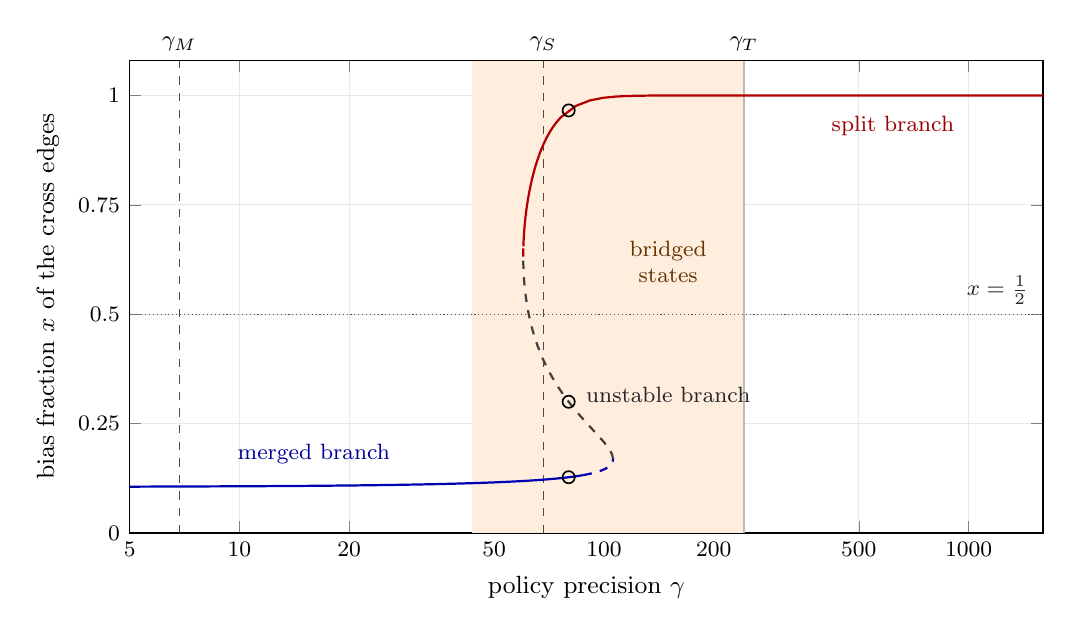
\begin{tikzpicture}
  \begin{axis}[width=11.6cm, height=6.0cm, scale only axis, xmode=log, xmin=5, xmax=1600, ymin=0, ymax=1.08,
      xtick={5,10,20,50,100,200,500,1000}, xticklabels={5,10,20,50,100,200,500,1000}, ytick={0,0.25,0.5,0.75,1},
      grid=major, grid style={gray!18},
      xlabel={policy precision $\gamma$}, ylabel={bias fraction $x$ of the cross edges},
      every axis label/.style={font=\small}, tick label style={font=\footnotesize}, clip=false]
    \fill[orange!13] (axis cs:43.41,0) rectangle (axis cs:240.98,1.08);
    \fill[gray!55] (axis cs:240,0) rectangle (axis cs:244,1.08);
    \draw[gray!60!black, dashed] (axis cs:6.845,0) -- (axis cs:6.845,1.08);
    \draw[gray!60!black, dashed] (axis cs:68.15,0) -- (axis cs:68.15,1.08);
    \draw[gray!60!black, densely dotted] (axis cs:5,0.5) -- (axis cs:1600,0.5);
    \addplot[blue!70!black, thick] coordinates {(5,0.10577) (10.707,0.10676) (16.108,0.10775) (21.22,0.10873) (26.06,0.10972) (30.643,0.11071) (34.983,0.1117) (39.094,0.11268) (42.988,0.11367) (46.677,0.11466) (50.172,0.11565) (53.483,0.11664) (56.621,0.11762) (59.593,0.11861) (62.409,0.1196) (65.078,0.12059) (67.605,0.12157) (70,0.12256) (72.267,0.12355) (74.415,0.12454) (76.448,0.12552) (78.373,0.12651) (80.194,0.1275) (81.917,0.12849) (83.548,0.12948) (85.089,0.13046) (86.546,0.13145) (87.922,0.13244)};
    \addplot[blue!70!black, thick, dashed] coordinates {(87.922,0.13244) (91.439,0.13526) (94.413,0.13807) (96.913,0.14089) (99,0.14371) (100.73,0.14652) (102.13,0.14934) (103.27,0.15216) (104.16,0.15497) (104.83,0.15779) (105.32,0.16061) (105.65,0.16342) (105.83,0.16624) (105.89,0.16906)};
    \addplot[gray!50!black, thick, dashed] coordinates {(105.89,0.16906) (105.31,0.1789) (103.89,0.18875) (101.97,0.19859) (99.765,0.20844) (97.425,0.21828) (95.046,0.22813) (92.692,0.23797) (90.401,0.24782) (88.201,0.25767) (86.103,0.26751) (84.117,0.27736) (82.244,0.2872) (80.484,0.29705) (78.834,0.30689) (77.291,0.31674) (75.849,0.32658) (74.504,0.33643) (73.251,0.34627) (72.084,0.35612) (70.998,0.36596) (69.989,0.37581) (69.051,0.38565) (68.18,0.3955) (67.373,0.40534) (66.625,0.41519) (65.932,0.42503) (65.292,0.43488) (64.701,0.44473) (64.156,0.45457) (63.655,0.46442) (63.195,0.47426) (62.774,0.48411) (62.39,0.49395) (62.041,0.5038) (61.725,0.51364) (61.441,0.52349) (61.187,0.53333) (60.961,0.54318) (60.763,0.55302) (60.591,0.56287) (60.445,0.57271) (60.323,0.58256) (60.224,0.5924) (60.149,0.60225) (60.095,0.6121) (60.064,0.62194) (60.053,0.63179)};
    \addplot[red!70!black, thick, dashed] coordinates {(60.053,0.63179) (60.057,0.63761) (60.068,0.64343) (60.086,0.64925) (60.111,0.65507)};
    \addplot[red!70!black, thick] coordinates {(60.111,0.65507) (60.183,0.66686) (60.284,0.67866) (60.414,0.69046) (60.573,0.70225) (60.762,0.71405) (60.98,0.72585) (61.229,0.73765) (61.51,0.74944) (61.824,0.76124) (62.173,0.77304) (62.559,0.78484) (62.986,0.79663) (63.455,0.80843) (63.971,0.82023) (64.539,0.83203) (65.165,0.84382) (65.858,0.85562) (66.626,0.86742) (67.483,0.87922) (68.445,0.89101) (69.536,0.90281) (70.786,0.91461) (72.244,0.92641) (73.978,0.9382) (76.107,0.95) (83.76,0.9763) (91.55,0.98877) (99.412,0.99467) (107.32,0.99748) (115.24,0.9988) (123.18,0.99943) (131.12,0.99973) (139.07,0.99987) (147.02,0.99994) (154.97,0.99997) (162.92,0.99999) (170.87,0.99999) (178.82,1) (186.77,1) (194.72,1) (202.67,1) (210.62,1) (218.57,1) (226.52,1) (234.47,1) (242.42,1) (250.37,1) (258.32,1) (266.27,1) (274.22,1) (282.17,1) (290.12,1) (298.08,1) (306.03,1) (313.98,1) (321.93,1) (329.88,1) (337.83,1) (371.61,1) (457.79,1) (563.95,1) (694.73,1) (855.84,1) (1054.3,1) (1298.8,1) (1600,1)};
    \addplot[only marks, mark=o, mark size=2.2pt, black, semithick] coordinates {(80,0.1274) (80,0.2999) (80,0.9659)};
    \node[font=\footnotesize, anchor=south] at (axis cs:6.845,1.08) {$\gamma_M$};
    \node[font=\footnotesize, anchor=south] at (axis cs:68.15,1.08) {$\gamma_S$};
    \node[font=\footnotesize, anchor=south] at (axis cs:242,1.08) {$\gamma_T$};
    \node[font=\footnotesize, blue!60!black, anchor=south] at (axis cs:16,0.135) {merged branch};
    \node[font=\footnotesize, red!60!black, anchor=north] at (axis cs:620,0.975) {split branch};
    \node[font=\footnotesize, gray!30!black, anchor=west] at (axis cs:84,0.315) {unstable branch};
    \node[font=\footnotesize, orange!40!black, align=center] at (axis cs:150,0.62) {bridged\\states};
    \node[font=\footnotesize, gray!30!black, anchor=south east] at (axis cs:1550,0.5) {$x=\frac12$};
  \end{axis}
\end{tikzpicture}

  \caption{\textbf{Mean-field phase diagram at the base point.} Symmetric fixed points of the map \eqref{eq:frm-meanfield} under \cref{asm:frm-mean-field}, shown as the bias fraction $x$ of the cross edges against the policy precision $\gamma$ and computed with the exact set softmax over the $35$ attended sets. The merged branch (blue) and the split branch (red) are joined by an unstable middle branch through folds at $\gamma=105.9$ and $\gamma=60.05$. Curves are solid where both multipliers of \cref{thm:frm-formation}(d) lie below one and dashed where one of them exceeds one, so the merged branch loses stability to symmetry-breaking perturbations at $\gamma=87.9$, before its fold. Circles mark the three fixed points at $\gamma=80$ of \cref{tab:frm-thresholds}, $x=0.1274$, $0.2999$ and $0.9659$. Dashed vertical lines mark $\gamma_M=6.84$ and $\gamma_S=68.2$ of \eqref{eq:frm-thresholds}, and the gray bar marks the global-split threshold $\gamma_T$, which lies between $240$ and $244$. Bridged states (\cref{obs:frm-bridged}), stable fixed points of the per-receiver map with one to three of the four cross edges learned, exist in the shaded range $43.4<\gamma<241.0$, whose upper end is the fold of the single learned bridge.}
  \label{fig:frm-phase}
\end{figure}
% src: figure supplied with the section; continuation values verified by the integrator (folds, symmetry breaking at 87.92, bridged range 43.41 to 240.98)

\begin{table}[tb]
\centering
\caption{Symmetric fixed points of the mean-field map at the base point: bias fraction $x$ of the cross edges with the cross attention per edge in parentheses, and the symmetric and symmetry-breaking multipliers. Classes refer to the symmetric subspace. Off it, the merged point is unstable to symmetry-breaking perturbations for $87.9<\gamma<105.9$, and bridged states exist for $43.4<\gamma<241.0$ (\cref{obs:frm-bridged,fig:frm-phase}).}
\label{tab:frm-thresholds}
\begin{tabular}{@{}llll@{}}
\toprule
$\gamma$ & fixed points $x$ (cross attention) & multipliers & class \\
\midrule
5 to 60 & $0.106$ to $0.119$ ($0.43$ to $0.37$) & $0.953$ to $0.981$ & merged only \\
80 & $0.127$ ($0.344$) & $0.976$, $0.994$ & bistable \\
 & $0.300$ ($0.117$) & $1.014$, $1.027$ (unstable) & \\
 & $0.966$ ($1.8\times10^{-3}$) & $0.995$, $0.995$ & \\
120 & $0.9992$ ($3.9\times10^{-5}$) & $0.995$, $0.995$ & split \\
160 to 1600 & $1.0000$ ($9.0\times10^{-7}$ to $2\times10^{-65}$) & $0.995$, $0.995$ & split \\
\bottomrule
\end{tabular}
\end{table}

\begin{observation}[Bridged states]\label{obs:frm-bridged}
Off the symmetric subspace the map has stable fixed points in which a receiver keeps $n_{\mathrm b}$ of its $n$ cross edges learned and attended. At the base point, continuation in $\gamma$ of the states found at $\gamma=80$ gives them for $43.4<\gamma<241.0$: $n_{\mathrm b}=3$ from its fold at $\gamma=43.41$ to $111.3$, $n_{\mathrm b}=2$ from $46.69$ to $151.2$ and $n_{\mathrm b}=1$ from $51.54$ to its fold at $240.98$, where the last learned bridge collapses, while the merged state, $n_{\mathrm b}=4$, is stable up to $\gamma=87.9$. Bridged states thus exist already below $\gamma=60.05$, where the split branch begins on the symmetric subspace, and none is found above $\gamma=241.0$ or, by iteration from bridged starts, at any $\gamma$ from $400$ to $3200$. Bridges must be nucleated: at $\gamma=160$ an edge started at $x\le0.1$ stays learned and one started at $x\ge0.2$ collapses. One reciprocal bridge per receiver at $\gamma=160$ gives group contrast $4.51$ and union contrast $1.76$, from the isotropic part of a covariance that departs by $0.44$ in relative norm from blocks proportional to $I_2$, so these values are indicative only (\cref{chk:frm-bridged}).
\end{observation}
% src: B2-X1 (refines L3-C1); C2-4 bridge survival; scalar-reduction residual from B2_bridges output; stable ranges by continuation (figure fig:frm-phase, recomputed with B2_meanfield imported read-only: folds 43.41 and 240.98, stability ends 111.33, 46.69, 151.24, 51.54)
A learned bridge persists because it is the only near-equal alternative to the in-group senders. Bridged states are what flattening leaves out: their attended subgraph is flat, but no unattended cut separates the groups.

\subsection{Baseline convention, parameter grid and finite policy precision}\label{sup:frm-baseline-convention-parameter-grid-and-f}

\begin{remark}[A weaker convention: the matched-size baseline]\label{rem:frm-matched-baseline}
The weaker convention of \cref{rem:col-baseline-conventions}, which compares a region only with regions of its own size, gives $r_{\mathrm{hom}}(n)=1$ here (\cref{thm:frm-split-contrast}(b)) and would admit every level above $r_{\mathrm{sub}}=2.318$. We do not use it: at such levels the comparison medium itself has qualifying regions (at level $3$, its whole population and its eight seven-member regions), so a selection there would not separate the split from a population without frames.
\end{remark}
% src: B2-T2(b), B2-P2(d) under the matched convention; C2-5, decision 11 (weaker convention only in a remark)

\begin{observation}[The parameter grid]\label{obs:frm-grid}
On the grid of 162 points with $F$ equal to $0.9$, $0.95$, $0.98$, $0.99$, $0.995$ or $0.999$, $Q=1-F^2$, $R^s\in\{0.25,1,4\}$, $R_c\in\{0.01,0.05,0.5\}$, $n\in\{2,4,8\}$ and $\kappa=n-1$, the calibration conditions of the split and of the comparison medium each have one root at every point, and both are nondegenerate. Everywhere $r_{\mathrm{sub}}<\bar r_{\mathrm{hom}}<r(A)$, the split contrast lies in $[1.24,60.5]$ and the significance between $1.009$ and $1.415$, so every window is nonempty, some narrower than one percent of the level, and by \cref{thm:frm-split-contrast}(e) every grid point lies in an open set on which the split at $\gamma=\infty$ with $\sigma_\alpha^2=0$ is a collective at admissible levels (\cref{chk:frm-baseline}).
\end{observation}
% src: B2-T2(c) grid statements (numerical, repair (v): uniqueness and nondegeneracy are numerical; existence proved in thm(d)); C2-5 grid significance; comparison-medium root and r_sub < rbar recomputed by the editor on the same grid

\begin{observation}[Exploration at finite policy precision]\label{obs:frm-exploration}
In the frozen-slow model with self-consistent calibration, the split branch at $\gamma=80$, $120$ and $160$ has group contrast $8.6763$, $8.7317$ and $8.7329$, union contrast at most $1.008$, and a diffusive precision of the form $\Sigma^{\mathrm{sc}}\otimes I_2$ to within $3.1\times10^{-14}$ after rotating group $B$ by the remaining cross error; at $\gamma=80$ only $A$ and $B$ among the 247 regions exceed $7.954$. On the merged branch no region exceeds $7.954$ at $\gamma=10$, $40$ or $80$. Treating the mean cross weight $Fk_\times\mathsf p_\times$ ($k_\times$ the gain of an attended cross message, $\mathsf p_\times$ the cross attention per edge) as a symmetric coupling estimates $r(A)\approx(1-\lambda_\perp^2)/(1-\lambda^2+2n\lambda Fk_\times\mathsf p_\times)$, $8.698$ against $8.676$ at $\gamma=80$ (\cref{chk:frm-exploration}).
\end{observation}
% src: B2-P1 (leading-order heuristic stated as an estimate); region enumeration at gamma = 80 and 10 by the editor
The split keeps its contrast while this cut coupling is small against the leak $1-\lambda^2$, and by \cref{lem:frm-attention}(a) exploration on the split branch is at most $\kappa e^{-\gamma\Delta\mathcal V(1/2)}$.

\begin{remark}[Openness at finite policy precision]\label{rem:frm-open}
\Cref{thm:frm-split-contrast}(e) proves openness at $\gamma=\infty$. At finite $\gamma$ openness is a sketch (\cref{app:frm}), whose unproved step is that near the split the errors reduce to a diffusive scalar precision of the form $\Sigma^{\mathrm{sc}}\otimes I_2$, verified at the base point (\cref{obs:frm-exploration}) and not proved; its other hypothesis, nondegeneracy of the calibration roots, is verified on the grid (\cref{obs:frm-grid}).
\end{remark}
% src: B2-T2(d) proof (sketch per C2 status item 4 and repair (v))

\subsection{Partner randomization and the placement of the nulls}\label{sup:frm-partner-randomization-and-the-placement}

\begin{observation}[Partner randomization and the other states]\label{obs:frm-partner}
At the base point, partner randomization at the matched rate of $\kappa$ partners per round, drawn uniformly from the $2n-1$ others, with idealized calibration solved at the null's own state, gives the contrasts of \cref{tab:frm-nulls} with unlearned cross translations and with translations learned at the null's attention rate. In neither does any region exceed $7.954$, and the cross-group world-conditional covariance is nonzero, so $\Omega_{\mathrm{int}}>0$ across groups. At the split, $\Omega_{\mathrm{int}}$ of a within-group pair is $0.024$, $0.140$ and $0.510$ nats over windows of two, four and eight rounds, and that of a cross-group pair is below $1.5\times10^{-14}$ (\cref{chk:frm-nulls}).
\end{observation}
% src: B2-P2(b),(c),(d) restated at admissible levels (C2-5); calibration under the null is the null's own self-consistent value (B2_contrast part (c) solves it so); region enumeration of both partner-randomization states by the editor

\begin{table}[t]
\centering
\caption{Contrasts at the base point and the regions selected at admissible levels $r_0\in(7.954,8.733]$; the split at $\gamma=80$ is selected for $r_0\le8.676$, and for $\gamma\ge160$ the contrasts equal those at $\gamma=\infty$ to four digits. In the row of the deletion and freezing nulls, the freezing null is taken with initial states that are deterministic or conditioned on (\cref{prop:frm-nulls}(a)). Dashes mark order parameters not computed.}
\label{tab:frm-nulls}
\begin{tabular}{@{}lllll@{}}
\toprule
State & $r(A)$ & $r(A\cup B)$ & $\Omega_{\mathrm{int}}$ across groups & selected \\
\midrule
Split, $\gamma=\infty$ & $8.733$ & $1.000$ & $0$ & $A$ and $B$ \\
Split, $\gamma=80$ & $8.676$ & $1.008$ & -- & $A$ and $B$ \\
Merged, $\gamma=40$ & $1.019$ & $7.801$ & -- & none \\
Deletion and freezing nulls & $1$ & $1$ & $0$ & none \\
Partner randomization, unlearned & $1.351$ & $3.953$ & positive & none \\
Partner randomization, learned & $1.004$ & $7.868$ & positive & none \\
Comparison medium & $1.000$ & $7.954$ & -- & none \\
\bottomrule
\end{tabular}
\end{table}

Two remarks place these comparisons within \cref{def:agy-nulls}; the second, on the explanation nulls, is in \cref{sup:frm-explanation-nulls-and-merged-regimes}. Of the remaining nulls of type D, $\mathfrak N_{\mathrm{eff}}$ and $\mathfrak N_{\mathrm{inf}}$ are not applicable, since the model has no acts, and the habit null $\mathfrak N_{\mathrm{hab}}$ is applicable and coincides with partner randomization redrawn every round with learned translations, because at $\gamma=0$ with the uniform habits of \cref{def:frm-two-group}(iv) each receiver draws its $\kappa$ senders uniformly. For partner randomization redrawn every round the stationary second moments of the null, and with them the contrast of every region, are deterministic; the test of \cref{prop:agy-tests}(b) with the largest contrast of a region as its statistic then has $p=1/(n_{\mathrm{null}}+1)$, because that contrast is larger at the split ($8.733$ at $\gamma=\infty$ and $8.676$ at $\gamma=80$ against at most $7.868$), and it rejects at level $\alpha_{\mathrm{pr}}$ when $n_{\mathrm{null}}\ge1/\alpha_{\mathrm{pr}}-1$. Partner randomization drawn once, under which the selected partition is random, and the test on contrasts estimated from finite samples are not computed.

\subsection{Reachability in the full model}\label{sup:frm-reachability-in-the-full-model}

In the runs of \cref{obs:frm-online,tab:frm-online}, early uniform attention lets cross translations be learned before calibration registers the mismatch, calibration noise acts as exploration, and at large $\gamma$ an in-group edge with an unlucky high estimate is dropped and never sampled again, its slot going to a cross edge (\cref{chk:frm-online}). The counts are not monotone in $\alpha_{\mathrm{cal}}$ at $\gamma=160$, where the rise from 2 to 7 and the fall to 1 exceed the sampling error of eight replicates (two-sided Fisher exact tests, $p=0.04$ and $0.01$, uncorrected for the number of comparisons); the remaining differences between nonzero cells, and the differences between reruns of a cell, do not.

\subsection{Abundant capacity and the grounding tension}\label{sup:frm-abundant-capacity-and-the-grounding-tens}

\begin{proposition}[Abundant capacity]\label{prop:frm-capacity}
If $\kappa\ge n$, every receiver attends at least $\kappa-n+1$ cross senders in every round at every $\gamma$, so no attention cut separates the groups. Let calibrated precisions have the frozen form of \cref{asm:frm-mean-field}(a), with any constants $\hat\sigma^2_{\mathrm{in}}>0$ and $D_{\mathrm{cal}}>0$. Then at $\gamma=\infty$ with noiseless angle observations, $\sigma_\alpha^2=0$, from the declared start, each receiver attends in every round the $\kappa-n+1$ cross senders it chose by tie-breaking in the first round, and their bias fractions converge to $\mathsf p^\ast/(\mathsf p^\ast+1)$, which is below $\frac12$ exactly when $\mathsf p^\ast<1$: for $\mathsf p^\ast<1$ they become learned bridges, and for $\mathsf p^\ast\ge1$ they stay attended without being learned.
\end{proposition}
% src: B2-P3 (first statement derived; the bridge statement derived here for the realized dynamics with sigma_alpha = 0, not for the mean-field map, whose symmetric tie persists)
Proof in \cref{app:frm}. With reciprocal learned bridges at $\kappa=n=4$ the group contrast is $2.46$ and the union's $5.14$, against $8.73$ and $1.00$ at $\kappa=n-1$ (\cref{chk:frm-capacity}). Scarce capacity is needed as in the static withdrawal threshold of \cref{thm:coh-withdrawal}.

\begin{remark}[The grounding tension in formation]\label{rem:frm-grounding}
For $\kappa=n-1$ the split contrast is $(1-\lambda_\perp^2)/(1-\lambda^2)$, whose denominator, the leak $1-F^2(1-k^s)^2$, shrinks as the sensing gain $k^s$ falls, while the withdrawal signal $D_{\mathrm{cal}}$ of \cref{lem:frm-calibration} vanishes linearly with $k^s$. Weak grounding therefore tends to raise contrast and weakens the signal that forms the cut: at $F=0.99$, raising $R^s$ from $1$ to $4$ raises the split contrast from $8.73$ to $14.33$, lowers $D_{\mathrm{cal}}/\hat\sigma^2_{\mathrm{in}}$ from $4.16$ to $1.41$ and raises $\gamma_S$ from $68$ to $154$ (\cref{chk:frm-grounding}). High-contrast collectives of weakly grounded members need higher policy precision to form, which is \cref{asm:int-a11}, the grounding tension of \cref{thm:coh-grounding-tension}, seen from the formation side.
\end{remark}
% src: B2-R2 (formula derived; numbers checked); gamma_S at R^s = 4 recomputed by the editor

\subsection{Further conjecture and open problems}\label{sup:frm-further-conjecture-and-open-problems}

\begin{conjecture}[Drifting frames survive exact fusion]\label{conj:frm-drifting-frames}
Let the group frames of the two-group model drift, the frame angles of $A$ and $B$ performing independent random walks, so that true cross translations change while in-group translations stay the identity. Then on an open set of parameters the split is selected at an admissible level under the exact-fusion null: it survives that null.
\end{conjecture}
% src: B2-C1 (B2-O4)
The uncomputed basis is that an exact-fusion receiver that rarely attends a cross edge has a broad posterior over its translation, and a Gaussian message read through a rotation of unknown angle with spread $\mathsf v$ loses information about $\eta$ by an amount positive and increasing in $\mathsf v$. An instance with drifting frames in which exact-fusion receivers attend cross edges at the merged rate at every $\gamma$ would refute it.

\begin{openproblem}[Online calibration]\label{open:frm-online}
With C1g calibration learned online, give conditions on $(\alpha,\alpha_{\mathrm{cal}},\gamma,\mathsf p^\ast)$ and on the rule for unattended edges under which the split is reached from the symmetric start with probability tending to one as the gains vanish, or show that bridged states keep positive probability.
\end{openproblem}
% src: B2-O2

\begin{openproblem}[Self-consistent calibration along trajectories]\label{open:frm-self-consistent}
Replace the frozen constants of \cref{asm:frm-mean-field} by bounds uniform over configurations, so that \cref{thm:frm-formation}(b) holds for the self-consistent mean field along whole trajectories.
\end{openproblem}
% src: B2-O3

\begin{openproblem}[Access, heterogeneity and geometry]\label{open:frm-access}
Extend the analysis to anisotropic access, where a cut can separate complementary information, to heterogeneous senders, and to groups on a graph with geometry, where contrast meets the second-moment length $\xi_2$ and the largest extent $\Lstar$ of hypothesis H4 (the question of \cref{open:sca-endogenous}).
\end{openproblem}
% src: B2-O5; L4-O8 (not answered: the model has no geometry)

\subsection{Moment bound and contrast conventions}\label{sup:frm-moment-bound-and-contrast-conventions}

\begin{remark}[The moment bound holds on every path]\label{rem:frm-moment-bound}
After the first round every realization of \eqref{eq:frm-error} has block row sums $F(1-k^s_i)\le F(1-k^s_{\min})<1$, with $k^s_{\min}=1/(R^s(1/Q+1/R^s+\kappa/R_c))$, because rotations have norm one (\cref{app:frm}). Row-sum contraction (C$_r$) and the uniform form of the moment bound (M) of \cref{asm:sca-standing} therefore hold on every path, and no cycle amplifies in the sense of \cref{thm:coh-amplification}.
\end{remark}
% src: B2-R1

\begin{remark}[Second moments and two-dimensional errors]\label{rem:frm-conventions}
As \cref{def:col-contrast} declares, contrast is computed from the scalar precision $(\Sigma^{\mathrm{sc}})^{-1}$ when the world-conditional covariance has the per-coordinate form $\Sigma^c=\Sigma^{\mathrm{sc}}\otimes I_2$ (agent indices first), and from second moments when the conditional law is a Gaussian mixture, as it is here for $\kappa<n-1$. At finite $\gamma$ the mistranslation forcing also makes the conditional covariance depend on the world path, so we use $\Sigma^c=\E[\Cov(e(t)\mid\eta)]$. For other two-dimensional states contrast is not defined, and reported numbers name the reduction used.
\end{remark}
% src: C2-5 smaller points; repair (ii); def:col-contrast already declares both conventions

\subsection{Explanation nulls and merged regimes}\label{sup:frm-explanation-nulls-and-merged-regimes}

The explanation nulls limit attribution. The world-and-access null predicts no partition, since all agents sense alike. The code null predicts the frame classes $\{A,B\}$: above $\gamma_T$ the partition is predictable from the codes alone and communication adds the contrast, while between $\gamma_S$ and $\gamma_T$ split and bridged states coexist for the same codes, and stable merged states as well up to $\gamma=87.9$ (\cref{fig:frm-phase}). Under \cref{def:agy-nulls} the split above $\gamma_T$ is therefore code aligned.

Each failure of formation in the two-group model (\cref{sec:frm-fails}) marks a hypothesis the positive results need. For $\gamma<\gamma_M$ every cross translation is learned. At the base point the symmetric map is merged only up to its fold at $\gamma=60.05$, while bridged states of the per-receiver map, found by continuation, appear already at $\gamma=43.4$ (\cref{obs:frm-bridged}); at the smaller mismatch $\vartheta=\pi/4$, where $\Delta\mathcal V(\frac12)$ is smaller, the symmetric map is merged only up to $\gamma\approx80$. A C0 receiver that assigns every sender the same noise attends uniformly (\cref{prop:coh-c0-blind}), $\mathsf p_j=\kappa/(2n-1)$, so by \eqref{eq:frm-meanfield} every cross translation ends learned whenever $\kappa/(2n-1)>\mathsf p^\ast$. Two failures are structural (\cref{prop:frm-capacity,prop:frm-exact-fusion}).

\subsection{Remarks on the formation conjecture}\label{sup:frm-remarks-on-the-formation-conjecture}

Regarding \cref{conj:frm-formation}, in the two-group model the attention and learning statements of the first two regimes hold for the frozen-calibration mean-field map (\cref{thm:frm-formation}) and the third is observed (\cref{obs:frm-bridged}). A population of this class in which, for arbitrarily large $\gamma$, a stable configuration keeps a learned and attended cross-class edge would refute the conjecture; where it holds, its collectives are attributed to misreading unless they survive exact fusion. Linear conformity to a self-constituted prior cannot form collectives (\cref{prop:hie-conformity}); a route that does not rest on misreading, through conformity of codes with member-written code records and a pragmatic coordination value, is stated as \cref{conj:hie-conformity-formation}.

\section{Additional results for \texorpdfstring{Section~\ref{sec:sca}}{Section 8}: scale}\label{sup:sca}

This section collects statements, examples and remarks of \cref{sec:sca} that the main text cites without stating in full. Proofs are in \cref{app:sca}.

\subsection{Amplifying profiles and the common-code conjecture}\label{sup:sca-amplifying-profiles-and-the-common-code}

\begin{example}[An amplifying attention profile]\label{ex:sca-amplifying-profile}
In the report \citep{dennis2026communicating}, two level-1 receivers in a world $\eta\in\R^2$ with $F=0.9I$ and $Q=I$, sender-specific effective codes $(3,0)$ and $(0,3)$, sensing rows $(3,6)$ and $(6,3)$ and attention capacity $\kappa=2$ have sensing while listening to the partner as the strict best response of expected-free-energy attention, and the frozen mean map has the simple real dominant eigenvalue $\rho=1.0613266751$ and block row sums $1.0999$. By \cref{lem:sca-relations}(c) no stationary law exists, and $\Sigma(t)$ grows like $\rho^{2t}$ (\cref{prop:sca-rank-one}): \textup{(M)} fails in both forms. The report describes a second instance, its CEX-1, which alternates two frozen profiles at capacity $\kappa=1$, each with spectral radius below one, and for which it reports growth by the factor $1.0703173057$ per round, so \textup{(C$_\rho$)} for each frozen profile does not give \textup{(M)} for a switching schedule. CEX-1 is a separate instance from the capacity-two system specified above: $F=0.99I$, $Q=0.1I$, the same two codes, sensing rows $(-5,10)$ and $(10,-5)$, and a schedule in which both agents listen in one round and sense in the next. The report's summary does not state these parameters, which are taken from its working record, and the factor was recomputed with them (\cref{chk:min-amplification}); in the capacity-two system itself, restricted to capacity one, every period-two alternation of two frozen profiles contracts at level 1, the slowest at the rate $0.9752822296$ per round (\cref{chk:min-amplification}). The capacity-two construction uses sender-specific codes by its specification, which the checks rebuild (\cref{chk:min-amplification,chk:sca-rank-one}); for CEX-1 the report's phrase is ``mismatched metrics'' \citep{dennis2026communicating}, and the instance recomputed in \cref{chk:min-amplification} has the sender-specific codes $(3,0)$ and $(0,3)$.
\end{example}
% src: L7-M12 (report CEX-B and CEX-1), B3-P1 counterexamples, B3-L1(d); level 1 per decision 10 and tab:min-dictionary

\begin{conjecture}[No amplification with one code]\label{conj:sca-common-code}
At identity encodings with one modality and one channel noise, in an isotropic world $F=fI_K$ with $0<f<1$, every frozen or periodic attention profile of level-1 receivers at its covariance fixed point has a mean map over one period of length $p$ with spectral radius at most $f^p$. Such profiles then satisfy \textup{(M)} in uniform form, and frozen ones satisfy \textup{(C$_\rho$)} at every rate above $f$.
\end{conjecture}
% src: L7-C1, L7-O1; the manuscript's only statement of this conjecture, which Section 9 cites
\Cref{prop:min-common-code} proves two cases, both with a rank-one code: frozen profiles with symmetric listening, and profiles without sensing on any listening graph, frozen or periodic. Otherwise the evidence is numerical (\cref{chk:sca-common-code}), and one frozen or periodic common-code profile growing faster than $f$ would refute the conjecture.

\subsection{Asynchronous clocks and routing}\label{sup:sca-asynchronous-clocks-and-routing}

\begin{proposition}[Poisson clocks]\label{prop:sca-poisson}
Under the independent Poisson clocks of rate $\nu$ of \cref{sec:sca-lightcone}, let $\bar J$ be an influence bound (\cref{def:sca-local-rule}), $\bar J_{\mathrm{diag}}=\max_i\bar J_{ii}$, $g=\max_i\sum_{k\neq i}\bar J_{ik}$ and $\bar J_{\mathrm{off}}=\bar J-\diag(\bar J)$. With $J_{ij}(t)=\partial\mu_i(t)/\partial\mu_j(0)$ and $d=d(i,j)\ge1$,
\begin{equation}\label{eq:sca-poisson}
\E\Vert J_{ij}(t)\Vert\le e^{-(1-\bar J_{\mathrm{diag}})\nu t}\sum_{n\ge d}\frac{(\nu t)^n}{n!}(\bar J_{\mathrm{off}}^n)_{ij}\le e^{-(1-\bar J_{\mathrm{diag}})\nu t}\sum_{n\ge d}\frac{(g\nu t)^n}{n!}.
\end{equation}
Consequently $\E\Vert J_{ij}(t)\Vert\le e^{-(1-\bar J_{\mathrm{diag}})\nu t}(eg\nu t/d)^d/\bigl(\sqrt{2\pi d}(1-g\nu t/(d+1))\bigr)$ when $g\nu t<d+1$, and $\E\Vert J_{ij}(t)\Vert\le\exp\bigl(-\varphi d+\nu t(ge^\varphi+\bar J_{\mathrm{diag}}-1)\bigr)$ for every $\varphi>0$, so influence spreads at most at the velocity $v_{\mathrm{LR}}=\max\bigl\{0,\inf_{\varphi>0}\nu(ge^\varphi+\bar J_{\mathrm{diag}}-1)/\varphi\bigr\}$ hops per unit time, in the sense that the bound decays exponentially in $t$ along $d\ge vt$ for every $v>v_{\mathrm{LR}}$; the velocity is $eg\nu$ when $\bar J_{\mathrm{diag}}=1$, and zero when $g+\bar J_{\mathrm{diag}}<1$, where the infimum is $-\infty$. Without any smoothness, the probability that $\mu_i(t)$ depends on $\mu_j(0)$ is at most $(\Delta\nu t)^d/\bigl(d!(1-\Delta\nu t/(d+1))\bigr)$ when $\Delta\nu t<d+1$. For linear scalar updates with nonnegative coefficients and constant diagonal $\bar J_{ii}=\bar J_{\mathrm{diag}}$, the first inequality in \eqref{eq:sca-poisson} is an equality.
\end{proposition}
% src: L4-P2
Proof in \cref{app:sca}; checked on a ring of 40 agents (\cref{chk:sca-poisson}). The directed copy chain, in which agent $m$ copies agent $m-1$ at its events ($\bar J_{\mathrm{diag}}=0$, $g=1$), attains the first inequality of \eqref{eq:sca-poisson}, $\E J_{ij}(t)=e^{-\nu t}(\nu t)^d/d!$, while the probability that a signal held at the source has crossed $d$ hops by time $t$ equals the last member $e^{-\nu t}\sum_{n\ge d}(\nu t)^n/n!$ of \eqref{eq:sca-poisson}; its velocity $\nu$ equals $v_{\mathrm{LR}}$.

\begin{example}[A routing transition]\label{ex:sca-switch-chain}
In the routing model of \cref{prop:sca-routing}, agents $0,1,\dots,n$ sit on a line, and each relay $m\ge1$ attends one of two persistent sources with contents $\pm1$, with $G_m(\pm)=\mp\alpha_0\mu_{m-1}/2$, preferring the source that agrees with what it heard. Averaged routing gives $\mu_m=\tanh(\gamma\alpha_0\mu_{m-1}/2)$, and $\bar A=0$, $\mathrm{Lip}=\alpha_0/2$, $\mathrm{osc}=2$ give $\bar J_{m,m-1}(\gamma)=\gamma\alpha_0/2$, the derivative at the symmetric state. For $\gamma\alpha_0<2$ influence decays as $(\gamma\alpha_0/2)^n$; for $\gamma\alpha_0>2$ the sign of $\mu_0$ propagates without decay to the fixed points $\pm\mu^\ast$, $\mu^\ast=\tanh(\gamma\alpha_0\mu^\ast/2)$. With sampled routing and message noise of standard deviation $\sigma$, the relay choices form a binary symmetric Markov chain with flip probability $p(\gamma)=\E[(1+e^{\gamma\alpha_0(1+\sigma Z)})^{-1}]$, $Z$ standard normal, so the routing bit has correlation length $-1/\ln(1-2p)$, $21.5$ hops at $\sigma=0.5$ and $\gamma=\infty$, where $p=\Pr(Z<-2)$ (\cref{chk:sca-routing}), far beyond the linear correlation length of the continuous content.
\end{example}
% src: L4-P4

\begin{remark}[Infinite precision]\label{rem:sca-argmax}
At $\gamma=\infty$ causality survives, since \cref{thm:sca-lightcone}(a) and the support bound of \cref{prop:sca-poisson} use only locality, but the amplitude bound fails: the update is discontinuous where two policies' expected free energies tie, and in \cref{ex:sca-switch-chain} a perturbation of $10^{-6}$ at the head moves the state $20$ hops away by order one. Gumbel noise of scale $1/\gamma$ in evaluating expected free energy makes the argmax reproduce the softmax, restoring \cref{prop:sca-routing}. Above $\gamma_D$ the routed dynamics can have several attractors, consistent with the several stable attention motifs found by \citet{dennis2026communicating}.
\end{remark}
% src: L4-P5

\subsection{Unstable profiles and rumors}\label{sup:sca-unstable-profiles-and-rumors}

\begin{proposition}[Rank-one dominance]\label{prop:sca-rank-one}
Let $W$ be time invariant with a simple real eigenvalue $\rho=\rho(W)>1$ that strictly dominates every other eigenvalue in modulus, with right and left eigenvectors $v$ and $u$, $u^\top v=1$, let $Q^\zeta\succ0$ be constant and let $\Sigma(0)\succeq0$. Then
\begin{equation}\label{eq:sca-rank-one}
\rho^{-2t}\Sigma(t)\to c_\infty vv^\top,\qquad c_\infty=\frac{u^\top Q^\zeta u}{\rho^2-1}+u^\top\Sigma(0)u>0.
\end{equation}
Consequently the top canonical correlation of $e_i(t)$ and $e_j(t)$ tends to one for every pair with nonzero blocks $v_i$ and $v_j$, and $\Sigma(t)^{-1}$ has one eigenvalue of order $\rho^{-2t}$, with eigenvector tending to $v/|v|$. If every other eigenvalue of $W$ lies in the open unit disk, the remaining eigenvalues of $\Sigma(t)^{-1}$ stay bounded away from zero.
\end{proposition}
% src: B3-P3
Proof in \cref{app:sca}; checked on \cref{ex:sca-amplifying-profile} (\cref{chk:sca-rank-one}). The unstable profile turns the agents' errors into one shared error. How far it reaches when the amplification sits at one site of a stable medium can be computed exactly: on $\Z$ let $W_{xx}=c$ for $x\neq0$, $W_{00}=c+b_0$ and $W_{xy}=a$ for $|x-y|=1$, with $c\ge0$, $a>0$, $b_0>0$ and $\lambda=c+2a<1$.

\begin{proposition}[An amplifying site and its front]\label{prop:sca-amplifying-site}
In this chain, with $Q^\zeta=qI$ and $\Sigma(0)=0$:
\begin{enumerate}
\item[(a)] $W$ has exactly one eigenvalue outside $[c-2a,c+2a]$, namely $\rho=c+\sqrt{4a^2+b_0^2}$, with eigenvector $v_x=e^{-m_\rho|x|}$ and $m_\rho=\arcsinh(b_0/(2a))=\arccosh((\rho-c)/(2a))$. The profile is unstable exactly when $\rho>1$.
\item[(b)] For $\rho\neq1$ and $t\ge1$, exactly, $\Sigma(t)=A(t)P_v+B(t)$, where $P_v=vv^\top/|v|^2$, $|v|^2=\coth m_\rho$, $A(t)=q(\rho^{2t}-1)/(\rho^2-1)$, $B(t)P_v=0$ and $q(I-P_v)\preceq B(t)\preceq\frac{q}{1-\lambda^2}(I-P_v)$.
\item[(c)] For $\rho>1$ and $t\ge1$, with $\mathfrak s_x(t)=(1-\lambda^2)A(t)v_x^2/(q|v|^2)$,
\begin{equation}\label{eq:sca-front-bounds}
\frac{\mathfrak s_x-1}{\mathfrak s_x+1}\le\Corr(e_x(t),e_0(t))\le\Bigl(\frac{\mathfrak s_x}{1-\lambda^2}\Bigr)^{1/2}+\frac{|v|q^{1/2}}{(1-\lambda^2)A(t)^{1/2}}.
\end{equation}
\item[(d)] For $\rho>1$, $\theta\in(0,1)$ and $t\ge1$ the front $x_\theta(t)=\max\{x\ge0:\Corr(e_x(t),e_0(t))\ge\theta\}$ satisfies $x_\theta(t)=v_{\mathrm f}t+O_\theta(1)$ with $v_{\mathrm f}=\ln\rho/m_\rho<1$ hop per round.
\item[(e)] For any finite amplifying core embedded in the same medium with a simple dominant real eigenvalue $\rho>1$, the eigenvector decays outside the core at the rate $m_\rho=\arccosh((\rho-c)/(2a))$, the decay rate of the medium's Green function at the value $\rho$. As $\rho\downarrow1$, $m_\rho$ decreases to the medium's Ornstein--Zernike rate $m$, $\cosh m=1+\varepsilon/(2a)$ with $\varepsilon=1-\lambda$ (\cref{thm:sca-oz}), so the unstable mode is never wider than the medium's correlation length.
\end{enumerate}
\end{proposition}
% src: B3-P4
Proof in \cref{app:sca}; checked on chains of 801 and 401 agents (\cref{chk:sca-amplifying-site}). The amplifying site recruits its neighbors into one shared error at less than one hop per round, and the recruited mode is never wider than the stable medium allows.

\begin{remark}[Rumors are not collectives]\label{rem:sca-rumors}
Contrast needs the stationary world-conditional precision (\cref{def:col-contrast}), which does not exist without \textup{(M)}, and its finite-time analog is degenerate: $\Sigma(t)^{-1}$ has one eigenvalue of order $\rho^{-2t}$ along the unstable mode $v$ (\cref{prop:sca-rank-one}), so a criterion that admitted the weighted coordinate $v$ would assign diverging contrast to the amplifying structure. The definition of a collective therefore includes \textup{(M)} (\cref{def:col-collective,rem:col-moment}), and we call an amplifying profile a rumor, an echo chamber whose shared error grows like $\rho^t$; the name is a definition, not a derived result. For rumors the scales change meaning: after $T$ rounds correlation extends at most $\min\{2T,2v_\varphi T+O(1)\}$ hops, a localized front advances at $v_{\mathrm f}<1$ hop per round, and $\tau$ is replaced by the amplification time $1/\ln\rho$, so the correlated extent is limited by the lifetime of the profile, which ends when attention is re-selected, the linear regime ends or grounding resets the errors. Level-1 receivers cannot detect the instability, because their claimed covariances follow recursions that do not involve their means.
\end{remark}
% src: B3-R1 (as a remark: C2 status item 3); M_spec decision 16

\subsection{Refinements of the clustering bound and the Ornstein--Zernike form}\label{sup:sca-refinements-of-the-clustering-bound-and}

\begin{proposition}[World conditioning and correlated noise]\label{prop:sca-world-conditioning}
\begin{enumerate}
\item[(a)] Under \textup{(Lin)}, \textup{(Loc)} and \textup{(C$_r$)}, if the local noise is correlated across agents with $\Vert Q^\zeta_{kl}\Vert\le qe^{-d(k,l)/\xi_w}$, where $\xi_w$ is the correlation length of the noise, then $\Vert\Sigma_{ij}\Vert\le q\bigl(\lceil d/2\rceil+(1-\lambda^2)^{-1}\bigr)\max(\lambda,e^{-1/\xi_w})^{d}$ with $d=d(i,j)$: the decay rate is at least $\min(\ln(1/\lambda),1/\xi_w)$.
\item[(b)] Let identical scalar agents with exact code models sense one scalar world $\eta_{t+1}=F\eta_t+w_t$, $\Var(w_t)=Q$, with a common sensing gain, and let nobody communicate. Then the world-conditional covariance is diagonal, while the unconditional correlation of the errors of any two distinct agents is $Q/(Q+q)$, with $q$ the local noise variance, whatever their distance.
\end{enumerate}
\end{proposition}
% src: L4-P7 (part (b) stated for errors via lem:fw-common-mode(d))
Proof in \cref{app:sca}. Unconditional correlation measures the shared world as well as communication, so every scale bound of \cref{sec:sca} concerns the world-conditional law.

\begin{proposition}[Spectral form]\label{prop:sca-spectral}
Assume \textup{(Lin)}, \textup{(Loc)}, block-diagonal local noise with blocks $\preceq qI$, and \textup{(C$_\rho$)}. Then $\Vert\Sigma_{ij}\Vert\le K_A^2qf^{2\lceil d(i,j)/2\rceil}/(1-f^2)$. If $W$ is normal, the bound holds with $K_A=1$ and $f=\rho(W)$. Under \textup{(B)} it follows that $\xi\le\tau$: a correlation length in hops cannot exceed the correlation time in rounds, and the physical length is at most $\ell\tau$.
\end{proposition}
% src: L4-P8, B3-P2(a), L7-P3(c)
Proof in \cref{app:sca}; checked on signed rings, where the row-sum bound is unusable (\cref{chk:sca-spectral}). This is the classical counterpart of exponential clustering from a Lieb--Robinson bound and a spectral gap \citep{hastings2004locality,nachtergaele2006lieb,hastings2006spectral}, and it applies with signed weights and in the common-code regime, where \textup{(C$_r$)} fails. Attention that is reciprocal in a weak sense gives a much better rate, without translation invariance.

\begin{theorem}[Diffusive clustering]\label{thm:sca-diffusive}
Let $P$ be a stochastic matrix, reversible with respect to a positive measure $\varpi$ ($\varpi_iP_{ij}=\varpi_jP_{ji}$) with $\varpi_{\max}=\sup_i\varpi_i<\infty$, and with $P_{ij}>0$ only if $i=j$ or $(i,j)\in\mathcal E$. Assume \textup{(Lin)}, block-diagonal local noise with blocks $\preceq qI$, and $\Vert W_{ij}(t)\Vert\le\lambda P_{ij}$ for all $i$, $j$, $t$, with $\lambda<1$. Then the covariance $\Sigma=\Sigma(t)$ of the process started in the infinite past, or at any time from a zero start, satisfies for every $\vartheta\in(0,1)$ and every $t$
\begin{equation}\label{eq:sca-diffusive}
\Vert\Sigma_{ij}\Vert\le\frac{2q\varpi_{\max}}{\sqrt{\varpi_i\varpi_j}}\cdot\frac{\exp\bigl(-\vartheta d(i,j)\sqrt{2\ln(1/\lambda)}\bigr)}{1-\lambda^{2(1-\vartheta)}}.
\end{equation}
\end{theorem}
% src: L4-P9 (Carne-Varopoulos), B3 table scope note
Proof in \cref{app:sca}; checked on a torus with random conductances (\cref{chk:sca-diffusive}). For $\lambda>e^{-2}$, in particular for small leaks, the rate $\sqrt{2\ln(1/\lambda)}\approx\sqrt{2\varepsilon}$ improves on the row-sum rate $\ln(1/\lambda)$ by the square root characteristic of diffusion, on any graph, and for $\lambda\le e^{-2}$ the row-sum rate is at least as large; the diffusive bound needs domination by one reversible chain, not reversibility of $W$, and covers time-varying schedules dominated by that chain. On the ring with $c=0$ the exact rate is $\arccosh(1/\lambda)=\sqrt{2\ln(1/\lambda)}(1+O(\ln(1/\lambda)))$, so the rate is sharp to leading order. The proof uses the Chebyshev-polynomial argument with which \citet{carne1985transmutation} proved the estimate of \citet{varopoulos1985long}, known to us from a review; we prove the form we use in full. Heterogeneous gains give rates between those of two homogeneous media.

\begin{proposition}[Heterogeneous media]\label{prop:sca-heterogeneous}
Let scalar agents occupy $\Z^D$ or a finite box of $\Z^D$ at positions $x_i$, attend only nearest neighbors, and satisfy \textup{(Lin)} and \textup{(B)} with local noise variances in $[q_{\min},q_{\max}]$. For $\boldsymbol\varphi\in\R^D$ put $\bar\psi(\boldsymbol\varphi)=\sup_{t,i}\sum_j|W_{ij}(t)|e^{\boldsymbol\varphi\cdot(x_i-x_j)}$ and $\Psi(\boldsymbol\varphi)=\bar\psi(\boldsymbol\varphi)\bar\psi(-\boldsymbol\varphi)$.
\begin{enumerate}
\item[(a)] For every $\boldsymbol\varphi$ with $\Psi(\boldsymbol\varphi)<1$, $|\Sigma_{ij}|\le q_{\max}e^{-\boldsymbol\varphi\cdot(x_i-x_j)}/(1-\Psi(\boldsymbol\varphi))$, for the stationary covariance and at any time from a zero start. On a box with open ends the supremum in $\bar\psi$ includes the rows of the boundary agents, which have a single neighbor along some axis. On a periodic box of side $L$, $\bar\psi$ is computed for the $L$-periodic medium on $\Z^D$ that covers the box, and $\Sigma_{ij}$ is the sum over $\mathbf w\in\Z^D$ of that medium's covariances between $x_i$ and the images $x_j+L\mathbf w$, each of which obeys the bound with its own admissible $\boldsymbol\varphi$. On $\Z^D$, if $W(t)\ge0$, every agent gives equal weights $a_{id}(t)$ to its two neighbors along each axis $d$, the local leaks $\varepsilon_i(t)=1-\sum_jW_{ij}(t)$ are at least $\varepsilon_{\min}>0$ and the weights $a_{id}(t)$ at most $a_{\max}$, then the decay rate is at least $m_{\mathrm{up}}=\arccosh(1+\varepsilon_{\min}/(2a_{\max}))$ per hop along a coordinate axis and at least $\sqrt D\arccosh(1+\varepsilon_{\min}/(2Da_{\max}))$ per unit Euclidean length along the diagonal. For a tilt along its one-sided axis $d$, a boundary agent of an open box has the tilted row sum $1-\varepsilon_i+a_{id}(e^{\pm\varphi_d}-1)$, which for one sign exceeds the two-neighbor value $1-\varepsilon_i+2a_{id}(\cosh\varphi_d-1)$, so on an open box the admissible tilts, and with them the guaranteed rate, can lie below $m_{\mathrm{up}}$.
\item[(b)] If $W(t)\ge W_{\mathrm{low}}$ entrywise for all $t$, where $(W_{\mathrm{low}})_{ii}=c_{\min}\ge0$ and $(W_{\mathrm{low}})_{ij}=a_{\min}>0$ for neighbors, then $\Sigma\ge q_{\min}(I-W_{\mathrm{low}}^2)^{-1}$ entrywise, the covariance of the homogeneous medium $(c_{\min},a_{\min})$ on the same vertex set. Where every agent has $2D$ neighbors, on $\Z^D$ or a periodic box, the leak $\varepsilon_{\mathrm{low}}=1-c_{\min}-2Da_{\min}$ of that medium is at least every local leak; a boundary agent of an open box, with fewer neighbors, can have a larger one.
\item[(c)] On $\Z$, let $W(t)\ge0$ give equal weights at most $a_{\max}$ to the two neighbors of every agent, with local leaks at least $\varepsilon_{\min}>0$, as in (a), and let $W(t)\ge W_{\mathrm{low}}$ as in (b). With $m_{\mathrm{low}}=\arccosh(1+\varepsilon_{\mathrm{low}}/(2a_{\min}))$, correlations decay at a rate between $m_{\mathrm{up}}$ and $m_{\mathrm{low}}$, so $1/m_{\mathrm{low}}\le\xi\le1/m_{\mathrm{up}}$.
\item[(d)] For a frozen $W\ge0$ on a finite population, $\min_i(1-\varepsilon_i)\le\rho(W)\le\max_i(1-\varepsilon_i)$, so $-1/\ln(1-\varepsilon_{\max})\le\tau\le-1/\ln(1-\varepsilon_{\min})$.
\item[(e)] On any graph with $W\ge0$, if $\lambda'=\max_i[W_{ii}+\sum_{j\neq i}\max(W_{ij},W_{ji})]<1$, then \cref{thm:sca-diffusive} applies with the symmetric chain $P_{ij}=\max(W_{ij},W_{ji})/\lambda'$ for $i\neq j$, uniform $\varpi$, and the rate $\sqrt{2\ln(1/\lambda')}$.
\end{enumerate}
\end{proposition}
% src: B3-P7
Proof in \cref{app:sca}; checked on rings of 300 agents (\cref{chk:sca-heterogeneous}). The bounds hold for time-varying schedules, attention chosen by expected free energy included, when the schedule is independent of the noises and the extremes are taken over the whole schedule; the lower bound needs every edge attended in every round. For small leaks the ratio of the two rates, about $[(\varepsilon_{\mathrm{low}}/a_{\min})/(\varepsilon_{\min}/a_{\max})]^{1/2}$, measures the heterogeneity.

\begin{remark}[The Ornstein--Zernike form]\label{rem:sca-oz-form}
\Cref{thm:sca-oz} proves that every direction decays at least at the rate $m(\mathbf u)$ and that hyperplane sums decay exactly at $m_1$. That $m(\mathbf u)$ is the exact pointwise rate, with the prefactor of the Ornstein--Zernike form $r^{-(D-1)/2}e^{-m(\mathbf u)r}$ \citep{ornstein1914accidental}, follows from the Green-function asymptotics of finite-range walks with drift \citep{ney1966martin}, applied to the walk tilted by the maximizer $\boldsymbol\varphi^\ast$ of the support function, which is aperiodic when $c>0$; we have read that theorem only in the restatement of \citet{ballu2024asymptotics}, which gives the power and the rate but not the constant. A local central limit computation suggests
\begin{equation}\label{eq:sca-oz-prefactor}
\Sigma(r\mathbf u)\simeq\frac q2e^{-m(\mathbf u)r}\frac{|v|^{(D-3)/2}}{(2\pi r)^{(D-1)/2}\bigl(\det H\cdot\mathbf u^\top H^{-1}\mathbf u\bigr)^{1/2}},
\end{equation}
with $v=\nabla\psi(\boldsymbol\varphi^\ast)$ and $H=\nabla^2\psi(\boldsymbol\varphi^\ast)$, but its passage from the local limit theorem to the sum over the number of steps is heuristic, so \eqref{eq:sca-oz-prefactor} is not a result of this manuscript; numerically the covariance approaches it (\cref{chk:sca-oz-lattice}). The rigorous Ornstein--Zernike theory of \citet{campanino2003ornstein}, for Ising models above the critical temperature, is not used here.
\end{remark}
% src: L4-T1(c) (heuristic step), B6 (Ney-Spitzer read in restatement), L4-O10

\subsection{Persistence, diffusive scaling and records}\label{sup:sca-persistence-diffusive-scaling-and-record}

\begin{proposition}[Persistence of collective variables]\label{prop:sca-persistence}
Assume \textup{(M)} and \textup{(Lin)} with $W$ and $Q^\zeta\succ0$ time invariant, and let $\tilde W=\Sigma^{-1/2}W\Sigma^{1/2}$. For all readout vectors $\mathbf v$ and $\mathbf v'$ and lags $h\ge0$,
\begin{equation}\label{eq:sca-persistence}
\bigl|\Corr\bigl(\mathbf v'^\top e(t+h),\mathbf v^\top e(t)\bigr)\bigr|\le\Vert\tilde W^h\Vert\le\Vert\tilde W\Vert^h,\qquad\Vert\tilde W\Vert^2=1-\lambda_{\min}\bigl(\Sigma^{-1/2}Q^\zeta\Sigma^{-1/2}\bigr)<1,
\end{equation}
and $\Vert\tilde W^h\Vert^{1/h}\to\rho(W)$. The lifetime $T^\ast(\theta)$, the largest lag at which some pair of linear readouts keeps correlation at least $\theta$, equals $\max\{h:\Vert\tilde W^h\Vert\ge\theta\}$. Hence $T^\ast(\theta)\le\ln(1/\theta)/\ln(1/\Vert\tilde W\Vert)$, and $T^\ast(\theta)/\ln(1/\theta)\to\tau$ as $\theta\to0$.
\end{proposition}
% src: L4-P10
Proof in \cref{app:sca}; for strongly non-normal $W$ the one-step bound can be loose (\cref{chk:sca-persistence}). The lifetime of a collective variable is set by the slowest mode of the whole system of agents and media, which is why records can lengthen it. On lattices, time and space are tied.

\begin{proposition}[Diffusive scaling]\label{prop:sca-diffusive-scaling}
In the setting of \cref{thm:sca-oz}:
\begin{enumerate}
\item[(a)] $\rho(W)=\lambda$, so $\tau=-1/\ln\lambda$, and $\xi_2^2/\tau=2a\lambda\ln(1/\lambda)/(1-\lambda^2)\to a$ as $\varepsilon\to0$. In physical units $\ell^2\xi_2^2\simeq D_{\mathrm{diff}}\tau$ with the diffusion constant $D_{\mathrm{diff}}=a\ell^2$ per round: the dynamic exponent is two.
\item[(b)] If $c>0$, the local autocovariance $\Sigma(0;h)=\Cov(e_x(t+h),e_x(t))$, which is
\begin{equation}\label{eq:sca-autocov-def}
\Sigma(0;h)=\int_{[-\pi,\pi]^D}\frac{q\hat W(p)^h}{1-\hat W(p)^2}\frac{\mathrm{d}p}{(2\pi)^D},
\end{equation}
satisfies, as $h\to\infty$ at fixed $\varepsilon$,
\begin{equation}\label{eq:sca-autocov}
\Sigma(0;h)\simeq\frac{q\lambda^h}{1-\lambda^2}\Bigl(\frac{\lambda}{4\pi ah}\Bigr)^{D/2}.
\end{equation}
\end{enumerate}
\end{proposition}
% src: L4-P11, L6-P8(a)
Proof in \cref{app:sca}; checked in one and two dimensions (\cref{chk:sca-autocovariance}). The relative error of \eqref{eq:sca-autocov} is about $D/(2\varepsilon h)$ for small $\varepsilon$, so the asymptote applies for lags well beyond the correlation time. Spatial reach grows only as the square root of memory, and building correlations over a distance $L$ by local averaging takes about $L^2/D_{\mathrm{diff}}$ rounds, more than the light-cone time $L/(2\ell)$ once $L$ exceeds a fraction of one hop. Up to the factor $\varepsilon$, the resolvent $(I-W)^{-1}$ that sets the leading decay in \cref{thm:sca-oz}(a) is the total-influence matrix of the model of \citet{friedkin1990social}, the leak playing stubbornness; \eqref{eq:sca-xi-physical} is the standard massive lattice Green's function (\cref{sec:rel}).

\begin{remark}[Special cases]\label{rem:sca-records-special}
In the notation of \cref{prop:sca-records}, one record read by the mean mode with $\upsilon=\delta=0$ gives $\bar e(t+1)=(1-\varepsilon-\beta)\bar e(t)+\beta z(t)$, $z(t+1)=(1-\omega)z(t)+\omega\bar e(t)$, whose first-order extension factor $1+\mathcal R$ is the lower end of the interval of \cref{prop:sca-records-memory}(b): at $\varepsilon=0.01$, $\beta=0.2$, $\omega=0.1$ the secular root gives $\tau=306.24$ rounds, against $300$ to first order and $99.5$ without the record. The identity time of a collective whose members turn over (\cref{prop:agy-identity}) is the continuous-time case: its rate matrix \eqref{eq:agy-identity} equals $-\mathsf R$ for one record with $\upsilon=0$ when forgetting plus the turnover rate times the share of a newcomer's content not copied from the record plays $\varepsilon$, the read rate plus the turnover rate times the copied share plays $\beta$, the members' write rate plays $\omega$ and the record's decay plays $\delta$, so, when the read rate plus the turnover rate times the copied share is positive, as \cref{prop:sca-records} requires of the read weight, the identity rate $\tau_{\mathrm{id}}^{-1}$ is the secular root $\varepsilon_{\mathrm{rec}}$ (\cref{chk:sca-records}). When that sum is zero the record is unread, the function $g_z$ is affine with the single root $\varepsilon'$, and \cref{prop:agy-identity}(a) gives the rates directly: the members' mean decorrelates at the rate that plays $\varepsilon$, and the pair at the smaller of that rate and $\omega+\delta$.
\end{remark}
% src: B5-P4 (L1-P23, L2-P17 as special cases; dictionary checked against eq:agy-identity)

\begin{remark}[Global records]\label{rem:sca-global-records}
In the record model of \cref{prop:sca-records-length}, a record read by all $N$ members with a uniform kernel couples only to the mean mode, since its kernel's symbol vanishes at every nonzero wavevector; for $p\neq0$ the agents' symbol is $1-\varepsilon'-\beta-a\sum_d2(1-\cos p_d)$. A global archive therefore acts on every deviation from the collective mean as an extra leak $\beta$, so fluctuations about the mean decorrelate over $\xi^2\approx a/(\varepsilon'+\beta)$ while the mean has the memory of \cref{prop:sca-records-memory}. The archive is a hub: it adds to every covariance a component $[\hat\Sigma_{00}(0)-q/(1-(1-\varepsilon'-\beta)^2)]/N$, the excess of the term at wavevector zero over the continuation of the branch $p\neq0$ and about $\hat\Sigma_{00}(0)/N$ when $\varepsilon'+\mathcal R\delta\ll\beta\omega/(\beta+\omega)$ with $\mathcal R=\beta/\omega$ (the leak $\varepsilon'$ small beside both $\beta$ and $\omega$, and $\delta$ small beside $\omega^2/(\beta+\omega)$; \cref{chk:sca-global-records}), that does not decay with distance (compare the exogenous hub of \cref{cor:sca-size}(e), whose common correlation does not fall with $N$; here the component falls as $1/N$, see \cref{prop:hie-global-record}), which world conditioning does not remove, because agents write the archive.
\end{remark}
% src: B5-R1

For a closed population with a durable global record at the record noise that makes the dynamics reversible, \cref{prop:hie-global-record} gives this component in closed form, together with the extra leak $\beta$ of the deviations. Its world-conditional cost falls like $1/N$, and the cost of a member-written archive that does not shrink with $N$ is the world-driven common mode bounded in \cref{thm:hie-floor}.

\subsection{Fronts with long-range links}\label{sup:sca-fronts-with-long-range-links}

\begin{proposition}[Fronts]\label{prop:sca-fronts}
In the setting of \cref{sec:sca-longrange}, let $Y_t$ be the walk with step law $W/\lambda$, so that the normalized influence beyond distance $r$, $\sum_{|x|\ge r}(W^t)(x)/\lambda^t$, equals $\Pr(|Y_t|\ge r)$.
\begin{enumerate}
\item[(a)] $\Pr(|Y_t|\ge r)\le C_1tr^{-\sigma}$ if $\sigma<2$, and $\le C_1(tr^{-\sigma}+tr^{-2})$ if $\sigma>2$.
\item[(b)] If $\sigma<2$ and $r\ge c_2t^{1/\sigma}$, then $\Pr(|Y_t|\ge r)\ge c_1tr^{-\sigma}$.
\item[(c)] For $\sigma\neq2$ and every small enough threshold $\theta$, the front $r_\theta(t)=\min\{r:\Pr(|Y_t|\ge r)\le\theta\}$ satisfies $r_\theta(t)\asymp t^{1/\min(\sigma,2)}$: superballistic for $\sigma<1$, linear at $\sigma=1$, sublinear for $\sigma>1$. At $\sigma=2$, (a) holds with $tr^{-2}\ln(er)$ on the right and the front is $O((t\ln t)^{1/2})$. Influence therefore moves at finite speed if and only if $\sigma\ge1$.
\item[(d)] Let $\mathsf J(y)\le K_{\mathsf J}|y|^{-D-\sigma}$ for $y\neq0$. For any influence bound with $\bar J_{ij}\le c\one\{i=j\}+a\mathsf J(x_i-x_j)$, $(\bar J^t)_{ij}\le K_{\mathsf J}t^{1+D+\sigma}g_{\mathrm{tot}}^t|x_i-x_j|^{-D-\sigma}$ with $g_{\mathrm{tot}}=c+a$: synchronous rounds have no strict light cone in the lattice metric, and when $g_{\mathrm{tot}}>1$ the region of influence above a fixed level lies inside the logarithmic cone $t\gtrsim(D+\sigma)\ln r/\ln g_{\mathrm{tot}}$.
\end{enumerate}
\end{proposition}
% src: L4-P14 (exponent alpha = D + sigma); the threshold sigma >= 1 corrects L4-P14's 'finite mean link length' at sigma = 1
Proof in \cref{app:sca}; fitted front exponents lie within $7$ percent of $1/\min(\sigma,2)$, with shortfalls of $5$ and $6$ percent at $\sigma=0.5$ and $\sigma=3$ that depend on the fit window (\cref{chk:sca-fronts}); the exponents themselves are those proved in (c). The threshold $\sigma=1$ coincides with the free-particle light cone of quantum systems with interactions decaying as $r^{-\alpha}$, $\alpha>D+1$ \citep{tran2020hierarchy}, because linear message passing propagates a single tangent vector; the many-body thresholds of that hierarchy have no analog here \citep{kuwahara2020strictly}, and the logarithmic cone of (d) matches the causal region reported for classical long-range lattices \citep{metivier2014spreading}. On a fixed graph with random long links, \cref{thm:sca-clustering} applies in the graph metric, whose chemical distance in long-range percolation with connection probabilities decaying as $|x-y|^{-D-\sigma}$ and $0<\sigma<D$ grows like $(\log|x-y|)^{\Delta+o(1)}$ on the infinite cluster, with $1/\Delta=\log_2(2D/(D+\sigma))$ \citep{biskup2004scaling}; outside that range of $\sigma$ this result does not apply.

\subsection{Broadcasting on trees and condensation}\label{sup:sca-broadcasting-on-trees-and-condensation}

In the linear-Gaussian model the decisive structure is branching. Consider a rooted tree with $X_{\mathrm{root}}\sim\Ncal(0,1)$ and, on each edge $e$ from a parent $u$ to a child $c$, $X_c=\alpha_eX_u+(1-\alpha_e^2)^{1/2}Z_c$ with independent standard normal $Z_c$ and edge correlations $\alpha_e\in(0,1)$, the vertices at depth $n$ being observed with noise variance $\sigma_{\mathrm{obs}}^2\ge0$. Let $\mathcal V(u)$ be the noise variance of the equivalent Gaussian observation of $X_u$ carried by the observed descendants of $u$.

\begin{theorem}[Gaussian broadcasting on trees]\label{thm:sca-trees}
\begin{enumerate}
\item[(a)] $\mathcal V(v)=\sigma_{\mathrm{obs}}^2$ at the vertices $v$ of level $n$, $\mathcal V(v)=\infty$ at childless vertices above level $n$ (depth less than $n$), which carry no observation, $\mathcal V(u)^{-1}=\sum_c\alpha_{e_c}^2/(1-\alpha_{e_c}^2+\mathcal V(c))$ over the children $c$ of every other vertex $u$ above level $n$, a term with $\mathcal V(c)=\infty$ being zero, and $I(X_{\mathrm{root}};\text{level }n)=\tfrac12\ln(1+1/\mathcal V(\mathrm{root}))$.
\item[(b)] For constant $\alpha$, $\mathcal V(u)=\alpha^{2|u|}\hat{\mathcal V}(u)$, where $|u|$ is the depth and $\hat{\mathcal V}(\mathrm{root})$ is the effective resistance between the root and a ground node in the network with edge resistances $(1-\alpha^2)\alpha^{-2|e|}$, $|e|$ the depth of the child endpoint, in which each level-$n$ vertex is joined to the ground by a resistance $\sigma_{\mathrm{obs}}^2\alpha^{-2n}$ (shorted to it when $\sigma_{\mathrm{obs}}=0$).
\item[(c)] On the $b$-ary tree with exact leaves, $\mathcal V_n=(1-\alpha^2)\sum_{k=1}^n(b\alpha^2)^{-k}$, so $\lim_nI_n=\tfrac12\ln\bigl(1+\tfrac{b\alpha^2-1}{1-\alpha^2}\bigr)$ if $b\alpha^2>1$, $I_n\simeq1/(2n(1-\alpha^2))$ if $b\alpha^2=1$, and $I_n\simeq(1-b\alpha^2)(b\alpha^2)^n/(2(1-\alpha^2))$ if $b\alpha^2<1$. The Kesten--Stigum condition $b\alpha^2>1$ is exactly the reconstruction threshold for Gaussian channels, and linear estimation is optimal.
\item[(d)] On a general locally finite tree with exact leaves, reconstruction ($\lim_nI_n>0$) holds if the branching number satisfies $\mathrm{br}(T)\alpha^2>1$ and fails if $\mathrm{br}(T)\alpha^2<1$.
\end{enumerate}
\end{theorem}
% src: L4-T2, L6-P5(b); (d) from Lyons 1990 at review and restatement level (B6)
Proof in \cref{app:sca}; checked against direct Gaussian conditioning (\cref{chk:sca-trees}). For a general channel on the $b$-ary tree, reconstruction holds when $b$ times the squared second eigenvalue of the channel exceeds one, a condition named for the limit theorems of \citet{kesten1966additional}; it is tight for the binary symmetric channel \citep{bleher1995purity,evans2000broadcasting} and not for some other channels \citep{mossel2001reconstruction}. Part (c) adds the Gaussian case with an exact electrical identity, and part (d) uses, for the two strict cases only, the transience criterion of \citet{lyons1990random} for the biased walk, read in a review and in the restatement of \citet{lyons1992random}. The information that reaches a level of the tree percolates.

\begin{theorem}[Gaussian information percolation on trees]\label{thm:sca-gaussian-percolation}
In the tree model, let a source $X_{\mathrm{src}}$ be jointly Gaussian with $X_{\mathrm{root}}$, with $X_{\mathrm{src}}\to X_{\mathrm{root}}\to(\text{observed level})$. Then
\begin{equation}\label{eq:sca-gauss-perc}
I(X_{\mathrm{src}};\text{observed level})\le\perc_{\alpha^2}(\mathrm{root}\to\text{observed level})\cdot I(X_{\mathrm{src}};X_{\mathrm{root}}),
\end{equation}
where $\perc_{\alpha^2}$ is bond percolation with edge $e$ open with probability $\alpha_e^2$, computed by $\mathfrak p(u)=1-\prod_c(1-\alpha_{e_c}^2\mathfrak p(c))$ above the observed level, with $\mathfrak p(v)=1$ at the vertices of the observed level and the empty product, hence $\mathfrak p(v)=0$, at childless vertices above it.
\end{theorem}
% src: L4-T3
Proof in \cref{app:sca}; checked on 400 random trees (\cref{chk:sca-gaussian-percolation}). The theorem extends the percolation bound of \citet{polyanskiy2017strong} to Gaussian channels, whose input-independent coefficient is one, through the Gaussian contraction $\alpha_e^2$; on trees it is tight at the level of thresholds, since percolation with $p=\alpha^2$ on the $b$-ary tree survives if and only if $b\alpha^2>1$. On graphs of subexponential growth, by contrast, aggregate information has short reach.

\begin{proposition}[Aggregate information on slowly growing graphs]\label{prop:sca-aggregate}
If $\lambda_{\min}(\Sigma)\ge\sigma_{\mathrm e}>0$ and $\Vert\Sigma_{0j}\Vert\le B_\Sigma e^{-m_\Sigma d(0,j)}$, then the squared top canonical correlation between $e_0$ and all $e_j$ with $d(0,j)\ge r$ is at most $(B_\Sigma^2/(\sigma_{\mathrm{e}}\lambda_{\min}(\Sigma_{00})))\sum_{j:d(0,j)\ge r}e^{-2m_\Sigma d(0,j)}$, which tends to zero exponentially in $r$ on graphs whose spheres grow subexponentially.
\end{proposition}
% src: L6-P5(c)
Proof in \cref{app:sca}. On trees and other expanding graphs the sum need not converge, and an audience retains information about a distant source although each member's information decays. That reach does not make a collective.

\begin{proposition}[Reach lies outside the diffusive class]\label{prop:sca-tree-diffusive}
\begin{enumerate}
\item[(a)] Let the tree-indexed Gaussian law have constant edge correlation $\alpha$ and branching $b$. Its precision has entries $-\alpha/(1-\alpha^2)$ on tree edges, and its row sums are $(1-b\alpha)/(1+\alpha)$ at internal vertices, $(1+\alpha-b\alpha)/(1+\alpha)$ at the root and $1/(1+\alpha)$ at the leaves. For depth at least two it is diffusive if and only if $b\alpha\le1$; at depth one there is no internal vertex and it is diffusive if and only if $(b-1)\alpha\le1$. The Kesten--Stigum regime $b\alpha^2>1$ implies $b\alpha>1$, so at depth at least two it is never diffusive in these coordinates.
\item[(b)] For the homogeneous diffusive medium $\Pi=\varepsilon^\Pi I+a^\Pi L$ on the $(b+1)$-regular tree, $b\ge2$, $\varepsilon^\Pi\ge0$, with $L$ the graph Laplacian, $\Sigma(o,v)\le b^{-d(o,v)}\Sigma(o,o)$, and the squared canonical correlation between $x_o$ and the sphere of radius $n$ about $o$ is at most $\tfrac{b+1}{b}b^{-n}\Sigma(o,o)(\varepsilon^\Pi+2(b+1)a^\Pi)$: there is no reconstruction, and aggregate information decays by the factor $1/b$ per level.
\end{enumerate}
\end{proposition}
% src: B1-P6
Proof in \cref{app:sca}. Reach on trees is produced by directed broadcasting with $b\alpha^2>1$, hence $b\alpha>1$, which a diffusive precision cannot represent in plain coordinates, and a diffusive tree medium has no reach. A broadcast hierarchy can therefore spread shared content without forming a collective in the sense of \cref{def:col-collective}. With this caution we state the condensation picture as a conjecture.

\begin{conjecture}[Condensation of coherent information]\label{conj:sca-condensation}
In a population whose effective communication structure has branching number $b_{\mathrm{eff}}$, the growth rate per hop of the number of receivers that carry independent channel noise, and whose links contract squared correlation by $\alpha^2$, information about a common source reaches arbitrary hop distance if $b_{\mathrm{eff}}\alpha^2>1$ and is confined within the information length $1/\ln(1/(b_{\mathrm{eff}}\alpha^2))$ if $b_{\mathrm{eff}}\alpha^2<1$.
\end{conjecture}
% src: L4-C1
On trees the conjecture is \cref{thm:sca-trees,thm:sca-gaussian-percolation}; a family with $b_{\mathrm{eff}}\alpha^2$ bounded away from one on one side whose information behaves as on the other would refute it. On low-dimensional lattices with linear relays a single receiver's information decays at twice the mass (\cref{prop:coh-info-decay}) and branching from a point is subexponential, so condensation there would need long-range links, nonlinear processing such as the routing bit of \cref{ex:sca-switch-chain} or majority processing \citep{makur2020broadcasting}, or persistent memory. As interpretations, span of control times link fidelity must exceed one in a hierarchical institution, and students per teacher times copying fidelity must exceed one for cultural transmission across generations, a tree in time.

\subsection{Abstraction}\label{sec:sca-abstraction}

Content that crosses many hops passes through many codes. A receiver with prior covariance $P$ that reads a code $H$ with noise covariance $\hat R$ moves its mean by the gain-code map $\Kg H$, $\Kg=PH^\top(HPH^\top+\hat R)^{-1}$, which for noiseless codes is the $P^{-1}$-orthogonal projection onto the range of $PH^\top$ (\cref{def:coh-cycle-product}); frames rotate which world directions a code carries. With a common prior metric each noiseless hop is therefore an orthogonal projection. Let $V_1,\dots,V_J$ be subspaces of a finite-dimensional real inner-product space, the receivers' common prior metric, with orthogonal projections $P_{V_j}$, intersection $V_\cap=\bigcap_jV_j$ and projection $P_\cap$.

\begin{theorem}[Relays converge to the common ground]\label{thm:sca-alternating}
\begin{enumerate}
\item[(a)] Cyclic order. The product over one cycle of hops, $A_{\mathrm{cyc}}=P_{V_J}\cdots P_{V_1}$, satisfies $c_{\mathrm{cyc}}=\Vert A_{\mathrm{cyc}}(I-P_\cap)\Vert<1$ and $A_{\mathrm{cyc}}^n-P_\cap=(A_{\mathrm{cyc}}(I-P_\cap))^n$, so $\Vert A_{\mathrm{cyc}}^n-P_\cap\Vert\le c_{\mathrm{cyc}}^n$.
\item[(b)] Quasi-periodic order. If every block of $p_0$ consecutive hops uses every subspace, the content after $n$ hops satisfies $\Vert x_n-P_\cap x_0\Vert\le c_\ast^{\lfloor n/p_0\rfloor}\Vert x_0-P_\cap x_0\Vert$, with $c_\ast<1$ the largest of $\Vert A_w(I-P_\cap)\Vert$ over the finitely many words $w$ of length $p_0$ that contain every index.
\item[(c)] Noisy messages. If instead each hop applies a self-adjoint map with spectrum in $[0,\bar a]$ for some $\bar a<1$, every product of $n$ hops has norm at most $\bar a^n$, and all content decays.
\end{enumerate}
\end{theorem}
% src: L4-T5(b),(c),(f), L4-P19(a); SSW constant not used (decision 18)
Proof in \cref{app:sca}; checked with three codes in six dimensions (\cref{chk:sca-alternating}). The content that survives an arbitrarily long relay with fixed codes is the common ground $V_\cap$, the directions that every code along the path transmits, measured in the receivers' common metric. Codimensions add for subspaces in general position, so generically $\dim V_\cap=\max(0,K-\sum_j(K-\dim V_j))$, small as soon as several distinct codes or frames occur. Part (a) proves only $c_{\mathrm{cyc}}<1$; we use no explicit formula for it.

\begin{remark}[Rates from the literature]\label{rem:sca-alternating-cited}
For two subspaces the rate is exact, $\Vert(P_{V_2}P_{V_1})^n-P_\cap\Vert=c^{2n-1}$ with $c$ the cosine of the Friedrichs angle \citep{friedrichs1937certain} between $V_1\cap V_\cap^\perp$ and $V_2\cap V_\cap^\perp$: the upper bound is due to \citet{aronszajn1950theory} and the equality to \citet{kayalar1988error}, both as stated by \citet{badea2012rate}, and our computation reproduces it (\cref{chk:sca-alternating}). Cyclic products converge to $P_\cap$ in any Hilbert space by Halperin's theorem \citep{halperin1962product}, as stated by \citet{badea2012rate}, and in finite dimension products in any order in which each subspace recurs infinitely often converge \citep{amemiya1965convergence,prager1960convergence}, with no uniform rate when the gaps between recurrences grow. In infinite dimension norm convergence can fail for three subspaces \citep{kopecka2017strange}, and cyclic convergence is geometric exactly when the relevant cosine is below one \citep{badea2012rate}.
\end{remark}
% src: L4-T5(a),(d),(e) at the reading levels of B6 (Kayalar-Weinert via Badea et al.)

With random codes, frames and noise levels the relevant object is the product of random hop maps. For independent, identically distributed hop maps $A_m$ with $\E\ln^+\Vert A_m\Vert<\infty$ the Lyapunov exponents $\Gamma_1\ge\Gamma_2\ge\cdots$ exist, with $\tfrac1n\ln\sigma_k(A_n\cdots A_1)\to\Gamma_k$ almost surely \citep{furstenberg1960products,oseledets1968multiplicative}, and $\Gamma_1>\Gamma_2$ for invertible maps whose generated semigroup is strongly irreducible and contracting \citep{guivarch1985frontiere,goldsheid1989lyapunov}; we cite these results at the level of their records and restatements. Then $\sigma_2/\sigma_1\approx e^{-n(\Gamma_1-\Gamma_2)}$, so the content that survives many hops is one-dimensional, with abstraction length $1/(\Gamma_1-\Gamma_2)$ hops. In a computed example with rank-two codes and random frames, pure relays have an abstraction length of $1.70$ hops, so that the second singular value of a typical path product falls below one percent of the first after about eight hops ($\ln100$ divided by the gap), with wide scatter across realizations, while receivers that keep half of their own belief at each hop have an abstraction length of about $34$ hops (\cref{chk:sca-lyapunov}). The pure-relay maps of this example have rank two and are not invertible, and the cited theorems reach them through a reduction. With identity prior the hop map is $A_m=U_mGU_m^\top$, with $U_m$ the $6\times2$ frame and $G$ a fixed positive diagonal $2\times2$ matrix, so $A_n\cdots A_1=U_n(GM_n)\cdots(GM_2)GU_1^\top$ with $M_m=U_m^\top U_{m-1}$, and the nonzero singular values of the path product are those of a product of $2\times2$ factors $GM_m$. For independent Haar frames these factors are independent, identically distributed and almost surely invertible, and the support of their law contains $GM$ for every $2\times2$ contraction $M$, so the semigroup they generate is strongly irreducible and contracting. The receivers that keep part of their own belief have invertible hop maps.

\begin{conjecture}[Scale up, rank down]\label{conj:sca-rank-down}
In relay networks with diversity of codes or frames, the effective rank of the content shared across hop distance $n$, the number of singular values of the path product above a fixed fraction of the largest, is nonincreasing in $n$ when the codes share a direction (without one it can rise, \cref{ex:ren-rank-nonmonotone}), and tends to the multiplicity of the top Lyapunov exponent of the path cocycle when the singular values that belong to that exponent remain comparable, generically one. A collective of linear size $L$ therefore shares content of rank about $\#\{k:\Gamma_1-\Gamma_k\le\ell/L\}$.
\end{conjecture}
% src: L4-C2
The limit statement holds for fixed codes in a common metric that share a direction, with limiting rank $\dim V_\cap$ (\cref{thm:sca-alternating}), and for independent invertible hop maps under the cited conditions, with rank one. For fixed codes in a common metric the monotonicity clause holds when $V_\cap\neq\{0\}$ and can fail when $V_\cap=\{0\}$, where the limit of the effective rank can also differ from the multiplicity of the top Lyapunov exponent (\cref{ex:ren-rank-nonmonotone} and the paragraph after it). The conjecture is open for networks with many paths, where path products add and ranks can rise, for correlated or learned codes, for heterogeneous priors, where the contraction itself can fail (\cref{thm:coh-amplification}), and for non-invertible pure relays that do not reduce, as those of the example above do, to invertible factors of the code rank, for instance relays whose code ranks differ along the path. The routing bit of \cref{ex:sca-switch-chain} is the nonlinear extreme, in which one bit survives where continuous content does not. \Cref{prop:ren-relay-rank} proves the conjecture for stationary relays of meta-level hops that average several members' projections in a common metric, with limiting rank $\dim V_\cap$ when $V_\cap\neq\{0\}$, and shows that its reading as meta-agents communicating at lower rank than their members fails at one hop, since averaging parallel paths raises the rank. Aggregated codes lose rank across levels only along directions on which the members' frames disagree, and only under aggregation in public coordinates (\cref{prop:ren-code-levels}).

\subsection{Relations between the lengths}\label{sup:sca-relations-between-the-lengths}

With \cref{thm:sca-oz}, two lengths now describe a lattice medium: the Ornstein--Zernike length of the decay, and the second-moment length $\xi_2$ that bounds the extent of collectives (\cref{thm:col-contrast-size}), defined in \cref{sec:col} from the world-conditional precision. The next proposition relates them.

\begin{proposition}[Relations between the lengths]\label{prop:sca-lengths-relation}
Let the world-conditional precision on $\Z^D$ be translation invariant and diffusive, with symbol $\hat\Pi(p)=\varepsilon^\Pi+\sum_xa^\Pi(x)(1-\cos p\cdot x)$, leak $\varepsilon^\Pi>0$ and $\sum_x|x|^2a^\Pi(x)<\infty$, and let $\xi_{2,d}^2=\varsigma_d^2/(2\varepsilon^\Pi)$ with $\varsigma_d^2=\sum_xa^\Pi(x)x_d^2$.
\begin{enumerate}
\item[(a)] The covariance-side length coincides with it: $\sum_xx_d^2\Sigma(x)/\bigl(2\sum_x\Sigma(x)\bigr)=\xi_{2,d}^2$.
\item[(b)] If the couplings have finite range $\ell^\Pi_d=\max\{|x_d|:a^\Pi(x)>0\}$ in direction $d$ and $\varsigma_d>0$, then $m_d$ is the positive root of $\sum_xa^\Pi(x)(\cosh(mx_d)-1)=\varepsilon^\Pi$, and
\begin{equation}\label{eq:sca-lengths-bracket}
\xi_{2,d}\le\xi_{\mathrm{OZ},d}\le\xi_{2,d}\sqrt{\cosh(\ell^\Pi_d/\xi_{2,d})}.
\end{equation}
\item[(c)] For nearest-neighbor couplings $a^\Pi$, $\xi_{2,d}=1/(2\sinh(m/2))$ with $\cosh m=1+\varepsilon^\Pi/(2a^\Pi)$, so $\xi_{\mathrm{OZ}}-\xi_2=1/(24\xi_{\mathrm{OZ}})+O(\xi_{\mathrm{OZ}}^{-3})$. For the medium of \cref{thm:sca-oz}, with $\cosh m=1+\varepsilon/(2a)$ and $\lambda=c+2Da$,
\begin{equation}\label{eq:sca-lengths-r3}
\xi_2=\sqrt{\frac{2\lambda}{1+\lambda}}\cdot\frac{1}{2\sinh(m/2)}\le\frac1m=\xi_{\mathrm{OZ}},\qquad\xi_2^2=\frac a\varepsilon\cdot\frac{2\lambda}{1+\lambda}\le\frac a\varepsilon.
\end{equation}
\end{enumerate}
\end{proposition}
% src: B1-P3; C2-2 repair (cosh m = 1 + eps/(2a) with lambda = c + 2Da; xi_2 <= xi_OZ proved only for TI finite-range kernels)
Proof in \cref{app:sca}; checked on random kernels of range one to four (\cref{chk:sca-lengths}). For the medium of \cref{thm:sca-oz} the world-conditional precision is diffusive with couplings of range two (\cref{thm:col-diffusive-precision}), so every size statement made with $\xi_2$ remains true with $\xi_{\mathrm{OZ}}$ or $\sqrt{a/\varepsilon}$, and the three agree to leading order as $\varepsilon\to0$. The inequality $\xi_2\le\xi_{\mathrm{OZ}}$ is proved only for translation-invariant couplings of finite range. Both lengths grow with the range of communication: doubling every coupling distance at fixed leak doubles $\xi_2$.

\subsection{Endogenous coupling and leak}\label{sup:sca-endogenous-coupling-and-leak}

\begin{openproblem}[Endogenous coupling and leak]\label{open:sca-endogenous}
Determine whether attention selected by expected free energy, together with grounding, drives the message weight $a$ and the leak $\varepsilon$ toward the regime in which the largest extent $\Lstar$ of collectives is comparable to $\xi_2$, or keeps collectives far below that bound. The formation model of \cref{sec:frm} makes $a$ and $\varepsilon$ endogenous but has no geometry, so neither $\xi_2$ nor $\Lstar$ is defined in it.
\end{openproblem}
% src: L4-O8, B2-O5

\section{Additional results for \texorpdfstring{Section~\ref{sec:min}}{Section 9}: the minimal model}\label{sup:min}

This section collects statements, examples and remarks of \cref{sec:min} that the main text cites without stating in full. Proofs are in \cref{app:min}.

\subsection{The earlier model as a special case}\label{sec:min-dictionary}

The report's results can be used here only after translation, and the translation decides which of them survive when every agent encodes the world in the same coordinates. The earlier model is the linear-Gaussian case of the agent model of \cref{def:fw-system} with an exogenous world, one round per world step, linear encodings $U_i\in\GL^+(K)$ and a single modality in every computed instance. \Cref{tab:min-dictionary} translates its objects. Two rows need comment. The report's default receiver adds the sender's posted coded covariance, its law header, to the channel noise and calls the result level 0; in the framework this receiver reads at interpretation level 1 (\cref{def:fw-levels}), by the correspondence of \cref{def:fw-calibration}, and we use the framework's names throughout. The report's blankets are partitions of agents, which in the framework are coarse descriptions of the channel-level partition (\cref{def:col-partition,rem:col-agent-level}); a member's sensing of the shared world is a sensory channel of the collective and a leak only in the coarse description.

\begin{table}[t]
\centering\small
\caption{Dictionary between the earlier model of \citet{dennis2026communicating} and the framework. Indices are receiver first in both.}\label{tab:min-dictionary}
% src: L7-D1, corrected by decision 10 (law-header receivers are level 1)
\begin{tabular}{@{}>{\raggedright\arraybackslash}p{0.45\textwidth}>{\raggedright\arraybackslash}p{0.5\textwidth}@{}}
\toprule
Earlier model & Framework \\
\midrule
world $x_t$ with transition $F$, innovation covariance $Q_x$ and stationary covariance $P_x$; access sets of sensing channels & external states $\eta_t$ with $F$, $Q$ and $P_0$; sensing $s_i=H^s_i\eta+v_i$ (\cref{def:fw-system}) \\
fixed private frame in $\GL^+(K)$; displayed belief about the framed world & linear encoding $U_i$; internal state $\mu_i=U_im_i$ \\
public displayed code of rank $r_c$; reference code of sender $j$ & public code $T_c$ of rank $r_c$; effective code $H_j=T_cU_j$ (\cref{prop:fw-effective-codes}) \\
dictionary learned by receiver $i$ for sender $j$, with true value $U_iU_j^{-1}$ & learned translation $\Theta_{ij}$; model of the sender's code $\hat H_{ij}=T_c\Theta_{ij}^{-1}U_i$ \\
receiver that reads the law header (called level 0 there) & interpretation level 1, assigned noise $R_c+H_jP_jH_j^\top$ (\cref{def:fw-levels}) \\
receiver that learns its noise model from innovations & level 0 with calibration class $\mathsf{C1i}$ (\cref{def:fw-calibration}) \\
fusion with the stacked joint error covariance & exact fusion \\
prior-lift echo; reply under the literal preference to be predicted & feedback of being understood; of being predicted (\cref{prop:fw-understood-predicted}) \\
listening offset; alignment precision & prior preference for receiving a message; precision of the preference to predict incoming messages \\
capacity, habits, policy precision & $\kappa$, $E_i(\pi)$, $\gamma$ \\
agent-only path blanket of full agent states; forbidden mass & agent-level description of a path blanket (\cref{def:col-blankets,rem:col-agent-level}); leak frequency \\
moment bound on decision-time belief means & hypothesis (M) (\cref{asm:sca-standing}) \\
null models and attribution rule & null family with declared types (\cref{def:agy-nulls}) \\
\bottomrule
\end{tabular}
\end{table}

By \cref{prop:fw-effective-codes}, encodings enter the framework only through the effective codes $H_j=T_cU_j$ and the receivers' models $\hat H_{ij}$ of them, which sorts the earlier results by how much of the encoding structure they use.

\begin{definition}[Classes of dependence on encodings]\label{def:min-classes}
A result about the earlier model is of class I if it holds when all senders of a modality share one effective code, $H_j=T_c$, and hence at identity encodings; of class C if it needs sender-specific effective codes, which identity encodings supply only through several modalities or role-specific codes; of class F if it needs errors of learned translations caused by differences between frames, so that it has no counterpart at identity encodings; and of class G if it is a statement about Markov chains or linear-Gaussian systems that does not use the communication model.
\end{definition}
% src: L7-D2

Every result the report proved with known translations is of class I or C, read off the codes it uses. \Cref{tab:min-results} assigns the classes. Results of classes I and G hold in the framework with the report's scope, class C results need sender-specific codes, and class F results lose their mechanism at identity encodings and belong to the gauge-theoretic setting whose constructions the report borrowed \citep{dennis2026magent}.

\begin{table}[t]
\centering\small
\caption{Main results of \citet{dennis2026communicating}, their class (\cref{def:min-classes}) and their place in the framework.}\label{tab:min-results}
% src: L7 Section 3.9 (class table), L7-M1 to L7-M39
\begin{tabular}{@{}>{\raggedright\arraybackslash}p{0.45\textwidth}>{\raggedright\arraybackslash}p{0.15\textwidth}>{\raggedright\arraybackslash}p{0.33\textwidth}@{}}
\toprule
Result of the report & Class & In the framework \\
\midrule
Exact-fusion listening paths at four agents & I at the exchangeable point, C elsewhere & fail partner randomization (\cref{sec:min-bilayers}) \\
Level-0 bilayers at six agents; nested instance at eight & I & misreading artifacts (\cref{def:agy-nulls}) \\
Relay chains under lock-out, pruning or targeting & C & explained by access; unreachable \\
No fed bilayer among enumerated four-agent schedules & C; mechanisms I & conjectured in general by the report \\
Single-hop evidence relay cannot feed an interior & I & holds \\
Innovation bias, its sizes, covariance intersection, exact fusion & I & overvaluation (\cref{prop:mis-dynamic,prop:mis-overvaluation-scope}) \\
Sufficient conditions for the moment bound & I & \cref{prop:sca-sufficient} \\
Failure of the moment bound by amplification & C & \cref{lem:min-disagreement,prop:min-common-code,ex:sca-amplifying-profile} \\
Complete split graph, specialization, echo chambers, gradient chains & I; stars at declared points C & hold; echo chambers as in \cref{def:mis-echo} \\
Reciprocal pairs, directed paths and cycles, closed triangles & F & \cref{rem:min-reciprocity} \\
Product form, path blankets, leak bound, instantaneous blankets, nesting & G & \cref{thm:col-path-blanket,thm:col-boundary} \\
Closure of community summaries & G & \cref{def:agy-closure} \\
Separability of the group expected free energy & G & \cref{thm:agy-agency,prop:agy-performative-sign} \\
Being predicted is not being understood & I & \cref{prop:fw-understood-predicted} \\
Replicator flow of habits; strict vertices; random limits & I & holds where attention depends on covariances only \\
Relays as mediated couplings; direct-source dominance & I & holds \\
\bottomrule
\end{tabular}
\end{table}

\subsection{Message-fed bilayers and why none qualifies}\label{sec:min-bilayers}

The report's target was a blanket of agents whose interior learns about the exterior through messages alone. Its definition makes precise what such a structure would have to satisfy, and the reasons none qualifies say what the framework must ask instead.

\begin{definition}[Message-fed bilayer, after \citet{dennis2026communicating}]\label{def:min-bilayer}
A message-fed bilayer is a periodic orbit of the best-response map at $\gamma=\infty$ in which every scheduled action is a strict minimizer of expected free energy, together with a partition of the agents into interior, active, sensory and exterior sets $(\sI,\sA,\sS,\sE)$ with $\sI$ and $\sE$ nonempty and an assignment of the blocks of $\eta$ to an interior side and an exterior side, such that (i) no delivery, echo, reply or sensing event realizes a coupling $\sE\to\sI$, $\sI\to\sE$, $\sI\to\sS$ or $\sE\to\sA$; (ii) no agent of $\sI\cup\sA$ senses an exterior-side block; and (iii) some interior agent hears a message and has true posterior error variance, computed from the actual joint law, below its prior variance on an exterior-side block. In clause (i) a delivery from a sender $j$ to a receiver $i$ realizes the coupling $j\to i$, and its echo, in which $i$ returns to $j$ in its own code what it understood, counts as a coupling $i\to j$.
\end{definition}
% src: L7-D3

Clause (ii) is sensory privacy of the interior, and clause (iii) asks that messages, not sensing, inform it. \Cref{tab:min-bilayers} lists the four variants in which the report found such orbits on open parameter sets; each adds a commitment that the report's canonical model does not make, and each fails attribution or reachability.

\begin{table}[t]
\centering\small
\caption{The four variants in which \citet{dennis2026communicating} found message-fed bilayers. The error column gives the interior's true posterior error variance on an exterior-side block as a fraction of its prior variance.}\label{tab:min-bilayers}
% src: L7-M1 to L7-M5, L7-M38
\begin{tabular}{@{}>{\raggedright\arraybackslash}p{0.22\textwidth}>{\raggedright\arraybackslash}p{0.12\textwidth}>{\raggedright\arraybackslash}p{0.26\textwidth}>{\raggedright\arraybackslash}p{0.32\textwidth}@{}}
\toprule
Variant & Error & Held by & Why it does not qualify \\
\midrule
Exact fusion, four agents & 0.48 to 0.67 & a negative listening offset; the ambiguity term; certain defect beliefs & partner randomization yields a fed path in 12 of 27 graphs; at one access-structured point the split is the access partition; reached from none of 61 starts \\
Level 0 with learned noise or agreement tracking, six agents; a nested instance at eight & 0.70 to 0.89 & cheap listening; believed information 3 to 150 times the true & absent under exact fusion; reached from none of 120 (nested: 80) seeded starts \\
Relay chains $\sS\to\sA\to\sI$ (two hops), four to six agents & 0.76 to 0.85; pruned 0.936 to 0.999 & forbidden deliveries locked out or pruned; access-structured world & sides are the access classes; the frozen-environment null reproduces the chains; the lock-out does not arise from a broadcast start \\
Literal preference to be predicted, four agents & 0.95 at best & targeted addressing; a pessimistic prior over untried partners & sides are the access partition; not reached from the untried partner state \\
\bottomrule
\end{tabular}
\end{table}

Without such additions the report found none: with level-1 receivers at four agents, exhaustive enumerations of schedules of period at most two at the declared points, and of period at most three in an aligned sub-instance, contain no message-fed bilayer, and nonexistence in general is its conjecture. It identifies three mechanisms. An agent that neither senses nor hears about a block keeps it at its prior and, at equal prior signal-to-noise ratios, finds it its best sensing option, which draws a poorly informed interior to the shared block, also under exact fusion. In the epistemic limit (no preference to predict messages, no listening offset), listening to a sender of code gain $\vartheta_j$ and posted variance $\sigma_j^2$ beats sensing the shared block with noise variance $\sigma_s^2$ exactly when $1/\vartheta_j^2+\sigma_j^2<\sigma_s^2$, for every receiver at once, so two agents with clean channels both stop sensing it; the rule fails under exact fusion. A receiver that holds only its prior, of variance $\sigma_p^2$, and hears with gain $k$, through code gain $\vartheta_j$ and unit channel noise, a sender whose mean is its conditional mean of the world and whose true error variance is $\sigma_e^2$, ends at true error variance $\sigma_p^2-2k(\sigma_p^2-\sigma_e^2)+k^2(\sigma_p^2-\sigma_e^2+1/\vartheta_j^2)$, above $\sigma_p^2$ for an uninformed sender; exact fusion removes this relay poisoning. For single-hop relays of tagged observations the report proves an exact obstruction for every population size, period and precision: if the two sides of the world are independent, then in any partition satisfying clauses (i) and (ii) of \cref{def:min-bilayer}, where the interior hears only from $\sI\cup\sA$ because the echo of a delivery from $\sS$ would be a coupling $\sI\to\sS$, every interior agent's posterior on the exterior-side blocks equals its prior at every round. The relay chains of \cref{tab:min-bilayers} pass through an active agent in two hops and are not covered by this obstruction.

The framework settles one of the report's open choices and changes its target. Under hypothesis H2, misreading joint structure is the failure that exact fusion removes, so the exact-fusion null is a clause a structure must survive (\cref{def:agy-nulls}), which was the report's working reading. The level-0 bilayers and the nested instance are then artifacts of misreading (\cref{sec:mis}), and the exact-fusion paths, which survive by construction, fail partner randomization and are held by a prior preference for being addressed that the framework would have to declare. More basically, the framework does not ask for a bilayer. Blanket existence selects nothing (\cref{prop:col-selects-nothing}): under per-channel noise every set of agents is an exact path blanket under its canonical partition, and in layered descriptions with one variable per agent every region with a two-hop shell is one (\cref{prop:col-two-hop}). Sensory privacy forces interiors that sense no exterior-side block, and in the exact-fusion paths, the nested instance and both kinds of relay chain the interior senses nothing at all. Under channel-level roles a member's sensing of the shared world is a sensory channel of the collective (\cref{def:col-partition}), and an interior that never senses has no grounded data from which to identify its sources' codes (\cref{prop:fw-grounded-identification}); the codes it learns are regressions on its own beliefs (\cref{prop:fw-ungrounded-bias}). A collective is a region of high contrast on the world-conditional precision above a declared baseline, with the moment bound in its definition (\cref{def:col-collective}). The framework's formation result concerns that object and is narrower than the report's question. In the two-group model of \cref{sec:frm}, at policy precision $\gamma=\infty$ with noiseless angle observations, $\sigma_\alpha^2=0$, the chain from calibrated precision through attention to contrast and convergence, clauses (T1) to (T3) and (T5) of \cref{def:frm-target}, consists of theorems, the contrast clause at the levels of the window of \cref{thm:frm-split-contrast}(c), which is nonempty at every computed parameter point (\cref{obs:frm-grid}), and the declared start is then itself the split (\cref{thm:frm-formation}(e), \cref{thm:frm-split-contrast}). For $\gamma_S<\gamma<\infty$ reachability of the split branch is a theorem about the frozen-calibration mean-field map (\cref{thm:frm-formation}(a),(b)); the step from the full stochastic model to that map is open (\cref{open:frm-closure}), and the contrast of the reached state is computed at the base point (\cref{obs:frm-exploration}). Online calibration from a symmetric start reaches the split's attention pattern (not necessarily a split selected by contrast) in 0 to 7 of 8 replicates per cell, with reruns of a cell differing by up to three replicates, and is open (\cref{obs:frm-online,open:frm-online}). The collectives produced are a calibration-level effect of misreading joint structure, which, above a threshold in policy precision, coincide with the partition by codes. They provably fail the translation-aware form of the exact-fusion persistence clause: when receivers know their translation errors, no state of the null attends along the split (\cref{prop:frm-exact-fusion}), so clause (T4) fails for that null of type S and the model yields no formation result in the sense of \cref{def:frm-target}. For full cross-covariance-aware exact fusion, whose receivers also model the correlations of message errors, this conclusion is heuristic in that model. Persistence under exact fusion with drifting frames (\cref{conj:frm-drifting-frames}) and formation beyond that model (\cref{conj:frm-formation}) are conjectures.

\subsection{Attention structures}\label{sec:min-attention}

Attention chosen by expected free energy produced most of the structures the report found, and their class decides whether they survive at identity encodings. When every receiver ranks senders in one strict common order, as law headers make them do at $\gamma\to\infty$, capacities equal $\kappa$, all agents are candidates and senders broadcast, the best-response delivery graph is the complete split graph $K_\kappa\vee\overline K_{N-\kappa}$: the top $\kappa+1$ agents attend each other and the others attend the top $\kappa$. Its average local clustering tends to one while its global transitivity is about $3(\kappa-1)/N$, and with echoes counted it admits no blanket with nonempty interior and exterior. One receiver facing two complementary senders locks in on one of them for every $\gamma$ exactly when, besides no-invasion conditions, the variance $\sigma^2_{\mathrm{al}}$ of its preferred innovation lies below the logarithmic mean $(S_B-S_A)/\log(S_B/S_A)$ of the two innovation variances; with many receivers the lock-ins are independent, partner randomization reproduces the law of the delivery graph, and the supports are disjoint stars. Level-0 receivers with learned noise or agreement tracking at capacity two form strict triangles, pairs and chains in which nobody senses the shared block and whose listeners end at 1.10 to 1.26 times their prior error while believing they gain 0.22 to 0.47 nats per round; none survives exact fusion. These are echo chambers in the sense of \cref{def:mis-echo}, which exact inference does not form (\cref{prop:mis-exact-no-echo}). Under exact fusion the listening paths of \cref{tab:min-bilayers} are gradients of knowledge, each agent listening to its most similar better-informed neighbor because the ambiguity term prefers the partner whose error is most correlated with its own.

With Dirichlet habits no invariant law exists, and where attention depends only on covariances condensation can mean only almost-sure convergence to random limits, conditionally on a limit-set theorem \citep{benaim1999dynamics} that the report cites without checking it against the source; with true codes the averaged fitness has no pair term. The reciprocal pairs, directed paths and cycles of the report's replicator analysis, and the closed triangles selected by relays of translation data, are of class F. The next remark shows why for the pairs.

\begin{remark}[Reciprocity needs frames]\label{rem:min-reciprocity}
In the report's mutual replicator system, the mean-field equation of moving-average habits in a scalar, content-free reduction with capacity one, a reciprocal and a nonreciprocal delivered edge differ in fitness only through the dyad's mean-square echo defect, and a larger defect lowers fitness. To first order in the frames, the translation that $k$ has learned for $j$ has error $\phi_{kj}=(1-g_{kj})\phi^0_{kj}+\phi^{\mathrm n}_{kj}$, with learning gain $g_{kj}\in[0,1]$, prior errors $\phi^0_{kj}=-u$ and $\phi^0_{jk}=u$ set by the difference $u$ of the two frames' generators, and learning noises $\phi^{\mathrm n}_{kj}$, independent of each other and of the frames, of variance $hg_{kj}(1-g_{kj})\sigma_0^2$, where $\sigma_0^2$ is the receivers' prior variance about the partner's code, $h=1$ for calibrated learners and $h\to\frac12$ under matched forgetting. The defect is proportional to $\phi_{kj}+\phi_{jk}=(g_{kj}-g_{jk})u+\phi^{\mathrm n}_{kj}+\phi^{\mathrm n}_{jk}$, whose mean square is
\begin{equation}\label{eq:min-defect}
\Xi_{jk}=\E[u^2](g_{kj}-g_{jk})^2+h\sigma_0^2\bigl[g_{kj}(1-g_{kj})+g_{jk}(1-g_{jk})\bigr].
\end{equation}
Under the frame-consistent prior $\E[u^2]=\sigma_0^2$, a reciprocal edge has gains $(g,g)$ and a nonreciprocal one $(g,0)$, so $\Xi(g,g)-\Xi(g,0)=-\sigma_0^2g[g-h(1-g)]$, and reciprocity is favored exactly when $g/(1-g)>h$, that is, when learning is fast. At identity encodings $u\equiv0$ and the first term of \eqref{eq:min-defect} vanishes. If receivers still keep a prior variance $\sigma_0^2>0$ about partners' codes, the difference is $h\sigma_0^2g(1-g)>0$ for $0<g<1$, so reciprocity is disfavored at every gain and the report's stable reciprocal dyads have no instance; under the frame-consistent prior, whose variance is twice that of the frame generators and hence zero, $\Xi\equiv0$ and the echo selects nothing. The derivative $\partial\Xi/\partial g_{jk}=h\sigma_0^2(1-2g)$ at equal gains is the same with and without frames, so the report's sign rule for the response of a sender's fitness to its own listening does not depend on frames. The algebra was checked symbolically (\cref{chk:min-reciprocity}).
\end{remark}
% src: L7-P5, L7-M15, L7-M16, L7-E2

\subsection{Double counting and amplification}\label{sup:min-double-counting-and-amplification}

The report's level-1 receivers read a sender's posted predictive mean as an observation of the world whose error, of the posted covariance, is independent of their own. In a dynamic world the common innovation cancels in the difference of two predictions but is counted twice in the claimed innovation covariance, and the overconfidence of double counting adds to the excess; \cref{prop:mis-dynamic}(b) states the report's identity. In the report's reciprocal sense-and-listen pairs the claimed own covariance is 0.35 to 0.65 of the actual one and the claimed innovation covariance 3.0 to 13.4 times the actual one. Covariance intersection \citep{julier1997nondivergent}, which fuses estimates with unknown cross-covariance, leaves the innovation inflated by factors 2.6 to 9.5, because it carries no information about the cross-covariance of two agents' predictions, while exact fusion never raises a true error but needs the joint error covariance of all agents (\cref{rem:mis-exact-fusion}). This is the overvaluation case of misreading joint structure (\cref{sec:mis}).

The report derives the moment bound (M) of \cref{sec:min-moment} under a small-gain condition, for acyclic cumulative listening, in a decoupled regime and under exact recognition, and shows that it fails at level 1. The failure starts in a single round.

\begin{lemma}[One round of mutual listening, after \citet{dennis2026communicating}]\label{lem:min-disagreement}
Let agents $1$ and $2$, with decision-time covariances $P_1,P_2\succ0$, listen only to each other at level 1, with known rank-one codes $H_1,H_2\in\R^{1\times K}$, $K\ge2$, and channel noise variance $R_c\ge0$, and let neither sense. The reception step of the round multiplies the homogeneous part of their disagreement $e_1-e_2$ by
\[
\mathbb D=I-\Kg_{12}H_2-\Kg_{21}H_1,\qquad\Kg_{12}=\frac{P_1H_2^\top}{S_1},\quad\Kg_{21}=\frac{P_2H_1^\top}{S_2},
\]
with the claimed innovation variances $S_1=H_2(P_1+P_2)H_2^\top+R_c$ and $S_2=H_1(P_1+P_2)H_1^\top+R_c$, and $\rho(\mathbb D)>1$ exactly when $(H_1P_1H_2^\top)(H_2P_2H_1^\top)>(H_2P_1H_2^\top)(H_1P_2H_1^\top)$. The two sides are equal when $H_1$ and $H_2$ are proportional, so under a common code $\rho(\mathbb D)\le1$ and the round has no expanding mode.
\end{lemma}
% src: L7-M12 (record L4.1 of the moment lane; criterion and common-code eigenvalues), proved here
Proof in \cref{app:min}; the criterion and its common-code case were also checked numerically, and the criterion is specific to level 1 (\cref{chk:min-disagreement,chk:min-common-code}). Expected free energy selects such loops. In the two-agent profile of \cref{ex:sca-amplifying-profile}, with sender-specific codes $(3,0)$ and $(0,3)$, $F=0.9I_2$, $Q=I_2$, oblique sensing rows $(3,6)$ and $(6,3)$ and capacity two, sensing while listening to the partner is the strict best response at every admissible state and the frozen mean map has spectral radius $1.0613266751$ (\cref{chk:min-amplification}); under Dirichlet habits the report derives divergence of second moments for every $\gamma\ge0$, an argument we have not rechecked. The report describes a second instance, its CEX-1, in which alternating two individually stable profiles at capacity one grows by $1.0703173057$ per round; CEX-1 is a separate instance from the capacity-two system above, with $F=0.99I_2$, $Q=0.1I_2$, the same two sender-specific codes, sensing rows $(-5,10)$ and $(10,-5)$, and both agents listening in one round and sensing in the next. The report's summary does not state these parameters, which are taken from its working record, and the rate was recomputed with them (\cref{chk:min-amplification}). In the two-agent instance above every period-two alternation of capacity-one profiles contracts (\cref{chk:min-amplification}). Such amplifying profiles are rumors, not collectives (\cref{rem:sca-rumors}). Both counterexamples use sender-specific codes, and one common code removes the amplification in two cases.

Parts (b) and (c) of \cref{prop:min-common-code} prove two cases of the conjecture that at identity encodings, with one modality and one channel noise, no frozen or periodic profile of level-1 receivers in an isotropic world grows faster than the world (\cref{conj:sca-common-code}), both with a rank-one code: frozen profiles with symmetric listening, and profiles without sensing on any listening graph, frozen or periodic. In the computations that support the conjecture no common-code instance grew faster than $f$, against roughly a third of the instances with sender-specific codes (\cref{chk:sca-common-code}). With several modalities identity encodings give sender-specific codes again, so amplification can return in multiplex populations. Noisy sensing does not restore (M), since both agents of the two-agent counterexample sense every round. Noise-free observation of the world does, above a rate (\cref{prop:min-grounding-moment}).

\subsection{Group agency and the two readings of ``be predicted''}\label{sec:min-agency}

Hypothesis H1 asks that a collective act as one agent, and the preference to predict and be predicted, which we take from the duet for one, shapes whom agents address. The report examined both. Its group-agency results are of class G. Let at least two outer-layer members of a collective decide independently, and let a group linear-Gaussian model give each boundary slot an outcome with noise conditionally independent given a group hidden variable. The interaction of the group expected free energy over two members' actions is the conditional mutual information of their slots plus a pragmatic term, which a slot-product preference removes; with product or uniform habits the group log odds ratio of the two actions is then $-\gamma_C$ times that mutual information, never positive, $\gamma_C$ being the group's policy precision. Independent members produce a product law, so a group model reproduces them only when their boundary inputs are conditionally independent under the group belief and their precisions match. It fails whenever interface members share inputs (mutual information $0.5649$ nats and group log odds ratio $-0.9603$ for two members attending one exterior broadcaster in the report's instance), and without constraints as-if agency is vacuous. The framework's positive results concern another protocol. When members share data and announced intentions, have one precision and deliberate one at a time, deliberation is reversible with a Gibbs stationary law exactly when they agree on the redundancy of their inputs, and is then the posterior of a group model with tilted habits when their beliefs are translates of one law (\cref{thm:agy-agency}); otherwise it stays within explicit distances of such a law (\cref{thm:agy-heterogeneous}). With performative acts the sign obstruction is confined to epistemic slots opened from the null policies, and the group log odds ratio of two additive acts can have either sign (\cref{prop:agy-performative-sign}), and joint acts form an exact potential game when members share a preference precision and agree on how their acts combine (\cref{thm:agy-joint-acts}).

The preference to predict and be predicted has two formalizations (\cref{prop:fw-understood-predicted}). The report's canonical echo, in which a receiver returns in its own code what it understood, scores being understood and is belief free; a literal preference to be predicted returns the receiver's innovation, which at identified codes is the coded disagreement $H_j(m_j-m_k)$ plus noise. At identity encodings with exact code models the echo error is pure noise, so being understood reduces to being heard, while being predicted keeps coded disagreement. The literal preference is a genuine prior preference when content is honest and fixed and replies update only partner models. In a scalar world its cost of addressing partner $k$ is the expected squared coded disagreement $\vartheta_j^2[(\sigma_j-\sigma_k)^2+2\sigma_j\sigma_k(1-\Corr(e_j,e_k))]$, with $\sigma_j,\sigma_k$ the error standard deviations, so an informed sender finds partners that share its sources cheapest and uninformed partners most expensive. It adds a homophilic coupling seeded by the world, and under content choice the sender panders (\cref{prop:fw-bounded-confidence}). In the report's four-agent instance targeting makes fed relay chains strict for their receivers, but they are stable for their senders only under a pessimistic prior over untried partners and are not reached from the untried state; under a prior that knows the partners the preference stabilizes an informationless pair at 1.177 and 1.179 times the prior error. At identity encodings the choice is therefore between an attention-seeking sender and an agreement-seeking, homophilic one, since the misunderstanding that the echo measures exists only while code models are wrong. The framework leaves this choice open, together with whether a prior preference for being addressed, which holds the exact-fusion paths in place, belongs to the agents' preferences.

\subsection{What grounding, records, performative acts and multiplexity change}\label{sec:min-reexamination}

The earlier model had grounding only as rounds that identify translations through a public referent unrelated to $\eta$, no persistent records \citep{heylighen2016stigmergy}, honest fixed content with no effect on the world, hence no performative acts in the sense of \citet{austin1962how}, and one modality in every computed instance, hence no multiplex structure \citep{kivela2014multilayer}. \Cref{tab:min-reexamination,tab:min-reexamination-b} list the conclusions these omissions may change and where they now stand: three are answered within a stated scope, eleven in part, and three remain open.

\begin{table}[tp]
\centering\footnotesize
\caption{Results of \citet{dennis2026communicating} reopened by the framework's additions, and where they now stand: grounding and records. Performative acts and multiplexity follow in \cref{tab:min-reexamination-b}.}\label{tab:min-reexamination}
% src: L7-E1 to L7-E17; B4 change list (L7-E11 answered by B4-D2, B4-T2, B4-X1, B4-P4; L7-E12 by B4-D4, B4-P5(b), B4-X2); B5 change list (L7-E7, L7-O5 answered by B5-D2, B5-P6, B5-P8)
\begin{tabular}{@{}>{\raggedright\arraybackslash}p{0.22\textwidth}>{\raggedright\arraybackslash}p{0.29\textwidth}>{\raggedright\arraybackslash}p{0.43\textwidth}@{}}
\toprule
Earlier result & Why it may change & Status in this manuscript \\
\midrule
\multicolumn{3}{@{}l}{\emph{Grounding}} \\
Fed structures with non-sensing interiors & an interior that never senses cannot ground its sources' codes; the structures used known codes & in part: interior sensing is a sensory channel (\cref{def:col-partition}); grounding identifies codes (\cref{prop:fw-grounded-identification}); recomputation open (\cref{open:min-exact-fusion}) \\
Reciprocal pairs, cycles and triangles of the replicator analysis & their selecting defect comes from frame-induced translation errors & in part: never favored at identity encodings (\cref{rem:min-reciprocity}); the window under grounding with frames is open \\
Learned codes as regressions; the alignment preference read as synchrony & grounding changes the learning target & in part: grounded rounds remove the regression bias (\cref{prop:fw-ungrounded-bias}); the readings at identity encodings (\cref{prop:fw-understood-predicted}) \\
Teaching value and bridges & grounding gives a route to codes that bypasses teaching & open \\
Moment bound; mass from sensing gain & noisy sensing does not restore the bound & in part: noise-free grounding does when $\varpi_g<1$ (\cref{prop:min-grounding-moment}); \cref{prop:sca-sufficient,rem:sca-rumors}; clustering under exact fusion and noisy joint-attention grounding open \\
\multicolumn{3}{@{}l}{\emph{Records}} \\
One-round lag, single-hop relay, direct-source dominance & a record can hold slow or accumulated quantities & in part: latency, delay and optimal persistence (\cref{prop:fw-record-basics}); memory criterion (\cref{prop:sca-records-memory}); listen, read or sense comparisons open \\
Blanket definitions, privacy, product form & a record written inside and read outside is a lagged coupling through the world & answered for path blankets: records are internal, boundary or external by their writers and readers (\cref{def:col-partition,prop:col-records-partition}); writer-activated leaks of agent-level descriptions (\cref{prop:agy-writer-leak}) \\
Double counting and tagging & records are common sources and can return one's own report & in part: the exact-fusion null carries provenance for records (\cref{def:agy-nulls}); circular reporting through records treated within stated scopes (\cref{prop:hie-literal-records,prop:hie-record-filter}); the provenance a record must carry when members keep their own past posteriors is open \\
Long-run objects; correlation time & records add slow persistent variables & in part: correlation time and length with records (\cref{prop:sca-records,prop:sca-records-length}); habit dynamics with records open \\
\bottomrule
\end{tabular}
\end{table}

\begin{table}[tp]
\centering\footnotesize
\caption{Results of \citet{dennis2026communicating} reopened by the framework's additions, continued from \cref{tab:min-reexamination}: performative acts and multiplexity.}\label{tab:min-reexamination-b}
% src: as for tab:min-reexamination
\begin{tabular}{@{}>{\raggedright\arraybackslash}p{0.22\textwidth}>{\raggedright\arraybackslash}p{0.29\textwidth}>{\raggedright\arraybackslash}p{0.43\textwidth}@{}}
\toprule
Earlier result & Why it may change & Status in this manuscript \\
\midrule
\multicolumn{3}{@{}l}{\emph{Performative acts}} \\
Pandering; honest fixed content & acts move resources, so stakes diverge and content becomes strategic \citep{crawford1982strategic} & in part: performative channels (\cref{prop:fw-performative}); pandering (\cref{prop:fw-bounded-confidence}); strategic content open \\
Group agency and nesting & a collective's active states can change $\eta$ & answered for agency (\cref{def:agy-joint-acts,thm:agy-joint-acts,ex:agy-no-potential,prop:agy-performative-sign}); nesting with acts open \\
Nulls & deleting an act changes the world's dynamics & answered: informational and effect nulls and an order parameter conditioned on the shared exogenous drive (\cref{def:agy-nulls,def:agy-order-parameter,prop:agy-nulls-vanish,ex:agy-collider}) \\
\multicolumn{3}{@{}l}{\emph{Multiplexity}} \\
Moment bound with one code & several modalities give sender-specific codes again & in part: \cref{prop:min-common-code,conj:sca-common-code}; multiplex populations open \\
Blankets and nesting & overlapping collectives break the strict hierarchy that nesting needs & in part: modality-restricted and split partitions (\cref{prop:col-nesting}); decoupled components and crossover distance (\cref{prop:abs-decoupling,prop:abs-crossover}); multiplex nesting open \\
Listen versus sense; binding regime & capacities become modality specific & open \\
Learned dissonance and identification & edges are read through different modalities & in part: true translations are flat (\cref{prop:coh-flat-true}); identification modulo stabilizers (\cref{prop:fw-frame-identifiability}); counts per modality pattern open \\
Complete split graph & rankings become modality specific & open \\
\bottomrule
\end{tabular}
\end{table}

Circular reporting through records (\cref{tab:min-reexamination}) is treated in \cref{sec:hie} within stated scopes. In a static world a record rebuilt every round from its readers' posteriors has an overconfidence factor that grows without bound under every aggregation rule of \cref{prop:hie-literal-records} other than the exact one, and in a changing world a record that is initialized at the common prior and that memoryless members update by the prior-corrected union rule is the centralized Kalman filter started from that prior (\cref{prop:hie-record-filter}); the provenance a record must carry when members also keep their own past posteriors remains open.

The calculation the report expected to change its verdict becomes, in the framework, a question about collectives rather than bilayers.

\begin{openproblem}[Exact fusion in the minimal model]\label{open:min-exact-fusion}
With exact fusion, codes learned by grounding, identity encodings and interiors free to sense, does attention selected by expected free energy produce a collective in the sense of \cref{def:col-collective} that differs from partner randomization and is reached from the common prior at finite $\gamma$ under Dirichlet habits? The report's proposed search for strict message-fed bilayers under exact fusion with six to eight agents in a two-niche world at capacity two is its agent-level analog, and its counterpart in the two-group model is \cref{conj:frm-drifting-frames}.
\end{openproblem}
% src: L7-O3, L7-O4

\section{Additional results for \texorpdfstring{Section~\ref{sec:abs}}{Section 10}: abstract collectives}\label{sup:abs}

This section collects statements, examples and remarks of \cref{sec:abs} that the main text cites without stating in full. Proofs are in \cref{app:abs}.

\subsection{Multiplex populations: example, remark and conjecture}\label{sup:abs-multiplex-populations-example-remark-and}

\begin{example}[Coupled contents share one light cone]\label{ex:abs-union-cone}
Let the world have two scalar contents with transition $F=\bigl(\begin{smallmatrix}F_{11}&f_\times\\f_\times&F_{22}\end{smallmatrix}\bigr)$, and on a fixed schedule let agent 2 read agent 1 in modality 1 only and agent 3 read agent 2 in modality 2 only. Agents 1 and 3 are not joined in modality 1's graph, and the sensitivity $\partial e^{(1)}_3(s)/\partial e^{(1)}_1(t)$ vanishes at $s=t+1$, and at every $s$ when $f_\times=0$; but for $s\ge t+2$ a path can change content inside agent 2 and again inside agent 3, each change carrying a factor of order $f_\times$, the order of the cross-content entries of the round map. In the instance of \cref{chk:abs-union-cone}, with level-1 receivers, the sensitivity at $s=t+2$ is $0.4123f_\times^2$ to leading order, a coefficient known only numerically. The light cone of \cref{thm:sca-lightcone} therefore holds only on the union graph $\bigcup_c\mathcal G_c$.
\end{example}
% src: L7-P13(b)

\begin{remark}[Interpretation: multiplexity is a statement about intermediate scales]\label{rem:abs-multiplex}
The separate correlation lengths of \cref{asm:int-a9} are exact for dynamically decoupled contents (\cref{prop:abs-decoupling}) and scale dependent when agents couple them (\cref{prop:abs-crossover}): since $d_\times$ grows only like $2\ln(1/\lvert a_\times\rvert)/(m^0_1-m^0_2)$, separate lengths describe intermediate scales, and beyond $d_\times$ the shorter-range modality inherits the longer length. With $(a_1,\varepsilon_1)=(0.3,0.1)$ and $(a_2,\varepsilon_2)=(0.3,0.01)$ the crossover lies at 20.2 hops for $a_\times=10^{-3}$ and at 11.7 hops for $a_\times=5\times10^{-3}$.
\end{remark}
% src: L5-P2 interpretation and its check

\begin{conjecture}[Multiplex asymptotics]\label{conj:abs-multiplex}
For finitely many modalities with finite-range translation-invariant blocks on $\Z^D$ and agent-local coupling, the long-distance decay of each block of the stationary covariance is governed by the singularity of the symbol of $(I-W^2)^{-1}$ nearest the real domain whose residue has a nonzero component in that block. Generically, every modality coupled to the longest-range one, directly or through others, inherits its decay rate beyond a crossover distance of order $\ln(1/\lvert a_\times\rvert)$ divided by the gap in rates.
\end{conjecture}
% src: L5-C1, L5-O2

\subsection{Homogeneous media, interfaces and bypass}\label{sup:abs-homogeneous-media-interfaces-and-bypass}

\begin{proposition}[Homogeneous media have no borders]\label{prop:abs-homogeneous}
Fix a modality whose attention graph $\mathcal G_c$ is connected. If the weights of \cref{def:col-ultrametric}, computed from world-conditional correlations, take a common value $\varpi^\circ$ on every edge of $\mathcal G_c$ and satisfy $\varpi_{ij}\ge\varpi^\circ$ for every pair, then every set $C$ with $2\le\lvert C\rvert<N$ has $\mathcal U(C)\le0$. The only sets of positive ultrametric contrast are singletons and the whole population.
\end{proposition}
% src: L5-P5 with B5-D3

Proof in \cref{app:abs}. The hypotheses hold on a homogeneous ring with positive self weight when nearest neighbors are the most correlated pairs (a ring of 120 agents has one merge height, \cref{chk:abs-barrier}), and fail at zero self weight, where correlations vanish at odd distances. This is the correlation counterpart of \cref{thm:col-lattice-contrast}, and the two criteria are not equivalent (\cref{rem:col-bridge-reading}). By \cref{prop:abs-homogeneous}, sets of positive ultrametric contrast and intermediate size need its hypotheses to fail, as heterogeneity can make them: barriers, nonlinear conventions (\cref{sec:abs-cultures}) or nested coupling (\cref{prop:abs-hierarchy}). Homogeneity alone does not secure the hypotheses, as the ring at zero self weight shows, and there the proposition is silent.

\begin{remark}[Straight interfaces in two dimensions]\label{rem:abs-interface}
For a straight barrier on the square lattice, in the notation of \cref{prop:abs-barrier}, Fourier transformation along the interface reduces each transverse mode $p$ exactly to the chain with leak $\varepsilon+2a(1-\cos p)$, so mode $p$ is transmitted with $\mathcal T$ evaluated at $\cosh m(p)=1+[\varepsilon+2a(1-\cos p)]/(2a)$. That the modes near $p=0$, with the chain's $\xi$, govern long distances is the usual small-$p$ argument, which we have not checked numerically.
\end{remark}
% src: L5-R1

\begin{proposition}[Bypass through a coupled modality]\label{prop:abs-bypass}
On a finite agent set $V$ let $A_c=\varepsilon_cI+L_c$ for $c=1,2$, with $\varepsilon_c>0$ and $L_c$ weighted graph Laplacians, let
\[
I-W=\begin{pmatrix}A_1&-a_\times I\\-a_\times I&A_2\end{pmatrix},\qquad a_\times^2<\varepsilon_1\varepsilon_2,
\]
and $\mathsf G=(I-W)^{-1}$ with blocks $\mathsf G_{cc'}$. Suppose that $L_1$ has no edge between a set $C\subset V$ and $V\setminus C$, a boundary in modality 1. Then for $x\in C$ and $y\notin C$,
\[
\mathsf G_{11}(x,y)=\sum_{n\ge1}a_\times^{2n}\bigl[(A_1^{-1}A_2^{-1})^nA_1^{-1}\bigr](x,y)\ge a_\times^2\bigl[A_1^{-1}A_2^{-1}A_1^{-1}\bigr](x,y)\ge0.
\]
If $L_2$ also has no edge between $C$ and $V\setminus C$, then $\mathsf G_{11}(x,y)=0$ for all such pairs. If instead $a_\times\ne0$ and $L_2$ is connected, the lower bound is positive.
\end{proposition}
% src: L5-P7; critic V12

Proof in \cref{app:abs}. For symmetric $W$ with noise $qI$ the stationary covariance is $\frac q2[(I-W)^{-1}+(I+W)^{-1}]$, and $\mathsf G$ carries its long-range part when the second term decays faster, as in \cref{prop:abs-barrier}(c). A boundary present in only one of two coupled modalities is therefore sharp at short range, where the cross-cut value of $\mathsf G_{11}$ is of order $a_\times^2$, and invisible beyond the crossover distance of \cref{prop:abs-crossover}. On an open chain of 300 agents with the parameters of \cref{rem:abs-multiplex} and a cut in modality 1 only, the ratio of same-side to cross-cut values is $1.9\times10^3$, 208 and 18.5 at 2 hops for $a_\times=10^{-3}$, $3\times10^{-3}$ and $10^{-2}$, and 1.0 at 40 hops (\cref{chk:abs-bypass}).

\begin{remark}[Interpretation: border effects]\label{rem:abs-borders}
McCallum found, as secondary reports summarize \citep{mccallum1995national}, that in 1988 Canadian provinces traded about twenty times more with one another than with US states of similar size and distance; \citet{anderson2003gravity} find with a theoretically founded gravity equation that national borders reduce trade between industrialized countries by 20 to 50 percent; and \citet{engel1996wide} find that crossing the US--Canadian border adds as much relative-price volatility as 2500 miles of distance. Reading price dispersion as the decorrelation of price messages, $1/\mathcal T$ and $d_b\ell$ of \cref{prop:abs-barrier} correspond to the border effect and to Engel and Rogers's width, and the reading claims that a border is strong only when its resistance exceeds about $2\xi$ bonds of medium, that a border in one modality alone leaks at order $a_\times^2$, and that multiplying $\ell$ at fixed $a$, $\varepsilon$ and $n_b$ widens a border in kilometers without changing its factor. Testing these claims needs the structural corrections of Anderson and van Wincoop.
\end{remark}
% src: L5-L9, L5-D6, L5 Section 3.7

\begin{conjecture}[Alignment sharpens borders]\label{conj:abs-alignment}
Border effects in trade and in communication flows are larger where language, currency, legal and media boundaries coincide than where a border separates only one of them, as inside a currency union or along a language boundary inside a multilingual polity.
\end{conjecture}
% src: L5-C7

\subsection{Records and media}\label{sec:abs-records}

Writing, archives, ledgers and statutes let a collective remember beyond its members. The record model (\cref{def:fw-record-model}) and its results in \cref{sec:sca} give their effect on the correlation time and length.

\begin{remark}[Interpretation: Innis's biases of media]\label{rem:abs-innis}
As secondary sources summarize it, Innis's thesis \citep{innis1950empire} is that durable media emphasize time and favor decentralized and religious organization, light media emphasize space and favor administration over territory, and empires endure when the two are balanced. A medium is a record (\cref{def:fw-record-model}) with decay $\delta_k$, reading range $\ell_{r,k}$ and write weight $\omega_k$. A single record whose reading displaces self weight lengthens the correlation time exactly when $\delta_k<\varepsilon$ (\cref{prop:sca-records-memory}), and, comparing the asymptotic form of \cref{prop:sca-records-length}(b) with the length $(a/\varepsilon)^{1/2}$ without records, it lengthens the second-moment length to leading order as the leaks vanish exactly when $\omega_k\ell_{r,k}^2\varepsilon>2a\delta_k$. A durable local medium therefore slows a collective without widening it, a perishable medium read far away shortens its memory and widens it only when rewritten often, and a durable portable medium does both (\cref{chk:abs-media}). By the time and extent bounds of hypothesis H4 (\cref{thm:sca-h4}), a collective large in space and time needs media that supply both, a reading of Innis's balance thesis rather than a derivation. The length criterion rests on the asymptotic statement \cref{prop:sca-records-length}(b), stated for $a>0$ and reading that displaces self weight, and it inherits that statement's status; the extent bound is proved only when the world-conditional precision of agents and records jointly is diffusive, the hypothesis of \cref{prop:sca-records-length}(c), which noisy records break in a computed case (\cref{chk:sca-records-length}). Records also raise level-0 overconfidence: the mean of $n_y$ messages that share a record error of variance $\sigma^2_{\mathrm{rec}}$ and carry independent errors of variance $\sigma^2$ has variance $\sigma^2_{\mathrm{rec}}+\sigma^2/n_y$, which a receiver that treats them as independent puts at $(\sigma^2_{\mathrm{rec}}+\sigma^2)/n_y$.
\end{remark}
% src: L5-L1, L5-C2, L5-P8(d), B5-P2, B5-P5 table; inherits the status of prop:sca-records-length(b) (a named sketched step at drafting, C2 item 2; the scale section's current text proves (b) by a finite-dimensional argument, so the remark names the inheritance without the word sketch) and the diffusivity hypothesis of its part (c) (C2 S4, decision 13); length criterion derived by the editor from eq:sca-records-xi, where beta cancels because R_k = beta_k/omega_k

\begin{remark}[Interpretation: money as memory]\label{rem:abs-money}
A transfer is a performative message that also writes a record. A money balance is a record of rank one per agent, the net of its past transfers, read by every counterparty, with $\delta=0$ unless inflation acts as a decay; it compresses a ledger to one number per agent and, by the logic of \cref{prop:abs-hayek}, loses nothing for decisions that depend on a counterparty's history only through its net balance. This is consistent with, and does not derive, the result of \citet{kocherlakota1998money} that without commitment any allocation feasible with money is feasible with memory.
\end{remark}
% src: L5-L8, L5 Section 3.5

\subsection{Cultures}\label{sec:abs-cultures}

Conventions are the clearest case of an abstract collective: a dialect, a set of norms or a notation is shared by those who use it and by no one else.

\begin{definition}[Culture]\label{def:abs-culture}
A culture is a collective (\cref{def:col-collective}) of the language and convention modality (\cref{tab:abs-modalities}). Members' beliefs about code parameters and about others' policies are its internal states, and the channels through which members such as bilinguals, translators and traders read or write messages in other codes are its sensory and active states. Following \cref{asm:int-a10}, the culture is the coarse-grained pattern of these beliefs and of the records that store them, not a membership list. Whether the code domains of \cref{sec:coh} are collectives in this sense is open (\cref{open:abs-code-contrast}). No result of this section shows that a culture in a stated model is a collective in the sense of \cref{def:col-collective}; the results below concern its borders and the ultrametric diagnostic.
\end{definition}
% src: L5-D7; B5-O4

We read the attention-patterning practices through which, according to \citet{veissiere2020thinking}, humans learn their culture's shared expectations as the learning of partner and population models from co-occurrence, and the concentration counts with which \citet{constant2019regimes} model regimes of expectations as records written by actions and erased by decay. A culture's boundary can be sharp because of barriers or because conventions are nonlinear, and expected free energy supplies the nonlinearity: for an agent with $\mathsf d_i$ partners, policy precision $\gamma$, no pull and a value affine in the number of matched partners with slope $J$, the adoption rule of the code game is logistic in the local frequency of a code, conformist exactly when $\gamma J\mathsf d_i>2$, and at finite $\gamma$ has an innovation floor, a positive probability of adopting a code that no partner uses (\cref{prop:coh-adoption}). Models of dialect formation assume a conformity rule instead.

\begin{proposition}[Conformity from expected free energy against a power rule]\label{prop:abs-conformity}
Let $q(x)=\operatorname{sig}(\gamma J\mathsf d(2x-1))$, with $\operatorname{sig}$ the logistic function, be the adoption rule of \cref{prop:coh-adoption}(b) for an agent with $\mathsf d$ partners, a value affine in the number of matched partners with slope $J>0$, and no pull, and let $q_{\mathrm p}(x)=x^{b_{\mathrm p}}/(x^{b_{\mathrm p}}+(1-x)^{b_{\mathrm p}})$ with $b_{\mathrm p}>1$ be the power conformity rule.
\begin{enumerate}
\item[(a)] $q_{\mathrm p}$ has log-odds $b_{\mathrm p}\ln(x/(1-x))$; it is conformist for every $b_{\mathrm p}>1$ and has no innovation floor, $q_{\mathrm p}(0)=0$, whereas $q(0)=\operatorname{sig}(-\gamma J\mathsf d)>0$.
\item[(b)] $q$ and $q_{\mathrm p}$ have the same value and slope at $x=\frac12$ if and only if $b_{\mathrm p}=\gamma J\mathsf d/2$, and then $q_{\mathrm p}<q$ on $(0,\frac12)$ and $q_{\mathrm p}>q$ on $(\frac12,1)$: away from $\frac12$ the power rule reinforces majorities more strongly.
\item[(c)] Let a finite open chain of agents attend their neighbors, and let one agent, drawn uniformly, revise at each step. The power rule is absorbed in one of the two uniform configurations with probability one, so it has no stationary state with walls. At finite $\gamma$ the rule $q$, with $\mathsf d=\mathsf d_i$ and the same slope $J$ for each agent, is logit revision in the pairwise code game, an exact potential game on the open chain (\cref{prop:coh-code-potential}); its chain is irreducible, and its stationary law has independent walls with probability $1/(1+e^{\gamma J})$ (\cref{prop:abs-seguy}(c)).
\end{enumerate}
\end{proposition}
% src: B5-P9 comparison with conformity rules (a and the first part of b); the inequality in (b) and part (c) are added here; critic C5; L5-O1; scope of the coherence section (pairwise game on open chains)

Proof in \cref{app:abs}. The derived rule is nonlinear because the policy posterior is logistic and epistemic value grows with the number of matched partners; no preference for conformity is assumed. Its innovation floor acts as a leak, so at finite $\gamma$ it keeps a stationary pattern of domains, which on rings, and for the pairwise game on open chains, obeys the domain law of \cref{thm:coh-domains-1d}; in higher dimension the behavior is conjectural (\cref{conj:coh-imry-ma,conj:coh-coarsening}). The resulting geography is summarized by the S\'eguy curve.

\begin{table}[t]
\centering\small
\caption{S\'eguy curves in one dimension. The walled regimes rise linearly. The approach to $\frac12$ is exponential for the code game without pulls and for the leaky regime with exponential correlations, which rises as a square root. In sampled stochastically stable states with pulls the approach is faster than for independently placed walls, with a local rate that still grows at the largest sampled distances, so no exponential tail is established there. Coarsening rises linearly and approaches $\frac12$ with a Gaussian tail.}
\label{tab:abs-seguy}
\begin{tabular}{@{}>{\raggedright\arraybackslash}p{0.27\textwidth}>{\raggedright\arraybackslash}p{0.11\textwidth}>{\raggedright\arraybackslash}p{0.15\textwidth}>{\raggedright\arraybackslash}p{0.17\textwidth}>{\raggedright\arraybackslash}p{0.16\textwidth}@{}}
\toprule
Dynamics & Stationary & Small $d$ & Approach to $\frac12$ & Scale\\
\midrule
Leaky linear field read by thresholds (\cref{prop:abs-seguy}(a)) & yes & $\pi^{-1}(2d/\xi)^{1/2}$ & $\pi^{-1}e^{-d/\xi}$ & $\xi$\\
Pairwise code game, finite $\gamma$, no pulls (\cref{prop:abs-seguy}(c)) & yes & $d/(1+e^{\gamma J})$ & $\frac12\tanh^d(\gamma J/2)$ & about $\frac12e^{\gamma J}$\\
Code game with pulls, stochastically stable state (\cref{thm:coh-domains-1d}) & yes, quenched & $dp_{\mathrm w}$ & faster than independent walls, local rate rising (sampled) & between $\frac12(J/h)^2$ and $26(J/h)^2+7$\\
Conformity without leak or pulls \citep{burridge2017spatial} & no & linear & Gaussian tail & grows as $t^{1/2}$\\
\bottomrule
\end{tabular}
\end{table}

\begin{proposition}[S\'eguy curves in leaky and walled regimes]\label{prop:abs-seguy}
Let the S\'eguy curve $\mathcal S(d)$ be the expected fraction of binary code features in which two members at distance $d$ differ.
\begin{enumerate}
\item[(a)] Leaky regime. If each of $n_{\mathrm f}$ features is read out as the sign of an independent copy of a stationary centered Gaussian field with correlation $\Gamma(d)$ at distance $d$, then $\mathcal S(d)=\arccos\Gamma(d)/\pi$, and the realized fraction converges to it almost surely as $n_{\mathrm f}\to\infty$. For $\Gamma(d)=e^{-d/\xi}$, $\mathcal S(d)=\pi^{-1}(2d/\xi)^{1/2}(1+O(d/\xi))$ as $d/\xi\to0$; for $\Gamma(d)=e^{-d^2/(2\sigma_{\mathrm g}^2)}$, $\mathcal S(d)=(d/\pi\sigma_{\mathrm g})(1+O(d^2/\sigma_{\mathrm g}^2))$; and in every case $\frac12-\mathcal S(d)=\pi^{-1}\arcsin\Gamma(d)=\pi^{-1}\Gamma(d)(1+O(\Gamma(d)^2))$.
\item[(b)] Walled regime. For a stationary sequence of codes $(\sigma_x)_{x\in\Z}$ in $\{\pm1\}$ with wall probability $p_{\mathrm w}=\Pr(\sigma_0\ne\sigma_1)$ and $n_{\mathrm w}(d)$ walls among the $d$ bonds between $0$ and $d$,
\[
dp_{\mathrm w}-\E\bigl[n_{\mathrm w}(d)(n_{\mathrm w}(d)-1)\bigr]\le\Pr(\sigma_0\ne\sigma_d)\le dp_{\mathrm w}.
\]
Over a range of $d$ on which $\E[n_{\mathrm w}(d)(n_{\mathrm w}(d)-1)]=o(dp_{\mathrm w})$, as when walls are sparse and do not cluster, the curve rises linearly with slope $p_{\mathrm w}$.
\item[(c)] Code game without pulls. For the pairwise code game on an open chain with coupling $J>0$ (\cref{prop:coh-code-potential}(a)), $h_i=0$ and finite $\gamma$, the stationary law of asynchronous logit revision has independent walls with probability $p_{\mathrm w}=1/(1+e^{\gamma J})$, and $\mathcal S(d)=\frac12(1-\tanh^d(\gamma J/2))$.
\item[(d)] Leaky dynamics make no borders. If the correlations $\Gamma_{ij}\ge0$ of the field satisfy the hypotheses of \cref{prop:abs-homogeneous}, so do the correlations $\frac2\pi\arcsin\Gamma_{ij}$ of the sign readouts, which therefore have no set of positive ultrametric contrast other than singletons and the whole population.
\end{enumerate}
\end{proposition}
% src: L5-P10, B5-P11, B5-T1(c), B5 regime table; (c) stated for the pairwise game, the scope in which the coherence section proves it on open chains

Proof in \cref{app:abs}; checked by sampling and by exact minimizers of the pairwise potential (\cref{chk:abs-seguy}). Part (c) is the open-chain counterpart of \cref{thm:coh-domains-1d}(c), which treats the ring. \Cref{tab:abs-seguy} collects the regimes that can be told apart in one dimension, and \cref{fig:abs-seguy} draws them at $\xi=\sigma_{\mathrm g}=20$: on logarithmic axes only the leaky field rises with slope one half, and the approach to $\frac12$ separates the code game without pulls, whose tail is exponential, from coarsening, whose tail is Gaussian.

\begin{figure}[t]
  \centering
  % Figure: Seguy curves in one dimension (prop:abs-seguy). Closed forms with xi = sigma_g = 20:
%   leaky field S = arccos(exp(-d/xi))/pi; coarsening S = arccos(exp(-d^2/(2 sigma_g^2)))/pi;
%   code game without pulls S = (1 - tanh(gamma J/2)^d)/2 at gamma J = 2 and 4.
% Markers: exact ground states of J sum 1[c_x != c_{x+1}] - sum h_x c_x with Gaussian pulls, J/h = 4,
%   64 features on 40000 sites, by dynamic programming on the pull sample of chk:abs-seguy(iii)
%   (wall probability 0.03754, S(1..3) = 0.03754, 0.07507, 0.11245, S(12) = 0.367, S(50) = 0.501).
% (b) shows 1/2 - S; ground-state points at d = 2, 4, ..., 28 (standard error over features at most 8 percent);
%   dotted: independently placed walls with the same density, (1/2) exp(-2d/26.64), for d <= 40.
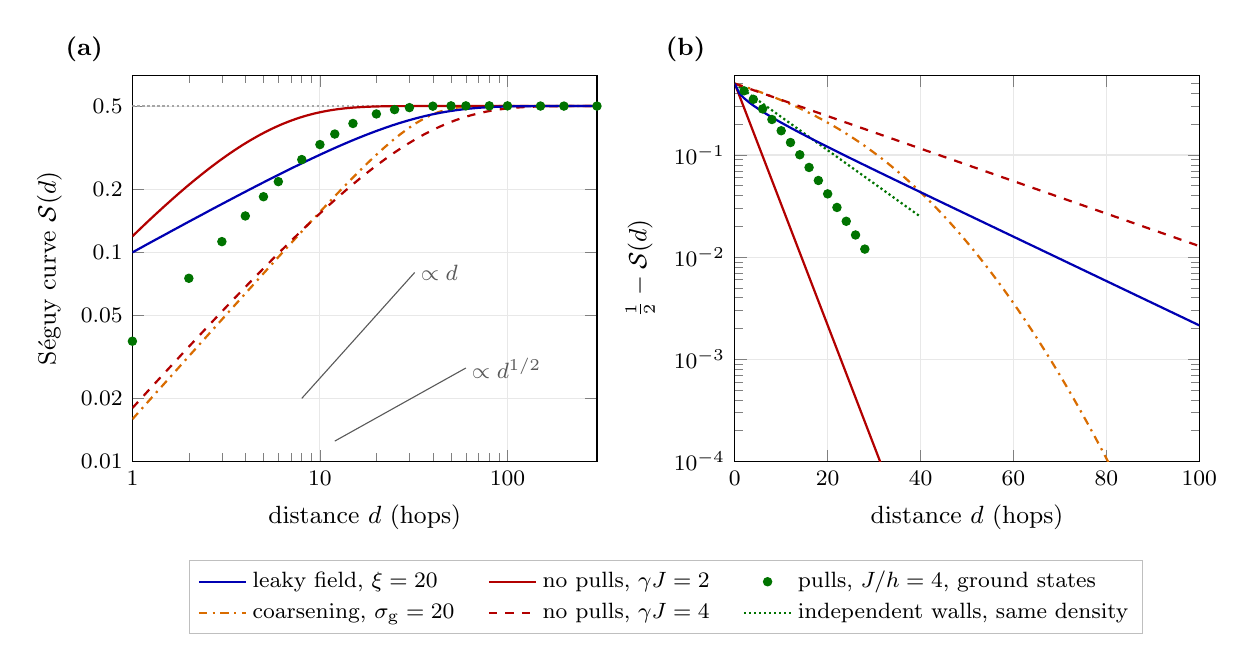
\begin{tikzpicture}
  \begin{loglogaxis}[name=pa, scale only axis, width=5.9cm, height=4.9cm,
      xmin=1, xmax=300, ymin=0.01, ymax=0.7,
      log ticks with fixed point, ytick={0.01,0.02,0.05,0.1,0.2,0.5}, yticklabels={$0.01$,$0.02$,$0.05$,$0.1$,$0.2$,$0.5$},
      xlabel={distance $d$ (hops)}, ylabel={S\'eguy curve $\mathcal S(d)$},
      grid=major, grid style={gray!18},
      legend style={font=\footnotesize, at={(1.148,-0.255)}, anchor=north, draw=gray!50, fill=white, cells={anchor=west},
        legend columns=3, /tikz/every even column/.append style={column sep=10pt}},
      every axis label/.style={font=\small}, tick label style={font=\footnotesize}]
    \draw[gray!70, densely dotted, thick] (axis cs:1,0.5) -- (axis cs:300,0.5);
    \addplot[forget plot, orange!85!black, thick, dash dot] coordinates {(1,0.01591) (1.102,0.01753) (1.213,0.0193) (1.336,0.02126) (1.472,0.02342) (1.622,0.02579) (1.786,0.02841) (1.967,0.03129) (2.167,0.03446) (2.387,0.03795) (2.629,0.04179) (2.896,0.04601) (3.19,0.05067) (3.514,0.05578) (3.871,0.06141) (4.264,0.0676) (4.696,0.0744) (5.173,0.08187) (5.698,0.09008) (6.276,0.09908) (6.914,0.1089) (7.615,0.1197) (8.388,0.1316) (9.24,0.1445) (10.18,0.1585) (11.21,0.1738) (12.35,0.1904) (13.6,0.2082) (14.98,0.2275) (16.5,0.248) (18.18,0.2699) (20.02,0.2928) (22.06,0.3168) (24.29,0.3413) (26.76,0.366) (29.48,0.3904) (32.47,0.4137) (35.76,0.4352) (39.39,0.4541) (43.39,0.4697) (47.8,0.4817) (52.65,0.49) (57.99,0.4952) (63.88,0.4981) (70.36,0.4993) (77.51,0.4998) (85.37,0.5) (94.04,0.5) (103.6,0.5) (114.1,0.5) (125.7,0.5) (138.4,0.5) (152.5,0.5) (168,0.5) (185,0.5) (203.8,0.5) (224.5,0.5) (247.3,0.5) (272.4,0.5) (300,0.5)};
    \addplot[forget plot, red!70!black, thick, dashed] coordinates {(1,0.01799) (1.102,0.01978) (1.213,0.02174) (1.336,0.02389) (1.472,0.02625) (1.622,0.02884) (1.786,0.03167) (1.967,0.03477) (2.167,0.03816) (2.387,0.04187) (2.629,0.04592) (2.896,0.05033) (3.19,0.05515) (3.514,0.0604) (3.871,0.0661) (4.264,0.07231) (4.696,0.07903) (5.173,0.08632) (5.698,0.0942) (6.276,0.1027) (6.914,0.1119) (7.615,0.1217) (8.388,0.1323) (9.24,0.1436) (10.18,0.1556) (11.21,0.1684) (12.35,0.1819) (13.6,0.1962) (14.98,0.2112) (16.5,0.2269) (18.18,0.2431) (20.02,0.2599) (22.06,0.2771) (24.29,0.2947) (26.76,0.3124) (29.48,0.3302) (32.47,0.3478) (35.76,0.3651) (39.39,0.3819) (43.39,0.398) (47.8,0.4132) (52.65,0.4273) (57.99,0.4403) (63.88,0.4518) (70.36,0.462) (77.51,0.4708) (85.37,0.4781) (94.04,0.484) (103.6,0.4888) (114.1,0.4924) (125.7,0.495) (138.4,0.4969) (152.5,0.4981) (168,0.4989) (185,0.4994) (203.8,0.4997) (224.5,0.4999) (247.3,0.4999) (272.4,0.5) (300,0.5)};
    \addplot[forget plot, red!70!black, thick] coordinates {(1,0.1192) (1.102,0.1296) (1.213,0.1407) (1.336,0.1525) (1.472,0.1651) (1.622,0.1785) (1.786,0.1926) (1.967,0.2074) (2.167,0.2229) (2.387,0.239) (2.629,0.2557) (2.896,0.2728) (3.19,0.2903) (3.514,0.308) (3.871,0.3258) (4.264,0.3434) (4.696,0.3608) (5.173,0.3778) (5.698,0.3941) (6.276,0.4095) (6.914,0.4239) (7.615,0.4372) (8.388,0.4491) (9.24,0.4596) (10.18,0.4687) (11.21,0.4764) (12.35,0.4827) (13.6,0.4877) (14.98,0.4915) (16.5,0.4944) (18.18,0.4965) (20.02,0.4979) (22.06,0.4988) (24.29,0.4993) (26.76,0.4997) (29.48,0.4998) (32.47,0.4999) (35.76,0.5) (39.39,0.5) (43.39,0.5) (47.8,0.5) (52.65,0.5) (57.99,0.5) (63.88,0.5) (70.36,0.5) (77.51,0.5) (85.37,0.5) (94.04,0.5) (103.6,0.5) (114.1,0.5) (125.7,0.5) (138.4,0.5) (152.5,0.5) (168,0.5) (185,0.5) (203.8,0.5) (224.5,0.5) (247.3,0.5) (272.4,0.5) (300,0.5)};
    \addplot[forget plot, blue!70!black, thick] coordinates {(1,0.09982) (1.102,0.1047) (1.213,0.1098) (1.336,0.1151) (1.472,0.1206) (1.622,0.1265) (1.786,0.1325) (1.967,0.1389) (2.167,0.1455) (2.387,0.1524) (2.629,0.1597) (2.896,0.1672) (3.19,0.175) (3.514,0.1832) (3.871,0.1917) (4.264,0.2005) (4.696,0.2097) (5.173,0.2192) (5.698,0.229) (6.276,0.2392) (6.914,0.2497) (7.615,0.2605) (8.388,0.2716) (9.24,0.283) (10.18,0.2947) (11.21,0.3066) (12.35,0.3187) (13.6,0.3309) (14.98,0.3433) (16.5,0.3556) (18.18,0.368) (20.02,0.3802) (22.06,0.3923) (24.29,0.4041) (26.76,0.4155) (29.48,0.4264) (32.47,0.4368) (35.76,0.4465) (39.39,0.4555) (43.39,0.4636) (47.8,0.4708) (52.65,0.4771) (57.99,0.4825) (63.88,0.4869) (70.36,0.4906) (77.51,0.4934) (85.37,0.4955) (94.04,0.4971) (103.6,0.4982) (114.1,0.4989) (125.7,0.4994) (138.4,0.4997) (152.5,0.4998) (168,0.4999) (185,0.5) (203.8,0.5) (224.5,0.5) (247.3,0.5) (272.4,0.5) (300,0.5)};
    \addplot[forget plot, only marks, mark=*, mark size=1.5pt, green!45!black] coordinates {(1,0.03754) (2,0.07507) (3,0.1124) (4,0.1491) (5,0.1843) (6,0.2176) (8,0.2774) (10,0.3272) (12,0.3675) (15,0.4128) (20,0.4584) (25,0.4808) (30,0.4915) (40,0.4994) (50,0.5011) (60,0.5012) (80,0.5011) (100,0.5011) (150,0.5002) (200,0.4999) (300,0.5)};
    % slope references
    \draw[black!65] (axis cs:8,0.02) -- (axis cs:32,0.08) node[anchor=west, font=\footnotesize, inner sep=2pt] {$\propto d$};
    \draw[black!65] (axis cs:12,0.0125) -- (axis cs:60,0.02795) node[anchor=west, font=\footnotesize, inner sep=2pt] {$\propto d^{1/2}$};
    % legend, row by row: leaky / no pulls 2 / pulls; coarsening / no pulls 4 / independent walls
    \addlegendimage{blue!70!black, thick}
    \addlegendentry{leaky field, $\xi=20$}
    \addlegendimage{red!70!black, thick}
    \addlegendentry{no pulls, $\gamma J=2$}
    \addlegendimage{only marks, mark=*, mark size=1.5pt, green!45!black}
    \addlegendentry{pulls, $J/h=4$, ground states}
    \addlegendimage{orange!85!black, thick, dash dot}
    \addlegendentry{coarsening, $\sigma_{\mathrm g}=20$}
    \addlegendimage{red!70!black, thick, dashed}
    \addlegendentry{no pulls, $\gamma J=4$}
    \addlegendimage{green!45!black, densely dotted, thick}
    \addlegendentry{independent walls, same density}
  \end{loglogaxis}
  \node[font=\small\bfseries, anchor=south east] at ($(pa.north west)+(-0.25cm,0.05cm)$) {(a)};
  \begin{semilogyaxis}[name=pb, at={($(pa.south east)+(1.75cm,0)$)}, anchor=south west, scale only axis, width=5.9cm, height=4.9cm,
      xmin=0, xmax=100, ymin=1e-4, ymax=0.6,
      xlabel={distance $d$ (hops)}, ylabel={$\frac12-\mathcal S(d)$},
      grid=major, grid style={gray!18},
      every axis label/.style={font=\small}, tick label style={font=\footnotesize}]
    \addplot[green!45!black, densely dotted, thick] coordinates {(0,0.5) (1,0.4638) (2,0.4303) (3,0.3992) (4,0.3703) (5,0.3435) (6,0.3187) (7,0.2956) (8,0.2742) (9,0.2544) (10,0.236) (11,0.2189) (12,0.2031) (13,0.1884) (14,0.1748) (15,0.1621) (16,0.1504) (17,0.1395) (18,0.1294) (19,0.1201) (20,0.1114) (21,0.1033) (22,0.09586) (23,0.08893) (24,0.0825) (25,0.07653) (26,0.07099) (27,0.06586) (28,0.0611) (29,0.05668) (30,0.05258) (31,0.04878) (32,0.04525) (33,0.04197) (34,0.03894) (35,0.03612) (36,0.03351) (37,0.03109) (38,0.02884) (39,0.02675) (40,0.02482)};
    \addplot[orange!85!black, thick, dash dot] coordinates {(0,0.5) (1,0.4841) (2,0.4682) (3,0.4523) (4,0.4366) (5,0.4208) (6,0.4052) (7,0.3897) (8,0.3744) (9,0.3592) (10,0.3441) (11,0.3293) (12,0.3147) (13,0.3003) (14,0.2862) (15,0.2723) (16,0.2587) (17,0.2454) (18,0.2324) (19,0.2198) (20,0.2074) (21,0.1955) (22,0.1839) (23,0.1727) (24,0.1618) (25,0.1514) (26,0.1413) (27,0.1317) (28,0.1225) (29,0.1136) (30,0.1052) (31,0.09726) (32,0.08968) (33,0.08252) (34,0.07575) (35,0.06939) (36,0.06341) (37,0.05782) (38,0.05259) (39,0.04773) (40,0.04321) (41,0.03903) (42,0.03517) (43,0.03161) (44,0.02834) (45,0.02535) (46,0.02262) (47,0.02013) (48,0.01788) (49,0.01583) (50,0.01399) (51,0.01233) (52,0.01084) (53,0.009506) (54,0.008316) (55,0.007256) (56,0.006316) (57,0.005484) (58,0.00475) (59,0.004103) (60,0.003536) (61,0.00304) (62,0.002607) (63,0.00223) (64,0.001902) (65,0.001619) (66,0.001374) (67,0.001164) (68,0.0009832) (69,0.0008284) (70,0.0006963) (71,0.0005838) (72,0.0004882) (73,0.0004073) (74,0.0003389) (75,0.0002813) (76,0.0002329) (77,0.0001924) (78,0.0001585) (79,0.0001303) (80,0.0001068) (81,8.732e-05) (82,7.122e-05) (83,5.795e-05)};
    \addplot[red!70!black, thick, dashed] coordinates {(0,0.5) (1,0.482) (2,0.4647) (3,0.448) (4,0.4318) (5,0.4163) (6,0.4013) (7,0.3869) (8,0.373) (9,0.3596) (10,0.3466) (11,0.3342) (12,0.3221) (13,0.3106) (14,0.2994) (15,0.2886) (16,0.2782) (17,0.2682) (18,0.2586) (19,0.2493) (20,0.2403) (21,0.2317) (22,0.2233) (23,0.2153) (24,0.2075) (25,0.2001) (26,0.1929) (27,0.1859) (28,0.1793) (29,0.1728) (30,0.1666) (31,0.1606) (32,0.1548) (33,0.1493) (34,0.1439) (35,0.1387) (36,0.1337) (37,0.1289) (38,0.1243) (39,0.1198) (40,0.1155) (41,0.1113) (42,0.1073) (43,0.1035) (44,0.09975) (45,0.09616) (46,0.0927) (47,0.08937) (48,0.08615) (49,0.08305) (50,0.08007) (51,0.07718) (52,0.07441) (53,0.07173) (54,0.06915) (55,0.06666) (56,0.06427) (57,0.06195) (58,0.05973) (59,0.05758) (60,0.05551) (61,0.05351) (62,0.05158) (63,0.04973) (64,0.04794) (65,0.04622) (66,0.04455) (67,0.04295) (68,0.04141) (69,0.03992) (70,0.03848) (71,0.0371) (72,0.03576) (73,0.03447) (74,0.03323) (75,0.03204) (76,0.03089) (77,0.02978) (78,0.0287) (79,0.02767) (80,0.02668) (81,0.02572) (82,0.02479) (83,0.0239) (84,0.02304) (85,0.02221) (86,0.02141) (87,0.02064) (88,0.0199) (89,0.01918) (90,0.01849) (91,0.01783) (92,0.01719) (93,0.01657) (94,0.01597) (95,0.0154) (96,0.01484) (97,0.01431) (98,0.0138) (99,0.0133) (100,0.01282)};
    \addplot[red!70!black, thick] coordinates {(0,0.5) (1,0.3808) (2,0.29) (3,0.2209) (4,0.1682) (5,0.1281) (6,0.09757) (7,0.07431) (8,0.05659) (9,0.0431) (10,0.03283) (11,0.025) (12,0.01904) (13,0.0145) (14,0.01104) (15,0.008411) (16,0.006405) (17,0.004878) (18,0.003715) (19,0.00283) (20,0.002155) (21,0.001641) (22,0.00125) (23,0.0009519) (24,0.000725) (25,0.0005522) (26,0.0004205) (27,0.0003203) (28,0.0002439) (29,0.0001858) (30,0.0001415) (31,0.0001077) (32,8.206e-05) (33,6.25e-05)};
    \addplot[blue!70!black, thick] coordinates {(0,0.5) (1,0.4002) (2,0.36) (3,0.33) (4,0.3053) (5,0.2842) (6,0.2656) (7,0.2489) (8,0.2338) (9,0.2201) (10,0.2074) (11,0.1958) (12,0.1849) (13,0.1748) (14,0.1654) (15,0.1566) (16,0.1483) (17,0.1406) (18,0.1333) (19,0.1264) (20,0.1199) (21,0.1138) (22,0.108) (23,0.1026) (24,0.09739) (25,0.09249) (26,0.08786) (27,0.08347) (28,0.07931) (29,0.07537) (30,0.07163) (31,0.06808) (32,0.06471) (33,0.06151) (34,0.05848) (35,0.0556) (36,0.05286) (37,0.05026) (38,0.04779) (39,0.04544) (40,0.04321) (41,0.04109) (42,0.03908) (43,0.03716) (44,0.03534) (45,0.03361) (46,0.03197) (47,0.0304) (48,0.02892) (49,0.0275) (50,0.02616) (51,0.02488) (52,0.02366) (53,0.02251) (54,0.02141) (55,0.02036) (56,0.01937) (57,0.01842) (58,0.01752) (59,0.01667) (60,0.01585) (61,0.01508) (62,0.01434) (63,0.01364) (64,0.01298) (65,0.01235) (66,0.01174) (67,0.01117) (68,0.01063) (69,0.01011) (70,0.009614) (71,0.009145) (72,0.008698) (73,0.008274) (74,0.007871) (75,0.007487) (76,0.007121) (77,0.006774) (78,0.006444) (79,0.006129) (80,0.00583) (81,0.005546) (82,0.005275) (83,0.005018) (84,0.004773) (85,0.004541) (86,0.004319) (87,0.004108) (88,0.003908) (89,0.003717) (90,0.003536) (91,0.003364) (92,0.0032) (93,0.003044) (94,0.002895) (95,0.002754) (96,0.00262) (97,0.002492) (98,0.00237) (99,0.002255) (100,0.002145)};
    \addplot[only marks, mark=*, mark size=1.5pt, green!45!black] coordinates {(2,0.4249) (4,0.3509) (6,0.2824) (8,0.2226) (10,0.1728) (12,0.1325) (14,0.1005) (16,0.07549) (18,0.05628) (20,0.04162) (22,0.03064) (24,0.02243) (26,0.01647) (28,0.01198)};
  \end{semilogyaxis}
  \node[font=\small\bfseries, anchor=south east] at ($(pb.north west)+(-0.25cm,0.05cm)$) {(b)};
\end{tikzpicture}

  \caption{\textbf{S\'eguy curves in one dimension.} (a) The probability $\mathcal S(d)$ that two members at distance $d$ differ in a binary code feature, on logarithmic axes, for the regimes of \cref{tab:abs-seguy} with $\xi=20$ and Gaussian width $\sigma_{\mathrm g}=\xi$. The leaky field read by thresholds, with $\Gamma(d)=e^{-d/\xi}$, rises as $d^{1/2}$; the Gaussian correlator $\Gamma(d)=e^{-d^2/(2\sigma_{\mathrm g}^2)}$ of coarsening, the code game without pulls at $\gamma J=2$ and $4$ (\cref{prop:abs-seguy}(c)) and the stochastically stable state with Gaussian pulls at $J/h=4$ rise linearly. (b) The approach to $\frac12$. It is exponential, a straight line on these axes, for the code game without pulls and, at large $d$, for the leaky field; coarsening has a Gaussian tail; and the stochastically stable state approaches $\frac12$ faster than independently placed walls with the same density (dotted), with a local rate that still grows at the largest sampled distances, so its tail is not established as exponential. A linear rise alone does not identify walls, since coarsening also rises linearly; the shape of the approach to $\frac12$ separates them. The stochastically stable curve comes from exact ground states of 64 features on 40000 sites (\cref{chk:abs-seguy}); in (b) its points stop at $d=28$, where their standard error reaches eight percent.}
  \label{fig:abs-seguy}
\end{figure}

\begin{remark}[Interpretation: dialect geography]\label{rem:abs-dialects}
Quantitative studies since \citet{seguy1971relation} find aggregate linguistic variation growing sublinearly with distance, as \citet{nerbonne2010measuring} reports in the abstract we read. In \citet{burridge2017spatial}, speakers with a memory of exposure and a conformity nonlinearity form boundaries that behave like interfaces with surface tension, and in periods of demographic stability and uniform density the expected linguistic distance has the arcsine form with a Gaussian correlator whose scale grows as the square root of time. Sublinear growth alone does not discriminate between the regimes of \cref{tab:abs-seguy}; the short-distance exponent and the approach to $\frac12$ do. Stationary walls need pulls, finite policy precision or barriers; homogeneous leaky linear dynamics make none (\cref{prop:abs-seguy}(d)), and coarsening is the limit $\gamma\to\infty$ of the derived rule without pulls.
\end{remark}
% src: L5-L2, L5-C3 as refined by B5 Section 3.3

Codes also have to compose. A language border is a place where translations between neighboring codes stop composing consistently, and the abelian case is exact.

\begin{proposition}[Consistency of translations and exchange rates]\label{prop:abs-exchange-consistency}
Let a connected graph carry an antisymmetric edge function $\alpha_{ij}=-\alpha_{ji}$: the logarithms of scalar translation factors $\Theta_{ij}>0$ between members' codes, or log exchange rates between currencies.
\begin{enumerate}
\item[(a)] The following are equivalent: the sum of $\alpha$ around every cycle vanishes; $\alpha_{ij}=\bar\alpha_j-\bar\alpha_i$ for a potential $\bar\alpha$, unique up to an additive constant; the least-squares fit of a potential has zero residual.
\item[(b)] If $\alpha=B\bar\alpha+\phi$, with $B$ the edge-node incidence matrix and independent edge errors $\phi_{ij}$ of mean zero and variances $\sigma^2_{ij}$, then the holonomy $\Hol(Z)$ of an oriented cycle $Z$, the signed sum of $\alpha$ around it, equals the signed sum of the $\phi_{ij}$ and the holonomy of the least-squares residual, and $\E[\Hol(Z)^2]=\sum_{(i,j)\in Z}\sigma^2_{ij}$.
\item[(c)] If receiver $i$ learns $\Theta_{ij}$ by least squares from $n_{ij}$ grounded co-occurrences of messages $\Theta^\ast_{ij}\eta_t+\nu_t$ with world values $\eta_t$, the $\nu_t$ independent $\Ncal(0,\sigma_y^2)$ and independent of the $\eta_t$, then conditionally on the $\eta_t$ the estimate is Gaussian with mean $\Theta^\ast_{ij}$ and variance $\sigma_y^2/\sum_t\eta_t^2$. If $n_{ij}^{-1}\sum_t\eta_t^2\to\sigma_\eta^2>0$ almost surely, as it does when the $\eta_t$ are independent and identically distributed with $\E\eta_t^2=\sigma_\eta^2$ or form a stationary ergodic sequence with that second moment, then $n_{ij}^{1/2}(\ln\Theta_{ij}-\ln\Theta^\ast_{ij})$ converges in law to $\Ncal\bigl(0,\sigma_y^2/((\Theta^\ast_{ij})^2\sigma_\eta^2)\bigr)$ as $n_{ij}\to\infty$.
\end{enumerate}
\end{proposition}
% src: L5-P11; (c) restated as exact conditional law plus delta method

Proof in \cref{app:abs}; checked on a two-zone instance (\cref{chk:abs-exchange}). Part (c) is the scalar case of grounded learning (\cref{prop:fw-rls}): where contact is rare, translations are poorly estimated, and cycles through such edges carry large holonomy. A shared code exists only where holonomy vanishes (\cref{thm:coh-holonomy}), and true translations are flat (\cref{prop:coh-flat-true}), so inconsistency is an error of learning. We read language borders as contact boundaries made visible as consistency boundaries, and bilinguals and translators as boundary agents whose precise translations lower the variance of boundary edges; bilinguals sit at the interfaces of monolingual domains in a model of language competition \citep{castello2006ordering}, and translation inside firms is modeled in a related way by \citet{cremer2007language}.

\subsection{Economies: the Hayek dimension, informed trading and exchange rates}\label{sup:abs-economies-the-hayek-dimension-informed-t}

\begin{proposition}[The Hayek dimension]\label{prop:abs-hayek}
Let $\eta\sim\Ncal(0,P_0)$ with $P_0\succ0$, let agent $i$ sense $s_i=H^s_i\eta+v_i$ with $v_i\sim\Ncal(0,R^s_i)$, $R^s_i\succ0$, independent of $\eta$, and let a public message $M\eta$ be available, with $M$ of rank $r_M$. If agent $i$'s decision depends on $\eta$ through $\psi_i^\top\eta$ with quadratic loss, then
\[
\Var\bigl(\psi_i^\top\eta\mid s_i,M\eta\bigr)=0\iff\psi_i\in\operatorname{row}(M).
\]
Hence the public message suffices for every agent's decision if and only if $\operatorname{span}\{\psi_i\}\subseteq\operatorname{row}(M)$, and the least number of public scalars that suffices is the Hayek dimension $r_{\mathrm{Hay}}=\dim\operatorname{span}\{\psi_i\}$.
\end{proposition}
% src: L5-P13

Proof in \cref{app:abs}; checked in four dimensions (\cref{chk:abs-hayek}). Hayek's scarce material (\cref{sec:abs-economies}) is the case $r_{\mathrm{Hay}}=1$. In our reading, prices economize on communication to the extent that decision-relevant functionals are shared, and goods valued by buyer-specific attributes, whose functionals span more dimensions than there are prices, need bilateral communication of high rank; this agrees in sign with, and does not derive, the finding of \citet{rauch1999networks} that proximity, common language and colonial ties matter more for differentiated products than for goods traded on organized exchanges. The mechanism-design counterparts are \citet{jordan1982competitive} and \citet{mount1974informational}, cited from their bibliographic records. For decisions about the state at a horizon in a dynamic world, the exact count is the dimension of the decision functionals carried back to the present, which does not shrink with the horizon when the dynamics is invertible, while in reversible worlds the effective count at a fixed tolerance is at most a number that falls to the number of slowest modes as the horizon grows (\cref{thm:env-hayek-horizon}). When the units of each level of a hierarchy decide through aggregates of the decisions of the level below, the count is nonincreasing up the hierarchy, but a top-down message that must serve the members' own decisions needs the rank of those decisions (\cref{prop:ren-hayek}).

\begin{conjecture}[Informed trading as grounding]\label{conj:abs-grossman-stiglitz}
Informed trading is the grounding of the exchange modality, the part of its leak that makes the price informative about values. A market of pure price readers has the largest reach and carries no information about values, which is the exchange form of the grounding tension (\cref{thm:coh-grounding-tension}, \cref{asm:int-a11}), and by \cref{prop:abs-walras}(c) a market in which many traders read the price at level 0 overreacts to it.
\end{conjecture}
% src: L5-C4, L5-L7

The conjecture is our reading of the argument of \citet{grossman1980impossibility}, known to us from secondary summaries, that with costly information prices cannot be fully revealing in equilibrium, since no trader would then pay for information.

Exchange rates are translations between the codes in which values are expressed. With this identification, the only interpretive step here, the absence of cyclic arbitrage is the cocycle condition of \cref{prop:abs-exchange-consistency}(a), which holds exactly when all rates derive from currency values relative to a numeraire, and arbitrageurs, whose trades reduce holonomy, are boundary agents that enforce consistency. The split of noisy pairwise data into gradient and cycle parts is the combinatorial Hodge decomposition used for ranking \citep{jiang2011statistical}.

\subsection{Nations: readings}\label{sup:abs-nations-readings}

\citet{deutsch1953nationalism}, whose fourth chapter we read in the second edition, calls a people a larger group linked by complementary habits and facilities of communication, tests complementarity by communicative effectiveness and proposes measuring a channel's fidelity by the information lost in transmission. We read a people as a set with higher fidelity and code rank among members than across, a contrast statement in the language modality. The transaction-flow index of \citet{savage1960statistical} and modularity \citep{newman2006modularity} measure contrast in message rates rather than in coherence, and \cref{prop:abs-barrier,prop:abs-bypass} translate the first into the second.

\begin{remark}[Interpretation: readings of the polity criterion]\label{rem:abs-polity-readings}
Better communication lengthens $\xi$ and raises $\chi$; on the line it enlarges optimal polities when the fixed cost is small against $g\xi$ ($f/(g\xi)$ below about 1.07 under rule C and 0.37 under rule M), with $d^\ast\propto\xi^{1/2}$ in the small-cost limit, while nearer the thresholds of \cref{prop:abs-polity} a longer $\xi$ shortens the finite optimum. Above the threshold of the declared rule every finite polity costs more than the limit of unbounded ones, whose policy is unrelated to most members' preferences, a stylized regime of loosely governed polities about whose historical instances the model says nothing. The finding of Alesina and Spolaore that the equilibrium number of countries increases with economic integration has a multiplex reading: once the market extends beyond the polity, market size no longer needs a large polity. Conquest, conflict and contingency, which shape actual borders, are outside the model.
\end{remark}
% src: L5-C6, B5-P12 comparison

Statutes, registries and case law are durable media, and administration over territory needs messages of long range; in the reading of \cref{rem:abs-innis} a polity extended in space and time needs both. Anderson's account of print capitalism, known to us from secondary summaries \citep{anderson1983imagined}, holds that print created mass reading publics in fewer languages than were spoken and made the nation imaginable. We read print as a durable medium of long reading range whose readership is bounded by a language and a book market, so that it lengthens $\xi$ and $\tau$ inside the readership and aligns boundaries across modalities, as a border sharp at long range needs (\cref{prop:abs-bypass}).

\subsection{Cities}\label{sec:abs-cities}

\begin{definition}[Co-presence and one-round sets]\label{def:abs-one-round}
The content of the co-presence modality is the location and activity of people; its messages are encounters, and its round is a day. A one-round set is a set of agents every pair of which can meet within one round, each member leaving from its home and returning to it within the round.
\end{definition}
% src: L5-D11

\begin{proposition}[One-round diameter]\label{prop:abs-one-round}
Let members' homes $x_i$ lie in $\R^D$, and let every member travel along straight lines at speed at most $v_{\mathrm{tr}}$ for at most $T_{\mathrm{tr}}$ per round. Then any two members of a one-round set are within $v_{\mathrm{tr}}T_{\mathrm{tr}}$ of each other, so its diameter is at most $v_{\mathrm{tr}}T_{\mathrm{tr}}$, linear in the speed at a fixed budget. Equivalently, a member's daily reach, the set of points it can visit and return from within one round, is the ball of radius $v_{\mathrm{tr}}T_{\mathrm{tr}}/2$ about its home; two members can meet within a round if and only if their reaches intersect; and a one-round set is a set of pairwise intersecting reaches.
\end{proposition}
% src: L5-P17

Proof in \cref{app:abs}. The daily reach is the one-round light cone of the co-presence modality, and a one-round set is defined without contrast, so it need not be a collective in the sense of \cref{def:col-collective}. Collectives that form over many rounds are bounded instead by the size bound of \cref{cor:col-lstar}; the two quantities are not comparable (\cref{tab:sca-sizes}), but they compose.

\begin{corollary}[One-round reach and the extent of a collective]\label{cor:abs-one-round-extent}
Let the world-conditional precision $\Pi^c$ of a modality be diffusive with uniform leak $\varepsilon^\Pi$, let $a^\Pi_{\max}=\max_i\sum_ja^\Pi_{ij}$, and let every coupling $a^\Pi_{ij}>0$ join agents whose positions are within physical distance $\ell_\Pi$. Then the largest extent of \cref{def:col-lstar} satisfies, in every direction $d$ and at every admissible level $r_0$,
\[
\Lstar_d(r_0)\le\ell_\Pi\Bigl(\frac{a^\Pi_{\max}}{2\varepsilon^\Pi(r_0-1)}\Bigr)^{1/2}.
\]
In the reversible and normal classes of \cref{thm:col-diffusive-precision}, couplings join agents with a common listener or a common source, so $\ell_\Pi\le2\ell_{\mathrm{att}}$, with $\ell_{\mathrm{att}}$ the longest physical length of an attention link. In the co-presence modality an attention link is a meeting within one round, so $\ell_{\mathrm{att}}\le v_{\mathrm{tr}}T_{\mathrm{tr}}$ by \cref{prop:abs-one-round}, and $\Lstar_d(r_0)\le2v_{\mathrm{tr}}T_{\mathrm{tr}}\bigl(a^\Pi_{\max}/(2\varepsilon^\Pi(r_0-1))\bigr)^{1/2}$.
\end{corollary}
% src: B1-P7, L5-P17

Proof in \cref{app:abs}. The one-round reach bounds the physical length of a coupling, and contrast bounds the extent in units of that length.

\begin{remark}[Interpretation: Marchetti's constant]\label{rem:abs-marchetti}
\citet{marchetti1994anthropological} reports a mean daily travel time of about one hour across populations, pedestrian cities about 5 km across, and a sixfold to sevenfold linear expansion of cities with cars, which are six to seven times faster than walking; reviewing more than two dozen studies, \citet{mokhtarian2004ttb} conclude that travel time is not constant except perhaps in aggregate. With $T_{\mathrm{tr}}\approx1$ hour and 5 km per hour the bound of \cref{prop:abs-one-round} is about 5 km, and the expansion with cars is its linear dependence on $v_{\mathrm{tr}}$; the bound then describes the population average, not each member.
\end{remark}
% src: L5-L13

\citet{bettencourt2007growth} report urban quantities scaling as powers of population, with exponents near 1.2 for wealth creation and innovation and near 0.8 for infrastructure. Bettencourt's model, as \citet{ribeiro2023mathematical} present it \citep{bettencourt2013origins}, requires per-capita output to pay the cost of crossing the city, a condition that gives output proportional to $N^{7/6}$ and that we read as a one-round reach condition with a money budget in place of a time budget. Superlinear output also needs partners that carry different information: if $n_{\mathrm p}$ partners' estimates have errors of common variance $\sigma^2$ and common correlation $\bar\Gamma\ge0$, their minimum-variance unbiased linear combination is the average, because $\one$ is an eigenvector of the error covariance, and its variance $\sigma^2[1+(n_{\mathrm p}-1)\bar\Gamma]/n_{\mathrm p}$ never falls below $\sigma^2\bar\Gamma$, the variance of the average of $1/\bar\Gamma$ independent estimates.

\begin{conjecture}[Redundancy limits urban superlinearity]\label{conj:abs-redundancy}
Superlinear urban exponents are larger for outputs that depend on diverse, non-redundant information, and larger in urban systems whose diversity grows with size; outputs that depend on redundant information scale closer to linearly.
\end{conjecture}
% src: L5-C8, L5-L14

Telecommunication adds edges whose cost does not depend on distance (\cref{asm:int-a8}), yet geography remains: the probability that two users of a Belgian mobile network are linked decays as the inverse square of their distance \citep{lambiotte2008geographical}, while about one third of friendships in a large online network are independent of geography \citep{libennowell2005geographic}. In our reading, collectives of modalities carried by such networks need not be territorial, while enforcement, transport and co-presence stay bounded by physical ranges.

\subsection{Distance: elasticity, cutoffs and the distance effect}\label{sup:abs-distance-elasticity-cutoffs-and-the-dist}

\begin{proposition}[Distance elasticity of coherence]\label{prop:abs-elasticity}
Let coherence between locations at distance $d>0$ be $\Psi(d/\xi)$ for a positive differentiable profile $\Psi$, and let its distance elasticity be $\mathrm{el}(d)=-\mathrm d\ln\Psi(d/\xi)/\mathrm d\ln d=\mathrm{el}_\Psi(d/\xi)$, with $\mathrm{el}_\Psi(x)=-x\Psi'(x)/\Psi(x)$.
\begin{enumerate}
\item[(a)] The elasticity at each fixed distance is the same for every $\xi>0$ if and only if $\Psi$ is a power law, $\Psi(x)=\Psi(1)x^{-\alpha_{\mathrm{el}}}$, and then $\mathrm{el}\equiv\alpha_{\mathrm{el}}$.
\item[(b)] For the profile $\Psi=K_0$ of diffusion with leak in two dimensions, $\mathrm{el}_{K_0}(x)=xK_1(x)/K_0(x)$ is strictly increasing on $(0,\infty)$, with $\mathrm{el}_{K_0}(x)\to0$ as $x\to0$ and $\mathrm{el}_{K_0}(x)-x\to\frac12$ as $x\to\infty$. Increasing $\xi$ therefore lowers the elasticity at every fixed distance.
\item[(c)] For an integral of exponential profiles against the weight $\xi^{-1-\alpha_{\mathrm{el}}}\mathrm d\xi$ on $(0,\infty)$, $\alpha_{\mathrm{el}}>0$ (a $\sigma$-finite weight, not a probability density), the coherence at $d>0$ is $\int_0^\infty e^{-d/\xi}\xi^{-1-\alpha_{\mathrm{el}}}\mathrm d\xi=d^{-\alpha_{\mathrm{el}}}\int_0^\infty\varrho^{\alpha_{\mathrm{el}}-1}e^{-\varrho}\mathrm d\varrho$, an exact power law with constant elasticity $\alpha_{\mathrm{el}}$.
\end{enumerate}
\end{proposition}
% src: L5-P14; (b) monotonicity now proved (Riccati equation), no longer only checked on a grid

Proof in \cref{app:abs}; checked numerically (\cref{chk:abs-elasticity}). At a distance of 1000 km the elasticity of the profile $K_0$ is 4.47, 2.46, 1.43 and 0.90 for $\xi=250$, 500, 1000 and 2000 km. Scale-free coherence arises from nested coupling, such as administrative and economic hierarchies may provide.

\begin{remark}[Cutoffs and log-periodic modulation]\label{rem:abs-cutoff}
In the notation of \cref{prop:abs-hierarchy}, with $\mathsf c_\infty=1/(1-\mathfrak q)+1/(b-1)$, the eigenvalues of an infinite hierarchy are $\mathsf c_\infty A_{\mathrm h}\mathfrak q^{l-1}$, and they fall below the precision leak $\varepsilon^\Pi$ at the level $l^\ast=1+\ln(\mathsf c_\infty A_{\mathrm h}/\varepsilon^\Pi)/\ln(1/\mathfrak q)$. At finite leak the geometric law holds up to $l^\ast$ and, in a finite population, up to the levels where the constant mode $b^{-n_{\mathrm H}}/\varepsilon^\Pi$ takes over; multiplying all couplings by a factor leaves $\alpha_{\mathrm H}$ unchanged and moves $l^\ast$ outward by the logarithm of the factor divided by $\ln(1/\mathfrak q)$. With $b=2$, $n_{\mathrm H}=40$, $\mathfrak q=0.7$ and $\varepsilon^\Pi=10^{-7}$ the per-level ratio is 0.714 at levels 1 to 5, as $1/(b\mathfrak q)$ predicts. A small hierarchy ($b=4$, five levels, $\mathfrak q=0.5$, $\varepsilon^\Pi=0.01$, on a line) does not reach the ratio 0.5: its per-level ratios are 0.58 to 0.65, and the local elasticity oscillates between 0.15 and 0.57 with the period of the hierarchy, a log-periodic modulation of the power law (\cref{chk:abs-hierarchy}).
\end{remark}
% src: L5-P15(b),(c) and its check

\begin{conjecture}[What the framework says about the distance effect]\label{conj:abs-distance}
(i) If the binding friction of trade were informational coherence with one scale that communication lengthened, distance elasticities at fixed distances would have fallen during the twentieth century (\cref{prop:abs-elasticity}(b)) and would rise with distance in a cross-section; the persistence and mid-century rise found by Disdier and Head, and the constant long-distance elasticity Chaney takes as given, are inconsistent with this as the dominant mechanism. (ii) The persistence fits two readings: the modality that binds trade at long distances (transport, enforcement, trust) is not the one whose range grew, or coherence in the binding modality is scale free, nested (\cref{prop:abs-hierarchy}) or a superposition of scales (\cref{prop:abs-elasticity}(c)), so that uniform improvements in range or coupling only move cutoffs. (iii) The nested reading predicts log-periodic modulation of elasticities at the scales of administrative and economic hierarchies, and border widths in kilometers that grow with communication range at fixed border factors.
\end{conjecture}
% src: L5-C5(i)-(iii), L5-O6

The framework does not explain the rise itself, which Berthelon and Freund find within industries and strongest for homogeneous goods, evidence they hold against a composition explanation; Chaney's mechanism is a scale-free alternative outside the information channel; and in our reading Steinwender's telegraph result agrees with the framework, a range increase in the price channel having raised coherence between markets.

\subsection{World-conditional correlations in societies}\label{sec:abs-world}

Social data record the joint response of a population to shared shocks as well as the coherence that communication produces, which is why the ultrametric contrast of \cref{def:col-ultrametric} uses world-conditional correlations.

\begin{proposition}[Unconditional correlations cap the ultrametric contrast]\label{prop:abs-ultrametric-cap}
Let the unconditional stationary covariance of a modality's scalar errors be $\Sigma=\Sigma^c+\Sigma_{\mathrm{cm}}\one\one^\top$, with the world-conditional covariance $\Sigma^c$ entrywise nonnegative and $\Sigma_{\mathrm{cm}}>0$ the variance of the common mode. This is the case for the scalar level-0 network with $W\ge0$, exact code models and equal sensing gains, whose row sums all equal $\lambda$ and whose common mode has variance $\Sigma_{\mathrm{cm}}=Q/(1-\lambda^2)$ (\cref{lem:fw-common-mode}). Then every unconditional correlation is at least $\Sigma_{\mathrm{cm}}/(\Sigma_{\mathrm{cm}}+\max_i\Sigma^c_{ii})$, and every nonempty set $C\ne V$ has
\[
\mathcal U^{\mathrm{unc}}(C)\le\ln\Bigl(1+\frac{\max_i\Sigma^c_{ii}}{\Sigma_{\mathrm{cm}}}\Bigr),
\]
where $\mathcal U^{\mathrm{unc}}$ is the ultrametric contrast computed from unconditional instead of world-conditional correlations. In the level-0 network with $W=\lambda P$, $P$ a fixed irreducible aperiodic stochastic matrix with stationary vector $\pi$, and local noise covariance $Q^\zeta=\diag(q_i)\ne0$, $(1-\lambda^2)\Sigma^c_{ii}\to\pi^\top Q^\zeta\pi$ for every $i$ as $\lambda\to1$ ($=q/N$ for symmetric $P$ and $Q^\zeta=qI$), so the cap tends to $\ln(1+\pi^\top Q^\zeta\pi/Q)>0$; in the symmetric case this limit is $\ln(1+q/(NQ))$, which is small when $q/(NQ)$ is small and vanishes only as $N\to\infty$ or $q/Q\to0$. For $W=\lambda P$ with $P$ symmetric and doubly stochastic, irreducible or not, and $Q^\zeta=qI$ with $q>0$, one has $(1-\lambda^2)\Sigma^c_{ii}\ge q/N$ for every $i$ and every $\lambda\in(0,1)$, so the cap is at least $\ln(1+q/(NQ))$ at every level of grounding: in a finite closed population of this kind $(1-\lambda^2)\max_i\Sigma^c_{ii}$ does not tend to zero.
\end{proposition}
% src: B5-L2; critic D6; repair list for abs (world-conditional correlations); vanishing condition made explicit; editor: restricted to proper subsets (the whole population has infinite contrast)

Proof in \cref{app:abs}. Unconditional correlations of regional price, opinion or usage series count the common response to shared shocks as coherence, so when $(1-\lambda^2)\max_i\Sigma^c_{ii}\ll Q$, that is, when local noise is not large against the world innovation ($q/(NQ)\ll1$ at weak grounding), every unconditional contrast is small, whatever the barriers: on a ring of 60 agents with $q=Q=1$ and two barriers with $n_b=100$, the contrast of one arc is 3.37, 2.80 and 2.12 from world-conditional correlations at leaks $\varepsilon=0.05$, 0.01 and 0.002, and 0.114, 0.072 and 0.041 from unconditional ones (\cref{chk:abs-cap}). The limit $\ln(1+q/(NQ))$ is taken at fixed coupling. When the barriers strengthen as grounding weakens, so that $1-\lambda^2$ stays large against the coupling between nearly isolated blocks of $n$ members and small against the spectral gap within them, $(1-\lambda^2)\Sigma^c_{ii}$ is of order $q/n$, the cap is of order $\ln(1+q/(nQ))$, and the unconditional contrast of a block approaches it instead of zero: for two blocks of three with $q=Q=1$ it is 0.286 under the cap 0.287 at $\lambda=0.9999$, against $\ln(4/3)=0.288$ (\cref{chk:abs-cap}). The world-conditional contrast has no such cap and grows without bound as the barriers strengthen at fixed grounding. The cap scales with $q/Q$, and with $q/Q=100$ on the same ring the unconditional contrast at $\varepsilon=0.002$ is 1.445 against the world-conditional 2.120, so the barriers remain visible when local noise is large against the world innovation. Conditioning on the shared drive, or a recorded proxy for it, is the empirical counterpart of \cref{def:col-world-conditional}. Without a recorded drive, the setting of \cref{prop:abs-ultrametric-cap} is a Gaussian graphical model with one latent variable: by the Sherman--Morrison formula the unconditional precision is
\[
\Sigma^{-1}=(\Sigma^c)^{-1}-\frac{(\Sigma^c)^{-1}\one\one^\top(\Sigma^c)^{-1}}{\Sigma_{\mathrm{cm}}^{-1}+\one^\top(\Sigma^c)^{-1}\one},
\]
the world-conditional precision minus a rank-one term along the vector $(\Sigma^c)^{-1}\one$, which for a diffusive precision is the vector of its leaks, and for a stationary world the covariance of the beliefs themselves has the same form with a different common-mode variance, since beliefs and errors differ by a multiple of $\one$ that is a function of the world path. For a static or stationary world without performative acts, the world-conditional precision is locally identifiable from members' statistics alone under the sparse-plus-low-rank conditions of \citet{chandrasekaran2012latent}, a sparse conditional precision and a latent effect spread over most of the observed variables, in the quantitative sense of their transversality condition, and their convex estimator applies under those conditions; a diffusive precision on a sparse graph with comparable leaks has a sparse conditional precision and a rank-one term spread over the agents, but the quantitative condition is not verified for it here. The estimator is open when acts drive the world, when the conditional precision is not sparse, or when the leak vector $(\Sigma^c)^{-1}\one$, along which the rank-one term lies, is concentrated on few agents.

\subsection{Graded meta-agents: discussion and open problems}\label{sup:abs-graded-meta-agents-discussion-and-open-p}

Among the properties graded in \cref{tab:abs-graded}, interaction necessity transfers most readily: with scalar errors, every causally separating null makes the precision of the members' states given the shared exogenous drive diagonal, so that no region has contrast above one for it (\cref{prop:agy-nulls-vanish}(d)). For the world-conditional precision on which collectives are selected the same is proved under the deletion nulls in populations without records, and in the two-group model under the frozen-environment null when the initial states that frozen messages carry are deterministic or conditioned on (\cref{prop:frm-nulls}(a)); in these cases a collective selected by contrast above one differs from the nulls. When members act on the world, as in polities and markets, the order parameter must condition on that drive, because conditioning on the world path hides interaction through acts and couples agents that never interact (\cref{prop:agy-nulls-vanish}(b), \cref{ex:agy-collider}). The decisive tests of \cref{def:agy-nulls}, partner randomization at matched rates and the exact-fusion persistence clause, have been applied to no abstract collective. No abstract collective of this section is therefore shown to meet every clause of \cref{def:agy-meta-agent}: the entries of \cref{tab:abs-graded} are established one clause at a time, in different models, and neither their joint satisfaction in one population nor their joint unsatisfiability in a stated class is shown (\cref{open:agy-meta-agent-exists}).

Agency is furthest from the evidence. Nothing here makes a culture or a market behave as if it minimized a group expected free energy; a market has no collective preference, and agency, where it exists, sits in institutions such as courts, central banks and governments, which can be checked against the deliberation protocol of \cref{def:agy-group-model}, with shared reports and intentions and one decision maker at a time. Under it deliberation is reversible exactly when the members agree on how redundant their inputs are, its stationary law is a group posterior when a declared belief has the agreed redundancies, as for linear slots with additive noise and beliefs that are translates of one law (\cref{thm:agy-agency}), and it lies within explicit distances of one otherwise (\cref{thm:agy-heterogeneous}). Simultaneous decisions and unshared data fail the protocol (\cref{prop:agy-synchronous,ex:agy-no-data-sharing}), and, relative to the null policies, a group posterior represents positively coordinated choices only when they change the world (\cref{prop:agy-performative-sign,thm:agy-joint-acts}); between two non-null epistemic alternatives the log odds ratio can be positive. Whether actual institutions meet these hypotheses is interpretation.

Nothing here derives the formation of a culture, a market or a polity. Of the manuscript's formation theorems, \cref{thm:frm-formation} concerns the frozen-calibration mean-field map of the two-group model, and \cref{thm:frm-split-contrast} concerns the error law of the split at $\gamma=\infty$ with noiseless angle observations, where the declared start is already the split; the step from the full stochastic model to that map is open (\cref{open:frm-closure}), as is online calibration, which from a symmetric start reaches the split's attention pattern (not necessarily a split selected by contrast) in 0 to 7 of 8 replicates per cell of \cref{tab:frm-online} after 6000 rounds, counted at a cutoff for a learned cross edge below the bias fraction $\frac12$ used for the map, so that the counts are upper bounds on those at $\frac12$, and differing by up to three replicates between reruns of one cell (\cref{obs:frm-online,open:frm-online}). The collectives formed there are a calibration-level effect of misreading joint structure: receivers that know their translation errors pay no mistranslation cost, so from a start law exchangeable given the world path the split fails the translation-aware form of the exact-fusion persistence clause, as \cref{prop:frm-exact-fusion} proves, while for full cross-covariance-aware exact fusion this conclusion is heuristic in the two-group model; above the threshold $\gamma_T$ of \cref{thm:frm-formation}(b) the split coincides with the code partition. Persistence with drifting frames (\cref{conj:frm-drifting-frames}) and formation beyond the two-group model (\cref{conj:frm-formation}) are conjectures. Readings of cultural or political boundaries as formed collectives inherit these qualifications; the propositions here describe stationary structure under declared couplings, not its origin.

The framework assumes generative models about shared external states in which messages are grounded, and near-stationary dynamics on slowly changing graphs. It does not cover self-referential conventions without an external referent, such as fashions or asset prices driven by beliefs about beliefs; strategic communication, which is coarsened when preferences diverge \citep{crawford1982strategic}; power, coercion and conflict; or breaks such as migration, conquest and epidemics. Membership by rule, such as citizenship, can diverge from the coarse-grained patterns of \cref{asm:int-a10}, and $\ell$, $a$ and $\varepsilon$ are inferred from proxies such as border effects, price correlations or S\'eguy curves only through a model.

\begin{openproblem}[Contrast of code domains]\label{open:abs-code-contrast}
Do the code domains of the walled regimes (\cref{prop:abs-seguy}(b),(c); \cref{thm:coh-domains-1d}) have spectral contrast in the sense of \cref{def:col-contrast}, so that consistency collectives are collectives in the manuscript's primary sense?
\end{openproblem}
% src: B5-O4

\Cref{ex:hie-code-domains} answers the question for the declared precision of a belief network on a ring whose attention is cut at the walls: a domain has spectral contrast, every domain of at most half the ring is a collective at weak enough grounding when the ring is the declared geometry, and no domain is one when the ring without the walls is the declared graph. Whether the code game produces such domains from a disordered start is part of \cref{conj:hie-conformity-formation}.

\begin{openproblem}[Attention across modalities]\label{open:abs-attention}
When agents allocate one attention capacity $\kappa$ across modalities by expected free energy, does the allocation couple the modalities, generating $a_\times$, and does it align or misalign their boundaries?
\end{openproblem}
% src: L5-O3

For a single agent with decisions that each load on one content, \cref{prop:env-multiplex}(d) answers the single-agent part of the question for a Shannon budget $I_{\max}$ and pragmatic value alone: when the decision eigenvalues of different modalities differ, the optimal sensor does not mix modalities within channels, and its allocation across modalities is coupled only through a common water level. The single-agent case of a channel count $\kappa$ and of the full objective $G^{\mathrm{att}}_h$ of \cref{def:env-attention-objective} remains open, as do the questions whether that coupling generates $a_\times$ in a network and how it places boundaries.

\begin{openproblem}[Agency of abstract collectives]\label{open:abs-institutions}
Find conditions under which an abstract collective with contrast and closure has agency in the sense of hypothesis H1, in particular whether institutions with collective active states make a polity or an economy behave as if minimizing a group expected free energy, and whether actual institutions meet the protocol hypotheses of \cref{thm:agy-agency}.
\end{openproblem}
% src: L5-O4, B4 Section 1.5 and last change item

\subsection{Multiplex terminology}\label{sup:abs-multiplex-terminology}

In the terminology of \citet{kivela2014multilayer} the population of \cref{def:abs-multiplex} is a multiplex network, whose layers share their nodes and differ in their edges. \Cref{tab:abs-modalities} lists the four modalities of this section. When the contents evolve independently and one agent senses several of them under a budget on the information it acquires, for decisions that each load on one content, the budget-optimal sensor reads each channel within one content when the decision eigenvalues of different contents differ, and its attention to different contents is coupled only through a common water level (\cref{prop:env-multiplex}(d)).

\subsection{Composite classes, markets and polities}\label{sup:abs-composite-classes-markets-and-polities}

A composite class of type $M\subseteq\mathcal M$ is a closed ball of radius one of the ultrametric $\max_{c\in M}u_{(c)}/\vartheta_c$ of \cref{prop:col-nesting}(b), with $u_{(c)}$ the ultrametric of modality $c$ and declared scales $\vartheta_c>0$; its contrast profile is the vector of its ultrametric contrasts in the modalities of $M$. Composite classes of one type are nested or disjoint, ultrametric classes of different modalities can cross, and $\min_cu_{(c)}$ is not an ultrametric in general (\cref{prop:col-nesting}(b)); these follow from single linkage and are not findings. \Cref{prop:abs-bypass} gives the dynamical reason why a composite class is sharp only where every member modality is.

\begin{definition}[Market]\label{def:abs-market}
A market is a collective (\cref{def:col-collective}) of the exchange modality (\cref{tab:abs-modalities}), read on members' valuations of the same goods. Public prices are codes of rank one for each good and market, transfers are performative messages that change holdings, and money balances are records. No result of this section shows that a market in a stated model is a collective in the sense of \cref{def:col-collective}; the results of \cref{sec:abs} concern its borders and the ultrametric diagnostic.
\end{definition}
% src: L5-D9

\begin{definition}[Polity]\label{def:abs-polity}
A polity is a composite class (\cref{prop:col-nesting}(b)) whose type contains the law and enforcement modality (\cref{tab:abs-modalities}). Its promulgations are broadcast codes, usually records of small decay, and its rulings, registrations and sanctions are performative acts that change rights, holdings and the outcomes of other agents' policies, and so the risk term of their expected free energy. A nation-state, in the usage of this section, is a polity whose law boundary is aligned with its boundaries in the language, exchange and broadcast modalities.
\end{definition}
% src: L5-D10

\subsection{The distance effect in trade: sources}\label{sup:abs-the-distance-effect-in-trade-sources}

Trade falls with distance, and the fall has not weakened as communication improved: in a meta-analysis of 1467 estimates the distance effect rose around the middle of the twentieth century and stayed high \citep{disdier2008puzzling}, the distance elasticity rose by about 10 percent after 1985, mostly within industries \citep{berthelon2008conservation}, and a constant long-distance elasticity follows if firm sizes are Pareto distributed and the squared distance of a firm's exports grows as a power of its size \citep{chaney2018gravity}. Yet the transatlantic telegraph of 1866 reduced the mean and the volatility of the difference between cotton prices in New York and Liverpool \citep{steinwender2018real}. We read these findings through the dependence of the elasticity of coherence on its scale (\cref{sec:abs-distance}).

\section{Additional results for \texorpdfstring{Section~\ref{sec:met}}{Section 11}: meta-agents}\label{sup:met}

This section collects statements, examples and remarks of \cref{sec:met} that the main text cites without stating in full. Proofs are in \cref{app:met}.

\subsection{Interpretation of the coarse variables}\label{sup:met-interpretation-of-the-coarse-variables}

\begin{remark}[Physical and abstract external states]\label{rem:met-abstract}
This remark is an interpretation. Every coarse variable is a function of the joint process and in that sense physical; a member senses a price through the same kind of channel through which a cell senses a chemical potential. What changes with scale is which variable has a law of its own. For a meta-agent it is a function of many channels and agents, such as another collective's coarse state, a price or a record, abstract in that it need not be a world variable, and it becomes an object of the theory only when its closure is proved (\cref{thm:met-abstract-physics}) or bounded (\cref{prop:met-memory}). Base-level agents keep generative models of external physical states.
\end{remark}
% src: H3-R1, decision 19

\subsection{Coarse blankets: three failures of the sufficient conditions}\label{sup:met-coarse-blankets-three-failures-of-the-su}

\begin{example}[An equal-weight summary leaks]\label{ex:met-summary-leak}
Let the exterior $\eta_t\sim\Ncal(0,1)$ be independent across rounds and read by two sensory channels $X_{k,t+1}=\eta_t+v_{k,t}$, $\Var v_{k,t}=R^s_k$, $k=1,2$; let the interior be $y_{t+1}=g_1X_{1,t}+g_2X_{2,t}+\mathfrak n_t$ with $\Var\mathfrak n_t=q>0$; and declare $s=X_1+X_2$. No channel reads both sides, so the fine path blanket holds, but the weak and strong coarse leak rates are both
\begin{equation}\label{eq:met-summary-leak}
\begin{gathered}
\iota_{\mathrm{path}}=-\frac12\ln\Bigl(1-\frac{\Cov(y,\eta\mid s)^2}{\Var(y\mid s)\Var(\eta\mid s)}\Bigr),\\
\Cov(y,\eta\mid s)=\frac{(g_1-g_2)(R^s_2-R^s_1)}{4+R^s_1+R^s_2},\qquad\Var(\eta\mid s)=\frac{R^s_1+R^s_2}{4+R^s_1+R^s_2},
\end{gathered}
\end{equation}
with $\Var(y\mid s)=g_1^2(1+R^s_1)+g_2^2(1+R^s_2)+2g_1g_2+q-(g_1(2+R^s_1)+g_2(2+R^s_2))^2/(4+R^s_1+R^s_2)$, the moments being those of $(y_{t+1},\eta_{t-1},s_t)$. The leak is positive whenever $g_1\neq g_2$ and $R^s_1\neq R^s_2$; for members who weight by precision, $g_k=1/R^s_k$, the conditional covariance is $(R^s_2-R^s_1)^2/(R^s_1R^s_2(4+R^s_1+R^s_2))$. With these gains, the weights of the information-form statistic, at $R^s=(0.5,2)$ and $q=0.1$ the rate is $0.135600$ nats per round, and at $R^s=(0.2,5)$ it is $0.619053$.
\end{example}
% src: H3-X1; HC_critic V5 (rates reproduced)
The computation is in \cref{app:met}; both rates agree to six digits with window computations from the path covariance (\cref{chk:met-blanket}).

\begin{example}[Heterogeneous channel memories]\label{ex:met-channel-memory}
Let sensory channels with memories $\mathsf d_k$, $X_{k,t+1}=\mathsf d_kX_{k,t}+\eta_t+v_{k,t}$, read a scalar exterior state, with the information-form $s_C$ of weights $1/R^s_k$. Then $\mathsf P_{\mathrm S}A_{\sS\sS}=(\mathsf d_k/R^s_k)_k$ is a multiple of $\mathsf P_{\mathrm S}=(1/R^s_k)_k$ only when all $\mathsf d_k$ are equal, so for unequal memories (a1) of \cref{prop:met-sufficiency} fails and $s_C$ reads the sensory residual. Members read their own channels, so the residual cannot be placed on the exterior side; on the interior side it makes $s_C$ read both sides, a coarse collider. In the three-member system of \cref{chk:met-blanket} the coarse leak on ten rounds from an independent start is $2\times10^{-14}$ with memories $(0.5,0.5,0.5)$, and $0.056$ and $0.055$ with memories $(0.2,0.5,0.8)$ and $(0,0,0.6)$. A meta-agent whose members' sensors integrate over different times has no exact coarse blanket at the information-form statistic.
\end{example}
% src: H3-X2 (mechanism derived, numbers checked)

\begin{example}[Reafference from one member's act]\label{ex:met-reafference}
Let the interior read only $s_C$, the exterior only $a_C=\alpha_1+\alpha_2$, the sum of two active channels driven by the interior, and the single sensory channel the exterior and member 1's act, $X_{\sS,t+1}=\eta_t+0.4\alpha_{1,t}+v_t$. The fine path blanket holds and the interior and exterior read the blanket only through $s_C$ and $a_C$, but (b3) of \cref{prop:met-sufficiency} fails: $s_C=X_{\sS}$ reads the exterior and the residual $\alpha_1-\alpha_2$, which lies on the interior side, and the coarse leak on ten rounds from an independent start is $0.113$ nats. If the sensor reads the total act instead, (b3) holds and the leak vanishes (\cref{chk:met-blanket}). Reading one member's act through a collective sensor is a coarse collider.
\end{example}
% src: H3-X3 (checked)

\subsection{Abstract physics: aggregates and other collectives}\label{sup:met-abstract-physics-aggregates-and-other-co}

\begin{example}[A price and many traders]\label{ex:met-traders}
Let the exterior of a meta-agent consist of a price and $N$ outside traders,
\begin{equation}\label{eq:met-traders}
p_{t+1}=\mathsf f_pp_t+\frac{\mathsf b_p}N\sum_jx_{j,t}+\mathsf b_Ca_{C,t}+w_t,\qquad x_{j,t+1}=\alpha_jx_{j,t}+\mathsf b_xp_t+w_{j,t},
\end{equation}
with persistences $0\le\alpha_j\le\alpha_{\max}<1$, independent Gaussian innovations of variances $q_p$ and $q_x$, and $\eta_C=(p,\bar x)$ with $\bar x=N^{-1}\sum_jx_j$. Write $\bar\alpha$ and $\Var_N(\alpha)$ for the mean and the variance of the persistences and $\bar{\mathfrak m}_l=N^{-1}\sum_j\alpha_j^l$.
\begin{enumerate}
\item[(a)] For $N\ge2$ the abstract physics is exact if and only if all $\alpha_j$ are equal: the partition into the price and the traders is lumpable exactly then.
\item[(b)] In general the stationary aggregate obeys exactly $\bar x_{t+1}=\bar\alpha\bar x_t+\mathsf b_xp_t+\sum_{l\ge2}\Gamma_lp_{t-l}+\mathfrak f^{(N)}_t-\bar\alpha\mathfrak f^{(N)}_{t-1}$, with kernel $\Gamma_l=\mathsf b_x(\bar{\mathfrak m}_l-\bar\alpha\bar{\mathfrak m}_{l-1})$ and colored noise $\mathfrak f^{(N)}_t=N^{-1}\sum_j\sum_{l\ge0}\alpha_j^lw_{j,t-l}$ of variance $(q_x/N^2)\sum_j(1-\alpha_j^2)^{-1}=O(1/N)$. The kernel has $\Gamma_1=0$, $\Gamma_l/\mathsf b_x\ge0$ and $\sum_{l\ge2}\lvert\Gamma_l\rvert\le\lvert\mathsf b_x\rvert\Var_N(\alpha)/(1-\alpha_{\max})^2$.
\item[(c)] If the empirical law of the $\alpha_j$ converges weakly to a law $\mathbb Q$ on $[0,\alpha_{\max}]$, with moments $\mathfrak m_l=\int\alpha^l\mathbb Q(\mathrm d\alpha)$, then $\Gamma_l\to\mathsf b_x(\mathfrak m_l-\mathfrak m_1\mathfrak m_{l-1})$; in particular $\Gamma_2\to\mathsf b_x\Var_{\mathbb Q}(\alpha)$, which for $\mathsf b_x\neq0$ is nonzero unless $\mathbb Q$ is a point mass.
\end{enumerate}
With persistences evenly spaced on $[0.3,0.7]$ the memory weight $\sum_{l\ge2}\lvert\Gamma_l\rvert$ falls only from $0.0370$ to $0.0297$ between $N=10$ and $N=640$ (\cref{chk:met-traders}): the law of large numbers removes the noise of the aggregate, not its memory.
\end{example}
% src: H3-E2 (derived and checked; HC_critic V6, V12)
The proof is in \cref{app:met}.

\begin{remark}[The information-form defect for aggregates]\label{rem:met-aggregate-defect}
In \cref{ex:met-traders}, $\bar Q=\diag(q_p,q_x/N)$, and since $\det(I+X)\ge1+\tr X$ for positive semidefinite $X$, $\mathfrak d^{\mathrm E}_{\mathrm{cl}}\ge\frac12\ln(1+N\mathfrak e^{\mathrm E}_{\bar x}\Var(\bar x)/q_x)$, where $\Var(\bar x)\ge\mathsf b_x^2q_p$ because $\bar x_{t+1}$ is $\mathsf b_xw_{t-1}$ plus terms independent of $w_{t-1}$. If $\mathsf b_x\neq0$ and $\mathfrak e^{\mathrm E}_{\bar x}$ has a positive limit as $N\to\infty$, which the computed values suggest ($2.1\times10^{-4}$ at $N=640$) and we have not proved, the information-form defect diverges at least like $\frac12\ln N$, because the aggregate's own noise vanishes while its memory does not. For aggregates the memory clause of \cref{def:agy-closure} is therefore better stated with $\mathfrak e^{\mathrm E}$ or with kernel weights; long memory and closure by types are treated in \cref{prop:env-aggregate-memory,prop:env-aggregate-closure}.
\end{remark}
% src: H3-R3 (conditional on H3-O6), HC_critic V6

\begin{example}[An environment of other collectives]\label{ex:met-other-collectives}
Let the exterior of $C$ contain a set $C'$ of eight other agents on a ring, with symmetric update $W_{C'C'}=\diag(c_i)+a_{\mathrm{in}}\mathrm{Adj}$, where $\mathrm{Adj}$ is the adjacency matrix of the ring, row sums $0.99$ except at two opposite members that read $C$, whose rows sum to $0.97$ because they place weight $0.02$ on $C$'s act, isotropic noise and nonnegative spectrum, and let $\eta_C$ be the average of $C'$. By \cref{lem:met-discrete-closure}, the free dynamics of $\eta_C$ is Markov up to a bound set by the drift-based discrete contrast $r^{\mathrm d}$ of the average of $C'$ and by the dispersion $\sigma^{\mathrm d}=0.0087$ of its members' total leaks. At $a_{\mathrm{in}}=0.01$, $0.03$, $0.1$, $0.2$ and $0.24$, $r^{\mathrm d}$ is $1.06$, $1.84$, $4.57$, $8.48$ and $10.04$, and the Markov error $\Xi^{\mathrm d}$ is $7.8\times10^{-3}$, $1.2\times10^{-3}$, $7.2\times10^{-5}$, $1.3\times10^{-5}$ and $8.1\times10^{-6}$. The bound of \cref{lem:met-discrete-closure}(a) is vacuous at the first value and exceeds $\Xi^{\mathrm d}$ by factors from $219$ down to $54$ at the others, and its precision-rate form (b) is smaller at every value. With $C$'s act as a white input the closure defect $\mathfrak d^{\mathrm E}_{\mathrm{cl}}$ falls from $3.9\times10^{-4}$ to $4.6\times10^{-5}$ (\cref{chk:met-other-collectives}).
\end{example}
% src: H3-E1 (bounds recomputed with the merged lemma, HC_critic V7(d), V10)
A larger drift-based contrast of the other collective makes its average a more nearly closed variable of $C$'s abstract environment. That contrast is computed from the drift of $C'$ with $C$'s act held fixed; it is not the precision-based contrast of \cref{def:col-contrast}, which selects collectives. The example is a quantitative instance, for one block, of the aggregation of nearly decomposable linear systems of \citet{simon1961aggregation}.

\subsection{Closure notions}\label{sup:met-closure-notions}

The closure notions in use are related exactly.

\begin{proposition}[Closure notions]\label{prop:met-closure-notions}
\begin{enumerate}
\item[(a)] (Defect criterion.) Let $x$ be a Gaussian vector with covariance $\Sigma_x\succ0$, let $y'=\mathsf Gx+\mathfrak u$ with $\mathfrak u\sim\Ncal(0,Q^{\mathfrak u})$, $Q^{\mathfrak u}\succ0$, independent of $x$, and let $\mathsf c=\mathcal Px$ with $\mathcal P$ of full row rank. Then $I(y';x\mid\mathsf c)=\frac12\ln\det(I+(Q^{\mathfrak u})^{-1}\mathsf G\Sigma_{x\mid\mathsf c}\mathsf G^\top)$ with $\Sigma_{x\mid\mathsf c}=\Sigma_x-\Sigma_x\mathcal P^\top(\mathcal P\Sigma_x\mathcal P^\top)^{-1}\mathcal P\Sigma_x$, and $I(y';x\mid\mathsf c)=0$ if and only if $\mathsf G$ vanishes on $\ker\mathcal P$. In particular $\mathfrak d^C_{\mathrm{cl}}=0$ exactly under the conditions of \cref{def:met-abstract-physics}(i), and $\mathfrak d^{\mathrm E}_{\mathrm{cl}}=0$ exactly under those of (ii).
\item[(b)] (Dynamical dependence.) In the setting of \cref{def:agy-closure}, with a Gaussian initial law and an input path that is known or independent of $(x_0,\mathfrak n)$, let $\mathcal Z_t=(y_{0:t},x_{\sB,0:t})$ and $P^{\mathrm f}_t=\Var(x_t\mid\mathcal Z_t)$. The dynamical dependence of $y$ on $x$ given the blanket path, $\mathfrak d_{\mathrm{dyn},t}=I(y_{t+1};x_{0:t}\mid\mathcal Z_t)$, is $\frac12\ln\det(I+(\mathsf PQ^{\mathfrak n}\mathsf P^\top)^{-1}\mathsf PAP^{\mathrm f}_tA^\top\mathsf P^\top)$. In the stationary case without input $\mathfrak d_{\mathrm{dyn},t}\le\mathfrak d_{\mathrm{cl}}$, and for $t\ge1$, $\mathfrak d_{\mathrm{dyn},t}=0$ if and only if $A_{y\perp}=0$.
\item[(c)] (Consequence.) In the stationary case without input the following coincide: kernel invariance $A\ker\mathsf P\subseteq\ker\mathsf P$; $\mathfrak d_{\mathrm{cl}}=0$; $\mathfrak d_{\mathrm{dyn},t}=0$ for every $t\ge1$; and one-step informational closure, $I(y_{t+1};x_{0:t})=I(y_{t+1};y_{0:t})$ for every $t$. Their approximate forms differ: $\mathfrak d_{\mathrm M}\le\mathfrak d_{\mathrm{cl}}$ and $\mathfrak d_{\mathrm{dyn},t}\le\mathfrak d_{\mathrm{cl}}$, so the closure defect is the largest.
\end{enumerate}
\end{proposition}
% src: H3-L0, H1-P3 (checked), HC_critic 2.2
Proof in \cref{app:met}; checked in \cref{chk:met-closure-notions}. The quantity $\mathfrak d_{\mathrm{dyn},t}$ is the conditional transfer entropy whose vanishing \citet{barnett2023dynamical} call dynamical independence in the context of an environment, here the blanket path, and one-step informational closure, the macro past predicting the next macro state as well as the micro past does, is the notion of \citet{rosas2024software} in one-step form. In linear-Gaussian collectives in the stationary case without input, the exact notions coincide and only their approximate forms are ordered.

\subsection{Literal and level-0 aggregation}\label{sup:met-literal-and-level-0-aggregation}

\begin{proposition}[Literal aggregation is overconfident]\label{prop:met-literal-aggregation}
\begin{enumerate}
\item[(a)] In a static world, literal consensus at level 1 counts a common prior $n$ times on regular graphs and makes the believed precision diverge (\cref{prop:agy-literal-consensus}).
\item[(b)] In the setting of \cref{prop:met-consensus-filter}(b), let the collective belief be formed at every step as the product of the members' posteriors, each computed from a common predicted prior, so that the prediction is counted $n$ times. Its covariance converges to the fixed point $P_{\mathrm b}$ of $\Psi_n(P)=(n(\bar FP\bar F^\top+\bar Q)^{-1}+\Lambda^s)^{-1}$, and $P_{\mathrm b}\preceq\bar P$: the literal collective is overconfident. If the resulting estimator is stable, $\rho(\bar F(I-P_{\mathrm b}\Lambda^s))<1$, its stationary error covariance satisfies $\mathcal C_{\mathrm b}\succeq\bar P$, so it is also less accurate than the exact one, and the expected relative entropy from the exact posterior to the literal belief is $\frac12[\tr(P_{\mathrm b}^{-1}\mathcal C_{\mathrm b})-\dim\eta_C+\ln\det P_{\mathrm b}-\ln\det\bar P]$.
\end{enumerate}
\end{proposition}
% src: H3-P6
Proof in \cref{app:met}. In a two-dimensional instance the literal belief has variances $(0.023,0.032)$ against exact $(0.181,0.093)$ and true errors $(0.690,0.210)$, at an expected relative entropy of $15.3$ nats (\cref{chk:met-inference}).

Level-0 receivers fuse literally with fixed gains, so their average is a fixed linear filter of their inputs, and in general not the coarse filter. Its closure has an exact form.

\begin{proposition}[Level-0 collectives carry memory]\label{prop:met-level0}
Let the members of $C$ be scalar level-0 receivers (\cref{def:fw-level0}) with exact code models, sensing gains $k^s_i$ and message gains $k_{ij}$ on senders inside and outside $C$. Write $k^\partial_i=\sum_{j\notin C}k_{ij}$, $k^{\mathrm{rec}}_j=\sum_{i\in C}k_{ij}$ and $k^{\mathrm{giv}}_j=\sum_{i\in C}k_{ji}$ for the attention that member $j$ receives from and gives to members, and bars for averages over $C$. The average $\bar m=n^{-1}\sum_{i\in C}m_i$ of the predicted means obeys
\begin{equation}\label{eq:met-level0}
\begin{aligned}
\bar m(t+1)=F\Bigl[&(1-\bar k^s-\bar k^\partial)\bar m+\frac{s_C}n-\frac1n\sum_{j\in C}\bigl(k^s_j+k^\partial_j-\bar k^s-\bar k^\partial\bigr)(m_j-\bar m)\\
&+\frac1n\sum_{j\in C}\bigl(k^{\mathrm{rec}}_j-k^{\mathrm{giv}}_j\bigr)(m_j-\bar m)\Bigr]+\bar\zeta_C(t),
\end{aligned}
\end{equation}
with the gain-weighted coarse sensory state $s_C=\sum_{i\in C}(\Kg^s_is_i+\sum_{j\notin C}\Kg_{ij}y_{ij})$ and $\bar\zeta_C$ the average of the members' internal message noises. The first memory term is the dispersion of the members' total leaks $k^s_j+k^\partial_j$, the drift-level counterpart of $\sigma_C$ in \cref{thm:agy-closure-average}(a), and the second is the imbalance between the attention a member receives and gives inside $C$, the circulation of \cref{thm:agy-closure-average}(b)(iv). For $F\neq0$ the average is exactly closed given $s_C$ if and only if $k^s_j+k^\partial_j+k^{\mathrm{giv}}_j-k^{\mathrm{rec}}_j$ is the same for every $j\in C$, that is, if and only if the update of the members' means has equal column sums (\cref{def:met-lumpable} with one block); in particular when total leaks are equal and internal attention is balanced.
\end{proposition}
% src: H3-R7, with the exactness condition corrected here: the source statement "exactly when total leaks are equal and internal attention is balanced" is sufficient, not necessary (checked)
Proof in \cref{app:met}; checked in \cref{chk:met-level0}, which includes a collective with unequal leaks and imbalanced attention whose average is exactly closed. Otherwise the average carries memory, which the contrast of $C$ bounds in the continuous-time reversible approximation (\cref{thm:agy-h1}(c)) and which \cref{thm:apx-level0} bounds for the discrete-time recursion itself, through the dispersions of the row and column sums of the update, a mixing constant and second moments of the members' errors and inputs.

\subsection{Two firms and a price}\label{sec:met-firms}

\begin{example}[Two firms and a price]\label{ex:met-two-firms}
A price and two firms $C_1$ and $C_2$ of $n=4$ members each. The price follows $p_{t+1}=\mathsf f_pp_t+\mathsf b_p(a_{C_1,t}+a_{C_2,t})+w_t$ with $\mathsf f_p=0.9$, $\mathsf b_p=0.2$ and $\Var w_t=0.05$, where $a_{C_1}$ and $a_{C_2}$ are the firms' order flows, the sums of their members' acts. Each member has one sensory channel that reads the price, $X_{i,t+1}=p_t+v_{i,t}$, with noise variances $(0.5,1,2,4)$ in $C_1$ and $(1,1,2,2)$ in $C_2$, so that $\Lambda^s=3.75$ and $3$; an internal state made of a filter state and a stored copy of its firm's order flow; and an act channel $u_{i,t+1}=-\mathsf g_u\hat p_{i,t}+\text{noise}$ of variance $0.01$, where $\hat p_{i,t}$ is the price coordinate of its filter state and $\mathsf g_u=0.15$. Members run the consensus filter on the lazy ring $\mathcal W=\frac12I+\frac14(\text{left}+\text{right shift})$, $\rho_\perp=0.5$, with $n_{\mathrm c}=1$ unless stated, and their computation noise has variance $10^{-3}$ per coordinate except where $C_1$ is taken noiseless. Firm $C_2$ runs a bounded model: the price as an autoregression with coefficient $\mathsf f_p$, its own order flow as input with weight $\mathsf b_p$, and declared innovation variance $0.1$; its filtered variance is $\bar P_2=0.12571$, the positive root of $2.43x^2+0.49x-0.1=0$. Firm $C_1$ runs either the same bounded model or its exact abstract physics. By \cref{thm:met-h5a}(ii), which needs only the protocol and therefore covers a bounded model, the average of $C_2$ is closed, so the coarse exterior $\eta_{C_1}=(p,s_{C_2},y^\eta_{C_2},y^\alpha_{C_2},a_{C_2})$ obeys exactly
\begin{equation}\label{eq:met-firms}
\begin{gathered}
p'=\mathsf f_pp+\mathsf b_pa_{C_2}+\mathsf b_pa_{C_1}+w,\qquad s_{C_2}'=3p+\bar v,\\
y^{\eta\prime}_{C_2}=\mathsf f_p\bar P_2s_{C_2}+\mathsf f_p(1-3\bar P_2)y^\eta_{C_2}+\mathsf b_py^\alpha_{C_2}+\text{noise},\\
y^{\alpha\prime}_{C_2}=a_{C_2}+\text{noise},\qquad a_{C_2}'=-4\mathsf g_uy^\eta_{C_2}+\text{noise},
\end{gathered}
\end{equation}
a five-dimensional abstract physics with input $a_{C_1}$: a price together with a competitor's sensory statistic, estimate, stored act and order flow. Only the price is sensed, so in condition (S) of \cref{prop:met-consensus-filter} $\mathcal H_0=\one$, $\mathsf G_\eta=e_1^\top$ and the information matrix of $\eta_{C_1}$ is the singular matrix $3.75e_1e_1^\top$; since $\rho(\bar F)=0.618$, the pair $(\bar F,\Lambda^s)$ is detectable. The fine joint process has dimension $49$ when $C_1$ runs the exact model and $33$ when it runs the bounded one, with $\rho(A)=0.797$ and $0.824$. \Cref{tab:met-firms} reports the properties of \cref{thm:met-h5a} computed in this model (\cref{chk:met-two-firms}).
\end{example}
% src: H3-E3 (checked; exact parts derived), HC_critic V7, V12 (worked example)

\begin{table}[t]
\centering\small
\caption{The properties of \cref{thm:met-h5a} in the two-firm model, for firm $C_1$ running its exact abstract physics or the bounded model. Leaks and relative entropies in nats; the first two rows give the leak with the sensory and active residuals placed with the interior, which bounds the strong coarse leak from above (\cref{eq:met-leak-bound}); variances refer to the price coordinate, the predictive variance is that of the current price given the firm's blanket path, and the rows on (iv) take the members of $C_1$ noiseless.}
\label{tab:met-firms}
\begin{tabular}{@{}>{\raggedright\arraybackslash}p{0.5\textwidth}>{\raggedright\arraybackslash}p{0.2\textwidth}>{\raggedright\arraybackslash}p{0.2\textwidth}@{}}
\toprule
Property & Exact model & Bounded model\\
\midrule
(i) leak with residuals, independent start, 6 rounds & $1.1\times10^{-13}$ & $6.8\times10^{-13}$\\
(i) leak with residuals, stationary start, 6 and 12 rounds & $0.1742$, $0.1740$ & $0.0915$, $0.0915$\\
(i) equal-weight sensory summary: strong and weak coarse leak rates per round & $0.0439$, $0.0439$ & $0.0382$, $0.0381$\\
(ii) closure of $y_{C_1}$: algebraic residual; $\mathfrak d^C_{\mathrm{cl}}$ & $0$; $1\times10^{-11}$ & $0$; $9\times10^{-16}$\\
(iii) $\eta_{C_1}$ five-dimensional: residuals; $\mathfrak d^{\mathrm E}_{\mathrm{cl}}$ & $0$; $4\times10^{-14}$ & not used\\
(iii) price alone as coarse exterior: $\mathfrak d^{\mathrm E}_{\mathrm{cl}}$; $\mathfrak e^{\mathrm E}$ & $0.0303$; $0.0156$ & $0.0298$; $0.0152$\\
(iv) error variance of the member average & $0.11772$ & $0.12734$\\
(iv) exact predictive variance, fine and coarse blanket & $0.11772$, $0.11772$ & $0.11772$, $0.11772$\\
(iv) claimed variance; relative entropy to the exact law & $0.11772$; below $2\times10^{-12}$ & $0.18982$; $0.0743$\\
(iv) local filters with a product pool: error, claimed, relative entropy & & $0.12636$, $0.07290$, $0.1271$\\
\bottomrule
\end{tabular}
\end{table}

For the exact model the whole five-dimensional predictive covariance agrees with the error covariance of the member average and with the law obtained by conditioning the stationary path law on thirty rounds of the firm's blanket, to $4.5\times10^{-13}$. The variance $0.11772$ is that of the current price; the filtered variance, of the price one round earlier, is $0.08167$, the one-round latency of (iv). For agency, with acts $u_i\in\{-1,0,1\}$, $\Lambda^\star=4$ about the target $0$, $\gamma=2$ and uniform habits, the logit chain over the $81$ profiles has a stationary law within $1.1\times10^{-15}$ in total variation of the group posterior with tilted habits at $n_{\mathrm c}=0$, $1$ and $4$, with largest tilt $0.249$, $0.136$ and $0.018$; with preference precisions $(2,3,5,6)$ it lies at total variation $0.06$ to $0.13$ from the shared-precision group posterior, as \cref{thm:agy-joint-acts}(a) predicts. Every property of H5a thus holds exactly for $C_1$ when it models its competitor's coarse states, and each fails by a computed amount when a hypothesis is removed (\cref{tab:met-hypotheses}).

\begin{remark}[A corporation and its market]\label{rem:met-corporation}
This remark is an interpretation. In \cref{ex:met-two-firms} the variables that close for a firm are the price together with its competitor's coarse states, so its abstract physics is a law for a market variable and for another organization's estimate and order flow. This is the author's corporation that senses an informational environment, made exact in one linear-Gaussian model with a fixed bounded model for the competitor; it is a worked example, not a result about markets. The reading that a person senses ``the economy'' in the same way would require the economy's aggregates to be closed variables at the person's timescale (\cref{thm:met-abstract-physics,ex:met-traders}) and is not established here; which variables a firm or a person should sense is the subject of \cref{sec:env} (\cref{ex:env-firm,ex:env-person,rem:env-firm-meta-agent}). \Citet{fields2022competency} describe competent behavior at every scale as action in spaces other than physical space, and in the simulation of blankets of blankets of \citet{palacios2020markov} a collective senses an average of exterior signals and acts through an average of its members' active states (their Eq.~14), the form that $(s_C,a_C)$ takes here.
\end{remark}
% src: H3-R8, H3-R1 (interpretations), H1-R15 (palacios2020markov at P), H1-R17 (fields2022competency at P)

\subsection{Open problems}\label{sec:met-open}

\begin{openproblem}[An approximate H5a]\label{open:met-approximate}
Bound the excess relative entropy of a meta-agent that filters an approximately closed coarse exterior with a Markov model in terms of the memory measures of \cref{prop:met-memory}, which would give property (iv) of \cref{thm:met-h5a} an error term, and bound the memory of the coarse internal state under level-0 protocols beyond the exact terms of \cref{prop:met-level0}. The two-firm model computes the first quantity ($0.074$ nats for a firm that ignores its competitor). \Cref{sec:apx} gives such an error term in the stable linear-Gaussian case with a stationary fine filter and positive definite record noise, with no condition on the size of the defect, and, without input and for the moment-matched declared model, in terms of the closure defect (\cref{thm:apx-unconditional,cor:apx-unconditional-memory}), in the upper limit also from every Gaussian start and for a detectable fine process (\cref{prop:apx-start}), and with it an approximate form of \cref{thm:met-h5a} for members that run the consensus filter, under exact blanket conditions (\cref{thm:apx-h5a}) and, with the belief measured in the stationary limit against the law of the exterior given the members' channels, without them (\cref{thm:apx-h5a-blanket}), where a bound on the leak of the coarse blanket through the defects stays open (\cref{open:apx-beyond}); the first bound remains open beyond that case, apart from a finite-horizon bound that accumulates over the horizon (\cref{prop:apx-posterior-finite}), and the second is given for scalar level-0 members with exact code models in \cref{thm:apx-level0}, which bounds the defect of the members' average, its distance from the closed coarse recursion and its memory kernels; the Markov error of the average is bounded with the exterior held fixed, for a stable update under a power bound on its deviation block, in \cref{thm:apx-markov-discrete} and \cref{cor:apx-markov-level0}, and is open when the exterior responds; the counterpart of property (iv) for such members is \cref{prop:apx-level0-belief}, whose bounds concern the limit and take second moments of the outside senders' errors as data (\cref{open:apx-internal}).
\end{openproblem}
% src: H3-O5, HC_critic V7(b)

\begin{openproblem}[Mutually modeling meta-agents]\label{open:met-mutual}
The minimal closed extension of a coarse exterior (\cref{thm:met-abstract-physics}(f)) can contain other meta-agents' internal states, as in \cref{ex:met-two-firms}. If two meta-agents modeled each other exactly and each observed the other's whole internal state, each filter would have to be larger than the other's. Decide when finite-dimensional pairs of mutually exact filters exist, given that only observable parts matter.
\end{openproblem}
% src: H3-O4, H3-R4

\begin{openproblem}[A sharp leak constant]\label{open:met-leak-constant}
In the checked system the constant $\mathfrak c_C$ of \cref{prop:met-leak-bound} exceeds the exact conditional-variance constant by a factor of about $20$, and the bound exceeds the leak by four orders of magnitude. Find a bound, for instance through the coarse blanket's own filter, that is sharp in its constant as well as in its order.
\end{openproblem}
% src: H3-O2

\begin{openproblem}[Nonlinear and discrete meta-agents]\label{open:met-nonlinear}
State and prove versions of \cref{thm:met-coarse-blanket,thm:met-abstract-physics,thm:met-h5a} for discrete state spaces and nonlinear dynamics, the setting of renormalizing generative models (\cref{rem:ren-rgm}), starting from lumpability of Markov chains and the closure notions of \citet{rosas2024software}.
\end{openproblem}
% src: H3-O7, decision 21

\section{Additional results for \texorpdfstring{Section~\ref{sec:hie}}{Section 12}: hierarchy}\label{sup:hie}

This section collects statements, examples and remarks of \cref{sec:hie} that the main text cites without stating in full. Proofs are in \cref{app:hie}.

\subsection{The collective as a latent cause in a member's model}\label{sec:hie-latent}

Let the members' variables $x$, their internal states as they appear in messages, records and acts, evolve as in \cref{def:agy-closure} without blanket input, $x_{t+1}=Ax_t+\mathfrak n_t$ with $\mathfrak n_t\sim\Ncal(0,Q^{\mathfrak n})$ independent across rounds and $Q^{\mathfrak n}\succ0$, and let $y_C=\mathsf Px$, with $\mathsf P$ of full row rank, be the collective's coarse internal state.

\begin{definition}[Two-level member model]\label{def:hie-member-model}
A member's two-level model of its collective is a linear-Gaussian model in coordinates $(y_C,x_\perp)=(\mathsf Px,Zx)$, for an invertible completion $\mathcal Z=\binom{\mathsf P}{Z}$,
\begin{equation}\label{eq:hie-member-model}
y_{C,t+1}=A_Cy_{C,t}+\mathfrak n^C_t,\qquad x_{\perp,t+1}=A_{\perp C}y_{C,t}+A_{\perp\perp}x_{\perp,t}+\mathfrak n^\perp_t,
\end{equation}
with $(\mathfrak n^C_t)$ and $(\mathfrak n^\perp_t)$ independent Gaussian white noises, in which the member's observations (messages, records, its own sensing) are linear functions of $x=\mathcal Z^{-1}(y_C,x_\perp)$ plus independent noise. The top level is autonomous and its prediction $A_{\perp C}y_C$ is an empirical prior on the level below, the structure of a hierarchical dynamic model \citep{friston2008hierarchical}. The latent-only model keeps the first equation: $y_C$ is a Gauss--Markov chain.
\end{definition}
% src: H2-D1

\begin{proposition}[Closure is exact specification]\label{prop:hie-closure-exact}
The following are equivalent: (i) $A\ker\mathsf P\subseteq\ker\mathsf P$, the closure condition of \cref{thm:agy-closure-identity}(b); (ii) for some completion $Z$ the members' process is a two-level model \eqref{eq:hie-member-model} with $A_C=A_{yy}$ and $A_{\perp C}=A_{\perp y}$. When they hold, this two-level model is exact for every Gaussian initial law, and the path of $y_C$ is a Gauss--Markov chain.
\end{proposition}
% src: H2-P1; HC_critic V2 (input-free scope)

Proof in \cref{app:hie}; with blanket input the equivalence is \cref{thm:agy-closure-identity}(b) itself. The latent-only model can be exact without closure.

\begin{example}[A Markov latent cause without closure]\label{ex:hie-markov-without-closure}
Let $x\in\R^2$, $y_C=x_1$, $Q^{\mathfrak n}=I$ and $A=\bigl(\begin{smallmatrix}A_{11}&A_{12}\\0&0\end{smallmatrix}\bigr)$ with $\lvert A_{11}\rvert<1$ and $A_{12}\neq0$. Then $A\ker\mathsf P\not\subseteq\ker\mathsf P$ and $\mathfrak d_{\mathrm{cl}}=\frac12\ln(1+A_{12}^2)>0$, because $x_{2,t}=\mathfrak n_{2,t-1}$ is independent of $y_{C,t}$. Yet $y_{C,t+1}=A_{11}y_{C,t}+(A_{12}\mathfrak n_{2,t-1}+\mathfrak n_{1,t})$ with a bracket that is white and independent of $y_{C,0:t}$, so $y_C$ is a first-order autoregression with Markov defect zero: the latent-only model is exact and the two-level model is not.
\end{example}
% src: H2-X2

The closure defect governs a member's model of the collective together with its members; the Markov defect governs its model of the collective coordinate alone, and it is the rate of misspecification. The quantity $\mathfrak d^\infty_{\mathrm M}$ of the next lemma is the Markov defect $\mathfrak d_{\mathrm M}$ of \cref{def:agy-closure} in the stationary state without input, which is defined there as the same limit.

\begin{lemma}[Misspecification of a Markov latent cause]\label{lem:hie-misspecification}
Let $(y_t)_{t\in\Z}$ be a stationary Gaussian process in $\R^{d_y}$ with $S_\infty=\Var(y_{t+1}\mid y_{-\infty:t})\succ0$ and $S_1=\Var(y_{t+1}\mid y_t)$. For a Gaussian Markov model $\mathbb Q$ with kernel $q(y_{t+1}\mid y_t)$ and the stationary marginal as initial law, the relative entropy rate $\bar D(\mathbb P\Vert\mathbb Q)=\lim_TT^{-1}\KL(\mathbb P_{0:T}\Vert\mathbb Q_{0:T})$ exists and
\begin{equation}\label{eq:hie-rate}
\bar D(\mathbb P\Vert\mathbb Q)=\mathfrak d^\infty_{\mathrm M}+\E_{\mathbb P}\KL\bigl(p(\cdot\mid y_0)\Vert q(\cdot\mid y_0)\bigr),\qquad\mathfrak d^\infty_{\mathrm M}=\lim_{t\to\infty}I(y_{t+1};y_{0:t-1}\mid y_t)=\frac12\ln\det\bigl(S_1S_\infty^{-1}\bigr).
\end{equation}
Its minimum over such models is $\mathfrak d^\infty_{\mathrm M}$, attained exactly by the moment-matched kernel $q=p(\cdot\mid y_t)$; if $y=\mathsf Px$ as above, $\mathfrak d^\infty_{\mathrm M}\le\mathfrak d_{\mathrm{cl}}$; and observing $y$ through an independent linear-Gaussian channel can only lower the relative entropy of every window.
\end{lemma}
% src: H2-L1; HC_critic V2

Proof in \cref{app:hie}; checked in \cref{chk:hie-latent}. Under reversible drift contrast bounds the misspecification further.

\begin{proposition}[Contrast bounds the misspecification of the latent cause]\label{prop:hie-reversible-sandwich}
Let the members of $C$ evolve as in \cref{thm:agy-closure-average}(a), $\mathrm dx=-Mx\mathrm dt+\sqrt2\mathrm d\mathsf B$ with $M=\Pi_{CC}$ the block of a diffusive precision, and let $y=\phi_C^\top x$. Let $\varpi_1$ be the smallest eigenvalue of $M$, $\cos^2\alpha_C$ the squared norm of the projection of $\phi_C$ on its eigenspace, and $\mathbb Q$ the stationary Ornstein--Uhlenbeck law with rate $\varpi_1$ and variance $1/\varpi_1$, the member's Markov latent cause with the slow mode's parameters.
\begin{enumerate}
\item[(a)] The spectral densities
\[
\mathcal S_y(\mathrm f)=2\phi_C^\top(\mathrm f^2I+M^2)^{-1}\phi_C,\qquad\mathcal S_{\mathrm{OU}}(\mathrm f)=\frac2{\mathrm f^2+\varpi_1^2},
\]
satisfy $\cos^2\alpha_C\mathcal S_{\mathrm{OU}}\le\mathcal S_y\le\mathcal S_{\mathrm{OU}}$ at every frequency $\mathrm f$.
\item[(b)] For every set of $m$ distinct times the covariance matrices of the samples satisfy $\cos^2\alpha_C C_{\mathbb Q}\preceq C_{\mathbb P}\preceq C_{\mathbb Q}$, and
\begin{equation}\label{eq:hie-sandwich-kl}
\KL\bigl(\Ncal(0,C_{\mathbb P})\Vert\Ncal(0,C_{\mathbb Q})\bigr)\le\frac m2\bigl(-\sin^2\alpha_C-\ln\cos^2\alpha_C\bigr)\le\frac{m\sin^4\alpha_C}{4\cos^2\alpha_C}.
\end{equation}
\item[(c)] If $r(C)>1$, then $\tan\alpha_C\le\sigma_C/(\xin-\xout)=s/(r(C)-1)$, with $\sigma_C$ the dispersion of \cref{thm:agy-closure-average}(a) and $s=\sigma_C/\xout(C)$ as in \cref{thm:agy-h1}(c), and the relative entropy per sampled time is at most $s^4/\bigl(4(r(C)-1)^2((r(C)-1)^2+s^2)\bigr)$.
\end{enumerate}
\end{proposition}
% src: H2-P2; part (c) uses the tangent bound of lem:met-unit-coordinate (HC_critic V2) in place of the sine bound, removing the hypothesis sigma_C < xi_in - xi_out

Proof in \cref{app:hie}; checked in \cref{chk:hie-latent}. Where contrast is high, a member that treats the collective average as an Ornstein--Uhlenbeck latent cause is misspecified only to fourth order in the dispersion of leakage, with no condition on that dispersion; for twelve members, three of them with cut coupling $0.3$, at leak $0.02$ and contrast $10.74$, (c) gives $9.5\times10^{-5}$ nats per sampled time. Non-reversible drift is open (\cref{open:hie-nonreversible}).

\subsection{Predictive coding and mean-field message passing}\label{sup:hie-predictive-coding-and-mean-field-message}

\begin{proposition}[Predictive coding and mean-field message passing are exact in the means]\label{prop:hie-predictive-coding}
In \cref{def:hie-tree} let $\mathcal F(x)$ be the negative logarithm of the joint density of the node variables and the data, as a function of $x=(x_u)_u$.
\begin{enumerate}
\item[(a)] $\mathcal F(x)=\frac12x^\top\mathsf Hx-\mathsf h^\top x+\text{const}$ is strictly convex, with Hessian $\mathsf H$ the posterior precision of $x$, and
\begin{equation}\label{eq:hie-pc}
\nabla_u\mathcal F=\mathfrak p_u-\sum_{c\in\mathrm{ch}(u)}\mathsf G_c^\top\mathfrak p_c-\bigl(h^{\mathrm o}_u-\Lambda^{\mathrm o}_ux_u\bigr),\qquad\mathfrak p_u=\Psi_u^{-1}\bigl(x_u-\mathsf G_ux_{\mathrm{pa}(u)}\bigr),\quad\mathfrak p_{u_0}=\Lambda^\downarrow_{u_0}x_{u_0}-h^\downarrow_{u_0},
\end{equation}
a sum of precision-weighted prediction errors in which the top-down prediction $\mathsf G_ux_{\mathrm{pa}(u)}$ is weighted by the generative precision $\Psi_u^{-1}$, never by a posterior precision of the level above. Gradient descent with step $0<\alpha<2/\lambda_{\max}(\mathsf H)$ converges to the exact posterior mean from every start.
\item[(b)] Coordinatewise minimization of the variational free energy over the mean-field family $\prod_uq(x_u)$, nodes updated in a fixed order, gives Gaussian factors with precisions $\mathsf H_{uu}$ whose means follow block Gauss--Seidel for $\mathsf Hx=\mathsf h$; it converges to the exact posterior mean, and $\mathsf H_{uu}^{-1}\preceq(\mathsf H^{-1})_{uu}$.
\end{enumerate}
\end{proposition}
% src: H1-P2(a),(b), stated here for Gaussian trees; H1-R12, H1-R13

Proof in \cref{app:hie}; checked in \cref{chk:hie-messages}. In the two-pass form of \cref{thm:hie-messages} the upward message is a likelihood, equivalently a prediction error relative to the cavity prior; in predictive coding errors are computed against current estimates, with top-down predictions weighted by the generative precision, and that scheme is also exact. Double counting arises only when a posterior that already contains the receiver's data is used as an independent prior (\cref{prop:hie-literal-once}). Hierarchical active inference avoids it because its updates are steps on one free energy in which every factor appears once; the ascending Bayesian model average of deep temporal models \citep{friston2017graphical} carries the mean-field approximation of (b), not a double count.

\subsection{Persistent records, depth and shortcuts}\label{sup:hie-persistent-records-depth-and-shortcuts}

\begin{proposition}[Persistent records in a static world]\label{prop:hie-literal-records}
Let a static scalar latent $x\sim\Ncal(m_\circ,1/\Lambda_\circ)$ be observed privately by $n$ members, member $i$ holding a contribution with $h^{\mathrm o}_i\mid x\sim\Ncal(\Lambda^{\mathrm o}_ix,\Lambda^{\mathrm o}_i)$, independently, and put $\Lambda^{\mathrm o}=\sum_i\Lambda^{\mathrm o}_i$. A record holds natural parameters $(h_z,\Lambda_z)$, initially $(\Lambda_\circ m_\circ,\Lambda_\circ)$. Each round every member reads the record as its prior and writes its posterior $(h_z+h^{\mathrm o}_i,\Lambda_z+\Lambda^{\mathrm o}_i)$, and the record aggregates the writes by one of four rules: (E) exact, each member's contribution kept once; (U) the prior-corrected union rule $(h_z,\Lambda_z)\leftarrow\sum_i(h_z+h^{\mathrm o}_i,\Lambda_z+\Lambda^{\mathrm o}_i)-(n-1)(h_z,\Lambda_z)$; (A) the logarithmic pool with weights $1/n$; (P) the product of posteriors. After $t\ge1$ rounds the record's precision, the mean-square error of its mean and its overconfidence factor are those of \cref{tab:hie-records}. Under (U) the record is exact after one round and then counts the data once more every round; under (A) it is underconfident for $t<n$ and overconfident for $t>n$; under (P) the claimed precision grows like $n^t$, and for $n\ge3$ the limit mean is the posterior mean with the prior counted $n-1$ times, with error $((n-1)^2\Lambda_\circ+\Lambda^{\mathrm o})/((n-1)\Lambda_\circ+\Lambda^{\mathrm o})^2$ above the union value $1/(\Lambda_\circ+\Lambda^{\mathrm o})$.
\end{proposition}
% src: H2-P4; HC_critic V1 (4.59e3)

Proof in \cref{app:hie}; checked in \cref{chk:hie-literal}, where three members after eight rounds have overconfidence factors $1$, $7.72$, $2.48$ and $4.59\times10^3$ under (E), (U), (A) and (P). \Cref{fig:hie-overconfidence} follows the four rules over eight rounds: the mean-square error of the record's mean stays between $1/4$ and $1/3$, so the overconfidence is the growth of the claimed precision, linear under (U) and (A) and geometric under (P). In a changing world the cavity rule can hold without bookkeeping.

\begin{proposition}[The record as an exact parent in a changing world]\label{prop:hie-record-filter}
Let $x_{t+1}=Ax_t+w^x_t$ with $w^x_t\sim\Ncal(0,Q_x)$, and let member $i$ observe fresh data $o_{i,t}=H_ix_t+v_{i,t}$ with independent noises.
\begin{enumerate}
\item[(a)] If the record is initialized at the common prior of $x_0$, every member is memoryless, taking the record's prediction $\Ncal(Am_z,AP_zA^\top+Q_x)$ as its prior and writing its posterior after its fresh data, and the record aggregates by rule (U) relative to its prediction, then the record equals the centralized Kalman filter started from that prior at every round; the cavity rule holds automatically, because a fresh datum is not yet in the record.
\item[(b)] Under the product of posteriors (P) the record counts its own prediction $n$ times per round. In a scalar world with $F=0.99$, $Q=0.02$, $n=5$ and unit sensing noise its stationary claimed variance is $0.00483$, the mean-square error of its mean $0.288$, and the variance of the centralized Kalman filter $0.0528$.
\end{enumerate}
\end{proposition}
% src: H2-P5(a),(b); part (c) of the lane note moved to the text and to open:hie-provenance

Proof in \cref{app:hie}; checked in \cref{chk:hie-literal}. If members keep their own past posteriors and also read a record that already contains their past data, the space-time graph has cycles, and exactness needs a message from the record to each member with that member's past contributions removed (\cref{open:hie-provenance}). Across levels the same accounting decides consistency.

\begin{proposition}[Depth and shortcuts]\label{prop:hie-depth}
In a tree with a society root $S$, groups, and members with data:
\begin{enumerate}
\item[(a)] a member's exact top-down prior is the group's cavity with the member removed, pushed through the member's link, where the group's prior is the society's cavity with the group removed, so the member's information is removed at both levels and exact inference is consistent across levels;
\item[(b)] in a scalar tree of any depth with $\mathsf G=1$ and $\Psi=0$ on every link (the limit $\Psi\to0$ of \cref{def:hie-tree}, in which every node variable equals the root's) and literal reading at every level, each node taking its parent's literal posterior as its prior, a member's literal posterior counts a datum $\mathsf L+1-\mathsf h$ times, where $\mathsf L$ is the number of levels above the member and $\mathsf h$ the height above the member of the lowest common ancestor of the member and the datum's node: its own datum $\mathsf L+1$ times, a group-mate's $\mathsf L$ times, and the prior once;
\item[(c)] a member $i$ that fuses, as independent priors, the group's cavity message and a message from the society that excludes only the member's own data, a shortcut to the top, counts the prior and every other datum twice: with $\mathsf G=1$ and $\Psi=0$ its believed precision is $2(\Lambda^{\mathrm{post}}_S-\Lambda^{\mathrm o}_i)+\Lambda^{\mathrm o}_i$ against the exact $\Lambda^{\mathrm{post}}_S$, and the society's message is redundant given the group's cavity, the sufficient statistic of all data outside the member's subtree.
\end{enumerate}
\end{proposition}
% src: H2-P14; HC_critic V1(i) (shortcut ratios at prior precision 0.5)

Proof in \cref{app:hie}; checked in \cref{chk:hie-literal}. In four groups of five members with $\Lambda_\circ=0.2$ and unit information, literal reading at both levels has actual variance $0.0586$ against the claimed $0.0382$ and the exact $0.0495$; at $\Lambda_\circ=0.5$ the shortcut's believed precision exceeds the exact one by $1.85$, $1.98$ and $2.00$ for $6$, $50$ and $400$ members, while its mean barely moves. Part (b) is the one-sweep form of the compounding of literal readings across levels (\cref{prop:ren-literal-levels}).

\begin{remark}[Literal consensus and interpretation levels]\label{rem:hie-literal-consensus}
Rule (P) is the hub form of literal consensus (\cref{prop:agy-literal-consensus}): multiplying all $n$ members' posteriors is literal consensus on the complete graph with self-loops, whose believed precision grows like $\rho(I+\mathrm{Adj})^t=n^t$, and both count the common prior repeatedly, the persuasion bias of \citet{demarzo2003persuasion} with a hub in place of the network. All of these are level-1 readings (\cref{def:fw-levels}): literal top-down reading reads a message whose provenance overlaps the receiver's data, literal consensus across levels reads every neighbor's posterior with its posted precision, and every double count in this section is the overvaluation case of \cref{sec:mis}.
\end{remark}
% src: H2-R1; HC_critic 2.8

\begin{remark}[An interpretation, and the author's gauge-theoretic construction]\label{rem:hie-gauge}
This remark is an interpretation. A person who fuses, as independent evidence, a community newsletter that reports the community's view, including the letter that person wrote, is the literal reader of \cref{prop:hie-literal-once}, and a newsletter rebuilt each issue from such readers' views grows overconfident as in \cref{prop:hie-literal-records}. In the author's gauge-theoretic program, as secondary descriptions of those documents state it, a child's prior is set from the parent's belief transported into the child's frame with a blend factor, and the parent is a barycenter of the children's beliefs \citep{dennis2026magent,dennis2026formation}. Its linear-Gaussian analogue is literal top-down reading, whose exact alternative removes the child's own contribution from the parent's message; whether a covariance-averaging barycenter changes the size of the effect is not settled here.
\end{remark}
% src: H2-R2 (INTERPRETATION); decision 20 (related construction at the level of secondary descriptions)

\subsection{Nested records and contrast with record nodes}\label{sup:hie-nested-records-and-contrast-with-record}

The statements of this subsection are in the setting and notation of \cref{sec:hie-records}, the global record of \eqref{eq:hie-record}.

\begin{proposition}[Nested records multiply memory]\label{prop:hie-nested-records}
Let $\mathsf R=\mathsf R_0+\diag(\mathsf e)$ on nodes $0$ (the agents) and $1,\dots,n_z$ (records), with leaks $\mathsf e=(\varepsilon,\delta_1,\dots,\delta_{n_z})\ge0$, where $\mathsf R_0$ has zero row sums, nonpositive off-diagonal entries, and nonzero entries in both directions along the edges of a tree and nowhere else. Let $\mathsf u>0$ be the left null vector of $\mathsf R_0$ with $\mathsf u_0=1$, so that $\mathsf u_k$ is the product of the read-to-write ratios $\mathcal R$ on the path from the agents to record $k$, let $\bar{\mathsf e}_{\mathsf u}$ and $\Var_{\mathsf u}(\mathsf e)$ be the $\mathsf u$-weighted mean and variance of the leaks, and let $g_0$ be the smallest positive eigenvalue of $\mathsf R_0$. The smallest eigenvalue $\varepsilon_{\mathrm{rec}}$ of $\mathsf R$ is real, and
\begin{equation}\label{eq:hie-nested}
\bar{\mathsf e}_{\mathsf u}-\frac{\Var_{\mathsf u}(\mathsf e)}{g_0-\bar{\mathsf e}_{\mathsf u}}\le\varepsilon_{\mathrm{rec}}\le\bar{\mathsf e}_{\mathsf u},
\end{equation}
the lower bound when $g_0>\bar{\mathsf e}_{\mathsf u}$. For the reduced record model of \cref{prop:sca-records} with $\upsilon_k=0$, a star, this gives the exact upper bound $\varepsilon_{\mathrm{rec}}\le(\varepsilon+\sum_k\mathcal R_k\delta_k)/(1+\sum_k\mathcal R_k)$, the leading term of \cref{prop:sca-records-memory}(e); for nested records, a chain in which record $k$ is read and written by record $k-1$, with record $0$ the agents, it gives $\varepsilon_{\mathrm{rec}}\le(\varepsilon+\mathcal R_1\delta_1+\mathcal R_1\mathcal R_2\delta_2+\cdots)/(1+\mathcal R_1+\mathcal R_1\mathcal R_2+\cdots)$.
\end{proposition}
% src: H2-P13

Proof in \cref{app:hie}; checked in \cref{chk:hie-record-drift}. With leaks only at the agents, each level of nested records multiplies the slow time by a product of read-to-write ratios. Drift is not precision, and the precision-based contrast sees records differently.

\begin{proposition}[Contrast with the record as a node]\label{prop:hie-record-contrast}
Embed $C$ in a population with symmetric couplings $a_{ik}\ge0$ and leak $\varepsilon$ for every agent, the record belonging to $C$ only, with noise intensities $\mathcal Q=\diag(q,\dots,q,q_z)$, the last for the record. Put $q_{\mathrm{rev}}=\omega q/(n\beta)$ and $\cut(C)=\sum_{i\in C,k\notin C}a_{ik}$.
\begin{enumerate}
\item[(a)] If $q_z=q_{\mathrm{rev}}$, the drift $M$ of the population with the record satisfies $M\mathcal Q=\mathcal QM^\top$, so $\Sigma=M^{-1}\mathcal Q$ and $\Pi=\mathcal Q^{-1}M$, which is diffusive, with member leaks $\varepsilon/q$, record leak $n\beta\delta/(\omega q)$, couplings $a_{ik}/q$ and member-record couplings $\beta/q$.
\item[(b)] The contrast of $C'=C\cup\{z\}$ computed from this precision, and that of $C$ without the record, are
\begin{equation}\label{eq:hie-record-contrast}
r(C')=\frac{(n+1)\min\Bigl\{\varepsilon+\beta+\lambda_2(L_C),\ \dfrac{\varepsilon+n^2\beta\delta/\omega}{n+1}+(n+1)\beta\Bigr\}}{n\varepsilon+n\beta\delta/\omega+\cut(C)},\qquad r(C)=\frac{n(\varepsilon+\lambda_2(L_C))}{n\varepsilon+\cut(C)}.
\end{equation}
For $\delta=0$ and $n\beta\ge\lambda_2(L_C)+\varepsilon n/(n+1)$, $r(C')/r(C)=(1+1/n)(1+\beta/(\varepsilon+\lambda_2(L_C)))$, which does not depend on $\omega$.
\item[(c)] The agents' marginal precision, with the record marginalized, is diffusive, with member leaks $(\varepsilon+\beta\delta/(\omega+\delta))/q$ and an added coupling $\beta\omega/(nq(\omega+\delta))$ between every pair of members, and the members' marginal contrast is $r'(C)=(\varepsilon+\beta+\lambda_2(L_C))/(\varepsilon+\beta\delta/(\omega+\delta)+\cut(C)/n)$.
\item[(d)] In discrete time (\cref{def:fw-record-model} with $\upsilon=0$, a uniform kernel on $C$ and symmetric agent weights) the same $q_{\mathrm{rev}}$ gives $W\mathcal Q=\mathcal QW^\top$, and if $W\ge0$ entrywise and $\beta\le1$ the world-conditional precision of agents and record is diffusive, with record leak $(\omega\varepsilon+\delta(2-\omega-\delta))/q_z$ and member leaks $(\varepsilon(2-\varepsilon)-\beta(\varepsilon-\delta))/q$.
\end{enumerate}
\end{proposition}
% src: H2-P7; HC_critic V4; decision 13 (contrast with record nodes)

Proof in \cref{app:hie}; checked in \cref{chk:hie-record-precision}, where a ring of eight with contrast $8.654$ reaches $12.950$ with the reversible record at $\beta=0.2$ for both $\omega=0.1$ and $\omega=0.01$. Whether $C'$ is a collective needs a comparison medium for populations with record nodes, which \cref{def:col-baseline} does not declare (\cref{open:hie-record-contrast,open:col-records-baseline}).

\begin{remark}[Why the memory factor is absent from contrast]\label{rem:hie-memory-absent}
For reversible drift $M=\mathcal Q\Pi$, and the slowest rate is $\min_ff^\top\Pi f/f^\top\mathcal Q^{-1}f$. For a closed collective at $q_z=q_{\mathrm{rev}}$ the uniform vector over members and record gives $\one^\top\Pi\one/\one^\top\mathcal Q^{-1}\one=(\varepsilon+\mathcal R\delta)/(1+\mathcal R)$, the first-order effective leak: in the $\mathcal Q^{-1}$-weighted norm the record counts as $n\mathcal R$ members, while in the Euclidean norm of contrast it is one node and its memory enters only through the factor $1+1/n$. The memory factor $1+\mathcal R$ is a drift quantity (\cref{prop:hie-record-gain,cor:hie-identity}); precision-based and drift-based separations coincide when all nodes have equal noise intensities and differ in general.
\end{remark}
% src: H2-R4 (remark, HC_critic Section 6)

Away from the reversible noise the precision with the record node can leave the diffusive class, and for a noiseless record it always does.

\begin{example}[A noiseless global record]\label{ex:hie-noiseless-record}
Let $C$ be closed, $\delta=0$ and $q_z=0$. The stationary covariance is positive definite and, exactly,
\begin{equation}\label{eq:hie-noiseless}
\Pi_{CC}=\frac{(\varepsilon+\beta)I+L_C+\frac\omega n\one\one^\top}q,\qquad\Pi_{Cz}=-\frac{\varepsilon+\omega+\beta}q\one,\qquad\Pi_{zz}=\frac{n(\varepsilon+\omega)(\varepsilon+\omega+\beta)}{\omega q}.
\end{equation}
Every pair of members with $a_{ij}<\omega/n$, in particular every uncoupled pair, has the positive precision entry $(\omega/n-a_{ij})/q$, so the precision with the record node is not diffusive and contrast with records as nodes is undefined (\cref{open:col-non-diffusive}). The members' marginal precision, $((\varepsilon+\beta)I+L_C-\frac{\omega\beta}{n(\varepsilon+\omega)}\one\one^\top)/q$, is diffusive. With outsiders both fail: for the ring of eight joined to eight outsiders in \cref{obs:hie-record-window}, with a noiseless record, the largest positive entry is $3.2\times10^{-3}$ of the largest entry in magnitude for the joint precision, and $2.5\times10^{-4}$ for the agents' marginal precision.
\end{example}
% src: H2-X1 (closed form, counterexample with proof); HC_critic V4

The closed form is derived in \cref{app:hie} and checked in \cref{chk:hie-record-precision}; the agents' marginal precision (\cref{lem:col-kron}) is a safe substitute only in closed collectives. Near the reversible noise the sign pattern was computed, not proved.

\begin{observation}[The diffusivity window of a record node]\label{obs:hie-record-window}
For a ring of eight members (neighbor coupling $1$, $\varepsilon=0.02$, $\beta=0.2$, $\omega=0.1$, $q=1$), closed or joined to a ring of eight outsiders by cross couplings $0.05$ between matched members, the precision with the record node was computed at ratios $q_z/q_{\mathrm{rev}}$ from $0$ to $4$ or $10$, including $0.99$, $1$, $1.01$, $1.1$ and $2$. For $\delta=0$ it is diffusive only at $q_{\mathrm{rev}}$: below it member-member entries turn positive, above it the record's leak turns negative for the closed collective and record-outsider entries turn positive with outsiders. For $\delta=0.01$ the closed collective is diffusive at $q_z/q_{\mathrm{rev}}=1$, $1.01$, $1.1$ and $2$ and not at $0.99$ or $4$, while with outsiders it is diffusive only at $q_{\mathrm{rev}}$.
\end{observation}
% src: H2-X1 (observation part), HC_critic V4 refinement (closed delta>0 window)

For a member-written global record in a population with outsiders, the realistic case, contrast with record nodes was defined only at the reversible noise in every instance computed, where a global record has an exact signature.

\begin{proposition}[The distance-independent component of a global record]\label{prop:hie-global-record}
For a closed population of $N$ members ($C=V$), $\delta=0$ and $q_z=q_{\mathrm{rev}}$,
\begin{equation}\label{eq:hie-global}
\Sigma_{CC}=\frac{q\beta}{N\varepsilon(\varepsilon+\beta)}\one\one^\top+q\bigl((\varepsilon+\beta)I+L\bigr)^{-1},
\end{equation}
a component common to all pairs plus the Green's function of mass $\varepsilon+\beta$; without the record, $\Sigma=q(\varepsilon I+L)^{-1}$ has no such component. For a noiseless record the variance of the members' mean is $q(\varepsilon+\omega)/(N\varepsilon(\varepsilon+\omega+\beta))$, below its value $q/(N\varepsilon)$ without the record.
\end{proposition}
% src: H2-P8

Proof in \cref{app:hie}; checked in \cref{chk:hie-record-precision}. This makes exact the hub component of a global archive described in \cref{sec:sca-time}: the record turns part of the collective mode's fluctuation into a distance-independent component. By \eqref{eq:hie-global} the variance $q/(N\varepsilon)$ of the members' mean is the sum of the common term $q\beta/(N\varepsilon(\varepsilon+\beta))$ and the term $q/(N(\varepsilon+\beta))$ of the Green's function, so the common fraction is $\beta/(\varepsilon+\beta)$, more than half exactly when $\beta>\varepsilon$; for a noiseless record the same subtraction from the variance stated in the proposition gives the fraction $\omega\beta/((\varepsilon+\omega)(\varepsilon+\beta))$, close to one under the condition $\varepsilon\ll\beta\omega/(\beta+\omega)$ of \cref{rem:sca-global-records} and small when the leak dominates either rate. The component is invisible from inside by \cref{lem:mis-social-blind}, and its world-conditional cost is of order $1/N$; the cost that does not shrink with $N$ is the world-driven common mode of \cref{thm:hie-floor}.

\subsection{The precision balance}\label{sec:hie-balance}

How much weight a member should give a top-down prior is a Kalman question, with the cavity condition as its premise.

\begin{proposition}[The static echo trade-off]\label{prop:hie-echo-tradeoff}
Let members' states be $x_i=y_C+\mathfrak e_i$ with $\Var\mathfrak e_i=\psi$, let member $i$ hold a private estimate $\hat x_i=x_i+\mathsf n_i$ with $\Var\mathsf n_i=1/\mathsf J$, and let a top-down estimate $m_C$ of $y_C$ have an error $e_C$ with $\Var e_C=1/\mathsf a$, common to all members and independent of their private data (the cavity condition), all errors independent. A member uses $\tilde x_i=\mathsf vm_C+(1-\mathsf v)\hat x_i$.
\begin{enumerate}
\item[(a)] $\mathrm{MSE}(\mathsf v)=\mathsf v^2(1/\mathsf a+\psi)+(1-\mathsf v)^2/\mathsf J$, uniquely minimized at $\mathsf v^\ast=\Lambda_{\mathrm{td}}/(\Lambda_{\mathrm{td}}+\mathsf J)$ with $\Lambda_{\mathrm{td}}=(1/\mathsf a+\psi)^{-1}$, the cavity precision pushed through the link.
\item[(b)] For $i\neq j$ the shared error is $\Cov(\tilde x_i-x_i,\tilde x_j-x_j)=\mathsf v^2/\mathsf a$, and the disagreement is $\E(\tilde x_i-\tilde x_j)^2=2(1-\mathsf v)^2(\psi+1/\mathsf J)$.
\item[(c)] As $\mathsf v\to1$ the disagreement tends to $0$ and the mean-square error to $1/\mathsf a+\psi$, so the ratio of mean-square error to disagreement, the analogue for member-specific targets of the echo ratio of \cref{def:mis-echo}, diverges: top-down precision assigned above the Kalman value trades disagreement for shared error.
\end{enumerate}
\end{proposition}
% src: H2-P9

Proof in \cref{app:hie}. With records of a grounded coordinate, in the setting and notation of \cref{lem:hie-record-blind} and \cref{thm:hie-floor}, the trade-off was computed, not proved.

\begin{observation}[Top-down precision on a member-written record]\label{obs:hie-top-down}
\leavevmode
\begin{enumerate}
\item[(a)] Let eight level-0 members on the complete graph have $F=0.99$, $Q=0.02$, sensing noise variance $1$, channel and record read noise variances $0.1$, message precision $\varpi_{\mathrm y}=2$ and $\omega=0.05$, with claimed variances at the fixed point of \cref{sec:coh-tension}, and let them assign the precision $\mathsf r_z$ to the record. As $\mathsf r_z$ rises through $0$, $1$, $3$, $10$ and $30$, the mean-square error is $0.2815$, $0.3426$, $0.4495$, $0.6631$ and $0.8579$, each within $0.021$ of the shared floor $Q\mathsf F_{\mathrm{com}}$, and the echo ratio is $36.0$, $46.7$, $60.3$, $49.0$ and $22.8$. The error is smallest at $\mathsf r_z=0$ here and in three other parameter sets, and increases at $\mathsf r_z=0$ in five cases on rings of $40$ and $100$ members.
\item[(b)] A single correlation-aware member that fuses its prior mean, sensing, neighbors' messages and the record by the best linear rule under the population's stationary law puts weight $-0.19$ to $-0.27$ on the record in four instances and gains $3.4$ to $4.4$ percent in posterior variance from it.
\item[(c)] With channel and record read noise variances $0.1$, sensing noise variance $4$ and message precision $\varpi_{\mathrm y}=10$, the error falls below its value at $\mathsf r_z=0$ before it rises: on the complete graph of eight with $F=0.9$, $Q=0.02$ and $\omega=0.05$ from $0.111056$ to $0.110038$ at $\mathsf r_z=10$, a fall of $0.92$ percent; on the complete graph of eight with $F=0.99$, $Q=0.001$ and $\omega=0.05$ from $0.052056$ to $0.051185$ at $\mathsf r_z=10$, a fall of $1.67$ percent; and on the ring of $40$ with $F=0.99$, $Q=0.001$ and $\omega=0.2$ from $0.050778$ to $0.048964$ at $\mathsf r_z=3$, a fall of $3.57$ percent. In each instance the common-mode part $Q\mathsf F_{\mathrm{com}}$ rises and the local-noise part, which is $7.1$, $10.5$ and $14.1$ percent of the error at $\mathsf r_z=0$ against $2.9$ percent in (a), falls by more; at $\mathsf r_z=30$ the error exceeds its value at $\mathsf r_z=0$ in all three.
\end{enumerate}
\end{observation}
% src: H2-E1 (computed instances); the percentages of (b) recomputed from the lane's outputs (the lane wrote 4 to 5 percent)

The computations are described in \cref{chk:hie-balance}. In the instances of (b) the exact reader uses the record through its provenance, as a lagged copy of the shared error that can be subtracted, and not as an independent top-down prior.

\begin{proposition}[Top-down precision on a self-written record raises the common-mode error]\label{conj:hie-top-down}
In the setting of \cref{thm:hie-floor}, let every member attend $d$ members of $C$ and assign the precisions $\varpi_{\mathrm s}>0$ to its sensing, $\varpi_{\mathrm y}$ to each message and $\mathsf r_z\ge0$ to the record, with gains $k^s=\varpi_{\mathrm s}/\hat\Lambda^+$, $k_{ij}=\varpi_{\mathrm y}/\hat\Lambda^+$ and $\beta=\mathsf r_z/\hat\Lambda^+$ computed from the claimed quantities that solve $\hat\Lambda^+=1/\hat P^-+\varpi_{\mathrm s}+d\varpi_{\mathrm y}+\mathsf r_z$ and $\hat P^-=F^2/\hat\Lambda^++Q$, as in \cref{sec:coh-tension}. Then the sensing gain $k^s$ is strictly decreasing in $\mathsf r_z$, and for every $\mathsf r_z>0$ with $\beta+\omega\le1$ the common-mode part $Q\mathsf F_{\mathrm{com}}$ of every member's stationary mean-square error is strictly larger than its value at $\mathsf r_z=0$.
\end{proposition}
% src: H2-C3

Proof in \cref{app:hie}. The statement concerns the common-mode part alone, which is the part that \cref{thm:hie-floor} controls. The total error adds a local-noise part, which a record of the members' mean can lower because it averages their independent noises. In \cref{obs:hie-top-down}(a) the local-noise part is $2.9$ percent of the error at $\mathsf r_z=0$ and the total rises with the floor; in the instances of \cref{obs:hie-top-down}(c), at weak sensing and strong message precision, it is $7$ to $14$ percent and the total falls by $1$ to $4$ percent before it rises. Positive precision on a self-written record of a grounded coordinate therefore costs shared error in every instance that the proposition covers, and whether it raises the total error depends on the share of local noise.

\subsection{Conformity, records and code domains}\label{sup:hie-conformity-records-and-code-domains}

\begin{proposition}[A record lowers the conformity threshold]\label{prop:hie-record-bistability}
In the code game with affine values, slope $J$ per matched attended partner and $\mathsf d$ partners (\cref{prop:coh-adoption}(b)), add a cavity-read record whose value enters $-G_i$ with slope $\beta_{\mathrm r}$ on the fraction of the other readers who use the agent's code. In the mean field in which partners and record report the same frequency $x$, $q_i(+1)=\operatorname{sig}(\gamma(J\mathsf d+\beta_{\mathrm r})(2x-1)+2\gamma h_i)$; with $h_i=0$ the adoption map is bistable if and only if $\gamma(J\mathsf d+\beta_{\mathrm r})>2$, and then $x_-=e^{-\gamma(J\mathsf d+\beta_{\mathrm r})}(1+o(1))$ as $\gamma(J\mathsf d+\beta_{\mathrm r})\to\infty$.
\end{proposition}
% src: H2-P12

\begin{proof}
The record adds $\beta_{\mathrm r}x$ to the value of $+1$ and $\beta_{\mathrm r}(1-x)$ to that of $-1$, a difference $\beta_{\mathrm r}(2x-1)$ that adds to the difference $J\mathsf d(2x-1)$ of the partners' values; \cref{prop:coh-adoption}(b) with $J\mathsf d$ replaced by $J\mathsf d+\beta_{\mathrm r}$ gives the rest.
\end{proof}

A record shared by a whole closed population favors one population-wide convention, which under the exchangeable clause or on a transitive declared graph is never a collective (\cref{prop:col-whole-population}); records per group favor group conventions. In the two-group model a preference for coordination supplies an attention cut by fiat.

\begin{remark}[What the translation-aware null removes]\label{rem:hie-pragmatic}
In the two-group model (\cref{def:frm-two-group}) at $\gamma=\infty$ and $\kappa=n-1$, add to the expected free energy of attention a pragmatic term $J_{\mathrm p}>0$ for each attended sender of the receiver's own frame class, a slot-level prior preference for coordinated exchange that every null keeps. Under the translation-aware null of \cref{prop:frm-exact-fusion} every sender's calibrated noise at the split is $R_c+\mathrm{MSE}$, so all sets of $\kappa$ senders have the same believed value and the in-group set uniquely maximizes believed plus pragmatic value. In-group translations are exact, so the error law of \cref{lem:frm-split-law}, the contrast, the baseline and the admissible window of \cref{thm:frm-split-contrast} are unchanged, and the split survives this null for every $J_{\mathrm p}>0$. With $J_{\mathrm p}=0$ it does not: by \cref{prop:frm-exact-fusion}(b), in every state of the null and at every $\gamma$ the $n$ receivers outside the group of a sender of largest calibrated precision attend that cross sender with probability at least $\kappa/(2n-1)$, so the in-group attention of the split is not kept. The null removes the cost side of withdrawal, and a preference for coordination, which it keeps, supplies it at any strength. Because the pragmatic term rewards attention by frame class, the surviving split is the declared code partition, in agreement with the code-explanation null: this is not formation.
\end{remark}
% src: H2-P11 (remark per HC_critic V13; never formation); decision 12

For full exact fusion the question is quantitative, and one receiver's answer was computed.

\begin{observation}[One exact receiver at the split]\label{obs:hie-exact-receiver}
At the base point of the two-group model ($F=0.99$, $Q=1-F^2$, $R^s=1$, $R_c=0.05$, $n=4$, $\kappa=3$; calibrated in-group noise $0.29872$ by \cref{lem:frm-calibration}) and the stationary law of the literal split, a single receiver that retains its prior mean and current sensing and fuses translation-corrected messages by exact conditioning on the true joint law values three senders, over both coordinates, at $0.00443$ nats when all are in-group, $0.01379$ with one cross sender, $0.01932$ with two and $0.02288$ with three, while calibrated level-0 reading believes any three worth $0.40582$ nats. With the pragmatic term of \cref{rem:hie-pragmatic} the split is a strict best response of this receiver if and only if $J_{\mathrm p}>\max_c[\mathcal V^\ast(c)-\mathcal V^\ast(0)]/c=0.00936$ nats per matched partner, $\mathcal V^\ast(c)$ being the value with $c$ cross senders.
\end{observation}
% src: H2-E2 (numerical observation for one unilateral receiver, HC_critic V13: reproduced exactly)

Three cross senders are worth about five times three in-group senders, which confirms, for one unilateral deviation at this point, the heuristic after \cref{prop:frm-exact-fusion} that exact receivers would prefer cross messages; the population law under full exact fusion is open (\cref{open:hie-exact-fusion-population}). Where attention is cut at the walls between code domains, the domains have contrast in a declared geometry.

\begin{example}[Code domains on a declared ring]\label{ex:hie-code-domains}
Let a belief network on a ring of $N$ agents have world-conditional precision $\Pi=\varepsilon^\Pi I+aL$, with precision leak $\varepsilon^\Pi>0$, $L$ the ring Laplacian and $a>0$ the common value of the couplings $a^\Pi_{ij}$ on its edges, and let attention be cut at $w\ge1$ walls between code domains, the edge at each wall removed. A domain of $n$ sites is an isolated path with contrast $1+\lambda_n/\varepsilon^\Pi$, $\lambda_n=2a(1-\cos(\pi/n))$. The declared geometry is the ring, so the comparison medium of \cref{def:col-baseline} is the homogeneous ring with mean coupling $\bar a=a(1-w/N)$ and leak $\varepsilon^\Pi$, whose baseline is the larger of the whole ring's contrast $1+2\bar a(1-\cos(2\pi/N))/\varepsilon^\Pi$ and an adjacent pair's $(\varepsilon^\Pi+2\bar a)/(\varepsilon^\Pi+\bar a)$. A domain is therefore a collective at some admissible level if and only if
\begin{equation}\label{eq:hie-domains}
\lambda_n>2\bar a\bigl(1-\cos(2\pi/N)\bigr)\qquad\text{and}\qquad\Bigl(\lambda_n\ge\bar a\ \text{ or }\ \varepsilon^\Pi<\frac{\lambda_n\bar a}{\bar a-\lambda_n}\Bigr),
\end{equation}
and the first condition holds for every domain of at most $N/2$ sites. At $N=60$, $a=1$ and $\varepsilon^\Pi=0.002$, equal domains of $6$, $10$, $20$ and $30$ sites and a domain of $29$ sites beside one of $31$ give:
\begin{center}
\small
\begin{tabular}{@{}lllll@{}}
\toprule
Domain (walls) & Contrast & Baseline & Significance & Collective for\\
\midrule
$6$ ($10$) & $134.97$ & $5.565$ & $24.25$ & $\varepsilon^\Pi<0.39494$\\
$10$ ($6$) & $49.94$ & $5.930$ & $8.42$ & $\varepsilon^\Pi<0.10983$\\
$20$ ($3$) & $13.31$ & $6.204$ & $2.15$ & $\varepsilon^\Pi<0.025279$\\
$30$ ($2$) & $6.478$ & $6.296$ & $1.029$ & $\varepsilon^\Pi<0.011082$\\
$29$ ($2$) & $6.862$ & $6.296$ & $1.090$ & $\varepsilon^\Pi<0.011868$\\
\bottomrule
\end{tabular}
\end{center}
The complementary domain of $31$ sites fails the first condition and is never a collective. Under the exchangeable clause, which applies only to populations without declared geometry, the baselines are $848$ to $984$ and no domain of three or more sites qualifies, here and whenever the ring has at most $N/2$ walls (in particular when every domain has at least two sites). If the declared graph is the ring with the walls removed, the comparison medium is the population and no domain is a collective (\cref{rem:col-declared-geometry}).
\end{example}
% src: H2-E3 with the baselines of H6-P4 (lattice clause on the declared ring, decision 22; HC_critic V13); ring baseline H6-P2

The derivation is in \cref{app:hie} and the numbers in \cref{chk:hie-conformity}. For this declared precision the example settles the question, left open in \cref{sec:abs}, whether code domains have contrast; whether the code game produces such a precision from a disordered start is the formation question.

\begin{conjecture}[Formation without misreading by the conformity loop]\label{conj:hie-conformity-formation}
Let agents on a ring hold binary codes and scalar beliefs about a shared world. Codes are revised by asynchronous logit dynamics of the code game (coordination value $J$, independent Gaussian pulls of scale $h$) with a local member-written code record read with cavity priors, and neighbors exchange belief messages only when their codes match, because a pragmatic coordination value $J_{\mathrm p}$ makes mismatched exchange worse than none. For large $\gamma$, large $J/h$ and $J_{\mathrm p}$ above the exact-fusion advantage of cross-wall senders:
\begin{enumerate}
\item[(i)] code domains form from disordered starts with mean length at least of order $(J/h)^2$, longer with records;
\item[(ii)] against the comparison medium of the declared ring, every domain that satisfies \eqref{eq:hie-domains}, with $\lambda_n$ its internal rate in the belief network's world-conditional precision, in particular every domain of at most $N/2$ sites at precision leaks $\varepsilon^\Pi$ below $\lambda_n\bar a/(\bar a-\lambda_n)$ (at every leak if $\lambda_n\ge\bar a$), is a collective at admissible levels, while under the exchangeable comparison, which applies only without declared geometry, no domain of three or more sites qualifies when the ring has at most $N/2$ walls (in particular when every domain has at least two sites);
\item[(iii)] the domain partition differs from the deletion and partner-randomization nulls and survives the exact-fusion null;
\item[(iv)] it agrees with the code-explanation null, whose codes are themselves produced by communication.
\end{enumerate}
\end{conjecture}
% src: H2-C2 with clause (ii) restated as H6-C4 (declared comparison medium; HC_critic V13)

The basis is \cref{thm:coh-domains-1d}, \cref{prop:hie-record-bistability,prop:hie-conformity,rem:hie-pragmatic,obs:hie-exact-receiver} and \cref{ex:hie-code-domains}, where clause (ii) holds exactly for the reversible nearest-neighbor precision. An instance in which exact-fusion receivers attend across walls with positive frequency for arbitrarily large $\gamma$, or in which no admissible level selects the domains, would refute it.

\subsection{Dynamic hierarchies}\label{sup:hie-dynamic-hierarchies}

\begin{remark}[Dynamic hierarchies]\label{rem:hie-dynamic}
When lower-level states have dynamics of their own the space-time graph is not a tree, and exact filtering needs a joint filter of all levels or provenance on every channel; records are exact parents only under the conditions of \cref{prop:hie-record-filter}(a). The ordering of \cref{thm:hie-three-levels} lets a slow level act on faster ones as a slowly varying empirical prior, and \cref{thm:hie-floor} prices it: each factor of memory bought by reading a slower record is paid in shared error for grounded coordinates.
\end{remark}
% src: H2-R5 (remark, HC_critic Section 3)

\subsection{Open problems}\label{sec:hie-open}

\begin{openproblem}[The two-group split under full exact fusion]\label{open:hie-exact-fusion-population}
Compute the population law of the two-group split when every receiver fuses exactly (the null $\mathfrak N_{\mathrm{ex}}$ of \cref{def:agy-nulls}), and its contrast, with and without the pragmatic term of \cref{rem:hie-pragmatic}; \cref{obs:hie-exact-receiver} settles only a unilateral deviation.
\end{openproblem}
% src: H2-O4

\begin{openproblem}[Contrast with record nodes]\label{open:hie-record-contrast}
Characterize the record noises for which the precision with a global record node is diffusive, for $\delta>0$ and with outsiders, where \cref{obs:hie-record-window} found only the reversible value; decide whether a contrast for records can be defined in the $\mathcal Q^{-1}$-weighted norm of \cref{rem:hie-memory-absent} without breaking the size bound; and declare a comparison medium for populations of agents and record nodes.
\end{openproblem}
% src: H2-O2; H6 O-H6-4 (declared geometry for record nodes)

\begin{openproblem}[Non-reversible drift]\label{open:hie-nonreversible}
Extend \cref{prop:hie-reversible-sandwich} to the non-reversible drift of \cref{thm:agy-closure-average}(b), where the spectral sandwich needs a replacement for normality.
\end{openproblem}
% src: H2-O1

\begin{openproblem}[Provenance in dynamic hierarchies]\label{open:hie-provenance}
Determine the minimal provenance that a record must carry for exact hierarchical filtering when members keep their own dynamics and past posteriors (\cref{prop:hie-record-filter}, \cref{rem:hie-dynamic}). The problem is narrowed and not closed by \cref{sec:prv}, which gives storage for links and records under which fusion is exact for one shared linear-Gaussian state with known sensing models (trees without process noise, stars, intermittent reports, graphs with cycles, turnover), with a matching lower bound only for intermittent reports from blind encoders under process noise (\cref{thm:prv-window}); the least storage on a graph with cycles (\cref{open:prv-minimal}) and the dynamic tree of \cref{def:hie-tree} with a different variable at every node (\cref{open:prv-hierarchy}) remain open.
\end{openproblem}
% src: H2-O6, H2-P5(c)

\Cref{conj:hie-conformity-formation} is the other open item, the form that formation without misreading would take; a characterization of the instances in which the total error of \cref{obs:hie-top-down} rises with the record precision is also open, since \cref{conj:hie-top-down} settles the common-mode part only.

\section{Additional results for \texorpdfstring{Section~\ref{sec:ren}}{Section 13}: renormalization}\label{sup:ren}

This section collects statements, examples and remarks of \cref{sec:ren} that the main text cites without stating in full. Proofs are in \cref{app:ren}.

\subsection{Decimation beyond the nearest-neighbor chain}\label{sup:ren-decimation-beyond-the-nearest-neighbor-c}

\begin{proposition}[Nearest-neighbor passing on $\Z$]\label{prop:ren-ring}
Let $W_{ii}=c>0$ and $W_{ij}=a$ for neighbors on $\Z$, with $Q^\zeta=qI$ and $\varepsilon=1-c-2a>0$, so that $\Pi=(I-W^2)/q$ and, by \cref{thm:sca-oz}(e), $\Sigma(x)=\mathsf c_+e^{-m\lvert x\rvert}+\mathsf c_-(-1)^xe^{-m'\lvert x\rvert}$ with $\mathsf c_+=q/(4a\sinh m)$, $\mathsf c_-=q/(4a\sinh m')$, $\cosh m=1+\varepsilon/(2a)$ and $\cosh m'=(1+c)/(2a)$.
\begin{enumerate}
\item[(a)] The two-pole class $\{\mathsf c_+e^{-\mu\lvert x\rvert}+\mathsf c_-\mathsf p^xe^{-\mu'\lvert x\rvert}\}$, $\mathsf p=\pm1$, is closed under decimation by $b$: $(\mu,\mu',\mathsf p)\mapsto(b\mu,b\mu',\mathsf p^b)$, with $\mathsf c_\pm$ fixed.
\item[(b)] After $l\ge1$ steps, with $\mu=b^lm$, $\mu'=b^lm'$ and $\mathsf p=(-1)^{b^l}$, the decimated precision is diffusive and has infinite range: its couplings decay geometrically with ratio $e^{-\arccosh u_\ast}$, where
\[
u_\ast=\frac{\mathsf c_+\sinh\mu\cosh\mu'+\mathsf c_-\sinh\mu'\cosh\mu}{\mathsf p\mathsf c_+\sinh\mu+\mathsf c_-\sinh\mu'}>1.
\]
\item[(c)] For $\lvert x\rvert\ge1$ the staggered term after $l$ steps is at most $(\sinh m/\sinh m')e^{-b^l(m'-m)}$ times the smooth one, so the coarse covariance converges in relative terms to that of a nearest-neighbor precision with mass $b^lm$, plus a nugget $\mathsf c_-\one_{\{x=0\}}$ of relative size $\sinh m/\sinh m'<1$, which vanishes as $\varepsilon\to0$.
\end{enumerate}
\end{proposition}
% src: H4-P2 (CHECKED), with the analytic step for odd b inserted per HC_critic V8(i)
Proof in \cref{app:ren}, including the step for odd $b$, where the staggered pole changes sign; checked in \cref{chk:ren-ring}. The range-two structure and the staggered pole are irrelevant: the medium flows into the class of \cref{thm:ren-decimation}. In two dimensions finite-range classes do not close.

\begin{example}[Nearest-neighbor precisions do not close on $\Z^2$]\label{ex:ren-two-dim}
Let $\Pi$ be the nearest-neighbor precision on $\Z^2$, $\Pi_{ii}=\varepsilon^\Pi+4a^\Pi$. Decimating the sites with $x_1+x_2$ odd leaves the even sublattice, a copy of $\Z^2$ in the coordinates $((x_1+x_2)/2,(x_1-x_2)/2)$, with nearest-neighbor couplings $2(a^\Pi)^2/(\varepsilon^\Pi+4a^\Pi)$, diagonal couplings $(a^\Pi)^2/(\varepsilon^\Pi+4a^\Pi)$ and leak $\varepsilon^\Pi(\varepsilon^\Pi+8a^\Pi)/(\varepsilon^\Pi+4a^\Pi)$, so the nearest-neighbor class is left after one step. On a $16\times16$ torus with $\varepsilon^\Pi=0.05$ and $a^\Pi=1$, a second decimation, onto $2\Z\times2\Z$, gives nonzero positive couplings at all $63$ displacements of the coarse torus.
\end{example}
% src: H4-X1 (counterexample, CHECKED)
The first part counts common neighbors (\cref{app:ren}), the second is a computation (\cref{chk:ren-two-dim}).

\begin{observation}[Decay of decimated kernels]\label{obs:ren-decay}
For the nearest-neighbor precision on $\Z^2$ with $a^\Pi=1$, decimated onto $2\Z\times2\Z$ on a $256\times256$ torus at $\varepsilon^\Pi=0.5$, $0.05$, $0.005$ and $0.0005$, the coarse precision has no positive off-diagonal entry, and at coarse displacements up to five its axis couplings fall by factors between $0.025$ and $0.095$ per coarse step, between $0.090$ and $0.095$ from the second step on at the three smaller leaks; onto $4\Z\times4\Z$ the factors at displacements up to five lie between $0.019$ and $0.129$. The factor rises slowly with distance: at $\varepsilon^\Pi=0.0005$ the ratio of the couplings at coarse displacements nine and eight is $0.096$ onto $2\Z\times2\Z$ and $0.135$ onto $4\Z\times4\Z$. The decay per coarse step changes little between $\varepsilon^\Pi=0.05$ and $0.0005$, by at most a quarter at each step; at $\varepsilon^\Pi=0.5$, a leak comparable to the coupling, it is faster, and onto $4\Z\times4\Z$ the factors there, at displacements up to five, lie between $0.019$ and $0.030$. We have not proved this; the eliminated sites form a random walk killed on the retained lattice, which suggests a rate that does not depend on the leak when the leak is small against the coupling.
\end{observation}
% src: H4-X1 observation (open item O8); recomputed at four leaks by ren_checks.py part A

\subsection{Block averages, exponents and time}\label{sup:ren-block-averages-exponents-and-time}

\begin{example}[Block averages leave the diffusive class]\label{ex:ren-block-average}
Let $\Sigma(x)=\mathsf c_\Sigma e^{-m\lvert x\rvert}$, $\mathsf c_\Sigma=1/(2a^\Pi\sinh m)$, be the nearest-neighbor field on $\Z$, and let $b\ge2$. Then
\[
\Sigma^{\mathsf{Avg}}(X)=\frac{\mathsf c_\Sigma\mathsf g_b}{b^2}\bigl(e^{-bm\lvert X\rvert}-\mathsf k_b\delta_{X0}\bigr),\qquad\mathsf g_b=\frac{\sinh^2(bm/2)}{\sinh^2(m/2)},
\]
with $\mathsf k_b=1-\mathsf g_b^{-1}(b+2\sum_{j=1}^{b-1}(b-j)e^{-jm})\in(0,1)$, the covariance of an autoregressive moving-average field of order $(1,1)$. The precision of the block averages has the entries $\Pi^{\mathsf{Avg}}(n)=-\mathsf c_1(-\mathsf h_b)^{\lvert n\rvert-1}$ for $\lvert n\rvert\ge1$, with $\mathsf c_1>0$, $\mathsf h_b=(\mathsf e_0-(\mathsf e_0^2-\mathsf k_b^2)^{1/2})/\mathsf k_b\in(0,1)$ and $\mathsf e_0=\sinh bm-\mathsf k_b\cosh bm$, so it has positive entries, that is negative couplings, at every even distance, for every $\varepsilon^\Pi>0$ and $b\ge2$. As $m\to0$, $\mathsf h_b\to(1-(1-\mathsf t_b^2)^{1/2})/\mathsf t_b$ with $\mathsf t_b=(b^2-1)/(2b^2+1)$, which is $0.1716$ for $b=2$ and tends to $2-\sqrt3=0.2679$ as $b\to\infty$: the defect does not vanish near the massless point.
\end{example}
% src: H4-X2 (counterexample, CHECKED); C3_04 recomputation
This form is the spatial counterpart of the temporal aggregation of an autoregression \citep{amemiya1972effect,working1960note}, works cited from their records for attribution only. Proof in \cref{app:ren}; checked in one and two dimensions in \cref{chk:ren-block-average}. The exact law of the natural meta-agent variables thus leaves the class on which contrast is defined (\cref{open:col-non-diffusive}), even for reversible diffusive populations; the error $\mathcal D$ of the coarse medium is small for blocks with $\Vert\Pi_{\perp\Phi}\Vert^2\ll\xin^{\min}\xout$, which high contrast alone does not ensure (\cref{thm:ren-memory}(d), \cref{sec:ren-closure}), and is not small without contrast (\cref{ex:ren-no-contrast}). The size bound of \cref{thm:col-contrast-size} concerns diffusive precisions and does not apply to the covariance-side length of block averages in \cref{thm:ren-flows}(c).

\begin{proposition}[Fixed points, exponents and time]\label{prop:ren-exponents}
Let $\Pi$ be translation invariant and diffusive on $\Z^D$ with uniform leak $\varepsilon^\Pi>0$, and let $\hat\Pi-\varepsilon^\Pi$ be positive away from $2\pi\Z^D$.
\begin{enumerate}
\item[(a)] If the couplings have finite second moments, decimation and block averaging send $\mathfrak x_{2,d}=1/\xi_{2,d}^2$ to $b^2\mathfrak x_{2,d}(1+O(b^2\mathfrak x_{2,d}))$: near the massless point the leak is relevant with $y_{\mathrm{RG}}=2$. On a finite closed population \textup{(M)} forces a positive mean leak, so the massless point is never reached.
\item[(b)] (Long-range couplings.) Let instead $\hat\Pi(p)=\varepsilon^\Pi+\mathsf a_\sigma\lvert p\rvert^\sigma+O(\lvert p\rvert^{\sigma'})$ near $p=0$, with $0<\sigma<\sigma'\le2$ and $\mathsf a_\sigma>0$, and let $\hat\Pi$ be twice continuously differentiable away from $2\pi\Z^D$. Then the coarse symbols have the form $\varepsilon^{\Pi,(1)}+\mathsf a^{(1)}_\sigma\lvert p'\rvert^\sigma+O(\lvert p'\rvert^{\min(\sigma',2\sigma,2)})$, with $\varepsilon^{\Pi,(1)}=b^D\varepsilon^\Pi/(1+\varepsilon^\Pi\mathsf S_1)$ and $\mathsf a^{(1)}_\sigma=b^{D-\sigma}\mathsf a_\sigma/(1+\varepsilon^\Pi\mathsf S_1)^2$ for decimation and $\varepsilon^{\Pi,(1)}=b^D\varepsilon^\Pi$ and $\mathsf a^{(1)}_\sigma=b^{D-\sigma}\mathsf a_\sigma$ for block averaging. The ratio $\varepsilon^\Pi/\mathsf a_\sigma$ is relevant with $y_{\mathrm{RG}}=\sigma$, the couplings have infinite second moment, $\xi_2=\infty$, and the size bound of \cref{cor:col-lstar} is void.
\item[(c)] (Time.) Under the reversible diffusion with drift $\Pi$, each term $k$ of the decimated autocovariance relaxes at $\hat\Pi((p'+2\pi k)/b)$. The term $k=0$ relaxes at $\varepsilon^\Pi+\sum_xa^\Pi(x)(p'\cdot x)^2/(2b^2)+o(\lvert p'\rvert^2b^{-2})$, which is $\varepsilon^\Pi+\sum_d\varsigma_d^2p_d'^2/(2b^2)+o(\lvert p'\rvert^2b^{-2})$ when the mixed moments $\sum_xa^\Pi(x)x_dx_{d'}$, $d\neq d'$, vanish, so in the time unit $b^2$ the coupling is invariant and the leak is multiplied by $b^2$ (dynamic exponent $2$, and $\sigma$ under (b)); for the nearest-neighbor kernel the other terms relax at rates at least $\varepsilon^\Pi+4a^\Pi\sin^2(\pi/(2b))$. For the level-0 recursion one coarse round is $b^2$ base rounds.
\end{enumerate}
\end{proposition}
% src: H4-P4 (1), (3); (2) restated with explicit hypotheses and proved, checked by ren_checks.py part C; quartic clause moved to rem:ren-quartic per HC_critic V8(ii); finite-population clause per decision 16
Proof in \cref{app:ren}; part (b) is checked for the kernel $1/x^2$ on $\Z$ in \cref{chk:ren-exponents}. The exponent $y_{\mathrm{RG}}=\sigma$ is the thermal eigenvalue of the Gaussian fixed point for long-range couplings in the renormalization-group treatment of \citet{fisher1972critical}, a work cited from its record and abstract for attribution, where that fixed point governs the interacting model for $\sigma<D/2$; part (b) restates it for decimation and block averaging of a lattice precision with explicit remainder terms, and for the Gaussian fields considered here it holds for every $0<\sigma<2$. With $\tau\simeq\xi_2^2/a$ (\cref{prop:sca-diffusive-scaling}(a)), the coarse length in block units and the coarse correlation time in units of $b^{2l}$ base rounds reach order one at the same level: space and time terminate together.

\begin{remark}[The quartic moment]\label{rem:ren-quartic}
At the massless point the term $k=0$ of \eqref{eq:ren-symbols} multiplies the ratio of the quartic to the quadratic coefficient of $\hat\Pi$ by $b^{-2}$, which alone would make the shape of the kernel beyond its second moment irrelevant with $\Lambda_{\mathrm{RG}}=b^{-2}$. The aliased terms contribute to the quartic coefficient at the same order: in one dimension, with $\hat\Pi(p)=\alpha_2p^2+\alpha_4p^4+O(p^6)$ at $\varepsilon^\Pi=0$, decimation gives the ratio $b^{-2}(\alpha_4/\alpha_2-\alpha_2\mathsf S^{(0)}_1)$, so the term $k=0$ does not decide the flow of the shape. For the nearest-neighbor kernel the two contributions keep the ratio at its lattice value $-1/12$, as the closure of \cref{thm:ren-decimation} requires.
\end{remark}
% src: H4-P4(1) quartic clause, as a leading-order remark per HC_critic V8(ii); aliased contribution derived while drafting

\subsection{Collectives across levels}\label{sup:ren-collectives-across-levels}

\begin{proposition}[The exchangeable comparison admits only dense collectives]\label{prop:ren-exchangeable}
Let a finite closed population of $N$ agents with no declared geometry or coupling mechanism have precision $\varepsilon^\Pi I+L^\Pi$ with uniform precision leak $\varepsilon^\Pi>0$ and mean total coupling $\bar d$ per agent, so that its exchangeable comparison medium has coupling $\bar a=\bar d/(N-1)$ between every pair. Then $\bar r_{\mathrm{hom}}=1+N\bar a/\varepsilon^\Pi$, and a region $C$ of $n\ge2$ agents is a collective at some admissible level if and only if
\begin{equation}\label{eq:ren-exchangeable}
\lambda_2(L_C)-\frac{\cut(C)}n>N\bar a\qquad\text{and}\qquad\varepsilon^\Pi>\frac{N\bar a\cut(C)/n}{\lambda_2(L_C)-\cut(C)/n-N\bar a}.
\end{equation}
Since $\lambda_2(L_C)\le\frac n{n-1}\min_{i\in C}d_C(i)$, with $d_C(i)$ the coupling of member $i$ to the other members, every member of a collective has $d_C(i)>\frac{(n-1)N}{n(N-1)}\bar d$: collectives are denser than the population on average.
\end{proposition}
% src: H4-P7 restated as the consequence of the exchangeable clause (H6-P11); consequence (ii) replaced per H6-P11
Proof in \cref{app:ren}. Had the bridge population of \cref{sec:col-bridge} no declared geometry, $N\bar a=3.382$ would exceed the gap $0.268$ of each grid, and neither grid nor their union would ever be a collective; with its declared $6\times12$ box each grid is a collective on an interval of leaks, and the union, the whole closed population, never is (\cref{prop:col-whole-population}). Structure contained in a declared geometry is assumed rather than found (\cref{rem:col-declared-geometry}).

\begin{proposition}[Nested collectives judged level by level]\label{prop:ren-per-level}
In the nested medium of \cref{thm:ren-nested}, with the exchangeable comparison at every level and with $\Delta_{\mathrm H}$ and $T_{\mathrm H}$ as defined in \cref{sec:ren-levels}:
\begin{enumerate}
\item[(a)] judged in the level-0 medium, blocks of level two or more are never collectives, and level-1 blocks are collectives at some admissible level if and only if $\Delta_{\mathrm H}(b,\mathfrak q,n_{\mathrm H})>0$ and $\varepsilon^\Pi>A_{\mathrm h}T_{\mathrm H}(b,\mathfrak q,n_{\mathrm H})$;
\item[(b)] for $0\le l\le n_{\mathrm H}-2$, the level-$(l+1)$ blocks are collectives of the level-$l$ coarse medium if and only if $\Delta_{\mathrm H}(b,\mathfrak q,n_{\mathrm H}-l)>0$ and $\varepsilon^\Pi/(A_{\mathrm h}\mathfrak q^l)>T_{\mathrm H}(b,\mathfrak q,n_{\mathrm H}-l)$, and the whole population is never a collective of the level-$(n_{\mathrm H}-1)$ medium;
\item[(c)] for $n_{\mathrm H}\ge2$, $\Delta_{\mathrm H}(b,\mathfrak q,m)>0$ for every $m=2,\dots,n_{\mathrm H}$ if and only if $\mathfrak q<b/(2b^2-1)$, so nested collectives exist at every level $1,\dots,n_{\mathrm H}-1$, judged level by level, if and only if $\mathfrak q<b/(2b^2-1)$ and $\varepsilon^\Pi>A_{\mathrm h}\max_{0\le l\le n_{\mathrm H}-2}\mathfrak q^lT_{\mathrm H}(b,\mathfrak q,n_{\mathrm H}-l)$;
\item[(d)] if $\mathfrak q\ge1/b$, no block of any level is a collective at any leak, under either judgment; this contains the regime $1/b<\mathfrak q<1$ in which \cref{prop:abs-hierarchy}(b) gives power-law coherence;
\item[(e)] if $\mathfrak q<1/b$ and $k<l$, the level-$(l+1)$ blocks have contrast below the baseline of the level-$k$ medium, so a single level declared for all levels admits collectives at one level at most;
\item[(f)] if $\mathfrak q\ge1/(2b-1)$, then $\Delta_{\mathrm H}(b,\mathfrak q,m)<0$ for every $m\ge2$, and the conclusion of (d) holds; if $\mathfrak q<1/(2b-1)$, then $\Delta_{\mathrm H}(b,\mathfrak q,m)$ increases strictly with $m\ge2$ to $(2b-1)/(b-1)-2/(1-\mathfrak q)>0$, so with $m^\ast$ the least $m\ge2$ at which it is positive, which is $2$ exactly when $\mathfrak q<b/(2b^2-1)$, the level-$(l+1)$ blocks are collectives of the level-$l$ coarse medium at some leak if and only if $l\le n_{\mathrm H}-m^\ast$, and then at every leak above the threshold of (b).
\end{enumerate}
\end{proposition}
% src: H6-T2 (CHECKED, H6_nested.py, H6_misc.py part 2); replaces H4-R1 and H4-T18(6)(iv) per H6-P13; (f) from the figure report on fig_ren_per_level, proved and checked in the verification round (pvrf_ren)
Proof in \cref{app:ren}; checked in \cref{chk:ren-per-level}, where the medium $(b,n_{\mathrm H},A_{\mathrm h},\mathfrak q)=(2,8,1,0.2)$ has collectives at every level for $\varepsilon^\Pi>0.634$. Block contrasts are the same in every coarse medium (\cref{thm:ren-nested}(c)), while the excess of the exchangeable baseline over one falls like $\mathfrak q^l$; hence the dependence on $\varepsilon^\Pi/(A_{\mathrm h}\mathfrak q^l)$ and the need for a declared level at each level. Without declared geometry, scale-free nested coherence and nested collectives exclude each other, and part (f) extends the exclusion below $1/b$: for $b=2$ the blocks of every level qualify at large enough leaks when $\mathfrak q<2/7$; when $2/7\le\mathfrak q<1/3$ the blocks of the top $m^\ast-2$ levels below the whole population never qualify while all lower levels do at large enough leaks, with $m^\ast=3$ at $\mathfrak q=0.3$ and $m^\ast=7$ at $\mathfrak q=0.33$; and when $\mathfrak q\ge1/3$ no level qualifies. A declared geometry admits more: with the sixteen agents of the medium with $b=2$, $n_{\mathrm H}=4$, $A_{\mathrm h}=1$ at the sites $0,\dots,15$ of $\Z$ and the lattice clause at every level, exhaustive enumeration finds collectives at all three levels for $\mathfrak q\le0.55$ at strong enough grounding; the general embedding is open. \Cref{fig:ren-per-level} places the conditions of \cref{prop:ren-per-level}(c), (d) and (f) in the plane of $b$ and $\mathfrak q$ and shows, for the medium $(b,n_{\mathrm H},A_{\mathrm h},\mathfrak q)=(2,8,1,0.2)$, how the leak thresholds fall like $\mathfrak q^l$ from $0.6336$ at $l=0$.

\subsection{Memory without contrast and the elimination of internal states}\label{sup:ren-memory-without-contrast-and-the-eliminat}

\begin{example}[Without contrast, memory is the leading effect]\label{ex:ren-no-contrast}
In a homogeneous medium the Galerkin description, equivalently the Markov coarse network obtained by averaging the update weights, overstates the coarse coupling by the block factor. For the nearest-neighbor precision on $\Z$ and blocks of $b$ sites, the coarse medium has coupling $a^\Pi$ between adjacent blocks and leak $b\varepsilon^\Pi$, so its squared second-moment length in block units is $a^\Pi/(b\varepsilon^\Pi)$, while the block averages have $a^\Pi/(b^2\varepsilon^\Pi)+O(1)$ (\cref{thm:ren-flows}(c)): the ratio tends to $b$. For the level-0 recursion with $W_{ii}=c$ and $W_{ij}=a$ between neighbors on $\Z$, averaging the weights over blocks gives the coarse message weight $a/b$ per round, while a nearest-neighbor coarse network with the same leak per base round reproduces the exact axis rate $bm$ of \cref{thm:ren-flows}(b) only with the message weight $\varepsilon/(2(\cosh bm-1))=(a/b^2)(1+O(\varepsilon))$.
\end{example}
% src: H4-X3 (CHECKED)
Proof in \cref{app:ren}; checked in one and two dimensions in \cref{chk:ren-no-contrast}. Within a block without contrast, internal disagreement relaxes no faster than content crosses the block, so treating each block as internally instantaneous transports content $b$ times too fast.

The grouping step $G$ of the adiabatic reduction described in \cref{sec:ren-memory} eliminates internal states. Let $x=(x_{\mathrm{ret}},x_{\mathrm{int}})$ collect the states of a population of particles, $x_{\mathrm{int}}$ their internal states and $x_{\mathrm{ret}}$ all others, evolving as $\mathrm dx=-Mx\mathrm dt+\sqrt2\mathsf N\mathrm d\mathsf B_t$ with $\mathsf N$ block diagonal over the four blocks of the particular partition, as in \citet{friston2023path}, and every eigenvalue of $M$ with positive real part. Write $M_{\mathrm{rr}},M_{\mathrm{ri}},M_{\mathrm{ir}},M_{\mathrm{ii}}$ and $\mathsf N_{\mathrm r},\mathsf N_{\mathrm i}$ for the blocks, $\Sigma$ for the stationary covariance, $\mathsf C_{\mathrm{ir}}=\Sigma_{\mathrm{ir}}\Sigma_{\mathrm{rr}}^{-1}$ for the regression of internal on retained states, and $x_\perp=x_{\mathrm{int}}-\mathsf C_{\mathrm{ir}}x_{\mathrm{ret}}$. In the linear-Gaussian case $\mathsf C_{\mathrm{ir}}x_{\mathrm{ret}}$ is the conditional expectation that the elimination substitutes (\citet{friston2019free} conditions on the particle's own blanket and asserts that the two coincide), and $x_\perp$ is what that work calls the intrinsic fluctuations.

\begin{proposition}[What the elimination of internal states drops]\label{prop:ren-adiabatic}
In this setting:
\begin{enumerate}
\item[(a)] $\mathrm dx_{\mathrm{ret}}=-(M_{\mathrm{rr}}+M_{\mathrm{ri}}\mathsf C_{\mathrm{ir}})x_{\mathrm{ret}}\mathrm dt-M_{\mathrm{ri}}x_\perp\mathrm dt+\sqrt2\mathsf N_{\mathrm r}\mathrm d\mathsf B_{\mathrm r}$, and at stationarity $\Cov(x_\perp(t),x_{\mathrm{ret}}(t))=0$;
\item[(b)] the residual is a state, not noise: $\mathrm dx_\perp=-M_{\perp\mathrm r}x_{\mathrm{ret}}\mathrm dt-M_{\perp\perp}x_\perp\mathrm dt+\sqrt2(\mathsf N_{\mathrm i}\mathrm d\mathsf B_{\mathrm i}-\mathsf C_{\mathrm{ir}}\mathsf N_{\mathrm r}\mathrm d\mathsf B_{\mathrm r})$, with $M_{\perp\mathrm r}=M_{\mathrm{ir}}+M_{\mathrm{ii}}\mathsf C_{\mathrm{ir}}-\mathsf C_{\mathrm{ir}}M_{\mathrm{rr}}-\mathsf C_{\mathrm{ir}}M_{\mathrm{ri}}\mathsf C_{\mathrm{ir}}$ and $M_{\perp\perp}=M_{\mathrm{ii}}-\mathsf C_{\mathrm{ir}}M_{\mathrm{ri}}$, so the retained states obey exactly
\[
\dot x_{\mathrm{ret}}(t)=-(M_{\mathrm{rr}}+M_{\mathrm{ri}}\mathsf C_{\mathrm{ir}})x_{\mathrm{ret}}(t)+\int_0^t\Gamma_{\mathrm F}(t-t')x_{\mathrm{ret}}(t')\mathrm dt'+\mathfrak f(t),\qquad\Gamma_{\mathrm F}(u)=M_{\mathrm{ri}}e^{-M_{\perp\perp}u}M_{\perp\mathrm r},
\]
the equation of \cref{thm:agy-mori-zwanzig}(b) for the Mori complement $x_\perp$, where $\mathfrak f$ collects the white noise of $x_{\mathrm{ret}}$, the initial-state term $-M_{\mathrm{ri}}e^{-M_{\perp\perp}t}x_\perp(0)$ and a colored force; the elimination keeps the first term and replaces $-M_{\mathrm{ri}}x_\perp$ by white noise independent of the past of $x_{\mathrm{ret}}$, so it drops the kernel $\Gamma_{\mathrm F}$, the initial-state term and the color of the force;
\item[(c)] the retained process is Markov with a transition law that does not depend on the initial law if and only if $M_{\mathrm{ri}}=0$, which fails for every particle whose active states read its internal states, the particles the construction is built for.
\end{enumerate}
\end{proposition}
% src: H1-P1(a)-(c) (CHECKED); C3_05 recomputation; H1's regression matrix renamed C_ir (the gain symbol is reserved)
Proof in \cref{app:ren}; checked in \cref{chk:ren-adiabatic}. The size of what is dropped is observed, not proved.

\begin{observation}[The error of the memoryless reduction]\label{obs:ren-adiabatic-rate}
In a random instance with three external, two sensory, two active and three internal states, with the internal rows of $M$ and their noise intensity multiplied by a speed factor $\mathsf s$, the largest deviation over lags $u\in[0,3]$ between the exact stationary autocovariance of the retained states and that of the memoryless reduction, with white noise chosen to reproduce $\Sigma_{\mathrm{rr}}$, relative to $\Vert\Sigma_{\mathrm{rr}}\Vert$, is $2.6\times10^{-2}$, $2.2\times10^{-2}$, $1.0\times10^{-2}$, $3.7\times10^{-3}$ and $1.2\times10^{-3}$ at $\mathsf s=1$, $3$, $10$, $30$ and $100$, and a second instance drawn independently behaves alike (\cref{chk:ren-adiabatic}). From $\mathsf s=10$ on the error falls like $1/\mathsf s$, first order in the ratio of timescales, as the expansions in that ratio \citep{vankampen1985elimination,geigenmuller1983systematic}, known to us from their abstracts, lead one to expect; we have not proved a rate.
\end{observation}
% src: H1-P1(d) (numerical observation per HC_critic V10); H1_checks check A; C3_05 independent instance; speed factor renamed s
Three further steps add errors that \cref{prop:ren-adiabatic} does not cover: the asserted independence of one particle's internal states from the blankets of others is a stationary blanket condition, which fails at second order in the coupling for non-normal drift (\cref{sec:rel-debate}); the slow eigenmodes of each blanket are a second projection, with its own memory (\cref{prop:ren-perron}); and correlations among the induced fluctuations are set aside. In a path formulation the exact replacement for the expected internal state given the blanket is the filter of \cref{thm:agy-closure-identity}(d), of which the elimination is the zero-memory truncation.

\begin{remark}[Renormalizing generative models]\label{rem:ren-rgm}
The renormalizing generative models of \citet{friston2025pixels}, read in their primary text, are discrete hierarchical models in which a state at one level generates the initial states and paths of a group of states below; groups do not overlap, so the latent factors of a level are conditionally independent given the level below by construction. Blocking is by tessellation, with a singular value decomposition of each local group (the main text keeps $32$ principal vectors of $4\times4$ pixel groups, the caption of its Figure~4 at most $16$) followed by quantization; higher levels encode sequences of sequences, which, as the authors observe, removes the Markov property of the lowest-level content. Applied to one neuroimaging dataset, $G$ and $R$ gave time constants growing by about $2.37$ and spatial supports by about $2.13$ per scale \citep{friston2021parcels}, figures read through a targeted extraction of the full text. In the parts of the two texts that we read we found no error bound for the reduction. We have not read the later treatment of these models by \citet{zaghw2026renormalising}. In our interpretation, renormalizability in these models is built into the generative architecture rather than derived from a given microscopic dynamics, whereas in a given linear-Gaussian network the retained modes carry the static error $\mathcal D$ and the memory $\Gamma$ (\cref{thm:ren-memory}), both zero exactly when the precision leaves their span invariant; their temporal hierarchy of paths plays the role of the filter state of \cref{thm:agy-closure-identity}(d), a Markov augmentation that absorbs memory.
\end{remark}
% src: H4-R3 (literature, P, with interpretation); H1-R3 (P-qfe, factors unverified by the proof check); HC_critic Section 4 (32 in the main text, 16 in Figure 4's caption)

\subsection{Codes, ranks and interpretation across levels}\label{sec:ren-codes}

A meta-agent $J$ that speaks through its members can aggregate their public messages, $Y_J=\sum_{j\in J}\mathsf w_jy_j$, with weights $\mathsf w_j\ge0$ that sum to one and the posted messages $y_j=H_jm_j+\nu_j$, where $H_j=T_cU_j$, $m_j=\eta+e_j$ and the channel noises $\nu_j\sim\Ncal(0,R_c)$ are independent.

\begin{proposition}[Aggregated codes]\label{prop:ren-codes}
Write $\bar U_J=\sum_j\mathsf w_jU_j$, $H^{\mathrm{agg}}_J=T_c\bar U_J$, $\bar e_J=\sum_j\mathsf w_je_j$ and $\tilde e_j=e_j-\bar e_J$. Then
\[
Y_J=H^{\mathrm{agg}}_J(\eta+\bar e_J)+\sum_{j\in J}\mathsf w_j(H_j-H^{\mathrm{agg}}_J)\tilde e_j+\sum_{j\in J}\mathsf w_j\nu_j.
\]
\begin{enumerate}
\item[(a)] $\rank H^{\mathrm{agg}}_J\le r_c$: aggregation in public coordinates never raises the rank of a code, while concatenating the messages gives a code with row space $\sum_j\operatorname{row}(H_j)$, of rank up to $\min(K,\lvert J\rvert r_c)$.
\item[(b)] With a common effective code the middle term vanishes and the aggregate reads the collective belief $\eta+\bar e_J$ through that code. With diverse codes, uniform weights, uniform leak and a world-conditional covariance of the form $\Sigma^{\mathrm{sc}}\otimes I_K$, the world-conditional variance of the middle term, $\E\lvert\cdot-\E[\cdot\mid\eta]\rvert^2$, is at most $\max_j\Vert H_j-H^{\mathrm{agg}}_J\Vert^2K(n-1)/(n\xin(J))$, with $n=\lvert J\rvert$: contrast suppresses the disagreement term.
\item[(c)] A level-0 meta-receiver of $Y_J$, which assigns the noise $\sum_j\mathsf w_j^2R_c$, ignores $\bar e_J$: for a scalar world, a common code $H$ and uniform weights, the second moment of $Y_J-H\eta$ given the world path is at least $H^2/(n\xout(J))+R_c/n$, so the believed precision exceeds the true one by at least the factor $1+H^2/(\xout(J)R_c)$, the more so the slower the collective's outward rate (\cref{sec:mis}).
\end{enumerate}
\end{proposition}
% src: H4-P11 (DERIVED); level-0 overvaluation per HC_critic 2.8 (decision 10)
Proof in \cref{app:ren}. Across levels, aggregation averages frames.

\begin{proposition}[Aggregated codes across levels]\label{prop:ren-code-levels}
Let the members' frames $U_j$ be independent draws of a law on $\GL(K)$ with finite second moment, and let each level average $b$ frames of the level below, so that the level-$l$ aggregate $\bar U^{(l)}$ averages $b^l$ independent frames. Then $\bar U^{(l)}\to\E U$ almost surely, $\E\Vert\bar U^{(l)}-\E U\Vert_F^2=b^{-l}\E\Vert U-\E U\Vert_F^2$, and the singular values of $T_c\bar U^{(l)}$ converge to those of $T_c\E U$.
\begin{enumerate}
\item[(a)] Frames drawn from the Haar law on $\mathrm{SO}(K)$ or $\mathrm O(K)$, $K\ge2$, have $\E U=0$: the aggregate code vanishes, with $\E\Vert T_c\bar U^{(l)}\Vert_F^2=b^{-l}\Vert T_c\Vert_F^2$.
\item[(b)] Rotations of $\R^3$ about $\mathbf e_1$ by angles $\vartheta$ with a symmetric law give $\E U=\diag(1,\E\cos\vartheta,\E\cos\vartheta)$; a code reading $(\mathbf e_1,\mathbf e_2)$ keeps the singular values $(1,\lvert\E\cos\vartheta\rvert)$, so its effective rank at a relative threshold $\mathsf f_{\mathrm{th}}$ drops from two to one exactly when $\lvert\E\cos\vartheta\rvert<\mathsf f_{\mathrm{th}}$.
\item[(c)] Rotations within the plane that the code reads attenuate both directions equally and keep the rank.
\item[(d)] Receivers that carry messages into world coordinates with true translations (\cref{sec:fw}) before aggregating aggregate identity frames and lose nothing.
\end{enumerate}
\end{proposition}
% src: H4-P12 (CHECKED)
Proof in \cref{app:ren}; checked in \cref{chk:ren-codes}. Aggregate rank falls with scale only in directions on which members' frames disagree, and only under aggregation in public coordinates. Relays of meta-level messages have a rank of their own. In a common prior metric noiseless hops are orthogonal projections (\cref{thm:sca-alternating}); let a meta-level hop apply a convex combination $\bar P=\sum_j\mathsf w_jP_{V_j}$, $\mathsf w_j>0$, as when each member of the receiving meta-agent relays one member of the sending one and the content is averaged.

\begin{proposition}[Meta-level relays]\label{prop:ren-relay-rank}
\begin{enumerate}
\item[(a)] $\bar P$ is symmetric with $0\preceq\bar P\preceq I$, $\bar Px=x$ if and only if $x\in V_\cap=\bigcap_jV_j$, and $\rank\bar P=\dim\sum_jV_j\ge\max_j\dim V_j$.
\item[(b)] Along a stationary relay of meta-level hops, $\sigma_k(\bar P^n)/\sigma_1(\bar P^n)=(\lambda_k(\bar P)/\lambda_1(\bar P))^n$, so the effective rank at any relative threshold is nonincreasing in $n$, and $\Vert\bar P^n-P_\cap\Vert=\lambda_\ast^n$, with $\lambda_\ast<1$ the largest eigenvalue of $\bar P$ on $V_\cap^\perp$.
\end{enumerate}
Hence \cref{conj:sca-rank-down} holds for stationary averaged relays in a common metric, with limiting rank $\dim V_\cap$ when $V_\cap\neq\{0\}$, while in the reading that meta-agents communicate at lower rank than their members it fails at one hop, because averaging parallel paths raises the rank before relay depth lowers it.
\end{proposition}
% src: H4-P13 (CHECKED)
Proof in \cref{app:ren}; in \cref{chk:ren-relay} twelve rank-two codes in $\R^4$ that share one direction give $\bar P$ of rank four and effective ranks $4,3,1,1,\dots$ along the relay. Decisions aggregate as codes do.

\begin{proposition}[The Hayek dimension under aggregation]\label{prop:ren-hayek}
In the setting of \cref{prop:abs-hayek}, let units $C$ of level $l$ have decision functionals $\psi^{(l)}_C$, and let each unit of level $l+1$ decide through an aggregate $\psi^{(l+1)}_C=\sum_{C'\subset C}\mathsf w_{C'}\psi^{(l)}_{C'}$, such as a total demand. Then $r^{(l+1)}_{\mathrm{Hay}}=\dim\operatorname{span}\{\psi^{(l+1)}_C\}\le\min\{r^{(l)}_{\mathrm{Hay}},n^{(l+1)}\}$, with $n^{(l+1)}$ the number of units of level $l+1$: the public rank that suffices between meta-agents is nonincreasing up the hierarchy. A public message of that rank suffices for member $i$ of a unit only if $\psi_i\in\operatorname{span}\{\psi^{(l+1)}_C\}$, so a meta-agent $C$ whose top-down message must serve its members' own decisions needs rank $\dim\operatorname{span}\{\psi_i:i\in C\}$.
\end{proposition}
% src: H4-P14 (DERIVED); the reading after it is an interpretation
Proof in \cref{app:ren}. In our interpretation, hierarchy economizes communication between meta-agents exactly to the extent that decisions aggregate linearly, and economizes nothing top-down unless members' decisions are themselves functions of aggregates. Interpretation levels compound.

\begin{proposition}[Literal reading compounds across levels]\label{prop:ren-literal-levels}
Let every level run the literal update of \cref{prop:agy-literal-consensus}, the level-1 reading of posted precisions over noiseless channels.
\begin{enumerate}
\item[(a)] (Regular hierarchies.) Let $n_{\mathrm g}$ groups of $n$ members run literal consensus on connected $\Delta_1$-regular graphs, and one representative per group then on a connected $\Delta_2$-regular graph of groups. As the numbers of rounds at both levels grow, every representative's mean converges to $(N\Lambda_\circ m_\circ+\sum_i\Lambda^s_is_i)/(N\Lambda_\circ+\sum_i\Lambda^s_i)$, $N=n_{\mathrm g}n$: the common prior is counted $N$ times, as in flat literal consensus, and a regular hierarchy of group sizes $n_1,\dots,n_L$ counts it $n_1\cdots n_L=N$ times. Believed precisions diverge at every level.
\item[(b)] (Unequal groups.) After $n_{\mathrm c,1}$ rounds at level one, group $J$ enters level two with a weight proportional to $\rho(I+\mathrm{Adj}_J)^{n_{\mathrm c,1}}\mathsf v^{(J)}_{i_J}\mathsf v^{(J)\top}\Lambda_J(0)$ times its level-two centrality, with $\mathsf v^{(J)}$ the unit Perron vector of $I+\mathrm{Adj}_J$ and $i_J$ the representative; the group with the largest spectral radius dominates the top-level belief exponentially in $n_{\mathrm c,1}$, whatever its information, so the persuasion bias of \cref{prop:agy-literal-consensus} multiplies across levels.
\item[(c)] (Information form.) If every level runs consensus on information contributions (\cref{prop:agy-consensus}) and passes the exact sums $\sum_{i\in J}(h^s_i,\Lambda^s_i)$ upward, adding the common prior once at the top, the top-level belief is the union posterior for every hierarchy: the information form is closed under hierarchy, the posterior form is not.
\end{enumerate}
\end{proposition}
% src: H4-P15 (CHECKED); C3_09 recomputation; level-1 reading per HC_critic 2.8 (decision 10)
Proof in \cref{app:ren}; checked on four groups of five and on six groups of three (\cref{chk:ren-literal}). The overcounting is the overvaluation of \cref{sec:mis}; literal reading of top-down messages is treated in \cref{sec:hie}.

\subsection{Network renormalization}\label{sec:ren-network}

For networks without coordinates, the Laplacian renormalization group of \citet{villegas2023laplacian}, whose procedure we read in its primary text, builds the density matrix $\varrho_{\tau_{\mathrm L}}=e^{-\tau_{\mathrm L}L}/\tr e^{-\tau_{\mathrm L}L}$ of a graph Laplacian at a diffusion time $\tau_{\mathrm L}$ (not the correlation time $\tau$), locates characteristic scales at peaks of the specific heat of its normalized entropy, keeps the modes with eigenvalues strictly below $1/\tau_{\mathrm L}$ (a mode whose eigenvalue equals $1/\tau_{\mathrm L}$ is discarded, the convention at equality that we fix for every statement and computation below), forms as many macronodes as kept modes by joining node pairs in descending order of $\lvert(\varrho_{\tau_{\mathrm L}})_{ij}\rvert$, and rescales time; other network renormalizations \citep{garciaperez2018multiscale,garuccio2023multiscale,gabrielli2025network} are known to us from abstracts and a review. We apply the procedure to the coupling Laplacian $L^\Pi$ of the world-conditional precision.

\begin{proposition}[Laplacian renormalization does not see grounding]\label{prop:ren-lrg}
With uniform precision leak $\varepsilon^\Pi$,
\[
\frac{e^{-\tau_{\mathrm L}(\varepsilon^\Pi I+L^\Pi)}}{\tr e^{-\tau_{\mathrm L}(\varepsilon^\Pi I+L^\Pi)}}=\varrho_{\tau_{\mathrm L}},
\]
so the density matrix, the specific heat and the macronodes of the procedure do not depend on $\varepsilon^\Pi$; a cutoff applied to the spectrum of $\varepsilon^\Pi I+L^\Pi$ without subtracting its bottom removes every mode once $\tau_{\mathrm L}>1/\varepsilon^\Pi$, an artifact. Contrast depends on $\varepsilon^\Pi$: a region $C$ has $r(C)\ge r_0$ if and only if $\varepsilon^\Pi\le(\lambda_2(L_C)-r_0\cut(C)/\lvert C\rvert)/(r_0-1)$, which never holds if $\lambda_2(L_C)\le r_0\cut(C)/\lvert C\rvert$. A macronode is therefore selected at level $r_0$ exactly for leaks below this threshold, and it is a collective only if it also exceeds the baseline of its comparison medium.
\end{proposition}
% src: H4-P16 (CHECKED); baseline clause per decision 22

\begin{proposition}[Agreement for two equitable blocks]\label{prop:ren-lrg-agreement}
Let two blocks of equal size form a population whose cut is equitable, every member having cut coupling $\bar a^\partial$, with internal gaps at least $g_{\min}>2\bar a^\partial$. Then the spectrum of $L^\Pi$ is $0$, $2\bar a^\partial$ and the rest at least $g_{\min}$, and a renormalization step at any $\tau_{\mathrm L}$ with $2\bar a^\partial<1/\tau_{\mathrm L}\le\lambda_3(L^\Pi)$ and $\tau_{\mathrm L}(\lambda_3(L^\Pi)-2\bar a^\partial)>\ln N$ returns exactly the two blocks; such $\tau_{\mathrm L}$ exist when $g_{\min}/\bar a^\partial>2(1+\ln N)$, a condition on the attention graph alone. When both gaps equal $g$, the criterion $r\ge r_0$ selects each block if and only if $\varepsilon^\Pi\le(g-r_0\bar a^\partial)/(r_0-1)$ and the union if and only if $\varepsilon^\Pi\le2\bar a^\partial/(r_0-1)$, so the two procedures agree exactly for $2\bar a^\partial/(r_0-1)<\varepsilon^\Pi\le(g-r_0\bar a^\partial)/(r_0-1)$, an interval of leaks that contains the window of \cref{thm:col-bridge}(iv), and disagree outside it.
\end{proposition}
% src: H4-P17 (DERIVED); the union clause read as selection at a level, per H6-C3
Proofs in \cref{app:ren}. On the two grids of the bridge population of \cref{sec:col-bridge}, which are not equitable, the procedure returns the grids at $\tau_{\mathrm L}=11.2$ and $103$ and one macronode at $928$, as in the equitable case (\cref{chk:ren-lrg}). The union of two blocks that form a closed population is the whole population, never a collective under the exchangeable clause, on a torus or on an edge- and vertex-transitive declared graph (\cref{prop:col-whole-population}); there the criterion selects it only at levels below the baseline. With several scales a single step fails.

\begin{example}[Interleaved scales]\label{ex:ren-interleaved}
Let two stiff cliques $A$ and $A'$ of six agents (coupling $10$) be joined by a perfect matching of coupling $1$, each member of $A$ coupled to one member of $A'$, and let a soft $6\times6$ grid $B$ (coupling $1$) be attached to them by two edges of coupling $0.001$, one from each clique to one of two opposite corners of the grid. At $\varepsilon^\Pi=0.01$ the contrasts are $59.4$ for $A$ and $A'$, $197.7$ for $A\cup A'$ and $27.6$ for $B$, so the criterion $r\ge2$ selects all four sets. The Laplacian procedure returns $A$ and $A'$ as macronodes only for some $\tau_{\mathrm L}$ in $(0.0167,1)$, and not for $\tau_{\mathrm L}\in[0.283,0.306)$ or $[0.387,0.789)$; it returns $A\cup A'$ for $1\le\tau_{\mathrm L}<1/\lambda_2(L^\Pi)=4503$, and $B$ for $1/\lambda_3(L^\Pi)=3.73\le\tau_{\mathrm L}<4503$: no single diffusion time returns $A$, $A'$ and $B$ together, although every set that contrast selects appears somewhere along the flow.
\end{example}
% src: H4-X4 (CHECKED, H4_lrg.py); H4-E1 summarized after it
One step of the procedure uses one global timescale and fails whenever one collective's internal mixing time exceeds another's escape time, while contrast uses each region's own rates. On a homogeneous torus the procedure still forms macronodes, chained by single linkage into one cluster, where contrast selects nothing; in the nested medium it returns the blocks of each level, while contrast selects them according to the leak (\cref{chk:ren-lrg}; the return of the level blocks is proved for $\mathfrak q<b$ and every $\tau_{\mathrm L}$ in \cref{thm:obj-nested}(c)). Whether the sets of \cref{ex:ren-interleaved} are collectives depends on a comparison medium that we did not compute.

\begin{openproblem}[Which regions of high ratio Laplacian renormalization returns]\label{conj:ren-lrg}
With uniform leak, let $r_\star(C)=\lambda_2(L_C)\lvert C\rvert/\cut(C)$ be the grounding-free ratio of a region $C$. Characterize the regions $C$ that are macronodes of the Laplacian procedure at some $\tau_{\mathrm L}\in(1/\lambda_2(L_C),\lvert C\rvert/\cut(C))$. The conjecture that every region whose ratio $r_\star(C)$ exceeds a constant times $\ln N$ is one is false for every value of the constant (\cref{prop:obj-lrg-counter}).
\end{openproblem}
% src: H4-C1, withdrawn as a conjecture in the second repair pass: refuted as stated by prop:obj-lrg-counter (lane H); the restriction to local maximizers is contradicted numerically (ren_p2_lrg_restricted.py, chk:ren-lrg)
That conjecture is withdrawn as stated; its conclusion holds for two equitable blocks under the gap condition of \cref{prop:ren-lrg-agreement}, and a level-$l$ block of the nested medium with $\mathfrak q<b$ and $1\le l<n_{\mathrm H}$ is returned at some $\tau_{\mathrm L}$ in the interval exactly when $r_\star(C)>b/(b-\mathfrak q)$, a constant threshold without the factor $\ln N$ (\cref{thm:obj-nested}(c)). On the complete graph it fails for a region that omits one vertex, which is not a local maximizer of $r_\star$ under the addition or removal of one site. The restriction to such maximizers (\cref{open:obj-scale}(c)) is not supported by computation either: a clique of $16$ agents joined by one edge to a path of $256$ sites is a strict local maximizer with $r_\star=256$ and $\ln N=5.61$, and no scanned $\tau_{\mathrm L}$ in the interval returned it (\cref{chk:ren-lrg}), which is numerical evidence on a grid and not a proof. Laplacian renormalization asks at which diffusion scales the attention graph has structure; contrast asks which regions are collectives at the given grounding.

\subsection{Open problems}\label{sup:ren-open-problems}

\begin{openproblem}[Renormalization beyond the exact cases]\label{open:ren-beyond}
(a) Define contrast for the non-diffusive laws of block averages, which coarse-graining can produce (\cref{ex:ren-block-average}), extending \cref{open:col-non-diffusive}. (b) Prove discrete-time closure for non-reversible updates, beyond \cref{lem:met-discrete-closure}. (c) Determine the decay rate of decimated kernels in two and more dimensions (\cref{obs:ren-decay}). (d) Compute baselines of nested media embedded in lattices beyond one instance. (e) Resolve \cref{conj:ren-lrg} beyond two equitable blocks and the nested medium, and decide \cref{conj:sca-rank-down} for networks with many paths and heterogeneous metrics. (f) Propagate finite-round consensus errors across levels in the information form. (g) Bound the error of nonlinear and discrete renormalization, such as that of \cref{rem:ren-rgm}. (h) Prove the first-order rate of \cref{obs:ren-adiabatic-rate}.
\end{openproblem}
% src: H4 open items O2 to O8, O-H6-2, H1-O2, H1-O6
A partial result on the subject of this problem is in \cref{sec:apx}: for stable linear-Gaussian collectives in discrete time under small-gain coarse policies, \cref{cor:apx-uniform} bounds the relative entropy between the retained controlled path law and a declared Markov coarse model uniformly over the policy class, and \cref{thm:apx-levels} composes the defects through levels. Neither result settles any of the items (a) to (h).

\section{Additional results for \texorpdfstring{Section~\ref{sec:env}}{Section 14}: environments and selective sensing}\label{sup:env}

This section collects statements, examples and remarks of \cref{sec:env} that the main text cites without stating in full. Proofs are in \cref{app:env}.

\subsection{Summaries of the past}\label{sup:env-summaries-of-the-past}

\begin{lemma}[Summaries of the past do no better than sensors of the present]\label{lem:env-markov}
Let $\eta$ be stationary Gauss--Markov and $\mathsf Y=\mathsf S_{\mathrm m}\eta_{t+h}$, with a selector $\mathsf S_{\mathrm m}$ of full row rank, and let $\mathcal S$ be a summary of the past that is jointly Gaussian with the process and conditionally independent of $(\eta_{t+u})_{u>0}$ given $(\eta_{t'})_{t'\le t}$, for example a linear function of the past plus independent noise, with $\dim\mathcal S\le\kappa$ and $I(\mathcal S;(\eta_{t'})_{t'\le t})\le I_{\max}$. Then $I(\mathcal S;\mathsf Y)$ is at most the value of \cref{thm:env-canonical}(b) for $\mathsf X=\eta_t$.
\end{lemma}
% src: H5-L3 (selector renamed S_m, critic 2.7)

Proof in \cref{app:env}; checked in \cref{chk:env-markov}. For a fully observed Markov exterior the past-future canonical variates are therefore those of the pair $(\eta_t,\eta_{t+h})$, with $\Sigma_{\mathsf X}=P_0$ and $\Sigma_{\mathsf X\mathsf Y}=P_0(F^h)^\top\mathsf S_{\mathrm m}^\top$. An agent whose raw input is an observation process applies \cref{thm:env-canonical} with $\mathsf X$ a window of past observations and $\mathsf Y$ the observation at the horizon, the linear form of the past-future bottleneck of \citet{creutzig2009past}. Predictive information, the mutual information between past and future of a time series, is defined by \citet{bialek2001predictability}, and canonical variables of past and future give Markovian representations \citep{akaike1975markovian}, a work cited from its record.

\subsection{Diffusive exteriors}\label{sup:env-diffusive-exteriors}

\begin{proposition}[Diffusive exteriors: long horizons read coarse variables]\label{prop:env-diffusive}
Let the exterior be a field on a connected graph with at least two vertices and symmetric weighted Laplacian $L_{\mathrm w}$, $F=(1-\varepsilon_{\mathrm w})I-\mathsf d_{\mathrm w}L_{\mathrm w}$ with $\varepsilon_{\mathrm w}\in(0,1)$, $\mathsf d_{\mathrm w}>0$ and $1-\varepsilon_{\mathrm w}-\mathsf d_{\mathrm w}\lambda_{\max}(L_{\mathrm w})>0$, and $Q=Q_0I$. Then the exterior is reversible, and at every horizon its canonical variates are, up to normalization, the projections on an orthonormal basis of Laplacian eigenvectors, ordered by increasing Laplacian eigenvalue: the slowest is the global average, with $\tau_1=-1/\ln(1-\varepsilon_{\mathrm w})$, and the next is the projection on an eigenvector of the algebraic connectivity $\lambda_2(L_{\mathrm w})$, the second-smallest Laplacian eigenvalue, with $\tau_2=-1/\ln(1-\varepsilon_{\mathrm w}-\mathsf d_{\mathrm w}\lambda_2(L_{\mathrm w}))$. Under a budget $I_{\max}>0$, the budget-optimal sensor of \cref{thm:env-canonical}(b) with $\kappa$ channels, for $\mathsf X=\eta_t$ and $\mathsf Y=\eta_{t+h}$, reads the lowest-frequency modes, at most $\kappa$ of them and no more as $h$ grows (modes of equal Laplacian eigenvalue share one budget threshold), and only the global average once $h>I_{\max}/(\tau_2^{-1}-\tau_1^{-1})$.
\end{proposition}
% src: H5-P2

Proof in \cref{app:env}. In a diffusive exterior slow and coarse coincide: a long-horizon agent senses spatial averages and long-wavelength modes, which is the precise sense in which a slower agent has a more abstract environment. Whether the modes that a Gaussian coarse-graining retains are those a horizon-$h$ agent senses is a question for \cref{sec:ren}; in reversible diffusive exteriors both are the slow Laplacian modes.

\subsection{Expected free energy and preferences}\label{sup:env-expected-free-energy-and-preferences}

\begin{remark}[The attention expected free energy of the framework is horizon-free]\label{rem:env-efe-horizon-free}
With world channels only and no preference over them, \cref{prop:fw-efe-communication}(a) scores attention by $-I(\eta;y_{\mathcal J})$, information about the present state. For a linear sensor of $\eta_t$ this is $\frac12\sum_{\mathsf j}\ln(1-\mathsf g_{\mathsf j})$ by \cref{lem:env-information}(i), a function of the captured fractions alone: under a binding Shannon budget every sensor that spends the budget has the same epistemic value, whatever it reads. Under a gain budget $\lvert f\rvert\le1$ on one channel $s=f^\top\eta_t+v$, the value $\frac12\ln(1+f^\top P_0f)$ is largest along the top eigenvector of $P_0$, the direction of largest variance. For two independent modes with $\lambda(F)=(0.95,0.5)$ and innovation variances $(0.01,1)$ the stationary variances are $(0.103,1.333)$, so this sensor reads the fast mode, while the canonical sensor reads the slow mode at every horizon (\cref{chk:env-control}). Selection by predictive information needs a horizon in the epistemic term, as in \cref{def:env-attention-objective}, or a pragmatic term.
\end{remark}
% src: H5-R2

\begin{remark}[The literal two-step expected free energy rewards complementary sensors]\label{rem:env-two-step}
Score the two-step policy (sense at $t$, act, observe $o$ at $t+h$) by the expected free energy of \cref{prop:fw-efe-communication}, minus epistemic minus pragmatic value, with the path $\eta_{t:t+h}$ as hidden state, $(s,o)$ as outcomes and $R^{\mathrm o}\succ0$. Since $s$ depends on the path through $\eta_t$ and, given $s$, the act is known and $o$ depends on the path through $\eta_{t+h}$, the epistemic term is $I(\eta_t;s)+I(\eta_{t+h};o\mid s)$, and with $\tilde o=H^{\mathrm o}\eta_{t+h}+v^{\mathrm o}$ Gaussian conditioning gives
\[
I(\eta_{t+h};o\mid s)=\tfrac12\ln\det\bigl(H^{\mathrm o}\Cov(\eta_{t+h}\mid s)(H^{\mathrm o})^\top+R^{\mathrm o}\bigr)-\tfrac12\ln\det R^{\mathrm o},
\]
a constant minus $I(s;\tilde o)$. Under a binding budget the first term is fixed, and the epistemic term prefers the sensor least informative about the future outcome: a reading is worth less when the outcome will reveal the same thing later. This opposes the pragmatic term of \cref{thm:env-control}(a), which dominates when preferences are precise. The predictive-information criterion of \cref{thm:env-canonical} follows from the expected free energy only when the hidden state of the agent's model for this decision is the state at the horizon and the later outcome $o$ is not scored in the epistemic term: with hidden state $\eta_{t+h}$ and outcomes $(s,o)$ the epistemic term is $I(s;\eta_{t+h})+I(\eta_{t+h};o\mid s)$, which by the display equals $I(s;\eta_{t+h}\mid\tilde o)$ plus a constant and, as a function of the sensor, differs from the predictive information unless $H^{\mathrm o}F^h=0$. We therefore declare the predictive information as the objective of \cref{def:env-attention-objective} and claim no more.
\end{remark}
% src: H5-R3

\begin{example}[A preference on a fast variable reverses the selection]\label{ex:env-fast-preference}
Take two independent modes, slow ($\lambda(F)=0.95$, innovation variance $0.1$) and fast ($\lambda(F)=0.5$, innovation variance $1$, stationary variance $\mathsf p_{\mathrm f}=4/3$), $\mathsf S_{\mathrm m}=I$, one channel with $I_{\max}=1$ nat, and $\Upsilon_{\mathrm{ctl}}=\diag(0,w_{\mathrm p})$ with $w_{\mathrm p}\in\{4,40\}$, so that the preferred and controllable outcome is the fast mode. With $x$ the squared sine of the sensor's angle from the slow mode in whitened coordinates, $\mathsf g=1-e^{-2}$, $\sigma_{\mathrm s}^2=0.95^{2h}$ and $\sigma_{\mathrm f}^2=0.25^h$, up to a constant
\[
G^{\mathrm{att}}_h=\tfrac12\ln\bigl(1-\mathsf g\sigma_{\mathrm s}^2+\mathsf gx(\sigma_{\mathrm s}^2-\sigma_{\mathrm f}^2)\bigr)-\tfrac12\mathsf gw_{\mathrm p}\mathsf p_{\mathrm f}\sigma_{\mathrm f}^2x,
\]
which is concave in $x$, so the optimum reads a pure mode. With $w_{\mathrm p}=4$ the slow mode is read at every $h\in\{1,\dots,8\}$, by its epistemic value alone; with $w_{\mathrm p}=40$ the fast mode is read at $h=1,2$ and the slow mode from $h=3$ on (\cref{chk:env-control}). The pragmatic optimum reads the fast mode and the epistemic optimum the slow mode at every $h$. At long horizons this agent reads a variable its preferences ignore, because $\mathsf S_{\mathrm m}=I$ makes it curious about everything; with the model target restricted to the fast mode the slow mode has no value (\cref{prop:env-selection}(ii)).
\end{example}
% src: H5-X1; horizons 1 to 8 rechecked by the editor

\subsection{Selection principle and the cell model}\label{sup:env-selection-principle-and-the-cell-model}

\begin{proposition}[Selection principle]\label{prop:env-selection}
Let the exterior split into contents $\eta=(\eta^{(c)})_{c\in\mathcal M}$ as in \cref{def:abs-multiplex}, let the agent hold channels $s^{\mathrm{old}}$ jointly Gaussian with $\eta$, and add a channel $s^{(c)}=H^{(c)}\eta^{(c)}_t+v^{(c)}$ with independent nondegenerate Gaussian noise. Under $G^{\mathrm{att}}_h$ its value is the sum of the epistemic increment $\mathsf V_{\mathrm{ep}}=I(s^{(c)};\mathsf S_{\mathrm m}\eta_{t+h}\mid s^{\mathrm{old}})$ and the pragmatic increment $\mathsf V_{\mathrm{pr}}=\frac12\tr\bigl(\Upsilon_{\mathrm{ctl}}[\Cov(\eta_{t+h}\mid s^{\mathrm{old}})-\Cov(\eta_{t+h}\mid s^{\mathrm{old}},s^{(c)})]\bigr)$.
\begin{enumerate}
\item[(i)] (Coupling and predictability.) If $\Cov(s^{(c)},\eta_{t+h}\mid s^{\mathrm{old}})=0$, both increments vanish. This covers no coupling, $H^{(c)}=0$, and a content uncorrelated at lag $h$ with the exterior given what the agent already reads. Both increments are continuous in $H^{(c)}$.
\item[(ii)] (Relevance.) $\mathsf V_{\mathrm{pr}}=0$ if and only if $\Cov(s^{(c)},\mathbb P_{\mathrm o}H^{\mathrm o}\eta_{t+h}\mid s^{\mathrm{old}})=0$, which holds when the content neither enters the preferred outcomes nor correlates with what does, or when it enters them only along directions that acts cannot compensate and, given $s^{\mathrm{old}}$, is uncorrelated with what enters the compensable directions; $\mathsf V_{\mathrm{ep}}=0$ if and only if $\Cov(s^{(c)},\mathsf S_{\mathrm m}\eta_{t+h}\mid s^{\mathrm{old}})=0$.
\item[(iii)] (Too fast.) If content $c$ is a stationary Gauss--Markov block with transition $F^{(c)}$ and stationary covariance $P^{(c)}_0$, independent of the other contents and of the inputs of $s^{\mathrm{old}}$, then for every gain
\[
\mathsf V_{\mathrm{ep}}\le-\tfrac12\sum_{\mathsf j}\ln\bigl(1-\sigma^{(c)}_{\mathsf j}(h)^2\bigr),\qquad\mathsf V_{\mathrm{pr}}\le\tfrac12\Vert\Upsilon_{\mathrm{ctl}}\Vert\tr\bigl(F^{(c)h}P^{(c)}_0(F^{(c)h})^\top\bigr),
\]
where $\sigma^{(c)}_{\mathsf j}(h)$ are the canonical correlations of the block at lag $h$. They are at most $\mathsf c^{(c)}\Vert F^{(c)h}\Vert$, with $\mathsf c^{(c)}=\Vert(P^{(c)}_0)^{1/2}\Vert\Vert(P^{(c)}_0)^{-1/2}\Vert$, so both bounds vanish geometrically in $h$.
\item[(iv)] (Constant at the agent's scale.) A content whose innovation is small against the sensor noise yields vanishing information per reading in steady state, whatever its persistence (\cref{lem:env-constant}).
\end{enumerate}
\end{proposition}
% src: H5-P3

Proof in \cref{app:env}. Prediction fails for variables that relax much faster than the horizon and, per reading, for variables that barely change over the agent's lifetime. Curiosity values every predictable variable in the model, so selection by relevance needs a model target restricted to relevant variables or a budget under which pragmatic value dominates.

\begin{lemma}[Variables constant at the agent's scale]\label{lem:env-constant}
Let a scalar exterior variable follow $\eta^{\mathrm g}_{t+1}=F_{\mathrm g}\eta^{\mathrm g}_t+w^{\mathrm g}_t$ with $\lvert F_{\mathrm g}\rvert\le1$ and innovation variance $Q_{\mathrm g}>0$, and be read as $s_t=\eta^{\mathrm g}_t+v_t$ with $v_t\sim\Ncal(0,R^s)$, $R^s>0$. From any prior, the predicted variance $P^-_t$ converges to the positive root $P^-_\infty$ of $x^2+x(R^s(1-F_{\mathrm g}^2)-Q_{\mathrm g})-Q_{\mathrm g}R^s=0$, and the information that a new reading carries given the past readings, $\frac12\ln(1+P^-_t/R^s)$, converges to
\[
\tfrac12\ln\bigl(1+P^-_\infty/R^s\bigr)\le\tfrac12\ln\Bigl(1+\frac{Q_{\mathrm g}}{R^s}+\Bigl(\frac{Q_{\mathrm g}}{R^s}\Bigr)^{1/2}\Bigr);
\]
the information about $\eta^{\mathrm g}_{t+h}$ is no larger. For a constant ($Q_{\mathrm g}=0$, $F_{\mathrm g}=1$) with prior variance $P_{\mathrm{pr}}$, $n_{\mathrm r}$ readings carry $\frac12\ln(1+n_{\mathrm r}P_{\mathrm{pr}}/R^s)$ nats in total, with a rate per reading that tends to zero.
\end{lemma}
% src: H5-L4

Proof in \cref{app:env}; checked in \cref{chk:env-constant}. A cell senses its ligand through a diffusive medium, whose molecular noise sets the coupling of the chemical channel.

\begin{proposition}[Volume-time average in an ideal ligand gas]\label{prop:env-concentration}
Let ligand molecules be independent Brownian particles in $\R^3$ with diffusion constant $D_{\mathrm m}$, at equilibrium with mean density $\bar c_{\mathrm L}$, so that their positions at each time form a Poisson process, and let a transparent ball $\mathbb B$ of radius $r_{\mathrm{cell}}$ and volume $\lvert\mathbb B\rvert$ average the number $\mathsf N_{\mathbb B}(t)$ of molecules inside it over $[0,T_{\mathrm{int}}]$: $\hat c=(\lvert\mathbb B\rvert T_{\mathrm{int}})^{-1}\int_0^{T_{\mathrm{int}}}\mathsf N_{\mathbb B}(t)\mathrm dt$. Then $\E\hat c=\bar c_{\mathrm L}$ and
\[
\frac{\Var\hat c}{\bar c_{\mathrm L}^2}=\frac{3}{5\pi D_{\mathrm m}r_{\mathrm{cell}}\bar c_{\mathrm L}T_{\mathrm{int}}}\Bigl[1-\frac53\Bigl(\frac{r_{\mathrm{cell}}^2}{\pi D_{\mathrm m}T_{\mathrm{int}}}\Bigr)^{1/2}+\mathfrak q_T\Bigr],
\]
with
\[
0\le\mathfrak q_T\le\frac{5}{3\sqrt\pi}\frac{r_{\mathrm{cell}}^2}{D_{\mathrm m}T_{\mathrm{int}}}+\frac{5}{18\sqrt\pi}\Bigl(\frac{r_{\mathrm{cell}}^2}{D_{\mathrm m}T_{\mathrm{int}}}\Bigr)^{3/2}.
\]
In an ideal solution a small change of chemical potential, in units of $k_{\mathrm B}T_{\mathrm K}$ with $T_{\mathrm K}$ the absolute temperature, equals the relative change of concentration, so the same number is, to first order in the relative error, the variance of the cell's estimate of its ligand's chemical potential in units of $(k_{\mathrm B}T_{\mathrm K})^2$.
\end{proposition}
% src: H5-P4 (leading term is the Berg--Purcell perfect-instrument formula, attributed through Mora--Wingreen Eq. 10; finite-time terms computed here)

Proof in \cref{app:env}; checked in \cref{chk:env-concentration}. The leading term is the known formula for a sphere that counts the molecules inside its volume without hindering their diffusion: \citet{mora2010limits} give $3/(5\pi D_{\mathrm m}r_{\mathrm{cell}}\bar c_{\mathrm L}T_{\mathrm{int}})$, in our symbols, as their Eq.~10 and attribute it to \citet{berg1977physics}, whose abstract states a least fractional error of about $(T_{\mathrm{int}}\bar c_{\mathrm L}r_{\mathrm{cell}}D_{\mathrm m})^{-1/2}$. We take the attribution of the constant from the former and know the latter from its abstract. The appendix rederives the leading term; the finite-time correction $-\frac53(r_{\mathrm{cell}}^2/(\pi D_{\mathrm m}T_{\mathrm{int}}))^{1/2}$ and the bound on $\mathfrak q_T$ are computed here. \Citet{bialek2005physical} bound the relative root-mean-square error of a single receptor of linear size $a_{\mathrm r}$ below by $(\pi D_{\mathrm m}a_{\mathrm r}\bar c_{\mathrm L}T_{\mathrm{int}})^{-1/2}$ (their Eq.~35 in the preprint, in our symbols); sensor models change the constant, not the scaling.

\begin{example}[A cell that senses chemical potential and not gravity]\label{ex:env-cell}
A cell of radius $r_{\mathrm{cell}}=5$~$\mu$m has an exterior with three components: the ligand concentration $\bar c_{\mathrm L}+\eta^{\mathrm L}_t+c'_{\mathrm L}(x,t)$, where $\eta^{\mathrm L}$ is a slow signal (an Ornstein--Uhlenbeck process with correlation time $\tau_{\mathrm L}=10$~s and a standard deviation of a few percent of $\bar c_{\mathrm L}$) and $c'_{\mathrm L}$ is the thermal fluctuation of \cref{prop:env-concentration}; the component $\eta^{\mathrm g}$ of the gravitational acceleration along the cell's axis, which changes with the organism's posture; and constant offsets. The cell's acts affect outcomes that its preferences weight through $\eta^{\mathrm L}_{t+h}$ only, at a horizon of seconds. Chemoreception is the volume-time average of \cref{prop:env-concentration} with $T_{\mathrm{int}}=1$~s, $D_{\mathrm m}=500$~$\mu$m$^2$/s and $\bar c_{\mathrm L}=1$~nM; the candidate gravity sensor is the equilibrium height of buoyant particles in a compartment of height $Z_{\mathrm{box}}=10$~$\mu$m. The computed values (\cref{chk:env-cell}) are these.
\begin{enumerate}
\item[(1)] Coupling of the chemical channel. The relative error is $1.13\times10^{-2}$ in the leading term and $1.01\times10^{-2}$ exactly: since $r_{\mathrm{cell}}^2/D_{\mathrm m}=0.05$~s, the finite-time factor on the variance is $0.81$ ($0.79$ without the remainder $\mathfrak q_T=0.020$). The values of this item use the leading term, which overstates the noise. A signal with standard deviation 5 (1) percent of $\bar c_{\mathrm L}$ has signal-to-noise ratio $19.7$ ($0.79$) per reading, captured fraction $0.952$ ($0.441$), and predictive information $0.755$ ($0.224$) nats at $h=1$~s and $0.069$ ($0.031$) nats at $h=10$~s; with the exact variance the ratios are $24.3$ ($0.97$) and the captured fractions $0.960$ ($0.493$). These ratios, fractions and information values treat the one-second average as a sample of $\eta^{\mathrm L}$ at the end of the window plus the thermal noise, with $h$ measured from the end of the window. The reading averages the signal as well: with $a=T_{\mathrm{int}}/\tau_{\mathrm L}=0.1$, the average of the Ornstein--Uhlenbeck signal has variance $2a^{-2}(a-1+e^{-a})=0.967$ times that of the signal and covariance $a^{-1}(1-e^{-a})=0.952$ times that variance with $\eta^{\mathrm L}$ at the end of the window, and the predictive information of the averaged reading is $0.651$ ($0.201$) nats at $h=1$~s and $0.064$ ($0.028$) nats at $h=10$~s in the leading term, and $0.664$ ($0.232$) and $0.065$ ($0.032$) nats with the exact variance.
\item[(2)] The thermal fluctuation is too fast. The autocorrelation of its volume average decays like $\lvert\mathbb B\rvert(4\pi D_{\mathrm m}u)^{-3/2}$ for $D_{\mathrm m}u\gg r_{\mathrm{cell}}^2$, and in the Gaussian approximation, with the exact variance of the reading, a one-second reading carries $2.0\times10^{-3}$ nats about the next one and $5.3\times10^{-7}$ nats about the one ten seconds ahead. These are computed values; the large-time forms are leading-order asymptotics without a remainder bound.
\item[(3)] Constant offsets ($\bar c_{\mathrm L}$, the magnitude of the acceleration) are learned once (\cref{lem:env-constant}).
\item[(4)] Coupling of gravity. A particle of buoyant mass $\mathsf M_{\mathrm b}$ has the truncated Boltzmann height law $\propto e^{-\mathsf M_{\mathrm b}\eta^{\mathrm g}\mathsf z/(k_{\mathrm B}T_{\mathrm K})}$ on $[0,Z_{\mathrm{box}}]$, with Fisher information $(\mathsf M_{\mathrm b}/(k_{\mathrm B}T_{\mathrm K}))^2\Var(\mathsf z)$ about $\eta^{\mathrm g}$, so that, with $g$ the gravitational acceleration and $x_{\mathrm g}=\mathsf M_{\mathrm b}gZ_{\mathrm{box}}/(k_{\mathrm B}T_{\mathrm K})$, one independent reading at $\eta^{\mathrm g}=g$ has signal-to-noise ratio $g^2$ times this Fisher information, which equals $1-(x_{\mathrm g}/2)^2/\sinh^2(x_{\mathrm g}/2)$, for changes of $\eta^{\mathrm g}$ of order $g$. This ratio is $x_{\mathrm g}^2/12$ to leading order for $x_{\mathrm g}\ll1$, increases with $x_{\mathrm g}$ and stays below one. For a protein of 50~kDa with buoyancy factor $0.27$ (partial specific volume $0.73$~cm$^3$/g) at 310~K, $x_{\mathrm g}=5.1\times10^{-7}$ and the ratio is $2.2\times10^{-14}$ per reading: about $4.5\times10^{13}$ independent readings give a ratio of one. A particle of radius 1~$\mu$m and density excess 500~kg/m$^3$ has $x_{\mathrm g}=48$, and sedimentation dominates thermal motion: its ratio is one to within $4\times10^{-18}$, the value for a height that is exponentially distributed with the scale height $Z_{\mathrm{box}}/x_{\mathrm g}$, so that in this model no single particle reaches the ratio $19.7$ of the 5 percent ligand signal per reading. The ratio measures small changes about $\eta^{\mathrm g}=g$. A reversal of $\eta^{\mathrm g}$ reflects the height law about the middle of the compartment, and the rule that reads the sign of $\eta^{\mathrm g}$ from the half in which the particle lies errs with probability $1/(1+e^{x_{\mathrm g}/2})$, which is $3.8\times10^{-11}$ at $x_{\mathrm g}=48$ and within $10^{-7}$ of one half for the protein.
\item[(5)] Relevance of gravity. In the model $\eta^{\mathrm g}$ is independent of $\eta^{\mathrm L}$ and absent from the preferred outcomes, so its pragmatic increment is zero (\cref{prop:env-selection}(ii)), and so is its epistemic increment if the model target is $\eta^{\mathrm L}$. It varies at the organism's timescale, so predictability is not what excludes it.
\end{enumerate}
The ligand's chemical potential couples to the blanket above thermal noise, is predictable at the cell's horizon and enters its preferences; gravity fails the coupling clause, with a signal-to-noise ratio more than thirteen orders of magnitude below one per particle and reading, against a chemical estimate that integrates about $7.9\times10^3$ molecule counts, and it fails the relevance clause by construction. The two readings do not pool equally: the count $7.9\times10^3$ is $5\pi D_{\mathrm m}r_{\mathrm{cell}}\bar c_{\mathrm L}T_{\mathrm{int}}/3$, the inverse relative variance in the leading term, and with the exact variance the chemical reading averages about 315 ligand molecules in the ball over about 31 effective snapshots, some $10^4$ molecule-samples; a gravity reading that pooled as many independent protein heights would have ratio $2\times10^{-10}$, still nearly ten orders of magnitude below one. Item (4) is a known physical bound recovered: its number is the barometric exponent $x_{\mathrm g}$ of equilibrium statistical mechanics entered into a Fisher-information identity, no element of the active-inference framework changes it, and the framework contributes only its classification under the coupling clause of \cref{prop:env-selection}. \Cref{fig:env-cell} draws items (1) and (4) against the radius of the buoyant particle: below $x_{\mathrm g}=1$ the ratio of gravity sensing stays under $1/12$, below both ligand signals, and the exact ratio $1-(x_{\mathrm g}/2)^2/\sinh^2(x_{\mathrm g}/2)$ passes the ratio $0.79$ of the 1 percent signal at $x_{\mathrm g}=4.66$ and approaches one from below where sedimentation dominates, so that the small-$x_{\mathrm g}$ form $x_{\mathrm g}^2/12$ overstates it there.
\end{example}
% src: H5-E1 with H5-R4; buoyant mass per critic 2.6

\begin{remark}[Interpretation: neurons, statocytes and vestibular cells]\label{rem:env-neurons}
This remark is an interpretation, and its physiological facts are textbook statements that we did not check against primary sources. A neuron in a body does not sense gravity because a molecular sensor has the negligible coupling computed for the protein in item (4) of \cref{ex:env-cell}, and because its preferred outcomes, transmitter release and firing, do not depend on the direction of gravity. Cells that do sense gravity use dense bodies of the size and density excess of the sedimenting particle of that item, the statoliths of plants and the otoconia of the vestibular organs, for which one height reading has a ratio of one and gives the sign of the axial acceleration with negligible error, and serve organisms whose preferred outcomes, a growth direction or balance, depend on that direction. Whether a variable belongs to an agent's environment therefore depends on the agent's scale and preferences, and an organism, a meta-agent of cells, senses gravity through specialized members. The statement that nerve cells sense chemical potentials but not gravity holds for typical neurons in this sense and fails for vestibular hair cells, whose transduction is mechanical.
\end{remark}
% src: H5-R5 (INTERPRETATION)

\subsection{Aggregates as external states}\label{sup:env-aggregates-as-external-states}

\begin{definition}[Aggregates as external states]\label{def:env-aggregates}
Let a population have joint state $x_t$, the agents' states and the world, with linear dynamics $x_{t+1}=\mathbb Ax_t+\mathfrak n_t$ and $\mathfrak n_t$ independent across rounds. A declared aggregate is $\mathsf Lx_t$, with $\mathsf L$ of full row rank fixed in advance by an institution or a measurement procedure. It is exactly closed when $\ker\mathsf L$ is invariant under $\mathbb A$, so that $\mathsf Lx_{t+1}=\bar{\mathbb A}\mathsf Lx_t+\mathsf L\mathfrak n_t$ for some $\bar{\mathbb A}$ and every initial law (\cref{thm:met-abstract-physics} without input); closed of order $d$ when $d$ further linear functionals $\mathsf L'x_t$ can be adjoined so that $(\mathsf Lx_t,\mathsf L'x_t)$ is exactly closed, the least such $d$ being its minimal order $d^\ast$ in the sense of \cref{def:met-abstract-physics}(iii), which counts adjoined functionals of the joint state and bounds from above the tolerance-dependent closure order $\mathrm{ord}(\alpha_{\mathrm M})$ of \cref{def:agy-closure}(iii), a count of functionals of the filter state (see the discussion after \cref{thm:met-abstract-physics}); and approximately closed when its memory is below a declared bound. For a scalar stationary aggregate $\bar x_t$ the lag-$u$ Markov error is
\[
\Delta^{\mathrm{agg}}_u=\bigl\lvert\Corr(\bar x_t,\bar x_{t+u})-\Corr(\bar x_t,\bar x_{t+1})^u\bigr\rvert,
\]
which compares with the lag-one correlation, unlike the Markov error $\Xi$ of \cref{thm:agy-closure-average}, which compares with the slowest eigenvalue.
\end{definition}
% src: H5-D3 (closure vocabulary of decision 19; Xi^agg renamed Delta^agg_u, critic 2.2, 2.3)

\begin{proposition}[Exact closure of aggregates]\label{prop:env-aggregate-closure}
\begin{enumerate}
\item[(a)] (Polls and opinion averages.) For a linear recursion $x_{t+1}=Wx_t+\zeta_t$ on the agents, receiver first, the average $\bar x=N^{-1}\one^\top x$ is exactly closed if and only if all column sums of $W$ are equal, $\one^\top W=\bar w\one^\top$; then $\bar x_{t+1}=\bar w\bar x_t+N^{-1}\one^\top\zeta_t$. This is \cref{def:met-lumpable} for the partition with one block: every agent carries the same total weight in all agents' updates, its own included.
\item[(b)] (Interchangeable types.) Let the agents form types $\mathfrak t=1,\dots,\mathfrak T$ of sizes $N_{\mathfrak t}$, with
\[
x_{i,t+1}=A_{\mathfrak t}x_{i,t}+\sum_{\mathfrak t'}\mathsf B_{\mathfrak t\mathfrak t'}\bar x_{\mathfrak t',t}+\mathsf H_{\mathfrak t}\eta_t+w^{\mathrm{com}}_{\mathfrak t,t}+w^{\mathrm{id}}_{i,t}\qquad(i\in\mathfrak t),
\]
where $\bar x_{\mathfrak t}$ are the type averages, $w^{\mathrm{com}}$ common type shocks and $w^{\mathrm{id}}_{i,t}\sim\Ncal(0,Q_{\mathrm{id}})$ idiosyncratic shocks, all independent, and $\eta$ is a Gauss--Markov world. Then $(\eta_t,\bar x_{1,t},\dots,\bar x_{\mathfrak T,t})$ is exactly closed, with $\bar x_{\mathfrak t,t+1}=A_{\mathfrak t}\bar x_{\mathfrak t,t}+\sum_{\mathfrak t'}\mathsf B_{\mathfrak t\mathfrak t'}\bar x_{\mathfrak t',t}+\mathsf H_{\mathfrak t}\eta_t+w^{\mathrm{com}}_{\mathfrak t,t}+\bar w^{\mathrm{id}}_{\mathfrak t,t}$ and $\bar w^{\mathrm{id}}_{\mathfrak t,t}\sim\Ncal(0,Q_{\mathrm{id}}/N_{\mathfrak t})$. If the type-level transition $\mathbb A_{\mathrm{ty}}=\diag(A_{\mathfrak t})+[\mathsf B_{\mathfrak t\mathfrak t'}]$ has $\rho(\mathbb A_{\mathrm{ty}})<1$, the stationary deviation of the type averages from their infinite-population limit, the same dynamics without $\bar w^{\mathrm{id}}$, is independent of that limit, with covariance
\[
\Sigma^{\mathrm{fl}}=\sum_{u\ge0}\mathbb A_{\mathrm{ty}}^u\diag\bigl(Q_{\mathrm{id}}/N_{\mathfrak t}\bigr)(\mathbb A_{\mathrm{ty}}^u)^\top,\qquad\Vert\Sigma^{\mathrm{fl}}\Vert\le\frac{\Vert Q_{\mathrm{id}}\Vert}{\min_{\mathfrak t}N_{\mathfrak t}}\sum_{u\ge0}\Vert\mathbb A_{\mathrm{ty}}^u\Vert^2.
\]
\item[(c)] If in (b) two agents $i,i'$ of one type have own dynamics $A_i\ne A_{i'}$ in place of the common $A_{\mathfrak t}$, the type averages are not exactly closed.
\end{enumerate}
\end{proposition}
% src: H5-P5 (one formula for the block-sum condition, def:met-lumpable, critic V6)

Proof in \cref{app:env}; checked in \cref{chk:env-aggregates}. For scalar states, (b) is \cref{def:met-lumpable} for the partition into types with the world as one more block, and the law of large numbers adds an error whose variance is of order $1/\min_{\mathfrak t}N_{\mathfrak t}$, so that the deviation itself is of order $(\min_{\mathfrak t}N_{\mathfrak t})^{-1/2}$. Exact closure of an aggregate is the linear analog of lumpability of a partition of a Markov chain \citep{kemeny1960finite}, which we know in restatement, and type homogeneity is its population form.

\begin{proposition}[Heterogeneous timescales give aggregates memory]\label{prop:env-aggregate-memory}
\begin{enumerate}
\item[(a)] A stationary Gaussian scalar process with positive variance is Markov if and only if its autocovariance is $\mathsf R(u)=\mathsf R(0)\alpha_\ast^{\lvert u\rvert}$ for some $\alpha_\ast$; a scalar aggregate is therefore Markov exactly when $\Delta^{\mathrm{agg}}_u=0$ for every $u$.
\end{enumerate}
Let $x_{i,t+1}=\alpha_ix_{i,t}+w^{\mathrm{com}}_t+w^{\mathrm{id}}_{i,t}$ for $i\le N$, with persistences $\alpha_i\in(-1,1)$, a common shock of variance $q_{\mathrm{com}}$ and idiosyncratic shocks of variance $q_{\mathrm{id}}$, all independent, $q_{\mathrm{com}}+q_{\mathrm{id}}>0$; let $\mathbb Q$ be the empirical law of the $\alpha_i$ and $\bar x_t$ the stationary average.
\begin{enumerate}
\item[(b)] $\mathsf R(u)=\Cov(\bar x_t,\bar x_{t+u})=\int\alpha^u\mathbb M(\mathrm d\alpha)$ for $u\ge0$, with the positive measure
\[
\mathbb M(\mathrm d\alpha')=q_{\mathrm{com}}\Bigl(\int\frac{\mathbb Q(\mathrm d\alpha)}{1-\alpha\alpha'}\Bigr)\mathbb Q(\mathrm d\alpha')+\frac{q_{\mathrm{id}}}{N}\frac{\mathbb Q(\mathrm d\alpha')}{1-\alpha'^2}.
\]
\item[(c)] $\bar x$ is Markov if and only if all $\alpha_i$ are equal.
\item[(d)] If the $\alpha_i$ lie in $[\alpha_-,\alpha_+]\subset[0,1)$, then, with $\bar{\mathbb M}=\mathbb M/\mathbb M(\R)$, for every $u$
\[
\Delta^{\mathrm{agg}}_u\le\frac{\Var_{\bar{\mathbb M}}(\alpha)}{(1-\alpha_+)^3}\le\frac{(\alpha_+-\alpha_-)^2}{4(1-\alpha_+)^3}.
\]
\item[(e)] If the $\alpha_i$ take $\mathfrak T$ distinct values, the type averages are exactly closed and the minimal order of $\bar x$ is $d^\ast=\mathfrak T-1$.
\item[(f)] (Long memory.) As $N\to\infty$ with the common shock only, let $\mathbb Q$ have density $(1-\alpha)^{\mathfrak p-1}\mathsf f_0(\alpha)$ on $[0,1)$, with $\mathsf f_0$ continuous on $[0,1]$, $\mathsf f_0(1)>0$ and $\frac12<\mathfrak p<1$. Then $\mathfrak m_l=\int\alpha^l\mathbb Q(\mathrm d\alpha)\sim\mathsf f_0(1)\Gamma(\mathfrak p)l^{-\mathfrak p}$, and the limiting aggregate $\bar x_t=\sum_{l\ge0}\mathfrak m_lw^{\mathrm{com}}_{t-1-l}$ has
\[
\mathsf R(u)\sim q_{\mathrm{com}}\bigl(\mathsf f_0(1)\Gamma(\mathfrak p)\bigr)^2\mathrm B(1-\mathfrak p,2\mathfrak p-1)u^{1-2\mathfrak p},
\]
with $\Gamma$ the Gamma function and $\mathrm B$ the Beta function, so $\sum_u\mathsf R(u)=\infty$: the aggregate has long memory although every agent is an autoregression of order one.
\end{enumerate}
\end{proposition}
% src: H5-P6 and the lemma of H5-D3; critic V6

Proof in \cref{app:env}; checked in \cref{chk:env-aggregates}. Parts (c) to (f) are \cref{asm:int-a7} in aggregate form: an aggregate of heterogeneous members is not Markov, the memory it needs grows with the number of distinct timescales it mixes, and with a continuum of timescales reaching the unit root no finite memory suffices. Part (f) is a common-innovation case of the aggregation route to long memory and is not new. The review of \citet{leipus2013aggregation}, whose first two sections we read, traces that route to \citet{granger1980long}, a paper we know from its record and from the review, for autoregressions with a random persistence that has a Beta law. For a mixing density proportional to $(1-\alpha)^{\beta}$ near one and common innovations of infinite variance, the review reports that the average normalized by $1/N$ converges to a moving average in the common innovations with coefficients $\E\alpha^l\sim\mathrm{const}\cdot l^{-\beta-1}$, which are not summable for $\beta<0$; with $\beta=\mathfrak p-1$ these are the weights $\mathfrak m_l$ of (f). The review credits this limit to \citet{puplinskaite2009aggregation}, which we did not open, and notes that the general aggregation scheme of \citet{zaffaroni2004contemporaneous}, which we did not open either, includes the case of common innovations. Part (f) is the Gaussian counterpart with finite variance, for which we give a self-contained proof with the explicit constant. \Cref{ex:met-traders} shows the input-driven form of the same effect: the memory kernel of an average of traders with heterogeneous persistences survives the law of large numbers. The third closure mechanism, timescale separation, is \cref{thm:agy-closure-average}: an outside agent that reads the average of a collective inherits its bound on the Markov error $\Xi$, set by a dispersion of the members' leaks or of the row and column sums of the drift against the gap between the inward and outward rates of the precision-based contrast (reversible drift) or of the drift-based contrast (general drift). Part (d) is the discrete-time analog for uncoupled members, with the dispersion of the persistences against the gap $1-\alpha_+$.

\subsection{Firms and people}\label{sup:env-firms-and-people}

\begin{example}[A firm with a production lag reads one market aggregate]\label{ex:env-firm}
The market state $\eta_t=(\eta_{1,t},\eta_{2,t})$ has independent scalar autoregressive components with persistences $F_1>F_2>0$, a slow trend in demand and a fast shock, and stationary variances $P_{0,1}$ and $P_{0,2}$; the value of the good is $\eta^{\mathrm{val}}_t=\eta_{1,t}+\eta_{2,t}$. At the fully revealing price of \cref{prop:abs-walras}(b) we model the spot price as $p_t=\eta^{\mathrm{val}}_t+\mathsf n^{\mathrm p}_t$, with $\mathsf n^{\mathrm p}_t$ independent of the market state and of variance $(\sum_i1/R^s_i)^{-1}$, the noise of the statistic that the price reveals, of order $1/N$ for $N$ traders. A firm sells at $t+h$ what it produces at $t$, with profit $p_{t+h}a-\frac{\mathsf k_a}2a^2$ for output $a$; its optimal output is $\E[p_{t+h}\mid\text{readings}]/\mathsf k_a$, and its excess loss over full information on $\eta_t$ is $\Var(\E[p_{t+h}\mid\eta_t]\mid\text{readings})/(2\mathsf k_a)$. The decision functional of the present, $(F^h)^\top\one=(F_1^h,F_2^h)$, turns from $(1,1)$ toward $(1,0)$ as $h$ grows. The firm reads one aggregate, which we take to be noiseless: the spot price, functional $(1,1)$, neglecting the price noise $\mathsf n^{\mathrm p}_t$, whose variance is of order $1/N$ (with it, $\mathcal L_{\mathrm{spot}}$ is the formula in \cref{app:env}, and the comparison with the slow index below is that of the noiseless limit); a slow index such as a trend estimate or a long-dated contract, functional $(1,0)$; or a futures price of maturity $h$, the market forecast of the value at $t+h$, functional $(F_1^h,F_2^h)$. Up to the factor $1/(2\mathsf k_a)$ the excess losses are
\[
\mathcal L_{\mathrm{spot}}(h)=(F_1^h-F_2^h)^2\frac{P_{0,1}P_{0,2}}{P_{0,1}+P_{0,2}},\qquad\mathcal L_{\mathrm{slow}}(h)=F_2^{2h}P_{0,2},\qquad\mathcal L_{\mathrm{fut}}(h)=0,
\]
so the futures price at the firm's own lag is sufficient. This holds by definition of the futures functional, for any dynamics, since the futures price is the conditional expectation that the output decision needs and a conditional expectation is sufficient for itself; \cref{thm:env-hayek-horizon}(a) with $M=(F_1^h,F_2^h)$ states the same fact. That the futures price of the firm's own lag suffices is the separation theorem of production under price uncertainty, here in its risk-neutral form and by definition of the futures functional: for a competitive firm that can trade futures, production decisions depend only on the futures price and input costs, whatever the firm's subjective distribution of the future spot price \citep{feder1980futures}, which we know from its record and abstract. The sufficiency of the futures price is therefore a known result recovered, and only the comparison of the other two readings is specific to the declared two-mode exterior. The spot price beats the slow index exactly for $h<h^\times$, with
\[
h^\times=\frac{\ln\bigl(1+(1+P_{0,2}/P_{0,1})^{1/2}\bigr)}{\ln(F_1/F_2)}.
\]
For $F=\diag(0.95,0.6)$ and $P_0=\diag(1,2)$, $h^\times=2.187$, and at $h=4$ the information-optimal rank-one reading of the market state is the slow component $(1,0)$, while the decision-optimal reading is the futures functional $(1,0.159)$ (\cref{chk:env-firm}): the canonical variate is what to read for prediction in general, and the decision functional what to read for this decision. The price is treated as exogenous, without price impact.
\end{example}
% src: H5-E2; critic V12 (worked example, price exogenous); derivation in app:env

\begin{remark}[Interpretation: the firm as a meta-agent]\label{rem:env-firm-meta-agent}
This remark is an interpretation. Read as a meta-agent (\cref{def:met-coarse}), the firm has as sensory states its members' readings of aggregates (prices, indices, futures, its own sales), as active states its output and prices, which enter the market as performative acts (\cref{prop:fw-performative}), as internal states a belief about the market pooled by consensus on information contributions (\cref{prop:agy-consensus}), and as external states the market state and the other firms' aggregate output. Every exterior variable it reads is an aggregate, closed or carrying memory as \cref{prop:env-aggregate-closure,prop:env-aggregate-memory} say, and its horizon and decision functionals fix which aggregates it should read. Whether its pooled belief and output meet the clauses of \cref{thm:met-h5a} is the subject of \cref{sec:met}, and \cref{ex:met-two-firms} computes them for two firms whose abstract physics contains the competitor's coarse states. A firm whose output is a non-negligible share of supply and that reads the price as a message about demand without removing its own act misreads its own act as evidence (\cref{prop:fw-performative}(a)); removing it is the cavity rule of \cref{thm:hie-messages}, and the size of the error depends on the price impact, which we have not modeled.
\end{remark}
% src: H5-R7 (INTERPRETATION; interfaces IF-a, IF-b)

\begin{example}[A person senses the economy through one or two numbers]\label{ex:env-person}
The economy's state has four independent modes with correlation times $\tau=(40,8,2,0.5)$ periods and innovation variances $(0.05,0.2,0.5,1)$, so stationary variances $(1.03,0.90,0.79,1.02)$, read in mode coordinates as trend, cycle, local prices and noise. A person has three equally weighted decisions $\mathfrak d$ with quadratic losses: consumption at horizon 1 with functional $(0.3,0.3,1,0.6)$, a job decision at horizon 8 with $(1,1,0.3,0)$, and saving at horizon 40 with $(1,0.4,0,0)$. Its total excess loss is $\tr\mathsf J-\tr(\mathsf G_s\mathsf J)$ with $\mathsf J=\sum_{\mathfrak d}P_0^{1/2}(F^{h_{\mathfrak d}})^\top\psi_{\mathfrak d}\psi_{\mathfrak d}^\top F^{h_{\mathfrak d}}P_0^{1/2}$, so under the Shannon budget $I(s;\eta_t)\le I_{\max}$ of rational inattention the optimal signal reads the leading eigenvectors of $\mathsf J$ by reverse water-filling (\cref{thm:env-canonical}(c)), at most one channel per decision. The eigenvalues of $\mathsf J$ are $(1.118,0.263,0.016,0)$. The first channel reads the functional $(1,0.46,0.31,0.04)$ on (trend, cycle, local prices, noise), a slow aggregate, and the second $(0.31,-0.15,-1,-0.13)$, mainly local prices. With $0.05$ or $0.3$ nats per period the person reads the slow aggregate alone; the second channel enters above $0.72$ nats, and the third, mainly the cycle, only above $3.50$ nats (\cref{chk:env-person}). The economy, for this person, is one or two numbers, chosen by the horizons and weights of its own decisions.
\end{example}
% src: H5-E3; activation budgets recomputed by the editor

\subsection{Sensing across levels and memberships}\label{sec:env-levels}

A person reads aggregates that meta-agents produce from their members' sensing, and belongs to several meta-agents at once. Two results bound what passes through such chains and how one budget is shared among memberships.

\begin{lemma}[Composition across levels]\label{lem:env-composition}
If $\mathsf X_1\to\mathsf X_2\to\mathsf X_3$ is a jointly Gaussian Markov chain with nonsingular covariances and $\mathsf C_{12}$, $\mathsf C_{23}$ and $\mathsf C_{13}$ are the whitened cross-covariances of $(\mathsf X_1,\mathsf X_2)$, $(\mathsf X_2,\mathsf X_3)$ and $(\mathsf X_1,\mathsf X_3)$, then $\mathsf C_{13}=\mathsf C_{12}\mathsf C_{23}$. Hence $\sigma_{\mathsf j}(\mathsf C_{13})\le\sigma_{\mathsf j}(\mathsf C_{12})\sigma_1(\mathsf C_{23})$ and $\rank\mathsf C_{13}\le\min(\rank\mathsf C_{12},\rank\mathsf C_{23})$.
\end{lemma}
% src: H5-L5

Proof in \cref{app:env}; checked in \cref{chk:env-composition}. Along a chain from the world through members' sensing and a meta-agent's aggregate to a person's reading of it, every canonical correlation between the world and the reading is at most the product of the stages' leading canonical correlations, and a broadcast code $T_c$ of rank $r_c$ passes at most $r_c$ canonical variates; this is consistent with \cref{conj:sca-rank-down} and does not prove it, since that conjecture concerns hop distance. If a meta-agent's sensory statistic is linear in its members' readings (\cref{def:met-coarse}), its exterior channels and their noises fix its budget, and its closure timescale sets its horizon, of order $1/\varpi_1$ for the average of \cref{thm:agy-closure-average}, then \cref{thm:env-canonical,prop:env-horizon,prop:env-diffusive} say which coarse exterior variables it should sense: the leading canonical variates at its horizon, slower and coarser for slower meta-agents. Whether a collective has such a statistic and horizon is the subject of \cref{sec:met}.

\begin{proposition}[A person with physical and abstract channels]\label{prop:env-multiplex}
Let a person's decisions be $\mathsf Y=(\psi_{\mathfrak d}^\top\eta_{t+h_{\mathfrak d}})_{\mathfrak d}$, let it read the physical world through $s^{\mathrm{ph}}=H^{\mathrm{ph}}\eta_t+v^{\mathrm{ph}}$ and the aggregates of its memberships, one modality $c\in\mathcal M_i\subseteq\mathcal M$ each, through $y^{\mathrm{agg}}=(T^{\mathrm{agg}}_c\eta_t+\nu_c)_c$, all noises independent, and put $\mathsf Z_h=\bigl[(F^{h_{\mathfrak d}})^\top\psi_{\mathfrak d}\bigr]_{\mathfrak d}$.
\begin{enumerate}
\item[(a)] $I(\mathsf Y;s^{\mathrm{ph}},y^{\mathrm{agg}})=I(\mathsf Y;y^{\mathrm{agg}})+I(\mathsf Y;s^{\mathrm{ph}}\mid y^{\mathrm{agg}})$, each term in closed form through conditional covariances.
\item[(b)] (Sufficiency.) $I(\mathsf Y;s^{\mathrm{ph}}\mid y^{\mathrm{agg}})=0$ if and only if $\mathsf Z_h^\top\Cov(\eta_t\mid y^{\mathrm{agg}})(H^{\mathrm{ph}})^\top=0$. With noiseless aggregates, $\operatorname{col}\mathsf Z_h\subseteq\operatorname{row}T^{\mathrm{agg}}$ suffices, which is the condition of \cref{thm:env-hayek-horizon}(a).
\item[(c)] (Long horizons.) For a scalar decision $\mathsf Y=\psi^\top\eta_{t+h}$ and every physical channel, $I(\mathsf Y;s^{\mathrm{ph}}\mid y^{\mathrm{agg}})\le-\frac12\ln(1-\mathfrak r_h^2)$ with $\mathfrak r_h^2=\Var(\psi^\top F^h\eta_t\mid y^{\mathrm{agg}})/\Var(\mathsf Y\mid y^{\mathrm{agg}})$. In a reversible exterior with noiseless aggregates that read the $r_{\mathrm{agg}}$ slowest mode amplitudes, for $h\ge1$ and $\psi\ne0$,
\[
\mathfrak r_h^2\le\frac{\lvert\lambda_{r_{\mathrm{agg}}+1}(F)\rvert^{2h}\sum_{\mathsf j>r_{\mathrm{agg}}}(\mathsf e_{\mathsf j}^\top P_0^{1/2}\psi)^2}{\psi^\top\bigl(P_0-F^hP_0(F^h)^\top\bigr)\psi},
\]
which decays geometrically in $h$.
\item[(d)] (Attention across memberships.) If $F$ and $Q$ are block diagonal across contents, as in \cref{prop:abs-decoupling}(a), and each decision loads on one content, the decision matrix $\mathsf J$ of \cref{ex:env-person} is block diagonal across memberships. The budget-optimal sensor then reads channels within one membership's content each, when eigenvalues of different blocks differ, and the allocation across memberships is coupled only through the common water level: raising the decision eigenvalues of one membership leaves the capacity spent on every other membership's channels unchanged or lowers it.
\end{enumerate}
\end{proposition}
% src: H5-P7

Proof in \cref{app:env}; checked in \cref{chk:env-multiplex}. For long-horizon decisions aggregates of the slow modes are therefore sufficient up to an explicit error, and a physical channel can add much only for short-horizon decisions. Part (d) answers the single-agent part of the open problem of attention across modalities (\cref{open:abs-attention}) for a Shannon budget and pragmatic value alone; the case of a channel count $\kappa$ and of the full objective $G^{\mathrm{att}}_h$ of \cref{def:env-attention-objective} remains open. In the case that (d) covers, with block-diagonal decision structure one budget shared across modalities does not mix them within channels, but it couples the amounts of attention through the water level. With decision eigenvalues $(2.0,0.4)$ for a firm and $(1.2,0.9)$ for a polity, a person attends only the firm's leading channel below $0.26$ nats, adds the polity's two channels at $0.26$ and $0.54$ nats, and the firm's second channel only above $1.76$ nats.

\begin{remark}[Reading an aggregate one contributes to]\label{rem:env-own-aggregate}
When a person's own report enters an aggregate it reads, a poll it answered or a price at which it trades, a reader at interpretation level 0 counts its own information twice: in market form, by \cref{prop:abs-walras}(c), its believed precision exceeds the true one by the precision of its prior and of its own signal. \Cref{lem:env-composition} assumes that the reading is a downstream stage of the chain; with own contributions the chain is a loop, and the correct rule removes the own contribution before reading, the cavity rule of \cref{thm:hie-messages}. Literal reading of such an aggregate is the overvaluation case of \cref{sec:mis}, treated as literal top-down reading in \cref{prop:hie-literal-once}.
\end{remark}
% src: H5-R8 (interface IF-b)

\begin{remark}[Interpretation: corporations and people sensing abstract environments]\label{rem:env-interpretation}
This remark is an interpretation of the results of \cref{sec:env} and of this section, which make the author's examples precise in linear-Gaussian models for sensors optimal under the declared objective of \cref{def:env-attention-objective}; the one-step expected free energy of the framework does not imply that objective (\cref{rem:env-efe-horizon-free,rem:env-two-step}), so each sentence below says what such a sensor reads and not what every agent of the framework senses. A corporation senses an informational environment of prices, indices and contracts because at its decision horizon the variables that are predictive and relevant to its acts are slow aggregates, which under the homogeneity conditions of \cref{prop:env-aggregate-closure} are closed processes that it can model as its exterior (\cref{thm:env-hayek-horizon,ex:env-firm}). A person senses the economy through one or two numbers when its long-horizon decisions load on slow modes and its attention is limited (\cref{ex:env-person}), and senses the physical world for its short-horizon decisions (\cref{prop:env-multiplex}(c)). A cell senses its ligand's chemical potential and not gravity because of coupling, horizon and relevance together (\cref{ex:env-cell}). In each case an abstract environment is the exterior seen through the leading canonical variates and decision functionals at the agent's horizon. \Citet{fields2022competency} propose a related scale-free view, competent behavior in metabolic, transcriptional, morphological and spatial spaces framed by hierarchical active inference; \cref{thm:env-canonical,thm:env-control,thm:env-hayek-horizon} give one quantitative criterion for which space an agent behaves in.
\end{remark}
% src: H5-R9 (INTERPRETATION)

\subsection{Open problems}\label{sec:env-open}

\begin{openproblem}[Sensor design for filtering agents]\label{open:env-filtering}
For an agent that integrates its readings with a Kalman filter, which sensor of $\kappa$ channels maximizes $I(s_{\le t};\eta_{t+h})$ in steady state? \Cref{lem:env-markov} settles summaries of a fully observed past, and \cref{thm:env-canonical} applied to a window of past observations settles a fixed window. With memory a sensor of one variable also informs others through the dynamics, so the answer is not the canonical variates in general: a single channel that reads a mixture of a slow and a fast mode yields a process whose past carries information about both. The problem couples the choice of sensor with the Riccati equation.
\end{openproblem}
% src: H5-O1

\begin{conjecture}[Selection beyond linear-Gaussian exteriors]\label{conj:env-nonlinear}
For a stationary exterior with finite predictive information and an agent with a budget on $I(s;\eta_t)$, the optimal representations for prediction at horizon $h$, the information bottleneck between present and future, concentrate as $h$ grows on functions of the exterior that are invariant under the slowest part of the dynamics: eigenfunctions of the transfer operator of largest modulus, or their nonlinear analogs.
\end{conjecture}
% src: H5-C1

For linear-Gaussian exteriors with diagonalizable $F$ and a gap in the moduli of its eigenvalues, the statement of \cref{conj:env-nonlinear} follows from \cref{thm:env-canonical}(b) and \cref{prop:env-horizon}(b): the budgeted optimum reads the leading canonical variates of $(\eta_t,\eta_{t+h})$, and along the horizons at which it reads $\mathsf m$ of them, if $\lvert\lambda_{\mathsf m}(F)\rvert>\lvert\lambda_{\mathsf m+1}(F)\rvert$, the bound of \cref{prop:env-horizon}(b) with $\kappa=\mathsf m$ places their span within an angle of order $(\lvert\lambda_{\mathsf m+1}(F)\rvert/\lvert\lambda_{\mathsf m}(F)\rvert)^h$ of the span of the $\mathsf m$ slowest mode amplitudes. Defective $F$ and counts $\mathsf m$ without such a gap are not covered; discrete and nonlinear versions, such as the renormalizing generative models of \citet{friston2025pixels}, are covered by no proof here. For field theories, the degrees of freedom that information-bottleneck compression keeps are reported to be the operators of lowest scaling dimension \citep{gordon2021relevance}, a result we know from its abstract that would tie the conjecture to the relevant variables of \cref{sec:ren}. Three narrower questions remain open: whether the number of variables read at a fixed budget is non-increasing in $h$ for non-reversible exteriors, where transient growth of a non-normal $F^h$ can raise a canonical correlation at short horizons, so that we expect counterexamples, although we did not search for them; whether, in a network whose agents' decision eigenvalues depend on the state of each modality, the water-level coupling of \cref{prop:env-multiplex}(d) generates a cross-modal coupling $a_\times$ in the sense of \cref{prop:abs-crossover}, the network part of the open problem of attention across modalities in \cref{sec:abs}, which stays open together with its single-agent case for a channel count $\kappa$ and the full objective $G^{\mathrm{att}}_h$; and which sensor model fits a given cell, since absorbing spheres and receptors with binding kinetics have constants other than those of \cref{prop:env-concentration} \citep{bialek2005physical}.

\section{Additional material for \texorpdfstring{Section~\ref{sec:pre}}{Section 16}: predictions and contrary observations}\label{sup:pre}

This section holds the extended discussion of \cref{sec:pre} that the main text summarizes.

\subsection{Proxies for collectives, lengths and memory}\label{sup:pre-proxies-for-collectives-lengths-and-memo}

Every quantity that selects or measures a collective belongs to the world-conditional law of the agents' errors, their law given the world path and the noise of every broadcast heard by several receivers (\cref{def:col-world-conditional}), so a test needs a record of the world path or of a proxy for it, outside the static case noted at the end of the next paragraph. From replicate windows or a long stationary series one estimates the world-conditional covariance $\Sigma^c$, with records written by agents as nodes of the law (\cref{rem:col-world-conditional}), and its inverse, the precision $\Pi^c$. If $\Pi^c$ is diffusive, with nonpositive off-diagonal entries and nonnegative row sums, the contrast $r(C)=\xin(C)/\xout(C)$ of a region, the slowest relaxation rate of its internal disagreement divided by that of its average, is defined (\cref{def:col-contrast}). The baseline $\bar r_{\mathrm{hom}}$ is the supremum of contrast over regions of every size in a comparison medium declared with the model, which keeps the population's declared geometry and replaces its couplings and leaks by their means, or is the exchangeable state of a declared mechanism that generates the couplings of a population without geometry (\cref{def:col-baseline}), and, under the moment bound, a collective is a region whose contrast reaches a level $r_0$ fixed in advance above the baseline and the leak heterogeneity, reported with its significance $r(C)/\bar r_{\mathrm{hom}}$ (\cref{def:col-collective}). Conditioning cannot be skipped: unconditional correlations count the common response to shared shocks as coherence and, when $\Sigma^c$ is entrywise nonnegative and the common mode is uniform, cap the ultrametric contrast of every proper subset (\cref{prop:abs-ultrametric-cap}). For one arc of a ring of 60 agents with two barriers and variances $q=Q=1$ of local noise and world innovation this contrast falls from $3.37$ with conditioning to $0.114$ without it at leak $0.05$; the cap grows with $q/Q$, and at $q/Q=100$ the unconditional value at the same leak is $2.470$, so the suppression holds when local noise is not large against the world innovation (\cref{chk:abs-cap}).

The interaction order parameter $\Omega_{\mathrm{int}}$ averages over pairs of members the conditional mutual information of their paths given the shared exogenous drive, which comprises the initial state, the world innovations and the record and sender-side broadcast noises (\cref{def:agy-order-parameter}). With the drive recorded in $n_{\mathrm{rep}}$ independent replicate windows, $2n_{\mathrm{rep}}$ times the plug-in Gaussian estimate for a pair, computed on the path coordinates that are not measurable with respect to the drive and with their conditional covariance nonsingular, is a likelihood-ratio statistic with a chi-squared limit, as $n_{\mathrm{rep}}\to\infty$ at fixed dimensions, under a causally separating null, and Monte Carlo $p$-values against partner randomization are valid under exchangeability (\cref{prop:agy-tests}). Conditioning on the world path instead fails when agents act on the world (\cref{ex:agy-collider,ex:agy-masking}), and an estimator of $\Omega_{\mathrm{int}}$ without a recorded drive is open (\cref{open:agy-unrecorded-drive}). The static case has a partial route: for a static or stationary world without performative acts, the equal-time precision $\Pi^c$ is locally identifiable from members' statistics alone under the sparse-plus-low-rank conditions of \citet{chandrasekaran2012latent}, which are not verified here for diffusive precisions; the estimator is open when acts drive the world, when the conditional precision is not sparse, or when the leaks are concentrated on few agents (\cref{sec:abs-world}).

The Markov length $\xi_M$ is the decay length, in hops, of the conditional mutual information between an agent and all agents beyond $h$ hops given those in between (\cref{def:col-markov-length}). It must be measured on its own: the correlation length does not bound it (\cref{prop:col-markov-vs-correlation}), while, under the clustering and growth hypotheses of \cref{thm:col-markov-bound}(a), half the inverse decay rate of $\Pi^c$ does. The correlation length $\xi$ is the decay length of standardized covariances (\cref{def:sca-lengths}). The second-moment length $\xi_{2,d}=(\varsigma_d^2/(2\varepsilon^\Pi))^{1/2}$ in coordinate $d$, with $\varsigma_d^2$ the largest second moment of an agent's couplings and $\varepsilon^\Pi$ a uniform leak, comes from $\Pi^c$ (\cref{thm:col-contrast-size}) or, in translation-invariant diffusive media, from the second moment of the covariance (\cref{prop:sca-lengths-relation}(a)). The correlation time $\tau=-1/\ln\rho(W)$, with $W$ the time-invariant error-transfer matrix of the level-0 network, is the limit of $T^\ast(\theta)/\ln(1/\theta)$ as $\theta\to0$, where $T^\ast(\theta)$ is the longest lag at which some pair of linear readouts keeps correlation at least $\theta$ (\cref{prop:sca-persistence}).

A medium's effect on memory follows from four rates: the read weight $\beta_k$, write weight $\omega_k$ and decay $\delta_k$ of each record, and the agents' leak $\varepsilon$. When reading displaces self-weight and $\varepsilon$ lies below every $\omega_k+\delta_k$, records lengthen the memory of the collective mean exactly when $\sum_k\beta_k(\delta_k-\varepsilon)/(\omega_k+\delta_k-\varepsilon)<0$ (\cref{prop:sca-records-memory}).

\subsection{Proxies for calibration, conventions and the quantities of H5}\label{sup:pre-proxies-for-calibration-conventions-and}

Calibration shows in behavior. The weight a receiver gives a sender's message reveals the precision it assigns, and its calibration class is read from whether that weight stays fixed ($\mathsf{C0}$) or follows the sender's reliability, learned on rounds on which the receiver observes the referent ($\mathsf{C1g}$) or from its own innovations ($\mathsf{C1i}$) (\cref{def:fw-calibration}). In the static two-group model a calibrated receiver with at least $\kappa$ in-group senders available withdraws from every cross-group sender whose mistranslation cost exceeds its information advantage (\cref{thm:coh-withdrawal}); in the dynamic network a translation error $\phi$ costs $D_{\mathrm{cal}}(1-\cos\phi)$ in calibrated noise, with $D_{\mathrm{cal}}$ twice the covariance of the sender's belief with the world (\cref{lem:frm-calibration}).

Conventions are measured through their domains. The S\'eguy curve, the expected fraction of binary features in which two members at distance $d$ differ, rises at short distance like $\pi^{-1}(2d/\xi)^{1/2}$ for thresholds of a leaky field with exponential correlation and linearly, with slope the wall probability, for walled codes whose walls are sparse and do not cluster (\cref{prop:abs-seguy}); on a ring the mean domain length of the code game is of order $(J/h)^2$, with $J$ the believed value lost per mismatched neighbor and $h$ the spread of idiosyncratic pulls (\cref{thm:coh-domains-1d}). Polity size needs the correlation volume $\chi$ of members' preferred policies, the fixed cost $f$ of a polity, the cost $g$ of a member matched to an uncorrelated reference and the declared policy rule: some finite polity has a lower per-capita cost than the limit that unbounded polities approach exactly when $f<g\chi$ under a central rule and $f<g\chi/2$ under the mean rule (\cref{prop:abs-polity}). The weights $a$ and leaks $\varepsilon$ behind these quantities are inferred from border effects, price correlations or S\'eguy curves only through a declared model (\cref{sec:abs-graded}).

The quantities of the extension behind hypothesis H5 have proxies of the same kind. A meta-agent's coarse states are declared linear functions of measured variables, such as the members' summed orders, a poll or a price, and whether a declared coarse exterior has a law of its own is measured by its relative predictive defect, the share of its variance that the fine state predicts beyond the coarse state and act (\cref{def:met-abstract-physics}), or, for a scalar aggregate, by the lag-$u$ Markov error $\Delta^{\mathrm{agg}}_u=\lvert\Corr(\bar x_t,\bar x_{t+u})-\Corr(\bar x_t,\bar x_{t+1})^u\rvert$ (\cref{def:env-aggregates}). Overconfidence is measured by the overconfidence factor, the mean-square error of an estimate times the precision it claims, which is one for a calibrated estimate (\cref{prop:hie-literal-once}). A record's read weight $\beta$ and write weight $\omega$ are the weight that members give it and the rate at which it follows their mean, and the memory of the collective mode is the slowest relaxation time of the members' mean (\cref{prop:hie-record-gain}). In a nested population the coupling ratio $\mathfrak q$ is the factor by which an agent's total coupling to the agents it first meets at a level is multiplied from one level to the next (\cref{prop:abs-hierarchy}, which assumes $1/b<\mathfrak q<1$ at branching $b$, a range in which this coupling falls, only for the limit of its parts (b) and (c)), and, in a hierarchy whose coarse media have uniform leak and their units at distinct sites of $\Z^D$, as for cubic blocks of a translation-invariant precision on $\Z^D$, the second-moment length of a level is computed from its coarse medium in units of its blocks (\cref{prop:ren-depth}). An agent's horizon $h$ is the lag between a reading and the outcome that the decision based on it affects, its capacity is a number of channels or a budget in nats, and what it senses is estimated from the loadings of its readings or acts on exterior variables (\cref{def:env-sensor,def:env-attention-objective}).

\subsection{Qualifications of the formation predictions}\label{sup:pre-qualifications-of-the-formation-predicti}

Formation needs more qualification than a table cell of \cref{tab:pre-reception} holds. In the two-group model at $\gamma=\infty$ with noiseless angle observations the chain from calibrated precision through attention to contrast is proved, the contrast at the levels of the window of \cref{thm:frm-split-contrast}(c), which is nonempty at every computed parameter point (\cref{obs:frm-grid}), and the declared start is then itself the split (\cref{thm:frm-formation}(e)). For $\gamma_S<\gamma<\infty$ only reachability of the split branch is a theorem, about the frozen-calibration mean-field map (\cref{thm:frm-formation}(a),(b)); the contrast of the reached state is computed at the base point (\cref{obs:frm-exploration}), and the stochastic-approximation step from the full model to the map is open (\cref{open:frm-closure}). Formation there is a calibration-level effect of misreading joint structure: receivers that know their translation errors pay no mistranslation cost, so from a start law exchangeable given the world path the split fails the translation-aware form of the exact-fusion persistence clause, which is proved (\cref{prop:frm-exact-fusion}), while for full cross-covariance-aware exact fusion this conclusion is heuristic; above the threshold $\gamma_T$ the split coincides with the partition by codes. With reading noise specific to each receiver and at the levels of the window of \cref{thm:frm-split-contrast}(c), the split differs from the deletion nulls by proof, and the difference from the frozen-environment null is proved when the initial states that frozen messages carry are deterministic or conditioned on (\cref{prop:frm-nulls}(c)). Online calibration from a symmetric start reaches the split's attention pattern (not necessarily a split selected by contrast) in 0 to 7 of 8 replicates per cell, with reruns of a cell differing by up to three replicates, and is open (\cref{obs:frm-online,open:frm-online}). Persistence under exact fusion with drifting frames is a conjecture, which would be refuted by an instance with drifting frames in which exact-fusion receivers attend cross edges at the merged rate at every policy precision (\cref{conj:frm-drifting-frames}); formation beyond the model is a conjecture, which would be refuted by a population of its class in which, at arbitrarily large policy precision, a stable configuration keeps a learned and attended cross-class edge (\cref{conj:frm-formation}).

\section{Additional material for \texorpdfstring{Section~\ref{sec:rel}}{Section 17}: related work}\label{sup:rel}

This section holds the extended discussion of \cref{sec:rel} that the main text summarizes.

\subsection{Formation status}\label{sup:rel-formation-status}

Formation is where the simulations surveyed in \cref{sec:rel-nested} and our results meet. For two groups whose private frames differ by a rotation (\cref{def:frm-two-group}), we prove for the frozen-calibration mean-field map that, above a threshold in policy precision, grounded learning, calibrated precision and attention at finite capacity drive the population from a declared start to the split branch (\cref{thm:frm-formation}). At the exact split, reached with top-$\kappa$ attention ($\gamma=\infty$) and exact in-group translations ($\sigma_\alpha^2=0$), the two groups are exactly the collectives at every level of the window of \cref{thm:frm-split-contrast}(c), a window of admissible levels that is nonempty at every point of the parameter grid we computed (\cref{obs:frm-grid}); at finite policy precision their collective status is a numerical observation at one parameter point (\cref{obs:frm-exploration}). Roles are not supplied as priors, but the split follows a supplied difference of frames, and the result is qualified: the step from the stochastic model to the map is open (\cref{open:frm-closure}); calibration learned online from a symmetric start reaches the split's attention pattern (not necessarily a split selected by contrast) in 0 to 7 of 8 replicates per parameter cell, counts that differ by up to three between reruns of a cell, and is open (\cref{obs:frm-online}); and the collectives arise as a calibration-level effect of misreading joint structure and, at high policy precision, coincide with the partition by codes. From a start law exchangeable given the world path they fail the translation-aware form of the exact-fusion persistence clause (\cref{prop:frm-exact-fusion}), while for full cross-covariance-aware exact fusion this conclusion is heuristic. Persistence with drifting frames (\cref{conj:frm-drifting-frames}) and formation beyond this model (\cref{conj:frm-formation}) are conjectures.

\subsection{Communication models}\label{sup:rel-communication-models}

In the duet of \citet{friston2015duet}, agents with a shared model synchronize, and in its sequel \citep{friston2015hermeneutics} they learn one scalar map from narrative to articulation. Synchrony there comes from shared models rather than from a preference, so the preference to predict and be predicted that we take from the duet needs a formalization of its own; we give two, and at correct codes only being predicted contains coded agreement (\cref{prop:fw-understood-predicted}). Agents that choose partners by expected free energy reach consensus, polarization or splits \citep{albarracin2022epistemic,kastel2023small}. In federated inference \citep{friston2024federated}, which we read in primary text, agents with a common generative model and an assumed common allocentric frame broadcast their posterior predictive beliefs about the shared states, and a receiver reads each broadcast as an observation through a likelihood from beliefs to words. With an identity likelihood this adds the senders' log posteriors to the receiver's own likelihood and prior messages with unit weights (their Eqs.~6 and~8), an update the authors distinguish from Bayesian belief updating. Speaking is a readout of the posterior, and only the direction of gaze is chosen by expected free energy. The likelihood is learned, and in their simulations a common code emerges among naive agents under learning with Bayesian model reduction; language is presented as emerging in a shared econiche, the closest precedent we found for anchoring meaning in a shared world. Reading a partner's belief as an observation is literal reading in our terms (\cref{def:fw-levels}), here with the sender's stated confidence taken at face value, as at level 1. An agent there does not hear itself, which the authors say precludes double counting of its own log posterior; they do not discuss evidence that returns through other agents. \citet{catal2025belief} show that reading beliefs as observations produces echo chambers, which sharing likelihoods removes; this is the double counting of H2 in a discrete model. Apart from \citet{friston2024federated}, we know these works through their abstracts and secondary accounts. The deontic cues of \citet{constant2019regimes} are records in the sense of our record model (\cref{def:fw-record-model}), one mode of a transfer kernel that also covers direct and performative channels (\cref{prop:fw-transfer-kernel}); the word stigmergy is Grass\'e's \citep{grasse1959reconstruction}.

\subsection{Lieb--Robinson bounds and clustering}\label{sec:rel-lieb}
% src: L6-F13, L6-F14, L6 Section 3.1, L4 Sections 2, 3 and 5, L4-P9, L4-P14, B3-T1, B3-T2, B3-R1, B3-P1, B6-F2, B6-F6, B6-F7, decision 16

Hypothesis H4 rests on bounds for the speed of influence and the decay of correlations. \citet{lieb1972finite} proved that finite-range quantum spin dynamics have a finite group velocity, with classical analogs on lattices \citep{marchioro1978velocity,raz2009estimating}. A Lieb--Robinson bound with a spectral gap gives exponential clustering \citep{nachtergaele2006lieb,hastings2006spectral}, \citet{hastings2004locality} treats Markov dynamics on networks, correlations are created only at finite speed \citep{bravyi2006lieb}, and power-law interactions have a hierarchy of linear light cones \citep{tran2020hierarchy}. Our light cone (\cref{thm:sca-lightcone}) is the discrete finite-range case, in which the cone is exact: from a product law, agents more than $2t$ hops apart are independent given the world after $t$ rounds under any local rule, the exact counterpart of the statement of \citet{bravyi2006lieb}. Our clustering theorem (\cref{thm:sca-clustering}) is the classical linear analog of exponential clustering, with the contraction from grounding and sensing gain in the role of the gap. These are known forms applied to a new object, and we claim no novelty for them as mathematics. We change the hypotheses: every length, time and volume statement assumes a stationary world-conditional law with finite second moments and a named contraction (\cref{asm:sca-standing}), because attention selected by expected free energy with sender-specific codes can amplify; without the moment bound only the finite-time light-cone statements survive (\cref{thm:sca-no-moment}), and we call amplifying profiles rumors (\cref{rem:sca-rumors}). For link weights decaying as a power of distance, influence fronts have finite speed exactly when the power is at least $D+1$, the threshold of the free-particle cone of \citet{tran2020hierarchy} (\cref{prop:sca-fronts}).

On $\Z^D$ the covariance decays at least at the Ornstein--Zernike rate \citep{ornstein1914accidental} (\cref{thm:sca-oz}): along an axis the rate $m$ solves $\cosh m=1+\varepsilon/(2a)$, so for a small leak $\xi\approx\sqrt{a/\varepsilon}$ hops, a physical length $\ell\sqrt{a/\varepsilon}$. That the rate is exact pointwise, with the power-law prefactor of the full Ornstein--Zernike form, rests on Green-function asymptotics \citep{ney1966martin} that we know through a restatement \citep{ballu2024asymptotics}, and the constant of the prefactor on a heuristic step, so we state both only as a remark (\cref{rem:sca-oz-form}); the rigorous theory for Ising models above the critical temperature is that of \citet{campanino2003ornstein}. For weights dominated by a reversible chain we prove the form of the Carne--Varopoulos estimate that we use \citep{carne1985transmutation,varopoulos1985long} (\cref{thm:sca-diffusive}). For precisions, inverse-closedness of localized matrices gives some positive decay rate \citep{jaffard1990proprietes}, and our Combes--Thomas bound makes the rate explicit (\cref{thm:col-markov-bound}). In quantum many-body physics the decay length of conditional mutual information diagnoses mixed-state phases \citep{sang2025stability} and is finite for Gibbs states above a threshold temperature \citep{kuwahara2020clustering}; we import it into blanket theory as the Markov length.

The conditional mutual information of interior and exterior paths given blanket paths, the continuous-time counterpart of our window leak (\cref{def:col-blankets}), is proposed as the measure of an inexact boundary by \citet{sakthivadivel2026nonequilibrium}, read in primary text, for continuous-time processes. That paper proves that it vanishes exactly at a path-space boundary, that half of it bounds the mean over boundary paths of the squared total variation distance between the conditional path law and the product of its marginals, and that it bounds the relative entropy between the true and the conditionally separated laws of any measurable observation. The separated law there is separated over the full boundary path, so the last statement does not order the leaks of a fine and a coarse blanket (\cref{ex:met-summary-leak}). In the parts we read it gives no bound on the leak in the coefficients of a model, which \cref{prop:met-leak-bound} supplies for coarse blankets of our class; \cref{thm:col-thick-shell} bounds the instantaneous leak through the decay and conditioning of the covariance.

\subsection{Walk sums, belief propagation and track fusion}\label{sec:rel-fusion}
% src: L6-F15, L6 Section 3.2, L1-D3, L1-P10, L1-X3, L1-X4, L2-P14, B4-P7, B4-P8, B4-O2, B6-F1, decision 6

Hypothesis H2 has precise precedents in estimation. Loopy Gaussian belief propagation converges on walk-summable models with correct means and variances that capture only part of the walks \citep{malioutov2006walk}, correct means hold on any topology when it converges \citep{weiss2001correctness}, and belief propagation is exact on trees \citep{pearl1988probabilistic}. In tracking, double counting of common information is classical: \citet{barshalom1986effect} give the fused covariance of two tracks that share process noise and show that ignoring the dependence overstates the gain from fusion, covariance intersection handles unknown correlations \citep{julier1997nondivergent}, and channel filters fuse exactly on trees \citep{grime1994data}. The ladder from literal reading through the extrinsic message of belief propagation to exact fusion is thus known. We place it inside each receiver's generative model, as a learned model of the sender with a calibration class and an attention policy (\cref{def:fw-levels,def:fw-calibration}), and H2 becomes misreading of joint structure: literal receivers overvalue sources in a stated scope, which is double counting (\cref{prop:mis-overvaluation-scope}), and can undervalue them through common-information cancellation and sender-side completion (\cref{ex:mis-cancellation,ex:mis-sender-completion}).

Consensus filters reproduce the central Kalman filter under exact average consensus at every step, uncorrelated sensor noise and a known number of nodes \citep[Theorem~1]{olfatisaber2005distributed}. Consensus on information contributions reaches the union-model posterior geometrically and recovers that theorem as a limit (\cref{prop:agy-consensus}), while literal consensus, in which each member reads its neighbors' posteriors at level 1 with their posted precisions as law headers, counts a common prior once per member on regular graphs (\cref{prop:agy-literal-consensus}). For exact fusion at a finite number of rounds, which we leave open (\cref{open:agy-exact-fusion-consensus}), \citet{mossel2016efficient} state in their abstract that Bayesian agents with Gaussian signals who exchange estimates reach the full-information belief within $2N\operatorname{diam}(\mathcal G)$ rounds.

\citet{heins2026collective}, which we read in primary text, fits a school-level model to a simulated fish school whose members change speed with local light and turn in response to their neighbors, without estimating the gradient themselves. Patch estimates of the darkness gradient are pooled as natural parameters with the prior counted once (their Eq.~10), the union-model rule of \cref{prop:agy-pooling}(a) when patch evidence is independent. In a static control at 64 agents the ratio of squared error to claimed variance of the pooled posterior is about 16 with overlapping patches and about 10 when each agent is assigned to one patch, and the author attributes part of it to gradients that vary across the school, a misspecification distinct from double counting. The implemented filter adds complete patch posteriors, a product of posteriors in the sense of \cref{prop:agy-pooling}(b). These are simulations of an observer's estimator, with no receiver and no theorem.

\subsection{Strong data processing and broadcasting}\label{sec:rel-sdpi}
% src: L6-F16, L6-P5, L6-C3, L3 Section 1 literature paragraph, L3-P2 to L3-P4, L4-P15, L4-T2, L4-T3, L4-C1, B1-P6, B6-F5

Fidelity is governed by strong data-processing inequalities, which originate with \citet{ahlswede1976spreading}. \citet{polyanskiy2017strong} bound information flow in Bayesian networks by site percolation, following \citet{evans1999signal}, and \citet{polyanskiy2019application} bound the mutual information of distant variables of a Markov random field by bond percolation. For a Gaussian source and an additive Gaussian channel the Kullback--Leibler and $\chi^2$ contraction coefficients coincide \citep{makur2020comparison}, so our coefficient, the top squared canonical correlation (\cref{prop:coh-sdpi}), is known in substance; we prove it directly and derive its consequences in the framework, namely products along relay paths (\cref{prop:coh-relay}), decay of information at twice the mass (\cref{prop:coh-info-decay}) and percolation bounds on the information that a protocol carries about a distant source (\cref{thm:sca-percolation}).

On trees, the binary symmetric channel is reconstructible exactly when its squared correlation exceeds the percolation threshold \citep{bleher1995purity,evans2000broadcasting}, and the Kesten--Stigum condition \citep{kesten1966additional} is sufficient in general but not always sharp \citep{mossel2001reconstruction}. For Gaussian broadcasting on $b$-ary trees with edge correlation $\alpha$ we prove that $b\alpha^2>1$ is necessary and sufficient, with the branching number deciding on general trees away from the critical case by the theorem of \citet{lyons1990random}, read in a review (\cref{thm:sca-trees,thm:sca-gaussian-percolation}). At depth two or more the regime $b\alpha^2>1$ lies, in plain coordinates, outside the diffusive class on which contrast is defined (\cref{prop:sca-tree-diffusive}), and condensation of coherent information on general networks is a conjecture (\cref{conj:sca-condensation}). With power-constrained Gaussian relays, information decays only like $\log\log h/\log h$ over $h$ hops \citep{polyanskiy2016dissipation}; whether relays that re-encode content, such as writing, extend a modality's reach beyond the linear correlation length is open.

\subsection{Group synchronization}\label{sec:rel-sync}
% src: L6-F17, L6-P7, L6-C2, L3-T3, L3-P12, L3-P13, L4-T5, L4-T6, L4-C2, L5-P11, B5-T2, B5-R2, B6-F11 to B6-F13, decisions 9 and 18

Consistency is a synchronization problem. \citet{singer2011angular} recovers angles from noisy offsets spectrally, \citet{bandeira2013cheeger} relate the smallest eigenvalues of the connection Laplacian to the least frustration of an assignment by inequalities of Cheeger type, and \citet{abbe2018group} show that on $\Z^D$ distant group differences can be recovered at small noise for $D\ge3$ but not for some continuous groups at $D=2$. Frustration is the product of signs around a plaquette \citep{toulouse1977theory}, balance of signed and gain graphs is the same condition on cycles \citep{harary1953notion,zaslavsky1989biased}, and with rank-limited maps agreement is a global section of a discourse sheaf \citep{hansen2021opinion}. Our holonomy criterion (\cref{thm:coh-holonomy}), that consensus with a given content exists exactly when the cycle holonomies fix it, imports its form for directed closed walks on strongly connected graphs from the author's gauge-theoretic manuscript \citep{dennis2026magent} and states it on the fundamental cycles of weakly connected graphs, where requiring every content to be fixed gives the balance test of gain graphs. We expect this reduction to fundamental cycles to be classical in the theory of local systems on graphs and claim no novelty for it as mathematics. What the framework adds is the origin of the maps: translations are learned from grounded co-occurrence and true translations are flat (\cref{prop:coh-flat-true}), so holonomy diagnoses errors in learned codes, and frustration acts like grounding (\cref{prop:coh-frustration-grounding}). Whether learned translations inherit the dimension dependence that \citet{abbe2018group} prove for independent noise is open. Cycle amplification under heterogeneous priors is a calibration failure, distinct from holonomy and from double counting (\cref{thm:coh-amplification}), and the absence of cyclic arbitrage says that log exchange rates are a gradient, as in the combinatorial Hodge decomposition used for ranking \citep{jiang2011statistical} (\cref{prop:abs-exchange-consistency}). Noiseless relays of fixed codes in a common metric are alternating projections, which converge to the projection onto the intersection \citep{vonneumann1950functional,halperin1962product} at rates studied by \citet{kayalar1988error} and \citet{badea2012rate}; we prove the rate we use directly (\cref{thm:sca-alternating}), and random hop maps suggest that the rank of shared content falls with scale, generically to one (\cref{conj:sca-rank-down}); the fall need not be monotone when the codes share no direction (\cref{ex:ren-rank-nonmonotone}).

\subsection{Mori--Zwanzig and closure}\label{sec:rel-closure}
% src: L6-F18, L6-P6, L2 Section 4 literature sentences, L2-T4, L2-T5, L7-G15, B3-T3, B3-X1, B3-R3, B4-D5, B4-T3, decision 15; H1-R8, H1-R22 to H1-R24, H1-P3, H1 change list (sec:rel-closure; prop:col-nesting and thm:col-bridge precedents), reading levels raised by H1: barnett2023dynamical to P (Section 2), rosas2024software to P-qfe (main text)

Closure asks when a collective's coarse variables have dynamics of their own. \citet{zwanzig1961memory} and \citet{mori1965transport} derived exact equations for selected variables with memory kernels and fluctuating forces, minimal realization goes back to \citet{ho1966effective}, and aggregation to the nearly decomposable systems of \citet{simon1961aggregation} and the lumpable chains of \citet{kemeny1960finite}. Information theory offers related order parameters: informational closure, which implies sufficiency under a Markovian system--environment structure \citep{krakauer2020information}, causal blankets \citep{rosas2020causal}, which we know through secondary accounts, and dynamical independence \citep{barnett2023dynamical}, whose definition we read in the primary text. Our elimination of a collective's interior, with its memory kernel, its Hankel-rank count of memory variables and its condition for vanishing memory (\cref{thm:agy-mori-zwanzig,thm:agy-closure-identity,rem:agy-minimal-memory}), is linear Mori--Zwanzig in discrete time. What we add is a declared closure property and its link to contrast. A small memory residual, statistical sufficiency and a slow retained spectrum are distinct conditions \citep{dennis2026participatory}; we require the first together with inferential closure (\cref{def:agy-closure}). Contrast controls the memory of the collective average for reversible drift, and a drift-based contrast with row and column dispersions does so for non-reversible drift (\cref{thm:agy-closure-average}); the symmetric dispersion alone does not suffice (\cref{ex:agy-symmetric-dispersion}). The drift-based rates differ from the corresponding Rayleigh quotients of the stationary precision by at most a term set by the stationary probability current (\cref{prop:agy-drift-precision}), and the drift-based inward rate also keeps the couplings to outsiders, so the drift-based contrast can exceed the selecting contrast with no current at all (\cref{sup:agy-memory-and-closure-of-the-average}).

\citet{barnett2023dynamical} call a macroscopic variable dynamically independent of the microscopic system, in the context of an environment, when a conditional transfer entropy from the microscopic past to the macroscopic future vanishes; they compute it for linear state-space systems and identify the condition with the informational closure of \citet{bertschinger2006information}, which we know through their restatement. \citet{rosas2024software}, whose main text we read through targeted extraction, define informational, causal and computational closure for stationary processes in discrete time, prove the first two equivalent for macroscopic variables that are functions of the microscopic process, and characterize closed levels by strong lumpability of causal states, which are maximally predictive and minimal \citep{shalizi2001computational} and, according to an abstract, are macrostates \citep{shalizi2025macrostate}; the framework has no environment, no blanket and no bound for approximate closure. For linear-Gaussian collectives with full-rank noise two of these notions, dynamical independence and informational closure in its one-step form, meet ours (\cref{sec:met,prop:met-closure-notions}): in the stationary case without input the dynamical dependence of a coarse variable is at most the closure defect of \cref{def:agy-closure}, and in that case the exact forms of dynamical independence, one-step informational closure and the closure of \cref{thm:agy-closure-identity}(b) coincide.

Near decomposability, known to us from an abstract \citep{simon1961aggregation}, a secondary account \citep{simon1962architecture} and a record \citep{courtois1977decomposability}, is the picture behind the nesting of spectral contrast at weak grounding, through a hierarchy of timescales (\cref{prop:col-nesting}; \cref{thm:col-bridge}(iv)). Fast variables are eliminated with corrections in the ratio of timescales \citep{vankampen1985elimination,geigenmuller1983systematic,haken1982slaving} and rigorously in the limit of infinite separation \citep{pavliotis2008multiscale,berglund2006noise,givon2004extracting}, works we know from records and abstracts. Whether any of them bounds the memory of coarse variables of our kind at a finite ratio we have not checked; \cref{thm:agy-closure-average} and \cref{sec:met,sec:ren} give such bounds through contrast.

\subsection{Potential games and logit dynamics}\label{sec:rel-games}
% src: L2-P15, L2-T6, L2-P16, L2 Section 6 literature sentences, B4-L1, B4-T1, B4-T2, B4-X1, B5-P10 (scope as corrected in Section 6), B6-F9, B6-F10, L6-O7, L7-M32, B2-O1

Agency asks when members' separate choices act as the choices of one agent. A game is an exact potential game if and only if every four-cycle of profiles has zero total payoff change \citep[Theorem~2.8]{monderer1996potential}, a statement we read in restatements \citep{arefizadeh2024characterizations}. Asynchronous logit revision then has a Gibbs stationary law \citep{blume1993statistical}, which we know secondarily, its convergence depends on asynchrony \citep{alosferrer2010logit}, and near-potential games have logit laws near a Gibbs law \citep{candogan2013dynamics}. \citet{wolpert2001optimal} design members' payoffs so that individual optimization serves a world utility. Our agency theorem (\cref{thm:agy-agency}) finds such a potential instead of designing it: under its protocol, in which members share belief and data, announce their policies, share one precision and deliberate asynchronously, each member's expected free energy has the group expected free energy as an exact potential, while synchronous deliberation of two members with redundant slots does not reproduce the group posterior (\cref{prop:agy-synchronous}). With heterogeneous beliefs the deliberation law stays within explicit distances of a Gibbs law of a potential (\cref{thm:agy-heterogeneous}), with a bound on the ratio of transition probabilities sharper than that of \citet{candogan2013dynamics}, and joint acts keep a potential when members agree on how their acts combine and lose it when interventions interact and the members' displacements, predicted outcome minus target, differ along a joint effect (\cref{thm:agy-joint-acts,ex:agy-no-potential}). The code game with a common value is an exact potential game on rings and on complete graphs, and on open chains of at least three agents only in its pairwise form (\cref{prop:coh-code-potential}). The stochastic-approximation step behind formation, of the kind treated by \citet{benaim1999dynamics}, is not carried out (\cref{sec:frm}).

\subsection{Opinion dynamics and social learning}\label{sec:rel-opinion}
% src: L6-F19, L6-P8 (Friedkin-Johnsen reading; partial-fraction form of thm:sca-oz(a)), L6-F15 (social learning), L3 Section 2 literature paragraph, L3-P8, L3-T2, L1-P15, L1-C1, B4-P8

Repeated weighted averaging \citep{degroot1974reaching}, known to us secondarily, and the influence process of \citet{friedkin1990social}, whose equilibrium is a resolvent of the influence matrix with DeGroot's model as a limit, are the basic linear models of opinion dynamics; bounded confidence fragments opinions \citep{hegselmann2002opinion,deffuant2000mixing}, a rule that senders who want to be predicted follow on the sender's side (\cref{prop:fw-bounded-confidence,conj:fw-fragmentation}); and in noisy consensus the variance of deviations from the average, which \citet{bamieh2012coherence} call coherence, scales badly with network size in one and two dimensions. Our ring, with $W_{ii}=c$, $W_{ij}=a$ between neighbors and local noise $qI$, carries a Friedkin--Johnsen influence structure with grounding and forgetting as stubbornness. Its world-conditional covariance $q(I-W^2)^{-1}=\tfrac q2[(I-W)^{-1}+(I+W)^{-1}]$ decays at the rate $m$ of the total-influence matrix $(I-W)^{-1}$, $\cosh m=1+\varepsilon/(2a)$, because the second term decays at least as fast, at $\cosh m'=(1+c)/(2a)$. So the physical correlation length $\ell\xi\approx\ell\sqrt{a/\varepsilon}$ is the Friedkin--Johnsen influence length (\cref{thm:sca-oz}), and its square grows like the diffusion constant $a\ell^2$ times the correlation time (\cref{prop:sca-diffusive-scaling}). Approximately exponential decay of influence has been reported for forced linear diffusion models \citep{murraywatters2026decay}, Friedkin--Johnsen dynamics have been written with a Green operator \citep{boudourides2026boundary}, and $\ell\sqrt{a/\varepsilon}$ is the decay length of the standard massive lattice Green's function, so we do not present it as new. The result of \citet{bamieh2012coherence} is the control-theoretic counterpart of our massless limit (\cref{thm:coh-grounding-tension}).

Social learning names the overvaluation case of H2 several times: persuasion bias \citep{demarzo2003persuasion}, naive herding \citep{eyster2010naive} and correlation neglect \citep{enke2019correlation}, with conditions for the wisdom of DeGroot learners \citep{golub2010naive}. \citet{madsen2018large} report echo chambers among Bayesian agents who treat received beliefs as fresh evidence and drop partners outside a confidence window; in our terms these are literal receivers with withdrawal by disagreement, consistent with our results that weak and self-sealed echo chambers require misspecification (\cref{thm:mis-echo-chambers,prop:mis-exact-no-echo}). \citet{nguyen2020echo} separates epistemic bubbles, which omit outside voices, from echo chambers, which discredit them; in our terms these are closure of attention (\cref{def:mis-echo}) and miscalibrated precision.

\subsection{Disorder and convention domains}\label{sec:rel-disorder}
% src: L6-F20, L6-C1, L3-T5, L3-C2, L5-L2, L5-P10, B5-P9 to B5-P11, B5-T1, B5-C1 to B5-C3, B5-C2-lit, C2 S5, repair coh(i); ring scope of the code game per the Section 6 correction of B5-P10

\citet{imry1975random} argue that a weak random field destroys the order of systems with continuous symmetry below four dimensions, by the domain argument that bears their name; \citet{aizenman1989rounding,aizenman1990rounding} prove that quenched randomness suppresses continuous symmetry breaking up to four dimensions and leaves the two-dimensional random-field Ising model with a unique Gibbs state, whereas the three-dimensional model has a phase transition \citep{bricmont1988phase}. For the two-dimensional model, \citet{ding2023correlation} prove that the box size at which the influences of the field and of the boundary condition on the magnetization are comparable grows, at zero temperature, exponentially in the power $-4/3$ of the field strength relative to the coupling. Dialect variation grows sublinearly with distance in the studies since \citet{seguy1971relation} that \citet{nerbonne2010measuring} reports, and \citet{burridge2017spatial} models dialect boundaries as interfaces with surface tension produced by a conformity nonlinearity.

We derive that conformity: under calibrated reception and uniform habits, expected free energy gives a logistic adoption rule, conformist above a threshold in policy precision for an affine value without pull, with an innovation floor that acts as a leak; at equal frequencies it has the value and slope of the power conformity rule of dialect models at matched exponent, which has no such floor (\cref{prop:coh-adoption,prop:abs-conformity}). Because the code game with a common value is an exact potential game on rings (\cref{prop:coh-code-potential}), the one-dimensional domain law, with the Imry--Ma scaling, is a theorem there (\cref{thm:coh-domains-1d}); on open chains the same bound holds for the pairwise game. In higher dimension the code game is an exact potential game only for special value functions, and coarsening, domain sizes under random pulls and the bundling of isoglosses remain conjectures (\cref{conj:coh-coarsening,conj:coh-imry-ma,conj:coh-bundling}); the two-dimensional conjecture may carry the exponent $4/3$ if domain size is identified with the length of \citet{ding2023correlation}, a heuristic of ours and not their theorem. Sparse, unclustered walls make S\'eguy curves rise linearly with distance, against the square-root rise of a leaky field with exponential correlation (\cref{prop:abs-seguy}).

\subsection{Abstract collectives in the social sciences}\label{sec:rel-social}
% src: L5-L1 to L5-L15, L5 Sections 2 to 6, L6-F21, B5-D3, B5-L2, B5-P12, B1-T3(iii), decision 12

\citet{deutsch1953nationalism} defined a people by the complementarity of its members' communication, tested by how fast and accurately messages get through; we read the defining chapter in the 1966 edition. \citet{savage1960statistical} compare transaction flows with a null model built from marginal totals, and modularity compares within-group links with a null model \citep{newman2006modularity}. These are the closest precedents for contrast and for declared nulls (\cref{def:col-contrast,def:agy-nulls}); the transaction-flow index measures contrast in message rates rather than in coherence, and our barrier and bypass results connect the two (\cref{prop:abs-barrier,prop:abs-bypass}). The ultrametric contrast of societies uses world-conditional correlations, since under a common mode unconditional ones cap it (\cref{def:col-ultrametric,prop:abs-ultrametric-cap}).

\citet{hayek1945use} held that dispersed knowledge is communicated by prices, and rational-expectations aggregation \citep{grossman1976efficiency,hellwig1980aggregation,grossman1980impossibility} is cited for attribution only. A Walrasian price formed from private signals counts the common prior once per trader, while a revealing price is sufficient (\cref{prop:abs-walras}), and public prices suffice exactly when the decision functionals lie in their row space (\cref{prop:abs-hayek}). Innis's time- and space-biased media \citep{innis1950empire}, known to us secondarily, map onto the decay and reading range of records (\cref{prop:sca-records,prop:sca-records-length}); the mapping is ours.

Borders reduce trade between industrialized countries by 20 to 50 percent \citep{anderson2003gravity}, and the distance effect on trade has persisted \citep{disdier2008puzzling}. Single-scale diffusive coherence in two dimensions predicts that distance elasticities fall as communication lengthens the correlation length, contrary to that persistence, while nested coupling gives scale-free elasticities (\cref{prop:abs-hierarchy,prop:abs-elasticity}). \citet{alesina1997number} trade the gains of size against the costs of heterogeneity; our criterion compares a polity's fixed cost with the heterogeneity weight times the correlation volume of preferences, under two declared policy rules (\cref{prop:abs-polity}). Marchetti's daily travel budget of about one hour \citep{marchetti1994anthropological}, constant only in aggregate \citep{mokhtarian2004ttb}, bounds the diameter of one-round sets (\cref{prop:abs-one-round}), and the territorial-unity condition behind urban scaling \citep{bettencourt2013origins}, known to us through \citet{ribeiro2023mathematical}, is a one-round reach condition with a money budget. We read the scale-free correlations of starling flocks \citep{cavagna2010scale} as the massless regime, where the size bound of \cref{cor:col-lstar} is vacuous. These mappings are interpretations, and the framework does not cover ungrounded conventions, strategic deception, power or non-stationary history (\cref{sec:abs}).

\subsection{Hierarchical active inference}\label{sec:rel-hierarchy}
% src: H1-R10 to H1-R13, H1-P2, H1-R33, H1 Section 9 (H5b; claims 5 and 6), H1 change list (prop:agy-consensus, prop:agy-literal-consensus, prop:mis-believed-values), HC Section 4 (Friston 2008 verified at the level of the phrases, equation numbers not rechecked; Friston et al. 2017 verified), HC V1(ii) (reconciled gloss), HC 2.8 (reading levels), decisions 6, 10 and 20

In hierarchical dynamic models \citep{friston2008hierarchical} the causes of each level are generated by the level above, whose prediction is an empirical prior on the level below, and inversion is a gradient flow on free energy in which precision-weighted prediction errors ascend and predictions descend, the predictive coding of \citet{rao1999predictive}, cited for attribution. \citet{kiebel2008hierarchy}, read through targeted extraction, impose a separation of timescales in which a slow level is a control parameter of a fast one, and state that it is not a property of coupled neuronal systems as such. In the deep temporal models of \citet{friston2017graphical} a higher state generates the initial state of a lower sequence, the ascending message is a Bayesian model average and the descending one an empirical prior, and for continuous states belief propagation and variational message passing reduce to predictive coding; \citet{friston2017deep} and \citet{pezzulo2018hierarchical}, known to us from records, extend the architecture to planning and control.

As we read them, these hierarchies do not double count. Their updates are steps on one free energy of the joint model, in which each factor appears once, and on linear-Gaussian trees predictive coding and mean-field message passing reach the exact posterior means (\cref{prop:hie-predictive-coding}), while belief propagation excludes the recipient's own message by the cavity rule \citep{pearl1988probabilistic}. In the two-pass form of exact inference on trees the upward message is a likelihood, equivalently a prediction error relative to the cavity prior; in predictive coding errors are computed against current estimates, with top-down predictions weighted by the generative precision, and that scheme is also exact. Double counting arises only when a posterior that already contains the receiver's data is used as an independent prior, which is level-1 reading of a message whose provenance overlaps the receiver's data, the overvaluation case of H2 (\cref{def:fw-levels,prop:mis-overvaluation-scope}).

In these hierarchies the level above is another part of one model. We found no treatment in which the top-down prior is built from the receivers' own messages, as when members read a summary of the collective that they wrote, and none that analyzes such a circular hierarchy with interpretation levels, calibration classes, records or a null family that includes exact fusion. \Cref{sec:hie} does so in linear-Gaussian models: a member's two-level model of its collective as a latent cause is correct exactly when the collective coordinate is closed, and literal top-down reading, done once, overcounts by an overconfidence factor below two in a scalar tree, and by factors growing linearly or geometrically in the number of rounds when a persistent record is rebuilt from literal posteriors. That prediction errors between agents cannot detect shared error (\cref{lem:mis-social-blind}) has no counterpart in the hierarchical literature we read. In the author's gauge-theoretic program, as secondary descriptions summarize it, the parent's belief is written into each child's prior with a blend factor \citep{dennis2026formation}, a circular case whose exact top-down message is the cavity message.

\subsection{Cultural priors and top-down social signals}\label{sec:rel-culture}
% src: H1-R20, H1-R21, H1 Section 9 (H5b; claims 1 and 8), H1 change list (prop:coh-adoption, thm:coh-grounding-tension), HC V3, V4, V13, decisions 12, 13 and 22

Cultural priors reach individuals through inference of other agents' expectations in shared practices \citep{veissiere2020thinking}, known to us from its abstract, through conventional affordances that rest on shared expectations rather than on correlations in the environment \citep{ramstead2016cultural}, and through deontic cues that consolidate as repeated actions raise the counts of the environment's likelihood parameters \citep{constant2019regimes}, with niche and organism treated symmetrically by \citet{constant2018variational}. In our terms these priors travel through records (\cref{def:fw-record-model}) and behavior, and none of these works asks whether members' own contributions to the cues are counted twice when the cues are read back. Synergetics, cited here for the slaving principle \citep{haken1983synergetics}, has order parameters that the parts produce and that enslave them, a circularity carried to closed equations for opinion shares by \citet{weidlich1991physics}, and \citet{galam1986majority} renormalizes majority opinion up a hierarchy of committees; we know the last two secondarily. According to its abstract, \citet{morris2002social} find that more precise public information raises welfare when agents have no socially valuable private information and has ambiguous effects otherwise, which bears on the precision balance of \cref{thm:coh-grounding-tension}.

None of these is a linear-Gaussian theory with calibration tested against a null. In \cref{sec:hie} a member-written record that does not decay lengthens the memory of the collective mode and extends identity under turnover, at the price, for a grounded coordinate, of a shared-error floor that is nondecreasing in the weight members give the record; the precision-based contrast computed with the record as a node, at the record noise that makes the joint dynamics reversible, gains a factor independent of the write weight when the record is read strongly enough, and it is undefined for a noiseless global record as soon as two members are uncoupled. Linear conformity to a self-constituted prior selects no partition that the declared couplings and readership do not already contain, and formation by conformity is a conjecture.

\subsection{Renormalization in active inference}\label{sec:rel-renormalization}
% src: H1-R1 to H1-R6, H1-R9, H1-P1, H1-O1, H1-O2, HC Section 4 (the grouping operator forms the partition and eliminates internal states by conditioning on blankets, the reduction operator keeps the slow eigenmodes of each blanket's Jacobian; 32 singular vectors in the main text and at most 16 in the caption of Figure 4 of Friston et al. 2025; Parcels and particles not available to the check, kept at its reading level), H4-R2, H4-P9, H4-T8, HC V10, decisions 16, 19 and 21

\citet{friston2019free} builds scales with two operators, in the parts we read. A grouping operator forms a particular partition from the Jacobian, a partition the text calls one of many, and eliminates internal states by conditioning on the blankets, adding the remainder to the fluctuations; a reduction operator keeps the slow eigenmodes of each blanket's Jacobian and adds the fast ones to the fluctuations. The composite is called a renormalization in the working sense of \citet{lin2017deep}, known to us from its record. In our reading it assumes a sparse Jacobian read as a blanket, a heuristic partition with free thresholds, elimination given the particle's own blanket at one time, white intrinsic fluctuations independent across blankets, a spectral gap in each blanket's Jacobian with the fast modes of other blankets treated as noise, Gaussian higher-level noise by a central-limit argument, and slow and fast modes of different particles that decouple, with noise correlations neglected. Accuracy rests on the separation of timescales, with the slaving principle \citep{haken1983synergetics} and center manifold theory cited, and we found no error bound in the pages we read.

\citet{friston2021parcels}, read through targeted extraction, apply the operators to one subject's imaging data and report time constants growing by a factor of about 2.37 and spatial support by about 2.13 per scale, figures we have not verified, for a partition that they state is not unique. \citet{friston2023path} call their fixed flow operator an adiabatic approximation and list particles of particles as an open question, without a renormalization theorem. \citet{friston2023variational} give a population at a slow scale its own partition into external, sensory, active and internal kinds, the closest precedent we found, in conceptual form, for coarse external states defined as slow variables of other collectives. The renormalizing generative models of \citet{friston2025pixels} build conditional independence into a discrete hierarchy with one parent per state and keep the leading singular variates of image blocks; they decline to benchmark the examples, although they report MNIST classification accuracy (95.1\% on the full test set, 99.8\% on the half with higher marginal likelihood), and, in the parts we read, give no bound on what the reduction loses.

What these constructions lack is an account of what the reduction drops, which \cref{sec:ren} supplies for linear-Gaussian models. The elimination of internal states is the Mori projection of \cref{thm:agy-mori-zwanzig}(b) with its memory kernel, initial slip and colored noise discarded; it is exact for every initial law only when the retained states do not read the internal ones, so never for a particle whose active states read its internal states, and its error is, to leading order, a computed coefficient times the inverse ratio of timescales when the noise factors are invertible, the internal drift and the quasi-static drift are stable and the internal noise intensity is scaled with that ratio (\cref{prop:ren-adiabatic-rate}), as two computed instances, not tested against these hypotheses, show once the ratio is ten or more (\cref{obs:ren-adiabatic-rate}). For the linear reversible analogue of the adiabatic reduction the static error and the memory are bounded by spectral quantities of the partition, and for block averages through the dispersion of the cut over the internal stiffness, which high contrast alone does not make small (\cref{thm:ren-memory}(d), \cref{sec:ren-closure}). That no error bound accompanies the active-inference renormalization is a search result covering the papers above and the replies on blankets, not the whole literature; it does not cover two later works that we have not read, the treatment of renormalizing generative models by \citet{zaghw2026renormalising} and the engineering perspective on active inference of \citet{devries2026active}.

The elimination conditions on a particle's blanket at one time. \citet{virgo2022embracing}, a commentary without a theorem that we read in the authors' preprint, argue by d-separation in a time-unrolled discrete-time sensor-motor loop that internal and external states are independent given the sensorimotor history together with the initial states, or given the infinite history for an ergodic system, and in general not given the current sensory and active states. They treat one loop, not collectives or renormalization; applying the argument to the elimination is our reading. For sets of agents with linear-Gaussian dynamics and per-channel noise, from a start that the blanket screens, history suffices when no sensory channel reads both sides in one round, with a converse outside a set of coefficients of positive codimension (\cref{thm:col-path-blanket}); the instantaneous leak is bounded by the memory of either side, and the boundary's filtered estimate of the exterior restores the instantaneous blanket (\cref{prop:col-memory}).

\subsection{Block spins and network renormalization}\label{sec:rel-network}
% src: H1-R28 to H1-R31, H1 Section 9 (H5d), H1 change list (lem:col-kron, prop:abs-hierarchy), H4 Section 5 (H4-P16, H4-P17, H4-X4), H4 section-ready summary, HC V8, V9, decisions 16 and 22

\citet{kadanoff1966scaling} takes the magnetizations of cells much smaller than the coherence length as collective variables, the block counterpart of our hierarchies ending where a coarse cell reaches the correlation length (\cref{cor:col-lstar,sec:ren}), a connection of ours; the renormalization group \citep{wilson1971renormalization,wilson1974renormalization,cardy1996scaling}, known to us from records and secondary accounts, is cited for the standard theory, and the exponent of the leak under long-range couplings (\cref{prop:ren-exponents}(b)) is the thermal eigenvalue of the long-range Gaussian fixed point of \citet{fisher1972critical}, cited from its record and abstract. \citet{jonalasinio2001renormalization} presents it as a limit theorem with a Gaussian fixed point and shows that the Gaussian block recursion of Dyson's hierarchical model \citep{dyson1969existence} is exact; our nested medium (\cref{prop:abs-hierarchy}) is a massive model of this type and renormalizes exactly (\cref{sec:ren}). Among information-theoretic formulations \citep{mehta2014exact,beny2015information,kochjanusz2018mutual}, \citet{gordon2021relevance} state in their abstract that bottleneck compression keeps the operators of lowest scaling dimension, which ties the selection of sensed variables (\cref{sec:rel-sensing}) to renormalization, without saying whether Gaussian theories on graphs are covered.

For networks without coordinates, Laplacian renormalization defines supernodes through diffusion \citep{villegas2023laplacian}, beside geometric and multiscale renormalization \citep{garciaperez2018multiscale,garuccio2023multiscale,gabrielli2025network}, and, according to the abstract of \citet{dorfler2013kron}, Kron reduction maps a Laplacian with self-loops to another such Laplacian, which is the decimation step of \cref{lem:col-kron}. A diffusive world-conditional precision with positive leaks, which \cref{thm:col-diffusive-precision} provides under stated conditions, is a massive Gaussian free field on the communication graph, where these operations are exact. Under \cref{asm:ren-standing}, \cref{sec:ren} gives exact flows of the axis rate and the second-moment length, shows that block averages in general leave the diffusive class, so that contrast between meta-agents uses a coarse medium (\cref{def:col-coarse-medium}), and finds that Laplacian renormalization does not see a uniform precision leak, agrees with the criterion $r\ge r_0$ for a population formed by two blocks of equal size with an equitable cut and equal internal gap, under the gap condition of \cref{prop:ren-lrg-agreement}, only on the interval of leaks of that proposition, which contains the window of \cref{thm:col-bridge}(iv), and in an example with interleaved scales returns the selected regions at no single diffusion time (\cref{sec:ren-network}).

\subsection{Predictive information, information bottlenecks and rational inattention}\label{sec:rel-sensing}
% src: H1-R26, H1-R27, H1-R17 (the selection principle stated in words), H1 Section 9 (H5c), H1 change list (conj:sca-rank-down), H5-T1, H5-R1 and the H5 section-ready summary as specified for sec:env, HC V11, V12, HC 2.6 (the cell example uses the buoyant mass in sec:env; H1-E1 is not transcribed)

Predictive information, the mutual information between past and future, measures the complexity of a process \citep{bialek2001predictability}, and the information bottleneck keeps what a compressed signal says about a relevance variable \citep{tishby2000information}. For jointly Gaussian variables the optimal bottleneck projects onto canonical-correlation directions that enter at critical trade-offs \citep[Theorem~3.1]{chechik2005information}; the past-future bottleneck of \citet{creutzig2009past}, read in its abstract, adds state dimensions at structural transitions, and \citet{still2014information} treats predictive inference by the same method; and the optimal predictive representation of a driven oscillator rotates as the prediction lag grows \citep{sachdeva2021optimal}, read through targeted extraction. Rational inattention limits the capacity of the channel from observations to actions \citep{sims2003implications}, and price-setting firms attend to firm-specific conditions when these are volatile or consequential \citep{mackowiak2009optimal}, a result we know from its abstract, as we know the review of \citet{mackowiak2023rational}. \citet[Section~7.2]{fields2022competency} state in words that organisms model only the principal components of their experience.

The selective-sensing results of \cref{sec:env} are thus anticipated in substance: for linear-Gaussian exteriors, information-optimal sensors read leading canonical variates between present and future with allocations of the water-filling form, and error-optimal ones read leading eigenvectors of a decision matrix with reverse water-filling. For the joint treatment of a cap on the number of channels and a budget we claim no priority: the budget form is the information curve of \citet{chechik2005information}, whose Section~8 also names a dimension fixed in advance, and \cref{sec:env} records that \citet{scharf1998wiener} treat rank reduction and a rate budget together in canonical coordinates. What may be new is at most the dependence on horizon and control, for which the selection of slow features at one step has a precedent in \citet{creutzig2008predictive}, read in its abstract, together with the remark that the one-step attention expected free energy over world channels is horizon-free (\cref{prop:fw-efe-communication,rem:env-efe-horizon-free}); a selection principle of coupling, predictability and relevance; and conditions under which aggregates of many agents form a closed environment. Rank cascades concern compression, not products of relay maps, and neither prove nor refute \cref{conj:sca-rank-down}. The leading concentration constant of \cref{sec:env} is the known result for a sphere that counts the molecules inside its volume without hindering their diffusion, which \citet{mora2010limits} give as their Eq.~10 and attribute to \citet{berg1977physics}, known to us from its abstract; the appendix rederives it, and only the finite-time correction and the bound on $\mathfrak q_T$ are new.

\subsection{Organizations as information processors}\label{sec:rel-organizations}
% src: H1-R32, H1-R27 (Daft and Weick), H1 change list (prop:abs-walras, prop:abs-hayek), H3-E3 and H5-E2 as scoped by HC V12, M_spec_H5 Section 3 (V12: worked examples, readings labeled as interpretations)

Economics treats the firm as an information processor: team theory with its linear-quadratic-Gaussian case \citep{radner1962team,marschak1972economic}, decentralized processing under delay \citep{radner1993organization}, hierarchies as allocations of knowledge \citep{garicano2000hierarchies}, organizations as costly channels with a code \citep{arrow1974limits,cremer2007language} and design as information processing \citep{galbraith1974organization}; organizations also scan their environment as interpretation systems \citep{daft1984toward}. We know these works from their records, the formal code through a secondary account and the interpretation systems from an abstract, and cite them for attribution, as precedents for a firm whose environment is a market and for low-rank market signals (\cref{prop:abs-walras,prop:abs-hayek}). This supplement has worked examples in linear-Gaussian models (\cref{ex:met-two-firms,ex:env-firm}), two firms trading on one price and a firm that reads a futures price at its production lag, whose readings for corporations are interpretations, and whether the linear-quadratic-Gaussian teams of \citet{radner1962team} contain such statements we have not checked; the sufficiency of the futures price at the firm's own lag is a known result recovered, the separation theorem of production under price uncertainty in its risk-neutral form \citep{feder1980futures}, which we know from its record and abstract.

\section{Additional material for \texorpdfstring{Section~\ref{sec:dis}}{Section 18}: the discussion}\label{sup:dis}

This section holds the extended discussion of \cref{sec:dis} that the main text summarizes.

\subsection{Other clauses of H1}\label{sup:dis-other-clauses-of-h1}

Of the clauses of \cref{hyp:int-h1} other than the boundary clause, whose status is given in \cref{sec:dis-status}, the contrast clause, part (b), is a definition (\cref{def:col-collective}), and the clauses of part (c) on closure, on the deletion nulls and on agency are theorems in narrower settings (\cref{thm:agy-h1,rem:agy-h1-status}). A linear coarse variable obeys an exact reduced equation whose memory, initial-state and colored-noise terms all vanish for every initial law exactly when the dynamics map the kernel of the coarse map into itself, which for a selection of agents means that the retained agents do not hear the eliminated ones, \cref{asm:int-a7} in exact form (\cref{thm:agy-mori-zwanzig,thm:agy-closure-identity}). Contrast above one bounds the memory of the collective average for the reversible continuous-time diffusion whose drift is the block on the collective of the diffusive world-conditional precision, with the exterior held fixed (\cref{thm:agy-closure-average}). For drift that is not reversible and whose symmetric part $M_{\mathrm{sym}}$ is positive definite, a drift-based contrast above one, which is not the selecting contrast, bounds the memory kernel and, when the row and column dispersions of the drift are at most a quarter of the gap between the drift-based rates, the Markov error, and a closure theorem in terms of the selecting contrast for such drift is open (\cref{thm:agy-closure-average,open:agy-discrete-closure}). The order parameter conditioned on the shared drive vanishes under causally separating nulls, and for scalar errors without records deletion, combined with $\mathfrak N_{\mathrm{eff}}$ of \cref{tab:agy-nulls} when members act, leaves no region with contrast above one (\cref{prop:agy-nulls-vanish}). Each member minimizes only its own expected free energy (\cref{asm:int-a5}). Under an asynchronous protocol with shared data and intentions, deliberation is reversible exactly when the members agree on the redundancy of their inputs, and its stationary law is then a group posterior when some belief carries the agreed redundancies (\cref{thm:agy-agency}); otherwise it lies within explicit distances of one (\cref{thm:agy-heterogeneous}), and synchronous deliberation of two members with full-support habits and finite expected free energies, or deliberation without shared data, has a product stationary law, which with redundant inputs is the posterior of no group model with product habits and $\gamma_C>0$ in the classes considered there; the failure of agency is thus relative to the declared class, and for members without shared data a class with free product habits that admits $\gamma_C=0$ gives the same law agency index $1$ (\cref{prop:agy-synchronous,ex:agy-no-data-sharing}). Agency does not depend on contrast. A meta-agent is a definition (\cref{def:agy-meta-agent}), whose requirements to differ from partner randomization and to survive exact fusion are not consequences of these theorems, and no population analyzed in the manuscript, synthetic or empirical, is shown to meet every clause, so that whether the clauses can hold jointly is an open problem (\cref{open:agy-meta-agent-exists}): the split of the two-group model is attributed to misreading, for the reasons given under H3 in \cref{sec:dis-status}, and the decisive nulls have been applied to no abstract collective (\cref{sec:abs-graded}).

\subsection{Parts (b) to (d) of H5}\label{sup:dis-parts-b-to-d-of-h5}

Part (b) of \cref{hyp:int-h5}, whose part (a) is treated in \cref{sec:dis-status}, holds in linear-Gaussian hierarchies. A member's two-level model of its collective is exact exactly when the collective coordinate is closed, a Markov model of the collective coordinate alone can be exact without closure, and its least rate of misspecification is the Markov defect, while under reversible drift contrast above one bounds the misspecification per sampled time to fourth order in the dispersion of leakage (\cref{prop:hie-closure-exact,ex:hie-markov-without-closure,lem:hie-misspecification,prop:hie-reversible-sandwich}). On Gaussian trees exact inference sends likelihoods up and leave-one-out priors down, and predictive coding and mean-field message passing reach the exact means (\cref{thm:hie-messages,prop:hie-predictive-coding}), so, as we read it, hierarchical active inference does not double count. Double counting arises when a posterior that already contains the receiver's data is read as an independent prior, the overvaluation case of H2: in a scalar tree one reading leaves the reader overconfident by a factor below two, and a record rebuilt every round from its readers' posteriors has an overconfidence factor that is unbounded in the number of rounds under the union, pooling and product rules, reaching $4.59\times10^3$ for three members of unit information after eight rounds under the product rule (\cref{prop:hie-literal-once,prop:hie-literal-records}). A nondecaying record that members write and read lengthens the memory of the collective mode, at fixed exterior, by a factor between $1+\beta/\omega$ and $1+\beta/\omega+\varepsilon/\omega$ and extends identity under turnover, while for grounded coordinates it raises a shared-error floor that is nondecreasing in its read weight and invisible in social and top-down innovations (\cref{prop:hie-record-gain,cor:hie-identity,thm:hie-floor,lem:hie-record-blind}); the factor by which that floor grows is below the memory factor and approaches it in a persistent world with weak grounding (\cref{thm:hie-floor}(e)). Linear conformity to a self-constituted prior selects no partition that its declared couplings and readership do not contain (\cref{prop:hie-conformity}), so it amplifies declared structure and forms none; formation by conformity, which would not rest on misreading, is a conjecture (\cref{conj:hie-conformity-formation}). Top-down precision on a self-written record of a grounded coordinate raises the common-mode part of every member's stationary error above its value at zero precision whenever $\beta+\omega\le1$ (\cref{conj:hie-top-down}), and in the computed instances the total error rises, or falls before it rises, according to the share of local noise (\cref{obs:hie-top-down}). Contrast with the record as a node was defined only at the reversible record noise in every instance computed with outsiders (\cref{obs:hie-record-window}).

Part (c) is proved for linear sensors of linear-Gaussian exteriors. Sensors with a rank limit or a Shannon budget that carry the most information about the exterior at a horizon read the leading canonical variates between present and future, with allocations of the water-filling form (\cref{thm:env-canonical}), a form for which we claim no priority. In reversible exteriors the same slow variates are read at every horizon, under a budget and with distinct mode moduli no more of them as the horizon grows; in non-reversible diagonalizable ones with a gap in the mode moduli the optimum turns toward the slow mode amplitudes asymptotically, with an explicit bound that is informative only at long horizons; and in diffusive exteriors long horizons under a budget read coarse spatial averages (\cref{prop:env-horizon,prop:env-diffusive}). Preferences select within this order and can reverse it, and the one-step attention expected free energy of the framework is horizon-free, so that selection by predictive information needs a horizon in the epistemic term or a pragmatic term (\cref{thm:env-control,ex:env-fast-preference,rem:env-efe-horizon-free}). An added channel has value only if it is correlated with the exterior at the agent's horizon given what the agent already reads, and pragmatic value only if it bears on outcomes that the agent's acts can compensate (\cref{prop:env-selection}). Aggregates are exactly closed for interchangeable types and keep memory when persistences differ, with long memory for the limiting aggregate of a continuum of persistences whose density diverges at the unit root like $(1-\alpha)^{\mathfrak p-1}$ with $\frac12<\mathfrak p<1$ (\cref{prop:env-aggregate-closure,prop:env-aggregate-memory}), and the effective Hayek dimension of a reversible exterior is bounded by a count that falls with the horizon while the exact one is constant for invertible dynamics (\cref{thm:env-hayek-horizon}). Beyond linear-Gaussian exteriors the selection is a conjecture (\cref{conj:env-nonlinear}).

Part (d) is proved for Gaussian coarse-graining under the moment bound and a diffusive precision with positive leaks (\cref{asm:ren-standing}). Decimation and block averaging are exact maps of Gaussian laws; decimation closes on nearest-neighbor precisions on $\Z$ with a Chebyshev flow in which the leak is relevant with exponent $2$, the axis rate and the second-moment length flow exactly in every dimension, block averages of the nearest-neighbor field on $\Z$ leave the diffusive class at every leak, and the nested medium renormalizes exactly, with a block's contrast, for $\mathfrak q<b$, the same in the coarse medium of every lower level (\cref{thm:ren-decimation,thm:ren-flows,thm:ren-nested,ex:ren-block-average}). The static error of the coarse medium is the time integral of the exact memory kernel of the block coordinates, and for uniform leak its norm is at most $\Vert\Pi_{\perp\Phi}\Vert^2/\xin^{\min}$, with $\Pi_{\perp\Phi}$ the coupling of the block averages to the coordinates within blocks and $\xin^{\min}$ the smallest internal rate of a block with at least two members (\cref{lem:ren-galerkin,thm:ren-memory}), so coarse-graining along collectives for which this bound is small against $\xout$ makes memory a small correction and coarse-graining across them does not (\cref{ex:ren-no-contrast}). The size bound caps the depth of a hierarchy on a lattice, for decimated media in two and more dimensions only under an inequality proved in one dimension and checked for one decimation step in two (\cref{prop:ren-depth}); without declared geometry, the nested medium has collectives at every level only for $\mathfrak q<b/(2b^2-1)$ and at no level for $\mathfrak q\ge1/(2b-1)$, a range that contains the regime $1/b<\mathfrak q<1$ of power-law coherence, so that scale-free nested coherence and nested collectives exclude each other there (\cref{prop:ren-per-level}). The framework is closed under coarse-graining exactly when the precision leaves the span of the block indicators invariant, approximately when $\Vert\Pi_{\perp\Phi}\Vert^2\ll\xin^{\min}\xout$, which high contrast alone does not ensure because the bound on a block's defect also involves the largest coupling of one agent across its boundary, and not even approximately without contrast (\cref{thm:ren-closure,lem:ren-galerkin}). The decay of decimated kernels in two dimensions and the first-order rate of the memoryless reduction are numerical observations (\cref{obs:ren-decay,obs:ren-adiabatic-rate}), and which regions of high ratio Laplacian renormalization returns is an open problem, the conjecture that a ratio above a constant times $\ln N$ suffices being false for every constant (\cref{conj:ren-lrg,prop:obj-lrg-counter}).


\part{Extensions addressing open problems}\label{sup:part-ext}

% Supplement section: approximate meta-agents and controlled renormalization.
% Proofs: appext1_apx.tex (\cref{app:apx}). Checks: chkext1_apx.tex (\cref{chk:apx}).
\section{Approximate meta-agents and controlled renormalization}\label{sec:apx}

This section addresses two open problems of the literature on active inference in multiscale systems. The first is collective agency, the question of when a collection warrants a model as an agent, taken here in its graded form, which asks for the prediction error and the control error of the collective model; the second is controlled renormalization, the question of what a coarse-grained model preserves of predictions and of responses to policies, and with what error. For linear-Gaussian collectives in discrete time the section establishes an exact identity and a uniform bound for the relative entropy between the retained controlled path law and a declared Markov coarse model over a class of small-gain coarse policies, a finite-memory model whose error decays geometrically in its order, bounds on the policy score and the policy posterior computed with the declared model, a recursion that composes defects through levels, and a bound on the excess relative entropy of a meta-agent that filters with the declared model. A first form of the last bound is conditional on a smallness condition, $c_->0$ in \cref{thm:apx-posterior}, which failed with the a priori constants on the generic instances tried; a second form, for the stationary regime, needs no such condition (\cref{thm:apx-unconditional}), and it holds in the upper limit from every Gaussian start and for a fine process that is detectable and need not be stable (\cref{prop:apx-start}). For a record that reads the whole fine state, of which the meta-agent reads a linear summary through a declared observation model that may be wrong, the general statement is \cref{thm:apx-obs}: when the fine process is detectable from the fine record, it bounds the upper limit of the excess for every policy that reads that record, with an observation defect and the insufficiency of the summary entering beside the closure defect. These results and the parts of \cref{thm:met-h5a} that do not use closure are assembled into an approximate form of that theorem for collectives whose members run the consensus filter (\cref{thm:apx-h5a}) and, with the members' channels as the record and the law of the exterior given those channels as the reference, into a form that needs no blanket condition beyond the canonical partition (\cref{thm:apx-h5a-blanket}). For members that fuse literally with fixed gains, whose average is not closed, the memory of the coarse internal state is bounded through the row and column dispersions of their update and a mixing constant (\cref{thm:apx-level0}), and the Markov error of their average with the exterior held fixed is bounded for a stable update under a power bound on its deviation block (\cref{thm:apx-markov-discrete,cor:apx-markov-level0}). For scalar members of that kind with exact code models, the excess relative entropy of the belief that their average carries, measured against the law of the world state given the members' individual inputs, has an exact value, and its limit is bounded with second moments of the outside senders' errors as data (\cref{prop:apx-level0-belief}). Left open are the sharp constant in terms of the closure defect (\cref{open:apx-sharp}), the Markov error of the average of level-0 members when the exterior responds and a bound on their belief that is uniform in the round (\cref{open:apx-internal}), and nonlinear or non-Gaussian dynamics, policies without the small-gain condition, the continuous-time limit and, when the blanket conditions fail, a bound on the leak of the coarse blanket in terms of the defects (\cref{open:apx-beyond}); persistence of the collective is not treated, and the results narrow \cref{open:met-approximate} and \cref{open:ren-beyond} without closing either.

The abstract physics of \cref{thm:met-abstract-physics}, the meta-agent of \cref{thm:met-h5a} and the nested medium of \cref{thm:ren-nested} are exact statements: they hold when the coarse map closes. The error terms given here apply when closure fails by a declared amount, for the controlled law of the retained variables, for the belief of a meta-agent that filters with a Markov model, for its policy posterior, and through successive levels. Proofs are in \cref{app:apx} and checks in \cref{chk:apx}.

\begin{definition}[Controlled coarse model, defects, policy classes]\label{def:apx-setting}
The fine process is $x_{t+1}=Ax_t+Bu_t+\mathfrak n_t$ on $\R^n$ with $\mathfrak n_t\sim\Ncal(0,Q)$ independent, $Q\succ0$, and $x_0\sim\Ncal(m_0,\Sigma_0)$ independent of the noise; $u_t\in\R^p$ is a coarse act and $B$ is the fine input matrix composed with a fixed lifting $\Lambda$ of coarse acts to fine acts. The retained variable is $y_t=Cx_t\in\R^k$ with $C$ of full row rank and $C\Sigma_0C^\top\succ0$. With a complement $x_\perp=Zx$, $x=C^\sharp y+Z^\sharp x_\perp$, the blocks $A_{yy},A_{y\perp},A_{\perp y},A_{\perp\perp}$, $B_y=CB$, $B_\perp=ZB$ are those of \cref{thm:agy-mori-zwanzig} with $C$ in the place of $\mathsf P$ and the coarse act in the place of the blanket input, and $Q^y=CQC^\top$, $Q^\perp=ZQZ^\top$, $Q^{\perp y}=ZQC^\top$, $Q^{\perp\mid y}=Q^\perp-Q^{\perp y}(Q^y)^{-1}Q^{y\perp}$. A \emph{declared coarse model} is a triple $(\bar A,\bar B,\bar Q)$ with $\bar Q\succ0$ and an initial law $\hat P_0=\Ncal(\hat m_0,\hat\Sigma_0)$, $\hat\Sigma_0\succ0$; it asserts $y_{t+1}=\bar Ay_t+\bar Bu_t+\hat w_t$, $\hat w_t\sim\Ncal(0,\bar Q)$. Its \emph{closure defect} and \emph{input defect} are
\begin{equation}\label{eq:apx-defects}
D=CA-\bar AC,\qquad E=CB-\bar B,\qquad \delta_t=Dx_t+Eu_t .
\end{equation}
A \emph{causal coarse policy} is a sequence $u_t=\pi_t(y_{0:t},\omega)$ of measurable maps with $\E\lvert u_t\rvert^2<\infty$ under the fine process, where the randomization $\omega$ takes values in a standard Borel space, has the same law under the fine process and under the declared model, and is independent of $(x_0,\mathfrak n)$ in the first and of the initial state and noise of the second; $P^\pi$ and $\hat P^\pi$ denote the laws of $(\omega,y_{0:T})$ under the fine process and under the declared model driven by the same maps. The class $\mathcal P(\kappa,\bar c)$ consists of the causal coarse policies with $\lvert\pi_t\rvert\le\kappa\lvert y_t\rvert+\bar c$, which contains the linear feedback laws $u=Ky+c$ with $\Vert K\Vert\le\kappa$, $\lvert c\rvert\le\bar c$. Throughout, $h(M)=\frac12(\tr M-k-\ln\det M)$ and $g(c)=c-1-\ln c$.
\end{definition}

The model of \cref{eq:met-abstract-physics} is the case $y=\eta_C$, $u=a_C$, $\bar A=\bar F$, and its $\bar Q$ is $Q^y$; here $\bar Q$ is declared and may differ from $Q^y$. For every causal coarse policy the conditional law of $x_t$ given $(y_{0:t},\omega)$ is $\Ncal(\hat x_t,P_t)$ with a covariance $P_t$ that no policy changes (\cref{lem:apx-separation}); $P^\perp_t=ZP_tZ^\top$ is its unresolved block.

\subsection{The retained controlled law}

\begin{theorem}[Path relative entropy under interventions]\label{thm:apx-path}
For every causal coarse policy $\pi$ and every horizon $T$,
\begin{equation}\label{eq:apx-path}
\KL\bigl(P^\pi\Vert\hat P^\pi\bigr)=\KL\bigl(P_{y_0}\Vert\hat P_0\bigr)+\sum_{t=0}^{T-1}\Bigl[h\bigl(\bar Q^{-1}Q^y\bigr)+\tfrac12\E^\pi\Vert\delta_t\Vert^2_{\bar Q^{-1}}-\mathfrak d_{\mathrm{dyn},t}\Bigr],
\end{equation}
where $\Vert v\Vert^2_{\bar Q^{-1}}=v^\top\bar Q^{-1}v$ and $\mathfrak d_{\mathrm{dyn},t}=\frac12\ln\det(I+(Q^y)^{-1}CAP_tA^\top C^\top)$ has the form of the dynamical dependence of \cref{prop:met-closure-notions}(b) along the coarse path; that proposition is stated for an input path that is known or independent of the initial state and the noise, and here the same expression is $I(y_{t+1};x_t\mid y_{0:t},\omega)$ under every causal coarse policy (\cref{lem:apx-separation}). Each summand also equals $h(\bar Q^{-1}S_t)+\frac12\E^\pi\Vert D\hat x_t+Eu_t\Vert^2_{\bar Q^{-1}}$ with $S_t=Q^y+CAP_tA^\top C^\top$.
\end{theorem}

The relative entropy is finite because both laws have nondegenerate Gaussian one-step kernels on the same space, and it splits into a noise-calibration term, the energy of the defect along the controlled path, and a credit $\mathfrak d_{\mathrm{dyn},t}$ that the declared model earns because the unresolved fluctuation inflates the true innovation. Only the middle term depends on the policy.

\begin{corollary}[Uniform bound over a policy class]\label{cor:apx-uniform}
Let $\Vert A^l\Vert\le M\alpha^l$ and $\Vert A_{\perp\perp}^l\Vert\le M_\perp\alpha_\perp^l$ with $\alpha,\alpha_\perp<1$, let $(\E\lvert x_0\rvert^2)^{1/2}\le\mu_0$, and let $g_\kappa=M\kappa\Vert B\Vert\Vert C\Vert/(1-\alpha)<1$. Then, for every $\pi\in\mathcal P(\kappa,\bar c)$ and every $T$,
\begin{equation}\label{eq:apx-uniform}
\KL\bigl(P^\pi\Vert\hat P^\pi\bigr)\le\KL\bigl(P_{y_0}\Vert\hat P_0\bigr)+T\Bigl[h\bigl(\bar Q^{-1}Q^y\bigr)+\frac{\bar{\mathfrak d}^2}{2\lambda_{\min}(\bar Q)}\Bigr],
\end{equation}
with $\bar{\mathfrak d}=\Vert A_{y\perp}\Vert\bar X_\perp+\Vert A_{yy}-\bar A\Vert\Vert C\Vert\bar X+\Vert E\Vert(\kappa\Vert C\Vert\bar X+\bar c)$ and the explicit moment bounds $\bar X$, $\bar X_\perp$ of \cref{eq:apx-moments}. The hypothesis on $A_{\perp\perp}$ can be dropped, with $\bar X_\perp=\Vert Z\Vert\bar X$.
\end{corollary}

This is a bound of the form $\sup_{\pi}d_T(P^{\Lambda\pi}C^{-1},\hat P^\pi)\le\varepsilon_T$ for renormalization beyond exact closure, the form of statement that the problem of controlled renormalization asks for, with $d_T$ the relative entropy of coarse path laws, and with the class $\mathcal P(\kappa,\bar c)$, the lifting and the set of initial laws fixed in advance. It covers stable linear-Gaussian collectives under small-gain policies. It bears on the subject of \cref{open:ren-beyond}, renormalization beyond the exact cases, and settles none of the items (a) to (f) listed there. By \cref{eq:apx-path} the relative entropy grows linearly in $T$ whenever the bracket of the identity stays bounded away from zero. The small-gain condition $g_\kappa<1$ is sufficient and not necessary in general, and it cannot be dropped altogether: in the family of \cref{rem:apx-smallgain} a feedback gain with $g_\kappa>1$ destabilizes the fine process and makes the defect energy grow geometrically in $t$.

\begin{proposition}[Dependence on the time step]\label{prop:apx-timestep}
Let $A=I+\mathsf hF$, $B=\mathsf hG$, $Q=\mathsf h\mathsf q$, $\bar A=I+\mathsf h\bar F$, $\bar B=\mathsf h\bar G$, $\bar Q=\mathsf h\bar{\mathsf q}$, and write $\mathsf q^y=C\mathsf qC^\top$, $D_{\mathrm c}=CF-\bar FC$, $E_{\mathrm c}=CG-\bar G$, on a physical horizon $\tau=T\mathsf h$, for policies in $\mathcal P(\kappa,\bar c)$. If $\bar{\mathsf q}\ne\mathsf q^y$, then $\liminf_{\mathsf h\to0}\mathsf h\KL(P^\pi\Vert\hat P^\pi)\ge\tau h(\bar{\mathsf q}^{-1}\mathsf q^y)>0$. If $\bar{\mathsf q}=\mathsf q^y$, then $\KL(P^\pi\Vert\hat P^\pi)-\KL(P_{y_0}\Vert\hat P_0)\le\frac{\mathsf h}{2}\sum_{t<T}\E^\pi\Vert D_{\mathrm c}x_t+E_{\mathrm c}u_t\Vert^2_{(\mathsf q^y)^{-1}}$, which stays bounded as $\mathsf h\to0$.
\end{proposition}

At a fixed step the relative entropy is finite whatever the declared noise; as the step shrinks it diverges like $\tau/\mathsf h$ unless the declared diffusion matrix is the true one, the discrete form of the mutual singularity of diffusions with different quadratic variation. A coarse model meant to survive refinement of the time step must therefore match $\mathsf q^y$ exactly, and then only the drift defect is charged.

\subsection{Memory of order $d$}

\begin{proposition}[Kernel truncation need not converge]\label{prop:apx-kernel-floor}
Let $n=2$, $y=x_1$, $y_{t+1}=\mathsf by_t+\mathsf gx_{2,t}+\mathfrak n_{1,t}$, $x_{2,t+1}=\mathsf ax_{2,t}+\mathfrak n_{2,t}$, $Q=I$, $\lvert\mathsf a\rvert,\lvert\mathsf b\rvert<1$, $\mathsf g\ne0$, without input, with $x_0\sim\Ncal(0,\Sigma_0)$ and $\Var(x_{2,0})=V=(1-\mathsf a^2)^{-1}$. For the complement $x_\perp=x_2$ the memory kernels $\Gamma_l$ of \cref{thm:agy-mori-zwanzig} vanish for every $l\ge1$, so truncating the kernel at any order $d$ and replacing the orthogonal force by white Gaussian noise of variance $\sigma^2>0$ gives the same first-order autoregression $\hat y_{t+1}=\mathsf b\hat y_t+\hat w_t$ for every $d$. Its relative entropy rate is
\begin{equation}\label{eq:apx-kernel-floor}
\lim_{T\to\infty}\frac1T\KL\bigl(P\Vert\hat P\bigr)=\frac12\Bigl[\frac{1+\mathsf g^2V}{\sigma^2}-1-\ln\frac{1+\mathsf g^2P_\infty}{\sigma^2}\Bigr]\ge\frac12\ln\frac{1+\mathsf g^2V}{1+\mathsf g^2P_\infty},
\end{equation}
with equality at $\sigma^2=1+\mathsf g^2V$, where $P_\infty\le V$ is the limit of the variance of $x_{2,t}$ given $y_{0:t}$, the positive solution of $P=1+\mathsf a^2P/(1+\mathsf g^2P)$. If $\mathsf a\ne0$ then $P_\infty<V$ and the lower bound is positive. If $\mathsf a=0$ then $P_\infty=V=1$, the orthogonal force is white, and the rate vanishes at $\sigma^2=1+\mathsf g^2$.
\end{proposition}

The kernels depend on the complement, and the proposition concerns the complement $x_\perp=x_2$ only; truncation of the kernels of the Mori complement is not analyzed (\cref{rem:apx-kernel-scope}). The memory that matters for the law of the coarse path is that of its predictor, which the kernels do not see when the orthogonal force is colored. The finite-memory model that does converge truncates the filter for the unresolved coordinate: the \emph{order-$d$ model} predicts $y_{t+1}$ with the innovation covariance $S_t$ and the mean $A_{yy}y_t+B_yu_t+A_{y\perp}\hat\xi^{(d)}_t$, where $\hat\xi^{(d)}_t$ runs the exact recursion for $\E[x_{\perp,t}\mid y_{0:t},\omega]$ over the window $t-d,\dots,t$ from the value $0$ (\cref{eq:apx-perp-filter}). Order $0$ is a memoryless model with $\bar A=A_{yy}$, and the untruncated recursion reproduces the coarse law under every causal coarse policy.

\begin{theorem}[Geometric decay in the order]\label{thm:apx-order-d}
Let $\mathsf q_\perp=\lambda_{\min}(Q^{\perp\mid y})$, let $\bar p<\infty$ satisfy $\bar p\ge\sup_t\Vert P^\perp_t\Vert$, and let $\theta=1-\mathsf q_\perp/\bar p\in[0,1)$ and $\sup_t\E^\pi\lvert x_{\perp,t}\rvert^2\le\bar X_\perp^2<\infty$. For every causal coarse policy and every $t\ge d+1$, the one-step conditional relative entropy from the coarse law to the order-$d$ model is $\frac12\E^\pi\Vert A_{y\perp}\Psi_{t,d}\hat\xi_{t-d}\Vert^2_{S_t^{-1}}$ and
\begin{equation}\label{eq:apx-order-d}
\tfrac12\E^\pi\bigl\Vert A_{y\perp}\Psi_{t,d}\hat\xi_{t-d}\bigr\Vert^2_{S_t^{-1}}\le\theta^d\frac{\bar X_\perp^2}{\mathsf q_\perp}\mathfrak d_{\mathrm{dyn},t} .
\end{equation}
\end{theorem}

The rate $\theta$ comes from the unresolved noise that the coarse path cannot reveal, through the transition matrix $\Phi=A_{\perp\perp}-GA_{y\perp}$ of the filter, and not from the spectral radius of $A_{\perp\perp}$: with $A_{\perp\perp}=0$ and correlated noise the predictor can still depend on the entire past, as it does in the scalar instance of \cref{chk:apx-memory}. The bound is the product of the forgetting factor, a signal-to-noise ratio of the unresolved coordinate and the dynamical dependence $\mathfrak d_{\mathrm{dyn},t}$ of \cref{thm:apx-path}. The restriction $t\ge d+1$ cannot be removed: at $t=d$ the window starts from the initial law, and for a sharp initial law the bound fails (\cref{chk:apx-memory}).

\subsection{The belief of a bounded meta-agent}

Let the meta-agent read $s_{t+1}=Hy_t+v_t$, $v_t\sim\Ncal(0,R)$, $R\succ0$, as in \cref{sec:met-inference} where $H=R=\Lambda^s$ (the case $\Lambda^s\succ0$ of that section, which also allows a singular $\Lambda^s$), and let its policy be measurable in the record $\mathcal F_t=\sigma(s_{1:t})$ and independent randomization. Let $\rho(A)<1$ and let the fine filter be stationary, that is, $\Sigma_0=\Sigma^-$ for the fixed point $\Sigma^-$ of the predictive covariance recursion of the fine filter (\cref{eq:apx-record-filter}, \cref{lem:apx-riccati}), with predictive and filtered covariances $\Sigma^-$ and $\Sigma^{\mathrm f}$ of $x_t$ given $\mathcal F_t$ and $\mathcal F_{t+1}$ (conditioning on the randomization as well), so that the exact predictive law of $y_t$ given $\mathcal F_t$ is $\Ncal(C\hat x^-_t,P_{\mathrm e})$, $P_{\mathrm e}=C\Sigma^-C^\top$. The meta-agent runs the stationary filter of the declared model, with predictive covariance $P^-_{\mathrm b}$ solving $P=\bar A\varphi_R(P)\bar A^\top+\bar Q$, $\varphi_R(P)=P-PH^\top(HPH^\top+R)^{-1}HP$, filtered covariance $P_{\mathrm b}=\varphi_R(P^-_{\mathrm b})$, gain $L$ and belief $\Ncal(\hat\eta^-_t,P^-_{\mathrm b})$ about $y_t$ given $\mathcal F_t$. Its \emph{excess relative entropy} is $\Delta\mathcal F_t=\E\KL(\Ncal(C\hat x^-_t,P_{\mathrm e})\Vert\Ncal(\hat\eta^-_t,P^-_{\mathrm b}))$, the expected surprisal it pays beyond the exact predictive law of the current exterior. Under exact closure, with the centralized start and initial covariance equal to the steady-state predicted covariance $\bar P^-$, that law is the one parametrized in \cref{thm:met-h5a}(iv); the response to the members' computation noise that appears in that part is not modeled here, where the meta-agent is its coarse filter.

\begin{theorem}[Excess relative entropy of a Markov filter]\label{thm:apx-posterior}
Let $(\bar A,H)$ be detectable, $\Delta=\bar AC\Sigma^{\mathrm f}D^\top+D\Sigma^{\mathrm f}C^\top\bar A^\top+D\Sigma^{\mathrm f}D^\top$, and let $c_-\le1\le c_+$ satisfy $c_-\bar Q\preceq Q^y+\Delta\preceq c_+\bar Q$ with $c_->0$. Then $c_-P^-_{\mathrm b}\preceq P_{\mathrm e}\preceq c_+P^-_{\mathrm b}$, and for every record-measurable policy with $\limsup_{t\to\infty}(\E\lvert\delta_t\rvert^2)^{1/2}\le\bar{\mathfrak d}$ and every initial value of the declared filter with $\E\lvert C\hat x^-_0-\hat\eta^-_0\rvert^2<\infty$,
\begin{equation}\label{eq:apx-posterior}
\limsup_{t\to\infty}\Delta\mathcal F_t\le\frac k2\max\{g(c_+),g(c_-)\}+\frac{\bigl(\mathcal S'\bar{\mathfrak d}+\mathfrak c\Vert P_{\mathrm b}\Vert\mathfrak g\sqrt k\mathcal S'_2\bigr)^2}{2\lambda_{\min}(P^-_{\mathrm b})},
\end{equation}
where $\Psi'=\bar A(I-LH)$, $\mathcal S'=\sum_{j\ge0}\Vert\Psi'^j\Vert$, $\mathcal S'_2=(\sum_{j\ge0}\Vert\Psi'^j\bar A\Vert^2)^{1/2}$, $\mathfrak c=\max(c_+-1,1-c_-)$ and $\mathfrak g^2=\Vert H^\top R^{-1}(c_+HP^-_{\mathrm b}H^\top+R)R^{-1}H\Vert$. The constants $c_\pm=\lambda_{\max/\min}(\bar Q^{-1/2}Q^y\bar Q^{-1/2})\pm\vartheta/\lambda_{\min}(\bar Q)$, truncated at $1$, are admissible whenever the resulting $c_-$ is positive, with $\vartheta=2\Vert\bar A\Vert\varsigma_y\sigma_D+\sigma_D^2$, $\sigma_D^2=\Vert D\Sigma_xD^\top\Vert$, $\varsigma_y^2=\Vert C\Sigma_xC^\top\Vert$ and $\Sigma_x=A\Sigma_xA^\top+Q$. A bound of the same form holds for the filtered law, with $\Psi=(I-LH)\bar A$ and its own constants (\cref{eq:apx-posterior-filtered}).
\end{theorem}

\begin{corollary}[In terms of the closure defect]\label{cor:apx-memory}
In the setting of \cref{thm:apx-posterior} without input ($B=0$, $\bar B=0$), with $\bar Q=Q^y$ and the moment-matched $\bar A=CA\Sigma_xC^\top(C\Sigma_xC^\top)^{-1}$, the pair $(\bar A,H)$ is detectable for every $H$, and one has $\sigma_D^2\le\Vert Q^y\Vert(e^{2\mathfrak d_{\mathrm{cl}}}-1)$ and $\limsup_t\E\lvert\delta_t\rvert^2\le k\sigma_D^2$, so that $\bar{\mathfrak d}=\sqrt k\sigma_D$ is admissible. Here $\mathfrak d_{\mathrm{cl}}=I(y_{t+1};x_t\mid y_t)=\frac12\ln\det(I+(Q^y)^{-1}D\Sigma_xD^\top)$ is the closure defect of \cref{def:agy-closure}(i) in the stationary law of the fine process, in the Gaussian form of \cref{prop:met-closure-notions}(a) and \cref{prop:met-memory}(b). Whenever $\mathsf x=\vartheta/\lambda_{\min}(Q^y)<1$, the right side of \cref{eq:apx-posterior} with the a priori constants is at most $\frac k4\mathsf x^2/(1-\mathsf x)+(\mathcal S'\sqrt k\sigma_D+\mathsf x\Vert P_{\mathrm b}\Vert\mathfrak g\sqrt k\mathcal S'_2)^2/(2\lambda_{\min}(Q^y))$. This is $O(\mathfrak d_{\mathrm{cl}})$ as $\mathfrak d_{\mathrm{cl}}\to0$ along every family of instances on which $\Vert\bar A\Vert$, $\varsigma_y$, $\Vert Q^y\Vert$, $\lambda_{\min}(Q^y)^{-1}$, $\mathcal S'$, $\mathcal S'_2$, $\Vert P_{\mathrm b}\Vert$ and $\mathfrak g$ stay bounded.
\end{corollary}

The theorem is conditional: it asserts nothing unless $c_->0$, and with the a priori constants this hypothesis failed on all $30$ generic instances of \cref{chk:apx-posterior}, while with the exact $\Delta$ it held on every instance tried. Where it applies, it is an error term of the kind that \cref{open:met-approximate} asks for in property (iv) of \cref{thm:met-h5a}, for a stable linear-Gaussian exterior, a positive definite record noise and a meta-agent identified with its coarse filter, without the computation noise of the members; through \cref{cor:apx-memory} it is expressed in the closure defect, one of the memory measures of \cref{prop:met-memory}, at the price of constants that depend on the declared filter. It is of second order in the defect, as the exact excess is on the scaling families of \cref{chk:apx-posterior}, and it separates a covariance part, the miscalibration of the claimed variance, from a mean part driven by the defect. In the two-firm model the coarse closed loop has eight variables and reproduces the $0.0743$ nats of \cref{tab:met-firms} as $0.04897+0.02535$, with noise variances reconstructed from the member-level description of \cref{ex:met-two-firms}; the theorem with the exact $\Delta$ gives $0.279$, and with the a priori constant $\vartheta$ its smallness condition fails, since that firm declares twice the true price noise (\cref{chk:apx-firms}). At finite horizon and without stationarity, the excess relative entropy of the time-varying filter of the declared model, started from the declared initial law, is at most the path relative entropy of \cref{thm:apx-path} at horizon $t$ for the coarse policy that reads the record (\cref{prop:apx-posterior-finite}).

The smallness condition is an artifact of comparing the two filter equations by scaling. The difference of their solutions obeys an exact quadratic equation, and the declared filter contracts in the metric of its own predictive covariance, which gives a bound in the stationary regime with no condition on the size of the defect. For a symmetric matrix $M$ write $\tilde M=(P^-_{\mathrm b})^{-1/2}M(P^-_{\mathrm b})^{-1/2}$.

\begin{theorem}[Excess relative entropy without a smallness condition]\label{thm:apx-unconditional}
In the setting of \cref{thm:apx-posterior}, without the hypothesis $c_->0$, let $\mathsf N=Q^y+\Delta-\bar Q$, $\mathsf X=P_{\mathrm e}-P^-_{\mathrm b}$, $\mathsf X_1=\sum_{j\ge0}\Psi'^j\mathsf N\Psi'^{j\top}$, $\mathsf Y=\tilde{\mathsf X}$, $\mathsf Y_1=\tilde{\mathsf X}_1$, $\Sigma_\iota=HP_{\mathrm e}H^\top+R$ and $J_{\mathrm e}=H^\top\Sigma_\iota^{-1}H$. Let
\begin{equation*}
\begin{gathered}
\theta_{\mathrm b}=\bigl\Vert(P^-_{\mathrm b})^{-1/2}\Psi'(P^-_{\mathrm b})^{1/2}\bigr\Vert^2,\qquad\theta^0_{\mathrm b}=1-\lambda_{\min}\bigl(\tilde{\bar Q}\bigr),\\
\tau_{\mathrm b}=\bigl(1-\theta_{\mathrm b}^{1/2}\bigr)^{-1},\qquad\mathsf j=\bigl\Vert(P^-_{\mathrm b})^{1/2}H^\top R^{-1}H(P^-_{\mathrm b})^{1/2}\bigr\Vert .
\end{gathered}
\end{equation*}
\begin{enumerate}
\item[(a)] (Identity.) $\theta_{\mathrm b}\le\theta^0_{\mathrm b}<1$, and
\begin{equation}\label{eq:apx-quadratic}
\mathsf X=\Psi'\bigl(\mathsf X-\mathsf XJ_{\mathrm e}\mathsf X\bigr)\Psi'^\top+\mathsf N .
\end{equation}
The innovation term $\bar A(L_{\mathrm e}-L)\iota_t$ of \cref{eq:apx-error-recursion} has covariance $\Psi'\mathsf XJ_{\mathrm e}\mathsf X\Psi'^\top$.
\item[(b)] (Covariance error.) With $\mathsf u=1+\max\{0,\lambda_{\max}(\mathsf Y_1)\}$, $\mathsf l=\lambda_{\min}(\tilde{Q^y})>0$ and $\mathsf w=\Vert(P_{\mathrm e}-\mathsf N)^{-1/2}\mathsf NP_{\mathrm e}^{-1/2}\Vert$,
\begin{equation}\label{eq:apx-enclosure}
\mathsf Y_1-\frac{\theta_{\mathrm b}\mathsf j}{1-\theta_{\mathrm b}}\Vert\mathsf Y\Vert^2I\preceq\mathsf Y\preceq\mathsf Y_1,\qquad\Vert\mathsf Y\Vert\le\mathsf r:=\frac{\mathsf w\mathsf u^2}{1-\theta^0_{\mathrm b}},\qquad\mathsf Y\succeq(\mathsf l-1)I ,
\end{equation}
and $\Vert\mathsf Y_1\Vert\le\Vert\tilde{\mathsf N}\Vert/(1-\theta_{\mathrm b})$, $\mathsf w\le\Vert\tilde{\mathsf N}\Vert/((1-\theta^0_{\mathrm b})\mathsf l)^{1/2}$.
\item[(c)] (Bound.) Let $d_t=\E[\delta_t\mid s_{1:t+1},\omega]$ and let $\bar d_{\mathrm b}\ge\limsup_{t\to\infty}(\E\Vert d_t\Vert^2_{(P^-_{\mathrm b})^{-1}})^{1/2}$. For every record-measurable policy with $\E\lvert u_t\rvert^2<\infty$ for every $t$ and every initial value of the declared filter with $\E\lvert C\hat x^-_0-\hat\eta^-_0\rvert^2<\infty$, with $\mathsf y_1,\dots,\mathsf y_k$ the eigenvalues of $\mathsf Y$,
\begin{equation}\label{eq:apx-unconditional}
\limsup_{t\to\infty}\Delta\mathcal F_t\le\frac12\sum_{i=1}^kg(1+\mathsf y_i)+\frac12\Bigl(\tau_{\mathrm b}\bar d_{\mathrm b}+\Bigl(\frac{\theta_{\mathrm b}\mathsf j}{1-\theta_{\mathrm b}}\Bigr)^{1/2}\Vert\mathsf Y\Vert_{\mathrm F}\Bigr)^2 .
\end{equation}
Here $\frac12\sum_ig(1+\mathsf y_i)\le\Vert\mathsf Y\Vert_{\mathrm F}^2/(4\min\{1,1+\lambda_{\min}(\mathsf Y)\})$ with $1+\lambda_{\min}(\mathsf Y)\ge\max\{\mathsf l,1-\mathsf r\}$ and $\Vert\mathsf Y\Vert_{\mathrm F}\le\sqrt k\mathsf r$, and $\E\Vert d_t\Vert^2_{(P^-_{\mathrm b})^{-1}}\le\E\Vert\delta_t\Vert^2_{\bar Q^{-1}}$, twice the defect term of \cref{eq:apx-path}. Without input, $\lim_t\E d_td_t^\top=D(\Sigma_x-\Sigma^{\mathrm f})D^\top$, so $\bar d_{\mathrm b}^2=\tr((P^-_{\mathrm b})^{-1}D(\Sigma_x-\Sigma^{\mathrm f})D^\top)$ is admissible.
\end{enumerate}
\end{theorem}

The covariance quantities on the right of \cref{eq:apx-unconditional} are finite for every declared model with $(\bar A,H)$ detectable, and $\bar d_{\mathrm b}$ is finite for every policy whose defect energy $\E\Vert\delta_t\Vert^2$ stays bounded, so the theorem asserts something on every such instance, and by \cref{eq:apx-enclosure} it is of second order in $\mathsf N$ and the defect. The enclosure is sharp to first order: $\mathsf Y=\mathsf Y_1+O(\Vert\mathsf Y\Vert^2)$ with an explicit constant, so the covariance part of the excess is $\frac14\Vert\mathsf Y_1\Vert^2_{\mathrm F}$ to leading order, where $\mathsf X_1$ solves the linear equation $\mathsf X_1=\Psi'\mathsf X_1\Psi'^\top+\mathsf N$. The mean part is driven by the part of the defect that the record resolves: without input the defect energy $D\Sigma_xD^\top$ splits into $D(\Sigma_x-\Sigma^{\mathrm f})D^\top$, which moves the mean of the declared filter away from the exact one, and $D\Sigma^{\mathrm f}D^\top$, which enters $\Delta$ and so the covariance error. Where \cref{prop:apx-posterior-finite} charges the path relative entropy of the whole horizon, the stationary bound charges the defect energy of one step times $\tau_{\mathrm b}^2$, the square of the forgetting time of the declared filter in its own metric. Proof in \cref{app:apx}; on $2400$ random instances, among them slow filters, with a median $\theta_{\mathrm b}$ of $0.50$ in one family, and declared models far from closure, no inequality of the theorem failed, and the right side of \cref{eq:apx-unconditional} exceeded the exact excess by a median factor between $2.5$ and $4.4$ (\cref{chk:apx-unconditional}).

\begin{corollary}[In terms of the closure defect, without a smallness condition]\label{cor:apx-unconditional-memory}
In the setting of \cref{cor:apx-memory} (no input, $\bar Q=Q^y$, the moment-matched $\bar A$), let $\mathsf e_{\mathrm{cl}}=e^{2\mathfrak d_{\mathrm{cl}}}-1$, $\Sigma_y=C\Sigma_xC^\top$, $\mathsf k_y=\Vert\Sigma_y\Vert/\lambda_{\min}(Q^y)$ and $\bar{\mathsf n}=2(\mathsf k_y\mathsf e_{\mathrm{cl}})^{1/2}+\mathsf e_{\mathrm{cl}}$. Then $\tr((Q^y)^{-1}D\Sigma_xD^\top)\le\mathsf e_{\mathrm{cl}}$, $\Vert\tilde{\mathsf N}\Vert\le\bar{\mathsf n}$, $1-\theta^0_{\mathrm b}\ge1/\mathsf k_y$, and \cref{thm:apx-unconditional} holds with $\bar d_{\mathrm b}=\mathsf e_{\mathrm{cl}}^{1/2}$ and with $\mathsf r$ replaced by $\bar{\mathsf r}=\bar{\mathsf n}(1+\bar{\mathsf n}/(1-\theta_{\mathrm b}))^2/(1-\theta^0_{\mathrm b})^2$:
\begin{equation}\label{eq:apx-unconditional-memory}
\limsup_{t\to\infty}\Delta\mathcal F_t\le\frac{k\bar{\mathsf r}^2}{4\min\{1,\max\{\mathsf l,1-\bar{\mathsf r}\}\}}+\frac12\Bigl(\tau_{\mathrm b}\mathsf e_{\mathrm{cl}}^{1/2}+\Bigl(\frac{\theta_{\mathrm b}\mathsf jk}{1-\theta_{\mathrm b}}\Bigr)^{1/2}\bar{\mathsf r}\Bigr)^2 .
\end{equation}
The right side is finite for every value of $\mathfrak d_{\mathrm{cl}}$ and is $O(\mathfrak d_{\mathrm{cl}})$ as $\mathfrak d_{\mathrm{cl}}\to0$ along every family of instances on which $k$, $\mathsf k_y$ and $\mathsf j$ stay bounded.
\end{corollary}

The corollary answers the question of \cref{open:met-approximate} in the form in which it was asked, an error term for property (iv) of \cref{thm:met-h5a} in terms of a memory measure and the forgetting of the declared filter, with no condition on the size of the defect, in the stable linear-Gaussian case without input, with a stationary fine filter, positive definite record noise, no computation noise of the members, the moment-matched declared drift and $\bar Q=Q^y$; its constants depend on the declared filter through $\theta_{\mathrm b}$ and $\mathsf j$. They are far from sharp: on two scaling families its right side exceeded the exact excess by a factor between $10^3$ and $8\times10^3$, where \cref{eq:apx-unconditional} with the computed $\mathsf N$ stayed within a factor of $1.1$ to $2.2$, and on instances far from closure the factor was many orders of magnitude (\cref{chk:apx-unconditional}). The loss comes from bounding $\mathsf N$ through $\mathsf e_{\mathrm{cl}}$ and $\mathsf k_y$, not from the theorem.

The stationary start and the stability of the fine process serve the statement of \cref{thm:apx-unconditional} and are not needed for its upper limit. A pair $(\mathsf F,\mathsf J)$ is detectable when $\rho(\mathsf F-K\mathsf J)<1$ for some matrix $K$.

\begin{proposition}[Other starts and unstable fine processes]\label{prop:apx-start}
In the setting of \cref{thm:apx-unconditional}, replace the hypotheses $\rho(A)<1$ and $\Sigma_0=\Sigma^-$ by the following: $(A,HC)$ is detectable; the law of $x_0$ given the randomization $\omega$ is $\Ncal(m_0,\Sigma_0)$ with a deterministic $\Sigma_0\succeq0$ and a measurable function $m_0$ of $\omega$ with $\E\lvert m_0\rvert^2<\infty$; and the noise $(\mathfrak n,v)$, with $\mathfrak n$ and $v$ independent of each other as before, is independent of $(x_0,\omega)$. Write $\Vert v\Vert_{\mathrm b}=(\E\Vert v\Vert^2_{(P^-_{\mathrm b})^{-1}})^{1/2}$ for a random vector $v$.
\begin{enumerate}
\item[(a)] The covariance recursion \eqref{eq:apx-record-filter} has exactly one fixed point $\Sigma^-\succeq0$, and $\Sigma^-_t\to\Sigma^-$ and $\Sigma^{\mathrm f}_t\to\Sigma^{\mathrm f}$ from every $\Sigma_0\succeq0$. The law of $x_t$ given $(s_{1:t},\omega)$ is $\Ncal(\hat x^-_t,\Sigma^-_t)$ with $\hat x^-_0=m_0$, so the exact predictive law of $y_t$ is $\Ncal(C\hat x^-_t,P_{\mathrm e,t})$ with $P_{\mathrm e,t}=C\Sigma^-_tC^\top\to P_{\mathrm e}=C\Sigma^-C^\top$.
\item[(b)] Parts (a) and (b) of \cref{thm:apx-unconditional} hold for $P_{\mathrm e}$, $\Sigma^{\mathrm f}$ and the quantities defined from them, the last sentence of (a) being read for the stationary gain; from a general start the innovation term at round $t$ has covariance $\Psi'\mathsf X_tJ_{\mathrm e,t}\mathsf X_t\Psi'^\top$ with $\mathsf X_t=P_{\mathrm e,t}-P^-_{\mathrm b}$ and $J_{\mathrm e,t}=H^\top(HP_{\mathrm e,t}H^\top+R)^{-1}H$.
\item[(c)] Let
\begin{equation*}
\Delta\mathcal F_t=\E\KL\bigl(\Ncal(C\hat x^-_t,P_{\mathrm e,t})\Vert\Ncal(\hat\eta^-_t,P^-_{\mathrm b})\bigr),\qquad d_t=\E[\delta_t\mid s_{1:t+1},\omega],
\end{equation*}
and $\bar d_{\mathrm b}\ge\limsup_{t\to\infty}\Vert d_t\Vert_{\mathrm b}$. Then \eqref{eq:apx-unconditional} holds for every record-measurable policy with $\E\lvert u_t\rvert^2<\infty$ for every $t$ and every initial value of the declared filter with $\E\lvert C\hat x^-_0-\hat\eta^-_0\rvert^2<\infty$, and $\Vert d_t\Vert_{\mathrm b}^2\le\E\Vert\delta_t\Vert^2_{\bar Q^{-1}}$. At every round $t\ge1$, with $e_0=C\hat x^-_0-\hat\eta^-_0$ and $\mathsf Y_s=\tilde{\mathsf X}_s$,
\begin{equation}\label{eq:apx-start-round}
\Delta\mathcal F_t\le h\bigl((P^-_{\mathrm b})^{-1}P_{\mathrm e,t}\bigr)+\frac12\Bigl(\theta_{\mathrm b}^{t/2}\Vert e_0\Vert_{\mathrm b}+\sum_{s<t}\theta_{\mathrm b}^{(t-1-s)/2}\Vert d_s\Vert_{\mathrm b}+\Bigl(\mathsf j\sum_{s<t}\theta_{\mathrm b}^{t-s}\Vert\mathsf Y_s\Vert_{\mathrm F}^2\Bigr)^{1/2}\Bigr)^2 ,
\end{equation}
and \eqref{eq:apx-unconditional} is the upper limit of the right side.
\end{enumerate}
For $Q\succ0$ the following are equivalent: $(A,HC)$ is detectable; the recursion \eqref{eq:apx-record-filter} has a fixed point; its iterates from $\Sigma_0=0$ are bounded (\cref{lem:apx-riccati}(e)).
\end{proposition}

The proposition covers every start in which $x_0$ is Gaussian and independent of the randomization, with any covariance, a singular one included, and every start in which $x_0$ and the part of the randomization that it depends on are jointly Gaussian. The closed form \eqref{eq:apx-unconditional} bounds the upper limit only; at a finite round the bound is \eqref{eq:apx-start-round}, which depends on the start through $e_0$, the $d_s$ and the covariances $P_{\mathrm e,s}$ and is not in closed form. The fine filter forgets its start because the covariance recursion converges, and the declared filter forgets its own because $\Psi'$ contracts in the metric of $P^-_{\mathrm b}$; before both have forgotten, the excess can exceed the right side of \eqref{eq:apx-unconditional}, as it did on $98$ of $100$ instances that were started with a large covariance (\cref{chk:apx-start}). A fine process with $\rho(A)\ge1$ is admitted when the record detects every direction that does not decay, and $\bar d_{\mathrm b}$ is then finite only for policies that keep the defect energy bounded. Proof in \cref{app:apx}.

\subsection{Policy scores and policy posteriors}

Let a policy be scored by $G(\pi)=\sum_{t=1}^T\frac12\E^\pi\Vert y_t-o^\star_t\Vert^2_{\Lambda^\star}$, with $\Lambda^\star\succeq0$ and deterministic targets $o^\star_t$, a quadratic score of the same form as the act part of the expected free energy for a Gaussian preference of precision $\Lambda^\star$ (\cref{eq:agy-act-efe}), summed over the horizon; write $G_t$ for its time-$t$ term, and let $\hat G$, $\hat G_t$ be the same quantities under the declared model. In the linear-Gaussian setting the conditional covariances, and with them the epistemic part, do not depend on the policy in either model (\cref{lem:apx-separation}).

\begin{proposition}[Score error]\label{prop:apx-score}
For affine feedback $u_t=Ky_t+c_t$, with $\bar A_K=\bar A+\bar BK$, $\beta=\Vert(Q^y)^{1/2}-\bar Q^{1/2}\Vert_{\mathrm F}$ and $w_0=W_2(P_{y_0},\hat P_0)$, the Wasserstein distance of the time-$t$ coarse marginals obeys
\begin{equation}\label{eq:apx-w2}
W_2\bigl(P^\pi_{y_t},\hat P^\pi_{y_t}\bigr)\le w_t:=\Vert\bar A_K^t\Vert w_0+\sum_{s<t}\Vert\bar A_K^{t-1-s}\Vert(\E^\pi\lvert\delta_s\rvert^2)^{1/2}+\beta\Bigl(\sum_{j<t}\Vert\bar A_K^j\Vert^2\Bigr)^{1/2},
\end{equation}
and $\lvert G_t-\hat G_t\rvert\le a_t(2\hat G_t^{1/2}+a_t)$ with $a_t=(\Vert\Lambda^\star\Vert/2)^{1/2}w_t$. For $\kappa$-Lipschitz state feedback the same holds with $\Vert\bar A_K^j\Vert$ replaced by $(\Vert\bar A\Vert+\kappa\Vert\bar B\Vert)^j$ and the last term by $\beta\sum_{j<t}(\Vert\bar A\Vert+\kappa\Vert\bar B\Vert)^j$.
\end{proposition}

\begin{proposition}[Policy posterior]\label{prop:apx-softmax}
Let $\Pi$ be finite, $\gamma>0$, $G,\hat G:\Pi\to\R$, and $p\propto E e^{-\gamma G}$, $\hat p\propto E e^{-\gamma\hat G}$ with common habits $E:\Pi\to(0,\infty)$, and $\operatorname{osc}=\max_\Pi(\hat G-G)-\min_\Pi(\hat G-G)\le2\max_\Pi\lvert\hat G-G\rvert$. Then $\lvert\ln(\hat p/p)\rvert\le\gamma\operatorname{osc}$, $\KL(p\Vert\hat p)\le\gamma^2\operatorname{osc}^2/8$, and the total variation distance is at most $\tanh(\gamma\operatorname{osc}/4)$. The last bound is attained: for every value $r\ge0$ of $\gamma\operatorname{osc}$ there is an instance with two policies and total variation distance $\tanh(r/4)$.
\end{proposition}

The policy posterior of a bounded meta-agent therefore lies within total variation $\tanh(\gamma\max_\Pi\lvert G-\hat G\rvert/2)$ of the one it would form with the exact coarse law, and the score error is controlled by the same defect energy as the path law.

\subsection{Composition through levels}

\begin{theorem}[Level recursion]\label{thm:apx-levels}
Let $y^{(l)}=C_ly^{(l-1)}$, $y^{(0)}=x$, $C^{(l)}=C_l\cdots C_1$, with declared models $(\bar A_l,\bar B_l,\bar Q_l)$, $(\bar A_0,\bar B_0,\bar Q_0)=(A,B,Q)$, local defects $D_l=C_l\bar A_{l-1}-\bar A_lC_l$, $E_l=C_l\bar B_{l-1}-\bar B_l$, and total defects $D^{\mathrm{tot}}_l=C^{(l)}A-\bar A_lC^{(l)}$, $E^{\mathrm{tot}}_l=C^{(l)}B-\bar B_l$.
\begin{enumerate}
\item[(a)] $D^{\mathrm{tot}}_{l+1}=C_{l+1}D^{\mathrm{tot}}_l+D_{l+1}C^{(l)}$ and $E^{\mathrm{tot}}_{l+1}=C_{l+1}E^{\mathrm{tot}}_l+E_{l+1}$.
\item[(b)] With $\mathfrak e_l=\sup_t\Vert D^{\mathrm{tot}}_lx_t+E^{\mathrm{tot}}_lu_t\Vert_{L^2}$ and $\mathfrak d_{l}=\sup_t\Vert D_{l}y^{(l-1)}_t+E_{l}u_t\Vert_{L^2}$ along the fine process under a fixed policy, the suprema being over $0\le t<T$ and possibly infinite, $\mathfrak e_{l+1}\le\Vert C_{l+1}\Vert\mathfrak e_l+\mathfrak d_{l+1}$. If in addition $C^{(l)}$ has full row rank, $C^{(l)}\Sigma_0C^{(l)\top}\succ0$, the level-$l$ model has a nondegenerate Gaussian initial law, and the policy is causal in the top-level variable, then the path relative entropy at level $l$ obeys \cref{eq:apx-uniform} with $Q^y=C^{(l)}QC^{(l)\top}$, $\bar Q=\bar Q_l$ and $\bar{\mathfrak d}=\mathfrak e_l$.
\item[(c)] Fix $t$ and a policy under which the laws below have finite second moments. With $\varepsilon_l$ the Wasserstein distance $W_2$ between the law of $y^{(l)}_t$ under the fine process and under the level-$l$ model, and $\delta_{l+1}$ the distance between the image under $C_{l+1}$ of the level-$l$ model law and the level-$(l+1)$ model law, $\varepsilon_{l+1}\le\Vert C_{l+1}\Vert\varepsilon_l+\delta_{l+1}$.
\end{enumerate}
\end{theorem}

The Lipschitz constant of the recursion is the norm of the coarse map, so with orthonormal coarse coordinates the errors add and stay bounded through any number of levels when the one-level errors are summable. In the nested medium of \cref{thm:ren-nested}, in the discrete-time form of its part (a) with symmetric nested update weights, orthonormal block maps and the declared models $\bar A_l=C_l\bar A_{l-1}C_l^\top$, $\bar B_l=C_l\bar B_{l-1}$, every local defect vanishes and the recursion returns zero; for a symmetric perturbation of the update matrix of relative size $0.04$ in an instance with $b=2$ and three levels the three-level total stays within the bound and does not grow monotonically, which is possible because a coarse map can annihilate part of the defect below it (\cref{chk:apx-levels}). Relative entropy has no triangle inequality, which is why (b) composes defects and not errors.

\subsection{The approximate meta-agent assembled}\label{sec:apx-h5a}

The results above combine with the parts of \cref{thm:met-h5a} that do not use closure into one statement. The coarse blanket rests on (H-suff) and the closure of the coarse internal state on (H-prot), so both hold exactly whatever model the members run. Closure of the exterior gave \cref{thm:met-h5a} three things: the abstract physics, the identity of the members' average with a predictive mean, and the truth of the effects used in deliberation. Each of the three now carries an error term in the defects of a declared model. Let the members of $C$ run the consensus filter of \cref{prop:met-consensus-filter}(b) with a declared coarse model $(\bar F,\bar B,\bar Q)$, $\bar Q\succ0$, which need not be the law of $\eta_C$. Under (a2) of \cref{prop:met-sufficiency} the exterior moves as $X_{\sE,t+1}=A_{\sE\sE}X_{\sE,t}+\mathsf L_{\mathrm E}a_{C,t}+\Xi^{\sE}_t$, which is the fine process of \cref{def:apx-setting} with $x=X_{\sE}$, $A=A_{\sE\sE}$, $B=\mathsf L_{\mathrm E}$, $Q=Q^{\Xi}_{\sE\sE}$, $C=\mathsf P_{\mathrm E}$, $y=\eta_C$, $u=a_C$ and $\bar A=\bar F$, so that $Q^y=\mathsf P_{\mathrm E}Q^{\Xi}_{\sE\sE}\mathsf P_{\mathrm E}^\top$ and the defects are
\begin{equation}\label{eq:apx-h5a-defects}
D=\mathsf P_{\mathrm E}A_{\sE\sE}-\bar F\mathsf P_{\mathrm E},\qquad E=\mathsf P_{\mathrm E}\mathsf L_{\mathrm E}-\bar B,\qquad\delta_t=DX_{\sE,t}+Ea_{C,t} .
\end{equation}
Under (S) of \cref{prop:met-consensus-filter} the record is $s_{C,t+1}=\Lambda^s\eta_{C,t}+\bar v_t$ with $\bar v_t\sim\Ncal(0,\Lambda^s)$, the case $H=R=\Lambda^s$ of \cref{thm:apx-unconditional}. The exact abstract physics of \cref{thm:met-abstract-physics} is the case $D=0$ and $E=0$, and the coarse generative model of \cref{sec:met-inference} has in addition $\bar Q=Q^y$.

\begin{theorem}[An approximate meta-agent]\label{thm:apx-h5a}
Let $C$, the joint process \eqref{eq:col-joint} with the canonical partition, per-channel noise and $\rho(A)<1$, and the coarse variables $s_C$, $a_C$, $\eta_C$ and $y_C=(y^\eta_C,y^\alpha_C)$ be as in \cref{thm:met-h5a}. Assume the following.
\begin{enumerate}
\item[(H-suff)] As in \cref{thm:met-h5a}, with $\Lambda^s\succ0$.
\item[(H-decl)] In place of (H-phys): the members share a declared coarse model $(\bar F,\bar B,\bar Q)$ with $\bar Q\succ0$, whose defects are \eqref{eq:apx-h5a-defects}. Let $\bar P^-$ and $\bar P$ be the steady-state predicted and filtered covariances of the declared model, $\bar P^-=\bar F\bar P\bar F^\top+\bar Q$ and $\bar P^{-1}=(\bar P^-)^{-1}+\Lambda^s$, and $\mathsf K=\bar F(I-\bar P\Lambda^s)$; they are $P^-_{\mathrm b}$, $P_{\mathrm b}=L$ and $\Psi'$ of \cref{thm:apx-unconditional} for $H=R=\Lambda^s$, and $\mathsf Y$, $\theta_{\mathrm b}$, $\tau_{\mathrm b}$ and $\mathsf j=\Vert(\bar P^-)^{1/2}\Lambda^s(\bar P^-)^{1/2}\Vert$ denote the quantities of that theorem for these matrices.
\item[(H-prot)] As in \cref{thm:met-h5a}, with the declared $(\bar F,\bar B)$ and the covariance $\bar P$ of (H-decl) in \eqref{eq:met-member-filter}, and with the following start in place of (Ind): the law of $X_{\sE,0}$ given the initial collective variables is $\Ncal(m_0,\Sigma_0)$, with a covariance $\Sigma_0\succeq0$ that does not depend on them and a mean $m_0$ that may, $\E\lvert m_0\rvert^2<\infty$; the initial collective variables have finite second moments; and the initial state is independent of the noise. Every Gaussian law of the initial state is such a start, the stationary law of the joint process among them, and so is every start in which $X_{\sE,0}$ is Gaussian and independent of the initial collective variables. Let $\Sigma^-_t$ and $\Sigma^{\mathrm f}_t$ be the predictive and filtered covariances of the exterior filter \eqref{eq:apx-record-filter} with $H=R=\Lambda^s$ started at $\Sigma_0$, $\Sigma^-$ and $\Sigma^{\mathrm f}$ its stationary covariances, which exist under (H-suff) and $\rho(A)<1$ whatever the spectral radius of $A_{\sE\sE}$, and $P_{\mathrm e,t}=\mathsf P_{\mathrm E}\Sigma^-_t\mathsf P_{\mathrm E}^\top$, $P_{\mathrm e}=\mathsf P_{\mathrm E}\Sigma^-\mathsf P_{\mathrm E}^\top$.
\item[(H-act)] For (v) only: as in \cref{thm:met-h5a}, with the declared effects $\bar{\mathsf M}_i=\mathsf H_\star\bar B\mathsf P_{\mathrm A,i}$ in place of the true ones, at a decision state at which the law of the current exterior $X_{\sE}$ given the paths of the collective variables is Gaussian with mean $\hat x^-$.
\end{enumerate}
Let $\Sigma_\delta$ be the covariance of $DX_{\sE}+E\mathsf P_{\mathrm A}X_{\sA}$ in the stationary law of the joint process, and let $\Sigma_{\bar\nu^\mu}$ and $\Sigma_{\bar\nu^\alpha}$ be the covariances of the averages over members of the computation noises of the filter states and of the stored acts. Then:
\begin{enumerate}
\item[(i)] (Blanket, exact.) As in \cref{thm:met-h5a}(i), $(s_C,a_C)$ is an exact strong coarse path blanket on every window from every start that satisfies (a3) of \cref{prop:met-sufficiency}, and from the stationary start the coarse leak rate is zero. A start of (H-prot) in which $X_{\sE,0}$ is independent of the initial collective variables satisfies (a3), and it is a start of \cref{thm:met-coarse-blanket} when the initial state is Gaussian with positive definite covariance; a start of (H-prot) with a mean $m_0$ that depends on the initial collective variables need not satisfy (a3).
\item[(ii)] (Closure of the coarse internal state, exact.) Part (ii) of \cref{thm:met-h5a} holds with the declared matrices: $y^\eta_{C,t+1}=\mathsf Ky^\eta_{C,t}+\bar F\bar Ps_{C,t}+\bar By^\alpha_{C,t}$ and $y^\alpha_{C,t+1}=a_{C,t}$, each plus the average of the members' computation noises, and $\mathfrak d^C_{\mathrm{cl}}=0$.
\item[(iii)] (Abstract physics, approximate.) Given the initial collective variables, the coarse act is a causal coarse policy for the exterior in the sense of \cref{def:apx-setting}, $a_{C,t}=\pi'_t(\eta_{C,0:t},\omega')$, whose randomization $\omega'$ consists of the noises of the collective variables. Let $\mathsf P_{\mathrm E}\Sigma_0\mathsf P_{\mathrm E}^\top\succ0$, as for the stationary start, for which $\Sigma_0\succeq Q^{\Xi}_{\sE\sE}$. For every declared initial law $\hat P_0$ and every horizon $T$, consider the laws of the initial collective variables, $\omega'$ and $\eta_{C,0:T}$ under the joint process and under the declared model driven by the same maps, in which the initial collective variables and $\omega'$ keep their joint law and are independent of the declared initial state and of the declared noise; $P^{\pi'}$ and $\hat P^{\pi'}$ denote these two laws. Their relative entropy is given by \eqref{eq:apx-path} with first term $\E\KL(\Ncal(\mathsf P_{\mathrm E}m_0,\mathsf P_{\mathrm E}\Sigma_0\mathsf P_{\mathrm E}^\top)\Vert\hat P_0)$ and with the covariances $P_t$ of \cref{lem:apx-separation}(a) computed from $\Sigma_0$, and in it $\E\Vert\delta_t\Vert^2_{\bar Q^{-1}}\to\tr(\bar Q^{-1}\Sigma_\delta)$, so that
\begin{equation}\label{eq:apx-h5a-path}
\limsup_{T\to\infty}\frac1T\KL\bigl(P^{\pi'}\Vert\hat P^{\pi'}\bigr)\le h\bigl(\bar Q^{-1}Q^y\bigr)+\tfrac12\tr\bigl(\bar Q^{-1}\Sigma_\delta\bigr) .
\end{equation}
When $D=0$, $E=0$ and $\bar Q=Q^y$ the relative entropy equals its first term at every horizon.
\item[(iv)] (A model of the abstract environment, approximate.) For every $t$ the law of $X_{\sE,t}$ given the paths of all collective variables through round $t$ is $\Ncal(\hat x^-_t,\Sigma^-_t)$, with $\hat x^-_t$ computed by the exterior filter \eqref{eq:apx-record-filter} from $\hat x^-_0=m_0$ and the record $(s_{C,1:t},a_{C,0:t-1})$, with $a_C$ as a known input; when $m_0$ is deterministic this is also its law given that record alone. The exact predictive law of the current coarse exterior is therefore $\Ncal(\mathsf P_{\mathrm E}\hat x^-_t,P_{\mathrm e,t})$, and $\Sigma^-_t\to\Sigma^-$ and $P_{\mathrm e,t}\to P_{\mathrm e}$ from every $\Sigma_0$. The members' average is $y^\eta_{C,t+1}=\hat\eta^-_t+\varepsilon^{\mathrm c}_t$, where $\hat\eta^-_t$ is the state of the steady-state filter of the declared model started at $\hat\eta^-_0=y^\eta_{C,1}$ and $\varepsilon^{\mathrm c}_t=\mathsf K\varepsilon^{\mathrm c}_{t-1}+\nu^{\mathrm c}_t$, $\varepsilon^{\mathrm c}_0=0$, is the response of $\mathsf K$ to the averaged computation noise $\nu^{\mathrm c}_t=\bar\nu^\mu_t+\bar B\bar\nu^\alpha_{t-1}$. The excess relative entropy of the meta-agent's belief $\Ncal(y^\eta_{C,t+1},\bar P^-)$ is
\begin{equation}\label{eq:apx-h5a-split}
\Delta\mathcal F^C_t:=\E\KL\bigl(\Ncal(\mathsf P_{\mathrm E}\hat x^-_t,P_{\mathrm e,t})\Vert\Ncal(y^\eta_{C,t+1},\bar P^-)\bigr)=h\bigl((\bar P^-)^{-1}P_{\mathrm e,t}\bigr)+\tfrac12\E\bigl\Vert\mathsf P_{\mathrm E}\hat x^-_t-y^\eta_{C,t+1}\bigr\Vert^2_{(\bar P^-)^{-1}},
\end{equation}
for $t\ge1$, and, with $\mathsf y_1,\dots,\mathsf y_k$ the eigenvalues of the matrix $\mathsf Y$ of the stationary covariances,
\begin{equation}\label{eq:apx-h5a}
\begin{gathered}
\limsup_{t\to\infty}\Bigl(\E\bigl\Vert\mathsf P_{\mathrm E}\hat x^-_t-y^\eta_{C,t+1}\bigr\Vert^2_{(\bar P^-)^{-1}}\Bigr)^{1/2}\le\bar{\mathsf e}_{\mathrm b}:=\tau_{\mathrm b}\bigl(\bar d_{\mathrm b}+\bar\nu_{\mathrm b}\bigr)+\Bigl(\frac{\theta_{\mathrm b}\mathsf j}{1-\theta_{\mathrm b}}\Bigr)^{1/2}\Vert\mathsf Y\Vert_{\mathrm F},\\
\limsup_{t\to\infty}\Delta\mathcal F^C_t\le\frac12\sum_{i=1}^kg(1+\mathsf y_i)+\frac12\bar{\mathsf e}_{\mathrm b}^2,
\end{gathered}
\end{equation}
where $\bar d_{\mathrm b}^2=\tr((\bar P^-)^{-1}(\Sigma_\delta-D\Sigma^{\mathrm f}D^\top))\le\tr(\bar Q^{-1}\Sigma_\delta)$ is the limit of $\E\Vert d_t\Vert^2_{(\bar P^-)^{-1}}$ for $d_t=D\hat x^{\mathrm f}_t+Ea_{C,t}$, the mean of $\delta_t$ given the paths of the collective variables through round $t+1$, and $\bar\nu_{\mathrm b}^2=\tr((\bar P^-)^{-1}(\Sigma_{\bar\nu^\mu}+\bar B\Sigma_{\bar\nu^\alpha}\bar B^\top))$. The matrix $\mathsf Y$ obeys parts (a) and (b) of \cref{thm:apx-unconditional}. When $D=0$, $E=0$ and $\bar Q=Q^y$, $\mathsf Y=0$, $\bar d_{\mathrm b}=0$ and the bound is $\frac12\tau_{\mathrm b}^2\bar\nu_{\mathrm b}^2$; if in addition $\mathsf P_{\mathrm E}\Sigma_0\mathsf P_{\mathrm E}^\top=\bar P^-$, as for $\Sigma_0=\Sigma^-$, then $P_{\mathrm e,t}=\bar P^-$ and $\mathsf P_{\mathrm E}\hat x^-_t-\hat\eta^-_t=\mathsf K^t(\mathsf P_{\mathrm E}m_0-y^\eta_{C,1})$ at every round. The members' deviations from $y^\eta_C$ obey the recursion of \cref{thm:met-h5a}(iv), whose derivation uses no property of the exterior.
\item[(v)] (Agency.) The stationary law of deliberation is exactly the group posterior $\hat{\mathbb P}_C$ of the group model with belief $\Ncal(m_C,P)$, $m_C=n^{-1}\sum_im_i$, the declared drift $\bar F$ and effects $\bar{\mathsf M}_i$, preference precision $\Lambda^\star$, precision $\gamma$ and product habits tilted by $e^{-\gamma\mathcal T_i}$, with $\mathcal T_i$ as in \eqref{eq:met-tilt} for $\bar{\mathsf M}_i$. Write $a_C(u)=\sum_i\mathsf P_{\mathrm A,i}u_i$ and
\begin{equation*}
\hat G_C(u)=\tfrac12\bigl\Vert\mathsf H_\star\bigl(\bar Fm_C+\bar Ba_C(u)\bigr)-o^\star\bigr\Vert^2_{\Lambda^\star},\qquad G^\star_C(u)=\tfrac12\bigl\Vert\mathsf H_\star\mathsf P_{\mathrm E}\bigl(A_{\sE\sE}\hat x^-+\mathsf L_{\mathrm E}a_C(u)\bigr)-o^\star\bigr\Vert^2_{\Lambda^\star},
\end{equation*}
the expected free energies over acts under the group model and under the law of the joint process given the paths of the collective variables, each up to a constant that does not depend on $u$, and let $\mathbb P^\star_C$ be the law on profiles proportional to the same tilted habits times $e^{-\gamma G^\star_C}$. Then, with $\mathsf a(u)=2^{-1/2}\Vert\mathsf H_\star[D\hat x^-+Ea_C(u)+\bar F(\mathsf P_{\mathrm E}\hat x^--m_C)]\Vert_{\Lambda^\star}$,
\begin{equation}\label{eq:apx-h5a-agency}
\begin{gathered}
\bigl\lvert G^\star_C(u)-\hat G_C(u)\bigr\rvert\le\mathsf a(u)\bigl(2\hat G_C(u)^{1/2}+\mathsf a(u)\bigr),\\
d_{\mathrm{TV}}\bigl(\hat{\mathbb P}_C,\mathbb P^\star_C\bigr)\le\tanh\Bigl(\frac\gamma2\max_u\mathsf a(u)\bigl(2\hat G_C(u)^{1/2}+\mathsf a(u)\bigr)\Bigr) .
\end{gathered}
\end{equation}
In $\mathsf a(u)$, $D\hat x^-+Ea_C(u)$ is the mean of the defect under the joint act $u$, and $\mathsf P_{\mathrm E}\hat x^--m_C$ is the error of the belief mean; at a decision state at round $t$ under (iv), with the members' means equal to their filter states, the latter is $\mathsf P_{\mathrm E}\hat x^-_t-y^\eta_{C,t+1}$, whose root mean square in the norm of $(\bar P^-)^{-1}$ has upper limit at most $\bar{\mathsf e}_{\mathrm b}$.
\end{enumerate}
\end{theorem}

Proof in \cref{app:apx}; checked on member-level instances in \cref{chk:apx-h5a}. The theorem is an approximate form of \cref{thm:met-h5a} of the kind that \cref{open:met-approximate} asks for, with error terms in the defect energy and in the mismatch of the two predictive covariances and not in a memory measure; the link to the closure defect is \cref{cor:apx-unconditional-memory}, without input and for the moment-matched drift. Its scope is as follows. The joint process is linear, Gaussian and stable, the members run the consensus filter, (H-suff) holds exactly with every coordinate of $\eta_C$ sensed, and the exterior starts from a Gaussian law given the initial collective variables, with a covariance that does not depend on them. Within that scope no smallness condition is placed on the defects: for every declared model under which the joint process is stable, the blanket is exact from every start that satisfies (a3), the closure of the coarse internal state is exact, the path law of the coarse exterior under the collective's own acts is asymptotically within \eqref{eq:apx-h5a-path} of the declared law per round when $\mathsf P_{\mathrm E}\Sigma_0\mathsf P_{\mathrm E}^\top\succ0$, the belief is asymptotically within \eqref{eq:apx-h5a} of the exact predictive law, and the law of the joint act is within \eqref{eq:apx-h5a-agency} of the reference law $\mathbb P^\star_C$, which uses the exact predictive mean and the true drift and effects of the exterior, with the same habits, tilted with the declared $\bar F$ and $\bar{\mathsf M}_i$. Stability of the joint process is a hypothesis on the closed loop, which the declared model enters through the members' filter: with the exterior and the members' act maps fixed, a declared input matrix ten times the true one made an instance unstable (\cref{chk:apx-h5a}). The error term for the path law is of second order in $(D,E,\bar Q-Q^y)$ and does not contain the computation noise as a small parameter; the one for the belief is of second order jointly in these and in the standard deviation of the computation noise, on families on which $\tau_{\mathrm b}$, $\theta_{\mathrm b}$, $\mathsf j$ and the stationary covariance of $(X_{\sE},a_C)$ stay bounded; the one for the joint act is of first order, because a score is a quadratic function of a predicted mean. With $D=0$, $E=0$, $\bar Q=Q^y$ and noiseless computation the first two vanish and the belief error in $\mathsf a(u)$ is a transient that tends to zero in mean square, equal to $\mathsf K^t(\mathsf P_{\mathrm E}m_0-y^\eta_{C,1})$ when $\mathsf P_{\mathrm E}\Sigma_0\mathsf P_{\mathrm E}^\top=\bar P^-$; this recovers \cref{thm:met-h5a} for $\Lambda^s\succ0$ in the limit, and at every round when in addition the members' average starts at $\mathsf P_{\mathrm E}m_0$. The three error terms share one driver, the defect $\delta_t$ along the path that the collective's acts produce: its energy enters \eqref{eq:apx-h5a-path}, the part of it that the record resolves enters $\bar d_{\mathrm b}$, and its conditional mean under each joint act enters $\mathsf a(u)$. The input defect $E$ enters only multiplied by the coarse act, so a collective that models its own effect on the exterior wrongly pays according to the size of its acts. On $1050$ member-level instances with three members, among them instances far from closure and instances with weak sensors, no inequality of the theorem failed, and the right side of \eqref{eq:apx-h5a} exceeded the exact stationary excess by a median factor between $1.3$ and $4.3$ (\cref{chk:apx-h5a}).

Two conditions that the statement might be expected to contain are absent. The exterior alone need not be stable: an exterior that is unstable in open loop and stabilized by the collective's acts, which (H-phys) allows, is covered. Under (H-suff) the exterior filter is driven by the record and by acts that are functions of the record and of independent noise, so its error covariance from a deterministic start is at most the covariance of the exterior in the joint process, which is bounded because $\rho(A)<1$; a bounded covariance recursion has a fixed point, and that is $\Sigma^-$ (\cref{lem:apx-riccati}(e)). The pair $(A_{\sE\sE},\Lambda^s\mathsf P_{\mathrm E})$ is therefore detectable, as it must be, since an eigenvector of $A_{\sE\sE}$ in the kernel of $\mathsf P_{\mathrm E}$, extended by zero on the collective variables, is an eigenvector of $A$. The start need not be the centralized one with the stationary covariance either: the exterior filter forgets its start (\cref{prop:apx-start}), so the upper limit in (iv) is that of the stationary regime for every start of (H-prot); and the bound \eqref{eq:apx-h5a-path} of (iii) holds for every such start with $\mathsf P_{\mathrm E}\Sigma_0\mathsf P_{\mathrm E}^\top\succ0$, because the joint process is stable and the defect energy converges whatever the start. Among these starts is the stationary start of the joint process, in which the exterior is correlated with the collective variables. When $\mathsf P_{\mathrm E}\Sigma_0\mathsf P_{\mathrm E}^\top$ is singular the relative entropy of (iii) is infinite at every horizon, because the law of $\eta_{C,0}$ given the initial collective variables is singular with respect to the declared initial law. On $700$ member-level instances, $300$ of them with $\rho(A_{\sE\sE})$ between $1.00$ and $1.19$, and from four starts each, the exact excess converged to the stationary value and stayed below the bound in the limit (\cref{chk:apx-start}).

The theorem does not cover the following. Under a violation of (H-suff) the acts of the collective are no longer functions of the record and of noise independent of the exterior, on which (iii) and (iv) rest; that case is treated in \cref{thm:apx-h5a-blanket}, with the members' channels as the record and the law of the exterior given those channels as the reference, and the leak of the coarse blanket, which \cref{prop:met-leak-bound} bounds under the hypotheses of that proposition, is not bounded there through the defects. Members that run a level-0 protocol do not close the coarse internal state, and (ii) fails for them; the defect of their average is bounded in \cref{thm:apx-level0}, and for scalar members with exact code models the counterpart of (iv) is \cref{prop:apx-level0-belief}, which measures the belief carried by their average against the law given the members' individual inputs and bounds the limit of its excess with second moments of the outside senders' errors as data; what it leaves open is listed in \cref{open:apx-internal}. A singular $\Lambda^s$, allowed in \cref{thm:met-h5a}, is excluded because \cref{thm:apx-unconditional} needs a positive definite record noise. Sensors that sense a part of $\eta_C$, for which $\Lambda^s$ is singular, are covered by \cref{thm:apx-h5a-blanket} through the statistic $s^0_C$ when $(\bar F,\Lambda^s)$ is detectable (\cref{rem:apx-blanket-partial}). A start in which the law of the exterior given the initial collective variables is not Gaussian, or has a covariance that depends on them, is outside (iii) and (iv). The closed form of (iv) concerns the upper limit: from a start with a large covariance the excess exceeded it along the way on nearly every instance of \cref{chk:apx-start}. At a finite round the mean error $\mathsf P_{\mathrm E}\hat x^-_t-y^\eta_{C,t+1}$ is bounded in the norm $\Vert\cdot\Vert_{\mathrm b}$ by the bracket of \eqref{eq:apx-start-round} plus $\tau_{\mathrm b}\bar\nu_{\mathrm b}$, which depends on the start and is not in closed form; a bound that is uniform in the round is not given.

\subsection{The coarse internal state of level-0 members}\label{sec:apx-level0}

In \cref{thm:apx-h5a} the coarse internal state is exactly closed because the members run the consensus filter. Members that fuse literally with fixed gains do not close it: by \cref{prop:met-level0} their average obeys a recursion with two memory terms. The next theorem bounds that memory. It uses the two dispersions of the continuous-time \cref{thm:agy-closure-average}(b), here for the matrix of the update of the members' means, and one mixing constant of that matrix on the members' deviations.

\begin{theorem}[Memory of the average of level-0 members]\label{thm:apx-level0}
In the setting of \cref{prop:met-level0}, let $W_{CC}$ be the block on $C$ of the matrix $W$ of \cref{def:fw-level0}, which is the matrix of the update of the members' means, let $\mathsf{Cen}=I-n^{-1}\one\one^\top$, let $\mathrm{dev}(t)=\mathsf{Cen}m(t)$ be the members' deviations from their average, and put
\begin{equation}\label{eq:apx-level0-rates}
\begin{gathered}
\bar\lambda=\frac1n\one^\top W_{CC}\one,\qquad\mathsf f_{\mathrm{col}}=\mathsf{Cen}W_{CC}^\top\one,\qquad\mathsf f_{\mathrm{row}}=\mathsf{Cen}W_{CC}\one,\qquad W_\perp=\mathsf{Cen}W_{CC}\mathsf{Cen},\\
\sigma_{\mathrm{col}}=n^{-1/2}\lvert\mathsf f_{\mathrm{col}}\rvert,\qquad\sigma_{\mathrm{row}}=n^{-1/2}\lvert\mathsf f_{\mathrm{row}}\rvert,\qquad\mathcal S_\perp=\sum_{l\ge0}\Vert W_\perp^l\Vert .
\end{gathered}
\end{equation}
In the gains of \cref{prop:met-level0}, $\bar\lambda=F(1-\bar k^s-\bar k^\partial)$, $(\mathsf f_{\mathrm{row}})_i=-F(k^s_i+k^\partial_i-\bar k^s-\bar k^\partial)$ and $(\mathsf f_{\mathrm{col}})_j=(\mathsf f_{\mathrm{row}})_j+F(k^{\mathrm{rec}}_j-k^{\mathrm{giv}}_j)$, so $\sigma_{\mathrm{row}}$ and $\sigma_{\mathrm{col}}$ are the root-mean-square deviations of the row sums and of the column sums of $W_{CC}$ from their common mean $\bar\lambda$: the first is $\lvert F\rvert$ times the dispersion of the members' total leaks, and the second adds the imbalance of internal attention. Let $\bar e_C=\bar m-\eta$ be the error of the average, $e_{\bar C}$ the errors of the agents outside $C$, $\zeta_C$ the members' local noise in \eqref{eq:fw-level0-error}, $s^C_i=\Kg^s_is_i+\sum_{j\notin C}\Kg_{ij}y_{ij}$ member $i$'s part of $s_C=\sum_{i\in C}s^C_i$, and $\zeta^{\mathrm{in}}_i(t)=F\sum_{j\in C}\Kg_{ij}\nu_{ij}(t)$ the part of $\zeta_i$ that comes from messages inside $C$, with diagonal covariance $Q^{\mathrm{in}}$, so that $\bar\zeta_C=n^{-1}\one^\top\zeta^{\mathrm{in}}$ has variance $\bar q=n^{-2}\one^\top Q^{\mathrm{in}}\one$.
\begin{enumerate}
\item[(a)] (Defect form.) For every $t$, pathwise and with no assumption on stability or on the laws of the noises,
\begin{equation}\label{eq:apx-level0-defect}
\begin{gathered}
\bar m(t+1)=\bar\lambda\bar m(t)+\frac Fns_C(t)+\delta_t+\bar\zeta_C(t),\qquad\delta_t=\frac1n\mathsf f_{\mathrm{col}}^\top\mathrm{dev}(t),\\
\mathrm{dev}(t+1)=W_\perp\mathrm{dev}(t)+\mathsf f_{\mathrm{row}}\bar e_C(t)+\mathsf{Cen}\bigl(W_{C\bar C}e_{\bar C}(t)+\zeta_C(t)\bigr).
\end{gathered}
\end{equation}
The second line is written in error coordinates, and the world innovation, which is common to the members, drops out of it. In the representation of \cref{thm:agy-mori-zwanzig} for $\bar m$, with the deviations as complement and the members' inputs as blanket input, the memory kernels are $\Gamma_l=n^{-1}\mathsf f_{\mathrm{col}}^\top W_\perp^{l-1}\mathsf f_{\mathrm{row}}$, with $\lvert\Gamma_l\rvert\le\sigma_{\mathrm{col}}\sigma_{\mathrm{row}}\Vert W_\perp^{l-1}\Vert$ and total weight $\sum_{l\ge1}\lvert\Gamma_l\rvert\le\sigma_{\mathrm{col}}\sigma_{\mathrm{row}}\mathcal S_\perp$.
\item[(b)] (Defect energy.) Let $\rho(W_\perp)<1$, let the errors have finite second moments at every round, and let
\begin{equation*}
\mathsf e_{\mathrm{avg}}\ge\limsup_{t\to\infty}\bigl(\E\bar e_C(t)^2\bigr)^{1/2},\qquad\mathsf v_{\mathrm{het}}\ge\limsup_{t\to\infty}\Bigl(\frac1n\E\bigl\lvert\mathsf{Cen}\bigl(W_{C\bar C}e_{\bar C}(t)+\zeta_C(t)\bigr)\bigr\rvert^2\Bigr)^{1/2}
\end{equation*}
be finite, as they can be taken when $\rho(W)<1$. Then
\begin{equation}\label{eq:apx-level0}
\begin{gathered}
\limsup_{t\to\infty}\Bigl(\frac1n\E\lvert\mathrm{dev}(t)\rvert^2\Bigr)^{1/2}\le\mathcal S_\perp\bigl(\sigma_{\mathrm{row}}\mathsf e_{\mathrm{avg}}+\mathsf v_{\mathrm{het}}\bigr),\\
\limsup_{t\to\infty}\bigl(\E\delta_t^2\bigr)^{1/2}\le\sigma_{\mathrm{col}}\mathcal S_\perp\bigl(\sigma_{\mathrm{row}}\mathsf e_{\mathrm{avg}}+\mathsf v_{\mathrm{het}}\bigr).
\end{gathered}
\end{equation}
\item[(c)] (Closure defect.) Let the noises and the initial law be Gaussian, with the sensing and channel noises independent of one another and across rounds and every channel noise specific to its receiver, as in \cref{def:fw-level0}, and let $\bar q>0$. The closure defect of the average given $s_C$ at round $t$, $\mathfrak d^C_{\mathrm{cl},t}=I(\bar m(t+1);m(t),(s^C_i(t))_{i\in C}\mid\bar m(t),s_C(t))$, equals $\frac12\ln(1+\Var(\delta_t\mid\bar m(t),s_C(t))/\bar q)$, and for $t\ge1$
\begin{equation}\label{eq:apx-level0-closure}
\frac12\ln\Bigl(1+\frac{\mathsf q_{\mathrm{col}}}{n^2\bar q}\Bigr)\le\mathfrak d^C_{\mathrm{cl},t}\le\frac{\E\delta_t^2}{2\bar q},\qquad\mathsf q_{\mathrm{col}}=\mathsf f_{\mathrm{col}}^\top Q^{\mathrm{in}}\mathsf f_{\mathrm{col}}-\frac{(\mathsf f_{\mathrm{col}}^\top Q^{\mathrm{in}}\one)^2}{\one^\top Q^{\mathrm{in}}\one}.
\end{equation}
For $Q^{\mathrm{in}}=qI$ the lower bound is $\frac12\ln(1+\sigma_{\mathrm{col}}^2)$, which depends on neither $q$ nor $W_\perp$.
\item[(d)] (Shadowing.) Let $\lvert\bar\lambda\rvert<1$, and let $\bar m^{\mathrm{cl}}$ solve the closed recursion $\bar m^{\mathrm{cl}}(t+1)=\bar\lambda\bar m^{\mathrm{cl}}(t)+\frac Fns_C(t)+\bar\zeta_C(t)$ from $\bar m^{\mathrm{cl}}(0)=\bar m(0)$, with the realized $s_C$ and $\bar\zeta_C$. Then $\bar m(t)-\bar m^{\mathrm{cl}}(t)=\sum_{s<t}\bar\lambda^{t-1-s}\delta_s$, and under the hypotheses of (b)
\begin{equation}\label{eq:apx-level0-shadow}
\limsup_{t\to\infty}\bigl(\E(\bar m(t)-\bar m^{\mathrm{cl}}(t))^2\bigr)^{1/2}\le\frac{\sigma_{\mathrm{col}}\mathcal S_\perp\bigl(\sigma_{\mathrm{row}}\mathsf e_{\mathrm{avg}}+\mathsf v_{\mathrm{het}}\bigr)}{1-\lvert\bar\lambda\rvert}.
\end{equation}
\item[(e)] (Free relaxation.) Let $\Vert W_\perp^l\Vert\le M_\perp\alpha_\perp^l$ for every $l\ge0$, with $\alpha_\perp^0=1$, let $\mathsf{gap}_\perp=\bar\lambda-\alpha_\perp>0$, and let $\epsilon_\perp=M_\perp\sigma_{\mathrm{row}}\sigma_{\mathrm{col}}$ satisfy $4\epsilon_\perp<\mathsf{gap}_\perp^2$. Put
\begin{equation*}
\varrho_\perp=\frac{2\epsilon_\perp}{\mathsf{gap}_\perp+(\mathsf{gap}_\perp^2-4\epsilon_\perp)^{1/2}}\le\frac{2\epsilon_\perp}{\mathsf{gap}_\perp}.
\end{equation*}
Then $W_{CC}$ has a real and simple eigenvalue $\mu_1$ with $\lvert\mu_1-\bar\lambda\rvert\le\varrho_\perp$, every other eigenvalue of $W_{CC}$ has modulus at most $\alpha_\perp+\varrho_\perp<\mu_1$, and the right and left eigenvectors of $\mu_1$ make angles with $\one$ whose tangents are at most $2M_\perp\sigma_{\mathrm{row}}/\mathsf{gap}_\perp$ and $2M_\perp\sigma_{\mathrm{col}}/\mathsf{gap}_\perp$.
\end{enumerate}
\end{theorem}

Proof in \cref{app:apx}; checked in \cref{chk:apx-level0}. The defect $\delta_t$ is what the average inherits from the members' disagreement, weighted by the column dispersion, and the members disagree for two reasons: unequal total leaks, through which the error of the average drives the deviations, and inputs and noise that differ between members. The memory of the average on its own past is bounded by the product of the two dispersions and the mixing constant, as in continuous time (\cref{thm:agy-closure-average}(b)(i)); the memory through the inputs needs the column dispersion alone and is present when the total leaks are equal. The second bound of \eqref{eq:apx-level0} and the bound \eqref{eq:apx-level0-shadow} are of first order in $\sigma_{\mathrm{col}}$ and vanish with it, in agreement with the exactness criterion of \cref{prop:met-level0}; the first bound, on the deviations themselves, does not contain $\sigma_{\mathrm{col}}$. The bounds are not closed in the parameters of the network: $\mathsf e_{\mathrm{avg}}$ and $\mathsf v_{\mathrm{het}}$ are second moments of the process, taken as data. Part (d) compares the average with the closed coarse recursion that the same coarse sensory state would drive, which for $\bar k^s+\bar k^\partial\ne0$ is a filter with the fixed gain $\bar k^s+\bar k^\partial$ on the normalized statistic $s_C/(n(\bar k^s+\bar k^\partial))$: the average of level-0 members is that filter up to the distance \eqref{eq:apx-level0-shadow}, asymptotically and in root mean square. Stronger internal mixing lowers $\mathcal S_\perp$ toward one and no further, because the deviations injected by the noise of the last round have not been mixed.

Part (c) shows that the information-form closure defect registers that mixing only down to a floor. It measures the defect against the noise of one round of the average, and the deviations injected in the preceding round already contribute a share of that size, so the defect is bounded below by a quantity that contains neither the mixing constant nor, for isotropic internal noise, the size of the noise. No bound on $\mathfrak d^C_{\mathrm{cl}}$ through the column dispersion and a ratio of timescales that tends to zero with the ratio can therefore hold uniformly over level-0 members; on single instances the floor can vanish, as it does when only one member hears another. In the bounds \eqref{eq:apx-level0} and \eqref{eq:apx-level0-shadow} the mixing of the members enters through $\mathcal S_\perp$ and, since the gains that mix also carry noise, through $\mathsf v_{\mathrm{het}}$. On a family with a fixed directed attention pattern and a growing uniform mixing weight, the closure defect fell from $14.3$ times its lower bound to $1.08$ times as $\rho(W_\perp)$ fell from $0.74$ to $0.04$, and never below it, while the root-mean-square defect rose by a factor of $2.3$, because a larger uniform gain admits more channel noise (\cref{chk:apx-level0}). As for aggregates of the exterior (\cref{rem:met-aggregate-defect}), the memory of the average is better stated with the defect energy or with kernel weights than with the information-form defect.

Part (e) is a discrete-time counterpart, without reversibility, of \cref{thm:agy-closure-average}(b)(ii), as the kernel bound of part (a) is of (b)(i), with a power bound on $W_\perp$ in the place of the inward rate: when the mean row sum exceeds the mixing rate by a margin that the two dispersions do not close, the slowest mode of the members' free update is real, lies within $\varrho_\perp$ of the mean row sum, and is uniform over the members up to the stated angles. It answers the first part of \cref{open:agy-discrete-closure} for non-reversible recursions at the level of the spectrum; the Markov error $\Xi^{\mathrm d}$ for a non-reversible $W_{CC}$, the counterpart of \cref{thm:agy-closure-average}(b)(iii), is bounded under the same hypothesis and for a stable update in \cref{thm:apx-markov-discrete}, with the exterior held fixed (\cref{cor:apx-markov-level0}).

On $900$ scalar networks in nine families, among them networks with directed attention, with a negative $F$, with sparse attention and with no agents outside $C$, no inequality of the theorem failed in the stationary law. The right side of \eqref{eq:apx-level0} exceeded the exact root-mean-square defect by a median factor between $3.7$ and $5.9$, and the bound of (d) with the exact defect energy in the numerator exceeded the exact distance by a median factor between $1.5$ and $3.4$; the exact distance was at most $7.5$ percent of the root-mean-square error of the average. The scope is that of \cref{prop:met-level0}: scalar members with exact code models, and channel noise specific to the receiver; for a broadcast noise shared by several receivers the lower bound of (c) is not proved. The first line of \eqref{eq:apx-level0-defect}, the kernels, part (c), the identity of (d) and part (e) use only the form $m(t+1)=W_{CC}m(t)+Fs^C(t)+\zeta^{\mathrm{in}}(t)$ of the update and hold for scalar members with any code models, with $W_{CC}$ the matrix of that update and without the expressions in the gains. The second line then acquires the mistranslation term $\mathsf{Cen}B^{\mathrm{mis}}_C\eta_t$ of \eqref{eq:fw-level0-error}, and (b) and the bound of (d) hold with that term added to the quantity that $\mathsf v_{\mathrm{het}}$ bounds, which requires a world state with bounded second moment. The theorem bounds the memory of the coarse internal state; for exact code models the counterpart of \cref{thm:apx-h5a}(iv) is \cref{prop:apx-level0-belief}, which needs a separate argument because the exterior of level-0 members hears each member and not a coarse act, their inputs carry the errors of outside senders, which are correlated with the members' own past, and part (d) compares the average with the closed recursion fed the realized inputs, not with the path that the collective would follow if closure were imposed inside the loop. When (H-act) of \cref{thm:met-h5a} holds for such members, the first bound of \eqref{eq:apx-level0} bounds the deviations $m_i-m_C$ that enter the tilts \eqref{eq:met-tilt}, asymptotically and in mean square over the members.

\subsection{The belief of a collective of level-0 members}\label{sec:apx-level0-belief}

\Cref{thm:apx-level0} bounds the memory of the average and is silent on what the average is worth as an estimate. The average $\bar m(t)$ is formed at the end of round $t-1$ as a predicted mean of $\eta_t$, so a collective of level-0 members holds the belief $\Ncal(\bar m(t),P_{\mathrm c})$ about the current world state, for a claimed variance $P_{\mathrm c}>0$. This subsection gives the counterpart of \cref{thm:apx-h5a}(iv) for that belief: the exact predictive law against which it is measured, the exact value of its excess relative entropy, and a bound in terms of the members' gains, their internal noise, the errors of the outside senders and the memory defect $\delta_t$ of \cref{thm:apx-level0}.

The setting is that of \cref{thm:apx-level0} with the Gaussian noises of its part (c): scalar members with exact code models in the scalar network of \cref{def:fw-level0}, with world $\eta_{t+1}=F\eta_t+w_t$ and with Gaussian world innovations $w_t\sim\Ncal(0,Q)$, sensing noises and channel noises that are all independent of one another and across rounds, every channel noise specific to its receiver. Let $\bar C=V\setminus C$. The exterior of $C$ is the world state together with the agents outside $C$, each of which hears individual members. In error coordinates its state is $x_t=(\eta_t,e_{\bar C}(t))$, and the rows of \eqref{eq:fw-level0-error} that belong to $\bar C$ give, with $e_C=m-\one\eta$ for the vector $m(t)$ of the members' means,
\begin{equation}\label{eq:apx-level0-exterior}
\begin{gathered}
x_{t+1}=A_{\mathrm x}x_t+\mathfrak u_t+\mathfrak n_t,\\
A_{\mathrm x}=\begin{pmatrix}F&0\\-W_{\bar CC}\one&W_{\bar C\bar C}\end{pmatrix},\qquad\mathfrak u_t=\begin{pmatrix}0\\W_{\bar CC}m(t)\end{pmatrix},\qquad\mathfrak n_t=\begin{pmatrix}w_t\\\zeta_{\bar C}(t)-\one w_t\end{pmatrix},
\end{gathered}
\end{equation}
with $Q_{\mathrm x}=\Cov(\mathfrak n_t)$. The exterior is driven by the members' messages through $\mathfrak u_t$, one entry per outside listener, and not by a coarse act. The \emph{record} of round $t$ stacks what the members receive from outside, the readings $s_i(t)=H^s_i\eta_t+v_i(t)$, $i\in C$, and the messages $y_{ij}(t)=H_j(\eta_t+e_j(t))+\nu_{ij}(t)$ for $i\in C$ and the senders $j\in\bar C$ that $i$ attends:
\begin{equation}\label{eq:apx-level0-record}
z(t)=H_{\mathrm x}x_t+v_{\mathrm x}(t),\qquad R_{\mathrm x}=\Cov\bigl(v_{\mathrm x}(t)\bigr),\qquad s_C(t)=\Kg_Cz(t),
\end{equation}
where $\Kg_C$ is the row of the gains $\Kg^s_i$ and $\Kg_{ij}$, so that $\frac Fn\Kg_CH_{\mathrm x}x_t=(F-\bar\lambda)\eta_t+\frac1n\one^\top W_{C\bar C}e_{\bar C}(t)$. The randomization is $\omega=(m(0),(\nu_{ij}(t))_{i,j\in C,t\ge0})$, the members' initial means and the noise of the messages inside $C$, and $\mathcal Z_t=\sigma(\omega,z(0),\dots,z(t-1))$ is what the collective holds when $\bar m(t)$ is formed. Assume that $Q>0$, $R_{\mathrm x}\succ0$ and $Q^\zeta_{\bar C\bar C}\succ0$, that is, positive variances of the world innovation, of the noise of every channel of the record and of the local noise of every agent outside $C$; that $(\eta_0,(m_i(0))_{i\in V})$ is Gaussian and independent of the noises; and that $\rho(W)<1$. Nothing further is assumed about $F$; in particular $\lvert F\rvert\ge1$ is allowed. When $\bar C$ is nonempty, $Q^\zeta_{\bar C\bar C}\succ0$ implies $F\ne0$, because the local noise $\zeta_j$ of \cref{def:fw-level0} carries the factor $F$. The exterior filter is
\begin{equation}\label{eq:apx-level0-filter}
\begin{gathered}
\Sigma_{\iota,t}=H_{\mathrm x}\Sigma^-_tH_{\mathrm x}^\top+R_{\mathrm x},\qquad K_t=\Sigma^-_tH_{\mathrm x}^\top\Sigma_{\iota,t}^{-1},\\
\Sigma^{\mathrm f}_t=\Sigma^-_t-K_t\Sigma_{\iota,t}K_t^\top,\qquad\Sigma^-_{t+1}=A_{\mathrm x}\Sigma^{\mathrm f}_tA_{\mathrm x}^\top+Q_{\mathrm x},\\
\iota_t=z(t)-H_{\mathrm x}\hat x^-_t,\qquad\hat x^{\mathrm f}_t=\hat x^-_t+K_t\iota_t,\qquad\hat x^-_{t+1}=A_{\mathrm x}\hat x^{\mathrm f}_t+\mathfrak u_t,
\end{gathered}
\end{equation}
started at the mean $\hat x^-_0$ and the covariance $\Sigma^-_0$ of $x_0$ given $m(0)$. Write $\hat x^-_t=(\hat\eta^{\mathrm e}_t,\hat e_{\bar C}(t))$, let $P_{\mathrm e,t}$, $\Sigma^-_{\eta\bar C,t}$ and $\Sigma^-_{\bar C\bar C,t}$ be the entry of $\Sigma^-_t$ on $\eta$, its row between $\eta$ and $e_{\bar C}$ and its block on $e_{\bar C}$, and let $L_{\mathrm e,t}$ be the row of $K_t$ on $\eta$; the same letters without the index $t$ denote the stationary matrices. The \emph{excess relative entropy} of the belief and the error of its mean are
\begin{equation*}
\Delta\mathcal F^0_t=\E\KL\bigl(\Ncal(\hat\eta^{\mathrm e}_t,P_{\mathrm e,t})\Vert\Ncal(\bar m(t),P_{\mathrm c})\bigr),\qquad e^{\mathrm b}_t=\hat\eta^{\mathrm e}_t-\bar m(t),
\end{equation*}
and $\mathsf e_{\mathrm{avg},t}=\Vert\bar e_C(t)\Vert_{L^2}$ is the root-mean-square error of the average. Let $\bar q_\zeta=n^{-2}\one^\top Q^\zeta_{CC}\one$ be the variance of the average of the members' local noise, of which $\bar q$ is the part that comes from messages inside $C$, and, when $\lvert\bar\lambda\rvert<1$, let $\mathsf e_{\mathrm{fix}}=((Q+\bar q_\zeta)/(1-\bar\lambda^2))^{1/2}$.

\begin{proposition}[The belief of a collective of level-0 members]\label{prop:apx-level0-belief}
In the setting above, with the notation of \cref{thm:apx-level0}:
\begin{enumerate}
\item[(a)] (Reference law.) For every $t\ge0$ the vector $m(t)$ is a measurable function of $(\omega,z(0),\dots,z(t-1))$, and the law of $x_t$ given $\mathcal Z_t$ is $\Ncal(\hat x^-_t,\Sigma^-_t)$ with the deterministic covariances of \eqref{eq:apx-level0-filter}. It is also the law of $x_t$ given the members' inputs $z(0),\dots,z(t-1)$ and means $m(0),\dots,m(t)$ alone. The innovations $\iota_t$ are independent of each other and of $\omega$, with law $\Ncal(0,\Sigma_{\iota,t})$. The recursion for $\Sigma^-_t$ has exactly one fixed point $\Sigma^-\succeq0$, and $\Sigma^-_t\to\Sigma^-$ from every start, whatever the value of $F$. The exact predictive law of $\eta_t$ given what the collective has received is therefore $\Ncal(\hat\eta^{\mathrm e}_t,P_{\mathrm e,t})$, with $P_{\mathrm e,t}\ge Q$ for $t\ge1$ and $P_{\mathrm e,t}\to P_{\mathrm e}$.
\item[(b)] (Exact value.) For every $t\ge1$ and every $P_{\mathrm c}>0$,
\begin{equation}\label{eq:apx-level0-belief-exact}
\Delta\mathcal F^0_t=\tfrac12g\Bigl(\frac{P_{\mathrm e,t}}{P_{\mathrm c}}\Bigr)+\frac{\E(e^{\mathrm b}_t)^2}{2P_{\mathrm c}}=\tfrac12\ln\frac{\mathsf e_{\mathrm{avg},t}^2}{P_{\mathrm e,t}}+\tfrac12g\Bigl(\frac{\mathsf e_{\mathrm{avg},t}^2}{P_{\mathrm c}}\Bigr),\qquad\mathsf e_{\mathrm{avg},t}^2=P_{\mathrm e,t}+\E(e^{\mathrm b}_t)^2 .
\end{equation}
As $t\to\infty$, $\mathsf e_{\mathrm{avg},t}^2\to\mathsf e_{\mathrm{avg},\infty}^2=n^{-2}\one^\top\Sigma_{e,CC}\one$, where $\Sigma_e$ solves $\Sigma_e=W\Sigma_eW^\top+Q\one\one^\top+Q^\zeta$, and $\Delta\mathcal F^0_t$ converges to
\begin{equation}\label{eq:apx-level0-belief-limit}
\Delta\mathcal F^0_\infty=\tfrac12\ln\frac{\mathsf e_{\mathrm{avg},\infty}^2}{P_{\mathrm e}}+\tfrac12g\Bigl(\frac{\mathsf e_{\mathrm{avg},\infty}^2}{P_{\mathrm c}}\Bigr).
\end{equation}
The first term does not depend on the claimed variance. The second vanishes exactly when $P_{\mathrm c}=\mathsf e_{\mathrm{avg},\infty}^2$, which is the claimed variance that minimizes $\Delta\mathcal F^0_\infty$.
\item[(c)] (Error of the mean.) For every $t\ge0$,
\begin{equation}\label{eq:apx-level0-belief-recursion}
e^{\mathrm b}_{t+1}=\bar\lambda e^{\mathrm b}_t+F\bigl(L_{\mathrm e,t}-\tfrac1n\Kg_C\bigr)\iota_t-\tfrac1n\one^\top W_{C\bar C}\hat e_{\bar C}(t)-\delta_t-\bar\zeta_C(t),
\end{equation}
where $\hat e_{\bar C}(t)=\E[e_{\bar C}(t)\mid\mathcal Z_t]$, and the variables $\iota_0,\bar\zeta_C(0),\iota_1,\bar\zeta_C(1),\dots$ are independent. Let $\lvert\bar\lambda\rvert<1$, and let
\begin{equation*}
\begin{gathered}
\mathsf v_{\mathrm{gain}}^2=F^2\bigl(L_{\mathrm e}-\tfrac1n\Kg_C\bigr)\Sigma_\iota\bigl(L_{\mathrm e}-\tfrac1n\Kg_C\bigr)^\top,\\
\hat{\mathsf v}_{\mathrm{out}}\ge\limsup_{t\to\infty}\bigl\Vert\tfrac1n\one^\top W_{C\bar C}\hat e_{\bar C}(t)\bigr\Vert_{L^2},\qquad\mathsf v_{\mathrm{mem}}\ge\limsup_{t\to\infty}\Vert\delta_t\Vert_{L^2} .
\end{gathered}
\end{equation*}
Then
\begin{equation}\label{eq:apx-level0-belief}
\begin{gathered}
\limsup_{t\to\infty}\Vert e^{\mathrm b}_t\Vert_{L^2}\le\bar{\mathsf e}_0:=\Bigl(\frac{\mathsf v_{\mathrm{gain}}^2+\bar q}{1-\bar\lambda^2}\Bigr)^{1/2}+\frac{\hat{\mathsf v}_{\mathrm{out}}+\mathsf v_{\mathrm{mem}}}{1-\lvert\bar\lambda\rvert},\\
\Delta\mathcal F^0_\infty\le\tfrac12g\Bigl(\frac{P_{\mathrm e}}{P_{\mathrm c}}\Bigr)+\frac{\bar{\mathsf e}_0^2}{2P_{\mathrm c}} .
\end{gathered}
\end{equation}
The limit $\hat{\mathsf v}_{\mathrm{out}}^2=n^{-2}\one^\top W_{C\bar C}(\Sigma_{e,\bar C\bar C}-\Sigma^-_{\bar C\bar C})W_{C\bar C}^\top\one$ is admissible, and it is at most the stationary second moment of $\frac1n\one^\top W_{C\bar C}e_{\bar C}$; if $\rho(W_\perp)<1$, then $\mathsf v_{\mathrm{mem}}=\sigma_{\mathrm{col}}\mathcal S_\perp(\sigma_{\mathrm{row}}\mathsf e_{\mathrm{avg}}+\mathsf v_{\mathrm{het}})$ is admissible by \cref{thm:apx-level0}(b). With $\upsilon_t=\frac1n\one^\top W_{C\bar C}(e_{\bar C}(t)-\hat e_{\bar C}(t))$, of stationary variance $\mathsf v_\upsilon^2=n^{-2}\one^\top W_{C\bar C}\Sigma^-_{\bar C\bar C}W_{C\bar C}^\top\one$ and stationary covariance $\mathsf c_\upsilon=n^{-1}\Sigma^-_{\eta\bar C}W_{C\bar C}^\top\one$ with $\eta_t-\hat\eta^{\mathrm e}_t$,
\begin{equation}\label{eq:apx-level0-belief-gain}
\frac{\mathsf v_{\mathrm{gain}}^2+\bar q}{1-\bar\lambda^2}=\mathsf e_{\mathrm{fix}}^2-P_{\mathrm e}+\frac{\mathsf v_\upsilon^2-2\bar\lambda\mathsf c_\upsilon}{1-\bar\lambda^2} .
\end{equation}
If no agent is outside $C$ and the column sums of $W_{CC}$ are equal, then $\E(e^{\mathrm b}_t)^2\to\mathsf e_{\mathrm{fix}}^2-P_{\mathrm e}$, and both lines of \eqref{eq:apx-level0-belief} hold with equality for $\hat{\mathsf v}_{\mathrm{out}}=\mathsf v_{\mathrm{mem}}=0$.
\item[(d)] (A bound that is closed up to the outside senders.) Let $\lvert\bar\lambda\rvert<1$ and $\rho(W_\perp)<1$, let $\mathsf v_{\mathrm{out}}\ge\limsup_t\Vert\frac1n\one^\top W_{C\bar C}e_{\bar C}(t)\Vert_{L^2}$ and $\mathsf v_{\mathrm{het}}$ be as in \cref{thm:apx-level0}(b), and let $\epsilon_{\mathrm{avg}}=\sigma_{\mathrm{col}}\sigma_{\mathrm{row}}\mathcal S_\perp/(1-\lvert\bar\lambda\rvert)<1$. Then
\begin{equation}\label{eq:apx-level0-belief-avg}
\mathsf e_{\mathrm{avg},\infty}\le\bar{\mathsf e}_{\mathrm{avg}}:=\frac{1}{1-\epsilon_{\mathrm{avg}}}\Bigl(\mathsf e_{\mathrm{fix}}+\frac{\mathsf v_{\mathrm{out}}+\sigma_{\mathrm{col}}\mathcal S_\perp\mathsf v_{\mathrm{het}}}{1-\lvert\bar\lambda\rvert}\Bigr).
\end{equation}
Let $\Lambda_{\mathrm{dir}}=\sum_{i\in C}(H^s_i)^2/R^s_i+\sum_{j\in\bar C}(Fk^s_j)^2/q_j$, with $R^s_i=\Var(v_i(t))$ and $q_j=\Var(\zeta_j(t))$, the precision per round of the direct readings of the world state by the members' sensors and by the outside agents' updates. The equation $p=F^2p/(1+\Lambda_{\mathrm{dir}}p)+Q$ has exactly one solution $P_\star\ge0$, and $Q\le P_\star\le P_{\mathrm e}\le\mathsf e_{\mathrm{avg},\infty}^2$. Hence
\begin{equation}\label{eq:apx-level0-belief-apriori}
\Delta\mathcal F^0_\infty\le\frac12\Bigl[\frac{\bar{\mathsf e}_{\mathrm{avg}}^2}{P_{\mathrm c}}-1-\ln\frac{P_\star}{P_{\mathrm c}}\Bigr].
\end{equation}
If no agent is outside $C$, then $\mathsf v_{\mathrm{out}}=0$ and $\mathsf v_{\mathrm{het}}^2=n^{-1}\tr(\mathsf{Cen}Q^\zeta_{CC})$ are admissible and $P_\star=P_{\mathrm e}$, so the right side of \eqref{eq:apx-level0-belief-apriori} is a function of the parameters of the collective alone.
\item[(e)] (The coarse record as reference.) Let $\mathfrak k_t=(s_C(0),\dots,s_C(t-1),\bar m(0),\dots,\bar m(t))$ and $t\ge1$. The law of $\eta_t$ given $\mathfrak k_t$ is $\Ncal(\hat\eta^{\mathfrak k}_t,P_{\mathfrak k,t})$ with a deterministic variance, $P_{\mathrm e,t}\le P_{\mathfrak k,t}\le\mathsf e_{\mathrm{avg},t}^2$, and
\begin{equation}\label{eq:apx-level0-belief-coarse}
\begin{gathered}
\Delta\mathcal F^0_t=\E\KL\bigl(\Ncal(\hat\eta^{\mathfrak k}_t,P_{\mathfrak k,t})\Vert\Ncal(\bar m(t),P_{\mathrm c})\bigr)+\tfrac12\ln\frac{P_{\mathfrak k,t}}{P_{\mathrm e,t}},\\
\E\KL\bigl(\Ncal(\hat\eta^{\mathfrak k}_t,P_{\mathfrak k,t})\Vert\Ncal(\bar m(t),P_{\mathrm c})\bigr)=\tfrac12\ln\frac{\mathsf e_{\mathrm{avg},t}^2}{P_{\mathfrak k,t}}+\tfrac12g\Bigl(\frac{\mathsf e_{\mathrm{avg},t}^2}{P_{\mathrm c}}\Bigr),
\end{gathered}
\end{equation}
where $\frac12\ln(P_{\mathfrak k,t}/P_{\mathrm e,t})=I(\eta_t;\mathcal Z_t\mid\mathfrak k_t)$ is the information about $\eta_t$ that the members' individual inputs and means carry beyond the coarse record.
\end{enumerate}
\end{proposition}

Proof in \cref{app:apx}; checked in \cref{chk:apx-level0-belief}. Part (a) is the separation argument of \cref{lem:apx-separation} applied to the exterior of level-0 members: the members' messages to outside listeners are an input that the collective knows, the noise of the messages inside $C$ is the randomization, and the exterior filter is the exact conditional law because the noises of the exterior, of the record and of the internal messages are three independent groups, which is where the hypothesis of channel noise specific to the receiver enters. The input is a fine one. It has one entry per outside listener and is a function of a coarse act only when $W_{\bar CC}$ factors through one, so condition (a2) of \cref{prop:met-sufficiency} fails in general; the argument does not need it, because the reference is the law given the members' individual inputs and not the law given $s_C$. The exterior has no closure defect of the kind that drives \cref{thm:apx-h5a}(iv): the world state of the level-0 network is autonomous, and the declared drift $F$ is the true one. What takes the place of that defect is listed in \eqref{eq:apx-level0-belief-recursion}. The first driver is the mismatch between the members' fixed gains, pooled as $\frac1n\Kg_C$, and the exact gain $L_{\mathrm e}$ of the world state on the innovation of the record; it contains both the wrong size of the pooled gain and the insufficiency of $s_C$ as a summary of the record. The second is an observation defect: $s_C$ reads the outside senders' errors as if they were the world state, and the part of those errors that the record predicts moves the mean. The third is the memory defect $\delta_t$ of \cref{thm:apx-level0}, and the fourth the noise of the messages inside $C$, which plays the role of the computation noise in \cref{thm:apx-h5a}(iv). In terms of \cref{thm:apx-level0}(d), $e^{\mathrm b}_t$ is the error of the closed recursion $\bar m^{\mathrm{cl}}$ as an estimate of $\hat\eta^{\mathrm e}_t$ minus the shadowing distance $\bar m(t)-\bar m^{\mathrm{cl}}(t)$, and for the value of $\mathsf v_{\mathrm{mem}}$ given in (c) the term $\mathsf v_{\mathrm{mem}}/(1-\lvert\bar\lambda\rvert)$ of $\bar{\mathsf e}_0$ is the right side of \eqref{eq:apx-level0-shadow}.

Part (b) reduces the excess to two numbers and one choice. Since $\bar m(t)$ is a function of what the collective holds, the mean square error of the average splits into the exact predictive variance and the mean square of $e^{\mathrm b}_t$, and the excess is half the logarithm of the inefficiency $\mathsf e_{\mathrm{avg},t}^2/P_{\mathrm e,t}$ of the average as an estimator plus the price $\frac12g(\mathsf e_{\mathrm{avg},t}^2/P_{\mathrm c})$ of a claimed variance that differs from the actual mean square error of the average. The first number comes from a Lyapunov equation for the errors and the second from the filter equation of the exterior, of size $1+\lvert\bar C\rvert$. A world with $F=1$ is covered. The world state is then not stationary, and neither is $x_t$ in the coordinates $(\eta,m_{\bar C})$; the statement is written for the errors, which are stationary when $\rho(W)<1$, the fixed point $\Sigma^-$ exists because the collective's own average estimates the exterior with bounded error, and no part of the proof uses $\lvert F\rvert<1$. On the instances of \cref{chk:apx-level0-belief} with $F=1$ and $F=1.03$ the statements held as for $\lvert F\rvert<1$.

The bound \eqref{eq:apx-level0-belief} is of second order jointly in $P_{\mathrm e}/P_{\mathrm c}-1$, $\mathsf v_{\mathrm{gain}}$, $\bar q^{1/2}$, $\hat{\mathsf v}_{\mathrm{out}}$ and $\mathsf v_{\mathrm{mem}}$ on families on which $\lvert\bar\lambda\rvert$ stays away from one and $P_{\mathrm c}$ from zero, since $g(1+\mathsf y)\le\mathsf y^2/(2\min\{1,1+\mathsf y\})$, and it is attained when no agent is outside $C$ and the column sums are equal. The bound \eqref{eq:apx-level0-belief-apriori} is not of second order: it charges the whole error of the fixed-gain recursion and subtracts the optimum only inside the logarithm. On a family that approaches an average equal to the exact filter at rate $\varepsilon$, the exact excess was between $0.0384\varepsilon^2$ and $0.0386\varepsilon^2$, the right side of \eqref{eq:apx-level0-belief} was between $3.008$ and $3.121$ times the exact excess, and the right side of \eqref{eq:apx-level0-belief-apriori} grew from $84.8$ to $2175.8$ times the exact excess as $\varepsilon$ fell from $0.2$ to $0.00625$ (\cref{chk:apx-level0-belief}). On $1500$ networks in fifteen families, all with codes equal to one, the members were far from that regime: the mean square error of the average was between $1.4$ and $9.3$ times $P_{\mathrm e}$ in the median by family, the excess with $P_{\mathrm c}=Q/(1-F\bar\lambda)$ lay between $0.11$ and $1.29$ nats, and no inequality of the proposition failed. The right side of \eqref{eq:apx-level0-belief}, with the exact limits of the drivers as $\hat{\mathsf v}_{\mathrm{out}}$ and $\mathsf v_{\mathrm{mem}}$, exceeded the exact excess by a median factor between $1.00$ and $1.62$ by family, at most $1.9$. The right side of \eqref{eq:apx-level0-belief-apriori}, with the exact stationary second moments as $\mathsf v_{\mathrm{out}}$ and $\mathsf v_{\mathrm{het}}$, which are the smallest admissible values, exceeded it by a median factor between $1.00$ and $3.96$ by family, at most $29.8$. On $300$ further networks with codes of both signs that are not one, no inequality failed either. In (d) the error of the average, one of the two data of \cref{thm:apx-level0}(b), is bounded through the other, the heterogeneity $\mathsf v_{\mathrm{het}}$, and the errors of the outside senders, under the small-gain condition $\epsilon_{\mathrm{avg}}<1$ on the product of the two dispersions.

\begin{remark}[The reference law and the claimed variance]\label{rem:apx-level0-choices}
Both objects in $\Delta\mathcal F^0_t$ can be chosen in more than one way. The reference of \cref{prop:apx-level0-belief} is the law of $\eta_t$ given everything that the members have received and hold. The alternative is the law given the coarse record $\mathfrak k_t$, the paths of the coarse sensory state and of the coarse internal state. For level-0 members the two differ, because $s_C$ weights the members' channels by their gains and not by their precisions and because individual inputs separate the outside senders' errors from the world state better than their weighted sum does. By (e) the excess against the coarse reference is obtained from \eqref{eq:apx-level0-belief-exact} by writing $P_{\mathfrak k,t}$ for $P_{\mathrm e,t}$; it is smaller by exactly $\frac12\ln(P_{\mathfrak k,t}/P_{\mathrm e,t})$, and every upper bound of the proposition remains an upper bound for it. That difference was $4.7$ percent of the excess in the median and up to $67$ percent on the instances of \cref{chk:apx-level0-belief}, where it was largest in the family with sparse attention and for members that lean on outside senders. A bound for the excess against the coarse reference that is not also a bound for $\Delta\mathcal F^0_\infty$ is not given. The path of $s_C$ alone is not a usable reference, since $\bar m(t)$ is not a function of it.

For the claimed variance the proposition holds for every $P_{\mathrm c}>0$, and by \eqref{eq:apx-level0-belief-limit} a choice costs $\frac12g(\mathsf e_{\mathrm{avg},\infty}^2/P_{\mathrm c})$. Two choices are defined by the network. The first reads the closed recursion of \cref{thm:apx-level0}(d) as a filter. Let $F\ne0$, $k_C=\bar k^s+\bar k^\partial\in(0,1)$ and $F\bar\lambda<1$. Without the internal noise, that recursion is the stationary Kalman filter of the scalar model with drift $F$ and declared innovation variance $\bar Q>0$ that reads $s_C/(nk_C)$ as $\eta$ plus noise of variance $\bar R>0$, exactly when $\bar R/\bar Q=(1-k_C)/(k_C(1-F\bar\lambda))$, and its predictive variance is then $\bar Q/(1-F\bar\lambda)$. For $F=0$ the closed recursion without internal noise vanishes and is that filter for every ratio. With the true innovation variance, $\bar Q=Q$, the first choice is $P_{\mathrm c}=Q/(1-F\bar\lambda)$, the choice used in the numbers above. The second is a claim of the members. \Cref{def:fw-level0} fixes their gains and not their claimed variances; if member $i$ claims the stationary predictive variance of literal fusion (\cref{rem:fw-convex-gains}) with innovation variance $Q$ and total gain $k_i=k^s_i+\sum_jk_{ij}$, and $F^2(1-k_i)<1$, the claim is $Q/(1-F^2(1-k_i))$, which counts the messages from other members as evidence about the world; for $F^2(1-k_i)\ge1$, which requires $\lvert F\rvert\ge1$, there is no such claim. If $F\ne0$ and the members have equal total leaks, $k^s_i+k^\partial_i=k_C$ for every $i\in C$, then $F^2(1-k_i)=F\bar\lambda-F^2k^{\mathrm{giv}}_i$, so the claim of every member that attends another member, $k^{\mathrm{giv}}_i>0$, is below the first choice. The direction is that of \cref{prop:met-literal-aggregation}, which concerns a different construction, a prediction counted once for every member. A claim below the first choice need not be below the actual error of the average, because the first choice is itself not calibrated. On the instances checked, the mean square error of the average was $0.81$ times the first choice in the median, between $0.53$ and $1.68$, and $1.32$ times the average of the members' claims in the median, between $0.91$ and $7.8$; it was below the average of the members' claims on $71$ of the $1500$ instances, and in the family with equal total leaks, symmetric internal attention and no agent outside, where every member's claim was below the first choice, its median was $0.984$ times that average. In the two families with strong internal attention at $F=0.99$ and $F=1$ the median excess under the members' claims was more than twice the median excess under the first choice. Neither choice is calibrated in general; the calibrated one, $P_{\mathrm c}=\mathsf e_{\mathrm{avg},\infty}^2$, requires the actual error of the average.
\end{remark}

The proposition does not cover the following. Its closed forms concern the limit; at a finite round the mean error obeys \eqref{eq:apx-level0-belief-round}, which depends on the start, and from starts with a diffuse or a correlated initial law the excess exceeded the right side of \eqref{eq:apx-level0-belief} along the way on $148$ of $160$ runs (\cref{chk:apx-level0-belief}). When members hear outside senders, the bounds contain second moments of the outside senders' errors as data, $\hat{\mathsf v}_{\mathrm{out}}$ or $\mathsf v_{\mathrm{out}}$ and the part of $\mathsf v_{\mathrm{het}}$ that they contribute, and the exact gain $L_{\mathrm e}$ and the variance $P_{\mathrm e}$ come from the filter equation of the exterior and are not expressed through the dispersions of \cref{thm:apx-level0}. The colored drivers are bounded by the triangle inequality, with the factor $(1-\lvert\bar\lambda\rvert)^{-1}$, and the sharp constant is not known. A channel noise shared by a member and an outside listener correlates the noise of the exterior with the noise of the record when the sender is outside $C$, and with the randomization when the sender is a member, in the same round; the filter \eqref{eq:apx-level0-filter} has no term for that correlation and is then not the conditional law in general, so (a) is not available as stated. Inexact code models add the mistranslation term of \eqref{eq:fw-level0-error} to the exterior and to the recursion of the average, and in a world with $\lvert F\rvert\ge1$ that term has an unbounded second moment; this case is not treated. Members with vector-valued states, a start that is not Gaussian, and performative acts of the members are not treated.

\subsection{The Markov error of one coordinate}\label{sec:apx-markov}

Part (e) of \cref{thm:apx-level0} locates the slowest mode of an update that need not be reversible. The next theorem bounds, under the same hypothesis and for a stable recursion, the distance between the autocorrelation of the coordinate and the geometric sequence of that mode, which is the Markov error $\Xi^{\mathrm d}$ of \cref{lem:met-discrete-closure}. It is the counterpart of \cref{thm:agy-closure-average}(b)(iii) in discrete time and without reversibility. It is stated for one coordinate $y=\phi^\top x$ of a linear recursion, in the block notation of \cref{def:apx-setting} with $C=\phi^\top$ and an orthonormal complement, and it uses second moments only.

\begin{theorem}[Markov error of one coordinate in discrete time]\label{thm:apx-markov-discrete}
Let $x_{t+1}=Ax_t+\mathfrak n_t$ on $\R^n$, $n\ge2$, with a real matrix $A$ and a noise of mean zero and covariance $Q\succ0$ that is uncorrelated across rounds and with the earlier states. Let $\phi$ be a unit vector, $y=\phi^\top x$, and let the rows of $Z$ be an orthonormal basis of $\phi^\perp$, so that $C^\sharp=\phi$ and $Z^\sharp=Z^\top$ in \cref{def:apx-setting} and the blocks are $A_{yy}=\phi^\top A\phi$, $A_{y\perp}=\phi^\top AZ^\top$, $A_{\perp y}=ZA\phi$, $A_{\perp\perp}=ZAZ^\top$, $Q^y=\phi^\top Q\phi$, $Q^{\perp y}=ZQ\phi$ and $Q^\perp=ZQZ^\top$. Put $\bar\lambda=A_{yy}$, $\sigma_{\mathrm{col}}=\lvert A_{y\perp}\rvert$ and $\sigma_{\mathrm{row}}=\lvert A_{\perp y}\rvert$, and let the hypothesis of \cref{thm:apx-level0}(e) hold with $A_{\perp\perp}$ in the place of $W_\perp$: $\Vert A_{\perp\perp}^l\Vert\le M_\perp\alpha_\perp^l$ for every $l\ge0$, with $\alpha_\perp^0=1$, $\mathsf{gap}_\perp=\bar\lambda-\alpha_\perp>0$, and $\epsilon_\perp=M_\perp\sigma_{\mathrm{row}}\sigma_{\mathrm{col}}$ satisfies $4\epsilon_\perp<\mathsf{gap}_\perp^2$, with $\varrho_\perp$ as defined there. For $A=W_{CC}$ and $\phi=\phi_C=n^{-1/2}\one$ these are the quantities of \eqref{eq:apx-level0-rates}. The conclusions of \cref{thm:apx-level0}(e) then hold for $A$; let $\mu_1$ be its real and simple eigenvalue with $\lvert\mu_1-\bar\lambda\rvert\le\varrho_\perp$, assume $\mu_1<1$, which holds when $\bar\lambda+\varrho_\perp<1$, and put
\begin{equation}\label{eq:apx-markov-rates}
\mathsf{gap}_1=\mu_1-\alpha_\perp,\qquad\mathsf s_{\mathrm{row}}=\frac{M_\perp\sigma_{\mathrm{row}}}{\mathsf{gap}_1},\qquad\alpha_2=\alpha_\perp+\frac{\epsilon_\perp}{\mathsf{gap}_1},\qquad\mathsf T_2=\sup_{u\ge1}\sum_{s=0}^{u-1}\mu_1^{u-1-s}\alpha_2^s ,
\end{equation}
with $\alpha_2^0=1$. Then $\mathsf{gap}_1\ge\mathsf{gap}_\perp-\varrho_\perp>\mathsf{gap}_\perp/2$, $\alpha_2\le\alpha_\perp+\varrho_\perp$, $\mu_1-\alpha_2\ge(\mathsf{gap}_\perp^2-4\epsilon_\perp)^{1/2}>0$, $1\le\mathsf T_2\le\min\{\mu_1/(\mu_1-\alpha_2),1/(1-\alpha_2)\}$ and $\rho(A)=\mu_1<1$. In the stationary process let $\Sigma_x=A\Sigma_xA^\top+Q$ be the covariance of $x_t$, $\Sigma_y=\phi^\top\Sigma_x\phi$ the variance of $y_t$, and $\Xi^{\mathrm d}=\sup_{u\in\mathbb N}\lvert\Corr(y_t,y_{t+u})-\mu_1^u\rvert$.
\begin{enumerate}
\item[(a)] (Triangular form.) Let $\mathsf p=(\mu_1-A_{\perp\perp})^{-1}A_{\perp y}$, $\mathsf G=Z-\mathsf p\phi^\top$ and $A_2=A_{\perp\perp}-\mathsf pA_{y\perp}$. Then $\phi+Z^\top\mathsf p$ is a right eigenvector of $\mu_1$, $\lvert\mathsf p\rvert\le\mathsf s_{\mathrm{row}}$, $\Vert A_2^l\Vert\le M_\perp\alpha_2^l$ for every $l\ge0$, and $\tilde x_t=\mathsf Gx_t=Zx_t-\mathsf py_t$ satisfies
\begin{equation}\label{eq:apx-markov-cascade}
\tilde x_{t+1}=A_2\tilde x_t+\mathsf G\mathfrak n_t,\qquad y_{t+1}=\mu_1y_t+A_{y\perp}\tilde x_t+\phi^\top\mathfrak n_t .
\end{equation}
With $\Sigma_{\tilde x}=\Cov(\tilde x_t)$, the solution of $\Sigma_{\tilde x}=A_2\Sigma_{\tilde x}A_2^\top+\mathsf GQ\mathsf G^\top$, and $\Sigma_{\tilde xy}=\Cov(\tilde x_t,y_t)$, for every $u\ge0$
\begin{equation}\label{eq:apx-markov-identity}
\Corr(y_t,y_{t+u})-\mu_1^u=\frac1{\Sigma_y}\sum_{s=0}^{u-1}\mu_1^{u-1-s}A_{y\perp}A_2^s\Sigma_{\tilde xy},\qquad\Sigma_{\tilde xy}=(I-\mu_1A_2)^{-1}\bigl(\mathsf GQ\phi+A_2\Sigma_{\tilde x}A_{y\perp}^\top\bigr).
\end{equation}
\item[(b)] (Bound.) With $\mathsf Q_1=M_\perp\lvert Q^{\perp y}\rvert+\mathsf s_{\mathrm{row}}Q^y$ and $\mathsf Q_2=M_\perp\Vert Q^\perp\Vert+(M_\perp+1)\mathsf s_{\mathrm{row}}\lvert Q^{\perp y}\rvert+\mathsf s_{\mathrm{row}}^2Q^y$,
\begin{equation}\label{eq:apx-markov-bound}
\Xi^{\mathrm d}\le\frac{(1+\mathsf s_{\mathrm{row}}^2)(1-\mu_1^2)\mathsf T_2\sigma_{\mathrm{col}}}{\lambda_{\min}(Q)(1-\mu_1\alpha_2)}\Bigl[\mathsf Q_1+\frac{\alpha_2M_\perp\sigma_{\mathrm{col}}}{1-\alpha_2^2}\mathsf Q_2\Bigr],
\end{equation}
and the factor $\lambda_{\min}(Q)/(1+\mathsf s_{\mathrm{row}}^2)$ may be replaced by the larger $(r^\top Q^{-1}r)^{-1}$, $r=\phi+Z^\top\mathsf p$. For isotropic noise, $Q=qI$, this reads
\begin{equation}\label{eq:apx-markov-iso}
\Xi^{\mathrm d}\le\frac{(1+\mathsf s_{\mathrm{row}}^2)(1-\mu_1^2)\mathsf T_2\sigma_{\mathrm{col}}}{1-\mu_1\alpha_2}\Bigl[\mathsf s_{\mathrm{row}}+\frac{\alpha_2M_\perp(M_\perp+\mathsf s_{\mathrm{row}}^2)\sigma_{\mathrm{col}}}{1-\alpha_2^2}\Bigr].
\end{equation}
\item[(c)] (A priori form.) Let $Q=qI$ and $M_\perp\sigma_{\mathrm{row}},M_\perp\sigma_{\mathrm{col}}\le\mathsf{gap}_\perp/4$, which implies $4\epsilon_\perp<\mathsf{gap}_\perp^2$, and let $\hat\alpha_\perp=\alpha_\perp+\varrho_\perp$, the bound of \cref{thm:apx-level0}(e) on the other eigenvalues. Then
\begin{equation}\label{eq:apx-markov-apriori}
\Xi^{\mathrm d}\le\frac43\cdot\frac{\mu_1(1-\mu_1^2)}{1-\mu_1\hat\alpha_\perp}\Bigl[\frac{M_\perp\sigma_{\mathrm{row}}\sigma_{\mathrm{col}}}{\mathsf{gap}_\perp^2}+\frac{\hat\alpha_\perp}{1-\hat\alpha_\perp^2}\cdot\frac{M_\perp^2\sigma_{\mathrm{col}}^2}{\mathsf{gap}_\perp}\Bigr]\le\frac{4M_\perp^2\sigma_{\mathrm{col}}(\sigma_{\mathrm{col}}+\sigma_{\mathrm{row}})}{3\mathsf{gap}_\perp^2}\cdot\frac{\mu_1(1-\mu_1^2)}{1-\mu_1\hat\alpha_\perp},
\end{equation}
and if in addition $\bar\lambda+\varrho_\perp<1$, then $\Xi^{\mathrm d}\le\frac{16}3M_\perp^2\sigma_{\mathrm{col}}(\sigma_{\mathrm{col}}+\sigma_{\mathrm{row}})\mathsf{gap}_\perp^{-2}(1-\bar\lambda)/(1-\hat\alpha_\perp)$.
\item[(d)] (Attained to leading order.) Let $n=2$, $Q=qI$, $A_{\perp\perp}=\mathsf a\ge0$ and $A_{y\perp}A_{\perp y}<0$, and take $M_\perp=1$ and $\alpha_\perp=\mathsf a$. Then $A_2=\alpha_2$, and $\Xi^{\mathrm d}$ equals the right side of \eqref{eq:apx-markov-iso} divided by $(1+\mathsf s_{\mathrm{row}}^2)(1-\mu_1^2)\Sigma_y/q$, where
\begin{equation*}
\frac{(1-\mu_1^2)\Sigma_y}q=1+\frac{(1+\mathsf s_{\mathrm{row}}^2)\sigma_{\mathrm{col}}^2}{1-\alpha_2^2}+\frac{2\mu_1\sigma_{\mathrm{col}}}{1-\mu_1\alpha_2}\Bigl[\mathsf s_{\mathrm{row}}+\frac{\alpha_2(1+\mathsf s_{\mathrm{row}}^2)\sigma_{\mathrm{col}}}{1-\alpha_2^2}\Bigr].
\end{equation*}
The divisor tends to $1$ as $\sigma_{\mathrm{row}}$ and $\sigma_{\mathrm{col}}$ tend to zero at fixed $\bar\lambda<1$ and $\mathsf a$.
\end{enumerate}
\end{theorem}

Proof in \cref{app:apx}; checked in \cref{chk:apx-markov}. In the coordinates $(y,\tilde x)$ the recursion is a cascade: the deviations from the slow mode evolve on their own, at a rate at most $\alpha_2$, and the coordinate is a first-order autoregression with coefficient $\mu_1$ that they drive through the column dispersion. The Markov error is what this colored input adds, and \eqref{eq:apx-markov-identity} writes it as a convolution of the two geometric sequences. Three factors make it small, and they multiply. The first is $\sigma_{\mathrm{col}}$, the strength of the input: for equal column sums $\phi$ is a left eigenvector, $y$ is an exact first-order autoregression, and $\Xi^{\mathrm d}=0$ for every noise. The second is the covariance $\Sigma_{\tilde xy}$ of the input with the coordinate, which for isotropic noise has a part of size $\mathsf s_{\mathrm{row}}$, from the tilt of the slow mode against $\phi$, and a part of size $\alpha_2\sigma_{\mathrm{col}}$, from the persistence of the deviations. The third is the ratio of timescales $(1-\mu_1^2)/(1-\mu_1\alpha_2)$: for $\mu_1=1-\mathsf h\varpi_1$ and $\alpha_2=1-\mathsf h\varkappa_2$ with a small step $\mathsf h$ it equals $2\varpi_1/(\varpi_1+\varkappa_2)$ to leading order in $\mathsf h$, which lies between the ratio $\varpi_1/\varkappa_2$, the form in which the timescales enter \eqref{eq:agy-markov-gen}, and twice that ratio. The second form of \eqref{eq:apx-markov-apriori} has the shape of \eqref{eq:agy-markov-gen}, with $\mu_1(1-\mu_1^2)/(1-\mu_1\hat\alpha_\perp)$ in the place of $\varpi_1/\xin^M$ and $\frac43M_\perp^2$ in the place of $76$. The two constants are not like for like, because the discrete ratio is up to twice the continuous one: in the formal limit of a small step, with $\bar\lambda=1-\mathsf h\xout^M$, $\alpha_\perp=1-\mathsf h\xin^M$, dispersions of order $\mathsf h$ and $\varrho=\lim\varrho_\perp/\mathsf h$, which is at most $\frac{2-\sqrt3}4\xin^M$ under the condition of part (c) when $\xout^M\ge0$, the ratio becomes $2\varpi_1/(\varpi_1+\xin^M-\varrho)$ and the constant that corresponds to $76$ is at most $\frac83M_\perp^2\xin^M/(\xin^M-\varrho)<2.9M_\perp^2$. This limit is formal and is not proved here as a statement in continuous time. The constant of the continuous-time theorem is not used and does not carry over: the present proof bounds the variance of the coordinate from below through the right eigenvector, where the continuous-time proof uses a triangle inequality that leaves the factor $0.189$, and it does not diagonalize the recursion, so no left eigenvector enters. By part (d) the bound \eqref{eq:apx-markov-iso} cannot be improved by a constant factor for small dispersions, on a family of two members on which the location of \cref{thm:apx-level0}(e) is attained as well. If the deviations are white, $A_{\perp\perp}=0$, and the row sums are equal, then $\alpha_2=0$ and the right side of \eqref{eq:apx-markov-iso} vanishes whatever the column dispersion, in agreement with the first example of \cref{sup:agy-memory-and-closure-of-the-average}, where the retained coordinate is an exact first-order autoregression although its closure defect is positive; the theorem covers that example for a positive retained coefficient, and for a negative one through the extension to $-A$ stated below.

Part (b) needs no smallness beyond the hypothesis of \cref{thm:apx-level0}(e) and stability, and at fixed $\mu_1<1$ its right side stays bounded as $4\epsilon_\perp$ approaches $\mathsf{gap}_\perp^2$, where $\mu_1$ and the next eigenvalue can merge: $\mathsf s_{\mathrm{row}}\le2M_\perp\sigma_{\mathrm{row}}/\mathsf{gap}_\perp$, and $\mathsf T_2$, $(1-\mu_1\alpha_2)^{-1}$ and $(1-\alpha_2^2)^{-1}$ are at most $(1-\mu_1)^{-1}$. The stronger condition of part (c) serves only to express the bound in the data of the hypothesis. Three extensions follow from the statement. The theorem holds for every unit vector $\phi$ and not for the uniform one alone, as \cref{lem:met-unit-coordinate} does in continuous time; the readings of the dispersions through row and column sums hold for $\phi_C$ only. If $-A$ satisfies the hypotheses, that is, $-\bar\lambda-\alpha_\perp>0$, $4\epsilon_\perp<(\lvert\bar\lambda\rvert-\alpha_\perp)^2$ and $\lvert\mu_1\rvert<1$ for its eigenvalue $-\mu_1$, the theorem applies to $-A$, which has the same stationary covariance and the autocorrelation $(-1)^u\Corr(y_t,y_{t+u})$, so parts (b) and (c) hold for $A$, with its negative eigenvalue $\mu_1$ in $\Xi^{\mathrm d}$ and with $\lvert\bar\lambda\rvert$ and $\lvert\mu_1\rvert$ in the place of $\bar\lambda$ and $\mu_1$ in \eqref{eq:apx-markov-rates} and on the right sides. For a noise that is not isotropic there are two bounds: \eqref{eq:apx-markov-bound} with the dispersions of $A$, and \eqref{eq:apx-markov-iso} for the whitened pair $Q^{-1/2}AQ^{1/2}$ and $Q^{1/2}\phi/\lvert Q^{1/2}\phi\rvert$, which has the same autocorrelation and the same $\mu_1$ and whose dispersions and power bound are those of the whitened matrix, the form in which \cref{lem:met-discrete-closure} is stated.

The bound \eqref{eq:apx-markov-bound} for a general noise is of first order in the column dispersion, through the term $M_\perp\lvert Q^{\perp y}\rvert$ of $\mathsf Q_1$, where \eqref{eq:apx-markov-iso} is of second order in the two dispersions. The first order is real.

\begin{proposition}[Anisotropic noise makes the Markov error of first order]\label{prop:apx-markov-anisotropic}
Let $n=2$, $\phi=\phi_C$, $0<\sigma<\bar\lambda<1$, $\lvert\upsilon\rvert<1$ and
\begin{equation*}
A=\frac12\begin{pmatrix}\bar\lambda+\sigma&\bar\lambda-\sigma\\\bar\lambda+\sigma&\bar\lambda-\sigma\end{pmatrix},\qquad Q=\begin{pmatrix}1+\upsilon&0\\0&1-\upsilon\end{pmatrix}.
\end{equation*}
Then $A$ has positive entries, equal row sums $\bar\lambda$ and column sums $\bar\lambda\pm\sigma$; $\sigma_{\mathrm{row}}=0$, $\sigma_{\mathrm{col}}=\sigma$, $A_{\perp\perp}=0$ and $\mu_1=\bar\lambda$, so the hypotheses of \cref{thm:apx-markov-discrete} hold with $M_\perp=1$ and $\alpha_\perp=0$; and
\begin{equation}\label{eq:apx-markov-anisotropic}
\Corr(y_t,y_{t+u})-\bar\lambda^u=\frac{\sigma\upsilon(1-\bar\lambda^2)}{1+\sigma^2+2\bar\lambda\sigma\upsilon}\bar\lambda^{u-1}\quad(u\ge1),\qquad\Xi^{\mathrm d}=\frac{\sigma\lvert\upsilon\rvert(1-\bar\lambda^2)}{1+\sigma^2+2\bar\lambda\sigma\upsilon}.
\end{equation}
Consequently there is no bound $\Xi^{\mathrm d}\le K\sigma_{\mathrm{col}}(\sigma_{\mathrm{col}}+\sigma_{\mathrm{row}})$ with a constant $K$ that depends only on $M_\perp$, $\alpha_\perp$, $\bar\lambda$ and the condition number of $Q$. For $\upsilon=0$ the same matrix has $\Xi^{\mathrm d}=0$.
\end{proposition}

In this family the right side of \eqref{eq:apx-markov-bound} is $\sigma\lvert\upsilon\rvert(1-\bar\lambda^2)/(1-\lvert\upsilon\rvert)$, so the first-order term of the theorem has the right dependence on $\sigma_{\mathrm{col}}$, on $Q^{\perp y}$ and on $\mu_1$. The quantity $Q^{\perp y}=ZQ\phi$ is the covariance between the noise of the coordinate and the noise of the deviations. When it does not vanish, the deviations of one round carry information about the noise that has just entered the coordinate, and the column dispersion feeds it back one round later, which makes the coordinate a moving-average process of first order on top of its autoregression. A second-order statement for anisotropic noise is available in whitened coordinates, where the row dispersion of the whitened matrix absorbs the term.

The constant $M_\perp$ of the power bound enters \eqref{eq:apx-markov-bound} and \eqref{eq:apx-markov-iso} to the first power in the two terms of first order in $\sigma_{\mathrm{col}}$, the tilt and the anisotropy of the noise, and to the second power in the term of second order. For $M_\perp=1$, which is admissible exactly when $\alpha_\perp\ge\Vert A_{\perp\perp}\Vert$, the discrete form of the hypothesis of \cref{thm:agy-closure-average}(b), no such constant appears, as in continuous time. For a deviation block whose norm is not below $\bar\lambda$ a constant $M_\perp>1$ is forced, and none of its three powers can be lowered.

\begin{proposition}[The powers of the constant of the power bound are attained]\label{prop:apx-markov-nonnormal}
Let $n=3$, $0<\alpha_\perp<\bar\lambda<1$ and $M_\perp\ge1$, let $\mathsf d_1,\mathsf d_2$ be the standard basis of $\R^2$ and $\mathsf d_\ast=\mathsf d_1+(M_\perp^2-1)^{1/2}\mathsf d_2$, of norm $M_\perp$, and, for a unit vector $\phi$ and a complement $Z$, let $A$ have the blocks $A_{yy}=\bar\lambda$, $A_{\perp\perp}=\alpha_\perp\mathsf d_1\mathsf d_\ast^\top$ and $A_{y\perp}=\sigma_{\mathrm{col}}\mathsf d_1^\top$ with $\sigma_{\mathrm{col}}>0$. Then $\Vert A_{\perp\perp}^l\Vert=M_\perp\alpha_\perp^l$ for every $l\ge1$, so the power bound holds with $M_\perp$ and $\alpha_\perp$ and with no smaller constant at this rate. Put $\mathsf V_\perp=1+\alpha_\perp^2M_\perp^2/(1-\alpha_\perp^2)$, and let $\mathsf T_2$ be that of \eqref{eq:apx-markov-rates} for $\mu_1=\bar\lambda$ and $\alpha_2=\alpha_\perp$.
\begin{enumerate}
\item[(i)] (Second power.) Let $A_{\perp y}=0$ and $Q=qI$. The hypotheses of \cref{thm:apx-markov-discrete} hold, with $\mu_1=\bar\lambda$, $\mathsf s_{\mathrm{row}}=0$ and $\alpha_2=\alpha_\perp$, and
\begin{equation}\label{eq:apx-markov-nonnormal}
\Xi^{\mathrm d}=\frac{(1-\bar\lambda^2)\mathsf T_2\alpha_\perp\mathsf V_\perp\sigma_{\mathrm{col}}^2}{1-\bar\lambda\alpha_\perp+(1+\bar\lambda\alpha_\perp)\mathsf V_\perp\sigma_{\mathrm{col}}^2},
\end{equation}
while the right side of \eqref{eq:apx-markov-iso} is $(1-\bar\lambda^2)\mathsf T_2\alpha_\perp M_\perp^2\sigma_{\mathrm{col}}^2/((1-\bar\lambda\alpha_\perp)(1-\alpha_\perp^2))$. The ratio of $\Xi^{\mathrm d}$ to it tends to $\alpha_\perp^2+(1-\alpha_\perp^2)/M_\perp^2$ as $\sigma_{\mathrm{col}}\to0$.
\item[(ii)] (First power, tilt.) Let $A_{\perp y}=\sigma_{\mathrm{row}}\mathsf d_\ast/M_\perp$ with $\sigma_{\mathrm{row}}>0$ and $Q=qI$. For every sufficiently small $\sigma_{\mathrm{col}}$ the hypotheses of \cref{thm:apx-markov-discrete} hold, and
\begin{equation}\label{eq:apx-markov-nonnormal-tilt}
\lim_{\sigma_{\mathrm{col}}\to0}\frac{\Corr(y_t,y_{t+1})-\mu_1}{\sigma_{\mathrm{col}}\sigma_{\mathrm{row}}}=-(1-\bar\lambda^2)\Bigl[M_\perp\Bigl(\frac1{(\bar\lambda-\alpha_\perp)(1-\bar\lambda\alpha_\perp)}-\frac1{\bar\lambda}\Bigr)+\frac1{\bar\lambda M_\perp}\Bigr],
\end{equation}
in which the coefficient of $M_\perp$ is positive.
\item[(iii)] (First power, anisotropic noise.) Let $A_{\perp y}=0$, $\lvert\upsilon\rvert<1$ and $Q=I+\upsilon M_\perp^{-1}(\phi\mathsf d_\ast^\top Z+Z^\top\mathsf d_\ast\phi^\top)$, which has the eigenvalues $1$ and $1\pm\upsilon$ and the blocks $Q^y=1$, $Q^\perp=I$ and $Q^{\perp y}=\upsilon\mathsf d_\ast/M_\perp$. Then $\mu_1=\bar\lambda$ and
\begin{equation}\label{eq:apx-markov-nonnormal-noise}
\Corr(y_t,y_{t+1})-\bar\lambda=\frac{(1-\bar\lambda^2)\mathsf U}{1+\mathsf V_\perp\sigma_{\mathrm{col}}^2+2\bar\lambda\mathsf U},\qquad\mathsf U=\sigma_{\mathrm{col}}\Bigl[\upsilon\Bigl(\frac1{M_\perp}+\frac{\bar\lambda\alpha_\perp M_\perp}{1-\bar\lambda\alpha_\perp}\Bigr)+\frac{\alpha_\perp\mathsf V_\perp\sigma_{\mathrm{col}}}{1-\bar\lambda\alpha_\perp}\Bigr].
\end{equation}
\end{enumerate}
Consequently, if a bound $\Xi^{\mathrm d}\le K(M_\perp^\beta\sigma_{\mathrm{row}}\sigma_{\mathrm{col}}+M_\perp^\gamma\sigma_{\mathrm{col}}^2)$ holds for isotropic noise under the hypotheses of \cref{thm:apx-markov-discrete} with a $K$ that depends only on $\bar\lambda$ and $\alpha_\perp$, then $\beta\ge1$ and $\gamma\ge2$; and in (iii) the coefficient of $\sigma_{\mathrm{col}}$ in the error at lag one, $(1-\bar\lambda^2)\upsilon(M_\perp^{-1}+\bar\lambda\alpha_\perp M_\perp/(1-\bar\lambda\alpha_\perp))$, grows linearly in $M_\perp$ at a fixed spectrum of $Q$.
\end{proposition}

The deviation block of this family is $\alpha_\perp$ times an oblique projection of norm $M_\perp$. The deviations along $\mathsf d_1$, the direction that the column dispersion reads, then have a stationary variance of $\mathsf V_\perp$ times that of the noise, of which the part $\alpha_\perp^2M_\perp^2/(1-\alpha_\perp^2)$ is noise that entered along $\mathsf d_\ast$, and this is the second power in (i); in (ii) and (iii) the same projection carries the tilt and the cross-covariance of the noise, of sizes $\sigma_{\mathrm{row}}$ and $\lvert\upsilon\rvert$, into the direction $\mathsf d_1$ with the gain $M_\perp$. In (i) the bound of the theorem exceeds the exact error by the factor $\alpha_\perp^{-2}$ in the limit of a large $M_\perp$ and a small $\sigma_{\mathrm{col}}$, so it is sharp there up to that factor; in (ii) it exceeded the exact error by a factor of at most $1.16$ on the instances of \cref{chk:apx-markov}. The amplification is transient growth of the deviations and not slow relaxation: the spectral radius of $A_{\perp\perp}$ is $\alpha_\perp$ for every $M_\perp$. This is a difference from continuous time under the hypothesis of \cref{thm:agy-closure-average}(b), where the symmetric part of the deviation block is bounded below by $\xin^M$, the semigroup of the deviations contracts at that rate, and non-normality enters through the circulation alone.

\begin{corollary}[Level-0 members with the exterior held fixed]\label{cor:apx-markov-level0}
In the setting of \cref{thm:apx-level0}, let the exterior be held fixed, that is, let the members' errors obey $e_C(t+1)=W_{CC}e_C(t)+\zeta_C(t)$, the rows of \eqref{eq:fw-level0-error} on $C$ without the errors of the agents outside $C$ and without the world innovation, with $\Cov(\zeta_C)=\diag(q_i)_{i\in C}$ and $q_i>0$. Let $W_{CC}$ satisfy the hypothesis of \cref{thm:apx-level0}(e) and $\mu_1<1$. Then \cref{thm:apx-markov-discrete} applies with $A=W_{CC}$, $\phi=\phi_C$ and $Q=\diag(q_i)$ to $y=n^{1/2}\bar e_C$, so that $\Xi^{\mathrm d}$ is the Markov error of the error of the average. The rates are those of \eqref{eq:apx-level0-rates}, and with $q_{\mathrm{avg}}=n^{-1}\sum_{i\in C}q_i$, $\sigma_q=(n^{-1}\sum_{i\in C}(q_i-q_{\mathrm{avg}})^2)^{1/2}$, $q_{\min}=\min_iq_i$ and $q_{\max}=\max_iq_i$,
\begin{equation}\label{eq:apx-markov-level0}
\Xi^{\mathrm d}\le\frac{(1+\mathsf s_{\mathrm{row}}^2)(1-\mu_1^2)\mathsf T_2\sigma_{\mathrm{col}}}{q_{\min}(1-\mu_1\alpha_2)}\Bigl[M_\perp\sigma_q+\mathsf s_{\mathrm{row}}q_{\mathrm{avg}}+\frac{\alpha_2M_\perp\sigma_{\mathrm{col}}}{1-\alpha_2^2}\bigl(M_\perp q_{\max}+(M_\perp+1)\mathsf s_{\mathrm{row}}\sigma_q+\mathsf s_{\mathrm{row}}^2q_{\mathrm{avg}}\bigr)\Bigr].
\end{equation}
If the members' local noise variances are equal, \eqref{eq:apx-markov-iso} holds, and under the conditions of \cref{thm:apx-markov-discrete}(c) with $\bar\lambda+\varrho_\perp<1$
\begin{equation*}
\Xi^{\mathrm d}\le\frac{16M_\perp^2\sigma_{\mathrm{col}}(\sigma_{\mathrm{col}}+\sigma_{\mathrm{row}})}{3\mathsf{gap}_\perp^2}\cdot\frac{1-\bar\lambda}{1-\alpha_\perp-\varrho_\perp},
\end{equation*}
where, in the gains of \cref{prop:met-level0}, $1-\bar\lambda=1-F+F(\bar k^s+\bar k^\partial)$, $\sigma_{\mathrm{row}}$ is $\lvert F\rvert$ times the root-mean-square dispersion of the members' total leaks $k^s_i+k^\partial_i$, and $\sigma_{\mathrm{col}}$ adds the imbalance $k^{\mathrm{rec}}_j-k^{\mathrm{giv}}_j$ of internal attention. If the world innovation $w_t$ is kept, \eqref{eq:apx-markov-level0} holds with $q_{\mathrm{avg}}+n\Var(w_t)$ in the place of $q_{\mathrm{avg}}$, because then $Q=\diag(q_i)+n\Var(w_t)\phi_C\phi_C^\top$, which changes $Q^y$ and leaves $Q^{\perp y}$, $Q^\perp$ and the bound $\lambda_{\min}(Q)\ge q_{\min}$ in place; the factor $(1+\mathsf s_{\mathrm{row}}^2)/q_{\min}$ of \eqref{eq:apx-markov-level0} may then be replaced by the smaller $\mathsf s_{\mathrm{row}}^2/q_{\min}+1/(q_{\min}+n\Var(w_t))$.
\end{corollary}

For level-0 members with the exterior held fixed the Markov error of the average is thus bounded by the column dispersion times the sum of three terms: the relative dispersion $\sigma_q/q_{\min}$ of the members' local noise variances, the tilt $\mathsf s_{\mathrm{row}}$ that the dispersion of their total leaks produces, and the column dispersion itself weighted by the persistence $\alpha_2$ of their disagreement, up to the factors $M_\perp$, $\mathsf T_2$ and $1+\mathsf s_{\mathrm{row}}^2$ and the ratios $q_{\mathrm{avg}}/q_{\min}$ and $q_{\max}/q_{\min}$; each is multiplied by the ratio $(1-\mu_1^2)/(1-\mu_1\alpha_2)$ of the two timescales. The local noise of a level-0 member has variance $q_i=F^2((\Kg^s_i)^2\Var(v_i)+\sum_j\Kg_{ij}^2\Var(\nu_{ij}))$, which depends on its gains, so equal variances are the exception, and for such members the Markov error is in general of first order in the column dispersion. The world innovation is common to the members: it raises the variance of the average and reaches the deviations only through the tilt, which is why the variance factor of the corollary improves with it; on level-0 instances with a world innovation the bound with that factor exceeded the exact error by a median factor of $9.4$, against $145$ with $q_{\min}$ alone (\cref{chk:apx-markov}). For $F<0$ the corollary holds for $-W_{CC}$ in the sense described after \cref{thm:apx-markov-discrete}.

On symmetric positive semidefinite $A$ with isotropic noise the theorem can be compared with \cref{lem:met-discrete-closure}(a), with $M_\perp=1$, $\alpha_\perp=\lambda_{\max}(A_{\perp\perp})=1-\xin^{\mathrm d}$, $\bar\lambda=1-\xout^{\mathrm d}$, $\sigma_{\mathrm{row}}=\sigma_{\mathrm{col}}=\sigma^{\mathrm d}$ and $\mathsf{gap}_\perp=\xin^{\mathrm d}-\xout^{\mathrm d}$. The lemma is the stronger statement in scope: it needs no condition on $\sigma^{\mathrm d}$, where the theorem needs $2\sigma^{\mathrm d}<\xin^{\mathrm d}-\xout^{\mathrm d}$, and its first bound uses the exact angle and the exact second eigenvalue. In size the two are comparable. As $\sigma^{\mathrm d}\to0$ at fixed $\bar\lambda$ and $A_{\perp\perp}$, the right side of \eqref{eq:apx-markov-iso} divided by the second member of \eqref{eq:met-discrete} has a limit of at most $\bar\lambda(1+\alpha_\perp\bar\lambda-2\alpha_\perp^2)/(1-\bar\lambda\alpha_\perp)\le1+2\alpha_\perp<3$ (proof in \cref{app:apx}), which is below $1$ when $A_{\perp\perp}$ is small: the lemma bounds the error at every lag by the memory weight, and for fast deviations the largest error, at lag one, is that weight times $\mu_1$. On $400$ random symmetric instances the theorem's bound was below the second member of \eqref{eq:met-discrete} on $93$ percent and exceeded it by a factor of at most $2.1$ (\cref{chk:apx-markov}).

With this theorem the discrete-time counterparts of parts (i) to (iii) of \cref{thm:agy-closure-average}(b) are available without reversibility, under a power bound on the deviation block: the kernel bound (\cref{thm:apx-level0}(a)), the location of the slow mode (\cref{thm:apx-level0}(e)) and the Markov error. For one coordinate and under that hypothesis, this answers what \cref{open:agy-discrete-closure} asked about the Markov error of a non-reversible recursion, and it is the one-coordinate case of the item of \cref{open:ren-beyond} on discrete-time closure for non-reversible updates, which is stated there for several blocks jointly. The following is not covered. The hypothesis is a power bound on $A_{\perp\perp}$ and not a contrast: a statement in terms of the precision-based contrast of \cref{def:col-contrast} remains open, as does the joint form for several blocks, the discrete counterpart of \cref{thm:ren-memory}. The powers of $M_\perp$ are attained on the family of \cref{prop:apx-markov-nonnormal} and not on generic matrices: on random strongly non-normal deviation blocks, which lack the alignment of that family, the bound exceeded the exact error by a median factor of $56$, against $14$ on generic matrices (\cref{chk:apx-markov}), and a bound in terms of a finer measure of non-normality than $M_\perp$ is not given. The corollary holds the exterior fixed. For members whose exterior responds, the theorem applies to the recursion of the whole network with $\phi$ the normalized indicator of $C$, but its hypothesis then asks that the compression of the update to the complement of $\phi$, which contains the block of the exterior, contract faster than the average of $C$ relaxes. In two cases this excludes a slow exterior. If the exterior does not hear $C$, the compression is block triangular with the block $W_{\bar C\bar C}$ of the exterior on its diagonal, so the hypothesis requires $\rho(W_{\bar C\bar C})\le\alpha_\perp<\bar\lambda$. If the update of the network is symmetric, the span of the eigenvectors of its two largest eigenvalues meets the complement of $\phi$ in a nonzero vector, so the compression has an eigenvalue at least as large as the second eigenvalue of the update, and the hypothesis requires that second eigenvalue to lie below $\bar\lambda$: no mode of the network other than one may be as slow as the average of $C$. The Markov error of the average inside the loop is open (\cref{open:apx-internal}); the belief carried by that average, with the exterior in the loop, is the subject of \cref{prop:apx-level0-belief}.

\subsection{A record that the declared model misreads}\label{sec:apx-obs}

In \cref{thm:apx-unconditional} and \cref{prop:apx-start} the record is $s_{t+1}=Hy_t+v_t$: it reads the retained variable alone, the declared observation model is exactly right, and the policy reads nothing else. Two extensions leave that setting. When the blanket conditions of \cref{thm:apx-h5a} are violated, the members' sensors read exterior coordinates outside $\eta_C$, the coarse sensory state does not summarize the members' channels, and the members act on their own channels. For level-0 members the average is a filter with a fixed gain whose input carries the errors of outside senders (\cref{thm:apx-level0}). In both cases a fine record reads the whole fine state, the policy reads the fine record, and the meta-agent reads a linear summary of that record through an observation model that may be wrong. This subsection treats that setting. The reference stays the exact predictive law of $y_t$ given everything that is recorded.

\begin{definition}[Fine record, summary, declared observation model]\label{def:apx-obs-setting}
The fine process, the retained variable $y=Cx$, the declared coarse model $(\bar A,\bar B,\bar Q)$ and the defects $D$, $E$, $\delta_t$ are those of \cref{def:apx-setting}, with the start of \cref{prop:apx-start}: the law of $x_0$ given the randomization $\omega$ is $\Ncal(m_0,\Sigma_0)$ with a deterministic $\Sigma_0\succeq0$ and $\E\lvert m_0\rvert^2<\infty$. The \emph{fine record} is
\begin{equation}\label{eq:apx-obs-record}
z_{t+1}=H_{\mathrm x}x_t+v_t\in\R^m,\qquad v_t\sim\Ncal(0,R_{\mathrm x})\ \text{independent},\qquad R_{\mathrm x}\succ0,
\end{equation}
where $\mathfrak n$ and $v$ are independent of each other and of $(x_0,\omega)$. A \emph{fine-record policy} is a sequence $u_t=\pi_t(z_{1:t},\omega)$ of measurable maps with $\E\lvert u_t\rvert^2<\infty$, and $\mathcal Z_t=\sigma(z_{1:t},\omega)$. The \emph{summary} is $s_t=\mathsf Tz_t\in\R^q$ for a matrix $\mathsf T$ of full row rank, with noise covariance $R_{\mathsf T}=\mathsf TR_{\mathrm x}\mathsf T^\top\succ0$. A \emph{declared observation model} is a pair $(\bar H,\bar R)$ with $\bar R\succ0$ and $(\bar A,\bar H)$ detectable; it asserts $s_{t+1}=\bar Hy_t+\hat v_t$, $\hat v_t\sim\Ncal(0,\bar R)$. Its \emph{observation defect} is
\begin{equation}\label{eq:apx-obs-defect}
\mathsf G=\mathsf TH_{\mathrm x}-\bar HC,\qquad\varpi_t=\mathsf Gx_t,\qquad\text{so that}\qquad s_{t+1}=\bar Hy_t+\varpi_t+\mathsf Tv_t,
\end{equation}
and its noise mismatch is $R_{\mathsf T}-\bar R$. With $\bar\varphi(P)=P-P\bar H^\top(\bar HP\bar H^\top+\bar R)^{-1}\bar HP$, the predictive covariance $P^-_{\mathrm b}$ of the declared filter solves $P=\bar A\bar\varphi(P)\bar A^\top+\bar Q$, its gain is $L=P^-_{\mathrm b}\bar H^\top(\bar HP^-_{\mathrm b}\bar H^\top+\bar R)^{-1}$, $\Psi'=\bar A(I-L\bar H)$, and the meta-agent holds the belief $\Ncal(\hat\eta^-_t,P^-_{\mathrm b})$ about $y_t$ with
\begin{equation}\label{eq:apx-obs-filter}
\hat\eta^-_{t+1}=\bar A\bigl(\hat\eta^-_t+L(s_{t+1}-\bar H\hat\eta^-_t)\bigr)+\bar Bu_t .
\end{equation}
The quantities $\tilde M=(P^-_{\mathrm b})^{-1/2}M(P^-_{\mathrm b})^{-1/2}$, $\theta_{\mathrm b}$, $\theta^0_{\mathrm b}$, $\tau_{\mathrm b}$ and $\Vert v\Vert_{\mathrm b}$ are those of \cref{thm:apx-unconditional} and \cref{prop:apx-start} for these matrices, and $\bar{\mathsf j}=\Vert(P^-_{\mathrm b})^{1/2}\bar H^\top\bar R^{-1}\bar H(P^-_{\mathrm b})^{1/2}\Vert$, $\mathsf j_{\mathsf T}=\Vert(P^-_{\mathrm b})^{1/2}\bar H^\top R_{\mathsf T}^{-1}\bar H(P^-_{\mathrm b})^{1/2}\Vert$.
\end{definition}

The setting of \cref{thm:apx-unconditional} is the case $H_{\mathrm x}=HC$, $\mathsf T=I$, $\bar H=H$, $\bar R=R_{\mathrm x}=R$, in which $\mathsf G=0$. For every fine-record policy the law of $x_t$ given $\mathcal Z_t$ is $\Ncal(\hat x^-_t,\Sigma^-_t)$, with the recursion \eqref{eq:apx-record-filter} for $H_{\mathrm x}$ and $R_{\mathrm x}$ in the places of $HC$ and $R$, gain $K_t=\Sigma^-_tH_{\mathrm x}^\top\Sigma_{\iota,t}^{-1}$, innovation $\iota_t=z_{t+1}-H_{\mathrm x}\hat x^-_t$ of covariance $\Sigma_{\iota,t}=H_{\mathrm x}\Sigma^-_tH_{\mathrm x}^\top+R_{\mathrm x}$, and filtered mean $\hat x^{\mathrm f}_t=\hat x^-_t+K_t\iota_t$; when $(A,H_{\mathrm x})$ is detectable the covariances converge to the stationary $\Sigma^-$, $\Sigma^{\mathrm f}$, $\Sigma_\iota$ (\cref{lem:apx-obs-separation}). The exact predictive law of $y_t$ given the fine record is $\Ncal(C\hat x^-_t,P_{\mathrm e,t})$, $P_{\mathrm e,t}=C\Sigma^-_tC^\top$, and the excess relative entropy is $\Delta\mathcal F_t=\E\KL(\Ncal(C\hat x^-_t,P_{\mathrm e,t})\Vert\Ncal(\hat\eta^-_t,P^-_{\mathrm b}))$, with $e_t=C\hat x^-_t-\hat\eta^-_t$. The stationary matrices that enter are $P_{\mathrm e}=C\Sigma^-C^\top$, $\mathsf X=P_{\mathrm e}-P^-_{\mathrm b}$, $\mathsf Y=\tilde{\mathsf X}$, the exact gain $L_{\mathrm e}=C\Sigma^-H_{\mathrm x}^\top\Sigma_\iota^{-1}$ of $y_t$ on the fine innovation, and
\begin{equation}\label{eq:apx-obs-matrices}
\begin{gathered}
\Upsilon=C\Sigma^-\mathsf G^\top,\qquad\mathsf R=\mathsf G\Sigma^-\mathsf G^\top+R_{\mathsf T},\qquad\Sigma_{\mathsf T}=\mathsf T\Sigma_\iota\mathsf T^\top,\qquad L_{\mathsf T}=L_{\mathrm e}\Sigma_\iota\mathsf T^\top\Sigma_{\mathsf T}^{-1},\\
\mathsf W=(L_{\mathrm e}-L\mathsf T)\Sigma_\iota(L_{\mathrm e}-L\mathsf T)^\top,\qquad\mathsf W_{\mathrm{ins}}=(L_{\mathrm e}-L_{\mathsf T}\mathsf T)\Sigma_\iota(L_{\mathrm e}-L_{\mathsf T}\mathsf T)^\top,\\
\mathsf O=(I-L\bar H)\Upsilon-L\bigl(\Upsilon^\top\bar H^\top+\mathsf R-\bar R\bigr),\qquad\mathsf N_{\mathrm{obs}}=\bar AL(\mathsf R-\bar R)L^\top\bar A^\top-\Psi'\Upsilon L^\top\bar A^\top-\bar AL\Upsilon^\top\Psi'^\top,
\end{gathered}
\end{equation}
together with $\mathsf N=Q^y+\Delta-\bar Q$, where $\Delta=\bar AC\Sigma^{\mathrm f}D^\top+D\Sigma^{\mathrm f}C^\top\bar A^\top+D\Sigma^{\mathrm f}D^\top$ as in \cref{thm:apx-posterior}, and $\mathcal L(M)=\sum_{j\ge0}\Psi'^jM\Psi'^{j\top}$. Here $\Upsilon$ is the covariance between the prediction error of $y_t$ and the unresolved part of the observation defect, $\mathsf R$ is the covariance of the noise that the summary carries about $y_t$ once that part is counted as noise, $\Sigma_{\mathsf T}$ is the covariance of $\mathsf T\iota_t$, the part of the next summary reading that the fine record does not predict, and $L_{\mathsf T}$ is the best gain of $y_t$ on it. It is not the innovation covariance of the filter that reads the summary alone; that filter enters only in \cref{prop:apx-obs-information}.

\begin{theorem}[A declared filter with an observation defect and a summarized record]\label{thm:apx-obs}
In the setting of \cref{def:apx-obs-setting}, let $(A,H_{\mathrm x})$ be detectable, let the policy be a fine-record policy, and let $\E\lvert e_0\rvert^2<\infty$.
\begin{enumerate}
\item[(a)] (Error recursion.) For every $t\ge0$, with $L_{\mathrm e,t}=CK_t$,
\begin{equation}\label{eq:apx-obs-recursion}
\begin{gathered}
e_{t+1}=\Psi'e_t+\bar A\bigl(L_{\mathrm e,t}-L\mathsf T\bigr)\iota_t+d_t-\bar AL\hat\varpi_t,\\
d_t=\E[\delta_t\mid\mathcal Z_{t+1}]=D\hat x^{\mathrm f}_t+Eu_t,\qquad\hat\varpi_t=\E[\varpi_t\mid\mathcal Z_t]=\mathsf G\hat x^-_t .
\end{gathered}
\end{equation}
The innovations $\iota_t$ are independent of each other and of $\omega$, with mean zero and covariance $\Sigma_{\iota,t}$.
\item[(b)] (Covariance equation.) One has $\Sigma_{\mathsf T}=\bar HP_{\mathrm e}\bar H^\top+\bar H\Upsilon+\Upsilon^\top\bar H^\top+\mathsf R\succeq R_{\mathsf T}$, the innovation term of \eqref{eq:apx-obs-recursion} has stationary covariance $\bar A\mathsf W\bar A^\top$, and
\begin{equation}\label{eq:apx-obs-split}
\mathsf W=\mathsf W_{\mathrm{ins}}+(L_{\mathsf T}-L)\Sigma_{\mathsf T}(L_{\mathsf T}-L)^\top,\qquad(L_{\mathsf T}-L)\Sigma_{\mathsf T}=(I-L\bar H)\mathsf X\bar H^\top+\mathsf O .
\end{equation}
When $\Sigma^-_t=\Sigma^-$, $\mathsf W_{\mathrm{ins}}$ is the covariance of $y_t$ given $(\mathcal Z_t,s_{t+1})$ minus its covariance given $\mathcal Z_{t+1}$. The difference of the two predictive covariances obeys
\begin{equation}\label{eq:apx-obs-quadratic}
\begin{aligned}
\mathsf X&=\Psi'\mathsf X\Psi'^\top+\mathsf N+\mathsf N_{\mathrm{obs}}-\bar A\mathsf W\bar A^\top\\
&=\Psi'\mathsf X\Psi'^\top-\bigl(\Psi'\mathsf X\bar H^\top+\bar A\mathsf O\bigr)\Sigma_{\mathsf T}^{-1}\bigl(\Psi'\mathsf X\bar H^\top+\bar A\mathsf O\bigr)^\top+\mathsf N+\mathsf N_{\mathrm{obs}}-\bar A\mathsf W_{\mathrm{ins}}\bar A^\top .
\end{aligned}
\end{equation}
Hence $\mathsf X=\mathcal L(\mathsf N+\mathsf N_{\mathrm{obs}})-\mathcal L(\bar A\mathsf W\bar A^\top)\preceq\mathcal L(\mathsf N+\mathsf N_{\mathrm{obs}})$, and the stationary energy of the innovation term is
\begin{equation}\label{eq:apx-obs-energy}
\mathsf i_{\mathrm b}^2:=\tr\bigl((P^-_{\mathrm b})^{-1}\mathcal L(\bar A\mathsf W\bar A^\top)\bigr)=\tr\bigl((P^-_{\mathrm b})^{-1}\mathcal L(\mathsf N+\mathsf N_{\mathrm{obs}})\bigr)-\tr\mathsf Y .
\end{equation}
\item[(c)] (Enclosure.) Let $\Omega=C\Sigma^{\mathrm f}C^\top-\bar\varphi(P_{\mathrm e})$, $\mathsf N_\Omega=\mathsf N+\bar A\Omega\bar A^\top$ and $\bar J_{\mathrm e}=\bar H^\top(\bar HP_{\mathrm e}\bar H^\top+\bar R)^{-1}\bar H$. Then $\mathsf X=\Psi'(\mathsf X-\mathsf X\bar J_{\mathrm e}\mathsf X)\Psi'^\top+\mathsf N_\Omega$, and part (b) of \cref{thm:apx-unconditional} holds with $\mathsf N_\Omega$, $\bar H$, $\bar R$ and $\bar{\mathsf j}$ in the places of $\mathsf N$, $H$, $R$ and $\mathsf j$. With $L_1=P_{\mathrm e}\bar H^\top(\bar HP_{\mathrm e}\bar H^\top+\bar R)^{-1}$,
\begin{equation}\label{eq:apx-obs-omega}
\Omega=L_1(\mathsf R-\bar R)L_1^\top-(I-L_1\bar H)\Upsilon L_1^\top-L_1\Upsilon^\top(I-L_1\bar H)^\top-(L_{\mathrm e}-L_1\mathsf T)\Sigma_\iota(L_{\mathrm e}-L_1\mathsf T)^\top ,
\end{equation}
and the last term splits as
\begin{equation}\label{eq:apx-obs-omega-split}
(L_{\mathrm e}-L_1\mathsf T)\Sigma_\iota(L_{\mathrm e}-L_1\mathsf T)^\top=\mathsf W_{\mathrm{ins}}+\mathsf O_1\Sigma_{\mathsf T}^{-1}\mathsf O_1^\top,\qquad\mathsf O_1=(I-L_1\bar H)\Upsilon-L_1\bigl(\Upsilon^\top\bar H^\top+\mathsf R-\bar R\bigr).
\end{equation}
If $\mathsf G=0$ and $R_{\mathsf T}=\bar R$, then $\Upsilon=0$, $\mathsf O=0$ and $\mathsf N_{\mathrm{obs}}=0$; if in addition $\mathsf W_{\mathrm{ins}}=0$, as for $\mathsf T=I$, then $\Omega=0$.
\item[(d)] (Bound.) Let $d^{\mathrm o}_t=d_t-\bar AL\hat\varpi_t$ and $\bar d_{\mathrm o}\ge\limsup_{t\to\infty}\Vert d^{\mathrm o}_t\Vert_{\mathrm b}$. With $\mathsf y_1,\dots,\mathsf y_k$ the eigenvalues of $\mathsf Y$,
\begin{equation}\label{eq:apx-obs-bound}
\limsup_{t\to\infty}\Delta\mathcal F_t\le\frac12\sum_{i=1}^kg(1+\mathsf y_i)+\frac12\bigl(\tau_{\mathrm b}\bar d_{\mathrm o}+\mathsf i_{\mathrm b}\bigr)^2 ,
\end{equation}
and if $d^{\mathrm o}_t=0$ for every $t$, as when $D=0$, $E=0$ and $\mathsf G=0$, the limit of $\Delta\mathcal F_t$ exists and equals the right side with $\bar d_{\mathrm o}=0$. The two drivers are bounded by
\begin{equation}\label{eq:apx-obs-closed}
\begin{gathered}
\Vert d^{\mathrm o}_t\Vert_{\mathrm b}\le\Vert d_t\Vert_{\mathrm b}+\bigl(\theta^0_{\mathrm b}\E\Vert\hat\varpi_t\Vert^2_{\bar R^{-1}}\bigr)^{1/2}\le\bigl(\E\Vert\delta_t\Vert^2_{\bar Q^{-1}}\bigr)^{1/2}+\bigl(\theta^0_{\mathrm b}\E\Vert\varpi_t\Vert^2_{\bar R^{-1}}\bigr)^{1/2},\\
\mathsf i_{\mathrm b}^2\le\frac{1}{1-\theta_{\mathrm b}}\Bigl[\mathsf s_{\mathrm{ins}}^2+\bigl((\theta_{\mathrm b}\mathsf j_{\mathsf T})^{1/2}\Vert\mathsf Y\Vert_{\mathrm F}+\mathsf o\bigr)^2\Bigr],\\
\mathsf s_{\mathrm{ins}}^2=\tr\bigl((P^-_{\mathrm b})^{-1}\bar A\mathsf W_{\mathrm{ins}}\bar A^\top\bigr),\qquad\mathsf o=\bigl\Vert(P^-_{\mathrm b})^{-1/2}\bar A\mathsf O\Sigma_{\mathsf T}^{-1/2}\bigr\Vert_{\mathrm F},
\end{gathered}
\end{equation}
and $\mathsf o\le\theta_{\mathrm b}^{1/2}\Vert(P^-_{\mathrm b})^{-1/2}\Upsilon R_{\mathsf T}^{-1/2}\Vert_{\mathrm F}+(\theta^0_{\mathrm b})^{1/2}\Vert\bar R^{-1/2}(\Upsilon^\top\bar H^\top+\mathsf R-\bar R)R_{\mathsf T}^{-1/2}\Vert_{\mathrm F}$. When $\mathsf G=0$, $R_{\mathsf T}=\bar R$ and $\mathsf W_{\mathrm{ins}}=0$, in particular in the setting of \cref{thm:apx-unconditional}, the bound \eqref{eq:apx-obs-bound} with the second line of \eqref{eq:apx-obs-closed} is \eqref{eq:apx-unconditional}. Without input and for $\rho(A)<1$, $\E d^{\mathrm o}_td^{\mathrm o\top}_t$ converges to
\begin{equation}\label{eq:apx-obs-drive}
D(\Sigma_x-\Sigma^{\mathrm f})D^\top-D(\Sigma_x-\Sigma^-)\mathsf G^\top L^\top\bar A^\top-\bar AL\mathsf G(\Sigma_x-\Sigma^-)D^\top+\bar AL\mathsf G(\Sigma_x-\Sigma^-)\mathsf G^\top L^\top\bar A^\top ,
\end{equation}
and $\bar d_{\mathrm o}^2$ may be taken as the trace of $(P^-_{\mathrm b})^{-1}$ times this matrix.
\item[(e)] (Every round.) At every round $t\ge1$, with $\mathsf W_s=(L_{\mathrm e,s}-L\mathsf T)\Sigma_{\iota,s}(L_{\mathrm e,s}-L\mathsf T)^\top$,
\begin{equation}\label{eq:apx-obs-round}
\begin{gathered}
\Delta\mathcal F_t\le h\bigl((P^-_{\mathrm b})^{-1}P_{\mathrm e,t}\bigr)+\frac12\Bigl(\theta_{\mathrm b}^{t/2}\Vert e_0\Vert_{\mathrm b}+\sum_{s<t}\theta_{\mathrm b}^{(t-1-s)/2}\Vert d^{\mathrm o}_s\Vert_{\mathrm b}+\mathsf i_{\mathrm b,t}\Bigr)^2 ,\\
\mathsf i_{\mathrm b,t}^2=\sum_{s<t}\tr\bigl((P^-_{\mathrm b})^{-1}\Psi'^{t-1-s}\bar A\mathsf W_s\bar A^\top\Psi'^{(t-1-s)\top}\bigr),
\end{gathered}
\end{equation}
where $\mathsf i_{\mathrm b,t}\to\mathsf i_{\mathrm b}$, and the upper limit of the right side is at most the right side of \eqref{eq:apx-obs-bound}, with equality when $\Vert d^{\mathrm o}_t\Vert_{\mathrm b}$ converges to $\bar d_{\mathrm o}$.
\end{enumerate}
\end{theorem}

The contraction argument of \cref{thm:apx-unconditional} survives without change, because $\Psi'$ and $P^-_{\mathrm b}$ belong to the declared filter alone and $\Psi'P^-_{\mathrm b}\Psi'^\top\preceq\theta_{\mathrm b}P^-_{\mathrm b}$ whatever the record is. What changes is what drives the error. The innovation term is driven by the innovation of the fine record and no longer has the closed form $\Psi'\mathsf XJ_{\mathrm e}\mathsf X\Psi'^\top$ of \cref{thm:apx-unconditional}(a). Its covariance is $\bar A\mathsf W\bar A^\top$, which splits orthogonally into a part that no gain on the summary can remove and the mismatch between the best gain on the summary and the declared gain, and that mismatch, multiplied by the innovation covariance of the summary, is linear in the three matrices $\mathsf X$, $\Upsilon$ and $\mathsf R-\bar R$. The stationary energy of the term is known exactly from the covariance equation, \eqref{eq:apx-obs-energy}, so the bound \eqref{eq:apx-obs-bound} needs no estimate of it, and it is attained whenever the defect drive $d^{\mathrm o}_t$ vanishes. The observation defect behaves as the closure defect does. The part of $\varpi_t$ that the fine record resolves, $\hat\varpi_t$, moves the mean, entering the recursion through the declared gain; the unresolved part, of covariance $\mathsf G\Sigma^-\mathsf G^\top$, is added to the noise of the summary and is correlated with the prediction error of $y_t$ through $\Upsilon$, and both enter the covariance equation. For this reason the noise mismatch $R_{\mathsf T}-\bar R$ is not the quantity that the covariance equation contains: it contains $\mathsf R-\bar R$, and a declared noise $\bar R=\mathsf R$ that absorbs the unresolved defect removes that term though $\bar R\ne R_{\mathsf T}$.

The right side of \eqref{eq:apx-obs-bound} is finite on every instance of the setting with bounded defect energies, and it is of second order jointly in the defects in the following sense. Let $\mathfrak m$ be the largest of the six quantities $\limsup_t(\E\lvert\delta_t\rvert^2)^{1/2}$, $\limsup_t(\E\lvert\varpi_t\rvert^2)^{1/2}$, $\Vert\mathsf N\Vert$, $\Vert\mathsf R-\bar R\Vert_{\mathrm F}$, $\Vert\Upsilon\Vert_{\mathrm F}$ and $(\tr\mathsf W_{\mathrm{ins}})^{1/2}$. The first two measure the closure and input defects and the observation defect along the controlled path, the next two the noise mismatches, the fifth the covariance of the unresolved observation defect with the prediction error, and the last is the gain residual of the summary, $(\tr\mathsf W_{\mathrm{ins}})^{1/2}=\Vert(L_{\mathrm e}-L_{\mathsf T}\mathsf T)\Sigma_\iota^{1/2}\Vert_{\mathrm F}$. On every family of instances on which $k$ and the norms of $\bar A$, $\bar H$, $P_{\mathrm e}$, $P^-_{\mathrm b}$, $\bar Q^{-1}$, $(Q^y)^{-1}$, $\bar R^{-1}$ and $R_{\mathsf T}^{-1}$ stay bounded, the right side of \eqref{eq:apx-obs-bound}, with $\bar d_{\mathrm o}$ taken from the first line of \eqref{eq:apx-obs-closed}, is at most a constant times $\mathfrak m^2$ whenever $\mathfrak m\le1$, and the constant depends on the family through these bounds only (\cref{rem:apx-obs-order}). The closed form \eqref{eq:apx-obs-closed} does not give this by itself, since it contains $\Vert\mathsf Y\Vert_{\mathrm F}$. The step that makes $\mathsf Y$ of first order is the enclosure of (c): by \eqref{eq:apx-obs-omega} and \eqref{eq:apx-obs-omega-split}, $\mathsf N_\Omega$ is $\mathsf N$ plus terms that are linear in $\Upsilon$ and $\mathsf R-\bar R$, minus $\bar A\mathsf W_{\mathrm{ins}}\bar A^\top$, minus a term that is quadratic in $\Upsilon$ and $\mathsf R-\bar R$. On a family in which the six quantities are of order $\varepsilon$, with $\mathfrak m$ between $11.8$ and $15.9$ times $\varepsilon$, the exact excess divided by $\varepsilon^2$ decreased to $0.803$ at $\varepsilon=1.95\times10^{-4}$, the right side of \eqref{eq:apx-obs-bound} stayed between $1.78$ and $1.90$ times the exact excess, and the a priori bound \eqref{eq:apx-obs-apriori} stayed between $0.80$ and $1.03$ times $\mathfrak m^2$ (\cref{chk:apx-obs}). The insufficiency of the summary differs from the other defects in one respect: when the policy reads the summary alone, no choice of the declared model removes it (\cref{prop:apx-obs-information}(d)); when the policy reads the fine record, the acts can carry part of what the summary withholds, and in the member-level setting there are then declared input matrices, arbitrarily close to the true one, for which the limit of the excess is below the insufficiency term, provided the coarse act is correlated with the error of the belief, $\mathsf K\Sigma_{\mathfrak qa}\ne0$ (\cref{prop:apx-blanket-input}(b)); this condition held on every instance of \cref{chk:apx-h5a-blanket} in which the active channels read their member's own sensors. It enters \eqref{eq:apx-obs-recursion} twice, through $\mathsf W_{\mathrm{ins}}$ and through the conditional means $d_t$ and $\hat\varpi_t$, which are taken given the fine record and so contain what the fine record resolves and the summary does not. The next proposition identifies the part of the excess that is due to it.

\begin{proposition}[What the summary cannot carry]\label{prop:apx-obs-information}
In the setting of \cref{thm:apx-obs}, let $t\ge1$ and let $\mathfrak k_t$ be a measurable function of $(z_{1:t},\omega)$ with values in a standard Borel space such that $\hat\eta^-_t$ is a measurable function of $\mathfrak k_t$; when $\hat\eta^-_0$ is deterministic, $\mathfrak k_t=(s_{1:t},u_{0:t-1})$ is one. Let $\mathsf V_t=\E\Cov(C\hat x^-_t\mid\mathfrak k_t)$ and
\begin{equation*}
I_t=I\bigl(y_t;(z_{1:t},\omega)\mid\mathfrak k_t\bigr)=\E\KL\bigl(\Ncal(C\hat x^-_t,P_{\mathrm e,t})\Vert P(y_t\in\cdot\mid\mathfrak k_t)\bigr).
\end{equation*}
\begin{enumerate}
\item[(a)] (Decomposition.) The three terms below are finite and
\begin{equation}\label{eq:apx-obs-decomposition}
\Delta\mathcal F_t=\E\KL\bigl(P(y_t\in\cdot\mid\mathfrak k_t)\Vert\Ncal(\hat\eta^-_t,P^-_{\mathrm b})\bigr)+I_t,\qquad\Vert e_t\Vert_{\mathrm b}^2=\bigl\Vert\E[y_t\mid\mathfrak k_t]-\hat\eta^-_t\bigr\Vert_{\mathrm b}^2+\tr\bigl((P^-_{\mathrm b})^{-1}\mathsf V_t\bigr).
\end{equation}
The first identity holds, with values in $[0,\infty]$, for every belief about $y_t$ that is a probability kernel from $\mathfrak k_t$ in the place of $\Ncal(\hat\eta^-_t,P^-_{\mathrm b})$. Hence the excess of every such belief relative to the exact predictive law given the fine record is at least $I_t$, with equality only for the law of $y_t$ given $\mathfrak k_t$.
\item[(b)] (Size.) $I_t\le\frac12\ln\det(I+P_{\mathrm e,t}^{-1}\mathsf V_t)$, with equality if and only if the law of $y_t$ given $\mathfrak k_t$ is almost surely Gaussian with covariance $P_{\mathrm e,t}+\mathsf V_t$.
\item[(c)] (Acts carry information.) Let $m_0$ be deterministic and let $(s_{1:t},u_{0:t-1})$ be a function of $\mathfrak k_t$. Let $\Sigma^-_{\mathsf T,t}$ be the predictive covariance of the filter for the record $s$, that is, of \eqref{eq:apx-record-filter} with $\mathsf TH_{\mathrm x}$ and $R_{\mathsf T}$ in the places of $HC$ and $R$, let $\hat x^-_{\mathsf T,t}$ be the mean of that filter run from $m_0$ on the summary with the acts as known inputs, and $P_{\mathsf T,t}=C\Sigma^-_{\mathsf T,t}C^\top$. For every fine-record policy, $x_t-\hat x^-_{\mathsf T,t}$ has mean zero and covariance $\Sigma^-_{\mathsf T,t}$, and
\begin{equation}\label{eq:apx-obs-acts}
\mathsf V_t\preceq P_{\mathsf T,t}-P_{\mathrm e,t},\qquad I_t\le\tfrac12\ln\det\bigl(P_{\mathrm e,t}^{-1}P_{\mathsf T,t}\bigr).
\end{equation}
\item[(d)] (Policies that read the summary.) Let $m_0$ be deterministic, let $u_t=\pi_t(s_{1:t},\omega)$, let $\hat\eta^-_0$ be a measurable function of $\omega$, and let $\mathfrak k_t$ be $(s_{1:t},\omega)$, or $(s_{1:t},u_{0:t-1})$ when $\hat\eta^-_0$ is deterministic. Then the law of $x_t$ given $\mathfrak k_t$ is $\Ncal(\hat x^-_{\mathsf T,t},\Sigma^-_{\mathsf T,t})$, both inequalities of \eqref{eq:apx-obs-acts} are equalities, and
\begin{equation}\label{eq:apx-obs-summary}
\Delta\mathcal F_t=\Delta\mathcal F^{\mathsf T}_t+\tfrac12\ln\det\bigl(P_{\mathrm e,t}^{-1}P_{\mathsf T,t}\bigr),\qquad\Delta\mathcal F^{\mathsf T}_t=\E\KL\bigl(\Ncal(C\hat x^-_{\mathsf T,t},P_{\mathsf T,t})\Vert\Ncal(\hat\eta^-_t,P^-_{\mathrm b})\bigr).
\end{equation}
If $(A,\mathsf TH_{\mathrm x})$ is detectable, \cref{thm:apx-obs} applies to $\Delta\mathcal F^{\mathsf T}_t$ with $(\mathsf TH_{\mathrm x},R_{\mathsf T},I)$ in the places of $(H_{\mathrm x},R_{\mathrm x},\mathsf T)$, for which $\mathsf G$, $\bar H$ and $\bar R$ are unchanged and $\mathsf W_{\mathrm{ins}}=0$, and the upper limit of $\Delta\mathcal F_t$ is at most the right side of \eqref{eq:apx-obs-bound} for those matrices plus $\frac12\ln\det(P_{\mathrm e}^{-1}P_{\mathsf T})$, where $P_{\mathsf T}=\lim_tP_{\mathsf T,t}$. The hypothesis on $\hat\eta^-_0$ cannot be dropped: for $\hat\eta^-_0=Cx_0$ the identity \eqref{eq:apx-obs-summary} fails at $t=1$ in the scalar example of (e) started from a variance $\Sigma_0>0$.
\item[(e)] (Insufficiency alone.) Let $D=0$, $E=0$, $\mathsf G=0$, $\bar Q=Q^y$ and $\bar R=R_{\mathsf T}$. Then, for every fine-record policy, $\Delta\mathcal F_t\to\frac12\ln\det(P_{\mathrm e}^{-1}P^-_{\mathrm b})$, which is the right side of \eqref{eq:apx-obs-bound} with $\bar d_{\mathrm o}=0$; if $(A,\mathsf TH_{\mathrm x})$ is detectable, then $P_{\mathsf T}=P^-_{\mathrm b}$ and this limit is the stationary information term of (d). It is positive, for instance, for a scalar $x=y$ with $A\ne0$ and two independent readings of $x$ of which the summary keeps one.
\end{enumerate}
\end{proposition}

The decomposition of the excess into the excess relative to the law given the coarse record plus an information term is therefore true for every policy, and it is useful when the policy reads the summary alone. In that case the law given the coarse record is that of a Kalman filter with the acts as known inputs, the information term is $\frac12\ln\det(P_{\mathrm e,t}^{-1}P_{\mathsf T,t})$, which no policy and no declared model changes, and the remainder obeys \cref{thm:apx-obs} without an insufficiency term; on $300$ such instances the bound obtained in this way was below the direct bound \eqref{eq:apx-obs-bound} on $290$, with a median ratio to the exact excess of $1.87$ against $2.88$ (\cref{chk:apx-obs}). When all model defects vanish and only the summary is insufficient, the limit of the excess is the information term, and \eqref{eq:apx-obs-bound} equals it, by (e). No bound that vanishes with $D$, $E$, $\mathsf G$, $\mathsf N$ and $R_{\mathsf T}-\bar R$ can therefore hold for a summarized record, and $\mathsf s_{\mathrm{ins}}$ cannot be dropped from \eqref{eq:apx-obs-closed}.

When the policy reads the fine record, less can be said. The acts are functions of the fine record, so they tell the meta-agent part of what the summary withholds: the information term is at most its value for a policy that reads the summary, by \eqref{eq:apx-obs-acts}, and on the instances checked a linear policy that reads the exact filter removed a median of $5.7$ percent and up to $56$ percent of the trace of $P_{\mathsf T,t}-P_{\mathrm e,t}$. The law of $y_t$ given the coarse record is then a mixture of the Gaussian laws $\Ncal(C\hat x^-_t,P_{\mathrm e,t})$ and in general is not the law that the filter of the summary with known inputs computes. That filter keeps its error covariance $\Sigma^-_{\mathsf T,t}$ under every fine-record policy, but its mean is no longer the conditional mean given the coarse record, and the decomposition with $\Delta\mathcal F^{\mathsf T}_t$ and $\frac12\ln\det(P_{\mathrm e,t}^{-1}P_{\mathsf T,t})$ in \eqref{eq:apx-obs-summary} fails in both directions, by $-13$ to $+322$ percent of the exact excess on the instances checked. For a policy that is affine in the fine record and the randomization, with Gaussian randomization and deterministic $m_0$ and $\hat\eta^-_0$, the mixture is Gaussian with covariance $P_{\mathrm e,t}+\mathsf V_t$, and (b) holds with equality (\cref{rem:apx-obs-acts}). For other policies it need not be Gaussian: when $u_0$ is constant and $u_1$ is the absolute value of a coordinate of $z_1$, the law of $y_2$ given $(s_{1:2},u_{0:1})$ is a mixture of two Gaussian laws with a common covariance, which is not Gaussian when their means differ and both weights are positive (\cref{rem:apx-obs-acts}). In every case, for a deterministic $\hat\eta^-_0$, the first identity of \eqref{eq:apx-obs-decomposition} holds with $\mathfrak k_t=(s_{1:t},u_{0:t-1})$, and since $I_t\ge0$ the excess relative to the law given the coarse record is at most $\Delta\mathcal F_t$ at every round, so its upper limit is at most the right side of \eqref{eq:apx-obs-bound}; a bound for it alone that omits the insufficiency term is not available from the present argument.

\begin{proposition}[Fixed gains and perturbed filters]\label{prop:apx-obs-fixed}
In the setting of \cref{def:apx-obs-setting} with $(A,H_{\mathrm x})$ detectable, let $L$ be any $k\times q$ matrix, $\Psi'=\bar A(I-L\bar H)$, and let $P^-_{\mathrm c}\succ0$ satisfy $\theta_{\mathrm c}:=\Vert(P^-_{\mathrm c})^{-1/2}\Psi'(P^-_{\mathrm c})^{1/2}\Vert^2<1$. Let the meta-agent hold the belief $\Ncal(\hat\eta_t,P^-_{\mathrm c})$ with
\begin{equation*}
\hat\eta_{t+1}=\bar A\bigl(\hat\eta_t+L(s_{t+1}-\bar H\hat\eta_t)\bigr)+\bar Bu_t+\nu_t ,
\end{equation*}
where the $\nu_t$ are random vectors with $\E\lvert\nu_t\rvert^2<\infty$ and nothing is assumed about their dependence. Write $\Vert v\Vert_{\mathrm c}=(\E\Vert v\Vert^2_{(P^-_{\mathrm c})^{-1}})^{1/2}$ and $e_t=C\hat x^-_t-\hat\eta_t$, with $\E\lvert e_0\rvert^2<\infty$, and form $\mathsf W$ and $\mathcal L$ of \eqref{eq:apx-obs-matrices} with this $L$ and $\Psi'$.
\begin{enumerate}
\item[(a)] For every $t\ge0$, $e_{t+1}=\Psi'e_t+\bar A(L_{\mathrm e,t}-L\mathsf T)\iota_t+d_t-\bar AL\hat\varpi_t-\nu_t$, and the first identity of \eqref{eq:apx-obs-split} holds.
\item[(b)] For $t\ge1$, $\E\KL(\Ncal(C\hat x^-_t,P_{\mathrm e,t})\Vert\Ncal(\hat\eta_t,P^-_{\mathrm c}))=h((P^-_{\mathrm c})^{-1}P_{\mathrm e,t})+\frac12\Vert e_t\Vert_{\mathrm c}^2$, and
\begin{equation}\label{eq:apx-obs-fixed}
\limsup_{t\to\infty}\Vert e_t\Vert_{\mathrm c}\le\frac{\bar d_{\mathrm c}+\bar\nu_{\mathrm c}}{1-\theta_{\mathrm c}^{1/2}}+\Bigl(\tr\bigl((P^-_{\mathrm c})^{-1}\mathcal L(\bar A\mathsf W\bar A^\top)\bigr)\Bigr)^{1/2},
\end{equation}
for $\bar d_{\mathrm c}\ge\limsup_t\Vert d_t-\bar AL\hat\varpi_t\Vert_{\mathrm c}$ and $\bar\nu_{\mathrm c}\ge\limsup_t\Vert\nu_t\Vert_{\mathrm c}$.
\item[(c)] If $\rho(\Psi')<1$, the solution $P^-_{\mathrm c}$ of $P^-_{\mathrm c}=\Psi'P^-_{\mathrm c}\Psi'^\top+\bar AL\bar RL^\top\bar A^\top+\bar Q$, the predictive covariance that the declared model assigns to the gain $L$, satisfies $\theta_{\mathrm c}\le1-\lambda_{\min}((P^-_{\mathrm c})^{-1/2}\bar Q(P^-_{\mathrm c})^{-1/2})<1$, and for it the first line of \eqref{eq:apx-obs-quadratic} and \eqref{eq:apx-obs-energy} hold with $P^-_{\mathrm c}$ in the place of $P^-_{\mathrm b}$, $\mathsf X=P_{\mathrm e}-P^-_{\mathrm c}$, $\mathsf Y=(P^-_{\mathrm c})^{-1/2}\mathsf X(P^-_{\mathrm c})^{-1/2}$, and $\mathsf N_{\mathrm{obs}}$ formed with this $L$ and $\Psi'$.
\end{enumerate}
\end{proposition}

The proposition is the form in which the argument reaches the two extensions named at the start, and it is stated because neither of them runs the stationary filter of a declared model exactly. The members' average of \cref{thm:apx-h5a}(iv) is that filter plus the response to the computation noise, which is a perturbation $\nu_t$. The average of level-0 members obeys the first line of \eqref{eq:apx-level0-defect}, a recursion of the form above for a scalar state, with $\Psi'=\bar\lambda$ and $\bar AL=F/n$, a fixed gain that no filter equation produced, and the perturbation $\nu_t=\delta_t+\bar\zeta_C(t)$, whose first part is bounded by \eqref{eq:apx-level0}. In both cases the fine input may be an act that the meta-agent sees only in part (\cref{rem:apx-obs-acts}). What this subsection does not do is assemble these statements. For a collective with violated blanket conditions the member-level hypotheses are verified, and the counterpart of \cref{thm:apx-h5a} assembled, in \cref{thm:apx-h5a-blanket}. For a collective of level-0 members whose exterior hears each member they are not verified here; the excess relative entropy of the belief of such a collective is obtained by a separate argument in \cref{prop:apx-level0-belief}. The scope of the results is also that of \cref{prop:apx-start} in two respects: the bound \eqref{eq:apx-obs-bound} concerns the upper limit, and from starts with a large or a singular covariance the excess exceeded it along the way on $20$ of $60$ instances, while \eqref{eq:apx-obs-round} held at every round; and the constants are those of the triangle inequality in the metric of $P^-_{\mathrm b}$. On $2700$ random instances in ten families, with and without input, among them instances far from closure, with summaries of dimension one or two of informative records and with $\rho(A)$ up to $1.2$, the right side of \eqref{eq:apx-obs-bound} exceeded the exact excess on every instance, by a median factor between $1.0$ and $6.8$ by family; it exceeded it by a factor above $100$ on $102$ instances, all with $\theta_{\mathrm b}\ge0.72$, and by up to $4.8\times10^5$ (\cref{chk:apx-obs}). Proofs are in \cref{app:apx}.

\subsection{The approximate meta-agent under approximate blanket conditions}\label{sec:apx-h5a-blanket}

\Cref{thm:apx-h5a} keeps (H-suff) exact, and its proof takes the coarse sensory state as the record: under (H-suff) every collective variable is a function of the path of $s_C$ and of noise independent of the exterior. When (H-suff) fails this is in general false, and the obstruction named after that theorem arises. It disappears when the record is changed. In the canonical partition no internal and no active variable reads the exterior, so with per-channel noise every collective variable is a function of what the sensory channels read from the exterior and of noise independent of the exterior, whatever else the channels read and whatever the exterior reads. The members' channels, net of what they read inside the collective, are a fine record in the sense of \cref{def:apx-obs-setting}; the coarse sensory state is a summary of that record plus a term that the collective knows; and the exterior is driven by a fine act that the collective knows. This subsection carries out the reduction and assembles the result. The reference law changes with the record: it is the law of the exterior given the members' channels, and it differs from the law given the coarse blanket path by an information term that vanishes when the coarse blanket is exact (\cref{prop:apx-blanket-reference}).

In the canonical partition $A_{\sI\sE}=0$, $A_{\sA\sE}=0$ and $A_{\sE\sI}=0$, so the exterior and the sensory channels of the joint process \eqref{eq:col-joint} move as
\begin{equation}\label{eq:apx-blanket-rows}
\begin{gathered}
X_{\sE,t+1}=A_{\sE\sE}X_{\sE,t}+\mathfrak u_t+\Xi^{\sE}_t,\qquad\mathfrak u_t=A_{\sE\sS}X_{\sS,t}+A_{\sE\sA}X_{\sA,t},\\
X_{\sS,t+1}=A_{\sS\sE}X_{\sE,t}+A_{\sS\sS}X_{\sS,t}+A_{\sS\sI}X_{\sI,t}+A_{\sS\sA}X_{\sA,t}+\Xi^{\sS}_t .
\end{gathered}
\end{equation}
Condition (H-suff) asks that $A_{\sS\sE}=\mathcal H\mathsf P_{\mathrm E}$, that $A_{\sS\sS}$, $A_{\sS\sI}$ and $A_{\sS\sA}$ vanish, that $s_C=\mathcal H^\top R_{\sS}^{-1}X_{\sS}$, and that $A_{\sE\sS}=0$ and $A_{\sE\sA}=\mathsf L_{\mathrm E}\mathsf P_{\mathrm A}$. Five kinds of violation are distinguished: (B1) the sensors read exterior coordinates outside $\eta_C$, so that $A_{\sS\sE}$ is not of the form $\mathcal H\mathsf P_{\mathrm E}$; (B2) the coarse sensory state is formed with weights other than those of the information-form statistic, for example equal weights; (B3) the sensors have memory, $A_{\sS\sS}\ne0$; (B4) the sensors read members' acts or internal states, $A_{\sS\sA}\ne0$ or $A_{\sS\sI}\ne0$; (B5) the exterior reads the members' active channels one by one, or their sensory channels, so that $A_{\sE\sA}$ is not of the form $\mathsf L_{\mathrm E}\mathsf P_{\mathrm A}$ or $A_{\sE\sS}\ne0$.

\begin{definition}[Declared observation model and the two defects]\label{def:apx-blanket-setting}
Let member $i$ form the contribution $h_i=\mathsf P_{\mathrm S,i}X_{\sS_i}$ from its own channels with a fixed matrix $\mathsf P_{\mathrm S,i}$, and let the coarse sensory state be $s_C=\sum_ih_i=\mathsf P_{\mathrm S}X_{\sS}\in\R^q$, with $\mathsf P_{\mathrm S}$ of full row rank $q$, which need not equal $k$; write $R_{\sS}=Q^{\Xi}_{\sS\sS}$ and $R_{\mathsf T}=\mathsf P_{\mathrm S}R_{\sS}\mathsf P_{\mathrm S}^\top\succ0$. The members share a declared coarse model $(\bar F,\bar B,\bar Q)$ with $\bar Q\succ0$ and a declared observation model $(\bar H,\bar R)$ with $\bar R\succ0$ and $(\bar F,\bar H)$ detectable, which asserts $\eta_{C,t+1}=\bar F\eta_{C,t}+\bar Ba_{C,t}+\hat w_t$ and $s_{C,t+1}=\bar H\eta_{C,t}+\hat v_t$ with $\hat w_t\sim\Ncal(0,\bar Q)$ and $\hat v_t\sim\Ncal(0,\bar R)$. Let $P^-_{\mathrm b}$, $L$, $\theta_{\mathrm b}$, $\theta^0_{\mathrm b}$, $\tau_{\mathrm b}$, $\Vert\cdot\Vert_{\mathrm b}$ and $\tilde M$ be the quantities of \cref{def:apx-obs-setting} for $\bar A=\bar F$ and these matrices, and $\mathsf K=\bar F(I-L\bar H)$, the matrix $\Psi'$ of that definition. The \emph{closure defect} and the \emph{observation defect} of the declared models along the joint process are
\begin{equation}\label{eq:apx-blanket-defects}
\begin{gathered}
\delta_t=\mathsf P_{\mathrm E}\bigl(A_{\sE\sE}X_{\sE,t}+\mathfrak u_t\bigr)-\bar F\eta_{C,t}-\bar Ba_{C,t}\\
\phantom{\delta_t}=DX_{\sE,t}+\mathsf P_{\mathrm E}A_{\sE\sS}X_{\sS,t}+\bigl(\mathsf P_{\mathrm E}A_{\sE\sA}-\bar B\mathsf P_{\mathrm A}\bigr)X_{\sA,t},\\
\varpi_t=\mathsf GX_{\sE,t}+\mathfrak p_t,\qquad\mathsf G=\mathsf P_{\mathrm S}A_{\sS\sE}-\bar H\mathsf P_{\mathrm E},\qquad\mathfrak p_t=\mathsf P_{\mathrm S}\bigl(A_{\sS\sS}X_{\sS,t}+A_{\sS\sI}X_{\sI,t}+A_{\sS\sA}X_{\sA,t}\bigr),
\end{gathered}
\end{equation}
with $D=\mathsf P_{\mathrm E}A_{\sE\sE}-\bar F\mathsf P_{\mathrm E}$, so that
\begin{equation}\label{eq:apx-blanket-coarse}
\eta_{C,t+1}=\bar F\eta_{C,t}+\bar Ba_{C,t}+\delta_t+\mathsf P_{\mathrm E}\Xi^{\sE}_t,\qquad s_{C,t+1}=\bar H\eta_{C,t}+\varpi_t+\mathsf P_{\mathrm S}\Xi^{\sS}_t .
\end{equation}
Both defects are fixed linear functions of $X_t$; $\Sigma_\delta$, $\Sigma_\varpi$ and $\Sigma_{\delta\varpi}$ denote their covariances and their cross-covariance $\Cov(\delta_t,\varpi_t)$ in the stationary law of the joint process. The \emph{members' record} is
\begin{equation}\label{eq:apx-blanket-record}
z_{t+1}=X_{\sS,t+1}-A_{\sS\sS}X_{\sS,t}-A_{\sS\sI}X_{\sI,t}-A_{\sS\sA}X_{\sA,t}=A_{\sS\sE}X_{\sE,t}+\Xi^{\sS}_t,\qquad\text{so that}\qquad s_{C,t+1}=\mathsf P_{\mathrm S}z_{t+1}+\mathfrak p_t .
\end{equation}
The \emph{exterior filter} is the recursion \eqref{eq:apx-obs-fine-filter} for the fine process $x=X_{\sE}$ with $(A,Q,C)=(A_{\sE\sE},Q^{\Xi}_{\sE\sE},\mathsf P_{\mathrm E})$, the record $z$ with $(H_{\mathrm x},R_{\mathrm x})=(A_{\sS\sE},R_{\sS})$ and the fine act $\mathfrak u_t$ in the place of $Bu_t$ (\cref{rem:apx-obs-acts}), started at $\hat x^-_0=m_0$ and $\Sigma^-_0=\Sigma_0$, the conditional mean and covariance of the start ((H-prot) of \cref{thm:apx-h5a-blanket}); its covariances are $\Sigma^-_t$, $\Sigma^{\mathrm f}_t$ and $\Sigma_{\iota,t}$, with limits $\Sigma^-$, $\Sigma^{\mathrm f}$ and $\Sigma_\iota$, and $P_{\mathrm e,t}=\mathsf P_{\mathrm E}\Sigma^-_t\mathsf P_{\mathrm E}^\top$, $P_{\mathrm e}=\mathsf P_{\mathrm E}\Sigma^-\mathsf P_{\mathrm E}^\top$, $L_{\mathrm e}=\mathsf P_{\mathrm E}\Sigma^-A_{\sS\sE}^\top\Sigma_\iota^{-1}$. With the summary matrix $\mathsf T=\mathsf P_{\mathrm S}$, the matrices $\mathsf W=(L_{\mathrm e}-L\mathsf P_{\mathrm S})\Sigma_\iota(L_{\mathrm e}-L\mathsf P_{\mathrm S})^\top$ and $\mathsf W_{\mathrm{ins}}$, the map $\mathcal L(M)=\sum_{j\ge0}\mathsf K^jM\mathsf K^{j\top}$ and $\mathsf i_{\mathrm b}^2=\tr((P^-_{\mathrm b})^{-1}\mathcal L(\bar F\mathsf W\bar F^\top))$ are those of \cref{thm:apx-obs}, and $\mathsf Y=\tilde{\mathsf X}$ for $\mathsf X=P_{\mathrm e}-P^-_{\mathrm b}$, with eigenvalues $\mathsf y_1,\dots,\mathsf y_k$.
\end{definition}

Under (H-suff) with the information-form statistic and $\bar H=\bar R=\Lambda^s\succ0$, where $q=k$, the declared observation model is exact: $\mathsf G=0$, $\mathfrak p_t=0$, $R_{\mathsf T}=\bar R$ and $\mathsf W_{\mathrm{ins}}=0$, the gain is $L=\bar P$, and $\delta_t$ is the defect of \eqref{eq:apx-h5a-defects}. The case of a singular $\Lambda^s$, with $q<k$, is \cref{rem:apx-blanket-partial}. The five kinds of violation enter as follows. Hidden coordinates (B1) enter $\mathsf G$ and the insufficiency $\mathsf W_{\mathrm{ins}}$ of the summary. The weights (B2) enter $\mathsf G$ through $\mathsf P_{\mathrm S}A_{\sS\sE}$, the noise mismatch $R_{\mathsf T}-\bar R$, and the insufficiency $\mathsf W_{\mathrm{ins}}$ of the summary. Memory (B3) and reafference (B4) enter $\mathfrak p_t$, which the collective knows and the declared observation model does not contain. An exterior that reads the members one by one (B5) enters $\delta_t$. No kind enters the hypotheses of the theorem that follows.

\begin{theorem}[An approximate meta-agent under approximate blanket conditions]\label{thm:apx-h5a-blanket}
Let $C$, the joint process \eqref{eq:col-joint} with the canonical partition, per-channel noise and $\rho(A)<1$, and the coarse variables $a_C$, $\eta_C$ and $y_C=(y^\eta_C,y^\alpha_C)$ be as in \cref{thm:met-h5a}, and let $s_C$, the declared models and the defects be as in \cref{def:apx-blanket-setting}. Condition (H-suff) is not assumed: the blocks $A_{\sS\sE}$, $A_{\sS\sS}$, $A_{\sS\sI}$, $A_{\sS\sA}$, $A_{\sE\sS}$, $A_{\sE\sA}$ and the map $\mathsf P_{\mathrm S}$ are arbitrary. Assume the following.
\begin{enumerate}
\item[(H-prot)] As in \cref{thm:apx-h5a}, with the gain $L$ and the matrix $\bar H$ in the places of $\bar P$ and $\Lambda^s$ in \eqref{eq:met-member-filter} and with the contributions $h_i$ of \cref{def:apx-blanket-setting}: after $n_{\mathrm c}\ge0$ rounds of consensus with a matrix that preserves sums, member $i$ updates its filter state to $\bar F[\hat\eta^{(i)}+L(n\tilde h_i-\bar H\hat\eta^{(i)})]$ plus $\bar B$ times its stored copy of $a_C$. The start is that of \cref{thm:apx-h5a}: the law of $X_{\sE,0}$ given the initial collective variables is $\Ncal(m_0,\Sigma_0)$ with a covariance $\Sigma_0\succeq0$ that does not depend on them and $\E\lvert m_0\rvert^2<\infty$, the initial collective variables have finite second moments, and the initial state is independent of the noise.
\item[(H-act)] For (v) only: as in \cref{thm:apx-h5a}, with interventions $u_i$ on member $i$'s active channels $X_{\sA_i}$, $a_C(u)=\sum_i\mathsf P_{\mathrm A,i}u_i$, the declared effects $\bar{\mathsf M}_i=\mathsf H_\star\bar B\mathsf P_{\mathrm A,i}$, and a decision state at which the law of the current exterior given the paths of the collective variables is Gaussian with mean $\hat x^-$ and the current sensory state is $X_{\sS}$.
\end{enumerate}
Let $\mathfrak z_t$ denote the collective variables at round $t$ and $\mathcal G^C_t=\sigma(\mathfrak z_{0:t})$. Then:
\begin{enumerate}
\item[(i)] (Blanket: what is kept.) For every $t$ the law of $X_{\sE,t}$ given $\mathcal G^C_t$ is $\Ncal(\hat x^-_t,\Sigma^-_t)$, computed by the exterior filter from the members' record with $\mathfrak u$ as a known input, and it is also the law given $\mathcal G^C_t$ and the internal and active variables of round $t+1$. The covariance $\Sigma^-_t$ is deterministic and does not depend on what the members compute or do; the pair $(A_{\sE\sE},A_{\sS\sE})$ is detectable, and $\Sigma^-_t\to\Sigma^-$ from every $\Sigma_0$. The pair $(s_C,a_C)$ need not be a coarse path blanket, in the weak or in the strong sense (\cref{ex:met-summary-leak,ex:met-channel-memory,ex:met-reafference}), and no bound on its leak is asserted here; \cref{prop:apx-blanket-reference}(c) relates the leak to the two reference laws.
\item[(ii)] (Closure of the coarse internal state, exact.) $y^\eta_{C,t+1}=\mathsf Ky^\eta_{C,t}+\bar FLs_{C,t}+\bar By^\alpha_{C,t}$ and $y^\alpha_{C,t+1}=a_{C,t}$, each plus the average of the members' computation noises, and $\mathfrak d^C_{\mathrm{cl}}=0$ for the coarse blanket $b_C=(s_C,a_C)$.
\item[(iii)] (Abstract physics, approximate.) Let $\mathsf P_{\mathrm E}\Sigma_0\mathsf P_{\mathrm E}^\top\succ0$. Let $\mathbb P_{0:T}$ be the law of $(\mathfrak z_{0:T},\eta_{C,0:T})$ under the joint process, and for a declared initial law $\hat P_0=\Ncal(\hat m_0,\hat\Sigma_0)$, $\hat\Sigma_0\succ0$, as in \cref{def:apx-setting}, let $\hat{\mathbb P}_{0:T}$ be the law under which $\mathfrak z_0$ has its law under the joint process, $\eta_{C,0}\sim\hat P_0$ is independent of $\mathfrak z_0$, and for every $t<T$ the law of $\mathfrak z_{t+1}$ given $(\mathfrak z_{0:t},\eta_{C,0:t})$ is the one it has under the joint process, while the law of $\eta_{C,t+1}$ given $(\mathfrak z_{0:t+1},\eta_{C,0:t})$ is the declared $\Ncal(\bar F\eta_{C,t}+\bar Ba_{C,t},\bar Q)$. Then
\begin{equation}\label{eq:apx-blanket-path}
\KL\bigl(\mathbb P_{0:T}\Vert\hat{\mathbb P}_{0:T}\bigr)=\E\KL\bigl(\Ncal(\mathsf P_{\mathrm E}m_0,\mathsf P_{\mathrm E}\Sigma_0\mathsf P_{\mathrm E}^\top)\Vert\hat P_0\bigr)+\sum_{t=0}^{T-1}\Bigl[h\bigl(\bar Q^{-1}Q^y\bigr)+\tfrac12\E\Vert\delta_t\Vert^2_{\bar Q^{-1}}-\check{\mathfrak d}_t\Bigr],
\end{equation}
where $\check{\mathfrak d}_t=\frac12\ln\det(I+(Q^y)^{-1}\mathsf P_{\mathrm E}A_{\sE\sE}\check P_tA_{\sE\sE}^\top\mathsf P_{\mathrm E}^\top)=I(\eta_{C,t+1};X_{\sE,t}\mid\mathfrak z_{0:t+1},\eta_{C,0:t})\ge0$ and $\check P_t$ is the deterministic covariance of $X_{\sE,t}$ given $(\mathfrak z_{0:t+1},\eta_{C,0:t})$ (\cref{lem:apx-blanket-separation}(c)). Let $\hat{\mathbb P}^{\mathrm s}_{0:T}$ be defined as $\hat{\mathbb P}_{0:T}$, except that for every $t<T$ the law of $s_{C,t+1}$ given $(\mathfrak z_{0:t},\eta_{C,0:t})$ is the declared $\Ncal(\bar H\eta_{C,t},\bar R)$ and the other collective variables of round $t+1$ keep the law they have under the joint process given $(\mathfrak z_{0:t},\eta_{C,0:t},s_{C,t+1})$. Then
\begin{equation}\label{eq:apx-blanket-path-s}
\KL\bigl(\mathbb P_{0:T}\Vert\hat{\mathbb P}^{\mathrm s}_{0:T}\bigr)=\KL\bigl(\mathbb P_{0:T}\Vert\hat{\mathbb P}_{0:T}\bigr)+\sum_{t=0}^{T-1}\Bigl[h\bigl(\bar R^{-1}R_{\mathsf T}\bigr)+\tfrac12\E\Vert\varpi_t\Vert^2_{\bar R^{-1}}-\tfrac12\ln\det\bigl(I+R_{\mathsf T}^{-1}\mathsf GP_t\mathsf G^\top\bigr)\Bigr],
\end{equation}
with $P_t$ the deterministic covariance of $X_{\sE,t}$ given $(\mathfrak z_{0:t},\eta_{C,0:t})$. Here and in \eqref{eq:apx-blanket-rate}, $h(\bar R^{-1}R_{\mathsf T})$ is taken in the dimension $q$ of $s_C$, that is, $h(M)=\frac12(\tr M-q-\ln\det M)$ for a $q\times q$ matrix $M$; with the $k$ of \cref{def:apx-setting} in its place the identity would be off by $T(q-k)/2$. Consequently
\begin{equation}\label{eq:apx-blanket-rate}
\begin{gathered}
\limsup_{T\to\infty}\frac1T\KL\bigl(\mathbb P_{0:T}\Vert\hat{\mathbb P}_{0:T}\bigr)\le h\bigl(\bar Q^{-1}Q^y\bigr)+\tfrac12\tr\bigl(\bar Q^{-1}\Sigma_\delta\bigr),\\
\limsup_{T\to\infty}\frac1T\KL\bigl(\mathbb P_{0:T}\Vert\hat{\mathbb P}^{\mathrm s}_{0:T}\bigr)\le h\bigl(\bar Q^{-1}Q^y\bigr)+\tfrac12\tr\bigl(\bar Q^{-1}\Sigma_\delta\bigr)+h\bigl(\bar R^{-1}R_{\mathsf T}\bigr)+\tfrac12\tr\bigl(\bar R^{-1}\Sigma_\varpi\bigr) .
\end{gathered}
\end{equation}
Under (H-suff), $\KL(\mathbb P_{0:T}\Vert\hat{\mathbb P}_{0:T})$ is the relative entropy $\KL(P^{\pi'}\Vert\hat P^{\pi'})$ of \cref{thm:apx-h5a}(iii), $\check P_t$ and $P_t$ are both the covariance $P_t$ of \cref{lem:apx-separation}(a), and \eqref{eq:apx-blanket-path} is the identity of that part.
\item[(iv)] (A model of the abstract environment, approximate.) By (i) the exact predictive law of the current coarse exterior given the members' channels is $\Ncal(\mathsf P_{\mathrm E}\hat x^-_t,P_{\mathrm e,t})$, with $P_{\mathrm e,t}\to P_{\mathrm e}$. The members' average is $y^\eta_{C,t+1}=\hat\eta^-_t+\varepsilon^{\mathrm c}_t$, where $\hat\eta^-_{t+1}=\mathsf K\hat\eta^-_t+\bar FLs_{C,t+1}+\bar Ba_{C,t}$ is the steady-state filter of the declared models started at $\hat\eta^-_0=y^\eta_{C,1}$ and $\varepsilon^{\mathrm c}_t$ is the response of $\mathsf K$ to the averaged computation noise, as in \cref{thm:apx-h5a}(iv). The error $e_t=\mathsf P_{\mathrm E}\hat x^-_t-\hat\eta^-_t$ obeys, with $L_{\mathrm e,t}=\mathsf P_{\mathrm E}\Sigma^-_tA_{\sS\sE}^\top\Sigma_{\iota,t}^{-1}$ and the innovations $\iota_t=z_{t+1}-A_{\sS\sE}\hat x^-_t$ of the exterior filter,
\begin{equation}\label{eq:apx-blanket-recursion}
e_{t+1}=\mathsf Ke_t+\bar F\bigl(L_{\mathrm e,t}-L\mathsf P_{\mathrm S}\bigr)\iota_t+d^{\mathrm o}_t,\qquad d^{\mathrm o}_t=\E\bigl[\delta_t\bigm|\mathcal G^C_{t+1}\bigr]-\bar FL\E\bigl[\varpi_t\bigm|\mathcal G^C_t\bigr],
\end{equation}
and $\E d^{\mathrm o}_td^{\mathrm o\top}_t$ converges to
\begin{equation}\label{eq:apx-blanket-drive}
\begin{aligned}
\Sigma_{\mathrm o}&=\Sigma_\delta-D\Sigma^{\mathrm f}D^\top-\bigl(\Sigma_{\delta\varpi}-D\Sigma^-\mathsf G^\top\bigr)L^\top\bar F^\top-\bar FL\bigl(\Sigma_{\delta\varpi}-D\Sigma^-\mathsf G^\top\bigr)^\top\\
&\quad+\bar FL\bigl(\Sigma_\varpi-\mathsf G\Sigma^-\mathsf G^\top\bigr)L^\top\bar F^\top .
\end{aligned}
\end{equation}
The excess relative entropy of the meta-agent's belief $\Ncal(y^\eta_{C,t+1},P^-_{\mathrm b})$ relative to that reference is, for $t\ge1$,
\begin{equation}\label{eq:apx-blanket-split}
\Delta\mathcal F^C_t:=\E\KL\bigl(\Ncal(\mathsf P_{\mathrm E}\hat x^-_t,P_{\mathrm e,t})\Vert\Ncal(y^\eta_{C,t+1},P^-_{\mathrm b})\bigr)=h\bigl((P^-_{\mathrm b})^{-1}P_{\mathrm e,t}\bigr)+\tfrac12\bigl\Vert\mathsf P_{\mathrm E}\hat x^-_t-y^\eta_{C,t+1}\bigr\Vert_{\mathrm b}^2,
\end{equation}
and, with $\bar d_{\mathrm o}^2=\tr((P^-_{\mathrm b})^{-1}\Sigma_{\mathrm o})$ and $\bar\nu_{\mathrm b}$ as in \cref{thm:apx-h5a}(iv) for $P^-_{\mathrm b}$,
\begin{equation}\label{eq:apx-blanket-bound}
\begin{gathered}
\limsup_{t\to\infty}\bigl\Vert\mathsf P_{\mathrm E}\hat x^-_t-y^\eta_{C,t+1}\bigr\Vert_{\mathrm b}\le\bar{\mathsf e}_{\mathrm o}:=\tau_{\mathrm b}\bigl(\bar d_{\mathrm o}+\bar\nu_{\mathrm b}\bigr)+\mathsf i_{\mathrm b},\\
\limsup_{t\to\infty}\Delta\mathcal F^C_t\le\frac12\sum_{i=1}^kg(1+\mathsf y_i)+\frac12\bar{\mathsf e}_{\mathrm o}^2,\qquad\bar d_{\mathrm o}\le\bigl(\tr(\bar Q^{-1}\Sigma_\delta)\bigr)^{1/2}+\bigl(\theta^0_{\mathrm b}\tr(\bar R^{-1}\Sigma_\varpi)\bigr)^{1/2} .
\end{gathered}
\end{equation}
The matrix $\mathsf W$ splits as in \eqref{eq:apx-obs-split}, and $\mathsf i_{\mathrm b}$ obeys the second line of \eqref{eq:apx-obs-closed}. Under (H-suff) with $\bar H=\bar R=\Lambda^s$ one has $\varpi_t=0$, $\bar d_{\mathrm o}=\bar d_{\mathrm b}$ and $\mathsf i_{\mathrm b}\le(\theta_{\mathrm b}\mathsf j/(1-\theta_{\mathrm b}))^{1/2}\Vert\mathsf Y\Vert_{\mathrm F}$, so that the right sides of \eqref{eq:apx-blanket-bound} are at most those of \eqref{eq:apx-h5a}. If both defects vanish as linear functions of $X_t$, that is, $D=0$, $\mathsf P_{\mathrm E}A_{\sE\sS}=0$, $\mathsf P_{\mathrm E}A_{\sE\sA}=\bar B\mathsf P_{\mathrm A}$, $\mathsf G=0$ and $\mathsf P_{\mathrm S}A_{\sS\sS}$, $\mathsf P_{\mathrm S}A_{\sS\sI}$ and $\mathsf P_{\mathrm S}A_{\sS\sA}$ are zero, and if $\bar Q=Q^y$, $\bar R=R_{\mathsf T}$ and the members compute without noise, then $\Delta\mathcal F^C_t$ converges to $\frac12\ln\det(P_{\mathrm e}^{-1}P^-_{\mathrm b})$, which is then the value of the right side of the second inequality of \eqref{eq:apx-blanket-bound}, and which vanishes when $\mathsf W_{\mathrm{ins}}=0$.
\item[(v)] (Agency.) The stationary law of deliberation is exactly the group posterior $\hat{\mathbb P}_C$ of \cref{thm:apx-h5a}(v), with the declared drift $\bar F$, the declared effects $\bar{\mathsf M}_i$ and the tilts $\mathcal T_i$ of \eqref{eq:met-tilt} for $\bar{\mathsf M}_i$. Let $\mathsf M^\star_i=\mathsf H_\star\mathsf P_{\mathrm E}A_{\sE\sA_i}$ be the true effect of member $i$'s active channels, where $A_{\sE\sA_i}$ is the block of $A_{\sE\sA}$ on those channels, let
\begin{equation*}
G^\star_C(u)=\tfrac12\Bigl\Vert\mathsf H_\star\mathsf P_{\mathrm E}\bigl(A_{\sE\sE}\hat x^-+A_{\sE\sS}X_{\sS}\bigr)+\sum_i\mathsf M^\star_iu_i-o^\star\Bigr\Vert^2_{\Lambda^\star}
\end{equation*}
be the expected free energy over acts under the law of the joint process given the paths of the collective variables, up to a constant, $\hat G_C$ that of the group model as in \cref{thm:apx-h5a}(v), and $\mathbb P^\star_C$ the law on profiles proportional to the same tilted habits times $e^{-\gamma G^\star_C}$. Then \eqref{eq:apx-h5a-agency} holds with
\begin{equation}\label{eq:apx-blanket-agency}
\mathsf a(u)=2^{-1/2}\Bigl\Vert\mathsf H_\star\bigl[D\hat x^-+\mathsf P_{\mathrm E}A_{\sE\sS}X_{\sS}+\bar F\bigl(\mathsf P_{\mathrm E}\hat x^--m_C\bigr)\bigr]+\sum_i\bigl(\mathsf M^\star_i-\bar{\mathsf M}_i\bigr)u_i\Bigr\Vert_{\Lambda^\star} .
\end{equation}
The first two terms of the bracket and the sum are $\mathsf H_\star$ applied to the mean of $\delta$ under the joint act $u$; at a decision state at round $t$ under (iv), with the members' means equal to their filter states, $\mathsf P_{\mathrm E}\hat x^--m_C=\mathsf P_{\mathrm E}\hat x^-_t-y^\eta_{C,t+1}$, whose norm $\Vert\cdot\Vert_{\mathrm b}$ has upper limit at most $\bar{\mathsf e}_{\mathrm o}$.
\end{enumerate}
\end{theorem}

Proof in \cref{app:apx}; checked on member-level instances in \cref{chk:apx-h5a-blanket}. The theorem asks nothing of the blanket beyond the canonical partition, so it covers the five kinds of violation at any size for which the joint process is stable. Parts (ii) and (v) keep their exact halves: the coarse internal state is closed because the members average a common linear update, and deliberation follows the group posterior of the declared model because the members share that model, whatever the sensors and the exterior read. Parts (iii) and (iv) keep the form they have in \cref{thm:apx-h5a}, with two changes. The closure defect now contains what the exterior reads of the members beyond the coarse act, and it is joined by the observation defect $\varpi_t$, which contains what the coarse sensory state reads beyond $\bar H\eta_C$: hidden exterior coordinates, and the memory and the reafference of the sensors. The innovation energy $\mathsf i_{\mathrm b}$ now contains the insufficiency of the coarse sensory state as a summary of the members' channels. Part (i) is lost and is replaced by a statement about filtering: the members' channels are a sufficient record for the exterior, with a covariance that no member changes. This is not the fine path blanket of \cref{thm:col-path-blanket}, which fails when $A_{\sS\sI}^\top R_{\sS}^{-1}A_{\sS\sE}\ne0$, as (B4) allows.

\begin{table}[t]
\centering\small
\caption{The five kinds of violation of (H-suff) in \cref{thm:apx-h5a-blanket}. Parts (ii) and the exact half of (v) hold for every kind. The last column gives the cap of \cref{prop:apx-blanket-reference}(d) on the information term between the two reference laws when the kind acts alone, for a record that contains the coarse blanket path and from a start in which $m_0$ is deterministic; from the stationary start of the joint process and from a correlated start, in which $m_0$ is not deterministic, the cap failed in the first rounds on every instance of \cref{chk:apx-h5a-blanket}.}
\label{tab:apx-blanket-kinds}
\begin{tabular}{@{}>{\raggedright\arraybackslash}p{0.21\textwidth}>{\raggedright\arraybackslash}p{0.19\textwidth}>{\raggedright\arraybackslash}p{0.33\textwidth}>{\raggedright\arraybackslash}p{0.17\textwidth}@{}}
\toprule
Kind & Enters through & Error terms in (iii), (iv), (v) & Information term\\
\midrule
(B1) sensors read outside $\eta_C$ & $\mathsf G$, $\mathsf W_{\mathrm{ins}}$ & $\Sigma_\varpi$ in \eqref{eq:apx-blanket-rate} and $\bar d_{\mathrm o}$; $\mathsf i_{\mathrm b}$; $\check P_t\ne P_t$ in \eqref{eq:apx-blanket-path} & at most $\frac12\ln\det(P_{\mathrm e,t}^{-1}P_{\mathsf T,t})$\\
(B2) weights of $s_C$ & $\mathsf G$, $R_{\mathsf T}-\bar R$, $\mathsf W_{\mathrm{ins}}$ & $\Sigma_\varpi$ in \eqref{eq:apx-blanket-rate} and $\bar d_{\mathrm o}$; $\mathsf i_{\mathrm b}$; $h(\bar R^{-1}R_{\mathsf T})$; here $\check P_t=P_t$ and $\mathsf GP_t=0$; with a matched $(\bar H,\bar R)$ only $\mathsf W_{\mathrm{ins}}$, and then, with the true $(\bar F,\bar B,\bar Q)$ and noiseless computation, \eqref{eq:apx-blanket-bound} is an equality & at most $\frac12\ln\det(P_{\mathrm e,t}^{-1}P_{\mathsf T,t})$\\
(B3) sensors with memory & $\mathfrak p_t$ & $\Sigma_\varpi$ in \eqref{eq:apx-blanket-rate} and $\bar d_{\mathrm o}$ & no cap proved\\
(B4) sensors read acts or internal states & $\mathfrak p_t$ & as (B3) & no cap proved\\
(B5) exterior reads members one by one & $\delta_t$, $\mathsf M^\star_i-\bar{\mathsf M}_i$ & $\Sigma_\delta$ in \eqref{eq:apx-blanket-rate} and $\bar d_{\mathrm o}$; the term $\mathsf P_{\mathrm E}A_{\sE\sS}X_{\sS}$ and the sum in \eqref{eq:apx-blanket-agency} & no cap proved\\
\bottomrule
\end{tabular}
\end{table}

The declared law of (iii) deserves a remark. Under (H-suff) the coarse act is a causal coarse policy and the declared law is the declared model driven by the same maps. Without (H-suff) this can fail. When the sensors read the exterior through $\eta_C$ alone, $A_{\sS\sE}=\mathcal H\mathsf P_{\mathrm E}$ for some $\mathcal H$, as under (B2) to (B5), $\mathfrak z_{t+1}$ is still a fixed linear function of $(\mathfrak z_t,\eta_{C,t})$ plus the noise of the collective variables, the coarse act is a function of the coarse exterior path and of noise independent of the exterior noise, the declared model driven by the same maps exists, and its law of $(\mathfrak z_{0:T},\eta_{C,0:T})$ is $\hat{\mathbb P}_{0:T}$, by the argument given for (H-suff) in the proof of (iii). When the sensors read exterior coordinates outside $\eta_C$ (B1), $\mathfrak z_{t+1}$ depends on the exterior beyond $\eta_{C,t}$, the acts are in general not functions of the coarse exterior path and of independent noise, and this construction does not apply. The law $\hat{\mathbb P}_{0:T}$ keeps what can be kept: the coarse exterior moves by the declared kernel given its own past and the coarse act, independently of everything else, and the collective responds to the path of the coarse exterior and to its own past as it does in the joint process. Its relative entropy from the true law is the surprisal that the declared abstract physics pays, summed over the window, as a predictor of the next coarse exterior for an observer who sees the coarse exterior and every collective variable, and it has the form of \eqref{eq:apx-path} with one change: the credit $\check{\mathfrak d}_t$ is computed with the covariance $\check P_t$, which is smaller than $P_t$ when the sensors read hidden coordinates, because the next readings then tell the observer about the hidden exterior. The law $\hat{\mathbb P}^{\mathrm s}_{0:T}$ declares the sensing as well, and its relative entropy adds the energy of the observation defect and the noise mismatch of the coarse sensory state. Under either declared law the collective variables other than the declared ones keep their true conditional laws, which are in general not Markov in the coarse variables when (H-suff) fails; $\hat{\mathbb P}_{0:T}$ is the law of a closed loop when $A_{\sS\sE}=\mathcal H\mathsf P_{\mathrm E}$, $\hat{\mathbb P}^{\mathrm s}_{0:T}$ is not, and neither can be simulated by the meta-agent from its coarse model alone, because the response of the collective is taken from the joint process.

\begin{proposition}[Two reference laws]\label{prop:apx-blanket-reference}
In the setting of \cref{thm:apx-h5a-blanket}, let $t\ge1$. A \emph{coarse record} is a measurable function $\mathfrak k_t$ of $\mathfrak z_{0:t}$ and of the internal variables of round $t+1$, with values in a standard Borel space. Two coarse records are $\mathfrak k^{\mathrm b}_t=b_{C,0:t}$, the coarse blanket path, and $\mathfrak k^{\mathrm c}_t=(b_{C,0:t},y_{C,0:t+1})$, which adds the coarse internal path and of which $y^\eta_{C,t+1}$ is a function. For a coarse record let
\begin{equation*}
I_t(\mathfrak k)=\E\KL\bigl(\Ncal(\mathsf P_{\mathrm E}\hat x^-_t,P_{\mathrm e,t})\Vert P(\eta_{C,t}\in\cdot\mid\mathfrak k_t)\bigr),\qquad\mathsf V_t(\mathfrak k)=\E\Cov\bigl(\mathsf P_{\mathrm E}\hat x^-_t\bigm|\mathfrak k_t\bigr),
\end{equation*}
and write $I^{\mathrm b}_t=I_t(\mathfrak k^{\mathrm b})$ and $I^{\mathrm c}_t=I_t(\mathfrak k^{\mathrm c})$.
\begin{enumerate}
\item[(a)] (Decomposition.) For every coarse record of which $y^\eta_{C,t+1}$ is a function,
\begin{equation}\label{eq:apx-blanket-decomposition}
\Delta\mathcal F^C_t=\Delta\mathcal F^{C\mid\mathfrak k}_t+I_t(\mathfrak k),\qquad\Delta\mathcal F^{C\mid\mathfrak k}_t:=\E\KL\bigl(P(\eta_{C,t}\in\cdot\mid\mathfrak k_t)\Vert\Ncal(y^\eta_{C,t+1},P^-_{\mathrm b})\bigr),
\end{equation}
with all three terms finite. Hence the excess relative to the law given the coarse record is at most $\Delta\mathcal F^C_t$, its upper limit is at most the right side of \eqref{eq:apx-blanket-bound}, and every belief about $\eta_{C,t}$ that is a probability kernel from $\mathfrak k_t$ has an excess of at least $I_t(\mathfrak k)$ relative to the law given the members' channels.
\item[(b)] (Size.) $I_t(\mathfrak k)\le\frac12\ln\det(I+P_{\mathrm e,t}^{-1}\mathsf V_t(\mathfrak k))$, with equality when the initial state $X_0$ is Gaussian and $\mathfrak k_t$ is a linear function. For every coarse record $\mathsf V_t(\mathfrak k)\preceq\Cov(\eta_{C,t})$, so that $I_t(\mathfrak k)\le\frac12\ln\det(I+(Q^y)^{-1}\Cov(\eta_{C,t}))$, which is bounded in $t$.
\item[(c)] (Order, and the leak.) If $\mathfrak k_t$ is a measurable function of another coarse record $\mathfrak k'_t$, then $I_t(\mathfrak k')\le I_t(\mathfrak k)$; in particular $I^{\mathrm c}_t\le I^{\mathrm b}_t$. In addition
\begin{equation}\label{eq:apx-blanket-leak}
I^{\mathrm b}_t=I\bigl(\eta_{C,t};\mathfrak z_{0:t}\bigm|b_{C,0:t}\bigr)\le I\bigl(X_{\sE,0:t};X_{\sI,0:t},\mathfrak r_{0:t}\bigm|b_{C,0:t}\bigr),
\end{equation}
where $\mathfrak r=\mathsf ZX_{\sB}$ for any $\mathsf Z$ that completes $\mathsf P_{\mathrm B}$ to an invertible map. The right side is the leak on the window $[0,t]$ of the strong coarse path blanket for the residual assignment that places every residual with the interior, the middle term of \eqref{eq:met-leak-bound}. When that leak vanishes, as under (H-suff) from a start of \cref{thm:met-coarse-blanket} that satisfies (a3) of \cref{prop:met-sufficiency}, $I^{\mathrm b}_t=I^{\mathrm c}_t=0$ and the two reference laws coincide.
\item[(d)] (A cap when nothing is read inside.) Let $A_{\sS\sS}=0$, $A_{\sS\sI}=0$, $A_{\sS\sA}=0$, $A_{\sE\sS}=0$ and $A_{\sE\sA}=\mathsf L_{\mathrm E}\mathsf P_{\mathrm A}$, so that only (B1) and (B2) are present, let $m_0$ be deterministic, and let $b_{C,0:t}$ be a measurable function of $\mathfrak k_t$. Let $P_{\mathsf T,t}=\mathsf P_{\mathrm E}\Sigma^-_{\mathsf T,t}\mathsf P_{\mathrm E}^\top$, where $\Sigma^-_{\mathsf T,t}$ is the predictive covariance of the filter that reads the coarse sensory state alone, the recursion \eqref{eq:apx-record-filter} with $A_{\sE\sE}$, $Q^{\Xi}_{\sE\sE}$, $\mathsf P_{\mathrm S}A_{\sS\sE}$ and $R_{\mathsf T}$ in the places of $A$, $Q$, $HC$ and $R$, from $\Sigma_0$. Then
\begin{equation}\label{eq:apx-blanket-cap}
\mathsf V_t(\mathfrak k)\preceq P_{\mathsf T,t}-P_{\mathrm e,t},\qquad I_t(\mathfrak k)\le\tfrac12\ln\det\bigl(P_{\mathrm e,t}^{-1}P_{\mathsf T,t}\bigr).
\end{equation}
If in addition $D=0$, $\mathsf P_{\mathrm E}\mathsf L_{\mathrm E}=\bar B$, $\mathsf G=0$, $\bar Q=Q^y$, $\bar R=R_{\mathsf T}$, the members compute without noise and $y^\eta_{C,t+1}$ is a function of $\mathfrak k_t$ for every $t$, then $P_{\mathsf T,t}\to P^-_{\mathrm b}$, $\Delta\mathcal F^C_t\to\mathfrak i_{\mathsf T}:=\frac12\ln\det(P_{\mathrm e}^{-1}P^-_{\mathrm b})$ and $\limsup_t\Delta\mathcal F^{C\mid\mathfrak k}_t=\mathfrak i_{\mathsf T}-\liminf_tI_t(\mathfrak k)\in[0,\mathfrak i_{\mathsf T}]$.
\end{enumerate}
\end{proposition}

The two reference laws answer different questions. The law given the members' channels is what the collective as a whole could know, and relative to it the belief of the meta-agent pays for the defects of its models and for everything that its coarse sensory state discards. The law given a coarse record that determines $y^\eta_{C,t+1}$ and contains the coarse blanket path, such as $\mathfrak k^{\mathrm c}_t$, is what an observer of the coarse states could know, and relative to it the belief pays less by exactly the information term $I_t(\mathfrak k)\le I^{\mathrm b}_t$, which is at most the leak of the coarse blanket on the window. The excess relative to such a coarse record is therefore bounded by \eqref{eq:apx-blanket-bound} as well, but that bound still contains the insufficiency $\mathsf W_{\mathrm{ins}}$ and the parts of the defects that only the members' channels resolve; a bound for it that omits them is not given. For the coarse blanket path alone no decomposition is asserted, because $y^\eta_{C,t+1}$, which depends on the initial internal states and on the computation noise, is in general not a function of it. Part (d) shows what such a bound would have to capture. When only the weights are wrong and the declared models are matched to them, the excess relative to the members' channels converges to $\mathfrak i_{\mathsf T}$. By part (a) every belief that is a probability kernel from the coarse record pays at least $I_t(\mathfrak k)$ of it, whatever model is declared; $\mathfrak i_{\mathsf T}$ itself need not be a floor when the acts read the members' channels, because a declared input matrix other than $\mathsf P_{\mathrm E}\mathsf L_{\mathrm E}$ can then use the coarse act as a further reading (\cref{prop:apx-blanket-input}(b)), and it is a floor when the collective reads its sensors through $s_C$ alone (\cref{prop:apx-blanket-input}(c)). The excess relative to the coarse record is what is left of $\mathfrak i_{\mathsf T}$ after the information term: it tends to zero when the fine act is a function of the coarse sensory path and of the randomization $\omega$ of \cref{lem:apx-blanket-separation}, the initial collective variables and the noises of the internal and active variables, the record is $(\mathfrak z_0,s_{C,1:t},X_{\sI,1:t+1},X_{\sA,1:t})$, a coarse record that gives $\eta_{C,t}$ the same conditional law as $(s_{C,1:t},\omega)$, and $m_0$ is deterministic, by \cref{prop:apx-obs-information}(d) and (e), and it need not when the acts carry to the coarse record a part of what the members' channels hold, which the declared filter treats as a known input and does not read. That it need not is a numerical observation and is not proved: on $24$ instances whose active channels read their member's own sensors and filter state, followed over $60$ rounds, the excess relative to $\mathfrak k^{\mathrm c}_t$ was positive at round $60$ on every instance and, from round $15$ on, constant to a relative $2\times10^{-7}$; when random matrices were added to the weights its median was $1.4\times10^{-6}$ nats, against $5.3\times10^{-3}$ nats for the excess relative to the members' channels (\cref{chk:apx-h5a-blanket}). The inequality \eqref{eq:apx-blanket-leak} is the sense in which this subsection combines \cref{thm:apx-h5a} with the leak of \cref{prop:met-leak-bound}: under the hypotheses of that proposition for a residual assignment that places every residual with the interior, the gap between the two excesses is at most the right side of \eqref{eq:met-leak-bound} at $T=t$. The combination is weak, because that right side grows linearly in the window while the information term stays bounded, by \cref{prop:apx-blanket-reference}(b); on the instances of \cref{chk:apx-h5a-blanket} with all five kinds of violation the leak on the window $[0,4]$ had a median of $9.9$ nats against $0.56$ nats for $I^{\mathrm b}_t$.

\begin{proposition}[The limit of the excess and the declared input matrix]\label{prop:apx-blanket-input}
In the setting of \cref{thm:apx-h5a-blanket}, let $\mathfrak q_t=\eta_{C,t}-y^\eta_{C,t+1}$ be the error of the mean of the meta-agent's belief as a prediction of the current coarse exterior, extend $\mathcal L$ to all $k\times k$ matrices by the same series, and let $\mathcal L^\top(M)=\sum_{j\ge0}\mathsf K^{j\top}M\mathsf K^j$, so that $\tr(N\mathcal L(M))=\tr(\mathcal L^\top(N)M)$.
\begin{enumerate}
\item[(a)] (The excess as a prediction error.) For every $t\ge1$,
\begin{equation}\label{eq:apx-blanket-prediction}
\Delta\mathcal F^C_t=\tfrac12\ln\det\bigl(P_{\mathrm e,t}^{-1}P^-_{\mathrm b}\bigr)+\tfrac12\bigl(\Vert\mathfrak q_t\Vert_{\mathrm b}^2-k\bigr),
\end{equation}
and $\Delta\mathcal F^C_t$ converges as $t\to\infty$, to $\frac12\ln\det(P_{\mathrm e}^{-1}P^-_{\mathrm b})+\frac12(\tr((P^-_{\mathrm b})^{-1}\Sigma_{\mathfrak q})-k)$, where $\Sigma_{\mathfrak q}$ is the covariance of $\mathfrak q_t$ in the stationary law of the joint process. The limit does not depend on the start.
\item[(b)] (The insufficiency is not a floor.) Let $A_{\sS\sS}=0$, $A_{\sS\sI}=0$, $A_{\sS\sA}=0$, $A_{\sE\sS}=0$, $A_{\sE\sA}=\mathsf L_{\mathrm E}\mathsf P_{\mathrm A}$, $D=0$, $\mathsf G=0$, $\bar Q=Q^y$ and $\bar R=R_{\mathsf T}$, and let the members compute without noise. For a $k\times p$ matrix $\mathsf Q$ and a real number $\upsilon$ let the members declare the input matrix $\bar B=\mathsf P_{\mathrm E}\mathsf L_{\mathrm E}+\upsilon\mathsf Q$, everything else being unchanged, so that the matrix $A_\upsilon$ of the joint process differs from $A_0$ only in the blocks that multiply the stored acts in the update of (H-prot) and is affine in $\upsilon$, and let $\rho(A_0)<1$. Then $\rho(A_\upsilon)<1$ on an open interval around $0$, and for every $\upsilon$ with $\rho(A_\upsilon)<1$
\begin{equation}\label{eq:apx-blanket-input}
\lim_{t\to\infty}\Delta\mathcal F^C_t=\mathfrak i_{\mathsf T}-\upsilon\tr\Bigl((P^-_{\mathrm b})^{-1}\mathcal L\bigl(\mathsf Q\Sigma_{\mathfrak qa}(\upsilon)^\top\mathsf K^\top\bigr)\Bigr)+\frac{\upsilon^2}2\tr\bigl((P^-_{\mathrm b})^{-1}\Sigma_{\mathfrak a}(\upsilon)\bigr),
\end{equation}
where, in the stationary process $(X_t)_{t\in\Z}$ of the joint dynamics with the matrix $A_\upsilon$, $\mathfrak a_t=\sum_{j\ge0}\mathsf K^j\mathsf Qa_{C,t-1-j}$, $\Sigma_{\mathfrak a}(\upsilon)=\Cov(\mathfrak a_t)$ and $\Sigma_{\mathfrak qa}(\upsilon)=\Cov(\mathfrak q_t+\upsilon\mathfrak a_t,a_{C,t})$, a $k\times p$ matrix. Both are continuous in $\upsilon$ where $\rho(A_\upsilon)<1$, and $\Sigma_{\mathfrak qa}:=\Sigma_{\mathfrak qa}(0)=\Cov(\mathfrak q_t,a_{C,t})$ is the stationary covariance of the error with the current coarse act when the true input matrix is declared. Hence the limit is differentiable at $\upsilon=0$ with derivative $-\tr((P^-_{\mathrm b})^{-1}\mathcal L(\mathsf Q\Sigma_{\mathfrak qa}^\top\mathsf K^\top))$, which for $\mathsf Q=\mathcal L^\top((P^-_{\mathrm b})^{-1})\mathsf K\Sigma_{\mathfrak qa}$ equals $-\Vert\mathsf Q\Vert_{\mathrm F}^2$. If $\mathsf K\Sigma_{\mathfrak qa}\ne0$, there are declared input matrices arbitrarily close to $\mathsf P_{\mathrm E}\mathsf L_{\mathrm E}$ for which the limit of the excess relative to the members' channels is below $\mathfrak i_{\mathsf T}$.
\item[(c)] (When it is a floor.) Let the conditions of (b) hold with an arbitrary declared input matrix $\bar B$, and let the internal and the active variables read the sensory channels through the coarse sensory state alone: $A_{\sI\sS}$ and $A_{\sA\sS}$ vanish on the kernel of $\mathsf P_{\mathrm S}$. Then, with $P_{\mathsf T,t}$ as in \cref{prop:apx-blanket-reference}(d), for every $t\ge1$
\begin{equation}\label{eq:apx-blanket-floor}
\Delta\mathcal F^C_t\ge\tfrac12\ln\det\bigl(P_{\mathrm e,t}^{-1}P_{\mathsf T,t}\bigr)+h\bigl((P^-_{\mathrm b})^{-1}P_{\mathsf T,t}\bigr),\qquad\lim_{t\to\infty}\Delta\mathcal F^C_t\ge\mathfrak i_{\mathsf T},
\end{equation}
whatever $\bar B$ is declared; in particular, if $\rho(A_0)<1$ for the true input matrix, so that $\Sigma_{\mathfrak qa}$ of (b) is defined, $\mathsf K\Sigma_{\mathfrak qa}=0$.
\end{enumerate}
\end{proposition}

Part (a) shows that the upper limits of \cref{thm:apx-h5a-blanket}(iv) are limits, and that the limit of the excess is fixed by the stationary covariance of the joint process and by $P_{\mathrm e}$: the excess is the expected surprisal of the belief at the coarse exterior minus the entropy of the reference law, and the exterior filter enters the second alone. Parts (b) and (c) say what $\mathfrak i_{\mathsf T}$ is. With only the weights wrong and every model declared truthfully, the members' average is the steady-state filter of the pair $(s_C,a_C)$ with the coarse act as a known input, and its excess relative to the members' channels tends to $\mathfrak i_{\mathsf T}$. When the collective reads its sensors through $s_C$ alone, no declared input matrix does better. When the active channels read more of the members' channels than $s_C$, as when they read their member's own sensors, the coarse act can be correlated with the error $\mathfrak q_t$ of the belief, and a declared input matrix that differs from the true one then makes the common update read the act as a further observation; the gain to first order is the derivative in (b). On the instances checked the gain was small. On $72$ instances in three families in which the active channels read their member's own sensors, the norm of $\mathsf K\Sigma_{\mathfrak qa}$, divided by $(\tr\Sigma_{\mathfrak q}\tr\Cov(a_{C,t}))^{1/2}$, was between $1.28\times10^{-7}$ and $3.82\times10^{-2}$, \eqref{eq:apx-blanket-input} held to $2.6\times10^{-11}$ nats at $\upsilon=10^{-3}$, $10^{-2}$ and $10^{-1}$, and a descent over the declared input matrix brought the limit of the excess below $\mathfrak i_{\mathsf T}$ by more than $10^{-10}$ nats on $64$ of them, by up to $2.34$ percent of $\mathfrak i_{\mathsf T}$, with entries of $\bar B-\mathsf P_{\mathrm E}\mathsf L_{\mathrm E}$ of at most $0.0052$; the bound \eqref{eq:apx-blanket-bound} held at each input matrix at which the descent stopped. On $24$ instances with complete consensus and active channels that do not read their sensors, the same normalized norm was at most $1.7\times10^{-15}$, and no input matrix that was tried gave a limit below $\mathfrak i_{\mathsf T}$ by more than $1.3\times10^{-14}$ nats, which is rounding (\cref{chk:apx-h5a-blanket}). The least value of the limit over the declared input matrix is not computed here.

\Cref{thm:apx-h5a} excludes a singular $\Lambda^s$, which \cref{thm:met-h5a} allows; \cref{thm:apx-h5a-blanket} covers the case in which it arises, sensors that sense a part of $\eta_C$. Under (S) of \cref{prop:met-consensus-filter} with $\mathcal H=\mathcal H_0\mathsf G_\eta$ and $\mathsf G_\eta\ne I$, take the coarse sensory state $s^0_C=\mathcal H_0^\top R_{\sS}^{-1}X_{\sS}$ of that proposition, of dimension $q<k$, and declare $\bar H=\Lambda^0\mathsf G_\eta$ and $\bar R=\Lambda^0$ with $\Lambda^0=\mathcal H_0^\top R_{\sS}^{-1}\mathcal H_0\succ0$. When $(\bar F,\Lambda^s)$ is detectable this is an instance of \cref{def:apx-blanket-setting} in which the declared observation model is exact, $\mathsf G=0$, $\mathfrak p_t=0$, $R_{\mathsf T}=\bar R$ and $\mathsf W_{\mathrm{ins}}=0$; the update of (H-prot) is the update \eqref{eq:met-member-filter} with the singular $\Lambda^s=\mathsf G_\eta^\top\Lambda^0\mathsf G_\eta$, so the members and the meta-agent are those of \cref{thm:met-h5a}; and the right sides of \eqref{eq:apx-blanket-bound} are at most the expressions on the right of \eqref{eq:apx-h5a} formed with that $\Lambda^s$ (\cref{rem:apx-blanket-partial} in \cref{app:apx}). On $100$ instances with $q=1$ and $k=2$, a perturbed declared model and computation noise, the bound exceeded the exact excess and was at most that expression (\cref{chk:apx-h5a-blanket}).

The error terms are of second order in the violations, in the sense of \cref{rem:apx-obs-order}: the argument of that remark uses the observation defect only through the first line of \eqref{eq:apx-obs-closed}, which is the last inequality of \eqref{eq:apx-blanket-bound}, and through the matrices $\mathsf G$, $R_{\mathsf T}-\bar R$ and $\mathsf W_{\mathrm{ins}}$ of the two filters, so the right side of \eqref{eq:apx-blanket-bound} without computation noise is at most a constant times the square of the largest of the six quantities named there, with $\varpi_t$ of \eqref{eq:apx-blanket-defects}. On families in which one kind of violation was scaled by $\varepsilon$ from $0.4$ to $0.0125$ on an exactly closed instance with the true declared model, the exact excess divided by $\varepsilon^2$ stayed bounded for each of the five kinds, on every one of these sequences its changes shrank over the last three halvings of $\varepsilon$, and the right side of \eqref{eq:apx-blanket-bound} stayed between $1.00$ and $2.41$ times the exact excess (\cref{chk:apx-h5a-blanket}). The formula of \cref{thm:apx-h5a}(iv) is not valid without (H-suff): evaluated with the extended $\delta_t$ it fell below the exact excess on every one of the $100$ instances in each of the families with hidden coordinates, naive weights, memory and reafference. On $1500$ member-level instances in fifteen families, among them instances with all five kinds at once, weak sensors, and a coarse sensory state of dimension $q=1$ or $q=3$ for $k=2$, the right side of \eqref{eq:apx-blanket-bound} exceeded the exact stationary excess on every instance, by a median factor between $1.00$ and $3.20$ by family.

Outside the theorem are the following. Members that do not run the consensus filter, level-0 members among them, are not covered: for them (ii) fails, and \cref{prop:apx-obs-fixed} applies to their average only after the hypotheses of \cref{thm:apx-level0} are joined to the present reduction, which is not done here. Noise that is correlated between the sensory channels and the exterior, which per-channel noise excludes, breaks the independence of the record noise and the exterior noise on which \cref{lem:apx-blanket-separation} rests. A singular $R_{\mathsf T}$ or $\bar R$ is excluded. Sensors that do not sense every coordinate of $\eta_C$ are covered through the statistic $s^0_C$ when $(\bar F,\Lambda^s)$ is detectable (\cref{rem:apx-blanket-partial}); the map $\mathcal H^\top R_{\sS}^{-1}$ itself, which is then not of full row rank, is excluded. A declared observation model with memory, which a collective whose sensors integrate would want, is not treated; the memory enters as a defect. For the coarse leak itself no bound in terms of $\delta_t$, $\varpi_t$ and $\mathsf W_{\mathrm{ins}}$ is proved, in either direction beyond \eqref{eq:apx-blanket-leak}, and no bound on the information term that is uniform in the window and vanishes with the defects is proved: part (b) of \cref{prop:apx-blanket-reference} bounds it uniformly, but not through the defects, and part (d) caps it by the insufficiency of the coarse sensory state when only (B1) and (B2) are present. The declared models are not optimized: \cref{prop:apx-blanket-input}(b) shows that the true input matrix need not be the best one to declare when the acts read the members' channels, and the least excess over the declared models is not determined. The restrictions of \cref{thm:apx-h5a} on the start and on the limit remain: the exterior is Gaussian given the initial collective variables with a covariance that does not depend on them, and \eqref{eq:apx-blanket-bound} bounds the limit of the excess, which exists by \cref{prop:apx-blanket-input}(a), not every round.

\subsection{What remains open}

\begin{openproblem}[Sharp posterior bound]\label{open:apx-sharp}
On the scaling families of \cref{chk:apx-posterior}, the right side of \cref{eq:apx-posterior} exceeds the exact excess by a factor of about $2.3$ to $3.7$ with the exact $\Delta$ and of about $12$ to $80$ with $\vartheta$; for the two firms it is $0.279$ against $0.0743$ (\cref{chk:apx-firms}). These numbers are specific to the instances checked. The theorem requires $c_->0$, and with the a priori constants this failed on all $30$ generic instances of \cref{chk:apx-posterior} and fails for a model whose declared noise is much larger than $Q^y$. \Cref{thm:apx-unconditional} removes the condition in the stationary regime and gives the covariance part to leading order, and \cref{cor:apx-unconditional-memory} states the bound in terms of $\mathfrak d_{\mathrm{cl}}$ and the forgetting of the declared filter, with constants that exceed the exact excess by three orders of magnitude on the families checked. Open are the sharp constant in terms of $\mathfrak d_{\mathrm{cl}}$; whether the factor $\tau_{\mathrm b}^2$ in the mean part of \cref{eq:apx-unconditional} can be attained; a closed form, uniform in the round, of the bound \eqref{eq:apx-start-round} for a fine filter that is not stationary, of which \cref{prop:apx-start} gives the upper limit; and the same bound for a singular record noise, and with input in the closure-defect form.
\end{openproblem}

\begin{openproblem}[Memory of the coarse internal state]\label{open:apx-internal}
The second half of \cref{open:met-approximate} asks for a bound on the memory of the coarse internal state under level-0 protocols beyond the exact terms of \cref{prop:met-level0}. \Cref{thm:apx-level0} gives one for scalar members with exact code models: the defect of the average, its distance from the closed coarse recursion and its memory kernels are bounded through the row and column dispersions of the update of the members' means, a mixing constant and two second moments of the process, the error of the average and the heterogeneity of the members' inputs and noise, and the closure defect is bounded from both sides. Open are the same bounds for members with vector-valued states; bounds that are closed in the parameters of the network, without those two moments as data, for members that hear outside senders, the case in which no agent is outside $C$ being closed by \cref{prop:apx-level0-belief}(d) when $\lvert\bar\lambda\rvert<1$, $\rho(W_\perp)<1$ and $\epsilon_{\mathrm{avg}}<1$; a bound on the Markov error of the average when the exterior responds, that error being bounded with the exterior held fixed, for a stable update and under the power bound of part (e) of the theorem, in \cref{thm:apx-markov-discrete} and \cref{cor:apx-markov-level0}; a mixing constant $\mathcal S_\perp$ expressed through the contrast of \cref{def:col-contrast}; and the lower bound of part (c) for broadcast noise. For scalar members with exact code models, \cref{prop:apx-level0-belief} gives an approximate form of \cref{thm:met-h5a}(iv): the exact value of the excess relative entropy of the belief carried by their average, measured against the law given the members' individual inputs, and bounds on its limit. Open there are a bound that is uniform in the round; bounds that, when members hear outside senders, do not take second moments of the outside senders' errors as data; the sharp constant for the colored drivers; a bound on the excess against the law given the coarse record that does not also bound the excess against the law given the members' inputs; and channel noise shared between a member and an outside listener, inexact code models, members with vector-valued states, a start that is not Gaussian and performative acts of the members.
\end{openproblem}

\begin{openproblem}[Beyond stable linear-Gaussian collectives]\label{open:apx-beyond}
Extend \cref{thm:apx-path,thm:apx-posterior,thm:apx-levels} to nonlinear or non-Gaussian fine dynamics, to policy classes without the small-gain condition, where the bounds here grow geometrically in the horizon, and to the continuous-time limit of \cref{prop:apx-timestep}, which is stated here only at positive step. When (H-suff) fails, \cref{thm:apx-h5a-blanket} measures the belief against the law of the exterior given the members' channels and asserts no bound on the leak of the coarse blanket. Bound that leak in terms of the defects $\delta_t$ and $\varpi_t$ of \cref{def:apx-blanket-setting} and of the insufficiency $\mathsf W_{\mathrm{ins}}$, and bound the information term of \cref{prop:apx-blanket-reference}, which separates that law from the law given a coarse record, by a quantity that is uniform in the window and vanishes with the defects; part (d) of that proposition caps it only when (B1) and (B2) alone are present, $m_0$ is deterministic and the record contains the coarse blanket path. Extend \cref{thm:apx-h5a,thm:apx-h5a-blanket} to a singular $R_{\mathsf T}$ or $\bar R$ in \cref{def:apx-blanket-setting}, the case of a singular $\Lambda^s$ with $(\bar F,\Lambda^s)$ detectable being covered through the statistic $s^0_C$ (\cref{rem:apx-blanket-partial}), to starts in which the exterior is not Gaussian given the initial collective variables, and from the upper limit to a closed-form bound that is uniform in the round.
\end{openproblem}

% Supplement section on recursive formation with inherited dynamics. Proofs: appext2_rfm.tex. Checks: chkext2_rfm.tex.
\section{Recursive formation with inherited dynamics}\label{sec:rfm}

This section addresses the open problem of recursive formation with inherited dynamics in the literature on collective active inference: whether the collectives left by one formation event can form a collective one level up, and what law a formed group carries into that event. The starting point is the collectives of \cref{thm:frm-split-contrast} as the first event leaves them, that is, at $\gamma=\infty$ with exact in-group translations and in the window of its part (c). What is established is the law a formed group hands to the next level, exact at that idealized split, together with the thresholds of a second event and the conditions that block it, both for the frozen-calibration mean-field map. The result is negative in part: the formation thresholds rise with level, at the computed parameter points the second event replaces the first-level collectives and does not nest them at a common level, a nested meta-agent is not established, and the verdict of \cref{prop:rfm-verdict} is conditional on admitting the translation-aware null of \cref{prop:rfm-null} among the nulls of type S of \cref{def:agy-nulls}. Left open are the full exact-fusion null at level 2, the stochastic model with calibration that tracks the forming law, competition among parents, a level-2 model with acts, and closure of the coarse state under turnover (\cref{open:rfm-exact-fusion,open:rfm-competing,open:rfm-online,open:rfm-agent,open:rfm-turnover}).

The level-2 object is tested against the grade of \cref{def:agy-meta-agent} and the hypotheses of \cref{thm:met-h5a}, both fixed beforehand. The coarse map is the member average of a formed group, an exact marginalization at the idealized split.

\subsection{A second formation event with inherited parameters}\label{sec:rfm-inheritance}

\begin{definition}[Nested population and aggregate channel]\label{def:rfm-nested}
Keep the constants of \cref{def:frm-two-group}. The population consists of $2M$ parents of $n$ agents; the members of parent $c$ share the frame $\mathrm{Rot}(\theta_c)$. The parents form two superunits of $M$ parents each, with mismatches $|\theta_c-\theta_{c'}|\in[0,\vartheta_{\mathrm n}]$ inside a superunit and in $[\vartheta_{\mathrm f},\vartheta_{\max}]\subset(0,\pi]$ across, where $\vartheta_{\mathrm n}<\vartheta_{\mathrm f}/2$. The level-1 state is the split at the parents under the hypotheses of \cref{lem:frm-split-law} with $\kappa=n-1$. The aggregate channel is an added hypothesis: each round every agent reads $\kappa_2\le M-1$ parent aggregates $\bar\mu_c=n^{-1}\sum_{i\in c}\mu_i$ with read noise $R_c^{(2)}$ per coordinate, the set $J$ drawn among the $2M-1$ other parents with probability proportional to $\exp(\gamma\frac K2\log(\hat\Lambda^+(J)/\Lambda^{(1)}))$, $\hat\Lambda^+(J)=\Lambda^{(1)}+\sum_{c\in J}\varpi_c$, $\Lambda^{(1)}=\Lambda_0+(n-1)\varpi_{\mathrm{in}}$. Each parent edge has a translation learned as in \cref{def:frm-two-group}(vi) from the declared start, with bias fractions $y_c$ on near edges and $x_c$ on far edges. If an aggregate read averages $n$ independent member reads, $R_c^{(2)}=R_c/n$.
\end{definition}

\begin{proposition}[What a formed group inherits]\label{prop:rfm-inheritance}
At the level-1 split of \cref{def:rfm-nested}, let $\bar m_A,\bar s_A$ be the member averages of a parent $A$ and $e_A=\bar m_A-\eta$.
\begin{enumerate}
\item[(a)] Exterior. $\bar s_A=\eta+\bar v_A$ with $\Cov(\bar v_A)=(R^s/n)I_2$, and $\eta$ keeps the law $(F,Q)$.
\item[(b)] Memory. $\bar m_A(t+1)=F[(1-k^s)\bar m_A(t)+k^s\bar s_A(t)]+\bar\zeta_A(t)$ with $\Cov(\bar\zeta_A)=F^2\bar k^2(n-1)R_c/n\cdot I_2$, white and independent across parents: a closed filter with the members' gain $k^s$.
\item[(c)] Belief covariance. In the stationary law $e_A=b+\xi_A$ with $b(t+1)=\lambda b(t)-w_t$ common to all parents, $\Var_1(b)=Q/(1-\lambda^2)$, and $\xi_A$ independent of $b$ and across parents, $\Var_1(\xi_A)=q/(n(1-\lambda^2))=\mathsf s_0/n+\mathsf s_1$, with lag-$\tau$ correlation $\lambda^{\tau}$. Member deviations $m_i-\bar m_A$ are independent of $(b,\xi_A)$, with variance $\mathsf s_0(1-1/n)$ and multiplier $\lambda_\perp=F(k^0-\bar k)$.
\item[(d)] Frame. $\bar\mu_A=\mathrm{Rot}(\theta_A)\bar m_A$. For units $c=1,\dots,M$ with distinct frames, $M^{-1}\sum_c\mathrm{Rot}(\theta_c)\bar m_c=\rho\mathrm{Rot}(\bar\theta)\bar m+M^{-1}\sum_c\mathrm{Rot}(\theta_c)(\bar m_c-\bar m)$, where $\rho e^{\mathrm i\bar\theta}=M^{-1}\sum_ce^{\mathrm i\theta_c}$ and $\rho<1$.
\item[(e)] Outgoing channel. A reader of $\bar\mu_A$ with translation error $\phi$ has calibrated noise $R_c^{(2)}+\mathrm{MSE}_A+D_{\mathrm{cal}}(1-\cos\phi)$, with $\mathrm{MSE}_A=Q/(1-\lambda^2)+q/(n(1-\lambda^2))$ and the member value of $D_{\mathrm{cal}}$.
\end{enumerate}
\end{proposition}

Aggregation divides only $\mathsf s_0$ by $n$; the common lag and the correlated part pass to the parent unchanged. The capacity $\kappa_2$, the read noise $R_c^{(2)}$ and the choice of a separate channel are not inherited.

\begin{lemma}[Nested split law]\label{lem:rfm-nested-law}
Let units of sizes $n_1,\dots,n_L\ge2$ be nested, $N_j=n_1\cdots n_j$, and let every agent read all $n_j-1$ sibling aggregates at every level $j$ with exact translations and read noise $R_c/N_{j-1}$. For $\hat P^->0$ and $\varpi_j>0$ put $\hat\Lambda^+=1/\hat P^-+1/R^s+\sum_j(n_j-1)\varpi_j$, $k^0=1/(\hat P^-\hat\Lambda^+)$, $k^s=1/(R^s\hat\Lambda^+)$, $k_j=\varpi_j/\hat\Lambda^+$, $\lambda=F(1-k^s)$, $K_m=k^0+\sum_{j\le m}(n_j-1)k_j$, $\mu_{m+1}=F(K_m-k_{m+1})$ and $q=F^2[(k^s)^2R^s+\sum_jk_j^2(n_j-1)R_c/N_{j-1}]$. Then $|\mu_{m+1}|\le\lambda$, and the error of the average of a level-$m$ unit has
\begin{equation}\label{eq:rfm-nested-mse}
\mathrm{MSE}_m=\frac{Q}{1-\lambda^2}+\sum_{j=m}^{L-1}\frac{q(N_j^{-1}-N_{j+1}^{-1})}{1-\mu_{j+1}^2}+\frac{q}{N_L(1-\lambda^2)},\qquad D_L=\frac{2QF^2k^s}{(1-F^2)(1-\lambda F)},
\end{equation}
where $D_L=2\Cov_1(\eta,\cdot)$ for every unit average.
The self-consistency equations $\hat P^-=F^2/\hat\Lambda^++Q$, $\varpi_j=1/(R_c/N_{j-1}+\mathrm{MSE}_{j-1})$ have a solution, and every solution has $\varpi_{\min}\le\varpi_j\le1/Q$ with $\varpi_{\min}=1/(R_c+P_0+F^2(R^s+R_c)/(1-F^2))$.
\end{lemma}

\begin{theorem}[Level-2 thresholds]\label{thm:rfm-thresholds}
Freeze the calibration $\varpi(\phi)=1/(\hat\sigma^2+D(1-\cos\phi))$ and the base precision $\Lambda>0$ of the aggregate channel, let $0<\mathsf p^\ast<1$, and consider the map \eqref{eq:frm-meanfield} on the $2M-1$ parent edges of one receiver. Put
\begin{equation}\label{eq:rfm-thresholds}
\Delta\mathcal V_2(x)=\frac K2\log\Bigl(1+\frac{\varpi(\vartheta_{\mathrm n})-\varpi(x\vartheta_{\mathrm f})}{\Lambda+\kappa_2\varpi(0)}\Bigr),\quad\gamma_S^{(2)}=\frac{\log\frac{\kappa_2(1-\mathsf p^\ast)}{\mathsf p^\ast}}{\Delta\mathcal V_2(\frac12)},\quad\gamma_M^{(2)}=\frac{\log\frac{\kappa_2}{(2M-1)\mathsf p^\ast}}{\frac K2\log\frac{\Lambda+\kappa_2\varpi(0)}{\Lambda+\kappa_2\varpi(\vartheta_{\max})}},
\end{equation}
and $\bar{\mathsf p}_2=\kappa_2e^{-\gamma\Delta\mathcal V_2(1/2)}/(1+\kappa_2e^{-\gamma\Delta\mathcal V_2(1/2)})$.
\begin{enumerate}
\item[(a)] If $\gamma>\gamma_S^{(2)}$, the set where all far edges are unlearned is forward invariant and $\liminf_tx_c(t)\ge\mathsf p^\ast/(\mathsf p^\ast+\bar{\mathsf p}_2)>\frac12$ there, whatever the near edges do.
\item[(b)] If in addition $\kappa_2=M-1$ and $M\bar{\mathsf p}_2<1-\mathsf p^\ast$, then on that set every near edge has $\limsup_ty_c(t)\le\mathsf p^\ast/(\mathsf p^\ast+1-M\bar{\mathsf p}_2)<\frac12$: the superunits form. The extra condition follows from $\gamma>\gamma_S^{(2)}$ when $\mathsf p^\ast\le1/(M+1)$.
\item[(c)] If $\gamma<\gamma_M^{(2)}$, every edge is eventually learned and no level-2 partition forms.
\end{enumerate}
The inherited constants at onset are $\Lambda=\Lambda^{(1)}$, $\hat\sigma^2=R_c^{(2)}+\mathrm{MSE}_A$, $D=D_{\mathrm{cal}}$; at a level-$\ell$ event they are those of \cref{lem:rfm-nested-law} at depth $\ell-1$.
\end{theorem}

The renormalized map sends the depth-$(\ell-1)$ solution of \cref{lem:rfm-nested-law} to the triple $(\Lambda,\hat\sigma^2,D)$ and, through \eqref{eq:rfm-thresholds}, to the thresholds of level $\ell$. The triple is an exact summary for the thresholds, but its flow is not closed: the depth-$\ell$ solution recalibrates every lower $\varpi_j$.

\begin{corollary}[Thresholds grow with depth]\label{cor:rfm-depth}
At any self-consistent solution of depth $L$, with $S_L=\sum_{j\le L}(n_j-1)$ and $C=2KF^2/(QR^s(1-F^2)^2)$, the base precision of the next event satisfies $\Lambda\ge1/R^s+\varpi_{\min}S_L$, and when the logarithms are positive
\begin{equation}\label{eq:rfm-depth}
\gamma_S\ge\frac{\Lambda^2}{C}\log\frac{\kappa(1-\mathsf p^\ast)}{\mathsf p^\ast},\qquad\gamma_M\ge\frac{\Lambda^2}{C\kappa}\log\frac{\kappa}{(2M-1)\mathsf p^\ast}.
\end{equation}
Moreover $P_0(1-2F^2k^s/(1-F^2))\le\mathrm{MSE}_m\le P_0+q/(1-F^2)$ with $k^s\le1/(1+R^s\varpi_{\min}S_L)$ and $q\le F^2k^sR^s(1+R_c/Q)$. Hence the depth-$L$ solutions have no accumulation point with $k^s>0$; as $S_L\to\infty$ the claimed variance $1/\hat\Lambda^+$, the grounding $D_L$ and every value gap tend to zero while every $\mathrm{MSE}_m$ tends to the prior variance $P_0$, and at fixed $\gamma$, with bounded unit sizes, $\kappa_\ell=n_\ell-1$ and $\mathsf p^\ast<\frac13$, only finitely many levels escape (c).
\end{corollary}

\begin{observation}[Three levels at the base point]\label{obs:rfm-levels}
With $n_\ell=4$, $\kappa_\ell=3$ and the same supplied geometry $\vartheta_{\mathrm n}=0$, $\vartheta_{\mathrm f}=\vartheta_{\max}=\pi/2$ substituted in \eqref{eq:rfm-thresholds} at every level, the thresholds $(\gamma_M,\gamma_S)$ frozen at the split are $(6.84,68.2)$, $(11.2,109.6)$, $(16.1,161.0)$ for levels 1 to 3, and $(8.18,76.4)$, $(13.5,128.4)$ for levels 2 and 3 frozen at onset; member mean-square error rises $0.249,0.305,0.346$ with depth, against $0.141$ for an isolated Kalman agent (\cref{chk:rfm-thresholds}). A third level is reached in the mean field for $\gamma>161.0$.
\end{observation}

\begin{observation}[Coarse partitions resolve first]\label{obs:rfm-ordering}
With inherited frames $\{0,\pi/16,\pi/8\}$ and $5\pi/8+\{0,\pi/16,\pi/8\}$, $n=4$, $M=3$, $\kappa_2=2$, one $\gamma$ for both channels and level-2 constants inherited from the exact level-1 split, the superunits separate on the aggregate channel from $\gamma\approx60$ ($\gamma_S^{(2)}=113.9$), while on the individual channel the parents separate only between $\gamma=900$ and $1300$ ($\gamma_S=1853$ at mismatch $\pi/16$); below that the first event already produces the bridged superunit and no intermediate level exists (\cref{chk:rfm-iteration}).
\end{observation}

\subsection{Obstructions and agency tests}\label{sec:rfm-obstructions}

The second event is driven by one inherited quantity, the dependence of the calibrated noise of an aggregate on the translation error. The statements below say when that dependence is too weak, what the event does to the first level, and how the superunit fares under a translation-aware form of the exact-fusion null, a change of representation and membership turnover.

\begin{lemma}[Aggregate of a frame-incoherent parent]\label{lem:rfm-coherence}
Let the members of a parent have frames $\mathrm{Rot}(\theta_i)$ with exact in-group translations and the split law of \cref{lem:frm-split-law}, and write $n^{-1}\sum_{i}e^{\mathrm i\theta_i}=\rho e^{\mathrm i\bar\theta}$. A reader whose translation of $\bar\mu_c=n^{-1}\sum_i\mathrm{Rot}(\theta_i)m_i$ errs by $\phi$ from $\bar\theta$ calibrates, by the C1g rule of \cref{def:frm-two-group}(v),
\begin{equation}\label{eq:rfm-coherence}
\hat\sigma_\rho^2(\phi)=\hat\sigma_\rho^2+\rho D_{\mathrm{cal}}(1-\cos\phi),\qquad\hat\sigma_\rho^2=R_c^{(2)}+\rho^2\mathrm{MSE}_A+(1-\rho^2)\Bigl(P_0+\frac{\mathsf s_0}n\Bigr)-\rho(1-\rho)D_{\mathrm{cal}},
\end{equation}
with $\mathsf s_0$ as in \cref{lem:frm-split-law}, and $\hat\sigma^2_\rho(\phi)\ge R_c^{(2)}+Q$. At $\rho=1$ this is \cref{prop:rfm-inheritance}(e); at $\rho=0$ the calibration does not depend on $\phi$.
\end{lemma}

\begin{theorem}[Obstructions to the second event]\label{thm:rfm-obstruction}
In \cref{thm:rfm-thresholds} take $\varpi(\phi)=1/\hat\sigma^2_\rho(\phi)$ with $D=D_{\mathrm{cal}}$, mismatches in $[0,\vartheta_{\max}]$, $1\le\kappa_2\le2M-1$, and put
\begin{equation}\label{eq:rfm-b2}
B_2=\frac{K\kappa_2\rho D(1-\cos\vartheta_{\max})}{2\hat\sigma_\rho^2\hat\sigma_\rho^2(\vartheta_{\max})\Lambda},\qquad\ell_2=\log\frac{\kappa_2}{(2M-1)\mathsf p^\ast}.
\end{equation}
\begin{enumerate}
\item[(a)] At every state and every $\gamma$ each parent edge is attended with probability at least $\kappa_2e^{-\gamma B_2}/(2M-1)$. If $\gamma B_2<\ell_2$, every edge has $\limsup_tx_c(t)<\frac12$ from every start, so no edge stays unlearned and $\gamma_M^{(2)}\ge\ell_2/B_2$.
\item[(b)] If $\rho D(1-\cos\vartheta_{\max})=0$, attention over parents is uniform at every $\gamma\in[0,\infty]$ and every bias fraction converges to $\mathsf p^\ast/(\mathsf p^\ast+\kappa_2/(2M-1))$ from every start.
\item[(c)] With the inherited constants, $B_2\le\rho C\kappa_2(1-\cos\vartheta_{\max})/(2\Lambda^2)$ with $C$ of \cref{cor:rfm-depth}, and $\Lambda^{(1)}\ge1/R^s+(n-1)\varpi_{\min}$. When $\ell_2>0$, the conclusion of (a) therefore holds for every group size with $(1/R^s+(n-1)\varpi_{\min})^2>\gamma\rho C\kappa_2(1-\cos\vartheta_{\max})/(2\ell_2)$.
\item[(d)] If $\kappa_2\ge M$, every reader attends at least $\kappa_2-M+1$ far parents in every round at every $\gamma$, and for $\mathsf p^\ast<(\kappa_2-M+1)/M$ no fixed point has all far edges unlearned.
\end{enumerate}
\end{theorem}

\begin{proposition}[Contrast after the second event]\label{prop:rfm-replacement}
At the depth-2 split of \cref{lem:rfm-nested-law} ($n_1=n$, $n_2=M$) the world-conditional precision of a superunit $S$ is $(I-W^2)/q$, with $W$ the entrywise nonnegative member matrix; it is diffusive with uniform leak $(1-\lambda^2)/q$, and
\begin{equation}\label{eq:rfm-replacement}
r(S)=\frac{1-\max\{\mu_1^2,\mu_2^2\}}{1-\lambda^2},\qquad r(c\mid S)=\frac{1-\lambda^2+\mu_2^2-\mu_1^2+(\lambda^2-\mu_2^2)/M}{1-\lambda^2+(M-1)(\lambda^2-\mu_2^2)/M}\le\frac{M(1-\mu_1^2)}{(M-1)(1-\mu_2^2)},
\end{equation}
where $r(c\mid S)$ is the contrast of a parent inside its superunit. For the population of parent aggregates, $r(S)=(1-\mu_2^2)/(1-\lambda^2)$.
\end{proposition}

\begin{proposition}[Translation-aware null at level 2]\label{prop:rfm-null}
In \cref{def:rfm-nested} let every reader know and remove the mistranslation of each aggregate read, with calibration on the current law.
\begin{enumerate}
\item[(a)] A read from which the mistranslation is removed has the law of an exactly translated one, with calibrated noise $R_c^{(2)}+\mathrm{MSE}_c(t)$ for every reader.
\item[(b)] From a start law invariant under permutations of the $2M$ parents and of the members inside each parent, with errors $b+\xi_i$ and $\xi$ independent of the world, all parent precisions are equal at all times, attention over parents is uniform at every $\gamma\in[0,\infty]$, and the law stays invariant. The conditional covariance of the parent aggregates is $g_0I+g_1\one\one^\top$, and at stationarity $g_1\ge0$; a union of $m\ge2$ parents has contrast $(\varepsilon+ma)/(\varepsilon+(2M-m)a)$ with $\varepsilon=1/(g_0+2Mg_1)$, $a=g_1\varepsilon/g_0$, which equals $1$ at $m=M$.
\item[(c)] Let the start law be invariant only under a group $H$ of permutations of the agents that maps parents to parents and is transitive on the agents, as at the depth-2 split, with errors as in (b). The first three claims of (b) hold with $H$ as the invariance group. The conditional covariance $\Sigma_t$ of the members and its average $\bar\Sigma_t$ over the permutations of (b) obey the same recursion, and $\max_{ij}|(\Sigma_t-\bar\Sigma_t)_{ij}|\le F^{2t}\max_{ij}|(\Sigma_0-\bar\Sigma_0)_{ij}|$. Every stationary law invariant under $H$ therefore has the conditional covariance of (b).
\end{enumerate}
Hence under this null no partition into superunits is selected, and a superunit has contrast $1<r_0$.
\end{proposition}

The null of \cref{prop:rfm-null} is not a row of \cref{tab:agy-nulls}. It is a partial form of $\mathfrak N_{\mathrm{ex}}$, introduced here: it removes the mistranslation of aggregate reads and keeps the literal fusion and the attention rule of \cref{def:frm-two-group}, so the cross-covariances of the aggregates are still misread. Whether it counts among the nulls of type S of \cref{def:agy-nulls} is a choice that the definition does not make, and every conclusion drawn from it below is stated with that choice. Part (c) bounds the distance of the covariance from its symmetrized form and identifies the stationary laws with the symmetry of the split; convergence of the symmetrized covariance under the calibration loop is not proved, and is seen only in the computed orbit of \cref{chk:rfm-recheck}.

\begin{proposition}[Change of representation]\label{prop:rfm-representation}
Let the retention of \cref{def:frm-two-group}(vi) pull each estimate toward a declared default $\hat\alpha^0_{cd}$, the model itself having $\hat\alpha^0=0$.
\begin{enumerate}
\item[(a)] The map \eqref{eq:frm-meanfield} and its thresholds depend on the frames and the default only through the moduli $\vartheta^0_{cd}=|\theta_c-\theta_d-\hat\alpha^0_{cd}|$. The second moments at a given bias field depend on them only through the signed offsets $\theta_c-\theta_d-\hat\alpha^0_{cd}$, up to a common change of sign of all offsets. All of these are invariant under $\theta_c\mapsto\theta_c+\delta_c$, $\hat\alpha^0_{cd}\mapsto\hat\alpha^0_{cd}+\delta_c-\delta_d$.
\item[(b)] With the default held at $0$ they are not invariant: $\delta_c=-\theta_c$ gives $\vartheta_{\max}=0$ and, by \cref{thm:rfm-obstruction}(b), no event at any $\gamma$.
\item[(c)] An invertible recoding $T\bar\mu_c$ of the aggregate leaves closure and contrast unchanged. A recoding $T=\rho'\mathrm{Rot}(\delta)$ unknown to the readers shifts the mismatch by $\delta$ and replaces $D$ by $\rho'D$ and $\hat\sigma^2$ by $R_c^{(2)}+\rho'^2(\mathrm{MSE}_A-P_0+D)+P_0-\rho'D$.
\end{enumerate}
\end{proposition}

\begin{definition}[Turnover]\label{def:rfm-turnover}
Each round, before fusion, every agent is replaced independently with probability $g$. The newcomer takes the position, frame and sensor of its predecessor; its memory is $f$ times the current parent aggregate plus independent zero-mean noise of finite variance; each translation is handed over with probability $f_\alpha$ and otherwise reset to the declared start. The fidelity $f$ is the analog of $\mathsf f$ in \cref{prop:agy-identity}, with the current parent aggregate in place of the record.
\end{definition}

\begin{proposition}[Membership turnover]\label{prop:rfm-turnover}
Under \cref{def:rfm-turnover}, with $\hat g=g(1-f_\alpha)$:
\begin{enumerate}
\item[(a)] the mean-field map of the bias fractions recorded after the replacement step is \eqref{eq:frm-meanfield} with $h$ replaced by $h_g=(1-\hat g)h$, so \cref{thm:rfm-thresholds,thm:rfm-obstruction} hold with $\mathsf p^\ast(g)=(1-h_g)/(\alpha h_g)$, increasing in $\hat g$. For $\hat g\ge g_c=1-1/((1+\alpha)h)$ every edge has $\liminf_tx_c(t)\ge\frac12$ at every $\gamma$: no translation stays learned;
\item[(b)] at the depth-2 split with exact translations and fixed gains, the superunit mean is closed in conditional mean with multiplier $\lambda_g=\lambda(1-g(1-f))$. The part of $\bar m_S$ not explained by $\bar s_S$ has autocorrelation $\lambda_g^\tau$, the expected membership overlap is $(1-g)^\tau$, and the coarse memory outlasts the membership exactly when $g>(1-\lambda)/(1-\lambda(1-f))$.
\end{enumerate}
\end{proposition}

\begin{proposition}[Agency test of the superunit]\label{prop:rfm-verdict}
For a superunit at the depth-2 split, with coarse variable $\bar m_S$ and blanket input $\bar s_S$:
\begin{enumerate}
\item[(i)] the closure defect of \cref{def:agy-closure} vanishes, and with $y=\bar m_S$ the conditional mutual information $I(y_{t+1};y_{0:t-1}\mid y_t,\bar s_{S,0:t})$ of its input-conditional Markov defect vanishes for every $t$ and every initial law. This is the Markov defect of that definition when the initial law of the members is Gaussian and independent of the world and of the sensor noise; at the stationary law, where the members are correlated with the world, the independence proviso of the definition is not met and only the vanishing of this conditional quantity is claimed;
\item[(ii)] (H-suff) and (H-phys) of \cref{thm:met-h5a} hold, the detectability in (H-phys) because $\bar F=F$ and $\rho(F)<1$, and (H-prot) fails, because the members run the level-0 fusion of \cref{def:frm-two-group}(v) and not the consensus filter of the pooled model. That theorem therefore does not apply to the superunit, and closure of the coarse state holds directly, by (i);
\item[(iii)] the model has no acts, so (H-act), the agency index, $\mathfrak N_{\mathrm{eff}}$ and $\mathfrak N_{\mathrm{inf}}$ are inapplicable;
\item[(iv)] under uniform partner draws redrawn every round (that variant of $\mathfrak N_{\mathrm{pr}}$, with which $\mathfrak N_{\mathrm{hab}}$, that is $\gamma=0$, coincides here) the mean-field map has only the uniform fixed point of \cref{thm:rfm-obstruction}(b), which selects no superunit. The variant of $\mathfrak N_{\mathrm{pr}}$ with partners drawn once is not covered;
\item[(v)] the type-S clause fails in its translation-aware form, by \cref{prop:rfm-null}.
\end{enumerate}
With the translation-aware null admitted among the nulls of type S and evaluated at its stationary laws with the symmetry of the split, the superunit is not a meta-agent at any grade; that the null reaches such a law from the split is computed and not proved (\cref{chk:rfm-recheck}). Under the full exact-fusion null $\mathfrak N_{\mathrm{ex}}$ the clause is open.
\end{proposition}

\begin{observation}[Base point]\label{obs:rfm-window}
For $n=4$, $M=3$, $\kappa_2=2$ (\cref{chk:rfm-null,chk:rfm-turnover}) the superunit has $r(S)=7.134$ against $6.066$ for the whole population in the exchangeable state of \cref{prop:rfm-null}, taken as the comparison medium. That state keeps the first-level parents and is invariant under permutations of the parents and of the members of a parent, not of all agents, so it is declared in the manner of clause (c) of \cref{def:col-baseline} and is not an instance of that clause; a medium exchangeable over all agents was not computed. An enumeration of all regions of that state finds no larger contrast, so $6.066$ is the supremum of \cref{def:col-baseline} for this medium and the admissible levels are $r_0\in(6.07,7.13]$. A parent inside the superunit has $r(c\mid S)=1.329$, down from $8.733$ before the event: the second event replaces the first level and does not nest it at a common grade. With faithful replacement ($f=1$) the contrast of the state recorded after fusion rises with $g$, from $7.13$ to $9.92$ at $g=0.2$, while the state recorded after the replacement step keeps $7.13$ at every $g$ (\cref{chk:rfm-recheck}).
\end{observation}

\begin{remark}[Scope]\label{rem:rfm-status}
The inherited law of \cref{prop:rfm-inheritance} is exact at $\gamma=\infty$ and $\sigma_\alpha^2=0$. \Cref{thm:rfm-thresholds,thm:rfm-obstruction} and \cref{prop:rfm-turnover}(a) concern the frozen-calibration mean-field map, as \cref{thm:frm-formation} does, and the size condition of \cref{thm:rfm-obstruction}(c) exceeds the exact threshold size by four orders of magnitude at the base point (\cref{chk:rfm-obstruction}). \Cref{lem:rfm-nested-law} idealizes in-unit translations above level 1 as exact; the residual bias changes member mean-square error by less than $2\times10^{-4}$ in relative terms at the base point (\cref{chk:rfm-residual}). The retained constants $(\Lambda,\hat\sigma^2,D)$ do not close under iteration, since the depth-$\ell$ solution recalibrates every lower precision.
\end{remark}

\begin{openproblem}[Exact fusion at level 2]\label{open:rfm-exact-fusion}
Under the full null $\mathfrak N_{\mathrm{ex}}$, in which readers also account for the cross-covariances of aggregates, decide whether any partition of the parents is selected with blocks at $r\ge r_0$. \Cref{prop:rfm-null} settles the translation-aware form only, from exchangeable starts and at every stationary law with the symmetry of the split.
\end{openproblem}

\begin{openproblem}[Competing parents and sharp sizes]\label{open:rfm-competing}
Find thresholds for $\kappa_2<M-1$, where near parents compete for capacity, and a size condition in \cref{thm:rfm-obstruction}(c) of the order of the exact threshold sizes of \cref{chk:rfm-obstruction}.
\end{openproblem}

\begin{openproblem}[Calibration that tracks the forming law]\label{open:rfm-online}
Show that the stochastic model with online calibration reaches the depth-2 split when $\gamma>\gamma_S^{(2)}$, or exhibit a start from which it does not, and find a closed extension of the map on $(\Lambda,\hat\sigma^2,D)$ (\cref{open:frm-self-consistent,open:frm-closure}).
\end{openproblem}

\begin{openproblem}[A level-2 meta-agent]\label{open:rfm-agent}
Extend \cref{def:rfm-nested} by acts and decision states so that the agency index, $\mathfrak N_{\mathrm{eff}}$ and $\mathfrak N_{\mathrm{inf}}$ apply, and either exhibit a nested collective formed by this mechanism that meets the grade of \cref{def:agy-meta-agent}, or prove that none survives the nulls of type S.
\end{openproblem}

\begin{openproblem}[Closure under turnover]\label{open:rfm-turnover}
For $g>0$ compute the closure defect of \cref{def:agy-closure} for $\bar m_S$, and treat newcomers that bring their own frames, which lower the coherence $\rho$ of \cref{lem:rfm-coherence}.
\end{openproblem}

\section{Conflicting objectives, deliberation time and scale selection}\label{sec:obj}

This section addresses two open problems of the literature on collective active inference, conflicting objectives and collective policy, and scale and time laws: \cref{thm:agy-joint-acts,thm:agy-heterogeneous} decide when members with different targets form an exact potential game and bound the stationary deliberation law when they do not, without saying what conflict costs, how long deliberation takes or what can be identified from outside, and \cref{sec:ren} coarse-grains along declared frames without saying which frame to declare. For quadratic preferences over additive acts (\cref{sec:obj-deliberation}) the section proves that the antisymmetric part of the interaction matrix is the only obstruction to reversible deliberation on finite act sets and that on unbounded acts a reversible stationary law requires in addition a positive definite interaction matrix, that for two scalar members the existence of a stationary law depends on the protocol, a closed form for the cost of disagreement under shared precision and effect models, the spectral gap of heat-bath deliberation with tracking bounds for symmetric positive definite interaction, mixing and tracking bounds for finite policy sets under weak mutual influence, and that conflict is identified by reciprocity of the mean response or, under Langevin deliberation, by time-reversal asymmetry of lagged covariances, and under that protocol not by a stationary cross-section. For the stationary reversible diffusion of \cref{thm:ren-memory} (\cref{sec:obj-scale}) it proves that a predictive-information criterion selects frames in the spectral gaps of $\Pi$, that in the nested medium with $\mathfrak q<b$ the selected frames are the levels, with relaxation times that for $\mathfrak q<1$ in a deep hierarchy grow as a power of block size until the leak saturates them, that the Laplacian procedure of \cref{sec:ren-network} returns the same levels, that no threshold of a constant times $\ln N$ on the grounding-free ratio suffices for a region to be returned by that procedure, and that on a fixed tree the block coordinates stay exactly Markov under time-dependent couplings, with level clocks in place of elapsed time. Left open (\cref{sec:obj-open}) are the heat-bath stationary law for nonsymmetric interaction beyond two scalar members, preferences that are not quadratic and interacting effects, simultaneous moves and members who learn about one another, institutions whose protocol is not declared, the endogenous choice of the medium, declared frames that are not invariant, precisions without common invariant frames, nonreversible drifts, and the characterization of the regions the Laplacian procedure returns; proofs are in \cref{app:obj} and numerical checks in \cref{chk:obj}.

\subsection{Rotation, cost and time of deliberation}\label{sec:obj-deliberation}

\begin{definition}[Quadratic deliberation]\label{def:obj-quadratic}
Let members $i=1,\dots,n$ choose acts $u_i\in\R^{d_i}$, $d_u=\sum_id_i$, with additive effects ($\mathcal B_{\mathrm{int}}=0$) and act parts $G^{\mathrm{act}}_i$ as in \eqref{eq:agy-act-efe}, each $\mathsf M^{(i)}_i$ of full column rank. The gradient profile is
\begin{equation}\label{eq:obj-profile}
\nabla_{u_i}G^{\mathrm{act}}_i(u)=\sum_jK_{ij}u_j+\mathsf h_i,\qquad K_{ij}=\mathsf M^{(i)\top}_i\Lambda^\star_i\mathsf M^{(i)}_j,\qquad\mathsf h_i=\mathsf M^{(i)\top}_i\Lambda^\star_i\mathsf z_i,
\end{equation}
with interaction matrix $K=(K_{ij})$, potential part $K_{\mathrm s}=(K+K^\top)/2$, rotational part $K_{\mathrm a}=(K-K^\top)/2$, $K_{\mathrm d}=\operatorname{blockdiag}(K_{ii})\succ0$ and $u^{\mathrm N}=-K^{-1}\mathsf h$ when $K$ is invertible. Heat-bath deliberation is (P4) of \cref{def:agy-group-model} with flat habits: at each event a uniformly chosen member redraws $u_i\sim\Ncal(-K_{ii}^{-1}(\sum_{j\ne i}K_{ij}u_j+\mathsf h_i),(\gamma K_{ii})^{-1})$. Langevin deliberation is $\mathrm du=-(Ku+\mathsf h)\mathrm dt+\sqrt{2/\gamma}\mathrm d\mathsf W_t$, every member descending its own gradient with independent noise.
\end{definition}

\begin{theorem}[Reversibility and rotation]\label{thm:obj-rotation}
In the setting of \cref{def:obj-quadratic}:
\begin{enumerate}
\item[(a)] For displacements $\Delta_i,\Delta_j$ of two members, the four-cycle sum of \cref{thm:agy-joint-acts}(a) is
\begin{equation}\label{eq:obj-cycle}
\mathcal L_{ij}=\Delta_i^\top\bigl(K_{ji}^\top-K_{ij}\bigr)\Delta_j=-2\Delta_i^\top(K_{\mathrm a})_{ij}\Delta_j,
\end{equation}
so every restriction to finite act sets is reversible if and only if $K_{\mathrm a}=0$.
\item[(b)] Heat-bath deliberation has a reversible stationary law if and only if $K_{\mathrm a}=0$ and $K\succ0$; the law is then $\Ncal(u^{\mathrm N},(\gamma K)^{-1})$ and is the unique stationary law.
\item[(c)] Langevin deliberation has a stationary law if and only if every eigenvalue of $K$ has positive real part; the law is $\Ncal(u^{\mathrm N},\Sigma)$ with $K\Sigma+\Sigma K^\top=(2/\gamma)I$. Then $\mathsf Q=K\Sigma-\gamma^{-1}I$ is antisymmetric, $K=(\gamma^{-1}I+\mathsf Q)\Sigma^{-1}$, the stationary current velocity is $-\mathsf Q\Sigma^{-1}(u-u^{\mathrm N})$, and its mean square in units of the noise,
\begin{equation}\label{eq:obj-entropy}
\gamma\tr\bigl(\mathsf Q\Sigma^{-1}\mathsf Q^\top\bigr)=\gamma\tr\bigl(K\Sigma K^\top\bigr)-\tr K\ge0,
\end{equation}
vanishes if and only if the process is reversible, if and only if $K_{\mathrm a}=0$.
\end{enumerate}
\end{theorem}

The antisymmetric part of the interaction matrix is therefore the cycle sum of \cref{thm:agy-agency}(a) in continuous acts, and it is the only obstruction to reversibility. This is the quadratic counterpart of the result of \citet{heins2023spin} that binary active-inference agents updating asynchronously sample the Gibbs law of a spin glass, an equivalence that they show to rest on symmetric couplings, obtained from equal precisions within each pair, and to fail under synchronous updates. Unlike finite policy sets, unbounded acts add a second requirement, $K\succ0$, and the two protocols respond differently to rotation.

\begin{proposition}[Two members with scalar acts]\label{prop:obj-protocol}
Let $n=2$, $d_1=d_2=1$ and $\chi=K_{12}K_{21}/(K_{11}K_{22})$. Langevin deliberation has a stationary law if and only if $\chi<1$; heat-bath deliberation if and only if $\lvert\chi\rvert<1$, and that law is the equal mixture of two Gaussian laws with mean $u^{\mathrm N}$, which is Gaussian if and only if $K_{12}=K_{21}$.
\begin{enumerate}
\item[(a)] (Rotation.) For $K=\bigl(\begin{smallmatrix}1&c\\-c&1\end{smallmatrix}\bigr)$, $\mathsf h=0$, the Langevin law is $\Ncal(0,\gamma^{-1}I)$ for every $c$, with $\gamma\tr(\mathsf Q\Sigma^{-1}\mathsf Q^\top)=2c^2$. The heat-bath law exists only for $\lvert c\rvert<1$ and is $\tfrac12\Ncal(0,s\bigl(\begin{smallmatrix}1&-c\\-c&1\end{smallmatrix}\bigr))+\tfrac12\Ncal(0,s\bigl(\begin{smallmatrix}1&c\\c&1\end{smallmatrix}\bigr))$ with $s=1/(\gamma(1-c^2))$; from every initial law with finite second moments the mean converges to $0$ if $c^2<3$ and the variance diverges if $c^2\ge1$.
\item[(b)] (Escalation.) With shared effect models $\mathsf M=\bigl(\begin{smallmatrix}1&\alpha\\\alpha&1\end{smallmatrix}\bigr)$ and precisions $\Lambda^\star_1=\diag(\epsilon,1)$, $\Lambda^\star_2=\diag(1,\epsilon)$, $K$ is symmetric with $\chi=\alpha^2(1+\epsilon)^2/(\epsilon+\alpha^2)^2$; for $\alpha=0.5$, $\epsilon=0.1$, $\chi>1$ and neither protocol has a stationary law. With shared precision and effect models $K=\mathsf M^\top\Lambda^\star\mathsf M$ is a Gram matrix, $0\le\chi\le1$, and both protocols have a stationary law unless the two effect directions are collinear ($\chi=1$).
\end{enumerate}
\end{proposition}

Part (a) extends the protocol dependence of \cref{ex:agy-no-potential} to a closed form: rotation leaves the Langevin law untouched, inflates and then destroys the heat-bath law. Part (b) shows that an exact potential game need not have a group posterior: members who each care most about the outcome coordinate the other controls escalate without bound.

\begin{proposition}[Cost of disagreement]\label{prop:obj-cost}
Let the members share $\Lambda^\star$ and the true effect models, with $\mathsf M=(\mathsf M_1,\dots,\mathsf M_n)$ of full column rank, and differ in their displacements $\mathsf z_i$, with mean $\bar{\mathsf z}$. Under either protocol the stationary law is $\mu=\Ncal(u^{\mathrm N},(\gamma K)^{-1})$, $K=\mathsf M^\top\Lambda^\star\mathsf M$, and
\begin{equation}\label{eq:obj-cost}
\E_\mu\sum_iG^{\mathrm{act}}_i-\min_u\sum_iG^{\mathrm{act}}_i(u)=\frac n2\mathsf w^\top K^{-1}\mathsf w+\frac{nd_u}{2\gamma},\qquad\mathsf w_i=\mathsf M_i^\top\Lambda^\star(\mathsf z_i-\bar{\mathsf z}).
\end{equation}
The law $\mu$ is the group posterior with flat habits and displacement $\mathsf z_{\mathrm N}=-\mathsf Mu^{\mathrm N}$, characterized on the range of the effects by $\mathsf M_j^\top\Lambda^\star\mathsf z_{\mathrm N}=\mathsf M_j^\top\Lambda^\star\mathsf z_j$ for all $j$. For two scalar acts with unit effect directions $e_i$ in the $\Lambda^\star$ inner product, $\cos\theta=\langle e_1,e_2\rangle_{\Lambda^\star}$ and $\eta_i=\langle e_i,(\mathsf z_1-\mathsf z_2)/2\rangle_{\Lambda^\star}$,
\begin{equation}\label{eq:obj-cost-two}
\frac n2\mathsf w^\top K^{-1}\mathsf w=\frac{\eta_1^2+2\cos\theta\eta_1\eta_2+\eta_2^2}{\sin^2\theta}.
\end{equation}
\end{proposition}

The collective is an exact agent, but for a negotiated displacement in which each member's target prevails along its own effect directions, not for the mean target. The bias term is a quadratic counterpart of the simulation finding of \citet{ruizserra2025factorised} that the ensemble-level expected free energy of an iterated game, the sum of the players' expected free energies, is not necessarily minimized at the equilibria the players reach. The correspondence is interpretive: their players choose among discrete actions simultaneously and learn beliefs about one another, and they report no closed form. The bias diverges as the two effects become collinear, and a single agent holding the summed objective at precision $\gamma$ would pay only $d_u/(2\gamma)$ in fluctuations.

\begin{theorem}[Deliberation time and tracking]\label{thm:obj-time}
Let $K=K^\top\succ0$, $\mu=\Ncal(u^{\mathrm N},(\gamma K)^{-1})$, $\kappa=\lambda_{\min}(K_{\mathrm d}^{-1/2}KK_{\mathrm d}^{-1/2})\in(0,1]$, and let $\nu_t$ be the law after $t$ heat-bath events.
\begin{enumerate}
\item[(a)] In the transport distance $W_{2,K}$ of the norm $\lVert v\rVert_K^2=v^\top Kv$, $W_{2,K}(\nu_t,\mu)\le(1-\kappa/n)^{t/2}W_{2,K}(\nu_0,\mu)$, and the mean obeys $\lVert\E_{\nu_t}u-u^{\mathrm N}\rVert_K\le(1-\kappa/n)^t\lVert\E_{\nu_0}u-u^{\mathrm N}\rVert_K$ with equality along one direction.
\item[(b)] The spectral gap of the heat-bath kernel on $L^2(\mu)$ equals $\kappa/n$.
\item[(c)] For two members, $\kappa=1-\cos\theta_{\min}$ with $\cos\theta_{\min}$ the largest singular value of $K_{11}^{-1/2}K_{12}K_{22}^{-1/2}$; under shared $\Lambda^\star$ and effect models $\theta_{\min}$ is the smallest principal angle between the ranges of $(\Lambda^\star)^{1/2}\mathsf M_1$ and $(\Lambda^\star)^{1/2}\mathsf M_2$.
\item[(d)] If the loads move, $\mathsf h=\mathsf h_t$ at event $t$, with $\lVert u^{\mathrm N}_{t+1}-u^{\mathrm N}_t\rVert_K\le\delta$, then
\begin{equation}\label{eq:obj-tracking}
\begin{gathered}
\lVert\E_{\nu_t}u-u^{\mathrm N}_t\rVert_K\le(1-\kappa/n)^t\lVert\E_{\nu_0}u-u^{\mathrm N}_0\rVert_K+\frac{n\delta}{\kappa},\\
W_{2,K}(\nu_t,\mu_t)\le(1-\kappa/n)^{t/2}W_{2,K}(\nu_0,\mu_0)+\frac{2n\delta}{\kappa},
\end{gathered}
\end{equation}
and the constant $n/\kappa$ in the first bound cannot be improved: for a constant drift of $K$-norm $\delta$ per event along the slowest direction and zero initial lag, the lag at event $t$ has $K$-norm $\delta(1-(1-\kappa/n)^t)n/\kappa$, which increases to $n\delta/\kappa$ without reaching it.
\end{enumerate}
\end{theorem}

Deliberation takes $1/\kappa$ rounds of $n$ events, and once the transient has decayed a collective whose Nash point moves at $K$-speed $v$ per round, that is $\delta=v/n$ per event, lags the moving group posterior by at most $v/\kappa$ in the mean and $2v/\kappa$ in $W_{2,K}$. Nearly collinear effects are therefore costly twice, in bias by \eqref{eq:obj-cost-two} and in time by (c). Finite policy sets admit analogous bounds without any potential.

\begin{proposition}[Finite policy sets]\label{prop:obj-finite}
Under (P3) and (P4) with arbitrary $G_i$, let $\mathfrak J_{ij}$ be the largest total variation distance between member $i$'s conditionals at two profiles of the others that differ only in member $j$'s policy, $\mathfrak D=\max_j\sum_{i\ne j}\mathfrak J_{ij}$, and $W_1$ the transport distance of the Hamming metric on profiles. Then $\mathfrak J_{ij}\le\tanh(\gamma\omega_{ij}/4)$, with $\omega_{ij}$ the largest oscillation in $\pi_i$ of the change of $G_i$ under a change of $\pi_j$, and one event contracts $W_1$ by $\rho=1-(1-\mathfrak D)/n$. If $\mathfrak D<1$,
\begin{equation}\label{eq:obj-finite-mixing}
\mathrm{TV}(\nu_t,\mathbb P^\infty)\le W_1(\nu_t,\mathbb P^\infty)\le n\Bigl(1-\frac{1-\mathfrak D}n\Bigr)^t,
\end{equation}
and for a second profile of expected free energies $G'_i$ on the same policy sets, with $\omega_i=\max_{\pi_{-i}}\operatorname{osc}_{\pi_i}(G'_i-G_i)$,
\begin{equation}\label{eq:obj-finite-shift}
W_1\bigl(\mathbb P^\infty,\mathbb P'^\infty\bigr)\le\frac{\sum_i\tanh(\gamma\omega_i/4)}{1-\mathfrak D}.
\end{equation}
If the expected free energies change between events, let $G_{i,t}$ be the profile in force at event $t$, $T_t$ its kernel, $\nu_{t+1}=\nu_tT_t$, $\mathfrak D_t$ and $\mathbb P^\infty_t$ the influence constant and the stationary law of $T_t$, and $\omega_{i,t}=\max_{\pi_{-i}}\operatorname{osc}_{\pi_i}(G_{i,t+1}-G_{i,t})$. If $\mathfrak D_t\le\bar{\mathfrak D}<1$ and $\frac1n\sum_i\tanh(\gamma\omega_{i,t}/4)\le\bar\tau$ for all $t$, then for all $t$
\begin{equation}\label{eq:obj-finite-tracking}
W_1\bigl(\nu_t,\mathbb P^\infty_t\bigr)\le\bar\rho^tW_1\bigl(\nu_0,\mathbb P^\infty_0\bigr)+\frac{n^2\bar\tau}{(1-\bar{\mathfrak D})^2},\qquad\bar\rho=1-\frac{1-\bar{\mathfrak D}}n.
\end{equation}
\end{proposition}

The collective is within $\epsilon$ of its stationary law after $\ln(n/\epsilon)/(1-\mathfrak D)$ rounds, and if each member's expected free energy moves by at most $\dot\omega/n$ in oscillation per event, that is $\dot\omega$ per round, the expected fraction of members whose policy differs from an optimally coupled draw of the current stationary law is at most $\gamma\dot\omega/(4(1-\bar{\mathfrak D})^2)$ once the transient $\bar\rho^tW_1(\nu_0,\mathbb P^\infty_0)/n$ has decayed. \Cref{eq:obj-finite-shift} extends \eqref{eq:agy-contraction} to any two profiles.

\begin{proposition}[What identifies conflict]\label{prop:obj-identification}
(a) For Langevin deliberation, the interaction matrices with stationary law $\Ncal(u^{\mathrm N},\Sigma)$ are exactly $(\gamma^{-1}I+\mathsf Q)\Sigma^{-1}$ with $\mathsf Q$ antisymmetric; the family contains one potential game, $K_0=(\gamma\Sigma)^{-1}$, and for scalar acts every sufficiently small $\mathsf Q$ is realized by a quadratic deliberation. (b) Let $K$ be invertible. Under either protocol the existence of a stationary law does not depend on $\mathsf h$, and every stationary law with a finite first moment has mean $-K^{-1}\mathsf h$, so that $-\partial\E u/\partial\mathsf h=K^{-1}$; the game is a potential game if and only if this response is symmetric. (c) For Langevin deliberation the lagged covariance is $C(\tau)=e^{-K\tau}\Sigma$, so $K=-\dot C(0)\Sigma^{-1}$, $C(\tau)$ is symmetric for all $\tau$ if and only if $K_{\mathrm a}=0$, and $K^{-1}=\gamma\Sigma(I+\gamma\mathsf Q)^{-1}$.
\end{proposition}

A stationary cross-section of a collective's acts can thus never certify that its members pursue one objective: under Langevin deliberation a group model always fits. Conflict is identified by reciprocity of responses to shifted targets or by time-reversal asymmetry of lagged statistics. This bears on \cref{open:abs-institutions} and on group models fitted from outside. \citet{waade2025one} fit an active-inference model to the choices of a simulated collective that aggregates its members' votes on a bandit task, and find a much lower fitted action precision when the members hold conflicting preferences. In the present setting disagreement about targets alone moves the fitted target and leaves the fitted precision at $\gamma$, while rotation under heat-bath deliberation inflates the variance of each act by the factor $1/(1-c^2)$ of \cref{prop:obj-protocol}(a), which a fitted group model would read as lower action precision. The comparison is interpretive: their finding comes from simulation, and their collective aggregates discrete votes probabilistically, which is neither protocol of \cref{def:obj-quadratic}.

\subsection{Selecting a scale}\label{sec:obj-scale}

A declared frame is good at a horizon if what it discards does not help to predict. For the stationary reversible diffusion of \cref{thm:ren-memory}, a frame $\Phi$ with orthonormal columns ($0\le\rank\Phi\le N$), a horizon $\tau>0$ and a price $c>0$ in nats per retained coordinate, put
\begin{equation}\label{eq:obj-criterion}
J_{\tau,c}(\Phi)=I(x_0;x_\tau)-I(\Phi^\top x_0;x_\tau)+c\rank\Phi,
\end{equation}
the predictive information lost by the coarse description plus a resolution cost. The closure defect cannot replace the first two terms: $\mathcal D=0$ on every invariant frame, including the empty one and every level of the nested medium, so the defect plus a cost always selects nothing (\cref{rem:obj-degenerate}). Let $\iota(s)=-\frac12\ln(1-e^{-2s})$, a decreasing involution of $(0,\infty)$, and $\varsigma(c)=\iota(c)$.

\begin{theorem}[Selected scales sit in spectral gaps]\label{thm:obj-selection}
In the setting of \cref{thm:ren-memory}, with eigenvalues $\varpi_1\le\dots\le\varpi_N$ of $\Pi$, $\varpi_0=0$ and $\varpi_{N+1}=\infty$:
\begin{enumerate}
\item[(a)] $I(x_0;x_\tau)=\sum_k\iota(\varpi_k\tau)$, and every frame of rank $M$ has $I(\Phi^\top x_0;x_\tau)\le\sum_{k\le M}\iota(\varpi_k\tau)$, with equality when $\operatorname{range}\Phi=\operatorname{range}\mathsf V_{\mathrm s}$ and, if $\varpi_M<\varpi_{M+1}$, only then.
\item[(b)] The minimum of $J_{\tau,c}$ is attained at rank
\begin{equation}\label{eq:obj-rank}
M^\ast(\tau,c)=\#\{k:\varpi_k<\varsigma(c)/\tau\},
\end{equation}
uniquely unless some $\varpi_k\tau=\varsigma(c)$. The frames of rank $M$ on the slow eigenspace are the only minimizers exactly for
\begin{equation}\label{eq:obj-windows}
\varsigma(c)/\varpi_{M+1}<\tau<\varsigma(c)/\varpi_M,
\end{equation}
an interval that is nonempty if and only if $\varpi_M<\varpi_{M+1}$. For $1\le M<N$ its logarithmic width is $\ln(\varpi_{M+1}/\varpi_M)$ whatever the price; the windows of $M=0$ and $M=N$ are the half-lines $\tau>\varsigma(c)/\varpi_1$ and $\tau<\varsigma(c)/\varpi_N$.
\item[(c)] A declared frame with invariant range, $1\le\rank\Phi<N$ and $\varkappa_\perp>\varkappa_\Phi$ minimizes $J_{\tau,c}$ over all frames if and only if $\varsigma(c)/\varkappa_\perp\le\tau\le\varsigma(c)/\varkappa_\Phi$. For the block frame of an equitable partition into fewer than $N$ regions with uniform leak and $\xin^{\min}>2\xout^{\max}-\varepsilon^\Pi$, where $\xin^{\min}$ is the minimum of $\xin$ over the blocks with at least two members as in \cref{thm:ren-memory}(d), this holds for all $\tau\in[\varsigma(c)/\xin^{\min},\varsigma(c)/(2\xout^{\max}-\varepsilon^\Pi)]$.
\end{enumerate}
\end{theorem}

Scale is thus selected by the horizon: a rank is chosen over a range of horizons only if the spectrum of $\Pi$ has a gap there, and the range is the logarithm of the gap ratio. Part (c) connects this to \cref{thm:ren-memory}(d): for an equitable partition with uniform leak whose blocks satisfy $\xin^{\min}>2\xout^{\max}-\varepsilon^\Pi$, the block frame is the optimal description at every horizon between the internal relaxation time and the exchange time, up to the factor $\varsigma(c)$. The statement is for equitable partitions, whose block span the precision leaves invariant; high contrast of the blocks alone does not give it. With $\Pi=\varepsilon^\Pi I+L$, \eqref{eq:obj-rank} retains the Laplacian modes with eigenvalue strictly below $1/\tau_{\mathrm L}=\varsigma(c)/\tau-\varepsilon^\Pi$. This is the mode rule of the Laplacian renormalization group of \citet{villegas2023laplacian} as \cref{sec:ren-network} states it, with a mode at equality discarded by the convention fixed there; at equality both ranks minimize, so either convention is optimal. The rule is therefore information-optimal for the diffusion, with their diffusion time read as a prediction horizon; at $c=\iota(1)\approx0.073$ and vanishing leak the two times coincide. The leak adds a cutoff that the Laplacian procedure, which does not depend on $\varepsilon^\Pi$ (\cref{prop:ren-lrg}), cannot see: nothing is worth retaining beyond $\tau=\varsigma(c)/\varepsilon^\Pi$.

\begin{theorem}[Selected levels and the scale-time law in the nested medium]\label{thm:obj-nested}
In the nested medium of \cref{thm:ren-nested} with $\mathfrak q<b$, let $\mathsf g_l$ be as in \cref{prop:abs-hierarchy}, $\tau_l=1/(\varepsilon^\Pi+\mathsf g_l)$ for $1\le l\le n_{\mathrm H}$, $\tau_0=0$ and $\tau_{n_{\mathrm H}+1}=1/\varepsilon^\Pi$.
\begin{enumerate}
\item[(a)] The spectrum of $\Pi$ is $\varepsilon^\Pi$, simple, and $\varepsilon^\Pi+\mathsf g_l$ with multiplicity $(b-1)b^{n_{\mathrm H}-l}$, with $\mathsf g_1>\dots>\mathsf g_{n_{\mathrm H}}$. For $\varsigma(c)\tau_l<\tau<\varsigma(c)\tau_{l+1}$, $0\le l\le n_{\mathrm H}$, the minimizers of $J_{\tau,c}$ are exactly the frames spanning the level-$l$ block indicators (the agents for $l=0$, the population mean for $l=n_{\mathrm H}$); for $\tau>\varsigma(c)/\varepsilon^\Pi$ the minimizer is the empty frame. No other rank is selected on an interval of horizons.
\item[(b)] For $\mathfrak q<1$ and $n_{\mathrm H}\to\infty$ at fixed $l$, $\mathsf g_l$ converges to $\mathsf g_1^\infty\mathfrak q^{l-1}$ with $\mathsf g_1^\infty=A_{\mathrm h}(1/(1-\mathfrak q)+1/(b-1))$ and, with $\lvert C_l\rvert=b^l$, the relaxation time of level $l$ converges:
\begin{equation}\label{eq:obj-scale-time}
\lim_{n_{\mathrm H}\to\infty}\tau_l=\frac{\mathfrak q\lvert C_l\rvert^{z_{\mathrm H}}}{\mathsf g_1^\infty+\varepsilon^\Pi\mathfrak q\lvert C_l\rvert^{z_{\mathrm H}}},\qquad z_{\mathrm H}=\frac{\ln(1/\mathfrak q)}{\ln b}:
\end{equation}
the relaxation time grows as the power $z_{\mathrm H}$ of block size, which is the power $y_{\mathrm{RG}}$ of linear size under the convention of \cref{thm:ren-nested}(b), until it saturates at $1/\varepsilon^\Pi$ where $\mathfrak x_l$ is of order one.
\item[(c)] For every $\tau_{\mathrm L}>0$ the entries of $e^{-\tau_{\mathrm L}L}$ are positive, depend only on the level of the smallest common block and decrease strictly with it, and the procedure of \cref{sec:ren-network} returns exactly the level-$l$ blocks for $1/\mathsf g_l\le\tau_{\mathrm L}<1/\mathsf g_{l+1}$ ($\mathsf g_0=\infty$, $\mathsf g_{n_{\mathrm H}+1}=0$), whatever the order in which ties are broken. For a level-$l$ block $C$ with $1\le l<n_{\mathrm H}$ and grounding-free ratio $r_\star(C)=\lambda_2(L_C)\lvert C\rvert/\cut(C)$, this window meets the interval $(1/\lambda_2(L_C),\lvert C\rvert/\cut(C))$ of \cref{conj:ren-lrg} if and only if $r_\star(C)>b/(b-\mathfrak q)$.
\end{enumerate}
\end{theorem}

The dynamic exponent of the nested medium equals its renormalization eigenvalue, as $2$ and $\sigma$ do on the lattice (\cref{prop:ren-exponents}(c)), and each level is the selected description for a window of horizons whose logarithmic width tends to $\ln(1/\mathfrak q)$ in a deep hierarchy with negligible leak. Part (c) turns the numerical statement of \cref{sec:ren-network} about the nested medium into a theorem with a constant threshold and no logarithm. The entropy of the Laplacian density of \citet{villegas2023laplacian} is not scale invariant here in their sense of a constant specific heat: its mean over a period $\ln(1/\mathfrak q)$ of $\ln\tau_{\mathrm L}$ tends to $\ln b/\ln(1/\mathfrak q)=1/z_{\mathrm H}$ (\cref{prop:obj-specific-heat}), and it is observed to oscillate within the period (\cref{chk:obj-specific-heat}). Outside the nested medium the real-space rule can fail.

\begin{proposition}[A region of large ratio that is never a macronode]\label{prop:obj-lrg-counter}
On the complete graph on $b\ge3$ vertices with unit couplings, so that $N=b$, a region $C$ of $b-1$ vertices has $r_\star(C)=b-1$, while for every $\tau_{\mathrm L}>0$ and every order of breaking ties the procedure of \cref{sec:ren-network} returns only the $b$ singletons ($\tau_{\mathrm L}<1/b$) or the whole graph ($\tau_{\mathrm L}\ge1/b$). Hence $r_\star(C)/\ln N$ is unbounded over regions that are never macronodes. The conjecture that, with uniform leak, every region $C$ whose ratio $r_\star(C)$ exceeds a constant times $\ln N$ is a macronode of the procedure at some $\tau_{\mathrm L}\in(1/\lambda_2(L_C),\lvert C\rvert/\cut(C))$ is therefore false for every value of the constant, which is why \cref{conj:ren-lrg} asks for a characterization of the regions returned in that interval and not for a threshold.
\end{proposition}

The same happens inside the nested medium for a level-one block with one site removed (\cref{chk:obj-lrg}). In both cases $C$ is not a local maximizer of $r_\star$: adding the missing site raises the ratio. Restricting the threshold conjecture to local maximizers does not rescue it on the available evidence: a clique joined by one edge to a long path is a strict local maximizer with $r_\star(C)/\ln N$ up to $95.2$, and the procedure did not return it at any scanned diffusion time in the interval (\cref{chk:ren-lrg}), a computation on grids that does not exclude narrow windows and is not a proof. What is proved in the direction of the threshold conjecture is \cref{thm:obj-nested}(c), for the level blocks of the nested medium, and \cref{prop:ren-lrg-agreement}, for two equitable blocks under its gap condition; the characterization that \cref{conj:ren-lrg} asks for is open (\cref{open:obj-scale}).

\begin{proposition}[Level clocks without stationarity]\label{prop:obj-clocks}
Let the level couplings $a^{\mathrm H}_l(t)\ge0$ and the leak $\varepsilon^\Pi(t)>0$ of the nested medium be locally integrable functions of time on a fixed tree, $\Pi(t)=\varepsilon^\Pi(t)I+L(t)$, and let $\mathrm dx=-\Pi(t)x\mathrm dt+\sqrt2\mathrm d\mathsf B_t$ from an arbitrary initial law.
\begin{enumerate}
\item[(a)] At every level the block coordinates are exactly Markov, $\mathrm dy=-\Pi_\Phi(t)y\mathrm dt+\sqrt2\mathrm d\mathsf B'_t$.
\item[(b)] The component of $x$ in the level-$l$ eigenspace obeys $\E[x^{(l)}_t\mid x_s]=e^{-\Theta_l(s,t)}x^{(l)}_s$ with the clock
\begin{equation}\label{eq:obj-clock}
\Theta_l(s,t)=\int_s^t\bigl(\varepsilon^\Pi(r)+\mathsf g_l(r)\bigr)\mathrm dr,\qquad\mathsf g_l(r)=b^la^{\mathrm H}_l(r)+\sum_{l'>l}(b^{l'}-b^{l'-1})a^{\mathrm H}_{l'}(r),
\end{equation}
and $\Theta_{n_{\mathrm H}+1}=\int_s^t\varepsilon^\Pi$ for the population mean, counted as level $n_{\mathrm H}+1$ with $\mathsf g_{n_{\mathrm H}+1}=0$.
\item[(c)] If $x_s$ is Gaussian with $\Cov(x_s)=\sum_lv_l(s)\mathsf E_l$ on the level eigenprojections $\mathsf E_l$, every $v_l(s)>0$, and $t>s$, the canonical correlations of $x_s$ and $x_t$ are $e^{-\tilde\Theta_l}$ with $\tilde\Theta_l=\Theta_l(s,t)+\frac12\ln(v_l(t)/v_l(s))$ and $v_l(t)=e^{-2\Theta_l(s,t)}v_l(s)+2\int_s^te^{-2\Theta_l(r,t)}\mathrm dr$. If moreover $a^{\mathrm H}_l(r)>a^{\mathrm H}_{l+1}(r)$ on $[s,t]$ (with $a^{\mathrm H}_{n_{\mathrm H}+1}=0$) and $v_l(s)\le v_{l+1}(s)$ for $1\le l\le n_{\mathrm H}$, then $\tilde\Theta_1>\dots>\tilde\Theta_{n_{\mathrm H}+1}$ and, with $\tilde\Theta_0=\infty$, the frames spanning the level-$l$ block indicators are the only minimizers of $I(x_s;x_t)-I(\Phi^\top x_s;x_t)+c\rank\Phi$ exactly when $\tilde\Theta_{l+1}<\varsigma(c)<\tilde\Theta_l$.
\end{enumerate}
\end{proposition}

On a fixed tree the scale-time statement therefore survives time-dependent couplings and finite horizons with elapsed time replaced by the level clocks, each a strictly increasing operational time for its level. What blocks a general version is non-commutation: for $\Pi(t)$ that do not share invariant frames, a fixed frame acquires the two-time kernel $\Pi_{\perp\Phi}(t)^\top\mathsf U_\perp(t,s)\Pi_{\perp\Phi}(s)$ and a co-moving frame is coupled to its complement through $\dot\Phi^\top\Phi_\perp$ (\cref{rem:obj-nonstationary}).

\subsection{What remains open}\label{sec:obj-open}

\begin{openproblem}[Strategic deliberation]\label{open:obj-strategic}
(a) Determine the heat-bath stationary law and its existence threshold for nonsymmetric $K$ beyond two scalar members; \cref{lem:obj-moments} gives only the second-moment criterion. (b) Extend \cref{prop:obj-cost,thm:obj-time} to preferences that are not quadratic and to interacting effects (\cref{thm:agy-joint-acts}(c)). (c) Treat simultaneous moves and members who hold and learn beliefs about one another's internal states, the setting of \citet{ruizserra2025factorised}; \cref{conj:agy-synchronous} is the first case. (d) Decide whether the reciprocity and time-reversal tests of \cref{prop:obj-identification} can be carried out on institutions, whose protocol is not declared; \cref{open:abs-institutions} stays open. (e) Bound mixing when $\mathfrak D\ge1$, and close the gap between \eqref{eq:obj-finite-tracking} and the observed lag (\cref{chk:obj-finite}).
\end{openproblem}

\begin{openproblem}[Endogenous and general scale selection]\label{open:obj-scale}
(a) \Cref{thm:obj-selection} selects a frame given the medium; it does not determine the medium. Whether attention selected by expected free energy drives $a$ and $\varepsilon$ to open spectral gaps, and where, is a variant of \cref{open:sca-endogenous} and stays open. (b) Bound the excess of $J_{\tau,c}$ on a declared frame that is not invariant in terms of $\mathsf t_\Theta$. (c) Characterize the regions that the Laplacian procedure returns at some diffusion time in the interval of \cref{conj:ren-lrg}. In particular, decide whether a ratio $r_\star(C)$ above a constant times $\ln N$ suffices for regions that are local maximizers of $r_\star$ under the addition or removal of one site; the clique-and-path computations of \cref{chk:ren-lrg} speak against this restriction on the grids scanned and do not disprove it. (d) Extend \cref{prop:obj-clocks} to precisions $\Pi(t)$ without common invariant frames and to nonreversible drifts, where the optimal frames depend on the horizon.
\end{openproblem}

\section{Evidence provenance and institutional memory}\label{sec:prv}

This section addresses the open problem of evidence provenance and institutional memory: how a collective that communicates repeatedly through loops, shared records and changing membership can keep its confidence in line with its evidence, posed for records and hierarchies in \cref{open:hie-provenance}. For one shared linear-Gaussian state with known sensing models it establishes storage for links and records under which fusion equals the Kalman filter on the observations that can have arrived: one Gaussian pair per link suffices on trees without process noise and on stars at full reporting rate; with process noise, an invertible transition matrix and intermittent blind reports, a list of items indexed by time and as long as the reporting gap is needed and suffices; and on graphs with cycles, in the two settings treated, storage that does not grow with elapsed time suffices once members carry identifiers, whereas no deterministic rule without identifiers is exact for every value of the data on rings of two sizes. Under turnover the stored statistic belongs to the occupant of a position and must be reset with it, and in a static world the expected share of observations that never reaches the record has a closed form. Left open are hierarchies with a different variable at every node, the least storage of an exact protocol on a graph with cycles, encoders that know the model but report off a common schedule, the loss under turnover with process noise and sparse writes, which is computed only numerically, and source overlap or sensing models that are uncertain to the members, which are not treated.

A record that reposts posteriors counts shared evidence more than once, and \cref{prop:hie-record-filter} gives both the cure for memoryless members, when the record starts from the common prior, and, in a scalar example, the size of the error without it. \Cref{open:hie-provenance} asks what a record must carry once members keep their own filters and histories; the results below answer it for one shared state only, so that problem is narrowed and not closed. The obstruction on cycles is removed by identifiers, by a ring size built into the rule or, with probability one, by random keys. Proofs and secondary results are in \cref{app:prv}, and the computations in \cref{chk:prv}.

The state follows $x_{t+1}=Ax_t+w^x_t$ with $w^x_t\sim\Ncal(0,Q_x)$ and $x_0\sim\Ncal(m_0,P_0)$, $P_0\succ0$. Members $i=1,\dots,n$ sit at the nodes of a connected graph $G$ and observe $o_{i,t}=H_ix_t+v_{i,t}$ with $v_{i,t}\sim\Ncal(0,R_i)$, $R_i\succ0$, all noises independent. A pair $(\Lambda,h)$ stands for the density proportional to $\exp(h^\top x-\frac12x^\top\Lambda x)$. The prior pair is $\pi_0=(\Lambda_0,\Lambda_0m_0)$ with $\Lambda_0=P_0^{-1}$, the item of an observation is $e_{i,t}=(\Lambda^{\mathrm o}_i,h^{\mathrm o}_{i,t})$ with $\Lambda^{\mathrm o}_i=H_i^\top R_i^{-1}H_i$ and $h^{\mathrm o}_{i,t}=H_i^\top R_i^{-1}o_{i,t}$, and $\Pi$ is the one-step prediction of a pair \eqref{eq:prv-predict}, defined when $A$ is invertible or $Q_x\succ0$. This is the setting of \cref{prop:hie-record-filter}, with the record as the hub of a star.

\begin{definition}[Provenance protocol]\label{def:prv-protocol}
The information set $D_v$ of node $v$ is empty at the start; an observation by $v$ at time $t$ adds the key $(v,t)$, and a report $u\to v$ over a link of $G$ replaces $D_v$ by $D_u\cup D_v$. A protocol assigns states to nodes and links, a message to every report and an update to every event. It is exact if after every event the output of each node $v$ is the pair of $p(x_t\mid o_{D_v})$. Its provenance statistic is what nodes and links store beyond the node outputs, measured in real numbers. A protocol is anonymous if nodes carry no identifiers and run one deterministic rule that does not depend on $G$. An encoder is blind if the message of a member is a function of its own data that does not depend on the sensing models, schedules or data of other members, and model-aware otherwise.
\end{definition}

Exactness is equality with the Kalman filter \citep{kalman1960new} run on the observations that can have reached the node.

\begin{theorem}[One pair per link on trees]\label{thm:prv-tree}
Let $G$ be a tree.
\begin{enumerate}
\item[(a)] Let $Q_x=0$. Nodes keep pairs $s_v$ about $x_0$ and links keep pairs $c_{uv}$, all initially $\pi_0$. An observation of $v$ at time $t$ adds $((A^t)^\top\Lambda^{\mathrm o}_vA^t,(A^t)^\top h^{\mathrm o}_{v,t})$ to $s_v$; a report $u\to v$ sets $s_v\leftarrow s_v+s_u-c_{uv}$ and then $c_{uv}\leftarrow s_u$. After any finite sequence of observations and reports, in any order,
\[
s_v=\pi_0+\sum_{e\in D_v}e,\qquad c_{uv}=\pi_0+\sum_{e\in D_u\cap D_v}e,
\]
so $s_v$ is the pair of $p(x_0\mid o_{D_v})$, the posterior of $x_t=A^tx_0$ is its image under $A^t$, which has a pair when $A$ is invertible, and the protocol keeps $d(d+3)/2$ numbers per link. It is exact for $x_0$ for every $A$, and exact in the sense of \cref{def:prv-protocol}, that is for $x_t$, when $A$ is invertible.
\item[(b)] Let $G$ be a star with hub $z$, let $A$ be invertible or $Q_x\succ0$, and let every member run the private filter $p_{i,t}=\Pi(p_{i,t-1})+e_{i,t}$, $p_{i,0}=\pi_0$, and report $p_{i,t}$ at every step. The hub's recursion
\[
s_t=\Pi(s_{t-1})+\sum_i\bigl(p_{i,t}-\Pi(c_{i,t-1})\bigr),\qquad c_{i,t}=p_{i,t},\qquad s_0=c_{i,0}=\pi_0,
\]
is the centralized Kalman filter. The same holds when members adopt $s_t$ after each round and $c_{i,t}=s_t$, the mechanism of \cref{prop:hie-record-filter}(a).
\end{enumerate}
\end{theorem}

The link pair is a channel filter of decentralized fusion in the sense of \cref{sup:mis-exact-fusion}. By the fusion identity (\cref{lem:prv-fusion}), exact fusion over a link needs only the posterior given the common information, provided the two private parts are conditionally independent given the state and the common part. Without process noise the proviso holds on a tree for every schedule. With process noise it holds on a star at full rate, and the stored pair must be predicted before it is subtracted (\cref{rem:prv-predicted,chk:prv-tree}). At a lower rate the rule is overconfident already for two members and two steps: it claims precision $43/15$ against the exact $19/7$, and the mean-square error of its mean is $231/215$ times the claimed variance (\cref{prop:prv-intermittent}). For $F=0.99$, $Q=0.02$ and five members the ratio of error to claim rises from $1.08$ at every second step to $1.62$ at every tenth (\cref{chk:prv-intermittent}).

\begin{theorem}[Intermittent reports need the window ledger]\label{thm:prv-window}
Let $Q_x\succ0$ and let $A$ be invertible. Member $i$ observes at the $k$ steps since its last report and then sends $\varphi_i(o_{i,1},\dots,o_{i,k})$ with a blind encoder. The receiver holds a Gaussian law of the state at the last report with positive definite covariance and, for each step $\tau$ of the window, further evidence with likelihood $\exp(g_\tau^\top x_\tau-\frac12x_\tau^\top D_\tau x_\tau)$, $D_\tau\succeq0$, from other members. If the receiver can compute the exact posterior mean of $x_k$ for every value of the data and every choice of $(D_\tau,g_\tau)_{\tau\le k}$, then the window ledger $(h^{\mathrm o}_{i,\tau})_{\tau\le k}$ is a function of the message. In particular a linear encoder has rank at least $k\rank H_i$. Conversely the ledger, $k\rank H_i$ numbers, suffices for the exact posterior.
\end{theorem}

The provenance statistic of a dynamic record is therefore a list of items indexed by time, as long as the reporting gap. The bound fails for $Q_x=0$, where \cref{thm:prv-tree}(a) applies, and for $A=0$ (\cref{rem:prv-window-scope}). Blindness is what it prices: on a common schedule, with a hub that holds nothing else, model-aware members can each send $d$ numbers per contact with no link storage (\cref{prop:prv-aware}).

\begin{theorem}[No anonymous exact protocol on cycles]\label{thm:prv-cover}
Let $Q_x=0$, $A=I$ and $n\ge3$. Identical members with $\Lambda^{\mathrm o}\ne0$ sit on the cycle $C_n$, observe once, and then exchange messages with both neighbors in synchronous rounds. No anonymous protocol, with states and messages of any dimension, outputs the exact pair $\pi_0+\sum_se_s$ at every node from some round on, for every value of the data and every labeling of the ports, on both $C_n$ and $C_{2n}$.
\end{theorem}

The proof lifts an execution on $C_n$ to $C_{2n}$, where every node behaves as its image while the required precision differs by $n\Lambda^{\mathrm o}$; with constant data the same comparison excludes any two ring sizes (\cref{cor:prv-sizes}). Storage plays no part in the argument, and the natural guess that no summary of bounded size can be exact on a cycle is false once members carry identifiers (\cref{prop:prv-ledger}). The absence of identifiers is not decisive either (\cref{prop:prv-anon}): hop counters built for one ring size are exact on that size, and random keys are exact with probability one for every value of the data. The theorem excludes one deterministic rule that is exact for all data on two sizes. The familiar local rules fail at once on the static triangle, where after $r$ rounds the product rule holds $3^{r-1}$ copies of each item and the channel rule of \cref{thm:prv-tree} counts $2r+1$ items in place of three (\cref{prop:prv-ring}).

\begin{proposition}[Ledgers keyed by member and time]\label{prop:prv-ledger}
Let $G$ be connected, let members carry identifiers and share a clock, let every member observe at every step, and let one flooding round follow each step, in which every node sends each neighbor its fresh item and the items it first acquired in the previous round and discards duplicates by key $(s,\tau)$. Let $\delta(v,s)=\max(\operatorname{dist}(v,s)-1,0)$ and let $\operatorname{ecc}(v)$ be the eccentricity of $v$.
\begin{enumerate}
\item[(a)] The item $(s,\tau)$ first reaches $v$ in round $\tau+\delta(v,s)$, so $D_v(t)=\{(s,\tau):\tau\le t-\delta(v,s)\}$.
\item[(b)] If $A$ is invertible or $Q_x\succ0$, a node that keeps a base pair for time $t-\operatorname{ecc}(v)+1$ and the later items computes the pair of $p(x_t\mid o_{D_v(t)})$ exactly. The filter uses $\sum_s(\operatorname{ecc}(v)-1-\delta(v,s))$ stored items; with the items held one more round to be forwarded, the node stores at most $n\max(\operatorname{ecc}(v)-1,1)$ items and one time per source, and at most $n$ items cross a link per round.
\item[(c)] A node that knows its distances to all sources can sum the items of each time slice on arrival, and then stores $\operatorname{ecc}(v)$ pairs, a distance table and, for one round, the at most $n-1$ items it has yet to forward.
\end{enumerate}
\end{proposition}

With identifiers, a window as long as the eccentricity of the node suffices on a graph with cycles, whatever the elapsed time. In a static world a counter and a cumulative pair per source suffice under any schedule (\cref{prop:prv-clock}).

\begin{proposition}[Covariance intersection]\label{prop:prv-ci}
Let $G$ be connected and let $A$ be invertible or $Q_x\succ0$. At every step each member predicts, applies the Kalman update for its own observation with its claimed covariance, and replaces its pair by a convex combination $\sum_{j\in N[i]}\omega_{ij}(\Lambda_j,h_j)$ of the pairs in its closed neighborhood, with deterministic weights. Suppose that the initial means are deterministic and that the second-moment matrix $\E(m_i-x_0)(m_i-x_0)^\top$ of every member's initial error, called its error covariance below, is at most its claimed covariance in the positive semidefinite order.
\begin{enumerate}
\item[(a)] At every time the error covariance of every member is at most its claimed covariance $\Lambda_i^{-1}$, with no stored provenance.
\item[(b)] If the members are identical and share the prior, every claimed covariance equals that of a member that never communicates, for every graph and all weights. If all members start from $\pi_0$ and two members of one closed neighborhood have $\Lambda^{\mathrm o}_j\ne0$, the protocol is not exact.
\item[(c)] The error covariance of member $i$ is at least $\Cov(x_t\mid o_{D_i(t)})$, with $D_i(t)$ as in \cref{prop:prv-ledger}(a).
\item[(d)] For identical scalar members with $H=1$ that start from $\pi_0$, on the complete graph with weights $1/n$ and $Q>0$, the mean-square error of every member converges to $((1-K)^2Q+K^2R/n)/(1-(1-K)^2F^2)$, where $K=P_{\mathrm{loc}}/R$ and $P_{\mathrm{loc}}$ is the limit of the variance of a solitary filter.
\end{enumerate}
\end{proposition}

Covariance intersection, the fusion rule for unknown cross-covariance recalled in \cref{sup:mis-exact-fusion}, is therefore safe without provenance, and for identical members the safety has a price: the claim is that of a solitary member whatever is heard (\cref{obs:prv-ring}).

\begin{observation}[Rings without provenance]\label{obs:prv-ring}
For $F=0.99$, $Q=0.02$, $R=1$ on rings of $n=3,4,5,6,8$ members with one exchange per step, the product rule claims variance $0.0095$ with error $26.7$ to $26.9$ times the claim. The channel rule claims $0.0510$ with error $1.52$ times the claim at $n=3$ and $1.12$ at $n=8$. Covariance intersection with equal weights claims $0.1239$, with error $0.61$ to $0.67$ times the claim and $1.18$ to $1.37$ times the exact variance, where a solitary member has $1.77$ to $2.25$ (\cref{chk:prv-ring,chk:prv-ci}).
\end{observation}

\Cref{prop:agy-identity} treats turnover for a convention that no member senses; the next proposition treats sensed evidence.

\begin{proposition}[Turnover]\label{prop:prv-turnover}
Let $Q_x=0$ and $A=I$, and let the record $z$ be the hub of a star with $n$ positions. The occupant of position $i$ observes at every step and keeps its raw observations. At steps $k,2k,\dots$ it writes summaries $y=S_io$ of its unwritten observations, with $S_i$ of full row rank, each carrying information $\Lambda^S_i=H_i^\top S_i^\top(S_iR_iS_i^\top)^{-1}S_iH_i\preceq\Lambda^{\mathrm o}_i$. At the end of every step, after the write if there is one, each occupant is replaced independently with probability $g\in(0,1)$; a leaver takes its raw and unwritten observations, and the newcomer reads the record.
\begin{enumerate}
\item[(a)] Under the protocol of \cref{thm:prv-tree}(a), resetting the link pair to the record's pair at the read preserves exactness. If the predecessor's link pair is kept, the newcomer's first report makes the record count twice every item that it held at the read and had not shared with the predecessor.
\item[(b)] At write times $t$ the record's pair is exact for what was written, and its precision $\Lambda_z(t)$ satisfies
\begin{equation}\label{eq:prv-rho}
\E\Lambda_z(t)=\Lambda_0+t\rho(g,k)\sum_i\Lambda^S_i,\qquad\rho(g,k)=\frac{1-(1-g)^k}{gk},
\end{equation}
with $\rho(g,1)=1$ and $\rho(g,k)\to1$ as $g\to0$.
\item[(c)] At a write time $t$, before the replacements of that step, the record together with the raw observations of the present occupants has precision $\Lambda_{\mathrm{coll}}(t)$ with expectation $\E\Lambda_z(t)+g^{-1}(1-(1-g)^t)\sum_i(\Lambda^{\mathrm o}_i-\Lambda^S_i)$. Its deficit against all observations ever made is $\sum_i[(t-N^W_i)\Lambda^{\mathrm o}_i+(N^W_i-a_i)(\Lambda^{\mathrm o}_i-\Lambda^S_i)]$, where $N^W_i$ counts the written observations of position $i$ and $a_i$ is the tenure of its occupant. The deficit vanishes for all $g$ and $k$ if leavers write on exit and summaries are lossless.
\end{enumerate}
\end{proposition}

Institutional memory has an exact price in this model: an expected fraction $1-\rho(g,k)$ of the observations never reaches the record, and what rank-limited summaries discard of the rest survives only for the tenure of the member who saw it, $1/g$ steps on average. An exit write and a summary that spans the row space of $H_i^\top R_i^{-1}$ remove both losses. With process noise, full-rate writes of full pairs make turnover free once the link pair is reset (\cref{rem:prv-turnover-dynamic}); for sparser writes the loss is known only numerically.

\begin{observation}[Turnover with process noise]\label{obs:prv-turnover}
For $F=0.99$, $Q=0.02$, $R=1$, $n=5$ and a record that fuses exactly what it receives, the mean record variance at write times exceeds the centralized variance by factors $1.010$, $1.029$ and $1.039$ at $g=0.05$ and $k=2,5,10$, and by $1.044$, $1.128$ and $1.187$ at $g=0.20$ (\cref{chk:prv-turnover}). These are Monte Carlo means; a rerun moved four of the six by $0.001$ (\cref{chk:prv-independent}).
\end{observation}

\begin{table}[tb]
\centering
\caption{Storage of provenance for $n$ members, state dimension $d$ and $T$ rounds; a pair is $d(d+3)/2$ numbers (\cref{rem:prv-memory}).}\label{tab:prv-memory}
\begin{tabular}{@{}>{\raggedright\arraybackslash}p{0.27\linewidth}>{\raggedright\arraybackslash}p{0.35\linewidth}>{\raggedright\arraybackslash}p{0.32\linewidth}@{}}
\toprule
Scheme & Storage & Exact when\\
\midrule
Channel pairs & one pair per link & tree and $Q_x=0$; star at full rate\\
Window ledger, blind & $k\rank H_i$ numbers per member & star, reports every $k$ steps\\
Model-aware summary & $d$ numbers per member, no link state & star, common schedule\\
Cumulative pairs per source & $n$ pairs and counters per node & any graph, $Q_x=0$\\
Ledger keyed by member and time & at most $n\max(\operatorname{ecc}(v)-1,1)$ items per node & any graph, one flooding round per step\\
Ledger keyed by observation & $nT$ items & any graph and schedule\\
Covariance intersection & none & consistent; not exact when two members of a closed neighborhood are informative\\
\bottomrule
\end{tabular}
\end{table}

\Cref{tab:prv-memory} collects the storage of the schemes. All results concern one shared state. The tree of \cref{def:hie-tree} with $\Psi_u\succ0$ has a different variable at every node, and its dynamic version is not treated here.

\begin{openproblem}[Minimal provenance with identifiers]\label{open:prv-minimal}
For $Q_x=0$ on a graph with cycles and an arbitrary schedule, \cref{prop:prv-clock} is exact with $n$ pairs per node. Determine the least storage of an exact protocol as a function of $n$ and of the cycle structure of $G$, and whether growth with $n$ is necessary.
\end{openproblem}

\begin{openproblem}[Model-aware encoders off schedule]\label{open:prv-aware}
Between the $d$ numbers of \cref{prop:prv-aware} and the $k\rank H_i$ numbers of \cref{thm:prv-window}, determine the least message dimension for exact fusion when encoders know the model but reports are asynchronous or the schedule is random.
\end{openproblem}

\begin{openproblem}[Hierarchies and lossy turnover]\label{open:prv-hierarchy}
Determine the provenance statistic for dynamic trees with distinct node variables, the part of \cref{open:hie-provenance} that the results of this section do not reach, and a closed form for the loss under turnover when $Q_x\succ0$ and $k>1$. Randomized rules without identifiers can be exact on cycles with probability one (\cref{prop:prv-anon}(c)); whether a continuous deterministic anonymous rule can be exact with probability one from a round that depends on the data is open (\cref{rem:prv-cover-scope}).
\end{openproblem}

% Learned interfaces, online codes and transfer (key lrn)
\section{Learned interfaces, online codes and transfer}\label{sec:lrn}

This section addresses the open problem of learned interfaces and shared meanings: how agents with different internal representations learn the codes and translations that make them mutually intelligible, how learnable calibration is told apart from information lost in the channel and from disagreement about objectives, and whether what is learned transfers to new partners. In the linear-Gaussian setting, under added assumptions that are stated with each result, it is established that the understanding error under Gaussian code error has a finite second moment only for $K\ge r_c+2$ (\cref{thm:lrn-understanding-moment}), that a drifting code row cannot be tracked below a floor of order $q^{1/2}$ in its drift variance $q$ (\cref{thm:lrn-tracking}), and that a code learned from messages alone under known symmetric content dynamics is identified exactly up to the orthogonal transformations commuting with those dynamics, a freedom that grounding reduces (\cref{thm:lrn-gauge,cor:lrn-gauge-grounding}). It is also established that the receiver's risk separates channel loss, calibration and sender deviation only up to an interaction term, with a linear deviation indistinguishable from another code (\cref{thm:lrn-risk-decomposition,prop:lrn-absorption}), and that a hub code transfers to pairs that never interacted with an error bounded independently of the number of agents, whereas independently learned pairwise translations almost surely admit no nonzero consensus (\cref{thm:lrn-path}). Left open are the closed form of the second moment where it is finite, tracking under attention that depends on calibration, convergence of any joint online algorithm for code and content, strategic deviations and nonlinear encoders (\cref{sec:lrn-open}); the choice of an interface for a task, as distinct from its calibration, is not treated.

\Cref{sec:fw-learning} shows what grounded pairs identify about a sender's code, the recursion \cref{eq:fw-rls} learns it, and \cref{def:fw-translation} measures a learned translation by its mistranslation. This section follows the learned objects, in the linear-Gaussian setting, into the understanding error, online tracking, joint learning of code and content, the receiver's risk, and composed translations. Proofs are in \cref{app:lrn} and checks in \cref{chk:lrn}. Throughout, $\Vert\cdot\Vert$ is the Euclidean or operator norm, $\Vert\cdot\Vert_F$ the Frobenius norm, and $\kappa(P)=\lambda_{\max}(P)/\lambda_{\min}(P)$.

\subsection{The understanding error under a random code model}\label{sec:lrn-understanding}

Fix an edge and write $P=P_i\succ0$ and $H=H_j\in\R^{r_c\times K}$, of full row rank. The message is $y=u+\nu$, where $u$ is the content the sender meant and $\nu\sim\Ncal(0,R_c)$. The receiver holds the code model $\hat H=H+\sigma_HW$, with $\sigma_H>0$ and $W$ a matrix of independent standard normal entries, reads $\hat m=m_i+O(y-\hat Hm_i)$ with $O=P\hat H^\top(\hat HP\hat H^\top)^{-1}$, and incurs the understanding error $\psi=H\hat m-u$ of \cref{eq:fw-two-errors}. \Cref{open:fw-understanding-risk} concerns the second moment of $\psi$ under this code model. Whether that moment exists depends on the excess dimension $K-r_c$, and for small excess it does not; the open problem is posed with the dichotomy of the next theorem.

\begin{theorem}[Moments of the understanding error]\label{thm:lrn-understanding-moment}
Let $(m_i,u)$ have finite moments of all orders, let $\nu$ be independent of $(m_i,u)$, let $W$ be independent of $(m_i,u,\nu)$, and suppose $\Pr(y\ne0)>0$. Put $d=K-r_c+1$.
\begin{enumerate}
\item[(a)] $\E\Vert\psi\Vert^p<\infty$ for $0<p<d$, and $\E\Vert\psi\Vert^p=\infty$ for $p\ge d$. In particular $\E\Vert\psi\Vert^2<\infty$ if and only if $K\ge r_c+2$, and a square code has $\E\Vert\psi\Vert=\infty$.
\item[(b)] For $K\ge r_c+2$,
\begin{equation}\label{eq:lrn-understanding-bound}
\E\Vert\psi\Vert^2\le3\Vert H\Vert^2\kappa(P)\Bigl[\E\Vert m_i\Vert^2+\frac{\E\Vert u\Vert^2+\tr R_c}{\sigma_H^2(K-r_c-1)}\Bigr]+3\E\Vert u\Vert^2.
\end{equation}
\item[(c)] With $t_0=\Vert H\Vert\kappa(P)^{1/2}\Vert m_i\Vert+\Vert u\Vert$, for every $t>t_0$,
\begin{equation}\label{eq:lrn-understanding-tail}
\Pr\bigl(\Vert\psi\Vert>t\mid m_i,u,\nu\bigr)\le\frac{1}{2^{d/2}\Gamma(d/2+1)}\Bigl(\frac{\Vert H\Vert\kappa(P)^{1/2}\Vert y\Vert}{\sigma_H(t-t_0)}\Bigr)^{d}.
\end{equation}
\end{enumerate}
\end{theorem}

The mechanism is the inversion of $\hat HP\hat H^\top$: the lift $Oy$ is the reciprocal of a Gaussian vector in $d$ dimensions (\cref{lem:lrn-schur}), whose density is positive at the origin, so part (a) holds for every $\sigma_H>0$. A regularized gain has bounded norm and is not affected (\cref{thm:lrn-risk-decomposition}(d)). The first instance of \cref{chk:fw-efe} has $K=3$ and $r_c=2$; its second moment is infinite, with a logarithmic divergence that $10^5$ draws at $\sigma_H^2=0.02$ usually do not reveal (\cref{chk:lrn-understanding}). For this reason \cref{chk:fw-efe} reports a truncated moment for that instance and an untruncated moment only for a second instance with $K=6$ and $r_c=2$. \Cref{open:fw-understanding-risk} has a finite answer only for $K\ge r_c+2$, for a truncated moment, or for a regularized gain, and it is posed accordingly. For small $\sigma_H$ the next statement is sharper than (b).

\begin{proposition}[Second-order expansion]\label{prop:lrn-understanding-expansion}
Fix $(m_i,u)$ and let $\nu\sim\Ncal(0,R_c)$ be independent of $W$. Put $S_0=HPH^\top$, $O_0=PH^\top S_0^{-1}$, $P_0^+=P-O_0HP$, $\hat m_0=m_i+O_0(y-Hm_i)$ and $\bar m_0=m_i+O_0(u-Hm_i)$, and let $s_{\min}(H)$ be the smallest singular value of $H$. For every $0<\rho<s_{\min}(H)$, as $\sigma_H\to0$,
\begin{equation}\label{eq:lrn-understanding-expansion}
\begin{aligned}
\E\bigl[\psi\psi^\top;\sigma_H\Vert W\Vert_F\le\rho\bigr]=R_c+\sigma_H^2\Bigl[&\E\Vert\hat m_0\Vert^2I-\tr(P_0^+)\bigl(R_cS_0^{-1}+S_0^{-1}R_c\bigr)\\
&+R_cO_0^\top O_0+O_0^\top O_0R_c\Bigr]+O(\sigma_H^4),
\end{aligned}
\end{equation}
where $\E\Vert\hat m_0\Vert^2=\Vert\bar m_0\Vert^2+\tr(O_0R_cO_0^\top)$. If $K\ge r_c+2$, the same expansion holds for $\E[\psi\psi^\top]$.
\end{proposition}

The first term in the bracket is the one named in \cref{sec:fw-efe}. The other three have the same order and are proportional to the channel noise. Their sign depends on the instance (\cref{rem:lrn-correction-sign}), so the share of the excess carried by the first term is not universal: it ranged from $0.95$ to $1.15$ in \cref{chk:lrn-expansion}, and a scan of the closed form over random instances found values well outside that range (\cref{chk:lrn-independent}). In the two instances of \cref{chk:fw-efe}, where the excess is estimated by Monte Carlo and so includes all orders in $\sigma_H$, and is that of the truncated moment in the instance with $K=r_c+1$, the same ratio was between $0.69$ and $0.98$.

\subsection{Learning and tracking a code online}\label{sec:lrn-online}

For a fixed code the recursion \cref{eq:fw-rls} is classical least squares, and \cref{prop:lrn-code-risk} records what is used below. With $P^H_0=\Pi_0\otimes R_c$ the error covariance stays of the form $\Pi_t\otimes R_c$; the code is learned exactly on the directions of content that keep occurring, which is persistent excitation in the terms of \cref{prop:fw-grounded-identification}; and for centered Gaussian content with covariance $M_2\succ0$ the least-squares estimate from $T\ge K+2$ grounded rounds has $\E\Vert\hat H_T-H\Vert_F^2=\tr(R_c)\tr(M_2^{-1})/(T-K-1)$, while the risk is infinite for $T\in\{K,K+1\}$, where the estimate is still unique. A drifting code cannot be learned once and for all.

\begin{theorem}[Tracking a drifting code]\label{thm:lrn-tracking}
Let one row $\ell_t\in\R^K$ of a code follow $\ell_{t+1}=\ell_t+w_t$ with $w_t\sim\Ncal(0,qI_K)$, $q>0$, from $\ell_0\sim\Ncal(\hat\ell^-_0,P^-_0)$ with $P^-_0\succ0$, and let the receiver observe $y_t=\phi_t^\top\ell_t+\nu_t$ with $\nu_t\sim\Ncal(0,\rho)$, $\rho>0$, together with the regressor $\phi_t$. Assume that $\phi_t$ is conditionally independent of $\ell_t$ given the history $\mathcal H_t$ generated by $(\phi_s,y_s)_{s<t}$, and that $\nu_t$ and $w_t$ are independent of everything realized before them. Let $\hat\ell^-_t$ and $P^-_t$ be the conditional mean and covariance of $\ell_t$ given $\mathcal H_t$.
\begin{enumerate}
\item[(a)] If $\E[\phi_t\phi_t^\top]\preceq\tilde M$ for all $t$, where $\tilde M$ has eigenvalues $\tilde\mu_1,\dots,\tilde\mu_K$, then $\E P^-_t\succeq\bar P_t$ for all $t$, where
\begin{equation}\label{eq:lrn-floor-recursion}
\bar P_{t+1}=\bigl(\bar P_t^{-1}+\tilde M/\rho\bigr)^{-1}+qI,\qquad\bar P_0=P^-_0,
\end{equation}
and
\begin{equation}\label{eq:lrn-floor}
\liminf_{t\to\infty}\E\Vert\ell_t-\hat\ell^-_t\Vert^2\ge\sum_{k=1}^K\Bigl[\frac q2+\Bigl(\frac{q^2}{4}+\frac{q\rho}{\tilde\mu_k}\Bigr)^{1/2}\Bigr]\ge\sum_{k=1}^K\Bigl(\frac{q\rho}{\tilde\mu_k}\Bigr)^{1/2},
\end{equation}
which is infinite if some $\tilde\mu_k=0$.
\item[(b)] Let $\phi_t=b_tg_t$ be independent over rounds and independent of the code and the noise, with $b_t$ Bernoulli of mean $p_{\mathrm a}$ and $g_t\sim\Ncal(0,M_2)$, where $M_2\succ0$ has eigenvalues $\mu_k$, so that $\tilde M=p_{\mathrm a}M_2$. Put $\gamma=\max_k(q\mu_k/(\rho p_{\mathrm a}))^{1/2}$ and $\xi=\tfrac12\sum_k(q\mu_k/(\rho p_{\mathrm a}))^{1/2}$. If $\gamma+\xi<1$, then
\begin{equation}\label{eq:lrn-tracking-upper}
\limsup_{t\to\infty}\E\Vert\ell_t-\hat\ell^-_t\Vert^2\le(1+\epsilon_q)\sum_{k=1}^K\Bigl(\frac{q\rho}{\tilde\mu_k}\Bigr)^{1/2},\qquad\epsilon_q=\frac{\gamma+\xi}{1-\gamma-\xi}.
\end{equation}
\item[(c)] If $v^\top\phi_t=0$ almost surely for all $t$ and $P^-_0=p_0I$, then $P^-_tv=(p_0+qt)v$. A run of $\tau$ rounds with $\phi_t=0$ adds $q\tau I$ to the error covariance.
\end{enumerate}
\end{theorem}

The floor (a) needs only a bound on the second moment of what the receiver attends to and allows attention to depend on the receiver's history. By (b), in the Bernoulli--Gaussian attention model stated there, in which attention is independent of the code and of the noise, a constant-gain rule attains it up to the factor $1+O(q^{1/2})$, and halving the attended fraction $p_{\mathrm a}$ then raises the floor by $\sqrt2$ to leading order. By (c) an edge left unattended for $\tau$ rounds returns with a code error of order $q\tau$, which bears on \cref{open:frm-online}.

\subsection{Learning code and content together}\label{sec:lrn-joint}

Without grounded pairs the receiver must infer the code and the content from the messages alone, a bilinear problem. Let the content follow the stationary process $\phi_{t+1}=F\phi_t+w_t$, $w_t\sim\Ncal(0,Q)$, where $F$ is symmetric with spectral radius below one and spectral decomposition $F=\sum_{a=1}^mf_a\Pi_a$, with distinct eigenvalues $f_a$ and eigenprojectors $\Pi_a=V_aV_a^\top$ of rank $k_a$, and where $Q=\sum_aq_a\Pi_a$ with $q_a>0$. Messages are $y_t=H\phi_t+\nu_t$, with $\nu_t\sim\Ncal(0,R_c)$ independent over rounds and of the content, and $H\in\R^{r_c\times K}$ is arbitrary.

\begin{theorem}[Gauge freedom of ungrounded learning]\label{thm:lrn-gauge}
Let the receiver know $(F,Q,R_c)$ and observe only the messages $(y_t)_{t\ge0}$, and let $\mathcal G_F=\{T\in\mathrm O(K):TF=FT\}$, which is isomorphic to $\prod_a\mathrm O(k_a)$.
\begin{enumerate}
\item[(a)] A code $H'$ gives the message process the same law as $H$ if and only if $H'=HT$ for some $T\in\mathcal G_F$.
\item[(b)] With $\varrho_a=\rank(HV_a)$, the set $H\mathcal G_F$ of such codes is a compact manifold of dimension
\begin{equation}\label{eq:lrn-orbit-dim}
\dim(H\mathcal G_F)=\sum_{a=1}^m\Bigl[\frac{\varrho_a(\varrho_a-1)}{2}+\varrho_a(k_a-\varrho_a)\Bigr].
\end{equation}
\item[(c)] $\mathcal G_F$ is the group of all $T\in\GL(K)$ for which $(T\phi_t)$ has the law of $(\phi_t)$, and $(H,\phi)\mapsto(HT^{-1},T\phi)$ leaves every message unchanged.
\end{enumerate}
\end{theorem}

The freedom is the symmetry of the receiver's model of the content: a code can be told apart from its rotations only as far as the dynamics tell directions of content apart. If $F=fI$ the code is determined up to $\mathrm O(K)$, and if $F$ has simple spectrum, up to $2^K$ sign choices. At codes of full block rank the autocovariances have no further null directions (\cref{prop:lrn-gauge-local}), so the code is locally identified on the quotient. The block ranks $\varrho_a$ are unrelated to the code-rate ratio $\varrho_c$ of the main text. Grounding removes what the dynamics leave.

\begin{corollary}[Grounding fixes the gauge]\label{cor:lrn-gauge-grounding}
In the setting of \cref{thm:lrn-gauge}, let the receiver also hold an independent sample of grounded pairs $(\phi_t,y_t)$, obtained under exact joint attention with an exactly observing receiver as in \cref{prop:fw-grounded-identification}(b), with second moment $M_2=\E[\phi_t\phi_t^\top]$, and let $\mathcal P_M$ be the orthogonal projector onto $\operatorname{col}(M_2)$. The codes compatible with both data sets are $\{HT:T\in\mathcal G_F,\ HT\mathcal P_M=H\mathcal P_M\}$. If $H$ is injective, this set is in bijection with $\prod_a\mathrm O(k_a-m_a)$, where $m_a=\rank(\Pi_a\mathcal P_M)$; the code is identified if and only if $m_a=k_a$ for every $a$, and the set is finite if and only if $k_a-m_a\le1$ for every $a$. Still for injective $H$: for $F=fI$ the residual freedom is $\mathrm O(K-\rank M_2)$, and for simple spectrum the code is identified if and only if $\mathcal P_Mv_a\ne0$ for every eigenvector $v_a$ of $F$.
\end{corollary}

With isotropic dynamics the message stream does not change the condition for point identification, which remains $M_2\succ0$ as in \cref{prop:fw-grounded-identification}. It does shrink the unidentified set: for injective $H$ the grounded pairs alone leave the affine family $\{H':H'\mathcal P_M=H\mathcal P_M\}$, of dimension $r_c(K-\rank M_2)$, and the stream cuts it down to a copy of $\mathrm O(K-\rank M_2)$, which consists of two codes when $\rank M_2=K-1$ (\cref{chk:lrn-independent}). With simple spectrum and injective $H$, one grounded direction in general position identifies the whole code: the grounding a collective needs is set by the degeneracy of the shared dependence model. The assumptions that $F$ is symmetric and that $Q$ is isotropic on each eigenspace of $F$, $Q=\sum_aq_a\Pi_a$, which is stronger than commuting with $F$, are introduced here (\cref{open:lrn-joint}).

\subsection{What a receiver's risk is made of}\label{sec:lrn-risk}

The setting extends \cref{prop:fw-misidentified-code}. Let the referent be $\eta\sim\Ncal(m_i,P)$, so that the receiver's prior is correct, and let the message be $y=H\eta+h+\nu$ with $\nu\sim\Ncal(0,R)$, where the sender's deviation $h$ has mean $\bar h$ and covariance $\Sigma_h$ and $H$ has full row rank. The receiver reads $\hat m=m_i+\hat{\Kg}(y-\hat Hm_i)$ with the code model $\hat H=H+\Delta$ and a gain $\hat{\Kg}$ that is a measurable function of $\hat H$. Write $S^\ast=HPH^\top+R$, $\Kg^\ast=PH^\top S^{\ast-1}$ and $P^+=P-\Kg^\ast S^\ast\Kg^{\ast\top}$ for the innovation covariance, gain and posterior covariance at the true code, and $\langle x,z\rangle_M=x^\top Mz$, $\Vert x\Vert_M^2=x^\top Mx$ for a weight $M\succeq0$.

\begin{theorem}[Decomposition of the receiver's risk]\label{thm:lrn-risk-decomposition}
Let $(\eta,\nu)$, $h$ and $\hat H$ be independent, with $\E\Vert\hat{\Kg}\Vert_F^2<\infty$ and $\E\Vert\hat{\Kg}\Delta\Vert_F^2<\infty$.
\begin{enumerate}
\item[(a)] The risk is
\begin{equation}\label{eq:lrn-risk-decomposition}
\E\Vert\hat m-\eta\Vert_M^2=\tr(MP^+)+C_{\mathrm{cal}}+C_{\mathrm{obj}}+C_{\mathrm{int}},
\end{equation}
with $C_{\mathrm{cal}}=\E\tr\bigl(M(\hat{\Kg}-\Kg^\ast)S^\ast(\hat{\Kg}-\Kg^\ast)^\top\bigr)+\E\Vert\hat{\Kg}\Delta m_i\Vert_M^2$, $C_{\mathrm{obj}}=\E\tr\bigl(M\hat{\Kg}(\Sigma_h+\bar h\bar h^\top)\hat{\Kg}^\top\bigr)$ and $C_{\mathrm{int}}=-2\E\langle\hat{\Kg}\bar h,\hat{\Kg}\Delta m_i\rangle_M$. The channel term splits as $\tr(MP^+)=\tr(MP^+_0)+\tr(M(P^+-P^+_0))$ with $P^+_0=P-PH^\top(HPH^\top)^{-1}HP$, and both parts are nonnegative.
\item[(b)] The error is a sum $\hat m-\eta=e_{\mathrm{ch}}+e_{\mathrm{gain}}+e_{\mathrm{dev}}+e_{\mathrm{off}}$ of four vectors (\cref{eq:lrn-four-errors}), with $e_{\mathrm{off}}=\hat{\Kg}(\bar h-\Delta m_i)$, that are pairwise orthogonal in $L^2$ with weight $M$.
\item[(c)] For a given gain the offset depends on $(\bar h,\Delta)$ only through $\bar h-\Delta m_i$; the gain is itself a function of $\hat H=H+\Delta$, so the offset as a whole is not a function of $\bar h-\Delta m_i$ alone. If $\bar h=0$ or $m_i=0$ then $C_{\mathrm{int}}=0$; otherwise it can have either sign. The terms that involve the offset satisfy
\begin{equation}\label{eq:lrn-offset-identity}
C_{\mathrm{obj}}+\E\Vert\hat{\Kg}\Delta m_i\Vert_M^2+C_{\mathrm{int}}=\E\tr\bigl(M\hat{\Kg}\Sigma_h\hat{\Kg}^\top\bigr)+\E\Vert e_{\mathrm{off}}\Vert_M^2,
\end{equation}
so $C_{\mathrm{int}}$ cancels the mean part $\E\Vert\hat{\Kg}\bar h\Vert_M^2$ of $C_{\mathrm{obj}}$ and the second term of $C_{\mathrm{cal}}$ exactly if and only if $M^{1/2}\hat{\Kg}(\bar h-\Delta m_i)=0$ almost surely, and it cancels all of $C_{\mathrm{obj}}$ if in addition $\E\tr(M\hat{\Kg}\Sigma_h\hat{\Kg}^\top)=0$. For fixed $\Delta$ the mean of the innovation $y-\hat Hm_i$ is an affine function of $m_i$, determined by its values at $K+1$ affinely independent prior means and by no fewer.
\item[(d)] The moment conditions hold for the regularized gain $\hat{\Kg}=P\hat H^\top(\hat HP\hat H^\top+\hat R)^{-1}$ with fixed $\hat R\succ0$ whenever $\E\Vert\Delta\Vert_F^2<\infty$, since $\Vert\hat{\Kg}\Vert\le\tfrac12\Vert P^{1/2}\Vert\Vert\hat R^{-1/2}\Vert$. They fail for the receiver map $O$ under the code model of \cref{thm:lrn-understanding-moment} when $K\le r_c+1$.
\end{enumerate}
\end{theorem}

Channel loss, calibration error and sender deviation are therefore not three orthogonal pieces: the mean deviation and the code error meet in the single offset $e_{\mathrm{off}}$, and $C_{\mathrm{int}}$ can cancel the mean parts of their separate costs or double them. For a given gain a biased sender and a miscalibrated code enter the risk only through this offset, so the risk does not separate them, and neither do the receiver's innovations at fewer than $K+1$ prior means. For an honest sender the calibration term has the second-order form \cref{eq:lrn-calibration-cost}, which decays like $1/T$ for a fixed code. For a drifting code it is not removed by learning: given the receiver's history it is linear in the error covariance of the code, with a coefficient that is positive when $M\succ0$ and the gain does not vanish (\cref{eq:lrn-conditional-cost}), and the mean of that covariance stays above the floor of \cref{thm:lrn-tracking}, of order $q^{1/2}$. That the cost itself levels off at order $q^{1/2}$ is shown for its leading term only (\cref{rem:lrn-learning-curve}).

Learning sharpens the confounding (\cref{prop:lrn-absorption}). If the deviation on grounded rounds is $h_t=D\phi_t+d+\zeta_t$ with centered Gaussian $\zeta_t$ of covariance $\Sigma_\zeta$, least squares with an intercept converges to $(H+D,d)$, the law of the data depends on the parameters only through $(H+D,d,R+\Sigma_\zeta)$, and the reading at the learned code is the conditional mean of the referent. A linear deviation is, to a learner, another code: $D=-H$ silences the channel while every message stays consistent with the learned code, and only a reference outside the grounded data separates bias from code (\cref{rem:lrn-honest-code}).

\subsection{Transfer along paths and through a hub}\label{sec:lrn-transfer}

Let agent $i$ hold the frame $U_i\in\GL(K)$, let the edge $j\to i$ carry the learned translation $\Theta_{ij}$, and let $\Upsilon_{ij}=U_i^{-1}\Theta_{ij}U_j$ be its mistranslation (\cref{def:fw-translation}). For a walk $\mathfrak p=(i_0\to i_1\to\dots\to i_L)$ put $\Theta_{\mathfrak p}=\Theta_{i_Li_{L-1}}\cdots\Theta_{i_1i_0}$, and define $\Upsilon_{\mathfrak p}$ in the same way.

\begin{theorem}[Composition of learned translations]\label{thm:lrn-path}
\begin{enumerate}
\item[(a)] $U_{i_L}^{-1}\Theta_{\mathfrak p}U_{i_0}=\Upsilon_{\mathfrak p}$, and for a directed closed walk $\mathfrak c$ at $i_0$, $\Hol(\mathfrak c)=U_{i_0}\Upsilon_{\mathfrak c}U_{i_0}^{-1}$.
\item[(b)] Let the edges of $\mathfrak p$ be distinct, with independent mistranslations $\Upsilon_e=I+\Delta_e$ such that $\E\Delta_e=0$ and $\E[\Delta_e^\top\Delta_e]=\delta_e^2I$. Then $\E\Upsilon_{\mathfrak p}=I$, and for every $x\in\R^K$,
\begin{equation}\label{eq:lrn-path}
\E\Vert(\Upsilon_{\mathfrak p}-I)x\Vert^2=\Bigl(\prod_{e\in\mathfrak p}(1+\delta_e^2)-1\Bigr)\Vert x\Vert^2.
\end{equation}
Without the isotropy assumption the left side is still nondecreasing when the walk is extended.
\item[(c)] Let every agent hold one map $g_i\in\GL(K)$, an estimate of $U_iU_h^{-1}$ for a hub frame $U_h$ with spoke mistranslation $\Upsilon_i=U_i^{-1}g_iU_h$, and let $\Theta_{ij}=g_ig_j^{-1}$ for all pairs. Then every holonomy is the identity for every value of the maps, $\dim\mathrm{Cons}(\Theta)=K$, $\Upsilon_{ij}=\Upsilon_i\Upsilon_j^{-1}$, and if $\Vert\Upsilon_i-I\Vert\le\epsilon_i$ and $\Vert\Upsilon_k-I\Vert\le\epsilon_k<1$, then
\begin{equation}\label{eq:lrn-zero-shot}
\Vert\Upsilon_{ik}-I\Vert\le\frac{\epsilon_i+\epsilon_k}{1-\epsilon_k},
\end{equation}
for every pair, whether or not $i$ and $k$ have interacted, and independently of the number $n$ of agents.
\item[(d)] On a strongly connected attention graph with $n\ge2$ agents, let the translations on distinct edges be independent with laws absolutely continuous with respect to Lebesgue measure on $\R^{K\times K}$. Then $\mathrm{Cons}(\Theta)=\{0\}$ almost surely. On a simple directed cycle with the mistranslations of (b), $\E\Vert(\Upsilon_{\mathfrak c}-I)x\Vert^2$ is given by \cref{eq:lrn-path}.
\end{enumerate}
\end{theorem}

Relayed error accumulates geometrically, as $L\delta^2$ to first order. By (d) independently learned pairwise translations almost surely admit no nonzero configuration in consensus, so the consensus space of \cref{thm:coh-holonomy} collapses however small the errors are. A hub code is flat for every realization of the learned maps, and (c) is the zero-shot statement: a new partner trains only its own spoke, and its mistranslation with every other agent is, to first order, the difference of two spoke errors. The bound is deterministic because the inverse of a spoke with Gaussian error has no finite first moment (\cref{rem:lrn-gaussian-spokes}); separate speaking and listening maps restore the moments and lose flatness (\cref{rem:lrn-two-maps}). The pairwise design trains $n(n-1)$ maps and the hub design $n$; under a fixed budget of grounded rounds per agent and an assumed $1/T$ learning rate, a hub route with two trained legs has the smaller mean-square mistranslation once $n$ exceeds a small threshold (\cref{cor:lrn-hub-budget}). Flatness does not imply correctness: the hub translations are the exact translations, in the sense of \cref{prop:coh-flat-true}, of the frames $U_i\Upsilon_i$, which differ from the agents' own frames.

\subsection{Open problems}\label{sec:lrn-open}

\begin{openproblem}[Exact second moment]\label{open:lrn-noncentral}
For $K\ge r_c+2$, find $\E[\psi\psi^\top]$ in closed form as a function of $\sigma_H$. \Cref{prop:lrn-understanding-expansion} gives it to second order and \cref{eq:lrn-understanding-bound} bounds it; neither is sharp at moderate $\sigma_H$.
\end{openproblem}

\begin{openproblem}[Attention that depends on calibration]\label{open:lrn-attention-feedback}
The floor of \cref{thm:lrn-tracking}(a) holds for attention rules that depend on the receiver's history, but it is matched in (b) only for attention independent of the code. Determine the stationary tracking error when the attended fraction of an edge decreases with the receiver's error covariance on that edge, and decide whether the linear loss of calibration on unattended edges settles \cref{open:frm-online}.
\end{openproblem}

\begin{openproblem}[Joint online learning]\label{open:lrn-joint}
Extend \cref{thm:lrn-gauge} to $F$ that is not symmetric, to $Q$ that is not of the form $\sum_aq_a\Pi_a$, whether or not it commutes with $F$, and to a receiver that must also learn $(F,Q)$. For a specific online algorithm that updates the code, the dependence model and the state estimate together, prove or refute convergence to the orbit $H\mathcal G_F$ from generic initial conditions.
\end{openproblem}

\begin{openproblem}[Strategic deviations]\label{open:lrn-strategic}
In \cref{prop:lrn-absorption} the deviation $(D,d,\Sigma_\zeta)$ is fixed. Let the sender choose it to minimize its own quadratic loss, knowing that the receiver learns the code from grounded pairs. Characterize the equilibria in the linear-Gaussian setting and the reference a receiver needs in order to detect a deviation.
\end{openproblem}

\begin{openproblem}[Nonlinear representations]\label{open:lrn-nonlinear}
Every result of this section uses linear codes and Gaussian laws. For nonlinear encoders, the transformations of the content space that preserve the law of the content process still leave the law of the messages unchanged, but whether they exhaust the freedom of ungrounded learning, and how composed nonlinear translations accumulate error, lie outside the setting.
\end{openproblem}

\section{Energetic viability}\label{sec:nrg}

This section addresses the open problem of energetic viability: which energetic constraints select and maintain informational hierarchies, and how the dissipation and the information flow that a coarse description removes from view are to be accounted for. For the stationary linear-Gaussian joint process of \cref{eq:col-joint}, with every coordinate even under time reversal, we establish without physical assumptions the entropy production per round in closed form together with its reversibility criterion (\cref{thm:nrg-ep}), that a coarse linear description can only hide dissipation and a scalar one hides all of it (\cref{thm:nrg-coarse}), and discrete-time second-law inequalities for the information that crosses a blanket (\cref{thm:nrg-flow}). Every statement in joules rests on three bridge premises that are declared and not derived (\cref{prem:nrg-bath,prem:nrg-register,prem:nrg-resource}) or, for the signal energy of \cref{prop:nrg-channel}(a), on a thermal-noise clause stated there, and under them the section gives necessary conditions only: a size beyond which a collective of memoryless agents in which everyone listens to everyone has a negative margin, while the margin of a shared record converges (\cref{thm:nrg-scale}). Left open are a derivation of the premises from a physical model of the exterior, every sufficient condition for viability, the rate of a coarse description, which is supported by computation only (\cref{obs:nrg-spectral,open:nrg-rate}), agents with memory, and coordinates that are odd under time reversal (\cref{open:nrg-tight,open:nrg-dynamic,open:nrg-parity}).

The main text counts information and never physical energy. The energy account given here has two layers that are kept apart. The first layer consists of theorems about the path law of the joint process: how irreversible it is, how much of that irreversibility a coarse description hides, and how much information crosses a blanket per round. No physics enters there. The second layer converts nats into joules through the three premises, and it yields necessary conditions for a collective to pay for its own channels. Proofs are in \cref{app:nrg}. Sans-serif symbols are local to this section: $\mathsf f$ is here the autoregressive coefficient of a recorded source and not the newcomer fidelity of \cref{prop:agy-identity}, and the window covariance $\mathsf T_n$, which always carries its index, is distinct from the temperature $\mathsf T$.

\subsection{Irreversibility of the joint process}\label{sec:nrg-ep}

\begin{assumption}[Stationary even process]\label{ass:nrg-setting}
The joint process is \cref{eq:col-joint} with $\rho(A)<1$ and $Q^{\Xi}\succ0$, started from its stationary law $\Ncal(0,\Sigma)$, where $\Sigma=A\Sigma A^\top+Q^{\Xi}$. Every coordinate of $X$ is even under time reversal, so that the reverse of a path $(x_0,\dots,x_n)$ is $(x_n,\dots,x_0)$.
\end{assumption}

The parity convention is a modeling choice. Beliefs, records and messages are treated as positions; a model with momentum-like coordinates would flip their sign under reversal and change every formula below.

\begin{definition}[Window divergence and entropy production]\label{def:nrg-ep}
For a matrix $C$ of full row rank $m$ and the description $Y_t=CX_t$, the window divergence is
\begin{equation}\label{eq:nrg-window}
\mathsf D_n(C)=\KL\bigl(\mathrm{law}(Y_0,\dots,Y_n)\Vert\mathrm{law}(Y_n,\dots,Y_0)\bigr),\qquad n\ge1,
\end{equation}
and $\mathsf D_n=\mathsf D_n(I)$. The entropy production per round is $\mathsf{ep}=\lim_n\mathsf D_n/n$, in nats, and the hidden dissipation of the description $Y$ is $\mathsf{ep}-\limsup_n\mathsf D_n(C)/n$.
\end{definition}

The definition follows the relative-entropy expressions for dissipation. \citet{kawai2007dissipation} equate the mean dissipated work of a Hamiltonian system driven between two equilibrium states with $k_{\mathrm B}\mathsf T$ times the relative entropy between the forward and backward phase-space densities, \citet{gomezmarin2007bounding} give the corresponding expression in terms of path laws for stochastic dynamics, and \citet{roldan2010estimating} use the rate $\lim_n\mathsf D_n/n$ for a stationary series. Here $\mathsf D_n$ is a property of the path law alone, and no physical dissipation is asserted before \cref{sec:nrg-bridge}.

\begin{theorem}[Entropy production of the joint process]\label{thm:nrg-ep}
Under \cref{ass:nrg-setting} put $\mathsf J=A\Sigma-\Sigma A^\top$ and $\widetilde Q^{\Xi}=\Sigma-\Sigma A^\top\Sigma^{-1}A\Sigma$. Then $\mathsf D_n=n\mathsf{ep}$ for every $n\ge1$, with
\begin{equation}\label{eq:nrg-ep}
\mathsf{ep}=\tr\bigl((Q^{\Xi})^{-1}\mathsf JA^\top\bigr)=\tfrac12\tr\bigl((Q^{\Xi})^{-1}(\widetilde Q^{\Xi}-Q^{\Xi})\bigr)+\tfrac12\tr\bigl((Q^{\Xi})^{-1}\mathsf J\Sigma^{-1}\mathsf J^\top\bigr),
\end{equation}
and both terms of the second expression are nonnegative. The following are equivalent: $\mathsf{ep}=0$; $\mathsf J=0$; $AQ^{\Xi}=Q^{\Xi}A^\top$; the stationary chain is time reversible. If $A$ is normal and $Q^{\Xi}=qI$, then $\mathsf{ep}=\sum_k2(\operatorname{Im}\lambda_k)^2/(1-\vert\lambda_k\vert^2)$, the sum running over the eigenvalues $\lambda_k$ of $A$.
\end{theorem}

The matrix $\mathsf J$ is twice the antisymmetric part of the lag-one covariance, and the reversibility criterion is the hypothesis $AQ^{\Xi}=Q^{\Xi}A^\top$ of \cref{prop:col-memory}(c), so $\mathsf{ep}$ vanishes exactly on that hypothesis and is positive off it. In the normal case only the imaginary parts of the spectrum contribute: entropy is produced by circulation, and symmetric exchange produces none (\cref{chk:nrg-ep}).

\begin{corollary}[Division of labor at the blanket is irreversible]\label{cor:nrg-blanket}
Under \cref{ass:nrg-setting} let $Q^{\Xi}$ be block diagonal over the canonical partition $(\sI,\sS,\sA,\sE)$ of \cref{def:col-partition}, where a variable reads another when the corresponding entry of $A$ is nonzero. If $\mathsf{ep}=0$, then $\sA=\varnothing$ and $A_{\sE\sS}=Q^{\Xi}_{\sE\sE}A_{\sS\sE}^\top(Q^{\Xi}_{\sS\sS})^{-1}$. Hence $\mathsf{ep}>0$ whenever the collective has an active state, and whenever it has sensory states none of which drives the exterior.
\end{corollary}

With per-channel noise, the reversible case of \cref{prop:col-memory}(c) therefore has a purely sensory blanket in which every reading is reciprocated (\cref{rem:nrg-memory-scope}). When the noise is independent across the four classes, a collective that acts on its surroundings through states that do not read them, or senses them without pushing back, is irreversible by its wiring alone, whatever its parameter values. The restriction on the noise is needed: \cref{rem:nrg-memory-scope} gives a reversible process with an active state whose noise is correlated with that of a sensory state.

\subsection{What a coarse description hides}\label{sec:nrg-coarse}

\begin{theorem}[Coarse descriptions hide dissipation]\label{thm:nrg-coarse}
Under \cref{ass:nrg-setting} let $C$ have full row rank $m$, and put $\Gamma_k=CA^k\Sigma C^\top$ and $d=\dim X$.
\begin{enumerate}
\item[(a)] $0\le\mathsf D_n(C)\le\mathsf D_{n+1}(C)$ and $\mathsf D_n(C)\le n\mathsf{ep}$ for every $n\ge1$, so the hidden dissipation lies in $[0,\mathsf{ep}]$.
\item[(b)] Let $\mathsf T_n$ be the covariance of $(Y_0,\dots,Y_n)$, whose block $(s,t)$ is $\Gamma_{s-t}$ for $s\ge t$, and let $\mathsf P_n$ be the permutation that reverses the order of its $n+1$ blocks. Then $\mathsf D_n(C)=\tfrac12\tr\bigl((\mathsf P_n\mathsf T_n\mathsf P_n^\top)^{-1}\mathsf T_n\bigr)-\tfrac12(n+1)m$.
\item[(c)] $\mathsf D_n(C)=0$ for all $n$ if and only if $\Gamma_k=\Gamma_k^\top$ for $k=1,\dots,d-1$.
\item[(d)] Every scalar description, $m=1$, has $\mathsf D_n(C)=0$ for all $n$, and its hidden dissipation is all of $\mathsf{ep}$.
\end{enumerate}
\end{theorem}

Part (a) is the data-processing inequality. For a stationary series it is the linear-Gaussian instance of the bound of \citet{roldan2010estimating}, whose Eq.~(4) bounds the entropy production rate from below by the relative-entropy rate between an observed series and its reverse; \citet{gomezmarin2007bounding} prove the analogous bound, their Eq.~(8), for partial information about a process driven between two equilibrium states. \citet{roldan2010estimating} also exhibit an observed series that is reversible while the system dissipates, the position of a discrete flashing ratchet in the limit of fast switching. Part (d) makes that case the rule for scalar linear order parameters: the mean belief of a collective, a single record, or any other scalar linear summary $CX$ carries no trace of irreversibility in its own statistics, however strongly the collective is driven. Among linear descriptions, irreversibility is visible only through at least two coordinates whose cross-covariances are asymmetric in the lag. Linearity matters here. A scalar nonlinear summary can be irreversible: for $Y=X_1+X_2^2$ in the directed ring of \cref{ex:nrg-ring} at $c=0.3$, $a=0.5$ and $q=1$, the difference $\E[Y_t^2Y_{t+1}]-\E[Y_tY_{t+1}^2]$ has absolute value $0.5081$, whereas it vanishes for every reversible stationary series (\cref{chk:nrg-indep}).

\begin{example}[Directed ring]\label{ex:nrg-ring}
Three agents on a directed ring, $A=cI+aP$ with $P$ the cyclic shift, $\vert c\vert+\vert a\vert<1$ and $Q^{\Xi}=qI$, have $\mathsf{ep}=3a^2/(1-c^2+ac-a^2)$, independent of $q$. At $c=0.3$ and $a=0.5$ this is $25/27$ nats per round. The mean and each single agent are reversible, and a pair of agents retains about $0.35$ nats per round, $37\%$ of the total (\cref{chk:nrg-coarse}).
\end{example}

\begin{observation}[Rate of a coarse description]\label{obs:nrg-spectral}
Put
\begin{equation}\label{eq:nrg-spectral}
\bar{\mathsf e}=\frac1{4\pi}\int_{-\pi}^{\pi}\Bigl[\tr\bigl(\overline{S(\vartheta)}^{-1}S(\vartheta)\bigr)-m\Bigr]d\vartheta,\qquad S(\vartheta)=C\bigl(e^{i\vartheta}I-A\bigr)^{-1}Q^{\Xi}\bigl(e^{-i\vartheta}I-A^\top\bigr)^{-1}C^\top.
\end{equation}
In the two instances of \cref{chk:nrg-coarse} with $m=2$ for which the integral was evaluated, the difference $\mathsf e_0=n\bar{\mathsf e}-\mathsf D_n(C)$ takes the same value to five digits at $n=32$, $64$ and $128$, which is the behavior $\mathsf D_n(C)=n\bar{\mathsf e}-\mathsf e_0+o(1)$. The constant is $\mathsf e_0=0.08844$ in the directed ring, where the computed values of $\mathsf D_n(C)/n$ increase with $n$, and $\mathsf e_0=-0.10697$ in the second instance, where they decrease. Four further random instances behave in the same way (\cref{chk:nrg-indep}). This is a numerical observation on six instances and is not proved; \cref{open:nrg-rate} asks for a proof.
\end{observation}

\subsection{Information flow across a blanket in discrete time}\label{sec:nrg-flow}

Split the coordinates into two blocks, $X=(X_{\mathrm u},X_{\mathrm v})$, with noise independent across them, $Q^{\Xi}=\diag(Q^{\Xi}_{\mathrm{uu}},Q^{\Xi}_{\mathrm{vv}})$. The transition density then factorizes, $k(x'\mid x)=k_{\mathrm u}(x'_{\mathrm u}\mid x)k_{\mathrm v}(x'_{\mathrm v}\mid x)$. With $X=X_t$ and $X'=X_{t+1}$ define
\begin{align}
\mathsf s_{\mathrm u}&=\E\ln\frac{k_{\mathrm u}(X'_{\mathrm u}\mid X_{\mathrm u},X_{\mathrm v})}{k_{\mathrm u}(X_{\mathrm u}\mid X'_{\mathrm u},X_{\mathrm v})},&
\mathsf{ep}_{\mathrm u}&=\E\ln\frac{k_{\mathrm u}(X'_{\mathrm u}\mid X)}{k_{\mathrm u}(X_{\mathrm u}\mid X')},\label{eq:nrg-flows}\\
\mathsf i_{\mathrm u}&=I(X'_{\mathrm u};X_{\mathrm v})-I(X_{\mathrm u};X_{\mathrm v}),&
\mathsf{te}_{\mathrm v\to\mathrm u}&=I(X'_{\mathrm u};X_{\mathrm v}\mid X_{\mathrm u}),\label{eq:nrg-info}
\end{align}
the entropy flow of $\mathrm u$ with its partner frozen, the partial entropy production, the information flow into $\mathrm u$, and the transfer entropy.

\begin{theorem}[Discrete-time information flow]\label{thm:nrg-flow}
Under \cref{ass:nrg-setting} with $Q^{\Xi}=\diag(Q^{\Xi}_{\mathrm{uu}},Q^{\Xi}_{\mathrm{vv}})$:
\begin{enumerate}
\item[(a)] $\mathsf{ep}=\mathsf{ep}_{\mathrm u}+\mathsf{ep}_{\mathrm v}$, and $\mathsf{ep}_{\mathrm u}\ge\ln\vert\det A_{\mathrm{uu}}\vert$ when $A_{\mathrm{uu}}$ is invertible.
\item[(b)] $\mathsf s_{\mathrm u}-\mathsf i_{\mathrm u}=\KL(P\Vert P^{\mathrm{fr}})\ge0$, where $P$ is the law of $(X_{\mathrm u},X_{\mathrm v},X'_{\mathrm u})$ and $P^{\mathrm{fr}}$ has density $\pi^+(x'_{\mathrm u},x_{\mathrm v})k_{\mathrm u}(x_{\mathrm u}\mid x'_{\mathrm u},x_{\mathrm v})$, with $\pi^+$ the density of $(X'_{\mathrm u},X_{\mathrm v})$.
\item[(c)] $\mathsf i_{\mathrm u}\le\mathsf{te}_{\mathrm v\to\mathrm u}=\tfrac12\ln\det\bigl(I+(Q^{\Xi}_{\mathrm{uu}})^{-1/2}A_{\mathrm{uv}}\Sigma_{\mathrm v\mid\mathrm u}A_{\mathrm{uv}}^\top(Q^{\Xi}_{\mathrm{uu}})^{-1/2}\bigr)$, with $\Sigma_{\mathrm v\mid\mathrm u}=\Sigma_{\mathrm{vv}}-\Sigma_{\mathrm{vu}}\Sigma_{\mathrm{uu}}^{-1}\Sigma_{\mathrm{uv}}$.
\item[(d)] $\mathsf i_{\mathrm u}+\mathsf i_{\mathrm v}=-\bigl[I(X'_{\mathrm u};X'_{\mathrm v})-I(X'_{\mathrm u};X_{\mathrm v})-I(X_{\mathrm u};X'_{\mathrm v})+I(X_{\mathrm u};X_{\mathrm v})\bigr]$.
\end{enumerate}
\end{theorem}

Part (b) is a discrete-time counterpart of the second law for one part of a bipartite Markov jump process, Eq.~(11) of \citet{horowitz2014thermodynamics}, with the bath entropy evaluated at a fixed value of the partner as in Eq.~(4) of \citet{ito2013information}; part (c) is the discrete-time analog of the comparison between information flow and transfer-entropy rate that \citet{hartich2014stochastic} make for a bipartite sensor model. Three facts that \citet{horowitz2014thermodynamics} prove for bipartite jump processes do not transfer. In their steady state the two information flows sum to zero, each part has nonnegative entropy production, and the entropy production is the sum of the two entropy flows, their Eqs.~(11) and (17). In discrete time both blocks move in the same round, the sum in (d) is a mixed second difference that takes both signs, $\mathsf{ep}_{\mathrm u}$ can be negative, and $\mathsf s_{\mathrm u}+\mathsf s_{\mathrm v}$ differs from $\mathsf{ep}$ (\cref{chk:nrg-flow}). In the diffusive scaling $A=I+hG$, $Q^{\Xi}=hD$ of that check the defects $\mathsf i_{\mathrm u}+\mathsf i_{\mathrm v}$ and $\mathsf s_{\mathrm u}+\mathsf s_{\mathrm v}-\mathsf{ep}$ are of order $h^2$ per round in one instance, which we observe and do not prove.

\begin{corollary}[Flow across the blanket]\label{cor:nrg-blanket-flow}
Under \cref{ass:nrg-setting} let $\mathrm u=\sI\cup\sB$ be the collective and $\mathrm v=\sE$ its exterior in the canonical partition of \cref{def:col-partition}, with $Q^{\Xi}$ block diagonal over $(\sI,\sS,\sA,\sE)$, and let $\Sigma_{\sE\mid\mathrm u}=\Sigma_{\sE\sE}-\Sigma_{\sE\mathrm u}\Sigma_{\mathrm{uu}}^{-1}\Sigma_{\mathrm u\sE}$ and $\Sigma_{\sB\mid\sE}=\Sigma_{\sB\sB}-\Sigma_{\sB\sE}\Sigma_{\sE\sE}^{-1}\Sigma_{\sE\sB}$. Then
\begin{equation}\label{eq:nrg-blanket-te}
\begin{aligned}
\mathsf{te}_{\sE\to\mathrm u}&=\tfrac12\ln\det\bigl(I+(Q^{\Xi}_{\sS\sS})^{-1/2}A_{\sS\sE}\Sigma_{\sE\mid\mathrm u}A_{\sS\sE}^\top(Q^{\Xi}_{\sS\sS})^{-1/2}\bigr),\\
\mathsf{te}_{\mathrm u\to\sE}&=\tfrac12\ln\det\bigl(I+(Q^{\Xi}_{\sE\sE})^{-1/2}A_{\sE\sB}\Sigma_{\sB\mid\sE}A_{\sE\sB}^\top(Q^{\Xi}_{\sE\sE})^{-1/2}\bigr),
\end{aligned}
\end{equation}
and $\mathsf i_{\mathrm u}\le\min\{\mathsf s_{\mathrm u},\mathsf{te}_{\sE\to\mathrm u}\}$, $\mathsf i_{\sE}\le\min\{\mathsf s_{\sE},\mathsf{te}_{\mathrm u\to\sE}\}$.
\end{corollary}

Everything the collective learns about its exterior in a round passes the sensory rows $A_{\sS\sE}$, and everything the exterior learns about the collective passes the blanket columns $A_{\sE\sB}$; each bound is the information of one use of a Gaussian channel given what the receiving side already holds.

\subsection{The thermodynamic bridge}\label{sec:nrg-bridge}

\begin{premise}[Thermal implementation]\label{prem:nrg-bath}
The update of a block $\mathrm u$ within a round is carried out by a physical process in contact with a heat bath at temperature $\mathsf T$ while the other block is held fixed, and it obeys local detailed balance: the mean heat released to the bath per round is $k_{\mathrm B}\mathsf T\mathsf s_{\mathrm u}$.
\end{premise}

\begin{premise}[Registers]\label{prem:nrg-register}
A register that acquires $I$ nats of mutual information about its input and is reset before its next use costs work of at least $k_{\mathrm B}\mathsf TI$ per use.
\end{premise}

\begin{premise}[Resource]\label{prem:nrg-resource}
The free energy an agent can harvest per round is at most $\mathsf xk_{\mathrm B}\mathsf T$ times the mutual information $I^{\mathrm{pred}}$ between the data it stores in round $t$ and the world state $\eta_{t+1}$, with an exchange ratio $\mathsf x\ge0$ that is a property of the environment.
\end{premise}

These are bridges to physics and carry all the thermodynamic content. \Cref{prem:nrg-bath} is the local detailed balance of stochastic thermodynamics in the discrete-time form of Eq.~(4) of \citet{ito2013information}, in which the bath entropy change of a transition is the logarithm of the ratio of the forward and backward transition probabilities with the other variables held fixed; \citet{horowitz2014thermodynamics} assume the same condition for the rates of bipartite jump processes. With \cref{thm:nrg-flow}(b) it gives a heat of at least $k_{\mathrm B}\mathsf T\mathsf i_{\mathrm u}$ per round. \Cref{prem:nrg-register} takes over inequality~(4) of \citet{sagawa2009minimal}, which bounds the total work of measurement and erasure with an isothermal memory of finitely many outcomes from below by $k_{\mathrm B}\mathsf T$ times the mutual information acquired, hence by $k_{\mathrm B}\mathsf T\ln2$ for an error-free measurement with two equally likely outcomes; we do not verify that an implementation of the model's Gaussian channels meets its hypotheses. \Cref{prem:nrg-resource} follows the idea of \citet{kolchinsky2018semantic} that the information a system has about its environment has value through its causal contribution to the system maintaining its own existence in a state of low entropy; its linear form and the ratio $\mathsf x$ are ours. \citet{fields2024making} add an explicit account of thermodynamic free energy to active inference and discuss its tradeoff with variational free energy, in a quantum information-theoretic setting that differs from ours.

\begin{proposition}[Cost of a channel use and of a record]\label{prop:nrg-channel}
\begin{enumerate}
\item[(a)] Under \cref{prem:nrg-register}, a register that stores $y=x+\nu$ with $x\sim\Ncal(0,\Sigma_x)$, $\Sigma_x\succeq0$, and independent $\nu\sim\Ncal(0,R)$, $R\succ0$, costs at least $k_{\mathrm B}\mathsf TI(y;x)=\tfrac12k_{\mathrm B}\mathsf T\ln\det(I+R^{-1/2}\Sigma_xR^{-1/2})$ per use. If the noise is thermal, meaning that the signal $x$ has energy $\tfrac12k_{\mathrm B}\mathsf Tx^\top R^{-1}x$, its mean energy is $E_{\mathrm{sig}}=\tfrac12k_{\mathrm B}\mathsf T\tr(R^{-1}\Sigma_x)\ge k_{\mathrm B}\mathsf TI(y;x)$, and $E_{\mathrm{sig}}=\tfrac12k_{\mathrm B}\mathsf T(e^{2I(y;x)}-1)$ for a scalar channel.
\item[(b)] Let a source $e_{t+1}=\mathsf fe_t+w_t$ with $0<\vert\mathsf f\vert<1$ be written to a record $z_{t+1}=\omega e_t+\mathsf rz_t+\zeta^z_t$ with $\omega\ne0$ and $\vert\mathsf r\vert<1$, where $w_t\sim\Ncal(0,q_e)$ and $\zeta^z_t\sim\Ncal(0,q_z)$ with $q_e>0$ and $q_z>0$ are independent of each other, across rounds and of the past, and the pair $(z,e)$ is stationary. This is one site of \cref{def:fw-record-model} with a single record, $\mathsf r=1-\omega-\delta$, messaging and reading switched off, $a=0$ and $\beta=0$, and $\mathsf f=1-\varepsilon$; the definition allows $q_z=0$, which is excluded here. Let $\mathsf s_z$ and $\mathsf i_z$ be the quantities of \cref{eq:nrg-flows,eq:nrg-info} for the blocks $\mathrm u=z$ and $\mathrm v=e$, let $P_e=q_e/(1-\mathsf f^2)$ be the stationary variance of the source, and let $\varrho_{ze}$ be the stationary correlation of $z_t$ and $e_t$. Then
\begin{equation}\label{eq:nrg-record}
\mathsf s_z\ge\mathsf i_z=\tfrac12\ln\frac{1-\varrho_{ze}^2}{1-\varrho_{ze}^2/\mathsf f^2}\ge0,
\end{equation}
and $\mathsf i_z\to0$ as $\vert\mathsf f\vert\to1$ with $P_e$, $\omega$, $\mathsf r$ and $q_z$ held fixed, so that $q_e=(1-\mathsf f^2)P_e\to0$. The limit is not claimed at fixed $q_e$ (\cref{chk:nrg-indep}).
\end{enumerate}
\end{proposition}

Under \cref{prem:nrg-register} a nat costs the receiver at least $k_{\mathrm B}\mathsf T$. Under the thermal clause a scalar channel costs the sender $k_{\mathrm B}\mathsf T(e^{2I}-1)/(2I)$ per nat, which is $k_{\mathrm B}\mathsf T$ at vanishing rate and grows exponentially with the rate, so many weak channels are cheaper per nat than one sharp channel. A sensor that exhausts the budget $I_{\max}$ of \cref{thm:env-canonical}(b) costs, under \cref{prem:nrg-register}, work of at least $k_{\mathrm B}\mathsf TI_{\max}$ per use. Under \cref{prem:nrg-bath} a record releases at least $k_{\mathrm B}\mathsf T\mathsf i_z$ per round (\cref{chk:nrg-record}): the bound is the price of tracking change and it vanishes in the limit of a frozen source of fixed variance. It is the same for any number of readers as long as reading feeds back neither on the source nor on the record, because the pair $(z,e)$ then keeps its law and its transition density. With feedback from readers the sign of $\mathsf i_z$ is not fixed by our argument.

\subsection{Scale: complete graphs against records}\label{sec:nrg-scale}

\begin{definition}[Two architectures and their margins]\label{def:nrg-architectures}
The world is scalar and stationary, $\eta_{t+1}=F\eta_t+w_t$ with $0<\vert F\vert<1$, $w_t\sim\Ncal(0,Q)$, $Q>0$, and $\eta_t\sim\Ncal(0,P_0)$ with $P_0=Q/(1-F^2)$. Each of $N\ge2$ agents has a sensor $s_i=\eta_t+v_i$, $v_i\sim\Ncal(0,R^s)$ with $R^s>0$, and resets its registers every round. In the complete graph $K_N$ agent $i$ also stores $y_{ij}=s_j+\nu_{ij}$ for every $j\ne i$. In the record architecture agent $j$ writes $s_j+\nu^w_j$, the record holds $z=N^{-1}\sum_j(s_j+\nu^w_j)$, and agent $i$ stores $r_i=z+\nu^r_i$. All $\nu$ are $\Ncal(0,R_c)$ with $R_c>0$, and within a round $\eta_t$, $w_t$, the $v_i$ and all $\nu$ are mutually independent. The data of agent $i$ in round $t$ are $(s_i,(y_{ij})_{j\ne i})$ in $K_N$ and $(s_i,r_i)$ in the record architecture, and $I^{\mathrm{pred}}_K(N)$ and $I^{\mathrm{pred}}_R(N)$ are the mutual informations of these data with $\eta_{t+1}$. With $I_s=I(s_i;\eta_t)$, $I_m=I(s_j+\nu^w_j;s_j)$ and $I_r(N)=I(r_i;z)$, the information costs per agent and round are $\mathsf c_K(N)=I_s+(N-1)I_m$ and $\mathsf c_R(N)=I_s+I_m+I_r(N)$ nats, and the margins are $\mathsf m_\bullet(N)=\mathsf xI^{\mathrm{pred}}_\bullet(N)-\mathsf c_\bullet(N)$.
\end{definition}

Under \cref{prem:nrg-register,prem:nrg-resource}, $k_{\mathrm B}\mathsf T\mathsf m_\bullet(N)$ bounds the free-energy surplus of an agent per round from above. A negative margin rules an architecture out; a positive margin does not rule it in.

\begin{theorem}[Linear cost against saturating benefit]\label{thm:nrg-scale}
In the setting of \cref{def:nrg-architectures} let $I_\eta=I(\eta_t;\eta_{t+1})=-\tfrac12\ln(1-F^2)$.
\begin{enumerate}
\item[(a)] $I^{\mathrm{pred}}_K(N)=\tfrac12\ln\bigl(P_0/(F^2p_K(N)+Q)\bigr)$ with $p_K(N)=\bigl(1/P_0+1/R^s+(N-1)/(R^s+R_c)\bigr)^{-1}$; it increases with $N$ and stays below $I_\eta$.
\item[(b)] $I^{\mathrm{pred}}_\bullet(N)<\mathsf c_\bullet(N)$ for both architectures, so $\mathsf m_\bullet(N)<0$ for every $N$ when $\mathsf x\le1$.
\item[(c)] $\mathsf m_K(N)<0$ for every $N\ge N_K=1+(\mathsf xI_\eta-I_s)/I_m$.
\item[(d)] $\mathsf m_R(N)$ converges to $\mathsf m_R^\infty=\mathsf xI^{\mathrm{pred}}_{R,\infty}-I_s-I_m-\tfrac12\ln(1+P_0/R_c)$, where $I^{\mathrm{pred}}_{R,\infty}=\tfrac12\ln\bigl(P_0/(F^2p_\infty+Q)\bigr)$ and $p_\infty=(1/P_0+1/R^s+1/R_c)^{-1}$, and $\mathsf m_R(N)>\mathsf m_K(N)$ for every $N>2+(\mathsf xI_\eta+I_r(1))/I_m$, where $I_r(1)=\tfrac12\ln\bigl(1+(P_0+R^s+R_c)/R_c\bigr)$.
\end{enumerate}
\end{theorem}

Part (b) plays the role of a second law in this accounting: when the exchange ratio is at most one, no amount of sensing or communication pays. Reading $\mathsf x\le1$ as an environment no further from equilibrium than the bath is an interpretation of \cref{prem:nrg-resource} and is not derived. Part (c) bounds the size of a collective in which everyone listens to everyone, because the cost grows linearly in $N$ while the benefit is capped by the predictability $I_\eta$ of the world; the bound grows linearly with the exchange ratio. Part (d) says that a shared record removes the bound whenever $\mathsf m_R^\infty>0$ and overtakes pairwise messaging beyond a finite size in every case. At $F=0.9$, $Q=0.19$, $R^s=1$, $R_c=0.5$ and $\mathsf x=20$, $N_K=21.2$, the complete graph has a negative margin from $N=18$ on, the record architecture has the larger margin from $N=7$ on, and $\mathsf m_R^\infty=7.65$ (\cref{chk:nrg-scale}). The theorem compares memoryless agents; \cref{open:nrg-dynamic} asks what survives for agents that filter.

\begin{remark}[Reading for expected free energy]\label{rem:nrg-efe}
The slot costs $g_{\mathrm{al}}$ and $g_{\mathrm{tx}}$ of \cref{prop:fw-efe-communication} are free constants, fixed by the preference and by a declared cost of use. Under \cref{prem:nrg-register} an attended slot has a physical price of at least $k_{\mathrm B}\mathsf T$ times the information its register acquires, and in the setting of \cref{def:nrg-architectures} the proof of \cref{thm:nrg-scale}(b) bounds the information that an agent's data carry about $\eta_t$ by the information cost $\mathsf c_\bullet(N)$ of its registers. In that setting the information term and the price of a policy are thus tied together. This is an interpretive correspondence and does not derive the slot costs.
\end{remark}

\begin{openproblem}[Rate of a coarse description]\label{open:nrg-rate}
Prove that $\lim_n\mathsf D_n(C)/n$ exists for every $C$ of full row rank and equals $\bar{\mathsf e}$ of \cref{eq:nrg-spectral}, and determine, for given $m$, the descriptions that retain the largest fraction of $\mathsf{ep}$. Under \cref{ass:nrg-setting} the symbol $S$ is continuous and positive definite on the circle, the window covariance $\mathsf T_n$ is a Hermitian block Toeplitz matrix with symbol $S$, and the reversed window has the symbol $\overline S$, so a limit theorem for traces of products of such matrices and their inverses would give the first claim. We have not checked such a theorem against a primary source, and the constant $\mathsf e_0$ of \cref{obs:nrg-spectral} would need a second-order statement.
\end{openproblem}

\begin{openproblem}[Attainability and the bridge]\label{open:nrg-tight}
The margins of \cref{thm:nrg-scale} are one-sided. Exhibit a physical implementation of the model's Gaussian channels that attains $k_{\mathrm B}\mathsf T$ per nat, or prove a gap, and derive \cref{prem:nrg-resource} with an explicit $\mathsf x$ from a model of an exterior held between two baths.
\end{openproblem}

\begin{openproblem}[Agents with memory]\label{open:nrg-dynamic}
Agents that filter keep their registers across rounds and acquire only innovation information. Decide whether a size bound of the form $N_K$ survives with the stationary innovation information in place of $I_m$, and compare the resulting cost with $\mathsf{ep}$ of the joint process of world and filters.
\end{openproblem}

\begin{openproblem}[Beyond even linear-Gaussian processes]\label{open:nrg-parity}
Extend \cref{thm:nrg-ep,thm:nrg-coarse} to processes with coordinates that are odd under time reversal and to the nonlinear chains of the earlier sections, including the deliberation chain of \cref{thm:agy-agency}, and prove the order $h^2$ of the discrete-time defects of \cref{thm:nrg-flow}.
\end{openproblem}

\section{Reproducing collectives: fission, records and heritability}\label{sec:evo}

This section addresses the open problem of evolutionary individuality, the question of how collective organization becomes a unit of selection with heritable collective variation. It does so conditionally. The dynamics of this manuscript produce neither reproduction nor fitness, so both are declared as inputs; with them, the identity machinery of \cref{prop:agy-identity} gives the heritability of a convention as a function of the founder bottleneck, the fidelity of a copied record and the relaxation parameters (\cref{prop:evo-transmission,thm:evo-record-channel}), the expected response to selection among collectives (\cref{prop:evo-price}), and, under a Gaussian closure that is assumed and not derived, the balance between selection and imperfect transmission (\cref{prop:evo-balance}). Left open are fitness and reproduction as events derived from the dynamics, heritable variation in the organizational parameters, a threshold for discrete conventions, and tradeoffs between collective traits (\cref{open:evo-fitness,open:evo-reproduction,open:evo-parameters,open:evo-threshold,open:evo-tradeoff}).

The identity time of \cref{def:agy-identity} measures how long one collective keeps a convention while its members turn over. Evolutionary individuality asks for more: collectives that reproduce, heritable variation among them in a collective trait, and differences in reproductive success that depend on the trait. Reproduction is modeled below as a fission with a founder bottleneck and a copied record, and fitness as a number of daughters that the parental generation determines.

Throughout, the hypotheses of \cref{prop:agy-identity} hold, namely a turnover rate $g>0$, newcomer noise of positive finite variance, $\omega>0$ and $\det\mathsf A>0$, and $\mathsf A$ and the newcomer fidelity $\mathsf f\in[0,1]$ are those of that proposition. The effective forgetting and read rates are $\tilde\varepsilon=\varepsilon+g(1-\mathsf f)$ and $\tilde\beta=\beta+g\mathsf f$, as in \cref{cor:hie-identity}, which writes the fidelity with the same symbol. We assume $\beta+g\mathsf f>0$ throughout: the record is read, by the members or by the newcomers, so that by \cref{prop:agy-identity}(a) the identity time $\tau_{\mathrm{id}}$ of the pair $(\bar\mu,z)$ is also that of the members' mean. Then $\tau_{\mathrm{id}}=1/\varpi_-$, where $\varpi_\pm=\frac12[\mathsf p_1+\mathsf p_2\pm((\mathsf p_1-\mathsf p_2)^2+4\omega\tilde\beta)^{1/2}]$, $\mathsf p_1=\varepsilon+\beta+g$ and $\mathsf p_2=\omega+\delta$. Sans-serif symbols introduced below are local to this section. In particular $\mathsf F$, $\mathsf m$, $\mathsf c$, $\mathsf N_{\mathrm{fis}}$, $\mathsf N_{\mathrm{rel}}$ and $\mathsf y_\ast$ are unrelated to the symbols $\mathsf F_{\mathrm{com}}$, $\mathsf m_1$, $\mathsf c_1$, $\mathsf N$ and $\mathsf y$ of \cref{sec:hie}, and $\mathsf f$ is the newcomer fidelity and not one of the coefficients $\mathsf f_t$ of \cref{lem:hie-record-blind}.

\begin{definition}[Fission with a copied record]\label{def:evo-fission}
A parent is a collective of \cref{prop:agy-identity} with $n\ge2$ positions, member states $\mu_1,\dots,\mu_n$ with mean $\bar\mu$, and record $z$, observed at the end of a generation of duration $\mathsf T>0$. The parental information $\mathcal H$ comprises the states of all parents at that time and everything determined earlier. Fix a founder number $\mathsf b\in\{0,\dots,n\}$ and a copy fidelity $\mathsf c\in[0,1]$. Each daughter is formed independently in four steps.
\begin{enumerate}
\item[(i)] A set $S$ of $\mathsf b$ positions is drawn uniformly; these founders keep their states.
\item[(ii)] The daughter's record starts at $z'_0=\mathsf cz+\zeta$.
\item[(iii)] The $n-\mathsf b$ vacant positions are filled at once by recruits with states $\mathsf f z'_0+\nu_i$.
\item[(iv)] The daughter evolves for a time $\mathsf T$ under the dynamics of \cref{prop:agy-identity}, with noise increments of zero conditional mean given $\mathcal H$ and the daughter's own past.
\end{enumerate}
The noises $\zeta$ and $\nu_i$ have zero mean and variances $\mathsf s_z^2$ and $\mathsf s_\nu^2$, and $S$, $\zeta$ and the $\nu_i$ are independent of each other and of $\mathcal H$. In the variant without a record, with $\mathsf b\ge1$, recruits start at $\mathsf f m_S+\nu_i$, where $m_S$ is the founders' mean, and the daughter relaxes as in the last sentence of \cref{prop:agy-identity}(a). The number $\mathsf W_j\in\{0,1,2,\dots\}$ of daughters of parent $j$, its absolute fitness, is an input and is required to be $\mathcal H$-measurable.
\end{definition}

The definition excludes selection on a daughter's own state during its generation, and it replaces sequential recruitment by an instantaneous refill. Write $\bar{\mathsf b}=\mathsf b/n$ for the founder fraction, $\mathsf x=(\bar\mu,z)^\top$ for a parent's collective state, $\mathsf x'(\mathsf T)$ for a daughter's state at the end of its generation, and
\begin{equation}\label{eq:evo-fission-matrix}
\mathsf F=\begin{pmatrix}\bar{\mathsf b}&(1-\bar{\mathsf b})\mathsf f\mathsf c\\0&\mathsf c\end{pmatrix},\qquad\mathsf M=e^{\mathsf T\mathsf A}\mathsf F.
\end{equation}

\begin{proposition}[Transmission matrix and collective heritability]\label{prop:evo-transmission}
In the fission model of \cref{def:evo-fission}:
\begin{enumerate}
\item[(a)] $\E[\mathsf x'(\mathsf T)\mid\mathcal H]=\mathsf M\mathsf x$. If the parents' states have covariance $\Sigma$, then $\Cov(\mathsf x'(\mathsf T),\mathsf x)=\mathsf M\Sigma$, and the regression of a trait $\mathsf a^\top\mathsf x'(\mathsf T)$ of the daughter on $\mathsf a^\top\mathsf x$ has slope $\mathsf a^\top\mathsf M\Sigma\mathsf a/(\mathsf a^\top\Sigma\mathsf a)$ when $\mathsf a^\top\Sigma\mathsf a>0$.
\item[(b)] $\mathsf M$ has nonnegative entries, its spectral radius is
\begin{equation}\label{eq:evo-heritability}
\mathsf h=\tfrac12\bigl[\mathsf M_{11}+\mathsf M_{22}+\bigl((\mathsf M_{11}-\mathsf M_{22})^2+4\mathsf M_{12}\mathsf M_{21}\bigr)^{1/2}\bigr]<1,
\end{equation}
and there is a nonzero $\mathsf l\ge0$ with $\mathsf l^\top\mathsf M=\mathsf h\mathsf l^\top$. The heritable trait $y=\mathsf l^\top\mathsf x$ satisfies $\E[y'\mid\mathcal H]=\mathsf hy$, so its parent-offspring regression slope is $\mathsf h$ for every $\Sigma$ with $\mathsf l^\top\Sigma\mathsf l>0$. For $\mathsf b=0$ the heritable trait is the record, and for $\mathsf c=0$ and $\mathsf b\ge1$ it is the members' mean.
\item[(c)] If $\mathsf b\ge1$ and $\mathsf c>0$, then $\mathsf l$ is positive and unique up to scale, $\mathsf M$ has a positive right eigenvector $r_{\mathsf M}$ for $\mathsf h$, and the following holds along a line of descent in which every collective founds at least one daughter and the daughter followed is selected by a rule independent of the states and noises of all collectives on the line: the descendant $\mathsf x^{(k)}$ after $k$ generations satisfies $\mathsf h^{-k}\E[\mathsf a^\top\mathsf x^{(k)}\mid\mathcal H]\to(\mathsf a^\top r_{\mathsf M})y/(\mathsf l^\top r_{\mathsf M})$ for every $\mathsf a$. The limit is nonzero exactly when $\mathsf a^\top r_{\mathsf M}\ne0\ne y$.
\item[(d)] Without a record, $\E[\bar\mu'(\mathsf T)\mid\mathcal H]=\mathsf h_0\bar\mu$ with $\mathsf h_0=(\bar{\mathsf b}+(1-\bar{\mathsf b})\mathsf f)e^{-\tilde\varepsilon\mathsf T}$; put $\mathsf h_0=0$ for $\mathsf b=0$.
\end{enumerate}
\end{proposition}

Proof in \cref{app:evo}; checked in \cref{chk:evo-fission}. The number $\mathsf h$ is a heritability in the regression sense, the slope of the offspring trait on the parent trait, for a convention measured from its neutral value $0$. A general linear trait has a slope that depends on the parental covariance; the heritable trait is the combination of members' mean and record for which it does not, and by (c) the conditional mean of every linear trait with $\mathsf a^\top r_{\mathsf M}\ne0$, in particular of every nonzero $\mathsf a\ge0$, decays along a line of descent at the rate $\mathsf h$ per generation; the remaining traits decay faster (proof of (c)). Without a record the members are the only channel, and $\mathsf h_0\le e^{-\tilde\varepsilon\mathsf T}$ survives a long generation only when forgetting is slow and recruits copy the founders almost faithfully. The next theorem compares the two channels, with $\mathsf u=(\mathsf p_1-\varpi_-)/(\varpi_+-\varpi_-)\in(0,1)$ and $\mathsf k=1+(1-\bar{\mathsf b})\mathsf f\omega/(\mathsf p_1-\varpi_-)$.

\begin{theorem}[The record as an inheritance channel]\label{thm:evo-record-channel}
In the fission model of \cref{def:evo-fission}:
\begin{enumerate}
\item[(a)] For every $\mathsf b$, $\mathsf c$ and $\mathsf T$,
\begin{equation}\label{eq:evo-sandwich}
e^{-\mathsf T/\tau_{\mathrm{id}}}\max\{\mathsf c\mathsf u,\bar{\mathsf b}(1-\mathsf u),\min\{\bar{\mathsf b},\mathsf c\mathsf k\}\}\le\mathsf h\le e^{-\mathsf T/\tau_{\mathrm{id}}}\max\{\bar{\mathsf b},\mathsf c\mathsf k\},
\end{equation}
$\mathsf he^{\mathsf T/\tau_{\mathrm{id}}}\to(1-\mathsf u)\bar{\mathsf b}+\mathsf u\mathsf c\mathsf k$ as $\mathsf T\to\infty$, and $\mathsf h\to\max\{\bar{\mathsf b},\mathsf c\}$ as $\mathsf T\to0$.
\item[(b)] $\min\{\delta,\tilde\varepsilon\}\le1/\tau_{\mathrm{id}}\le\max\{\delta,\tilde\varepsilon\}$, with strict inequalities when $\delta\ne\tilde\varepsilon$. A member-written record lengthens the identity time beyond its value $1/\tilde\varepsilon$ without a record exactly when $\delta<\tilde\varepsilon$.
\item[(c)] If $\mathsf c>0$, then $\mathsf h\ge\mathsf c\mathsf ue^{-\mathsf T/\tau_{\mathrm{id}}}$ for every $\mathsf b$, including $\mathsf b=0$. If also $\delta<\tilde\varepsilon$ and $\mathsf b\ge1$, then
\begin{equation*}
\frac{\mathsf h}{\mathsf h_0}\ge\frac{\mathsf c\mathsf u}{\bar{\mathsf b}+(1-\bar{\mathsf b})\mathsf f}e^{(\tilde\varepsilon-1/\tau_{\mathrm{id}})\mathsf T}\ge\mathsf c\mathsf ue^{(\tilde\varepsilon-1/\tau_{\mathrm{id}})\mathsf T},
\end{equation*}
which is unbounded in $\mathsf T$.
\item[(d)] If $\delta\ge\tilde\varepsilon$ and $\mathsf b\ge1$, then $\mathsf h/\mathsf h_0\le[\max\{\bar{\mathsf b},\mathsf c\mathsf k\}/(\bar{\mathsf b}+(1-\bar{\mathsf b})\mathsf f)]e^{-(1/\tau_{\mathrm{id}}-\tilde\varepsilon)\mathsf T}$, which tends to $0$ as $\mathsf T\to\infty$ when $\delta>\tilde\varepsilon$. For every $\mathsf b\ge1$, $\lim_{\mathsf T\to\infty}\mathsf T^{-1}\log(\mathsf h/\mathsf h_0)=\tilde\varepsilon-1/\tau_{\mathrm{id}}$, which has the sign of $\tilde\varepsilon-\delta$. If the record is blank at birth, $\mathsf c=0$, then $\mathsf h=\bar{\mathsf b}[(1-\mathsf u)e^{-\varpi_-\mathsf T}+\mathsf ue^{-\varpi_+\mathsf T}]\le\mathsf b/n$.
\item[(e)] Let the record be written only by non-members whose writes do not depend on the members' states, the case of \cref{prop:agy-identity}(b), and let recruits enter at $\mathsf fz_{\mathrm{ext}}(0)+\nu_i$, with no copy step, where $z_{\mathrm{ext}}$ is the record path. Assume that $z_{\mathrm{ext}}$ is locally integrable, that the founder set is uniform and the entry noises $\nu_i$ have mean zero conditionally on $\mathcal H$ and the whole path $z_{\mathrm{ext}}$, and that the relaxation noise of the daughter has zero conditional mean increments given $\mathcal H$, $z_{\mathrm{ext}}$ and the daughter's past. Then $\E[\bar\mu'(\mathsf T)\mid\mathcal H,z_{\mathrm{ext}}]$ equals $\bar{\mathsf b}e^{-(\varepsilon+\beta+g)\mathsf T}\bar\mu$ plus a function of the record path, and the coefficient is at most $(\mathsf b/n)e^{-g\mathsf T}$ and at most $\mathsf h_0$.
\end{enumerate}
\end{theorem}

Proof in \cref{app:evo}; checked in \cref{chk:evo-heritability}. Part (c) is the positive result of this section, within the declared fission model: a copied record sustains heritability with no founders at all, and its advantage over inheritance through the members grows exponentially with the generation time whenever the record decays more slowly than the collective forgets. Parts (d) and (e) mark the limits. A record that decays faster than the members forget is a liability at long generations, although it can still help at short ones when $\mathsf c>\bar{\mathsf b}+(1-\bar{\mathsf b})\mathsf f$; with a record that is rebuilt and not copied, heritability is at most the founder fraction $\mathsf b/n$, although it can exceed the value $\mathsf h_0$ without a record, as \cref{tab:evo-worked} shows; and a record kept by an environment whose writes do not depend on the members gives persistence without heritable collective variation, the distinction that \cref{def:agy-identity} draws between the identity time and the conditional identity time given the exterior's exogenous input. \Cref{ex:evo-worked} gives numbers: with naive recruits, two founders out of twenty and a generation of twenty residence times, $\mathsf h=0.675$ with a copied record and $\mathsf h_0=1.7\times10^{-10}$ without one.

\begin{corollary}[Heritability horizon]\label{cor:evo-horizon}
Let $\mathsf c>0$ and $0<\mathsf h_\ast<\mathsf c\mathsf u$. Then $\mathsf h\ge\mathsf h_\ast$ for every founder number whenever $\mathsf T\le\tau_{\mathrm{id}}\log(\mathsf c\mathsf u/\mathsf h_\ast)$. Without a record, for $\mathsf b\ge1$ and $\tilde\varepsilon>0$, $\mathsf h_0\ge\mathsf h_\ast$ exactly when $\mathsf T\le\tilde\varepsilon^{-1}\log((\bar{\mathsf b}+(1-\bar{\mathsf b})\mathsf f)/\mathsf h_\ast)$.
\end{corollary}

Proof in \cref{app:evo}. Heritability concerns conditional means; variation among collectives comes from the noise of fission and relaxation.

\begin{proposition}[Sources of variation]\label{prop:evo-variance}
Let $\mathsf v_{\mathrm w}=\frac1n\sum_i(\mu_i-\bar\mu)^2$ be the parent's within-collective variance.
\begin{enumerate}
\item[(a)] The daughter's state at birth has conditional covariance
\begin{equation}\label{eq:evo-noise}
\mathsf N_{\mathrm{fis}}=\begin{pmatrix}\dfrac{\bar{\mathsf b}(1-\bar{\mathsf b})}{n-1}\mathsf v_{\mathrm w}+\dfrac{1-\bar{\mathsf b}}{n}\mathsf s_\nu^2+(1-\bar{\mathsf b})^2\mathsf f^2\mathsf s_z^2&(1-\bar{\mathsf b})\mathsf f\mathsf s_z^2\\[1.5ex](1-\bar{\mathsf b})\mathsf f\mathsf s_z^2&\mathsf s_z^2\end{pmatrix}
\end{equation}
given $\mathcal H$.
\item[(b)] $\Cov(\mathsf x'(\mathsf T)\mid\mathcal H)=e^{\mathsf T\mathsf A}\mathsf N_{\mathrm{fis}}e^{\mathsf T\mathsf A^\top}+\mathsf N_{\mathrm{rel}}$, where $\mathsf N_{\mathrm{rel}}$ is the covariance added by the relaxation noise, an input that \cref{prop:agy-identity} leaves unspecified. Let $\mathsf V=\Var(y)$ for a parent drawn from a parental distribution with finite second moments, let $\mathsf V'=\Var(y')$ for its daughter when every parent founds one daughter, and let $\mathsf s^2=\E[\Var(y'\mid\mathcal H)]$. Then $\mathsf V'=\mathsf h^2\mathsf V+\mathsf s^2$. If $\mathsf s^2$ is the same in every generation, $\mathsf V$ converges to $\mathsf s^2/(1-\mathsf h^2)$, and at that value with $\mathsf s^2>0$ the parent-offspring correlation of $y$ is $\mathsf h$.
\item[(c)] Without a record, $\Var(\bar\mu'_0\mid\mathcal H)=(\bar{\mathsf b}+(1-\bar{\mathsf b})\mathsf f)^2\frac{\mathsf v_{\mathrm w}}{\mathsf b}\frac{n-\mathsf b}{n-1}+\frac{1-\bar{\mathsf b}}{n}\mathsf s_\nu^2$, and $\mathsf h_0$ is nondecreasing in $\mathsf b$.
\end{enumerate}
\end{proposition}

Proof in \cref{app:evo}; checked in \cref{chk:evo-fission}. \Cref{tab:evo-criteria} sets conditions on a unit of selection beside these quantities; the list is this section's own summary and is not attributed to a source. The bottleneck deserves a comment. Without a record, a tighter bottleneck never raises heritability; it converts within-collective variance into variance among collectives, completely for one founder and faithful recruits. With a copied record the recruits read the record, and by \cref{prop:evo-bottleneck} founders can lower heritability: at long generation times $\mathsf h$ decreases with $\mathsf b$ when $1/\tau_{\mathrm{id}}>\delta+\omega(1-\mathsf c\mathsf f)$ and increases with $\mathsf b$ when the inequality is reversed, and for $\mathsf c=\mathsf f=1$ the first case is the condition $\delta<\tilde\varepsilon$. The last row of the table is interpretive: the manuscript's integration is the mean-conserving communication and shared record that make the convention a collective variable, and no theorem here quantifies it.

\begin{table}[t]
\centering\small
\begin{tabular}{@{}lll@{}}
\toprule
Criterion & Model quantity & Status\\
\midrule
Variation among collectives & $\mathsf V$, fed by $\mathsf N_{\mathrm{fis}}$ and $\mathsf N_{\mathrm{rel}}$ & \cref{prop:evo-variance}\\
Heritability & $\mathsf h$, the spectral radius of $\mathsf M$ & \cref{prop:evo-transmission,thm:evo-record-channel}\\
Fitness differences & $\mathsf W_j$, $\mathsf d_{\mathrm{sel}}$ & declared input; \cref{prop:evo-price}\\
Bottleneck & $\mathsf b$ & \cref{prop:evo-variance,prop:evo-bottleneck}\\
Integration & communication and shared record & interpretive\\
\bottomrule
\end{tabular}
\caption{Conditions for selection among collectives and the quantities of the fission model that carry them.}
\label{tab:evo-criteria}
\end{table}

\begin{proposition}[Response to selection among collectives]\label{prop:evo-price}
Let parents $j=1,\dots,N$ with states $\mathsf x_j$ found $\mathsf W_j$ daughters each by the fission of \cref{def:evo-fission}, with $\bar{\mathsf W}=\frac1N\sum_j\mathsf W_j>0$ and relative fitness $\mathsf w_j=\mathsf W_j/\bar{\mathsf W}$. For a trait $\mathsf a^\top\mathsf x$ with parental mean $\bar y$ and mean $\bar y'$ over all daughters at the end of their generation,
\begin{equation}\label{eq:evo-price-general}
\E[\bar y'-\bar y\mid\mathcal H]=\Cov_j(\mathsf w_j,\mathsf a^\top\mathsf M\mathsf x_j)+\mathsf a^\top(\mathsf M-I)\bar{\mathsf x},
\end{equation}
with $\Cov_j$ the covariance over parents and $\bar{\mathsf x}$ their mean state. For the heritable trait, with selection differential $\mathsf d_{\mathrm{sel}}=\Cov_j(\mathsf w_j,y_j)$,
\begin{equation}\label{eq:evo-price}
\E[\bar y'-\bar y\mid\mathcal H]=\mathsf d_{\mathrm{sel}}-(1-\mathsf h)(\bar y+\mathsf d_{\mathrm{sel}})=\mathsf h\mathsf d_{\mathrm{sel}}-(1-\mathsf h)\bar y,
\end{equation}
the sum of the selection covariance and a transmission term. The expected response is positive exactly when $\mathsf h\mathsf d_{\mathrm{sel}}>(1-\mathsf h)\bar y$, and with equal fitnesses in every generation $\E[\bar y_k]=\mathsf h^k\E[\bar y_0]$.
\end{proposition}

Proof in \cref{app:evo}; checked in \cref{chk:evo-price}. This is the Price decomposition \citep{price1970selection} for collectives, with the covariance identity proved as \cref{lem:evo-price-identity}; we have not read the paper of Price and cite it from its bibliographic record and from the account of \citet{harman2020science}. The transmission term is always a regression toward the neutral value, because within-collective dynamics forget, and selection must outpace it. Iterating the decomposition requires a closure for the trait distribution, which the fission model does not provide: the daughter's trait given its parent need not be normal, and by \eqref{eq:evo-noise} its conditional variance depends on the parent's within-collective variance.

\begin{assumption}[Gaussian closure]\label{ass:evo-gaussian}
The population of collectives is infinite; the heritable trait is normal among parents with mean $\bar y$ and variance $\mathsf V\ge0$; a daughter's trait given its parent's trait $y$ is normal with mean $\mathsf hy$, $0\le\mathsf h\le1$, and variance $\mathsf s^2>0$ independent of $y$; and a parent with trait $y$ founds daughters in proportion to $\mathsf W(y)=\exp(-(y-\mathsf y_\ast)^2/(2\mathsf v_{\mathrm s}))$ with $\mathsf v_{\mathrm s}>0$.
\end{assumption}

\begin{proposition}[Selection-transmission balance without a threshold]\label{prop:evo-balance}
Under \cref{ass:evo-gaussian} the trait remains normal, with
\begin{equation}\label{eq:evo-balance-recursion}
\mathsf V'=\frac{\mathsf h^2\mathsf V\mathsf v_{\mathrm s}}{\mathsf V+\mathsf v_{\mathrm s}}+\mathsf s^2,\qquad\bar y'=\mathsf h\Bigl[\bar y+\frac{\mathsf V}{\mathsf V+\mathsf v_{\mathrm s}}(\mathsf y_\ast-\bar y)\Bigr],
\end{equation}
and from every initial condition the recursion converges to
\begin{equation}\label{eq:evo-balance-fixed}
\hat{\mathsf V}=\tfrac12\Bigl[\mathsf s^2-\mathsf v_{\mathrm s}(1-\mathsf h^2)+\bigl((\mathsf s^2-\mathsf v_{\mathrm s}(1-\mathsf h^2))^2+4\mathsf s^2\mathsf v_{\mathrm s}\bigr)^{1/2}\Bigr],\qquad\hat y=\frac{\mathsf h\mathsf i}{1-\mathsf h+\mathsf h\mathsf i}\mathsf y_\ast,\qquad\mathsf i=\frac{\hat{\mathsf V}}{\hat{\mathsf V}+\mathsf v_{\mathrm s}}.
\end{equation}
The retained fraction $\hat y/\mathsf y_\ast$ is continuous and strictly increasing in $\mathsf h$ on $[0,1]$, vanishes at $\mathsf h=0$, is positive for every $\mathsf h>0$ and equals $1$ only at $\mathsf h=1$; it is at least $\frac12$ exactly when $\mathsf h\mathsf i\ge1-\mathsf h$. For fixed $0<\mathsf h<1$ it is strictly increasing in $\mathsf s^2$ and tends to $0$ as $\mathsf s^2\to0$.
\end{proposition}

Proof in \cref{app:evo}; checked in \cref{chk:evo-balance}. Only the conditional mean $\mathsf hy$ of the assumption is derived from the fission model. Within the linear-Gaussian closure there is no analog of an error threshold: no critical heritability or copy noise exists below or above which selection retains nothing, and the retained displacement degrades continuously as the record's fidelity falls (\cref{lem:evo-monotone}). Transmission noise is necessary for a lasting response, since it restores the variance that selection consumes, and its cost is the fitness load of \eqref{eq:evo-balance-fitness}. A threshold does appear for a discrete convention with a bounded advantage $\mathsf m$ and retention probability $\mathsf q$, at $\mathsf m\mathsf q=1$ (\cref{prop:evo-two-type}); that model lies outside the linear-Gaussian setting.

\begin{remark}[Relation to tradeoff breaking]\label{rem:evo-bourrat}
This remark is interpretive. \citet{bourrat2022tradeoff} argue that particle and collective fitness cannot decouple when both are computed over the same events, in the same environment and on the same timescale, and propose tradeoffs between traits, and their breaking, as the description of a transition in individuality; they treat tradeoff breaking as a marker only when it is observed in the context of a transition, since it can also occur outside one. The fission model is consistent with the first point only trivially, since its members are recruited and have no fitness of their own. It follows the second in being trait-based, and it has a single trait, so it cannot express a tradeoff or its breaking. \Cref{rem:evo-bourrat-detail} gives the comparison and an interpretive candidate for a tradeoff, between the heritability of conventions and the shared-error floor of \cref{thm:hie-floor}.
\end{remark}

The theory does not supply the two events on which this section rests. Fitness is declared, reproduction is imposed, and the organizational parameters $\mathsf f$, $\omega$, $\beta$ and $\mathsf c$ that set the heritability are themselves fixed and carry no heritable variation.

\begin{openproblem}[Endogenous fitness]\label{open:evo-fitness}
Derive the number of daughters of a collective from quantities the manuscript already defines, for example a decreasing function of the stationary tracking error of a grounded coordinate, and determine whether the resulting fitness is measurable with respect to the parental generation as \cref{def:evo-fission} requires.
\end{openproblem}

\begin{openproblem}[Reproduction as a derived event]\label{open:evo-reproduction}
Find dynamics within the framework under which a collective divides into collectives of the same kind, with a founder number and a record copy that are outcomes and not parameters, and with sequential recruitment in place of the instantaneous refill.
\end{openproblem}

\begin{openproblem}[Heritable organization]\label{open:evo-parameters}
Let $\mathsf f$, $\omega$, $\beta$ or $\mathsf c$ vary among collectives and be transmitted at fission. The transmission is then no longer linear in the state, and the heritability of these parameters and the response of $\mathsf h$ itself to selection are not determined by the results above.
\end{openproblem}

\begin{openproblem}[Discrete conventions and a threshold]\label{open:evo-threshold}
For the bistable convention of \cref{conj:agy-conformity-identity}, derive the probability that a daughter retains its parent's convention as a function of $\mathsf b$, $\mathsf c$ and $n$, and decide whether the threshold of \cref{prop:evo-two-type} follows.
\end{openproblem}

\begin{openproblem}[Tradeoffs and their breaking]\label{open:evo-tradeoff}
With two collective traits, a convention's heritability and a grounded coordinate's shared-error floor, both controlled by the record's read weight, determine whether declared fitness functions of the two define a tradeoff in the sense of \citet{bourrat2022tradeoff} and whether any change of organization within the framework breaks it.
\end{openproblem}

\section{Unrecorded drivers: what the recorded law identifies}\label{sec:idn}

This section addresses the open problem of empirical identification, which observations distinguish a proposed mechanism from its alternatives, in the form it takes for collective agency: the order parameter of \cref{def:agy-order-parameter} conditions on the shared drive, and \cref{open:agy-unrecorded-drive} asks for an estimator of it when that drive is not recorded. Inside the linear-Gaussian setting four things are established: the stationary covariance identifies nothing about interaction, and the split of inputs into shared and private is not in the law; between pure models, the path law separates interaction from a regular driver of low rank and cannot separate it from one of full rank on the interacting agents; a channel intervention that leaves the driver law and the loading unchanged certifies interaction with no rank or color condition on the driver; and scores computed from records under one regime cannot grade agency. Left open are the model in which interaction and a colored driver of low rank are both present, for which only local identifiability at one computed parameter point is available, sharp bounds and finite-sample tests, and a test of the invariance hypotheses of the intervention result (\cref{open:idn-mixed,open:idn-sharp,open:idn-invariance}). Proofs are in \cref{app:idn} and checks in \cref{chk:idn}.

\begin{definition}[Recorded network with an unrecorded driver]\label{def:idn-model}
The recorded states $x_t\in\R^n$ of the members of $C$ follow
\begin{equation}\label{eq:idn-model}
x_{t+1}=Ax_t+\mathsf L\mathsf d_t+\zeta_t,\qquad\zeta_t\sim\Ncal(0,D)\ \text{independent across rounds},\qquad D\succ0\ \text{diagonal},
\end{equation}
with $\rho(A)<1$, private inputs $\zeta$, a loading $\mathsf L\in\R^{n\times k}$ of full column rank, and an unrecorded stationary Gaussian driver $\mathsf d_t\in\R^k$ that is independent of $\zeta$ and belongs to the shared drive $\mathcal X_{\mathrm{sh}}$. The driver is regular when its one-step prediction error covariance $Q_{\mathsf d}$ is positive definite, and white when it is independent across rounds. The model is interaction-free when $A$ is diagonal and driver-free when there is no driver, the case $k=0$, written $\mathsf L=0$. The incidence set $\mathcal E(A)$ collects the agents $i$ with $A_{ij}\neq0$ or $A_{ji}\neq0$ for some $j\neq i$. The level-0 network of \cref{def:fw-level0} with scalar exact codes, read in belief coordinates with the world state unrecorded, is the instance $x=m$, $A=W$, $\mathsf d=\eta$, $\mathsf L_i=Fk^s_i$, $D=Q^\zeta$.
\end{definition}

\begin{proposition}[Zero interaction is a diagonal coupling]\label{prop:idn-zero}
In \cref{def:idn-model} let $\mathcal X_{\mathrm{sh}}$ consist of $x_0$ and the driver path and let $\bar t\ge2$. Then $\Omega_{\mathrm{int}}(C)=0$ if and only if $A$ is diagonal.
\end{proposition}

Whether the order parameter is positive, the qualitative part of what \cref{open:agy-unrecorded-drive} asks to estimate, is therefore the question whether the off-diagonal part of $A$ can be read from the law of $x$ alone.

\begin{theorem}[The stationary covariance identifies nothing]\label{thm:idn-covariance}
Let $\Sigma\succ0$ be any $n\times n$ covariance matrix.
\begin{enumerate}
\item[(a)] For every $a\in(-1,1)$ and $0<\delta\le(1-a^2)\lambda_{\min}(\Sigma)$, the interaction-free model with $A=aI$, $D=\delta I$, a white driver of unit covariance and a loading with $\mathsf L\mathsf L^{\top}=(1-a^2)\Sigma-\delta I$ has stationary covariance $\Sigma$; at the upper limit of $\delta$ the driver has rank at most $n-1$.
\item[(b)] The driver-free models with stationary covariance $\Sigma$ are exactly those with $D$ diagonal, $0\prec D\preceq\Sigma$, and
\begin{equation}\label{eq:idn-polar}
A=\Sigma^{1/2}\bigl(I-\Sigma^{-1/2}D\Sigma^{-1/2}\bigr)^{1/2}U\Sigma^{-1/2},\qquad U\ \text{orthogonal},
\end{equation}
and $A$ is not diagonal when $\Sigma$ is not.
\item[(c)] The identity covariance is the stationary covariance of the driver-free model $A=\sqrt{1-\delta}U$, $D=\delta I$ for every orthogonal $U$ and $\delta\in(0,1)$.
\end{enumerate}
\end{theorem}

Every covariance is thus produced both without interaction and without a driver, and uncorrelated members may interact. A bound $k$ on the driver rank restricts the construction of (a), which has equal memories $a$, to the factor-analytic set of covariances (\cref{rem:idn-factor}), which constrains $\Sigma$ and does not locate $A$.

\begin{proposition}[The classification of inputs is not in the law]\label{prop:idn-relabel}
Let $A$ be diagonal, $k=1$, $\mathsf d_{t+1}=\phi\mathsf d_t+\omega_t$ with $|\phi|<1$ and $\omega$ white Gaussian, independent of $\zeta$, with $\Var\omega_t>0$, and let $\mathsf L_1\mathsf L_2\neq0$. The joint law of $(x,\mathsf d)$ is also the law of a network in which $\mathsf d$ is the state of an unrecorded agent that hears nobody and is heard by the members. With $\omega$ classified as exogenous forcing, so that $\mathcal X_{\mathrm{sh}}$ consists of $x_0$ and the driver path, $\Omega_{\mathrm{int}}(C)=0$; with $\omega$ classified as that agent's private input, so that $\mathcal X_{\mathrm{sh}}$ consists of the initial states $(x_0,\mathsf d_0)$, $I(\mu_1[0{:}\bar t];\mu_2[0{:}\bar t]\mid\mathcal X_{\mathrm{sh}})>0$ for $\bar t\ge2$, and hence $\Omega_{\mathrm{int}}(C)>0$. The member-restricted order parameter $\Omega_{\mathrm{int}}(C\mid\zeta_{V\setminus C})$ of \cref{def:agy-order-parameter}, which adds the private inputs of the non-members to the conditioning set, vanishes under the second classification; under the first there are no non-members, and the order parameter is $\Omega_{\mathrm{int}}(C)=0$.
\end{proposition}

The order parameter $\Omega_{\mathrm{int}}(C)$ is a functional of the law together with the declared split of inputs into shared and private (\cref{def:agy-order-parameter}); no analysis of records, however complete, replaces that declaration. In the example the quantity on which a claim of interaction among the members rests is zero under either classification, because the input $\omega$ is in its conditioning set in both, as shared forcing or as the private input of a non-member. That quantity requires a declaration of the same kind, namely which unrecorded variables are agents and what their private inputs are. The results below hold the declaration fixed, with the driver in the shared drive.

\begin{theorem}[Path law: rank against support]\label{thm:idn-path}
Let all members be recorded and let a driver-free model $(A,D)$ generate the recorded path law.
\begin{enumerate}
\item[(a)] If an interaction-free model $(A_0,D_0,\mathsf L)$ with a regular driver of rank $k$ has the same recorded path law, then the range of $\mathsf L$ is the coordinate subspace of a set $T$ of $k$ agents, $T\supseteq\mathcal E(A)$, and $A_0$, $D_0$ agree with the diagonals of $A$, $D$ outside $T$.
\item[(b)] Conversely, for every $T\supseteq\mathcal E(A)$ and every stable diagonal $A_0$ that agrees with $A$ outside $T$, there is $c>0$ such that for every diagonal $D_0$ with $D_0=D$ outside $T$ and $0\prec D_{0,T}\prec cI$ some regular driver of rank $|T|$ loading on $T$ gives the interaction-free model the same recorded path law.
\item[(c)] A regular driver of rank below $|\mathcal E(A)|$ never gives an interaction-free model the recorded law of $(A,D)$, and a regular driver whose loading range is not a coordinate subspace gives it the law of no driver-free model. In particular a regular driver of rank one acting on two or more agents is never confused with driver-free first-order interaction.
\end{enumerate}
\end{theorem}

Interaction can be explained away only by a driver that supplies a separate component to every agent taking part in it. A diffuse driver, with fewer components than agents affected, leaves a signature that no first-order network with private noise shares, because it makes the one-step innovations of the recorded process correlated across agents. The theorem compares pure models; it does not identify $A$ when interaction and a colored driver are both present.

\begin{proposition}[White drivers and bounds]\label{prop:idn-white}
Let the driver in \cref{def:idn-model} be white with unit covariance, let $\mathcal X_{\mathrm{sh}}$ and the window $\bar t\ge2$ be as in \cref{prop:idn-zero}, and let $\Gamma_h=\Cov(x_{t+h},x_t)$ for the stationary recorded process.
\begin{enumerate}
\item[(a)] $A=\Gamma_1\Gamma_0^{-1}$ and $Q=D+\mathsf L\mathsf L^{\top}=\Gamma_0-A\Gamma_0A^{\top}$, so $A$, and with it the event $\Omega_{\mathrm{int}}(C)>0$, is identified.
\item[(b)] If $k=1$ and at least three loadings are nonzero, then $\mathsf L_i^2=Q_{ij}Q_{il}/Q_{jl}$ for distinct loaded agents, $D$ is identified, and so is $\Omega_{\mathrm{int}}(C)$.
\item[(c)] If only $D_{ii}\ge d_i^->0$ is known, for instance $d_i^-=Q_{ii}-v_i$ under a variance bound $(\mathsf L\mathsf L^{\top})_{ii}\le v_i$, then for $\bar t\ge2$
\begin{equation}\label{eq:idn-bound}
\Omega_{\mathrm{int}}(C)\ge\binom n2^{-1}\sum_{i<j}-\tfrac12\log\bigl(1-\max(\varrho_{ij}^2,\varrho_{ji}^2)\bigr),\qquad\varrho_{ij}^2=\frac{A_{ij}^2d_j^-}{A_{ij}^2d_j^-+\sum_{l\neq j}A_{il}^2Q_{ll}+Q_{ii}}.
\end{equation}
\end{enumerate}
\end{proposition}

A driver without memory enters only the innovation covariance, and lag-one structure isolates the coupling. Memory in the driver is what confounds, and the next statement shows the confusion at its smallest scale.

\begin{proposition}[Lags identify the modes and not their owner]\label{prop:idn-lag}
Let the driver be first-order, $\mathsf d_{t+1}=\Phi\mathsf d_t+\omega_t$, with $\rho(\Phi)<1$ and $\omega$ white Gaussian with covariance $Q_\omega$, independent of $\zeta$. The recorded spectral density extends from the unit circle to a rational function of $z$ whose finite poles lie among the eigenvalues of $A$ and of $\Phi$ and the reciprocals of the nonzero ones; reflection in the unit circle exchanges the nonzero eigenvalues with their reciprocals. For $n=k=1$, with $x_{t+1}=ax_t+\mathsf d_t+\zeta_t$, $\Var\zeta_t=D$, $\Var\omega_t=\beta^2$ and $0<\phi<a<1$, the parameters $(a,\phi,D,\beta^2)$ and $(\phi,a,D\phi/a,\beta^2+D(a-\phi)(1-a\phi)/a)$ give the same recorded law.
\end{proposition}

A single recorded agent with long memory under a fast driver is indistinguishable from one with short memory under a slow driver.

\begin{proposition}[Static sparse and low-rank reading]\label{prop:idn-static}
Let the driver be constant within an epoch and drawn from $\Ncal(0,I_k)$ independently across epochs, with one stationary snapshot recorded per epoch. With $\Sigma^{\mathrm{loc}}=A\Sigma^{\mathrm{loc}}A^{\top}+D$, $\Pi^{\mathrm{loc}}=(\Sigma^{\mathrm{loc}})^{-1}$ and $M=(I-A)^{-1}\mathsf L$, the recorded precision is $\Pi^{\mathrm{loc}}-\mathsf K$ with $\mathsf K=\Pi^{\mathrm{loc}}M(I+M^{\top}\Pi^{\mathrm{loc}}M)^{-1}M^{\top}\Pi^{\mathrm{loc}}\succeq0$ of rank $k$. If $\Pi^{\mathrm{loc}}$ is not diagonal then $\Omega_{\mathrm{int}}(C)>0$, for a window with $\bar t\ge2$ inside an epoch and the shared drive of \cref{prop:idn-zero}; the converse fails.
\end{proposition}

This is the latent-variable model of \citet{chandrasekaran2012latent}, the static route recorded in \cref{open:agy-unrecorded-drive}, with conditional concentration $\Pi^{\mathrm{loc}}$ and low-rank term $\mathsf K$. Their Theorem~4.1 recovers the sign pattern, and so the support, of the first and the rank of the second by a convex program, with high probability, when the tangent spaces to the sparse and low-rank varieties meet transversally in the quantitative sense $\mu(\Omega)\xi(T)$ small, the number of independent samples is at least of order $n/\xi(T)^4$, and the smallest nonzero entry and singular value exceed thresholds that depend on the sample size (\cref{rem:idn-cpw}); the result concerns independent Gaussian samples, and its conditions are imposed at the true model. For the order parameter it yields a one-sided certificate: a recovered off-diagonal entry of $\Pi^{\mathrm{loc}}$ implies interaction, while its support is that of the conditional precision (for normal isotropic networks the two-step graph, \cref{thm:col-diffusive-precision}), which is not the communication graph and can be empty under interaction.

\begin{theorem}[Channel interventions]\label{thm:idn-intervention}
Let a channel intervention $\mathfrak N$, either a channel null of \cref{def:agy-nulls} or the slot removal of part (b), replace $(A,D)$ in \cref{eq:idn-model} by diagonal $(A^{\mathfrak N},D^{\mathfrak N})$, let the shared drive and the window of $\Omega_{\mathrm{int}}(C)$ be those of \cref{prop:idn-zero}, let $\Gamma_h$ and $\Gamma_h^{\mathfrak N}$ be the stationary lagged covariances in the two regimes and $\Sigma^{\mathrm{loc}}=A\Sigma^{\mathrm{loc}}A^{\top}+D$, and assume: (I1) the driver path has the same law in both regimes and is independent of the private inputs and of injected symbols; (I2) the loading $\mathsf L$ is the same; (I3) the intervention acts through cross gains only, so that $(A^{\mathfrak N},D^{\mathfrak N})=(A,D)$ when $A$ is diagonal.
\begin{enumerate}
\item[(a)] If the laws of any recorded subset of members differ between the regimes, then $A$ is not diagonal and $\Omega_{\mathrm{int}}(C)>0$.
\item[(b)] If in addition $(I-Az)^{-1}\mathsf L=(I-A^{\mathfrak N}z)^{-1}\mathsf L$, then $\Gamma_h-\Gamma_h^{\mathfrak N}$ has the off-diagonal entries of $A^h\Sigma^{\mathrm{loc}}$ for every $h\ge0$, and $\Omega_{\mathrm{int}}(C)=0$ if and only if $\Gamma_0-\Gamma_0^{\mathfrak N}$ and $\Gamma_1-\Gamma_1^{\mathfrak N}$ are diagonal. The level-0 network with scalar exact codes and equal sensing gains satisfies the added condition when the message slots are removed and their weight returns to the prior prediction. This slot removal deletes the slots instead of filling them with noise and is not among the nulls tabulated in \cref{def:agy-nulls}: $\mathfrak N_{\mathrm{lp}}$ keeps the slots, and $\mathfrak N_{\mathrm{rn}}$ reassigns the deleted capacity to the remaining sources.
\item[(c)] If the symbol $\xi_{ij}(t)$ delivered to $i$ on slot $j$ is recorded, has variance $s_{ij}>0$, is independent across rounds and of all other inputs, and the receiver keeps its gain, then $A_{ij}=\Cov^{\mathfrak N}(x_i(t+1),\xi_{ij}(t))/s_{ij}$.
\end{enumerate}
\end{theorem}

Part (a) needs no rank, color or recording condition: with no cross gains the intervention changes nothing, so a change certifies interaction. Part (b) is the difference formula, in which the driver cancels because its effect on the members is the same in both regimes; that condition fails for jamming with gains kept and for unequal sensing gains (\cref{chk:idn-intervention}). Part (c) uses the injected symbol as an instrument and identifies each gain from the receiver alone; a symbol that is correlated across rounds biases it (\cref{chk:idn-intervention}). Hypothesis (I1) fails when acts move the driver or when the unrecorded variable is an agent that hears a member, and (I2) fails when receivers recalibrate their sensing once messages are jammed.

\begin{definition}[Recorded grade]\label{def:idn-recorded-grade}
Fix, before inspection, a scalar coarse variable $y=\mathsf Px$ of the stationary recorded states, a channel null $\mathfrak N$ and a window. The control score $\mathfrak c_{\mathfrak N}$ is the relative entropy, over the window, of the recorded law from its law under $\mathfrak N$; the recorded memory defect is $\hat{\mathfrak d}_{\mathrm M}=I(y_{t+1};y_{-\infty:t-1}\mid y_t)$; the predictability is $R^2=1-\Var(y_{t+1}\mid y_{-\infty:t})/\Var(y_{t+1})$; the persistence time is $\tau_y=\sum_{h\in\Z}\Corr(y_{t+h},y_t)$.
\end{definition}

\begin{proposition}[What a recorded grade certifies]\label{prop:idn-grade}
\begin{enumerate}
\item[(a)] Under (I1) to (I3), $\mathfrak c_{\mathfrak N}>0$ implies $\Omega_{\mathrm{int}}(C)>0$ and that the full laws in the two regimes differ. When the null is applicable in the sense of \cref{def:agy-nulls} and the selector is a function of the law, a difference of the full laws is necessary for the type D clause of \cref{def:agy-meta-agent} at that null and does not establish it; a null whose intervention leaves the model unchanged is not applicable and imposes no requirement. This argument does not make $\mathfrak c_{\mathfrak N}>0$ necessary for that clause, since the full laws can differ while their recorded marginals agree.
\item[(b)] If $y_{t+1}=ay_t+\beta u_t+\mathfrak n_t$ exactly, with $|a|<1$, white Gaussian $\mathfrak n$ of variance $q>0$ and an unrecorded stationary Gaussian input $u$ independent of $\mathfrak n$, then $0\le\hat{\mathfrak d}_{\mathrm M}\le\tfrac12\log(1+\beta^2\Var(u_t)/q)$, with $\hat{\mathfrak d}_{\mathrm M}=0$ for white $u$.
\item[(c)] For every $\varepsilon>0$ and $\tau_0<\infty$ there is an interaction-free model, invariant under every channel null that satisfies (I1) to (I3), whose collective average has $\hat{\mathfrak d}_{\mathrm M}\le\varepsilon$, $R^2\ge1-\varepsilon$ and $\tau_y\ge\tau_0$.
\end{enumerate}
\end{proposition}

Prediction error and persistence time, computed from records, cannot grade agency: memoryless independent agents that sense a slow common driver pass both at any tolerance. Only the control score separates them, and it certifies in one direction. When the blanket carries input, the memory clause of \cref{def:agy-closure} takes the Markov defect for the law of the coarse variable given the input path, and an exactly closed variable meets it with defect zero; with the input unrecorded only $\hat{\mathfrak d}_{\mathrm M}$ can be computed, and it can be positive for such a variable (the instance computed in \cref{chk:idn-grade}), by at most the driver-to-noise term in (b). The grade of \cref{def:agy-meta-agent} is accordingly not a functional of the recorded law: its memory clause is met by members that do not interact, on records and given the driver path alike, its clauses on nulls refer to interventions on the full model and, by the applicability clause of \cref{def:agy-nulls}, impose no requirement at a channel null that leaves an interaction-free model unchanged, and its agency clause refers to the habit law, which the policy law under one regime does not determine (\cref{prop:idn-equivalence}(c)).

\begin{proposition}[Agent-level equivalence class]\label{prop:idn-equivalence}
Let the level-0 gains come from assigned precisions, $k^s_i=\pi^s_i/\Pi_i$ and $k_{ij}=\pi_{ij}/\Pi_i$ with $\Pi_i=p_i+\pi^s_i+\sum_j\pi_{ij}$, and let $r_i$ and $\sigma_{ij}^2$ be the actual sensing and channel noise variances. The law of the beliefs depends on these parameters only through $W$, $b$ and $q_i=F^2(k^s_i{}^2r_i+\sum_jk_{ij}^2\sigma_{ij}^2)$. It is therefore unchanged by (a) the scaling $(p_i,\pi^s_i,\pi_{i\cdot})\mapsto c_i(p_i,\pi^s_i,\pi_{i\cdot})$ with $c_i>0$, and (b) any reallocation of $(r_i,\sigma_{i\cdot}^2)$ at fixed $q_i$. (c) A policy law $\mathbb P(\pi\mid X)\propto E(\pi)\exp(-\gamma G(\pi,X))$ is unchanged by $(E,\gamma,G)\mapsto(Ee^{-\gamma g},\gamma',\gamma(G-g)/\gamma')$ for every $\gamma'>0$ and every $g(\pi)$ independent of $X$, and by adding to $G$ a function of $X$ alone. Given $(W,b,q)$ in both regimes, which the law determines when the world is recorded (\cref{cor:idn-fibre}), and the policy law in both regimes, the classes are separated as follows: (a) for each member, by setting one of its assigned message precisions to a known positive value while its other precisions, not all zero, are held; (b) by jamming in turn each channel with $W_{ij}\neq0$ with noise of known variance $s$ and the gain kept, which gives $D^{\mathfrak N}_{ii}-D_{ii}=W_{ij}^2(s-\sigma_{ij}^2)$, after which $r_i$ follows from $q_i$ when $k^s_i\neq0$, variances attached to zero gains entering the law in neither regime; (c) by a known shift of $G$ at fixed habits together with the habit null, which fixes $\gamma$ when the shift separates two policies, then $E$, and $G$ up to an additive function of $X$.
\end{proposition}

An effective linear law fixes neither confidence, nor the source of private noise, nor the division between preference and habit. Each is fixed by an intervention on the corresponding quantity, up to the additive function of $X$ in $G$, which no policy law fixes.

\begin{observation}[Model recovery with a held-out intervention]\label{obs:idn-recovery}
For a three-agent level-0 network with an unrecorded world, the collective model with a rank-one first-order driver is locally identified from the recorded window law, in the sense that the Jacobian of the window covariance has full rank 16 at the truth, and when a local search recovers the truth it predicts the law under jamming. Recovery depends on the start: the truth was reached from the starting point of the check and from 2 of 7 random starts, and the other 5 reached a second strict local minimum of the relative entropy, at $6.5\times10^{-3}$ nats with driver pole $0.58$, whose prediction of the jammed law is off by $1.33$ nats. Independent agents with a common driver and a single effective linear law both misfit the recorded law and mispredict the intervention (\cref{chk:idn-recovery}).
\end{observation}

\begin{openproblem}[Interaction and a colored driver together]\label{open:idn-mixed}
Determine the set of $(A,D,\mathsf L,\Phi)$ sharing a recorded path law when $A$ is not diagonal and the driver is first-order of rank $k<n$. \Cref{obs:idn-recovery} supports local identifiability for $n=3$, $k=1$ at one parameter point; global identifiability, the exceptional set, and the case of unrecorded members are open. The second local minimum found there has positive relative entropy, so it bears on recovery by local search and not on identifiability; whether a second parameter point shares the recorded law, as in the pole swap of \cref{prop:idn-lag}, is not decided by the example.
\end{openproblem}

\begin{openproblem}[Sharp bounds and finite samples]\label{open:idn-sharp}
Find the exact range of $\Omega_{\mathrm{int}}(C)$ over the drivers of rank at most $k$ and variance at most $v$ compatible with a recorded law, of which \cref{eq:idn-bound} is a lower estimate in the white case, and a finite-sample test of $\Omega_{\mathrm{int}}(C)=0$ without a recorded drive, with its power against the alternatives of \cref{thm:idn-path}(b).
\end{openproblem}

\begin{openproblem}[Testing invariance]\label{open:idn-invariance}
Hypotheses (I1) and (I2) are assumed. Give a design, for instance graded jamming of single channels, whose recorded laws test them, and extend \cref{thm:idn-intervention} to members whose acts move the driver.
\end{openproblem}


\part{Proofs}\label{sup:part-proofs}

% Proofs for Section 2 (key fw)
\section{Proofs for \texorpdfstring{Section~\ref{sec:fw}}{the framework}}\label{app:fw}

Throughout, Gaussian priors have positive-definite covariances and assigned noises are positive definite, so every innovation covariance $S$ is invertible. Divergences between Gaussian laws are $\KL(\Ncal(m_a,P_a)\Vert\Ncal(m_b,P_b))=\tfrac12[\tr(P_b^{-1}P_a)-K+(m_a-m_b)^\top P_b^{-1}(m_a-m_b)+\ln(\det P_b/\det P_a)]$.

\begin{proof}[Proof of \cref{prop:fw-update-subspace}]
% src: L1-P2
The update formulas are Gaussian conditioning.

(a) The change of the mean, $m_i^+-m_i=P_i\hat H^\top S^{-1}(y-\hat Hm_i)$, lies in $\operatorname{col}(P_i\hat H^\top)$, whose dimension is $\rank(P_i\hat H^\top)=\rank\hat H$ because $P_i$ is invertible. (b) $P_i-P_i^+=\Kg\hat HP_i=P_i\hat H^\top S^{-1}\hat HP_i=G^\top G$ with $G=S^{-1/2}\hat HP_i$. Hence it is positive semidefinite, $\rank(G^\top G)=\rank G=\rank\hat H$, and $\operatorname{col}(G^\top G)=\operatorname{col}(G^\top)=\operatorname{col}(P_i\hat H^\top S^{-1/2})=\operatorname{col}(P_i\hat H^\top)$. (c) The posterior mean of $f^\top\eta$ moves by $f^\top P_i\hat H^\top S^{-1}(y-\hat Hm_i)$, which vanishes for every $y$ if and only if $f^\top P_i\hat H^\top=0$; its variance falls by $f^\top(P_i-P_i^+)f=\Vert S^{-1/2}\hat HP_if\Vert^2$, which vanishes if and only if $\hat HP_if=0$, the same condition. The precision rises by $\hat H^\top\hat R^{-1}\hat H$, the information form of the same update, whose rank is $\rank\hat H$.
\end{proof}

\begin{proof}[Proof of \cref{prop:fw-prior-completion}]
% src: L1-P3, L1-P29(a), L7-G2
(a) On a standard Borel space the prior disintegrates as $q=\int q(\cdot\mid y^\circ)q_T(\mathrm dy^\circ)$, with $T(\eta)=y^\circ$ holding $q(\cdot\mid y^\circ)$-almost surely. Write the likelihood as $g(y,T(\eta))$. For a Borel set $B$,
\[
q(B\mid y)\propto\int_Bg\bigl(y,T(\eta)\bigr)q(\mathrm d\eta)=\int g(y,y^\circ)q(B\mid y^\circ)q_T(\mathrm dy^\circ),
\]
and $g(y,y^\circ)q_T(\mathrm dy^\circ)$, normalized, is the posterior $q_T(\mathrm dy^\circ\mid y)$.

(b) Gaussian conditioning gives $\E_{q_i}[\eta\mid\hat H\eta=y^\circ]=m_i+P_i\hat H^\top(\hat HP_i\hat H^\top)^{-1}(y^\circ-\hat Hm_i)=m_i+O_{ij}(y^\circ-\hat Hm_i)$, and $\hat HO_{ij}=I$. Put $x^\circ=m_i+O_{ij}(y^\circ-\hat Hm_i)$. Every $x$ with $\hat Hx=y^\circ$ is $x^\circ+d$ with $d\in\ker\hat H$, and
\[
\langle x^\circ-m_i,d\rangle_{\Lambda_i}=(y^\circ-\hat Hm_i)^\top(\hat HP_i\hat H^\top)^{-1}\hat HP_i\Lambda_id=(y^\circ-\hat Hm_i)^\top(\hat HP_i\hat H^\top)^{-1}\hat Hd=0,
\]
so $\Vert x-m_i\Vert^2_{\Lambda_i}=\Vert x^\circ-m_i\Vert^2_{\Lambda_i}+\Vert d\Vert^2_{\Lambda_i}$, which is smallest exactly at $d=0$. Next, $O_{ij}\hat HP_i\hat H^\top S^{-1}=P_i\hat H^\top S^{-1}=\Kg$, and $O_{ij}(\hat y^\circ-\hat Hm_i)=O_{ij}\hat HP_i\hat H^\top S^{-1}(y-\hat Hm_i)=\Kg(y-\hat Hm_i)=m_i^+-m_i$. The decoded content is $\hat Hm_i^+$, which is the stated expression.

(c) The chain rule for relative entropy, applied to the laws of the pair $(\eta,T(\eta))$, gives
\[
\KL(q_j\Vert q_i)=\KL(T_\#q_j\Vert T_\#q_i)+\int\KL\bigl(q_j(\cdot\mid y^\circ)\Vert q_i(\cdot\mid y^\circ)\bigr)(T_\#q_j)(\mathrm dy^\circ).
\]
The reconstruction $\hat q_{ij}$ has marginal $T_\#q_j$ and conditional laws $q_i(\cdot\mid y^\circ)$, so the same chain rule gives $\KL(q_j\Vert\hat q_{ij})=\int\KL(q_j(\cdot\mid y^\circ)\Vert q_i(\cdot\mid y^\circ))(T_\#q_j)(\mathrm dy^\circ)$, and subtracting gives \eqref{eq:fw-meaning-lost}. For a noisy kernel, the joint laws $q_j(\mathrm d\eta)\mathsf K(\mathrm dy\mid\eta)$ and $q_i(\mathrm d\eta)\mathsf K(\mathrm dy\mid\eta)$ share the conditional law of $y$ given $\eta$, so their divergence equals $\KL(q_j\Vert q_i)$; decomposing it in the other order,
\[
\KL(q_j\Vert q_i)=\KL(q_j\mathsf K\Vert q_i\mathsf K)+\int\KL\bigl(q_j(\cdot\mid y)\Vert q_i(\cdot\mid y)\bigr)(q_j\mathsf K)(\mathrm dy),
\]
where $q_j(\cdot\mid y)$ is the posterior that the sender's law would give. Since $q_j=\int q_j(\cdot\mid y)(q_j\mathsf K)(\mathrm dy)$ and $\hat q_{ij}=\int q_i(\cdot\mid y)(q_j\mathsf K)(\mathrm dy)$ are mixtures with one mixing law, joint convexity of relative entropy bounds $\KL(q_j\Vert\hat q_{ij})$ by the integral, which is the claim.

(d) With a noiseless channel the update is conditioning on $H_j\eta=y$, so by (b) an honest message gives $m_i^+=m_i+O_{ij}H_j(m_j-m_i)$; this is also the limit of the noisy update as $\hat R\to0$, because $S\to H_jP_iH_j^\top$, which is invertible since $H_j$ has full row rank, and $\Kg\to O_{ij}$. Since $H_jO_{ij}=I$, $\mathcal P_{ij}^2=O_{ij}(H_jO_{ij})H_j=\mathcal P_{ij}$. Its range is $\operatorname{col}(O_{ij})=\operatorname{col}(P_iH_j^\top)$, because $H_j$ is onto, and its kernel is $\ker H_j$, because $O_{ij}$ has full column rank. The matrix $\Lambda_i\mathcal P_{ij}=H_j^\top(H_jP_iH_j^\top)^{-1}H_j$ is symmetric, so $\mathcal P_{ij}$ is self-adjoint for $\langle a,b\rangle_{\Lambda_i}=a^\top\Lambda_ib$, and its range and kernel are orthogonal in that inner product.
\end{proof}

\begin{proof}[Proof of \cref{prop:fw-two-receivers}]
% src: L1-P4
(a) Subtract $m_k^+=m_k+\Kg_k(y-\hat Hm_k)$ from $m_i^+=m_i+\Kg_i(y-\hat Hm_i)$ and write $y-\hat Hm_i=(y-\hat Hm_k)-\hat H(m_i-m_k)$.

(b) If $\Kg_i=\Kg_k$, then $\hat H\Kg_i=\hat H\Kg_k$. Since $\hat H\Kg_a=\hat HP_a\hat H^\top S_a^{-1}=I-\hat RS_a^{-1}$ and $\hat R$ is invertible, $S_i=S_k$, and then $P_i\hat H^\top=\Kg_iS_i=\Kg_kS_k=P_k\hat H^\top$. Conversely $S_a$ and $\Kg_a$ depend on $P_a$ only through $P_a\hat H^\top$.

(c) With $P_i=P_k=P$ and $\Lambda=P^{-1}$, the gains and posterior covariances coincide and $I-\Kg\hat H=P^+\Lambda$, so $m_i^+-m_k^+=P^+\Lambda(m_i-m_k)$ and $\KL(q_i^+\Vert q_k^+)=\tfrac12(m_i-m_k)^\top\Lambda P^+\Lambda(m_i-m_k)$. By \cref{prop:fw-update-subspace}(b), $\Lambda-\Lambda P^+\Lambda=\Lambda(P-P^+)\Lambda=\hat H^\top S^{-1}\hat H$, and $\KL(q_i\Vert q_k)=\tfrac12(m_i-m_k)^\top\Lambda(m_i-m_k)$.

(d) Write $\hat p(y\mid\eta)$ for the common likelihood and apply the chain rule for relative entropy to the joint laws $q_a(\mathrm d\eta)\hat p(y\mid\eta)$, $a\in\{i,k\}$, in both orders. Conditioning on $\eta$ first, the divergence of the likelihoods vanishes because they are equal, so the joint divergence is $\KL(q_i\Vert q_k)$; conditioning on $y$ first, it is $\KL(q_i(y)\Vert q_k(y))+\E_{q_i(y)}\KL(q_i^+\Vert q_k^+)$.

(e) $\hat y^\circ_a=\hat Hm_a^+=\hat Hm_a+\hat HP_a\hat H^\top S_a^{-1}(y-\hat Hm_a)=\hat Hm_a+(I-\hat RS_a^{-1})(y-\hat Hm_a)=y-\hat RS_a^{-1}(y-\hat Hm_a)$. If $\hat H$ has full row rank, $S_a\to\hat HP_a\hat H^\top$, which is invertible, so $\hat RS_a^{-1}\to0$ and both decoded contents tend to $y$; the limiting posterior means are the noiseless updates of \cref{prop:fw-prior-completion}(b), which satisfy $\hat Hm_a^+=y$, so their difference lies in $\ker\hat H$.
\end{proof}

\begin{proof}[Computation for \cref{ex:fw-disagreement}]
% src: L1-X1
Here $P_i\hat H^\top=(1,\varrho)^\top$, $P_k\hat H^\top=(1,-\varrho)^\top$ and $S_i=S_k=1+\sigma^2$, so $m_a^+=P_a\hat H^\top y/(1+\sigma^2)$ and $m_i^+-m_k^+=(0,2\varrho y/(1+\sigma^2))$. The posterior covariances are
\[
P_i^+=\frac1{1+\sigma^2}\begin{pmatrix}\sigma^2&\varrho\sigma^2\\\varrho\sigma^2&1+\sigma^2-\varrho^2\end{pmatrix},\qquad\Lambda_k^+=\frac1{\sigma^2(1-\varrho^2)}\begin{pmatrix}1+\sigma^2-\varrho^2&\varrho\sigma^2\\\varrho\sigma^2&\sigma^2\end{pmatrix},
\]
and $P_k^+$ is $P_i^+$ with $-\varrho$ in place of $\varrho$, so $\det P_i^+=\det P_k^+=\sigma^2(1-\varrho^2)/(1+\sigma^2)$. The diagonal entries of $\Lambda_k^+P_i^+$ are both $(1+\sigma^2-\varrho^2+\varrho^2\sigma^2)/((1-\varrho^2)(1+\sigma^2))$, and $1+\sigma^2-\varrho^2+\varrho^2\sigma^2=(1+\sigma^2)(1-\varrho^2)+2\varrho^2\sigma^2$, so $\tr(\Lambda_k^+P_i^+)=2+4\varrho^2\sigma^2/((1-\varrho^2)(1+\sigma^2))$ and the covariance part of the divergence is $2\varrho^2\sigma^2/((1-\varrho^2)(1+\sigma^2))$. The mean part is $\tfrac12(2\varrho y/(1+\sigma^2))^2[\Lambda_k^+]_{22}=2\varrho^2y^2/((1-\varrho^2)(1+\sigma^2)^2)$. Their sum is \eqref{eq:fw-disagreement}. The prior divergence is $2\varrho^2/(1-\varrho^2)$ by the same formula with $P_i$ and $P_k$, and \eqref{eq:fw-disagreement} exceeds it if and only if $\sigma^2(1+\sigma^2)+y^2>(1+\sigma^2)^2$, that is $y^2>1+\sigma^2$. Taking the expectation with $\E y^2=v$ gives the last statement, and $v=1+\sigma^2$ returns the prior divergence, as \cref{prop:fw-two-receivers}(d) requires.
\end{proof}

\begin{proof}[Proof of \cref{prop:fw-level-optimality}]
% src: L1-P1
(a) Here $p$ is a density of the conditional law of $y_{ij}$ given $(\eta,\mathcal Z_i)$ with respect to a $\sigma$-finite measure on messages that does not depend on $(\eta,\mathcal Z_i)$, and by Bayes' theorem for regular conditional laws the exact posterior given $(\mathcal Z_i,y)$ is $p(y\mid\eta,\mathcal Z_i)q_i(\mathrm d\eta)$ normalized. Let the normalizers $Z_{\hat p}=\int\hat p(y\mid\eta,\mathcal Z_i)q_i(\mathrm d\eta)$ and $Z_p=\int p(y\mid\eta,\mathcal Z_i)q_i(\mathrm d\eta)$ be positive and finite. The receiver's update has density $\hat p/Z_{\hat p}$ with respect to $q_i$ and the exact posterior has density $p/Z_p$; two probability measures with densities against $q_i$ coincide exactly when the densities agree $q_i$-almost everywhere, that is, when $\hat p=(Z_{\hat p}/Z_p)p$ for $q_i$-almost every $\eta$.

(b) The channel noise $\nu_{ij}$ is independent of $(\eta,\mathcal Z_i,m_j)$, and the characteristic function of $\Ncal(0,R_c)$ never vanishes. Hence the law of $y_{ij}$ given $(\eta,\mathcal Z_i)$ is $\Ncal(\hat H_{ij}\eta,\hat R_{ij})$ if and only if the law of $H_jm_j$ given $(\eta,\mathcal Z_i)$ is $\Ncal(\hat H_{ij}\eta,\hat R_{ij}-R_c)$; for $\hat R_{ij}=R_c$ this is the point mass at $\hat H_{ij}\eta$. A true likelihood gives the exact posterior by (a), with factor one.

(c) The same deconvolution gives the first statement. In the static world write $\Lambda_j=\Lambda^{\mathrm{sh}}_{ij}+\Lambda_{j\setminus i}$, with $\Lambda_{j\setminus i}$ the precision of the sources $j$ observes and $i$ does not, and let $h^{\mathrm{sh}}$ and $h^{j\setminus i}$ be the information vectors of the shared and of these private sources, so that $m_j=P_j(\Lambda_0\bar\eta+h^{\mathrm{sh}}+h^{j\setminus i})$. A source $o_u=H^o_u\eta+v_u$ with $v_u\sim\Ncal(0,R^o_u)$ contributes $(H^o_u)^\top(R^o_u)^{-1}o_u$, so $h^{\mathrm{sh}}=(\Lambda^{\mathrm{sh}}_{ij}-\Lambda_0)\eta+v^{\mathrm{sh}}$ and $h^{j\setminus i}=\Lambda_{j\setminus i}\eta+v^{j\setminus i}$, where $v^{\mathrm{sh}}\sim\Ncal(0,\Lambda^{\mathrm{sh}}_{ij}-\Lambda_0)$ and $v^{j\setminus i}\sim\Ncal(0,\Lambda_{j\setminus i})$ are independent of each other and of $\eta$. Since $i$ retains its raw data, $h^{\mathrm{sh}}$, and with it $v^{\mathrm{sh}}$ given $\eta$, is a function of $(\eta,\mathcal Z_i)$, while $v^{j\setminus i}$ is independent of $(\eta,\mathcal Z_i)$. Given $(\eta,\mathcal Z_i)$, $H_jm_j$ is therefore Gaussian with covariance $H_jP_j\Lambda_{j\setminus i}P_jH_j^\top$ and mean $H_jP_j(\Lambda_0\bar\eta+h^{\mathrm{sh}}+\Lambda_{j\setminus i}\eta)$, whose deviation from $H_j\eta=H_jP_j\Lambda_j\eta$ is
\[
\delta=H_jP_j\bigl(\Lambda_0\bar\eta+h^{\mathrm{sh}}-\Lambda^{\mathrm{sh}}_{ij}\eta\bigr)=H_jP_j\bigl(\Lambda_0(\bar\eta-\eta)+v^{\mathrm{sh}}\bigr).
\]
With $\hat H_{ij}=H_j$ and $\hat P_{ij}=P_j$ the level-1 likelihood is true exactly when $\delta=0$ almost surely and the conditional covariance equals $H_jP_jH_j^\top$. The random vector $\delta$ is centered with covariance $H_jP_j(\Lambda_0+\Lambda^{\mathrm{sh}}_{ij}-\Lambda_0)P_jH_j^\top=H_jP_j\Lambda^{\mathrm{sh}}_{ij}P_jH_j^\top$, so $\delta=0$ almost surely if and only if $H_jP_j(\Lambda^{\mathrm{sh}}_{ij})^{1/2}=0$, that is $H_jP_j\Lambda^{\mathrm{sh}}_{ij}=0$. The covariance condition then holds, since $H_jP_j\Lambda_{j\setminus i}P_jH_j^\top=H_jP_jH_j^\top-H_jP_j\Lambda^{\mathrm{sh}}_{ij}P_jH_j^\top$. If $\Lambda_0\succ0$, then $H_jP_j\Lambda^{\mathrm{sh}}_{ij}P_jH_j^\top\succeq H_jP_j\Lambda_0P_jH_j^\top$, which vanishes only if $H_jP_j=0$, that is $H_j=0$. At $\Lambda_0=0$ with $\Lambda_j\succ0$ the same computation, carried out conditionally on $\eta$, gives $m_j=P_j(h^{\mathrm{sh}}+h^{j\setminus i})$ and $\delta=H_jP_jv^{\mathrm{sh}}$ with $v^{\mathrm{sh}}\sim\Ncal(0,\Lambda^{\mathrm{sh}}_{ij})$, so the criterion is again $H_jP_j\Lambda^{\mathrm{sh}}_{ij}=0$. In two dimensions with unit noise variances, a shared source reading $\eta_1$, a private source of $j$ reading $\eta_2$ and the code $H_j=(0,1)$ give $P_j=I$ and $H_jP_j\Lambda^{\mathrm{sh}}_{ij}=0$; if the private source reads $\eta_1+\eta_2$ instead, then $P_j=\bigl(\begin{smallmatrix}1&-1\\-1&2\end{smallmatrix}\bigr)$ and $H_jP_j\Lambda^{\mathrm{sh}}_{ij}=(-1,0)$ although $H_j\Lambda^{\mathrm{sh}}_{ij}=0$, and the coded error $v^{j\setminus i}_2-v^{\mathrm{sh}}_1$ has correlation $-1/\sqrt2$ with the shared noise. When $\Lambda_{j\setminus i}\succ0$, an evidence message carries $\Lambda_{j\setminus i}^{-1}h^{j\setminus i}=\eta+\Lambda_{j\setminus i}^{-1}v^{j\setminus i}$; its error is independent of $(\eta,\mathcal Z_i)$ with covariance $\Lambda_{j\setminus i}^{-1}$, so with this header the coded error $H_j\Lambda_{j\setminus i}^{-1}v^{j\setminus i}$ has exactly the law that the level-1 likelihood assumes.

(d) Exactness relative to $\mathcal Z_i$ holds by construction. If $(\eta,y_{ij})$ is conditionally independent of $i$'s data given $\mathcal Z_i$, the posterior of $\eta$ given the data and $y_{ij}$ equals that given $(\mathcal Z_i,y_{ij})$. The numbers quoted after the proposition are exact Gaussian conditioning (\cref{chk:fw-levels}).
\end{proof}

\begin{proof}[Proof of \cref{prop:fw-grounded-identification}]
% src: L1-P16
(a) By the ergodic theorem $\hat C_T=T^{-1}\sum_{t<T}y_t\hat\phi_t^\top\to\E[y_t\hat\phi_t^\top]=H\E[\phi_t\hat\phi_t^\top]+\E[\nu_t\hat\phi_t^\top]$. The second term vanishes because $\nu_t$ is independent of $\mathcal Z_t$, and $\E[\phi_t\hat\phi_t^\top]=\E[\E[\phi_t\mid\mathcal Z_t]\hat\phi_t^\top]=M_2$ because $\hat\phi_t$ is $\mathcal Z_t$-measurable and the pair is content calibrated. Likewise $\hat M_T=T^{-1}\sum_{t<T}\hat\phi_t\hat\phi_t^\top\to M_2$. A random vector lies almost surely in the column space of its second-moment matrix, so $\operatorname{col}(\hat M_T)\subseteq\operatorname{col}(M_2)$, with equality for all large $T$ because $\hat M_T\to M_2$; hence $\hat M_T^+\to M_2^+$ and $\hat M_T\hat M_T^+=\mathcal P_M$ for large $T$. The least-squares estimates solve $\hat H\hat M_T=\hat C_T$, and the rows of $\hat C_T$ lie in $\operatorname{col}(\hat M_T)$, so every solution has the form $\hat H_T=\hat C_T\hat M_T^++A_T(I-\hat M_T\hat M_T^+)$ with $A_T$ arbitrary. For large $T$, $(I-\hat M_T\hat M_T^+)M_2=0$, so $\hat H_TM_2=\hat C_T\hat M_T^+M_2\to HM_2M_2^+M_2=HM_2$, and the minimum-norm solution $\hat C_T\hat M_T^+$ tends to $HM_2M_2^+=H\mathcal P_M$.

(b) Given $\phi_t$, $y_t\sim\Ncal(H\phi_t,R_c)$, and $\phi_t\in\operatorname{col}(\E[\phi_t\phi_t^\top])$ almost surely, so $H\phi_t=H\mathcal P_M\phi_t$ and the joint law depends on $H$ only through $H\mathcal P_M$. Conversely, if $(H-H')\phi_t=0$ almost surely, then $(H-H')\E[\phi_t\phi_t^\top]=0$, so $(H-H')\mathcal P_M=0$; codes that differ on $\operatorname{col}(\E[\phi_t\phi_t^\top])$ therefore give different conditional means of $y_t$ on a set of positive probability.

(c) $\E[y_t(\phi_t+v^g_t)^\top]=HM_\phi$, because $v^g_t$ and $\nu_t$ are centered and independent of $\phi_t$, and $\E[(\phi_t+v^g_t)(\phi_t+v^g_t)^\top]=M_\phi+R^g$, which is invertible, so by the ergodic theorem least squares converges to $HM_\phi(M_\phi+R^g)^{-1}$. Under joint Gaussianity the calibrated statistic is $\E[\phi_t\mid\phi_t+v^g_t]$, so the pair is content calibrated with $\mathcal Z_t$ generated by $\phi_t+v^g_t$, and (a) applies; the statistic's second moment $M_\phi(M_\phi+R^g)^{-1}M_\phi$ is invertible because $M_\phi\succ0$, so $\mathcal P_M=I$ and the limit is $H$.
\end{proof}

\begin{proof}[Proof of \cref{prop:fw-rls}]
% src: L1-P17
(a) Since $X_t\mathrm{vec}H=\mathrm{vec}(H\hat\phi_t)=H\hat\phi_t$, the recursion is the Kalman filter for the static state $\mathrm{vec}H$ observed through $y_t=X_t\mathrm{vec}H+\tilde\nu_t$ with noise covariance $R_w$, and returns the posterior of that Gaussian regression model. With an exactly observing receiver under exact joint attention, $\hat\phi_t=\phi_t$ and $y_t=H\phi_t+\nu_t$ with $\nu_t\sim\Ncal(0,R_c)$ independent of the regressors, so with $R_w=R_c$ the model is the true one.

(b) Each $\hat\phi_t$ lies almost surely in $\operatorname{col}(M_2)$, so the likelihood involves $\mathrm{vec}H$ only through $X_t\mathrm{vec}H=H\mathcal P_M\hat\phi_t$, that is through $\mathrm{vec}(H\mathcal P_M)=(\mathcal P_M\otimes I)\mathrm{vec}H$. Because $\mathcal P_M\otimes I$ and $(I-\mathcal P_M)\otimes I$ are complementary orthogonal projectors, a prior covariance that is a multiple of the identity makes $(\mathcal P_M\otimes I)\mathrm{vec}H$ and $((I-\mathcal P_M)\otimes I)\mathrm{vec}H$ independent, and the posterior of the second equals its prior.

(c) By (b) the posterior factorizes into the two blocks, and the second keeps its prior mean $H_0(I-\mathcal P_M)$. With $p^HI$ the prior covariance, $\sum_tX_t^\top R_w^{-1}X_t=T\hat M_T\otimes R_w^{-1}$ and $\sum_tX_t^\top R_w^{-1}y_t=T\mathrm{vec}(R_w^{-1}\hat C_T)$, so on the identified block the posterior mean is
\[
\Bigl(\tfrac1{p^HT}I+\hat M_T\otimes R_w^{-1}\Bigr)^{-1}\Bigl(\tfrac1{p^HT}\hat h_0+\mathrm{vec}\bigl(R_w^{-1}\hat C_T\bigr)\Bigr),
\]
restricted to $\operatorname{col}(M_2)\otimes\R^{r_c}$. By the proof of \cref{prop:fw-grounded-identification}(a), $\hat M_T\to M_2$, which is invertible on the identified block, and $\mathrm{vec}(R_w^{-1}\hat C_T)\to\mathrm{vec}(R_w^{-1}HM_2)=(M_2\otimes R_w^{-1})\mathrm{vec}H$, so the identified block converges to $\mathrm{vec}(H\mathcal P_M)$.

(d) Take $T$ large enough that $\operatorname{col}(\hat M_T)=\operatorname{col}(M_2)$, and write $y_t=H\hat\phi_t+\tilde\nu_t$ with $\tilde\nu_t=H(\phi_t-\hat\phi_t)+\nu_t$, so that $\hat C_T=H\hat M_T+E_T$ with $E_T=T^{-1}\sum_t\tilde\nu_t\hat\phi_t^\top$. On the identified block let $A_T=(p^HT)^{-1}I+\hat M_T\otimes R_w^{-1}$, and let $B_T=\hat M_T^+\otimes R_w$, the inverse of $\hat M_T\otimes R_w^{-1}$ there. Since $\mathrm{vec}(R_w^{-1}H\hat M_T)=(\hat M_T\otimes R_w^{-1})\mathrm{vec}(H\mathcal P_M)$, the formula of (c) gives
\[
(\mathcal P_M\otimes I)\hat h_T-\mathrm{vec}(H\mathcal P_M)=A_T^{-1}\Bigl(\frac{(\mathcal P_M\otimes I)(\hat h_0-\mathrm{vec}H)}{p^HT}+\mathrm{vec}\bigl(R_w^{-1}E_T\bigr)\Bigr).
\]
Because $A_T^{-1}-B_T=-(p^HT)^{-1}A_T^{-1}B_T$ and $B_T\mathrm{vec}(R_w^{-1}E_T)=\mathrm{vec}(E_T\hat M_T^+)$,
\[
(\mathcal P_M\otimes I)\hat h_T-\mathrm{vec}(H\mathcal P_M)=\mathrm{vec}\bigl(E_T\hat M_T^+\bigr)+O(T^{-1})\quad\text{almost surely},
\]
since $A_T^{-1}$ and $B_T$ stay bounded on the block as $\hat M_T\to M_2$ and $E_T\to0$ almost surely by the ergodic theorem. The working noise has canceled from the leading term. Content calibration gives $\E[\tilde\nu_t\mid\mathcal Z_t]=0$ and $\E[\tilde\nu_t\tilde\nu_t^\top\mid\mathcal Z_t]=H\Cov(\phi_t\mid\mathcal Z_t)H^\top+R_c=R_{\mathrm{res}}$, constant by hypothesis, because $\nu_t$ is independent of $(\phi_t,\mathcal Z_t)$. For independent and identically distributed rounds the vectors $\mathrm{vec}(\tilde\nu_t\hat\phi_t^\top)=\hat\phi_t\otimes\tilde\nu_t$ are therefore independent and centered, and since $\hat\phi_t$ is $\mathcal Z_t$-measurable their covariance is $\E[\hat\phi_t\hat\phi_t^\top\otimes\tilde\nu_t\tilde\nu_t^\top]=M_2\otimes R_{\mathrm{res}}$, finite because $\E[\lVert\hat\phi_t\rVert^2\lVert\tilde\nu_t\rVert^2]=\E\lVert\hat\phi_t\rVert^2\tr R_{\mathrm{res}}$. Multiplied by $T^{1/2}$ the remainder tends to zero, while $T^{1/2}\mathrm{vec}(E_T\hat M_T^+)=(\hat M_T^+\otimes I)T^{-1/2}\sum_t\hat\phi_t\otimes\tilde\nu_t$; the central limit theorem, $\hat M_T^+\to M_2^+$ and Slutsky's lemma give a centered Gaussian limit with covariance $(M_2^+\otimes I)(M_2\otimes R_{\mathrm{res}})(M_2^+\otimes I)=M_2^+\otimes R_{\mathrm{res}}$.
\end{proof}

\begin{proof}[Proof of \cref{prop:fw-ungrounded-bias}]
% src: L1-P18, L1-P19
(a) As in the proof of \cref{prop:fw-grounded-identification}(a), with $\E[y_t\hat\phi_t^\top]=HC_{\phi\hat\phi}$, the minimum-norm estimate converges to $HC_{\phi\hat\phi}M_2^+$. Since $\hat\phi_t\in\operatorname{col}(M_2)$ almost surely, $C_{\phi\hat\phi}-M_2=\E[(\phi_t-\hat\phi_t)\hat\phi_t^\top]$ vanishes on $\operatorname{col}(M_2)^\perp$, and $HC_{\phi\hat\phi}M_2^+=HM_2M_2^+$ holds if and only if $H(C_{\phi\hat\phi}-M_2)$ vanishes on $\operatorname{col}(M_2^+)=\operatorname{col}(M_2)$, that is if and only if $H\E[(\phi_t-\hat\phi_t)\hat\phi_t^\top]=0$. Content calibration makes the expectation zero.

(b) $C_{\phi\hat\phi}=\Kg^s_j\E[(\eta+v_j)(\eta+v_i)^\top](\Kg^s_i)^\top=\Kg^s_j(P_0+R^s_{ji})(\Kg^s_i)^\top$ and $M_2=\Kg^s_i(P_0+R^s_i)(\Kg^s_i)^\top=P_0(\Kg^s_i)^\top$, because $\Kg^s_i(P_0+R^s_i)=P_0$. Both are invertible, and $C_{\phi\hat\phi}M_2^{-1}=\Kg^s_j(P_0+R^s_{ji})P_0^{-1}$, which does not involve $R^s_i$. For scalars, $k^s_j(P_0+R^s_{ji})/P_0-1=(R^s_{ji}-R^s_j)/(P_0+R^s_j)$.

(c) The grounding indicators are independent of everything else, so the pooled process is stationary and ergodic and its sample second moments converge to $p_g\E_{\mathrm g}[\cdot]+(1-p_g)\E_{\mathrm u}[\cdot]$, with $\E_{\mathrm g}[y_t\phi_t^\top]=HM_g$ and $\E_{\mathrm g}[\phi_t\phi_t^\top]=M_g$ on grounded rounds and $HC_{\phi\hat\phi}$ and $M_2$ on ungrounded rounds. For $p_g>0$ the matrix $p_gM_g+(1-p_g)M_2$ is positive definite, so the pooled normal equations give the limit. The grounded rounds alone form an exactly observed, content-calibrated sample of positive frequency with $M_g\succ0$, so \cref{prop:fw-grounded-identification}(a) gives the limit $H$.
\end{proof}

\begin{proof}[Proof of \cref{prop:fw-transfer-kernel}]
% src: L1-P20
For the linear system $X_{t+1}=\bar FX_t+\sum_jB_ja_j(t)+\bar w_t$, $s_i(t)=H^X_iX_t+\bar v_i(t)$, with the other agents' actions held fixed, $\partial X_t/\partial a_j(s)=\bar F^{t-s-1}B_j$ for $t>s$, so $\mathcal X_{ij}(t,s)=H^X_i\bar F^{t-s-1}B_j$. The block-diagonal $\bar F$ splits this into the three terms; the channel block has dynamics $0$, whose power $0^{t-s-1}$ is the identity for $t-s=1$ and zero otherwise. Reading enters only $s_i$, not $\bar F$, so it leaves the external states unchanged. For a conserved direction, $g^\top\eta_{t+1}=g^\top F\eta_t+\sum_jg^\top B^\eta_ja^{\mathrm e}_j(t)+g^\top w_t=g^\top\eta_t+g^\top w_t$ whatever the acts, so acts move holdings among components without changing their total. Each term of \eqref{eq:fw-kernel} is a product of an active-to-external map, external dynamics and an external-to-sensory map, which is a path $a_j\to X\to s_i$.
\end{proof}

\begin{proof}[Proof of \cref{prop:fw-record-basics}]
% src: L1-P21, L1-P22
(a) A write at round $s$ enters the record at round $s+1$ and is multiplied by the retention $1-\omega-\delta$ in each later round, so it reaches a reader at round $t\ge s+1$ with weight proportional to $(1-\omega-\delta)^{t-s-1}$. The normalized mean delay is $\sum_{n\ge1}n(1-\omega-\delta)^{n-1}/\sum_{n\ge1}(1-\omega-\delta)^{n-1}=1/(\omega+\delta)$, and the decay time is the $e$-folding time $-1/\ln(1-\omega-\delta)$. (b) A reader that attends the record at any later round receives the write with the weight given in (a), without having been present when it was written. The reading rounds are independent Bernoulli trials with success probability $p_r$, independent of what the writer does, so the first reading time is geometric with mean $1/p_r$. (c) In the communication graph augmented by the record, each reader is adjacent to the record. (d) Unrolling, $z_t=\omega\sum_{n\ge0}(1-\omega)^nu_{t-1-n}$. With $x=1-\omega$, $\Cov(z_t,\eta_t)=\omega\sum_nx^nF^{n+1}P_0=\omega FP_0/(1-xF)$, and, using $\sum_{n,n'\ge0}x^{n+n'}F^{\lvert n-n'\rvert}=(1+xF)/((1-x^2)(1-xF))$,
\[
\Var(z_t)=\omega^2\Bigl[P_0\frac{1+xF}{(1-x^2)(1-xF)}+\frac{R^w}{1-x^2}\Bigr];
\]
dividing $\Cov(z_t,\eta_t)^2$ by $P_0\Var(z_t)$ gives \eqref{eq:fw-record-corr}. Write it as $F^2N(x)/\mathcal D(x)$ with $N=1-x^2$ and $\mathcal D=1-x^2F^2+(1-xF)^2/\mathrm{snr}$. The condition $N'\mathcal D=N\mathcal D'$ reduces to $(1-xF)(F-x)=x(1-F^2)\mathrm{snr}$, that is $Fx^2-Ax+F=0$. Its roots are positive with product $1$ and sum $A/F>2$, so exactly one lies in $(0,1)$; the derivative of $N/\mathcal D$ is positive at $x=0$ and the correlation vanishes at $x=1$, so this root is the maximizer, and the equation forces $x<F$. The steady-state Kalman predictor obeys $\hat\eta_{t+1\mid t}=F(1-k^\ast)\hat\eta_{t\mid t-1}+Fk^\ast u_t$, an exponential filter of the writes with discount $F(1-k^\ast)$, and it is the best linear predictor of $\eta_t$ from past writes. The squared correlation is invariant to rescaling the filter, so the discount $F(1-k^\ast)$ maximizes it over exponential filters and, by uniqueness of the interior stationary point, equals $1-\omega^\ast$. At the optimum $\Corr^2(z_t,\eta_t)=\Var(\hat\eta_{t\mid t-1})/P_0=1-P^-/P_0$.
\end{proof}

\begin{proof}[Proof of \cref{prop:fw-performative}]
% src: L1-P24
(a) The act is an input to the dynamics, chosen independently of $\eta_t$ given $i$'s information, so conditioning on it leaves $i$'s belief about $\eta_t$ unchanged, and the Kalman prediction with a known input is $\Ncal(Fm_i+B^\eta_ju,FP_iF^\top+Q)$. A level-0 reading updates to $m_i^+=m_i+\Kg(u-\hat Hm_i)$ and $P_i^+=P_i-\Kg\hat HP_i$ and predicts $Fm_i^+$ without the input; the difference of predicted means is $F\Kg(u-\hat Hm_i)-B^\eta_ju$. (b) The act $u=H^{\mathrm a}_jm_j$ is a function of the sender's belief, so it enters the receiver's likelihood as a message with code $H^{\mathrm a}_j$, and it enters the world's dynamics through $B^\eta_j$; the receiver's model must contain both terms. (c) The policy posterior depends on $G_i(\pi)$ through $q_i(o\mid\pi)=\int p_i(o\mid X,\pi)q_i(\mathrm dX\mid\pi)$. A message that does not enter the dynamics changes only $i$'s belief about the external states. An act changes the transition to future states and hence $q_i(X\mid\pi)$ for future $X$; when the affected components enter $i$'s outcomes, this changes $q_i(o\mid\pi)$ and with it the pragmatic term $\E\ln\tilde p_i(o)$, even when the belief about the current state is unchanged.
\end{proof}

\begin{proof}[Proof of \cref{prop:fw-efe-communication}]
% src: L1-P13
When the information term uses the exact posterior of the agent's own model, $I_q((\eta,\alpha);o)=\mathbb H_q(o)-\E_q\mathbb H[p(o\mid\eta,\alpha)]$, and $-I_q-\E_q\ln\tilde p(o)=\E_q\ln q(o)-\E_q\ln\tilde p(o)+\E_q\mathbb H[p(o\mid\eta,\alpha)]$, which is the second form. For one Gaussian slot with conditional noise $R_o$, predictive covariance $S_o$ and predictive mean $\bar o$, the information is $\tfrac12\ln\det(S_oR_o^{-1})$ and $\E[-\ln\Ncal(o;0,\Psi)]=\tfrac12\tr(\Psi^{-1}(S_o+\bar o\bar o^\top))+\tfrac12\ln\det(2\pi\Psi)$; an empty slot contributes $-\ln p^\varnothing$ and a filled one $-\ln(1-p^\varnothing)$ to the risk. (a) With known code and noise models the attended messages inform only $\eta$, their joint information under the receiver's model of the messages is $I_i(\eta;y_{\mathcal J})$, and each attended innovation has predictive mean zero and covariance $S_{ij}$ under that model; collecting the slot constants gives $g_{\mathrm{al}}$ per attended message. (b) Each addressed slot contributes its risk and minus its information, the silent slot contributes $-\ln p^\varnothing$, and the cost of use is added per addressee. (c) $I(\alpha;o_1,o_2)=I(\alpha;o_1)+I(\alpha;o_2\mid o_1)$ and $I(\alpha;o_2\mid o_1)=\mathbb H(o_2\mid o_1)-\mathbb H(o_2\mid\alpha)\le\mathbb H(o_2)-\mathbb H(o_2\mid\alpha)=I(\alpha;o_2)$, where conditional independence gives $\mathbb H(o_2\mid o_1,\alpha)=\mathbb H(o_2\mid\alpha)$.
\end{proof}

\begin{proof}[Proof of \cref{prop:fw-understood-predicted}]
% src: L1-P14, L7-P7
Since $\hat H_{ij}O_{ij}=I$, $\hat H_{ij}\hat m_{ij}=\hat H_{ij}m_i+(y_{ij}-\hat H_{ij}m_i)=y_{ij}$. Then $\psi_{ij}=H_j\hat m_{ij}-u_j=\hat H_{ij}\hat m_{ij}-(\hat H_{ij}-H_j)\hat m_{ij}-u_j=\nu_{ij}-(\hat H_{ij}-H_j)\hat m_{ij}$. Substituting $y_{ij}=H_jm_j+h_j+\nu_{ij}$ into $\varphi_{ij}=y_{ij}-\hat H_{ij}m_i$ and adding and subtracting $H_jm_i$ gives the second identity. For the posterior-mean reading at correct codes, $H_jm_i^+-u_j=H_jm_i+H_j\Kg(y_{ij}-H_jm_i)-u_j$, and $H_j\Kg=I-\hat RS^{-1}$ gives $\hat RS^{-1}(H_jm_i-u_j)+(I-\hat RS^{-1})\nu_{ij}$.
\end{proof}

\begin{proof}[Proof of \cref{prop:fw-bounded-confidence}]
% src: L1-P15
(a) In $\varphi_{ij}$ the terms $H_j(m_j-m_i)+h_j$, $-(\hat H_{ij}-H_j)m_i$ and $\nu_{ij}$ are uncorrelated because the code error has mean zero and is independent of $m_i$ and $\nu_{ij}$. The first has mean $H_j(m_j-\bar m_{ji})+h_j$ and covariance $H_j\bar P_{ji}H_j^\top$; for isotropic $\mathrm{vec}(\hat H_{ij}-H_j)$, $\E[(\hat H_{ij}-H_j)m_im_i^\top(\hat H_{ij}-H_j)^\top]=\sigma_H^2\tr(\E[m_im_i^\top])I=\sigma_H^2(\Vert\bar m_{ji}\Vert^2+\tr\bar P_{ji})I$. (b) Write $\bar o_{ji}=H_j(m_j-\bar m_{ji})$. Given $m_i$ and the code error the reply is Gaussian with covariance $R_c$, so the ambiguity of the addressed slot is $\tfrac12\ln\det(2\pi eR_c)$ and its information is $I^{\mathrm{tx}}_{ji}$ by the first identity in the proof of \cref{prop:fw-efe-communication}. The risk against the Gaussian preference needs only the second moment of the reply, which (a) gives: $\E[-\ln\Ncal(\varphi_{ij};0,\Psi_{\mathrm p})]=\tfrac12\Vert\bar o_{ji}\Vert^2_{\Psi_{\mathrm p}^{-1}}+\tfrac12\tr(\Psi_{\mathrm p}^{-1}S_{ji})+\tfrac12\ln\det(2\pi\Psi_{\mathrm p})$. Adding the slot atoms and the cost of use as in \cref{prop:fw-efe-communication}(b),
\[
G^{\mathrm{tx}}_j(\{i\})-G^{\mathrm{tx}}_j(\text{silence})=\tfrac12\Vert\bar o_{ji}\Vert^2_{\Psi_{\mathrm p}^{-1}}+\tfrac12\tr\bigl(\Psi_{\mathrm p}^{-1}S_{ji}\bigr)-I^{\mathrm{tx}}_{ji}+g_{\mathrm{tx}}=\tfrac12\Vert\bar o_{ji}\Vert^2_{\Psi_{\mathrm p}^{-1}}-\Xi^{\mathrm{ex}}_{ji},
\]
and $j$ addresses $i$ at $\gamma\to\infty$ exactly when this difference is negative. Given $m_i$, the reply is $\Ncal(H_j(m_j-m_i),\sigma_H^2\Vert m_i\Vert^2I+R_c)$, so its predictive law is a mixture of Gaussians over $m_i\sim\Ncal(\bar m_{ji},\bar P_{ji})$ in which $m_j$ enters as a translation; entropy is invariant under translation, so $I^{\mathrm{tx}}_{ji}$ does not depend on $m_j$. Among laws with covariance $S_{ji}$ the Gaussian has the largest entropy, $\tfrac12\ln\det(2\pi eS_{ji})$, which gives $I^{\mathrm{tx}}_{ji}\le\tfrac12\ln\det(S_{ji}R_c^{-1})$ and $\Xi^{\mathrm{ex}}_{ji}\le\Xi_{ji}$; at $\sigma_H^2=0$ the mixture is the Gaussian $\Ncal(\bar o_{ji},S_{ji})$ and equality holds, which is \cref{prop:fw-efe-communication}(b) with $S^{\mathrm{tx}}_{ji}=S_{ji}$ and $R^{\mathrm{tx}}_{ji}=R_c$. Addressing therefore implies the inequality with $\Xi_{ji}$. The converse fails in the scalar instance $H_j=1$, $\bar m_{ji}=0$, $\bar P_{ji}=4$, $\sigma_H^2=1$, $R_c=0.05$, $\Psi_{\mathrm p}=10$, $p^\varnothing=\tfrac12$, $g_{\mathrm{use}}=0$: there $\varphi_{ij}-m_j=-(1+\delta)m_i+\nu_{ij}$ with $\delta\sim\Ncal(0,\sigma_H^2)$ has fourth cumulant $3\bar P_{ji}^2(4\sigma_H^2+2\sigma_H^4)>0$, so the reply is not Gaussian, the entropy bound is strict and $\Xi^{\mathrm{ex}}_{ji}<\Xi_{ji}=-\tfrac12(0.805)+\tfrac12\ln161-\tfrac12\ln(20\pi)>0$; every disagreement with $\max(\Xi^{\mathrm{ex}}_{ji},0)\le\tfrac12\Vert\bar o_{ji}\Vert^2_{\Psi_{\mathrm p}^{-1}}<\Xi_{ji}$ satisfies the inequality with $\Xi_{ji}$ while addressing does not lower the expected free energy (\cref{chk:fw-efe} gives the values). At finite $\gamma$ the log-odds against silence are $-\gamma$ times the difference above plus the habit log-odds, and the disagreement enters the difference only through $\tfrac12\Vert\bar o_{ji}\Vert^2_{\Psi_{\mathrm p}^{-1}}$. Under being understood with known codes the outcome is $\nu_{ij}$, whose law does not depend on beliefs. (c) Only the risk depends on $h_j$; the most probable content minimizes $\tfrac\gamma2\Vert H_j(m_j-\bar m_{ji})+h_j\Vert^2_{\Psi_{\mathrm p}^{-1}}+\tfrac12\Vert h_j\Vert^2_{\Psi_{\mathrm h}^{-1}}$, a strictly convex quadratic with minimizer $h_j^\ast=-\Gamma H_j(m_j-\bar m_{ji})$, and $u_j^\ast=H_jm_j+h_j^\ast$. Under being understood at known codes the outcome does not depend on $h_j$, so the habit, maximal at $h_j=0$, decides. (d) Under $j$'s model the updated partner mean is a martingale, $\E\bar m^+_{ji}=\bar m_{ji}$, and by the law of total covariance $\Cov(\bar m^+_{ji})=\bar P_{ji}-\bar P^+_{ji}$, the posterior covariance being deterministic in the linear-Gaussian model. Hence $\E[(m_j-\bar m^+_{ji})(m_j-\bar m^+_{ji})^\top]=(m_j-\bar m_{ji})(m_j-\bar m_{ji})^\top+\bar P_{ji}-\bar P^+_{ji}$ and $\E\Vert\bar m^+_{ji}\Vert^2=\Vert\bar m_{ji}\Vert^2+\tr\bar P_{ji}-\tr\bar P^+_{ji}$. By (a) the being-predicted risk is affine in $\bar m_{ji}$, in $(m_j-\bar m_{ji})(m_j-\bar m_{ji})^\top+\bar P_{ji}$ and in $\Vert\bar m_{ji}\Vert^2+\tr\bar P_{ji}$, so with $m_j$ fixed its expectation is unchanged. When $m_j$ is updated from the same message, write $\iota=y_{ji}-H_i\bar m_{ji}$, which under $j$'s partner model has mean zero and covariance $S^{\mathrm p}_{ji}$. Then $\bar m^+_{ji}=\bar m_{ji}+L^{\mathrm p}_{ji}\iota$, $\bar P^+_{ji}=\bar P_{ji}-L^{\mathrm p}_{ji}S^{\mathrm p}_{ji}L^{\mathrm p\top}_{ji}$ and $m^+_j=m_j+L_j\iota-L_jH_id_{ji}$, so $m^+_j-\bar m^+_{ji}=(I-L_jH_i)d_{ji}+(L_j-L^{\mathrm p}_{ji})\iota$ and
\begin{multline*}
\E\bigl[(m^+_j-\bar m^+_{ji})(m^+_j-\bar m^+_{ji})^\top\bigr]+\bar P^+_{ji}=(I-L_jH_i)d_{ji}d_{ji}^\top(I-L_jH_i)^\top\\
+(L_j-L^{\mathrm p}_{ji})S^{\mathrm p}_{ji}(L_j-L^{\mathrm p}_{ji})^\top+\bar P_{ji}-L^{\mathrm p}_{ji}S^{\mathrm p}_{ji}L^{\mathrm p\top}_{ji}.
\end{multline*}
Expanding the middle term and using $L^{\mathrm p}_{ji}S^{\mathrm p}_{ji}=\bar P_{ji}H_i^\top$ gives the stated identity. The term $\Vert\bar m_{ji}\Vert^2+\tr\bar P_{ji}$ does not contain $m_j$ and keeps its expectation. By (a) with $h_j=0$ the risk is $\tfrac12\tr(\Psi_{\mathrm p}^{-1}H_j(d_{ji}d_{ji}^\top+\bar P_{ji})H_j^\top)$ plus terms whose expectation is unchanged, so its expected change is $\tfrac12\tr(\Psi_{\mathrm p}^{-1}H_j\Delta_{ji}H_j^\top)=q(L_j)-\ell(L_j)$, where $q(L)=\tfrac12\tr(\Psi_{\mathrm p}^{-1}H_jL(H_id_{ji}d_{ji}^\top H_i^\top+S^{\mathrm p}_{ji})L^\top H_j^\top)$ collects the terms of $\Delta_{ji}$ quadratic in the gain and $\ell(L)=\tr(\Psi_{\mathrm p}^{-1}H_jLH_i(d_{ji}d_{ji}^\top+\bar P_{ji})H_j^\top)$ the linear ones. Both vanish when $H_jL=0$, in particular at $L=0$. Since $S^{\mathrm p}_{ji}\succeq R_c\succ0$ and $\Psi_{\mathrm p}\succ0$, $q(L)>0$ whenever $H_jL\ne0$, so on the ray $tL$ the change $t^2q(L)-t\ell(L)$ vanishes for at most one $t\ne0$. For $H_j\ne0$ the change is therefore a polynomial in the entries of $L_j$ that is not identically zero, and its zero set is a proper algebraic subset. In the scalar case with unit codes the right side is $(1-L_j)^2d_{ji}^2+(L_j^2-2L_jL^{\mathrm p}_{ji})(\bar P_{ji}+R_c)+\bar P_{ji}$, and subtracting $d_{ji}^2+\bar P_{ji}$ gives the stated change; since $L^{\mathrm p}_{ji}\le1$, both of its terms are nonpositive and at least one is negative for $0<L_j<2L^{\mathrm p}_{ji}$.
\end{proof}

\begin{proof}[Proof of \cref{prop:fw-frame-covariance}]
% src: L1-P25, L1-P26
(a) By induction over rounds. If the internal filter holds $(U_im_i,U_iP_iU_i^\top)$, prediction with dynamics $U_iFU_i^{-1}$ and innovation covariance $U_iQU_i^\top$ gives $(U_iFm_i,U_i(FP_iF^\top+Q)U_i^\top)$, the image of the world-coordinate prediction. With sensing matrix $H^s_iU_i^{-1}$ the predicted observation $H^s_im_i$, the innovation and its covariance $S$ coincide with those in world coordinates, and the internal gain is $U_iP_iU_i^\top U_i^{-\top}H^{s\top}_iS^{-1}=U_i\Kg$, so the update is the image under $U_i$ of the world-coordinate update. (b) The messages are $T^{(i)}_cG^{-1}GU_im_i=T^{(i)}_cU_im_i$, and by (a) every world-coordinate belief is unchanged; every other quantity listed is a function of messages and world-coordinate beliefs. (c) $H\eta=(H\mathcal T^{-1})(\mathcal T\eta)$, so messages are unchanged and Gaussian updates commute with the change of variables; mutual informations and divergences are invariant under bijective maps of the state; $(\mathcal T\hat m-\mathcal T\eta)^\top(\mathcal TP_i\mathcal T^\top)^{-1}(\mathcal T\hat m-\mathcal T\eta)=(\hat m-\eta)^\top P_i^{-1}(\hat m-\eta)$; and expected free energies over sensory outcomes depend only on the predictive laws of those outcomes, which are unchanged. (d) The transformed likelihood is $\Ncal(By;B\hat H\eta,B\hat RB^\top)=\lvert\det B\rvert^{-1}\Ncal(y;\hat H\eta,\hat R)$, a factor that does not depend on $\eta$, so posteriors and informations are unchanged. A preference density transformed as a density is $\lvert\det B\rvert^{-1}\tilde p(B^{-1}y')$, so $-\E\ln\tilde p$ over each attended message increases by $\ln\lvert\det B\rvert$ while the information term is unchanged; the atom at an empty slot is a probability and does not change.
\end{proof}

\begin{proof}[Proof of \cref{prop:fw-effective-codes}]
% src: L7-P1
A message is $y_{ij}=T_cU_jm_j+\nu_{ij}=H_jm_j+\nu_{ij}$, and a posted header is $T_cU_jP_jU_j^\top T_c^\top=H_jP_jH_j^\top$. A receiver at level 0 or level 1 uses $\hat H_{ij}$ and these quantities; one that computes in its internal coordinates performs the same update conjugated by $U_i$ (\cref{prop:fw-frame-covariance}(a)), so its world-coordinate belief is the same. By induction over rounds, if every world-coordinate belief up to round $t$ depends on the encodings only through the effective codes and the code models, so do the messages of round $t$, the updates of round $t+1$, the conditional laws used by exact fusion and, for learned models, the data from which the code models are learned. The error recursion of \cref{def:fw-level0} contains $H_j$ and $\hat H_{ij}$ only, and the expected-free-energy terms of \cref{prop:fw-efe-communication} are functions of predictive laws of messages, replies and echoes, which are functions of the above. Identity encodings give $H_j=T_c$, and any configuration with $H_j=T_c$ for every sender is then indistinguishable from them. The condition $H_j=T_c$ reads $T_c(U_j-I)=0$; since $T_c$ has rank at most $r_c$, for $r_c<K$ it holds for $U_j=I+N$ with any nonzero $N$ whose columns lie in $\ker T_c$ and for which $I+N$ is invertible, for instance every such $N$ of operator norm below one.
\end{proof}

\begin{proof}[Proof of \cref{prop:fw-frame-identifiability}]
% src: L1-P27
Given the world-coordinate beliefs, which do not depend on the frame (\cref{prop:fw-frame-covariance}(a)), the messages of $j$ are $T_cU_jm_j+\nu_{ij}$, so encodings with $T_cU'_j=T_cU_j$ give the same conditional law given $m_j$. If $X=T_c(U'_j-U_j)\ne0$ and $\E[m_jm_j^\top]\succ0$, then $\E\Vert Xm_j\Vert^2=\tr(X\E[m_jm_j^\top]X^\top)>0$, so $Xm_j\ne0$ with positive probability and the conditional means of the messages differ. The matrices $X$ with $T_cX=0$ are those whose $K$ columns lie in $\ker T_c$, of dimension $K-r_c$, so the set has dimension $K(K-r_c)$; with several modalities the columns must lie in the kernel of the stacked code, of dimension $K-\rank[T_c]_{c\in\mathcal M}$. Reception depends on the encoding only through the effective code (\cref{prop:fw-effective-codes}), so these mismatches cost nothing.
\end{proof}

The cost of a misidentified code, summarized in \cref{sec:fw-frames}, is the following.

\begin{proposition}[Cost of a misidentified code]\label{prop:fw-misidentified-code}
% src: L1-P28
Let $\eta\sim\Ncal(m_i,P_i)$ be receiver $i$'s correct prior, let the message be $y=H\eta+\nu$, $\nu\sim\Ncal(0,R)$, with $H$ the true code, and let the receiver use $\hat H$. Write $\Kg^\ast,\hat\Kg$ for the two gains, $S^\ast=HP_iH^\top+R$, $\hat S=\hat HP_i\hat H^\top+R$, and $m^\ast,\hat m$ for the two posterior means.
\begin{enumerate}
\item[(a)] For every weight $M\succeq0$, $\E\Vert\hat m-\eta\Vert_M^2-\E\Vert m^\ast-\eta\Vert_M^2=\tr\bigl(M(\hat\Kg-\Kg^\ast)S^\ast(\hat\Kg-\Kg^\ast)^\top\bigr)+\Vert\hat\Kg(\hat H-H)m_i\Vert_M^2$.
\item[(b)] With $M=P_i^{-1}$ and $m_i=0$, listening with $\hat H$ beats silence if and only if $2\tr(\hat S^{-1}HP_i\hat H^\top)>\tr(\hat S^{-1}S^\ast\hat S^{-1}\hat HP_i\hat H^\top)$.
\item[(c)] Under the hypotheses of (b), let the codes have rank one, $H=f^\top$ and $\hat H=\hat f^\top$, with noise variance $\sigma^2$, and write $\langle a,b\rangle_P=a^\top P_ib$. If $\hat f$ is $f$ rotated at fixed $P$-norm by a $P$-angle $\vartheta$, listening is worse than silence if and only if $\vartheta>60^\circ$, for every channel noise. For $P_i=pI$ in two dimensions and a noiseless channel the mean-square error is $(3-2\cos\vartheta)p$, against $2p$ in silence.
\end{enumerate}
\end{proposition}

\begin{proof}[Proof of \cref{prop:fw-misidentified-code}]
% src: L1-P28
(a) Under the correct prior, $m^\ast=\E[\eta\mid y]$, and $\hat m-m^\ast$ is a function of $y$, so the cross term in $\E\Vert\hat m-\eta\Vert^2_M=\E\Vert\hat m-m^\ast\Vert^2_M+\E\Vert m^\ast-\eta\Vert^2_M$ vanishes. Writing $y-\hat Hm_i=(y-Hm_i)-(\hat H-H)m_i$ gives $\hat m-m^\ast=(\hat\Kg-\Kg^\ast)(y-Hm_i)-\hat\Kg(\hat H-H)m_i$, and $y-Hm_i\sim\Ncal(0,S^\ast)$. (b) With $m_i=0$ the posterior error is $-(I-\hat\Kg H)\eta+\hat\Kg\nu$, so $\E\Vert\hat m-\eta\Vert^2_{P_i^{-1}}=\tr\bigl(P_i^{-1}[(I-\hat\Kg H)P_i(I-\hat\Kg H)^\top+\hat\Kg R\hat\Kg^\top]\bigr)=K-2\tr(\hat\Kg H)+\tr(P_i^{-1}\hat\Kg S^\ast\hat\Kg^\top)$, with $\tr(\hat\Kg H)=\tr(\hat S^{-1}HP_i\hat H^\top)$ and $P_i^{-1}\hat\Kg=\hat H^\top\hat S^{-1}$; silence gives $K$. (c) For rank-one codes $\hat S=\langle\hat f,\hat f\rangle_P+\sigma^2$ and $S^\ast=\langle f,f\rangle_P+\sigma^2$, and (b) reads $2\langle f,\hat f\rangle_P(\langle\hat f,\hat f\rangle_P+\sigma^2)>(\langle f,f\rangle_P+\sigma^2)\langle\hat f,\hat f\rangle_P$. With $\Vert\hat f\Vert_P=\Vert f\Vert_P$ and $\langle f,\hat f\rangle_P=\Vert f\Vert_P^2\cos\vartheta$ this is $2\Vert f\Vert_P^2\cos\vartheta(\Vert f\Vert_P^2+\sigma^2)>(\Vert f\Vert_P^2+\sigma^2)\Vert f\Vert_P^2$, that is $\cos\vartheta>\tfrac12$. For $P_i=pI$, $K=2$, unit vectors and no noise, $\hat\Kg=\hat f$ and the error is $-(I-\hat ff^\top)\eta$, with mean square $p\tr((I-\hat ff^\top)(I-f\hat f^\top))=p(3-2\cos\vartheta)$; silence gives $2p$.
\end{proof}

\begin{proof}[Proof of \cref{lem:fw-common-mode}]
% src: L3-L1, B1-P1
(a) Unrolling \eqref{eq:fw-level0-error} from round $t_0$ gives
\[
e(t)=W^{t-t_0}e(t_0)+\sum_{n=0}^{t-t_0-1}W^n\bigl(B^{\mathrm{mis}}\eta_{t-1-n}-\one\otimes w_{t-1-n}+\zeta(t-1-n)\bigr).
\]
Since $\rho(W)<1$, Gelfand's formula gives, for each $r'\in(\rho(W),1)$, a constant $C'$ with $\Vert W^n\Vert\le C'r'^n$. The inputs have bounded second moments (the world is stationary when $B^{\mathrm{mis}}\ne0$), so the series converge in mean square as $t_0\to-\infty$ and $W^{t-t_0}e(t_0)\to0$ in mean square for every initial law with bounded second moments; the limit is therefore the unique stationary solution with finite second moments. (b) In the level-0 network the world is exogenous, and its path determines every innovation $w_s=\eta_{s+1}-F\eta_s$, so $e^{\mathrm{com}}(t)$, a mean-square limit of linear functionals of the path, is measurable with respect to it. The local noises are functions of sensing and receiver-specific channel noises, which are independent of the world, so $e^{\mathrm{loc}}$ is independent of the world path and of $e^{\mathrm{com}}$, and the covariances add. The $\zeta(t-1-n)$ are independent with covariance $Q^\zeta$, which gives the series for $\Sigma^{\mathrm{loc}}$; shifting the summation index gives the Lyapunov equation, whose solution is unique because the map $X\mapsto X-WXW^\top$ has eigenvalues $1-\lambda_a\lambda_b$ over pairs of eigenvalues of $W$, all nonzero. (c) If one random element is measurable with respect to a $\sigma$-algebra and another is independent of it, the conditional law of their sum given that $\sigma$-algebra is the law of the second shifted by the first. Apply this to the error path with the world path's $\sigma$-algebra, the common part as the first element and the connected part, which is Gaussian when the local noises are, as the second. (d) With exact code models $B^{\mathrm{mis}}=0$ and $W\one=F(1-k^s)\one=\lambda\one$, so $e^{\mathrm{com}}(t)=-\sum_{n\ge0}\lambda^nw_{t-1-n}\one$, with covariance $Q\sum_n\lambda^{2n}\one\one^\top=Q\one\one^\top/(1-\lambda^2)$.
\end{proof}

\section{Proofs for \texorpdfstring{Section~\ref{sec:mis}}{misreading}}\label{app:mis}

Throughout, for jointly Gaussian vectors $I(\eta;y)=\tfrac12\ln\det\Cov(y)-\tfrac12\ln\det\Cov(y\mid\eta)$. For $P\succ0$ the map $X\mapsto\ln\det(I+PX)=\ln\det(I+P^{1/2}XP^{1/2})$ is nondecreasing on positive-semidefinite matrices in the Loewner order, and strictly increasing: if $X\preceq X'$ and $X\neq X'$, every eigenvalue of $P^{1/2}XP^{1/2}$ is at most the corresponding eigenvalue of $P^{1/2}X'P^{1/2}$ and the traces differ, so the determinant increases strictly. We use $\det(I+AB)=\det(I+BA)$ without comment.

\begin{proof}[Proof of \cref{prop:mis-believed-values}]
(a) At levels 0 and 1 the messages are modeled as conditionally independent given $\eta$, with likelihoods $\Ncal(\hat H_{ij}\eta,\hat R_{ij})$ and $\Ncal(\hat H_{ij}\eta,\hat R^1_{ij})$. Bayes' rule adds their precisions, so with $\Gamma_{ij}$ standing for $\Gamma^0_{ij}$ or $\Gamma^1_{ij}$ the modeled posterior covariance is $(\Lambda_i+\sum_{j\in\mathcal J}\Gamma_{ij})^{-1}$ whatever the messages, and the modeled mutual information is $\tfrac12\ln\det P_i+\tfrac12\ln\det(\Lambda_i+\sum_j\Gamma_{ij})=\tfrac12\ln\det(I+P_i\sum_j\Gamma_{ij})$. If $\hat R_{ij}=R_c$, then $\hat R_{ij}\preceq\hat R^1_{ij}$, so $\Gamma^0_{ij}\succeq\Gamma^1_{ij}$ (inversion reverses and congruence preserves the order) and $\mathcal V^0_i\ge\mathcal V^1_i$. (b) is read off (a).

(c) Fix the level, write $f(\mathcal J)$ for its believed value and $\Lambda_{\mathcal J}=\Lambda_i+\sum_{k\in\mathcal J}\Gamma_{ik}$. For $j\notin\mathcal J$,
\begin{equation*}
f(\mathcal J\cup\{j\})-f(\mathcal J)=\tfrac12\ln\det(\Lambda_{\mathcal J}+\Gamma_{ij})-\tfrac12\ln\det\Lambda_{\mathcal J}=\tfrac12\ln\det\bigl(I+\Gamma_{ij}^{1/2}\Lambda_{\mathcal J}^{-1}\Gamma_{ij}^{1/2}\bigr)\ge0 .
\end{equation*}
If $\mathcal J\subseteq\mathcal J'$ and $j\notin\mathcal J'$, then $\Lambda_{\mathcal J}\preceq\Lambda_{\mathcal J'}$, hence $\Lambda_{\mathcal J'}^{-1}\preceq\Lambda_{\mathcal J}^{-1}$ and the gain at $\mathcal J'$ is at most the gain at $\mathcal J$. Nonnegative gains give monotonicity and decreasing gains give submodularity. Greedy attention starts from $\mathcal J_0=\varnothing$ and adds at each step a sender of largest gain. Let $\mathcal J^\ast$ maximize $f$ over sets of at most $\kappa$ senders and put $\delta_l=f(\mathcal J^\ast)-f(\mathcal J_l)$. Monotonicity, then submodularity applied to the senders of $\mathcal J^\ast\setminus\mathcal J_l$ added one at a time, and then the greedy choice give
\begin{equation*}
f(\mathcal J^\ast)\le f(\mathcal J_l\cup\mathcal J^\ast)\le f(\mathcal J_l)+\sum_{j\in\mathcal J^\ast\setminus\mathcal J_l}\bigl(f(\mathcal J_l\cup\{j\})-f(\mathcal J_l)\bigr)\le f(\mathcal J_l)+\kappa\bigl(f(\mathcal J_{l+1})-f(\mathcal J_l)\bigr),
\end{equation*}
so $\delta_{l+1}\le(1-1/\kappa)\delta_l$. Since $f(\varnothing)=0$, $\delta_\kappa\le(1-1/\kappa)^\kappa f(\mathcal J^\ast)\le e^{-1}f(\mathcal J^\ast)$, which is the bound of \citet{nemhauser1978analysis}. If at most $\kappa$ senders are available, greedy attention takes all of them and is optimal by monotonicity.
\end{proof}
% src: L1-P5

\begin{proof}[Proof of \cref{lem:mis-attenuation}]
The Bayes error $\eta-m_j$ is uncorrelated with every square-integrable function of the sender's data, in particular with $m_j$, so $\Cov(\eta,m_j)=\Cov(m_j)$, and the law of total covariance, with the posterior covariance $P_j$ not depending on the data, gives $\Cov(m_j)=P_0-P_j$. The pair $(\eta,m_j)$ is jointly Gaussian with $\E m_j=\bar\eta$, so $m_j-\bar\eta=(P_0-P_j)P_0^{-1}(\eta-\bar\eta)+\tilde m_j$ with $\tilde m_j$ Gaussian, independent of $\eta$, and of covariance $(P_0-P_j)-(P_0-P_j)P_0^{-1}(P_0-P_j)=(P_0-P_j)P_0^{-1}P_j=P_j-P_jP_0^{-1}P_j$. Since $(P_0-P_j)P_0^{-1}=I-P_jP_0^{-1}$, applying $H_j$ and adding the channel noise, which is independent of $(\eta,\tilde m_j)$, gives \eqref{eq:mis-attenuation} with $\tilde\nu_j=H_j\tilde m_j+\nu$.
\end{proof}
% src: L3-P1

\begin{proof}[Proof of \cref{lem:mis-common-source}]
(a) Substituting $o_u=H^s_u\eta+v_u$ into $\Lambda_km_k=\Lambda_0\bar\eta+\sum_{u\in\mathcal U_k}(H^s_u)^\top(R^s_u)^{-1}o_u$ and using $\sum_{u\in\mathcal U_k}\Gamma_u=\Lambda_k-\Lambda_0$ gives
\begin{equation*}
e_k=P_k\Bigl(\Lambda_0(\bar\eta-\eta)+\sum_{u\in\mathcal U_k}(H^s_u)^\top(R^s_u)^{-1}v_u\Bigr).
\end{equation*}
The terms are independent with covariances $\Lambda_0P_0\Lambda_0=\Lambda_0$ and $\Gamma_u$, so $\Var(e_k)=P_k\Lambda_kP_k=P_k$. The errors $e_i$ and $e_j$ share only $\bar\eta-\eta$ and the noises of shared sources, so $\Cov(e_i,e_j)=P_i\Lambda^{\mathrm{sh}}_{ij}P_j$, and $\Cov(e_k,\eta)=-P_k\Lambda_0P_0=-P_k$. In the symmetric scalar configuration $P_i=P_j=P$ and the correlation is $P(\Lambda_0+\Gamma_{\mathrm{com}})=\phi$.

(b) Write $\Lambda_jm_j=\Lambda_0\bar\eta+h^{\mathrm{sh}}_{ij}+h_{j\setminus i}$ with $h_{j\setminus i}=\sum_{u\in\mathcal U_j\setminus\mathcal U_i}(H^s_u)^\top(R^s_u)^{-1}o_u=\Lambda_{j\setminus i}\eta+\tilde v_{j\setminus i}$, where $\tilde v_{j\setminus i}\sim\Ncal(0,\Lambda_{j\setminus i})$ involves only noises of sources outside $\mathcal U_i$ and is independent of $(\eta,\mathcal Z_i)$. Given $\mathcal Z_i$, the terms $\Lambda_0\bar\eta$ and $h^{\mathrm{sh}}_{ij}$ are known, and the shifted message is
\begin{equation*}
\tilde y_{ij}:=y_{ij}-H_jP_j(\Lambda_0\bar\eta+h^{\mathrm{sh}}_{ij})=A_{ij}\eta+H_jP_j\tilde v_{j\setminus i}+\nu .
\end{equation*}
It is a linear-Gaussian observation of $\eta$ with code $A_{ij}$ and noise covariance $R^{\mathrm{ex}}_{ij}\succ0$, conditionally independent of $\mathcal Z_i$ given $\eta$. As $y_{ij}-\tilde y_{ij}$ is $\mathcal Z_i$-measurable, $I(\eta;y_{ij}\mid\mathcal Z_i)=I(\eta;\tilde y_{ij}\mid\mathcal Z_i)$, the information of this observation under the prior $\Ncal(m_i,P_i)$, which is \eqref{eq:mis-true-value}.

(c) With $H_j$ invertible and $R_c=0$, observing $y_{ij}$ given $\mathcal Z_i$ is observing $h_{j\setminus i}$, whose likelihood is proportional in $\eta$ to $\exp(\eta^\top h_{j\setminus i}-\tfrac12\eta^\top\Lambda_{j\setminus i}\eta)$ (also when $\Lambda_{j\setminus i}$ is singular, since $h_{j\setminus i}$ then lies in its range). The update adds $\Lambda_{j\setminus i}=\Lambda_j-\Lambda^{\mathrm{sh}}_{ij}$ to the precision and $h_{j\setminus i}=\Lambda_jm_j-\Lambda_0\bar\eta-h^{\mathrm{sh}}_{ij}$ to the information vector $\Lambda_im_i$, and the information gained is $\tfrac12\ln\det((\Lambda_i+\Lambda_{j\setminus i})P_i)$.

(d) The exact update conditions $\Ncal(m_i,P_i)$ on $\tilde y_{ij}$, an observation with code $A_{ij}$ and noise $R^{\mathrm{ex}}_{ij}\succ0$, so by \cref{prop:fw-update-subspace} its mean moves within $\operatorname{col}(P_iA_{ij}^\top)=\operatorname{col}(P_i\Lambda_{j\setminus i}P_jH_j^\top)$, while a literal update uses the code $H_j$.
\end{proof}
% src: L1-P7, L1-P8

\begin{proof}[Proof of \cref{prop:mis-track-band}]
Given $(\eta,m_i)$ the receiver's error $e_i=m_i-\eta$ is known, and $e_j\mid e_i\sim\Ncal(\beta e_i,\sigma_j^2-\sigma_{ij}^2/\sigma_i^2)$ with $\beta=\sigma_{ij}/\sigma_i^2$, independently of $\eta$. Hence
\begin{equation*}
y_{ij}=\tilde g\eta+g\beta m_i+\tilde\nu,\qquad\tilde g=g(1-\beta),\qquad\Var(\tilde\nu)=R^{\mathrm{ex}}>0,
\end{equation*}
an observation of $\eta$ given $m_i$ with code $\tilde g$ and noise $R^{\mathrm{ex}}$. Under the belief $\Ncal(m_i,\sigma_i^2)$ it carries $\tfrac12\ln(1+\tilde g^2\sigma_i^2/R^{\mathrm{ex}})$, and $\tilde g^2\sigma_i^2+R^{\mathrm{ex}}=S$ on expanding, so $\mathcal V^\ast_i=\tfrac12\ln(S/R^{\mathrm{ex}})$. The level-1 model is the case $\sigma_{ij}=0$, and level 0 uses the noise $R_c\le g^2\sigma_j^2+R_c$.

Let $S_0$ and $R_0$ be the values of $S$ and $R^{\mathrm{ex}}$ at $\sigma_{ij}=0$, so that $S=S_0-2g^2\sigma_{ij}$ and $R^{\mathrm{ex}}=R_0-g^2\sigma_{ij}^2/\sigma_i^2$. Then $\mathcal V^\ast_i<\mathcal V^1_i$ if and only if $SR_0<S_0R^{\mathrm{ex}}$, and $SR_0-S_0R^{\mathrm{ex}}=(g^2\sigma_{ij}/\sigma_i^2)(S_0\sigma_{ij}-2\sigma_i^2R_0)$, so the condition is $\sigma_{ij}(2\sigma_i^2R_0-S_0\sigma_{ij})>0$. For $\sigma_{ij}>0$ this holds exactly when $\sigma_{ij}<2\sigma_i^2R_0/S_0=\sigma_{\mathrm b}$. For $\sigma_{ij}<0$ the second factor is positive, so the product is negative and $\mathcal V^\ast_i>\mathcal V^1_i$; for $\sigma_{ij}>\sigma_{\mathrm b}$ the second factor is negative and the same conclusion holds. For equal variances $\sigma^2$, $\sigma_{\mathrm b}=2\sigma^2(g^2\sigma^2+R_c)/(2g^2\sigma^2+R_c)\ge\sigma^2=\sigma_i\sigma_j$, so the band contains every admissible positive covariance. At $R_c=0$, $\sigma_{\mathrm b}=2\sigma_i^2\sigma_j^2/(\sigma_i^2+\sigma_j^2)$, a harmonic mean, which is below the geometric mean $\sigma_i\sigma_j$ when $\sigma_i\neq\sigma_j$. If $\sigma_i<\sigma_j$, the value $\sigma_{ij}=\sigma_i^2$ is admissible and gives $\beta=1$, $\tilde g=0$, so $\mathcal V^\ast_i=0$. As $\sigma_{ij}\to-\sigma_i\sigma_j$, $R^{\mathrm{ex}}\to R_c$ and $S\to g^2(\sigma_i+\sigma_j)^2+R_c$, and the limit exceeds $\mathcal V^0_i$ because $(\sigma_i+\sigma_j)^2>\sigma_i^2$. As $\sigma_{ij}\to\sigma_i\sigma_j$, $\mathcal V^\ast_i\to\tfrac12\ln(1+g^2(\sigma_j-\sigma_i)^2/R_c)$, which exceeds $\mathcal V^0_i$ exactly when $(\sigma_j-\sigma_i)^2>\sigma_i^2$, that is $\sigma_j>2\sigma_i$.
\end{proof}
% src: L1-P6

\begin{proof}[Proof of \cref{prop:mis-overvaluation-scope}]
(a) As in \cref{prop:mis-believed-values}(a), since $R_c\preceq R_c+H_jP_jH_j^\top$.

(b) Let $K=1$ and let $g\neq0$ be the code gain. If $\Lambda_{j\setminus i}=0$, the message is a function of the receiver's data and of channel noise independent of $\eta$, so $\mathcal V^\ast_i=0<\mathcal V^1_i$. Otherwise $R^{\mathrm{ex}}_{ij}=g^2P_j^2\Lambda_{j\setminus i}+R_c>0$, \eqref{eq:mis-true-value} gives $A_{ij}=gP_j\Lambda_{j\setminus i}$, and
\begin{equation*}
\mathcal V^\ast_i=\tfrac12\ln\Bigl(1+\frac{g^2P_j^2\Lambda_{j\setminus i}^2P_i}{g^2P_j^2\Lambda_{j\setminus i}+R_c}\Bigr),\qquad\mathcal V^1_i=\tfrac12\ln\Bigl(1+\frac{g^2P_i}{g^2P_j+R_c}\Bigr).
\end{equation*}
Put $x=P_j\Lambda_{j\setminus i}=1-P_j\Lambda^{\mathrm{sh}}_{ij}$. Dividing by $g^2P_i$ and clearing the positive denominators, $\mathcal V^\ast_i<\mathcal V^1_i$ is equivalent to $xg^2P_j^2\Lambda_{j\setminus i}+x^2R_c<g^2P_j^2\Lambda_{j\setminus i}+R_c$, which holds because $\Lambda^{\mathrm{sh}}_{ij}\ge\Lambda_0>0$ forces $0<x<1$. In the flat-prior limit $x=1$ exactly when no source is shared, and then the two sides coincide.

(c) \Cref{lem:mis-common-source}(c) gives $\mathcal V^\ast_i$. Level 1 assigns the precision $H_j^\top(H_jP_jH_j^\top)^{-1}H_j=\Lambda_j$, so $\mathcal V^1_i=\tfrac12\ln\det(I+P_i\Lambda_j)$, and $\Lambda_j-\Lambda_{j\setminus i}=\Lambda^{\mathrm{sh}}_{ij}\succeq\Lambda_0\succ0$ gives the strict inequality.

(d) Each source $o_u$ splits into its information vector $h_u=(H^s_u)^\top(R^s_u)^{-1}o_u=\Gamma_u\eta+n_u$, $n_u\sim\Ncal(0,\Gamma_u)$, and the residual $o_u-H^s_u\Gamma_u^+h_u$, which equals $(I-H^s_u\Gamma_u^+(H^s_u)^\top(R^s_u)^{-1})v_u$ because $H^s_u$ vanishes on $\ker\Gamma_u$; the residual is uncorrelated with $n_u$, hence independent of $h_u$, of $\eta$ and of every other variable. Every belief, message and value is therefore unchanged when the raw data are replaced by the information vectors. In an aligned world the coordinates of $\eta$ under the prior, of the noises $n_u$ and of the channel noise are independent across the common basis, every posterior covariance is diagonal, so the $d$th coordinate of each agent's mean depends only on $d$th coordinates, and each message coordinate reads one coordinate. The joint law of the world, the data and the messages factorizes over coordinates, and so do the level-0 and level-1 models, whose noises $R_c$ and $R_c+H_jP_jH_j^\top$ are diagonal. Every value is therefore a sum over coded coordinates of the values of scalar common-source worlds with proper priors, uncoded coordinates contribute nothing, and (a) and (b) apply coordinatewise.

(e) Here $\Lambda_i=\Lambda^{\mathrm{sh}}_{ij}$. Let $Y_j=P_j\Lambda_{j\setminus i}=I-P_j\Lambda^{\mathrm{sh}}_{ij}$, so $A_{ij}=H_jY_j$, and $\Gamma^0=H_j^\top R_c^{-1}H_j$. Since $R^{\mathrm{ex}}_{ij}\succeq R_c$, $A_{ij}^\top(R^{\mathrm{ex}}_{ij})^{-1}A_{ij}\preceq Y_j^\top\Gamma^0Y_j$, and by monotonicity
\begin{equation*}
\mathcal V^\ast_i\le\tfrac12\ln\det\bigl(I+P_iY_j^\top\Gamma^0Y_j\bigr)=\tfrac12\ln\det\bigl(I+(\Gamma^0)^{1/2}Y_jP_iY_j^\top(\Gamma^0)^{1/2}\bigr).
\end{equation*}
Using $P_i\Lambda^{\mathrm{sh}}_{ij}=I$, $Y_jP_iY_j^\top=P_i-2P_j+P_j\Lambda^{\mathrm{sh}}_{ij}P_j\preceq P_i-P_j\preceq P_i$, because $\Lambda^{\mathrm{sh}}_{ij}\preceq\Lambda_j$ gives $P_j\Lambda^{\mathrm{sh}}_{ij}P_j\preceq P_j$. Hence $\mathcal V^\ast_i\le\tfrac12\ln\det(I+(\Gamma^0)^{1/2}P_i(\Gamma^0)^{1/2})=\mathcal V^0_i$.
\end{proof}
% src: L1-P10

\begin{proof}[Proof of \cref{prop:mis-level1-mse}]
Decoding $y_{ij}$ gives $m_j$, which level 1 reads as $\Ncal(\eta,P_j)$ independent of its own information; Bayes' rule gives the precision $\Lambda_i+\Lambda_j$ and the stated mean. Because $\hat P^{(1)}_i(\Lambda_i+\Lambda_j)=I$, the error is $\hat P^{(1)}_i(\Lambda_ie_i+\Lambda_je_j)$, and by \cref{lem:mis-common-source}(a) with $\Lambda_kP_k=I$ its covariance is $\hat P^{(1)}_i(\Lambda_i+\Lambda_j+2\Lambda^{\mathrm{sh}}_{ij})\hat P^{(1)}_i$. Subtracting $\hat P^{(1)}_i=\hat P^{(1)}_i(\Lambda_i+\Lambda_j)\hat P^{(1)}_i$ leaves $2\hat P^{(1)}_i\Lambda^{\mathrm{sh}}_{ij}\hat P^{(1)}_i$. The exact posterior mean minimizes the mean-square-error matrix among estimators built from $(\mathcal Z_i,y_{ij})$, and its error covariance is $(\Lambda_i+\Lambda_{j\setminus i})^{-1}$ by \cref{lem:mis-common-source}(c). In the symmetric scalar configuration the claimed variance is $P/2$ and the actual one $P(1+\phi)/2$.
\end{proof}
% src: L1-P9

\begin{proof}[Proof of \cref{prop:mis-closed-ratios}]
(a) In \eqref{eq:mis-true-value} with scalars, $A_{ij}=gP\Gamma_{\mathrm{pr}}$, $R^{\mathrm{ex}}_{ij}=g^2P^2\Gamma_{\mathrm{pr}}+R_c$ and $P\Gamma_{\mathrm{pr}}=1-\phi$, so after division by $g^2P$, $A_{ij}^2P/R^{\mathrm{ex}}_{ij}=(1-\phi)^2/(1-\phi+\varrho_c)$. Levels 1 and 0 see the signal variance $g^2P$ with noises $g^2P+R_c$ and $R_c$. The expansion follows from $\ln(1+x)=x+O(x^2)$ with $x=(1-\phi)^2/\varrho_c+O((1-\phi)^3)$; at $\varrho_c=0$, $\mathcal V^\ast_i=\tfrac12\ln(2-\phi)$ and $\mathcal V^1_i=\tfrac12\ln2$.

(b) Under a flat prior the errors are independent of $\eta$, with variances $P$ and covariance $\phi P$ by \cref{lem:mis-common-source}(a) at $\Lambda_0=0$, and the receiver's posterior is $\Ncal(m_i,P)$. \Cref{prop:mis-track-band} with $\sigma_i^2=\sigma_j^2=P$ and $\sigma_{ij}=\phi P$ gives $S/(g^2P)=2(1-\phi)+\varrho_c$ and $R^{\mathrm{ex}}/(g^2P)=1-\phi^2+\varrho_c$.

(c) The messages $m_r+\nu_l$, $l=1,\dots,n_{\mathrm r}$, depend on $\eta$ and the receiver's data only through $m_r$, and their average $m_r+\bar\nu$, $\Var(\bar\nu)=R_c/n_{\mathrm r}$, is sufficient for $m_r$. \Cref{lem:mis-common-source}(b) with private precision $\Gamma_{\mathrm{rel}}$, unit code and noise $R_c/n_{\mathrm r}$ gives $A=P_r\Gamma_{\mathrm{rel}}$ and $R^{\mathrm{ex}}=P_r^2\Gamma_{\mathrm{rel}}+R_c/n_{\mathrm r}$, hence the formula, which increases in $n_{\mathrm r}$ to the stated limit. Level 1 reads the $n_{\mathrm r}$ messages as independent observations, each with noise $P_r+R_c$.
\end{proof}
% src: L1-P11

\begin{proof}[Proof of \cref{prop:mis-dynamic}]
(a) Let $m_k(t)$ be agent $k$'s filtered mean of $\eta_t$ and $e^+_k(t)=m_k(t)-\eta_t$. The update $m_k(t+1)=Fm_k(t)+k^s_k(\eta_{t+1}+v_k(t+1)-Fm_k(t))$ gives $e^+_k(t+1)=(1-k^s_k)(Fe^+_k(t)-w_t)+k^s_kv_k(t+1)$. The steady-state predicted variance $P^-_k$ solves $P^-_k=F^2(1-k^s_k)P^-_k+Q$ with $k^s_k=P^-_k/(P^-_k+R^s_k)\in(0,1)$, so $F^2(1-k^s_k)=1-Q/P^-_k<1$ and hence $(1-k^s_i)(1-k^s_j)F^2\le(1-k^s_i)F^2<1$. The sensing noises are independent of each other and of the world, so the stationary cross-covariance satisfies $\Sigma_{ij}=(1-k^s_i)(1-k^s_j)(F^2\Sigma_{ij}+Q)$, which is \eqref{eq:mis-dynamic}, positive since $Q>0$. Each steady-state filter is calibrated about its own error: its claimed filtered variance is $\Sigma_{kk}$. A level-1 receiver reading the belief message $y_{ij}=H_jm_j(t)+\nu$, $H_j\neq0$, with the header $\Sigma_{jj}$ is therefore in the setting of \cref{prop:mis-correlated-fusion} with $X=H_j\Sigma_{ij}$, and its actual posterior variance exceeds its claim by $2\Kg_0(1-\Kg_0H_j)H_j\Sigma_{ij}>0$, since $0<\Kg_0H_j<1$. An exact posterior claims a variance equal to the mean-square error of its mean, so level 1 is not exact.

(b) The receiver predicts the message as $H_jFm_i$, so its innovation is $y_{ij}-H_jFm_i=H_jF(e_j-e_i)+\nu$, in which the common innovation cancels; its covariance is $S^{\mathrm{act}}_{ij}$. The receiver models its own predictive error with covariance $FP_iF^\top+Q$ and the message's predictive error, independent of its own, with the header $FP_jF^\top+Q$, which gives $S^{\mathrm{cl}}_{ij}$. Subtracting gives \eqref{eq:mis-innovation-bias}.
\end{proof}
% src: L1-P12; L7-M8

\begin{proof}[Derivation of \cref{ex:mis-cancellation}]
Here $\Lambda_i=\diag(\alpha_1,\alpha_2)$ and $\Lambda_j=\diag(\alpha_1,\alpha_2+\Gamma_{\mathrm{pr}})$. With $H_j=(1,1)/\sqrt2$, $A_{ij}=H_jP_j\Lambda_{j\setminus i}=(0,\Gamma_{\mathrm{pr}}/(\alpha_2+\Gamma_{\mathrm{pr}}))/\sqrt2$ and $R^{\mathrm{ex}}_{ij}=\Gamma_{\mathrm{pr}}/(2(\alpha_2+\Gamma_{\mathrm{pr}})^2)$, so $A_{ij}P_iA_{ij}^\top/R^{\mathrm{ex}}_{ij}=\Gamma_{\mathrm{pr}}/\alpha_2$. Level 1 sees the signal variance $H_jP_iH_j^\top=\tfrac12(\alpha_1^{-1}+\alpha_2^{-1})$ and the noise $H_jP_jH_j^\top=\tfrac12(\alpha_1^{-1}+(\alpha_2+\Gamma_{\mathrm{pr}})^{-1})$. As $\alpha_2\to0$, $\mathcal V^\ast_i=\tfrac12\ln(\Gamma_{\mathrm{pr}}/\alpha_2)+o(1)$ and $\mathcal V^1_i=\tfrac12\ln(\alpha_2^{-1}/(\alpha_1^{-1}+\Gamma_{\mathrm{pr}}^{-1}))+o(1)$, whose difference tends to $\tfrac12\ln((\alpha_1+\Gamma_{\mathrm{pr}})/\alpha_1)$. The numbers evaluate these formulas and, for $R_c=0.1$, \eqref{eq:mis-true-value} and \cref{prop:mis-believed-values}(a).
\end{proof}
% src: L1-X3

\begin{proof}[Derivation of \cref{ex:mis-sender-completion}]
Given $o_1=\eta_1+v_1$ with $\Var(v_1)=\Gamma_1^{-1}$, the sender's posterior mean is $m_j=(1,\psi)^\top\bar\Gamma_1o_1$ with $\bar\Gamma_1=\Gamma_1/(1+\Gamma_1)$, so $y_{ij}=\psi\bar\Gamma_1(\eta_1+v_1)+\nu$. Given $\eta_1$, $y_{ij}$ is independent of $(\eta_2,o_2)$, so $I(\eta;y_{ij}\mid o_2)=I(\eta_1;y_{ij}\mid o_2)$, and with $\Var(\eta_1\mid o_2)=1-\psi^2\Gamma_2/(1+\Gamma_2)$,
\begin{equation*}
\mathcal V^\ast_i=\tfrac12\ln\Bigl(1+\frac{\psi^2\bar\Gamma_1^2\Var(\eta_1\mid o_2)}{\psi^2\bar\Gamma_1^2\Gamma_1^{-1}+R_c}\Bigr).
\end{equation*}
Level 0 models $y_{ij}\sim\Ncal(\eta_2,R_c)$ given $\eta$, with $\Var(\eta_2\mid o_2)=(1+\Gamma_2)^{-1}$, so $\mathcal V^0_i=\tfrac12\ln(1+(1+\Gamma_2)^{-1}/R_c)$; level 1 adds the header $[P_j]_{22}=1-\psi^2\bar\Gamma_1$ to the noise. Letting $\Gamma_1,\Gamma_2\to\infty$ gives \eqref{eq:mis-completion}. For $H_j=I_2$ and $R_c=\sigma_c^2I_2$, the mutual informations are continuous functions of the joint covariance as long as the conditional covariance of the message given $\eta$ and the receiver's data stays nonsingular, which $\sigma_c^2>0$ ensures. In the limit the receiver knows $\eta_2$ and the message is $(\eta_1,\psi\eta_1)+\nu$, an observation of $\eta_1$ with precision $(1+\psi^2)/\sigma_c^2$ under the variance $1-\psi^2$; level 0 believes it observes $\eta$ with noise $\sigma_c^2I_2$ under posterior variances $1-\psi^2$ and $0$.
\end{proof}
% src: L1-X4

\begin{proof}[Proof of \cref{prop:mis-mse-floor}]
Unrolling \eqref{eq:mis-level0} gives $e(t)=\sum_{s\ge0}W^s(\zeta(t-1-s)-w_{t-1-s}\one)$, convergent in mean square because $\rho(W)<1$, with independent local and common parts (\cref{lem:fw-common-mode}). Hence $\E e_i^2\ge\E(e^{\mathrm{com}}_i)^2=Q\sum_{s\ge0}((W^s\one)_i)^2$. The row sums of $W$ are $\lambda_i=F(1-k^s_i)$, and their minimum is $\lambda_{\min}=F(1-k^s_{\max})$. Since $W\ge0$ and $W\one\ge\lambda_{\min}\one\ge0$ entrywise, induction gives $W^s\one\ge\lambda_{\min}^s\one$. The smallest row sum of a nonnegative matrix is at most its spectral radius, so $\lambda_{\min}\le\rho(W)<1$, and summing the geometric series gives $\E e_i^2\ge Q/(1-\lambda_{\min}^2)$, which is \eqref{eq:mis-floor}. If $C$ is closed under attention, the rows of $W$ indexed by $C$ vanish outside $C$, so $e_C(t+1)=W_{CC}e_C(t)+\zeta_C(t)-w_t\one$ is a closed recursion, stationary when $\rho(W_{CC})<1$; $W$ is block triangular for the split of $V$ into $C$ and its complement, so $\rho(W_{CC})\le\rho(W)$. The argument applies to $W_{CC}$, whose row sums are $F(1-k^s_i)$, $i\in C$. For pure listeners the bound is $Q/(1-F^2)=P_0$.
\end{proof}
% src: L3-P6

\begin{proof}[Proof of \cref{lem:mis-disagreement}]
Write $\lambda=F(1-k^s)$ for the common row sum of $W_{CC}=\lambda M$, let $J_\varpi=\one\varpi^\top$ and $\tilde e=(I-J_\varpi)e_C$. Reversibility gives $\varpi^\top M=\varpi^\top$, and $M\one=\one$, so $J_\varpi M=MJ_\varpi=J_\varpi$ and $(I-J_\varpi)M=(M-J_\varpi)(I-J_\varpi)$. With $(I-J_\varpi)\one=0$,
\begin{equation*}
\tilde e(t+1)=\lambda(M-J_\varpi)\tilde e(t)+(I-J_\varpi)\zeta_C(t),
\end{equation*}
in which $w_t$ no longer appears. In the inner product $\langle x,x'\rangle_\varpi=\sum_i\varpi_ix_ix'_i$ reversibility makes $M$ self-adjoint and $J_\varpi$ the orthogonal projection onto the constants, so $M-J_\varpi$ is self-adjoint, vanishes on the constants and agrees with $M$ on $\{x:\varpi^\top x=0\}$, which $M$ maps into itself; its norm is $\sigma_\ast$, and $\lVert I-J_\varpi\rVert_\varpi\le1$. Since $\lambda\sigma_\ast<1$, the stationary disagreement is $\sum_{s\ge0}\lambda^s(M-J_\varpi)^s(I-J_\varpi)\zeta_C(t-1-s)$, and independence across rounds gives
\begin{equation*}
\E\lVert\tilde e\rVert_\varpi^2\le\sum_{s\ge0}(\lambda\sigma_\ast)^{2s}\E\lVert\zeta_C\rVert_\varpi^2=\frac{\bar q_\varpi}{1-\lambda^2\sigma_\ast^2},
\end{equation*}
which is the bound with $\lambda^2=F^2(1-k^s)^2$.
Finally $m_i-m_j=e_i-e_j=\tilde e_i-\tilde e_j$, and $(\tilde e_i-\tilde e_j)^2\le2\tilde e_i^2+2\tilde e_j^2\le(4/\varpi_{\min})\lVert\tilde e\rVert_\varpi^2$ because $\varpi_i\tilde e_i^2\le\lVert\tilde e\rVert_\varpi^2$.
\end{proof}
% src: L3-P7

\begin{proof}[Proof of \cref{prop:mis-pure-listening}]
(a) From $t_0$ on, $Y=m_C(t)$ is a linear function of $m_C(t_0)$ and of channel noises independent of $(\eta,m_C(t_0))$, so in a static world the data-processing inequality gives the claim. In a stationary scalar world write $\eta_t=F^{t-t_0}\eta_{t_0}+\bar w_t$, where $\bar w_t=\sum_{s=t_0}^{t-1}F^{t-1-s}w_s$ collects the innovations after $t_0$ and is independent of $(\eta_{t_0},m_C(t_0))$ and of the channel noises, hence of $Y$. All variables are jointly Gaussian, $\Cov(Y,\eta_t)=F^{t-t_0}\Cov(Y,\eta_{t_0})$ and $\Var(\eta_t)=\Var(\eta_{t_0})=P_0$, so the squared multiple correlations satisfy $\mathsf R^2(Y,\eta_t)=F^{2(t-t_0)}\mathsf R^2(Y,\eta_{t_0})$. For scalar $\eta$, $I(Y;\eta)=-\tfrac12\ln(1-\mathsf R^2(Y,\eta))$, and $x\mapsto-\ln(1-x)$ is convex on $[0,1)$ and vanishes at $0$, so $-\ln(1-F^{2(t-t_0)}x)\le-F^{2(t-t_0)}\ln(1-x)$ for $x\in[0,1)$. This gives $I(Y;\eta_t)\le F^{2(t-t_0)}I(Y;\eta_{t_0})$, and data processing gives $I(Y;\eta_{t_0})\le I(m_C(t_0);\eta_{t_0})$.

(b) With $k^s=0$ and $F=1$, $e_C(t+1)=Me_C(t)+\zeta_C(t)-w_t\one$. Multiplying by $\varpi^\top$ and using $\varpi^\top M=\varpi^\top$, $\varpi^\top\one=1$ gives the random walk, whose independent increments have variance $\sum_i\varpi_i^2q_i+Q$. With $J_\varpi=\one\varpi^\top$, the disagreement satisfies $\tilde e(t+1)=(M-J_\varpi)\tilde e(t)+(I-J_\varpi)\zeta_C(t)$, as in the proof of \cref{lem:mis-disagreement}. Since $M$ and $J_\varpi$ commute and $J_\varpi$ projects onto $\operatorname{span}(\one)$ along $\{x:\varpi^\top x=0\}$, the spectrum of $M-J_\varpi$ is that of $M$ with the simple eigenvalue $1$ replaced by $0$, so $\rho(M-J_\varpi)<1$, $\lVert(M-J_\varpi)^s\rVert$ decays geometrically, and the second moments of $\tilde e(t)$ are bounded uniformly in $t$ for any initial law with finite second moments.

(c) Each member's message gains are $k_{ij}(t)=R_c^{-1}/\hat\Lambda(t+1)=(1-c_t)/n_{\mathrm{in}}$, so $\zeta_i(t)=((1-c_t)/n_{\mathrm{in}})\sum_j\nu_{ij}(t)$ has variance $(1-c_t)^2R_c/n_{\mathrm{in}}$, and $1-c_t=(n_{\mathrm{in}}/R_c)/\hat\Lambda(t+1)$ is of order $1/t$. Since $M$ is doubly stochastic, $\one^\top W_{CC}(t)=\one^\top$, and $\bar e=n^{-1}\one^\top e_C$ satisfies $\bar e(t+1)=\bar e(t)+n^{-1}\one^\top\zeta_C(t)$. The increments are independent, of mean zero, independent of $\bar e(t_0)$ and of summable variance, so $\bar e(t)$ is Cauchy in mean square and converges to some $\bar e_\infty$ with $\Var(\bar e_\infty)\ge\Var(\bar e(t_0))=n^{-2}\one^\top\Cov(e_C(t_0))\one$. The matrices $W_{CC}(t)$ commute with $\one\one^\top$, so $\tilde e=(I-n^{-1}\one\one^\top)e_C$ satisfies $\tilde e(t+1)=W_{CC}(t)\tilde e(t)+(I-n^{-1}\one\one^\top)\zeta_C(t)$. On the invariant subspace $\one^\perp$ the normal matrix $M$ has eigenvalues $x\neq1$ with $\lvert x\rvert\le1$, hence $\operatorname{Re}x<1$, and
\begin{equation*}
\lvert c+(1-c)x\rvert^2=1-2c(1-c)(1-\operatorname{Re}x)-(1-c)^2(1-\lvert x\rvert^2)\le1-2c(1-c)\operatorname{gap}(M),
\end{equation*}
with $\operatorname{gap}(M)=\min_{x\neq1}(1-\operatorname{Re}x)>0$. As $W_{CC}(t)$ is normal, $\mathcal X_t=\E\lVert\tilde e(t)\rVert^2$ satisfies $\mathcal X_{t+1}\le(1-A_t)\mathcal X_t+B_t$ with $A_t=2c_t(1-c_t)\operatorname{gap}(M)\in[0,1]$ and $B_t=n(1-c_t)^2R_c/n_{\mathrm{in}}$; the cross term vanishes because $\zeta_C(t)$ is independent of $\tilde e(t)$. Since $c_t\to1$ and $1-c_t$ is of order $1/t$, $\sum_tA_t=\infty$ and $B_t/A_t\to0$. Given $\bar{\mathcal X}>0$, for $t$ beyond some $t_1$ we have $B_t\le\bar{\mathcal X}A_t$, hence $(\mathcal X_{t+1}-\bar{\mathcal X})^+\le(1-A_t)(\mathcal X_t-\bar{\mathcal X})^+$ and $(\mathcal X_t-\bar{\mathcal X})^+\le\exp(-\sum_{s=t_1}^{t-1}A_s)(\mathcal X_{t_1}-\bar{\mathcal X})^+\to0$. So $\limsup_t\mathcal X_t\le\bar{\mathcal X}$ for every $\bar{\mathcal X}>0$, $\mathcal X_t\to0$, and $e_i(t)=\bar e(t)+\tilde e_i(t)\to\bar e_\infty$ in mean square for every member. Finally $1/\hat\Lambda(t)=1/(\hat\Lambda(t_0)+(t-t_0)n_{\mathrm{in}}/R_c)$, so $\tfrac12\ln(P_0\hat\Lambda(t))=\tfrac12\ln t+O(1)$.
\end{proof}
% src: L3-T1

\begin{proof}[Derivations for \cref{ex:mis-law-headers}]
By symmetry every member has the same claimed predicted variance and reads $n-1$ messages, each with assigned noise $R_c+\hat P^-$, so the stationary claimed predicted variance $\hat P^-_n$ is a fixed point of $f_n(p)=F^2/g_n(p)+Q$, with $g_n(p)=1/p+1/R^s_i+(n-1)/(R_c+p)$ the claimed precision after an update. The map $f_n$ is increasing in $p$ and strictly decreasing in $n$, and its derivative $F^2(p^{-2}+(n-1)(R_c+p)^{-2})/g_n(p)^2$ is at most $F^2<1$, because $g_n(p)^2\ge(p^{-1}+(n-1)(R_c+p)^{-1})^2\ge p^{-2}+(n-1)(R_c+p)^{-2}$. Hence $p-f_n(p)$ is strictly increasing, negative at $p=Q$ and positive for large $p$, so $\hat P^-_n$ is unique. Since $\hat P^-_n-f_{n+1}(\hat P^-_n)>\hat P^-_n-f_n(\hat P^-_n)=0$ and $p-f_{n+1}(p)$ is strictly increasing, $\hat P^-_{n+1}<\hat P^-_n$. The claimed updated variance $\hat P^+_n=(\hat P^-_n-Q)/F^2$ and the sensing gain $k^s_n=\hat P^+_n/R^s_i$ decrease in $n$ as well. The gains form a nonnegative $W$ with row sums $F(1-k^s_n)<1$ (\cref{rem:fw-convex-gains}), so \cref{prop:mis-mse-floor} gives $\E e_i^2\ge Q/(1-F^2(1-k^s_n)^2)$, a bound that increases with $n$. The group is closed, its sensing gain is common and its weights are symmetric, so $W=F(1-k^s_n)M$ with $M$ symmetric and row-stochastic, hence reversible with respect to the uniform law, and \cref{lem:mis-disagreement} and \cref{thm:mis-echo-chambers} apply with $\alpha_{\mathcal A}$ equal to this bound. At $n=2$, $\hat P^-_2=0.0488$, $k^s_2=0.0392$ and the bound is $0.116$, above the isolated predicted error $0.1000$, which is $\mathcal A^{\mathrm{iso}}_C$ for every member. Because the bound increases with $n$, $\alpha_{\mathcal A}>\mathcal A^{\mathrm{iso}}_C$ for every $n\ge2$, and the group is a weak echo chamber. For the limit, $g_n(\hat P^-_n)\ge(n-1)/(R_c+\hat P^-_n)$ gives $\hat P^+_n\le(R_c+\hat P^-_n)/(n-1)$, and the fixed-point equation $\hat P^-_n=F^2\hat P^+_n+Q$ gives $Q\le\hat P^-_n\le(Q+F^2R_c/(n-1))/(1-F^2/(n-1))$ for every $n\ge2$. Hence $\hat P^-_n\to Q$, $k^s_n\le(R_c+\hat P^-_n)/((n-1)R^s_i)\to0$, the bound tends to $Q/(1-F^2)=P_0$, and the ratio of actual to claimed predicted variance has limit inferior at least $P_0/Q=1/(1-F^2)$.
\end{proof}
% src: L3-E3

\begin{proof}[Proof of \cref{prop:mis-correlated-fusion}]
The update is $m_i^+=m_i+\Kg(y-\hat Hm_i)$, so $e^+=e+\Kg\tilde y$ with the innovation $\tilde y=\tilde\nu-\hat He$, and expanding the covariance of $(I-\Kg\hat H)e+\Kg\tilde\nu$ gives \eqref{eq:mis-joseph}. (a) $\Cov(e,\tilde y)=X^\top-P\hat H^\top$ and $\Cov(\tilde y)=S^\ast$; completing the square, $\Cov(e+\Kg\tilde y)=(\Kg-\Kg^\ast)S^\ast(\Kg-\Kg^\ast)^\top+P-\Cov(e,\tilde y)(S^\ast)^{-1}\Cov(\tilde y,e)$, which is smallest in the Loewner order at $\Kg^\ast$. (b) For $\Kg_0$, $(I-\Kg_0\hat H)P\hat H^\top=\Kg_0(\hat HP\hat H^\top+R^{\mathrm a})-\Kg_0\hat HP\hat H^\top=\Kg_0R^{\mathrm a}$, so the first two terms of \eqref{eq:mis-joseph} sum to $(I-\Kg_0\hat H)P-\Kg_0R^{\mathrm a}\Kg_0^\top+\Kg_0R^{\mathrm a}\Kg_0^\top=(I-\Kg_0\hat H)P$, and the remaining two terms are the excess. For scalars it equals $2P\hat HR^{\mathrm a}X/(\hat H^2P+R^{\mathrm a})^2$, which has the sign of $\hat HX$, and $\Cov(\tilde\nu/\hat H,e)=X/\hat H$ has the same sign. (c) The echo is a function of $m_i$ and of noise independent of $(\eta,m_i)$, so $I(\eta;y\mid m_i)=0$, while level 0 computes the information of an observation of $\eta$ with code $\hat H\neq0$ and noise $\hat R$ under the prior covariance $P$.
\end{proof}
% src: L3-P5

% Proofs for Section 4 (collectives).
\section{Proofs for \texorpdfstring{Section~\ref{sec:col}}{collectives}}\label{app:col}
% src: proofs transcribed from L2, L6, B1, B3, B5; gaps filled as noted in the comments after each proof

The proofs follow the order of \cref{sec:col}. Besides the lemmas below we use standard facts about symmetric and nonnegative matrices: the Courant--Fischer characterization of eigenvalues, the monotonicity of eigenvalues under addition of a positive semidefinite matrix, Cauchy interlacing, Gershgorin's theorem, the Perron--Frobenius theorem \citep{horn2012matrix}, and the Schur test, which bounds the operator norm of a block matrix with block norms $b_{ij}$ by $(\max_i\sum_jb_{ij}\cdot\max_j\sum_ib_{ij})^{1/2}$.

\begin{lemma}[Gaussian conditional dependence]\label{lem:col-gaussian}
Let $(U,Y,Z)$ be jointly Gaussian with covariance $\Sigma$ and precision $J=\Sigma^{-1}$, where $U$ is finite dimensional and $Y$ and $Z$ are finite or countable families, $\Sigma$ being a bounded operator on $\ell^2$ with bounded inverse.
\begin{enumerate}
\item[(a)] $U\perp Z\mid Y$ if and only if $J_{UZ}=0$.
\item[(b)] With $M=J_{UU}^{-1/2}J_{UZ}J_{ZZ}^{-1/2}$, $\Vert M\Vert<1$, $I(U;Z\mid Y)=-\frac12\ln\det(I-MM^\top)$, $\frac12\Vert M\Vert_F^2\le I(U;Z\mid Y)\le\Vert M\Vert_F^2/(2(1-\Vert M\Vert^2))$ and $\Vert M\Vert_F^2\le\lambda_{\max}(\Sigma)^2\Vert J_{UZ}\Vert_F^2$.
\end{enumerate}
\end{lemma}
% src: L2-L1, L6-L1; the countable case is added here for the infinite graphs of sec:col-markov
\begin{proof}
Conditional covariances of a Gaussian family are covariances of orthogonal projections in $L^2$, and for a bounded covariance with bounded inverse they are given by the block formulas of finite dimensions, with operator blocks of $J$ \citep{lauritzen1996graphical}. Given $(Y,Z)$, $U$ has covariance $J_{UU}^{-1}$; given $Y$ alone, $(U,Z)$ has precision $\begin{pmatrix}J_{UU}&J_{UZ}\\J_{ZU}&J_{ZZ}\end{pmatrix}$, so $U$ has covariance $(J_{UU}-J_{UZ}J_{ZZ}^{-1}J_{ZU})^{-1}$. These covariances do not depend on the conditioning values, and they agree exactly when the conditional mean of $U$ given $(Y,Z)$ does not depend on $Z$, that is when $U\perp Z\mid Y$; they agree exactly when $J_{UZ}J_{ZZ}^{-1}J_{ZU}=0$, that is when $J_{UZ}=0$, since $J_{ZZ}\succ0$. This is (a). For (b), with all determinants those of $\dim U\times\dim U$ matrices,
\[
I(U;Z\mid Y)=h(U\mid Y)-h(U\mid Y,Z)=\frac12\ln\frac{\det J_{UU}}{\det(J_{UU}-J_{UZ}J_{ZZ}^{-1}J_{ZU})}=-\frac12\ln\det(I-MM^\top),
\]
because $J_{UU}-J_{UZ}J_{ZZ}^{-1}J_{ZU}=J_{UU}^{1/2}(I-MM^\top)J_{UU}^{1/2}$. This matrix is positive definite, so $\Vert M\Vert<1$. The two bounds follow from $x\le-\ln(1-x)\le x/(1-x)$ on $[0,1)$, applied to the eigenvalues of $MM^\top$, each at most $\Vert M\Vert^2$. Principal blocks satisfy $\lambda_{\min}(J_{UU}),\lambda_{\min}(J_{ZZ})\ge\lambda_{\min}(J)=\lambda_{\max}(\Sigma)^{-1}$, which gives the last inequality.
\end{proof}

\begin{proof}[Proof of \cref{thm:col-path-blanket}]
(a) The path density is $p_{X_0}(x_0)\prod_{t<T}\Ncal(x_{t+1};Ax_t,Q^{\Xi})$, so the path is Gaussian with a precision $J$ that is block tridiagonal in time: $J_{00}=\Sigma_0^{-1}+A^\top(Q^{\Xi})^{-1}A$, $J_{tt}=(Q^{\Xi})^{-1}+A^\top(Q^{\Xi})^{-1}A$ for $1\le t\le T-1$, $J_{TT}=(Q^{\Xi})^{-1}$ and $J_{t+1,t}=-(Q^{\Xi})^{-1}A=J_{t,t+1}^\top$. By \cref{lem:col-gaussian}(a) the path blanket holds exactly when every block of $J$ between an interior coordinate at some time and an exterior coordinate at some time vanishes. The time-diagonal blocks give $(\Sigma_0^{-1}+A^\top(Q^{\Xi})^{-1}A)_{\sI\sE}=0$ at $t=0$, $((Q^{\Xi})^{-1}+A^\top(Q^{\Xi})^{-1}A)_{\sI\sE}=0$ at $1\le t\le T-1$, a nonempty range because $T\ge2$, and $((Q^{\Xi})^{-1})_{\sI\sE}=0$ at $t=T$. The lag-one blocks pair the interior at $t+1$ with the exterior at $t$ and the exterior at $t+1$ with the interior at $t$, giving $((Q^{\Xi})^{-1}A)_{\sI\sE}=0$ and $((Q^{\Xi})^{-1}A)_{\sE\sI}=0$; blocks at larger lags vanish. The three time-diagonal conditions are equivalent to the first, fourth and fifth conditions of \eqref{eq:col-pb-general}, and conversely \eqref{eq:col-pb-general} makes every listed block vanish. If $Q^{\Xi}$ is block diagonal for $(\sI,\sB,\sE)$, then $((Q^{\Xi})^{-1}A)_{\sI\sE}=(Q^{\Xi}_{\sI\sI})^{-1}A_{\sI\sE}$ and $((Q^{\Xi})^{-1}A)_{\sE\sI}=(Q^{\Xi}_{\sE\sE})^{-1}A_{\sE\sI}$ vanish exactly when $A_{\sI\sE}=0$ and $A_{\sE\sI}=0$, and then
\[
(A^\top(Q^{\Xi})^{-1}A)_{\sI\sE}=A_{\sI\sI}^\top(Q^{\Xi}_{\sI\sI})^{-1}A_{\sI\sE}+A_{\sB\sI}^\top(Q^{\Xi}_{\sB\sB})^{-1}A_{\sB\sE}+A_{\sE\sI}^\top(Q^{\Xi}_{\sE\sE})^{-1}A_{\sE\sE}=A_{\sB\sI}^\top(Q^{\Xi}_{\sB\sB})^{-1}A_{\sB\sE},
\]
while $(\Sigma_0^{-1})_{\sI\sE}=0$ is the initial conditional independence by \cref{lem:col-gaussian}(a). Sufficiency needs no Gaussian start. Let $\mu_0$ be any initial law with $X_{\sI,0}\perp X_{\sE,0}\mid X_{\sB,0}$, and let $R$ be the law of a path whose initial slice has law $\mu_0$ and whose later slices are independent of it, with independent standard normal coordinates. Under $R$ the interior and exterior paths are conditionally independent given the blanket path. The path law has density $\prod_{t<T}\Ncal(x_{t+1};Ax_t,Q^{\Xi})/\prod_{1\le t\le T}\Ncal(x_t;0,I)$ with respect to $R$, and under the first four conditions of \eqref{eq:col-pb-general} the exponent of the numerator has no term coupling an interior coordinate with an exterior one, so this density is a function of $(x_{\sI,0:T},x_{\sB,0:T})$ times a function of $(x_{\sE,0:T},x_{\sB,0:T})$. A density of this product form preserves the conditional independence, so the path blanket holds.

(b) By \cref{def:col-partition} no internal variable reads an exterior one and no exterior variable reads an internal one, so $A_{\sI\sE}=0$ and $A_{\sE\sI}=0$; active variables read no exterior variable, so $A_{k\sE}=0$ for $k\in\sA$. With per-channel noise $Q^{\Xi}_{\sB\sB}$ is block diagonal over channels, and the collider term reduces to $\sum_{k\in\sS}A_{k\sI}^\top(Q^{\Xi}_{kk})^{-1}A_{k\sE}$. A term is nonzero only if channel $k$ reads both an interior and an exterior variable. If a channel $k$ reads an interior variable $u$ and an exterior variable $u'$, the $(u,u')$ block of the sum contains $A_{ku}^\top(Q^{\Xi}_{kk})^{-1}A_{ku'}$, a polynomial in entries of $A$ that occur in no other term and that is not identically zero, because $(Q^{\Xi}_{kk})^{-1}\succ0$. The sum is therefore a polynomial in the coefficients that is not identically zero, and its zero set has positive codimension. With separate channels every sensory channel reads one source, which lies on one side, and the sum vanishes.

(c) Under the first three conditions of \eqref{eq:col-pb}, the sum $\sum_{t<T}\ln\Ncal(x_{t+1};Ax_t,Q^{\Xi})$ has no term that couples an interior coordinate with an exterior one, so it equals $f(x_{\sI,0:T},x_{\sB,0:T})+g(x_{\sE,0:T},x_{\sB,0:T})$. Fix a blanket path $x_{\sB}$ and write $Y_\sI=X_{\sI,0:T}$, $Y_\sE=X_{\sE,0:T}$. Their conditional density is proportional to $p_{X_0}(y_\sI(0),x_\sB(0),y_\sE(0))e^{f}e^{g}$, a function of $(y_\sI(0),y_\sE(0))$ times a function of $y_\sI$ times a function of $y_\sE$. Hence, given $x_\sB$, $Y_\sI(1{:}T)\perp Y_\sE\mid Y_\sI(0)$ and $Y_\sE(1{:}T)\perp Y_\sI\mid Y_\sE(0)$, and the chain rule gives
\begin{align*}
I(Y_\sI;Y_\sE\mid x_\sB)&=I(Y_\sI(0);Y_\sE\mid x_\sB)=I(Y_\sI(0);Y_\sE(0)\mid x_\sB)+I(Y_\sI(0);Y_\sE(1{:}T)\mid Y_\sE(0),x_\sB)\\
&=I(Y_\sI(0);Y_\sE(0)\mid x_\sB).
\end{align*}
Averaging over $x_\sB$ gives the initial-slice formula. For the bound, $I(U;Z\mid Y)\le I(U;Y,Z)$ and the chain rule give
\[
\iota_T\le I(X_{\sI,0};X_{\sB,0:T},X_{\sE,0})=I(X_{\sI,0};X_{\sB,0},X_{\sE,0})+I(X_{\sI,0};X_{\sB,1:T}\mid X_{\sB,0},X_{\sE,0}).
\]
Write $X_{\sB,1:T}=\mathcal LX_0+\tilde\Xi_{\sB}$, where $\mathcal L$ stacks the blanket rows of $A^t$, $t=1,\dots,T$, and $\tilde\Xi_{\sB}=\mathcal J_\sB\Xi_{0:T-1}$ is the response of the blanket to the noise, independent of $X_0$. Given $(X_{\sB,0},X_{\sE,0})$, $X_{\sI,0}$ is Gaussian with covariance at most $\Vert\Sigma_0\Vert I$, and the part of $\mathcal LX_0$ not driven by $X_{\sI,0}$ is known, so the Gaussian channel formula and $\ln\det(I+X)\le\tr X$ give
\[
I(X_{\sI,0};X_{\sB,1:T}\mid X_{\sB,0},X_{\sE,0})\le\tfrac12\Vert\Sigma_0\Vert\Vert\Cov(\tilde\Xi_{\sB})^{-1}\Vert\Vert\mathcal L\Vert_F^2.
\]
The map $\mathcal J$ from $\Xi_{0:T-1}$ to $X_{1:T}$ at zero initial state is block lower triangular with identity diagonal blocks, and its inverse is block bidiagonal with blocks $I$ and $-A$, so its smallest singular value is at least $(1+\Vert A\Vert)^{-1}$. Since $\mathcal J_\sB\mathcal J_\sB^\top$ is a principal submatrix of $\mathcal J\mathcal J^\top$, Cauchy interlacing gives $\lambda_{\min}(\mathcal J_\sB\mathcal J_\sB^\top)\ge(1+\Vert A\Vert)^{-2}$, and $\Cov(\tilde\Xi_{\sB})=\mathcal J_\sB(I\otimes Q^{\Xi})\mathcal J_\sB^\top\succeq\lambda_{\min}(Q^{\Xi})\mathcal J_\sB\mathcal J_\sB^\top$. Finally $\Vert\mathcal L\Vert_F^2\le\sum_{t\ge1}\Vert A^t\Vert_F^2$, finite when $\rho(A)<1$, which gives \eqref{eq:col-initial-slice}.
\end{proof}
% src: L2-T1 proof, L2-P1 proof, L6-P1(a),(c) proof; the positive-codimension step of (b) is written out here

\begin{proof}[Proof of \cref{ex:col-collider}]
Here $A_{\sB\sI}^\top(Q^{\Xi}_{\sB\sB})^{-1}A_{\sB\sE}=\alpha_1\alpha_2\neq0$. For $t\ge1$ the triple formed by $X_{i,t}$, $X_{e,t}$ and $X_{b,t+1}$ is a function of the noises $\Xi^i_{t-1}$, $\Xi^e_{t-1}$ and $\Xi^b_t$, so for every initial law these triples, for $1\le t\le T-1$, are independent of one another and of the variables of rounds $0$, $1$ and $T$ that they do not contain. The window leak is therefore the sum of a term that involves only round $0$, the initial state and $X_{b,1}$, and of $T-1$ equal one-round terms $I(X_{i,t};X_{e,t}\mid X_{b,t+1})$; on every window with $T\ge2$ it is positive, and the leak rate is the one-round term whenever the round-$0$ term is finite. In one round, $X_{i,t}$ and $X_{e,t}$ are independent standard normal and $X_{b,t+1}=\alpha_1X_{i,t}+\alpha_2X_{e,t}+\Xi^b_t$, so their conditional covariance given $X_{b,t+1}$ is $I-vv^\top/(1+\alpha_1^2+\alpha_2^2)$ with $v=(\alpha_1,\alpha_2)$. The squared partial correlation is $\alpha_1^2\alpha_2^2/((1+\alpha_1^2)(1+\alpha_2^2))$, and since $(1+\alpha_1^2)(1+\alpha_2^2)-\alpha_1^2\alpha_2^2=1+\alpha_1^2+\alpha_2^2$, the conditional mutual information $-\frac12\ln(1-\alpha_1^2\alpha_2^2/((1+\alpha_1^2)(1+\alpha_2^2)))$ equals \eqref{eq:col-collider}.
\end{proof}
% src: L2-X1, C_critic V1; the decomposition for an arbitrary initial law is written out here

\begin{proof}[Proof of \cref{prop:col-two-hop}]
If $d(\sI,\sE)\ge2$, one-hop coupling gives $A_{\sI\sE}=0$ and $A_{\sE\sI}=0$. A nonzero term $A_{k\sI}^\top(Q^{\Xi}_{kk})^{-1}A_{k\sE}$ requires an agent $k$ within one hop of some $i\in\sI$ and of some $e\in\sE$, hence $d(i,e)\le2$. When $d(\sI,\sE)\ge3$ every term vanishes, and \cref{thm:col-path-blanket}(a) gives exactness; the stationary start is Gaussian with covariance $\sum_nA^nQ^{\Xi}(A^\top)^n\succeq Q^{\Xi}\succ0$, so \cref{thm:col-path-blanket}(c) gives a zero leak rate. When $d(\sI,\sE)=2$ the collider term is the stated sum, and a shell agent that reads $i\in\sI$ and $e\in\sE$ contributes to the $(i,e)$ block a term in entries of $A$ that no other agent's term contains, so the argument of \cref{thm:col-path-blanket}(b) applies. For a schedule $A_t$ the path precision has the blocks $\Sigma_0^{-1}+A_0^\top(Q^{\Xi})^{-1}A_0$, $(Q^{\Xi})^{-1}+A_t^\top(Q^{\Xi})^{-1}A_t$ and $-(Q^{\Xi})^{-1}A_t$ with the same sparsity, and the proof applies round by round. The shell $\{k:1\le d(k,\sI)\le2\}$ makes $d(\sI,\sE)=3$, and every subset $\sI$ of the agents gives one such partition.
\end{proof}
% src: L2-P6 proof, L6-P1 corollary

\begin{proof}[Proof of \cref{prop:col-records-partition}]
(a) Per-channel noise is independent across the partition, so by \cref{thm:col-path-blanket}(a) we check $A_{\sI\sE}=0$, $A_{\sE\sI}=0$ and the collider term. An internal record reads only its member writers and is read only by member channels, so it reads and drives no exterior variable. A boundary record reads only its writers, which are collective, and lies in $\sA$, which may drive exterior variables. A member channel that writes only internal or boundary records and reads nothing outside drives and reads only collective variables, so it lies in $\sI$ and has no exterior neighbor. An exterior record is written by member channels, which lie in $\sA$ or $\sS$, and read by member channels that read nothing else, which lie in $\sS$ and read one variable. Hence $A_{\sI\sE}=A_{\sE\sI}=0$, record-reading channels contribute no collider term, and the collider condition is that of the remaining sensory channels, which is the condition of \cref{thm:col-path-blanket}(b). The persistence of a record enters only the record's own row of $A$, on which no condition bears, and records are state variables of the one-step Markov process \eqref{eq:col-joint}, so lags through them need no further condition.

(b) A record read by an outsider and placed in $\sI$ makes an entry of $A_{\sE\sI}$ nonzero. A record with writers on both sides placed in $\sB$ makes its member writers, which then read nothing outside and drive only collective variables, internal, while its other writers are exterior; the record reads an interior and an exterior variable in one round, and its collider term $A_{r\sI}^\top(Q^{\Xi}_{rr})^{-1}A_{r\sE}$ is nonzero for generic coefficients. An exterior record whose writers are all non-members, placed in $\sS$, reads only exterior variables and itself, contributes no collider term, and leaves the conditions of \cref{thm:col-path-blanket}(a) unchanged.
\end{proof}
% src: B5-P6 proof

\begin{proof}[Proof of \cref{prop:col-memory}]
(a) The path blanket on $[0,t]$ marginalizes to $X_{\sI,t}\perp X_{\sE,t}\mid X_{\sB,0:t}$. By the chain rule,
\[
I(X_{\sI,t};X_{\sE,t}\mid X_{\sB,t})\le I(X_{\sI,t};X_{\sE,t},X_{\sB,0:t-1}\mid X_{\sB,t})=I(X_{\sI,t};X_{\sB,0:t-1}\mid X_{\sB,t})+I(X_{\sI,t};X_{\sE,t}\mid X_{\sB,0:t}),
\]
and the last term vanishes; exchanging interior and exterior gives the other bound. (b) By (a) and Gaussianity, the conditional density of $(X_{\sI,t},X_{\sE,t})$ given the history $H=X_{\sB,0:t}$ is $p(x_\sI\mid H)\Ncal(x_\sE;\hat X_{\sE,t}(H),C_\sE)$ with a covariance $C_\sE$ that does not depend on $H$. Conditioning on $(X_{\sB,t},\hat X_{\sE,t})$, a function of $H$, instead of on $H$ averages the first factor over $H$ and leaves the second unchanged, because it depends on $H$ only through $\hat X_{\sE,t}$; the result is a function of $x_\sI$ times a function of $x_\sE$. (c) From $AQ^{\Xi}=Q^{\Xi}A^\top$, induction gives $A^kQ^{\Xi}(A^\top)^k=A^{2k}Q^{\Xi}$, so $\Sigma=(I-A^2)^{-1}Q^{\Xi}$ and $A\Sigma=(I-A^2)^{-1}AQ^{\Xi}=\Sigma A^\top$, which is time reversibility of the stationary chain. Multiplying $AQ^{\Xi}=Q^{\Xi}A^\top$ by $(Q^{\Xi})^{-1}$ on both sides gives $(Q^{\Xi})^{-1}A=A^\top(Q^{\Xi})^{-1}$, hence $(Q^{\Xi})^{-1}A^2=A^\top(Q^{\Xi})^{-1}A$ and $\Pi=(Q^{\Xi})^{-1}(I-A^2)=(Q^{\Xi})^{-1}-A^\top(Q^{\Xi})^{-1}A$. Under the block conditions the expansion in the proof of \cref{thm:col-path-blanket}(a) gives $\Pi_{\sI\sE}=-A_{\sB\sI}^\top(Q^{\Xi}_{\sB\sB})^{-1}A_{\sB\sE}$, and \cref{lem:col-gaussian}(a) finishes the proof.
\end{proof}
% src: L2-P5 proof, L2-P4 proof

\begin{proof}[Proof of \cref{thm:col-thick-shell}]
(a) Fix a vertex $j_0$ and $R>0$, let $f(i)=\min\{d(i,j_0),R\}$, which is $1$-Lipschitz and bounded, and let $\mathcal T=\diag(e^{m_\Pi f(i)}I)$ act blockwise; $\mathcal T$ and $\mathcal T^{-1}$ are bounded. The matrix $\mathcal T\Sigma\mathcal T^{-1}-\Sigma$ has blocks $\Sigma_{ij}(e^{m_\Pi(f(i)-f(j))}-1)$, of norm at most $B_\Sigma e^{-m_\Sigma d(i,j)}(e^{m_\Pi d(i,j)}-1)$ because $|e^x-1|\le e^{|x|}-1$ and $|f(i)-f(j)|\le d(i,j)$. Its block row and column sums are at most $\mathcal C(m_\Pi)$, so the Schur test bounds its norm by $\mathcal C(m_\Pi)$. Then $\mathcal T\Sigma\mathcal T^{-1}=\Sigma(I+\Sigma^{-1}(\mathcal T\Sigma\mathcal T^{-1}-\Sigma))$ with $\Vert\Sigma^{-1}(\mathcal T\Sigma\mathcal T^{-1}-\Sigma)\Vert\le\mathcal C(m_\Pi)/\lambda_{\min}(\Sigma)<1$, so $\Vert(\mathcal T\Sigma\mathcal T^{-1})^{-1}\Vert\le(\lambda_{\min}(\Sigma)-\mathcal C(m_\Pi))^{-1}=B_\Pi$. The $(i,j_0)$ block of $(\mathcal T\Sigma\mathcal T^{-1})^{-1}=\mathcal T\Pi\mathcal T^{-1}$ is $e^{m_\Pi f(i)}\Pi_{ij_0}$, of norm at most $B_\Pi$, and letting $R\to\infty$ gives the claim. (b) Since $\sI$ is finite, $e_\sI$ is finite dimensional, and \cref{lem:col-gaussian}(b) applies with $U=e_\sI$, $Y=e_\sB$, $Z=e_\sE$: $\Vert M\Vert_F^2\le\lambda_{\max}(\Sigma)^2\Vert\Pi_{\sI\sE}\Vert_F^2\le\lambda_{\max}(\Sigma)^2Z_{\sI\sE}$, since a block of size at most $K$ has $\Vert\Pi_{ik}\Vert_F^2\le K\Vert\Pi_{ik}\Vert^2$. With $\sigma_l$ the singular values of $M$, $\sigma_l^2\le\Vert M\Vert_F^2<1$, so $-\ln(1-\sigma_l^2)\le\sigma_l^2/(1-\Vert M\Vert_F^2)$, and summing gives \eqref{eq:col-thick-shell}. (c) For $i\in\sI$, $\sum_{k\in\sE}e^{-2m_\Pi d(i,k)}\le\Psi(d(i,\sE))$ with $\Psi(t)=\sum_{r\ge t}\mathcal S(r)e^{-2m_\Pi r}$, and
\begin{align*}
\sum_{i\in\sI}\Psi(d(i,\sE))&\le n_\partial\sum_{t\ge h}\Psi(t)=n_\partial\sum_{r\ge h}(r-h+1)\mathcal S(r)e^{-2m_\Pi r}\\
&\le n_\partial B_{\mathcal G}(1+h)^{D-1}e^{-2m_\Pi h}\sum_{j\ge0}(1+j)^De^{-2m_\Pi j},
\end{align*}
writing $r=h+j$ and using $h+j\le(1+h)(1+j)$. Take $B_*=B_{\mathcal G}\sum_{j\ge0}(1+j)^De^{-2m_\Pi j}$.
\end{proof}
% src: L2-L2 proof (truncation of the weight added here for infinite graphs), L2-T2 proof

\begin{proof}[Proof of \cref{thm:col-markov-bound}]
(a) Fix a vertex $i$ and a width $h$ and apply \cref{lem:col-gaussian}(b) with $U=e_i$, $Y=e_{\sB_h(i)}$ and $Z=e_{\sE_h(i)}$. Then
\[
\Vert M\Vert_F^2\le\lambda_{\max}(\Sigma)^2K\sum_{j\in\sE_h(i)}\Vert\Pi_{ij}\Vert^2\le\lambda_{\max}(\Sigma)^2KB_\Pi^2B_{\mathcal G}\sum_{r>h}r^{D-1}e^{-2m_\Pi r},
\]
uniformly in $i$. For every $\xi'>1/(2m_\Pi)$ the right side is at most a constant times $e^{-h/\xi'}$, and once it is at most $\frac14$, $\iota(i,h)\le\frac23\Vert M\Vert_F^2$. For the finitely many smaller $h$ we use a bound uniform in $i$: $J_{UU}-J_{UZ}J_{ZZ}^{-1}J_{ZU}$ is the inverse of a conditional covariance, hence at least $\lambda_{\max}(\Sigma)^{-1}I$, while $J_{UU}\preceq\lambda_{\min}(\Sigma)^{-1}I$, so $I-MM^\top=J_{UU}^{-1/2}(J_{UU}-J_{UZ}J_{ZZ}^{-1}J_{ZU})J_{UU}^{-1/2}\succeq(\lambda_{\min}(\Sigma)/\lambda_{\max}(\Sigma))I$ and $\iota(i,h)\le\frac K2\ln(\lambda_{\max}(\Sigma)/\lambda_{\min}(\Sigma))$. Hence $\sup_i\iota(i,h)\le B'e^{-h/\xi'}$ for a constant $B'$ and all $h$, and $\xi_M\le1/(2m_\Pi)$.

(b) Let $0<m_\Pi\le m_\Sigma/(D+1)$ and $m'=m_\Sigma-m_\Pi\ge Dm_\Sigma/(D+1)$. Since $e^x-1\le xe^x$ for $x\ge0$, $\mathcal C(m_\Pi)\le B_\Sigma B_{\mathcal G}m_\Pi\sum_{r\ge1}r^De^{-m'r}$. For $x\in[r,r+1]$, $r^De^{-m'r}\le e^{m'}x^De^{-m'x}$, so $\sum_{r\ge1}r^De^{-m'r}\le e^{m'}\int_0^\infty x^De^{-m'x}\mathrm{d}x=e^{m'}D!m'^{-(D+1)}$. With $e^{m'}\le e^{m_\Sigma}$ and $m'^{-(D+1)}\le(1+1/D)^{D+1}m_\Sigma^{-(D+1)}\le4m_\Sigma^{-(D+1)}$, because $(1+1/D)^{D+1}\le4$ for $D\ge1$,
\[
\mathcal C(m_\Pi)\le4B_\Sigma B_{\mathcal G}D!e^{m_\Sigma}m_\Pi m_\Sigma^{-(D+1)}.
\]
The choice $m_\Pi=m_*$ of \eqref{eq:col-mstar} satisfies both constraints and makes $\mathcal C(m_*)\le\lambda_{\min}(\Sigma)/2$, so \cref{thm:col-thick-shell}(a) gives $B_\Pi\le2/\lambda_{\min}(\Sigma)$, and (a) gives \eqref{eq:col-markov-bound}.

(c) The hypotheses are those of \cref{thm:sca-clustering}(b) and of its last clause: a time-invariant $W$ satisfies \textup{(Lin)}, the law of $\zeta(t)$ is time invariant by hypothesis, so that its covariance $Q^{\zeta}$ does not depend on $t$, and \textup{(B)} gives block-diagonal local noise with blocks between $q_{\min}I$ and $qI$. We repeat the argument for the stationary covariance so that the constants are explicit. The covariance is $\Sigma=\sum_{n\ge0}W^nQ^{\zeta}(W^\top)^n$ by \eqref{eq:col-sigma-c}. By \textup{(Loc)}, $(W^n)_{ik}=0$ when $d(i,k)>n$, and by \textup{(C$_r$)} and induction $\sum_k\Vert(W^n)_{ik}\Vert\le\lambda^n$. Block $(i,j)$ of the $n$th term is $\sum_k(W^n)_{ik}Q^{\zeta}_{kk}(W^n)_{jk}^\top$, which vanishes unless $2n\ge d(i,j)$ and otherwise has norm at most $q\max_k\Vert(W^n)_{jk}\Vert\sum_k\Vert(W^n)_{ik}\Vert\le q\lambda^{2n}$. Summing over $n\ge\lceil d(i,j)/2\rceil$ gives $\Vert\Sigma_{ij}\Vert\le q\lambda^{2\lceil d(i,j)/2\rceil}/(1-\lambda^2)\le q\lambda^{d(i,j)}/(1-\lambda^2)$, which is \eqref{eq:sca-clustering}, so $B_\Sigma=q/(1-\lambda^2)$, $m_\Sigma=\ln(1/\lambda)$ and $e^{m_\Sigma}=1/\lambda$. Every term of the series is positive semidefinite and the term $n=0$ is $Q^{\zeta}$, so $\Sigma\succeq Q^{\zeta}\succeq q_{\min}I$, the last clause of \cref{thm:sca-clustering}, and the Schur test gives $\lambda_{\max}(\Sigma)\le B_\Sigma\sum_{r\ge0}\mathcal S(r)\lambda^r<\infty$, with $\mathcal S(0)=1$. Replacing $\lambda_{\min}(\Sigma)$ by its lower bound $q_{\min}$ in \eqref{eq:col-mstar} lowers $m_*$ and keeps $\mathcal C(m_*)\le q_{\min}/2\le\lambda_{\min}(\Sigma)/2$, which gives the stated bound.
\end{proof}
% src: B3-T2 proof, L6-P3 proof (uniform bound for small widths added here); (c) re-derives the constants of thm:sca-clustering(b) so that the dependence is explicit

\begin{remark}[A dynamical route to \cref{conj:col-markov-length}]\label{rem:col-backward}
From $\Sigma=W\Sigma W^\top+Q^{\zeta}$ and the Woodbury identity, $\Pi=(Q^{\zeta})^{-1}-(Q^{\zeta})^{-1}W\Sigma_{\leftarrow}W^\top(Q^{\zeta})^{-1}$ with $\Sigma_{\leftarrow}=(\Pi+W^\top(Q^{\zeta})^{-1}W)^{-1}=\Cov(e(t-1)\mid e(t))$: the long-range part of the precision is the conditional covariance of the previous state given the present one, pushed through one hop on each side. Since $0\preceq\Pi\preceq(Q^{\zeta})^{-1}$, the inverse of $\Sigma_{\leftarrow}$ lies between $\sigma_{\min}(W)^2/q$ and $(1+\Vert W\Vert^2)/q_{\min}$, a condition number free of $\lambda_{\max}(\Sigma)$, which is what diverges in the massless limit; for normal $W$ with $Q^{\zeta}=qI$, $\Sigma_{\leftarrow}=qI$ and the range-two precision of \cref{thm:col-diffusive-precision}(b) follows. A proof of \cref{conj:col-markov-length} along this route needs decay of $\Sigma_{\leftarrow}$ from decay of $\Pi$ without the loss of a Combes--Thomas step.
\end{remark}
% src: B3-R2

\begin{proof}[Proof of \cref{prop:col-markov-vs-correlation}]
(a) In the stationary state $e^{\mathrm{src}}_k(t)=\zeta^{\mathrm{src}}_k(t-1)$ and $e^{\mathrm{lis}}_k(t)=a[\zeta^{\mathrm{src}}_{k-1}(t-2)+\zeta^{\mathrm{src}}_k(t-2)]+\zeta^{\mathrm{lis}}_k(t-1)$. At equal times sources are independent of one another and of every listener; listeners $k$ and $k+1$, two hops apart, share $\zeta^{\mathrm{src}}_k(t-2)$, so $\Cov(e^{\mathrm{lis}}_k,e^{\mathrm{lis}}_{k+1})=a^2q_{\mathrm{src}}$ and $\Var(e^{\mathrm{lis}}_k)=2a^2q_{\mathrm{src}}+q_{\mathrm{lis}}$; all other covariances vanish. The precision is block diagonal over sources and listeners, with $q_{\mathrm{src}}^{-1}I$ on sources. The listener covariance is the Laurent operator with diagonal $\sigma_0^2=2a^2q_{\mathrm{src}}+q_{\mathrm{lis}}$ and off-diagonal $\sigma_1^2=a^2q_{\mathrm{src}}$, whose symbol $p\mapsto\sigma_0^2+2\sigma_1^2\cos p$ has range $[q_{\mathrm{lis}},4a^2q_{\mathrm{src}}+q_{\mathrm{lis}}]$. Its inverse $\Pi^{\mathrm{lis}}$ has entries
\[
\Pi^{\mathrm{lis}}_{k,k+n}=\frac1{2\pi}\int_{-\pi}^{\pi}\frac{e^{inp}}{\sigma_0^2+2\sigma_1^2\cos p}\mathrm{d}p=\frac{(-1)^ne^{-m_\psi|n|}}{\sqrt{\sigma_0^4-4\sigma_1^4}},\qquad2\cosh m_\psi=\frac{\sigma_0^2}{\sigma_1^2}=2+\psi,
\]
by the residue at the root $-e^{-m_\psi}\in(-1,0)$ of $\sigma_1^2x^2+\sigma_0^2x+\sigma_1^2$, so $m_\psi=\arccosh(1+\psi/2)$ and $\sqrt{\sigma_0^4-4\sigma_1^4}=a^2q_{\mathrm{src}}\sqrt{\psi(4+\psi)}$. Sources drop out of every conditional mutual information, and a source vertex has $\iota=0$. For listener $0$ and width $h$ the exterior listeners are those with $|k|\ge n_h=\lfloor h/2\rfloor+1$, and \cref{lem:col-gaussian}(b) applies to the listener precision. Every compression of $\Pi^{\mathrm{lis}}$ to a set of listeners has spectrum in $[(4a^2q_{\mathrm{src}}+q_{\mathrm{lis}})^{-1},q_{\mathrm{lis}}^{-1}]$, so $\Vert M\Vert_F^2=(\Pi^{\mathrm{lis}}_{00})^{-1}\Pi^{\mathrm{lis}}_{0\sE}(\Pi^{\mathrm{lis}}_{\sE\sE})^{-1}\Pi^{\mathrm{lis}}_{\sE0}$ lies between constants times $\sum_{|n|\ge n_h}e^{-2m_\psi|n|}$, which is of order $e^{-2m_\psi n_h}$. Since $\Vert M\Vert\to0$, $\iota(0,h)$ is bounded above and below by constants times $e^{-2m_\psi n_h}$, and $h+1\le2n_h\le h+2$ gives $\xi_M=1/m_\psi=1/\arccosh(1+\psi/2)$. The expansion $\arccosh(1+x)=\sqrt{2x}(1+O(x))$ gives the asymptotics. The spectrum of $\Sigma$ is $\{q_{\mathrm{src}}\}\cup[q_{\mathrm{lis}},4a^2q_{\mathrm{src}}+q_{\mathrm{lis}}]$, so $\operatorname{cond}(\Sigma)=q_{\mathrm{src}}/q_{\mathrm{lis}}=1/(a^2\psi)$ when $4a^2q_{\mathrm{src}}+q_{\mathrm{lis}}\le q_{\mathrm{src}}$, that is when $\psi\le(1-4a^2)/a^2$. Otherwise the largest eigenvalue is $4a^2q_{\mathrm{src}}+q_{\mathrm{lis}}$, and $\operatorname{cond}(\Sigma)=1+4/\psi$ as long as $q_{\mathrm{lis}}\le q_{\mathrm{src}}$.

(b) The covariance of $h+2$ consecutive sites is the tridiagonal Toeplitz matrix $T_{h+2}$ with diagonal $1+\alpha^2$ and off-diagonal $\alpha$, so covariances vanish beyond one site. For a tridiagonal matrix the cofactor formula gives $|(T_n^{-1})_{1n}|=\alpha^{n-1}/\det T_n$ and $(T_n^{-1})_{11}=(T_n^{-1})_{nn}=\det T_{n-1}/\det T_n$, and the recursion $\det T_k=(1+\alpha^2)\det T_{k-1}-\alpha^2\det T_{k-2}$ gives $\det T_k=\sum_{j=0}^k\alpha^{2j}$. The partial correlation of the end sites is therefore $\alpha^{n-1}/\det T_{n-1}$, which with $n=h+2$ is the stated value. The conditional mutual information of the end sites is $-\frac12\ln(1-\mathrm{pc}_h^2)\ge\frac12\mathrm{pc}_h^2$, with $\mathrm{pc}_h$ this partial correlation, and the half-line quantity is at least as large by the chain rule. For $\alpha<1$, $\mathrm{pc}_h^2\ge(1-\alpha^2)^2\alpha^{2h+2}$, so no bound $B'e^{-h/\xi'}$ holds with $\xi'<1/(2\ln(1/\alpha))$; at $\alpha=1$ the quantity is at least $\frac12(h+2)^{-2}$, which decays slower than every exponential.

(c) The update matrix is symmetric, hence normal, and $Q^{\zeta}=qI$, so \cref{thm:col-diffusive-precision}(c) gives a precision of range two; $\Pi^c_{i,\sE_h(i)}=0$ for $h\ge2$, and \cref{lem:col-gaussian}(a) gives $\iota(i,h)=0$, so $\xi_M=0$. The divergence of the Ornstein--Zernike length as $\varepsilon\to0$ is \cref{thm:sca-oz}(c).
\end{proof}
% src: B3-P5 proof, L6-P4 proof, C_critic V2, C2-7

\begin{proof}[Proof of \cref{prop:col-selects-nothing}]
Part (a) is \cref{thm:col-path-blanket}(b). In (b), path blankets are \cref{prop:col-two-hop}(a). The stationary precision is $(Q^{\Xi})^{-1}-A^\top(Q^{\Xi})^{-1}A$ for reversible dynamics (\cref{prop:col-memory}(c)) and $(I-AA^\top)/q$ for normal dynamics with $Q^{\Xi}=qI$ (as in \cref{thm:col-diffusive-precision}(b), with $A$ for $W$ and $Q^{\Xi}$ for $Q^\zeta$); by the argument of \cref{thm:col-diffusive-precision}(c) a block $(i,k)$ of either vanishes unless some agent is within one hop of both, so the interior-exterior block vanishes when $d(\sI,\sE)\ge3$, and \cref{lem:col-gaussian}(a) gives the stationary blanket. Part (c) is \cref{thm:col-thick-shell}(c), and (d) follows from the translation invariance of the dynamics and of the stationary law. Under (a) and (b) every candidate of the stated classes thus has an exact blanket and zero path leak; under (c) the leak bound, and with it the tolerance that a thick enough shell certifies, depends on the region only through $n_\partial$ and $h$; and by (d) neither blankets nor leaks separate translates. In the reversible and normal isotropic cases the instantaneous leak of every region with a two-hop shell vanishes as well, which makes leak minimization degenerate.
\end{proof}
% src: L2-P7 proof, L2-P8 proof

\begin{proof}[Proof of \cref{prop:col-world-conditional}]
In the level-0 network of \cref{def:fw-level0} every channel noise is specific to its receiver, so \cref{def:col-world-conditional} conditions on the world path alone, and the world-conditional law is the conditional law given the world path. By \cref{lem:fw-common-mode}(a) and (c) this law is Gaussian, with mean $e^{\mathrm{com}}$ and the law of $e^{\mathrm{loc}}$ around it, and by \cref{lem:fw-common-mode}(b) its covariance at one time is $\Sigma^{\mathrm{loc}}$, which is \eqref{eq:col-sigma-c} and does not depend on the path. A sender-side noise shared by several receivers adds to row $i$ of \eqref{eq:fw-level0-error} the term $F\Kg_{ij}$ times that noise for every attended sender $j$, a term of the same kind as the world innovation: it is independent of the world and of the local noises. The argument of \cref{lem:fw-common-mode}(b) and (c), run with the $\sigma$-algebra generated by the world path and the shared noises in place of that of the world path, puts the response of the network to these terms, a series in powers of $W$ like \eqref{eq:fw-common-mode}, into the common part, which stays measurable for the enlarged conditioning, and leaves the connected part and its law unchanged.
\end{proof}
% src: B1-P1 proof, through lem:fw-common-mode

\begin{proof}[Proof of \cref{thm:col-diffusive-precision}]
(a) Induction on $WQ^{\zeta}=Q^{\zeta}W^\top$ gives $W^nQ^{\zeta}=Q^{\zeta}(W^\top)^n$ for every $n$, hence
\[
W^nQ^{\zeta}(W^\top)^n=W^{2n}Q^{\zeta},\qquad\Sigma^c=\sum_{n\ge0}W^{2n}Q^{\zeta}=(I-W^2)^{-1}Q^{\zeta}.
\]
As in the proof of \cref{prop:col-memory}(c), $(Q^{\zeta})^{-1}W=W^\top(Q^{\zeta})^{-1}$ and $\Pi^c=(Q^{\zeta})^{-1}-W^\top(Q^{\zeta})^{-1}W$, for block matrices as for scalar ones. For scalar errors the off-diagonal entries are $-\sum_kW_{ki}W_{kj}/q_k$ and the sum of row $i$ is $1/q_i-\sum_kW_{ki}\lambda_k/q_k$; the identity $(Q^{\zeta})^{-1}W=W^\top(Q^{\zeta})^{-1}$ reads $W_{ki}/q_k=W_{ik}/q_i$, which turns the row sum into $(1-\sum_kW_{ik}\lambda_k)/q_i$. If $W\ge0$ with row sums at most $\lambda$, the off-diagonal entries are nonpositive and $\sum_kW_{ik}\lambda_k\le\lambda_i\max_k\lambda_k\le\lambda^2$. (b) Normality gives $W^n(W^\top)^n=(WW^\top)^n$, and $\Vert WW^\top\Vert=\Vert W\Vert^2=\rho(W)^2<1$ for normal $W$, so $\Sigma^c=q\sum_n(WW^\top)^n=q(I-WW^\top)^{-1}$. For scalar errors the off-diagonal entries are $-q^{-1}\sum_kW_{ik}W_{jk}$ and the sum of row $i$ is $(1-(WW^\top\one)_i)/q=(1-\sum_kW_{ik}\lambda^{\mathrm{col}}_k)/q$; with $W\ge0$ diffusivity is nonnegativity of these sums, and $\sum_kW_{ik}\lambda^{\mathrm{col}}_k\le\lambda_i\max_k\lambda^{\mathrm{col}}_k$. (c) With $Q^{\zeta}$ block diagonal, block $(i,j)$ of $W^\top(Q^{\zeta})^{-1}W$ is $\sum_kW_{ki}^\top(Q^{\zeta}_{kk})^{-1}W_{kj}$ and block $(i,j)$ of $WW^\top$ is $\sum_kW_{ik}W_{jk}^\top$. A term of the first is nonzero only if $k$ attends both $i$ and $j$, and a term of the second only if $i$ and $j$ both attend $k$, self-weights included; either way $d(i,j)\le2$. When $d(\sI,\sE)\ge3$, $\Pi^c_{\sI\sE}=0$, and \cref{lem:col-gaussian}(a) gives the stationary blanket. (d) The sum of row $i$ is $F(1-k^s_i-\sum_jk_{ij})+F\sum_jk_{ij}=F(1-k^s_i)$, and reversibility $W_{ij}q_j=q_iW_{ji}$ is $k_{ij}q_j=q_ik_{ji}$. With a common sensing gain every row sum equals $\lambda$, so $\sum_kW_{ik}\lambda_k=\lambda^2$ in case (a); in case (b), $W\one=\lambda\one$ gives $W^\top\one=\lambda\one$, because a real normal matrix and its transpose have the same eigenvectors with conjugate eigenvalues, so every column sum is $\lambda$ as well. (e) $W$ is symmetric with $Q^{\zeta}=qI$, so (b) gives $\Pi^c=(I-W^2)/q$. In index form $(W^2)_{ij}=\sum_kW_{ik}W_{kj}$: for neighbors $i,j$ only $k\in\{i,j\}$ contributes, giving $2ca$; for sites two steps apart on one axis only the midpoint contributes, giving $a^2$; for sites displaced by one step in each of two coordinates the two common neighbors contribute, giving $2a^2$; and every row of $W^2$ sums to $\lambda^2$, which gives the leak.
\end{proof}
% src: B1-T1 proof, L2-R1, L6-P2; (c) for vector errors and the column sums of (d) written out here

\begin{proof}[Proof of \cref{ex:col-non-diffusive}(a)]
Agents $1$ and $2$ are driven by independent noises, so $\Sigma^c_{12}=0$. Stationarity gives $e_3(t)=\sum_{n\ge0}W_{33}^n(W_{31}e_1(t-1-n)+W_{32}e_2(t-1-n)+\zeta_3(t-1-n))$, and since $\Cov(e_1(t),e_1(t-1-n))=W_{11}^{n+1}\Var(e_1)$, every term of $\Cov(e_3,e_1)=\sum_nW_{33}^nW_{31}W_{11}^{n+1}\Var(e_1)$ is nonnegative and the term $n=0$ is positive; likewise $\Sigma^c_{23}>0$. The cofactor formula for the inverse of the $3\times3$ matrix $\Sigma^c$ gives
\[
\Pi^c_{12}=\frac{\Sigma^c_{13}\Sigma^c_{23}-\Sigma^c_{12}\Sigma^c_{33}}{\det\Sigma^c}=\frac{\Sigma^c_{13}\Sigma^c_{23}}{\det\Sigma^c}>0.
\]
\end{proof}
% src: B1-X1(a) proof, restricted to three agents per C2 S1

\begin{proof}[Proof of \cref{lem:col-kron}]
The matrix $\Pi_{\bar C\bar C}$ is positive definite with nonpositive off-diagonal entries. Write it as $\mathsf H-\mathsf N$ with $\mathsf H$ diagonal and positive and $\mathsf N\ge0$ entrywise. Since $\mathsf H^{-1/2}\Pi_{\bar C\bar C}\mathsf H^{-1/2}=I-\mathsf H^{-1/2}\mathsf N\mathsf H^{-1/2}\succ0$ and the spectral radius of the nonnegative symmetric matrix $\mathsf H^{-1/2}\mathsf N\mathsf H^{-1/2}$ is its largest eigenvalue, $\rho(\mathsf H^{-1}\mathsf N)<1$, and $\Pi_{\bar C\bar C}^{-1}=\sum_{l\ge0}(\mathsf H^{-1}\mathsf N)^l\mathsf H^{-1}\ge0$ entrywise. Since $\Pi_{C\bar C}=-\mathcal A_{C\bar C}\le0$, the correction $\mathcal A_{C\bar C}\Pi_{\bar C\bar C}^{-1}\mathcal A_{\bar CC}$ is entrywise nonnegative, which gives the couplings. For the row sums, $\Pi_{CC}\one_C=\varepsilon^\Pi_C+a^\partial_C$, $\mathcal A_{\bar CC}\one_C=a^\partial_{\bar C}$, the vector of couplings of outsiders to $C$, and $\Pi_{\bar C\bar C}\one_{\bar C}=\varepsilon^\Pi_{\bar C}+a^\partial_{\bar C}$. Hence $\Pi_{\bar C\bar C}^{-1}a^\partial_{\bar C}=\one_{\bar C}-\Pi_{\bar C\bar C}^{-1}\varepsilon^\Pi_{\bar C}$ and, with $\mathcal A_{C\bar C}\one_{\bar C}=a^\partial_C$,
\[
(\Sigma_{CC})^{-1}\one_C=\varepsilon^\Pi_C+a^\partial_C-\mathcal A_{C\bar C}(\one_{\bar C}-\Pi_{\bar C\bar C}^{-1}\varepsilon^\Pi_{\bar C})=\varepsilon^\Pi_C+\mathcal A_{C\bar C}\Pi_{\bar C\bar C}^{-1}\varepsilon^\Pi_{\bar C}.
\]
Both $\Pi_{\bar C\bar C}^{-1}\varepsilon^\Pi_{\bar C}$ and $\Pi_{\bar C\bar C}^{-1}a^\partial_{\bar C}$ are nonnegative and add to $\one_{\bar C}$, so $0\le\Pi_{\bar C\bar C}^{-1}\varepsilon^\Pi_{\bar C}\le\one_{\bar C}$, which gives the bracket for the leaks. For the contrast, $\phi_C^\top(\Sigma_{CC})^{-1}\phi_C\le\phi_C^\top\Pi_{CC}\phi_C=\xout(C)$, and $(\Sigma_{CC})^{-1}-(\diag(\varepsilon^\Pi_C)+L_C)$ is a nonnegative diagonal matrix plus a Laplacian of nonnegative weights, hence positive semidefinite, so the internal rate does not decrease.
\end{proof}
% src: B1-L1 proof

The amended baseline and the results on whole populations use contrast at uniform leak in the following form.

\begin{lemma}[Contrast with uniform leak]\label{lem:col-uniform-leak}
Let $\Pi=\varepsilon^\Pi I+L^\Pi$ be diffusive with uniform leak $\varepsilon^\Pi>0$ on a finite population $V$, and let $C\subseteq V$ be a region of $n\ge2$ members.
\begin{enumerate}
\item[(a)] $r(C)=(\varepsilon^\Pi+\lambda_2(L_C))/(\varepsilon^\Pi+\cut(C)/n)$.
\item[(b)] If the couplings inside $C$ do not connect $C$, then $r(C)\le1$, with equality only if $\cut(C)=0$.
\item[(c)] The whole population has $r(V)=1+\lambda_2(L^\Pi)/\varepsilon^\Pi\ge1$.
\item[(d)] If $\cut(C)>0$, then $r(C)\le\max\{1,r_\star(C)\}$, and $r(C)<r_\star(C)$ when $r_\star(C)>1$.
\end{enumerate}
Hence the supremum \eqref{eq:col-baseline} for a finite closed comparison medium with uniform leak is attained by its whole population or by a region that its couplings connect.
\end{lemma}
% src: H6-L2
\begin{proof}
(a) With uniform leak, \eqref{eq:col-rates} gives $\xout(C)=\varepsilon^\Pi+\cut(C)/n$, and $\xin(C)$ is $\varepsilon^\Pi$ plus the smallest Rayleigh quotient of $L_C$ on $\one_C^\perp$, which is $\lambda_2(L_C)$. (b) If the couplings inside $C$ do not connect it, the indicators of a connected component of $C$ and of the rest of $C$ both lie in the kernel of $L_C$, so $\lambda_2(L_C)=0$ and $r(C)=\varepsilon^\Pi/(\varepsilon^\Pi+\cut(C)/n)$. (c) $\cut(V)=0$. (d) With $x=\lambda_2(L_C)$ and $y=\cut(C)/n>0$, $(\varepsilon^\Pi+x)/(\varepsilon^\Pi+y)$ is the convex combination of $1$ and $x/y$ with the positive weights $\varepsilon^\Pi/(\varepsilon^\Pi+y)$ and $y/(\varepsilon^\Pi+y)$. The last statement follows from (b) and (c), since a region that its couplings do not connect has contrast at most $1\le r(V)$.
\end{proof}

\begin{proof}[Derivations for \cref{rem:col-declared-geometry}]
A clique of $n$ agents with coupling $a$ has $L_C=a(nI-\one\one^\top)$, so $\lambda_2(L_C)=na$, and no coupling leaves it, so \cref{lem:col-uniform-leak}(a) gives $r=1+na/\varepsilon^\Pi$. Under the graph clause every declared edge carries $a$, so the comparison medium is the population itself, and its baseline is at least the contrast of each of its regions. Under the exchangeable clause the mean coupling over the $n(2n-1)$ pairs is $n(n-1)a/(n(2n-1))=(n-1)a/(2n-1)$. In an exchangeable population of $N$ agents with coupling $\bar a$ and leak $\varepsilon^\Pi$, a region of $n'<N$ agents has $\lambda_2=n'\bar a$ and cut $(N-n')\bar a$ per member, so its contrast $(\varepsilon^\Pi+n'\bar a)/(\varepsilon^\Pi+(N-n')\bar a)$ increases with $n'$ and is at most $(\varepsilon^\Pi+(N-1)\bar a)/(\varepsilon^\Pi+\bar a)$, which is below $1+N\bar a/\varepsilon^\Pi$, the contrast of the whole population, because $\varepsilon^\Pi(\varepsilon^\Pi+(N-1)\bar a)<(\varepsilon^\Pi+N\bar a)(\varepsilon^\Pi+\bar a)$. The baseline is therefore $1+N\bar a/\varepsilon^\Pi$, which for $N=2n$ is $1+2n(n-1)a/((2n-1)\varepsilon^\Pi)$, below $1+na/\varepsilon^\Pi$ because $2(n-1)<2n-1$. With uniform leak the admissible levels for a clique are then $(\bar r_{\mathrm{hom}},1+na/\varepsilon^\Pi]$. The numbers for the cliques joined by a matching are computed in \cref{chk:col-declared}.
\end{proof}
% src: H6-E1 (closed forms derived here), H4-P7 (monotonicity in the exchangeable population)

\begin{proof}[Proof of \cref{prop:col-whole-population}]
(a) The comparison medium is closed, so its whole population is one of its regions; its leak is uniform and its cut is zero, so \cref{lem:col-uniform-leak}(c) gives $\bar r_{\mathrm{hom}}\ge1+\lambda_2(L_{\mathrm{hom}})/\bar\varepsilon$. The population has $\cut(V)=0$, so $\xout(V)=\one^\top\Pi\one/N=\bar\varepsilon$ and $r(V)=\xin(V)/\bar\varepsilon$, with $\xin(V)$ the minimum of the Rayleigh quotient of $\Pi$ on $\one^\perp$ by \eqref{eq:col-rates}. If $V$ is a collective at level $r_0$, then $r(V)\ge r_0>\bar r_{\mathrm{hom}}$, which gives the inequality; with uniform leak $\xin(V)=\varepsilon^\Pi+\lambda_2(L^\Pi)$ and $\bar\varepsilon=\varepsilon^\Pi$.

(b) For a permutation $g$ of $V$ let $(P_gh)_i=h_{g^{-1}(i)}$ for vectors $h$, and put $\bar\Pi=|\mathsf G|^{-1}\sum_{g\in\mathsf G}P_g\Pi P_g^\top$, whose $(i,j)$ entry is the average of $\Pi_{g^{-1}(i)g^{-1}(j)}$ over $\mathsf G$. Let $i\neq j$. If $\{i,j\}$ lies in a set $\mathcal S$ of pairs on which $\mathsf G$ acts transitively, the orbit-stabilizer theorem gives every pair of $\mathcal S$ as $\{g^{-1}(i),g^{-1}(j)\}$ for the same number of elements $g$, so $\bar\Pi_{ij}$ is minus the mean coupling over $\mathcal S$, which is the coupling of the comparison medium. Otherwise $\{i,j\}$ lies in no averaged set, which happens only under the graph clause for a pair outside $E_{\mathrm d}$; $\mathsf G$ maps it to pairs outside $E_{\mathrm d}$, all of coupling zero in $\Pi$, so $\bar\Pi_{ij}=0$, as in the comparison medium. The row sums are $(\bar\Pi\one)_i=|\mathsf G|^{-1}\sum_g\varepsilon^\Pi_{g^{-1}(i)}$, because $P_g^\top\one=\one$ and $\Pi\one=\varepsilon^\Pi$; they equal $\bar\varepsilon$ when $\mathsf G$ is transitive on $V$, by the same count, and when the leak is uniform. Hence $\bar\Pi=\Pi_{\mathrm{hom}}$. The map $\Pi\mapsto\xin(V)=\min\{f^\top\Pi f:f\perp\one,\Vert f\Vert=1\}$ is a minimum of linear functions and therefore concave, and it is invariant under $\Pi\mapsto P_g\Pi P_g^\top$, because $P_g$ is orthogonal and fixes $\one$. Thus $\xin(V;\Pi_{\mathrm{hom}})\ge|\mathsf G|^{-1}\sum_g\xin(V;P_g\Pi P_g^\top)=\xin(V;\Pi)$, while $\xin(V;\Pi_{\mathrm{hom}})=\bar\varepsilon+\lambda_2(L_{\mathrm{hom}})$, and (a) excludes $V$. The symmetric group acts transitively on agents and on pairs. On a torus the translations map the torus to itself and act transitively on the sites and on each displacement class, every pair of the class of $x$ being $\{y,y+x\}$ for a site $y$. For the graph clause the hypothesis is the transitivity of the automorphisms of the declared graph on its vertices and on its edges.

(c) Since $\lambda_2(L^\Pi)>\lambda_2(L_{\mathrm{hom}})\ge0$, the couplings of $\Pi$ connect $V$. Every pair of positive coupling in $\Pi$ has positive coupling in the comparison medium, whose coupling on a displacement class, on $E_{\mathrm d}$ or on all pairs is a mean of nonnegative numbers one of which is positive; so the comparison medium is connected, every proper region of it has a positive cut, and $R^\star_{\mathrm{hom}}$, a maximum over finitely many regions, is finite. Let $C\subsetneq V$ with $|C|\ge2$ be a region of the comparison medium. If its couplings do not connect it, its contrast is at most $1$ by \cref{lem:col-uniform-leak}(b), below $r(V)=1+\lambda_2(L^\Pi)/\varepsilon^\Pi$. If they connect it and $r_\star(C)\le1$, its contrast is at most $1$ by \cref{lem:col-uniform-leak}(d); if $r_\star(C)>1$, its contrast is below $r_\star(C)\le R^\star_{\mathrm{hom}}$, and $R^\star_{\mathrm{hom}}\le r(V)$ when $\varepsilon^\Pi\le\lambda_2(L^\Pi)/(R^\star_{\mathrm{hom}}-1)$. The whole comparison medium has contrast $1+\lambda_2(L_{\mathrm{hom}})/\varepsilon^\Pi<r(V)$. The baseline, a maximum over finitely many regions, is therefore below $r(V)$, and since $\varepsilon^{\max}_V/\bar\varepsilon_V=1\le\bar r_{\mathrm{hom}}$, every level in $(\bar r_{\mathrm{hom}},r(V)]$ is admissible and $V$ is a collective at it. With the couplings fixed, (a) gives necessity at every leak and the bound just proved gives sufficiency at small leaks. At a given leak, $V$ is a collective at some admissible level exactly when $r(V)>\bar r_{\mathrm{hom}}$, and under the hypothesis $r(V)$ exceeds the contrast of the whole comparison medium, so only its proper regions remain to be compared.

(d) On vectors $(h_1,h_2,-h_2,-h_1)$ the Laplacian of the path acts as $\bigl(\begin{smallmatrix}0.9&-0.9\\-0.9&3.3\end{smallmatrix}\bigr)$, whose eigenvalues are $2.1\pm1.5$, and $(1,-1,-1,1)$ is an eigenvector with eigenvalue $1.8$, so $\lambda_2(L^\Pi)=0.6$. The comparison path has coupling $1$ between neighbors, the mean over the three pairs at displacement one, and no other coupling, so $\lambda_2(L_{\mathrm{hom}})=2-2\cos(\pi/4)$. The regions of the comparison path that its couplings connect are the two end pairs, with $\lambda_2=2$ and $\cut/n=\frac12$, the middle pair, with $2$ and $1$, the two triples, with $1$ and $\frac13$, and the whole path; the other regions have contrast at most one. Clearing denominators, $1+0.6/\varepsilon^\Pi$ exceeds the contrast of an end pair exactly when $\varepsilon^\Pi<\frac13$, of the middle pair when $\varepsilon^\Pi<\frac32$, of a triple when $\varepsilon^\Pi<3$, and that of the whole path at every leak.
\end{proof}
% src: H6-P1 proof (group average and concavity, sufficiency), H6-L2; the case analysis of (d) is written out here

\begin{proof}[Proof of \cref{thm:col-lattice-contrast}]
With uniform leak, $\xin(C)=\varepsilon^\Pi+\lambda_2(L_C)$ and $\xout(C)=\varepsilon^\Pi+\cut(C)/n$, and $(\varepsilon^\Pi+x)/(\varepsilon^\Pi+y)\le\max\{1,x/y\}$ for $x,y\ge0$, which gives $r\le\max\{1,r_\star\}$. Every line parallel to an axis that meets $C$ meets it in a finite nonempty set and so contains at least two lattice edges with exactly one endpoint in $C$, each of coupling at least $a_{\mathrm{nn}}$, and edges on different lines are different. With $\operatorname{pr}_d(C)$ the projection of $C$ along axis $d$, the number of such lines is $|\operatorname{pr}_d(C)|$, so $\cut(C)\ge2a_{\mathrm{nn}}\sum_d|\operatorname{pr}_d(C)|\ge2Da_{\mathrm{nn}}n^{(D-1)/D}$ by the inequality of arithmetic and geometric means and the discrete Loomis--Whitney inequality $n^{D-1}\le\prod_d|\operatorname{pr}_d(C)|$ \citep{loomis1949inequality}. Gershgorin's theorem gives $\lambda_2(L_C)\le2\max_i\sum_{j\in C}a^\Pi_{ij}\le2\Vert a^\Pi\Vert_1$, which yields the first term of \eqref{eq:col-lattice}. For the second, \cref{thm:col-contrast-size} gives $\lambda_2(L_C)\le\varsigma^2/(2\max_d\Var_d(C))$. A sup-norm ball of radius $h_n=((n/2)^{1/D}-1)/2$ around the centroid $\bar x$ of $C$ contains at most $(2h_n+1)^D=n/2$ lattice sites, so at least $n/2$ members lie farther than $h_n$ from $\bar x$, $\sum_d\Var_d(C)\ge h_n^2/2$ and $\max_d\Var_d(C)\ge((n/2)^{1/D}-1)^2/(8D)$. Dividing by $\cut(C)/n\ge2Da_{\mathrm{nn}}n^{-1/D}$ gives the second term. For $n\le2^{D+1}$ the first term is at most $2^{(D+1)/D}\Vert a^\Pi\Vert_1/(Da_{\mathrm{nn}})$; for $n>2^{D+1}$, $(n/2)^{1/D}-1\ge\frac12(n/2)^{1/D}$ and the second term is at most $2^{3+2/D}\varsigma^2n^{-1/D}/a_{\mathrm{nn}}$. Both bounds are uniform in $\varepsilon^\Pi$.
\end{proof}
% src: B1-P2 proof, L2-T3 proof (explicit uniform constant added here)

\begin{proof}[Proof of \cref{prop:col-block-media}]
(a) The Laplacian of an $\ell_b\times\ell_b$ grid is the Kronecker sum of two path Laplacians with eigenvalues $2-2\cos(\pi j/\ell_b)$, $j=0,\dots,\ell_b-1$, so $\lambda_2(L_C)=a_{\mathrm{in}}(2-2\cos(\pi/\ell_b))$. A block has $4\ell_b$ edges to other blocks, one for each site on each side, so $\cut(C)/n=4\ell_ba_{\mathrm{out}}/\ell_b^2$. (b) A vector $f=\sum_jc_j\one_{C_j}$ in the span of the block indicators has
\[
f^\top L^\Pi f=\sum_{\{i,k\}\text{ across blocks}}a^\Pi_{ik}(c_{j(i)}-c_{j(k)})^2\le2\sum_jc_j^2\cut(C_j)\le2\max_j\frac{\cut(C_j)}{|C_j|}\Vert f\Vert^2,
\]
and Courant--Fischer on this $M$-dimensional space gives the upper bound. For the lower bound, $L^\Pi=\bigoplus_jL_{C_j}+L_\times$ with $L_\times\succeq0$ the Laplacian of the couplings between blocks; the direct sum has exactly $M$ zero eigenvalues, because the blocks are connected, and next eigenvalue $\min_j\lambda_2(L_{C_j})$, and adding $L_\times$ lowers no eigenvalue.
\end{proof}
% src: L2-P9 proof

\begin{proof}[Proof of \cref{thm:col-contrast-size}]
The function $f=x_d-\bar x_{C,d}$ on $C$, zero elsewhere, is supported on $C$ and orthogonal to $\one_C$. By Courant--Fischer $\xin(C)\le f^\top(\diag(\varepsilon^\Pi)+L_C)f/f^\top f\le\varepsilon^{\max}_C+f^\top L_Cf/f^\top f$ and $\lambda_2(L_C)\le f^\top L_Cf/f^\top f$. Now
\[
f^\top L_Cf=\frac12\sum_{i,j\in C}a^\Pi_{ij}(x_{i,d}-x_{j,d})^2\le\frac12\sum_{i\in C}\varsigma_d^2=\frac{n\varsigma_d^2}{2},\qquad f^\top f=n\Var_d(C),
\]
which gives the first inequality of \eqref{eq:col-size}; dividing by $\xout(C)\ge\bar\varepsilon_C$ gives the second. For the metric form take $f=\operatorname{dist}(\cdot,j_0)$ minus its mean over $C$, for which $|f_i-f_j|\le\operatorname{dist}(i,j)$. For sharpness, an isolated box has $\xout=\varepsilon^\Pi$ and $r-1=\lambda_2(L_C)/\varepsilon^\Pi$ exactly. For a box of side $\ell_b$ with coupling $a^\Pi$, $\lambda_2(L_C)=2a^\Pi(1-\cos(\pi/\ell_b))$, $\Var_d(C)=(\ell_b^2-1)/12$ and $\xi_{2,d}^2=a^\Pi/\varepsilon^\Pi$, so $\Var_d(C)(r-1)/\xi_{2,d}^2=(\ell_b^2-1)(1-\cos(\pi/\ell_b))/6\to\pi^2/12$.
\end{proof}
% src: B1-T2 proof

\begin{proof}[Proof of \cref{cor:col-lstar}]
Let $r(C)\ge r_0$. The second inequality of \eqref{eq:col-size} gives $r_0\bar\varepsilon_C-\varepsilon^{\max}_C\le\varsigma_d^2/(2\Var_d(C))$, and the left side is positive by \eqref{eq:col-collective}, so $\Var_d(C)\le\varsigma_d^2/(2(r_0\bar\varepsilon_C-\varepsilon^{\max}_C))$. With uniform leak the right side is $\xi_{2,d}^2/(r_0-1)$, and the metric form is the same computation. With heterogeneous leaks $r_0\bar\varepsilon_C-\varepsilon^{\max}_C\ge r_0\varepsilon^\Pi_{\min}-\varepsilon^\Pi_{\max}$. Taking suprema over collectives gives the corollary.
\end{proof}
% src: B1-C1 proof

The proof of the bridge theorem uses two more facts.

\begin{lemma}[Kato--Temple]\label{lem:col-kato-temple}
Let $\mathsf M$ be a real symmetric operator on a finite-dimensional space with smallest eigenvalues $\lambda_1(\mathsf M)\le\lambda_2(\mathsf M)$, let $u$ be a unit vector with Rayleigh quotient $\langle\mathsf M\rangle_u=u^\top\mathsf Mu<\lambda_2(\mathsf M)$, and put $\mathsf r_u=\Vert(\mathsf M-\langle\mathsf M\rangle_u)u\Vert$. Then $0\le\langle\mathsf M\rangle_u-\lambda_1(\mathsf M)\le\mathsf r_u^2/(\lambda_2(\mathsf M)-\langle\mathsf M\rangle_u)$.
\end{lemma}
% src: L2-L3(b)
\begin{proof}
Write $\lambda_1,\lambda_2$ for $\lambda_1(\mathsf M),\lambda_2(\mathsf M)$. The Rayleigh principle gives $\lambda_1\le\langle\mathsf M\rangle_u$. The operator $(\mathsf M-\lambda_1)(\mathsf M-\lambda_2)$ is positive semidefinite, its eigenvalues being $(\lambda_k(\mathsf M)-\lambda_1)(\lambda_k(\mathsf M)-\lambda_2)\ge0$, and since $(\mathsf M-\langle\mathsf M\rangle_u)u\perp u$, $\Vert\mathsf Mu\Vert^2=\mathsf r_u^2+\langle\mathsf M\rangle_u^2$. Hence $0\le u^\top(\mathsf M-\lambda_1)(\mathsf M-\lambda_2)u=\mathsf r_u^2-(\langle\mathsf M\rangle_u-\lambda_1)(\lambda_2-\langle\mathsf M\rangle_u)$.
\end{proof}
This is the inequality of \citet{temple1928theory} and \citet{kato1949upper}.

\begin{lemma}[Effective resistance]\label{lem:col-resistance}
For a connected population with Laplacian $L^\Pi$ and agents $i\neq j$, let $R_{\mathrm{eff}}(i,j)=(\one_{\{i\}}-\one_{\{j\}})^\top(L^\Pi)^+(\one_{\{i\}}-\one_{\{j\}})$. Then $1/R_{\mathrm{eff}}(i,j)=\min\{f^\top L^\Pi f:f_i=1,f_j=0\}$. Consequently $R_{\mathrm{eff}}(i,j)\ge1/\cut(C)$ when $i\in C$ and $j\notin C$, and $R_{\mathrm{eff}}(i,j)\le2/\lambda_2(L_C)$ when $i,j\in C$ and $C$ is connected by its internal couplings.
\end{lemma}
% src: B1-T3(iii)(a) proof (Rayleigh monotonicity and shorting, proved here from the Dirichlet principle)
\begin{proof}
Since $L^\Pi\one=0$, the constraint can be replaced by $f_i-f_j=1$. With $b=\one_{\{i\}}-\one_{\{j\}}$, which lies in the range of $L^\Pi$, a minimizer satisfies $L^\Pi f=\mu b$, so $f=\mu(L^\Pi)^+b$ up to a constant, the constraint gives $\mu=1/R_{\mathrm{eff}}(i,j)$, and the minimum is $\mu^2b^\top(L^\Pi)^+b=1/R_{\mathrm{eff}}(i,j)$. The indicator $f=\one_C$ is admissible when $i\in C$, $j\notin C$, and has $f^\top L^\Pi f=\cut(C)$, which gives the first consequence. For $i,j\in C$, $f^\top L^\Pi f\ge f_C^\top L_Cf_C$ for every $f$, so the minimum over the population is at least the minimum for the couplings inside $C$, whose value is $1/(b_C^\top L_C^+b_C)$ with $b_C$ the restriction of $b$; since $b_C\perp\one_C$ and $\Vert b_C\Vert^2=2$, $b_C^\top L_C^+b_C\le2/\lambda_2(L_C)$.
\end{proof}

\begin{proof}[Proof of \cref{thm:col-bridge}]
(i) With uniform leak $\xin(C_j)=\varepsilon^\Pi+g_j$ and $\xout(C_j)=\varepsilon^\Pi+\bar a^\partial_j$. When two blocks form $V$, $\cut(V)=0$, so $\xout(V)=\varepsilon^\Pi$ and $\xin(V)=\varepsilon^\Pi+\lambda_2(L^\Pi)$. The unit vector $u_-=(\phi_{C_1}-\phi_{C_2})/\sqrt2$ is orthogonal to $\one$, takes the values $\pm(2n)^{-1/2}$, and has $u_-^\top L^\Pi u_-=\cut(C_1)\cdot4/(2n)=2\bar a^\partial$, so $\lambda_2(L^\Pi)\le2\bar a^\partial$ by Courant--Fischer on $\one^\perp$. The vector $(L^\Pi-2\bar a^\partial)u_-$ has entries $\pm2(a^\partial_i-\bar a^\partial)/\sqrt{2n}$, with sign $+$ on $C_1$ and $-$ on $C_2$; its block sums vanish, so it is orthogonal to the span of $\Phi$, and its squared norm is $\frac2n\sum_i(a^\partial_i-\bar a^\partial)^2$. Since $L^\Pi\Phi v_+=L^\Pi\one/\sqrt N=0$ for $v_+=(1,1)/\sqrt2$ and $L^\Pi u_-$ equals $2\bar a^\partial u_-$ plus this vector, $\sigma^2_{\mathrm{cut}}=\Vert\Phi_\perp^\top L^\Pi\Phi\Vert_F^2$ equals that squared norm. On $\one^\perp$ the second eigenvalue of $L^\Pi$ is $\lambda_3(L^\Pi)\ge g_{\min}$ by \cref{prop:col-block-media}(b) with $\varepsilon^\Pi=0$. If $2\bar a^\partial<g_{\min}$, \cref{lem:col-kato-temple} on $\one^\perp$ with $u=u_-$ gives $2\bar a^\partial-\lambda_2(L^\Pi)\le\sigma^2_{\mathrm{cut}}/(g_{\min}-2\bar a^\partial)$, which is \eqref{eq:col-union}.

(ii) In the orthonormal basis $[\Phi,\Phi_\perp]$ the block formula for the inverse gives $\Phi^\top\Pi^{-1}\Phi=(\Pi_\Phi-\mathcal D)^{-1}$, and $0\preceq\mathcal D\preceq\Vert\Phi_\perp^\top\Pi\Phi\Vert^2\lambda_{\min}(\Phi_\perp^\top\Pi\Phi_\perp)^{-1}I$ with $\Vert\cdot\Vert\le\Vert\cdot\Vert_F$; the squared Frobenius norm is the sum of the squared norms of the columns $\Phi_\perp^\top\Pi\phi_{C_j}$, one per block, and for $M$ identical blocks in identical surroundings these are equal, so that $\sigma^2_{\mathrm{cut}}$ is $M$ times one of them. $\mathcal D=0$ exactly when $\Phi_\perp^\top\Pi\Phi=0$, that is when the span of $\Phi$ is invariant under $\Pi$; with uniform leak this means that $L^\Pi\one_{C_j}$ is constant on every block for every $j$, and since $(L^\Pi\one_{C_j})_i=-\sum_{k\in C_j}a^\Pi_{ik}$ for $i\notin C_j$ and $\sum_{l\neq j}\sum_{k\in C_l}a^\Pi_{ik}$ for $i\in C_j$, this is the equitable condition. For two equal blocks, $\Pi_\Phi=\begin{pmatrix}\varepsilon^\Pi+\bar a^\partial&-\bar a^\partial\\-\bar a^\partial&\varepsilon^\Pi+\bar a^\partial\end{pmatrix}$ has eigenvectors $v_\pm=(1,\pm1)/\sqrt2$ with eigenvalues $\varepsilon^\Pi$ and $\varepsilon^\Pi+2\bar a^\partial$. Because $\Phi v_+=\one/\sqrt N$ and $\Pi\one=\varepsilon^\Pi\one$, $\Phi_\perp^\top\Pi\Phi v_+=0$, so $\Phi_\perp^\top\Pi\Phi$ has rank at most one, its spectral and Frobenius norms coincide, and $\mathcal D=\mathcal D_{--}v_-v_-^\top$ with $0\le\mathcal D_{--}\le\sigma^2_{\mathrm{cut}}/\lambda_{\min}(\Phi_\perp^\top\Pi\Phi_\perp)$. Here $\Phi_\perp^\top\Pi\Phi_\perp\succeq\varepsilon^\Pi I+\Phi_\perp^\top(L_{C_1}\oplus L_{C_2})\Phi_\perp\succeq(\varepsilon^\Pi+g_{\min})I$, since the columns of $\Phi_\perp$ are orthogonal to the kernel of $L_{C_1}\oplus L_{C_2}$, so $\mathcal D_{--}\le\delta_{\mathrm{corr}}$. The matrix $\Phi^\top\Sigma\Phi$ then has eigenvalues $1/\varepsilon^\Pi$ on $v_+$ and $1/(\varepsilon^\Pi+2\bar a^\partial-\mathcal D_{--})$ on $v_-$, and the correlation of $\phi_{C_1}^\top e$ and $\phi_{C_2}^\top e$, which is that of the block averages, is
\[
\Corr(\bar e_1,\bar e_2)=\frac{2\bar a^\partial-\mathcal D_{--}}{2\varepsilon^\Pi+2\bar a^\partial-\mathcal D_{--}},
\]
decreasing in $\mathcal D_{--}$, which gives \eqref{eq:col-corr}.

(iii)(a) For the closed connected population, $\Sigma=(\varepsilon^\Pi I+L^\Pi)^{-1}=\one\one^\top/(N\varepsilon^\Pi)+(L^\Pi)^++O(\varepsilon^\Pi)$ by the spectral decomposition. Write $\Sigma_{ij}=\alpha_0+\alpha_{ij}$ with $\alpha_0=1/(N\varepsilon^\Pi)$, $\alpha_{ij}=O(1)$ and $\alpha_i=\alpha_{ii}$. Expanding in $1/\alpha_0$, $\Corr(e_i,e_j)=1-(\alpha_i+\alpha_j-2\alpha_{ij})/(2\alpha_0)+O(\alpha_0^{-2})$, and $\alpha_i+\alpha_j-2\alpha_{ij}=(L^\Pi)^+_{ii}+(L^\Pi)^+_{jj}-2(L^\Pi)^+_{ij}+O(\varepsilon^\Pi)=R_{\mathrm{eff}}(i,j)+O(\varepsilon^\Pi)$. Hence $\varpi_{ij}=\frac{N\varepsilon^\Pi}2R_{\mathrm{eff}}(i,j)+O((\varepsilon^\Pi)^2)$ uniformly over the finitely many pairs. The single-linkage ultrametric, $u_{\mathrm{in}}$ and $\varpi_{\mathrm{out}}$ change by no more than the largest change of the weights, and they scale with the weights, so $\mathcal U(C)=\frac{N\varepsilon^\Pi}2\mathcal U^R(C)+O((\varepsilon^\Pi)^2)$. By \cref{lem:col-resistance}, the resistance version of $\varpi_{\mathrm{out}}(C)$ is at least $1/\cut(C)$, and the resistance version of $u_{\mathrm{in}}(C)$ is at most $\max_{i,j\in C}R_{\mathrm{eff}}(i,j)\le2/\lambda_2(L_C)=2|C|/(r_\star(C)\cut(C))$, because a single-linkage height never exceeds the direct weight.

(iii)(b) Write $L^\Pi=\operatorname{Deg}-\mathcal A$ with $\operatorname{Deg}$ the diagonal of coupling sums and $\mathcal A$ the coupling matrix. Since $(\varepsilon^\Pi I+\operatorname{Deg})^{-1}\mathcal A$ is nonnegative with row sums below one, $\Sigma=\sum_{l\ge0}((\varepsilon^\Pi I+\operatorname{Deg})^{-1}\mathcal A)^l(\varepsilon^\Pi I+\operatorname{Deg})^{-1}$ with nonnegative terms. As $\varepsilon^\Pi\to\infty$, $\Sigma_{ii}=(\varepsilon^\Pi)^{-1}+O((\varepsilon^\Pi)^{-2})$, a coupled pair has $\Corr(e_i,e_j)=a^\Pi_{ij}/\varepsilon^\Pi+O((\varepsilon^\Pi)^{-2})$ and $\varpi_{ij}=\ln(\varepsilon^\Pi/a^\Pi_{ij})+O(1/\varepsilon^\Pi)$, and a pair at distance $l\ge2$ in the coupling graph has $\Corr=O((\varepsilon^\Pi)^{-l})$ and $\varpi_{ij}\ge l\ln\varepsilon^\Pi-O(1)$. For large $\varepsilon^\Pi$ every chain through a non-coupled pair is therefore worse than the best chain of coupled pairs, and the single-linkage height between $i$ and $j$ is $\ln\varepsilon^\Pi-\ln a^{\mathrm{bn}}(i,j)+O(1/\varepsilon^\Pi)$, with $a^{\mathrm{bn}}(i,j)$ the largest, over paths from $i$ to $j$, of the smallest coupling on the path. Inside $C$ every pair is joined in a spanning tree of maximal weight through couplings at least $a^{\mathrm{bn}}(C)$; removing the tree edge of coupling $a^{\mathrm{bn}}(C)$ splits $C$ into two parts that no edge inside $C$ of larger coupling joins, by the cut property of such trees, and any path that leaves $C$ crosses a boundary coupling at most $a^\partial_{\max}(C)<a^{\mathrm{bn}}(C)$. Hence $u_{\mathrm{in}}(C)=\ln\varepsilon^\Pi-\ln a^{\mathrm{bn}}(C)+O(1/\varepsilon^\Pi)$. The smallest direct weight across the boundary is at the boundary pair of largest coupling, $\varpi_{\mathrm{out}}(C)=\ln\varepsilon^\Pi-\ln a^\partial_{\max}(C)+O(1/\varepsilon^\Pi)$. Meanwhile $r(C)=(\varepsilon^\Pi+\lambda_2(L_C))/(\varepsilon^\Pi+\cut(C)/|C|)\to1$.

(iv) The statement on the blocks is $\varepsilon^\Pi+g\ge r_0(\varepsilon^\Pi+\bar a^\partial)$ rearranged. The statements on the union are the bound $r(C_1\cup C_2)\le1+2\bar a^\partial/\varepsilon^\Pi$ of (i) and, when $2\bar a^\partial<g$, the lower bound of \eqref{eq:col-union}, each solved for $\varepsilon^\Pi$. The statements on the correlation are the two sides of \eqref{eq:col-corr} solved for $\varepsilon^\Pi$ at fixed $\delta_{\mathrm{corr}}$. For the closed form put $c=2\bar a^\partial-\sigma^2_{\mathrm{cut}}/g$. If $c\le0$ the condition holds trivially. If $c>0$, then $\delta_{\mathrm{corr}}\le\sigma^2_{\mathrm{cut}}/g$ gives $2\bar a^\partial-\delta_{\mathrm{corr}}\ge c$, and since $x\mapsto x/(2\varepsilon^\Pi+x)$ increases on $x>0$, the left side of \eqref{eq:col-corr} is at least $c/(2\varepsilon^\Pi+c)$; the requirement $c/(2\varepsilon^\Pi+c)\le\theta_0$ is $\varepsilon^\Pi\ge c(1-\theta_0)/(2\theta_0)$. On the window \eqref{eq:col-window} the blocks are selected, the union is not, and the block averages are separated.
\end{proof}
% src: B1-T3 proof, L2-L3(b), L2-P9(b), C2-3

The baseline of \cref{obs:col-bridge-baseline} rests on enumeration for small regions and on the following bounds for the others.

\begin{lemma}[Bounds for regions of a homogeneous box]\label{lem:col-box-bounds}
Let a comparison medium be a box of $n_{\mathrm{row}}$ rows and $n_{\mathrm{col}}$ columns of $\Z^2$, $N=n_{\mathrm{row}}n_{\mathrm{col}}$, with coupling $a_{\mathrm h}$ between horizontal neighbors, $a_{\mathrm v}$ between vertical neighbors and no other coupling, and with Laplacian $L_{\mathrm{hom}}$. Let $S$ be a region of $n$ sites, $2\le n\le N-1$, put $k=N-n$ and $a_{\max}=\max\{a_{\mathrm h},a_{\mathrm v}\}$, and let $L_S$ be the Laplacian of the couplings inside $S$.
\begin{enumerate}
\item[(U1)] $\lambda_2(L_S)\le a_{\max}\mathsf p(n)/\mathsf J(n)$, with $\mathsf p(n)=2n-\lceil2\sqrt n\rceil$ and $\mathsf J(n)=n^2/(2\pi)-n/6$.
\item[(U2)] $\lambda_2(L_S)\le\lambda_{2+k}(L_{\mathrm{hom}})$, the $(2+k)$th smallest eigenvalue of $L_{\mathrm{hom}}$.
\item[(U3)] If $\mathsf v$ is a unit eigenvector of $L_{\mathrm{hom}}$ for $\lambda_2(L_{\mathrm{hom}})$, $\mathsf s_k$ the sum of the $k$ largest $\mathsf v_i^2$ and $\mathsf t_k$ the sum of the $k$ largest $|\mathsf v_i|$, then $\lambda_2(L_S)\le\lambda_2(L_{\mathrm{hom}})/(1-\mathsf s_k-\mathsf t_k^2/n)$ when the denominator is positive.
\item[(U4)] $\lambda_2(L_S)\le\frac n{n-1}(a_{\mathrm h}+a_{\mathrm v})$.
\item[(C)] $\cut(S)\ge\cut^{\mathrm{lb}}(n)$, the smallest of the following numbers: $\mathsf f(n)$; when $n\ge n_{\mathrm{col}}$, $a_{\mathrm v}n_{\mathrm{col}}$, plus $a_{\mathrm h}$ if $n_{\mathrm{col}}$ does not divide $n$; when $n\ge n_{\mathrm{row}}$, $a_{\mathrm h}n_{\mathrm{row}}$, plus $a_{\mathrm v}$ if $n_{\mathrm{row}}$ does not divide $n$; and when $n\ge n_{\mathrm{row}}+n_{\mathrm{col}}-1$, $\mathsf f(N-n)$. Here $\mathsf f(m)$ is the minimum of $a_{\mathrm h}\mathsf y+a_{\mathrm v}\mathsf x$ over integers $1\le\mathsf y\le n_{\mathrm{row}}$ and $1\le\mathsf x\le n_{\mathrm{col}}$ with $\mathsf x\mathsf y\ge m$, $\mathsf y(n_{\mathrm{col}}-1)\ge m$ and $\mathsf x(n_{\mathrm{row}}-1)\ge m$, and $+\infty$ if there are none.
\end{enumerate}
Hence at uniform leak $\varepsilon^\Pi$ every region of $n$ sites has $r(S)\le(\varepsilon^\Pi+\lambda^{\mathrm{ub}}(n))/(\varepsilon^\Pi+\cut^{\mathrm{lb}}(n)/n)$, with $\lambda^{\mathrm{ub}}(n)$ the smallest of the bounds (U1) to (U4).
\end{lemma}
% src: H6-L3 (symbols renamed to avoid reserved letters)
\begin{proof}
Give the sites coordinates $z_i=(x_i,y_i)$, column and row. (U1) The vector $f$ on $S$ with $f_i=x_i-\bar x_S$, $\bar x_S$ the mean column of $S$, is orthogonal to $\one_S$, $f^\top f=\sum_{i\in S}(x_i-\bar x_S)^2$, and $f^\top L_Sf=a_{\mathrm h}E_{\mathrm h}$, with $E_{\mathrm h}$ the number of horizontal neighbor pairs inside $S$, since such pairs differ by one in column and vertical pairs by zero. The row coordinate gives the quotient of $a_{\mathrm v}E_{\mathrm v}$ by $\sum_{i\in S}(y_i-\bar y_S)^2$ in the same way. By the mediant inequality $\min\{p_1/q_1,p_2/q_2\}\le(p_1+p_2)/(q_1+q_2)$, where a vanishing denominator comes with a vanishing numerator and the other quotient is used, $\lambda_2(L_S)\le a_{\max}(E_{\mathrm h}+E_{\mathrm v})/\mathsf J_S$ with $\mathsf J_S=\sum_{i\in S}|z_i-\bar z_S|^2$. If $S$ meets $\mathsf y$ rows and $\mathsf x$ columns, a row holding $m'$ sites of $S$ holds at most $m'-1$ horizontal pairs inside $S$, so $E_{\mathrm h}\le n-\mathsf y$, and likewise $E_{\mathrm v}\le n-\mathsf x$; since $\mathsf x\mathsf y\ge n$, $\mathsf x+\mathsf y\ge2\sqrt n$, and both are integers, so $E_{\mathrm h}+E_{\mathrm v}\le\mathsf p(n)$. For the inertia, put the unit square $Q_z$ centered at each site $z\in S$. These squares have disjoint interiors, $\int_{Q_z}|w-c|^2\mathrm dw=|z-c|^2+\frac16$, and their union $A_S$ has area $n$. If $B$ is the disk of area $n$ centered at $c$, with radius $\varrho$, then $|w-c|\ge\varrho$ on $A_S\setminus B$, $|w-c|\le\varrho$ on $B\setminus A_S$, and the two sets have equal areas, so $\int_{A_S}|w-c|^2\mathrm dw\ge\int_B|w-c|^2\mathrm dw=n^2/(2\pi)$. With $c=\bar z_S$ this is $\mathsf J_S+n/6\ge n^2/(2\pi)$, which gives (U1).

(U2) The principal submatrix of $L_{\mathrm{hom}}$ on $S$ is $L_S$ plus the diagonal matrix of the members' cut couplings, so $\lambda_2(L_S)$ is at most its second eigenvalue, and Cauchy interlacing bounds that by $\lambda_{2+N-n}(L_{\mathrm{hom}})$.

(U3) Put $f=\mathsf v|_S-\bar{\mathsf v}_S\one_S$, with $\bar{\mathsf v}_S$ the mean of $\mathsf v$ on $S$. Then $f\perp\one_S$, and $f^\top L_Sf$ is the sum of $a_{ij}(\mathsf v_i-\mathsf v_j)^2$ over the neighbor pairs inside $S$, at most the same sum over all pairs, which is $\lambda_2(L_{\mathrm{hom}})$. Since $\mathsf v\perp\one$, $|\sum_{i\in S}\mathsf v_i|=|\sum_{i\notin S}\mathsf v_i|\le\mathsf t_k$, and $\sum_{i\in S}\mathsf v_i^2\ge1-\mathsf s_k$, so $f^\top f=\sum_{i\in S}\mathsf v_i^2-(\sum_{i\in S}\mathsf v_i)^2/n\ge1-\mathsf s_k-\mathsf t_k^2/n$.

(U4) For $i\in S$ the vector $\one_{\{i\}}-\one_S/n$ is orthogonal to $\one_S$, has squared norm $(n-1)/n$, and has quadratic form $(L_S)_{ii}$, the coupling of $i$ inside $S$. Take for $i$ the site of $S$ with the smallest column in the lowest row that meets $S$: it has no neighbor in $S$ to its left or below, so its coupling inside $S$ is at most $a_{\mathrm h}+a_{\mathrm v}$.

(C) A row that meets $S$ without being contained in it contains a horizontal pair with exactly one site in $S$, and such pairs in different rows are different; the same holds for columns and vertical pairs. If $S$ contains no full row and no full column, each of the $\mathsf y$ rows and $\mathsf x$ columns that it meets contributes to the cut, a row holds at most $n_{\mathrm{col}}-1$ of its sites and a column at most $n_{\mathrm{row}}-1$, and $\mathsf x\mathsf y\ge n$, so $\cut(S)\ge a_{\mathrm h}\mathsf y+a_{\mathrm v}\mathsf x\ge\mathsf f(n)$. If $S$ contains a full row and no full column, then $n\ge n_{\mathrm{col}}$ and all $n_{\mathrm{col}}$ columns meet $S$ without being contained in it, so $\cut(S)\ge a_{\mathrm v}n_{\mathrm{col}}$, plus $a_{\mathrm h}$ when $n_{\mathrm{col}}$ does not divide $n$, since then some row that meets $S$ is not contained in it; the case of a full column and no full row is symmetric. If $S$ contains a full row and a full column, then $n\ge n_{\mathrm{row}}+n_{\mathrm{col}}-1$ and $S$ meets every row and every column, so every row or column that meets the complement $\bar S$ of $S$ also meets $S$; then $\bar S$, with $N-n$ sites, is in the first case, and $\cut(S)=\cut(\bar S)\ge\mathsf f(N-n)$. The last statement holds because at uniform leak $r(S)$ increases with $\lambda_2(L_S)$ and decreases with $\cut(S)$, by \cref{lem:col-uniform-leak}(a).
\end{proof}
% src: H6-L3 proof; the bathtub step is proved here directly

\begin{proof}[Proof of \cref{prop:col-coherence-average}]
(a) By the Cauchy--Schwarz inequality, $1=(\phi_C^\top\phi_C)^2\le(\phi_C^\top\Sigma\phi_C)\allowbreak(\phi_C^\top\Pi\phi_C)$. By \cref{lem:col-kron}, $(\Sigma_{CC})^{-1}\succeq\varepsilon^\Pi I+L_C$, so $\Sigma_{CC}\preceq(\varepsilon^\Pi I+L_C)^{-1}$, whose restriction to the orthogonal complement of $\one_C$ has norm $1/(\varepsilon^\Pi+\lambda_2(L_C))=1/\xin(C)$. (b) $\sum_{i\in C}\sigma_i\Corr(e_i,\bar e_C)=\sum_i\Cov(e_i,\bar e_C)/\operatorname{sd}(\bar e_C)=n\operatorname{sd}(\bar e_C)$ and $\sum_i\sigma_i\le(n\tr\Sigma_{CC})^{1/2}$, so the left side of \eqref{eq:col-coherence} is at least $(\mathsf V/\tr\Sigma_{CC})^{1/2}$ with $\mathsf V=\Var(\phi_C^\top e)=n\Var(\bar e_C)$. Computing the trace in an orthonormal basis that contains $\phi_C$, part (a) gives $\tr\Sigma_{CC}\le\mathsf V+(n-1)/\xin(C)$, and $\mathsf V/(\mathsf V+(n-1)/\xin)$ increases in $\mathsf V\ge1/\xout$, which gives $r/(r+n-1)$. (c) For an isolated region $\Sigma=(\varepsilon^\Pi I+L_C)^{-1}$, so $\Cov(e_i,\bar e_C)=\Var(\bar e_C)=1/(n\varepsilon^\Pi)$ and $\Sigma_{ii}=1/(n\varepsilon^\Pi)+\sum_{k\ge2}v_k(i)^2/(\varepsilon^\Pi+\lambda_k(L_C))$ for orthonormal eigenvectors $v_k$. Hence $\Corr(e_i,\bar e_C)^{-2}=n\varepsilon^\Pi\Sigma_{ii}$, and averaging with $\sum_iv_k(i)^2=1$ gives the identity. For an interval with coupling $a^\Pi$, the Dirichlet principle of \cref{lem:col-resistance} gives $R_{\mathrm{eff}}(i,j)=|i-j|/a^\Pi$, the minimizer being linear between $i$ and $j$. Since $R_{\mathrm{eff}}(i,j)=L^+_{ii}+L^+_{jj}-2L^+_{ij}$ and $L^+\one=0$, $\sum_{i<j}R_{\mathrm{eff}}(i,j)=n\tr L_C^+$, so $\sum_{k\ge2}1/\lambda_k=\tr L_C^+=n^{-1}\sum_{i<j}(j-i)/a^\Pi=(n^2-1)/(6a^\Pi)$. At contrast $r$, $\varepsilon^\Pi=\lambda_2(L_C)/(r-1)$ with $\lambda_2(L_C)=2a^\Pi(1-\cos(\pi/n))\le a^\Pi\pi^2/n^2$, so $\varepsilon^\Pi T_C\le\varepsilon^\Pi\tr L_C^+\le\pi^2(n^2-1)/(6n^2(r-1))$.
\end{proof}
% src: B1-P4 proof, B1-P5 proof (Kirchhoff-index identity rederived here)

\begin{proof}[Proof of \cref{lem:col-coarse-medium}]
(a) For $\alpha\neq\beta$ the blocks are disjoint, so every term of $\Pi^{\mathcal P}_{\alpha\beta}$ is an off-diagonal entry of $\Pi$ and $\Pi^{\mathcal P}_{\alpha\beta}=-\cut(C_\alpha,C_\beta)\le0$; the row sums are $\sum_\beta\Pi^{\mathcal P}_{\alpha\beta}=\sum_{i\in C_\alpha}(\Pi\one)_i=\sum_{i\in C_\alpha}\varepsilon^\Pi_i\ge0$. The matrix $\Pi^{\mathcal P}$ is symmetric, and because the blocks are disjoint and nonempty, $\mathsf P^\top$ has full column rank, so $h\neq0$ gives $h^\top\Pi^{\mathcal P}h=(\mathsf P^\top h)^\top\Pi(\mathsf P^\top h)>0$. (b) In the orthonormal basis $[\Phi,\Phi_\perp]$ write $e=\Phi e_\Phi+\Phi_\perp e_\perp$, with $e_\Phi=\Phi^\top e$ and $e_\perp=\Phi_\perp^\top e$. The pair $(e_\Phi,e_\perp)$ is Gaussian with precision $\begin{pmatrix}\Phi^\top\Pi\Phi&\Phi^\top\Pi\Phi_\perp\\\Phi_\perp^\top\Pi\Phi&\Phi_\perp^\top\Pi\Phi_\perp\end{pmatrix}$. Given $e_\perp=0$, $e_\Phi$ is centered with precision $\Phi^\top\Pi\Phi$; without conditioning its precision is the Schur complement $\Phi^\top\Pi\Phi-\mathcal D$, with $\mathcal D\succeq0$ because $\Phi_\perp^\top\Pi\Phi_\perp\succ0$. Since $\mathsf P=\diag(n_\alpha)^{1/2}\Phi^\top$, the block averages are $\bar e=\diag(n_\alpha)^{-1/2}e_\Phi$, so their precision is $\diag(n_\alpha)^{1/2}\Phi^\top\Pi\Phi\diag(n_\alpha)^{1/2}=\Pi^{\mathcal P}$ given $e_\perp=0$ and $\Pi^{\mathcal P}-\diag(n_\alpha)^{1/2}\mathcal D\diag(n_\alpha)^{1/2}$ without conditioning. The correction vanishes, $\mathcal D=0$, exactly when $\Phi_\perp^\top\Pi\Phi=0$, that is when $\Pi$ maps the span of $\Phi$, which is the span of the block indicators, into itself; with uniform leak this is the equitable condition, as in the proof of \cref{thm:col-bridge}(ii). (c) Every block indicator of $\mathcal P_{l+1}$ is the sum of the block indicators of $\mathcal P_l$ that it contains, which is $\mathsf P_{l+1}=\mathsf Q_l\mathsf P_l$, and then $\mathsf P_{l+1}\Pi\mathsf P_{l+1}^\top=\mathsf Q_l\mathsf P_l\Pi\mathsf P_l^\top\mathsf Q_l^\top$. (d) With $n_\alpha=s$, $\Phi=s^{-1/2}\mathsf P^\top$, so $\Pi^{\mathcal P}=s\Phi^\top\Pi\Phi$, and contrast and the ratio of leaks are unchanged when a precision is multiplied by a positive constant. For unequal blocks $\Pi^{\mathcal P}=\diag(n_\alpha)^{1/2}\Phi^\top\Pi\Phi\diag(n_\alpha)^{1/2}$ is a congruence by a diagonal matrix that is not a multiple of the identity, which changes contrasts in general (\cref{chk:col-coarse-medium}). The orthonormal block precision $\Phi^\top\Pi\Phi$ can also leave the diffusive class: for a block of three agents on a path with unit couplings and a block of one agent coupled to an end of the path with coupling $\frac12$, at leak $0.01$, the first row sum of $\Phi^\top\Pi\Phi$ is $0.53/3-0.5/\sqrt3<0$.
\end{proof}
% src: H6-L1 proof; the conditional reading of (b) is derived here

\begin{proof}[Proof of \cref{prop:col-nesting}]
(a) Collective variables of $C_k$ are collective variables of $C$, so a variable that is not collective for $C$ is not collective for $C_k$. A member variable of $C_k$ in $\sS(C)$ reads such a variable and lies in $\sS(C_k)$; one in $\sA(C)$ drives such a variable and lies in $\sA(C_k)$ unless it reads outside $C_k$, in which case it lies in $\sS(C_k)$. For exactness, use \cref{thm:col-path-blanket}(b) with all other channels separate. A channel of a member of $C_1$ that superposes a message from a member of $C_2$, read only by members of $C$ and so internal to $C$, and a message from a non-member of $C$ reads two variables exterior to $C_1$, so it is no collider for $C_1$, but it is a collider for $C$. A channel of a member of $C_1$ that superposes messages from another member of $C_1$, internal to $C_1$, and from a member of $C_2$ is a collider for $C_1$, while for $C$ the channel and both sources are internal.

(b) Let $B(x,r)$ and $B(y,s)$ be closed $u$-balls with $r\le s$ and a common point $z$. For $w\in B(x,r)$, $u(w,y)\le\max\{u(w,x),u(x,z),u(z,y)\}\le s$, so $B(x,r)\subseteq B(y,s)$; concatenating chains shows that $u$ is an ultrametric. A set $C$ with $\mathcal U(C)>0$ is a ball: at any height $h\in[u_{\mathrm{in}}(C),\varpi_{\mathrm{out}}(C))$ its members are equivalent, and a chain from a member to a non-member contains a link across the boundary of weight at least $\varpi_{\mathrm{out}}(C)>h$. For several modalities, with $u_\vartheta=\max_cu_{(c)}/\vartheta_c$,
\[
\frac{u_{(c)}(i,k)}{\vartheta_c}\le\frac{\max\{u_{(c)}(i,j),u_{(c)}(j,k)\}}{\vartheta_c}\le\max\{u_\vartheta(i,j),u_\vartheta(j,k)\},
\]
and taking the maximum over $c$ shows that $u_\vartheta$ is an ultrametric, whose balls of radius one are the intersections $\bigcap_cB_{u_{(c)}}(i,\vartheta_c)$. For crossing, take three agents with $\varpi^{(1)}_{ij}$ and $\varpi^{(2)}_{jk}$ small and all other weights large: at a height between the small and the large weights, modality $1$ has the ultrametric class $\{i,j\}$ and modality $2$ the class $\{j,k\}$, and $\min_cu_{(c)}$ is small on $(i,j)$ and $(j,k)$ and large on $(i,k)$, violating the ultrametric inequality.

(c) The canonical partition is defined for channels of every modality, so a channel that reads or drives a non-member lies in the blanket whatever its modality. The modality-restricted partition places such a channel of another modality in the interior although it reads or drives an exterior variable, which violates $A_{\sI\sE}=0$ or $A_{\sE\sI}=0$. In the split partition the only arrows between interior and exterior are the within-member couplings named in the statement, which are direct interior-exterior entries of $A$, and \cref{thm:col-path-blanket}(a) applies.
\end{proof}
% src: L2-P11 proof, L5-P3 proof, L5-P4 proof, L2-P12 proof; the step from positive contrast to balls is written out here

\begin{proof}[Proof of \cref{thm:col-boundary}]
Part (a) combines \cref{thm:col-path-blanket}, \cref{prop:col-records-partition} and \cref{prop:col-two-hop}; a one-hop shell in which no shell agent reads both sides has a vanishing collider sum. Part (b) applies \cref{thm:col-thick-shell,thm:col-markov-bound} to the world-conditional law, which is Gaussian by \cref{prop:col-world-conditional}, with the constants of \cref{thm:col-markov-bound}(c) under time-invariant dynamics with local noise and row-sum contraction, and \cref{thm:col-diffusive-precision}(c) to the reversible and normal isotropic cases. Part (c) is \cref{prop:col-markov-vs-correlation}, and (e) is \cref{prop:col-selects-nothing} with \cref{def:col-collective}.

For (d), the bound by memory, the restoration by the filtered estimate and the reversible case are \cref{prop:col-memory}. That the instantaneous blanket can fail is shown by one agent whose sensory channel $s$ reads a world variable $e$ and whose internal state $i$ reads $s$: $X_{e,t+1}=\varphi X_{e,t}+\Xi^e_t$ with $0<\varphi<1$, $X_{s,t+1}=X_{e,t}+\Xi^s_t$ and $X_{i,t+1}=X_{s,t}+\Xi^i_t$, with unit noise variances, $\sI=\{i\}$, $\sB=\{s\}$, $\sE=\{e\}$. No variable reads both sides, so the path blanket holds by \cref{thm:col-path-blanket}. In the stationary law, with $\sigma^2=1/(1-\varphi^2)$, $\Cov(X_{e,t},X_{s,t})=\varphi\sigma^2$, $\Var(X_{s,t})=\sigma^2+1$, $\Cov(X_{i,t},X_{s,t})=\varphi\sigma^2$ and $\Cov(X_{i,t},X_{e,t})=\varphi^2\sigma^2$, since $X_{i,t}$ depends on the world through $X_{e,t-2}$. The partial covariance of $X_{i,t}$ and $X_{e,t}$ given $X_{s,t}$ is $\varphi^2\sigma^2-\varphi^2\sigma^4/(\sigma^2+1)=\varphi^2\sigma^2/(\sigma^2+1)>0$, so the instantaneous leak is positive; it is $0.039$ nats at $\varphi=0.9$ (\cref{chk:col-path}).
\end{proof}
% src: B1-T4 (assembled); L2-E1 for the example of (d), whose positivity is derived here in closed form

\section{Proofs for \texorpdfstring{Section~\ref{sec:agy}}{closure, agency and interaction}}\label{app:agy}

The proofs follow the order of \cref{sec:agy}. Two auxiliary lemmas, a four-cycle criterion for exact potential games and a bound on exponential tilts, are proved where they are first needed. For a matrix $X$, $\mathcal F(X)=\{z^\ast Xz:\lvert z\rvert=1\}$ denotes its numerical range; it contains the eigenvalues of $X$, $\mathcal F(X^\top)=\mathcal F(X)$ for real $X$, and $\Vert(X-c)^{-1}\Vert\le1/\operatorname{dist}(c,\mathcal F(X))$ for $c\notin\mathcal F(X)$, because $\lvert(X-c)z\rvert\ge\lvert z^\ast(X-c)z\rvert$ for unit $z$.

\begin{proof}[Proof of \cref{thm:agy-mori-zwanzig}]
In the coordinates $(y,x_\perp)=\mathcal Zx$ the recursion \eqref{eq:agy-interior} reads $y_{t+1}=A_{yy}y_t+A_{y\perp}x_{\perp,t}+B_yx_{\sB,t}+\mathfrak n^y_t$ and $x_{\perp,t+1}=A_{\perp y}y_t+A_{\perp\perp}x_{\perp,t}+B_\perp x_{\sB,t}+\mathfrak n^\perp_t$. Variation of constants in the second equation gives
\begin{equation*}
x_{\perp,t}=A_{\perp\perp}^tx_{\perp,0}+\sum_{s=0}^{t-1}A_{\perp\perp}^{t-1-s}\bigl(A_{\perp y}y_s+B_\perp x_{\sB,s}+\mathfrak n^\perp_s\bigr),
\end{equation*}
and substituting this in the first equation, with $l=t-s$, gives \eqref{eq:agy-memory}.

(a) In stationarity $\Cov(y_t,x_{\perp,t})=\mathsf P\Sigma Z^\top=0$, and $\mathfrak n^\perp_t=Z\mathfrak n_t$ is independent of $(y_t,x_{\perp,t})$, so $\Sigma_\perp=Z\Sigma Z^\top$ satisfies
\begin{equation*}
\Sigma_\perp-A_{\perp\perp}\Sigma_\perp A_{\perp\perp}^\top=A_{\perp y}\mathsf P\Sigma\mathsf P^\top A_{\perp y}^\top+ZQ^{\mathfrak n}Z^\top\succeq ZQ^{\mathfrak n}Z^\top\succ0,
\end{equation*}
the last because $Z$ has full row rank. For a left eigenvector $f^\ast$ of $A_{\perp\perp}$ with eigenvalue $\varpi$ this gives $(1-\lvert\varpi\rvert^2)f^\ast\Sigma_\perp f\ge f^\ast ZQ^{\mathfrak n}Z^\top f>0$, so $\lvert\varpi\rvert<1$. The noises $\mathfrak n_s$, $s\ge0$, are independent of $x_0$, hence $\Cov(\mathfrak f_{t+1},y_0)=A_{y\perp}A_{\perp\perp}^tZ\Sigma\mathsf P^\top=0$.

(b) The same computation applies to $\dot x_\perp=-M_{\perp y}y-M_{\perp\perp}x_\perp+\text{noise}$, whose solution $x_\perp(t)=e^{-M_{\perp\perp}t}x_\perp(0)-\int_0^te^{-M_{\perp\perp}(t-t')}M_{\perp y}y(t')\mathrm dt'+\text{noise}$ is substituted in $\dot y=-M_{yy}y-M_{y\perp}x_\perp+\text{noise}$.
\end{proof}

\begin{proof}[Proof of \cref{thm:agy-closure-identity}]
(a) The proof of \cref{thm:agy-mori-zwanzig} uses no property of $A$, $B$ or $Q^{\mathfrak n}$ beyond linearity. For a coordinate selection take $\mathsf P=(I\ 0)$ and $Z=(0\ I)$ in the ordering $(R,\bar R)$; then $A_{y\perp}=W_{R\bar R}$, $A_{\perp\perp}=W_{\bar R\bar R}$ and $A_{\perp y}=W_{\bar RR}$.

(b) As $x_\perp$ ranges over $\R^{\dim x-\dim y}$, $\mathcal Z^{-1}(0,x_\perp)$ ranges over $\ker\mathsf P$, and $A_{y\perp}x_\perp=\mathsf PA\mathcal Z^{-1}(0,x_\perp)$. Hence $A_{y\perp}=0$ exactly when $\mathsf PA$ vanishes on $\ker\mathsf P$, which is (i), whatever the complement. Every memory, initial-state and colored-noise term of \eqref{eq:agy-memory} has $A_{y\perp}$ as its left factor, so (ii) implies (iii); conversely, the initial-state term at $t=0$ is $A_{y\perp}x_{\perp,0}$, which vanishes for every initial law only if $A_{y\perp}=0$. The equivalence of (i) and (iv) is proved in (c). For a coordinate selection, (ii) is $W_{R\bar R}=0$ by (a).

(c) Given $x_t$, $y_{t+1}\sim\Ncal(\mathsf PAx_t,\mathsf PQ^{\mathfrak n}\mathsf P^\top)$; given $y_t$, $x_t$ has covariance $\Sigma_{x\mid y}$, so $\Cov(y_{t+1}\mid y_t)=\mathsf PA\Sigma_{x\mid y}A^\top\mathsf P^\top+\mathsf PQ^{\mathfrak n}\mathsf P^\top$. Since $y_t$ is a function of $x_t$, $\mathfrak d_{\mathrm{cl}}=I(y_{t+1};x_t\mid y_t)$ is half the difference of the logarithms of the two conditional determinants, which is \eqref{eq:agy-closure-defect}. The stationary covariance satisfies $\Sigma\succeq Q^{\mathfrak n}\succ0$. Write $\Sigma_{x\mid y}=\Sigma^{1/2}(I-\mathsf P_U)\Sigma^{1/2}$, with $\mathsf P_U$ the orthogonal projector onto $U=\operatorname{range}(\Sigma^{1/2}\mathsf P^\top)$. A vector $f$ lies in $U^\perp$ exactly when $\mathsf P\Sigma^{1/2}f=0$, so the range of $\Sigma_{x\mid y}$ is $\Sigma^{1/2}U^\perp=\ker\mathsf P$. The matrix in the determinant is the identity plus a matrix similar to the positive semidefinite $(\mathsf PQ^{\mathfrak n}\mathsf P^\top)^{-1/2}\mathsf PA\Sigma_{x\mid y}A^\top\mathsf P^\top(\mathsf PQ^{\mathfrak n}\mathsf P^\top)^{-1/2}$, so $\mathfrak d_{\mathrm{cl}}=0$ exactly when $\mathsf PA\Sigma_{x\mid y}A^\top\mathsf P^\top=0$, that is, when $\mathsf PA$ vanishes on the range of $\Sigma_{x\mid y}$, which is $\ker\mathsf P$; this proves (i)$\Leftrightarrow$(iv). By the chain rule and the Markov property of $x$,
\begin{equation*}
I(y_{t+1};y_{0:t-1}\mid y_t)\le I(y_{t+1};y_{0:t-1},x_t\mid y_t)=\mathfrak d_{\mathrm{cl}}+I(y_{t+1};y_{0:t-1}\mid x_t,y_t)=\mathfrak d_{\mathrm{cl}}.
\end{equation*}
This holds for every history length $t$. In the stationary state the left side equals $I(y_1;y_{-t:-1}\mid y_0)$, and lengthening the history by one round adds the nonnegative term $I(y_1;y_{-t-1}\mid y_{-t:0})$, so the left side is nondecreasing in $t$ and its limit $\mathfrak d_{\mathrm M}$ obeys the same bound.

(d) Because the input path is known and independent of $(x_0,\mathfrak n)$, conditioning on it amounts to treating it as a deterministic affine term. For a Gaussian initial law, $(x_{\perp,t},y_{0:t})$ is then jointly Gaussian, and the law of $x_{\perp,t}$ given $(y_{0:t},x_{\sB,0:t})$ is $\Ncal(\hat x_{\perp,t},\mathcal V_t)$. The pair $(y_{t+1},x_{\perp,t+1})$ is an affine function of $(y_t,x_{\perp,t},x_{\sB,t})$ plus noise independent of the past, so its conditional law given the past is Gaussian, with mean $(A_{yy}y_t+A_{y\perp}\hat x_{\perp,t}+B_yx_{\sB,t},A_{\perp y}y_t+A_{\perp\perp}\hat x_{\perp,t}+B_\perp x_{\sB,t})$ and a covariance built from $\mathcal V_t$ and $\mathcal ZQ^{\mathfrak n}\mathcal Z^\top$. Conditioning on the observed $y_{t+1}$ gives $(\hat x_{\perp,t+1},\mathcal V_{t+1})$; this is the Kalman recursion, and $\mathcal V_t$ does not depend on the data. The predictive law of $y_{t+1}$ is therefore a function of $(y_t,\hat x_{\perp,t})$ and of the input, and $\hat x_{\perp,t+1}$ is a function of these and of $y_{t+1}$, so the pair is a Markov state for the law of $y$ given the input path. Since $\hat x_{\perp,0}$ is a function of $y_0$, the process $(y_t,\hat x_{\perp,t})$ generates the same past as $y$, and adjoining the $\dim x-\dim y$ coordinates of $\hat x_{\perp,t}$ to $y$ gives a Markov process, whose memory residual vanishes. This bounds the closure order.
\end{proof}

\begin{proof}[Proof of \cref{thm:agy-closure-average}]
Use the orthonormal coordinates $y=\phi_C^\top x$ and $x_\perp=Zx$, so that $x=y\phi_C+Z^\top x_\perp$ and the noise stays standard. In these coordinates $M$ becomes
\begin{equation*}
\tilde M=\begin{pmatrix}\xout^M&f_{\mathrm{col}}^\top\\f_{\mathrm{row}}&M_{\perp\perp}\end{pmatrix},\qquad M_{\perp\perp}=ZMZ^\top,
\end{equation*}
since $\phi_C^\top MZ^\top=(ZM^\top\phi_C)^\top$. In case (a) $M$ is symmetric, $\xout^M=\xout$, and $f_{\mathrm{row}}=f_{\mathrm{col}}=ZM\phi_C=Z(M-\xout)\phi_C$; its norm is $\sigma_C$, because $(M-\xout)\phi_C=(I-\phi_C\phi_C^\top)M\phi_C$ is orthogonal to $\phi_C$ and $Z^\top Z=I-\phi_C\phi_C^\top$, and its entries are $(\varepsilon^\Pi_i+a^\partial_i-\xout)/\sqrt n$, because the row sums of $\Pi_{CC}$ are $\varepsilon^\Pi_i+a^\partial_i$.

Kernel. By \cref{thm:agy-mori-zwanzig}(b) the kernel is $\Gamma(u)=f_{\mathrm{col}}^\top e^{-M_{\perp\perp}u}f_{\mathrm{row}}$. Let $\varkappa_\ast$ be $\xin^M$ in case (b) and $\xin$ in case (a). Then $ZM_{\mathrm{sym}}Z^\top\succeq\varkappa_\ast I$: in case (b) by the definition of $\xin^M$, and in case (a) because $ZMZ^\top=Z(\diag(\varepsilon^\Pi)+L_C)Z^\top+Z\diag(a^\partial)Z^\top$, where the first term is at least $\xin I$ by the definition of $\xin$ in \cref{def:col-contrast}, the vectors $Z^\top z$ being orthogonal to $\one$ and supported on $C$, and the second is positive semidefinite. For every $z$, $\frac{\mathrm d}{\mathrm dt}\lvert e^{-M_{\perp\perp}t}z\rvert^2=-2(e^{-M_{\perp\perp}t}z)^\top ZM_{\mathrm{sym}}Z^\top(e^{-M_{\perp\perp}t}z)\le-2\varkappa_\ast\lvert e^{-M_{\perp\perp}t}z\rvert^2$, so $\Vert e^{-M_{\perp\perp}u}\Vert\le e^{-\varkappa_\ast u}$ and $\lvert\Gamma(u)\rvert\le\sigma_{\mathrm{col}}\sigma_{\mathrm{row}}e^{-\varkappa_\ast u}$. In case (a), $M_{\perp\perp}$ is symmetric positive definite, so $\Gamma(u)=f_{\mathrm{row}}^\top e^{-M_{\perp\perp}u}f_{\mathrm{row}}\ge0$. This proves (b)(i) and the kernel bound of (a).

Case (a), slow mode. Let $M$ have eigenvalues $\varpi_1\le\varpi_2\le\dots\le\varpi_n$ with orthonormal eigenvectors $\mathsf u_1,\dots,\mathsf u_n$. By Courant--Fischer, $\varpi_2\ge\min\{f^\top Mf:\lvert f\rvert=1,f\perp\phi_C\}=\lambda_{\min}(ZMZ^\top)\ge\xin$, and $\varpi_1\le\phi_C^\top M\phi_C=\xout<\xin\le\varpi_2$, so $\varpi_1$ is simple. Write $\phi_C=(\cos\angle)\mathsf u_1+(\sin\angle)w$, with $\angle$ the angle between $\phi_C$ and $\mathsf u_1$ (the sign of $\mathsf u_1$ chosen so that $\cos\angle\ge0$) and $w$ a unit vector orthogonal to $\mathsf u_1$. Then $(M-\xout)\phi_C=(\cos\angle)(\varpi_1-\xout)\mathsf u_1+(\sin\angle)(M-\xout)w$, the two terms are orthogonal, and $w$ lies in the span of eigenvectors with eigenvalues at least $\varpi_2>\xout$, so $\sigma_C^2\ge\sin^2\angle(\varpi_2-\xout)^2$ and $\sin\angle\le\sigma_C/(\varpi_2-\xout)\le\sigma_C/(\xin-\xout)$. For the tangent, write $\mathsf u_1=(\cos\angle)\phi_C+(\sin\angle)w'$ with $w'$ a unit vector orthogonal to $\phi_C$, and apply $Z$ to $M\mathsf u_1=\varpi_1\mathsf u_1$: since $Z\phi_C=0$ and $w'=Z^\top Zw'$, this reads $(\sin\angle)(M_{\perp\perp}-\varpi_1)Zw'=-(\cos\angle)f_{\mathrm{row}}$, with $M_{\perp\perp}=ZMZ^\top\succeq\xin I$ and $\lvert Zw'\rvert=1$. The left side has norm at least $(\sin\angle)(\xin-\varpi_1)\ge(\sin\angle)(\xin-\xout)$ and the right side has norm $(\cos\angle)\sigma_C$, so $\cos\angle>0$ and $\tan\angle\le\sigma_C/(\xin-\xout)$. The matrix $(M-\varpi_1)(M-\varpi_2)$ is positive semidefinite, its eigenvalues being $(\varpi_l-\varpi_1)(\varpi_l-\varpi_2)\ge0$, and since $\lvert M\phi_C\rvert^2=\xout^2+\sigma_C^2$,
\begin{equation*}
0\le\phi_C^\top(M-\varpi_1)(M-\varpi_2)\phi_C=\sigma_C^2-(\xout-\varpi_1)(\varpi_2-\xout),
\end{equation*}
so $0\le\xout-\varpi_1\le\sigma_C^2/(\varpi_2-\xout)\le\sigma_C^2/(\xin-\xout)$. The angle bound is a scalar case of the sine theorem of \citet{davis1970rotation}; both bounds are proved here directly.

Case (a), Markov error. The stationary covariance of $\mathrm dx=-Mx\mathrm dt+\sqrt2\mathrm d\mathsf B$ solves $M\Sigma+\Sigma M=2I$, so $\Sigma=M^{-1}$, and with $\mathsf c_l=\phi_C^\top\mathsf u_l$,
\begin{equation*}
\Cov(y_{t+u},y_t)=\phi_C^\top e^{-Mu}M^{-1}\phi_C=\sum_l\frac{\mathsf c_l^2}{\varpi_l}e^{-\varpi_lu}.
\end{equation*}
Let $\mathfrak m=\sum_{l\ge2}(\mathsf c_l^2/\varpi_l)/\sum_l(\mathsf c_l^2/\varpi_l)$, the memory weight. The autocorrelation is $(1-\mathfrak m)e^{-\varpi_1u}$ plus $\mathfrak m$ times a convex combination of $e^{-\varpi_lu}$, $l\ge2$, each in $[0,e^{-\varpi_1u}]$, so $\Xi\le\mathfrak m$. Since $\sum_{l\ge2}\mathsf c_l^2=\sin^2\angle$ and $\mathsf c_1^2=\cos^2\angle>0$, $\mathfrak m\le(\sin^2\angle/\varpi_2)/(\cos^2\angle/\varpi_1)=\tan^2\angle\cdot\varpi_1/\varpi_2$. With $\tan\angle\le\sigma_C/(\xin-\xout)$ and $\varpi_1/\varpi_2\le\xout/\xin$, this gives \eqref{eq:agy-markov-sym}, and no condition on $\sigma_C$ was used.

Case (b)(ii). Write $\mathsf g=\xin^M-\xout^M$ and $T_\perp=M_{\perp\perp}-\xout^MI$. For a unit complex vector $z$, $\operatorname{Re}(z^\ast T_\perp z)=z^\ast ZM_{\mathrm{sym}}Z^\top z-\xout^M\ge\mathsf g$, so $\Vert T_\perp^{-1}\Vert\le1/\mathsf g$. A vector $(1,\mathsf p)$ spans a right-invariant line of $\tilde M$ exactly when $T_\perp\mathsf p=\mathsf p(f_{\mathrm{col}}^\top\mathsf p)-f_{\mathrm{row}}$, that is, when $\mathsf p$ is a fixed point of $\mathcal H(\mathsf p)=T_\perp^{-1}(\mathsf p(f_{\mathrm{col}}^\top\mathsf p)-f_{\mathrm{row}})$. On the real ball of radius $\mathsf r_-=2\sigma_{\mathrm{row}}/(\mathsf g+(\mathsf g^2-4\sigma_{\mathrm{row}}\sigma_{\mathrm{col}})^{1/2})\le2\sigma_{\mathrm{row}}/\mathsf g$, the smaller root of $\sigma_{\mathrm{col}}\mathsf r^2-\mathsf g\mathsf r+\sigma_{\mathrm{row}}=0$, one has $\lvert\mathcal H(\mathsf p)\rvert\le(\sigma_{\mathrm{col}}\mathsf r_-^2+\sigma_{\mathrm{row}})/\mathsf g=\mathsf r_-$, and since $\mathsf p(f_{\mathrm{col}}^\top\mathsf p)-\mathsf p'(f_{\mathrm{col}}^\top\mathsf p')=(\mathsf p-\mathsf p')(f_{\mathrm{col}}^\top\mathsf p)+\mathsf p'(f_{\mathrm{col}}^\top(\mathsf p-\mathsf p'))$, $\mathcal H$ is a contraction there with constant $2\sigma_{\mathrm{col}}\mathsf r_-/\mathsf g=1-(1-4\sigma_{\mathrm{row}}\sigma_{\mathrm{col}}/\mathsf g^2)^{1/2}<1$. Its fixed point $\mathsf p$ is real, $\varpi_1=\xout^M+f_{\mathrm{col}}^\top\mathsf p$ is a real eigenvalue with $\lvert\varpi_1-\xout^M\rvert\le\sigma_{\mathrm{col}}\mathsf r_-\le2\sigma_{\mathrm{row}}\sigma_{\mathrm{col}}/\mathsf g$, and the right eigenvector $\phi_C+Z^\top\mathsf p$ makes with $\phi_C$ an angle of tangent $\lvert\mathsf p\rvert\le2\sigma_{\mathrm{row}}/\mathsf g$. With $\mathcal L_{\mathsf p}=\begin{pmatrix}1&0\\\mathsf p&I\end{pmatrix}$,
\begin{equation*}
\mathcal L_{\mathsf p}^{-1}\tilde M\mathcal L_{\mathsf p}=\begin{pmatrix}\varpi_1&f_{\mathrm{col}}^\top\\0&M_2\end{pmatrix},\qquad M_2=M_{\perp\perp}-\mathsf pf_{\mathrm{col}}^\top,
\end{equation*}
and $\operatorname{Re}\mathcal F(M_2)\ge\xin^M-\lvert\mathsf p\rvert\sigma_{\mathrm{col}}\ge\xin^M-2\sigma_{\mathrm{row}}\sigma_{\mathrm{col}}/\mathsf g$, which bounds the real parts of the other eigenvalues. Since $4\sigma_{\mathrm{row}}\sigma_{\mathrm{col}}<\mathsf g^2$, $\varpi_1\le\xout^M+2\sigma_{\mathrm{row}}\sigma_{\mathrm{col}}/\mathsf g<\xin^M-2\sigma_{\mathrm{row}}\sigma_{\mathrm{col}}/\mathsf g$, so $\varpi_1$ is not an eigenvalue of $M_2$; it is simple and of smallest real part. The same argument for $\tilde M^\top$, with $f_{\mathrm{row}}$ and $f_{\mathrm{col}}$ exchanged and $M_{\perp\perp}^\top$, which has the same symmetric part, gives a left eigenvector at angle of tangent at most $2\sigma_{\mathrm{col}}/\mathsf g$ whose eigenvalue lies within $2\sigma_{\mathrm{row}}\sigma_{\mathrm{col}}/\mathsf g$ of $\xout^M$ and is therefore $\varpi_1$. This is the invariant-subspace argument of \citet{stewart1973error} in the form needed here.

Case (b)(iii). Let $\mathsf k=(M_2^\top-\varpi_1)^{-1}f_{\mathrm{col}}$ and $\mathcal U_{\mathsf k}=\begin{pmatrix}1&\mathsf k^\top\\0&I\end{pmatrix}$. Then $(\mathcal L_{\mathsf p}\mathcal U_{\mathsf k})^{-1}\tilde M(\mathcal L_{\mathsf p}\mathcal U_{\mathsf k})=\diag(\varpi_1,M_2)$, because $\varpi_1\mathsf k^\top+f_{\mathrm{col}}^\top-\mathsf k^\top M_2=0$, and
\begin{equation*}
(\mathcal L_{\mathsf p}\mathcal U_{\mathsf k})^{-1}=\begin{pmatrix}1+\mathsf k^\top\mathsf p&-\mathsf k^\top\\-\mathsf p&I\end{pmatrix}=:\begin{pmatrix}\mathbf a^\top\\\mathbf G\end{pmatrix}.
\end{equation*}
In the coordinates $(\tilde y,\tilde x)=(\mathcal L_{\mathsf p}\mathcal U_{\mathsf k})^{-1}(y,x_\perp)$ the drift is block diagonal, the noise covariance is $2(\mathcal L_{\mathsf p}\mathcal U_{\mathsf k})^{-1}(\mathcal L_{\mathsf p}\mathcal U_{\mathsf k})^{-\top}$, and $y=\tilde y+\mathsf k^\top\tilde x$. The real parts of the eigenvalues of $M$ are positive, because $M_{\mathrm{sym}}\succ0$, so $\varpi_1>0$. The stationary moments are $\Var(\tilde y)=\lvert\mathbf a\rvert^2/\varpi_1$, $\mathbf X=\Cov(\tilde x,\tilde y)=2(M_2+\varpi_1)^{-1}\mathbf G\mathbf a$ and $\mathbf V=\Var(\tilde x)$ with $M_2\mathbf V+\mathbf VM_2^\top=2\mathbf G\mathbf G^\top$. Since $\E[\tilde y_{t+u}\mid\text{past}]=e^{-\varpi_1u}\tilde y_t$ and $\E[\tilde x_{t+u}\mid\text{past}]=e^{-M_2u}\tilde x_t$,
\begin{equation*}
\Corr(y_t,y_{t+u})=e^{-\varpi_1u}\frac{\Cov(\tilde y,y)}{\Var(y)}+\mathfrak r(u),\qquad\mathfrak r(u)=\frac{\mathsf k^\top e^{-M_2u}\Cov(\tilde x,y)}{\Var(y)},
\end{equation*}
and at $u=0$ the two terms add to one, so $\Corr(y_t,y_{t+u})-e^{-\varpi_1u}=-\mathfrak r(0)e^{-\varpi_1u}+\mathfrak r(u)$. The numerical range of $M_2$ lies in the right half plane, so $\Vert e^{-M_2u}\Vert\le1$, and $\Xi\le2\lvert\mathsf k\rvert\lvert\mathbf X+\mathbf V\mathsf k\rvert/\Var(y)$ because $\Cov(\tilde x,y)=\mathbf X+\mathbf V\mathsf k$. Under $\sigma_{\mathrm{row}},\sigma_{\mathrm{col}}\le\mathsf g/4$ the following hold in turn: $\lvert\mathsf p\rvert\le2\sigma_{\mathrm{row}}/\mathsf g\le\frac12$; $\lvert\varpi_1-\xout^M\rvert\le\mathsf g/8$; $\operatorname{Re}\mathcal F(M_2)\ge\xin^M-\mathsf g/8\ge\frac78\xin^M$, using $\xout^M=\phi_C^\top M_{\mathrm{sym}}\phi_C>0$; $\operatorname{dist}(\varpi_1,\mathcal F(M_2^\top))=\operatorname{dist}(\varpi_1,\mathcal F(M_2))\ge\frac34\mathsf g$, so $\lvert\mathsf k\rvert\le4\sigma_{\mathrm{col}}/(3\mathsf g)\le\frac13$ and $\lvert\mathsf k\rvert\lvert\mathsf p\rvert\le\frac16$; evaluating the Lyapunov equation for $\mathbf V$ on its top eigenvector, $\Vert\mathbf V\Vert\le\Vert\mathbf G\Vert^2/(\frac78\xin^M)=(1+\lvert\mathsf p\rvert^2)/(\frac78\xin^M)\le\frac{10}{7\xin^M}$; $\lvert\mathbf G\mathbf a\rvert=\lvert\mathsf p(1+\mathsf k^\top\mathsf p)+\mathsf k\rvert\le(\frac73\sigma_{\mathrm{row}}+\frac43\sigma_{\mathrm{col}})/\mathsf g$; and $\lvert\mathbf X\rvert\le\frac{16}{7}\lvert\mathbf G\mathbf a\rvert/\xin^M$, since $\operatorname{dist}(-\varpi_1,\mathcal F(M_2))\ge\frac78\xin^M$. Hence
\begin{equation*}
\lvert\mathbf X+\mathbf V\mathsf k\rvert\le\Bigl(\frac{16}3\sigma_{\mathrm{row}}+\frac{104}{21}\sigma_{\mathrm{col}}\Bigr)\frac1{\mathsf g\xin^M}\le\frac{16}3\cdot\frac{\sigma_{\mathrm{row}}+\sigma_{\mathrm{col}}}{\mathsf g\xin^M}.
\end{equation*}
For the variance: $\Var(\tilde y)\ge(1-\lvert\mathsf k\rvert\lvert\mathsf p\rvert)^2/\varpi_1\ge(5/6)^2/\varpi_1$, and $\Var(\mathsf k^\top\tilde x)\le\lvert\mathsf k\rvert^2\Vert\mathbf V\Vert\le\frac{10}{63}(\xin^M)^{-1}\le\frac{10}{63}\varpi_1^{-1}$, because $\varpi_1\le\xout^M+\mathsf g/8<\xin^M$; by the triangle inequality in $L^2$, $\Var(y)\ge(\frac56-(\frac{10}{63})^{1/2})^2/\varpi_1\ge0.189/\varpi_1$. Altogether
\begin{equation*}
\Xi\le2\cdot\frac{4\sigma_{\mathrm{col}}}{3\mathsf g}\cdot\frac{16}3\cdot\frac{\sigma_{\mathrm{row}}+\sigma_{\mathrm{col}}}{\mathsf g\xin^M}\cdot\frac{\varpi_1}{0.189}\le\frac{76\sigma_{\mathrm{col}}(\sigma_{\mathrm{col}}+\sigma_{\mathrm{row}})\varpi_1}{\mathsf g^2\xin^M},
\end{equation*}
the numerical factor being $128/(9\cdot0.189)<75.3$. If in addition $\sigma_{\mathrm{row}}\sigma_{\mathrm{col}}\le\xout^M\mathsf g/2$, then $\varpi_1\le\xout^M+2\sigma_{\mathrm{row}}\sigma_{\mathrm{col}}/\mathsf g\le2\xout^M$, which gives the second bound.

Case (b)(iv). $M\one=M_{\mathrm{sym}}\one+M_{\mathrm{anti}}\one$ and $M^\top\one=M_{\mathrm{sym}}\one-M_{\mathrm{anti}}\one$, and $M_{\mathrm{anti}}\one\perp\one$ because $\one^\top M_{\mathrm{anti}}\one=0$; hence $\sigma_{\mathrm{row}},\sigma_{\mathrm{col}}\le\sigma_{\mathrm{sym}}+\lvert M_{\mathrm{anti}}\phi_C\rvert$, and $\lvert M_{\mathrm{anti}}\phi_C\rvert\le\Vert M_{\mathrm{anti}}\Vert=\frac12\Vert M-M^\top\Vert$. For $M_{ii}=\varepsilon_i+\sum_ja_{ij}$ and $M_{ij}=-a_{ij}$, $(M\one)_i=\varepsilon_i$ and $(M^\top\one)_i=\varepsilon_i+\sum_ja_{ij}-\sum_ja_{ji}$, so $2M_{\mathrm{anti}}\one$ is the vector of differences between attention received and attention given, which sums to zero.
\end{proof}

\begin{proof}[Proof of \cref{prop:agy-drift-precision}]
The Lyapunov equation of the stationary law is $M\Sigma+\Sigma M^\top=2I$, so $M\Sigma=I+J$ and $M=(I+J)\Pi$, with $J$ antisymmetric by construction. Then $M_{\mathrm{sym}}=\frac12[(I+J)\Pi+\Pi(I-J)]=\Pi+\frac12(J\Pi-\Pi J)$. For a unit vector $f$, $f^\top\Pi Jf=f^\top J^\top\Pi f=-f^\top J\Pi f$, so $f^\top M_{\mathrm{sym}}f-f^\top\Pi f=f^\top J\Pi f=(J^\top f)^\top\Pi f$. Since $f^\top Jf=0$, the vector $J^\top f$ is orthogonal to $f$, so $(J^\top f)^\top\Pi f=(J^\top f)^\top(I-ff^\top)\Pi f$, whose modulus is at most $\lvert J^\top f\rvert\lvert(I-ff^\top)\Pi f\rvert\le\Vert J\Vert\lvert(I-ff^\top)\Pi f\rvert\le\Vert J\Vert\lvert\Pi f\rvert$. Two functions on the unit sphere of a subspace that differ everywhere by at most a given amount have minima that differ by at most that amount.
\end{proof}

\begin{proof}[Proof of \cref{prop:agy-pooling}]
(a) The likelihoods are conditionally independent given $\eta_C$, so the union posterior is proportional to $p_\circ\prod_ip(s_i\mid\eta_C)$, and Bayes's rule for each member gives $p(s_i\mid\eta_C)\propto q_i/p_\circ$. In natural parameters $P_i^{-1}=P_\circ^{-1}+\Lambda^s_i$, so $\sum_iP_i^{-1}-(n-1)P_\circ^{-1}=P_\circ^{-1}+\sum_i\Lambda^s_i$, and the information vectors combine in the same way. (b) The pool with weights $1/n$ has natural parameters $\frac1n\sum_i(P_\circ^{-1}+\Lambda^s_i)$, and the product of posteriors $\sum_i(P_\circ^{-1}+\Lambda^s_i)$.
\end{proof}

\begin{proof}[Proof of \cref{prop:agy-consensus}]
(a) Since $\mathcal W^{n_{\mathrm c}}$ is entrywise nonnegative and the $\Lambda^s_j$ are positive semidefinite, $\Lambda_i\succeq\Lambda_\circ$. The union posterior has $h^\ast=\Lambda_\circ m_\circ+n\bar h^s$ and $\Lambda^\ast=\Lambda_\circ+n\bar\Lambda^s$, and $\mathcal W^{n_{\mathrm c}}\one=\one$, so $h_i-h^\ast=n\sum_j(\mathcal W^{n_{\mathrm c}})_{ij}(h^s_j-\bar h^s)$. The stacked vector $(h^s_j-\bar h^s)_j$ is orthogonal to the consensus subspace, on which the symmetric matrix $\mathcal W^{n_{\mathrm c}}$ acts as $(\mathcal W-\frac1n\one\one^\top)^{n_{\mathrm c}}$, with norm $\rho_\perp^{n_{\mathrm c}}$; this gives \eqref{eq:agy-consensus-static}, and the precisions are the same computation. For the means, $\Lambda_i(m_i-m^\ast)=(h_i-h^\ast)-(\Lambda_i-\Lambda^\ast)m^\ast$ and $\Vert\Lambda_i^{-1}\Vert\le\Vert\Lambda_\circ^{-1}\Vert$. For the relative entropy, with $x_k$ the eigenvalues of $X_i$, the covariance part of $\KL(q_i\Vert p^\ast)$ is $\frac12\sum_k\mathsf b(x_k)$ with $\mathsf b(x)=(1+x)^{-1}-1+\ln(1+x)$; $\mathsf b(0)=0$ and $\lvert\mathsf b'(x)\rvert=\lvert x\rvert/(1+x)^2\le4\lvert x\rvert$ for $x\ge-\frac12$, so $0\le\mathsf b(x)\le2x^2$, and the mean part is $\frac12(m_i-m^\ast)^\top\Lambda^\ast(m_i-m^\ast)$.

(b) In information form the steady-state centralized filter is $\hat\eta^{\mathrm c}_{t\mid t}=F\hat\eta^{\mathrm c}_{t-1\mid t-1}+\bar P(\sum_jh^s_j(t)-\Lambda^sF\hat\eta^{\mathrm c}_{t-1\mid t-1})$, because its gain is $\bar P(H^s)^\top(R^s)^{-1}$ for the stacked sensing, and member $i$'s update is the same with $n\tilde h_i(t)$ in place of $\sum_jh^s_j(t)=n\bar h^s(t)$. Subtracting,
\begin{equation*}
\mathrm{dev}_i(t)=(I-\bar P\Lambda^s)F\mathrm{dev}_i(t-1)+n\bar P\bigl(\tilde h_i(t)-\bar h^s(t)\bigr),\qquad I-\bar P\Lambda^s=\bar P(\bar P^{-1}-\Lambda^s)=\bar P(\bar P^-)^{-1},
\end{equation*}
so $(I-\bar P\Lambda^s)F=A_{\mathrm{cl}}$. From $\mathrm{dev}(0)=0$, $\mathrm{dev}_i(t)=\sum_{l=0}^{t-1}A_{\mathrm{cl}}^ln\bar P(\tilde h_i(t-l)-\bar h^s(t-l))$. The consensus rounds preserve the average and contract deviations from it, $(\sum_i\lvert\tilde h_i-\bar h^s\rvert^2)^{1/2}\le\rho_\perp^{n_{\mathrm c}}(\sum_i\lvert h^s_i-\bar h^s\rvert^2)^{1/2}$, and summing the geometric series gives \eqref{eq:agy-consensus-dynamic}; Minkowski's inequality in $L^2$ gives the mean-square form. With $h^s_i=\Lambda^s_i\eta+(H^s_i)^\top(R^s_i)^{-1}v_i$, the noise terms are independent across members with covariances $\Lambda^s_i$ and independent of $\eta$, which gives the stated dispersion. The members' filters use the centralized covariances, so their beliefs share the covariance $\bar P$, and the relative entropy between two Gaussian laws with one covariance is half the squared Mahalanobis distance of their means.
\end{proof}

\begin{proof}[Proof of \cref{prop:agy-literal-consensus}]
A level-1 receiver that reads $m_j$ over a noiseless channel as an observation of $\eta$ whose error variance is the posted $1/\Lambda_j$ (\cref{def:fw-levels}, with $\hat H_{ij}=1$, $\hat P_{ij}=1/\Lambda_j$ and $R_c=0$) adds $\Lambda_j$ to its precision and $\Lambda_jm_j=h_j$ to its information vector, which is the update. The matrix $I+\mathrm{Adj}$ is symmetric, nonnegative and primitive (connected, with self-loops), so by Perron--Frobenius $(I+\mathrm{Adj})^{n_{\mathrm c}}/\rho(I+\mathrm{Adj})^{n_{\mathrm c}}\to\mathsf v\mathsf v^\top$ as the number of rounds $n_{\mathrm c}\to\infty$, with $\mathsf v>0$; this gives (a) and (b), since a connected graph on $n\ge2$ vertices has minimum degree at least one, so every row sum of $I+\mathrm{Adj}$ is at least $2$ and $\rho(I+\mathrm{Adj})\ge2$. For (c), compare the coefficients of $s_j$ in the two means: $\mathsf v_j\Lambda^s_j/\sum_l\mathsf v_l(\Lambda_\circ+\Lambda^s_l)$ against $\Lambda^s_j/(\Lambda_\circ+\sum_l\Lambda^s_l)$. Equality for every $j$ forces $\mathsf v$ to be constant, hence equal row sums of $I+\mathrm{Adj}$, a regular graph, and then the coefficients are $\Lambda^s_j/(n\Lambda_\circ+\sum_l\Lambda^s_l)$, equal to the union's only if $n\Lambda_\circ=\Lambda_\circ$, that is, $\Lambda_\circ=0$ for $n\ge2$; the converse is immediate, and the prior weights follow in the same way. For (d), the weights $\mathsf w_\circ,\mathsf w_j$ sum to one, so the limit minus $\eta$ is $\mathsf w_\circ(m_\circ-\eta)+\sum_j\mathsf w_jv_j$, with independent terms of variances $1/\Lambda_\circ$ and $1/\Lambda^s_j$; the union posterior mean has the least mean-squared error among all estimators, and its error is the posterior variance.
\end{proof}

\begin{proof}[Proof of \cref{lem:agy-decomposition}]
For slot sets $A$ and $A'$ opened by different members, conditional independence of the slots given $\eta_C$ gives $I(o_A;o_{A'}\mid\eta_C)=0$, so the chain rule applied to $I(\eta_C,o_{A'};o_A)$ in two orders gives, under every belief,
\begin{equation}\label{eq:agy-chain}
I(\eta_C;o_{A\cup A'})=I(\eta_C;o_{A'})+I(\eta_C;o_A)-I(o_A;o_{A'}).
\end{equation}
Apply \eqref{eq:agy-chain} to \eqref{eq:agy-member-efe} under $q_i$ and to \eqref{eq:agy-group-efe} under $q_C$, with $A=\mathfrak B_i(\pi_i)$ and $A'=A_{-i}$, and subtract. The terms that involve only $o_{A_{-i}}$, member $i$'s pragmatic terms for the others' slots and the others' controller terms in $G_C$ do not depend on $\pi_i$; what remains is $\mathcal T_i(\pi_i)+\mathcal R_i(\pi)$. Hence $G_i-G_C-\mathcal T_i-\mathcal R_i$ is a function of $\pi_{-i}$, and so is $G_i-\Phi-\mathcal R_i$, which differs from it by $\sum_{j\ne i}\mathcal T_j$.
\end{proof}

\begin{lemma}[Four-cycle criterion, after \citet{monderer1996potential}]\label{lem:agy-four-cycle}
Let $G_i:\mathcal A\to\R$ for $i\in C$. If $\partial^2_{ij}G_i=\partial^2_{ij}G_j$ for all members $i\ne j$, all second differences that start from the null policies ($\pi_i=\pi_j=0$) and all policies of the others, then for any ordering $1,\dots,n$ of the members the function
\begin{equation*}
\Phi'(\pi)=\sum_{k=1}^n\bigl[G_k(\pi^{(k)})-G_k(\pi^{(k-1)})\bigr],\qquad\pi^{(k)}=(\pi_1,\dots,\pi_k,0,\dots,0),
\end{equation*}
is an exact potential: $G_i-\Phi'$ does not depend on $\pi_i$. Conversely, the members of an exact potential game have $\partial^2_{ij}G_i=\partial^2_{ij}G_j$ for all second differences.
\end{lemma}
% src: Monderer and Shapley's four-cycle criterion, in the form used by B4-L2 and L2-P15

\begin{proof}
Let $\mathsf h_k(\pi)=G_k(\pi)-G_k(0,\pi_{-k})$, so that $\Phi'(\pi)=\sum_k\mathsf h_k(\pi^{(k)})$. Fix $i$. The terms with $k<i$ do not involve $\pi_i$. For $k>i$ let $O_k$ be the policies $(\pi_1,\dots,\pi_{i-1},\pi_{i+1},\dots,\pi_{k-1},0,\dots)$ of the members other than $i$ and $k$. The hypothesis for the pair $(i,k)$, with $i$ moving from $0$ to $\pi_i$ and $k$ from $0$ to $\pi_k$ at the context $O_k$, reads
\begin{equation*}
\mathsf h_k(\pi_i,\pi_k,O_k)-\mathsf h_k(0,\pi_k,O_k)=\mathsf h_i(\pi_i,\pi_k,O_k)-\mathsf h_i(\pi_i,0,O_k),
\end{equation*}
and the profiles on the right are $\pi^{(k)}$ and $\pi^{(k-1)}$. Summing over $k>i$, the right sides telescope to $\mathsf h_i(\pi)-\mathsf h_i(\pi^{(i)})$, while each $\mathsf h_k(0,\pi_k,O_k)$ does not involve $\pi_i$. Hence $\Phi'(\pi)-\mathsf h_i(\pi)$ does not depend on $\pi_i$, and neither does $G_i(\pi)-\mathsf h_i(\pi)=G_i(0,\pi_{-i})$. Conversely, if $G_i-\Phi'$ depends only on $\pi_{-i}$ for every $i$, its second difference in $(\pi_i,\pi_j)$ vanishes, so $\partial^2_{ij}G_i=\partial^2_{ij}\Phi'=\partial^2_{ij}G_j$.
\end{proof}

\begin{proof}[Proof of \cref{thm:agy-agency}]
(a) A move of member $i$ from $\pi_i$ to $\pi'_i$ at fixed $\pi_{-i}$ has probability
\begin{equation*}
n^{-1}E_i(\pi'_i)e^{-\gamma G_i(\pi'_i,\pi_{-i})}/\mathsf Z_i(\pi_{-i}),
\end{equation*}
with a normalizer that depends on $\pi_{-i}$ only. Along the closed path, the four normalizers, the four habit factors and the factors $n^{-1}$ appear once in each direction and cancel, and the exponents give the forward-to-backward ratio $\exp(-\gamma(\partial^2_{ij}G_j-\partial^2_{ij}G_i))$. By \cref{lem:agy-decomposition}, $\partial^2_{ij}G_i=\partial^2_{ij}\Phi+\partial^2_{ij}\mathcal R_i$, because a function of $\pi_{-i}$ has zero second difference in $(\pi_i,\pi_j)$, and likewise for $j$; this gives $\mathcal L_{ij}$. Through the null policies $\mathcal R_i(0,\cdot)=0$, so by the chain rule
\begin{equation*}
\partial^2_{ij}\mathcal R_i=\bigl[I_{q_i}-I_{q_C}\bigr]\bigl(o_{A'};o_{B'},o_{A_{-ij}}\bigr)-\bigl[I_{q_i}-I_{q_C}\bigr]\bigl(o_{A'};o_{A_{-ij}}\bigr)=\bigl[I_{q_i}-I_{q_C}\bigr]\bigl(o_{A'};o_{B'}\mid o_{A_{-ij}}\bigr),
\end{equation*}
and the same holds for $j$; subtracting gives \eqref{eq:agy-cycle}, in which the terms in $q_C$ cancel.

(b) If the chain is reversible, multiplying the detailed-balance equations along any closed path shows that it has the same probability in both directions, which is the easy half of Kolmogorov's criterion \citep{kelly1979reversibility}; so every $\mathcal L_{ij}$ through the null policies vanishes, which is agreement on redundancy. If the members agree, then $\partial^2_{ij}G_j-\partial^2_{ij}G_i=\mathcal L_{ij}=0$ for every second difference from the null policies, and \cref{lem:agy-four-cycle} gives an exact potential $\Phi'$. If $\Phi'$ is an exact potential, a move of $i$ from $\pi$ to $\pi'=(\pi'_i,\pi_{-i})$ satisfies detailed balance for $\mu\propto\prod_kE_ke^{-\gamma\Phi'}$: the ratio $\mu(\pi)\mathsf T(\pi,\pi')/(\mu(\pi')\mathsf T(\pi',\pi))$ equals $\exp(-\gamma[\Phi'(\pi)-\Phi'(\pi')+G_i(\pi')-G_i(\pi)])=1$, since $G_i-\Phi'$ does not depend on $\pi_i$. Finally an exact potential game has $\mathcal L_{ij}=0$ by the converse in \cref{lem:agy-four-cycle}.

(c) The chain is irreducible, since single moves with positive probability connect all profiles, and aperiodic, since it has self-loops, so its stationary law is unique and equals $\mu$. In the potential of \cref{lem:agy-four-cycle}, $G_k(\pi^{(k)})-G_k(\pi^{(k-1)})=-I_{q_k}(\eta_C;o_{A_k}\mid o_{A_1},\dots,o_{A_{k-1}})+\psi^{(k)}_{A_k}(q_k)$, because the pragmatic terms of the other slots cancel, and \eqref{eq:agy-chain} turns the conditional information into the first and third terms of \eqref{eq:agy-potential}. Now let $q_C$ have the agreed conditional redundancies. By the chain rule, $I_{q_k}(o_{A_k};o_{A_1},\dots,o_{A_{k-1}})=\sum_{l<k}I_{q_k}(o_{A_k};o_{A_l}\mid o_{A_1},\dots,o_{A_{l-1}})$, and each term is a conditional redundancy between the slots of members $k$ and $l$ in a context opened by other members, so it equals the corresponding term under $q_C$. The charges therefore add up to $\sum_kI_{q_C}(o_{A_k};o_{A_1},\dots,o_{A_{k-1}})$, which by \eqref{eq:agy-chain}, applied $n-1$ times, is $-I_{q_C}(\eta_C;o_{\mathfrak B(\pi)})+\sum_kI_{q_C}(\eta_C;o_{A_k})$. Hence $\Phi'=G_C+\sum_k\mathcal T_k$, with the $\mathcal T_k$ of \cref{lem:agy-decomposition}, and $\mathbb P^\infty\propto\prod_k[E_ke^{-\gamma\mathcal T_k}]e^{-\gamma G_C}$. For two members the only redundancies are $I(o_{A_1};o_{A_2})$ for all policies, on which the members agree, so $q_C=q_1$ has them.

(d) Write $o_A=\mathsf H_A\eta_C+\mathsf n_A$ with noise $\mathsf n_A$ independent of $\eta_C$, so that the law of the noise is the same under every belief. Under $q_i$ the pair $(\eta_C,o)$ is then the image of a pair distributed under $q$ by the translation $\eta_C\mapsto\eta_C+m_i$, $o_A\mapsto o_A+\mathsf H_Am_i$, which acts on each variable separately. Mutual informations and conditional mutual informations are invariant under bijective measurable maps of each argument, so every information term is the same under every $q_i$ and under every translate $q_C$. Then $\mathcal R_i\equiv0$, $q_C$ has the agreed redundancies, the epistemic part of $\mathcal T_i$ vanishes, and (c) gives the group posterior. Under (P0), $q_i=q_C$ for every $i$, so for any slot likelihoods $\mathcal R_i\equiv0$ and $\mathcal T_i\equiv0$, and the chain rule for mutual information writes $-I_{q_C}(\eta_C;o_{\mathfrak B(\pi)})=-I_{q_C}(\eta_C;o_{\mathfrak B_i(\pi_i)}\mid o_{A_{-i}})-I_{q_C}(\eta_C;o_{A_{-i}})$, in which the second term depends on $\pi_{-i}$ only, so the part that depends on $\pi_i$ is the conditional information gain.
\end{proof}

\begin{lemma}[Tilts]\label{lem:agy-tilt}
Let $\mathbb Q$ be a law on a finite set and $g$ a function with oscillation $\operatorname{osc}g$, and let $\mathbb Q_g\propto\mathbb Qe^g$. Then $\mathrm{TV}(\mathbb Q,\mathbb Q_g)\le\tanh(\operatorname{osc}g/4)$, with equality for a law with masses $(1+e^{\operatorname{osc}g/2})^{-1}$ and $e^{\operatorname{osc}g/2}(1+e^{\operatorname{osc}g/2})^{-1}$ on a maximizer and a minimizer of $g$.
\end{lemma}
% src: B4-L3

\begin{proof}
Shift $g$ so that its maximum is $\frac12\operatorname{osc}g$ and its minimum $-\frac12\operatorname{osc}g$, and put $\mathsf u=e^{\operatorname{osc}g/2}$. For a set $S$ with $\mathbb Q(S)=\theta_S$, $\mathbb Q_g(S)$ is largest when $g$ is maximal on $S$ and minimal off $S$, so $\mathbb Q_g(S)-\theta_S\le\theta_S\mathsf u/(\theta_S\mathsf u+(1-\theta_S)\mathsf u^{-1})-\theta_S=\mathsf v\theta_S(1-\theta_S)/(1+\mathsf v\theta_S)$ with $\mathsf v=\mathsf u^2-1$. The derivative in $\theta_S$ vanishes where $\mathsf v\theta_S^2+2\theta_S-1=0$, at $\theta_S=1/(1+\mathsf u)$, where the value is $(\mathsf u-1)/(\mathsf u+1)=\tanh(\operatorname{osc}g/4)$. The two-point law attains it.
\end{proof}

\begin{proof}[Proof of \cref{thm:agy-heterogeneous}]
Ratio. By \cref{lem:agy-decomposition}, member $i$'s conditional at $\pi_{-i}$ is its conditional in $\mathsf T_\Phi$ tilted by $e^{-\gamma\mathcal R_i(\cdot,\pi_{-i})}$, so the two probabilities of moving to $\pi'_i$ differ by the factor
\begin{equation*}
e^{-\gamma\mathcal R_i(\pi'_i,\pi_{-i})}\big/\E e^{-\gamma\mathcal R_i(\cdot,\pi_{-i})},
\end{equation*}
with the expectation under the reference conditional. Numerator and denominator both lie in $[e^{-\gamma\max\mathcal R_i},e^{-\gamma\min\mathcal R_i}]$, so the factor lies in $[e^{-\gamma\sigma_i},e^{\gamma\sigma_i}]$. An off-diagonal entry of $\mathsf T$ is $n^{-1}$ times one such probability, and a diagonal entry is an average of such probabilities, so both inherit the bound.

(a) By the Markov chain tree theorem \citep{anantharam1989proof}, the stationary probability of a profile is proportional to the sum, over spanning trees of the profiles directed toward it, of the products of the transition probabilities along their $\lvert\mathcal A\rvert-1$ edges, all off the diagonal. $\mathsf T$ and $\mathsf T_\Phi$ have the same off-diagonal support, so each tree weight changes by a factor in $[e^{-(\lvert\mathcal A\rvert-1)\gamma\sigma_{\max}},e^{(\lvert\mathcal A\rvert-1)\gamma\sigma_{\max}}]$, and so do the unnormalized stationary weights; after normalization $\ln(\mathbb P^\infty/\mathbb P_\Phi)$ takes values in an interval of length at most $2(\lvert\mathcal A\rvert-1)\gamma\sigma_{\max}$ that contains $0$. So $\mathbb P^\infty$ is a tilt of $\mathbb P_\Phi$ by a function of oscillation at most $2(\lvert\mathcal A\rvert-1)\gamma\sigma_{\max}$, \cref{lem:agy-tilt} gives the bound in total variation, and $\KL(\mathbb P^\infty\Vert\mathbb P_\Phi)\le\max\ln(\mathbb P^\infty/\mathbb P_\Phi)$.

(b) Let $d_{\mathrm H}$ be the Hamming distance between profiles and $\mathrm{Wass}_{\mathrm H}$ the corresponding Wasserstein distance between laws; $\mathrm{TV}\le \mathrm{Wass}_{\mathrm H}$ because $d_{\mathrm H}(\pi,\pi')\ge\mathbf 1[\pi\ne\pi']$. Take two profiles that differ only in member $j$'s policy and run one step of $\mathsf T_\Phi$ from each with the same chosen member $i$. If $i=j$ the two conditionals coincide and the coupled draws agree, giving distance $0$; if $i\ne j$, a maximal coupling of the two conditionals of $i$ disagrees with probability at most $\mathfrak I_{ij}$, giving distance one plus that indicator. The expected distance is at most $1-(1-\mathfrak D_\Phi)/n$. Since $d_{\mathrm H}$ is the path metric of single-member changes, $\mathrm{Wass}_{\mathrm H}(\delta_\pi\mathsf T_\Phi,\delta_{\pi'}\mathsf T_\Phi)\le(1-(1-\mathfrak D_\Phi)/n)d_{\mathrm H}(\pi,\pi')$ for all profiles, and coupling initial laws optimally gives $\mathrm{Wass}_{\mathrm H}(\nu\mathsf T_\Phi,\nu'\mathsf T_\Phi)\le(1-(1-\mathfrak D_\Phi)/n)\mathrm{Wass}_{\mathrm H}(\nu,\nu')$; this is the path-coupling argument of \citet{bubley1997path}. From one profile, a step of $\mathsf T$ and a step of $\mathsf T_\Phi$ with the same chosen member $i$ differ only through $i$'s conditional, which by the ratio argument is a tilt of the reference conditional by a function of oscillation at most $\gamma\sigma_i$, so by \cref{lem:agy-tilt} $\mathrm{Wass}_{\mathrm H}(\nu\mathsf T,\nu\mathsf T_\Phi)\le n^{-1}\sum_i\tanh(\gamma\sigma_i/4)$. Then
\begin{equation*}
\mathrm{Wass}_{\mathrm H}(\mathbb P^\infty,\mathbb P_\Phi)=\mathrm{Wass}_{\mathrm H}(\mathbb P^\infty\mathsf T,\mathbb P_\Phi\mathsf T_\Phi)\le\frac1n\sum_i\tanh\frac{\gamma\sigma_i}4+\Bigl(1-\frac{1-\mathfrak D_\Phi}n\Bigr)\mathrm{Wass}_{\mathrm H}(\mathbb P^\infty,\mathbb P_\Phi),
\end{equation*}
which is \eqref{eq:agy-contraction}. Two conditionals of $i$ under $\mathbb P_\Phi$ at profiles that differ in $j$'s policy, from $\pi_j$ to $\pi'_j$, are tilts of each other by $-\gamma[\Phi(\cdot,\pi_j,\cdot)-\Phi(\cdot,\pi'_j,\cdot)]$, whose oscillation in $\pi_i$ is $\gamma\max\lvert\partial^2_{ij}\Phi\rvert=\gamma\max\lvert\partial^2_{ij}G_C\rvert$, because the tilts $\mathcal T_k$ are separable. A second difference of $G_C$ from the null policies is $I_{q_C}(o_{A'};o_{B'}\mid o_{A_{-ij}})\ge0$ (proof of \cref{prop:agy-performative-sign}), and every second difference is the signed sum $\partial^2_{(\pi_i,\pi'_i),(\pi_j,\pi'_j)}=\partial^2_{(0,\pi'_i),(0,\pi'_j)}-\partial^2_{(0,\pi_i),(0,\pi'_j)}-\partial^2_{(0,\pi'_i),(0,\pi_j)}+\partial^2_{(0,\pi_i),(0,\pi_j)}$ of four of them, two with each sign; with two policies per member every second difference is one of them up to sign. Finally $\tanh x\le x$.

(c) $\mathsf T_\Phi$ is the average over members of the resampling operators, each the conditional expectation given $\pi_{-i}$ under $\mathbb P_\Phi$ and hence an orthogonal projection in $L^2(\mathbb P_\Phi)$; so $I-\mathsf T_\Phi$ is self-adjoint and positive, with smallest eigenvalue $\mathrm{gap}_\Phi$ on functions of mean zero. Write $\mathbb P^\infty=\mathbb P_\Phi(1+f)$ and $\mathsf E=\mathsf T-\mathsf T_\Phi$, and let $\mathsf E^\ast$ be the adjoint in $L^2(\mathbb P_\Phi)$, which represents the action of $\mathsf E$ on densities. Stationarity and the self-adjointness of $\mathsf T_\Phi$ give $f-\mathsf T_\Phi f=\mathsf E^\ast(1+f)$, with $\E_{\mathbb P_\Phi}f=0$, and $f-\mathsf T_\Phi f$ also has mean zero. The entrywise bound $\lvert\mathsf E\rvert\le(e^{\gamma\sigma_{\max}}-1)\mathsf T_\Phi$ and the contraction of $\mathsf T_\Phi$ on $L^2(\mathbb P_\Phi)$ give $\Vert\mathsf E^\ast\Vert=\Vert\mathsf E\Vert\le e^{\gamma\sigma_{\max}}-1$, and $\mathsf E^\ast1=\mathbb P_\Phi\mathsf T/\mathbb P_\Phi-1$. Hence $\mathrm{gap}_\Phi\Vert f\Vert\le\Vert\mathsf E^\ast1\Vert+(e^{\gamma\sigma_{\max}}-1)\Vert f\Vert$, which is \eqref{eq:agy-spectral}, with $\Vert\mathsf E^\ast1\Vert\le e^{\gamma\sigma_{\max}}-1$.

For the group posterior, the same arguments apply to the reference chain of $G_C$, whose resampling laws are tilted into the members' conditionals by $-\gamma(G_i-G_C)$.
\end{proof}

\begin{proof}[Proof of \cref{prop:agy-dispersion}]
The definition of $\mathrm{Th}_i$ gives $e^{-\mathrm{Th}_i}P_C\preceq P_i\preceq e^{\mathrm{Th}_i}P_C$. The posterior covariance after slots $O$, $P_{\mid O}=(P^{-1}+\mathsf H_O^\top\mathsf R_O^{-1}\mathsf H_O)^{-1}$, is monotone in $P$, and for $\mathsf c\ge1$, $(\mathsf cP)^{-1}+\mathsf H_O^\top\mathsf R_O^{-1}\mathsf H_O\succeq\mathsf c^{-1}(P^{-1}+\mathsf H_O^\top\mathsf R_O^{-1}\mathsf H_O)$, so $(\mathsf cP)_{\mid O}\preceq\mathsf cP_{\mid O}$, and the reverse holds for $\mathsf c\le1$. Hence $e^{-\mathrm{Th}_i}P_{C\mid O}\preceq P_{i\mid O}\preceq e^{\mathrm{Th}_i}P_{C\mid O}$. For Gaussian slots, $I_q(\eta_C;o_A\mid o_O)=\frac12\ln\det(I+\mathsf R_A^{-1/2}\mathsf H_AP_{q\mid O}\mathsf H_A^\top\mathsf R_A^{-1/2})$ is monotone in $P_{q\mid O}$, and for a positive semidefinite $N$ of size $\dim o_A$, $\det(I+\mathsf cN)$ lies between $\det(I+N)$ and $\mathsf c^{\dim o_A}\det(I+N)$. So $I_{q_i}(\eta_C;o_A\mid o_O)$ and $I_{q_i}(\eta_C;o_A)$ differ from their values under $q_C$ by at most $\frac12\dim(o_A)\mathrm{Th}_i$, and by \eqref{eq:agy-chain} their difference, the redundancy $I(o_A;o_O)$, differs by at most $\dim(o_A)\mathrm{Th}_i$. The second bound holds because both redundancies are nonnegative. Since $\operatorname{osc}\le2\max\lvert\mathcal R_i\rvert$, the bound on $\sigma_i$ follows. The means do not enter because Gaussian mutual informations depend only on covariances.
\end{proof}

\begin{proof}[Proof of \cref{prop:agy-index}]
(a) The habit-only model is admissible, so the infimum is at most the denominator and $0\le\Agency\le1$. A larger class has a smaller infimum. Relabeling members permutes profiles, which leaves relative entropies unchanged, so the index is invariant when the class is closed under relabeling. With free joint habits, $E_C\propto\mathbb Pe^{\gamma_CG_C}$ reproduces any full-support law $\mathbb P$ at one decision state. (b) The law $\mathbb P^\infty$ is then itself in the class. (c) The first inequality is the definition with the group model of $\mathbb P_\Phi$ admissible. For the second, $\KL(\mathbb P^\infty\Vert E)=\KL(\mathbb P^\infty\Vert\mathbb P_\Phi)+\E_{\mathbb P^\infty}\ln(\mathbb P_\Phi/E)$ and $\ln(\mathbb P_\Phi/E)=-\gamma\Phi-\ln\mathsf Z_\Phi$, so
\begin{equation*}
\E_{\mathbb P^\infty}\ln\frac{\mathbb P_\Phi}E=\KL(\mathbb P_\Phi\Vert E)-\gamma\bigl(\E_{\mathbb P^\infty}\Phi-\E_{\mathbb P_\Phi}\Phi\bigr)\ge\KL(\mathbb P_\Phi\Vert E)-\gamma\operatorname{osc}(\Phi)B_{\mathrm{TV}}=\mathsf c_\Phi.
\end{equation*}
For $\mathsf c_\Phi>0$ the map $x\mapsto x/(x+\mathsf c_\Phi)$ is increasing on $[0,\infty)$. Jensen's inequality gives $\KL(\mathbb P^\infty\Vert\mathbb P_\Phi)\le\ln(1+\Vert\mathbb P^\infty/\mathbb P_\Phi-1\Vert^2_{L^2(\mathbb P_\Phi)})$, so the bounds of \cref{thm:agy-heterogeneous} supply $B_{\mathrm{KL}}$ and $B_{\mathrm{TV}}$.
\end{proof}

\begin{proof}[Proof of \cref{prop:agy-synchronous}]
If the previous policies $(\pi_1,\pi_2)$ have a product law, the new ones depend on $\pi_2$ and on $\pi_1$ respectively, through independent randomness, so they are independent: the map induced on laws sends product laws to product laws. Restricted to them it is a continuous self-map of a product of simplices, which has a fixed point by Brouwer's theorem; a fixed product law is stationary. Each member's conditional is proportional to $E_i(\pi_i)e^{-\gamma G_i}$ with full-support habits and finite expected free energies, so every transition probability of the synchronous chain, a product of two such conditionals, is positive, and the chain has a unique stationary law. Positivity is needed: for the deterministic conditionals that copy the other member's previous policy, the chain exchanges the two policies and the uniform law on the profiles with equal policies is stationary without being a product law. A product law has log odds ratio zero, while by \cref{prop:agy-performative-sign} a group posterior with product habits whose two slots from the null policies carry redundant information has log odds ratio $-\gamma_CI_{q_C}(o_{A'};o_{B'})<0$ when $\gamma_C>0$.
\end{proof}

\begin{proof}[Proof of \cref{thm:agy-joint-acts}]
With intentions shared, member $i$'s outcome vector is $(o^\star,o_{\mathfrak B(\pi^{\mathrm{epi}})})$, and its expected free energy is minus the information gain about $(\eta,\eta')$ minus the expected log preference, the second form of the expected free energy of \cref{sec:fw}. Under its model the joint law of $(\eta,\eta',o^\star,o_{\mathfrak B})$ is Gaussian with a covariance that does not depend on $u$ and a mean affine in the effects of $u$; Gaussian information gains depend only on covariances, and the slots observe $\eta$ before the acts, so the information term and the slots' pragmatic terms depend on $\pi^{\mathrm{epi}}$ only. The predictive law of $o^\star$ is Gaussian with mean $\mathsf H_\star Fm_i+f^{(i)}(u)$ and a covariance independent of $u$, so $-\E\ln\tilde p(o^\star)$ is $\frac12\Vert\mathsf H_\star Fm_i+f^{(i)}(u)-o^\star_i\Vert^2_{\Lambda^\star_i}$ plus a constant, which is \eqref{eq:agy-act-efe}.

(a) For $\mathcal B_{\mathrm{int}}=0$, $G^{\mathrm{act}}_k$ is a quadratic function of $u$ whose part bilinear in $(u_i,u_j)$ is
\begin{equation*}
u_i^\top\mathsf M^{(k)\top}_i\Lambda^\star_k\mathsf M^{(k)}_ju_j,\qquad\text{so that}\qquad\partial^2_{ij}G^{\mathrm{act}}_k=(u'_i-u_i)^\top\mathsf M^{(k)\top}_i\Lambda^\star_k\mathsf M^{(k)}_j(u'_j-u_j).
\end{equation*}
The computation of the cycle ratio in the proof of \cref{thm:agy-agency}(a) applies to any profile of expected free energies, and \cref{lem:agy-four-cycle} gives the criterion. (b) Expanding, $\frac12\Vert\mathsf z_i+y\Vert^2_{\Lambda^\star}=\frac12\Vert\mathsf z_C+y\Vert^2_{\Lambda^\star}+\langle\mathsf z_i-\mathsf z_C,y\rangle_{\Lambda^\star}+\mathrm{const}$ with $y=\sum_j\mathsf M_ju_j$, and $\langle\mathsf z_i-\mathsf z_C,y\rangle_{\Lambda^\star}$ splits into $\langle\mathsf z_i-\mathsf z_C,\mathsf M_iu_i\rangle_{\Lambda^\star}$ and terms in $u_{-i}$, which gives \eqref{eq:agy-act-potential}. If the epistemic component has a potential $G^{\mathrm{epi}}_C+\sum_k\mathcal T_k$, then $G_i-(G^{\mathrm{epi}}_C+\sum_k\mathcal T_k)-\Phi^{\mathrm{act}}$ depends on the others' policies only, and the stationary law is the Gibbs law of \cref{thm:agy-agency}(c) for the potential $G_C+\sum_k\mathcal T_k+\sum_j\langle\mathsf z_j-\mathsf z_C,\mathsf M_ju_j\rangle_{\Lambda^\star}$, the group expected free energy plus own-policy terms, which is the group posterior with habits tilted by these terms. (c) $G^{\mathrm{act}}_i-G^{\mathrm{act}}_j=\langle\mathsf z_i-\mathsf z_j,f(u)\rangle_{\Lambda^\star}+\mathrm{const}$, whose second difference is $\langle\mathsf z_i-\mathsf z_j,\mathsf H_\star\partial^2_{ij}\mathcal B_{\mathrm{int}}\rangle_{\Lambda^\star}$, because the additive part of $f$ has zero second difference; the cycle sum is $\partial^2_{ij}G_j-\partial^2_{ij}G_i$, which is \eqref{eq:agy-acts-cycle}. With a common displacement $\mathsf z_i=\mathsf z_C$ and $\Lambda^\star_C=\Lambda^\star$ every $G^{\mathrm{act}}_i$ equals $G^{\mathrm{act}}_C$ up to a constant. Common targets $o^\star_i$ alone do not give this, because $\mathsf z_i=\mathsf H_\star Fm_i-o^\star_i$ also contains the member's predicted outcome.
\end{proof}

\begin{proof}[Proof of \cref{prop:agy-performative-sign}]
The habits are a product and cancel in the odds ratio, which leaves $-\gamma_C[G_C(\pi'_i,\pi'_j)+G_C(\pi_i,\pi_j)-G_C(\pi'_i,\pi_j)-G_C(\pi_i,\pi'_j)]=-\gamma_C\partial^2_{ij}G_C$. For epistemic slots from the null policies, with $O=A_{-ij}$, the pragmatic terms are separable, and \eqref{eq:agy-chain} applied to $(A',B'\cup O)$ and to $(A',O)$ gives $-I(\eta_C;o_{A'\cup B'\cup O})+I(\eta_C;o_{B'\cup O})=-I(\eta_C;o_{A'})+I(o_{A'};o_{B'\cup O})$ and $-I(\eta_C;o_{A'\cup O})+I(\eta_C;o_O)=-I(\eta_C;o_{A'})+I(o_{A'};o_O)$; subtracting, $\partial^2_{ij}G_C=I_{q_C}(o_{A'};o_{B'\cup O})-I_{q_C}(o_{A'};o_O)=I_{q_C}(o_{A'};o_{B'}\mid o_O)$. For additive acts the epistemic part does not depend on $u$ and the act part is the quadratic of \eqref{eq:agy-act-efe}, whose second difference is the bilinear term.
\end{proof}

\begin{proof}[Proof of \cref{prop:agy-identity}]
(a) For each position, the expected change of $\mu_i$ in $\mathrm dt$ given the present is $[-\varepsilon\mu_i+\beta(z-\mu_i)+g(\mathsf fz-\mu_i)]\mathrm dt$ plus a communication term that sums to zero over the members, the term with $g$ being the expected jump at a replacement, which occurs at rate $g$ and takes $\mu_i$ to $\mathsf fz$ plus mean-zero noise. Averaging over positions gives the first row of \eqref{eq:agy-identity}, and the record's drift $\omega(\bar\mu-z)-\delta z$ gives the second. The noise terms are martingale increments, so $\E[(\bar\mu,z)_{t+u}\mid\text{process up to }t]=e^{u\mathsf A}(\bar\mu,z)_t$. With $\mathsf p_1=\varepsilon+\beta+g$, $\mathsf p_2=\omega+\delta$ and $\mathsf E=\omega(\beta+g\mathsf f)\ge0$, the eigenvalues of $\mathsf A$ are $-\varpi_\pm$ with $\varpi_\pm=\frac12[(\mathsf p_1+\mathsf p_2)\pm((\mathsf p_1-\mathsf p_2)^2+4\mathsf E)^{1/2}]$, real, and positive because $\operatorname{tr}\mathsf A<0$ and $\det\mathsf A>0$; the system is stable. The martingale part of $(\bar\mu,z)$ lies in the first coordinate, and in the stationary law its quadratic variation grows at a constant rate $\mathsf q$ that is at least $g$ times the newcomers' noise variance divided by $n$, because a replacement at one position moves $\bar\mu$ by $(\mathsf fz+\xi-\mu_i)/n$ with $\xi$ the newcomer's noise, independent of the present and of mean zero, and replacements occur at total rate $ng$. The stationary covariance $\mathsf S$ of $(\bar\mu,z)$ therefore solves $\mathsf A\mathsf S+\mathsf S\mathsf A^\top+\diag(\mathsf q,0)=0$ with $\mathsf q>0$, and it is positive definite because $\mathsf A$ is stable and $\omega>0$ carries the noise of the first coordinate into the second. The projection of the state on the left eigenvector of $-\varpi_-$ is therefore a nondegenerate random variable, so $\varpi_-$ is the slowest rate at which the conditional expectation of the pair relaxes, and $\tau_{\mathrm{id}}^{-1}=\varpi_-$. When $\beta+g\mathsf f>0$, a right eigenvector of $-\varpi_-$ is $(\beta+g\mathsf f,\mathsf p_1-\varpi_-)$, whose first component is nonzero, and $\varpi_-<\varpi_+$, so the conditional expectation of $\bar\mu$ alone also relaxes at the rate $\varpi_-$. When $\beta+g\mathsf f=0$ the first row of \eqref{eq:agy-identity} is closed, $\E[\bar\mu_{t+u}\mid\text{process up to }t]=e^{-\mathsf p_1u}\bar\mu_t$ with $\mathsf p_1=\varepsilon+g$, and $\varpi_-=\min(\mathsf p_1,\mathsf p_2)$. For the comparison value, $\varpi_+-\mathsf p_1=\frac12[(\mathsf p_2-\mathsf p_1)+((\mathsf p_1-\mathsf p_2)^2+4\mathsf E)^{1/2}]\ge0$ and $\varpi_-\varpi_+=\det\mathsf A=\mathsf p_1\mathsf p_2-\mathsf E$, so
\begin{equation*}
\varpi_-=\frac{\mathsf p_1\mathsf p_2-\mathsf E}{\varpi_+}\le\mathsf p_2-\frac{\mathsf E}{\mathsf p_1}=\delta+\frac{\omega(\varepsilon+g(1-\mathsf f))}{\varepsilon+\beta+g}.
\end{equation*}
When $\mathsf p_2\le\mathsf p_1/2$, the inequality $(1+x)^{1/2}\le1+x/2$ for $x\ge0$, with $x=4\mathsf E/(\mathsf p_1-\mathsf p_2)^2$, gives $\varpi_-\ge\mathsf p_2-\mathsf E/(\mathsf p_1-\mathsf p_2)$. Since $\mathsf E\le\omega\mathsf p_1$ and $\mathsf p_1-\mathsf p_2\ge\mathsf p_1/2$, one has $\mathsf E/(\mathsf p_1-\mathsf p_2)-\mathsf E/\mathsf p_1=\mathsf E\mathsf p_2/(\mathsf p_1(\mathsf p_1-\mathsf p_2))\le2\omega\mathsf p_2/\mathsf p_1$. Hence $\varpi_-$ falls below $\mathsf p_2-\mathsf E/\mathsf p_1$ by at most $2\omega\mathsf p_2/\mathsf p_1$. Without a record, communication among the members conserves their mean and a replacement moves a position from $\mu_i$ to $\mathsf f\bar\mu$ plus mean-zero noise, so the expected change of $\bar\mu$ is $[-\varepsilon\bar\mu-g(1-\mathsf f)\bar\mu]\mathrm dt$.

(b) By \cref{prop:col-records-partition} a record written only by members is internal or boundary, a collective variable whose persistence \cref{def:agy-identity} counts. A record written only by non-members is external. When the writes do not depend on the members' states, the record's path is a function of the exterior's exogenous input $\mathcal X_{\mathrm{ext}}$ of \cref{def:agy-identity}, and $\mathcal X_{\mathrm{ext}}$ is independent of the members' private noises, the replacement events and the newcomers' noises, which are the remaining exogenous inputs of the model. By the first row of \eqref{eq:agy-identity}, $\bar\mu_{t+u}=e^{-(\varepsilon+\beta+g)u}\bar\mu_t$ plus a functional of the record's path plus martingale increments after $t$, which have zero conditional mean given $\mathcal X_{\mathrm{ext}}$ and the past by that independence; so the conditional expectation of $\bar\mu_{t+u}$ given the past and $\mathcal X_{\mathrm{ext}}$ relaxes at the rate $\varepsilon+\beta+g$, and the conditional identity time of $\bar\mu$ is $1/(\varepsilon+\beta+g)\le1/g$.
\end{proof}

\begin{proof}[Proof of \cref{prop:agy-writer-leak}]
With no blanket variables in the description, the leak rate is the mutual information rate of the stationary processes $\mu_{\mathrm{in}}$ and $\mu_{\mathrm{ex}}$. For jointly stationary Gaussian processes with spectral densities bounded and bounded away from zero, this rate is $-\frac12\langle\ln(1-\lvert\mathrm{coh}(\psi)\rvert^2)\rangle_{\mathbb T}$, with $\mathrm{coh}$ the coherence and $\langle\cdot\rangle_{\mathbb T}$ the average over frequencies $\psi$ on the unit circle, a formula attributed to \citet{gelfand1959calculation}. The exterior agent's own filter $(1-c_{\mathrm{ex}}\mathrm L)^{-1}$, with $\mathrm L$ the lag, is invertible and leaves the coherence unchanged, so the rate equals that between $\mu_{\mathrm{in}}$ and $\beta z+\zeta_{\mathrm{ex}}$. With $\mathsf D(\psi)=\lvert1-(1-\delta_z)e^{-\mathrm i\psi}\rvert^2=1+(1-\delta_z)^2-2(1-\delta_z)\cos\psi$, the spectral densities give
\begin{equation*}
1-\lvert\mathrm{coh}(\psi)\rvert^2=\frac{\beta^2q_{\mathrm{rec}}+q_{\mathrm{rd}}\mathsf D(\psi)}{\beta^2(q_{\mathrm{rec}}+\omega^2q_{\mathrm{wr}})+q_{\mathrm{rd}}\mathsf D(\psi)}=\frac{\mathsf a_0-2\mathsf a_\times\cos\psi}{\mathsf a_1-2\mathsf a_\times\cos\psi}.
\end{equation*}
For $\mathsf a\ge2\lvert\mathsf a_\times\rvert$, $\mathsf a-2\mathsf a_\times\cos\psi=\mathsf c_{\mathsf a}\lvert1-\mathsf r_{\mathsf a}e^{\mathrm i\psi}\rvert^2$ with $\lvert\mathsf r_{\mathsf a}\rvert\le1$ and $\mathsf c_{\mathsf a}=(\mathsf a+(\mathsf a^2-4\mathsf a_\times^2)^{1/2})/2$, and $\langle\ln\lvert1-\mathsf r_{\mathsf a}e^{\mathrm i\psi}\rvert^2\rangle_{\mathbb T}=0$, so $\langle\ln(\mathsf a-2\mathsf a_\times\cos\psi)\rangle_{\mathbb T}=\ln\mathsf c_{\mathsf a}$. Both $\mathsf a_0$ and $\mathsf a_1$ exceed $2\lvert\mathsf a_\times\rvert$, since $1+(1-\delta_z)^2\ge2\lvert1-\delta_z\rvert$; this gives \eqref{eq:agy-writer-leak}, which is positive when $\mathsf a_1>\mathsf a_0$, that is, when $\beta\omega\ne0$. With $q_{\mathrm{rec}}=0$, $\mathsf a_0+(\mathsf a_0^2-4\mathsf a_\times^2)^{1/2}=2q_{\mathrm{rd}}$ and $\mathsf a_1^2-4\mathsf a_\times^2=q_{\mathrm{rd}}^2(\delta_z^2+\mathrm{snr})((2-\delta_z)^2+\mathrm{snr})$. Writing $\mathsf s_1=(\delta_z^2+\mathrm{snr})^{1/2}$ and $\mathsf s_2=((2-\delta_z)^2+\mathrm{snr})^{1/2}$, one has $\mathsf a_1/q_{\mathrm{rd}}=(\mathsf s_1^2+\mathsf s_2^2)/2$, so the rate is $\ln((\mathsf s_1+\mathsf s_2)/2)$, the first form of \eqref{eq:agy-writer-regimes}. Since $\mathsf s_1-\delta_z=\mathrm{snr}/(\mathsf s_1+\delta_z)$ and $\mathsf s_2-(2-\delta_z)=\mathrm{snr}/(\mathsf s_2+2-\delta_z)$, $(\mathsf s_1+\mathsf s_2)/2=1+\frac12(\mathsf s_1-\delta_z)(1+(\mathsf s_1+\delta_z)/(\mathsf s_2+2-\delta_z))$; for $\delta_z\le1$ the denominator is at least $2$, so the correction is at most $\mathsf s_1$, and $\ln(1+x)=x(1+O(x))$ with $x=O(\mathsf s_1)$ gives the second form. For $\mathrm{snr}\ll\delta_z^2$, the exact small-$\mathrm{snr}$ limit is $\frac{\mathrm{snr}}4(\frac1{\delta_z}+\frac1{2-\delta_z})=\mathrm{snr}/(2\delta_z(2-\delta_z))$; for $\delta_z^2\ll\mathrm{snr}\ll1$, $\mathsf s_1\approx\mathrm{snr}^{1/2}$.
\end{proof}

\begin{proof}[Proof of \cref{prop:agy-nulls-vanish}]
(a) Given $\mathcal X_{\mathrm{sh}}$, the paths are functions of the private inputs $\zeta_i$, which are independent of each other and of $\mathcal X_{\mathrm{sh}}$, so the paths are conditionally independent; every pairwise term of \eqref{eq:agy-omega} vanishes, and the conditional covariance of the members' states is block diagonal across agents, and so is its inverse.

(b) Because the member reads no message and no record, its path is a function of the world path, the initial state and its own private inputs. Because it neither acts, writes a record nor is read, its private inputs influence no other variable, so they are independent of the world path, the initial state and every other agent's variables. Given the world path and the initial state, its path is therefore conditionally independent of every other variable, and its terms in the statistic conditioned on them vanish.

(c) For a finite window with $X_0$ in the conditioning set, each path $\mu_i[0{:}\bar t]$ is $\sum_kL_{ik}\zeta_k[0{:}\bar t]$ plus a function of $\mathcal X_{\mathrm{sh}}$, with loadings $L_{ik}$ whose entries are polynomials in the coefficients, so the conditional cross-covariance $\Cov(\mu_i[0{:}\bar t],\mu_j[0{:}\bar t]\mid\mathcal X_{\mathrm{sh}})=\sum_kL_{ik}\Cov(\zeta_k)L_{jk}^\top$ has polynomial entries. For Gaussian vectors the conditional mutual information is positive exactly when the conditional cross-covariance is nonzero. Take the directed path $j=k_0\to k_1\to\dots\to k_\ell=i$ in the support, set every coefficient to zero except the path coefficients, which are set to one, and the loading of $\mu_j$ on its private input, which is kept. Then, given $\mathcal X_{\mathrm{sh}}$, $\mu_j(t)$ is a nonzero linear function $\mathsf l^\top\zeta_j(t-1)$ of its private input and $\mu_i(t+\ell)=\mu_j(t)$, so $\Cov(\mu_i(t+\ell),\mu_j(t)\mid\mathcal X_{\mathrm{sh}})=\mathsf l^\top\Cov(\zeta_j(t-1))\mathsf l>0$ by the positive variance of that input. Some entry of the conditional cross-covariance is thus a polynomial that is not identically zero, and its zero set is a proper real algebraic set, closed, of measure zero and with empty interior. For scalar states with independent scalar private inputs and coefficients that are nonnegative and positive on the path and on the loading, every term of $\sum_kL_{ik}\Cov(\zeta_k)L_{jk}^\top$ is nonnegative and the term through $j$'s input carried by the path is positive. For the stationary version, parametrize by the update matrix $W$ on its support with the private noise variances fixed and positive: the window covariances are rational in $W$ on the set $\{\rho(W)<1\}$, solutions of a Lyapunov equation, and this set is open and star-shaped about $0$, since $\rho(sW)=s\rho(W)$ for $s\in[0,1]$, hence connected. A real-analytic function on a connected open set that vanishes on a set of positive measure vanishes identically, and the path matrix above is nilpotent, hence stable, with $\Cov(e_i(t+\ell),e_j(t))=q_j\ne0$, because no edge enters $j$.

(d) With $\Pi=\diag(\mathsf d)$ on a region of $n$ members, $\xout=\bar{\mathsf d}$, the mean of $\mathsf d$ over the region, and $\xin$ is the smallest eigenvalue of the compression of $\diag(\mathsf d)$ to $\one^\perp$, whose trace is $(n-1)\bar{\mathsf d}$; so $\xin\le\bar{\mathsf d}=\xout$ and $r\le1$, with equality when $\mathsf d$ is constant. Under $\mathfrak N_{\mathrm{lp}}$ and $\mathfrak N_{\mathrm{rn}}$ every channel from another agent delivers noise that is either private to the receiver or a sender-side broadcast noise, and under $\mathfrak N_{\mathrm{eff}}$ the world is exogenous. Without records, in the stationary regime of the stable null dynamics each member's state is a measurable function of the world path, the broadcast noises and its own private inputs, the initial state being forgotten. The world-conditional law of \cref{def:col-world-conditional} conditions on the world path and the broadcast noises, so it is the law given $\mathcal X_{\mathrm{sh}}$, and the first part applies.
\end{proof}

\begin{proof}[Proof of \cref{prop:agy-tests}]
(a) Let $U_i$ and $U_j$ be as in the statement and $Z_{\mathrm{sh}}$ the recorded drive, with maximum-likelihood covariance $S$ from the $n_{\mathrm{rep}}$ windows and $S_{\cdot\mid Z}$ the corresponding residual covariances. A coordinate of a path that is a function of the drive has zero residual, so it must be excluded for the residual covariances to be nonsingular; since $\Cov((U_i,U_j)\mid\mathcal X_{\mathrm{sh}})\succ0$ and $n_{\mathrm{rep}}>\dim\mathcal X_{\mathrm{sh}}+\dim U_i+\dim U_j+1$, the residual covariances $S_{U_i\mid Z}$, $S_{U_j\mid Z}$ and $S_{U_iU_j\mid Z}$ are nonsingular with probability one, and the Gaussian regression model of $(U_i,U_j)$ on the drive is regular. Because the excluded coordinates are functions of the drive, $I(U_i;U_j\mid\mathcal X_{\mathrm{sh}})$ equals the conditional mutual information of the full paths. The maximized Gaussian log-likelihood of a regression model is $-\frac{n_{\mathrm{rep}}}2\ln\det$ of its residual covariance plus a constant that depends only on dimensions. Under the hypothesis, the joint density factorizes as $p(z)p(u_i\mid z)p(u_j\mid z)$ and its likelihood is maximized factor by factor, giving $-\frac{n_{\mathrm{rep}}}2[\ln\det S_Z+\ln\det S_{U_i\mid Z}+\ln\det S_{U_j\mid Z}]$; without the hypothesis the maximum is $-\frac{n_{\mathrm{rep}}}2[\ln\det S_Z+\ln\det S_{U_iU_j\mid Z}]$; the constants agree because the dimensions add up. Twice the difference is $n_{\mathrm{rep}}\ln(\det S_{U_i\mid Z}\det S_{U_j\mid Z}/\det S_{U_iU_j\mid Z})=2n_{\mathrm{rep}}\hat I$. The hypothesis sets the $\dim U_i\times\dim U_j$ block of the conditional cross-covariance to zero, a smooth constraint of that codimension in a regular model, so by \citet{wilks1938large} the statistic converges in law to the chi-squared law with $\dim U_i\cdot\dim U_j$ degrees of freedom. Under a causally separating null the hypothesis holds by \cref{prop:agy-nulls-vanish}(a).

(b) Break ties uniformly at random. Under exchangeability the rank of $\mathcal S_0$ among $\mathcal S_0,\dots,\mathcal S_{n_{\mathrm{null}}}$, counted from the top, is uniform on $\{1,\dots,n_{\mathrm{null}}+1\}$, and it is at most $1+\#\{l\ge1:\mathcal S_l\ge\mathcal S_0\}$. The event $p\le\alpha$ says that this count is at most $\alpha(n_{\mathrm{null}}+1)-1$, so it implies that the rank is at most $\lfloor\alpha(n_{\mathrm{null}}+1)\rfloor$, an event of probability $\lfloor\alpha(n_{\mathrm{null}}+1)\rfloor/(n_{\mathrm{null}}+1)\le\alpha$.
\end{proof}

\begin{proof}[Proof of \cref{thm:agy-h1}]
(a) The first sentence is \cref{thm:col-path-blanket}(a) and (b): for the canonical partition with per-channel noise the first two conditions of \eqref{eq:col-pb} hold by construction, the start supplies the fourth, and the third, the collider condition, holds when no sensory channel reads both sides in one round and fails outside a set of coefficients of positive codimension when one does, so the converse holds only generically. The rest is \cref{thm:col-boundary}(a) to (c) with \cref{prop:col-selects-nothing}. (b) The order parameter vanishes under the deletion nulls by \cref{prop:agy-nulls-vanish}(a), and in a population without records no region has contrast above one by \cref{prop:agy-nulls-vanish}(d), so under the nulls no region is selected at a level $r_0>1$. At every parameter of the given open set the full model selects $C$, a collective at the level $r_0$; the selected partitions therefore differ there, for every admissible level in $(1,r(C)]$, which is the clause of \cref{def:agy-nulls}. The positivity of $\Omega_{\mathrm{int}}$ is \cref{prop:agy-nulls-vanish}(c). (c) Apply \cref{thm:agy-closure-average}(a) with $M=\Pi^c_{CC}$, $\xin=r(C)\xout$ and $\sigma_C=s\xout$: then $\xin-\xout=(r(C)-1)\xout>0$, $\sigma_C/(\xin-\xout)=s/(r(C)-1)$ and $\xout/\xin=1/r(C)$, so \eqref{eq:agy-markov-sym} becomes \eqref{eq:agy-h1-closure}; the non-reversible case is \cref{thm:agy-closure-average}(b) with \cref{prop:agy-drift-precision}. (d) is \cref{prop:agy-consensus,prop:agy-literal-consensus}. (e) is \cref{thm:agy-agency,thm:agy-heterogeneous,thm:agy-joint-acts}; for the last sentence, members without data sharing have expected free energies that depend on their own policies only, so the stationary law of deliberation is the product law $\prod_iE_ie^{-\gamma G_i}/\mathsf Z_i$, whose log odds ratios vanish, while by \cref{prop:agy-performative-sign} a group posterior with product habits, a slot-product preference and $\gamma_C>0$ has the negative log odds ratio $-\gamma_CI_{q_C}(o_{A'};o_{B'}\mid o_{A_{-ij}})$ for two members whose slots, opened from the null policies, carry redundant information.
\end{proof}

\section{Proofs for \texorpdfstring{Section~\ref{sec:coh}}{coherence}}\label{app:coh}
% src: L3 proofs (Sections 1-3, 4.2, 4.4, 5), L7-P8, L6-P7, L4-P19, B5 Sections 3 and 5 proofs, critic V7 and V8 re-derivations; ring-rate lower bound, ring wall counting, transfer-matrix formula, repeated circulation and relay recursions added here

This appendix proves the results of \cref{sec:coh} in the order in which they appear. It also states the secondary results to which the section points, \cref{lem:coh-one-message,lem:coh-rank-one,lem:coh-c1-value} and \cref{conj:coh-walls}. Notation is that of the section.

\subsection{Components and fidelity}\label{app:coh-fidelity}

\begin{lemma}[One message]\label{lem:coh-one-message}
Let $j$'s data be jointly Gaussian with $\eta\sim\Ncal(0,P_0)$, let $m=\E[\eta\mid\text{data of }j]$ have posterior covariance $P$, so that $\Cov(m)=P_0-P$, and let $y=H_jm+\nu$ with $\nu\sim\Ncal(0,R_c)$ independent and $R_c\succ0$. Then $y=H_j(P_0-P)P_0^{-1}\eta+\nu'$ with $\nu'$ independent of $\eta$, $\Cov(\nu')=H_j(P-PP_0^{-1}P)H_j^\top+R_c$, and
\begin{equation}\label{eq:coh-one-message}
I(\eta;y)=\tfrac12\ln\det\bigl(H_j(P_0-P)H_j^\top+R_c\bigr)-\tfrac12\ln\det\bigl(H_j(P-PP_0^{-1}P)H_j^\top+R_c\bigr).
\end{equation}
This information is at most $\min\{I(\eta;m),I(m;y)\}$, where $I(m;y)=\frac12\sum_k\ln(1+x_k)$ over the at most $r_c$ nonzero eigenvalues $x_k$ of $R_c^{-1/2}H_j(P_0-P)H_j^\top R_c^{-1/2}$.
\end{lemma}
% src: L3-P1

\begin{proof}
The Bayes error $\eta-m$ is orthogonal to every function of $j$'s data, so $\Cov(\eta,m)=\Cov(m)=P_0-P$. The regression of $m$ on $\eta$ is therefore $(P_0-P)P_0^{-1}\eta$, and its residual $\tilde m$ is independent of $\eta$, the pair being jointly Gaussian and uncorrelated, with covariance $(P_0-P)-(P_0-P)P_0^{-1}(P_0-P)=P-PP_0^{-1}P$. Substituting $m=(P_0-P)P_0^{-1}\eta+\tilde m$ into $y=H_jm+\nu$ gives the representation with $\nu'=H_j\tilde m+\nu$. For jointly Gaussian vectors $I(\eta;y)=\frac12\ln\det\Cov(y)-\frac12\ln\det\Cov(y\mid\eta)$, with $\Cov(y)=H_j(P_0-P)H_j^\top+R_c$ and $\Cov(y\mid\eta)=\Cov(\nu')$, which is \eqref{eq:coh-one-message}. The variables $\eta$, $m$, $y$ form a Markov chain, so data processing gives both upper bounds, and $I(m;y)=\frac12\ln\det(I+R_c^{-1/2}H_j\Cov(m)H_j^\top R_c^{-1/2})$ is the stated sum, with at most $\rank H_j\le r_c$ nonzero terms.
\end{proof}

\begin{proof}[Proof of \cref{prop:coh-sdpi}]
We use one cited fact. For the Ornstein--Uhlenbeck kernel $\mathsf O_\tau(x,\cdot)=\Ncal(e^{-\tau}x,(1-e^{-2\tau})I)$ in any dimension and every probability measure $Q$ with $\KL(Q\Vert\Ncal(0,I))<\infty$,
\begin{equation}\label{eq:coh-ou-decay}
\KL(Q\mathsf O_\tau\Vert\Ncal(0,I))\le e^{-2\tau}\KL(Q\Vert\Ncal(0,I)).
\end{equation}
This is the decay of relative entropy along the Ornstein--Uhlenbeck semigroup, equivalent to the Gaussian logarithmic Sobolev inequality with constant one \citep{gross1975logarithmic}; we use it in the form of \citet[Theorem~5.2.1]{bakry2014analysis} as restated by \citet[Section~2.3]{ledoux2015stein}.

Since $M_{XY}M_{XY}^\top=I-\Cov(Y)^{-1/2}R_{\mathsf K}\Cov(Y)^{-1/2}\prec I$, every canonical correlation is below one. Take a singular value decomposition $M_{XY}=V_0D_0W_0^\top$ and put $X'=W_0^\top\Cov(X)^{-1/2}X$ and $Y'=V_0^\top\Cov(Y)^{-1/2}Y$. Both are standard Gaussian vectors, $\Cov(Y',X')=D_0$ and $Y'\mid X'\sim\Ncal(D_0X',I-D_0D_0^\top)$: with $\sigma_k=\sigma_k(M_{XY})$ and independent standard $Z_k$, $Y'_k=\sigma_kX'_k+(1-\sigma_k^2)^{1/2}Z_k$ for $k\le\min\{\dim X,\dim Y\}$ and $Y'_k=Z_k$ beyond. Relative entropy is invariant under these bijections, so it suffices to treat $(X',Y')$. If $\sigma_1=0$ the output is independent of the input and every claim is trivial. Otherwise put $\tau_k=-\ln\sigma_k$, with $\tau_k=\infty$ when $\sigma_k=0$ or $k>\min\{\dim X,\dim Y\}$. The channel $X'\mapsto Y'$ is the composition of three kernels: the isotropic kernel $\mathsf O_{\tau_1}$; the product kernel that applies to coordinate $k$ the one-dimensional Ornstein--Uhlenbeck kernel at time $\tau_k-\tau_1\ge0$, time $\infty$ meaning replacement by independent standard noise; and the map that keeps the first $\min\{\dim X,\dim Y\}$ coordinates and, if $\dim Y>\dim X$, appends independent standard coordinates. The composite is the channel because Ornstein--Uhlenbeck kernels compose additively in time: $e^{-\tau'}(e^{-\tau}x+(1-e^{-2\tau})^{1/2}Z_1)+(1-e^{-2\tau'})^{1/2}Z_2$ has the law $\mathsf O_{\tau+\tau'}(x,\cdot)$. The second and third kernels do not increase relative entropy, the second by data processing and the third because dropping coordinates is data processing and appending an independent common factor leaves relative entropy unchanged. The first contracts it by $e^{-2\tau_1}=\sigma_1^2$, by \eqref{eq:coh-ou-decay}. Hence $\KL(Q_X\mathsf K\Vert P_X\mathsf K)\le\sigma_1^2\KL(Q_X\Vert P_X)$.

For attainment let $w_1$ be the top right singular vector of $M_{XY}$ and $\alpha\ne0$ a scalar, and shift the mean along it:
\[ Q_X=\Ncal\bigl(\alpha\Cov(X)^{1/2}w_1,\Cov(X)\bigr),\qquad Q_X\mathsf K=\Ncal\bigl(\alpha B\Cov(X)^{1/2}w_1,\Cov(Y)\bigr). \]
Then $\KL(Q_X\Vert P_X)=\alpha^2/2$ and $\KL(Q_X\mathsf K\Vert P_X\mathsf K)=\frac{\alpha^2}2\Vert M_{XY}w_1\Vert^2=\frac{\alpha^2}2\sigma_1^2$.

For the mutual-information form, the Markov property gives $P_{Y\mid U}=P_{X\mid U}\mathsf K$ and $P_Y=P_X\mathsf K$, so $I(U;Y)=\E_U\KL(P_{Y\mid U}\Vert P_Y)\le\sigma_1^2\E_U\KL(P_{X\mid U}\Vert P_X)=\sigma_1^2I(U;X)$. For $U=X'_1+Z'$ with $Z'\sim\Ncal(0,1/\alpha)$, $\alpha>0$, independent of everything else, $I(U;X)=\frac12\ln(1+\alpha)$ and $I(U;Y)=-\frac12\ln(1-\sigma_1^2\alpha/(1+\alpha))$, and their ratio tends to $\sigma_1^2$ as $\alpha\to0$, so the constant is best possible.
\end{proof}

\begin{proof}[Proof of \cref{prop:coh-relay}]
Write $\tilde X_k=\Cov(X_k)^{-1/2}X_k$. For a centered Gaussian Markov chain
\[ \E[\tilde X_k\mid\tilde X_{k-1},\dots,\tilde X_0]=M_k\tilde X_{k-1}, \]
so the tower property gives $\E[\tilde X_L\mid\tilde X_0]=M_L\cdots M_1\tilde X_0$ and $\Cov(\tilde X_L,\tilde X_0)=M_L\cdots M_1$, which is (a), the operator norm being submultiplicative. The pair $(X_0,X_L)$ is jointly Gaussian, so $X_L$ is a linear function of $X_0$ plus independent Gaussian noise, whose covariance $\Cov(X_L\mid X_0)\succeq\Cov(X_L\mid X_{L-1})\succ0$ by the Markov property. \Cref{prop:coh-sdpi} applies with $M_{X_0X_L}=M_L\cdots M_1$, and $U$, $X_0$, $X_L$ form a Markov chain, which gives (b). For scalars (a) is the product of the correlations, and $I(X_0;X_L)=-\frac12\ln(1-\Corr(X_0,X_L)^2)$ for jointly Gaussian scalars, which is (c).
\end{proof}

Relay conventions. Let a source sense a static scalar world $\eta\sim\Ncal(0,P_0)$ through noise of variance $R^s$, let every hop add independent channel noise of variance $R_c$, and let relays not sense. Under posterior-mean forwarding the message after $u$ hops is $y_u=m_{u-1}+n_u$, with $m_0=\E[\eta\mid s]$ and $m_u=\E[\eta\mid y_u]$. Writing $v_u=\Var(m_u)=\Cov(\eta,m_u)$, the message has $\Cov(\eta,y_u)=v_{u-1}$ and $\Var(y_u)=v_{u-1}+R_c$, so $v_u=v_{u-1}^2/(v_{u-1}+R_c)\le v_{u-1}^2/R_c$ and $I(\eta;y_u)=-\frac12\ln(1-v_u/P_0)$; once $v_u<R_c$ the information decays doubly exponentially. Under unit-variance forwarding every relay sends its content scaled to unit variance, so each hop multiplies the squared correlation with $\eta$ by $1/(1+R_c)$, starting from $P_0/(P_0+R^s)$, and the information decays exponentially. Under unbiased forwarding every relay sends what it received, so after $u$ hops the message is $\eta$ plus noise of variance $R^s+uR_c$, and $I=\frac12\ln(1+P_0/(R^s+uR_c))$ decays like $P_0/(2uR_c)$. In a persistent world $\eta_{t+1}=F\eta_t+w_t$ with $|F|<1$, let relay $k$ update $m_k(t+1)=F[(1-g)m_k(t)+gy_{k-1}(t)]$, where $y_{k-1}(t)$ is $m_{k-1}(t)$ plus independent channel noise. The innovation $w_t$ and the channel noise are independent of $m(t)$, so in stationarity $c_k=\Cov(\eta_t,m_k(t))$ satisfies $c_k=F^2[(1-g)c_k+gc_{k-1}]$, that is, $c_k=\psi c_{k-1}$ with $\psi=F^2g/(1-F^2(1-g))$. Since $g\le1$, $\psi\le F^2$, and $\psi\to1$ as $F\to1$ at fixed $g>0$.

\begin{proof}[Proof of \cref{prop:coh-info-decay}]
(a) Under (Lin) the schedule is independent of $U$ and of the noises, and $I(U;Z)\le I(U;Z,(W(t))_t)=I(U;Z\mid(W(t))_t)$, so it suffices to prove the bound for a fixed schedule. Write $\Psi(t,t')=W(t-1)\cdots W(t')$, with $\Psi(t,t)=I$ (the transition product written $\Phi(t,t')$ in \cref{sec:sca}, the letter $\Phi$ being reserved here for the code potential). Unrolling the recursion, $e_i(t)=\mathfrak aU+Z_e$ with $\mathfrak a=\sum_{t'\le s}\Psi_{ij}(t,t'+1)g_j(t')$, where $Z_e$ collects the initial errors and the other noise components; it is Gaussian by (G) and independent of $U$. The row-sum norm is submultiplicative, so $|\Psi_{ij}(t,t'+1)|\le\lambda^{t-1-t'}$, and under (Loc) the entry vanishes when $t-1-t'<d(i,j)$, which is the light cone of \cref{thm:sca-lightcone}. The exponents $t-1-t'$ that contribute are therefore at least $n_0=\max\{d(i,j),t-1-s\}$, and $|\mathfrak a|\le\bar g\sum_{n\ge n_0}\lambda^n=\bar g\lambda^{n_0}/(1-\lambda)$. The mean is $m_i(t)=\eta_t+e^{\mathrm{com}}_i(t)+e_i(t)=\mathfrak aU+Z_m$ with $Z_m=\eta_t+e^{\mathrm{com}}_i(t)+Z_e$, where the common mode $e^{\mathrm{com}}_i(t)$ of \cref{lem:fw-common-mode} is a linear function of the world path; $Z_m$ is Gaussian and independent of $U$, because $U$ is independent of the world, the initial errors and the other noise components jointly. Both $Z_e$ and $Z_m$ contain, with coefficient one, the component of $\zeta_i(t-1)$ that is independent of everything else, so their variances are at least $q_{\min}$. For $Z$ Gaussian and independent of $U$, $I(U;\mathfrak aU+Z)=h(\mathfrak aU+Z)-h(Z)\le\frac12\ln(1+\mathfrak a^2\Var(U)/\Var(Z))\le\mathfrak a^2\Var(U)/(2\Var(Z))$, where $h(\cdot)$ is differential entropy and a Gaussian maximizes it at fixed variance. Combining the bounds gives (a).

(b) On the ring $W$ is symmetric and nonnegative with $W\one=\lambda\one$, and $\lambda<1$ gives the stationary process. Place $i$ at $0$ and $j$ at $d=d(i,j)$. The local noises injected at $j$ enter $m_i(t)$ only through $X_j=\sum_{n\ge0}(W^n)_{0d}\zeta_j(t-1-n)$, and $m_i(t)=X_j+Y_j$ with $Y_j$ Gaussian and independent of the noise sequence at $j$, so $m_i(t)$ depends on that sequence only through $X_j$. Hence
\[ I=I(X_j;X_j+Y_j)=-\frac12\ln\Bigl(1-\frac{qG(d)}{\Var(m_i(t))}\Bigr),\qquad G(d)=\sum_{n\ge0}\bigl((W^n)_{0d}\bigr)^2, \]
and since $\Var(m_i(t))$ does not depend on $d$, the rate of $I$ is that of $G(d)$. The entries $(W^n)_{0d}$ are nonnegative, and their sum over $n$ is the resolvent
\[ \sum_{n\ge0}(W^n)_{0d}=\frac1{2\pi}\int_{-\pi}^{\pi}\frac{e^{\mathrm iud}}{1-c-2a\cos u}\mathrm{d}u=\frac{e^{-md}}{\sqrt{(1-c)^2-4a^2}},\qquad\cosh m=\frac{1-c}{2a}=1+\frac{\varepsilon}{2a}, \]
by the standard evaluation of the integral by residues; $(1-c)^2>4a^2$ because $\lambda<1$. Upper bound: a sum of squares of nonnegative terms is at most the square of their sum, so $G(d)\le e^{-2md}/((1-c)^2-4a^2)$. Lower bound: fix $A_0>m/\ln(1/\lambda)$. Since $(W^n)_{0d}\le\lambda^n$, the terms with $n>A_0d$ sum to at most $\lambda^{A_0d}/(1-\lambda)$, which is $o(e^{-md})$, so for large $d$ the terms with $n\le A_0d$ sum to at least half the resolvent, and by the Cauchy--Schwarz inequality
\[ G(d)\ge\frac{1}{A_0d+1}\Bigl(\sum_{n\le A_0d}(W^n)_{0d}\Bigr)^2\ge\frac{e^{-2md}}{4(A_0d+1)((1-c)^2-4a^2)}. \]
The two bounds give $-\ln G(d)/d\to2m$, with a prefactor between a multiple of $1/d$ and a constant. Since $I=qG(d)(1+o(1))/(2\Var(m_i(t)))$ as $d\to\infty$, the same holds for $I$.
\end{proof}

\subsection{Calibration and withdrawal}\label{app:coh-calibration}

\begin{proof}[Proof of \cref{prop:coh-c0-blind}]
(a) The expected free energy of a policy is computed from the receiver's own predictive density $\int p_i(o\mid\eta,\pi)q_i(\eta)\mathrm{d}\eta$ of outcomes together with its prior preferences. Under $\mathsf{C0}$ the likelihood of translated messages does not contain $\Upsilon_{ij}$, so the expected free energy depends on the mistranslations only through the belief $q_i$, which they influence through past data. (b) In the static two-group model the believed information of an attention set $\mathcal J$ is $\frac K2\ln(\Lambda_i(\mathcal J)/\Lambda_i(\varnothing))$ with $\Lambda_i(\mathcal J)=\sigma_\eta^{-2}+1/R^s_i+\sum_{j\in\mathcal J}g_j^2/\hat r^0_{ij}$, where $\hat r^0_{ij}$ is the fixed assigned noise, for example $R_c+g_j^2R^s_j$. This involves neither the data nor $\Upsilon_{ij}$, so the policy posterior, proportional to $E_i(\pi)\exp(-\gamma G_i(\pi))$, does not depend on the mistranslations at any $\gamma$, and two senders with equal assigned noise contribute equal terms.
\end{proof}

\begin{proof}[Proof of \cref{thm:coh-withdrawal}]
(a) Write $\Upsilon=\Upsilon_{ij}$. The translated message is $\tilde y_{ij}=\Upsilon g_j(\eta+v_j)+\nu_{ij}$, so $\tilde y_{ij}-g_j\eta=(\Upsilon-I)g_j\eta+g_j\Upsilon v_j+\nu_{ij}$, a sum of independent terms. With $\Upsilon$ orthogonal, $\E\Vert\Upsilon v_j\Vert^2=KR^s_j$, and under $\mathsf{C1g}$ the population value $\hat r_{ij}=K^{-1}\E\Vert\tilde y_{ij}-g_j\eta\Vert^2$ equals $R_c+g_j^2R^s_j+g_j^2\sigma_\eta^2\Vert\Upsilon-I\Vert_F^2/K$. Under $\mathsf{C1i}$ the receiver's estimate is $\hat\eta_i=g_is_i$, whose error has variance $g_iR^s_i$ per coordinate and is uncorrelated with $\hat\eta_i$, so its model assigns the innovation $\tilde y_{ij}-g_j\hat\eta_i$ the variance $g_j^2g_iR^s_i+\hat r_{ij}$ per coordinate. The actual innovation is $g_j(\Upsilon-g_iI)\eta+g_j\Upsilon v_j+\nu_{ij}-g_jg_iv_i$, with second moment per coordinate $g_j^2\sigma_\eta^2\Vert\Upsilon-g_iI\Vert_F^2/K+g_j^2R^s_j+R_c+g_j^2g_i^2R^s_i$. For orthogonal $\Upsilon$, $\Vert\Upsilon-g_iI\Vert_F^2=K(1-g_i)^2+g_i\Vert\Upsilon-I\Vert_F^2$, both sides being $K(1+g_i^2)-2g_i\tr\Upsilon$, and $(1-g_i)^2\sigma_\eta^2+g_i^2R^s_i=g_iR^s_i$ by the definition of $g_i$. Matching the model value to the actual one gives $\hat r_{ij}=R_c+g_j^2R^s_j+g_ig_j^2\sigma_\eta^2\Vert\Upsilon-I\Vert_F^2/K$.

(b) Under $\mathsf{C1}$ the receiver's model treats attended messages as independent isotropic observations of $g_j\eta$ with noise variance $\hat r_{ij}$, so the believed information of an attention set $\mathcal J$ is $\frac K2\ln(\Lambda_i(\mathcal J)/\Lambda_i(\varnothing))$ with $\Lambda_i(\mathcal J)=\sigma_\eta^{-2}+1/R^s_i+\sum_{j\in\mathcal J}\varpi_{ij}$. This is strictly increasing in $\sum_{j\in\mathcal J}\varpi_{ij}$, and every $\varpi_{ij}$ is positive, so the maximizers over $|\mathcal J|\le\kappa$ consist of $\kappa$ largest calibrated precisions, ties broken arbitrarily, or of all senders if fewer are available.

(c) If $\varpi_{ib}<\varpi^{\mathrm{in}}_{i(\kappa)}$, at least $\kappa$ in-group senders have calibrated precision above $\varpi_{ib}$, so by (b) the cross-group sender $b$ is not attended; with $\varpi_{ib}=g_b^2/(R_c+g_b^2R^s_b+\hat r^{\mathrm{mt}}_{ib})$ this condition is \eqref{eq:coh-withdrawal}. If $\varpi_{ib}>\varpi^{\mathrm{in}}_{i(\kappa)}$ for some cross-group sender $b$, every attention set of $\kappa$ in-group senders contains a sender of precision at most $\varpi^{\mathrm{in}}_{i(\kappa)}$, and replacing it by $b$ raises the sum of precisions, so by (b) the receiver attends at least one cross-group sender. When no cross-group precision equals $\varpi^{\mathrm{in}}_{i(\kappa)}$ the two cases are exhaustive, which gives the equivalence. With homogeneous sensing noise all in-group precisions equal $g^2/(R_c+g^2R^s)$, the right side of \eqref{eq:coh-withdrawal} vanishes, and $\hat r^{\mathrm{mt}}_{ib}>0$ whenever $\Upsilon_{ib}\ne I$, because $g_i>0$.
\end{proof}

\subsection{Consistency}\label{app:coh-consistency}

For a walk $p$ write $\Theta(p)$ for the ordered product of the translations along it, with inverses on steps against an edge.

\begin{proof}[Proof of \cref{thm:coh-holonomy}]
(a) We restate the proof of \citet{dennis2026magent} for linear translations. If $\mu$ is in consensus, composing the edge relations around a directed closed walk $\mathfrak c$ at $i_0$ gives $\mu_{i_0}=\Hol(\mathfrak c)\mu_{i_0}$. Conversely, let $v$ be fixed by all such holonomies and set $\mu_i=\Theta(p)v$ along a directed path $p$ from $i_0$ to $i$. A second path $p'$ gives the same value: strong connectivity supplies a directed path $p''$ from $i$ back to $i_0$, the products $\Theta(p'')\Theta(p)$ and $\Theta(p'')\Theta(p')$ are holonomies of directed closed walks at $i_0$ and both fix $v$, and $\Theta(p'')$ is invertible. Extending a directed path to $j$ by the edge $j\to i$ gives a directed path to $i$, so $\mu_i=\Theta_{ij}\mu_j$. The map $\mu\mapsto\mu_{i_0}$ is linear, and it is injective because every $\mu_i$ is determined by $\mu_{i_0}$ along a path.

(b) Let $\Theta_{\mathcal T}(i_0\to i)=\Theta(p)$ for the path $p$ from $i_0$ to $i$ in $\mathcal T$. Each edge relation can be solved for either endpoint, so by induction along tree paths every consensus configuration satisfies $\mu_i=\Theta_{\mathcal T}(i_0\to i)\mu_{i_0}$, and $\mu\mapsto\mu_{i_0}$ is injective. For a non-tree edge $e=(j\to i)$ the relation $\mu_i=\Theta_{ij}\mu_j$ then reads $\Hol_ev=v$ with $v=\mu_{i_0}$ and $\Hol_e=\Theta_{\mathcal T}(i_0\to i)^{-1}\Theta_{ij}\Theta_{\mathcal T}(i_0\to j)$, the holonomy of the closed walk described in the statement. Conversely, for $v$ fixed by every $\Hol_e$ the configuration $\mu_i=\Theta_{\mathcal T}(i_0\to i)v$ satisfies the tree relations by construction and the non-tree relations by the fixed-point condition.

(c) The first statement restates (b); on strongly connected graphs both fixed spaces are images of $\mathrm{Cons}(\Theta)$ under the same injective map, so they coincide. If every $\Hol_e$ is the identity, put $g_i=\Theta_{\mathcal T}(i_0\to i)$; then $\Theta_{ij}=g_ig_j^{-1}$ on tree edges by construction and on non-tree edges because $g_i^{-1}\Theta_{ij}g_j=\Hol_e=I$. Conversely, the holonomy of a coboundary telescopes to the identity around every closed walk. Since $\dim\mathrm{Cons}(\Theta)=\dim\bigcap_e\mathrm{Fix}(\Hol_e)$, full consensus holds exactly when every $\Hol_e$ is the identity.
\end{proof}

\begin{proof}[Proof of \cref{prop:coh-flat-true}]
Along a closed walk $i_0,i_1,\dots,i_L=i_0$ every step contributes $U_{i_u}U_{i_{u-1}}^{-1}$, whether it runs along an edge, contributing $\Theta_{i_ui_{u-1}}$, or against one, contributing $\Theta_{i_{u-1}i_u}^{-1}=(U_{i_{u-1}}U_{i_u}^{-1})^{-1}$. The product telescopes to $U_{i_0}U_{i_0}^{-1}=I$, and for general encodings the cancellations $\mathcal E_{i_u}^{-1}\circ\mathcal E_{i_u}$ give the identity map. By \cref{thm:coh-holonomy}(c) the consensus space has dimension $K$; the configurations $\mu_i=U_ix$ satisfy every edge relation and form a $K$-dimensional space, so they are all of it, and by \cref{prop:coh-frustration}(a) the least eigenvalue of the frustration form is zero. The last statement is the contrapositive: if the translations are the true ones and every agent encodes one true world invertibly, the least frustration vanishes.
\end{proof}

Learned holonomy. In the tangent learning model of \citet{dennis2026magent}, receiver $i$ learns a generator $\omega_e\in\mathfrak{gl}(K)$ of its translation $\Theta_{ij}=e^{\omega_e}$ on each edge $e=(j\to i)$ from grounded messages, whose law depends on $\omega_e$ only through $T_e\omega_e$, with $T_e$ the stacked public codes of the modalities read on $e$. The model is linear in the generators: a message on $e$ has mean $T_e(I-\omega_e)\bar y$ for a referent $\bar y$, the first-order form of the grounded message model at $\Theta_{ij}=e^{\omega_e}$, with Gaussian channel noise, and the prior on the generators is Gaussian. The convergence statement used here is part (ii) of the theorem on learning with a loop prior in the chapter on communication codes and learned alignment of \citet{dennis2026magent}. Its hypotheses are a positive-definite prior precision, referents drawn independently with a finite positive-definite second moment, observed source labels, and $\lceil\upsilon_en\rceil$ independent exchanges on every edge $e$ with rates $\upsilon_e>0$; its conclusion concerns the mean of the exact Gaussian posterior, so no step-size schedule enters, and holds almost surely as $n\to\infty$ by the strong law of large numbers. With an isotropic anchor, no loop prior and grounded messages on every edge, that posterior mean converges to $(I-\Pi_N)\omega^\star$, where $\omega^\star$ are the true generators and $\Pi_N$ is the orthogonal projection onto the generators that no message distinguishes from zero, those with $T_e\omega_e=0$ on every edge; on edge $e$ it acts by left multiplication with the orthogonal projector $\Pi_e$ onto $\ker T_e$. For private encodings near a common frame, taken as the identity, the true generators are, to first order in $a_i=\log U_i$, the coboundary $\omega^\star_e=a_i-a_j$, which sums to zero around every directed closed walk. By the Baker--Campbell--Hausdorff formula the learned holonomy of a directed closed walk is therefore $I-\sum_e\Pi_e(a_i-a_j)$ to first order, the sum running over the edges $e=(j\to i)$ of the walk. Its first-order part vanishes when $\Pi_e$ is the same on every edge of the walk, as when all its edges are read through one modality. To first order in the frame error it is not detectable from messages: the learned generators differ from $\omega^\star$ by $-\Pi_e\omega^\star_e$ on each edge, and $T_e\Pi_e=0$, so in the tangent model every message has the same law under the learned generators as under the true ones, whose translations are flat (\cref{prop:coh-flat-true}). Beyond the tangent model the message means under $e^{(I-\Pi_e)\omega^\star_e}$ and $e^{\omega^\star_e}$ differ at second order, by $\frac12T_e\omega^\star_e\Pi_e\omega^\star_e\bar y$ to leading order, so the statement does not extend to the exponentiated translations at that order. The first-order formula is checked in \cref{chk:coh-holonomy}.

\begin{proof}[Proof of \cref{prop:coh-frustration}]
(a) By the definition of $\mathcal B$, $\Vert\mathcal B\mu\Vert^2=\mathfrak F(\mu)$. Since every $\varpi_{ij}>0$ and $M_i\succ0$, $\mathcal B\mu=0$ exactly when $\mu_i=\Theta_{ij}\mu_j$ on every edge, so $\ker\mathcal L=\ker\mathcal B=\mathrm{Cons}(\Theta)$. By the Rayleigh principle $\lambda_{\min}(\mathcal L)=\min_{\Vert\mu\Vert=1}\mathfrak F(\mu)$, which is positive exactly when $\mathrm{Cons}(\Theta)=0$, that is, by \cref{thm:coh-holonomy}(b), when the $\Hol_e$ have no common nonzero fixed vector.

(b) An orthogonal change of internal coordinates $\mu_k\mapsto g_k\mu_k$ replaces $\Theta_{k+1,k}$ by $g_{k+1}\Theta_{k+1,k}g_k^{-1}$ and conjugates $\mathcal L$ by an orthogonal block-diagonal matrix, so it preserves the spectrum. Choosing $g_1=I$ and $g_{k+1}=g_k\Theta_{k+1,k}^{-1}$ for $k=1,\dots,N-1$ makes every translation the identity except the one on the edge from $N$ to $1$, which becomes the holonomy $\Hol$ based at agent $1$. Over $\mathbb C$ the orthogonal matrix $\Hol$ is diagonalized by a unitary matrix, applied at every agent, with eigenvalues $e^{\mathrm i\theta_r}$, $\theta_r\in(-\pi,\pi]$, and the frustration decouples into $K$ scalar rings in which one edge carries the phase $e^{\mathrm i\theta_r}$ and the others carry one. The diagonal unitary change of variables $\mu'_k=e^{\mathrm i(k-1)\theta_r/N}\mu_k$ gives every edge the phase $e^{\mathrm i\theta_r/N}$, and the resulting operator is translation invariant on $\Z/N$. Its eigenvectors are the waves $\mu'_k=e^{2\pi\mathrm iuk/N}$, $u=0,\dots,N-1$, whose residual on every edge has squared modulus $|e^{2\pi\mathrm iu/N}-e^{\mathrm i\theta_r/N}|^2=2-2\cos((2\pi u-\theta_r)/N)$ times $|\mu'_k|^2$, which gives the spectrum. For $u=0$ the angle $(2\pi u-\theta_r)/N$ has modulus $|\theta_r|/N$, and for $1\le u\le N-1$ it lies in $[\pi/N,2\pi-\pi/N]$, at distance at least $\pi/N\ge|\theta_r|/N$ from $2\pi\Z$, so the least eigenvalue is $2-2\cos(\phi/N)=4\sin^2(\phi/(2N))$.

(c) Lower bound. Take a simple cycle $\mathfrak c\in\mathcal C_i$ traversed as $i=i_0,i_1,\dots,i_L=i$, let $\Theta^{(u)}$ be the transport of step $u$ as in \cref{def:coh-components}(c) and $r_u=\mu_{i_u}-\Theta^{(u)}\mu_{i_{u-1}}$ its residual. Unrolling gives $(I-\Hol^{(i)}(\mathfrak c))\mu_i=\sum_{u=1}^L\Theta^{(L)}\cdots\Theta^{(u+1)}r_u$. The transports are orthogonal, so the residual of a step against an edge has the norm of that edge's residual and every product of transports has norm one; the Cauchy--Schwarz inequality gives $\Vert(I-\Hol^{(i)}(\mathfrak c))\mu_i\Vert^2\le L\sum_u\Vert r_u\Vert^2\le L\mathfrak F(\mu)/\varpi_{\min}$, since a simple cycle uses each edge once. Dividing by $L=|\mathfrak c|$ and averaging over $\mathcal C_i$ gives $\mu_i^\top\mathcal D_i\mu_i\le\mathfrak F(\mu)/\varpi_{\min}$ for every $i$. Choosing the agent with the largest $\Vert\mu_i\Vert$, for which $\Vert\mu_i\Vert^2\ge\Vert\mu\Vert^2/N$, gives $\mathfrak F(\mu)\ge\varpi_{\min}N^{-1}\min_i\lambda_{\min}(\mathcal D_i)\Vert\mu\Vert^2$. Upper bound. For a unit vector $v$ the configuration $\mu_i=\Theta_{\mathcal T}(i_0\to i)v$ has $\Vert\mu\Vert^2=N$, zero residual on tree edges, and residual $\Theta_{\mathcal T}(i_0\to i)(I-\Hol_e)v$, of norm $\Vert(I-\Hol_e)v\Vert$, on a non-tree edge $e=(j\to i)$; minimizing $\mathfrak F(\mu)/\Vert\mu\Vert^2$ over $v$ gives the bound. Single cycle. Take $\mathcal C_i$ to be the cycle itself for every $i$. The holonomies based at different agents are conjugate, and $(I-\Hol)^\top(I-\Hol)=2I-\Hol-\Hol^\top$ has the eigenvalues $2-2\cos\theta_r$, because $\Hol$ is normal, so the lower bound is $4\sin^2(\phi/2)/N^2$. With $\sin(\phi/(2N))\le\phi/(2N)$ and $\sin(\phi/2)\ge\phi/\pi$ on $[0,\pi]$, the exact value $4\sin^2(\phi/(2N))$ of (b) is at most $\phi^2/N^2\le(\pi^2/4)\cdot4\sin^2(\phi/2)/N^2$.
\end{proof}

\begin{proof}[Proof of \cref{prop:coh-coded}]
(a) $\delta_{\mathfrak S}$ maps $\R^{NK}$ to $\R^{|\mathcal E_{\mathrm a}|r_c}$, so its kernel has dimension at least $NK-|\mathcal E_{\mathrm a}|r_c$. (b) The holonomy of the cycle is the rotation by $0.3+0.5+\pi/2-0.8=\pi/2$, which fixes no nonzero vector, so $\mathrm{Cons}(\Theta)=0$ by \cref{thm:coh-holonomy}. Number the agents so that the edges are $1\to2$, $2\to3$ and $3\to1$, and let $\alpha_1$, $\alpha_2$, $\alpha_3$ be the cosines of the rotation angles of $\Theta_{21}$, $\Theta_{32}$, $\Theta_{13}$, which lie in $(0,1)$ because the angles lie in $(0,\pi/2)$. For a rotation by $\phi$, $(1\ 0)$ times its inverse is $(\cos\phi\ \ \sin\phi)$, so the three rows of $\delta_{\mathfrak S}$, restricted to the first coordinates of $\mu_1$, $\mu_2$ and $\mu_3$, form the matrix with rows $(-1,\alpha_1,0)$, $(0,-1,\alpha_2)$ and $(\alpha_3,0,-1)$, whose determinant is $\alpha_1\alpha_2\alpha_3-1\ne0$. Hence $\delta_{\mathfrak S}$ has rank $3$ and $\dim H^0(\mathfrak S)=6-3=3$.
\end{proof}

\begin{proof}[Proof of \cref{prop:coh-frustration-grounding}]
$\mathcal L=\mathcal B^\top\mathcal B$ is symmetric and positive semidefinite, and with orthogonal translations $\mu^\top\mathcal L\mu=\sum_e\Vert\mu_i-\Theta_{ij}\mu_j\Vert^2\le2\sum_e(\Vert\mu_i\Vert^2+\Vert\mu_j\Vert^2)\le2\Delta_{\mathrm a}\Vert\mu\Vert^2$, every agent lying on at most $\Delta_{\mathrm a}$ edges. So the spectrum of $\mathcal L$ lies in $[0,2\Delta_{\mathrm a}]$ and that of $I-\alpha\mathcal L$ in $[0,1]$, and the norm of $I-\alpha\mathcal L$ is its largest eigenvalue, $1-\alpha\lambda_{\min}(\mathcal L)$. Multiplying by $1-\varepsilon$ gives the contraction factor and $\varepsilon_{\mathrm{cal}}=1-(1-\varepsilon)(1-\alpha\lambda_{\min}(\mathcal L))$. The value on the cycle is \cref{prop:coh-frustration}(b).
\end{proof}

\begin{proof}[Proof of \cref{prop:coh-attended-frustration}]
With orthogonal frames each translation is $\Theta_{ij}=U_i\Upsilon_{ij}U_j^{-1}$, so along a closed walk the intermediate frames cancel and $\Hol(\mathfrak c)=U_{i_0}\Upsilon^{(L)}\cdots\Upsilon^{(1)}U_{i_0}^{-1}$, where $\Upsilon^{(u)}$ is the mistranslation of step $u$, inverted on steps against an edge; inversion preserves $\Vert\Upsilon-I\Vert$ for orthogonal $\Upsilon$. Telescoping, $\Upsilon^{(L)}\cdots\Upsilon^{(1)}-I=\sum_u(\Upsilon^{(L)}\cdots\Upsilon^{(u+1)})(\Upsilon^{(u)}-I)$, and orthogonal factors and orthogonal conjugation preserve norms, so $\Vert\Hol(\mathfrak c)-I\Vert\le|\mathfrak c|\delta_{\mathrm{att}}$. An attended cycle graph of $N$ agents can be oriented as a directed cycle without changing its frustration, since an edge term $\Vert\mu_i-\Theta_{ij}\mu_j\Vert$ equals $\Vert\mu_j-\Theta_{ij}^{-1}\mu_i\Vert$ for orthogonal $\Theta_{ij}$. Let $\phi\in[0,\pi]$ be the smallest modulus of an eigen-angle of its holonomy. By \cref{prop:coh-frustration}(b), $\lambda_{\min}(\mathcal L)=4\sin^2(\phi/(2N))\le(\phi/N)^2$. Also $2\sin(\phi/2)\le\Vert\Hol-I\Vert\le N\delta_{\mathrm{att}}$, the norm being $2\sin$ of half the largest modulus of an eigen-angle, and $\phi\le\pi\sin(\phi/2)$ on $[0,\pi]$, so $\phi/N\le\pi\delta_{\mathrm{att}}/2$.
\end{proof}

\subsection{Amplification}\label{app:coh-amplification}

\begin{proof}[Proof of \cref{thm:coh-amplification}]
(a) For the edge $e=(i\to j)$ put
\[ \tilde A_e=P_j^{-1/2}A_{ji}P_i^{1/2}=\bigl[P_j^{1/2}H_i^\top S_{ji}^{-1/2}\bigr]\bigl[S_{ji}^{-1/2}H_iP_i^{1/2}\bigr]. \]
Around the cycle the factors $P_k^{\pm1/2}$ cancel, so $P_1^{-1/2}A_{\mathfrak c}P_1^{1/2}=\tilde A_{(N\to1)}\cdots\tilde A_{(1\to2)}$, and $\rho(A_{\mathfrak c})\le\prod_e\Vert\tilde A_e\Vert$, because the spectral radius is invariant under similarity and bounded by any submultiplicative norm. The first bracket has squared norm $\lambda_{\max}(S_{ji}^{-1/2}X_{ji}S_{ji}^{-1/2})=\mathrm{snr}_e/(1+\mathrm{snr}_e)$. When $\hat R_i\succ0$, writing $X_{ji}=\hat R_i^{1/2}Y\hat R_i^{1/2}$ shows that $S_{ji}^{-1}X_{ji}$ is similar to $(I+Y)^{-1}Y$, whose eigenvalues are $x/(1+x)$ for the eigenvalues $x$ of $Y$, which identifies $\mathrm{snr}_e$. The second bracket has squared norm $\lambda_{\max}(S_{ji}^{-1/2}X_{ii}S_{ji}^{-1/2})=\mathfrak r_e$. Since $\mathrm{snr}_e/(1+\mathrm{snr}_e)\le1$, \eqref{eq:coh-edge-ratio} follows.

(b) For noiseless codes $H_i\Kg_{ji}=H_iP_jH_i^\top S_{ji}^{-1}=I$, so every edge map is idempotent. A receiver $j$ whose mean is perturbed by $x_j$ and that hears a sender perturbed by $x_i$ moves to $(I-A_{ji})x_j+A_{ji}x_i$. Let agent 1 be perturbed by $y$ at the start of a circulation and let each agent update when it hears its predecessor. In the first circulation agents $2,\dots,N$ hold no perturbation; in later ones agent $k\ge2$ holds $A_{k,k-1}$ applied to its predecessor's previous perturbation, and its own term drops out because $(I-A_{k,k-1})A_{k,k-1}=0$. In either case agent $k$ ends the circulation with $A_{k,k-1}\cdots A_{21}y$, and agent 1 ends it with $(I-A_{1N})y+A_{\mathfrak c}y=\bar A_{\mathfrak c}y$, so after $n$ circulations agent 1 holds $\bar A_{\mathfrak c}^nx$ when it started with $x$. Since $A_{1N}$ is idempotent and $A_{\mathfrak c}=A_{1N}A_{\mathfrak c}$, in the decomposition $\mathrm{ran}(A_{1N})\oplus\ker(A_{1N})$ the map $\bar A_{\mathfrak c}$ is block upper triangular, with diagonal blocks $A_{\mathfrak c}$ restricted to $\mathrm{ran}(A_{1N})$ and the identity on $\ker(A_{1N})$, which is nonzero because the code read by agent 1 has rank below $K$. The eigenvectors of $A_{\mathfrak c}$ with nonzero eigenvalues lie in $\mathrm{ran}(A_{1N})$, so $\rho(\bar A_{\mathfrak c})=\max\{\rho(A_{\mathfrak c}),1\}$, and $\Vert\bar A_{\mathfrak c}^n\Vert$ grows geometrically exactly when this exceeds one.
\end{proof}

\begin{proof}[Proof of \cref{prop:coh-no-amplification}]
(a) With $P_i=P_j$, $X_{ii}=X_{ji}$, so $\mathfrak r_e=\mathrm{snr}_e/(1+\mathrm{snr}_e)$, and \eqref{eq:coh-edge-ratio} gives $\rho(A_{\mathfrak c})\le\prod_e\mathrm{snr}_e/(1+\mathrm{snr}_e)$, which is at most one, and below one when every $\hat R_i\succ0$.

(b) $P_i\preceq e^{\operatorname{sp}(P_i\Vert P_j)}P_j$, hence $X_{ii}\preceq e^{\operatorname{sp}(P_i\Vert P_j)}X_{ji}$ and $\mathfrak r_e\le e^{\operatorname{sp}(P_i\Vert P_j)}\mathrm{snr}_e/(1+\mathrm{snr}_e)$. By \eqref{eq:coh-edge-ratio}, $\rho(A_{\mathfrak c})\le\prod_ee^{\operatorname{sp}(P_i\Vert P_j)/2}\mathrm{snr}_e/(1+\mathrm{snr}_e)$, which is at most one under the stated condition. If all priors lie within Thompson distance $\delta_{\mathrm T}$ of $P$, then $P_i\preceq e^{\delta_{\mathrm T}}P\preceq e^{2\delta_{\mathrm T}}P_j$, so $\operatorname{sp}(P_i\Vert P_j)\le2\delta_{\mathrm T}$, and the condition holds when $N\delta_{\mathrm T}\le\sum_e\ln(1+\mathrm{snr}_e^{-1})$.

(c) If $\hat R_i\succeq X_{ii}$, then $S_{ji}\succeq X_{ji}+X_{ii}$. Since $S_{ji}\succ0$, the generalized Rayleigh quotient $\bm w^\top X_{ii}\bm w/\bm w^\top S_{ji}\bm w$ attains its maximum $\mathfrak r_e$ at some $\bm w\ne0$. If $H_i^\top\bm w=0$, then $\mathfrak r_e=0$. Otherwise $\bm w^\top X_{ji}\bm w=\Vert P_j^{1/2}H_i^\top\bm w\Vert^2>0$, so $\bm w^\top X_{ii}\bm w<\bm w^\top(X_{ii}+X_{ji})\bm w\le\bm w^\top S_{ji}\bm w$ and $\mathfrak r_e<1$. By \eqref{eq:coh-edge-ratio}, $\rho(A_{\mathfrak c})<1$. A level-1 receiver assigns $\hat R_i=H_iP_iH_i^\top+R_c\succeq X_{ii}$ when the sender posts its prior covariance $P_i$.

(d) With a common code $H$ and noise $\hat R$, put $X_j=HP_jH^\top$ and $B_j=X_j(X_j+\hat R)^{-1}$; then $HA_{j,j-1}=B_jH$, so $A_{\mathfrak c}=P_1H^\top(X_1+\hat R)^{-1}B_NB_{N-1}\cdots B_2H$. Since the nonzero spectra of $UV$ and $VU$ agree, with $U=P_1H^\top(X_1+\hat R)^{-1}$ and $V=B_N\cdots B_2H$, the nonzero spectrum of $A_{\mathfrak c}$ is that of $B_NB_{N-1}\cdots B_2B_1$. Each $\hat R^{-1/2}B_j\hat R^{1/2}=Y_j(I+Y_j)^{-1}$ is symmetric with eigenvalues in $[0,1)$, so $\rho(A_{\mathfrak c})\le\prod_j\Vert Y_j(I+Y_j)^{-1}\Vert<1$. For a common code $\bm h^\top$ of rank one with positive sender-specific scalar noises, $\bm h^\top A_{j,j-1}=x_j\bm h^\top$ with $x_j=\bm h^\top P_j\bm h/(\bm h^\top P_j\bm h+\hat R_{j-1})\in[0,1)$, and the only nonzero eigenvalue of $A_{\mathfrak c}$ is $\prod_jx_j<1$.
\end{proof}

For codes of rank one the cycle eigenvalue factorizes.

\begin{lemma}[Codes of rank one]\label{lem:coh-rank-one}
Let every sender $i$ on the cycle use a code $\bm h_i^\top$ of rank one with scalar assigned noise $\hat R_i\ge0$, write $\langle\bm x,\bm x'\rangle_P=\bm x^\top P\bm x'$, $\Vert\bm x\Vert_P=\langle\bm x,\bm x\rangle_P^{1/2}$ and $\cos_P$ for the corresponding cosine, $j^-$ for the sender that $j$ reads and $i^+$ for the receiver that reads $i$. The cycle product has rank at most one, so its only eigenvalue that can be nonzero is its trace,
\begin{equation}\label{eq:coh-rank-one}
\tr A_{\mathfrak c}=\prod_j\frac{\langle\bm h_j,\bm h_{j^-}\rangle_{P_j}}{\Vert\bm h_{j^-}\Vert^2_{P_j}+\hat R_{j^-}}=\prod_j\cos_{P_j}(\bm h_j,\bm h_{j^-})\cdot\mathfrak M_{\mathfrak c}\cdot\prod_i\frac{\Vert\bm h_i\Vert^2_{P_{i^+}}}{\Vert\bm h_i\Vert^2_{P_{i^+}}+\hat R_i},\qquad\mathfrak M_{\mathfrak c}=\prod_i\frac{\Vert\bm h_i\Vert_{P_i}}{\Vert\bm h_i\Vert_{P_{i^+}}}.
\end{equation}
The factors of the first and last products have modulus at most one, and $\mathfrak M_{\mathfrak c}=1$ for a common prior and for a common code. Hence $|\tr A_{\mathfrak c}|>1$ requires $\mathfrak M_{\mathfrak c}>1$.
\end{lemma}
% src: B5-P15

\begin{proof}
Each edge map has rank one, $A_{j,j^-}=P_j\bm h_{j^-}\bm h_{j^-}^\top/(\Vert\bm h_{j^-}\Vert^2_{P_j}+\hat R_{j^-})$. A product of rank-one maps $\bm a_k\bm b_k^\top$ around a cycle has rank at most one, and its trace, which is its only possibly nonzero eigenvalue, is the product of the inner products $\bm b_{k+1}^\top\bm a_k$ of consecutive factors. Here these are $\bm h_j^\top P_j\bm h_{j^-}/(\Vert\bm h_{j^-}\Vert^2_{P_j}+\hat R_{j^-})$, which gives the first form of \eqref{eq:coh-rank-one}. Writing each factor as $\cos_{P_j}(\bm h_j,\bm h_{j^-})\cdot\frac{\Vert\bm h_j\Vert_{P_j}}{\Vert\bm h_{j^-}\Vert_{P_j}}\cdot\frac{\Vert\bm h_{j^-}\Vert^2_{P_j}}{\Vert\bm h_{j^-}\Vert^2_{P_j}+\hat R_{j^-}}$ and regrouping the last two products by the sender $i=j^-$, so that $j=i^+$, gives the second form. Cosines and noise factors have modulus at most one. For a common prior every ratio in $\mathfrak M_{\mathfrak c}$ is one, and for a common code $\mathfrak M_{\mathfrak c}=\prod_i\Vert\bm h\Vert_{P_i}/\prod_i\Vert\bm h\Vert_{P_{i^+}}=1$, both products running over all agents of the cycle.
\end{proof}

Details of \cref{ex:coh-amplification}. In (i) the edge maps are $A_{ab}=P_a\bm e_1\bm e_1^\top/(1+R_c)$ and $A_{ba}=P_b\bm e_2\bm e_2^\top/(1+R_c)$, since $(P_a)_{11}=(P_b)_{22}=1$, and \cref{lem:coh-rank-one} gives $\tr A_{\mathfrak c}=(P_a)_{21}(P_b)_{12}/(1+R_c)^2=\alpha_a\alpha_bx/(1+R_c)^2$. In (ii) the same lemma gives $\tr A_{\mathfrak c}=(P_a)_{21}(P_b)_{12}=(1-u)^2(1+2u)^2$, which exceeds one for $0<u<\frac12$ because $(1-u)(1+2u)=1+u(1-2u)$. The generalized eigenvalues $x$ of the pair $(P_a,P)$, the roots of $\det(P_a-xP)=0$, satisfy $(1+2u-x)^2=4u^2x/(1-(1-u)^2)$; their product is $(1+2u)^2$, so they are $(1+2u)e^{\pm\vartheta}$ with $\cosh\vartheta=1+2u/((2-u)(1+2u))$. Hence $\operatorname{dist}_{\mathrm T}(P_a,P)=\ln((1+2u)e^\vartheta)=\ln(1+2u)+\vartheta$, and the same holds for $P_b$ by exchanging the coordinates. As $u\to0$, $\vartheta=\sqrt{2u}(1+O(u))$ and $\ln(1+2u)=O(u)$, which gives the expansion.

\subsection{Codes}\label{app:coh-codes}

\begin{lemma}[Value of matches]\label{lem:coh-c1-value}
The value \eqref{eq:coh-value} is nondecreasing and concave in $u$, also under a capacity. For an edge on which $n_{\mathrm{mis}}$ of several binary features, each carried by one coordinate, are mismatched, $\mathsf{C1g}$ calibration gives the noise $\hat r_0+4n_{\mathrm{mis}}g^2\sigma_\eta^2/K$; the believed value of the edge is convex and decreasing in $n_{\mathrm{mis}}$, and the value lost to mistranslation, also when capped at the value of the edge because the receiver withdraws, is concave, nondecreasing and zero at $n_{\mathrm{mis}}=0$, hence subadditive.
\end{lemma}
% src: B5-L1

\begin{proof}
The argument of the logarithm in \eqref{eq:coh-value} is affine and increasing in $u$, because $\varpi^{=}>\varpi^{\neq}$, and the logarithm is concave and increasing; under a capacity, $u$ enters through the concave nondecreasing map $u\mapsto\min\{u,\kappa\}$, and a concave nondecreasing function of a concave function is concave. For the edge, the receiver models the message as $g\eta$ plus isotropic noise whose calibrated variance is, by \cref{thm:coh-withdrawal}(a) with $\Vert\Upsilon-I\Vert_F^2=4f$ for $f=n_{\mathrm{mis}}$, $\hat r(f)=\hat r_0+4fg^2\sigma_\eta^2/K$ under $\mathsf{C1g}$, and $\mathsf{C1i}$ multiplies the last term by $g_i$. The function $V(f)=\ln(1+A_1/(A_2+A_3f))$ with positive constants $A_1=g^2/\Lambda^{\mathrm{own}}$, $A_2=\hat r_0$ and $A_3=4g^2\sigma_\eta^2/K$ has
\[ V'(f)=-\frac{A_1A_3}{(A_2+A_3f)(A_2+A_3f+A_1)}<0,\qquad V''(f)=\frac{A_1A_3^2(2(A_2+A_3f)+A_1)}{(A_2+A_3f)^2(A_2+A_3f+A_1)^2}>0, \]
so the edge value is convex and decreasing and the loss $V(0)-V(f)$ is concave and increasing with value zero at $f=0$. The minimum of a concave function and a constant is concave, and a concave function $\ell$ on $[0,\infty)$ with $\ell(0)=0$ satisfies $\ell(f+f')\le\ell(f)+\ell(f')$.
\end{proof}

\begin{proof}[Proof of \cref{prop:coh-adoption}]
With uniform habits the policy posterior over the two codes is $q_i(\sigma)\propto\exp(\gamma\mathcal F_i(u_i(\sigma))+\gamma h_i\sigma)$, and $u_i(-1)=\mathsf d_i-u^+_i$, which gives the logistic form. (a) $\mathcal F_i$ is nondecreasing, so the argument of $\operatorname{sig}$ is nondecreasing in $u^+_i$; the map $u^+_i\mapsto\mathsf d_i-u^+_i$ changes the sign of $\mathcal F_i(u^+_i)-\mathcal F_i(\mathsf d_i-u^+_i)$, and $\operatorname{sig}(-z)=1-\operatorname{sig}(z)$. (b) For $\mathcal F_i(u)=\mathrm{const}+Ju$ the bracket is $J(2u^+_i-\mathsf d_i)=J\mathsf d_i(2x-1)$. Put $\beta_0=\gamma J\mathsf d_i$ and $\psi(x)=\operatorname{sig}(\beta_0(2x-1))-x$. Then $\psi(\frac12)=0$, $\psi'(\frac12)=\beta_0/2-1$, $\psi(1)<0$, and $\psi$ is strictly concave on $[\frac12,1]$ because $\operatorname{sig}$ is strictly concave on $[0,\infty)$. If $\beta_0>2$, $\psi$ is positive just to the right of $\frac12$ and has exactly one root $x_+$ in $(\frac12,1)$, with $\psi'(x_+)<0$ by strict concavity; if $\beta_0\le2$, strict concavity gives $\psi(x)<\psi'(\frac12)(x-\frac12)\le0$ on $(\frac12,1]$, so there is no root. Since $\psi(1-x)=-\psi(x)$, the roots are symmetric about $\frac12$. The map $x\mapsto\operatorname{sig}(\beta_0(2x-1))$ is increasing with derivative $1+\psi'$, which is $\beta_0/2>1$ at $\frac12$ and lies in $(0,1)$ at $x_\pm$, so $\frac12$ is unstable and $x_\pm$ are stable. For $\beta_0>2\ln4$, $\psi(0)>0>\psi(\frac14)$, so $x_-<\frac14$ and $x_-=\operatorname{sig}(-\beta_0(1-2x_-))\le e^{-\beta_0/2}$; then $\beta_0x_-\to0$ and $x_-e^{\beta_0}\to1$. (c) At $x=0$ the bracket is $\mathcal F_i(0)-\mathcal F_i(\mathsf d_i)$, and $\operatorname{sig}$ is positive. The argument of $\operatorname{sig}$ is $\gamma(G_i(-1)-G_i(+1))$, so as $\gamma\to\infty$ the probability tends to one, to $\frac12$ or to zero as $G_i(-1)-G_i(+1)=\mathcal F_i(u^+_i)-\mathcal F_i(\mathsf d_i-u^+_i)+2h_i$ is positive, zero or negative. For $h_i=0$ and strictly increasing $\mathcal F_i$ this difference has the sign of $2u^+_i-\mathsf d_i$, which is the majority rule; under a capacity $\kappa<\mathsf d_i$ the value is constant on $u\ge\kappa$, and the difference vanishes whenever $u^+_i\ge\kappa$ and $\mathsf d_i-u^+_i\ge\kappa$, for example at $\mathsf d_i=3$, $\kappa=1$ and $u^+_i=2$.
\end{proof}

\begin{proof}[Proof of \cref{prop:coh-code-potential}]
(a) For configurations $\sigma$ and $\sigma'$ that differ only at agent $i$, the terms of $\Phi_{\mathrm{code}}$ that involve $\sigma_i$ are $\sum_jJ_{ij}\mathbf 1[\sigma_i\ne\sigma_j]-h_i\sigma_i$, by the symmetry of the couplings, so $G_i(\sigma'_i)-G_i(\sigma_i)=\Phi_{\mathrm{code}}(\sigma')-\Phi_{\mathrm{code}}(\sigma)$ and $\Phi_{\mathrm{code}}$ is an exact potential. The logit chain moves from $\sigma$ to $\sigma'$ with probability $N^{-1}e^{-\gamma G_i(\sigma'_i)}/Z_i$ and back with probability $N^{-1}e^{-\gamma G_i(\sigma_i)}/Z_i$, with the same normalizer $Z_i$, which depends only on the other agents' codes. The ratio is $e^{-\gamma(\Phi_{\mathrm{code}}(\sigma')-\Phi_{\mathrm{code}}(\sigma))}$, which is detailed balance for the law proportional to $e^{-\gamma\Phi_{\mathrm{code}}}$. Every single flip has positive probability, so the chain is irreducible on the finite configuration space and this law is its unique stationary law; as $\gamma\to\infty$ it concentrates on the minimizers of $\Phi_{\mathrm{code}}$.

(b) For an agent with two partners $u_i(-\sigma_i)=2-u_i(\sigma_i)$, and $\mathcal F(u)-\mathcal F(2-u)$ takes the values $-(\mathcal F(2)-\mathcal F(0))$, $0$ and $\mathcal F(2)-\mathcal F(0)$ at $u=0,1,2$, so $G_i(-\sigma_i)-G_i(\sigma_i)=(\mathcal F(2)-\mathcal F(0))(u_i(\sigma_i)-1)+2h_i\sigma_i$. In the pairwise game with coupling $J$ the same flip changes the number of mismatched edges at $i$ by $u_i(\sigma_i)-(2-u_i(\sigma_i))$, so the cost changes by $2J(u_i(\sigma_i)-1)+2h_i\sigma_i$. The two agree in every configuration when $J=\frac12(\mathcal F(2)-\mathcal F(0))$, so the two games differ by terms free of each agent's own code, and $\Phi_{\mathrm{code}}$ is an exact potential for the code game.

(c) If an exact potential exists, the cost changes of the deviating agents along any closed path of unilateral deviations telescope in the potential and sum to zero. Take adjacent agents $i$ and $j$; let $p$ of $i$'s other partners use $+1$ and $\mathsf d_i-1-p$ use $-1$, and $p'$ and $\mathsf d_j-1-p'$ of $j$'s other partners likewise. Starting from $\sigma_i=\sigma_j=+1$, let $i$ flip, then $j$, then $i$ back, then $j$ back. With $\nabla\mathcal F(n)=\mathcal F(n+1)-\mathcal F(n)$ the four cost changes are $\mathcal F_i(p+1)-\mathcal F_i(\mathsf d_i-1-p)+2h_i$, then $\mathcal F_j(p')-\mathcal F_j(\mathsf d_j-p')+2h_j$, then $\mathcal F_i(\mathsf d_i-p)-\mathcal F_i(p)-2h_i$, then $\mathcal F_j(\mathsf d_j-1-p')-\mathcal F_j(p'+1)-2h_j$, and their sum is
\[ \nabla\mathcal F_i(p)+\nabla\mathcal F_i(\mathsf d_i-1-p)-\nabla\mathcal F_j(p')-\nabla\mathcal F_j(\mathsf d_j-1-p'), \]
which is $\nabla^{\pm}\mathcal F_i(p)-\nabla^{\pm}\mathcal F_j(p')$ in the notation of (c). Let $i$ and $j$ have $r$ common partners. The pairs that occur are $p=a+b$ and $p'=a+b'$, where $a\in\{0,\dots,r\}$ counts the common partners that use $+1$ and $b\in\{0,\dots,\mathsf d_i-1-r\}$ and $b'\in\{0,\dots,\mathsf d_j-1-r\}$ count the remaining other partners of $i$ and of $j$ that use $+1$; $p$ and $p'$ range independently only when $r=0$. If $i$ and $j$ have the same other partners, then $b=b'=0$ and $p=p'=a$, and the sum vanishes in every configuration exactly when $\nabla^{\pm}\mathcal F_i(u)=\nabla^{\pm}\mathcal F_j(u)$ for every $u$. Otherwise one endpoint, say $i$, has another partner that is not a partner of $j$, so $\mathsf d_i-1-r\ge1$. Fixing $a$ and $b'$ and varying $b$ shows that $\nabla^{\pm}\mathcal F_i$ is constant on $\{a,\dots,a+\mathsf d_i-1-r\}$; the intervals for consecutive $a$ overlap and cover $\{0,\dots,\mathsf d_i-1\}$, so $\nabla^{\pm}\mathcal F_i$ is constant, and $\nabla^{\pm}\mathcal F_j(a+b')$ equals the same constant for all $a$ and $b'$, which exhaust $\{0,\dots,\mathsf d_j-1\}$. Conversely, the conditions of (c) make the sum vanish for every attended edge and every configuration, and for two agents that are not partners the four changes cancel in pairs because neither cost depends on the other's code; these are all the closed paths of length four, which is the sufficiency stated after the proposition. On a complete graph with a common value $\mathcal F$ any two agents have the same other partners, the condition holds trivially, and $u_i(\sigma_i)=n_{\sigma_i}(\sigma)-1$. When $i$ moves from code $c$ to code $-c$ its cost changes by $\mathcal F(n_c-1)-\mathcal F(n_{-c})+2h_ic$, and $\Phi$ of (c) changes by the same amount, since the sum over code $c$ loses its last term $\mathcal F(n_c-1)$ and the sum over code $-c$ gains the term $\mathcal F(n_{-c})$; so $\Phi$ is an exact potential. For values $\mathrm{const}_i+Ju$ with a slope common to all agents, $G_i(\sigma)$ is $J$ times the number of $i$'s partners that use the other code, minus $h_i\sigma$, up to terms free of $\sigma$: a pairwise game. For a quadratic value $\alpha_0+\alpha_1u+\alpha_2u^2$ on a graph in which every agent has $\mathsf d$ partners, $u_i(\sigma)=\frac12(\mathsf d+\sigma\bar\sigma_i)$ with $\bar\sigma_i$ the sum of the codes of $i$'s partners, and since $\sigma^2=1$, $\mathcal F(u_i(\sigma))=\mathrm{const}+\frac12(\alpha_1+\alpha_2\mathsf d)\sigma\bar\sigma_i+\frac14\alpha_2\bar\sigma_i^2$, whose last term does not involve $\sigma$; this is the pairwise game with $J=\alpha_1+\alpha_2\mathsf d$. For the logarithmic value at $\mathsf d_i=3$ without capacity, the quantity at $u=0$ and at $u=1$ differs by the third difference $\mathcal F(3)-3\mathcal F(2)+3\mathcal F(1)-\mathcal F(0)$, which equals the third derivative of $u\mapsto\frac K2\ln(1+(u\varpi^{=}+(3-u)\varpi^{\neq})/\Lambda^{\mathrm{own}})$ at an intermediate point and is positive. With capacity one, $\mathcal F_i(u)=\mathcal F_i(1)$ for $u\ge1$, so at $\mathsf d_i=3$ the quantity is $\mathcal F_i(1)-\mathcal F_i(0)>0$ at $u=0$ and zero at $u=1$. If an agent $i$ with three partners $j$, $k$ and $l$ has the same other partners as each of them, then the partners of $j$ are $i$, $k$ and $l$, and likewise for $k$ and $l$, so these four agents form a complete graph that no edge leaves, which is the whole graph when the graph is connected. In every other connected graph an agent with three partners has a partner with different other partners, on which edge the necessary condition demands a constant $\nabla^{\pm}\mathcal F_i$, and no exact potential exists. At an end of an open chain of at least three agents the end agent has one partner and its neighbor two, so the two do not have the same other partners; with $x_1=\varpi^{=}/\Lambda^{\mathrm{own}}>x_0=\varpi^{\neq}/\Lambda^{\mathrm{own}}$ the two constants are $K\ln\frac{1+x_1}{1+x_0}$ and $\frac K2\ln\frac{1+2x_1}{1+2x_0}$, and $(1+x_1)^2(1+2x_0)-(1+x_0)^2(1+2x_1)=(x_1-x_0)(x_1+x_0+2x_0x_1)>0$, so they differ; with capacity one the neighbor's constant is $\frac K2\ln\frac{1+x_1}{1+x_0}$, half that of the end agent.
\end{proof}

The proof of \cref{thm:coh-domains-1d} rests on three lemmas. On a ring or an open chain of $N$ agents, a wall at $i$ means $\sigma_i\ne\sigma_{i+1}$, a domain is a maximal run of consecutive agents with one code, and the aligned sum of a run of agents in a domain of sign $\sigma_{\mathsf D}$ is $\sigma_{\mathsf D}$ times the sum of their pulls. Let $\sigma^\ast$ minimize $\Phi_{\mathrm{code}}(\sigma)=J\sum_i\mathbf 1[\sigma_i\ne\sigma_{i+1}]-\sum_ih_i\sigma_i$, the first sum running over the edges of the ring or chain.

\begin{lemma}[Structure of the minimizer]\label{lem:coh-structure}
% src: L3-L3 (extended to rings)
(a) A domain with walls on both sides has aligned sum at least $J$. (b) A proper initial or final run of such a domain has aligned sum at least $0$. (c) Every run inside any domain has aligned sum at least $-J$.
\end{lemma}

\begin{proof}
Flipping a run of agents inside a domain of sign $\sigma_{\mathsf D}$ changes the pull term by $2\sigma_{\mathsf D}$ times the run's sum of pulls and changes the number of walls; optimality of $\sigma^\ast$ makes the total change nonnegative. Flipping a whole domain with walls on both sides removes two walls, which gives (a). Flipping a proper initial or final run of it moves a wall, which gives (b). Flipping a run strictly inside a domain adds two walls, which gives aligned sum at least $-J$; a proper run that touches an end of an open chain adds one wall, which gives at least $-J/2$; flipping a whole end domain of a chain removes one wall, which gives at least $J/2$; and in a configuration without walls every proper run adds one or two walls while the whole population adds none, which gives at least $-J$ and $0$. With (a) and (b) this gives (c) in every case.
\end{proof}

Let $X_0=0$ and $X_i=h_1+\cdots+h_i$ for $1\le i\le N$, the field walk. Its greedy $J$-hysteresis switches first at the first index $g_1$ at which the range $\max_{i'\le i}X_{i'}-\min_{i'\le i}X_{i'}$ reaches $J$. After a switch at which the walk has risen by $J$ above a running minimum (fallen by $J$ below a running maximum), the next phase tracks the running maximum (minimum) from the switch and switches when the walk falls $J$ below it (rises $J$ above it). Let $\Psi_N$ be the number of switches in $\{1,\dots,N\}$.

\begin{lemma}[Counting walls]\label{lem:coh-counting}
% src: L3-L4 (extended to rings, constant adjusted)
If no run of consecutive pulls sums to $\pm J$, then on the ring and on the open chain $\lfloor\Psi_N/2\rfloor-1\le\#\mathrm{walls}(\sigma^\ast)\le2\Psi_N+4$.
\end{lemma}

\begin{proof}
Let $x_1<\dots<x_L$ be the walls at agents $1,\dots,N-1$; on the ring the edge between $N$ and $1$ may carry one more wall. For $1<\alpha\le L$ the agents $x_{\alpha-1}+1,\dots,x_\alpha$ form a domain with walls on both sides, so \cref{lem:coh-structure}(a) gives $\sigma_\alpha(X_{x_\alpha}-X_{x_{\alpha-1}})\ge J$, with $\sigma_\alpha$ its sign. Signs alternate, so the wall levels $X_{x_\alpha}$ alternate between maxima and minima, and at a maximum wall $x_\alpha$ with $1<\alpha<L$, $X_{x_\alpha}\ge X_{x_{\alpha\pm1}}+J$.

Upper bound. Let $x_\alpha$ be a maximum wall with $1<\alpha<L$, and suppose no switch occurs in $(x_{\alpha-1},x_{\alpha+1}]$. If none occurs at or before $x_{\alpha-1}$ either, the range of the walk on $[0,x_\alpha]$ is at least $J$, so $g_1\le x_\alpha$, a contradiction. Otherwise let $g$ be the last switch at or before $x_{\alpha-1}$. If the phase after $g$ tracks a maximum, the running maximum is at least $X_{x_\alpha}$ by $x_\alpha$ and $X_{x_{\alpha+1}}\le X_{x_\alpha}-J$, so a switch occurs after $g$ and by $x_{\alpha+1}$, hence in $(x_{\alpha-1},x_{\alpha+1}]$. If it tracks a minimum, the running minimum is at most $X_{x_{\alpha-1}}$ and $X_{x_\alpha}\ge X_{x_{\alpha-1}}+J$, so a switch occurs in $(x_{\alpha-1},x_\alpha]$. Both contradict the assumption. The windows $(x_{\alpha-1},x_{\alpha+1}]$ of the maximum walls are disjoint, and at least $\lfloor(L-2)/2\rfloor$ maximum walls lie strictly between $x_1$ and $x_L$, so $\lfloor(L-2)/2\rfloor\le\Psi_N$ and $L\le2\Psi_N+3$; the possible wall between $N$ and $1$ adds one.

Lower bound. Between switches $g_k<g_{k+1}<g_{k+2}$ the walk completes reversals of at least $J$ in both directions. If the phase after $g_k$ tracks a maximum, attained at some $i'\in[g_k,g_{k+1})$, then $X_{g_{k+1}}-X_{i'}\le-J$, and the next phase gives $i''\in[g_{k+1},g_{k+2})$ with $X_{g_{k+2}}-X_{i''}\ge J$; the other case is symmetric. The runs of agents $i'+1,\dots,g_{k+1}$ and $i''+1,\dots,g_{k+2}$ lie in $\{g_k+1,\dots,g_{k+2}\}$, and by hypothesis their sums are strictly below $-J$ and strictly above $J$. By \cref{lem:coh-structure}(c) a domain of sign $+1$ contains no run with sum below $-J$ and a domain of sign $-1$ none with sum above $J$, so the agents $g_k+1,\dots,g_{k+2}$ do not lie in one domain, and a wall sits between two consecutive agents of this window. The windows for $k=1,3,5,\dots$ are disjoint, which gives at least $\lfloor(\Psi_N-1)/2\rfloor\ge\lfloor\Psi_N/2\rfloor-1$ walls.
\end{proof}

\begin{lemma}[Drawdown time]\label{lem:coh-drawdown}
% src: L3-L5
Let $(X_u)_{u\ge0}$ be a random walk from $0$ with independent $\Ncal(0,h^2)$ steps, $B_u=\max_{u'\le u}X_{u'}-X_u$ its drawdown and $T_J=\min\{u:B_u\ge J\}$. Then $(J/h)^2\le\E T_J\le13(J/h)^2+3.25$.
\end{lemma}

\begin{proof}
Lower bound. With $h_{u+1}=X_{u+1}-X_u$, $B_{u+1}=\max\{B_u-h_{u+1},0\}$, so $B_{u+1}^2\le(B_u-h_{u+1})^2$ and $\E[B_{u+1}^2\mid X_0,\dots,X_u]\le B_u^2+h^2$; hence $B_u^2-uh^2$ is a supermartingale. Optional stopping at $T_J\wedge n$ gives $\E B^2_{T_J\wedge n}\le h^2\E[T_J\wedge n]$, and letting $n\to\infty$, with Fatou's lemma on the left, monotone convergence on the right and $T_J<\infty$ almost surely by the upper bound, gives $J^2\le\E B_{T_J}^2\le h^2\E T_J$. Upper bound. Split time into blocks of $n_0=\lceil4J^2/h^2\rceil$ steps. A block whose increment is at most $-J$ completes a drawdown of $J$, and this happens independently across blocks with probability $\Pr(\Ncal(0,n_0h^2)\le-J)\ge\Pr(\Ncal(0,1)\le-\frac12)>0.3085$. So $\E T_J\le n_0/0.3085\le(4(J/h)^2+1)/0.3085\le13(J/h)^2+3.25$.
\end{proof}

The lemmas leave a factor of four between the bounds on the number of walls, and the data suggest that it is spurious.

\begin{conjecture}[Exact wall count]\label{conj:coh-walls}
On an open chain the number of domains of the minimizer of the pairwise potential equals the number of switches of the greedy $J$-hysteresis or exceeds it by one, so that the mean domain length tends almost surely to $\E T_J$ of \cref{lem:coh-drawdown}.
\end{conjecture}
% src: L3-C4 (restated through counts: the data compare numbers of domains and switches, not positions)

In exact minimizers on chains of $4\times10^5$ agents the number of domains equaled the number of switches in four runs and exceeded it by one in the fifth (\cref{chk:coh-domains}).

\begin{proof}[Proof of \cref{thm:coh-domains-1d}]
(a) By \cref{prop:coh-code-potential}(b) the game is the pairwise game with coupling $J$ on every edge of the ring, and \cref{prop:coh-code-potential}(a) gives reversibility, the stationary law and its concentration. For distinct configurations $\sigma$ and $\sigma'$, $\Phi_{\mathrm{code}}(\sigma)-\Phi_{\mathrm{code}}(\sigma')$ is a multiple of $J$ plus $-2\sum_{i}h_i\sigma_i$ over the nonempty set where they differ, a variable with a continuous law, so with probability one no two of the finitely many configurations tie and the minimizer is unique.

(b) With probability one no run of pulls sums to $\pm J$, so \cref{lem:coh-counting} applies for every $N$. The switch indices of the greedy hysteresis are stopping times of the walk. After the first, each phase starts at the current value of the walk and ends when the walk has reversed by $J$ from the running extreme, so by the strong Markov property the periods between consecutive switches are independent, and by the symmetry of the steps each has the law of $T_J$ in \cref{lem:coh-drawdown}. Since $\E T_J<\infty$, the renewal strong law of large numbers gives $\Psi_N/N\to1/\E T_J$ almost surely. On the ring the number of domains is the number of walls, or one if there is none, so \cref{lem:coh-counting} gives $N/(2\Psi_N+4)\le\bar\ell_N\le N/(\lfloor\Psi_N/2\rfloor-1)$ once $\Psi_N\ge4$, hence $\frac12\E T_J\le\liminf\bar\ell_N\le\limsup\bar\ell_N\le2\E T_J$ almost surely, and \cref{lem:coh-drawdown} gives the stated bounds, since $2\times3.25<7$.

(c) At $h=0$ the stationary law is proportional to $\exp(\frac{\gamma J}2\sum_i\sigma_i\sigma_{i+1})$, because $\mathbf 1[\sigma_i\ne\sigma_{i+1}]=\frac12(1-\sigma_i\sigma_{i+1})$. The transfer matrix $\mathsf M$ with entries $e^{\gamma J\sigma\sigma'/2}$ has eigenvalues $2\cosh(\gamma J/2)$ and $2\sinh(\gamma J/2)$ with eigenvectors $(1,1)$ and $(1,-1)$, which $\diag(1,-1)$ exchanges. For agents at distance $d$, $\E[\sigma_i\sigma_j]=\tr(\diag(1,-1)\mathsf M^d\diag(1,-1)\mathsf M^{N-d})/\tr\mathsf M^N=(x_\gamma^d+x_\gamma^{N-d})/(1+x_\gamma^N)$ with $x_\gamma=\tanh(\gamma J/2)\in[0,1)$, and $\Pr(\sigma_i\ne\sigma_j)=\frac12(1-\E[\sigma_i\sigma_j])$. The limits follow from $x_\gamma<1$, and $\frac12(1-\tanh(\gamma J/2))=1/(1+e^{\gamma J})$.
\end{proof}

\subsection{The grounding tension}\label{app:coh-tension}

\begin{proof}[Proof of \cref{thm:coh-grounding-tension}]
(a) Since $\hat\Lambda^+>\varpi_{\mathrm s}+2\varpi_{\mathrm y}$, the gains satisfy $k^s+2k^{\mathrm y}<1$, and with $0<F<1$ this gives $c>0$, $a>0$ and $\lambda=F(1-k^s)<1$: \textup{(NN)} and \textup{(C$_r$)} hold. The gains are fixed, so $W$ is deterministic and time invariant, which gives \textup{(Lin)}, and it couples each agent only to itself and its two neighbors, which gives \textup{(Loc)}; the local noises are independent across agents with the constant variance $q$, the world innovation has the constant variance $Q$, and there is no mistranslation term, so the law of the local noise is time invariant and the moment hypotheses of \cref{lem:sca-relations}(a) on the inputs hold, while the stationary law, given by the series of \cref{thm:sca-clustering}(b), involves no initial error. Hence \textup{(M)} follows in stationary form by \cref{thm:sca-clustering}(b). By \cref{lem:fw-common-mode} the stationary error is the sum of a connected part, driven by the local noises, and an independent common mode, which on the ring, where $W\one=\lambda\one$, is
\[ -\sum_{n\ge0}w_{t-1-n}W^n\one=-\sum_{n\ge0}\lambda^nw_{t-1-n}\one, \]
with variance $Q/(1-\lambda^2)=Q/(\varepsilon(2-\varepsilon))$ at every agent. Since $W$ is symmetric, the connected part has covariance $\Sigma^c=q\sum_nW^{2n}=q(I-W^2)^{-1}$, and by Fourier analysis on $\Z$
\[ \Sigma^c_{i,i+d}=\frac q{2\pi}\int_{-\pi}^{\pi}\frac{e^{\mathrm iud}}{1-w(u)^2}\mathrm{d}u,\qquad w(u)=c+2a\cos u. \]
Write $(1-w^2)^{-1}=\frac12[(1-w)^{-1}+(1+w)^{-1}]$ and use, for $A_1>|A_2|>0$, $\frac1{2\pi}\int_{-\pi}^{\pi}e^{\mathrm iud}(A_1-A_2\cos u)^{-1}\mathrm{d}u=(\mathrm{sgn}A_2)^de^{-m_{12}|d|}/\sqrt{A_1^2-A_2^2}$ with $\cosh m_{12}=A_1/|A_2|$. This gives
\[ \Sigma^c_{i,i+d}=\frac q2\Bigl[\frac{e^{-m|d|}}{\sqrt{(1-c)^2-4a^2}}+\frac{(-1)^de^{-m'|d|}}{\sqrt{(1+c)^2-4a^2}}\Bigr],\qquad\cosh m=\frac{1-c}{2a},\quad\cosh m'=\frac{1+c}{2a}, \]
where $1+c>2a$ because $c>0$ and $a\le F/2<\frac12$. At $d=0$, with $(1-c)^2-4a^2=(1-c-2a)(1-c+2a)=\varepsilon(1-c+2a)$, this is the second term of \eqref{eq:coh-ring-mse}, and adding the common mode gives (ii).

(i) Since $c>0$, $m'>m$, so the first term dominates at large $d$ and the standardized connected covariance decays exactly at the rate $m$; hence $\xi=1/m$ by \cref{def:sca-lengths}, with $\cosh m=(1-c)/(2a)=1+\varepsilon/(2a)$, in agreement with \cref{thm:sca-oz}. The gains give $a=F\varpi_{\mathrm y}/\hat\Lambda^+$ and $\varepsilon=1-F+F\varpi_{\mathrm s}/\hat\Lambda^+$, hence the formula for $a/\varepsilon$. As $F\to1$ at fixed precisions $\hat\Lambda^+$ stays bounded, because $\hat P^-\ge Q$, so $(1-F)\hat\Lambda^+\to0$. As $\varpi_{\mathrm y}\to\infty$ at $F<1$, $\hat P^-\ge Q$ keeps $1/\hat P^-$ bounded, so $\hat\Lambda^+/(2\varpi_{\mathrm y})\to1$ and $a/\varepsilon\to F/(2(1-F))$, which makes $1+\varepsilon/(2a)\to1/F$. At every assigned precision $\hat\Lambda^+\ge2\varpi_{\mathrm y}$, so $a/\varepsilon\le F\varpi_{\mathrm y}/(2(1-F)\varpi_{\mathrm y})=F/(2(1-F))$, hence $1+\varepsilon/(2a)\ge1/F$ and $\xi\le1/\arccosh(1/F)$.

(iii) Since $0<\varepsilon<1$, $\varepsilon(2-\varepsilon)\le2\varepsilon=4a(\cosh(1/\xi)-1)=8a\sinh^2(1/(2\xi))$, and $\sinh y\le y\cosh y$ for $y\ge0$ because $\tanh y\le y$. Hence $\varepsilon(2-\varepsilon)\le2a\xi^{-2}\cosh^2(1/(2\xi))$, which gives \eqref{eq:coh-tension-law}. The asymptotic forms follow from $\cosh^2(1/(2\xi))=1+O(\xi^{-2})$ and $a=Fk^{\mathrm y}\le F/2$.

(iv) As $\varpi_{\mathrm y}\to\infty$, $k^s=\varpi_{\mathrm s}/\hat\Lambda^+\to0$ and $k^{\mathrm y}\to\frac12$, so $c\to0$, $a\to F/2$, $\varepsilon\to1-F$ and $q\to F^2R_c/2$. The first term of \eqref{eq:coh-ring-mse} tends to $Q/(1-F^2)=P_0$ and the bracket to $2/\sqrt{1-F^2}$, which gives the limit.

(b) With exact code models and homogeneous sensing gain every row of $W$ sums to $F(1-k)=\lambda$, and by \textup{(NN)} this is also the row-sum norm, so \textup{(C$_r$)} holds. The common mode is $-\sum_n\lambda^nw_{t-1-n}$ at every agent, with variance $Q/(1-\lambda^2)$, independent of the connected part (\cref{lem:fw-common-mode}); this is the bound of \cref{prop:mis-mse-floor}. Under \textup{(Lin)}, \textup{(Loc)}, \textup{(C$_r$)} and \textup{(B)}, \cref{thm:sca-clustering} gives $\xi\le1/\ln(1/\lambda)$, so $\lambda^2\ge e^{-2/\xi}$ and $\E e_i^2\ge Q/(1-\lambda^2)\ge Q/(1-e^{-2/\xi})$, and $1-e^{-y}\le y$ gives the last inequality.
\end{proof}

\begin{proof}[Proof of \cref{prop:coh-placement}]
(a) The receiver's predictive density of a neighbor's message is $\Ncal(m_i,S)$ with $S=\hat P^-+1/\varpi_{\mathrm y}$. At the exact posterior of its model the variational free energy of one message equals its negative log evidence, $\frac12\ln(2\pi S)+(y_{ij}-m_i)^2/(2S)$, so the time average is $\frac12\ln S$ plus the time average of $(y_{ij}-m_i)^2$ divided by $2S$, up to a constant; in stationarity that time average is $\E(y_{ij}-m_i)^2$. As a function of $S$ this decreases up to $S=\E(y_{ij}-m_i)^2$ and increases beyond, and the constraint $\varpi_{\mathrm y}\le1/R_c$ is $S\ge\hat P^-+R_c$, which gives (a). (b) $y_{ij}-m_i=e_j-e_i+\nu_{ij}$. On the ring the common mode is the same at every agent, so $e_j-e_i$ is the difference of the connected parts, with second moment $2(\Sigma^c_{ii}-\Sigma^c_{ij})$ by translation invariance, and the channel noise adds $R_c$. Under the stated condition the target $\E(y_{ij}-m_i)^2-\hat P^-$ of (a) is at most $R_c$. (c) $s_i-m_i=v_i-e_i$ with $v_i$ independent of the prior error $e_i$, so $\E(s_i-m_i)^2=R^s+\E e_i^2$. The receiver's model gives this innovation the variance $\hat P^-+\hat R^s$, and moment matching sets the assigned sensing noise $\hat R^s=R^s+\E e_i^2-\hat P^-$, which exceeds $R^s$ exactly when $\E e_i^2>\hat P^-$.
\end{proof}

\section{Proofs for \texorpdfstring{Section~\ref{sec:frm}}{formation}}\label{app:frm}
% src: B2 proofs (B2-L1, B2-L2, B2-L3, B2-T1, B2-T2, B2-P2, B2-P3, B2-P4); L3-P16 part 1; repairs of C2-4, C2-5

Notation is that of \cref{sec:frm}. Indicators are written $[\cdot]$, and $\Vert\cdot\Vert$ is the Euclidean norm of vectors and the induced norm of matrices.

\subsection*{The single-edge model and the proof of \texorpdfstring{\cref{prop:frm-bistability}}{the bistability proposition}}

The world is static, $\eta\sim\Ncal(0,P_0I_2)$ independently across rounds, as in \cref{def:coh-calibration-model}. A sender $j$ with sensing noise variance $R^s_j$ broadcasts its posterior mean $g_js_j$, $g_j=P_0/(P_0+R^s_j)$, read with noise of variance $R_c$, and the receiver's claimed prior-plus-sensing precision is $\Lambda_0$. The in-group sender $a$ is read with the correct translation, so its C1g precision is $\varpi_a=g_a^2/(R_c+g_a^2R^s_a)$ (\cref{thm:coh-withdrawal}). The angle error of the cross sender $b$ drifts by an independent Gaussian increment of variance $\sigma^2_{\mathrm{dr}}$ per round, and on attended rounds the receiver obtains a grounded observation of the angle with noise variance $\sigma_\alpha^2$. Let $\mathsf v_-$ be the variance of the angle error before a round and $\mathsf v$ after it; an attended round maps $\mathsf v_-$ to $\mathsf v_-\sigma_\alpha^2/(\mathsf v_-+\sigma_\alpha^2)$. The expected-variance mean field replaces the attention indicator by its frequency $\mathsf p$, so that at stationarity $\mathsf v_-=\mathsf v+\sigma^2_{\mathrm{dr}}$ and $\mathsf v=(1-\mathsf p)\mathsf v_-+\mathsf p\mathsf v_-\sigma_\alpha^2/(\mathsf v_-+\sigma_\alpha^2)$. Subtracting gives $\sigma^2_{\mathrm{dr}}(\mathsf v_-+\sigma_\alpha^2)=\mathsf p\mathsf v_-^2$, whose positive root yields
\begin{equation*}
\mathsf v(\mathsf p)=\frac{\sigma^2_{\mathrm{dr}}+(\sigma^4_{\mathrm{dr}}+4\mathsf p\sigma^2_{\mathrm{dr}}\sigma_\alpha^2)^{1/2}}{2\mathsf p}-\sigma^2_{\mathrm{dr}}\qquad(\mathsf p>0).
\end{equation*}
Differentiating $\mathsf p\mathsf v_-^2-\sigma^2_{\mathrm{dr}}\mathsf v_--\sigma^2_{\mathrm{dr}}\sigma_\alpha^2=0$ in $\mathsf p$ gives $\mathsf v_-^2+(2\mathsf p\mathsf v_--\sigma^2_{\mathrm{dr}})\mathrm d\mathsf v_-/\mathrm d\mathsf p=0$, and $2\mathsf p\mathsf v_--\sigma^2_{\mathrm{dr}}=(\sigma^4_{\mathrm{dr}}+4\mathsf p\sigma^2_{\mathrm{dr}}\sigma_\alpha^2)^{1/2}>0$, so $\mathsf v_-$ and $\mathsf v$ decrease strictly on $(0,1]$, and $\mathsf v\to\infty$ as $\mathsf p\to0$. For a centered Gaussian angle error $\phi$ of variance $\mathsf v$, $\E(1-\cos\phi)=1-e^{-\mathsf v/2}$ and $\Vert\mathrm{Rot}(\phi)-I\Vert_F^2=4(1-\cos\phi)$, so C1g calibration assigns the cross sender the noise $R_c+g_b^2R^s_b+2g_b^2P_0(1-e^{-\mathsf v/2})$ (\cref{thm:coh-withdrawal}(a) with $K=2$) and the precision $\varpi_b(\mathsf p)=g_b^2/(R_c+g_b^2R^s_b+2g_b^2P_0(1-e^{-\mathsf v(\mathsf p)/2}))$. With $K=2$ the believed value of attending one sender is $\log(1+\varpi/\Lambda_0)$, and $\mathcal A(\mathsf p)=\log(1+\varpi_b(\mathsf p)/\Lambda_0)-\log(1+\varpi_a/\Lambda_0)$ is continuous and strictly increasing on $(0,1]$, with the finite limit obtained by putting $e^{-\mathsf v/2}=0$; we extend $\mathcal A$ to $\mathsf p=0$ by this limit.

\begin{proof}[Proof of \cref{prop:frm-bistability}]
The vector field is $f(\mathsf p)=[\mathcal A(\mathsf p)>0]-\mathsf p$ on $[0,1]$. If $\mathcal A(0)<0$, continuity gives $\mathcal A<0$ on some $[0,\delta)$, where $f(\mathsf p)=-\mathsf p$; then $0$ is a rest point that attracts $[0,\delta)$ exponentially. If $\mathcal A(0)\ge0$, strict monotonicity gives $\mathcal A>0$ on $(0,1]$, so $f=1-\mathsf p>0$ on $(0,1)$ and every trajectory from $(0,1]$ moves to $1$; the point $0$ is not attracting. Symmetrically, if $\mathcal A(1)>0$ then $\mathcal A>0$ on some $(1-\delta,1]$, where $f=1-\mathsf p$ and $1$ attracts; if $\mathcal A(1)\le0$ then $\mathcal A<0$ on $[0,1)$, $f(1)=-1$ and $f=-\mathsf p<0$ on $(0,1]$, so $1$ is not a rest point. When $\mathcal A(0)<0<\mathcal A(1)$, $\mathcal A$ has a unique root $\mathsf p^\dagger\in(0,1)$, the field is $-\mathsf p$ on $[0,\mathsf p^\dagger]$ and $1-\mathsf p$ on $(\mathsf p^\dagger,1]$, and the basins of $0$ and $1$ are $[0,\mathsf p^\dagger]$ and $(\mathsf p^\dagger,1]$.
\end{proof}

\begin{proof}[Proof of \cref{lem:frm-calibration}]
Write $\mathsf R=\mathrm{Rot}(\phi)$. Since $\tilde y_{ij}=\mathsf Rm_j+\tilde\nu_{ij}$ and $m_j=\eta_t+e_j(t)$,
\begin{equation*}
\tilde y_{ij}-\eta_t=(\mathsf R-I)\eta_t+\mathsf Re_j(t)+\tilde\nu_{ij},
\end{equation*}
with $\tilde\nu_{ij}\sim\Ncal(0,R_cI_2)$ independent of $(e_j,\eta)$. A $2\times2$ matrix that commutes with every rotation is of the form $aI+b\mathrm{Rot}(\pi/2)$, and one that also commutes with a reflection has $b=0$; so invariance gives $\E[\eta_t\eta_t^\top]=P_0I$, $\E[e_je_j^\top]=\mathrm{MSE}_jI$ and $\E[e_j\eta_t^\top]=-\mathsf c_\eta I$ for a scalar $\mathsf c_\eta$. With $\Vert\mathsf R-I\Vert_F^2=\tr(2I-\mathsf R-\mathsf R^\top)=4(1-\cos\phi)$ and $(\mathsf R-I)^\top\mathsf R=I-\mathsf R$,
\begin{gather*}
\E\Vert(\mathsf R-I)\eta_t\Vert^2=4P_0(1-\cos\phi),\qquad\E\Vert\mathsf Re_j\Vert^2=2\mathrm{MSE}_j,\\
2\E\langle(\mathsf R-I)\eta_t,\mathsf Re_j\rangle=2\tr\bigl((I-\mathsf R)\E[e_j\eta_t^\top]\bigr)=-4\mathsf c_\eta(1-\cos\phi),
\end{gather*}
and $\E\Vert\tilde\nu_{ij}\Vert^2=2R_c$, while the cross terms with $\tilde\nu_{ij}$ vanish. Summing and dividing by $K=2$ gives $\hat\sigma^2_{ij}=R_c+\mathrm{MSE}_j+2(P_0-\mathsf c_\eta)(1-\cos\phi)$, and $P_0-\mathsf c_\eta=\E[\eta_{t,1}(\eta_{t,1}+e_{j,1}(t))]=\Cov_1(\eta_t,m_j(t))$. For a random error independent of $(e_j,\eta,\tilde\nu_{ij})$, average over $\phi$.

At the split every coefficient in \eqref{eq:frm-error} for $j$'s group is a multiple of $I_2$ and the noises are isotropic, so the joint law is invariant under rotations and reflections and the coordinates evolve separately. In one coordinate the group's errors obey $e(t+1)=W(t)e(t)+\zeta(t)-w_t\one$ with $W(t)=F(k^0I+\bar k\mathsf J(t))$, where $\mathsf J_{ik}(t)=[k\in J_i(t)]$ and $\zeta(t)$ collects the sensing and reading noises. Every realization has nonnegative entries and $W(t)\one=F(k^0+\kappa\bar k)\one=\lambda\one$, so unrolling as in \cref{lem:fw-common-mode},
\begin{equation*}
e(t)=-\sum_{l\ge0}\lambda^lw_{t-1-l}\one+\sum_{l\ge0}W(t-1)\cdots W(t-l)\zeta(t-1-l),
\end{equation*}
both series converging in mean square, and the second sum is independent of the world innovations because the local noises and attention draws are. Since $\eta_t=\sum_{l\ge0}F^lw_{t-1-l}$, $\mathsf c_\eta=Q\sum_l(\lambda F)^l=Q/(1-\lambda F)$, and
\begin{equation*}
P_0-\mathsf c_\eta=\frac{Q}{1-F^2}-\frac{Q}{1-\lambda F}=\frac{QF(F-\lambda)}{(1-F^2)(1-\lambda F)}=\frac{QF^2k^s}{(1-F^2)(1-\lambda F)},
\end{equation*}
using $F-\lambda=Fk^s$.
\end{proof}

\subsection*{The row-sum bound of \texorpdfstring{\cref{rem:frm-moment-bound}}{the moment-bound remark}}

In \eqref{eq:frm-error} the coefficient blocks of agent $i$ are $Fk^0_iI$ and $Fk_{ij}\mathrm{Rot}(\phi_{ij})$, whose norms are $Fk^0_i$ and $Fk_{ij}$ because rotations have norm one, so every realization has block row sum $F(k^0_i+\sum_{j\in J}k_{ij})=F(1-k^s_i)$. After the first round $\hat P^-_i\ge Q$, and $\hat\sigma^2_{ij}\ge R_c$ because $\tilde\nu_{ij}$ is independent of $m_j$ and $\eta_t$, so the claimed posterior precision is at most $1/Q+1/R^s+\kappa/R_c$ and $k^s_i\ge k^s_{\min}=1/(R^s(1/Q+1/R^s+\kappa/R_c))>0$; put $\lambda_{\max}=F(1-k^s_{\min})<1$. Write $\mathsf M(t)=\max_i\Vert e_i(t)\Vert$ and let $\mathsf Z(t)$ be the largest over $i$ of the norm of the forcing and noise terms of agent $i$, $\Vert F\sum_{j\in J}k_{ij}((\mathrm{Rot}(\phi_{ij})-I)\eta_t+\tilde\nu_{ij}(t))+Fk^s_iv_i(t)-w_t\Vert$. Then $\mathsf M(t+1)\le\lambda_{\max}\mathsf M(t)+\mathsf Z(t)$ on every path, and $\mathsf Z(t)\le2\Vert\eta_t\Vert+\Vert w_t\Vert+\sum_{i,j}\Vert\tilde\nu_{ij}(t)\Vert+\sum_i\Vert v_i(t)\Vert$ has second moments bounded uniformly in $t$ because $\eta$ is stationary and the noises are independent across rounds. By Minkowski's inequality $(\E\mathsf M(t)^2)^{1/2}\le\lambda_{\max}^t(\E\mathsf M(0)^2)^{1/2}+\sup_s(\E\mathsf Z(s)^2)^{1/2}/(1-\lambda_{\max})$, which is the uniform form of (M) on every attention and translation path. The edge map from $j$ to $i$ in \eqref{eq:frm-error} is $Fk_{ij}\mathrm{Rot}(\phi_{ij})$, of norm $Fk_{ij}<1$, so every product of edge maps around a cycle has norm below one and no cycle amplifies.

\subsection*{The mean-field recursion}

Let $\mathsf a=[j\in J_i(t)]$. The learning step followed by the relaxation gives $\hat\alpha_{ij}\leftarrow h\bigl(\hat\alpha_{ij}+\alpha\mathsf a(\alpha^\star_{ij}+\nu^\alpha_{ij}-\hat\alpha_{ij})\bigr)$. For $i\in A$ and $j\in B$, $\alpha^\star_{ij}=-\vartheta$; substituting $\hat\alpha_{ij}=\phi_{ij}+\alpha^\star_{ij}$ gives $\phi_{ij}\leftarrow h(1-\alpha\mathsf a)\phi_{ij}+h\alpha\mathsf a\nu^\alpha_{ij}+(1-h)\vartheta$, and dividing by $\vartheta$,
\begin{equation*}
x_j(t+1)=h(1-\alpha\mathsf a)x_j(t)+\alpha h\mathsf a\nu^\alpha_{ij}(t)/\vartheta+1-h.
\end{equation*}
Under \cref{asm:frm-mean-field}(b), $\mathsf p_j(x)$ is the conditional probability of $\mathsf a=1$ given the past, so the conditional mean of $x_j(t+1)$ is $\Phi_j(x(t))$, and $\mathsf u_j=h[-(\mathsf a-\mathsf p_j)x_j+\mathsf a\nu^\alpha_{ij}/\vartheta]$ has conditional mean zero and conditional variance $h^2[x_j^2\mathsf p_j(1-\mathsf p_j)+\mathsf p_j\sigma_\alpha^2/\vartheta^2]$, at most $\frac14+\sigma_\alpha^2/\vartheta^2$ when $x_j\in[0,1]$. The second form of \eqref{eq:frm-meanfield} follows from $1-h=\alpha h\mathsf p^\ast$. Under \cref{asm:frm-mean-field}(a) the set values of receiver $i$ involve only $\varpi_{\mathrm{in}}$ and $\varpi_\times(x_j\vartheta)$ for its own edges, so receivers decouple.

\begin{proof}[Proof of \cref{lem:frm-attention}]
Write $\mathcal V(J)$ for $\mathcal V^0_i(J)$, so that $q(J)\propto e^{\gamma\mathcal V(J)}$. Every precision is at most $\varpi_{\mathrm{in}}$, and $\varpi_\times(x\vartheta)$ is nonincreasing in $x\in[0,1]$ because $1-\cos$ increases on $[0,\pi]$.

(a) Let $J\ni j$. It holds at most $\kappa-1\le n-2$ in-group senders, so some in-group sender is outside $J$; let $j_0(J)$ be the smallest such and $J'=J\setminus\{j\}\cup\{j_0(J)\}$. Since $\sum_{k\in J}\varpi_{ik}\le\kappa\varpi_{\mathrm{in}}$,
\begin{equation*}
\mathcal V(J')-\mathcal V(J)=\frac K2\log\Bigl(1+\frac{\varpi_{\mathrm{in}}-\varpi_\times(x_j\vartheta)}{\Lambda_0+\sum_{k\in J}\varpi_{ik}}\Bigr)\ge\Delta\mathcal V(x_j),
\end{equation*}
so $q(J)\le e^{-\gamma\Delta\mathcal V(x_j)}q(J')$. A set $J'\not\ni j$ arises in this way from at most $\vert J'\cap A\vert\le\kappa$ sets, namely $J'\setminus\{k\}\cup\{j\}$ with $k\in J'\cap A$. Summing over $J\ni j$ gives $\mathsf p_j\le\kappa e^{-\gamma\Delta\mathcal V(x_j)}(1-\mathsf p_j)$, which rearranges to (a).

(b) Every set value lies between $\frac K2\log((\Lambda_0+\kappa\varpi_\times(\vartheta))/\Lambda_0)$ and $\frac K2\log((\Lambda_0+\kappa\varpi_{\mathrm{in}})/\Lambda_0)$, an interval of length $\Delta\mathcal V_{\max}$, so the Gibbs weights differ by a factor at most $e^{\gamma\Delta\mathcal V_{\max}}$. A fraction $\binom{2n-2}{\kappa-1}/\binom{2n-1}{\kappa}=\kappa/(2n-1)$ of the sets contain $j$, which gives both bounds.

(c) For a Gibbs law, $\partial\mathsf p_j/\partial x_{j'}=\gamma\Cov_q([j\in J],\partial_{x_{j'}}\mathcal V(J))$. The derivative $\partial_{x_{j'}}\mathcal V(J)$ vanishes unless $j'\in J$, and then its modulus is at most $\frac K2\vartheta\vert\varpi_\times'\vert/\Lambda_0\le\mathcal L$, because $\vert\mathrm d\varpi_\times(\phi)/\mathrm d\phi\vert=D_{\mathrm{cal}}\sin\phi/(\hat\sigma^2_{\mathrm{in}}+D_{\mathrm{cal}}(1-\cos\phi))^2\le D_{\mathrm{cal}}/(\hat\sigma^2_{\mathrm{in}})^2$. Hence $\vert\Cov_q\vert\le\mathcal L(q(j,j'\in J)+\mathsf p_j\mathsf p_{j'})\le2\mathcal L\mathsf p_j$; sum over the $n$ cross edges.
\end{proof}

\begin{proof}[Proof of \cref{thm:frm-formation}]
(a) The cross senders of one receiver enter the set softmax symmetrically, so equal states give equal frequencies and the symmetric subspace is invariant. On it a set is characterized by the number $\mathsf b\in\{0,\dots,\kappa\}$ of its cross members; the class with $\mathsf b$ cross members has weight $\mathsf w_{\mathsf b}(x)=\binom{n-1}{\kappa-\mathsf b}\binom n{\mathsf b}(\Lambda_{\mathsf b}(x)/\Lambda_0)^{\gamma K/2}$ with $\Lambda_{\mathsf b}(x)=\Lambda_0+(\kappa-\mathsf b)\varpi_{\mathrm{in}}+\mathsf b\varpi_\times(x\vartheta)$, and $\mathsf P(x)=\E_x[\mathsf b]/n$ under the law proportional to $\mathsf w_{\mathsf b}$. Now $\frac{\mathrm d}{\mathrm dx}\log\mathsf w_{\mathsf b}=\frac{\gamma K}2\vartheta\varpi_\times'(x\vartheta)\mathsf b/\Lambda_{\mathsf b}(x)$, and $\mathsf b/\Lambda_{\mathsf b}$ increases in $\mathsf b$ while $\varpi_\times'\le0$, so this derivative is nonincreasing in $\mathsf b$. Hence $\frac{\mathrm d}{\mathrm dx}\E_x[\mathsf b]=\Cov_x(\mathsf b,\frac{\mathrm d}{\mathrm dx}\log\mathsf w_{\mathsf b})\le0$, because a nondecreasing and a nonincreasing function of one random variable have nonpositive covariance (average the product of their increments over two independent copies of the variable). So $\mathsf P$ is nonincreasing and $g'(x)=h(1-\alpha\mathsf P(x))-\alpha hx\mathsf P'(x)\ge0$. Since $g(1)\le1$ and $g$ is continuous and nondecreasing, $x(t)=g^t(1)$ is nonincreasing and converges to a fixed point; for every fixed point $\hat x\le1$ induction gives $x(t)\ge\hat x$, so the limit is the largest fixed point $\bar x$. The fixed-point equation is $g(x)=x$ rearranged with $1-h=\alpha h\mathsf p^\ast$. By \cref{lem:frm-attention}(a), $\mathsf P(\frac12)\le\bar{\mathsf p}(\frac12)$, and $\bar{\mathsf p}(\frac12)<\mathsf p^\ast$ is equivalent to $\gamma>\gamma_S$. Then $\Psi(x)=x\mathsf P(x)-\mathsf p^\ast(1-x)$ is negative at $\frac12$ and equals $\mathsf P(1)>0$ at $1$, the last because every set has positive weight at finite $\gamma$, so it has a zero in $(\frac12,1)$, whence $\bar x>\frac12$ and $\mathsf P(\bar x)\le\mathsf P(\frac12)<\mathsf p^\ast$.

(b) $\bar{\mathsf p}$ is nonincreasing because $\Delta\mathcal V$ is nondecreasing, so $\bar g'\ge0$, and $\bar g(0)=1-h>0$. By \cref{lem:frm-attention}(a), $\Phi_j(x)\ge\bar g(x_j)$, so $x_j(t)\ge\bar g^t(x_j(0))\ge\bar g^t(0)$, which increases to $\underline x$. Since $\bar g(y)-y=\alpha h[\mathsf p^\ast(1-y)-y\bar{\mathsf p}(y)]$, condition (i) is equivalent to $\bar g(y)>y$ on $[0,\frac12]$, that is, to $\underline x>\frac12$. A fixed point $x^\ast$ of $\Phi$ satisfies $x^\ast_j\ge\bar g(x^\ast_j)$, so $x^\ast_j\ge\underline x$. Every trajectory enters the box $[x',1]^n$ after finitely many steps, and the box is invariant because $\bar g(x')>x'$ and $\Phi_j\le hx_j+1-h\le1$. On the box $\mathsf p_j\le\bar{\mathsf p}(x')$, and by \cref{lem:frm-attention}(c) the Jacobian, with entries $h(1-\alpha\mathsf p_j)[j=j']-\alpha hx_j\partial\mathsf p_j/\partial x_{j'}$, has absolute row sums at most $h+2\alpha h\gamma\mathcal Ln\bar{\mathsf p}(x')$, which is below one exactly when $2\gamma\mathcal Ln\bar{\mathsf p}(x')<(1-h)/(\alpha h)=\mathsf p^\ast$, condition (ii). By the mean-value inequality on the convex box, $\Phi$ contracts the maximum norm there, so it has a unique fixed point in the box that attracts the box, and hence all of $[0,1]^n$; every fixed point lies in $[\underline x,1]^n\subseteq[x',1]^n$, so it is the only one, and it is symmetric because $\Phi$ commutes with permutations of the cross senders. Its cross attention is at most $\bar{\mathsf p}(\underline x)$.

For the explicit conditions, let
\begin{equation*}
\mathsf c_{\mathcal V}=\frac{2\kappa D_{\mathrm{cal}}\vartheta^2}{(\kappa+1)\pi^2\hat\sigma^2_{\mathrm{in}}(\hat\sigma^2_{\mathrm{in}}+2D_{\mathrm{cal}})(\Lambda_0+\kappa\varpi_{\mathrm{in}})}.
\end{equation*}
The bounds $\log(1+\mathsf z)\ge\mathsf z/(1+\mathsf z)$ with $\mathsf z=(\varpi_{\mathrm{in}}-\varpi_\times)/(\Lambda_0+\kappa\varpi_{\mathrm{in}})\le1/\kappa$, $\varpi_{\mathrm{in}}-\varpi_\times(\phi)\ge D_{\mathrm{cal}}(1-\cos\phi)/(\hat\sigma^2_{\mathrm{in}}(\hat\sigma^2_{\mathrm{in}}+2D_{\mathrm{cal}}))$ and $1-\cos\phi=2\sin^2(\phi/2)\ge2\phi^2/\pi^2$ on $[0,\pi]$ give $\Delta\mathcal V(y)\ge\mathsf c_{\mathcal V} y^2$ for $K=2$. Then $y\bar{\mathsf p}(y)\le\kappa ye^{-\gamma\mathsf c_{\mathcal V} y^2}\le\kappa(2e\gamma\mathsf c_{\mathcal V})^{-1/2}$. If $\gamma>2\kappa^2/(e\mathsf c_{\mathcal V}\mathsf p^{\ast2})$ this is below $\mathsf p^\ast/2\le\mathsf p^\ast(1-y)$ on $[0,\frac12]$, which is (i). If $\gamma>8\kappa^2/(e\mathsf c_{\mathcal V}\mathsf p^{\ast2})$ it is below $\mathsf p^\ast/4\le\mathsf p^\ast(1-y)$ on $[0,\frac34]$, so $\underline x>\frac34$, and $x'=\frac58$ is admissible in (ii) with $\bar{\mathsf p}(\frac58)\le\kappa e^{-c\gamma}$, $c=25\mathsf c_{\mathcal V}/64$. Since $\gamma e^{-c\gamma/2}\le2/(ec)$, condition (ii) holds when $(4\mathcal Ln\kappa/(ec))e^{-c\gamma/2}<\mathsf p^\ast$. Both sufficient conditions persist as $\gamma$ grows, so
\begin{equation*}
\gamma_T\le\max\Bigl\{\frac{8\kappa^2}{e\mathsf c_{\mathcal V}\mathsf p^{\ast2}},\ \frac{128}{25\mathsf c_{\mathcal V}}\log\frac{256\mathcal Ln\kappa}{25e\mathsf c_{\mathcal V}\mathsf p^\ast}\Bigr\},
\end{equation*}
which is finite and, the second term being $O(\log(1/\mathsf p^\ast))$, is $O(\mathsf p^{\ast-2})$ as $\mathsf p^\ast\to0$.

For the lower bound, $\log(1+\mathsf z)\le\mathsf z$, $\varpi_{\mathrm{in}}-\varpi_\times(\phi)=D_{\mathrm{cal}}(1-\cos\phi)/(\hat\sigma^2_{\mathrm{in}}(\hat\sigma^2_{\mathrm{in}}+D_{\mathrm{cal}}(1-\cos\phi)))\le D_{\mathrm{cal}}(1-\cos\phi)/(\hat\sigma^2_{\mathrm{in}})^2$ and $1-\cos\phi\le\phi^2/2$ give $\Delta\mathcal V(y)\le\mathsf c^+_{\mathcal V}y^2$ on $[0,1]$. Since $\mathsf r\mapsto\kappa e^{-\mathsf r}/(1+\kappa e^{-\mathsf r})$ is decreasing, $\bar{\mathsf p}(y)\ge\kappa e^{-\gamma\mathsf c^+_{\mathcal V}y^2}/(1+\kappa e^{-\gamma\mathsf c^+_{\mathcal V}y^2})$. Put $\gamma=\mathsf m_\kappa^2/(\mathsf c^+_{\mathcal V}\mathsf p^{\ast2})$ and $y=\mathsf t_\kappa/\sqrt{\gamma\mathsf c^+_{\mathcal V}}=\mathsf t_\kappa\mathsf p^\ast/\mathsf m_\kappa$, which lies in $[0,\frac12]$ when $\mathsf p^\ast\le\mathsf m_\kappa/(2\mathsf t_\kappa)$. Then
\begin{equation*}
y\bar{\mathsf p}(y)\ge\frac{1}{\sqrt{\gamma\mathsf c^+_{\mathcal V}}}\frac{\kappa\mathsf t_\kappa e^{-\mathsf t_\kappa^2}}{1+\kappa e^{-\mathsf t_\kappa^2}}=\frac{\mathsf m_\kappa}{\sqrt{\gamma\mathsf c^+_{\mathcal V}}}=\mathsf p^\ast\ge\mathsf p^\ast(1-y),
\end{equation*}
so (i) fails at this $\gamma$, and $\gamma_T$, an infimum over thresholds beyond which (i) holds throughout, is at least this $\gamma$.

(c) By \cref{lem:frm-attention}(b), $\Phi_j(x)\le\hat g(x_j)$ with $\hat g(y)=h(1-\alpha\underline{\mathsf p})y+1-h$, which is nondecreasing and affine with slope below one. By induction $x_j(t)\le\hat g^t(x_j(0))$, which converges to the fixed point $(1-h)/(1-h+\alpha h\underline{\mathsf p})=\mathsf p^\ast/(\mathsf p^\ast+\underline{\mathsf p})$. This is below $\frac12$ exactly when $\underline{\mathsf p}>\mathsf p^\ast$, that is, when $\gamma<\gamma_M$.

(d) Exchangeability of the cross senders gives, at a symmetric point, $\partial\mathsf p/\partial x=\mathsf p'_{\mathrm{self}}I+\mathsf p'_{\mathrm{cross}}(\one\one^\top-I)$, so the Jacobian $h(1-\alpha\mathsf P)I-\alpha h\bar x(\partial\mathsf p/\partial x)$ is symmetric with eigenvalue $h(1-\alpha\mathsf P)-\alpha h\bar x(\mathsf p'_{\mathrm{self}}+(n-1)\mathsf p'_{\mathrm{cross}})$ on $\one$, where $\mathsf p'_{\mathrm{self}}+(n-1)\mathsf p'_{\mathrm{cross}}=\mathsf P'(\bar x)$ so that this eigenvalue is $g'(\bar x)\ge0$, and eigenvalue $h(1-\alpha\mathsf P)-\alpha h\bar x(\mathsf p'_{\mathrm{self}}-\mathsf p'_{\mathrm{cross}})$ on $\one^\perp$. Linear stability is spectral radius below one. Raising $x_j$ changes only the values of sets containing $j$, and lowers them: $\partial_{x_j}\mathcal V(J)$ vanishes for $J\not\ni j$ and is nonpositive for $J\ni j$. Hence $\mathsf p'_{\mathrm{self}}=\gamma\Cov_q([j\in J],\partial_{x_j}\mathcal V(J))=\gamma(1-\mathsf p_j)\E_q\bigl[[j\in J]\partial_{x_j}\mathcal V(J)\bigr]\le0$. The symmetry-breaking multiplier minus the symmetric one is $\alpha h\bar xn\mathsf p'_{\mathrm{cross}}$, whose sign is not determined here.

(e) At $\gamma=\infty$ the attended sets maximize $\sum_{k\in J}\varpi_{ik}$. If $x_j>0$ then $\varpi_\times(x_j\vartheta)<\varpi_{\mathrm{in}}$, because $D_{\mathrm{cal}}>0$ and $x_j\vartheta\in(0,\pi]$, and $\kappa\le n-1$ in-group senders are available, so $j$ is never attended and $\Phi_j(x)=hx_j+1-h$. If $x_j=0$ then $\Phi_j(x)=1-h$ whether or not $j$ is attended. After one step every $x_j\ge1-h>0$, and then $x_j(t)-1=h^{t-1}(x_j(1)-1)\to0$. The only fixed point is $x=1$.
\end{proof}

\begin{proof}[Proof of \cref{lem:frm-split-law}]
At $\gamma=\infty$ with nonzero cross errors, $\varpi_\times(\phi_{ij})<\varpi_{\mathrm{in}}$ by \cref{lem:frm-calibration}, so every attended set consists of $\kappa\le n-1$ in-group senders, all with precision $\varpi_{\mathrm{in}}$. The claimed precision $\Lambda_0+\kappa\varpi_{\mathrm{in}}$ is then the same for every set and round, the claimed prior variance is at its fixed point, and the gains are constants. In one coordinate, group $A$ obeys $e_A(t+1)=W(t)e_A(t)+\zeta(t)-w_t\one$ with $W(t)=F(k^0I+\bar k\mathsf J(t))$, where the in-group attention matrix $\mathsf J(t)$ has $\kappa$ ones in each row and none on the diagonal, its rows are independent and uniformly distributed, it is independent across rounds, and $\zeta(t)$ has independent entries of variance $q$; every realization has $W(t)\one=\lambda\one$.

The errors of $A$ are functions of the world innovations and of $A$'s local noises and attention draws, those of $B$ of the world innovations and of $B$'s, and these three families are independent; so the groups are conditionally independent given the world path. As in the proof of \cref{lem:frm-calibration}, $e_A(t)=e^{\mathrm{com}}(t)+e^{\mathrm{loc}}(t)$ with $e^{\mathrm{com}}(t)=-\sum_l\lambda^lw_{t-1-l}\one$, which the world path determines because $w_s=\eta_{s+1}-F\eta_s$, and $e^{\mathrm{loc}}(t)=\sum_lW(t-1)\cdots W(t-l)\zeta(t-1-l)$, independent of the world. Given the world path, $e_A$ is $e^{\mathrm{loc}}$ shifted by a known vector, so its conditional covariance is $\Sigma^{\mathrm{sc}}=\Cov(e^{\mathrm{loc}})$, independent of the path; this is the second-moment form of \cref{rem:frm-conventions}.

Let $\mathcal W(\mathsf X)=\E[W(t)\mathsf XW(t)^\top]$ on symmetric matrices. Since $W(t)$ is independent of $e^{\mathrm{loc}}(t)$ and $\zeta(t)$ of both, stationarity gives $\Sigma^{\mathrm{sc}}=\mathcal W(\Sigma^{\mathrm{sc}})+qI$. The map $\mathcal W$ is positive. Products of $l$ transfer matrices are nonnegative with row sums $\lambda^l$, so the entries of $\mathcal W^l(I)$ are at most $\lambda^{2l}$ and $\Vert\mathcal W^l(I)\Vert\le n\lambda^{2l}$. For symmetric $\mathsf X$, $-\Vert\mathsf X\Vert I\preceq\mathsf X\preceq\Vert\mathsf X\Vert I$, positivity gives $-\Vert\mathsf X\Vert\mathcal W^l(I)\preceq\mathcal W^l(\mathsf X)\preceq\Vert\mathsf X\Vert\mathcal W^l(I)$, and hence $\Vert\mathcal W^l(\mathsf X)\Vert\le n\lambda^{2l}\Vert\mathsf X\Vert$. The spectral radius of $\mathcal W$ is therefore at most $\lambda^2<1$, and $\Sigma^{\mathrm{sc}}=\sum_l\mathcal W^l(qI)$ is the unique solution, with $\Vert\Sigma^{\mathrm{sc}}\Vert\le nq/(1-\lambda^2)$.

Now $\E\mathsf J=\mathsf p_{\mathrm{in}}(\one\one^\top-I)$, and $\E[\mathsf J\mathsf J^\top]=(\kappa-(n-2)\mathsf p_{\mathrm{in}}^2)I+(n-2)\mathsf p_{\mathrm{in}}^2\one\one^\top$, because each row has $\kappa$ ones and two distinct rows, being independent, share a given third column with probability $\mathsf p_{\mathrm{in}}^2$, with $n-2$ such columns. Hence $\E[WW^\top]=\psi_\perp I+n^{-1}(\psi_{\one}-\psi_\perp)\one\one^\top$ with $\psi_\perp$ and $\psi_{\one}-\psi_\perp$ as stated, and $W\one\one^\top W^\top=\lambda^2\one\one^\top$ for every realization. The span of $I$ and $\one\one^\top$ is invariant: $\mathcal W(I)=\E[WW^\top]$ and $\mathcal W(\one\one^\top)=\lambda^2\one\one^\top$. On it $\mathcal W$ is triangular with eigenvalues $\psi_\perp$ and $\lambda^2$, so $\psi_\perp\le\lambda^2<1$, and $\psi_\perp\ge0$ as the eigenvalue of the positive semidefinite matrix $\E[WW^\top]$ on $\one^\perp$. The ansatz $\Sigma^{\mathrm{sc}}=\mathsf s_0I+\mathsf s_1\one\one^\top$ gives $\mathcal W(\Sigma^{\mathrm{sc}})+qI=(\mathsf s_0\psi_\perp+q)I+(\mathsf s_0(\psi_{\one}-\psi_\perp)/n+\mathsf s_1\lambda^2)\one\one^\top$, and matching coefficients yields the stated $\mathsf s_0$ and $\mathsf s_1$, which by uniqueness give $\Cov(e^{\mathrm{loc}})$. Since $\psi_{\one}>\psi_\perp$, $\mathsf s_1>0$.

By the Sherman--Morrison formula $(\mathsf s_0I+\mathsf s_1\one\one^\top)^{-1}=\mathsf s_0^{-1}(I-\frac{\mathsf s_1}{\mathsf s_0+n\mathsf s_1}\one\one^\top)$, whose off-diagonal entries are $-a^\Pi<0$ and whose row sums are $\varepsilon^\Pi=1/(\mathsf s_0+n\mathsf s_1)$; it equals $\varepsilon^\Pi I+a^\Pi(nI-\one\one^\top)$. The two coordinates evolve as independent copies, so $\Sigma^c_A=\Sigma^{\mathrm{sc}}\otimes I_2$. The mean-square error is $\Var(e^{\mathrm{com}}_i)+\Var(e^{\mathrm{loc}}_i)=Q/(1-\lambda^2)+\mathsf s_0+\mathsf s_1$. For $\kappa=n-1$, $\mathsf J=\one\one^\top-I$ is deterministic, $W$ is symmetric with eigenvalue $F(k^0+(n-1)\bar k)=F(1-k^s)=\lambda$ on $\one$ and $\lambda_\perp=F(k^0-\bar k)$ on $\one^\perp$, $\E[WW^\top]=W^2$, and the recursion is linear with Gaussian inputs, so the law is Gaussian.
\end{proof}

\begin{proof}[Proof of \cref{thm:frm-split-contrast}]
(a) By \cref{lem:frm-split-law} the scalar precision of the population is block diagonal with blocks $\varepsilon^\Pi I+a^\Pi L_{K_n}$, $L_{K_n}=nI-\one\one^\top$, uniform leak $\varepsilon^\Pi$ and no couplings between groups. By \cref{def:col-contrast}, $\xout(C)$ is the mean leak plus the cut per member and $\xin(C)$ the smallest Rayleigh quotient of $\varepsilon^\Pi I+L_C$ on vectors supported in $C$ and orthogonal to $\one_C$, with $L_C$ the Laplacian of the couplings inside $C$. For $C=A$ the cut is zero, $\xout=\varepsilon^\Pi$, and the second eigenvalue of $a^\Pi L_{K_n}$ is $na^\Pi$, so $r(A)=1+na^\Pi/\varepsilon^\Pi=1+n\mathsf s_1/\mathsf s_0=1+(\psi_{\one}-\psi_\perp)/(1-\lambda^2)$, which is \eqref{eq:frm-contrast}; for $\kappa=n-1$ it equals $1+(\lambda^2-\lambda_\perp^2)/(1-\lambda^2)=(1-\lambda_\perp^2)/(1-\lambda^2)$. For $S\subset A$ with $n_S$ members the internal couplings form a complete graph with second eigenvalue $n_Sa^\Pi$, and each member has $n-n_S$ couplings leaving $S$, so $\xin=\varepsilon^\Pi+n_Sa^\Pi$ and $\xout=\varepsilon^\Pi+(n-n_S)a^\Pi$; the ratio increases in $n_S$, so the largest value over proper subsets is attained at $n_S=n-1$. If $C$ meets both groups, put $C_A=C\cap A$, $C_B=C\cap B$ and $f=\one_{C_A}/\vert C_A\vert-\one_{C_B}/\vert C_B\vert$; then $f\perp\one_C$ and $L_Cf=0$ because $L_C$ has no couplings between $C_A$ and $C_B$ and $f$ is constant on each, so $\xin\le\varepsilon^\Pi\le\xout$ and $r(C)\le1$. For $C=A\cup B$ the cut is zero and $\xin=\xout=\varepsilon^\Pi$, so $r=1$. Regions have at least two members, so for $n=2$ every region other than $A$ and $B$ meets both groups.

(b) The comparison medium is one group of $2n$ agents each attending $\kappa\le2n-1$ others uniformly at random with exact translations, so \cref{lem:frm-split-law} applies with $n$ replaced by $2n$ and gives the scalar precision $\varepsilon^hI+a^h(2nI-\one\one^\top)$ with $a^h>0$. The computation of (a) gives $(\varepsilon^h+n_Ca^h)/(\varepsilon^h+(2n-n_C)a^h)$ for a region of $n_C<2n$ members, increasing in $n_C$ and equal to one at $n_C=n$, and $1+2na^h/\varepsilon^h$ for the whole population. Since $(\varepsilon^h+(2n-1)a^h)/(\varepsilon^h+a^h)<1+2na^h/\varepsilon^h$, equivalent to $(2n-1)a^h\varepsilon^h<(2n+1)a^h\varepsilon^h+2n(a^h)^2$, the supremum over regions of every size is attained by the whole population.

(c) The collectives at level $r_0$ are the regions with $r\ge r_0$ (\cref{def:col-collective}). By (a), $A$ and $B$ qualify when $r_0\le r(A)$, and every other region has $r\le\max\{r_{\mathrm{sub}},1\}<r_0$. Leaks are uniform, so the ratio of the largest to the mean leak of every region is one, and $r_0>\bar r_{\mathrm{hom}}\ge r_{\mathrm{hom}}(n)=1$; the level is admissible. The moment bound holds because the split's law is stationary with finite second moments, and the precision is diffusive by \cref{lem:frm-split-law}.

(d) For fixed $\hat\sigma^2_{\mathrm{in}}$ the claimed prior variance is the unique positive root of $\Lambda_1(\hat P^-)^2+(1-F^2-Q\Lambda_1)\hat P^--Q=0$ with $\Lambda_1=1/R^s+\kappa/\hat\sigma^2_{\mathrm{in}}$, obtained from $\hat P^-=F^2\hat P^-/(1+\Lambda_1\hat P^-)+Q$; the product of the roots is $-Q/\Lambda_1<0$. It depends continuously on $\hat\sigma^2_{\mathrm{in}}$, and so do the gains and, by \cref{lem:frm-split-law}, $\mathrm{MSE}$. The function $\Psi_{\mathrm{cal}}=R_c+\mathrm{MSE}-\hat\sigma^2_{\mathrm{in}}$ is positive at $\hat\sigma^2_{\mathrm{in}}=R_c$, since $\mathrm{MSE}\ge Q/(1-\lambda^2)>0$. As $\hat\sigma^2_{\mathrm{in}}\to\infty$ the message gains vanish, $\lambda\le F$, $q\le F^2(R^s+\kappa R_c)$ and $\mathsf s_0+\mathsf s_1\le\Vert\Sigma^{\mathrm{sc}}\Vert\le nq/(1-F^2)$, so $\mathrm{MSE}$ stays bounded and $\Psi_{\mathrm{cal}}\to-\infty$. A root exists in $(R_c,\infty)$ by the intermediate value theorem. The comparison medium is the same computation with $2n$ agents.

(e) The root $\hat P^-$ is a real-analytic function of $(F,Q,R^s,\hat\sigma^2_{\mathrm{in}})$, being a simple root of a quadratic, the gains are rational in it with positive denominators, and $\lambda$, $\psi_{\one}$, $\psi_\perp$, $q$, $\mathsf s_0$ and $\mathsf s_1$ are rational with denominators $1-\psi_\perp\ge1-\lambda^2>0$ and $1-\lambda^2>0$. Hence $\Psi_{\mathrm{cal}}$, $r(A)$ and $r_{\mathrm{sub}}$ are real analytic in $(\hat\sigma^2_{\mathrm{in}},F,Q,R^s,R_c)$, and the same holds for the comparison medium and $\bar r_{\mathrm{hom}}$. At a nondegenerate root, $\partial\Psi_{\mathrm{cal}}/\partial\hat\sigma^2_{\mathrm{in}}\neq0$, and the implicit function theorem gives a real-analytic branch of roots on a neighborhood. Along the two branches the three contrasts are continuous, so the strict inequalities persist on a smaller neighborhood, and so does nondegeneracy.
\end{proof}

\subsection*{Openness at finite policy precision: a sketch}

This supports \cref{rem:frm-open}; it is a sketch, and the step that is not proved is named at the end. For fixed $n$ and $\kappa$, consider the parameter points $(F,Q,R^s,R_c,\vartheta,\alpha,h,\gamma)$ with $\gamma<\infty$ at which the calibration roots of the split and of the comparison medium are nondegenerate, conditions (i) and (ii) of \cref{thm:frm-formation}(b) hold, the world-conditional precision of the frozen-slow model at the mean-field fixed point is diffusive with $A$ and $B$ above a declared level $r_0$ and every other region below it, and $r_0>\bar r_{\mathrm{hom}}$.

The calibration constants depend continuously on the parameters along the branches of \cref{thm:frm-split-contrast}(e). Conditions (i) and (ii) then define an open set. Fix $x'\in(\frac12,1)$. The pair of statements \emph{$y\bar{\mathsf p}(y)<\mathsf p^\ast(1-y)$ for all $y\in[0,x']$} and \emph{$2\gamma\mathcal Ln\bar{\mathsf p}(x')<\mathsf p^\ast$} is equivalent to (i) and (ii) with this $x'$, because the first statement means $\bar g(y)>y$ on $[0,x']$, which holds exactly when $\underline x>x'$, since $\bar g(0)>0$ and $\underline x$ is the smallest fixed point. Each statement is a strict inequality between functions continuous in $y$ and the parameters on a compact set of $y$, so each holds on an open set, and the set on which (i) and (ii) hold is the union over $x'$ of these open sets. Under (i) and (ii) the proof of \cref{thm:frm-formation}(b) shows that $\Phi$ contracts the maximum norm on $[x',1]^n$ with a constant continuous in the parameters, so its unique fixed point, and with it the attention law over sets, depends continuously on the parameters. The stationary second moments of the frozen-slow model solve a linear system whose operator is block triangular, with the world block contracting by $F^2$ and the error block contracting because of the row-sum bound of \cref{rem:frm-moment-bound}, so the system has a unique solution, and the second moments, with $\Sigma^c$ of \cref{rem:frm-conventions}, depend continuously on the attention law. Where $\Sigma^c$ has the form $\Sigma^{\mathrm{sc}}\otimes I_2$ and $(\Sigma^{\mathrm{sc}})^{-1}$ is diffusive, contrast is a continuous function of $(\Sigma^{\mathrm{sc}})^{-1}$, so strict inequalities between contrasts persist on a neighborhood.

The step that is not proved is the form of $\Sigma^c$. At finite $\gamma$ cross edges are attended with small probability and read through rotations, so the form $\Sigma^{\mathrm{sc}}\otimes I_2$ (after a rotation of group $B$) and the diffusivity of $(\Sigma^{\mathrm{sc}})^{-1}$ near the split, where the cross-group entries of the precision are close to zero and could change sign, were verified numerically at the base point for $\gamma=80$, $120$ and $160$ (\cref{obs:frm-exploration}) but not proved. Nondegeneracy of the calibration roots is verified on the grid of \cref{obs:frm-grid}. The same continuity argument would give the open-set form of clause (T4).

\begin{proof}[Proof of \cref{prop:frm-nulls}]
(a) Under each of the three nulls the path of every agent is a measurable function of the shared drive (the initial state and the world innovations) and of the agent's private inputs: its sensing noise, its reading noise (under label-preserving deletion, the noise the deleted channels deliver), its angle observations and its attention draws. Under the frozen-environment null the messages carry other agents' initial states, which belong to the shared drive. By \cref{prop:agy-nulls-vanish}(a), $\Omega_{\mathrm{int}}=0$, and the covariance of the agents' states given the shared drive, and its inverse, are block diagonal per agent. The world-conditional law of \cref{def:col-world-conditional} conditions on the world path and not on the initial state. Under the two deletion nulls the model has no records and no broadcast noise, each agent's error depends on its own past only through the coefficient $Fk^0_i<1$, and the initial state is forgotten, so the stationary world-conditional law is the law given the shared drive (\cref{prop:agy-nulls-vanish}(d)). Under the frozen-environment null a frozen message delivers its sender's initial state in every round, so the initial states are never forgotten, and the two laws coincide only when the initial states are deterministic or are added to the conditioning set; otherwise two receivers that read the same sender share its initial state, and the law given the world path is not block diagonal. Under the stated condition the world-conditional covariance and precision are therefore block diagonal per agent, each block a multiple of $I_2$ by isotropy. For a diagonal scalar precision, $\xout(C)$ is the mean of the diagonal over $C$ and $\xin(C)$ is the smallest eigenvalue of the compression of the diagonal to $\one_C^\perp$, whose trace is $(\vert C\vert-1)$ times that mean; so $r(C)\le1$.

(b) No agent acts on the world and reading noise is receiver specific, so the shared drive of \cref{def:agy-order-parameter} consists of the initial state and the world innovations. Given it, a member of $A$ and a member of $B$ are functions of disjoint independent families of private inputs (\cref{lem:frm-split-law}), so their paths are conditionally independent and $\Omega_{\mathrm{int}}=0$. For $\kappa=n-1$ the dynamics is linear and Gaussian with $W\ge0$ and $W_{ij}=F\bar k>0$ for distinct members of a group. Every private input enters every error with a nonnegative coefficient, $e_j(1)$ contains $Fk^sv_j(0)$, and $e_i(2)$ contains $F\bar ke_j(1)$, so the conditional covariance of $e_i(2)$ and $e_j(1)$ is a sum of nonnegative multiples of $I_2$, one of them positive. For jointly Gaussian paths the conditional mutual information is positive exactly when the conditional cross-covariance is nonzero, so $\Omega_{\mathrm{int}}>0$ for every window containing rounds one and two.

(c) By \cref{thm:frm-split-contrast}(c) the split selects exactly $A$ and $B$; by (a), under the deletion nulls, and under the frozen-environment null with initial states that are deterministic or conditioned on, every region has $r\le1<r_0$.
\end{proof}

\begin{proof}[Proof of \cref{prop:frm-capacity}]
A set of $\kappa$ senders contains at most $n-1$ members of the receiver's group, hence at least $\kappa-n+1$ cross senders. For the second statement the calibrated precisions are $\varpi_{\mathrm{in}}$ on in-group edges and $\varpi_\times(x_j\vartheta)$ on cross edges, the latter strictly decreasing in $x_j\in[0,1]$ because $D_{\mathrm{cal}}>0$, and $\sigma_\alpha^2=0$, so that each bias fraction follows $x_j\leftarrow h(1-\alpha[j\in J_i(t)])x_j+1-h$ exactly. At $\gamma=\infty$ the receiver attends its $n-1$ in-group senders, whose precision exceeds that of every cross edge with $x_j>0$, together with $\kappa-n+1$ cross senders of largest precision, that is, of smallest bias fraction. From the declared start every $x_j=1$ and the first choice is made by tie-breaking. A chosen edge moves to $h(1-\alpha)x_j+1-h<x_j$, while an unchosen edge at $x_j=1$ stays at $1$, so the chosen edges remain the strict minimizers and are chosen in every round. Their bias fractions follow $y\mapsto h(1-\alpha)y+1-h$ and converge to $(1-h)/(1-h+\alpha h)=\mathsf p^\ast/(\mathsf p^\ast+1)$, which is positive, and below $\frac12$ exactly when $\mathsf p^\ast<1$. In the mean-field map itself the first-round tie is never broken: the symmetric state, with every cross edge attended at rate $(\kappa-n+1)/n$, is a fixed point there, unstable at $\gamma=\infty$ because any asymmetry is resolved in favor of the more learned edges.
\end{proof}

\begin{proof}[Proof of \cref{prop:frm-exact-fusion}]
(a) A receiver that knows $\mathrm{Rot}(\phi_{ij})$ applies $\mathrm{Rot}(-\phi_{ij})$ to $\tilde y_{ij}$ and obtains $m_j+\mathrm{Rot}(-\phi_{ij})\tilde\nu_{ij}$. Rotations preserve the law $\Ncal(0,R_cI_2)$ and $\tilde\nu_{ij}$ is independent of everything else, so the corrected message has the joint law with $(\eta,e)$ of a message read with the correct translation, the mistranslation forcing in \eqref{eq:frm-error} vanishes, and translation learning no longer affects the dynamics. Its calibrated noise is $\frac1K\E\Vert e_j(t)+\mathrm{Rot}(-\phi_{ij})\tilde\nu_{ij}(t)\Vert^2=\mathrm{MSE}_j+R_c$, which does not depend on the receiver and needs no invariance hypothesis.

(b) By (a) every receiver assigns sender $j$ the same precision $\varpi_j=1/(R_c+\mathrm{MSE}_j)$, so receiver $i$'s believed value of a set, $\mathcal V^0_i(J)=\frac K2\log(1+\sum_{j\in J}\varpi_j/\Lambda_0)$ with its own claimed precision $\Lambda_0$, is an increasing function of $\sum_{j\in J}\varpi_j$, and all receivers rank sets alike. Fix a receiver $i$ and senders $j,k\ne i$ with $\varpi_j\ge\varpi_k$. Exchanging $k$ for $j$ maps the sets of $\kappa$ senders that contain $k$ and not $j$ bijectively onto those that contain $j$ and not $k$, and does not lower $\sum_{l\in J}\varpi_l$. At finite $\gamma$ it therefore does not lower the weight $e^{\gamma\mathcal V^0_i(J)}$; at $\gamma=\infty$ it maps maximizing sets to maximizing sets, among which the tie-breaking is uniform. In both cases the sets containing $j$ and not $k$ have at least the probability of those containing $k$ and not $j$, and adding the probability of the sets that contain both gives $q_i(\{J:j\in J\})\ge q_i(\{J:k\in J\})$. Let $j_1$ be a sender of largest precision. For a receiver $i\ne j_1$ the inclusion probabilities of the $2n-1$ possible senders sum to $\kappa$ and that of $j_1$ is the largest, so it is at least $\kappa/(2n-1)$. This holds in particular for the $n$ receivers of the group not containing $j_1$, for which $j_1$ is a cross sender.

(c) By (a) the corrected messages carry no mistranslation, so under the null the belief states evolve by \eqref{eq:frm-error} with every $\mathrm{Rot}(\phi_{ij})$ replaced by the identity and by the update of $\hat P^-_i$, and neither the frames nor the learned angles enter. Suppose that at round $t$ the law of $(e_i(t),\hat P^-_i(t))_i$ given the world path is invariant under all permutations of the $2n$ agents. Then $\mathrm{MSE}_j(t)$ is the same for every $j$, and by (a) all senders have the same calibrated precision. Every set of $\kappa$ senders then has the same believed value for a given receiver, so its policy posterior is uniform over sets at every $\gamma$, as is the tie-breaking at $\gamma=\infty$, and its gains depend on the receiver only through $\hat P^-_i(t)$. The update is therefore the same function of the state for every agent, with attention draws and noises that are independent and identically distributed across agents, so the law at round $t+1$ is again invariant. The base of the induction is the hypothesis of (c), which is conditional on the world path: invariance of the unconditional start law would not suffice, since an error whose sign follows a coordinate of $\eta_0$ for one agent only can be exchangeable unconditionally and not given the world path. Identical initial beliefs satisfy the hypothesis, because the errors $m_i(0)-\eta_0$ and the $\hat P^-_i(0)$ then coincide across agents under every conditioning. So does a start that jointly with $\eta_0$ is independent of the innovations $(w_t)_{t\ge0}$ and has an invariant law given $\eta_0$: the world path is a function of $\eta_0$ and the innovations and determines both, so the law of such a start given the world path is its law given $\eta_0$. By induction from the start law the three assertions hold at every time. A permutation-invariant world-conditional second moment has equal diagonal blocks and equal off-diagonal blocks, so the contrast of a region depends only on its size; $A$ and $B$ then have the contrast of each of the $\binom{2n}{n}>2$ regions of $n$ members, and at no level are they the selected regions. A stationary state of the trajectory has uniform attention, messages with the law of exactly translated ones, and calibrated noise solving $\hat\sigma^2=R_c+\mathrm{MSE}(\hat\sigma^2)$, a solution of which exists by \cref{thm:frm-split-contrast}(d): it is the comparison medium of \cref{thm:frm-split-contrast}(b). By \cref{thm:frm-split-contrast}(b) every region then has contrast at most $\bar r_{\mathrm{hom}}<r_0$, so at every admissible level no region is selected and $\{A,B\}$ is not selected again.
\end{proof}

\section{Proofs for \texorpdfstring{Section~\ref{sec:sca}}{scale}}\label{app:sca}
% src: proofs of L4, B3 Sections 1, 2, 5, B5 Section 1, B1-P3, B1-P6, L6-P5(c), as cited in each proof; prop:sca-records-length(b) proved by a finite-dimensional argument written in this editing round

We prove the results of \cref{sec:sca} in order. Block norms are spectral norms, $\Phi(t,s)=W(t-1)\cdots W(s)$, and we use repeatedly that block row sums of a product of block matrices are at most the products of the block row sums, and likewise for column sums: $\sum_j\Vert(AB)_{ij}\Vert\le\sum_k\Vert A_{ik}\Vert\max_k\sum_j\Vert B_{kj}\Vert$.

\begin{proof}[Proof of \cref{lem:sca-relations}]
(a) The row-sum inequality and induction give $\sum_j\Vert\Phi_{ij}(t,s)\Vert\le\lambda^{t-s}$. Write $e_i(t)=\sum_k\Phi_{ik}(t,0)e_k(0)+\sum_{u<t}\sum_k\Phi_{ik}(t,u+1)\zeta_k(u)$. Under \textup{(Lin)} the noise terms are centered, independent of one another and of the first sum. With the weights $\Vert\Phi_{ik}(t,0)\Vert$ the Cauchy--Schwarz inequality gives
\begin{equation*}
\E\Bigl\Vert\sum_k\Phi_{ik}(t,0)e_k(0)\Bigr\Vert^2\le\Bigl(\sum_k\Vert\Phi_{ik}(t,0)\Vert\Bigr)\sum_k\Vert\Phi_{ik}(t,0)\Vert\E\Vert e_k(0)\Vert^2\le\lambda^{2t}\sup_k\E\Vert e_k(0)\Vert^2,
\end{equation*}
and for block-diagonal noise, with $k_{\max}$ the largest block dimension,
\begin{equation*}
\E\Bigl\Vert\sum_k\Phi_{ik}(t,u+1)\zeta_k(u)\Bigr\Vert^2=\sum_k\tr\bigl(\Phi_{ik}Q^\zeta_k(u)\Phi_{ik}^\top\bigr)\le qk_{\max}\Bigl(\sum_k\Vert\Phi_{ik}(t,u+1)\Vert\Bigr)^2\le qk_{\max}\lambda^{2(t-1-u)}.
\end{equation*}
Summing, $\E\Vert e_i(t)\Vert^2\le\lambda^{2t}\sup_k\E\Vert e_k(0)\Vert^2+qk_{\max}/(1-\lambda^2)$, which is finite and uniform in $i$ and $t$ whenever $\sup_k\E\Vert e_k(0)\Vert^2<\infty$. For the uniform form of \textup{(M)}, write $\tilde e_i(t)=m_i(t)-\eta_t$ for the errors themselves, which obey $\tilde e(t+1)=W(t)\tilde e(t)+\zeta(t)+B^{\mathrm{mis}}\eta_t-\one\otimes w_t$ (\cref{lem:fw-common-mode}). Then $\tilde e_i(t)$ is the sum of the initial term $\sum_k\Phi_{ik}(t,0)\tilde e_k(0)$, the noise terms of the second display and the input terms $\sum_k\Phi_{ik}(t,u+1)(B^{\mathrm{mis}}_k\eta_u-w_u)$, $u<t$. Because the schedule is independent of the initial errors, the first display holds with $\tilde e_k(0)$ in place of $e_k(0)$, so the initial term is at most $\lambda^t\sup_k(\E\Vert m_k(0)-\eta_0\Vert^2)^{1/2}$ in root mean square. The noise terms are centered and uncorrelated across rounds, so together they contribute at most $(qk_{\max}/(1-\lambda^2))^{1/2}$. Pathwise $\Vert\sum_k\Phi_{ik}(t,u+1)(B^{\mathrm{mis}}_k\eta_u-w_u)\Vert\le\lambda^{t-1-u}(b\Vert\eta_u\Vert+\Vert w_u\Vert)$ with $b=\sup_k\Vert B^{\mathrm{mis}}_k\Vert$, so by Minkowski's inequality the input terms contribute at most $\bigl(b\sup_u(\E\Vert\eta_u\Vert^2)^{1/2}+\sup_u(\E\Vert w_u\Vert^2)^{1/2}\bigr)/(1-\lambda)$, where the first summand is absent when $B^{\mathrm{mis}}=0$. Minkowski's inequality applied to the three contributions bounds $(\E\Vert\tilde e_i(t)\Vert^2)^{1/2}$ uniformly in $i$ and $t$; this is the uniform form of \textup{(M)}. For time-invariant $W$ and identically distributed $\zeta(t)$ the series $\sum_{n\ge0}W^n\zeta(t-1-n)$ converges in mean square, blockwise with $\E\Vert(\cdot)_i\Vert^2\le qk_{\max}/(1-\lambda^2)$, and its law does not depend on $t$, which defines the stationary law; for Gaussian noise the law of $\zeta(t)$ is fixed by $Q^\zeta$. For a schedule that depends on the states, on $N$ agents, write the recursion of the errors as $e(t+1)=W(t)e(t)+u(t)$, where $u(t)$ collects all inputs, local noise, world innovation and any mistranslation term, with $\sup_{k,t}\E\Vert u_k(t)\Vert^2=U<\infty$. Every realized $W(t)$ has block row sums at most $\lambda$, so pathwise $\max_i\Vert e_i(t+1)\Vert\le\lambda\max_k\Vert e_k(t)\Vert+\max_k\Vert u_k(t)\Vert$, and by induction $\Vert e_i(t)\Vert\le\lambda^t\max_k\Vert e_k(0)\Vert+\sum_{s<t}\lambda^{t-1-s}\max_k\Vert u_k(s)\Vert$. Minkowski's inequality with $\E\max_k\Vert u_k(s)\Vert^2\le\sum_k\E\Vert u_k(s)\Vert^2\le NU$ gives $(\E\Vert e_i(t)\Vert^2)^{1/2}\le(\E\max_k\Vert e_k(0)\Vert^2)^{1/2}+(NU)^{1/2}/(1-\lambda)$, finite and uniform in $i$ and $t$. No independence between the schedule and the inputs is used.

(b) Let $b_{ij}=\Vert W_{ij}\Vert$. For a vector with blocks $x_j$, $\Vert(Wx)_i\Vert\le\sum_jb_{ij}\Vert x_j\Vert$, so $\Vert W\Vert_2\le\Vert(b_{ij})\Vert_2\le(\max_i\sum_jb_{ij}\cdot\max_j\sum_ib_{ij})^{1/2}$ by the Schur test. Hence $\Vert W^k\Vert_2\le(\lambda_r\lambda_c)^{k/2}$, which is \textup{(C$_\rho$)} with $K_A=1$ and $f=(\lambda_r\lambda_c)^{1/2}$.

(c) If $\rho(W)<1$, Gelfand's formula for the bounded operator $W$ on $\ell^2(V)$ gives $\Vert W^n\Vert_2\le K_Af^n$ for some $f<1$, and since $Q^\zeta$ is bounded the series $\sum_nW^nQ^\zeta W^{n\top}$ converges in operator norm to the covariance of the stationary solution $\sum_{n\ge0}W^n\zeta(t-1-n)$, whose blocks are therefore finite. Conversely, let the population be finite. A stationary covariance satisfies $\Sigma=W\Sigma W^\top+Q^\zeta$. For a left eigenvector $y^\ast W=\Lambda y^\ast$ this gives $(1-|\Lambda|^2)y^\ast\Sigma y=y^\ast Q^\zeta y>0$, so $|\Lambda|<1$ for every eigenvalue $\Lambda$. The argument needs an eigenvector, which a bounded operator on an infinite population need not have at its spectral radius.

For scalar agents on $\Z^D$ under \textup{(TI)}, $W^m$ is the convolution with symbol $\hat W^m$, so by Parseval's identity $\Var\bigl((W^m\zeta(u))_0\bigr)=q\sum_x|(W^m)_{0x}|^2=q(2\pi)^{-D}\int|\hat W(p)|^{2m}\mathrm dp$. If \eqref{eq:sca-fourier-moment} holds, then $|\hat W|<1$ almost everywhere and monotone convergence gives $\sum_{m\ge0}(2\pi)^{-D}\int|\hat W|^{2m}\mathrm dp=(2\pi)^{-D}\int(1-|\hat W|^2)^{-1}\mathrm dp<\infty$, so $\sum_{n\ge0}W^n\zeta(t-1-n)$ converges in mean square in every coordinate and defines a stationary law with the stated variance. Conversely, under a stationary law with finite second moments, $e(t)=W^ne(t-n)+\sum_{m<n}W^m\zeta(t-1-m)$ with $e(t-n)$ independent of the later noises, so $\Var(e_0(t))\ge q\sum_{m<n}(2\pi)^{-D}\int|\hat W|^{2m}\mathrm dp$ for every $n$; letting $n\to\infty$, monotone convergence gives \eqref{eq:sca-fourier-moment}. For the lazy walk on $\Z^3$, $\hat W(p)=\tfrac14+\tfrac14\sum_d\cos p_d\in[-\tfrac12,1]$ attains one at $p=0$, so $\rho(W)=1$, while $1-\hat W(p)^2\ge\tfrac12(1-\hat W(p))$ and $1-\hat W(p)\ge|p|^2/(2\pi^2)$ on $[-\pi,\pi]^3$, which makes the integrand at most $4\pi^2|p|^{-2}$, integrable in three dimensions. With $G(E)=\int_0^\infty e^{-Es}I_0(s)^3\mathrm ds$, the lattice Green function of the simple cubic lattice, partial fractions give the mean of the integrand as $2(G(3)+G(5))=1.4395$. On $\Z$ and $\Z^2$ a nearest-neighbor walk kernel with unit row sums has $1-\hat W(p)^2\le2(1-\hat W(p))\le C|p|^2$ near $p=0$, and $|p|^{-2}$ is not integrable there.
\end{proof}

\begin{proof}[Proof of \cref{prop:sca-sufficient}]
(a) \Cref{rem:fw-convex-gains} gives $W(t)\ge0$ with row sums $F(1-k^s_i(t))$, hence the bound on $\lambda$, and \cref{lem:sca-relations}(a) gives \textup{(M)}, through its pathwise bound when the schedule depends on the states. A sender attended by $L$ receivers has column sum at least $F\sum_ik_{ij}$ over them, which grows with $L$; \cref{cor:sca-size}(e) shows the consequence. (b) \Cref{prop:min-common-code}(b) gives $\rho(W)\le f$ and $\Vert W^k\Vert_2\le K_{\tilde M}f^k$, which is \textup{(C$_\rho$)}, and \cref{lem:sca-relations}(c) gives \textup{(M)}; the instances of \cref{chk:min-common-code} with block row sum above one show that \textup{(C$_r$)} can fail. (c) is the final assertion of \cref{prop:min-grounding-moment}, which applies when $\varpi_g<1$, and (d) is \cref{prop:sca-routing}(d).
\end{proof}

\begin{proof}[Proof of \cref{thm:sca-lightcone}]
(a) By induction on $t-s$, the case $t=s$ being trivial. Suppose the claim holds at $t$. The state $\mu_i(t+1)=\mathfrak U^{(t)}_i(\mu_{\mathcal G[i]}(t),\zeta_i(t))$ depends on $\mu_k(t)$ for $k\in\mathcal G[i]$, each a function of states $\mu_l(s)$ with $d(k,l)\le t-s$ and of noises $\zeta_l(u)$ with $d(k,l)\le t-1-u$. Since $d(i,k)\le1$, these have $d(i,l)\le t+1-s$ and $d(i,l)\le(t+1)-1-u$, and the new noise $\zeta_i(t)$ has $d(i,i)=0=(t+1)-1-t$. If $d(i,j)>t-s$, $\mu_i(t)$ does not depend on $\mu_j(s)$, so $J_{ij}(t,s)=0$.

(b) By (a) with $s=0$, $\mu_i(t)$ is a function of the family $\mathfrak F_i=\{\mu_k(0):d(i,k)\le t\}\cup\{\zeta_k(u):u<t,\ d(i,k)\le t-1-u\}$, and $\mu_j(t)$ of $\mathfrak F_j$. A common initial state would give $d(i,j)\le2t$, and a common $\zeta_k(u)$ would give $d(i,j)\le2(t-1-u)<2t$. So if $d(i,j)>2t$ the families are disjoint, and given the world path their members are independent; functions of disjoint independent families are independent. For $\mu_i(t+h)$ the family has radius $t+h$ for initial states and $t+h-1-u$ for $\zeta_k(u)$; a common initial state needs $d(i,j)\le2t+h$, and a common $\zeta_k(u)$ needs $u<t$ and then $d(i,j)\le2t+h-2-2u$. So $d(i,j)>2t+h$ suffices.

(c) The chain rule gives $J_{ij}(t+1,s)=\sum_{k\in\mathcal G[i]}\partial_k\mathfrak U^{(t)}_iJ_{kj}(t,s)$, so $\Vert J_{ij}(t+1,s)\Vert\le\sum_k\bar J_{ik}\Vert J_{kj}(t,s)\Vert$, and induction from $J(s,s)=I$ gives $(\bar J^{t-s})_{ij}$. Summing over $j$ uses $\sum_j(\bar J^n)_{ij}\le g_{\mathrm{tot}}^n$. If $(\bar J^n)_{kj}\le e^{-\varphi d(k,j)}g_\varphi^n$, then, since $-d(k,j)\le d(i,k)-d(i,j)$, $(\bar J^{n+1})_{ij}\le\sum_k\bar J_{ik}e^{-\varphi d(k,j)}g_\varphi^n\le e^{-\varphi d(i,j)}g_\varphi^{n+1}$.
\end{proof}

\begin{proof}[Proof of \cref{prop:sca-poisson}]
Fix the clocks and the noises; almost surely $[0,t]$ contains finitely many events. At an event of $l$ the Jacobian of the event map has row $l$ equal to $(\partial_k\mathfrak U_l)_k$ and identity rows elsewhere. Let $x(0)$ be the $j$-th coordinate vector and, at each event of $l$, set $x_l\leftarrow\bar J_{ll}x_l+\sum_{k\neq l}\bar J_{lk}x_k$, the other coordinates unchanged; by induction over events, $\Vert J_{kj}(s)\Vert\le x_k(s)$ for all $k$ and $s$. Expanding the recursion, $x_i(t)$ is a sum over walks $(i_0=j,i_1,\dots,i_n=i)$ with $i_m\neq i_{m-1}$ and over increasing times $t_1<\cdots<t_n$, $t_m$ an event of $i_m$, of $\prod_{m=1}^n\bar J_{i_mi_{m-1}}\prod_{m=0}^n\bar J_{i_mi_m}^{N_m}$, where $N_m$ counts the other events of $i_m$ in $(t_m,t_{m+1})$, $t_0=0$, $t_{n+1}=t$. By the multivariate Mecke formula for independent Poisson processes, the expected sum over increasing tuples is $\nu^n\int_{0<t_1<\cdots<t_n<t}\E[\prod_m\bar J_{i_mi_m}^{N_m}]\mathrm{d}t_1\cdots\mathrm{d}t_n$, with the $N_m$ now counts of the original processes over disjoint intervals, independent and Poisson with means $\nu(t_{m+1}-t_m)$. Hence $\E\prod_m\bar J_{i_mi_m}^{N_m}=\prod_me^{\nu(t_{m+1}-t_m)(\bar J_{i_mi_m}-1)}\le e^{-(1-\bar J_{\mathrm{diag}})\nu t}$. The time integral is $t^n/n!$, walks from $j$ to $i$ have $n\ge d$, and the sum of $\prod_m\bar J_{i_mi_{m-1}}$ over walks of length $n$ is $(\bar J_{\mathrm{off}}^n)_{ij}\le g^n$. This proves \eqref{eq:sca-poisson}. The explicit forms follow from $\sum_{n\ge d}x^n/n!\le(x^d/d!)\sum_{m\ge0}(x/(d+1))^m$ with $d!\ge\sqrt{2\pi d}(d/e)^d$, and from $\sum_{n\ge d}x^n/n!\le e^{-\varphi d}e^{xe^\varphi}$ with $x=g\nu t$. For $v>v_{\mathrm{LR}}$ there is $\varphi>0$ with $c_\varphi=\nu(ge^\varphi+\bar J_{\mathrm{diag}}-1)/\varphi<v$, and along $d\ge vt$ the second form is at most $e^{-\varphi(v-c_\varphi)t}$; when $g+\bar J_{\mathrm{diag}}<1$ the ratio $c_\varphi$ tends to $-\infty$ as $\varphi\downarrow0$, so every $v>0$ qualifies. Without smoothness, $\mu_i(t)$ can depend on $\mu_j(0)$ only through a walk from $j$ to $i$ whose steps occur at increasing event times; the expected number of such chains is $\sum_{n\ge d}N_n(i,j)(\nu t)^n/n!$, with $N_n(i,j)\le\Delta^n$ walks of length $n$. For linear scalar updates with nonnegative coefficients $A$ and $\diag(A)=\bar J_{\mathrm{diag}}I$, an event of agent $l$ in $[s,s+\mathrm{d}s)$ replaces row $l$ of $J$ by $A_{l\cdot}J$, independently of $J(s)$, so $\frac{\mathrm d}{\mathrm ds}\E J=\nu(A-I)\E J$ and $\E J(t)=e^{\nu t(A-I)}=e^{-(1-\bar J_{\mathrm{diag}})\nu t}e^{\nu tA_{\mathrm{off}}}$, whose entries, all nonnegative, are the series in \eqref{eq:sca-poisson}.
\end{proof}

\begin{proof}[Proof of \cref{prop:sca-routing}]
For $q(\mathbf g)_\pi\propto E_i(\pi)e^{-\gamma g_\pi}$ and $\mathbf g(s)=\mathbf g+s\boldsymbol\Delta$, $\frac{\mathrm d}{\mathrm ds}q_\pi=-\gamma q_\pi(\Delta_\pi-\E_q\Delta)$, so $\Vert\frac{\mathrm d}{\mathrm ds}q\Vert_1=\gamma\E_q|\Delta-\E_q\Delta|\le\gamma(\Var_q\Delta)^{1/2}\le\frac\gamma2\mathrm{osc}(\Delta)$ by Popoviciu's inequality $\Var\le\mathrm{osc}^2/4$; integrating over $s\in[0,1]$, $\Vert q(\mathbf g+\boldsymbol\Delta)-q(\mathbf g)\Vert_1\le\frac\gamma2\mathrm{osc}(\Delta)$. With $\Delta_\pi=G_i(\pi;\mu')-G_i(\pi;\mu)$ and $\delta=\mu'-\mu$, $\mathrm{osc}(\Delta)\le2\sum_k\mathrm{Lip}_{ik}\Vert\delta_k\Vert$.

(a) The averaged update changes by $\sum_\pi q'_\pi[\mathfrak U_{i,\pi}(\mu')-\mathfrak U_{i,\pi}(\mu)]+\sum_\pi(q'_\pi-q_\pi)\mathfrak U_{i,\pi}(\mu)$. The first sum is at most $\sum_k\bar A_{ik}\Vert\delta_k\Vert$ by the mean value inequality on the convex domain. The second has weights of total zero, so it is at most $\frac12\Vert q'-q\Vert_1\max_{\pi,\pi'}\Vert\mathfrak U_{i,\pi}(\mu)-\mathfrak U_{i,\pi'}(\mu)\Vert\le\frac\gamma2\mathrm{osc}_i\sum_k\mathrm{Lip}_{ik}\Vert\delta_k\Vert$. The proofs of \cref{thm:sca-lightcone}(c) and \cref{prop:sca-poisson} use only such one-step bounds, with differences in place of derivatives.

(b) Given coupled states, draw each agent's two policies from the maximal coupling of $q_i(\cdot\mid\mu)$ and $q_i(\cdot\mid\mu')$, independently across agents, and share all other noise. The policies differ with probability $\frac12\Vert q-q'\Vert_1\le\frac\gamma2\sum_k\mathrm{Lip}_{ik}\Vert\delta_k\Vert$; when they agree the update difference is at most $\sum_k\bar A_{ik}\Vert\delta_k\Vert$, and otherwise at most $\mathrm{osc}_i+\sum_k\bar A_{ik}\Vert\delta_k\Vert$. Hence $\E[\Vert\mu_i^+-\mu_i'^+\Vert\mid\mu,\mu']\le\sum_k\bar J_{ik}(\gamma)\Vert\delta_k\Vert$. Take expectations and iterate, using $\bar J(\gamma)\ge0$.

(c) A maximum of sums is at most the sum of the maxima, and \cref{prop:sca-poisson} with $\bar J_{\mathrm{diag}}(\gamma)\le1$ gives $v_{\mathrm{LR}}\le\inf_{\varphi>0}\nu g(\gamma)e^\varphi/\varphi=eg(\gamma)\nu$.

(d) By (a) the averaged map is a contraction with constant $g_{\mathrm{tot}}(\gamma)$ in $\max_i\Vert\cdot\Vert$, and the Banach fixed-point theorem gives a unique fixed point approached exponentially. By (b) the vector of expected coordinate distances contracts by $g_{\mathrm{tot}}(\gamma)$ per round in the maximum norm; on $N$ agents this bounds the Wasserstein distance between the laws at time $t$, for the cost $\sum_i\Vert\mu_i-\mu'_i\Vert$, by $Ng_{\mathrm{tot}}(\gamma)^t$ times the initial one, so some power of the transition operator is a strict contraction on the complete space of laws with finite first moment on the closed domain. The operator maps this space to itself: the one-step law from one state has a finite first moment by hypothesis, and by (b) with finite $\mathrm{osc}_i$ the one-step laws from two states lie at Wasserstein distance at most $\sum_{i,k}\bar J_{ik}(\gamma)\Vert\delta_k\Vert<\infty$, so the one-step law from every state, and from every initial law with finite first moment, has a finite first moment. This gives a unique stationary law reached at an exponential rate. The condition $g_{\mathrm{tot}}(\gamma)<1$ reads $\sum_k\bar A_{ik}+\frac\gamma2\mathrm{osc}_i\sum_k\mathrm{Lip}_{ik}<1$ for every $i$, that is $\gamma<\gamma_D$.
\end{proof}

\begin{proof}[Proof of \cref{thm:sca-no-moment}]
(a) Write $e(t)=\Phi(t,0)e(0)+\sum_{u<t}\Phi(t,u+1)\zeta(u)$; under \textup{(Lin)} the terms are independent and centered. Block $(i,j)$ of the term injected at $u$ is $\sum_k\Phi_{ik}Q^\zeta_k(u)\Phi_{jk}^\top$ with $n=t-1-u$ factors. By \cref{thm:sca-lightcone}(a) applied to the linear maps, it vanishes unless some $k$ has $d(i,k)\le n$ and $d(j,k)\le n$, which forces $n\ge\lceil d/2\rceil$. By \cref{thm:sca-lightcone}(c), $\Vert\Phi_{jk}\Vert\le(\bar J^n)_{jk}\le e^{-\varphi d(j,k)}g_\varphi^n$, and induction with $e^{\varphi d(i,k)}\le e^{\varphi d(i,l)}e^{\varphi d(l,k)}$ gives $\sum_k(\bar J^n)_{ik}e^{\varphi d(i,k)}\le g_\varphi^n$. With $e^{-\varphi d(j,k)}\le e^{-\varphi d(i,j)}e^{\varphi d(i,k)}$,
\begin{equation*}
\sum_k\Vert\Phi_{ik}\Vert\Vert\Phi_{jk}\Vert\le e^{-\varphi d(i,j)}g_\varphi^n\sum_k(\bar J^n)_{ik}e^{\varphi d(i,k)}\le e^{-\varphi d(i,j)}g_\varphi^{2n},
\end{equation*}
so the term is at most $qe^{-\varphi d}g_\varphi^{2n}$. Summing over $n$ from $\lceil d/2\rceil$ to $t-1$ and adding the initial term, an injection with $n=t$ and $q_0$ in place of $q$, gives \eqref{eq:sca-no-moment}. For the lag, $\Cov(e(t+h),e(t))=\Phi(t+h,t)\Cov(e(t))$ because later noise is independent of $e(t)$, so $\Cov(e_i(t+h),e_j(t))=\sum_k\Phi_{ik}(t+h,t)\Sigma_{kj}(t)$. Write $B(d')$ for the bracket of \eqref{eq:sca-no-moment} at distance $d'$; it is nonincreasing in $d'$, and $\Vert\Sigma_{kj}(t)\Vert\le e^{-\varphi d(k,j)}B(d(k,j))$. By \cref{thm:sca-lightcone}(a), $\Phi_{ik}(t+h,t)$ vanishes unless $d(i,k)\le h$, and then $d(k,j)\ge(d-h)_+$, so $B(d(k,j))\le B((d-h)_+)$. The same inequality as above gives $\sum_k\Vert\Phi_{ik}(t+h,t)\Vert e^{-\varphi d(k,j)}\le e^{-\varphi d(i,j)}g_\varphi^h$, hence the lagged covariance is at most $e^{-\varphi d}g_\varphi^hB((d-h)_+)$, which is \eqref{eq:sca-no-moment-lag} because $\one\{2t\ge(d-h)_+\}=\one\{2t+h\ge d\}$.

(b) $\Sigma_{ii}(t)\succeq Q^\zeta_i(t-1)\succeq q_{\min}I$ because the last injection is independent of everything else, so the top canonical correlation $\Vert\Sigma_{ii}^{-1/2}\Sigma_{ij}\Sigma_{jj}^{-1/2}\Vert$ is at most $\Vert\Sigma_{ij}\Vert/q_{\min}$. For $g_\varphi>1$, $\sum_{n<t}g_\varphi^{2n}\le g_\varphi^{2t}/(g_\varphi^2-1)$, so the correlation is at most $K_\varphi e^{-\varphi d+2t\ln g_\varphi}=K_\varphi\exp(-\varphi[d-2v_\varphi t])$, which is below $\theta$ once $d>2v_\varphi t+\varphi^{-1}\ln(K_\varphi/\theta)$. The bound $2t$ is the support statement.

(c) For $g_\varphi<1$, $\sum_{n\ge\lceil d/2\rceil}g_\varphi^{2n}\le g_\varphi^d/(1-g_\varphi^2)$, and $g_\varphi^{2t}\le g_\varphi^d$ whenever $2t\ge d$, so the bound is at most $e^{-(\varphi+\ln(1/g_\varphi))d}(q/(1-g_\varphi^2)+q_0)$ for every $t$.
\end{proof}

\begin{proof}[Proof of \cref{prop:sca-rank-one}]
Let $r=\max_{k\ge2}|\nu_k|<\rho$ over the other eigenvalues $\nu_k$ of $W$. Then $W^n=\rho^nvu^\top+R_n$ with $R_n=W^n(I-vu^\top)$ and $\Vert R_n\Vert\le C_\delta(r+\delta)^n$ for every $\delta>0$. In $\Sigma(t)=W^t\Sigma(0)W^{t\top}+\sum_{n<t}W^nQ^\zeta W^{n\top}$, the leading terms sum to $\rho^{2t}[u^\top\Sigma(0)u+u^\top Q^\zeta u(1-\rho^{-2t})/(\rho^2-1)]vv^\top$. The cross terms are $O(t\max\{\rho(r+\delta),1\}^t)$ and the remainders $O(t\max\{(r+\delta)^2,1\}^t)$; with $\delta<\rho-r$ both are $o(\rho^{2t})$. This proves \eqref{eq:sca-rank-one}, and $c_\infty>0$ because $Q^\zeta\succ0$. For the readouts $\hat v_i^\top e_i$ with $\hat v_i=v_i/|v_i|$, covariances and variances are $\rho^{2t}c_\infty|v_i||v_j|(1+o(1))$ and $\rho^{2t}c_\infty|v_i|^2(1+o(1))$, so their correlation tends to one, and so does the top canonical correlation. The top eigenvalue of $\Sigma(t)$ is $c_\infty\rho^{2t}|v|^2(1+o(1))$ with eigenvector tending to $v/|v|$, which gives the eigenvalue of order $\rho^{-2t}$ of the precision. For the others, the Courant--Fischer theorem bounds $\lambda_2(\Sigma(t))$ by the largest Rayleigh quotient on $v^\perp$. There the leading terms vanish, and so do the cross terms, which have the form $\rho^n(va_n^\top+a_nv^\top)$ with $a_n=R_nQ^\zeta u$ and its analog for $\Sigma(0)$, since $x^\top v=0$. What remains is bounded by $\sum_n\Vert R_n\Vert^2\Vert Q^\zeta\Vert+\Vert R_t\Vert^2\Vert\Sigma(0)\Vert$, which is bounded in $t$ when $r<1$. So $\lambda_2(\Sigma(t))$ is bounded, and every eigenvalue of $\Sigma(t)^{-1}$ but the smallest is bounded away from zero.
\end{proof}

\begin{proof}[Proof of \cref{prop:sca-amplifying-site}]
(a) Away from the origin the eigenvalue equation is $\rho v_x=cv_x+a(v_{x+1}+v_{x-1})$, whose square-summable solutions are multiples of $e^{-m|x|}$ with $c+2a\cosh m=\rho$; at the origin, $\rho=c+b_0+2ae^{-m}$. Hence $2a\sinh m=b_0$ and $\rho=c+2a\cosh(\arcsinh(b_0/(2a)))=c+\sqrt{4a^2+b_0^2}$. The operator $W$ is self-adjoint, $W\succeq(c-2a)I$ since $b_0>0$, and every two-dimensional subspace contains a unit vector with vanishing component at the origin, on which the Rayleigh quotient is that of the medium, at most $c+2a$. By the min-max principle at most one eigenvalue exceeds $c+2a$, and the spectrum of $W$ on $v^\perp$ lies in $[c-2a,c+2a]$.

(b) Write $W=\rho P_v+W_c$ with $W_c=(I-P_v)W(I-P_v)$, which commutes with $P_v$ and has norm at most $\max(|c-2a|,c+2a)=\lambda$, since $c\ge0$. Then $W^{2n}=\rho^{2n}P_v+W_c^{2n}$, with the convention $W_c^0=I-P_v$, and from $\Sigma(0)=0$, $\Sigma(t)=q\sum_{n<t}W^{2n}=A(t)P_v+B(t)$ with $B(t)=q\sum_{n<t}W_c^{2n}$, so $q(I-P_v)\preceq B(t)\preceq q(1-\lambda^2)^{-1}(I-P_v)$. Also $|v|^2=\sum_xe^{-2m_\rho|x|}=\coth m_\rho$.

(c) Since $W\ge0$ entrywise, $\Sigma(t)\ge0$ entrywise, so the lower bound holds trivially when $\mathfrak s_x\le1$. Put $\beta=q/(1-\lambda^2)$, $a_1=Av_x^2/|v|^2$ and $a_0=A/|v|^2$, where $v_0=1\ge v_x$. Since $|B_{xy}|\le\beta$, $\Sigma_{x0}\ge\sqrt{a_1a_0}-\beta$, $\Sigma_{xx}\le a_1+\beta$ and $\Sigma_{00}\le a_0+\beta$. For $\mathfrak s_x>1$ the numerator is positive, the function $a_0\mapsto(\sqrt{a_1a_0}-\beta)/\sqrt{(a_1+\beta)(a_0+\beta)}$ is increasing (its derivative in $\sqrt{a_0}$ has numerator $\beta(\sqrt{a_1}+\sqrt{a_0})>0$), and at $a_0=a_1$ it equals $(a_1-\beta)/(a_1+\beta)=(\mathfrak s_x-1)/(\mathfrak s_x+1)$, which gives the lower bound. For the upper bound use $\Sigma_{xx}\ge q$, from the fresh noise, and $\Sigma_{00}\ge a_0$, from $B(t)\succeq0$: $\Corr\le(\sqrt{a_1a_0}+\beta)/\sqrt{qa_0}$, which is the right side of \eqref{eq:sca-front-bounds}.

(d) For $x\ge0$, $\mathfrak s_x(t)=(1-\lambda^2)(\rho^{2t}-1)e^{-2m_\rho x}/((\rho^2-1)\coth m_\rho)$. The lower bound gives correlation at least $\theta$ when $\mathfrak s_x\ge(1+\theta)/(1-\theta)$, which, since $\rho^{2t}-1\ge(1-\rho^{-2})\rho^{2t}$ for $t\ge1$, holds for $x\le(t\ln\rho-c_1(\theta))/m_\rho$ with a constant $c_1(\theta)$. The upper bound gives correlation below $\theta$ when both of its terms are below $\theta/2$; the second is for $t\ge t_0(\theta)$ because $A(t)\to\infty$, and the first is when $\mathfrak s_x<\theta^2(1-\lambda^2)/4$, which holds for $x>(t\ln\rho+c_2(\theta))/m_\rho$ with a constant $c_2(\theta)$. Hence $x_\theta(t)=t\ln\rho/m_\rho+O_\theta(1)$. Finally $\rho=c+2a\cosh m_\rho\le(c+2a)\cosh m_\rho<\cosh m_\rho<e^{m_\rho}$, so $\ln\rho<m_\rho$.

(e) Outside the core the eigenvector solves the medium's recurrence $\rho v_x=cv_x+a(v_{x+1}+v_{x-1})$, whose solutions are combinations of $e^{\pm m_\rho x}$ with $c+2a\cosh m_\rho=\rho$; square summability selects the decaying one on each side. As $\rho\downarrow1$, $(\rho-c)/(2a)$ decreases to $(1-c)/(2a)=1+\varepsilon/(2a)$, so $m_\rho$ decreases to the rate of \cref{thm:sca-oz}(e).
\end{proof}

\begin{proof}[Proof of \cref{thm:sca-clustering}]
(a) The support statement is \cref{thm:sca-lightcone}(a) for linear maps, and the row-sum bound is \cref{lem:sca-relations}(a). (b) \textup{(M)} is \cref{lem:sca-relations}(a). Block $(i,j)$ of the $n$-th term of the series is $\sum_k\Phi_{ik}Q^\zeta_k\Phi_{jk}^\top$ with $\Phi=\Phi(t,t-n)$. It vanishes unless $d(i,k)\le n$ and $d(j,k)\le n$ for some $k$, which forces $n\ge\lceil d(i,j)/2\rceil$, and its norm is at most $q\sum_k\Vert\Phi_{ik}\Vert\Vert\Phi_{jk}\Vert\le q(\max_k\Vert\Phi_{jk}\Vert)\sum_k\Vert\Phi_{ik}\Vert\le q\lambda^{2n}$. Summing the geometric series from $\lceil d/2\rceil$ gives \eqref{eq:sca-clustering}, with $\lambda^{2\lceil d/2\rceil}\le\lambda^d=e^{-m_\Sigma d}$, and absolute convergence. Every term of the series is positive semidefinite and the term $n=0$ is $Q^\zeta(t-1)$, so $\Sigma(t)\succeq Q^\zeta(t-1)$; under \textup{(B)} this gives $\lambda_{\min}(\Sigma(t))\ge q_{\min}$, $\Sigma_{ii}\succeq q_{\min}I$, hence $\Vert R_{ij}\Vert\le\Vert\Sigma_{ij}\Vert/q_{\min}$ and $\xi\le1/\ln(1/\lambda)$. (c) The initial covariance is one more injection, $n=t-s$ steps back, with $q_0$ in place of $q$. (d) Later noise is independent of $e(t)$, so $\Cov(e(t+h),e(t))=\Phi(t+h,t)\Sigma(t)$; block $(i,j)$ is at most $\sum_k\Vert\Phi_{ik}\Vert\Vert\Sigma_{kj}\Vert$ over $k$ with $d(i,k)\le h$, hence $d(k,j)\ge d(i,j)-h$, and the sum is at most $\lambda^h\cdot q\lambda^{(d-h)_+}/(1-\lambda^2)=q\lambda^{\max(h,d)}/(1-\lambda^2)$.
\end{proof}

\begin{proof}[Proof of \cref{prop:sca-world-conditioning}]
(a) Block $(i,j)$ of the $n$-th term is $\sum_{k,l}\Phi_{ik}Q^\zeta_{kl}\Phi_{jl}^\top$, with $d(i,k)\le n$ and $d(j,l)\le n$ on the support, so $d(k,l)\ge d-2n$ and $\Vert Q^\zeta_{kl}\Vert\le qe^{-(d-2n)_+/\xi_w}$. Since $\sum_{k,l}\Vert\Phi_{ik}\Vert\Vert\Phi_{jl}\Vert\le\lambda^{2n}$, the term is at most $q\lambda^{2n}e^{-(d-2n)_+/\xi_w}$. Each of the at most $\lceil d/2\rceil$ terms with $2n<d$ is at most $q\max(\lambda,e^{-1/\xi_w})^d$, and the terms with $2n\ge d$ sum to at most $q\lambda^d/(1-\lambda^2)$. (b) Without messages $W=\lambda I$ with $\lambda=F(1-k^s)$, so the connected part has the diagonal covariance $qI/(1-\lambda^2)$, and by \cref{lem:fw-common-mode}(d) the common mode adds $Q\one\one^\top/(1-\lambda^2)$, independent of the connected part. Every error then has variance $(Q+q)/(1-\lambda^2)$, and any two distinct errors have covariance $Q/(1-\lambda^2)$.
\end{proof}

\begin{proof}[Proof of \cref{prop:sca-spectral}]
The stationary covariance is $\sum_nW^nQ^\zeta W^{n\top}$. Block $(i,j)$ of the $n$-th term vanishes for $n<\lceil d(i,j)/2\rceil$, as in the proof of \cref{thm:sca-clustering}, and its norm is at most $\Vert W^nQ^\zeta W^{n\top}\Vert\le q\Vert W^n\Vert^2\le qK_A^2f^{2n}$; sum the series. For normal $W$, $\Vert W^n\Vert=\rho(W)^n$. For every $f>\rho(W)$ there is $K_A$ with $\Vert W^n\Vert\le K_Af^n$ (Gelfand's formula), so with $\Vert R_{ij}\Vert\le\Vert\Sigma_{ij}\Vert/q_{\min}$ the decay rate of correlations is at least $\ln(1/f)$ for every $f>\rho(W)$, which gives $\xi\le\tau$.
\end{proof}

\begin{proof}[Proof of \cref{thm:sca-diffusive}]
We first prove Carne's bound. For $w\in\R$ and $z=\cos w$,
\begin{equation*}
z^n=\E\cos(S_nw)=\sum_{k=-n}^n\Pr(S_n=k)T_{|k|}(z),
\end{equation*}
where $S_n$ is the simple random walk on $\Z$ and $T_k$ is the Chebyshev polynomial with $T_k(\cos w)=\cos(kw)$. Reversibility makes $P$ self-adjoint on $L^2(\varpi)$ with spectrum in $[-1,1]$, so $P^n=\sum_k\Pr(S_n=k)T_{|k|}(P)$ with $\Vert T_k(P)\Vert_{L^2(\varpi)}\le1$, and $\langle\one_x,T_k(P)\one_y\rangle_\varpi=0$ for $k<d(x,y)$ because $T_k$ has degree $k$ and $(P^l)_{xy}=0$ for $l<d(x,y)$. Hence $\varpi_xP^n_{xy}=\langle\one_x,P^n\one_y\rangle_\varpi\le\Pr(|S_n|\ge d(x,y))\sqrt{\varpi_x\varpi_y}$. By Markov's inequality applied to $e^{sS_n}$, with $\E e^{sS_n}=\cosh^ns\le e^{ns^2/2}$ and $s=d/n$, $\Pr(|S_n|\ge d)\le2e^{-d^2/(2n)}$, so $P^n_{xy}\le2\sqrt{\varpi_y/\varpi_x}e^{-d(x,y)^2/(2n)}$.

Clustering. By induction, $\Vert\Phi_{ik}(t,t-n)\Vert\le\lambda^n(P^n)_{ik}$, so the series of \cref{thm:sca-clustering}(b) for the process started in the infinite past gives $\Vert\Sigma_{ij}(t)\Vert\le q\sum_n\lambda^{2n}\sum_kP^n_{ik}P^n_{jk}$; from a zero start the sum over $n$ is finite and the same bound holds. Reversibility gives $P^n_{jk}=\varpi_kP^n_{kj}/\varpi_j$, so $\sum_kP^n_{ik}P^n_{jk}\le(\varpi_{\max}/\varpi_j)P^{2n}_{ij}\le2\varpi_{\max}(\varpi_i\varpi_j)^{-1/2}e^{-d^2/(4n)}$. With $\varepsilon_\lambda=\ln(1/\lambda)$, the exponent $h(n)=2n\varepsilon_\lambda+d^2/(4n)$ satisfies $h(n)\ge d\sqrt{2\varepsilon_\lambda}$ by the inequality between arithmetic and geometric means, hence $h(n)\ge\vartheta d\sqrt{2\varepsilon_\lambda}+(1-\vartheta)2n\varepsilon_\lambda$, and the geometric sum over $n$ gives \eqref{eq:sca-diffusive}.
\end{proof}

\begin{proof}[Proof of \cref{prop:sca-heterogeneous}]
(a) Let $(W_{\boldsymbol\varphi})_{ij}=|W_{ij}|e^{\boldsymbol\varphi\cdot(x_i-x_j)}$. The moduli of the entries of a product are at most the entries of the product of the moduli, and the tilts telescope along products, so the tilted moduli $|\Phi_{ik}(t,t-n)|e^{\boldsymbol\varphi\cdot(x_i-x_k)}$ are at most the entries of a product of $n$ matrices $W_{\boldsymbol\varphi}(s)$, whose row sums are at most $\bar\psi(\boldsymbol\varphi)^n$. For scalar agents,
\begin{equation*}
|\Sigma_{ij}|e^{\boldsymbol\varphi\cdot(x_i-x_j)}\le q_{\max}\sum_n\sum_k|\Phi_{ik}|e^{\boldsymbol\varphi\cdot(x_i-x_k)}|\Phi_{jk}|e^{-\boldsymbol\varphi\cdot(x_j-x_k)}\le q_{\max}\sum_n\bar\psi(\boldsymbol\varphi)^n\bar\psi(-\boldsymbol\varphi)^n,
\end{equation*}
using that the largest entry of a nonnegative row is at most its sum; the same holds for any finite sum, hence from a zero start. The telescoping uses single-valued positions, which $\Z^D$ and a box with open ends have, and the row sums are taken over all agents, boundary agents included. On a periodic box of side $L$ let $\tilde W(t)$ be the $L$-periodic medium on $\Z^D$ with $\tilde W_{\tilde\imath\tilde\jmath}=W_{ij}$ for neighboring lifts $\tilde\imath,\tilde\jmath$ of $i,j$, driven by independent noises with the periodically extended variances, and let $\tilde\Phi$ and $\tilde\Sigma$ be its propagator and covariance. Every walk on the box from $i$ to $k$ lifts uniquely to a walk from a fixed lift $\tilde\imath$ to one lift of $k$, so $\Phi_{ik}=\sum_{\mathbf m\in\Z^D}\tilde\Phi_{\tilde\imath,\tilde k+L\mathbf m}$, and by periodicity $\tilde\Phi_{\tilde\jmath,\tilde k+L\mathbf m'}=\tilde\Phi_{\tilde\jmath+L(\mathbf m-\mathbf m'),\tilde k+L\mathbf m}$. Hence
\begin{equation*}
\Sigma_{ij}=\sum_n\sum_kQ^\zeta_k\Phi_{ik}\Phi_{jk}=\sum_{\mathbf w\in\Z^D}\sum_n\sum_{\tilde k}Q^\zeta_{\tilde k}\tilde\Phi_{\tilde\imath\tilde k}\tilde\Phi_{\tilde\jmath+L\mathbf w,\tilde k}=\sum_{\mathbf w\in\Z^D}\tilde\Sigma_{\tilde\imath,\tilde\jmath+L\mathbf w},
\end{equation*}
with $\tilde\jmath+L\mathbf w$ the lift of $j$ displaced by $L\mathbf w$. The rearrangement is justified by absolute convergence: $\sum_{\mathbf w}|\tilde\Phi_{\tilde\jmath+L\mathbf w,\tilde k}|=\sum_{\mathbf w}|\tilde\Phi_{\tilde\jmath,\tilde k-L\mathbf w}|$ is part of a row sum of the product of the moduli, hence at most $\bar\psi(0)^n$, and $\bar\psi(0)^2\le\Psi(\boldsymbol\varphi)<1$ by the Cauchy--Schwarz inequality applied to each row. Each term obeys the bound for $\tilde W$ with any admissible $\boldsymbol\varphi$. On $\Z^D$, for $W(t)\ge0$ with equal weights $a_{id}$ to the two neighbors along axis $d$, $\sum_jW_{ij}e^{\boldsymbol\varphi\cdot(x_i-x_j)}=W_{ii}+\sum_d2a_{id}\cosh\varphi_d=1-\varepsilon_i+2\sum_da_{id}(\cosh\varphi_d-1)$, which is at most $1-\varepsilon_{\min}+2a_{\max}\sum_d(\cosh\varphi_d-1)$ and is even in $\boldsymbol\varphi$. Along an axis, $\boldsymbol\varphi=m\mathbf u_d$ gives $\Psi<1$ when $\cosh m<1+\varepsilon_{\min}/(2a_{\max})$; along the diagonal, $\varphi_d=s$ for all $d$ gives $\boldsymbol\varphi\cdot\mathbf u=\sqrt Ds$ and $\Psi<1$ when $\cosh s<1+\varepsilon_{\min}/(2Da_{\max})$.

(b) Products of nonnegative matrices are monotone in each factor, so $\Phi(t,t-n)\ge W_{\mathrm{low}}^n$ entrywise, and with the diagonal $Q^\zeta\ge q_{\min}I$, $\Sigma\ge q_{\min}\sum_nW_{\mathrm{low}}^{2n}=q_{\min}(I-W_{\mathrm{low}}^2)^{-1}$. Each row of $W(t)$ dominates the corresponding row of $W_{\mathrm{low}}$, so $1-\varepsilon_i\ge c_{\min}+2Da_{\min}=1-\varepsilon_{\mathrm{low}}$ for an agent with $2D$ neighbors. A boundary agent of an open box with $n_i<2D$ neighbors only has $1-\varepsilon_i\ge c_{\min}+n_ia_{\min}$; for $W=W_{\mathrm{low}}$ on an open chain the end leak is $1-c_{\min}-a_{\min}>\varepsilon_{\mathrm{low}}$.

(c) On $\Z$ the hypotheses of the second part of (a) and of (b) hold. By (a) at $\boldsymbol\varphi=0$, $\Sigma_{ii}\le q_{\max}/(1-\bar\psi(0)^2)$, and $\Sigma_{ii}\ge q_{\min}$. So $R_{ij}\le|\Sigma_{ij}|/q_{\min}$ decays at least at the rate $m_{\mathrm{up}}$, and $R_{ij}\ge q_{\min}(1-\bar\psi(0)^2)(I-W_{\mathrm{low}}^2)^{-1}_{ij}/q_{\max}$ decays at most at the rate $m_{\mathrm{low}}$ of the homogeneous medium, which in one dimension is exact by \cref{thm:sca-oz}(e).

(d) For a nonnegative matrix the spectral radius lies between the smallest and the largest row sum (Perron--Frobenius).

(e) The definitions give $W_{ij}\le\lambda'P_{ij}$ for all $i$, $j$, with $P$ symmetric and stochastic and $P_{ii}=1-\sum_{j\neq i}P_{ij}\ge W_{ii}/\lambda'\ge0$. A symmetric chain is reversible with respect to the uniform measure, which is the hypothesis of \cref{thm:sca-diffusive}.
\end{proof}

\begin{proof}[Proof of \cref{thm:sca-oz}]
(a) $W$ is symmetric with $\Vert W\Vert=\sup_p|\hat W(p)|=\lambda<1$, so $\Sigma=q\sum_nW^{2n}=q(I-W^2)^{-1}$, and $(I-W^2)^{-1}=\frac12[(I-W)^{-1}+(I+W)^{-1}]$.

(b) Since $c,a\ge0$ the kernel is nonnegative and $\sum_xW^n(x)e^{\boldsymbol\varphi\cdot x}=\psi(\boldsymbol\varphi)^n$. By Tonelli's theorem $\sum_x\Sigma(x)e^{\boldsymbol\varphi\cdot x}=q\sum_n\psi(\boldsymbol\varphi)^{2n}=q/(1-\psi(\boldsymbol\varphi)^2)$, and each nonnegative term is at most the sum. For $\boldsymbol\varphi$ in the interior of $\{\psi\le1\}$, $-\ln\Sigma(x)\ge\boldsymbol\varphi\cdot x-\ln(q/(1-\psi^2))$; take $\boldsymbol\varphi$ close to the maximizer of $\boldsymbol\varphi\cdot\mathbf u$.

(c) Summing a convolution power over the transverse coordinates gives the convolution power of the summed kernel, in which transverse moves become stays: $\sum_yW^n(t,y)=W_1^n(t)$, where $W_1$ is the one-dimensional kernel with self-weight $c'=c+2(D-1)a$ and neighbor weight $a$, with the same $\lambda$. So the hyperplane sum is the one-dimensional covariance of (e) with $c'$, which decays at the rate $m_1$ with $\cosh m_1=(1-c')/(2a)=1+\varepsilon/(2a)$; its staggered part decays faster when $c'>0$ and vanishes on odd $t$ when $c'=0$, so in all cases $-\limsup t^{-1}\ln\sum_y\Sigma(t,y)=m_1$. For the support function along $\mathbf u_1$, the constraint $c+2a\sum_d\cosh\varphi_d\le1$ is least restrictive for $\varphi_1$ when $\varphi_d=0$ for $d\ge2$, which gives $\cosh\varphi_1\le1+\varepsilon/(2a)$. Since $\cosh m-1=2\sinh^2(m/2)$, $m_1=2\arcsinh\sqrt{\varepsilon/(4a)}$, and $\arccosh(1+y)=\sqrt{2y}(1-y/12+O(y^2))$ with $y=\varepsilon/(2a)$ gives the expansion.

(d) The set $\{\psi\le1\}$ is convex and invariant under permutations of the coordinates, and so is the objective $\boldsymbol\varphi\cdot\mathbf u$ for the diagonal $\mathbf u$; averaging a maximizer over permutations gives a symmetric maximizer, $\varphi_d=s$ with $c+2aD\cosh s=1$, that is $\cosh s=1+\varepsilon/(2Da)$, and $\boldsymbol\varphi\cdot\mathbf u=\sqrt Ds$. The expansion of (c) with $y=\varepsilon/(2Da)$ gives $m(\mathbf u)=\sqrt{\varepsilon/a}(1-\varepsilon/(24Da)+O(\varepsilon^2))$, and the anisotropy follows by subtraction.

(e) In one dimension $1-\hat W(p)=2a(\cosh m-\cos p)$ and $1+\hat W(p)=2a(\cosh m'+\cos p)$, with $\cosh m=(1-c)/(2a)=1+\varepsilon/(2a)>1$ and $\cosh m'=(1+c)/(2a)>1$ because $2a<1-c\le1+c$. The residue computation $\int_{-\pi}^{\pi}e^{ipx}(\cosh m-\cos p)^{-1}\mathrm{d}p/2\pi=e^{-m|x|}/\sinh m$, and the shift $p\to p+\pi$ for the second resolvent, give \eqref{eq:sca-oz-1d} through (a). On a ring of even length $N$ the covariance is the periodization $\sum_{j\in\Z}\Sigma(x+jN)$, and $\sum_je^{-m|x+jN|}=\cosh(m(N/2-|x|))/\sinh(mN/2)$ for $|x|\le N/2$, with $(-1)^{x+jN}=(-1)^x$.

(f) $\Sigma(0)=\frac q2\int[(1-\hat W)^{-1}+(1+\hat W)^{-1}]\mathrm{d}p/(2\pi)^D$. With $c>0$, $1+\hat W\ge1+c-2Da=2c+\varepsilon$, so the second integral is bounded. Write $1-\hat W(p)=\varepsilon+ag(p)$ with $g(p)=2\sum_d(1-\cos p_d)=|p|^2(1+O(|p|^2))$, and $g$ bounded below away from the origin. For $D=1$ the claim follows from (e), since $\sinh m\sim\sqrt{\varepsilon/a}$ while $m'$ stays bounded away from zero. For $D=2$, the difference between $\int_{|p|\le1}(\varepsilon+ag)^{-1}$ and $\int_{|p|\le1}(\varepsilon+a|p|^2)^{-1}=(\pi/a)\ln((\varepsilon+a)/\varepsilon)$ is bounded uniformly in $\varepsilon$, as is the integral over $|p|>1$; dividing by $(2\pi)^2$ and multiplying by $q/2$ gives $(q/8\pi a)\ln(1/\varepsilon)+O(1)$. For $D\ge3$, $(ag)^{-1}$ is integrable and monotone convergence gives a finite limit.

(g) By (b), $\Sigma$ decays exponentially, so $\hat\Sigma$ is smooth and $\sum_x|x|^2\Sigma(x)=-\Delta_p\hat\Sigma(0)$. From $\hat W(p)=\lambda-a|p|^2+O(|p|^4)$, $\hat\Sigma(p)=q/(1-\lambda^2)-2aq\lambda|p|^2/(1-\lambda^2)^2+O(|p|^4)$, so $-\Delta_p\hat\Sigma(0)=4Dqa\lambda/(1-\lambda^2)^2$, and $\sum_x\Sigma(x)=\hat\Sigma(0)=q/(1-\lambda^2)$.
\end{proof}

\begin{proof}[Proof of \cref{prop:sca-lengths-relation}]
(a) For a translation-invariant scalar field, $\hat\Sigma=1/\hat\Pi$. By symmetry $\partial_d\hat\Pi(0)=0$, and $\partial_d^2\hat\Pi(0)=\varsigma_d^2$, $\hat\Pi(0)=\varepsilon^\Pi$, so $\partial_d^2\hat\Sigma(0)=-\varsigma_d^2/(\varepsilon^\Pi)^2$. Hence $\sum_xx_d^2\Sigma(x)=\varsigma_d^2/(\varepsilon^\Pi)^2$ and $\sum_x\Sigma(x)=1/\varepsilon^\Pi$, and the ratio is $2\xi_{2,d}^2$. The walk expansion $\Sigma=\sum_m\mathcal A^m/(\varepsilon^\Pi+A)^{m+1}$, with $\mathcal A$ the convolution by $a^\Pi$ and $A=\sum_xa^\Pi(x)$, shows that $\Sigma\ge0$ has finite second moments, which justifies the differentiation.

(b) By Tonelli's theorem and the walk expansion, $\sum_xe^{\vartheta x_d}\Sigma(x)=(\varepsilon^\Pi-\sum_xa^\Pi(x)(\cosh(\vartheta x_d)-1))^{-1}$ when the bracket is positive and $+\infty$ otherwise. The left side is a two-sided series in $e^\vartheta$ with nonnegative coefficients $g(t)=\sum_{x:x_d=t}\Sigma(x)=g(-t)$, finite for $|\vartheta|<m_d$ and tending to $+\infty$ as $\vartheta\uparrow m_d$, where $m_d$ is the positive root (it exists because the left side of the root equation is continuous, increasing, zero at zero and unbounded for couplings of finite range with $\varsigma_d>0$). So the power series $\sum_{t\ge0}g(t)z^t$ converges for $0<z<e^{m_d}$ and diverges at $z=e^{m_d}$ by monotone convergence; its radius of convergence is $e^{m_d}$, and the Cauchy--Hadamard formula gives $\limsup g(t)^{1/t}=e^{-m_d}$, the rate of \cref{def:sca-lengths}(b). Comparing Taylor coefficients, $y^2/2\le\cosh y-1\le(y^2/2)\cosh y$, so at $m=m_d$, $m^2\varsigma_d^2/2\le\varepsilon^\Pi\le(m^2\varsigma_d^2/2)\cosh(\ell^\Pi_dm)$. The first inequality is $m_d\le1/\xi_{2,d}$, and the second, with $\cosh(\ell^\Pi_dm_d)\le\cosh(\ell^\Pi_d/\xi_{2,d})$, gives $m_d\ge\xi_{2,d}^{-1}\cosh(\ell^\Pi_d/\xi_{2,d})^{-1/2}$.

(c) For nearest-neighbor couplings $\varsigma_d^2=2a^\Pi$, and the equation of (b) reads $2a^\Pi(\cosh m-1)=\varepsilon^\Pi=4a^\Pi\sinh^2(m/2)$, so $\xi_{2,d}^2=a^\Pi/\varepsilon^\Pi=(2\sinh(m/2))^{-2}$; the expansion $2\sinh(m/2)=m(1+m^2/24+O(m^4))$ gives the difference. For the medium of \cref{thm:sca-oz}, the world-conditional precision is $(I-W^2)/q$ with couplings $2ca/q$ at axis distance one, $a^2/q$ at axis distance two and $2a^2/q$ at the diagonal neighbors (\cref{thm:col-diffusive-precision}), so $\varsigma_d^2=(4ca+8a^2+8(D-1)a^2)/q=4a\lambda/q$ and $\varepsilon^\Pi=(1-\lambda^2)/q$, which gives $\xi_2^2=2a\lambda/(1-\lambda^2)$, in agreement with \cref{thm:sca-oz}(g). The hyperplane rate is $m$ with $\cosh m=1+\varepsilon/(2a)$ by \cref{thm:sca-oz}(c), and $\varepsilon=2a(\cosh m-1)=4a\sinh^2(m/2)$, so $a/\varepsilon=(2\sinh(m/2))^{-2}$ and $\xi_2^2=(2\lambda/(1+\lambda))(a/\varepsilon)$. The inequalities follow from $2\lambda/(1+\lambda)\le1$ and $2\sinh(m/2)\ge m$.
\end{proof}

\begin{proof}[Proof of \cref{prop:sca-persistence}]
$\Cov(e(t+h),e(t))=W^h\Sigma$, so with $u=\Sigma^{1/2}\mathbf v$ and $u'=\Sigma^{1/2}\mathbf v'$ the correlation is $u'^\top\tilde W^hu/(|u'||u|)$, whose supremum over $u$ and $u'$ is $\Vert\tilde W^h\Vert$; this supremum is attained, so $T^\ast(\theta)=\max\{h:\Vert\tilde W^h\Vert\ge\theta\}$. Also $\tilde W\tilde W^\top=\Sigma^{-1/2}W\Sigma W^\top\Sigma^{-1/2}=I-\Sigma^{-1/2}Q^\zeta\Sigma^{-1/2}$, which gives $\Vert\tilde W\Vert^2$. $\tilde W$ is similar to $W$, so $\rho(\tilde W)=\rho(W)$, and Gelfand's formula gives $\Vert\tilde W^h\Vert^{1/h}\to\rho(W)$. Hence $\rho(W)^h\le\Vert\tilde W^h\Vert\le C_\delta(\rho(W)+\delta)^h$ for every $\delta>0$, so $T^\ast(\theta)\ge\ln(1/\theta)/\ln(1/\rho(W))-1$ and $T^\ast(\theta)\le(\ln(1/\theta)+\ln C_\delta)/\ln(1/(\rho(W)+\delta))$. Dividing by $\ln(1/\theta)$ and letting $\theta\to0$ and then $\delta\to0$ gives the limit $\tau$; if $\rho(W)=0$, $\tilde W$ is nilpotent, $T^\ast$ stays bounded and the limit is $0=\tau$.
\end{proof}

\begin{proof}[Proof of \cref{prop:sca-diffusive-scaling}]
(a) $|\hat W(p)|\le c+2Da=\lambda$ with equality at $p=0$, so the spectral radius of the convolution is $\lambda$. With \cref{thm:sca-oz}(g), $\xi_2^2/\tau=2a\lambda\ln(1/\lambda)/(1-\lambda^2)$, and $\ln(1/\lambda)=\varepsilon+O(\varepsilon^2)$, $1-\lambda^2=2\varepsilon+O(\varepsilon^2)$. (b) $\Cov(e(t+h),e(t))=W^h\Sigma$ gives \eqref{eq:sca-autocov-def}. With $c>0$, $|\hat W(p)|=\lambda$ only at $p=0$, because $\hat W(p)=-\lambda$ would need $c+2a\sum_d\cos p_d=-c-2Da$, impossible for $c>0$; by continuity and compactness $|\hat W|\le\lambda-\eta_0$ outside any neighborhood of the origin, for some $\eta_0>0$, and that region contributes $O((\lambda-\eta_0)^h)$. Near the origin $\hat W(p)^h=\lambda^he^{-ha|p|^2/\lambda}(1+O(h|p|^4))$ and $(1-\hat W^2)^{-1}=(1-\lambda^2)^{-1}+O(|p|^2)$, and Laplace's method gives $\int e^{-ha|p|^2/\lambda}\mathrm{d}p/(2\pi)^D=(\lambda/4\pi ah)^{D/2}$ with relative error $O(1/h)$. The $O(|p|^2)$ term of $(1-\hat W^2)^{-1}$ is $-2\lambda a|p|^2/(1-\lambda^2)^2$, and the Gaussian weight has $\langle|p|^2\rangle=D\lambda/(2ah)$, so this term contributes the relative correction $-D\lambda^2/((1-\lambda^2)h)$, about $-D/(2\varepsilon h)$ for small $\varepsilon$; the remaining $O(1/h)$ corrections have coefficients bounded as $\varepsilon\to0$ at fixed $c$, so \eqref{eq:sca-autocov} is accurate once $\varepsilon h\gg1$.
\end{proof}

\begin{proof}[Proof of \cref{prop:sca-records}]
(a) With $\mathcal T=\diag(1,(\beta_1/\omega_1)^{1/2},\dots)$, $\mathcal T\mathsf R\mathcal T^{-1}$ is a symmetric arrowhead matrix with off-diagonal entries $-(\beta_k\omega_k)^{1/2}$, so the spectrum is real. (b) For $x\notin\{\omega_k+\delta_k\}$, the Schur complement of the diagonal record block gives
\begin{equation*}
\det(\mathsf R-xI)=\prod_k(\omega_k+\delta_k-x)\Bigl[\varepsilon'+\sum_k\beta_k-x-\sum_k\frac{\beta_k\omega_k}{\omega_k+\delta_k-x}\Bigr]=g_z(x)\prod_k(\omega_k+\delta_k-x),
\end{equation*}
so the eigenvalues below $d_{\min}=\min_k(\omega_k+\delta_k)$ are the roots of $g_z$ there. Since $g_z'(x)=-1-\sum_k\beta_k\omega_k/(\omega_k+\delta_k-x)^2<0$, $g_z(x)\to+\infty$ as $x\to-\infty$ and $g_z(x)\to-\infty$ as $x\uparrow d_{\min}$, there is exactly one root $x_0$ below $d_{\min}$, and every other eigenvalue is at least $d_{\min}$; so $x_0=\lambda_{\min}(\mathsf R)$. Since $\omega_k+\delta_k>0$ for every $k$, the point $0$ lies below $d_{\min}$, where $g_z$ decreases; hence $x_0\ge0$ if and only if $g_z(0)=\varepsilon'+\sum_k\beta_k\delta_k/(\omega_k+\delta_k)\ge0$. (c) By the Perron--Frobenius theorem $\rho(I-\mathsf R)$ is an eigenvalue of $I-\mathsf R$, and it is at least every real eigenvalue; as all eigenvalues are real, it is the largest, $1-x_0$. (d) For $A\ge0$ and a positive vector $y$, $\min_i(Ay)_i/y_i\le\rho(A)\le\max_i(Ay)_i/y_i$ (Collatz--Wielandt), so a positive eigenvector belongs to the spectral radius. Since the joint matrix is nonnegative, every agent's self-weight is at least $\sum_k\beta_k$ and $1-\omega_k-\delta_k\ge0$, so the reduced matrix $I-\mathsf R$ with $\upsilon_k=0$, whose first diagonal entry $1-\varepsilon-\sum_k\beta_k$ is at least an agent's self-weight minus $\sum_k\beta_k$, is nonnegative; it is irreducible, with a positive Perron vector $(y_0,y_1,\dots,y_{n_z})$. The vector $(y_0\one,y_1,\dots,y_{n_z})$ is an eigenvector of the joint matrix with eigenvalue $1-x_0$: an agent's row gives $(1-\varepsilon)y_0-\sum_k\beta_ky_0+\sum_k\beta_ky_k$, using $W_0\one=(1-\varepsilon)\one$, and a record's row gives $\sum_i\omega_{k,i}y_0+(1-\omega_k-\delta_k)y_k$, using $\sum_i\omega_{k,i}=\omega_k$; both equal the corresponding rows of $(I-\mathsf R)y$. It is positive, so $1-x_0$ is the spectral radius.
\end{proof}

\begin{proof}[Proof of \cref{prop:sca-records-memory}]
(a) Put $m_-=\min\{\varepsilon,\delta_k\}$ and $m_+=\max\{\varepsilon,\delta_k\}$, with $\varepsilon'=\varepsilon$. Every term of $g_z(m_-)=\varepsilon-m_-+\sum_k\beta_k(\delta_k-m_-)/(\omega_k+\delta_k-m_-)$ is nonnegative, so $x_0\ge m_-$. If $m_+<d_{\min}$, every term of $g_z(m_+)$ is nonpositive and $x_0\le m_+$; otherwise $x_0<d_{\min}\le m_+$. For one record with $\delta<\varepsilon$, $g_z(\delta)=\varepsilon-\delta>0$, and either $g_z(\varepsilon)=\beta(\delta-\varepsilon)/(\omega+\delta-\varepsilon)<0$ or $\varepsilon\ge\omega+\delta>x_0$; so $\delta<x_0<\varepsilon$, and the case $\delta>\varepsilon$ is symmetric. For $\varepsilon<d_{\min}$, $x_0<\varepsilon$ if and only if $g_z(\varepsilon)<0$, and $g_z(\varepsilon)$ is the sum in \eqref{eq:sca-memory-criterion}; for $\varepsilon\ge d_{\min}$, $x_0<d_{\min}\le\varepsilon$. The same signs show that the inequalities are strict when every $\delta_k<\varepsilon$ or every $\delta_k>\varepsilon$. When $I-\mathsf R\ge0$, $\tau=-1/\ln(1-x_0)$ by \cref{prop:sca-records}(c), and $x_0\ge m_-$ gives the cap on $\tau$.

(b) At $\delta=0$ the root satisfies $x_0=\varepsilon(\omega-x_0)/(\omega-x_0+\beta)$. Since $u\mapsto u/(u+\beta)$ is increasing and $\omega-x_0\le\omega$, $x_0\le\varepsilon\omega/(\omega+\beta)=\varepsilon/(1+\mathcal R)$; and $x_0\ge\varepsilon(\omega-x_0)/(\omega+\beta)$ rearranges to $x_0\ge\varepsilon\omega/(\omega+\beta+\varepsilon)$. Since $\partial g_z/\partial\delta=\beta\omega/(\omega+\delta-x)^2>0$ and $g_z$ decreases in $x$, the root increases with $\delta$.

(c) With $\varepsilon'=\varepsilon-\upsilon\beta$ and $\varepsilon<\omega+\delta$, $g_z(\varepsilon)=\beta[(\delta-\varepsilon)/(\omega+\delta-\varepsilon)-\upsilon]$, which is negative if and only if $(1-\upsilon)(\delta-\varepsilon)<\upsilon\omega$. If $\varepsilon\ge\omega+\delta$, then $\delta<\varepsilon$ and $x_0<\omega+\delta\le\varepsilon$, consistent with the criterion. Several records are treated in the same way.

(d) If $0\le A\le B$ entrywise, then $A^n\le B^n$, so $\Vert A^n\Vert_\infty\le\Vert B^n\Vert_\infty$ and Gelfand's formula gives $\rho(A)\le\rho(B)$; apply it to the matrix whose only nonzero entry is the record's self-weight. When reading displaces only leak, the agents keep their self-weight and gain the read weight, so the joint matrix dominates the agents-only matrix and $\rho\ge1-\varepsilon$, the case $\upsilon=1$ of (c).

(e) At $(\varepsilon,\delta)=0$, $g_z(0)=0$ and $\partial_xg_z(0)=-(1+\sum_k\mathcal R_k)\neq0$; $g_z$ is analytic near the origin, with $\partial_\varepsilon g_z=1$ and $\partial_{\delta_k}g_z=\beta_k\omega_k/(\omega_k+\delta_k-x)^2=\mathcal R_k$ there. The implicit function theorem gives the first formula of \eqref{eq:sca-records-tau}. Since $\varepsilon+\sum_k\mathcal R_k\delta_k\ge c_0(\varepsilon+\sum_k\delta_k)$ with $c_0>0$, the quadratic error is $o(\varepsilon_{\mathrm{rec}})$, and $\tau=-1/\ln(1-\varepsilon_{\mathrm{rec}})=\varepsilon_{\mathrm{rec}}^{-1}(1+O(\varepsilon_{\mathrm{rec}}))$.
\end{proof}

\begin{proof}[Proof of \cref{prop:sca-records-length}]
(a) For kernels symmetric under reflections $\hat{\mathsf W}(p)$ is real, and each of its entries is a Fourier sum of nonnegative real-space weights, so $|\hat{\mathsf W}(p)|\le\hat{\mathsf W}(0)$ entrywise and $\rho(\hat{\mathsf W}(p))\le\rho(\hat{\mathsf W}(0))=\rho(I-\mathsf R)<1$. The stationary covariance of mode $p$ is therefore the unique solution $\hat\Sigma(p)=\mathcal L_p^{-1}(Q_z)$ of $\hat\Sigma(p)=\hat{\mathsf W}(p)\hat\Sigma(p)\hat{\mathsf W}(p)^\top+Q_z$, where $\mathcal L_p(X)=X-\hat{\mathsf W}(p)X\hat{\mathsf W}(p)^\top$ is invertible. The agents' row has $\hat{\mathsf W}(p)_{00}=1-\varepsilon'-\sum_k\beta_k-a\sum_d2(1-\cos p_d)$ and $\hat{\mathsf W}(p)_{0k}=\beta_k\hat{\mathsf K}_k(p)$, with $\hat{\mathsf K}_k(p)=1-\ell_{r,k}^2|p|^2/2+o(|p|^2)$ by the finite second moments and the symmetry of the kernels; this gives the expansion with $\mathsf R_2$, and $\hat{\mathsf W}$ is twice continuously differentiable near $p=0$. The solution of the Lyapunov equation is a rational function of the entries of $\hat{\mathsf W}(p)$ without poles where $\rho(\hat{\mathsf W}(p))<1$, so $\hat\Sigma$ is twice continuously differentiable near the origin, with $\hat\Sigma(p)=\Sigma_0-|p|^2\Sigma_2+o(|p|^2)$; collecting the orders $|p|^0$ and $|p|^2$ gives \eqref{eq:sca-records-lyap}, each solution being unique because $\rho(\hat{\mathsf W}_0)<1$. The real-space transition matrix and the noise covariance are entrywise nonnegative, so the agents' covariance $\Sigma_{00}(x)$ is nonnegative and summable, with $\sum_x\Sigma_{00}(x)=(\Sigma_0)_{00}$. For a nonnegative summable sequence whose Fourier series is twice differentiable at the origin, Fatou's lemma applied to $(1-\cos(p\cdot x))/|p|^2$ shows that its second moments are finite, and dominated convergence then gives $\sum_x|x|^2\Sigma_{00}(x)=-\Delta_p\hat\Sigma_{00}(0)=2D(\Sigma_2)_{00}$. The definition $\xi_2^2=\sum_x|x|^2\Sigma_{00}(x)/(2D\sum_x\Sigma_{00}(x))$ gives the formula.

(b) Let $x_0=\varepsilon_{\mathrm{rec}}$ be the slow eigenvalue of $\mathsf R$, with right and left eigenvectors $r_0$ and $l_0$, $(r_0)_0=1$ and $l_0^\top r_0=1$. From the record rows of $\mathsf Rr_0=x_0r_0$ and the record columns of $l_0^\top\mathsf R=x_0l_0^\top$, $(r_0)_k=\omega_k/(\omega_k+\delta_k-x_0)$ and $(l_0)_k=(l_0)_0\beta_k/(\omega_k+\delta_k-x_0)$, and the normalization gives $(l_0)_0=(1+\sum_k\beta_k\omega_k/(\omega_k+\delta_k-x_0)^2)^{-1}$. Since only the first row of $\mathsf R_2$ is nonzero, $l_0^\top\mathsf R_2r_0=(l_0)_0(a+\sum_k\beta_k\ell_{r,k}^2(r_0)_k/2)$, which is \eqref{eq:sca-deff}; by first-order perturbation of a simple eigenvalue it is the $|p|^2$-coefficient of the slow eigenvalue of $I-\hat{\mathsf W}(p)=\mathsf R+|p|^2\mathsf R_2+o(|p|^2)$.

At zero leaks with $\upsilon_k=0$, $\mathsf R$ has zero row sums, so $0$ is an eigenvalue with right eigenvector $\one$, and $I-\mathsf R$ is nonnegative and irreducible (its graph is a star), with a positive diagonal entry $1-\sum_k\beta_k\ge2Da>0$. It is therefore primitive, and its other eigenvalues have modulus below one; equivalently, the other eigenvalues of $\mathsf R$ lie in a compact subset of $(0,2)$. By continuity this persists for small leaks, so $x_0$ is a simple isolated eigenvalue, and the spectral projector $\mathsf P_0=r_0l_0^\top$, the vectors $r_0$, $l_0$ and the fast part $M_f=(I-\mathsf R)(I-\mathsf P_0)$ depend continuously on the leaks. At zero leaks $\rho(M_f)<1$, so some norm makes $M_f$ a strict contraction there, and by continuity it remains one, with a common factor below one, near zero leaks; the powers of $M_f$ therefore decay geometrically, uniformly near zero leaks. At zero leaks $r_0=\one$ and $l_0=(1,\mathcal R_1,\dots,\mathcal R_{n_z})^\top/(1+\sum_k\mathcal R_k)$.

The map $\mathcal L(X)=X-\hat{\mathsf W}_0X\hat{\mathsf W}_0^\top$ commutes with the four block projections $X\mapsto\mathsf P_aX\mathsf P_b^\top$, $\mathsf P_a,\mathsf P_b\in\{\mathsf P_0,I-\mathsf P_0\}$, because $\hat{\mathsf W}_0=I-\mathsf R$ commutes with $\mathsf P_0$. On the slow-slow block it is multiplication by $1-(1-x_0)^2=x_0(2-x_0)$. On the other three blocks its inverse is a convergent series in $M_f$ (for example $Y\mapsto\sum_n(1-x_0)^nYM_f^{n\top}$ on the slow-fast block, where $0\le1-x_0\le1$), bounded uniformly near zero leaks by the geometric decay of the powers of $M_f$. With $\mathsf q_0=l_0^\top Q_zl_0$, the first equation of \eqref{eq:sca-records-lyap} therefore gives
\begin{equation*}
\Sigma_0=\frac{\mathsf q_0}{x_0(2-x_0)}r_0r_0^\top+B_0,\qquad\Sigma_0l_0=\frac{\mathsf q_0}{x_0(2-x_0)}r_0+B_0l_0,
\end{equation*}
with $B_0$ bounded. In the second equation the source $Y=\mathsf R_2\Sigma_0\hat{\mathsf W}_0^\top+\hat{\mathsf W}_0\Sigma_0\mathsf R_2^\top$ is $O(1/x_0)$, and its slow-slow block is $\mathsf P_0Y\mathsf P_0^\top=(1-x_0)r_0r_0^\top(l_0^\top\mathsf R_2\Sigma_0l_0+l_0^\top\Sigma_0\mathsf R_2^\top l_0)=r_0r_0^\top[2(1-x_0)\mathcal D_{\mathrm{eff}}\mathsf q_0/(x_0(2-x_0))+O(1)]$, using $l_0^\top\mathsf R_2r_0=\mathcal D_{\mathrm{eff}}$. Dividing the slow-slow block by $x_0(2-x_0)$ and bounding the other blocks,
\begin{equation*}
\Sigma_2=\frac{2(1-x_0)\mathcal D_{\mathrm{eff}}\mathsf q_0}{x_0^2(2-x_0)^2}r_0r_0^\top+O(1/x_0).
\end{equation*}
Since $(r_0)_0=1$ and $\mathsf q_0\to q/(1+\sum_k\mathcal R_k)^2+q_z\sum_k\mathcal R_k^2/(1+\sum_k\mathcal R_k)^2>0$, the agents' entries give
\begin{equation*}
\xi_2^2=\frac{(\Sigma_2)_{00}}{(\Sigma_0)_{00}}=\frac{2(1-x_0)}{2-x_0}\cdot\frac{\mathcal D_{\mathrm{eff}}}{x_0}\bigl(1+O(x_0)\bigr)=\frac{\mathcal D_{\mathrm{eff}}}{x_0}\bigl(1+O(x_0)\bigr),
\end{equation*}
the first form of \eqref{eq:sca-records-xi}, with constants depending on the fixed parameters. As the leaks vanish, $\omega_k/(\omega_k+\delta_k-x_0)\to1$ and $\beta_k\omega_k/(\omega_k+\delta_k-x_0)^2\to\mathcal R_k$, so $\mathcal D_{\mathrm{eff}}\to(a+\sum_k\beta_k\ell_{r,k}^2/2)/(1+\sum_k\mathcal R_k)>0$, and \cref{prop:sca-records-memory}(e) gives the second form.

(c) Let $\Pi$ be the joint precision of agents and records, diffusive by hypothesis, and $S=\Pi_{AA}-\Pi_{AZ}\Pi_{ZZ}^{-1}\Pi_{ZA}$ the agents' marginal precision. The proof of \cref{lem:col-kron}, with the agents as members and the records as outsiders, uses only the sign pattern of $\Pi$ and the Neumann series of $\Pi_{ZZ}^{-1}$, which converges in operator norm on $\Z^D$ because $\Pi\succeq\Vert\Sigma\Vert^{-1}I$ and the diagonal of $\Pi$ is bounded; so $S$ is diffusive, its leaks are at least those of $\Pi$ on the agents, and its couplings among agents are at least those of $\Pi$. $S$ is translation invariant, hence has a uniform leak, and $\hat S=1/\hat\Sigma_{00}$ is twice differentiable at the origin by (a); since its couplings are nonnegative, Fatou's lemma again gives them finite second moments, and \cref{prop:sca-lengths-relation}(a) shows that the length of (a) is the second-moment length of $S$. For a region $C$ of agents, $\Pi_{ZZ}^{-1}\succ0$ gives $S\preceq\Pi_{AA}$, so $\xout$ computed from $S$ is at most $\xout$ computed from $\Pi$; and since leaks and internal couplings only increase, the quadratic form that defines $\xin$ does not decrease on vectors supported on $C$. Hence the contrast computed from $S$ is at least the contrast computed from $\Pi$, which is at least $r_0$. \Cref{thm:col-contrast-size} with uniform leak, applied to $S$, gives $r_S(C)\le1+\xi_2^2/\Var_d(C)$, hence $\Var_d(C)\le\xi_2^2/(r_S(C)-1)\le\xi_2^2/(r_0-1)$.
\end{proof}

The long-range results rest on two lemmas about convolution powers of a probability $\mathsf J$ on $\Z^D\setminus\{0\}$; $\mathsf J^{\ast m}$ is the law of the sum $X_1+\cdots+X_m$ of independent steps with law $\mathsf J$.

\begin{lemma}[Union bound]\label{lem:sca-union}
If $\mathsf J(y)\le K_{\mathsf J}|y|^{-D-\sigma}$ for $y\neq0$, then $\mathsf J^{\ast m}(x)\le K_{\mathsf J}m^{1+D+\sigma}|x|^{-D-\sigma}$ for all $m\ge1$ and $x\neq0$.
\end{lemma}
% src: L4 Lemma 5.1
\begin{proof}
If $X_1+\cdots+X_m=x$ then $\max_l|X_l|\ge|x|/m$. By exchangeability, $\Pr(X_1+\cdots+X_m=x)\le m\Pr(X_1+\cdots+X_m=x,\ |X_m|\ge|x|/m)=m\sum_{|y|\ge|x|/m}\mathsf J(y)\mathsf J^{\ast(m-1)}(x-y)\le m\sup_{|y|\ge|x|/m}\mathsf J(y)$, which is at most $K_{\mathsf J}m^{1+D+\sigma}|x|^{-D-\sigma}$.
\end{proof}

\begin{lemma}[Single big jump]\label{lem:sca-big-jump}
If $\mathsf J(x)\sim\mathsf J_\infty|x|^{-D-\sigma}$ with $\sigma>0$, then $\mathsf J^{\ast m}(x)/\mathsf J(x)\to m$ as $|x|\to\infty$, for each fixed $m$.
\end{lemma}
% src: L4 Lemma 5.2
\begin{proof}
By induction it suffices to show that if $F$ and $G$ are probabilities with $F(x)\sim\ell_F\mathsf J(x)$ and $G(x)\sim\ell_G\mathsf J(x)$, both dominated by $K|x|^{-D-\sigma}$, then $(F\ast G)(x)\sim(\ell_F+\ell_G)\mathsf J(x)$. Fix $\delta_1\in(0,1/2)$ and split $\sum_yF(y)G(x-y)$ over $\mathcal A=\{|y|\le\delta_1|x|\}$, $\mathcal B=\{|x-y|\le\delta_1|x|\}$ and the rest. On $\mathcal A$, $G(x-y)/\mathsf J(x)$ lies in $\ell_G[(1+\delta_1)^{-D-\sigma},(1-\delta_1)^{-D-\sigma}](1+o(1))$ uniformly, and $F(\mathcal A)\to1$; $\mathcal B$ is symmetric with $\ell_F$. The rest is at most $\sup_{|z|>\delta_1|x|}G(z)\cdot F(\{|y|>\delta_1|x|\})=O(|x|^{-D-\sigma}|x|^{-\sigma})=o(\mathsf J(x))$. Let $\delta_1\to0$.
\end{proof}

\begin{proof}[Proof of \cref{prop:sca-longrange}]
$\Sigma=q\sum_nW^{2n}$ and $W^{2n}=\sum_{m=0}^{2n}\binom{2n}mc^{2n-m}a^m\mathsf J^{\ast m}$, so for $x\neq0$
\begin{equation*}
\frac{\Sigma(x)}{\mathsf J(x)}=q\sum_{n\ge1}\sum_{m=1}^{2n}\binom{2n}mc^{2n-m}a^m\frac{\mathsf J^{\ast m}(x)}{\mathsf J(x)}.
\end{equation*}
Each ratio tends to $m$ by \cref{lem:sca-big-jump}, and is dominated by $K'm^{1+D+\sigma}$ by \cref{lem:sca-union} together with $\mathsf J(x)\ge c_{\mathsf J}|x|^{-D-\sigma}$ for large $|x|$. Since $\sum_n\sum_m\binom{2n}mc^{2n-m}a^mm^{1+D+\sigma}\le\sum_n(2n)^{1+D+\sigma}\lambda^{2n}<\infty$, dominated convergence gives the limit $q\sum_n\sum_m\binom{2n}mc^{2n-m}a^mm=q\sum_n2na\lambda^{2n-1}=2qa\lambda/(1-\lambda^2)^2$. Without translation invariance, $\Vert\Sigma_{ij}\Vert\le q\sum_n\sum_k\Vert(W^n)_{ik}\Vert\Vert(W^n)_{jk}\Vert$, and $\Vert(W^n)_{ik}\Vert$ is dominated by the $n$-th convolution power of the symmetric majorant $c\one\{x=0\}+a\mathsf J(x)$, so the bound is the translation-invariant expression evaluated at $x_i-x_j$.
\end{proof}

\begin{proof}[Proof of \cref{prop:sca-fronts}]
The normalized influence is $\Pr(|Y_t|\ge r)$ for the walk $Y_t$ whose steps $X_s$ have law $(c/\lambda)\one\{x=0\}+(a/\lambda)\mathsf J(x)$. (a) $\Pr(|Y_t|\ge r)\le t\Pr(|X|\ge r/2)+\Pr(|\sum_sX_s\one\{|X_s|<r/2\}|\ge r)$. The tail of $\mathsf J$ gives $\Pr(|X|\ge r/2)=O(r^{-\sigma})$. The truncated steps are symmetric and independent, so Chebyshev's inequality bounds the second term by $t\E[|X|^2\one\{|X|<r/2\}]/r^2$, and the truncated second moment is $O(r^{2-\sigma})$ for $\sigma<2$, $O(\ln r)$ for $\sigma=2$ and $O(1)$ for $\sigma>2$. (b) Let $p_r=\Pr(|X|\ge2r)\ge c_3r^{-\sigma}$, and let $E_s$ be the event that $|X_s|\ge2r$, that $|X_{s'}|<2r$ for $s'\neq s$, and that $|\sum_{s'\neq s}X_{s'}|<r$. On $E_s$, $|Y_t|\ge r$, and the $E_s$ are disjoint. By independence and (a) applied to $t-1$ steps, once $r\ge c_2t^{1/\sigma}$ with $c_2$ large, $\Pr(E_s)\ge p_r(\tfrac12-tp_r)\ge p_r/4$, so $\Pr(|Y_t|\ge r)\ge tp_r/4\ge c_1tr^{-\sigma}$. (c) For $\sigma<2$, (a) gives $r_\theta(t)\le(C_1t/\theta)^{1/\sigma}$, and (b) at $r=Kt^{1/\sigma}$ with $c_2\le K<(c_1/\theta)^{1/\sigma}$ gives $r_\theta(t)\ge Kt^{1/\sigma}$, which is possible for $\theta<c_1c_2^{-\sigma}$. For $\sigma>2$ the steps have finite variance; (a) gives $r_\theta(t)=O(t^{1/2})$ and the central limit theorem gives the matching lower bound. For $\sigma=2$, (a) with the logarithm gives $r_\theta(t)=O((t\ln t)^{1/2})$. The front is at most linear exactly when $\sigma\ge1$. (d) $(\bar J^t)(x)\le\sum_m\binom tmc^{t-m}a^m\mathsf J^{\ast m}(x)$, and \cref{lem:sca-union} with $m\le t$ gives the bound; $(\bar J^t)_{ij}$ exceeds a level $\theta_1$ only if $t\ln g_{\mathrm{tot}}+(1+D+\sigma)\ln t\ge(D+\sigma)\ln|x_i-x_j|+\ln(\theta_1/K_{\mathsf J})$.
\end{proof}

\begin{proof}[Proof of \cref{thm:sca-percolation}]
All randomness other than $X_{\mathrm{src}}$, namely the initial states of the other agents and the fresh $\zeta_{i,t}$, is independent and can be absorbed into the channels, so the run is a Bayesian network with the single source $X_{0,0}$. Theorem~5 of \citet{polyanskiy2017strong} bounds the strong data-processing coefficient of the channel from $X_{0,0}$ to $X_{\mathcal S}$ by $\perc(X_{0,0}\to\mathcal S)$ for site percolation with each vertex open with the coefficient of its channel, and $I(X_{\mathrm{src}};X_{\mathcal S})\le s_{\mathrm{KL}}(P_{X_{\mathcal S}\mid X_{0,0}})I(X_{\mathrm{src}};X_{0,0})$ for the chain $X_{\mathrm{src}}\to X_{0,0}\to X_{\mathcal S}$ by the definition of the coefficient. Their Corollary~7 bounds the percolation probability by the sum over directed paths of the products of the open probabilities. A path from $X_{0,0}$ to $X_{i,t}$ makes $t$ steps, each a message step, open with probability at most $s_e$, or a memory step, open with probability at most $s_m$; it makes at least $d$ message steps; and there are at most $\binom tk\Delta^k$ paths with $k$ message steps. This gives the first bound. Summing over $t\ge k$ with $\sum_{t\ge k}\binom tky^{t-k}=(1-y)^{-k-1}$ and then over $k\ge d$ gives \eqref{eq:sca-perc-union}.
\end{proof}

\begin{proof}[Proof of \cref{thm:sca-trees}]
(a) Given $X_u$ the subtrees of the children are independent, and by induction each child's subtree is equivalent to an observation $X_c+N_c$ with $N_c\sim\Ncal(0,\mathcal V(c))$ independent of everything above $c$, since for Gaussian data the likelihood depends on the subtree only through one linear statistic. Then $(X_c+N_c)/\alpha_{e_c}=X_u+((1-\alpha_{e_c}^2)^{1/2}Z_c+N_c)/\alpha_{e_c}$ has noise variance $(1-\alpha_{e_c}^2+\mathcal V(c))/\alpha_{e_c}^2$, and independent observations add precisions. A childless vertex above level $n$ has no observed descendant, so its subtree is the uninformative observation $\mathcal V=\infty$ and contributes nothing to its parent's sum. The root's posterior variance is $\mathcal V/(1+\mathcal V)$, so $I=\frac12\ln(1+1/\mathcal V)$. (b) Substituting $\mathcal V(u)=\alpha^{2|u|}\hat{\mathcal V}(u)$, the recursion becomes $\hat{\mathcal V}(u)^{-1}=\sum_c((1-\alpha^2)\alpha^{-2|c|}+\hat{\mathcal V}(c))^{-1}$, the series and parallel laws, with terminal values $\hat{\mathcal V}=\sigma_{\mathrm{obs}}^2\alpha^{-2n}$ at level $n$. (c) By symmetry level $k$ contributes $b^k$ equal resistances $(1-\alpha^2)\alpha^{-2k}$ in parallel, and the levels are in series, so $\mathcal V_n=(1-\alpha^2)\sum_{k=1}^n(b\alpha^2)^{-k}$; expanding $\frac12\ln(1+1/\mathcal V_n)$ in the three regimes gives the limits. Because the data are Gaussian, the linear statistic is sufficient and linear estimation is optimal. (d) The resistance to the shorted level $n$ increases with $n$ to the resistance to infinity, and a locally finite network is transient exactly when that resistance is finite; by (b), $\lim_nI_n>0$ exactly then. The conductances $\alpha^{2|e|}/(1-\alpha^2)$ are proportional to $(\alpha^{-2})^{-|e|}$, which define the biased walk of \citet{lyons1990random} with bias $\alpha^{-2}$; by his theorem, as restated by \citet{lyons1992random}, that walk is transient if $\alpha^{-2}<\mathrm{br}(T)$ and recurrent if $\alpha^{-2}>\mathrm{br}(T)$.
\end{proof}

\begin{proof}[Proof of \cref{thm:sca-gaussian-percolation}]
Let $\mathfrak g(u)=1/(1+\mathcal V(u))$, the squared correlation of $X_u$ with its subtree statistic. We show $\mathfrak g(u)\le\mathfrak p(u)$ by induction from the observed level, where $\mathfrak g=1/(1+\sigma_{\mathrm{obs}}^2)\le1=\mathfrak p$, and from the childless vertices above it, where $\mathfrak g=0=\mathfrak p$. With $h_c=\alpha_{e_c}^2\mathfrak g(c)$, $1-\alpha_{e_c}^2+\mathcal V(c)=(1-h_c)/\mathfrak g(c)$, so the recursion of \cref{thm:sca-trees}(a) reads $\mathcal V(u)^{-1}=\mathcal T:=\sum_ch_c/(1-h_c)$ and $\mathfrak g(u)=\mathcal T/(1+\mathcal T)$, increasing in each $h_c$. By induction $h_c\le\bar h_c:=\alpha_{e_c}^2\mathfrak p(c)$, so $\mathfrak g(u)\le\bar{\mathcal T}/(1+\bar{\mathcal T})$ with $\bar{\mathcal T}=\sum_c\bar h_c/(1-\bar h_c)$. With $u_c=1/(1-\bar h_c)\ge1$, $1+\bar{\mathcal T}=1+\sum_c(u_c-1)\le\prod_cu_c$, hence $\bar{\mathcal T}/(1+\bar{\mathcal T})\le1-\prod_c(1-\bar h_c)=\mathfrak p(u)$. The observed level enters through the statistic $X_{\mathrm{root}}+N$ with $N\sim\Ncal(0,\mathcal V(\mathrm{root}))$ independent of $(X_{\mathrm{src}},X_{\mathrm{root}})$, which is sufficient, so the squared multiple correlation of $X_{\mathrm{src}}$ with the observations is $\mathfrak g(\mathrm{root})$ times that with $X_{\mathrm{root}}$. Finally $f(x)=-\frac12\ln(1-x)$ is convex with $f(0)=0$, so $f(\mathfrak gx)\le\mathfrak gf(x)$ for $\mathfrak g\in[0,1]$, and $\mathfrak g(\mathrm{root})\le\mathfrak p(\mathrm{root})$, the bond-percolation probability.
\end{proof}

\begin{proof}[Proof of \cref{prop:sca-aggregate}]
Let $Y=(e_j)_{d(0,j)\ge r}$. The squared top canonical correlation of $e_0$ and $Y$ is the largest eigenvalue of $\Sigma_{00}^{-1/2}\Sigma_{0Y}\Sigma_{YY}^{-1}\Sigma_{Y0}\Sigma_{00}^{-1/2}$, at most $\Vert\Sigma_{0Y}\Vert^2/(\lambda_{\min}(\Sigma_{YY})\lambda_{\min}(\Sigma_{00}))$. Interlacing gives $\lambda_{\min}(\Sigma_{YY})\ge\lambda_{\min}(\Sigma)\ge\sigma_{\mathrm e}$, and $\Vert\Sigma_{0Y}\Vert^2\le\sum_j\Vert\Sigma_{0j}\Vert^2\le B_\Sigma^2\sum_je^{-2m_\Sigma d(0,j)}$. If the spheres grow subexponentially, the tail sum decays exponentially in $r$.
\end{proof}

\begin{proof}[Proof of \cref{prop:sca-tree-diffusive}]
(a) The joint density is $p(x_o)\prod_cp(x_c\mid x_{\mathrm{parent}(c)})$ with conditional variance $1-\alpha^2$, so the precision has entries $-\alpha/(1-\alpha^2)$ on edges and diagonal entries $(1+b\alpha^2)/(1-\alpha^2)$ at internal vertices, $1+b\alpha^2/(1-\alpha^2)$ at the root and $1/(1-\alpha^2)$ at the leaves. The row sums follow, for example $(1+b\alpha^2-\alpha-b\alpha)/(1-\alpha^2)=(1-b\alpha)/(1+\alpha)$ at internal vertices. Off-diagonal entries are nonpositive, so the precision is diffusive exactly when every row sum is nonnegative. The leaf sums are positive, and the root sum is nonnegative exactly when $(b-1)\alpha\le1$. A tree of depth at least two has internal vertices, whose sums are nonnegative exactly when $b\alpha\le1$, a condition that implies the one at the root; a tree of depth one has none, and the root condition $(b-1)\alpha\le1$ alone decides. Since $\alpha<1$, $b\alpha^2>1$ forces $b\alpha>1$. (b) With $P=a^\Pi\mathcal A/(\varepsilon^\Pi+(b+1)a^\Pi)$, $\mathcal A$ the adjacency matrix, $P$ is the transition matrix of the simple random walk killed at rate $\varepsilon^\Pi/(\varepsilon^\Pi+(b+1)a^\Pi)$, and $\Sigma=(\varepsilon^\Pi+(b+1)a^\Pi)^{-1}\sum_mP^m$. The strong Markov property gives $\Sigma(o,v)=\Pr_o(\text{hit }v)\Sigma(v,v)$. Killing lowers hitting probabilities, and for the simple random walk on the $(b+1)$-regular tree the distance to $v$ decreases with probability $1/(b+1)$ and increases with probability $b/(b+1)$, so each unit decrease is ever achieved with probability $1/b$ and $\Pr_o(\text{hit }v)\le b^{-d(o,v)}$. By transitivity $\Sigma(v,v)=\Sigma(o,o)$, finite also at $\varepsilon^\Pi=0$ by transience. The squared canonical correlation with the sphere $S_n$ is at most $\Vert\Sigma_{oS_n}\Vert^2/(\lambda_{\min}(\Sigma_{S_nS_n})\Sigma(o,o))$, with $\Vert\Sigma_{oS_n}\Vert^2\le|S_n|b^{-2n}\Sigma(o,o)^2$, $|S_n|=(b+1)b^{n-1}$, and $\lambda_{\min}(\Sigma_{S_nS_n})\ge1/\lambda_{\max}(\Pi)\ge1/(\varepsilon^\Pi+2(b+1)a^\Pi)$ by Gershgorin's theorem.
\end{proof}

\begin{proof}[Proof of \cref{thm:sca-coherence-volume}]
(a) The variable $Z$ ranges over all nondegenerate square-integrable variables, on an extension of the probability space if necessary, so a variable independent of the readouts is admissible and $\theta^\ast\ge0$. Write $R=\mathrm{Corr}_C$ and $\underline v=\min_{p\in\mathbb P_C}p^\top Rp$. If $\underline v=0$, some $p\in\mathbb P_C$ has $p^\top X=0$ almost surely, so $\sum_ip_i\Corr(X_i,Z)=0$ for every $Z$, hence $\min_i\Corr(X_i,Z)\le0$ and $\theta^\ast=0$. Let $\underline v>0$. A variable $Z$ with $\min_i\Corr(X_i,Z)>0$ has a nonzero projection onto the linear span of the readouts, and the projection keeps every $\Cov(X_i,Z)$ and does not increase $\Var Z$, so it does not decrease any positive correlation; variables with nonpositive minimum do not affect a positive supremum. We may therefore take $Z=c^\top X$ with $c$ in the range of $R$. Normalizing $c^\top Rc=1$, $\Corr(X_i,Z)=(Rc)_i$, and the supremum of $\min_i(Rc)_i$ over the sphere $c^\top Rc=1$ agrees with the maximum over the ball $c^\top Rc\le1$ whenever the latter is positive, since scaling $c$ up increases a positive minimum. The maximum over the ball is $\max_{c^\top Rc\le1}\min_{p\in\mathbb P_C}p^\top Rc$. Both sets are compact and convex and the objective is bilinear, so von Neumann's minimax theorem gives $\min_p\max_cp^\top Rc=\min_p(p^\top Rp)^{1/2}$, by the Cauchy--Schwarz inequality in the inner product of $R$. At the saddle point $c^\ast=p^\ast/(p^{\ast\top}Rp^\ast)^{1/2}$, and the optimality conditions of the quadratic program on the simplex, $(Rp^\ast)_i\ge p^{\ast\top}Rp^\ast$ with equality on the support of $p^\ast$, show that $\min_i(Rc^\ast)_i=(p^{\ast\top}Rp^\ast)^{1/2}=\underline v^{1/2}>0$, so $\theta^\ast=\underline v^{1/2}$ is positive and attained by $c^{\ast\top}X$. (b) By (a), $\theta^{\ast2}=\underline v$ in both cases; take $p$ uniform, then use the Rayleigh quotient and Gershgorin's theorem. (c) Apply (b) to the set of members with $\Corr(X_i,Z)\ge\theta$, whose best correlational coherence is at least $\theta$ and whose susceptibility is at most $\chi_C$. (d) With $|\mathbf w|=1$, $Z=\mathbf w^\top X$ has $\Corr(X_i,Z)=(R\mathbf w)_i/(\mathbf w^\top R\mathbf w)^{1/2}=\lambda_{\max}^{1/2}w_i$.
\end{proof}

\begin{proof}[Proof of \cref{cor:sca-size}]
(a) From the series $\Sigma=\sum_n\Phi Q^\zeta\Phi^\top$ with block-diagonal noise, $\sum_j\Vert\Sigma_{ij}\Vert\le q\sum_n\sum_k\Vert\Phi_{ik}\Vert\sum_j\Vert\Phi_{jk}\Vert\le q\sum_n\lambda_r^n\lambda_c^n$, by the row and column inequalities. Readout correlations satisfy $|(\mathrm{Corr}_C)_{ij}|\le\Vert\Sigma_{ij}\Vert/(\sigma_i\sigma_j)$ with $\sigma_i^2=\mathbf v_i^\top\Sigma_{ii}\mathbf v_i\ge q_{\min}$, so $\chi_C\le q/(q_{\min}(1-\lambda_r\lambda_c))$, and \cref{thm:sca-coherence-volume}(b) concludes. (b) $\lambda_{\max}(\Sigma)\le\sum_n\Vert W^nQ^\zeta W^{n\top}\Vert\le K_A^2q/(1-f^2)$. The readout map has orthonormal columns in disjoint blocks and the standardization divides by $\sigma_i\ge q_{\min}^{1/2}$, so $\lambda_{\max}(\mathrm{Corr}_C)\le\lambda_{\max}(\Sigma)/q_{\min}$; and $1/(1-f^2)=\tau_f(1+O(1-f))/2$. Since $\Vert W^k\Vert\le K_Af^k$ forces $\rho(W)\le f$, $\tau_f\ge\tau$. (c) $W^n=(\lambda^n/N)\one\one^\top$ for $n\ge1$, so $\Sigma=qI+qb_N\one\one^\top$ with $b_N=\lambda^2/((1-\lambda^2)N)$, all correlations equal $b_N/(1+b_N)$, and by symmetry and convexity the uniform vector minimizes $p^\top\mathrm{Corr}_Vp$. Then $N\theta^{\ast2}=(1+Nb_N)/(1+b_N)$, which is also $\lambda_{\max}(\mathrm{Corr}_V)$, and $1+Nb_N=1/(1-\lambda^2)$. (d) $W\ge0$ gives $\Sigma\ge0$, so $\chi=\sum_x\Sigma(x)/\Sigma(0)=\hat\Sigma(0)/\Sigma(0)=q/((1-\lambda^2)\Sigma(0))$; insert \cref{thm:sca-oz}(f) and (g), with $1-\lambda^2\sim2\varepsilon$ and $\xi_{\mathrm{OZ}}\sim(a/\varepsilon)^{1/2}$. For $D\ge3$, $q/(1-\lambda^2)=q\xi_2^2/(2a\lambda)$. (e) The hub's error is an autoregression independent of the leaves, $e_h(t+1)=c_he_h(t)+\zeta_h(t)$, and each leaf has $e_\ell(t)=\sum_{n\ge0}c^n[ae_h(t-1-n)+\zeta_\ell(t-1-n)]$. For two leaves, $\Cov(e_\ell,e_{\ell'})=a^2\sum_{n,n'}c^{n+n'}\Cov(e_h(t-1-n),e_h(t-1-n'))>0$, the same for every pair and independent of $N$, as is $\Var(e_\ell)$; so all leaf-leaf correlations equal some $\theta_\star>0$. As in (c), a set of $N$ leaves has $\theta^{\ast2}=\theta_\star+(1-\theta_\star)/N>\theta^2$ when $\theta^2<\theta_\star$, for every $N$. The hub's column of $W$ has Euclidean norm $(c_h^2+Na^2)^{1/2}$, so $\Vert W\Vert\ge(c_h^2+Na^2)^{1/2}$, and the case $k=1$ of \textup{(C$_\rho$)} gives $K_Af\ge\Vert W\Vert$; since $f<1$, $K_A>a\sqrt N$, so the family satisfies neither hypothesis uniformly in $N$.
\end{proof}

\begin{proof}[Proof of \cref{thm:sca-alternating}]
(a) Each $P_{V_j}$ fixes $V_\cap$ pointwise and is self-adjoint, so $P_{V_j}P_\cap=P_\cap=P_\cap P_{V_j}$, hence $A_{\mathrm{cyc}}P_\cap=P_\cap A_{\mathrm{cyc}}=P_\cap$. Expanding with these relations, $(A_{\mathrm{cyc}}-P_\cap)^n=A_{\mathrm{cyc}}^n-P_\cap$, and $A_{\mathrm{cyc}}-P_\cap=A_{\mathrm{cyc}}(I-P_\cap)$. If $x\perp V_\cap$, $|x|=1$ and $|A_{\mathrm{cyc}}x|=1$, then each projection in turn preserves the norm and therefore fixes the vector, so $x\in\bigcap_jV_j=V_\cap$, a contradiction; since $A_{\mathrm{cyc}}$ maps $V_\cap^\perp$ into itself and the unit sphere of $V_\cap^\perp$ is compact, $c_{\mathrm{cyc}}<1$. (b) $V_\cap^\perp$ is invariant under every $P_{V_j}$, every product fixes $P_\cap x_0$, and $x_n-P_\cap x_0$ is the product applied to $x_0-P_\cap x_0\in V_\cap^\perp$. Every complete block of $p_0$ hops is a word containing every index, whose norm on $V_\cap^\perp$ is less than one by the argument of (a), and there are finitely many such words; the remaining hops have norm at most one. (c) Each factor has norm at most $\bar a$.
\end{proof}

\begin{proof}[Proof of \cref{thm:sca-h4}]
(a) The independence statement is \cref{thm:sca-lightcone}(b); the radius bound is \cref{thm:sca-no-moment}(b); \cref{def:sca-lengths} defines its lengths from the stationary covariance under \textup{(M)} or from the covariance of the process started in the infinite past under the uniform form, so it defines no length when both forms fail; the failure of the stationary form is by definition the absence of a stationary law with finite second moments, and \cref{def:col-collective} requires \textup{(M)}. (b) Under \textup{(B)}, standardized blocks satisfy $\Vert R_{ij}\Vert\le\Vert\Sigma_{ij}\Vert/q_{\min}$. \Cref{thm:sca-clustering} gives the first bound, \cref{prop:sca-spectral} the second, and \cref{thm:sca-diffusive}, whose prefactor is at most $2q\varpi_{\max}/\varpi_{\min}$, gives decay rate at least $\vartheta\sqrt{2\ln(1/\lambda)}$ for every $\vartheta<1$, hence the third. The lattice statements are \cref{thm:sca-oz}(c),(g) and \cref{prop:sca-lengths-relation}(c). (c) is \cref{prop:sca-lengths-relation}(b), \cref{prop:sca-longrange} and \cref{prop:sca-fronts}(c). (d) is \cref{prop:sca-persistence}, \cref{prop:sca-diffusive-scaling}(a), \cref{prop:sca-records}(c), \cref{prop:sca-records-memory}(a),(e) and \cref{prop:sca-records-length}(b). (e) is \cref{thm:col-contrast-size} with uniform leak, \cref{cor:col-lstar}, \cref{prop:sca-records-length}(c), \cref{thm:sca-coherence-volume}(c) and \cref{cor:sca-size}(a),(b),(e).
\end{proof}

\section{Proofs for \texorpdfstring{Section~\ref{sec:min}}{the minimal model}}\label{app:min}

\begin{proof}[Proof of \cref{lem:min-disagreement}]
% src: L7-M12 (record L4.1 of the moment lane); proof written here
At level 1 with known codes, agent $1$ models the message $y_{12}=H_2m_2+\nu_{12}$ as $H_2\eta$ plus noise of variance $R_c+H_2P_2H_2^\top$, so its claimed innovation variance is $S_1$ and its posterior mean is $m^+_1=m_1+\Kg_{12}(y_{12}-H_2m_1)$; likewise for agent $2$. Writing $y_{12}=H_2\eta+H_2e_2+\nu_{12}$ and dropping the noise, the homogeneous errors satisfy $e^+_1=e_1+\Kg_{12}H_2(e_2-e_1)$ and $e^+_2=e_2+\Kg_{21}H_1(e_1-e_2)$, so $e^+_1-e^+_2=\mathbb D(e_1-e_2)$.

Write $\langle H,H'\rangle_k=HP_kH'^\top$ for row vectors $H,H'$ and $k\in\{1,2\}$, an inner product because $P_k\succ0$. The matrix $\Kg_{12}H_2+\Kg_{21}H_1$ is the product of the $K\times2$ matrix with columns $\Kg_{12},\Kg_{21}$ and the $2\times K$ matrix with rows $H_2,H_1$, so it has rank at most two and characteristic polynomial $x^{K-2}\det(xI_2-\mathsf N)$, where
\[
\mathsf N=\begin{pmatrix}H_2\Kg_{12}&H_2\Kg_{21}\\H_1\Kg_{12}&H_1\Kg_{21}\end{pmatrix}=\begin{pmatrix}\langle H_2,H_2\rangle_1/S_1&\langle H_2,H_1\rangle_2/S_2\\\langle H_1,H_2\rangle_1/S_1&\langle H_1,H_1\rangle_2/S_2\end{pmatrix},
\]
with $S_1=\langle H_2,H_2\rangle_1+\langle H_2,H_2\rangle_2+R_c$ and $S_2=\langle H_1,H_1\rangle_1+\langle H_1,H_1\rangle_2+R_c$. Hence the eigenvalues of $\mathbb D$ are $1$, with multiplicity at least $K-2$, and $1-\mathsf n$ for the two eigenvalues $\mathsf n$ of $\mathsf N$. Every $\langle H_k,H_k\rangle_l$ is positive, so $0<\tr\mathsf N<2$, and
\[
\det\mathsf N=\frac{\langle H_2,H_2\rangle_1\langle H_1,H_1\rangle_2-\langle H_1,H_2\rangle_1\langle H_2,H_1\rangle_2}{S_1S_2}.
\]

If $\det\mathsf N<0$, $\mathsf N$ has real eigenvalues of opposite signs, and the negative one gives an eigenvalue $1-\mathsf n>1$ of $\mathbb D$. If $\det\mathsf N\ge0$ and the eigenvalues are real, both lie in $[0,\tr\mathsf N]\subset[0,2)$, so $\lvert1-\mathsf n\rvert\le1$. If they are complex, their real part is $\frac12\tr\mathsf N$ and $\lvert1-\mathsf n\rvert^2=1-\tr\mathsf N+\det\mathsf N$, which is below $1$ exactly when the numerator of $\det\mathsf N$ is below $\langle H_2,H_2\rangle_1S_2+\langle H_1,H_1\rangle_2S_1$. By the Cauchy--Schwarz inequality for the two inner products, $\langle H_1,H_2\rangle_1^2\le\langle H_1,H_1\rangle_1\langle H_2,H_2\rangle_1$ and $\langle H_2,H_1\rangle_2^2\le\langle H_1,H_1\rangle_2\langle H_2,H_2\rangle_2$, so, writing $\mathsf a=\langle H_2,H_2\rangle_1\langle H_1,H_1\rangle_2$, $\mathsf b_1=\langle H_1,H_1\rangle_1\langle H_2,H_2\rangle_1$ and $\mathsf b_2=\langle H_1,H_1\rangle_2\langle H_2,H_2\rangle_2$,
\begin{align*}
\mathsf a-\langle H_1,H_2\rangle_1\langle H_2,H_1\rangle_2&\le\mathsf a+(\mathsf b_1\mathsf b_2)^{1/2}\le\mathsf a+\tfrac12(\mathsf b_1+\mathsf b_2)\\
&<2\mathsf a+\mathsf b_1+\mathsf b_2+R_c\bigl(\langle H_2,H_2\rangle_1+\langle H_1,H_1\rangle_2\bigr)=\langle H_2,H_2\rangle_1S_2+\langle H_1,H_1\rangle_2S_1,
\end{align*}
and $\lvert1-\mathsf n\rvert<1$. Hence $\rho(\mathbb D)>1$ exactly when $\det\mathsf N<0$, which is the stated inequality. If $H_2=\vartheta H_1$, both sides of the inequality equal $\vartheta^2\langle H_1,H_1\rangle_1\langle H_1,H_1\rangle_2$.
\end{proof}

\begin{proof}[Proof of \cref{prop:min-common-code}]
% src: L7-P2, L7-P3 (proofs transcribed and completed: reception form, characterization of P = {0}, the quotient argument of (c) and its periodic extension)
We first check that \eqref{eq:min-reception} is the homogeneous part of level-1 reception. A level-1 receiver models $y_{ij}=H_jm_j+\nu_{ij}$ as $H_j\eta$ plus noise of variance $1+H_jP_jH_j^\top$, so its posterior precision is $\Lambda^+_i$, because $H_j^\top(1+H_jP_jH_j^\top)^{-1}H_j=\alpha_jT_c^\top T_c$, and its posterior mean satisfies
\[
\Lambda^+_im^+_i=\Lambda_im_i+(H^s_i)^\top(R^s_i)^{-1}s_i+\sum_{j\in J_i}H_j^\top(1+H_jP_jH_j^\top)^{-1}y_{ij}.
\]
Subtracting $\Lambda^+_i\eta$ and using $s_i=H^s_i\eta+v_i$ and $y_{ij}=H_j\eta+H_je_j+\nu_{ij}$ gives $\Lambda^+_ie^+_i=\Lambda_ie_i+\sum_{j\in J_i}\alpha_jT_c^\top T_ce_j$ plus terms linear in the sensing and channel noises; dropping the noise terms gives \eqref{eq:min-reception}. In gain form the same update has $W^{\mathrm{rec}}_{ii}=(\Lambda^+_i)^{-1}\Lambda_i=I-\Kg^s_iH^s_i-\sum_{j\in J_i}\Kg_{ij}H_j$ and $W^{\mathrm{rec}}_{ij}=\Kg_{ij}H_j$ for $j\in J_i$, with $\Kg^s_i=(\Lambda^+_i)^{-1}(H^s_i)^\top(R^s_i)^{-1}$ and $\Kg_{ij}=(\Lambda^+_i)^{-1}H_j^\top(1+H_jP_jH_j^\top)^{-1}$, so that $FW^{\mathrm{rec}}$ has the form of \cref{def:fw-level0} with exact code models.

Write $\boldsymbol\Lambda=\diag_i(\Lambda_i)$, $\boldsymbol\Gamma=\diag_i(\Gamma_i)$, $\boldsymbol\alpha=\diag_i(\alpha_iI_K)$, let $\mathcal T$ be the block matrix with blocks $\mathcal T_{ij}=\alpha_jT_c^\top T_c$ for $j\in J_i$ and zero otherwise, and let $\mathcal D=\diag_i(\bar\alpha_iT_c^\top T_c)$ with $\bar\alpha_i=\sum_{j\in J_i}\alpha_j$. Then $\boldsymbol\Lambda^+=\diag_i(\Lambda^+_i)=\boldsymbol\Lambda+\boldsymbol\Gamma+\mathcal D$ and $W^{\mathrm{rec}}=(\boldsymbol\Lambda^+)^{-1}(\boldsymbol\Lambda+\mathcal T)$.

(a) Put $\tilde M=\boldsymbol\alpha\boldsymbol\Lambda^+$ and $X=\boldsymbol\alpha(\boldsymbol\Lambda+\mathcal T)$. Since $\boldsymbol\alpha$ is a positive multiple of the identity on each block, it commutes with $\boldsymbol\Lambda^+$, so $\tilde M=\diag_i(\alpha_i\Lambda^+_i)\succ0$ and $W^{\mathrm{rec}}=\tilde M^{-1}X$. The diagonal blocks of $X$ are $\alpha_i\Lambda_i$, and its off-diagonal blocks are $X_{ij}=\alpha_i\alpha_jT_c^\top T_c$ when $j\in J_i$ and zero otherwise. Under symmetric listening $X_{ij}=X_{ji}$, so $X$ is symmetric. Hence $\tilde MW^{\mathrm{rec}}=X$ is symmetric, which is self-adjointness for $\langle\cdot,\cdot\rangle_{\tilde M}$, and $W^{\mathrm{rec}}$ is similar to the symmetric matrix $\tilde M^{-1/2}X\tilde M^{-1/2}$, so it is diagonalizable with real spectrum. Let $Z=\tilde M-X$. Its diagonal blocks are $\alpha_i\Gamma_i+\alpha_i\bar\alpha_iT_c^\top T_c$ and its off-diagonal blocks are $-\alpha_i\alpha_jT_c^\top T_c$ on listening edges, so
\[
Z=\diag_i(\alpha_i\Gamma_i)+\mathcal L\otimes T_c^\top T_c,\qquad e^\top Ze=\sum_i\alpha_ie_i^\top\Gamma_ie_i+\sum_{\{i,j\}}\alpha_i\alpha_j(T_ce_i-T_ce_j)^2\ge0,
\]
where $\mathcal L$ is the Laplacian of the listening graph with weight $\alpha_i\alpha_j$ on the edge $\{i,j\}$ and the second sum runs over its edges. The eigenvalues of $W^{\mathrm{rec}}=I-\tilde M^{-1}Z$ are one minus the eigenvalues of $\tilde M^{-1/2}Z\tilde M^{-1/2}\succeq0$, so they are at most $1$. They exceed $-1$ exactly when $\tilde M^{-1/2}(2\tilde M-Z)\tilde M^{-1/2}\succ0$, and
\[
2\tilde M-Z=\tilde M+X=2\diag_i(\alpha_i\Lambda_i)+\diag_i(\alpha_i\Gamma_i)+\mathcal L^{+}\otimes T_c^\top T_c,
\]
where $\mathcal L^{+}$ is the signless Laplacian of the same weighted graph, positive semidefinite because $e^\top(\mathcal L^+\otimes T_c^\top T_c)e=\sum_{\{i,j\}}\alpha_i\alpha_j(T_ce_i+T_ce_j)^2$. Since every $\Lambda_i\succ0$ and $\alpha_i>0$, $\tilde M+X\succ0$. Finally $W^{\mathrm{rec}}e=e$ exactly when $Ze=0$, which for $Z\succeq0$ is $e^\top Ze=0$; since $\alpha_i>0$ and $e_i^\top\Gamma_ie_i=\Vert(R^s_i)^{-1/2}H^s_ie_i\Vert^2$, this is $e\in\mathcal P$.

(b) At a covariance fixed point of a frozen profile the covariances, and hence $W^{\mathrm{rec}}$, are the same in every round, and with $F=fI_K$ the prediction step multiplies every posterior error by $f$, so $W=(I_N\otimes F)W^{\mathrm{rec}}=fW^{\mathrm{rec}}$. In the norm $\Vert x\Vert_{\tilde M}=(x^\top\tilde Mx)^{1/2}$ the operator norm of a self-adjoint map equals its spectral radius, so $\Vert W^{\mathrm{rec}}\Vert_{\tilde M}\le1$ and $\Vert W^t\Vert_{\tilde M}\le f^t$ for every $t\ge0$. Since $\lambda_{\min}(\tilde M)\Vert x\Vert_2^2\le\Vert x\Vert_{\tilde M}^2\le\lambda_{\max}(\tilde M)\Vert x\Vert_2^2$, $\Vert W^t\Vert_2\le K_{\tilde M}f^t$, and $\rho(W)\le f$. By (a) the spectrum of $W^{\mathrm{rec}}$ lies in $(-1,1]$, so $\rho(W^{\mathrm{rec}})=1$ exactly when $1$ is an eigenvalue, that is when $\mathcal P\neq\{0\}$, and $\rho(W)=f\rho(W^{\mathrm{rec}})$.

We characterize $\mathcal P=\{0\}$. If some agent $i$ has a nonzero vector in $\ker H^s_i\cap\ker T_c$, that vector placed at $i$, with zero at every other agent, lies in $\mathcal P$, since all coded values are then zero. If every such intersection is trivial and some connected component $V'$ of the listening graph contains no agent with injective sensing, then for each $j\in V'$ the kernel $\ker H^s_j$ is nonzero and meets $\ker T_c$ trivially, so it contains a vector $e_j$ with $T_ce_j=1$; with $e_j=0$ outside $V'$, all coded values on $V'$ equal $1$, no edge joins $V'$ to its complement, and $e\in\mathcal P$. Conversely, if every intersection is trivial and every component contains an agent $i_0$ with injective sensing, then $e\in\mathcal P$ forces $e_{i_0}=0$, hence $T_ce_j=T_ce_{i_0}=0$ for every $j$ in the component of $i_0$, hence $e_j\in\ker H^s_j\cap\ker T_c=\{0\}$; so $\mathcal P=\{0\}$.

For the covariance bound, the world-conditional law of the errors (\cref{def:col-world-conditional}) is driven by the local noise alone, the common world innovation being fixed by the conditioning. Its stationary covariance is therefore $\Sigma^c=\sum_{t\ge0}W^tQ^\zeta(W^t)^\top$, with $Q^\zeta=\diag_l(Q^\zeta_l)$ the block-diagonal covariance of the local noise (\cref{def:fw-level0}), $Q^\zeta_l\preceq qI$; the series converges by the bound on $\Vert W^t\Vert_2$, which is the moment bound for the frozen profile. The block $(W^tQ^\zeta(W^t)^\top)_{ij}=\sum_lW^t_{il}Q^\zeta_l(W^t_{jl})^\top$ vanishes unless some $l$ lies within $t$ hops of both $i$ and $j$, because $W_{il}\neq0$ only if $l=i$ or $l\in J_i$; this needs $t\ge\lceil d(i,j)/2\rceil$. Each block has norm at most $\Vert W^tQ^\zeta(W^t)^\top\Vert_2\le qK_{\tilde M}^2f^{2t}$, and summing over $t\ge\lceil d(i,j)/2\rceil$, with $f^{2\lceil d/2\rceil}\le f^{d}$, gives
\[
\Vert\Sigma^c_{ij}\Vert\le\sum_{t\ge\lceil d(i,j)/2\rceil}qK_{\tilde M}^2f^{2t}=\frac{qK_{\tilde M}^2f^{2\lceil d(i,j)/2\rceil}}{1-f^2}\le\frac{K_{\tilde M}^2qf^{d(i,j)}}{1-f^2}.
\]

(c) With $\Gamma_i=0$, $\Lambda^+_i=\Lambda_i+\bar\alpha_iT_c^\top T_c$, so $(\Lambda^+_i)^{-1}\Lambda_i=I-\bar\alpha_iP^+_iT_c^\top T_c$ with $P^+_i=(\Lambda^+_i)^{-1}$, and \eqref{eq:min-reception} becomes, in terms of the coded errors $x_i=T_ce_i$,
\[
e_i\mapsto e_i-\sum_{j\in J_i}\alpha_jP^+_iT_c^\top(x_i-x_j).
\]
The subspace $\mathcal K=\{e:x_i=0\text{ for every }i\}$ is therefore fixed pointwise, and the coded errors evolve by $x\mapsto\Psi x$ with $\Psi_{ij}=\alpha_jT_cP^+_iT_c^\top>0$ for $j\in J_i$, $\Psi_{ij}=0$ for other $j\neq i$, and $\Psi_{ii}=1-\sum_{j\in J_i}\Psi_{ij}$. With $\sigma_i^2=T_cP_iT_c^\top>0$, the rank-one update $P^+_i=P_i-\bar\alpha_iP_iT_c^\top T_cP_i/(1+\bar\alpha_i\sigma_i^2)$, verified by multiplication with $\Lambda^+_i$, gives $T_cP^+_iT_c^\top=\sigma_i^2/(1+\bar\alpha_i\sigma_i^2)$ and hence
\[
\sum_{j\in J_i}\Psi_{ij}=\frac{\bar\alpha_i\sigma_i^2}{1+\bar\alpha_i\sigma_i^2}<1,
\]
so $\Psi$ has nonnegative entries and unit row sums. The map $e\mapsto x$ from $\R^{NK}$ onto $\R^N$ is surjective because $T_c\neq0$, and its kernel is $\mathcal K$, so it identifies the quotient $\R^{NK}/\mathcal K$ with $\R^N$, on which $W^{\mathrm{rec}}$ induces $\Psi$. In a basis that begins with a basis of $\mathcal K$, $W^{\mathrm{rec}}$ is block upper triangular with diagonal blocks the identity on $\mathcal K$ and $\Psi$, so its eigenvalues are $1$, with multiplicity $N(K-1)$, together with the eigenvalues of $\Psi$. A row-stochastic matrix has $1$ as an eigenvalue and all eigenvalues in the closed unit disk, so $\rho(W^{\mathrm{rec}})=1$; at a covariance fixed point in the world $F=fI_K$, $\rho(W)=f\rho(W^{\mathrm{rec}})=f=\rho(F)$. For a profile of period $p$ along a periodic covariance orbit, the map over one period is $f^pW^{\mathrm{rec}}(p)\cdots W^{\mathrm{rec}}(1)$, whose factors are the reception maps of the successive rounds. Each factor fixes the same subspace $\mathcal K$ pointwise and induces a row-stochastic matrix $\Psi(t)$ on the same quotient, so in the same basis the product is block upper triangular with diagonal blocks the identity and $\Psi(p)\cdots\Psi(1)$, which is row stochastic; its spectral radius is therefore $1$, and that of the period map is $f^p$. None of these steps used symmetry of listening or equality of the scales $\vartheta_j$.
\end{proof}

\begin{proof}[Proof of \cref{prop:min-grounding-moment}]
% src: L7-P4, with the report's Lemmas on projection, header bound and prediction contraction reproved here; the noise-input bound made explicit
Fix a round $t$. Let $\mathbb 1_i\in\{0,1\}$ indicate a grounding event of agent $i$, and let $\mathfrak F_t$ be the history up to the decision time of round $t$ together with the round's actions. The indicators are independent of $\mathfrak F_t$, and the round's sensing, channel and world noises are independent of $\mathfrak F_t$ and of the indicators. Covariance recursions do not depend on the data, so the posterior covariances $P^+_i$ and the next decision-time precisions $\Lambda_i(t+1)$ are functions of $\mathfrak F_t$ and the indicators. Updates only add precision, and the prediction step maps $\{P:0\preceq P\preceq P_0\}$ into $\{P:Q\preceq P\preceq P_0\}$ because $FP_0F^\top+Q=P_0$; by induction from $Q\preceq P_i(0)\preceq P_0$, every decision-time covariance satisfies $Q\preceq P_i(t)\preceq P_0$ and every posterior covariance $P^+_i\preceq P_0$.

Three inequalities do the work. (i) Projection. Let $A_l$ be matrices, $Y_l\succ0$ and $x_l$ vectors, indexed by $l$ in a finite set, with $\Lambda'=\sum_lA_l^\top Y_l^{-1}A_l\succ0$, and let $\bar x=(\Lambda')^{-1}\sum_lA_l^\top Y_l^{-1}x_l$. Stacking $A=(A_l)_l$, $Y=\diag_l(Y_l)$ and $\tilde x=Y^{-1/2}(x_l)_l$ gives $\bar x^\top\Lambda'\bar x=\tilde x^\top Y^{-1/2}A(A^\top Y^{-1}A)^{-1}A^\top Y^{-1/2}\tilde x$, a quadratic form in an orthogonal projector, so $\bar x^\top\Lambda'\bar x\le\Vert\tilde x\Vert^2=\sum_lx_l^\top Y_l^{-1}x_l$. For an agent that is not grounded, the homogeneous posterior error $\bar e^+_i$, the posterior error with all new noises set to zero, has this form with the prior ($A=I$, $Y=P_i$, $x=e_i$), the sensing ($A=H^s_i$, $Y=R^s_i$, $x=0$) and the messages ($A=H_j$, $Y=\hat R_{ij}$, $x=H_je_j$), because the receiver knows the codes. Hence, with $\mathcal V_i=e_i^\top\Lambda_ie_i$ at the decision time,
\[
(\bar e^+_i)^\top\Lambda^+_i\bar e^+_i\le\mathcal V_i+\sum_{j\in J_i}(H_je_j)^\top\hat R_{ij}^{-1}H_je_j.
\]
(ii) Header bound. With $X_j=R_c^{-1/2}H_jP_j^{1/2}$, $P_j^{1/2}H_j^\top\hat R_{ij}^{-1}H_jP_j^{1/2}=X_j^\top(I+X_jX_j^\top)^{-1}X_j$, whose eigenvalues are $\mathsf u/(1+\mathsf u)$ for the eigenvalues $\mathsf u$ of $X_jX_j^\top\preceq R_c^{-1/2}H_jP_0H_j^\top R_c^{-1/2}$, all at most $\mathrm{snr}_j$. As $\mathsf u\mapsto\mathsf u/(1+\mathsf u)$ is increasing, $H_j^\top\hat R_{ij}^{-1}H_j\preceq\varpi_H\Lambda_j$, and each message term is at most $\varpi_H\mathcal V_j$. (iii) Prediction contraction. With $\Phi_i=F(P^+_i)^{1/2}$, $(P^+_i)^{1/2}F^\top(FP^+_iF^\top+Q)^{-1}F(P^+_i)^{1/2}=\Phi_i^\top(\Phi_i\Phi_i^\top+Q)^{-1}\Phi_i$, whose largest eigenvalue is
\[
1-\lambda_{\min}\bigl((\Phi_i\Phi_i^\top+Q)^{-1/2}Q(\Phi_i\Phi_i^\top+Q)^{-1/2}\bigr)=1-\frac{1}{\lambda_{\max}\bigl(Q^{-1/2}(\Phi_i\Phi_i^\top+Q)Q^{-1/2}\bigr)}\le\varpi_Q,
\]
because $\Phi_i\Phi_i^\top+Q=FP^+_iF^\top+Q\preceq FP_0F^\top+Q=P_0$. Since $\Lambda_i(t+1)=(FP^+_iF^\top+Q)^{-1}$ for an agent that is not grounded, $(F\bar e^+_i)^\top\Lambda_i(t+1)F\bar e^+_i\le\varpi_Q(\bar e^+_i)^\top\Lambda^+_i\bar e^+_i$.

The error recursion is $e(t+1)=\mathbb A_te(t)+\zeta(t)-\one_N\otimes w_t$, where $(\mathbb A_te(t))_i=F\bar e^+_i$ for agents that are not grounded and $0$ for grounded ones, and $\zeta_i(t)=FP^+_i[(H^s_i)^\top(R^s_i)^{-1}v_i(t)+\sum_{j\in J_i}H_j^\top\hat R_{ij}^{-1}\nu_{ij}(t)]$, zero for grounded agents. By (i) to (iii),
\[
\sum_i\Vert(\mathbb A_te(t))_i\Vert^2_{\Lambda_i(t+1)}\le\varpi_Q\sum_i(1-\mathbb 1_i)\Bigl[\mathcal V_i(t)+\varpi_H\sum_{j\in J_i}\mathcal V_j(t)\Bigr],
\]
with $\Vert x\Vert^2_{\Lambda}=x^\top\Lambda x$. Taking the conditional expectation given $\mathfrak F_t$, with $\E[1-\mathbb 1_i\mid\mathfrak F_t]=1-p_g$ and $\sum_i\sum_{j\in J_i}\mathcal V_j=\sum_j\#\{i:j\in J_i\}\mathcal V_j\le\bar J\mathcal V(t)$, gives
\[
\E\Bigl[\sum_i\Vert(\mathbb A_te(t))_i\Vert^2_{\Lambda_i(t+1)}\Bigm|\mathfrak F_t\Bigr]\le\varpi_g\mathcal V(t),
\]
which is the contraction of the homogeneous part. The new noises have mean zero given $\mathfrak F_t$ and the indicators, on which $\mathbb A_t$ and $\Lambda(t+1)$ depend, so the cross terms vanish in conditional expectation. Since $\Lambda_i(t+1)\preceq Q^{-1}$, the noise of agent $i$ contributes at most $\E\Vert\zeta_i(t)-w_t\Vert^2/\lambda_{\min}(Q)$. The noises $v_i(t)$ and $\nu_{ij}(t)$, $j\in J_i$, are independent, so the bracket in $\zeta_i$ has covariance $\Gamma_i+\sum_{j\in J_i}H_j^\top\hat R_{ij}^{-1}R_c\hat R_{ij}^{-1}H_j\preceq\Lambda^+_i$, because the actual channel noise $R_c$ is below the assigned $\hat R_{ij}$; hence $\Cov(\zeta_i)\preceq FP^+_iF^\top$, and with $w_t$ independent of $\zeta_i$, $\Cov(\zeta_i-w_t)\preceq FP^+_iF^\top+Q\preceq P_0$. Correlations between the noises of different agents, as from a broadcast heard by several receivers, do not enter, because $\mathcal V$ is a sum of one quadratic form per agent. Together,
\[
\E\mathcal V(t+1)\le\varpi_g\E\mathcal V(t)+\frac{N\tr(P_0)}{\lambda_{\min}(Q)}.
\]
If $\varpi_g<1$, iteration gives $\sup_t\E\mathcal V(t)\le\max\{\E\mathcal V(0),N\tr(P_0)/(\lambda_{\min}(Q)(1-\varpi_g))\}$, which is finite because the initial errors have finite second moments and $P_i(0)\succeq Q$. Then $\E\Vert e_i(t)\Vert^2\le\lambda_{\max}(P_0)\E\mathcal V(t)$, and $m_i(t)=\eta_t+e_i(t)$ with $\eta_t\sim\Ncal(0,P_0)$ for every $t$ gives $\sup_t\E\Vert m_i(t)\Vert^2\le2\tr(P_0)+2\lambda_{\max}(P_0)\sup_t\E\mathcal V(t)<\infty$. The connected part of the errors, the error less its world-conditional mean, has second moments no larger than those of the errors, so (M) holds in its uniform form.
\end{proof}

\section{Proofs for \texorpdfstring{Section~\ref{sec:abs}}{abstract collectives}}\label{app:abs}

The proofs follow the order of \cref{sec:abs}. Two facts about M-matrices are used throughout. Let $M=D_0-N_0$ be symmetric, with $D_0$ diagonal, $N_0\ge0$ entrywise with zero diagonal, and $M\succeq\delta D_0$ for some $\delta>0$; in finite dimensions the last condition is positive definiteness, and on $\ell^2(\Z)$ we also take $D_0$ bounded above and below by positive constants. Then $S=D_0^{-1/2}N_0D_0^{-1/2}$ is symmetric and nonnegative with $S\preceq(1-\delta)I$, and since $\lvert\langle f,Sf\rangle\rvert\le\langle\lvert f\rvert,S\lvert f\rvert\rangle$, its norm is at most $1-\delta$. Hence $M^{-1}=D_0^{-1/2}\sum_{n\ge0}S^nD_0^{-1/2}=\sum_{n\ge0}(D_0^{-1}N_0)^nD_0^{-1}$, the series converging in norm, so $M^{-1}\ge0$ entrywise, and $M^{-1}$ is positive at every entry when $N_0$ is irreducible, since some term is. If two such operators satisfy $M_1\le M_2$ entrywise, then $M_1^{-1}-M_2^{-1}=M_1^{-1}(M_2-M_1)M_2^{-1}\ge0$.

\begin{proof}[Proof of \cref{prop:abs-decoupling}]
Consider first a level-0 receiver $i$ with any assigned noises. It predicts with $F$ and $Q$ and updates by one observation at a time; observations with independent noises can be processed sequentially, because under the receiver's own model the sequential and the joint Gaussian updates coincide. Suppose $P_i$ is block diagonal across contents. The prediction $FP_iF^\top+Q$ is block diagonal by (a). An observation whose model matrix $\hat H$ has nonzero columns only in block $c$, a sensing channel by (c) or a modality-$c$ message by block purity, has gain $\Kg=P^-_i\hat H^\top(\hat HP^-_i\hat H^\top+\hat R)^{-1}$ with nonzero rows only in block $c$, and $(I-\Kg\hat H)P^-_i$ differs from $P^-_i$ only in the $(c,c)$ block. By induction over rounds every posterior covariance and every gain is block diagonal, and under (d) the gains are deterministic. The error obeys $e^-_i=Fe_i-w_t$ in the prediction and $e^+_i=e^-_i+\Kg(o-\hat Hm^-_i)$ in an update. For a modality-$c$ message $o=H_jm_j+\nu=H_j(\eta+e_j)+\nu$, where $H_j$ reads only the $c$-block of $m_j$, so $o-\hat Hm^-_i=(H_j-\hat H)\eta+H_je_j-\hat He^-_i+\nu$ involves only the $c$-blocks of $\eta$, $e_j$ and $e^-_i$, and $\Kg$ writes only into block $c$; sensing updates are alike. Hence $e^{(c)}(t+1)$ is a linear function, with deterministic coefficients, of $e^{(c)}(t)$, of $\eta^{(c)}_t$ and $w^{(c)}_t$, and of the noises of content-$c$ channels, and the coefficient of $e^{(c)}_j$ in the update of $e^{(c)}_i$ vanishes unless $i=j$ or $i$ reads $j$ in modality $c$, an edge of $\mathcal G_c$. This is the recursion with transfer $W^{(c)}(t)$. The world blocks evolve independently by (a), the noises of different contents are independent by (c), and so are the initial quantities by (b); the processes $(e^{(c)},\eta^{(c)})$, $c\in\mathcal M$, are therefore independent.

For exact fusion we prove by induction over rounds that every agent's estimate of $\eta^{(c)}_t$ is a linear functional of the content-$c$ primitives: the path of $\eta^{(c)}$, the noises of content-$c$ channels and the content-$c$ initial quantities. If this holds up to round $t$, every content-$c$ observation at round $t$, sensing or message, is such a functional. The primitives of different contents are independent, so the conditional law of $\eta^{(c)}_t$ given all of an agent's data equals its conditional law given the agent's content-$c$ data, which proves the claim at the next round. Posterior covariances are then block diagonal, and the error processes of different contents are independent. The results of \cref{sec:sca} cited in the statement assume a linear error recursion with local noise on a fixed schedule, which each $e^{(c)}$ satisfies at level 0.
\end{proof}

\begin{proof}[Proof of \cref{prop:abs-crossover}]
The update is symmetric and translation invariant with symbol $\hat W(k)=\bigl(\begin{smallmatrix}c_1+2a_1\cos k&a_\times\\a_\times&c_2+2a_2\cos k\end{smallmatrix}\bigr)$. Since $\hat W(0)-\hat W(k)$ and $\hat W(k)-\hat W(\pi)$ are diagonal and positive semidefinite, every eigenvalue of $\hat W(k)$ lies between the smallest eigenvalue of $\hat W(\pi)$ and the largest of $\hat W(0)$. Now $I-\hat W(0)=\bigl(\begin{smallmatrix}\varepsilon_1&-a_\times\\-a_\times&\varepsilon_2\end{smallmatrix}\bigr)\succ0$ because $a_\times^2<\varepsilon_1\varepsilon_2$, and $I+\hat W(\pi)=\bigl(\begin{smallmatrix}2c_1+\varepsilon_1&a_\times\\a_\times&2c_2+\varepsilon_2\end{smallmatrix}\bigr)\succ0$ because $(2c_1+\varepsilon_1)(2c_2+\varepsilon_2)\ge\varepsilon_1\varepsilon_2>a_\times^2$. Hence $\rho(W)<1$, and since $W$ is symmetric and the noise is $qI$, the stationary covariance is $\Sigma=q\sum_{n\ge0}W^{2n}=q(I-W^2)^{-1}=\frac q2[(I-W)^{-1}+(I+W)^{-1}]$.

For $u=\cosh m>1$, two geometric series give $\sum_{d\in\Z}e^{-m\lvert d\rvert}e^{ikd}=\sinh m/(u-\cos k)$, so the Fourier coefficients of $1/(u-\cos k)$ are $e^{-m\lvert d\rvert}/\sinh m$, and, replacing $k$ by $k+\pi$, those of $1/(u+\cos k)$ are $(-1)^de^{-m\lvert d\rvert}/\sinh m$. With $z=\cos k$, $[(I-\hat W)^{-1}]_{11}=A_2(z)/(A_1(z)A_2(z)-a_\times^2)$. Since $A_c(z)=2a_c(\cosh m^0_c-z)$, the denominator is $4a_1a_2(z-u_-)(z-u_+)$, and because $A_2$ is affine, partial fractions give $\sum_\pm A_2(u_\pm)/[4a_1a_2(u_\pm-u_\mp)(z-u_\pm)]$, where $u_+\ne u_-$ because $\cosh m^0_1\ne\cosh m^0_2$. As $-1/(z-u_\pm)=1/(u_\pm-\cos k)$, this gives the non-alternating terms with the stated $\mathcal A_\pm$. In the same way $[(I+\hat W)^{-1}]_{11}=B_2(z)/(B_1(z)B_2(z)-a_\times^2)=\sum_\pm B_2(w_\pm)/[4a_1a_2(w_\pm-w_\mp)(z-w_\pm)]$, with $w_+\ne w_-$ when $a_\times\ne0$, and $1/(z-w_\pm)=1/(\cosh m'_\pm+\cos k)$ gives the alternating terms.

(a) The roots of $A_1A_2=a_\times^2$ solve $(u-\cosh m^0_1)(u-\cosh m^0_2)=a_\times^2/(4a_1a_2)\ge0$, and the left side is negative strictly between $\cosh m^0_2$ and $\cosh m^0_1$, so $u_-\le\cosh m^0_2$ and $u_+\ge\cosh m^0_1$, strictly when $a_\times\ne0$. At $u=1$, $A_1A_2-a_\times^2=\varepsilon_1\varepsilon_2-a_\times^2>0$, so $1$ lies outside $[u_-,u_+]$, an interval containing $[\cosh m^0_2,\cosh m^0_1]\subset(1,\infty)$; hence $u_->1$. Similarly $B_c(w)=2a_c(w-w^0_c)$ with $w^0_c=-(1+c_c)/(2a_c)<-1$, because $1+c_c-2a_c=2c_c+\varepsilon_c>0$; the roots $w_\pm$ bracket the $w^0_c$, and $B_1(-1)B_2(-1)-a_\times^2=(2c_1+\varepsilon_1)(2c_2+\varepsilon_2)-a_\times^2>0$ places $-1$ outside $[w_-,w_+]$, so $w_+<-1$.

(b) $A_2(u_+)=2a_2(\cosh m^0_2-u_+)<0$ and $u_+-u_->0$ give $\mathcal A_+>0$, and for $a_\times\ne0$, $A_2(u_-)=2a_2(\cosh m^0_2-u_-)>0$ and $u_--u_+<0$ give $\mathcal A_->0$. For $u\in[1,u_-]$, $A_c(u)\ge A_c(u_-)>0$, and $A_1(u)A_2(u)\ge a_\times^2$ because the quadratic $A_1A_2-a_\times^2$ is nonnegative to the left of its smaller root. Since $B_c(-u)=A_c(u)+2c_c$ and $c_1,c_2\ge0$, if $c_1+c_2>0$ then every $u\in[1,u_-]$ satisfies
\[
B_1(-u)B_2(-u)-a_\times^2\ge2c_1A_2(u)+2c_2A_1(u)+4c_1c_2>0.
\]
So the quadratic $B_1B_2-a_\times^2$, which is negative strictly between its roots, is positive on $[-u_-,-1]$; both roots lie below $-1$, hence below $-u_-$, and $\cosh m'_\pm=-w_\pm>u_-=\cosh m_-$. The alternating terms and the term in $m_+>m_-$ therefore decay faster than $e^{-m_-\lvert d\rvert}$.

(c) Evaluating the quadratic at $u_-$ gives
\[
\cosh m^0_2-u_-=\frac{a_\times^2}{4a_1a_2(\cosh m^0_1-u_-)}=\frac{a_\times^2}{4a_1a_2(\cosh m^0_1-\cosh m^0_2)}+O(a_\times^4),
\]
and $u_+-\cosh m^0_1=O(a_\times^2)$. Hence $A_2(u_-)=a_\times^2/[2a_1(\cosh m^0_1-\cosh m^0_2)]+O(a_\times^4)$, $A_2(u_+)=-2a_2(\cosh m^0_1-\cosh m^0_2)+O(a_\times^2)$, $u_+-u_-=\cosh m^0_1-\cosh m^0_2+O(a_\times^2)$ and $\sinh m_\pm=\sinh m^0_{1,2}+O(a_\times^2)$. So $\mathcal A_+=1/(2a_1\sinh m^0_1)+O(a_\times^2)$ and $\mathcal A_-=a_\times^2/[8a_1^2a_2(\cosh m^0_1-\cosh m^0_2)^2\sinh m^0_2]+O(a_\times^4)$, whose ratio is the stated one. The two exponentials are equal where $\mathcal A_+e^{-m_+d}=\mathcal A_-e^{-m_-d}$, which is the first form of $d_\times$. Inserting the ratio and $m_+-m_-=m^0_1-m^0_2+O(a_\times^2)$ gives the second, the error being the product of the logarithm with the correction to the denominator.
\end{proof}

\begin{proof}[Proof of \cref{prop:abs-homogeneous}]
For distinct $i,j$ every chain from $i$ to $j$ contains a link of weight at least $\varpi^\circ$, so $u(i,j)\ge\varpi^\circ$, and $u_{\mathrm{in}}(C)\ge\varpi^\circ$ whenever $\lvert C\rvert\ge2$. Since $\mathcal G_c$ is connected and $C$ is a proper nonempty subset, some edge of $\mathcal G_c$ joins $C$ to its complement, and its weight $\varpi^\circ$ bounds $\varpi_{\mathrm{out}}(C)$ from above. Hence $\mathcal U(C)\le0$.
\end{proof}

\begin{proof}[Proof of \cref{prop:abs-barrier}]
(a) Read $\varepsilon I+L_b$ as the admittance matrix of a resistor network with conductance $a$ on every bond except $a_b$ on $(0,1)$, and conductance $\varepsilon$ from every node to ground; $\mathsf G(x,y)$ is the potential at $x$ when unit current enters at $y$, decaying at infinity. A semi-infinite uniform chain with first node 1 carries the decaying potentials $\phi_n=\phi_1e^{-m(n-1)}$, since $\varepsilon\phi_n+a(2\phi_n-\phi_{n-1}-\phi_{n+1})=0$ for $n\ge2$ requires $e^m+e^{-m}=2+\varepsilon/a$. The current entering node 1 is then $\phi_1[\varepsilon+a(1-e^{-m})]=\phi_1a(e^m-1)$, so the input admittance is $Y=a(e^m-1)$. When unit current enters at node 1, node 1 heads the right half-chain and is joined through $a_b$ to node 0, which heads the left half-chain; the admittance seen at node 1 is $Y+a_bY/(a_b+Y)$, so $\mathsf G(1,1)=(a_b+Y)/[Y(2a_b+Y)]$, and the voltage divider gives $\mathsf G(0,1)=\mathsf G(1,1)a_b/(a_b+Y)=a_b/[Y(2a_b+Y)]$. No current enters at $x\le0$, so $\mathsf G(x,1)=\mathsf G(0,1)e^{-m\lvert x\rvert}$, and by the symmetry of $\mathsf G$ and the same argument on the right, $\mathsf G(x,y)=\mathsf G(0,1)e^{-m(\lvert x\rvert+y-1)}$ for $x\le0<y$. For $n_b=1$ this gives $\mathsf G^0(x,y)=e^{-m(y-x)}/(2a\sinh m)$. The ratio is $2ae^m\mathsf G(0,1)\sinh m$, and with $e^m(e^m-e^{-m})=(e^m-1)(e^m+1)$ it equals $a_b(e^m+1)/(2a_b+a(e^m-1))=(e^m+1)/(2+n_b(e^m-1))$. Dividing numerator and denominator by $e^m-1$ gives the second form.

(b) With $\mathfrak s=e^m-1=m+O(m^2)$, $\mathcal T=(1+\mathfrak s/2)/(1+n_b\mathfrak s/2)=1-(n_b-1)\mathfrak s/2+O(n_b^2\mathfrak s^2)=1-\frac m2(n_b-1)+O(m^2n_b^2)$. From the second form, $\mathcal Tn_bm/2=\frac m2\coth(m/2)\cdot n_b/(n_b+2/(e^m-1))$; the first factor tends to one as $m\to0$, and the second tends to one when $mn_b\to\infty$, because $2/(e^m-1)\le2/m$. Taking logarithms gives the form of $d_b$.

(c) The update $W=(1-\varepsilon)I-L_b$ is symmetric with spectrum in $[1-\varepsilon-4a,1-\varepsilon]$, and $1-\varepsilon-4a=2c+\varepsilon-1>-1$, so $\rho(W)<1$ and $\Sigma=\frac q2[\mathsf G+(I+W)^{-1}]$, and likewise for $\Sigma^0$. Let $D_\pm=\diag((-1)^x)$ and let $\mathrm{Deg}_b$ be the diagonal matrix of weighted degrees. The chain is bipartite, so $D_\pm L_bD_\pm=2\mathrm{Deg}_b-L_b$ and $\tilde M:=D_\pm(I+W)D_\pm=(2-\varepsilon)I-2\mathrm{Deg}_b+L_b$, whose diagonal is $2-\varepsilon-2a=2c+\varepsilon+2a$ in the bulk and $2-\varepsilon-a-a_b$, larger by $a-a_b\ge0$, at the sites 0 and 1, and whose off-diagonal entries are $-a$, or $-a_b\ge-a$ on the barrier bond. The uniform operator $\tilde M^0=(2c+\varepsilon)I+L_0$ therefore satisfies $\tilde M^0\le\tilde M$ entrywise. Both are of the form of the preliminary facts, with $\tilde M\succeq(2c+\varepsilon)I$ because $\tilde M$ is unitarily equivalent to $I+W$, and likewise $\tilde M^0$, so $0\le\tilde M^{-1}\le(\tilde M^0)^{-1}$ entrywise. The symbol of $\tilde M^0$ is $2c+\varepsilon+2a(1-\cos k)=2a(\cosh m'-\cos k)$ with $\cosh m'=1+(2c+\varepsilon)/(2a)=(1+c)/(2a)$, using $2a+c+\varepsilon=1$, so $(\tilde M^0)^{-1}(x,y)=e^{-m'\lvert x-y\rvert}/(2a\sinh m')$ by the Fourier fact in the previous proof. Since $(I+W)^{-1}(x,y)=(-1)^{x-y}\tilde M^{-1}(x,y)$, we get $\lvert(I+W)^{-1}(x,y)\rvert\le e^{-m'(y-x)}/(2a\sinh m')$, with equality, and the sign $(-1)^{x-y}$, for the uniform chain. Also $m'>m$, because $(1+c)/(2a)>(1-c)/(2a)=\cosh m$ when $c>0$. Write $g=\mathsf G^0(x,y)>0$, so that $e^{-m'(y-x)}/(2a\sinh m')=r_{xy}g$. By (a), $\Sigma(x,y)=\frac q2g(\mathcal T+\mathfrak e_1)$ and $\Sigma^0(x,y)=\frac q2g(1+\mathfrak e_0)$ with $\lvert\mathfrak e_0\rvert,\lvert\mathfrak e_1\rvert\le r_{xy}$, hence
\[
\Bigl\lvert\frac{\Sigma(x,y)}{\Sigma^0(x,y)}-\mathcal T\Bigr\rvert=\frac{\lvert\mathfrak e_1-\mathcal T\mathfrak e_0\rvert}{\lvert1+\mathfrak e_0\rvert}\le\frac{(1+\mathcal T)r_{xy}}{1-r_{xy}}\le\frac{2r_{xy}}{1-r_{xy}},
\]
since $\mathcal T\le1$ for $n_b\ge1$.
\end{proof}

\begin{proof}[Proof of \cref{prop:abs-bypass}]
The matrix $I-W$ is positive definite, because $A_1\succeq\varepsilon_1I$, $A_2\succeq\varepsilon_2I$ and its Schur complement satisfies $A_1-a_\times^2A_2^{-1}\succeq(\varepsilon_1-a_\times^2/\varepsilon_2)I\succ0$. Block inversion gives $\mathsf G_{11}=(A_1-a_\times^2A_2^{-1})^{-1}=\sum_{n\ge0}(a_\times^2A_1^{-1}A_2^{-1})^nA_1^{-1}$, where the series converges because $\lVert a_\times^2A_1^{-1}A_2^{-1}\rVert_2\le a_\times^2/(\varepsilon_1\varepsilon_2)<1$. Each $A_c$ is positive definite with nonpositive off-diagonal entries, so $A_c^{-1}\ge0$ entrywise and every term is nonnegative. Since $L_1$ has no edge across $C$, $A_1$ and $A_1^{-1}$ are block diagonal with respect to $(C,V\setminus C)$, so the term $n=0$ vanishes across the cut, which gives the identity and the bounds. If $A_2$ is also block diagonal, every term is, and $\mathsf G_{11}$ vanishes across the cut. If $L_2$ is connected, $A_2$ is an irreducible nonsingular M-matrix and $A_2^{-1}$ is entrywise positive, and the diagonal entries of the positive definite matrix $A_1^{-1}$ are positive; since all terms of the sum are nonnegative, $[A_1^{-1}A_2^{-1}A_1^{-1}](x,y)=\sum_{x'\in C,y'\notin C}A_1^{-1}(x,x')A_2^{-1}(x',y')A_1^{-1}(y',y)\ge A_1^{-1}(x,x)A_2^{-1}(x,y)A_1^{-1}(y,y)>0$, and the lower bound $a_\times^2[A_1^{-1}A_2^{-1}A_1^{-1}](x,y)$ is positive when $a_\times\ne0$. At $a_\times=0$ it vanishes, as does $\mathsf G_{11}(x,y)$.
\end{proof}

\begin{proof}[Proof of \cref{prop:abs-conformity}]
(a) $\ln[q_{\mathrm p}/(1-q_{\mathrm p})]=b_{\mathrm p}\ln[x/(1-x)]$, so $q_{\mathrm p}(\frac12)=\frac12$ and, since $\operatorname{sig}'(0)=\frac14$, the slope of $q_{\mathrm p}$ at $\frac12$ is $b_{\mathrm p}\cdot\frac14\cdot4=b_{\mathrm p}>1$, which puts $q_{\mathrm p}$ above the diagonal immediately to the right of $\frac12$. Further $q_{\mathrm p}(0)=0$ for $b_{\mathrm p}>0$, while $q(0)=\operatorname{sig}(-\gamma J\mathsf d)>0$ because $\operatorname{sig}$ is positive.

(b) Both rules equal $\frac12$ at $x=\frac12$, and the slope of $q$ there is $2\gamma J\mathsf d\operatorname{sig}'(0)=\gamma J\mathsf d/2$, so the slopes agree exactly when $b_{\mathrm p}=\gamma J\mathsf d/2$. Then the log-odds of $q$, $2b_{\mathrm p}(2x-1)$, is the tangent at $\frac12$ of the log-odds $\ell_{\mathrm p}(x)=b_{\mathrm p}\ln[x/(1-x)]$ of $q_{\mathrm p}$. Since $\ell_{\mathrm p}''(x)=b_{\mathrm p}[(1-x)^{-2}-x^{-2}]$ is negative on $(0,\frac12)$ and positive on $(\frac12,1)$, $\ell_{\mathrm p}$ lies strictly below its tangent on $(0,\frac12)$ and strictly above it on $(\frac12,1)$, and $\operatorname{sig}$ is increasing.

(c) An end agent of the chain has one partner, so its local frequency is 0 or 1 and the power rule copies its partner; an interior agent has $x\in\{0,\frac12,1\}$ and adopts $+1$ with probability $0$, $\frac12$ or $1$. The two uniform configurations are therefore absorbing, and no revision increases the number of walls. In any other configuration take the leftmost wall, between the agents $i$ and $i+1$. If $i$ is the end agent, its revision removes the wall and creates none; otherwise agent $i$ sees partners of both codes and with probability $\frac12$ switches, which moves the wall one bond to the left and creates no other wall. From every configuration with walls, a finite sequence of revisions, each of positive probability, therefore lowers the number of walls by one, and the finite chain is absorbed in a uniform configuration with probability one. Under $q$ at finite $\gamma$ every change of a single code has positive probability, since $\operatorname{sig}$ takes values in $(0,1)$, so the chain is irreducible. With values affine in the number of matched partners and a slope $J$ common to all agents, as here, the code game is an exact potential game on every graph (\cref{prop:coh-code-potential}(c)), here the pairwise game with coupling $J$ on every edge of the chain, and $q$ is its logit revision with a uniformly drawn reviser, so the stationary law is the Gibbs law of \cref{prop:coh-code-potential}(a), described in \cref{prop:abs-seguy}(c).
\end{proof}

\begin{proof}[Proof of \cref{prop:abs-seguy}]
(a) Write $X=\langle Z,\mathsf u_1\rangle$ and $Y=\langle Z,\mathsf u_2\rangle$ for an isotropic standard Gaussian vector $Z\in\R^2$ and unit vectors with $\langle\mathsf u_1,\mathsf u_2\rangle=\Gamma$. The signs of $X$ and $Y$ differ exactly when the line orthogonal to $Z$ separates $\mathsf u_1$ from $\mathsf u_2$; the direction of $Z$ is uniform, so the probability is the angle $\arccos\Gamma$ divided by $\pi$, which is Sheppard's formula \citep{sheppard1899application}. Linearity of expectation gives $\mathcal S(d)$, and the strong law of large numbers over independent features gives almost sure convergence. The expansions follow from $\arccos(1-\mathsf h)=(2\mathsf h)^{1/2}(1+O(\mathsf h))$ as $\mathsf h\to0$, with $1-e^{-d/\xi}=(d/\xi)(1+O(d/\xi))$ and $1-e^{-d^2/(2\sigma_{\mathrm g}^2)}=(d^2/2\sigma_{\mathrm g}^2)(1+O(d^2/\sigma_{\mathrm g}^2))$, and from $\arccos\Gamma=\frac\pi2-\arcsin\Gamma$ with $\arcsin\Gamma=\Gamma(1+O(\Gamma^2))$.

(b) $\sigma_0\ne\sigma_d$ exactly when $n_{\mathrm w}(d)$ is odd, and every integer $n\ge0$ satisfies $n-n(n-1)\le\one[n\text{ odd}]\le n$: both sides equal $n$ for $n\in\{0,1\}$, and for $n\ge2$ the left side is $n(2-n)\le0$. Taking expectations and using $\E n_{\mathrm w}(d)=dp_{\mathrm w}$, which follows from stationarity, gives the bounds; the linear rise follows when the second term is $o(dp_{\mathrm w})$.

(c) By \cref{prop:coh-code-potential}(a), asynchronous logit revision of the pairwise game with coupling $J$ on the edges of the chain is reversible, and at $h_i=0$ its stationary law is proportional to $\exp(-\gamma J\sum_x\one[\sigma_x\ne\sigma_{x+1}])$. On an open chain the map from configurations to the first code and the bond variables $\sigma_x\sigma_{x+1}$ is a bijection, so the bond variables are independent, each equal to $-1$ with probability $e^{-\gamma J}/(1+e^{-\gamma J})=1/(1+e^{\gamma J})$. Then $\E[\sigma_0\sigma_d]=\bigl(1-2/(1+e^{\gamma J})\bigr)^d=\tanh^d(\gamma J/2)$, and $\Pr(\sigma_0\ne\sigma_d)=\frac12(1-\E[\sigma_0\sigma_d])$.

(d) For a standard Gaussian pair with correlation $\Gamma$, $\E[\operatorname{sign}X\operatorname{sign}Y]=1-2\arccos(\Gamma)/\pi=\frac2\pi\arcsin\Gamma$, which is strictly increasing in $\Gamma$ and nonnegative for $\Gamma\ge0$. The readout weights $-\ln(\frac2\pi\arcsin\Gamma_{ij})$ are therefore a strictly increasing function of the weights $\varpi_{ij}=-\ln\Gamma_{ij}$ of the field. The hypotheses of \cref{prop:abs-homogeneous}, a common value on the edges and nothing smaller elsewhere, are preserved by a strictly increasing transformation, and the conclusion follows from that proposition.
\end{proof}

\begin{proof}[Proof of \cref{prop:abs-exchange-consistency}]
(a) A potential makes the sums around cycles telescope to zero. Conversely, if every cycle sum vanishes, fix a root and define $\bar\alpha$ at each node by summing $\alpha$ along any path from the root; the vanishing cycle sums make the value independent of the path, and two potentials differ by a constant on the connected graph. The least-squares residual is zero exactly when $\alpha$ lies in the range of $B$, that is, when a potential exists.

(b) $B\bar\alpha$ has zero holonomy by (a), so only $\phi$ contributes; the least-squares residual differs from $\alpha$ by an element of the range of $B$, which has zero holonomy. The holonomy is a signed sum of independent terms of mean zero, so its second moment is the sum of their variances.

(c) The least-squares estimate through the origin is $\Theta_{ij}=\sum_t\eta_ty_t/\sum_t\eta_t^2=\Theta^\ast_{ij}+\sum_t\eta_t\nu_t/\sum_t\eta_t^2$, where $y_t$ are the messages; given the $\eta_t$ it is Gaussian with mean $\Theta^\ast_{ij}$ and variance $\sigma_y^2/\sum_t\eta_t^2$. Given the $\eta_t$, the law of $n_{ij}^{1/2}(\Theta_{ij}-\Theta^\ast_{ij})$ is therefore exactly $\Ncal(0,\sigma_y^2n_{ij}/\sum_t\eta_t^2)$. The almost sure convergence $n_{ij}^{-1}\sum_t\eta_t^2\to\sigma_\eta^2$, which for independent and identically distributed $\eta_t$ is the strong law of large numbers and for a stationary ergodic sequence is the ergodic theorem, makes this conditional law converge to $\Ncal(0,\sigma_y^2/\sigma_\eta^2)$ for almost every sequence of world values, and by dominated convergence of characteristic functions so does the unconditional law. The event $\Theta_{ij}>0$, on which the logarithm is defined, has probability tending to one, and the delta method with the logarithm, differentiable at $\Theta^\ast_{ij}>0$, gives the stated limit.
\end{proof}

\begin{proof}[Proof of \cref{prop:abs-walras}]
(a) With only its own signal, agent $i$ has $\E_i\eta=(\bar\eta_0/P_0+s_i/R^s_i)/(1/P_0+1/R^s_i)$ and $\Var_i\eta=1/(1/P_0+1/R^s_i)$, so its demand is $A_{\mathrm{ra}}^{-1}[\bar\eta_0/P_0+s_i/R^s_i-(1/P_0+1/R^s_i)p]$. Setting the sum of demands to zero gives $p^\circ$. With $R^s_i=R^s$, $p^\circ=(\bar\eta_0/P_0+\bar s/R^s)/(1/P_0+1/R^s)$ with $\bar s=N^{-1}\sum_is_i$, and $\bar s\to\eta$ almost surely by the strong law of large numbers, conditionally on $\eta$.

(b) By Gaussian conjugacy the pooled posterior is $\Ncal(\hat\eta_{\mathrm{pool}},1/\Lambda_{\mathrm{pool}})$, and it depends on the signals only through $\sum_js_j/R^s_j$. If $p$ is an invertible function of this statistic, the tower property gives $\E[\eta\mid s_i,p]=\E\bigl[\E[\eta\mid s_1,\dots,s_N]\bigm|s_i,p\bigr]=\hat\eta_{\mathrm{pool}}$, and the same argument applies to the whole posterior law. If every agent conditions on $p=\hat\eta_{\mathrm{pool}}$, every agent holds the pooled posterior and demands $(\hat\eta_{\mathrm{pool}}-p)\Lambda_{\mathrm{pool}}/A_{\mathrm{ra}}=0$, so the market clears.

(c) The level-0 posterior is the Gaussian update of the prior $\Ncal(\bar\eta_0,P_0)$ by $s_i$ and $p$ treated as independent observations with precisions $1/R^s_i$ and $h_p$, which has the stated mean and precision. The price errs by $\hat\eta_{\mathrm{pool}}-\eta$, of variance $1/\Lambda_{\mathrm{pool}}$, and by (b) the true posterior given $(s_i,p)$ has precision $\Lambda_{\mathrm{pool}}$, so the excess of the believed precision at $h_p=\Lambda_{\mathrm{pool}}$ is $1/P_0+1/R^s_i$.
\end{proof}

\begin{proof}[Proof of \cref{prop:abs-hayek}]
If $\psi_i=M^\top\mathsf c_1$ for some vector $\mathsf c_1$, then $\psi_i^\top\eta=\mathsf c_1^\top M\eta$ is a function of the conditioning variables and its conditional variance is zero. Conversely, for jointly Gaussian variables a conditional variance vanishes exactly when the variable is almost surely an affine function of the conditioning variables, so $\psi_i^\top\eta=\mathsf c_1^\top M\eta+\mathsf c_2^\top(H^s_i\eta+v_i)+\mathsf c_0$ almost surely for some vectors $\mathsf c_1$, $\mathsf c_2$ and a constant $\mathsf c_0$. Taking the covariance of both sides with $v_i$, which is independent of $\eta$, gives $0=R^s_i\mathsf c_2$, so $\mathsf c_2=0$. Then $(\psi_i-M^\top\mathsf c_1)^\top\eta$ is almost surely constant, and $P_0\succ0$ forces $\psi_i=M^\top\mathsf c_1$. A public message suffices for every agent if and only if every $\psi_i$ lies in $\operatorname{row}(M)$, so $\rank M\ge\dim\operatorname{span}\{\psi_i\}$, with equality for the matrix whose rows are a basis of $\operatorname{span}\{\psi_i\}$.
\end{proof}

\begin{proof}[Proof of \cref{prop:abs-polity}]
(a) Under rule C, stationarity gives $\E(\varphi_x-\varphi_{x_0})^2=2\sigma_\varphi^2(1-\Gamma(x-x_0))$, so a member at $x$ pays $g(1-\Gamma(x-x_0))$; summing over $C$, adding $f$ and dividing by $\lvert C\rvert$ gives $\mathcal C_{\mathrm C}$. Since $\Gamma\ge0$, every finite sum $\sum_{x\in C}\Gamma(x-x_0)$ is at most $\chi$, so $\mathcal C_{\mathrm C}\to g$ whenever $\lvert C\rvert\to\infty$. Further, $\mathcal C_{\mathrm C}(C)<g$ if and only if $\sum_{x\in C}\Gamma(x-x_0)>f/g$; the supremum of these sums over finite $C\ni x_0$ is $\chi$, so such a $C$ exists if $f<g\chi$, and none exists if $f\ge g\chi$. At fixed size, $\mathcal C_{\mathrm C}$ decreases in $\sum_{x\in C}\Gamma(x-x_0)$, which the sites of largest $\Gamma(\cdot-x_0)$ maximize.

(b) Under rule M the policy is $\bar\varphi_C=\lvert C\rvert^{-1}\sum_{x\in C}\varphi_x$, and with $\mu_\varphi=\E\varphi_x$,
\[
\sum_{x\in C}\E(\varphi_x-\bar\varphi_C)^2=\sum_{x\in C}\E(\varphi_x-\mu_\varphi)^2-\lvert C\rvert\Var(\bar\varphi_C)=\lvert C\rvert\sigma_\varphi^2-\frac{\sigma_\varphi^2}{\lvert C\rvert}\sum_{x,y\in C}\Gamma(x-y).
\]
Multiplying by $g/(2\sigma_\varphi^2)$, adding $f$ and dividing by $\lvert C\rvert$ gives $\mathcal C_{\mathrm M}$. For each $x$, $\sum_{y\in C}\Gamma(x-y)\le\chi$, so $\chi_C\le\chi$ and $\mathcal C_{\mathrm M}\to g/2$ whenever $\lvert C\rvert\to\infty$. Further, $\mathcal C_{\mathrm M}(C)<g/2$ if and only if $\chi_C>2f/g$. For boxes $C_n$ of side $n$, $\chi_{C_n}=\sum_z\Gamma(z)\lvert C_n\cap(C_n-z)\rvert/\lvert C_n\rvert\to\chi$ by dominated convergence, since each ratio of cardinalities tends to one; so if $f<g\chi/2$ some box has $\chi_C>2f/g$, and if $f\ge g\chi/2$ no finite $C$ does.

(c) Rule C: for $C=[-d/2,d/2]$ with $x_0=0$, $\int_C\Gamma=2\xi(1-e^{-d/2\xi})$, so with $\varrho=d/(2\xi)$, $(\mathcal C_{\mathrm C}-g)/g=[\bar f_{\mathrm C}/2-1+e^{-\varrho}]/\varrho$. Its derivative in $\varrho$ has the sign of $1-\bar f_{\mathrm C}/2-e^{-\varrho}(1+\varrho)$, and $e^{-\varrho}(1+\varrho)$ decreases from 1 to 0 on $(0,\infty)$ (its derivative is $-\varrho e^{-\varrho}$), so the derivative vanishes at exactly one point $\varrho_{\mathrm C}$ when $0<\bar f_{\mathrm C}<2$. There the bracket equals $-\varrho_{\mathrm C}e^{-\varrho_{\mathrm C}}<0$; the bracket divided by $\varrho$ tends to $+\infty$ as $\varrho\to0$ and to $0$ from below as $\varrho\to\infty$, so $\varrho_{\mathrm C}$ is the global minimizer and the minimum lies below $g$. If $\bar f_{\mathrm C}\ge2$ the bracket is positive and the derivative negative for every $\varrho$. The expansion $e^{-\varrho}(1+\varrho)=1-\varrho^2/2+O(\varrho^3)$ gives $\varrho_{\mathrm C}=\bar f_{\mathrm C}^{1/2}(1+O(\bar f_{\mathrm C}^{1/2}))$, that is $d^\ast_{\mathrm C}=2(f\xi/g)^{1/2}(1+O(\bar f_{\mathrm C}^{1/2}))$, and the root equation can be written $\varrho_{\mathrm C}-\ln(1+\varrho_{\mathrm C})=\ln[1/(1-\bar f_{\mathrm C}/2)]$, so $\varrho_{\mathrm C}$ diverges like the logarithm of $1/(1-\bar f_{\mathrm C}/2)$.

Rule M: $\int_0^d\int_0^de^{-\lvert x-y\rvert/\xi}\mathrm dx\mathrm dy=2\xi d-2\xi^2(1-e^{-d/\xi})$, so with $\varrho=d/\xi$, $2\mathcal C_{\mathrm M}/g=1+[\bar f_{\mathrm M}-2+2(1-e^{-\varrho})/\varrho]/\varrho$. The derivative of the bracket divided by $\varrho$ vanishes exactly when $2-\bar f_{\mathrm M}=\psi_{\mathrm M}(\varrho)$. Now $\varrho^2\psi_{\mathrm M}'(\varrho)=e^{-\varrho}(4+4\varrho+2\varrho^2)-4$, which vanishes at $\varrho=0$ and has derivative $-2\varrho^2e^{-\varrho}<0$, so $\psi_{\mathrm M}$ decreases strictly from 2 to 0 on $(0,\infty)$ and the root $\varrho_{\mathrm M}$ is unique for $0<\bar f_{\mathrm M}<2$. The bracket divided by $\varrho$ tends to $+\infty$ as $\varrho\to0$ and to $0$ from below as $\varrho\to\infty$, so the stationary point is the global minimizer and the minimum lies below $g/2$; if $\bar f_{\mathrm M}\ge2$ the bracket is positive for all $\varrho$. The expansions $\psi_{\mathrm M}(\varrho)=2-\varrho^2/3+O(\varrho^3)$ and $\psi_{\mathrm M}(\varrho)=4/\varrho+O(e^{-\varrho})$ give $\varrho_{\mathrm M}=(3\bar f_{\mathrm M})^{1/2}(1+O(\bar f_{\mathrm M}^{1/2}))$ and $\varrho_{\mathrm M}=4(2-\bar f_{\mathrm M})^{-1}(1+o(1))$, which are the stated limits.

(d) Put $\bar f=f/(g\xi)\in(0,1)$, so that $\bar f_{\mathrm C}=\bar f$ and $\bar f_{\mathrm M}=2\bar f<2$, and write $\varrho=\varrho_{\mathrm C}$. The root equation of rule C gives $2-\bar f_{\mathrm M}=2-2\bar f=4e^{-\varrho}(1+\varrho)-2$. Since $\psi_{\mathrm M}$ is strictly decreasing, $d^\ast_{\mathrm M}>d^\ast_{\mathrm C}$, that is $\varrho_{\mathrm M}>2\varrho$, holds if and only if $\psi_{\mathrm M}(2\varrho)>4e^{-\varrho}(1+\varrho)-2$. Multiplying the difference of the two sides by $\varrho e^{2\varrho}/2>0$ gives
\[
\varrho e^{2\varrho}+e^{2\varrho}-1-\varrho-2\varrho(1+\varrho)e^\varrho=\sum_{\mathsf n\ge3}c_{\mathsf n}\varrho^{\mathsf n},\qquad c_{\mathsf n}=\frac{1}{(\mathsf n-1)!}\Bigl(2^{\mathsf n-1}+\frac{2^{\mathsf n}}{\mathsf n}-2\mathsf n\Bigr),
\]
the coefficients of $\varrho^0$, $\varrho^1$ and $\varrho^2$ being zero. Here $c_3=\frac13$, and $c_{\mathsf n}>0$ for $\mathsf n\ge4$ because $2^{\mathsf n-1}\ge2\mathsf n$, so the series is positive for $\varrho>0$ and $d^\ast_{\mathrm M}>d^\ast_{\mathrm C}$. As $f\to0$, the expansions of (c) give $d^\ast_{\mathrm M}/d^\ast_{\mathrm C}\to(6f\xi/g)^{1/2}/(2(f\xi/g)^{1/2})=\sqrt6/2$; as $f\to g\xi$, $\bar f_{\mathrm M}\to2$ and $d^\ast_{\mathrm M}\to\infty$ while $d^\ast_{\mathrm C}$ tends to its finite value at $\bar f_{\mathrm C}=1$.
\end{proof}

\begin{proof}[Proof of \cref{prop:abs-one-round}]
A member with home $x_i$ can visit a point $x$ and return within a round exactly when $2\lvert x-x_i\rvert\le v_{\mathrm{tr}}T_{\mathrm{tr}}$, which identifies the daily reach. Two members meet at $x$ within a round exactly when $x$ lies in both reaches. If they meet, $\lvert x_i-x_j\rvert\le\lvert x_i-x\rvert+\lvert x-x_j\rvert\le v_{\mathrm{tr}}T_{\mathrm{tr}}$; conversely, if $\lvert x_i-x_j\rvert\le v_{\mathrm{tr}}T_{\mathrm{tr}}$, the midpoint of their homes lies in both reaches.
\end{proof}

\begin{proof}[Proof of \cref{cor:abs-one-round-extent}]
Positions differ by at most $\ell_\Pi$ in every coordinate along every coupling, so $\varsigma_d^2=\max_i\sum_ja^\Pi_{ij}(x_{j,d}-x_{i,d})^2\le\ell_\Pi^2a^\Pi_{\max}$ and $\xi_{2,d}^2=\varsigma_d^2/(2\varepsilon^\Pi)\le\ell_\Pi^2a^\Pi_{\max}/(2\varepsilon^\Pi)$; \cref{cor:col-lstar} gives $\Lstar_d(r_0)\le\xi_{2,d}/(r_0-1)^{1/2}$. By the coupling formulas of \cref{thm:col-diffusive-precision}, a coupling between agents $i$ and $j$ is nonzero in the reversible class only if some agent $k$ attends both, and in the normal class only if both attend some agent $k$, self weights included; by the triangle inequality through $k$ the physical distance between $i$ and $j$ is then at most $2\ell_{\mathrm{att}}$. The last bound uses \cref{prop:abs-one-round}.
\end{proof}

\begin{proof}[Proof of \cref{prop:abs-elasticity}]
(a) If $\Psi(x)=\Psi(1)x^{-\alpha_{\mathrm{el}}}$, then $\mathrm{el}_\Psi\equiv\alpha_{\mathrm{el}}$. Conversely, if for every $d$ the value $\mathrm{el}_\Psi(d/\xi)$ does not depend on $\xi>0$, then $\mathrm{el}_\Psi$ is constant on $(0,\infty)$, say equal to $\alpha_{\mathrm{el}}$, and integrating $\Psi'/\Psi=-\alpha_{\mathrm{el}}/x$ gives $\Psi(x)=\Psi(1)x^{-\alpha_{\mathrm{el}}}$.

(b) We use the representation $K_\nu(x)=\int_0^\infty e^{-x\cosh\mathsf s}\cosh(\nu\mathsf s)\mathrm d\mathsf s$ for $x>0$ \citep[eq.~10.32.9]{olver2010nist}. Differentiating under the integral gives $K_0'=-K_1$ and $K_0''=\int_0^\infty e^{-x\cosh\mathsf s}\cosh^2\mathsf s\mathrm d\mathsf s$. Since $\frac{\mathrm d}{\mathrm d\mathsf s}[-e^{-x\cosh\mathsf s}\sinh\mathsf s]=(x\sinh^2\mathsf s-\cosh\mathsf s)e^{-x\cosh\mathsf s}$ and the bracket vanishes at both ends, $xK_0''+K_0'-xK_0=\int_0^\infty(x\sinh^2\mathsf s-\cosh\mathsf s)e^{-x\cosh\mathsf s}\mathrm d\mathsf s=0$. With $\mathrm{el}_{K_0}=-xK_0'/K_0$,
\[
\mathrm{el}_{K_0}'=-\frac{K_0'+xK_0''}{K_0}+x\Bigl(\frac{K_0'}{K_0}\Bigr)^2=-x+\frac{\mathrm{el}_{K_0}^2}x=\frac{\mathrm{el}_{K_0}^2-x^2}x.
\]
Since $K_1(x)-K_0(x)=\int_0^\infty(\cosh\mathsf s-1)e^{-x\cosh\mathsf s}\mathrm d\mathsf s>0$, we have $\mathrm{el}_{K_0}(x)>x>0$, hence $\mathrm{el}_{K_0}'>0$. As $x\to0$, the substitution $\mathsf v=x\sinh\mathsf s$ gives $xK_1(x)=\int_0^\infty e^{-(x^2+\mathsf v^2)^{1/2}}\mathrm d\mathsf v\to1$ by monotone convergence, while $K_0(x)\ge e^{-1}\arccosh(1/x)\to\infty$, because the integrand is at least $e^{-1}$ where $\cosh\mathsf s\le1/x$; so $\mathrm{el}_{K_0}(x)\to0$. As $x\to\infty$, the expansion $K_\nu(x)=(\pi/2x)^{1/2}e^{-x}[1+(4\nu^2-1)/(8x)+O(x^{-2})]$ \citep[eqs.~10.40.2 and 10.17.1]{olver2010nist} gives $K_1/K_0=1+1/(2x)+O(x^{-2})$, so $\mathrm{el}_{K_0}(x)-x\to\frac12$. Finally $\mathrm{el}(d)=\mathrm{el}_{K_0}(d/\xi)$, and $d/\xi$ decreases as $\xi$ increases.

(c) The substitution $\varrho=d/\xi$ turns $\int_0^\infty e^{-d/\xi}\xi^{-1-\alpha_{\mathrm{el}}}\mathrm d\xi$ into $d^{-\alpha_{\mathrm{el}}}\int_0^\infty\varrho^{\alpha_{\mathrm{el}}-1}e^{-\varrho}\mathrm d\varrho$ for every $d>0$, which is finite for $\alpha_{\mathrm{el}}>0$; the weight is not integrable at $\xi=0$, and the profile diverges as $d\to0$.
\end{proof}

\begin{proof}[Proof of \cref{prop:abs-hierarchy}]
(a) Let $\mathsf B_{l}(i,i')=b^{-l}\one[i,i'\text{ lie in the same level-}l\text{ block}]$ for $0\le l\le n_{\mathrm H}$, the orthogonal projector onto functions constant on level-$l$ blocks, with $\mathsf B_0=I$. For $1\le l\le n_{\mathrm H}$, the range of $\mathsf B_{l-1}-\mathsf B_l$ consists of functions constant on level-$(l-1)$ blocks with zero sum on every level-$l$ block, and it is spanned by such functions supported on single level-$l$ blocks. Let $f$ be one of them, supported on the block $\mathfrak b$. For $i\in\mathfrak b$, the cousins of $i$ at levels below $l$ lie in $i$'s level-$(l-1)$ block and share the value $f_i$; the cousins at level $l$ are the rest of $\mathfrak b$ and carry in total $0-b^{l-1}f_i$; and the cousins at higher levels lie outside $\mathfrak b$. Hence
\[
(Lf)_i=\sum_{l'=1}^{n_{\mathrm H}}A_{\mathrm h}\mathfrak q^{l'-1}f_i-\sum_{l'<l}A_{\mathrm h}\mathfrak q^{l'-1}f_i+a^{\mathrm H}_lb^{l-1}f_i=\mathsf g_lf_i,
\]
using $a^{\mathrm H}_lb^{l-1}=A_{\mathrm h}\mathfrak q^{l-1}/(b-1)$. For $i\notin\mathfrak b$, all members of $\mathfrak b$ are cousins of $i$ at one level, so $(Lf)_i$ is a multiple of $\sum_{\mathfrak b}f=0$. Constants have eigenvalue 0, and $\mathsf B_{n_{\mathrm H}}+\sum_{l=1}^{n_{\mathrm H}}(\mathsf B_{l-1}-\mathsf B_l)=I$, so
\[
\mathsf G=\frac{\mathsf B_{n_{\mathrm H}}}{\varepsilon^\Pi}+\sum_{l=1}^{n_{\mathrm H}}\frac{\mathsf B_{l-1}-\mathsf B_l}{\varepsilon^\Pi+\mathsf g_l}.
\]
For a pair at level $l\ge1$, $\mathsf B_{l''}(i,i')=b^{-l''}$ for $l''\ge l$ and $0$ for $l''<l$, so $(\mathsf B_{l'-1}-\mathsf B_{l'})(i,i')$ is $(b-1)b^{-l'}$ for $l'>l$, $-b^{-l}$ for $l'=l$ and $0$ for $l'<l$; on the diagonal it is $(b-1)b^{-l'}$ for every $l'\ge1$. This gives (a).

(b) As $n_{\mathrm H}\to\infty$ at fixed $\varepsilon^\Pi>0$, the constant term $b^{-n_{\mathrm H}}/\varepsilon^\Pi$ tends to zero, $\mathsf g_l$ increases to $\mathsf c_\infty A_{\mathrm h}\mathfrak q^{l-1}$ with $\mathsf c_\infty=1/(1-\mathfrak q)+1/(b-1)$ (here $\mathfrak q<1$ is used), and the terms $(b-1)b^{-l'}/(\varepsilon^\Pi+\mathsf g_{l'})$ are dominated by the summable $(b-1)b^{-l'}/\varepsilon^\Pi$, so the sums converge to their infinite versions. As $\varepsilon^\Pi\to0$ these increase to sums with terms $(b-1)b^{-l'}/(\mathsf c_\infty A_{\mathrm h}\mathfrak q^{l'-1})=(b-1)\mathfrak q(b\mathfrak q)^{-l'}/(\mathsf c_\infty A_{\mathrm h})$, which are summable because $b\mathfrak q>1$; by monotone convergence the limits are
\[
\mathsf G(l)\to\frac{\mathfrak q}{\mathsf c_\infty A_{\mathrm h}}\Bigl[(b-1)\sum_{l'>l}(b\mathfrak q)^{-l'}-(b\mathfrak q)^{-l}\Bigr]=\frac{\mathfrak q}{\mathsf c_\infty A_{\mathrm h}}\frac{b(1-\mathfrak q)}{b\mathfrak q-1}(b\mathfrak q)^{-l},\qquad\mathsf G(0)\to\frac{\mathfrak q}{\mathsf c_\infty A_{\mathrm h}}\frac{b-1}{b\mathfrak q-1},
\]
and their ratio is the stated limit.

(c) With $l-1=D_e\ln(d_l/d_1)/\ln b$, $(b\mathfrak q)^{-l}=(b\mathfrak q)^{-1}(d_l/d_1)^{-D_e\ln(b\mathfrak q)/\ln b}$. The limit in (b) does not involve $A_{\mathrm h}$, and a change of the unit of distance multiplies $d_l$ and $d_1$ by the same factor.
\end{proof}

\begin{proof}[Proof of \cref{prop:abs-ultrametric-cap}]
For scalar errors the unconditional correlation is
\[
\Gamma_{ij}=\frac{\Sigma_{\mathrm{cm}}+\Sigma^c_{ij}}{\bigl((\Sigma_{\mathrm{cm}}+\Sigma^c_{ii})(\Sigma_{\mathrm{cm}}+\Sigma^c_{jj})\bigr)^{1/2}}\ge\frac{\Sigma_{\mathrm{cm}}}{\Sigma_{\mathrm{cm}}+\max_k\Sigma^c_{kk}},
\]
because $\Sigma^c_{ij}\ge0$. Every weight $-\ln\Gamma_{ij}$ is therefore at most $\ln(1+\max_k\Sigma^c_{kk}/\Sigma_{\mathrm{cm}})$. For a nonempty $C\ne V$ this bounds $\varpi_{\mathrm{out}}(C)$, a minimum over a nonempty set of pairs, while $u_{\mathrm{in}}(C)\ge0$. For the level-0 network, \cref{lem:fw-common-mode} splits the error into the common response to the world innovations and a part driven by local noise, independent of each other; with homogeneous row sums $W\one=\lambda\one$, the common part is $-\sum_{n\ge0}\lambda^nw_{t-1-n}\one$, with variance $Q/(1-\lambda^2)$, and $W\ge0$ makes $\Sigma^c=\sum_nW^n\diag(q_i)(W^\top)^n$ entrywise nonnegative for local noise variances $q_i$. The cap equals $\ln(1+(1-\lambda^2)\max_k\Sigma^c_{kk}/Q)$. For $W=\lambda P$ with $P$ irreducible, aperiodic and stochastic, $P^n=\one\pi^\top+R_n$ with $\lVert R_n\rVert\le c\rho^n$ for some $c$ and $\rho<1$ that depend on $P$ alone, so
\[
\Sigma^c=\sum_{n\ge0}\lambda^{2n}P^nQ^\zeta(P^\top)^n=\frac{\pi^\top Q^\zeta\pi}{1-\lambda^2}\one\one^\top+B_\lambda,\qquad B_\lambda=\sum_{n\ge0}\lambda^{2n}\bigl(\one\pi^\top Q^\zeta R_n^\top+R_nQ^\zeta\pi\one^\top+R_nQ^\zeta R_n^\top\bigr),
\]
and $\lVert B_\lambda\rVert$ is bounded uniformly in $\lambda\le1$ by a convergent geometric series. Hence $(1-\lambda^2)\Sigma^c_{kk}\to\pi^\top Q^\zeta\pi$ for every $k$, and the cap tends to $\ln(1+\pi^\top Q^\zeta\pi/Q)$. For symmetric $P$ the stationary vector is $\one/N$, and $Q^\zeta=qI$ gives $\pi^\top Q^\zeta\pi=q/N$. Aperiodicity is needed: for the swap of two agents with $Q^\zeta=\diag(q_1,q_2)$ the limit is $(q_1+q_2)/2$ against $\pi^\top Q^\zeta\pi=(q_1+q_2)/4$. For the bound at every $\lambda$, let $P$ be symmetric and doubly stochastic and $Q^\zeta=qI$, and write $P=\sum_k\mu_kv_kv_k^\top$ with orthonormal eigenvectors, $v_1=\one/\sqrt N$, $\mu_1=1$ and $\lvert\mu_k\rvert\le1$. Then $\Sigma^c=q\sum_{n\ge0}\lambda^{2n}P^{2n}=q\sum_k(1-\lambda^2\mu_k^2)^{-1}v_kv_k^\top$, every term has a nonnegative diagonal, and the term $k=1$ contributes $q/(N(1-\lambda^2))$ to every diagonal entry, so $(1-\lambda^2)\Sigma^c_{ii}\ge q/N$ for every $i$ and every $\lambda\in(0,1)$; neither irreducibility nor aperiodicity is used.
\end{proof}

% Proofs for Section 11 (meta-agents as agents).
\section{Proofs for \texorpdfstring{Section~\ref{sec:met}}{meta-agents as agents}}\label{app:met}
% src: proofs of H3 (H3-L0, H3-T1, H3-P1 to H3-P6, H3-X1, H3-T2, H3-P4, H3-E2, H3-L2, H3-L3, H3-T4, H3-R7), H4-P10, H1-P3; tangent bounds per HC_critic V2 and V10; Riccati lemma and the corrected closure condition of prop:met-level0 added here

The proofs follow the order of \cref{sec:met}. Conditional independence and leaks of Gaussian paths are read from precisions by two standard facts, which the proof of \cref{thm:col-path-blanket} also uses. Let $(\mathsf U,Y,Z)$ be a nondegenerate Gaussian vector with precision $J$. Then $\mathsf U\perp Z\mid Y$ if and only if $J_{\mathsf UZ}=0$, and with $M=J_{\mathsf U\mathsf U}^{-1/2}J_{\mathsf UZ}J_{ZZ}^{-1/2}$,
\begin{equation}\label{eq:met-gaussian}
\Vert M\Vert<1,\qquad I(\mathsf U;Z\mid Y)=-\frac12\ln\det(I-MM^\top),\qquad\frac12\Vert M\Vert_F^2\le I(\mathsf U;Z\mid Y)\le\frac{\Vert M\Vert_F^2}{2(1-\Vert M\Vert^2)}.
\end{equation}
Both hold because the law of $(\mathsf U,Z)$ given $Y$ has precision equal to the $(\mathsf U,Z)$ block of $J$: a Gaussian vector has independent components exactly when its precision is block diagonal, and $I(\mathsf U;Z\mid Y)=\frac12\ln\det J_{\mathsf U\mathsf U}-\frac12\ln\det(J_{\mathsf U\mathsf U}-J_{\mathsf UZ}J_{ZZ}^{-1}J_{Z\mathsf U})$ with $I-MM^\top=J_{\mathsf U\mathsf U}^{-1/2}(J_{\mathsf U\mathsf U}-J_{\mathsf UZ}J_{ZZ}^{-1}J_{Z\mathsf U})J_{\mathsf U\mathsf U}^{-1/2}\succ0$; the bounds follow from $x\le-\ln(1-x)\le x/(1-x)$ on $[0,1)$, applied to the eigenvalues of $MM^\top$. Path precisions have the block-tridiagonal form of the proof of \cref{thm:col-path-blanket}(a). One auxiliary lemma, on the steady state of the coarse filter, is proved where it is first needed.

\begin{proof}[Proof of \cref{thm:met-coarse-blanket}]
(a) The map $\mathcal S$ is invertible and does not depend on the round, so $\tilde X=\mathcal SX$ follows \eqref{eq:col-joint} with $\tilde A=\mathcal SA\mathcal S^{-1}$, noise $\mathcal S\Xi_t$ of covariance $\tilde Q=\mathcal SQ^{\Xi}\mathcal S^\top\succ0$, independent across rounds, and a Gaussian start with covariance $\mathcal S\Sigma_0\mathcal S^\top\succ0$. The proof of \cref{thm:col-path-blanket}(a) uses nothing else, so it applies to $\tilde X$ and the partition $(\sI',\sB',\sE')$, and its independent-noise form gives \eqref{eq:met-coarse-pb}. Conditional independence of $(X_{\sI},\mathfrak r_{\mathrm{in}})$ and $(\mathfrak r_{\mathrm{out}},X_{\sE})$ given $b_C$ implies that of their components $X_{\sI}$ and $X_{\sE}$, and functions of conditionally independent variables are conditionally independent; this gives the strong and the weak coarse blankets.

(b) The path of $(X_{\sI},b_C,X_{\sE})$ is a marginal of the nondegenerate Gaussian path of $(X_{\sI},b_C,\mathfrak r,X_{\sE})$, so its precision is the Schur complement $J/J_{\mathfrak r\mathfrak r}$, whose interior-exterior block is $J_{\sI\sE}-J_{\sI\mathfrak r}J_{\mathfrak r\mathfrak r}^{-1}J_{\mathfrak r\sE}$. The first Gaussian fact above gives the criterion, and \eqref{eq:met-gaussian}, applied to the precision $J^{\mathrm b}$ of the paths of $(X_{\sI},X_{\sE})$ given $b_{C,0:T}$, gives the leak. The change of coordinates from $X_{\sB}$ to $(b_C,\mathfrak r)$ is block diagonal over the partition and the identity on $X_{\sI}$ and $X_{\sE}$, so the interior-exterior block of the path precision is the same in the coordinates $(X_{\sI},X_{\sB},X_{\sE})$; under the fine path blanket it vanishes by \cref{thm:col-path-blanket}(a).
\end{proof}

\begin{proof}[Proof of \cref{prop:met-sufficiency}]
(a) Invertibility: if $c^\top\mathcal H^\top R_{\sS}^{-1}+d^\top\mathsf Z_{\mathrm S}=0$, right multiplication by $\mathcal H$ gives $c^\top\Lambda^s=0$ with $\Lambda^s\succ0$, so $c=0$ and then $d=0$, and the numbers of rows add to $\dim X_{\sS}$; right multiplication by $Q^{\Xi}_{\sA\sA}\mathsf P_{\mathrm A}^\top$ shows in the same way that $(\mathsf P_{\mathrm A};\mathsf Z_{\mathrm A})$ is invertible. Write $(\mathsf P_{\mathrm A}^+\ \mathsf Z_{\mathrm A}^+)$ for its inverse, so that $X_{\sA}=\mathsf P_{\mathrm A}^+a_C+\mathsf Z_{\mathrm A}^+\mathfrak r_{\mathrm A}$, $\mathsf P_{\mathrm A}\mathsf P_{\mathrm A}^+=I$ and $\mathsf P_{\mathrm A}\mathsf Z_{\mathrm A}^+=0$.

Noise: with per-channel noise $Q^{\Xi}$ is block diagonal over $(\sI,\sS,\sA,\sE)$, and $\Cov(\mathsf Z_{\mathrm S}\Xi^{\sS},\mathcal H^\top R_{\sS}^{-1}\Xi^{\sS})=\mathsf Z_{\mathrm S}\mathcal H=0$ and $\Cov(\mathsf Z_{\mathrm A}\Xi^{\sA},\mathsf P_{\mathrm A}\Xi^{\sA})=\mathsf Z_{\mathrm A}Q^{\Xi}_{\sA\sA}\mathsf P_{\mathrm A}^\top=0$. Hence $\tilde Q$ is block diagonal for $\sI'=(X_{\sI},\mathfrak r_{\mathrm S},\mathfrak r_{\mathrm A})$, $\sB'=(s_C,a_C)$ and $\sE'=X_{\sE}$, with $\tilde Q_{\sB'\sB'}=\diag(\Lambda^s,\mathsf P_{\mathrm A}Q^{\Xi}_{\sA\sA}\mathsf P_{\mathrm A}^\top)$.

No variable of $\sI'$ reads the exterior: internal and active variables read no exterior variable (\cref{def:col-partition}), and by (a1) $\mathfrak r_{\mathrm S,t+1}=\mathsf Z_{\mathrm S}A_{\sS\sS}X_{\sS,t}+\mathsf Z_{\mathrm S}\mathcal H\mathsf G_{\mathrm E}X_{\sE,t}+\mathsf Z_{\mathrm S}\Xi^{\sS}_t$ with $\mathsf Z_{\mathrm S}\mathcal H=0$. The exterior reads no variable of $\sI'$: it reads no internal variable, no sensory channel by (a2), and the active channels only through $A_{\sE\sA}X_{\sA}=\mathsf L_{\mathrm E}\mathsf P_{\mathrm A}(\mathsf P_{\mathrm A}^+a_C+\mathsf Z_{\mathrm A}^+\mathfrak r_{\mathrm A})=\mathsf L_{\mathrm E}a_C$. Hence $\tilde A_{\sI'\sE'}=0$ and $\tilde A_{\sE'\sI'}=0$. By (a1), $s_{C,t+1}=\mathsf P_{\mathrm S}A_{\sS\sS}X_{\sS,t}+\Lambda^s\mathsf G_{\mathrm E}X_{\sE,t}+\mathcal H^\top R_{\sS}^{-1}\Xi^{\sS}_t=\mathcal Cs_{C,t}+\Lambda^s\mathsf G_{\mathrm E}X_{\sE,t}+\mathcal H^\top R_{\sS}^{-1}\Xi^{\sS}_t$, so $s_C$ reads no variable of $\sI'$, while $a_C$ reads no exterior variable. With $\tilde Q_{\sB'\sB'}$ block diagonal the collider term is $\tilde A_{s\sI'}^\top(\Lambda^s)^{-1}\tilde A_{s\sE'}+\tilde A_{a\sI'}^\top(\mathsf P_{\mathrm A}Q^{\Xi}_{\sA\sA}\mathsf P_{\mathrm A}^\top)^{-1}\tilde A_{a\sE'}=0$, since $\tilde A_{s\sI'}=0$ and $\tilde A_{a\sE'}=0$. These conclusions hold whatever the blocks $\tilde A_{\sI'\sB'}$, $\tilde A_{\sI'\sI'}$, $\tilde A_{a\sI'}$ and $\tilde A_{a\sB'}$ are. With (a3), \cref{thm:met-coarse-blanket}(a) applies. For memoryless channels $\mathfrak r_{\mathrm S,t+1}=\mathsf Z_{\mathrm S}\Xi^{\sS}_t$, independent of the exterior and, its covariance with the noise of $s_C$ being $\mathsf Z_{\mathrm S}\mathcal H=0$, of $s_C$.

(b) By (b1) to (b3) and \cref{def:col-partition},
\[
\begin{gathered}
X_{\sI,t+1}=A_{\sI\sI}X_{\sI,t}+\mathcal B_{\sI}b_{C,t}+\Xi^{\sI}_t,\qquad X_{\sE,t+1}=A_{\sE\sE}X_{\sE,t}+\mathcal B_{\sE}b_{C,t}+\Xi^{\sE}_t,\\
b_{C,t+1}=\mathsf P_{\mathrm B}A_{\sB\sI}X_{\sI,t}+\mathcal A_{bb}b_{C,t}+\mathsf P_{\mathrm B}A_{\sB\sE}X_{\sE,t}+\mathsf P_{\mathrm B}\Xi^{\sB}_t.
\end{gathered}
\]
The reduced triple at $t+1$ is an affine function of the triple at $t$ plus noise independent of $X_{0:t}$, so by induction its path law is that of a linear-Gaussian chain started from the marginal of $X_0$, whose covariance is positive definite. Its noise $(\Xi^{\sI},\mathsf P_{\mathrm B}\Xi^{\sB},\Xi^{\sE})$ is independent across the three blocks and across rounds, with positive definite covariance. \Cref{thm:col-path-blanket}(a) in its independent-noise form applies to the reduced chain: its first two conditions hold because interior and exterior do not read each other, the third is (b4) and the fourth is (b5). If $s_C$ reads no interior variable and $a_C$ no exterior one, $\mathsf P_{\mathrm B}A_{\sB\sI}$ has a zero $s_C$ block and $\mathsf P_{\mathrm B}A_{\sB\sE}$ a zero $a_C$ block, and with a block-diagonal noise covariance of $b_C$ the product in (b4) vanishes.

(c) The rows of $\mathsf Z$ span the left null space of $R_{\sS}\mathsf P_{\mathrm S}^\top$, so $\ker\mathsf Z\supseteq\operatorname{range}(R_{\sS}\mathsf P_{\mathrm S}^\top)$, and both spaces have dimension $\rank\mathsf P_{\mathrm S}$; they are equal. The residual reads the exterior through $\mathsf ZA_{\sS\sE}=\mathsf Z\mathcal H\mathsf G_{\mathrm E}$, which vanishes if and only if $\mathsf Z\mathcal H=0$, because $\mathsf G_{\mathrm E}$ has full row rank. Now $\mathsf Z\mathcal H=0$ if and only if $\operatorname{range}\mathcal H\subseteq\operatorname{range}(R_{\sS}\mathsf P_{\mathrm S}^\top)$, that is, $\operatorname{range}(R_{\sS}^{-1}\mathcal H)\subseteq\operatorname{range}(\mathsf P_{\mathrm S}^\top)$, which is the stated inclusion of row spaces.
\end{proof}

\begin{proof}[Computation for \cref{ex:met-summary-leak}]
The joint process is $(y,X_1,X_2,\eta)$ with $A_{yX_k}=g_k$, $A_{X_k\eta}=1$ and all other entries zero. For $t\ge1$ the blocks $G_t=(\eta_{t-1},X_{1,t},X_{2,t},y_{t+1})$ are functions of the disjoint sets of noises $(\eta_{t-1},v_{1,t-1},v_{2,t-1},\mathfrak n_t)$ and are therefore independent, and $s_t$ lies in $G_t$. The conditional mutual information of the interior and exterior paths given the path of $s$ is therefore a sum over blocks, two boundary terms plus $T-1$ equal terms $I(y_{t+1};\eta_{t-1}\mid s_t)$, as in \cref{ex:col-collider}, and the rate is the one-block term. In one block $\Var\eta=1$, $\Cov(X_k,\eta)=1$, $\Var X_k=1+R^s_k$ and $\Cov(X_1,X_2)=1$, so $\Var s=4+R^s_1+R^s_2$, $\Cov(s,\eta)=2$, $\Cov(y,\eta)=g_1+g_2$, $\Cov(y,s)=g_1(2+R^s_1)+g_2(2+R^s_2)$ and $\Var y=g_1^2(1+R^s_1)+g_2^2(1+R^s_2)+2g_1g_2+q$. The partial covariance is $(g_1+g_2)-2(g_1(2+R^s_1)+g_2(2+R^s_2))/(4+R^s_1+R^s_2)=(g_1-g_2)(R^s_2-R^s_1)/(4+R^s_1+R^s_2)$, the conditional variances follow in the same way, and the Gaussian formula for the conditional mutual information of two scalars gives \eqref{eq:met-summary-leak}. The interior is $y$ itself and the exterior is $\eta$, so the weak and the strong leaks coincide.
\end{proof}

\begin{proof}[Proof of \cref{prop:met-leak-bound}]
The path precision of $\tilde X$ on $[0,T]$ is $J=\mathcal J^{-\top}\mathcal Q^{-1}\mathcal J^{-1}$, where $(\mathcal J^{-1}\tilde X)_0=\tilde X_0$, $(\mathcal J^{-1}\tilde X)_t=\tilde X_t-\tilde A\tilde X_{t-1}$ for $t\ge1$, and $\mathcal Q=\diag(\tilde\Sigma_0,\tilde Q,\dots,\tilde Q)$. Let $\mathsf U=X_{\sI',0:T}$ and $Z=X_{\sE',0:T}$. By block diagonality of $\tilde Q$, the same-round blocks of $J_{\mathsf UZ}$ are $(\tilde\Sigma_0^{-1})_{\sI'\sE'}+\mathsf D_{\mathrm c}=\mathsf D_{\mathrm c}$ at $t=0$, $\mathsf D_{\mathrm c}$ for $1\le t\le T-1$ and $(\tilde Q^{-1})_{\sI'\sE'}=0$ at $t=T$, and its lag blocks are $-\mathsf D_1$ (interior at $t+1$, exterior at $t$) and $-\mathsf D_2^\top$ (interior at $t$, exterior at $t+1$). Hence $\Vert J_{\mathsf UZ}\Vert\le\mathsf k$ and $\Vert J_{\mathsf UZ}\Vert_F^2=T\mathsf k_F^2$. For a path vector $x$ supported on the $\sI'$ coordinates, $x^\top J_{\mathsf U\mathsf U}x=\lvert\mathcal Q^{-1/2}\mathcal J^{-1}x\rvert^2$, and dropping the nonnegative contributions of the $\sB'$ and $\sE'$ rows gives $x^\top J_{\mathsf U\mathsf U}x\ge\mathfrak v_{\sI'}^{-1}\sum_{t=0}^T\lvert(\mathcal Dx)_t\rvert^2$, with $(\mathcal Dx)_0=x_0$ and $(\mathcal Dx)_t=x_t-\tilde A_{\sI'\sI'}x_{t-1}$. The inverse of $\mathcal D$ is block lower triangular Toeplitz with blocks $\tilde A_{\sI'\sI'}^l$, whose operator norm is at most $\mathfrak s_{\sI'}$, so $\lambda_{\min}(J_{\mathsf U\mathsf U})\ge1/(\mathfrak v_{\sI'}\mathfrak s_{\sI'}^2)$; likewise $\lambda_{\min}(J_{ZZ})\ge1/(\mathfrak v_{\sE'}\mathfrak s_{\sE'}^2)$. With $M=J_{\mathsf U\mathsf U}^{-1/2}J_{\mathsf UZ}J_{ZZ}^{-1/2}$, $\Vert M\Vert\le\mathfrak c_C\mathsf k<1$ and $\Vert M\Vert_F^2\le\mathfrak c_C^2T\mathsf k_F^2$, and \eqref{eq:met-gaussian} gives $I(\mathsf U;Z\mid b_{C,0:T})\le\Vert M\Vert_F^2/(2(1-\Vert M\Vert^2))$, the second inequality of \eqref{eq:met-leak-bound}. The first is monotonicity of conditional mutual information under taking components. Under \eqref{eq:met-coarse-pb} the three blocks vanish, and each is linear in $\tilde A_{\sI'\sE'}$, $\tilde A_{\sE'\sI'}$ and $\tilde A_{\sB'\sI'}^\top\tilde Q_{\sB'}^{-1}\tilde A_{\sB'\sE'}$ when the other blocks are fixed.
\end{proof}

\begin{proof}[Proof of \cref{prop:met-closure-notions}]
(a) Given $x$, $y'\sim\Ncal(\mathsf Gx,Q^{\mathfrak u})$; given $\mathsf c$, $x$ has covariance $\Sigma_{x\mid\mathsf c}$ and $\mathfrak u$ is independent of $x$, so $\Cov(y'\mid\mathsf c)=Q^{\mathfrak u}+\mathsf G\Sigma_{x\mid\mathsf c}\mathsf G^\top$. Since $\mathsf c$ is a function of $x$, $I(y';x\mid\mathsf c)=h(y'\mid\mathsf c)-h(y'\mid x)$, the stated half log-determinant. The matrix in the determinant is the identity plus a matrix similar to a positive semidefinite one, so the information vanishes exactly when $\mathsf G\Sigma_{x\mid\mathsf c}\mathsf G^\top=0$, that is, when $\mathsf G$ vanishes on the range of $\Sigma_{x\mid\mathsf c}$. Writing $\Sigma_{x\mid\mathsf c}=\Sigma_x^{1/2}(I-\mathsf P_{\mathcal L})\Sigma_x^{1/2}$ with $\mathsf P_{\mathcal L}$ the orthogonal projector onto $\mathcal L=\operatorname{range}(\Sigma_x^{1/2}\mathcal P^\top)$, a vector $f$ lies in $\mathcal L^\perp$ exactly when $\mathcal P\Sigma_x^{1/2}f=0$, so the range of $\Sigma_{x\mid\mathsf c}$ is $\Sigma_x^{1/2}\mathcal L^\perp=\ker\mathcal P$, as in the proof of \cref{thm:agy-closure-identity}(c). A linear map vanishing on $\ker\mathcal P$ factors through $\mathcal P$. For $\mathfrak d^C_{\mathrm{cl}}$ take $x=(X_{\sI,t},X_{\sB,t})$, $\mathsf G=\mathsf P_{\mathrm I}(A_{\sI\sI}\ A_{\sI\sB})$, $\mathcal P=\diag(\mathsf P_{\mathrm I},\mathsf P_{\mathrm B})$ and $\mathfrak u=\mathsf P_{\mathrm I}\Xi^{\sI}_t$, using that the interior reads no exterior variable; for $\mathfrak d^{\mathrm E}_{\mathrm{cl}}$ take $x=(X_{\sE,t},X_{\sB,t})$, $\mathsf G=\mathsf P_{\mathrm E}(A_{\sE\sE}\ A_{\sE\sB})$, $\mathsf c=(\eta_{C,t},a_{C,t})$ and $\mathfrak u=\mathsf P_{\mathrm E}\Xi^{\sE}_t$. In both cases $\Sigma_x\succ0$ because the stationary covariance satisfies $\Sigma\succeq Q^{\Xi}\succ0$, and $\mathsf G$ vanishes on $\ker\mathcal P$ exactly under the conditions of \cref{def:met-abstract-physics}(i) or (ii).

(b) Given $x_t$ and the input, $y_{t+1}=\mathsf PAx_t+\mathsf PBx_{\sB,t}+\mathsf P\mathfrak n_t$ with $\mathfrak n_t$ independent of $(x_{0:t},\mathcal Z_t)$, so $\mathfrak d_{\mathrm{dyn},t}=I(y_{t+1};x_t\mid\mathcal Z_t)$. The conditional law of $x_t$ given $\mathcal Z_t$ is Gaussian with the data-independent covariance $P^{\mathrm f}_t$ (\cref{thm:agy-closure-identity}(d)), which gives the formula as in (a). Without input, $\mathfrak d_{\mathrm{cl}}$ is the same expression with $P^{\mathrm f}_t$ replaced by $\Var(x_t\mid y_t)\succeq P^{\mathrm f}_t$, and $X\mapsto\ln\det(I+S^{-1}X)$ is nondecreasing on positive semidefinite $X$ for $S\succ0$; hence $\mathfrak d_{\mathrm{dyn},t}\le\mathfrak d_{\mathrm{cl}}$. In the coordinates $(y,x_\perp)$ of \cref{thm:agy-mori-zwanzig}, $y_t$ is known given $\mathcal Z_t$, so $\mathsf PAP^{\mathrm f}_tA^\top\mathsf P^\top=A_{y\perp}\Var(x_{\perp,t}\mid\mathcal Z_t)A_{y\perp}^\top$. Let $\mathfrak G$ be generated by $x_0$, $\mathfrak n_{0:t-2}$, $\mathfrak n^y_{t-1}=\mathsf P\mathfrak n_{t-1}$ and the input. Then $\mathcal Z_t$ is $\mathfrak G$-measurable, because $y_t$ involves $\mathfrak n_{t-1}$ only through $\mathfrak n^y_{t-1}$, and given $\mathfrak G$, $x_{\perp,t}$ is a known vector plus $\mathfrak n^\perp_{t-1}$. By the law of total variance $\Var(x_{\perp,t}\mid\mathcal Z_t)\succeq\Var(\mathfrak n^\perp_{t-1}\mid\mathfrak n^y_{t-1})\succ0$, the last because $Q^{\mathfrak n}\succ0$. Hence $\mathfrak d_{\mathrm{dyn},t}=0$ if and only if $A_{y\perp}=0$.

(c) Kernel invariance is $A_{y\perp}=0$ and is equivalent to $\mathfrak d_{\mathrm{cl}}=0$ by \cref{thm:agy-closure-identity}(b), and to $\mathfrak d_{\mathrm{dyn},t}=0$ for $t\ge1$ by (b). Without input $y_{0:t}$ is a function of $x_{0:t}$, so $I(y_{t+1};x_{0:t})-I(y_{t+1};y_{0:t})=\mathfrak d_{\mathrm{dyn},t}$, and one-step informational closure is $\mathfrak d_{\mathrm{dyn},t}=0$ for every $t$. The inequality $\mathfrak d_{\mathrm M}\le\mathfrak d_{\mathrm{cl}}$ is \cref{thm:agy-closure-identity}(c), and $\mathfrak d_{\mathrm{dyn},t}\le\mathfrak d_{\mathrm{cl}}$ is (b).
\end{proof}

\begin{proof}[Proof of \cref{thm:met-abstract-physics}]
The exterior obeys $X_{\sE,t+1}=A_{\sE\sE}X_{\sE,t}+A_{\sE\sB}X_{\sB,t}+\Xi^{\sE}_t$, the recursion of \cref{def:agy-closure} with $x=X_{\sE}$, $A=A_{\sE\sE}$, $B=A_{\sE\sB}$ and the blanket as input.

(a)$\Leftrightarrow$(b). Complete $\mathsf P_{\mathrm E}$ to an invertible matrix and write the exterior in the coordinates $(\eta_C,x_\perp)$. \Cref{thm:agy-mori-zwanzig} and \cref{thm:agy-closure-identity}(a) hold for arbitrary matrices and inputs, and by \cref{thm:agy-closure-identity}(b) the memory, initial-state and colored-noise terms vanish for every initial law if and only if $A_{y\perp}=0$, that is, if and only if $\mathsf P_{\mathrm E}A_{\sE\sE}$ vanishes on $\ker\mathsf P_{\mathrm E}$, which is $\mathsf P_{\mathrm E}A_{\sE\sE}=\bar F\mathsf P_{\mathrm E}$ for some $\bar F$; then $A_{yy}=\bar F$. The remaining input term is $\mathsf P_{\mathrm E}A_{\sE\sB}X_{\sB,t}$. For $t\ge1$ the blanket has a nondegenerate Gaussian law, because $\Cov(X_t)\succeq Q^{\Xi}\succ0$, so this term equals $\bar Ba_{C,t}$ almost surely if and only if $\mathsf P_{\mathrm E}A_{\sE\sS}=0$ and $\mathsf P_{\mathrm E}A_{\sE\sA}=\bar B\mathsf P_{\mathrm A}$.

(a)$\Leftrightarrow$(c). $\ker\mathsf P_{\mathrm E}$ is invariant under $A_{\sE\sE}$ if and only if $\mathsf P_{\mathrm E}A_{\sE\sE}$ vanishes on $\ker\mathsf P_{\mathrm E}$, if and only if $\mathsf P_{\mathrm E}A_{\sE\sE}=\bar F\mathsf P_{\mathrm E}$ for some $\bar F$, because $\mathsf P_{\mathrm E}$ is onto. Then $\mathsf P_{\mathrm E}A_{\sE\sE}^l=\bar F^l\mathsf P_{\mathrm E}$ by induction, so $\rank\mathcal O=\rank\mathsf P_{\mathrm E}$; conversely $\rank\mathcal O=\rank\mathsf P_{\mathrm E}$ forces $\operatorname{row}(\mathsf P_{\mathrm E}A_{\sE\sE})\subseteq\operatorname{row}\mathcal O=\operatorname{row}\mathsf P_{\mathrm E}$. Likewise $\mathsf P_{\mathrm E}A_{\sE\sA}$ vanishes on $\ker\mathsf P_{\mathrm A}$ if and only if it equals $\bar B\mathsf P_{\mathrm A}$ for some $\bar B$.

(a)$\Leftrightarrow$(d). This is \cref{prop:met-closure-notions}(a) for $\mathfrak d^{\mathrm E}_{\mathrm{cl}}$. The kernel of the map $(X_{\sE},X_{\sB})\mapsto(\eta_C,a_C)$ is the product of $\ker\mathsf P_{\mathrm E}$ and the set of blanket vectors whose active part lies in $\ker\mathsf P_{\mathrm A}$, and the two factors can be varied separately, so $\mathsf P_{\mathrm E}(A_{\sE\sE}\ A_{\sE\sB})$ vanishes on it if and only if $\mathsf P_{\mathrm E}A_{\sE\sE}$ vanishes on $\ker\mathsf P_{\mathrm E}$, $\mathsf P_{\mathrm E}A_{\sE\sS}=0$ and $\mathsf P_{\mathrm E}A_{\sE\sA}$ vanishes on $\ker\mathsf P_{\mathrm A}$.

(e) The entry $(\alpha,v)$ of $\mathsf PA_{\sE\sE}$ is $\sum_{u\in\mathfrak B_\alpha}(A_{\sE\sE})_{uv}$, and that of $\bar F\mathsf P$ is $\bar F_{\alpha\beta}$ for $v\in\mathfrak B_\beta$; they agree for all $\alpha$ and $v$ exactly under \cref{def:met-lumpable}.

(f) Let $\mathcal R_l=\sum_{j\le l}\operatorname{row}(\mathsf P_{\mathrm E}A_{\sE\sE}^j)$. Then $\mathcal R_{l+1}=\operatorname{row}\mathsf P_{\mathrm E}+\mathcal R_lA_{\sE\sE}$, the sequence is nondecreasing and stabilizes at $l=\dim X_{\sE}-1$ by the Cayley--Hamilton theorem, and its limit $\mathcal R^\ast=\operatorname{row}\mathcal O$ is invariant; every invariant space that contains $\operatorname{row}\mathsf P_{\mathrm E}$ contains every $\mathcal R_l$. A coarse exterior $\mathsf P^\ast X_{\sE}$ that contains $\eta_C$ and satisfies the first condition of (a) has an invariant row space containing $\operatorname{row}\mathsf P_{\mathrm E}$, hence containing $\mathcal R^\ast$. By (a)$\Leftrightarrow$(c) with $\mathsf P^\ast$ in place of $\mathsf P_{\mathrm E}$, a coarse exterior with row space $\mathcal R^\ast$ satisfies the first condition, and it has an exact abstract physics exactly under the stated input conditions. These conditions concern every row of $\mathsf P^\ast$, so if they fail on $\mathcal R^\ast$ they fail on every larger row space. For the order, take $\mathsf P_{\mathrm E}=(I\ 0)$ in coordinates $(\eta_C,x_\perp)$, so that $\operatorname{row}(\mathsf P_{\mathrm E})A_{\sE\sE}=\operatorname{row}(A_{yy}\ A_{y\perp})$ and $(0\ v)A_{\sE\sE}=(vA_{\perp y}\ vA_{\perp\perp})$. By induction $\mathcal R_l=\operatorname{row}\mathsf P_{\mathrm E}\oplus\{(0\ v):v\in\mathcal K_l\}$ with $\mathcal K_l=\sum_{j<l}\operatorname{row}(A_{y\perp}A_{\perp\perp}^j)$, whose limit is the observability row space of $(A_{y\perp},A_{\perp\perp})$; hence the least number of adjoined coordinates is $\rank\mathcal O-\rank\mathsf P_{\mathrm E}$. Finally $\ker\mathcal O=\bigcap_l\ker(\mathsf P_{\mathrm E}A_{\sE\sE}^l)$ is invariant and lies in $\ker\mathsf P_{\mathrm E}$, and an invariant $\mathcal V\subseteq\ker\mathsf P_{\mathrm E}$ satisfies $\mathsf P_{\mathrm E}A_{\sE\sE}^l\mathcal V\subseteq\mathsf P_{\mathrm E}\mathcal V=0$ for every $l$.
\end{proof}

\begin{proof}[Proof of \cref{lem:met-unit-coordinate}]
(a) In the proof of \cref{thm:agy-closure-average} the vector $\phi_C$ enters only through $\lvert\phi_C\rvert=1$ and $Z^\top Z=I-\phi_C\phi_C^\top$: the coordinates $(y,x_\perp)$, the block form of $\tilde M$, the kernel, the invariant-line argument of (b)(ii) and the stationary moments of (b)(iii) use nothing else. The diffusive structure is used only to show $ZMZ^\top\succeq\xin I$ in case (a), which becomes the definition of $\xin(M,\phi)$, and to read $\sigma_C$ through row sums, which the definition $\sigma(M,\phi)=\lvert(M-\xout(M,\phi))\phi\rvert$ makes unnecessary. The inequality of (b)(iv) uses only $\phi^\top M_{\mathrm{anti}}\phi=0$.

(b) Write $\xout$, $\xin$ and $\sigma$ for the rates \eqref{eq:met-rates} of $(M,\phi)$. By Courant--Fischer, $\varpi_1\le\xout<\xin\le\varpi_2$, so $\varpi_1$ is simple. In the orthonormal basis $(\phi,Z^\top)$ write the eigenvector of $\varpi_1$ as $(x_\phi,x_\perp)$. The second block row of the eigenvalue equation is $fx_\phi+(ZMZ^\top-\varpi_1)x_\perp=0$ with $f=ZM\phi$, $\lvert f\rvert=\sigma$, and $ZMZ^\top-\varpi_1\succeq(\xin-\xout)I\succ0$. Hence $x_\phi\neq0$, since otherwise $x_\perp=0$, and $\tan\angle(\phi,\mathsf u_1)=\lvert x_\perp\rvert/\lvert x_\phi\rvert\le\sigma/(\xin-\xout)$. The stationary covariance is $M^{-1}$, and with $\mathsf c_l=\phi^\top\mathsf u_l$ for orthonormal eigenvectors $\mathsf u_l$, $\Cov(y_{t+u},y_t)=\sum_l(\mathsf c_l^2/\varpi_l)e^{-\varpi_lu}$. As in the proof of \cref{thm:agy-closure-average}(a), $\Xi$ is at most the memory weight $\mathfrak m=\sum_{l\ge2}(\mathsf c_l^2/\varpi_l)/\sum_l(\mathsf c_l^2/\varpi_l)$, and $\mathfrak m\le\tan^2\angle(\phi,\mathsf u_1)\varpi_1/\varpi_2\le(\sigma/(\xin-\xout))^2\xout/\xin$. For $M=\Pi_{CC}$ and $\phi=\phi_C$, $\xin(M,\phi_C)\ge\xin(C)$, and both factors of \eqref{eq:met-unit-markov} decrease as $\xin$ increases on $\xin>\xout$, so when $\xin(C)>\xout(C)$ its right-hand side is at most that of \eqref{eq:agy-markov-sym}.
\end{proof}

\begin{proof}[Proof of \cref{lem:met-discrete-closure}]
Reversibility gives $(Q^{\mathfrak n})^{-1/2}A(Q^{\mathfrak n})^{1/2}=(Q^{\mathfrak n})^{1/2}A^\top(Q^{\mathfrak n})^{-1/2}$, so $\tilde A$ is symmetric, with eigenvalues $1-\varpi_l$ and orthonormal eigenvectors $\mathsf u_l$. The whitened state $\tilde x=(Q^{\mathfrak n})^{-1/2}x$ obeys $\tilde x_{t+1}=\tilde A\tilde x_t+\tilde{\mathfrak n}_t$ with identity noise covariance, its stationary covariance is $(I-\tilde A^2)^{-1}$, and $y=\lvert(Q^{\mathfrak n})^{1/2}f\rvert\phi^\top\tilde x$. With $\mathsf c_l=\phi^\top\mathsf u_l$ and $w_l=\mathsf c_l^2/(1-(1-\varpi_l)^2)$,
\[
\Corr(y_t,y_{t+u})=\frac{\sum_lw_l(1-\varpi_l)^u}{\sum_lw_l},
\]
and the stationary precision is $\Pi=(Q^{\mathfrak n})^{-1}-A^\top(Q^{\mathfrak n})^{-1}A=(Q^{\mathfrak n})^{-1/2}(I-\tilde A^2)(Q^{\mathfrak n})^{-1/2}$, as in the proof of \cref{thm:col-diffusive-precision}(a).

(a) The eigenvalues $\varpi_l$ of $I-\tilde A$ lie in $(0,1]$. The argument of \cref{lem:met-unit-coordinate}(b) applied to $I-\tilde A$ gives $\varpi_1\le\xout^{\mathrm d}<\xin^{\mathrm d}\le\varpi_2$, simplicity and the tangent bound. The matrix $(I-\tilde A-\varpi_1)(I-\tilde A-\varpi_2)$ is positive semidefinite and $\lvert(I-\tilde A)\phi\rvert^2=(\xout^{\mathrm d})^2+(\sigma^{\mathrm d})^2$, so $0\le(\sigma^{\mathrm d})^2-(\xout^{\mathrm d}-\varpi_1)(\varpi_2-\xout^{\mathrm d})$, which gives the bracket on $\varpi_1$. The terms $(1-\varpi_l)^u$ with $l\ge2$ lie in $[0,(1-\varpi_1)^u]$, so $\Corr(y_t,y_{t+u})-(1-\varpi_1)^u\in[-\mathfrak m(1-\varpi_1)^u,0]$ with $\mathfrak m=\sum_{l\ge2}w_l/\sum_lw_l$, and $\Xi^{\mathrm d}\le\mathfrak m\le\sum_{l\ge2}w_l/w_1\le\tan^2\angle(\phi,\mathsf u_1)\varpi_1(2-\varpi_1)/(\varpi_2(2-\varpi_2))$, because $1-(1-\varpi_l)^2=\varpi_l(2-\varpi_l)\ge\varpi_2(2-\varpi_2)$ for $l\ge2$. The function $x\mapsto x(2-x)$ increases on $[0,1]$; with $\varpi_1\le\xout^{\mathrm d}\le1$ and $\xin^{\mathrm d}\le\varpi_2\le1$ this gives the second inequality of \eqref{eq:met-discrete}, and $(2-\xout^{\mathrm d})/(2-\xin^{\mathrm d})\le2$ the third.

(b) The matrix $I-\tilde A^2$ has the eigenvectors $\mathsf u_l$ and the eigenvalues $\varpi_l(2-\varpi_l)$, which are ordered as the $\varpi_l$ because these lie in $(0,1]$. The argument of \cref{lem:met-unit-coordinate}(b) applied to $I-\tilde A^2$ gives the tangent bound with its rates, and $\mathfrak m\le\tan^2\angle(\phi,\mathsf u_1)\varpi_1(2-\varpi_1)/(\varpi_2(2-\varpi_2))$, as in (a), is at most $(\sigma^\Pi/(\xin^\Pi-\xout^\Pi))^2\xout^\Pi/\xin^\Pi$ by Courant--Fischer for $I-\tilde A^2$.

(c) With the largest eigenvalue of $A$ equal to $\rho(A)$, $\varpi_1=1-\rho(A)$ is still the smallest eigenvalue of $I-\tilde A$, so Courant--Fischer and the tangent bound are unchanged. Each $(1-\varpi_l)^u$ with $l\ge2$ lies in $[-(1-\varpi_1)^u,(1-\varpi_1)^u]$, so $\Corr(y_t,y_{t+u})-(1-\varpi_1)^u\in[-2\mathfrak m(1-\varpi_1)^u,0]$ and $\Xi^{\mathrm d}\le2\mathfrak m$, and $w_l\le\mathsf c_l^2/(1-\max_{l'\ge2}(1-\varpi_{l'})^2)$ for $l\ge2$.

For the level-0 statement, $A=W_{CC}$ and $Q^{\mathfrak n}=qI$ give $\tilde A=W_{CC}$ and $\phi=\phi_C$; then $(I-W_{CC})\phi_C$ has entries $n^{-1/2}(1-\sum_{j\in C}W_{ij})$, whose mean is $n^{-1/2}\xout^{\mathrm d}$ and whose deviation from the mean has norm $\sigma^{\mathrm d}$.
\end{proof}

\begin{proof}[Proof of \cref{prop:met-memory}]
(a) By \cref{thm:agy-mori-zwanzig}, $\Gamma_l=A_{y\perp}A_{\perp\perp}^{l-1}A_{\perp y}$ and $\Gamma^{\sB}_l=A_{y\perp}A_{\perp\perp}^{l-1}B_\perp$; take norms and sum the geometric series.

(b) The formula is \cref{prop:met-closure-notions}(a), and $\ln\det(I+X)\le\tr X$ for $X$ similar to a positive semidefinite matrix. The exterior reads no interior variable and $\bar w_t$ is independent of $X_t$, so $\E[\eta_{C,t+1}\mid X_t]=\mathsf Gx$ and $\E[\eta_{C,t+1}\mid\mathsf c]=\mathsf G\E[x\mid\mathsf c]$; their difference $\mathsf G(x-\E[x\mid\mathsf c])$ has covariance $\mathsf G\Sigma_{x\mid\mathsf c}\mathsf G^\top$, and stationarity gives $\Var(\eta_{C,t+1,\alpha})=\Var(\eta_{C,\alpha})$.

(c) For symmetric $M_{\sE}$, $\sigma_{\mathrm{row}}=\sigma_{\mathrm{col}}=\sigma(M_{\sE},\phi)$, and \eqref{eq:met-unit-markov} with $\xin-\xout=\xout(r_\phi-1)$, $\xin=r_\phi\xout$ and $\sigma=\hat\sigma\xout$ gives the first bound. For general $M_{\sE}$, \cref{lem:met-unit-coordinate}(a) makes \cref{thm:agy-closure-average}(b)(iii) available for $\phi$. Its hypotheses $\sigma_{\mathrm{row}},\sigma_{\mathrm{col}}\le(\xin^M-\xout^M)/4$ and $\sigma_{\mathrm{row}}\sigma_{\mathrm{col}}\le\xout^M(\xin^M-\xout^M)/2$ follow from $\hat\sigma\le(r_\phi-1)/4$ and $\hat\sigma^2\le(r_\phi-1)/2$, and its second bound, with $\sigma_{\mathrm{col}}(\sigma_{\mathrm{col}}+\sigma_{\mathrm{row}})\le2\hat\sigma^2(\xout^M)^2$, gives $\Xi\le152\cdot2\hat\sigma^2(\xout^M)^3/((\xout^M)^3(r_\phi-1)^2r_\phi)$.

(d) The last inequality of \eqref{eq:met-discrete}, rewritten in the same way.
\end{proof}

\begin{proof}[Proof of \cref{ex:met-traders}]
(a) The coarse map has rows $(1,0,\dots,0)$ and $(0,N^{-1}\one^\top)$, whose row space is that of the block-sum matrix of the blocks $\{p\}$ and $\{x_1,\dots,x_N\}$. The total weight that the traders place on trader $j$ is $\alpha_j$, the only entry of column $x_j$ in the trader rows, so \cref{def:met-lumpable} for the pair (traders, traders) holds if and only if all $\alpha_j$ are equal. The weight that the price places on each trader is $\mathsf b_p/N$, the total weight that the traders place on the price is $N\mathsf b_x$, and the act enters only the price, so the other pairs and the input conditions of \cref{thm:met-abstract-physics}(a) hold for any persistences. (b) In the stationary regime $x_{j,t+1}=\sum_{l\ge0}\alpha_j^l(\mathsf b_xp_{t-l}+w_{j,t-l})$, so $\bar x_{t+1}=\mathsf b_x\sum_{l\ge0}\bar{\mathfrak m}_lp_{t-l}+\mathfrak f^{(N)}_t$. Subtracting $\bar\alpha\bar x_t$ gives the stated equation with $\bar{\mathfrak m}_0=1$, and $\bar{\mathfrak m}_1=\bar\alpha$ gives $\Gamma_1=0$. The noise variance follows from the independence of the $w_{j,t}$. Since $\sum_j(\alpha_j-\bar\alpha)=0$,
\[
\bar{\mathfrak m}_l-\bar\alpha\bar{\mathfrak m}_{l-1}=\frac1N\sum_j(\alpha_j-\bar\alpha)\alpha_j^{l-1}=\frac1N\sum_j(\alpha_j-\bar\alpha)\bigl(\alpha_j^{l-1}-\bar\alpha^{l-1}\bigr),
\]
whose terms are nonnegative because $\alpha\mapsto\alpha^{l-1}$ is nondecreasing on $[0,1)$, and by the mean value theorem each is at most $(l-1)\alpha_{\max}^{l-2}(\alpha_j-\bar\alpha)^2$; finally $\sum_{l\ge2}(l-1)\alpha_{\max}^{l-2}=(1-\alpha_{\max})^{-2}$. (c) $\bar{\mathfrak m}_l$ and $\bar\alpha=\bar{\mathfrak m}_1$ are moments of the empirical law, and moments of laws on a compact interval converge under weak convergence, here to $\mathfrak m_l$ and $\mathfrak m_1$; $\mathfrak m_2-\mathfrak m_1^2=\Var_{\mathbb Q}(\alpha)$.
\end{proof}

The coarse filter has a unique steady state with a stable closed loop. We record the facts used below.

\begin{lemma}[Steady state of the coarse filter]\label{lem:met-riccati}
Let $\bar Q\succ0$ and $\Lambda^s\succeq0$, let $(\bar F,\Lambda^s)$ be detectable, that is, $\rho(\bar F-\mathsf L\Lambda^s)<1$ for some matrix $\mathsf L$, as when $\rho(\bar F)<1$ (take $\mathsf L=0$) or $\Lambda^s\succ0$ (take $\mathsf L=\bar F(\Lambda^s)^{-1}$), and let $\Psi(P)=((\bar FP\bar F^\top+\bar Q)^{-1}+\Lambda^s)^{-1}$ on positive semidefinite matrices. Then $\Psi$ is monotone, $\Psi(P)\preceq\bar FP\bar F^\top+\bar Q$, it has a unique fixed point $\bar P$, the iterates $\Psi^k(P)$ converge to $\bar P$ from every positive semidefinite $P$, and with $\bar P^-=\bar F\bar P\bar F^\top+\bar Q$ the closed-loop matrix $\bar F(I-\bar P\Lambda^s)$ has spectral radius below one.
\end{lemma}
% src: added here (standard Riccati facts, proved to keep the argument self-contained)
\begin{proof}
Monotonicity and the bound are immediate from the formula. Write $\mathfrak g(X)=(X^{-1}+\Lambda^s)^{-1}=(I+X\Lambda^s)^{-1}X$ and $\mathsf A_X=(I+X\Lambda^s)^{-1}=I-\mathfrak g(X)\Lambda^s$ for $X\succ0$, so that $\Psi(P)=\mathfrak g(\bar FP\bar F^\top+\bar Q)$. A direct computation, using $\mathfrak g(X)=X\mathsf A_X^\top$, $\mathsf A_X-I=-\mathfrak g(X)\Lambda^s$ and $\mathsf A_X^\top-I=-\Lambda^s\mathfrak g(X)$, gives
\[
\mathfrak g(X)-\mathfrak g(Y)=\mathsf A_Y(X-Y)\mathsf A_X^\top.
\]
Here $I+X\Lambda^s$ is invertible because the eigenvalues of $X\Lambda^s$ are those of $X^{1/2}\Lambda^sX^{1/2}\succeq0$. A bound: for every matrix $\mathsf L$ and every $X\succ0$, with $\mathsf D=\mathsf L-\bar F\mathfrak g(X)$,
\[
(\bar F-\mathsf L\Lambda^s)X(\bar F-\mathsf L\Lambda^s)^\top+\mathsf L\Lambda^s\mathsf L^\top=\bar F\mathfrak g(X)\bar F^\top+\mathsf D(\Lambda^sX\Lambda^s+\Lambda^s)\mathsf D^\top\succeq\bar F\mathfrak g(X)\bar F^\top.
\]
Indeed, at $\mathsf D=0$ the left side is $\bar F(\mathsf A_XX\mathsf A_X^\top+\mathfrak g(X)\Lambda^s\mathfrak g(X))\bar F^\top=\bar F\mathfrak g(X)(X^{-1}+\Lambda^s)\mathfrak g(X)\bar F^\top=\bar F\mathfrak g(X)\bar F^\top$, and the terms linear in $\mathsf D$ are $-\mathsf D\Lambda^sX\mathsf A_X^\top\bar F^\top+\mathsf D\Lambda^s\mathfrak g(X)\bar F^\top=0$ and its transpose. Existence: write $\Psi^-(X)=\bar F\mathfrak g(X)\bar F^\top+\bar Q$ for the map of predicted covariances, which is monotone and satisfies $\Psi^{k+1}(P)=\mathfrak g((\Psi^-)^k(\bar FP\bar F^\top+\bar Q))$; if $P$ is a fixed point of $\Psi$ then $\bar FP\bar F^\top+\bar Q$ is a fixed point of $\Psi^-$, and if $X$ is a fixed point of $\Psi^-$ then $\mathfrak g(X)$ is a fixed point of $\Psi$ and $X=\bar F\mathfrak g(X)\bar F^\top+\bar Q$ is its predicted covariance, so the fixed points of the two maps correspond one to one. Fix $\mathsf L$ with $\rho(\bar F-\mathsf L\Lambda^s)<1$ and, for $c\ge0$, let $\mathsf S_c\succeq\bar Q+cI$ be the solution of $\mathsf S=(\bar F-\mathsf L\Lambda^s)\mathsf S(\bar F-\mathsf L\Lambda^s)^\top+\mathsf L\Lambda^s\mathsf L^\top+\bar Q+cI$. The bound gives $\Psi^-(\mathsf S_c)\preceq\mathsf S_c-cI\preceq\mathsf S_c$, so the iterates $(\Psi^-)^k(\mathsf S_c)$ decrease, while $(\Psi^-)^k(\bar Q)$ increase and stay below $\mathsf S_0$; the limits are fixed points of $\Psi^-$ by continuity. Stability: for a fixed point $\bar P$ with $\bar P^-=\bar F\bar P\bar F^\top+\bar Q\succeq\bar Q\succ0$, the error identity of the information-form update, $\bar P=\mathsf A_{\bar P^-}\bar P^-\mathsf A_{\bar P^-}^\top+\bar P\Lambda^s\bar P$, gives $\bar P^-=\mathsf K\bar P^-\mathsf K^\top+\bar F\bar P\Lambda^s\bar P\bar F^\top+\bar Q$ with $\mathsf K=\bar F\mathsf A_{\bar P^-}=\bar F(I-\bar P\Lambda^s)$. For a left eigenvector $f^\ast$ of $\mathsf K$ with eigenvalue $\varpi$ this gives $(1-\lvert\varpi\rvert^2)f^\ast\bar P^-f\ge f^\ast\bar Qf>0$, so $\rho(\mathsf K)<1$. Uniqueness: if $\bar P_1$ and $\bar P_2$ are fixed points with predicted covariances $X_1$ and $X_2$, the identity gives $X_1-X_2=\bar F(\mathfrak g(X_1)-\mathfrak g(X_2))\bar F^\top=\mathsf K_2(X_1-X_2)\mathsf K_1^\top$, with $\mathsf K_j=\bar F\mathsf A_{X_j}$ the closed-loop matrices of the two fixed points, which are stable by the previous step, so $X_1-X_2=\mathsf K_2^k(X_1-X_2)(\mathsf K_1^\top)^k\to0$; hence $X_1=X_2$ and $\bar P_1=\bar P_2$. Convergence: for $P\succeq0$ let $X_0=\bar FP\bar F^\top+\bar Q\succeq\bar Q$ and $c\ge\Vert X_0\Vert$, so that $\mathsf S_c\succeq X_0$. Then $(\Psi^-)^k(\bar Q)\preceq(\Psi^-)^k(X_0)\preceq(\Psi^-)^k(\mathsf S_c)$, both bounds converge to the unique fixed point $\bar P^-$ of $\Psi^-$, and $\Psi^{k+1}(P)=\mathfrak g((\Psi^-)^k(X_0))\to\mathfrak g(\bar P^-)=\bar P$ by continuity of $\mathfrak g$.
\end{proof}

\begin{proof}[Proof of \cref{prop:met-consensus-filter}]
(a) The primitive randomness that reaches $\eta_C$ or a collective variable splits into $\mathfrak W_1=(\eta_{C,0},(\bar w_t),(\bar v_t))$, with $\bar v_t=\mathcal H^\top R_{\sS}^{-1}\Xi^{\sS}_t$, and $\mathfrak W_2$, made of the initial collective variables, the sensory residual noises $\mathsf Z_{\mathrm S}\Xi^{\sS}_t$ and the interior and act noises. The remaining exterior randomness affects neither $\eta_C$, by (X), nor any collective variable, because collective variables read the exterior only through sensory channels, which by (S) read only $\eta_C$. By \cref{thm:met-abstract-physics}(b) and (S), $\eta_{C,t+1}=\bar F\eta_{C,t}+\bar Ba_{C,t}+\bar w_t$ and $s_{C,t+1}=\Lambda^s\eta_{C,t}+\bar v_t$. By the proof of \cref{prop:met-sufficiency}(a), whose dynamical hypotheses (a1), with $\mathcal H_0$ for $\mathcal H$ and $\mathsf G_{\mathrm E}=\mathsf G_\eta\mathsf P_{\mathrm E}$, and (a2) are contained in (S) and (X), and whose statistic $s^0_C=\mathcal H_0^\top R_{\sS}^{-1}X_{\sS}$ determines and is determined by $s_C=\mathsf G_\eta^\top s^0_C$ because $\mathsf G_\eta^\top$ is injective, the variables of $\sI'$ and the coarse act read only variables of $\sI'$ and $\sB'$, and the memoryless sensory residual is $\mathfrak r_{\mathrm S,t+1}=\mathsf Z_{\mathrm S}\Xi^{\sS}_t$. Hence $a_{C,t}$ is a function of $s_{C,1:t}$ and $\mathfrak W_2$. By per-channel noise, (Ind) and $\mathsf Z_{\mathrm S}\mathcal H=\mathsf Z_{\mathrm S}\mathcal H_0\mathsf G_\eta=0$, $\mathfrak W_2$ is independent of $\mathfrak W_1$ given $\mathcal I_0$.

Order the variables as $\eta_{C,0},a_{C,0},s_{C,1},\eta_{C,1},a_{C,1},s_{C,2},\dots$ and factor their joint density given $\mathcal I_0$ into conditional densities. The factor of $s_{C,t+1}$ is $\Ncal(\Lambda^s\eta_{C,t},\Lambda^s)$ and that of $\eta_{C,t+1}$ is $\Ncal(\bar F\eta_{C,t}+\bar Ba_{C,t},\bar Q)$, because $\bar v_t$ and $\bar w_t$ are independent of everything earlier in the order and of $\mathfrak W_2$. For the factor of $a_{C,t}$: the earlier variables depend on $\mathfrak W_2$ only through $a_{C,0:t-1}$, so the conditional law of $\mathfrak W_2$ given them is its law given $\mathcal I_0$ restricted by the values of $a_{C,0:t-1}$ as functions of $s_{C,1:t}$ and $\mathfrak W_2$, and it does not involve $\eta_{C,0:t}$. The factor of $a_{C,t}$ is therefore a function of $(s_{C,1:t},a_{C,0:t-1})$ alone. Conditioning on $\mathcal F_t$, the act factors are constants, and the conditional law of $\eta_{C,t}$ is that of the linear-Gaussian state-space model with the realized acts as known inputs. Gaussian conditioning in information form gives \eqref{eq:met-filter}: the observation $s_{C,t}$ of $\eta_{C,t-1}$ adds $\Lambda^s$ to the precision and $s_{C,t}$ to the information vector, and the prediction uses $(\bar F,\bar B,\bar Q)$. When $\Lambda^s$ is singular the law $\Ncal(\Lambda^s\eta_{C,t},\Lambda^s)$ has no density, and the factorization is carried out with $s^0_C$ in the place of $s_C$: its factor is $\Ncal(\Lambda_0\mathsf G_\eta\eta_{C,t},\Lambda_0)$ with $\Lambda_0=\mathcal H_0^\top R_{\sS}^{-1}\mathcal H_0\succ0$, and conditioning on $s^0_{C,t}$ adds $\mathsf G_\eta^\top\Lambda_0\mathsf G_\eta=\Lambda^s$ to the precision and $\mathsf G_\eta^\top s^0_{C,t}=s_{C,t}$ to the information vector, so \eqref{eq:met-filter} is unchanged. The fine sensory path is $(s_C,\mathfrak r_{\mathrm S})$ with $\mathfrak r_{\mathrm S}$ a function of $\mathfrak W_2$, and internal states are functions of $\mathcal I_0$, $s_C$ and $\mathfrak W_2$; adding them to the conditioning adds factors that, by the same argument, do not involve $\eta_C$, and leaves the law unchanged.

(b) The steady-state covariances exist by \cref{lem:met-riccati}. Since $\one^\top\mathcal W=\one^\top$, $\frac1n\sum_in\tilde h_i=(\one^\top\mathcal W^{n_{\mathrm c}}\otimes I)h^s=(\one^\top\otimes I)h^s=s_C$. The update \eqref{eq:met-member-filter} is affine with coefficients and input common to all members, so the average obeys $y_{C,t}=\bar F[y_{C,t-1}+\bar P(s_{C,t}-\Lambda^sy_{C,t-1})]+\bar Ba_{C,t-1}$, the steady-state form of \eqref{eq:met-filter} with $y_{C,t}$ in the place of $\hat\eta^-_t$; from a common start equal to $\hat\eta^-_0$ with $P^-_0=\bar P^-$, the time-varying filter is the steady-state one and the two coincide. Subtracting the averaged recursion from a member's gives the deviation recursion, in which the input cancels. For symmetric, doubly stochastic and nonnegative $\mathcal W$, consensus rounds contract deviations of the contributions from their average by $\rho_\perp^{n_{\mathrm c}}$, and summing the deviation recursion from $\mathrm{dev}(0)=0$ with a geometric bound on the powers of the stable matrix $\bar F(I-\bar P\Lambda^s)$ gives the bound, as in the proof of \cref{prop:agy-consensus}(b).

(c) All members use the covariance $\bar P^-$.
\end{proof}

\begin{proof}[Proof of \cref{prop:met-literal-aggregation}]
(a) is \cref{prop:agy-literal-consensus}. (b) Let $X=\bar FP\bar F^\top+\bar Q$ be the covariance of the common predicted prior. Each member's posterior, formed from that prior and its own contribution, has precision $X^{-1}+\Lambda^s_i$, so the product of the $n$ posteriors has precision $nX^{-1}+\Lambda^s$. The map $\Psi_n$ is the map $\Psi$ of \cref{lem:met-riccati} for the model $(\bar F/\sqrt n,\bar Q/n,\Lambda^s)$, which is detectable because $\rho(\bar F/\sqrt n-(\mathsf L/\sqrt n)\Lambda^s)<1$ whenever $\rho(\bar F-\mathsf L\Lambda^s)<1$, so it has a unique fixed point $P_{\mathrm b}$, which attracts every start. Since $\Psi_n(P)\preceq\Psi_1(P)$ for $n\ge1$ and $\Psi_1$ is monotone, $P_{\mathrm b}=\Psi_n(P_{\mathrm b})\preceq\Psi_1(P_{\mathrm b})$, the iterates $\Psi_1^k(P_{\mathrm b})$ increase, and they converge to $\bar P$ by \cref{lem:met-riccati}; hence $P_{\mathrm b}\preceq\bar P$. The lemma applied to the modified model makes $\bar F(I-P_{\mathrm b}\Lambda^s)/\sqrt n$ stable but not $\bar F(I-P_{\mathrm b}\Lambda^s)$ itself, which is why stability is assumed for the remaining claims; it holds, for instance, in the scalar case with $\lvert\bar F\rvert<1$, where the closed loop is $\bar Fn/(n+\Lambda^s(\bar F^2P_{\mathrm b}+\bar Q))$. The literal estimator is a linear function of the coarse data. At every round the filtered covariance of the exact filter is the least error covariance among all estimators of $\eta_{C,t-1}$ from the same data, and it converges to $\bar P$ by \cref{lem:met-riccati}; when the literal estimator is stable its error covariance converges to $\mathcal C_{\mathrm b}$, so $\mathcal C_{\mathrm b}\succeq\bar P$. The literal error is the exact error plus the difference of the two means, which is a function of the data and therefore uncorrelated with the exact error; hence the expected squared Mahalanobis term is $\tr(P_{\mathrm b}^{-1}(\mathcal C_{\mathrm b}-\bar P))$, and the Gaussian formula for the relative entropy, $\frac12[\tr(P_{\mathrm b}^{-1}\bar P)+(\text{Mahalanobis term})-\dim\eta_C+\ln\det P_{\mathrm b}-\ln\det\bar P]$, gives the expression.
\end{proof}

\begin{proof}[Proof of \cref{prop:met-level0}]
With exact codes, $\Kg_{ij}y_{ij}=k_{ij}m_j+\Kg_{ij}\nu_{ij}$ for senders $j\in C$, and the update of \cref{def:fw-level0} reads $m_i(t+1)=F[(1-k^s_i-k^\partial_i-k^{\mathrm{giv}}_i)m_i+\sum_{j\in C}k_{ij}m_j+\Kg^s_is_i+\sum_{j\notin C}\Kg_{ij}y_{ij}+\sum_{j\in C}\Kg_{ij}\nu_{ij}]$. Averaging over $i\in C$, $\frac1n\sum_{i,j\in C}k_{ij}m_j-\frac1n\sum_ik^{\mathrm{giv}}_im_i=\frac1n\sum_j(k^{\mathrm{rec}}_j-k^{\mathrm{giv}}_j)m_j=\frac1n\sum_j(k^{\mathrm{rec}}_j-k^{\mathrm{giv}}_j)(m_j-\bar m)$, because $\sum_j(k^{\mathrm{rec}}_j-k^{\mathrm{giv}}_j)=0$, and $\frac1n\sum_i(1-k^s_i-k^\partial_i)m_i=(1-\bar k^s-\bar k^\partial)\bar m-\frac1n\sum_i(k^s_i+k^\partial_i-\bar k^s-\bar k^\partial)(m_i-\bar m)$; this is \eqref{eq:met-level0}. The memory terms together are $\frac1n\sum_j\mathsf e_j(m_j-\bar m)$ with $\mathsf e_j=k^{\mathrm{rec}}_j-k^{\mathrm{giv}}_j-k^s_j-k^\partial_j$, up to a constant that multiplies $\sum_j(m_j-\bar m)=0$. The members' inputs enter the average only through $s_C$, and the memory terms enter it multiplied by $F$, so for $F\neq0$, by \cref{def:met-abstract-physics}(i), the average is exactly closed given $s_C$ if and only if this functional vanishes for every vector of deviations, that is, if and only if $\mathsf e_j$ is the same for every $j$. The update of the means has column sums $F(1-k^s_j-k^\partial_j-k^{\mathrm{giv}}_j+k^{\mathrm{rec}}_j)=F(1+\mathsf e_j)$, so this is equality of column sums. For $F=0$ the means do not depend on their past and the average is closed whatever the gains.
\end{proof}

\begin{proof}[Proof of \cref{thm:met-h5a}]
(i) Condition (S) gives (a1) with memoryless channels, with $\mathcal H_0$ for $\mathcal H$, and (H-suff) contains (a2), so \cref{prop:met-sufficiency}(a) gives the exact blanket for the statistic $\mathcal H_0^\top R_{\sS}^{-1}X_{\sS}$, and hence for $s_C$, its image under the injective map $\mathsf G_\eta^\top$, which has the same paths up to a fixed injective linear map. From the stationary start, \cref{thm:col-path-blanket}(c) applies to the transformed process $\tilde X$, whose first three conditions in \eqref{eq:met-coarse-pb} hold, whose noise is independent across $(\sI',\sB',\sE')$, whose start is Gaussian with positive definite covariance and for which $\rho(\tilde A)=\rho(A)<1$: the window leak of $\tilde X$ is bounded in $T$, and $\iota^C_T$ is at most that leak. The perturbative statement is \cref{prop:met-leak-bound}.

(ii) The members' filter states follow \eqref{eq:met-member-filter} in the indexing $\mu_{i,t+1}=\hat\eta^{(i)}_t$, and their stored acts follow $\alpha_{i,t+1}=a_{C,t}$, each plus computation noise; the filter state at round $t+1$ uses the stored act $\alpha_{i,t}=a_{C,t-1}$. By the computation in the proof of \cref{prop:met-consensus-filter}(b), the average of the right sides is a function of $y_C$ and $b_C$, which gives the stated recursion, so $\mathsf P_{\mathrm I}A_{\sI\sI}=\bar A_y\mathsf P_{\mathrm I}$ and $\mathsf P_{\mathrm I}A_{\sI\sB}=\bar B_y\mathsf P_{\mathrm B}$ with $\mathsf P_{\mathrm B}=\diag(\mathcal H^\top R_{\sS}^{-1},\mathsf P_{\mathrm A})$. When $\mathsf G_\eta\ne I$ this map is not of full row rank, and the defect criterion is applied with $\mathsf P^0_{\mathrm B}=\diag(\mathcal H_0^\top R_{\sS}^{-1},\mathsf P_{\mathrm A})$, which has full row rank: $\mathsf P_{\mathrm B}=\diag(\mathsf G_\eta^\top,I)\mathsf P^0_{\mathrm B}$ with $\mathsf G_\eta^\top$ injective, so $\ker\mathsf P_{\mathrm B}=\ker\mathsf P^0_{\mathrm B}$, conditioning on $(y_C,b_C)$ is conditioning on $\mathsf c=\diag(\mathsf P_{\mathrm I},\mathsf P^0_{\mathrm B})(X_{\sI},X_{\sB})$, and the map $(\mathsf P_{\mathrm I}A_{\sI\sI},\mathsf P_{\mathrm I}A_{\sI\sB})$ vanishes on $\ker\diag(\mathsf P_{\mathrm I},\mathsf P^0_{\mathrm B})$. \Cref{prop:met-closure-notions}(a) with $\mathcal P=\diag(\mathsf P_{\mathrm I},\mathsf P^0_{\mathrm B})$ then gives $\mathfrak d^C_{\mathrm{cl}}=0$. The argument uses only the form of the update \eqref{eq:met-member-filter}, a matrix $\mathcal W$ that preserves sums and coefficients common to all members, so it holds for any fixed matrices in place of $(\bar F,\bar P,\bar B,\Lambda^s)$.

(iii) is \cref{thm:met-abstract-physics} and \cref{prop:met-memory}.

(iv) Let $\hat\eta^-_t$ be computed by the steady-state filter started at the members' common start. Subtracting the steady-state form of \eqref{eq:met-filter} from the recursion of (ii) shows that $y^\eta_{C,t+1}-\hat\eta^-_t$ is $\bar F(I-\bar P\Lambda^s)(y^\eta_{C,t}-\hat\eta^-_{t-1})$ plus the averaged computation noise of the filter states and $\bar B$ times that of the stored acts, and the matrix is stable by \cref{lem:met-riccati}. \Cref{prop:met-consensus-filter}(a), which holds at every level of the computation noise because that noise belongs to $\mathfrak W_2$, gives the parametrization by $(\hat\eta^-_t,\bar P^-)$ from the centralized start with $P^-_0=\bar P^-$ and the equality with the law given the fine blanket and interior paths. From that start the difference is zero at the first round, so it equals $\sum_{l\ge0}\mathsf K^l\mathfrak n_{t-l}$ with $\mathsf K=\bar F(I-\bar P\Lambda^s)$ and $\mathfrak n$ the driving noise, the sum running over the rounds since the start; with $\mathsf n^2=\sup_t\E\lvert\mathfrak n_t\rvert^2$, the triangle inequality in mean square bounds its root mean square by $\mathsf n\sum_{l\ge0}\Vert\mathsf K^l\Vert$, uniformly in $t$, and $\mathsf n$ vanishes with the computation noise. For the deviations, subtract the average recursion of (ii) from the member recursions: with $\mathrm{dev}_{i,t}=\mu_{i,t}-y^\eta_{C,t}$ and computation noises $\nu^\mu_{i,t}$ and $\nu^\alpha_{i,t}$ of the filter state and the stored act, $\alpha_{i,t}-y^\alpha_{C,t}=\nu^\alpha_{i,t-1}-\bar\nu^\alpha_{t-1}$ because every member stores the same $a_{C,t-1}$, and
\begin{equation*}
\mathrm{dev}_{i,t+1}=\mathsf K\mathrm{dev}_{i,t}+n\bar F\bar P\bigl(\tilde h_i(t)-\bar h^s(t)\bigr)+\bigl(\nu^\mu_{i,t}-\bar\nu^\mu_t\bigr)+\bar B\bigl(\nu^\alpha_{i,t-1}-\bar\nu^\alpha_{t-1}\bigr),
\end{equation*}
where bars denote averages over members. Without computation noise this is the recursion of \cref{prop:met-consensus-filter}(b); with it, the last two terms are the stated additional driving terms, and by linearity the deviation is the sum of the noiseless deviation and the response of $\mathsf K$ to those terms, which does not involve $\mathcal W$ or $n_{\mathrm c}$.

(v) Interventions shift means and leave covariances unchanged, so with a common $P$ each member's expected free energy over acts is the act part of the expected free energy in the joint-act model of \cref{def:agy-joint-acts}, with $\bar F$ for $F$ and the effects $\mathsf M_i$. With a shared $\Lambda^\star$, the true effects and additive effects, \cref{thm:agy-joint-acts}(b) gives the exact potential $\Phi^{\mathrm{act}}=G^{\mathrm{act}}_C+\sum_j\langle\mathsf z_j-\mathsf z_C,\mathsf M_ju_j\rangle_{\Lambda^\star}$ for any $\mathsf z_C$. Take $\mathsf z_C=\mathsf H_\star\bar Fm_C-o^\star$; with common targets, $\mathsf z_j-\mathsf z_C=\mathsf H_\star\bar F(m_j-m_C)$, so the linear terms are the $\mathcal T_j$ of \eqref{eq:met-tilt}. Under (P3) and (P4) the deliberation chain is the asynchronous logit chain of an exact potential game, reversible with stationary law proportional to $\prod_iE_ie^{-\gamma\Phi^{\mathrm{act}}}=\prod_i(E_ie^{-\gamma\mathcal T_i})e^{-\gamma G^{\mathrm{act}}_C}$, by the argument of \cref{thm:agy-agency}(c), which uses only the potential; this is the stated group posterior. The bound on $\mathcal T_i$ is the Cauchy--Schwarz inequality, $\lvert\langle a,b\rangle_{\Lambda^\star}\rvert\le\Vert\Lambda^\star\Vert\lvert a\rvert\lvert b\rvert$, with $\lvert\mathsf H_\star\bar F(m_i-m_C)\rvert\le\Vert\mathsf H_\star\bar F\Vert\lvert m_i-m_C\rvert$. Under (iv) the members' means are $\hat\eta^{(i)}_t$ and their average is $y^\eta_C$, the predictive mean up to the response to the computation noise, so $\lvert m_i-m_C\rvert=\lvert\mathrm{dev}_i\rvert$.
\end{proof}

% Proofs for Section 12 (hierarchy).
\section{Proofs for \texorpdfstring{Section~\ref{sec:hie}}{hierarchy}}\label{app:hie}
% src: proofs of H2 (H2-P1, H2-L1, H2-P2, H2-T1, H2-P3, H2-P4, H2-P5, H2-P14, H2-P6, H2-C1, H2-L2, H2-T2, H2-P13, H2-P7, H2-X1, H2-P8, H2-P9, H2-P10, H2-E3, H2-T3), H1-P2 extended to trees; tangent form of H2-P2(c) via lem:met-unit-coordinate (HC_critic V2); ratio bound of H2-P6 per HC_critic V3; ring baseline H6-P2 and code domains H6-P4; the closed form of H2-P3 derived here by hand; uniqueness arguments for H2-P10(b),(e) added here

The proofs follow the order of \cref{sec:hie}. Throughout, $\KL$ between Gaussian laws is evaluated with the formula $\KL(\Ncal(0,C_1)\Vert\Ncal(0,C_2))=\frac12[\tr(C_2^{-1}C_1)-m-\ln\det(C_2^{-1}C_1)]$, and the function $\mathsf g(x)=-x-\ln(1-x)=\sum_{k\ge2}x^k/k$ on $[0,1)$ is increasing and satisfies $\mathsf g(x)\le x^2/(2(1-x))$.

\subsection*{The collective as a latent cause}

\begin{proof}[Proof of \cref{prop:hie-closure-exact}]
(i)$\Rightarrow$(ii). Let the rows of $Z$ be a basis of the row vectors $v$ with $vQ^{\mathfrak n}\mathsf P^\top=0$; there are $\dim x-\dim y$ of them because $Q^{\mathfrak n}\mathsf P^\top$ has full column rank. If $\alpha\mathsf P+\zeta Z=0$, right multiplication by $Q^{\mathfrak n}\mathsf P^\top$ gives $\alpha\mathsf PQ^{\mathfrak n}\mathsf P^\top=0$, so $\alpha=0$ and then $\zeta=0$: $\mathcal Z$ is invertible. The noises $\mathsf P\mathfrak n_t$ and $Z\mathfrak n_t$ are jointly Gaussian with cross-covariance $\mathsf PQ^{\mathfrak n}Z^\top=0$, hence independent, and both are white. By \cref{thm:agy-closure-identity}(b), (i) is equivalent to $A_{y\perp}=0$ for every completion, so in these coordinates $y_{t+1}=A_{yy}y_t+\mathsf P\mathfrak n_t$ and $x_{\perp,t+1}=A_{\perp y}y_t+A_{\perp\perp}x_{\perp,t}+Z\mathfrak n_t$, which is \eqref{eq:hie-member-model}; observations that are linear in $x$ are linear in $(y_C,x_\perp)$. This is an identity of the process, so the model is exact for every Gaussian initial law, and $y_C$ is driven by its own state and a white noise independent of its past, hence Gauss--Markov.

(ii)$\Rightarrow$(i). In the coordinates of (ii) the true conditional mean of $y_{t+1}$ given $(y_t,x_{\perp,t})$ is $A_{yy}y_t+A_{y\perp}x_{\perp,t}$ and the model's is $A_Cy_t$. For $t\ge1$ the law of $x_t$ has a positive density on $\R^{\dim x}$ because $Q^{\mathfrak n}\succ0$, so the two linear functions agree everywhere, $A_{y\perp}=0$, and (i) follows from \cref{thm:agy-closure-identity}(b).
\end{proof}

\begin{proof}[Proof of \cref{lem:hie-misspecification}]
The initial laws agree, so by the chain rule
\[
\KL(\mathbb P_{0:T}\Vert\mathbb Q_{0:T})=\sum_{t=0}^{T-1}\E_{\mathbb P}\ln\frac{p(y_{t+1}\mid y_{0:t})}{q(y_{t+1}\mid y_t)},
\]
and each term splits as
\[
\E\ln\frac{p(y_{t+1}\mid y_{0:t})}{p(y_{t+1}\mid y_t)}+\E\ln\frac{p(y_{t+1}\mid y_t)}{q(y_{t+1}\mid y_t)}=I(y_{t+1};y_{0:t-1}\mid y_t)+\E\KL\bigl(p(\cdot\mid y_t)\Vert q(\cdot\mid y_t)\bigr).
\]
The second term does not depend on $t$ by stationarity; it is nonnegative and vanishes if and only if $q=p(\cdot\mid y_t)$ almost surely. Let $S^{(k)}=\Var(y_{t+1}\mid y_{t-k+1:t})$ be the one-step prediction error covariance from $k$ past values, which by stationarity does not depend on $t$, so that $S^{(1)}=S_1$. For Gaussian laws the first term is $\frac12\ln\det(S_1(S^{(t+1)})^{-1})$. As $k$ grows, $S^{(k)}$ decreases in the Loewner order and converges to $S_\infty\succ0$, because orthogonal projections onto an increasing sequence of closed subspaces converge strongly to the projection onto the closure of their union; $\ln\det$ is continuous on positive definite matrices, so the terms converge to $\mathfrak d^\infty_{\mathrm M}$, and Ces\`aro averaging gives \eqref{eq:hie-rate} and the minimum. Given $x_t$, $y_{t+1}=\mathsf P(Ax_t+\mathfrak n_t)$ is independent of $y_{0:t-1}$, so by the chain rule $I(y_{t+1};y_{0:t-1}\mid y_t)\le I(y_{t+1};x_t,y_{0:t-1}\mid y_t)=I(y_{t+1};x_t\mid y_t)+I(y_{t+1};y_{0:t-1}\mid x_t,y_t)=\mathfrak d_{\mathrm{cl}}$, and the limit inherits the bound. Finally, the laws of an observation window under $\mathbb P$ and under $\mathbb Q$ are the images of the laws of the corresponding window of $y$ under one Markov kernel, so the relative entropy can only decrease (data processing).
\end{proof}

\begin{proof}[Proof of \cref{prop:hie-reversible-sandwich}]
(a) For symmetric $M\succ0$ the stationary covariance solves $M\Sigma+\Sigma M=2I$, so $\Sigma=M^{-1}$, and $\Cov(x_{t+h},x_t)=e^{-Mh}M^{-1}$ for $h\ge0$. Its Fourier transform is
\[
\int_{\R}e^{-M\lvert h\rvert}M^{-1}e^{-\mathrm i\mathrm fh}\mathrm dh=M^{-1}\bigl[(M+\mathrm i\mathrm fI)^{-1}+(M-\mathrm i\mathrm fI)^{-1}\bigr]=2(\mathrm f^2I+M^2)^{-1},
\]
so the autocovariance of $y$ is $(2\pi)^{-1}\int\mathcal S_y(\mathrm f)e^{\mathrm i\mathrm fh}\mathrm d\mathrm f$; likewise for $\mathbb Q$, whose autocovariance is $e^{-\varpi_1\lvert h\rvert}/\varpi_1$. Expanding $\phi_C=\sum_kc_k\mathsf v_k$ in an orthonormal eigenbasis of $M$ with eigenvalues $\lambda_k\ge\varpi_1$,
\[
\frac{\mathcal S_y(\mathrm f)}{\mathcal S_{\mathrm{OU}}(\mathrm f)}=\sum_kc_k^2\frac{\mathrm f^2+\varpi_1^2}{\mathrm f^2+\lambda_k^2},
\]
in which every factor lies in $(0,1]$ and equals $1$ on the eigenspace of $\varpi_1$; since $\sum_kc_k^2=1$, the ratio lies in $[\cos^2\alpha_C,1]$.

(b) For $\mathsf a\in\R^m$ and times $t_1,\dots,t_m$, $\mathsf a^\top C\mathsf a=(2\pi)^{-1}\int\mathcal S(\mathrm f)\lvert\sum_l\mathsf a_le^{\mathrm i\mathrm ft_l}\rvert^2\mathrm d\mathrm f$ for either law, so the pointwise sandwich of (a) passes to the covariance matrices. $C_{\mathbb Q}\succ0$ because $\mathcal S_{\mathrm{OU}}>0$ and exponentials at distinct times are linearly independent. The eigenvalues $\nu_j$ of $C_{\mathbb Q}^{-1}C_{\mathbb P}$ therefore lie in $[\cos^2\alpha_C,1]$, the relative entropy is $\frac12\sum_j(\nu_j-1-\ln\nu_j)$, and $\nu\mapsto\nu-1-\ln\nu$ decreases on $(0,1]$, which gives the first bound of \eqref{eq:hie-sandwich-kl} as $\frac m2\mathsf g(\sin^2\alpha_C)$; the second is $\mathsf g(x)\le x^2/(2(1-x))$.

(c) $\Pi_{CC}=\diag(\varepsilon^\Pi_C)+L_C+\diag(a^\partial)$ with cut couplings $a^\partial\ge0$, so for $Z$ with orthonormal rows spanning $\one_C^\perp$, $\lambda_{\min}(Z\Pi_{CC}Z^\top)\ge\xin(C)$ by \cref{def:col-contrast}, while $\phi_C^\top\Pi_{CC}\phi_C=\xout(C)$ and $\lvert(\Pi_{CC}-\xout)\phi_C\rvert=\sigma_C$. If $r(C)>1$, \cref{lem:met-unit-coordinate}(b) applies to $(M,\phi_C)$ and gives $\tan\alpha_C\le\sigma_C/(\lambda_{\min}(ZMZ^\top)-\xout)\le\sigma_C/(\xin-\xout)=t$, with $t=s/(r(C)-1)$ because $\xin=r(C)\xout$. Then $\sin^2\alpha_C=\tan^2\alpha_C/(1+\tan^2\alpha_C)\le t^2/(1+t^2)$, and since $\mathsf g$ increases, the relative entropy per sampled time is at most $\frac12\mathsf g(t^2/(1+t^2))\le t^4/(4(1+t^2))$, which is the stated bound.
\end{proof}

\subsection*{Exact messages and predictive coding}

\begin{proof}[Proof of \cref{thm:hie-messages}]
Write the joint density of node variables and data as $p(x_{u_0})\prod_{u\ne u_0}p(x_u\mid x_{\mathrm{pa}(u)})\prod_u\ell_u(x_u)$, with $\ell_u$ the data likelihood at $u$, and let
\[
L_u(x_u)=\int\prod_{v\in\mathcal T_u\setminus u}p(x_v\mid x_{\mathrm{pa}(v)})\prod_{v\in\mathcal T_u}\ell_v(x_v)\mathrm dx_{\mathcal T_u\setminus u},
\]
the likelihood of the data in $\mathcal T_u$ given $x_u$ up to a factor free of the variables. Since $\mathcal T_u\setminus u$ is the disjoint union of the children's subtrees, Fubini's theorem gives $L_u=\ell_u\prod_{c\in\mathrm{ch}(u)}\lambda_c$ with $\lambda_c(x_u)=\int p(x_c\mid x_u)L_c(x_c)\mathrm dx_c$. If $L_c\propto\exp(h^\top x_c-\frac12x_c^\top\Lambda x_c)$, the exponent of the integrand is $-\frac12x_c^\top(\Psi_c^{-1}+\Lambda)x_c+x_c^\top(\Psi_c^{-1}\mathsf G_cx_u+h)-\frac12x_u^\top\mathsf G_c^\top\Psi_c^{-1}\mathsf G_cx_u$, and integrating out $x_c$ leaves
\[
\lambda_c(x_u)\propto\exp\Bigl(-\frac12x_u^\top\mathsf G_c^\top\bigl[\Psi_c^{-1}-\Psi_c^{-1}(\Psi_c^{-1}+\Lambda)^{-1}\Psi_c^{-1}\bigr]\mathsf G_cx_u+x_u^\top\mathsf G_c^\top\Psi_c^{-1}(\Psi_c^{-1}+\Lambda)^{-1}h\Bigr).
\]
From $(\Psi_c^{-1}+\Lambda)\Psi_c=I+\Lambda\Psi_c$ we get $\Psi_c^{-1}(\Psi_c^{-1}+\Lambda)^{-1}=(I+\Lambda\Psi_c)^{-1}$ and $\Psi_c^{-1}-(I+\Lambda\Psi_c)^{-1}\Psi_c^{-1}=(I+\Lambda\Psi_c)^{-1}\Lambda$, which give the stated $(\Lambda^\uparrow_c,h^\uparrow_c)$; $I+\Lambda\Psi_c$ is invertible because $\Lambda\Psi_c$ is similar to $\Psi_c^{1/2}\Lambda\Psi_c^{1/2}\succeq0$. Induction from the leaves, where $L_u=\ell_u$, proves (a).

For (b), the factorization separates the variables and data of $\mathcal T_u\setminus u$ from all others given $x_u$, so $p(x_u\mid\text{all data})\propto p(x_u\mid\text{data outside }\mathcal T_u)L_u(x_u)$. It remains to show that $(\Lambda^\downarrow_u,h^\downarrow_u)$ is the information of $p(x_u\mid\text{data outside }\mathcal T_u)$, which holds at the root, where there are no such data and the prior is proper. Let it hold at $u$ and let $c\in\mathrm{ch}(u)$. The data outside $\mathcal T_c$ are those outside $\mathcal T_u$, those at $u$ and those in the other children's subtrees, so $p(x_u\mid\text{data outside }\mathcal T_c)\propto p(x_u\mid\text{data outside }\mathcal T_u)\ell_u(x_u)\prod_{c'\neq c}\lambda_{c'}(x_u)=p(x_u\mid\text{all data})/\lambda_c(x_u)$ up to normalization, a proper Gaussian law whose information is the cavity. Since $x_c$ depends on the data outside $\mathcal T_c$ only through $x_u$, $p(x_c\mid\text{data outside }\mathcal T_c)=\int p(x_c\mid x_u)p(x_u\mid\text{data outside }\mathcal T_c)\mathrm dx_u$, which is the stated Gaussian law; induction from the root proves (b).

(c) From $\Lambda^{\mathrm{post}}_u=\Lambda^\downarrow_u+\Lambda^{\mathcal T}_u$, $m^{\mathrm{post}}_u=(\Lambda^{\mathrm{post}}_u)^{-1}(\Lambda^\downarrow_um^\downarrow_u+h^{\mathcal T}_u)=m^\downarrow_u+(\Lambda^{\mathrm{post}}_u)^{-1}(h^{\mathcal T}_u-\Lambda^{\mathcal T}_um^\downarrow_u)$, and $h^{\mathcal T}_u-\Lambda^{\mathcal T}_um^\downarrow_u$ splits over the direct data and the children by \eqref{eq:hie-up}; the two expressions follow from the definitions of $(\Lambda^{\mathrm o}_u,h^{\mathrm o}_u)$ and $(\Lambda^\uparrow_c,h^\uparrow_c)$. Given $m^\downarrow_u$ and $\Lambda^\uparrow_c$, $h^\uparrow_c$ is the prediction error plus $\Lambda^\uparrow_cm^\downarrow_u$.
\end{proof}

\begin{proof}[Proof of \cref{prop:hie-predictive-coding}]
(a) Up to a constant, $\mathcal F(x)=\frac12x_{u_0}^\top\Lambda^\downarrow_{u_0}x_{u_0}-h^{\downarrow\top}_{u_0}x_{u_0}+\sum_{u\neq u_0}\frac12(x_u-\mathsf G_ux_{\mathrm{pa}(u)})^\top\Psi_u^{-1}(x_u-\mathsf G_ux_{\mathrm{pa}(u)})-\sum_u(h^{\mathrm o\top}_ux_u-\frac12x_u^\top\Lambda^{\mathrm o}_ux_u)$. Its Hessian $\mathsf H$ dominates the Hessian of the first two groups of terms, which is the precision of the joint prior of $x$, a nondegenerate Gaussian law because the root prior is proper and every link noise is nondegenerate; so $\mathsf H\succ0$. The posterior density is proportional to $e^{-\mathcal F}$, hence Gaussian with precision $\mathsf H$ and mean the unique minimizer $\mathsf H^{-1}\mathsf h$. Differentiating the link term of $u$ gives $\mathfrak p_u$, the link terms of its children give $-\mathsf G_c^\top\mathfrak p_c$, the data give $-(h^{\mathrm o}_u-\Lambda^{\mathrm o}_ux_u)$ and the root prior gives $\mathfrak p_{u_0}$, which is \eqref{eq:hie-pc}. Gradient descent maps the error $x-\mathsf H^{-1}\mathsf h$ to $(I-\alpha\mathsf H)(x-\mathsf H^{-1}\mathsf h)$, a contraction for $0<\alpha<2/\lambda_{\max}(\mathsf H)$.

(b) Given the other factors, the free-energy-minimizing factor is $q(x_u)\propto\exp(\E_{q_{-u}}[-\mathcal F])$; since $\mathcal F$ is quadratic, this is $\exp(-\frac12x_u^\top\mathsf H_{uu}x_u+x_u^\top(\mathsf h_u-\sum_{v\neq u}\mathsf H_{uv}\mu_v))$ up to a constant, Gaussian with precision $\mathsf H_{uu}$ and mean $\mathsf H_{uu}^{-1}(\mathsf h_u-\sum_{v\neq u}\mathsf H_{uv}\mu_v)$, so updating the nodes in a fixed order is block Gauss--Seidel for $\mathsf Hx=\mathsf h$. Write $\mathsf H=D-L-L^\top$ in that order, with $D$ block diagonal and $L$ strictly block lower triangular. A sweep maps the error $e$ to $e'=e-y$ with $y=(D-L)^{-1}\mathsf He$, and since $y^\top\mathsf He=y^\top(D-L)y=\frac12y^\top(D+\mathsf H)y$,
\[
e'^\top\mathsf He'=e^\top\mathsf He-2y^\top\mathsf He+y^\top\mathsf Hy=e^\top\mathsf He-y^\top Dy.
\]
$D\succ0$ and $y\neq0$ when $e\neq0$, so the sweep strictly decreases the $\mathsf H$-norm on the unit sphere and, by compactness, contracts it by a factor below one; its fixed point solves $\mathsf Hx=\mathsf h$. Finally $(\mathsf H^{-1})_{uu}$ is the inverse of the Schur complement $\mathsf H_{uu}-\mathsf H_{u,-u}\mathsf H_{-u,-u}^{-1}\mathsf H_{-u,u}\preceq\mathsf H_{uu}$, so $(\mathsf H^{-1})_{uu}\succeq\mathsf H_{uu}^{-1}$.
\end{proof}

\subsection*{Literal reading and persistent records}

\begin{proof}[Proof of \cref{prop:hie-literal-once}]
(a) By \cref{thm:hie-messages}(b), $\Lambda^{\mathrm{post}}_c=\Lambda^{\mathcal T}_c+(\mathsf G_c(\Lambda^{\mathrm{cav}}_{u\setminus c})^{-1}\mathsf G_c^\top+\Psi_c)^{-1}$. Since $\Lambda^{\mathrm{post}}_u=\Lambda^{\mathrm{cav}}_{u\setminus c}+\Lambda^\uparrow_c\succeq\Lambda^{\mathrm{cav}}_{u\setminus c}$, inversion gives $(\Lambda^{\mathrm{post}}_u)^{-1}\preceq(\Lambda^{\mathrm{cav}}_{u\setminus c})^{-1}$, so $\mathsf G_c(\Lambda^{\mathrm{post}}_u)^{-1}\mathsf G_c^\top+\Psi_c\preceq\mathsf G_c(\Lambda^{\mathrm{cav}}_{u\setminus c})^{-1}\mathsf G_c^\top+\Psi_c$, and inverting once more reverses the order; the two inverses agree only if the two matrices do.

(b) Let $e_c$ be the error of the cavity mean of $x_C$ (variance $1/\mathsf a$), $\mathfrak e_u=x_u-x_C$ (variance $\psi$) and $\mathsf n$ the error of the child's data estimate $\hat x_u=h^{\mathcal T}_u/\mathsf J$ (variance $1/\mathsf J$), independent by the tree structure, and let $\mathsf s=\mathsf a+\Lambda^\uparrow_u$ with $\Lambda^\uparrow_u=\mathsf J/(1+\mathsf J\psi)$. The upward message is a likelihood for $x_C$ centered at $\hat x_u$ with variance $\psi+1/\mathsf J$, so the parent's posterior mean satisfies $m_C-x_u=(\mathsf ae_c-\mathsf a\mathfrak e_u+\Lambda^\uparrow_u\mathsf n)/\mathsf s$. The literal child has prior precision $\tilde\pi=(1/\mathsf s+\psi)^{-1}$ and mean error $[\tilde\pi(m_C-x_u)+\mathsf J\mathsf n]/(\tilde\pi+\mathsf J)$. Put $\mathsf D_0=\mathsf a(1+\mathsf J\psi)+\mathsf J$ and $\mathsf E_0=(1+\mathsf J\psi)(1+\mathsf a\psi)+\mathsf J\psi$; then $\mathsf s=\mathsf D_0/(1+\mathsf J\psi)$, $\tilde\pi=\mathsf D_0/\mathsf E_0$, $\tilde\pi/\mathsf s=(1+\mathsf J\psi)/\mathsf E_0$, $\tilde\pi\Lambda^\uparrow_u/\mathsf s=\mathsf J/\mathsf E_0$, $\mathsf E_0+1=(1+\mathsf J\psi)(2+\mathsf a\psi)$ and $\tilde\pi+\mathsf J=(1+\mathsf J\psi)(\mathsf a+\mathsf J(2+\mathsf a\psi))/\mathsf E_0$. Summing squared coefficients times variances,
\[
(\tilde\pi+\mathsf J)^2\mathrm{MSE}_1=\Bigl(\frac{\tilde\pi}{\mathsf s}\Bigr)^2\mathsf a^2\Bigl(\frac1{\mathsf a}+\psi\Bigr)+\frac1{\mathsf J}\Bigl(\frac{\tilde\pi\Lambda^\uparrow_u}{\mathsf s}+\mathsf J\Bigr)^2=\frac{(1+\mathsf J\psi)^2\bigl[\mathsf a(1+\mathsf a\psi)+\mathsf J(2+\mathsf a\psi)^2\bigr]}{\mathsf E_0^2},
\]
which is \eqref{eq:hie-literal-mse}. The claimed precision is $\mathsf J+\tilde\pi=(1+\mathsf J\psi)(\mathsf a+\mathsf J(2+\mathsf a\psi))/\mathsf E_0$, so $\mathrm{oc}_1=[\mathsf a(1+\mathsf a\psi)+\mathsf J(2+\mathsf a\psi)^2](1+\mathsf J\psi)/[(\mathsf a+\mathsf J(2+\mathsf a\psi))\mathsf E_0]$. Substitute $\mathsf a=(1-\mathsf w)\mathsf s$, $\psi=\mathsf t/\mathsf s$ and $\mathsf J=\mathsf w\mathsf s/(1-\mathsf w\mathsf t)$, which follow from the definitions of $\mathsf w$ and $\mathsf t$ and from $\Lambda^\uparrow_u=\mathsf J/(1+\mathsf J\psi)$; then $\mathsf a\psi=(1-\mathsf w)\mathsf t$, $1+\mathsf J\psi=1/(1-\mathsf w\mathsf t)$ and $\mathsf E_0=(1+\mathsf t)/(1-\mathsf w\mathsf t)$. Multiplying the remaining numerator and denominator by $(1-\mathsf w\mathsf t)/\mathsf s$ turns them into $(1-\mathsf w)(1+(1-\mathsf w)\mathsf t)(1-\mathsf w\mathsf t)+\mathsf w(2+(1-\mathsf w)\mathsf t)^2=1+3\mathsf w+\mathsf t(1-\mathsf w)(1+2\mathsf w)$ and $(1-\mathsf w)(1-\mathsf w\mathsf t)+\mathsf w(2+(1-\mathsf w)\mathsf t)=1+\mathsf w$, which gives \eqref{eq:hie-oc}. The bound $\mathsf t<1/\mathsf w$ reads $\psi<(1+\mathsf J\psi)/\mathsf J$, which always holds. With $A_0=1+3\mathsf w$ and $B_0=(1-\mathsf w)(1+2\mathsf w)$ the derivative of $(A_0+\mathsf tB_0)/(1+\mathsf t)$ has the sign of $B_0-A_0=-2\mathsf w(1+\mathsf w)<0$; at $\mathsf t=1/\mathsf w$ both numerator and denominator of \eqref{eq:hie-oc} equal $(1+\mathsf w)^2/\mathsf w$; and $(1+3\mathsf w)/(1+\mathsf w)<2$ because $\mathsf w<1$, which holds since $\mathsf a>0$.

(c) At $\psi=0$, $\Lambda^\uparrow_u=\mathsf J$, $\mathrm{MSE}_1=(\mathsf a+4\mathsf J)/(\mathsf a+2\mathsf J)^2$ and the exact posterior precision is $\mathsf a+\mathsf J$; with $\mathsf a=\mathsf J(1-\mathsf w)/\mathsf w$ the ratio $(\mathsf a+4\mathsf J)(\mathsf a+\mathsf J)/(\mathsf a+2\mathsf J)^2$ is $(1+3\mathsf w)/(1+\mathsf w)^2$, whose derivative has the sign of $1-3\mathsf w$, so its maximum is $9/8$ at $\mathsf w=1/3$. With $n$ children of information $\mathsf J$ under a prior $\Lambda_\circ$, $\Lambda^{\mathrm{post}}_C=\Lambda_\circ+n\mathsf J$, so $\mathsf w=\mathsf J/(\Lambda_\circ+n\mathsf J)$, and at $\Lambda_\circ=0$, $(1+3/n)/(1+1/n)=(n+3)/(n+1)$.
\end{proof}

\begin{proof}[Proof of \cref{prop:hie-literal-records}]
Let $S_h=\sum_ih^{\mathrm o}_i$. Rule (E) holds the union posterior $(\Lambda_\circ m_\circ+S_h,\Lambda_\circ+\Lambda^{\mathrm o})$ from the first round on, because the contributions are conditionally independent given $x$. The other rules map natural parameters affinely: (U) $(h_z,\Lambda_z)\mapsto(h_z+S_h,\Lambda_z+\Lambda^{\mathrm o})$, (A) $(h_z,\Lambda_z)\mapsto(h_z+S_h/n,\Lambda_z+\Lambda^{\mathrm o}/n)$ and (P) $(h_z,\Lambda_z)\mapsto(nh_z+S_h,n\Lambda_z+\Lambda^{\mathrm o})$. Solving, $\Lambda_z(t)=w_\circ\Lambda_\circ+w_{\mathrm d}\Lambda^{\mathrm o}$ and $h_z(t)=w_\circ\Lambda_\circ m_\circ+w_{\mathrm d}S_h$ with $(w_\circ,w_{\mathrm d})=(1,t)$, $(1,t/n)$ and $(n^t,(n^t-1)/(n-1))$ under (U), (A) and (P). The error of the mean $h_z/\Lambda_z$ is $[w_\circ\Lambda_\circ(m_\circ-x)+w_{\mathrm d}(S_h-\Lambda^{\mathrm o}x)]/\Lambda_z$, because the coefficient of $x$ cancels, $w_\circ\Lambda_\circ+w_{\mathrm d}\Lambda^{\mathrm o}=\Lambda_z$; the two terms are independent with variances $\Lambda_\circ$ and $\Lambda^{\mathrm o}$, so the mean-square error is $(w_\circ^2\Lambda_\circ+w_{\mathrm d}^2\Lambda^{\mathrm o})/\Lambda_z^2$, which gives \cref{tab:hie-records}, and $\mathrm{oc}=\mathrm{MSE}\cdot\Lambda_z$. Under (A), $\mathrm{oc}<1$ if and only if $t^2/n^2<t/n$, that is $t<n$. Under (P), dividing by $n^t$, the mean tends to $((n-1)\Lambda_\circ m_\circ+S_h)/((n-1)\Lambda_\circ+\Lambda^{\mathrm o})$ and the error to the stated limit; a linear estimator whose weights are not proportional to the precisions $(\Lambda_\circ,\Lambda^{\mathrm o})$ has error above the union value, which is the case for $n\ge3$.
\end{proof}

\begin{proof}[Proof of \cref{prop:hie-record-filter}]
(a) By induction: let the record hold the centralized posterior $\Ncal(m_z,P_z)$ of $x_t$, as it does initially with the common prior. Its prediction $\Ncal(Am_z,P^-)$, $P^-=AP_zA^\top+Q_x$, is the centralized predictive law of $x_{t+1}$, and member $i$'s posterior has information $((P^-)^{-1}+\Lambda^{\mathrm o}_i,(P^-)^{-1}Am_z+h^{\mathrm o}_i)$. Rule (U) relative to the prediction returns $((P^-)^{-1}+\sum_i\Lambda^{\mathrm o}_i,(P^-)^{-1}Am_z+\sum_ih^{\mathrm o}_i)$, the centralized update, because the members' fresh data are conditionally independent given $x_{t+1}$.

(b) In the scalar world $x_{t+1}=Fx_t+w_t$ with $n$ members sensing $s_i=x_{t+1}+v_i$, $\Var v_i=R$, each member's posterior has precision $1/P^-+1/R$ with $P^-=F^2/\Lambda_z+Q$ the record's own prediction variance, and the product has $\Lambda_z=n(1/P^-+1/R)$, whose stationary solution gives the claimed variance $1/\Lambda_z$. The record's mean is $[nFm_z/P^-+\sum_is_i/R]/\Lambda_z$; substituting $s_i=x_{t+1}+v_i$ and $x_t=(x_{t+1}-w_t)/F$, the coefficient of $x_{t+1}$ cancels because $n/P^-+n/R=\Lambda_z$, and the error obeys $e_z(t+1)=\mathsf b_1e_z(t)-(\mathsf b_1/F)w_t+\mathsf b_2\bar v_{t+1}$ with $\mathsf b_1=nF/(P^-\Lambda_z)$, $\mathsf b_2=n/(R\Lambda_z)$ and $\bar v$ the average sensing noise, of variance $R/n$. Its stationary variance is $((\mathsf b_1/F)^2Q+\mathsf b_2^2R/n)/(1-\mathsf b_1^2)$. At $F=0.99$, $Q=0.02$, $n=5$, $R=1$ the fixed point is $\Lambda_z=207.18$, so the claimed variance is $0.00483$, $\mathsf b_1=0.9661$, $\mathsf b_2=0.02413$ and the actual variance is $0.2876$; the centralized filter's stationary variance solves $P=1/(1/(F^2P+Q)+n/R)$, giving $0.0528$.
\end{proof}

\begin{proof}[Proof of \cref{prop:hie-depth}]
(a) \Cref{thm:hie-messages}(b) at the group and at the member. (b) With $\mathsf G=1$ and $\Psi=0$ the push-forward through a link leaves natural parameters unchanged, so a node's literal posterior is its parent's literal posterior plus the information of the data in its own subtree. By induction from the root, whose literal posterior is the prior plus all data, the literal posterior of the member is the prior plus, for each ancestor $a$ of the member (the member included), the data of $\mathcal T_a$. A datum at node $v$ lies in $\mathcal T_a$ exactly when $a$ is a common ancestor of the member and $v$, and there are $\mathsf L+1-\mathsf h$ of these. (c) With $\mathsf G=1$ and $\Psi=0$ all node variables coincide, so the group's cavity with the member removed and the society's message that excludes the member's data are both the posterior given all data except the member's, with precision $\Lambda^{\mathrm{post}}_S-\Lambda^{\mathrm o}_i$ and the same mean, and fusing them with the member's datum gives the stated precision. By \cref{thm:hie-messages}(b) the group's cavity is the law given all data outside the member's subtree, so any further message built from those data is redundant.
\end{proof}

\subsection*{Records}

\begin{proof}[Proof of \cref{prop:hie-record-gain}]
(a) Let $M$ act on $(f,\zeta)$, $f$ on the members and $\zeta$ on the record: $(Mf)_i=(\varepsilon+\beta)f_i+(L_Cf)_i-\beta\zeta$ and $(M(f,\zeta))_z=(\omega+\delta)\zeta-\frac\omega n\one^\top f$. For $f=g\perp\one$ and $\zeta=0$, $M(g,0)=(((\varepsilon+\beta)I+L_C)g,0)$, so this subspace is invariant with eigenvalues $\varepsilon+\beta+\lambda_k(L_C)$, $k\ge2$. On the span of $(\one,0)$ and $(0,1)$, $M(\alpha\one,\zeta)=(((\varepsilon+\beta)\alpha-\beta\zeta)\one,-\omega\alpha+(\omega+\delta)\zeta)$, which is $\mathsf R$. The dimensions add to $n+1$. Without the record $M=\varepsilon I+L_C$.

(b) $\mathsf R$ is similar, by $\diag(1,(\omega/\beta)^{1/2})$, to a symmetric matrix with $(1,1)$ entry $\varepsilon+\beta$, so $\mathsf r_-\le\varepsilon+\beta\le\varepsilon+\beta+\lambda_k(L_C)$: the smallest rate is $\mathsf r_-$, the second smallest is $\min\{\mathsf r_+,\varepsilon+\beta+\lambda_2(L_C)\}$, and without the record the ratio is $(\varepsilon+\lambda_2(L_C))/\varepsilon$.

(c) The bracket on $\varepsilon/\mathsf r_-$ is \cref{prop:sca-records-memory}(b), a statement about the matrix $\mathsf R$. With $\mathsf r_-\le\varepsilon/(1+\mathcal R)$, $\mathsf r_+=\varepsilon+\beta+\omega-\mathsf r_-\ge\beta+\omega+\varepsilon\mathcal R/(1+\mathcal R)$, which the hypothesis makes at least $\varepsilon+\beta+\lambda_2(L_C)$; then $\mathsf g_{\mathrm{sep}}=(\varepsilon/\mathsf r_-)(1+\beta/(\varepsilon+\lambda_2(L_C)))$ and the bracket gives the bounds.

(d) Now $\mathsf g_{\mathrm{sep}}=(\varepsilon/\mathsf r_-)\mathsf r_+/(\varepsilon+\lambda_2(L_C))$, and dividing by $\mathsf g_\times=(1+\mathcal R)(\varepsilon+\beta+\lambda_2(L_C))/(\varepsilon+\lambda_2(L_C))$ gives \eqref{eq:hie-gain-ratio}; its second factor is below one, and $\varepsilon/\mathsf r_-\le1+\mathcal R+\varepsilon/\omega$ for every $\delta\ge0$ by \cref{prop:sca-records-memory}(b). For $\delta=0$, $\varepsilon/\mathsf r_-\to1+\mathcal R$ by the same bracket and $\mathsf r_+\to\beta+\omega$ as $\varepsilon\to0$.

(e) \Cref{prop:hie-nested-records} for one record gives $\mathsf r_-\le(\varepsilon+\mathcal R\delta)/(1+\mathcal R)$.

For the condition stated after the proposition, let $\delta=0$ and $\beta>0$, so that $\mathsf r_+\mathsf r_-=\det\mathsf R=\varepsilon\omega$. If $\mathsf r_+\ge\varepsilon+\beta+\lambda_2(L_C)$, then $\mathsf g_{\mathrm{sep}}=(\varepsilon/\mathsf r_-)(1+\beta/(\varepsilon+\lambda_2(L_C)))>1$, because $\varepsilon/\mathsf r_-\ge1+\mathcal R$ by \cref{prop:sca-records-memory}(b). Otherwise $\mathsf g_{\mathrm{sep}}=\varepsilon\mathsf r_+/(\mathsf r_-(\varepsilon+\lambda_2(L_C)))=\mathsf r_+^2/(\omega(\varepsilon+\lambda_2(L_C)))$, which is below one exactly when $\mathsf r_+<\mathsf r_\circ=(\omega(\varepsilon+\lambda_2(L_C)))^{1/2}$. The inequality $\mathsf r_+<\mathsf r_\circ$ already places $\mathsf r_+$ in this second case: the symmetric matrix similar to $\mathsf R$ in (b) has the diagonal entry $\omega$, so $\mathsf r_+\ge\omega$, and $\omega<\mathsf r_\circ$ gives $\omega<\varepsilon+\lambda_2(L_C)$ and then $\mathsf r_\circ<\varepsilon+\lambda_2(L_C)$. By the formula of (a), $\partial\mathsf r_+/\partial\beta=\frac12\bigl[1+(\varepsilon+\beta+\omega)/((\varepsilon+\beta-\omega)^2+4\beta\omega)^{1/2}\bigr]\ge1$, since $(\varepsilon+\beta+\omega)^2-(\varepsilon+\beta-\omega)^2-4\beta\omega=4\varepsilon\omega$, and $\mathsf r_+\to\max\{\varepsilon,\omega\}$ as $\beta\to0$. The characteristic polynomial $r^2-(\varepsilon+\beta+\omega)r+\varepsilon\omega$ of $\mathsf R$ vanishes at $r=\mathsf r_\circ$ exactly when $\beta=(\mathsf r_\circ-\varepsilon)(\mathsf r_\circ-\omega)/\mathsf r_\circ$, and $\mathsf r_\circ$ is then the larger root, the other being $\varepsilon\omega/\mathsf r_\circ<\mathsf r_\circ$. Hence $\mathsf g_{\mathrm{sep}}<1$ exactly for $0<\beta<(\mathsf r_\circ-\varepsilon)(\mathsf r_\circ-\omega)/\mathsf r_\circ$, a nonempty range exactly when $\max\{\varepsilon,\omega\}<\mathsf r_\circ$, and when $\varepsilon<\omega<\varepsilon+\lambda_2(L_C)$, $\mathsf g_{\mathrm{sep}}\to\omega^2/(\omega(\varepsilon+\lambda_2(L_C)))=\omega/(\varepsilon+\lambda_2(L_C))$ as $\beta\to0$.
\end{proof}

\begin{proof}[Proof of \cref{cor:hie-identity}]
By \cref{prop:agy-identity}(a), under its hypotheses $g>0$, newcomer noise of positive finite variance and $\det\mathsf A>0$, the inverse identity time $\tau_{\mathrm{id}}^{-1}$ of the pair $(\bar\mu,z)$, and of $\bar\mu$ alone when $\tilde\beta>0$, is the smaller eigenvalue of $-\mathsf A$, whose first row is $(\varepsilon+\beta+g,-(\beta+g\mathsf f))=(\tilde\varepsilon+\tilde\beta,-\tilde\beta)$ and whose second row is $(-\omega,\omega+\delta)$, so that $-\mathsf A$ is the matrix $\mathsf R$ with $(\varepsilon,\beta)$ replaced by $(\tilde\varepsilon,\tilde\beta)$; without the record $\tau_{\mathrm{id}}^{-1}=\tilde\varepsilon$. The ratio of identity times is $\tilde\varepsilon/\varepsilon_{\mathrm{rec}}(\tilde\varepsilon,\tilde\beta,\omega,\delta)$, bracketed for $\delta=0$ by \cref{prop:sca-records-memory}(b) and bounded below for $\delta\ge0$ by \cref{prop:hie-nested-records}; both need $\tilde\beta>0$, and $\det\mathsf A=\tilde\varepsilon(\omega+\delta)+\tilde\beta\delta>0$ gives $\tilde\varepsilon>0$ when $\delta=0$. If $\tilde\beta=0$, then $-\mathsf A$ is triangular and, by the definition $\varepsilon_{\mathrm{rec}}=\lambda_{\min}(\mathsf R)$ and not by the secular equation of \cref{prop:sca-records}(b), which assumes positive read weights, $\varepsilon_{\mathrm{rec}}=\min\{\tilde\varepsilon,\omega+\delta\}$ with $\tilde\varepsilon>0$, the ratio is $\max\{1,\tilde\varepsilon/(\omega+\delta)\}$, and both claims hold with $\tilde{\mathcal R}=0$. In that case $g>0$ forces $\beta=0$ and $\mathsf f=0$, so by \cref{prop:agy-identity}(a) the members' mean decorrelates at the rate $\varepsilon+g=\tilde\varepsilon$ with the record, which is its rate without it, and a ratio above $1$ is the rate $\omega+\delta$ of the record alone.
\end{proof}

\begin{proof}[Proof of \cref{lem:hie-record-blind}]
(a) Substitute $m_k=\eta+e_k$ and $z=\eta+e_z$ into the innovations, as in \cref{lem:mis-social-blind}.

(b) With exact codes and attention closed in $C$, a member's row of the error-transfer matrix over members and record sums to $F(1-k^s)$, with weight $F\beta$ on the record and $F(1-k^s-\beta)$ on the members, while the record's row puts $F\omega/n$ on each member and $F(1-\omega)$ on itself. Hence $(\one_C,0)\mapsto F((1-k^s-\beta)\one_C,\omega)$ and $(0,1)\mapsto F(\beta\one_C,1-\omega)$: the span is invariant with matrix $F\mathsf N$, and a common shift evolves as stated. Induction gives $\mathsf f^z_t\ge\mathsf f_t\ge0$, because $\mathsf f^z_{t+1}-\mathsf f_{t+1}=F[(1-\omega-\beta)(\mathsf f^z_t-\mathsf f_t)+k^s\mathsf f_t]$ with $1-\omega-\beta\ge0$; then $\mathsf f_{t+1}=F[(1-k^s)\mathsf f_t+\beta(\mathsf f^z_t-\mathsf f_t)]\ge F(1-k^s)\mathsf f_t$. For $\beta>0$, $\mathsf f_t=F^t(\mathsf c_1\mathsf m_1^t+\mathsf c_2\mathsf m_2^t)$ with $\mathsf c_1>0$ and $\lvert\mathsf m_2\rvert<\mathsf m_1$ (proof of \cref{thm:hie-floor}), so $\mathsf f_t^{1/t}\to F\mathsf m_1$. Since $\mathsf N=I-\mathsf R'$, with $\mathsf R'$ the matrix of the reduced record model at leak $k^s$ and $\delta=0$, \cref{prop:sca-records-memory}(b) gives the bracket on $1-\mathsf m_1$.
\end{proof}

\begin{proof}[Proof of \cref{thm:hie-floor}]
With exact codes, \cref{lem:fw-common-mode} applies to the error recursion of members and record, in which the world innovation enters every node with weight $-1$; by the invariance in \cref{lem:hie-record-blind}(b), every member's common-mode error is $e^{\mathrm{com}}_i(t)=-\sum_{s\ge0}\mathsf f_sw_{t-1-s}$, with variance $Q\mathsf F_{\mathrm{com}}$, and it is independent of the connected part, so $\E e_i^2\ge Q\mathsf F_{\mathrm{com}}$.

(a) The discriminant of $\mathsf N$ is $(k^s+\beta-\omega)^2+4\beta\omega>0$, so its eigenvalues are real and distinct, with right eigenvectors $(\beta,\mathsf m_j-1+k^s+\beta)^\top$. Writing $(1,1)^\top$ in this basis gives $\mathsf c_1+\mathsf c_2=1$ and $\mathsf c_1\mathsf m_1+\mathsf c_2\mathsf m_2=1-k^s$, whence the coefficients, and $\mathsf f_s=F^s(\mathsf c_1\mathsf m_1^s+\mathsf c_2\mathsf m_2^s)$; summing the geometric series gives \eqref{eq:hie-floor}. The Perron root $\mathsf m_1$ of the nonnegative matrix $\mathsf N$ is at least its smallest row sum $1-k^s$ and at least its largest diagonal entry, so $\mathsf c_2\ge0$; $\mathsf m_2=\tr\mathsf N-\mathsf m_1\le(2-k^s-\beta-\omega)-(1-\omega)=1-k^s-\beta<1-k^s$, so $\mathsf c_1>0$; and $\lvert\mathsf m_2\rvert<\mathsf m_1\le1$, since the largest row sum is $1$ and $\tr\mathsf N\ge1-\omega>0$ unless $\omega=1$, which forces $\beta=0$.

(b) $\mathsf f_s\ge(F(1-k^s))^s$ by \cref{lem:hie-record-blind}(b), and $\mathsf f_2>F^2(1-k^s)^2$ when $\beta>0$ and $k^s>0$, because $\mathsf f^z_1-\mathsf f_1=Fk^s>0$.

(c) Differentiate the recursions $\mathsf f_{t+1}=F[(1-k^s-\beta)\mathsf f_t+\beta\mathsf f^z_t]$ and $\mathsf f^z_{t+1}=F[\omega\mathsf f_t+(1-\omega)\mathsf f^z_t]$: $\partial_\beta\mathsf f_{t+1}=F[(\mathsf f^z_t-\mathsf f_t)+(1-k^s-\beta)\partial_\beta\mathsf f_t+\beta\partial_\beta\mathsf f^z_t]$ and $\partial_\beta\mathsf f^z_{t+1}=F[\omega\partial_\beta\mathsf f_t+(1-\omega)\partial_\beta\mathsf f^z_t]$ have nonnegative coefficients, a nonnegative source and zero initial values, so $\partial_\beta\mathsf f_t\ge0$; likewise $\partial_\omega\mathsf f^z_{t+1}=F[(\mathsf f_t-\mathsf f^z_t)+\omega\partial_\omega\mathsf f_t+(1-\omega)\partial_\omega\mathsf f^z_t]$ and $\partial_\omega\mathsf f_{t+1}=F[(1-k^s-\beta)\partial_\omega\mathsf f_t+\beta\partial_\omega\mathsf f^z_t]$ give $\partial_\omega\mathsf f_t\le0$. Each term $\mathsf f_t^2$ is therefore monotone, and so is their sum.

(d) The three terms of \eqref{eq:hie-floor} are nonnegative, and $1-\mathsf m_1=\varepsilon_{\mathrm{rec}}\le k^s/(1+\mathcal R)$ by \cref{lem:hie-record-blind}(b), so $1-F^2\mathsf m_1^2\le1-F^2(1-k^s/(1+\mathcal R))^2$; as $k^s\to0$, $\mathsf m_1\to1$ and $\mathsf m_2\to1-\beta-\omega$, so $\mathsf c_1\to1$.

(e) If $k^s=0$, then $\mathsf N\one=\one$, $\mathsf f_s=F^s$ and $\mathsf F_{\mathrm{com}}=1/(1-F^2)<(1+\mathcal R)/(1-F^2)$. Let $k^s>0$ and put $\mathsf p_{\mathrm m}=F(1-k^s)$, $\mathsf p_{\mathrm z}=F(1-\beta-\omega)$, $\mathsf p_\times=F^2\beta k^s$ and $\mathsf p_{\mathrm A}=(F-\mathsf p_{\mathrm m})(F-\mathsf p_{\mathrm z})=F^2k^s(\beta+\omega)$. Then $0\le\mathsf p_{\mathrm m},\mathsf p_{\mathrm z}<F$, $\mathsf p_{\mathrm A}-\mathsf p_\times=F^2k^s\omega>0$ and $1+\mathcal R=\mathsf p_{\mathrm A}/(\mathsf p_{\mathrm A}-\mathsf p_\times)$. Since $\tr\mathsf N=2-k^s-\beta-\omega$ and $\det\mathsf N=(1-k^s)(1-\beta-\omega)-\beta k^s$, the numbers $F\mathsf m_1$ and $F\mathsf m_2$ are the roots of $x^2-(\mathsf p_{\mathrm m}+\mathsf p_{\mathrm z})x+\mathsf p_{\mathrm m}\mathsf p_{\mathrm z}-\mathsf p_\times$, so by (a) $\mathsf f_{s+2}=(\mathsf p_{\mathrm m}+\mathsf p_{\mathrm z})\mathsf f_{s+1}-(\mathsf p_{\mathrm m}\mathsf p_{\mathrm z}-\mathsf p_\times)\mathsf f_s$, with $\mathsf f_0=1$ and $\mathsf f_1=\mathsf p_{\mathrm m}$. Multiplying this recursion by $\mathsf f_{s+2}$, $\mathsf f_{s+1}$ and $\mathsf f_s$ and summing over $s\ge0$ gives three linear equations for the sums $\sum_s\mathsf f_s\mathsf f_{s+j}$, $j=0,1,2$, whose solution is
\[
\mathsf F_{\mathrm{com}}=\frac{(1-\mathsf p_{\mathrm z}^2)(1-\mathsf p_{\mathrm m}\mathsf p_{\mathrm z})-\mathsf p_\times(1+\mathsf p_{\mathrm z}^2)}{(1-\mathsf p_{\mathrm m}\mathsf p_{\mathrm z}+\mathsf p_\times)\mathsf T_-(\mathsf p_\times)\mathsf T_+(\mathsf p_\times)},\qquad\mathsf T_\mp(x)=(1\mp\mathsf p_{\mathrm m})(1\mp\mathsf p_{\mathrm z})-x,
\]
where $\mathsf T_\mp(\mathsf p_\times)=\det(I\mp F\mathsf N)=(1\mp F\mathsf m_1)(1\mp F\mathsf m_2)>0$ and $1-\mathsf p_{\mathrm m}\mathsf p_{\mathrm z}+\mathsf p_\times=1-F^2\mathsf m_1\mathsf m_2>0$; at $\beta=0$ it reduces to $1/(1-\mathsf p_{\mathrm m}^2)$. After multiplication by the positive denominators, the claim $(1-\mathsf p_{\mathrm m}^2)\mathsf F_{\mathrm{com}}<\mathsf p_{\mathrm A}/(\mathsf p_{\mathrm A}-\mathsf p_\times)$ reads $\mathsf K(\mathsf p_\times)>0$, where
\[
\mathsf K(x)=\mathsf p_{\mathrm A}(1-\mathsf p_{\mathrm m}\mathsf p_{\mathrm z}+x)\mathsf T_-(x)\mathsf T_+(x)-(\mathsf p_{\mathrm A}-x)(1-\mathsf p_{\mathrm m}^2)\bigl[(1-\mathsf p_{\mathrm z}^2)(1-\mathsf p_{\mathrm m}\mathsf p_{\mathrm z})-x(1+\mathsf p_{\mathrm z}^2)\bigr].
\]
Since $\mathsf T_-(0)\mathsf T_+(0)=(1-\mathsf p_{\mathrm m}^2)(1-\mathsf p_{\mathrm z}^2)$, $\mathsf K(0)=0$, and expanding gives $\mathsf K(x)=x\mathsf K_1(x)$ with
\[
\mathsf K_1(x)=\mathsf p_{\mathrm A}x^2-\bigl[\mathsf p_{\mathrm A}(1+3\mathsf p_{\mathrm m}\mathsf p_{\mathrm z})+(1-\mathsf p_{\mathrm m}^2)(1+\mathsf p_{\mathrm z}^2)\bigr]x+(1-\mathsf p_{\mathrm z}^2)\bigl[(1-\mathsf p_{\mathrm m}^2)(1-\mathsf p_{\mathrm m}\mathsf p_{\mathrm z})-2\mathsf p_{\mathrm A}\mathsf p_{\mathrm m}^2\bigr].
\]
Now $(1-\mathsf p_{\mathrm m})(1-\mathsf p_{\mathrm z})-\mathsf p_{\mathrm A}=(1-F)(1+F-\mathsf p_{\mathrm m}-\mathsf p_{\mathrm z})>0$, so $\mathsf p_{\mathrm A}<(1-\mathsf p_{\mathrm m})(1-\mathsf p_{\mathrm z})\le1$, and the vertex of the convex quadratic $\mathsf K_1$ lies at $\frac12(1+3\mathsf p_{\mathrm m}\mathsf p_{\mathrm z})+(1-\mathsf p_{\mathrm m}^2)(1+\mathsf p_{\mathrm z}^2)/(2\mathsf p_{\mathrm A})>\frac12+(1+\mathsf p_{\mathrm m})/(2(1-\mathsf p_{\mathrm z}))\ge1>\mathsf p_{\mathrm A}$, so $\mathsf K_1$ decreases on $[0,\mathsf p_{\mathrm A}]$. At the right end, $\mathsf K_1(\mathsf p_{\mathrm A})=\mathsf K(\mathsf p_{\mathrm A})/\mathsf p_{\mathrm A}=(1-\mathsf p_{\mathrm m}\mathsf p_{\mathrm z}+\mathsf p_{\mathrm A})\mathsf T_-(\mathsf p_{\mathrm A})\mathsf T_+(\mathsf p_{\mathrm A})>0$, because $\mathsf T_-(\mathsf p_{\mathrm A})=(1-F)(1+F-\mathsf p_{\mathrm m}-\mathsf p_{\mathrm z})$ and $\mathsf T_+(\mathsf p_{\mathrm A})\ge1-\mathsf p_{\mathrm A}$. Hence $\mathsf K_1>0$ on $[0,\mathsf p_{\mathrm A}]$, and $\mathsf K(\mathsf p_\times)=\mathsf p_\times\mathsf K_1(\mathsf p_\times)>0$ because $0<\mathsf p_\times<\mathsf p_{\mathrm A}$. For the limit, write $1-F=\mathsf y'k^s$ with $\mathsf y'\to\mathsf y$. The numerator of the closed form tends to $(\beta+\omega)^2(2-\beta-\omega)$, $1-\mathsf p_{\mathrm m}\mathsf p_{\mathrm z}+\mathsf p_\times$ to $\beta+\omega$ and $\mathsf T_+(\mathsf p_\times)$ to $2(2-\beta-\omega)$, while $1-\mathsf p_{\mathrm m}^2=2(1+\mathsf y')k^s+O((k^s)^2)$ and $\mathsf T_-(\mathsf p_\times)=(\omega+\mathsf y'(\beta+\omega))k^s+O((k^s)^2)$. Hence $(1-\mathsf p_{\mathrm m}^2)\mathsf F_{\mathrm{com}}\to(1+\mathsf y)(\beta+\omega)/(\omega+\mathsf y(\beta+\omega))$, which is the stated limit.
\end{proof}

\begin{proof}[Proof of \cref{prop:hie-nested-records}]
$G=-\mathsf R_0$ is the generator of a Markov chain on a tree with positive rates in both directions along every edge; such a chain satisfies detailed balance with respect to its stationary vector, which is $\mathsf u$ up to scale, so $D_{\mathsf u}\mathsf R_0$ is symmetric, and so is $D_{\mathsf u}\mathsf R$. Hence $S=D_{\mathsf u}^{1/2}\mathsf RD_{\mathsf u}^{-1/2}$ is symmetric with the eigenvalues of $\mathsf R$, which are real; $S=S_0+E$ with $S_0=D_{\mathsf u}^{1/2}\mathsf R_0D_{\mathsf u}^{-1/2}\succeq0$, whose null vector $\hat\one=D_{\mathsf u}^{1/2}\one/\lvert D_{\mathsf u}^{1/2}\one\rvert$ is simple, with next eigenvalue $g_0$, and $E=\diag(\mathsf e)\succeq0$. Since $\mathsf R\one=\mathsf e$, $\hat\one^\top S\hat\one=\one^\top D_{\mathsf u}\mathsf e/\one^\top D_{\mathsf u}\one=\bar{\mathsf e}_{\mathsf u}$, the upper bound. For a unit vector $\alpha\hat\one+w$ with $w\perp\hat\one$, $S\hat\one=E\hat\one=\bar{\mathsf e}_{\mathsf u}\hat\one+b$ with $b\perp\hat\one$ and $\lvert b\rvert^2=\Var_{\mathsf u}(\mathsf e)$, and $w^\top Sw\ge g_0\lvert w\rvert^2$, so the Rayleigh quotient is at least $\alpha^2\bar{\mathsf e}_{\mathsf u}-2\lvert\alpha\rvert\lvert b\rvert\lvert w\rvert+g_0\lvert w\rvert^2$. Its minimum over $\alpha^2+\lvert w\rvert^2=1$ is the smaller eigenvalue of $\bigl(\begin{smallmatrix}\bar{\mathsf e}_{\mathsf u}&-\lvert b\rvert\\-\lvert b\rvert&g_0\end{smallmatrix}\bigr)$, which is at least $\bar{\mathsf e}_{\mathsf u}-\lvert b\rvert^2/(g_0-\bar{\mathsf e}_{\mathsf u})$ when $g_0>\bar{\mathsf e}_{\mathsf u}$, by $\sqrt{x^2+y}\le x+y/(2x)$. Along an edge on which the lower node $m$ reads the upper node $l$ with weight $\beta$ and writes it with weight $\omega$, detailed balance reads $\mathsf u_m\beta=\mathsf u_l\omega$, so $\mathsf u_l/\mathsf u_m$ is that edge's $\mathcal R$. A star and a chain give the two stated forms.
\end{proof}

\begin{proof}[Proof of \cref{prop:hie-record-contrast}]
(a) The only entries of $M\mathcal Q$ that are not symmetric by construction are $(i,z)$ and $(z,i)$ for $i\in C$, equal to $-\beta q_z$ and $-(\omega/n)q$, which agree if and only if $q_z=q_{\mathrm{rev}}$. Then $M(M^{-1}\mathcal Q)+(M^{-1}\mathcal Q)M^\top=\mathcal Q+M^{-1}(M\mathcal Q)=2\mathcal Q$, the Lyapunov equation of \eqref{eq:hie-record}, whose solution is unique because $M$ is stable, and $M^{-1}\mathcal Q$ is symmetric. The entries of $\Pi=\mathcal Q^{-1}M$ are read off: members' rows sum to $(\varepsilon+\beta-\beta)/q$, the record's row to $(\omega+\delta)/q_{\mathrm{rev}}-n\beta/q=n\beta\delta/(\omega q)$, and the member-record entry is $-\beta/q$.

(b) $\xout(C')=(\sum_{v\in C'}\varepsilon^\Pi_v+\cut(C'))/(n+1)$ with $\cut(C')=\cut(C)/q$, which is the denominator. Every $f\perp\one_{C'}$ supported on $C'$ is $f=(\alpha\one_C+g,-n\alpha)$ with $g\perp\one_C$, and
\[
qf^\top\bigl(\diag(\varepsilon^\Pi)+L_{C'}\bigr)f=\varepsilon(n\alpha^2+\lvert g\rvert^2)+\frac{n^3\beta\delta}\omega\alpha^2+g^\top L_Cg+\beta\bigl(n(n+1)^2\alpha^2+\lvert g\rvert^2\bigr),
\]
while $\lvert f\rvert^2=n(n+1)\alpha^2+\lvert g\rvert^2$, with no cross terms because $\one_C^\top g=0$ and $L_C\one_C=0$. The minimum of the ratio is the smaller of the minima over the two pieces, $(\varepsilon+\beta+\lambda_2(L_C))/q$ and $(\varepsilon n+n^3\beta\delta/\omega+n(n+1)^2\beta)/(qn(n+1))$, which gives \eqref{eq:hie-record-contrast}; $r(C)$ is the same computation without the record. For $\delta=0$ the first piece is the smaller exactly when $n\beta\ge\lambda_2(L_C)+\varepsilon n/(n+1)$, and the ratio is $(n+1)(\varepsilon+\beta+\lambda_2(L_C))/(n(\varepsilon+\lambda_2(L_C)))$.

(c) Marginalizing the record subtracts $\Pi_{Cz}\Pi_{zz}^{-1}\Pi_{zC}=(\beta/q)^2\omega q/(n\beta(\omega+\delta))\one_C\one_C^\top=\beta\omega/(nq(\omega+\delta))\one_C\one_C^\top$, an added coupling between every pair of members, and lowers each member's row sum by $\beta\omega/(q(\omega+\delta))$, from $(\varepsilon+\beta)/q$ to $(\varepsilon+\beta\delta/(\omega+\delta))/q$. On $\one_C^\perp$ the added complete-graph Laplacian acts as $\beta\omega/(q(\omega+\delta))$, so $\xin=(\varepsilon+\beta+\lambda_2(L_C))/q$, and $\xout=(\varepsilon+\beta\delta/(\omega+\delta)+\cut(C)/n)/q$.

(d) Reversibility follows as in (a), since $W_{iz}=\beta$ and $W_{zi}=\omega/n$. The joint matrix $W\ge0$ is irreducible on $C\cup\{z\}$ and has row sums at most one, below one at the agents, so $\rho(W)<1$, and \cref{thm:col-diffusive-precision}(a) gives couplings $\sum_kW_{ki}W_{kj}/q_k\ge0$ and leaks $(1-\sum_kW_{ik}\lambda_k)/q_i$ with row sums $\lambda_k=1-\varepsilon$ for agents and $1-\delta$ for the record. For the record, $(1-\omega-\delta)(1-\delta)+\omega(1-\varepsilon)=1-\omega\varepsilon-\delta(2-\omega-\delta)$; for a member, $(1-\varepsilon-\beta)(1-\varepsilon)+\beta(1-\delta)=1-\varepsilon(2-\varepsilon)+\beta(\varepsilon-\delta)$, and $\varepsilon(2-\varepsilon)-\beta(\varepsilon-\delta)\ge\varepsilon(1-\varepsilon)\ge0$ for $\beta\le1$.
\end{proof}

\begin{proof}[Derivation of \cref{ex:hie-noiseless-record}]
The deviations $g\perp\one$ of the members do not feel the record, so they form an Ornstein--Uhlenbeck process with drift $(\varepsilon+\beta)I+L_C$ and noise intensity $2q$, and $\Pi$ restricted to them is $((\varepsilon+\beta)I+L_C)/q$. In the coordinates $u=\one^\top e/\sqrt n$ and $z$ the drift is $\bigl(\begin{smallmatrix}\varepsilon+\beta&-\beta\sqrt n\\-\omega/\sqrt n&\omega\end{smallmatrix}\bigr)$ with noise $\diag(2q,0)$. The Lyapunov equation gives $s_{zz}=s_{uz}/\sqrt n$, $s_{uz}=\omega s_{uu}/(\sqrt n(\varepsilon+\omega))$ and $s_{uu}=q(\varepsilon+\omega)/(\varepsilon(\varepsilon+\omega+\beta))$, so $\Var\bar e=s_{uu}/n$ and $\Cov(\bar e,z)=\Var z=\omega\Var\bar e/(\varepsilon+\omega)$; the determinant $\omega\varepsilon s_{uu}^2/(n(\varepsilon+\omega)^2)$ is positive. Inverting, $\Pi_{uu}=(\varepsilon+\omega+\beta)/q$, $\Pi_{uz}=-\sqrt n(\varepsilon+\omega+\beta)/q$ and $\Pi_{zz}=n(\varepsilon+\omega)(\varepsilon+\omega+\beta)/(\omega q)$. Reassembling with $L_C\one=0$, $\Pi_{CC}=((\varepsilon+\beta)I+L_C)/q+[(\varepsilon+\omega+\beta)-(\varepsilon+\beta)]\one\one^\top/(nq)$, which is \eqref{eq:hie-noiseless}, and the off-diagonal member entries are $(\omega/n-a_{ij})/q$. The marginal is $\Pi_{CC}-\Pi_{Cz}\Pi_{zz}^{-1}\Pi_{zC}$, in which the rank-one correction is $(\omega/n)(\varepsilon+\omega+\beta)/(\varepsilon+\omega)\one\one^\top/q$; it has off-diagonal entries $-a_{ij}/q-\omega\beta/(nq(\varepsilon+\omega))\le0$ and row sums $\varepsilon(\varepsilon+\omega+\beta)/(q(\varepsilon+\omega))>0$.
\end{proof}

\begin{proof}[Proof of \cref{prop:hie-global-record}]
By \cref{prop:hie-record-contrast}(c) with $n=N$, no cut and $\delta=0$, the members' precision is $q^{-1}((\varepsilon+\beta)I+L-(\beta/N)\one\one^\top)$, which acts as $\varepsilon/q$ on $\one$ and as $((\varepsilon+\beta)I+L)/q$ on $\one^\perp$. With $P_\parallel=\one\one^\top/N$ and $((\varepsilon+\beta)I+L)^{-1}P_\parallel=P_\parallel/(\varepsilon+\beta)$, $\Sigma_{CC}=q[P_\parallel/\varepsilon+((\varepsilon+\beta)I+L)^{-1}-P_\parallel/(\varepsilon+\beta)]$, which is \eqref{eq:hie-global}. The noiseless statement is $\Var\bar e$ in the derivation of \cref{ex:hie-noiseless-record} with $n=N$; without the record the mean is an Ornstein--Uhlenbeck process with rate $\varepsilon$ and noise intensity $2q/N$, of variance $q/(N\varepsilon)$, and $(\varepsilon+\omega)/(\varepsilon+\omega+\beta)<1$.
\end{proof}

\subsection*{Precision balance and conformity}

\begin{proof}[Proof of \cref{prop:hie-echo-tradeoff}]
$\tilde x_i-x_i=\mathsf v(e_C-\mathfrak e_i)+(1-\mathsf v)\mathsf n_i$ with independent terms, which gives the mean-square error and, for $i\neq j$, the shared error $\mathsf v^2\Var e_C$; $\tilde x_i-\tilde x_j=(1-\mathsf v)(\mathfrak e_i-\mathfrak e_j+\mathsf n_i-\mathsf n_j)$ gives the disagreement. The mean-square error is a strictly convex quadratic in $\mathsf v$ whose stationary point is $\mathsf v^\ast$, and the limits in (c) are read off.
\end{proof}

\begin{proof}[Proof of \cref{conj:hie-top-down}]
Eliminating $\hat P^-$ gives $\mathsf h(\hat\Lambda^+)=\varpi_{\mathrm s}+d\varpi_{\mathrm y}+\mathsf r_z$ with $\mathsf h(\Lambda)=\Lambda-\Lambda/(F^2+Q\Lambda)=\Lambda(F^2+Q\Lambda-1)/(F^2+Q\Lambda)$. The function $\mathsf h$ is nonpositive on $(0,(1-F^2)/Q]$, and beyond that point $F^2+Q\Lambda>1$, so $\mathsf h'(\Lambda)=1-F^2/(F^2+Q\Lambda)^2>1-F^2>0$ and $\mathsf h$ increases without bound. Since the right-hand side is positive, the solution $\hat\Lambda^+$ is unique and strictly increasing in $\mathsf r_z$, and $k^s=\varpi_{\mathrm s}/\hat\Lambda^+$ is strictly decreasing. The weight that a member leaves on its own predicted mean is $1-k^s-\sum_jk_{ij}-\beta=1/(\hat P^-\hat\Lambda^+)>0$, so with $\beta+\omega\le1$ the hypotheses of \cref{lem:hie-record-blind}(b) hold. Write $k^s_0$ for the sensing gain at $\mathsf r_z=0$. There $\beta=0$, the members' errors do not involve the record, $\mathsf f_t=(F(1-k^s_0))^t$ and $\mathsf F_{\mathrm{com}}=1/(1-F^2(1-k^s_0)^2)$. For $\mathsf r_z>0$ the gains satisfy $\beta>0$ and $0<k^s<k^s_0$, and \cref{thm:hie-floor}(b) gives
\[
\mathsf F_{\mathrm{com}}>\frac{1}{1-F^2(1-k^s)^2}>\frac{1}{1-F^2(1-k^s_0)^2}.
\]
By the first paragraph of the proof of \cref{thm:hie-floor}, $Q\mathsf F_{\mathrm{com}}$ is the variance of the common-mode error, which is independent of the remaining part of every member's error, so it is the common-mode part of the mean-square error.
\end{proof}

\begin{proof}[Proof of \cref{prop:hie-conformity}]
(a) For agent $i$ in group $\mathcal K_\alpha$, $\mathsf x_i-\bar z_{\alpha,-i}=(n_\alpha-1)^{-1}\sum_{j\in\mathcal K_\alpha,j\neq i}(\mathsf x_i-\mathsf x_j)$, so $\partial_{\mathsf x_i}G_i$ at $\mathsf x=\mathsf x_i$ equals $2\sum_jJ_{ij}(\mathsf x_i-\mathsf x_j)+2\mathsf a_{\mathrm p}(\mathsf x_i-\mathsf x^0_i)+\frac{2\beta_{\mathrm r}}{n_\alpha-1}\sum_{j\in\mathcal K_\alpha,j\neq i}(\mathsf x_i-\mathsf x_j)=\partial_{\mathsf x_i}\mathcal V$. Both are quadratic in $\mathsf x_i$ with the same leading coefficient $\sum_jJ_{ij}+\mathsf a_{\mathrm p}+\beta_{\mathrm r}$, so $G_i-\mathcal V$ does not depend on $\mathsf x_i$. If the record's mean includes the agent's own convention, the record term is $\beta_{\mathrm r}((n_\alpha-1)/n_\alpha)^2(\mathsf x_i-\bar z_{\alpha,-i})^2$, the same form with $\beta_{\mathrm r}$ scaled by $(n_\alpha-1)^2/n_\alpha^2$, so the argument applies with the group coupling $\beta_{\mathrm r}(n_\alpha-1)/n_\alpha^2$.

(b) By (a) the full conditional of $\mathsf x_i$ under $e^{-\gamma\mathcal V}$ is $q_i$, so the random-scan Gibbs sampler leaves $e^{-\gamma\mathcal V}$ invariant; $\mathcal V$ is a positive definite quadratic, because $\mathsf a_{\mathrm p}>0$, plus a linear term, so $e^{-\gamma\mathcal V}$ is Gaussian with the stated precision, whose off-diagonal entries are nonpositive and whose row sums are $2\gamma\mathsf a_{\mathrm p}$. For uniqueness, run two copies with the same choices of agent and the same Gaussian innovations. The conditional mean is linear and the conditional variance does not depend on the state, so their difference $d$ moves deterministically, $d\mapsto d-e_i(\Pi d)_i/\Pi_{ii}$ when agent $i$ moves, and $\lVert d\rVert_\Pi^2$ falls by $(\Pi d)_i^2/\Pi_{ii}$. Averaging over the uniform choice among the $N$ agents, $\E\lVert d'\rVert_\Pi^2\le(1-\mathsf c/N)\lVert d\rVert_\Pi^2$ with $\mathsf c=\lambda_{\min}(D_\Pi^{-1/2}\Pi D_\Pi^{-1/2})>0$, $D_\Pi=\diag(\Pi)$, because $(\Pi d)^\top D_\Pi^{-1}(\Pi d)\ge\mathsf c\lVert d\rVert_\Pi^2$. So $\lVert d_t\rVert_\Pi$ never increases and $\E[\lVert d_t\rVert_\Pi^2\mid d_0]\le(1-\mathsf c/N)^t\lVert d_0\rVert_\Pi^2$, hence $d_t\to0$ almost surely from every pair of initial states. If both copies start from stationary laws, under any coupling of the initial states, then for every bounded Lipschitz function $f$ the difference of the expectations of $f$ does not depend on $t$ and is at most $\E\min\{2\sup\lvert f\rvert,\mathrm{Lip}(f)\lvert d_t\rvert\}\to0$, so the two laws coincide.

(c) The leak is uniform, and the couplings inside $\mathcal K_\alpha$ are those of $2\gamma(L_{J,\alpha}+\frac{\beta_{\mathrm r}}{n_\alpha-1}L^{\mathrm{cpl}}_\alpha)$, where $L^{\mathrm{cpl}}_\alpha=n_\alpha I-\one\one^\top$ acts as $n_\alpha$ on $\one^\perp$; so $\xin=2\gamma(\mathsf a_{\mathrm p}+\lambda_2(L_{J,\alpha})+\beta_{\mathrm r}n_\alpha/(n_\alpha-1))$. Readership couplings join only members of one group, so $\cut(\mathcal K_\alpha)=2\gamma\cut_J(\mathcal K_\alpha)$ and $\xout=2\gamma(\mathsf a_{\mathrm p}+\cut_J(\mathcal K_\alpha)/n_\alpha)$.

(d) By (b) the precision depends only on $J$, $\mathsf a_{\mathrm p}$, $\beta_{\mathrm r}$, the readership groups and the common factor $2\gamma$, which cancels in contrast; the native conventions enter only the mean. If the comparison medium is the population itself, the baseline is the supremum of the population's own contrasts, so no region exceeds it and no level above it is reached; under the graph clause with equal couplings on the declared edges and uniform leak, replacing couplings and leak by their means returns $\Pi$. The other two statements are \cref{prop:col-whole-population} and \cref{prop:ren-exchangeable}, with the example of \cref{rem:col-declared-geometry}.

(e) Under the deletion nulls $\Pi=2\gamma\mathsf a_{\mathrm p}I$, so every region has $\xin=\xout$. Under redraws renewed independently every round, exchangeable in law and independent of the conventions, with equal native conventions $\mathsf x^0_i=\mathsf x^0$, round $s$ applies a random affine map $f_s$, the maps of different rounds are independent and identically distributed, and the transition law is equivariant under relabeling of the agents. Couple two copies with the same redraws, choices and innovations: when agent $i$ moves, $d_i\mapsto\sum_jw_{ij}d_j$ with $w_{ij}\ge0$ and $\sum_jw_{ij}=(\sum_jJ_{ij}+\beta_{\mathrm r})/(\sum_jJ_{ij}+\mathsf a_{\mathrm p}+\beta_{\mathrm r})<1$ for the couplings drawn in that round, and the other coordinates are unchanged. So $\max_i\lvert d_i\rvert$ never increases, and over any stretch of rounds in which every agent moves at least once it falls at least by the factor $\mathsf c'<1$, the largest coefficient sum used in the stretch, whatever the order of the moves. Cut the rounds into consecutive stretches, each ending at the first round by which every agent has moved since the previous stretch ended. Their lengths are independent with the coupon-collector law, of mean $N(1+\frac12+\cdots+\frac1N)$, and their factors $\mathsf c'_1,\mathsf c'_2,\dots$ are independent and identically distributed with values in $[0,1)$; by the strong law of large numbers, applied to the lengths and to the logarithms of the factors, whose mean lies in $[-\infty,0)$, the product of the factors of the stretches completed by round $t$ is at most $e^{-\mathsf c''t}$ for some $\mathsf c''>0$ and all large $t$, almost surely. Hence $d_t\to0$ almost surely from every pair of initial states and, as in (b), there is at most one stationary law. For existence, iterate backward, $Y_t=f_1\circ\cdots\circ f_t(\mathsf x^0\one)$. The sup-norm Lipschitz constant of $f_1\circ\cdots\circ f_t$ is at most the same product of stretch factors, because the contraction over a stretch does not depend on the order of its moves. The deterministic part of every map fixes $\mathsf x^0\one$, since the coefficients of an update, the pull included, sum to one, so $\lvert f_{t+1}(\mathsf x^0\one)-\mathsf x^0\one\rvert_\infty$ is the size of one Gaussian innovation of variance at most $1/(2\gamma\mathsf a_{\mathrm p})$, which by the Borel--Cantelli lemma is at most $2(\ln t/(2\gamma\mathsf a_{\mathrm p}))^{1/2}$ for all large $t$, almost surely. Therefore $\sum_t\lvert Y_{t+1}-Y_t\rvert_\infty<\infty$, $Y_t$ converges almost surely to some $Y_\infty$, and $Y_\infty=f_1(Y'_\infty)$ with $Y'_\infty=\lim_tf_2\circ\cdots\circ f_t(\mathsf x^0\one)$, which has the law of $Y_\infty$ and is independent of $f_1$; so the law of $Y_\infty$ is stationary. Its image under a relabeling is stationary, hence equal to it. Under the exact-fusion null nothing changes: conventions are not inferred from evidence, preferences are kept and attention is exogenous, so the law, and every selected structure, is the same, and by (d) it is predicted by the declared attention and readership.
\end{proof}

\begin{proof}[Derivation of \cref{ex:hie-code-domains}]
With uniform precision leak $\varepsilon^\Pi$, a region $C$ of $m$ sites has $r(C)=(\varepsilon^\Pi+\lambda_2(L_C))/(\varepsilon^\Pi+\cut(C)/m)$ by \cref{def:col-contrast}, and a region that is disconnected in the coupling graph has $\lambda_2(L_C)=0$ and $r(C)\le1$. In the comparison ring, with coupling $\bar a$ on each of its $N$ edges, the connected regions are arcs and the whole ring. An arc of $m\le N-1$ sites has $\bar\lambda_m=2\bar a(1-\cos(\pi/m))$ and two boundary edges, $\cut=2\bar a$; the whole ring has $r=1+2\bar a(1-\cos(2\pi/N))/\varepsilon^\Pi\ge1$. For $m\ge3$, $r(\text{pair})-r(\text{arc}_m)$ has the sign of $(\bar a+2\bar a/m-\bar\lambda_m)\varepsilon^\Pi+\bar a(4\bar a/m-\bar\lambda_m)$, and both coefficients are positive because $\bar\lambda_m\le\bar\lambda_3=\bar a$ and $\bar\lambda_m\le\bar a\pi^2/m^2<4\bar a/m$. The baseline is therefore the larger of the whole ring's contrast and the adjacent pair's $(\varepsilon^\Pi+2\bar a)/(\varepsilon^\Pi+\bar a)$. In the population a domain cut at both ends is an isolated path with $\cut=0$ and contrast $1+\lambda_n/\varepsilon^\Pi$, and with uniform leak an admissible level exists exactly when this exceeds the baseline. It beats the whole ring if and only if $\lambda_n>2\bar a(1-\cos(2\pi/N))$, and the pair if and only if $(\varepsilon^\Pi+\lambda_n)(\varepsilon^\Pi+\bar a)>\varepsilon^\Pi(\varepsilon^\Pi+2\bar a)$, that is $\varepsilon^\Pi(\bar a-\lambda_n)<\lambda_n\bar a$, which is \eqref{eq:hie-domains}. For $n\le N/2$, $\lambda_n\ge2a(1-\cos(2\pi/N))>2\bar a(1-\cos(2\pi/N))$ because $w\ge1$. Under the exchangeable clause the comparison population has coupling $\bar a_{\mathrm{ex}}=2a(N-w)/(N(N-1))$ between every pair, a region of $k$ agents has contrast $(\varepsilon^\Pi+k\bar a_{\mathrm{ex}})/(\varepsilon^\Pi+(N-k)\bar a_{\mathrm{ex}})$, increasing in $k$, and the baseline is $1+N\bar a_{\mathrm{ex}}/\varepsilon^\Pi$; a domain of $n\ge3$ sites has $\lambda_n\le a<N\bar a_{\mathrm{ex}}=2a(N-w)/(N-1)$ whenever $w\le N/2$, in particular when every domain has at least two sites. The bound on the number of walls is needed: $a>N\bar a_{\mathrm{ex}}$ if and only if $w>(N+1)/2$, and then a domain of three sites, with $\lambda_3=a$, exceeds the exchangeable baseline. If the declared graph omits the wall edges, the comparison medium is the population itself, and the first case of \cref{prop:hie-conformity}(d) applies.
\end{proof}

\subsection*{Three levels}

\begin{proof}[Proof of \cref{thm:hie-three-levels}]
(a) Three subspaces are invariant. On vectors supported on one group's members, orthogonal to that group's constant vector and zero on the records, $M$ acts as $(\varepsilon+\beta_1)I+L$, because records read and are read only through group means. On vectors $(\alpha_g\one_{C_g},\zeta_g)_g$ with $\sum_g\alpha_g=\sum_g\zeta_g=0$ and zero society coordinate, the society record reads only $\sum_g\zeta_g$, so the subspace is invariant and each pair $(\alpha_g,\zeta_g)$ evolves by $\mathsf R_{\mathrm{grp}}$. On the vectors constant on each type (members, group records, society record) $M$ acts as $\mathsf R_{\mathrm{soc}}$. The dimensions $N_{\mathrm g}(n-1)+2(N_{\mathrm g}-1)+3$ add to $N_{\mathrm g}n+N_{\mathrm g}+1$.

(b) The first family is the spectrum of a symmetric matrix. Because the read and write weights are positive, $\mathsf R_{\mathrm{grp}}$ and $\mathsf R_{\mathrm{soc}}$ are tridiagonal with positive products $\beta_1\omega_1$ and $\beta_2\omega_2$ of opposite off-diagonal entries, hence similar to symmetric matrices, and they are irreducible Z-matrices with nonnegative row sums ($\varepsilon$ and $\delta_1+\beta_2$; $\varepsilon$, $\delta_1$ and $\delta_2$), at least one positive, hence nonsingular M-matrices, whose eigenvalues have positive real parts. The positivity of the write weights cannot simply be dropped: with $\omega_2=\delta_2=0$ the society record has zero drift, the last row of $\mathsf R_{\mathrm{soc}}$ vanishes, and $0$ is an eigenvalue for every $\varepsilon>0$.

(c) $\mathsf R_{\mathrm{soc}}$ is $\mathsf R_0+\diag(\varepsilon,\delta_1,\delta_2)$ on a chain, with $\mathsf u=(1,\mathcal R_1,\mathcal R_1\mathcal R_2)$, so \cref{prop:hie-nested-records} gives the upper bound. When $\delta_1=\delta_2=0$ its lower bound is $\bar{\mathsf e}_{\mathsf u}-O(\varepsilon^2)$, because $\Var_{\mathsf u}(\mathsf e)=O(\varepsilon^2)$ and $g_0$ does not depend on $\varepsilon$, so the slowest rate is $\varepsilon/(1+\mathcal R_1+\mathcal R_1\mathcal R_2)+O(\varepsilon^2)$. For a two-by-two matrix with positive real eigenvalues $\lambda_-\le\lambda_+$, $\lambda_-=\det/\lambda_+$ with $\lambda_+\in[\tr/2,\tr]$, which gives the bracket, and $\det\mathsf R_{\mathrm{grp}}=(\varepsilon+\beta_1)(\omega_1+\delta_1+\beta_2)-\beta_1\omega_1$ is the stated expression. The slowest member-deviation rate is $\varepsilon+\beta_1+\lambda_2(L)$, the slower group-level rate lies in $[\det\mathsf R_{\mathrm{grp}}/\tr\mathsf R_{\mathrm{grp}},2\det\mathsf R_{\mathrm{grp}}/\tr\mathsf R_{\mathrm{grp}}]$ and the slowest society rate is at most the bound above, so the displayed condition orders the slowest rates of the three families. With $\delta_1>0$ the bound itself, not its value $\varepsilon/(1+\mathcal R_1+\mathcal R_1\mathcal R_2)$ at $\delta_1=\delta_2=0$, has to be small: \cref{chk:hie-three} gives an instance in which the latter is far below $\det\mathsf R_{\mathrm{grp}}/\tr\mathsf R_{\mathrm{grp}}$ while the slowest society rate equals the slower group-level rate.
\end{proof}

% Proofs for Section 13 (renormalization).
\section{Proofs for \texorpdfstring{Section~\ref{sec:ren}}{renormalization}}\label{app:ren}
% src: proofs of H4-L2, H4-T1, H4-P2 (odd-b step of HC_critic V8(i)), H4-X1, H4-T3, H4-X2, H4-P4, H4-T5, H4-P6, H4-P7, H4-T8, H4-P9, H4-X3, H4-P11 to H4-P17, H4-T18; H1-P1; H6-L1, H6-T2, H6-P11, H6-P12; written while drafting: prop:ren-exponents(b), the derivation for rem:ren-quartic, prop:ren-depth(d), thm:ren-closure(c) without equitability

The proofs follow the order of \cref{sec:ren}. On $\Z^D$ the symbol of $f$ is $\hat f(p)=\sum_xf(x)e^{-ip\cdot x}$, $p\in[-\pi,\pi]^D$, and Poisson summation for a subsampled function reads $\sum_{x'}f(bx')e^{-ip'\cdot x'}=b^{-D}\sum_{k\in\mathcal I_b}\hat f((p'+2\pi k)/b)$.

\begin{proof}[Proof of \cref{lem:ren-galerkin}]
(a) In the orthonormal basis $[\Phi,\Phi_\perp]$ the precision has the blocks $\Pi_\Phi$, $\Pi_{\perp\Phi}^\top$, $\Pi_{\perp\Phi}$ and $\Pi_{\perp\perp}$, and the block-inverse formula gives $(\Phi^\top\Sigma\Phi)^{-1}=\Pi_\Phi-\Pi_{\perp\Phi}^\top\Pi_{\perp\perp}^{-1}\Pi_{\perp\Phi}=\Pi_\Phi-\mathcal D$. As a congruence of $\Pi_{\perp\perp}^{-1}\succ0$, $\mathcal D\succeq0$, with $\mathcal D=0$ if and only if $\Pi_{\perp\Phi}=0$, and $\Pi_{\perp\perp}^{-1}\preceq\varkappa_\perp^{-1}I$ gives $\mathcal D\preceq\varkappa_\perp^{-1}\Pi_{\perp\Phi}^\top\Pi_{\perp\Phi}\preceq(\Vert\Pi_{\perp\Phi}\Vert^2/\varkappa_\perp)I$. The condition $\Pi_{\perp\Phi}=0$ says $\Pi\Phi=\Phi\Pi_\Phi$, that $\Pi$ maps $\operatorname{range}\Phi$ into itself. With uniform leak, $\Pi\one_Y=\varepsilon^\Pi\one_Y+L^\Pi\one_Y$, and $(L^\Pi\one_Y)_x$ is $-\sum_{y\in Y}a^\Pi_{xy}$ for $x\notin Y$ and $\sum_{z\notin Y}a^\Pi_{xz}$ for $x\in Y$; it is constant on every block for every $Y$ exactly when every member of $X$ has the same total coupling to $Y$, for all $X\neq Y$.

(b) $\mathcal D_{XY}=(\Pi_{\perp\Phi}\mathbf e_X)^\top\Pi_{\perp\perp}^{-1}(\Pi_{\perp\Phi}\mathbf e_Y)$, and $\Pi_{\perp\Phi}\mathbf e_X=\Phi_\perp^\top\Pi\phi_X$ has the norm $\lvert(I-\Phi\Phi^\top)\Pi\phi_X\rvert=\sigma_X$. The Cauchy--Schwarz inequality in the inner product of $\Pi_{\perp\perp}^{-1}\preceq\varkappa_\perp^{-1}I$ gives the bound, and $\sum_X\sigma_X^2=\Vert\Pi_{\perp\Phi}\Vert_F^2=\sigma^2_{\mathrm{cut}}$; the spectral norm is at least the norm of every column and at most the Frobenius norm. For uniform leak, $(I-\Phi\Phi^\top)$ annihilates $\varepsilon^\Pi\phi_X$ and is a contraction, so $\sigma_X\le\lvert L^\Pi\phi_X\rvert$. By the formula for $L^\Pi\one_X$ in (a), with $d_i$ the total coupling of agent $i$ across the boundary of $X$, to the other blocks for $i\in X$ and to $X$ for $i\notin X$, $\lvert L^\Pi\phi_X\rvert^2=\lvert X\rvert^{-1}\sum_id_i^2\le d_{\max}(X)\lvert X\rvert^{-1}\sum_id_i=2d_{\max}(X)\cut(X)/\lvert X\rvert$, since the members and the nonmembers each contribute $\cut(X)$ to $\sum_id_i$, and $\cut(X)/\lvert X\rvert=\xout(X)-\varepsilon^\Pi$.

(c) With $\mathsf n=(\lvert X\rvert^{1/2})_X$, $\Phi\mathsf n=\one$ and $\Pi\one=\varepsilon^\Pi\one$, so $\Pi_{\perp\Phi}\mathsf n=\varepsilon^\Pi\Phi_\perp^\top\one=0$ and $\mathcal D\mathsf n=0$. The block averages are $\bar e=\diag(\mathsf n)^{-1}y$, with exact precision $\diag(\mathsf n)(\Pi_\Phi-\mathcal D)\diag(\mathsf n)=\mathsf P\Pi\mathsf P^\top-\diag(\mathsf n)\mathcal D\diag(\mathsf n)$, and $\diag(\mathsf n)\mathcal D\diag(\mathsf n)\one=\diag(\mathsf n)\mathcal D\mathsf n=0$.

(d) For $X\neq Y$, $(\mathsf P\Pi\mathsf P^\top)_{XY}=\sum_{x\in X,y\in Y}\Pi_{xy}=-\cut(X,Y)\le0$, and $\sum_Y(\mathsf P\Pi\mathsf P^\top)_{XY}=\sum_{x\in X}(\Pi\one)_x=\sum_{x\in X}\varepsilon^\Pi_x\ge0$. The blocks are disjoint and nonempty, so $\mathsf P^\top u\neq0$ for $u\neq0$ and $u^\top\mathsf P\Pi\mathsf P^\top u>0$. For blocks of equal size $s$, $\Pi_\Phi=s^{-1}\mathsf P\Pi\mathsf P^\top$.
\end{proof}

\begin{proof}[Proof of \cref{thm:ren-decimation}]
The eliminated sites form the segments $\{kb+1,\dots,kb+b-1\}$, each coupled only to its two flanking retained sites, so $\Pi_{\bar{\mathcal R}\bar{\mathcal R}}$ is block diagonal with blocks $\mathsf S=a^\Pi\mathrm{tridiag}(-1,2\cosh m,-1)$ of size $b-1$, and the Schur complement couples only consecutive retained sites. The Dirichlet Green function is $(\mathsf S^{-1})_{ij}=\sinh(im)\sinh((b-j)m)/(a^\Pi\sinh m\sinh bm)$ for $1\le i\le j\le b-1$, extended symmetrically. As a function of $i$ it satisfies $2g_i\cosh m=g_{i-1}+g_{i+1}$ away from $i=j$ and vanishes at $i=0$ and $i=b$, and at $i=j$ the recursion leaves the remainder $[\sinh((j+1)m)\sinh((b-j)m)-\sinh(jm)\sinh((b-j-1)m)]/(\sinh m\sinh bm)=1$, by $\sinh A\sinh B=\frac12(\cosh(A+B)-\cosh(A-B))$. The coupling between the retained sites $0$ and $b$ is $(a^\Pi)^2(\mathsf S^{-1})_{1,b-1}=a^\Pi\sinh m/\sinh bm$, and each of the two adjacent segments lowers the diagonal entry by $(a^\Pi)^2(\mathsf S^{-1})_{11}=a^\Pi\sinh((b-1)m)/\sinh bm$, so $\Pi^{(1)}_{00}=2a^\Pi\cosh m-2a^\Pi\sinh((b-1)m)/\sinh bm$. Writing $\Pi^{(1)}_{00}=2a^{\Pi,(1)}\cosh m^{(1)}$ and using $\sinh((b-1)m)=\sinh bm\cosh m-\cosh bm\sinh m$ gives $\cosh m^{(1)}=\cosh bm$, and then $\varepsilon^{\Pi,(1)}=2a^{\Pi,(1)}(\cosh bm-1)=2a^\Pi\sinh m\tanh(bm/2)$. With $\cosh m=1+\mathfrak x/2$ this is \eqref{eq:ren-chebyshev}; $\mathsf{Ch}_b'(1)=b^2$ gives $\Lambda_{\mathrm{RG}}=b^2$ at $\mathfrak x=0$, and $m^{(l)}=b^lm$ makes $\mathfrak x^{(l)}=2(\cosh(b^lm)-1)$ increase to infinity for every $m>0$. The lengths: $\xi_{\mathrm{OZ}}=1/m$ and, for nearest-neighbor couplings, $\xi_2=1/(2\sinh(m/2))$ (\cref{prop:sca-lengths-relation}(c)); with $1/(4\sinh^2(y/2))=y^{-2}-1/12+O(y^2)$, $(\xi^{(1)}_2)^2=(bm)^{-2}-1/12+O(m^2)=\xi_2^2/b^2-(1-b^{-2})/12+O(m^2)$. Decimation is a marginalization, so the site variance is preserved, and indeed $1/(2a^{\Pi,(1)}\sinh m^{(1)})=1/(2a^\Pi\sinh m)$; finally $\sinh m/\sinh bm\to1/b$ as $m\to0$.
\end{proof}

\begin{proof}[Proof of \cref{prop:ren-ring}]
(a) Decimation evaluates $\Sigma$ at $bx'$, and $\mathsf p^{bx'}=(\mathsf p^b)^{x'}$.

(b) Write $\mathsf h=\sinh\mu$, $\mathsf g=\cosh\mu$, $\mathsf h'=\sinh\mu'$, $\mathsf g'=\cosh\mu'$ and $u=\cos p$. The symbols of $e^{-\mu\lvert x\rvert}$ and of $\mathsf p^xe^{-\mu'\lvert x\rvert}$ are $\mathsf h/(\mathsf g-u)$ and $\mathsf h'/(\mathsf g'-\mathsf pu)$, so
\[
\hat\Sigma=\frac{(\mathsf p\mathsf c_+\mathsf h+\mathsf c_-\mathsf h')(u_\ast-u)}{(\mathsf g-u)(\mathsf g'-\mathsf pu)},\qquad\hat\Pi=\frac{(\mathsf g-u)(\mathsf g'-\mathsf pu)}{(\mathsf p\mathsf c_+\mathsf h+\mathsf c_-\mathsf h')(u_\ast-u)}.
\]
Dividing the quadratic numerator by $u_\ast-u$ leaves an affine function of $u=\cos p$, a precision of range one, plus the constant $(\mathsf g-u_\ast)(\mathsf g'-\mathsf pu_\ast)$ times $1/(u_\ast-u)$, whose Fourier coefficients are proportional to $e^{-\arccosh(u_\ast)\lvert x\rvert}$ when $u_\ast>1$; the constant is nonzero because $u_\ast$ differs from $\mathsf g$ and from $\mathsf p\mathsf g'$, as follows. For $\mathsf p=1$, $u_\ast$ is a convex combination of $\mathsf g'$ and $\mathsf g$, which are distinct and above one. For $\mathsf p=-1$, which occurs for odd $b$, the function $x\mapsto\sinh(Bx)/\sinh x$ is increasing on $(0,\infty)$ for $B>1$, since its logarithmic derivative is $(\varphi(Bx)-\varphi(x))/x$ with $\varphi(y)=y\coth y$, and $\varphi'(y)=(\sinh y\cosh y-y)/\sinh^2y>0$, and $m'>m$ because $\cosh m'-\cosh m=c/a>0$. Hence, with $\mathsf c_-/\mathsf c_+=\sinh m/\sinh m'$,
\[
\frac{\mathsf c_-\mathsf h'}{\mathsf c_+\mathsf h}=\frac{\sinh(b^lm')/\sinh m'}{\sinh(b^lm)/\sinh m}>1,\qquad u_\ast-\mathsf g=\frac{\mathsf c_+\mathsf h(\mathsf g+\mathsf g')}{\mathsf c_-\mathsf h'-\mathsf c_+\mathsf h}>0,
\]
so $u_\ast>\mathsf g>1$ and the factor $\mathsf p\mathsf c_+\mathsf h+\mathsf c_-\mathsf h'$ is positive. The precision of passing is diffusive (\cref{thm:col-diffusive-precision}(e)), so its Kron reductions on rings whose length is a multiple of $b^l$ are diffusive (\cref{lem:col-kron}); on $\Z$ the entries are limits of those on rings, and nonpositive off-diagonal entries and nonnegative row sums survive the limit.

(c) By (a) the staggered term after $l$ steps is $\mathsf c_-\mathsf p^xe^{-b^lm'\lvert x\rvert}$; for $\lvert x\rvert\ge1$ its ratio to $\mathsf c_+e^{-b^lm\lvert x\rvert}$ is at most $(\mathsf c_-/\mathsf c_+)e^{-b^l(m'-m)}$, and at $x=0$ it is $\mathsf c_-$. A pure exponential $\mathsf c_+e^{-\mu\lvert x\rvert}$ is the covariance of a nearest-neighbor precision with mass $\mu$ (\cref{thm:ren-decimation}), and $\sinh m/\sinh m'\to0$ as $\varepsilon\to0$, since $m\to0$ while $m'$ stays positive.
\end{proof}

\begin{proof}[Proof of the first part of \cref{ex:ren-two-dim}]
Odd sites have only even neighbors, so $\Pi_{\mathrm{oo}}=(\varepsilon^\Pi+4a^\Pi)I$ and the Schur complement onto the even sites is $(\varepsilon^\Pi+4a^\Pi)I-(a^\Pi)^2N_{\mathrm{eo}}N_{\mathrm{oe}}/(\varepsilon^\Pi+4a^\Pi)$, where $(N_{\mathrm{eo}}N_{\mathrm{oe}})_{xy}$ counts the odd sites adjacent to both $x$ and $y$: four for $x=y$, two for $y-x\in\{(\pm1,\pm1)\}$, one for $y-x\in\{(\pm2,0),(0,\pm2)\}$, and none otherwise. In the rotated coordinates the first displacements are nearest neighbors and the second diagonal neighbors, and the leak is $(\varepsilon^\Pi+4a^\Pi)-16(a^\Pi)^2/(\varepsilon^\Pi+4a^\Pi)=\varepsilon^\Pi(\varepsilon^\Pi+8a^\Pi)/(\varepsilon^\Pi+4a^\Pi)$.
\end{proof}

\begin{proof}[Proof of \cref{thm:ren-flows}]
(a) Decimation is Poisson summation. For averaging, $\bar e_{x'}=b^{-D}\sum_{v\in\mathcal I_b}e_{bx'+v}$, so $\Cov(\bar e_0,\bar e_{x'})=g(bx')$ with $g(x)=b^{-2D}\sum_{u,v\in\mathcal I_b}\Sigma(x+v-u)$, the convolution of $\Sigma$ with the autocorrelation of the box, whose symbol is $b^{-2D}\lvert\sum_{v\in\mathcal I_b}e^{ip\cdot v}\rvert^2=F_b(p)$; subsampling $g$ gives the formula.

(b) Decimation. By Poisson summation in the transverse coordinates, the sum of the decimated covariance over the coarse hyperplane $\{x'_1=t'\}$ is $b^{-(D-1)}\sum_{k_\perp}\tilde\Sigma(bt',2\pi k_\perp/b)$, with $k_\perp\in\{0,\dots,b-1\}^{D-1}$ and $\tilde\Sigma(t,p_\perp)=\sum_{x_\perp}\Sigma(t,x_\perp)e^{-ip_\perp\cdot x_\perp}$, the covariance in $t$ of the one-dimensional field with symbol $\hat\Pi(\cdot,p_\perp)$. For the nearest-neighbor precision, $\hat\Pi(p_1,p_\perp)=\varepsilon^\Pi+2a^\Pi\sum_{d\ge2}(1-\cos p_d)+2a^\Pi(1-\cos p_1)$, so $\tilde\Sigma(t,p_\perp)$ is a pure exponential in $\lvert t\rvert$ with rate $m(p_\perp)$, $\cosh m(p_\perp)=1+(\varepsilon^\Pi+2a^\Pi\sum_{d\ge2}(1-\cos p_d))/(2a^\Pi)$, which exceeds $m_1=m(0)$ for every $p_\perp=2\pi k_\perp/b$ with $k_\perp\neq0$. For passing, $\hat\Pi=(1-\hat W^2)/q$ with $\hat W=c+2a\sum_d\cos p_d$, and $\tilde\Sigma(\cdot,p_\perp)$ is the covariance of \cref{thm:sca-oz}(e) with $c$ replaced by $c(p_\perp)=c+2a\sum_{d\ge2}\cos p_d$: its smooth rate solves $\cosh m=(1-c(p_\perp))/(2a)$, which is smallest at $p_\perp=0$, where it is $m_1$, and its staggered rate solves $\cosh m'(p_\perp)=(1+c(p_\perp))/(2a)$, above $\cosh m_1=(1-c-2a(D-1))/(2a)$ for every $p_\perp$ because $c>0$. In both cases the term $k_\perp=0$, a positive multiple of $e^{-m_1\lvert t\rvert}$ plus a faster staggered part, decays at the rate $m_1$ per site, hence $bm_1$ per coarse step, and every other term decays faster. Averaging. Summed over the coarse transverse positions and the transverse offsets, every fine transverse displacement occurs exactly $b^{D-1}$ times, so the hyperplane sum of the averaged field is $b^{-D-1}\sum_{u_1,v_1=0}^{b-1}\tilde\Sigma(bt'+v_1-u_1,0)$. For $t'\ge1$ every argument is positive, so the sum is a positive multiple of $e^{-bm_1t'}$ plus a term of the faster rate $bm'_1$. The effective ratio follows from $\cosh m_1=1+\varepsilon/(2a)$, with $\cosh(bm_1)-1=b^2(\cosh m_1-1)(1+O(m_1^2))$.

(c) Expand at $p'=0$. For decimation,
\[
\hat\Sigma^{\mathsf{Dec}}(0)=b^{-D}(\hat\Sigma(0)+\mathsf S_1),\qquad-\partial^2_{p'_d}\hat\Sigma^{\mathsf{Dec}}(0)=b^{-D-2}(-\partial^2_{p_d}\hat\Sigma(0)+\mathsf S_{2,d}),
\]
with $-\partial^2_{p_d}\hat\Sigma(0)=2\xi^2_{2,d}\hat\Sigma(0)$ by \cref{prop:sca-lengths-relation}(a); the covariance-side length is half the ratio of the two. The decimated precision is diffusive, being a Kron reduction on tori (\cref{lem:col-kron}) and a limit of those on $\Z^D$. Its symbol $1/\hat\Sigma^{\mathsf{Dec}}$ is twice differentiable, because $\hat\Pi$ is (finite second moments) and $\hat\Pi\ge\varepsilon^\Pi>0$, so by Fatou's lemma its nonnegative couplings have finite second moments, and \cref{prop:sca-lengths-relation}(a) identifies its second-moment length with the covariance-side one. Averaging: $F_b(2\pi k/b)=0$ for $k\neq0$, so $\hat\Sigma^{\mathsf{Avg}}(0)=b^{-D}\hat\Sigma(0)$. With $\sin^2(p/2)/(b^2\sin^2(p/(2b)))=1-p^2(1-b^{-2})/12+O(p^4)$, the term $k=0$ contributes $\hat\Sigma(0)[1-p'^2_d((1-b^{-2})/12+\xi^2_{2,d}/b^2)]$ in coordinate $d$ up to fourth order; a term $k=k_d\mathbf e_d$ contributes $(p'^2_d/4)\hat\Sigma(2\pi k_d\mathbf e_d/b)/(b^2\sin^2(\pi k_d/b))+O(p'^4)$; and terms with a nonzero coordinate other than $d$ carry the factor $\sin^2(p'_{d'}/2)$ and do not enter $\partial^2_{p'_d}$ at $0$. Collecting terms with $\hat\Sigma(0)=1/\varepsilon^\Pi$ gives the formula. For the constants, decimation gives $(\xi^{\mathsf{Dec}}_{2,d})^2-\xi^2_{2,d}/b^2=(\varepsilon^\Pi\mathsf S_{2,d}-\varsigma_d^2\mathsf S_1)/(2b^2(1+\varepsilon^\Pi\mathsf S_1))$, using $2\xi^2_{2,d}\varepsilon^\Pi=\varsigma_d^2$, which tends to $-\varsigma_d^2\mathsf S^{(0)}_1/(2b^2)$ because $\mathsf S_1$ and $\mathsf S_{2,d}$ stay bounded as $\varepsilon^\Pi\to0$, $\hat\Pi-\varepsilon^\Pi$ being positive at the points $2\pi k/b$, $k\neq0$; for averaging the last term is $O(\varepsilon^\Pi)$ for the same reason. For the nearest-neighbor kernel in one dimension, $\mathsf S^{(0)}_1=\sum_{k=1}^{b-1}(4a^\Pi\sin^2(\pi k/b))^{-1}=(b^2-1)/(12a^\Pi)$ and $\varsigma^2=2a^\Pi$, which give $-(1-b^{-2})/12$, and the classical sum $\sum_{k=1}^{b-1}\sin^{-4}(\pi k/b)=(b^4+10b^2-11)/45$ shows that the last term of the averaging formula is then $(\varepsilon^\Pi/a^\Pi)(b^4+10b^2-11)/(720b^2)+O((\varepsilon^\Pi)^2)$.
\end{proof}

\begin{proof}[Proof of \cref{ex:ren-block-average}]
For $X\ge1$ every argument $bX+v-u$ with $u,v\in\{0,\dots,b-1\}$ is positive, so $\Sigma^{\mathsf{Avg}}(X)=b^{-2}\mathsf c_\Sigma e^{-bmX}\sum_{u,v}e^{-m(v-u)}$, and $\sum_{u,v}e^{-m(v-u)}=\sum_ue^{mu}\sum_ve^{-mv}=\mathsf g_b$. At $X=0$ the sum is $\sum_{u,v}e^{-m\lvert v-u\rvert}=b+2\sum_{j=1}^{b-1}(b-j)e^{-jm}$, which is positive and smaller than $\mathsf g_b$, because pairs with $u>v$ contribute $e^{-m(u-v)}<e^{m(u-v)}$; this gives $\mathsf k_b\in(0,1)$. With $\sum_Xe^{-bm\lvert X\rvert}e^{-ipX}=\sinh bm/(\cosh bm-\cos p)$, the symbol of $\Sigma^{\mathsf{Avg}}$ is a positive multiple of $(\mathsf e_0+\mathsf k_b\cos p)/(\cosh bm-\cos p)$. It is positive for every $p$, so $\mathsf e_0>\mathsf k_b$, and the precision symbol is a positive multiple of $(\cosh bm-\cos p)/(\mathsf e_0+\mathsf k_b\cos p)$. The Fourier coefficients of $1/(\mathsf e_0+\mathsf k_b\cos p)$ are $(-\mathsf h_b)^{\lvert n\rvert}/(\mathsf e_0^2-\mathsf k_b^2)^{1/2}$, where $\mathsf h_b\in(0,1)$ solves $(1+\mathsf h_b^2)/(2\mathsf h_b)=\mathsf e_0/\mathsf k_b$, by the geometric series. Multiplying by $\cosh bm-\cos p$ gives, for $\lvert n\rvert\ge1$, the coefficient $(-\mathsf h_b)^{\lvert n\rvert}[\cosh bm+(\mathsf h_b^{-1}+\mathsf h_b)/2]/(\mathsf e_0^2-\mathsf k_b^2)^{1/2}=-(-\mathsf h_b)^{\lvert n\rvert-1}[\mathsf h_b\cosh bm+(1+\mathsf h_b^2)/2]/(\mathsf e_0^2-\mathsf k_b^2)^{1/2}$, which is $-\mathsf c_1(-\mathsf h_b)^{\lvert n\rvert-1}$ with $\mathsf c_1>0$ once the positive multiple is included. The covariance symbol is a positive ratio of trigonometric polynomials of degree one, $(\mathsf e_0+\mathsf k_b\cos p)\propto\lvert1+\mathsf h_be^{ip}\rvert^2$ over $\cosh bm-\cos p\propto\lvert1-e^{-bm}e^{ip}\rvert^2$, so the block averages form an autoregressive moving-average field of order $(1,1)$. As $m\to0$, $\mathsf g_b\to b^2$ and $\mathsf g_b-\sum_{u,v}e^{-m\lvert v-u\rvert}=\sum_{u>v}2\sinh(m(u-v))=mb(b^2-1)/3+O(m^3)$, so $\mathsf k_b=m(b^2-1)/(3b)+O(m^2)$, $\mathsf e_0=bm-\mathsf k_b+O(m^2)$ and $\mathsf k_b/\mathsf e_0\to\mathsf t_b$, which gives the limit of $\mathsf h_b$; $\mathsf t_2=1/3$ gives $3-2\sqrt2=0.1716$, and $\mathsf t_b\to1/2$ gives $2-\sqrt3$.
\end{proof}

\begin{proof}[Proof of \cref{prop:ren-exponents}]
(a) By \cref{thm:ren-flows}(c), $(\xi^{(1)}_{2,d})^2=\xi^2_{2,d}/b^2+c_{b,D}+O(\varepsilon^\Pi)$ for both maps, with $c_{b,D}$ independent of the leak and $\varepsilon^\Pi=\varsigma_d^2\mathfrak x_{2,d}/2$; inverting gives $\mathfrak x^{(1)}_{2,d}=b^2\mathfrak x_{2,d}/(1+O(b^2\mathfrak x_{2,d}))$. If every leak of a finite closed population vanished, $\Pi\one=0$ and $\Pi$ would be singular, contradicting \textup{(M)}.

(b) Near $q=0$, $\hat\Sigma(q)=1/\hat\Pi(q)=1/\varepsilon^\Pi-\mathsf a_\sigma\lvert q\rvert^\sigma/(\varepsilon^\Pi)^2+O(\lvert q\rvert^{\min(\sigma',2\sigma)})$. Away from $2\pi\Z^D$, $\hat\Sigma$ is twice continuously differentiable, so $\mathsf S(p')=\sum_{k\in\mathcal I_b\setminus\{0\}}\hat\Sigma((p'+2\pi k)/b)$ is twice continuously differentiable near $p'=0$; it is even, because $\hat\Sigma$ is even and $2\pi$-periodic and $k\mapsto-k$ permutes the nonzero classes modulo $b$, so $\mathsf S(p')=\mathsf S_1+O(\lvert p'\rvert^2)$. Hence $b^D\hat\Sigma^{\mathsf{Dec}}(p')=1/\varepsilon^\Pi+\mathsf S_1-b^{-\sigma}\mathsf a_\sigma\lvert p'\rvert^\sigma/(\varepsilon^\Pi)^2+O(\lvert p'\rvert^{\min(\sigma',2\sigma,2)})$, and inverting,
\[
\hat\Pi^{\mathsf{Dec}}(p')=\frac{b^D\varepsilon^\Pi}{1+\varepsilon^\Pi\mathsf S_1}+\frac{b^{D-\sigma}\mathsf a_\sigma}{(1+\varepsilon^\Pi\mathsf S_1)^2}\lvert p'\rvert^\sigma+O\bigl(\lvert p'\rvert^{\min(\sigma',2\sigma,2)}\bigr).
\]
For averaging, each term $k\neq0$ carries the factor $F_b((p'+2\pi k)/b)=O(\lvert p'\rvert^2)$, because some coordinate has $k_d\neq0$ and $\sin^2((p'_d+2\pi k_d)/2)=\sin^2(p'_d/2)$, and the term $k=0$ carries $F_b(p'/b)=1+O(\lvert p'\rvert^2)$; so $b^D\hat\Sigma^{\mathsf{Avg}}(p')=1/\varepsilon^\Pi-b^{-\sigma}\mathsf a_\sigma\lvert p'\rvert^\sigma/(\varepsilon^\Pi)^2+O(\lvert p'\rvert^{\min(\sigma',2\sigma,2)})$, which inverts to the stated coefficients. The ratio $\varepsilon^\Pi/\mathsf a_\sigma$ is therefore multiplied by $b^\sigma(1+\varepsilon^\Pi\mathsf S_1)$ or by $b^\sigma$, and $\mathsf S_1$ stays bounded as $\varepsilon^\Pi\to0$ because $\hat\Pi-\varepsilon^\Pi$ is positive at the points $2\pi k/b$, $k\neq0$; so $\Lambda_{\mathrm{RG}}=b^\sigma$ at the massless point. If the couplings had a finite second moment, then $\hat\Pi(p)-\varepsilon^\Pi=\sum_xa^\Pi(x)(1-\cos p\cdot x)\le\frac12\lvert p\rvert^2\sum_xa^\Pi(x)\lvert x\rvert^2$, contradicting $\mathsf a_\sigma\lvert p\rvert^\sigma\gg\lvert p\rvert^2$ as $p\to0$; so $\varsigma^2=\infty$ and $\xi_2=\infty$.

(c) Under the reversible diffusion the stationary autocovariance at lag $u$ has the symbol $e^{-u\hat\Pi(p)}\hat\Sigma(p)$, and decimation acts on it by the alias sum of \eqref{eq:ren-symbols}, so the term $k$ relaxes at $\hat\Pi((p'+2\pi k)/b)$. For $k=0$, $\hat\Pi(p'/b)=\varepsilon^\Pi+\sum_xa^\Pi(x)(1-\cos(p'\cdot x/b))=\varepsilon^\Pi+\sum_xa^\Pi(x)(p'\cdot x)^2/(2b^2)+o(\lvert p'\rvert^2b^{-2})$, by dominated convergence, since $\lvert1-\cos\theta-\theta^2/2\rvert\le\theta^2\min\{1,\theta^2/24\}$ and the couplings have finite second moments; the quadratic term is $\sum_d\varsigma_d^2p'^2_d/(2b^2)$ when the mixed moments vanish. In the time unit $b^2$ the rate is $b^2\varepsilon^\Pi+\sum_xa^\Pi(x)(p'\cdot x)^2/2+o(\lvert p'\rvert^2)$; under (b) the same holds with $b^\sigma$ and $\mathsf a_\sigma\lvert p'\rvert^\sigma$. For $k\neq0$ and $p'\in[-\pi,\pi]^D$, a coordinate with $k_d\neq0$ has $(p'_d+2\pi k_d)/b\in[\pi/b,2\pi-\pi/b]$, so for the nearest-neighbor kernel $\hat\Pi-\varepsilon^\Pi\ge2a^\Pi(1-\cos(\pi/b))=4a^\Pi\sin^2(\pi/(2b))$.
\end{proof}

\begin{proof}[Derivation for \cref{rem:ren-quartic}]
At $\varepsilon^\Pi=0$ write $u=\hat\Pi(p'/b)=\alpha_2p'^2/b^2+\alpha_4p'^4/b^4+O(p'^6)$ and $\mathsf S(p')=\mathsf S^{(0)}_1+O(p'^2)$ as in the proof of \cref{prop:ren-exponents}(b). Then $\hat\Pi^{\mathsf{Dec}}=b^Du/(1+u\mathsf S)=b^D(u-u^2\mathsf S^{(0)}_1+O(p'^6))$, whose coefficients of $p'^2$ and $p'^4$ are $b^{-2}\alpha_2$ and $b^{-4}(\alpha_4-\alpha_2^2\mathsf S^{(0)}_1)$, up to the factor $b^D$. For the nearest-neighbor kernel $\alpha_2=a^\Pi$, $\alpha_4=-a^\Pi/12$ and $\mathsf S^{(0)}_1=(b^2-1)/(12a^\Pi)$, so the ratio is $b^{-2}(-1/12-(b^2-1)/12)=-1/12$.
\end{proof}

\begin{proof}[Proof of \cref{thm:ren-nested}]
(a) For $x$ in a level-1 block $X$ and another level-1 block $Y$, $\sum_{y\in Y}a^{\mathrm H}(x,y)=ba^{\mathrm H}_{l(X,Y)}$ does not depend on $x$, with $l(X,Y)$ the level of the smallest common block. Hence $\Pi\one_Y$ is constant on every level-1 block, $\operatorname{range}\Phi$ is $\Pi$-invariant and $\Pi_{\perp\Phi}=0$, so $\mathcal D=0$ (\cref{lem:ren-galerkin}), and $\mathrm dy=-\Phi^\top\Pi(\Phi y+\Phi_\perp\Phi_\perp^\top x)\mathrm dt+\sqrt2\Phi^\top\mathrm d\mathsf B_t$ with $\Phi^\top\Pi\Phi_\perp=\Pi_{\perp\Phi}^\top=0$. Symmetric weights with the nested structure have block sums constant on level-1 blocks, so the partition is lumpable for them (\cref{def:met-lumpable}), and \cref{thm:ren-closure}(b) gives a closed recursion for the block averages.

(b) $(\Pi_\Phi)_{XY}=b^{-1}\sum_{x\in X,y\in Y}\Pi_{xy}=-ba^{\mathrm H}_l$ for blocks whose smallest common block has level $l$, which is level $l-1$ in the coarse medium, and $ba^{\mathrm H}_l=(\mathfrak qA_{\mathrm h})\mathfrak q^{(l-1)-1}/((b-1)b^{(l-1)-1})$; the row sums are $b^{-1}\sum_{x\in X}(\Pi\one)_x=\varepsilon^\Pi$. So the amplitude becomes $\mathfrak qA_{\mathrm h}$ and $\mathfrak x_l$ is multiplied by $1/\mathfrak q$. If lengths grow by $b^{1/D_e}$ per level, $1/\mathfrak q=(b^{1/D_e})^{y_{\mathrm{RG}}}$ defines $y_{\mathrm{RG}}$, and $D_e-y_{\mathrm{RG}}=D_e\ln(b\mathfrak q)/\ln b=\alpha_{\mathrm H}$ by \cref{prop:abs-hierarchy}(c); the massless lattice field has the Green function $\lvert x\rvert^{2-D_e}$.

(c) Each member of a level-$(l+1)$ block $C$ has total coupling $A_{\mathrm h}\mathfrak q^{l'-1}$ to its level-$l'$ cousins, so $\cut(C)/\lvert C\rvert=A_{\mathrm h}\sum_{l'=l+2}^{n_{\mathrm H}}\mathfrak q^{l'-1}$. Inside $C$, a vector that is constant on the level-$(j-1)$ sub-blocks of one level-$j$ block, sums to zero over it and vanishes elsewhere in $C$ is an eigenvector of $L_C$ with eigenvalue $g_j=a^{\mathrm H}_jb^j+\sum_{l'=j+1}^{l+1}a^{\mathrm H}_{l'}b^{l'-1}(b-1)=A_{\mathrm h}\mathfrak q^{j-1}b/(b-1)+\sum_{l'=j+1}^{l+1}A_{\mathrm h}\mathfrak q^{l'-1}$: members of the same sub-block contribute nothing, those of other sub-blocks of the same level-$j$ block contribute $a^{\mathrm H}_jb^j$ because the vector sums to zero there, and those outside the level-$j$ block contribute their couplings. These vectors, over $j=1,\dots,l+1$, span $\one_C^\perp$, and $g_j-g_{j+1}=A_{\mathrm h}\mathfrak q^{j-1}(b-\mathfrak q)/(b-1)>0$, so $\lambda_2(L_C)=g_{l+1}=bA_{\mathrm h}\mathfrak q^l/(b-1)$, and with uniform leak $r(C)=(\varepsilon^\Pi+\lambda_2(L_C))/(\varepsilon^\Pi+\cut(C)/\lvert C\rvert)$. By (b) the level-$k$ medium is nested with amplitude $A_{\mathrm h}\mathfrak q^k$, in which $C$ is a block of level $l+1-k$, and the same formula gives the same value; for equal blocks the orthonormal and the block-sum conventions give the same contrast (\cref{lem:ren-galerkin}(d)).

(d) As $n_{\mathrm H}\to\infty$ the denominator of \eqref{eq:ren-nested-contrast} is $\varepsilon^\Pi+A_{\mathrm h}\mathfrak q^{l+1}/(1-\mathfrak q)$, and dividing by $A_{\mathrm h}\mathfrak q^l$ gives the formula. After clearing denominators $r_l\ge r_0$ reads $\mathfrak x_l(r_0-1)\le b/(b-1)-r_0\mathfrak q/(1-\mathfrak q)$, whose right side is positive exactly when $r_0<r_\infty$; since $\mathfrak x_l=\mathfrak x_0\mathfrak q^{-l}$ increases with $l$, the solutions are $l\le l^\ast$.
\end{proof}

\begin{proof}[Proof of \cref{prop:ren-depth}]
(a) With uniform leak \cref{thm:col-contrast-size} gives $\Var_d(S)\le\xi^2_{2,d}/(r_0-1)$ in every coordinate, so $\sum_d\Var_d(S)\le D\max_d\xi^2_{2,d}/(r_0-1)$, while $\sum_d\Var_d(S)=(2\lvert S\rvert^2)^{-1}\sum_{i,j\in S}\lvert x_i-x_j\rvert^2\ge(\lvert S\rvert-1)/(2\lvert S\rvert)\ge\frac14$, since distinct lattice points are at distance at least one.

(b) By \cref{thm:ren-decimation} the decimated precision is nearest-neighbor with mass $b^lm$, so $\xi^{(l)}_2=1/(2\sinh(b^lm/2))\le1/(b^lm)$, because $\sinh y\ge y$. The condition of (a), $1/(4\sinh^2(b^lm/2))\ge(r_0-1)/4$, is $b^l\le(2/m)\arcsinh((r_0-1)^{-1/2})$, and $\arcsinh y\le y$.

(c) In one dimension $\xi^{(l)}_2=1/(2\sinh(b^lm/2))\le1/(2b^l\sinh(m/2))=\xi_2/b^l$ by (b), because $\sinh$ is convex on $[0,\infty)$ and vanishes at $0$. Insert $\xi^{(l)}_{2,d}\le\xi_{2,d}/b^l$ into (a). For passing, $\xi_2\le(a/\varepsilon)^{1/2}$ (\cref{prop:sca-lengths-relation}(c)).

(d) Let $X_0=\{0,\dots,B-1\}^D$, and for $x\in X_0$ let $k_d(x,z)=\lfloor(x_d+z_d)/B\rfloor$ be the block displacement in coordinate $d$ of the pair $(x,x+z)$. By \cref{lem:ren-galerkin}(d) the coarse medium is translation invariant on the coarse lattice, with leak $B^D\varepsilon^\Pi$ and second moment $\sum_{x\in X_0}\sum_za^\Pi(z)k_d(x,z)^2$ in coordinate $d$. For $z_d\ge0$ write $z_d=\mathsf jB+s$ with $0\le s<B$; then $k_d=\mathsf j+\one\{x_d\ge B-s\}$, so $\sum_{x_d=0}^{B-1}k_d^2=(B-s)\mathsf j^2+s(\mathsf j+1)^2=(z_d^2+s(B-s))/B$, and the same holds for $z_d<0$ by symmetry. The other $D-1$ coordinates of $x$ contribute the factor $B^{D-1}$, so the second moment is $B^{D-2}\sum_za^\Pi(z)(z_d^2+s_d(z)(B-s_d(z)))$, and dividing by twice the leak gives the formula. The inequality is $s(B-s)\le(B-1)z_d^2$: for $1\le\lvert z_d\rvert<B$, $s=\lvert z_d\rvert$ and $B-\lvert z_d\rvert\le(B-1)\lvert z_d\rvert$, with equality only at $\lvert z_d\rvert=1$; for $\lvert z_d\rvert\ge B$, $s(B-s)\le B^2/4<(B-1)z_d^2$; for $z_d=0$ both sides vanish. Block indicators of level $l+1$ are sums of those of level $l$, so coarse media compose and the level-$l$ medium is that of cubic blocks of side $b^l$; then $(\xi^{(l)}_{2,d})^2\le\xi^2_{2,d}/b^l$, with equality for nearest-neighbor couplings, and (a) gives $b^l\le4D\max_d\xi^2_{2,d}/(r_0-1)$.
\end{proof}

\begin{proof}[Proof of \cref{prop:ren-exchangeable}]
In the exchangeable medium a region of $n'$ agents has $\lambda_2=n'\bar a$ and $\cut/n'=(N-n')\bar a$, so its contrast $(\varepsilon^\Pi+n'\bar a)/(\varepsilon^\Pi+(N-n')\bar a)$ increases with $n'$, and the supremum is the whole population, $1+N\bar a/\varepsilon^\Pi$. With uniform leak $r(C)=(\varepsilon^\Pi+\lambda_2(L_C))/(\varepsilon^\Pi+\mathsf c)$, $\mathsf c=\cut(C)/n$, and since $\varepsilon^{\max}_C/\bar\varepsilon_C=1<\bar r_{\mathrm{hom}}$, $C$ is a collective at some admissible level exactly when $r(C)>\bar r_{\mathrm{hom}}$, that is $\varepsilon^\Pi(\varepsilon^\Pi+\lambda_2(L_C))>(\varepsilon^\Pi+\mathsf c)(\varepsilon^\Pi+N\bar a)$, or $\varepsilon^\Pi(\lambda_2(L_C)-\mathsf c-N\bar a)>\mathsf cN\bar a\ge0$, which is \eqref{eq:ren-exchangeable}. The vector $\mathbf e_i-\one_C/n$ is orthogonal to $\one_C$, has squared norm $(n-1)/n$ and quadratic form $d_C(i)$, so $\lambda_2(L_C)\le\frac n{n-1}\min_id_C(i)$, and $\lambda_2(L_C)>N\bar a=\frac N{N-1}\bar d$ gives the last claim.
\end{proof}

\begin{proof}[Proof of \cref{prop:ren-per-level}]
By \cref{thm:ren-nested}(b) and \cref{lem:ren-galerkin}(d), the level-$l$ coarse medium is, up to a positive factor, the nested medium on $M=b^m$ units, $m=n_{\mathrm H}-l$, with amplitude $A_l=A_{\mathrm h}\mathfrak q^l$ and leak $\varepsilon^\Pi$. Its level-1 blocks have $\lambda_2=bA_l/(b-1)$ and $\mathsf c=\cut/b=A_l(S_m-1)$ (\cref{thm:ren-nested}(c)), every unit has total coupling $A_lS_m$, and the exchangeable comparison has the pair coupling $A_lS_m/(M-1)$. By \cref{prop:ren-exchangeable} the blocks are collectives if and only if $\varepsilon^\Pi(\lambda_2-\mathsf c-MA_lS_m/(M-1))>\mathsf cMA_lS_m/(M-1)$, and $\lambda_2-\mathsf c-MA_lS_m/(M-1)=A_l\Delta_{\mathrm H}(b,\mathfrak q,m)$ and $\mathsf cMA_lS_m/(M-1)=A_l^2MS_m(S_m-1)/(M-1)$; this is (b). For $m=1$ the medium is exchangeable, hence its own comparison medium, and no region exceeds its baseline.

(a) The level-1 blocks are (b) at $l=0$. Let $C$ be a block of level $l+1\ge2$, judged at level 0. If $l+1\le n_{\mathrm H}-1$, then $\lambda_2(L_C)\le g_{l+1}=bA_{\mathrm h}\mathfrak q^l/(b-1)$, an eigenvalue of $L_C$ on $\one_C^\perp$ by the proof of \cref{thm:ren-nested}(c), while $\cut(C)/\lvert C\rvert\ge A_{\mathrm h}\mathfrak q^{l+1}$ and $N\bar a>\bar d=A_{\mathrm h}S_{n_{\mathrm H}}\ge A_{\mathrm h}\sum_{j=0}^{l+1}\mathfrak q^j$, so $\lambda_2(L_C)-\cut(C)/\lvert C\rvert-N\bar a<A_{\mathrm h}[\mathfrak q^l/(b-1)-2\mathfrak q^{l+1}-1]\le A_{\mathrm h}[\mathfrak q^l(1-2\mathfrak q)-1]<0$ for every $\mathfrak q>0$. If $C$ is the whole population, $\lambda_2(L)\le\frac N{N-1}\bar d=N\bar a$ by the degree bound of \cref{prop:ren-exchangeable}. In both cases \eqref{eq:ren-exchangeable} fails.

(c) $\Delta_{\mathrm H}=\frac{2b-1}{b-1}-S_m\bigl(2+\frac1{M-1}\bigr)$. For $m=2$, $\Delta_{\mathrm H}>0$ reads $\frac b{b-1}-\frac{b^2}{b^2-1}>\mathfrak q\bigl(1+\frac{b^2}{b^2-1}\bigr)$, that is $\mathfrak q<b/(2b^2-1)$. For $m\ge3$, $S_m<1/(1-\mathfrak q)$ and $1/(M-1)\le1/(b^3-1)$, so $\Delta_{\mathrm H}>\frac{2b-1}{b-1}-\frac{2b^3-1}{(1-\mathfrak q)(b^3-1)}$. At $\mathfrak q=b/(2b^2-1)$, $1-\mathfrak q=(2b+1)(b-1)/(2b^2-1)$, and the right side is nonnegative if and only if $(2b^2-1)(2b^3-1)\le(4b^2-1)(b^3-1)$, which is $b^2(b-2)\ge0$; it increases as $\mathfrak q$ decreases. So $\mathfrak q<b/(2b^2-1)$ gives $\Delta_{\mathrm H}>0$ for every $m\ge2$, and $m=2$ shows the converse. The second statement combines this with (b).

(d) For $m\ge2$, $S_m\ge1+\mathfrak q$ and $2+1/(M-1)>2$, so $\Delta_{\mathrm H}<\frac{2b-1}{b-1}-2-2\mathfrak q\le\frac{2b-1}{b-1}-2-\frac2b=\frac{2-b}{b(b-1)}\le0$ when $\mathfrak q\ge1/b$; then (a) and (b) exclude every level.

(e) $r_l-1=(\lambda_2-\mathsf c)/(\varepsilon^\Pi+\mathsf c)\le\lambda_2/\varepsilon^\Pi=bA_{\mathrm h}\mathfrak q^l/((b-1)\varepsilon^\Pi)$, while the baseline of the level-$k$ medium satisfies $\bar r^{(k)}_{\mathrm{hom}}-1=\frac{M_k}{M_k-1}A_{\mathrm h}\mathfrak q^kS_{n_{\mathrm H}-k}/\varepsilon^\Pi>A_{\mathrm h}\mathfrak q^k/\varepsilon^\Pi$, and $b\mathfrak q^{l-k}/(b-1)\le b\mathfrak q/(b-1)<1/(b-1)\le1$ for $l>k$ when $\mathfrak q<1/b$. A level admissible at level $k$ exceeds $\bar r^{(k)}_{\mathrm{hom}}$, hence every $r_l$ with $l>k$.

(f) Put $\mathfrak q_\ast=1/(2b-1)$. For $m\ge2$, $S_m$ increases strictly with $\mathfrak q$, so $\Delta_{\mathrm H}=\frac{2b-1}{b-1}-2S_m-\frac{S_m}{M-1}$ decreases strictly with $\mathfrak q$, and for $\mathfrak q<1$, $2S_m=2(1-\mathfrak q^m)/(1-\mathfrak q)$ gives $\Delta_{\mathrm H}=\frac{2b-1}{b-1}-\frac2{1-\mathfrak q}+\frac{2\mathfrak q^m}{1-\mathfrak q}-\frac{S_m}{M-1}$, which tends to $\frac{2b-1}{b-1}-\frac2{1-\mathfrak q}$ as $m\to\infty$, a limit that is positive exactly when $\mathfrak q<\mathfrak q_\ast$. At $\mathfrak q_\ast$, $2/(1-\mathfrak q_\ast)=(2b-1)/(b-1)$, so $\Delta_{\mathrm H}(b,\mathfrak q_\ast,m)=\frac{(2b-1)^{1-m}}{b-1}-\frac{S_m}{b^m-1}$; since $2b-1\ge b+1$, $(2b-1)^{m-1}\ge(b+1)^{m-1}\ge\sum_{j=0}^{m-1}b^j=(b^m-1)/(b-1)$, and $S_m>1$, this is negative for every $m\ge2$, and so is $\Delta_{\mathrm H}(b,\mathfrak q,m)$ for every $\mathfrak q\ge\mathfrak q_\ast$; then (a) and (b) exclude every level. For the increase in $m$, let $0<\mathfrak q\le\mathfrak q_\ast$, $m\ge2$ and $M=b^m$. Then
\[
\Delta_{\mathrm H}(b,\mathfrak q,m+1)-\Delta_{\mathrm H}(b,\mathfrak q,m)=\frac{S_m}{M-1}-\frac{S_{m+1}}{bM-1}-2\mathfrak q^m=\frac{(b-1)MS_m-\mathfrak q^m(M-1)(2bM-1)}{(M-1)(bM-1)},
\]
and $S_m/\mathfrak q^m=\sum_{j=1}^m\mathfrak q^{-j}\ge(2b-1)^m+(2b-1)^{m-1}=2b(2b-1)^{m-1}$, so the numerator is at least $\mathfrak q^m[2b(b-1)(2b-1)^{m-1}M-(M-1)(2bM-1)]$. For $m=2$ the bracket equals $(b-1)[2b^3(b-2)+b+1]>0$. For $m\ge3$, $(b-1)(2b-1)^{m-1}/b^m=\frac{b-1}{2b-1}\bigl(\frac{2b-1}b\bigr)^m\ge\frac{(b-1)(2b-1)^2}{b^3}=4-\frac8b+\frac5{b^2}-\frac1{b^3}\ge\frac98$, the last expression being increasing in $b\ge2$, so the bracket is at least $\frac94bM^2-(M-1)(2bM-1)>0$. Hence $\Delta_{\mathrm H}$ increases strictly with $m\ge2$ when $\mathfrak q\le\mathfrak q_\ast$ (which gives the negativity at $\mathfrak q_\ast$ a second time, the limit there being zero). For $\mathfrak q<\mathfrak q_\ast$ the $m\ge2$ with $\Delta_{\mathrm H}(b,\mathfrak q,m)>0$ are therefore exactly those with $m\ge m^\ast$, with $m^\ast=2$ exactly when $\mathfrak q<b/(2b^2-1)$ by (c), and (b) with $m=n_{\mathrm H}-l$ gives the statement.
\end{proof}

\begin{proof}[Proof of \cref{thm:ren-memory}]
(a) is \cref{lem:ren-galerkin}(a). (b) is \cref{thm:agy-mori-zwanzig}(b) in the coordinates $(y,\Phi_\perp^\top x)$, in which the drift has the blocks $\Pi_\Phi$, $\Pi_{\perp\Phi}^\top$, $\Pi_{\perp\Phi}$ and $\Pi_{\perp\perp}$; $\Gamma(u)$ is a congruence of $e^{-\Pi_{\perp\perp}u}\succeq0$, $\Vert e^{-\Pi_{\perp\perp}u}\Vert=e^{-\varkappa_\perp u}$, and $\int_0^\infty e^{-\Pi_{\perp\perp}u}\mathrm du=\Pi_{\perp\perp}^{-1}$.

(c) By the Courant--Fischer theorem, $\varpi_M\le\max$ of the Rayleigh quotient over $\operatorname{range}\Phi$, which is $\varkappa_\Phi$, and $\varpi_{M+1}\ge\min$ over $\operatorname{range}\Phi_\perp$, which is $\varkappa_\perp$. From $\Pi\mathsf V_{\mathrm f}=\mathsf V_{\mathrm f}\diag(\varpi_{\mathrm f})$ and $\Pi\Phi=\Phi\Pi_\Phi+\Phi_\perp\Pi_{\perp\Phi}$, the matrix $\mathsf Q_\Theta=\mathsf V_{\mathrm f}^\top\Phi$ solves $\diag(\varpi_{\mathrm f})\mathsf Q_\Theta-\mathsf Q_\Theta\Pi_\Phi=\mathsf V_{\mathrm f}^\top\Phi_\perp\Pi_{\perp\Phi}$. With the midpoint $\mathsf c_{\mathrm m}=(\varkappa_\perp+\varkappa_\Phi)/2$, $\mathsf M_1=\diag(\varpi_{\mathrm f})-\mathsf c_{\mathrm m}I$ and $\mathsf M_2=\mathsf c_{\mathrm m}I-\Pi_\Phi$ are at least $\frac12(\varkappa_\perp-\varkappa_\Phi)$, the equation reads $\mathsf M_1\mathsf Q_\Theta+\mathsf Q_\Theta\mathsf M_2=\mathsf V_{\mathrm f}^\top\Phi_\perp\Pi_{\perp\Phi}$, and its solution $\mathsf Q_\Theta=\int_0^\infty e^{-t\mathsf M_1}\mathsf V_{\mathrm f}^\top\Phi_\perp\Pi_{\perp\Phi}e^{-t\mathsf M_2}\mathrm dt$ has norm at most $\Vert\Pi_{\perp\Phi}\Vert/(\varkappa_\perp-\varkappa_\Phi)$; $\Vert\mathsf Q_\Theta\Vert=\sin\Theta$. The coordinates $z=\mathsf V^\top x$ obey $\mathrm dz=-\diag(\varpi)z\mathrm dt+\sqrt2\mathrm d(\mathsf V^\top\mathsf B)$ and are independent, and $y=\mathsf Tz_{\mathrm s}+\Phi^\top\mathsf V_{\mathrm f}z_{\mathrm f}$; the smallest singular value of $\mathsf T$ is $\cos\Theta>0$. $\Cov(y_{\mathrm f})=\mathsf Q_\Theta^\top\diag(\varpi_{\mathrm f})^{-1}\mathsf Q_\Theta\preceq\varkappa_\perp^{-1}\mathsf Q_\Theta^\top\mathsf Q_\Theta$, and $\Cov(y)^{-1}=\Pi_\Phi-\mathcal D\preceq\varkappa_\Phi I$, which gives the relative weight. For the drift, $\Phi^\top\Pi\mathsf V_{\mathrm s}=\mathsf T\diag(\varpi_{\mathrm s})$ and $\Phi^\top\Pi=\Pi_\Phi\Phi^\top+\Pi_{\perp\Phi}^\top\Phi_\perp^\top$ give $\mathsf T\diag(\varpi_{\mathrm s})\mathsf T^{-1}-\Pi_\Phi=\Pi_{\perp\Phi}^\top(\Phi_\perp^\top\mathsf V_{\mathrm s})\mathsf T^{-1}$, with $\Vert\Phi_\perp^\top\mathsf V_{\mathrm s}\Vert=\sin\Theta$ and $\Vert\mathsf T^{-1}\Vert=1/\cos\Theta$.

(d) For $f$ orthogonal to the block constants, $f^\top\Pi f\ge\varepsilon^\Pi\lvert f\rvert^2+\sum_jf_{C_j}^\top L_{C_j}f_{C_j}\ge\xin^{\min}\lvert f\rvert^2$, since the couplings across blocks add a positive semidefinite Laplacian and each $f_{C_j}$ is orthogonal to $\one_{C_j}$, hence zero on a region with one member, so that only the regions with at least two members enter the minimum. For $f=\Phi\mathsf y$, $f^\top L^\Pi f=\sum_{j<k}\cut(C_j,C_k)(\mathsf y_j/n_j^{1/2}-\mathsf y_k/n_k^{1/2})^2\le2\sum_j(\cut(C_j)/n_j)\mathsf y_j^2$, and $\cut(C_j)/n_j=\xout(C_j)-\varepsilon^\Pi$. The spectral norm is at most the Frobenius norm. For common rates, $\mathsf t_\Theta\le\Vert\Pi_{\perp\Phi}\Vert/(\xin-2\xout)$ and $\varkappa_\Phi/\varkappa_\perp\le2\xout/\xin=2/r$.
\end{proof}

\begin{proof}[Proof of \cref{prop:ren-perron}]
$\Pi_{C_jC_j}$ has nonpositive off-diagonal entries and a connected graph, so $\mathsf c_{\mathrm p}I-\Pi_{C_jC_j}$ is nonnegative and irreducible for large $\mathsf c_{\mathrm p}$, and its Perron vector, the eigenvector of the smallest eigenvalue of $\Pi_{C_jC_j}$, is positive.

(a) $\Pi_{\perp\Phi^{\mathsf P}}=0$ if and only if $\Pi\Phi^{\mathsf P}\mathbf e_j\in\operatorname{range}\Phi^{\mathsf P}$ for every $j$. The $C_j$ block of $\Pi\Phi^{\mathsf P}\mathbf e_j$ is $\Pi_{C_jC_j}\mathsf u_j$, proportional to $\mathsf u_j$, and its $C_k$ block is $\Pi_{C_kC_j}\mathsf u_j$. If it vanishes, $\mathcal D=0$ and $\Gamma=0$ by \cref{thm:ren-memory}(a),(b), and $\mathfrak f$ reduces to $\sqrt2\Phi^{\mathsf P\top}\mathrm d\mathsf B_t$, the increment of a standard Brownian motion, so AR0 is exact. Conversely AR0 has stationary covariance $\Pi_{\Phi^{\mathsf P}}^{-1}$, which equals $\Cov(y)=(\Pi_{\Phi^{\mathsf P}}-\mathcal D^{\mathsf P})^{-1}$ only if $\mathcal D^{\mathsf P}=0$, that is $\Pi_{\perp\Phi^{\mathsf P}}=0$.

(b) The first statements are \cref{thm:ren-memory} in the frame $\Phi^{\mathsf P}$, whose complement inside each particle holds that particle's other modes. A stationary process $\mathrm dy=-\mathsf A_{\mathrm M}y\mathrm dt+\sqrt2\mathsf G_{\mathrm M}^{1/2}\mathrm d\mathsf W_t$ has autocovariance $e^{-\mathsf A_{\mathrm M}u}\Cov(y)$, while the exact autocovariance $\Phi^{\mathsf P\top}e^{-\Pi u}\Pi^{-1}\Phi^{\mathsf P}$ has derivative $-\Phi^{\mathsf P\top}\Phi^{\mathsf P}=-I$ at $u=0$. Matching requires $\mathsf A_{\mathrm M}\Cov(y)=I$, and the Lyapunov equation $\mathsf A_{\mathrm M}\Cov(y)+\Cov(y)\mathsf A_{\mathrm M}^\top=2\mathsf G_{\mathrm M}$ then gives $\mathsf G_{\mathrm M}=I$.

(c) $\Pi\one=\varepsilon^\Pi\one$ and $\Pi\succeq\varepsilon^\Pi I$, so $\one/N^{1/2}$ is a slowest mode; it is a combination of block indicators and lies in $\operatorname{range}\Phi^{\mathsf P}$ only if every $\mathsf u_j$ is proportional to $\one_{C_j}$. The Rayleigh quotient gives $\lambda_{\min}(\Pi_{\Phi^{\mathsf P}})\ge\varepsilon^\Pi$. Let $\lambda=\varepsilon^\Pi$, $\Pi v=\lambda v$ and $v=\Phi^{\mathsf P}\mathsf a+\Phi^{\mathsf P}_\perp\mathsf b$. Since $\lambda\le\lambda_{\min}(\Pi_{\Phi^{\mathsf P}})<\varkappa_\perp$, the second block row gives $\mathsf b=-(\Pi_{\perp\perp}-\lambda)^{-1}\Pi_{\perp\Phi^{\mathsf P}}\mathsf a$ with $\mathsf a\neq0$, and the first gives $[\Pi_{\Phi^{\mathsf P}}-\Pi_{\perp\Phi^{\mathsf P}}^\top(\Pi_{\perp\perp}-\lambda)^{-1}\Pi_{\perp\Phi^{\mathsf P}}]\mathsf a=\lambda\mathsf a$; hence $\lambda\ge\lambda_{\min}(\Pi_{\Phi^{\mathsf P}})-\Vert\Pi_{\perp\Phi^{\mathsf P}}\Vert^2/(\varkappa_\perp-\lambda)$, and $\varkappa_\perp-\lambda\ge\varkappa_\perp-\lambda_{\min}(\Pi_{\Phi^{\mathsf P}})$. For block averages, $\Pi_\Phi\mathsf n=\Phi^\top\Pi\one=\varepsilon^\Pi\mathsf n$ with $\mathsf n=(\lvert X\rvert^{1/2})_X$.

(d) $(\Pi_\Phi)_{XX}=\xout(X)=\lvert X\rvert^{-1}\sum_{x\in X}(\varepsilon^\Pi_x+a^\partial_x)$, so for $M$ blocks of $N/M$ agents $M^{-1}\tr\Pi_\Phi=N^{-1}\sum_i(\varepsilon^\Pi_i+a^\partial_i)\le N^{-1}\sum_i\Pi_{ii}$, with equality only if no agent is coupled inside its block; $\mathcal D\succeq0$ gives the second inequality. A block average has variance $\phi_X^\top\Sigma\phi_X/\lvert X\rvert\le\lambda_{\max}(\Sigma)/\lvert X\rvert$.
\end{proof}

\begin{proof}[Proof of \cref{ex:ren-no-contrast}]
The coarse medium of blocks of $b$ consecutive sites has the coupling $\cut(X,X\pm1)=a^\Pi$, one edge, and the leak $b\varepsilon^\Pi$ (\cref{lem:ren-galerkin}(d)), so its second moment in block units is $2a^\Pi$ and its squared length $a^\Pi/(b\varepsilon^\Pi)$. For the nearest-neighbor kernel $\xi^2_2=a^\Pi/\varepsilon^\Pi$ (\cref{sec:col-size}), and \cref{thm:ren-flows}(c) gives the exact length $\xi^2_2/b^2+O(1)$. For the recursion, $W^{(1)}=\diag(\lvert X\rvert)^{-1}\mathsf PW\mathsf P^\top$ has self weight $c+2a(b-1)/b$ and neighbor weight $a/b$. A nearest-neighbor coarse network with message weight $\mathsf a_{\mathrm c}$ and leak $\varepsilon$ per round has the axis rate $\mathsf m_{\mathrm c}$ with $\cosh\mathsf m_{\mathrm c}=1+\varepsilon/(2\mathsf a_{\mathrm c})$ (\cref{thm:sca-oz}(c)); equating it with $bm$ gives $\mathsf a_{\mathrm c}=\varepsilon/(2(\cosh bm-1))$, and $\cosh bm-1=b^2(\cosh m-1)(1+O(m^2))=b^2\varepsilon(1+O(\varepsilon))/(2a)$.
\end{proof}

\begin{proof}[Proof of \cref{prop:ren-adiabatic}]
(a) Substitute $x_{\mathrm{int}}=\mathsf C_{\mathrm{ir}}x_{\mathrm{ret}}+x_\perp$ into $\mathrm dx_{\mathrm{ret}}=-(M_{\mathrm{rr}}x_{\mathrm{ret}}+M_{\mathrm{ri}}x_{\mathrm{int}})\mathrm dt+\sqrt2\mathsf N_{\mathrm r}\mathrm d\mathsf B_{\mathrm r}$. At stationarity $\Cov(x_\perp,x_{\mathrm{ret}})=\Sigma_{\mathrm{ir}}-\mathsf C_{\mathrm{ir}}\Sigma_{\mathrm{rr}}=0$.

(b) Itô's rule for the linear map $x_\perp=x_{\mathrm{int}}-\mathsf C_{\mathrm{ir}}x_{\mathrm{ret}}$ gives $\mathrm dx_\perp=\mathrm dx_{\mathrm{int}}-\mathsf C_{\mathrm{ir}}\mathrm dx_{\mathrm{ret}}$; substituting both rows and $x_{\mathrm{int}}=\mathsf C_{\mathrm{ir}}x_{\mathrm{ret}}+x_\perp$ and collecting terms gives the stated drift, the lower block row of $\mathcal TM\mathcal T^{-1}$ with $\mathcal T=\bigl(\begin{smallmatrix}I&0\\-\mathsf C_{\mathrm{ir}}&I\end{smallmatrix}\bigr)$. By variation of constants $x_\perp(t)=e^{-M_{\perp\perp}t}x_\perp(0)-\int_0^te^{-M_{\perp\perp}(t-t')}M_{\perp\mathrm r}x_{\mathrm{ret}}(t')\mathrm dt'+\sqrt2\int_0^te^{-M_{\perp\perp}(t-t')}(\mathsf N_{\mathrm i}\mathrm d\mathsf B_{\mathrm i}-\mathsf C_{\mathrm{ir}}\mathsf N_{\mathrm r}\mathrm d\mathsf B_{\mathrm r})(t')$, and inserting it into (a) gives the integro-differential equation with $\Gamma_{\mathrm F}$. By (a), $x_\perp$ is the Mori complement of \cref{thm:agy-mori-zwanzig}(a).

(c) If $M_{\mathrm{ri}}=0$ the retained rows do not contain $x_{\mathrm{int}}$, so $x_{\mathrm{ret}}$ solves an autonomous linear equation and is Markov. If $M_{\mathrm{ri}}z\neq0$ for some $z$, start from $x_{\mathrm{ret}}(0)=0$ with $x_{\mathrm{int}}(0)=0$ or $x_{\mathrm{int}}(0)=z$: the mean of $x_{\mathrm{ret}}(t)$ is $[e^{-Mt}]_{\mathrm{ri}}z=-tM_{\mathrm{ri}}z+O(t^2)$ in the second case and zero in the first, so no transition law of $x_{\mathrm{ret}}$ alone reproduces both. Active states are retained, so $M_{\mathrm{ai}}\neq0$ gives $M_{\mathrm{ri}}\neq0$.
\end{proof}

\begin{proof}[Proof of \cref{prop:ren-codes}]
Substitute $m_j=\eta+\bar e_J+\tilde e_j$ and use $\sum_j\mathsf w_jH_j=H^{\mathrm{agg}}_J$ and $\sum_j\mathsf w_j\tilde e_j=0$. (a) $\rank T_c\bar U_J\le\rank T_c=r_c$, and the stacked code has row space $\sum_j\operatorname{row}(H_j)$. (b) With a common code $H$, $\sum_j\mathsf w_jH\tilde e_j=0$. With uniform weights the Cauchy--Schwarz inequality gives $\lvert\sum_jn^{-1}(H_j-H^{\mathrm{agg}}_J)\tilde e_j\rvert^2\le n^{-1}\sum_j\Vert H_j-H^{\mathrm{agg}}_J\Vert^2\cdot n^{-1}\sum_j\lvert\tilde e_j\rvert^2$. The fluctuations of $\tilde e_j$ about their world-conditional means are those of the connected parts, and $\sum_j\Var(\tilde e_j\mid\eta)=K\tr((I-\one\one^\top/n)\Sigma^{\mathrm{sc}}_{JJ})\le K(n-1)/\xin(J)$, because every unit vector orthogonal to $\one_J$ has variance at most $1/\xin(J)$ (\cref{prop:col-coherence-average}(a)). (c) The term $H\bar e_J$ has world-conditional variance $H^2\Var(\phi_J^\top e)/n\ge H^2/(n\xout(J))$ by \cref{prop:col-coherence-average}(a), the channel noises are independent of it with variance $R_c/n$, and the second moment is at least the variance. The level-0 receiver assigns the variance $R_c/n$, so its believed precision $n/R_c$ exceeds the true precision $n/(H^2/\xout(J)+R_c)$ at least by the stated factor.
\end{proof}

\begin{proof}[Proof of \cref{prop:ren-code-levels}]
The strong law of large numbers and the variance of an average of independent matrices give the first statements, and singular values are $1$-Lipschitz in the operator norm (Weyl's inequality). (a) Left invariance of the Haar law gives $V\E U=\E U$ for every rotation $V$, and for $K\ge2$ the only vector fixed by every rotation is $0$; apply this to each column. With $\E U=0$, $\E\Vert T_c\bar U^{(l)}\Vert_F^2=b^{-l}\E\Vert T_cU\Vert_F^2=b^{-l}\Vert T_c\Vert_F^2$, since the Frobenius norm is invariant under right multiplication by an orthogonal matrix. (b), (c) $\E\sin\vartheta=0$ by symmetry, which gives $\E U$; the code with rows $\mathbf e_1^\top$ and $\mathbf e_2^\top$ then has $T_c\E U$ with singular values $(1,\lvert\E\cos\vartheta\rvert)$ for rotations about $\mathbf e_1$ and $(\lvert\E\cos\vartheta\rvert,\lvert\E\cos\vartheta\rvert)$ for rotations about $\mathbf e_3$. (d) A message translated with the true translation has the identity as its effective frame (\cref{sec:fw}).
\end{proof}

\begin{proof}[Proof of \cref{prop:ren-relay-rank}]
(a) $x^\top\bar Px=\sum_j\mathsf w_j\Vert P_{V_j}x\Vert^2\le\Vert x\Vert^2$, with equality if and only if $x\in V_j$ for every $j$, and for $0\preceq\bar P\preceq I$ the equality $\bar Px=x$ is equivalent to $x^\top\bar Px=\Vert x\Vert^2$. Also $x^\top\bar Px=0$ if and only if every $P_{V_j}x=0$, so $\ker\bar P=(\sum_jV_j)^\perp$. (b) $\bar P^n$ is symmetric positive semidefinite with eigenvalues $\lambda_k(\bar P)^n$, which are its singular values, and the ratios $(\lambda_k/\lambda_1)^n$ do not increase with $n$. $V_\cap$ is the eigenspace of the eigenvalue one, $V_\cap^\perp$ is invariant, and on it the largest eigenvalue $\lambda_\ast$ is below one by (a), so $\bar P^n-P_\cap=(\bar P(I-P_\cap))^n$ has norm $\lambda_\ast^n$. The effective rank tends to the multiplicity of $\lambda_1$, which is $\dim V_\cap$ when $V_\cap\neq\{0\}$; one meta-level hop has rank $\dim\sum_jV_j$.
\end{proof}

\begin{proof}[Proof of \cref{prop:ren-hayek}]
Each aggregate $\psi^{(l+1)}_C$ lies in the span of its summands, so the span of the functionals of level $l+1$ lies in that of level $l$, and its dimension is at most the number of its generators. The sufficiency statements are \cref{prop:abs-hayek} applied to each decision, with a public message whose rows span the functionals of level $l+1$, respectively those of the members.
\end{proof}

\begin{proof}[Proof of \cref{prop:ren-literal-levels}]
(a) $I+\mathrm{Adj}$ of a connected $\Delta$-regular graph is primitive, with Perron root $1+\Delta$ and Perron vector $\one/n^{1/2}$, so $(I+\mathrm{Adj})^{n_{\mathrm c}}/(1+\Delta)^{n_{\mathrm c}}\to\one\one^\top/n$ as $n_{\mathrm c}\to\infty$. After $n_{\mathrm c,1}$ rounds every member of group $J$, the representative included, holds natural parameters $(1+\Delta_1)^{n_{\mathrm c,1}}n^{-1}(\one^\top h_J(0),\one^\top\Lambda_J(0))(1+o(1))$, with the same factor for every group. At level two \cref{prop:agy-literal-consensus}(a) on a regular graph gives the limit mean $\sum_J\one^\top h_J(0)/\sum_J\one^\top\Lambda_J(0)$, in which every member contributes $\Lambda_\circ m_\circ$ and $\Lambda_\circ$ once. Induction on the number of levels gives the product, and the believed precisions grow geometrically at every level by \cref{prop:agy-literal-consensus}(b). (b) For a connected group, $(I+\mathrm{Adj}_J)^{n_{\mathrm c,1}}=\rho(I+\mathrm{Adj}_J)^{n_{\mathrm c,1}}\mathsf v^{(J)}\mathsf v^{(J)\top}(1+o(1))$, and the level-two limit mean is the ratio of the entering natural parameters weighted by the level-two Perron vector (\cref{prop:agy-literal-consensus}(a)). (c) Contributions add exactly, so the top level holds $(\Lambda_\circ m_\circ+\sum_ih^s_i,\Lambda_\circ+\sum_i\Lambda^s_i)$, the natural parameters of the union posterior, as in \cref{prop:agy-consensus}.
\end{proof}

\begin{proof}[Proof of \cref{prop:ren-lrg}]
$e^{-\tau_{\mathrm L}(\varepsilon^\Pi I+L^\Pi)}=e^{-\tau_{\mathrm L}\varepsilon^\Pi}e^{-\tau_{\mathrm L}L^\Pi}$, and the scalar factor cancels in the normalization; the specific heat and the macronodes are functions of $\varrho_{\tau_{\mathrm L}}$. The spectrum of $\varepsilon^\Pi I+L^\Pi$ is that of $L^\Pi$ shifted by $\varepsilon^\Pi$, so a cutoff $1/\tau_{\mathrm L}<\varepsilon^\Pi$ applied to it keeps no mode. With uniform leak $\xin(C)=\varepsilon^\Pi+\lambda_2(L_C)$ and $\xout(C)=\varepsilon^\Pi+\cut(C)/\lvert C\rvert$, so $r(C)\ge r_0$ reads $\varepsilon^\Pi(r_0-1)\le\lambda_2(L_C)-r_0\cut(C)/\lvert C\rvert$.
\end{proof}

\begin{proof}[Proof of \cref{prop:ren-lrg-agreement}]
For $i\in C_1$, $(L^\Pi u_-)_i=\sum_{j\in C_2}a^\Pi_{ij}\cdot2/N^{1/2}=2\bar a^\partial(u_-)_i$ with $u_-=(\one_{C_1}-\one_{C_2})/N^{1/2}$, and likewise on $C_2$, so $u_-$ is an eigenvector with eigenvalue $2\bar a^\partial$. The span of $\one$ and $u_-$ is invariant, hence so is its complement, the vectors orthogonal to both block indicators, on which $L^\Pi\succeq L_{C_1}\oplus L_{C_2}\succeq g_{\min}$. With unit eigenvectors $\mathsf v_k$, $(\varrho_{\tau_{\mathrm L}})_{ij}\tr e^{-\tau_{\mathrm L}L^\Pi}=N^{-1}(1\pm e^{-\tau_{\mathrm L}\lambda_2})+\sum_{k\ge3}e^{-\tau_{\mathrm L}\lambda_k}\mathsf v_k(i)\mathsf v_k(j)$, with the sign $+$ within blocks and $-$ across, and by the Cauchy--Schwarz inequality the last sum is at most $e^{-\tau_{\mathrm L}\lambda_3}$ in absolute value. Every pair within a block therefore exceeds every pair across in absolute value when $2e^{-\tau_{\mathrm L}\lambda_2}/N>2e^{-\tau_{\mathrm L}\lambda_3}$, that is $\tau_{\mathrm L}(\lambda_3-\lambda_2)>\ln N$. Exactly two modes are kept, the mode $\lambda_3$ being discarded also when $1/\tau_{\mathrm L}=\lambda_3$ because the rule of \cref{sec:ren-network} is strict, and joining pairs in descending order completes both blocks before any pair across, stopping at the two blocks. Taking $\tau_{\mathrm L}$ just below $1/(2\bar a^\partial)$, the conditions hold when $\lambda_3/(2\bar a^\partial)>1+\ln N$, for which $g_{\min}/\bar a^\partial>2(1+\ln N)$ suffices. The contrast statements are \cref{thm:col-bridge}(i) and (iv), with $\lambda_2(L^\Pi)=2\bar a^\partial$ exactly for an equitable cut.
\end{proof}

\begin{proof}[Proof of \cref{thm:ren-closure}]
(a) \Cref{lem:ren-galerkin}, with $\Vert\Pi_{\perp\Phi}\Vert^2/\varkappa_\perp\le\Vert\Pi_{\perp\Phi}\Vert^2/\xin^{\min}\le\sigma^2_{\mathrm{cut}}/\xin^{\min}$ and $\varkappa_\perp\ge\xin^{\min}$ from \cref{thm:ren-memory}(d).

(b) $\bar e=\diag(\lvert X\rvert)^{-1}\mathsf Pe$ and $e=\mathsf P^\top\bar e+e_\perp$ with $\mathsf Pe_\perp=0$, so $\bar e(t+1)=\diag(\lvert X\rvert)^{-1}\mathsf P(We(t)+\zeta(t))=W^{(1)}\bar e(t)+\diag(\lvert X\rvert)^{-1}\mathsf PWe_\perp(t)+\bar\zeta(t)$. The entries of $W^{(1)}$ are $\lvert X\rvert^{-1}\sum_{x\in X,y\in Y}W_{xy}$ and its row sums are $\lvert X\rvert^{-1}\sum_{x\in X}(W\one)_x$. Under \textup{(B)} the local noises are independent across agents with variances at most $q$, so the $\bar\zeta_X=\lvert X\rvert^{-1}\sum_{x\in X}\zeta_x$, averages over disjoint sets, are independent across blocks with variances $\lvert X\rvert^{-2}\sum_{x\in X}\Var(\zeta_x)\le q/\lvert X\rvert$, with equality when every variance equals $q$, and $\bar e$ is a linear function of $e$. The memory term vanishes for every $e_\perp\in\ker\mathsf P$ if and only if $\mathsf PW\ker\mathsf P=0$, that is $\mathsf PW=\bar W\mathsf P$ for some $\bar W$, which is lumpability; then $\bar e(t+1)=\diag(\lvert X\rvert)^{-1}\bar W\diag(\lvert X\rvert)\bar e(t)+\bar\zeta(t)$.

(c) For blocks of size $s$, $\Phi\one_S/\lvert S\rvert^{1/2}=\one_{\bigcup S}/\lvert\bigcup S\rvert^{1/2}$, so the outward rate of $S$ in $\Pi_\Phi$ is $\xout(\bigcup S)$. With $\Phi_S$ the block frame of the blocks of $S$, $(\Phi_S^\top L_{\bigcup S}\Phi_S)_{XY}=-\cut(X,Y)/s$ for $X\neq Y$ and $(\Phi_S^\top L_{\bigcup S}\Phi_S)_{XX}=\sum_{Y\in S\setminus\{X\}}\cut(X,Y)/s$, and the coarse leaks equal $\varepsilon^\Pi$, so the internal operator of $S$ is $\varepsilon^\Pi I+\Phi_S^\top L_{\bigcup S}\Phi_S$. Hence $\xin^{(1)}(S)$ is the minimum of the Rayleigh quotient of $\varepsilon^\Pi I+L_{\bigcup S}$ over the vectors of $\one_{\bigcup S}^\perp$ that are constant on blocks, a subspace of the set over which $\xin(\bigcup S)$ is the minimum; the two minima agree exactly when the subspace contains a minimizer. Contrast is invariant under scaling, so the coarse medium $s\Pi_\Phi$ gives the same values, with uniform leak. The collective statement is \cref{def:col-collective} applied to the coarse medium. Under the exchangeable clause the fine baseline is $1+\frac N{N-1}\bar d/\varepsilon^\Pi$ (\cref{prop:ren-exchangeable}); the coarse medium in the orthonormal convention has $M=N/s$ units, leak $\varepsilon^\Pi$ and mean total coupling per unit $M^{-1}\sum_X\cut(X)/s=\bar c$, so its baseline is $1+\frac M{M-1}\bar c/\varepsilon^\Pi$, and $\frac{M(N-1)}{(M-1)N}=\frac{N-1}{N-s}$. The nested statement is \cref{thm:ren-nested}(c).

(d) \Cref{prop:ren-codes,prop:ren-code-levels,prop:ren-literal-levels}.

(e) Averaging the record equation of \cref{def:fw-record-model} over $X$ gives the coarse record equation. The read term of the agents' equation there averages to $\beta_k\lvert X\rvert^{-1}\sum_{x\in X}\sum_y\mathsf K_k(x-y)z_{k,y}$, which is $\beta_k\bar z_{k,X}$ for local records and $\beta_k\sum_Y\mathsf K^{(1)}_k(X,Y)\bar z_{k,Y}$ when the record field is constant on blocks; the self term averages exactly and the message term is that of (b); record noises are independent across sites. On $\Z^D$ with cubic blocks the mean of the block averages is the mean of all agents, and likewise for the records, so the mode of wavevector zero, which obeys the reduced model of \cref{prop:sca-records}, is the same at every level.

(f) \Cref{ex:ren-no-contrast,ex:ren-block-average,lem:met-discrete-closure,prop:ren-exchangeable,prop:ren-per-level}.
\end{proof}

% Proofs for Section 14: Abstract environments and selective sensing (key env)
% src: proofs of H5 (H5-L1 to H5-L5, H5-T1 to H5-T3, H5-P1 to H5-P7, the lemma of H5-D3), as repaired by critic V11 and Section 2
\section{Proofs for \texorpdfstring{Section~\ref{sec:env}}{abstract environments}}\label{app:env}

The proofs follow the order of \cref{sec:env}. In the setting of \cref{def:env-sensor} put $\tilde{\mathsf X}=\Sigma_{\mathsf X}^{-1/2}\mathsf X$ and $\tilde{\mathsf Y}=\Sigma_{\mathsf Y}^{-1/2}\mathsf Y$, so that $\Cov(\tilde{\mathsf X})=I$, $\Cov(\tilde{\mathsf X},\tilde{\mathsf Y})=\mathsf C$ and $s=\tilde H\tilde{\mathsf X}+v$. For a symmetric matrix, $\lambda^\downarrow_{\mathsf j}$ and $\lambda^\uparrow_{\mathsf j}$ are its eigenvalues in decreasing and in increasing order. An orthogonal change of a sensor's channels, $\tilde H\mapsto\mathsf O\tilde H$, leaves $\mathsf G_s$ unchanged, and after a singular value decomposition the channels beyond the rank of $\tilde H$ are pure noise; we may therefore take $\kappa\le d_{\mathsf X}$ whenever convenient.

\begin{lemma}[Eigenvalue inequalities]\label{lem:env-eigen}
\begin{enumerate}
\item[(a)] (Interlacing.) For symmetric $\mathsf S\in\R^{d\times d}$ and $\mathsf U\in\R^{d\times\mathsf m}$ with $\mathsf U^\top\mathsf U=I_{\mathsf m}$, $\lambda^\downarrow_{\mathsf j}(\mathsf U^\top\mathsf S\mathsf U)\le\lambda^\downarrow_{\mathsf j}(\mathsf S)$ and $\lambda^\uparrow_{\mathsf j}(\mathsf U^\top\mathsf S\mathsf U)\ge\lambda^\uparrow_{\mathsf j}(\mathsf S)$ for $\mathsf j\le\mathsf m$.
\item[(b)] (Ky Fan.) $\max\{\tr(\mathsf U^\top\mathsf S\mathsf U):\mathsf U^\top\mathsf U=I_{\mathsf m}\}=\sum_{\mathsf j\le\mathsf m}\lambda^\downarrow_{\mathsf j}(\mathsf S)$, and if $\lambda^\downarrow_{\mathsf m}(\mathsf S)>\lambda^\downarrow_{\mathsf m+1}(\mathsf S)$ the maximizers are the $\mathsf U$ whose columns span the top-$\mathsf m$ eigenspace.
\item[(c)] (Concave majorization.) Let $x,y\in\R^d$ be non-increasing, with $\sum_{\mathsf j\le\mathsf m}x_{\mathsf j}\le\sum_{\mathsf j\le\mathsf m}y_{\mathsf j}$ for $\mathsf m<d$ and $\sum_{\mathsf j\le d}x_{\mathsf j}=\sum_{\mathsf j\le d}y_{\mathsf j}$, and let $\varphi$ be concave and differentiable on an open interval that contains all entries. Then $\sum_{\mathsf j}\varphi(x_{\mathsf j})\ge\sum_{\mathsf j}\varphi(y_{\mathsf j})$.
\item[(d)] (Determinant of a sum.) For $\mathsf S_1,\mathsf S_2\succeq0$ in $\R^{d\times d}$, $\det(\mathsf S_1+\mathsf S_2)\ge\prod_{\mathsf j}\bigl(\lambda^\downarrow_{\mathsf j}(\mathsf S_1)+\lambda^\downarrow_{\mathsf j}(\mathsf S_2)\bigr)$.
\item[(e)] (Trace bound.) For $\mathsf G\succeq0$ of rank at most $\kappa$ with eigenvalues $\mathsf g_1\ge\dots\ge\mathsf g_\kappa$ and symmetric $\mathsf J$, $\tr(\mathsf G\mathsf J)\le\sum_{\mathsf j\le\kappa}\mathsf g_{\mathsf j}\lambda^\downarrow_{\mathsf j}(\mathsf J)$, with equality when the eigenvector of each positive $\mathsf g_{\mathsf j}$ is an eigenvector of $\lambda^\downarrow_{\mathsf j}(\mathsf J)$.
\item[(f)] (Determinant bound for sensors.) For $\tilde H\in\R^{\kappa\times d}$, $\kappa\le d$, with singular values $\mathsf d_1\ge\dots\ge\mathsf d_\kappa\ge0$, and $\mathsf S\succeq0$ in $\R^{d\times d}$, $\det(I_\kappa+\tilde H\mathsf S\tilde H^\top)\ge\prod_{\mathsf j\le\kappa}\bigl(1+\mathsf d_{\mathsf j}^2\lambda^\uparrow_{\mathsf j}(\mathsf S)\bigr)$, with equality when $\tilde H=\mathsf O\diag(\mathsf d)[\mathsf f_1,\dots,\mathsf f_\kappa]^\top$, $\mathsf O$ orthogonal and $\mathsf f_{\mathsf j}$ orthonormal eigenvectors of $\lambda^\uparrow_{\mathsf j}(\mathsf S)$.
\end{enumerate}
\end{lemma}
% src: H5-L2 (the attribution of (d) dropped; critic V11)

\begin{proof}
(a) By the Courant--Fischer theorem \citep{horn2012matrix}, $\lambda^\downarrow_{\mathsf j}(\mathsf U^\top\mathsf S\mathsf U)$ is the maximum over $\mathsf j$-dimensional subspaces $\mathcal V\subseteq\R^{\mathsf m}$ of $\min\{x^\top\mathsf U^\top\mathsf S\mathsf Ux:x\in\mathcal V,\lvert x\rvert=1\}$; since $\mathsf U\mathcal V$ is a $\mathsf j$-dimensional subspace of $\R^d$ and $\lvert\mathsf Ux\rvert=\lvert x\rvert$, this is at most $\lambda^\downarrow_{\mathsf j}(\mathsf S)$. Applied to $-\mathsf S$, the same argument gives the second inequality.

(b) Write $\mathsf S=\sum_{\mathsf j}\mathsf s_{\mathsf j}\mathsf b_{\mathsf j}\mathsf b_{\mathsf j}^\top$ with $\mathsf s_{\mathsf j}=\lambda^\downarrow_{\mathsf j}(\mathsf S)$ and orthonormal $\mathsf b_{\mathsf j}$, and put $\mathsf y_{\mathsf j}=\lvert\mathsf U^\top\mathsf b_{\mathsf j}\rvert^2\in[0,1]$, so that $\sum_{\mathsf j}\mathsf y_{\mathsf j}=\tr(\mathsf U\mathsf U^\top)=\mathsf m$ and $\tr(\mathsf U^\top\mathsf S\mathsf U)=\sum_{\mathsf j}\mathsf s_{\mathsf j}\mathsf y_{\mathsf j}$. Since $\sum_{\mathsf j\le\mathsf m}(1-\mathsf y_{\mathsf j})=\sum_{\mathsf j>\mathsf m}\mathsf y_{\mathsf j}$,
\[
\sum_{\mathsf j}\mathsf s_{\mathsf j}\mathsf y_{\mathsf j}-\sum_{\mathsf j\le\mathsf m}\mathsf s_{\mathsf j}=-\sum_{\mathsf j\le\mathsf m}\mathsf s_{\mathsf j}(1-\mathsf y_{\mathsf j})+\sum_{\mathsf j>\mathsf m}\mathsf s_{\mathsf j}\mathsf y_{\mathsf j}\le(\mathsf s_{\mathsf m+1}-\mathsf s_{\mathsf m})\sum_{\mathsf j>\mathsf m}\mathsf y_{\mathsf j}\le0.
\]
Equality holds for $\mathsf U=[\mathsf b_1,\dots,\mathsf b_{\mathsf m}]$, and under the gap it forces $\sum_{\mathsf j>\mathsf m}\mathsf y_{\mathsf j}=0$, so the columns of $\mathsf U$ span the top-$\mathsf m$ eigenspace.

(c) Put $\mathsf a_{\mathsf j}=\int_0^1\varphi'\bigl((1-\vartheta)y_{\mathsf j}+\vartheta x_{\mathsf j}\bigr)\mathrm d\vartheta$, so that $\varphi(x_{\mathsf j})-\varphi(y_{\mathsf j})=\mathsf a_{\mathsf j}(x_{\mathsf j}-y_{\mathsf j})$. For each $\vartheta$ the point $(1-\vartheta)y_{\mathsf j}+\vartheta x_{\mathsf j}$ is non-increasing in $\mathsf j$ and $\varphi'$ is non-increasing, so $\mathsf a_1\le\mathsf a_2\le\dots\le\mathsf a_d$. With $\mathsf t_{\mathsf m}=\sum_{\mathsf j\le\mathsf m}(x_{\mathsf j}-y_{\mathsf j})\le0$ and $\mathsf t_d=0$, Abel summation gives $\sum_{\mathsf j}\mathsf a_{\mathsf j}(x_{\mathsf j}-y_{\mathsf j})=\sum_{\mathsf m<d}(\mathsf a_{\mathsf m}-\mathsf a_{\mathsf m+1})\mathsf t_{\mathsf m}\ge0$.

(d) Let $x=\lambda^\downarrow(\mathsf S_1+\mathsf S_2)$ and $y_{\mathsf j}=\lambda^\downarrow_{\mathsf j}(\mathsf S_1)+\lambda^\downarrow_{\mathsf j}(\mathsf S_2)$, both non-increasing. By (b), $\sum_{\mathsf j\le\mathsf m}x_{\mathsf j}=\max_{\mathsf U}\tr(\mathsf U^\top(\mathsf S_1+\mathsf S_2)\mathsf U)\le\sum_{\mathsf j\le\mathsf m}y_{\mathsf j}$, with equality at $\mathsf m=d$, where both sides are traces. If $y_d=0$ the right side of (d) vanishes. Otherwise $x_d=\tr(\mathsf S_1+\mathsf S_2)-\sum_{\mathsf j<d}x_{\mathsf j}\ge y_d>0$, all entries are positive, and (c) with $\varphi=\ln$ gives $\sum_{\mathsf j}\ln x_{\mathsf j}\ge\sum_{\mathsf j}\ln y_{\mathsf j}$.

(e) Write $\mathsf G=\sum_{\mathsf j\le\kappa}\mathsf g_{\mathsf j}\mathsf f_{\mathsf j}\mathsf f_{\mathsf j}^\top$ with orthonormal $\mathsf f_{\mathsf j}$, and put $\mathsf g_{\kappa+1}=0$. Abel summation and (b) give
\[
\tr(\mathsf G\mathsf J)=\sum_{\mathsf m\le\kappa}(\mathsf g_{\mathsf m}-\mathsf g_{\mathsf m+1})\sum_{\mathsf j\le\mathsf m}\mathsf f_{\mathsf j}^\top\mathsf J\mathsf f_{\mathsf j}\le\sum_{\mathsf m\le\kappa}(\mathsf g_{\mathsf m}-\mathsf g_{\mathsf m+1})\sum_{\mathsf j\le\mathsf m}\lambda^\downarrow_{\mathsf j}(\mathsf J)=\sum_{\mathsf j\le\kappa}\mathsf g_{\mathsf j}\lambda^\downarrow_{\mathsf j}(\mathsf J),
\]
with equality in the stated case.

(f) Factors with $\mathsf d_{\mathsf j}=0$ equal one on both sides, so let $\kappa'$ be the number of positive singular values and write $\tilde H=\mathsf O'\mathsf H_{\mathrm d}\mathsf U^\top$ with $\mathsf O'$ and $\mathsf U$ having $\kappa'$ orthonormal columns and $\mathsf H_{\mathrm d}=\diag(\mathsf d_1,\dots,\mathsf d_{\kappa'})$. By Sylvester's identity, $\det(I_\kappa+\tilde H\mathsf S\tilde H^\top)=\det(I+\mathsf H_{\mathrm d}\mathsf N\mathsf H_{\mathrm d})=\det(\mathsf H_{\mathrm d})^2\det(\mathsf H_{\mathrm d}^{-2}+\mathsf N)$ with $\mathsf N=\mathsf U^\top\mathsf S\mathsf U$. By (d), $\det(\mathsf H_{\mathrm d}^{-2}+\mathsf N)\ge\prod_{\mathsf j}\bigl(\lambda^\downarrow_{\mathsf j}(\mathsf H_{\mathrm d}^{-2})+\lambda^\downarrow_{\mathsf j}(\mathsf N)\bigr)$; since $\lambda^\downarrow_{\mathsf j}(\mathsf H_{\mathrm d}^{-2})=\mathsf d_{\kappa'+1-\mathsf j}^{-2}$ and $\lambda^\downarrow_{\mathsf j}(\mathsf N)=\lambda^\uparrow_{\kappa'+1-\mathsf j}(\mathsf N)$, the product is $\prod_{\mathsf j}(\mathsf d_{\mathsf j}^{-2}+\lambda^\uparrow_{\mathsf j}(\mathsf N))$, and multiplying by $\det(\mathsf H_{\mathrm d})^2$ gives $\prod_{\mathsf j}(1+\mathsf d_{\mathsf j}^2\lambda^\uparrow_{\mathsf j}(\mathsf N))$. By (a), $\lambda^\uparrow_{\mathsf j}(\mathsf N)\ge\lambda^\uparrow_{\mathsf j}(\mathsf S)$. In the equality case $\mathsf N=\diag(\lambda^\uparrow_{\mathsf j}(\mathsf S))$ and the determinant is the product.
\end{proof}

\begin{proof}[Proof of \cref{lem:env-information}]
Gaussian conditioning gives $\E[\tilde{\mathsf X}\mid s]=\tilde H^\top(I+\tilde H\tilde H^\top)^{-1}s$, whose covariance is $\mathsf G_s$, so $\Cov(\tilde{\mathsf X}\mid s)=I-\mathsf G_s$. With the singular value decomposition $\tilde H=\mathsf O\diag(\mathsf d)\mathsf U^\top$, $\mathsf G_s=\mathsf U\diag(\mathsf d_{\mathsf j}^2/(1+\mathsf d_{\mathsf j}^2))\mathsf U^\top$, which gives the captured fractions, and (i) is $I(s;\tilde{\mathsf X})=h(\tilde{\mathsf X})-h(\tilde{\mathsf X}\mid s)$. (ii) Since $v$ is independent of $(\mathsf X,\mathsf Y)$, $\E[\tilde{\mathsf Y}\mid\tilde{\mathsf X},s]=\mathsf C^\top\tilde{\mathsf X}$, hence $\E[\tilde{\mathsf Y}\mid s]=\mathsf C^\top\E[\tilde{\mathsf X}\mid s]$, whose covariance is $\mathsf C^\top\mathsf G_s\mathsf C$; Gaussian conditional covariances do not depend on the data, so $\Cov(\tilde{\mathsf Y}\mid s)=I-\mathsf C^\top\mathsf G_s\mathsf C$, and $I(s;\mathsf Y)=h(\tilde{\mathsf Y})-h(\tilde{\mathsf Y}\mid s)$. Since $s$ and $\mathsf Y$ are conditionally independent given $\mathsf X$, the chain rule also gives $I(s;\mathsf Y)=I(s;\mathsf X)-I(s;\mathsf X\mid\mathsf Y)$, and with $\Cov(\tilde{\mathsf X}\mid\mathsf Y)=I-\mathsf C\mathsf C^\top$,
\begin{equation}\label{eq:env-second-form}
I(s;\mathsf Y)=\tfrac12\ln\det\bigl(I+\tilde H\tilde H^\top\bigr)-\tfrac12\ln\det\bigl(I+\tilde H(I-\mathsf C\mathsf C^\top)\tilde H^\top\bigr).
\end{equation}
(iii) $\Cov(\mathsf Y\mid s)=\Sigma_{\mathsf Y}^{1/2}(I-\mathsf C^\top\mathsf G_s\mathsf C)\Sigma_{\mathsf Y}^{1/2}$ and $\Sigma_{\mathsf Y}^{1/2}\mathsf C^\top=\Sigma_{\mathsf Y\mathsf X}\Sigma_{\mathsf X}^{-1/2}$. (iv) Captured covariances have the stated form by the decomposition above. Conversely, for $\mathsf G=\sum_{\mathsf j\le\kappa}\mathsf g_{\mathsf j}\mathsf f_{\mathsf j}\mathsf f_{\mathsf j}^\top$ with $\mathsf g_{\mathsf j}\in[0,1)$ and orthonormal $\mathsf f_{\mathsf j}$, the whitened sensor with rows $(\mathsf g_{\mathsf j}/(1-\mathsf g_{\mathsf j}))^{1/2}\mathsf f_{\mathsf j}^\top$ has captured covariance $\mathsf G$.
\end{proof}

\begin{proof}[Proof of \cref{thm:env-canonical}]
(a) Apply \cref{lem:env-eigen}(f) to the second determinant in \eqref{eq:env-second-form}, with $\mathsf S=I-\mathsf C\mathsf C^\top$, whose eigenvalues in increasing order are $1-\sigma_1^2\le1-\sigma_2^2\le\dots$. Since $\det(I+\tilde H\tilde H^\top)=\prod_{\mathsf j}(1+\mathsf d_{\mathsf j}^2)$,
\[
I(s;\mathsf Y)\le\sum_{\mathsf j\le\kappa}\tfrac12\ln\frac{1+\mathsf d_{\mathsf j}^2}{1+\mathsf d_{\mathsf j}^2(1-\sigma_{\mathsf j}^2)}=-\tfrac12\sum_{\mathsf j\le\kappa}\ln(1-\mathsf g_{\mathsf j}\sigma_{\mathsf j}^2),
\]
because $\mathsf g_{\mathsf j}=\mathsf d_{\mathsf j}^2/(1+\mathsf d_{\mathsf j}^2)$. The equality case of \cref{lem:env-eigen}(f) is the sensor whose $\mathsf j$-th row of $\tilde H$ is $\mathsf d_{\mathsf j}\mathsf e_{\mathsf j}^\top$.

(b) Let $\mathsf c_{\mathsf j}=-\frac12\ln(1-\mathsf g_{\mathsf j})\ge0$ be the capacity spent on channel $\mathsf j$. By (a) and \cref{lem:env-information}(i), every sensor satisfies $I(s;\mathsf Y)\le\sum_{\mathsf j\le\kappa}\mathcal Y_{\mathsf j}(\mathsf c_{\mathsf j})$ with $\sum_{\mathsf j}\mathsf c_{\mathsf j}=I(s;\mathsf X)$ and $\mathcal Y_{\mathsf j}(x)=-\frac12\ln(1-\sigma_{\mathsf j}^2(1-e^{-2x}))$, and the canonical sensor attains this bound. The optimum is therefore the maximum of $\sum_{\mathsf j\le\kappa}\mathcal Y_{\mathsf j}(\mathsf c_{\mathsf j})$ over $\mathsf c_{\mathsf j}\ge0$ with $\sum_{\mathsf j}\mathsf c_{\mathsf j}\le I_{\max}$, provided the maximizer is non-increasing in $\mathsf j$, as the one found below is, so that its pairing with the ordered correlations in (a) costs nothing. For $0<\sigma_{\mathsf j}<1$ the derivative is
\[
\mathcal Y_{\mathsf j}'(x)=\frac{\sigma_{\mathsf j}^2}{(1-\sigma_{\mathsf j}^2)e^{2x}+\sigma_{\mathsf j}^2},
\]
which is positive and decreasing, so each $\mathcal Y_{\mathsf j}$ is increasing and concave ($\mathcal Y_{\mathsf j}\equiv0$ when $\sigma_{\mathsf j}=0$). For a separable concave objective on this polytope the Karush--Kuhn--Tucker conditions are necessary and sufficient: there is $\mathsf v>0$ with $\mathcal Y_{\mathsf j}'(\mathsf c_{\mathsf j})=\mathsf v$ when $\mathsf c_{\mathsf j}>0$ and $\mathcal Y_{\mathsf j}'(0)=\sigma_{\mathsf j}^2\le\mathsf v$ when $\mathsf c_{\mathsf j}=0$, and the budget binds because $\mathcal Y_{\mathsf j}'>0$. Solving gives $e^{2\mathsf c_{\mathsf j}}=\sigma_{\mathsf j}^2(1-\mathsf v)/(\mathsf v(1-\sigma_{\mathsf j}^2))$ for $\sigma_{\mathsf j}^2>\mathsf v$, then $\mathsf g_{\mathsf j}=1-e^{-2\mathsf c_{\mathsf j}}=(\sigma_{\mathsf j}^2-\mathsf v)/(\sigma_{\mathsf j}^2(1-\mathsf v))$ and $1-\mathsf g_{\mathsf j}\sigma_{\mathsf j}^2=(1-\sigma_{\mathsf j}^2)/(1-\mathsf v)$, which is the stated value. The capacity used is a continuous, strictly decreasing function of $\mathsf v\in(0,\sigma_1^2)$ that tends to infinity as $\mathsf v\to0$ and to zero as $\mathsf v\to\sigma_1^2$, so $\mathsf v$ is unique and decreases as $I_{\max}$ grows; variate $\mathsf m$ is active exactly when $\mathsf v<\sigma_{\mathsf m}^2$, that is, when the capacity used at $\mathsf v=\sigma_{\mathsf m}^2$, which is $\mathcal I_{\mathsf m}$, is below $I_{\max}$.

(c) The bound and its equality case are \cref{lem:env-eigen}(e). Under the budget, maximize $\sum_{\mathsf j}\lambda_{\mathsf j}(\mathsf J)(1-e^{-2\mathsf c_{\mathsf j}})$, again separable and concave: for active channels $2\lambda_{\mathsf j}(\mathsf J)e^{-2\mathsf c_{\mathsf j}}=2\mathsf v'$, so $\mathsf c_{\mathsf j}=\frac12\ln(\lambda_{\mathsf j}(\mathsf J)/\mathsf v')$, $\mathsf g_{\mathsf j}=1-\mathsf v'/\lambda_{\mathsf j}(\mathsf J)$, and the value is $\sum_{\mathsf j}(\lambda_{\mathsf j}(\mathsf J)-\mathsf v')^+$. The weighted error is \cref{lem:env-information}(iii).

(d) $\mathsf J_{\Sigma_{\mathsf Y}^{-1}}=\Sigma_{\mathsf X}^{-1/2}\Sigma_{\mathsf X\mathsf Y}\Sigma_{\mathsf Y}^{-1}\Sigma_{\mathsf Y\mathsf X}\Sigma_{\mathsf X}^{-1/2}=\mathsf C\mathsf C^\top$. Let $u_{\mathrm I}(\mathsf v)$ and $u_{\mathrm E}(\mathsf v)$ be the capacities that the information and the error allocations use at level $\mathsf v$, namely the sums over $\sigma_{\mathsf j}^2>\mathsf v$ of $\frac12\ln\frac{\sigma_{\mathsf j}^2(1-\mathsf v)}{\mathsf v(1-\sigma_{\mathsf j}^2)}$ and of $\frac12\ln\frac{\sigma_{\mathsf j}^2}{\mathsf v}$. Since $(1-\mathsf v)/(1-\sigma_{\mathsf j}^2)\ge1$ for $\sigma_{\mathsf j}^2\ge\mathsf v$, $u_{\mathrm I}\ge u_{\mathrm E}$ pointwise. Both decrease, so at a common budget $u_{\mathrm E}(\mathsf v_{\mathrm I})\le u_{\mathrm I}(\mathsf v_{\mathrm I})=u_{\mathrm E}(\mathsf v_{\mathrm E})$ forces $\mathsf v_{\mathrm I}\ge\mathsf v_{\mathrm E}$, and the information criterion's active set is contained in the error criterion's. For another weight, \cref{prop:env-horizon}(c) gives an instance in which $\mathsf J_I$ and $\mathsf C\mathsf C^\top$ are diagonal in one basis and their leading eigenvectors differ. Two symmetric matrices with a common orthonormal eigenbasis commute, so when $\mathsf J_\Upsilon\mathsf C\mathsf C^\top\neq\mathsf C\mathsf C^\top\mathsf J_\Upsilon$ no orthonormal eigenbasis of $\mathsf J_\Upsilon$ consists of eigenvectors of $\mathsf C\mathsf C^\top$, which are the left singular vectors of $\mathsf C$.

(e) For a noiseless sensor, $\mathsf G_s=\mathsf U\mathsf U^\top$ with $\mathsf U$ an orthonormal basis of the row space of $\tilde H$, and by Sylvester's identity $I(s;\mathsf Y)=-\frac12\ln\det(I_\kappa-\mathsf U^\top\mathsf C\mathsf C^\top\mathsf U)$. By \cref{lem:env-eigen}(a), $\lambda^\downarrow_{\mathsf j}(\mathsf U^\top\mathsf C\mathsf C^\top\mathsf U)\le\sigma_{\mathsf j}^2$, which gives the bound. Equality forces each factor $1-\lambda^\downarrow_{\mathsf j}(\mathsf U^\top\mathsf C\mathsf C^\top\mathsf U)\ge1-\sigma_{\mathsf j}^2>0$ to be an equality, so $\tr(\mathsf U^\top\mathsf C\mathsf C^\top\mathsf U)=\sum_{\mathsf j\le\kappa}\sigma_{\mathsf j}^2$, and \cref{lem:env-eigen}(b) under the gap identifies the span. The error statement is \cref{lem:env-information}(iii) with $\tr(\mathsf U^\top\mathsf J_\Upsilon\mathsf U)\le\sum_{\mathsf j\le\kappa}\lambda_{\mathsf j}(\mathsf J_\Upsilon)$.
\end{proof}

\begin{proof}[Proof of \cref{lem:env-markov}]
Let $Z=\E[\eta_t\mid\mathcal S]$, a linear function of $\mathcal S$. By the tower property $\E[\eta_t\mid Z]=Z$, so $\mathsf G_Z=\Cov(P_0^{-1/2}Z)$ satisfies $\Cov(P_0^{-1/2}\eta_t\mid Z)=I-\mathsf G_Z$, $0\preceq\mathsf G_Z\preceq I$ and $\rank\mathsf G_Z\le\kappa$. By the conditional independence of $\mathcal S$ and the Markov property, $\E[\tilde{\mathsf Y}\mid\mathcal S]=\E\bigl[\E[\tilde{\mathsf Y}\mid(\eta_{t'})_{t'\le t}]\bigm|\mathcal S\bigr]=\E\bigl[\E[\tilde{\mathsf Y}\mid\eta_t]\bigm|\mathcal S\bigr]=\mathsf C^\top P_0^{-1/2}Z$, so $\Cov(\tilde{\mathsf Y}\mid\mathcal S)=I-\mathsf C^\top\mathsf G_Z\mathsf C$ and $I(\mathcal S;\mathsf Y)=-\frac12\ln\det(I-\mathsf C^\top\mathsf G_Z\mathsf C)$. Data processing gives $I(Z;\eta_t)\le I(\mathcal S;\eta_t)\le I(\mathcal S;(\eta_{t'})_{t'\le t})\le I_{\max}$, and $I(Z;\eta_t)=-\frac12\ln\det(I-\mathsf G_Z)$ is finite, so $\mathsf G_Z\prec I$. By \cref{lem:env-information}(iv) a sensor of $\eta_t$ with captured covariance $\mathsf G_Z$ exists; it has the same information about $\mathsf Y$ as $\mathcal S$, uses at most $I_{\max}$, and \cref{thm:env-canonical}(b) bounds it.
\end{proof}

\begin{proof}[Proof of \cref{prop:env-horizon}]
(a) Detailed balance gives $\mathsf F^\top=P_0^{1/2}F^\top P_0^{-1/2}=P_0^{-1/2}(P_0F^\top)P_0^{-1/2}=P_0^{-1/2}FP_0^{1/2}=\mathsf F$, and $\Cov(\eta_t,\eta_{t+h})=P_0(F^h)^\top$ gives $\mathsf C(h)=(\mathsf F^h)^\top=\mathsf F^h$. With $\mathsf F=\sum_{\mathsf j}\lambda_{\mathsf j}(F)\mathsf e_{\mathsf j}\mathsf e_{\mathsf j}^\top$, the singular values of $\mathsf F^h$ are $\lvert\lambda_{\mathsf j}(F)\rvert^h$ with singular vectors $\mathsf e_{\mathsf j}$, and $\mathsf u_{\mathsf j}=P_0^{-1/2}\mathsf e_{\mathsf j}$ satisfies $\mathsf u_{\mathsf j}^\top F=\mathsf e_{\mathsf j}^\top\mathsf FP_0^{-1/2}=\lambda_{\mathsf j}(F)\mathsf u_{\mathsf j}^\top$ and $\mathsf u_{\mathsf j}^\top P_0\mathsf u_{\mathsf j}=1$. The noiseless statement is \cref{thm:env-canonical}(e), and the activation condition is \cref{thm:env-canonical}(b). With $\sigma_{\mathsf j}(h)=e^{-h/\tau_{\mathsf j}}$, the $\mathsf j$-th term of $\mathcal I_{\mathsf m}(h)$ is $h(\tau_{\mathsf m}^{-1}-\tau_{\mathsf j}^{-1})+\frac12\ln\frac{1-e^{-2h/\tau_{\mathsf m}}}{1-e^{-2h/\tau_{\mathsf j}}}$, whose derivative in $h$ is $\mathcal Z(\tau_{\mathsf m}^{-1})-\mathcal Z(\tau_{\mathsf j}^{-1})$ with $\mathcal Z(y)=y/(1-e^{-2yh})=(2h)^{-1}x/(1-e^{-x})$, $x=2yh$. The function $x/(1-e^{-x})$ increases on $x>0$ (its derivative has numerator $1-e^{-x}(1+x)>0$), and $\tau_{\mathsf m}^{-1}\ge\tau_{\mathsf j}^{-1}$ for $\mathsf j<\mathsf m$, so each term is non-decreasing in $h$. The logarithm is non-negative because $\tau_{\mathsf m}\le\tau_{\mathsf j}$, which gives the linear lower bound; the last claim is the case $\mathsf m=2$.

(b) Write $\mathsf F^h=\mathsf M_h+\mathsf N_h$ with $\mathsf M_h=P_0^{-1/2}F^h\mathbb P_{\mathrm{slow}}P_0^{1/2}$ and $\mathsf N_h=P_0^{-1/2}F^h(I-\mathbb P_{\mathrm{slow}})P_0^{1/2}$, so that $\Vert\mathsf N_h\Vert\le\mathfrak a_h$ and $\sigma_\kappa(\mathsf M_h)\ge\mathfrak b_h$. A top-$\kappa$ canonical subspace of $\mathsf X$ is spanned by top-$\kappa$ left singular vectors of $\mathsf C(h)=(\mathsf F^h)^\top$, that is, by top-$\kappa$ right singular vectors of $\mathsf F^h$, the columns of some $\mathsf Z_\kappa$ with $(\mathsf F^h)^\top\mathsf W_\kappa=\mathsf Z_\kappa\mathsf T_\kappa$, where $\mathsf W_\kappa$ holds the left singular vectors and $\mathsf T_\kappa$ the top $\kappa$ singular values. Since $F^h\mathbb P_{\mathrm{slow}}=\mathbb P_{\mathrm{slow}}F^h$ and the slow eigenvalues are nonzero, the row space of $F^h\mathbb P_{\mathrm{slow}}$ is $\mathcal U_\kappa$ and that of $\mathsf M_h$ is $P_0^{1/2}\mathcal U_\kappa$. Let $\mathbb P_\perp$ project orthogonally onto the complement of $P_0^{1/2}\mathcal U_\kappa$, so $\mathbb P_\perp\mathsf M_h^\top=0$. Then $\mathbb P_\perp\mathsf Z_\kappa=\mathbb P_\perp\mathsf N_h^\top\mathsf W_\kappa\mathsf T_\kappa^{-1}$, and Weyl's inequality $\sigma_\kappa(\mathsf F^h)\ge\sigma_\kappa(\mathsf M_h)-\Vert\mathsf N_h\Vert$ gives $\sin\vartheta_h=\Vert\mathbb P_\perp\mathsf Z_\kappa\Vert\le\mathfrak a_h/(\mathfrak b_h-\mathfrak a_h)$. (Since $\sigma_{\kappa+1}(\mathsf F^h)\le\Vert\mathsf N_h\Vert$, the subspace is unique once $\mathfrak a_h<\mathfrak b_h/2$.) With $F=\mathsf Q\diag(\lambda(F))\mathsf Q^{-1}$, the slow and fast columns $\mathsf Q_{\mathrm s},\mathsf Q_{\mathrm f}$ of the eigenvector matrix $\mathsf Q$ and rows $\mathsf U_{\mathrm s},\mathsf U_{\mathrm f}$ of $\mathsf Q^{-1}$ give $F^h(I-\mathbb P_{\mathrm{slow}})=\mathsf Q_{\mathrm f}\diag(\lambda_{\mathrm{fast}}(F))^h\mathsf U_{\mathrm f}$ and $F^h\mathbb P_{\mathrm{slow}}=\mathsf Q_{\mathrm s}\diag(\lambda_{\mathrm{slow}}(F))^h\mathsf U_{\mathrm s}$, hence
\begin{equation}\label{eq:env-ab-bounds}
\mathfrak a_h\le\mathsf c_P\Vert\mathsf Q\Vert\Vert\mathsf Q^{-1}\Vert\lvert\lambda_{\kappa+1}(F)\rvert^h,\qquad\mathfrak b_h\ge\sigma_\kappa(\mathsf Q_{\mathrm s})\sigma_\kappa(\mathsf U_{\mathrm s})\lvert\lambda_\kappa(F)\rvert^h/\mathsf c_P,
\end{equation}
which gives the rate. A canonical direction $z\in P_0^{1/2}\mathcal U_\kappa$ is the functional $z^\top P_0^{-1/2}\eta_t$ with $P_0^{-1/2}z\in\mathcal U_\kappa$, a combination of slow mode amplitudes. For the error criterion the optimal readings are the top right singular vectors of $\Upsilon^{1/2}F^hP_0^{1/2}$ (\cref{thm:env-canonical}(e)), and the same splitting applies.

(c) Here $P_0=Q(I-F^2)^{-1}$ shares the eigenbasis of $F$, $\mathsf J_I=P_0^{1/2}(F^h)^\top F^hP_0^{1/2}$ is diagonal with entries $\lambda_{\mathsf j}(F)^{2h}\mathsf p_{\mathsf j}$, and \cref{thm:env-canonical}(e) applies, so the rank-one error optimum reads a mode of largest entry. The ratio of the entries of the fast and the slow mode, $(\mathsf p_{\mathrm f}/\mathsf p_{\mathrm s})(\lvert\lambda_{\mathrm f}(F)\rvert/\lvert\lambda_{\mathrm s}(F)\rvert)^{2h}$, exceeds one at $h=0$, decreases strictly in $h$ and equals one at $h^\ast$, which gives the ranking of the two modes on either side of $h^\ast$. The canonical correlations are $\lvert\lambda_{\mathsf j}(F)\rvert^h$, larger for the slow mode than for the fast mode at every $h\ge1$. With only these two modes the larger entry and the larger correlation are the maxima, which gives the modes read. With a third mode neither maximum need lie in the pair: for $\lambda(F)=(0.97,0.9,0.6)$ and $\mathsf p=(0.3384,5,1.5625)$ the entries at $h=1$ are $(0.318,4.05,0.5625)$, and the error optimum reads the second mode, and a third mode with $\lvert\lambda_{\mathsf j}(F)\rvert>\lvert\lambda_{\mathrm s}(F)\rvert$ has the largest canonical correlation at every $h\ge1$.
\end{proof}

\begin{proof}[Proof of \cref{prop:env-diffusive}]
$F$ is symmetric and commutes with $Q=Q_0I$, so $P_0=Q_0(I-F^2)^{-1}$ commutes with $F$ and $FP_0=P_0F^\top$. The eigenvalues $1-\varepsilon_{\mathrm w}-\mathsf d_{\mathrm w}\lambda(L_{\mathrm w})$ of $F$ lie in $(0,1)$ and decrease with the Laplacian eigenvalue, so the order by modulus is the order by frequency, with the constant vector, of Laplacian eigenvalue zero, first. \Cref{prop:env-horizon}(a) gives the rest; repeated Laplacian eigenvalues do no harm, since modes of equal modulus share one threshold and the terms of $\mathcal I_{\mathsf m}(h)$ that pair them vanish, and $\tau_2<\tau_1$ because the graph is connected.
\end{proof}

\begin{proof}[Proof of \cref{thm:env-control}]
(a) Write $\hat\eta=\E[\eta_{t+h}\mid s]$ and $\Sigma_s=\Cov(\eta_{t+h}\mid s)$. Given $s$, $o-o^\ast=(H^{\mathrm o}\hat\eta+B^{\mathrm o}a-o^\ast)+H^{\mathrm o}(\eta_{t+h}-\hat\eta)+v^{\mathrm o}$, and the last two terms have conditional mean zero, so
\[
2\E[-\ln\tilde p(o)\mid s]-\ln\det(2\pi\Psi_{\mathrm o})=\bigl\Vert H^{\mathrm o}\hat\eta+B^{\mathrm o}a-o^\ast\bigr\Vert^2_{\Psi_{\mathrm o}^{-1}}+\tr\bigl(\Psi_{\mathrm o}^{-1}(H^{\mathrm o}\Sigma_s(H^{\mathrm o})^\top+R^{\mathrm o})\bigr).
\]
Weighted least squares minimizes the first term by $B^{\mathrm o}a^\ast=-\mathbb P_{\mathrm o}(H^{\mathrm o}\hat\eta-o^\ast)$, which is the stated $a^\ast$, with residual $\Vert(I-\mathbb P_{\mathrm o})(H^{\mathrm o}\hat\eta-o^\ast)\Vert^2_{\Psi_{\mathrm o}^{-1}}$; since the act may depend on $s$ arbitrarily, the minimal expectation is the expectation of this conditional minimum. The matrix $\Psi_{\mathrm o}^{-1}\mathbb P_{\mathrm o}$ is symmetric and $\mathbb P_{\mathrm o}$ is idempotent, so $\mathbb P_{\mathrm o}$ is an orthogonal projector in the $\Psi_{\mathrm o}^{-1}$ inner product, $\Vert x\Vert^2=\Vert\mathbb P_{\mathrm o}x\Vert^2+\Vert(I-\mathbb P_{\mathrm o})x\Vert^2$ in that norm, and $\mathbb P_{\mathrm o}^\top\Psi_{\mathrm o}^{-1}\mathbb P_{\mathrm o}=\Psi_{\mathrm o}^{-1}\mathbb P_{\mathrm o}\succeq0$. Since $\E\hat\eta=0$ and $\Cov(\hat\eta)=P_0-\Sigma_s$, the expected residual is a constant plus $\tr\bigl(\Psi_{\mathrm o}^{-1}(I-\mathbb P_{\mathrm o})H^{\mathrm o}(P_0-\Sigma_s)(H^{\mathrm o})^\top(I-\mathbb P_{\mathrm o})^\top\bigr)$, and adding $\tr(\Psi_{\mathrm o}^{-1}H^{\mathrm o}\Sigma_s(H^{\mathrm o})^\top)$ leaves, by the Pythagorean identity, the sensor-dependent part $\tr(\Psi_{\mathrm o}^{-1}\mathbb P_{\mathrm o}H^{\mathrm o}\Sigma_s(H^{\mathrm o})^\top\mathbb P_{\mathrm o}^\top)=\tr(\Upsilon_{\mathrm{ctl}}\Sigma_s)$. The rank bound is $\rank\mathbb P_{\mathrm o}=\rank B^{\mathrm o}$. With no sensor $\Sigma_s=P_0$, and $P_0-\Sigma_s=F^hP_0^{1/2}\mathsf G_sP_0^{1/2}(F^h)^\top$ by the identity in the proof of \cref{lem:env-information}(iii) with $\Sigma_{\mathsf X\mathsf Y}=P_0(F^h)^\top$, which gives the pragmatic value $\frac12\tr(\mathsf G_s\mathsf J_{\mathrm{ctl}})$. Finally $P_0-\Sigma_s=\Cov(\eta_{t+h},s)\Cov(s)^{-1}\Cov(s,\eta_{t+h})$, so $\tr(\Upsilon_{\mathrm{ctl}}(P_0-\Sigma_s))=\tr(\Psi_{\mathrm o}^{-1}KK^\top)$ with $K=\Cov(\mathbb P_{\mathrm o}H^{\mathrm o}\eta_{t+h},s)\Cov(s)^{-1/2}$, which vanishes if and only if $K=0$.

(b) \Cref{thm:env-canonical}(c) with $\mathsf J=\mathsf J_{\mathrm{ctl}}$, whose rank is at most $\rank\Upsilon_{\mathrm{ctl}}\le\rank B^{\mathrm o}$; reverse water-filling gives capacity only to positive eigenvalues.

(c) By (a), $G^{\mathrm{att}}_h=\mathfrak c_0+\frac12\tr(\Upsilon_{\mathrm{ctl}}P_0)-I(s;\mathsf S_{\mathrm m}\eta_{t+h})-\frac12\tr(\mathsf G_s\mathsf J_{\mathrm{ctl}})$. By \cref{thm:env-canonical}(a) and \cref{lem:env-eigen}(e), $-I(s;\mathsf S_{\mathrm m}\eta_{t+h})\ge\sum_{\mathsf j\le\kappa}\frac12\ln(1-\mathsf g_{\mathsf j}\sigma_{\mathsf j}^2)$ and $-\frac12\tr(\mathsf G_s\mathsf J_{\mathrm{ctl}})\ge-\frac12\sum_{\mathsf j\le\kappa}\mathsf g_{\mathsf j}\lambda_{\mathsf j}(\mathsf J_{\mathrm{ctl}})$, both with the sorted captured fractions; under the hypothesis the sensor whose $\mathsf j$-th channel reads $\mathsf e_{\mathsf j}$ attains both. Minimizing the right side over the captured fractions is separable in the capacities $\mathsf c_{\mathsf j}=-\frac12\ln(1-\mathsf g_{\mathsf j})$, with per-channel marginal value
\[
\frac{\sigma_{\mathsf j}^2e^{-2\mathsf c_{\mathsf j}}}{1-\sigma_{\mathsf j}^2+\sigma_{\mathsf j}^2e^{-2\mathsf c_{\mathsf j}}}+\lambda_{\mathsf j}(\mathsf J_{\mathrm{ctl}})e^{-2\mathsf c_{\mathsf j}},
\]
which decreases in $\mathsf c_{\mathsf j}$ and does not decrease in $(\sigma_{\mathsf j}^2,\lambda_{\mathsf j}(\mathsf J_{\mathrm{ctl}}))$. The objective is concave in the capacities, so the Karush--Kuhn--Tucker conditions characterize the optimum, and if channel $\mathsf j+1$ is active with marginal value equal to the multiplier, channel $\mathsf j$, whose marginal value function lies above, receives at least as much capacity. The active set is therefore a leading segment with non-increasing capacities; the same argument applies to each of the three objectives.
\end{proof}

\begin{proof}[Proof of \cref{prop:env-selection}]
The value splits as stated by the chain rule $I(s^{\mathrm{old}},s^{(c)};\mathsf S_{\mathrm m}\eta_{t+h})=I(s^{\mathrm{old}};\mathsf S_{\mathrm m}\eta_{t+h})+\mathsf V_{\mathrm{ep}}$ and by the identity $\min_{a(\cdot)}\E[-\ln\tilde p(o)]=\mathfrak c_0+\frac12\tr(\Upsilon_{\mathrm{ctl}}\Cov(\eta_{t+h}\mid s))$ of the proof of \cref{thm:env-control}(a), whose derivation uses only that the readings $s$ are jointly Gaussian with $\eta_{t+h}$ and independent of $v^{\mathrm o}$. (i) For jointly Gaussian variables a vanishing conditional covariance is conditional independence, so $s^{(c)}$ is independent of $\eta_{t+h}$ given $s^{\mathrm{old}}$; the conditional information vanishes and the conditional covariance of $\eta_{t+h}$ does not change. Both increments are continuous functions of the joint covariance, which is continuous in $H^{(c)}$, because the nondegenerate noise keeps $\Cov(s^{(c)}\mid s^{\mathrm{old}})$ invertible. (ii) As in the proof of \cref{thm:env-control}(a), conditionally on $s^{\mathrm{old}}$, $2\mathsf V_{\mathrm{pr}}=\tr(\Psi_{\mathrm o}^{-1}KK^\top)$ with $K=\Cov(\mathbb P_{\mathrm o}H^{\mathrm o}\eta_{t+h},s^{(c)}\mid s^{\mathrm{old}})\Cov(s^{(c)}\mid s^{\mathrm{old}})^{-1/2}$, zero if and only if $K=0$; the epistemic part is Gaussian conditional independence. (iii) By independence $I(s^{(c)};s^{\mathrm{old}})=0$, so $\mathsf V_{\mathrm{ep}}=I(s^{(c)};\mathsf S_{\mathrm m}\eta_{t+h},s^{\mathrm{old}})\le I(\eta^{(c)}_t;\eta_{t+h},s^{\mathrm{old}})=I(\eta^{(c)}_t;\eta^{(c)}_{t+h})$, using data processing and the fact that $(\eta_{t+h},s^{\mathrm{old}})$ consists of $\eta^{(c)}_{t+h}$ and variables independent of content $c$; the last quantity is the noiseless value $-\frac12\sum_{\mathsf j}\ln(1-\sigma^{(c)}_{\mathsf j}(h)^2)$ of the block. For the pragmatic part, independence gives $\Cov(\eta_{t+h},s^{(c)}\mid s^{\mathrm{old}})=\Cov(\eta_{t+h},s^{(c)})$ and $\Cov(s^{(c)}\mid s^{\mathrm{old}})=\Cov(s^{(c)})$, so the reduction of the covariance is $\Cov(\E[\eta_{t+h}\mid s^{(c)}])\preceq\Cov(\E[\eta_{t+h}\mid\eta^{(c)}_t])$, the embedding of $F^{(c)h}P^{(c)}_0(F^{(c)h})^\top$, and $\tr(\Upsilon_{\mathrm{ctl}}X)\le\Vert\Upsilon_{\mathrm{ctl}}\Vert\tr X$ for $X\succeq0$. The bound on $\sigma^{(c)}_{\mathsf j}(h)$ is the norm of $(P^{(c)}_0)^{1/2}(F^{(c)h})^\top(P^{(c)}_0)^{-1/2}$, which vanishes geometrically because $\rho(F^{(c)})<1$: by the independence of the contents and $P_0\succ0$, $F^{(c)h}$ is the diagonal block of $F^h$ for content $c$, so $\rho(F^{(c)})\le\rho(F)<1$. (iv) is \cref{lem:env-constant}.
\end{proof}

\begin{proof}[Proof of \cref{lem:env-constant}]
The predicted variance obeys $P^-_{t+1}=f(P^-_t)$ with $f(x)=F_{\mathrm g}^2xR^s/(x+R^s)+Q_{\mathrm g}$, increasing and concave on $[0,\infty)$ with $f(0)=Q_{\mathrm g}>0$ and $f(x)-x\to-\infty$. Hence $f(x)-x$ has exactly one positive root, $f(x)>x$ below it and $f(x)<x$ above it, and the iteration converges monotonically from any prior. The fixed-point equation $x(x+R^s)=F_{\mathrm g}^2xR^s+Q_{\mathrm g}(x+R^s)$ is the stated quadratic, whose positive root $\frac12\bigl(-(\mathsf b-Q_{\mathrm g})+((\mathsf b-Q_{\mathrm g})^2+4Q_{\mathrm g}R^s)^{1/2}\bigr)$, $\mathsf b=R^s(1-F_{\mathrm g}^2)$, does not increase in $\mathsf b$; at $\mathsf b=0$ it is $\frac12(Q_{\mathrm g}+(Q_{\mathrm g}^2+4Q_{\mathrm g}R^s)^{1/2})\le Q_{\mathrm g}+(Q_{\mathrm g}R^s)^{1/2}$. The innovation $s_t-\E[s_t\mid s_{<t}]$ has variance $P^-_t+R^s$, and $R^s$ given $\eta^{\mathrm g}_t$, which gives the information. Given the past readings, $s_t\to\eta^{\mathrm g}_t\to\eta^{\mathrm g}_{t+h}$ is a Markov chain, so data processing bounds the information about the future. For a constant, the predicted variance after $n_{\mathrm r}$ readings is $(1/P_{\mathrm{pr}}+n_{\mathrm r}/R^s)^{-1}$, and the total information is one half the logarithm of the ratio of $P_{\mathrm{pr}}$ to it.
\end{proof}

\begin{proof}[Proof of \cref{prop:env-concentration}]
Let $\mathsf k_u(z)=(4\pi D_{\mathrm m}u)^{-3/2}e^{-\lvert z\rvert^2/(4D_{\mathrm m}u)}$ be the heat kernel, and $\mathfrak K(u)=\int_{\mathbb B}\int_{\mathbb B}\mathsf k_u(x-y)\mathrm dx\mathrm dy$ for $u>0$, $\mathfrak K(0)=\lvert\mathbb B\rvert$. Restrict first to the particles that start in a ball $B_{R_0}$ of radius $R_0$: their number $\mathsf N_0$ is Poisson with mean $\bar c_{\mathrm L}\lvert B_{R_0}\rvert$, each starts uniformly in $B_{R_0}$, and their paths are independent. For bounded functionals $\mathsf a_{\mathsf m},\mathsf b_{\mathsf m}$ of the path of particle $\mathsf m$, $\E[\sum_{\mathsf m}\mathsf a_{\mathsf m}\sum_{\mathsf m}\mathsf b_{\mathsf m}]=\E[\mathsf N_0]\E[\mathsf a_1\mathsf b_1]+\E[\mathsf N_0(\mathsf N_0-1)]\E\mathsf a_1\E\mathsf b_1$ with $\E[\mathsf N_0(\mathsf N_0-1)]=\E[\mathsf N_0]^2$, so the covariance of the sums is $\E[\mathsf N_0]\E[\mathsf a_1\mathsf b_1]$. With $\mathsf a$ and $\mathsf b$ the indicators that the particle lies in a set $A$ at time $t$ and in $A'$ at time $t'\ge t$, and $R_0\to\infty$,
\[
\Cov\bigl(\mathsf N_A(t),\mathsf N_{A'}(t')\bigr)=\bar c_{\mathrm L}\int\Bigl[\int_A\mathsf k_t(y-x)\int_{A'}\mathsf k_{t'-t}(y'-y)\mathrm dy'\mathrm dy\Bigr]\mathrm dx=\bar c_{\mathrm L}\int_A\int_{A'}\mathsf k_{t'-t}(y'-y)\mathrm dy'\mathrm dy.
\]
Integrating over $[0,T_{\mathrm{int}}]^2$ gives $\Var\hat c=2\bar c_{\mathrm L}(\lvert\mathbb B\rvert T_{\mathrm{int}})^{-2}\int_0^{T_{\mathrm{int}}}(T_{\mathrm{int}}-u)\mathfrak K(u)\mathrm du$, and $\E\hat c=\bar c_{\mathrm L}$ is stationarity. Leading term: $\int_0^\infty\mathsf k_u(z)\mathrm du=1/(4\pi D_{\mathrm m}\lvert z\rvert)$, so $\int_0^\infty\mathfrak K=(4\pi D_{\mathrm m})^{-1}\int_{\mathbb B}\int_{\mathbb B}\lvert x-y\rvert^{-1}$. For a function $\mathsf f$ of the distance, $\int_{\mathbb B}\int_{\mathbb B}\mathsf f(\lvert x-y\rvert)=\int_0^{2r_{\mathrm{cell}}}4\pi z^2V_\cap(z)\mathsf f(z)\mathrm dz$, with the lens volume $V_\cap(z)=\frac\pi{12}(4r_{\mathrm{cell}}+z)(2r_{\mathrm{cell}}-z)^2$; with $z=2r_{\mathrm{cell}}\vartheta$,
\[
\int_0^{2r_{\mathrm{cell}}}zV_\cap(z)\mathrm dz=\frac{32\pi r_{\mathrm{cell}}^5}{12}\int_0^1\vartheta(2+\vartheta)(1-\vartheta)^2\mathrm d\vartheta=\frac{8\pi r_{\mathrm{cell}}^5}{15},
\]
so $\int_{\mathbb B}\int_{\mathbb B}\lvert x-y\rvert^{-1}=32\pi^2r_{\mathrm{cell}}^5/15=6\lvert\mathbb B\rvert^2/(5r_{\mathrm{cell}})$ and $2\bar c_{\mathrm L}(\lvert\mathbb B\rvert^2T_{\mathrm{int}})^{-1}\int_0^\infty\mathfrak K=3\bar c_{\mathrm L}/(5\pi D_{\mathrm m}r_{\mathrm{cell}}T_{\mathrm{int}})$. Corrections: since $\lvert x-y\rvert\le2r_{\mathrm{cell}}$ on $\mathbb B\times\mathbb B$, $\exp(-\lvert x-y\rvert^2/(4D_{\mathrm m}u))\ge1-r_{\mathrm{cell}}^2/(D_{\mathrm m}u)$, which gives
\[
\frac{\lvert\mathbb B\rvert^2}{(4\pi D_{\mathrm m}u)^{3/2}}\Bigl(1-\frac{r_{\mathrm{cell}}^2}{D_{\mathrm m}u}\Bigr)\le\mathfrak K(u)\le\frac{\lvert\mathbb B\rvert^2}{(4\pi D_{\mathrm m}u)^{3/2}}.
\]
Write
\[
\Var\hat c=\frac{2\bar c_{\mathrm L}}{\lvert\mathbb B\rvert^2T_{\mathrm{int}}}\Bigl[\int_0^\infty\mathfrak K-\int_{T_{\mathrm{int}}}^\infty\mathfrak K\Bigr]-\frac{2\bar c_{\mathrm L}}{\lvert\mathbb B\rvert^2T_{\mathrm{int}}^2}\int_0^{T_{\mathrm{int}}}u\mathfrak K(u)\mathrm du.
\]
The bounds give, splitting the second integral at $u=r_{\mathrm{cell}}^2/D_{\mathrm m}$ and using the lower bound only above that point,
\[
\int_{T_{\mathrm{int}}}^\infty\mathfrak K=\frac{2\lvert\mathbb B\rvert^2}{(4\pi D_{\mathrm m})^{3/2}T_{\mathrm{int}}^{1/2}}-\mathrm{rem}_2,\qquad\int_0^{T_{\mathrm{int}}}u\mathfrak K(u)\mathrm du=\frac{2\lvert\mathbb B\rvert^2T_{\mathrm{int}}^{1/2}}{(4\pi D_{\mathrm m})^{3/2}}-\mathrm{rem}_3,
\]
with
\[
0\le\mathrm{rem}_2\le\frac{2\lvert\mathbb B\rvert^2r_{\mathrm{cell}}^2}{3(4\pi D_{\mathrm m})^{3/2}D_{\mathrm m}T_{\mathrm{int}}^{3/2}},\qquad0\le\mathrm{rem}_3\le\frac{4\lvert\mathbb B\rvert^2r_{\mathrm{cell}}}{(4\pi D_{\mathrm m})^{3/2}D_{\mathrm m}^{1/2}}.
\]
The two terms of order $T_{\mathrm{int}}^{-3/2}$ sum to $-8\bar c_{\mathrm L}(4\pi D_{\mathrm m}T_{\mathrm{int}})^{-3/2}$, which relative to the leading term is $-\frac53(r_{\mathrm{cell}}^2/(\pi D_{\mathrm m}T_{\mathrm{int}}))^{1/2}$, and $\mathrm{rem}_2$ and $\mathrm{rem}_3$ enter with positive sign and give the two parts of the bound on $\mathfrak q_T$. In an ideal solution the chemical potential is a constant plus $k_{\mathrm B}T_{\mathrm K}$ times the logarithm of the concentration, so its small changes in units of $k_{\mathrm B}T_{\mathrm K}$ are relative changes of concentration.
\end{proof}

\begin{proof}[Proof of \cref{prop:env-aggregate-closure}]
(a) By \cref{def:env-aggregates}, $\bar x$ is exactly closed if and only if $\ker\one^\top$ is invariant under $W$, that is, $\one^\top Wx=0$ for every $x\perp\one$, that is, $W^\top\one\in\operatorname{span}(\one)$; then $N^{-1}\one^\top Wx=\bar w\bar x$. (b) Averaging the agents' equation over type $\mathfrak t$ gives the type equation, because the coupling depends on the other agents only through type averages and $A_{\mathfrak t}$ is common to the type; the averaged idiosyncratic noise is independent of the past, with covariance $Q_{\mathrm{id}}/N_{\mathfrak t}$, and the world is autonomous. The deviation from the infinite-population limit obeys $\bar x^{\mathrm{fl}}_{t+1}=\mathbb A_{\mathrm{ty}}\bar x^{\mathrm{fl}}_t+\bar w^{\mathrm{id}}_t$, driven by noise independent of the world and of the common shocks, which gives $\Sigma^{\mathrm{fl}}$ and its bound. (c) For agents $i,i'$ of type $\mathfrak t$ with own dynamics $A_i\ne A_{i'}$, the state with $x_i=e$, $x_{i'}=-e$ and all other coordinates zero lies in the kernel of the map to type averages, and its image has type-$\mathfrak t$ average $(A_i-A_{i'})e/N_{\mathfrak t}$, nonzero for a suitable $e$; the kernel is not invariant.
\end{proof}

\begin{proof}[Proof of \cref{prop:env-aggregate-memory}]
(a) If $\mathsf R(u)=\mathsf R(0)\alpha_\ast^{\lvert u\rvert}$, then $\Cov(x_{t+1}-\alpha_\ast x_t,x_{t-l})=\mathsf R(l+1)-\alpha_\ast\mathsf R(l)=0$ for $l\ge0$, so the Gaussian residual is independent of the past and the process is an autoregression of order one. If the process is Markov, $\E[x_{t+u}\mid x_{\le t}]=(\mathsf R(u)/\mathsf R(0))x_t$, and the tower property applied to $\E[x_{t+u+1}\mid x_{\le t}]$ gives $\mathsf R(u+1)/\mathsf R(0)=(\mathsf R(1)/\mathsf R(0))(\mathsf R(u)/\mathsf R(0))$, so the autocovariance is geometric. A geometric autocorrelation is $\Corr(\bar x_t,\bar x_{t+1})^u$.

(b) The stationary solution is $x_{i,t}=\sum_{l\ge0}\alpha_i^l(w^{\mathrm{com}}_{t-1-l}+w^{\mathrm{id}}_{i,t-1-l})$, so $\bar x_t=\sum_l\bar{\mathfrak m}_lw^{\mathrm{com}}_{t-1-l}+N^{-1}\sum_i\sum_l\alpha_i^lw^{\mathrm{id}}_{i,t-1-l}$ with $\bar{\mathfrak m}_l=N^{-1}\sum_i\alpha_i^l$, and
\[
\mathsf R(u)=q_{\mathrm{com}}\sum_{l\ge0}\bar{\mathfrak m}_l\bar{\mathfrak m}_{l+u}+\frac{q_{\mathrm{id}}}{N^2}\sum_i\frac{\alpha_i^u}{1-\alpha_i^2},\qquad\sum_{l\ge0}\bar{\mathfrak m}_l\bar{\mathfrak m}_{l+u}=\frac1{N^2}\sum_{i,i'}\frac{\alpha_{i'}^u}{1-\alpha_i\alpha_{i'}},
\]
which is the stated measure; its density with respect to $\mathbb Q$ is positive because $\lvert\alpha\alpha'\rvert<1$.

(c) By (a), $\bar x$ is Markov if and only if $\int\alpha^u\bar{\mathbb M}(\mathrm d\alpha)=\alpha_\ast^u$ for all $u\ge0$ and some $\alpha_\ast$, with $\bar{\mathbb M}=\mathbb M/\mathbb M(\R)$; the probability measure $\bar{\mathbb M}$ on $[-1,1]$ then has the moments of the point mass at $\alpha_\ast$, and moments determine such a measure, so $\bar{\mathbb M}$ is that point mass. Since $\mathbb M$ charges every $\alpha_i$ (as $q_{\mathrm{com}}+q_{\mathrm{id}}>0$), all $\alpha_i$ equal $\alpha_\ast$. Equal persistences give an autoregression of order one.

(d) With $\bar\alpha=\int\alpha\bar{\mathbb M}(\mathrm d\alpha)=\Corr(\bar x_t,\bar x_{t+1})$ and $\varphi(\alpha)=\alpha^u$, convex on $[0,1)$, Taylor's theorem gives
\[
0\le\int\varphi\mathrm d\bar{\mathbb M}-\varphi(\bar\alpha)=\int\bigl[\varphi(\alpha)-\varphi(\bar\alpha)-\varphi'(\bar\alpha)(\alpha-\bar\alpha)\bigr]\bar{\mathbb M}(\mathrm d\alpha)\le\tfrac12u(u-1)\alpha_+^{u-2}\Var_{\bar{\mathbb M}}(\alpha),
\]
for $u\ge2$ (the error vanishes for $u\le1$), and $\frac12u(u-1)x^{u-2}\le\sum_{\mathsf m\ge2}\frac12\mathsf m(\mathsf m-1)x^{\mathsf m-2}=(1-x)^{-3}$. A law on an interval of length $\alpha_+-\alpha_-$ has variance at most a quarter of its square.

(e) The type averages obey (b) of \cref{prop:env-aggregate-closure} with $\mathsf B=0$ and $A_{\mathfrak t}$ the common persistence, and $\bar x$ is a fixed linear combination of them; adjoining $\mathfrak T-1$ of them to $\bar x$ spans all, so $\bar x$ is closed of order $\mathfrak T-1$. No lower order suffices. By \cref{thm:met-abstract-physics}(f), applied without input as in \cref{def:env-aggregates}, every exactly closed extension of $\bar x$ has a row space that contains the row space of the observability matrix $\mathcal O$ of $(N^{-1}\one^\top,\diag(\alpha_i))$, whose rows are $N^{-1}(\alpha_1^l,\dots,\alpha_N^l)$ for $0\le l<N$. The columns of $\mathcal O$ that belong to agents of one type coincide, and its $\mathfrak T$ distinct columns are those of a Vandermonde matrix with distinct nodes, multiplied by $N^{-1}$, so $\rank\mathcal O=\mathfrak T$ and $d^\ast=\rank\mathcal O-1=\mathfrak T-1$.

(f) Put $\alpha=1-y/l$: $l^{\mathfrak p}\mathfrak m_l=\int_0^l(1-y/l)^ly^{\mathfrak p-1}\mathsf f_0(1-y/l)\mathrm dy\to\mathsf f_0(1)\Gamma(\mathfrak p)$ by dominated convergence, with dominating function $\Vert\mathsf f_0\Vert_\infty e^{-y}y^{\mathfrak p-1}$; the same bound gives $\mathfrak m_l\le\Vert\mathsf f_0\Vert_\infty\Gamma(\mathfrak p)l^{-\mathfrak p}$ for $l\ge1$. Since $\sum_l\mathfrak m_l^2<\infty$, the limiting aggregate $\sum_l\mathfrak m_lw^{\mathrm{com}}_{t-1-l}$ exists in mean square, with $\mathsf R(u)/q_{\mathrm{com}}=\sum_{l\ge0}\mathfrak m_l\mathfrak m_{l+u}$. The term $l=0$ is $\mathfrak m_u=O(u^{-\mathfrak p})=o(u^{1-2\mathfrak p})$ because $\mathfrak p<1$. For $l\ge1$, $u^{2\mathfrak p-1}\mathfrak m_l\mathfrak m_{l+u}=\int_{(l-1)/u}^{l/u}\mathsf h_u(x)\mathrm dx$ with the step function $\mathsf h_u(x)=u^{\mathfrak p}\mathfrak m_{\lceil ux\rceil}u^{\mathfrak p}\mathfrak m_{\lceil ux\rceil+u}$, which converges pointwise to $(\mathsf f_0(1)\Gamma(\mathfrak p))^2x^{-\mathfrak p}(1+x)^{-\mathfrak p}$ and, because $\lceil ux\rceil\ge ux$, is dominated by a constant multiple of $x^{-\mathfrak p}(1+x)^{-\mathfrak p}$, integrable on $(0,\infty)$ for $\frac12<\mathfrak p<1$. Dominated convergence and $\int_0^\infty x^{-\mathfrak p}(1+x)^{-\mathfrak p}\mathrm dx=\mathrm B(1-\mathfrak p,2\mathfrak p-1)$ give the claim, and $1-2\mathfrak p>-1$ makes the autocovariance non-summable.
\end{proof}

\begin{proof}[Proof of \cref{thm:env-hayek-horizon}]
(a) $\psi_i^\top\eta_{t+h}=((F^h)^\top\psi_i)^\top\eta_t+\mathfrak f_h$, with $\mathfrak f_h$ a combination of future innovations, independent of $(\eta_t,v_i)$. Hence $\Var(\psi_i^\top\eta_{t+h}\mid s_i,M\eta_t)=\Var(((F^h)^\top\psi_i)^\top\eta_t\mid s_i,M\eta_t)+\Var(\mathfrak f_h)$, and the first term vanishes if and only if $(F^h)^\top\psi_i\in\operatorname{row}(M)$ by \cref{prop:abs-hayek}. The dimension of a linear image of a fixed subspace does not increase under further maps and is preserved by invertible ones, and $(F^{h+1})^\top=F^\top(F^h)^\top$.

(b) Ignoring private signals, the total excess loss of a noiseless message $M\eta_t$ is $\sum_i\Var(\psi_i^\top F^h\eta_t\mid M\eta_t)$, which equals $\tr(\mathsf D_h(I-\mathbb P_M))$ by \cref{lem:env-information}(iii) with a noiseless sensor, $\mathbb P_M$ being the orthogonal projector onto the row space of $MP_0^{1/2}$; and \cref{lem:env-eigen}(b) bounds $\tr(\mathsf D_h\mathbb P_M)$ by $\sum_{\mathsf j\le r_M}\lambda_{\mathsf j}(\mathsf D_h)$. Under detailed balance $P_0^{1/2}(F^h)^\top=\mathsf F^hP_0^{1/2}$, so $\mathsf e_{\mathsf j}^\top\mathsf D_h\mathsf e_{\mathsf j}=\lambda_{\mathsf j}(F)^{2h}\mathsf w_{\mathsf j}$, $\tr\mathsf D_h=\sum_{\mathsf j}\lambda_{\mathsf j}(F)^{2h}\mathsf w_{\mathsf j}$, and the message reading $\mathsf e_1^\top P_0^{-1/2}\eta_t,\dots,\mathsf e_{r_M}^\top P_0^{-1/2}\eta_t$ leaves $\sum_{\mathsf j>r_M}\lambda_{\mathsf j}(F)^{2h}\mathsf w_{\mathsf j}$. Bounding the numerator by $\lvert\lambda_{r_M+1}(F)\rvert^{2h}\sum_{\mathsf j>r_M}\mathsf w_{\mathsf j}$ and the denominator below by $\lvert\lambda_1(F)\rvert^{2h}\mathsf w_1$, which is positive because $\lambda_1(F)\ne0$ and $\mathsf w_1>0$, gives the ratio bound. For the count, whose threshold is defined because $h\ge1$, let $r_M$ be the number of modes at or above the threshold; every other mode has $\lvert\lambda_{\mathsf j}(F)\rvert^{2h}<\lvert\lambda_1(F)\rvert^{2h}\mathfrak e\mathsf w_1/\sum_{\mathsf j'}\mathsf w_{\mathsf j'}$, so the excess is below $\mathfrak e\lvert\lambda_1(F)\rvert^{2h}\mathsf w_1\le\mathfrak e\tr\mathsf D_h$. As $h\to\infty$ the threshold tends to $\lvert\lambda_1(F)\rvert$.

(c) $F^h=\sum_{\mathsf j}\lambda_{\mathsf j}(F)^h\mathsf r_{\mathsf j}\mathsf u_{\mathsf j}^\top$, so $\psi^\top F^h\eta_t=\sum_{\mathsf j}\lambda_{\mathsf j}(F)^h(\psi^\top\mathsf r_{\mathsf j})\mathsf u_{\mathsf j}^\top\eta_t$. Given the slow amplitudes, which determine the terms with $\mathsf j\le r_M$ (conjugate pairs are not split because $\lvert\lambda_{r_M}(F)\rvert>\lvert\lambda_{r_M+1}(F)\rvert$), the conditional variance is at most the variance of the remainder $\sum_{\mathsf j>r_M}\lambda_{\mathsf j}(F)^h(\psi^\top\mathsf r_{\mathsf j})\mathsf u_{\mathsf j}^\top\eta_t$, whose standard deviation is at most the sum of the terms' root-mean-square values, $\lvert\lambda_{\mathsf j}(F)\rvert^h\lvert\psi^\top\mathsf r_{\mathsf j}\rvert(\mathsf u_{\mathsf j}^*P_0\mathsf u_{\mathsf j})^{1/2}$. When $\lambda_1(F)$ is real, simple and strictly dominant, $\Var(\psi^\top F^h\eta_t)=\lambda_1(F)^{2h}(\psi^\top\mathsf r_1)^2\mathsf u_1^\top P_0\mathsf u_1(1+o(1))$.
\end{proof}

\begin{proof}[Derivations for \cref{ex:env-firm}]
With $\mathsf f_1=F_1^h$ and $\mathsf f_2=F_2^h$, the decision variable is $\mathsf f_1\eta_1+\mathsf f_2\eta_2=\frac{\mathsf f_1+\mathsf f_2}2(\eta_1+\eta_2)+\frac{\mathsf f_1-\mathsf f_2}2(\eta_1-\eta_2)$, and $\Var(\eta_1-\eta_2\mid\eta_1+\eta_2)=4P_{0,1}P_{0,2}/(P_{0,1}+P_{0,2})$ gives $\mathcal L_{\mathrm{spot}}$; $\mathcal L_{\mathrm{slow}}$ is the variance of the unread term $\mathsf f_2\eta_2$, and the futures price reads the decision variable itself. The ratio $\mathcal L_{\mathrm{spot}}/\mathcal L_{\mathrm{slow}}=(\mathsf f_1/\mathsf f_2-1)^2P_{0,1}/(P_{0,1}+P_{0,2})$ increases with $h$ and equals one where $\mathsf f_1/\mathsf f_2=(F_1/F_2)^h=1+(1+P_{0,2}/P_{0,1})^{1/2}$, which is $h^\times$. With price noise $\mathsf n^{\mathrm p}_t$ the spot loss is $\mathsf f_1^2P_{0,1}+\mathsf f_2^2P_{0,2}-(\mathsf f_1P_{0,1}+\mathsf f_2P_{0,2})^2/(P_{0,1}+P_{0,2}+\Var(\mathsf n^{\mathrm p}_t))$. The optimal output and the excess loss follow from $\E[p_{t+h}\mid\eta_t]=\mathsf f_1\eta_{1,t}+\mathsf f_2\eta_{2,t}$: the expected profit at output $\E[p_{t+h}\mid\text{readings}]/\mathsf k_a$ is $\E[\E[p_{t+h}\mid\text{readings}]^2]/(2\mathsf k_a)$, and the readings are functions of $\eta_t$ plus independent noise.
\end{proof}

\begin{proof}[Proof of \cref{lem:env-composition}]
Since $\E[\mathsf X_1\mid\mathsf X_2,\mathsf X_3]=\E[\mathsf X_1\mid\mathsf X_2]=\Sigma_{12}\Sigma_{22}^{-1}\mathsf X_2$, $\Sigma_{13}=\E[\E[\mathsf X_1\mid\mathsf X_2]\mathsf X_3^\top]=\Sigma_{12}\Sigma_{22}^{-1}\Sigma_{23}$, and whitening gives $\mathsf C_{13}=\mathsf C_{12}\mathsf C_{23}$. Then $\mathsf C_{13}\mathsf C_{13}^\top=\mathsf C_{12}\mathsf C_{23}\mathsf C_{23}^\top\mathsf C_{12}^\top\preceq\sigma_1(\mathsf C_{23})^2\mathsf C_{12}\mathsf C_{12}^\top$, and eigenvalues are monotone in the Loewner order \citep{horn2012matrix}. The rank bound is that of a product.
\end{proof}

\begin{proof}[Proof of \cref{prop:env-multiplex}]
(a) is the chain rule, and for jointly Gaussian variables $I(\mathsf Y;s\mid y)$ is $\frac12\ln\det\Cov(\mathsf Y\mid y)-\frac12\ln\det\Cov(\mathsf Y\mid s,y)$. (b) Gaussian conditional independence holds exactly when $\Cov(\mathsf Y,s^{\mathrm{ph}}\mid y^{\mathrm{agg}})=0$, and this covariance is $\mathsf Z_h^\top\Cov(\eta_t\mid y^{\mathrm{agg}})(H^{\mathrm{ph}})^\top$ because the future innovations in $\mathsf Y$ are independent of $(\eta_t,s^{\mathrm{ph}},y^{\mathrm{agg}})$. With noiseless aggregates $\Cov(\eta_t\mid T^{\mathrm{agg}}\eta_t)(T^{\mathrm{agg}})^\top=0$, so columns of $\mathsf Z_h$ in the row space of $T^{\mathrm{agg}}$ are annihilated. (c) Write $\mathsf Y=\mathsf z^\top\eta_t+\mathfrak f_h$ with $\mathsf z=(F^h)^\top\psi$ and $\mathfrak f_h$ independent. The squared partial correlation of $\mathsf Y$ with $s^{\mathrm{ph}}$ given $y=y^{\mathrm{agg}}$ is $\Cov(\mathsf Y,s\mid y)\Cov(s\mid y)^{-1}\Cov(s,\mathsf Y\mid y)/\Var(\mathsf Y\mid y)$; its numerator equals that for $\mathsf z^\top\eta_t$, which is at most $\Var(\mathsf z^\top\eta_t\mid y)$, and $I(\mathsf Y;s\mid y)$ is minus one half the logarithm of one minus it. In the reversible case with $y$ reading $\mathsf e_1^\top P_0^{-1/2}\eta_t,\dots,\mathsf e_{r_{\mathrm{agg}}}^\top P_0^{-1/2}\eta_t$, the identity $F^h=P_0^{1/2}\mathsf F^hP_0^{-1/2}$ gives $\Var(\mathsf z^\top\eta_t\mid y)=\sum_{\mathsf j>r_{\mathrm{agg}}}\lambda_{\mathsf j}(F)^{2h}(\mathsf e_{\mathsf j}^\top P_0^{1/2}\psi)^2$, and $\Var(\mathsf Y\mid y)\ge\Var(\mathsf Y\mid\eta_t)=\psi^\top(P_0-F^hP_0(F^h)^\top)\psi=\psi^\top P_0^{1/2}(I-\mathsf F^{2h})P_0^{1/2}\psi$, which is positive for $h\ge1$ and $\psi\ne0$ because the symmetric $\mathsf F$ has spectral radius below one; at $h=0$ it vanishes and the displayed bound does not apply. (d) Under the hypotheses $P_0$ and $F^h$ are block diagonal and each $(F^{h_{\mathfrak d}})^\top\psi_{\mathfrak d}$ is supported on one block, so $\mathsf J$ is block diagonal; a block-diagonal symmetric matrix whose blocks have no common eigenvalue has block-pure eigenvectors. Reverse water-filling (\cref{thm:env-canonical}(c)) gives channel $\mathsf j$ the capacity $\frac12\ln^+(\lambda_{\mathsf j}(\mathsf J)/\mathsf v')$; the capacity used increases in every $\lambda_{\mathsf j}(\mathsf J)$ and decreases in $\mathsf v'$, so raising some eigenvalues at a fixed budget raises $\mathsf v'$ and lowers or keeps the capacity of every other channel.
\end{proof}

% Proofs for the section on approximate meta-agents and controlled renormalization.
% Every proof below was reconstructed from the hypotheses of the statements by the independent check.
\section{Proofs for \texorpdfstring{Section~\ref{sec:apx}}{approximate meta-agents}}\label{app:apx}

Throughout, $\lvert v\rvert$ is the Euclidean norm, $\Vert M\Vert$ the spectral norm, $\Vert M\Vert_{\mathrm F}$ the Frobenius norm, $\Vert X\Vert_{L^2}=(\E\lvert X\rvert^2)^{1/2}$, and $\preceq$ the order of symmetric matrices. The matrices $C^\sharp$ and $Z^\sharp$ are the blocks of the inverse of $\binom CZ$, so that $CC^\sharp=I$, $ZZ^\sharp=I$, $CZ^\sharp=0$, $ZC^\sharp=0$ and $C^\sharp C+Z^\sharp Z=I$, and $A_{yy}=CAC^\sharp$, $A_{y\perp}=CAZ^\sharp$, $A_{\perp y}=ZAC^\sharp$, $A_{\perp\perp}=ZAZ^\sharp$. The randomization $\omega$ of a causal coarse policy takes values in a standard Borel space, has the same law under the fine process and under the declared model, and is independent of $(x_0,\mathfrak n)$ in the first and of $(\hat y_0,\hat w)$ in the second; the second moments $\E\lvert u_t\rvert^2$ are finite under the fine process. Regular conditional laws exist because all spaces are standard Borel. For a symmetric $S\succeq0$ with $CSC^\top\succ0$ put
\begin{equation}\label{eq:apx-condition-map}
\Pi_C(S)=S-SC^\top(CSC^\top)^{-1}CS ,
\end{equation}
the covariance of a Gaussian vector with covariance $S$ given its image under $C$; it satisfies $C\Pi_C(S)=0$ and $0\preceq\Pi_C(S)\preceq S$, and it is nondecreasing in $S$, because $\Pi_C(S)=\min_K(I-KC)S(I-KC)^\top$.

\begin{lemma}[Separation]\label{lem:apx-separation}
\begin{enumerate}
\item[(a)] For every causal coarse policy and every $t\ge0$, the conditional law of $x_t$ given $\mathcal G_t=\sigma(y_{0:t},\omega)$ is $\Ncal(\hat x_t,P_t)$, where $\hat x_t$ is a measurable function of $(y_{0:t},\omega)$ with $C\hat x_t=y_t$ and
\begin{equation}\label{eq:apx-pt}
P_0=\Pi_C(\Sigma_0),\qquad P_{t+1}=\Pi_C\bigl(AP_tA^\top+Q\bigr)
\end{equation}
is deterministic and the same for all causal coarse policies, with $CP_t=0$. The conditional law of $y_{t+1}$ given $\mathcal G_t$ is $\Ncal(CA\hat x_t+CBu_t,S_t)$ with $S_t=Q^y+CAP_tA^\top C^\top\succ0$.
\item[(b)] Let $s_{t+1}=Hy_t+v_t$ with $v_t\sim\Ncal(0,R)$ independent of each other and of $(x_0,\mathfrak n,\omega)$, $R\succ0$, and let $u_t=\pi_t(s_{1:t},\omega)$. Then the conditional laws of $x_t$ given $(s_{1:t},\omega)$ and given $(s_{1:t+1},\omega)$ are $\Ncal(\hat x^-_t,\Sigma^-_t)$ and $\Ncal(\hat x^{\mathrm f}_t,\Sigma^{\mathrm f}_t)$ with
\begin{equation}\label{eq:apx-record-filter}
\Sigma^-_0=\Sigma_0,\qquad\Sigma^{\mathrm f}_t=\Sigma^-_t-\Sigma^-_tC^\top H^\top\bigl(HC\Sigma^-_tC^\top H^\top+R\bigr)^{-1}HC\Sigma^-_t,\qquad\Sigma^-_{t+1}=A\Sigma^{\mathrm f}_tA^\top+Q ,
\end{equation}
which no such policy changes, and $\hat x^-_{t+1}=A\hat x^{\mathrm f}_t+Bu_t$.
\end{enumerate}
\end{lemma}

\begin{proof}
(a) The proof is by induction on $t$. Since $x_0\sim\Ncal(m_0,\Sigma_0)$ is independent of $\omega$ and $C\Sigma_0C^\top\succ0$, Gaussian conditioning on $y_0=Cx_0$ gives the law $\Ncal(m_0+\Sigma_0C^\top(C\Sigma_0C^\top)^{-1}(y_0-Cm_0),\Pi_C(\Sigma_0))$, and conditioning on $\omega$ as well changes nothing. Assume the claim at $t$. By construction $x_t$ and $y_{0:t}$ are measurable functions of $(x_0,\mathfrak n_{0:t-1},\omega)$, so $\mathfrak n_t$ is independent of $(x_t,\mathcal G_t)$, and $u_t$ is $\mathcal G_t$-measurable. Given $\mathcal G_t$ the vector $x_{t+1}=Ax_t+Bu_t+\mathfrak n_t$ is therefore Gaussian with mean $A\hat x_t+Bu_t$ and covariance $AP_tA^\top+Q$, and its image $y_{t+1}=Cx_{t+1}$ is Gaussian with mean $CA\hat x_t+CBu_t$ and covariance $C(AP_tA^\top+Q)C^\top=S_t\succeq Q^y\succ0$. Conditioning the pair $(x_{t+1},y_{t+1})$, which is jointly Gaussian given $\mathcal G_t$, on $y_{t+1}$ gives a Gaussian law with covariance $\Pi_C(AP_tA^\top+Q)$ and a mean that is an affine function of $y_{t+1}$ with $\mathcal G_t$-measurable coefficients. Since $\mathcal G_{t+1}=\mathcal G_t\vee\sigma(y_{t+1})$, this is the claim at $t+1$. The identities $C\hat x_t=y_t$ and $CP_t=0$ hold because $Cx_t=y_t$ is $\mathcal G_t$-measurable.

(b) The same induction applies with the two conditioning steps of \cref{eq:apx-record-filter}. Given $(s_{1:t},\omega)$ and the induction hypothesis $x_t\sim\Ncal(\hat x^-_t,\Sigma^-_t)$, the reading $s_{t+1}=HCx_t+v_t$ is jointly Gaussian with $x_t$, because $v_t$ is independent of $(x_t,s_{1:t},\omega)$, and conditioning on it gives $\Ncal(\hat x^{\mathrm f}_t,\Sigma^{\mathrm f}_t)$. The act $u_t$ is measurable in $(s_{1:t},\omega)$ and $\mathfrak n_t$ is independent of $(x_t,s_{1:t+1},\omega)$, so $x_{t+1}$ given $(s_{1:t+1},\omega)$ is $\Ncal(A\hat x^{\mathrm f}_t+Bu_t,A\Sigma^{\mathrm f}_tA^\top+Q)$.
\end{proof}

\begin{remark}[Starts that depend on the randomization]\label{rem:apx-separation-start}
Both parts of \cref{lem:apx-separation} hold, with the same proof, when $x_0$ is not independent of $\omega$ but its law given $\omega$ is $\Ncal(m_0,\Sigma_0)$ with a deterministic $\Sigma_0\succeq0$ and a measurable function $m_0$ of $\omega$ with $\E\lvert m_0\rvert^2<\infty$, provided the noise, $\mathfrak n$ and in (b) also $v$, is independent of $(x_0,\omega)$. Part (a) needs $C\Sigma_0C^\top\succ0$ and part (b) does not. The induction starts from this conditional law, with $\hat x^-_0=m_0$ in (b), and each later step uses only that $v_t$ is independent of $(x_0,\mathfrak n_{0:t-1},v_{0:t-1},\omega)$ and $\mathfrak n_t$ of $(x_0,\mathfrak n_{0:t-1},v_{0:t},\omega)$. The recursions \cref{eq:apx-pt} and \cref{eq:apx-record-filter} are unchanged, with $\Sigma_0$ the conditional covariance.
\end{remark}

\begin{proof}[Proof of \cref{thm:apx-path}]
Both $P^\pi$ and $\hat P^\pi$ are laws of $(\omega,y_0,\dots,y_T)$ on the same standard Borel space. Under $P^\pi$ the randomization has its law, $y_0\sim P_{y_0}=\Ncal(Cm_0,C\Sigma_0C^\top)$ is independent of it, and by \cref{lem:apx-separation}(a) the kernel of $y_{t+1}$ given $(\omega,y_{0:t})$ is $\Ncal(CA\hat x_t+CBu_t,S_t)$. Under $\hat P^\pi$ the randomization has the same law, $y_0\sim\hat P_0$ is independent of it, and the kernel of $y_{t+1}$ given $(\omega,y_{0:t})$ is $\Ncal(\bar Ay_t+\bar Bu_t,\bar Q)$ with the same $u_t=\pi_t(y_{0:t},\omega)$. The chain rule for relative entropy, which holds with values in $[0,\infty]$ on standard Borel spaces, gives
\begin{equation*}
\KL\bigl(P^\pi\Vert\hat P^\pi\bigr)=\KL\bigl(P_{y_0}\Vert\hat P_0\bigr)+\sum_{t=0}^{T-1}\E^\pi\KL\Bigl(\Ncal\bigl(CA\hat x_t+CBu_t,S_t\bigr)\Big\Vert\Ncal\bigl(\bar Ay_t+\bar Bu_t,\bar Q\bigr)\Bigr),
\end{equation*}
the term of $\omega$ being zero. The relative entropy of $\Ncal(m,S)$ from $\Ncal(\hat m,\bar Q)$ is $h(\bar Q^{-1}S)+\frac12\Vert m-\hat m\Vert^2_{\bar Q^{-1}}$, and $CA\hat x_t-\bar Ay_t=(CA-\bar AC)\hat x_t=D\hat x_t$ because $y_t=C\hat x_t$. Hence the summand is $h(\bar Q^{-1}S_t)+\frac12\E^\pi\Vert D\hat x_t+Eu_t\Vert^2_{\bar Q^{-1}}$, the second form of the statement; it is finite because $\E\lvert u_t\rvert^2<\infty$ and, by induction on the recursion, $\E\lvert x_t\rvert^2<\infty$.

For the first form write $\delta_t=D\hat x_t+Eu_t+D(x_t-\hat x_t)$. Given $\mathcal G_t$ the last term has mean zero and covariance $DP_tD^\top$, and the first two are $\mathcal G_t$-measurable, so $\E^\pi\Vert\delta_t\Vert^2_{\bar Q^{-1}}=\E^\pi\Vert D\hat x_t+Eu_t\Vert^2_{\bar Q^{-1}}+\tr(\bar Q^{-1}DP_tD^\top)$. Since $CP_t=0$, $DP_tD^\top=CAP_tA^\top C^\top=S_t-Q^y$. Finally
\begin{equation*}
h\bigl(\bar Q^{-1}S_t\bigr)=h\bigl(\bar Q^{-1}Q^y\bigr)+\tfrac12\tr\bigl(\bar Q^{-1}CAP_tA^\top C^\top\bigr)-\tfrac12\ln\det\bigl((Q^y)^{-1}S_t\bigr),
\end{equation*}
and the term subtracted on the right is $\mathfrak d_{\mathrm{dyn},t}$. Adding the two displays gives \cref{eq:apx-path}. The expression for $\mathfrak d_{\mathrm{dyn},t}$ is that of \cref{prop:met-closure-notions}(b) with $\mathsf P=C$, $Q^{\mathfrak n}=Q$ and $P^{\mathrm f}_t=P_t$; by \cref{lem:apx-separation}(a) it is also the conditional mutual information $I(y_{t+1};x_t\mid y_{0:t},\omega)$ under every causal coarse policy.
\end{proof}

\begin{proof}[Proof of \cref{cor:apx-uniform}]
The moment bounds of the statement are
\begin{equation}\label{eq:apx-moments}
\begin{aligned}
\bar X&=\frac{1}{1-g_\kappa}\Bigl[M\mu_0+\frac{M\Vert B\Vert\bar c}{1-\alpha}+M\Bigl(\frac{\tr Q}{1-\alpha^2}\Bigr)^{1/2}\Bigr],\\
\bar X_\perp&=\min\Bigl\{\Vert Z\Vert\bar X,\ M_\perp\Vert Z\Vert\mu_0+\frac{M_\perp}{1-\alpha_\perp}\bigl[(\Vert A_{\perp y}\Vert+\kappa\Vert B_\perp\Vert)\Vert C\Vert\bar X+\Vert B_\perp\Vert\bar c\bigr]+M_\perp\Bigl(\frac{\tr Q^\perp}{1-\alpha_\perp^2}\Bigr)^{1/2}\Bigr\},
\end{aligned}
\end{equation}
and the claim is $\sup_t\Vert x_t\Vert_{L^2}\le\bar X$ and $\sup_t\Vert x_{\perp,t}\Vert_{L^2}\le\bar X_\perp$ for every $\pi\in\mathcal P(\kappa,\bar c)$. The first entry of the minimum does not use the hypothesis on $A_{\perp\perp}$, which can therefore be dropped with $\bar X_\perp=\Vert Z\Vert\bar X$.

Let $a_t=\Vert x_t\Vert_{L^2}$. From $x_t=A^tx_0+\sum_{s<t}A^{t-1-s}(Bu_s+\mathfrak n_s)$, the bound $\lvert u_s\rvert\le\kappa\Vert C\Vert\lvert x_s\rvert+\bar c$, the independence of the noise terms and $\tr(A^jQA^{j\top})\le\Vert A^j\Vert^2\tr Q$,
\begin{equation*}
a_t\le M\mu_0+\frac{M\Vert B\Vert}{1-\alpha}\Bigl(\kappa\Vert C\Vert\max_{s<t}a_s+\bar c\Bigr)+M\Bigl(\frac{\tr Q}{1-\alpha^2}\Bigr)^{1/2}=(1-g_\kappa)\bar X+g_\kappa\max_{s<t}a_s .
\end{equation*}
Since $M\ge1$ and $g_\kappa<1$, $a_0\le\mu_0\le\bar X$, and induction gives $a_t\le\bar X$ for all $t$. Hence $\Vert x_{\perp,t}\Vert_{L^2}\le\Vert Z\Vert\bar X$. The second entry of the minimum follows in the same way from $x_{\perp,t+1}=A_{\perp\perp}x_{\perp,t}+A_{\perp y}y_t+B_\perp u_t+Z\mathfrak n_t$, with $\Vert y_s\Vert_{L^2}\le\Vert C\Vert\bar X$ and $\Vert u_s\Vert_{L^2}\le\kappa\Vert C\Vert\bar X+\bar c$.

Since $x=C^\sharp y+Z^\sharp x_\perp$, $Dx=(A_{yy}-\bar A)y+A_{y\perp}x_\perp$, so $\Vert\delta_t\Vert_{L^2}\le\Vert A_{yy}-\bar A\Vert\Vert C\Vert\bar X+\Vert A_{y\perp}\Vert\bar X_\perp+\Vert E\Vert(\kappa\Vert C\Vert\bar X+\bar c)=\bar{\mathfrak d}$. Inserting $\E^\pi\Vert\delta_t\Vert^2_{\bar Q^{-1}}\le\bar{\mathfrak d}^2/\lambda_{\min}(\bar Q)$ and $\mathfrak d_{\mathrm{dyn},t}\ge0$ in \cref{eq:apx-path} gives \cref{eq:apx-uniform}.
\end{proof}

\begin{remark}[The small-gain condition]\label{rem:apx-smallgain}
Let $n=2$, $A=\mathsf aI$ with $0<\mathsf a<1$, $Q=I$, $C=(1\ \ 0)$, $B=(1\ \ 0)^\top$, $\bar A=\mathsf a$, $\bar B=\frac12$ and $u_t=\kappa y_t$ with $\kappa>0$. Then $D=0$, $E=\frac12$, $\delta_t=\frac12\kappa y_t$, $M=1$, $\alpha=\mathsf a$ and $g_\kappa=\kappa/(1-\mathsf a)$. The closed loop is $y_{t+1}=(\mathsf a+\kappa)y_t+\mathfrak n_{1,t}$, so $\E\delta_t^2=\frac14\kappa^2[(\mathsf a+\kappa)^{2t}\E y_0^2+\sum_{j<t}(\mathsf a+\kappa)^{2j}]$, which is bounded in $t$ exactly when $g_\kappa<1$ and grows like $(\mathsf a+\kappa)^{2t}$ when $g_\kappa>1$. In this family the condition $g_\kappa<1$ of \cref{cor:apx-uniform} is therefore necessary for a bound linear in $T$. In general it is sufficient and not necessary, since it ignores the sign of the feedback.
\end{remark}

\begin{proof}[Proof of \cref{prop:apx-timestep}]
With the stated scaling, $D=CA-\bar AC=\mathsf hD_{\mathrm c}$, $E=\mathsf hE_{\mathrm c}$, $Q^y=\mathsf h\mathsf q^y$ and $\bar Q^{-1}Q^y=\bar{\mathsf q}^{-1}\mathsf q^y$, and the horizons are the integers $T=\tau/\mathsf h$. Because $CP_t=0$, $CAP_tA^\top C^\top=\mathsf h^2CFP_tF^\top C^\top$, so that $\bar Q^{-1}S_t=\bar{\mathsf q}^{-1}(\mathsf q^y+\mathsf hCFP_tF^\top C^\top)$.

Lower bound. By the second form of the summand in \cref{thm:apx-path}, $\KL(P^\pi\Vert\hat P^\pi)\ge\sum_{t<T}h(\bar Q^{-1}S_t)$ for every causal coarse policy. By \cref{eq:apx-pt} and the monotonicity of $\Pi_C$, $P_t$ is at most the covariance of the uncontrolled state, so for $t\le T$
\begin{equation*}
\Vert P_t\Vert\le\Vert A\Vert^{2t}\Vert\Sigma_0\Vert+\mathsf h\Vert\mathsf q\Vert\sum_{j<t}\Vert A\Vert^{2j}\le e^{2\Vert F\Vert\tau}\bigl(\Vert\Sigma_0\Vert+\tau\Vert\mathsf q\Vert\bigr),
\end{equation*}
because $\Vert A\Vert\le e^{\mathsf h\Vert F\Vert}$. Hence $\bar Q^{-1}S_t\to\bar{\mathsf q}^{-1}\mathsf q^y$ uniformly in $t\le T$ as $\mathsf h\to0$, and since $h$ is continuous on matrices with positive determinant, $\mathsf h\sum_{t<T}h(\bar Q^{-1}S_t)\to\tau h(\bar{\mathsf q}^{-1}\mathsf q^y)$. The limit is positive when $\bar{\mathsf q}\ne\mathsf q^y$, because $h(M)=\frac12\sum_ig(\lambda_i)$ over the eigenvalues of $M$, which are positive here, and $g$ vanishes only at $1$. The bound holds uniformly over the causal coarse policies, which may depend on $\mathsf h$.

Upper bound. When $\bar{\mathsf q}=\mathsf q^y$ the first term of the summand in \cref{eq:apx-path} vanishes, and $\mathfrak d_{\mathrm{dyn},t}\ge0$, so the summand is at most $\frac12\E^\pi\Vert\mathsf hD_{\mathrm c}x_t+\mathsf hE_{\mathrm c}u_t\Vert^2_{(\mathsf h\mathsf q^y)^{-1}}=\frac{\mathsf h}{2}\E^\pi\Vert D_{\mathrm c}x_t+E_{\mathrm c}u_t\Vert^2_{(\mathsf q^y)^{-1}}$. For the boundedness let $a_t=\Vert x_t\Vert_{L^2}$, $\mathsf c_1=\Vert F\Vert+\kappa\Vert G\Vert\Vert C\Vert$ and $\mathsf h\le1$. Since $\mathfrak n_t$ is independent of $(x_t,u_t)$ and $\lvert u_t\rvert\le\kappa\Vert C\Vert\lvert x_t\rvert+\bar c$,
\begin{equation*}
a_{t+1}^2\le\bigl((1+\mathsf h\mathsf c_1)a_t+\mathsf h\Vert G\Vert\bar c\bigr)^2+\mathsf h\tr\mathsf q\le(1+\mathsf h)(1+\mathsf h\mathsf c_1)^2a_t^2+\mathsf h\bigl[(1+\mathsf h)\Vert G\Vert^2\bar c^2+\tr\mathsf q\bigr],
\end{equation*}
by $(p+q)^2\le(1+\mathsf h)p^2+(1+\mathsf h^{-1})q^2$. With $(1+\mathsf h)(1+\mathsf h\mathsf c_1)^2\le e^{\mathsf h(1+2\mathsf c_1)}$ this gives, for all $t\le T$,
\begin{equation*}
a_t^2\le\bar X_\tau^2:=e^{(1+2\mathsf c_1)\tau}\bigl(\mu_0^2+\tau\bigl[2\Vert G\Vert^2\bar c^2+\tr\mathsf q\bigr]\bigr),
\end{equation*}
and therefore
\begin{equation*}
\KL\bigl(P^\pi\Vert\hat P^\pi\bigr)-\KL\bigl(P_{y_0}\Vert\hat P_0\bigr)\le\frac{\tau}{2\lambda_{\min}(\mathsf q^y)}\Bigl(\Vert D_{\mathrm c}\Vert\bar X_\tau+\Vert E_{\mathrm c}\Vert\bigl(\kappa\Vert C\Vert\bar X_\tau+\bar c\bigr)\Bigr)^2
\end{equation*}
for every $\pi\in\mathcal P(\kappa,\bar c)$ and every $\mathsf h\le1$, a bound that does not depend on $\mathsf h$. No stability or small-gain hypothesis is used on a fixed physical horizon.
\end{proof}

\begin{proof}[Proof of \cref{prop:apx-kernel-floor}]
Here $C=(1\ \ 0)$, $Z=(0\ \ 1)$, $A_{yy}=\mathsf b$, $A_{y\perp}=\mathsf g$, $A_{\perp y}=0$ and $A_{\perp\perp}=\mathsf a$, so $\Gamma_l=A_{y\perp}A_{\perp\perp}^{l-1}A_{\perp y}=0$ for every $l\ge1$, and the orthogonal force of \cref{thm:agy-mori-zwanzig} is $\mathfrak f_{t+1}=\mathsf gx_{2,t}+\mathfrak n_{1,t}$, of stationary variance $1+\mathsf g^2V$ and of covariance $\mathsf g^2\mathsf a^jV$ at lag $j\ge1$. Truncating the kernel at any order and replacing $\mathfrak f$ by white Gaussian noise of variance $\sigma^2>0$ gives the declared model $\bar A=\mathsf b$, $\bar Q=\sigma^2$, without input, for which $D=CA-\bar AC=(0\ \ \mathsf g)$.

Let $x_0\sim\Ncal(0,\Sigma_0)$ with $\Var(x_{2,0})=V$, so that $x_{2,t}$ is stationary with mean zero. By \cref{lem:apx-separation}(a), $P_t$ has the single nonzero entry $P^\perp_t=\Var(x_{2,t}\mid y_{0:t})$, and \cref{eq:apx-pt} reads
\begin{equation*}
P^\perp_{t+1}=f\bigl(P^\perp_t\bigr),\qquad f(P)=1+\frac{\mathsf a^2P}{1+\mathsf g^2P},
\end{equation*}
while $S_t=1+\mathsf g^2P^\perp_t$. The map $f$ is nondecreasing, concave and bounded on $[0,\infty)$ with $f(0)=1$, so $f(P)-P$ has a single zero $P_\infty>0$, is positive below it and negative above it, and $P^\perp_t$ converges monotonically to $P_\infty$. Since $V=\mathsf a^2V+1$, $f(V)-V=-\mathsf a^2\mathsf g^2V^2/(1+\mathsf g^2V)$, which is negative when $\mathsf a\ne0$ and zero when $\mathsf a=0$; hence $P_\infty<V$ if $\mathsf a\ne0$ and $P_\infty=V=1$ if $\mathsf a=0$.

By the second form of the summand in \cref{thm:apx-path} and $\E\hat x_{2,t}^2=V-P^\perp_t$, the summand at time $t$ is
\begin{equation*}
h\bigl(S_t/\sigma^2\bigr)+\frac{\mathsf g^2(V-P^\perp_t)}{2\sigma^2}=\frac12\Bigl[\frac{1+\mathsf g^2V}{\sigma^2}-1-\ln\frac{1+\mathsf g^2P^\perp_t}{\sigma^2}\Bigr].
\end{equation*}
The initial term of \cref{eq:apx-path} is finite, so the rate $\lim_{T\to\infty}T^{-1}\KL(P\Vert\hat P)$ exists and equals the right side with $P_\infty$ in place of $P^\perp_t$. As a function of $\sigma^2$ this is minimal at $\sigma^2=1+\mathsf g^2V$, where it equals $\frac12\ln((1+\mathsf g^2V)/(1+\mathsf g^2P_\infty))$. This is positive when $\mathsf a\ne0$. When $\mathsf a=0$ the force $\mathfrak f$ is white, the coarse process is a first-order autoregression and the rate at $\sigma^2=1+\mathsf g^2$ is zero.
\end{proof}

\begin{remark}[Scope of \cref{prop:apx-kernel-floor}]\label{rem:apx-kernel-scope}
The kernels of \cref{thm:agy-mori-zwanzig} depend on the complement $Z$. The proposition concerns the complement $x_\perp=x_2$, for which $A_{\perp y}=0$. For the complement of part (a) of that theorem, chosen so that $x_\perp$ and $y$ are uncorrelated in the stationary law, the kernels of this example do not vanish in general, and the truncation of those kernels is not analyzed here.
\end{remark}

The filter of the unresolved coordinate, used in \cref{thm:apx-order-d}, is the following. Let $\hat\xi_t=Z\hat x_t=\E[x_{\perp,t}\mid\mathcal G_t]$ and $P^\perp_t=ZP_tZ^\top$. Since $CP_t=0$, $P_t=Z^\sharp P^\perp_tZ^{\sharp\top}$, so $S_t=Q^y+A_{y\perp}P^\perp_tA_{y\perp}^\top$ and $CA\hat x_t=A_{yy}y_t+A_{y\perp}\hat\xi_t$. Given $\mathcal G_t$, the pair $(x_{\perp,t+1},y_{t+1})$ is Gaussian with cross-covariance $A_{\perp\perp}P^\perp_tA_{y\perp}^\top+Q^{\perp y}$, and conditioning on $y_{t+1}$ gives, with
\begin{equation*}
G_t=\bigl(A_{\perp\perp}P^\perp_tA_{y\perp}^\top+Q^{\perp y}\bigr)S_t^{-1},\qquad\Phi_t=A_{\perp\perp}-G_tA_{y\perp},
\end{equation*}
the recursion
\begin{equation}\label{eq:apx-perp-filter}
\hat\xi_{t+1}=\Phi_t\hat\xi_t+A_{\perp y}y_t+B_\perp u_t+G_t\bigl(y_{t+1}-A_{yy}y_t-B_yu_t\bigr).
\end{equation}
The error $\epsilon_t=x_{\perp,t}-\hat\xi_t$ obeys $\epsilon_{t+1}=\Phi_t\epsilon_t+Z\mathfrak n_t-G_tC\mathfrak n_t$, with $\mathfrak n_t$ independent of $\epsilon_t$, so
\begin{equation}\label{eq:apx-joseph}
P^\perp_{t+1}=\Phi_tP^\perp_t\Phi_t^\top+\Cov\bigl(Z\mathfrak n_t-G_tC\mathfrak n_t\bigr)\succeq\Phi_tP^\perp_t\Phi_t^\top+Q^{\perp\mid y},
\end{equation}
because $Q^\perp-GQ^{y\perp}-Q^{\perp y}G^\top+GQ^yG^\top\succeq Q^{\perp\mid y}$ for every matrix $G$. The order-$d$ model is defined for $t\ge d$: $\hat\xi^{(d)}_t$ is the value at time $t$ of the recursion \cref{eq:apx-perp-filter}, with the exact $\Phi_s$ and $G_s$, started at time $t-d$ from the value $0$. It is a function of $(y_{t-d:t},u_{t-d:t-1})$, and
\begin{equation*}
\hat\xi_t-\hat\xi^{(d)}_t=\Psi_{t,d}\hat\xi_{t-d},\qquad\Psi_{t,d}=\Phi_{t-1}\Phi_{t-2}\cdots\Phi_{t-d},\qquad\Psi_{t,0}=I .
\end{equation*}

\begin{proof}[Proof of \cref{thm:apx-order-d}]
The kernel of the coarse law is $\Ncal(A_{yy}y_t+B_yu_t+A_{y\perp}\hat\xi_t,S_t)$ and that of the order-$d$ model is $\Ncal(A_{yy}y_t+B_yu_t+A_{y\perp}\hat\xi^{(d)}_t,S_t)$, so their expected relative entropy is $\frac12\E^\pi\Vert A_{y\perp}\Psi_{t,d}\hat\xi_{t-d}\Vert^2_{S_t^{-1}}$.

Since $Q\succ0$, $Q^{\perp\mid y}\succ0$ and $\mathsf q_\perp>0$. By \cref{eq:apx-joseph}, $P^\perp_s\succeq\mathsf q_\perp I$ for every $s\ge1$, and for every $s\ge0$, using $P^\perp_{s+1}\preceq\bar pI$,
\begin{equation*}
\Phi_sP^\perp_s\Phi_s^\top\preceq P^\perp_{s+1}-\mathsf q_\perp I\preceq\Bigl(1-\frac{\mathsf q_\perp}{\bar p}\Bigr)P^\perp_{s+1}=\theta P^\perp_{s+1} ,
\end{equation*}
with $\theta\in[0,1)$ because $\bar p\ge\Vert P^\perp_1\Vert\ge\mathsf q_\perp$. Iterating over $s=t-d,\dots,t-1$ gives $\Psi_{t,d}P^\perp_{t-d}\Psi_{t,d}^\top\preceq\theta^dP^\perp_t$. Next, $\E^\pi[\hat\xi_s\hat\xi_s^\top]\preceq\E^\pi[x_{\perp,s}x_{\perp,s}^\top]\preceq\bar X_\perp^2I$, and for $s=t-d\ge1$ the right side is at most $(\bar X_\perp^2/\mathsf q_\perp)P^\perp_{t-d}$. Therefore
\begin{equation*}
\E^\pi\bigl\Vert A_{y\perp}\Psi_{t,d}\hat\xi_{t-d}\bigr\Vert^2_{S_t^{-1}}\le\frac{\bar X_\perp^2}{\mathsf q_\perp}\tr\bigl(S_t^{-1}A_{y\perp}\Psi_{t,d}P^\perp_{t-d}\Psi_{t,d}^\top A_{y\perp}^\top\bigr)\le\theta^d\frac{\bar X_\perp^2}{\mathsf q_\perp}\tr\bigl(S_t^{-1}A_{y\perp}P^\perp_tA_{y\perp}^\top\bigr).
\end{equation*}
If $\lambda_i\ge0$ are the eigenvalues of $(Q^y)^{-1/2}A_{y\perp}P^\perp_tA_{y\perp}^\top(Q^y)^{-1/2}$, the last trace is $\sum_i\lambda_i/(1+\lambda_i)\le\sum_i\ln(1+\lambda_i)=2\mathfrak d_{\mathrm{dyn},t}$, which gives \cref{eq:apx-order-d}.

The restriction $t\ge d+1$ is needed. At $t=d$ the window starts at time $0$, where $P^\perp_0=Z\Pi_C(\Sigma_0)Z^\top$ can be arbitrarily small while $\hat\xi_0$ is not, and the bound then fails (\cref{chk:apx-memory}). If $A_{\perp\perp}=0$ then $\Phi_t=-Q^{\perp y}S_t^{-1}A_{y\perp}$, which is nonzero when $Q^{\perp y}S_t^{-1}A_{y\perp}\ne0$. The predictor of the coarse path can then depend on the entire past although every kernel $\Gamma_l$ with $l\ge2$ vanishes; it does so in the scalar instance of \cref{chk:apx-memory}, where the stationary value of $\Phi_t$ is a nonzero number.
\end{proof}

\begin{lemma}[Comparison for the filter equation]\label{lem:apx-riccati}
Let $\mathsf F$ be a square matrix, $\mathsf J$ a matrix with as many columns, $R\succ0$, and for $P\succeq0$ let $\varphi(P)=P-P\mathsf J^\top(\mathsf JP\mathsf J^\top+R)^{-1}\mathsf JP$ and $\mathcal T_N(P)=\mathsf F\varphi(P)\mathsf F^\top+N$; write $\varphi=\varphi_R$ when the dependence on $R$ matters.
\begin{enumerate}
\item[(a)] $\varphi(P)=\min_K[(I-K\mathsf J)P(I-K\mathsf J)^\top+KRK^\top]$ and $\mathsf F\varphi(P)\mathsf F^\top=\min_K[(\mathsf F-K\mathsf J)P(\mathsf F-K\mathsf J)^\top+KRK^\top]$ in the order of symmetric matrices. Hence $0\preceq\varphi(P)\preceq P$, and $\varphi_R(P)$ is nondecreasing in $P$ and in $R$.
\item[(b)] $\varphi_R(\mu P)=\mu\varphi_{R/\mu}(P)$ for $\mu>0$; hence $\varphi_R(\mu P)\preceq\mu\varphi_R(P)$ for $\mu\ge1$ and $\varphi_R(\mu P)\succeq\mu\varphi_R(P)$ for $0<\mu\le1$.
\item[(c)] If $X_i\succeq0$ solve $X_i=\mathcal T_{N_i}(X_i)$ for $i=1,2$, with $N_2\succ0$ and $N_1\preceq cN_2$ for a constant $c\ge1$, then $X_1\preceq cX_2$. In particular, for $N\succ0$ the equation $X=\mathcal T_N(X)$ has at most one solution $X\succeq0$.
\item[(d)] If $(\mathsf F,\mathsf J)$ is detectable and $N\succ0$, the solution $X\succeq0$ of $X=\mathcal T_N(X)$ exists and is the limit of the nondecreasing iterates $X^{(0)}=0$, $X^{(j+1)}=\mathcal T_N(X^{(j)})$; $X\succeq N$; and with $L=X\mathsf J^\top(\mathsf JX\mathsf J^\top+R)^{-1}=\varphi(X)\mathsf J^\top R^{-1}$, $X=\mathsf F(I-L\mathsf J)X(I-L\mathsf J)^\top\mathsf F^\top+\mathsf FLRL^\top\mathsf F^\top+N$ and the matrices $\mathsf F(I-L\mathsf J)$ and $(I-L\mathsf J)\mathsf F$ have spectral radius less than $1$. If $\rho(\mathsf F)<1$, then $X\preceq Y$ for the solution $Y$ of $Y=\mathsf FY\mathsf F^\top+N$.
\item[(e)] Let $N\succ0$. The following are equivalent: the equation $X=\mathcal T_N(X)$ has a solution $X\succeq0$; the iterates $\mathcal T_N^j(0)$ are bounded; $(\mathsf F,\mathsf J)$ is detectable. When they hold, $\mathcal T_N^j(P_0)\to X$ as $j\to\infty$ for every $P_0\succeq0$.
\end{enumerate}
\end{lemma}

\begin{proof}
(a) With $\Sigma=\mathsf JP\mathsf J^\top+R\succ0$ and $K_\star=P\mathsf J^\top\Sigma^{-1}$, expanding the square gives $(I-K\mathsf J)P(I-K\mathsf J)^\top+KRK^\top=\varphi(P)+(K-K_\star)\Sigma(K-K_\star)^\top$, and in the same way $(\mathsf F-K\mathsf J)P(\mathsf F-K\mathsf J)^\top+KRK^\top=\mathsf F\varphi(P)\mathsf F^\top+(K-\mathsf FK_\star)\Sigma(K-\mathsf FK_\star)^\top$. For fixed $K$ the left sides are nondecreasing in $P$ and in $R$, and a minimum of nondecreasing maps that is attained is nondecreasing. Taking $K=0$ gives $\varphi(P)\preceq P$.

(b) $\varphi_R(\mu P)=\mu P-\mu^2P\mathsf J^\top(\mu\mathsf JP\mathsf J^\top+R)^{-1}\mathsf JP=\mu[P-P\mathsf J^\top(\mathsf JP\mathsf J^\top+R/\mu)^{-1}\mathsf JP]$, and (a) compares $\varphi_{R/\mu}$ with $\varphi_R$.

(c) From $X_2=\mathcal T_{N_2}(X_2)\succeq N_2\succ0$, the set of $\lambda\ge1$ with $X_1\preceq\lambda cX_2$ is nonempty and closed; let $\lambda_\star$ be its least element and suppose $\lambda_\star>1$. By (a) and (b) with $\mu=\lambda_\star c\ge1$,
\begin{equation*}
X_1=\mathcal T_{N_1}(X_1)\preceq\mathsf F\varphi(\lambda_\star cX_2)\mathsf F^\top+N_1\preceq\lambda_\star c\mathsf F\varphi(X_2)\mathsf F^\top+cN_2=\lambda_\star cX_2-(\lambda_\star-1)cN_2 .
\end{equation*}
With $\nu=\lambda_{\min}(N_2)/\Vert X_2\Vert\in(0,1]$ one has $N_2\succeq\nu X_2$, so $X_1\preceq(\lambda_\star-(\lambda_\star-1)\nu)cX_2$ with $1\le\lambda_\star-(\lambda_\star-1)\nu<\lambda_\star$, which contradicts the choice of $\lambda_\star$. Hence $\lambda_\star=1$. Uniqueness follows by applying this twice with $N_1=N_2=N$ and $c=1$.

(d) Let $K_0$ be such that $\rho(\mathsf F-K_0\mathsf J)<1$ and let $Y_0\succeq0$ solve $Y_0=(\mathsf F-K_0\mathsf J)Y_0(\mathsf F-K_0\mathsf J)^\top+K_0RK_0^\top+N$. The iterates $X^{(0)}=0$, $X^{(j+1)}=\mathcal T_N(X^{(j)})$ are nondecreasing, because $X^{(1)}=N\succeq X^{(0)}$ and $\mathcal T_N$ is nondecreasing, and they satisfy $X^{(j)}\preceq Y_0$ by induction, because (a) gives $\mathcal T_N(P)\preceq(\mathsf F-K_0\mathsf J)P(\mathsf F-K_0\mathsf J)^\top+K_0RK_0^\top+N$. They converge, and the limit solves $X=\mathcal T_N(X)$ by continuity of $\varphi$. If $\rho(\mathsf F)<1$ one may take $K_0=0$, which gives $X\preceq Y$. By (a) with $K=\mathsf FL$, $X=\mathsf F(I-L\mathsf J)X(I-L\mathsf J)^\top\mathsf F^\top+\mathsf FLRL^\top\mathsf F^\top+N$. If $v^*\mathsf F(I-L\mathsf J)=\lambda v^*$ with $v\ne0$, then $(1-\lvert\lambda\rvert^2)v^*Xv\ge v^*Nv>0$, so $\lvert\lambda\rvert<1$; and $(I-L\mathsf J)\mathsf F$ has the same nonzero eigenvalues. Finally $\varphi(X)\mathsf J^\top=X\mathsf J^\top\Sigma^{-1}(\Sigma-\mathsf JX\mathsf J^\top)=X\mathsf J^\top\Sigma^{-1}R$ with $\Sigma=\mathsf JX\mathsf J^\top+R$.

(e) If $(\mathsf F,\mathsf J)$ is detectable, a solution exists by (d). If $X\succeq0$ is a solution, then $\mathcal T_N^j(0)\preceq\mathcal T_N^j(X)=X$ for every $j$, because $\mathcal T_N$ is nondecreasing, so the iterates are bounded. If the iterates are bounded, they converge, being nondecreasing, and the limit $X$ solves $X=\mathcal T_N(X)$ by continuity of $\varphi$; the argument of (d) for the spectral radius uses only this equation, the identity of (a) with $K=\mathsf FL$, and $X\succeq N\succ0$, so $\rho(\mathsf F-\mathsf FL\mathsf J)<1$, which is detectability. For the convergence, let $X$ be the solution and $P_0\succeq0$. Since $X\succeq N\succ0$ there is $\mu\ge1$ with $P_0\preceq\mu X$, and by (a) and (b) $\mathcal T_N(\mu X)\preceq\mu\mathsf F\varphi(X)\mathsf F^\top+N\preceq\mu X$. Hence the iterates $\mathcal T_N^j(\mu X)$ are nonincreasing; they are bounded below by $\mathcal T_N^j(X)=X$, so they converge to a solution $U\succeq0$ of $U=\mathcal T_N(U)$, which is $X$ by (c). The iterates $\mathcal T_N^j(0)$ increase to a solution, which is again $X$. Since $\mathcal T_N^j(0)\preceq\mathcal T_N^j(P_0)\preceq\mathcal T_N^j(\mu X)$, $\mathcal T_N^j(P_0)\to X$.
\end{proof}

The fine filter of \cref{lem:apx-separation}(b) is the case $\mathsf F=A$, $\mathsf J=HC$, $N=Q$, and the declared filter is the case $\mathsf F=\bar A$, $\mathsf J=H$, $N=\bar Q$, for which $\varphi=\varphi_R$ of the main text. Since $\rho(A)<1$, \cref{lem:apx-riccati}(d) gives a unique $\Sigma^-\succeq0$ with $\Sigma^-=A\Sigma^{\mathrm f}A^\top+Q$, where $\Sigma^{\mathrm f}$ is obtained from $\Sigma^-$ by the middle formula of \cref{eq:apx-record-filter}, and $\Sigma^{\mathrm f}\preceq\Sigma^-\preceq\Sigma_x$. That the fine filter is stationary means $\Sigma_0=\Sigma^-$, so that $\Sigma^-_t=\Sigma^-$ and $\Sigma^{\mathrm f}_t=\Sigma^{\mathrm f}$ for all $t$. Detectability of $(\bar A,H)$ gives $P^-_{\mathrm b}$, with $P^-_{\mathrm b}\succeq\bar Q\succ0$, $P_{\mathrm b}=\varphi_R(P^-_{\mathrm b})=((P^-_{\mathrm b})^{-1}+H^\top R^{-1}H)^{-1}\succ0$, $L=P^-_{\mathrm b}H^\top(HP^-_{\mathrm b}H^\top+R)^{-1}=P_{\mathrm b}H^\top R^{-1}$, and $\rho(\Psi')=\rho(\Psi)<1$ for $\Psi'=\bar A(I-LH)$ and $\Psi=(I-LH)\bar A$. The declared filter is $\hat\eta^-_{t+1}=\bar A(\hat\eta^-_t+L(s_{t+1}-H\hat\eta^-_t))+\bar Bu_t$, started from any $\hat\eta^-_0$ with $\E\lvert C\hat x^-_0-\hat\eta^-_0\rvert^2<\infty$.

\begin{proof}[Proof of \cref{thm:apx-posterior}]
Fixed-point identity. By \cref{lem:apx-separation}(b) in the stationary regime, $P_{\mathrm e}=C\Sigma^-C^\top=CA\Sigma^{\mathrm f}A^\top C^\top+Q^y$. Inserting $CA=\bar AC+D$ gives $CA\Sigma^{\mathrm f}A^\top C^\top=\bar AC\Sigma^{\mathrm f}C^\top\bar A^\top+\Delta$, and $C\Sigma^{\mathrm f}C^\top=P_{\mathrm e}-P_{\mathrm e}H^\top(HP_{\mathrm e}H^\top+R)^{-1}HP_{\mathrm e}=\varphi_R(P_{\mathrm e})$. Hence
\begin{equation}\label{eq:apx-fixed-point}
P_{\mathrm e}=\bar A\varphi_R(P_{\mathrm e})\bar A^\top+Q^y+\Delta ,
\end{equation}
the filter equation of the declared model with $\bar Q$ replaced by $Q^y+\Delta$, which is symmetric and satisfies $Q^y+\Delta\succeq c_-\bar Q\succ0$.

Sandwich. \Cref{lem:apx-riccati}(c) with $X_1=P_{\mathrm e}$, $N_1=Q^y+\Delta$, $X_2=P^-_{\mathrm b}$, $N_2=\bar Q$ and $c=c_+$ gives $P_{\mathrm e}\preceq c_+P^-_{\mathrm b}$. With $X_1=P^-_{\mathrm b}$, $N_1=\bar Q$, $X_2=P_{\mathrm e}$, $N_2=Q^y+\Delta$ and $c=1/c_-\ge1$ it gives $P^-_{\mathrm b}\preceq P_{\mathrm e}/c_-$. This step needs $c_->0$.

Decomposition. Let $e_t=C\hat x^-_t-\hat\eta^-_t$. Both laws in $\Delta\mathcal F_t$ are Gaussian, so
\begin{equation}\label{eq:apx-excess-split}
\Delta\mathcal F_t=h\bigl((P^-_{\mathrm b})^{-1}P_{\mathrm e}\bigr)+\tfrac12\E\Vert e_t\Vert^2_{(P^-_{\mathrm b})^{-1}} .
\end{equation}
The eigenvalues of $(P^-_{\mathrm b})^{-1}P_{\mathrm e}$ lie in $[c_-,c_+]$ and $g$ is decreasing on $(0,1]$ and increasing on $[1,\infty)$, so the first term is at most $\frac k2\max\{g(c_+),g(c_-)\}$.

Error recursion. The innovation $\iota_t=s_{t+1}-HC\hat x^-_t=HC(x_t-\hat x^-_t)+v_t$ is, given $(s_{1:t},\omega)$, Gaussian with mean zero and covariance $\Sigma_\iota=HP_{\mathrm e}H^\top+R$; the $\iota_t$ are therefore independent and identically distributed. With $L_{\mathrm e}=P_{\mathrm e}H^\top\Sigma_\iota^{-1}$, $C\hat x^{\mathrm f}_t=C\hat x^-_t+L_{\mathrm e}\iota_t$, and $C\hat x^-_{t+1}=CA\hat x^{\mathrm f}_t+CBu_t=\bar AC\hat x^{\mathrm f}_t+\bar Bu_t+d_t$ with $d_t=D\hat x^{\mathrm f}_t+Eu_t$. Since $s_{t+1}-H\hat\eta^-_t=\iota_t+He_t$, subtracting the declared filter gives
\begin{equation}\label{eq:apx-error-recursion}
e_{t+1}=\Psi'e_t+\bar A(L_{\mathrm e}-L)\iota_t+d_t .
\end{equation}
The act $u_t$ is measurable in $(s_{1:t},\omega)$, so $d_t=\E[\delta_t\mid s_{1:t+1},\omega]$ and $\Vert d_t\Vert_{L^2}\le\Vert\delta_t\Vert_{L^2}$.

Gain difference. By \cref{lem:apx-riccati}(d) applied to \cref{eq:apx-fixed-point}, $L_{\mathrm e}=\varphi_R(P_{\mathrm e})H^\top R^{-1}$, so $L_{\mathrm e}-L=WH^\top R^{-1}$ with $W=\varphi_R(P_{\mathrm e})-\varphi_R(P^-_{\mathrm b})$. By the sandwich and \cref{lem:apx-riccati}(a),(b), $c_-P_{\mathrm b}\preceq\varphi_R(P_{\mathrm e})\preceq c_+P_{\mathrm b}$, hence $-\mathfrak cP_{\mathrm b}\preceq W\preceq\mathfrak cP_{\mathrm b}$ and $\Vert W\Vert\le\mathfrak c\Vert P_{\mathrm b}\Vert$. Since $\Sigma_\iota\preceq c_+HP^-_{\mathrm b}H^\top+R$,
\begin{equation*}
\tr\bigl((L_{\mathrm e}-L)\Sigma_\iota(L_{\mathrm e}-L)^\top\bigr)=\tr\bigl(WH^\top R^{-1}\Sigma_\iota R^{-1}HW\bigr)\le k\mathfrak c^2\Vert P_{\mathrm b}\Vert^2\mathfrak g^2 .
\end{equation*}

Conclusion. Solving \cref{eq:apx-error-recursion} and using the independence of the innovations,
\begin{equation*}
\Vert e_t\Vert_{L^2}\le\Vert\Psi'^t\Vert\Vert e_0\Vert_{L^2}+\sum_{s<t}\Vert\Psi'^{t-1-s}\Vert\Vert\delta_s\Vert_{L^2}+\Bigl(\sum_{j<t}\Vert\Psi'^j\bar A\Vert^2\Bigr)^{1/2}\sqrt k\mathfrak c\Vert P_{\mathrm b}\Vert\mathfrak g .
\end{equation*}
Since $\rho(\Psi')<1$, the sums $\mathcal S'$ and $\mathcal S'_2$ are finite, the first term tends to zero, and
\begin{equation*}
\limsup_t\sum_{s<t}\Vert\Psi'^{t-1-s}\Vert\Vert\delta_s\Vert_{L^2}\le\mathcal S'\limsup_s\Vert\delta_s\Vert_{L^2}\le\mathcal S'\bar{\mathfrak d}.
\end{equation*}
With $\Vert e_t\Vert^2_{(P^-_{\mathrm b})^{-1}}\le\lvert e_t\rvert^2/\lambda_{\min}(P^-_{\mathrm b})$ and \cref{eq:apx-excess-split} this is \cref{eq:apx-posterior}.

A priori constants. Since $\Sigma^{\mathrm f}\preceq\Sigma_x$, $\Vert D\Sigma^{\mathrm f}D^\top\Vert\le\sigma_D^2$ and $\Vert C\Sigma^{\mathrm f}D^\top\Vert\le\Vert C\Sigma^{\mathrm f}C^\top\Vert^{1/2}\Vert D\Sigma^{\mathrm f}D^\top\Vert^{1/2}\le\varsigma_y\sigma_D$, so $\Vert\Delta\Vert\le\vartheta$ and $Q^y-\vartheta I\preceq Q^y+\Delta\preceq Q^y+\vartheta I$. With $\vartheta I\preceq(\vartheta/\lambda_{\min}(\bar Q))\bar Q$ the constants of the statement satisfy $c_-\bar Q\preceq Q^y+\Delta\preceq c_+\bar Q$; they are admissible when the resulting $c_-$ is positive, and the theorem gives nothing otherwise.
\end{proof}

\begin{proposition}[Filtered law]\label{prop:apx-posterior-filtered}
Under the hypotheses of \cref{thm:apx-posterior}, the exact law of $y_t$ given $(s_{1:t+1},\omega)$ is $\Ncal(C\hat x^{\mathrm f}_t,\varphi_R(P_{\mathrm e}))$, the declared filter holds $\Ncal(\hat\eta^{\mathrm f}_t,P_{\mathrm b})$ with $\hat\eta^{\mathrm f}_t=\hat\eta^-_t+L(s_{t+1}-H\hat\eta^-_t)$, one has $c_-P_{\mathrm b}\preceq\varphi_R(P_{\mathrm e})\preceq c_+P_{\mathrm b}$, and
\begin{equation}\label{eq:apx-posterior-filtered}
\limsup_{t\to\infty}\E\KL\Bigl(\Ncal\bigl(C\hat x^{\mathrm f}_t,\varphi_R(P_{\mathrm e})\bigr)\Big\Vert\Ncal\bigl(\hat\eta^{\mathrm f}_t,P_{\mathrm b}\bigr)\Bigr)\le\frac k2\max\{g(c_+),g(c_-)\}+\frac{\bigl(\mathcal S^{\mathrm f}\bar{\mathfrak d}+\mathfrak c\Vert P_{\mathrm b}\Vert\mathfrak g\sqrt k\mathcal S^{\mathrm f}_2\bigr)^2}{2\lambda_{\min}(P_{\mathrm b})},
\end{equation}
with $\mathcal S^{\mathrm f}=\sum_{j\ge0}\Vert\Psi^j(I-LH)\Vert$ and $\mathcal S^{\mathrm f}_2=(\sum_{j\ge0}\Vert\Psi^j\Vert^2)^{1/2}$.
\end{proposition}

\begin{proof}
The covariance statement is the sandwich for $\varphi_R(P_{\mathrm e})$ from the previous proof. Let $e^{\mathrm f}_t=C\hat x^{\mathrm f}_t-\hat\eta^{\mathrm f}_t=(I-LH)e_t+(L_{\mathrm e}-L)\iota_t$. By \cref{eq:apx-error-recursion},
\begin{equation*}
e^{\mathrm f}_{t+1}=\Psi e^{\mathrm f}_t+(I-LH)d_t+(L_{\mathrm e}-L)\iota_{t+1},
\end{equation*}
so $e^{\mathrm f}_t=\Psi^t(I-LH)e_0+\sum_{s<t}\Psi^{t-1-s}(I-LH)d_s+\sum_{s\le t}\Psi^{t-s}(L_{\mathrm e}-L)\iota_s$, and the three terms are bounded as before, with $\lambda_{\min}(P_{\mathrm b})$ in place of $\lambda_{\min}(P^-_{\mathrm b})$ because the reference covariance is now $P_{\mathrm b}$.
\end{proof}

The constants of \cref{eq:apx-posterior-filtered} differ from those of \cref{eq:apx-posterior}: $\lambda_{\min}(P_{\mathrm b})\le\lambda_{\min}(P^-_{\mathrm b})$, and the factor $I-LH$ cannot be removed from $\mathcal S^{\mathrm f}$ at no cost, since its spectral norm can exceed $1$. Whether \cref{eq:apx-posterior} holds verbatim for the filtered law with $\Psi$ in place of $\Psi'$ was neither proved nor refuted.

\begin{proof}[Proof of \cref{cor:apx-memory}]
Without input, $B=0$, $\bar B=0$ and $\delta_t=Dx_t$. Write $\Sigma_y=C\Sigma_xC^\top$ and $\Sigma_{x\mid y}=\Pi_C(\Sigma_x)$. The moment-matched $\bar A=CA\Sigma_xC^\top\Sigma_y^{-1}$ gives $D\Sigma_xC^\top=CA\Sigma_xC^\top-\bar A\Sigma_y=0$, and therefore
\begin{equation*}
D\Sigma_xD^\top=CA\Sigma_xA^\top C^\top-CA\Sigma_xC^\top\Sigma_y^{-1}C\Sigma_xA^\top C^\top=CA\Sigma_{x\mid y}A^\top C^\top .
\end{equation*}
In the stationary law, $x_t$ given $y_t$ is Gaussian with covariance $\Sigma_{x\mid y}$ and $y_{t+1}=CAx_t+C\mathfrak n_t$, so the closure defect $\mathfrak d_{\mathrm{cl}}=I(y_{t+1};x_t\mid y_t)$ of \cref{def:agy-closure}(i), here without a blanket variable, is
\begin{equation*}
\mathfrak d_{\mathrm{cl}}=\tfrac12\ln\det\bigl(I+(Q^y)^{-1}D\Sigma_xD^\top\bigr),
\end{equation*}
the Gaussian form of \cref{prop:met-closure-notions}(a) and \cref{prop:met-memory}(b). The largest eigenvalue of $(Q^y)^{-1/2}D\Sigma_xD^\top(Q^y)^{-1/2}$ is at least $\sigma_D^2/\Vert Q^y\Vert$, and the determinant is at least $1$ plus that eigenvalue, so $e^{2\mathfrak d_{\mathrm{cl}}}\ge1+\sigma_D^2/\Vert Q^y\Vert$, which is the first claim.

Defect energy. The fine filter is stationary, so $\Cov(x_0)=\Sigma^-\preceq\Sigma_x$, and by induction $\Cov(x_t)\preceq\Sigma_x$ for all $t$, because $A\Sigma_xA^\top+Q=\Sigma_x$. The mean of $x_t$ is $A^tm_0$, which tends to zero. Hence $\limsup_t\E\lvert Dx_t\rvert^2\le\tr(D\Sigma_xD^\top)\le k\sigma_D^2$, and $\bar{\mathfrak d}=\sqrt k\sigma_D$ is admissible in \cref{thm:apx-posterior}. If $m_0=0$ the bound holds for every $t$.

Detectability. Since $D\Sigma_xC^\top=0$, $\Sigma_y=CA\Sigma_xA^\top C^\top+Q^y=\bar A\Sigma_y\bar A^\top+D\Sigma_xD^\top+Q^y$ with $Q^y\succ0$, so $\rho(\bar A)<1$ and $(\bar A,H)$ is detectable for every $H$.

Constants. With $\bar Q=Q^y$ the a priori constants of \cref{thm:apx-posterior} are $c_\pm=1\pm\mathsf x$, which are admissible when $\mathsf x<1$, and $\mathfrak c=\mathsf x$. From the power series, $g(1+\mathsf x)=\mathsf x-\ln(1+\mathsf x)\le\mathsf x^2/2$ and $g(1-\mathsf x)=\sum_{j\ge2}\mathsf x^j/j\le\mathsf x^2/(2(1-\mathsf x))$, so $\frac k2\max\{g(c_+),g(c_-)\}\le\frac k4\mathsf x^2/(1-\mathsf x)$. By \cref{lem:apx-riccati}(d), $\lambda_{\min}(P^-_{\mathrm b})\ge\lambda_{\min}(Q^y)$. Inserting these in \cref{eq:apx-posterior} gives the stated bound.

Order. By the first claim $\sigma_D^2=O(\mathfrak d_{\mathrm{cl}})$, hence $\vartheta=O(\mathfrak d_{\mathrm{cl}}^{1/2})$ and $\mathsf x^2=O(\mathfrak d_{\mathrm{cl}})$, and the bound is $O(\mathfrak d_{\mathrm{cl}})$ along every family of instances on which $\Vert\bar A\Vert$, $\varsigma_y$, $\Vert Q^y\Vert$, $\lambda_{\min}(Q^y)^{-1}$, $\mathcal S'$, $\mathcal S'_2$, $\Vert P_{\mathrm b}\Vert$ and $\mathfrak g$ stay bounded. Without such a restriction the constants can grow as the defect shrinks, and no order is claimed.
\end{proof}

\begin{lemma}[Difference of filtered covariances]\label{lem:apx-difference}
In the notation of \cref{lem:apx-riccati} with $\mathsf J=H$, let $P_1,P_2\succeq0$, $\mathsf S_i=HP_iH^\top+R$, $L_i=P_iH^\top\mathsf S_i^{-1}$, $J_i=H^\top\mathsf S_i^{-1}H$ and $X=P_1-P_2$. Then
\begin{equation}\label{eq:apx-difference}
\begin{gathered}
\varphi(P_1)-\varphi(P_2)=(I-L_2H)\bigl(X-XJ_1X\bigr)(I-L_2H)^\top=(I-L_1H)X(I-L_2H)^\top,\\
L_1-L_2=(I-L_2H)XH^\top\mathsf S_1^{-1}.
\end{gathered}
\end{equation}
\end{lemma}

\begin{proof}
Gain difference. Since $(I-L_2H)P_2H^\top=P_2H^\top\mathsf S_2^{-1}(\mathsf S_2-HP_2H^\top)=L_2R$ and $L_2HP_1H^\top\mathsf S_1^{-1}=L_2(\mathsf S_1-R)\mathsf S_1^{-1}=L_2-L_2R\mathsf S_1^{-1}$,
\begin{equation*}
(I-L_2H)XH^\top\mathsf S_1^{-1}=L_1-L_2HP_1H^\top\mathsf S_1^{-1}-L_2R\mathsf S_1^{-1}=L_1-L_2 .
\end{equation*}
First form. The identity in the proof of \cref{lem:apx-riccati}(a), $(I-KH)P(I-KH)^\top+KRK^\top=\varphi(P)+(K-K_\star)(HPH^\top+R)(K-K_\star)^\top$ with $K_\star=PH^\top(HPH^\top+R)^{-1}$, applied with $K=L_2$ to $P=P_1$ and to $P=P_2$, gives $\varphi(P_1)=(I-L_2H)P_1(I-L_2H)^\top+L_2RL_2^\top-(L_2-L_1)\mathsf S_1(L_2-L_1)^\top$ and $\varphi(P_2)=(I-L_2H)P_2(I-L_2H)^\top+L_2RL_2^\top$. Subtracting and inserting the gain difference, $(L_1-L_2)\mathsf S_1(L_1-L_2)^\top=(I-L_2H)XJ_1X(I-L_2H)^\top$, which is the first form. Second form. $\mathsf S_1^{-1}-\mathsf S_2^{-1}=\mathsf S_1^{-1}(\mathsf S_2-\mathsf S_1)\mathsf S_2^{-1}=-\mathsf S_1^{-1}HXH^\top\mathsf S_2^{-1}$, so $J_1-J_2=-J_1XJ_2$, and therefore
\begin{equation*}
(I-J_1X)(I-J_2P_2)=I-J_1P_1+\bigl(J_1-J_2+J_1XJ_2\bigr)P_2=I-J_1P_1 .
\end{equation*}
Since $(I-L_iH)^\top=I-J_iP_i$, this reads $(I-J_1X)(I-L_2H)^\top=(I-L_1H)^\top$, so the first form equals $(I-L_2H)X(I-L_1H)^\top$, and the left side of \cref{eq:apx-difference} is symmetric, so it also equals the transpose $(I-L_1H)X(I-L_2H)^\top$.
\end{proof}

\begin{proof}[Proof of \cref{thm:apx-unconditional}]
Write $P^-=P^-_{\mathrm b}$ and $\mathcal T(P)=\bar A\varphi_R(P)\bar A^\top+\bar Q$, so that $\mathcal T(P^-)=P^-$. The fixed-point identity \cref{eq:apx-fixed-point} and the error recursion \cref{eq:apx-error-recursion} were derived without the hypothesis $c_->0$, and $P_{\mathrm e}=C\Sigma^-C^\top\succeq Q^y\succ0$.

(a) By \cref{lem:apx-riccati}(d), $P^-=\Psi'P^-\Psi'^\top+\bar ALRL^\top\bar A^\top+\bar Q$, so $\Psi'P^-\Psi'^\top\preceq P^--\bar Q\preceq\theta^0_{\mathrm b}P^-$, because $\bar Q\succeq\lambda_{\min}(\tilde{\bar Q})P^-=(1-\theta^0_{\mathrm b})P^-$. With $\tilde\Psi=(P^-)^{-1/2}\Psi'(P^-)^{1/2}$ this says $\tilde\Psi\tilde\Psi^\top\preceq\theta^0_{\mathrm b}I$, hence $\theta_{\mathrm b}=\Vert\tilde\Psi\Vert^2\le\theta^0_{\mathrm b}$, and $\theta^0_{\mathrm b}<1$ because $\bar Q\succ0$. Consequently, for every symmetric $M\succeq0$ with $M\preceq\mathsf mP^-$ and every $j\ge0$,
\begin{equation}\label{eq:apx-metric-contraction}
\Psi'^jM\Psi'^{j\top}\preceq\mathsf m\theta_{\mathrm b}^jP^-,\qquad\tr\bigl((P^-)^{-1}\Psi'^jM\Psi'^{j\top}\bigr)\le\theta_{\mathrm b}^j\tr\tilde M ,
\end{equation}
since $(P^-)^{-1/2}\Psi'^jM\Psi'^{j\top}(P^-)^{-1/2}=\tilde\Psi^j\tilde M\tilde\Psi^{j\top}$. \Cref{lem:apx-difference} with $P_1=P_{\mathrm e}$, $P_2=P^-$, for which $L_1=L_{\mathrm e}$, $L_2=L$, $\mathsf S_1=\Sigma_\iota$ and $J_1=J_{\mathrm e}$, gives $\bar A\varphi_R(P_{\mathrm e})\bar A^\top-\bar A\varphi_R(P^-)\bar A^\top=\Psi'(\mathsf X-\mathsf XJ_{\mathrm e}\mathsf X)\Psi'^\top$. Subtracting $P^-=\bar A\varphi_R(P^-)\bar A^\top+\bar Q$ from \cref{eq:apx-fixed-point} gives \cref{eq:apx-quadratic}. The same lemma gives $\bar A(L_{\mathrm e}-L)=\Psi'\mathsf XH^\top\Sigma_\iota^{-1}$, and $\iota_t$ has covariance $\Sigma_\iota$, so $\bar A(L_{\mathrm e}-L)\iota_t$ has covariance $\Psi'\mathsf XJ_{\mathrm e}\mathsf X\Psi'^\top$.

(b) Upper side and second-order term. By \cref{eq:apx-quadratic}, $\mathsf X$ solves $\mathsf X=\Psi'\mathsf X\Psi'^\top+\mathsf N-\Psi'\mathsf XJ_{\mathrm e}\mathsf X\Psi'^\top$, and $\rho(\Psi')<1$, so $\mathsf X=\mathsf X_1-\sum_{j\ge1}\Psi'^j\mathsf XJ_{\mathrm e}\mathsf X\Psi'^{j\top}$. The sum is positive semidefinite, which gives $\mathsf X\preceq\mathsf X_1$ and $\mathsf Y\preceq\mathsf Y_1$. Since $\Sigma_\iota\succeq R$, $(P^-)^{1/2}J_{\mathrm e}(P^-)^{1/2}\preceq\mathsf jI$, so $\mathsf XJ_{\mathrm e}\mathsf X=(P^-)^{1/2}\mathsf Y(P^-)^{1/2}J_{\mathrm e}(P^-)^{1/2}\mathsf Y(P^-)^{1/2}\preceq\mathsf j\Vert\mathsf Y\Vert^2P^-$, and \cref{eq:apx-metric-contraction} gives $\mathsf X_1-\mathsf X\preceq\mathsf j\Vert\mathsf Y\Vert^2\sum_{j\ge1}\theta_{\mathrm b}^jP^-$, the left inequality of \cref{eq:apx-enclosure}. For $\mathsf Y_1=\sum_j\tilde\Psi^j\tilde{\mathsf N}\tilde\Psi^{j\top}$, $\Vert\mathsf Y_1\Vert\le\Vert\tilde{\mathsf N}\Vert\sum_j\theta_{\mathrm b}^j$. From $P_{\mathrm e}\succeq Q^y\succeq\mathsf lP^-$, $\mathsf Y=\tilde P_{\mathrm e}-I\succeq(\mathsf l-1)I$.

Norm bound. Let $\mathsf P_0=P_{\mathrm e}$ and $\mathsf P_{i+1}=\mathcal T(\mathsf P_i)$. By \cref{eq:apx-fixed-point}, $\mathsf P_1=P_{\mathrm e}-\mathsf N$, and $\mathsf P_1=\mathcal T(P_{\mathrm e})\succeq\bar Q\succ0$. Since $\mathsf Y\preceq\mathsf Y_1$, $P_{\mathrm e}\preceq\mathsf uP^-$ with $\mathsf u\ge1$, and by \cref{lem:apx-riccati}(a),(b) $\mathcal T(\mathsf uP^-)\preceq\mathsf u\bar A\varphi_R(P^-)\bar A^\top+\bar Q\preceq\mathsf uP^-$; $\mathcal T$ is nondecreasing, so by induction $\mathsf P_i\preceq\mathcal T^i(\mathsf uP^-)\preceq\mathsf uP^-$ for all $i$. The iterates $\mathcal T^i(\mathsf uP^-)$ are nonincreasing and bounded below by $\mathcal T^i(P^-)=P^-$, so they converge to a solution of $U=\mathcal T(U)$ with $U\succeq0$, which is $P^-$ by \cref{lem:apx-riccati}(c); the iterates $\mathcal T^i(0)$ increase to $P^-$ by \cref{lem:apx-riccati}(d); and $\mathcal T^i(0)\preceq\mathsf P_i\preceq\mathcal T^i(\mathsf uP^-)$. Hence $\mathsf P_i\to P^-$ and $P^--P_{\mathrm e}=\sum_{i\ge0}(\mathsf P_{i+1}-\mathsf P_i)$. Let $\Psi_i=\bar A(I-L(\mathsf P_i)H)$ with $L(P)=PH^\top(HPH^\top+R)^{-1}$. By the second form of \cref{eq:apx-difference}, $\mathsf P_{i+1}-\mathsf P_i=\Psi_i(\mathsf P_i-\mathsf P_{i-1})\Psi_{i-1}^\top$ for $i\ge1$, so
\begin{equation*}
\mathsf P_{i+1}-\mathsf P_i=-\mathsf A_i\mathsf N\mathsf B_i^\top,\qquad\mathsf A_i=\Psi_i\Psi_{i-1}\cdots\Psi_1,\quad\mathsf B_i=\Psi_{i-1}\cdots\Psi_0,\quad\mathsf A_0=\mathsf B_0=I .
\end{equation*}
By \cref{lem:apx-riccati}(a) with $K=\bar AL(\mathsf P_i)$, $\mathsf P_{i+1}=\Psi_i\mathsf P_i\Psi_i^\top+\bar AL(\mathsf P_i)RL(\mathsf P_i)^\top\bar A^\top+\bar Q\succeq\Psi_i\mathsf P_i\Psi_i^\top+\bar Q$, and $\bar Q\succeq(1-\theta^0_{\mathrm b})P^-\succeq\mathsf u^{-1}(1-\theta^0_{\mathrm b})\mathsf P_{i+1}$. Hence $\Psi_i\mathsf P_i\Psi_i^\top\preceq\chi_{\mathrm b}\mathsf P_{i+1}$ with $\chi_{\mathrm b}=1-(1-\theta^0_{\mathrm b})/\mathsf u\in[0,1)$, and by induction $\mathsf B_i\mathsf P_0\mathsf B_i^\top\preceq\chi_{\mathrm b}^i\mathsf P_i$ and $\mathsf A_i\mathsf P_1\mathsf A_i^\top\preceq\chi_{\mathrm b}^i\mathsf P_{i+1}$. For every vector $z$, with $\mathsf w=\Vert\mathsf P_1^{-1/2}\mathsf N\mathsf P_0^{-1/2}\Vert$,
\begin{equation*}
\bigl\lvert z^\top\mathsf A_i\mathsf N\mathsf B_i^\top z\bigr\rvert\le\mathsf w\bigl(z^\top\mathsf A_i\mathsf P_1\mathsf A_i^\top z\bigr)^{1/2}\bigl(z^\top\mathsf B_i\mathsf P_0\mathsf B_i^\top z\bigr)^{1/2}\le\mathsf w\chi_{\mathrm b}^i\bigl(z^\top\mathsf P_{i+1}z\bigr)^{1/2}\bigl(z^\top\mathsf P_iz\bigr)^{1/2}\le\mathsf w\mathsf u\chi_{\mathrm b}^iz^\top P^-z .
\end{equation*}
Summing over $i$, $\lvert z^\top\mathsf Xz\rvert\le\mathsf w\mathsf u(1-\chi_{\mathrm b})^{-1}z^\top P^-z=\mathsf rz^\top P^-z$, that is $\Vert\mathsf Y\Vert\le\mathsf r$. Finally $\mathsf P_1\succeq\bar Q\succeq(1-\theta^0_{\mathrm b})P^-$ and $\mathsf P_0\succeq\mathsf lP^-$ give $\Vert\mathsf P_1^{-1/2}(P^-)^{1/2}\Vert\le(1-\theta^0_{\mathrm b})^{-1/2}$ and $\Vert(P^-)^{1/2}\mathsf P_0^{-1/2}\Vert\le\mathsf l^{-1/2}$, hence $\mathsf w\le\Vert\tilde{\mathsf N}\Vert/((1-\theta^0_{\mathrm b})\mathsf l)^{1/2}$.

(c) By \cref{eq:apx-excess-split}, $\Delta\mathcal F_t=h((P^-)^{-1}P_{\mathrm e})+\frac12\E\Vert e_t\Vert^2_{(P^-)^{-1}}$, and the eigenvalues of $(P^-)^{-1}P_{\mathrm e}$ are $1+\mathsf y_i$, so the first term is $\frac12\sum_ig(1+\mathsf y_i)$. For $\mathsf y\ge0$, $g(1+\mathsf y)\le\mathsf y^2/2$, and for $-1<\mathsf y<0$, $g(1+\mathsf y)=\sum_{j\ge2}(-\mathsf y)^j/j\le\mathsf y^2/(2(1+\mathsf y))$, which gives the stated bound on the first term; $1+\lambda_{\min}(\mathsf Y)\ge\max\{\mathsf l,1-\mathsf r\}$ and $\Vert\mathsf Y\Vert_{\mathrm F}\le\sqrt k\Vert\mathsf Y\Vert$ by (b). For the second term write $\Vert v\Vert_{\mathrm b}=(\E\Vert v\Vert^2_{(P^-)^{-1}})^{1/2}$. Solving \cref{eq:apx-error-recursion},
\begin{equation*}
e_t=\Psi'^te_0+\sum_{s<t}\Psi'^{t-1-s}d_s+\sum_{s<t}\Psi'^{t-1-s}\bar A(L_{\mathrm e}-L)\iota_s .
\end{equation*}
By \cref{eq:apx-metric-contraction} in the form $\Vert(P^-)^{-1/2}\Psi'^jv\Vert\le\theta_{\mathrm b}^{j/2}\Vert(P^-)^{-1/2}v\Vert$, the first term tends to zero and, since $\E\lvert u_s\rvert^2<\infty$ makes every $\Vert d_s\Vert_{\mathrm b}$ finite, the second has $\Vert\cdot\Vert_{\mathrm b}$ at most $\sum_{s<t}\theta_{\mathrm b}^{(t-1-s)/2}\Vert d_s\Vert_{\mathrm b}$, whose upper limit is at most $\tau_{\mathrm b}\bar d_{\mathrm b}$. The innovations are independent with mean zero, so by (a) and \cref{eq:apx-metric-contraction} the third term has
\begin{equation*}
\begin{aligned}
\Bigl\Vert\sum_{s<t}\Psi'^{t-1-s}\bar A(L_{\mathrm e}-L)\iota_s\Bigr\Vert_{\mathrm b}^2&=\sum_{j<t}\tr\bigl((P^-)^{-1}\Psi'^{j+1}\mathsf XJ_{\mathrm e}\mathsf X\Psi'^{(j+1)\top}\bigr)\\
&\le\sum_{j\ge0}\theta_{\mathrm b}^{j+1}\tr\bigl(\mathsf Y(P^-)^{1/2}J_{\mathrm e}(P^-)^{1/2}\mathsf Y\bigr)\le\frac{\theta_{\mathrm b}\mathsf j}{1-\theta_{\mathrm b}}\Vert\mathsf Y\Vert_{\mathrm F}^2 .
\end{aligned}
\end{equation*}
The triangle inequality for $\Vert\cdot\Vert_{\mathrm b}$ gives \cref{eq:apx-unconditional}. Since $u_t$ is measurable in $(s_{1:t},\omega)$, $d_t=\E[\delta_t\mid s_{1:t+1},\omega]$, a conditional expectation, which does not increase $\Vert\cdot\Vert_{\mathrm b}$, and $(P^-)^{-1}\preceq\bar Q^{-1}$, so $\E\Vert d_t\Vert^2_{(P^-)^{-1}}\le\E\Vert\delta_t\Vert^2_{\bar Q^{-1}}$. Without input $d_t=D\hat x^{\mathrm f}_t$ with $\hat x^{\mathrm f}_t=\E[x_t\mid s_{1:t+1},\omega]$, and $\Cov(x_t)=\Cov(\hat x^{\mathrm f}_t)+\Sigma^{\mathrm f}$; since $\rho(A)<1$, $\Cov(x_t)\to\Sigma_x$ and $\E x_t=A^tm_0\to0$, so $\E d_td_t^\top\to D(\Sigma_x-\Sigma^{\mathrm f})D^\top$.
\end{proof}

\begin{proof}[Proof of \cref{cor:apx-unconditional-memory}]
For $M\succeq0$, $\det(I+M)\ge1+\tr M$, so with $M=(Q^y)^{-1/2}D\Sigma_xD^\top(Q^y)^{-1/2}$ the formula for $\mathfrak d_{\mathrm{cl}}$ in the proof of \cref{cor:apx-memory} gives $\tr((Q^y)^{-1}D\Sigma_xD^\top)\le\mathsf e_{\mathrm{cl}}$. Here $\bar Q=Q^y$, so $\mathsf N=\Delta$, $\mathsf l=1-\theta^0_{\mathrm b}$ and $P^-_{\mathrm b}\succeq Q^y$. Since $\Sigma^{\mathrm f}\preceq\Sigma_x$, $\Vert(P^-_{\mathrm b})^{-1/2}D\Sigma^{\mathrm f}D^\top(P^-_{\mathrm b})^{-1/2}\Vert\le\Vert M\Vert\le\mathsf e_{\mathrm{cl}}$. By the proof of \cref{cor:apx-memory}, $\rho(\bar A)<1$ and $\Sigma_y=\bar A\Sigma_y\bar A^\top+D\Sigma_xD^\top+Q^y$, so $\bar AC\Sigma^{\mathrm f}C^\top\bar A^\top\preceq\bar A\Sigma_y\bar A^\top\preceq\Sigma_y$ and $\Vert(P^-_{\mathrm b})^{-1/2}\bar AC(\Sigma^{\mathrm f})^{1/2}\Vert^2\le\mathsf k_y$. Hence the two cross terms of $\tilde\Delta$ have norm at most $(\mathsf k_y\mathsf e_{\mathrm{cl}})^{1/2}$ each and $\Vert\tilde{\mathsf N}\Vert\le\bar{\mathsf n}$. Moreover $\Sigma_y$ dominates the solution of $Y=\bar AY\bar A^\top+Q^y$, which dominates $P^-_{\mathrm b}$ by \cref{lem:apx-riccati}(d), so $1-\theta^0_{\mathrm b}=\lambda_{\min}(\tilde{Q^y})\ge\lambda_{\min}(Q^y)/\Vert\Sigma_y\Vert=1/\mathsf k_y$. By \cref{thm:apx-unconditional}(b), $\mathsf u\le1+\bar{\mathsf n}/(1-\theta_{\mathrm b})$ and $\mathsf w\le\bar{\mathsf n}/(1-\theta^0_{\mathrm b})$, so $\mathsf r\le\bar{\mathsf r}$. Without input $\E\Vert d_t\Vert^2_{(P^-_{\mathrm b})^{-1}}\le\E\Vert\delta_t\Vert^2_{(Q^y)^{-1}}$, whose upper limit is $\tr((Q^y)^{-1}D\Sigma_xD^\top)\le\mathsf e_{\mathrm{cl}}$ by the argument for the defect energy in the proof of \cref{cor:apx-memory}. Inserting these in \cref{eq:apx-unconditional}, with $\Vert\mathsf Y\Vert_{\mathrm F}\le\sqrt k\bar{\mathsf r}$ and the bound on the first term from \cref{thm:apx-unconditional}(c), gives \cref{eq:apx-unconditional-memory}. As $\mathfrak d_{\mathrm{cl}}\to0$, $\mathsf e_{\mathrm{cl}}=O(\mathfrak d_{\mathrm{cl}})$ and $\bar{\mathsf n}=O(\mathfrak d_{\mathrm{cl}}^{1/2})$ when $\mathsf k_y$ stays bounded, and then $\theta_{\mathrm b}\le\theta^0_{\mathrm b}\le1-1/\mathsf k_y$ bounds $\tau_{\mathrm b}$, $(1-\theta_{\mathrm b})^{-1}$ and $(1-\theta^0_{\mathrm b})^{-1}$, so $\bar{\mathsf r}^2=O(\mathfrak d_{\mathrm{cl}})$, and the right side is $O(\mathfrak d_{\mathrm{cl}})$ when also $k$ and $\mathsf j$ stay bounded.
\end{proof}

\begin{proof}[Proof of \cref{prop:apx-start}]
Write $P^-=P^-_{\mathrm b}$ and $\Vert v\Vert_{\mathrm b}=(\E\Vert v\Vert^2_{(P^-)^{-1}})^{1/2}$.

(a) \Cref{lem:apx-riccati}(c),(d),(e) with $\mathsf F=A$, $\mathsf J=HC$ and $N=Q\succ0$ give the solution $\Sigma^-\succeq Q$ of $\Sigma^-=\mathcal T_Q(\Sigma^-)$, its uniqueness among positive semidefinite solutions, and $\Sigma^-_t=\mathcal T_Q^t(\Sigma_0)\to\Sigma^-$. The map from $\Sigma^-_t$ to $\Sigma^{\mathrm f}_t$ in \cref{eq:apx-record-filter} is continuous, so $\Sigma^{\mathrm f}_t\to\Sigma^{\mathrm f}$. The conditional laws are those of \cref{lem:apx-separation}(b) in the form of \cref{rem:apx-separation-start}, and $P_{\mathrm e,t}=CA\Sigma^{\mathrm f}_{t-1}A^\top C^\top+Q^y\succeq Q^y\succ0$ for $t\ge1$. The equivalence stated after (c) is \cref{lem:apx-riccati}(e).

(b) The proofs of parts (a) and (b) of \cref{thm:apx-unconditional} use the fine process only through the identity \cref{eq:apx-fixed-point} and through $P_{\mathrm e}\succeq Q^y$. Both hold for the fixed point of (a): the derivation of \cref{eq:apx-fixed-point} uses $\Sigma^-=A\Sigma^{\mathrm f}A^\top+Q$ and the middle formula of \cref{eq:apx-record-filter} and nothing else.

(c) Both laws in $\Delta\mathcal F_t$ are Gaussian, so for $t\ge1$, with $e_t=C\hat x^-_t-\hat\eta^-_t$,
\begin{equation*}
\Delta\mathcal F_t=h\bigl((P^-)^{-1}P_{\mathrm e,t}\bigr)+\tfrac12\Vert e_t\Vert_{\mathrm b}^2,\qquad h\bigl((P^-)^{-1}P_{\mathrm e,t}\bigr)\to h\bigl((P^-)^{-1}P_{\mathrm e}\bigr)=\tfrac12\sum_{i=1}^kg(1+\mathsf y_i) .
\end{equation*}
The innovation $\iota_t=s_{t+1}-HC\hat x^-_t$ is, given $(s_{1:t},\omega)$, Gaussian with mean zero and the deterministic covariance $\Sigma_{\iota,t}=HP_{\mathrm e,t}H^\top+R$, so the innovations are independent with mean zero, and they are independent of $\omega$. With $L_{\mathrm e,t}=P_{\mathrm e,t}H^\top\Sigma_{\iota,t}^{-1}$ the derivation of \cref{eq:apx-error-recursion} gives
\begin{equation*}
e_{t+1}=\Psi'e_t+\bar A(L_{\mathrm e,t}-L)\iota_t+d_t,\qquad d_t=D\hat x^{\mathrm f}_t+Eu_t=\E[\delta_t\mid s_{1:t+1},\omega] .
\end{equation*}
By \cref{lem:apx-difference} with $P_1=P_{\mathrm e,t}$ and $P_2=P^-$, $\bar A(L_{\mathrm e,t}-L)=\Psi'\mathsf X_tH^\top\Sigma_{\iota,t}^{-1}$ with $\mathsf X_t=P_{\mathrm e,t}-P^-$, so the middle term has covariance $\Psi'\mathsf X_tJ_{\mathrm e,t}\mathsf X_t\Psi'^\top$ with $J_{\mathrm e,t}=H^\top\Sigma_{\iota,t}^{-1}H\preceq H^\top R^{-1}H$. Solving the recursion as in the proof of \cref{thm:apx-unconditional}(c) and using \cref{eq:apx-metric-contraction}, with $\mathsf Y_s=\tilde{\mathsf X}_s$,
\begin{equation*}
\Vert e_t\Vert_{\mathrm b}\le\theta_{\mathrm b}^{t/2}\Vert e_0\Vert_{\mathrm b}+\sum_{s<t}\theta_{\mathrm b}^{(t-1-s)/2}\Vert d_s\Vert_{\mathrm b}+\Bigl(\mathsf j\sum_{s<t}\theta_{\mathrm b}^{t-s}\Vert\mathsf Y_s\Vert_{\mathrm F}^2\Bigr)^{1/2} .
\end{equation*}
Inserted into the first display, this is \cref{eq:apx-start-round}. The first term tends to zero because $\Vert e_0\Vert_{\mathrm b}<\infty$. Every $\Vert d_s\Vert_{\mathrm b}$ is finite, so the upper limit of the second term is at most $\tau_{\mathrm b}\bar d_{\mathrm b}$. Since $\mathsf Y_s\to\mathsf Y$ by (a) and $\theta_{\mathrm b}<1$, the sum in the third term converges to $\theta_{\mathrm b}\Vert\mathsf Y\Vert_{\mathrm F}^2/(1-\theta_{\mathrm b})$. This gives \cref{eq:apx-unconditional}. The inequality $\Vert d_t\Vert_{\mathrm b}^2\le\E\Vert\delta_t\Vert^2_{\bar Q^{-1}}$ holds as before, because $u_t$ is measurable in $(s_{1:t},\omega)$, a conditional expectation does not increase $\Vert\cdot\Vert_{\mathrm b}$, and $(P^-)^{-1}\preceq\bar Q^{-1}$.
\end{proof}

\begin{proposition}[Finite horizon without stationarity]\label{prop:apx-posterior-finite}
Let the meta-agent run the time-varying filter of the declared model from the declared initial law: $\hat P^-_0=\hat\Sigma_0$, $\hat\eta^-_0=\hat m_0$, $L_t=\hat P^-_tH^\top(H\hat P^-_tH^\top+R)^{-1}$, $\hat P^-_{t+1}=\bar A\varphi_R(\hat P^-_t)\bar A^\top+\bar Q$ and $\hat\eta^-_{t+1}=\bar A(\hat\eta^-_t+L_t(s_{t+1}-H\hat\eta^-_t))+\bar Bu_t$. Let the policy be $u_t=\pi_t(s_{1:t},\omega)$ with $\E\lvert u_t\rvert^2<\infty$. Without any hypothesis of stability, stationarity or detectability, for every $t\ge0$,
\begin{equation}\label{eq:apx-posterior-finite}
\E\KL\Bigl(P\bigl(y_t\in\cdot\mid s_{1:t},\omega\bigr)\Big\Vert\Ncal\bigl(\hat\eta^-_t,\hat P^-_t\bigr)\Bigr)\le\KL\bigl(P^{\pi'}\Vert\hat P^{\pi'}\bigr),
\end{equation}
where the right side is the path relative entropy of \cref{thm:apx-path} at horizon $T=t$ for the causal coarse policy $\pi'_j(y_{0:j},\omega')=\pi_j(Hy_0+v_0,\dots,Hy_{j-1}+v_{j-1},\omega)$ with randomization $\omega'=(\omega,v_{0:t-1})$. At $t=0$ the two sides are equal.
\end{proposition}

\begin{proof}
Let $\mathbb P$ and $\hat{\mathbb P}$ be the laws of $(\omega,s_{1:t},y_t)$ under the fine process and under the declared model read through the same channel and driven by the same maps. By \cref{lem:apx-separation}(b) applied to the declared model, with $(A,B,Q,C)$ replaced by $(\bar A,\bar B,\bar Q,I)$, the conditional law of $y_t$ given $(\omega,s_{1:t})$ under $\hat{\mathbb P}$ is $\Ncal(\hat\eta^-_t,\hat P^-_t)$. The chain rule gives
\begin{equation*}
\KL\bigl(\mathbb P\Vert\hat{\mathbb P}\bigr)=\KL\bigl(\mathbb P_{(\omega,s_{1:t})}\Vert\hat{\mathbb P}_{(\omega,s_{1:t})}\bigr)+\E\KL\Bigl(P\bigl(y_t\in\cdot\mid s_{1:t},\omega\bigr)\Big\Vert\Ncal\bigl(\hat\eta^-_t,\hat P^-_t\bigr)\Bigr),
\end{equation*}
and the first term on the right is nonnegative. The vector $(\omega,s_{1:t},y_t)$ is the same measurable function of $(\omega',y_{0:t})$ under both laws, $\omega'$ has the same law under both and is independent of $(x_0,\mathfrak n)$ and of $(\hat y_0,\hat w)$, and $\pi'$ is a causal coarse policy. Relative entropy does not increase under a measurable map, so $\KL(\mathbb P\Vert\hat{\mathbb P})\le\KL(P^{\pi'}\Vert\hat P^{\pi'})$. At $t=0$ both sides of \cref{eq:apx-posterior-finite} are $\KL(P_{y_0}\Vert\hat P_0)$.
\end{proof}

\begin{proof}[Proof of \cref{prop:apx-score}]
Here $\Lambda^\star\succeq0$ is symmetric, the offsets $c_t$ and the targets $o^\star_t$ are deterministic, $G_t=\frac12\E^\pi\Vert y_t-o^\star_t\Vert^2_{\Lambda^\star}$ and $\hat G_t$ is the same expression under the declared model. Under the fine process $y_{t+1}=\bar A_Ky_t+\bar Bc_t+\delta_t+C\mathfrak n_t$. Let $\zeta_t=(Q^y)^{-1/2}C\mathfrak n_t$, which are independent standard normal vectors, and define on the same probability space $\hat y_{t+1}=\bar A_K\hat y_t+\bar Bc_t+\bar Q^{1/2}\zeta_t$, where $\hat y_0$ is drawn from the conditional law of an optimal coupling of $(P_{y_0},\hat P_0)$ given $y_0$, independently of everything else. Then $\hat y_0$ is independent of $(\zeta_t)$, so $\hat y$ has the law of the declared model under the same feedback, and $\Vert y_0-\hat y_0\Vert_{L^2}=w_0$. The difference $\Delta_t=y_t-\hat y_t$ obeys $\Delta_{t+1}=\bar A_K\Delta_t+\delta_t+\Gamma\zeta_t$ with $\Gamma=(Q^y)^{1/2}-\bar Q^{1/2}$, hence
\begin{equation*}
\Delta_t=\bar A_K^t\Delta_0+\sum_{s<t}\bar A_K^{t-1-s}\delta_s+\sum_{s<t}\bar A_K^{t-1-s}\Gamma\zeta_s .
\end{equation*}
The last sum has squared $L^2$ norm $\sum_{s<t}\Vert\bar A_K^{t-1-s}\Gamma\Vert_{\mathrm F}^2\le\beta^2\sum_{j<t}\Vert\bar A_K^j\Vert^2$, and the triangle inequality in $L^2$ gives $W_2(P^\pi_{y_t},\hat P^\pi_{y_t})\le\Vert\Delta_t\Vert_{L^2}\le w_t$.

For the score, $G_t^{1/2}$ and $\hat G_t^{1/2}$ are the $L^2$ norms of $(\Lambda^\star/2)^{1/2}(y_t-o^\star_t)$ and $(\Lambda^\star/2)^{1/2}(\hat y_t-o^\star_t)$, so $\lvert G_t^{1/2}-\hat G_t^{1/2}\rvert\le(\Vert\Lambda^\star\Vert/2)^{1/2}\Vert\Delta_t\Vert_{L^2}\le a_t$ and $\lvert G_t-\hat G_t\rvert=\lvert G_t^{1/2}-\hat G_t^{1/2}\rvert(G_t^{1/2}+\hat G_t^{1/2})\le a_t(2\hat G_t^{1/2}+a_t)$. Summing over $t$ bounds $\lvert G(\pi)-\hat G(\pi)\rvert$.

For state feedback $u_t=k_t(y_t)$ with $\lvert k_t(y)-k_t(y')\rvert\le\kappa\lvert y-y'\rvert$, the same coupling gives $\Delta_{t+1}=\bar A\Delta_t+\bar B(k_t(y_t)-k_t(\hat y_t))+\delta_t+\Gamma\zeta_t$, so with $\ell=\Vert\bar A\Vert+\kappa\Vert\bar B\Vert$ and $\Vert\Gamma\zeta_t\Vert_{L^2}=\beta$, $\Vert\Delta_{t+1}\Vert_{L^2}\le\ell\Vert\Delta_t\Vert_{L^2}+\Vert\delta_t\Vert_{L^2}+\beta$, and induction gives $\Vert\Delta_t\Vert_{L^2}\le\ell^tw_0+\sum_{s<t}\ell^{t-1-s}(\Vert\delta_s\Vert_{L^2}+\beta)$.
\end{proof}

\begin{proof}[Proof of \cref{prop:apx-softmax}]
Here $\gamma>0$ and $E(\pi)>0$ for every $\pi\in\Pi$. Let $f=\hat G-G$ and $R=\gamma\operatorname{osc}$. Then $\hat p/p=e^{-\gamma f}/\E_pe^{-\gamma f}$.

Log-ratio. Since $-\gamma\max f\le\ln\E_pe^{-\gamma f}\le-\gamma\min f$, $\ln(\hat p(\pi)/p(\pi))=-\gamma f(\pi)-\ln\E_pe^{-\gamma f}$ lies between $-\gamma(f(\pi)-\min f)$ and $\gamma(\max f-f(\pi))$, hence in $[-R,R]$.

Relative entropy. $\KL(p\Vert\hat p)=\gamma\E_pf+\ln\E_pe^{-\gamma f}=\psi(-\gamma)$ with $\psi(s)=\ln\E_pe^{s(f-\E_pf)}$. One has $\psi(0)=0$, $\psi'(0)=0$, and $\psi''(s)$ is the variance of $f$ under the law proportional to $pe^{sf}$, which is at most $\operatorname{osc}^2/4$ because $f$ takes values in an interval of length $\operatorname{osc}$. Taylor's formula gives $\psi(-\gamma)\le\gamma^2\operatorname{osc}^2/8$.

Total variation. The distance is $\max_{S\subseteq\Pi}(\hat p(S)-p(S))$. With the weights $w=e^{-\gamma(f-\max f)}\in[1,e^R]$ and $a=p(S)$,
\begin{equation*}
\hat p(S)=\frac{\sum_Spw}{\sum_Spw+\sum_{\Pi\setminus S}pw}\le\frac{ae^R}{ae^R+1-a},
\end{equation*}
because the ratio increases with the first sum and decreases with the second. The function $a\mapsto ae^R/(ae^R+1-a)-a$ on $[0,1]$ is maximal at $a=1/(1+e^{R/2})$, where it equals $(e^{R/2}-1)/(e^{R/2}+1)=\tanh(R/4)$. The value is attained: for two policies with equal habits, $\gamma(G(\pi_1)-G(\pi_2))=R/2$ and $\gamma(\hat G(\pi_1)-\hat G(\pi_2))=-R/2$, one has $p=(a,1-a)$ and $\hat p=(1-a,a)$ with $a=1/(1+e^{R/2})$, and $1-2a=\tanh(R/4)$.
\end{proof}

\begin{proof}[Proof of \cref{thm:apx-levels}]
(a) With $C^{(0)}=I$, $D^{\mathrm{tot}}_0=0$ and $E^{\mathrm{tot}}_0=0$,
\begin{equation*}
D^{\mathrm{tot}}_{l+1}=C_{l+1}\bigl(D^{\mathrm{tot}}_l+\bar A_lC^{(l)}\bigr)-\bar A_{l+1}C_{l+1}C^{(l)}=C_{l+1}D^{\mathrm{tot}}_l+D_{l+1}C^{(l)},
\end{equation*}
and $E^{\mathrm{tot}}_{l+1}=C_{l+1}(E^{\mathrm{tot}}_l+\bar B_l)-\bar B_{l+1}=C_{l+1}E^{\mathrm{tot}}_l+E_{l+1}$.

(b) By (a) and $y^{(l)}_t=C^{(l)}x_t$, $D^{\mathrm{tot}}_{l+1}x_t+E^{\mathrm{tot}}_{l+1}u_t=C_{l+1}(D^{\mathrm{tot}}_lx_t+E^{\mathrm{tot}}_lu_t)+D_{l+1}y^{(l)}_t+E_{l+1}u_t$, and the triangle inequality in $L^2$ gives the recursion. A policy that is causal in the top-level variable is a causal coarse policy for $C=C^{(l)}$ at every level $l$, since the top-level variable is a linear image of $y^{(l)}$. If $C^{(l)}$ has full row rank and $C^{(l)}\Sigma_0C^{(l)\top}\succ0$, \cref{thm:apx-path} applies to the retained variable $y^{(l)}$ and the declared model $(\bar A_l,\bar B_l,\bar Q_l)$, with $\delta_t=D^{\mathrm{tot}}_lx_t+E^{\mathrm{tot}}_lu_t$; dropping $\mathfrak d_{\mathrm{dyn},t}\ge0$ and using $\E\lvert\delta_t\rvert^2\le\mathfrak e_l^2$ gives \cref{eq:apx-uniform} with $Q^y=C^{(l)}QC^{(l)\top}$, $\bar Q=\bar Q_l$ and $\bar{\mathfrak d}=\mathfrak e_l$.

(c) Let $\mu_l$ and $\nu_l$ be the laws of $y^{(l)}_t$ under the fine process and under the level-$l$ model, both of finite second moment, and let $C_{l+1}\mu_l$ denote the image law. Then $\mu_{l+1}=C_{l+1}\mu_l$, the image of a coupling of $(\mu_l,\nu_l)$ under $C_{l+1}$ applied to both entries is a coupling of the images, so $W_2(C_{l+1}\mu_l,C_{l+1}\nu_l)\le\Vert C_{l+1}\Vert\varepsilon_l$, and the triangle inequality for $W_2$ gives $\varepsilon_{l+1}\le\Vert C_{l+1}\Vert\varepsilon_l+W_2(C_{l+1}\nu_l,\nu_{l+1})$. The statement is metric and uses nothing about the models beyond finite second moments.
\end{proof}

\begin{proof}[Proof of \cref{thm:apx-h5a}]
Reduction to the setting of \cref{prop:apx-start}. In the canonical partition no exterior variable reads an internal state, and (a2) gives $A_{\sE\sS}=0$ and $A_{\sE\sA}=\mathsf L_{\mathrm E}\mathsf P_{\mathrm A}$, so $X_{\sE,t+1}=A_{\sE\sE}X_{\sE,t}+\mathsf L_{\mathrm E}a_{C,t}+\Xi^{\sE}_t$ with $Q^{\Xi}_{\sE\sE}\succ0$; this is the fine process of \cref{def:apx-setting} with the identifications stated before the theorem, and $\mathsf P_{\mathrm E}$ has full row rank. Since $\Lambda^s=\mathcal H^\top R_{\sS}^{-1}\mathcal H\succ0$, the matrix $\mathcal H$ of (S) has full column rank, $(\bar F,\Lambda^s)$ is detectable because $\Lambda^s$ is invertible, and the steady-state covariances of the declared model exist and are unique (\cref{lem:apx-riccati}(c),(d)). For $H=R=\Lambda^s$, $\varphi_R(P)=(P^{-1}+\Lambda^s)^{-1}$ for $P\succ0$ and $PH^\top(HPH^\top+R)^{-1}=P(\Lambda^sP+I)^{-1}=(P^{-1}+\Lambda^s)^{-1}$, so $P^-_{\mathrm b}=\bar P^-$, $P_{\mathrm b}=L=\bar P$, $\Psi'=\bar F(I-\bar P\Lambda^s)=\mathsf K$ and $H^\top R^{-1}H=\Lambda^s$.

By (S), $X_{\sS,t+1}=\mathcal H\eta_{C,t}+\Xi^{\sS}_t$ and $s_{C,t+1}=\Lambda^s\eta_{C,t}+\bar v_t$ with $\bar v_t=\mathcal H^\top R_{\sS}^{-1}\Xi^{\sS}_t\sim\Ncal(0,\Lambda^s)$, and
\begin{equation*}
\begin{gathered}
X_{\sS,t+1}=\mathcal H(\Lambda^s)^{-1}s_{C,t+1}+\mathfrak r^\perp_t,\qquad\mathfrak r^\perp_t=\bigl(I-\mathcal H(\Lambda^s)^{-1}\mathcal H^\top R_{\sS}^{-1}\bigr)\Xi^{\sS}_t,\\
\Cov(\mathfrak r^\perp_t,\bar v_t)=\bigl(I-\mathcal H(\Lambda^s)^{-1}\mathcal H^\top R_{\sS}^{-1}\bigr)\mathcal H=0,
\end{gathered}
\end{equation*}
so the jointly Gaussian vectors $\mathfrak r^\perp_t$ and $\bar v_t$ are independent. The internal and active states read collective variables only, and the sensory channels read no interior or active variable. Let $\omega=(X_{\sI,0},X_{\sS,0},X_{\sA,0},(\Xi^{\sI}_j,\Xi^{\sA}_j,\mathfrak r^\perp_j)_{j\ge0})$. By induction on $t$, the sensory states at rounds $0,\dots,t$ and the internal and active states at rounds $0,\dots,t+1$ are measurable functions of $(s_{C,1:t},\omega)$. With per-channel noise and an initial state that is independent of the noise, $(\Xi^{\sE},\bar v)$ is independent of $(X_{\sE,0},\omega)$, and the law of $X_{\sE,0}$ given $\omega$ is its law given the initial collective variables, $\Ncal(m_0,\Sigma_0)$ by (H-prot). Hence $a_{C,t}=\pi_t(s_{C,1:t},\omega)$ for measurable maps $\pi_t$, and $\E\lvert a_{C,t}\rvert^2<\infty$ because the joint process has finite second moments from a start that has them. This is a record-measurable policy in the sense of \cref{sec:apx} with a start of the kind of \cref{rem:apx-separation-start}, and \cref{lem:apx-separation}(b) applies in that form.

The fixed point $\Sigma^-$. Let $\mathcal T_{\sE}(P)=A_{\sE\sE}\varphi(P)A_{\sE\sE}^\top+Q^{\Xi}_{\sE\sE}$ in the notation of \cref{lem:apx-riccati} with $\mathsf F=A_{\sE\sE}$, $\mathsf J=\Lambda^s\mathsf P_{\mathrm E}$, $R=\Lambda^s$ and $N=Q^{\Xi}_{\sE\sE}$, so that \eqref{eq:apx-record-filter} reads $\Sigma^-_{t+1}=\mathcal T_{\sE}(\Sigma^-_t)$. Consider the joint process from the start $X_0=0$, which is a start of (H-prot) with $m_0=0$ and $\Sigma_0=0$. By \cref{lem:apx-separation}(b) the covariance of $X_{\sE,t}$ given $(s_{C,1:t},\omega)$ is the deterministic matrix $\mathcal T_{\sE}^t(0)$, and a deterministic conditional covariance is at most the covariance, so $\mathcal T_{\sE}^t(0)\preceq\Cov(X_{\sE,t})$; and $\Cov(X_t)=\sum_{j<t}A^jQ^{\Xi}A^{j\top}$ is bounded in $t$ because $\rho(A)<1$. By \cref{lem:apx-riccati}(e) the fixed point $\Sigma^-$ exists, it is unique, $(A_{\sE\sE},\Lambda^s\mathsf P_{\mathrm E})$ is detectable, and $\Sigma^-_t\to\Sigma^-$ from every $\Sigma_0\succeq0$; no property of $A_{\sE\sE}$ alone was used. Also $\mathsf P_{\mathrm E}\Sigma^-\mathsf P_{\mathrm E}^\top\succeq Q^y\succ0$, and \cref{prop:apx-start} applies.

(i) The proof of \cref{thm:met-h5a}(i) uses (H-suff) and $\rho(A)<1$ and nothing of (H-phys). If $X_{\sE,0}$ is independent of the initial collective variables, of which $(X_{\sI},\mathfrak r_{\mathrm S},\mathfrak r_{\mathrm A},b_C)_0$ is a function, then (a3) holds.

(ii) The proof of \cref{thm:met-h5a}(ii) uses only the form of the update \eqref{eq:met-member-filter}, a matrix $\mathcal W$ that preserves sums and coefficients common to the members, and it is stated there for any fixed matrices in place of $(\bar F,\bar P,\bar B,\Lambda^s)$.

(iii) Write $\mathfrak z_0$ for the initial collective variables and $\omega'$ for the noises of the collective variables, so that $(\mathfrak z_0,\omega')$ is a function of $(\omega,\bar v)$ and conversely. Since $s_{C,j+1}=\Lambda^s\eta_{C,j}+\bar v_j$, $a_{C,t}=\pi_t(\Lambda^s\eta_{C,0}+\bar v_0,\dots,\Lambda^s\eta_{C,t-1}+\bar v_{t-1},\omega)=\pi'_t(\eta_{C,0:t},\omega')$ for maps $\pi'_t$ that depend on $\mathfrak z_0$. Given $\mathfrak z_0$, the exterior starts from $\Ncal(m_0,\Sigma_0)$ with $\mathsf P_{\mathrm E}\Sigma_0\mathsf P_{\mathrm E}^\top\succ0$, the randomization $\omega'$ is independent of $(X_{\sE,0},\Xi^{\sE})$ and has the law it has under the declared model, and $\E[\lvert a_{C,t}\rvert^2\mid\mathfrak z_0]<\infty$ almost surely. So, given $\mathfrak z_0$, $\pi'$ is a causal coarse policy, as in the proof of \cref{prop:apx-posterior-finite}, and \cref{thm:apx-path} gives \eqref{eq:apx-path} for the conditional laws, with first term $\KL(\Ncal(\mathsf P_{\mathrm E}m_0,\mathsf P_{\mathrm E}\Sigma_0\mathsf P_{\mathrm E}^\top)\Vert\hat P_0)$, with the conditional expectation of the defect energy, and with covariances $P_t$ that do not depend on $\mathfrak z_0$. The two laws give $\mathfrak z_0$ the same marginal, so by the chain rule their relative entropy is the expectation over $\mathfrak z_0$ of the relative entropy of the conditional laws, which is the formula of the statement; its first term is finite because $\E\lvert m_0\rvert^2<\infty$. For the stationary start, $X_{\sE,0}$ has the law of $A_{\sE\sE}X'_{\sE}+\mathsf L_{\mathrm E}a'_C+\Xi'$ for a state $X'$ one round earlier and a noise $\Xi'\sim\Ncal(0,Q^{\Xi}_{\sE\sE})$ that is independent of $X'$ and, with per-channel noise, of the collective variables $\mathfrak z_0$ of the current round, which are functions of $X'$ and of the noises of the collective channels; hence the covariance of $X_{\sE,0}$ given $\mathfrak z_0$ is at least its covariance given $(X',\mathfrak z_0)$, which is $Q^{\Xi}_{\sE\sE}$. The defect $\delta_t=DX_{\sE,t}+E\mathsf P_{\mathrm A}X_{\sA,t}$ is a linear function of $X_t$; since $\rho(A)<1$ and the start has finite second moments, $\E X_t\to0$ and $\Cov(X_t)$ converges to the stationary covariance, so $\E\delta_t\delta_t^\top\to\Sigma_\delta$ and $\E\Vert\delta_t\Vert^2_{\bar Q^{-1}}\to\tr(\bar Q^{-1}\Sigma_\delta)$. Dropping $\mathfrak d_{\mathrm{dyn},t}\ge0$ in \eqref{eq:apx-path}, dividing by $T$ and taking the limit of the averages gives \eqref{eq:apx-h5a-path}. If $D=0$ and $E=0$ then $\delta_t=0$, and $\mathsf P_{\mathrm E}A_{\sE\sE}P_t=\bar F\mathsf P_{\mathrm E}P_t=0$ because $\mathsf P_{\mathrm E}P_t=0$ (\cref{lem:apx-separation}(a) with $C=\mathsf P_{\mathrm E}$), so $\mathfrak d_{\mathrm{dyn},t}=0$; with $\bar Q=Q^y$ also $h(\bar Q^{-1}Q^y)=0$, and every summand of \eqref{eq:apx-path} vanishes.

(iv) By \cref{lem:apx-separation}(b) in the form of \cref{rem:apx-separation-start}, the law of $X_{\sE,t}$ given $(s_{C,1:t},\omega)$ is $\Ncal(\hat x^-_t,\Sigma^-_t)$, where $\hat x^-_0=m_0$, a function of the initial collective variables, and $\hat x^-_{j+1}=A_{\sE\sE}\hat x^{\mathrm f}_j+\mathsf L_{\mathrm E}a_{C,j}$, with $\hat x^{\mathrm f}_j$ an affine function of $\hat x^-_j$ and $s_{C,j+1}$ with deterministic coefficients, so $\hat x^-_t$ is a function of $m_0$ and $(s_{C,1:t},a_{C,0:t-1})$. Let $\mathcal B_t$ be generated by $(s_{C,1:t},a_{C,0:t-1})$ and $\mathcal G^C_t$ by the collective variables at rounds $0,\dots,t$. Then $\mathcal B_t\subseteq\mathcal G^C_t\subseteq\sigma(s_{C,1:t},\omega)$ by the induction above, $\hat x^-_t$ is measurable in $\mathcal G^C_t$, and a conditional law given the larger of two nested $\sigma$-fields that is measurable in the smaller is the conditional law given the smaller. This is the first claim; when $m_0$ is deterministic, $\hat x^-_t$ is measurable in $\mathcal B_t$ and the same argument gives the law given the record. The law of $\eta_{C,t}=\mathsf P_{\mathrm E}X_{\sE,t}$ follows, and the convergence of the covariances was shown above.

By (ii) with the computation noises written out, $y^\eta_{C,t+1}=\mathsf Ky^\eta_{C,t}+\bar F\bar Ps_{C,t}+\bar By^\alpha_{C,t}+\bar\nu^\mu_t$ and $y^\alpha_{C,t}=a_{C,t-1}+\bar\nu^\alpha_{t-1}$ for $t\ge1$, and the steady-state filter of the declared model is $\hat\eta^-_t=\mathsf K\hat\eta^-_{t-1}+\bar F\bar Ps_{C,t}+\bar Ba_{C,t-1}$, which is the recursion of \cref{sec:apx} because $\bar A(\hat\eta^-_{t-1}+L(s_t-H\hat\eta^-_{t-1}))=\mathsf K\hat\eta^-_{t-1}+\bar F\bar Ps_{C,t}$. Subtracting, $\varepsilon^{\mathrm c}_t=y^\eta_{C,t+1}-\hat\eta^-_t$ obeys $\varepsilon^{\mathrm c}_t=\mathsf K\varepsilon^{\mathrm c}_{t-1}+\nu^{\mathrm c}_t$ for $t\ge1$, and $\varepsilon^{\mathrm c}_0=0$ for the start $\hat\eta^-_0=y^\eta_{C,1}$, a function of $\omega$ with finite second moment. Both laws in $\Delta\mathcal F^C_t$ are Gaussian, and $P_{\mathrm e,t}\succeq Q^y\succ0$ for $t\ge1$, which gives \eqref{eq:apx-h5a-split} as in \cref{eq:apx-excess-split}, and $\mathsf P_{\mathrm E}\hat x^-_t-y^\eta_{C,t+1}=e_t-\varepsilon^{\mathrm c}_t$ with $e_t=\mathsf P_{\mathrm E}\hat x^-_t-\hat\eta^-_t$. Write $\Vert v\Vert_{\mathrm b}=(\E\Vert v\Vert^2_{(\bar P^-)^{-1}})^{1/2}$. The proof of \cref{prop:apx-start}(c) bounds $e_t$ through the triangle inequality for $\Vert\cdot\Vert_{\mathrm b}$ applied to the solution of the error recursion with the gains $L_{\mathrm e,t}$; it uses the initial value of the declared filter only through $\Vert e_0\Vert_{\mathrm b}<\infty$, which holds here because $e_0=\mathsf P_{\mathrm E}m_0-y^\eta_{C,1}$, and gives $\limsup_t\Vert e_t\Vert_{\mathrm b}\le\tau_{\mathrm b}\bar d_{\mathrm b}+(\theta_{\mathrm b}\mathsf j/(1-\theta_{\mathrm b}))^{1/2}\Vert\mathsf Y\Vert_{\mathrm F}$ for every $\bar d_{\mathrm b}\ge\limsup_t\Vert d_t\Vert_{\mathrm b}$. Here $d_t=\E[\delta_t\mid s_{C,1:t+1},\omega]=D\hat x^{\mathrm f}_t+Ea_{C,t}$, because $a_{C,t}$ is measurable in $(s_{C,1:t},\omega)$; it is a function of the collective variables through round $t+1$, hence also the mean of $\delta_t$ given those variables. Since $\delta_t-d_t=D(X_{\sE,t}-\hat x^{\mathrm f}_t)$ has conditional covariance $D\Sigma^{\mathrm f}_tD^\top$ and conditional mean zero, $\E d_td_t^\top=\E\delta_t\delta_t^\top-D\Sigma^{\mathrm f}_tD^\top\to\Sigma_\delta-D\Sigma^{\mathrm f}D^\top$, which gives the stated $\bar d_{\mathrm b}$ as a limit; it is at most $\tr((\bar P^-)^{-1}\Sigma_\delta)\le\tr(\bar Q^{-1}\Sigma_\delta)$ because $\bar P^-\succeq\bar Q$. For the response, $\varepsilon^{\mathrm c}_t=\sum_{l<t}\mathsf K^l\nu^{\mathrm c}_{t-l}$, and by \cref{eq:apx-metric-contraction} in the form $\Vert(\bar P^-)^{-1/2}\mathsf K^lv\Vert\le\theta_{\mathrm b}^{l/2}\Vert(\bar P^-)^{-1/2}v\Vert$, $\Vert\varepsilon^{\mathrm c}_t\Vert_{\mathrm b}\le\sum_{l<t}\theta_{\mathrm b}^{l/2}\Vert\nu^{\mathrm c}_{t-l}\Vert_{\mathrm b}\le\tau_{\mathrm b}\bar\nu_{\mathrm b}$: the noises $\bar\nu^\mu_t$ and $\bar\nu^\alpha_{t-1}$ belong to different rounds and are independent, so $\nu^{\mathrm c}_t$ has covariance $\Sigma_{\bar\nu^\mu}+\bar B\Sigma_{\bar\nu^\alpha}\bar B^\top$ and $\Vert\nu^{\mathrm c}_t\Vert_{\mathrm b}=\bar\nu_{\mathrm b}$ for $t\ge1$. The triangle inequality for $\Vert\cdot\Vert_{\mathrm b}$ gives the first line of \eqref{eq:apx-h5a}, and with \eqref{eq:apx-h5a-split}, the convergence $P_{\mathrm e,t}\to P_{\mathrm e}$ and the eigenvalues $1+\mathsf y_i$ of $(\bar P^-)^{-1}P_{\mathrm e}$ the second. Parts (a) and (b) of \cref{thm:apx-unconditional} concern the two filter equations only (\cref{prop:apx-start}(b)). If $D=0$, $E=0$ and $\bar Q=Q^y$, then $\Delta=0$ and $\mathsf N=0$, so $\mathsf w=0$ and $\mathsf Y=0$ by \cref{eq:apx-enclosure}, and $\Sigma_\delta=0$ and $d_t=0$. In that case $\mathsf P_{\mathrm E}A_{\sE\sE}\Sigma^{\mathrm f}_tA_{\sE\sE}^\top\mathsf P_{\mathrm E}^\top=\bar F\mathsf P_{\mathrm E}\Sigma^{\mathrm f}_t\mathsf P_{\mathrm E}^\top\bar F^\top=\bar F\varphi_R(P_{\mathrm e,t})\bar F^\top$, so $P_{\mathrm e,t+1}=\bar F\varphi_R(P_{\mathrm e,t})\bar F^\top+\bar Q$, the covariance recursion of the declared filter, of which $\bar P^-$ is the fixed point; if $P_{\mathrm e,0}=\bar P^-$ then $P_{\mathrm e,t}=\bar P^-$ and $L_{\mathrm e,t}=L$ for all $t$, and the error recursion reads $e_{t+1}=\mathsf Ke_t$ with $e_0=\mathsf P_{\mathrm E}m_0-y^\eta_{C,1}$. The deviation recursion in the proof of \cref{thm:met-h5a}(iv) is obtained by subtracting the average recursion of (ii) from the member recursions and involves no property of the exterior.

(v) Interventions shift means and leave covariances unchanged, so with a common $P$ each member's expected free energy over acts is \eqref{eq:agy-act-efe} with $\bar F$ for $F$ and the effects $\bar{\mathsf M}_j$, as in the proof of \cref{thm:met-h5a}(v). The proof of \cref{thm:agy-joint-acts}(b) expands $\frac12\Vert\mathsf z_i+\sum_j\mathsf M_ju_j\Vert^2_{\Lambda^\star}$ and uses the effect models only through their being common to the members and to the group model, so it applies to the declared effects, and the rest of the proof of \cref{thm:met-h5a}(v) gives the group posterior $\hat{\mathbb P}_C$ with the tilts $\mathcal T_i$, whose potential is $\hat G_C+\sum_i\mathcal T_i$ up to a constant. Under the law of the joint process, given the paths of the collective variables the current exterior has mean $\hat x^-$ and a covariance that does not depend on $u$, and $\eta_C'=\mathsf P_{\mathrm E}(A_{\sE\sE}X_{\sE}+\mathsf L_{\mathrm E}a_C(u)+\Xi^{\sE})$, so $o^\star$ is Gaussian with mean $\mathsf H_\star\mathsf P_{\mathrm E}(A_{\sE\sE}\hat x^-+\mathsf L_{\mathrm E}a_C(u))$ and a covariance independent of $u$, and minus its expected log preference is $G^\star_C(u)$ plus a constant, by the computation in the first paragraph of the proof of \cref{thm:agy-joint-acts}. Let $\hat\mu(u)$ and $\mu^\star(u)$ be the vectors whose squared norms are $2\hat G_C(u)$ and $2G^\star_C(u)$. Since $\mathsf P_{\mathrm E}A_{\sE\sE}=D+\bar F\mathsf P_{\mathrm E}$ and $\mathsf P_{\mathrm E}\mathsf L_{\mathrm E}=E+\bar B$,
\begin{equation*}
\mu^\star(u)-\hat\mu(u)=\mathsf H_\star\bigl[D\hat x^-+Ea_C(u)+\bar F\bigl(\mathsf P_{\mathrm E}\hat x^--m_C\bigr)\bigr],\qquad\Vert\mu^\star(u)-\hat\mu(u)\Vert_{\Lambda^\star}=\sqrt2\mathsf a(u),
\end{equation*}
and $\lvert G^\star_C-\hat G_C\rvert=\frac12\lvert\Vert\mu^\star\Vert_{\Lambda^\star}-\Vert\hat\mu\Vert_{\Lambda^\star}\rvert(\Vert\mu^\star\Vert_{\Lambda^\star}+\Vert\hat\mu\Vert_{\Lambda^\star})\le\frac12\sqrt2\mathsf a(2\Vert\hat\mu\Vert_{\Lambda^\star}+\sqrt2\mathsf a)=\mathsf a(2\hat G_C^{1/2}+\mathsf a)$. \Cref{prop:apx-softmax} with the tilted product habits as the common habits of the two laws and $\operatorname{osc}\le2\max_u\lvert\hat G_C-G^\star_C\rvert$ gives the bound on the total variation distance. The last sentence of (v) is the first line of \eqref{eq:apx-h5a}.
\end{proof}

% Proofs for the section on recursive formation with inherited dynamics. One proof per statement of ext2_rfm.tex.
\section{Proofs for \texorpdfstring{Section~\ref{sec:rfm}}{recursive formation}}\label{app:rfm}

\subsection{Proofs for the second formation event}\label{app:rfm-inheritance}

\begin{proof}[Proof of \cref{prop:rfm-inheritance}]
Work in common world coordinates, in which an exactly translated message from member $j$ reads $m_j+\varepsilon_{ij}$ with $\Cov(\varepsilon_{ij})=R_cI_2$. At the split with $\kappa=n-1$ and $\gamma=\infty$ every member $i$ of $A$ attends all other members of $A$ and nobody else, so by \cref{def:frm-two-group}(v) all members have the same gains, $k^0+k^s+(n-1)\bar k=1$, and
\begin{equation}\label{eq:rfm-member}
m_i(t+1)=F\Bigl[k^0m_i+k^ss_i+\bar k\sum_{j\in A\setminus\{i\}}(m_j+\varepsilon_{ij})\Bigr].
\end{equation}
(a) Averaging $s_i=\eta+v_i$ over $A$ gives $\bar s_A=\eta+\bar v_A$ with $\Cov(\bar v_A)=(R^s/n)I_2$, and no agent acts on $\eta$. (b) Averaging \eqref{eq:rfm-member} over $i\in A$ and using $\sum_{i}\sum_{j\ne i}m_j=n(n-1)\bar m_A$ gives the stated recursion with $k^0+(n-1)\bar k=1-k^s$ and $\bar\zeta_A=F\bar kn^{-1}\sum_i\sum_{j\ne i}\varepsilon_{ij}$, a sum of $n(n-1)$ independent reads, so $\Cov(\bar\zeta_A)=F^2\bar k^2(n-1)R_c/n\cdot I_2$; reads are independent across rounds and parents. (c) Subtracting $\eta_{t+1}=F\eta_t+w_t$ from (b),
\begin{gather*}
e_A(t+1)=\lambda e_A(t)-w_t+\nu_A(t),\qquad\nu_A=Fk^s\bar v_A+\bar\zeta_A,\\
\Var_1(\nu_A)=\frac{F^2(k^s)^2R^s+F^2\bar k^2(n-1)R_c}{n}=\frac qn.
\end{gather*}
Let $b$ and $\xi_A$ be the stationary solutions of $b(t+1)=\lambda b(t)-w_t$ and $\xi_A(t+1)=\lambda\xi_A(t)+\nu_A(t)$. Their sum solves the recursion of $e_A$, which has a unique stationary law because $|\lambda|<1$. The drivers $w$ and $\nu_A$, $A$ ranging over parents, are independent Gaussian sequences, hence so are $b$ and the $\xi_A$, with $\Var_1(b)=Q/(1-\lambda^2)$, $\Var_1(\xi_A)=q/(n(1-\lambda^2))$ and lag-$\tau$ correlation $\lambda^\tau$. With $\psi_{\one}=\lambda^2$ and $\psi_\perp=\lambda_\perp^2$ at $\kappa=n-1$ in \cref{lem:frm-split-law},
\begin{equation*}
\frac{\mathsf s_0}{n}+\mathsf s_1=\frac{\mathsf s_0}{n}\Bigl(1+\frac{\lambda^2-\lambda_\perp^2}{1-\lambda^2}\Bigr)=\frac{\mathsf s_0(1-\lambda_\perp^2)}{n(1-\lambda^2)}=\frac{q}{n(1-\lambda^2)}.
\end{equation*}
For the deviation $d_i=m_i-\bar m_A$, subtract (b) from \eqref{eq:rfm-member} and use $\sum_{j\ne i}m_j-(n-1)\bar m_A=-d_i$: $d_i(t+1)=F(k^0-\bar k)d_i(t)+\nu_i-\bar\nu$, where $\nu_i$ is the noise of member $i$, of variance $q$ per coordinate and independent across members. The deviation $\nu_i-\bar\nu$ of independent identically distributed Gaussian variables from their mean is independent of the mean and has variance $q(1-1/n)$, which gives the variance $q(1-1/n)/(1-\lambda_\perp^2)=\mathsf s_0(1-1/n)$ and the independence from $(b,\xi_A)$.
(d) $\mu_i=\mathrm{Rot}(\theta_A)m_i$ for every $i\in A$, and averaging is linear. For distinct frames write $\bar m_c=\bar m+(\bar m_c-\bar m)$ and identify $\mathrm{Rot}(\theta)$ with multiplication by $e^{\mathrm i\theta}$ on $\mathbb C$; then $M^{-1}\sum_c\mathrm{Rot}(\theta_c)=\rho\mathrm{Rot}(\bar\theta)$, and $\rho<1$ by the strict triangle inequality unless all $e^{\mathrm i\theta_c}$ coincide.
(e) The recursion of $(e_A,\eta)$ has scalar coefficients and isotropic Gaussian noise, so its stationary law is invariant under rotations and reflections and \cref{lem:frm-calibration} applies to the sender state $\bar m_A$ with read noise $R_c^{(2)}$. Its constant is $2\Cov_1(\eta,\bar m_A)=2n^{-1}\sum_{i\in A}\Cov_1(\eta,m_i)=D_{\mathrm{cal}}$, and $\mathrm{MSE}_A=\Var_1(b)+\Var_1(\xi_A)$ by (c).
\end{proof}

\begin{proof}[Proof of \cref{lem:rfm-nested-law}]
For a member $i$ let $a^{(j)}$ be the average belief of the level-$j$ unit containing $i$, so $a^{(0)}=m_i$. The aggregates of the $n_j-1$ sibling units at level $j$ sum to $n_ja^{(j)}-a^{(j-1)}$, hence in common coordinates
\begin{equation}\label{eq:rfm-nested-member}
m_i(t+1)=F\Bigl[k^0m_i+k^s\eta+\sum_{j=1}^{L}k_j\bigl(n_ja^{(j)}-a^{(j-1)}\bigr)\Bigr]+\nu_i,
\end{equation}
where $\nu_i$ collects $Fk^sv_i$ and $F$ times the weighted read noises, is independent across members and rounds, and has variance $q$ per coordinate. Average \eqref{eq:rfm-nested-member} over the level-$m$ unit of $i$. For $j\le m$ the averages of $a^{(j)}$ and $a^{(j-1)}$ over that unit both equal $a^{(m)}$, and for $j>m$ they are unchanged, so
\begin{equation*}
a^{(m)}(t+1)=F\Bigl[K_ma^{(m)}+k^s\eta+\sum_{j>m}k_j\bigl(n_ja^{(j)}-a^{(j-1)}\bigr)\Bigr]+\bar\nu^{(m)}.
\end{equation*}
Subtracting the same identity at $m+1$, the terms $j>m+1$ cancel and the term $j=m+1$ leaves $(K_m-k_{m+1})a^{(m)}-(K_{m+1}-n_{m+1}k_{m+1})a^{(m+1)}$. Since $K_{m+1}-n_{m+1}k_{m+1}=K_m-k_{m+1}$, the difference $\delta^{(m)}=a^{(m)}-a^{(m+1)}$ obeys $\delta^{(m)}(t+1)=\mu_{m+1}\delta^{(m)}(t)+\bar\nu^{(m)}-\bar\nu^{(m+1)}$. At $m=L$ there are no terms $j>L$ and $K_L=1-k^s$, so $e^{(L)}=a^{(L)}-\eta$ obeys $e^{(L)}(t+1)=\lambda e^{(L)}(t)-w_t+\bar\nu^{(L)}$. The gains are positive and sum to one, so $-(1-k^s)\le-k_{m+1}\le K_m-k_{m+1}\le K_m\le1-k^s$ and $|\mu_{m+1}|\le\lambda<F$.

Averages of independent variables over nested sets satisfy $\Cov_1(\bar\nu^{(m)},\bar\nu^{(m')})=q/N_{m'}$ for $m\le m'$. Therefore $\bar\nu^{(m)}-\bar\nu^{(m+1)}$ has variance $q(N_m^{-1}-N_{m+1}^{-1})$, the differences for distinct $m$ are uncorrelated with one another and with $\bar\nu^{(L)}$, and all are independent of $w$. The components $\delta^{(m)},\dots,\delta^{(L-1)},e^{(L)}$ thus follow decoupled stable scalar recursions with mutually uncorrelated white drivers, and their stationary joint covariance is diagonal with entries $q(N_j^{-1}-N_{j+1}^{-1})/(1-\mu_{j+1}^2)$ and $Q/(1-\lambda^2)+q/(N_L(1-\lambda^2))$. Summing over $e^{(m)}=\sum_{j=m}^{L-1}\delta^{(j)}+e^{(L)}$ gives $\mathrm{MSE}_m$. Only $e^{(L)}$ is correlated with $\eta$: $g=\Cov_1(\eta,e^{(L)})$ solves $g=F\lambda g-Q$, so $2\Cov_1(\eta,a^{(m)})=2(P_0-Q/(1-\lambda F))=2QF^2k^s/((1-F^2)(1-\lambda F))$, using $P_0=Q/(1-F^2)$ and $F-\lambda=Fk^s$.

For the self-consistency equations, note three bounds valid for every positive $(\hat P^-,\varpi)$. First $\hat\Lambda^+\ge1/R^s$, so $Q\le F^2/\hat\Lambda^++Q\le Q+F^2R^s$. Second $\mathrm{MSE}_{j-1}\ge Q/(1-\lambda^2)\ge Q$, so $1/(R_c/N_{j-1}+\mathrm{MSE}_{j-1})\le1/Q$. Third, the weights $N_j^{-1}-N_{j+1}^{-1}$ and $N_L^{-1}$ sum to $N_m^{-1}\le1$, the denominators are at least $1-F^2$, and $q\le F^2(R^s+R_c)$ because $k^s\le1$, $k_j\le1$ and $\sum_j(n_j-1)k_j\le1$; hence $\mathrm{MSE}_{j-1}\le P_0+F^2(R^s+R_c)/(1-F^2)$ and $1/(R_c/N_{j-1}+\mathrm{MSE}_{j-1})\ge\varpi_{\min}$. The map $(\hat P^-,\varpi)\mapsto(F^2/\hat\Lambda^++Q,(1/(R_c/N_{j-1}+\mathrm{MSE}_{j-1}))_j)$ is continuous on the box $[Q,Q+F^2R^s]\times[\varpi_{\min},1/Q]^L$, since $1-\mu^2\ge1-F^2$ there, and maps it into itself. Brouwer's fixed-point theorem gives a solution, and the same bounds applied to any solution give $\varpi_{\min}\le\varpi_j\le1/Q$. The calibration equation is \cref{lem:frm-calibration} at $\phi=0$ for the sender state $a^{(j-1)}$, whose law is isotropic as in the proof of \cref{prop:rfm-inheritance}(e).
\end{proof}

\begin{proof}[Proof of \cref{thm:rfm-thresholds}]
Fix a receiver. Its $2M-1$ senders are $M-1$ near parents, with mismatch in $[0,\vartheta_{\mathrm n}]$, and $M$ far parents, with mismatch $\theta_j\in[\vartheta_{\mathrm f},\vartheta_{\max}]\subset(0,\pi]$. Bias fractions stay in $[0,1]$ under \eqref{eq:frm-meanfield}, the calibrated precision of sender $l$ is $\varpi_l=\varpi(x_l\theta_l)$, the function $\varpi$ is decreasing on $[0,\pi]$, and a set $J$ has value $\mathcal V(J)=(K/2)\log(\Lambda^+(J)/\Lambda)$ with $\Lambda^+(J)=\Lambda+\sum_{l\in J}\varpi_l\le\Lambda+\kappa_2\varpi(0)$ and softmax weight proportional to $e^{\gamma\mathcal V(J)}$.

(a) Let $j$ be far with $x_j\ge\frac12$, and let $J\ni j$. Since $\kappa_2\le M-1$, the set $J$ misses at least one near parent; let $j'$ be the first of them and $J'=(J\setminus\{j\})\cup\{j'\}$. Then $\varpi_{j'}\ge\varpi(\vartheta_{\mathrm n})$ and $\varpi_j\le\varpi(x_j\vartheta_{\mathrm f})\le\varpi(\vartheta_{\mathrm f}/2)<\varpi(\vartheta_{\mathrm n})$, because $\vartheta_{\mathrm n}<\vartheta_{\mathrm f}/2$, so
\begin{equation*}
\mathcal V(J')-\mathcal V(J)=\frac K2\log\Bigl(1+\frac{\varpi_{j'}-\varpi_j}{\Lambda^+(J)}\Bigr)\ge\Delta\mathcal V_2(\tfrac12).
\end{equation*}
The map $J\mapsto J'$ takes sets containing $j$ to sets not containing $j$ and is at most $\kappa_2$-to-one, since $J$ is recovered from $J'$ and the choice of $j'\in J'$. Summing softmax weights, $p_j\le\kappa_2e^{-\gamma\Delta\mathcal V_2(1/2)}(1-p_j)$, that is, $p_j\le\bar{\mathsf p}_2$. With $1-h=\alpha h\mathsf p^\ast$,
\begin{equation*}
\Phi_j(x)-\tfrac12\ge h(1-\alpha\bar{\mathsf p}_2)\tfrac12+1-h-\tfrac12=\tfrac{\alpha h}{2}(\mathsf p^\ast-\bar{\mathsf p}_2),
\end{equation*}
which is positive exactly when $\kappa_2e^{-\gamma\Delta\mathcal V_2(1/2)}<\mathsf p^\ast/(1-\mathsf p^\ast)$, that is, when $\gamma>\gamma_S^{(2)}$. The argument used no property of the near edges, so the set where all far edges have $x_j\ge\frac12$ is forward invariant. On it $x_j(t+1)\ge h(1-\alpha\bar{\mathsf p}_2)x_j(t)+1-h$, an increasing affine contraction with fixed point $(1-h)/(1-h+\alpha h\bar{\mathsf p}_2)=\mathsf p^\ast/(\mathsf p^\ast+\bar{\mathsf p}_2)>\frac12$, and comparison gives the lower limit.

(b) Let $\kappa_2=M-1$ and let $c$ be near. A set of $M-1$ senders that misses $c$ is drawn from $M-2$ near and $M$ far parents and therefore contains a far parent, so on the invariant set $1-p_c\le\sum_{j\ \mathrm{far}}p_j\le M\bar{\mathsf p}_2$. Hence $y_c(t+1)\le h(1-\alpha(1-M\bar{\mathsf p}_2))y_c(t)+1-h$, with fixed point $\mathsf p^\ast/(\mathsf p^\ast+1-M\bar{\mathsf p}_2)$, which is below $\frac12$ exactly when $M\bar{\mathsf p}_2<1-\mathsf p^\ast$. Writing $u=\kappa_2e^{-\gamma\Delta\mathcal V_2(1/2)}$, the last condition reads $u<(1-\mathsf p^\ast)/(M-1+\mathsf p^\ast)$, whereas $\gamma>\gamma_S^{(2)}$ reads $u<\mathsf p^\ast/(1-\mathsf p^\ast)$. The second implies the first when $\mathsf p^\ast(M-1+\mathsf p^\ast)\le(1-\mathsf p^\ast)^2$, that is, when $\mathsf p^\ast(M+1)\le1$.

(c) All decoding errors lie in $[0,\vartheta_{\max}]$, so every set has value between $(K/2)\log((\Lambda+\kappa_2\varpi(\vartheta_{\max}))/\Lambda)$ and $(K/2)\log((\Lambda+\kappa_2\varpi(0))/\Lambda)$, and softmax weight at least $e^{-\gamma\Delta}/\binom{2M-1}{\kappa_2}$ with $\Delta$ the denominator of $\gamma_M^{(2)}$ in \eqref{eq:rfm-thresholds}. Each sender lies in $\binom{2M-2}{\kappa_2-1}$ sets, so $p_j\ge\kappa_2e^{-\gamma\Delta}/(2M-1)=:p_{\min}$ for every edge and every state. Then $x_j(t+1)\le h(1-\alpha p_{\min})x_j(t)+1-h$ and $\limsup_tx_j(t)\le\mathsf p^\ast/(\mathsf p^\ast+p_{\min})$, which is below $\frac12$ exactly when $p_{\min}>\mathsf p^\ast$, that is, when $\gamma<\gamma_M^{(2)}$.

For the constants, the receiver's precision before parent messages at the level-1 split is $\hat\Lambda^+=\Lambda_0+(n-1)\varpi_{\mathrm{in}}=\Lambda^{(1)}$, and \cref{prop:rfm-inheritance}(e) gives the calibrated noise of a parent broadcast, hence $\hat\sigma^2$ and $D$. At depth $\ell-1$ the same reading of \cref{lem:rfm-nested-law} gives $\Lambda=\hat\Lambda^+$, $\hat\sigma^2=R_c/N_{\ell-1}+\mathrm{MSE}_{\ell-1}$ and $D=D_{\ell-1}$.
\end{proof}

\begin{proof}[Proof of \cref{cor:rfm-depth}]
At a depth-$L$ solution the next event has $\Lambda=\hat\Lambda^+\ge1/R^s+\sum_j(n_j-1)\varpi_j\ge1/R^s+\varpi_{\min}S_L$ by \cref{lem:rfm-nested-law}, $\hat\sigma^2\ge\mathrm{MSE}_L\ge Q/(1-\lambda^2)\ge Q$, and $D=D_L\le2QF^2k^s/(1-F^2)^2$ with $k^s=1/(R^s\Lambda)$, because $1-\lambda F\ge1-F^2$. Since $\log(1+z)\le z$ and $\varpi$ is decreasing on $[0,\pi]$,
\begin{equation*}
\Delta\mathcal V_2(\tfrac12)\le\frac K2\frac{\varpi(0)-\varpi(\pi)}{\Lambda}=\frac K2\frac{2D}{\hat\sigma^2(\hat\sigma^2+2D)\Lambda}\le\frac{KD}{Q^2\Lambda}\le\frac{2KF^2}{QR^s(1-F^2)^2\Lambda^2}=\frac{C}{\Lambda^2},
\end{equation*}
and in the same way the denominator of $\gamma_M$ is at most $(K/2)\kappa(\varpi(0)-\varpi(\vartheta_{\max}))/\Lambda\le\kappa C/\Lambda^2$. Dividing positive logarithms by these bounds gives \eqref{eq:rfm-depth}.

For the errors, $\lambda^2\ge F^2(1-2k^s)$ gives $1-\lambda^2\le(1-F^2)(1+2F^2k^s/(1-F^2))$, hence $\mathrm{MSE}_m\ge Q/(1-\lambda^2)\ge P_0(1-2F^2k^s/(1-F^2))$. In \eqref{eq:rfm-nested-mse} the first term is below $P_0$ and the remaining weights sum to $N_m^{-1}\le1$ over denominators at least $1-F^2$, hence $\mathrm{MSE}_m\le P_0+q/(1-F^2)$. The bound on $k^s=1/(R^s\hat\Lambda^+)$ is the bound on $\Lambda$. Finally $k_j=\varpi_jR^sk^s\le R^sk^s/Q$ and $\sum_j(n_j-1)k_j\le1$ give $\sum_jk_j^2(n_j-1)R_c/N_{j-1}\le R^sk^sR_c/Q$, and $(k^s)^2R^s\le k^sR^s$, so $q\le F^2k^sR^s(1+R_c/Q)$.

Since $S_L\ge L$, these bounds give $k^s\to0$ along any sequence of solutions with $S_L\to\infty$, so no accumulation point has $k^s>0$; then $1/\hat\Lambda^+=R^sk^s\to0$, $D_L\to0$, $\Delta\mathcal V_2\le C/\Lambda^2\to0$, $q\to0$ and $\mathrm{MSE}_m\to P_0$. For the last claim take $M=n_\ell\le n_{\max}$ and $\kappa_\ell=n_\ell-1$. Then $\kappa_\ell/((2M-1)\mathsf p^\ast)\ge1/(3\mathsf p^\ast)>1$, and \eqref{eq:rfm-depth} with $\Lambda\ge\varpi_{\min}(\ell-1)$ gives $\gamma_M^{(\ell)}\ge\varpi_{\min}^2(\ell-1)^2\log(1/(3\mathsf p^\ast))/(C(n_{\max}-1))$, which exceeds any fixed $\gamma$ for all but finitely many $\ell$; at those levels \cref{thm:rfm-thresholds}(c) applies.
\end{proof}

\subsection{Proofs for the obstructions and the agency tests}\label{app:rfm-obstructions}

Throughout, $\mathrm{Var}_1$ and $\mathrm{Cov}_1$ denote variance and covariance per coordinate, rotations of the plane are identified with unit complex numbers, and $\xi_i$ is the part of the error $e_i=m_i-\eta=b+\xi_i$ that is independent of the world.

\begin{proof}[Proof of \cref{lem:rfm-coherence}]
Write $m_i=\bar m+d_i$ with $\bar m=n^{-1}\sum_im_i$. Since $n^{-1}\sum_i\mathrm{Rot}(\theta_i)=\rho\mathrm{Rot}(\bar\theta)$, the aggregate is $\bar\mu_c=\rho\mathrm{Rot}(\bar\theta)\bar m+n^{-1}\sum_i\mathrm{Rot}(\theta_i)d_i$, and a translation that errs by $\phi$ returns
\begin{equation}\label{eq:rfm-coh-read}
X=\rho\mathrm{Rot}(\phi)\bar m+\frac1n\sum_i\mathrm{Rot}(\phi+\theta_i-\bar\theta)d_i,
\end{equation}
plus read noise of variance $R_c^{(2)}$ per coordinate, independent of everything else. C1g sets the calibrated noise to $R_c^{(2)}+\E\|X-\eta\|^2/K$.

At the split of \cref{lem:frm-split-law} the errors are $e_i=b+\xi_i$ with $\xi_{t+1}=W\xi_t+\zeta_t$, where $W=F[k^0I+k_1(\one\one^\top-I)]$ is symmetric and $\Cov(\zeta_t)=qI$ per coordinate. Hence $\Cov_1(\xi)=q(I-W^2)^{-1}$ commutes with $\one\one^\top/n$, and $d=(I-\one\one^\top/n)\xi$ has $\Cov_1(d_i,d_j)=\mathsf s_0(\delta_{ij}-1/n)$ with $\mathsf s_0=q/(1-\mu_1^2)$ the constant of \cref{lem:frm-split-law}, is uncorrelated with $\bar\xi$, and is independent of $b$ and $\eta$. The two terms of \eqref{eq:rfm-coh-read} are therefore uncorrelated and the second is uncorrelated with $\eta$. Because the coordinates are isotropic, $\E[d_i^\top\mathrm{Rot}(\beta)d_j]=2\cos\beta\Cov_1(d_i,d_j)$, so the second term has variance per coordinate
\begin{equation*}
\frac{\mathsf s_0}{n^2}\sum_{i,j}\cos(\theta_i-\theta_j)\Bigl(\delta_{ij}-\frac1n\Bigr)=\frac{\mathsf s_0}{n^2}\bigl(n-n\rho^2\bigr)=\frac{\mathsf s_0(1-\rho^2)}n,
\end{equation*}
by $\sum_{i,j}\cos(\theta_i-\theta_j)=|\sum_ie^{\mathrm i\theta_i}|^2=n^2\rho^2$. For the first term, $\Cov_1(\eta,\bar m)=\Cov_1(\eta,m_i)=D_{\mathrm{cal}}/2$ and $\mathrm{MSE}_A=\mathrm{Var}_1(\bar m)+P_0-D_{\mathrm{cal}}$, so
\begin{equation*}
\frac1K\E\|\rho\mathrm{Rot}(\phi)\bar m-\eta\|^2=\rho^2\bigl(\mathrm{MSE}_A-P_0+D_{\mathrm{cal}}\bigr)+P_0-\rho D_{\mathrm{cal}}\cos\phi.
\end{equation*}
Adding the three contributions and writing $-\rho D_{\mathrm{cal}}\cos\phi=-\rho D_{\mathrm{cal}}+\rho D_{\mathrm{cal}}(1-\cos\phi)$ gives \eqref{eq:rfm-coherence}. At $\rho=1$ the constant is $R_c^{(2)}+\mathrm{MSE}_A$; at $\rho=0$ the term in $\phi$ is absent. For the lower bound, $X$ at round $t$ is a function of data up to round $t-1$, and $\eta_t=F\eta_{t-1}+w_{t-1}$ with $w_{t-1}$ independent of those data, so $\E\|X-\eta_t\|^2\ge\E\|w_{t-1}\|^2=KQ$.
\end{proof}

\begin{proof}[Proof of \cref{thm:rfm-obstruction}]
Write $\varpi_0=1/\hat\sigma_\rho^2$, $\varpi_{\mathrm m}=1/\hat\sigma^2_\rho(\vartheta_{\max})$ and $\Delta=\rho D(1-\cos\vartheta_{\max})$. Translation errors lie in $[0,\vartheta_{\max}]\subset[0,\pi]$, where the cosine decreases, so every parent edge has $\varpi_{\mathrm m}\le\varpi_c\le\varpi_0$ at every state, and every $\kappa_2$-set $J$ has $\Lambda+\kappa_2\varpi_{\mathrm m}\le\hat\Lambda^+(J)\le\Lambda+\kappa_2\varpi_0$. The values of two sets therefore differ by at most
\begin{equation}\label{eq:rfm-span}
\Delta\mathcal V^{(2)}_{\max}=\frac K2\log\frac{\Lambda+\kappa_2\varpi_0}{\Lambda+\kappa_2\varpi_{\mathrm m}}\le\frac{K\kappa_2(\varpi_0-\varpi_{\mathrm m})}{2\Lambda}=\frac{K\kappa_2\Delta}{2\hat\sigma_\rho^2\hat\sigma^2_\rho(\vartheta_{\max})\Lambda}=B_2,
\end{equation}
by $\log(1+u)\le u$ and $\varpi_0-\varpi_{\mathrm m}=\Delta/(\hat\sigma^2_\rho\hat\sigma_\rho^2(\vartheta_{\max}))$.

(a) Of the $\binom{2M-1}{\kappa_2}$ sets, $\binom{2M-2}{\kappa_2-1}$ contain a given parent $c$. Bounding the weights of these from below by the least weight and all weights from above by the greatest,
\begin{equation*}
\mathsf p_c=\frac{\sum_{J\ni c}e^{\gamma\mathcal V(J)}}{\sum_Je^{\gamma\mathcal V(J)}}\ge\frac{\kappa_2}{2M-1}e^{-\gamma\Delta\mathcal V^{(2)}_{\max}}\ge\frac{\kappa_2}{2M-1}e^{-\gamma B_2}=:\underline{\mathsf p}.
\end{equation*}
The map \eqref{eq:frm-meanfield} is $x_c\mapsto h(1-\alpha\mathsf p_c)x_c+1-h$ and decreases in $\mathsf p_c$, so $x_c(t+1)\le h(1-\alpha\underline{\mathsf p})x_c(t)+1-h$ along every orbit and $\limsup_tx_c(t)\le(1-h)/(1-h+\alpha h\underline{\mathsf p})=\mathsf p^\ast/(\mathsf p^\ast+\underline{\mathsf p})$. This is below $\frac12$ exactly when $\underline{\mathsf p}>\mathsf p^\ast$, that is, when $\gamma B_2<\ell_2$. The threshold of \cref{thm:rfm-thresholds}(c) is $\gamma_M^{(2)}=\ell_2/\Delta\mathcal V^{(2)}_{\max}$, and \eqref{eq:rfm-span} gives $\gamma_M^{(2)}\ge\ell_2/B_2$.

(b) If $\Delta=0$ then $\varpi_c=\varpi_0$ on every edge at every state, $\mathcal V$ is constant on $\kappa_2$-sets, and the attention law is uniform for every finite $\gamma$ and, with ties broken uniformly, at $\gamma=\infty$. Then $\mathsf p_c=\kappa_2/(2M-1)$ for every edge, the coordinates of the map decouple, and each is an affine contraction with slope $h(1-\alpha\mathsf p_c)\in[0,1)$ and fixed point $\mathsf p^\ast/(\mathsf p^\ast+\kappa_2/(2M-1))$.

(c) By \cref{lem:rfm-coherence}, $\hat\sigma_\rho^2(\vartheta_{\max})\ge\hat\sigma^2_\rho\ge Q$. The inherited coefficient is $D=D_{\mathrm{cal}}=2QF^2k^s/((1-F^2)(1-\lambda F))$ with $k^s=1/(R^s\Lambda)$ and $\lambda=F(1-k^s)\le F$, so $D\le2QF^2/((1-F^2)^2R^s\Lambda)$ and
\begin{equation*}
B_2\le\frac{K\kappa_2\rho(1-\cos\vartheta_{\max})}{2Q^2\Lambda}\cdot\frac{2QF^2}{(1-F^2)^2R^s\Lambda}=\frac{\rho C\kappa_2(1-\cos\vartheta_{\max})}{2\Lambda^2}.
\end{equation*}
The base precision is $\Lambda=\Lambda^{(1)}=1/\hat P^-+1/R^s+(n-1)\varpi_{\mathrm{in}}\ge1/R^s+(n-1)\varpi_{\min}$ by \cref{lem:rfm-nested-law}. For $\ell_2>0$ the stated inequality gives $\gamma B_2\le\gamma\rho C\kappa_2(1-\cos\vartheta_{\max})/(2\Lambda^2)<\ell_2$, and (a) applies; for $\ell_2\le0$ the hypothesis $\gamma B_2<\ell_2$ of (a) cannot hold.

(d) A reader has $M-1$ near parents and $M$ far ones, so a set of $\kappa_2\ge M$ parents contains at least $\kappa_2-M+1$ far parents and $\sum_{c\ \mathrm{far}}\mathsf p_c\ge\kappa_2-M+1$ at every state and every $\gamma$. Some far edge then has $\mathsf p_c\ge(\kappa_2-M+1)/M$. At a fixed point $x_c=\mathsf p^\ast/(\mathsf p^\ast+\mathsf p_c)$, which is below $\frac12$ when $\mathsf p_c>\mathsf p^\ast$; hence that edge is learned whenever $\mathsf p^\ast<(\kappa_2-M+1)/M$.
\end{proof}

\begin{proof}[Proof of \cref{prop:rfm-replacement}]
Order the $nM$ members of $S$ by parent, let $P_B$ be the orthogonal projector onto vectors constant on parents and $P_J=\one\one^\top/(nM)$. At the depth-2 split a member gives weight $Fk^0$ to itself, $Fk_1$ to each of its $n-1$ parent mates and $Fk_2/n$ to each member of the $M-1$ other parents of $S$, and nothing to the other superunit. The member matrix is therefore symmetric with nonnegative entries and
\begin{equation*}
W=\mu_1(I-P_B)+\mu_2(P_B-P_J)+\lambda P_J,\qquad\mu_1=F(k^0-k_1),\quad\mu_2=F(k^0+(n-1)k_1-k_2),
\end{equation*}
with $\lambda=F(k^0+(n-1)k_1+(M-1)k_2)=F(1-k^s)$, in agreement with \cref{lem:rfm-nested-law}. The world-independent parts obey $\xi_{t+1}=W\xi_t+\zeta_t$ with $\Cov_1(\zeta_t)=qI$, since each member adds its own sensing and read noises. As $W$ is symmetric with spectrum in $(-1,1)$, the stationary covariance is $\Sigma^c=q\sum_{k\ge0}W^{2k}=q(I-W^2)^{-1}$, and $\Pi=(I-W^2)/q$. Its off-diagonal entries are $-(W^2)_{ij}/q\le0$ because $W$ is entrywise nonnegative, so $\Pi$ is diffusive, and $\Pi\one=(1-\lambda^2)\one/q$ gives the uniform leak $\varepsilon=(1-\lambda^2)/q$.

No coupling leaves $S$, so $\cut(S)=0$ and $r(S)=(\varepsilon+\lambda_2(L_S))/\varepsilon$ with $L_S=\Pi-\varepsilon I$. On the two nonconstant eigenspaces $L_S$ equals $(\lambda^2-\mu_2^2)/q$ and $(\lambda^2-\mu_1^2)/q$, both nonnegative because $L_S$ is a Laplacian, so $\lambda_2(L_S)=(\lambda^2-\max\{\mu_1^2,\mu_2^2\})/q$ and the first formula of \eqref{eq:rfm-replacement} follows.

For a parent $c$, the entries of $W^2=\mu_1^2(I-P_B)+\mu_2^2(P_B-P_J)+\lambda^2P_J$ are $w_{\mathrm{in}}=(\mu_2^2-\mu_1^2)/n+(\lambda^2-\mu_2^2)/(nM)$ between distinct members of $c$ and $w_{\mathrm x}=(\lambda^2-\mu_2^2)/(nM)$ between members of different parents. The Laplacian of $c$ is $(w_{\mathrm{in}}/q)(nI-\one\one^\top)$ with $\lambda_2=nw_{\mathrm{in}}/q$, and $\cut(c)/|c|=(M-1)nw_{\mathrm x}/q$. Inserting these and multiplying by $q$ gives the second formula. Its numerator equals $1-\mu_1^2-(M-1)(\lambda^2-\mu_2^2)/M\le1-\mu_1^2$, and its denominator equals $[(1-\lambda^2)+(M-1)(1-\mu_2^2)]/M\ge(M-1)(1-\mu_2^2)/M$, which is the stated bound.

For the parent aggregates, with $A$ the $M\times nM$ averaging matrix, $A\Sigma^cA^\top=(q/n)[(1-\mu_2^2)^{-1}(I-\one\one^\top/M)+(1-\lambda^2)^{-1}\one\one^\top/M]$, whose inverse has leak $n(1-\lambda^2)/q$ and Laplacian eigenvalue $n(\lambda^2-\mu_2^2)/q$; the ratio is $(1-\mu_2^2)/(1-\lambda^2)$.
\end{proof}

\begin{proof}[Proof of \cref{prop:rfm-null}]
(a) A reader that knows the mistranslation $\phi$ of a read applies $\mathrm{Rot}(-\phi)$ to the translated message. The result is $\bar m_c$ plus the rotated read noise, which is isotropic and so has the law of the unrotated noise. C1g on the current law then gives $R_c^{(2)}+\E\|\bar m_c-\eta\|^2/K=R_c^{(2)}+\mathrm{MSE}_c(t)$, with no dependence on the reader.

(b) Let $G$ be the group generated by permutations of the $2M$ parents and of the members inside each parent, and suppose the law at round $t$ is $G$-invariant with $e_i=b+\xi_i$, $\xi$ independent of the world. Invariance gives a common $\mathrm{MSE}_c(t)$ and common member quantities, hence by (a) one assigned precision $\varpi_2(t)$ for every aggregate read, one $\varpi_1(t)$ inside parents and one prior variance $\hat P^-(t)$. Every $\kappa_2$-set has the value $\frac K2\log((\Lambda+\kappa_2\varpi_2)/\Lambda_0)$, so attention is uniform on $\kappa_2$-sets for every $\gamma\in[0,\infty]$, with ties broken uniformly, and it is independent of the state. The gains $k^0,k^s,k_1,k_2$ are common and do not depend on the attended set, and they sum to one with multiplicities $1,1,n-1,\kappa_2$. Therefore
\begin{equation*}
e_i(t+1)=F\Bigl[k^0e_i+k^sv_i+k_1\sum_{j\sim i}(e_j+\nu_{ij})+k_2\sum_{c\in J_i}(\bar e_c+\nu_{ic})\Bigr]-w_t=\lambda b_t-w_t+\xi_i(t+1),
\end{equation*}
with $\lambda=F(1-k^s)$ and $\xi(t+1)=W_t\xi(t)+\zeta_t$, where $W_t$ is the random nonnegative matrix of the drawn sets and $\zeta_t$ collects the sensing and read noises. The law of $(W_t,\zeta_t)$ is $G$-invariant and independent of the world and of the past, so the law at round $t+1$ is $G$-invariant with the same decomposition. Induction from the start gives the first three claims.

The covariance $\Sigma_t=\Cov_1(\xi(t))$, averaged over attention draws, obeys $\Sigma_{t+1}=\E[W_t\Sigma_tW_t^\top]+q_tI$. The rows of $W_t$ are nonnegative and sum to $\lambda<1$, so this linear map contracts the entrywise maximum by $\lambda^2$; at fixed gains it has a unique fixed point, which is the limit from $\Sigma=0$ and is therefore entrywise nonnegative. The covariance of the parent aggregates commutes with all permutations of the parents and so equals $g_0I+g_1\one\one^\top$, with $g_0>0$ and, at stationarity, $g_1\ge0$. Its inverse is $g_0^{-1}[I-g_1\one\one^\top/(g_0+2Mg_1)]$: the row sums are $\varepsilon=1/(g_0+2Mg_1)$ and the off-diagonal entries are $-a$ with $a=g_1\varepsilon/g_0\ge0$, so the precision is diffusive with uniform leak. A union $C$ of $m\ge2$ parents has $L_C=a(mI-\one\one^\top)$, $\lambda_2(L_C)=ma$ and $\cut(C)/|C|=(2M-m)a$, which gives the stated contrast and the value $1$ at $m=M$. Every partition into two unions of $M$ parents has both blocks at contrast $1$, and \cref{def:col-collective} requires $r_0>1$ under a uniform leak, so no such partition is selected.

(c) Transitivity of $H$ on the agents gives a common member mean-square error, a common $\hat P^-(t)$ and, since $H$ maps parents to parents and is transitive on them, a common $\mathrm{MSE}_c(t)$. The induction of (b) used invariance only through these facts, and the update with common gains and uniform attention commutes with every element of $G\supseteq H$, so the law stays $H$-invariant with the same decomposition and the first three claims follow. Let $P_g$ be the permutation matrix of $g\in G$ and $\bar\Sigma_t=|G|^{-1}\sum_{g\in G}P_g\Sigma_tP_g^\top$. The matrix $P_gW_tP_g^\top$ has the law of $W_t$, so averaging the recursion $\Sigma_{t+1}=\E[W_t\Sigma_tW_t^\top]+q_tI$ over $G$ gives $\bar\Sigma_{t+1}=\E[W_t\bar\Sigma_tW_t^\top]+q_tI$ with the same gains, and
\begin{equation*}
\Sigma_{t+1}-\bar\Sigma_{t+1}=\E\bigl[W_t(\Sigma_t-\bar\Sigma_t)W_t^\top\bigr].
\end{equation*}
The rows of $W_t$ are nonnegative and sum to $\lambda_t=F(1-k^s_t)\le F$, so the entrywise maximum of the difference contracts by $F^2$ in each round. At a stationary law the difference is constant in $t$ and hence zero, so the covariance is $G$-invariant and the remaining claims of (b) apply to it. The depth-2 split is invariant under the permutations of the members inside each parent, of the parents inside each superunit and of the two superunits, which generate a group that maps parents to parents and is transitive on the agents, and its errors have the form $b+\xi_i$ with a common $b$ by \cref{lem:rfm-nested-law}.
\end{proof}

\begin{proof}[Proof of \cref{prop:rfm-representation}]
(a) With a default, retention reads $\hat\alpha_{cd}\leftarrow\hat\alpha^0_{cd}+h(\hat\alpha_{cd}-\hat\alpha^0_{cd})$. Put $u_{cd}=\hat\alpha_{cd}-\hat\alpha^0_{cd}$ and let $\vartheta^{0}_{cd}=\alpha^\star_{cd}-\hat\alpha^0_{cd}$ be the signed default error, where $\alpha^\star_{cd}$ is the frame difference. The two steps of \cref{def:frm-two-group}(vi) become $u\leftarrow u+\alpha(\vartheta^0+\nu^\alpha-u)$ on attended rounds and $u\leftarrow hu$ every round. A translated read is $\mathrm{Rot}(\phi)\bar m_d$ plus isotropic noise with $\phi=u-\vartheta^0$ (\cref{eq:frm-error}), and the calibrated noise depends on the frames through $\cos\phi$ only. Beliefs, attention and the variables $u$ thus evolve by a law in which the frames and the default enter only through $\vartheta^0$. The substitution $\theta_c\mapsto\theta_c+\delta_c$ shifts $\alpha^\star_{cd}$ by the same amount as the stated shift of $\hat\alpha^0_{cd}$, so it fixes $\vartheta^0$; with the estimates shifted alike it fixes $u$, and the law is unchanged. The map \eqref{eq:frm-meanfield} with frozen calibration involves the errors through the precisions $\varpi(x_c|\vartheta^0_c|)$ only, which are even in the error, so the map and its thresholds depend on the moduli $|\vartheta^0_{cd}|$. A reflection of the plane maps the model with errors $\vartheta^0$ to the model with errors $-\vartheta^0$ and preserves second moments, which are therefore unchanged when all errors change sign together. The relative signs are not removed: a reader that fuses two reads with errors $\phi_1,\phi_2$ at a common gain $k$ has in its error the term $k(\mathrm{Rot}(\phi_1)+\mathrm{Rot}(\phi_2)-2I)\eta$, whose mean square per coordinate is $2k^2P_0[3-2\cos\phi_1-2\cos\phi_2+\cos(\phi_1-\phi_2)]$ and differs between $\phi_2=\phi_1$ and $\phi_2=-\phi_1$ (\cref{chk:rfm-recheck}).

(b) With $\hat\alpha^0=0$, $\vartheta^0_{cd}$ is the frame difference, and the substitution $\delta_c=-\theta_c$ sets every frame difference to zero. Then $\vartheta_{\max}=0$ and \cref{thm:rfm-obstruction}(b) applies at every $\gamma$, while the original population may satisfy the hypotheses of \cref{thm:rfm-thresholds}(a) and (b).

(c) The closure defect is a conditional mutual information and is invariant under a bijection of the coarse variable; the contrast is computed from the world-conditional precision of the members and does not involve the coarse map. If the aggregate is sent as $\rho'\mathrm{Rot}(\delta)\bar\mu_c$ and the reader translates as before, the read is $\rho'\mathrm{Rot}(\phi+\delta)\bar m_c$ plus noise, and the computation in the proof of \cref{lem:rfm-coherence}, with $\rho'$ for $\rho$ and no deviation term, gives the calibrated noise $R_c^{(2)}+\rho'^2(\mathrm{MSE}_A-P_0+D)+P_0-\rho'D+\rho'D(1-\cos(\phi+\delta))$.
\end{proof}

\begin{proof}[Proof of \cref{prop:rfm-turnover}]
(a) Record the bias fraction $x_c$ of an edge after the replacement step, which is the state that enters attention and fusion. Given the attention probability $\mathsf p_c$, learning and retention take the mean to $h(1-\alpha\mathsf p_c)x_c+1-h$. The reader is then replaced with probability $g$ and the estimate reset with conditional probability $1-f_\alpha$; the declared start has $x=1$, so the mean after replacement is
\begin{equation*}
(1-\hat g)\bigl[h(1-\alpha\mathsf p_c)x_c+1-h\bigr]+\hat g=h_g(1-\alpha\mathsf p_c)x_c+1-h_g,
\end{equation*}
which is \eqref{eq:frm-meanfield} with $h_g$ for $h$. The proofs of \cref{thm:rfm-thresholds,thm:rfm-obstruction} use the map only through its form, so they hold with $\mathsf p^\ast(g)=(1-h_g)/(\alpha h_g)$, which increases as $h_g$ decreases. Since $\mathsf p_c\le1$, every orbit has $x_c(t+1)\ge h_g(1-\alpha)x_c(t)+1-h_g$ and $\liminf_tx_c(t)\ge\mathsf p^\ast(g)/(\mathsf p^\ast(g)+1)$, which is at least $\frac12$ exactly when $\mathsf p^\ast(g)\ge1$, that is, $h_g\le1/(1+\alpha)$, that is, $\hat g\ge g_c$.

(b) Let $m^+$ denote the memories after replacement. Given the state before it, $\E[m_i^+]=(1-g)m_i+gf\bar m_{c(i)}$, so $\E[\bar m_S^+]=(1-g(1-f))\bar m_S$. The member matrix of the split is symmetric (proof of \cref{prop:rfm-replacement}), so its column sums equal its row sums and, pathwise,
\begin{equation*}
\bar m_S(t+1)=F\bigl[(1-k^s)\bar m_S^+(t)+k^s\bar s_S(t)\bigr]+\bar\zeta_t,
\end{equation*}
with $\bar\zeta_t$ the average read noise. Hence $y_t=\bar m_S(t)$ obeys $y_{t+1}=\lambda_gy_t+Fk^s\bar s_S(t)+\chi_t$, where $\chi_t=F(1-k^s)(\bar m_S^+-\E[\bar m_S^+\mid\text{state}])+\bar\zeta_t$ has zero mean given the state and the inputs up to round $t$ and finite variance. Split $y=y^{s}+y^{\chi}$ into the linear response to the input path and $y^\chi_{t+1}=\lambda_gy^\chi_t+\chi_t$. Since $y^\chi_t$ is a function of $\chi_u$, $u<t$, the martingale-difference property gives $\E[\chi_{t+k}y^\chi_t]=0$ for $k\ge0$, so $\Cov(y^\chi_{t+\tau},y^\chi_t)=\lambda_g^\tau\mathrm{Var}(y^\chi_t)$, and at stationarity the autocorrelation is $\lambda_g^\tau$. A member present at round $t$ is still present at $t+\tau$ with probability $(1-g)^\tau$. Finally $\lambda(1-g(1-f))>1-g$ rearranges to $g(1-\lambda(1-f))>1-\lambda$.
\end{proof}

\begin{proof}[Proof of \cref{prop:rfm-verdict}]
(i) By the proof of \cref{prop:rfm-turnover}(b) at $g=0$, $y_{t+1}=\lambda y_t+Fk^s\bar s_S(t)+\bar\zeta_t$, with $\bar\zeta_t$ Gaussian and independent of the state, the inputs and the past. Given $y_t$ and the blanket state, $y_{t+1}$ is independent of the member state, so the conditional mutual information that defines the closure defect is zero. The innovation $y_{t+1}-\lambda y_t-Fk^s\bar s_S(t)=\bar\zeta_t$ is the average read noise of round $t$, independent of $y_{0:t}$ and of the whole input path, because the sensors read the autonomous world and no member. Hence $I(y_{t+1};y_{0:t-1}\mid y_t,\bar s_{S,0:t})=0$ for every $t$, and the argument uses no property of the initial law of the members. When that law is Gaussian and independent of the world and of the sensor noise, the input path is independent of the initial state and of the read noise, the proviso of \cref{def:agy-closure}(i) holds, and the supremum over $t$, which is zero, is the Markov defect of that definition in its input-conditional form. In the stationary state the input path is correlated with the initial member state through the world, so the proviso is not met and the claim is the vanishing of the conditional mutual information only; the defect of the law of $y$ without conditioning on the input is not computed and is not claimed.

(ii) The sensors are memoryless readers of $\eta$ with independent noises and read no interior variable, which is (S); the world is autonomous, so the exterior reads no member and (a2) holds with $\mathsf L_{\mathrm E}=0$, and the abstract physics is the world's own with $\bar F=F$ and $\rho(F)<1$, so the pair $(\bar F,\Lambda^s)$ is detectable, as (H-phys) requires. The members fuse with the level-0 gains of \cref{def:frm-two-group}(v) and not with the consensus filter at the steady-state covariances of the pooled model $(F,Q,R^s/(nM))$: the protocol of (H-prot) is absent by construction. Its conclusion fails as well at the base point, where the coarse recursion weighs the pooled observation with $k^s=0.026$ against the pooled filter's $0.379$ (\cref{chk:rfm-turnover}). With (H-prot) false the theorem is not applicable, and no conclusion of it is used; the closure of the coarse state is the direct statement (i).

(iii) The model of \cref{def:rfm-nested} has no acts and no decision states.

(iv) Under uniform partner draws redrawn every round, $\mathsf p_c=\kappa_2/(2M-1)$ on every edge at every state, and the argument of \cref{thm:rfm-obstruction}(b) gives one globally attracting fixed point with equal bias on all parent edges. At $\gamma=0$ the attention weights of \cref{def:rfm-nested} are uniform, which is the same draw. With partners drawn once and kept, the attendance of an edge is $0$ or $1$ for all time and the map is a different one, which this argument does not treat.

(v) By \cref{prop:rfm-null}(b), and by (c) for stationary laws with the symmetry of the split, each superunit has contrast $1$ under the translation-aware null, below every admissible level $r_0>1$; the partition into superunits does not persist with blocks at $r\ge r_0$, which is what a null of type S requires in \cref{tab:agy-nulls}. The grade of \cref{def:agy-meta-agent} requires survival of every null of type S, which gives the final statement.
\end{proof}

\section{Proofs for \texorpdfstring{Section~\ref{sec:obj}}{conflicting objectives, deliberation time and scale selection}}\label{app:obj}

Throughout, $E_i\in\R^{d_u\times d_i}$ is the inclusion of member $i$'s coordinates, so that $u_i=E_i^\top u$ and $\sum_iE_iK_{ii}^{-1}E_i^\top=K_{\mathrm d}^{-1}$, and $n\ge2$. In the setting of \cref{def:obj-quadratic}, $G^{\mathrm{act}}_i(u)=\frac12\Vert\mathsf z_i+\sum_j\mathsf M^{(i)}_ju_j\Vert^2_{\Lambda^\star_i}$, so as a function of $u_i$ at fixed $u_{-i}$,
\begin{equation}\label{eq:obj-conditional}
G^{\mathrm{act}}_i(u)=\tfrac12u_i^\top K_{ii}u_i+u_i^\top\Bigl(\sum_{j\ne i}K_{ij}u_j+\mathsf h_i\Bigr)+\mathsf c_i(u_{-i}),
\end{equation}
which gives \eqref{eq:obj-profile} and the Gaussian conditional $p_i(\cdot\mid u_{-i})\propto e^{-\gamma G^{\mathrm{act}}_i}$ of \cref{def:obj-quadratic}; $K_{ii}\succ0$ because $\mathsf M^{(i)}_i$ has full column rank. Write $T_i$ for the kernel that redraws $u_i$ from $p_i(\cdot\mid u_{-i})$ and $T=\frac1n\sum_iT_i$ for the heat-bath kernel. With $\xi\sim\Ncal(0,(\gamma K_{ii})^{-1})$ independent of $u$, the update of member $i$ is
\begin{equation}\label{eq:obj-update}
u^+=\mathsf A_iu-E_iK_{ii}^{-1}\mathsf h_i+E_i\xi,\qquad\mathsf A_i=I-E_iK_{ii}^{-1}E_i^\top K.
\end{equation}

\begin{proof}[Proof of \cref{thm:obj-rotation}]
(a) The mixed second difference of a quadratic function over displacements $\Delta_i$ and $\Delta_j$ of two different blocks of coordinates is $\Delta_i^\top H_{ij}\Delta_j$, with $H$ its Hessian. The Hessian block of $G^{\mathrm{act}}_i$ is $\mathsf M^{(i)\top}_i\Lambda^\star_i\mathsf M^{(i)}_j=K_{ij}$ and that of $G^{\mathrm{act}}_j$ is $\mathsf M^{(j)\top}_i\Lambda^\star_j\mathsf M^{(j)}_j=K_{ji}^\top$. Hence $\mathcal L_{ij}=\partial^2_{ij}G^{\mathrm{act}}_j-\partial^2_{ij}G^{\mathrm{act}}_i=\Delta_i^\top(K_{ji}^\top-K_{ij})\Delta_j$, which is \eqref{eq:obj-cycle} because $(K_{\mathrm a})_{ij}=(K_{ij}-K_{ji}^\top)/2$. The diagonal blocks of $K_{\mathrm a}$ vanish since each $K_{ii}$ is symmetric. If $K_{\mathrm a}=0$, the criterion \eqref{eq:agy-acts-criterion} holds on every finite restriction, which is then an exact potential game and reversible by \cref{thm:agy-joint-acts}(a) and \cref{thm:agy-agency}(b). If $(K_{\mathrm a})_{ij}\neq0$, choose $\Delta_i,\Delta_j$ with $\Delta_i^\top(K_{\mathrm a})_{ij}\Delta_j\neq0$; the restriction to $\mathcal U_i=\{0,\Delta_i\}$, $\mathcal U_j=\{0,\Delta_j\}$ and $\mathcal U_k=\{0\}$ otherwise has a four-cycle with ratio $e^{-\gamma\mathcal L_{ij}}\neq1$ and is not reversible.

(b) Sufficiency. Let $K=K^\top\succ0$, $\Phi(u)=\frac12u^\top Ku+\mathsf h^\top u$ and $\mu\propto e^{-\gamma\Phi}$, that is $\mu=\Ncal(u^{\mathrm N},(\gamma K)^{-1})$. By symmetry of $K$ and \eqref{eq:obj-conditional}, $\Phi-G^{\mathrm{act}}_i$ does not depend on $u_i$, so the conditional law of $u_i$ given $u_{-i}$ under $\mu$ is $p_i(\cdot\mid u_{-i})$. The measure $\mu(\mathrm du)T_i(u,\mathrm dv)$ then has, on $\{u_{-i}=v_{-i}\}$, the density $\mu_{-i}(u_{-i})p_i(u_i\mid u_{-i})p_i(v_i\mid u_{-i})$, which is symmetric in $(u_i,v_i)$. Each $T_i$, and so $T$, is reversible with respect to $\mu$. For uniqueness, run two copies with the same selected member and the same $\xi$. By \eqref{eq:obj-update} their difference obeys $e^+=\mathsf A_ie$, and $\mathsf A_i$ is the projector along $\operatorname{range}E_i$ that is orthogonal in the inner product of $K$, so $\Vert\mathsf A_ie\Vert_K^2=\Vert e\Vert_K^2-(E_i^\top Ke)^\top K_{ii}^{-1}(E_i^\top Ke)$ and
\begin{equation}\label{eq:obj-coupling}
\E\bigl[\Vert e^+\Vert_K^2\mid e\bigr]=\Vert e\Vert_K^2-\frac1n(Ke)^\top K_{\mathrm d}^{-1}(Ke)\le\Bigl(1-\frac\kappa n\Bigr)\Vert e\Vert_K^2,
\end{equation}
because $(Ke)^\top K_{\mathrm d}^{-1}Ke=w^\top K^{1/2}K_{\mathrm d}^{-1}K^{1/2}w$ with $w=K^{1/2}e$, and $K^{1/2}K_{\mathrm d}^{-1}K^{1/2}$ has the spectrum of $K_{\mathrm d}^{-1/2}KK_{\mathrm d}^{-1/2}$, with smallest eigenvalue $\kappa>0$. If $\nu$ is stationary, start one copy in $\nu$ and an independent one in $\mu$; then $e_t\to0$ in probability while the two marginal laws stay $\nu$ and $\mu$, so $\nu=\mu$.

Necessity. Let $\mu$ be a probability law with $\mathfrak M=\mu\otimes T$ invariant under the swap $(u,v)\mapsto(v,u)$, and put $\mathfrak M_i=\mu\otimes T_i$, $S_i=\{(u,v):u_{-i}=v_{-i},u_i\neq v_i\}$. The sets $S_i$ are swap invariant and pairwise disjoint; $\mathfrak M_i$ is carried by $S_i$, since $p_i$ has a density, and gives no mass to $S_j$, $j\neq i$. Hence $\frac1n\mathfrak M_i$ is the restriction of $\mathfrak M$ to $S_i$ and is swap invariant, so its two marginals agree: $\mu T_i=\mu$ for every $i$. It follows that under $\mu$ the conditional law of $u_i$ given $u_{-i}$ is $p_i(\cdot\mid u_{-i})$, and that $\mu=\mu T_1\cdots T_n$ has the density $m(v)=\int\mu(\mathrm du)\prod_ip_i(v_i\mid v_1,\dots,v_{i-1},u_{i+1},\dots,u_n)$, which is positive everywhere. For each $i$ there is therefore a measurable $c_i$ with
\begin{equation}\label{eq:obj-logdensity}
\ln m(u)=-\gamma G^{\mathrm{act}}_i(u)+c_i(u_{-i})\qquad\text{for almost every }u.
\end{equation}
Fix $i\neq j$ and displacements $\Delta_i,\Delta_j$, and let $\mathsf Df(u)=f(u+\Delta_i+\Delta_j)-f(u+\Delta_i)-f(u+\Delta_j)+f(u)$. Null sets are translation invariant, so for almost every $u$ the identity \eqref{eq:obj-logdensity} holds for $i$ and for $j$ at all four points. A function that does not depend on $u_i$, or does not depend on $u_j$, is annihilated by $\mathsf D$. Therefore $-\gamma\Delta_i^\top K_{ij}\Delta_j=\mathsf D\ln m(u)=-\gamma\Delta_i^\top K_{ji}^\top\Delta_j$ for all displacements, and $K_{ij}=K_{ji}^\top$: $K$ is symmetric. Then $\Phi-G^{\mathrm{act}}_i$ does not depend on $u_i$, and $h=\ln m+\gamma\Phi$ agrees almost everywhere with a function of $u_{-i}$, for every $i$. Let $g=\arctan h$ and let $\mathsf P_i$ integrate out $u_i$ against a standard Gaussian law; by Fubini's theorem $\mathsf P_i$ respects equality almost everywhere, and $\mathsf P_ig=g$ almost everywhere. Hence $g=\mathsf P_n\cdots\mathsf P_1g$ almost everywhere, and the right side is a constant. So $m$ is proportional to $e^{-\gamma\Phi}$. If $w^\top Kw\le0$ for some $w\neq0$, then $s\mapsto\Phi(u+sw)$ is concave for every $u$, $\int e^{-\gamma\Phi(u+sw)}\mathrm ds=\infty$, and $e^{-\gamma\Phi}$ is not integrable. Hence $K\succ0$ and $\mu=\Ncal(u^{\mathrm N},(\gamma K)^{-1})$.

(c) The solution is $u_t=e^{-Kt}u_0-\int_0^te^{-Kr}\mathsf h\mathrm dr+\sqrt{2/\gamma}\int_0^te^{-K(t-r)}\mathrm d\mathsf W_r$. If every eigenvalue of $K$ has positive real part, $e^{-Kt}\to0$ exponentially, $\Sigma=(2/\gamma)\int_0^\infty e^{-Kr}e^{-K^\top r}\mathrm dr$ converges, is positive definite, and satisfies $K\Sigma+\Sigma K^\top=-(2/\gamma)\int_0^\infty\frac{\mathrm d}{\mathrm dr}(e^{-Kr}e^{-K^\top r})\mathrm dr=(2/\gamma)I$. The solution of this equation is unique: a solution $X$ of $KX+XK^\top=0$ has $e^{-Kr}Xe^{-K^\top r}$ constant in $r$ and tending to zero. Given $u_0$, the law of $u_t$ is Gaussian with mean tending to $u^{\mathrm N}=-K^{-1}\mathsf h$ and covariance tending to $\Sigma$, so $\Ncal(u^{\mathrm N},\Sigma)$ is the unique stationary law. Conversely, let $\lambda$ be an eigenvalue with $\operatorname{Re}\lambda\le0$ and $w\neq0$ a left eigenvector, $w^\ast K=\lambda w^\ast$. Then $y_t=w^\ast u_t=a_t(u_0)+\mathsf N_t$, where $a_t$ is a function of $u_0$ and $\mathsf N_t=\sqrt{2/\gamma}\int_0^te^{-\lambda(t-r)}w^\ast\mathrm d\mathsf W_r$ is a centered complex Gaussian variable independent of $u_0$ with $\E\lvert\mathsf N_t\rvert^2=(2/\gamma)\lvert w\rvert^2\int_0^te^{-2r\operatorname{Re}\lambda}\mathrm dr\ge(2/\gamma)\lvert w\rvert^2t$. One of its real and imaginary parts has variance at least $\lvert w\rvert^2t/\gamma$, and a real variable $a+X$ with $X\sim\Ncal(0,\sigma^2)$ independent of $a$ has $\mathbb P(\lvert a+X\rvert\le R)\le2R/(\sigma\sqrt{2\pi})$. Under a stationary law the numbers $\mathbb P(\lvert\operatorname{Re}y_t\rvert\le R)$ and $\mathbb P(\lvert\operatorname{Im}y_t\rvert\le R)$ do not depend on $t$, and the smaller of them would be at most $2R\sqrt{\gamma}/(\lvert w\rvert\sqrt{2\pi t})$ for every $t$, hence zero for every $R$, which is impossible. So there is no stationary law.

Let now $\mathsf Q=K\Sigma-\gamma^{-1}I$. Then $\mathsf Q+\mathsf Q^\top=K\Sigma+\Sigma K^\top-(2/\gamma)I=0$ and $K=(\gamma^{-1}I+\mathsf Q)\Sigma^{-1}$. The Fokker--Planck equation is $\partial_tp=-\nabla\cdot(p\mathsf v)$ with current velocity $\mathsf v=-K(u-u^{\mathrm N})-\gamma^{-1}\nabla\ln p$; at the stationary density $\nabla\ln p=-\Sigma^{-1}(u-u^{\mathrm N})$ and $\mathsf v=-(K-\gamma^{-1}\Sigma^{-1})(u-u^{\mathrm N})=-\mathsf Q\Sigma^{-1}(u-u^{\mathrm N})$. Its mean square is $\tr(\mathsf Q\Sigma^{-1}\mathsf Q^\top)\ge0$, which vanishes only for $\mathsf Q=0$. Expanding $K\Sigma K^\top=(\gamma^{-1}I+\mathsf Q)\Sigma^{-1}(\gamma^{-1}I+\mathsf Q)^\top$ and using $\tr(\mathsf Q\Sigma^{-1})=0$ gives $\tr(K\Sigma K^\top)=\gamma^{-2}\tr\Sigma^{-1}+\tr(\mathsf Q\Sigma^{-1}\mathsf Q^\top)$ and $\tr K=\gamma^{-1}\tr\Sigma^{-1}$, which is \eqref{eq:obj-entropy}. The quantity $\gamma\E\lvert\mathsf v\rvert^2$ is what is usually called the entropy production rate of the diffusion; only its vanishing is used here. The stationary process is Gaussian with $\Cov(u_\tau,u_0)=C(\tau)=e^{-K\tau}\Sigma$ for $\tau\ge0$, and time reversal replaces $C(\tau)$ by $C(\tau)^\top$, so the process is reversible if and only if $C(\tau)$ is symmetric for all $\tau$. Differentiating at $\tau=0$, this forces $K\Sigma$ symmetric, that is $\mathsf Q=0$; conversely $\mathsf Q=0$ gives $K\Sigma=\Sigma K^\top$, hence $K^k\Sigma=\Sigma(K^\top)^k$ for all $k$ and $C(\tau)$ symmetric. Finally $\mathsf Q=0$ means $K=(\gamma\Sigma)^{-1}$, which is symmetric, and if $K$ is symmetric then $(\gamma K)^{-1}$ solves the Lyapunov equation, so $\Sigma=(\gamma K)^{-1}$ and $\mathsf Q=0$.
\end{proof}

\begin{lemma}[Moments of heat-bath deliberation]\label{lem:obj-moments}
In the setting of \cref{def:obj-quadratic} let $K$ be invertible, $\bar{\mathsf A}=\frac1n\sum_i\mathsf A_i=I-\frac1nK_{\mathrm d}^{-1}K$ and $\mathcal T(S)=\frac1n\sum_i\mathsf A_iS\mathsf A_i^\top$ on symmetric matrices. Under heat-bath deliberation the mean $\mathsf m_t$ and the second moment $S_t=\E(u_t-u^{\mathrm N})(u_t-u^{\mathrm N})^\top$ obey
\begin{equation}\label{eq:obj-moments}
\mathsf m_{t+1}-u^{\mathrm N}=\bar{\mathsf A}(\mathsf m_t-u^{\mathrm N}),\qquad S_{t+1}=\mathcal T(S_t)+\frac1{n\gamma}K_{\mathrm d}^{-1}.
\end{equation}
Every stationary law with a finite first moment has mean $u^{\mathrm N}$. A stationary law with finite second moments exists if and only if the spectral radius of $\mathcal T$ is below one, and its second moment is then the unique fixed point of \eqref{eq:obj-moments}.
\end{lemma}

\begin{proof}
Since $E_i^\top Ku^{\mathrm N}=-\mathsf h_i$, \eqref{eq:obj-update} reads $u^+-u^{\mathrm N}=\mathsf A_i(u-u^{\mathrm N})+E_i\xi$, and averaging over the selected member and over $\xi$ gives \eqref{eq:obj-moments}, with $\frac1n\sum_iE_i(\gamma K_{ii})^{-1}E_i^\top=(n\gamma)^{-1}K_{\mathrm d}^{-1}$. A stationary mean satisfies $K_{\mathrm d}^{-1}K(\mathsf m-u^{\mathrm N})=0$, so $\mathsf m=u^{\mathrm N}$. The map $\mathcal T$ and its adjoint $\mathcal T^\ast(X)=\frac1n\sum_i\mathsf A_i^\top X\mathsf A_i$ for the trace inner product preserve the cone of positive semidefinite matrices, which is closed, convex, pointed, self-dual and has nonempty interior. A linear map of a finite-dimensional space that preserves such a cone has its spectral radius $\mathsf r$ as an eigenvalue with an eigenvector in the cone (the finite-dimensional Krein--Rutman theorem). Let $X\succeq0$, $X\neq0$, with $\mathcal T^\ast X=\mathsf rX$. If a stationary second moment $S$ exists, pairing $S=\mathcal T(S)+(n\gamma)^{-1}K_{\mathrm d}^{-1}$ with $X$ gives $(1-\mathsf r)\tr(XS)=(n\gamma)^{-1}\tr(XK_{\mathrm d}^{-1})>0$, so $\mathsf r<1$. If $\mathsf r<1$, the fixed point $S_\infty=(n\gamma)^{-1}\sum_{k\ge0}\mathcal T^k(K_{\mathrm d}^{-1})$ exists and is unique, and from the point mass at $u^{\mathrm N}$ the second moments increase to $S_\infty$, so the laws $\nu_t$ are tight. The kernel $T$ maps bounded continuous functions to bounded continuous functions by \eqref{eq:obj-update}, so a weak limit point of the time averages of $\nu_t$ is stationary, and its second moment is finite by lower semicontinuity and equals $S_\infty$ by uniqueness.
\end{proof}

\begin{proof}[Proof of \cref{prop:obj-protocol}]
Langevin deliberation. A real $2\times2$ matrix has both eigenvalues in the open right half plane if and only if its trace and determinant are positive. Here $\tr K=K_{11}+K_{22}>0$ and $\det K=K_{11}K_{22}(1-\chi)$, so by \cref{thm:obj-rotation}(c) a stationary law exists if and only if $\chi<1$.

Heat-bath deliberation. Write the two updates as $u_1^+=a_1u_2+\beta_1+\xi_1$ and $u_2^+=a_2u_1+\beta_2+\xi_2$, with $a_1=-K_{12}/K_{11}$, $a_2=-K_{21}/K_{22}$, $\beta_i=-\mathsf h_i/K_{ii}$ and $\xi_i\sim\Ncal(0,(\gamma K_{ii})^{-1})$, so that $a_1a_2=\chi$. Let $\mu$ be a stationary law, with no moment assumption, and $\nu_1,\nu_2$ its marginals. The first marginal of $\mu T_2$ is $\nu_1$ and that of $\mu T_1$ is the law of $a_1U_2+\beta_1+\xi_1$ with $U_2\sim\nu_2$, so $\mu=\frac12\mu T_1+\frac12\mu T_2$ gives $\nu_1=\operatorname{law}(a_1U_2+\beta_1+\xi_1)$, and in the same way $\nu_2=\operatorname{law}(a_2U_1+\beta_2+\xi_2)$. For the characteristic functions $\varphi_i$ of $\nu_i$ this reads $\varphi_1(t)=e^{\mathrm it\beta_1}\varphi_2(a_1t)e^{-t^2/(2\gamma K_{11})}$ and $\varphi_2(t)=e^{\mathrm it\beta_2}\varphi_1(a_2t)e^{-t^2/(2\gamma K_{22})}$, hence
\begin{equation}\label{eq:obj-charfn}
\varphi_1(t)=e^{\mathrm it(\beta_1+a_1\beta_2)}\varphi_1(\chi t)e^{-\sigma_1^2t^2/2},\qquad\sigma_1^2=\frac1{\gamma K_{11}}+\frac{a_1^2}{\gamma K_{22}}>0.
\end{equation}
If $\lvert\chi\rvert\ge1$, iterating \eqref{eq:obj-charfn} $k$ times gives $\lvert\varphi_1(t)\rvert\le\exp(-\sigma_1^2t^2\sum_{j<k}\chi^{2j}/2)\le e^{-k\sigma_1^2t^2/2}$ for every $k$, so $\varphi_1(t)=0$ for $t\neq0$, which contradicts continuity at $\varphi_1(0)=1$. There is no stationary law. If $\lvert\chi\rvert<1$, the same iteration and $\varphi_1(\chi^kt)\to1$ give $\varphi_1(t)=\exp(\mathrm it\mathsf m_1-s_1t^2/2)$ with $\mathsf m_1=(\beta_1+a_1\beta_2)/(1-\chi)$ and $s_1=\sigma_1^2/(1-\chi^2)$: the marginals are $\nu_i=\Ncal(\mathsf m_i,s_i)$, uniquely. The law $\mu T_1$ depends on $\mu$ only through $\nu_2$ and is the Gaussian law $\mathsf G_1$ of $(a_1U_2+\beta_1+\xi_1,U_2)$, with mean $(\mathsf m_1,\mathsf m_2)$ and covariance $\bigl(\begin{smallmatrix}s_1&a_1s_2\\a_1s_2&s_2\end{smallmatrix}\bigr)$; likewise $\mu T_2=\mathsf G_2$ with the same mean and covariance $\bigl(\begin{smallmatrix}s_1&a_2s_1\\a_2s_1&s_2\end{smallmatrix}\bigr)$. So $\mu=\frac12\mathsf G_1+\frac12\mathsf G_2$ is the only candidate, and it is stationary because its marginals are $\nu_1$ and $\nu_2$, whence $\mu T_i=\mathsf G_i$. The mean satisfies $\mathsf m_1=a_1\mathsf m_2+\beta_1$ and $\mathsf m_2=a_2\mathsf m_1+\beta_2$, that is $K\mathsf m=-\mathsf h$, so $\mathsf m=u^{\mathrm N}$. An equal mixture of two Gaussian laws with one mean and different covariances is not Gaussian: along a direction in which the variances $v_1\neq v_2$ differ, the fourth central moment $3(v_1^2+v_2^2)/2$ exceeds the Gaussian value $3(v_1+v_2)^2/4$. The covariances agree if and only if $a_1s_2=a_2s_1$, and
\begin{equation*}
\gamma(1-\chi^2)(a_1s_2-a_2s_1)=\frac{a_1}{K_{22}}+\frac{a_1a_2^2}{K_{11}}-\frac{a_2}{K_{11}}-\frac{a_2a_1^2}{K_{22}}=(1-\chi)\frac{K_{21}-K_{12}}{K_{11}K_{22}},
\end{equation*}
which vanishes if and only if $K_{12}=K_{21}$.

(a) The matrix is realized by $\mathsf M_1=e_1$, $\mathsf M_2=e_2$ in $\R^2$, shared by both members, with $\Lambda^\star_1=\bigl(\begin{smallmatrix}1&c\\c&\lambda\end{smallmatrix}\bigr)$, $\Lambda^\star_2=\bigl(\begin{smallmatrix}\lambda&-c\\-c&1\end{smallmatrix}\bigr)$, $\lambda>c^2$, and $\mathsf z_i=0$: the members agree on the effects and disagree on the sign of the correlation they prefer between the two outcomes. Here $\chi=-c^2$. The eigenvalues of $K$ are $1\pm\mathrm ic$, $K+K^\top=2I$ shows that $\Sigma=\gamma^{-1}I$ solves the Lyapunov equation, $\mathsf Q=\gamma^{-1}\bigl(\begin{smallmatrix}0&c\\-c&0\end{smallmatrix}\bigr)$, and $\gamma\tr(\mathsf Q\Sigma^{-1}\mathsf Q^\top)=\gamma^2\tr(\mathsf Q\mathsf Q^\top)=2c^2$. For the heat bath, $\lvert\chi\rvert<1$ means $\lvert c\rvert<1$, $a_1=-c$, $a_2=c$, $\sigma_1^2=\sigma_2^2=(1+c^2)/\gamma$ and $s_1=s_2=(1+c^2)/(\gamma(1-c^4))=s$, which gives the two components. Their average covariance is $sI$: the acts are uncorrelated and dependent, with $\E u_1^2u_2^2=s^2(1+2c^2)$ against $s^2$ for independent acts. For the moments, $\mathsf A_1=\bigl(\begin{smallmatrix}0&-c\\0&1\end{smallmatrix}\bigr)$ and $\mathsf A_2=\bigl(\begin{smallmatrix}1&0\\c&0\end{smallmatrix}\bigr)$, so $\bar{\mathsf A}=\frac12\bigl(\begin{smallmatrix}1&-c\\c&1\end{smallmatrix}\bigr)$ has eigenvalues $(1\pm\mathrm ic)/2$ of modulus $\sqrt{1+c^2}/2$, below one exactly for $c^2<3$, and on $S=\bigl(\begin{smallmatrix}s_1&r\\r&s_2\end{smallmatrix}\bigr)$ the map $\mathcal T$ of \cref{lem:obj-moments} acts as $(s_1,s_2,r)\mapsto((s_1+c^2s_2)/2,(c^2s_1+s_2)/2,c(s_1-s_2)/2)$, with eigenvalues $(1+c^2)/2$, $(1-c^2)/2$ and $0$. In particular $\tr S_{t+1}=\frac{1+c^2}2\tr S_t+\gamma^{-1}$ by \eqref{eq:obj-moments}, so for $c^2\ge1$ the variance grows at least as $t/\gamma$ from every initial law with finite second moments, while for $c^2<3$ the mean converges to $u^{\mathrm N}=0$.

(b) With the columns $\mathsf M_1=(1,\alpha)^\top$ and $\mathsf M_2=(\alpha,1)^\top$, $K_{11}=\mathsf M_1^\top\Lambda^\star_1\mathsf M_1=\epsilon+\alpha^2=K_{22}$ and $K_{12}=\mathsf M_1^\top\Lambda^\star_1\mathsf M_2=\alpha(1+\epsilon)=\mathsf M_2^\top\Lambda^\star_2\mathsf M_1=K_{21}$. So $K$ is symmetric, the game is an exact potential game on every finite restriction by \cref{thm:obj-rotation}(a), and $\chi=\alpha^2(1+\epsilon)^2/(\epsilon+\alpha^2)^2$. For $\alpha>0$, $\chi>1$ if and only if $\alpha(1+\epsilon)>\epsilon+\alpha^2$, that is $(1-\alpha)(\alpha-\epsilon)>0$, that is $\epsilon<\alpha<1$. At $\alpha=0.5$, $\epsilon=0.1$, $K=\bigl(\begin{smallmatrix}0.35&0.55\\0.55&0.35\end{smallmatrix}\bigr)$ has eigenvalues $-0.2$ and $0.9$ and $\chi=0.3025/0.1225>1$; by the first part neither protocol has a stationary law. The potential $\frac12u^\top Ku+\mathsf h^\top u$ is unbounded below along $u_1=-u_2$: member $1$ weights the second outcome, which member $2$'s act moves most, and answers each move of member $2$ by a larger move of its own. With shared precision and effect models $K=\mathsf M^\top\Lambda^\star\mathsf M$ is a Gram matrix, so $0\le\chi\le1$ by the Cauchy--Schwarz inequality, with $\chi=1$ only for collinear effect directions; for $\mathsf M$ of full column rank $K\succ0$ and both protocols have the stationary law $\Ncal(u^{\mathrm N},(\gamma K)^{-1})$.
\end{proof}

\begin{proof}[Proof of \cref{prop:obj-cost}]
Here $K_{ij}=\mathsf M_i^\top\Lambda^\star\mathsf M_j$, so $K=\mathsf M^\top\Lambda^\star\mathsf M$ is symmetric and positive definite. By \cref{thm:obj-rotation}(b) the heat bath has the unique stationary law $\Ncal(u^{\mathrm N},(\gamma K)^{-1})$, and by \cref{thm:obj-rotation}(c) so has Langevin deliberation, since $\Sigma=(\gamma K)^{-1}$ solves the Lyapunov equation. With $G_\Sigma=\sum_iG^{\mathrm{act}}_i$ and $G^{\mathrm{act}}_i(u)=\frac12\Vert\mathsf z_i+\mathsf Mu\Vert^2_{\Lambda^\star}$, the identity $\sum_i\Vert\mathsf z_i+v\Vert^2=n\Vert\bar{\mathsf z}+v\Vert^2+\sum_i\Vert\mathsf z_i-\bar{\mathsf z}\Vert^2$ gives $G_\Sigma(u)=\frac n2\Vert\bar{\mathsf z}+\mathsf Mu\Vert^2_{\Lambda^\star}+\text{const}$, a quadratic function with Hessian $nK$ and minimizer $u^{\mathrm C}=-K^{-1}\mathsf M^\top\Lambda^\star\bar{\mathsf z}$. Hence $G_\Sigma(u)-\min G_\Sigma=\frac n2(u-u^{\mathrm C})^\top K(u-u^{\mathrm C})$ and
\begin{equation*}
\E_\mu G_\Sigma-\min G_\Sigma=\frac n2(u^{\mathrm N}-u^{\mathrm C})^\top K(u^{\mathrm N}-u^{\mathrm C})+\frac n2\tr\bigl(K(\gamma K)^{-1}\bigr).
\end{equation*}
The last term is $nd_u/(2\gamma)$. Block $i$ of $K(u^{\mathrm N}-u^{\mathrm C})$ is $-\mathsf h_i+\mathsf M_i^\top\Lambda^\star\bar{\mathsf z}=-\mathsf w_i$, so the first term is $\frac n2\mathsf w^\top K^{-1}\mathsf w$, which is \eqref{eq:obj-cost}. A single agent that samples $u\propto e^{-\gamma G_\Sigma}$ has the law $\Ncal(u^{\mathrm C},(\gamma nK)^{-1})$ and pays $\frac n2\tr(K(\gamma nK)^{-1})=d_u/(2\gamma)$.

For the group model, $\mathsf z_{\mathrm N}=-\mathsf Mu^{\mathrm N}$ satisfies $\mathsf M_j^\top\Lambda^\star\mathsf z_{\mathrm N}=-(Ku^{\mathrm N})_j=\mathsf h_j=\mathsf M_j^\top\Lambda^\star\mathsf z_j$. In \eqref{eq:agy-act-potential} with $\mathsf z_C=\mathsf z_{\mathrm N}$ the own-act terms $\langle\mathsf z_j-\mathsf z_{\mathrm N},\mathsf M_ju_j\rangle_{\Lambda^\star}$ therefore vanish, the potential is the group act part $\frac12\Vert\mathsf z_{\mathrm N}+\mathsf Mu\Vert^2_{\Lambda^\star}=\frac12(u-u^{\mathrm N})^\top K(u-u^{\mathrm N})$, and $\mu\propto e^{-\gamma G^{\mathrm{act}}_C}$ is the group posterior with flat habits. A displacement $\mathsf z$ gives the same group posterior if and only if $\mathsf M^\top\Lambda^\star\mathsf z=\mathsf h$, and $\mathsf z_{\mathrm N}$ is the only such displacement in the range of $\mathsf M$.

For two scalar acts write $\mathsf M_i=\mathsf m_ie_i$ with $\mathsf m_i>0$ and $\Vert e_i\Vert_{\Lambda^\star}=1$, and $\mathsf d=(\mathsf z_1-\mathsf z_2)/2=\mathsf z_1-\bar{\mathsf z}=-(\mathsf z_2-\bar{\mathsf z})$. Then $K=\mathsf D\mathsf R\mathsf D$ with $\mathsf D=\diag(\mathsf m_1,\mathsf m_2)$ and $\mathsf R=\bigl(\begin{smallmatrix}1&\cos\theta\\\cos\theta&1\end{smallmatrix}\bigr)$, and $\mathsf w=\mathsf D(\eta_1,-\eta_2)^\top$. Hence $\mathsf w^\top K^{-1}\mathsf w=(\eta_1,-\eta_2)\mathsf R^{-1}(\eta_1,-\eta_2)^\top=(\eta_1^2+2\cos\theta\eta_1\eta_2+\eta_2^2)/\sin^2\theta$, which is \eqref{eq:obj-cost-two} since $n/2=1$. As $\theta\to0$ the numerator tends to $4\eta_1^2$, so the bias diverges as $\sin^{-2}\theta$ unless the members agree along the common direction.
\end{proof}

\begin{proof}[Proof of \cref{thm:obj-time}]
Let $\mathsf R=K_{\mathrm d}^{-1/2}KK_{\mathrm d}^{-1/2}\succ0$, with identity diagonal blocks. Its eigenvalues $\lambda_k$ average to one, so $\kappa=\min_k\lambda_k\in(0,1]$, and $x^\top\mathsf Rx=\Vert\sum_i\mathsf R^{1/2}E_ix_i\Vert^2\le n\sum_i\Vert\mathsf R^{1/2}E_ix_i\Vert^2=n\Vert x\Vert^2$, so $\lambda_k\in[\kappa,n]$. The matrix $K^{1/2}K_{\mathrm d}^{-1}K^{1/2}$ has the same spectrum.

(a) If $W_{2,K}(\nu_0,\mu)=\infty$ there is nothing to prove. Otherwise take an optimal coupling $(u_0,u'_0)$ of $\nu_0$ and $\mu$ and run both copies with the same selected members and the same $\xi$. Then $u'_t\sim\mu$ for all $t$ and, by \eqref{eq:obj-coupling}, $W_{2,K}(\nu_t,\mu)^2\le\E\Vert u_t-u'_t\Vert_K^2\le(1-\kappa/n)^tW_{2,K}(\nu_0,\mu)^2$. By \eqref{eq:obj-moments} the mean error is multiplied at each event by $\bar{\mathsf A}=I-\frac1nK_{\mathrm d}^{-1}K$. Since $K^{1/2}\bar{\mathsf A}K^{-1/2}=I-\frac1nK^{1/2}K_{\mathrm d}^{-1}K^{1/2}$ is symmetric with eigenvalues $1-\lambda_k/n\in[0,1-\kappa/n]$, $\bar{\mathsf A}$ is self-adjoint in the inner product of $K$ with norm $1-\kappa/n$, attained on the eigenvector of the smallest $\lambda_k$.

(b) Put $x=(\gamma K)^{1/2}(u-u^{\mathrm N})$, so that $x\sim\Ncal(0,I)$ under $\mu$. By \eqref{eq:obj-update}, an update of member $i$ reads $x^+=\mathsf Q_ix+(\gamma K)^{1/2}E_i\xi$ with $\mathsf Q_i=K^{1/2}\mathsf A_iK^{-1/2}=I-K^{1/2}E_iK_{ii}^{-1}E_i^\top K^{1/2}$, the orthogonal projector onto the complement of $\operatorname{range}(K^{1/2}E_i)$, and the noise has covariance $I-\mathsf Q_i$. Hence $T_if(x)=\E f(\mathsf Q_ix+(I-\mathsf Q_i)\zeta)$ with $\zeta\sim\Ncal(0,I)$. For $\varepsilon_a(x)=\exp(a^\top x-\Vert a\Vert^2/2)$ this gives $T_i\varepsilon_a=\exp(a^\top\mathsf Q_ix-\Vert a\Vert^2/2+\Vert(I-\mathsf Q_i)a\Vert^2/2)=\varepsilon_{\mathsf Q_ia}$. Decompose $L^2(\Ncal(0,I))=\bigoplus_{k\ge0}\mathcal H_k$ into Wiener chaoses and let $\mathsf I_k$ be the map from symmetric $k$-tensors onto $\mathcal H_k$ with $\mathsf I_k(a^{\otimes k})=\Vert a\Vert^k\mathrm{He}_k(a^\top x/\Vert a\Vert)$, for which $\langle\mathsf I_k(a^{\otimes k}),\mathsf I_k(b^{\otimes k})\rangle=k!\langle a,b\rangle^k$ and $\varepsilon_{sa}=\sum_ks^k\mathsf I_k(a^{\otimes k})/k!$ in $L^2$. Comparing the coefficients of $s^k$ in $T_i\varepsilon_{sa}=\varepsilon_{s\mathsf Q_ia}$ gives $T_i\mathsf I_k(a^{\otimes k})=\mathsf I_k((\mathsf Q_ia)^{\otimes k})$: every $T_i$ preserves each chaos, and $T$ is unitarily equivalent on $\mathcal H_k$ to the restriction of $\frac1n\sum_i\mathsf Q_i^{\otimes k}$ to symmetric tensors. On $\mathcal H_0$, the constants, it is the identity. On $\mathcal H_1$ it is $\frac1n\sum_i\mathsf Q_i=I-\frac1nK^{1/2}K_{\mathrm d}^{-1}K^{1/2}$, with largest eigenvalue $1-\kappa/n$. For $k\ge2$, $\mathsf Q_i^{\otimes k}$ is a product of the commuting projectors $\mathsf Q_i\otimes I\otimes\dots\otimes I$, \dots, $I\otimes\dots\otimes I\otimes\mathsf Q_i$, hence a projector below each of them, and $0\preceq\frac1n\sum_i\mathsf Q_i^{\otimes k}\preceq(\frac1n\sum_i\mathsf Q_i)\otimes I\otimes\dots\otimes I\preceq(1-\kappa/n)I$. The spectrum of the self-adjoint operator $T$ on the complement of the constants therefore lies in $[0,1-\kappa/n]$ and contains $1-\kappa/n$.

(c) For two members $\mathsf R=\bigl(\begin{smallmatrix}I&\mathsf C\\\mathsf C^\top&I\end{smallmatrix}\bigr)$ with $\mathsf C=K_{11}^{-1/2}K_{12}K_{22}^{-1/2}$, whose eigenvalues are $1\pm\sigma_k(\mathsf C)$ and $1$, so $\kappa=1-\sigma_{\max}(\mathsf C)$. Under shared $\Lambda^\star$ and effect models, $\mathsf U_i=(\Lambda^\star)^{1/2}\mathsf M_iK_{ii}^{-1/2}$ has orthonormal columns spanning $\operatorname{range}((\Lambda^\star)^{1/2}\mathsf M_i)$ and $\mathsf C=\mathsf U_1^\top\mathsf U_2$, whose singular values are by definition the cosines of the principal angles between the two ranges.

(d) The convention is that at event $t$ the selected member responds to the loads $\mathsf h_t$, after which the loads move; $u^{\mathrm N}_t=-K^{-1}\mathsf h_t$ and $\mu_t=\Ncal(u^{\mathrm N}_t,(\gamma K)^{-1})$. With $\mathsf e_t=\E_{\nu_t}u-u^{\mathrm N}_t$, \eqref{eq:obj-moments} gives $\mathsf e_{t+1}=\bar{\mathsf A}\mathsf e_t-(u^{\mathrm N}_{t+1}-u^{\mathrm N}_t)$, so $\Vert\mathsf e_{t+1}\Vert_K\le(1-\kappa/n)\Vert\mathsf e_t\Vert_K+\delta$ and $\Vert\mathsf e_t\Vert_K\le(1-\kappa/n)^t\Vert\mathsf e_0\Vert_K+\delta\sum_{j<t}(1-\kappa/n)^j$, which is the first bound. For a constant drift $\mathsf v$ per event the error converges to $-(I-\bar{\mathsf A})^{-1}\mathsf v=-nK^{-1}K_{\mathrm d}\mathsf v$; if $\mathsf v$ is an eigenvector of $\bar{\mathsf A}$ for $1-\kappa/n$ with $\Vert\mathsf v\Vert_K=\delta$, this limit is $-(n/\kappa)\mathsf v$, of norm $n\delta/\kappa$, so the constant cannot be improved. For the laws, $\mu_t$ is stationary for the kernel $T^{(t)}$ with loads $\mathsf h_t$, the contraction of (a) applies to any pair of laws, and two Gaussian laws with equal covariances are at transport distance equal to the distance of their means. Hence
\begin{equation*}
W_{2,K}(\nu_{t+1},\mu_{t+1})\le W_{2,K}\bigl(\nu_tT^{(t)},\mu_tT^{(t)}\bigr)+W_{2,K}(\mu_t,\mu_{t+1})\le(1-\kappa/n)^{1/2}W_{2,K}(\nu_t,\mu_t)+\delta,
\end{equation*}
and the second bound follows from $1/(1-\sqrt{1-\kappa/n})\le2n/\kappa$.
\end{proof}

\begin{proposition}[Rotation does not slow Langevin deliberation]\label{prop:obj-langevin-rate}
Let every eigenvalue of $K$ have positive real part, let $\Sigma$ solve $K\Sigma+\Sigma K^\top=(2/\gamma)I$ and $K_0=(\gamma\Sigma)^{-1}$. Every eigenvalue $\lambda$ of $K$ satisfies $\lambda_{\min}(K_0)\le\operatorname{Re}\lambda\le\lambda_{\max}(K_0)$. Conversely, for every $\Sigma\succ0$ and antisymmetric $\mathsf Q$ the matrix $(\gamma^{-1}I+\mathsf Q)\Sigma^{-1}$ has all eigenvalues in the open right half plane.
\end{proposition}

\begin{proof}
Let $K=(\gamma^{-1}I+\mathsf Q)\Sigma^{-1}$ with $\mathsf Q$ real antisymmetric, as in \cref{thm:obj-rotation}(c) or as given, $Kx=\lambda x$ with $x\neq0$ complex, and $y=\Sigma^{-1}x$. Then $(\gamma^{-1}I+\mathsf Q)y=\lambda\Sigma y$, and multiplying by $y^\ast$ gives $\gamma^{-1}\Vert y\Vert^2+y^\ast\mathsf Qy=\lambda y^\ast\Sigma y$. The number $y^\ast\mathsf Qy$ is imaginary and $y^\ast\Sigma y>0$, so $\operatorname{Re}\lambda=\gamma^{-1}\Vert y\Vert^2/(y^\ast\Sigma y)$, which lies between $1/(\gamma\lambda_{\max}(\Sigma))$ and $1/(\gamma\lambda_{\min}(\Sigma))$.
\end{proof}

Among the interaction matrices with one stationary law the potential one therefore has the slowest asymptotic decay of means and lagged covariances; the heat bath behaves in the opposite way in \cref{prop:obj-protocol}(a), where rotation raises the modulus $\sqrt{1+c^2}/2$ of the mean map.

\begin{proof}[Proof of \cref{prop:obj-finite}]
Write $p_i(\cdot\mid\pi_{-i})\propto E_ie^{-\gamma G_i(\cdot,\pi_{-i})}$ for the conditionals and $d_{\mathrm H}$ for the Hamming distance. If $\pi_{-i}$ and $\pi'_{-i}$ differ only in member $j$'s policy, $p_i(\cdot\mid\pi'_{-i})\propto p_i(\cdot\mid\pi_{-i})e^g$ with $g=-\gamma(G_i(\cdot,\pi'_{-i})-G_i(\cdot,\pi_{-i}))$, of oscillation at most $\gamma\omega_{ij}$, and \cref{lem:agy-tilt} gives $\mathfrak J_{ij}\le\tanh(\gamma\omega_{ij}/4)$.

One event from adjacent profiles. Let $\pi$ and $\pi'$ differ only in member $j$'s policy, select the same member $i$ in both copies, and draw the two new policies from a maximal coupling of $p_i(\cdot\mid\pi_{-i})$ and $p_i(\cdot\mid\pi'_{-i})$. If $i=j$ the two conditionals coincide and the copies coalesce. If $i\neq j$ the copies still differ at $j$ and differ at $i$ with probability at most $\mathfrak J_{ij}$. Hence the expected Hamming distance after the event is at most $\frac1n\sum_{i\ne j}(1+\mathfrak J_{ij})\le1-\frac1n+\frac{\mathfrak D}n=\rho$.

One event from arbitrary laws. Two profiles at Hamming distance $k$ are joined by a path of $k$ adjacent steps, so by the triangle inequality $W_1(\delta_\pi T,\delta_{\pi'}T)\le\rho d_{\mathrm H}(\pi,\pi')$. For laws $\nu,\nu'$ with optimal coupling $\vartheta$, mixing optimal couplings of $\delta_\pi T$ and $\delta_{\pi'}T$ over $\vartheta$ gives a coupling of $\nu T$ and $\nu'T$, so $W_1(\nu T,\nu'T)\le\rho W_1(\nu,\nu')$. If $\mathfrak D<1$ the stationary law is unique and $W_1(\nu_t,\mathbb P^\infty)\le\rho^tW_1(\nu_0,\mathbb P^\infty)\le n\rho^t$, the diameter being $n$; and $\mathrm{TV}\le W_1$ because $d_{\mathrm H}(\pi,\pi')\ge\one[\pi\neq\pi']$. This is \eqref{eq:obj-finite-mixing}.

Two profiles of expected free energies. Let $T'$ be the kernel of $G'$ and $\mathbb P'^\infty$ a stationary law of it. From one profile $\pi$, select the same member $i$ and couple $p_i(\cdot\mid\pi_{-i})$ and $p'_i(\cdot\mid\pi_{-i})\propto p_i(\cdot\mid\pi_{-i})e^{-\gamma(G'_i-G_i)}$ maximally; by \cref{lem:agy-tilt} the copies differ, in one coordinate, with probability at most $\tanh(\gamma\omega_i/4)$. So $W_1(\delta_\pi T,\delta_\pi T')\le\frac1n\sum_i\tanh(\gamma\omega_i/4)=\tau$ for every $\pi$, and
\begin{equation*}
W_1\bigl(\mathbb P^\infty,\mathbb P'^\infty\bigr)\le W_1\bigl(\mathbb P^\infty T,\mathbb P'^\infty T\bigr)+W_1\bigl(\mathbb P'^\infty T,\mathbb P'^\infty T'\bigr)\le\rho W_1\bigl(\mathbb P^\infty,\mathbb P'^\infty\bigr)+\tau,
\end{equation*}
which gives \eqref{eq:obj-finite-shift} since $1-\rho=(1-\mathfrak D)/n$. Only the influence of one of the two chains enters.

Moving expected free energies. Let $T_t$ be the kernel of the profile $G_{\cdot,t}$ in force at event $t$, $\nu_{t+1}=\nu_tT_t$, $\mathfrak D_t\le\bar{\mathfrak D}<1$ its influence constant and $\mathbb P^\infty_t$ its stationary law, which is unique because $T_t$ contracts $W_1$, with $\omega_{i,t}=\max_{\pi_{-i}}\operatorname{osc}_{\pi_i}(G_{i,t+1}-G_{i,t})$. The bound \eqref{eq:obj-finite-shift}, applied to the profiles at events $t$ and $t+1$ with the influence constant $\mathfrak D_t$ of the first, gives $W_1(\mathbb P^\infty_t,\mathbb P^\infty_{t+1})\le\sum_i\tanh(\gamma\omega_{i,t}/4)/(1-\mathfrak D_t)\le n\bar\tau/(1-\bar{\mathfrak D})$, the kernel $T_t$ contracts $W_1$ by $1-(1-\mathfrak D_t)/n\le\bar\rho$, and $\mathbb P^\infty_tT_t=\mathbb P^\infty_t$, so
\begin{equation*}
W_1\bigl(\nu_{t+1},\mathbb P^\infty_{t+1}\bigr)\le W_1\bigl(\nu_tT_t,\mathbb P^\infty_tT_t\bigr)+W_1\bigl(\mathbb P^\infty_t,\mathbb P^\infty_{t+1}\bigr)\le\bar\rho W_1\bigl(\nu_t,\mathbb P^\infty_t\bigr)+\frac{n\bar\tau}{1-\bar{\mathfrak D}},
\end{equation*}
and summing the geometric series gives \eqref{eq:obj-finite-tracking}. If each member's expected free energy moves by at most $\dot\omega/n$ in oscillation per event, that is $\dot\omega$ per round of $n$ events, then $\tanh(\gamma\omega_{i,t}/4)\le\gamma\dot\omega/(4n)$, so $\bar\tau$ can be taken to be $\gamma\dot\omega/(4n)$, and $W_1/n$, the expected fraction of members whose policy differs from that of a coupled draw of the current stationary law, is at most $\gamma\dot\omega/(4(1-\bar{\mathfrak D})^2)$ once the transient has decayed. Since $n\rho^t\le ne^{-t(1-\mathfrak D)/n}$, the law is within $\epsilon$ of stationarity after $\ln(n/\epsilon)/(1-\mathfrak D)$ rounds.
\end{proof}

\begin{proof}[Proof of \cref{prop:obj-identification}]
(a) If Langevin deliberation with matrix $K$ has the stationary law $\Ncal(u^{\mathrm N},\Sigma)$, then $K=(\gamma^{-1}I+\mathsf Q)\Sigma^{-1}$ with $\mathsf Q$ antisymmetric by \cref{thm:obj-rotation}(c). Conversely, for antisymmetric $\mathsf Q$ the matrix $K=(\gamma^{-1}I+\mathsf Q)\Sigma^{-1}$ satisfies $K\Sigma+\Sigma K^\top=(2/\gamma)I$ and has its spectrum in the open right half plane by \cref{prop:obj-langevin-rate}, so with loads $\mathsf h=-Ku^{\mathrm N}$ its stationary law is $\Ncal(u^{\mathrm N},\Sigma)$. The matrix $K$ is symmetric if and only if $\mathsf Q\Sigma^{-1}+\Sigma^{-1}\mathsf Q=0$, that is $\Sigma\mathsf Q+\mathsf Q\Sigma=0$, which forces $\mathsf Q=0$ because the spectra of $\Sigma$ and $-\Sigma$ are disjoint. For realizability, a matrix $K$ whose diagonal blocks are symmetric and positive definite is the interaction matrix of a quadratic deliberation: with outcome dimension at least $\max_id_i$ and isometries $\mathsf V_i$ of $\R^{d_i}$ into the outcome space, take $\Lambda^\star_i=I$, $\mathsf M^{(i)}_i=\mathsf V_iK_{ii}^{1/2}$ and $\mathsf M^{(i)}_j=\mathsf V_iK_{ii}^{-1/2}K_{ij}$, and $\mathsf z_i=\mathsf V_iK_{ii}^{-1/2}\mathsf h_i$. The diagonal blocks of $(\gamma^{-1}I+\mathsf Q)\Sigma^{-1}$ are $\gamma^{-1}(\Sigma^{-1})_{ii}+(\mathsf Q\Sigma^{-1})_{ii}$; for scalar acts they are positive for all small $\mathsf Q$, and for vector acts the realizable small $\mathsf Q$ are those for which every $(\mathsf Q\Sigma^{-1})_{ii}$ is symmetric.

(b) The change of variable $u\mapsto u-u^{\mathrm N}$ maps the deliberation with loads $\mathsf h$ to the one with loads zero under either protocol, by \eqref{eq:obj-update}, so the existence of a stationary law does not depend on $\mathsf h$. A Langevin stationary law is $\Ncal(u^{\mathrm N},\Sigma)$ by \cref{thm:obj-rotation}(c), and a heat-bath stationary law with a finite first moment has mean $u^{\mathrm N}$ by \cref{lem:obj-moments}; in both cases the mean is $u^{\mathrm N}=-K^{-1}\mathsf h$. Hence $-\partial\E u/\partial\mathsf h=K^{-1}$, which is symmetric if and only if $K$ is.

(c) For $\tau\ge0$, $\Cov(u_\tau,u_0)=e^{-K\tau}\Sigma$, whose derivative at $\tau=0$ is $-K\Sigma$. The symmetry statement is in the proof of \cref{thm:obj-rotation}(c), and $K^{-1}=\Sigma(\gamma^{-1}I+\mathsf Q)^{-1}=\gamma\Sigma(I+\gamma\mathsf Q)^{-1}$, where $I+\gamma\mathsf Q$ is invertible because $\mathsf Q$ has imaginary spectrum.
\end{proof}

The proofs for \cref{sec:obj-scale} rest on one lemma about Gaussian pairs, which is used at a stationary horizon in \cref{thm:obj-selection} and between two arbitrary times in \cref{prop:obj-clocks}. Recall $\iota(s)=-\frac12\ln(1-e^{-2s})$ on $(0,\infty)$, with $\iota(\infty)=0$. Since $e^{-2s}+e^{-2\iota(s)}=1$ is symmetric in $s$ and $\iota(s)$, $\iota$ is a decreasing involution of $(0,\infty)$, and $\iota(\theta)\ge c$ if and only if $\theta\le\iota(c)=\varsigma(c)$.

\begin{lemma}[Information retained by a frame]\label{lem:obj-compression}
Let $(\mathsf x,\mathsf x')$ be jointly Gaussian with $\mathsf x\in\R^N$, $S=\Cov(\mathsf x)\succ0$ and $\Cov(\mathsf x\mid\mathsf x')=S^{1/2}(I-\mathsf H)S^{1/2}$, where $\mathsf H$ is symmetric with orthonormal eigenvectors $\mathsf v_1,\dots,\mathsf v_N$ and eigenvalues $e^{-2\theta_1}\ge\dots\ge e^{-2\theta_N}$, $0<\theta_1\le\dots\le\theta_N\le\infty$. Put $\theta_0=0$ and $\theta_{N+1}=\infty$.
\begin{enumerate}
\item[(a)] $I(\mathsf x;\mathsf x')=\sum_k\iota(\theta_k)$. For every $\Phi\in\R^{N\times M}$ with orthonormal columns, $I(\Phi^\top\mathsf x;\mathsf x')\le\sum_{k\le M}\iota(\theta_k)$, with equality if $S^{1/2}\operatorname{range}\Phi$ is spanned by $\mathsf v_1,\dots,\mathsf v_M$ and, if $\theta_M<\theta_{M+1}$, only then.
\item[(b)] For $c>0$ let $\mathsf j(M)=\sum_{k>M}\iota(\theta_k)+cM$, which by (a) is the minimum of $I(\mathsf x;\mathsf x')-I(\Phi^\top\mathsf x;\mathsf x')+c\rank\Phi$ over the frames of rank $M$. A rank $M\in\{0,\dots,N\}$ minimizes $\mathsf j$ if and only if $\theta_M\le\varsigma(c)\le\theta_{M+1}$, it is the only minimizing rank if and only if both inequalities are strict, and $M^\ast=\#\{k:\theta_k<\varsigma(c)\}$ is always a minimizing rank.
\end{enumerate}
\end{lemma}

\begin{proof}
(a) Let $\Psi=S^{1/2}\Phi$, which has rank $M$, and write $\Psi=W\mathsf R_0$ with $W\in\R^{N\times M}$ having orthonormal columns and $\mathsf R_0$ invertible, so that $\operatorname{range}W=S^{1/2}\operatorname{range}\Phi$. Then $\Cov(\Phi^\top\mathsf x)=\Psi^\top\Psi$ and $\Cov(\Phi^\top\mathsf x\mid\mathsf x')=\Psi^\top(I-\mathsf H)\Psi$, and the Gaussian formula $I=\frac12\ln\det\Cov(\Phi^\top\mathsf x)-\frac12\ln\det\Cov(\Phi^\top\mathsf x\mid\mathsf x')$ gives
\[
I(\Phi^\top\mathsf x;\mathsf x')=-\tfrac12\ln\det\bigl(W^\top(I-\mathsf H)W\bigr).
\]
The eigenvalues of $I-\mathsf H$ are $\mu_k=1-e^{-2\theta_k}$, with $0<\mu_1\le\dots\le\mu_N\le1$ and $-\frac12\ln\mu_k=\iota(\theta_k)$; the case $\Phi=I$ is the first claim. Let $\beta_1\le\dots\le\beta_M$ be the eigenvalues of $W^\top(I-\mathsf H)W$. By the Courant--Fischer principle, $\beta_k$ is the minimum over the $k$-dimensional subspaces of $\operatorname{range}W$ of the largest value of the quadratic form of $I-\mathsf H$ on unit vectors of the subspace, and $\mu_k$ is the same minimum over all $k$-dimensional subspaces of $\R^N$, so $\beta_k\ge\mu_k$ and $\det(W^\top(I-\mathsf H)W)\ge\prod_{k\le M}\mu_k$, which is the inequality. If $\operatorname{range}W$ is spanned by $\mathsf v_1,\dots,\mathsf v_M$, then $W^\top(I-\mathsf H)W$ is orthogonally similar to $\diag(\mu_1,\dots,\mu_M)$ and equality holds. Conversely, equality forces $\beta_k=\mu_k$ for every $k\le M$, hence $\tr(W^\top(I-\mathsf H)W)=\sum_{k\le M}\mu_k$. With $p_j=\Vert W^\top\mathsf v_j\Vert^2\in[0,1]$ and $\sum_jp_j=M$,
\[
\tr\bigl(W^\top(I-\mathsf H)W\bigr)-\sum_{k\le M}\mu_k=\sum_{j>M}\mu_jp_j-\sum_{k\le M}\mu_k(1-p_k)\ge(\mu_{M+1}-\mu_M)\sum_{j>M}p_j,
\]
because $\sum_{k\le M}(1-p_k)=\sum_{j>M}p_j$. If $\theta_M<\theta_{M+1}$ the factor $\mu_{M+1}-\mu_M$ is positive, so $p_j=0$ for $j>M$: the range of $W$ is orthogonal to $\mathsf v_{M+1},\dots,\mathsf v_N$ and, having dimension $M$, equals the span of $\mathsf v_1,\dots,\mathsf v_M$.

(b) $\mathsf j(M)-\mathsf j(M-1)=c-\iota(\theta_M)$ is nondecreasing in $M$ because $\iota$ decreases, so $\mathsf j$ is convex on $\{0,\dots,N\}$ and $M$ minimizes it if and only if $\mathsf j(M)-\mathsf j(M-1)\le0\le\mathsf j(M+1)-\mathsf j(M)$, each inequality being required when the difference is defined. This reads $\iota(\theta_M)\ge c\ge\iota(\theta_{M+1})$, that is $\theta_M\le\varsigma(c)\le\theta_{M+1}$. If one of the two is an equality, the neighboring rank has the same value; if both are strict, convexity makes $M$ the only minimizer. By its definition $M^\ast$ satisfies $\theta_{M^\ast}<\varsigma(c)\le\theta_{M^\ast+1}$.
\end{proof}

\begin{proof}[Proof of \cref{thm:obj-selection}]
In the stationary law $\Cov(x_0)=\Cov(x_\tau)=\Pi^{-1}$ and $x_\tau=e^{-\Pi\tau}x_0+\zeta$ with $\zeta$ Gaussian and independent of $x_0$, so $\Cov(x_0,x_\tau)=\Pi^{-1}e^{-\Pi\tau}$ and
\[
\Cov(x_0\mid x_\tau)=\Pi^{-1}-\Pi^{-1}e^{-\Pi\tau}\Pi e^{-\Pi\tau}\Pi^{-1}=\Pi^{-1/2}\bigl(I-e^{-2\Pi\tau}\bigr)\Pi^{-1/2}.
\]
\Cref{lem:obj-compression} applies with $S=\Pi^{-1}$, $\mathsf H=e^{-2\Pi\tau}$, $\theta_k=\varpi_k\tau$ and $\mathsf v_k$ the eigenvectors of $\Pi$.

(a) This is part (a) of the lemma, since $S^{1/2}\operatorname{range}\Phi=\Pi^{-1/2}\operatorname{range}\Phi$ equals $\operatorname{range}\mathsf V_{\mathrm s}$ if and only if $\operatorname{range}\Phi$ does, the slow eigenspace being invariant under $\Pi^{1/2}$.

(b) By (a), the minimum of $J_{\tau,c}$ over the frames of rank $M$ is $\mathsf j(M)$, attained on the frames with range $\operatorname{range}\mathsf V_{\mathrm s}$, so the minimum over all frames is $\min_M\mathsf j(M)$. Part (b) of the lemma gives \eqref{eq:obj-rank} and its uniqueness when no $\varpi_k\tau$ equals $\varsigma(c)$. If $\varsigma(c)/\varpi_{M+1}<\tau<\varsigma(c)/\varpi_M$, then $\varpi_M<\varpi_{M+1}$, $M$ is the only minimizing rank, and by (a) a frame of rank $M$ attains $\mathsf j(M)$ only if its range is the slow eigenspace. Conversely, if the minimizers are exactly the frames of rank $M$ on the slow eigenspace, then $M$ is the only minimizing rank, and both inequalities $\varpi_M\tau<\varsigma(c)<\varpi_{M+1}\tau$ are strict. The interval \eqref{eq:obj-windows} is nonempty exactly when $\varpi_M<\varpi_{M+1}$, and for $1\le M<N$ the logarithms of its endpoints differ by $\ln(\varpi_{M+1}/\varpi_M)$, in which $c$ does not appear.

(c) If $\operatorname{range}\Phi$ is invariant, $\Pi$ is block diagonal in the decomposition $\operatorname{range}\Phi\oplus(\operatorname{range}\Phi)^\perp$, with blocks $\Pi_\Phi$ and $\Pi_{\perp\perp}$, so its spectrum is the union of theirs. With $\varkappa_\perp>\varkappa_\Phi$ the $M$ smallest eigenvalues are those of $\Pi_\Phi$: $\operatorname{range}\Phi=\operatorname{range}\mathsf V_{\mathrm s}$, $\varpi_M=\varkappa_\Phi$ and $\varpi_{M+1}=\varkappa_\perp$. By (a), $J_{\tau,c}(\Phi)=\mathsf j(M)$, so $\Phi$ minimizes over all frames if and only if $M$ is a minimizing rank, that is $\varkappa_\Phi\tau\le\varsigma(c)\le\varkappa_\perp\tau$. For an equitable partition with uniform leak the span of the block indicators is invariant (\cref{lem:ren-galerkin}(a)), and, with $\xin^{\min}$ the minimum over the blocks with at least two members (one exists because $\rank\Phi<N$), \cref{thm:ren-memory}(d) gives $\varkappa_\perp\ge\xin^{\min}$ and $0<\varkappa_\Phi\le2\xout^{\max}-\varepsilon^\Pi$. Under $\xin^{\min}>2\xout^{\max}-\varepsilon^\Pi$ the interval $[\varsigma(c)/\xin^{\min},\varsigma(c)/(2\xout^{\max}-\varepsilon^\Pi)]$ is therefore contained in $[\varsigma(c)/\varkappa_\perp,\varsigma(c)/\varkappa_\Phi]$.
\end{proof}

For $\Pi=\varepsilon^\Pi I+L$ the eigenvalues are $\varpi_k=\varepsilon^\Pi+\lambda_k(L)$, so the condition $\varpi_k<\varsigma(c)/\tau$ of \eqref{eq:obj-rank} is $\lambda_k(L)<\varsigma(c)/\tau-\varepsilon^\Pi$, the strict mode rule of \cref{sec:ren-network} at $1/\tau_{\mathrm L}=\varsigma(c)/\tau-\varepsilon^\Pi$. A mode with $\varpi_k\tau=\varsigma(c)$ can be kept or discarded at no change of the criterion (\cref{lem:obj-compression}(b)), so the convention at equality does not affect optimality. Since $\varsigma(\iota(1))=1$, the price $c=\iota(1)=-\frac12\ln(1-e^{-2})\approx0.0727$ makes $\tau_{\mathrm L}=\tau$ at zero leak, and for $\tau\ge\varsigma(c)/\varepsilon^\Pi$ the right-hand side is not positive and nothing is retained. The reading of the diffusion time as a prediction horizon and the optimality statement are ours and concern the diffusion of \cref{thm:ren-memory}; we do not attribute them to \citet{villegas2023laplacian}.

\begin{remark}[The closure defect does not select a scale]\label{rem:obj-degenerate}
Let a criterion have the form $\mathsf f(\mathcal D)+c\rank\Phi$ with $\mathsf f\ge0$ and $\mathsf f(0)=0$, or the same with the memory kernel $\Gamma$ of \cref{thm:ren-memory}(b) in place of $\mathcal D$. Both $\mathcal D$ and $\Gamma$ vanish on every frame with invariant range (\cref{lem:ren-galerkin}(a); $\Pi_{\perp\Phi}=0$). The empty frame is one, so it attains the least possible value $0$ and the criterion selects nothing at every price. Restricted to a fixed rank $M\ge1$ the criterion is minimized by every frame spanned by $M$ eigenvectors of $\Pi$, the $M$ fastest included, although by \cref{thm:obj-selection}(a) these retain the least predictive information among invariant frames. In the nested medium every level has $\mathcal D=0$ (\cref{thm:ren-nested}(a)), so the defect is silent about which level to use. The closure defect measures whether a description is self-contained, which is a different property from being worth keeping, and this is why \eqref{eq:obj-criterion} uses predictive information. The statement is exact; the reading of the two properties is ours.
\end{remark}

\begin{proof}[Proof of \cref{thm:obj-nested}]
Let $\mathsf P_l$, $0\le l\le n_{\mathrm H}$, be the orthogonal projection of $\R^N$ onto the vectors that are constant on the level-$l$ blocks, $(\mathsf P_l)_{ij}=b^{-l}$ if $i$ and $j$ lie in one level-$l$ block and $0$ otherwise, so that $\mathsf P_0=I$, $\rank\mathsf P_l=b^{n_{\mathrm H}-l}$ and $\mathsf P_l\mathsf P_{l'}=\mathsf P_{\max(l,l')}$. The indicator of the pairs whose smallest common block has level $l\ge1$ is $b^l\mathsf P_l-b^{l-1}\mathsf P_{l-1}$, and every agent has $b^l-b^{l-1}$ such partners, so
\[
L=\sum_{l=1}^{n_{\mathrm H}}a^{\mathrm H}_l\bigl[(b^l-b^{l-1})I-b^l\mathsf P_l+b^{l-1}\mathsf P_{l-1}\bigr].
\]
Put $\mathsf E_m=\mathsf P_{m-1}-\mathsf P_m$ for $1\le m\le n_{\mathrm H}$ and $\mathsf E_{n_{\mathrm H}+1}=\mathsf P_{n_{\mathrm H}}$. These are orthogonal projections with $\mathsf E_m\mathsf E_{m'}=0$ for $m\ne m'$, they sum to $I$, $\rank\mathsf E_m=(b-1)b^{n_{\mathrm H}-m}$ for $m\le n_{\mathrm H}$, and $\mathsf P_l\mathsf E_m=\mathsf E_m$ if $l<m$ and $0$ otherwise. On $\operatorname{range}\mathsf E_m$ the bracket therefore equals $0$ for $l<m$, $b^m$ for $l=m$ and $b^l-b^{l-1}$ for $l>m$, so
\begin{equation}\label{eq:obj-nested-spectrum}
L=\sum_{m=1}^{n_{\mathrm H}}\mathsf g_m\mathsf E_m,\qquad\mathsf g_m=b^ma^{\mathrm H}_m+\sum_{l>m}(b^l-b^{l-1})a^{\mathrm H}_l,\qquad\mathsf g_m-\mathsf g_{m+1}=b^m\bigl(a^{\mathrm H}_m-a^{\mathrm H}_{m+1}\bigr),
\end{equation}
with $a^{\mathrm H}_{n_{\mathrm H}+1}=0$ and $\mathsf g_{n_{\mathrm H}+1}=0$. These identities hold for arbitrary level couplings. For $a^{\mathrm H}_l=A_{\mathrm h}\mathfrak q^{l-1}/((b-1)b^{l-1})$ one has $(b^l-b^{l-1})a^{\mathrm H}_l=A_{\mathrm h}\mathfrak q^{l-1}$ and $b^ma^{\mathrm H}_m=A_{\mathrm h}\mathfrak q^{m-1}+A_{\mathrm h}\mathfrak q^{m-1}/(b-1)$, so $\mathsf g_m$ is the quantity of \cref{prop:abs-hierarchy}, and $\mathsf g_m-\mathsf g_{m+1}=A_{\mathrm h}\mathfrak q^{m-1}(b-\mathfrak q)/(b-1)$ for $m<n_{\mathrm H}$, positive exactly when $\mathfrak q<b$.

(a) By \eqref{eq:obj-nested-spectrum}, $\Pi=\varepsilon^\Pi\mathsf E_{n_{\mathrm H}+1}+\sum_m(\varepsilon^\Pi+\mathsf g_m)\mathsf E_m$ with $\mathsf g_1>\dots>\mathsf g_{n_{\mathrm H}}>0$, which is the spectrum claimed. The number of eigenvalues not exceeding $\varepsilon^\Pi+\mathsf g_{l+1}$ is $1+\sum_{m>l}(b-1)b^{n_{\mathrm H}-m}=b^{n_{\mathrm H}-l}$, and the corresponding eigenspace is $\bigoplus_{m>l}\operatorname{range}\mathsf E_m=\operatorname{range}\mathsf P_l$, the span of the level-$l$ block indicators. Hence for $M=b^{n_{\mathrm H}-l}$, $0\le l\le n_{\mathrm H}$, one has $\varpi_M=\varepsilon^\Pi+\mathsf g_{l+1}=1/\tau_{l+1}$ and $\varpi_{M+1}=\varepsilon^\Pi+\mathsf g_l=1/\tau_l$ (with $\varpi_{N+1}=\infty$ and $\tau_0=0$ for $l=0$), and \cref{thm:obj-selection}(b) gives the windows $\varsigma(c)\tau_l<\tau<\varsigma(c)\tau_{l+1}$. For $M=0$ the window is $\tau>\varsigma(c)/\varpi_1=\varsigma(c)/\varepsilon^\Pi$. Every other rank has $\varpi_M=\varpi_{M+1}$ and by \cref{lem:obj-compression}(b) minimizes only at the single horizon $\tau=\varsigma(c)/\varpi_M$.

(b) $\sum_{l'=l}^{n_{\mathrm H}}\mathfrak q^{l'-1}=(\mathfrak q^{l-1}-\mathfrak q^{n_{\mathrm H}})/(1-\mathfrak q)$, so $\mathsf g_l=\mathsf g_1^\infty\mathfrak q^{l-1}-A_{\mathrm h}\mathfrak q^{n_{\mathrm H}}/(1-\mathfrak q)$ with $\mathsf g_1^\infty=A_{\mathrm h}(1/(1-\mathfrak q)+1/(b-1))$, which converges to $\mathsf g_1^\infty\mathfrak q^{l-1}$ as $n_{\mathrm H}\to\infty$. Since $\lvert C_l\rvert^{z_{\mathrm H}}=b^{l\ln(1/\mathfrak q)/\ln b}=\mathfrak q^{-l}$, the limit of $\tau_l$ is $1/(\varepsilon^\Pi+\mathsf g_1^\infty/(\mathfrak q\lvert C_l\rvert^{z_{\mathrm H}}))$, which is \eqref{eq:obj-scale-time}. If level-$l$ blocks have linear size proportional to $b^{l/D_e}$, then $\lvert C_l\rvert^{z_{\mathrm H}}$ is that size to the power $D_ez_{\mathrm H}=y_{\mathrm{RG}}$ (\cref{thm:ren-nested}(b)). The second term of the denominator of \eqref{eq:obj-scale-time} relative to the first is $\varepsilon^\Pi\mathfrak q^{1-l}/\mathsf g_1^\infty=\mathfrak x_lA_{\mathrm h}\mathfrak q/\mathsf g_1^\infty$, so the saturation at $1/\varepsilon^\Pi$ sets in where $\mathfrak x_l$ is of order one.

(c) By \eqref{eq:obj-nested-spectrum}, $e^{-\tau_{\mathrm L}L}=\sum_{m=1}^{n_{\mathrm H}}e^{-\tau_{\mathrm L}\mathsf g_m}(\mathsf P_{m-1}-\mathsf P_m)+\mathsf P_{n_{\mathrm H}}$. For a pair whose smallest common block has level $m_0$ ($m_0=0$ on the diagonal), $(\mathsf P_l)_{ij}=b^{-l}$ for $l\ge m_0$ and $0$ for $l<m_0$, so the entry is
\[
\mathsf k(m_0)=b^{-n_{\mathrm H}}+\sum_{m>m_0}e^{-\tau_{\mathrm L}\mathsf g_m}\bigl(b^{-(m-1)}-b^{-m}\bigr)-\one\{m_0\ge1\}e^{-\tau_{\mathrm L}\mathsf g_{m_0}}b^{-m_0},
\]
a function of the level alone. For $0\le m<n_{\mathrm H}$, $\mathsf k(m)-\mathsf k(m+1)=b^{-m}(e^{-\tau_{\mathrm L}\mathsf g_{m+1}}-e^{-\tau_{\mathrm L}\mathsf g_m})$ with $e^{-\tau_{\mathrm L}\mathsf g_0}=0$, which is positive because $\mathsf g_{m+1}<\mathsf g_m$, and $\mathsf k(n_{\mathrm H})=b^{-n_{\mathrm H}}(1-e^{-\tau_{\mathrm L}\mathsf g_{n_{\mathrm H}}})>0$. The density matrix is this kernel divided by its trace. The mode rule of \cref{sec:ren-network} keeps the eigenvalues strictly below $1/\tau_{\mathrm L}$ and discards a mode at equality; under the opposite convention at equality each window would lose its left endpoint and gain its right one. For $1/\mathsf g_l\le\tau_{\mathrm L}<1/\mathsf g_{l+1}$ the kept eigenvalues are $0$ and the $\mathsf g_m$ with $m>l$, in number $b^{n_{\mathrm H}-l}$. Pairs are joined in the order of increasing level, in an arbitrary order within a level, until $b^{n_{\mathrm H}-l}$ clusters remain. When all pairs of level at most $m$ have been joined, the clusters are the level-$m$ blocks, $b^{n_{\mathrm H}-m}$ in number. While pairs of level $m$ are being joined, each join merges two clusters inside one level-$m$ block or does nothing, so the clusters refine the level-$m$ blocks, and their number is at least $b^{n_{\mathrm H}-m}$ with equality only when they are the level-$m$ blocks. Since the number of clusters at the end of level $l-1$ is $b^{n_{\mathrm H}-l+1}>b^{n_{\mathrm H}-l}$, it first equals $b^{n_{\mathrm H}-l}$ during level $l$, at which moment the clusters are the level-$l$ blocks, whatever the order within the level. For $l=0$ no pair is joined.

Let $C$ be a level-$l$ block, $1\le l<n_{\mathrm H}$. Its induced medium is the nested medium of depth $l$ with the same couplings, so by \eqref{eq:obj-nested-spectrum} at depth $l$, $\lambda_2(L_C)=b^la^{\mathrm H}_l=bA_{\mathrm h}\mathfrak q^{l-1}/(b-1)$, and $\cut(C)/\lvert C\rvert=\sum_{l'>l}(b^{l'}-b^{l'-1})a^{\mathrm H}_{l'}=\sum_{l'>l}A_{\mathrm h}\mathfrak q^{l'-1}$. Hence
\[
\mathsf g_l=\lambda_2(L_C)+\frac{\cut(C)}{\lvert C\rvert},\qquad\mathsf g_{l+1}=\frac{\cut(C)}{\lvert C\rvert}+\frac{\mathfrak q}{b}\lambda_2(L_C).
\]
The block $C$ is a macronode exactly for $\tau_{\mathrm L}\in[1/\mathsf g_l,1/\mathsf g_{l+1})$. Since $1/\mathsf g_l<1/\lambda_2(L_C)$ and $1/\mathsf g_{l+1}<\lvert C\rvert/\cut(C)$, this window meets the interval $(1/\lambda_2(L_C),\lvert C\rvert/\cut(C))$ of \cref{conj:ren-lrg} if and only if $\mathsf g_{l+1}<\lambda_2(L_C)$, that is $\cut(C)/\lvert C\rvert<(1-\mathfrak q/b)\lambda_2(L_C)$, that is $r_\star(C)>b/(b-\mathfrak q)$.
\end{proof}

\begin{proof}[Proof of \cref{prop:obj-lrg-counter}]
Let $b\ge3$. The induced graph on $C$ is complete on $b-1$ vertices, so $\lambda_2(L_C)=b-1$; each vertex of $C$ has one edge to the remaining vertex, so $\cut(C)=\lvert C\rvert=b-1$ and $r_\star(C)=b-1$. The Laplacian of the complete graph has eigenvalues $0$ and $b$, the latter of multiplicity $b-1$. For $\tau_{\mathrm L}<1/b$ all $b$ modes are kept and the macronodes are the singletons; for $\tau_{\mathrm L}\ge1/b$ one mode is kept and the single macronode is the whole graph (the strict rule of \cref{sec:ren-network} discards the mode at $\tau_{\mathrm L}=1/b$; keeping it would give the singletons there). The region $C$ is neither. The interval $(1/\lambda_2(L_C),\lvert C\rvert/\cut(C))$ of \cref{conj:ren-lrg} is $(1/(b-1),1)$, which lies in $\tau_{\mathrm L}\ge1/b$. Here $N=b$, and for every constant $\mathsf c_0$ there is $b$ with $b-1>\mathsf c_0\ln b$, so no constant makes the threshold conjecture true. The whole graph has zero cut, so adding the missing vertex to $C$ raises $r_\star$ without bound: $C$ is not a local maximizer.
\end{proof}

The same failure for a level-one block of the nested medium with one site removed is a computation at one parameter value and is reported as such in \cref{chk:obj-lrg}.

\begin{proposition}[Mean specific heat of the infinite hierarchy]\label{prop:obj-specific-heat}
Let $\mathfrak q<1$, $\mathsf g_1^\infty=A_{\mathrm h}(1/(1-\mathfrak q)+1/(b-1))$ and $\mathsf z(\tau)=\sum_{l\ge1}(b-1)b^{-l}e^{-\tau\mathsf g_1^\infty\mathfrak q^{l-1}}$. As $n_{\mathrm H}\to\infty$, $N^{-1}\tr e^{-\tau L}$ converges to $\mathsf z(\tau)$ locally uniformly on $(0,\infty)$ together with its first two derivatives, so the entropy of $\varrho_\tau$ minus $\ln N$ converges to $\mathsf s(\tau)=\ln\mathsf z-\tau\mathsf z'/\mathsf z$ and its specific heat to $\mathsf C(\tau)=-\mathrm d\mathsf s/\mathrm d\ln\tau$. The limit satisfies
\[
\lim_{\tau\to\infty}\bigl[\mathsf s(\tau)-\mathsf s(\tau/\mathfrak q)\bigr]=\ln b,\qquad\text{so}\qquad\frac1{\ln(1/\mathfrak q)}\int_{\ln\tau}^{\ln\tau+\ln(1/\mathfrak q)}\mathsf C\mathrm d\ln\tau'\longrightarrow\frac{\ln b}{\ln(1/\mathfrak q)}=\frac1{z_{\mathrm H}}.
\]
\end{proposition}

\begin{proof}
By \cref{thm:obj-nested}(a) and the proof of its part (b), $N^{-1}\tr e^{-\tau L}=b^{-n_{\mathrm H}}+\sum_{l=1}^{n_{\mathrm H}}(b-1)b^{-l}e^{-\tau\mathsf g_l}$ with $\mathsf g_l=\mathsf g_1^\infty\mathfrak q^{l-1}-A_{\mathrm h}\mathfrak q^{n_{\mathrm H}}/(1-\mathfrak q)\le\mathsf g_1^\infty$. The $k$th derivative of the $l$th term is bounded by $(b-1)b^{-l}(\mathsf g_1^\infty)^k$ uniformly in $\tau$ and $n_{\mathrm H}$, and each term converges locally uniformly with its derivatives, so the series converges as stated. With $Z=\tr e^{-\tau L}$, $-\tr\varrho_\tau\ln\varrho_\tau=\tau\tr(L\varrho_\tau)+\ln Z=\ln Z-\tau Z'/Z$, which gives the entropy; $\mathsf z>0$ gives the convergence of the entropy and of the specific heat, which involves $\mathsf z''$.

Separating the first term of $\mathsf z(\tau/\mathfrak q)$ gives $\mathsf z(\tau/\mathfrak q)=\mathsf z(\tau)/b+\mathsf R(\tau)$ with $\mathsf R(\tau)=(b-1)b^{-1}e^{-\tau\mathsf g_1^\infty/\mathfrak q}$. Since $(\tau/\mathfrak q)\mathsf z'(\tau/\mathfrak q)=\tau\frac{\mathrm d}{\mathrm d\tau}\mathsf z(\tau/\mathfrak q)$,
\[
\mathsf s(\tau/\mathfrak q)-\mathsf s(\tau)=-\ln b+\ln\Bigl(1+\frac{b\mathsf R}{\mathsf z}\Bigr)-\frac{\tau b(\mathsf R'\mathsf z-\mathsf z'\mathsf R)}{(\mathsf z+b\mathsf R)\mathsf z}.
\]
Three bounds finish the proof. First, $\tau\lvert\mathsf R'\rvert=(\tau\mathsf g_1^\infty/\mathfrak q)\mathsf R$. Second,
\[
\tau\lvert\mathsf z'\rvert=\sum_l(b-1)b^{-l}\bigl(\tau\mathsf g_1^\infty\mathfrak q^{l-1}\bigr)e^{-\tau\mathsf g_1^\infty\mathfrak q^{l-1}}\le e^{-1},
\]
because $xe^{-x}\le e^{-1}$ and the weights sum to one. Third, for $\tau\mathsf g_1^\infty\ge1$ let $l$ be the least integer with $\tau\mathsf g_1^\infty\mathfrak q^{l-1}\le1$; then $l-1\le\ln(\tau\mathsf g_1^\infty)/\ln(1/\mathfrak q)+1$, and keeping only that term,
\[
\mathsf z(\tau)\ge(b-1)b^{-l}e^{-1}\ge(b-1)b^{-2}e^{-1}(\tau\mathsf g_1^\infty)^{-1/z_{\mathrm H}}.
\]
Hence $1/\mathsf z$ grows at most polynomially while $\mathsf R$ and $\tau\lvert\mathsf R'\rvert$ decay exponentially, so $b\mathsf R/\mathsf z\to0$ and
\[
\Bigl\lvert\frac{\tau b(\mathsf R'\mathsf z-\mathsf z'\mathsf R)}{(\mathsf z+b\mathsf R)\mathsf z}\Bigr\rvert\le\frac{b\tau\lvert\mathsf R'\rvert}{\mathsf z}+\frac{b\mathsf R}{e\mathsf z^2}\longrightarrow0.
\]
The integral of $\mathsf C$ over one period of $\ln\tau$ is $\mathsf s(\tau)-\mathsf s(\tau/\mathfrak q)$.
\end{proof}

The proposition fixes the mean of the specific heat over a period and says nothing about its variation within one. That the variation does not die out is observed in \cref{chk:obj-specific-heat} and is not proved.

\begin{proof}[Proof of \cref{prop:obj-clocks}]
The identities \eqref{eq:obj-nested-spectrum} hold at each time, so $\Pi(t)=\sum_{m=1}^{n_{\mathrm H}+1}(\varepsilon^\Pi(t)+\mathsf g_m(t))\mathsf E_m$ with $\mathsf g_m(t)$ as in \eqref{eq:obj-clock}: all $\Pi(t)$ lie in the commutative algebra spanned by the fixed projections $\mathsf E_m$, and the equation has a unique strong solution for locally integrable coefficients.

(a) Let $\Phi$ hold an orthonormal basis of $\operatorname{range}\mathsf P_l$, so $\Phi\Phi^\top=\mathsf P_l$. Since $\Pi(t)$ commutes with $\mathsf P_l$, $\Pi(t)\Phi=\mathsf P_l\Pi(t)\Phi=\Phi\Pi_\Phi(t)$, hence $\Phi^\top\Pi(t)=\Pi_\Phi(t)\Phi^\top$ and $\mathrm dy=-\Pi_\Phi(t)y\mathrm dt+\sqrt2\mathrm d\mathsf B'_t$ with $\mathsf B'=\Phi^\top\mathsf B$ a standard Brownian motion. This is a closed equation for $y$ with deterministic coefficients, whatever the law of $x_0$.

(b) Applying $\mathsf E_l$ to the equation, $\mathrm dx^{(l)}=-(\varepsilon^\Pi(t)+\mathsf g_l(t))x^{(l)}\mathrm dt+\sqrt2\mathsf E_l\mathrm d\mathsf B_t$, so
\[
x^{(l)}_t=e^{-\Theta_l(s,t)}x^{(l)}_s+\sqrt2\int_s^te^{-\Theta_l(r,t)}\mathsf E_l\mathrm d\mathsf B_r,
\]
where the integral is a centered Gaussian vector with covariance $2\int_s^te^{-2\Theta_l(r,t)}\mathrm dr\mathsf E_l$, independent of $(x_r)_{r\le s}$. This is the claim; when $x_s$ has no first moment the conditional expectation is understood in this sense. Each clock is absolutely continuous and additive, $\Theta_l(s,r)+\Theta_l(r,t)=\Theta_l(s,t)$, and strictly increasing in $t$ because its speed $\varepsilon^\Pi+\mathsf g_l$ is positive. If the leak were allowed to vanish on an interval, the clock of the population mean would stall there, and that of level $l$ wherever in addition the couplings of levels $l$ and above vanish.

(c) By (b), $x_t=\mathsf Ux_s+\zeta$ with $\mathsf U=\sum_le^{-\Theta_l(s,t)}\mathsf E_l$ and $\zeta$ Gaussian, independent of $x_s$, with covariance $\sum_l2\int_s^te^{-2\Theta_l(r,t)}\mathrm dr\mathsf E_l$. If $x_s$ is Gaussian with covariance $S=\sum_lv_l(s)\mathsf E_l$, the pair is jointly Gaussian, $\Cov(x_t)=\sum_lv_l(t)\mathsf E_l$ with $v_l(t)$ as stated, and
\[
\Cov(x_s\mid x_t)=S-S\mathsf U\Cov(x_t)^{-1}\mathsf US=S^{1/2}(I-\mathsf H)S^{1/2},\qquad\mathsf H=\sum_l\frac{e^{-2\Theta_l(s,t)}v_l(s)}{v_l(t)}\mathsf E_l=\sum_le^{-2\tilde\Theta_l}\mathsf E_l.
\]
The canonical correlations are the square roots of the eigenvalues of $\mathsf H$, that is $e^{-\tilde\Theta_l}$ with multiplicity $\rank\mathsf E_l$, and $\tilde\Theta_l>0$ because $v_l(t)>e^{-2\Theta_l(s,t)}v_l(s)$. Additivity of the clock gives
\[
e^{2\tilde\Theta_l}=1+\frac2{v_l(s)}\int_s^te^{2\Theta_l(s,r)}\mathrm dr.
\]
If $a^{\mathrm H}_l>a^{\mathrm H}_{l+1}$ almost everywhere on $[s,t]$, then $\mathsf g_l-\mathsf g_{l+1}=b^l(a^{\mathrm H}_l-a^{\mathrm H}_{l+1})>0$ there by \eqref{eq:obj-nested-spectrum}, so $\Theta_l(s,r)>\Theta_{l+1}(s,r)$ for $s<r\le t$, and with $v_l(s)\le v_{l+1}(s)$ the right-hand side is strictly larger for $l$ than for $l+1$: $\tilde\Theta_1>\dots>\tilde\Theta_{n_{\mathrm H}+1}$. Apply \cref{lem:obj-compression} to $(x_s,x_t)$. For $M=b^{n_{\mathrm H}-l}$ the ordered exponents satisfy $\theta_M=\tilde\Theta_{l+1}<\theta_{M+1}=\tilde\Theta_l$, the span of the first $M$ eigenvectors of $\mathsf H$ is $\bigoplus_{m>l}\operatorname{range}\mathsf E_m=\operatorname{range}\mathsf P_l$, and $S^{1/2}$ maps this space onto itself. The argument of \cref{thm:obj-selection}(b) then shows that the frames with range $\operatorname{range}\mathsf P_l$ are the only minimizers exactly when $\tilde\Theta_{l+1}<\varsigma(c)<\tilde\Theta_l$. The hypothesis $v_l(s)\le v_{l+1}(s)$ holds for an isotropic law and for the stationary law of any nested medium with decreasing level couplings, where $v_l=1/(\varepsilon^\Pi+\mathsf g_l)$; in a constant medium started there, $\tilde\Theta_l=(\varepsilon^\Pi+\mathsf g_l)(t-s)$ and the statement is \cref{thm:obj-nested}(a).
\end{proof}

\begin{remark}[What blocks a general non-stationary statement]\label{rem:obj-nonstationary}
\Cref{lem:obj-compression} holds for any jointly Gaussian pair, so for any linear Gaussian dynamics and any two times $s<t$ the frames that minimize the criterion are those whose image under $\Cov(x_s)^{1/2}$ spans the leading eigenvectors of $\mathsf H(s,t)$, and the selected rank is the number of canonical correlations above $e^{-\varsigma(c)}$. What \cref{prop:obj-clocks} adds on a fixed tree, and what fails in general, is that these frames are the same for all pairs of times and are closed. Two exact computations locate the failure. For a fixed frame $\Phi$ with complement $\Phi_\perp$ and continuous symmetric $\Pi(t)$, eliminating $\Phi_\perp^\top x$ gives
\[
\dot y(t)=-\Pi_\Phi(t)y(t)+\int_s^t\Gamma(t,r)y(r)\mathrm dr+\mathfrak f(t),\qquad\Gamma(t,r)=\Pi_{\perp\Phi}(t)^\top\mathsf U_\perp(t,r)\Pi_{\perp\Phi}(r),
\]
with $\mathsf U_\perp$ the propagator of $\dot w=-\Pi_{\perp\perp}(t)w$ and $\mathfrak f$ a forcing that does not depend on $y$; since $\Gamma(t,t)=\Pi_{\perp\Phi}(t)^\top\Pi_{\perp\Phi}(t)$, the kernel vanishes identically if and only if $\operatorname{range}\Phi$ is invariant under every $\Pi(t)$. For a differentiable frame $\Phi(t)$ whose range is invariant under $\Pi(t)$ at each time, $y=\Phi(t)^\top x$ obeys $\mathrm dy=(\dot\Phi^\top\Phi-\Pi_\Phi)y\mathrm dt+\dot\Phi^\top\Phi_\perp\Phi_\perp^\top x\mathrm dt+\sqrt2\Phi^\top\mathrm d\mathsf B_t$, and $\dot\Phi^\top\Phi_\perp=0$ for all $t$ if and only if the projection $\Phi\Phi^\top$ is constant. Exact closure at all times therefore requires a common invariant frame, which is the situation of \cref{prop:obj-clocks}. For a nonreversible stationary drift $K$ with covariance $\Sigma$, $\mathsf H(\tau)=e^{-\tilde{\mathsf K}^\top\tau}e^{-\tilde{\mathsf K}\tau}$ with $\tilde{\mathsf K}=\Sigma^{-1/2}K\Sigma^{1/2}$; its eigenvectors are those of $\tilde{\mathsf K}+\tilde{\mathsf K}^\top$ at every horizon when $\tilde{\mathsf K}$ is normal, and we have no horizon-independent description of them otherwise. The computations are exact. That they are the only obstruction is not claimed, and a scale-time law for these cases is part of \cref{open:obj-scale}.
\end{remark}

% Proofs for the provenance section (label prefix prv). Part A: conventions, fusion lemma, trees and stars, intermittent reports.
\section{Proofs for \texorpdfstring{Section~\ref{sec:prv}}{evidence provenance}}\label{app:prv}

Throughout, a pair $(\Lambda,h)$ stands for the density proportional to $\exp(h^\top x-\frac12x^\top\Lambda x)$, pairs are added and subtracted componentwise, $\pi_0=(P_0^{-1},P_0^{-1}m_0)$ is the prior pair, and for $\Lambda\succ0$ the prediction map is
\begin{equation}\label{eq:prv-predict}
\Pi(\Lambda,h)=\bigl(\Lambda^-,\Lambda^-A\Lambda^{-1}h\bigr),\qquad\Lambda^-=(A\Lambda^{-1}A^\top+Q_x)^{-1},
\end{equation}
which is defined whenever $A$ is invertible or $Q_x\succ0$. If $x_t$ has pair $\pi$ given some data, then $x_{t+1}$ has pair $\Pi(\pi)$ given the same data, and conditioning on a further observation $o=H_ix_{t+1}+v$ with $v\sim\Ncal(0,R_i)$ independent of everything else adds the item $(\Lambda^{\mathrm o}_i,H_i^\top R_i^{-1}o)$; this is the recursive filter of \citet{kalman1960new} written in information form, with the sensing noise kept as a separate term, and it follows from Bayes' rule because the likelihood of $o$ is proportional to $\exp(o^\top R_i^{-1}H_ix-\frac12x^\top\Lambda^{\mathrm o}_ix)$.

\begin{lemma}[Fusion identity]\label{lem:prv-fusion}
Let $x,a,b,c$ have a joint density with $a$ and $b$ conditionally independent given $(x,c)$, and let $p(x\mid c)>0$. Then
\begin{equation}\label{eq:prv-fusion}
p(x\mid a,b,c)\propto\frac{p(x\mid a,c)p(x\mid b,c)}{p(x\mid c)}
\end{equation}
as a function of $x$. For Gaussian laws the pair of the left side is the pair given $(a,c)$ plus the pair given $(b,c)$ minus the pair given $c$.
\end{lemma}

\begin{proof}
By the conditional independence, $p(x\mid a,b,c)\propto p(x\mid c)p(a\mid x,c)p(b\mid x,c)$. Bayes' rule gives $p(a\mid x,c)=p(x\mid a,c)p(a\mid c)/p(x\mid c)$ and the same for $b$; the factors $p(a\mid c)$ and $p(b\mid c)$ do not depend on $x$. The Gaussian statement is the identity of exponents.
\end{proof}

With $a$ and $b$ the observations in $D_u\setminus D_v$ and $D_v\setminus D_u$ and $c$ those in $D_u\cap D_v$, the lemma says that exact fusion over a link needs the posterior given the common information, and nothing else, provided the two private parts are conditionally independent given the state and the common part. The results below are about when that proviso holds and about what it costs to store the common part.

\begin{proof}[Proof of \cref{thm:prv-tree}]
(a) Since $Q_x=0$, $x_t=A^tx_0$ and the observation $o_{v,t}=H_vA^tx_0+v_{v,t}$ has, as a likelihood for $x_0$, the pair $e_{v,t}=((A^t)^\top\Lambda^{\mathrm o}_vA^t,(A^t)^\top h^{\mathrm o}_{v,t})$. Observations are independent given $x_0$, so for any finite set $D$ of items the posterior of $x_0$ given the observations in $D$ has pair $\pi_0+\sum_{e\in D}e$, and the posterior of $x_t$ is its image under $A^t$. The image has a pair when $A$ is invertible; for a singular $A$ the law of $x_t$ can be degenerate, and exactness is then the statement about $x_0$. It therefore suffices to prove the two displayed identities.

For a link $uv$ let $T_u(uv)$ and $T_v(uv)$ be the node sets of the two components of the tree with that link removed, containing $u$ and $v$ respectively. Call the member that made an observation the source of its item. We prove by induction on the number of events that after every history the following hold for every node $v$ and every link $uv$:
\begin{enumerate}
\item[(i)] $s_v=\pi_0+\sum_{e\in D_v}e$;
\item[(ii)] $c_{uv}=\pi_0+\sum_{e\in D_u\cap D_v}e$;
\item[(iii)] an item with source in $T_u(uv)$ that lies in $D_v$ lies in $D_u$, and an item with source in $T_v(uv)$ that lies in $D_u$ lies in $D_v$.
\end{enumerate}
Before any event all information sets are empty and all pairs equal $\pi_0$.

An observation event at node $w$ adds a new item $e$, which lies in no information set, to $D_w$ and to $s_w$. Then (i) is preserved; no intersection $D_u\cap D_v$ changes, because $e$ lies in one set only, so (ii) is preserved; and (iii) is preserved because its two hypotheses concern an item in the information set of the endpoint on the far side from the source, and $e$ lies only in $D_w$ with $w$ on the side of its own source.

A report $u\to v$ replaces $D_v$ by $D_v'=D_u\cup D_v$ and leaves every other set unchanged. By (i) and (ii) before the event,
\[
s_v+s_u-c_{uv}=\pi_0+\sum_{D_v}e+\sum_{D_u}e-\sum_{D_u\cap D_v}e=\pi_0+\sum_{D_u\cup D_v}e,
\]
which is (i) for $v$ afterwards, and $D_u\cap D_v'=D_u$, so the new channel pair $s_u$ is (ii) for the link $uv$. For another link $vw$ at $v$, (ii) is preserved if $D_v'\cap D_w=D_v\cap D_w$, that is, if no item $e$ lies in $D_u\cap D_w$ and outside $D_v$. Suppose there were one. If its source lies in $T_u(uv)$, then it lies in $T_v(vw)$, because the branch of $u$ at $v$ is on the side of $v$ of the link $vw$, and (iii) for $vw$ gives $e\in D_v$ from $e\in D_w$. If its source lies in $T_v(uv)$, (iii) for $uv$ gives $e\in D_v$ from $e\in D_u$. Both contradict $e\notin D_v$. Links not incident to $v$ are untouched.

It remains to check (iii) after the report. For the link $uv$: an item with source in $T_u(uv)$ lying in $D_v'$ lies in $D_v$ or in $D_u$, and in the first case in $D_u$ by (iii) before; an item with source in $T_v(uv)$ lying in $D_u$ lies in $D_v\subseteq D_v'$. For a link $vw$ with $w\ne u$: an item with source in $T_v(vw)$ lying in $D_w$ lies in $D_v\subseteq D_v'$; an item with source in $T_w(vw)$ lying in $D_v'$ lies in $D_v$, and then in $D_w$ by (iii) before, or in $D_u\setminus D_v$, which is impossible because $T_w(vw)\subseteq T_v(uv)$ and (iii) for $uv$ would put it in $D_v$. For links not incident to $v$ nothing changed. This completes the induction. The stored statistic of a link is one pair, a symmetric $d\times d$ matrix and a $d$-vector, $d(d+3)/2$ numbers. A two-way exchange over $uv$ is the report $u\to v$ followed by the report $v\to u$ and leaves $s_u=s_v=c_{uv}$ equal to the old $s_u+s_v-c_{uv}$.

(b) By \eqref{eq:prv-predict} and the information-form update, the private filter of member $i$ satisfies $p_{i,t}=\Pi(p_{i,t-1})+e_{i,t}$ with $e_{i,t}=(\Lambda^{\mathrm o}_i,h^{\mathrm o}_{i,t})$ and $p_{i,0}=\pi_0$, and every $p_{i,t}$ has positive definite precision. Since $c_{i,t-1}=p_{i,t-1}$ for $t\ge2$ and $c_{i,0}=\pi_0=p_{i,0}$, the hub's increment from member $i$ is $p_{i,t}-\Pi(c_{i,t-1})=e_{i,t}$ exactly, so $s_t=\Pi(s_{t-1})+\sum_ie_{i,t}$ with $s_0=\pi_0$, which is the centralized Kalman filter in information form. In the variant with feedback every member holds $s_{t-1}$ after round $t-1$ and $c_{i,t-1}=s_{t-1}$, so $p_{i,t}=\Pi(s_{t-1})+e_{i,t}$ and again $p_{i,t}-\Pi(c_{i,t-1})=e_{i,t}$.
\end{proof}

\begin{remark}[The stored pair must be predicted]\label{rem:prv-predicted}
If the hub of \cref{thm:prv-tree}(b) subtracts the last report $c_{i,t-1}$ and not its prediction, its recursion becomes $s_t=\Pi(s_{t-1})+\sum_i e_{i,t}+\sum_i(\Pi(p_{i,t-1})-p_{i,t-1})$. In a scalar world the precision component of $\Pi(\lambda)-\lambda$ is $\lambda(1-F^2-Q_x\lambda)/(F^2+Q_x\lambda)$, which for $\lambda>0$ vanishes only at $\lambda=(1-F^2)/Q_x$, so with identical scalar members the increment is exact only when their common precision equals that value. In \cref{chk:prv-tree} the unpredicted rule deviates from the centralized filter by a median of $1.4\times10^{3}$ in the pair.
\end{remark}

Part (b) of the theorem needs a report at every step. The next proposition is the smallest exact instance of the failure when reports are less frequent.

\begin{proposition}[One pair per link fails under intermittent reports]\label{prop:prv-intermittent}
Let $d=1$, $A=F=1$, $Q_x=1$ and $x_0\sim\Ncal(0,1)$. Two members observe $o_{i,t}=x_t+v_{i,t}$ with $R=1$ at $t=1,2$, run private filters and report once, after the second observation, to a hub that holds the prior and applies the rule of \cref{thm:prv-tree}(b) with the stored pair predicted over the two steps, $s_2=\Pi^2(\pi_0)+\sum_i(p_{i,2}-\Pi^2(\pi_0))$. Then the hub claims precision $43/15$, the exact posterior precision of $x_2$ given the four observations is $19/7<43/15$, and the mean-square error of the hub's mean is $693/1849$, with $693/1849>7/19>15/43$: the hub's mean is worse than the exact posterior mean, and its error is $231/215$ times its claimed variance.
\end{proposition}

\begin{proof}
With $F=Q_x=R=1$ and $x_0\sim\Ncal(0,1)$, the state $x_1$ has prior variance $2$. A member's filter has precision $\frac12+1=\frac32$ after its first observation, predicted variance $\frac23+1=\frac53$, and precision $\frac35+1=\frac85$ after its second. The two-step prediction of the common prior has variance $3$ and precision $\frac13$. The hub's rule therefore claims $\frac13+2(\frac85-\frac13)=\frac{43}{15}$. For the exact posterior, the prior precision of $(x_1,x_2)$ is $\bigl(\begin{smallmatrix}3/2&-1\\-1&1\end{smallmatrix}\bigr)$, since $x_1\sim\Ncal(0,2)$ and $x_2=x_1+w$ with $w\sim\Ncal(0,1)$; two unit observations of each state add $2$ to each diagonal entry, giving $J=\bigl(\begin{smallmatrix}7/2&-1\\-1&3\end{smallmatrix}\bigr)$ with $\det J=\frac{19}2$ and posterior variance of $x_2$ equal to $J_{11}/\det J=\frac7{19}$. Since $43\cdot7=301>285=19\cdot15$, the claimed precision exceeds the exact one. The posterior mean minimizes the mean-square error among functions of the four observations and attains $\frac7{19}$, so the hub's mean has mean-square error at least $\frac7{19}>\frac{15}{43}$.

The error of the hub's mean is computed directly. The information vector of a member is $o_{i,1}$ after the first observation, $\frac35\cdot\frac23o_{i,1}=\frac25o_{i,1}$ after the prediction, and $\frac25o_{i,1}+o_{i,2}$ after the second observation. The two-step prediction of the prior pair has information vector zero, so the hub's mean is
\[
\hat x=\tfrac{15}{43}\sum_{i=1}^2\bigl(\tfrac25o_{i,1}+o_{i,2}\bigr)=\tfrac{6}{43}(o_{1,1}+o_{2,1})+\tfrac{15}{43}(o_{1,2}+o_{2,2}).
\]
With $o_{i,1}=x_1+v_{i,1}$, $o_{i,2}=x_1+w+v_{i,2}$ and $x_2=x_1+w$, where $w=w^x_1$, its error is
\[
\hat x-x_2=-\tfrac1{43}x_1-\tfrac{13}{43}w+\tfrac6{43}(v_{1,1}+v_{2,1})+\tfrac{15}{43}(v_{1,2}+v_{2,2}),
\]
a sum of independent terms with $\Var x_1=2$ and unit variance otherwise. Its mean-square error is $(2+169+72+450)/43^2=693/1849$, and $693\cdot19=13167>12943=7\cdot1849$. The ratio to the claimed variance $\frac{15}{43}$ is $693/(43\cdot15)=231/215$.

The hypothesis of \cref{lem:prv-fusion} fails here: given $x_2$, the first observations of the two members are both informative about $x_1$, which is not determined by $x_2$ when $Q_x\succ0$, so the two windows are dependent given $x_2$ and the common prior.
\end{proof}
% Part B: the window ledger bound and model-aware summaries.

For the window results, index the steps of the window by $\tau=1,\dots,k$, let $x_0\sim\Ncal(m,P)$ with $P\succ0$ be the law of the state at the last contact, and stack the window trajectory as $X=(x_1,\dots,x_k)\in\R^{kd}$. Let $E_\tau$ be the $kd\times d$ matrix that has the identity in block $\tau$ and zeros elsewhere.

\begin{lemma}[Window trajectory]\label{lem:prv-trajectory}
Let $Q_x\succ0$.
\begin{enumerate}
\item[(a)] The covariance of $X$ is positive definite. Write $J_0$ for its inverse and $j_0=J_0\E X$.
\item[(b)] If evidence about $X$ enters through likelihoods $\exp(g_\tau^\top x_\tau-\frac12x_\tau^\top D_\tau x_\tau)$ with $D_\tau\succeq0$, one for each step, then the posterior of $X$ is Gaussian with precision $J_0+\diag(D_1,\dots,D_k)$ and mean $(J_0+\diag(D_\tau))^{-1}(j_0+g)$, $g=(g_1,\dots,g_k)$, and under it
\begin{equation}\label{eq:prv-smoother}
\Cov(x_\tau,x_k)=G_\tau G_{\tau+1}\cdots G_{k-1}\Cov(x_k),\qquad G_\tau=P_{\tau\mid\tau}A^\top(AP_{\tau\mid\tau}A^\top+Q_x)^{-1},
\end{equation}
for $\tau<k$, where $P_{\tau\mid\tau}\succ0$ is the covariance of $x_\tau$ given the evidence of steps $1,\dots,\tau$. If $A$ is invertible, every $\Cov(x_\tau,x_k)$ is invertible.
\end{enumerate}
\end{lemma}

\begin{proof}
(a) Let $a=(a_1,\dots,a_k)\ne0$ and let $\tau^\ast$ be the largest index with $a_{\tau^\ast}\ne0$. Since $x_{\tau^\ast}=Ax_{\tau^\ast-1}+w^x_{\tau^\ast-1}$, the variable $\sum_\tau a_\tau^\top x_\tau$ is the sum of $a_{\tau^\ast}^\top w^x_{\tau^\ast-1}$ and a variable independent of it, so its variance is at least $a_{\tau^\ast}^\top Q_xa_{\tau^\ast}>0$.

(b) The posterior density is the prior density of $X$ times the likelihoods, which gives the precision and the mean. The joint density of $X$ and the evidence factorizes along the chain, $p(x_1)\prod_\tau p(x_{\tau+1}\mid x_\tau)\prod_\tau\psi_\tau(x_\tau)$ with $\psi_\tau$ the likelihood of step $\tau$, so under the posterior $X$ is a Markov chain, and the conditional density of $x_\tau$ given $x_{\tau+1},\dots,x_k$ is proportional in $x_\tau$ to $\alpha_\tau(x_\tau)p(x_{\tau+1}\mid x_\tau)$, where $\alpha_\tau$ is the density of $x_\tau$ given the evidence of steps $1,\dots,\tau$, the Gaussian $\Ncal(m_{\tau\mid\tau},P_{\tau\mid\tau})$. Its precision is the inverse of a predicted covariance $AP'A^\top+Q_x\succ0$ plus $D_\tau\succeq0$, so $P_{\tau\mid\tau}\succ0$. Under $\alpha_\tau(x_\tau)p(x_{\tau+1}\mid x_\tau)$ the pair $(x_\tau,x_{\tau+1})$ is Gaussian with $\Cov(x_\tau,x_{\tau+1})=P_{\tau\mid\tau}A^\top$ and $\Cov(x_{\tau+1})=AP_{\tau\mid\tau}A^\top+Q_x$, hence
\[
\E[x_\tau\mid x_{\tau+1},\dots,x_k]=m_{\tau\mid\tau}+G_\tau(x_{\tau+1}-Am_{\tau\mid\tau})
\]
under the posterior. Therefore $\Cov(x_\tau,x_k)=\Cov(\E[x_\tau\mid x_{\tau+1},\dots,x_k],x_k)=G_\tau\Cov(x_{\tau+1},x_k)$, and \eqref{eq:prv-smoother} follows by descending induction from $\tau=k-1$. When $A$ is invertible each $G_\tau$ is a product of invertible matrices, and $\Cov(x_k)\succ0$ as a diagonal block of a positive definite matrix.
\end{proof}

\begin{proof}[Proof of \cref{thm:prv-window}]
Member $i$'s observations enter the posterior of $X$ through the likelihoods $\exp(h^{\mathrm o\top}_{i,\tau}x_\tau-\frac12x_\tau^\top\Lambda^{\mathrm o}_ix_\tau)$. Write $\ell=(h^{\mathrm o}_{i,1},\dots,h^{\mathrm o}_{i,k})$ for the window ledger, $D=\diag(D_1,\dots,D_k)$ and $g=(g_1,\dots,g_k)$ for the hub-side evidence, and
\[
J_D=J_0+I_k\otimes\Lambda^{\mathrm o}_i+D .
\]
By \cref{lem:prv-trajectory}(b) the posterior mean of $x_k$ given both bodies of evidence is $E_k^\top J_D^{-1}(j_0+\ell+g)$. Every $D_\tau\succeq0$ is the information matrix of some observation, for instance $H=D_\tau^{1/2}$ with unit noise, so every block-diagonal $D\succeq0$ is an admissible hub-side evidence.

Let $o$ and $o'$ be two values of member $i$'s window data with $\varphi_i(o)=\varphi_i(o')$, with ledgers $\ell$ and $\ell'$, and put $z=\ell-\ell'$. The encoder is blind, so the same message is sent whatever $D$ and $g$ are, and the hub's output, a function of the message, of $(D,g)$ and of the model, is the same for $o$ and $o'$. By exactness it equals the posterior mean in both cases, hence
\begin{equation}\label{eq:prv-vanish}
E_k^\top J_D^{-1}z=0\qquad\text{for every block-diagonal }D\succeq0 .
\end{equation}
Take $D=I_{kd}$, put $C=J_{I}^{-1}\succ0$, fix $\tau$ and a symmetric $d\times d$ matrix $S$. For $\lvert\epsilon\rvert$ small, $I_{kd}+\epsilon E_\tau SE_\tau^\top$ is block diagonal and positive semidefinite, so \eqref{eq:prv-vanish} holds along this line, and differentiating at $\epsilon=0$ with $\frac{\mathrm d}{\mathrm d\epsilon}J^{-1}=-J^{-1}\dot JJ^{-1}$ gives
\[
E_k^\top CE_\tau SE_\tau^\top Cz=0 .
\]
The matrix $E_k^\top CE_\tau$ is the posterior covariance $\Cov(x_k,x_\tau)$ under the evidence with precision $J_I$, which has the form of \cref{lem:prv-trajectory}(b) with step information $\Lambda^{\mathrm o}_i+I_d$; it is invertible because $A$ is. With $S=I_d$ this yields $E_\tau^\top Cz=0$. This holds for every $\tau$, so $Cz=0$ and $z=0$. Thus $\varphi_i(o)=\varphi_i(o')$ implies $\ell=\ell'$: the ledger is a function of the message.

If $\varphi_i(o)=\Phi o$ is linear, the linear map $L=I_k\otimes H_i^\top R_i^{-1}$ that sends the data to the ledger satisfies $\ker\Phi\subseteq\ker L$, hence $\rank\Phi\ge\rank L=k\rank H_i$. Conversely the ledger is sufficient: a hub that receives $\ell$ and knows $\Lambda^{\mathrm o}_i$ has all the likelihoods of member $i$ and computes the exact posterior of $X$, by running the Kalman filter through the window from the pair it held at the last contact. The ledger is computed by member $i$ from its own data and its own $(H_i,R_i)$, so the encoder is blind, and its coordinates in a basis of the range of $H_i^\top$ are $k\rank H_i$ numbers.
\end{proof}

\begin{remark}[Scope of the bound]\label{rem:prv-window-scope}
The proof uses invertibility of $A$ only to make every $\Cov(x_k,x_\tau)$ invertible. It is enough that these blocks are nonzero for one positive definite block-diagonal $D$: if $Y=\Cov(x_k,x_\tau)\ne0$ and $u=E_\tau^\top Cz\ne0$, the choice $S=uu^\top$ gives $Yu=0$ and then $S=yu^\top+uy^\top$ with $Yy\ne0$ gives $Yy\lvert u\rvert^2=0$, a contradiction. With a singular $A$ the bound was still attained in \cref{chk:prv-window}, and with a nonzero nilpotent $A$ in \cref{chk:prv-independent}. Some condition on $A$ is needed, however. For $A=0$ the states of the window are independent, every $\Cov(x_k,x_\tau)$ with $\tau<k$ vanishes under every block-diagonal evidence, and the posterior of $x_k$ depends on the window of member $i$ only through $h^{\mathrm o}_{i,k}$; that vector alone, $\rank H_i$ numbers, is then an exact blind message, and the conclusion of \cref{thm:prv-window} is false for $k\ge2$ and $H_i\ne0$. The bound also fails for $Q_x=0$, where \cref{thm:prv-tree}(a) applies, and it is a statement about encoders fixed without knowledge of the other evidence; \cref{prop:prv-aware} shows what that knowledge buys.
\end{remark}

\begin{proposition}[Model-aware summaries of dimension $d$]\label{prop:prv-aware}
Let $A$ and $Q_x\succeq0$ be arbitrary, and let all $n$ members report to a hub at the same times, every $k$ steps, the hub holding no evidence other than the prior and the reports. For every contact there are matrices $G_1,\dots,G_n$ with $d$ rows, which every member can compute from $(A,Q_x,(H_j,R_j)_{j\le n},P_0,k)$ and the number of the contact, such that the messages $z_i=G_iO_i\in\R^d$, with $O_i$ the observations of member $i$ during the window, let the hub compute the centralized Kalman posterior at every contact. No pair is stored per link.
\end{proposition}

\begin{proof}
Suppose the hub's law at a contact is $\Ncal(m,P)$ and equals the posterior of the state given all observations so far. By the Markov property the data $O=(O_1,\dots,O_n)$ of the next window, $O_i=(o_{i,1},\dots,o_{i,k})$, and the state $x_k$ at the next contact are jointly Gaussian given the earlier observations, with the law obtained from $x_0\sim\Ncal(m,P)$. The covariance of $O$ is positive definite because the sensing noises are, so
\[
\E[x_k\mid O]=A^km+G(O-\E O),\qquad G=\Cov(x_k,O)\Cov(O)^{-1},
\]
and the conditional covariance $\Cov(x_k)-G\Cov(O,x_k)$ does not depend on the data. Covariances of jointly Gaussian variables do not depend on means, so $G$ is a function of $(A,Q_x,(H_j,R_j)_j,P,k)$ alone. Split $G=(G_1,\dots,G_n)$ by member. Member $i$ sends $z_i=G_iO_i\in\R^d$; the hub, which knows $m$, forms $A^km-G\E O+\sum_iz_i$ and the conditional covariance, and so holds the posterior given all observations up to the new contact. The new covariance is again a deterministic function of the model, so every member can compute the next gain without hearing from the hub. Induction over contacts, starting from $\Ncal(m_0,P_0)$, proves the claim.
\end{proof}
% Part C: cycles. The static triangle, the lifting obstruction, and the ledger keyed by member and time.

\begin{proposition}[The static triangle]\label{prop:prv-ring}
Let $Q_x=0$ and $A=I$. Three members on a triangle hold the common prior pair $\pi_0$ and one item each, $s_j=\pi_0+e_j$, and exchange with both neighbors simultaneously in rounds $r=1,2,\dots$.
\begin{enumerate}
\item[(a)] Under the product rule $s_i\leftarrow\sum_{j\in N[i]}s_j$ on the closed neighborhood, the analog of rule (P) of \cref{prop:hie-literal-records}, every node holds $3^r\pi_0+3^{r-1}\sum_je_j$ after $r$ rounds.
\item[(b)] Under the channel rule $s_i\leftarrow s_i+\sum_{j\in N(i)}(s_j-c_{ij})$ and $c_{ij}\leftarrow s_i+s_j-c_{ij}$, with old values on the right and $c_{ij}=\pi_0$ initially, the prior coefficient of every node stays one, the node pairs are exact after the first round, and the evidence coefficients of a node sum to $2r+1$ after $r$ rounds, against the exact $3$.
\end{enumerate}
\end{proposition}

\begin{proof}
Both rules are linear with integer coefficients, so every pair they produce is a formal combination $\kappa\pi_0+\sum_jm_je_j$ of the prior pair and the three items; call $\kappa$ its prior coefficient and $\sum_jm_j$ its weight. Both functionals are linear and invariant under relabeling of the members, and both rules and the initial configuration are invariant under relabeling, so in every round all nodes share one prior coefficient and one weight, and so do all links.

(a) The product rule triples the common prior coefficient and the common weight of the nodes in every round, starting from $1$ and $1$. After the first round $s_i=3\pi_0+\sum_je_j$ for every $i$, the three nodes hold the same pair, and each later round multiplies it by $3$.

(b) Let $(\alpha_r,S_r)$ be the prior coefficient and weight of a node after $r$ rounds and $(\gamma_r,C_r)$ those of a link, with $\alpha_0=\gamma_0=1$, $S_0=1$ and $C_0=0$. The rule gives $\alpha_{r+1}=3\alpha_r-2\gamma_r$ and $\gamma_{r+1}=2\alpha_r-\gamma_r$, so $\alpha_r=\gamma_r=1$ for all $r$, and $S_{r+1}=3S_r-2C_r$, $C_{r+1}=2S_r-C_r$, so $S_{r+1}-C_{r+1}=S_r-C_r=1$ and $S_{r+1}=S_r+2$, that is, $S_r=2r+1$. In the first round $s_j-c_{ij}=e_j$ for both neighbors, so $s_i=\pi_0+\sum_je_j$, the exact pair. With identical sensing the precision component of the weight statement is $\Lambda_0+(2r+1)\Lambda^{\mathrm o}$ against the exact $\Lambda_0+3\Lambda^{\mathrm o}$.
\end{proof}

The channel rule fails on the triangle from the second round because the hypothesis that carried \cref{thm:prv-tree}(a) fails: after the first round the item of the third member lies in $D_i\cap D_j$ without having crossed the link $ij$, so the link's pair no longer describes the common information of its endpoints.

\begin{proof}[Proof of \cref{thm:prv-cover}]
An anonymous protocol consists of an initial state $\sigma^0$ and three maps: a message map $\mu(\sigma,p)$ giving the message sent on port $p\in\{1,2\}$, an update map $U(\sigma,o,m_1,m_2)$ giving the next state from the current state, the datum of the step if there is one, and the messages received on the two ports, and an output map from states to pairs. The maps and $\sigma^0$ are the same at every node and do not depend on the graph. A port labeling assigns to every node a bijection between $\{1,2\}$ and its two links.

Let $n\ge3$, write the nodes of $C_n$ as the residues modulo $n$ and those of $C_{2n}$ as the residues modulo $2n$, with $v$ adjacent to $v\pm1$, and let $q(v)=v\bmod n$ map the second onto the first. Since $n\ge3$, the three nodes $v-1,v,v+1$ of $C_{2n}$ have distinct images, so $q$ maps the closed neighborhood of $v$ bijectively onto that of $q(v)$. Fix a port labeling of $C_n$ and lift it: port $p$ of $v$ in $C_{2n}$ is the link to the neighbor $w$ for which $q(w)$ is the neighbor of $q(v)$ at port $p$. Fix data $(o_s)_{s<n}$ on $C_n$ and give node $v$ of $C_{2n}$ the datum $o_{q(v)}$.

We claim that after every round the state of node $v$ in $C_{2n}$ equals the state of node $q(v)$ in $C_n$. Initially all states equal $\sigma^0$. Suppose the claim holds before a round. Node $v$ receives on port $p$ the message $\mu(\sigma_w,p_w)$, where $w$ is its neighbor at port $p$ and $p_w$ the port of $w$ toward $v$. By the lifted labeling, $q(w)$ is the neighbor of $q(v)$ at port $p$ and its port toward $q(v)$ is $p_w$; by the induction hypothesis $\sigma_w=\sigma_{q(w)}$. So $v$ receives on each port the message that $q(v)$ receives on the same port, the data agree, and the update map returns the same state.

Hence the outputs agree: for every round, the pair that node $v$ outputs in $C_{2n}$ under the lifted data is the pair that $q(v)$ outputs in $C_n$. If the protocol were exact on $C_n$ from round $T_n$ on and on $C_{2n}$ from round $T_{2n}$ on, then for every later round the first pair would have precision $\Lambda_0+2n\Lambda^{\mathrm o}$, since each of the $2n$ members of $C_{2n}$ made one observation with information $\Lambda^{\mathrm o}$, and the second would have precision $\Lambda_0+n\Lambda^{\mathrm o}$. These differ because $\Lambda^{\mathrm o}\ne0$.
\end{proof}

The pair of sizes $n$ and $2n$ is not special. With constant data the same comparison works for any two sizes.

\begin{corollary}[Any two ring sizes]\label{cor:prv-sizes}
In the setting of \cref{thm:prv-cover} let $3\le n<m$. No anonymous protocol outputs the exact pair at every node from some round on, for every value of the data and every labeling of the ports, on both $C_n$ and $C_m$.
\end{corollary}

\begin{proof}
Label the ports of both rings so that port $1$ of node $v$ leads to $v+1$ and port $2$ to $v-1$, and give every node of both rings the same datum. All nodes of both rings are then in one common state after every round. This holds initially. If all nodes are in the state $\sigma$ before a round, every node receives $\mu(\sigma,2)$ on port $1$ and $\mu(\sigma,1)$ on port $2$ and has the same datum, so the update map returns one state for all of them. The outputs on the two rings therefore agree in every round, while the exact precisions $\Lambda_0+n\Lambda^{\mathrm o}$ and $\Lambda_0+m\Lambda^{\mathrm o}$ differ because $\Lambda^{\mathrm o}\ne0$.
\end{proof}

The theorem and the corollary exclude one deterministic rule that is exact for every value of the data on rings of two sizes. The next proposition shows that none of these three requirements can be dropped.

\begin{proposition}[What the obstruction leaves open]\label{prop:prv-anon}
Let $Q_x=0$ and $A=I$, and let identical members with common $(H,R)$ and $\Lambda^{\mathrm o}\ne0$ observe once, $o_s=Hx+v_s$ with item $e_s=(\Lambda^{\mathrm o},H^\top R^{-1}o_s)$, and then exchange messages in synchronous rounds, without identifiers.
\begin{enumerate}
\item[(a)] Fix $N\ge3$ and consider the following rule for nodes with two ports. In round $1$ a node sends its item with counter $1$ on both ports. In every later round a node that received $(e,c)$ on port $p$ in the previous round sends $(e,c+1)$ on its other port if $c+1\le N-1$, and sends nothing for that message otherwise. A node keeps one pair, initially $\pi_0$ plus its own item, and adds to it every item that arrives on its port $1$. This rule is an anonymous protocol. On $C_N$, for every value of the data and every labeling of the ports, every node holds $\pi_0+\sum_se_s$ from round $N-1$ on, and it stores one pair and at most two items with their counters. On $C_{2N}$ every node ends with precision $\Lambda_0+N\Lambda^{\mathrm o}$, against the exact $\Lambda_0+2N\Lambda^{\mathrm o}$.
\item[(b)] On a connected graph $G$ with $n$ nodes, let every node keep a finite set of observed values, initially its own, send the set to every neighbor in every round, replace its set by the union of that set with the sets received, and output $\pi_0+\sum_o(\Lambda^{\mathrm o},H^\top R^{-1}o)$, the sum running over the values $o$ in its set. This rule is an anonymous protocol. If the $n$ observed values are pairwise distinct, an event of probability one, the output of $v$ after $r$ rounds is $\pi_0+\sum_{s:\operatorname{dist}(v,s)\le r}e_s$, the exact pair for its information set, and it equals $\pi_0+\sum_se_s$ from round $\operatorname{ecc}(v)$ on. If only $m<n$ of the values are distinct, the output has precision $\Lambda_0+m\Lambda^{\mathrm o}$ from round $\operatorname{ecc}(v)$ on and is not exact.
\item[(c)] Let every member draw a key independently of everything else from a law on $\R$ without atoms, and run the rule of (b) on the pairs of key and observed value, with the output summed over the pairs held. For every value of the data the outputs are those of (b) for distinct values, with probability one over the keys.
\end{enumerate}
\end{proposition}

\begin{proof}
(a) The rule consists of an initial state, a message map, an update map and an output map that are the same at every node and contain the constant $N$ and no reference to the graph, so it is an anonymous protocol in the sense of \cref{def:prv-protocol}. A node absorbs its datum into its state before the first round; the proofs of \cref{thm:prv-cover} and \cref{cor:prv-sizes} cover this, since nodes with equal data are then in equal states before the first round. Let the ring have $M\in\{N,2N\}$ nodes $w_j$, with $j$ a residue modulo $M$ and $w_j$ adjacent to $w_{j\pm1}$. Whatever the labeling, the other port of the port of $w_{j+1}$ toward $w_{j+2}$ is its port toward $w_j$, so a message keeps its direction of travel. We claim that for $1\le r\le N-1$ the only message sent in round $r$ from $w_{j+1}$ to $w_j$ is $(e_{w_{j+r}},r)$, and that no message is sent in a round $r\ge N$. For $r=1$ this is the rule. If it holds for some $r\le N-2$, then in round $r$ the node $w_{j+1}$ received $(e_{w_{j+1+r}},r)$ from $w_{j+2}$ and one message from $w_j$; in round $r+1$ it forwards the first to $w_j$ with counter $r+1\le N-1$ and the second to $w_{j+2}$. The messages received in round $N-1$ carry the counter $N-1$ and are not forwarded. The same holds in the other direction with $w_{j-r}$ in place of $w_{j+r}$. Port $1$ of $w_j$ leads to $w_{j+1}$ or to $w_{j-1}$, and so receives in rounds $1,\dots,N-1$ the items of $w_{j\pm1},\dots,w_{j\pm(N-1)}$ with one fixed sign. For $M=N$ these are the $N-1$ other nodes, each once, and the pair of $w_j$ is $\pi_0+\sum_se_s$ after round $N-1$ and unchanged afterwards. For $M=2N$ they are $N-1$ distinct other nodes, and the pair has precision $\Lambda_0+N\Lambda^{\mathrm o}$. Between rounds a node holds its pair and the at most two messages it received in the last round.

(b) The rule uses neither identifiers nor the graph. Let $V_v^r$ be the set of $v$ after $r$ rounds. By induction on $r$, $V_v^r=\bigcup_{u\in N[v]}V_u^{r-1}=\{o_s:\operatorname{dist}(v,s)\le r\}$, because a node is within distance $r$ of $v$ exactly when it is within distance $r-1$ of a member of the closed neighborhood of $v$. The same induction, with every node reporting to every neighbor in every round, gives the information set $D_v=\{s:\operatorname{dist}(v,s)\le r\}$. If the values are pairwise distinct, $V_v^r$ contains one value for each source in $D_v$ and the output is $\pi_0+\sum_{s\in D_v}e_s$, which is the posterior pair given $o_{D_v}$ because the observations are independent given $x$. For $s\ne s'$ the difference $o_s-o_{s'}=v_s-v_{s'}$ has the law $\Ncal(0,2R)$ with $R\succ0$ and is nonzero with probability one, and there are finitely many pairs of sources. From round $\operatorname{ecc}(v)$ on, $V_v^r$ is the set of all observed values; if it has $m<n$ elements the output has precision $\Lambda_0+m\Lambda^{\mathrm o}$, while the posterior precision is $\Lambda_0+n\Lambda^{\mathrm o}$ whatever the values, and these differ because $\Lambda^{\mathrm o}\ne0$.

(c) Keys drawn independently from a law without atoms are pairwise distinct with probability one. On that event the pairs of key and value are pairwise distinct whatever the data, and the induction of (b) applies to them.
\end{proof}

Part (a) shows that \cref{thm:prv-cover} cannot be strengthened to a single ring size: a rule may contain the size of the ring it was built for, and by \cref{cor:prv-sizes} what no rule can do is serve two sizes. Part (b) shows that exactness for every value of the data cannot be weakened to exactness with probability one. The lifted data in the proof of \cref{thm:prv-cover} repeat every value twice, and the data in the proof of \cref{cor:prv-sizes} are constant, so both lie in the null set on which the rule of (b) fails. Part (c) shows that the theorem does not extend to randomized rules. The rules of (b) and (c) store up to $n$ values or keys per node, so they are no cheaper than the cumulative pairs of \cref{prop:prv-clock}. The three rules and the lifting are run in \cref{chk:prv-anon}.

\begin{remark}[What the obstruction is about]\label{rem:prv-cover-scope}
No bound on the dimension of states or messages was used in the proof of \cref{thm:prv-cover}, so the obstruction on a cycle is not a shortage of storage. Nor is it the absence of identifiers as such, by \cref{prop:prv-anon}, and randomized rules without identifiers can be exact on cycles with probability one by \cref{prop:prv-anon}(c). For continuous rules the gap between probability one and every value of the data closes. Suppose that states and messages lie in Euclidean spaces, that the message, update and output maps are continuous, and that on a given ring with a given labeling of the ports the rule is exact with probability one from a round that does not depend on the data. The output at such a round is a continuous function of the data, and so is the exact pair $\pi_0+\sum_se_s$. The data $(o_s)_s$ have a Gaussian law with covariance $\mathbf 1\mathbf 1^\top\otimes HP_0H^\top+I\otimes R\succ0$, so an event of probability one has a complement of Lebesgue measure zero and is dense, and two continuous functions that agree on a dense set agree everywhere. Such a rule is exact for every value of the data, and \cref{thm:prv-cover} applies to it. The rule of \cref{prop:prv-anon}(b) is discontinuous where two observed values coincide. When the round from which exactness holds may depend on the data the density argument does not apply, and that case is not settled here. The claimed variances of the two local rules in \cref{chk:prv-ring} are the same for every ring size while the exact variance is not, which is in line with the lifting argument and is not an instance of the theorem, since that check has process noise and repeated observations.

The lifting argument has a precedent for finite alphabets. \citet{hendrickx2010distributed} study identical deterministic nodes without identifiers on graphs with labeled ports, with inputs from a finite set, and show that a family of functions computed by such nodes with one algorithm for all network sizes, even with infinite memory, depends only on the frequencies of the input values (their Theorem 3.1). Their proof compares a ring with the ring obtained by repeating it $m$ times, on which every node passes through the same states as its image (their Lemma 3.3). A function of the frequencies does not change when the ring is repeated, which is the property used in \cref{thm:prv-cover}. That theorem is the counterpart for real-valued data and states of any dimension; it is proved above and is not derived from their result. Only the part of their paper that contains these statements was read for this section.
\end{remark}

\begin{proof}[Proof of \cref{prop:prv-ledger}]
(a) Fix an item $(s,\tau)$ and argue by induction on $\ell=\operatorname{dist}(v,s)$ that $v$ first acquires it in round $\tau+\max(\ell-1,0)$. For $\ell=0$ the item is created at step $\tau$, before round $\tau$. For $\ell=1$ the source sends its fresh item in round $\tau$ and not before. For $\ell\ge2$ every neighbor $u$ of $v$ has $\operatorname{dist}(u,s)\ge\ell-1\ge1$, first acquires the item in round $\tau+\operatorname{dist}(u,s)-1\ge\tau+\ell-2$ by the induction hypothesis, and sends it in the following round and in no other; one neighbor has distance exactly $\ell-1$. So $v$ first receives the item in round $\tau+\ell-1$. The items of one source thus first reach $v$ in the order of their times, one per round, and a copy that arrives in a later round carries a time that does not exceed the last time $v$ holds for that source. A node that accepts an arriving item exactly when its time exceeds the last time it holds for the source, taking one copy if several arrive together, therefore holds each item once and acquires it at its first arrival; this is how duplicates are discarded by key, and it uses one stored time per source. The resulting sets are those obtained when, in every round, every node receives the whole information set that each neighbor held before the round together with the neighbor's fresh item: by the same induction, the least delay over neighbors is $\min_u(\delta(u,s)+1)=\delta(v,s)$ for $\operatorname{dist}(v,s)\ge2$.

(b) In the state-space model the observations of step $\tau$ are independent of all other variables given $x_\tau$. For a set $D$ of items, the pair $\pi(\tau)$ of $x_\tau$ given the items of $D$ with time at most $\tau$ therefore satisfies $\pi(\tau)=\Pi(\pi(\tau-1))+\sum_{(s,\tau)\in D}e_{s,\tau}$ with $\pi(0)=\pi_0$, the information-form filter with whatever observations are present. Put $b=t-\operatorname{ecc}(v)+1$ for $t\ge\operatorname{ecc}(v)-1$. Since $\delta(v,s)\le\operatorname{ecc}(v)-1$ for every $s$, by (a) the set $D_v(t)$ contains every item with time at most $b$, so $\pi(b)$ is the pair of the centralized filter at time $b$; the node keeps it as its base pair and advances it by one step per round, as the slice $b+1$ becomes complete. From the base pair and the stored items with times in $(b,t]$ the recursion returns the pair of $p(x_t\mid o_{D_v(t)})$. The items of source $s$ that the filter needs are those with $b<\tau\le t-\delta(v,s)$, in number $\operatorname{ecc}(v)-1-\delta(v,s)$. The node holds more than these. The item of a source $s\ne v$ that it acquired in round $t$ has time $t-\delta(v,s)$ and must be sent in round $t+1$; when $\delta(v,s)=\operatorname{ecc}(v)-1$ this time is $b$, the item has been absorbed into the base pair, and it is kept for one more round only to be forwarded. After round $t$ the node therefore holds one item of each source $s\ne v$ with $\delta(v,s)=\operatorname{ecc}(v)-1$ and $\operatorname{ecc}(v)-1-\delta(v,s)$ items of every other source, at most $\max(\operatorname{ecc}(v)-1,1)$ per source and $n\max(\operatorname{ecc}(v)-1,1)$ in all, besides the $n$ times used to discard duplicates. For $\operatorname{ecc}(v)=1$ the filter needs no stored item and the node holds the $n-1$ items it has yet to forward, so the count $\sum_s(\operatorname{ecc}(v)-1-\delta(v,s))$ alone understates the storage. In a round a node sends on each link its fresh item and, for each other source, at most the one item it first acquired in the previous round, at most $n$ items.

(c) The recursion of (b) uses the items of a time slice only through their sum. By (a) the item $(s,\tau)$ reaches $v$ for the first time in round $\tau+\delta(v,s)$, so a node that knows the delays accepts an arriving item with key $(s,\tau)$ exactly when the round is $\tau+\delta(v,s)$, taking one copy if several neighbors deliver it in that round, and adds it to the pair of slice $\tau$. The open slices are $b+1,\dots,t$, of which the last is always complete only for the sources at delay zero, so $\operatorname{ecc}(v)-1$ slice pairs are kept besides the base pair. The items acquired in a round are still sent singly in the next round, so the node also holds up to $n-1$ keyed items for one round, and no key outlives the round in which its item is forwarded. The storage of this variant is $\operatorname{ecc}(v)$ pairs, a table of $n$ distances and that buffer; it is free of the window length per source and not of $n$.
\end{proof}
% Part D: per-source cumulative pairs, covariance intersection, turnover, memory accounting.

The window ledger of \cref{prop:prv-ledger}, run numerically in \cref{chk:prv-ledger,chk:prv-independent}, is needed because of process noise. In a static world the items of one source may be merged, and a counter per source replaces the keys.

\begin{proposition}[Per-source cumulative pairs]\label{prop:prv-clock}
Let $Q_x=0$, let $G$ be any connected graph whose $n$ members carry identifiers, and number the items of member $s$ in order of observation, $e_{s,1},e_{s,2},\dots$, as pairs about $x_0$. Every node $v$ stores for each source $s$ a counter $c_v(s)$ and a pair $E_v(s)$, initially zero. An observation by $v$ increases $c_v(v)$ by one and adds the new item to $E_v(v)$. A report $u\to v$ replaces $(c_v(s),E_v(s))$ by $(c_u(s),E_u(s))$ for every source $s$ with $c_u(s)>c_v(s)$. Then after any finite sequence of observations and reports
\[
D_v=\{(s,m):m\le c_v(s)\}\qquad\text{and}\qquad\pi_0+\sum_sE_v(s)=\pi_0+\sum_{e\in D_v}e,
\]
so the protocol is exact with $n$ pairs and $n$ counters per node and per message, whatever the number of rounds and whatever cycles $G$ has.
\end{proposition}

\begin{proof}
We show by induction on the number of events that for all $v$ and $s$ the items of $s$ in $D_v$ are the first $c_v(s)$ and $E_v(s)$ is their sum. Initially all sets are empty. Items of $s$ are created at $s$ and enter $D_s$ at once, so $D_s$ contains every item of $s$ created so far and $c_u(s)\le c_s(s)$ for every $u$; in particular a report never replaces a node's entry for itself, and the item created by an observation of $v$ has number $c_v(v)+1$. An observation therefore preserves the claim. A report $u\to v$ replaces $D_v$ by $D_u\cup D_v$; for each source the union of two initial segments is the longer one, whose counter and sum are those of the entry with the larger counter. Exactness follows as in the proof of \cref{thm:prv-tree}(a), because for $Q_x=0$ the posterior pair of $x_0$ is the prior pair plus the sum of the items held.
\end{proof}

The storage grows with the number of members and not with time (\cref{chk:prv-clock}). Whether growth with $n$ is necessary on graphs with cycles is \cref{open:prv-minimal}. For $Q_x\succ0$ and invertible $A$ a blind member that reports intermittently cannot merge the items of a window into one cumulative pair, by \cref{thm:prv-window}.

\begin{lemma}[Convex combinations of pairs are consistent]\label{lem:prv-ci}
Let $m_1,\dots,m_J$ be estimators of a random vector $x$ whose errors $\tilde e_j=m_j-x$ have finite second moments, and let $P_j\succ0$ satisfy $\E\tilde e_j\tilde e_j^\top\preceq P_j$. Let $\omega_j\ge0$ be deterministic weights with $\sum_j\omega_j=1$, and put
\[
P^{-1}=\sum_j\omega_jP_j^{-1},\qquad m=P\sum_j\omega_jP_j^{-1}m_j .
\]
Then $\E(m-x)(m-x)^\top\preceq P$, whatever the joint law of the errors.
\end{lemma}

\begin{proof}
Since $P\sum_j\omega_jP_j^{-1}=I$, the error is $m-x=P\sum_j\omega_jP_j^{-1}\tilde e_j$. Fix $u\in\R^d$ and put $\alpha_j=P_j^{-1}Pu$, so that $u^\top(m-x)=\sum_j\omega_j\alpha_j^\top\tilde e_j$. By convexity of the square, $(\sum_j\omega_ja_j)^2\le\sum_j\omega_ja_j^2$, hence
\[
\E\bigl(u^\top(m-x)\bigr)^2\le\sum_j\omega_j\alpha_j^\top\bigl(\E\tilde e_j\tilde e_j^\top\bigr)\alpha_j\le\sum_j\omega_j\alpha_j^\top P_j\alpha_j=u^\top P\Bigl(\sum_j\omega_jP_j^{-1}\Bigr)Pu=u^\top Pu .
\]
\end{proof}

The lemma is the consistency property associated with covariance intersection (\cref{sup:mis-exact-fusion}); the proof above is self-contained, and the original source was not consulted for it.

\begin{proof}[Proof of \cref{prop:prv-ci}]
Write $P_{i}$ for the claimed covariance of member $i$ and $\tilde P_{i}=\E(m_i-x_t)(m_i-x_t)^\top$ for the second-moment matrix of its error, which the statement calls its error covariance, at the stage of the step under discussion. The claimed covariances are deterministic and positive definite at every stage: the prediction $AP_iA^\top+Q_x$ is positive definite because $A$ is invertible or $Q_x\succ0$, the update adds $\Lambda^{\mathrm o}_i\succeq0$ to a positive definite precision, and a convex combination of positive definite precisions is positive definite. The initial means are deterministic, so the mean of a member at any stage is a function of the observations made so far, and its error is a function of $x_0$, of the process noises and of the sensing noises up to that stage.

(a) We show $\tilde P_i\preceq P_i$ after every stage by induction; it holds initially by hypothesis. Prediction: $m_i^-=Am_i$ and $x_{t}=Ax_{t-1}+w^x_{t-1}$, so the error becomes $A\tilde e_i-w^x_{t-1}$. The error $\tilde e_i$ is a function of $x_0$, of the process noises before $t-1$ and of the sensing noises up to $t-1$, so it is independent of $w^x_{t-1}$, which has mean zero, and $\tilde P_i^-=A\tilde P_iA^\top+Q_x\preceq AP_iA^\top+Q_x=P_i^-$. Observation: with the gain $K=P_i^-H_i^\top(H_iP_i^-H_i^\top+R_i)^{-1}$ computed from the claimed covariance, $m_i=m_i^-+K(o_{i,t}-H_im_i^-)$ has error $(I-KH_i)\tilde e_i^-+Kv_{i,t}$, and $v_{i,t}$ has mean zero and is independent of $\tilde e_i^-$, so
\[
\tilde P_i=(I-KH_i)\tilde P_i^-(I-KH_i)^\top+KR_iK^\top\preceq(I-KH_i)P_i^-(I-KH_i)^\top+KR_iK^\top=P_i,
\]
the last equality being the Joseph form of the Kalman update, valid for this gain. Fusion: the weights are deterministic, because the claimed covariances are deterministic sequences, and \cref{lem:prv-ci} applies to the members of the closed neighborhood whatever the dependence among their errors. No statistic about past exchanges entered.

(b) If the members are identical and start from a common prior, their claimed covariances are equal after every stage by induction: prediction and observation act identically on equal covariances, and a convex combination of equal precisions is that precision. The fusion stage therefore leaves the claimed covariance unchanged, and the claimed covariance follows the Riccati recursion of a member that never communicates. For the last claim of (b) the members need not be identical. If all start from $\pi_0$, each has precision $\Lambda_1^-+\Lambda^{\mathrm o}_j$ after the first observation, with $\Lambda_1^-=(AP_0A^\top+Q_x)^{-1}$, and member $i$ has $\Lambda_1^-+\sum_{j\in N[i]}\omega_{ij}\Lambda^{\mathrm o}_j$ after the first fusion. Its information set is then $\{(j,1):j\in N[i]\}$, and the exact posterior precision of $x_1$ given these observations is $\Lambda_1^-+\sum_{j\in N[i]}\Lambda^{\mathrm o}_j$. The difference is $\sum_{j\in N[i]}(1-\omega_{ij})\Lambda^{\mathrm o}_j\succeq0$. If two members $j_1,j_2$ of $N[i]$ have nonzero $\Lambda^{\mathrm o}_j$, then $\omega_{ij_1}+\omega_{ij_2}\le1$, one of the two weights is at most $\frac12$, and the difference is nonzero, so the output of member $i$ is not the exact pair.

(c) After the fusion of step $t$ the mean of $i$ is a function of the means of its closed neighborhood after the observation stage, hence of the observations of step $t$ made at distance at most one and of the neighborhood's means after the fusion of step $t-1$. By induction on $t$ it is a function of the observations $(s,\tau)$ with $\tau\le t-\max(\operatorname{dist}(i,s)-1,0)$, the set $D_i(t)$ of \cref{prop:prv-ledger}(a). Here the deterministic initial means are used. For a function $m$ of those observations, $\E(m-x_t)(m-x_t)^\top$ is the second-moment matrix of $m-\E[x_t\mid o_{D_i(t)}]$ plus the posterior covariance, which does not depend on the data in a Gaussian model, so $\tilde P_i\succeq\Cov(x_t\mid o_{D_i(t)})$.

(d) Here $d=1$, $H_i=1$, $R_i=R$ and $A=F$, and all members start from $\pi_0$. On the complete graph with equal weights $1/n$, every closed neighborhood is the whole group and by (b) the claimed precisions are equal, so after each fusion all members hold the same mean $\bar m_t$, the average of the updated means. With the common gain $K_t=P^-_t/(P^-_t+R)$ of the solitary filter and $\bar o_t=\frac1n\sum_io_{i,t}$,
\[
\bar m_t=F\bar m_{t-1}+K_t(\bar o_t-F\bar m_{t-1}),
\]
whose error obeys $\tilde e_t=(1-K_t)(F\tilde e_{t-1}-w^x_{t-1})+K_t\bar v_t$ with $\Var\bar v_t=R/n$ and the three terms independent. Hence the mean-square error $M_t=\E\tilde e_t^2$ satisfies $M_t=(1-K_t)^2(F^2M_{t-1}+Q)+K_t^2R/n$. The claimed variance follows $P_t=f(P_{t-1})$ with $f(P)=R(F^2P+Q)/(F^2P+Q+R)$. For $Q>0$ the map $f$ is nondecreasing and concave on $P\ge0$, with $f(0)>0$ and $f<R$, so $f(P)-P$ is concave, positive at $0$ and negative for $P\ge R$, and has exactly one zero $P_{\mathrm{loc}}>0$. If $P<P_{\mathrm{loc}}$ then $P<f(P)\le f(P_{\mathrm{loc}})=P_{\mathrm{loc}}$, and if $P>P_{\mathrm{loc}}$ then $P_{\mathrm{loc}}\le f(P)<P$, so the iterates are monotone and bounded and converge to the only fixed point. Therefore $P_t\to P_{\mathrm{loc}}$, $P^-_t\to P^-=F^2P_{\mathrm{loc}}+Q$ and $K_t\to K=P^-/(P^-+R)=P_{\mathrm{loc}}/R$, the last equality because $P_{\mathrm{loc}}=P^-R/(P^-+R)$. At the fixed point $P_{\mathrm{loc}}=(1-K)P^-$, so $P^-=F^2(1-K)P^-+Q$, hence $1-F^2(1-K)=Q/P^->0$ and, since $0<1-K<1$, $a=F^2(1-K)^2<1$. The recursion for $M_t$ is affine with coefficients that converge to $a<1$ and to $b=(1-K)^2Q+K^2R/n$, so $M_t\to b/(1-a)$, the stated value.
\end{proof}

\begin{proof}[Proof of \cref{prop:prv-turnover}]
Since $Q_x=0$ and $A=I$ the state is one vector $x$, all observations are independent given $x$, and the posterior pair given any set of observations and summaries of distinct observations is the prior pair plus the sum of their items. The summary $y=S_io$ of an observation $o=H_ix+v$ is an observation with sensing matrix $S_iH_i$ and noise covariance $S_iR_iS_i^\top\succ0$, so its item has precision $\Lambda^S_i$. Also
\[
\Lambda^{\mathrm o}_i-\Lambda^S_i=H_i^\top R_i^{-1/2}(I-\mathsf P)R_i^{-1/2}H_i\succeq0,\qquad\mathsf P=R_i^{1/2}S_i^\top(S_iR_iS_i^\top)^{-1}S_iR_i^{1/2},
\]
because $\mathsf P$ is symmetric with $\mathsf P^2=\mathsf P$, an orthogonal projector. Equality holds when the range of $R_i^{-1/2}H_i$ lies in that of $R_i^{1/2}S_i^\top$, for instance when the rows of $S_i$ span the row space of $H_i^\top R_i^{-1}$, which takes $\rank H_i$ numbers per observation.

(a) Run the protocol of \cref{thm:prv-tree}(a) on the star, with $D_z$ the information set of the record and $C_i=D_i\cap D_z$ that of the link to position $i$. When the occupant leaves, the items of $D_i\setminus D_z$ leave every information set, and the newcomer starts with the empty set. On a star an item of position $i$ reaches another position only through the record, so the items of $D_i\setminus D_z$ lie in no other set and their removal leaves (i) and (ii) intact elsewhere. The predecessor's items that remain in $D_z$ are from then on counted as items whose source is the record. Treated as a new node with $s=c_i=\pi_0$, the newcomer then satisfies the invariants (i) to (iii) of that proof: (i) and (ii) hold because its set is empty, (iii) holds on the link to position $i$ because no item has the newcomer as its source and its set is empty, and (iii) is unchanged on every other link $jz$ because the record and position $i$ lie on the same side of that link. Without the change of source (iii) would fail on the link to position $i$, where the record holds items of the predecessor that the newcomer does not. The read is the report $z\to i$, after which $s_i=s_z$ and $c_i=s_z$; this is the reset, and the induction of \cref{thm:prv-tree}(a) continues from it. Suppose instead that the newcomer copies $s_z=\pi_0+\sum_{D^{\mathrm r}}e$ at the read, with $D^{\mathrm r}$ the record's set at that moment, while the link keeps $c_i=\pi_0+\sum_{C_i}e$ from the predecessor; $C_i\subseteq D^{\mathrm r}$ because the record's set only grows. Let the newcomer then make observations with item set $N$ and report, the record's set having grown to $D_z'\supseteq D^{\mathrm r}$ meanwhile. The rule gives
\[
s_z\leftarrow\Bigl(\pi_0+\sum_{D_z'}e\Bigr)+\Bigl(\pi_0+\sum_{D^{\mathrm r}}e+\sum_Ne\Bigr)-\Bigl(\pi_0+\sum_{C_i}e\Bigr)=\pi_0+\sum_{D_z'\cup N}e+\sum_{D^{\mathrm r}\setminus C_i}e,
\]
the exact pair plus a second copy of every item of $D^{\mathrm r}\setminus C_i$. If the newcomer does not read and starts from $\pi_0$ while the old link pair is kept, the same computation gives the exact pair minus $\sum_{C_i}e$, an undercount of what the predecessor shared.

(b) The record holds the prior pair and the items of the written summaries, each once, so its pair is the exact posterior pair given what was written, with precision $\Lambda_0+\sum_iN^W_i(t)\Lambda^S_i$, where $N^W_i(t)$ counts the observations of position $i$ up to $t$ that were written. An observation made at step $j$ of a window of $k$ steps is written at the end of the window exactly when its observer is not replaced at the ends of steps $j,\dots,k-1$, an event of probability $(1-g)^{k-j}$. Summing over $j$ and over the $t/k$ windows, $\E N^W_i(t)=\frac tk\sum_{j=1}^k(1-g)^{k-j}=t\rho(g,k)$. As the average of $1,(1-g),\dots,(1-g)^{k-1}$, $\rho$ is nonincreasing in $k$ and in $g$, equals one for $k=1$ and tends to one as $g\to0$.

(c) At a write time $t$, before the replacements of that step, the occupant of position $i$ has made the last $a_i$ observations of the position, holds them raw, and has written them all; the other $N^W_i-a_i$ written observations of the position are known only through their summaries, and the remaining $t-N^W_i$ are known to nobody present. The summaries of the present occupant are functions of its raw observations, so the collective posterior has precision
\[
\Lambda_{\mathrm{coll}}(t)=\Lambda_0+\sum_i\bigl[(N^W_i-a_i)\Lambda^S_i+a_i\Lambda^{\mathrm o}_i\bigr]=\Lambda_0+\sum_iN^W_i\Lambda^S_i+\sum_ia_i(\Lambda^{\mathrm o}_i-\Lambda^S_i).
\]
The tenure satisfies $a_i(t)=1$ if the position was refilled at the end of step $t-1$ and $a_i(t)=a_i(t-1)+1$ otherwise, so $\E a_i(t)=1+(1-g)\E a_i(t-1)$ with $\E a_i(1)=1$, that is, $\E a_i(t)=(1-(1-g)^t)/g$. Taking expectations gives the formula for $\E\Lambda_{\mathrm{coll}}$. Subtracting from $\Lambda_0+t\sum_i\Lambda^{\mathrm o}_i$ gives the deficit, a sum of positive semidefinite terms since $t\ge N^W_i\ge a_i$. For $\Lambda^{\mathrm o}_i\ne0$ the term of position $i$ vanishes exactly when $N^W_i=t$ and either $a_i=t$ or $\Lambda^S_i=\Lambda^{\mathrm o}_i$. If every leaver writes its unwritten observations on exit, then $N^W_i=t$ and $\rho$ is replaced by one; if in addition summaries are lossless, the deficit is zero for every $g$ and $k$.
\end{proof}

\begin{remark}[Turnover with process noise]\label{rem:prv-turnover-dynamic}
For $Q_x\succ0$ and full-rate reports of full pairs, turnover is free under \cref{thm:prv-tree}(b) provided the link pair is reset: a newcomer that reads $s_t$ and whose link pair is set to $s_t$ produces the increment $\Pi(s_t)+e_{i,t+1}-\Pi(s_t)=e_{i,t+1}$ at the next step. For $k>1$ a leaver's unwritten window is lost, and by \cref{thm:prv-window} what a blind exit write must contain to avoid the loss is the window ledger, up to $k\rank H_i$ numbers, and not a pair. The sizes of the loss in \cref{chk:prv-turnover} are numerical.
\end{remark}

\begin{remark}[Memory accounting]\label{rem:prv-memory}
The entries of \cref{tab:prv-memory} follow from the statements. A pair is a symmetric $d\times d$ matrix and a $d$-vector, $d(d+3)/2$ numbers. Channel pairs take one pair for each of the $n-1$ links of a tree (\cref{thm:prv-tree}), whatever the number of rounds $T$. An explicit ledger keyed by observation holds up to $nT$ items of $\rank H_i$ numbers each, with their keys, at every node that has heard from everyone; it removes duplicates on any graph and under any schedule, and for $Q_x\succ0$ it is exact because the keys carry the times. Per-source cumulative pairs take $n$ pairs and $n$ counters per node (\cref{prop:prv-clock}), and the ledger keyed by member and time at most $n\max(\operatorname{ecc}(v)-1,1)$ items and $n$ times, or $\operatorname{ecc}(v)$ pairs with a distance table and a buffer of $n-1$ items that wait one round to be forwarded (\cref{prop:prv-ledger}). A blind member that reports every $k$ steps sends $k\rank H_i$ numbers per contact (\cref{thm:prv-window}), a model-aware one $d$ numbers under a synchronous schedule (\cref{prop:prv-aware}). Covariance intersection stores nothing beyond the node pairs (\cref{prop:prv-ci}). Covariance intersection is consistent and, when two members of a closed neighborhood are informative, not exact. Among the schemes of the table the channel pairs are the only one whose storage per link depends on neither $n$ nor $T$, and they are exact only on trees. Every exact scheme for graphs with cycles in this section stores an amount that grows with $n$ or with the diameter, with one exception that is not a scheme for general graphs: the hop-counter rule of \cref{prop:prv-anon}(a) stores one pair and two items, and it is exact on the one ring size it was built for, with one observation per member.
\end{remark}

% Proofs for the section on learned interfaces (key lrn)
\section{Proofs for \texorpdfstring{Section~\ref{sec:lrn}}{learned interfaces}}\label{app:lrn}

Throughout, $\Vert\cdot\Vert$ is the Euclidean norm of a vector and the operator norm of a matrix, $\Vert\cdot\Vert_F$ is the Frobenius norm, $\kappa(P)=\lambda_{\max}(P)/\lambda_{\min}(P)$, $s_{\min}(H)$ is the smallest singular value of $H$, and $\mathrm O(k)$ is the orthogonal group. On a fixed edge we write $P=P_i$, $H=H_j$, $\hat H=\hat H_{ij}$, $O=O_{ij}$, and so on. Three lemmas are used repeatedly. They are classical facts about Gaussian vectors and matrices, proved here so that the section does not rest on sources we did not consult.

\begin{lemma}[Inverse moments of a Gaussian norm]\label{lem:lrn-inverse-norm}
Let $X$ be a Gaussian vector in a Euclidean space $V$ of dimension $d\ge1$ with mean $\theta$ and covariance $\Sigma\succeq\lambda I_V$, $\lambda>0$.
\begin{enumerate}
\item[(a)] For $0<p<d$, $\E\Vert X\Vert^{-p}\le1+2\bigl[(2\lambda)^{d/2}\Gamma(d/2)(d-p)\bigr]^{-1}$.
\item[(b)] For $d\ge3$, $\E\Vert X\Vert^{-2}\le[\lambda(d-2)]^{-1}$, with equality when $\theta=0$ and $\Sigma=\lambda I_V$.
\item[(c)] For $p\ge d$ and every continuous $g\ge0$ on the unit sphere of $V$ that is not identically zero, $\E[g(X/\Vert X\Vert)\Vert X\Vert^{-p}]=\infty$.
\end{enumerate}
\end{lemma}

\begin{proof}
The density $f$ of $X$ with respect to Lebesgue measure on $V$ is continuous, positive and bounded by $(2\pi\lambda)^{-d/2}$. (a) Split at $\Vert x\Vert=1$: the outer part contributes at most one, and the inner part at most $(2\pi\lambda)^{-d/2}\int_{\Vert x\Vert<1}\Vert x\Vert^{-p}dx=(2\pi\lambda)^{-d/2}\cdot2\pi^{d/2}\Gamma(d/2)^{-1}(d-p)^{-1}$. (c) Let $c_0>0$ be the minimum of $f$ on the closed unit ball. In polar coordinates the expectation is at least $c_0\bigl(\int g(\omega)d\omega\bigr)\bigl(\int_0^1r^{d-1-p}dr\bigr)$, where the first integral is positive (for $d=1$ it is the sum of $g$ over the two unit vectors) and the second is infinite for $p\ge d$. (b) Write $X=X_1+X_2$ with $X_1\sim\Ncal(\theta,\lambda I_V)$ and $X_2\sim\Ncal(0,\Sigma-\lambda I_V)$ independent, so that $X\sim\Ncal(\theta+X_2,\lambda I_V)$ given $X_2$. For $Y\sim\Ncal(\vartheta,\lambda I_V)$ the identities $s^{-1}=\int_0^\infty e^{-ts}dt$ and $\E e^{-t\Vert Y\Vert^2}=(1+2t\lambda)^{-d/2}\exp\bigl(-t\Vert\vartheta\Vert^2/(1+2t\lambda)\bigr)$ give, by Tonelli's theorem,
\begin{equation}\label{eq:lrn-laplace}
\E\Vert Y\Vert^{-2}=\int_0^\infty(1+2t\lambda)^{-d/2}\exp\Bigl(-\frac{t\Vert\vartheta\Vert^2}{1+2t\lambda}\Bigr)dt\le\int_0^\infty(1+2t\lambda)^{-d/2}dt=\frac{1}{\lambda(d-2)},
\end{equation}
with equality at $\vartheta=0$. Taking the expectation over $X_2$ proves (b).
\end{proof}

\begin{lemma}[Reduction of a lift to one vector]\label{lem:lrn-schur}
Let $G\in\R^{r\times K}$ have full row rank $r\le K$, let $y\in\R^r$ be nonzero, $\hat y=y/\Vert y\Vert$, and let $[\hat y,Y_\perp]$ be an orthogonal $r\times r$ matrix. Put $a=G^\top\hat y$, $B=G^\top Y_\perp$, let $\Pi_B$ be the orthogonal projector onto $\operatorname{col}(B)$ and $c=(I-\Pi_B)a$. Then $c\neq0$ and
\begin{equation}\label{eq:lrn-schur}
G^\top(GG^\top)^{-1}y=\Vert y\Vert\frac{c}{\Vert c\Vert^2},\qquad y^\top(GG^\top)^{-1}y=\frac{\Vert y\Vert^2}{\Vert c\Vert^2}.
\end{equation}
\end{lemma}

\begin{proof}
The matrix $G^\top[\hat y,Y_\perp]=[a,B]$ has full column rank, so $a\notin\operatorname{col}(B)$ and $c\ne0$. The vector $x=G^\top(GG^\top)^{-1}y$ is the unique element of $\operatorname{col}(G^\top)$ with $Gx=y$. The vector $x'=\Vert y\Vert c/\Vert c\Vert^2$ lies in $\operatorname{col}([a,B])=\operatorname{col}(G^\top)$, and $[\hat y,Y_\perp]^\top Gx'=[a,B]^\top x'=\Vert y\Vert(1,0,\dots,0)^\top$, because $a^\top c=\Vert c\Vert^2$ and $B^\top c=0$. Hence $Gx'=\Vert y\Vert\hat y=y$ and $x'=x$. The second identity is $\Vert x\Vert^2$.
\end{proof}

\begin{lemma}[Second moments of a matrix-normal error]\label{lem:lrn-isserlis}
Let $W\in\R^{r\times K}$ have independent standard normal entries and $\Delta=R^{1/2}W\Pi^{1/2}$ with $R\succeq0$ and $\Pi\succeq0$, so that $\E[\Delta_{ak}\Delta_{bl}]=R_{ab}\Pi_{kl}$. For $A\in\R^{K\times K}$, $B\in\R^{r\times r}$ and $C\in\R^{K\times r}$,
\begin{equation}\label{eq:lrn-isserlis}
\E[\Delta A\Delta^\top]=\tr(A\Pi)R,\qquad\E[\Delta^\top B\Delta]=\tr(BR)\Pi,\qquad\E[\Delta C\Delta]=RC^\top\Pi.
\end{equation}
\end{lemma}

\begin{proof}
Entrywise, $\E[\Delta A\Delta^\top]_{ab}=\sum_{kl}R_{ab}\Pi_{kl}A_{kl}$, $\E[\Delta^\top B\Delta]_{kl}=\sum_{ab}R_{ab}\Pi_{kl}B_{ab}$ and $\E[\Delta C\Delta]_{al}=\sum_{kb}R_{ab}\Pi_{kl}C_{kb}$.
\end{proof}

\subsection{Moments of the understanding error}

\begin{proof}[Proof of \cref{thm:lrn-understanding-moment}]
Write $\sigma=\sigma_H$, $r=r_c$, $\hat H=H+\sigma W$ with $W$ a matrix of independent standard normal entries, and $G=\hat HP^{1/2}$, which has full row rank almost surely. Since $O=P^{1/2}G^\top(GG^\top)^{-1}$, the reading is $\hat m=(I-O\hat H)m_i+Oy$ and
\begin{equation}\label{eq:lrn-psi-split}
\psi=H(I-O\hat H)m_i+HOy-u,\qquad I-O\hat H=P^{1/2}\bigl(I-G^\top(GG^\top)^{-1}G\bigr)P^{-1/2}.
\end{equation}
The middle factor of the second expression is an orthogonal projector, so $\Vert(I-O\hat H)m_i\Vert\le\kappa(P)^{1/2}\Vert m_i\Vert$ for every realization of the code model. All dependence on small singular values of $\hat H$ therefore sits in $Oy$.

Condition on $(m_i,u,\nu)$ with $y\ne0$ and apply \cref{lem:lrn-schur} to $G$. Because $W^\top[\hat y,Y_\perp]$ again has independent standard normal entries, $W^\top\hat y$ and $W^\top Y_\perp$ are independent; hence $a=P^{1/2}H^\top\hat y+\sigma P^{1/2}W^\top\hat y\sim\Ncal(P^{1/2}H^\top\hat y,\sigma^2P)$ is independent of $B=P^{1/2}\hat H^\top Y_\perp$, which has rank $r-1$ almost surely. Given $B$, the vector $c=(I-\Pi_B)a$ is Gaussian on $V_B=\operatorname{col}(B)^\perp$, of dimension $d=K-r+1$, with covariance $\sigma^2(I-\Pi_B)P(I-\Pi_B)\succeq\sigma^2\lambda_{\min}(P)I_{V_B}$ on $V_B$. By \cref{eq:lrn-schur},
\begin{equation}\label{eq:lrn-Oy}
Oy=\Vert y\Vert\frac{P^{1/2}c}{\Vert c\Vert^2},\qquad\Vert HOy\Vert\le\Vert H\Vert\lambda_{\max}(P)^{1/2}\frac{\Vert y\Vert}{\Vert c\Vert}.
\end{equation}

Finite moments. Let $0<p<d$. From \cref{eq:lrn-psi-split,eq:lrn-Oy}, $\Vert\psi\Vert^p\le3^p\bigl(\Vert H\Vert^p\kappa(P)^{p/2}\Vert m_i\Vert^p+\Vert H\Vert^p\lambda_{\max}(P)^{p/2}\Vert y\Vert^p\Vert c\Vert^{-p}+\Vert u\Vert^p\bigr)$, and \cref{lem:lrn-inverse-norm}(a) with $\lambda=\sigma^2\lambda_{\min}(P)$ bounds $\E[\Vert c\Vert^{-p}\mid m_i,u,\nu,B]$ by a constant, so $\E\Vert\psi\Vert^p<\infty$. For $p=2$ and $d\ge3$, \cref{lem:lrn-inverse-norm}(b) gives $\E[\Vert c\Vert^{-2}\mid m_i,u,\nu,B]\le[\sigma^2\lambda_{\min}(P)(K-r-1)]^{-1}$, and $(x_1+x_2+x_3)^2\le3(x_1^2+x_2^2+x_3^2)$ with $\E\Vert y\Vert^2=\E\Vert u\Vert^2+\tr R_c$ gives the bound \cref{eq:lrn-understanding-bound}.

Infinite moments. Let $p\ge d$. The remainder $\varrho=\psi-HOy=H(I-O\hat H)m_i-u$ has $\E\Vert\varrho\Vert^p<\infty$, and $\Vert HOy\Vert^p\le2^p(\Vert\psi\Vert^p+\Vert\varrho\Vert^p)$, so it suffices to show $\E\Vert HOy\Vert^p=\infty$. By \cref{eq:lrn-Oy}, $\Vert HOy\Vert^p=\Vert y\Vert^pg_B(c/\Vert c\Vert)\Vert c\Vert^{-p}$ with $g_B(\omega)=\Vert HP^{1/2}\omega\Vert^p$. The subspace $P^{1/2}V_B$ has dimension $d=K-r+1$, which exceeds $\dim\ker H=K-r$, so $g_B$ does not vanish identically on the unit sphere of $V_B$. By \cref{lem:lrn-inverse-norm}(c) the conditional expectation given $(m_i,u,\nu,B)$ is infinite whenever $y\ne0$, an event of positive probability.

Tail bound. Given $B$, the density of $c$ on $V_B$ is at most $(2\pi\sigma^2\lambda_{\min}(P))^{-d/2}$, and the ball of radius $s$ in $V_B$ has volume $\pi^{d/2}s^d/\Gamma(d/2+1)$, so $\Pr(\Vert c\Vert<s\mid m_i,u,\nu,B)\le s^d\bigl[(2\sigma^2\lambda_{\min}(P))^{d/2}\Gamma(d/2+1)\bigr]^{-1}$. By \cref{eq:lrn-psi-split,eq:lrn-Oy}, $\Vert\psi\Vert>t$ with $t>t_0$ forces $\Vert c\Vert<\Vert H\Vert\lambda_{\max}(P)^{1/2}\Vert y\Vert/(t-t_0)$, which is \cref{eq:lrn-understanding-tail}.
\end{proof}

\begin{proof}[Proof of \cref{prop:lrn-understanding-expansion}]
Write $\sigma=\sigma_H$, $\hat H=H+\sigma W$, $\phi_0=y-Hm_i$ and $\mathcal A_\rho=\{\sigma\Vert W\Vert_F\le\rho\}$. On $\mathcal A_\rho$ the smallest singular value of $\hat H$ is at least $s_{\min}(H)-\rho>0$, so the receiver map $O(\hat H)=P\hat H^\top(\hat HP\hat H^\top)^{-1}$ and the reading $\hat m=m_i+O(\hat H)(y-\hat Hm_i)$ are real-analytic functions of $\sigma W$ with derivatives of every order bounded on $\mathcal A_\rho$, and $\hat m$ is affine in $\nu$.

Differentiating $O$ at $H$ in the direction $W$ and using $O_0HP=PH^\top O_0^\top$ gives
\begin{equation}\label{eq:lrn-DO}
DO[W]=PW^\top S_0^{-1}-O_0(WPH^\top+HPW^\top)S_0^{-1}=P_0^+W^\top S_0^{-1}-O_0WO_0,
\end{equation}
so that $\hat m=\hat m_0+\sigma\hat m_1+\varrho_2$ with
\begin{equation}\label{eq:lrn-m1}
\hat m_1=DO[W]\phi_0-O_0Wm_i=P_0^+W^\top S_0^{-1}\phi_0-O_0W\hat m_0,
\end{equation}
and $\Vert\varrho_2\Vert\le C(1+\Vert\nu\Vert)\sigma^2\Vert W\Vert_F^2$ on $\mathcal A_\rho$. Since $\psi=\nu-\sigma W\hat m$ by \cref{eq:fw-two-errors},
\begin{equation}\label{eq:lrn-psi-orders}
\psi\psi^\top=\nu\nu^\top-\sigma\bigl[\nu(W\hat m_0)^\top+W\hat m_0\nu^\top\bigr]+\sigma^2\bigl[W\hat m_0\hat m_0^\top W^\top-\nu(W\hat m_1)^\top-W\hat m_1\nu^\top\bigr]+\sigma^3T_3(W,\nu)+\varrho_4,
\end{equation}
where $T_3$ is a homogeneous cubic in $W$ and $\Vert\varrho_4\Vert\le C(1+\Vert\nu\Vert^2)\sigma^4\Vert W\Vert_F^4$ on $\mathcal A_\rho$.

The set $\mathcal A_\rho$ and the law of $W$ are invariant under $W\mapsto-W$, so the terms of odd order in $W$ have zero mean on $\mathcal A_\rho$. For the terms of order zero and two, restricting to $\mathcal A_\rho$ changes the mean by at most a constant times $\E[(1+\Vert W\Vert_F^2);\mathcal A_\rho^{\mathrm c}]$, and the Chernoff bound for a chi-square variable with $r_cK$ degrees of freedom gives
\begin{equation}\label{eq:lrn-chernoff}
\Pr(\mathcal A_\rho^{\mathrm c})=\Pr\bigl(\chi^2_{r_cK}>\rho^2/\sigma^2\bigr)\le2^{r_cK/2}\exp\bigl(-\rho^2/(4\sigma^2)\bigr),
\end{equation}
which is smaller than every power of $\sigma$. It remains to evaluate the unrestricted mean of the second-order bracket. By \cref{lem:lrn-isserlis} with $R=I$ and $\Pi=I$, $\E_W[W\hat m_0\hat m_0^\top W^\top]=\Vert\hat m_0\Vert^2I$, and by \cref{eq:lrn-m1},
\begin{equation}\label{eq:lrn-cross}
\E_W\bigl[(W\hat m_1)^\top\bigr]=\phi_0^\top S_0^{-1}\E_W[WP_0^+W^\top]-\hat m_0^\top\E_W[WO_0W]^\top=\tr(P_0^+)\phi_0^\top S_0^{-1}-\hat m_0^\top O_0.
\end{equation}
With $\phi_0=u-Hm_i+\nu$ and $\hat m_0=\bar m_0+O_0\nu$ we have $\E[\nu\phi_0^\top]=R_c$, $\E[\nu\hat m_0^\top]=R_cO_0^\top$ and $\E\Vert\hat m_0\Vert^2=\Vert\bar m_0\Vert^2+\tr(O_0R_cO_0^\top)$. Hence $\E[\nu(W\hat m_1)^\top]=\tr(P_0^+)R_cS_0^{-1}-R_cO_0^\top O_0$, and collecting terms in \cref{eq:lrn-psi-orders} gives \cref{eq:lrn-understanding-expansion} for the truncated moment, with a remainder bounded by $C\sigma^4\E[(1+\Vert\nu\Vert^2)\Vert W\Vert_F^4]$.

Let $K\ge r_c+2$, so that $d=K-r_c+1\ge3$, and fix $1<p<d/2$. The proof of \cref{thm:lrn-understanding-moment} and \cref{lem:lrn-inverse-norm}(a) with $\lambda=\sigma^2\lambda_{\min}(P)$ give $\E\Vert\psi\Vert^{2p}\le C(1+\sigma^{-d})$ for $\sigma\le1$. By H\"older's inequality and \cref{eq:lrn-chernoff},
\begin{equation}\label{eq:lrn-holder}
\E\bigl[\Vert\psi\Vert^2;\mathcal A_\rho^{\mathrm c}\bigr]\le\bigl(\E\Vert\psi\Vert^{2p}\bigr)^{1/p}\Pr(\mathcal A_\rho^{\mathrm c})^{1-1/p}\le C\sigma^{-d/p}\exp\Bigl(-\frac{(p-1)\rho^2}{4p\sigma^2}\Bigr),
\end{equation}
which is $O(\sigma^4)$, so the expansion holds for the full second moment.
\end{proof}

\begin{remark}[Sign of the correction and the share of the first term]\label{rem:lrn-correction-sign}
The first term of \cref{eq:lrn-understanding-expansion} is the term $\sigma_H^2\E\Vert\hat m_{ij}\Vert^2I$ named in \cref{sec:fw-efe}. The remaining terms have the same order, are proportional to the channel noise, and come from the correlation between the noise and the response of the reading to the code error, which is the dependence that \cref{open:fw-understanding-risk} asks about. Their sign is not fixed. For a square code, $P_0^+=0$ and $O_0=H^{-1}$, so the correction is $\sigma_H^2(R_cH^{-\top}H^{-1}+H^{-\top}H^{-1}R_c)$, with positive trace. In general the three noise terms have trace $\sigma_H^2\bigl(-2\tr(P_0^+)\tr(R_cS_0^{-1})+2\tr(R_cO_0^\top O_0)\bigr)$. Since $O_0^\top O_0=S_0^{-1}HP^2H^\top S_0^{-1}\preceq\lambda_{\max}(P)S_0^{-1}$ and $\tr(P_0^+)\ge(K-r_c)\lambda_{\min}(P)$, this trace is negative whenever $R_c\ne0$ and $K-r_c>\lambda_{\max}(P)/\lambda_{\min}(P)$, and the first term alone then overstates the trace of the excess at second order. For $P=pI$ the trace equals $-2\sigma_H^2p(K-r_c-1)\tr(R_cS_0^{-1})$, which is positive for a square code, zero for $K=r_c+1$ and negative for $K\ge r_c+2$. The share of the excess carried by the first term is therefore instance dependent (\cref{chk:lrn-expansion}).
\end{remark}

\subsection{Online code learning}

The first statement collects classical properties of least squares in the notation of \cref{sec:fw-learning}. It is not new; it is proved here because the later statements use its three parts and no source for it was consulted.

\begin{proposition}[Recursive least squares for a fixed code]\label{prop:lrn-code-risk}
Run \cref{eq:fw-rls} with $R_w=R_c$ on grounded rounds $y_t=H\phi_t+\nu_t$ with regressors $\hat\phi_t$, where the $\nu_t\sim\Ncal(0,R_c)$ are independent over rounds.
\begin{enumerate}
\item[(a)] If $P^H_0=\Pi_0\otimes R_c$ with $\Pi_0\succ0$, then $P^H_t=\Pi_t\otimes R_c$ for all $t$, with $\Pi_{t+1}^{-1}=\Pi_t^{-1}+\hat\phi_t\hat\phi_t^\top$, and the update is $\hat H_{t+1}=\hat H_t+(y_t-\hat H_t\hat\phi_t)g_t^\top$ with $g_t=\Pi_t\hat\phi_t/(1+\hat\phi_t^\top\Pi_t\hat\phi_t)$, which does not involve $R_c$.
\item[(b)] Let $\mathcal N=\{w\in\R^K:\sum_t(w^\top\hat\phi_t)^2<\infty\}$. Then $v^\top\Pi_Tv\to0$ as $T\to\infty$ if and only if $v\perp\mathcal N$. If the regressors are stationary and ergodic with second moment $M_2$, then $\mathcal N=\ker M_2$ almost surely.
\item[(c)] Let $\hat\phi_t=\phi_t$ be independent draws from $\Ncal(0,M_2)$ with $M_2\succ0$, independent of the noise, and let $\hat H_T$ be the least-squares estimate from $T\ge K$ rounds. Then
\begin{equation}\label{eq:lrn-code-risk}
\E\Vert\hat H_T-H\Vert_F^2=\frac{\tr(R_c)\tr(M_2^{-1})}{T-K-1}\qquad\text{for }T\ge K+2,
\end{equation}
and the left side is infinite for $T\in\{K,K+1\}$.
\end{enumerate}
\end{proposition}

Part (b) is persistent excitation in the terms of \cref{prop:fw-grounded-identification}: the code is learned exactly on the directions of content that keep occurring. Part (c) gives the rate $1/T$ with a constant set by the least exercised directions, and the infinite risk at $T\in\{K,K+1\}$ has the same origin as \cref{thm:lrn-understanding-moment}, the inversion of a Gaussian matrix that is nearly square.

\begin{proof}
(a) Suppose $P^H_t=\Pi_t\otimes R_c$ and write $\hat\phi=\hat\phi_t$, $X=\hat\phi^\top\otimes I_{r_c}$. Then $XP^H_tX^\top+R_c=(1+\hat\phi^\top\Pi_t\hat\phi)R_c$ and $P^H_tX^\top=(\Pi_t\hat\phi)\otimes R_c$, so the gain of \cref{eq:fw-rls} is $g_t\otimes I_{r_c}$ with $g_t=\Pi_t\hat\phi/(1+\hat\phi^\top\Pi_t\hat\phi)$, free of $R_c$, and $P^H_{t+1}=P^H_t-(g_t\otimes I)X P^H_t=(\Pi_t-g_t\hat\phi^\top\Pi_t)\otimes R_c$. The mean update is $\mathrm{vec}\hat H_{t+1}=\mathrm{vec}\hat H_t+(g_t\otimes I)(y_t-\hat H_t\hat\phi)$, which is $\hat H_{t+1}=\hat H_t+(y_t-\hat H_t\hat\phi)g_t^\top$ because $\mathrm{vec}(ab^\top)=b\otimes a$. The Sherman--Morrison identity turns the recursion for $\Pi_t$ into $\Pi_{t+1}^{-1}=\Pi_t^{-1}+\hat\phi_t\hat\phi_t^\top$.

(b) The set $\mathcal N$ is a linear subspace because $(a+b)^2\le2a^2+2b^2$. The sequence $\Pi_T$ is nonincreasing in the Loewner order and bounded below by zero, so $\Pi_\infty=\lim_T\Pi_T$ exists. Let $w\in\mathcal N$ and $v\in\R^K$. By the Cauchy--Schwarz inequality, $(v^\top w)^2\le(v^\top\Pi_Tv)(w^\top\Pi_T^{-1}w)$, and $w^\top\Pi_T^{-1}w\le w^\top\Pi_0^{-1}w+\sum_t(w^\top\hat\phi_t)^2<\infty$ uniformly in $T$. Hence $v^\top\Pi_\infty v>0$ whenever $v$ is not orthogonal to $\mathcal N$. Conversely, put $w=\Pi_\infty v$. From $\Pi_\infty\preceq\Pi_T$ we get $\Vert\Pi_T^{-1/2}\Pi_\infty^{1/2}\Vert\le1$, hence $w^\top\Pi_T^{-1}w\le v^\top\Pi_\infty v$ for every $T$, so $\sum_t(w^\top\hat\phi_t)^2\le v^\top\Pi_\infty v$ and $w\in\mathcal N$. If $v\perp\mathcal N$ then $v^\top\Pi_\infty v=v^\top w=0$. For the ergodic case, $T^{-1}\sum_{t<T}\hat\phi_t\hat\phi_t^\top\to M_2$ almost surely. On that event $\sum_t(w^\top\hat\phi_t)^2=\infty$ for every $w$ with $w^\top M_2w>0$, while $w^\top M_2w=0$ gives $w^\top\hat\phi_t=0$ for all $t$ almost surely, and it suffices to check this on a basis of $\ker M_2$. Hence $\mathcal N=\ker M_2$ almost surely.

(c) With $\Phi$ the $T\times K$ matrix of regressors and $W_T=\Phi^\top\Phi$, which is invertible almost surely for $T\ge K$, the least-squares estimate satisfies $\hat H_T-H=\bigl(\sum_t\nu_t\phi_t^\top\bigr)W_T^{-1}$, so $\E[\Vert\hat H_T-H\Vert_F^2\mid\Phi]=\tr(R_c)\tr(W_T^{-1})$. Write $\Phi=\tilde\Phi M_2^{1/2}$ with $\tilde\Phi$ a matrix of independent standard normal entries and fix a unit vector $v$. Applying \cref{lem:lrn-schur} to $G=\tilde\Phi^\top\in\R^{K\times T}$ and $x=M_2^{-1/2}v$ gives $v^\top W_T^{-1}v=x^\top(GG^\top)^{-1}x=\Vert x\Vert^2/\Vert c\Vert^2$, where, as in the proof of \cref{thm:lrn-understanding-moment}, $c$ is a standard Gaussian vector on a subspace of dimension $T-K+1$ given $B$. Thus $v^\top W_T^{-1}v$ is distributed as $v^\top M_2^{-1}v$ divided by a chi-square variable with $T-K+1$ degrees of freedom. By \cref{lem:lrn-inverse-norm}(b,c) the inverse chi-square has mean $1/(T-K-1)$ for $T\ge K+2$ and infinite mean for $T\in\{K,K+1\}$. Summing over an orthonormal basis gives \cref{eq:lrn-code-risk}.
\end{proof}

\begin{lemma}[Operator Jensen inequalities]\label{lem:lrn-jensen}
Let $X$ be a random symmetric positive definite matrix with $\E X$ and $\E X^{-1}$ finite. Then $\E[X^{-1}]\succeq(\E X)^{-1}$. For $q>0$ the map $f(A)=(A^{-1}+qI)^{-1}=q^{-1}\bigl(I-(I+qA)^{-1}\bigr)$ on positive definite matrices is monotone in the Loewner order, and $\E f(A)\preceq f(\E A)$ for every random positive definite $A$ with finite mean.
\end{lemma}

\begin{proof}
The block matrix with rows $(X,I)$ and $(I,X^{-1})$ is positive semidefinite, hence so is its expectation, and the Schur complement of the block $\E X$ is $\E[X^{-1}]-(\E X)^{-1}\succeq0$. The second expression for $f$ follows from $(A^{-1}+qI)^{-1}=A(I+qA)^{-1}$. Monotonicity holds because $A\preceq B$ implies $(I+qB)^{-1}\preceq(I+qA)^{-1}$, and the Jensen inequality follows from the first claim applied to $X=I+qA$, for which $X^{-1}\preceq I$.
\end{proof}

\begin{proof}[Proof of \cref{thm:lrn-tracking}]
Let $\mathcal H_t$ be generated by $(\phi_s,y_s)_{s<t}$. By induction the conditional law of $\ell_t$ given $\mathcal H_t$ is $\Ncal(\hat\ell^-_t,P^-_t)$: the regressor $\phi_t$ is conditionally independent of $\ell_t$ given $\mathcal H_t$, so conditioning on it leaves this law unchanged; $y_t=\phi_t^\top \ell_t+\nu_t$ is then a Gaussian observation with known regressor, which gives $P_t=P^-_t-P^-_t\phi_t\phi_t^\top P^-_t/(\rho+\phi_t^\top P^-_t\phi_t)$; and the drift adds $qI$. In particular $\E\Vert \ell_t-\hat\ell^-_t\Vert^2=\E\tr P^-_t$, and $qI\preceq P^-_t\preceq P^-_0+qtI$ for $t\ge1$.

(a) Put $J_t=(P^-_t)^{-1}$. The update reads $P_t^{-1}=J_t+\phi_t\phi_t^\top/\rho$ and $J_{t+1}=f(J_t+\phi_t\phi_t^\top/\rho)$ with $f$ as in \cref{lem:lrn-jensen}. Define $\bar J_0=J_0$ and $\bar J_{t+1}=f(\bar J_t+\tilde M/\rho)$. If $\E J_t\preceq\bar J_t$, then by \cref{lem:lrn-jensen} and $\E[\phi_t\phi_t^\top]\preceq\tilde M$,
\begin{equation}\label{eq:lrn-jensen-step}
\E J_{t+1}\preceq f\bigl(\E J_t+\E[\phi_t\phi_t^\top]/\rho\bigr)\preceq f\bigl(\bar J_t+\tilde M/\rho\bigr)=\bar J_{t+1},
\end{equation}
so $\E J_t\preceq\bar J_t$ for all $t$. No independence between $\phi_t$ and $J_t$ was used. A second application of \cref{lem:lrn-jensen} gives $\E P^-_t=\E[J_t^{-1}]\succeq(\E J_t)^{-1}\succeq\bar J_t^{-1}=\bar P_t$, and $\bar P_t$ obeys \cref{eq:lrn-floor-recursion}. If $\bar P_0=p_0I$, then $\bar P_t$ is diagonal in an eigenbasis of $\tilde M$ with entries iterating the scalar maps $\tau_k(p)=p\rho/(\rho+\tilde\mu_kp)+q$. For $\tilde\mu_k>0$ the map $\tau_k$ is increasing and concave with $\tau_k(0)=q>0$, so its iterates converge monotonically to its positive fixed point, the positive root of $\tilde\mu_kp^2-q\tilde\mu_kp-q\rho=0$, which is $p^\star_k=q/2+(q^2/4+q\rho/\tilde\mu_k)^{1/2}$. For $\tilde\mu_k=0$ the iterates are $p_0+qt$. A general $P^-_0$ lies between two multiples of the identity, the map $P\mapsto(P^{-1}+\tilde M/\rho)^{-1}+qI$ is monotone, and both isotropic sequences have the same limit, so $\tr\bar P_t\to\sum_kp^\star_k$, which gives \cref{eq:lrn-floor}.

(b) Because the regressors are now independent of the code and the noise, $\hat\ell^-_t=\E[\ell_t\mid\mathcal H_t]$ has the least mean-square error among $\mathcal H_t$-measurable estimators. Compare it with the constant-gain recursion $\tilde\ell_{t+1}=\tilde\ell_t+\Gamma\phi_t(y_t-\phi_t^\top\tilde\ell_t)$, $\tilde\ell_0=\hat\ell^-_0$, where $\Gamma=V\diag(g_k)V^\top$ and $g_k=(q/(\rho\tilde\mu_k))^{1/2}$. Its error $e_t=\ell_t-\tilde\ell_t$ obeys $e_{t+1}=(I-\Gamma\phi_t\phi_t^\top)e_t-\Gamma\phi_t\nu_t+w_t$ with $\phi_t$ independent of $e_t$. With $\Sigma_t=\E[e_te_t^\top]$ and the Gaussian identity $\E[\phi\phi^\top\Sigma\phi\phi^\top]=p_{\mathrm a}\bigl(2M_2\Sigma M_2+\tr(\Sigma M_2)M_2\bigr)$,
\begin{equation}\label{eq:lrn-lms-cov}
\Sigma_{t+1}=\Sigma_t-\Gamma\tilde M\Sigma_t-\Sigma_t\tilde M\Gamma+p_{\mathrm a}\Gamma\bigl(2M_2\Sigma_tM_2+\tr(\Sigma_tM_2)M_2\bigr)\Gamma+\rho\Gamma\tilde M\Gamma+qI.
\end{equation}
The diagonal entries $s_k=(V^\top\Sigma_tV)_{kk}$ evolve on their own. With $a_k=g_k\tilde\mu_k=(q\tilde\mu_k/\rho)^{1/2}$ and $a_kg_k=q/\rho$,
\begin{equation}\label{eq:lrn-lms-diag}
s_k'=\Bigl(1-2a_k+\frac{2a_k^2}{p_{\mathrm a}}\Bigr)s_k+\frac q\rho\sum_l\mu_ls_l+2q.
\end{equation}
This is an affine map $s\mapsto As+b$ with $b=2q\one$ and $A$ entrywise nonnegative, since $1-2a+2a^2/p_{\mathrm a}\ge(1-a)^2+a^2$. Let $\bar s_k=(1+\epsilon)q/a_k=(1+\epsilon)(q\rho/\tilde\mu_k)^{1/2}$. Substituting, $(A\bar s+b)_k\le\bar s_k$ is equivalent to $1+(1+\epsilon)\xi\le(1+\epsilon)(1-\gamma_k)$, where $\gamma_k=a_k/p_{\mathrm a}=(q\mu_k/(\rho p_{\mathrm a}))^{1/2}$ and $\xi=\tfrac12\sum_l(q\mu_l/(\rho p_{\mathrm a}))^{1/2}$. With $\gamma=\max_k\gamma_k$, $\gamma+\xi<1$ and $1+\epsilon=(1-\gamma-\xi)^{-1}$ this holds for every $k$. Then $A\bar s\le\bar s-b\le\theta\bar s$ with $\theta=\max_k(1-b_k/\bar s_k)<1$, so $A^n\bar s\le\theta^n\bar s$; since $\bar s$ is positive and $A$ nonnegative, $A^n\to0$, the iterates converge from every start to the fixed point $s^\star$, and the iterates started at $\bar s$ decrease, so $s^\star\le\bar s$. Therefore $\limsup_t\E\tr P^-_t\le\lim_t\E\Vert e_t\Vert^2=\sum_ks^\star_k\le(1+\epsilon_q)\sum_k(q\rho/\tilde\mu_k)^{1/2}$.

(c) If $P^-_tv=\lambda_tv$ and $v^\top\phi_t=0$, then $\phi_t^\top P^-_tv=0$, so $P_tv=\lambda_tv$ and $P^-_{t+1}v=(\lambda_t+q)v$. A round with $\phi_t=0$ leaves $P_t=P^-_t$, so $\tau$ consecutive unattended rounds add $q\tau I$.
\end{proof}

\begin{remark}[Noisy grounding and several rows]\label{rem:lrn-tracking-scope}
If the receiver sees a noisy regressor $\hat\phi_t$ in place of $\phi_t$, with grounding noise independent of the code and of the channel noise given the regressors, the floor of \cref{thm:lrn-tracking}(a) still holds: a receiver that also saw $\phi_t$ would have the conditional law computed above, and its information contains that of the actual receiver. For a code with $r_c$ rows, channel covariance $R_c=\diag(\rho_a)$, independent rows in the prior and independent row drifts, the rows decouple and the floor for $\E\Vert H_t-\hat H^-_t\Vert_F^2$ is the sum of the row floors, $\sum_a\sum_k[q/2+(q^2/4+q\rho_a/\tilde\mu_k)^{1/2}]$. The scaling $(q\rho/\tilde\mu)^{1/2}$ per direction is the classical balance between lag and noise in tracking a random walk; the content of the theorem here is that the floor needs only a bound on the second moment of what the receiver is allowed to attend, and so applies to attention rules that depend on the learned calibration.
\end{remark}

\subsection{Joint learning of code and content}

\begin{lemma}[Equal Gram matrices]\label{lem:lrn-gram}
Let $A,A'\in\R^{r\times k}$ with $AA^\top=A'A'^\top$. Then $A'=AO$ for some $O\in\mathrm O(k)$.
\end{lemma}

\begin{proof}
For every $x\in\R^r$, $\Vert A^\top x\Vert=\Vert A'^\top x\Vert$, so $A^\top x\mapsto A'^\top x$ is a well-defined linear isometry from $\operatorname{col}(A^\top)$ onto $\operatorname{col}(A'^\top)$. The two subspaces of $\R^k$ have equal dimension, so the isometry extends to some $\tilde O\in\mathrm O(k)$ with $\tilde OA^\top=A'^\top$. Take $O=\tilde O^\top$.
\end{proof}

\begin{proof}[Proof of \cref{thm:lrn-gauge}]
The stationary covariance of the referent is $\Sigma_\phi=\sum_as_a\Pi_a$ with $s_a=q_a/(1-f_a^2)>0$, because $\Sigma_\phi=F\Sigma_\phi F+Q$ has a unique solution and this one satisfies it. The message process is centered, stationary and Gaussian, so its law is determined by the autocovariances
\begin{equation}\label{eq:lrn-autocov}
\Lambda_k(H)=\E[y_{t+k}y_t^\top]=HF^k\Sigma_\phi H^\top+\delta_{k0}R_c=\sum_af_a^ks_aH\Pi_aH^\top+\delta_{k0}R_c,\qquad k\ge0.
\end{equation}
Suppose $\Lambda_k(H')=\Lambda_k(H)$ for $0\le k\le m-1$, where $m$ is the number of distinct eigenvalues, and put $D_a=H'\Pi_aH'^\top-H\Pi_aH^\top$. Then $\sum_af_a^ks_aD_a=0$ for these $k$. The Vandermonde matrix $(f_a^k)$ is invertible because the $f_a$ are distinct (with $0^0=1$ if one of them vanishes), so $D_a=0$ for every $a$. With $\Pi_a=V_aV_a^\top$ this says that $HV_a$ and $H'V_a$ have equal Gram matrices, and \cref{lem:lrn-gram} gives $O_a\in\mathrm O(k_a)$ with $H'V_a=HV_aO_a$. Then $H'=\sum_aH'V_aV_a^\top=HT$ with $T=\sum_aV_aO_aV_a^\top$, which is orthogonal and commutes with $F$. Conversely, an orthogonal $T$ that commutes with $F$ preserves each eigenspace, hence commutes with each $\Pi_a$, and $HT\Pi_aT^\top H^\top=H\Pi_aH^\top$, so $\Lambda_k(HT)=\Lambda_k(H)$ for all $k$.

Dimension. The stabilizer of $H$ in $\mathcal G_F$ consists of the $T=\sum_aV_aO_aV_a^\top$ with $HV_aO_a=HV_a$ for every $a$, that is, with $O_a$ fixing the row space of $HV_a$ pointwise. It is isomorphic to $\prod_a\mathrm O(k_a-\varrho_a)$, and the orbit has the dimension \cref{eq:lrn-orbit-dim}.

Symmetry. If $T\in\GL(K)$ and $(T\phi_t)$ has the law of $(\phi_t)$, then $TFT^{-1}=F$ and $TQT^\top=Q$. The first condition makes $T$ block diagonal, $T=\sum_aV_aT_aV_a^\top$, and the second then reads $q_aT_aT_a^\top=q_aI$, so $T\in\mathcal G_F$. The converse is immediate. Hence $\mathcal G_F$ is the full linear symmetry group of the referent law, and $(H,\phi)\mapsto(HT^{-1},T\phi)$ leaves the messages unchanged.
\end{proof}

\begin{proof}[Proof of \cref{cor:lrn-gauge-grounding}]
The ungrounded stream identifies the orbit $H\mathcal G_F$ by \cref{thm:lrn-gauge}, and the grounded pairs identify $H\mathcal P_M$ and nothing more by \cref{prop:fw-grounded-identification}(b). The two data sets are independent, so $H'$ gives the same joint law if and only if $H'=HT$ with $T\in\mathcal G_F$ and $HT\mathcal P_M=H\mathcal P_M$. If $H$ is injective the second condition is $T\mathcal P_M=\mathcal P_M$: $T$ fixes $\operatorname{col}(M_2)$ pointwise. Since $T$ commutes with every $\Pi_a$, $Tx=x$ holds if and only if $T\Pi_ax=\Pi_ax$ for every $a$. So the condition is that $O_a$ fixes the $m_a$-dimensional subspace $V_a^\top\operatorname{col}(M_2)$ pointwise for every $a$, and such $O_a$ form a group isomorphic to $\mathrm O(k_a-m_a)$. The group $\prod_a\mathrm O(k_a-m_a)$ is trivial if and only if $m_a=k_a$ for all $a$, and finite if and only if $k_a-m_a\le1$ for all $a$. Because $H$ is injective, distinct $T$ give distinct codes. The two special cases follow by taking one block with $k_1=K$ and $m_1=\rank M_2$, and $K$ blocks with $k_a=1$ and $m_a=1$ exactly when $\mathcal P_Mv_a\ne0$.
\end{proof}

\begin{remark}[Grounding inside the same stream]\label{rem:lrn-gauge-same-stream}
\Cref{cor:lrn-gauge-grounding} treats the grounded pairs as a separate sample. The conclusion is the same when the receiver observes, along the stream itself, a component $z_t=C\phi_t$ of the referent, with $\mathcal P$ the projector onto the row space of $C$. The joint process $(y_t,z_t)$ is centered, stationary and Gaussian; the autocovariances of $z$ do not involve $H$, and the cross-covariances are $\E[y_{t+k}z_t^\top]=\sum_af_a^ks_aH\Pi_aC^\top$ and their transposes. The Vandermonde argument identifies $H\Pi_a\mathcal P$ for each $a$, so the identified set is $\{HT:T\in\mathcal G_F,\ HT\Pi_a\mathcal P=H\Pi_a\mathcal P\text{ for all }a\}$. For injective $H$ the condition is that $T$ fixes each $\Pi_a\operatorname{col}(\mathcal P)$ pointwise, which is the condition found in the proof above.
\end{remark}

\begin{proposition}[Local identifiability on the gauge quotient]\label{prop:lrn-gauge-local}
In the setting of \cref{thm:lrn-gauge} let $\varrho_a=\rank(HV_a)$. The kernel of the differential of $H\mapsto(\Lambda_k(H))_{k\ge0}$ at $H$ contains the tangent space $\{H\Xi:\Xi^\top=-\Xi,\ \Xi F=F\Xi\}$ of the orbit, with codimension $\sum_a(r_c-\varrho_a)(k_a-\varrho_a)$ in the kernel. The two coincide if and only if $\varrho_a=\min(r_c,k_a)$ for every $a$, which holds for all $H$ outside a proper algebraic subset.
\end{proposition}

\begin{proof}
By \cref{eq:lrn-autocov} and the Vandermonde argument, $X$ lies in the kernel if and only if $X_aA_a^\top+A_aX_a^\top=0$ for every $a$, where $A_a=HV_a$ and $X_a=XV_a$ are $r_c\times k_a$ and the blocks $X_a$ are free. Fix $a$, drop the index, and take a singular value decomposition $A=U\tilde AN^\top$ in which $\tilde A$ has an invertible diagonal block $D$ of size $\varrho$ in its upper left corner and zeros elsewhere. In the blocks of $\tilde X=U^\top XN$, the condition is that $\tilde X_{11}D$ is skew-symmetric and $\tilde X_{21}=0$, with $\tilde X_{12}$ and $\tilde X_{22}$ free. The solution space has dimension $\varrho(\varrho-1)/2+\varrho(k-\varrho)+(r_c-\varrho)(k-\varrho)$. The orbit directions $A\Xi$ with $\Xi$ skew-symmetric are those with $D^{-1}\tilde X_{11}$ skew-symmetric, $\tilde X_{12}$ free and $\tilde X_{21}=0$, $\tilde X_{22}=0$; they satisfy the condition and span dimension $\varrho(\varrho-1)/2+\varrho(k-\varrho)$. The difference $(r_c-\varrho)(k-\varrho)$ vanishes exactly when $\varrho=\min(r_c,k)$.
\end{proof}

Let $R_c\succ0$. The vector of $n\ge m$ consecutive messages is centered Gaussian with a nonsingular covariance $\Sigma_n(H)$ whose blocks are the $\Lambda_k(H)$ with $k<n$ and their transposes, and its Fisher information form at $H$ in the direction $X$ is $\tfrac12\tr\bigl(\Sigma_n^{-1}d\Sigma_n[X]\Sigma_n^{-1}d\Sigma_n[X]\bigr)$. This form vanishes if and only if $d\Sigma_n[X]=0$, that is, by the Vandermonde argument, if and only if $X$ lies in the kernel of \cref{prop:lrn-gauge-local}. At a point of full block rank the Fisher information of the message stream is therefore nondegenerate on the quotient by the gauge group, which is the local form of identifiability up to gauge. At rank-deficient blocks the Fisher information has additional null directions although, by \cref{thm:lrn-gauge}, the set of observationally equivalent codes is still the orbit; such points are singular for the likelihood, and the standard root-$T$ asymptotics do not apply there. Gaussianity is used throughout: the statements concern the information in second moments, and non-Gaussian referents can carry more.

\subsection{Decomposition of the receiver's risk}

\begin{proof}[Proof of \cref{thm:lrn-risk-decomposition}]
Write $P=P_i$ and $\iota=H(\eta-m_i)+\nu\sim\Ncal(0,S^\ast)$. Since $y-\hat Hm_i=\iota+h-\Delta m_i$,
\begin{equation}\label{eq:lrn-four-errors}
\hat m-\eta=\underbrace{\Kg^\ast\iota-(\eta-m_i)}_{e_{\mathrm{ch}}}+\underbrace{(\hat{\Kg}-\Kg^\ast)\iota}_{e_{\mathrm{gain}}}+\underbrace{\hat{\Kg}(h-\bar h)}_{e_{\mathrm{dev}}}+\underbrace{\hat{\Kg}(\bar h-\Delta m_i)}_{e_{\mathrm{off}}}.
\end{equation}
The pair $(e_{\mathrm{ch}},\iota)$ is jointly Gaussian and centered with $\Cov(e_{\mathrm{ch}},\iota)=\Kg^\ast S^\ast-PH^\top=0$, so $e_{\mathrm{ch}}$ is independent of $\iota$, and $\Cov(e_{\mathrm{ch}})=P-\Kg^\ast S^\ast\Kg^{\ast\top}=P^+$. Both are functions of $(\eta,\nu)$, hence independent of $(h,\hat H)$. The four vectors are square integrable: the first is Gaussian, $\E\Vert e_{\mathrm{gain}}\Vert^2=\E\tr\bigl((\hat{\Kg}-\Kg^\ast)S^\ast(\hat{\Kg}-\Kg^\ast)^\top\bigr)$ and $\E\Vert e_{\mathrm{dev}}\Vert^2=\E\tr(\hat{\Kg}\Sigma_h\hat{\Kg}^\top)$ are finite because $\E\Vert\hat{\Kg}\Vert_F^2<\infty$, and $\Vert e_{\mathrm{off}}\Vert\le\Vert\hat{\Kg}\Vert\Vert\bar h\Vert+\Vert\hat{\Kg}\Delta\Vert_F\Vert m_i\Vert$.

Orthogonality. The vector $e_{\mathrm{ch}}$ is centered and independent of $(\iota,h,\hat H)$, of which the other three vectors are functions, so $\E\langle e_{\mathrm{ch}},e\rangle_M=0$ for each of them. Given $\hat H$, the vectors $\iota$ and $h-\bar h$ are independent and centered and $e_{\mathrm{off}}$ is fixed, so the conditional expectations of $\langle e_{\mathrm{gain}},e_{\mathrm{dev}}\rangle_M$, $\langle e_{\mathrm{gain}},e_{\mathrm{off}}\rangle_M$ and $\langle e_{\mathrm{dev}},e_{\mathrm{off}}\rangle_M$ vanish. This is (b). Summing the four squared norms and expanding $\Vert\hat{\Kg}\bar h-\hat{\Kg}\Delta m_i\Vert_M^2$ gives \cref{eq:lrn-risk-decomposition}, which is (a).

(c) For a given gain the offset $e_{\mathrm{off}}=\hat{\Kg}(\bar h-\Delta m_i)$ depends on $(\bar h,\Delta)$ only through $\bar h-\Delta m_i$. The gain is a function of $\hat H=H+\Delta$, so two code errors with the same $\Delta m_i$ can give different offsets, and the first claim cannot be made for the offset as a whole. For example, let $K=2$, $r_c=1$, $P=I$, $H=(1,0)$, $m_i=(1,0)^\top$, and take the regularized gain of (d) with $\hat R=1$: the code errors $\Delta=(0,0)$ and $\Delta=(0,1)$ both have $\Delta m_i=0$, and their gains are $(1/2,0)^\top$ and $(1/3,1/3)^\top$, so the offsets $\hat{\Kg}\bar h$ differ whenever $\bar h\ne0$ (a random instance is in \cref{chk:lrn-independent}). The gain does not depend on $\bar h$ or on $m_i$, so $C_{\mathrm{int}}=-2\E\langle\hat{\Kg}\bar h,\hat{\Kg}\Delta m_i\rangle_M$ is bilinear in $(\bar h,m_i)$ and vanishes when $\bar h=0$ or $m_i=0$. For \cref{eq:lrn-offset-identity}, split $C_{\mathrm{obj}}=\E\tr(M\hat{\Kg}\Sigma_h\hat{\Kg}^\top)+\E\Vert\hat{\Kg}\bar h\Vert_M^2$ and complete the square, $\E\Vert\hat{\Kg}\bar h\Vert_M^2+\E\Vert\hat{\Kg}\Delta m_i\Vert_M^2+C_{\mathrm{int}}=\E\Vert e_{\mathrm{off}}\Vert_M^2$. The right side of \cref{eq:lrn-offset-identity} is a sum of two nonnegative terms, and $\E\Vert e_{\mathrm{off}}\Vert_M^2=0$ if and only if $M^{1/2}e_{\mathrm{off}}=0$ almost surely, which gives the two cancellation statements. For the example let $K=r_c=1$, $H=1$, $M=1$ and $\Sigma_h=0$, and let the code error $\Delta=\varepsilon$ and the gain $\hat{\Kg}=k$ be constants. The squared offset is $k^2(\bar h-\varepsilon m_i)^2$. With $\bar h=\varepsilon m_i$ it vanishes, while the separate terms $k^2\bar h^2$ and $k^2\varepsilon^2m_i^2$ are equal and positive; with $\bar h=-\varepsilon m_i$ it is $4k^2\varepsilon^2m_i^2$, twice their sum. The mean of the innovation $y-\hat Hm_i$ is $\bar h-\Delta m_i$ for fixed $\Delta$, an affine function of $m_i$, which is determined by its values at $K+1$ affinely independent prior means and by no fewer.

(d) For the regularized gain put $G=\hat R^{-1/2}\hat HP^{1/2}$, so that $\hat{\Kg}=P^{1/2}G^\top(GG^\top+I)^{-1}\hat R^{-1/2}$. The singular values of $G^\top(GG^\top+I)^{-1}$ are $s/(s^2+1)\le\tfrac12$ for the singular values $s$ of $G$. For the receiver map, $\Vert Oy\Vert\le\Vert O\Vert_F\Vert y\Vert$ and the proof of \cref{thm:lrn-understanding-moment} shows $\E\Vert Oy\Vert^2=\infty$ for $y\ne0$ when $K\le r_c+1$.

Finally, $P^+-P^+_0=PH^\top\bigl((HPH^\top)^{-1}-S^{\ast-1}\bigr)HP\succeq0$ because $S^\ast\succeq HPH^\top$, which gives the split of the channel term.
\end{proof}

\begin{corollary}[Calibration cost of a learned code]\label{cor:lrn-calibration-cost}
In the setting of \cref{thm:lrn-risk-decomposition} let $h=0$, let $R\succ0$, let the gain be $\hat{\Kg}=P\hat H^\top(\hat HP\hat H^\top+R)^{-1}$, and let $\Delta=R^{1/2}W\Pi^{1/2}$ with $W$ a matrix of independent standard normal entries, so that the covariance of $\mathrm{vec}\Delta$ is $\Pi\otimes R$ as in \cref{prop:lrn-code-risk}(a). As $\Pi\to0$,
\begin{equation}\label{eq:lrn-calibration-cost}
\begin{aligned}
C_{\mathrm{cal}}&=\tr(RS^{\ast-1})\tr(MP^+\Pi P^+)-2\tr(MP^+\Pi\Kg^\ast R\Kg^{\ast\top})\\
&\quad+\bigl(\tr((P-P^+)\Pi)+m_i^\top\Pi m_i\bigr)\tr(M\Kg^\ast R\Kg^{\ast\top})+O(\Vert\Pi\Vert^2).
\end{aligned}
\end{equation}
\end{corollary}

\begin{proof}
Write $\Kg(\hat H)=P^{1/2}G^\top N^{-1}$ with $G=\hat HP^{1/2}$ and $N=GG^\top+R$. A derivative of order $n$ of $G\mapsto G^\top N^{-1}$ in a direction $X$ is a sum of products in which factors $N^{-1}$ alternate with factors $XG^\top$, $GX^\top$ or $XX^\top$, preceded by $G^\top$ or $X^\top$. Splitting each $N^{-1}$ as $N^{-1/2}N^{-1/2}$, every factor $G$ or $G^\top$ is adjacent to its own $N^{-1/2}$, and $\Vert N^{-1/2}G\Vert\le1$, $\Vert N^{-1/2}\Vert\le\Vert R^{-1/2}\Vert$. Hence the derivatives of every order of $\Kg$ are bounded uniformly in $\hat H$, by constants times powers of $\Vert X\Vert$. The first derivative at $H$ is, as in \cref{eq:lrn-DO} with $S^\ast$ in place of $S_0$,
\begin{equation}\label{eq:lrn-DK}
D\Kg[\Delta]=P^+\Delta^\top S^{\ast-1}-\Kg^\ast\Delta\Kg^\ast,
\end{equation}
using $P-\Kg^\ast HP=P^+$. By Taylor's theorem $\hat{\Kg}-\Kg^\ast=D\Kg[\Delta]+\tfrac12D^2\Kg[\Delta,\Delta]+\varrho_3$ with $\Vert\varrho_3\Vert\le C\Vert\Delta\Vert^3$ for all $\Delta$. Inserting this into $C_{\mathrm{cal}}$, the terms of order three in $\Delta$ have zero mean because the law of $\Delta$ is symmetric, and the remaining terms beyond order two are bounded by $C\E(\Vert\Delta\Vert_F^4+\Vert\Delta\Vert_F^6)=O(\Vert\Pi\Vert^2)$. The terms of order two are $\E\tr\bigl(MD\Kg[\Delta]S^\ast D\Kg[\Delta]^\top\bigr)+\E\Vert\Kg^\ast\Delta m_i\Vert_M^2$. Expanding with \cref{eq:lrn-DK} and applying \cref{lem:lrn-isserlis},
\begin{align*}
\E\bigl[P^+\Delta^\top S^{\ast-1}\Delta P^+\bigr]&=\tr(RS^{\ast-1})P^+\Pi P^+,\\
\E\bigl[\Kg^\ast\Delta\Kg^\ast\Delta P^+\bigr]&=\Kg^\ast R\Kg^{\ast\top}\Pi P^+,\\
\E\bigl[\Kg^\ast\Delta\Kg^\ast S^\ast\Kg^{\ast\top}\Delta^\top\Kg^{\ast\top}\bigr]&=\tr\bigl((P-P^+)\Pi\bigr)\Kg^\ast R\Kg^{\ast\top},\\
\E\bigl[\Kg^\ast\Delta m_im_i^\top\Delta^\top\Kg^{\ast\top}\bigr]&=(m_i^\top\Pi m_i)\Kg^\ast R\Kg^{\ast\top},
\end{align*}
where $\Kg^\ast S^\ast\Kg^{\ast\top}=P-P^+$. Taking the trace against $M$, with the cross term counted twice, gives \cref{eq:lrn-calibration-cost}.
\end{proof}

\begin{remark}[Learning curve and plateau]\label{rem:lrn-learning-curve}
For a fixed code learned from $T$ grounded rounds with exactly observed content, \cref{prop:lrn-code-risk} gives $\Pi_T=(\Pi_0^{-1}+\sum_{t<T}\phi_t\phi_t^\top)^{-1}$, which is $M_2^{-1}/T$ to leading order when $M_2\succ0$, so the calibration cost \cref{eq:lrn-calibration-cost} decays like $1/T$ with a constant read off by setting $\Pi=M_2^{-1}$. For a drifting code the error covariance does not fall below the floor of \cref{thm:lrn-tracking}, of order $(q\rho/\tilde\mu_k)^{1/2}$ per direction. \Cref{eq:lrn-calibration-cost} assumes the Kronecker form $\Pi\otimes R$, which a drifting code keeps when the drift covariance has the form $Q_\Pi\otimes R$, for instance for a single row, where $\Pi_t=P^-_t/\rho$, or for independent row drifts of equal variance with $R=\rho I$. The terms of second order in \cref{eq:lrn-calibration-cost} are the expectation of a nonnegative quadratic form in $\Delta$, hence a linear and nonnegative, and so monotone, function of $\Pi\succeq0$; since the function is linear, its mean over the regressor history is its value at $\E\Pi_t$, and the floor $\E P^-_t\succeq\bar P_t$ bounds it from below by its value at the floor. That value is of order $q^{1/2}$ when $M\succ0$ and $m_i\ne0$, because the leading term is at least $(m_i^\top\Pi m_i)\tr(M\Kg^\ast R\Kg^{\ast\top})$ and $\Kg^\ast\ne0$. In the attention model of \cref{thm:lrn-tracking}(b) with $q$ small enough that $\gamma+\xi<1$, \cref{eq:lrn-tracking-upper} bounds $\tr\E P^-_t$ in the limit at the same order, and a linear nonnegative function of $\Pi$ is at most its value at the identity times $\tr\Pi$; there the leading term of the calibration cost levels off at a plateau of order $q^{1/2}$. This is a statement about the leading term only: the remainder $O(\Vert\Pi\Vert^2)$ has not been bounded along the tracking recursion, where $\Pi$ is random through the regressors. In addition \cref{cor:lrn-calibration-cost} holds the true code fixed and the code error random, whereas given a tracking history the code model $\hat H$ is fixed and the true code $H=\hat H-\Delta$ is random, so the constants $\Kg^\ast$, $S^\ast$ and $P^+$ of the expansion are themselves random there. In that conditional form no expansion is needed. If, given the history, $\Delta$ is centered Gaussian with covariance $\Pi\otimes R$ and independent of $(\eta,\nu)$, and $h=0$, then $\hat m-\eta=(\hat{\Kg}\hat H-I)(\eta-m_i)+\hat{\Kg}\nu-\hat{\Kg}\Delta\eta$, the last vector is centered given $(\eta,\nu)$, and $\E[\Delta\eta\eta^\top\Delta^\top\mid\eta]=(\eta^\top\Pi\eta)R$, so the conditional risk is exactly
\begin{equation}\label{eq:lrn-conditional-cost}
\tr(M\hat P^+)+\bigl(\tr(\Pi P)+m_i^\top\Pi m_i\bigr)\tr\bigl(M\hat{\Kg}R\hat{\Kg}^\top\bigr),\qquad\hat P^+=P-\hat{\Kg}(\hat HP\hat H^\top+R)\hat{\Kg}^\top,
\end{equation}
with $\hat{\Kg}=P\hat H^\top(\hat HP\hat H^\top+R)^{-1}$ (\cref{chk:lrn-independent}). The second term is linear and nondecreasing in $\Pi$ and does not vanish while $\Pi\ne0$, $M\succ0$, $R\succ0$ and $\hat H\ne0$. The risk of a receiver that learns its interface is therefore the channel loss plus a calibration term that learning removes at rate $1/T$ for a fixed code and cannot remove for a drifting one.
\end{remark}

\begin{proposition}[A learned code absorbs linear deviations]\label{prop:lrn-absorption}
On grounded rounds let the receiver observe the content $\phi_t$ exactly, and let $y_t=H\phi_t+h_t+\nu_t$ with deviation $h_t=D\phi_t+d+\zeta_t$, where $D\in\R^{r_c\times K}$ and $d\in\R^{r_c}$ are fixed. Let the triples $(\phi_t,\zeta_t,\nu_t)$ be independent and identically distributed over rounds with mutually independent components, where $\phi_t$ has mean $\bar m$, second moment $M_2$ and covariance $C_\phi=M_2-\bar m\bar m^\top$, $\zeta_t$ is centered with covariance $\Sigma_\zeta$, and $\nu_t$ is centered with covariance $R$.
\begin{enumerate}
\item[(a)] If $C_\phi\succ0$, least squares with an intercept converges almost surely to $(H+D,d)$.
\item[(b)] If $M_2\succ0$, least squares without an intercept converges almost surely to $H+D+d\bar m^\top M_2^{-1}$.
\item[(c)] If $\zeta_t$ and $\nu_t$ are Gaussian, the law of the sample depends on $(H,D,d,\Sigma_\zeta,R)$ only through $(H+D,d,R+\Sigma_\zeta)$. For $\eta\sim\Ncal(m_i,P)$ and a message $y=H\eta+D\eta+d+\zeta+\nu$ with $R+\Sigma_\zeta\succ0$, the reading with code $H+D$, intercept $d$ and noise covariance $R+\Sigma_\zeta$ is the conditional mean of $\eta$, with risk $\tr(MP^+_D)$, where
\begin{equation}\label{eq:lrn-absorbed-posterior}
P^+_D=P-P(H+D)^\top\bigl((H+D)P(H+D)^\top+R+\Sigma_\zeta\bigr)^{-1}(H+D)P.
\end{equation}
For $D=-H$ this is $P^+_D=P$, and for $D=(a-1)H$ with $a>1$ and $\Sigma_\zeta=0$ it satisfies $P^+_D\preceq P^+$.
\end{enumerate}
\end{proposition}

\begin{proof}
Write $y_t=(H+D)\phi_t+d+\varepsilon_t$ with $\varepsilon_t=\zeta_t+\nu_t$, which is centered, independent of $\phi_t$ and has covariance $R+\Sigma_\zeta$. (a) The second-moment matrix of the augmented regressor $(\phi_t,1)$ is positive definite if and only if $C_\phi\succ0$, since its Schur complement with respect to the entry $1$ is $M_2-\bar m\bar m^\top=C_\phi$. By the strong law of large numbers the empirical normal equations converge almost surely to the population ones, whose unique solution is $(H+D,d)$ because $\E[\varepsilon_t(\phi_t^\top,1)]=0$. (b) Without an intercept the limit is $\E[y_t\phi_t^\top]M_2^{-1}=\bigl((H+D)M_2+d\bar m^\top\bigr)M_2^{-1}$. (c) Given $\phi_t$, the message is Gaussian with mean $(H+D)\phi_t+d$ and covariance $R+\Sigma_\zeta$, the rounds are independent, and the law of the regressors does not involve the parameters, so the law of the sample depends on $(H,D,d,\Sigma_\zeta,R)$ only through $(H+D,d,R+\Sigma_\zeta)$. For the reading, $y-d=(H+D)\eta+\varepsilon$ is a linear Gaussian observation of $\eta\sim\Ncal(m_i,P)$ with code $H+D$ and noise covariance $R+\Sigma_\zeta$, so the conditional mean is the stated reading and its risk is $\tr(MP^+_D)$. With $D=-H$ the message is independent of $\eta$ and $P^+_D=P$. With $D=(a-1)H$, $a>1$ and $\Sigma_\zeta=0$, the observation is equivalent to $H\eta+\nu/a$, whose noise covariance $R/a^2\preceq R$ gives $P^+_D\preceq P^+$.
\end{proof}

\begin{remark}[What the decomposition is relative to]\label{rem:lrn-honest-code}
\Cref{prop:lrn-absorption} limits the reading of \cref{thm:lrn-risk-decomposition}. The decomposition takes a declared code $H$ and a deviation independent of the content. A deviation that is linear in the content is, for a receiver that learns from grounded pairs, a different code: it moves risk between the channel term and the calibration term and leaves no objective term. A constant deviation is absorbed by an intercept, or confounded with the code through the mean of the grounded content when no intercept is fitted. Only the idiosyncratic part $\zeta$ survives learning, and its law is that of additional channel noise. Whether a sender is biased or merely uses another code is therefore not a question that grounded message data can answer in the linear-Gaussian setting; it needs a reference outside the data, such as a declared convention or knowledge of the sender's objective. The relation to strategic communication, where the sender chooses its deviation in response to the receiver's reading, is interpretive here; no equilibrium is computed (\cref{open:lrn-strategic}).
\end{remark}

\subsection{Transfer along paths and through a hub}

\begin{proof}[Proof of \cref{thm:lrn-path}]
(a) Insert $U_{i_u}U_{i_u}^{-1}$ between consecutive factors of $\Theta_{\mathfrak p}=\Theta_{i_Li_{L-1}}\cdots\Theta_{i_1i_0}$: then $U_{i_L}^{-1}\Theta_{\mathfrak p}U_{i_0}$ becomes the product of the factors $U_{i_u}^{-1}\Theta_{i_ui_{u-1}}U_{i_{u-1}}=\Upsilon_{i_ui_{u-1}}$ in the same order, which is $\Upsilon_{\mathfrak p}$. For a directed closed walk this is $\Hol(\mathfrak c)=U_{i_0}\Upsilon_{\mathfrak c}U_{i_0}^{-1}$ in the convention of \cref{sec:coh-consistency}.

(b) Let $\Upsilon=I+\Delta$ with $\E\Delta=0$ and $\E[\Delta^\top\Delta]=\delta^2I$, and let $z$ be a square-integrable random vector independent of $\Upsilon$. Then $\E\Vert\Upsilon z\Vert^2=\E\Vert z\Vert^2+2\E[z^\top\E[\Delta]z]+\E[z^\top\E[\Delta^\top\Delta]z]=(1+\delta^2)\E\Vert z\Vert^2$. Applying this to the factors of $\Upsilon_{\mathfrak p}x$ from the outermost inward gives $\E\Vert\Upsilon_{\mathfrak p}x\Vert^2=\prod_e(1+\delta_e^2)\Vert x\Vert^2$. Independence gives $\E\Upsilon_{\mathfrak p}=I$, so
\begin{equation}\label{eq:lrn-path-proof}
\E\Vert(\Upsilon_{\mathfrak p}-I)x\Vert^2=\E\Vert\Upsilon_{\mathfrak p}x\Vert^2-2x^\top\E[\Upsilon_{\mathfrak p}]x+\Vert x\Vert^2=\Bigl(\prod_e(1+\delta_e^2)-1\Bigr)\Vert x\Vert^2.
\end{equation}
A matrix of independent $\Ncal(0,\delta^2/K)$ entries has $\E[\Delta^\top\Delta]=\delta^2I$. Without isotropy the same steps give $\E[\Upsilon_{\mathfrak p}^\top\Upsilon_{\mathfrak p}]=\mathcal T_1(\mathcal T_2(\cdots\mathcal T_L(I)))$ with $\mathcal T_u(A)=A+\E[\Delta_u^\top A\Delta_u]\succeq A$ for $A\succeq0$, where $\Delta_u$ is the error of the $u$th edge; each $\mathcal T_u$ is monotone, so the error $x^\top(\E[\Upsilon_{\mathfrak p}^\top\Upsilon_{\mathfrak p}]-I)x$ does not decrease when the walk is extended.

(c) With $\Theta_{ij}=g_ig_j^{-1}$ the factors of every holonomy cancel in pairs, also along steps that run against an edge, where the factor is $(g_{i_{u-1}}g_{i_u}^{-1})^{-1}$. So $\Hol(\mathfrak c)=I$ for every closed walk and every value of the maps $g_i$, and $\dim\mathrm{Cons}(\Theta)=K$ by \cref{thm:coh-holonomy}(c). The mistranslation is $\Upsilon_{ij}=U_i^{-1}g_iU_h(U_j^{-1}g_jU_h)^{-1}=\Upsilon_i\Upsilon_j^{-1}$, and $\Theta_{ij}=\tilde U_i\tilde U_j^{-1}$ with $\tilde U_i=g_iU_h=U_i\Upsilon_i$. If $\Vert\Upsilon_k-I\Vert\le\epsilon_k<1$, the Neumann series gives $\Vert\Upsilon_k^{-1}\Vert\le(1-\epsilon_k)^{-1}$, and $\Upsilon_i\Upsilon_k^{-1}-I=(\Upsilon_i-\Upsilon_k)\Upsilon_k^{-1}$ with $\Vert\Upsilon_i-\Upsilon_k\Vert\le\epsilon_i+\epsilon_k$ gives \cref{eq:lrn-zero-shot}.

(d) A shortest directed closed walk of positive length at $i_0$ exists because the graph is strongly connected and $n\ge2$, and it visits no agent twice, since otherwise a shorter one could be cut out of it. Its edges are therefore distinct, and $\Hol(\mathfrak c)=\Theta^{(L)}A$ with $A=\Theta^{(L-1)}\cdots\Theta^{(1)}$ independent of $\Theta^{(L)}$. All factors are invertible almost surely, because singular matrices form a Lebesgue-null set. Now $\Hol(\mathfrak c)-I=(\Theta^{(L)}-A^{-1})A$ is singular if and only if $\det(\Theta^{(L)}-A^{-1})=0$. Given $A$, this is the zero set of a nonzero polynomial in the entries of $\Theta^{(L)}$, a Lebesgue-null set, so it has conditional probability zero. Hence $\mathrm{Fix}(\Hol(\mathfrak c))=\{0\}$ almost surely, and $\mathrm{Cons}(\Theta)=\{0\}$ by \cref{thm:coh-holonomy}(a). The moment formula is (b) applied to $\Upsilon_{\mathfrak c}$ together with (a).
\end{proof}

\begin{remark}[No mean-square zero-shot bound for Gaussian spokes]\label{rem:lrn-gaussian-spokes}
The bound \cref{eq:lrn-zero-shot} is deterministic because a moment bound of the kind in \cref{thm:lrn-path}(b) is false for the hub design with Gaussian spoke errors. Let $\Upsilon_k=I+\Delta_k$ with independent $\Ncal(0,\tau^2)$ entries and $x\ne0$. The first row $w^\top$ of $\Upsilon_k^{-1}$ is orthogonal to the columns $c_2,\dots,c_K$ of $\Upsilon_k$ and has $w^\top c_1=1$, so $w^\top x=(n^\top x)/(n^\top c_1)$ for a unit normal $n$ of their span. Given $c_2,\dots,c_K$, the scalar $n^\top c_1$ is Gaussian with variance $\tau^2$, and $n^\top x\ne0$ almost surely, so \cref{lem:lrn-inverse-norm}(c) with $d=p=1$ gives $\E\Vert\Upsilon_k^{-1}x\Vert\ge\E|w^\top x|=\infty$. For an independent $\Upsilon_i$ with mean $I$, Jensen's inequality gives $\E\Vert\Upsilon_i\Upsilon_k^{-1}x\Vert\ge\E\Vert\Upsilon_k^{-1}x\Vert$, so the hub mistranslation $\Upsilon_{ik}-I$ has no finite first moment. This is the same mechanism as in \cref{thm:lrn-understanding-moment}: inverting a learned square map. The first-order statement survives: $\Upsilon_i\Upsilon_k^{-1}-I=(\Delta_i-\Delta_k)-(\Delta_i-\Delta_k)\Delta_k(I+\Delta_k)^{-1}$, and the last term is at most $2\Vert\Delta_k\Vert(\Vert\Delta_i\Vert+\Vert\Delta_k\Vert)$ in norm when $\Vert\Delta_k\Vert\le\tfrac12$, so to first order the error between two agents that never met is the difference of their two spoke errors.
\end{remark}

\begin{remark}[Separate speaking and listening maps]\label{rem:lrn-two-maps}
A hub route can avoid inverses: agent $i$ trains a listening map $a_i$, an estimate of $U_iU_h^{-1}$, sender $k$ uses a speaking map $b_k$, an estimate of $U_hU_k^{-1}$, and $\Theta_{ik}=a_ib_k$. The mistranslation is a product of two factors, $U_i^{-1}a_iU_h$ and $U_h^{-1}b_kU_k$, and when these are independent \cref{thm:lrn-path}(b) gives the exact mean-square error $(1+\delta_i^2)(1+\delta_k^2)-1$ for every pair. The price is flatness. On the complete graph with $n\ge3$ agents these translations are flat if and only if $b_ka_k=I$ for every $k$. Indeed the holonomy of $i_0\to i_1\to\dots\to i_L=i_0$ is $a_{i_0}c_{i_{L-1}}\cdots c_{i_1}b_{i_0}$ with $c_k=b_ka_k$, which is the identity when every $c_k$ is; conversely the two-cycles give $c_k=c_i^{-1}$ for $i\ne k$, so with three agents $c_1=c_3=c_2^{-1}$ and $c_1=c_1^{-1}$, and the three-cycle $1\to2\to3\to1$ gives $c_3c_2=c_1^{-1}$, that is $c_1=I$. A star in which the hub agent and the spokes train their translations independently realizes this design along its relays, and when the laws of the translations are absolutely continuous, \cref{thm:lrn-path}(d) shows that almost surely it has no consensus configuration except zero.
\end{remark}

\begin{corollary}[Budget comparison]\label{cor:lrn-hub-budget}
Suppose a translation trained on $T'$ grounded rounds has a mistranslation that satisfies the hypotheses of \cref{thm:lrn-path}(b) with $\delta^2=c/T'$, independently across maps, and let every agent spend $T$ rounds.
\begin{enumerate}
\item[(a)] In the pairwise design each agent trains its $n-1$ incoming translations on $T/(n-1)$ rounds each. A direct edge has mean-square mistranslation $c(n-1)/T$ and a relay over $L$ edges $(1+c(n-1)/T)^L-1$; the collective trains $n(n-1)$ maps.
\item[(b)] In a hub design with two independently trained legs per route, each on $T_h$ rounds, every pair of agents, including pairs that never interacted, has mean-square mistranslation $(1+c/T_h)^2-1$. This is smaller than the direct pairwise value $c(n-1)/T$ of (a) if and only if $n>3+c/T$ when $T_h=T$, and if and only if $n>5+4c/T$ when $T_h=T/2$.
\end{enumerate}
\end{corollary}

\begin{proof}
(a) is \cref{eq:lrn-path} with $\delta_e^2=c(n-1)/T$. (b) By \cref{eq:lrn-path} with two edges the error is $2c/T_h+c^2/T_h^2$. For $T_h=T$ it is below $c(n-1)/T$ if and only if $2+c/T<n-1$, and for $T_h=T/2$ if and only if $4+4c/T<n-1$.
\end{proof}

The case $T_h=T$ describes a dedicated hub agent that trains the legs into the hub with $T$ rounds per spoke, so that the hub spends $(n-1)T$ rounds in all; the case $T_h=T/2$ describes a shared code for which each agent trains both a speaking and a listening map from its own budget. The assumption $\delta^2=c/T'$ is the leading order of \cref{eq:lrn-code-risk}; it is an assumption about the learner, and the corollary is arithmetic given it. With one invertible map per agent the leading-order error is the sum of two spoke errors, $2c/T$, by \cref{rem:lrn-gaussian-spokes}, and the comparison with the pairwise design at that order turns at $n=3$.

% Proofs for the section on energetic viability (key nrg).
\section{Proofs for \texorpdfstring{Section~\ref{sec:nrg}}{energetic viability}}\label{app:nrg}

The proofs follow the order of \cref{sec:nrg}. \Cref{ass:nrg-setting} is in force throughout, and in this appendix we abbreviate $\mathsf Q=Q^{\Xi}$ and $\widetilde{\mathsf Q}=\widetilde Q^{\Xi}$, keeping $Q$ for the innovation variance of the scalar world of \cref{def:nrg-architectures}. The transition density of \cref{eq:col-joint} is $k(x'\mid x)=\Ncal(x';Ax,\mathsf Q)$, the stationary density is $\pi=\Ncal(0,\Sigma)$, and $\Cov(X_{t+1},X_t)=A\Sigma$. Beyond the two lemmas below we use only the nonnegativity of relative entropy, its monotonicity under a measurable map applied to both arguments, and the chain rule for mutual information.

\begin{lemma}[Relative entropy of centered Gaussian laws]\label{lem:nrg-gauss}
For positive definite $k\times k$ matrices $S_0$ and $S_1$,
\[
\KL\bigl(\Ncal(0,S_0)\Vert\Ncal(0,S_1)\bigr)=\tfrac12\bigl[\tr(S_1^{-1}S_0)-k+\ln\det S_1-\ln\det S_0\bigr],
\]
and the value is zero if and only if $S_0=S_1$.
\end{lemma}

\begin{proof}
With $U\sim\Ncal(0,S_0)$, the logarithm of the ratio of the two densities at $U$ is $-\tfrac12U^\top S_0^{-1}U+\tfrac12U^\top S_1^{-1}U-\tfrac12\ln\det S_0+\tfrac12\ln\det S_1$, and $\E U^\top S^{-1}U=\tr(S^{-1}S_0)$. Relative entropy vanishes only when the two laws agree, and a centered Gaussian law determines its covariance.
\end{proof}

\begin{lemma}[Stationary covariances]\label{lem:nrg-facts}
\begin{enumerate}
\item[(i)] $\Sigma\succeq\mathsf Q\succ0$, and the covariance of $(X_0,\dots,X_n)$ is positive definite for every $n\ge0$.
\item[(ii)] $\widetilde{\mathsf Q}=\Cov(X_0\mid X_1)\succ0$ and $\det\widetilde{\mathsf Q}=\det\mathsf Q$.
\item[(iii)] $\mathsf J-A\mathsf JA^\top=A\mathsf Q-\mathsf QA^\top$, and $\mathsf J=\sum_{k\ge0}A^k(A\mathsf Q-\mathsf QA^\top)(A^\top)^k$. In particular $\mathsf J=0$ if and only if $A\mathsf Q=\mathsf QA^\top$.
\end{enumerate}
\end{lemma}

\begin{proof}
(i) Since $\rho(A)<1$, $\Sigma=\sum_{k\ge0}A^k\mathsf Q(A^\top)^k\succeq\mathsf Q$. The vector $(X_0,\dots,X_n)$ is the image of $(X_0,\Xi_0,\dots,\Xi_{n-1})$, whose covariance $\diag(\Sigma,\mathsf Q,\dots,\mathsf Q)$ is positive definite, under a linear map that is block lower triangular with identity diagonal blocks, hence invertible.

(ii) By (i) the covariance of $(X_0,X_1)$, with blocks $\Sigma$, $\Sigma A^\top$, $A\Sigma$, $\Sigma$, is positive definite. Its Schur complement with respect to the first diagonal block is $\Sigma-A\Sigma\Sigma^{-1}\Sigma A^\top=\mathsf Q$, and with respect to the second it is $\Sigma-\Sigma A^\top\Sigma^{-1}A\Sigma=\widetilde{\mathsf Q}$, the conditional covariance of $X_0$ given $X_1$. Both are positive definite, and the determinant of the joint covariance equals $\det\Sigma\det\mathsf Q$ and $\det\Sigma\det\widetilde{\mathsf Q}$.

(iii) Using $\mathsf Q=\Sigma-A\Sigma A^\top$,
\[
A\mathsf Q-\mathsf QA^\top=A\Sigma-A^2\Sigma A^\top-\Sigma A^\top+A\Sigma(A^\top)^2=(A\Sigma-\Sigma A^\top)-A(A\Sigma-\Sigma A^\top)A^\top .
\]
If $Z=AZA^\top$ then $Z=A^kZ(A^\top)^k\to0$, so the equation $Z-AZA^\top=B$ has at most one solution, and the convergent series $\sum_kA^kB(A^\top)^k$ is one.
\end{proof}

\begin{proof}[Proof of \cref{thm:nrg-ep}]
We first show that the window divergence is additive. At the point $(x_0,\dots,x_n)$ the law of $(X_0,\dots,X_n)$ and the law of the reversed window $(X_n,\dots,X_0)$ have the densities
\[
\pi(x_0)\prod_{t<n}k(x_{t+1}\mid x_t)\qquad\text{and}\qquad\pi(x_n)\prod_{t<n}k(x_t\mid x_{t+1}).
\]
Both are nondegenerate Gaussian densities by \cref{lem:nrg-facts}(i), and the logarithm of their ratio is a quadratic form, so its expectation is finite and
\[
\mathsf D_n=\E\bigl[\ln\pi(X_0)-\ln\pi(X_n)\bigr]+\sum_{t<n}\E\ln\frac{k(X_{t+1}\mid X_t)}{k(X_t\mid X_{t+1})}=n\E\ln\frac{k(X_1\mid X_0)}{k(X_0\mid X_1)},
\]
because $X_0$ and $X_n$ have the same law and the pairs $(X_t,X_{t+1})$ have the same law for all $t$. Hence $\mathsf D_n=n\mathsf D_1$ and $\mathsf{ep}=\mathsf D_1$.

Next we compute the one-step value. Since $\ln k(x'\mid x)=-\tfrac12(x'-Ax)^\top\mathsf Q^{-1}(x'-Ax)-\tfrac12\ln\det(2\pi\mathsf Q)$ and $\E(X_1-AX_0)(X_1-AX_0)^\top=\mathsf Q$,
\[
\mathsf{ep}=\tfrac12\tr\bigl(\mathsf Q^{-1}(\mathsf M-\mathsf Q)\bigr),\qquad\mathsf M=\E(X_0-AX_1)(X_0-AX_1)^\top=\Sigma-\Sigma(A^\top)^2-A^2\Sigma+A\Sigma A^\top .
\]
With $\mathsf Q=\Sigma-A\Sigma A^\top$ this gives $\mathsf M-\mathsf Q=2A\Sigma A^\top-A^2\Sigma-\Sigma(A^\top)^2=\mathsf JA^\top-A\mathsf J$. Since $\mathsf J^\top=-\mathsf J$ and $\mathsf Q^{-1}$ is symmetric, $\tr(\mathsf Q^{-1}A\mathsf J)=\tr(\mathsf J^\top A^\top\mathsf Q^{-1})=-\tr(\mathsf Q^{-1}\mathsf JA^\top)$, so $\mathsf{ep}=\tr(\mathsf Q^{-1}\mathsf JA^\top)$, the first expression in \cref{eq:nrg-ep}.

For the decomposition into two nonnegative terms, note that
\[
\mathsf J\Sigma^{-1}\mathsf J^\top=(A\Sigma-\Sigma A^\top)\Sigma^{-1}(\Sigma A^\top-A\Sigma)=A\Sigma A^\top-A^2\Sigma-\Sigma(A^\top)^2+\Sigma A^\top\Sigma^{-1}A\Sigma,
\]
so $\mathsf M=\widetilde{\mathsf Q}+\mathsf J\Sigma^{-1}\mathsf J^\top$ and the second expression in \cref{eq:nrg-ep} follows. Its second term is $\tfrac12\Vert\mathsf Q^{-1/2}\mathsf J\Sigma^{-1/2}\Vert_F^2\ge0$, with equality exactly when $\mathsf J=0$. For the first term, the eigenvalues of $\mathsf Q^{-1/2}\widetilde{\mathsf Q}\mathsf Q^{-1/2}$ are positive with product $\det\widetilde{\mathsf Q}/\det\mathsf Q=1$ by \cref{lem:nrg-facts}(ii), so their arithmetic mean is at least one, that is, $\tr(\mathsf Q^{-1}\widetilde{\mathsf Q})\ge d$ with $d=\dim X$, and $\tfrac12\tr(\mathsf Q^{-1}(\widetilde{\mathsf Q}-\mathsf Q))\ge0$.

For the equivalences, if $\mathsf{ep}=0$ both terms vanish, so $\mathsf J=0$; if $\mathsf J=0$ the first expression gives $\mathsf{ep}=0$. By \cref{lem:nrg-facts}(iii), $\mathsf J=0$ if and only if $A\mathsf Q=\mathsf QA^\top$. The chain is time reversible when $(X_0,\dots,X_n)$ and $(X_n,\dots,X_0)$ have the same law for every $n$, that is, when $\mathsf D_n=0$ for every $n$, which by additivity is $\mathsf{ep}=0$.

For normal drift, let $AA^\top=A^\top A$ and $\mathsf Q=qI$. Then $\Sigma=q\sum_k(AA^\top)^k=q(I-AA^\top)^{-1}$ commutes with $A$ and $A^\top$, and $\mathsf{ep}=q^{-1}\tr(\mathsf JA^\top)=\tr\bigl((A-A^\top)(I-AA^\top)^{-1}A^\top\bigr)$. A real normal matrix is unitarily diagonalizable, $A=U\Lambda U^*$ and $A^\top=U\overline\Lambda U^*$, so
\[
\mathsf{ep}=\sum_k\frac{(\lambda_k-\overline{\lambda_k})\overline{\lambda_k}}{1-\vert\lambda_k\vert^2}=\sum_k\frac{\vert\lambda_k\vert^2-\operatorname{Re}(\lambda_k^2)}{1-\vert\lambda_k\vert^2}=\sum_k\frac{2(\operatorname{Im}\lambda_k)^2}{1-\vert\lambda_k\vert^2},
\]
where the second equality holds because the sum is real and the last because $\vert\lambda\vert^2-\operatorname{Re}(\lambda^2)=2(\operatorname{Im}\lambda)^2$.
\end{proof}

\begin{proof}[Proof of \cref{cor:nrg-blanket}]
Let $\mathsf{ep}=0$, so that $A\mathsf Q=\mathsf QA^\top$ by \cref{thm:nrg-ep}, and let $\mathsf Q$ be block diagonal over $(\sI,\sS,\sA,\sE)$. The block $(\sE,\sA)$ of this identity reads $A_{\sE\sA}\mathsf Q_{\sA\sA}=\mathsf Q_{\sE\sE}A_{\sA\sE}^\top$. No active variable reads an exterior variable (\cref{def:col-partition}), so $A_{\sA\sE}=0$ and, $\mathsf Q_{\sA\sA}$ being invertible, $A_{\sE\sA}=0$. An active variable drives at least one variable that is not collective, so every column of $A_{\sE\sA}$ is nonzero; hence $\sA=\varnothing$. The block $(\sE,\sS)$ reads $A_{\sE\sS}\mathsf Q_{\sS\sS}=\mathsf Q_{\sE\sE}A_{\sS\sE}^\top$, which is the stated reciprocity. For the last sentence, a collective with an active state violates the first conclusion. If $\sS\neq\varnothing$ and $A_{\sE\sS}=0$, reciprocity would force $A_{\sS\sE}=0$, whereas every sensory variable reads a variable that is not collective, so every row of $A_{\sS\sE}$ is nonzero. In both cases $\mathsf{ep}\neq0$, and $\mathsf{ep}\ge0$.
\end{proof}

\begin{remark}[Scope of the reversible case of \cref{prop:col-memory}]\label{rem:nrg-memory-scope}
For the canonical partition with noise independent across the four classes $(\sI,\sS,\sA,\sE)$, in particular for per-channel noise, the hypotheses of \cref{prop:col-memory}(c) contain those of \cref{cor:nrg-blanket} with $\mathsf{ep}=0$. In that case the proposition describes collectives without active states whose sensory states drive the exterior with the weights $\mathsf Q_{\sE\sE}A_{\sS\sE}^\top\mathsf Q_{\sS\sS}^{-1}$. This restricts its range of application and does not affect its proof; the sentence on agents that sense an exogenous world, in the paragraph that follows the proposition, is the case $A_{\sE\sS}=0$ with $\sS\neq\varnothing$. If the noise of sensory and active states is correlated, the block $(\sE,\sB)$ of $A\mathsf Q=\mathsf QA^\top$ gives $A_{\sE\sB}=\mathsf Q_{\sE\sE}A_{\sB\sE}^\top\mathsf Q_{\sB\sB}^{-1}$, whose active columns $\mathsf Q_{\sE\sE}A_{\sS\sE}^\top(\mathsf Q_{\sB\sB}^{-1})_{\sS\sA}$ need not vanish, so the corollary does not extend to noise that is independent only across $(\sI,\sB,\sE)$. A witness is $A=\kappa\mathsf QM$ with $\kappa>0$, $M$ symmetric, $M_{\sI\sE}=0$ and $M_{\sA\sE}=-\mathsf Q_{\sA\sA}^{-1}\mathsf Q_{\sA\sS}M_{\sS\sE}$: then $A\mathsf Q=\kappa\mathsf QM\mathsf Q=\mathsf QA^\top$, $A_{\sI\sE}=0$, $A_{\sE\sI}=0$ and $A_{\sA\sE}=0$, while $A_{\sE\sA}=\kappa\mathsf Q_{\sE\sE}M_{\sA\sE}^\top$ and $A_{\sS\sE}=\kappa(\mathsf Q_{\sS\sS}-\mathsf Q_{\sS\sA}\mathsf Q_{\sA\sA}^{-1}\mathsf Q_{\sA\sS})M_{\sS\sE}$. With one variable of each class, ordered $(\sI,\sS,\sA,\sE)$, take $\kappa=\tfrac12$,
\[
\mathsf Q=\begin{pmatrix}0.5&0&0&0\\0&1&0.45&0\\0&0.45&0.8&0\\0&0&0&1.2\end{pmatrix},\qquad
M=\begin{pmatrix}0.7&0.3&-0.2&0\\0.3&-0.4&0.25&0.6\\-0.2&0.25&0.5&-0.3375\\0&0.6&-0.3375&0.3\end{pmatrix}.
\]
Then $\mathsf Q\succ0$, $\rho(A)=0.356$, $A_{\sS\sE}=717/3200$, $A_{\sE\sS}=9/25$, $A_{\sE\sA}=-81/400$ and $A_{\sA\sE}=0$, so the partition is canonical with one sensory and one active variable, and $\mathsf{ep}=0$ by \cref{thm:nrg-ep}. With the same $A$ and the entry $\mathsf Q_{\sS\sA}$ set to zero, $\mathsf{ep}=0.0722$ (\cref{chk:nrg-indep}).
\end{remark}

\begin{proof}[Proof of \cref{thm:nrg-coarse}]
Write $\mathbf Y_n=(Y_0,\dots,Y_n)$ and $\mathbf Y_n^{\mathrm r}=(Y_n,\dots,Y_0)=\mathsf P_n\mathbf Y_n$.

(a) Nonnegativity is that of relative entropy. The map $(x_0,\dots,x_n)\mapsto(Cx_0,\dots,Cx_n)$ sends the law of $(X_0,\dots,X_n)$ to that of $\mathbf Y_n$ and the law of $(X_n,\dots,X_0)$ to that of $\mathbf Y_n^{\mathrm r}$, so $\mathsf D_n(C)\le\mathsf D_n=n\mathsf{ep}$ by monotonicity and \cref{thm:nrg-ep}. Dropping the last coordinate sends the law of $\mathbf Y_{n+1}$ to that of $\mathbf Y_n$ and the law of $\mathbf Y_{n+1}^{\mathrm r}=(Y_{n+1},\dots,Y_0)$ to that of $(Y_{n+1},\dots,Y_1)$, which equals the law of $\mathbf Y_n^{\mathrm r}$ by stationarity; hence $\mathsf D_n(C)\le\mathsf D_{n+1}(C)$. Dividing $0\le\mathsf D_n(C)\le n\mathsf{ep}$ by $n$ places the hidden dissipation in $[0,\mathsf{ep}]$.

(b) For $s\ge t$, $\Cov(Y_s,Y_t)=CA^{s-t}\Sigma C^\top=\Gamma_{s-t}$. The covariance $\mathsf T_n$ of $\mathbf Y_n$ is the image of the covariance of $(X_0,\dots,X_n)$, positive definite by \cref{lem:nrg-facts}(i), under the map $I\otimes C$ of full row rank, so $\mathsf T_n\succ0$. The covariance of $\mathbf Y_n^{\mathrm r}$ is $\mathsf P_n\mathsf T_n\mathsf P_n^\top$, with the same determinant, and \cref{lem:nrg-gauss} with $k=(n+1)m$ gives the formula.

(c) By \cref{lem:nrg-gauss}, $\mathsf D_n(C)=0$ if and only if $\mathsf T_n=\mathsf P_n\mathsf T_n\mathsf P_n^\top$. The block $(s,t)$ of the right side is $\Cov(Y_{n-s},Y_{n-t})$, which is $\Gamma_{s-t}^\top$ for $s\ge t$. Hence $\mathsf D_n(C)=0$ if and only if $\Gamma_k=\Gamma_k^\top$ for $k=1,\dots,n$, and $\mathsf D_n(C)=0$ for all $n$ if and only if every $\Gamma_k$ is symmetric. By the Cayley--Hamilton theorem each $A^k$ with $k\ge d$ is a real linear combination of $I,A,\dots,A^{d-1}$, so each $\Gamma_k$ is a real linear combination of $\Gamma_0,\dots,\Gamma_{d-1}$, and $\Gamma_0=C\Sigma C^\top$ is symmetric. Symmetry for $k=1,\dots,d-1$ therefore implies symmetry for all $k$.

(d) For $m=1$ each $\Gamma_k$ is a number, so (c) applies, $\mathsf D_n(C)=0$ for all $n$, and the hidden dissipation is $\mathsf{ep}-0$.
\end{proof}

\begin{proof}[Details for \cref{ex:nrg-ring}]
The cyclic shift $P$ is a permutation matrix, hence orthogonal, and $A=cI+aP$ is normal with eigenvalues $\lambda_j=c+ae^{2\pi ij/3}$, $j=0,1,2$, and $\rho(A)\le\vert c\vert+\vert a\vert<1$. The eigenvalue $\lambda_0$ is real, and $\lambda_1,\lambda_2$ have imaginary parts $\pm\tfrac{\sqrt3}2a$ and squared modulus $c^2-ac+a^2$. The last formula of \cref{thm:nrg-ep} gives $\mathsf{ep}=2\cdot2\cdot\tfrac34a^2/(1-c^2+ac-a^2)=3a^2/(1-c^2+ac-a^2)$, which is $0.75/0.81=25/27$ at $c=0.3$, $a=0.5$. The mean $\tfrac13(1,1,1)X$ and a single coordinate are scalar descriptions, reversible by \cref{thm:nrg-coarse}(d). The value for a pair of agents is numerical: $\mathsf D_n(C)/n=0.34596$ at $n=128$ and the integral \cref{eq:nrg-spectral} equals $0.34665$ (\cref{chk:nrg-coarse}); \cref{thm:nrg-coarse}(a) guarantees only that it lies in $[0,25/27]$.
\end{proof}

\subsection*{Information flow}

In the setting of \cref{thm:nrg-flow}, $\mathsf Q=\diag(\mathsf Q_{\mathrm{uu}},\mathsf Q_{\mathrm{vv}})$, so $k(x'\mid x)=k_{\mathrm u}(x'_{\mathrm u}\mid x)k_{\mathrm v}(x'_{\mathrm v}\mid x)$ with $k_{\mathrm u}(x'_{\mathrm u}\mid x_{\mathrm u},x_{\mathrm v})=\Ncal(x'_{\mathrm u};A_{\mathrm{uu}}x_{\mathrm u}+A_{\mathrm{uv}}x_{\mathrm v},\mathsf Q_{\mathrm{uu}})$. In \cref{eq:nrg-flows} the symbol $k_{\mathrm u}(x_{\mathrm u}\mid x'_{\mathrm u},x_{\mathrm v})$ is this function with its first two arguments exchanged, and $k_{\mathrm u}(X_{\mathrm u}\mid X')=k_{\mathrm u}(X_{\mathrm u}\mid X'_{\mathrm u},X'_{\mathrm v})$. The covariance of $(X,X')$ is positive definite by \cref{lem:nrg-facts}(i), so every subvector of $(X,X')$ has a nondegenerate Gaussian law, all entropies and mutual informations below are finite, and so are the expectations in \cref{eq:nrg-flows}, which are expectations of quadratic forms:
\begin{equation}\label{eq:nrg-flows-explicit}
\begin{aligned}
\mathsf s_{\mathrm u}&=\tfrac12\tr\bigl(\mathsf Q_{\mathrm{uu}}^{-1}(\E\mathsf l\mathsf l^\top-\mathsf Q_{\mathrm{uu}})\bigr),&\mathsf l&=X_{\mathrm u}-A_{\mathrm{uu}}X'_{\mathrm u}-A_{\mathrm{uv}}X_{\mathrm v},\\
\mathsf{ep}_{\mathrm u}&=\tfrac12\tr\bigl(\mathsf Q_{\mathrm{uu}}^{-1}(\E\mathsf l'\mathsf l'^\top-\mathsf Q_{\mathrm{uu}})\bigr),&\mathsf l'&=X_{\mathrm u}-A_{\mathrm{uu}}X'_{\mathrm u}-A_{\mathrm{uv}}X'_{\mathrm v}.
\end{aligned}
\end{equation}
The two differ only in whether the partner enters the reversed step with its old or its new value.

\begin{proof}[Proof of \cref{thm:nrg-flow}]
(a) By the proof of \cref{thm:nrg-ep}, $\mathsf{ep}=\E\ln\bigl(k(X'\mid X)/k(X\mid X')\bigr)$, and the factorization of $k$ splits the logarithm into the two terms whose expectations are $\mathsf{ep}_{\mathrm u}$ and $\mathsf{ep}_{\mathrm v}$. For the lower bound let $\mathsf R=k_{\mathrm u}(X_{\mathrm u}\mid X')/k_{\mathrm u}(X'_{\mathrm u}\mid X)$, so that $\mathsf{ep}_{\mathrm u}=-\E\ln\mathsf R\ge-\ln\E\mathsf R$ by Jensen's inequality. The joint density of $(X,X')$ is $\pi(x)k_{\mathrm u}(x'_{\mathrm u}\mid x)k_{\mathrm v}(x'_{\mathrm v}\mid x)$, hence
\[
\E\mathsf R=\int\pi(x)k_{\mathrm v}(x'_{\mathrm v}\mid x)\Bigl[\int k_{\mathrm u}(x_{\mathrm u}\mid x'_{\mathrm u},x'_{\mathrm v})dx'_{\mathrm u}\Bigr]dxdx'_{\mathrm v}.
\]
When $A_{\mathrm{uu}}$ is invertible the substitution $y=A_{\mathrm{uu}}x'_{\mathrm u}$ shows that the inner integral of $\Ncal(x_{\mathrm u};A_{\mathrm{uu}}x'_{\mathrm u}+A_{\mathrm{uv}}x'_{\mathrm v},\mathsf Q_{\mathrm{uu}})$ over $x'_{\mathrm u}$ is $\vert\det A_{\mathrm{uu}}\vert^{-1}$, and the remaining integral is one. Hence $\E\mathsf R=\vert\det A_{\mathrm{uu}}\vert^{-1}$ and $\mathsf{ep}_{\mathrm u}\ge\ln\vert\det A_{\mathrm{uu}}\vert$.

(b) The function $x_{\mathrm u}\mapsto k_{\mathrm u}(x_{\mathrm u}\mid x'_{\mathrm u},x_{\mathrm v})$ is a normal density, so $\pi^+(x'_{\mathrm u},x_{\mathrm v})k_{\mathrm u}(x_{\mathrm u}\mid x'_{\mathrm u},x_{\mathrm v})$ is a probability density, that of the nondegenerate Gaussian law $P^{\mathrm{fr}}$. The law $P$ of $(X_{\mathrm u},X_{\mathrm v},X'_{\mathrm u})$ has density $\pi(x_{\mathrm u},x_{\mathrm v})k_{\mathrm u}(x'_{\mathrm u}\mid x_{\mathrm u},x_{\mathrm v})$. Therefore
\[
\KL(P\Vert P^{\mathrm{fr}})=\E\ln\frac{k_{\mathrm u}(X'_{\mathrm u}\mid X_{\mathrm u},X_{\mathrm v})}{k_{\mathrm u}(X_{\mathrm u}\mid X'_{\mathrm u},X_{\mathrm v})}+\E\ln\frac{\pi(X_{\mathrm u},X_{\mathrm v})}{\pi^+(X'_{\mathrm u},X_{\mathrm v})}=\mathsf s_{\mathrm u}-h(X_{\mathrm u},X_{\mathrm v})+h(X'_{\mathrm u},X_{\mathrm v}),
\]
with $h$ the differential entropy. Since $X'_{\mathrm u}$ and $X_{\mathrm u}$ have the same law,
\[
\mathsf i_{\mathrm u}=\bigl[h(X'_{\mathrm u})+h(X_{\mathrm v})-h(X'_{\mathrm u},X_{\mathrm v})\bigr]-\bigl[h(X_{\mathrm u})+h(X_{\mathrm v})-h(X_{\mathrm u},X_{\mathrm v})\bigr]=h(X_{\mathrm u},X_{\mathrm v})-h(X'_{\mathrm u},X_{\mathrm v}),
\]
and the two displays give $\KL(P\Vert P^{\mathrm{fr}})=\mathsf s_{\mathrm u}-\mathsf i_{\mathrm u}$.

(c) The chain rule applied in two orders gives
\[
I(X_{\mathrm u};X_{\mathrm v})+I(X'_{\mathrm u};X_{\mathrm v}\mid X_{\mathrm u})=I(X'_{\mathrm u},X_{\mathrm u};X_{\mathrm v})=I(X'_{\mathrm u};X_{\mathrm v})+I(X_{\mathrm u};X_{\mathrm v}\mid X'_{\mathrm u})\ge I(X'_{\mathrm u};X_{\mathrm v}),
\]
which is $\mathsf i_{\mathrm u}\le\mathsf{te}_{\mathrm v\to\mathrm u}$. Since $X'_{\mathrm u}=A_{\mathrm{uu}}X_{\mathrm u}+A_{\mathrm{uv}}X_{\mathrm v}+\Xi_{\mathrm u}$ with $\Xi_{\mathrm u}\sim\Ncal(0,\mathsf Q_{\mathrm{uu}})$ independent of $X$, the conditional covariance of $X'_{\mathrm u}$ given $X_{\mathrm u}$ is $\mathsf Q_{\mathrm{uu}}+A_{\mathrm{uv}}\Sigma_{\mathrm v\mid\mathrm u}A_{\mathrm{uv}}^\top$ and given $(X_{\mathrm u},X_{\mathrm v})$ it is $\mathsf Q_{\mathrm{uu}}$, so
\[
\mathsf{te}_{\mathrm v\to\mathrm u}=\tfrac12\ln\det\bigl(\mathsf Q_{\mathrm{uu}}+A_{\mathrm{uv}}\Sigma_{\mathrm v\mid\mathrm u}A_{\mathrm{uv}}^\top\bigr)-\tfrac12\ln\det\mathsf Q_{\mathrm{uu}},
\]
which is the stated formula.

(d) By stationarity $I(X'_{\mathrm u};X'_{\mathrm v})=I(X_{\mathrm u};X_{\mathrm v})$, so $\mathsf i_{\mathrm u}+\mathsf i_{\mathrm v}=I(X'_{\mathrm u};X_{\mathrm v})+I(X_{\mathrm u};X'_{\mathrm v})-2I(X_{\mathrm u};X_{\mathrm v})$, which is the negative of the bracket in the statement.
\end{proof}

\begin{proof}[Proof of \cref{cor:nrg-blanket-flow}]
A matrix $\mathsf Q$ that is block diagonal over $(\sI,\sS,\sA,\sE)$ is block diagonal over $(\mathrm u,\mathrm v)=(\sI\cup\sB,\sE)$, so \cref{thm:nrg-flow} applies in both directions. By \cref{def:col-partition} no internal variable reads or drives an exterior variable and no active variable reads one: $A_{\sI\sE}=0$, $A_{\sE\sI}=0$ and $A_{\sA\sE}=0$. The only nonzero rows of $A_{\mathrm{uv}}$ are therefore the sensory rows, $A_{\mathrm{uv}}\Sigma_{\sE\mid\mathrm u}A_{\mathrm{uv}}^\top$ vanishes outside its block $(\sS,\sS)$, where it equals $A_{\sS\sE}\Sigma_{\sE\mid\mathrm u}A_{\sS\sE}^\top$, and since $\mathsf Q_{\mathrm{uu}}=\diag(\mathsf Q_{\sI\sI},\mathsf Q_{\sS\sS},\mathsf Q_{\sA\sA})$ the determinant in \cref{thm:nrg-flow}(c) reduces to the first line of \cref{eq:nrg-blanket-te}. In the other direction the only nonzero columns of $A_{\mathrm{vu}}$ are the blanket columns, so $A_{\mathrm{vu}}\Sigma_{\mathrm u\mid\sE}A_{\mathrm{vu}}^\top=A_{\sE\sB}\Sigma_{\sB\mid\sE}A_{\sE\sB}^\top$, where $\Sigma_{\sB\mid\sE}=\Sigma_{\sB\sB}-\Sigma_{\sB\sE}\Sigma_{\sE\sE}^{-1}\Sigma_{\sE\sB}$ is the blanket block of $\Sigma_{\mathrm u\mid\sE}$; this is the second line. The inequalities are \cref{thm:nrg-flow}(b) and (c) for each side.
\end{proof}

\begin{example}[A four-variable blanket]\label{ex:nrg-blanket-instance}
Take one variable of each class, ordered $(\sI,\sS,\sA,\sE)$, with
\[
A=\begin{pmatrix}0.5&0.4&0&0\\0&0.3&0&0.6\\0.5&0&0.2&0\\0&0&0.4&0.7\end{pmatrix},\qquad\mathsf Q=\diag(0.2,0.1,0.1,1).
\]
The sensory variable reads the exterior, the internal variable reads the sensory one, the active variable reads the internal one and drives the exterior, and $\rho(A)=0.936$. By \cref{cor:nrg-blanket} the process is irreversible, and \cref{thm:nrg-ep} gives $\mathsf{ep}=6.0995$ nats per round. For the collective $\mathrm u=\sI\cup\sB$ the computation of \cref{chk:nrg-flow} gives $\mathsf s_{\mathrm u}=5.1336$, $\mathsf i_{\mathrm u}=0.7848$, $\mathsf{te}_{\sE\to\mathrm u}=0.8225$ and $\mathsf{ep}_{\mathrm u}=6.0995$; for the exterior, $\mathsf s_{\sE}=0.0206$, $\mathsf i_{\sE}=-0.1505$, $\mathsf{te}_{\mathrm u\to\sE}=0.0336$ and $\mathsf{ep}_{\sE}=-5.1\times10^{-5}$. All inequalities of \cref{thm:nrg-flow,cor:nrg-blanket-flow} hold, the collective gains about $0.78$ nats about its exterior per round through one sensory channel whose transfer entropy is $0.82$, and three statements familiar from continuous time fail: $\mathsf i_{\mathrm u}+\mathsf i_{\sE}=0.634\neq0$, $\mathsf s_{\mathrm u}+\mathsf s_{\sE}-\mathsf{ep}=-0.945\neq0$, and $\mathsf{ep}_{\sE}<0$.
\end{example}

\begin{example}[A negative partial entropy production]\label{ex:nrg-negative-partial}
For two scalar blocks with $A=\bigl(\begin{smallmatrix}0.1&0.05\\0.9&0.5\end{smallmatrix}\bigr)$ and $\mathsf Q=\diag(1,0.05)$, \cref{eq:nrg-flows-explicit} gives $\mathsf{ep}_{\mathrm u}=-0.0451$ and $\mathsf{ep}_{\mathrm v}=16.2362$, with sum $\mathsf{ep}=16.1911$ and with $\mathsf{ep}_{\mathrm u}\ge\ln\vert A_{\mathrm{uu}}\vert=-2.30$ as \cref{thm:nrg-flow}(a) requires (\cref{chk:nrg-flow}). The partial terms of the additive decomposition are therefore not entropy productions of the parts, and the Jensen bound is the only general lower bound we have for them.
\end{example}

\begin{remark}[What does not transfer from continuous time]\label{rem:nrg-continuous}
For a bipartite Markov jump process, in which the two parts never change in the same instant, \citet{horowitz2014thermodynamics} show that the entropy production rate is the sum of two partial rates, each nonnegative and, in a steady state, equal to the entropy flow of one part minus the information flow into it, and that the two information flows then cancel. Their derivation is for jump processes; we cite no corresponding result for diffusions. In discrete time both blocks are updated in one round, and the reversed step of block $\mathrm u$ can be taken with the partner at its old value, which gives $\mathsf s_{\mathrm u}$, or at its new value, which gives $\mathsf{ep}_{\mathrm u}$. The first choice keeps the second-law form $\mathsf s_{\mathrm u}\ge\mathsf i_{\mathrm u}$ of \cref{thm:nrg-flow}(b) and loses additivity; the second keeps additivity, \cref{thm:nrg-flow}(a), and loses the sign. The sum of the information flows is the mixed second difference of \cref{thm:nrg-flow}(d), which is negative in $24$ of $400$ random instances and positive in the others (\cref{chk:nrg-flow}). Under the scaling $A=I+hG$, $\mathsf Q=hD$ the two defects $\mathsf s_{\mathrm u}+\mathsf s_{\mathrm v}-\mathsf{ep}$ and $\mathsf i_{\mathrm u}+\mathsf i_{\mathrm v}$ halve, per unit time, each time $h$ is halved in the instance of \cref{chk:nrg-flow}, consistent with defects of order $h^2$ per round. This scaling is a numerical observation on one instance; a proof is part of \cref{open:nrg-parity}, and we neither cite nor prove that the identities of a bipartite diffusion are recovered as $h\to0$.
\end{remark}

\subsection*{The bridge and the scale theorem}

\begin{proof}[Proof of \cref{prop:nrg-channel}]
(a) Since $R\succ0$ and $\Sigma_x\succeq0$, $y$ is Gaussian with positive definite covariance $\Sigma_x+R$ and $y$ given $x$ has covariance $R$, so
\[
I(y;x)=h(y)-h(y\mid x)=\tfrac12\ln\det(\Sigma_x+R)-\tfrac12\ln\det R=\tfrac12\ln\det\bigl(I+R^{-1/2}\Sigma_xR^{-1/2}\bigr),
\]
and \cref{prem:nrg-register} gives the cost. Let $\lambda_1,\dots,\lambda_m\ge0$ be the eigenvalues of $R^{-1/2}\Sigma_xR^{-1/2}$. Under the thermal clause $E_{\mathrm{sig}}=\tfrac12k_{\mathrm B}\mathsf T\E x^\top R^{-1}x=\tfrac12k_{\mathrm B}\mathsf T\tr(R^{-1}\Sigma_x)=\tfrac12k_{\mathrm B}\mathsf T\sum_k\lambda_k$, while $I(y;x)=\tfrac12\sum_k\ln(1+\lambda_k)\le\tfrac12\sum_k\lambda_k$, so $E_{\mathrm{sig}}\ge k_{\mathrm B}\mathsf TI(y;x)$. For a scalar channel $\lambda_1=e^{2I(y;x)}-1$, which gives the last formula.

(b) As in the statement, $q_e$ is the variance of $w_t$ and $P_e=q_e/(1-\mathsf f^2)$ is the stationary variance of the source. The pair $X=(z,e)$ obeys \cref{eq:col-joint} with
\[
A=\begin{pmatrix}\mathsf r&\omega\\0&\mathsf f\end{pmatrix},\qquad\mathsf Q=\diag(q_z,q_e)\succ0,\qquad\rho(A)=\max\{\vert\mathsf r\vert,\vert\mathsf f\vert\}<1,
\]
so \cref{ass:nrg-setting} holds with blocks $\mathrm u=z$ and $\mathrm v=e$ and independent noise, and \cref{thm:nrg-flow}(b) gives $\mathsf s_z\ge\mathsf i_z$. For jointly Gaussian scalars with correlation $\varrho$ the mutual information is $-\tfrac12\ln(1-\varrho^2)$, so it remains to find the correlation of $z_{t+1}$ and $e_t$. The noise $w_t$ is independent of $(e_t,z_t,\zeta^z_t)$ and hence of $z_{t+1}$, so $\operatorname{Cov}(z_{t+1},e_{t+1})=\operatorname{Cov}(z_{t+1},\mathsf fe_t+w_t)=\mathsf f\operatorname{Cov}(z_{t+1},e_t)$. By stationarity the left side is $\varrho_{ze}\sqrt{V_zP_e}$ with $V_z$ the stationary variance of the record, and $e_t$ has variance $P_e$, so the correlation of $z_{t+1}$ and $e_t$ is $\varrho_{ze}/\mathsf f$. Its square is below one because the covariance of $(X_t,X_{t+1})$ is positive definite by \cref{lem:nrg-facts}(i). Therefore
\[
\mathsf i_z=I(z_{t+1};e_t)-I(z_t;e_t)=\tfrac12\ln\frac{1-\varrho_{ze}^2}{1-\varrho_{ze}^2/\mathsf f^2},
\]
which is nonnegative because $\vert\mathsf f\vert<1$. In closed form, stationarity of $\mathsf c=\operatorname{Cov}(z_t,e_t)$ and of $V_z$ gives $\mathsf c=\mathsf f(\omega P_e+\mathsf r\mathsf c)$ and $V_z=\omega^2P_e+\mathsf r^2V_z+2\omega\mathsf r\mathsf c+q_z$, that is,
\[
\mathsf c=\frac{\mathsf f\omega P_e}{1-\mathsf f\mathsf r},\qquad V_z=\frac{\omega^2P_e+2\omega\mathsf r\mathsf c+q_z}{1-\mathsf r^2},\qquad\varrho_{ze}^2=\frac{\mathsf c^2}{V_zP_e}.
\]
For the limit, hold $P_e$, $\omega$, $\mathsf r$ and $q_z$ fixed. The quantity $1-\varrho_{ze}^2/\mathsf f^2$ is the ratio of the conditional variance of $z_{t+1}$ given $e_t$ to $V_z$, and that conditional variance is at least $q_z$ because $\zeta^z_t$ is independent of $(e_t,z_t)$. The triangle inequality in $L^2$ applied to $z_{t+1}=\mathsf rz_t+\omega e_t+\zeta^z_t$ gives $\sqrt{V_z}\le\vert\mathsf r\vert\sqrt{V_z}+\vert\omega\vert\sqrt{P_e}+\sqrt{q_z}$, hence $V_z\le\bar V=\bigl(\vert\omega\vert\sqrt{P_e}+\sqrt{q_z}\bigr)^2/(1-\vert\mathsf r\vert)^2$ for every $\mathsf f$. With $\ln(1+a)\le a$ and $\varrho_{ze}^2/\mathsf f^2<1$,
\[
\mathsf i_z=\tfrac12\ln\Bigl(1+\frac{(\varrho_{ze}^2/\mathsf f^2)(1-\mathsf f^2)}{1-\varrho_{ze}^2/\mathsf f^2}\Bigr)\le\frac{1-\mathsf f^2}{2(1-\varrho_{ze}^2/\mathsf f^2)}\le\frac{(1-\mathsf f^2)\bar V}{2q_z},
\]
which tends to zero as $\vert\mathsf f\vert\to1$. The bound uses that $\bar V$ does not depend on $\mathsf f$, which is where the fixed variance $P_e$ enters. At fixed $q_e$ the variance $P_e$ diverges as $\vert\mathsf f\vert\to1$ and the limit fails. Let $\mathsf u$ be the conditional variance of $z_t$ given $e_t$. Since $z_t$ and $z_{t+1}$ have the same law, $\mathsf i_z=h(z_t\mid e_t)-h(z_{t+1}\mid e_t)=\tfrac12\ln\bigl(\mathsf u/(\mathsf r^2\mathsf u+q_z)\bigr)$. The stationary source has the backward representation $e_{s-1}=\mathsf fe_s+b_s$ with $b_s\sim\Ncal(0,q_e)$ independent of $(e_s,e_{s+1},\dots)$, so that $e_{t-1-k}-\mathsf f^{k+1}e_t=\sum_{j=0}^k\mathsf f^{k-j}b_{t-j}$, and inserting this in $z_t=\sum_{k\ge0}\mathsf r^k(\omega e_{t-1-k}+\zeta^z_{t-1-k})$ gives
\[
\mathsf u=\frac{1}{1-\mathsf r^2}\Bigl(q_z+\frac{\omega^2q_e}{(1-\mathsf f\mathsf r)^2}\Bigr).
\]
At fixed $q_e$ this has a finite limit as $\mathsf f\to1$, and likewise as $\mathsf f\to-1$, with $(1-\mathsf r^2)\mathsf u>q_z$ because $\omega\ne0$, so $\mathsf i_z$ tends to a positive number (\cref{chk:nrg-indep}).
\end{proof}

\begin{remark}[The accounting behind the margins]\label{rem:nrg-accounting}
In the complete graph agent $i$ operates one sensor register, whose input is $\eta_t$ and which acquires $I_s=\tfrac12\ln(1+P_0/R^s)$ nats, and $N-1$ message registers, each with input $s_j$ of variance $P_0+R^s$, acquiring $I_m=\tfrac12\ln\bigl(1+(P_0+R^s)/R_c\bigr)$ nats. In the record architecture each agent operates its sensor register, one write register on the record with input $s_j$, and one read register with input $z$ of variance $P_0+(R^s+R_c)/N$, acquiring
\[
I_r(N)=\tfrac12\ln\Bigl(1+\frac{P_0+(R^s+R_c)/N}{R_c}\Bigr),
\]
which decreases in $N$ to $\tfrac12\ln(1+P_0/R_c)$. By \cref{prem:nrg-register} the work per agent and round is at least $k_{\mathrm B}\mathsf T\mathsf c_\bullet(N)$, by \cref{prem:nrg-resource} the harvest is at most $\mathsf xk_{\mathrm B}\mathsf TI^{\mathrm{pred}}_\bullet(N)$, and the surplus, harvest minus work, is at most $k_{\mathrm B}\mathsf T\mathsf m_\bullet(N)$. Averaging at the record is counted as free, which can only favor the record; its effect on the comparison is discussed in \cref{rem:nrg-premises}.
\end{remark}

\begin{proof}[Proof of \cref{thm:nrg-scale}]
Throughout, $w_t$ is independent of $\eta_t$ and of everything stored in round $t$, so for any stored Gaussian data $\mathsf d$ with $p=\operatorname{Var}(\eta_t\mid\mathsf d)$ one has $\operatorname{Var}(\eta_{t+1}\mid\mathsf d)=F^2p+Q$ and
\begin{equation}\label{eq:nrg-pred}
I(\mathsf d;\eta_{t+1})=\tfrac12\ln\frac{P_0}{F^2p+Q},\qquad I(\mathsf d;\eta_t)=\tfrac12\ln\frac{P_0}{p}.
\end{equation}
Since $Q=(1-F^2)P_0$, the first quantity is smaller than the second exactly when $p<P_0$, and it is smaller than $\tfrac12\ln(P_0/Q)=I_\eta$ exactly when $p>0$.

(a) Given $\eta_t$, the data $(s_i,(y_{ij})_{j\ne i})$ of agent $i$ in $K_N$ are independent observations $s_i=\eta_t+v_i$ and $y_{ij}=\eta_t+v_j+\nu_{ij}$ of $\eta_t$ with noise variances $R^s$ and $R^s+R_c$. Precisions add, so $p=p_K(N)$ as stated, and \cref{eq:nrg-pred} is the formula for $I^{\mathrm{pred}}_K(N)$. It increases with $N$ because $p_K(N)$ decreases, and it is below $I_\eta$ because $p_K(N)>0$ and $F\ne0$.

(b) Both architectures store $s_i$, so $p\le(1/P_0+1/R^s)^{-1}<P_0$ and, by the remark after \cref{eq:nrg-pred}, $I^{\mathrm{pred}}_\bullet(N)<I(\mathsf d;\eta_t)$. It remains to bound $I(\mathsf d;\eta_t)$ by the cost. In $K_N$ write $y=(y_{ij})_{j\ne i}$. The chain rule, the fact that conditioning does not increase entropy, and subadditivity of entropy give
\[
I(s_i,y;\eta_t)=I_s+h(y\mid s_i)-h(y\mid s_i,\eta_t)\le I_s+\sum_{j\ne i}h(y_{ij})-h\bigl(y\mid\eta_t,(s_j)_j\bigr).
\]
Given all sensor values the entries of $y$ are the independent variables $s_j+\nu_{ij}$, so the last entropy is $\sum_{j\ne i}h(\nu_{ij})=\sum_{j\ne i}h(y_{ij}\mid s_j)$, and the right side is $I_s+\sum_{j\ne i}I(y_{ij};s_j)=I_s+(N-1)I_m=\mathsf c_K(N)$. In the record architecture $\nu^r_i$ is independent of $(z,\eta_t,s_i)$, so
\begin{align*}
I(s_i,r_i;\eta_t)&=I_s+h(r_i\mid s_i)-h(r_i\mid s_i,\eta_t)\le I_s+h(r_i)-h(r_i\mid z,s_i,\eta_t)\\
&=I_s+h(r_i)-h(r_i\mid z)=I_s+I_r(N),
\end{align*}
which is less than $\mathsf c_R(N)$ because $I_m>0$. Hence $I^{\mathrm{pred}}_\bullet(N)<\mathsf c_\bullet(N)$ and $\mathsf m_\bullet(N)<(\mathsf x-1)I^{\mathrm{pred}}_\bullet(N)\le0$ when $\mathsf x\le1$.

(c) If $\mathsf x=0$ then $\mathsf m_K(N)=-\mathsf c_K(N)<0$. If $\mathsf x>0$, part (a) gives $\mathsf m_K(N)<\mathsf xI_\eta-I_s-(N-1)I_m$, and the right side is at most zero exactly when $N\ge1+(\mathsf xI_\eta-I_s)/I_m=N_K$.

(d) Agent $i$ stores $s_i=\eta_t+v_i$ and $r_i=\eta_t+\mathsf n_i$ with $\mathsf n_i=N^{-1}\sum_j(v_j+\nu^w_j)+\nu^r_i$. The noise pair $(v_i,\mathsf n_i)$ is independent of $\eta_t$ and has variances $\mathsf a=R^s$ and $\mathsf b=(R^s+R_c)/N+R_c$ and covariance $\mathsf c=R^s/N$, with $\mathsf a\mathsf b-\mathsf c^2>0$. Two observations with unit loading and this noise covariance carry precision $(\mathsf a+\mathsf b-2\mathsf c)/(\mathsf a\mathsf b-\mathsf c^2)$ about $\eta_t$, so
\[
I^{\mathrm{pred}}_R(N)=\tfrac12\ln\frac{P_0}{F^2p_R(N)+Q},\qquad p_R(N)=\Bigl(\frac1{P_0}+\frac{\mathsf a+\mathsf b-2\mathsf c}{\mathsf a\mathsf b-\mathsf c^2}\Bigr)^{-1}.
\]
As $N\to\infty$, $\mathsf b\to R_c$ and $\mathsf c\to0$, the precision tends to $1/R^s+1/R_c$, $p_R(N)\to p_\infty$, and $I_r(N)\to\tfrac12\ln(1+P_0/R_c)$ by \cref{rem:nrg-accounting}, which gives the limit $\mathsf m_R^\infty$. For the comparison,
\[
\mathsf m_R(N)-\mathsf m_K(N)=\mathsf x\bigl(I^{\mathrm{pred}}_R(N)-I^{\mathrm{pred}}_K(N)\bigr)+(N-2)I_m-I_r(N)\ge-\mathsf xI_\eta+(N-2)I_m-I_r(1),
\]
using $I^{\mathrm{pred}}_R(N)\ge0$, $I^{\mathrm{pred}}_K(N)<I_\eta$ from (a), and $I_r(N)\le I_r(1)$, where $I_r(1)=\tfrac12\ln\bigl(1+(P_0+R^s+R_c)/R_c\bigr)$ is the value of the formula of \cref{rem:nrg-accounting} at $N=1$. The right side is positive when $N>2+(\mathsf xI_\eta+I_r(1))/I_m$.
\end{proof}

\begin{remark}[What the premises supply and what they do not]\label{rem:nrg-premises}
Every statement of \cref{sec:nrg-bridge,sec:nrg-scale} that mentions $k_{\mathrm B}\mathsf T$ is conditional on the premise it cites or, for the signal energy of \cref{prop:nrg-channel}(a), on the thermal clause stated there, and neither the premises nor that clause are derived from the model. \Cref{prem:nrg-register} is taken over from \citet{sagawa2009minimal}, whose bound is stated for a memory with finitely many outcomes that is measured against a system and then erased in contact with a bath; we have not checked that a register holding a real-valued Gaussian reading falls under those hypotheses, and for that reason the premise is stated directly for the mutual information acquired. \Cref{prem:nrg-resource} is a declared linear cap on harvest, and the exchange ratio $\mathsf x$ is not computed from a model of the exterior. The margins are one-sided for three further reasons: the lower bounds on work need not be attainable, the upper bound on harvest need not be attainable, and costs of the agents' own computation, of averaging at the record, and of maintaining the record against the flow $\mathsf i_z$ of \cref{prop:nrg-channel}(b) are omitted. Adding the omitted costs can only lower the margins, so \cref{thm:nrg-scale}(b) and (c) are unaffected; the comparison in \cref{thm:nrg-scale}(d) is a statement about the declared costs $\mathsf c_K$ and $\mathsf c_R$ only, and a cost of the record that grew with $N$ per agent would move its crossover. The conclusion that survives all of this is the one that uses the bounds in their valid direction: a negative margin excludes an architecture under the premises, and the linear growth of $\mathsf c_K$ against the cap $\mathsf xI_\eta$ makes the complete graph excluded beyond $N_K$.
\end{remark}

\section{Proofs for \texorpdfstring{Section~\ref{sec:evo}}{evolutionary individuality}}\label{app:evo}

The statements of \cref{sec:evo} are proved in their order of appearance, after two lemmas on $2\times2$ matrices. Three secondary results (\cref{prop:evo-bottleneck,prop:evo-directional,prop:evo-two-type}), a worked example and an extended comparison with \citet{bourrat2022tradeoff} follow. Throughout, $\tilde\varepsilon=\varepsilon+g(1-\mathsf f)$ and $\tilde\beta=\beta+g\mathsf f$ as in \cref{cor:hie-identity}, and $\mathsf p_1=\varepsilon+\beta+g=\tilde\varepsilon+\tilde\beta$, $\mathsf p_2=\omega+\delta$, $\mathsf E=\omega\tilde\beta$ and $\varpi_\pm$ are as in the proof of \cref{prop:agy-identity}, so that $\varpi_-\le\varpi_+$ are the roots of
\begin{equation}\label{eq:evo-charpoly}
\chi(s)=(\mathsf p_1-s)(\mathsf p_2-s)-\mathsf E,
\end{equation}
and $\tau_{\mathrm{id}}^{-1}=\varpi_-$. The standing hypotheses are those of \cref{sec:evo}: the hypotheses of \cref{prop:agy-identity}, among them $g>0$, $\omega>0$ and $\det\mathsf A=\mathsf p_1\mathsf p_2-\mathsf E=\omega\tilde\varepsilon+\delta\mathsf p_1>0$, together with $\tilde\beta>0$ and $\mathsf T>0$. Of these, \cref{lem:evo-semigroup} uses only $\omega>0$, $\tilde\beta>0$ and $\det\mathsf A>0$. Inequalities between vectors or between matrices are entrywise, $\one=(1,1)^\top$, and $\mathsf G(t)=e^{t\mathsf A}$ with entries $\mathsf G_{ij}(t)$.

\begin{lemma}[Nonnegative $2\times2$ matrices]\label{lem:evo-perron}
Let $\mathsf Q=(q_{ij})$ be a real $2\times2$ matrix with nonnegative entries and put $\lambda_\pm=\frac12[q_{11}+q_{22}\pm((q_{11}-q_{22})^2+4q_{12}q_{21})^{1/2}]$.
\begin{enumerate}
\item[(i)] The eigenvalues of $\mathsf Q$ are $\lambda_\pm$; they are real, $\lambda_+\ge\max\{q_{11},q_{22}\}$ and $\lambda_+\ge\lvert\lambda_-\rvert$. Hence the spectral radius is $\rho(\mathsf Q)=\lambda_+$, a continuous function of the entries.
\item[(ii)] There are nonzero vectors $w\ge0$ and $v\ge0$ with $\mathsf Qw=\lambda_+w$ and $v^\top\mathsf Q=\lambda_+v^\top$.
\item[(iii)] If $\vartheta>0$ and $a\vartheta^\top\le\vartheta^\top\mathsf Q\le b\vartheta^\top$ for real numbers $a\le b$, then $a\le\lambda_+\le b$. If $\mathsf Q\one\le\one$ then $\lambda_+\le1$, and if $\mathsf Q\one<\one$ then $\lambda_+<1$.
\item[(iv)] If all entries are positive, then $\lambda_+>\lvert\lambda_-\rvert$, the vectors $w$ and $v$ of (ii) are positive and unique up to scale, and $\lambda_+^{-k}\mathsf Q^k\to wv^\top/(v^\top w)$ as $k\to\infty$.
\end{enumerate}
\end{lemma}

\begin{proof}
(i) The characteristic polynomial is $\lambda^2-(q_{11}+q_{22})\lambda+q_{11}q_{22}-q_{12}q_{21}$, with discriminant $D=(q_{11}-q_{22})^2+4q_{12}q_{21}\ge(q_{11}-q_{22})^2\ge0$. Its roots are $\lambda_\pm$, they are real, and $\lambda_+\ge\frac12[q_{11}+q_{22}+\lvert q_{11}-q_{22}\rvert]=\max\{q_{11},q_{22}\}$. Since $\lambda_++\lambda_-=q_{11}+q_{22}\ge0$ and $\lambda_+\ge\lambda_-$, also $\lambda_+\ge-\lambda_-$, so $\lambda_+\ge\lvert\lambda_-\rvert$. Continuity is read off the formula.

(ii) The characteristic equation at $\lambda_+$ reads $(\lambda_+-q_{11})(\lambda_+-q_{22})=q_{12}q_{21}$. If $q_{12}>0$, the vector $w=(q_{12},\lambda_+-q_{11})^\top$ is nonzero and nonnegative by (i), the first row of $\mathsf Qw$ is $q_{11}q_{12}+q_{12}(\lambda_+-q_{11})=\lambda_+q_{12}$, and the second row is $q_{21}q_{12}+q_{22}(\lambda_+-q_{11})=(\lambda_+-q_{11})(\lambda_+-q_{22})+q_{22}(\lambda_+-q_{11})=\lambda_+(\lambda_+-q_{11})$. If $q_{12}=0$ and $q_{22}\ge q_{11}$, then $\lambda_+=q_{22}$ and $w=(0,1)^\top$ works. If $q_{12}=0$ and $q_{11}>q_{22}$, then $\lambda_+=q_{11}$ and $w=(q_{11}-q_{22},q_{21})^\top$ works, because the second row of $\mathsf Qw$ is $q_{21}(q_{11}-q_{22})+q_{22}q_{21}=q_{11}q_{21}$. The vector $v$ is obtained by applying this to $\mathsf Q^\top$, which has the same $\lambda_+$.

(iii) With $w$ from (ii), $\vartheta^\top w>0$, and multiplying the hypothesis on the right by $w\ge0$ gives $a\vartheta^\top w\le\vartheta^\top\mathsf Qw=\lambda_+\vartheta^\top w\le b\vartheta^\top w$. With $v$ from (ii), $v^\top\one>0$ and $\lambda_+v^\top\one=v^\top\mathsf Q\one\le v^\top\one$, with strict inequality when $\mathsf Q\one<\one$ because $v\ge0$ is nonzero.

(iv) Now $D>0$, so $\lambda_+>\lambda_-$, and $\lambda_++\lambda_->0$, so $\lambda_+>-\lambda_-$. In the characteristic equation the right side is positive and both factors on the left are nonnegative by (i), so both are positive; hence $w=(q_{12},\lambda_+-q_{11})^\top$ and $v=(q_{21},\lambda_+-q_{11})^\top$ are positive. The eigenvalues are distinct, so each eigenvector is unique up to scale and $\mathsf Q$ is diagonalizable. If $w_-$ is a right eigenvector of $\lambda_-$, then $\lambda_+v^\top w_-=v^\top\mathsf Qw_-=\lambda_-v^\top w_-$ gives $v^\top w_-=0$, so $\Pi=wv^\top/(v^\top w)$ fixes $w$ and annihilates $w_-$, and $\mathsf Q^k=\lambda_+^k\Pi+\lambda_-^k(I-\Pi)$. Dividing by $\lambda_+^k$ and using $\lvert\lambda_-/\lambda_+\rvert<1$ gives the limit.
\end{proof}

\begin{lemma}[The relaxation semigroup]\label{lem:evo-semigroup}
Under the standing hypotheses the following hold.
\begin{enumerate}
\item[(i)] $0<\varpi_-<\min\{\mathsf p_1,\mathsf p_2\}\le\max\{\mathsf p_1,\mathsf p_2\}<\varpi_+$, and
\begin{equation}\label{eq:evo-root-identities}
\varpi_+-\mathsf p_2=\mathsf p_1-\varpi_-,\qquad\varpi_+-\mathsf p_1=\mathsf p_2-\varpi_-,\qquad(\mathsf p_1-\varpi_-)(\mathsf p_2-\varpi_-)=\mathsf E.
\end{equation}
The number $\mathsf u=(\mathsf p_1-\varpi_-)/(\varpi_+-\varpi_-)=\frac12[1+(\mathsf p_1-\mathsf p_2)((\mathsf p_1-\mathsf p_2)^2+4\mathsf E)^{-1/2}]$ lies in $(0,1)$, and $1-\mathsf u=(\mathsf p_2-\varpi_-)/(\varpi_+-\varpi_-)$.
\item[(ii)] For every $t\ge0$,
\begin{equation}\label{eq:evo-semigroup}
\begin{aligned}
\mathsf G(t)&=\frac{e^{-\varpi_-t}(\mathsf A+\varpi_+I)-e^{-\varpi_+t}(\mathsf A+\varpi_-I)}{\varpi_+-\varpi_-}\\
&=\begin{pmatrix}(1-\mathsf u)e^{-\varpi_-t}+\mathsf ue^{-\varpi_+t}&\tilde\beta\dfrac{e^{-\varpi_-t}-e^{-\varpi_+t}}{\varpi_+-\varpi_-}\\[2ex]\omega\dfrac{e^{-\varpi_-t}-e^{-\varpi_+t}}{\varpi_+-\varpi_-}&\mathsf ue^{-\varpi_-t}+(1-\mathsf u)e^{-\varpi_+t}\end{pmatrix},
\end{aligned}
\end{equation}
and all entries of $\mathsf G(t)$ are positive for $t>0$.
\item[(iii)] The vectors $\ell=(\omega,\mathsf p_1-\varpi_-)^\top$ and $r=(\tilde\beta,\mathsf p_1-\varpi_-)^\top$ are positive, $\ell^\top\mathsf A=-\varpi_-\ell^\top$, $\mathsf Ar=-\varpi_-r$, $\ell^\top r=(\mathsf p_1-\varpi_-)(\varpi_+-\varpi_-)$, and $e^{\varpi_-t}\mathsf G(t)\to r\ell^\top/(\ell^\top r)$ as $t\to\infty$.
\item[(iv)] $\mathsf G(t)\one<\one$ for every $t>0$.
\item[(v)] $\chi(\tilde\varepsilon)=\tilde\beta(\delta-\tilde\varepsilon)$ and $\chi(\delta)=\omega(\tilde\varepsilon-\delta)$. Consequently $\min\{\delta,\tilde\varepsilon\}\le\varpi_-\le\max\{\delta,\tilde\varepsilon\}$, both inequalities are strict when $\delta\ne\tilde\varepsilon$, and $\varpi_-=\delta=\tilde\varepsilon$ when $\delta=\tilde\varepsilon$.
\end{enumerate}
\end{lemma}

\begin{proof}
(i) The polynomial $\chi$ of \eqref{eq:evo-charpoly} is a monic quadratic with real roots $\varpi_-\le\varpi_+$ and is negative exactly on $(\varpi_-,\varpi_+)$. Since $\chi(\mathsf p_1)=\chi(\mathsf p_2)=-\mathsf E<0$, both $\mathsf p_1$ and $\mathsf p_2$ lie strictly between the roots. The product of the roots is $\det\mathsf A>0$ and $\varpi_+>0$, so $\varpi_->0$. The sum of the roots is $\mathsf p_1+\mathsf p_2$, which gives the first two identities, and $\chi(\varpi_-)=0$ is the third. Then $\mathsf u\in(0,1)$ because $\varpi_-<\mathsf p_1<\varpi_+$, the expression for $1-\mathsf u$ follows from the second identity, and the closed form of $\mathsf u$ from $\varpi_+-\varpi_-=((\mathsf p_1-\mathsf p_2)^2+4\mathsf E)^{1/2}$ and $\mathsf p_1-\varpi_-=\frac12(\mathsf p_1-\mathsf p_2)+\frac12(\varpi_+-\varpi_-)$.

(ii) Let $\mathsf X(t)$ be the middle expression of \eqref{eq:evo-semigroup}. Then $\mathsf X(0)=I$. By the Cayley--Hamilton theorem $(\mathsf A+\varpi_-I)(\mathsf A+\varpi_+I)=0$, so $\mathsf A(\mathsf A+\varpi_+I)=-\varpi_-(\mathsf A+\varpi_+I)$ and $\mathsf A(\mathsf A+\varpi_-I)=-\varpi_+(\mathsf A+\varpi_-I)$, whence $\mathsf A\mathsf X(t)=\mathrm d\mathsf X(t)/\mathrm dt$. The linear equation $\mathrm d\mathsf X/\mathrm dt=\mathsf A\mathsf X$ with $\mathsf X(0)=I$ has the unique solution $e^{t\mathsf A}$. The entries follow from
\begin{equation*}
\mathsf A+\varpi_+I=\begin{pmatrix}\mathsf p_2-\varpi_-&\tilde\beta\\\omega&\mathsf p_1-\varpi_-\end{pmatrix},\qquad\mathsf A+\varpi_-I=\begin{pmatrix}-(\mathsf p_1-\varpi_-)&\tilde\beta\\\omega&-(\mathsf p_2-\varpi_-)\end{pmatrix},
\end{equation*}
where \eqref{eq:evo-root-identities} was used in the first matrix. For $t>0$ one has $e^{-\varpi_-t}>e^{-\varpi_+t}>0$, and $\omega$, $\tilde\beta$, $\mathsf u$ and $1-\mathsf u$ are positive, so every entry is positive.

(iii) Positivity is (i). The first component of $\ell^\top\mathsf A$ is $-\mathsf p_1\omega+\omega(\mathsf p_1-\varpi_-)=-\varpi_-\omega$, and the second is $\tilde\beta\omega-\mathsf p_2(\mathsf p_1-\varpi_-)=(\mathsf p_1-\varpi_-)(\mathsf p_2-\varpi_-)-\mathsf p_2(\mathsf p_1-\varpi_-)=-\varpi_-(\mathsf p_1-\varpi_-)$ by \eqref{eq:evo-root-identities}; the computation for $r$ is the same with $\omega$ and $\tilde\beta$ exchanged. Next, $\ell^\top r=\mathsf E+(\mathsf p_1-\varpi_-)^2=(\mathsf p_1-\varpi_-)(\mathsf p_1+\mathsf p_2-2\varpi_-)=(\mathsf p_1-\varpi_-)(\varpi_+-\varpi_-)$. Finally, using $\omega\tilde\beta=(\mathsf p_1-\varpi_-)(\mathsf p_2-\varpi_-)$, one checks entry by entry that $r\ell^\top=(\mathsf p_1-\varpi_-)(\mathsf A+\varpi_+I)$, so by \eqref{eq:evo-semigroup} $e^{\varpi_-t}\mathsf G(t)=r\ell^\top/(\ell^\top r)-e^{-(\varpi_+-\varpi_-)t}(\mathsf A+\varpi_-I)/(\varpi_+-\varpi_-)$, and the second term vanishes as $t\to\infty$.

(iv) $\mathsf A\one=(-\mathsf p_1+\tilde\beta,\omega-\mathsf p_2)^\top=(-\tilde\varepsilon,-\delta)^\top\le0$, and this vector is nonzero because $\det\mathsf A=\omega\tilde\varepsilon+\delta\mathsf p_1>0$. Since $\mathsf G(s)>0$ for $s>0$ by (ii), $\mathrm d(\mathsf G(s)\one)/\mathrm ds=\mathsf G(s)\mathsf A\one<0$ for $s>0$, and integrating from $0$ to $t$ gives $\mathsf G(t)\one<\one$.

(v) $\chi(\tilde\varepsilon)=\tilde\beta(\omega+\delta-\tilde\varepsilon)-\omega\tilde\beta=\tilde\beta(\delta-\tilde\varepsilon)$ and $\chi(\delta)=(\tilde\varepsilon+\tilde\beta-\delta)\omega-\omega\tilde\beta=\omega(\tilde\varepsilon-\delta)$. By (i), $\tilde\varepsilon<\mathsf p_1<\varpi_+$ and $\delta<\mathsf p_2<\varpi_+$, so for $s\in\{\tilde\varepsilon,\delta\}$ the sign of $\chi(s)$ decides the position of $s$ relative to $\varpi_-$: $s<\varpi_-$ when $\chi(s)>0$, $s>\varpi_-$ when $\chi(s)<0$, and $s=\varpi_-$ when $\chi(s)=0$. If $\delta<\tilde\varepsilon$ then $\chi(\tilde\varepsilon)<0<\chi(\delta)$, so $\delta<\varpi_-<\tilde\varepsilon$. If $\delta>\tilde\varepsilon$ the signs are reversed and $\tilde\varepsilon<\varpi_-<\delta$. If $\delta=\tilde\varepsilon$ both values vanish.
\end{proof}

\begin{proof}[Proof of \cref{prop:evo-transmission}]
Let $\mathcal H$ be the parental information of \cref{def:evo-fission}, and for one daughter let $\xi_i\in\{0,1\}$ indicate that position $i$ is a founder.

(a) The daughter's mean at birth is $\bar\mu'_0=\frac1n\sum_i[\xi_i\mu_i+(1-\xi_i)(\mathsf f z'_0+\nu_i)]$ and its record is $z'_0=\mathsf cz+\zeta$. The founder set is independent of $\mathcal H$ with $\E\xi_i=\bar{\mathsf b}$, and $\zeta$ and the $\nu_i$ have zero mean and are independent of $\mathcal H$ and of the founder set, so $\E[z'_0\mid\mathcal H]=\mathsf cz$ and $\E[\bar\mu'_0\mid\mathcal H]=\bar{\mathsf b}\bar\mu+(1-\bar{\mathsf b})\mathsf f\mathsf cz$; that is, $\E[\mathsf x'_0\mid\mathcal H]=\mathsf F\mathsf x$. By step (iv) of \cref{def:evo-fission} the daughter's noise increments after birth have zero conditional mean given $\mathcal H$ and the daughter's own past, so the argument of \cref{prop:agy-identity}(a) applies to the daughter with $\mathcal H$ adjoined to the conditioning set and gives $\E[\mathsf x'(\mathsf T)\mid\mathcal H,\mathsf x'_0]=\mathsf G(\mathsf T)\mathsf x'_0$. The tower property gives $\E[\mathsf x'(\mathsf T)\mid\mathcal H]=\mathsf G(\mathsf T)\mathsf F\mathsf x=\mathsf M\mathsf x$. For a parent drawn from a population with finite second moments and covariance $\Sigma$ of $\mathsf x$, the parent's state is $\mathcal H$-measurable, so $\Cov(\mathsf x'(\mathsf T),\mathsf x)=\Cov(\E[\mathsf x'(\mathsf T)\mid\mathcal H],\mathsf x)=\mathsf M\Sigma$, and the regression of $\mathsf a^\top\mathsf x'(\mathsf T)$ on $\mathsf a^\top\mathsf x$ has slope $\mathsf a^\top\mathsf M\Sigma\mathsf a/(\mathsf a^\top\Sigma\mathsf a)$ whenever the denominator is positive.

(b) By \cref{lem:evo-semigroup}(ii) $\mathsf G(\mathsf T)>0$, and $\mathsf F\ge0$, so $\mathsf M\ge0$, with entries
\begin{equation}\label{eq:evo-M-entries}
\mathsf M_{11}=\bar{\mathsf b}\mathsf G_{11},\quad\mathsf M_{21}=\bar{\mathsf b}\mathsf G_{21},\quad\mathsf M_{12}=\mathsf c[(1-\bar{\mathsf b})\mathsf f\mathsf G_{11}+\mathsf G_{12}],\quad\mathsf M_{22}=\mathsf c[(1-\bar{\mathsf b})\mathsf f\mathsf G_{21}+\mathsf G_{22}],
\end{equation}
all evaluated at $\mathsf T$. \Cref{lem:evo-perron}(i) and (ii) give the formula \eqref{eq:evo-heritability} for $\mathsf h=\rho(\mathsf M)$ and a nonzero $\mathsf l\ge0$ with $\mathsf l^\top\mathsf M=\mathsf h\mathsf l^\top$. Then $\E[y'\mid\mathcal H]=\mathsf l^\top\mathsf M\mathsf x=\mathsf hy$ by (a), and the slope of (a) with $\mathsf a=\mathsf l$ is $\mathsf h\mathsf l^\top\Sigma\mathsf l/(\mathsf l^\top\Sigma\mathsf l)=\mathsf h$. Since $\mathsf F\one=(\bar{\mathsf b}+(1-\bar{\mathsf b})\mathsf f\mathsf c,\mathsf c)^\top\le\one$ and $\mathsf G(\mathsf T)\ge0$, \cref{lem:evo-semigroup}(iv) gives $\mathsf M\one\le\mathsf G(\mathsf T)\one<\one$, and \cref{lem:evo-perron}(iii) gives $\mathsf h<1$. When $\mathsf b=0$ the first column of $\mathsf M$ vanishes, $\mathsf h=\mathsf M_{22}$ and $\mathsf l=(0,1)^\top$; when $\mathsf c=0$ the second column vanishes, $\mathsf h=\mathsf M_{11}=\bar{\mathsf b}\mathsf G_{11}(\mathsf T)$ and $\mathsf l=(1,0)^\top$ if $\mathsf b\ge1$.

(c) If $\mathsf b\ge1$ and $\mathsf c>0$, every entry in \eqref{eq:evo-M-entries} is positive, so \cref{lem:evo-perron}(iv) applies: $\mathsf l>0$ is unique up to scale and $\mathsf h^{-k}\mathsf M^k\to r_{\mathsf M}\mathsf l^\top/(\mathsf l^\top r_{\mathsf M})$, where $r_{\mathsf M}>0$ is the right eigenvector of $\mathsf h$. Consider a line of descent in which every collective founds at least one daughter, so that the line exists for every $k$, and in which the daughter followed is selected by a rule independent of the states and noises of all collectives on the line. Let $\mathcal H_k$ be the information of generation $k$ on the line, with $\mathcal H_0=\mathcal H$ and $\mathcal H_k\subseteq\mathcal H_{k+1}$. Because the selection rule is independent of the daughters' states and noises, conditioning on which daughter is followed does not change the conditional law of that daughter's state, and (a) applied to generation $k$ gives $\E[\mathsf x^{(k+1)}\mid\mathcal H_k]=\mathsf M\mathsf x^{(k)}$. The tower property and induction on $k$ give $\E[\mathsf x^{(k)}\mid\mathcal H]=\mathsf M^k\mathsf x$, so $\mathsf h^{-k}\E[\mathsf a^\top\mathsf x^{(k)}\mid\mathcal H]\to(\mathsf a^\top r_{\mathsf M})(\mathsf l^\top\mathsf x)/(\mathsf l^\top r_{\mathsf M})$, which is the stated limit; it is nonzero exactly when $\mathsf a^\top r_{\mathsf M}\ne0$ and $y\ne0$, since $\mathsf l^\top r_{\mathsf M}>0$. A rule that selects the daughter by its state, for example the daughter with the largest trait, is excluded: the selected daughter's conditional mean is then not $\mathsf M\mathsf x^{(k)}$ in general. If $\mathsf a^\top r_{\mathsf M}=0$ with $\mathsf a\ne0$, then $\mathsf a$ is a left eigenvector of $\mathsf M$ for its second eigenvalue $\lambda_-=\tr\mathsf M-\mathsf h$, because the eigenvalues are distinct and the left eigenvector of one annihilates the right eigenvector of the other, and $\E[\mathsf a^\top\mathsf x^{(k)}\mid\mathcal H]=\lambda_-^k\mathsf a^\top\mathsf x$ with $\lvert\lambda_-\rvert<\mathsf h$.

(d) In the variant without a record, $\bar\mu'_0=\frac1n\sum_i[\xi_i\mu_i+(1-\xi_i)(\mathsf f m_S+\nu_i)]=(\bar{\mathsf b}+(1-\bar{\mathsf b})\mathsf f)m_S+\frac1n\sum_i(1-\xi_i)\nu_i$, where $m_S=\frac1{\mathsf b}\sum_i\xi_i\mu_i$ has conditional mean $\bar\mu$ given $\mathcal H$. By the last sentence of \cref{prop:agy-identity}(a) the conditional mean of the members' mean then relaxes at the rate $\tilde\varepsilon$, so $\E[\bar\mu'(\mathsf T)\mid\mathcal H]=(\bar{\mathsf b}+(1-\bar{\mathsf b})\mathsf f)e^{-\tilde\varepsilon\mathsf T}\bar\mu=\mathsf h_0\bar\mu$.
\end{proof}

\begin{proof}[Proof of \cref{thm:evo-record-channel}]
(a) With $\ell>0$ from \cref{lem:evo-semigroup}(iii), $\ell^\top\mathsf M=\ell^\top\mathsf G(\mathsf T)\mathsf F=e^{-\varpi_-\mathsf T}\ell^\top\mathsf F$, and
\begin{equation}\label{eq:evo-lF}
\ell^\top\mathsf F=\bigl(\bar{\mathsf b}\omega,\ \omega(1-\bar{\mathsf b})\mathsf f\mathsf c+\mathsf c(\mathsf p_1-\varpi_-)\bigr)=(\bar{\mathsf b}\ell_1,\mathsf c\mathsf k\ell_2),\qquad\mathsf k=1+\frac{(1-\bar{\mathsf b})\mathsf f\omega}{\mathsf p_1-\varpi_-}.
\end{equation}
Hence $e^{-\varpi_-\mathsf T}\min\{\bar{\mathsf b},\mathsf c\mathsf k\}\ell^\top\le\ell^\top\mathsf M\le e^{-\varpi_-\mathsf T}\max\{\bar{\mathsf b},\mathsf c\mathsf k\}\ell^\top$, and \cref{lem:evo-perron}(iii) gives the two-sided bound of \eqref{eq:evo-sandwich}. By \cref{lem:evo-perron}(i), $\mathsf h\ge\max\{\mathsf M_{11},\mathsf M_{22}\}$, and by \eqref{eq:evo-M-entries} and \eqref{eq:evo-semigroup}, $\mathsf M_{11}\ge\bar{\mathsf b}(1-\mathsf u)e^{-\varpi_-\mathsf T}$ and $\mathsf M_{22}\ge\mathsf c\mathsf G_{22}(\mathsf T)\ge\mathsf c\mathsf ue^{-\varpi_-\mathsf T}$, which is the third bound. For the limits, $e^{\varpi_-\mathsf T}\mathsf M\to r\ell^\top\mathsf F/(\ell^\top r)$ as $\mathsf T\to\infty$ by \cref{lem:evo-semigroup}(iii). The limit is a nonnegative matrix of rank at most one, whose spectral radius is its trace $\ell^\top\mathsf Fr/(\ell^\top r)$, and the spectral radius is continuous (\cref{lem:evo-perron}(i)), so by \eqref{eq:evo-lF} and \eqref{eq:evo-root-identities}
\begin{equation*}
\lim_{\mathsf T\to\infty}e^{\varpi_-\mathsf T}\mathsf h=\frac{\bar{\mathsf b}\omega\tilde\beta+\mathsf c\mathsf k(\mathsf p_1-\varpi_-)^2}{(\mathsf p_1-\varpi_-)(\varpi_+-\varpi_-)}=\bar{\mathsf b}\frac{\mathsf p_2-\varpi_-}{\varpi_+-\varpi_-}+\mathsf c\mathsf k\frac{\mathsf p_1-\varpi_-}{\varpi_+-\varpi_-}=(1-\mathsf u)\bar{\mathsf b}+\mathsf u\mathsf c\mathsf k.
\end{equation*}
As $\mathsf T\to0$, $\mathsf M\to\mathsf F$, which is triangular with spectral radius $\max\{\bar{\mathsf b},\mathsf c\}$.

(b) This is \cref{lem:evo-semigroup}(v), with $\tau_{\mathrm{id}}^{-1}=\varpi_-$ and the identity time $1/\tilde\varepsilon$ that \cref{prop:agy-identity}(a) gives without a record.

(c) By (a), $\mathsf h\ge\mathsf c\mathsf ue^{-\varpi_-\mathsf T}>0$ for every $\mathsf b$, while $\mathsf h_0=(\bar{\mathsf b}+(1-\bar{\mathsf b})\mathsf f)e^{-\tilde\varepsilon\mathsf T}$ for $\mathsf b\ge1$ and $\mathsf h_0=0$ for $\mathsf b=0$. Dividing gives the bound, and $\tilde\varepsilon-\varpi_->0$ by (b) when $\delta<\tilde\varepsilon$, so the bound diverges with $\mathsf T$; the weaker form uses $\bar{\mathsf b}+(1-\bar{\mathsf b})\mathsf f\le1$.

(d) By (a), $\mathsf h/\mathsf h_0\le\max\{\bar{\mathsf b},\mathsf c\mathsf k\}e^{-(\varpi_--\tilde\varepsilon)\mathsf T}/(\bar{\mathsf b}+(1-\bar{\mathsf b})\mathsf f)$, and $\varpi_-\ge\tilde\varepsilon$ by (b) when $\delta\ge\tilde\varepsilon$, with strict inequality when $\delta>\tilde\varepsilon$. The prefactor does not depend on $\mathsf T$. For the rate, when $\mathsf b\ge1$ the limit in (a) is at least $(1-\mathsf u)\bar{\mathsf b}>0$, so $\frac1{\mathsf T}\log\mathsf h\to-\varpi_-$, while $\frac1{\mathsf T}\log\mathsf h_0\to-\tilde\varepsilon$. If $\mathsf c=0$, the second column of $\mathsf M$ vanishes and $\mathsf h=\mathsf M_{11}=\bar{\mathsf b}\mathsf G_{11}(\mathsf T)\le\bar{\mathsf b}$, because $\mathsf G_{11}(\mathsf T)$ is a convex combination of $e^{-\varpi_-\mathsf T}$ and $e^{-\varpi_+\mathsf T}$.

(e) Let the record be written only by non-members whose writes do not depend on the members' states, with locally integrable path $z_{\mathrm{ext}}(\cdot)$. As in \cref{prop:agy-identity}(b), the path is then a function of the exterior's exogenous input, which is the conditioning set of \cref{def:agy-identity}; the argument below uses this only through the three conditional hypotheses of the statement. The hypotheses are stated conditionally on the pair $(\mathcal H,z_{\mathrm{ext}})$, since independence of the path from the founder set and from the noises separately would not suffice once the path is added to the conditioning set: given $\mathcal H$ and $z_{\mathrm{ext}}$ the founder set is uniform, so $\E[\xi_i\mid\mathcal H,z_{\mathrm{ext}}]=\bar{\mathsf b}$, the entry noises have $\E[\nu_i\mid\mathcal H,z_{\mathrm{ext}},\xi]=0$, and the relaxation noise of the daughter has zero conditional mean increments given $\mathcal H$, $z_{\mathrm{ext}}$ and the daughter's past. Recruits at fission start at $\mathsf f z_{\mathrm{ext}}(0)+\nu_i$, so $\E[\bar\mu'_0\mid\mathcal H,z_{\mathrm{ext}}]=\bar{\mathsf b}\bar\mu+(1-\bar{\mathsf b})\mathsf f z_{\mathrm{ext}}(0)$. As in the proof of \cref{prop:agy-identity}(b), the first row of \eqref{eq:agy-identity} holds with the record path given: the member-level drifts sum to $-\mathsf p_1\bar\mu'+\tilde\beta z_{\mathrm{ext}}$ because the communication term has zero sum over members, and the noise increments drop out of the conditional mean by the third hypothesis. Hence $m(t)=\E[\bar\mu'(t)\mid\mathcal H,z_{\mathrm{ext}}]$ solves $\mathrm dm/\mathrm dt=-\mathsf p_1m+\tilde\beta z_{\mathrm{ext}}(t)$, and
\begin{equation*}
\E[\bar\mu'(\mathsf T)\mid\mathcal H,z_{\mathrm{ext}}]=\bar{\mathsf b}e^{-\mathsf p_1\mathsf T}\bar\mu+e^{-\mathsf p_1\mathsf T}(1-\bar{\mathsf b})\mathsf f z_{\mathrm{ext}}(0)+\tilde\beta\int_0^{\mathsf T}e^{-\mathsf p_1(\mathsf T-s)}z_{\mathrm{ext}}(s)\mathrm ds.
\end{equation*}
The last two terms are functions of the record path alone, so the coefficient of the parent's mean given the record path is $\bar{\mathsf b}e^{-\mathsf p_1\mathsf T}$. Since $\mathsf p_1=\varepsilon+\beta+g\ge g$ and $\mathsf p_1=\tilde\varepsilon+\tilde\beta\ge\tilde\varepsilon$, it is at most $\bar{\mathsf b}e^{-g\mathsf T}$ and at most $\bar{\mathsf b}e^{-\tilde\varepsilon\mathsf T}\le\mathsf h_0$.
\end{proof}

\begin{proof}[Proof of \cref{cor:evo-horizon}]
By \cref{thm:evo-record-channel}(a), $\mathsf h\ge\mathsf c\mathsf ue^{-\mathsf T/\tau_{\mathrm{id}}}$, and the right side is at least $\mathsf h_\ast$ exactly when $\mathsf T\le\tau_{\mathrm{id}}\log(\mathsf c\mathsf u/\mathsf h_\ast)$. Without a record, $\mathsf h_0=(\bar{\mathsf b}+(1-\bar{\mathsf b})\mathsf f)e^{-\tilde\varepsilon\mathsf T}\ge\mathsf h_\ast$ is the stated condition on $\mathsf T$ after taking logarithms.
\end{proof}

\begin{proof}[Proof of \cref{prop:evo-variance}]
(a) With the indicators $\xi_i$ of the proof of \cref{prop:evo-transmission}, the deviations of the daughter's birth state from its conditional mean are
\begin{equation*}
\bar\mu'_0-\E[\bar\mu'_0\mid\mathcal H]=\frac1n\sum_i(\xi_i-\bar{\mathsf b})\mu_i+(1-\bar{\mathsf b})\mathsf f\zeta+\frac1n\sum_i(1-\xi_i)\nu_i,\qquad z'_0-\E[z'_0\mid\mathcal H]=\zeta.
\end{equation*}
The founder set, $\zeta$ and the $\nu_i$ are independent of each other and of $\mathcal H$, and $\zeta$ and the $\nu_i$ have zero mean, so the three terms of the first deviation are uncorrelated given $\mathcal H$. For a uniformly drawn set of $\mathsf b$ positions out of $n\ge2$, $\Var\xi_i=\bar{\mathsf b}(1-\bar{\mathsf b})$ and, for $i\ne j$, $\Cov(\xi_i,\xi_j)=\frac{\mathsf b(\mathsf b-1)}{n(n-1)}-\bar{\mathsf b}^2=-\bar{\mathsf b}(1-\bar{\mathsf b})/(n-1)$. Hence
\begin{align*}
\Var\Bigl(\frac1n\sum_i\xi_i\mu_i\Bigm|\mathcal H\Bigr)&=\frac{\bar{\mathsf b}(1-\bar{\mathsf b})}{n^2}\Bigl[\sum_i\mu_i^2-\frac{(\sum_i\mu_i)^2-\sum_i\mu_i^2}{n-1}\Bigr]\\
&=\frac{\bar{\mathsf b}(1-\bar{\mathsf b})}{n^2}\frac{n}{n-1}\sum_i(\mu_i-\bar\mu)^2=\frac{\bar{\mathsf b}(1-\bar{\mathsf b})}{n-1}\mathsf v_{\mathrm w}.
\end{align*}
The third term has variance $\frac1{n^2}\E[\sum_i(1-\xi_i)]\mathsf s_\nu^2=(1-\bar{\mathsf b})\mathsf s_\nu^2/n$ and the second $(1-\bar{\mathsf b})^2\mathsf f^2\mathsf s_z^2$; the covariance of the two deviations is $(1-\bar{\mathsf b})\mathsf f\mathsf s_z^2$, and the variance of the second deviation is $\mathsf s_z^2$. This is \eqref{eq:evo-noise}.

(b) Write $\mathsf x'(\mathsf T)-\mathsf M\mathsf x=\mathsf G(\mathsf T)(\mathsf x'_0-\mathsf F\mathsf x)+(\mathsf x'(\mathsf T)-\mathsf G(\mathsf T)\mathsf x'_0)$. The second term has zero conditional mean given $\mathcal H$ and the daughter's birth state (proof of \cref{prop:evo-transmission}(a)), and the first is a function of these, so the two are uncorrelated given $\mathcal H$, and $\Cov(\mathsf x'(\mathsf T)\mid\mathcal H)=\mathsf G(\mathsf T)\mathsf N_{\mathrm{fis}}\mathsf G(\mathsf T)^\top+\mathsf N_{\mathrm{rel}}$ with $\mathsf N_{\mathrm{rel}}$ the conditional covariance of the second term. Contracting with $\mathsf l$ gives the conditional variance of $y'$. Since $\E[y'\mid\mathcal H]=\mathsf hy$, the law of total variance, applied to a parent drawn from the parental distribution and its one daughter, gives $\Var(y')=\Var(\E[y'\mid\mathcal H])+\E[\Var(y'\mid\mathcal H)]=\mathsf h^2\mathsf V+\mathsf s^2$. Here $\Var$ is taken over the draw of the parent and over the noises of fission and relaxation; for a finite population of $N\ge2$ parents whose daughters' deviations $y'_j-\mathsf hy_j$ are uncorrelated across parents given $\mathcal H$, the sample variance of the daughters' traits with divisor $N-1$ has conditional expectation $\mathsf h^2$ times the parents' sample variance plus $\frac1N\sum_j\Var(y'_j\mid\mathcal H)$, and its realized value fluctuates about that expectation. The statement claims nothing more for a finite population. If $\mathsf s^2$ is the same in every generation, the recursion $\mathsf V_{k+1}=\mathsf h^2\mathsf V_k+\mathsf s^2$ with $\mathsf h<1$ converges to $\mathsf s^2/(1-\mathsf h^2)$. At that value with $\mathsf s^2>0$ one has $\Var(y')=\Var(y)=\mathsf V>0$ and $\Cov(y',y)=\mathsf h\mathsf V$ by \cref{prop:evo-transmission}(a), so $\Corr(y',y)=\mathsf h\mathsf V/(\mathsf V\mathsf V)^{1/2}=\mathsf h$; for $\mathsf s^2=0$ the limit is $0$ and the correlation is undefined.

(c) In the variant without a record, by the proof of \cref{prop:evo-transmission}(d), $\bar\mu'_0-\E[\bar\mu'_0\mid\mathcal H]=(\bar{\mathsf b}+(1-\bar{\mathsf b})\mathsf f)(m_S-\bar\mu)+\frac1n\sum_i(1-\xi_i)\nu_i$. The computation of (a) with $\frac1{\mathsf b}$ in place of $\frac1n$ gives $\Var(m_S\mid\mathcal H)=\frac{\bar{\mathsf b}(1-\bar{\mathsf b})}{\mathsf b^2}\frac{n^2}{n-1}\mathsf v_{\mathrm w}=\frac{\mathsf v_{\mathrm w}}{\mathsf b}\frac{n-\mathsf b}{n-1}$, and the two terms are uncorrelated, which gives the stated variance. Finally $\mathsf h_0=(\mathsf f+(1-\mathsf f)\mathsf b/n)e^{-\tilde\varepsilon\mathsf T}$ is nondecreasing in $\mathsf b$, strictly increasing when $\mathsf f<1$.
\end{proof}

\begin{proposition}[Founders against recruits at long generation times]\label{prop:evo-bottleneck}
Let $\mathsf P(\bar{\mathsf b})=(1-\mathsf u)\bar{\mathsf b}+\mathsf u\mathsf c\mathsf k$ be the limit of $\mathsf he^{\mathsf T/\tau_{\mathrm{id}}}$ in \cref{thm:evo-record-channel}(a), regarded as a function of the founder fraction. It is affine in $\bar{\mathsf b}$ with slope
\begin{equation}\label{eq:evo-bottleneck-slope}
\frac{\mathrm d\mathsf P}{\mathrm d\bar{\mathsf b}}=\frac{\omega(1-\mathsf c\mathsf f)+\delta-\varpi_-}{\varpi_+-\varpi_-}.
\end{equation}
Consequently there is a $\mathsf T_0$ such that for all $\mathsf T\ge\mathsf T_0$ the heritability $\mathsf h$ is strictly increasing in $\mathsf b\in\{0,\dots,n\}$ when $\varpi_-<\delta+\omega(1-\mathsf c\mathsf f)$ and strictly decreasing when $\varpi_->\delta+\omega(1-\mathsf c\mathsf f)$. When $\mathsf c=\mathsf f=1$ the second case holds exactly when $\delta<\tilde\varepsilon$.
\end{proposition}

\begin{proof}
By \eqref{eq:evo-lF}, $\mathsf k$ is affine in $\bar{\mathsf b}$ with slope $-\mathsf f\omega/(\mathsf p_1-\varpi_-)$, so $\mathrm d\mathsf P/\mathrm d\bar{\mathsf b}=(1-\mathsf u)-\mathsf u\mathsf c\mathsf f\omega/(\mathsf p_1-\varpi_-)=[(\mathsf p_2-\varpi_-)-\mathsf c\mathsf f\omega]/(\varpi_+-\varpi_-)$ by \cref{lem:evo-semigroup}(i), and $\mathsf p_2=\omega+\delta$. For each of the finitely many values $\mathsf b\in\{0,\dots,n\}$, $e^{\varpi_-\mathsf T}\mathsf h\to\mathsf P(\mathsf b/n)$ as $\mathsf T\to\infty$ by \cref{thm:evo-record-channel}(a). When the slope is nonzero the limits are strictly ordered in $\mathsf b$, so there is a common $\mathsf T_0$ beyond which the values of $\mathsf h$ are ordered in the same way. When $\mathsf c=\mathsf f=1$ the slope has the sign of $\delta-\varpi_-$, which is negative exactly when $\delta<\tilde\varepsilon$ by \cref{lem:evo-semigroup}(v).
\end{proof}

The mechanism is visible in the slow mode $r$ of \cref{lem:evo-semigroup}(iii). Replacing one recruit by one founder changes $\ell^\top\mathsf F\mathsf x$ by $\omega(\bar\mu-\mathsf f\mathsf cz)/n$, and on the slow mode $\bar\mu/z=\tilde\beta/(\mathsf p_1-\varpi_-)=(\mathsf p_2-\varpi_-)/\omega$. When the record decays more slowly than the members forget, the record coordinate of the slow mode exceeds the members' mean, and a recruit who reads a faithful copy of the record carries more of the heritable trait than a founder does. The comparison of \cref{chk:evo-bottleneck} shows the inversion at short generation times as well in one instance, which the proposition does not cover.

\begin{lemma}[Covariance identity]\label{lem:evo-price-identity}
Let $y_1,\dots,y_N$ be real numbers and $\mathsf W_1,\dots,\mathsf W_N$ nonnegative numbers with $\bar{\mathsf W}=\frac1N\sum_j\mathsf W_j>0$. For each $j$ with $\mathsf W_j>0$ let $\bar y'_j$ be a real number and $\Delta y_j=\bar y'_j-y_j$, and put $\Delta y_j=0$ when $\mathsf W_j=0$. With $\bar y=\frac1N\sum_jy_j$, $\bar y'=\sum_j\mathsf W_j\bar y'_j/\sum_j\mathsf W_j$ and $\Cov_j(\mathsf W_j,y_j)=\frac1N\sum_j\mathsf W_jy_j-\bar{\mathsf W}\bar y$,
\begin{equation}\label{eq:evo-price-identity}
\bar{\mathsf W}(\bar y'-\bar y)=\Cov_j(\mathsf W_j,y_j)+\frac1N\sum_j\mathsf W_j\Delta y_j.
\end{equation}
\end{lemma}

\begin{proof}
$N\bar{\mathsf W}\bar y'=\sum_j\mathsf W_j\bar y'_j=\sum_j\mathsf W_jy_j+\sum_j\mathsf W_j\Delta y_j$. Dividing by $N$ and subtracting $\bar{\mathsf W}\bar y$ gives \eqref{eq:evo-price-identity}.
\end{proof}

\begin{proof}[Proof of \cref{prop:evo-price}]
Apply \cref{lem:evo-price-identity} with $y_j=\mathsf a^\top\mathsf x_j$ and $\bar y'_j$ the mean of $\mathsf a^\top\mathsf x'(\mathsf T)$ over the $\mathsf W_j$ daughters of parent $j$, and divide by $\bar{\mathsf W}$: $\bar y'-\bar y=\Cov_j(\mathsf w_j,y_j)+\frac1N\sum_j\mathsf w_j\Delta y_j$. The numbers $\mathsf W_j$ and $y_j$ are $\mathcal H$-measurable, and each daughter of parent $j$ is produced by a fission of \cref{def:evo-fission}, so by \cref{prop:evo-transmission}(a) $\E[\bar y'_j\mid\mathcal H]=\mathsf a^\top\mathsf M\mathsf x_j$ and $\E[\Delta y_j\mid\mathcal H]=\mathsf a^\top(\mathsf M-I)\mathsf x_j$ when $\mathsf W_j>0$. Since $\frac1N\sum_j\mathsf w_j=1$, $\frac1N\sum_j\mathsf w_j\mathsf a^\top(\mathsf M-I)\mathsf x_j=\Cov_j(\mathsf w_j,\mathsf a^\top(\mathsf M-I)\mathsf x_j)+\mathsf a^\top(\mathsf M-I)\bar{\mathsf x}$, and adding $\Cov_j(\mathsf w_j,\mathsf a^\top\mathsf x_j)$ gives \eqref{eq:evo-price-general}. For $\mathsf a=\mathsf l$, $\mathsf l^\top\mathsf M=\mathsf h\mathsf l^\top$, so the transmission term is $\frac1N\sum_j\mathsf w_j(\mathsf h-1)y_j=-(1-\mathsf h)(\bar y+\mathsf d_{\mathrm{sel}})$, and the sum of the two terms is $\mathsf h\mathsf d_{\mathrm{sel}}-(1-\mathsf h)\bar y$, which is positive exactly when $\mathsf h\mathsf d_{\mathrm{sel}}>(1-\mathsf h)\bar y$. If all $\mathsf W_j$ are equal then $\mathsf d_{\mathrm{sel}}=0$ and $\E[\bar y'\mid\mathcal H]=\mathsf h\bar y$; if this holds in every generation, the tower property gives $\E[\bar y_k]=\mathsf h^k\E[\bar y_0]$.
\end{proof}

\begin{proof}[Proof of \cref{prop:evo-balance}]
Write $\mathcal N(\cdot;m,\mathsf V)$ for the normal density.

\emph{Recursion.} For $\mathsf V>0$ the trait density among the parents of the daughters is proportional to $\mathsf W(y)\mathcal N(y;\bar y,\mathsf V)$, the exponential of a quadratic with second-order coefficient $-\frac12(1/\mathsf V+1/\mathsf v_{\mathrm s})$. It is therefore normal with variance $\mathsf V\mathsf v_{\mathrm s}/(\mathsf V+\mathsf v_{\mathrm s})$ and mean $(\bar y/\mathsf V+\mathsf y_\ast/\mathsf v_{\mathrm s})\mathsf V\mathsf v_{\mathrm s}/(\mathsf V+\mathsf v_{\mathrm s})=\bar y+\frac{\mathsf V}{\mathsf V+\mathsf v_{\mathrm s}}(\mathsf y_\ast-\bar y)$; for $\mathsf V=0$ the weighting leaves the point mass at $\bar y$ unchanged and the same formulas hold. A daughter's trait is $\mathsf hy$ plus an independent normal variable of variance $\mathsf s^2$, so the daughters' traits are normal with the mean and variance of \eqref{eq:evo-balance-recursion}. The selection differential is $\mathsf d_{\mathrm{sel}}=\frac{\mathsf V}{\mathsf V+\mathsf v_{\mathrm s}}(\mathsf y_\ast-\bar y)$, and the recursion for the mean is $\bar y'=\mathsf h(\bar y+\mathsf d_{\mathrm{sel}})$, in agreement with \eqref{eq:evo-price}.

\emph{Variance.} Let $\Phi(\mathsf V)=\mathsf h^2\mathsf v_{\mathrm s}\mathsf V/(\mathsf V+\mathsf v_{\mathrm s})+\mathsf s^2$ on $[0,\infty)$. Then
\begin{equation}\label{eq:evo-balance-q}
\Phi(\mathsf V)-\mathsf V=-\frac{\mathsf q(\mathsf V)}{\mathsf V+\mathsf v_{\mathrm s}},\qquad\mathsf q(\mathsf V)=\mathsf V^2+\mathsf V(\mathsf v_{\mathrm s}(1-\mathsf h^2)-\mathsf s^2)-\mathsf s^2\mathsf v_{\mathrm s}.
\end{equation}
The quadratic $\mathsf q$ has roots of product $-\mathsf s^2\mathsf v_{\mathrm s}<0$, hence exactly one positive root, which is $\hat{\mathsf V}$ of \eqref{eq:evo-balance-fixed}; $\mathsf q<0$ on $[0,\hat{\mathsf V})$ and $\mathsf q>0$ on $(\hat{\mathsf V},\infty)$. Since $\Phi\ge\mathsf s^2$, $\mathsf V_k\ge\mathsf s^2$ for $k\ge1$ and $\hat{\mathsf V}=\Phi(\hat{\mathsf V})\ge\mathsf s^2$. On $[\mathsf s^2,\infty)$, $0\le\Phi'(\mathsf V)=\mathsf h^2\mathsf v_{\mathrm s}^2/(\mathsf V+\mathsf v_{\mathrm s})^2\le\theta^2$ with $\theta=\mathsf v_{\mathrm s}/(\mathsf s^2+\mathsf v_{\mathrm s})<1$, so $\lvert\mathsf V_{k+1}-\hat{\mathsf V}\rvert\le\theta^2\lvert\mathsf V_k-\hat{\mathsf V}\rvert$ for $k\ge1$ and $\mathsf V_k\to\hat{\mathsf V}$.

\emph{Mean.} Put $\mathsf i_k=\mathsf V_k/(\mathsf V_k+\mathsf v_{\mathrm s})$, so that $\mathsf i_k\to\mathsf i=\hat{\mathsf V}/(\hat{\mathsf V}+\mathsf v_{\mathrm s})>0$ and $\bar y_{k+1}=\mathsf h(1-\mathsf i_k)\bar y_k+\mathsf h\mathsf i_k\mathsf y_\ast$. The number $1-\mathsf h+\mathsf h\mathsf i$ is positive, because $1-\mathsf h>0$ or $\mathsf h=1$ and $\mathsf i>0$, and $\hat y$ of \eqref{eq:evo-balance-fixed} is the unique solution of $\hat y=\mathsf h(1-\mathsf i)\hat y+\mathsf h\mathsf i\mathsf y_\ast$. Subtracting, $e_k=\bar y_k-\hat y$ satisfies $e_{k+1}=\mathsf h(1-\mathsf i_k)e_k+\mathsf h(\mathsf i_k-\mathsf i)(\mathsf y_\ast-\hat y)$. For $k\ge1$, $\mathsf i_k\ge\mathsf s^2/(\mathsf s^2+\mathsf v_{\mathrm s})$, so $0\le\mathsf h(1-\mathsf i_k)\le\theta$ and $\lvert e_{k+1}\rvert\le\theta\lvert e_k\rvert+\eta_k$ with $\eta_k=\lvert\mathsf i_k-\mathsf i\rvert\lvert\mathsf y_\ast-\hat y\rvert\to0$. The sequence $\lvert e_k\rvert$ is bounded, and its upper limit $L$ satisfies $L\le\theta L$, so $L=0$.

\emph{Dependence on $\mathsf h$ and $\mathsf s^2$.} For $\mathsf V>0$, $\Phi(\mathsf V)$ is strictly increasing in $\mathsf h\in[0,1]$ and in $\mathsf s^2$. If $\Phi_1\le\Phi_2$ are the maps for two parameter values, with strict inequality on $(0,\infty)$, and $\hat{\mathsf V}_1$, $\hat{\mathsf V}_2$ their fixed points, then $\Phi_2(\hat{\mathsf V}_1)-\hat{\mathsf V}_1>\Phi_1(\hat{\mathsf V}_1)-\hat{\mathsf V}_1=0$, and by \eqref{eq:evo-balance-q} the function $\Phi_2(\mathsf V)-\mathsf V$ is positive only below $\hat{\mathsf V}_2$, so $\hat{\mathsf V}_1<\hat{\mathsf V}_2$. Hence $\hat{\mathsf V}$ and $\mathsf i$ are strictly increasing in $\mathsf h$ and in $\mathsf s^2$; they are continuous in both by \eqref{eq:evo-balance-fixed}, and $\hat{\mathsf V}=\mathsf s^2$ at $\mathsf h=0$, where $\mathsf q(\mathsf V)=(\mathsf V-\mathsf s^2)(\mathsf V+\mathsf v_{\mathrm s})$. The retained fraction is $\mathsf R=\hat y/\mathsf y_\ast=\mathsf h\mathsf i/(1-\mathsf h+\mathsf h\mathsf i)$, continuous on $[0,1]$, with $\mathsf R=0$ at $\mathsf h=0$, $\mathsf R=1$ at $\mathsf h=1$ and $\mathsf R>0$ for $\mathsf h>0$. For $0<\mathsf h\le1$, $\mathsf R=[1+(1-\mathsf h)/(\mathsf h\mathsf i)]^{-1}$, and $(1-\mathsf h)/\mathsf h$ is nonnegative and strictly decreasing while $1/\mathsf i$ is positive and strictly decreasing, so their product is strictly decreasing on $(0,1]$ and $\mathsf R$ is strictly increasing there, hence on $[0,1]$. A threshold would be a value $\mathsf h_{\mathrm c}>0$ with $\mathsf R=0$ for $\mathsf h\le\mathsf h_{\mathrm c}$, or a discontinuity of $\mathsf R$; neither exists. For fixed $0<\mathsf h<1$, $\mathsf R$ is strictly increasing in $\mathsf i$, hence in $\mathsf s^2$. From $\hat{\mathsf V}=\Phi(\hat{\mathsf V})\le\mathsf h^2\hat{\mathsf V}+\mathsf s^2$ one gets $\hat{\mathsf V}\le\mathsf s^2/(1-\mathsf h^2)$, so $\hat{\mathsf V}\to0$, $\mathsf i\to0$ and $\mathsf R\le\mathsf h\mathsf i/(1-\mathsf h)\to0$ as $\mathsf s^2\to0$. Finally, for $\mathsf h>0$, $\mathsf R\ge\frac12$ exactly when $(1-\mathsf h)/(\mathsf h\mathsf i)\le1$, that is, when $\mathsf h\mathsf i\ge1-\mathsf h$; at $\mathsf h=0$ both $\mathsf R\ge\frac12$ and $\mathsf h\mathsf i\ge1-\mathsf h$ fail.
\end{proof}

The price of the variance that sustains the response is a load in mean fitness. At the fixed point the mean fitness is
\begin{equation}\label{eq:evo-balance-fitness}
\int\mathsf W(y)\mathcal N(y;\hat y,\hat{\mathsf V})\mathrm dy=\Bigl(\frac{\mathsf v_{\mathrm s}}{\mathsf v_{\mathrm s}+\hat{\mathsf V}}\Bigr)^{1/2}\exp\Bigl(-\frac{(\hat y-\mathsf y_\ast)^2}{2(\mathsf v_{\mathrm s}+\hat{\mathsf V})}\Bigr),
\end{equation}
because $\mathsf W(y)=(2\pi\mathsf v_{\mathrm s})^{1/2}\mathcal N(\mathsf y_\ast;y,\mathsf v_{\mathrm s})$, so the integral is $(2\pi\mathsf v_{\mathrm s})^{1/2}$ times the density at $\mathsf y_\ast$ of the sum of independent normal variables with laws $\mathcal N(\hat y,\hat{\mathsf V})$ and $\mathcal N(0,\mathsf v_{\mathrm s})$. The two bounds $\mathsf s^2\le\hat{\mathsf V}\le\mathsf s^2/(1-\mathsf h^2)$ of the proof, the second for $\mathsf h<1$, also give the weak-selection limit: as $\mathsf v_{\mathrm s}\to\infty$ with $\mathsf h<1$ fixed, $\mathsf v_{\mathrm s}/(\hat{\mathsf V}+\mathsf v_{\mathrm s})\to1$ and $\hat{\mathsf V}\to\mathsf s^2/(1-\mathsf h^2)$, the neutral value of \cref{prop:evo-variance}(b). At $\mathsf h=1$ the fixed point is $\hat{\mathsf V}=\frac12[\mathsf s^2+(\mathsf s^4+4\mathsf s^2\mathsf v_{\mathrm s})^{1/2}]$ and $\hat y=\mathsf y_\ast$.

\begin{lemma}[Monotonicity in the entries]\label{lem:evo-monotone}
If $\mathsf Q$ and $\mathsf Q'$ are $2\times2$ matrices with $0\le\mathsf Q\le\mathsf Q'$, then $\rho(\mathsf Q)\le\rho(\mathsf Q')$. Consequently $\mathsf h$ is nondecreasing in the copy fidelity $\mathsf c$, and under \cref{ass:evo-gaussian} with $\mathsf s^2$ held fixed the retained fraction is nondecreasing in $\mathsf c$.
\end{lemma}

\begin{proof}
Let $\chi_{\mathsf Q}(\lambda)=(\lambda-q_{11})(\lambda-q_{22})-q_{12}q_{21}$ and $\lambda'=\rho(\mathsf Q')$. By \cref{lem:evo-perron}(i), $\lambda'\ge\max\{q'_{11},q'_{22}\}\ge\max\{q_{11},q_{22}\}$, so $0\le\lambda'-q'_{ii}\le\lambda'-q_{ii}$, and $q'_{12}q'_{21}\ge q_{12}q_{21}$; hence $\chi_{\mathsf Q}(\lambda')\ge\chi_{\mathsf Q'}(\lambda')=0$. The parabola $\chi_{\mathsf Q}$ is negative strictly between its roots and its larger root $\rho(\mathsf Q)$ is at least its vertex $\frac12(q_{11}+q_{22})$; since $\lambda'$ is at least the vertex and $\chi_{\mathsf Q}(\lambda')\ge0$, $\lambda'\ge\rho(\mathsf Q)$. By \eqref{eq:evo-M-entries} the entries $\mathsf M_{12}$ and $\mathsf M_{22}$ are proportional to $\mathsf c$ and the others do not depend on it, which gives the monotonicity of $\mathsf h$; the last claim follows from \cref{prop:evo-balance}.
\end{proof}

The founder fraction has no such monotonicity: $\mathsf M_{11}$ and $\mathsf M_{21}$ increase with $\bar{\mathsf b}$ while $\mathsf M_{12}$ and $\mathsf M_{22}$ decrease when $\mathsf f\mathsf c>0$, and \cref{prop:evo-bottleneck} shows that either direction occurs.

\begin{proposition}[Directional selection]\label{prop:evo-directional}
In \cref{ass:evo-gaussian} replace the fitness by $\mathsf W(y)=e^{\mathsf ry}$ with $\mathsf r\in\R$. Then $\bar y'=\mathsf h(\bar y+\mathsf r\mathsf V)$ and $\mathsf V'=\mathsf h^2\mathsf V+\mathsf s^2$. For $\mathsf h<1$ the recursion converges from every initial condition to
\begin{equation}\label{eq:evo-directional}
\hat{\mathsf V}=\frac{\mathsf s^2}{1-\mathsf h^2},\qquad\hat y=\frac{\mathsf h\mathsf r\mathsf s^2}{(1-\mathsf h)^2(1+\mathsf h)}.
\end{equation}
For $\mathsf h=1$ and $\mathsf r\ne0$ the variance and the absolute value of the mean grow without bound.
\end{proposition}

\begin{proof}
The density proportional to $e^{\mathsf ry}\mathcal N(y;\bar y,\mathsf V)$ is $\mathcal N(y;\bar y+\mathsf r\mathsf V,\mathsf V)$, by completing the square, and transmission multiplies the mean by $\mathsf h$ and maps the variance to $\mathsf h^2\mathsf V+\mathsf s^2$. For $\mathsf h<1$ the variance recursion is an affine contraction with fixed point $\mathsf s^2/(1-\mathsf h^2)$, and $\bar y_{k+1}=\mathsf h\bar y_k+\mathsf h\mathsf r\mathsf V_k$ is an affine contraction with convergent forcing, so by the argument used for the mean in the proof of \cref{prop:evo-balance} it converges to $\mathsf h\mathsf r\hat{\mathsf V}/(1-\mathsf h)$. For $\mathsf h=1$, $\mathsf V_k=\mathsf V_0+k\mathsf s^2$ and $\bar y_k=\bar y_0+\mathsf r\sum_{j<k}\mathsf V_j$.
\end{proof}

With a fitness that is unbounded in the trait the stationary displacement again has the sign of $\mathsf r$ for every $\mathsf h>0$ and diverges as $\mathsf h\to1$; a threshold is absent here too.

\begin{proposition}[A two-type model with a threshold]\label{prop:evo-two-type}
Let an infinite population of collectives consist of carriers of a convention and blanks. A carrier founds $\mathsf m>1$ daughters for each daughter of a blank, a daughter of a carrier is a carrier with probability $\mathsf q\in(0,1]$ and a blank otherwise, and every daughter of a blank is a blank. The frequency $p$ of carriers obeys
\begin{equation}\label{eq:evo-two-type}
p'=\frac{\mathsf m\mathsf qp}{1+(\mathsf m-1)p}.
\end{equation}
If $\mathsf m\mathsf q\le1$ then $p_k\to0$ from every $p_0\in[0,1]$. If $\mathsf m\mathsf q>1$ and $p_0>0$ then $p_k\to\hat p=(\mathsf m\mathsf q-1)/(\mathsf m-1)$.
\end{proposition}

\begin{proof}
The daughters of carriers are a fraction $\mathsf mp/(\mathsf mp+1-p)$ of all daughters, and a fraction $\mathsf q$ of them are carriers, which is \eqref{eq:evo-two-type}. The map $\Psi(p)=\mathsf m\mathsf qp/(1+(\mathsf m-1)p)$ is increasing on $[0,1]$ with values in $[0,\mathsf q]$, and $\Psi(p)/p=\mathsf m\mathsf q/(1+(\mathsf m-1)p)$ is strictly decreasing in $p$. Its fixed points are $0$ and the solution $\hat p$ of $1+(\mathsf m-1)p=\mathsf m\mathsf q$, which lies in $(0,1]$ exactly when $\mathsf m\mathsf q>1$. If $\mathsf m\mathsf q\le1$, then $\Psi(p)<p$ for every $p>0$, so $p_k$ decreases to a fixed point in $[0,p_0]$, which must be $0$. If $\mathsf m\mathsf q>1$ and $0<p<\hat p$, then $\Psi(p)/p>\Psi(\hat p)/\hat p=1$ and $\Psi(p)<\Psi(\hat p)=\hat p$, so $p_k$ increases to a positive fixed point, which is $\hat p$; if $p>\hat p$ the inequalities are reversed and $p_k$ decreases to $\hat p$.
\end{proof}

This model lies outside the linear-Gaussian setting and is included for contrast with \cref{prop:evo-balance}. The threshold $\mathsf m\mathsf q=1$ exists because the advantage of a carrier is bounded and the blank state is absorbing. In the Gaussian model the loss $(1-\mathsf h)y$ and the selection differential are both linear in the displacement and the transmission noise restores variance in every generation, so selection always retains a positive fraction. A retention probability $\mathsf q$ would have to be derived from a bistable convention dynamics of the kind conjectured in \cref{conj:agy-conformity-identity}, which is \cref{open:evo-threshold}.

\begin{example}[A durable record with naive recruits]\label{ex:evo-worked}
Take the residence time as the unit of time, $g=1$, and let $\varepsilon=0.01$, $\beta=2$, $\mathsf f=0$, $\omega=0.05$, $\delta=0$, $\mathsf c=0.95$, $n=20$ and $\mathsf b=2$. Then $\tilde\varepsilon=1.01$, $\tilde\beta=2$, $\tau_{\mathrm{id}}=60.27$ against $1/\tilde\varepsilon=0.990$ without a record, $\mathsf u=0.9890$, $\mathsf k=1$ and the limit of \cref{thm:evo-record-channel}(a) is $(1-\mathsf u)\bar{\mathsf b}+\mathsf u\mathsf c=0.9406$. \Cref{tab:evo-worked} lists the heritability at four generation times, together with the value $\mathsf h_0$ without a record, the value $\bar{\mathsf b}\mathsf G_{11}(\mathsf T)$ when the record is blank at birth, and the coefficient $\bar{\mathsf b}e^{-\mathsf p_1\mathsf T}$ of \cref{thm:evo-record-channel}(e) for a record written by non-members. By \cref{cor:evo-horizon}, $\mathsf h\ge\frac12$ for every generation time up to $\tau_{\mathrm{id}}\log(2\mathsf c\mathsf u)=38.0$ residence times, whereas $\mathsf h_0\le\bar{\mathsf b}=0.1$ at every generation time. Naive recruits and two founders out of twenty leave almost nothing to inherit through the members, and the copied record carries the convention across the fission.
\end{example}

\begin{table}[t]
\centering\small
\begin{tabular}{@{}rccccc@{}}
\toprule
$\mathsf T$ & $\mathsf h$ & $\mathsf he^{\mathsf T/\tau_{\mathrm{id}}}$ & $\mathsf h_0$ (no record) & blank record ($\mathsf c=0$) & external record\\
\midrule
$1$ & $0.9255$ & $0.9410$ & $3.6\times10^{-2}$ & $5.8\times10^{-3}$ & $4.9\times10^{-3}$\\
$5$ & $0.8657$ & $0.9406$ & $6.4\times10^{-4}$ & $1.0\times10^{-3}$ & $2.9\times10^{-8}$\\
$20$ & $0.6750$ & $0.9406$ & $1.7\times10^{-10}$ & $7.9\times10^{-4}$ & $7.2\times10^{-28}$\\
$60$ & $0.3476$ & $0.9406$ & $4.8\times10^{-28}$ & $4.1\times10^{-4}$ & $3.7\times10^{-80}$\\
\bottomrule
\end{tabular}
\caption{Heritability of the convention in \cref{ex:evo-worked} as a function of the generation time $\mathsf T$, in units of the residence time. The third column converges to $0.9406$; the last three columns are the transmission coefficients without a record, with a record that is blank at birth, and with a record written only by non-members.}
\label{tab:evo-worked}
\end{table}

\begin{remark}[Comparison with tradeoff breaking]\label{rem:evo-bourrat-detail}
\citet{bourrat2022tradeoff} examine the description of an evolutionary transition in individuality as a decoupling of the fitness of collectives from the fitness of their particles. Their result is that when both fitnesses are measured over commensurable time intervals, in a population whose distribution of collective sizes has stabilized, the two coincide, so the fitnesses cannot decouple. They propose to describe transitions through traits and the tradeoffs among them, with the breaking of a tradeoff as a marker of a transition when it is observed in the context of one; they state that tradeoff breaking can occur outside transitions and that such an event taken alone does not identify a transition. Three points of contact with the fission model are exact. First, the model has no particle-level fitness: members are recruited and replaced and are not born of members, so the comparison of the two fitnesses cannot be made inside it; if one counts occupied positions instead, there are $n$ of them in every collective at every census, their number grows at the rate of the number of collectives, and the agreement of the two rates holds trivially and tests nothing. Second, the construction is trait-based in the sense those authors recommend: the fitness $\mathsf W$ is a declared function of a collective trait, and \cref{prop:evo-price,prop:evo-balance} follow the trait. Third, the model has a single trait, so it contains no tradeoff and cannot express the breaking of one. The following suggestion is interpretive and is not a result. The manuscript does contain two collective quantities governed by the same parameter, the read rate $\beta$, one of which can improve while the other cannot. Differentiating $\chi(\varpi_-)=0$ in \eqref{eq:evo-charpoly} with respect to $\beta$, with $\partial\chi/\partial\beta=\delta-s$ and $\chi'(\varpi_-)=-(\varpi_+-\varpi_-)$, gives $\partial\varpi_-/\partial\beta=(\delta-\varpi_-)/(\varpi_+-\varpi_-)$, which is negative exactly when $\delta<\tilde\varepsilon$ by \cref{lem:evo-semigroup}(v). When the record decays more slowly than the members forget, reading a member-written record more strongly therefore lengthens the identity time of a convention (compare \cref{cor:hie-identity}) and lowers the exponential rate at which its heritability decays with the generation time in \eqref{eq:evo-sandwich}. The heritability at a fixed generation time need not increase with $\beta$: for a record that is blank at birth, $\mathsf h=\bar{\mathsf b}\mathsf G_{11}(\mathsf T)=\bar{\mathsf b}(1-\mathsf p_1\mathsf T)+O(\mathsf T^2)$ decreases with $\beta$ at short generation times (\cref{chk:evo-heritability}). For a grounded coordinate the common-mode factor that bounds every member's stationary error from below is nondecreasing in $\beta$ (\cref{thm:hie-floor}(c), where $\beta$ is the per-round read gain of the discrete-time record of \cref{lem:hie-record-blind} and $\beta,\omega>0$), so stronger reading never lowers that floor. Whether fitness functions of these two quantities define a tradeoff in the sense of those authors, and whether a change of organization can break it, is \cref{open:evo-tradeoff}.
\end{remark}

\section{Proofs for \texorpdfstring{Section~\ref{sec:idn}}{unrecorded drivers}}\label{app:idn}

Throughout, $e_i$ is the $i$th coordinate vector, $z=e^{\mathrm i\theta}$ is a point of the unit circle, $M^*$ is the conjugate transpose, and for a stationary process $\Gamma_h=\Cov(x_{t+h},x_t)$. All processes are zero-mean Gaussian, so that independence is the vanishing of covariances and every conditional mutual information is one half of a log ratio of conditional variance determinants.

\begin{proof}[Proof of \cref{prop:idn-zero}]
Given $\mathcal X_{\mathrm{sh}}=(x_0,\mathsf d)$ the recursion \cref{eq:idn-model} reads $x_{t+1}=Ax_t+c_t+\zeta_t$ with $c_t=\mathsf L\mathsf d_t$ known, so the conditional law of the path is Gaussian with a known mean and with the covariance of the process $\tilde x_{t+1}=A\tilde x_t+\zeta_t$, $\tilde x_0=0$. If $A$ is diagonal, $\tilde x_i$ is a function of $(\zeta_i(s))_s$ alone; these families are independent across $i$ because $D$ is diagonal, so every pairwise conditional mutual information in \cref{eq:agy-omega} vanishes. Conversely, $\tilde x_1=\zeta_0$ and $\tilde x_2=A\zeta_0+\zeta_1$ give
\begin{equation}\label{eq:idn-lagcov}
\Cov\bigl(x_2(i),x_1(j)\bigm|\mathcal X_{\mathrm{sh}}\bigr)=A_{ij}D_{jj}.
\end{equation}
If $A_{ij}\neq0$ for some $i\neq j$ this is nonzero, the paths of $i$ and $j$ over $[0{:}\bar t]$ with $\bar t\ge2$ are conditionally dependent, and the corresponding term of \cref{eq:agy-omega} is positive. For $\bar t=1$ the conditional covariance of $x_1$ is $D$, which is diagonal, so the restriction $\bar t\ge2$ cannot be dropped.
\end{proof}

\begin{proof}[Proof of \cref{thm:idn-covariance}]
The stationary covariance of \cref{eq:idn-model} with a white driver of unit covariance solves $\Sigma=A\Sigma A^{\top}+\mathsf L\mathsf L^{\top}+D$, and the solution is unique when $\rho(A)<1$.

(a) With $A=aI$ and $D=\delta I$ the equation is $(1-a^2)\Sigma=\mathsf L\mathsf L^{\top}+\delta I$. The matrix $(1-a^2)\Sigma-\delta I$ is positive semidefinite exactly when $\delta\le(1-a^2)\lambda_{\min}(\Sigma)$, and any $\mathsf L$ with $\mathsf L\mathsf L^{\top}$ equal to it gives the claim. At $\delta=(1-a^2)\lambda_{\min}(\Sigma)$ the matrix $\Sigma-\lambda_{\min}(\Sigma)I$ is singular, so the rank of $\mathsf L\mathsf L^{\top}$ is at most $n-1$.

(b) A driver-free model has stationary covariance $\Sigma$ exactly when $\Sigma=A\Sigma A^{\top}+D$. Put $N=\Sigma^{-1/2}A\Sigma^{1/2}$. The equation is $NN^{\top}=I-\Sigma^{-1/2}D\Sigma^{-1/2}$. A solution requires the right side to be positive semidefinite, that is $D\preceq\Sigma$, and then it has a positive semidefinite square root $R$, with $\lVert R\rVert_2<1$ because $D\succ0$. By the polar decomposition, $NN^{\top}=R^2$ holds exactly when $N=RU$ for some orthogonal $U$: every square $N$ factors as $(NN^{\top})^{1/2}U$, and conversely $RU(RU)^{\top}=R^2$. This is \cref{eq:idn-polar}. For stability, $A$ is similar to $N=RU$ and $\lVert RU\rVert_2=\lVert R\rVert_2<1$, so $\rho(A)<1$ for every admissible $D$ and $U$. If $A$ and $D$ are both diagonal, the off-diagonal entries of $\Sigma=A\Sigma A^{\top}+D$ satisfy $\Sigma_{ij}(1-A_{ii}A_{jj})=0$ with $|A_{ii}A_{jj}|<1$, hence $\Sigma$ is diagonal; so $A$ is not diagonal when $\Sigma$ is not.

(c) With $\Sigma=I$ and $D=\delta I$, \cref{eq:idn-polar} gives $A=\sqrt{1-\delta}U$, and $AA^{\top}+\delta I=I$ directly.
\end{proof}

\begin{remark}[Bounded driver rank]\label{rem:idn-factor}
For an interaction-free model with diagonal $A=\diag(a_i)$ and a white driver of rank $k$ and unit covariance, the stationary covariance has $\Sigma_{ij}=(\mathsf L\mathsf L^{\top})_{ij}/(1-a_ia_j)$ for $i\neq j$ and $\Sigma_{ii}=((\mathsf L\mathsf L^{\top})_{ii}+D_{ii})/(1-a_i^2)$. With equal $a_i$ and driver rank at most $k$ the realizable covariances are the factor-analytic set $\{D'+L':D'\succ0\text{ diagonal},L'\succeq0,\rank L'\le k\}$; for $k=1$ and $n\ge4$ its members satisfy $\Sigma_{ij}\Sigma_{lm}=\Sigma_{il}\Sigma_{jm}$ for distinct indices. With equal memories a rank bound therefore makes the interaction-free hypothesis refutable from the covariance, while a covariance inside the set remains compatible with interaction by \cref{thm:idn-covariance}(b).

With unequal memories the relations among four entries fail in general: for $k=1$ and distinct indices,
\begin{equation}\label{eq:idn-tetrad}
\frac{\Sigma_{ij}\Sigma_{lm}}{\Sigma_{il}\Sigma_{jm}}=\frac{(1-a_ia_l)(1-a_ja_m)}{(1-a_ia_j)(1-a_la_m)},
\end{equation}
which equals one only for special memories. The hypothesis of an interaction-free model with a white driver of rank one is still refutable from the covariance when $n\ge5$. For $|\tau|<1$ the substitution $a_i\mapsto a_i'=(a_i+\tau)/(1+\tau a_i)$, $\mathsf L_i\mapsto\mathsf L_i'=\mathsf L_i\sqrt{1-\tau^2}/(1+\tau a_i)$ maps $(-1,1)$ to itself and leaves every $\mathsf L_i\mathsf L_j/(1-a_ia_j)$ unchanged, the case $i=j$ included, because $1-a_i'a_j'=(1-\tau^2)(1-a_ia_j)/((1+\tau a_i)(1+\tau a_j))$. Taking $\tau=-a_1$ sets one memory to zero, so the off-diagonal entries of the realizable covariances form the image of a continuously differentiable map of the $2n-1$ parameters $(a_2,\dots,a_n,\mathsf L_1,\dots,\mathsf L_n)$ into $\R^{n(n-1)/2}$. For $n\ge5$ one has $2n-1<n(n-1)/2$, and the image of a continuously differentiable map from a space of smaller dimension has Lebesgue measure zero, so almost every covariance refutes the hypothesis. For $n=4$ there are six off-diagonal entries and seven parameters, and a numerical Jacobian of the map has rank six at a random point (\cref{chk:idn-factor}), so no equality constraint is indicated there; the case $n=4$ and the case of rank $k\ge2$ with unequal memories are not settled here.
\end{remark}

\begin{proof}[Proof of \cref{prop:idn-relabel}]
Since $|\phi|<1$ the driver has the stationary solution $\mathsf d_t=\sum_{j\ge0}\phi^j\omega_{t-1-j}$, in which $\mathsf d_0$ is a function of the $\omega_s$ with $s<0$ and is independent of $\zeta$ and of the $\omega_s$ with $s\ge0$. The pair $(x,\mathsf d)$ obeys $x_{t+1}=Ax_t+\mathsf L\mathsf d_t+\zeta_t$, $\mathsf d_{t+1}=\phi\mathsf d_t+\omega_t$. This is the recursion \cref{eq:idn-model} for the $n+1$ states $(x,\mathsf d)$ with coupling matrix $\bigl(\begin{smallmatrix}A&\mathsf L\\0&\phi\end{smallmatrix}\bigr)$, no driver, and independent inputs $(\zeta,\omega)$: the last agent has a zero row outside its diagonal, so it hears nobody, and its column $\mathsf L$ is its weight in the members' updates. The joint law is the same under both descriptions because the equations and the input laws are the same. Under the first classification $\omega$, and with it the path of $\mathsf d$, belongs to $\mathcal X_{\mathrm{sh}}$, and \cref{prop:idn-zero} gives $\Omega_{\mathrm{int}}(C)=0$ since $A$ is diagonal. Under the second, $\mathcal X_{\mathrm{sh}}$ contains the initial states $(x_0,\mathsf d_0)$ and not $\omega$. Then $\mathsf d_1=\phi\mathsf d_0+\omega_0$ and $x_i(2)=A_{ii}x_i(1)+\mathsf L_i\mathsf d_1+\zeta_i(1)$, so
\begin{equation}\label{eq:idn-relabel}
\Cov\bigl(x_1(2),x_2(2)\bigm|\mathcal X_{\mathrm{sh}}\bigr)=\mathsf L_1\mathsf L_2\Var\omega_0\neq0,
\end{equation}
because $x_1(1)$, $x_2(1)$, $\zeta_1(1)$, $\zeta_2(1)$ are conditionally independent of each other and of $\omega_0$. The paths of members $1$ and $2$ are jointly Gaussian and conditionally correlated for $\bar t\ge2$, so their conditional mutual information is positive, and $\Omega_{\mathrm{int}}(C)$, an average of nonnegative pairwise terms (\cref{eq:agy-omega}), is positive. The member-restricted order parameter under the second classification adds $\omega$, the private input of the only non-member, to the conditioning set; with $\mathsf d_0$ it fixes the driver path, and the argument of \cref{prop:idn-zero} gives zero. Under the first classification the population is $C$ and there are no non-members.
\end{proof}

For the path law we write $\mathcal H_t(x)$ for the closed linear span of the coordinates of $x_s$, $s\le t$, and use the two-sided stationary solutions. The spectral density of a stationary process with summable autocovariances is $f(z)=\sum_h\Gamma_hz^h$ on $|z|=1$; for the driver-free model it is $f(z)=(I-Az)^{-1}D(I-Az)^{-*}$.

\begin{lemma}[Innovations of the recorded process under a driver]\label{lem:idn-innovation}
In an interaction-free or interacting model \cref{eq:idn-model} with coupling $A_0$, private covariance $D_0$ and a regular driver, the one-step prediction error covariance of $x_{t+1}$ given $\mathcal H_t(x)$ is $D_0+\mathsf LR\mathsf L^{\top}$ with $R\succeq Q_{\mathsf d}$.
\end{lemma}

\begin{proof}
Put $y_t=x_{t+1}-A_0x_t=\mathsf L\mathsf d_t+\zeta_t$. Each $y_s$ with $s\le t-1$ lies in $\mathcal H_t(x)$, and $x_t=\sum_{j\ge0}A_0^jy_{t-1-j}$ converges in mean square because $\rho(A_0)<1$, so $\mathcal H_t(x)=\mathcal H_{t-1}(y)$. Since $A_0x_t\in\mathcal H_t(x)$, the prediction error of $x_{t+1}$ is that of $y_t$ given $\mathcal H_{t-1}(y)$. The space $\mathcal H_{t-1}(y)$ is contained in $\mathcal K=\mathcal H_{t-1}(\mathsf d)\oplus\mathcal H_{t-1}(\zeta)$, the sum being orthogonal because $\mathsf d$ and $\zeta$ are independent. The variable $\zeta_t$ is orthogonal to $\mathcal K$ and to $\mathsf d_t$, so the error equals $\zeta_t+\mathsf L(\mathsf d_t-\E[\mathsf d_t\mid\mathcal H_{t-1}(y)])$ with orthogonal summands, and its covariance is $D_0+\mathsf LR\mathsf L^{\top}$ with $R$ the covariance of the second bracket. Projecting on the smaller space gives the larger error, and $\mathsf d_t$ is orthogonal to $\mathcal H_{t-1}(\zeta)$, hence $R\succeq\Cov(\mathsf d_t-\E[\mathsf d_t\mid\mathcal K])=\Cov(\mathsf d_t-\E[\mathsf d_t\mid\mathcal H_{t-1}(\mathsf d)])=Q_{\mathsf d}$.
\end{proof}

\begin{proof}[Proof of \cref{thm:idn-path}]
(a) Coordinate range. In the driver-free model $x_{t+1}-Ax_t=\zeta_t$ is independent of $\mathcal H_t(x)$, so the prediction error covariance is $D$. The prediction error covariance is a functional of the path law, so \cref{lem:idn-innovation} gives $D-D_0=\mathsf LR\mathsf L^{\top}$ with $R\succeq Q_{\mathsf d}\succ0$. Because $\mathsf L$ has full column rank $k$, the right side is positive semidefinite of rank $k$ with range equal to the range of $\mathsf L$. The left side is diagonal, and the range of a diagonal matrix is spanned by the $e_i$ with nonzero diagonal entry. Hence the range of $\mathsf L$ is $\R^T=\operatorname{span}\{e_i:i\in T\}$ with $|T|=k$.

Support. In the interaction-free model $y_t=x_{t+1}-A_0x_t$ is a filter of $x$ with transfer function $z^{-1}(I-A_0z)$, so its spectral density is $(I-A_0z)f(z)(I-A_0z)^*=GDG^*$ with
\begin{equation}\label{eq:idn-G}
G(z)=(I-A_0z)(I-Az)^{-1}.
\end{equation}
Since $y=\mathsf L\mathsf d+\zeta$ with independent summands, the spectral measure of $\mathsf L\mathsf d$ is that of $y$ minus that of $\zeta$; it is therefore absolutely continuous with density
\begin{equation}\label{eq:idn-driver-density}
f_{\mathsf L\mathsf d}(z)=G(z)DG(z)^*-D_0\succeq0,\qquad|z|=1,
\end{equation}
and, because $\mathsf L\mathsf d_t\in\R^T$, its rows and columns outside $T$ vanish. Let $P$ be the coordinate projector on $T^c$ and $\bar P=I-P$. From $P(GDG^*-D_0)=0$,
\begin{equation}\label{eq:idn-liouville}
PG(z)D=PD_0\bigl(G(z)^{-1}\bigr)^*=PD_0(I-A_0z^{-1})^{-1}(I-A^{\top}z^{-1}),\qquad|z|=1,
\end{equation}
where we used $\bar z=z^{-1}$ on the circle and that the matrices are real. The left side is analytic on a neighborhood of $\{|z|\le1\}$ because $\rho(A)<1$; the right side is analytic on a neighborhood of $\{|z|\ge1\}$ because the entries of $A_0$ have modulus below one, and it tends to $PD_0$ as $z\to\infty$. The two agree on the circle, so by the identity theorem they are restrictions of one entire function, which is bounded and therefore constant by Liouville's theorem. Its value at $z=0$ is $PD$ and its value at infinity is $PD_0$. Hence $PD=PD_0$ and $PG(z)=P$ identically, that is $P(I-A_0z)=P(I-Az)$ and $PA=PA_0$: the rows of $A$ outside $T$ are diagonal and agree with $A_0$, and $D=D_0$ outside $T$. Next, $\bar P(GDG^*-D_0)P=0$ and $\bar PD_0P=0$ give $\bar PGDG^*P=0$; with $G^*P=(PG)^*=P$ and $D$ diagonal and invertible this is $\bar PG(z)P=0$. So $G$ is block diagonal for the splitting $(T,T^c)$, with identity block on $T^c$, and so is $I-Az=G(z)^{-1}(I-A_0z)$. Hence $A_{T,T^c}=0$, every off-diagonal entry of $A$ lies in $T\times T$, and $T\supseteq\mathcal E(A)$.

(b) Order the agents so that $A=\diag(A_T,\Lambda)$ with $\Lambda$ diagonal, which is possible because $T\supseteq\mathcal E(A)$, and let $A_0=\diag(A_{0,T},\Lambda)$ with $A_{0,T}$ diagonal and stable. Then $G=\diag(G_T,I)$ with $G_T(z)=(I-A_{0,T}z)(I-A_Tz)^{-1}$, which is continuous and invertible on the circle. Put $c=\min_{|z|=1}\lambda_{\min}(G_TD_TG_T^*)>0$, take $D_0=\diag(D_{0,T},D_{T^c})$ with $0\prec D_{0,T}\prec cI$, and define $f_{\mathsf d}=G_TD_TG_T^*-D_{0,T}$. It is continuous, Hermitian, satisfies $f_{\mathsf d}(\bar z)=\overline{f_{\mathsf d}(z)}$, and $f_{\mathsf d}\succeq\varepsilon I$ with $\varepsilon=c-\lVert D_{0,T}\rVert_2>0$. Its Fourier coefficients $\Gamma^{\mathsf d}_h$ are real with $\Gamma^{\mathsf d}_{-h}=\Gamma^{\mathsf d\top}_h$, and for finitely many vectors $v_t$ the quadratic form $\sum_{s,t}v_s^{\top}\Gamma^{\mathsf d}_{s-t}v_t$ equals $(2\pi)^{-1}\int v(\theta)^*f_{\mathsf d}v(\theta)d\theta\ge0$ for the trigonometric polynomial $v(\theta)$ built from the $v_t$. By Kolmogorov's extension theorem there is a stationary Gaussian process $\mathsf d$ in $\R^{|T|}$ with these autocovariances, which we take independent of $\zeta$. It is regular: $f_{\mathsf d}-\varepsilon I$ is again a spectral density, so $\mathsf d$ has the law of $\mathsf d'+\epsilon$ with $\epsilon$ white of covariance $\varepsilon I$ and independent of $\mathsf d'$, and the argument of \cref{lem:idn-innovation} applied to this sum shows $Q_{\mathsf d}\succeq\varepsilon I$. With $\mathsf L$ the inclusion of $\R^T$, the process $y=\mathsf L\mathsf d+\zeta$ has spectral density $\diag(f_{\mathsf d}+D_{0,T},D_{T^c})=GDG^*$, and $x_t=\sum_{j\ge0}A_0^jy_{t-1-j}$ has spectral density $(I-A_0z)^{-1}GDG^*(I-A_0z)^{-*}=(I-Az)^{-1}D(I-Az)^{-*}$. Two zero-mean stationary Gaussian processes with the same spectral density have the same law.

(c) Both claims are contrapositives of (a). A vector with two nonzero entries does not span a coordinate subspace.
\end{proof}

\begin{remark}[Drivers of full rank]\label{rem:idn-fullrank}
With $T$ the whole collective, \cref{thm:idn-path}(b) says that every driver-free law is the law of an interaction-free model with a regular driver of rank $n$. The same holds beyond first order: if a stationary Gaussian process has a continuous spectral density $f\succeq cI$, then for $0<\delta<c$ it has the law of $\zeta_t+\mathsf d_t$ with $\zeta$ white of covariance $\delta I$ and an independent regular driver of density $f-\delta I$, which is the interaction-free model with $A=0$ after a shift of one round; the driver is built from the density $f-\delta I\succeq(c-\delta)I$ by the Kolmogorov extension and regularity argument in the proof of \cref{thm:idn-path}(b), which uses only continuity, the symmetry $f(\bar z)=\overline{f(z)}$ of a real process and the lower bound. Without a restriction on the driver, a recorded path law whose spectral density is continuous and bounded below never refutes the absence of interaction, even when every member is recorded.
\end{remark}

\begin{proof}[Proof of \cref{prop:idn-white}]
(a) With a white driver of unit covariance, $u_t=\mathsf L\mathsf d_t+\zeta_t$ is independent across rounds with covariance $Q=D+\mathsf L\mathsf L^{\top}$, and $u_t$ is independent of $x_s$ for $s\le t$. Hence $\Gamma_1=\Cov(Ax_t+u_t,x_t)=A\Gamma_0$ and $\Gamma_0=A\Gamma_0A^{\top}+Q$. Since $\Gamma_0\succeq Q\succeq D\succ0$, $\Gamma_0$ is invertible, $A=\Gamma_1\Gamma_0^{-1}$ and $Q=\Gamma_0-A\Gamma_0A^{\top}$. By \cref{prop:idn-zero} the event $\Omega_{\mathrm{int}}(C)>0$ is the event that $A$ is not diagonal.

(b) For $k=1$ the off-diagonal entries of $Q$ are $Q_{ij}=\mathsf L_i\mathsf L_j$. With at least three nonzero loadings, $\mathsf L_i\neq0$ exactly when $Q_{ij}\neq0$ for some $j\neq i$, so the set of loaded agents is identified. For a loaded agent $i$ and two further loaded agents $j\neq l$, $Q_{ij}Q_{il}/Q_{jl}=\mathsf L_i^2$; for an agent that is not loaded $\mathsf L_i^2=0$. Then $D_{ii}=Q_{ii}-\mathsf L_i^2$. By the proof of \cref{prop:idn-zero}, the conditional law of the path given $\mathcal X_{\mathrm{sh}}$ has a covariance that depends on $(A,D)$ and $\bar t$ only, and $\Omega_{\mathrm{int}}(C)$ is a function of that covariance.

(c) Conditionally on $\mathcal X_{\mathrm{sh}}$, the centered path satisfies $\tilde x_1=\zeta_0$ and $\tilde x_2=A\zeta_0+\zeta_1$, so for $i\neq j$
\begin{equation}\label{eq:idn-rho}
\Corr\bigl(x_2(i),x_1(j)\bigm|\mathcal X_{\mathrm{sh}}\bigr)^2=\frac{A_{ij}^2D_{jj}}{A_{ij}^2D_{jj}+\sum_{l\neq j}A_{il}^2D_{ll}+D_{ii}}.
\end{equation}
The right side is nondecreasing in $D_{jj}$ and nonincreasing in the other diagonal entries of $D$. Since $Q-D=\mathsf L\mathsf L^{\top}$ has a nonnegative diagonal, $D_{ll}\le Q_{ll}$, and $D_{jj}\ge d_j^-$ by hypothesis, so \cref{eq:idn-rho} is at least $\varrho_{ij}^2$. The conditional covariance does not depend on the value of $\mathcal X_{\mathrm{sh}}$, so the conditional mutual information of the two scalars is $-\tfrac12\log(1-\Corr^2)$. For $\bar t\ge2$ the scalar $x_2(i)$ is a coordinate of the path of $i$ and $x_1(j)$ a coordinate of the path of $j$, and mutual information does not increase under coordinate projections, so
\begin{equation}\label{eq:idn-pairbound}
I\bigl(\mu_i[0{:}\bar t];\mu_j[0{:}\bar t]\bigm|\mathcal X_{\mathrm{sh}}\bigr)\ge-\tfrac12\log\bigl(1-\varrho_{ij}^2\bigr).
\end{equation}
The same holds with $i$ and $j$ exchanged, which gives the maximum, and averaging over pairs gives \cref{eq:idn-bound}. Under $(\mathsf L\mathsf L^{\top})_{ii}\le v_i$ one has $D_{ii}=Q_{ii}-(\mathsf L\mathsf L^{\top})_{ii}\ge Q_{ii}-v_i$, and $A$, $Q$ are identified by (a), so the bound is a function of the recorded law and of the $v_i$.
\end{proof}

\begin{remark}[The bound is not sharp]\label{rem:idn-bound-loose}
The estimate \cref{eq:idn-bound} uses one pair of scalars per pair of agents and the worst case of each variance separately. In \cref{chk:idn-bounds} it is $0.0055$ against a minimum of $0.018$ over the admissible box. The exact range of $\Omega_{\mathrm{int}}(C)$ under rank and variance bounds is \cref{open:idn-sharp}.
\end{remark}

\begin{proof}[Proof of \cref{prop:idn-lag}]
Let $\rho(\Phi)<1$ and let $\omega$ be white with covariance $Q_\omega$. The stationary driver has spectral density $(I-\Phi z)^{-1}Q_\omega(I-\Phi z)^{-*}$, the input $\mathsf L\mathsf d+\zeta$ has density $D+\mathsf L(I-\Phi z)^{-1}Q_\omega(I-\Phi z)^{-*}\mathsf L^{\top}$ by independence, and
\begin{equation}\label{eq:idn-lagdensity}
f(z)=(I-Az)^{-1}\Bigl[D+\mathsf L(I-\Phi z)^{-1}Q_\omega(I-\Phi z)^{-*}\mathsf L^{\top}\Bigr](I-Az)^{-*}.
\end{equation}
On the circle $(I-Mz)^{-*}=(I-M^{\top}z^{-1})^{-1}$ for a real matrix $M$, so $f$ extends to a rational function whose poles lie where one of $I-Az$, $I-\Phi z$, $zI-A^{\top}$, $zI-\Phi^{\top}$ is singular, that is in the reciprocals of the nonzero eigenvalues of $A$ and $\Phi$ and in the eigenvalues themselves. The reflection of $1/\lambda$ in the unit circle is $\bar\lambda$, and the spectrum of a real matrix is closed under conjugation.

For $n=k=1$, \cref{eq:idn-lagdensity} is
\begin{equation}\label{eq:idn-swap}
f(z)=\frac{D|1-\phi z|^2+\beta^2}{|1-az|^2|1-\phi z|^2}=\frac{D(1+\phi^2)+\beta^2-2D\phi\cos\theta}{|1-az|^2|1-\phi z|^2}.
\end{equation}
The denominator is symmetric in $(a,\phi)$. The model with memory $\phi$, driver pole $a$, private variance $D'$ and driver innovation variance $\beta'^2$ has numerator $D'(1+a^2)+\beta'^2-2D'a\cos\theta$. The two numerators agree for all $\theta$ exactly when $D'a=D\phi$ and $D'(1+a^2)+\beta'^2=D(1+\phi^2)+\beta^2$, that is
\begin{equation}\label{eq:idn-swap-params}
D'=\frac{D\phi}{a},\qquad\beta'^2=\beta^2+\frac Da\bigl(a(1+\phi^2)-\phi(1+a^2)\bigr)=\beta^2+\frac{D(a-\phi)(1-a\phi)}{a}.
\end{equation}
For $0<\phi<a<1$ these satisfy $0<D'<D$ and $\beta'^2>\beta^2\ge0$, so the second parameter point is admissible and differs from the first. Both models are stable, and zero-mean stationary Gaussian processes with the same spectral density have the same law.
\end{proof}

\begin{proof}[Proof of \cref{prop:idn-static}]
Within an epoch the driver equals a constant vector $\mathsf d$, and given $\mathsf d$ the stationary law of \cref{eq:idn-model} has mean $(I-A)^{-1}\mathsf L\mathsf d=M\mathsf d$, where $I-A$ is invertible because $\rho(A)<1$, and covariance $\Sigma^{\mathrm{loc}}$. A snapshot is therefore $x=M\mathsf d+x^{\mathrm{loc}}$ with $x^{\mathrm{loc}}\sim\Ncal(0,\Sigma^{\mathrm{loc}})$ independent of $\mathsf d\sim\Ncal(0,I_k)$. The joint density of $(x,\mathsf d)$ is proportional to $\exp(-\tfrac12(x-M\mathsf d)^{\top}\Pi^{\mathrm{loc}}(x-M\mathsf d)-\tfrac12\mathsf d^{\top}\mathsf d)$, so the joint concentration matrix has blocks
\begin{equation}\label{eq:idn-blocks}
K_{O}=\Pi^{\mathrm{loc}},\qquad K_{O,H}=-\Pi^{\mathrm{loc}}M,\qquad K_{H}=I+M^{\top}\Pi^{\mathrm{loc}}M,
\end{equation}
for the observed block $O$ and the hidden block $H$. The concentration of the marginal law of $x$ is the Schur complement $K_O-K_{O,H}K_H^{-1}K_{H,O}=\Pi^{\mathrm{loc}}-\mathsf K$, which is also the Woodbury form of $(\Sigma^{\mathrm{loc}}+MM^{\top})^{-1}$. The matrix $\mathsf K$ is positive semidefinite because $K_H\succ0$, and its rank is that of $\Pi^{\mathrm{loc}}M$, which is $k$ because $\Pi^{\mathrm{loc}}$ and $I-A$ are invertible and $\mathsf L$ has full column rank.

If $A$ is diagonal, the off-diagonal entries of $\Sigma^{\mathrm{loc}}=A\Sigma^{\mathrm{loc}}A^{\top}+D$ satisfy $\Sigma^{\mathrm{loc}}_{ij}(1-A_{ii}A_{jj})=0$, so $\Sigma^{\mathrm{loc}}$ and $\Pi^{\mathrm{loc}}$ are diagonal. Hence a nondiagonal $\Pi^{\mathrm{loc}}$ implies a nondiagonal $A$, and $\Omega_{\mathrm{int}}(C)>0$ by \cref{prop:idn-zero}, which holds for any driver path contained in $\mathcal X_{\mathrm{sh}}$. For the converse take $A=\sqrt{1-\delta}U$ with $U$ orthogonal and not diagonal and $D=\delta I$: by \cref{thm:idn-covariance}(c), $\Sigma^{\mathrm{loc}}=\Pi^{\mathrm{loc}}=I$ while $A$ is not diagonal.
\end{proof}

\begin{remark}[Scope of the sparse and low-rank result]\label{rem:idn-cpw}
\Cref{eq:idn-blocks} is the setting of \citet{chandrasekaran2012latent}: a jointly Gaussian vector of observed and hidden variables whose observed marginal concentration is a matrix $S^*=K_O$ minus a positive semidefinite matrix $L^*=K_{O,H}K_H^{-1}K_{H,O}$ of rank equal to the number of hidden variables. In their notation, $\Omega$ is the tangent space at $S^*$ to the matrices with its support, $T$ the tangent space at $L^*$ to the matrices of its rank, $\mu(\Omega)$ is bounded by the largest number of nonzeros in a row of $S^*$, and $\xi(T)$ is small when the row space of $L^*$ is incoherent with the coordinate axes. Transversality of $\Omega$ and $T$, meaning that they meet only in the origin, is necessary and sufficient for identifiability with respect to the tangent spaces and sufficient for local identifiability with respect to the two varieties, and a sufficiently small product $\mu(\Omega)\xi(T)$ guarantees it. Their Theorem~4.1 assumes the bound on $\mu(\Omega)\xi(T)$ of their Proposition~3.3, which is phrased through the Fisher information at the true model, and a trade-off parameter in the range given there. In the present notation, with $n$ observed variables and $N$ independent samples, it requires $N$ at least of order $n/\xi(T)^4$, a regularization parameter of order $\xi(T)^{-1}\sqrt{n/N}$, a smallest nonzero singular value of $L^*$ at least of order $\xi(T)^{-3}\sqrt{n/N}$ and a smallest nonzero entry of $S^*$ at least of order $(\xi(T)\mu(\Omega))^{-1}\sqrt{n/N}$. Its conclusion is that a regularized maximum-likelihood convex program returns the sign pattern of $S^*$ and the rank of $L^*$ with probability greater than $1-2e^{-n}$. The constants of these conditions are not evaluated for the present model. Three limits bear on its use here. The theorem concerns independent Gaussian samples, so it applies to snapshots across epochs and not to a path within one. Its incoherence condition asks that the driver load diffusely, the regime in which \cref{thm:idn-path}(c) also separates the driver from interaction. Its sparse term is $\Pi^{\mathrm{loc}}$, whose support is not the support of $A$: for a normal network with $D=qI$ one has $\Pi^{\mathrm{loc}}=(I-AA^{\top})/q$ as in \cref{thm:col-diffusive-precision}, supported on pairs with a common source, and for $A=\sqrt{1-\delta}U$ it is the identity. Recovery of $S^*$ therefore certifies interaction when it returns an off-diagonal entry and is silent otherwise.
\end{remark}

\begin{proof}[Proof of \cref{thm:idn-intervention}]
In either regime the stationary solution is $x_t=x^{\mathrm{com}}_t+x^{\mathrm{loc}}_t$ with
\begin{equation}\label{eq:idn-split}
x^{\mathrm{com}}_t=\sum_{j\ge0}A^j\mathsf L\mathsf d_{t-1-j},\qquad x^{\mathrm{loc}}_t=\sum_{j\ge0}A^j\zeta_{t-1-j},
\end{equation}
and the two parts are independent because the driver is independent of the private inputs, which under the intervention include the injected symbols by (I1).

(a) Let $A$ be diagonal. By (I3) the intervention leaves $(A,D)$ unchanged, by (I2) it leaves $\mathsf L$ unchanged, and by (I1) the driver has the same law and remains independent of the private inputs. The law of $x$ is a function of $(A,D,\mathsf L)$ and of the driver law through \cref{eq:idn-split}, so it is the same in both regimes, and so is the law of every recorded subset. By contraposition, a difference in the law of some recorded subset implies that $A$ is not diagonal, and \cref{prop:idn-zero} gives $\Omega_{\mathrm{int}}(C)>0$.

(b) Write $\Gamma_h=\Gamma^{\mathrm{com}}_h+\Gamma^{\mathrm{loc}}_h$ with $\Gamma^{\mathrm{loc}}_h=A^h\Sigma^{\mathrm{loc}}$ for $h\ge0$. The identity $(I-Az)^{-1}\mathsf L=(I-A^{\mathfrak N}z)^{-1}\mathsf L$ between power series says that $A^j\mathsf L=(A^{\mathfrak N})^j\mathsf L$ for all $j\ge0$; by induction on $j$ it is equivalent to $(A-A^{\mathfrak N})(A^{\mathfrak N})^j\mathsf L=0$ for all $j\ge0$. Then $x^{\mathrm{com}}$ is the same function of the driver path in both regimes, and by (I1) $\Gamma^{\mathrm{com}}_h$ is the same. Hence
\begin{equation}\label{eq:idn-difference}
\Gamma_h-\Gamma_h^{\mathfrak N}=A^h\Sigma^{\mathrm{loc}}-(A^{\mathfrak N})^h\Sigma^{\mathrm{loc},\mathfrak N},\qquad h\ge0.
\end{equation}
Because $A^{\mathfrak N}$ and $D^{\mathfrak N}$ are diagonal, so are $\Sigma^{\mathrm{loc},\mathfrak N}$ and the subtracted term, which proves the first claim. If $A$ is diagonal then $\Sigma^{\mathrm{loc}}$ and $A\Sigma^{\mathrm{loc}}$ are diagonal. Conversely, if the differences at $h=0$ and $h=1$ are diagonal, then $\Sigma^{\mathrm{loc}}$ is diagonal, with positive diagonal since $\Sigma^{\mathrm{loc}}\succeq D\succ0$, and $A\Sigma^{\mathrm{loc}}$ is diagonal, so $A=(A\Sigma^{\mathrm{loc}})(\Sigma^{\mathrm{loc}})^{-1}$ is diagonal. \Cref{prop:idn-zero} turns this into the statement about $\Omega_{\mathrm{int}}(C)$; the equivalence uses the records of all members, and for a recorded subset \cref{eq:idn-difference} gives the corresponding entries.

For the level-0 network with scalar exact codes, $W_{ii}=F(1-k^s_i-\sum_jk_{ij})$ and $W_{ij}=Fk_{ij}$, so every row of $W$ sums to $F(1-k^s_i)$. With equal sensing gains $k^s_i=k^s$ this is $W\one=\lambda\one$, $\lambda=F(1-k^s)$, and $\mathsf L=Fk^s\one$. Removing the message slots and returning their weight to the prior prediction leaves the total precision of each receiver, and with it the sensing gain, unchanged, in line with the convention of \cref{def:agy-nulls} that a null keeps the agents' sensing; it gives $W^{\mathfrak N}=\lambda I$. The operation raises the weight of the prior prediction; if the priors that the convention keeps include this weight, that is a second reason why slot removal is not one of the tabulated nulls. Then $W^j\mathsf L=\lambda^j\mathsf L=(W^{\mathfrak N})^j\mathsf L$ for all $j$.

(c) Under the instrumented intervention the update of member $i$ reads
\begin{equation}\label{eq:idn-instrument}
x_i(t+1)=A^{\mathfrak N}_{ii}x_i(t)+\mathsf L_i\mathsf d_t+\sum_{l\neq i}A_{il}\xi_{il}(t)+\zeta_i(t),
\end{equation}
because the receiver keeps its gain $A_{il}$ on each slot. The state $x_i(t)$ is a function of the driver path and of the symbols and private inputs before round $t$. The symbol $\xi_{ij}(t)$ is independent of the driver by (I1), of the symbols of earlier rounds because the symbols are independent across rounds, and of all other inputs by hypothesis; it is therefore independent of $x_i(t)$, of $\mathsf L_i\mathsf d_t$, of the other symbols of round $t$ and of $\zeta_i(t)$. Hence $\Cov^{\mathfrak N}(x_i(t+1),\xi_{ij}(t))=A_{ij}s_{ij}$. Independence across rounds cannot be dropped: for a stationary symbol with $\Cov(\xi_{ij}(t+h),\xi_{ij}(t))=s_{ij}\rho^{|h|}$ one finds $\Cov^{\mathfrak N}(x_i(t),\xi_{ij}(t))=A_{ij}s_{ij}\rho/(1-A^{\mathfrak N}_{ii}\rho)$, and the ratio in (c) is $A_{ij}/(1-A^{\mathfrak N}_{ii}\rho)$.
\end{proof}

\begin{remark}[Where the difference formula fails]\label{rem:idn-difference-fails}
The common-mode condition of \cref{thm:idn-intervention}(b) is restrictive. Under $\mathfrak N_{\mathrm{lp}}$, which keeps slots and assigned precisions, $W^{\mathfrak N}=\diag(W)$, and with equal sensing gains $(W^{\mathfrak N})^j\mathsf L$ has entries $Fk^sW_{ii}^j$, which equal $Fk^s\lambda^j$ for all $j$ only if $\sum_jk_{ij}=0$: the condition fails for every agent that listens. Under $\mathfrak N_{\mathrm{rn}}$ the deleted capacity is reassigned to the remaining sources; whenever part of it reaches the sensing slot, $\mathsf L$ changes and (I2) fails. With slot removal and unequal sensing gains, $W^{\mathfrak N}=\diag(F(1-k^s_i))$ and
\begin{equation}\label{eq:idn-unequal}
(W\mathsf L-W^{\mathfrak N}\mathsf L)_i=F^2\sum_jk_{ij}\bigl(k^s_j-k^s_i\bigr),
\end{equation}
which vanishes for every $i$ only in special cases, so the common-mode condition fails already at first order. In these cases $\Gamma_h-\Gamma^{\mathfrak N}_h$ contains the term $\Gamma^{\mathrm{com}}_h-\Gamma^{\mathrm{com},\mathfrak N}_h$, which is not diagonal and depends on the unrecorded driver (\cref{chk:idn-intervention}); parts (a) and (c) remain valid, since neither uses the condition. The proof of (a) uses (I2) and (I3) only for a diagonal $A$; there no message capacity is in use, so a reassignment rule that moves nothing when nothing is deleted keeps $(A,D,\mathsf L)$, and the conclusion of (a) then holds for $\mathfrak N_{\mathrm{rn}}$ as well, given (I1). \Cref{def:agy-nulls} does not fix the reassignment rule, so this is stated conditionally.
\end{remark}

\begin{proof}[Proof of \cref{prop:idn-grade}]
(a) Relative entropy between two laws is zero only if they agree, so $\mathfrak c_{\mathfrak N}>0$ means that the recorded laws differ, and \cref{thm:idn-intervention}(a) gives $\Omega_{\mathrm{int}}(C)>0$. The recorded law is a marginal of the full law, so the full laws differ as well. By \cref{def:agy-nulls} a null whose intervention leaves the model unchanged is not applicable and imposes no requirement, and the type D clause of \cref{def:agy-meta-agent} asks that the structure differ from every applicable null of type D. For an applicable null, a selector that is a function of the law returns the same partition for equal laws, so a difference of the full laws is necessary for the type D clause at that null; it is not sufficient, because that clause concerns the selected partition on an open set of the admitted class (\cref{def:agy-nulls}). The argument does not make $\mathfrak c_{\mathfrak N}>0$ necessary. In the driver-free model with two members, $A_{12}=0\neq A_{21}$, and only member 1 recorded, the row of member 1 in $(A,D)$ is the same in both regimes, so its recorded law is unchanged and $\mathfrak c_{\mathfrak N}=0$, while $\Cov(x_2(t+1),x_1(t))=A_{21}\Var(x_1)/(1-A_{11}A_{22})\neq0$ before the intervention and zero after it.

(b) All variables are jointly Gaussian and stationary with $|a|<1$. Put $\sigma_1^2=\Var(y_{t+1}\mid y_t)$ and $\sigma_\infty^2=\Var(y_{t+1}\mid y_{-\infty:t})$, so that $\hat{\mathfrak d}_{\mathrm M}=\tfrac12\log(\sigma_1^2/\sigma_\infty^2)\ge0$. The noise $\mathfrak n_t$ is independent of $u$ and of $y_s$, $s\le t$, hence $\sigma_\infty^2=q+\Var(\beta u_t\mid y_{-\infty:t})\ge q$. Also $\sigma_1^2=\Var(\beta u_t+\mathfrak n_t\mid y_t)\le\beta^2\Var(u_t)+q$. The quotient gives the bound. If $u$ is white, $\beta u_t+\mathfrak n_t$ is independent of $y_s$, $s\le t$, the process $y$ is first-order autoregressive, and $\sigma_1^2=\sigma_\infty^2$.

(c) Take $A=0$, $\mathsf L=\one$, $D=\delta I$ and the scalar driver $\mathsf d_{t+1}=\phi\mathsf d_t+\omega_t$ with $\Var\omega_t=\sigma^2$ and $0<\phi<1$. The model is interaction-free, so $\Omega_{\mathrm{int}}(C)=0$ by \cref{prop:idn-zero}, and by the proof of \cref{thm:idn-intervention}(a) a channel null satisfying (I1) to (I3) leaves its law unchanged. The collective average is $\bar y_{t+1}=\mathsf d_t+\bar\zeta_t$ with $\Var\bar\zeta_t=r=\delta/n$. With $v=\sigma^2/(1-\phi^2)$ the variance of the driver, $\Var\bar y=v+r$ and $\Cov(\bar y_{t+h},\bar y_t)=\phi^{|h|}v$ for $h\neq0$, so
\begin{equation}\label{eq:idn-tau}
\tau_y=1+\frac{2v}{v+r}\cdot\frac{\phi}{1-\phi},\qquad\varrho_1=\frac{\phi v}{v+r},\qquad\sigma_1^2=(v+r)(1-\varrho_1^2)=\frac{\sigma^2v+2vr+r^2}{v+r}\le\sigma^2+2r.
\end{equation}
Since $\bar y_{t+1}=\phi\mathsf d_{t-1}+\omega_{t-1}+\bar\zeta_t$ and $\omega_{t-1}$, $\bar\zeta_t$ are independent of $\bar y_s$, $s\le t$, we have $\sigma_\infty^2\ge\sigma^2+r$. Therefore
\begin{equation}\label{eq:idn-grade-bounds}
\hat{\mathfrak d}_{\mathrm M}\le\tfrac12\log\frac{\sigma^2+2r}{\sigma^2+r}\le\frac{\delta}{2n\sigma^2},\qquad R^2=1-\frac{\sigma_\infty^2}{v+r}\ge1-\frac{\sigma_1^2}{v+r}=\varrho_1^2.
\end{equation}
Given $\varepsilon$ and $\tau_0$, choose $\phi$ with $\phi^2>1-\varepsilon$ and $1+\phi/(1-\phi)\ge\tau_0$, and then $n$ so large that $\delta/(2n\sigma^2)\le\varepsilon$, $\varrho_1^2\ge1-\varepsilon$ and $v/(v+r)\ge\tfrac12$; the last two are possible because $\varrho_1\to\phi$ and $v/(v+r)\to1$ as $n\to\infty$.
\end{proof}

\begin{remark}[Relation to the grade]\label{rem:idn-grade}
The grade $(r_0,\alpha_{\mathrm M},\alpha_{\mathrm I},\alpha_{\mathrm{pr}},\Agency_0)$ of \cref{def:agy-meta-agent} has four kinds of clause: the collective clause at level $r_0$, the closure clauses, the clauses on nulls, and the agency index. In the stationary state without input, the Markov defect of \cref{def:agy-closure} is the limit of $I(y_{t+1};y_{0:t-1}\mid y_t)$ over the history length, and the memory clause is $\mathfrak d_{\mathrm M}\le\alpha_{\mathrm M}$. For a stationary Gaussian scalar $y$ with $\Var(y_1\mid y_{-\infty:0})>0$, as in \cref{prop:idn-grade}(b) and (c), this limit is the recorded memory defect $\hat{\mathfrak d}_{\mathrm M}$ of \cref{def:idn-recorded-grade}: by stationarity the term with history length $t$ is $\tfrac12\log(\Var(y_1\mid y_0)/\Var(y_1\mid y_{-t:0}))$, and $\Var(y_1\mid y_{-t:0})$ decreases to $\Var(y_1\mid y_{-\infty:0})$ as $t\to\infty$, the projections on an increasing family of closed subspaces converging to the projection on the closure of their union. When the blanket carries input, \cref{def:agy-closure} takes the defect for the law of $y$ given the input path, which presupposes that the input is recorded; a variable that is exactly closed given its blanket input has input-conditional defect zero. With the input unrecorded, records give only $\hat{\mathfrak d}_{\mathrm M}$. \Cref{prop:idn-grade}(c) shows that a collection of non-interacting members has $\hat{\mathfrak d}_{\mathrm M}\le\varepsilon$ at every tolerance, and its input-conditional defect is zero as well, the average being independent across rounds given the driver path, while an exactly closed variable can have $\hat{\mathfrak d}_{\mathrm M}>0$ when its input is colored and unrecorded, as in the instance computed in \cref{chk:idn-grade}, and (b) bounds it. The grade also allows a tolerance $\alpha_\Xi$ on the Markov error in place of $\alpha_{\mathrm M}$, a continuous-time measure that is not treated here. The collective clause refers to the contrast of \cref{def:col-contrast}, a functional of the world-conditional precision of the population (\cref{def:col-collective}). That precision is conditional on the world path (\cref{def:col-world-conditional}), and with the driver in the place of the world it is not a functional of the recorded law: the two models of \cref{thm:idn-path}(b) share a recorded law, and their covariances given the driver path differ, because the driver contributes positive variance on $T$ in one model and is absent from the other. For an interaction-free model that precision is diagonal, so that $L_C=0$ and $\xin(C)$, the least eigenvalue of the compression of $\diag(\varepsilon^\Pi)$ on $C$ to the complement of $\one_C$, is at most the mean $\bar\varepsilon_C$ of the $n-1$ eigenvalues of that compression, whose trace is $(n-1)\bar\varepsilon_C$; hence $r(C)\le1$ and no region is a collective at an admissible level, which exceeds $\varepsilon^{\max}_C/\bar\varepsilon_C\ge1$. The model of \cref{prop:idn-grade}(c) thus fails the collective clause, which refers to a precision that the recorded law does not determine. The clauses on nulls, namely the type D clause for the applicable nulls, the partner-randomization test at level $\alpha_{\mathrm{pr}}$ and survival under the nulls of type S, refer to interventions on the full model (\cref{def:agy-nulls}). A channel null that satisfies (I1) to (I3) leaves an interaction-free model unchanged, so by the applicability clause of that definition it is not applicable to such a model and imposes no requirement on it. The agency index refers to the habit law, which the policy law under one regime does not determine (\cref{prop:idn-equivalence}(c)). From records under one regime only necessary conditions of these clauses can be examined. The recorded quantity that carries certifying weight is the control score, and only in the direction of \cref{prop:idn-grade}(a). This reading of the clauses is an interpretation of \cref{def:agy-meta-agent,def:agy-closure}, and the proposition is its mathematical content.
\end{remark}

\begin{proof}[Proof of \cref{prop:idn-equivalence}]
With gains $k^s_i$, $k_{ij}$, sensing noise $v_i$ of variance $r_i$ and channel noise $\nu_{ij}$ of variance $\sigma_{ij}^2$, the level-0 update with scalar exact codes is $m_i(t+1)=F[(1-k^s_i-\sum_jk_{ij})m_i(t)+k^s_i(\eta_t+v_i(t))+\sum_jk_{ij}(m_j(t)+\nu_{ij}(t))]$, that is $m(t+1)=Wm(t)+b\eta_t+\zeta(t)$ with $b_i=Fk^s_i$ and independent $\zeta_i(t)$ of variance $q_i$. The joint law of beliefs and world is a function of $(W,b,q)$ and of the world law. The map from assigned precisions to gains, $k^s_i=\pi^s_i/\Pi_i$, $k_{ij}=\pi_{ij}/\Pi_i$, is a hypothesis of the proposition, consistent with the convex gains of \cref{rem:fw-convex-gains}; it is homogeneous of degree zero in $(p_i,\pi^s_i,\pi_{i\cdot})$, which gives (a). The variances $(r_i,\sigma_{i\cdot}^2)$ enter through $q_i$ only, which gives (b). For (c), $Ee^{-\gamma g}\exp(-\gamma'\cdot\gamma(G-g)/\gamma')=E\exp(-\gamma G)$, so the unnormalized weights of the policies agree at every $X$. Adding a function of $X$ to $G$ multiplies all weights at $X$ by one factor, which the normalization removes.

Separation (a). Let the gains be known before and after an intervention that sets $\pi_{ij}$ to a known $\pi^\star>0$ and leaves the other assigned precisions of $i$ unchanged, and let these others be not all zero, so that $\Pi_i-\pi_{ij}>0$ and $k_{ij}<1$. The new gain is $k'_{ij}=\pi^\star/(\Pi_i-\pi_{ij}+\pi^\star)\in(0,1)$, so $\Pi_i-\pi_{ij}=\pi^\star(1-k'_{ij})/k'_{ij}$, and $\Pi_i-\pi_{ij}=\Pi_i(1-k_{ij})$ gives $\Pi_i$. Then $\pi^s_i=k^s_i\Pi_i$, $\pi_{il}=k_{il}\Pi_i$ and $p_i$ follow. The scale $c_i$ is separate for each member, so one such intervention is needed for each. Separation (b). If slot $j$ of receiver $i$ delivers noise of known variance $s$ in place of $m_j+\nu_{ij}$ and the gain is kept, the private variance changes from $D_{ii}=q_i$ to $q_i+F^2k_{ij}^2(s-\sigma_{ij}^2)=D_{ii}+W_{ij}^2(s-\sigma_{ij}^2)$, which gives $\sigma_{ij}^2$ when $W_{ij}\neq0$; all channels of $i$ give $\sigma_{i\cdot}^2$ and then $r_i$ from $q_i$ when $k^s_i\neq0$. Separation (c). The log odds of two policies at $X$ are $\log(E(\pi)/E(\pi'))-\gamma(G(\pi,X)-G(\pi',X))$. A known shift $\Delta G$ at fixed $E$ and $\gamma$ changes them by $-\gamma(\Delta G(\pi,X)-\Delta G(\pi',X))$, which gives $\gamma$ when the shift separates two policies. The habit null sets $\gamma=0$, so the policy law is then $E$. With $E$ and $\gamma$ known, $G$ is determined up to a function of $X$.
\end{proof}

\begin{corollary}[The classes are the whole fibre]\label{cor:idn-fibre}
(i) Let the world state be recorded, and let $0<|F|<1$, $\rho(W)<1$, the world noise variance be positive and $q_i>0$ for every $i$ at both points. Two parameter points of \cref{prop:idn-equivalence} with $F$ and the world noise fixed give the same stationary joint law of beliefs and world if and only if they are related by the scalings (a) and the reallocations (b). (ii) On a finite policy set, two triples $(E,\gamma,G)$ and $(E',\gamma',G')$ with $E,E'>0$ and $\gamma,\gamma'>0$ give the same policy law at every $X$ if and only if $G'=\gamma(G-g)/\gamma'+c(X)$ with $g=\gamma^{-1}\log(E/E')$ and some function $c$ of $X$ alone.
\end{corollary}

\begin{proof}
(i) The augmented state $(m_t,\eta_t)$ follows a stable first-order recursion with input covariance $\diag(q,\sigma_w^2)\succ0$, so its stationary covariance is positive definite and the regression of $m(t+1)$ on $(m(t),\eta_t)$ returns $(W,b)$ and the residual variances $q$. Thus the law determines $(W,b,q)$, and conversely. The gains are $k^s_i=b_i/F$ and $k_{ij}=W_{ij}/F$; the vector $(p_i,\pi^s_i,\pi_{i\cdot})/\Pi_i=(1-k^s_i-\sum_jk_{ij},k^s_i,k_{i\cdot})$ determines the assigned precisions up to the factor $\Pi_i$, and $q_i$ is one linear equation in $(r_i,\sigma_{i\cdot}^2)$. (ii) Equality of the two laws at $X$ is $\log E-\gamma G=\log E'-\gamma'G'+c(X)$ for a normalizing term $c(X)$, which is the stated relation after division by $\gamma'$ and renaming $c$.
\end{proof}

\begin{remark}[Inference is not in the linear law]\label{rem:idn-averager}
The recursion $m(t+1)=Wm(t)+b\eta_t+\zeta(t)$ is also the law of members that hold no generative model and average their inputs with fixed weights. Under the precision map of \cref{prop:idn-equivalence}, an inferring member changes its gain when an assigned precision is changed, by the formula in separation (a), and a fixed-weight averager does not. The response of the gains to a declared change of reliability therefore separates the two readings, and no functional of the law under a single regime does. That the first reading deserves the name active inference is an interpretation; the equality of laws is exact.
\end{remark}

\begin{remark}[The recovery example]\label{rem:idn-recovery}
\Cref{chk:idn-recovery} fits three model classes to the exact law of a window of six rounds of a three-agent level-0 network with unrecorded world, by minimizing the relative entropy from the truth, and then compares their predictions for a jamming intervention that was not used in the fit. The collective class contains the truth and recovers it from the start that was tried, and the Jacobian of the window covariance with respect to its sixteen parameters has full rank at the truth, which is local identifiability at that point and nothing more. Recovery by local search depends on the start: of 7 random starts, 2 reached the truth and 5 reached a second strict local minimum, with relative entropy $6.5\times10^{-3}$, driver pole $0.581$ in place of $0.9$, and largest coupling eigenvalue $0.909$ in place of $0.644$. This point assigns the slow mode to the coupling and a faster one to the driver, an exchange that resembles the pole swap of \cref{prop:idn-lag}; its relative entropy is positive, so it is a different law, and its prediction of the jammed law is off by $1.33$ nats.

The other two classes do not contain the truth. \Cref{thm:idn-path}(c) does not show this, because the truth has both interaction and a driver and the autoregressive class has a full innovation covariance; two direct certificates do. A stationary first-order autoregression has $\Gamma_h=A^h\Gamma_0$ and hence $\Gamma_2=\Gamma_1\Gamma_0^{-1}\Gamma_1$, while at the truth the largest entry of $\Gamma_2-\Gamma_1\Gamma_0^{-1}\Gamma_1$ is $0.068$ in modulus. For independent agents with memories $a_i$ and a scalar stationary driver, the cross-covariance of $x_i(t+1)-a_ix_i(t)=\mathsf L_i\mathsf d_t+\zeta_i(t)$ and $x_j(t+1)-a_jx_j(t)$ at lag $h$ is $\mathsf L_i\mathsf L_j\Cov(\mathsf d_{t+h},\mathsf d_t)$, which is even in $h$; with $g_h=\Cov(x_i(t+h),x_j(t))$ it equals $(1+a_ia_j)g_h-a_jg_{h+1}-a_ig_{h-1}$, so the $4\times3$ matrix with rows $(g_h-g_{-h},g_{h-1}-g_{-h-1},g_{h+1}-g_{1-h})$, $h=1,\dots,4$, annihilates $(1+a_ia_j,-a_i,-a_j)$ and has rank at most two. At the truth its smallest singular values for the three pairs are $8\times10^{-4}$, $3\times10^{-4}$ and $3.3\times10^{-3}$, against about $10^{-16}$ for members of the class computed the same way. The autoregressive minimum $0.310$ is the global minimum of its class: the relative entropy over the window is the sum of a term for the first round, which vanishes when the stationary covariance of the fitted model is $\Gamma_0$, and transition terms, which are minimized by the regression coefficient $\Gamma_1\Gamma_0^{-1}$ and its residual covariance, and the fitted model with these coefficients has stationary covariance $\Gamma_0$. The value $0.408$ for independent agents was reached from the start of the check and from 10 of 10 random starts and is not proven to be global. The misfit of the two classes is therefore expected, and the content of the example is the size of the held-out error and the fact that the effective linear law, which fits the recorded window better than the independent class, predicts the intervention worse under either reading of its coefficients. The fits are at the population level; no finite-sample claim is made.
\end{remark}


\part{Numerical checks}\label{sup:part-checks}

\section{Numerical checks}\label{app:checks}
The checks below confirm proofs, closed forms and counterexamples on small instances. Each was run once, single threaded, in double precision, with the sizes and parameters stated. A check does not replace a proof; where a statement rests on a check alone it is labeled a numerical observation.

% Checks for Section 2 (key fw)
\subsection{Checks for \texorpdfstring{Section~\ref{sec:fw}}{the framework}}\label{chk:fw}

\begin{numcheck}[Value of one message under different retained information]\label{chk:fw-levels}
% src: L1-P1(d)
In a scalar static world with prior precision one, one common source and one private source per agent, each of precision one, and a noiseless message carrying the sender's posterior mean, the mutual information between the state and the message given the receiver's retained information was computed by exact Gaussian conditioning on the full joint law. A receiver that keeps its raw data gains $0.1438$ nats, equal to $\tfrac12\ln(4/3)$; one that keeps only its posterior mean gains $0.1003$ nats, equal to $\tfrac12\ln(11/9)$; a level-1 receiver believes it gains $0.3466$ nats, equal to $\tfrac12\ln2$ (\cref{prop:fw-level-optimality}).
\end{numcheck}

\begin{numcheck}[Update subspace and prior completion]\label{chk:fw-reception}
% src: L1-P2, L1-P3
For \cref{prop:fw-update-subspace}, 200 random instances were drawn with state dimension $K$ between 3 and 6, code rank between 1 and $K-1$, random positive-definite priors and noises, and every third instance given a rank-deficient code by repeating a scaled row. The largest component of $m_i^+-m_i$ outside $\operatorname{col}(P_i\hat H^\top)$, together with the largest component of the columns of $P_i\hat H^\top$ outside $\operatorname{col}(P_i-P_i^+)$, was $1.4\times10^{-14}$; the rank of $P_i-P_i^+$ equaled $\rank\hat H$ in every instance. For a functional $f$ with $f^\top P_i\hat H^\top=0$ ($K=5$, rank two) the changes of the mean and the variance of $f^\top\eta$ were $2\times10^{-16}$ and $6\times10^{-17}$. The factorization \eqref{eq:fw-decode-lift} held to $2.2\times10^{-17}$ for the gain and $2.5\times10^{-16}$ for the mean. For \cref{prop:fw-prior-completion}(a), a two-component Gaussian mixture prior on $\R^2$ was discretized on a $401\times401$ grid and updated with a likelihood that depends on the first coordinate only: the conditional law of the second coordinate given the first was unchanged to $7\times10^{-18}$ on every row with mass, while the marginal of the first coordinate moved by total variation $0.63$.
\end{numcheck}

\begin{numcheck}[Two receivers and the disagreement example]\label{chk:fw-two-receivers}
% src: L1-P4, L1-X1
For \cref{prop:fw-two-receivers}, 200 random pairs of receivers (state dimension 2 to 5, code rank 1 to $K$) gave a largest error of $1.1\times10^{-15}$ in the decomposition (a) and a largest relative error of $2.7\times10^{-15}$ in the identity (d), with the expectation computed in closed form. When the two prior covariances differed by a matrix of norm $1.31$ whose product with $\hat H^\top$ vanishes, the gains differed by $2.2\times10^{-16}$; when the priors differed along a sent direction they differed by $0.22$, as part (b) requires. The equal-covariance identity (c) held to $1.7\times10^{-14}$, and in the noiseless limit (e) both receivers reproduced the message exactly in the coded coordinates while their posterior means differed by $0.107$ in $\ker\hat H$. For \cref{ex:fw-disagreement} at $\varrho=0.8$, $\sigma^2=0.5$, the prior divergence was $3.5556$, equal to $2\varrho^2/(1-\varrho^2)$; at $y=0,1,2,3$ the gaps of the posterior means were $0$, $1.0667$, $2.1333$ and $3.2000$, equal to $2\varrho y/(1+\sigma^2)$, and the posterior divergences were $1.1852$, $2.7654$, $7.5062$ and $15.4074$, equal to \eqref{eq:fw-disagreement}; the coefficient of $y^2$ was $1.5802$ and the predictive variance at which the expected divergence equals the prior one was $1.5000$.
\end{numcheck}

\begin{numcheck}[Learning codes]\label{chk:fw-learning}
% src: L1-P16, L1-P17, L1-P18, L1-P19
(i) Exact joint attention with $K=4$, $r_c=2$, a content of rank three and 60{,}000 rounds: the relative error of $\hat HM_\phi$ was $5.0\times10^{-4}$, and along the direction in which the content is identically zero the minimum-norm estimate was $2\times10^{-15}$ while the true code there was $(-0.30,-0.25)$ (\cref{prop:fw-grounded-identification}(a,b)). (ii) For the recursive learner with prior covariance $2I$: the posterior mean along that direction equaled the prior mean exactly, the posterior variance there equaled the prior variance to a relative $10^{-10}$, and recursion and batch formula agreed to $8.5\times10^{-13}$ after 300 steps (\cref{prop:fw-rls}). (iii) Noisy grounding with $K=3$, $r_c=2$ and 200{,}000 rounds: raw least squares matched the attenuated limit within $0.002$ in every entry, and regression on the calibrated statistic matched the true code within $0.004$ (\cref{prop:fw-grounded-identification}(c)). (iv) Ungrounded learning of a rank-one code on a two-dimensional state with 300{,}000 rounds matched the limit of \cref{prop:fw-ungrounded-bias}(b) within $0.005$ for independent and for correlated sensing noises; in four scalar configurations with 400{,}000 rounds least squares matched $Hk^s_j(1+R^s_{ji}/P_0)$ within $0.0012$, including zero bias for identical data. (v) Partial grounding at $p_g=0$, $0.1$, $0.5$, $0.9$ and $1$ ($P_0=1$, sender noise $1$, receiver noise $0.5$, code $2$, referent variance $1.5$): pooled least squares matched \cref{prop:fw-ungrounded-bias}(c) within $0.003$, and least squares on the grounded rounds alone matched the true code within $0.001$ whenever $p_g>0$. (vi) For \cref{prop:fw-rls}(d), 3000 replicates of 400 independent rounds with $K=3$, $r_c=2$, a content of rank two and Gaussian grounding noise gave $T$ times the covariance of the error on the identified block within $0.033$ of $M_2^+\otimes R_{\mathrm{res}}$, whose largest entry is $1.73$, for the identity and for a correlated working noise.
\end{numcheck}

\begin{numcheck}[Transfer kernel and records]\label{chk:fw-records}
% src: L1-P20, L1-P21, L1-P22
The impulse response of a linear joint process with a world, a channel and a record, simulated for a direct, a stigmergic and a performative act over 14 lags, equaled the mode sum \eqref{eq:fw-kernel} to $5.6\times10^{-17}$. For records with retention $1-\omega-\delta$ equal to $0$, $0.5$, $0.9$ and $0.99$ the normalized mean delays were $1$, $2$, $10$ and $100$, as \cref{prop:fw-record-basics}(a) gives. The closed form \eqref{eq:fw-record-corr} matched the stationary Lyapunov solution to $4.4\times10^{-16}$ over 500 random draws. At six pairs $(F,\mathrm{snr})$ the grid maximizer of \eqref{eq:fw-record-corr}, the closed form for $1-\omega^\ast$ and $F(1-k^\ast)$ agreed to five digits, and the maximum equaled $1-P^-/P_0$: $(0.5,1)$ gave $1-\omega^\ast=0.26795$ and squared correlation $0.13397$; $(0.9,1)$ gave $0.62679$ and $0.56411$; $(0.9,10)$ gave $0.25884$ and $0.75230$; $(0.99,0.5)$ gave $0.90419$ and $0.81020$; $(0.999,5)$ gave $0.90485$ and $0.97919$; $(0.7,100)$ gave $0.01334$ and $0.48519$.
\end{numcheck}

\begin{numcheck}[Being understood and being predicted]\label{chk:fw-efe}
% src: L1-P14, L1-P15
With $K=3$ and $r_c=2$: (i) the second moment of the prediction error matched \cref{prop:fw-bounded-confidence}(a) within Monte Carlo error over 300{,}000 draws at $\sigma_H^2=0$ and $0.05$ (largest deviations $0.12$ and $0.045$ on entries of size $34$); (ii) at known codes the second moment of the understanding error equaled $R_c$ (\cref{prop:fw-understood-predicted}) within Monte Carlo error over 100{,}000 draws for honest content and for content with a deviation $h_j=(1,-1)$; at $\sigma_H^2=0.02$, with $\hat H_{ij}=H_j+\sigma_HW$ and $W$ a standard Gaussian matrix, the second moment of the understanding error of this instance is infinite, because $\E\Vert\psi_{ij}\Vert^p$ is finite only for $p<K-r_c+1=2$ (\cref{thm:lrn-understanding-moment}), so no untruncated average is reported. The script \texttt{p2\_understanding.py} (instance seed 17, Monte Carlo seed 1702, 400{,}000 draws per case) computed the truncated moment $\E[\psi_{ij}\psi_{ij}^\top;\sigma_H\Vert W\Vert_F\le\rho]$ at $\rho=0.749$, nine tenths of the smallest singular value $0.832$ of $H_j$, an event of frequency $0.99989$ on which the lift is bounded. Its diagonal exceeded that of $R_c$ times the frequency by $0.0947$ and $0.0744$ for honest content and by $0.0942$ and $0.0760$ for $h_j=(1,-1)$, with standard errors at most $0.0011$, and the term $\sigma_H^2\E\Vert\hat m_{ij}\Vert^2$ with the reading computed at the true code, $0.0658$ and $0.0681$ in the two cases, was $69$ and $88$ percent of the excess in the first and $72$ and $90$ percent in the second. For a second instance with $K=6$ and $r_c=2$ (instance seed 23), where the second moment and the variance of its estimator are finite, the untruncated diagonal excess over $R_c$ was $0.329$ and $0.370$ for honest content and $0.383$ and $0.453$ for $h_j=(1,-1)$, with standard errors at most $0.0020$, and the same term, $0.323$ and $0.377$, was $98$ and $87$ percent of it in the first case and $98$ and $83$ percent in the second. The same script evaluated the second-order excess of \cref{prop:lrn-understanding-expansion} in closed form on both instances, with the same average over the receiver's mean: the term is $0.816$ and $0.973$ of it for honest content and $0.821$ and $0.974$ for $h_j=(1,-1)$ in the first instance, and $1.017$ and $1.046$, then $1.015$ and $1.039$, in the second. The Monte Carlo excess is $3$ to $25$ percent above the second-order value on every entry, by at least five standard errors, a difference that the proposition assigns to its $O(\sigma_H^4)$ remainder at $\sigma_H^2=0.02$. These shares belong to the computed instances (\cref{rem:lrn-correction-sign}); in them the further terms from the code dependence of the lift are not negligible; (iii) at $\sigma_H^2=0$ the expected-free-energy decision, evaluated as risk plus ambiguity from the Gaussian laws, agreed with the threshold rule of (b) in 2000 of 2000 random instances; for scalar beliefs with $H_j=1$ the gap $\tfrac12\ln(2\pi eS_{ji})-\mathbb H[\varphi_{ij}]$, computed by quadrature, was $0$ at $(\bar m_{ji},\bar P_{ji},\sigma_H^2,R_c)=(1,1,0,0.5)$, $0.0025$ at $(1,1,0.05,0.5)$, $0.0473$ at $(1,1,0.5,0.5)$, $0.1118$ at $(0,1,1,0.1)$ and $0.1508$ at $(0,4,1,0.05)$; in the last instance with $\Psi_{\mathrm p}=10$, $p^\varnothing=\tfrac12$ and $g_{\mathrm{use}}=0$, $S_{ji}=8.05$, $\Xi_{ji}=0.0680$ and $\Xi^{\mathrm{ex}}_{ji}=-0.0829$, so at disagreement $0.7746$, where the left side of (b) is $0.0300$, the inequality with $\Xi_{ji}$ holds while addressing costs $0.1129$ more expected free energy than silence; (iv) numerical maximization of the content posterior matched $u_j^\ast$ of (c) to $10^{-6}$ at $\gamma=0.5$, $2$ and $50$, with $\Vert u_j^\ast-H_j\bar m_{ji}\Vert$ falling from $2.20$ to $0.92$ and $0.050$; (v) the identity (d) with the sender's own belief held fixed gave a being-predicted risk of $17.094$ in closed form against a Monte Carlo value of $17.136$ over 200{,}000 draws, with standard error $0.031$; with the own belief updated from the same message, the matrix identity of (d) agreed with a Monte Carlo estimate over 400{,}000 draws to $0.005$ on entries up to $4.4$ for a random gain $L_j$, and in the scalar instance $m_j=2$, $\bar m_{ji}=0$, $\bar P_{ji}=1$, $R_c=0.5$ the second moment $5$ without listening became $2.2778$, $0.7778$ and $0.4568$ at own gains $1/3$, $2/3$ and $8/9$, while at $d_{ji}=0$, $\bar P_{ji}=0.1$, $R_c=10$ and $L_j=0.5$ it rose from $0.1$ to $2.525$; for a random instance with $K=3$, $r_c=2$ and $\sigma_H^2=0.05$ the expected risk change $\tfrac12\tr(\Psi_{\mathrm p}^{-1}H_j\Delta_{ji}H_j^\top)$ of (d) was $0.5727$ in closed form against a Monte Carlo value of $0.5703$ over 400{,}000 draws, with standard error $0.0039$, it was zero at $L_j=0$ and at a gain with $H_jL_j=0$ to $2\times10^{-16}$, and on the ray through the same gain it vanished to $10^{-16}$ at the one nonzero multiple $\ell/q$ of the proof, where the Monte Carlo value was $0.0019$ with standard error $0.0027$.
\end{numcheck}

\begin{numcheck}[Frames]\label{chk:fw-frames}
% src: L1-P25, L1-P27, L1-P28
(i) A Kalman filter run in internal coordinates with $K=3$ for 50 steps returned decoded beliefs equal to the world-coordinate filter to $1.8\times10^{-15}$ (\cref{prop:fw-frame-covariance}(a)). (ii) With $K=4$ and $r_c=2$, perturbing an encoding by a matrix in the stabilizer changed the effective code by $1.2\times10^{-15}$, and the stabilizer had dimension $8=K(K-r_c)$ (\cref{prop:fw-frame-identifiability}). (iii) For a misidentified code with $K=4$, $r_c=2$, the excess risk of \cref{prop:fw-misidentified-code}(a) was $0.1691$ against a Monte Carlo value of $0.1694$; the criterion (b) agreed with direct computation in 3000 random cases with $K$ between 2 and 4; the rank-one noiseless formula held to $2.8\times10^{-14}$ with no threshold mismatch in 3000 cases. For an isotropic two-dimensional prior with $p=1$ the mean-square errors at rotations of $0$, $30$, $59$, $60$, $61$ and $90$ degrees were $1.0000$, $1.2679$, $1.9699$, $2.0000$, $2.0304$ and $3.0000$, equal to $3-2\cos\vartheta$, against $2$ in silence.
\end{numcheck}

\begin{numcheck}[Common mode with mistranslated codes]\label{chk:fw-common-mode}
% src: B1-P1, C2-1
A scalar level-0 network of six agents with $F=0.9$, world innovation variance $1$, sensing gains drawn in $[0.1,0.4]$, message gains in $[0,0.15]$ on about 60 percent of the pairs, and true and modeled code gains drawn independently in $[0.7,1.3]$ had $\rho(W)=0.774$ and mistranslation coefficients $B^{\mathrm{mis}}_i$ up to $0.049$ in magnitude. The errors after 60 rounds and the world path were written as explicit linear maps of independent inputs, and the joint Gaussian law was conditioned on the world path by a Schur complement. The conditional covariance equaled $\sum_tW^tQ^\zeta(W^\top)^t$ to $2.4\times10^{-15}$ and the stationary Lyapunov solution to $3.5\times10^{-15}$, while the world added correlations up to $0.978$ to the unconditional covariance (\cref{lem:fw-common-mode}(b,c)). An independent computation with four agents, mistranslation coefficients up to $0.05$ and a window of twelve rounds reproduced the local-noise covariance to $5.0\times10^{-16}$, with the world adding up to $0.59$ to the unconditional covariance.
\end{numcheck}

\subsection{Checks for \texorpdfstring{Section~\ref{sec:mis}}{misreading}}\label{chk:mis}

The value checks compare closed forms with exact Gaussian conditioning of the full joint law of the world, the sources, the channel noise and the messages, built as explicit linear maps of independent inputs. Two ensembles of random static common-source worlds are used. Write $W_d=GG^\top/d+0.3I_d$ for a random $d\times d$ matrix in which $G$ has independent standard normal entries, drawn afresh at each use. In the source ensemble the world dimension $K$ is uniform on $\{1,\dots,4\}$ (on $\{2,3,4\}$ in the search of \cref{chk:mis-scope}), the number of sources is uniform on $\{2,\dots,5\}$ and each source dimension is uniform on $\{1,\dots,K\}$; the source maps $H^s_u$ have independent standard normal entries, $\Lambda_0=0.5W_K$ and $R^s_u=0.7W_d$; the sender's source set is a uniformly drawn subset of a size uniform on $\{1,\dots,\lvert\mathcal U\rvert\}$, and the receiver's is drawn in the same way with a size uniform on $\{0,\dots,\lvert\mathcal U\rvert\}$. The precision ensemble draws the precisions of \cref{def:mis-common-source} directly: $K$ is uniform on $\{2,3,4\}$, $\Lambda_0=0.5W_K$, and the shared source precision $\sum_{u\in\mathcal U_i\cap\mathcal U_j}\Gamma_u$, the sender's private precision $\Lambda_{j\setminus i}$ and the receiver's private precision each have the form $BB^\top/\rho$ with $B$ a $K\times\rho$ matrix of independent standard normal entries, where $\rho$ is uniform on $\{0,\dots,K\}$ for the shared and the receiver's precision (the zero matrix at $\rho=0$) and on $\{1,\dots,K\}$ for the sender's. In both ensembles codes have independent standard normal entries, and the channel noise of a code with $r$ rows is $R_c=sW_r$ with the law of $s$ stated in each check. Counts of sign events belong to these ensembles and to one seed of the generator; a fresh sample reproduces their frequencies, not the exact counts.

\begin{numcheck}[Believed and true values]\label{chk:mis-values}
Submodularity of the level-0 believed value (\cref{prop:mis-believed-values}) was tested in 2000 random instances without a violation. For \cref{ex:mis-nonsubmodular} the computed values are $0.8047$ for each sender and $3.3429$ for the pair. Over 150 random worlds of the source ensemble (code rank uniform on $\{1,\dots,K\}$, $s=0.3$) the closed form \eqref{eq:mis-true-value} agrees with exact conditioning to $2.6\times10^{-14}$; with invertible noiseless codes the form of \cref{lem:mis-common-source}(c) agrees to $7.3\times10^{-11}$ and no instance has $\mathcal V^1_i<\mathcal V^\ast_i$. In one world with $K=3$ and four sources, the error covariances of \cref{lem:mis-common-source}(a) agree with the explicit linear maps to $1.0\times10^{-16}$, and over the 150 worlds the matrix \eqref{eq:mis-level1-mse} agrees with the direct expansion of the level-1 error to $3.7\times10^{-15}$. An independent recomputation, conditioning the joint law of $(\eta,o_{\mathrm{com}},o_i,o_j,\nu,y_{ij})$ in the symmetric scalar configuration, reproduces \eqref{eq:mis-ratios} to $3.0\times10^{-15}$ over 300 configurations, and the ratio of actual to claimed level-1 variance equals $1+\phi$ at $(\Lambda_0,\Gamma_{\mathrm{com}},\Gamma_{\mathrm{pr}})=(1,1,1)$ (claimed $0.1667$, actual $0.2778$, ratio $1.6667$) and $(0.2,2,0.5)$ (claimed $0.1852$, actual $0.3361$, ratio $1.8148$).
\end{numcheck}

\begin{numcheck}[Scope of overvaluation and undervaluation]\label{chk:mis-scope}
The band \eqref{eq:mis-band} matches the sign of $\mathcal V^\ast_i-\mathcal V^1_i$ in 50{,}000 random draws of the scalar track model. Part (b) of \cref{prop:mis-overvaluation-scope} holds in 20{,}000 random scalar configurations (prior, shared and private precisions in $(0,3)$, code gains of modulus in $(0.05,5)$, channel noise in $(0,5)$), part (d) in 5000 random aligned worlds, where the matrix value also equals the sum of the scalar values (for example $0.13398440543537$ both ways), and part (e) in 5000 random instances with $\mathcal U_i\subseteq\mathcal U_j$ (precision ensemble with the receiver's private precision set to zero, code rank uniform on $\{1,\dots,K\}$, $s$ uniform on $(0.01,2)$), among which $\mathcal V^\ast_i>\mathcal V^1_i$ in 386. Random searches give \cref{obs:mis-random-codes}: among 4000 instances of the source ensemble with code rank uniform on $\{1,\dots,K-1\}$ and $s$ uniform on $(0.001,2)$, $\mathcal V^\ast_i>\mathcal V^1_i$ in 454 (largest excess $0.947$) and $\mathcal V^\ast_i>\mathcal V^0_i$ in 17 (largest excess $0.211$); among 5000 instances of the precision ensemble with $K\times K$ codes, invertible with probability one, and $s$ uniform on $(0.01,3)$, $\mathcal V^\ast_i>\mathcal V^1_i$ in 221 (largest excess $0.696$), and in a second sample of 5000 from the same ensemble $\mathcal V^\ast_i>\mathcal V^0_i$ in 2 (largest excess $0.143$). The largest excesses are sample maxima and vary with the seed: the rank-limited search under another seed gives 473 and 19 of 4000 with largest excesses $1.48$ and $0.53$. \Cref{ex:mis-cancellation}: at $\alpha_1=\Gamma_{\mathrm{pr}}=1$, $\alpha_2=0.01$, $\mathcal V^\ast_i=2.3076$ and $\mathcal V^1_i=1.9732$ at $R_c=0$, and $(\mathcal V^\ast_i,\mathcal V^1_i,\mathcal V^0_i)=(2.2157,1.9263,3.1133)$ at $R_c=0.1$; at $\alpha_1=10$ the gap shrinks ($2.3076$ against $2.2654$), as the limit $\tfrac12\ln((\alpha_1+\Gamma_{\mathrm{pr}})/\alpha_1)$ predicts. \Cref{ex:mis-sender-completion}: at $\psi=0.8$, $R_c=0.01$, $\mathcal V^\ast_i=1.5868$ at precisions $10^4$ and $1.5898$ at $10^6$ against the limit $1.5899$, with $\mathcal V^1_i=1.35\times10^{-4}$ and $\mathcal V^0_i=4.97\times10^{-3}$ at $10^4$; at $\psi=0.5$, $R_c=0.1$ and precisions $10$, $10^2$, $10^4$, $\mathcal V^\ast_i=0.421$, $0.515$, $0.528$ against the limit $0.528$ while $\mathcal V^0_i=0.323$, $0.047$, $0.0005$. For the full-rank code at $\psi=0.8$, $\sigma_c^2=0.1$ and source precisions $\Gamma_1=\Gamma_2=10^5$, the computed values $\mathcal V^\ast_i=0.96598$ and $\mathcal V^0_i=0.76309$ approach the limits $0.96605$ and $0.76303$.
\end{numcheck}

\begin{numcheck}[Closed-form ratios]\label{chk:mis-ratios}
Over 300 random symmetric configurations, \eqref{eq:mis-ratios} agrees with exact conditioning to $8.9\times10^{-15}$. At $\varrho_c=0.5$:
\begin{center}\small
\begin{tabular}{@{}cccc@{}}
\toprule
$\phi$ & $\mathcal V^\ast_i$ & $\mathcal V^1_i/\mathcal V^\ast_i$ & $\mathcal V^0_i/\mathcal V^\ast_i$\\
\midrule
0 & 0.255413 & 1 & 2.151\\
0.5 & 0.111572 & 2.289 & 4.923\\
0.9 & 0.00826465 & 30.90 & 66.46\\
0.99 & $9.80\times10^{-5}$ & 2605.5 & 5603.5\\
0.999 & $9.98\times10^{-7}$ & $2.56\times10^5$ & $5.50\times10^5$\\
\bottomrule
\end{tabular}
\end{center}
At $\varrho_c=0$ the ratio $\mathcal V^1_i/\mathcal V^\ast_i$ is $1$, $1.7095$, $7.2725$ and $69.66$ at $\phi=0$, $0.5$, $0.9$, $0.99$. Part (b) agrees with a belief-only receiver under prior precision $10^{-6}$ to $7.9\times10^{-8}$. For part (c), with $\tfrac12\ln(1+P_i\Gamma_{\mathrm{rel}})=0.3466$, the true value is $0.1341$, $0.1928$, $0.2623$, $0.3206$, $0.3410$, $0.3460$ and the level-1 value $0.2350$, $0.3942$, $0.6931$, $1.2825$, $2.0554$, $3.1993$ at $n_{\mathrm r}=1$, $2$, $5$, $20$, $100$, $1000$; at $n_{\mathrm r}=3$ exact conditioning on all three messages gives $0.2259926$, equal to the formula to machine precision.
\end{numcheck}

\begin{numcheck}[Dynamic cross-covariance]\label{chk:mis-dynamic}
For $(F,Q)$ and sensing noise variances of $i$ and $j$ equal to $(0.9,0.19;1.0,0.5)$, $(0.5,0.75;2.0,2.0)$ and $(0.99,0.0199;0.3,3.0)$, with steady-state Kalman gains, iterating the covariance recursion of the filtered errors gives $0.114603$, $0.403005$ and $0.050006$, equal to \eqref{eq:mis-dynamic} to six digits, with error correlations $0.4549$, $0.6464$ and $0.4254$.
\end{numcheck}

\begin{numcheck}[Echo-chamber bounds]\label{chk:mis-echo}
On 400 random stable level-0 networks of 3 to 11 agents with random directed attention graphs, heterogeneous gains and some pure listeners, the stationary variances computed from the Lyapunov equation never fall below \eqref{eq:mis-floor}; the smallest ratio of variance to bound is $1.0057$. An independent recomputation on 300 random networks with common world noise gives the smallest ratio $1.0003$. On 300 random closed sets of 3 to 9 agents with a common sensing gain and symmetric weights (reversible $M$), the disagreement never exceeds \eqref{eq:mis-disagreement}; the largest ratio is $0.2423$, and $0.2141$ in the independent recomputation on 300 networks.
\end{numcheck}

\begin{numcheck}[Closed pure-listening sets]\label{chk:mis-listening}
Static world with prior variance $1$, five agents, channel noise $R_c=1$, independent initial errors of unit variance (initial pooled information $\tfrac12\ln6=0.896$ nats), level-0 gains from the claimed precision as in \cref{prop:mis-pure-listening}(c). After $2\times10^4$ rounds: on the complete graph the mean-square error is $0.2599$, the disagreement $1.67\times10^{-5}$, the claimed variance $1.25\times10^{-5}$, the believed information $5.645$ nats and the group's true information $0.789$ nats; on the directed cycle $0.3290$, $1.01\times10^{-4}$, $5.00\times10^{-5}$, $4.952$ and $0.698$. A star in which the hub listens to all and the leaves to the hub, which (c) does not cover, also reaches consensus, on a hub-weighted average: $0.3445$, $4.58\times10^{-5}$, $1.25\times10^{-5}$, $5.645$ and $0.681$. In a stationary world with $F=0.98$, $Q=1$ ($P_0=25.2525$) and channel noise $R_c=0.2$, closed complete groups of pure listeners of sizes 4, 10 and 30 with fixed per-edge message gains $0.2$, $0.09$ and $0.03$, not derived from a claimed precision, have mean-square errors $25.4160$, $25.3006$ and $25.2616$, all above $P_0$, disagreements $0.0479$, $0.0283$ and $0.0101$, and echo ratios (mean-square error over disagreement, with $\Psi=1$) $530$, $895$ and $2495$.
\end{numcheck}

\begin{numcheck}[Complete group with law headers]\label{chk:mis-law-headers}
Stationary values for \cref{ex:mis-law-headers} ($F=0.995$, $Q=0.01$, $R^s_i=1$, $R_c=0.2$, $P_0=1.0025$, isolated predicted error $0.1000$), from the claimed Riccati fixed point and the Lyapunov equation of the actual errors; the shared part is the variance of the members' mean error $n^{-1}\sum_ie_i$, which differs from the common-mode floor quoted below the table, and the centralized optimum is the error of a correlation-aware fuser of all members' data.
\begin{center}\small
\begin{tabular}{@{}rcccccc@{}}
\toprule
$n$ & claimed $\hat P^-$ & actual error & shared part & disagreement & centralized & believed/true\\
\midrule
1 & 0.1000 & 0.1000 & 0.1000 & 0 & 0.1000 & 1.000\\
2 & 0.0488 & 0.1590 & 0.1535 & 0.0219 & 0.0733 & 1.626\\
4 & 0.0318 & 0.2225 & 0.2157 & 0.0181 & 0.0539 & 2.196\\
8 & 0.0231 & 0.3016 & 0.2956 & 0.0136 & 0.0400 & 2.807\\
16 & 0.0179 & 0.4041 & 0.3996 & 0.0096 & 0.0301 & 3.514\\
32 & 0.0146 & 0.5283 & 0.5252 & 0.0064 & 0.0232 & 4.322\\
64 & 0.0126 & 0.6607 & 0.6587 & 0.0041 & 0.0184 & 5.179\\
\bottomrule
\end{tabular}
\end{center}
The last column is the ratio of believed to true information about the current state accumulated by a member: believed information is $\tfrac12\ln(P_0/\hat P^-)$ and true information is $I(\eta_t;m_i(t))$ under the actual stationary joint law. Per round, believed information is the claimed one-round gain $\tfrac12\ln(\hat P^-/\hat P^+)$, with $\hat P^+$ the claimed filtered variance, and available information is $I(\eta_t;s_i(t),(y_{ij}(t))_{j\ne i}\mid m_i(t))$ under the actual law; their ratio rises from $1.475$ at $n=2$ to $4.237$ at $n=64$. At the claimed fixed point the floor $Q/(1-F^2(1-k^s)^2)$ of \cref{prop:mis-mse-floor} is $0.1161$ at $n=2$ ($k^s=0.0392$), $0.2781$ at $n=8$ and $0.6567$ at $n=64$: below the actual errors and above the isolated error $0.1000$.
\end{numcheck}

% Numerical checks for Section 4 (collectives).
\subsection{Checks for \texorpdfstring{Section~\ref{sec:col}}{collectives}}\label{chk:col}
% src: outputs of the L2, L6, B1, B3, B5, C_critic and C2 checks named in the % src comments below

All computations below are exact Gaussian linear algebra in double precision (Lyapunov and Stein solves, Schur complements, linear solves, spectra, Fourier inversion of translation-invariant symbols, and exhaustive enumeration of small regions); no stochastic simulation enters any of them. Where two independent computations were made, both are reported.

\begin{numcheck}[Path blankets, the collider and the initial slice]\label{chk:col-path}
For \cref{thm:col-path-blanket}: in a system with two-dimensional interior, active, sensory and exterior blocks, sensory channels that do not read the interior, active channels that do not read the exterior, independent noise and spectral radius $0.8$, the window leak from a conditionally independent start, computed from the path precision, is at most $1.8\times10^{-15}$ nats for windows up to $20$ rounds, and the stationary leak rate computed from the spectral density is $3.6\times10^{-19}$. With correlated sensory and active noise, so that the collider term has norm $0.468$, the window leaks are $0.060$, $0.184$ and $0.391$ at $T=2$, $5$ and $10$ and the leak rate is $0.0413$ nats per round. An independent computation from window covariances found leaks below $8.9\times10^{-15}$ in $20$ random systems with the split at $T=2$, $5$, $9$, and positive leaks in all $20$ after one collider entry was added. For \cref{ex:col-collider}: the window leaks from a conditionally independent start grow by exactly $0.143841$, $0.087177$ and $0.003420$ nats per round at $(\alpha_1,\alpha_2)=(1,1)$, $(0.5,2)$ and $(0.3,0.3)$, equal to \eqref{eq:col-collider}; a collider with persistent variables (autoregression coefficients $0.6$, $0.3$, $-0.5$ and weights $0.8$, $0.7$) has a stationary leak rate of $0.059151$, equal to the slope of the window leak to six digits. For part (c): on a ring of ten agents with random nearest-neighbor weights and largest row sum $0.8$, a partition with two interior agents and a shell two agents thick has window leak equal to the initial-slice term, $1.085\times10^{-4}$ nats for $T=2$ to $5$ from the stationary start, and below $10^{-15}$ from a product start; with a shell one agent thick whose agents read both sides the leak grows by about $2.1\times10^{-3}$ nats per round while the initial-slice term stays near $8.8\times10^{-3}$. An independent instance gave equality with the initial-slice term to seven digits at $T=1$, $2$, $3$, $5$ and a one-layer increment of $1.19\times10^{-3}$ per round. For \cref{prop:col-two-hop}: on a ring of $30$ agents with random local weights, an arc of $6$ agents has window leak ($T=4$, conditionally independent start) $1.06\times10^{-2}$ with a shell one agent thick and $7\times10^{-15}$ with shells two or three agents thick. For \cref{prop:col-memory} and \cref{thm:col-boundary}(d): in the scalar feed-forward chain with unit noise variances, the stationary instantaneous leak is $0.03892524$, $0.00228861$ and $0.01314003$ nats at (exterior persistence, coupling) $=(0.9,1)$, $(0.5,0.7)$ and $(0.95,2)$, computed both numerically and from the closed form of the stationary moments, while the path leak from a conditionally independent start is zero; at $t=8$ the instantaneous leak $0.0341$ lies below the memory bound $0.631$, and the leaks given the blanket history and given the augmented blanket are below $1.5\times10^{-15}$ in magnitude. For a reversible three-variable system with noise variances $0.7$, $1.4$ and $0.9$, the interior-exterior entry of the stationary precision equals minus the collider term, $0.1322875656$, to ten digits.
\end{numcheck}
% src: L2_pathblanket_output S1 to S8, C_v01_pathblanket_output, L6_checks_output A, L2_scale_output

\begin{numcheck}[Records in the partition]\label{chk:col-records}
For \cref{prop:col-records-partition}, at agent level: a chain of four agents in the roles interior, shell, shell, exterior, with a record, has leak rate $0$ without the record; $8.37\times10^{-4}$ when the record is written by the interior agent, read by the exterior agent and marginalized; $0$ when the same record is kept and placed in the blanket; $0.0279$ when it is placed in the exterior; $0$ when it is written by the outer shell agent and read by the exterior agent; and $0$ for an internal archive written by the interior agent and read by the inner shell agent. A shared archive written by the interior and exterior agents leaks $0.0273$, $0.0022$ and $2.7\times10^{-4}$ when placed in the exterior, placed in the blanket or marginalized, and a shared archive written by the inner shell agent and the exterior agent leaks $0$ in the exterior or in the blanket.
\end{numcheck}
% src: B5_recordleak_output parts b to d

\begin{numcheck}[Thick shells and precision decay]\label{chk:col-shell}
For \cref{thm:col-thick-shell}: on a ring of $80$ agents with random local weights and row sums at most $0.9$, $\lambda_{\min}(\Sigma)=0.584$, and the covariance bound with $m_\Sigma=0.499$ and $B_\Sigma=3.625$ guarantees the rate $m_\Pi=0.010$ with $\mathcal C(m_\Pi)=0.292$; the precision bound holds for every pair, the largest ratio of $|\Pi_{ij}|$ to the bound being $0.40$, while the fitted decay rates are $0.939$ per hop for the precision and $0.934$ for the covariance. For an arc of $10$ agents with shells of width $h$ on both sides the instantaneous leak is $1.14\times10^{-2}$, $3.65\times10^{-4}$, $3.34\times10^{-4}$, $1.30\times10^{-5}$, $1.93\times10^{-7}$, $3.05\times10^{-12}$ and $1.15\times10^{-14}$ at $h=1$, $2$, $3$, $5$, $8$, $12$ and $16$, decaying at $1.99$ per unit width against twice the fitted precision rate, $1.88$. On a $14\times14$ torus with random local weights the fitted rates are $0.73$ for the covariance and $0.81$ for the precision. A ring with translation-invariant directed passing, self weight $0.3$ and neighbor weights $0.45$ and $0.15$, which is normal but not symmetric, has stationary precision equal to $I-WW^\top$ to $1.9\times10^{-15}$ and entries at most $1.6\times10^{-15}$ at distance three or more.
\end{numcheck}
% src: L2_scale_output

\begin{numcheck}[Markov length and correlation length]\label{chk:col-markov}
For \cref{prop:col-markov-vs-correlation}(a): on a path of $401$ agents with $a=0.45$ (so $\lambda=0.9$) and $q_{\mathrm{src}}=1$, Lyapunov solves of the full network give covariances exactly zero at hop distance three or more, precision decay per listener step $1.76275$, $0.96242$, $0.31492$ and $0.09996$ against $\arccosh(1+\psi/2)$ at $\psi=4$, $1$, $0.1$ and $0.01$, and Markov lengths fitted from conditional mutual information over widths up to $30$ of $0.567$, $1.036$, $3.154$ and $9.36$ hops against $0.567$, $1.039$, $3.175$ and $10.00$; at $\psi=0.001$ the window is pre-asymptotic ($21.7$ fitted against $31.6$). The condition number of $\Sigma$ from these solves is $2.000$ and $5.000$ at $\psi=4$ and $1$, and $49.38$, $493.8$ and $4938$ at $\psi=0.1$, $0.01$ and $0.001$. The closed form $\operatorname{cond}(\Sigma)=1/(a^2\psi)=4.938/\psi$ of the proposition needs $q_{\mathrm{lis}}\le(1-4a^2)q_{\mathrm{src}}$, that is $\psi\le(1-4a^2)/a^2=0.938$ at $a=0.45$, and it gives the last three values; at $\psi=4$ and $1$ that condition fails and the values are $1+4/\psi$, as the proof of the proposition shows. An independent computation on $241$ positions found the precision entry between adjacent listeners equal to the closed form ($0.84356$ at $\psi=1$) and Markov lengths $0.567$, $1.039$, $3.175$ and $9.993$ hops, fitted over the last ten even widths up to $40$. For part (b): the partial-correlation formula matches direct computation to ten digits at $\alpha\in\{0.5,0.9,1\}$ and $h\in\{1,4,10\}$; at $\alpha=\frac12$ the conditional mutual information has log-slope $-1.3863=2\ln\alpha$, and at $\alpha=1$ it is $2.56\times10^{-3}$ at $h=12$, equal to $-\frac12\ln(1-1/196)$. Fitted slopes over $h\le12$ at $\alpha=0.9$ and $0.99$ ($-0.2688$ and $-0.1979$ against $2\ln\alpha=-0.2107$ and $-0.0201$) are pre-asymptotic, while the exact formula reproduces every computed value. For part (c): on a ring of $120$ agents with nearest-neighbor passing at leak $\varepsilon=10^{-3}$, the conditional mutual information between an agent and the far region given a shell of width $h$ is $5.4\times10^{-2}$ at $h=1$ for $c=0.3$ and below $3\times10^{-14}$ in magnitude at $h=2$, $3$ and $6$ for $c=0.3$ and $c=0$, with $\xi=18.7$ hops at $c=0.3$ and $22.4$ hops at $c=0$. On a non-normal ring with directed drift and heterogeneous noise, $\xi=3.26$ hops while the conditional mutual information decays at $1.45$ per unit width, $\xi_M\approx0.69$ hops.
\end{numcheck}
% src: B3_markov_output Part A, C2_b3_hub_output, C_v05_markovlength_output, L6_checks_output C1

\begin{numcheck}[The massless limit]\label{chk:col-massless}
For \cref{obs:col-massless}(i): symbolic algebra confirms that the closed-form precision symbol of the Jordan-block agents satisfies the Stein equation, inverts the covariance symbol and has the stated determinant, each residual being exactly zero. Fourier inversion on $8192$ sites with $a=0.3$ reproduces the predicted precision decay rate to three or four digits in ten parameter sets, for example $0.57533$ against $0.57504$ at $(\varepsilon,\tilde a)=(0.1,0.05)$, $0.21011$ against $0.21016$ at $(0.001,0.05)$ and $0.10276$ against $0.10289$ at $(0.003,0.003)$. The covariance symbol has a triple pole, so its envelope carries a polynomial prefactor; fits without and with a quadratic prefactor bracket the predicted covariance rate in every case, for example $0.0497<0.0577<0.0597$ at $\varepsilon=0.001$. The predicted ratio $\xi_M/\xi$ is $0.137$ at $(\varepsilon,\tilde a)=(0.001,0.05)$, outside the row-sum class (row sum $1.025$), $0.4858$ for $\tilde a=\varepsilon$ inside the class, and $0.5000$ for $\tilde a\ll\varepsilon$. Direct conditional mutual information on rings of $128$ two-component agents decays at $1.1821$, $0.6810$ and $0.4988$ per hop of width against twice the precision rate, $1.1803$, $0.6791$ and $0.4994$. For (ii): three families of $200$ scalar agents with leaks $\varepsilon\in\{0.1,0.03,0.01,0.003\}$, with heterogeneous random weights and uniform noise, with directed drift weights $(0.3,0.5,0.2)$ and noise variances drawn in $[1,2]$, and with both, give $\xi$ from about $1.7$ to between $8.2$ and $15.7$ hops; $\xi_M/\xi$ lies in $[0.25,0.63]$ on open chains and on rings decreases monotonically in all three families, from $0.44$, $0.36$ and $0.44$ to $0.26$, $0.18$ and $0.18$. For (iii): in $150$ random translation-invariant two-component systems in the row-sum class with isotropic noise, the ratio of the precision decay length to the correlation length had median $0.92$ and maximum $1.93$, attained where $\xi=0.42$ hops and the precision decays at $1.24$ per hop; with noise covariances $\diag(1,10)$ and $\diag(1,100)$ the medians were $1.16$ and $2.22$ and the maxima $5.3$ and $11.4$.
\end{numcheck}
% src: B3_markov_output Parts B, C, C', D; B3-E1

\begin{numcheck}[The world-conditional law]\label{chk:col-world}
For \cref{prop:col-world-conditional}: for a six-agent level-0 network with mistranslation coefficients up to $0.049$ in magnitude and $\rho(W)=0.774$, the error at round $T$ and the world path were built as explicit linear maps of independent inputs and the joint Gaussian was conditioned on the path by a Schur complement; the conditional covariance equals $\sum_tW^tQ^{\zeta}(W^\top)^t$ to $2.4\times10^{-15}$ and the stationary Lyapunov solution to $3.5\times10^{-15}$, while the world adds correlations up to $0.978$ to the unconditional covariance. An independent computation with four agents, mistranslation up to $0.05$ and twelve rounds reproduces the local-noise covariance to $5.0\times10^{-16}$, the world adding up to $0.59$.
\end{numcheck}
% src: B1_precision_output A1, C2_b1_precision_output (P1)

\begin{numcheck}[Diffusive world-conditional precisions]\label{chk:col-diffusive}
For \cref{thm:col-diffusive-precision}: in $300$ random reversible instances with $4$ to $11$ agents, random noise variances and row sums at most $\lambda\in[0.5,0.99]$, \eqref{eq:col-pi-rev} matches the inverse of the Lyapunov solution to relative error $2.8\times10^{-15}$, off-diagonal entries are at most $1.1\times10^{-15}$, and $q_i\varepsilon^\Pi_i-(1-\lambda^2)\ge0.0127$. In $200$ normal instances (circulants with drift, and combinations of a random permutation matrix, its transpose and the identity with nonnegative coefficients) \eqref{eq:col-pi-normal} matches to $3.8\times10^{-15}$. On a $16\times16$ torus with $(c,a,q)=(0.2,0.15,0.7)$ the couplings are $0.08571$, $0.03214$ and $0.06429$ and the leak $0.51429$, equal to $2ca/q$, $a^2/q$, $2a^2/q$ and $(1-\lambda^2)/q$, and the entry at distance three is $9\times10^{-16}$. An independent computation with $300$ reversible instances built from symmetric matrices gives agreement to $3.4\times10^{-15}$ and $\min_i(q_i\varepsilon^\Pi_i-(1-\lambda^2))=0.0151$, and with $200$ normal instances to $1.2\times10^{-14}$.
\end{numcheck}
% src: B1_precision_output A2, A3, A5, C2_b1_precision_output (T1a, T1b, T1d)

\begin{numcheck}[Non-diffusive precisions]\label{chk:col-non-diffusive}
For \cref{ex:col-non-diffusive}: among $2000$ random directed $W\ge0$ on four agents with row sums below one and $Q^{\zeta}=I$, $674$ have a positive off-diagonal entry of $\Pi^c$, the largest $0.043$ in an instance of common-listener type; an independent sampling scheme gives $365$ of $2000$, the largest $0.189$. A three-agent common-listener instance gives $\Pi^c_{12}=+0.0124$. In six-agent systems in which the two silent agents have a common listener and also feed separate listeners that share a third silent source, $\Pi^c_{12}<0$ in $1328$ of $2000$ draws. The signed instance has $\rho(W)=0.7$, $\Pi^c_{13}=+0.12$ and $\Pi^c_{12}=-0.16$. A directed three-agent chain with rows $(0.5,0,0)$, $(0.45,0.4,0)$ and $(0.3,0.3,0.3)$ has off-diagonal entries $-0.149$, $-0.096$ and $-0.226$, and a directed relay line of level-0 agents has none positive.
\end{numcheck}
% src: B1_precision_output A4, C2_b1_precision_output (X1a, X1c), C2 S1

\begin{numcheck}[Marginal precisions]\label{chk:col-kron}
For \cref{lem:col-kron}: in $200$ random diffusive media of $10$ to $39$ agents with random regions, the members' marginal precision has no positive off-diagonal entry, its leaks exceed the original ones by between $-1.0\times10^{-15}$ and the cut coupling plus $1.3\times10^{-15}$, the leak formula holds to $2.3\times10^{-15}$, and its inverse equals $\Sigma_{CC}$ to $3.6\times10^{-15}$. For \cref{rem:col-which-contrast}: on a ring of $2000$ agents with message weight $0.2$, leak $0.002$ and one record per site, the agents' marginal precision has no positive off-diagonal entry with a durable local record and with a perishable record read at a distance when records are noiseless; with the durable record and record noise variance $1$ it has $11$ positive entries, the largest $7.6\times10^{-3}$, so it is not diffusive.
\end{numcheck}
% src: B1_bridge_output E3, C2 S4

\begin{numcheck}[Declared geometry]\label{chk:col-declared}
For \cref{rem:col-declared-geometry}: two disjoint cliques of $n$ agents with $(n,a/\varepsilon^\Pi)=(4,10)$, $(3,5)$ and $(4,0.4)$ have clique contrasts $41.000$, $16.000$ and $2.600$. Enumeration of every region of the exchangeable comparison population gives the baselines $35.286$, $13.000$ and $2.371$, attained by the whole population and equal to the closed form, with significances $1.162$, $1.231$ and $1.096$; under the graph clause the baseline equals the clique contrast and no region is a collective. For two cliques of six agents with coupling $0.2$ joined by a perfect matching of coupling $0.05$ at leak $0.1$, the block contrast is $8.6667$; the declared graph has $36$ edges with mean coupling $0.175$, and enumeration of its $4083$ regions gives the baseline $4.5000$, attained by the whole comparison population, so the significance is $1.926$; the exchangeable baseline is $12.4545$. For the sentence after \cref{def:col-baseline}: in the two-group model, whose groups at the split are isolated cliques, the exchangeable population with the split's mean coupling and leak has baseline $1+\frac{2(n-1)}{2n-1}(r(A)-1)$, which at $n=4$ and $r(A)=8.7329$ is $7.6282$, giving significance $1.1448$; a first computation gave the same values, and the model's own exchangeable state, solved at full precision from the closed forms of \cref{lem:frm-split-law}, has baseline $7.9543$. An independent computation reproduced the numbers for the cliques, for the matched cliques and the value $7.6282$. Over the $162$ points of \cref{obs:frm-grid}, with both calibration conditions solved from the same closed forms (one root each at every point, the split's mean-square error at the base point agreeing with a direct Lyapunov solve), the baseline of the model's exchangeable state exceeds that of the exchangeable population with the split's mean coupling and leak at every point, by a factor between $1.0049$ and $1.1124$, and the split exceeds both, with significance between $1.0095$ and $1.4148$ against the first and between $1.0303$ and $1.4762$ against the second.
\end{numcheck}
% src: H6_misc_output parts 1(i), 1(ii), 3; recomputed in col_rev_a_output A5, A6 and pcol_g_misc_output (1); full-precision base point pcol_f2_basepoint_output; grid of 162 points pcol_f_formation_output

\begin{numcheck}[Whole populations]\label{chk:col-whole-population}
For \cref{prop:col-whole-population}(b), with heterogeneous leaks drawn in $[0.01,1]$: in $300$ rings of ten agents with independent couplings at displacements one and two, $300$ tori of $4\times5$ sites with independent couplings along both axes and one diagonal, $300$ sparse populations of ten agents compared with the exchangeable population, and $300$ weighted hypercubes of eight agents compared under the graph clause, $\xin(V)$ never exceeded $\xin(V_{\mathrm{hom}})$, the smallest margins being $0.086$, $0.14$, $0.81$ and $0.25$. A first computation with $200$ rings, $200$ tori and $200$ exchangeable populations found no exception either. For (c) and (d): the path of (d) has $\lambda_2(L^\Pi)=0.600000$ against $0.585786$ and $R^\star_{\mathrm{hom}}=4$, attained by an end pair, so (c) guarantees a collective for $\varepsilon^\Pi\le0.2$; enumeration of all its regions gives $r(V)=61.000$ against the baseline $59.579$ at $\varepsilon^\Pi=0.01$, $7.000$ against $6.858$ at $0.1$, equality at $2.800$ when $\varepsilon^\Pi=\frac13$, and $1.600$ against $2.000$ at $1$, and bisection places the threshold at $\frac13$ to ten digits. In $100$ boxes of $2\times4$ sites with uniform leak, random vertical couplings and horizontal couplings stronger in the middle, $41$ had $\lambda_2(L^\Pi)>\lambda_2(L_{\mathrm{hom}})$, and all $41$ were collectives at some of nine leaks between $10^{-4}$ and $10$; in these boxes and in $60$ boxes of $3\times3$ sites with independent couplings, none of which had the inequality, there was no violation of (a), of the sufficient bound of (c) or of the equivalence at a given leak. In exact rational arithmetic the path of (d) has spectrum $0$, $\frac35$, $\frac95$ and $\frac{18}5$, the comparison path has $\lambda_2=2-\sqrt2$, and $1+\frac35/\varepsilon^\Pi$ equals the contrast of an end pair, of the middle pair and of a triple of the comparison path exactly at $\varepsilon^\Pi=\frac13$, $\frac32$ and $3$. The transitivity on agents that (b) requires with heterogeneous leaks cannot be dropped: a star with three leaves and unit couplings, leak $0.1$ on each leaf and none at the center, declared as its graph, which is edge-transitive but not vertex-transitive, has $\xin(V)=1.1$ against $\bar\varepsilon+\lambda_2(L_{\mathrm{hom}})=1.075$, and $r(V)=14.667$ exceeds both its baseline $14.333$ and $\varepsilon^{\max}_V/\bar\varepsilon_V=\frac43$, so it is a collective of its comparison medium.
\end{numcheck}
% src: H6_boxgen_output (A); recomputed and extended in col_rev_a_output A3, A4; exact path and star pcol_g_misc_output (2), (3)

\begin{numcheck}[Homogeneous lattices and block media]\label{chk:col-lattice}
For \cref{thm:col-lattice-contrast} with nearest-neighbor coupling on $\Z^2$: over $79$ regions (squares of side $2$ to $14$ and random connected regions of $2$ to $400$ sites) every inequality holds; the largest $r_\star$ is $1.000$, at the $2\times2$ square, squares of side $3$, $6$, $10$ and $14$ give $0.75$, $0.40$, $0.24$ and $0.18$, random regions with at least $8$ sites give $0.02$ to $0.12$, and the largest contrast is $1.000$ at $\varepsilon^\Pi\in\{0,0.01,0.1\}$; the supremum over $n$ of the bound is $6.63$. An independent computation over $57$ regions at $\varepsilon^\Pi\in\{10^{-12},0.01,0.1\}$ found no violation. For \cref{prop:col-block-media}: for $6\times6$ blocks with $a_{\mathrm{in}}=1$, $r_\star=0.40$, $4.02$, $40.2$ and $402$ at $a_{\mathrm{out}}=1$, $0.1$, $0.01$ and $0.001$, and the contrast is $0.40$, $3.98$, $35.1$ and $161$ at $\varepsilon^\Pi=10^{-3}$ and $0.48$, $2.21$, $3.45$ and $3.66$ at $\varepsilon^\Pi=0.1$. In a $3\times3$ arrangement of $6\times6$ blocks at $\varepsilon^\Pi=10^{-3}$ the gap $\lambda_{10}(\Pi)/\lambda_9(\Pi)$ is $1.11$, $3.27$, $24.9$ and $134.6$ for the same couplings, and \eqref{eq:col-gap} guarantees $18.8$ at $a_{\mathrm{out}}=0.01$.
\end{numcheck}
% src: L2_contrast_output, C_v02_contrast_output, L2-P9 check

\begin{numcheck}[Observed baselines]\label{chk:col-baselines}
For \cref{obs:col-baselines}: in one dimension every region connected by the kernel with up to nine sites was enumerated (for a kernel of range two such a region lies in a window of $2n-1$ sites), and in two dimensions every subset of a $4\times4$ window containing a fixed corner; for each region $r$ was computed at the medium's own leak and $r_\star$ from the couplings. For nearest-neighbor coupling on $\Z$ at leak $10^{-3}$ the largest contrast by size is $1.999$, $1.499$, $1.171$, $0.955$ and $0.804$ for $n=2$ to $6$. For nearest-neighbor passing at $(c,a)=(0.3,0.3)$ it is $1.000$, $1.279$, $1.186$, $1.108$, $1.040$, $0.993$, $0.960$ and $0.937$ for $n=2$ to $9$. For the two-dimensional kernel of \cref{tab:col-baselines} the largest value over $n$ of the bound \eqref{eq:col-lattice} is $17.523$, attained at $n=17$.
\end{numcheck}
% src: B1_size_output C, C'

\begin{numcheck}[The size bound]\label{chk:col-size}
For \cref{thm:col-contrast-size}: on $\Z^2$, for the precision kernel of nearest-neighbor passing at $(c,a,q)=(0.2,0.15,0.7)$, with couplings at axis distances one and two and on diagonals and $\varsigma_1^2=\varsigma_2^2=0.6857$, and for a random anisotropic kernel of range three with $\varsigma_1^2=6.47$ and $\varsigma_2^2=8.37$, $39$ regions (squares, two-row strips, Eden clusters of $3$ to $250$ sites and sparse random sets) at three leaks each gave no violation; the largest ratio $\lambda_2(L_C)/(\varsigma_d^2/(2\Var_d(C)))$ is $0.77$. In a heterogeneous medium on a $30\times30$ window, with random couplings of range two and random leaks in $[0.01,0.05]$, $150$ random regions gave no violation of either form of \eqref{eq:col-size}, with the Euclidean metric; an independent computation on a $24\times24$ window with $150$ regions found largest ratios of $r$ to the bound of $0.022$ for the coordinate form and $0.010$ for the metric form. Isolated boxes with nearest-neighbor coupling give $\operatorname{sd}_d(C)(r(C)-1)^{1/2}/\xi_{2,d}=0.8557$, $0.9037$, $0.9067$ and $0.9069$ at sides $4$, $16$, $64$ and $256$ in one dimension and $0.8557$, $0.8940$ and $0.9037$ at sides $4$, $8$ and $16$ in two, against $\pi/\sqrt{12}=0.9069$.
\end{numcheck}
% src: B1_size_output B, B', B'', C2_b1_size_output (A), (B)

\begin{numcheck}[The bridge theorem]\label{chk:col-bridge}
For \cref{thm:col-bridge}: the two $6\times6$ grids of \cref{tab:col-bridge}, with closed-form $\lambda_2$, linear solves for the block averages and a minimum spanning tree for the single-linkage ultrametric, give the entries of the table, and an independent computation reproduces every printed digit; the row at $\varepsilon^\Pi=0.1$, $r(C_1)=3.6192$, $r(C_1\cup C_2)=1.0323$ in $[1.0312,1.0333]$, $\Corr(\bar e_1,\bar e_2)=0.0160$ in $[0.0157,0.0164]$ and $\mathcal U(C_1)=3.474$, was computed twice, once as the other rows and once with the ultrametric from minimax paths over all $72$ agents; $\lambda_2(L^\Pi)=0.003234$ against $2\bar a^\partial=0.003333$ and $2\bar a^\partial-\delta_\cup=0.003123$, so $r(C_1\cup C_2)=1+\lambda_2(L^\Pi)/\varepsilon^\Pi$ equals $2$ at $\varepsilon^\Pi=0.003234$. The block-average correlation, computed by linear solves at $1401$ leaks between $10^{-6}$ and $10$, decreases in the leak and equals $\frac12$ at $\varepsilon^\Pi=0.001617$ (by root finding), inside the interval $[0.001564,0.001667]$ that the two sides of \eqref{eq:col-corr} give at $\theta_0=\frac12$. Over $10^{-5}\le\varepsilon^\Pi\le10$ the relative width of the bracket \eqref{eq:col-union} is at most $0.0647$ and the width of the bracket \eqref{eq:col-corr} at most $0.0160$. The effective-resistance contrast of one grid is $\mathcal U^R(C_1)=16.64$, above the bound $9.20$ of (iii)(a), and $\mathcal U(C_1)/(\frac{N\varepsilon^\Pi}2\mathcal U^R(C_1))=0.778$, $0.970$, $0.997$ and $0.9997$ at $\varepsilon^\Pi=10^{-3}$, $10^{-4}$, $10^{-5}$ and $10^{-6}$. At strong grounding $\mathcal U(C_1)=4.071$, $4.459$, $4.586$ and $4.603$ at $\varepsilon^\Pi=1$, $10$, $100$ and $1000$, against $\ln100=4.605$, while $r(C_1)$ falls to $1.0003$. For an equitable partition into three blocks of seven agents (a cycle inside each block, one partner in each other block), $\Phi^\top\Sigma\Phi=\Pi_\Phi^{-1}$ to $2\times10^{-11}$ and $4\times10^{-15}$ at $\varepsilon^\Pi=10^{-3}$ and $0.1$, and one added cross edge produces errors of $2.4\times10^{-2}$ and $6.5\times10^{-3}$. For rings of $M=2$, $4$, $8$ and $16$ path blocks of four agents with internal coupling $1$, one edge of weight $0.05$ between consecutive blocks and $\varepsilon^\Pi=0.01$, $\Vert\mathcal D\Vert=1.21\times10^{-3}$, $1.98\times10^{-3}$, $1.98\times10^{-3}$ and $2.04\times10^{-3}$, the spectral bound of (ii) is $4.20\times10^{-3}$ in all four cases, and the same bound with $\sigma^2_{\mathrm{cut}}$ in place of the squared spectral norm is $4.20\times10^{-3}$, $1.05\times10^{-2}$, $2.10\times10^{-2}$ and $4.20\times10^{-2}$. Over $246$ random closed two-block media with heterogeneous cut couplings and $\varepsilon^\Pi\in[10^{-4},1]$, and over $300$ more in an independent computation, \eqref{eq:col-union} and \eqref{eq:col-corr} were never violated; the median width of the correlation bracket is $3.1\times10^{-3}$ and $5.9\times10^{-3}$ in the two sets.
\end{numcheck}
% src: B1_bridge_output E1, E2, E5, C2_b1_bridge_output, C_v13_bridge_output; thresholds 0.001617 and 0.003234, the interval [0.001564, 0.001667] and the bracket widths recomputed at integration (fx_col/bridge_thresholds.py) from the closed forms of thm:col-bridge; the row at eps = 0.1 from H6_bridge_row_output and col_rev_b_output (1); all four rows recomputed again in pcol_d_table_output; the rings of blocks from fix/04/scripts/ren-01.py

\begin{numcheck}[The baseline of the two-grid population]\label{chk:col-bridge-baseline}
For \cref{obs:col-bridge-baseline}: the comparison box has $66$ horizontal pairs with coupling sum $60.06$ and $60$ vertical pairs with coupling sum $60$, so $\bar a_{\mathrm h}=0.91$ and $\bar a_{\mathrm v}=1$ under the lattice clause and the edge mean is $120.06/126=0.9528571$ under the graph clause; $\lambda_2(L_{\mathrm{hom}})=0.0620149962$ and $0.0649356396$ from the spectra, equal to $\bar a_{\mathrm h}(2-2\cos(\pi/12))$ and $0.9528571(2-2\cos(\pi/12))$. Connected regions were listed by growing connected sets one adjacent site at a time, which lists every connected set because a connected set of $k\ge2$ sites contains a connected set of $k-1$ sites, obtained by removing a leaf of a spanning tree. There are $72$, $126$, $328$, $897$, $2572$, $7604$, $22936$ and $69892$ connected regions of $1$ to $8$ sites, the same sets as those of a second extension scheme, which was itself checked against all subsets of a box of $3\times4$ sites. The bound (U1) and the cut bound of \cref{lem:col-box-bounds} hold on every enumerated region, and all its bounds hold on every enumerated complement. For each competitor the two sets of leaks of the observation were computed from the linear inequalities, with the analytic bounds padded by a relative $10^{-12}$ in the safe direction; their union was $(0,\infty)$ for all $104944$ competitors in both clauses. On $1801$ leaks between $10^{-6}$ and $10^3$ the right side of \eqref{eq:col-bridge-baseline} exceeds every other competitor by a relative margin of at least $2.7\times10^{-4}$ under the lattice clause and $4.8\times10^{-4}$ under the graph clause; the margin shrinks only because every contrast tends to one as the leak grows. An independent computation, with its own enumeration and its own implementation of the bounds, which it checked again on every enumerated region and complement, found no failure in either clause and reproduced the interval ends $5.059949\times10^{-4}$ and $0.422333$ (lattice clause) and $5.375105\times10^{-4}$ and $0.367245$ (graph clause), unchanged when the intersection is taken over every competitor; the admissibility thresholds $0.0620150$ and $0.0649356$; the largest significances $3.3211$ at $\varepsilon^\Pi=0.01216$ and $3.1956$ at $0.01255$; the baselines $621.15$, $7.2015$, $1.8199$ and $1.4425$ (lattice clause) and $650.36$, $7.4936$, $1.9050$ and $1.4879$ (graph clause) at the four leaks of \cref{tab:col-bridge}, and $19.60$ at $\varepsilon^\Pi=1/300$, the lower end of the window; and the thresholds $0.0661151$ and $0.0694451$ for the $2\times2$ squares at the corners of the box, with largest ratios to the baseline $1.04916$ at $\varepsilon^\Pi=0.0738$ and $1.00832$ at $\varepsilon^\Pi=1.380$. A third computation, with an enumeration of its own validated against all subsets of the box of $3\times4$ sites, reproduced the certificate and these numbers, found every bound of \cref{lem:col-box-bounds} satisfied on every enumerated region and complement, and found that among the connected regions of the population itself with $2$ to $8$ sites only these four squares and the four $2\times2$ squares at the ends of the seam, with cut $1.005$ per member, thresholds $0.0668018$ and $0.2261017$ (under the graph clause these squares fall below the corner-square term of \eqref{eq:col-bridge-baseline} up to $0.2261017$) and largest ratios $1.04429$ and $1.00638$, exceed the baseline at some leak between $10^{-6}$ and $10^3$. On a box of $12\times3$ sites with unit couplings the method does not close: with regions of up to $8$ sites enumerated the widest bracket is $[1.930,2.764]$ at $\varepsilon^\Pi=0.075$, where the block of $3\times3$ sites at an end has contrast $2.633$, and with regions of up to $12$ sites it is $[2.787,2.920]$ at $\varepsilon^\Pi=0.040$. Of the $1565$ rectangles of $2$ to $71$ sites of the two-grid population itself, for each of which the two comparisons with the terms of \eqref{eq:col-bridge-baseline} are linear inequalities in the leak and were solved exactly for all $\varepsilon^\Pi>0$, only the two grids and the eight $2\times2$ squares above exceed the baseline at some leak, under both clauses, with the thresholds and largest ratios already stated. Regions of the population with more than eight sites that are neither rectangles nor the union were not examined.
\end{numcheck}
% src: H6_box_output, H6_signif_output, H6_strip_output; independent recomputation col_rev_b_output (2), (3); third recomputation pcol_b_enum_output, pcol_c_cert_output; square thresholds against max(T1, T2) in pcol_h_squares_output

\begin{numcheck}[Contrast and coherence]\label{chk:col-coherence}
For \cref{prop:col-coherence-average}: over $300$ random regions in random diffusive media with uniform leak, no violation of (a) or (b) occurred, and the bound \eqref{eq:col-coherence} reaches at most $0.758$ of the actual value. For (c) and \cref{obs:col-coherence-dimension}, isolated regions were set at contrast $r=5$ by choosing $\varepsilon^\Pi=\lambda_2(L_C)/(r-1)$, and $\varepsilon^\Pi T_C$ was computed from the spectrum of $L_C$: for intervals of $8$, $32$, $128$ and $512$ members it is $0.3440$, $0.3556$, $0.3563$ and $0.3563$, below $\pi^2/(6(r-1))=0.4112$, and a direct computation of the mean of $\Corr(e_i,\bar e_C)^{-2}-1$ for $8$ members gives $0.343985$, equal to $\varepsilon^\Pi T_C$. The values for square and cubic boxes are those of \cref{obs:col-coherence-dimension}, against the logarithmic estimate $(\pi/(2(r-1)))\ln\ell_b$, which gives $0.82$, $1.09$, $1.36$ and $1.63$, and the linear estimate $0.2527\pi^2\ell_b/(r-1)$, which gives $2.49$, $4.99$, $9.98$ and $19.95$.
\end{numcheck}
% src: B1_bridge_output E4, E6

\begin{numcheck}[Coarse media]\label{chk:col-coarse-medium}
For \cref{lem:col-coarse-medium}: in $200$ random diffusive media of $8$ to $14$ agents with heterogeneous leaks, partitioned at random into $2$ to $5$ blocks of unequal sizes, the off-diagonal entries of $\mathsf P\Pi\mathsf P^\top$ equal minus the cut couplings exactly, its row sums equal the block sums of the leaks to $8.9\times10^{-15}$, and its smallest eigenvalue over all instances is $0.10$. The precision of the block averages given zero disagreement inside every block, computed by conditioning the joint Gaussian, equals $\mathsf P\Pi\mathsf P^\top$ to a relative $4.2\times10^{-15}$; the precision of the block averages without conditioning equals $\mathsf P\Pi\mathsf P^\top-\diag(n_\alpha)^{1/2}\mathcal D\diag(n_\alpha)^{1/2}$ to a relative $1.8\times10^{-15}$, with smallest eigenvalue of $\mathcal D$ equal to $-2.3\times10^{-16}$; and a second random coarsening composes with the first to $1.4\times10^{-14}$. For three blocks of seven agents with a cycle of unit couplings inside each block and one partner of coupling $0.05$ in each other block, an equitable partition, $\mathcal D$ vanishes to $10^{-31}$ at the leaks $10^{-3}$ and $0.1$, and one added cross edge makes its largest entry $3.5\times10^{-4}$ and $3.2\times10^{-4}$. For blocks of equal size three the block-sum and orthonormal conventions agree to $3.6\times10^{-15}$ and give equal contrasts, while for blocks of sizes $5$, $2$, $3$ and $2$ the coarse contrast of the first two blocks is $1.274$ in the block-sum convention and the rates \eqref{eq:col-rates} evaluated on the orthonormal block precision give $1.295$, although that precision is not diffusive there, its first row sum being $-0.88$. A second computation, over $300$ random media of $6$ to $15$ agents with leaks that may vanish, found the same identities to $2.3\times10^{-14}$, including the conditional precision obtained by conditioning instead on the deviations of members from their block averages, and found that with leaks $0.05$, $0.1$ and $0.3$ inside each of two equitably coupled blocks of three agents the largest entry of $\mathcal D$ is $8.5\times10^{-3}$, while it vanishes to $10^{-31}$ when the leak is constant on each block.
\end{numcheck}
% src: col_rev_a_output A1; second computation pcol_a_coarse_output

\begin{numcheck}[Nesting in one medium and across levels]\label{chk:col-nested-medium}
For \cref{obs:col-nested-medium}: the couplings of the nested medium are $1$, $0.1$, $0.01$ and $0.001$ between agents whose smallest common block has level $1$ to $4$. The coarse media were built as $\mathsf P_l\Pi\mathsf P_l^\top$, their comparison media by giving every displacement class of the boxes of $16$, $8$ and $4$ units its mean coupling and every unit the mean leak, and their baselines by enumerating all $65519$, $247$ and $11$ regions. Couplings and leak are precision-side quantities, $a^\Pi_{ij}$ and $\varepsilon^\Pi$. At $\varepsilon^\Pi=0.1$ the baselines are $2.4239$, $1.7893$ and $1.3006$, the blocks of $2$, $4$ and $8$ agents have contrasts $6.0345$, $3.3784$ and $1.6667$ in the level-$0$ medium, and the same numbers are their coarse contrasts in the media of levels $0$, $1$ and $2$. Exact leak intervals, from the linear inequalities against every competitor, are the following: in the level-$0$ medium the pairs are collectives for $\varepsilon^\Pi>0.0107$, the blocks of four for $0.0124<\varepsilon^\Pi<0.2945$ and the blocks of eight at no leak, while level by level the three block sizes are collectives for $\varepsilon^\Pi>0.0107$, $\varepsilon^\Pi>0.00777$ and $\varepsilon^\Pi>0.00573$. A first computation gave the same baselines, contrasts and intervals, and a third, with its own construction of the coarse and comparison media, reproduced them.
\end{numcheck}
% src: H6_nested_output part (c); recomputed in col_rev_c_output and pcol_e_nested_output

\begin{numcheck}[Second-order precision of a weakly coupled linear diffusion]\label{chk:col-sparse-expansion}
For the expansion of the stationary precision in \cref{sec:rel-debate}: the drift is $-I+gA$ on six variables with noise covariance $2\sigma^2I$ and $\sigma=0.7$, the stationary covariance is the solution of the Lyapunov equation from a direct solver, and the precision is its inverse. For a Gaussian random $A$ scaled to spectral norm one, the largest entry of the difference between the exact precision and the second-order form is $1.58\times10^{-3}$, $2.00\times10^{-4}$, $2.51\times10^{-5}$, $3.13\times10^{-6}$ and $3.92\times10^{-7}$ at $g=0.2$, $0.1$, $0.05$, $0.025$ and $0.0125$, with successive ratios $7.91$, $7.98$, $7.995$ and $7.999$. In a second instance with two interior, two blanket and two exterior variables, no direct coupling between interior and exterior, and each blanket variable reading one side only while driving both, the interior--exterior blocks of $A+A^\top$ and of $A^\top A$ vanish identically, and the interior--exterior block of the exact precision differs from $-(g^2/4\sigma^2)\sum_{b}A_{\sI b}A_{\sE b}^\top$ by $4.3\times10^{-4}$ at $g=0.2$ and by $1.1\times10^{-7}$ at $g=0.0125$, with successive ratios $7.84$, $7.93$, $7.97$ and $7.99$. For a normal $A$ whose skew part has spectral norm $0.17$, built as an orthogonal conjugate of rotation-scaling blocks, the exact precision equals $\sigma^{-2}[I-\frac g2(A+A^\top)]$ to $6\times10^{-15}$ at $g=0.2$, $0.5$ and $0.9$.
\end{numcheck}
% src: sparse_expansion_output (seed 0); recomputes the instance cited in the discussion of stationary blankets

\subsection{Checks for \texorpdfstring{Section~\ref{sec:agy}}{closure, agency and interaction}}\label{chk:agy}

Each check below evaluates exact Gaussian linear algebra, exact stationary laws of finite Markov chains or small Monte Carlo experiments on the instances stated. Where a second, independent implementation of the same statement was run, its results are reported in the same check.

\begin{numcheck}[Exact reduction and closure]\label{chk:agy-mori-zwanzig}
A random stable linear system with six interior variables (update matrix scaled to spectral radius $0.9$, random positive definite noise covariance) and a two-dimensional coarse variable was simulated along one sample path, and the right side of \eqref{eq:agy-memory} was evaluated term by term. With the Mori complement the identity held to $1.8\times10^{-14}$ over 24 steps, $\rho(A_{\perp\perp})=0.641$, $\lvert\Cov(\mathfrak f_t,y_0)\rvert\le8.8\times10^{-14}$, and $\Vert\Gamma_l\Vert=0.43$, $0.097$, $0.027$, $0.0041$ at $l=1,2,4,8$; over 200 random stable systems the largest $\rho(A_{\perp\perp})$ under the Mori complement was $0.923$. With a generic complement $\rho(A_{\perp\perp})=5.12$, $\Vert\Gamma_8\Vert=1.9\times10^6$, and the identity held to $9.6\times10^{-8}$ against memory terms of size $3.5\times10^8$ over 10 steps. The closure defect \eqref{eq:agy-closure-defect} for a random $\mathsf P$ was $0.48335$, equal to the directly computed conditional mutual information. The conditional mutual information $I(y_{t+1};y_{0:t-1}\mid y_t)$ was $0.1662$, $0.1968$, $0.2185$ and $0.21907$ at history lengths $t=1,2,5,12$, nondecreasing and below the closure defect throughout, and the Markov defect $\mathfrak d_{\mathrm M}$, its limit, computed from the stationary Riccati equation of the filter, was $0.21907$. For the two-dimensional system $A=\bigl(\begin{smallmatrix}0.6&0.9\\0&0\end{smallmatrix}\bigr)$, $Q^{\mathfrak n}=I$, $\mathsf P=\bigl(\begin{smallmatrix}1&0\end{smallmatrix}\bigr)$ discussed after \cref{thm:agy-closure-identity}, the closure defect was $0.29666=\frac12\ln1.81$ and $I(y_{t+1};y_{0:t-1}\mid y_t)$ vanished to round-off (below $10^{-15}$) at history lengths 1, 2, 5 and 10. For $\mathsf P$ spanning a slow left eigenspace of the first system, the closure defect by both computations and the conditional mutual information at history length one were below $3\times10^{-15}$. For arbitrary real matrices with two retained and three hidden coordinates the representation was confirmed on 50 random instances over 25 rounds (largest deviation $5.6\times10^{-9}$, round-off on values that grow), and the filter of \cref{thm:agy-closure-identity}(d) agreed with brute-force Gaussian conditioning of the joint path law on 20 instances with one retained and two hidden coordinates over six rounds (largest deviations $3.6\times10^{-14}$ in the mean and $9.7\times10^{-14}$ in the covariance). For a random linear network recursion with two retained boundary coordinates and five eliminated interior coordinates the identity held to $2\times10^{-15}$ over 30 steps, the memory decayed by the factor $0.6694$ per step against the eliminated block's spectral radius $0.6690$, and the rank of the block Hankel matrix was 5 for a generic five-agent eliminated block and 4 when one of its modes was made unobservable.
\end{numcheck}

\begin{numcheck}[Markov closure of the collective average]\label{chk:agy-closure-average}
For symmetric drift, a $4\times4$ region of the square lattice with unit couplings ($\lambda_2=0.586$ for its Laplacian), uniform leak $10^{-3}$, and its left column of four members leaking with cut coupling $\bar a^\partial\in\{1,0.3,0.1,0.01\}$ gave: the tangent of the angle between $\phi_C$ and the slow eigenvector $0.345$, $0.148$, $0.0546$, $0.0057$, against the bound $\sigma_C/(\xin-\xout)$ of \cref{thm:agy-closure-average}(a), which is $1.29$, $0.254$, $0.0772$, $0.0074$; the memory weight $1.2\times10^{-2}$, $1.7\times10^{-3}$, $1.1\times10^{-4}$, $1.8\times10^{-7}$, each below $\tan^2\angle\cdot\varpi_1/\varpi_2$ ($2.1\times10^{-2}$, $2.0\times10^{-3}$, $1.2\times10^{-4}$, $1.9\times10^{-7}$); the Markov error $8.3\times10^{-3}$, $1.2\times10^{-3}$, $9.2\times10^{-5}$, $1.8\times10^{-7}$, against the bound \eqref{eq:agy-markov-sym}, which is $0.71$, $8.4\times10^{-3}$, $2.6\times10^{-4}$ and $3.3\times10^{-7}$; and agreement of the reduced equation with the full system through its Laplace transform to $10^{-13}$. In the first case, with $\xout=0.251$, $\xin=0.587$ and $\sigma_C=0.433$, the dispersion exceeds the gap $\xin-\xout=0.336$ and both bounds still hold, although they are loose; the bounds of \cref{lem:met-unit-coordinate}(b), which use the rate $\lambda_{\min}(ZMZ^\top)=0.707$ of $(M,\phi_C)$ in place of $\xin$, are $0.949$ on the tangent of the angle and $0.32$ on the Markov error. The same held at leak $0.05$, where the bound \eqref{eq:agy-markov-sym} is $0.78$, $1.3\times10^{-2}$, $7.0\times10^{-4}$ and $4.6\times10^{-6}$ against Markov errors $1.0\times10^{-2}$, $1.8\times10^{-3}$, $2.1\times10^{-4}$ and $1.9\times10^{-6}$. An independent implementation on 200 random weighted graphs with heterogeneous leaks and boundary couplings found the Laplace-domain identity to $4.7\times10^{-15}$, the kernel bound attained at $u=0$, the sine of the angle at most 81 percent of $\sigma_C/(\xin-\xout)$, the memory weight at most $0.97$ of $\tan^2\angle\cdot\varpi_1/\varpi_2$, and the Markov error at most $0.88$ times the memory weight.

For general drift, over 300 random stable directed regions of 6 to 12 members the Lyapunov residual was below $1.7\times10^{-14}$ and the Laplace-domain form of the reduced equation held to $2.7\times10^{-15}$; the kernel bound of part (b)(i) was used up to $0.969$, the eigenvalue bound of (b)(ii) up to $0.395$, with $\varpi_1$ real in every case and equal to the fixed-point value to $6.7\times10^{-15}$, and the intermediate bound $2\lvert\mathsf k\rvert\lvert\mathbf X+\mathbf V\mathsf k\rvert/\Var(y)$ of the proof up to $0.35$ in the 88 regions where it applies, with no violation. In 300 high-contrast regions (symmetric internal coupling scaled by 5 to 50 plus a random directed part) the intermediate bound was used up to $0.48$, and the explicit bound (b)(iii) applied in 293 regions with the Markov error at most $0.012$ of it. An independent implementation on 400 stable random directed regions, half of them of high contrast, found the kernel bound used up to $0.971$, part (b)(ii) applicable in 369 regions with every claim holding (largest eigenvalue ratio $0.310$), and the explicit bound applicable in 201 regions with the Markov error at most $8.4\times10^{-3}$ of it.
\end{numcheck}

\begin{numcheck}[The symmetric-dispersion counterexample]\label{chk:agy-symmetric-dispersion}
For random directed attention patterns with the leaks \eqref{eq:agy-bad-leaks} on 6, 8 and 10 members, $\sigma_{\mathrm{sym}}$ was below $5\times10^{-16}$ (zero by construction), $\sigma_{\mathrm{row}}=\sigma_{\mathrm{col}}=0.83$, $1.02$, $0.76$, the drift-based contrast $2.49$, $2.63$, $1.59$, and the Markov error $1.93\times10^{-2}$, $1.46\times10^{-2}$, $4.85\times10^{-2}$. In the eight-member family with symmetric ring coupling scaled by 1, 4, 16 and 64 against a fixed directed pattern, $\sigma_{\mathrm{row}}=\sigma_{\mathrm{col}}=0.2165$ throughout; the drift-based contrast was $7.18$, $13.3$, $36.8$, $130.5$; $\sigma_{\mathrm{col}}/(\xin^M-\xout^M)=0.117$, $0.059$, $0.020$, $0.0056$; $\Vert M-M^\top\Vert/\xin^M=1.07$, $0.58$, $0.21$, $0.059$; and the Markov error $6.6\times10^{-4}$, $1.0\times10^{-4}$, $5.7\times10^{-6}$, $1.4\times10^{-7}$, below the intermediate bound of the proof ($2.5\times10^{-3}$, $3.1\times10^{-4}$, $1.4\times10^{-5}$, $3.1\times10^{-7}$). An independent implementation reproduced the structure exactly, with $\sigma_{\mathrm{sym}}\le3.4\times10^{-16}$ and $\Gamma(0)=-\sigma_{\mathrm{circ}}^2$ (for instance $-0.4113$ with $\sigma_{\mathrm{circ}}=0.6413$), and found Markov errors $3.3\times10^{-2}$, $5.1\times10^{-3}$ and $1.3\times10^{-2}$ on 6, 8 and 10 members.
\end{numcheck}

\begin{numcheck}[Drift-based and precision-based rates]\label{chk:agy-drift-precision}
In the 300 random stable directed regions of \cref{chk:agy-closure-average} the identity $M=(I+J)\Pi$ held to $7.5\times10^{-14}$, and the relative difference between the outward rates computed from $M_{\mathrm{sym}}$ and from $\Pi$ had median $0.18$ and maximum $0.62$. In the 400 regions of the independent implementation the identity held to $3.0\times10^{-14}$, the relative difference had median $0.026$ and maximum $0.148$, and the second bound of \eqref{eq:agy-drift-precision} held in every instance. In $4000$ further random stable drifts on two to six coordinates, each with a random unit vector $f$, the first bound of \eqref{eq:agy-drift-precision} held without violation, with equality on two coordinates, and the left side was at most $0.93$ of the second bound. For reversible drift, $J=0$, the contrasts still differ through the cut couplings: on a path of three members with unit couplings, uniform leak $0.05$ and a cut coupling $1$ on one end member, $\xout^M=\xout=0.3833$, $\xin=1.05$ and $r(C)=2.739$, whereas $\xin^M=\lambda_{\min}(Z\Pi^c_{CC}Z^\top)=1.5014$ and $r^M=3.917$; with the cut coupling on the middle member instead, $\xin^M=\xin$ and the two contrasts coincide. The two-sided bound $\xin\le\xin^M\le\xin+\max_{i\in C}a^\partial_i$ for $M=\Pi^c_{CC}$ with the exterior held fixed, which follows from $0\preceq Z\diag(a^\partial)Z^\top\preceq\max_ia^\partial_iI$ and Weyl's inequality, held in $2000$ random reversible regions on two to seven members; the lower bound is attained when a minimizing mode vanishes on the members that carry cut couplings, as in the middle-member example, and the upper bound when the cut couplings are uniform.
\end{numcheck}

\begin{numcheck}[Pooling and consensus]\label{chk:agy-consensus}
For members' Gaussian posteriors about a two-dimensional external state, the prior-corrected pool reproduced the centralized precision and mean to $2\times10^{-15}$; the logarithmic pool with weights $1/n$ carried $0.41$ of the centralized information, measured by the ratio of log determinants, and the product of posteriors $1.25$.

For consensus on information contributions on a ring of eight members with one chord and Metropolis weights ($\rho_\perp=0.848$), the bound \eqref{eq:agy-consensus-static} held in 20 sensor configurations, with equality at $n_{\mathrm c}=0$; the largest relative entropy of a member's belief to the union posterior fell from $45.6$ nats at $n_{\mathrm c}=0$ to $3.9$ at $n_{\mathrm c}=4$, $0.52$ at $n_{\mathrm c}=8$ and $1.1\times10^{-4}$ at $n_{\mathrm c}=32$. In the dynamic world, with closed-loop spectral radius $0.519$ and bound constants $M_{\mathrm{cl}}=1$, $\alpha_{\mathrm{cl}}=0.760$ and $\Vert\bar P\Vert=0.143$, an independent sample path of $400$ world steps was drawn for each $n_{\mathrm c}\in\{1,2,4,8,16\}$, and both sides of \eqref{eq:agy-consensus-dynamic} were evaluated on that path, the bound with the supremum over the $400$ steps of the dispersion $(\sum_i\lvert h^s_i(t)-\bar h^s(t)\rvert^2)^{1/2}$ of the same path. The largest deviation from the centralized estimate was $12.1$, $7.7$, $5.3$, $2.5$ and $0.95$, each below the pathwise bound of its own path ($76.8$, $56.6$, $37.0$, $19.0$, $7.1$, with dispersion suprema $19.0$, $16.5$, $15.0$, $14.9$ and $20.7$ and the common constant $M_{\mathrm{cl}}n\Vert\bar P\Vert/(1-\alpha_{\mathrm{cl}})=4.77$), which is conservative by a factor between six and eight.

For literal consensus at level 1 (\cref{prop:agy-literal-consensus}), the limits equaled $\mathsf v^\top h(0)/\mathsf v^\top\Lambda(0)$ to five digits on a star of five, a ring of six and a path of five members. With a proper prior the limit missed the union mean ($-0.139$ against $-0.222$ on the star, $1.061$ against $1.579$ on the ring); the prior weight was $0.397$ against $0.124$ on the star and $0.394$ against $0.098$ on the ring, where it equals $n\Lambda_\circ/(n\Lambda_\circ+\sum_j\Lambda^s_j)$; and the mean-squared error of the limit was $0.215$ against $0.124$ on the star. With a nearly flat prior the limit equaled the union mean on the ring and missed it on the path ($1.265$ against $1.184$). Believed variances after 100 rounds were below $10^{-43}$, and averaging of posterior means converged to their plain average, which also missed the union mean.
\end{numcheck}

\begin{numcheck}[Agency under the protocol]\label{chk:agy-agency}
For two data-sharing members whose input directions are separated by an angle of $45$, $22.5$ or $0$ degrees, with unit slot noise, costs $0.3$ and $0.2$ and $\gamma=2$, the stationary law of asynchronous deliberation equaled the group posterior to $3\times10^{-16}$, with detailed-balance residual $10^{-16}$, and its log odds ratio was $-\gamma I(o_1;o_2)=-0.1335$, $-0.2400$ and $-0.2877$ at the three angles. Three members with random input directions agreed to $3\times10^{-16}$. With an interaction term added to the members' expected free energies with unequal weights ($0.5$ and $-0.3$) the four-cycle ratio was $4.953$ and the detailed-balance residual $0.022$; with equal weights, a potential game, the ratio was $1.000000$ and the residual $10^{-17}$. An independent implementation with member-specific pragmatic terms on co-members' slots, non-uniform product habits, three-dimensional hidden states and two or three members with two or three policies found the asynchronous law equal to the group posterior to $1.2\times10^{-15}$ and the potential identity to $1.3\times10^{-15}$.

Under synchronous deliberation of two data-sharing members the stationary law had log odds ratio $0.0000$ at every angle, against $-0.1335$ to $-0.2877$ for the group posterior, at total-variation distance up to $0.036$. The independent implementation found the two-member synchronous law to be a product law to $2\times10^{-16}$ at distance $0.015$ from the group posterior and, with three members, a law that is not a product law (deviation $5.4\times10^{-4}$) at distance $0.033$ from the group posterior.

Without data sharing, for identical inputs, $I(o_1;o_2)=0.1438$, the group log odds ratio was $-0.2877$, the deliberation law's $0$, and their total-variation distance $0.057$; the independent implementation found distances up to $0.157$. For the unrepresented driver at the angle of $45$ degrees and $\gamma=2$, the component log odds ratios were $-0.1335$ and the mixture log odds ratios $+1.534$, $+3.942$ and $+0.202$ for cost shifts $\{-0.5,1.0\}$, $\{-1.0,2.0\}$ and $\{0,0.6\}$.
\end{numcheck}

\begin{numcheck}[Deliberation with heterogeneous beliefs]\label{chk:agy-heterogeneous}
Sixteen instances had two or three members and two or three policies each, each policy other than the null opening one or two Gaussian slots of dimension one or two on a three-dimensional hidden state, Gaussian preferences, member beliefs with different means and covariance dispersion $0.1$ or $0.5$, and $\gamma\in\{1,4\}$; one more instance had three members, three policies and $\gamma=12$. The decomposition of \cref{lem:agy-decomposition} held to $2.7\times10^{-15}$ and the cycle formula of \cref{thm:agy-agency}(a) to $1.3\times10^{-14}$. The distance $\mathrm{TV}(\mathbb P^\infty,\mathbb P_\Phi)$ ranged from $3.0\times10^{-5}$ to $0.121$, and no bound of \cref{thm:agy-heterogeneous} was violated. For instance, with three members, three policies, $\gamma=1$ and dispersion $0.1$, the distance was $4.7\times10^{-3}$ against the contraction bound $2.2\times10^{-2}$ ($\mathfrak D_\Phi=0.32$) and the pointwise tree bound $0.343$; the spectral bound gave $1.4\times10^{-2}$ for $\Vert\mathbb P^\infty/\mathbb P_\Phi-1\Vert$, whose value was $1.07\times10^{-2}$; and the tree bound on $\max\lvert\ln(\mathbb P^\infty/\mathbb P_\Phi)\rvert$ was $1.43$ against the value $0.026$. At $\gamma=12$ the distance was $0.040$, while $\mathfrak D_\Phi=0.554$ gave the vacuous bound $1.33$, $e^{\gamma\sigma_{\max}}-1=2.29$ exceeded $\mathrm{gap}_\Phi=0.264$, and the pointwise tree bound was $1.000$. With one covariance and different means (six instances) $\mathbb P^\infty$ equaled the tilted Gibbs law to $1.3\times10^{-15}$, at total-variation distance $0.063$ to $0.29$ from the untilted group posterior. Over 60 random instances the largest ratio $\lvert\mathcal R_i\rvert/(\dim(o_A)\mathrm{Th}_i)$ was $0.39$. With a common belief and member-specific precisions, the cycle formula of \cref{rem:agy-precisions} held to $1.9\times10^{-15}$ over 20 instances. Over 20000 random tilts the ratio of the distance to $\tanh(\operatorname{osc}g/4)$ was at most $1.000000$, attained by the two-point law ($0.314021$ at $\operatorname{osc}g=1.3$). An independent implementation with three members, three policies opening 0, 1 or 2 scalar Gaussian slots on a two-dimensional hidden state, and 16 instances with dispersion $0.02$ to $0.3$ and $\gamma\in\{0.5,1,2,4\}$ confirmed the decomposition to $5.3\times10^{-15}$ and the cycle formulas to $1.9\times10^{-14}$ and $1.3\times10^{-14}$, found the dispersion ratio at most $0.319$ and distances between $1.3\times10^{-11}$ and $4.6\times10^{-3}$ with no violation of any bound, and confirmed the translated case to $1.9\times10^{-15}$.
\end{numcheck}

\begin{numcheck}[Agency index]\label{chk:agy-index}
At one decision state, with the product law of two members without data sharing as the actual law and the class of group models whose sector laws equal the members' with a free precision and uniform habits held fixed, the index was $1.000$, $0.977$, $0.871$, $0.632$, $0.434$ and $0.311$ as the overlap of the two inputs increased ($I(o_1;o_2)=0$, $0.032$, $0.067$, $0.104$, $0.128$, $0.144$), with optimal precision between $1.57$ and $2.44$. In the 17 instances of \cref{chk:agy-heterogeneous}, $1-\Agency$ computed by convex fitting over free product habits and a free precision lay between $0$ and $3.8\times10^{-3}$, always below $\KL(\mathbb P^\infty\Vert\mathbb P_\Phi)/\KL(\mathbb P^\infty\Vert E)$, which was at most $4.8\times10^{-2}$; the fitted precisions lay between $0.88$ and $12.7$. In an instance with two members, two policies each, uniform habits, no preferences, $\gamma=2$, beliefs $\Ncal(0,I)$ and $\Ncal(0,\diag(3,0.5))$ on a two-dimensional hidden state and scalar slots with unit noise along directions at angles $0$ and $0.4$, the members' redundancies were $0.119$ and $0.375$, the cycle log ratio was $-0.5106$ and the detailed-balance residual $5.9\times10^{-3}$, so the chain was not reversible, while $\mathbb P^\infty$ equaled to $1.3\times10^{-14}$ the group posterior with belief $\Ncal(0,2.070I)$, precision $2$ and product habits $(0.563,0.437)$ and $(0.504,0.496)$.
\end{numcheck}

\begin{numcheck}[Joint performative acts]\label{chk:agy-joint-acts}
In 30 instances with two or three members, a shared preference precision, differing targets and beliefs, and additive effects, the oscillation of $G^{\mathrm{act}}_i-\Phi^{\mathrm{act}}$ in $u_i$ was at most $1.2\times10^{-14}$ and the stationary law equaled the Gibbs law of $\Phi^{\mathrm{act}}$ to $4.5\times10^{-15}$. With member-specific preference precisions the cycle formula of \cref{thm:agy-joint-acts}(a) held to $2.8\times10^{-14}$, and with member-specific effect models to $6.2\times10^{-15}$. With a complementary joint act $u_1u_2\mathsf v_{12}$ and a shared precision, the cycle log ratio matched $\gamma\langle\mathsf z_1-\mathsf z_2,\mathsf H_\star\mathsf v_{12}\rangle_{\Lambda^\star}$ to $2.1\times10^{-14}$ in 30 instances (for example $-0.675436$, $+2.393957$ and $-19.142035$; detailed-balance residual $2.3\times10^{-3}$ in the first), while games with common displacements $\mathsf z_i$ equaled the Gibbs law of $G^{\mathrm{act}}_C$ to $6.7\times10^{-16}$. In a further instance with common targets $o^\star_i$ and different belief means the cycle log ratio was $-0.2968$, equal to the same formula, and replacing the two displacements by a common one gave the Gibbs law of $G^{\mathrm{act}}_C$ to $2.2\times10^{-16}$. Under the group posterior the log odds ratio of two members acting was $-2.0000$ for aligned additive effects, $+2.0000$ for opposed effects and $+2.7800$ for a complementary joint act, each equal to $-\gamma\partial^2_{ij}G_C$. With three acts per member, changing the members' selection probabilities from $(0.5,0.5)$ to $(0.85,0.15)$ moved the stationary law by total variation $0.3009$, $0.0045$ and $0.0002$ with divergent displacements, and by at most $1.4\times10^{-14}$ with common displacements.
\end{numcheck}

\begin{numcheck}[Identity under turnover]\label{chk:agy-identity}
With $g=1$, $\varepsilon=0.01$ and $\delta=0.001$, the closed form of $\tau_{\mathrm{id}}^{-1}$ in \cref{prop:agy-identity} agreed with numerically computed eigenvalues to six digits on the grid $\beta\in\{0,1,10,100\}$, $\omega\in\{0.01,0.1,1\}$, $\mathsf f\in\{0,0.9\}$; the approximation was within 1 percent at $\omega=0.01$ and within 9 percent at $\omega=0.1$. Over about $10^5$ random draws of the six parameters, log-uniform rates in $[e^{-6},e^{4}]$ and uniform $\mathsf f$, with $\omega+\delta\le\frac12(\varepsilon+\beta+g)$ the rate never exceeded the comparison value $\delta+\omega(\varepsilon+g(1-\mathsf f))/(\varepsilon+\beta+g)$ and fell below it by at most $0.986$ times the bound $2\omega(\omega+\delta)/(\varepsilon+\beta+g)$. The ratio of the identity time of the pair $(\bar\mu,z)$ to the residence time ranged from $1.00$ ($\beta=0$, $\mathsf f=0$, $\omega=1$) to $989$ ($\beta=100$, $\omega=0.01$, $\mathsf f=0.9$). At the three grid points with $\beta=0$ and $\mathsf f=0$ the record is unread, the slow eigenvector has no component on $\bar\mu$, and the pair's ratios of $90.9$, $9.90$ and $1.00$ at $\omega=0.01$, $0.1$ and $1$ are the record's own, the members' mean decorrelating in $0.99$ residence times; at every other grid point the component of the slow eigenvector on $\bar\mu$ was at least $0.44$ in a unit vector. The stationary covariance of the pair under noise in $\bar\mu$ alone was positive definite at all $24$ grid points. Without a record the ratio was $0.99$, $1.96$, $9.09$ and $50.0$ at $\mathsf f=0$, $0.5$, $0.9$ and $0.99$. For the conditioning set of \cref{def:agy-identity}, a stationary scalar statistic $Y_{t+1}=0.9Y_t+e_t$ with unit innovation variance, heard by an exterior variable $x_{t+1}=0.5x_t+Y_t+\nu_t$, had $I(Y_0;Y_5)=0.2144$ nats without conditioning and given the exterior's exogenous inputs, computed exactly from linear maps of independent inputs; given the exterior path on rounds $0$ to $5$ it was $0.214$, $8.0\times10^{-5}$ and $4.7\times10^{-11}$ nats at noise variances $10^{6}$, $1$ and $0.1$.
\end{numcheck}

\begin{numcheck}[Writer-activated leak]\label{chk:agy-writer-leak}
The closed form \eqref{eq:agy-writer-leak} matched a direct spectral computation to eight digits in six instances, including record retention $1-\delta_z=0.999$ and nonzero record noise (for example $0.02556593$ and $0.00004984$). On a layered chain of four agents (an interior agent, two shell agents and an exterior agent) the leak was $0$ without a record; with a record written by the interior agent and read by the exterior agent it was $8.37\times10^{-4}$ with the record marginalized, $0$ with the record kept and assigned to the blanket, and $0.0279$ with the record placed in the exterior; with the record written by a shell agent, $0$; for an internal archive written by the interior agent and read by a shell agent, $0$; for an archive written by the interior and the exterior agents, $0.0273$, $0.0022$ and $2.7\times10^{-4}$ as exterior, blanket and marginalized; and for an archive written by a shell agent and the exterior agent, $0$ in both placements. With $\omega=0.01$ fixed, the local exponent of $\iota_{\mathrm{path}}$ in $\beta$ between $\beta=0.01$ and $\beta=0.1$ fell from $2.00$ at retention $0.5$ to $1.34$ at retention $0.9999$, where $\iota_{\mathrm{path}}=4.525\times10^{-4}$ at $\beta=0.1$, which the leading term of the second form of \eqref{eq:agy-writer-regimes} reproduces to the digits shown; with $\omega=\delta_z$ the exponent stayed at $2.00$.
\end{numcheck}

\begin{numcheck}[The order parameter and the nulls]\label{chk:agy-nulls}
A linear-Gaussian model had three scalar agents, a scalar world with coefficient $0.9$, a scalar record and optional acts, and a window of six rounds, with the order parameter for one pair computed exactly from linear maps of independent inputs. The full model with messages, record and acts gave $0.687$ given the shared drive and $0.600$ given the world path; with messages and record deleted and acts kept, $4.0\times10^{-2}$ and $2.3\times10^{-5}$; deletion and the frozen control, both with acts decoupled, $0$ to $2\times10^{-15}$; the record as the only channel, $0.248$, and $0$ to $10^{-14}$ under its deletion or freezing; frozen broadcast messages, $0$ when the broadcast noise is in the conditioning set and $5.8\times10^{-2}$ when it is not. The collider of \cref{ex:agy-collider}, with world coefficient $0.9$, agent states $\mu_i(t+1)=0.4\mu_i(t)+0.5p_i(t)$ with standard normal private noises, act gains $0.30$ and $0.25$ on the world, no sensing, messages or record, unit variances of the world innovations and initial states, and agent paths over rounds $1$ to $6$, gave $1.8\times10^{-15}$ given the drive and $1.39\times10^{-3}$ given the world path, both $0$ with acts decoupled. With both act gains multiplied by a common factor of $0.125$, $0.25$, $0.5$, $1$, $2$ and $4$ the value given the world path was $3.62\times10^{-7}$, $5.78\times10^{-6}$, $9.13\times10^{-5}$, $1.39\times10^{-3}$, $1.87\times10^{-2}$ and $0.179$, with local exponents $4.00$, $3.98$, $3.93$, $3.75$ and $3.26$ between successive factors. Over 2000 draws of signed coefficients with a message path from one agent to the other and acts decoupled, the smallest order parameter was $8.1\times10^{-5}$ and none fell below $10^{-10}$; along a single message gain in $[-1,1]$ with no other path it vanished only at zero. Over all regions of 200 random diagonal precisions on six members the largest contrast was $1.000000$. An independent implementation in different six-round models, with world coefficient $0.8$, agent retentions $0.6$, $0.5$ and $0.4$, and unit variances of the private noises, the world innovations and the initial states, found a collider with act gains $0.7$ and $-0.42$ at $0$ given the drive and $0.2017$ given the world path, a larger value than the first instance because its act gains and private noise variances are larger, and the masking instance of \cref{ex:agy-masking}, in which agent 1 acts with gain $0.7$ and agent 3 senses the world with gain $0.5$, at $0.614$ and $4\times10^{-16}$, a smallest value of $1.46\times10^{-3}$ over 1000 signed draws with a path, and again a largest contrast of $1.000000$. In a three-agent level-0 model with world coefficient $0.9$, sensing gain $0.3$ and message gain $0.2$ over eight rounds, the conditional mutual information of two agents' paths given the world path and the initial state was $0.287$ nats in the full model, below $3\times10^{-14}$ under the deletions and the frozen control, and $0.123$ under the frozen control with broadcast noise outside the conditioning set, while the dependence given the initial state alone, with the common drive not conditioned on, stayed large ($3.80$ nats under the deletions and $3.00$ under the frozen control) and the final belief correlation lay between $0.86$ and $0.98$. For the member-restricted order parameter of \cref{def:agy-order-parameter}, two scalar level-0 members with sensing gain $0.3$ that read one outsider with gain $0.4$ through receiver-specific unit-variance read noise, with no channel between them, no acts, world coefficient $0.9$ and unit innovation and sensing noise variances, had conditional mutual information $0.0290$ nats between their paths over rounds $1$ to $6$ given the shared drive, and $0$ to round-off once the outsider's private inputs joined the conditioning set or the read gain was set to zero.
\end{numcheck}

\begin{numcheck}[Operational tests]\label{chk:agy-tests}
The likelihood-ratio test was run under $\mathfrak N_{\mathrm{lp}}$ with acts decoupled, three-dimensional path blocks $U_i$ and $U_j$ with nonsingular conditional covariance (the initial states, which are functions of the shared drive, are not among their coordinates), a shared drive of dimension 20 and nine degrees of freedom, with 300 replications per sample size. At $n_{\mathrm{rep}}=200$ the mean of $2n_{\mathrm{rep}}\hat I$ was $9.98$ against the chi-squared mean $9$, and the rejection rate at the $0.95$ quantile was $0.097$ raw and $0.043$ with the finite-sample multiplier; at $n_{\mathrm{rep}}=800$ the values were $9.48$, $0.063$ and $0.060$ (standard error about $0.013$). Because the null law of the statistic does not depend on the parameters, an independent simulation with standard normal $U_i$, $U_j$ and drive of the same dimensions tests the same law: over 3000 replications at $n_{\mathrm{rep}}=200$ the mean was $10.22$ and the rejection rates $0.091$ raw and $0.049$ with the multiplier, and over 1500 replications at $n_{\mathrm{rep}}=800$ they were $9.23$, $0.059$ and $0.050$; the multiplier predicts the means $9n_{\mathrm{rep}}/(n_{\mathrm{rep}}-24.5)=10.26$ and $9.28$. With one coordinate that is a function of the drive kept in $U_i$, the smallest eigenvalue of the residual covariance was $1.5\times10^{-30}$ and the statistic was undefined. The power at $n_{\mathrm{rep}}=400$ was $0.075$, $0.135$ and $0.425$ for message gains $0.02$, $0.05$ and $0.1$, whose exact order parameters are $4.3\times10^{-4}$, $2.7\times10^{-3}$ and $1.0\times10^{-2}$. The structure test used eight agents in two groups, attention capacity $\kappa=2$, level-0 updates, and the selector equal to the largest ratio of mean within-block to mean between-block world-conditional mutual information over balanced bipartitions; the observed value $4.651$ compared with a null median $1.882$, 95 percent quantile $3.016$ and maximum $11.256$ over 999 quenched partner randomizations at matched rates, $p=0.007$.
\end{numcheck}

\subsection{Checks for \texorpdfstring{Section~\ref{sec:coh}}{coherence}}\label{chk:coh}
% src: L3 check outputs (fidelity, attention, frustration, rfim1d, grounding), L1 frames output (translation cycles), L4 projection output (gain-code maps), L6 checks section F, B5 codes and cycles outputs, critic C_v07 and C_v08 outputs, C2 supplementary check S3

The checks below were each run once, single threaded and in double precision. Each confirms a closed form, a bound or a counterexample of \cref{sec:coh} on the instances it evaluates and on no others.

\begin{numcheck}[One message and Gaussian contraction]\label{chk:coh-sdpi}
% src: L3-P1, L3-P2 checks
In four random instances of the setting of \cref{lem:coh-one-message} the closed form \eqref{eq:coh-one-message} agreed with a direct computation from the joint covariance of $(\eta,y)$ to ten digits (values $0.9258843256$, $0.4456534130$, $0.7426156703$, $1.5119045934$), and each value lay below $\sigma_1(M_{XY})^2I(\eta;m)$. For the contraction coefficient of \cref{prop:coh-sdpi}, the ratio of output to input relative entropy divided by $\sigma_1(M_{XY})^2$ was at most $0.999956$ over 300 random Gaussian input laws; mean shifts along the top canonical direction gave ratios equal to $\sigma_1(M_{XY})^2$ to twelve digits in three instances ($0.941107656591$, $0.938151358084$, $0.752322620659$); for 200 one-dimensional Gaussian mixtures, by quadrature, the largest ratio divided by the squared correlation was $0.9999996$; and for 25 two-dimensional mixtures through channels with canonical correlations $(\sigma_1,\sigma_2)$ the largest ratio divided by $\sigma_1^2$ was $0.935$. No ratio exceeded the coefficient.
\end{numcheck}

\begin{numcheck}[Relay paths]\label{chk:coh-relay}
% src: L3-P3, L3-E1, L3-E2 checks
For four random Gaussian Markov chains $X_0,X_1,X_2,X_3$ of dimensions $3$, $4$, $2$, $3$, the top canonical correlation of $(X_0,X_3)$ equaled the top singular value of $M_3M_2M_1$ to ten digits ($0.7088578942$, $0.8770328208$, $0.8179696032$, $0.8290112856$) and lay strictly below the products of per-hop top singular values ($0.866837$, $0.969954$, $0.852493$, $0.920113$). In a scalar chain of six hops the endpoint correlation equaled the product of per-hop correlations, $0.0014709787$. For the relay conventions of \cref{app:coh-fidelity} ($P_0=1$, source noise $0.25$, channel noise $0.5$), the information carried after $1$, $2$, $3$, $4$, $6$ and $12$ hops was $0.3389$, $0.1400$, $0.04178$, $0.005568$, $5.756\times10^{-8}$ and zero to double precision for posterior-mean forwarding; $0.3811$, $0.2197$, $0.1353$, $0.0860$, $0.03641$ and $0.003092$ for unit-variance forwarding; and $0.4236$, $0.2939$, $0.2260$, $0.1839$, $0.1341$ and $0.07421$ for unbiased forwarding. For the relay chain in a persistent scalar world, the ratio of consecutive stationary cross-covariances with the current state equaled the factor $\psi=F^2g/(1-F^2(1-g))$ to ten digits at $(F,g)=(0.95,0.5)$, $(0.99,0.8)$ and $(0.9,0.2)$, where $\psi=0.8223234624$, $0.9752481405$ and $0.4602272727$.
\end{numcheck}

\begin{numcheck}[Information about a distant source on the ring]\label{chk:coh-info-decay}
% src: L3-P4 ring check
On a ring of 400 agents with $W_{ii}=c$ and $W_{ij}=a$ for neighbors, $G(d)=\sum_{n\ge0}((W^n)_{0d})^2$ was computed exactly by Fourier sums. The fitted decay rate of $\ln G(d)+\frac12\ln d$ was $0.75118$, $0.32803$ and $0.40306$ at $(c,\varepsilon)=(0.25,0.05)$, $(0.25,0.01)$ and $(0,0.02)$, against $2m=0.75150$, $0.32843$ and $0.40338$; without the correction $\frac12\ln d$ the fitted rates were $0.77774$, $0.34433$ and $0.41999$. The rate agrees with \cref{prop:coh-info-decay}(b); the correction $\frac12\ln d$, which the saddle-point estimate suggests, improves the fit but is not proved.
\end{numcheck}

\begin{numcheck}[Calibration and withdrawal]\label{chk:coh-withdrawal}
% src: L3-T4, L3-E7, L3-E8 checks; independent re-derivation of critic V7
In 500 random instances of the static two-group model, with $K$ from $2$ to $5$ and proper and improper orthogonal mistranslations, the calibrated noises of \cref{thm:coh-withdrawal}(a) agreed with exact second moments to $1.8\times10^{-15}$ under both $\mathsf{C1g}$ and $\mathsf{C1i}$. The top-$\kappa$ rule of part (b) agreed with brute-force maximization of believed information in 2000 of 2000 random heterogeneous instances, in two independent computations, and the withdrawal inequality \eqref{eq:coh-withdrawal} agreed with direct comparison of calibrated precisions in 5000 of 5000 instances. For two homogeneous groups of four agents ($\sigma_\eta^2=1$, $R^s=1$, $R_c=0.1$, $K=2$, $\kappa=2$) with a cross-group mistranslation rotating by $\phi$:
\begin{center}
\begin{tabular}{@{}lcccccc@{}}
\toprule
$\phi$ & $0$ & $0.2$ & $0.5$ & $1.0$ & $2.0$ & $\pi$ \\
\midrule
$\varpi$ cross-group, $\mathsf{C1g}$ & 0.7143 & 0.6945 & 0.6080 & 0.4311 & 0.2363 & 0.1852 \\
$\varpi$ cross-group, $\mathsf{C1i}$ & 0.7143 & 0.7043 & 0.6569 & 0.5377 & 0.3551 & 0.2941 \\
error, $\mathsf{C0}$ with one cross-group sender & 0.2917 & 0.2958 & 0.3172 & 0.3874 & 0.5867 & 0.7083 \\
\bottomrule
\end{tabular}
\end{center}
The in-group calibrated precision was $0.7143$ throughout. The $\mathsf{C1}$ receiver attended two in-group senders for every $\phi>0$ and kept the error $0.2917$, the error of exact inference; its own sensing alone gave $0.5000$. In the setting of \cref{ex:coh-unique-information} the believed value of the in-group sender was $0.1527$ and that of the cross-group sender $0.6399$, $0.3703$ and $0.2405$ at rotations $0.3$, $1.0$ and $\pi/2$, with sensing noise $1$ in $A$ and $0.5$ in $B$; the cross edge was attended in each case. With sensing noise $1$ in both groups the cross-group values were $0.4016$, $0.2768$ and $0.1975$, again above the in-group value.
\end{numcheck}

\begin{numcheck}[Holonomy and consensus]\label{chk:coh-holonomy}
% src: L3-T3, L3-E4 checks; L6-P7 check (section F)
On random strongly connected digraphs with $N=6$ and $K=3$, three instances each with consistent translations, with one common fixed vector and with generic translations, the dimension of the kernel of the incidence operator, the common fixed dimension of the fundamental-cycle holonomies and the common fixed dimension of about 400 sampled directed closed walks agreed: $3$, $1$ and $0$ respectively. On the acyclic digraph with edges $0\to1$, $1\to2$, $0\to2$ and generic translations the consensus space was trivial. On a four-cycle with $K=3$, flat holonomy, a rotation about one axis and a generic holonomy gave consensus spaces of dimension $3$, $1$ and $0$, each equal to the dimension of the fixed space of the holonomy. For the learned holonomy of \cref{app:coh-consistency}, on a directed four-cycle with $K=3$ whose edges carry random codes of ranks $1$, $2$, $1$ and $2$, encodings $U_i=e^{a_i}$ with random $a_i$ of entrywise scale $s$, true generators $\log(U_iU_j^{-1})$ and learned generators $(I-\Pi_e)\log(U_iU_j^{-1})$, the holonomy of the learned translations differed from $I-\sum_e\Pi_e(a_i-a_j)$ by $5.2\times10^{-2}$, $4.5\times10^{-4}$ and $4.9\times10^{-6}$ in the largest entry at $s=0.1$, $0.01$ and $0.001$, against holonomy defects $0.23$, $2.0\times10^{-2}$ and $1.8\times10^{-3}$, so the error falls as $s^2$; the coded differences $T_e$ times learned minus true generators vanished to $7\times10^{-17}$; and with one code on every edge the learned holonomy differed from $I$ by $1.5\times10^{-6}$ at $s=0.001$, a second-order amount.
\end{numcheck}

\begin{numcheck}[Frustration]\label{chk:coh-frustration}
% src: L3-P10, L3-P11, L3-E5, L3-E6 checks
On cycles with $\mathrm O(2)$ translations of random edge angles and holonomy angle $\phi$, the spectrum of \cref{prop:coh-frustration}(b) matched the computed one to at most $5.3\times10^{-15}$ at $(N,\phi)=(5,0.4)$, $(12,2.0)$, $(40,\pi)$ and $(7,0)$, with least eigenvalues $0.006397$, $0.027714$, $0.006165$ and $0$ against single-cycle lower bounds $0.006315$, $0.019669$, $0.002500$ and $0$. Over 60 random undirected graphs with $\mathrm O(2)$ and $\mathrm O(3)$ translations and unit precisions, the ratio of the least eigenvalue to the lower bound of part (c) was at least $1.007$ and its ratio to the upper bound at most $0.669$; in one instance with $N=6$ the lower bound was $1.1\times10^{-7}$ against a least eigenvalue of $7.9\times10^{-4}$. For \cref{prop:coh-coded}, the directed three-cycle example gave a trivial consensus space and $\dim H^0(\mathfrak S)=3$, and over 200 random coded instances $\dim H^0(\mathfrak S)\ge NK-|\mathcal E_{\mathrm a}|r_c$ held in all, with equality to $\max\{NK-|\mathcal E_{\mathrm a}|r_c,0\}$ in 196. On a $24\times24$ torus with $\mathrm{SO}(2)$ translations and uniform flux $0.0109$, $0.0218$, $0.0436$ and $0.0873$ per plaquette, total fluxes $2\pi$ times $1$, $2$, $4$ and $8$, and each lattice edge attended in one direction, the least eigenvalue divided by the flux per plaquette was $0.999$, $0.997$, $0.995$ and $0.989$, and the lowest level had multiplicity $2$, $4$, $8$ and $16$ as a real eigenspace of the $2N\times2N$ operator $\mathcal L$, that is, complex multiplicity $1$, $2$, $4$ and $8$ for the associated magnetic Laplacian, since $\mathcal L$ commutes with the quarter turn applied in every fiber. With both directions of every edge attended the least eigenvalue doubles (ratios $1.997$, $1.995$, $1.989$ and $1.978$) and the multiplicities are unchanged.
\end{numcheck}

\begin{numcheck}[Cycle amplification]\label{chk:coh-amplification}
% src: L1-X6 (frames output), L4-P19(c) (projection output), B5-T2, B5-P13 to B5-P16, B5-X1, B5-X2 (cycles output), C2 S3
Among 3000 random three-cycles in two dimensions with noiseless codes of rank one, the largest spectral radius of the cycle product was at most $0.9987$ with a common prior covariance and $2.598$ with heterogeneous priors; a second sample of 3000 gave $0.9996$ and $3.052$. For the two receivers of \cref{ex:coh-amplification}(i), the spectral radius equaled $\alpha_a\alpha_bx/(1+R_c)^2$ to four digits at $(\alpha_a,\alpha_b,x)=(0.9,0.9,4)$, $(0.5,0.5,4)$ and $(0.9,0.9,1)$ with $R_c=0.1$ (values $2.6777$, $0.8264$, $0.6694$), and in the first case the norm of the tenth power was $2.2\times10^4$. Over 20000 random cycles of dimensions $2$ to $4$, lengths $2$ to $5$ and code ranks $1$ to $K$, noisy or noiseless, 304 amplified and the bound $\prod_e\mathfrak r_e^{1/2}$ of \cref{thm:coh-amplification} was never violated (largest ratio of spectral radius to bound $0.9998$); over 20000 noisy cycles 164 amplified, the sharpened bound \eqref{eq:coh-edge-ratio} was never violated and was attained to four digits, and none of the 1760 draws meeting the spread condition of \cref{prop:coh-no-amplification}(b) amplified. An independent sample of 20000 cycles, 30 percent of them noiseless, gave 1595 amplifying cycles and no violation of either bound. With priors within Thompson distance $\delta_{\mathrm T}$ of a common prior (three agents, two dimensions, codes of rank one, 4000 draws per value), the largest spectral radius at edge signal-to-noise ratio near $4$ was $0.51$, $0.52$, $0.53$, $0.57$, $0.66$, $0.83$, $1.07$ and $1.91$ at $\delta_{\mathrm T}=0$, $0.05$, $0.1$, $0.25$, $0.5$, $0.75$, $1$ and $1.5$, and no draw meeting the stricter condition $\sum_{(i\to j)\in\mathfrak c}\operatorname{sp}(P_i\Vert P_j)\le\sum_{e\in\mathfrak c}\ln(1+\mathrm{snr}_e^{-1})$ amplified. Over 20000 random cycles the largest spectral radius was $2.445$ with channel noise only and $0.250$ with assigned noise $H_iP_iH_i^\top+R_c$. A common code with common noise gave at most $0.999985$ (5000 draws), a common code of rank one with sender-specific scalar noises at most $0.998525$ (5000 draws), and a common code of rank at least two with sender-specific noise covariances amplified: with common code $I_2$, the priors of \cref{ex:coh-amplification}(i) at $\alpha_a=\alpha_b=0.9$ and $x=4$, and assigned noise covariances $\diag(0.1,M)$ for sender $b$ and $\diag(M,0.1)$ for sender $a$, the spectral radius was $1.3568$, $2.3586$, $2.6410$ and $2.6773$ at $M=1$, $10$, $100$ and $10^4$, against the limit $\alpha^2x/(1+r)^2=2.6777$; at $M=10^6$ it was $10.7107$, $42.842$ and $171.35$ at $x=16$, $64$ and $256$, against limits $10.7107$, $42.843$ and $171.37$; with the two noise covariances exchanged it stayed below $0.41$, and with common noise $0.1I_2$ it was $0.8615$. The rank-one formula \eqref{eq:coh-rank-one} and its factorization held to $2.8\times10^{-11}$ and $1.3\times10^{-15}$ over 3000 cycles. The round-trip map of \cref{thm:coh-amplification}(b) satisfied $|\rho(\bar A_{\mathfrak c})-\max\{\rho(A_{\mathfrak c}),1\}|\le8.9\times10^{-14}$ over 2000 noiseless cycles. The family of \cref{ex:coh-amplification}(ii) gave $\rho(A_{\mathfrak c})=1.254400$, $1.092025$, $1.019696$ and $1.003988$ at $u=0.2$, $0.05$, $0.01$ and $0.002$, equal to $(1-u)^2(1+2u)^2$, at Thompson distances $0.8927$, $0.3995$, $0.1601$ and $0.0671$, in two independent computations. For \cref{obs:coh-amplification-information}, priors drawn as exact posteriors of one common prior given private linear-Gaussian data gave largest spectral radii $6.26$ without channel noise and $5.48$ with noise $0.05$ over 20000 draws.
\end{numcheck}

\begin{numcheck}[Code games]\label{chk:coh-codes}
% src: L3-P18 check, B5-P10 check
The exact 16-state logit chain on a ring of four agents with random pulls at $\gamma=1.7$ had a stationary law equal to the Gibbs law of \cref{prop:coh-code-potential}(a) to $4.4\times10^{-16}$ for symmetric couplings $J=1$, with detailed-balance defect $5.9\times10^{-17}$; with couplings $1$ and $0.3$ in the two directions the stationary law differed from the Gibbs law by $0.179$ and detailed balance failed by $2.0\times10^{-3}$. On a ring of six agents, exact chains for three count-based values (the $\mathsf{C1}$ value with both partners attended, the $\mathsf{C1}$ value with capacity one, and a linear value) equaled the Gibbs law of the pairwise game with $J=\frac12(\mathcal F(2)-\mathcal F(0))$ to $9.4\times10^{-16}$. On the triangular prism, whose agents have three partners, the two $\mathsf{C1}$ values gave chains that violate detailed balance by $1.5\times10^{-4}$ and $1.6\times10^{-3}$ and differ from the Gibbs law of the pairwise game with $J=\frac13(\mathcal F(3)-\mathcal F(0))$ by $1.4\times10^{-3}$ and $1.2\times10^{-2}$, while the linear value gave agreement to $1.5\times10^{-15}$. On the complete graphs on four and five agents, with the $\mathsf{C1}$ value at $K=2$, $\varpi^{=}=1$, $\varpi^{\neq}=0.2$ and $\Lambda^{\mathrm{own}}=1$, without capacity and with capacity one, random pulls and $\gamma=1.7$, the potential $\Phi$ of \cref{prop:coh-code-potential}(c) reproduced every unilateral cost change to $1.3\times10^{-15}$, and the exact logit chain had the Gibbs law of $\Phi$ to $1.9\times10^{-15}$ with detailed-balance defect at most $1.4\times10^{-16}$, although $\nabla^{\pm}\mathcal F(u)$ took the values $0.6286$, $0.5754$ and $0.6286$ at $u=0,1,2$ on four agents. Over twelve graphs (chains, rings, complete graphs, the complete graph on four agents with an edge removed and with a pendant agent, the prism, the complete bipartite graph on three and three agents and a star) and four values (the two $\mathsf{C1}$ values, an affine and a quadratic one), the summed cost changes over the whole configuration space were path independent to $5.4\times10^{-15}$ in the cases that meet the edge condition of \cref{prop:coh-code-potential}(c) and path dependent by at least $0.053$ in all the others.
\end{numcheck}

\begin{numcheck}[One-dimensional code domains]\label{chk:coh-domains}
% src: L3-T5, L3-L3, L3-L4, L3-C4 checks; B5-T1(c) sampling check
Exact minimizers of the pairwise potential on open chains were computed by dynamic programming with $h=1$:
\begin{center}
\begin{tabular}{@{}rrrr@{}}
\toprule
$J/h$ & agents & mean domain length & ratio to $(J/h)^2$ \\
\midrule
1 & $4\times10^5$ & 4.71 & 4.71 \\
2 & $4\times10^5$ & 9.98 & 2.50 \\
4 & $4\times10^5$ & 26.75 & 1.67 \\
8 & $4\times10^5$ & 83.40 & 1.30 \\
16 & $4\times10^5$ & 306.5 & 1.20 \\
16 & $1.5\times10^6$ & 289.5 & 1.13 \\
32 & $1.5\times10^6$ & 1085.4 & 1.06 \\
\bottomrule
\end{tabular}
\end{center}
The local exponent of the mean domain length in $J/h$ was $1.88$ between $8$ and $16$ and $1.91$ between $16$ and $32$, approaching $2$ slowly because of the overshoot of the discrete walk. The structural lemma held in every domain with walls on both sides, both inequalities of the counting lemma held, and the number of domains equaled the number of greedy switches ($84843$, $14951$, $4796$, $1305$) or exceeded it by one ($40084$ against $40083$) in the runs with $4\times10^5$ agents. Without pulls, logit dynamics sampled on an open chain at $\gamma J=2$ gave $\Pr(\sigma_0\ne\sigma_d)=0.1199$, $0.3725$ and $0.4983$ at $d=1$, $5$ and $20$, against $\frac12(1-\tanh^d(\gamma J/2))=0.1192$, $0.3719$ and $0.4978$, and at $\gamma J=4$ gave $0.0177$, $0.0828$ and $0.2596$ against $0.0180$, $0.0837$ and $0.2597$.
\end{numcheck}

\begin{numcheck}[Bundling of walls]\label{chk:coh-bundling}
% src: B5-C3 evidence
Exact joint minimizers for two binary features on a chain with $J=3$ and independent standard Gaussian pulls were computed by dynamic programming. The probability that a wall of the second feature sits on the same edge as a wall of the first was $0.057$ when two mismatches cost $2J$ (independence predicts $0.0574$), $0.366$ when they cost $1.5J$ (independence $0.0658$) and $0.662$ when they cost $1.1J$ (independence $0.0904$); the probabilities of a wall of the second feature within two edges were $0.279$, $0.470$ and $0.724$.
\end{numcheck}

\begin{numcheck}[Grounding tension]\label{chk:coh-grounding}
% src: L3-P19, L3-E10, L3-P21 item 3 checks; critic V8 (C_v08) independent check
On the ring with $F=0.99$, $Q=0.02$, $R^s=1$ and $R_c=0.1$ ($P_0=1.005$, isolated Kalman error $0.1415$), the level-0 family in the assigned message precision gave the values below, with $\varpi_{\mathrm s}=1$; the column headed floor is $Q/(\varepsilon(2-\varepsilon))$, and the last two columns are the fidelity of a message given the receiver's prior mean alone, $I(\eta_t;y_{ij}\mid m_i)$, and its believed fidelity, in nats.
\begin{center}
\small
\begin{tabular}{@{}rcccccccc@{}}
\toprule
$\varpi_{\mathrm y}/\varpi_{\mathrm s}$ & $k^s$ & $k^{\mathrm y}$ & $\xi$ & $\E e_i^2$ & $\hat P^-$ & floor & given $m_i$ & believed \\
\midrule
0.01 & 0.1227 & 0.0012 & 0.213 & 0.1405 & 0.1403 & 0.0814 & 0.0612 & 0.001 \\
0.1 & 0.1131 & 0.0113 & 0.392 & 0.1347 & 0.1308 & 0.0873 & 0.0423 & 0.006 \\
0.3 & 0.0976 & 0.0293 & 0.587 & 0.1325 & 0.1156 & 0.0991 & 0.0217 & 0.017 \\
1 & 0.0700 & 0.0700 & 0.976 & 0.1501 & 0.0886 & 0.1313 & 0.0056 & 0.042 \\
3 & 0.0436 & 0.1307 & 1.587 & 0.2098 & 0.0627 & 0.1933 & 0.0024 & 0.086 \\
10 & 0.0223 & 0.2227 & 2.639 & 0.3505 & 0.0418 & 0.3172 & 0.0041 & 0.175 \\
30 & 0.0107 & 0.3197 & 3.935 & 0.5621 & 0.0304 & 0.4917 & 0.0076 & 0.324 \\
100 & 0.0041 & 0.4122 & 5.391 & 0.8445 & 0.0240 & 0.7152 & 0.0064 & 0.612 \\
1000 & 0.0005 & 0.4878 & 6.794 & 1.1913 & 0.0205 & 0.9590 & 0.0003 & 1.534 \\
\bottomrule
\end{tabular}
\end{center}
The marginal fidelity of a message peaked near $0.743$ at $\varpi_{\mathrm y}/\varpi_{\mathrm s}=0.1$ and fell to $0.001$. The receiver fidelity $I(\eta_t;y_{ij}\mid\mathcal I_i)$ of \cref{def:coh-components}, with $\mathcal I_i$ the receiver's signals through round $t$ and both neighbors' messages of all earlier rounds, was computed from the steady-state filter for the joint law of the world and the prior errors on a ring of 60 agents, with values unchanged to six decimals on 30 agents: $0.0169$, $0.0165$, $0.0155$, $0.0119$, $0.0062$, $0.0016$, $0.0003$, $3\times10^{-5}$ and less than $10^{-6}$ along the nine rows of the table. Conditioning on earlier rounds only gave $0.0188$, $0.0134$ and $0.0070$ at $\varpi_{\mathrm y}/\varpi_{\mathrm s}=0.01$, $1$ and $3$, and conditioning in addition on the other neighbor's current message gave $0.0159$, $0.0113$ and $0.0060$. The receiver fidelity therefore exceeds the fidelity given the prior mean at $\varpi_{\mathrm y}/\varpi_{\mathrm s}=1$ and $3$ and lies below it at the other grid values. Over the grid $\xi$ increased with $\varpi_{\mathrm y}$, which is checked and not proved, and the smallest error on the grid was $0.1325$ at $\varpi_{\mathrm y}/\varpi_{\mathrm s}=0.3$. On a logarithmic grid of 20001 message precisions in $[10^{-3},10^3]\varpi_{\mathrm s}$, evaluated with \eqref{eq:coh-ring-mse}, the error was smallest, $0.1323$, at $\varpi_{\mathrm y}/\varpi_{\mathrm s}=0.247$, where $\xi=0.544$; $\xi$ increased along this grid as well, to $6.794$, below the bound $1/\arccosh(1/F)=7.042$. An independent Lyapunov solution on a ring of 400 agents gave the errors $0.150071$, $0.562109$ and $0.128875$ at $(F,\varpi_{\mathrm y}/\varpi_{\mathrm s})=(0.99,1)$, $(0.99,30)$ and $(0.95,3)$, and $0.255072$ at $(0.95,3)$ with $Q=0.05$, $R^s=0.5$, $R_c=0.2$ and $\varpi_{\mathrm s}=2$, all equal to \eqref{eq:coh-ring-mse} to six digits. Over 300 random level-0 networks with common world noise the smallest ratio of error to the common-mode floor $Q/(1-F^2(1-k^s_{\max})^2)$ was $1.0003$. For \cref{obs:coh-placement}, the social optimum over common gains was $k^s=0.1494$, $k^{\mathrm y}=0.1354$, error $0.1154$, $\xi=0.963$; the correlation-aware best response reached a symmetric fixed point after 42 iterations at $k^s=0.1054$, $k^{\mathrm y}=0.1185$, error $0.1233$, $\xi=1.051$; the level-0 receiver with message precision moment-matched to innovations reached its fixed point at the noise floor, $\varpi_{\mathrm y}=10$, with $k^s=0.0223$, $k^{\mathrm y}=0.2227$, error $0.3505$, $\xi=2.639$ and claimed $\hat P^-=0.0418$; with sensing precision also moment-matched it assigned $\varpi_{\mathrm s}=0.7232$ against the true $1.0$, with $k^s=0.0162$, $k^{\mathrm y}=0.2246$, error $0.4248$ and $\xi=2.934$.
\end{numcheck}

\subsection{Checks for \texorpdfstring{Section~\ref{sec:frm}}{formation}}\label{chk:frm}
% src: B2 check outputs (meanfield, contrast, global, scaling, checks, checks2, bridges, sim to sim6); C2 split and slow-simulation outputs; L3 attention output part (d); editor's recomputations of 2026-11-08 (closed forms on the grid, region enumerations)

Unless stated otherwise the checks use the base point of \cref{sec:frm-model}: $F=0.99$, $Q=1-F^2$, $R^s=1$, $R_c=0.05$, $n=4$, $\kappa=3$, $\vartheta=\pi/2$, $\alpha=0.1$ and $h=0.995$, so $\mathsf p^\ast=0.0503$. Linear solves had at most 324 unknowns, and stochastic simulations used at most eight agents, or 200 replicas of eight agents sharing one world path.

\begin{numcheck}[Single-edge bistability]\label{chk:frm-bistability}
Single-edge model of \cref{prop:frm-bistability} with $P_0=1$, receiver sensing noise variance $1$, reading noise variance $R_c=0.1$, drift variance $\sigma^2_{\mathrm{dr}}=0.002$ and angle-observation noise $\sigma_\alpha^2=0.05$. With in-group sender noise $R^s_a=1$ the end values $(\mathcal A(0),\mathcal A(1))$ are $(-0.1441,0.1508)$, $(-0.1210,0.4105)$, $(-0.1073,0.6940)$ and $(-0.0972,1.0693)$ for cross-sender noise $R^s_b=0.6$, $0.3$, $0.15$ and $0.05$: bistable at $\gamma=\infty$ in all four. On the grid $R^s_a\in\{0.3,0.6,1,2,4,8\}$, $R^s_b\in\{0.02,0.1,0.3,1,3\}$ all three classes of the proposition occur, split only when the cross sender is worse even when learned and merged only when the in-group sender is poor. Fixed points of $\mathsf p=1/(1+e^{-\gamma\mathcal A(\mathsf p)})$ at $R^s_a=1$, $R^s_b=0.3$, found by root finding in logit coordinates: one at $\gamma=5$, $20$ and $50$ ($\mathsf p=0.886$, $0.9997$, $1.000$); three at each of $\gamma=80$, $100$, $120$, $150$, $200$ and $400$, for example $6.3\times10^{-5}$, $5.9\times10^{-4}$ and $1.000$ at $\gamma=80$. The estimate $\log(10^3)/\vert\mathcal A(0)\vert\approx57$ lies between $50$ and $80$.
\end{numcheck}

\begin{numcheck}[Calibration constants]\label{chk:frm-calibration}
The calibration fixed point at the split was solved with direct Lyapunov solves of the joint world-and-group system, not with the closed forms of \cref{lem:frm-split-law}: $\hat\sigma^2_{\mathrm{in}}=0.29872$, $\mathrm{MSE}=0.24872$, $\Lambda_0=20.0646$, $\varpi_{\mathrm{in}}=3.3477$, gains $k^0=0.63322$, $k^s=0.03321$, $\bar k=0.11119$. The direct value $2\Cov_1(\eta_t,m_j(t))=1.24123$ equals the closed form of \cref{lem:frm-calibration}, and the calibrated noise of an unlearned cross edge computed from explicit two-dimensional second moments is $1.53995=\hat\sigma^2_{\mathrm{in}}+D_{\mathrm{cal}}$. An independent evaluation of the closed forms gives the same values to all printed digits.
\end{numcheck}

\begin{numcheck}[Attention bounds]\label{chk:frm-attention}
Exact set softmax over the 35 sets of three senders among a receiver's seven others, at the frozen base-point calibration ($\varpi_\times(\pi/2)=0.6494$). Over 3000 random states $x\in[0,1]^4$ and five values of $\gamma$, the largest ratio $\mathsf p_j/\bar{\mathsf p}(x_j)$ was $1.000000$, so \cref{lem:frm-attention}(a) is sharp; an independent implementation found the same. The supremum is approached only as $x_j\to0$ with $\gamma\ge160$. With $x_j$ fixed and the other three cross edges on a grid of six values each, the largest ratio at $x_j=\frac12$ is $0.59$, $0.67$, $0.79$, $0.74$, $0.55$ and $0.30$ at $\gamma=5$, $20$, $40$, $80$, $160$ and $320$, and at $x_j=1$ it is at most $0.65$: $\Delta\mathcal V$ is a lower bound on the value gap $\frac K2\log((\Lambda_0+\kappa\varpi_{\mathrm{in}})/(\Lambda_0+(\kappa-1)\varpi_{\mathrm{in}}+\varpi_\times(x\vartheta)))$ of a set otherwise filled with in-group edges, which is $0.0630$ at $x=\frac12$ and $0.0939$ at $x=1$. For part (b) the smallest ratio to the lower bound was $1.141$ and the largest ratio to the upper bound $0.867$. Constants: $\Delta\mathcal V(\frac12)=0.0592$, $\Delta\mathcal V(1)=0.0858$, $\Delta\mathcal V_{\max}=0.3132$, $\mathcal L=1.0890$, $\mathsf c_{\mathcal V}=0.0186$, $\gamma_S=68.2$, $\gamma_M=6.84$.
\end{numcheck}

\begin{numcheck}[Fixed points and thresholds]\label{chk:frm-thresholds}
Symmetric fixed points of $\Phi$ with the exact set softmax at $\vartheta\in\{\pi/4,\pi/2,\pi\}$ and $\gamma$ from $5$ to $1600$, with Jacobian multipliers; on the grids used for $\vartheta\in\{\pi/4,\pi/2,\pi\}$ and $\gamma\in\{20,200\}$ every increment of $\mathsf P$ was negative, as \cref{thm:frm-formation}(a) requires. At $\vartheta=\pi/2$ the fixed points are those of \cref{tab:frm-thresholds}; at $\vartheta=\pi/4$ the symmetric map is merged only up to $\gamma=80$ and bistable from $120$ to $240$, and at $\vartheta=\pi$ merged only up to $\gamma=40$. An independent recomputation reproduced $x=0.1129$ ($\gamma=40$), $0.1187$ ($60$), $0.1274$, $0.2999$, $0.9659$ ($80$, multipliers $0.9762$ and $0.9937$, $1.0142$ and $1.0266$, $0.9953$ and $0.9953$), $0.9992$ ($120$) and $1.0000$ ($160$); iteration from the declared start reached $0.9659$ at $\gamma=80$ and the merged point at $40$ and $60$. The computed cross derivative $\mathsf p'_{\mathrm{cross}}$ was nonnegative at every fixed point computed, for example $0.346$ at the merged point and $6.8\times10^{-6}$ on the split branch at $\gamma=80$. Conditions (i) and (ii) of \cref{thm:frm-formation}(b): the smallest fixed point of $\bar g$ is $0.0879$ at $\gamma=240$, so (i) fails, and $1.0000$ at $244$, $245$, $250$, $320$ and beyond, where both conditions hold, with $2\gamma\mathcal Ln\bar{\mathsf p}(\underline x)$ below $10^{-8}$ from $320$ on. On a geometric grid of ratio $1.15$ the first $\gamma$ at which (i) and (ii) hold equals the first at which a single learned bridge collapses at $\vartheta=\pi/4$ ($995.7$) and $\vartheta=\pi/2$ ($246.1$), and is $140.7$ against $70.0$ at $\vartheta=\pi$. By bisection on (i) and (ii), both of which hold at every point above the bisection bracket of a 300-point geometric grid in $\gamma$ reaching $4\mathsf m_\kappa^2/(\mathsf c^+_{\mathcal V}\mathsf p^{\ast2})$, $\gamma_T=242.11$ at the base point ($\mathsf p^\ast=0.05025$), and with $\mathsf p^\ast=0.05$, $0.025$, $0.0125$, $0.00625$ (varied through $h$ at $\alpha=0.1$): $\gamma_S=68.2$, $80.4$, $92.3$, $104.1$, $\gamma_T=244.22$, $861.13$, $3255.56$, $12684.3$, and $\mathsf p^{\ast2}\gamma_T=0.6106$, $0.5382$, $0.5087$, $0.4955$; at $\mathsf p^\ast=3.125\times10^{-3}$, $1.5625\times10^{-3}$, $7.8125\times10^{-4}$ and $2\times10^{-4}$ the product is $0.4893$, $0.4862$, $0.4848$ and $0.4837$. The constants of the lower bound of \cref{thm:frm-formation}(b) are $\mathsf m_\kappa=0.52485$ at $\mathsf t_\kappa=1.0167$ and $\mathsf c^+_{\mathcal V}=0.56999$, so $\mathsf m_\kappa^2/\mathsf c^+_{\mathcal V}=0.4833$ and $\mathsf m_\kappa/(2\mathsf t_\kappa)=0.258$; condition (i) fails at $\gamma=\mathsf m_\kappa^2/(\mathsf c^+_{\mathcal V}\mathsf p^{\ast2})$ at each of these $\mathsf p^\ast$, and $\Delta\mathcal V(y)/(\mathsf c^+_{\mathcal V}y^2)\le1$ on a grid of $[0,1]$. The sufficient bound $2\kappa^2/(e\mathsf c_{\mathcal V}\mathsf p^{\ast2})$ is $1.41\times10^5$ at the base point, about 580 times $\gamma_T$. With calibration solved self-consistently from exact second moments, the cross attention and fixed point move from $1.7752\times10^{-3}$ and $0.9659$ to $1.7934\times10^{-3}$ and $0.9656$ on the split branch at $\gamma=80$, are unchanged to four digits at $\gamma=120$, and move from $0.3442$ and $0.1275$ to $0.4172$ and $0.1076$ on the merged branch at $\gamma=80$ and from $0.1130$ to $0.1060$ at $\gamma=40$. Solving $x\mathsf P(x)=\mathsf p^\ast(1-x)$ for $\gamma$ at each $x$ continues the symmetric fixed points into one S-shaped curve with folds at $\gamma=105.89$ ($x=0.1691$) and $60.053$ ($x=0.6318$). Along the merged branch the symmetry-breaking multiplier equals one at $\gamma=87.92$ ($x=0.1324$) and is $1.00007$ at $\gamma=88$, $1.0067$ at $95$, $1.0125$ at $100$ and $1.0260$ at the fold, where the symmetric multiplier reaches one; both multipliers of the split branch are below one from $\gamma=60.11$ ($x=0.6551$). Two computations of this continuation, one of them made for \cref{fig:frm-phase}, agree to the digits shown.
\end{numcheck}

\begin{numcheck}[Bridged states]\label{chk:frm-bridged}
Per-receiver fixed points with $n_{\mathrm b}$ learned edges, iterated from $x=0.02$ on those edges and $x=1$ on the others. At $\gamma=80$: $n_{\mathrm b}=1,2,3,4$ give learned edges at $0.066$, $0.085$, $0.105$, $0.127$, attended with probability $0.711$, $0.542$, $0.428$, $0.344$, with spectral radii $0.9951$, $0.9951$, $0.9951$, $0.9937$ (the split, $n_{\mathrm b}=0$, has $0.9953$). At $\gamma=120$, $n_{\mathrm b}=1$ and $2$ survive ($0.068$ and $0.091$), a start with three learned edges ends with one, and a start with four ends at the split; at $\gamma=160$ and $240$ only $n_{\mathrm b}=1$ survives ($x=0.071$, attention $0.657$; $x=0.089$, attention $0.513$), and starts with more learned edges end with one or none; from $\gamma=400$ to $3200$ every start ends at the split. A single edge started at $x=0.02$ or $0.1$ stays learned at $\gamma=160$ and one started at $x\ge0.2$ collapses; at $\gamma=400$ and $1600$ every start collapses. An independent implementation found the same survival at $160$ and $240$ and collapse at $400$. Continuing the two-class fixed points ($n_{\mathrm b}$ learned edges at one bias fraction, the others at another) in $\gamma$ from the states at $\gamma=80$ by Newton's method, with stability from the eigenvalues of the full $4\times4$ Jacobian computed by central differences, gives the stable ranges: $n_{\mathrm b}=3$ from its fold at $\gamma=43.41$, where the unlearned edge has fallen to $x=0.56$, to $111.3$, where a double multiplier of symmetry breaking among the learned edges crosses one; $n_{\mathrm b}=2$ from $46.69$, just above its fold at $46.67$, to $151.2$; and $n_{\mathrm b}=1$ from $51.54$, just above its fold at $51.51$, to its fold at $240.98$ ($x=0.0927$), located by maximizing $\gamma$ along the branch parametrized by the learned edge's bias fraction. Their union is $43.4<\gamma<241.0$, the shaded range of \cref{fig:frm-phase}; the continuation made for that figure gives the same folds and stability ends within $0.4$ of these ($111.0$, $46.69$, $151.0$ and $51.55$). The network with one reciprocal bridge per receiver at $\gamma=160$ (receiver $i$ of $A$ keeps sender $i+n$, and symmetrically) was solved exactly in the frozen-slow model: group contrast $4.507$ and union contrast $1.757$ from the isotropic part (half-trace of each $2\times2$ block) of the world-conditional covariance, whose relative departure from the form $\Sigma^{\mathrm{sc}}\otimes I_2$ after rotating $B$ by the mean cross error is $0.44$; with two bridges per receiver the state does not exist at $\gamma=160$.
\end{numcheck}

\begin{numcheck}[The world-conditional law at the split]\label{chk:frm-split-law}
For $\kappa=n-1$ the closed forms of \cref{lem:frm-split-law,thm:frm-split-contrast} were compared with doubling Lyapunov solves at ten parameter points ($F$ from $0.9$ to $0.999$, $R^s\in\{0.25,1,4\}$, $R_c\in\{0.05,0.5\}$, $n\in\{2,4,8\}$): largest error $1.1\times10^{-16}$ in the mean-square error and $5.7\times10^{-14}$ in the contrast. For $\kappa<n-1$ the closed forms were compared with exact random-coefficient second moments at $(F,R^s,\kappa)=(0.98,1,2)$, $(0.99,1,1)$ and $(0.99,4,2)$ with $n=4$: contrasts $5.255805$, $4.868779$ and $11.708162$ and the mean-square errors agree to six digits, and the precisions are diffusive. At the $\gamma=\infty$ split the world-conditional covariance between the groups is $3.4\times10^{-33}$, the off-diagonal precision entries within a group all equal $-55.9701$, and $r(A)=8.7329=(1-\lambda_\perp^2)/(1-\lambda^2)$. Subsets of $A$ with two, three and four members have contrasts $1.00000$, $2.31816$ and $8.73289$, equal to $(\varepsilon^\Pi+n_Sa^\Pi)/(\varepsilon^\Pi+(n-n_S)a^\Pi)$, and a three-member region meeting both groups has $0.18146$.
\end{numcheck}

\begin{numcheck}[The baseline and the grid]\label{chk:frm-baseline}
The comparison medium at the base point (eight agents, each attending three of the seven others uniformly at random, exact translations, its own calibration root $\hat\sigma^2=0.29632$) was solved by brute force, with $\E[W\otimes W]$ assembled from the 35 attended sets of each row (64 unknowns); it matches the exchangeable closed form, $\mathsf s^h_0=0.004504$ and $\mathsf s^h_1=0.003915$, to all printed digits. Its largest contrasts by region size are $0.441$, $0.675$, $1.000$, $1.482$, $2.270$, $3.790$ and $7.954$ for two to eight members, so $\bar r_{\mathrm{hom}}=7.954$ and the admissible window is $(7.954,8.733]$. On the grid of \cref{obs:frm-grid} one calibration root was found at every point, with $\mathrm d\mathrm{MSE}/\mathrm d\hat\sigma^2_{\mathrm{in}}\in[-0.4908,-0.0099]$; the split contrast lies in $[1.242,60.483]$; the split's group contrast exceeds the comparison medium's whole-population contrast at all 162 points, with ratio in $[1.009,1.415]$. At $R^s=1$, $R_c=0.05$ the pairs (split, whole comparison population) are $(2.207,1.974)$, $(2.750,2.635)$ and $(3.313,3.257)$ at $F=0.9$ and $n=2$, $4$, $8$, and $(6.195,4.869)$, $(8.733,7.954)$ and $(12.100,11.619)$ at $F=0.99$. An independent evaluation of the closed forms on the same grid, scanning the calibration condition for sign changes on 4001 logarithmically spaced values of the assigned noise between $R_c$ and $50$, found a single root for the split and a single root for the comparison medium at every point, the latter with $\mathrm d\mathrm{MSE}/\mathrm d\hat\sigma^2\in[-0.4912,-0.0083]$, so both are nondegenerate; it found $r_{\mathrm{sub}}<\bar r_{\mathrm{hom}}$ at every point (largest ratio $0.871$), reproduced the split contrasts and the significance range $[1.0095,1.4148]$, and located the narrowest window at $F=0.9$, $R^s=0.25$, $R_c=0.01$, $n=8$, where $r(A)=2.2685$ and $\bar r_{\mathrm{hom}}=2.2472$.
\end{numcheck}

\begin{numcheck}[Finite policy precision]\label{chk:frm-exploration}
Exact random-coefficient second moments of the frozen-slow model at the mean-field fixed points, with calibration iterated to self-consistency (24 to 27 outer iterations). Split branch at $\gamma=120$, $160$ and $80$: $x=0.9992$, $1.0000$ and $0.9659$; $r(A)=8.7317$, $8.7329$ and $8.6763$; $r(A\cup B)=1.0002$, $1.0000$ and $1.0080$; all diffusive, with departure from $\Sigma^{\mathrm{sc}}\otimes I_2$ after the rotation of group $B$ between $1.0\times10^{-14}$ and $3.1\times10^{-14}$. Merged branch at $\gamma=80$, $40$ and $10$: $x=0.1274$, $0.1129$ and $0.1066$; $r(A)=1.0431$, $1.0187$ and $1.0070$; $r(A\cup B)=7.6880$, $7.8005$ and $7.8531$; all diffusive. Enumerating all 247 regions of at least two members: on the split branch at $\gamma=80$ exactly $A$ and $B$ exceed $7.954$ (at $8.6763$), the largest contrasts by size being $0.999$, $2.314$, $8.676$, $0.465$, $0.440$, $0.551$ and $1.008$ for two to eight members; on the merged branch at $\gamma=80$ and $10$ no region does, the largest being the whole population at $7.688$ and $7.853$. The annealed estimate at $\gamma=80$ with $\mathsf p_\times=1.793\times10^{-3}$ and $k_\times=0.0249$ gives $8.6979$ against the exact $8.6763$.
\end{numcheck}

\begin{numcheck}[Nulls and the order parameter]\label{chk:frm-nulls}
Renormalized deletion (isolated level-0 receivers) gives $r(A)=1.000000$ and a diagonal precision. Partner randomization at $\kappa=3$ partners per round, with idealized calibration solved at the null's own state (in-group assigned noise $0.48299$ with unlearned cross translations, $0.29916$ with learned ones), gives $r(A)=1.3505$, $r(A\cup B)=3.9528$ and cross-group world-conditional covariance $2.844\times10^{-3}$ with unlearned cross translations, and $r(A)=1.0038$, $r(A\cup B)=7.8676$ and $3.879\times10^{-3}$ with translations learned at the null's rate, $x=\mathsf p^\ast/(\mathsf p^\ast+3/7)$; the comparison medium gives $r(A)=1.0000$, $r(A\cup B)=7.9543$. Enumerating all 247 regions of at least two members, the largest contrasts by size for two to eight members are $0.595$, $0.901$, $1.351$, $1.272$, $1.707$, $2.451$, $3.953$ under partner randomization with unlearned translations and $0.442$, $0.677$, $1.004$, $1.479$, $2.262$, $3.768$, $7.868$ with learned ones, so no region exceeds $7.954$ in either. The order parameter at the $\gamma=\infty$ split, by exact Gaussian path information given the world path and the initial state, is $0$, $0.02408$, $0.14036$ and $0.50994$ nats for a within-group pair over windows of one, two, four and eight rounds, and below $1.5\times10^{-14}$ in absolute value for a cross-group pair. At level $3$, which is not admissible and is used only for \cref{rem:frm-matched-baseline}: the split selects exactly $A$ and $B$; the merged state at $\gamma=40$ and the comparison medium select the whole population and its eight seven-member regions; partner randomization with unlearned translations selects only the whole population. The largest contrasts by size are $1.000$, $2.318$, $8.733$, $0.463$, $0.437$, $0.547$, $1.000$ at the split and $0.446$, $0.685$, $1.019$, $1.474$, $2.248$, $3.739$, $7.800$ in the merged state, for two to eight members.
\end{numcheck}

\begin{numcheck}[The full model with idealized calibration]\label{chk:frm-stochastic}
Full stochastic model with $\sigma_\alpha^2=0.01$, eight independent replicates per cell, 8000 rounds, statistics over the last 3000: the values of \cref{tab:frm-stochastic}, with minima and maxima over replicates of the cross attention $3.9\times10^{-1}$ to $4.0\times10^{-1}$ at $\gamma=40$, $1.6\times10^{-3}$ to $2.1\times10^{-3}$ at $\gamma=80$ from the declared start, $0$ to $1.0\times10^{-5}$ at $\gamma=160$ from the declared start (one attended cross edge-round among the $3000\times32=96{,}000$ of one replicate and none in the other seven, hence the average $1.3\times10^{-6}$), and $4.6\times10^{-3}$ to $5.7\times10^{-2}$ at $\gamma=160$ from the merged start, where no replicate kept cross attention above $0.1$. A single learned bridge attended with probability at least $0.34$ would contribute at least $0.34/32\approx0.011$ to the cross attention per edge of the 32 directed cross edges. Replica estimates of the world-conditional covariance (200 replicas sharing one world path, 1500 rounds of burn-in, 2500 samples every two rounds; isotropic part after rotating $B$ by the mean cross error) at $\gamma=160$ from the declared start gave $(r(A),r(B),r(A\cup B))=(8.934,8.997,0.997)$, $(8.900,8.874,1.009)$, $(8.863,8.874,1.004)$ and $(8.916,8.866,1.008)$ in four runs, and $(8.741,8.699,1.007)$ with $\sigma_\alpha^2=0$, against the values $(8.7329,8.7329,1.0000)$ of \cref{lem:frm-split-law}, which assumes exact in-group translations. The eight group contrasts at $\sigma_\alpha^2=0.01$ lie $1.5$ to $3.0$ percent above $8.7329$, with mean $8.903$, and the two at $\sigma_\alpha^2=0$ lie within $0.4$ percent of it. A simulation of group $A$ alone at the $\gamma=\infty$ split with the frozen split gains and in-group angles following the learning rule of \cref{def:frm-two-group} (16 world paths with 64 replicas each, 400 rounds of burn-in, 3600 samples, one seed, the same random numbers at both noise levels) gave $r(A)=8.712$ at $\sigma_\alpha^2=0$ and $8.947$ at $\sigma_\alpha^2=0.01$, a shift of $2.7$ percent, with $\mathsf s_0$ higher by $0.8$ percent, $\mathsf s_1$ higher by $3.9$ percent and angle standard deviation $0.022$ radians. At $\gamma=40$ from the merged start $(1.164,1.167,7.271)$ against $(1.0187,1.0187,7.8005)$. An independent simulation of the slow recursion alone, with frozen idealized calibration and attended sets drawn every round (eight replicates of four receivers, 8000 rounds), gave cross attention and mean bias fraction $0.392$ and $0.116$ ($\gamma=40$), $1.77\times10^{-3}$ and $0.967$ with all eight replicates free of learned cross edges ($\gamma=80$, declared start), $0.247$ and $0.587$ ($\gamma=80$, merged start), $5\times10^{-6}$ and $1.000$ ($\gamma=160$, declared start), and $0.0239$ and $0.963$ ($\gamma=160$, merged start).
\end{numcheck}

\begin{numcheck}[Online calibration]\label{chk:frm-online}
Full model with online calibration from the symmetric start, $\sigma_\alpha^2=0.01$, eight replicates per cell, 6000 rounds; the counts are those of \cref{tab:frm-online}, and the mean number of cross edges per receiver ending below $0.3\vartheta$ ranges from $0.016$ ($\gamma=160$, $\alpha_{\mathrm{cal}}=0.2$) to $2.078$ ($\gamma=80$, $\alpha_{\mathrm{cal}}=0.5$). A rerun with other seeds and 8000 rounds at $\alpha_{\mathrm{cal}}=0.05$ gave 6, 1 and 2 replicates of 8 in the split's attention pattern at $\gamma=160$, $400$, $1600$, with $0.355$, $0.536$ and $0.621$ stale in-group estimates per receiver (in-group edges dropped after an unlucky high estimate and never sampled again). Two variants test the lock-in: relaxing unattended estimates to their start value removes the stale estimates but re-explores every cross edge and gave 0 of 8 at all three values of $\gamma$; shrinking estimates toward the start value gave 6, 2 and 3 of 8. For independent residuals with two degrees of freedom the calibration estimate has relative standard deviation $(\alpha_{\mathrm{cal}}/(2-\alpha_{\mathrm{cal}}))^{1/2}\approx0.16$ at $\alpha_{\mathrm{cal}}=0.05$, and more for the time-correlated residuals of the model. Per-replicate contrasts in a separate run of eight replicates at $\gamma=400$, $\alpha_{\mathrm{cal}}=0.05$ were estimated from the time-averaged covariance of the local part of the error over the last 5000 of 8000 rounds, given the realized attention and translations, by the isotropic part of each $2\times2$ block, whose departures from the form $\Sigma^{\mathrm{sc}}\otimes I_2$ were between $0.06$ and $0.16$: replicates with two or three cross edges below $0.3\vartheta$ have $(r(A),r(B),r(A\cup B))=(7.585,4.795,1.944)$, $(3.331,3.112,3.054)$, $(3.397,4.035,2.454)$, $(3.010,3.076,3.155)$ and $(2.441,5.007,3.665)$; replicates in the split's attention pattern have $(5.471,7.620,2.021)$, $(9.890,8.858,1.098)$ and $(3.687,4.060,3.582)$. The same estimator at the split with idealized calibration ($\gamma=160$) gave group contrasts from $8.018$ to $9.891$. The cutoff $0.3\vartheta$ used throughout this check lies below the bias fraction $\frac12$ that separates learned from unlearned edges for the map, so the pattern counts are upper bounds on those at the cutoff $\frac12$. Sampling error of the counts: the cell $\gamma=400$, $\alpha_{\mathrm{cal}}=0.05$ gave 0 of 8 in \cref{tab:frm-online}, 1 of 8 in the rerun and 3 of 8 in the contrast run, and the cell $\gamma=160$, $\alpha_{\mathrm{cal}}=0.05$ gave 3 and 6 of 8; a count out of eight has binomial standard deviation up to $1.41$, and two-sided Fisher exact tests give $p=0.20$ for 0 against 3 and $p=0.31$ for 3 against 6, so the reruns are mutually consistent. In the table only the differences of the cell with 7 of 8 from the cells with 0, 1 and 2 of 8 ($p=0.001$, $0.010$, $0.041$) and of the cell with 5 of 8 from the cells with 0 of 8 ($p=0.026$) fall below $0.05$, without correction for the number of comparisons; 7 against 3 gives $p=0.12$ and 7 against 5 gives $p=0.57$.
\end{numcheck}

\begin{numcheck}[Abundant capacity]\label{chk:frm-capacity}
At $\kappa=n=4$ and $\gamma=\infty$ the bias fraction of an edge attended every round is $\mathsf p^\ast/(\mathsf p^\ast+1)=0.0478$. With reciprocal learned bridges the frozen-slow second moments give $r(A)=2.462$ and $r(A\cup B)=5.137$, with departure $4.8\times10^{-17}$ from $\Sigma^{\mathrm{sc}}\otimes I_2$ after the rotation of group $B$, against $8.733$ and $1.000$ at $\kappa=n-1$.
\end{numcheck}

\begin{numcheck}[The grounding tension]\label{chk:frm-grounding}
Calibration fixed points at $F=0.99$, $R_c=0.05$, $n=4$, $\kappa=3$: at $R^s=0.25$, $1$ and $4$, $(\hat\sigma^2_{\mathrm{in}},D_{\mathrm{cal}},r(A))=(0.16861,1.62085,4.6230)$, $(0.29872,1.24123,8.7329)$ and $(0.52407,0.73941,14.3314)$, so $D_{\mathrm{cal}}/\hat\sigma^2_{\mathrm{in}}=9.61$, $4.16$ and $1.41$ while the split contrast rises. An independent evaluation of the frozen constants at the three points gives $\Delta\mathcal V(\frac12)=0.0907$, $0.0592$ and $0.0262$, hence $\gamma_S=44.5$, $68.2$ and $153.9$ at $\vartheta=\pi/2$ and $\mathsf p^\ast=0.0503$.
\end{numcheck}

\subsection{Checks for \texorpdfstring{Section~\ref{sec:sca}}{scale}}\label{chk:sca}
% src: saved outputs of the L4, B3, B5, L7 and C2 computations, as described in each check

These computations confirm results of \cref{sec:sca} on small instances. Where a second, independent computation was made, both are reported.

\begin{numcheck}[A moment bound at spectral radius one]\label{chk:sca-relations}
For the lazy walk of \cref{lem:sca-relations}(c) on $\Z^3$, quadrature of $G(E)=\int_0^\infty e^{-Es}I_0(s)^3\mathrm ds$ gave $G(3)=0.505462$ and $G(5)=0.214294$, hence the variance $2(G(3)+G(5))q=1.439512q$. The mean of $(1-\hat W(p)^2)^{-1}$ over midpoint Fourier grids with 40 and 80 points per axis was $1.4256$ and $1.4326$, and the partial sums of $\sum_m(2\pi)^{-3}\int\hat W^{2m}\mathrm dp$ on a grid with 48 points per axis were $1.329$, $1.404$ and $1.427$ when summed through $m=10$, $100$ and $1000$, increasing and bounded. For the lazy nearest-neighbor walks on $\Z$ ($W_{xx}=1/2$, neighbor weights $1/4$) and on $\Z^2$ ($W_{xx}=1/3$, neighbor weights $1/6$) the grid means grew without bound as the grid was refined, $25.4$, $100.4$ and $400.4$ on $\Z$ and $2.75$, $3.41$ and $4.07$ on $\Z^2$ at 50, 200 and 800 points per axis.
\end{numcheck}

\begin{numcheck}[Light cone of a nonlinear rule]\label{chk:sca-lightcone}
The synchronous update $\mu_i\leftarrow\tanh\bigl(\sum_kB_{ik}\mu_k\bigr)+h_i$ on a ring of 30 agents, with $B_{ii}$ uniform on $[0.2,0.6]$, the two neighbor entries of each row uniform on $[-0.5,0.5]$, offsets $h_i$ normal with standard deviation $0.1$, a standard normal initial state, and the influence bound $\bar J_{ik}=|B_{ik}|$. The Jacobian $J_{ij}(t,0)$ vanished outside the cone $d(i,j)\le t$ to machine precision at $t=3$, $6$ and $12$, and no entry exceeded $(\bar J^t)_{ij}$. The largest row sums of $\bar J^t$ were $1.51$, $1.93$ and $3.03$, against $g_{\mathrm{tot}}^t=2.10$, $4.39$ and $19.3$.
\end{numcheck}
% src: L4_lr Part A (numpy default_rng seed 12345; draws in the order B row by row, h, initial state)

\begin{numcheck}[Poisson clocks]\label{chk:sca-poisson}
A ring of 40 agents with clock rate one and linear scalar updates with coefficient matrix $A$. For random convex weights with largest diagonal entry $\bar J_{\mathrm{diag}}=0.726$ and largest off-diagonal row sum $g=0.762$, the exact mean $e^{\nu t(A-I)}$ never exceeded the bound of \cref{prop:sca-poisson} at $t=2$, $5$ and $10$, the largest ratio falling from $0.887$ to $0.453$; with constant diagonal $0.5$ the ratio was $1.000000$ at all three times, the predicted equality. For signed weights a dominating process with weights $|A|$ was never exceeded pathwise, and the Monte Carlo excess over the bound stayed within one standard error. For the directed copy chain the expected influence $\E J_{ij}(t)=e^{-\nu t}(\nu t)^d/d!$ equals the middle member of \eqref{eq:sca-poisson}, $0.17547$ at $t=5$, $d=5$ and $0.12511$ at $t=10$, $d=10$, from the matrix exponential. The probability that a signal held at the source has crossed $d$ hops by time $t$ is a different quantity and equals the last member $e^{-\nu t}\sum_{n\ge d}(\nu t)^n/n!$, $0.55951$ and $0.54207$ at the same points, with Monte Carlo values $0.555$ and $0.542$. The velocity $\inf_{\varphi>0}(ge^\varphi+\bar J_{\mathrm{diag}}-1)/\varphi$ evaluated to $2.7183$ at $g=\bar J_{\mathrm{diag}}=1$ and to $1.0001$ at $g=1$, $\bar J_{\mathrm{diag}}=0$.
\end{numcheck}
% src: L4_lr Part B

\begin{numcheck}[Belief-dependent routing and the switch chain]\label{chk:sca-routing}
Three hundred random routing instances with five policies, linear updates and linear expected free energy: the largest ratio of the exact Jacobian of the averaged map to $\bar J(\gamma)$ was $0.572$, with no violation. In the chain of \cref{ex:sca-switch-chain}, the response 20 hops away to a perturbation of $10^{-6}$ at the head equaled $(\gamma\alpha_0/2)^{20}\cdot10^{-6}$ for $\gamma\alpha_0=1$, $1.8$, $2$ and $2.5$ (for example $9.537\times10^{-13}$ at $\gamma\alpha_0=1$), was $0.734$ for $\gamma\alpha_0=4$, where the linear value $1.049$ lies outside the range of the map and the response approaches the fixed point $\mu^\ast=0.9575$ over further hops ($0.9575$ at 25 hops), and was $1.0$ at $\gamma=\infty$. With sampled routing and message noise of standard deviation $0.5$, quadrature gave the flip probabilities $0.15546$, $0.06767$, $0.03430$, $0.02345$ and $\Pr(Z<-2)=0.02275$, and the correlation lengths of the routing bit $2.69$, $6.88$, $14.07$, $20.82$ and $21.47$ hops, for $\gamma\alpha_0=2$, $4$, $8$, $32$ and $\infty$; Monte Carlo estimates from $4\times10^5$ draws agreed within two standard errors. Simulated correlations of the routing bit agreed with $(1-2p)^n$, for example $0.478$ against $0.483$ at $n=5$ and $\gamma\alpha_0=4$.
\end{numcheck}
% src: L4_lr Part C; flip probabilities recomputed by quadrature in this editing round (the Monte Carlo values of L4_lr were 0.1558, 0.0678, 0.0344, 0.0236, 0.0231)

\begin{numcheck}[One common code]\label{chk:sca-common-code}
This check collects the evidence for \cref{conj:sca-common-code}. The instances were drawn as follows. The two-agent loops live in a two-dimensional world with $F=fI$, $Q=I$ and unit message and sensing noise variances, with $f=0.5+0.49/(1+e^{-x})$ for $x$ normal with standard deviation $2$, and with code and sensing rows of independent normal entries with standard deviation $3$. The three-dimensional instances have $f$ uniform on $[0.5,0.97]$, $Q=I$ and code and sensing matrices of independent normal entries with standard deviation $2$, 120 draws for each of the rank pairs $(1,1)$, $(2,1)$ and $(1,2)$. The switching instances have $f$ uniform on $[0.8,0.995]$, $Q=qI$ with $q$ uniform on $[0.05,1]$, and rank-one code and sensing rows of normal entries with standard deviations $3$ and $6$. In random two-agent reciprocal loops that sense and listen, the largest ratio $\rho(W)/f$ was $1.0000000000$ over 300 draws and after Nelder--Mead refinement with a common code, against 100 of 300 draws above one with independent codes (largest $1.1673$, and $1.2071$ after refinement). In three-dimensional worlds with code and sensing ranks one and two, none of 360 common-code instances exceeded one, against 85 of 360 with independent codes (largest $1.1772$). For period-two switching between listening and sensing, none of 300 common-code instances exceeded $f$ per round, against 112 of 300 with independent codes (largest $1.0941$). The common-code instances with symmetric listening that confirm \cref{prop:sca-sufficient}(b) and the comparison of \cref{cor:sca-size}(b), and the one-round reception maps on random directed listening graphs, none of which exceeded spectral radius one, are those of \cref{chk:min-common-code}; they are reported only there.
\end{numcheck}
% src: L7-C1 evidence (L7_cexb_codes Parts B, C, E, G; numpy default_rng seed 20261108, parts run in the order of the script); B3_hyp and L7_cexb_codes Part F are reported in chk:min-common-code

\begin{numcheck}[Clustering without contraction]\label{chk:sca-no-moment}
Rings of 40 scalar agents over 18 rounds from a diagonal initial covariance, in four cases: a time-invariant signed $W$ with $g_0=1.52$ and spectral radius $0.77$; a time-varying signed schedule with time-varying noise, $g_0=1.49$; a nonnegative $W$ with every row sum above one, $g_0=1.60$ and spectral radius $1.18$; and a signed $W$ with spectral radius $1.33$, $g_0=2.22$. In each case the self weight and the two neighbor weights of an agent have moduli uniform on $[0.2,1]$ times a common scale ($0.55$, $0.5$, $0.62$ and $0.8$ in the four cases), with signs flipped independently with probability one half in the signed cases; the noise is diagonal with variances uniform on $[0.5,1.5]$, redrawn every round in the time-varying case, and the initial variances are uniform on $[0,2]$. Every covariance entry with $d(i,j)>2t$ was exactly zero. Over all pairs and rounds, the largest ratio of $\Vert\Sigma_{ij}(t)\Vert$ to the bound of \cref{thm:sca-no-moment}(a) was $0.42$ at $\varphi=0$, $0.23$ at $\varphi=0.5$, $0.20$ at $\varphi=1$ and $0.23$ at $\varphi=2$, and the normalized ratio of (b) was at most $0.06$. An independent computation on a ring of 40 agents with a signed time-varying schedule ($g_0=2.67$; self and nearest-neighbor entries uniform on $[-0.9,0.9]$ and noise variances uniform on $[0.2,1]$, both redrawn every round, initial variances uniform on $[0.5,1.5]$) over 16 rounds found no nonzero entry beyond $2t$ and largest ratios $0.207$, $0.106$ and $0.105$ at $\varphi=0$, $0.5$ and $1$. The lag bound \eqref{eq:sca-no-moment-lag} was tested separately on rings of 24 scalar agents over 12 rounds with lags $h=1,\dots,4$, for a time-invariant signed $W$ ($g_0=2.41$, spectral radius $1.42$), a time-varying signed schedule with time-varying noise ($g_0=3.79$) and a nonnegative $W$ with every row sum above one ($g_0=1.63$, spectral radius $1.43$); the self and nearest-neighbor entries are normal with standard deviation $0.5$ in the signed cases and uniform on $[0.3,0.6]$ in the nonnegative case, the initial variances are uniform on $[0.2,1]$, and the noise covariance is the identity except in the time-varying case, where its diagonal is uniform on $[0.3,1]$ and redrawn every round. Every entry of $\Cov(e(t+h),e(t))$ with $d(i,j)>2t+h$ was exactly zero, entries with $2t<d(i,j)\le2t+h$ were nonzero, and the largest ratio of an entry to the bound was $0.25$ at $\varphi=0$, $0.15$ at $\varphi=0.5$ and $0.08$ at $\varphi=1$. On the scalar chain with $W_{xx}=0.2$, $W_{x,x\pm1}=0.3$, $q=1$ and zero initial covariance, the lagged covariance at $t=2$, $h=1$, $d=3$ is $0.027$, against the bound $0.512$ at $\varphi=0$.
\end{numcheck}
% src: B3_nomoment Part A (numpy default_rng seed 20261108); C2_b3_nomoment (seed 17); lag test fix/08/scripts/sca1-01.py (seed 801)

\begin{numcheck}[Rank-one dominance in the amplifying profile]\label{chk:sca-rank-one}
The profile of \cref{ex:sca-amplifying-profile} rebuilt from its specification has dominant eigenvalue $1.0613266750560013$, simple and real, second modulus $0.412032$, and block row sums $1.0999$ for both agents. From the covariance recursion of its mean map, the per-round growth $\frac12\ln(\Vert\Sigma(t)\Vert/\Vert\Sigma(t-1)\Vert)$ was $0.06294$, $0.05969$, $0.05952013$ and $0.05951971$ at $t=25$, $50$, $100$ and $150$, against $\ln\rho=0.05951971$. One minus the top canonical correlation of the two agents was $1.6\times10^{-2}$, $8.0\times10^{-4}$, $2.1\times10^{-6}$, $5.4\times10^{-9}$ and $1.4\times10^{-11}$ at $t=25$, $50$, $100$, $150$ and $200$, evaluated in 60-digit arithmetic because double precision loses the last value to cancellation; the last three values fall by the factor $\rho^{-100}=2.6007\times10^{-3}$ per 50 rounds, the rate $\rho^{-2t}$ of \eqref{eq:sca-rank-one}.
\end{numcheck}
% src: B3_nomoment Part B

\begin{numcheck}[An amplifying site]\label{chk:sca-amplifying-site}
An open chain of 801 agents with $c=a=0.3$ ($\lambda=0.9$) and an amplifying center. For $\rho=1.1$ and $1.2$ the symmetric eigensolver reproduced $\rho$ to ten digits, the second eigenvalue was $0.899982\le0.9$, and the fitted eigenvector decay was $0.79536555$ against $m_\rho=0.79536546$ and $0.96242368$ against $0.96242365$. From the direct recursion $\Sigma(t+1)=W\Sigma(t)W^\top+qI$, the fronts at $\theta=0.5$ and $0.9$, resolved to whole hops, stood at $8$, $19$, $29$ and $6$, $17$, $28$ at $t=60$, $150$, $240$ for $\rho=1.1$, with fitted speeds over $t\ge150$ of $0.1152$ and $0.1182$ against $v_{\mathrm f}=0.1198$; for $\rho=1.2$ the speeds were $0.1946$ and $0.1855$ against $0.1894$. The lower bound of \cref{prop:sca-amplifying-site}(c) held at all 340 and 382 pairs $(t,x)$ checked with $\mathfrak s_x>1$, and the decomposition of (b) agreed with the direct recursion at $t=40$ to $2.5\times10^{-14}$. An independent computation on a chain of 401 agents found the top eigenvalue equal to $c+(4a^2+b_0^2)^{1/2}$ to ten digits, the second eigenvalue $0.899927$, the eigenvector decay $0.75848615$ against $\arcsinh(b_0/(2a))=0.75848614$, $\Vert B(t)P_v\Vert=1.3\times10^{-11}$, and the spectrum of $B(t)$ on $v^\perp$ in $[1.0000,5.2584]\subset[q,q/(1-\lambda^2)]=[1,5.2632]$.
\end{numcheck}
% src: B3_nomoment Part C; C2_b3_nomoment

\begin{numcheck}[Spectral form with signed weights]\label{chk:sca-spectral}
Three symmetric rings of 80 agents with signed weights, spectral radius $0.95$ and largest row sums $1.227$, $1.276$ and $1.271$, so that the row-sum bound is unusable. Each ring has diagonal entries uniform on $[-0.3,0.3]$ and symmetric bond weights uniform on $[-0.5,0.5]$, rescaled to spectral radius $0.95$, with noise covariance $qI$. The result: no violation of the bound of \cref{prop:sca-spectral}, with largest ratios $0.508$, $0.478$ and $0.539$.
\end{numcheck}
% src: L4_oz (d) (numpy default_rng seed 7, created at part (d) and continued into part (e))

\begin{numcheck}[Diffusive clustering]\label{chk:sca-diffusive}
A $20\times20$ torus with symmetric bond conductances uniform on $[0.5,1.5]$ and self-conductances uniform on $[0.5,2]$, with $P$ the conductances divided by their row sums, $W=(1-\varepsilon)P$ and noise covariance $qI$, at $\varepsilon=0.05$ and $0.01$: no violation of \eqref{eq:sca-diffusive}, with the bound minimized over $\vartheta\in\{0.05,0.10,\dots,0.95\}$. The fitted decay rates of the largest covariance over hop distances 4 to 17 were $0.390$ and $0.153$, against the guaranteed rates $0.320$ and $0.142$ and the row-sum rates $0.051$ and $0.010$. On a $15\times15$ torus with bond conductances uniform on $[0.2,1]$, self-conductances uniform on $[0.5,2]$, $\lambda=0.97$ and $q=1$, $|\Sigma_{ij}|$ used at most $2.3$ percent of the bound.
\end{numcheck}
% src: L4_oz (e) (generator of part (d), seed 7, continued); C_v09 (seed 23)

\begin{numcheck}[Heterogeneous media]\label{chk:sca-heterogeneous}
Rings of 300 agents with $F=0.97$ and nearest-neighbor attention, the ring form of the upper bound being computed by image sums. Homogeneous control: $m_{\mathrm{up}}=m_{\mathrm{low}}=$ fitted rate $=0.48879$. Mild heterogeneity (leaks in $[0.0495,0.0591]$, couplings in $[0.233,0.252]$): the guaranteed rate, computed here and in the cases below as the largest tilt $\varphi$ with $\Psi(\varphi)<1$ in \cref{prop:sca-heterogeneous}(a), was $0.4424$, slightly above the closed form $m_{\mathrm{up}}=\arccosh(1+\varepsilon_{\min}/(2a_{\max}))=0.4399$ and below the fitted rates $0.4667$ and $0.4699$ of the largest and smallest correlation at each distance, which are below $m_{\mathrm{low}}=0.6296$, so $\xi\in[1.59,2.26]$ hops. Strong symmetric heterogeneity: largest tilt $0.3591$ (closed form $0.3405$) $\le0.4795,0.5057\le1.5920$. Strong directed heterogeneity, where the two neighbor weights of an agent differ and the closed form does not apply: largest tilt $0.1599\le0.4906,0.5649\le2.1048$. The upper bound was used at most to $0.21$ on all resolved entries, $\Sigma-q_{\min}(I-W_{\mathrm{low}}^2)^{-1}\ge-1.9\times10^{-15}$ (round-off), and $\min_i(1-\varepsilon_i)\le\rho(W)\le\max_i(1-\varepsilon_i)$ in every case. On an open chain the rows of the two one-sided end agents lower the largest admissible tilt to $0.2644$, against $0.3591$ on the ring drawn from the same law, and the bound with $\bar\psi$ taken over all rows holds with largest ratio $0.11$; on an open $18\times18$ grid both bounds hold along the axis and the diagonal (largest ratio $0.045$, smallest gap $4.1\times10^{-7}$); on a ring with a period-three schedule of heterogeneous directed gains, after 600 rounds the largest ratio was $0.071$.
\end{numcheck}
% src: B3_hetero

\begin{numcheck}[The ring formula]\label{chk:sca-oz-ring}
The closed form \eqref{eq:sca-oz-1d} against a Lyapunov solution: relative difference at most $2.1\times10^{-15}$ at $(c,\varepsilon)=(0.25,0.2)$, $(0.25,0.02)$, $(0.6,0.01)$ and $(0.05,0.05)$, and, with ring images, absolute difference at most $1.9\times10^{-13}$ on rings of 50 to 100 agents at four further parameter sets, one with $c=0$. At $(c,\varepsilon)=(0.25,0.02)$ the rate is $m=0.23355=2\arcsinh\sqrt{\varepsilon/(4a)}$, against $\sqrt{\varepsilon/a}=0.23408$.
\end{numcheck}
% src: L4_oz (a); C_v09 (e)

\begin{numcheck}[Ornstein--Zernike decay in two dimensions]\label{chk:sca-oz-lattice}
On a $512\times512$ torus, for the resolvent $(I-W)^{-1}$ at $c=0.2$: at $\varepsilon=0.05$ the ratio to the form \eqref{eq:sca-oz-prefactor} rose to $0.9963$, $0.9965$ and $0.9958$ along the axis, the diagonal and the direction $(2,1)$ at $r\approx30\xi$, and similarly at $\varepsilon=0.01$; the relative anisotropy of the support function was $0.00537$ against the small-$\varepsilon$ value $\varepsilon/(48a)=0.00556$ at $\varepsilon=0.05$, and $0.00105$ against $0.00105$ at $\varepsilon=0.01$; at $\varepsilon=0.3$ the support function gives $1.4254$ and $1.4806$ along the axis and the diagonal, and the local rates corrected for the prefactor approach $1.4260$ and $1.4822$. By Fourier inversion on a $1024\times1024$ torus at three parameter sets, the fitted pointwise axis rates were $0.51023$, $0.22421$ and $1.23420$ against $\arccosh(1+\varepsilon/(2a))=0.51083$, $0.22455$ and $1.23024$, and the diagonal rates $0.51260$, $0.22442$ and $1.26222$ against $\sqrt2\arccosh(1+\varepsilon/(4a))=0.51357$, $0.22478$ and $1.26655$. At $(c,a)=(0.1,0.2)$ in two dimensions the hyperplane-summed decay rate was $0.6931=\arccosh(1+\varepsilon/(2a))$, and \eqref{eq:sca-lengths-r3} with $\cosh m=1+\varepsilon/(2a)$ gave $\xi_2=1.3765$, the computed value, whereas the one-dimensional relation $\cosh m=(1-c)/(2a)$ would give $0.6156$.
\end{numcheck}
% src: L4_oz (b'); C_v09 (d); C2_b1_size (the D >= 2 repair)

\begin{numcheck}[Second-moment lengths]\label{chk:sca-lengths}
(a) By direct summation, $\xi_2=2.70327$ and $6.26909$ in one dimension and $1.91150$ and $4.43292$ in two at $(c,\varepsilon)=(0.2,0.05)$ and $(0.2,0.01)$, equal to \eqref{eq:sca-xi2-exact} to all printed digits; an independent summation gave $\xi_2^2=19.30303$ and $9.65152$ in one and two dimensions, equal to the formula, with $a/\varepsilon=19.5$ and $9.75$. (b) On a ring of 4096 sites with four random kernels of range one to four, the covariance-side and precision-side lengths agreed to all printed digits ($3.058728$, $23.469588$, $7.390093$, $2.808015$), the root $m_d$ of \cref{prop:sca-lengths-relation}(b) equaled the fitted decay rate to six digits, and \eqref{eq:sca-lengths-bracket} held, for example $23.4696\le23.4892\le23.6398$. For the medium of \cref{thm:sca-oz} in one dimension, $\xi_{\mathrm{OZ}}/\xi_2=1.041$, $1.003$ and $1.0004$ at $\xi_2=1.69$, $7.02$ and $15.79$. (c) In two dimensions the on-site variance grew with slope $0.19867$ in $\ln(1/\varepsilon)$ between $\varepsilon=10^{-3}$ and $10^{-4}$, against $q/(8\pi a)=0.19897$.
\end{numcheck}
% src: L4_oz (c); C_v09 (g); B1_size D; L4_time_scale (b)

\begin{numcheck}[Persistence]\label{chk:sca-persistence}
Three strongly non-normal $W$ with $\rho(W)=0.9$: $\Vert\tilde W\Vert$ equaled $(1-\lambda_{\min}(\Sigma^{-1/2}Q^\zeta\Sigma^{-1/2}))^{1/2}$ to five digits ($0.98319$, $0.98812$, $0.99996$), and $\Vert\tilde W^h\Vert\le\Vert\tilde W\Vert^h$ at $h=1$, $5$ and $20$, while $\Vert\tilde W^h\Vert$ tracked $\rho^h$ for large $h$; in the third case $\Vert\tilde W\Vert=0.99996$ while $\Vert\tilde W^{20}\Vert=0.47$.
\end{numcheck}
% src: L4_time_scale (d)

\begin{numcheck}[Autocovariance and diffusive scaling]\label{chk:sca-autocovariance}
In the medium of \cref{thm:sca-oz} with $c>0$, the local autocovariance was compared with the continuum approximation $\frac q2\int_h^\infty e^{-\varepsilon_\lambda u}(4\pi au)^{-D/2}\mathrm{d}u$, $\varepsilon_\lambda=\ln(1/\lambda)$: at $\varepsilon=0.002$ the ratio lay in $[0.994,1.005]$ for $h$ from 10 to 3000 in one dimension and in $[0.993,1.017]$ in two. That range has $\varepsilon h\le6$, where the integral form applies and the asymptote \eqref{eq:sca-autocov}, its limit for $\varepsilon h\gg1$ at small $\varepsilon$, is not yet accurate: at $\varepsilon=0.002$ and $h=3000$ the ratio of \eqref{eq:sca-autocov-def} to \eqref{eq:sca-autocov} was $0.932$ in one dimension and $0.872$ in two. The asymptote itself was tested at $c=0.2$ and $\varepsilon=0.05$, where the same ratio was $0.8715$, $0.9583$, $0.9886$ and $0.9969$ at $h=50$, $200$, $800$ and $3000$ in one dimension and $0.7703$, $0.9201$, $0.9775$ and $0.9938$ in two; the shortfalls at $h=3000$, $0.0031$ and $0.0062$, equal $D\lambda^2/((1-\lambda^2)h)$ to the digits shown, about $D/(2\varepsilon h)$. Local decay rates approached $\varepsilon_\lambda+D/(2h)$, for example $0.01021$ and $0.01037$ at $h=3000$ and $\varepsilon=0.01$ in one and two dimensions. The ratio $\xi_2^2/\tau$ was $0.39499$ against $a=0.395$ at $\varepsilon=0.01$ in one dimension, and $0.19750$ against $0.1975$ in two.
\end{numcheck}
% src: L4_time_scale (a)

\begin{numcheck}[The record model]\label{chk:sca-records}
(a) Over 3000 random reduced models with one to four records, the root of $g_z$ equaled $\lambda_{\min}(\mathsf R)$ to a relative error of $8.5\times10^{-13}$, and $\rho(I-\mathsf R)=1-\varepsilon_{\mathrm{rec}}$ to $2.9\times10^{-15}$ whenever $I-\mathsf R\ge0$; an independent computation found $1.3\times10^{-12}$ and $3.1\times10^{-15}$ in 2993 nonnegative cases. (b) No sign mismatch between $\varepsilon-\varepsilon_{\mathrm{rec}}$ and the criterion of \cref{prop:sca-records-memory}(c) occurred in 15962 stable one-record draws with $\upsilon$ zero, small or arbitrary in $[0,1)$, and no mismatch of \eqref{eq:sca-memory-criterion} in 20000 several-record draws; the brackets of \cref{prop:sca-records-memory}(a) and (b) held in 20000 draws. (c) Mixed records at $\varepsilon=0.002$ and $\upsilon=0$: the durable record $(\beta,\omega,\delta)=(0.05,0.01,10^{-4})$ alone gave $\varepsilon_{\mathrm{rec}}=0.000408$ and multiplied $\tau$ by $4.900$; with the perishable record $(0.2,0.1,0.01)$ added, $\varepsilon_{\mathrm{rec}}=0.002291$ and $\tau$ fell to $0.873$ of its value without records. (d) The exact reduction of \cref{prop:sca-records}(d) held to $4.1\times10^{-15}$ on random networks of 4 to 12 agents with one to three records and heterogeneous write weights. (e) Special cases: one record with $(\varepsilon,\beta,\omega,\delta)=(0.01,0.2,0.1,0)$ gave $\varepsilon_{\mathrm{rec}}=0.003260$ and $\tau=306.24$; in two turnover instances the secular roots equaled the exact identity rates $0.0012379$ and $0.0021905$. (f) For level-0 reading with fixed prior precision the displacement fraction equaled the sensing gain before reading in three instances ($0.166667$, $0.142857$, $0.019608$). (g) Thirty agents on a ring and one archive with retention $1-\delta$: $\rho(W)=0.9000$, $0.9862$ and $0.9951$ for $\delta=0.1$, $0.01$ and $0.001$, at least the archive's self-weights $0.894$, $0.984$ and $0.993$, and an agent's autocorrelation at lag 50 rose from $1.1\times10^{-4}$ to $5.2\times10^{-2}$.
\end{numcheck}
% src: B5_records parts A-E, G, H; C2_b5_records; L4_time_scale (d)

\begin{numcheck}[The length with records]\label{chk:sca-records-length}
A ring of 2000 sites with $a=0.2$ and $\varepsilon=0.002$, so that $\xi_2=9.995$ hops and $\tau=499.5$ rounds without records. For no record; one record $(\beta,\omega,\delta,\ell_r)=(0.1,0.01,10^{-4},0)$; $(0.1,0.1,5\times10^{-3},6)$; $(0.1,0.01,5\times10^{-3},6)$; $(0.1,0.01,10^{-4},6)$; and two records $(0.05,0.01,10^{-4},0)$ and $(0.05,0.1,5\times10^{-3},6)$, the real-space second moment gave $\xi_2=9.995$, $7.265$, $16.308$, $3.592$, $22.527$ and $12.957$ hops, equal to formula (a) of \cref{prop:sca-records-length} in every case. The slow-branch value $(2(1-x_0)\mathcal D_{\mathrm{eff}}/(x_0(2-x_0)))^{1/2}$, the leading term in the proof of (b), was $9.995$, $8.078$, $16.927$, $6.278$, $25.742$ and $14.333$, and the first-order form of \eqref{eq:sca-records-xi} $10.000$, $8.165$, $16.903$, $6.202$, $25.820$ and $14.832$; the correlation times were $499.5$, $3702.5$, $286.1$, $211.3$, $3702.5$ and $1381.1$. In every configuration \eqref{eq:sca-deff} agreed with the first-order perturbation of the slow eigenvalue to $4.2\times10^{-16}$. For the asymptotics of (b), the leaks of the second, fourth and sixth configurations, with $q_z=0.5$, were divided by $10$, $100$ and $1000$: the ratio of $\xi_2^2$ to $\mathcal D_{\mathrm{eff}}/\varepsilon_{\mathrm{rec}}$ tended to one, its relative error divided by $\varepsilon_{\mathrm{rec}}$ settling at $167.3$, $181.4$ and $123.2$, as the error term of (b) requires. The fitted decay lengths of the covariance in the second to fifth configurations were $8.18$, $17.06$, $6.86$ and $25.90$ hops. On the same ring, the agents' marginal world-conditional precision had no positive off-diagonal entry with no record, with a durable local record and no record noise, and with a perishable record read at range and no record noise; with the durable record and record noise of variance one it had eleven positive off-diagonal entries, the largest $7.6\times10^{-3}$.
\end{numcheck}
% src: B5_records part F; L5-P9 fitted lengths (via B5); C2_b5_records (S4); editor's Lyapunov computation for the asymptotics of (b) (double precision, one thread)

\begin{numcheck}[Hub component of a global record]\label{chk:sca-global-records}
One record read by all agents of a ring with weight $\beta$ and written uniformly with total weight $\omega$, no record noise, in the setting of \cref{rem:sca-global-records}. On a ring of 12 agents with $a=0.1$, $\varepsilon'=10^{-3}$, $\beta=0.2$, $\omega=0.05$ and $\delta=10^{-4}$, the agents' covariance from the discrete Lyapunov equation equaled the branch $p\neq0$ continued to all wavevectors plus the constant $[\hat\Sigma_{00}(0)-q/(1-(1-\varepsilon'-\beta)^2)]/N$ to within $2\times10^{-12}$. With $s=(\varepsilon'+\mathcal R\delta)(\beta+\omega)/(\beta\omega)$, the constant was the following fraction of $\hat\Sigma_{00}(0)/N$ at $(\varepsilon',\beta,\omega,\delta)$: $0.996$ at $(10^{-4},0.1,0.1,10^{-4})$, where $s=0.004$; $0.962$ at $(10^{-3},0.2,0.05,10^{-4})$, where $s=0.035$; $0.484$ at $(10^{-5},0.1,10^{-3},10^{-5})$, where $s=1.02$; $0.093$ at $(10^{-5},0.1,10^{-3},10^{-4})$ and $0.078$ at $(10^{-2},0.1,10^{-3},0)$, where $s=10.1$. In ten instances the fraction stayed within $0.015$ of $1/(1+s)$. The last instance has $\varepsilon_{\mathrm{rec}}\approx10^{-4}\ll\beta$, so smallness of the effective leak beside the read weight does not make the hub component dominant.
\end{numcheck}
% src: fix/08 scripts/final_global_record.py (scipy solve_discrete_lyapunov, double precision, one thread)

\begin{numcheck}[Algebraic decay]\label{chk:sca-longrange}
A ring of $2^{17}$ sites with $c=0.3$ and $\lambda=0.95$. The ratio of $\Sigma(x)$ to $2q\lambda a\mathsf J(x)/(1-\lambda^2)^2$ fell from $1.3034$ at $x=25$ to $1.0006$ at $x=3200$ for $\sigma=1.5$, and from $5.1427$ to $1.0000$ for $\sigma=3$, with fitted tail exponents $2.503$ and $4.000$ between $x=800$ and $3200$ (against $1+\sigma=2.5$ and $4$); for $\sigma=0.5$ it rose from $0.11$ to $0.76$ over the same range, with corrections decaying roughly as $x^{-0.48}$.
\end{numcheck}
% src: L4_longrange (a)

\begin{numcheck}[Fronts]\label{chk:sca-fronts}
The front $r_{0.1}(t)$ of $\Pr(|Y_t|\ge r)$ in one dimension, on rings of $2^{20}$ sites for $\sigma=0.5$ and $0.75$ and of $2^{17}$ sites for $\sigma=1$, $1.5$ and $3$, with the fronts at most $3.2$ percent of the half-length. Least-squares fits of $\ln r_{0.1}$ against $\ln t$ over doubling times, $t=1$ to $8$ for $\sigma=0.5$, $t=2$ to $32$ for $\sigma=0.75$ and $t=16$ to $512$ for the others, gave exponents $1.897$, $1.305$, $0.988$, $0.671$ and $0.469$ for $\sigma=0.5$, $0.75$, $1$, $1.5$ and $3$, against $2$, $1.333$, $1$, $0.667$ and $0.5$. The fits depend on the window: at $\sigma=3$, where the fronts are only $8$ to $39$ sites, the window $t=32$ to $256$ gave $0.497$, and at $\sigma=0.5$ the local slopes between successive times were $1.879$, $1.906$ and $1.901$, so the shortfall of five percent there did not close within the window. The single-big-jump ratio $\Pr(Y_t=x)/(t\Pr(X_1=x))$ at $\sigma=1.5$ and $t=16$ was $1.0133$, $1.0017$, $1.0002$ and $1.0000$ at $x=200$, $800$, $3200$ and $12800$.
\end{numcheck}
% src: L4_longrange (b), (c)

\begin{numcheck}[Gaussian broadcasting on trees]\label{chk:sca-trees}
The recursion of \cref{thm:sca-trees}(a) agreed with direct Gaussian conditioning to ten digits on binary trees of depth 7 (255 vertices), ternary trees of depth 5 (364 vertices) and Galton--Watson trees, with heterogeneous edge correlations and leaf noise $0$ or $0.3$. On $b$-ary trees: at $b\alpha^2=0.8$, $I_{40}=2.216\times10^{-5}$ against the asymptotic $2.215\times10^{-5}$; at $b\alpha^2=1$, $I_{40}=2.440\times10^{-2}$ against $2.500\times10^{-2}$; at $b\alpha^2=1.25$ and $1.8$ the limits $0.2554$ and $1.0986$. The closed form of the union bound in \cref{thm:sca-percolation} agreed with truncated sums at three parameter sets, for example $0.02000000$ at $\Delta s_e=0.1$, $s_m=0.5$, $d=3$.
\end{numcheck}
% src: L4_tree_info (a), (b), (d)

\begin{numcheck}[Gaussian information percolation]\label{chk:sca-gaussian-percolation}
Four hundred random trees with edge correlations in $[0.05,0.99]$, three leaf-noise levels and five source signal-to-noise ratios: the largest ratio of the left side of \eqref{eq:sca-gauss-perc} to the right side was $1.0000$, attained in the small-signal limit of a single edge, with no violation.
\end{numcheck}
% src: L4_tree_info (c)

\begin{numcheck}[Coherence volume and susceptibilities]\label{chk:sca-coherence-volume}
(a) Disks of radius 2, 4, 8 and 12 (13 to 441 agents) in the two-dimensional medium of \cref{thm:sca-oz} on a $128\times128$ torus, at $\varepsilon=0.05$ ($\xi_{\mathrm{OZ}}=1.96$, $\chi=7.0$) and $\varepsilon=0.01$ ($\xi_{\mathrm{OZ}}=4.45$, $\chi=28.4$): the best correlational coherence from the quadratic program equaled the smallest member correlation with $p^{\ast\top}X$ to four digits, and $|C|\theta^{\ast2}\le\lambda_{\max}(\mathrm{Corr}_C)\le\chi$ in every case; at $\varepsilon=0.01$ the disk of 441 agents has $\theta^\ast=0.19$. (b) For 180 random subsets of 60 random nonnegative networks the minimax value matched $\min_i\Corr(X_i,Z^\ast)$ to $1.5\times10^{-7}$, the chain of \cref{thm:sca-coherence-volume}(b) held, and the largest susceptibility was $0.19$ of the bound of \cref{cor:sca-size}(a). (c) On the complete graph at $\lambda=0.9$, $N\theta^{\ast2}=3.690$, $5.048$ and $5.241$ at $N=10$, $100$ and $1000$, against $1/(1-\lambda^2)=5.263$. (d) Lattice susceptibilities: $\chi/(2\xi_{\mathrm{OZ}})=0.81$, $0.88$ and $0.94$ in one dimension as $\varepsilon$ falls from $0.04$ to $0.0025$; in three dimensions ($c=0.2$, a $48^3$ torus) $\chi$ equaled $q\xi_2^2/(2a\lambda\Sigma(0))$ to rounding, as it must, since $\chi=q/((1-\lambda^2)\Sigma(0))$ and \cref{eq:sca-xi2-exact} make this an identity in every dimension; the form $q\xi_2^2/(2a\Sigma(0))$ of \cref{cor:sca-size}(d) is therefore $\lambda\chi$ and lies below $\chi$ by the relative amount $\varepsilon$ exactly, which is $4$, $1$, $0.6$ and $0.25$ percent at $\varepsilon=0.04$, $0.01$, $0.006$ and $0.0025$; in two dimensions the leading logarithmic form is far from the exact $\chi$ at these $\varepsilon$, so the exact $\Sigma(0)$ must be used. (e) A directed copy chain with weights $0.95$ has $\rho(W)=0$, so $\tau=0$, while $1/(1-\lambda_r\lambda_c)=10.26$ and $\chi=1$: the bound of \cref{cor:sca-size}(a) holds but is not a memory time.
\end{numcheck}
% src: L4_time_scale (b), (c); C_v10

\begin{numcheck}[Products of projections]\label{chk:sca-alternating}
(a) Two codes in six dimensions, with three-dimensional transmitted subspaces and a one-dimensional common subspace, in a common prior metric: $\Vert(P_{V_2}P_{V_1})^n-P_\cap\Vert=c^{2n-1}$ to seven digits for $n=1$ to $20$, with $c=0.683035$. (b) Three codes in cyclic order, four-dimensional subspaces with a common vector: $c_{\mathrm{cyc}}=0.963301$, and $\Vert A_{\mathrm{cyc}}^n-P_\cap\Vert\le c_{\mathrm{cyc}}^n$ at $n=1$, $5$, $10$, $20$ and $40$ (at $n=40$, $0.0755$ against $0.224$). (c) Quasi-periodic orders whose blocks are random permutations of the three codes: $c_\ast=0.96930$, and the bound of \cref{thm:sca-alternating}(b) held at every block.
\end{numcheck}
% src: L4_proj (1)-(3)

\begin{numcheck}[Lyapunov spectra of random relays]\label{chk:sca-lyapunov}
A six-dimensional world, rank-two codes $H=\diag(1,0.6)U^\top$ with $U$ a Haar-random $6\times2$ frame, message noise $0.1I$ and identity prior, so that the hop map is $A=UGU^\top$ with $G=\diag(1/1.1,0.36/0.46)$. The law of the hop map is invariant under conjugation by orthogonal matrices, so the uniform measure on $k$-planes is stationary and $\Gamma_1+\dots+\Gamma_k$ is the expectation of the logarithm of the $k$-volume of $AE_k$ for a fixed orthonormal $k$-frame $E_k$; the exponents are averages of this one-step quantity over $2\times10^6$ independent draws, and path products with repeated orthogonalization ($400$ paths of $300$ hops) agreed with them within their standard errors. Pure relays: exponents $-0.918$ and $-1.506$ per hop, gap $0.588$ with standard error $0.001$, in agreement with the values $\Gamma_1=-3/4+\ln((d_1+d_2)/2)=-0.9174$ and $\Gamma_1+\Gamma_2=\ln(d_1d_2)-25/12=-2.4238$ that the same one-step expectation gives in closed form for $G=\diag(d_1,d_2)$, whose gap is $0.5889$; abstraction length $1.70$ hops, so the ratio $\sigma_2/\sigma_1$ of a typical product falls below $0.01$ after $\ln100/0.588\approx8$ hops. The product of the $2\times2$ factors $GU_m^\top U_{m-1}$ of \cref{sec:sca-abstraction} gave the same two exponents within the standard errors, with sums $-2.424$ and $-2.427$, and the smallest $|\det U_m^\top U_{m-1}|$ among $1.2\times10^5$ draws was $5\times10^{-6}$, so every factor was invertible. The crossing hop scatters widely: over $2000$ independent realizations the second singular value was still above $0.01$ of the largest in $74$, $44$, $24$ and $4$ percent of them at $n=5$, $8$, $11$ and $20$, with median ratio $0.041$ at $n=5$ and $0.007$ at $n=8$. Receivers that keep part of their own belief, with hop map $(1-\omega)I+\omega A$ and $\omega=1/2$, so that the retention weight is $1/2$: six exponents from $-0.423$ to $-0.545$, gap $0.0296$ with standard error $0.0002$, abstraction length $33.8$ hops, and in one realization $6$, $5$ and $2$ singular values above the threshold at $n=10$, $20$ and $60$. A single path of $4000$ hops determines this gap only to about $\pm0.004$, hence the length only to within several hops. With identical frames and isotropic gains the rank stayed at the code rank, two.
\end{numcheck}
% src: L4_proj (6)

\subsection{Checks for \texorpdfstring{Section~\ref{sec:min}}{the minimal model}}\label{chk:min}

\begin{numcheck}[One common rank-one code]\label{chk:min-common-code}
% src: L7_cexb_codes_output.txt Parts D and F (L7-P2, L7-M12); B3_hyp_output.txt (L7-P3, B3-P1 row (ii), B3-P2)
For \cref{prop:min-common-code}(a) the reception map \eqref{eq:min-reception} was built for 400 random symmetric listening graphs on $N=4$ agents in $K=3$ dimensions, with random positive-definite covariances (not fixed points), one random rank-one code with equal scales, and sensing maps of random rank $0$ to $2$. The largest eigenvalue modulus was $1.000000000000$, the largest imaginary part of an eigenvalue $3.2\times10^{-15}$, and the eigenvalue $1$ occurred in all 400 instances, as part (a) predicts, since every sensing map had a nonzero kernel. For 400 random directed listening graphs the largest modulus was again $1.000000000000$, with imaginary parts up to $0.377$, so the real spectrum needs symmetric listening. For part (b), 400 random instances with $N=3$ to $8$ agents, $K=2$ or $3$, sensing ranks $0$ to $K-1$, random covariances and symmetric listening gave no violation of $\rho(W)\le f$, a largest ratio of $\Vert W^t\Vert_2$ to $K_{\tilde M}f^t$ of $0.4413$ over $t\le60$, a largest ratio of $\lambda_{\max}(\Sigma^c)$ to $K_{\tilde M}^2q/(1-f^2)$ of $0.1296$, and, for random unit readouts, a largest ratio of the top eigenvalue of the readouts' correlation matrix to $\lambda_{\max}(\Sigma^c)/q_{\min}$ of $0.7248$, the comparison used in \cref{cor:sca-size}(b); the largest block row sum of $W$ exceeded $1$ in 377 of the 400 instances, so the row-sum contraction of the clustering theorem did not apply there. These instances also confirm \cref{prop:sca-sufficient}(b). For two agents listening to each other without sensing, with a common code $H_1=H_2=T_c$, the eigenvalue moduli of the one-round disagreement map of \cref{lem:min-disagreement} agreed with $1$ and $\lvert1-T_c(\Kg_{12}+\Kg_{21})\rvert$, with the two gains of the lemma, to within $4.4\times10^{-16}$ over 2000 random draws.
\end{numcheck}

\begin{numcheck}[The disagreement criterion]\label{chk:min-disagreement}
% src: editor's check of lem:min-disagreement (20000 draws, double precision, one thread)
For \cref{lem:min-disagreement}, 20000 random instances were drawn with $K$ uniform in $\{2,3,4\}$, covariances $AA^\top+0.05I$ with standard normal $A$, standard normal codes $H_1,H_2$ and channel noise variance exponential with mean one. With the level-1 gains of the lemma, the one-round disagreement map had spectral radius above one in 2983 instances, and in every instance exactly when the stated inequality held. With level-0 gains, in which the assigned noise omits the sender's posted variance, the map expanded in 3109 instances, 126 of them without the inequality and always through a complex pair of eigenvalues, so the criterion is specific to level 1.
\end{numcheck}

\begin{numcheck}[The amplifying counterexample and its capacity-one alternations]\label{chk:min-amplification}
% src: L7_cexb_codes_output.txt Parts A and G; B3_nomoment_output.txt Part B (L7-M12); CEX-1 parameters from record C_moment.md Proposition 4.5, recomputed by work/tech3/cex1_recheck.py (output cex1_recheck_output.txt)
For the two-agent counterexample ($K=2$, $F=0.9I_2$, $Q=I_2$, codes $(3,0)$ and $(0,3)$, sensing rows $(3,6)$ and $(6,3)$, unit sensing and channel noise variances, both agents sensing and listening to each other at level 1), the covariance fixed point was computed by Riccati iteration, with last change $7.0\times10^{-13}$. The frozen mean map has eigenvalue moduli $0.0171$, $0.0244$, $0.4120$ and $1.0613266751$, the last a simple real eigenvalue, and its block row sums are $1.0999$ for both agents. The spectral radius agrees with \citet{dennis2026communicating}. In the same instance at capacity one, where each agent either senses or listens in a round, each of the four frozen profiles has a mean map of spectral radius $0.9$, and along the periodic covariance orbit every period-two alternation of two such profiles contracts at level 1, the largest rate per round being $0.9752822296$, attained when the agents exchange the roles of sensing and listening every round. The growth by $1.0703173057$ per round that the report states for the alternation of two individually stable capacity-one profiles belongs to a second instance, its CEX-1, whose parameters the report's summary does not give; they are taken from the working record behind the report: $F=0.99I_2$, $Q=0.1I_2$, the same codes $(3,0)$ and $(0,3)$, sensing rows $(-5,10)$ and $(10,-5)$, unit sensing and channel noise variances, capacity one, and the period-two schedule in which both agents listen and then both sense. With these parameters the rate was recomputed at level 1 along the periodic covariance orbit (\texttt{cex1\_recheck.py}, deterministic, last change $8.2\times10^{-14}$): the two-round mean map has eigenvalue moduli $0.0344$, $0.0367$, $0.4824$ and $1.1455791349$, so the growth per round is $1.0703173057$, and each of the two frozen profiles, both listening or both sensing, has spectral radius $0.99$.
\end{numcheck}

\begin{numcheck}[Grounding rate in the counterexample]\label{chk:min-grounding-moment}
% src: one-line arithmetic for L7-P4 in CEX-B
In the two-agent counterexample $P_0=I_2/0.19$ and $R_c=1$, so $\varpi_Q=0.81$, $\mathrm{snr}_j=9/0.19=47.368$ for both codes, $\varpi_H=\mathrm{snr}_j/(1+\mathrm{snr}_j)=0.979325$, and $\bar J=1$. The condition $\varpi_g<1$ of \cref{prop:min-grounding-moment} reads $1-p_g<1/(0.81\times1.979325)=0.623732$, that is $p_g>0.376268$; this was evaluated in double precision.
\end{numcheck}

\begin{numcheck}[Echo defect with and without frames]\label{chk:min-reciprocity}
% src: L7_mrs_memory_output.txt Part 1 (L7-P5)
A symbolic computation confirmed that the mean square of $\phi_{kj}+\phi_{jk}$ in \cref{rem:min-reciprocity} is \eqref{eq:min-defect}; that under the frame-consistent prior the difference between a reciprocal and a nonreciprocal edge is $-\sigma_0^2g[g-h(1-g)]$ with frames and $h\sigma_0^2g(1-g)$ at identity encodings; that the derivative with respect to $g_{jk}$ at equal gains is $h\sigma_0^2(1-2g)$ in both cases; and, for $h=1$, that $(1-g)^2\sigma_0^2+g(1-g)\sigma_0^2=(1-g)\sigma_0^2$, so that the learning noise makes a calibrated learner's error variance equal to its posterior variance.
\end{numcheck}

\subsection{Checks for \texorpdfstring{Section~\ref{sec:abs}}{abstract collectives}}\label{chk:abs}

The checks below confirm the closed forms of \cref{sec:abs} on instances and supply the numbers its interpretations quote. All are exact linear algebra (Lyapunov and linear solves, Fourier sums one mode at a time, spectral formulas), root finding by bisection, exact minimizers by dynamic programming, or Monte Carlo sampling where stated.

\begin{numcheck}[Crossover distance]\label{chk:abs-crossover}
Two modalities on a ring with $(a_1,\varepsilon_1)=(0.3,0.1)$ and $(a_2,\varepsilon_2)=(0.3,0.01)$, so $c_1=0.3$, $c_2=0.39$, $m^0_1=0.56962$ and $m^0_2=0.18232$, with noise $qI$ (\cref{prop:abs-crossover}). The closed form of part (b) was compared with a direct Fourier sum on a ring of 4000 sites at distances up to 120, above a numerical floor of $10^{-11}$: the largest relative error is $4.5\times10^{-7}$, $5.5\times10^{-7}$, $8.0\times10^{-7}$ and $1.1\times10^{-8}$ at $a_\times=0$, $10^{-3}$, $5\times10^{-3}$ and $0.02$. The Fourier sum agrees with a Lyapunov solve on a ring of 160 sites to $4\times10^{-16}$ relative to $\Sigma_{11}(0)$. At $a_\times=10^{-3}$, $m_+=0.56965$, $m_-=0.18222$, $\mathcal A_+=2.7730$ and $\mathcal A_-=1.12\times10^{-3}$; the crossover distance is 20.16 from the exact amplitudes and 20.17 from the small-coupling formula of part (c), and the local decay rate $-\mathrm d\ln\Sigma_{11}/\mathrm dd$, evaluated on the two non-alternating terms of part (b) and equal to the central difference $\frac12\ln(\Sigma_{11}(d-1)/\Sigma_{11}(d+1))$ of the Fourier sum to the digits shown, is 0.562 at $d=10$, 0.382 at $d=20$, 0.1824 at $d=40$ and 0.1822 from $d=60$ on. Near the crossover the rate falls by about 0.037 per site, so the forward difference $\ln(\Sigma_{11}(d)/\Sigma_{11}(d+1))$, which estimates the rate at $d+\frac12$, is 0.363 at $d=20$. At $a_\times=5\times10^{-3}$ the two crossover values are 11.74 and 11.86, and at $a_\times=0.02$ they are 3.64 and 4.70, where the small-coupling formula is no longer accurate. The alternating rates are $m'_+=1.41$ and $m'_-=1.48$, both above $m_-$.
\end{numcheck}
% src: L5-P2 check (L5_multiplex output); amplitudes, d_x and m' re-derived by the editor

\begin{numcheck}[Coupled contents share one light cone]\label{chk:abs-union-cone}
Three agents, world $(\eta^{(1)},\eta^{(2)})$ with $F_{11}=0.9$, $F_{22}=0.8$, off-diagonal entries $f_\times$ and $Q=I$ (\cref{ex:abs-union-cone}). Codes read $\eta^{(1)}$ with gain 2 and $\eta^{(2)}$ with gain 1.5; agent 2 reads agent 1 in modality 1 and agent 3 reads agent 2 in modality 2; agents 1 and 3 sense $\eta^{(1)}$ with gains 1.3 and 0.9 and agent 2 senses $\eta^{(2)}$ with gain 1.1, all with unit noise. Receivers read at level 1, adding the sender's coded variance to a unit channel noise. Steady-state covariances were obtained by iterating the coupled Riccati maps, and the sensitivity of $e^{(1)}_3(t+n_{\mathrm r})$ to $e^{(1)}_1(t)$ was read from the $n_{\mathrm r}$-th power of the linearized round map. At $n_{\mathrm r}=1$ it is zero for every $f_\times$; at $f_\times=0$ it is zero for $n_{\mathrm r}=1,2,3$. The ratio of the sensitivity at $n_{\mathrm r}=2$ to $f_\times^2$ is 0.4071, 0.4118, 0.4123, 0.4123 and 0.4123 at $f_\times=0.1$, $0.03$, $0.01$, $0.003$ and $0.001$.
\end{numcheck}
% src: L7-P13(b) check (L7_multiplex_check); receivers use law headers, level 1 under decision 10

\begin{numcheck}[Barrier transmission and homogeneous rings]\label{chk:abs-barrier}
Chains of 801 sites with $a=0.3$ and leak $\varepsilon=0.02$ or $0.003$ ($\xi=3.88$ or $10.00$ hops), with the barrier weight $a/n_b$ for $n_b\in\{1,2,10,100,1000\}$ (\cref{prop:abs-barrier}). In all ten cases the ratio $\mathsf G(x,y)/\mathsf G^0(x,y)$ at three pairs straddling the barrier equals $\mathcal T$ of part (a) to six digits (for example 0.464612 at $\xi=3.88$, $n_b=10$, and 0.019651 at $\xi=10.00$, $n_b=1000$), and the ratio of the correlation coefficients of the full stationary covariance for a far pair agrees with $\mathcal T$ to within $10^{-6}$. The equivalent distances at $n_b=1000$ are 18.87 and 39.31 hops. A second, independent computation on a chain of 4001 sites reproduced $\mathcal T$ to six digits for $n_b\in\{2,10,100,1000\}$ at both leaks, and on the 801-site chain the bound of part (c) holds at four pairs with the left side at most $0.21$ of the right side. On a ring of 120 agents with $a=0.3$, $\varepsilon=0.01$ and update $W=(1-\varepsilon)I-L$, the single-linkage dendrogram of the correlations of $q(I-W^2)^{-1}$ has the single merge height 0.29060 without barriers (\cref{prop:abs-homogeneous}); with two barriers with $n_b=100$ on opposite bonds it returns exactly the two arcs of 60 agents, with ultrametric contrast 2.7935 against $\ln(1/\mathcal T)=2.3026$. The positive contrast of an arc between barriers is specific to strong barriers or large self weight. On a ring of 60 agents with two opposite barriers and $\mathcal U$ of one arc of 30 computed from single linkage on the full ring, the values at $a=0.45$, $\varepsilon=0.01$ (self weight 0.09) are $-0.073$, $-0.038$, $-0.012$, $0.013$, $0.276$ and $2.488$ at $n_b=1.001$, $1.05$, $1.5$, $2$, $5$ and $100$, the negative values arising because next-nearest neighbors are more correlated than nearest neighbors; at $(a,\varepsilon)=(0.3,0.01)$, $(0.2,0.05)$ and $(0.1,0.001)$ the contrast is positive at all six values of $n_b$ and exceeds $\ln(1/\mathcal T)$.
\end{numcheck}
% src: L5-P6 and L5-P5 checks; critic V12 (C_v12); part (c) bound checked by the editor

\begin{numcheck}[Bypass through a coupled modality]\label{chk:abs-bypass}
Open chain of 300 agents with the parameters of \cref{chk:abs-crossover} and a cut in modality 1 only (\cref{prop:abs-bypass}). At 20 hops across the cut, $\mathsf G_{11}$ equals the leading bypass term to within 0.2, 2.0 and 25 percent for $a_\times=10^{-3}$, $3\times10^{-3}$ and $10^{-2}$, and the entrywise lower bound holds in every case. The ratio of same-side to cross-cut values at equal distance is $1.87\times10^3$, 725, 300, 57.5, 2.09 and 1.0 at $d=2$, 4, 6, 10, 20 and 40 for $a_\times=10^{-3}$; 208, 81.1, 34.1, 7.28, 1.13 and 1.0 for $a_\times=3\times10^{-3}$; and 18.5, 7.78, 3.82, 1.56, 1.02 and 1.0 for $a_\times=10^{-2}$. An independent computation reproduced the agreement with the leading term to within 0.2, 1.9 and 24 percent, and on a random ten-agent instance with a cut in modality 1 the series of the proposition matches $\mathsf G_{11}$ across the cut to $3\times10^{-11}$.
\end{numcheck}
% src: L5-P7 check; critic V12; random instance by the editor

\begin{numcheck}[Records as media]\label{chk:abs-media}
Ring of 2000 sites in the record model with normalized reading, $a=0.2$ and $\varepsilon=0.002$, computed one Fourier mode at a time; without records $\xi_2=9.995$ hops and $\tau=499.5$ rounds (\cref{rem:abs-innis}). One record per site with parameters $(\beta,\omega,\delta,\ell_r)$: $(0.1,0.01,10^{-4},0)$ gives $\xi_2=7.265$ and $\tau=3702.5$; $(0.1,0.1,5\times10^{-3},6)$ gives 16.308 and 286.1; $(0.1,0.01,5\times10^{-3},6)$ gives 3.592 and 211.3; and $(0.1,0.01,10^{-4},6)$ gives 22.527 and 3702.5. In each case $\xi_2$ from the exact second-moment formula of \cref{prop:sca-records-length}(a) agrees with the real-space second moment of the agents' covariance to all printed digits. In all four cases the sign of $\xi_2-9.995$ is that of $\omega\ell_r^2\varepsilon-2a\delta$, the leading-order criterion of \cref{rem:abs-innis}.
\end{numcheck}
% src: B5-P5 check table; sign comparison by the editor

\begin{numcheck}[S\'eguy curves]\label{chk:abs-seguy}
(i) The arcsine law of \cref{prop:abs-seguy}(a) was compared with $4\times10^5$ Monte Carlo samples at $\Gamma\in\{0,0.2,0.5,0.8,0.95,0.99\}$; the largest difference is 0.0018. (ii) With $\xi=20$, the local log-slope $\ln(\mathcal S(2d)/\mathcal S(d))/\ln2$ on the doubling grid $d=1,2,4,\dots,128$ is, between $d=1$ and $d=2$, 0.49 for $\Gamma=e^{-d/\xi}$, 0.29 for the correlation of a two-dimensional lattice field with nearest-neighbor coupling and leak, and 1.00 for the Gaussian correlator $\Gamma=e^{-(d/\xi)^2}$, of width $\sigma_{\mathrm g}=\xi/\sqrt2$; it is also 1.00 at the width $\sigma_{\mathrm g}=\xi$ drawn in \cref{fig:abs-seguy}. Between $d=64$ and $d=128$, the first step beyond $3\xi$, all of these slopes are below 0.04. (iii) Exact minimizers by dynamic programming of the pairwise potential on an open chain with Gaussian pulls and $J/h=4$, the stochastically stable states of the pairwise code game, for 64 independent features on 40000 sites: wall probability 0.03754 (mean domain length 26.6, inside the interval $[8,423]$ of \cref{thm:coh-domains-1d}, whose proof covers the pairwise minimizer on open chains), $\mathcal S(1),\mathcal S(2),\mathcal S(3)=0.03754,0.07507,0.11245$ against $dp_{\mathrm w}=0.03754,0.07508,0.11262$, and a local log-slope of 0.995 between $d=1$ and $d=4$, against 0.473 for the arcsine curve with the same large-distance rate. The curve reaches 0.501 by $d=50$, faster than the form $\frac12(1-e^{-2d/\bar\ell})$ of independently placed walls with mean domain length $\bar\ell$ (0.488 at $d=50$, and 0.297 against the observed 0.367 at $d=12$), because domain lengths are more regular than exponential: their standard deviation is 21.8 against a mean of 26.8 over eight features. In a rerun of these minimizers on the same pull sample, which reproduced the ground-state values above, the local decay rate of $\frac12-\mathcal S$ over windows of four hops rose steadily from 0.114 between $d=4$ and $d=8$ to 0.157 between $d=24$ and $d=28$, where the standard error over features reaches eight percent of $\frac12-\mathcal S$, against the rate $2/\bar\ell=0.075$ of independently placed walls; these samples do not establish an exponential tail. (iv) Sampling $2\times10^5$ bonds of the open chain at $h_i=0$ reproduces part (c) to three digits at $\gamma J=2$ and 4, for example $\mathcal S(5)=0.3725$ against 0.3719 at $\gamma J=2$.
\end{numcheck}
% src: L5-P10 check, B5-P11 check, B5-T1(c) check (B5_codes output)

\begin{numcheck}[Holonomy of exchange rates]\label{chk:abs-exchange}
Complete graph on 12 nodes in two zones of six, with true potentials plus independent Gaussian edge errors of standard deviation 0.02 inside zones and 0.30 across (\cref{prop:abs-exchange-consistency}). With exact rates the largest triangle holonomy is $4.4\times10^{-16}$, and the least-squares residual is orthogonal to gradients to $1.6\times10^{-14}$. With noisy rates, the holonomy equals that of the residual to $5.6\times10^{-16}$; the mean squared holonomy is 0.00121 over triangles inside a zone (predicted 0.00120) and 0.182 over triangles crossing the border between the zones (predicted 0.180).
\end{numcheck}
% src: L5-P11 check

\begin{numcheck}[The Walrasian price]\label{chk:abs-walras}
A symbolic computation for $N=3$ confirms the clearing price of \cref{prop:abs-walras}(a) and that the pooled posterior mean depends on the signals only through $\sum_is_i/R^s_i$. With $P_0=R^s_i=1$, $\bar\eta_0=0$ and $\eta=2$, the naive clearing price is 1.217, 1.059 and 0.994 at $N=10$, $10^2$ and $10^4$ (limit 1), while the pooled posterior mean is 2.21, 2.10 and 1.987.
\end{numcheck}
% src: L5-P12 check

\begin{numcheck}[The Hayek dimension]\label{chk:abs-hayek}
$\eta\sim\Ncal(0,I_4)$, a private signal $s_i=\eta+v_i$ with noise variance 4 in every component, and a public message of rank two that reads the first two components (\cref{prop:abs-hayek}). The conditional variance $\Var(\psi^\top\eta\mid s_i,M\eta)$ is 0 for $\psi=(1,0,0,0)$ and $(0.6,-0.8,0,0)$, 0.80 for $(0,0,1,0)$ and 0.40 for $(0.5,0.5,0.5,0.5)$, as the row-space criterion predicts.
\end{numcheck}
% src: L5-P13 check

\begin{numcheck}[Polity size]\label{chk:abs-polity}
(i) On the line with $\xi=g=1$ (\cref{prop:abs-polity}(c),(d)): under rule C, for $\bar f_{\mathrm C}\in\{0.01,0.1,0.5,1,1.5,1.9,1.99\}$ the numerical minimizer of the per-capita cost equals $2\xi\varrho_{\mathrm C}$ to five digits, for example 0.20699 at $\bar f_{\mathrm C}=0.01$, where $2(f\xi/g)^{1/2}=0.2$, and 14.860 at 1.99; for $\bar f_{\mathrm C}\in\{2,2.5\}$ the cost is nonincreasing in size. Under rule M, for $\bar f_{\mathrm M}\in\{0.01,0.1,0.5,1,1.5,1.9,1.99\}$ the numerical minimizer equals $\xi\varrho_{\mathrm M}$ to five digits, for example 0.18116 at $\bar f_{\mathrm M}=0.01$, where $(6f\xi/g)^{1/2}=0.17321$, and 40.000 at 1.9, where $4\xi/(2-\bar f_{\mathrm M})=40$; for $\bar f_{\mathrm M}\in\{2,2.5\}$ no finite polity beats $g/2$, and $\psi_{\mathrm M}$ is decreasing on a grid from $10^{-4}$ to $10^4$. For the 999 equally spaced values $f/(g\xi)\in\{0.001,\dots,0.999\}$, solving both root equations by bisection gives a ratio $d^\ast_{\mathrm M}/d^\ast_{\mathrm C}$ that increases along the grid from 1.2359, at 0.001, near the small-cost limit $\sqrt6/2=1.2247$, to 596, at 0.999, near the rule-M threshold, with 1.9368 at 0.5, as part (d) requires; a symbolic expansion of the series in its proof gives vanishing coefficients of $\varrho^0$, $\varrho^1$ and $\varrho^2$, reproduces the closed form of $c_{\mathsf n}$ for $2\le\mathsf n\le13$, and gives positive $c_3,\dots,c_{13}$. (ii) A two-dimensional field whose correlation is that of $(\varepsilon I+L)^{-1}$ for nearest-neighbor weight $0.25$ and $\varepsilon=0.0025$ ($\xi\approx10$), on a periodic lattice of $512^2$ sites. Its correlation volume is $\chi=155.87=1/(\varepsilon\mathsf G(0))$, an exact lattice identity. Under rule C the best disc beats $g$ at $f/(g\chi)=0.05$, 0.2, 0.5 and 0.9 (at 0.9, with 6224 members and cost $0.99833g$) and not at 1.1. Under rule M the best disc beats $g/2$ at $f/(g\chi)=0.1$, 0.3 and 0.45 (at 0.45, radius 153 and cost $0.499963g$) and not at 0.55.
\end{numcheck}
% src: L5-P16 check (L5_nations output), B5-P12 check (B5_mapping output); critic V12; ratio grid and series coefficients recomputed by the editor

\begin{numcheck}[Distance elasticity]\label{chk:abs-elasticity}
The function $\mathrm{el}_{K_0}(x)=xK_1(x)/K_0(x)$ of \cref{prop:abs-elasticity}(b) takes the values 0.3197, 0.4060, 0.6680, 1.4296, 2.4561, 5.4789 and 10.4886 at $x=0.05$, 0.1, 0.3, 1, 2, 5 and 10, increasing and approaching $x+\frac12$; on a grid of $3\times10^5$ points in $[0.01,30]$ it is increasing and satisfies its Riccati equation to $7\times10^{-5}$, the accuracy of the finite differences. At a distance of 1000 km the elasticity is 4.475, 2.456, 1.430 and 0.896 for $\xi=250$, 500, 1000 and 2000 km. For the integral of part (c) with $\alpha_{\mathrm{el}}=0.9$, numerical integration matched $d^{-0.9}\int_0^\infty\varrho^{-0.1}e^{-\varrho}\mathrm d\varrho$ to four digits at $d=10$ and 100 and to 0.2 percent at $d=1000$.
\end{numcheck}
% src: L5-P14 check; values and Riccati residual recomputed by the editor

\begin{numcheck}[Nested coupling]\label{chk:abs-hierarchy}
The spectral formula of \cref{prop:abs-hierarchy}(a) agrees with a direct inverse to $2\times10^{-16}$ for $b=4$, $n_{\mathrm H}=5$, and to $10^{-15}$ for $b=3$, $n_{\mathrm H}=4$, $A_{\mathrm h}=0.7$, $\mathfrak q=0.6$ and precision leak $\varepsilon^\Pi=0.05$. For $b=2$, $n_{\mathrm H}=40$, $A_{\mathrm h}=1$, $\mathfrak q=0.7$ and $\varepsilon^\Pi=10^{-7}$, the ratio $\mathsf G(l+1)/\mathsf G(l)$ is 0.7143, 0.7143 and 0.7144 at $l=1$, 3 and 5 against $1/(b\mathfrak q)=0.7143$, and drifts to 0.717 at $l=16$ as the constant mode enters; with $n_{\mathrm H}=60$ and $\varepsilon^\Pi=10^{-12}$ the correlations $\mathsf G(l)/\mathsf G(0)$ at $l=1,\dots,5$ equal the limit of part (b) to four digits. For $b=4$, $n_{\mathrm H}=20$, $A_{\mathrm h}=1$, $\mathfrak q=0.3$ and $\varepsilon^\Pi=10^{-9}$, the ratio is 0.825 at $l=1$ against 0.833, and falls to 0.799 at $l=8$ and 0.475 at $l=16$ as the leak cutoff $l^\ast\approx18.7$ approaches. For $b=4$, $n_{\mathrm H}=5$, $A_{\mathrm h}=0.5$, $\mathfrak q=0.5$ and $\varepsilon^\Pi=0.01$, with agents on a line, the per-level ratios are 0.58 to 0.65, a power-law fit over distances 4 to 256 gives the exponent 0.31 against 0.34 from the fitted ratio, and the local elasticity oscillates between 0.15 and 0.57 with the period of the hierarchy.
\end{numcheck}
% src: L5-P15 check (L5_hierarchy output); second instance and the limit of (b) by the editor

\begin{numcheck}[The cap on unconditional contrast]\label{chk:abs-cap}
Ring of 60 agents with $a=0.3$, barrier weights $a/100$ on two opposite bonds, update $W=(1-\varepsilon)I-L$, local noise variance 1 and world innovation variance $Q=1$, so that $\lambda=1-\varepsilon$ and $\Sigma_{\mathrm{cm}}=Q/(1-\lambda^2)$ (\cref{prop:abs-ultrametric-cap}). For one arc of 30 agents, the ultrametric contrast from world-conditional correlations is 3.365, 2.796 and 2.120 at $\varepsilon=0.05$, 0.01 and 0.002, and from unconditional correlations 0.1138, 0.0716 and 0.0408, below the caps 0.2999, 0.1522 and 0.0704. The common-mode variances are 10.3, 50.3 and 250.3, and the largest world-conditional variances 3.59, 8.26 and 18.25. The cap does not vanish at weak grounding: it is 0.0223 at $\varepsilon=10^{-4}$ and 0.0166 at $\varepsilon=10^{-6}$, against the limit $\ln(1+q/(NQ))=\ln(1+1/60)=0.01653$; here $W$ is symmetric, $\Sigma^c=q(I-W^2)^{-1}$, and the uniform mode contributes $q/(N(1-\lambda^2))$ to every diagonal entry while the other modes stay bounded. The world-conditional contrast is unchanged by a rescaling of the local noise, while the unconditional one depends on $q/Q$: with local noise variance $q=100$ and $Q=1$ the unconditional contrasts at the three leaks are 2.470, 2.040 and 1.445 under caps 3.583, 2.859 and 2.116, and with $q=1000$ they are 3.222, 2.680 and 2.016 against the world-conditional 3.365, 2.796 and 2.120. For nearly isolated blocks the cap is set by the block size: with two blocks of three agents, weight 0.2 on every bond within a block, one bond of weight $a_\times$ between the blocks, $W=\lambda(I-L)$ and $q=Q=1$, the values at $(\lambda,a_\times)=(0.9999,10^{-6})$ are $(1-\lambda^2)\max_i\Sigma^c_{ii}=0.3324$, cap 0.2870, unconditional contrast of one block 0.2857 and world-conditional contrast 5.7064, and at $(0.999,10^{-5})$ they are 0.3338, 0.2880, 0.2851 and 5.6996, against $\ln(1+q/(nQ))=\ln(4/3)=0.2877$. At the fixed weight $a_\times=0.05$ and $\lambda=0.9999$ the cap is 0.1548, near $\ln(7/6)=0.1542$, and both contrasts are small, 0.0007 unconditional and 0.0050 world-conditional.
\end{numcheck}
% src: B5-L2 check (B5_mapping output); caps recomputed by the editor

\subsection{Checks for \texorpdfstring{Section~\ref{sec:met}}{meta-agents as agents}}\label{chk:met}
% src: H3_blanket, H3_closure, H3_inference, H3_example outputs; independent recomputations C3_03_coarse, C3_08_market; H1_checks (check D); H4_memory (discrete closure); checks for the merged lemmas, the recomputed bounds of ex:met-other-collectives and prop:met-level0 written while drafting this section

Each check below evaluates exact Gaussian linear algebra (path covariances and precisions, discrete Lyapunov equations, conditional covariances) or exact stationary laws of finite Markov chains on the instances stated. Where a second, independent implementation of the same statement was run, its results are reported in the same check.

\begin{numcheck}[Coarse path blankets]\label{chk:met-blanket}
The code was validated on \cref{ex:col-collider} with $\alpha_1=\alpha_2=1$, whose leak rate $0.143841$ equals $\frac12\ln\frac43$. The test system has three members whose internal states read their own sensory channels, each other and the coarse act $\alpha_1+\alpha_2$ (noise variance $0.3$), three sensory channels that read a scalar exterior state with noise variances $0.5$, $1$ and $2$, two active channels driven by the internal states, one of which also reads a sensory channel (noise variance $0.2$), and an exterior of two variables, an autoregressive state with coefficient $0.9$ driven by the coarse act and an outside agent that reads the coarse act and that state (noise variance $0.25$). With internal states $\mu_1,\mu_2,\mu_3$, sensory channels $X_1,X_2,X_3$, active channels $\alpha_1,\alpha_2$, exterior state $\eta$ and outside agent $x_{\mathrm e}$, in this order, the recursion $X_{t+1}=AX_t+\Xi_t$ has independent noises and the blocks
\begin{gather*}
A_{\sI\sI}=\begin{pmatrix}0.3276&0.0657&0.0264\\-0.1043&0.3724&0.0357\\-0.0430&0.0465&0.3292\end{pmatrix},\quad
A_{\sI\sS}=\begin{pmatrix}1.2147&0.0014&0.0273\\-0.0368&0.5919&-0.0241\\0.0299&0.0020&0.2854\end{pmatrix},\\
A_{\sA\sI}=\begin{pmatrix}-0.1102&0.5176&0.4027\\-1.0845&-0.7556&-0.0699\end{pmatrix},
\end{gather*}
each of the two columns of $A_{\sI\sA}$ equal to $(-0.0782,-0.0257,0.0008)^\top$, $X_k(t+1)=\eta(t)+\Xi_{X_k}$, coefficient $0.2$ of $\alpha_1$ on $X_1$, $\eta(t+1)=0.9\eta+0.15(\alpha_1+\alpha_2)+\Xi_\eta$ and $x_{\mathrm e}(t+1)=0.5x_{\mathrm e}+0.3(\alpha_1+\alpha_2)+0.2\eta+\Xi_{x_{\mathrm e}}$, all other entries zero and $\rho(A)=0.968$; the entries are $0.3I+0.08G_1$, $\diag(0.6/R^s_k)+0.05G_2$, $0.1g_3$ and $0.4G_4$ for standard normal draws $G_1,G_2,g_3,G_4$, printed to four decimals, and with the printed entries the leaks of the next two sentences are reproduced to three significant digits, the round-off values staying below $3\times10^{-14}$ in magnitude. With the information-form $s_C$ and the residuals placed by \cref{prop:met-sufficiency}(a), the leak between the interior with residuals and the exterior given $b_C$, from an independent start, was $1.8\times10^{-15}$ on four rounds and $2.8\times10^{-14}$ on ten, $I(X_{\sI};X_{\sE}\mid b_C)$ was below $4\times10^{-15}$ in magnitude, and the weak leak was $1.8\times10^{-15}$; from the stationary start the window leak was $3.6374\times10^{-3}$ on both six and twelve rounds, the initial-slice term, with rate $-7.6\times10^{-9}$. With the equal-weight summary $s_C=X_1+X_2+X_3$ the leak rate with the residuals on the interior side was $0.0309$ nats per round, $I(X_{\sI};X_{\sE}\mid b_C)=0.118$ and the weak leak $0.0279$ on ten rounds. The closed form \eqref{eq:met-summary-leak} agreed with window differences of path computations to six digits, $0.135600$ at $R^s=(0.5,2)$ and $0.619053$ at $R^s=(0.2,5)$ with $q=0.1$ and $g_k=1/R^s_k$, and both vanish at $R^s_1=R^s_2$. With channel memories in the same system the values of \cref{ex:met-channel-memory} were obtained; in addition, the weak leaks on ten rounds were $1.1\times10^{-14}$, $0.0096$ and $0.0037$, and the leak rates with the residual on the interior side $-2.8\times10^{-8}$, $0.0108$ and $0.0124$, for memories $(0.5,0.5,0.5)$, $(0.2,0.5,0.8)$ and $(0,0,0.6)$. For \cref{ex:met-reafference} (interior coefficient $0.5$ on itself and $0.6$ on $s_C$, active coefficients $0.8$ and $-0.5$, exterior coefficient $0.8$ on itself and $0.3$ on each act, noise variances $0.2$, $0.5$, $0.3$, $0.3$, $0.4$), the leak on ten rounds was $0.1133$, and the leak rate with the residual $\alpha_1-\alpha_2$ on the interior side $0.0197$, when the sensor reads $\alpha_1$, and these were $0$ and $-1.1\times10^{-7}$ when it reads $\alpha_1+\alpha_2$. An independent implementation on eight random systems built to satisfy (a1) to (a3), with members reading their own channels individually and active channels also reading sensory channels, found the conditional mutual information of interior and exterior paths given the coarse blanket path over five rounds at most $8.9\times10^{-16}$ nats, against $5.7\times10^{-3}$ to $0.69$ nats with an equal-weight summary, and reproduced both closed-form rates.
\end{numcheck}

\begin{numcheck}[The leak bound]\label{chk:met-leak-bound}
In the system of \cref{chk:met-blanket} the information-form weights were perturbed by $\mathsf h(1,-1,0)$ with a noise-orthogonal residual assignment (off-block noise covariance at most $4\times10^{-16}$). The leak rates were $8.15\times10^{-4}$, $7.16\times10^{-5}$, $7.90\times10^{-6}$ and $7.09\times10^{-7}$ at $\mathsf h=0.1$, $0.03$, $0.01$ and $0.003$, so that rate over $\mathsf h^2$ lay between $0.0788$ and $0.0815$. The constants were $\mathfrak s_{\sI'}=3.27$ to $3.29$, $\mathfrak s_{\sE'}=10.89$, $\mathfrak v_{\sI'}=1.58$ to $1.61$, $\mathfrak v_{\sE'}=1.00$ and $\mathfrak c_C=45.1$; the hypothesis $\mathfrak c_C\mathsf k<1$ held for $\mathsf h\le0.01$, where the rate bound was $0.341$ and $0.019$ against the computed $7.9\times10^{-6}$ and $7.1\times10^{-7}$. With the exact conditional-variance constant $(\Vert J_{\mathsf U\mathsf U}^{-1}\Vert\Vert J_{ZZ}^{-1}\Vert)^{1/2}=2.15$ in place of $\mathfrak c_C$ the same argument gives $4.6\times10^{-4}$ and $4.1\times10^{-5}$.
\end{numcheck}

\begin{numcheck}[Exact abstract physics]\label{chk:met-physics}
An exterior of four variables in two blocks was built to be lumpable, with coarse weights $\bigl(\begin{smallmatrix}0.7&0.15\\0.1&0.6\end{smallmatrix}\bigr)$, read by two sensors and driven by two active channels through their sum ($\rho(A)=0.868$). Each coarse weight $\bar F_{ab}$ is split over the two rows of block $a$ as $\bar F_{ab}\mathsf w$ and $\bar F_{ab}(1-\mathsf w)$ with a weight $\mathsf w$ uniform on $[0.2,0.8]$ drawn for each column of block $b$, and each active column of $A_{\sE\sA}$ is split in the same way from the coarse input weights $(0.3,-0.2)$; the sensors read the first exterior variable and half the sum of the second block, $A_{\sI\sI}=\bigl(\begin{smallmatrix}0.5&0.1\\0.2&0.4\end{smallmatrix}\bigr)$, $A_{\sI\sS}=\bigl(\begin{smallmatrix}0.3&0.1\\0.1&0.3\end{smallmatrix}\bigr)$, $A_{\sA\sI}=\bigl(\begin{smallmatrix}0.5&-0.3\\0.2&0.4\end{smallmatrix}\bigr)$, and the noise is diagonal with variances uniform on $[0.2,0.6]$. The draws of this check, in the order in which they are listed, come from NumPy's default generator with seed $7$, so the values that follow belong to that instance. The algebraic residuals of \cref{thm:met-abstract-physics}(a) were $0$ and $\mathfrak d^{\mathrm E}_{\mathrm{cl}}=2.2\times10^{-16}$; adding $0.05$ to the coefficient of the first exterior variable on the third gave $\mathfrak d^{\mathrm E}_{\mathrm{cl}}=1.8\times10^{-4}$, and adding $0.05$ to its coefficient on the first active channel alone gave $4.2\times10^{-4}$. For part (f), the exterior was $A_{\sE\sE}=\mathsf S\bigl(\begin{smallmatrix}\mathsf A_{11}&0\\\mathsf A_{21}&\mathsf A_{22}\end{smallmatrix}\bigr)\mathsf S^{-1}$ with $\mathsf S$ a $5\times5$ standard normal matrix, $\mathsf A_{11}=\bigl(\begin{smallmatrix}0.8&0.2\\-0.1&0.5\end{smallmatrix}\bigr)$, $\mathsf A_{21}$ equal to $0.3$ times a $3\times2$ standard normal matrix and $\mathsf A_{22}=\diag(0.6,-0.4,0.3)$, with $\mathsf P_{\mathrm E}=(1,0.4,0,0,0)\mathsf S^{-1}$, one sensor reading $\eta_C$, one active channel entering the exterior through $0.2\mathsf S(1,0.5,0,0,0)^\top$, two internal states with $A_{\sI\sI}=\bigl(\begin{smallmatrix}0.5&0.1\\0&0.4\end{smallmatrix}\bigr)$, $A_{\sI\sS}=(0.3,0.2)^\top$ and $A_{\sA\sI}=(0.4,-0.3)$, and diagonal noise with variances uniform on $[0.2,0.5]$. This five-dimensional exterior, with a three-dimensional invariant subspace in $\ker\mathsf P_{\mathrm E}$ and a one-dimensional $\eta_C$, had $\rank\mathcal O=2$; the extension spanned by $\mathcal O$ satisfied the kernel condition to $3.7\times10^{-15}$ and had $\mathfrak d^{\mathrm E}_{\mathrm{cl}}=1.5\times10^{-13}$, against $1.5\times10^{-3}$ for $\eta_C$ alone ($\rho(A)=0.835$). An independent implementation found the lumpable residual $1.1\times10^{-16}$ with $\mathfrak d^{\mathrm E}_{\mathrm{cl}}=0$, $5.0\times10^{-4}$ after a perturbation of $0.05$ and $2.3\times10^{-3}$ when the exterior reads one active channel; in five random exteriors with a three-dimensional invariant subspace in $\ker\mathsf P_{\mathrm E}$, $\rank\mathcal O=3$ equaled $\rank\mathsf P_{\mathrm E}$ plus the observability rank of the memory system, and $\operatorname{row}\mathcal O$ was invariant to $5.2\times10^{-14}$.
\end{numcheck}

\begin{numcheck}[Minimal order and closure order]\label{chk:met-orders}
For $\eta_{t+1}=\frac14\eta_t+\sqrt{7/8}z_t+\mathfrak n_t$ and $z_{t+1}=\frac12z_t+\mathfrak n'_t$ with independent noises of unit variance, $\rank\mathcal O-\rank\mathsf P_{\mathrm E}=1$, the stationary variance of $\eta$ was $2.666667$, its autocorrelations at lags $1$ to $5$ equaled $2^{-k}$ to eight decimals, and the one-step predictive variance was $2.00000000$ both given $\eta_t$ alone and given thirteen past values, so that the Markov defect was $0$ to machine precision. With the coefficient $\sqrt{1/2}$ in place of $\sqrt{7/8}$ the two predictive variances were $1.59340659$ and $1.59307033$ and the Markov defect $1.06\times10^{-4}$ nats. The exact statement follows from the autocovariances $\frac{17}{8}$ and $-\frac12$ of $\sqrt{7/8}\mathfrak n'_{t-1}+\mathfrak n_t-\frac12\mathfrak n_{t-1}$, which are those of $\varepsilon_t-\frac14\varepsilon_{t-1}$ for a white sequence $\varepsilon$ of variance $2$.
\end{numcheck}

\begin{numcheck}[Closure lemmas]\label{chk:met-lemmas}
For \cref{lem:met-discrete-closure}, $500$ random reversible recursions were drawn in dimension $3$ to $8$, with $\tilde A$ of nonnegative spectrum and top eigenvalue in $[0.9,0.995]$, a random positive definite $Q^{\mathfrak n}$ and coordinates $\phi$ obtained from the slow eigenvector by adding random vectors of norm up to about $1.2$ and normalizing; $403$ had $\xin^{\mathrm d}>\xout^{\mathrm d}$, and $142$ of these had $\sigma^{\mathrm d}\ge\xin^{\mathrm d}-\xout^{\mathrm d}$. The largest ratios were $0.9958$ for the tangent bound, $0.9986$ for the memory weight against the first bound of \eqref{eq:met-discrete}, $0.9849$ for the first against the second, and $0.9832$ for $\Xi^{\mathrm d}$ against the memory weight; the bracket on $\varpi_1$ held in every instance. With the precision rates of (b), all $403$ instances had $\xin^\Pi>\xout^\Pi$, and the largest ratios were $0.9977$ for the tangent bound and $0.9898$ for the memory weight against the bound. The autocorrelation computed from $(A,Q^{\mathfrak n})$ by a discrete Lyapunov solve agreed with the whitened spectral formula to $4.2\times10^{-15}$. For mixed spectra, in $215$ instances with $\xin^{\mathrm d}>\xout^{\mathrm d}$, the largest ratios were $0.979$ for the tangent bound and $0.844$ for $\Xi^{\mathrm d}$ against the bound of (c). In earlier computations, $394$ random instances meeting the hypothesis $\sigma^{\mathrm d}<\xin^{\mathrm d}-\xout^{\mathrm d}$ gave ratios of $\Xi^{\mathrm d}$ to the bound $(\sigma^{\mathrm d})^2/((\xin^{\mathrm d}-\xout^{\mathrm d})^2-(\sigma^{\mathrm d})^2)\cdot\xout^{\mathrm d}(2-\xout^{\mathrm d})/(\xin^{\mathrm d}(2-\xin^{\mathrm d}))$ at most $0.917$, and $300$ symmetric $W_{CC}\succeq0$ on $6$ to $15$ members with $Q^\zeta_{CC}=qI$ gave ratios at most $0.115$ to the last bound of \eqref{eq:met-discrete}.

For \cref{lem:met-unit-coordinate}(b), $400$ symmetric drifts in dimension $3$ to $8$ with a slow eigenvalue in $[0.02,0.4]$ and the others in $[0.5,5]$ gave $267$ instances with $\xin(M,\phi)>\xout(M,\phi)$, of which $91$ had $\sigma(M,\phi)\ge\xin(M,\phi)-\xout(M,\phi)$. The largest ratios were $0.993$ for the tangent bound, $0.998$ for the memory weight against $\tan^2\angle(\phi,\mathsf u_1)\varpi_1/\varpi_2$, $0.984$ for the latter against \eqref{eq:met-unit-markov}, and $0.962$ for the Markov error, sampled on $20000$ lags, against the memory weight. For part (a), $96$ symmetric drifts in dimension $3$ to $6$ with a slow eigenvalue in $[0.05,0.3]$, the others in $[1,4]$ and coordinates near the slow eigenvector, $21$ of them with $\sigma(M,\phi)\ge\xin(M,\phi)-\xout(M,\phi)$, gave ratios of the Markov error to the bound \eqref{eq:agy-markov-sym} of \cref{thm:agy-closure-average}(a), evaluated at the rates of $(M,\phi)$, at most $0.586$, and $13$ non-normal drifts meeting the hypothesis of (b)(iii) gave ratios at most $0.0073$.
\end{numcheck}

\begin{numcheck}[Closure notions]\label{chk:met-closure-notions}
For three random stable six-dimensional systems with two-dimensional $y$ and no input, the finite-history dependence $I(y_{t+1};x_t\mid y_{t-L:t})$ at $L=0$ equaled the closure defect of \cref{thm:agy-closure-identity} ($1.00556$, $0.73105$ and $0.27781$) and decreased with $L$ (at $L=8$: $0.58140$, $0.42157$ and $0.24497$), as \cref{prop:met-closure-notions}(b) requires. For a system with $A_{y\perp}=0$ it was zero to $1.1\times10^{-16}$ at every $L$.
\end{numcheck}

\begin{numcheck}[A price and many traders]\label{chk:met-traders}
For \cref{ex:met-traders} with $\mathsf f_p=0.9$, $\mathsf b_p=0.3$, $\mathsf b_x=-0.5$, $q_p=0.05$, $q_x=0.1$, no act input and persistences evenly spaced on $[0.3,0.7]$: $\Gamma_1=0$ and $\Gamma_l/\mathsf b_x\ge0$; the memory weight $\sum_{l\ge2}\lvert\Gamma_l\rvert$ was $0.0370$, $0.0313$, $0.0300$ and $0.0297$ at $N=10$, $40$, $160$ and $640$, against the bound $0.0905$, $0.0779$, $0.0750$ and $0.0743$; the relative predictive defect of $\bar x$ was $2.5\times10^{-3}$, $7.4\times10^{-4}$, $3.2\times10^{-4}$ and $2.1\times10^{-4}$, that of the price below $2\times10^{-16}$, and $\mathfrak d^{\mathrm E}_{\mathrm{cl}}$ was $0.0126$, $0.0131$, $0.0217$ and $0.0558$. With all persistences equal to $0.5$, $\mathfrak d^{\mathrm E}_{\mathrm{cl}}$ was below $5\times10^{-13}$ at every $N$. An independent implementation reproduced the kernel signs, the memory weights and the bounds.
\end{numcheck}

\begin{numcheck}[Another collective as exterior]\label{chk:met-other-collectives}
For the ring of eight in \cref{ex:met-other-collectives}, the smallest eigenvalue of $W_{C'C'}$ was $0.941$, $0.864$, $0.585$, $0.185$ and $0.025$ at $a_{\mathrm{in}}=0.01$, $0.03$, $0.1$, $0.2$ and $0.24$, so the spectrum is nonnegative. The dispersion was $\sigma^{\mathrm d}=0.00866$ and the gaps $\xin^{\mathrm d}-\xout^{\mathrm d}$ were $0.00086$, $0.0126$, $0.0536$, $0.112$ and $0.136$. The Markov errors were $7.756\times10^{-3}$, $1.184\times10^{-3}$, $7.245\times10^{-5}$, $1.272\times10^{-5}$ and $8.120\times10^{-6}$, computed from the spectral formula of the proof of \cref{lem:met-discrete-closure} over $6000$ lags. The bound of \cref{lem:met-discrete-closure}(a) was $96.4$, $0.260$, $5.87\times10^{-3}$, $7.45\times10^{-4}$ and $4.36\times10^{-4}$, and that of (b) $85.0$, $0.238$, $4.58\times10^{-3}$, $4.46\times10^{-4}$ and $2.32\times10^{-4}$; the weaker drift bound with $(\sigma^{\mathrm d})^2/((\xin^{\mathrm d}-\xout^{\mathrm d})^2-(\sigma^{\mathrm d})^2)$ in place of $(\sigma^{\mathrm d}/(\xin^{\mathrm d}-\xout^{\mathrm d}))^2$, which needs $\sigma^{\mathrm d}<\xin^{\mathrm d}-\xout^{\mathrm d}$, was inapplicable at the first value and gave $0.494$, $6.0\times10^{-3}$, $7.5\times10^{-4}$ and $4.4\times10^{-4}$ at the others. The precision-based contrasts of $I-W_{C'C'}^2$ were $1.06$, $1.83$, $4.46$, $8.02$ and $9.38$. With $C$'s act as a white input of unit variance the closure defect of the average was $3.9\times10^{-4}$, $2.0\times10^{-4}$, $8.2\times10^{-5}$, $5.0\times10^{-5}$ and $4.6\times10^{-5}$.
\end{numcheck}

\begin{numcheck}[Coarse inference]\label{chk:met-inference}
For \cref{prop:met-consensus-filter}, a two-dimensional coarse exterior with five members, random sensing rows and noises and a known random act was simulated over $400$ steps. The steady state was $\bar P=\bigl(\begin{smallmatrix}0.18146&0.05227\\0.05227&0.09334\end{smallmatrix}\bigr)$ with closed-loop spectral radius $0.658$. With a random column-stochastic $\mathcal W$ that is not symmetric, the member average differed from the centralized filter by at most $2.7\times10^{-15}$ at $n_{\mathrm c}=0$, $1$ and $3$. With the lazy ring ($\rho_\perp=0.655$) the largest deviation norm was $19.1$, $7.86$, $5.06$, $2.17$ and $0.398$ at $n_{\mathrm c}=0$, $1$, $2$, $4$ and $8$, below the bound of the form of \cref{prop:agy-consensus}(b), $60.9$, $39.8$, $26.1$, $11.2$ and $2.05$. For \cref{prop:met-literal-aggregation}(b) in the same model, the literal belief had variances $(0.023,0.032)$, the exact one $(0.181,0.093)$ and the literal estimator's true errors $(0.690,0.210)$, at an expected relative entropy of $15.3$ nats; the exact filter's computed error covariance equaled $\bar P$ to $10^{-17}$. An independent implementation on ten systems found the member average equal to the centralized steady-state filter to $1.1\times10^{-14}$ over $300$ steps at $n_{\mathrm c}=0$, $1$ and $3$.
\end{numcheck}

\begin{numcheck}[Level-0 averages]\label{chk:met-level0}
For five scalar members with random internal attention gains in $[0,0.08]$, sensing gains in $[0.05,0.2]$ and outside gains in $[0,0.1]$, the decomposition \eqref{eq:met-level0}, checked with $F=1$ and with $F=0.9$ on $200$ random states, inputs and noises per instance, agreed with the direct average to $9\times10^{-16}$. At $F=1$ the closure defect of the average, computed from the stationary law of the update of the means with unit noise, was $0.0149$ for generic gains (spread of the column sums $0.365$); $-5.6\times10^{-17}$, zero to round-off, for unequal leaks (spread $0.279$) chosen to cancel an attention imbalance of the same spread, so that the column sums were equal to $2.2\times10^{-16}$; $0$ for equal leaks and symmetric attention; and $0.0112$ for equal leaks and the directed attention of the first case. At $F=0.9$, on separately drawn instances of the same four kinds, it was $8.3\times10^{-4}$ (spread of the column sums $0.092$), zero to $2\times10^{-16}$ in the two cases with equal column sums, and $2.4\times10^{-3}$ (spread $0.140$).
\end{numcheck}

\begin{numcheck}[Two firms and a price]\label{chk:met-two-firms}
The values of \cref{tab:met-firms} and of the text after it were computed from the stationary law and the path laws of the fine joint process of \cref{ex:met-two-firms}, of dimension $49$ or $33$; the predictive law was computed by conditioning the stationary path law on thirty rounds of the firm's blanket, and the deliberation law as the exact stationary law of the logit chain on the $81$ profiles. The leaks in the first two rows on (i) were computed with the sensory and active residuals placed with the interior. An independent implementation reproduced them and computed the leaks of \cref{def:met-coarse-blanket} directly: the strong coarse leak was below $3\times10^{-12}$ in magnitude from the independent start and $0.1742$, $0.1740$ (exact model) and $0.0909$, $0.0909$ (bounded model) on six and twelve rounds from the stationary start, and with the equal-weight summary the strong and weak leak rates were those of the table, against $0.0440$ and $0.0389$ with the residuals placed with the interior. With $C_1$ running its exact model and noiseless members, the members' dispersion in the price coordinate, $\E\sum_i\mathrm{dev}_i^2$, was $0.477$, $0.0829$, $0.0207$ and $0.0013$ at $n_{\mathrm c}=0$, $1$, $2$ and $4$, ratios $0.174$, $0.043$ and $0.0027$ to the value at $n_{\mathrm c}=0$, below $\rho_\perp^{2n_{\mathrm c}}=0.25$, $0.0625$ and $0.0039$. At the decision state the coarse predictive mean was $m_C=0.3$, the members' price beliefs were $m_i=m_C+\mathrm{dev}_i$ with deviations drawn from the stationary dispersion and a common variance, and each act moved the next price by $\mathsf b_pu_i$. The total-variation distance between the stationary law of the chain and the group posterior with tilted habits was $9.3\times10^{-16}$, $1.1\times10^{-15}$ and $7.6\times10^{-16}$ at $n_{\mathrm c}=0$, $1$ and $4$, detailed balance held to $2\times10^{-17}$, the largest tilt was $0.249$, $0.136$ and $0.018$, and the expected coarse act was $-0.605$, $-0.641$ and $-0.650$: the firm sells when it believes the price is above target. With preference precisions $(2,3,5,6)$, detailed balance failed by $6$ to $7\times10^{-4}$ and the distance to the shared-precision group posterior was $0.127$, $0.060$ and $0.062$. An independent implementation found firm $C_2$'s filtered variance $0.12571$, also from the quadratic $2.43x^2+0.49x-0.1=0$, firm $C_1$'s exact predictive and filtered variances of the price from the five-dimensional abstract physics, $0.11772$ and $0.08167$, and the bounded model's claimed filtered variance $0.11089$, whose prediction $0.81\cdot0.11089+0.1=0.18982$ is the claimed variance of the table. For \cref{lem:met-riccati} with a singular information matrix, firm $C_1$'s five-dimensional abstract physics has $\Lambda^s=3.75e_1e_1^\top$ and $\rho(\bar F)=0.618$; the iteration of $\Psi$ reached the same fixed point from three starts to $10^{-16}$, with closed-loop spectral radius $0.636$. On $200$ random four-dimensional models with information matrices of rank two and $\bar F=\mathsf K+\mathsf L\Lambda^s$, $\rho(\mathsf K)=0.7$, the bound in the proof of the lemma held as an identity to $10^{-14}$, the iterates from two starts agreed to $10^{-13}$ and the closed-loop spectral radius was at most $0.875$; for $\bar F=\diag(0.5,1.2)$, $\bar Q=I$ and $\Lambda^s=\diag(1,0)$, which is not detectable, the iterates diverged.
\end{numcheck}

% Checks for Section 12 (hierarchy).
\subsection{Checks for \texorpdfstring{Section~\ref{sec:hie}}{hierarchy}}\label{chk:hie}
% src: H2 outputs (closure, tree, sym, records, records2, verify, final, three, conformity); independent recomputations C3_01_hier, C3_07_conformity, C3_10_qz_scan; H6_ring and H6_misc for the baselines (decision 22); hie_checks (drift gain over 3000 rings, tangent form of the sandwich, predictive coding on trees, the percentages of obs:hie-top-down(b)) written while drafting this section; pvrf_hie and pvrf_hie_sym (weak-reading condition, thm:hie-floor(e), cor:hie-identity, thm:hie-three-levels(b)), verification round

Each check below evaluates exact Gaussian linear algebra (continuous and discrete Lyapunov equations, block Toeplitz covariances of sampled paths, joint precisions and their conditional and marginal blocks, eigendecompositions) on the instances stated, and symbolic simplification where stated. Where a second, independent implementation of the same statement was run, its results are reported in the same check.

\begin{numcheck}[The member's model of its collective]\label{chk:hie-latent}
For \cref{lem:hie-misspecification}, $60$ random stable systems with $\dim x$ from $3$ to $5$ and $\dim y$ equal to $1$ or $2$ were drawn. The relative entropy rate to the moment-matched first-order autoregression, computed as the difference of the relative entropies of windows of lengths $T$ and $T-1$ at large $T$, equaled $\frac12\ln\det(S_1S_\infty^{-1})$ to $1.4\times10^{-14}$. The inequality $\mathfrak d^\infty_{\mathrm M}\le\mathfrak d_{\mathrm{cl}}$ held in every instance, with ratios from $0$ to $0.684$ and median $0.138$; changing the autoregression coefficient by up to $0.05$ or the noise variance by the factors $0.9$ and $1.1$ never lowered the rate; and a system with $A\ker\mathsf P\subseteq\ker\mathsf P$ had $\mathfrak d_{\mathrm{cl}}=0$ and $\mathfrak d^\infty_{\mathrm M}=1.1\times10^{-16}$.

For \cref{prop:hie-reversible-sandwich}, $40$ random diffusive populations with a denser region (contrast $2.09$ to $29.1$) satisfied the sine bound of \cref{thm:agy-closure-average}(a) with largest ratio $0.822$. On $401$ frequencies from $0$ to $10^4$ the ratio $\mathcal S_y/\mathcal S_{\mathrm{OU}}$ stayed in $[\cos^2\alpha_C,1]$, exceeding $\cos^2\alpha_C$ by at least $3.5\times10^{-8}$; the generalized eigenvalues of the covariances at eight random times lay in $[\cos^2\alpha_C,1]$; and the relative entropy at those times was at most the first bound of \eqref{eq:hie-sandwich-kl}, with largest ratio $0.888$. A second set of $300$ regions with $\xin>\xout$ (contrast $1.03$ to $80.7$), $35$ of them with $\sigma_C\ge\xin-\xout$, gave largest ratios $0.929$ for $\tan^2\alpha_C$ against $t^2$, with $t=s/(r(C)-1)$, and $0.759$ for the relative entropy at eight random times against $\frac m2(-x-\ln(1-x))$ at $x=t^2/(1+t^2)$; the last inequality of (c) held in every instance. For twelve members with pair coupling $1/12$, three of them with cut coupling $0.3$, at leak $0.02$: $r(C)=10.737$, $s=1.3674$, $t=0.14044$ and $\sin^2\alpha_C=1.229\times10^{-2}$ against $t^2/(1+t^2)=1.934\times10^{-2}$. The bound per sampled time is $3.81\times10^{-5}$ nats at the true angle, $9.54\times10^{-5}$ in the form of (c) and $9.92\times10^{-5}$ from the sine bound.
\end{numcheck}

\begin{numcheck}[Messages and predictive coding]\label{chk:hie-messages}
For \cref{thm:hie-messages}, $200$ random Gaussian trees with $3$ to $11$ nodes of dimension $1$ or $2$ were drawn, with random link gains, link noises, sensing matrices and data. The posterior from the two passes agreed with the posterior from the joint precision to $1.2\times10^{-13}$, and every downward message agreed with the law of its node given the data outside its subtree, obtained by conditioning the joint law, to $2.5\times10^{-12}$; an independent implementation on $150$ random trees found both deviations below $8.9\times10^{-14}$. For \cref{prop:hie-predictive-coding}, in $200$ random trees of the same kind with a proper root prior, the gradient of $\mathcal F$ at a random point agreed with \eqref{eq:hie-pc} to $5.3\times10^{-16}$; the block Gauss--Seidel iteration had spectral radius at most $0.9952$, and $3000$ sweeps reached the exact posterior mean to $3.7\times10^{-7}$; and at every node the mean-field covariance lay below the exact marginal posterior covariance.
\end{numcheck}

\begin{numcheck}[Literal reading, records and depth]\label{chk:hie-literal}
For \cref{prop:hie-literal-once}, in $500$ random collectives the mean-square error of the literal child computed from the joint law agreed with \eqref{eq:hie-literal-mse} to a relative error $8.7\times10^{-16}$ and the overconfidence factor with \eqref{eq:hie-oc} to $8.9\times10^{-16}$, and in every instance the claimed variance lay below the exact posterior variance, which lay below the actual mean-square error. Symbolic simplification reproduced \eqref{eq:hie-literal-mse} and \eqref{eq:hie-oc}, and an independent implementation confirmed them symbolically, found the supremum of $\mathrm{oc}_1$ at $\psi=0$ to be $2$, approached as $\mathsf w\to1$, and the largest ratio of the mean-square error to the exact variance at $\psi=0$ to be $1.125$ at $\mathsf w=1/3$. With unit information per member, $\Lambda_\circ=0.25$ and $\psi=0$, $\mathrm{oc}_1$ is $1.3810$, $1.1778$ and $1.0198$ for $4$, $10$ and $100$ members.

For \cref{prop:hie-literal-records} with three members of unit information and $\Lambda_\circ=1$, the iterated rules agreed with \cref{tab:hie-records} to $4\times10^{-16}$. After eight rounds the precisions were $4$, $25$, $9$ and $16401$, the mean-square errors $0.2500$, $0.3088$, $0.2757$ and $0.2800$, and the overconfidence factors $1$, $7.72$, $2.48$ and $4.59\times10^3$ under (E), (U), (A) and (P), in both implementations. Symbolic computation reproduced the table; for $n=3$, $\Lambda_\circ=1$ and $\Lambda^{\mathrm o}=2$ the limit error under (P) is $3/8$ against the union value $1/3$.

For \cref{prop:hie-record-filter}(a), in $20$ random systems over $60$ steps the record under rule (U) equaled the centralized Kalman filter to $4.1\times10^{-14}$, and an independent implementation found $8.9\times10^{-15}$. For (b), the fixed point $\Lambda_z=207.18$ gives the claimed variance $0.00483$; the mean-square error from the closed form of the proof and from a Lyapunov solve is $0.2876$, $59.6$ times the claim; and the centralized filter's stationary variance is $0.0528$.

For \cref{prop:hie-depth}, in four groups of five members with unit information, $\Lambda_\circ=0.2$ and $\Psi=0$, exact cavities give claimed, actual and optimal variance $0.04950$. Literal reading at the member level only puts weights in the ratio $2:1:1$ on the member's own datum, a group-mate's and another group's, with actual variance $0.0516$ against the claimed $0.0472$; literal reading at both levels gives $3:2:1$, with actual variance $0.0586$ against the claimed $0.0382$. With link noise variances $0.3$ at the groups and $0.2$ at the members the double cavity is exact ($0.209409$ claimed and actual). At $\Lambda_\circ=0.5$ the shortcut's believed precision over the exact one is $1.846$, $1.980$ and $1.998$ for two groups of three, five of ten and twenty of twenty members, its actual over claimed variance $1.917$, $1.990$ and $1.999$, and at $50$ members its actual error is $0.01990$ against the exact $0.01980$. An independent implementation at $\Lambda_\circ=0.2$ found the ratios $1.839$, $1.980$ and $1.998$ and reproduced the variances of the literal readings.
\end{numcheck}

\begin{numcheck}[Records: drift, shared error and nesting]\label{chk:hie-record-drift}
For \cref{prop:hie-record-gain}, $3000$ random rings were drawn with $4$ to $15$ members, coupling, leak, read weight and write weight log-uniform on $[10^{-2},10^{1/2}]$, $[10^{-3},10^{-1}]$, $[10^{-2},1]$ and $[10^{-3},1]$, and $\delta=0$ in about half of them and log-uniform on $[10^{-4},10^{-1}]$ otherwise. The gain \eqref{eq:hie-gain} agreed with the spectrum of the full drift to a relative deviation $8.0\times10^{-11}$. In the $540$ draws meeting the hypothesis of (c) both bounds held, with extreme ratios $1.0000$; in the $1926$ draws meeting the hypothesis of (d), $\mathsf g_{\mathrm{sep}}/\mathsf g_\times$ ranged from $2.0\times10^{-5}$ to $4.78$, and its largest ratio to the bound of \eqref{eq:hie-gain-ratio} was $0.9998$. An independent computation on $400$ random rings found the same agreement of the gain with the spectrum. On the ring of ten with neighbor coupling $1$, $\varepsilon=0.01$, $\beta=0.2$ and $\omega=0.1$: $\lambda_2(L_C)=0.3820$, slowest rate $0.003260$ against $\varepsilon/(1+\mathcal R)=0.003333$, second rate $0.3067$, and gain $2.400$ against the product $4.531$; with $\omega=0.01$ the gain is $12.30$ against $31.72$; with coupling $0.05$ and $\omega=0.1$, where (c) applies, it is $24.15$ against $23.62$.

For the condition stated after \cref{prop:hie-record-gain}, on the same ring with $\omega=0.1$ and $\delta=0$, $\mathsf r_\circ=0.197981$ and $(\mathsf r_\circ-\varepsilon)(\mathsf r_\circ-\omega)/\mathsf r_\circ=0.093032$, where the gain equals $1$ to $10^{-12}$. On $401$ values of $\beta$ in $[10^{-4},1]$ the gain from the spectrum of the $11\times11$ drift agreed with \eqref{eq:hie-gain} to $2.7\times10^{-12}$ and was below one exactly below that value, and at $\beta=10^{-9}$ it was $0.255124=\omega/(\varepsilon+\lambda_2(L_C))$. Over $200000$ random draws with $\delta=0$ and $(\varepsilon,\omega,\lambda_2(L_C),\beta)$ log-uniform on $[10^{-3},1]$, $[10^{-3},1]$, $[10^{-2},10]$ and $[10^{-5},10]$, the gain was below one in $70696$ draws; among the draws with $\lvert\mathsf g_{\mathrm{sep}}-1\rvert>10^{-9}$ it was below one exactly when $\beta$ was below the threshold, and $\mathsf g_{\mathrm{sep}}=\mathsf r_+^2/(\omega(\varepsilon+\lambda_2(L_C)))$ held to $7.6\times10^{-9}$ whenever $\mathsf r_+<\varepsilon+\beta+\lambda_2(L_C)$. For \cref{cor:hie-identity}, in $20000$ random draws of $(\varepsilon,\beta,g,\mathsf f,\omega,\delta)$, with $\mathsf f$ the newcomer fidelity and $\delta=0$ in about half of them, $-\mathsf A$ of \cref{prop:agy-identity}(a) agreed with $\mathsf R$ at $(\tilde\varepsilon,\tilde\beta)$, and the closed form of $\tau_{\mathrm{id}}^{-1}$ there with the smaller eigenvalue of that matrix, both to $2.5\times10^{-9}$, the largest deviation coming from cancellation in the closed form at small rates, and neither the bracket for $\delta=0$ nor the lower bound of the corollary was violated.

For \cref{lem:hie-record-blind}(b) and \cref{thm:hie-floor}, the closed form \eqref{eq:hie-floor} agreed with the stationary variance of the common mode from a Lyapunov solve to a relative error $6.6\times10^{-15}$ over $2000$ draws with $\beta+\omega\le1$ and $\beta+k^s\le1$, none of them with $\mathsf c_2<0$, and the series $\sum_s\mathsf f_s^2$ agreed with the Lyapunov solve to $8.1\times10^{-16}$ on $50$ draws. In $300$ further draws there was no violation of the monotonicity of (c) or of the bound of (b). At $F=0.99$, $k^s=0.05$, $\beta=0.2$ and $\omega=0.1$ ($1+\mathcal R=3$) the factor $\mathsf F_{\mathrm{com}}$ is $16.77$ against $8.661$ without the record, a ratio $1.936$; with $F=0.999$ the ratio is $2.553$ and with $F=0.9$ it is $1.113$; at $F=0.9999$, $k^s=0.02$, $\beta=0.4$ and $\omega=0.05$ ($1+\mathcal R=9$) the factor is $207.1$ against $25.13$, a ratio $8.240$. The symbolic common-mode factor reduces at $\beta=0$ to $1/(1-F^2(1-k^s)^2)$. For (e), symbolic computation confirmed that the closed form of the proof equals the solution of the Stein equation of the common mode and the solution of the three linear equations of the proof, that $\mathsf K(x)=x\mathsf K_1(x)$ and $\mathsf K_1(\mathsf p_{\mathrm A})=(1-\mathsf p_{\mathrm m}\mathsf p_{\mathrm z}+\mathsf p_{\mathrm A})\mathsf T_-(\mathsf p_{\mathrm A})\mathsf T_+(\mathsf p_{\mathrm A})$ identically, and that the limit is $(1+\mathsf y)(\beta+\omega)/(\omega+\mathsf y(\beta+\omega))$; at $25$ random rational points the closed form agreed with \eqref{eq:hie-floor}, evaluated with exact radicals, to $40$ digits. Over $400000$ random points with $F=1-10^{-u}$, $u$ uniform on $[0,9]$, $\beta+\omega\le1$ and $\beta+k^s\le1$, the largest value of $\mathsf F_{\mathrm{com}}(1-F^2(1-k^s)^2)/(1+\mathcal R)$ was $0.99999997$ and the vertex of $\mathsf K_1$ was at least $1.007$; on the $2670$ of them with $F<1-10^{-6}$ among the first $4000$, the closed form agreed with a direct solve of the Stein equation to $7.9\times10^{-12}$. At $\beta=0.4$, $\omega=0.05$ and $k^s=10^{-5}$, with $1-F=\mathsf yk^s$, the ratio $\mathsf F_{\mathrm{com}}(1-F^2(1-k^s)^2)$ is $8.99978$, $8.33923$, $5.21035$ and $1.79992$ for $\mathsf y=0$, $0.01$, $0.1$ and $1$, against the limits $9$, $8.33945$, $5.21053$ and $1.8$ (at $\mathsf y=0$ the closed form is taken at $F=1$, where it is continuous).

For \cref{prop:hie-nested-records}, $1500$ random chains of $2$ to $5$ levels and $1500$ random stars with $1$ to $4$ records produced no violation of \eqref{eq:hie-nested}, with $\varepsilon_{\mathrm{rec}}/\bar{\mathsf e}_{\mathsf u}$ between $0.060$ and $1$. At $\varepsilon=0.01$, $\beta=0.2$, $\omega=0.1$ and $\delta=0$ the slowest rate $0.003260$ lies in the bracket $[0.003258,0.003333]$, and the correlation time $-1/\ln(1-\varepsilon_{\mathrm{rec}})=306.24$ equals the one from the secular equation of \cref{prop:sca-records}.
\end{numcheck}

\begin{numcheck}[Records as nodes of the precision]\label{chk:hie-record-precision}
For \cref{prop:hie-record-contrast}, a ring of eight members (neighbor coupling $1$, leak $0.02$, $q=1$) joined to a ring of eight outsiders by cross couplings $0.05$ between matched members has $r(C)=8.6541$, the value of \eqref{eq:hie-record-contrast}. At the reversible record noise the joint precision is diffusive (largest positive off-diagonal entry below $4\times10^{-15}$ of the scale), and $r(C')$ is $12.9501$ for $\beta=0.2$ at both $\omega=0.1$ and $\omega=0.01$, $25.8073$ for $\beta=1$ and $\omega=0.1$, and $11.3314$ for $\beta=0.2$, $\omega=0.1$ and $\delta=0.005$, each equal to \eqref{eq:hie-record-contrast}; the members' marginal contrasts are $11.5112$, $11.5112$, $22.9398$ and $10.1326$, as (c) gives. With a noiseless record or with $q_z=q$ the joint precision has positive off-diagonal entries of $1.7\times10^{-4}$ to $6.4\times10^{-3}$ of the scale. In discrete time with coupling $0.2$, cross coupling $0.01$ and leak $0.02$, $r(C)=4.2908$, and the reversible record gives diffusive joint and marginal precisions with $r(C')=10.6073$ at $\beta=0.2$ for $\omega=0.1$ and $\omega=0.01$ and $r(C')=14.8621$ at $\beta=0.4$; the noiseless record and $q_z=q$ again give positive entries.

For \cref{ex:hie-noiseless-record}, the closed form \eqref{eq:hie-noiseless} agreed with the inverse of the Lyapunov solution in $300$ random closed collectives to a relative error $7.2\times10^{-13}$, and the members' marginal precision was diffusive in all of them. For the closed ring of eight with $\beta=0.2$ and $\omega=0.1$, the noiseless record gives every uncoupled pair of members the entry $\omega/(nq)=0.0125$ and the record row sum $0.512$; with outsiders the largest positive entry is $3.2\times10^{-3}$ of the largest entry in magnitude for the joint precision and $2.5\times10^{-4}$, between two outsiders, for the agents' marginal precision. With the outsiders joined at two matched pairs only, these entries are $3.8\times10^{-3}$ and $4.6\times10^{-5}$.

For \cref{obs:hie-record-window}, the ratio $q_z/q_{\mathrm{rev}}$ took the values $0$, $0.5$, $0.9$, $0.99$, $1$, $1.01$, $1.1$, $2$ and $10$ for $\delta=0$, and, in an independent implementation in which the outsiders were joined at two matched pairs only, $0$, $0.25$, $0.5$, $0.9$, $0.99$, $1$, $1.01$, $1.1$, $2$ and $4$ for $\delta=0$ and $\delta=0.01$; entries are relative to the largest entry of the precision in magnitude. For $\delta=0$, below $q_{\mathrm{rev}}$ the largest positive member-member entry falls from $4.1\times10^{-3}$ at $0$ to $3.5\times10^{-5}$ at $0.99$ for the closed collective, and from $3.2\times10^{-3}$ to $3.0\times10^{-5}$ with outsiders; above it the closed collective has no positive off-diagonal entry but a negative record row sum, $-4.5\times10^{-4}$ at $1.01$ and $-2.1\times10^{-2}$ at $2$, and with outsiders the largest positive record-outsider entry grows from $4.7\times10^{-5}$ at $1.01$ to $6.1\times10^{-3}$ at $10$. The independent implementation found the same pattern for $\delta=0$. For $\delta=0.01$ the closed collective is diffusive at $1$, $1.01$, $1.1$ and $2$, has positive member-member entries at $0.99$ and below and a negative record row sum at $4$, while with outsiders positive entries appear at every value except $1$, both for two matched pairs and, in a recomputation over the same ratios and $10$, for all eight.

For \cref{prop:hie-global-record}, on a closed ring of $200$ members with coupling $1$, $\varepsilon=0.01$, $\beta=0.2$, $\omega=0.1$ and $q=1$ at the reversible record noise, the covariance of antipodal members is $0.4762$, the value $q\beta/(N\varepsilon(\varepsilon+\beta))$, against $4.55\times10^{-4}$ without the record, and the variance of the members' mean is $0.5$ with and without the record. With a noiseless record the antipodal covariance is $0.1536$ and the variance of the mean $0.1774$, the value of the closed form.
\end{numcheck}

\begin{numcheck}[Top-down precision]\label{chk:hie-balance}
For \cref{obs:hie-top-down}(a), the stationary law of eight level-0 members on the complete graph and their record was computed from a discrete Lyapunov equation, with the members' sensing and record gains set from the claimed variances at the fixed point. As the record precision $\mathsf r_z$ took the values $0$, $0.1$, $0.3$, $1$, $3$, $10$ and $30$, the record gain rose from $0$ to $0.3985$ and the sensing gain fell from $0.0276$ to $0.0133$; the mean-square errors were $0.2815$, $0.2875$, $0.2998$, $0.3426$, $0.4495$, $0.6631$ and $0.8579$, above the shared floor $Q\mathsf F_{\mathrm{com}}$ ($0.2732$ to $0.8374$) by at most $0.0205$; the disagreement was between $0.0073$ and $0.0376$; and the echo ratios were $35.95$, $37.06$, $39.29$, $46.74$, $60.29$, $49.02$ and $22.79$. The smallest error over $\mathsf r_z\in[0,10]$ was at $\mathsf r_z=0$ in this instance and with sensing noise variance $4$, with message precision $0.2$, and with $\omega=0.5$. On rings the finite-difference derivative of the error at $\mathsf r_z=0$ was $6.3\times10^{-2}$, $4.7\times10^{-2}$, $1.5\times10^{-2}$, $7.0\times10^{-2}$ and $1.9\times10^{-2}$ for $(n,\varpi_{\mathrm y},\omega)$ equal to $(40,2,0.05)$, $(40,10,0.05)$, $(100,10,0.2)$, $(100,10,0.02)$ and $(40,2,0.5)$.

For (b), one member fuses its prior mean, its sensing, its neighbors' messages and the record with the minimum-variance linear weights under the population's stationary law. On the complete graph of eight with population record precision $1$ and $0$, its posterior variance is $0.19024$ and $0.17980$ with the record against $0.19704$ and $0.18814$ without, with record weights $-0.2464$ and $-0.2663$; on the ring of $40$ with population record precision $0.3$ and $0$ it is $0.14079$ and $0.13622$ against $0.14638$ and $0.14119$, with record weights $-0.2067$ and $-0.1902$. The relative reductions, computed from the unrounded variances, are $3.446$, $4.432$, $3.816$ and $3.519$ percent.

For (c) and \cref{conj:hie-top-down}, the stationary covariance was split by linearity into the part driven by the world innovations, which equals $Q\mathsf F_{\mathrm{com}}$ of \eqref{eq:hie-floor} to nine digits, and the part driven by the local noises. With sensing noise variance $4$, message precision $10$ and channel and record read noise variances $0.1$, as $\mathsf r_z$ took the values $0$, $1$, $3$, $10$ and $30$: on the complete graph of eight with $F=0.9$, $Q=0.02$ and $\omega=0.05$ the errors were $0.111056$, $0.110796$, $0.110419$, $0.110038$ and $0.112207$, with common-mode part rising from $0.103200$ to $0.104352$ and local-noise part $0.007857$, $0.007513$, $0.006988$, $0.006226$ and $0.007855$; on the complete graph of eight with $F=0.99$, $Q=0.001$ and $\omega=0.05$ the errors were $0.052056$, $0.051819$, $0.051493$, $0.051185$ and $0.052275$, with common-mode part rising from $0.046569$ to $0.048758$; and on the ring of $40$ with $F=0.99$, $Q=0.001$ and $\omega=0.2$ they were $0.050778$, $0.049747$, $0.048964$, $0.049237$ and $0.052700$, with common-mode part rising from $0.043638$ to $0.047307$. The forward-difference derivatives of the error at $\mathsf r_z=0$ were $-2.9\times10^{-4}$, $-2.7\times10^{-4}$ and $-1.5\times10^{-3}$, against $6.0\times10^{-2}$ in the instance of (a), where the local-noise part is $0.008261$ of $0.281458$; changing only $F$ to $0.9$ and the message precision to $10$ in that instance gives $-4.5\times10^{-5}$. In $1799$ random instances with $3$ to $8$ members on rings and complete graphs and $\beta+\omega\le1$, the sensing gain fell and the common-mode part rose above its value at $\mathsf r_z=0$ in every case.
\end{numcheck}

\begin{numcheck}[Conformity and code domains]\label{chk:hie-conformity}
For \cref{prop:hie-conformity}(a), $200$ random unilateral moves changed $G_i$ and $\mathcal V$ by equal amounts to $3.6\times10^{-14}$, and an independent implementation found $1.6\times10^{-14}$. For (c), two blocks of six with pair coupling $0.2$ inside the blocks, a perfect matching of coupling $0.05$ between them and $\mathsf a_{\mathrm p}=0.1$ have block contrast $8.6667$ without records and $24.6667$ with $\beta_{\mathrm r}=2$, as (c) gives, in both implementations. For (d), homogeneous attention on the complete graph of twelve with pair coupling $1/11$, $\mathsf a_{\mathrm p}=0.1$ and no records gives no set of six a contrast above $1$, and the whole population has contrast $11.909$. Two disjoint cliques of four with $J=1$ and $\mathsf a_{\mathrm p}=0.1$ have contrast $41.000=1+4J/\mathsf a_{\mathrm p}$ against the exchangeable baseline $35.286=1+2m(m-1)J/((2m-1)\mathsf a_{\mathrm p})$ with $m=4$, a significance of $1.162$, while under the graph clause the comparison medium is the population and the baseline is $41.000$; cliques of three at $\mathsf a_{\mathrm p}=0.2$ give $16$ against $13$, and cliques of six at $\mathsf a_{\mathrm p}=0.1$ give $61$ against $55.545$. For the two blocks of six above the graph clause gives the baseline $4.500$, with mean coupling $0.175$ on the declared edges, so each block is a collective with significance $1.926$.

For \cref{obs:hie-exact-receiver}, the calibrated in-group noise at the base point is $0.29872$, with mean-square error $0.24872$. Conditioning on the joint law of the literal split gives the values $0.00443$, $0.01379$, $0.01932$ and $0.02288$ nats, over both coordinates, for zero to three cross senders among three, against the believed value $0.40582$ nats of any three senders under calibrated level-0 reading, and the threshold $0.00936$ nats; both implementations agree. Under the translation-aware null every sender has calibrated noise $0.29872$, so all sets of three tie.

For \cref{ex:hie-code-domains}, the closed form of the ring baseline, the larger of the whole ring's contrast and an adjacent pair's, agreed with the supremum over all arcs and the whole ring for $N=5$, $8$, $12$ and $60$, $\bar a=0.8$ and $1$, at $26$ leaks each, to $1.1\times10^{-11}$, and for $N=12$ and $\bar a=1$ with the supremum over all $4083$ subsets of at least two sites at four leaks to $8.9\times10^{-16}$. At $N=60$, $a=1$ and $\varepsilon^\Pi=0.002$ the contrasts, baselines and significances of the table were computed from the precisions, and a scan over $601$ leaks in $[10^{-5},10]$ found the domains of $6$, $10$, $20$, $30$ and $29$ sites to qualify up to $0.389$, $0.1096$, $0.02512$, $0.01096$ and $0.01175$, the grid points just below the thresholds of the table. The domain of $31$ sites has $\lambda_{31}=0.010261$ below $2\bar a(1-\cos(2\pi/N))=0.010591$. The exchangeable baselines are $848.5$, $916.3$, $967.1$ and $984.1$ for $10$, $6$, $3$ and $2$ walls. The exclusion of domains of three or more sites under the exchangeable clause needs at most $N/2$ walls: with $58$ walls on the ring of $60$, $57$ single sites and one domain of three, $N\bar a_{\mathrm{ex}}=4/59=0.0678$ is below $\lambda_3=1$. Equal domains of $n$ sites, $n$ dividing $60$, are collectives at some leak exactly for $n=2$, $3$, $4$, $5$, $6$, $10$, $12$, $15$, $20$ and $30$. When the declared graph is the ring with the walls removed, for domains of ten the baseline equals the domain contrast $49.94$. An independent implementation reproduced the contrasts $134.97$, $49.94$, $13.31$, $6.86$ and $6.48$ and the baselines $5.57$, $5.93$, $6.20$ and $6.30$.
\end{numcheck}

\begin{numcheck}[Three levels]\label{chk:hie-three}
For \cref{thm:hie-three-levels}, in $200$ random three-level populations the spectrum of the drift equaled the union of the three families to a relative deviation $3.6\times10^{-15}$, and every eigenvalue was real and positive. For five groups of ten, each a complete graph with unit coupling, with $\varepsilon=0.01$, $\beta_1=0.2$, $\omega_1=0.05$, $\beta_2=0.1$ and $\omega_2=0.02$ ($\mathcal R_1=4$, $\mathcal R_2=5$), the society rates are $3.765\times10^{-4}$, $9.249\times10^{-2}$ and $0.2871$, against the first-order value $\varepsilon/(1+\mathcal R_1+\mathcal R_1\mathcal R_2)=4.000\times10^{-4}$ and $\varepsilon=0.01$ without records; the group-level rates are $7.560\times10^{-2}$ and $0.2844$, the slower inside the bracket $[0.0597,0.1194]$ of (c); and the member-deviation rate is $10.210$. The separations, ratios of the slowest rates of consecutive families, are $200.8$ between the group level and the society and $135.1$ between the members and the group level. With $\delta_1=10$ and $\omega_2=0.5$, the other parameters unchanged, the slowest society rate $0.20898$ and the slower group-level rate $0.20899$ coincide to four digits although $\varepsilon/(1+\mathcal R_1+\mathcal R_1\mathcal R_2)=0.0017$ lies far below $\det\mathsf R_{\mathrm{grp}}/\tr\mathsf R_{\mathrm{grp}}=0.2048$; the bound of (c) is $6.90$ there, so the condition of (c) fails, as it must. For random chains of the agents and one to three records, with random read and write weights and leaks at every node scaled by $10^{-2}$, $10^{-3}$ and $10^{-4}$, the relative error of the first-order rate $\bar{\mathsf e}_{\mathsf u}$ of \cref{prop:hie-nested-records} was $5.5\times10^{-3}$, $5.5\times10^{-4}$ and $5.5\times10^{-5}$ with one record, $3.5\times10^{-3}$, $3.5\times10^{-4}$ and $3.5\times10^{-5}$ with two and $3.3\times10^{-3}$, $3.4\times10^{-4}$ and $3.4\times10^{-5}$ with three, linear in the leak scale.

For the hypotheses of (b), $300$ further populations of $2$ to $5$ groups of $2$ to $6$ members, each group a complete graph with unit coupling, with leak log-uniform on $[10^{-3},1]$, read and write weights log-uniform on $[10^{-3},10]$ and decays zero or log-uniform on $[10^{-3},1]$, gave eigenvalues whose imaginary parts were at most $2.1\times10^{-16}$ of the largest modulus and whose real parts were all positive. For the five groups of ten above, $\omega_2=\delta_2=0$ makes $0$ an eigenvalue, while $\omega_2=0$ with $\delta_2=0.01$ gives the smallest eigenvalue $0.01$, and $\beta_2=0$ with $\omega_2=0.02$ gives $0.00194$.
\end{numcheck}

\subsection{Checks for \texorpdfstring{Section~\ref{sec:ren}}{renormalization}}\label{chk:ren}
% src: H4_rg_static, H4_hier, H4_memory, H4_codes, H4_lrg outputs; independent recomputations C3_04_rg, C3_05_memory, C3_09_latent; H1_checks (check A); H6_nested, H6_misc (nested media under decision 22); ren_checks.py (parts A to D) written while drafting this section; pvrf_ren.py (prop:ren-per-level(f), verification round); ren_nonuniform_leak.py (thm:ren-memory(d) and thm:ren-closure(a) with nonuniform leaks, 2026-11-10)

Each check below evaluates exact Gaussian linear algebra (Schur complements, Lyapunov solutions, Fourier inversion on tori, spectral decompositions) on the instances stated. Where a second, independent implementation of the same statement was run, its results are reported in the same check.

\begin{numcheck}[Decimation on $\Z$]\label{chk:ren-decimation}
Rings of $60b$ sites with $(\varepsilon^\Pi,a^\Pi)\in\{(0.01,1),(0.3,0.7),(2,0.5)\}$ and $b\in\{2,3,5\}$ were decimated by Schur complements. The coarse couplings and leaks agreed with \eqref{eq:ren-decimation} to $13$ digits, for instance $a^{\Pi,(1)}=0.4975124378$ and $\varepsilon^{\Pi,(1)}=0.01995024876$ at $(0.01,1)$ and $b=2$; every coupling beyond range one vanished exactly, and $m^{(1)}/m=b$ to $12$ digits. The map $\mathfrak x\mapsto\mathfrak x(\mathfrak x+4)$ reproduced $\mathfrak x^{(1)}=0.0401$ at $\mathfrak x=0.01$. The squared second-moment length of the decimated field agreed with $1/(4\sinh^2(bm/2))$ to $10^{-8}$ relative at $\varepsilon^\Pi\in\{10^{-3},10^{-2},0.1\}$ and $b\in\{2,4\}$. An independent implementation found the largest relative deviation $3.2\times10^{-13}$ over the three media.
\end{numcheck}

\begin{numcheck}[Nearest-neighbor passing on $\Z$]\label{chk:ren-ring}
For $(c,a,q)=(0.25,0.3,1)$ and $(0.1,0.44,0.7)$ and $b\in\{2,3,4\}$ on a ring of $400$ sites, the two-pole formula of \cref{prop:ren-ring}(a) matched the decimated covariance to $1.7\times10^{-14}$ relative, the largest off-diagonal entry of every decimated precision was negative, and the ratios of consecutive tail couplings, $0.120538$, $0.024868$, $0.021248$ for the first medium and $0.363636$, $0.053705$, $0.152641$ for the second, equaled $e^{-\arccosh u_\ast}$ to six digits, the odd factor $b=3$ included.
\end{numcheck}

\begin{numcheck}[Decimation on $\Z^2$]\label{chk:ren-two-dim}
On a $16\times16$ torus with $\varepsilon^\Pi=0.05$ and $a^\Pi=1$ the checkerboard decimation gave the couplings $0.493827$ and $0.246914$ at the rotated nearest and diagonal displacements and the leak $0.0993827$, as \cref{ex:ren-two-dim} predicts. The further decimation onto $2\Z\times2\Z$ gave all $63$ couplings per site positive, decaying from $0.4575$ at the coarse displacement $(1,0)$ to $0.1154$ at $(1,1)$, $0.0189$ at $(2,0)$ and $0.0017$ at $(3,0)$. For \cref{obs:ren-decay} the covariance of the nearest-neighbor field with $a^\Pi=1$ on a $256\times256$ torus was computed from its symbol by Fourier inversion, subsampled on $2\Z\times2\Z$ and on $4\Z\times4\Z$, and inverted by Fourier transform. At $\varepsilon^\Pi=0.5$, $0.05$, $0.005$ and $0.0005$ the coarse couplings at $(1,0)$ to $(5,0)$ after the first decimation were $(0.3565,8.92\times10^{-3},5.95\times10^{-4},3.98\times10^{-5},2.67\times10^{-6})$, $(0.4575,1.89\times10^{-2},1.71\times10^{-3},1.55\times10^{-4},1.41\times10^{-5})$, $(0.4712,2.06\times10^{-2},1.92\times10^{-3},1.81\times10^{-4},1.71\times10^{-5})$ and $(0.4726,2.07\times10^{-2},1.95\times10^{-3},1.84\times10^{-4},1.74\times10^{-5})$, with consecutive ratios between $0.0250$ and $0.0948$; after the second they were $(0.0698,1.34\times10^{-3},3.71\times10^{-5},1.08\times10^{-6},3.21\times10^{-8})$, $(0.2349,1.87\times10^{-2},1.85\times10^{-3},1.91\times10^{-4},2.01\times10^{-5})$, $(0.2844,2.76\times10^{-2},3.28\times10^{-3},4.06\times10^{-4},5.13\times10^{-5})$ and $(0.2903,2.88\times10^{-2},3.49\times10^{-3},4.39\times10^{-4},5.66\times10^{-5})$, with ratios between $0.0192$ and $0.1288$. The ratios increase with the displacement: at $\varepsilon^\Pi=0.0005$ the ratios of the couplings at $(x+1,0)$ and $(x,0)$ for $x=1,\dots,8$ were $0.0439$, $0.0938$, $0.0943$, $0.0948$, $0.0953$, $0.0957$, $0.0961$, $0.0964$ after the first decimation and $0.0993$, $0.1210$, $0.1260$, $0.1288$, $0.1309$, $0.1324$, $0.1336$, $0.1346$ after the second, the same to the printed digits on a $512\times512$ torus. No coarse precision had a positive off-diagonal entry.
\end{numcheck}

\begin{numcheck}[Decay of decimated kernels]\label{chk:ren-decay-rate}
The decimated precision of the nearest-neighbor precision, with $a^\Pi=1$ except where another value is stated, was computed on tori of $32^2$, $30^2$ or $40^3$ coarse sites from the symbol $1/\hat\Sigma^{\mathsf{Dec}}$ of \eqref{eq:ren-symbols}, which gives the periodization of the couplings on the infinite lattice, and compared with \cref{prop:ren-decay-rate} (script \texttt{check\_c.py}, deterministic). For $b=2$ on $\Z^2$ at $\varepsilon^\Pi=0.5$, $0.05$, $0.005$ and $0.0005$, $e^{-\mu_1}=0.070524$, $0.097036$, $0.100610$ and $0.100979$ from \eqref{eq:ren-decay-two}, with the limit $0.101021$ at $\varepsilon^\Pi=0$; the ratio of the hyperplane sums at coarse distances six and five agreed with these values to six digits, and the hyperplane sums agreed with \eqref{eq:ren-decay-hyp} and with the closed form of \eqref{eq:ren-decay-two} to $8.5\times10^{-13}$ relative at distances two to four and to $4.2\times10^{-9}$ at distances up to seven. The loss at the larger distances is the rounding of the transform: there the sums are as small as $1.4\times10^{-8}$ times the sum at distance zero, and the absolute deviation at distances two to seven was at most $1.5\times10^{-16}$ times that sum. For $b=4$ on $\Z^2$ at the same leaks, $e^{-\mu_1}=0.032311$, $0.116244$, $0.139727$ and $0.142477$, with $\mu_1=3.432$, $2.152$, $1.968$ and $1.949$ between $bm_1=2.773$, $0.893$, $0.283$ and $0.089$ and $bm_\ast=5.802$, $5.325$, $5.274$ and $5.268$, and agreement of the hyperplane sums with \eqref{eq:ren-decay-hyp} to $1.9\times10^{-11}$ relative at distances two to four and to $5.2\times10^{-8}$ at distances up to seven, where the sums fall to $3.2\times10^{-11}$ times the sum at distance zero. At $\varepsilon^\Pi=0.05$, $e^{-\mu_1}=0.108984$ for $b=3$ on $\Z^2$, $0.169894$ for $b=2$ on $\Z^3$ and $0.222133$ for $b=3$ on $\Z^3$, with agreement to $1.3\times10^{-10}$ or better at distances two to seven. Over the eleven cases the absolute deviation at distances two to seven was at most $2.9\times10^{-16}$ times the sum at distance zero, and the value of the hyperplane sum at distance one given in \cref{prop:ren-decay-rate}(a) held to $2.1\times10^{-15}$ relative. In every case the largest off-diagonal entry of the decimated precision was below $10^{-16}$, that is nonpositive up to rounding, and the couplings on the axis at distances one to seven were at most the hyperplane sums in absolute value. The ratios of successive couplings on the axis lay below $e^{-\mu_1}$ and rose with distance: for $b=2$ on $\Z^2$ at $\varepsilon^\Pi=0.0005$ they were $0.0439$, $0.0938$, $0.0943$, $0.0948$ and $0.0953$ from distances one and two to distances five and six, and for $b=4$ they were $0.0993$, $0.1210$, $0.1260$, $0.1288$ and $0.1309$, in agreement with the factors recorded in \cref{obs:ren-decay}. The last of these ratios exceeded $e^{-\mu_1}(5/6)^{(D-1)/2}$ by between $0.2$ and $4.5$ percent over the eleven cases, which is consistent with a correction $n^{-(D-1)/2}$ to the exponential and does not prove it. For part (d), the partial transforms of the couplings over $x'_\perp$ at all transverse momenta of the torus and at $n=2$, $3$ and $4$ were compared with \eqref{eq:ren-decay-partial} for $(b,D,\varepsilon^\Pi)=(2,2,0.05)$, $(4,2,0.05)$, $(3,2,0.5)$ and $(2,3,0.05)$, on tori of $32^2$, $32^2$, $30^2$ and $24^3$ coarse sites: they agreed to $7.6\times10^{-16}$ times the hyperplane sum at distance zero, and to $1.2\times10^{-10}$ relative where they exceeded $10^{-6}$ times that sum; none was positive beyond $2.2\times10^{-17}$ times that sum; no rate $\mu_i(p_\perp)$ on these grids was below $\mu_1$; and $\mathsf H(\cdot;p_\perp)$ had a single pole at one momentum in each of the two cases with $b=2$ and at none in the others. The couplings on the axis were then computed at large distances from \eqref{eq:ren-decay-axis-integral}, by the rectangle rule on $4096$ transverse momenta on $\Z^2$ and $160^2$ on $\Z^3$ and in logarithms; at distances two to four they agreed with the torus values to $8.7\times10^{-13}$ relative. For $b=2$ on $\Z^2$ at $\varepsilon^\Pi=0.0005$ the local rate $-\ln(\Pi^{\mathsf{Dec}}((n+1)\mathbf e_1)/\Pi^{\mathsf{Dec}}(n\mathbf e_1))$ minus $\mu_1$ was $0.039989$, $0.023092$, $0.012092$, $0.006154$, $0.003102$ and $0.001557$ at $n=10$, $20$, $40$, $80$, $160$ and $320$, against $\frac12\ln(1+1/n)=0.047655$, $0.024395$, $0.012346$, $0.006211$, $0.003115$ and $0.001560$; at $n=320$ it was $0.001559$ for $b=4$ at the same leak and $0.001554$ for $b=2$ at $\varepsilon^\Pi=0.5$; and for $b=2$ on $\Z^3$ at $\varepsilon^\Pi=0.05$ it was $0.094476$, $0.048726$ and $0.024690$ at $n=10$, $20$ and $40$, against $\ln(1+1/n)=0.095310$, $0.048790$ and $0.024693$. The quantity $-n^{-1}\ln(-\Pi^{\mathsf{Dec}}(n\mathbf e_1))-\mu_1$, which tends to zero by \eqref{eq:ren-decay-axis}, was $0.0044$, $0.0065$ and $0.0044$ at $n=320$ in the three cases on $\Z^2$, having decreased from $n=40$ on, and $0.186$, $0.127$ and $0.081$ at $n=10$, $20$ and $40$ on $\Z^3$. The agreement of the local rates with $\frac{D-1}2\ln(1+1/n)$ supports the correction $n^{-(D-1)/2}$ and does not prove it; for $b=2$ on $\Z^2$ the correction is proved in part (e). The dependence on the coupling was tested with $(b,D,\varepsilon^\Pi,a^\Pi)=(2,2,0.3,0.7)$, $(4,2,0.02,2.5)$, $(3,2,0.2,1.9)$ and $(2,3,0.1,1.3)$ on tori of $32^2$, $32^2$, $30^2$ and $40^3$ coarse sites. There $e^{-\mu_1}=0.073864$, $0.137940$, $0.097374$ and $0.165093$, the ratio of the hyperplane sums at distances six and five agreed with these values to five digits, the hyperplane sums agreed with \eqref{eq:ren-decay-hyp} to $5.7\times10^{-13}$ relative at distances two to four and to $1.8\times10^{-9}$ at distances up to seven, with an absolute deviation of at most $1.3\times10^{-16}$ times the sum at distance zero, the value at distance one held to $6.6\times10^{-16}$ relative, the largest off-diagonal entry was below $10^{-16}$, the axis couplings at distances one to seven were at most the hyperplane sums in absolute value, and the difference between the two sides of \eqref{eq:ren-decay-gap} was $0$, $1.40$, $0$ and $0.561$, the two zeros being the cases with exactly two poles, where the bound is an equality. The closed form \eqref{eq:ren-decay-two} with $(\varepsilon^\Pi,a^\Pi)=(0.3,0.7)$, $(0.02,2.5)$ and $(1.1,0.4)$ held to $2.1\times10^{-11}$ relative at distances two to four, and the partial transforms at all transverse momenta of the torus and $n=2$, $3$ and $4$ agreed with \eqref{eq:ren-decay-partial} to $4.2\times10^{-16}$ times the hyperplane sum at distance zero for the first, third and fourth of the four cases, the last on a torus of $24^3$ coarse sites. For part (e), with $b=2$ on $\Z^2$ and $(\varepsilon^\Pi,a^\Pi)=(0.0005,1)$, $(0.5,1)$, $(0.3,0.7)$ and $(0.02,2.5)$, the symbol of the decimated precision on the torus of $32^2$ coarse sites agreed with \eqref{eq:ren-decay-two-symbol} to $6.6\times10^{-14}$ relative, the partial transforms at all $32$ transverse momenta and $n=2$, $3$ and $4$ agreed with \eqref{eq:ren-decay-two-partial} to $9.0\times10^{-17}$ times the hyperplane sum at distance zero and to $1.4\times10^{-11}$ relative where they exceeded $10^{-6}$ times that sum, and the axis couplings obtained by integrating \eqref{eq:ren-decay-two-partial} over $4096$ momenta agreed with the torus values at distances two to four to $1.4\times10^{-12}$ relative. The limits of \eqref{eq:ren-decay-two-axis} are $4.325821$, $4.339189$, $3.035424$ and $10.814566$ in the four cases. In the first, $n^{1/2}e^{\mu_1n}(-\Pi^{\mathsf{Dec}}(n\mathbf e_1))$ was $4.084626$, $4.234536$, $4.285756$, $4.306890$, $4.316607$, $4.321275$ and $4.323562$ at $n=10$, $20$, $40$, $80$, $160$, $320$ and $640$, and $n$ times its relative distance from the limit was $0.5576$, $0.4220$, $0.3705$, $0.3501$, $0.3408$, $0.3363$ and $0.3341$, which levels off as a relative correction of order $1/n$ does. In the other three cases the same product was $0.5778$, $0.5403$ and $0.3374$ at $n=640$, after $0.5818$, $0.5440$ and $0.3396$ at $n=320$.
\end{numcheck}

\begin{numcheck}[Flows of the second-moment length and of the axis rate]\label{chk:ren-flows}
In one dimension, for the nearest-neighbor precision at $\varepsilon^\Pi\in\{10^{-3},10^{-2},0.1\}$ and $b\in\{2,4\}$, both formulas of \eqref{eq:ren-xi2-flow} agreed with the covariance-side lengths of the coarse fields to $10^{-8}$ relative; at $\varepsilon^\Pi=10^{-2}$ and $b=2$ the squared lengths were $24.93766$ (decimation) and $25.06234$ (averaging), against $\xi_2^2/b^2=25$. In two dimensions, on a $480\times480$ torus at $\varepsilon^\Pi\in\{0.01,0.1\}$ and $b\in\{2,3,4\}$, they agreed to all eight printed digits; at $\varepsilon^\Pi=0.01$ and $b=4$ the lengths were $2.44809$ and $2.51551$ against $\xi_2/b=2.5$, and at $\varepsilon^\Pi=0.1$ and $b=4$ they were $0.66218$ and $0.83652$ against $0.79057$. The decimated length lay below $\xi_2/b$ in all six two-dimensional cases. On a $510\times510$ torus, for passing with $(c,a)=(0.2,0.19)$ and $(0.3,0.17)$, the axis rates of the decimated and of the block-averaged fields equaled $bm_1$ to five digits or better for $b=2,3$, with relative deviation at most $1.6\times10^{-6}$; for instance $m_1=0.45489907$, and at $b=2$ the decimated field gave $0.90979956$ and the averaged one $0.90979814$, against $2m_1=0.90979814$. An independent implementation reproduced the one-dimensional formulas to $1.7\times10^{-9}$ on a ring of $24000$ sites and the two-dimensional values to every printed digit.
\end{numcheck}

\begin{numcheck}[Block averages]\label{chk:ren-block-average}
On a ring of $1200$ sites with $\varepsilon^\Pi\in\{10^{-3},10^{-2},0.2\}$ and $b\in\{2,3,4,8\}$, the ratio of the precision entries of the block averages at distances two and one equaled $-\mathsf h_b$ of \cref{ex:ren-block-average} to six digits in all twelve cases, with a positive entry at distance two; at $\varepsilon^\Pi=10^{-3}$ and $b=2$ it was $-0.171512$, against the limit $-0.171573$. An independent implementation found the largest relative error $3.8\times10^{-14}$ and the limits $0.1716$ and $2-\sqrt3$. On a $240\times240$ torus with the nearest-neighbor kernel, $b\in\{2,3\}$ and $\varepsilon^\Pi\in\{10^{-3},0.05\}$, the block-average precision had positive off-diagonal entries: counted per site, as the number of nonzero coarse displacements at which the entry of the precision kernel exceeds $10^{-12}$, there were $316$ and $308$ for $b=2$ and $376$ and $372$ for $b=3$, at the smaller and the larger leak, and the same four counts on a $480\times480$ torus. The entries decay with the displacement, so the count grows as the threshold is lowered, from between $144$ and $184$ at the threshold $10^{-8}$ to between $216$ and $268$ at $10^{-10}$; below about $10^{-14}$ rounding dominates. At $\varepsilon^\Pi=10^{-3}$ its coupling at the coarse displacement $(2,0)$ was $-0.272$ for $b=2$ and $-0.451$ for $b=3$, against $2.031$ and $2.590$ at $(1,0)$.
\end{numcheck}

\begin{numcheck}[Long-range couplings]\label{chk:ren-exponents}
The kernel $a^\Pi(x)=1/x^2$ on $\Z$ has the symbol $\varepsilon^\Pi+\pi\lvert p\rvert-p^2/2$ on $[-\pi,\pi]$, so $\sigma=1$, $\sigma'=2$ and $\mathsf a_\sigma=\pi$. The coarse symbols \eqref{eq:ren-symbols} were evaluated in closed form at $p'=0$, $h$ and $2h$ with $h=10^{-5}\varepsilon^\Pi$, and $\varepsilon^{\Pi,(1)}$ and $\mathsf a^{(1)}_\sigma$ were extracted from the first two orders. At $\varepsilon^\Pi\in\{10^{-2},10^{-3}\}$ and $b\in\{2,3,5\}$, $\varepsilon^{\Pi,(1)}$ agreed with \cref{prop:ren-exponents}(b) to ten digits for both maps and $\mathsf a^{(1)}_\sigma$ to $2\times10^{-7}$ relative; the factor by which $\varepsilon^\Pi/\mathsf a_\sigma$ was multiplied was $2.00404$, $3.01365$ and $5.05263$ for decimation at $\varepsilon^\Pi=10^{-2}$, against $b(1+\varepsilon^\Pi\mathsf S_1)$, and $2.00000$, $3.00000$ and $5.00000$ for averaging.
\end{numcheck}

\begin{numcheck}[The nested medium]\label{chk:ren-nested}
For $(b,n_{\mathrm H},A_{\mathrm h},\mathfrak q,\varepsilon^\Pi)=(3,5,1,0.5,10^{-3})$, $(2,8,1,0.7,10^{-4})$ and $(4,4,2,0.3,0.05)$, with $243$, $256$ and $256$ agents, $\Vert\Pi_{\perp\Phi}\Vert_F\le1.6\times10^{-14}$, the coarse precision equaled the nested precision with amplitude $\mathfrak qA_{\mathrm h}$ to $1.4\times10^{-15}$, the inverse covariance of the block coordinates equaled $\Pi_\Phi$ to $1.1\times10^{-12}$, and the contrast of the blocks of every level agreed to ten digits in the fine medium, by \eqref{eq:ren-nested-contrast} and in the coarse medium; the third medium has $r=3.073152$, $2.992958$ and $2.788462$ for blocks of levels one to three. For this medium and $r_0=2$, the formula of \cref{thm:ren-nested}(d) gives $l^\ast=2$, and blocks of levels one to three reach $r_0$. In finite hierarchies the top levels have small cuts: in the second medium $r$ rises from $0.934$ at level one to $2.855$ at level seven. An independent implementation on the media $(3,4,1,0.5,10^{-3})$, $(2,7,1,0.7,10^{-4})$ and $(4,3,2,0.3,0.05)$ found the equitability residual at most $7.3\times10^{-16}$, the error of the flow at most $8.9\times10^{-16}$ and equal contrasts in the fine medium, by the formula and in the coarse medium.
\end{numcheck}

\begin{numcheck}[Depth]\label{chk:ren-depth}
For decimation of the nearest-neighbor precision on $\Z$ with $a^\Pi=1$ and $b=2$, the largest block lengths $2^l$ at which the necessary condition of \cref{prop:ren-depth}(a) holds, at $(r_0,\varepsilon^\Pi)=(2,10^{-4})$, $(2,10^{-3})$, $(5,10^{-4})$ and $(5,10^{-3})$, were $128$, $32$, $64$ and $16$, below the bounds $(2/m)\arcsinh((r_0-1)^{-1/2})=176.3$, $55.7$, $96.2$ and $30.4$ and $2\xi_{\mathrm{OZ}}/(r_0-1)^{1/2}=200.0$, $63.2$, $100.0$ and $31.6$, and at the next level the best adjacent pair had contrast $1.083$, $1.149$, $1.348$ and $1.473$, below $r_0$. The condition is only necessary: in these homogeneous media every region has contrast below $2$, an adjacent pair having $(\mathfrak x^{(l)}+2)/(\mathfrak x^{(l)}+1)$, so no set reaches either level. For \cref{prop:ren-depth}(d), $60$ random symmetric translation-invariant kernels on rings, of range one to six, with leaks in $[10^{-3},1]$ and blocks of two to five sites, gave coarse-medium lengths that agreed with the formula to $4.5\times10^{-13}$ relative and never exceeded $\xi_2^2/B$; nearest-neighbor kernels at $\varepsilon^\Pi=10^{-3}$ gave $500$, $333.33$, $250$ and $125$ for $B=2$, $3$, $4$ and $8$, equal to $\xi_2^2/B$. Six random kernels of range two on tori of $12\times12$ square blocks of side two or three agreed with the formula to $6.3\times10^{-14}$, with ratios to $\xi_2^2/B$ at most $0.715$.
\end{numcheck}

\begin{numcheck}[Nested collectives level by level]\label{chk:ren-per-level}
In the coarse media built by iterating $\mathsf Q\Pi^{(l)}\mathsf Q^\top$, with $\mathsf Q$ the indicator matrix of the next partition, for $(b,n_{\mathrm H},A_{\mathrm h},\mathfrak q,\varepsilon^\Pi)$ equal to $(3,5,1,0.5,10^{-3})$, $(2,8,1,0.7,10^{-4})$, $(4,4,2,0.3,0.05)$ and $(2,8,1,0.2,0.7)$, the contrast of the blocks of the next level and the exchangeable baseline agreed with the closed forms at every level, the baseline to $5\times10^{-7}$ at values up to $3.2\times10^4$. The first three media have $\mathfrak q\ge1/b$ and $\Delta_{\mathrm H}<0$ at every level, and no level qualified at any of $121$ leaks in $[10^{-4},10^2]$. In the fourth the first qualifying leak of the grid at each level $l=0,\dots,6$ was the first grid point above the threshold $A_{\mathrm h}\mathfrak q^lT_{\mathrm H}$, which is $0.6336$, $0.1285$, $0.02643$, $0.005593$, $0.001255$, $3.174\times10^{-4}$ and $1.024\times10^{-4}$; at $\varepsilon^\Pi=1$ the windows of admissible levels, $(2.2549,2.4000]$, $(1.2520,1.3333]$, $(1.0508,1.0693]$ and so on down to $(1.00010,1.00012]$, are disjoint, as (e) requires. The sign of $\Delta_{\mathrm H}$ on $260739$ triples ($b=2,\dots,10$, $999$ values of $\mathfrak q$, $m=2,\dots,30$) showed no exception to (c) or (d). For the embedding, the sixteen agents of the medium with $b=2$, $n_{\mathrm H}=4$ and $A_{\mathrm h}=1$ were placed at the sites $0,\dots,15$ of $\Z$, each level was given the lattice clause of \cref{def:col-baseline} on its own box, and every subset of every comparison box was enumerated. Judged level by level, the blocks of all three levels are collectives for $\varepsilon^\Pi$ above $0.00220$, $0.0107$, $0.0399$, $0.780$ and $3.44$ at $\mathfrak q=0.1$, $0.2$, $0.3$, $0.5$ and $0.55$; at $\mathfrak q=0.6$ the third level never qualifies, and at $\mathfrak q=0.7$ no level does.

For (f), $\Delta_{\mathrm H}(b,1/(2b-1),m)$ was computed in exact rational arithmetic for $b=2,\dots,12$ and $m=2,\dots,60$: every value is negative and equals $(2b-1)^{1-m}/(b-1)-S_m/(b^m-1)$, with $-1/((2b-1)(b+1))$ at $m=2$, for instance $-0.1111$ for $b=2$. The strict increase in $m$, with the numerator identity of the proof, held at all $8120$ exact triples with $b=2,\dots,8$, $\mathfrak q=j/(40(2b-1))$ for $j=1,\dots,40$ and $m=2,\dots,30$. In double precision, $3580209$ triples ($b=2,\dots,10$, $\mathfrak q$ from $0.0005$ to $0.9995$ in steps of $0.0005$, $m=2,\dots,200$) gave no positive $\Delta_{\mathrm H}$ for $\mathfrak q\ge1/(2b-1)$, an upward-closed set of $m$ with $\Delta_{\mathrm H}>0$ for every smaller $\mathfrak q$, and $m^\ast=2$ exactly below $b/(2b^2-1)$; for $b=2$ the zeros of $\Delta_{\mathrm H}(2,\cdot,m)$ are $0.2857$, $0.3062$, $0.3182$, $0.3321$ and $0.3333$ at $m=2$, $3$, $4$, $8$ and $16$. In explicit media with $(b,n_{\mathrm H},A_{\mathrm h})=(2,8,1)$ and $\mathfrak q\in\{0.3,1/3,0.36,0.45\}$, and with $(3,5,1)$ and $\mathfrak q\in\{0.19,0.2,0.25\}$, the contrast of the next-level blocks and the exchangeable baseline, both computed from the iterated coarse matrices at $121$ leaks in $[10^{-4},10^2]$, agreed with the criterion of (b) at every leak and level: at $\mathfrak q=0.3$ and $0.19$, where $m^\ast=3$, the blocks of levels $1$ to $n_{\mathrm H}-2$ qualify above their thresholds and those of level $n_{\mathrm H}-1$ never do, and at the other five values no block of any level qualifies under either judgment.
\end{numcheck}

\begin{numcheck}[Memory of partitioned populations]\label{chk:ren-memory}
Square blocks on tori of $4\times4$ blocks, internal nearest-neighbor coupling $1$, coupling $a_{\mathrm{out}}$ across blocks and uniform leak $\varepsilon^\Pi$, were computed for (side, $a_{\mathrm{out}}$, $\varepsilon^\Pi$) $=(6,0.01,10^{-3})$, $(6,0.001,10^{-3})$, $(4,0.01,10^{-2})$, $(8,0.002,10^{-3})$ and $(6,0.01,0.1)$. The identity of \cref{thm:ren-memory}(a) held to $2.2\times10^{-16}$ and every bound of (a) and (c) held. At $(6,0.01,10^{-3})$, contrast $35.1$, $\Vert\mathcal D\Vert=1.95\times10^{-4}$ against the bound $6.6\times10^{-4}$, $\sin\Theta=0.0244$ against $0.0524$, the relative fast weight $1.5\times10^{-5}$ against $1.5\times10^{-4}$, and the drift error $2.0\times10^{-4}$ against $7.0\times10^{-4}$; the nearest-neighbor coupling of the exact coarse precision was $0.9892$ times the Galerkin coupling, and $0.9989$ times at $a_{\mathrm{out}}=0.001$, contrast $161$. The single-block closure bound of \cref{thm:agy-h1}, on one block with its exterior held fixed, gave $\Xi\le1.9\times10^{-5}$ against the computed $2.4\times10^{-7}$. An independent implementation on $200$ random partitioned populations with two to four blocks, uniform leak and weak cuts found no violation of any bound of (a), (c) or (d), the largest ratio of $\sin\Theta$ to its bound $0.83$, and $\int_0^\infty\Gamma(u)\mathrm du=\mathcal D$ to the quadrature error $2.4\times10^{-8}$ against $\lvert\mathcal D\rvert=2.8\times10^{-4}$. A further run on $4000$ random populations of two to five blocks with one to six members each, with a leak drawn separately for every agent over several orders of magnitude, found no violation of the three bounds of \cref{thm:ren-memory}(d) in their general form, nor of the bounds on $\Vert\mathcal D\Vert$ and $\lvert\mathcal D_{XY}\rvert$ of \cref{thm:ren-closure}(a), beyond relative rounding errors of $3\times10^{-15}$; in the same populations $\lvert\mathcal D\mathsf n\rvert$, with $\mathsf n=(\lvert X\rvert^{1/2})_X$, was as large as $\Vert\mathcal D\Vert\lvert\mathsf n\rvert$ to three digits, so \cref{lem:ren-galerkin}(c) does not extend to nonuniform leaks. The Frobenius quantity $\sigma^2_{\mathrm{cut}}$ is extensive in the number of blocks while the spectral quantities are not: at $(6,0.01,10^{-3})$ on tori of $4\times4$ and of $6\times6$ blocks, $\sigma^2_{\mathrm{cut}}/(\xin^{\min}\xout)=0.776$ and $1.746$, $\Vert\Pi_{\perp\Phi}\Vert^2/(\xin^{\min}\xout)=0.0862$ on both, and $\Vert\mathcal D\Vert/\xout=0.0255$ and $0.0262$; every block satisfied the bound of \cref{lem:ren-galerkin}(b), with $\sigma_X^2=1.00\times10^{-4}$ against $2.67\times10^{-4}$. For two cliques of $n$ agents with internal coupling $1$, joined by one edge of weight $n/2$, at leak $0.01$ and $n=20$, $50$, $100$ and $200$, the contrast was $39.2$, $98.1$, $196.1$ and $392.2$, the exact coarse coupling was $0.513$, $0.505$, $0.503$ and $0.501$ times the Galerkin coupling, $\Vert\mathcal D\Vert/\xout$ ranged from $0.955$ to $0.978$ and $\Vert\Pi_{\perp\Phi}\Vert^2/(\xin\xout)$ from $1.86$ to $1.95$, and $\sigma_X^2=9.5$, $24.5$, $49.5$ and $99.5$ against the bounds $10$, $25$, $50$ and $100$. At $n=20$ the relative fast weight was $1.7\times10^{-4}$ against the bound $2.7\times10^{-3}$ of \cref{thm:ren-memory}(c), and the drift of the slow part differed from $\Pi_\Phi$ by $0.49$ of its norm.
\end{numcheck}

\begin{numcheck}[Per-particle slow modes]\label{chk:ren-perron}
In the block media of \cref{chk:ren-memory}, with the frame of per-block Perron vectors, at contrast $35.1$: $\Vert\mathcal D^{\mathsf P}\Vert=1.59\times10^{-4}$ against the bound $2.45\times10^{-4}$, $\sin\Theta=0.0237$ against $0.0319$, the Galerkin coupling within $2\times10^{-4}$ relative of the exact one, and the slowest retained rate $1.0368\times10^{-3}$ against the exact $10^{-3}$, with the shift bound $2.5\times10^{-4}$. AR0 and AR1, the latter adding white noise of intensity $2\Pi_{\perp\Phi}^\top\Pi_{\perp\perp}^{-2}\Pi_{\perp\Phi}$, had stationary relative entropies $1.40\times10^{-3}$ and $1.36\times10^{-3}$ to the exact law, with largest relative variance errors of $2.3$ percent; at contrast $161$ they were $1.9\times10^{-6}$. The frame of block averages at contrast $35.1$ retained the slowest rate $10^{-3}$ exactly, with relative entropy $1.52\times10^{-3}$ for AR0. An independent implementation found no violation of the bound of \cref{prop:ren-perron}(c) in $200$ instances, with relative shifts of the slowest retained rate up to $0.52$, and the mean coarse rate at most the mean fine rate in $100$ of $100$ instances.
\end{numcheck}

\begin{numcheck}[Without contrast]\label{chk:ren-no-contrast}
For the homogeneous nearest-neighbor precision on $\Z^2$ with coupling $1$ and square blocks of side $b$, the coarse medium has coupling $b$ between adjacent blocks and leak $b^2\varepsilon^\Pi$, hence the squared second-moment length $1/(b\varepsilon^\Pi)$ per axis in block units. It was compared with the squared length of the block averages, computed from \cref{eq:ren-xi2-flow} and, independently, from the real-space second moment of the covariance of the block averages on a torus of $960\times960$ sites, about $30$ correlation lengths at $\varepsilon^\Pi=10^{-3}$; the two computations gave the same ratios to four decimals. The squared length of the coarse medium was $1.9995$, $3.9950$ and $5.9826$ times that of the block averages for $b=2$, $4$ and $6$ at $\varepsilon^\Pi=10^{-3}$, and $3.5726$ times for $b=4$ at $\varepsilon^\Pi=0.1$. On a torus of $240\times240$ sites, under four correlation lengths in half-width at $\varepsilon^\Pi=10^{-3}$, the real-space moment is truncated and the ratios read $2.41$, $4.82$ and $7.21$. On a ring with blocks of $b$ sites at $\varepsilon^\Pi=10^{-3}$, the squared lengths of the coarse medium, $500$, $250$ and $125$, were $2.000$, $3.995$ and $7.958$ times the exact values $250.06$, $62.58$ and $15.71$ for $b=2$, $4$ and $8$.
\end{numcheck}

\begin{numcheck}[Elimination of internal states]\label{chk:ren-adiabatic}
On three random partitioned drifts the identities of \cref{prop:ren-adiabatic}(a) and (b) held to $4.4\times10^{-16}$, $\lvert\Cov(x_\perp,x_{\mathrm{ret}})\rvert\le5.6\times10^{-17}$, and $\Vert M_{\perp\mathrm r}\Vert$ lay between $0.96$ and $1.68$, so the kernel does not vanish. For \cref{obs:ren-adiabatic-rate}, in the first instance the noise intensity of the memoryless reduction was positive semidefinite at every speed factor, and the difference between its drift $-M_{\mathrm{ri}}\mathsf C_{\mathrm{ir}}$ and the quasi-static drift $M_{\mathrm{ri}}M_{\mathrm{ii}}^{-1}M_{\mathrm{ir}}$ fell from $0.378$ to $0.0100$, from $\mathsf s=10$ on in the same proportion as the error. An independent implementation found the identity residual at most $9.8\times10^{-15}$, $\lvert\Cov(x_\perp,x_{\mathrm{ret}})\rvert\le2.2\times10^{-16}$, for a second instance drawn independently the deviations $4.4\times10^{-2}$, $2.0\times10^{-2}$, $8.3\times10^{-3}$, $3.1\times10^{-3}$ and $9.5\times10^{-4}$ at the same speed factors, and, for (c), a nonzero mean $(-0.0139,0.0429)$ of $x_{\mathrm{ret}}(0.05)$ from $x_{\mathrm{ret}}(0)=0$ and $x_{\mathrm{int}}(0)=z$ with $M_{\mathrm{ri}}z\neq0$.
\end{numcheck}

\begin{numcheck}[The error of the memoryless reduction]\label{chk:ren-adiabatic-rate}
Two drifts with three external, two sensory, two active and three internal states, the sparsity of a particular partition and block-diagonal noise were drawn with seeds $20261111$ and $20261112$ and shifted by a multiple of the identity until $M$, $M_{\mathrm{ii}}$ and $\mathsf A_\infty$ had their spectra to the right of $0.5$ (script \texttt{check.py}, part H; all second moments from Lyapunov equations, lags on a grid of spacing $0.005$ over $[0,30]$). At the speed factors $\mathsf s=1$, $3$, $10$, $30$, $100$, $300$, $1000$ and $3000$ the identity of \cref{prop:ren-adiabatic-rate}(a) held to a relative residual of at most $6.4\times10^{-13}$ and the formula for $M_{\perp\mathrm r}$ of (b) to at most $2.6\times10^{-12}$. The identity of \eqref{eq:ren-adiabatic-error}, with both of its integrals evaluated by Simpson quadrature at $\mathsf s=10$ and $u=2$ (inner step $5\times10^{-4}$, outer step $10^{-3}$), held to $2.9\times10^{-10}$ and $1.4\times10^{-10}$ relative in the two instances, and the quadrature of the inner convolution agreed with its value from the propagator of the pair $(x_{\mathrm{ret}},x_\perp)$ to $1.6\times10^{-10}$ and $8.5\times10^{-11}$. In the first instance the relative error $\sup_u\Vert\mathsf E_{\mathrm F}(u)\Vert/\Vert\Sigma_{\mathrm{rr}}\Vert$ was $7.51\times10^{-2}$, $2.97\times10^{-2}$, $9.17\times10^{-3}$, $3.06\times10^{-3}$, $9.18\times10^{-4}$, $3.06\times10^{-4}$, $9.17\times10^{-5}$ and $3.06\times10^{-5}$, so that $\mathsf s$ times the error was $0.0751$, $0.0891$, $0.0917$, $0.0919$, $0.0918$, $0.0918$, $0.0917$ and $0.0917$, against the coefficient $\mathsf c_{\mathrm F}=0.091733$ of \eqref{eq:ren-adiabatic-coefficient}; the supremum over the lags $[0,3]$ of \cref{obs:ren-adiabatic-rate} gave the same values from $\mathsf s=3$ on. The remainder $\mathsf s^2\sup_u\Vert\mathsf E_{\mathrm F}(u)-\mathsf E_1(u)/\mathsf s\Vert/\Vert\Sigma^\infty_{\mathrm{rr}}\Vert$ rose from $0.080$ to $0.193$ and leveled off, as \eqref{eq:ren-adiabatic-rate} requires, and $\Vert\mathsf A_{\mathrm F}-\mathsf A_\infty\Vert$ fell from $0.847$ to $1.03\times10^{-3}$ in proportion to $1/\mathsf s$ from $\mathsf s=100$ on. The bound $\tau_{\mathrm F}\gamma_{\mathrm F}$ of (b) was $2.59$ at $\mathsf s=1$ and $3.24\times10^{-3}$ at $\mathsf s=3000$, a factor $34.5$ and a factor $105.8$ above the computed error. In the second instance $\mathsf s$ times the error was $0.0232$, $0.0467$, $0.0651$, $0.0723$, $0.0752$, $0.0761$, $0.0764$ and $0.0764$ against $\mathsf c_{\mathrm F}=0.076490$, with the remainder between $0.059$ and $0.136$, and the bound of (b) was a factor $96.5$ above the computed error at $\mathsf s=3000$. For part (e) the matrix $\mathsf N_{\mathrm i}$, instead of the intensity, was multiplied by $\mathsf s$. In the two instances $\Vert\mathsf A_{\mathrm w}-\mathsf A_\infty\Vert$ was $1.196$ and $3.115$, the spectrum of $\mathsf A_{\mathrm w}$ lay to the right of $0.71$ and $0.59$, the identity $\mathsf A_{\mathrm w}\Sigma^{\mathrm w}_{\mathrm{rr}}+\Sigma^{\mathrm w}_{\mathrm{rr}}\mathsf A_{\mathrm w}^\top=2\mathsf N_{\mathrm r}\mathsf N_{\mathrm r}^\top$ held to $5.4\times10^{-15}$ relative, and the limit $\sup_u\Vert\mathsf E_{\mathrm w}(u)\Vert/\Vert\Sigma^{\mathrm w}_{\mathrm{rr}}\Vert$ was $0.041706$ and $0.083694$. At $\mathsf s=10$, $100$, $1000$ and $10000$ the relative error was $0.04301$, $0.04176$, $0.04171$ and $0.04171$ in the first instance and $0.08104$, $0.08356$, $0.08368$ and $0.08369$ in the second, so it did not vanish, and $\Vert\mathsf A_{\mathrm F}-\mathsf A_\infty\Vert$ was $1.042$, $1.178$, $1.194$ and $1.196$ in the first and $2.791$, $3.079$, $3.111$ and $3.114$ in the second, so the drift of the reduction did not approach the quasi-static drift. At $\mathsf s=10000$ the products of $\mathsf s$ with $\Vert\mathsf A_{\mathrm F}-\mathsf A_{\mathrm w}\Vert$, with $\Vert\Sigma_{\mathrm{rr}}-\Sigma^{\mathrm w}_{\mathrm{rr}}\Vert/\Vert\Sigma^{\mathrm w}_{\mathrm{rr}}\Vert$ and with $\sup_u\Vert\mathsf E_{\mathrm F}(u)-\mathsf E_{\mathrm w}(u)\Vert/\Vert\Sigma^{\mathrm w}_{\mathrm{rr}}\Vert$ were $3.158$, $0.1052$ and $0.1013$ in the first instance and $4.443$, $0.1565$ and $0.1404$ in the second, each within half a percent of its value at $\mathsf s=1000$, as the rate $1/\mathsf s$ of (e) requires. For a reversible family with a random symmetric positive definite $\Pi$ on seven retained and three internal states (seed $20261113$), the stationary covariance was $\Pi^{-1}$ at every speed factor to $1.3\times10^{-12}$, the formulas of (d) for $\mathsf Z_{\mathrm F}$ and for $\tr\mathsf E_1(u)$ at $u=1$, $3$, $10$ and $30$ held to $3.6\times10^{-15}$ and to a relative $3.0\times10^{-14}$, with every trace positive, $\mathsf s$ times the error rose from $0.0618$ at $\mathsf s=1$ to $0.08861$ at $\mathsf s=3000$ against $\mathsf c_{\mathrm F}=0.088619$, and the bound of (b) was a factor between $25.7$ and $26.8$ above the computed error. For the scalar instance of (d), $M_{\mathrm{rr}}=1$, $M_{\mathrm{ri}}=2$, $M_{\mathrm{ir}}=1$, $M_{\mathrm{ii}}=3$, $\mathsf N=I$, the matrix $\mathsf Z_{\mathrm F}$ was zero and the relative error was $3.42\times10^{-4}$, $3.61\times10^{-6}$ and $3.63\times10^{-8}$ at $\mathsf s=10$, $100$ and $1000$, so that $\mathsf s^2$ times the error tended to $0.0363$; with $M_{\mathrm{ri}}=1$ instead, $\mathsf Z_{\mathrm F}=0.074074$, $\mathsf c_{\mathrm F}=0.040875$, and $\mathsf s$ times the error was $0.040853$ and $0.040873$ at $\mathsf s=100$ and $1000$. The instance of \cref{obs:ren-adiabatic-rate} itself was not recomputed, since its seed is not part of this record.
\end{numcheck}

\begin{numcheck}[Aggregated codes]\label{chk:ren-codes}
With $K=3$, a rank-two code reading $(\mathbf e_1,\mathbf e_2)$, branching four, five levels and Gaussian angles of spread $1.5$, so that $\E\cos\vartheta=e^{-1.125}=0.325$: rotations about $\mathbf e_1$ gave the second singular value $0.171$, $0.287$, $0.575$, $0.385$ and $0.323$ at levels one to five, the first staying $1$; rotations about $\mathbf e_3$ gave equal singular values $0.603$, $0.320$, $0.284$, $0.321$ and $0.326$; frames drawn from the Haar law on $\mathrm{SO}(3)$ gave $(0.382,0.106)$, $(0.272,0.096)$, $(0.138,0.052)$, $(0.074,0.024)$ and $(0.046,0.036)$; and aggregation after true translation kept $(1,1)$.
\end{numcheck}

\begin{numcheck}[Meta-level relays]\label{chk:ren-relay}
Twelve rank-two codes in $\R^4$ that share one direction gave the averaged hop $\bar P$ with eigenvalues $(1,0.4263,0.3206,0.2531)$, hence rank four. The effective rank of $\bar P^n$ at the relative threshold $0.1$ was $4,3,1,1,\dots$ for $n=1,2,3,4,\dots$ up to $n=30$, nonincreasing with the limit $1=\dim V_\cap$, and a relay through one member at a time in cyclic order gave $2,2,2,2,1,\dots$.
\end{numcheck}

\begin{numcheck}[Effective rank along a relay of three codes]\label{chk:ren-rank-nonmonotone}
For the three planes of \cref{ex:ren-rank-nonmonotone} with $\mathsf o=0.05$ the path products after one to six hops in cyclic order had the two largest singular values $(1,1)$, $(1,0.05)$, $(0.05,0.05)$, $(0.05,1.25\times10^{-4})$, $(3.53\times10^{-3},8.85\times10^{-5})$ and $(2.5\times10^{-3},6.25\times10^{-6})$, and the effective ranks at the relative threshold $0.1$ were $2,1,2,1,1,1$ and then $1$ up to twelve hops; with $\mathsf o=0.3$ and the threshold $0.5$ the effective ranks were the same. The common ground had dimension zero in both cases (script \texttt{check\_e.py}; this part is deterministic). In the cyclic continuation the product over one cycle, restricted to $V_3$ and written in the basis $(\mathbf v,\mathbf w)$, agreed with the Jordan block of the proof to $5.6\times10^{-17}$; the logarithms of the two singular values after $3(n+1)$ hops, $n=0,\dots,30$, agreed with \eqref{eq:ren-rank-cyclic} to $1.1\times10^{-13}$; over the hops $6$ to $3000$ the ratio $\sigma_2/\sigma_1$ was at most $0.0499$ times the bound $1/((1-\mathsf o^2)^2n^2)$ for $\mathsf o=0.05$ and $0.2994$ times it for $\mathsf o=0.3$; and the effective rank was one at every hop from $4$ to $93$ in both cases. For $\mathsf o=0.05$ the rates $m^{-1}\ln\sigma_1$ and $m^{-1}\ln\sigma_2$ were $-1.72428$ and $-2.07031$ at $m=30$, $-1.96187$ and $-2.01246$ at $m=300$ and $-1.99286$ and $-1.99946$ at $m=3000$, on either side of $\frac23\ln\mathsf o=-1.99715$; for $\mathsf o=0.3$ they were $-0.79958$ and $-0.80492$ at $m=3000$, against $-0.80265$. For the scope of the example, $4000$ relays of three random planes in $\R^4$ that share a direction (seed $20261131$) were run for nine hops in cyclic order: the effective rank at the thresholds $0.1$, $0.3$, $0.5$, $0.7$ and $0.9$ increased at no hop, and the largest singular value of every path product was one to $7.9\times10^{-15}$. Among $4000$ relays of three random planes without a common direction (seed $20261132$) the effective rank increased at some hop, for at least one of the five thresholds, in $891$. The inequality $\sigma_k(P_VA)\le\sigma_k(A)$ was violated in none of $20000$ random trials in dimensions two to six (seed $20261133$).
\end{numcheck}

\begin{numcheck}[Literal reading across levels]\label{chk:ren-literal}
With literal consensus on cycles at both levels, four groups of five and six groups of three gave hierarchical limit means $0.2993052160$ and $0.2535794074$, equal to the prediction with the prior counted $N$ times to ten digits, against union posterior means $0.765$ and $0.680$. With one complete group of five among cycles, its level-two weight was $0.357$, $0.607$, $0.877$, $0.982$ and $0.9999$ at $n_{\mathrm c,1}=1$, $3$, $6$, $10$ and $20$ rounds at level one, its weight ratio to another group was $(5/3)^{n_{\mathrm c,1}}$, and the top-level mean tended to that group's own literal mean $2/3$. An independent implementation with other data gave $0.1905046646$ and $-0.0787871578$, equal to the prediction, and the information form gave the union posterior means $0.184390$ and $-0.216733$ exactly.
\end{numcheck}

\begin{numcheck}[Finite-round consensus across levels]\label{chk:ren-consensus-levels}
A hierarchy of $60$ agents with $4$, $3$ and $5$ children per unit at levels one to three, lazy Metropolis matrices on cycles with random chords and random representatives (seed $20261121$), with $\rho_{\perp,J}$ at most $0.75$, $0.5$ and $0.7$ at the three levels, was run on scalar readings of a two-dimensional world (script \texttt{check.py}, part F). The protocol, simulated level by level, agreed with the counts \eqref{eq:ren-consensus-counts} to $2.8\times10^{-16}$ relative. With $(30,15,30)$ rounds, $\mathsf d_l=5.36\times10^{-4}$, $6.10\times10^{-5}$ and $9.02\times10^{-5}$, $\mathfrak k_L=6.87\times10^{-4}$, and the largest $\lvert\mathfrak c_{Ij}-1\rvert$ was $3.88\times10^{-4}$, a fraction $0.564$ of the bound; with $(12,8,10)$ rounds, $\mathfrak k_L=0.2283$ and the largest deviation was $0.0971$. In both cases the counts summed to $N$ to $10^{-13}$, the enclosure of the precision in \cref{prop:ren-consensus-levels}(c) held for every child of the top unit, the identity \eqref{eq:ren-consensus-mean} held to $1.3\times10^{-15}$, and the relative entropy to the union posterior was at most $6.8\times10^{-4}$ times the right side of \eqref{eq:ren-consensus-kl}. A hierarchy of $32$ agents with groups of $3$, $5$, $2$, $6$, $4$, $4$, $1$ and $7$ agents, grouped into $2$, $3$ and $3$ and then into one unit (seed $20261122$, rounds $(40,12,12)$), had $\mathfrak k_L=4.24\times10^{-3}$, largest deviation $1.21\times10^{-3}$, and counts that summed to $N$ plus $1.2\times10^{-3}$ to $4.2\times10^{-3}$, not to $N$. The same hierarchy with no round at the first level, rounds $(0,12,12)$, where $\rho_{\perp,J}^0=1$, had $\mathsf d_1=6$ and $\mathfrak k_L=6.0068$, the largest $\lvert\mathfrak c_{Ij}-1\rvert$ equaled $\mathfrak k_L$ to the seven digits printed, the smallest count was zero, the protocol agreed with \eqref{eq:ren-consensus-counts} to $7.5\times10^{-17}$, and the enclosure of (c), with the lower factor zero, held. With $\mathcal W_J=\frac12I+\frac12\one\one^\top/n_J$ on the first hierarchy and the first child as representative, the largest count minus one equaled $\mathfrak k_L$, and the smallest count equaled $\prod_l(1-\rho_l^{n_{\mathrm c,l}})$, to ten digits: $4.25$ and $0.421875$ for $(2,2,2)$ rounds, $0.3073730469$ and $0.8940124512$ for $(5,4,6)$, $14$ and $0.125$ for one round per level, and $9$ and $0$ for $(0,3,2)$ rounds; with $\mathcal W_J=\one\one^\top/n_J$, where $\rho_l=0$, and $(0,2,1)$ rounds they were $3$ and $0$. For a stable two-dimensional world with $60$ agents on a hierarchy of the same shape redrawn with seed $20261123$, with $\rho_{\perp,J}$ at most $0.75$, $0.5$ and $0.827$ at the three levels, where $\bar F(I-\bar P\Lambda^s)$ had spectral radius $0.540$ and $\mathcal S_{\mathrm{cl}}=2.354$, the stationary root-mean-square deviations of the five children of the top unit from the exact coarse filter, computed from a Lyapunov equation for the pair of the world and the deviation, were between $7.3\times10^{-4}$ and $2.3\times10^{-3}$ at $(30,15,30)$ rounds, where $\mathfrak k_L=1.41\times10^{-2}$, and between $0.036$ and $0.107$ at $(12,8,10)$ rounds, where $\mathfrak k_L=0.766$; they were at most $0.020$ times the right side of \eqref{eq:ren-consensus-dynamic-bound}, and between $0.41$ and $0.43$ times the bound obtained from the recursion \eqref{eq:ren-consensus-dynamic} with the exact second moment of its driving term. The average of the five estimates deviated from the exact coarse filter by $7.3\times10^{-5}$ and $1.3\times10^{-2}$ in root mean square, with averaged counts off by up to $3.9\times10^{-4}$ and $6.7\times10^{-2}$, while for a flat consensus of five rounds on the same agents the averaged counts equaled one to $6.7\times10^{-16}$ although single counts were off by up to $30.8$.
\end{numcheck}

\begin{numcheck}[Laplacian renormalization]\label{chk:ren-lrg}
Two $6\times6$ grids with coupling $1$ joined by six edges of coupling $0.01$ have $\lambda_2(L^\Pi)=0.0032336$ and $\lambda_3(L^\Pi)=0.2679$, and the specific heat has maxima at $\tau_{\mathrm L}=1.24$, $8.32$ and $742$; here and below, maxima of the specific heat were located on a grid of $400$ points per decade over $\tau_{\mathrm L}\in[10^{-3},10^6]$ and refined by bounded scalar maximization. The procedure returned the two grids at $\tau_{\mathrm L}=11.2$ and $103$ and one macronode at $928$. At $\varepsilon^\Pi\in\{10^{-4},10^{-2},1\}$ the macronodes for $\varepsilon^\Pi I+L^\Pi$ with the cutoff applied to the shifted spectrum equaled those for $L^\Pi$, while the unshifted cutoff kept $2$, $0$ and $0$ modes; the criterion $r\ge2$ selected the grids and the union, the grids only, and nothing. In \cref{ex:ren-interleaved}, where $\lambda_2(L^\Pi)=2.2205\times10^{-4}$ and $\lambda_3(L^\Pi)=0.26795$, the specific heat has maxima at $\tau_{\mathrm L}=0.0382$, $1.21$ and $1.08\times10^4$. A scan of the procedure over $\tau_{\mathrm L}\in[10^{-3},10^5]$ at $400$ points per decade, with endpoints refined on linear grids of spacing below $10^{-4}$, returned $A$ and $A'$ as macronodes for $\tau_{\mathrm L}$ in $[0.0167,0.2830)$, $[0.3060,0.3871)$ and $[0.7887,0.9998]$ and for no other value, $A\cup A'$ for $1\le\tau_{\mathrm L}<1/\lambda_2=4503.4$, and $B$ for $1/\lambda_3=3.732\le\tau_{\mathrm L}<4503.4$; no scanned value returned $A$, $A'$ and $B$ together. Every computation of this check keeps the modes with eigenvalue strictly below $1/\tau_{\mathrm L}$. The two endpoints at which a threshold is attained were computed separately with the number of kept modes set by index, so that no floating-point comparison at equality enters (script \texttt{ren\_p2\_lrg\_equality.py}, deterministic): at $\tau_{\mathrm L}=1/\lambda_3$ the strict rule keeps two modes and returns $A\cup A'$ and $B$, while keeping the mode at equality gives three macronodes of sizes $1$, $12$ and $35$ and does not return $B$; at $\tau_{\mathrm L}=1/\lambda_2$ the strict rule keeps one mode and returns the whole population. On a homogeneous $16\times16$ torus the specific heat lay between $0.191$ and $0.245$ for $\tau_{\mathrm L}\in[1,10]$, without a peak; the macronodes at $\tau_{\mathrm L}=0.5$, $1$ and $4$ included one cluster of $154$, $235$ and $252$ sites, and the largest macronode contrast at $\varepsilon^\Pi=0.01$ was $2.01$, below the contrast $16.2$ of the whole torus. In the nested medium with $b=4$, $n_{\mathrm H}=3$, $\mathfrak q=0.2$ and $A_{\mathrm h}=1$, with distinct Laplacian eigenvalues $0$, $0.0533$, $0.3067$ and $1.5733$, the specific heat has maxima at $\tau_{\mathrm L}=2.21$, $11.05$ and $53.3$, the procedure returned exactly the level-one blocks at $\tau_{\mathrm L}=2$ and the level-two blocks at $10$, and the contrasts of these blocks were $5.54$ and $6.53$ at $\varepsilon^\Pi=10^{-3}$ and $1.88$ and $1.22$ at $\varepsilon^\Pi=1$. For \cref{conj:ren-lrg}, a clique $C$ of $n$ agents with unit couplings joined by one unit edge to a path of $n_{\mathrm p}$ sites has $\lambda_2(L_C)=n$, $\cut(C)=1$ and $r_\star(C)=n^2$, and the regions obtained from $C$ by removing one member or adding the adjacent site of the path had ratio at most $n+1$ (a site that is not adjacent gives a disconnected region, of ratio $0$), so $C$ is a strict local maximizer of $r_\star$. For $(n,n_{\mathrm p})=(8,64)$, $(16,256)$ and $(24,400)$, with $r_\star(C)/\ln N=15.0$, $45.7$ and $95.2$, the procedure did not return $C$ at any of $3058$, $439$ and $60$ values of $\tau_{\mathrm L}$ in the interval $(1/n,n)$ of \cref{conj:ren-lrg} (logarithmic grids of $3000$, $200$ and $60$ points, and in the first two cases the geometric midpoints of consecutive thresholds $1/\lambda_k$ inside the interval); at least $8$, $21$ and $27$ modes were kept there, and for $n=16$ and $24$ no two members of $C$ were joined at any scanned value. On logarithmic grids over $[10^{-3},10^6]$ the procedure returned $C$ at $31$ of $2000$ values for $n=8$, all in $[9.75,13.31]$, at one of $200$ values for $n=16$, $\tau_{\mathrm L}=45.5$, and at none of $120$ for $n=24$, so that every returned value lies above the interval (script \texttt{ren\_p2\_lrg\_restricted.py}, ties broken at random with seed $7$). A scan on a grid does not exclude windows narrower than its spacing.
\end{numcheck}

\begin{numcheck}[Coarse contrast]\label{chk:ren-closure}
In $200$ random populations with four to seven equal blocks of two to five agents, couplings drawn within blocks with probability $0.9$ and weights in $[0.5,2]$ and across blocks with probability $0.25$ and weights in $[0,0.2]$, so that the partitions are not equitable, leaks in $[10^{-3},1]$ and a random set $S$ of at least two blocks, $r^{(1)}(S)\ge r(\bigcup S)$ held in every instance, with equality in $13$, and the contrasts computed from $\Pi_\Phi$ and from the coarse medium $\mathsf P\Pi\mathsf P^\top$ agreed to $10^{-9}$ relative.
\end{numcheck}

% Checks for Section 14: Abstract environments and selective sensing (key env)
% src: H5_sensors, H5_efe, H5_cell, H5_aggregate, H5_market outputs; critic recomputation C3_06, C3_08; editor recheck env_recheck, env_remainder
\subsection{Checks for \texorpdfstring{Section~\ref{sec:env}}{abstract environments}}\label{chk:env}

The checks below confirm the closed forms of \cref{sec:env} on small instances and supply the numbers of its examples. They are exact linear algebra (Gaussian conditioning, Lyapunov solves, eigen- and singular value decompositions), root finding by bisection, Nelder--Mead searches over raw sensor matrices with the budget imposed, and one-dimensional quadrature. Where an independent recomputation was made, its instance and outcome are reported as well.

\begin{numcheck}[Information and the optimal sensors]\label{chk:env-sensors}
A random pair $(\mathsf X,\mathsf Y)$ of dimensions five and four with canonical correlations $(0.928,0.725,0.573,0.169)$ and $\kappa=2$ (\cref{lem:env-information,thm:env-canonical}). Over 4000 random two-channel sensors the formula of \cref{lem:env-information}(ii) and the direct formula from the joint covariance of $(s,\mathsf Y)$ agree to $6.1\times10^{-15}$, the ratio of $I(s;\mathsf Y)$ to the bound of \cref{thm:env-canonical}(a) is at most $0.918$, and the canonical sensor attains the bound to twelve digits ($0.584985927655$). The water-filling values $0.16689$, $0.58077$ and $1.05531$ nats at $I_{\max}=0.2$, $0.8$ and $2.0$ (water levels $0.806$, $0.555$, $0.261$; one, one and two variates read) agree with the best of twelve Nelder--Mead searches over all sensors to $10^{-10}$. With a random weight, the error bound of (c) holds on 4000 sensors, and the reverse water-filling errors $142.30322369$ and $99.20984032$ at $I_{\max}=0.3$ and $1.5$ agree with numerical optimization to $4\times10^{-10}$; for $\Upsilon=\Sigma_{\mathsf Y}^{-1}$, $\Vert\mathsf J_\Upsilon-\mathsf C\mathsf C^\top\Vert_{\max}=4.4\times10^{-16}$. The noiseless rank-two optimum $1.35835$ nats of (e) is attained by the canonical subspace, and the best of 4000 random subspaces reaches $1.25814$. An independent recomputation on another random pair, with canonical correlations $(0.964,0.872,0.498,0.304)$, found the ratio to the bound of (a) at most $0.890$ over 3000 sensors, water-filling values $0.18303$, $0.67827$ and $1.41330$ nats equal to a numerical maximum over raw sensor matrices at the same three budgets, and the active set of the information criterion contained in that of the error criterion in 500 of 500 random cases, as (d) states.
\end{numcheck}
% src: H5-L1, H5-T1 checks (H5_sensors_output); critic V11 (C3_06_sensing_output)

\begin{numcheck}[Summaries of the past]\label{chk:env-markov}
A random non-normal three-dimensional exterior and $h=2$ (\cref{lem:env-markov}). The canonical correlations of the pair formed by a two-step window of the past and $\eta_{t+2}$ and those of $(\eta_t,\eta_{t+2})$ agree to ten digits, $(0.72923,0.33603,0.06270)$, and so do the budget-limited optima for $I_{\max}\in\{0.3,1.0\}$ and $\kappa\in\{1,2\}$ ($0.137174$ and $0.307917$ nats).
\end{numcheck}
% src: H5-L3 check (H5_sensors_output)

\begin{numcheck}[Horizon dependence]\label{chk:env-horizon}
(a) Four modes with $\lambda(F)=(0.98,0.9,0.7,0.4)$ in a random orthonormal basis and $Q=0.5I$, so that detailed balance holds to $4.4\times10^{-16}$, with $I_{\max}=1.5$ (\cref{prop:env-horizon}(a)). The computed canonical correlations equal $\lvert\lambda(F)\rvert^h$ at $h=1,2,5,10,20,40,80$; $\mathcal I_2(h)=0.869$, $0.915$, $1.061$, $1.338$, $1.991$, $3.517$ and $6.833$ there, so two modes are read for $h\le10$ and one for $h\ge20$, and the sufficient horizon of (a) is $17.61$. (b) Four modes with $\lambda(F)=(0.95,0.8,0.5,0.3)$ in a random non-orthogonal basis, $\Vert FP_0-P_0F^\top\Vert_{\max}=1.59$. For $\kappa=1$, $\sin\vartheta_h$ falls from $0.674$ at $h=1$ through $0.274$ at $h=6$ to $0.0213$ at $h=20$, against $(0.8/0.95)^h=0.842$, $0.357$ and $0.032$; for $\kappa=2$ it falls from $0.288$ to $1.39\times10^{-4}$, against $(0.5/0.8)^{20}=8.3\times10^{-5}$ at $h=20$. In an independent non-normal instance the explicit bound of (b) was never violated, but its condition $\mathfrak a_h<\mathfrak b_h$ failed, so that it bounded nothing, at every computed $h\le20$ for $\kappa=1$ and $h\le10$ for $\kappa=2$ (it is $0.19$ at $h=20$). (c) Two modes, $\lambda_{\mathrm s}(F)=0.97$ and $\lambda_{\mathrm f}(F)=0.6$ with innovation variances $0.02$ and $1$, so $\mathsf p_{\mathrm s}=0.3384$ and $\mathsf p_{\mathrm f}=1.5625$: $h^\ast=1.592$, the rank-one error optimum reads the fast mode at $h=1$ and the slow mode from $h=2$ on, and the information criterion reads the slow mode at every $h\ge1$. With a third mode of eigenvalue $0.9$ and stationary variance $5$ added, the entries $\lambda_{\mathsf j}(F)^{2h}\mathsf p_{\mathsf j}$ at $h=1$ are $(0.318,4.05,0.5625)$ and the rank-one error optimum reads the added mode at every $h$ from $1$ to $5$, while the fast mode still ranks above the slow mode at $h=1$ and below it from $h=2$ on.
\end{numcheck}
% src: H5-P1 checks (H5_sensors_output); critic V11 (C3_06_sensing_output); h* recomputed by the editor (env_recheck_output)

\begin{numcheck}[Control and expected free energy]\label{chk:env-control}
(a) A random four-dimensional exterior, $h=3$, two controls and three outcomes (\cref{thm:env-control}(a)). Over six random sensors, the optimal expected cost minus $\frac12\tr(\Upsilon_{\mathrm{ctl}}\Cov(\eta_{t+h}\mid s))$ is the same constant $5.5301278619$, with spread $4.4\times10^{-15}$; perturbing the optimal act rule in 200 random directions raises the cost every time (least increase $2.8\times10^{-5}$), and $\rank\Upsilon_{\mathrm{ctl}}=2$. (b) In a separate random five-dimensional exterior with $h=2$, three outcomes and one control, the eigenvalues of $\mathsf J_{\mathrm{ctl}}$ are $(1.587,0,0,0,0)$. (c) Four reversible modes, $h=2$, with $\sigma_{\mathsf j}^2=(0.885,0.522,0.130,0.008)$ and $\lambda_{\mathsf j}(\mathsf J_{\mathrm{ctl}})=(8.99,1.88,0.101,8.9\times10^{-4})$, both non-increasing along the common basis: the minimum of $G^{\mathrm{att}}_h$ over two-channel sensors with $I_{\max}=1.2$, found by sixteen Nelder--Mead searches, equals the separable closed form up to the sensor-independent constant $\mathfrak c_0+\frac12\tr(\Upsilon_{\mathrm{ctl}}P_0)$, the sum over the two channels being $-5.0154728020$, with capacities $1.007$ and $0.193$ nats on the two slowest modes. For \cref{rem:env-efe-horizon-free}, two independent modes with $\lambda(F)=(0.95,0.5)$ and innovation variances $(0.01,1)$ have stationary variances $(0.10256,1.33333)$; the gain-budget sensor of the present state reads the fast mode, and the canonical sensor reads the slow mode at every horizon. For \cref{ex:env-fast-preference}, a search over the sensor's angle at $h=1,2,3,4,6,8$ put the optimum at a pure mode in every case, and a comparison of the two pure modes at every $h$ from 1 to 8 gives the slow mode throughout with $w_{\mathrm p}=4$, and the fast mode at $h=1,2$ and the slow mode from $h=3$ on with $w_{\mathrm p}=40$.
\end{numcheck}
% src: H5-T2, H5-R2, H5-X1 checks (H5_efe_output); horizons 1 to 8 by the editor (env_recheck_output)

\begin{numcheck}[Variables constant at the agent's scale]\label{chk:env-constant}
Scalar exteriors with $F_{\mathrm g}\in\{0,0.5,0.9,0.99,1\}$ and $Q_{\mathrm g}/R^s\in\{1,10^{-2},10^{-4},10^{-6}\}$ (\cref{lem:env-constant}). In all twenty cases the fixed point solves the quadratic to $3\times10^{-17}$ and the steady-state information per reading obeys the bound; at $F_{\mathrm g}=1$ and $Q_{\mathrm g}/R^s=10^{-6}$ it is $5.0\times10^{-4}$ nats per reading against the bound $5.002\times10^{-4}$, and at $F_{\mathrm g}=0$ and $Q_{\mathrm g}/R^s=10^{-6}$ it is $5.0\times10^{-7}$ nats.
\end{numcheck}
% src: H5-L4 check (H5_cell_output)

\begin{numcheck}[Volume-time average]\label{chk:env-concentration}
Units $r_{\mathrm{cell}}=D_{\mathrm m}=\bar c_{\mathrm L}=1$ (\cref{prop:env-concentration}). The lens-volume integral $\int_0^{2}4\pi z^2V_\cap(z)\mathrm dz$ equals $\lvert\mathbb B\rvert^2$ and $\int_0^\infty\mathfrak K$ equals $8\pi/15$, both to twelve digits. The variance computed by quadrature from the exact covariance, divided by the leading term, is $0.7425$, $0.9102$, $0.9707$ and $0.9906$ at $T_{\mathrm{int}}=10$, $10^2$, $10^3$ and $10^4$; the remainder $\mathfrak q_T$ is $4.0\times10^{-2}$, $4.2\times10^{-3}$, $4.3\times10^{-4}$ and $4.3\times10^{-5}$, between $0.40$ and $0.46$ of its bound; and $(1-\text{ratio})/(\pi T_{\mathrm{int}})^{-1/2}$ is $1.443$, $1.592$, $1.643$ and $1.659$, tending to $5/3$.
\end{numcheck}
% src: H5-P4 check (H5_cell_output); remainder against the bound by the editor (env_remainder_output)

\begin{numcheck}[The cell model]\label{chk:env-cell}
The parameters of \cref{ex:env-cell}, with $\bar c_{\mathrm L}=1$~nM $=0.6022$~$\mu$m$^{-3}$. The relative error of the chemical channel is $1.1263\times10^{-2}$ in the leading term, the two-term value of its finite-time factor is
\[
1-\frac53\Bigl(\frac{r_{\mathrm{cell}}^2}{\pi D_{\mathrm m}T_{\mathrm{int}}}\Bigr)^{1/2}=0.7897,
\]
and $r_{\mathrm{cell}}^2/D_{\mathrm m}=0.050$~s. The variance computed by quadrature from the exact covariance at $T_{\mathrm{int}}=20r_{\mathrm{cell}}^2/D_{\mathrm m}$ is $0.8101$ times the leading term, so that $\mathfrak q_T=0.0204$, against the bound $0.0488$, and the exact relative error is $1.0138\times10^{-2}$. For signals of 5 and 1 percent, with the leading-term variance: signal-to-noise ratios $19.707$ and $0.788$, captured fractions $0.9517$ and $0.4408$, predictive information $0.7552$ and $0.2238$ nats at 1~s and $0.0689$ and $0.0308$ nats at 10~s. With the exact variance the ratios are $24.326$ and $0.973$, the captured fractions $0.9605$ and $0.4932$, and the predictive information $0.7718$ and $0.2586$ nats at 1~s and $0.0696$ and $0.0345$ nats at 10~s. These values take the reading to be $\eta^{\mathrm L}$ at the end of the window plus the thermal noise. For the reading that averages the Ornstein--Uhlenbeck signal over the window, with $a=T_{\mathrm{int}}/\tau_{\mathrm L}=0.1$ and horizon $h$ from the end of the window, the squared correlation with $\eta^{\mathrm L}_{t+h}$ is $e^{-2h/\tau_{\mathrm L}}$ times $(a^{-1}(1-e^{-a}))^2=0.9056$, divided by the sum of $2a^{-2}(a-1+e^{-a})=0.9675$ and the reciprocal of the signal-to-noise ratio of the point-sample model (the value $0.9675$ agrees with a quadrature of the double integral of the autocorrelation to seven digits), and the predictive information is $0.6513$ and $0.2014$ nats at 1~s and $0.0641$ and $0.0282$ nats at 10~s with the leading-term variance, and $0.6642$ and $0.2323$ nats at 1~s and $0.0648$ and $0.0317$ nats at 10~s with the exact variance. The autocorrelation of the volume average of the thermal fluctuation is $7.10\times10^{-2}$, $2.89\times10^{-3}$ and $9.38\times10^{-5}$ at lags $1$, $10$ and $100$ in units of $r_{\mathrm{cell}}^2/D_{\mathrm m}$, against the large-lag form $9.40\times10^{-2}$, $2.97\times10^{-3}$ and $9.40\times10^{-5}$. For windows of length $T_{\mathrm{int}}=20r_{\mathrm{cell}}^2/D_{\mathrm m}$ (one second) starting $T_{\mathrm{int}}$, $5T_{\mathrm{int}}$ and $10T_{\mathrm{int}}$ apart the correlations, normalized by the exact variance, are $6.36\times10^{-2}$, $2.93\times10^{-3}$ and $1.03\times10^{-3}$ (leading-order approximations $6.16\times10^{-2}$, $2.35\times10^{-3}$ and $8.3\times10^{-4}$), carrying, in the Gaussian approximation, $2.0\times10^{-3}$, $4.3\times10^{-6}$ and $5.3\times10^{-7}$ nats. A protein of 50~kDa with buoyancy factor $0.27$ has buoyant mass $2.242\times10^{-23}$~kg, $x_{\mathrm g}=5.14\times10^{-7}$ at 310~K over 10~$\mu$m, signal-to-noise ratio $2.20\times10^{-14}$ per reading and $4.5\times10^{13}$ readings for a ratio of one, 13.66 orders of magnitude below a ratio of one and 13.55 below the leading-term ratio of the 1-percent ligand signal. The chemical reading pools $0.6022\times523.6=315.3$ molecules over $30.9$ effective snapshots (snapshot variance $1/315.3$ against the exact relative variance $1.028\times10^{-4}$ of the reading), $9.73\times10^{3}$ molecule-samples; a gravity reading that pools as many independent protein heights has ratio $2.14\times10^{-10}$, $9.67$ orders of magnitude below one. In the leading term the inverse relative variance is $5\pi D_{\mathrm m}r_{\mathrm{cell}}\bar c_{\mathrm L}T_{\mathrm{int}}/3=7.88\times10^{3}$ molecule counts, $25.0$ snapshots, at which the pooled gravity ratio is $1.73\times10^{-10}$, $9.76$ orders of magnitude below one. A particle of radius 1~$\mu$m and density excess 500~kg/m$^3$ has $x_{\mathrm g}=48.0$. The exact ratio $1-(x_{\mathrm g}/2)^2/\sinh^2(x_{\mathrm g}/2)$ of item (4), which agrees with $x_{\mathrm g}^2\Var(\mathsf z)/Z_{\mathrm{box}}^2$ computed by quadrature of the truncated Boltzmann law to eight digits, is $0.0793$ at $x_{\mathrm g}=1$, $0.600$ at $x_{\mathrm g}=\sqrt{12}$, where the small-$x_{\mathrm g}$ form gives one, $0.79$ at $x_{\mathrm g}=4.656$ (radius $508$~nm at the density of protein), $0.9955$ at $x_{\mathrm g}=10$ and $1-3.3\times10^{-18}$ at $x_{\mathrm g}=48$; it increases on a grid of step $0.1$ up to $x_{\mathrm g}=60$ and coincides with $x_{\mathrm g}^2/12$ to five digits for the protein. The probability that the particle lies in the upper half of the compartment is $1/(1+e^{x_{\mathrm g}/2})$, confirmed by quadrature, and equals $0.3775$ at $x_{\mathrm g}=1$ and $3.78\times10^{-11}$ at $x_{\mathrm g}=48$.
\end{numcheck}
% src: H5-E1, H5-R4 numbers (H5_cell_output); recomputed by the editor (env_recheck_output); buoyant mass per critic 2.6

\begin{numcheck}[Aggregates]\label{chk:env-aggregates}
Types (\cref{prop:env-aggregate-closure}): nineteen scalar agents in two types of sizes $7$ and $12$ with a scalar world input of persistence $0.9$ and unit innovation variance; the own persistences are $0.6$ and $0.3$, the couplings to the two type averages are $(0.1,0.15)$ for the first type and $(0.2,0.25)$ for the second, the world loadings are $0.5$ and $-0.4$, and the idiosyncratic innovation variance is $0.7$. The covariance of the type averages from the full twenty-dimensional Lyapunov equation equals that of the three-dimensional closed model to $2.7\times10^{-14}$, the invariance residual is $1.1\times10^{-16}$, and the finite-minus-infinite covariance equals $\Sigma^{\mathrm{fl}}$ to $1.0\times10^{-15}$ (diagonal $0.2311$ and $0.1196$); changing one agent's persistence by $0.2$ makes the invariance defect $2.9\times10^{-2}$. Memory (\cref{prop:env-aggregate-memory}): twenty agents with persistences $0.9$ and $0.5$ in equal numbers and $q_{\mathrm{com}}=q_{\mathrm{id}}=1$ have $\Corr(\bar x_t,\bar x_{t+u})=(1,0.779,0.641,0.547,0.477,\dots)$ against $0.779^u=(1,0.779,0.607,0.473,0.369,\dots)$, a largest $\Delta^{\mathrm{agg}}_u$ of $0.162$ over $u\le7$, and the moment formula of (b) agrees with the Lyapunov solution at every lag; equal persistences $0.8$ give a geometric autocorrelation to $2.2\times10^{-16}$. Over 200 random narrow persistence laws the largest $\Delta^{\mathrm{agg}}_u$ is at most $0.49$ of the bound of (d) (an independent recomputation on 200 other aggregates gave at most $0.785$). Long memory, for $\mathbb Q(\mathrm d\alpha)=\mathfrak p(1-\alpha)^{\mathfrak p-1}\mathrm d\alpha$, so $\mathsf f_0(1)\Gamma(\mathfrak p)=\Gamma(\mathfrak p+1)$: $l^{\mathfrak p}\mathfrak m_l$ is $0.91900$ at $l=10^4$ against $\Gamma(1.75)=0.91906$ for $\mathfrak p=0.75$, and $0.89347$ against $0.89352$ for $\mathfrak p=0.6$; $\mathsf R(u)u^{2\mathfrak p-1}$, computed in closed form, approaches the predicted constant with relative errors $0.35$, $0.20$, $0.11$ and $0.062$ at $u=10$, $10^2$, $10^3$ and $10^4$ for $\mathfrak p=0.75$, and $0.097$, $0.039$, $0.015$ and $0.0062$ for $\mathfrak p=0.6$, ratios per decade close to $10^{-(1-\mathfrak p)}$. For (e), in exact rational arithmetic the observability matrix of $(N^{-1}\one^\top,\diag(\alpha_i))$ has rank $3$ for six agents with three distinct persistences, rank $4$ for five agents with the four distinct values $0$, $\pm\frac13$ and $\frac9{10}$, rank $5$ for five distinct values and rank $1$ for equal persistences, so that $d^\ast=\mathfrak T-1$ in each case, and the Hankel matrix of the autocovariances $\mathsf R(u)$ with $q_{\mathrm{com}}=1$ and $q_{\mathrm{id}}=\frac12$ has rank $\mathfrak T$.
\end{numcheck}
% src: H5-P5, H5-P6 checks (H5_aggregate_output); critic V6 (C3_08_market_output)

\begin{numcheck}[The Hayek dimension at a horizon]\label{chk:env-hayek}
Six reversible modes with eigenvalues $0.99$, $0.95$, $0.9$, $0.75$, $0.5$ and $0.3$ and ten random decision functionals (\cref{thm:env-hayek-horizon}(b)). The instance is drawn with the NumPy generator \texttt{default\_rng(311109)} in this order: a $6\times6$ standard normal matrix whose orthogonal QR factor $\Omega$ gives $F=\Omega\diag(\lambda_1,\dots,\lambda_6)\Omega^\top$ with the eigenvalues in the order listed; six uniform draws $q_j$ on $[0.5,1.5]$, here $(0.6669,1.0690,0.5760,1.4686,1.3877,0.6739)$, which are the eigenvalues of the process-noise covariance in the same basis, so that $P_0=\Omega\diag\bigl(q_j/(1-\lambda_j^2)\bigr)\Omega^\top$; and a $6\times10$ standard normal matrix whose columns are the $\psi_i$. The effective Hayek dimension at $\mathfrak e=0.05$ is $4,3,2,2,2,2,1,1,1$ at $h=0,1,2,5,10,20,50,100,200$, never above the count bound $6,5,4,3,2,1,1,1$ at the horizons from $h=1$ on (the count is the trivial 6 at $h=0$); the relative excess of the best rank-one message falls from $0.342$ at $h=0$ to $2.3\times10^{-8}$ at $h=200$, and that of the message reading the slowest mode from $0.392$ to $2.4\times10^{-8}$. The exact rank of $\mathsf D_h$ is six at every $h$ because $F$ is invertible; a numerical rank with a relative tolerance falls at large $h$ by underflow.
\end{numcheck}
% src: H5-T3 check (H5_market_output)

\begin{numcheck}[A firm with a production lag]\label{chk:env-firm}
$F=\diag(0.95,0.6)$ and $P_0=\diag(1,2)$ (\cref{ex:env-firm}). The excess losses computed by Gaussian conditioning equal the formulas at $h=0,\dots,8$ to all printed digits, for example $0.08167$ and $0.72000$ for the spot price and the slow index at $h=1$ and $0.31273$ and $0.03359$ at $h=4$; the futures loss is zero to $10^{-16}$, as it is by construction, the futures functional being the decision functional. The spot price wins for $h\le2$ and the index for $h\ge3$, as $h^\times=2.187$ requires. With price noise of variance $0.1$ the spot loss at $h=0$ is $0.097$. At $h=4$ the information-optimal rank-one functional is $(1,0)$ and the decision-optimal one $(1,0.159)$. An independent recomputation reproduced the losses at $h=0,\dots,6$, $h^\times$ and both functionals.
\end{numcheck}
% src: H5-E2 check (H5_market_output); critic V12 (C3_06_sensing_output)

\begin{numcheck}[A person sensing the economy]\label{chk:env-person}
The model of \cref{ex:env-person}, with stationary variances $(1.0252,0.9042,0.7910,1.0187)$. The eigenvalues of $\mathsf J$ are $(1.11774,0.26304,0.01642,0)$, and the three channel functionals on (trend, cycle, local prices, noise) are $(1,0.4614,0.3102,0.0409)$, $(0.3074,-0.154,-1,-0.1344)$ and $(0.3331,-1,0.3013,0.0427)$. Reverse water-filling at budgets $0.05$, $0.3$, $1$ and $3$ nats gives water levels $1.0114$, $0.6134$, $0.1995$ and $0.0270$ and capacities $(0.05)$, $(0.3)$, $(0.8617,0.1383)$ and $(1.8617,1.1383)$; the second channel enters at $0.7234$ nats and the third at $3.4971$ nats.
\end{numcheck}
% src: H5-E3 check (H5_market_output); activation budgets by the editor (env_recheck_output)

\begin{numcheck}[Composition across levels]\label{chk:env-composition}
A random Gaussian Markov chain of dimensions $(4,3,2)$ (\cref{lem:env-composition}): $\Vert\mathsf C_{13}-\mathsf C_{12}\mathsf C_{23}\Vert_{\max}=4.4\times10^{-16}$, and the canonical correlations $(0.936,0.593)$ of the chain's ends lie below the product bounds $(0.958,0.912)$.
\end{numcheck}
% src: H5-L5 check (H5_market_output)

\begin{numcheck}[Physical and abstract channels]\label{chk:env-multiplex}
(c) Five reversible modes with eigenvalues $0.98$, $0.9$, $0.7$, $0.5$ and $0.2$, noiseless aggregates that read the two slowest, a three-channel physical sensor of a random mixture with unit noise, and a random scalar decision (\cref{prop:env-multiplex}). The process-noise variances of the five modes are $0.1$, $0.3$, $0.6$, $1$ and $1$, so that $P_0=\diag\bigl(q_j/(1-\lambda_j^2)\bigr)$; the rows of the physical sensing matrix are $(0.1608,1.0953,1.2422,1.5681,0.7805)$, $(0.2032,-0.1399,0.1708,-1.9159,0.8412)$ and $(-0.0265,-2.7307,0.1142,-0.5602,0.2954)$, and the decision functional is $\psi=(0.8242,-0.5926,0.1046,-0.1101,-1.2728)$, values that reproduce the figures below to the digits shown. The information that the physical channel adds is $0.181$, $3.2\times10^{-3}$, $5.2\times10^{-5}$, $2.7\times10^{-5}$, $7.1\times10^{-7}$ and $5.0\times10^{-10}$ nats at $h=0,1,2,5,10,20$, with the squared partial correlation below $\mathfrak r_h^2$ at every $h$, where $\mathfrak r_0^2=1$ and the displayed bound on $\mathfrak r_h^2$ applies from $h=1$ on (for example $6.4\times10^{-3}$ against $4.1\times10^{-2}$ at $h=1$ and $1.4\times10^{-6}$ against $3.7\times10^{-6}$ at $h=10$); for a decision in the row space of the aggregates the conditional covariance of (b) is zero. (d) Decision eigenvalues $(2.0,0.4)$ for a firm and $(1.2,0.9)$ for a polity: with $0.1$ nats only the firm's leading channel is read, with $0.3$ nats also the polity's leading channel, and with $0.6$ and $1.5$ nats also the polity's second channel; the polity's channels enter at $0.2554$ and $0.5431$ nats and the firm's second channel at $1.7595$ nats.
\end{numcheck}
% src: H5-P7 checks (H5_market_output); activation budgets by the editor (env_recheck_output)

\subsection{Checks for \texorpdfstring{Section~\ref{sec:apx}}{approximate meta-agents}}\label{chk:apx}

% Numerical checks for \cref{sec:apx}.
% Two independent sets of scripts produced these numbers: the derivation's check_path.py, check_memory.py,
% check_posterior.py, check_firms.py, check_levels.py (helper apx_common.py), and the checker's
% verify_apx_a.py (seed 4711), verify_apx_b.py (seed 90210), verify_apx_c.py (seed 1729).
% All run single-threaded under Python 3.14 with NumPy, each in under two seconds.
% Scripts are in the derivation's working folder, not in the manuscript folder.
% In the verify scripts every process is an affine image of one standard normal vector, conditional laws
% are obtained by Gaussian conditioning, and relative entropies are those of the stacked path vectors.

\begin{numcheck}[Path identity, uniform bound and time step]\label{chk:apx-path}
The identity \cref{eq:apx-path} was compared with the relative entropy of the stacked Gaussian path vectors under random affine feedback with randomization. For $n=5$, $k=2$, $p=2$, $T=6$ (\texttt{verify\_apx\_a.py}) the direct value, the identity and its second form agree to $9.6\times10^{-12}$, and the conditional covariance of $x_t$ given $(y_{0:t},\omega)$ agrees with the policy-free $P_t$ of \cref{lem:apx-separation} to $4.0\times10^{-12}$. For $n=6$, $k=2$, $p=2$, $T=12$ (\texttt{check\_path.py}) five trials agree to $1.8\times10^{-14}$.

For \cref{cor:apx-uniform}, with $n=5$, $k=2$, $p=1$, $T=25$ and $300$ random policies in $\mathcal P(\kappa,\bar c)$, the largest observed $(\E\lvert x_t\rvert^2)^{1/2}$ is $3.01$ against $\bar X=34.8$, the largest $(\E\lvert x_{\perp,t}\rvert^2)^{1/2}$ is $6.13$ against $\bar X_\perp=103.6$, the largest $(\E\lvert\delta_t\rvert^2)^{1/2}$ is $7.11$ against $\bar{\mathfrak d}=189.4$, and the largest relative entropy beyond the initial term is $332.0$ against a bound of $4.8\times10^5$. The bound holds and is loose by three orders of magnitude on this instance. In the scalar family of \cref{rem:apx-smallgain} with $\mathsf a=0.6$, the gain $\kappa=0.3$ ($g_\kappa=0.75$) gives $\E\delta_t^2=0.107,0.117,0.118$ at $t=10,20,39$, and $\kappa=0.5$ ($g_\kappa=1.25$) gives $2.13,16.0,609$, with ratio $1.21=(\mathsf a+\kappa)^2$ per step.

For \cref{prop:apx-timestep}, with $n=4$, $k=2$, $p=1$, $\tau=1$ and $\mathsf h=0.1,0.05,0.025,0.0125$: with $\bar{\mathsf q}=\mathsf q^y$ the relative entropy beyond the initial term is $0.2601,0.2574,0.2561,0.2555$, below the drift bounds $0.3025,0.3003,0.2993,0.2987$; with $\bar{\mathsf q}=1.3\mathsf q^y$ it is $0.506,0.820,1.451,2.714$, and $\mathsf h$ times it is $0.0506,0.0410,0.0363,0.0339$, decreasing toward $\tau h(\bar{\mathsf q}^{-1}\mathsf q^y)=0.0316$.
\end{numcheck}

\begin{numcheck}[Kernel floor and decay in the order]\label{chk:apx-memory}
For the two-variable system of \cref{prop:apx-kernel-floor} with $\mathsf b=0.5$, $\mathsf g=1$, the rate \cref{eq:apx-kernel-floor} was computed in two ways: as the increment of the relative entropy of the stacked path vectors between horizons $39$ and $40$ (\texttt{verify\_apx\_a.py}), and from the stationary innovation variance (\texttt{check\_memory.py}). The two agree to six digits at $\mathsf a=0.9$ and $\sigma^2=1,2.4839,6.2632$, the values that both scripts evaluate; the other values come from the first script. With $\mathsf a=0.9$: $V=5.2632$, $P_\infty=1.4839$, and the rate is $2.1767,0.7608,0.4624,0.5590$ at $\sigma^2=1,2.4839,6.2632,12.5263$, with minimum $0.4624=\frac12\ln((1+V)/(1+P_\infty))$ at $\sigma^2=1+V$. With $\mathsf a=0.5$ the minimum is $0.0449$. With $\mathsf a=0$: $V=P_\infty=1$ and the rate at $\sigma^2=2$ is $0$ to machine precision, which is the exception recorded in the proposition. The memory kernels $\Gamma_l$ for the complement $x_2$ are zero for $l=1,\dots,5$. The windowed filter of order $d=0,1,2,4,8$ has per-step relative entropy $0.761,0.0999,0.0131,2.3\times10^{-4},6.7\times10^{-8}$ on the same system at $\mathsf a=0.9$ (\texttt{check\_memory.py}).

For \cref{thm:apx-order-d}, with $n=5$, $k=2$, $p=1$, $T=14$ (\texttt{verify\_apx\_a.py}): the recursion \cref{eq:apx-perp-filter} agrees with Gaussian conditioning to $1.6\times10^{-13}$ and the Joseph form \cref{eq:apx-joseph} to $4.4\times10^{-15}$; over $d\le8$ and $d+1\le t\le12$ the largest ratio of the left side of \cref{eq:apx-order-d} to its right side is $0.040$ for a generic initial law and $0.034$ for a sharp one. At $t=d$ with the sharp initial law the ratio is $726$, so the restriction $t\ge d+1$ is needed. With $n=6$, $k=2$, $p=1$ (\texttt{check\_memory.py}): $\rho(A_{\perp\perp})=0.856$, $\rho(\Phi)=0.855$, $\theta=0.867$, and the per-step relative entropy against the bound is $4.5\times10^{-2}/4.34$ at $d=0$, $2.1\times10^{-3}/2.12$ at $d=5$ and $2.2\times10^{-5}/0.44$ at $d=16$. The bound holds with a constant that is loose by two to four orders of magnitude here.

With $A_{\perp\perp}=0$, $k=1$, one unresolved coordinate and unit noise variances, the filter transition is $\Phi=0$ with $P^\perp=1$ when $Q^{\perp y}=0$, and $\rho(\Phi)=0.5$ with $P^\perp=0.6$ when $Q^{\perp y}=0.8$: correlated noise gives the predictor memory although the complement has none (\texttt{check\_memory.py}).
\end{numcheck}

\begin{numcheck}[Excess relative entropy of a Markov filter]\label{chk:apx-posterior}
The exact excess $\Delta\mathcal F_t$ was computed at $t=28$ from the joint Gaussian law of the fine state, the record and the declared filter, for $30$ random instances with $n=5$, $k=2$, $p=1$, a two-dimensional record and affine feedback on the record with independent randomization (\texttt{verify\_apx\_b.py}). The fixed-point identity \cref{eq:apx-fixed-point} holds to $5\times10^{-14}$, the sandwich $c_-P^-_{\mathrm b}\preceq P_{\mathrm e}\preceq c_+P^-_{\mathrm b}$ holds with margin $2.3\times10^{-4}$, and with the exact $\Delta$ the ratio of the exact excess to the right side of \cref{eq:apx-posterior} is at most $0.37$; for the filtered law and \cref{eq:apx-posterior-filtered} it is at most $0.053$. The a priori constants built from $\vartheta$ gave $c_-\le0$, and were therefore inadmissible, on all $30$ instances.

On a scaling family without input in which $A_{y\perp}$ is multiplied by $\varepsilon=0.4,0.2,0.1,0.05,0.025,0.0125$, with $\bar A=A_{yy}$ and $\bar Q=Q^y$ (same script), the exact predictive excess is $4.65\times10^{-2}$, $1.09\times10^{-2}$, $2.58\times10^{-3}$, $6.24\times10^{-4}$, $1.53\times10^{-4}$, $3.80\times10^{-5}$, a factor between $4.0$ and $4.3$ per halving, so it is of second order in the defect on this family. The bound with the exact $\Delta$ exceeds it by a factor of $2.3$ to $2.4$. With $\vartheta$ the constant $c_-$ is $-0.21,0.44,0.73,0.87,0.93,0.97$, so the bound is void at $\varepsilon=0.4$ and exceeds the exact value by a factor of $80$ down to $57$ afterwards. For the filtered law the factors are between $2.8$ and $7.1$ with the exact $\Delta$ and between $1400$ and $2000$ with $\vartheta$. On a second family of the same kind with $n=6$, $k=2$ and constants built from $\Vert\Delta\Vert$ (\texttt{check\_posterior.py}) the predictive excess is $0.572$, $0.106$, $2.19\times10^{-2}$, $5.06\times10^{-3}$, $1.23\times10^{-3}$, $3.05\times10^{-4}$, the bound with the exact $\Delta$ exceeds it by a factor of $3.5$ to $3.7$, and with $\vartheta$ it is void at $\varepsilon=0.4,0.2$ and exceeds the exact value by a factor of $15$ down to $12$ afterwards.

For \cref{cor:apx-memory}, on $40$ random instances without input, with weak unresolved coupling and the moment-matched model: $\lvert D\Sigma_xC^\top\rvert\le6.1\times10^{-15}$, the inequality $\sigma_D^2\le\Vert Q^y\Vert(e^{2\mathfrak d_{\mathrm{cl}}}-1)$ holds with margin at least $1.4\times10^{-4}$, and on the $23$ instances with $\mathsf x<1$ the chain from the exact excess through the bound of the theorem with $\vartheta$ to the bound of the corollary holds, the last exceeding the exact excess by a factor between $64$ and $9\times10^7$. For \cref{prop:apx-posterior-finite}, at horizon $9$ on $20$ instances with a generic initial law: equality at $t=0$ to $9\times10^{-16}$ and a largest ratio of the left side of \cref{eq:apx-posterior-finite} to its right side of $0.69$ for $t\ge1$.
\end{numcheck}

\begin{numcheck}[Excess relative entropy without a smallness condition]\label{chk:apx-unconditional}
The statements of \cref{thm:apx-unconditional} were tested without input on $2400$ random instances with $n$ from $3$ to $7$, $k$ from $1$ to $3$ and a record of dimension $1$ to $3$, in four families of $600$ (\texttt{check\_unconditional.py}): the moment-matched model with $\bar Q=Q^y$; the same with $\rho(A)$ between $0.9$ and $0.995$ and a record noise enlarged by a factor between $3$ and $300$, for which the median of $\theta_{\mathrm b}$ is $0.50$ against $0.09$ in the first family; a declared drift perturbed by a random matrix and a declared noise that differs from $Q^y$ in scale and shape; and a declared noise equal to $Q^y$ times a factor between $10^{-1.5}$ and $10^{1.5}$. The exact stationary excess was computed from the Lyapunov equation of the joint process of the fine state, the fine filter and the declared filter. The identity \cref{eq:apx-quadratic} held with relative residual at most $3.3\times10^{-12}$. The smallest eigenvalue of $\mathsf X_1-\mathsf X$, relative to $\Vert\mathsf X_1\Vert$, was never below $-1.2\times10^{-13}$, and the left inequality of \cref{eq:apx-enclosure} and the inequality $\Vert\mathsf Y\Vert\le\mathsf r$ held on every instance, the second with a median ratio $\mathsf r/\Vert\mathsf Y\Vert$ of $2.3$, $13.9$, $2.3$ and $6.1$ in the four families. The right side of \cref{eq:apx-unconditional}, with the exact $\mathsf Y$ and $\bar d_{\mathrm b}^2=\tr((P^-_{\mathrm b})^{-1}D(\Sigma_x-\Sigma^{\mathrm f})D^\top)$, exceeded the exact excess on every instance, by a median factor of $2.9$, $4.4$, $2.8$ and $2.5$ and a $90$ percent quantile between $42$ and $47$; with $\mathsf Y$ replaced by the enclosure of part (b), computed from $\mathsf N$, the median factors were $4.3$, $6.6$, $4.5$ and $3.3$. The record resolved a median fraction between $0.11$ and $0.32$ of the defect energy $\tr((P^-_{\mathrm b})^{-1}D\Sigma_xD^\top)$. On the same instances the hypothesis $c_->0$ of \cref{thm:apx-posterior} held with the a priori constants on $175$, $20$, $115$ and $184$ of the $600$, and with the exact $\Delta$ on $597$, $579$, $545$ and $594$.

On a family in which the closure-breaking part of $A$ is multiplied by $\varepsilon=0.1,0.03,0.01$, the ratio of $\frac14\Vert\mathsf Y_1\Vert_{\mathrm F}^2$ to the covariance part of the exact excess was $1.018$, $1.0009$ and $0.9997$. For \cref{cor:apx-unconditional-memory}, the inequalities $\tr((Q^y)^{-1}D\Sigma_xD^\top)\le\mathsf e_{\mathrm{cl}}$ and $\Vert\tilde{\mathsf N}\Vert\le\bar{\mathsf n}$ and the bound \cref{eq:apx-unconditional-memory} held on the $1200$ instances of the first two families, where the instances are far from closure and the bound exceeded the exact excess by a median factor of $3\times10^6$ and $7\times10^{11}$. On two families with the moment-matched model recomputed at $\varepsilon=0.3,0.1,0.03,0.01,0.003$, for which $\mathfrak d_{\mathrm{cl}}$ falls from $10^{-2}$ and $6\times10^{-2}$ to $10^{-6}$ and $6\times10^{-6}$, the factor was between $1.0\times10^3$ and $7.9\times10^3$ and stayed bounded as $\varepsilon$ decreased, while the right side of \cref{eq:apx-unconditional} exceeded the exact excess by a factor between $1.10$ and $2.14$.
\end{numcheck}

\begin{numcheck}[Two firms and a price, approximately]\label{chk:apx-firms}
The two-firm model of \cref{eq:met-firms} and \cref{chk:met-two-firms} was rebuilt twice: at the coarse level with eight variables, the five exterior variables of firm $C_1$, its act, the error of its filter and its estimate one round earlier (\texttt{check\_firms.py}); and in the protocol clock with nine variables, with the exact predictive law obtained by conditioning the stationary path law on a window of $40$ rounds of the record of firm $C_1$ (\texttt{verify\_apx\_c.py}). The noise variances of the coarse variables are not printed in \cref{ex:met-two-firms}; they were reconstructed from its member-level description (act noise $4\times0.01$ for the sum of four acts of variance $0.01$, averaged computation noise $10^{-3}/4$), so the agreement below is agreement with the example and not an independent derivation of its inputs. Both rebuilds reproduce the values of \cref{tab:met-firms} and \cref{chk:met-two-firms}: claimed filtered and predictive variances $0.11089$ and $0.18982$, exact predictive and filtered variances of the price $0.11772$ and $0.08167$, error variance of the bounded predictor $0.12734$, and excess relative entropy $0.07432$ nats, which splits as $0.04897$ from the covariance and $0.02535$ from the mean.

For \cref{thm:apx-posterior} on this instance, with $C$ selecting the price, $\bar A=0.9$, $\bar Q=0.1$ and $Q^y=0.05$: $\Delta=0.00157$, $c_-=0.5157$, $c_+=1$, the sandwich reads $0.09788\le0.11772\le0.18982$, $\E\lvert\delta_t\rvert^2=0.00349$ in the closed loop, and the right side of \cref{eq:apx-posterior} is $0.279$ against the exact $0.0743$. The covariance term $\frac12g(c_-)=0.0890$ accounts for about a third of the bound, because the firm declares twice the true price noise. With the a priori constants, $\sigma_D^2=0.00351$, $\varsigma_y^2=0.2075$ and $\vartheta=0.0521$ give $c_-=-0.021$, so the a priori form of the theorem does not apply to this firm. The split of the excess into calibration and accuracy parts printed by \texttt{check\_posterior.py} ($0.0350+0.0393$) uses a different decomposition of the same total.
\end{numcheck}

\begin{numcheck}[Scores, policy posteriors and levels]\label{chk:apx-levels}
For \cref{prop:apx-score}, with $n=5$, $k=2$, $p=1$ (\texttt{verify\_apx\_c.py}): under affine feedback, on $20$ instances and $t\le10$, the closed-form Gaussian $W_2$ distance is at most $0.77$ of $w_t$ and $\lvert G_t-\hat G_t\rvert$ is at most $0.56$ of $a_t(2\hat G_t^{1/2}+a_t)$; under the Lipschitz feedback $u=0.5\tanh(\mathsf d^\top y)$, with $20000$ synchronously coupled samples and $t\le8$, the coupled $L^2$ distance, an upper bound on $W_2$ up to sampling error, is at most $0.82$ of $w_t$.

For \cref{prop:apx-softmax}, on $3000$ random instances with $2$ to $7$ policies the largest ratios of the three left sides to their bounds are $1.000000$ for the log-ratio, $0.999426$ for the relative entropy and $1.000000$ for the total variation, none above $1$. For two policies with $\gamma\operatorname{osc}=1.3$ and $p=(0.342990,0.657010)$, the total variation distance is $0.3140209253=\tanh(1.3/4)$. A second script, \texttt{check\_levels.py}, finds ratios $0.9999996$, $0.99993$, $0.99996$ on $2000$ instances.

For \cref{thm:apx-levels}, with dimensions $8\to4\to2\to1$, $T=12$ and $30$ random instances (\texttt{verify\_apx\_c.py}): the cocycle (a) holds to $4.4\times10^{-16}$, the largest ratio $\mathfrak e_{l+1}/(\Vert C_{l+1}\Vert\mathfrak e_l+\mathfrak d_{l+1})$ is $0.874$, and the largest ratio $\varepsilon_{l+1}/(\Vert C_{l+1}\Vert\varepsilon_l+\delta_{l+1})$ is $0.985$. In a perturbed nested medium with relative perturbation $0.04$ (\texttt{check\_levels.py}), the totals $\mathfrak e_l$ are $6.43\times10^{-3}$, $5.85\times10^{-3}$, $6.97\times10^{-3}$ against the recursion values $6.43\times10^{-3}$, $9.35\times10^{-3}$, $1.11\times10^{-2}$; the path relative entropies are $3.7\times10^{-4}$, $6.2\times10^{-5}$, $6.7\times10^{-5}$ against the bounds $2.1\times10^{-3}$, $1.7\times10^{-3}$, $2.4\times10^{-3}$; and the Wasserstein errors $\varepsilon_l$ are $1.63\times10^{-2}$, $6.66\times10^{-3}$, $8.15\times10^{-3}$ against $1.63\times10^{-2}$, $2.36\times10^{-2}$, $2.03\times10^{-2}$. The total error is not monotone in the level.
\end{numcheck}

\begin{numcheck}[The approximate meta-agent at the member level]\label{chk:apx-h5a}
\Cref{thm:apx-h5a} was tested on $1050$ random joint processes \eqref{eq:col-joint} built at the member level (\texttt{check\_h5a.py}). Each has three members, and each member has a sensory channel of dimension $2$ or $3$ that reads a two-dimensional $\eta_C$, a filter state, a stored copy of the coarse act and an active channel of dimension $2$ that reads its filter state; the exterior has dimension $4$ or $5$ and reads the members through a two-dimensional coarse act; the consensus matrix has unit column sums and is not symmetric, and $n_{\mathrm c}$ is drawn between $0$ and $3$. Seven families of $150$ instances were drawn: a declared drift, input matrix and noise perturbed at random, without computation noise and with computation noise of standard deviation of order $0.2$; the same two with weak sensors, whose noise covariances are scaled by a factor between $10^{1.5}$ and $10^{3.5}$ where the other families use $10^{-0.5}$ to $10$, and a slower exterior, for which the median of $\theta_{\mathrm b}$ is $0.25$ and its maximum $0.81$, where its median is at most $0.01$ in the other families; a declared noise equal to $Q^y$ times a factor between $0.1$ and $10$; and an exactly closed exterior with the true model, without and with computation noise. Every joint process had $\rho(A)<0.98$. Stationary second moments were computed from the Lyapunov equation of the joint process augmented by the exterior filter, the ideal filter of the declared model and one-round lags; the augmented process is stable, so they are the limits from the start of (H-prot). The computation noises of a member's filter state and stored act were drawn independent in this script.

For part (iv): the covariance of $y^\eta_{C,t+1}-\hat\eta^-_t$ equals that of the response of $\mathsf K$ to the averaged computation noise, and vanishes without that noise at every $n_{\mathrm c}$, to $4.2\times10^{-11}$; the error of the exterior filter driven by $(s_C,a_C)$ has covariance $\Sigma^-$ to $9.1\times10^{-12}$ and is uncorrelated with every collective variable at lags $0$ to $12$ to $1.3\times10^{-11}$, relative to $\Vert\Sigma^-\Vert$; the covariance of $d_t$ equals $\Sigma_\delta-D\Sigma^{\mathrm f}D^\top$ to $1.2\times10^{-12}$; and the identity \cref{eq:apx-quadratic} holds for the member-level matrices to $4.7\times10^{-14}$. On the first $25$ instances of each family the conditional laws were also computed without any filter, by Gaussian conditioning of the path covariance over four rounds from the start of (H-prot): the covariance of $X_{\sE,t}$ given all collective variables through round $t$ equals $\Sigma^-$ to $9.3\times10^{-11}$, its conditional mean agrees with the filter recursion to $6.1\times10^{-15}$, and the covariance of $\eta_{C,t+1}$ given $\eta_{C,0:t}$ and the collective variables equals $S_t$ of \cref{lem:apx-separation}(a) to $3.6\times10^{-11}$, as it must when the coarse act is a causal coarse policy with independent randomization. The right side of \cref{eq:apx-h5a} exceeded the exact stationary excess on every instance, by a median factor of $1.30$ and $1.65$ in the first two families, $3.79$ and $3.90$ with weak sensors, $1.89$ with the rescaled noise and $1.26$ in the closed family with computation noise; the largest factors were $25$, $99$, $66$, $92$, $559$ and $5.1$. The exact excess was far from small in the first five families, with medians between $2.0$ and $6.0$ nats. In the closed family without computation noise the exact excess vanished to $5\times10^{-13}$ and the bound to $10^{-27}$. On two instances with the closure-breaking block of $A_{\sE\sE}$ and the input defect multiplied by $\varepsilon=0.4,0.2,0.1,0.05,0.025$, the exact excess fell from $0.145$ to $5.6\times10^{-4}$ and from $11.0$ to $1.2\times10^{-2}$, by a factor close to $4$ per halving at the small values, and the ratio of the bound to it fell from $1.47$ to $1.11$ and from $1.53$ to $1.22$.

For part (v), at one decision state per instance with a random exact mean $\hat x^-$, members' means equal to $\mathsf P_{\mathrm E}\hat x^-$ plus independent Gaussian errors of standard deviation $0.3$, three interventions per member ($27$ profiles), random habits and $\gamma$ between $0.3$ and $3.2$: the asynchronous logit chain with the declared effects is stationary and reversible for the tilted group posterior to $1.2\times10^{-15}$; the total variation distance to $\mathbb P^\star_C$ was at most $\tanh(\gamma\operatorname{osc}/4)$, and this at most the right side of \cref{eq:apx-h5a-agency}, on every instance. The median distance was between $0.01$ and $0.22$ across the families. The median of the bound was $0.08$ and $0.15$ in the two closed families and between $0.71$ and $0.99$ in the others, so that far from closure the bound is close to its trivial value $1$.

A second script, written independently for the proof check (\texttt{indep\_h5a\_check.py}), tested $250$ instances in ten regimes outside those above: one member, $n_{\mathrm c}=0$, a one-dimensional hidden exterior, a scalar $\eta_C$, five members with a three-dimensional $\eta_C$, declared drifts with spectral radius up to $4.7$, weak sensors with $\theta_{\mathrm b}$ up to $0.96$, computation noises of filter state and stored act strongly correlated within a round, active channels that read the raw sensors, and a start far from the stationary mean. Neither line of \cref{eq:apx-h5a} failed, with a ratio of bound to exact excess between $1.001$ and $3.1\times10^3$. The relative entropy between the true law of the collective variables and the coarse path and the declared closed loop, computed directly from the two Gaussian laws, agreed with the right side of \cref{eq:apx-path} to a relative error of $3\times10^{-11}$ on the $200$ instances that are not closed, and equaled the relative entropy of the initial laws to $1.4\times10^{-12}$ on closed instances with computation noise of ordinary size; with computation noise close to zero the direct computation is ill-conditioned and agreed to $10^{-5}$. With correlated computation noises the response $\varepsilon^{\mathrm c}$ is colored and its covariance differs from the white-noise formula by up to its own size, while $\Vert\varepsilon^{\mathrm c}_t\Vert$ in the norm of the theorem stayed below $\tau_{\mathrm b}\bar\nu_{\mathrm b}$. Under a joint scaling of $(D,E,\bar Q-Q^y)$ and the computation noise by $\varepsilon$ from $0.2$ to $0.0125$, the exact excess divided by $\varepsilon^2$ stayed between $6.95$ and $7.07$ and the bound divided by $\varepsilon^2$ between $14.6$ and $15.9$. With the exterior and the act maps fixed, the joint process had $\rho(A)=0.80$ for the true input matrix and $1.09$ for a declared input matrix ten times as large.
\end{numcheck}

\begin{numcheck}[Other starts and exteriors that are unstable in open loop]\label{chk:apx-start}
\Cref{prop:apx-start} and the parts of \cref{thm:apx-h5a} that depend on the start and on the exterior alone were tested on $700$ member-level joint processes of the kind of \cref{chk:apx-h5a} (\texttt{check\_start.py}), in seven families of $100$. Four families have a stable exterior: generic declared models without and with computation noise, weak sensors, and exact closure. Three have $\rho(A_{\sE\sE})$ between $1.001$ and $1.185$ and act maps that feed the members' estimates back against the declared drift, with $\rho(A)\le0.980$ for the joint process: in two the unstable block lies in the coarse coordinates, without and with computation noise, and in one $A_{\sE\sE}$ is a generic matrix scaled to spectral radius at least one. Most draws of the feedback did not stabilize and were rejected, $5612$ draws for the $300$ instances. All quantities are exact second moments propagated round by round; nothing is sampled.

Existence of the fixed point. On all $300$ instances with an unstable exterior the smallest singular value of the Hautus matrix of $(A_{\sE\sE},\mathsf P_{\mathrm E})$ over the eigenvalues of modulus at least one was at least $0.10$, the covariance equation of the exterior filter had a solution, and the closed-loop matrix of that filter had spectral radius at most $0.86$. In a negative control of $103$ instances with an unstable block of $A_{\sE\sE}$ in the kernel of $\mathsf P_{\mathrm E}$ and the same act maps, the Hautus margin was zero to $7\times10^{-15}$ and the spectral radius of the joint matrix was at least that of the block, to $4\times10^{-15}$, on every instance.

Starts. Each instance was run from four starts: the stationary law of the joint process; a Gaussian law of the whole initial state with a random positive definite covariance and a random mean; an exterior with a covariance of rank zero or one and a random mean, independent of the collective variables; and an exterior with covariance $50\Sigma^-$ plus a random positive definite matrix, also independent. From every start the covariance recursion reached $\Sigma^-$ to a relative error of $3.2\times10^{-13}$ within at most $2309$ rounds. At every round the error of the time-varying filter started at $\hat x^-_0=m_0$ had covariance $\Sigma^-_t$ and was uncorrelated with the collective variables of that round and with $\hat x^-_t$, to $1.1\times10^{-11}$ and $8.9\times10^{-13}$ from the three starts with a nonsingular collective covariance and to $5.5\times10^{-10}$ from the stationary start with computation noise; without computation noise the stationary covariance of the collective variables is singular, the regression of the exterior on them uses a pseudo-inverse, and the agreement was $3.9\times10^{-6}$ and $1.3\times10^{-7}$. The exact excess $\Delta\mathcal F^C_t$ at the last twenty rounds agreed with the stationary value of \cref{chk:apx-h5a} to a relative error of $1.2\times10^{-12}$ in the six families in which that value is positive, and differed from it by less than $2.6\times10^{-13}$ in the closed family without computation noise, where both the stationary excess and the bound vanish; it did not exceed the right side of \cref{eq:apx-h5a} there, up to an absolute tolerance of $10^{-10}$ that matters only in that family. That right side exceeded the stationary excess by a median factor of $1.72$, $2.56$ and $1.57$ in the three families with an unstable exterior, with largest factors $9.5$, $20$ and $10$. Before the limit the bound does not hold: in the six families with a positive bound, the largest excess along the way exceeded it on $590$ of $600$ instances from the start with the large covariance, by a factor of up to $613$, on $456$ from the correlated start, on $328$ from the singular start, and on none from the stationary start. For the stationary start the conditional covariance $\Sigma_0$ satisfied $\Sigma_0\succeq Q^{\Xi}_{\sE\sE}$ on every instance: in units of the largest entry of $Q^{\Xi}_{\sE\sE}$, the smallest eigenvalue of the difference was at least $7.5\times10^{-5}$ with computation noise and at least $1.4\times10^{-8}$ without, which is within the accuracy of the pseudo-inverse.

Conditional laws without a filter. On the first $20$ instances of each family the laws were computed by Gaussian conditioning of the path covariance over four rounds, from the stationary start and from the correlated start. The covariance of $X_{\sE,t}$ given all collective variables through round $t$ equaled $\Sigma^-_t$ to $6.7\times10^{-9}$, its conditional mean agreed with the time-varying filter started at the regression of $X_{\sE,0}$ on the initial collective variables to $3.5\times10^{-14}$, and the covariance of $\eta_{C,t+1}$ given $\eta_{C,0:t}$ and the collective variables equaled $S_t$ of \cref{lem:apx-separation}(a) computed from $\Sigma_0$ to $5.7\times10^{-9}$; from the stationary start without computation noise, where the pseudo-inverse enters, the three agreements were $4.9\times10^{-6}$, $1.9\times10^{-11}$ and $1.4\times10^{-6}$.

Four scripts written independently for the proof check (\texttt{indep2\_*.py}), with their own builders and exact second moments, tested the following. On $160$ joint systems that satisfy only the canonical partition, (S) and (a2), with $\rho(A_{\sE\sE})$ between $0.5$ and $1.3$ and a joint process that was not required to be stable, over six rounds from four starts (a correlated positive definite one, a joint covariance of low rank, an exterior that is a function of the initial collective variables, and a point), the error of the time-varying filter had mean zero and covariance $\Sigma^-_t$ to $4.4\times10^{-12}$ and was uncorrelated with the whole path of the collective variables to $1.1\times10^{-9}$; six negative controls that violate one hypothesis each all failed the test. On $120$ stabilized instances with $\rho(A_{\sE\sE})$ between $1.005$ and $1.349$ the covariance of the exterior from the zero start dominated the covariance recursion from zero at every round below $1500$, the recursion converged to the same limit from zero and from $10^4I$ to $1.5\times10^{-12}$, and none of $60$ instances with an undetectable unstable direction could be stabilized. On $40$ instances with a correlated positive definite start the relative entropy of part (iii), computed directly from the two Gaussian laws over five rounds, agreed with the formula of the statement to a relative error of $1.2\times10^{-11}$, and the formula with the unconditional law of $\eta_{C,0}$ in its first term did not. \Cref{prop:apx-start} was tested outside the member-level setting, with $H\ne R$, a start mean that depends on the randomization and a linear feedback on the record, on $60$ instances with $\rho(A)$ between $1.004$ and $1.244$, $40$ stable ones and $40$ exactly closed ones, from five starts each: the inequality \cref{eq:apx-start-round} for the mean error held at every round, with slack at least $2.6\times10^{-4}$ in the first two families and up to a residual of $1.3\times10^{-7}$ in the closed family at rounds where both sides are below $10^{-5}$ and of $5\times10^{-12}$ elsewhere; the excess in the limit never exceeded the right side of \cref{eq:apx-unconditional}, with a smallest ratio of $1.001$; the largest excess along the way exceeded it on $59$ of $60$ and $39$ of $40$ instances from a start with a large covariance; and in the closed family the error covariance equaled the pure transient $\Psi'^t\E e_0e_0^\top\Psi'^{t\top}$ to $5.5\times10^{-14}$ from starts with $P_{\mathrm e,0}=P^-_{\mathrm b}$ and differed from it by a median of $0.04$ to $9$ from the others. From the stationary start of $60$ stabilized instances with positive definite noise on every block, the smallest eigenvalue of $\Sigma_0-Q^{\Xi}_{\sE\sE}$ in the same units was $5.0\times10^{-3}$.
\end{numcheck}

\begin{numcheck}[Memory of the average of level-0 members]\label{chk:apx-level0}
\Cref{thm:apx-level0} was checked on $900$ scalar level-0 networks with exact code models, $100$ in each of nine families, by exact second moments: the stationary covariance of the world state, of the errors of all agents and of the distance $\bar m-\bar m^{\mathrm{cl}}$ was computed from one discrete Lyapunov equation, and nothing was sampled. Sensing and channel noise variances were drawn in $[0.3,2]$ and $[0.2,1.5]$, the variance of the world innovation in $[0.2,1]$, and the gains of a receiver were scaled down when they summed to more than $0.9$.

Families. Generic directed attention, with $9$ agents and $5$ members at $F=0.9$, with $12$ and $6$ at $F=0.99$, with $9$ and $5$ at $F=-0.7$, and with $5$ members and no agent outside $C$ at $F=0.9$; strong internal attention with weak sensing, $10$ agents and $6$ members, at $F=0.9$ and at $F=0.99$; sparse attention, each gain present with probability $0.35$, with $10$ agents and $4$ members at $F=0.8$; symmetric internal attention with equal total leaks, for which the column sums of $W_{CC}$ are equal; and that family with a directed perturbation of the internal gains of size at most $0.02$. Over all instances $\rho(W)\le0.953$, $\rho(W_\perp)$ lay between $0.25$ and $0.78$, $\mathcal S_\perp$ between $1.38$ and $4.64$, and $\sigma_{\mathrm{col}}$ reached $0.345$.

Identities. The matrix identities behind \eqref{eq:apx-level0-defect} held to $3.5\times10^{-15}$, and the kernel representation with $\Gamma_l=n^{-1}\mathsf f_{\mathrm{col}}^\top W_\perp^{l-1}\mathsf f_{\mathrm{row}}$ reproduced $25$ rounds of the free average from a uniform start to $4.4\times10^{-16}$; no kernel exceeded its bound. In the family with equal column sums the stationary root-mean-square defect was below $2\times10^{-16}$ and the closure defect below $3\times10^{-30}$.

Bounds. No instance violated either bound of \eqref{eq:apx-level0}, either bound of \eqref{eq:apx-level0-closure} or the bound \eqref{eq:apx-level0-shadow}. By family, the right side of the second bound of \eqref{eq:apx-level0} exceeded the exact stationary value of $(\E\delta_t^2)^{1/2}$ by a median factor between $3.7$ and $5.9$, with a largest factor of $14.1$ in the sparse family, and the right side of \eqref{eq:apx-level0-shadow}, evaluated with the exact defect energy, exceeded the exact stationary distance by a median factor between $1.5$ and $3.4$, at most $3.9$. The exact distance was between $0.2$ and $2.7$ percent of the root-mean-square error of the average in the median by family, and at most $7.5$ percent. The closure defect lay between $7\times10^{-5}$ and $0.64$ nats on the instances with unequal column sums. It exceeded its lower bound by a median factor between $4.7$ and $13.6$ in the generic, sparse and perturbed families and by a median factor of $1.22$ and $1.27$, at most $1.50$, in the two families with strong internal attention; the upper bound exceeded it by a median factor between $1.01$ and $1.29$, at most $3.8$. The lower bound vanished on five sparse instances, in each of which exactly one member received a message from inside $C$, so that $Q^{\mathrm{in}}$ had rank one; on a sixth, with two such members, it was $9.2\times10^{-9}$, and the closure defect exceeded it by a factor of $1.2\times10^6$. The ranges by family given above leave out the family with equal column sums, where the ratios are undefined.

Mixing. For six members with no agent outside, $F=0.9$, sensing gains $0.1$, unit noise variances and internal gains $0.15\theta$ plus $0.02$ times a fixed random pattern, the mixing weight $\theta$ was raised from $0.05$ to $0.97$. The column dispersion stayed at $\sigma_{\mathrm{col}}=0.0178$ with $\sigma_{\mathrm{row}}=0$, $\rho(W_\perp)$ fell from $0.736$ to $0.042$ and $\mathcal S_\perp$ from $3.81$ to $1.05$, and the closure defect fell from $2.27\times10^{-3}$ to $1.72\times10^{-4}$, that is, from $14.3$ to $1.08$ times the lower bound $1.59\times10^{-4}$, which is $\frac12\ln(1+\sigma_{\mathrm{col}}^2)=1.58\times10^{-4}$ up to the anisotropy of the internal noise. The stationary root-mean-square defect rose over the same range, from $1.01\times10^{-3}$ to $2.37\times10^{-3}$, because the larger gains admit more channel noise.

Spectrum. Part (e) was tested with $M_\perp=1$ and $\alpha_\perp=\Vert W_\perp\Vert$. Its hypothesis held on $616$ of the $900$ instances, on none of those with negative $F$, and on each of them the eigenvalue of $W_{CC}$ nearest to $\bar\lambda$ was real and within $\varrho_\perp$ of it, the other eigenvalues had modulus at most $\alpha_\perp+\varrho_\perp$, and the tangents of the angles of its right and left eigenvectors with $\one$ were within the stated bounds.

Three scripts written independently for the proof check, with their own coordinates and solvers, tested the following. A recomputation of the $900$ instances and of the mixing family agreed with the values above to a relative $1.9\times10^{-6}$ on the closure defect of the instances with unequal column sums and to $1.2\times10^{-7}$ or better on the other quantities, with no violation and the hypothesis of part (e) on the same $616$ instances. On path covariances over six rounds, for $60$ instances from a positive definite start, $60$ from a point start and $60$ with inexact code models, the update of the means and the two lines of \eqref{eq:apx-level0-defect}, the second with the mistranslation term in the third group, held to $1.8\times10^{-15}$, and the mutual information of part (c), computed directly, agreed with its closed form to $1.1\times10^{-9}$ and lay between the two bounds at every round $t\ge1$, up to $6\times10^{-14}$; at $t=0$ from a point start it was below the lower bound on all $55$ instances with a positive bound, so the restriction to $t\ge1$ is needed. With a channel noise shared by the receivers of a sender, the covariance between $s_C(t)$ and the internal noise of round $t-1$ was $2.6\times10^{-2}$ on a designed instance, so the proof of the lower bound does not apply, and the bound itself was not violated on $200$ such instances. Part (e) held on $6000$ real matrices with entries of both signs, with $M_\perp$ up to $17.7$ and $4\epsilon_\perp/\mathsf{gap}_\perp^2$ up to $0.999999$; for two members with $W_\perp$ of norm $\alpha_\perp$ and $f_{\mathrm c}f_{\mathrm r}=-\epsilon_\perp$ the eigenvalues are $\bar\lambda-\varrho_\perp$ and $\alpha_\perp+\varrho_\perp$, so the location is attained, and they form a complex pair once $4\epsilon_\perp>\mathsf{gap}_\perp^2$.
\end{numcheck}

% Numerical checks for the section on recursive formation. All runs use the base point of the formation section:
% F=0.99, Q=1-F^2, R^s=1, R_c=0.05, K=2, alpha=0.1, h=0.995, p*=0.050251. Single thread, each script under 8 s.
\subsection{Checks for \texorpdfstring{Section~\ref{sec:rfm}}{recursive formation}}\label{chk:rfm}

\begin{numcheck}[Inherited law and nested split law]\label{chk:rfm-split-law}
For \cref{prop:rfm-inheritance,lem:rfm-nested-law}: at the base point the self-consistency equations were solved by damped iteration for unit sizes $(4)$, $(4,4)$, $(4,4,4)$, $(3,2)$ and $(2,3,2)$, that is, for $4$ to $64$ agents, and the closed forms \eqref{eq:rfm-nested-mse} were compared with discrete Lyapunov solves of the full member recursion and of the joint recursion with the world. World-conditional variances and mean-square errors of all unit averages agree to $2\times10^{-14}$, the spectrum of the member matrix is $\{\lambda,\mu_1,\dots,\mu_L\}$, and $2\Cov_1(\eta,\cdot)$ computed for a member and for a parent average both equal $D_L$ to six digits. For sizes $(4)$ the solve returns $\hat\Lambda^+=30.1075$, $k^s=0.033214$, $k^0=0.633216$, $\bar k=0.11119$, $\hat\sigma^2_{\mathrm{in}}=0.298717$, $\Lambda_0=20.0646$ and $D_{\mathrm{cal}}=1.241230$, the constants of the formation section, with $\lambda=0.957118$, $\lambda_\perp=0.516806$ and $q=2.8988\times10^{-3}$. The parent has lag variance $Q/(1-\lambda^2)=0.237115$, fluctuation variance $q/(n(1-\lambda^2))=0.008635=\mathsf s_0/n+\mathsf s_1$ with $\mathsf s_0=0.003955$ and $\mathsf s_1=0.007646$, and mean-square error $0.245750$ against $0.248717$ for a member, whose deviation from the parent has variance $0.002966$; the lag carries $95.3\%$ of the member error. The exact filter for the coarse model $(F,Q,R^s/n)$ has predicted variance $0.078390$ and gain $0.238710$, whereas the parent inherits the gain $k^s=0.033214$ and the claimed predicted variance $0.052453$; an isolated Kalman member has predicted variance $0.141067$. For sizes $(4,4)$ the solve gives $\hat\Lambda^+=42.0915$, $k^s=0.023758$, $\varpi=(2.8161,3.1623)$, $\mu=(0.478403,0.668965)$ and mean-square errors $(0.30510,0.30372,0.30324)$ for member, parent and superunit; for $(4,4,4)$ it gives $\hat\Lambda^+=51.2202$ and member error $0.34570$. Uniqueness of the solution was not tested beyond convergence of the iteration from one start.
\end{numcheck}
% src: rfm_split_law.py, rfm_split_law.out

\begin{numcheck}[Thresholds by level]\label{chk:rfm-thresholds}
For \cref{thm:rfm-thresholds,cor:rfm-depth,obs:rfm-levels}: with $n_\ell=4$, $\kappa_\ell=3$, $M=4$ and the geometry $\vartheta_{\mathrm n}=0$, $\vartheta_{\mathrm f}=\vartheta_{\max}=\pi/2$ at every level, the nested solutions of depth $0$ to $6$ have $\hat\Lambda^+=8.089$, $30.108$, $42.092$, $51.220$, $58.962$, $65.876$, $72.232$, $k^s=0.1236$, $0.0332$, $0.0238$, $0.0195$, $0.0170$, $0.0152$, $0.0138$, member mean-square error $0.1411$, $0.2487$, $0.3051$, $0.3457$, $0.3773$, $0.4032$, $0.4252$ and $D_L=1.718$, $1.241$, $1.078$, $0.980$, $0.910$, $0.856$, $0.811$. Freezing the constants of the depth-$\ell$ solution, with base precision $\hat\Lambda^+-\kappa_\ell\varpi_\ell$, gives for levels $1$ to $6$ the separation thresholds $68.15$, $109.56$, $161.04$, $218.95$, $281.37$, $347.55$ and the merging thresholds $6.845$, $11.193$, $16.146$, $21.392$, $26.798$, $32.327$; level 1 reproduces \eqref{eq:frm-thresholds}. Freezing the inherited constants of depth $\ell-1$ gives $27.29$, $76.42$, $128.44$, $186.00$, $247.63$, $312.78$ and $2.378$, $8.182$, $13.483$, $18.895$, $24.378$, $29.938$, with $(\Lambda,\hat\sigma^2,D)=(30.1075,0.25825,1.24123)$ at level 2. Successive ratios of the separation threshold in the first convention are $1.608$, $1.470$, $1.360$, $1.285$, $1.235$ against squared ratios of base precision $2.64$, $1.71$, $1.43$, $1.31$, $1.24$. The proved lower bound on the merging threshold with the sharper constant $2K\kappa F^2(1-\lambda^2)^2/(QR^s(1-F^2)(1-\lambda F)\Lambda^2)$ in place of $\kappa C/\Lambda^2$ evaluates to $0.216$, $0.763$, $1.530$, $2.454$, $3.507$, $4.674$, a factor $7$ to $32$ below the computed thresholds, and the bound with $C$ is weaker by a further factor of $374$ at level 1, so \eqref{eq:rfm-depth} fixes the direction and the asymptotic order of the growth and not its size at these depths. For inherited frames with $n=4$, $M=3$, $\kappa_2=2$, $\vartheta_{\mathrm n}=\pi/8$, $\vartheta_{\mathrm f}=\pi/2$, $\vartheta_{\max}=3\pi/4$ and $R_c^{(2)}=R_c/n$, the inherited constants give $\gamma_S^{(2)}=113.88$, $\gamma_M^{(2)}=10.303$ and the near-edge condition of part (b) from $\gamma=45.86$; the constants of the depth-2 solution with sizes $(4,3)$ give $141.27$, $12.808$ and $56.89$. On the individual channel the level-1 separation threshold at cross mismatch $\pi/2$, $\pi/8$, $\pi/16$ is $68.2$, $493.2$, $1853.3$.
\end{numcheck}
% src: rfm_thresholds.py, rfm_thresholds.out

\begin{numcheck}[Two-level mean-field iteration]\label{chk:rfm-iteration}
For \cref{thm:rfm-thresholds,obs:rfm-ordering}: population of $24$ agents in two superunits of $M=3$ parents of $n=4$, parent frames $\{0,\pi/16,\pi/8\}$ and $5\pi/8+\{0,\pi/16,\pi/8\}$. The map \eqref{eq:frm-meanfield} was iterated $4000$ steps from $x=1$ for a receiver in the parent at angle $0$, with exact softmax attendance, on the individual channel ($\kappa=3$ among $23$ senders, $1771$ sets, constants $\Lambda_0=20.0646$, $\hat\sigma^2=0.29872$, $D=1.24123$, in-parent translations exact) and on the aggregate channel ($\kappa_2=2$ among $5$ parents, $10$ sets, inherited constants $\Lambda=30.1075$, $\hat\sigma^2=0.25825$, $D=1.24123$). Aggregate channel: at $\gamma=8<\gamma_M^{(2)}=10.30$ all five edges are learned, with bias fractions $0.107$ to $0.116$ below the bound $0.386$ of part (c); at $\gamma=120>\gamma_S^{(2)}=113.88$ the far edges end at $0.9994$ or above and the near edges at $0.04785$, within the bounds $0.5464$ and $0.0543$ of parts (a) and (b), with $\bar{\mathsf p}_2=0.0417$; at $\gamma=2000$ the far edges are $1$ and the near edges $0.04785=\mathsf p^\ast/(\mathsf p^\ast+1)$. Between the thresholds, all edges are learned for $\gamma=10,12,15,20,30$, the state is mixed at $\gamma=45$ with far edges $(0.077,0.718,0.742)$, and the superunits are separate at $\gamma=60$ with far edges $0.849$ to $0.878$ and far attendance below $0.009$, so the sufficient thresholds are not sharp. Individual channel, cross edges by sending parent in the order $\pi/16,\pi/8$, far: $\gamma=60$ gives $(0.155,0.159,0.983,0.985,0.986)$ and $\gamma=120$ gives $(0.153,0.162,1,1,1)$, so the first event at these temperatures produces the superunit directly; for $\gamma=250,400,600,900$ the parent at $\pi/16$ remains bridged, at about $0.106$, while the parent at $\pi/8$ is separated; at $\gamma=1300$ all cross edges exceed $0.998$, and at $\gamma=2000$ in-parent attendance is $1$ to six digits and total cross attendance is $8.1\times10^{-7}$.
\end{numcheck}
% src: rfm_iteration.py, rfm_iteration.out

\begin{numcheck}[Residual translation inside a level-2 unit]\label{chk:rfm-residual}
For \cref{rem:rfm-status,prop:rfm-inheritance}: one superunit of $M=3$ parents of $n=4$ with frames $\{0,\pi/16,\pi/8\}$, gains from the depth-2 solution with sizes $(4,3)$, and the near-edge residual fractions $y=0.04785$ of the aggregate-channel map at $\gamma=120$ on all six ordered parent pairs. The joint Lyapunov solve of the $12$ members and the world, in dimension $26$, gives member mean-square error $0.288600$ with exact translations, equal to the closed form \eqref{eq:rfm-nested-mse}, and $(0.288645,0.288607,0.288645)$ by parent with the residual rotations, a relative change of at most $1.6\times10^{-4}$; with untranslated aggregates ($y=1$) the errors are $(0.308166,0.291751,0.308166)$. The raw average of the three parent broadcasts contracts the common component by $\rho=0.987190$, so $1-\rho^2=0.025456$.
\end{numcheck}
% src: rfm_iteration.py, rfm_iteration.out

\begin{numcheck}[Aggregate of a frame-incoherent parent]\label{chk:rfm-coherence}
For \cref{lem:rfm-coherence}: script \texttt{rfm\_\allowbreak obstruction.py}, part (A). The joint second moments of $(\eta,m_1,\dots,m_n)$ at the level-1 split are obtained from the discrete Lyapunov equation, and $R_c^{(2)}+\E\|X-\eta\|^2/K$ is evaluated from them at the five angles $\phi\in\{0,0.4,1.1,\pi/2,2.5\}$ and compared with \eqref{eq:rfm-coherence}. With $n=4$ the largest absolute difference is $5.8\times10^{-15}$ for aligned frames ($\rho=1$, $\hat\sigma^2_\rho=0.25825$), $5.3\times10^{-15}$ for frames drawn in $[-0.6,0.6]$ ($\rho=0.9545$, $\hat\sigma_\rho^2=0.27150$) and $3.1\times10^{-15}$ for frames drawn in $[-\pi,\pi]$ ($\rho=0.4823$, $\hat\sigma_\rho^2=0.52792$). With $n=5$ and frames at the vertices of a regular pentagon ($\rho=0$) it is $4.4\times10^{-16}$, and the calibrated noise is $1.01067$ at every angle.
\end{numcheck}

\begin{numcheck}[Obstruction bound and thresholds]\label{chk:rfm-obstruction}
For \cref{thm:rfm-obstruction}: script \texttt{rfm\_\allowbreak obstruction.py}, parts (B) and (C), with $n=4$, $M=3$, $\kappa_2=2$, near mismatch $0$, far mismatch $\vartheta_{\max}=\pi/2$, and $\ell_2=2.0744$. For $\rho=1,0.75,0.5,0.25,0.1$ the value span $\Delta\mathcal V^{(2)}_{\max}$ is $0.18556$, $0.12079$, $0.06458$, $0.02499$, $0.00846$, below $B_2=0.21292$, $0.13501$, $0.07062$, $0.02692$, $0.00905$; the thresholds are $\gamma_S^{(2)}=62.53$, $108.29$, $245.06$, $795.41$, $2690.98$ and $\gamma_M^{(2)}=11.179$, $17.175$, $32.121$, $82.997$, $245.086$, above $\ell_2/B_2=9.743$, $15.365$, $29.376$, $77.060$, $229.105$. At $\rho=0$ the span and $B_2$ are zero. At $\rho=1$ and $\vartheta_{\max}=\pi/2,\pi/4,\pi/8,\pi/16$ the thresholds are $\gamma_S^{(2)}=62.53$, $134.37$, $421.79$, $1571.51$ and $\gamma_M^{(2)}=11.179$, $16.282$, $36.805$, $118.886$. The smallest group size with $\gamma<\gamma_M^{(2)}$ is $n=4$, $8$, $21$, $39$ at $\gamma=10$, $20$, $50$, $100$. The closed-form sufficient size of part (c), with $C=4.97\times10^5$ and $\varpi_{\min}=0.01895$, is $8.2\times10^4$, $1.2\times10^5$, $1.8\times10^5$, $2.6\times10^5$ at the same values of $\gamma$: the bound is correct and far from sharp at this base point, where $C$ carries the factor $(1-F^2)^{-2}$.
\end{numcheck}

\begin{numcheck}[Contrast at the split and under the null]\label{chk:rfm-null}
For \cref{prop:rfm-replacement,prop:rfm-null}: script \texttt{rfm\_\allowbreak null.py}. The stationary world-conditional covariance is obtained by iterating the second-moment recursion ($4000$ steps at the split; under the null, $600$ steps inside a damped fixed-point iteration of the calibration, which stops at a change below $10^{-12}$ after $55$ sweeps for $n=4$, $M=3$, $\kappa_2=2$), with the exact first and second moments of uniform draws of $\kappa_2$ parents out of $2M-1$. Split, $n=4$, $M=3$: $\lambda=0.96437$, $\mu_1=0.49041$, $\mu_2=0.70758$; the contrast of the superunit is $7.1343$ from the member precision, from the precision of the parent aggregates and from \eqref{eq:rfm-replacement}; a parent inside the superunit has $1.3286$, against $8.7329$ for the same parent at the level-1 split. For $(n,M)=(4,2)$ the two values are $5.6329$ and $2.2829$, for $(2,4)$ they are $8.8577$ and $0.5974$. Null, $n=4$, $M=3$, $\kappa_2=2$: the row sums of the mean member matrix equal $\lambda=0.96440$ to machine precision; the precision couplings are $57.749$ inside a parent and $8.641$ across parents; unions of $1,\dots,6$ parents have contrast $1.2721$, $0.6142$, $1.0000$, $1.6280$, $2.8311$, $6.0655$, and all $20$ unions of three parents have $1.000000$. For $(4,2)$ with $\kappa_2=1$ the six balanced unions have $1.000000$ and the whole population $4.2184$; for $(2,4)$ with $\kappa_2=3$ the $70$ balanced unions have $1.000000$ and the whole population $7.9887$; for $(4,3)$ with $\kappa_2=1$ the balanced unions have $1.0000$ and the whole population $3.9208$. The windows between the whole-population value under the null and the split value are $(6.07,7.13]$, $(4.22,5.63]$ and $(7.99,8.86]$. The baseline of \cref{def:col-baseline} is a supremum over regions of every size, and the unions of parents are not all of them. For $n=4$, $M=3$, $\kappa_2=2$ the script \texttt{rfm\_\allowbreak baseline\_\allowbreak regions.py} takes the printed couplings $57.749$ and $8.641$, the uniform leak $40.94$ that reproduces the whole-population value, and enumerates the $208$ types of region with at least two members, a type being the list of member counts by parent: the largest contrast is $6.0655$, at the whole population, and the next are $4.2811$, $3.4406$, $3.2261$, $3.0104$, at the whole population less one member, less two members of one parent, less two members of different parents, and less three members of one parent. The lower end $6.07$ of the first window is therefore the baseline over all regions, at the precision of the printed couplings. For $(4,2)$ and $(2,4)$ the supremum was taken over unions of parents only, and the lower ends of those two windows are not checked against other regions.
\end{numcheck}
% src: rfm_null.py; rfm_baseline_regions.py, rfm_baseline_regions.out (added at integration)

\begin{numcheck}[Turnover and the pooled filter]\label{chk:rfm-turnover}
For \cref{prop:rfm-turnover,prop:rfm-verdict}, parts (D) and (E) of the script \texttt{rfm\_\allowbreak obstruction.py}, with $n=4$, $M=3$, $\kappa_2=2$, $\vartheta_{\max}=\pi/2$. Reset translations ($f_\alpha=0$): $g_c=0.08634$; at $g=0$, $0.002$, $0.005$, $0.01$, $0.02$ the constant $\mathsf p^\ast(g)$ is $0.0503$, $0.0704$, $0.1008$, $0.1518$, $0.2554$, with $\gamma_S^{(2)}=62.53$, $56.36$, $49.61$, $41.55$, $30.36$ and $\gamma_M^{(2)}=11.179$, $9.363$, $7.430$, $5.223$, $2.419$; at $g=0.05$, $\mathsf p^\ast=0.5792$ exceeds $\kappa_2/(2M-1)=0.4$ and $\gamma_S^{(2)}=6.43$; at $g=0.08$, $\mathsf p^\ast=0.9242$ and $\gamma_S^{(2)}<0$. Coarse memory at the depth-2 split, $\lambda=0.96437$: it outlasts the membership for $g>0.03563$ at $f=1$ and for $g>0.06881$ at $f=0.5$, and for no $g\le1$ at $f=0$. Faithful replacement ($f=1$, copy noise $R_c/n$, gains frozen at the split, $4000$ steps of the second-moment recursion with the replacement variance on the diagonal): the contrast of the superunit from the precision of the parent aggregates is $7.1343$, $7.3797$, $8.1928$, $9.9202$, $11.2391$ at $g=0$, $0.01$, $0.05$, $0.2$, $0.5$, while the conditional variance of the superunit mean grows from $0.002023$ to $0.009687$. Pooled filter: the superunit mean has $\mathrm{MSE}=0.28635$ and gain $k^s=0.02589$, against the steady-state predicted variance $0.05085$ and gain $0.37897$ of the Kalman filter of $(F,Q,R^s/12)$; the relative entropy between the two centered Gaussians is $1.451$ nats per coordinate.
\end{numcheck}

\begin{numcheck}[Recomputation with separate code]\label{chk:rfm-recheck}
For \cref{lem:rfm-nested-law,thm:rfm-thresholds,thm:rfm-obstruction,prop:rfm-replacement,prop:rfm-null,prop:rfm-representation,prop:rfm-turnover}: scripts \texttt{check/ic\_\allowbreak 1\_\allowbreak laws.py} to \texttt{check/ic\_\allowbreak 5\_\allowbreak turnover.py}, which share no code with the scripts above. The nested mean-square errors agree with direct Lyapunov solutions to $4\times10^{-15}$ for sizes $(2,3)$, $(3,2,2)$, $(4,3)$; the attention bounds of \cref{thm:rfm-thresholds,thm:rfm-obstruction} hold on $8000$ and $3000$ random states by enumeration of all attended sets; the contrasts $7.1343$, $1.3286$, $8.7329$ and the null values of \cref{chk:rfm-null} are reproduced. Signs of the offsets (\cref{prop:rfm-representation}(a)): a reader with gains $k^0=0.3$, $k^s=0.2$ fusing two sensing-only senders at gain $0.25$ each has mean-square error $0.4364$ with offsets $(0.8,0.8)$ and $0.1952$ with $(0.8,-0.8)$. Null from the split (\cref{prop:rfm-null}(c)), $n=4$, $M=3$, $\kappa_2=2$, calibration on the current law: the entrywise distance of the member covariance from its symmetrized form is $6.0\times10^{-4}$, $6.6\times10^{-5}$, $1.7\times10^{-8}$ after $1$, $5$, $20$ rounds, the largest one-round ratio is $0.576<F^2$, and the contrast of a superunit falls from $7.134$ to $4.974$, $1.543$, $1.0001$. Turnover with $f=1$: the contrast of the parent aggregates recorded after fusion is $7.1343$, $7.3797$, $8.1928$, $9.9202$, $11.2391$ at $g=0$, $0.01$, $0.05$, $0.2$, $0.5$, and recorded after the replacement step it is $7.1343$ at each of these $g$. Not recomputed with separate code: the mean-field orbits of \cref{chk:rfm-iteration} behind \cref{obs:rfm-ordering}, the two numbers quoted in \cref{rem:rfm-status} (the size condition of \cref{chk:rfm-obstruction} and the residual-translation change of \cref{chk:rfm-residual}), and, in \cref{chk:rfm-turnover}, the thresholds under turnover and the relative entropy $1.451$.
\end{numcheck}

\subsection{Checks for \texorpdfstring{Section~\ref{sec:obj}}{conflicting objectives, deliberation time and scale selection}}\label{chk:obj}

\begin{sloppypar}
All checks run single-threaded in double precision with fixed seeds; each script finishes in under two seconds. The scripts are \texttt{obj\_\allowbreak check\_\allowbreak potential.py}, \texttt{obj\_\allowbreak check\_\allowbreak time.py}, \texttt{obj\_\allowbreak check\_\allowbreak tracking.py}, \texttt{obj\_\allowbreak check\_\allowbreak scale.py} and \texttt{obj\_\allowbreak check\_\allowbreak clocks.py}. Three further scripts written separately, \texttt{obj\_\allowbreak verify\_\allowbreak a.py}, \texttt{obj\_\allowbreak verify\_\allowbreak b.py} and \texttt{obj\_\allowbreak verify\_\allowbreak c.py}, repeat the checks on other instances and seeds without reusing the first five; no statement of \cref{sec:obj} failed in them.
\end{sloppypar}

\begin{numcheck}[Potential and rotational parts of the interaction matrix]\label{chk:obj-potential}
Script \texttt{obj\_\allowbreak check\_\allowbreak potential.py}, seed $7$, $\gamma=2$, three members with act dimensions $(2,1,2)$, outcome dimension $6$. With shared precision and effect models the interaction matrix is symmetric to $7.1\times10^{-15}$, and the heat-bath moment recursion of \cref{lem:obj-moments} has the fixed point $(u^{\mathrm N},(\gamma K)^{-1})$ to $2.0\times10^{-15}$ in the mean and $2.5\times10^{-16}$ in the covariance. With member-specific precisions and effect models the asymmetry $\lVert K-K^\top\rVert$ is $12.58$ and the smallest real part of the spectrum of $K$ is $2.146$. The matrix $\mathsf Q=K\Sigma-\gamma^{-1}I$ of \cref{thm:obj-rotation}(c) is antisymmetric to $8.0\times10^{-15}$ with norm $0.0518$, and the two expressions for the entropy production in \eqref{eq:obj-entropy} both give $1.46455$. The heat-bath mean and second-moment recursions have spectral radii $0.9016$ and $0.8253$, the heat-bath stationary mean equals $u^{\mathrm N}$ to $6.1\times10^{-16}$, and the heat-bath and Langevin stationary covariances differ by $0.0659$ in relative Frobenius norm. For random displacements of two members the four-cycle sum computed from the expected free energies and from \eqref{eq:obj-cycle} agree at $11.0668476113$.
\end{numcheck}

\begin{numcheck}[Protocol dependence and escalation]\label{chk:obj-protocol}
Script \texttt{obj\_\allowbreak check\_\allowbreak potential.py}, rotational pair $K=\bigl(\begin{smallmatrix}1&c\\-c&1\end{smallmatrix}\bigr)$, $\mathsf h=0$, $\gamma=2$. The spectral radii of the heat-bath mean and second-moment recursions are $0.5590$ and $0.6250$ at $c=0.5$, $0.6727$ and $0.9050$ at $c=0.9$, $0.7810$ and $1.2200$ at $c=1.2$, and $1.1180$ and $2.5000$ at $c=2$, equal to $\sqrt{1+c^2}/2$ and $(1+c^2)/2$. The heat-bath stationary variance is $0.6667$ at $c=0.5$ and $2.6316$ at $c=0.9$, equal to $1/(\gamma(1-c^2))$, against the Langevin variance $0.5$ at every $c$. A simulation of $400000$ heat-bath events at $c=0.5$ gives variance $0.66707$, covariance $0.00030$ and $\E u_1^2u_2^2=0.67435$; the mixture of \cref{prop:obj-protocol}(a) predicts $0.66667$, $0$ and $0.66667$, and a Gaussian law with the same covariance would give $0.44444$. For the escalation pair of \cref{prop:obj-protocol}(b), $K=\bigl(\begin{smallmatrix}0.35&0.55\\0.55&0.35\end{smallmatrix}\bigr)$ has determinant $-0.18$ and eigenvalues $-0.2$ and $0.9$, and the heat-bath mean and second-moment recursions have spectral radii $1.2857$ and $1.7347$.
\end{numcheck}

\begin{numcheck}[Cost of disagreement]\label{chk:obj-cost}
Script \texttt{obj\_\allowbreak check\_\allowbreak time.py}, seed $11$, $\gamma=2$, three members with act dimensions $(2,1,2)$, outcome dimension $7$, shared precision and effect models, random displacements. The expected collective objective under the stationary law minus the cooperative minimum is $372.23225016729907$ by direct evaluation and $372.2322501672994$ by \eqref{eq:obj-cost}, with bias term $368.4822$, fluctuation term $3.75=nd_u/(2\gamma)$ and team fluctuation $1.25=d_u/(2\gamma)$. The negotiated displacement satisfies $\max_j\lVert\mathsf M_j^\top\Lambda^\star(\mathsf z_j-\mathsf z_{\mathrm N})\rVert=5.7\times10^{-14}$. For two scalar acts with $\Lambda^\star=I$, $\mathsf M_1=e_1$, $\mathsf M_2=2(\cos\theta,\sin\theta,0)^\top$ and half-difference of displacements $(0.3,0.4,0.5)$, the bias term and the rate $\kappa=1-\cos\theta$ are $0.491028$ and $0.637642$ at $\theta=1.2$, $1.720774$ and $0.174664$ at $\theta=0.6$, $11.378880$ and $0.019933$ at $\theta=0.2$, and $153.602059$ and $0.001250$ at $\theta=0.05$, matching \eqref{eq:obj-cost-two}; the relaxation times $2/\kappa$ are $3.14$, $11.45$, $100.33$ and $1600.33$ events.
\end{numcheck}

\begin{numcheck}[Deliberation time and tracking for quadratic preferences]\label{chk:obj-time}
Script \texttt{obj\_\allowbreak check\_\allowbreak time.py}, same instance. The spectrum of $K_{\mathrm d}^{-1/2}KK_{\mathrm d}^{-1/2}$ lies in $[0.11480,2.05559]$, so $\kappa=0.11480$ with $n=3$. The largest eigenvalue of the mean map $\bar{\mathsf A}$ is $0.9617348142605592$ against $1-\kappa/n=0.9617348142605584$. The matrices $\mathsf Q_i=K^{1/2}\mathsf A_iK^{-1/2}$ are symmetric and idempotent to $2.6\times10^{-15}$ and $3.3\times10^{-16}$, and the largest eigenvalues of the averaged second and third tensor powers on symmetric tensors are $0.92669$ and $0.89473$, below the degree-one value as \cref{thm:obj-time}(b) requires. For two members with act dimensions $(2,3)$, $\kappa=0.0925030155$ equals one minus the cosine of the smallest principal angle to ten digits. With an optimum drifting at constant velocity, after $4000$ events the lag equals $-nK^{-1}K_{\mathrm d}\mathsf v$, with $\mathsf v$ the drift of $u^{\mathrm N}$ per event, to $4.3\times10^{-18}$, its $K$-norm is $0.02599$ against the bound $n\delta/\kappa=0.3115$ of \eqref{eq:obj-tracking}, and for a drift along the slowest eigenvector the limiting lag norm $0.0261334155493$ equals the bound to all printed digits; at finite $t$ and zero initial lag the lag norm is $\delta(1-(1-\kappa/n)^t)n/\kappa$, strictly below the bound.
\end{numcheck}

\begin{numcheck}[Identification of conflict]\label{chk:obj-identification}
Script \texttt{obj\_\allowbreak check\_\allowbreak time.py}, a rotational $K$ with smallest real part of the spectrum $9.8334$ and the potential matrix $K_0=(\gamma\Sigma)^{-1}$ with the same Langevin stationary covariance (difference $6.9\times10^{-17}$). The lagged covariances of the two dynamics differ by $0.00194$ at lag $0.2$; the asymmetry $\lVert C(\tau)-C(\tau)^\top\rVert$ is $0.00368$ for $K$ and $3.5\times10^{-18}$ for $K_0$. The response matrix $K^{-1}$ has asymmetry $0.0254$, equals $\gamma\Sigma(I+\gamma\mathsf Q)^{-1}$ to $2.8\times10^{-17}$, and differs from the potential response $\gamma\Sigma$ by $0.0162$. The smallest real part $9.833$ of the spectrum of $K$ exceeds the smallest eigenvalue $8.207$ of $K_0$, as \cref{prop:obj-langevin-rate} requires.
\end{numcheck}

\begin{numcheck}[Deliberation time and tracking for finite policy sets]\label{chk:obj-finite}
Script \texttt{obj\_\allowbreak check\_\allowbreak tracking.py}, seed $5$, three members with three policies each ($27$ profiles), $\gamma=1$, flat habits, expected free energies drawn independently as $1.2$ times uniform variables on $[0,1]$, so that no potential exists (the four-cycle sum for the first two members at a base profile is $0.1503$). Transport distances on the Hamming metric are computed exactly by linear programming. The influence matrix of \cref{prop:obj-finite} has off-diagonal entries $(0.3725,0.2698;0.2893,0.3045;0.2714,0.2324)$ by rows, $\mathfrak D=0.60495$ and $\rho=0.86832$; the largest ratio of the transport distance after one event to the Hamming distance before it, over $60$ random pairs of profiles and $40$ adjacent pairs, is $0.84982$, attained on adjacent pairs. Perturbing every member's expected free energy by $\delta$ times a standard normal table moves the stationary law by $0.00820$, $0.04130$ and $0.12455$ in transport distance for $\delta=0.02$, $0.1$ and $0.3$, against the bounds $0.10412$, $0.51977$ and $1.53838$ of \eqref{eq:obj-finite-shift}. For expected free energies moving as $G_{i,t}=G_{i,0}+0.1\sin(2\pi t/300)\mathsf H_i$ over $300$ events from a point mass, $\sup_t\mathfrak D_t=0.67015$ and the largest per-event drift is $0.0014358$; the distance of the deliberation law to the current stationary law is $0.00149$, $0.00122$, $0.00265$, $0.00141$, $0.00115$ and $0.00264$ at $t=50,100,\dots,300$, against the bound of \eqref{eq:obj-finite-tracking}, which falls from $0.12451$ to $0.11877$. The bound holds and is conservative by a factor of about $45$ in this instance. On the separately written instance of \texttt{obj\_\allowbreak verify\_\allowbreak b.py}, with $\sup_t\mathfrak D_t=0.71409$ and largest per-event drift $0.006917$, the limiting bound is $0.76163$ against distances between $0.00122$ and $0.00670$ at $t=20,40,\dots,140$, a factor above $110$; the bound is not shown to be tight (\cref{open:obj-strategic}(e)).
\end{numcheck}

\begin{numcheck}[Scale selection in the nested medium]\label{chk:obj-selection}
Script \texttt{obj\_\allowbreak check\_\allowbreak scale.py}, nested medium with $b=3$, $n_{\mathrm H}=4$ ($N=81$), $A_{\mathrm h}=1$, $\mathfrak q=0.5$, $\varepsilon^\Pi=10^{-3}$. The level rates are $\mathsf g_l=(2.375,1.125,0.5,0.1875)$, equal to the closed form of \cref{prop:abs-hierarchy}, and the spectrum of $\Pi$ consists of $\varepsilon^\Pi$ and $\varepsilon^\Pi+\mathsf g_l$ with multiplicities $(b-1)b^{n_{\mathrm H}-l}$, to $5.8\times10^{-15}$. At resolution price $c=0.05$ the predicted window edges $\varsigma(c)\tau_l$ are $0.49498$, $1.04448$, $2.34747$ and $6.23917$ and the leak cutoff is $\varsigma(c)/\varepsilon^\Pi=1176.08$. Over $400$ logarithmically spaced horizons in $[0.02,2000]$ the minimizing rank of \eqref{eq:obj-criterion}, the count of \eqref{eq:obj-rank} and the level predicted by \cref{thm:obj-nested}(a) agree at every horizon. The logarithmic widths of the windows are $0.7467$, $0.8098$, $0.9775$ and $5.2391$, against $\ln(1/\mathfrak q)=0.6931$ for an infinitely deep hierarchy. At horizon $1$ the level-two block frame retains predictive information $5.638438106083655$, equal to the optimum $5.638438106083537$ over rank-nine frames, and the best of $200$ random rank-nine frames retains $3.7323$.
\end{numcheck}

\begin{numcheck}[The Laplacian procedure in the nested medium and outside it]\label{chk:obj-lrg}
Script \texttt{obj\_\allowbreak check\_\allowbreak scale.py}, same medium, the procedure of \cref{sec:ren-network} with ties broken at random. At each of $60$ diffusion times logarithmically spaced in $[0.05,50]$ the macronodes are the level blocks predicted by \cref{thm:obj-nested}(c), with level changes at $1/\mathsf g_l=(0.4211,0.8889,2.0,5.3333)$. The level blocks have grounding-free ratios $r_\star=(1.714,2.0,3.0)$ for levels one to three, all above $b/(b-\mathfrak q)=1.2$, and the interval of \cref{conj:ren-lrg} meets the returning window at each level. For the complete graph on $b$ vertices with one vertex removed from the region, $r_\star(C)=5$, $11$ and $23$ against $\ln N=1.792$, $2.485$ and $3.178$ at $b=6$, $12$ and $24$; over $200$ diffusion times in $[10^{-3},10]$ the procedure returns only $b$ singletons or one macronode, and never $C$. In the nested medium with $b=8$, $n_{\mathrm H}=2$, $\mathfrak q=0.01$, a level-one block with one site removed has $r_\star=6.542$, equal to $(b-1)/(1+(b-1)\mathfrak q)$, against $\ln N=4.159$, and is never returned over $240$ diffusion times in $[10^{-2},10^4]$.
\end{numcheck}

\begin{numcheck}[Specific heat of the nested medium]\label{chk:obj-specific-heat}
Script \texttt{obj\_\allowbreak check\_\allowbreak scale.py}, infinite-depth level rates $\mathsf g_l=\mathfrak q^{l-1}(1/(1-\mathfrak q)+1/(b-1))$ truncated at $120$ levels, diffusion times spanning two logarithmic periods starting at $1/\mathsf g_{60}$. The average of $-\mathrm dS/\mathrm d\ln\tau_{\mathrm L}$ over a period is $1.584963$ for $(b,\mathfrak q)=(3,0.5)$, $0.500000$ for $(2,0.25)$ and $10.427173$ for $(3,0.9)$, equal in each case to $\ln b/\ln(1/\mathfrak q)$ to the printed digits. The specific heat ranges over $[1.5816,1.5883]$, $[0.4518,0.5481]$ and $[10.4272,10.4272]$ within a period: it oscillates, with an amplitude that grows as $\mathfrak q$ decreases.
\end{numcheck}

\begin{numcheck}[Level clocks in a time-dependent nested medium]\label{chk:obj-clocks}
Script \texttt{obj\_\allowbreak check\_\allowbreak scale.py}, $b=3$, $n_{\mathrm H}=3$ ($N=27$), $A_{\mathrm h}=1$, $\mathfrak q=0.5$, level-one block frame $\Phi$, couplings $a^{\mathrm H}_l(t)=a^{\mathrm H}_l(1+0.6\sin(2t+l))$ and leak $\varepsilon^\Pi(t)=0.05(1+0.5\cos3t)$, held constant on $40$ steps of length $0.05$, arbitrary initial covariance. The clocks of \eqref{eq:obj-clock} over the window are $0.09767$ for the uniform mode and $4.37583$, $1.65702$ and $0.65140$ for levels one to three. The propagator restricted to each level subspace equals $e^{-\Theta_l}$ times the identity to $1.5\times10^{-16}$; the block coordinates do not receive from their complement, the largest entry of $\Phi^\top\mathsf U(I-\Phi\Phi^\top)$ being $1.3\times10^{-16}$; and the block covariance computed from the closed block equation equals the block covariance of the full system to $2.7\times10^{-15}$. Adding $\sin(5t)$ times a fixed symmetric Gaussian matrix of scale $0.05$, which does not respect the tree, raises that entry to $0.0124$, so the closure is a property of the nested structure. Script \texttt{obj\_\allowbreak check\_\allowbreak clocks.py} tests \cref{prop:obj-clocks}(c) with $b=2$, $n_{\mathrm H}=4$ ($N=16$), $\mathfrak q=0.5$, couplings $a^{\mathrm H}_l(t)=a^{\mathrm H}_l(1+0.3\sin(1.7t+0.4l))$, the same leak, the window $[0,1.2]$ in $240$ steps and initial level variances $(0.15,0.3,0.5,0.9)$ for levels one to four and $4$ for the mean. The clocks are $(4.32533,2.07639,0.94483,0.39377)$ and $0.05631$ for the mean, the corrected clocks $(4.65498,2.43403,1.38981,0.82496)$ and $0.24828$, and the sixteen canonical correlations of the state at the two ends of the window equal $e^{-\tilde\Theta_l}$ with the level multiplicities to $3.4\times10^{-15}$. For a price chosen in each of the five windows $\tilde\Theta_{l+1}<\varsigma(c)<\tilde\Theta_l$ the minimizing rank is $b^{n_{\mathrm H}-l}$ and the level-$l$ block frame attains the minimum of the criterion to $1.4\times10^{-15}$; the best of $320$ random frames exceeds it by $0.0030$, $0.0766$, $0.1069$ and $0.1123$ at levels one to four.
\end{numcheck}

% Checks for the provenance section (label prefix prv). Scripts: prv01_reproduce.py to prv08_ci_closed.py.
% Independent checker scripts, written without reference to the above: prvchk1_star.py to prvchk6_sizes.py.
\subsection{Checks for \texorpdfstring{Section~\ref{sec:prv}}{evidence provenance}}\label{chk:prv}

\begin{numcheck}[Reproduction of the record filter]\label{chk:prv-reproduce}
Script \texttt{prv01\_reproduce.py}. For \cref{prop:hie-record-filter}(b) with $F=0.99$, $Q=0.02$, $n=5$ and unit sensing noise, the fixed point of the claimed precision under rule (P) is $207.18$, a claimed variance of $0.004827$. The mean-square error of the record's mean, computed once from the stationary error recursion and once from the joint covariance of state and record mean, is $0.28757$ by both routes, an overconfidence of $59.58$, and the variance of the centralized Kalman filter is $0.05281$. The three numbers of \cref{prop:hie-record-filter}(b) are reproduced. For part (a), on $20$ random systems of state dimension at most $3$ run for $60$ steps, rule (U) relative to the record's prediction agreed with the centralized filter to $3.8\times10^{-8}$ in absolute terms; these systems were not normalized for conditioning, and \cref{chk:hie-literal} reports agreement to $4.1\times10^{-14}$ for that part.
\end{numcheck}

\begin{numcheck}[Channel pairs on trees and stars]\label{chk:prv-tree}
Script \texttt{prv02\_tree\_star.py}, parts (a) and (b). For \cref{thm:prv-tree}(a), $20$ random trees with $6$ nodes, state dimension $2$, a random matrix $A$ scaled to spectral radius one, $Q_x=0$ and $12$ steps were run; at every step each node observed with probability $0.7$ and each link exchanged with probability $0.5$, in random order. Every node pair agreed with the prior pair plus the sum of the evidence items in its information set, tracked separately as a set, to $1.7\times10^{-13}$; at the end a node held on average $41.8$ of the $51.6$ items generated. For \cref{thm:prv-tree}(b), $20$ random stars with $4$ members, state dimension $3$, two-dimensional observations, $Q_x\succ0$ and $40$ steps were run with a report from every member at every step. The hub with the predicted channel pair agreed with the centralized Kalman filter to $3.5\times10^{-10}$. With the channel pair stored as last reported and not predicted, the median deviation was $1.4\times10^{3}$.
\end{numcheck}

\begin{numcheck}[Intermittent reports]\label{chk:prv-intermittent}
Script \texttt{prv02\_tree\_star.py}, part (c). In exact rational arithmetic with $F=Q=R=1$, $x_0\sim\Ncal(0,1)$, two members and one report after two steps, the member precision is $8/5$, the hub's claimed precision $43/15$ and the exact posterior precision $19/7$, as in \cref{prop:prv-intermittent}. For $F=0.99$, $Q=0.02$, $R=1$ and $n=5$ with a report every $k$ steps, the stationary claimed variance of the hub and the actual mean-square error of its mean, obtained by exact propagation of noise coefficients over $720$ steps, are
\[
\begin{array}{c|ccccc}
k & 1 & 2 & 3 & 5 & 10\\\hline
\text{claimed variance} & 0.05281 & 0.04915 & 0.04625 & 0.04205 & 0.03642\\
\text{mean-square error} & 0.05281 & 0.05308 & 0.05356 & 0.05493 & 0.05913\\
\text{error over claim} & 1.000 & 1.080 & 1.158 & 1.306 & 1.624\\
\text{error over centralized} & 1.000 & 1.005 & 1.014 & 1.040 & 1.120
\end{array}
\]
against the centralized variance $0.05281$.
\end{numcheck}

\begin{numcheck}[Window ledgers and model-aware summaries]\label{chk:prv-window}
Script \texttt{prv03\_window.py}. For \cref{thm:prv-window}, the rows $E_k^\top J_D^{-1}$ restricted to the range of $\diag(H_i^\top,\dots,H_i^\top)$ were stacked over $4kd$ random block-diagonal positive semidefinite matrices $D$, for ten random systems in each of six configurations $(d,k,\rank H_i)$: $(1,2,1)$, $(1,5,1)$, $(2,3,1)$, $(2,3,2)$, $(3,4,2)$ and $(3,4,1)$. The rank of the stack, with relative threshold $10^{-9}$, was $k\rank H_i$ in every instance: $2$, $5$, $3$, $6$, $8$ and $4$. Ten systems with $d=2$, $k=3$, $\rank H_i=2$ and a singular $A$ also gave rank $6$, so invertibility of $A$ is sufficient for the bound and not necessary. Some condition on $A$ is needed all the same: for $A=0$ the stack has rank $d$ and the bound fails (\cref{rem:prv-window-scope,chk:prv-independent}). For \cref{prop:prv-aware}, $20$ random systems with $d=2$, $n=3$, gap $k=4$ and $8$ contacts were run; the hub that receives one $d$-vector per member and contact agreed with the centralized Kalman filter to $8.9\times10^{-15}$.
\end{numcheck}

\begin{numcheck}[Rings without provenance]\label{chk:prv-ring}
Script \texttt{prv04\_ring.py}. For \cref{prop:prv-ring}, the recursions on the static triangle gave claimed evidence $3,9,27,81,243,729$ for the naive product and $3,5,7,9,11,13$ for the channel rule over six rounds, against the exact $3$. For the dynamic ring with $F=0.99$, $Q=0.02$, $R=1$, one observation per member and one simultaneous exchange with both neighbors per step, stationary values after $700$ steps by exact propagation of noise coefficients are as follows; the exact variance is that of the posterior given every observation that can have arrived, with relay delay $\max(\operatorname{dist}-1,0)$.
\[
\begin{array}{c|cc|ccc|ccc}
 & & & \multicolumn{3}{c|}{\text{naive product}} & \multicolumn{3}{c}{\text{channel rule}}\\
n & \text{centralized} & \text{exact} & \text{claim} & \text{error} & \text{error/claim} & \text{claim} & \text{error} & \text{error/claim}\\\hline
3 & 0.07000 & 0.07000 & 0.00949 & 0.25563 & 26.94 & 0.05098 & 0.07763 & 1.523\\
4 & 0.05981 & 0.06362 & 0.00949 & 0.25480 & 26.85 & 0.05098 & 0.06891 & 1.352\\
5 & 0.05281 & 0.05905 & 0.00949 & 0.25433 & 26.80 & 0.05098 & 0.06274 & 1.231\\
6 & 0.04762 & 0.05717 & 0.00949 & 0.25405 & 26.77 & 0.05098 & 0.06017 & 1.180\\
8 & 0.04032 & 0.05503 & 0.00949 & 0.25374 & 26.74 & 0.05098 & 0.05690 & 1.116
\end{array}
\]
The claimed variances of both rules do not depend on $n$, while the exact variance does. This is in line with the lifting argument behind \cref{thm:prv-cover} and is not an instance of that theorem, which concerns a static world with one observation per member. The two rules contain no constant tied to a ring size; a rule built for one size can register it (\cref{prop:prv-anon}(a)).
\end{numcheck}

\begin{numcheck}[Covariance intersection on the ring]\label{chk:prv-ci}
Script \texttt{prv04\_ring.py}. In the setting of \cref{chk:prv-ring}, covariance intersection with equal weights $1/3$ on the closed neighborhood has stationary claimed variance $0.12394$ for every $n$, equal to the stationary variance of a solitary filter obtained from the scalar Riccati fixed point, as \cref{prop:prv-ci} states. The actual mean-square errors are $0.08261$, $0.07884$, $0.07690$, $0.07601$ and $0.07532$ for $n=3,4,5,6,8$, so the ratio of error to claim is $0.667$, $0.636$, $0.620$, $0.613$ and $0.608$, below one in every case, and the ratio of error to the exact variance is $1.180$, $1.239$, $1.302$, $1.329$ and $1.369$. A solitary member has error $0.12394$, a ratio to the exact variance of $1.771$, $1.948$, $2.099$, $2.168$ and $2.252$. Script \texttt{prv08\_ci\_closed.py} compares the closed form of \cref{prop:prv-ci}(d) on the complete graph with a direct propagation of the $n\times n$ error covariance over $3000$ steps, for three parameter triples $(F,Q,R)$ and $n=3,5,8$; the two agree to the five digits printed in all nine cases. At $F=0.99$, $Q=0.02$, $R=1$ the error is $0.08261$, $0.07435$ and $0.06970$, a ratio to the centralized variance of $1.180$, $1.408$ and $1.729$, and the triangle value coincides with the ring value above because the triangle is complete.
\end{numcheck}

\begin{numcheck}[Per-source cumulative pairs]\label{chk:prv-clock}
Script \texttt{prv07\_clock.py}. For \cref{prop:prv-clock}, the protocol was run with $Q_x=0$, state dimension $2$, a random $A$ scaled to spectral radius one and $12$ steps on rings of $3$ and $5$ members, a ring of $6$ with two chords and the complete graph on $4$ nodes, ten random systems each; at every step each member observed with probability $0.7$ and each link carried a one-way report in a random direction with probability $0.5$, in random order. After every event the pair $\pi_0+\sum_sE_v(s)$ of every node agreed with the prior pair plus the sum over its information set, tracked separately as a set of keys, to $8.5\times10^{-14}$, $1.8\times10^{-12}$, $1.7\times10^{-13}$ and $1.1\times10^{-13}$ respectively; at the end a node held on average between $72$ and $89$ percent of the items generated, depending on the graph.
\end{numcheck}

\begin{numcheck}[Window ledger on graphs with cycles]\label{chk:prv-ledger}
Script \texttt{prv05\_ledger.py}. For \cref{prop:prv-ledger}, the ledger protocol was run on rings of $3$, $5$ and $6$ members and on a graph of six nodes with two independent cycles, with state dimension $2$, $Q_x\succ0$, scalar observations, $9$ steps and $5$ random systems each. Every node posterior agreed with Gaussian conditioning of the joint law on the set $\{(s,\tau):\tau\le t-\delta(v,s)\}$ to $3.7\times10^{-14}$, $2.6\times10^{-13}$, $3.4\times10^{-13}$ and $5.3\times10^{-13}$ respectively. In every run each item $(s,\tau)$ first arrived at node $v$ in round $\tau+\delta(v,s)$, and the number of stored items equaled $\sum_s(\operatorname{ecc}(v)-1-\delta(v,s))$ once $t\ge\operatorname{ecc}(v)-1$. That number counts the items the filter uses. The items a node holds for one more round in order to forward them are counted in \cref{chk:prv-independent}.
\end{numcheck}

\begin{numcheck}[Turnover]\label{chk:prv-turnover}
Script \texttt{prv06\_turnover.py}. For \cref{prop:prv-turnover}(b), the fraction of observations that reach the record was estimated from $4\times10^{5}$ simulated position-windows and compared with $\rho(g,k)$ of \eqref{eq:prv-rho}: for $g=0.02$ the pairs (simulated, formula) are $(0.9901,0.9900)$, $(0.9606,0.9608)$ and $(0.9148,0.9146)$ at $k=2,5,10$; for $g=0.10$ they are $(0.9499,0.9500)$, $(0.8190,0.8190)$ and $(0.6513,0.6513)$; for $g=0.30$ they are $(0.8497,0.8500)$, $(0.5542,0.5546)$ and $(0.3240,0.3239)$; at $k=1$ both equal one. For part (c), the mean number of own observations held by the present occupant of a position after $400$ steps was $20.09$ at $g=0.05$ and $4.997$ at $g=0.20$, against $(1-(1-g)^t)/g$, which is $20.000$ and $5.000$ at $t=400$; the estimates use $2\times10^{5}$ positions and have standard errors near $0.04$ and $0.01$. For the dynamic scalar world with $F=0.99$, $Q=0.02$, $R=1$, $n=5$ and a record that fuses exactly what it receives, the mean record variance at write times over $2\times10^{4}$ windows, divided by the centralized variance $0.05281$, was $1.000$ at $g=0$ for every $k$ and at $k=1$ for every $g$; $1.010$, $1.029$ and $1.039$ at $g=0.05$ and $k=2,5,10$; and $1.044$, $1.128$ and $1.187$ at $g=0.20$.
\end{numcheck}

\begin{numcheck}[Independent reruns]\label{chk:prv-independent}
Scripts \texttt{prvchk1\_star.py} to \texttt{prvchk5\_turnover.py}, written for the independent check of this section without reference to the scripts above and by other routes: posteriors by batch Gaussian conditioning in covariance form, mean-square errors by a recursion of joint second moments, and expectations under turnover by enumeration in rational arithmetic.

For \cref{thm:prv-tree}(a), on $15$ random trees with $5$ nodes, $d=2$, $Q_x=0$ and $10$ steps, every node pair agreed with conditioning on its information set to $8.7\times10^{-14}$, and the same rule on a triangle deviated by $0.15$ in the median. For \cref{thm:prv-tree}(b), $15$ random stars at full rate agreed with a Kalman filter in covariance form to $8.0\times10^{-15}$ in both variants, and the channel pair stored without prediction gave a median deviation of $9.3\times10^{2}$. For \cref{prop:prv-intermittent}, rational arithmetic returned the member precision $8/5$, the claimed precision $43/15$, the exact precision $19/7$ and the mean-square error $693/1849$ of the hub's mean, and the table of \cref{chk:prv-intermittent} was reproduced to the digits printed. For rule (P) of \cref{chk:prv-reproduce} the claimed precision $207.18$ was reproduced. A simulation of $4\times10^{5}$ steps gave a mean-square error of $0.2828$ with a standard error near $0.0035$, which is consistent with $0.28757$; that value was not recomputed by a second exact route.

For \cref{thm:prv-window}, the rows $E_k^\top J_D^{-1}$ were stacked without restriction to the range of $H_i^\top$, a test of the stronger statement that the rank is $kd$. Eight random systems with invertible $A$ in each of the configurations $(d,k,\rank H_i)=(1,2,1)$, $(1,4,1)$, $(2,3,1)$, $(2,3,2)$ and $(3,3,2)$ gave rank $kd$, and so did eight matrices $A$ of rank one and the nilpotent matrix with rows $(0,1)$ and $(0,0)$, for $d=2$ and $k=3$. For $A=0$, $d=2$, $k=3$ and $H_i=I$ the rank was $2$ and not $6$, the failure described in \cref{rem:prv-window-scope}. For \cref{prop:prv-aware}, ten systems with $d=2$, $n=3$, $k=3$ and three contacts agreed with conditioning on the whole history to $8.0\times10^{-15}$.

For \cref{prop:prv-ledger}, rings of $4$ and $7$ members, a path of $5$ and a graph of six nodes with two cycles were run with $d=2$, $8$ steps and three systems each. The node posteriors of the ledger and of the variant (c) that sums time slices agreed with conditioning on $\{(s,\tau):\tau\le t-\delta(v,s)\}$ to $1.7\times10^{-14}$, and every item first arrived in round $\tau+\delta(v,s)$. The largest number of items sent over a link in one round was $n$ on all four graphs. The items that a node held in order to forward them numbered up to $n-1$, and up to $1$, $2$, $2$ and $2$ of them on the four graphs lay outside the window that the filter uses; these are the items that the count $\sum_s(\operatorname{ecc}(v)-1-\delta(v,s))$ omits. For \cref{prop:prv-clock}, on a ring of $4$, a ring of $6$ with two chords and the complete graph on $4$ nodes, six systems each, the information sets were initial segments after every event and the pairs agreed with conditioning to $3.6\times10^{-14}$.

The tables of \cref{chk:prv-ring,chk:prv-ci} were reproduced to the digits printed, with the exact variance obtained by conditioning on a finite window of the stationary process. The closed form of \cref{prop:prv-ci}(d) agreed with the second-moment recursion to five digits for $(F,Q,R)=(0.99,0.02,1)$, $(0.9,0.5,2)$ and $(1,0.1,0.5)$ with $n=3,5,8$. For parts (a) and (c), ten systems with $d=2$, four distinct members on a triangle with a pendant node, random convex weights and $8$ steps were run: the claimed covariance minus the error covariance and the error covariance minus the exact posterior covariance were positive semidefinite at every node and step, with smallest eigenvalues $1.3\times10^{-5}$ and $1.4\times10^{-6}$. For part (b), identical scalar members on that graph with $F=0.99$, $Q=0.02$, $R=1$ and unit prior variance claimed precision $1.99990$ after one step, the value of a solitary member, against the exact $2.99990$ and $4.99990$ at the nodes of degree one and three; after $5$ and $50$ steps the claimed variance equaled the solitary $0.187781$ and $0.123938$.

For \cref{prop:prv-turnover}(b) and (c), all replacement patterns of one position were enumerated in rational arithmetic for $g\in\{1/10,3/10,1/2\}$, $k=1,\dots,4$ and $t=k,2k,3k$: in all $36$ cases the expected number of written observations equaled $t\rho(g,k)$ and the expected tenure equaled $(1-(1-g)^t)/g$. On $20$ sample paths with $d=2$, $n=3$, $k=3$, $t=6$ and summaries of rank one, the collective precision of part (c) agreed with conditioning on the stacked data to a relative $4.4\times10^{-13}$. A symbolic star with integer coefficients, $200$ runs of $40$ events with $1919$ replacements, confirmed the two statements of part (a) and the corresponding count when the newcomer does not read. For the dynamic record of \cref{obs:prv-turnover}, $2\times10^{4}$ windows gave ratios $1.010$, $1.029$ and $1.038$ at $g=0.05$ and $1.043$, $1.129$ and $1.186$ at $g=0.20$ for $k=2,5,10$, with standard errors between $0.0001$ and $0.0009$. Four of the six differ from \cref{chk:prv-turnover} by one unit in the third decimal, which is the resolution of both runs.
\end{numcheck}

\begin{numcheck}[Anonymous rules on rings]\label{chk:prv-anon}
Scripts \texttt{prvchk3\_cycles.py} and \texttt{prvchk6\_sizes.py}. For the lifting in the proof of \cref{thm:prv-cover}, $20$ random anonymous rules with states in $\R^4$ and a random labeling of the ports were run for $12$ rounds on rings of $3$ to $5$ nodes and on their lifts with $6$ to $10$ nodes; after the last round the state of every node of the lift was bitwise equal to that of its image. For \cref{cor:prv-sizes}, $20$ random anonymous rules were run for $15$ rounds on rings of $3$, $4$, $5$, $7$ and $10$ nodes with oriented ports and one common datum; all nodes of all five rings were in one common state after every round, bitwise. For \cref{prop:prv-anon}(a), the rule with hop counters was run on rings of $N=3,\dots,8$ nodes with random labelings of the ports, $30$ runs: every node held each item once from round $N-1$ on and did not yet hold all of them after round $N-2$, at most two items were in transit at a node, and the rule built for $N=5$ counted $5$ of $10$ items on a ring of $10$. For part (b), the rule with observed values as keys was exact for the information set after every round and complete from round $\operatorname{diam}(G)$ on $20$ random connected graphs with $4$ to $8$ nodes; on a ring of $5$ with two equal values it counted $4$ items, and on a ring of $6$ with constant data it counted one. For part (c), with keys drawn uniformly from $[0,1]$ the rule counted every item in $200$ draws on both of these rings.
\end{numcheck}

% Checks for the section on learned interfaces (key lrn)
\subsection{Checks for \texorpdfstring{Section~\ref{sec:lrn}}{learned interfaces}}\label{chk:lrn}

\begin{numcheck}[Tail of the understanding error]\label{chk:lrn-understanding}
% src: lrn_understanding.py, part A
For \cref{thm:lrn-understanding-moment}, instances were drawn with a code $H$ whose singular values are evenly spaced in $[1,1.6]$, prior covariance $P=0.5I+0.1AA^\top$ for a standard Gaussian matrix $A$, channel covariance $R_c=0.05I+0.02\one\one^\top$ and code error scale $\sigma_H=0.7$. For each pair $(K,r_c)$, $4\times10^5$ draws of the understanding error $\psi$ were generated and the tail index of $\Vert\psi\Vert^2$ was estimated by the Hill estimator on the 2000 largest values; the moment threshold of the theorem corresponds to the index $d/2$ with $d=K-r_c+1$. The estimates were $0.469$ and $0.490$ against $0.5$ for $(K,r_c)=(2,2)$ and $(3,3)$, $1.037$ and $1.037$ against $1$ for $(3,2)$ and $(4,3)$, $1.448$ and $1.488$ against $1.5$ for $(4,2)$ and $(5,3)$, and $2.556$ against $2$ for $(5,2)$. The last estimate misses the predicted value by 28 percent; at this sample fraction the estimator is not reliable for the lighter tail, and the case $d=4$ rests on the proof alone. The running mean of $\Vert\psi\Vert^2$ over the first $10^3$, $10^4$, $10^5$ and $4\times10^5$ draws was $665$, $834$, $1.9\times10^5$, $3.9\times10^5$ at $(2,2)$ and $1.2\times10^4$, $6.6\times10^4$, $2.0\times10^7$, $5.6\times10^7$ at $(3,3)$, where $d=1$; it was $3.70$, $3.67$, $4.12$, $28.4$ at $(3,2)$ and $9.98$, $9.62$, $10.9$, $19.8$ at $(4,3)$, where $d=2$ and the second moment diverges logarithmically; and over the last three sample sizes it was $1.27$, $1.25$, $1.25$ at $(4,2)$, $19.7$, $19.0$, $18.9$ at $(5,3)$ and $0.446$, $0.448$, $0.450$ at $(5,2)$, where $d\ge3$. At small $\sigma_H$ the divergence is carried by rare draws in which the code error is comparable to the smallest singular value of $H$: at $K=3$, $r_c=2$ and $\sigma_H^2=0.02$, one draw of $4\times10^5$ had $\sigma_H\Vert W\Vert_F>0.9$ (\cref{chk:lrn-expansion}). A sample of $10^5$ draws at that scale usually contains no such draw and returns a stable average although the moment is infinite. For its instance with these dimensions \cref{chk:fw-efe} therefore reports no untruncated average and computes the moment truncated to an event $\sigma_H\Vert W\Vert_F\le\rho$ with $\rho$ below the smallest singular value of the code.
\end{numcheck}

\begin{numcheck}[Second-order expansion of the understanding error]\label{chk:lrn-expansion}
% src: lrn_understanding.py, part B; lrn_understanding2.py
For \cref{prop:lrn-understanding-expansion}, with the instance family of \cref{chk:lrn-understanding} and truncation radius $0.9$, below the smallest singular value of $H$, the truncated moment $\E[\psi\psi^\top;\sigma_H\Vert W\Vert_F\le0.9]-R_c$ was estimated with the channel noise integrated in closed form, from $4\times10^5$ draws ($3\times10^5$ in the last two cases). The ratio of the first term $\sigma_H^2\E\Vert\hat m_0\Vert^2$ to the diagonal entries of the estimate was $0.99$ and $0.95$ at $(K,r_c,\sigma_H^2)=(3,2,0.02)$, $1.00$ and $0.98$ at $(3,2,0.005)$, $1.08$ and $1.06$ at $(5,2,0.02)$, $1.08$ and $1.09$ at $(5,2,0.005)$, between $0.95$ and $0.97$ at $(4,4,0.005)$, and between $1.06$ and $1.15$ at $(6,3,0.01)$. The first term thus understates the excess in some instances and overstates it in others, and the overstatement at $(5,2)$ does not shrink with $\sigma_H$. Adding the three remaining terms of \cref{eq:lrn-understanding-expansion} reduced the largest entrywise gap in each case, in the same order, from $1.40\times10^{-3}$ to $1.08\times10^{-3}$, from $1.57\times10^{-4}$ to $7.8\times10^{-5}$, from $3.62\times10^{-3}$ to $1.75\times10^{-3}$, from $9.06\times10^{-4}$ to $1.28\times10^{-4}$, from $2.10\times10^{-3}$ to $1.55\times10^{-3}$, and from $4.41\times10^{-3}$ to $2.64\times10^{-3}$. The order of the remainder was tested separately with $10^5$ antithetic pairs $(W,-W)$, which cancel the odd orders. The mean of the second-order Taylor term agreed with the closed form within $1.8$ standard errors in all four instances, and the ratio of the largest entry of the mean remainder at $\sigma_H^2=0.004$ to that at $\sigma_H^2=0.001$ was $16.2$, $15.3$, $16.4$ and $15.7$ for $(K,r_c)=(3,2)$, $(5,2)$, $(4,4)$ and $(6,3)$, against $16$ for a remainder of order $\sigma_H^4$. The remainder is largest for the square code, about $50\sigma_H^4$ per diagonal entry at $K=r_c=4$.
\end{numcheck}

\begin{numcheck}[Least squares for a fixed code and tracking of a drifting one]\label{chk:lrn-tracking}
% src: lrn_tracking.py
For \cref{prop:lrn-code-risk}(a), the recursion \cref{eq:fw-rls} on the vectorized code and the recursion for $\Pi_t$ were run side by side for 12 rounds at $K=3$ and $r_c=2$: the covariances $P^H_t$ and $\Pi_t\otimes R_c$ differed by at most $1.0\times10^{-17}$ and the estimates by $1.4\times10^{-16}$. For part (c), with $M_2=\diag(1,0.5,0.25)$ and $4\times10^4$ replications, the mean of $\Vert\hat H_T-H\Vert_F^2$ at $T=5,6,8,20$ was $2.711$, $1.315$, $0.6633$, $0.1665$ against $2.664$, $1.332$, $0.6659$, $0.1665$ from \cref{eq:lrn-code-risk}. The standard errors at $T=8$ and $T=20$ were $0.0027$ and $0.0002$; for $T\le6$ the squared error has infinite variance and no standard error is quoted, so the averages at $T=5$ and $T=6$ are weaker evidence than those at $T=8$ and $T=20$. For \cref{thm:lrn-tracking}, one row with $K=3$, $\rho=0.05$, $M_2=\diag(1,0.5,0.25)$ and $P^-_0=0.1I$ was tracked by the exact recursion for $6\times10^4$ rounds, and averages were taken over the last four fifths. With $p_{\mathrm a}=1$ and $q=10^{-2}$, $10^{-3}$, $10^{-4}$, the first expression of \cref{eq:lrn-floor} was $0.1149$, $0.0328$, $0.01002$; the average of $\tr P^-_t$ was $0.1611$, $0.0373$, $0.01046$ and the realized squared error $0.1618$, $0.0378$, $0.01067$; the stationary error of the constant-gain rule used in the proof was $0.655$, $0.0420$, $0.01073$; and the right side of \cref{eq:lrn-tracking-upper} was $1.666$, $0.0444$, $0.0109$. With $p_{\mathrm a}=0.3$ and $q=10^{-3}$, $10^{-4}$, the floor was $0.0585$ and $0.01817$, the realized error $0.0789$ and $0.02072$, and the upper bound $0.1247$ and $0.02176$. The source script did not evaluate the stationary error of the constant-gain rule for $p_{\mathrm a}=0.3$; an independent recomputation gave $0.1084$ and $0.0211$ (\cref{chk:lrn-independent}), between the floor and the upper bound in both cases. The ratio of the average of $\tr P^-_t$ to the floor was $1.40$, $1.14$, $1.04$ at $p_{\mathrm a}=1$ and $1.31$, $1.10$ at $p_{\mathrm a}=0.3$, decreasing toward one with $q$ as parts (a) and (b) together require. With the third component of the regressor set to zero and $q=10^{-3}$, the entry $P^-_{33}$ after 2000 rounds was $2.1000$, equal to $p_0+qt$.
\end{numcheck}

\begin{numcheck}[Gauge of ungrounded learning]\label{chk:lrn-gauge}
% src: lrn_transfer.py, part A
For \cref{thm:lrn-gauge}, with $K=3$, a random orthogonal eigenbasis and the stationary content covariance $\Sigma=\sum_aq_a(1-f_a^2)^{-1}\Pi_a$, the Jacobian with respect to the code of the autocovariances $HF^k\Sigma H^\top$, $k=0,\dots,4$, was computed by central differences at a random code. Its nullity at $r_c=3$ and at $r_c=2$ was $3$ and $3$ for $F=0.9I$, $1$ and $1$ for eigenvalues $(0.9,0.9,0.5)$, and $0$ and $0$ for eigenvalues $(0.9,0.6,0.3)$, equal in each case to \cref{eq:lrn-orbit-dim} and consistent with \cref{prop:lrn-gauge-local}. For the simple spectrum the eight sign changes $T=V\diag(\pm1)V^\top$ altered the autocovariances by at most $1.2\times10^{-14}$, a generic rotation altered them by $4.99$, and at $r_c=3$ exactly one of the eight codes $HT$ agreed with $H$ on a grounded direction in general position, as \cref{cor:lrn-gauge-grounding} states.
\end{numcheck}

\begin{numcheck}[Composition along a path and hub holonomy]\label{chk:lrn-path}
% src: lrn_transfer.py, part B
For \cref{thm:lrn-path}(b), with $K=3$, errors $\Delta_e$ with independent $\Ncal(0,\delta^2/K)$ entries, $\delta^2=0.05$, a unit vector $x$ and $10^5$ replications, the mean of $\Vert(\Upsilon_{\mathfrak p}-I)x\Vert^2$ for $L=1,\dots,6$ was $0.0500$, $0.1027$, $0.1577$, $0.2150$, $0.2753$, $0.3384$, against $(1.05)^L-1=0.0500$, $0.1025$, $0.1576$, $0.2155$, $0.2763$, $0.3401$ from \cref{eq:lrn-path}. The standard errors grow from $10^{-4}$ at $L=1$ to $1.1\times10^{-3}$ at $L=6$, and the largest deviation is $1.6$ standard errors; the six averages share their draws and are not independent. For part (c), three hub maps with spoke errors of entry scale $0.3$ gave a triangle holonomy within $1.1\times10^{-14}$ of the identity.
\end{numcheck}

\begin{numcheck}[Risk decomposition, calibration cost and absorption]\label{chk:lrn-decomposition}
% src: lrn_transfer.py, parts C and D
For \cref{thm:lrn-risk-decomposition}(a), with $K=3$, two message rows, $M=\diag(1,2,0.5)$, a fixed code error with entries of scale $0.15$, $\bar h=(0.3,-0.2)^\top$, $\Sigma_h=0.02I$, the gain $\hat{\Kg}=P\hat H^\top(\hat HP\hat H^\top+R)^{-1}$ and $4\times10^5$ draws, the risk was $1.3544$ with standard error $0.0023$, against $0.8239+0.2589+0.1381+0.1340=1.3549$ for the channel, calibration, objective and interaction terms of \cref{eq:lrn-risk-decomposition}. The interaction term is positive in this instance and nearly as large as the objective term. For \cref{cor:lrn-calibration-cost}, with $\Pi=s\Pi_0$ for a fixed $\Pi_0\succ0$ and $2\times10^5$ antithetic pairs, the mean calibration cost was $0.006470$ (standard error $1.5\times10^{-5}$) at $s=0.02$ and $0.001618$ ($4\times10^{-6}$) at $s=0.005$, against $0.006468$ and $0.001617$ from the leading terms of \cref{eq:lrn-calibration-cost}. For \cref{prop:lrn-absorption}, $2\times10^5$ grounded rounds with content mean $0.7\one$, content covariance $\diag(1,0.64,0.36)$, a deviation matrix $D$ with entries of scale $0.3$, $d=(0.5,-0.4)^\top$ and $\Sigma_\zeta=0.04I$ gave a least-squares fit with intercept within $0.0019$ of $H+D$ and $0.0010$ of $d$, and a fit without intercept within $1.3\times10^{-3}$ of $H+D+d\bar m^\top M_2^{-1}$ evaluated at the sample moments.
\end{numcheck}

\begin{numcheck}[Independent recomputation]\label{chk:lrn-independent}
% src: lrn_verify_1_understanding.py, lrn_verify_2_tracking.py, lrn_verify_3_expansion.py, lrn_verify_4_gauge.py, lrn_verify_5_risk.py, lrn_verify_6_path.py, lrn_verify_7_conditional.py
The statements of this section were recomputed with separately written scripts, on separately drawn instances except for the tracking run, which uses the parameters of \cref{chk:lrn-tracking} with independently drawn regressors. For \cref{thm:lrn-understanding-moment}, at $\sigma_H=0.7$ with $(m_i,u,\nu)$ fixed and $4\times10^5$ draws of $W$, the slope of the logarithm of the empirical survival function of $\Vert\psi\Vert$ against $\log t$ was $-0.96$, $-2.39$, $-3.11$ at $(K,r_c)=(2,2)$, $(3,2)$, $(4,2)$ and $-1.01$, $-1.97$, $-3.16$ at $(3,3)$, $(4,3)$, $(5,3)$, against $-d$; the fit at $(3,2)$ is $20$ percent steeper than predicted. The empirical tail was at most $0.21$ times the bound \cref{eq:lrn-understanding-tail}. The Monte Carlo second moment was $2.65$, $1.72$, $1.95$ against $345$, $302$, $2069$ from \cref{eq:lrn-understanding-bound} at $(K,r_c,\sigma_H)=(4,2,0.7)$, $(6,2,0.7)$, $(7,3,0.3)$, so that bound holds with a wide margin and is far from tight. For \cref{prop:lrn-understanding-expansion}, with the channel noise integrated in closed form and antithetic pairs, the coefficient of $\sigma_H^2$ extrapolated from $\sigma_H=0.01$, $0.02$, $0.04$ agreed with the bracket of \cref{eq:lrn-understanding-expansion} within relative error $7\times10^{-3}$ at $(K,r_c)=(2,2)$, $(3,2)$, $(4,2)$, $(6,2)$, $(5,3)$, and the ratio of successive differences was between $3.97$ and $4.21$, against $4$ for a remainder of order $\sigma_H^4$. Over 2000 random instances at $K=3$ and $r_c=2$, the ratio of the first term of the bracket to its diagonal entries, computed from the closed form, had minimum $0.605$, fifth percentile $0.955$, median $0.999$, ninety-fifth percentile $1.047$ and maximum $25.1$; the extremes occur where a diagonal entry of the bracket is small. For \cref{rem:lrn-correction-sign}, the trace of the three noise terms was negative in all 1657 random instances with $K-r_c>\kappa(P)$, and for $P=pI$ it equaled $-2\sigma_H^2p(K-r_c-1)\tr(R_cS_0^{-1})$ to $1.1\times10^{-14}$.

For \cref{prop:lrn-code-risk}(c), with $K=3$, $M_2=\diag(1,0.5,0.25)$ and $\tr R_c=0.16$, the mean of $\Vert\hat H_T-H\Vert_F^2$ at $T=5,6,8,20$ was $1.147$, $0.558$, $0.279$, $0.0700$ against $1.120$, $0.560$, $0.280$, $0.0700$, and at $T=4$ the two halves of the sample gave $4.69$ and $6.61$, the instability expected of an infinite mean. For \cref{thm:lrn-tracking}, the first expression of \cref{eq:lrn-floor}, the stationary error of the constant-gain rule and the right side of \cref{eq:lrn-tracking-upper} agreed with \cref{chk:lrn-tracking} to the digits quoted there; the average of $\tr P^-_t$ was $0.1615$, $0.0374$, $0.01050$ at $p_{\mathrm a}=1$ and $0.0770$, $0.0200$ at $p_{\mathrm a}=0.3$; and the stationary error of the constant-gain rule at $p_{\mathrm a}=0.3$ was $0.1084$ and $0.0211$ from the fixed point and $0.1082$ and $0.0211$ in simulation. With an attention rule that depends on the receiver's history, 4000 replicas and 150 rounds, the smallest eigenvalue of $\E P^-_t-\bar P_t$ over all rounds was $5.6\times10^{-15}$, nonnegative as part (a) requires.

For \cref{thm:lrn-gauge} and \cref{prop:lrn-gauge-local}, the nullity of the differential of the autocovariances, computed from its closed form at $K=3$, was $3$, $3$, $2$ at $r_c=3,2,1$ for $F=0.9I$, was $1$ for eigenvalues $(0.9,0.9,0.5)$ and $0$ for $(0.9,0.6,0.3)$, equal to \cref{eq:lrn-orbit-dim}; at a rank-deficient block ($K=4$, multiplicities $(3,1)$, $r_c=2$, $\rank(HV_1)=1$) it was $4$, the orbit dimension $2$ plus the excess $2$ of \cref{prop:lrn-gauge-local}. At simple spectrum and $K=r_c=3$, a Gauss--Newton search from 60 random starts for codes with the autocovariances of a given code converged every time to one of the eight codes of the orbit and reached all eight. For \cref{cor:lrn-gauge-grounding}, at $K=r_c=4$ with multiplicities $(3,1)$, grounding of rank $0$, $1$, $2$, $3$ in general position left nullity $3$, $1$, $0$, $0$, the dimension of $\mathrm O(3-m_1)$, and at rank $2$ a reflection gave a second code that differs from $H$ by $3.06$ in its largest entry, agrees with $H$ on $\operatorname{col}(M_2)$ to $1.4\times10^{-15}$ and has the same autocovariances to $9.8\times10^{-15}$. With isotropic dynamics, $K=r_c=3$, $F=0.7I$ and $\rank M_2=2$, the grounded pairs alone leave a family of dimension $3$; with the stream the nullity was $0$, and the reflection across $\operatorname{col}(M_2)$ gave the one other code, at distance $2.36$ in the largest entry and equal to $H$ on $\operatorname{col}(M_2)$ to $2.3\times10^{-16}$. The stream therefore reduces the unidentified set under isotropic dynamics although it does not change the condition for point identification.

For \cref{thm:lrn-risk-decomposition}, with $K=3$, two message rows, a random code error with independent entries of standard deviation $0.35$, a regularized gain with $\hat R\ne R$ and $4\times10^5$ draws, the risk computed from the definitions was $3.5695$ with standard error $0.0068$, against $2.5326+0.7397+0.5243-0.2288=3.5678$ for the four terms of \cref{eq:lrn-risk-decomposition} computed from a separate sample; the interaction term is negative in this instance. The six weighted inner products of the four error vectors were within $1.3$ standard errors of zero. Two code errors with the same value of $\bar h-\Delta m_i$ gave offsets that differ by $0.177$ in norm, so the offset is not a function of $\bar h-\Delta m_i$ alone. Over $2\times10^4$ code models with scales spread over five orders of magnitude, the largest norm of the regularized gain was $2.2217$ against the bound $2.2384$ of part (d). For \cref{cor:lrn-calibration-cost}, the mean calibration cost was $2.819\times10^{-2}$, $6.972\times10^{-3}$, $1.738\times10^{-3}$ at $\Pi=s\Pi_1$ with $s=0.02$, $0.005$, $0.00125$, against $2.783\times10^{-2}$, $6.956\times10^{-3}$, $1.739\times10^{-3}$ from the leading terms. For \cref{eq:lrn-conditional-cost}, with the code model fixed and the true code random, the risk was $3.5753$ with standard error $0.0078$ against $3.5030+0.0680=3.5710$. For \cref{prop:lrn-absorption}, least squares with an intercept on $4\times10^5$ rounds was within $0.0027$ of $H+D$ and $0.0041$ of $d$, the fit without intercept was within $0.0018$ of $H+D+d\bar m^\top M_2^{-1}$, and the risk of the reading at the learned code was $1.8942$ with standard error $0.0039$ against $\tr(MP^+_D)=1.8944$, compared with $3.7804$ at the declared code.

For \cref{thm:lrn-path}, the conjugation identity of part (a) held to $3.8\times10^{-14}$ over 200 random walks; the mean of $\Vert(\Upsilon_{\mathfrak p}-I)x\Vert^2$ at $\delta^2=0.05$ and $L=1,\dots,6$ was $0.0499$, $0.1022$, $0.1572$, $0.2152$, $0.2759$, $0.3393$, against $0.0500$, $0.1025$, $0.1576$, $0.2155$, $0.2763$, $0.3401$ from \cref{eq:lrn-path}, with standard errors between $0.0001$ and $0.0008$ (the six averages come from nested walks and are not independent); hub holonomies over random closed walks were within $6.8\times10^{-15}$ of the identity with a consensus space of dimension $K=3$; the ratio of the two sides of \cref{eq:lrn-zero-shot} was at most $0.967$ over $2\times10^4$ random spoke pairs and equal to $1$ for scalar spokes $(1+\epsilon_i)I$ and $(1-\epsilon_k)I$, so the bound is attained; and independent pairwise translations with errors of scale $10^{-3}$ had a trivial consensus space in all 200 draws on a directed triangle, on the complete digraph with three agents and on a bidirected star with four agents. For \cref{rem:lrn-gaussian-spokes} the tail slope of the zero-shot mistranslation with Gaussian spokes was $-1.006$ against $-1$. For \cref{rem:lrn-two-maps} the mean-square mistranslation was $0.1336$ with standard error $0.0002$ against $0.1336$. For \cref{cor:lrn-hub-budget} the two thresholds agreed with a direct comparison of the two expressions for every $n$ from $2$ to $40$ on a grid of $c/T$ in $(0,3]$.
\end{numcheck}

\subsection{Checks for \texorpdfstring{Section~\ref{sec:nrg}}{energetic viability}}\label{chk:nrg}

All checks are deterministic linear-algebra computations in double precision with fixed seeds; none is a simulation. Stationary covariances are obtained by solving the discrete Lyapunov equation as a linear system, and window divergences are evaluated from the full covariance of the window, of size $(n+1)m$, with the Gaussian formula of \cref{thm:nrg-coarse}(b). The scripts are \texttt{nrg\_\allowbreak check\_\allowbreak ep.py}, \texttt{nrg\_\allowbreak check\_\allowbreak spectral.py}, \texttt{nrg\_\allowbreak check\_\allowbreak flow.py}, \texttt{nrg\_\allowbreak check\_\allowbreak viability.py} and \texttt{nrg\_\allowbreak check\_\allowbreak scale.py}; each runs in a few seconds on one thread. \Cref{chk:nrg-indep} reports a rerun by three scripts written separately from these, \texttt{nrg\_\allowbreak indep\_\allowbreak a.py}, \texttt{nrg\_\allowbreak indep\_\allowbreak b.py} and \texttt{nrg\_\allowbreak indep\_\allowbreak c.py}. Random sweeps are finite tests: they can refute a statement and they do not prove one.

\begin{numcheck}[Entropy production formula]\label{chk:nrg-ep}
Script \texttt{nrg\_\allowbreak check\_\allowbreak ep.py}, parts 1 to 3. For $d\in\{2,3,5\}$ a Gaussian random $A$ is rescaled to $\rho(A)=0.8$ and $Q^{\Xi}=GG^\top+0.5I$ with Gaussian $G$ (seed 20261109). The two expressions in \cref{eq:nrg-ep} agree to ten digits, with $\mathsf{ep}=30.1116$, $1.01655$ and $11.6960$, and $\vert\mathsf D_n-n\mathsf{ep}\vert\le9.1\times10^{-13}$ for $n\in\{1,2,5,8\}$, where $\mathsf D_n$ is computed from the window covariance without use of the Markov property. For $d=4$ and $A=Q^{\Xi}M$ with $M$ symmetric, rescaled to $\rho(A)=0.7$, the entries of $AQ^{\Xi}-Q^{\Xi}A^\top$ and of $\mathsf J$ are below $1.2\times10^{-16}$ and $\mathsf{ep}$ evaluates to $-7.7\times10^{-34}$; after a Gaussian perturbation of $A$ of size $0.05$ the identity $\mathsf J-A\mathsf JA^\top=AQ^{\Xi}-Q^{\Xi}A^\top$ of \cref{lem:nrg-facts} holds with residual $7.8\times10^{-16}$ and $\mathsf{ep}=0.077874$. For the directed ring of \cref{ex:nrg-ring} at $c=0.3$, $a=0.5$, $q=1$, the closed form and the normal-matrix formula of \cref{thm:nrg-ep} both give $\mathsf{ep}=0.9259259259=25/27$.
\end{numcheck}

\begin{numcheck}[Coarse descriptions]\label{chk:nrg-coarse}
Scripts \texttt{nrg\_\allowbreak check\_\allowbreak ep.py}, parts 3 and 4, and \texttt{nrg\_\allowbreak check\_\allowbreak spectral.py}. In the directed ring the mean and the single-agent description have $\mathsf D_n(C)/n=0$ to machine precision for $n\in\{1,2,4,8,16,32\}$, as \cref{thm:nrg-coarse}(d) requires. The description by agents 1 and 2 has $\mathsf D_n(C)/n=0.257767$, $0.301990$, $0.324550$, $0.335599$, $0.341126$, $0.343890$, $0.345272$, $0.345963$ at $n=1,2,4,8,16,32,64,128$. The integral \cref{eq:nrg-spectral}, by the midpoint rule with $4096$ nodes, is $\bar{\mathsf e}=0.346653$, which is $37.4\%$ of $\mathsf{ep}$, and $n(\bar{\mathsf e}-\mathsf D_n(C)/n)=0.08844$ at $n=32$, $64$ and $128$; the same integral with $C=I$ returns $0.925926=\mathsf{ep}$. A second instance has $d=4$, Gaussian $A$ rescaled to $\rho(A)=0.7$, diagonal $Q^{\Xi}$ with entries uniform in $[0.5,2]$ and a Gaussian $2\times4$ matrix $C$ (seed 5), with $\mathsf{ep}=6.148810$. There $\mathsf D_n(C)/n=0.899610$, $0.799223$, $0.781282$, $0.772260$, $0.766787$, $0.763230$ at $n=1,\dots,6$ and $0.758769$, $0.752084$, $0.748741$, $0.747070$, $0.746234$ at $n=8,16,32,64,128$, which is decreasing, while $\bar{\mathsf e}=0.745398$ and $n(\bar{\mathsf e}-\mathsf D_n(C)/n)=-0.10697$ at $n=32$, $64$ and $128$. The increments $\mathsf D_{n+1}(C)-\mathsf D_n(C)$ for $n=1,\dots,6$ are $0.698835$, $0.745400$, $0.745195$, $0.744893$, $0.745444$, $0.745379$, positive as \cref{thm:nrg-coarse}(a) requires and not monotone. A third instance with $d=5$, $\rho(A)=0.85$ and diagonal $Q^{\Xi}$ has $\mathsf{ep}=16.237119$; a Gaussian scalar description has $\mathsf D_n(C)$ equal to zero in double precision for $n\in\{1,5,12\}$, and a Gaussian two-dimensional description has $\max_k\Vert\Gamma_k-\Gamma_k^\top\Vert_{\max}=16.57$ and $\mathsf D_n(C)/n=1.656752$, $2.006642$, $2.359673$, $2.531009$, $2.613740$, $2.655110$ at $n=1,2,4,8,16,32$, the last of which is $16\%$ of $\mathsf{ep}$. These numbers support \cref{obs:nrg-spectral} and do not prove it.
\end{numcheck}

\begin{numcheck}[Information flow in discrete time]\label{chk:nrg-flow}
Scripts \texttt{nrg\_\allowbreak check\_\allowbreak flow.py} and \texttt{nrg\_\allowbreak check\_\allowbreak viability.py}, part 2. Over $200$ random bipartitions with $d\in\{2,\dots,5\}$, $\rho(A)$ uniform in $[0.3,0.95]$ and block-diagonal $Q^{\Xi}$ (seed 7), the identities $\mathsf s_{\mathrm u}-\mathsf i_{\mathrm u}=\KL(P\Vert P^{\mathrm{fr}})$ and $\mathsf{ep}_{\mathrm u}+\mathsf{ep}_{\mathrm v}=\mathsf{ep}$ hold with relative error at most $9.0\times10^{-14}$, the smallest value of $\mathsf s_{\mathrm u}-\mathsf i_{\mathrm u}$ is $2.7\times10^{-7}$, the smallest value of $\mathsf{te}_{\mathrm v\to\mathrm u}-\mathsf i_{\mathrm u}$ is $9.0\times10^{-8}$, and the smallest partial entropy production is $-0.1204$. Over $400$ further bipartitions with $d\in\{2,3,4\}$ and diagonal $Q^{\Xi}$ (seed 11), $\mathsf i_{\mathrm u}+\mathsf i_{\mathrm v}$ ranges from $-1.3156$ to $1.5631$ and is negative in $24$ cases. The instance of \cref{ex:nrg-blanket-instance} has $\rho(A)=0.9356$, $\mathsf{ep}=6.099484$ and $I(X_{\mathrm u};X_{\sE})=0.461376$; on the side of the collective $\mathsf s_{\mathrm u}=5.133610$, $\mathsf i_{\mathrm u}=0.784838$, $\mathsf{ep}_{\mathrm u}=6.099535$ and $\mathsf{te}_{\sE\to\mathrm u}=0.822459$ from both the definition and the first line of \cref{eq:nrg-blanket-te}; on the side of the exterior $\mathsf s_{\sE}=0.020580$, $\mathsf i_{\sE}=-0.150468$, $\mathsf{ep}_{\sE}=-0.000051$ and $\mathsf{te}_{\mathrm u\to\sE}=0.033553$ from both the definition and the second line. Hence $\mathsf i_{\mathrm u}+\mathsf i_{\sE}=0.634370$ and $\mathsf s_{\mathrm u}+\mathsf s_{\sE}-\mathsf{ep}=-0.945295$. The instance of \cref{ex:nrg-negative-partial} has $\mathsf{ep}=16.191080$, $\mathsf{ep}_{\mathrm u}=-0.045101$, $\mathsf{ep}_{\mathrm v}=16.236181$ and $\ln\vert A_{\mathrm{uu}}\vert=-2.3026$; the rotation-like instance $A=\bigl(\begin{smallmatrix}0.2&0.9\\-0.9&0.2\end{smallmatrix}\bigr)$, $Q^{\Xi}=I$ has $\mathsf{ep}=21.6$, $\mathsf{ep}_{\mathrm u}=\mathsf{ep}_{\mathrm v}=10.8$, $\mathsf s_{\mathrm u}=6.48$ and $\mathsf i_{\mathrm u}=0.830366$. For the diffusive scaling $A=I+hG$, $Q^{\Xi}=hD$ with $G=\bigl(\begin{smallmatrix}-1&0.8\\-0.5&-1.2\end{smallmatrix}\bigr)$ and $D=\diag(1,0.5)$, at $h=0.2$, $0.1$, $0.05$, $0.025$, $0.0125$ the rate $\mathsf{ep}/h$ is $0.861702$, $0.794118$, $0.764151$, $0.750000$, $0.743119$, the defect $(\mathsf s_{\mathrm u}+\mathsf s_{\mathrm v}-\mathsf{ep})/h$ is $-0.095702$, $-0.044058$, $-0.021189$, $-0.010396$, $-0.005150$, and $(\mathsf i_{\mathrm u}+\mathsf i_{\mathrm v})/h$ is $0.081845$, $0.040816$, $0.020411$, $0.010210$, $0.005107$. Both defects halve with $h$ per unit time, that is, they are of order $h^2$ per round in this instance.
\end{numcheck}

\begin{numcheck}[Maintenance of a record]\label{chk:nrg-record}
Script \texttt{nrg\_\allowbreak check\_\allowbreak viability.py}, part 1. Over $300$ random instances of \cref{prop:nrg-channel}(b), with $\mathsf f$ uniform in $[-0.95,0.95]$, $\omega$ in $[0.05,0.9]$, $\mathsf r$ in $[-0.9,0.9]$, source noise variance in $[0.2,2]$ and $q_z$ in $[0.05,2]$ (seed 3), the value of $\mathsf i_z$ computed from the two mutual informations agrees with \cref{eq:nrg-record} to $2.2\times10^{-15}$, the smallest value of $\mathsf s_z-\mathsf i_z$ is $4.7\times10^{-6}$ and the smallest value of $\mathsf i_z$ is $3.2\times10^{-4}$. At $\omega=0.5$, $\mathsf r=0.4$, $q_z=0.1$ and source variance one, the triples $(I(z_t;e_t),\mathsf i_z,\mathsf s_z)$ are $(0.0948,0.49207,2.18750)$ at $\mathsf f=0.5$, $(0.3432,0.40473,1.02941)$ at $0.8$, $(0.6953,0.19723,0.28226)$ at $0.95$, $(0.8929,0.05313,0.05795)$ at $0.99$ and $(0.9536,0.00578,0.00583)$ at $0.999$. The information held by the record rises while the flow needed to keep it falls to zero, and in this family the entropy flow $\mathsf s_z$ falls with it; the proposition proves the limit only for $\mathsf i_z$.
\end{numcheck}

\begin{numcheck}[Complete graph against a record]\label{chk:nrg-scale}
Scripts \texttt{nrg\_\allowbreak check\_\allowbreak viability.py}, part 3, and \texttt{nrg\_\allowbreak check\_\allowbreak scale.py}. At $F=0.9$, $Q=0.19$, $R^s=1$, $R_c=0.5$ and $\mathsf x=20$: $P_0=1$, $I_\eta=0.83037$, $I_s=0.34657$, $I_m=0.80472$, $I_r(1)=0.89588$ and $N_K=21.207$. The triples $(I^{\mathrm{pred}}_\bullet,\mathsf c_\bullet,\mathsf m_\bullet)$ for the complete graph and for the record are $(0.3529,\allowbreak1.151,\allowbreak5.906)$ and $(0.2989,\allowbreak1.903,\allowbreak4.075)$ at $N=2$; $(0.5059,\allowbreak3.565,\allowbreak6.552)$ and $(0.3722,\allowbreak1.792,\allowbreak5.653)$ at $N=5$; $(0.5832,\allowbreak5.980,\allowbreak5.684)$ and $(0.4015,\allowbreak1.759,\allowbreak6.270)$ at $N=8$; $(0.6784,\allowbreak12.417,\allowbreak1.150)$ and $(0.4313,\allowbreak1.731,\allowbreak6.895)$ at $N=16$; $(0.7028,\allowbreak15.636,\allowbreak-1.581)$ and $(0.4380,\allowbreak1.725,\allowbreak7.034)$ at $N=20$; $(0.7813,\allowbreak47.825,\allowbreak-32.199)$ and $(0.4572,\allowbreak1.709,\allowbreak7.434)$ at $N=60$. The complete-graph margin is largest at $N=4$, where it is $6.59$, it is $0.484$ at $N=17$ and $-0.194$ at $N=18$, and it is negative for every $N$ from $18$ to $200$, in agreement with and somewhat before the bound $N_K$ of \cref{thm:nrg-scale}(c). The record margin exceeds the complete-graph margin for every $N$ from $7$ to $200$ and for no smaller $N$, well before the bound $23.75$ of \cref{thm:nrg-scale}(d), and it increases to $\mathsf m_R^\infty=7.6516$ with $I^{\mathrm{pred}}_{R,\infty}=0.46761$. The closed forms for $I^{\mathrm{pred}}_K$ and $I^{\mathrm{pred}}_R$ were compared at $N=4$ with mutual informations computed from the joint covariance of $\eta_{t+1}$, $\eta_t$, the sensors, the messages and the record; both agree to six digits, $0.467609$ and $0.355801$. Over $500$ random draws of $(F,Q,R^s,R_c,\mathsf x)$ with $\vert F\vert\in[0.05,0.98]$, $Q\in[0.05,2]$, $R^s,R_c\in[0.05,3]$ and $\mathsf x\in[0,40]$ (seed 17) and all $N$ from $2$ to $80$, none of the inequalities of \cref{thm:nrg-scale}(a) to (d) is violated.
\end{numcheck}

\begin{numcheck}[Independent rerun]\label{chk:nrg-indep}
Scripts \texttt{nrg\_\allowbreak indep\_\allowbreak a.py}, \texttt{nrg\_\allowbreak indep\_\allowbreak b.py} and \texttt{nrg\_\allowbreak indep\_\allowbreak c.py}, written separately from the five scripts above, with their own generators and seeds; they run in $0.6$, $1.4$ and $0.3$ seconds on one thread. The five scripts above were rerun as well and print the numbers quoted in \cref{chk:nrg-ep,chk:nrg-coarse,chk:nrg-flow,chk:nrg-record,chk:nrg-scale}.

For \cref{thm:nrg-ep}, over $60$ instances with $d\in\{2,\dots,5\}$ and full $Q^{\Xi}$, $\mathsf D_n=n\mathsf{ep}$ holds with relative error at most $1.1\times10^{-14}$ for $n\le6$, the two expressions of \cref{eq:nrg-ep} agree to $9.4\times10^{-16}$, and the two terms of the second expression are positive, with smallest values $6.3\times10^{-5}$ and $1.1\times10^{-4}$. For $20$ normal matrices $A$ with $Q^{\Xi}=qI$ the eigenvalue formula agrees to $6.2\times10^{-15}$. For the matrix $A=\bigl(\begin{smallmatrix}0.5&0.8\\0&0.3\end{smallmatrix}\bigr)$ with $Q^{\Xi}=I$, which is not normal and has real spectrum, $\mathsf{ep}=0.752941$, so the eigenvalue formula does not extend beyond normal drift. For \cref{cor:nrg-blanket}, the smallest $\mathsf{ep}$ over $400$ canonical instances with an active state is $0.106$, and over $400$ instances without active states and with $A_{\sE\sS}=0$ it is $5.2\times10^{-3}$. The witness of \cref{rem:nrg-memory-scope} has $\rho(A)=0.355893$, entries of $AQ^{\Xi}-Q^{\Xi}A^\top$ below $1.5\times10^{-17}$ and $\mathsf{ep}$ equal to zero in double precision, and the same $A$ with $Q^{\Xi}_{\sS\sA}$ set to zero has $\mathsf{ep}=0.072179$.

For \cref{thm:nrg-coarse}, over $60$ instances and $n=1,\dots,6$ no inequality of part (a) is violated, and scalar descriptions have $\vert\mathsf D_n(C)\vert\le3.6\times10^{-15}$. An instance built to have $\Gamma_1$ symmetric and $\Gamma_2$ not symmetric has $\mathsf D_1(C)=0$ in double precision and $\mathsf D_2(C)=0.014990$, so the symmetry of the first lag alone does not give reversibility in part (c). The series $\mathsf D_n(C)/n$, the integrals $\bar{\mathsf e}=0.346653$ and $0.745398$ and the increments of \cref{chk:nrg-coarse} are reproduced, with $n\bar{\mathsf e}-\mathsf D_n(C)=0.088436$ and $-0.106968$ at $n=16$, $32$, $64$ and $128$. In four further random instances the difference $n\bar{\mathsf e}-\mathsf D_n(C)$ takes the same value to six digits at $n=24$, $48$ and $96$: $0.049988$ ($d=5$, $m=2$), $0.000000$ ($d=m=3$, where $\bar{\mathsf e}=\mathsf{ep}$), $-0.163726$ ($d=4$, $m=2$) and $0.096358$ ($d=5$, $m=2$). For the nonlinear scalar summary $Y=X_1+X_2^2$, Isserlis' formula gives
\[
\E[Y_t^2Y_{t+1}]-\E[Y_tY_{t+1}^2]=(\Gamma^X_{12}-\Gamma^X_{21})\bigl(4\Sigma_{12}-2(\Gamma^X_{12}+\Gamma^X_{21})\bigr),\qquad\Gamma^X=A\Sigma,
\]
and the left side vanishes for a reversible stationary series because $(Y_t,Y_{t+1})$ and $(Y_{t+1},Y_t)$ then have the same law. In the directed ring at $c=0.3$, $a=0.5$, $q=1$, with the orientation of the shift used in the script, $\Gamma^X_{12}=0.411523$, $\Gamma^X_{21}=1.028807$ and $\Sigma_{12}=0.514403$, and the difference is $0.5080526$ both from this formula and from a tensor Gauss--Hermite rule with ten nodes per coordinate, which is exact for the polynomial degrees involved; a reversible control gives $4\times10^{-15}$. The opposite orientation changes the sign.

For \cref{thm:nrg-flow}, over $300$ random bipartitions with $d\in\{2,\dots,6\}$ and full blocks $Q^{\Xi}_{\mathrm{uu}}$ and $Q^{\Xi}_{\mathrm{vv}}$: the additivity in (a) holds to $8.9\times10^{-16}$, the smallest value of $\mathsf{ep}_{\mathrm u}-\ln\vert\det A_{\mathrm{uu}}\vert$ is $0.084$, and $\mathsf{ep}_{\mathrm u}<0$ in $46$ of $600$ blocks with minimum $-0.2324$; the identity in (b) holds to $5.9\times10^{-14}$ with smallest value $3.6\times10^{-6}$ of $\mathsf s_{\mathrm u}-\mathsf i_{\mathrm u}$; the formula in (c) holds to $2.2\times10^{-14}$ with smallest value $7.8\times10^{-8}$ of $\mathsf{te}_{\mathrm v\to\mathrm u}-\mathsf i_{\mathrm u}$; the identity in (d) holds to $5.3\times10^{-15}$, and $\mathsf i_{\mathrm u}+\mathsf i_{\mathrm v}$ is negative in $16$ instances. The numbers of \cref{ex:nrg-blanket-instance}, of \cref{ex:nrg-negative-partial}, of the rotation-like instance and of the diffusive scaling in \cref{chk:nrg-flow} are reproduced to the digits printed there, and the entropy production rate of the diffusion $dX=GXdt+D^{1/2}dW$ is $0.736364$, the value that $\mathsf{ep}/h$ approaches. For \cref{cor:nrg-blanket-flow}, over $200$ random canonical instances with classes of one to three variables the two lines of \cref{eq:nrg-blanket-te} agree with the definition to $1.4\times10^{-14}$ and neither bound is violated.

For \cref{prop:nrg-channel}(a), over $100$ channels the formula for $I(y;x)$ holds to $9.3\times10^{-15}$ and the smallest value of $E_{\mathrm{sig}}/(k_{\mathrm B}\mathsf T)-I(y;x)$ is $1.7\times10^{-6}$. For part (b), over $400$ records with both signs of $\mathsf f$, $\omega$ and $\mathsf r$, \cref{eq:nrg-record} holds to $7.2\times10^{-15}$, the smallest values of $\mathsf s_z-\mathsf i_z$ and of $\mathsf i_z$ are $9.2\times10^{-5}$ and $4.1\times10^{-4}$, and the bound $(1-\mathsf f^2)\bar V/(2q_z)$ of the proof exceeds $\mathsf i_z$ by at least $0.108$. The table of \cref{chk:nrg-record} is reproduced. At $\omega=0.5$, $\mathsf r=0.4$, $q_z=0.1$ and $\mathsf f=0.9$, $0.99$, $0.999$, $0.9999$, the flow $\mathsf i_z$ is $0.299875$, $0.053127$, $0.005776$, $0.000583$ at fixed source variance $P_e=1$, and $0.299875$, $0.322278$, $0.324632$, $0.324868$ at fixed source noise variance $q_e=0.19$, where the closed form in the proof of \cref{prop:nrg-channel} gives the limit $0.324895$; that closed form agrees with the definition to $1.4\times10^{-15}$ over $500$ further draws. The limit $\mathsf i_z\to0$ therefore requires the source variance to be held fixed.

For \cref{thm:nrg-scale}, all mutual informations were computed from the joint covariance of $\eta_{t+1}$, $\eta_t$, the sensors, the messages and the record, without the closed forms. Every number of \cref{chk:nrg-scale} at the parameters quoted in \cref{sec:nrg-scale} is reproduced, and over $200$ random parameter draws with both signs of $F$ and $N\le150$ none of the inequalities of parts (a) to (d) is violated, part (c) being tested in $4142$ cases and the comparison of part (d) in $3567$; $\mathsf m_R(10^7)$ differs from $\mathsf m_R^\infty$ by at most $4.0\times10^{-7}$ in relative terms. No sweep produced a counterexample to a theorem, proposition, lemma or corollary of \cref{sec:nrg}.
\end{numcheck}

\subsection{Checks for \texorpdfstring{Section~\ref{sec:evo}}{evolutionary individuality}}\label{chk:evo}

The checks below evaluate the closed forms of \cref{sec:evo} on random parameter draws, compare the transmission matrix with a simulation of the fission life cycle at the level of individual members, and iterate the selection recursions against their fixed points and against a simulated population. Every statement of \cref{sec:evo,app:evo} has a proof; the checks guard the algebra and the modeling of the life cycle, and each one ends by naming what it does not test. Deviations are the largest found over the stated draws.

% script: evo_heritability.py, function check_identity (seed 1)
\begin{numcheck}[Identity rate of the manuscript re-derived]\label{chk:evo-identity}
The section builds on \cref{prop:agy-identity}, so its formulas were re-derived and tested independently of \cref{chk:agy-identity}. On 20000 draws with $\varepsilon$, $\beta$, $g$, $\omega$ and $\delta$ uniform on $[0,3]$, $\omega$ floored at $10^{-3}$, and $\mathsf f$ uniform on $[0,1]$, all of which had $\det\mathsf A>10^{-9}$, the closed form of $\varpi_\pm$ agreed with the numerically computed eigenvalues of $-\mathsf A$ to $3.6\times10^{-15}$. The rate $\varpi_-$ never exceeded the comparison value $\delta+\omega\tilde\varepsilon/\mathsf p_1$, the smallest gap being $6.3\times10^{-7}$, and on the 6163 draws with $\mathsf p_2\le\frac12\mathsf p_1$ it fell below that value by at most $0.794$ times $2\omega\mathsf p_2/\mathsf p_1$. With $g=1$ and $\varepsilon=0.01$ the identity time without a record was $0.99$, $1.96$, $9.09$ and $50.0$ residence times at $\mathsf f=0$, $0.5$, $0.9$ and $0.99$, and with a record ($\beta=100$, $\omega=0.01$, $\mathsf f=0.9$, $\delta=0.001$) it was $989.3$. These agree with the values reported in \cref{chk:agy-identity}, and no discrepancy with \cref{prop:agy-identity}(a) was found. Part (b) of that proposition was not tested numerically.
\end{numcheck}

% script: evo_heritability.py, functions check_heritability (seed 2) and check_read_rate (seed 5)
\begin{numcheck}[Heritability closed forms and the record channel]\label{chk:evo-heritability}
On 40000 draws with $\varepsilon$, $\beta$, $g$, $\omega$ and $\delta$ uniform on $[0,2]$, $\omega$ floored at $10^{-3}$, $\mathsf f$, $\mathsf c$ and $\bar{\mathsf b}$ uniform on $[0,1]$ and $\mathsf T$ uniform on $[0.05,6]$, none of which had $\tilde\beta<10^{-3}$, the closed form \eqref{eq:evo-semigroup} agreed with $e^{\mathsf T\mathsf A}$ computed by eigendecomposition to $1.9\times10^{-15}$, and \eqref{eq:evo-heritability} agreed with the numerically computed spectral radius of $\mathsf M$ to $2.2\times10^{-16}$. Every draw satisfied the three inequalities of \eqref{eq:evo-sandwich}: the smallest values of $\mathsf h-e^{-\varpi_-\mathsf T}\min\{\bar{\mathsf b},\mathsf c\mathsf k\}$, of $e^{-\varpi_-\mathsf T}\max\{\bar{\mathsf b},\mathsf c\mathsf k\}-\mathsf h$ and of $\mathsf h-e^{-\varpi_-\mathsf T}\max\{\mathsf c\mathsf u,\bar{\mathsf b}(1-\mathsf u)\}$ were $5.6\times10^{-10}$, $7.9\times10^{-10}$ and $4.8\times10^{-11}$, all nonnegative, and $1-\mathsf h\ge0.048$ throughout. The equivalence of $\varpi_-<\tilde\varepsilon$ and $\delta<\tilde\varepsilon$ in \cref{thm:evo-record-channel}(b) held on every draw. On the draws with $\delta\ge\tilde\varepsilon$ the ratio of $\mathsf h/\mathsf h_0$ to $\max\{\bar{\mathsf b},\mathsf c\mathsf k\}/(\bar{\mathsf b}+(1-\bar{\mathsf b})\mathsf f)$ was at most $0.9991$, a consequence of part (d); the bound of part (d) itself is the upper inequality of \eqref{eq:evo-sandwich} divided by $\mathsf h_0$. For \cref{ex:evo-worked} the script returned $\tau_{\mathrm{id}}=60.27$, $1/\tilde\varepsilon=0.990$, $\mathsf u=0.9890$, the limit $0.9406$ and the entries of \cref{tab:evo-worked}, with $\mathsf he^{\mathsf T/\tau_{\mathrm{id}}}=0.9410$, $0.9406$, $0.9406$ and $0.9406$ at $\mathsf T=1$, $5$, $20$ and $60$.

For the dependence on the read rate discussed in \cref{rem:evo-bourrat-detail}, on 20000 further draws from the same law with $\beta$ floored at $10^{-2}$, none of which had $\varpi_+-\varpi_-<0.05$, the formula $\partial\varpi_-/\partial\beta=(\delta-\varpi_-)/(\varpi_+-\varpi_-)$ agreed with a central difference of step $10^{-5}$ to $4.5\times10^{-8}$, and its sign was negative exactly on the draws with $\delta<\tilde\varepsilon$. On 2094 of the 13853 draws with $\delta<\tilde\varepsilon$ the heritability at the drawn generation time was nevertheless lower at $\beta+10^{-3}$ than at $\beta$. One instance with a record that is blank at birth, $\varepsilon=0.1$, $g=1$, $\mathsf f=0.5$, $\omega=0.2$, $\delta=0$, $\mathsf c=0$, $\bar{\mathsf b}=0.5$ and $\mathsf T=0.2$: at $\beta=0.5$, $1$ and $2$ the identity time is $14.42$, $18.72$ and $27.19$ while $\mathsf h=0.3647$, $0.3308$ and $0.2723$. Heritability at a fixed generation time is therefore not increasing in the read rate, although the identity time is whenever $\delta<\tilde\varepsilon$.

Not tested: \cref{thm:evo-record-channel}(e) was not simulated by this script, and only its coefficient $\bar{\mathsf b}e^{-\mathsf p_1\mathsf T}$ is tabulated (its conditional mean is computed exactly in \cref{chk:evo-independent}); the limits $\mathsf T\to\infty$ and $\mathsf T\to0$ of part (a) are covered by \cref{chk:evo-bottleneck}.
\end{numcheck}

% script: evo_heritability.py, function check_bottleneck (seed 3)
\begin{numcheck}[Founders against recruits]\label{chk:evo-bottleneck}
On 20000 draws with rates uniform on $[0,2]$, $\omega$ floored at $10^{-3}$, and $\mathsf f$ and $\mathsf c$ uniform on $[0,1]$, the bracket $\min\{\delta,\tilde\varepsilon\}\le\varpi_-\le\max\{\delta,\tilde\varepsilon\}$ of \cref{lem:evo-semigroup}(v) held on every draw with tolerance $10^{-12}$. The long-generation prefactor was computed as the spectral radius of $e^{\varpi_-\mathsf T}\mathsf G(\mathsf T)\mathsf F$ at $(\varpi_+-\varpi_-)\mathsf T=60$ for $\bar{\mathsf b}\in\{0,\frac12,1\}$; it agreed with $\mathsf P(\bar{\mathsf b})=(1-\mathsf u)\bar{\mathsf b}+\mathsf u\mathsf c\mathsf k$ to $6.7\times10^{-16}$, the difference $\mathsf P(1)-\mathsf P(0)$ agreed with the slope \eqref{eq:evo-bottleneck-slope} to $1.7\times10^{-15}$, and the sign of the difference agreed with the sign of $\omega(1-\mathsf c\mathsf f)+\delta-\varpi_-$ on every draw. The spectral radius of $\mathsf F$ equaled $\max\{\bar{\mathsf b},\mathsf c\}$ to $1.1\times10^{-16}$ at one uniformly drawn $\bar{\mathsf b}$ per draw, which is the limit $\mathsf T\to0$ of \cref{thm:evo-record-channel}(a). An instance of the inversion, with faithful copy and faithful recruits and a record that does not decay, $\varepsilon=0.2$, $\beta=1$, $g=1$, $\mathsf f=1$, $\omega=0.5$, $\delta=0$, $\mathsf c=1$ and $n=10$, has $\varpi_-=0.0376>\delta+\omega(1-\mathsf c\mathsf f)=0$, and the heritability at $\mathsf b=0$, $1$, $5$ and $10$ is $0.99166$, $0.99089$, $0.98732$ and $0.98140$ at $\mathsf T=0.5$, $0.84064$, $0.83946$, $0.83471$ and $0.82878$ at $\mathsf T=5$, and $0.47856$, $0.47788$, $0.47518$ and $0.47180$ at $\mathsf T=20$. In this instance every founder lowers the heritability at all three generation times, including the short one, which \cref{prop:evo-bottleneck} does not cover; the threshold $\mathsf T_0$ of that proposition was not computed, and monotonicity in $\mathsf b$ at intermediate generation times was not tested on the random draws.
\end{numcheck}

% script: evo_fission_mc.py (seed 7)
\begin{numcheck}[Fission life cycle at the level of members]\label{chk:evo-fission}
One generation of \cref{def:evo-fission} was simulated member by member for 20000 parents with one daughter each, with $n=8$, $\mathsf b=2$, $\varepsilon=0.05$, $\beta=0.8$, $g=0.5$, $\mathsf f=0.6$, $\omega=0.4$, $\delta=0.02$, $\mathsf c=0.9$, $\mathsf T=2$, $\mathsf s_\nu=0.3$ and $\mathsf s_z=0.2$. Parents' member states were a common standard normal component plus independent deviations of standard deviation $0.5$, and the parent's record was $0.7$ times the common component plus noise of standard deviation $0.6$. The relaxation used an Euler step of $0.01$ (200 steps) with mean-conserving consensus among members at rate $1$, private diffusion of intensity $0.1$, and replacement of each member in each step with probability $1-e^{-0.005}$. The conditional mean of this discrete scheme is exactly linear with a known $2\times2$ one-step matrix, so the Monte Carlo error and the discretization error can be separated. The regression of the daughter's state at birth on the parent's state returned $(0.2473,0.4061;-0.0019,0.8988)$, rows separated by a semicolon, against $\mathsf F=(0.25,0.405;0,0.9)$. The regression of the daughter's final state returned $(0.0502,0.5910;0.0496,0.6980)$ against $(0.0525,0.5901;0.0513,0.6984)$ for the discrete scheme, a largest deviation of $2.3\times10^{-3}$, and the discrete matrix differs from $\mathsf M=e^{\mathsf T\mathsf A}\mathsf F=(0.0525,0.5904;0.0511,0.6989)$ by at most $4.6\times10^{-4}$. The cross-covariance of final and parental states differed from the product of the discrete matrix with the parental covariance by at most $2.0\times10^{-3}$, for entries up to $0.625$. The parent-offspring regression slope of the heritable trait was $0.7405$ with standard error $0.0012$, against the spectral radius $0.7423$ of the discrete matrix ($1.5$ standard errors) and $\mathsf h=0.7426$. The empirical covariance of the birth state about $\mathsf F\mathsf x$ was $(0.02267,0.01822;0.01822,0.04001)$ against $(0.02239,0.01800;0.01800,0.04000)$ from \eqref{eq:evo-noise} with $\mathsf v_{\mathrm w}$ replaced by its mean over parents; the nominal relative sampling error of a variance estimated from 20000 normal draws is 1 percent. In the variant without a record the slope was $0.4272$ with standard error $0.0013$, against $0.4248$ for the discrete scheme ($1.8$ standard errors) and $\mathsf h_0=0.4246$, and the variance of the members' mean at birth about its conditional mean was $0.05342$ against $0.05422$ from \cref{prop:evo-variance}(c). Not tested: the covariance $\mathsf N_{\mathrm{rel}}$ added during relaxation, which is an input and was not compared with any formula, the convergence along lines of descent in \cref{prop:evo-transmission}(c), and the variance recursion of \cref{prop:evo-variance}(b) over several generations.
\end{numcheck}

% scripts: evo_balance.py, function price_check (seed 11); evo_fission_mc.py, Price block (seed 7)
\begin{numcheck}[Price decomposition]\label{chk:evo-price}
For 500 parents with traits drawn from $\mathcal N(0.5,1)$, numbers of daughters Poisson with mean $e^{0.5(y_j-\bar y)}$, and daughters' traits $\mathsf hy_j$ plus independent normal noise with $\mathsf h=0.8$ and standard deviation $0.3$, the two sides of \eqref{eq:evo-price-identity} differed by at most $4.4\times10^{-16}$ over 400 independent draws of the offspring generation. With the parents and their fitnesses held fixed, the mean realized change of the trait mean over those 400 draws was $0.2731$ with standard error $0.0006$, against $\mathsf h\mathsf d_{\mathrm{sel}}-(1-\mathsf h)\bar y=0.2741$ from \eqref{eq:evo-price} ($1.7$ standard errors); over 20000 further draws it was $0.27419$ with standard error $0.00009$, against $0.27407$ ($1.3$ standard errors). In the member-level simulation of \cref{chk:evo-fission}, with numbers of daughters Poisson with mean $e^{0.4(y_j-\bar y)}$ and the one simulated daughter of each parent weighted by $\mathsf W_j$, the realized change of the mean heritable trait was $0.2780$ against $0.2792$ predicted with the spectral radius of the discrete matrix, with a Monte Carlo standard error of $0.0017$, selection differential $\mathsf d_{\mathrm{sel}}=0.3749$ and $\bar y=-0.0036$. The weighting reproduces the conditional expectation in \eqref{eq:evo-price} and not the sampling variance of a population in which each parent founds $\mathsf W_j$ distinct daughters. The general form \eqref{eq:evo-price-general} for a trait other than the heritable one was not tested separately.
\end{numcheck}

% script: evo_balance.py, functions balance_check (seed 11) and two_type_check
\begin{numcheck}[Selection-transmission balance and the absence of a threshold]\label{chk:evo-balance}
With $\mathsf h=0.85$, $\mathsf s^2=0.04$, $\mathsf v_{\mathrm s}=1$ and $\mathsf y_\ast=2$, 400 iterations of \eqref{eq:evo-balance-recursion} from $(\mathsf V,\bar y)=(0,-3)$ and from $(5,4)$ both gave $(0.113847,0.733532)$, equal to \eqref{eq:evo-balance-fixed} to the six digits printed. A simulated population of 200000 collectives, with parents sampled in proportion to $\mathsf W$ and daughters' traits drawn as in \cref{ass:evo-gaussian}, run for 120 generations from a standard normal start, had variance $0.11386$ (standard deviation across generations $0.00056$) and mean $0.73255$ ($0.00167$) over generations 61 to 120, and mean fitness $0.46069$ ($0.00090$) over generations 61 to 119 against $0.46121$ from \eqref{eq:evo-balance-fitness}. At $\mathsf s^2=0.04$ and $\mathsf v_{\mathrm s}=1$ the retained fraction $\hat y/\mathsf y_\ast$ was $0.0020$, $0.0099$, $0.0292$, $0.0789$, $0.2597$, $0.5228$, $0.7373$, $0.9451$ and $1.0000$ at $\mathsf h=0.05$, $0.2$, $0.4$, $0.6$, $0.8$, $0.9$, $0.95$, $0.99$ and $1$; on a grid of 20001 values of $\mathsf h$ in $[10^{-4},1]$ it was strictly increasing, with smallest value $3.9\times10^{-6}$. For \cref{prop:evo-directional} with $\mathsf r=0.3$ and the same $\mathsf h$ and $\mathsf s^2$, 2000 iterations gave $(0.144144,0.245045)$, equal to \eqref{eq:evo-directional}. For the two-type map \eqref{eq:evo-two-type} with $\mathsf m=3$ and $p_0=\frac12$, the frequency after 20000 generations was $0$ to six decimals at $\mathsf q=0.2$, $2.5\times10^{-5}$ at $\mathsf q=\frac13$, $0.250000$ at $\mathsf q=0.5$ and $0.850000$ at $\mathsf q=0.9$, against the limits $0$, $0$, $0.25$ and $0.85$ of \cref{prop:evo-two-type}; at the threshold $\mathsf m\mathsf q=1$ the decay is algebraic, $p_k=1/(2+2k)$, which is the value found. The simulated population draws daughters from the Gaussian kernel of \cref{ass:evo-gaussian} and therefore tests the recursion under the closure, not the closure itself; the monotonicity of the retained fraction in $\mathsf s^2$ is proved and was not checked numerically by this script; \cref{chk:evo-independent} checks it on a grid.
\end{numcheck}

% script: evo_indep_exact.py (seed 90210), written by the independent checker; no sampling of the fission or relaxation noise
\begin{numcheck}[Independent recomputation by enumeration]\label{chk:evo-independent}
This check was written separately from the scripts behind the six checks above. It uses its own matrix exponential, a Taylor series with scaling and squaring, and it replaces Monte Carlo sampling of the life cycle by exact computation of conditional means and by enumeration of founder sets. On 6000 draws with $\varepsilon$, $\beta$ and $\delta$ equal to $0$ with probability $0.15$ and otherwise uniform on $[0,2]$, $g$ uniform on $[0.05,2]$, $\omega$ uniform on $[10^{-3},2]$, $\mathsf f$ and $\mathsf c$ equal to $0$ and to $1$ with probability $0.15$ each and otherwise uniform on $[0,1]$, $n$ uniform on $\{2,\dots,12\}$, $\mathsf b$ uniform on $\{0,\dots,n\}$ and $\mathsf T$ log-uniform on $[0.01,30]$, retained when $\tilde\beta>10^{-6}$ and $\det\mathsf A>10^{-9}$, the closed form \eqref{eq:evo-semigroup} agreed with the exponential to $1.8\times10^{-13}$ and \eqref{eq:evo-heritability} with the numerically computed spectral radius to $2.2\times10^{-16}$. No draw violated the ordering of the roots, $0<\mathsf u<1$, the positivity and row-sum bound of $\mathsf G(\mathsf T)$, the bracket of \cref{lem:evo-semigroup}(v), $\mathsf h<1$, any of the four inequalities of \eqref{eq:evo-sandwich}, or the ratio bounds of \cref{thm:evo-record-channel}(c) and (d), at relative tolerance $10^{-12}$; the largest heritability was $0.999946$. The limit of part (a) as $\mathsf T\to\infty$ was reproduced to $4.2\times10^{-13}$ and the limit as $\mathsf T\to0$ to $9.5\times10^{-8}$ at $\mathsf T=10^{-9}$. On 20000 random nonnegative $2\times2$ matrices with each entry zero with probability $\frac12$, \cref{lem:evo-perron}(iii) and \cref{lem:evo-monotone} had no violation, and on 500 draws with $\mathsf b\ge1$ and $\mathsf c>0$ the matrix limit of \cref{prop:evo-transmission}(c) held to $5.1\times10^{-13}$. In \cref{ex:evo-worked} at $\mathsf T=20$ the row vector orthogonal to $r_{\mathsf M}$ is a left eigenvector of $\mathsf M$ with eigenvalue zero to rounding, so the conditional mean of that trait is lost in one generation while the heritable trait retains $0.675$; this is the exception that the statement of \cref{prop:evo-transmission}(c) records. The script reproduced every entry of \cref{tab:evo-worked}.

For the life cycle, 300 draws with $n\in\{2,\dots,6\}$ and $\mathsf T\le8$ were used with a random mean-conserving communication matrix (a symmetric weighted Laplacian plus a directed cycle, with zero column sums). The $(n+1)$-dimensional linear system for the conditional means of the members and the record was exponentiated, and the birth map was averaged over every founder set of size $\mathsf b$. The resulting map from the parent's member states and record to the daughter's mean and record equaled $\mathsf M$ applied to the parent's mean and record to $5.2\times10^{-14}$, which confirms \cref{prop:evo-transmission}(a) at the level of members without sampling. Without a record every member's coefficient equaled $\mathsf h_0/n$ to $3.5\times10^{-15}$, and with an externally written record every member's coefficient equaled $\bar{\mathsf b}e^{-\mathsf p_1\mathsf T}/n$ to $1.3\times10^{-15}$, while on 40 of the draws the forced solution computed by a fourth-order Runge-Kutta scheme for the record path $z_{\mathrm{ext}}(t)=0.3+\sin2t+0.2t$ agreed with the formula in the proof of \cref{thm:evo-record-channel}(e) to $1.4\times10^{-11}$. For all 25 pairs $(n,\mathsf b)$ with $2\le n\le6$ and two-point noises, enumeration of founder sets and noise values gave the conditional mean $\mathsf F\mathsf x$ to $2.1\times10^{-15}$, the covariance \eqref{eq:evo-noise} to $1.7\times10^{-16}$, and the variance of \cref{prop:evo-variance}(c) to $4.4\times10^{-16}$. The difference between $0.05342$ and $0.05422$ reported in \cref{chk:evo-fission} is therefore sampling error and not an error of the formula.

For selection, exact expectations over 200 random populations of 2 to 29 parents, with random nonnegative $2\times2$ transmission matrices and Poisson numbers of daughters, gave \eqref{eq:evo-price-general} for a random trait vector to $4.4\times10^{-16}$ and \eqref{eq:evo-price} to $3.3\times10^{-16}$. On 3000 draws of $(\mathsf h,\mathsf s^2,\mathsf v_{\mathrm s})$ the iterated recursion \eqref{eq:evo-balance-recursion} reached \eqref{eq:evo-balance-fixed} to $4.4\times10^{-16}$ in the variance and $2.7\times10^{-15}$ in the mean, the selection step agreed with numerical quadrature to $6.7\times10^{-16}$ and \eqref{eq:evo-balance-fitness} to $5.8\times10^{-12}$, and the equivalence of $\hat y/\mathsf y_\ast\ge\frac12$ with $\mathsf h\mathsf i\ge1-\mathsf h$ held on every draw. For 200 pairs $(\mathsf s^2,\mathsf v_{\mathrm s})$ the retained fraction was strictly increasing in $\mathsf h$ on a grid of 2001 points of $[0,1]$, and for 200 values of $\mathsf h$ in $[0.02,0.98]$ it was strictly increasing in $\mathsf s^2$ on a logarithmic grid of 1501 points of $[10^{-6},10^3]$, with value at most $3.4\times10^{-9}$ at $\mathsf s^2=10^{-12}$. The fixed point \eqref{eq:evo-directional} was reached to $2.7\times10^{-14}$, the limits of \cref{prop:evo-two-type} to $1.3\times10^{-15}$ on 971 draws with $\lvert\mathsf m\mathsf q-1\rvert>0.05$, and at $\mathsf m\mathsf q=1$ with $\mathsf m=3$ and $p_0=\frac12$ the frequency after 1000 generations was $1/2002$.

For \cref{prop:evo-bottleneck}, on 2000 draws with $n=8$ the ordering of $\mathsf h$ in $\mathsf b$ at $(\varpi_+-\varpi_-)\mathsf T=45$ agreed with the sign of \eqref{eq:evo-bottleneck-slope} on all 1981 draws with slope larger than $10^{-3}$ in absolute value. On a grid of 60 generation times log-spaced in $[0.02,60]$ no draw had a heritability that was neither nondecreasing nor nonincreasing in $\mathsf b$; this is a numerical observation on these draws and not a proved statement. Lowering the copy fidelity of the inversion instance of \cref{chk:evo-bottleneck} from $\mathsf c=1$ to $\mathsf c=0.9$ gives $\varpi_-=0.0376<\delta+\omega(1-\mathsf c\mathsf f)=0.05$, and the heritability at $\mathsf b=0$, $1$, $5$ and $10$ is then $0.89249$, $0.89312$, $0.89608$ and $0.90113$ at $\mathsf T=0.5$ and $0.43070$, $0.43092$, $0.43182$ and $0.43294$ at $\mathsf T=20$, increasing in $\mathsf b$ as the proposition predicts for long generations. With $\mathsf c=1$ the heritability of that instance was strictly decreasing in $\mathsf b$ at each of 400 generation times log-spaced in $[10^{-3},200]$.

Not tested: the covariance $\mathsf N_{\mathrm{rel}}$, which remains an unspecified input; any property of the stochastic paths beyond conditional means and the birth covariance; the sampling variance of a finite population in \cref{prop:evo-variance}(b) and \cref{prop:evo-price}; the closure \cref{ass:evo-gaussian} as a description of the fission model; and the threshold $\mathsf T_0$ of \cref{prop:evo-bottleneck}, for which no bound is given.
\end{numcheck}

\subsection{Checks for \texorpdfstring{Section~\ref{sec:idn}}{unrecorded drivers}}\label{chk:idn}

% Numerical checks for \cref{sec:idn}. Scripts: check1_covariance.py, check2_pathlaw.py,
% check3_intervention.py, check4_white_bounds_grade.py, check5_recovery.py, check6_lag_static.py (Python 3.14, numpy, scipy,
% single thread, each under two seconds).
% Independent reruns by the checker: verify1_cov_zero_relabel.py, verify2_pathlaw.py, verify3_white_grade.py,
% verify4_intervention.py, verify5_recovery.py (arguments C, C2, I, E, cert), verify6_factor.py.

\begin{numcheck}[Three realizations of one covariance]\label{chk:idn-covariance}
% src: check1_covariance.py
For \cref{thm:idn-covariance}, a covariance $\Sigma=GG^{\top}/n+0.5I$ with $n=5$ and a standard normal $G$ (seed 0) was realized three ways, each stationary covariance being computed from the discrete Lyapunov equation. (a) With $A=0.6I$ and $D=\delta I$, $\delta=0.5(1-a^2)\lambda_{\min}(\Sigma)$, the matrix $(1-a^2)\Sigma-\delta I$ has smallest eigenvalue $0.1672$, so it is a white driver covariance, and the stationary covariance agrees with $\Sigma$ to $1.1\times10^{-16}$; at $\delta=(1-a^2)\lambda_{\min}(\Sigma)$ the driver covariance has rank 4. (b) With a random diagonal $D\preceq\Sigma$ and a random orthogonal $U$, the matrix of \cref{eq:idn-polar} has spectral radius $0.899$, its stationary covariance agrees with $\Sigma$ to $1.1\times10^{-14}$, its largest off-diagonal entry is $1.29$ in modulus, and the largest off-diagonal entry of $AD$, the conditional covariance of \cref{eq:idn-lagcov}, is $0.192$. (c) With $A=\sqrt{0.7}U$ and $D=0.3I$ the stationary covariance agrees with the identity to $4.4\times10^{-16}$ while the largest off-diagonal entry of $A$ is $0.613$.
\end{numcheck}

\begin{numcheck}[Innovations under a driver and the full-rank construction]\label{chk:idn-path}
% src: check2_pathlaw.py
For \cref{lem:idn-innovation}, the interaction-free model with $n=3$, $A_0=\diag(0.5,0.3,0.6)$, $D_0=\diag(0.4,0.5,0.3)$, loading $\mathsf L=(0.7,0.5,0.9)^{\top}$ and a scalar first-order driver with pole $0.8$ and innovation variance $Q_{\mathsf d}=1$ was put in state-space form, and the one-step prediction error covariance of the recorded process was computed from the stationary Riccati equation. It equals $D_0+R\mathsf L\mathsf L^{\top}$ to $2.5\times10^{-13}$ with $R=1.1204\ge Q_{\mathsf d}$, and its largest off-diagonal entry is $0.706$, so it is not the innovation covariance of any driver-free model. For \cref{thm:idn-path}(b), with $A$ having the two off-diagonal entries $A_{12}=0.3$, $A_{21}=0.2$, diagonal $(0.5,0.4,0.6)$, $D=\diag(0.5,0.4,0.3)$, $T=\{1,2\}$ and $A_{0,T}=\diag(0.5,0.4)$, the smallest eigenvalue of $G_TD_TG_T^*-D_{0,T}$ over 2001 frequencies in $[0,\pi]$ is $0.1232$ for $D_{0,T}=0.2D_T$, $-0.0100$ for $0.5D_T$ and $-0.2328$ for $D_T$: the driver density exists for small $D_{0,T}$ and fails to exist for large, as the constant $c$ in the statement requires. For part (a), a broadcaster with $A_{21}=A_{31}=0.3$ and $T=\{2,3\}$, which omits the sender, gives entries of modulus $0.178$ in the block $(GDG^*)_{T,T^c}$ at $\theta=1$, so the residual is not supported on $T$.
\end{numcheck}

\begin{numcheck}[Pole swap and the static form]\label{chk:idn-lag}
% src: check6_lag_static.py
For \cref{prop:idn-lag}, the scalar model with $(a,\phi,D,\beta^2)=(0.7,0.4,0.5,0.3)$ and the swapped model $(0.4,0.7,0.2857,0.4543)$ were put in joint state-space form and their autocovariances computed from the Lyapunov equation; they agree to $4.4\times10^{-16}$ for lags up to 12, with $\Gamma_0=2.2253$ and $\Gamma_1=1.7561$. For \cref{prop:idn-static}, with $n=4$, $k=2$, a random coupling scaled to spectral radius $0.6$, random diagonal $D$ with entries in $[0.3,0.8]$ and a random loading (seed 3), the inverse of $\Sigma^{\mathrm{loc}}+MM^{\top}$ agrees with $\Pi^{\mathrm{loc}}-\mathsf K$ to $2.8\times10^{-16}$, and $\mathsf K$ has eigenvalues $0$, $0$, $1.154$, $1.611$, hence rank 2.
\end{numcheck}

\begin{numcheck}[The difference formula and the instrument]\label{chk:idn-intervention}
% src: check3_intervention.py
For \cref{thm:idn-intervention}, a level-0 network with $n=3$, $F=0.9$, world noise variance one, message gains $k_{12}=0.20$, $k_{13}=0.10$, $k_{21}=0.15$, $k_{23}=0.25$, $k_{31}=0.05$, $k_{32}=0.30$ and private variances $(0.05,0.08,0.06)$ was compared with its intervened versions through exact lagged covariances of the joint recursion of beliefs and world. (a) With equal sensing gains $0.3$ and the message slots removed, $W^{\mathfrak N}=F(1-k^s)I$ with private variances $(0.03,0.05,0.04)$, the off-diagonal entries of $\Gamma_h-\Gamma_h^{\mathfrak N}$ agree with those of $W^h\Sigma^{\mathrm{loc}}$ to $5.7\times10^{-16}$ for $h\le4$; the off-diagonal entries of $\Sigma^{\mathrm{loc}}$ are $0.0132$, $0.0121$, $0.0166$. (b) With the same equal sensing gains, the slots jammed and the gains kept, $W^{\mathfrak N}=\diag(W)$, the off-diagonal entries of $\Gamma_0-\Gamma_0^{\mathfrak N}$ exceed those of $\Sigma^{\mathrm{loc}}$ by $1.54$, $1.49$, $1.58$, a driver term two orders of magnitude larger than the interaction term. With slots removed and unequal sensing gains $(0.3,0.2,0.4)$ the residual driver term is $0.205$, $-0.177$, $0.120$, and $W\mathsf L-W^{\mathfrak N}\mathsf L=(-0.0081,0.0527,-0.0527)$, the value of \cref{eq:idn-unequal}. The difference formula therefore fails outside the common-mode condition. (c) In a simulation of $2\times10^5$ rounds of the network with unequal sensing gains, with every slot jammed by recorded symbols of variance $0.5$ and gains kept (seed 1), the instrument estimate of the six cross gains has largest error $0.0033$ against a largest standard error of $0.0034$. The simulation keeps the private variances under jamming, as when the channels carry no noise of their own or the symbols pass through the same noisy channels; the population value of the estimate does not depend on this choice. The agreement of the two numbers is particular to the seed: in an independent simulation of the same design with seeds 5, 6 and 7 the largest errors were $0.0061$, $0.0056$ and $0.0030$ against the same standard error, and over 16 seeds of $6\times10^4$ rounds the root mean square of the error divided by its standard error was $0.90$, as an unbiased estimate requires. With a first-order symbol of lag-one correlation $0.6$ in place of a white one, the population ratio for the gain $A_{12}=0.18$ is $0.2296$, the value $A_{12}/(1-0.36\times0.6)$ given in the proof of \cref{thm:idn-intervention}(c).
\end{numcheck}

\begin{numcheck}[White driver: identification and the lower bound]\label{chk:idn-bounds}
% src: check4_white_bounds_grade.py, parts (a) and (b)
For \cref{prop:idn-white}, a model with $n=4$, a coupling matrix with six nonzero off-diagonal entries between $0.1$ and $0.3$, diagonal $(0.5,0.4,0.5,0.3)$, $D=\diag(0.5,0.4,0.3,0.6)$ and a white rank-one driver with loading $(0.7,0.5,0.9,0.4)$ was used. From the exact $\Gamma_0$ and $\Gamma_1$, part (a) returns $A$ to $2.2\times10^{-16}$ and the triad formula of part (b) returns $D$ to $4.4\times10^{-16}$. The order parameter over the window $\bar t=4$, computed from the conditional path covariance, is $0.0740$ with the identified $D$ and $0.0820$ if the innovation variances $Q_{ii}$ are used in its place, so the correction for the driver matters at the second digit. For part (c) with $\bar t=2$ and the variance bound $v_i=1.2\mathsf L_i^2$, the bound \cref{eq:idn-bound} is $0.0055$, while $\Omega_{\mathrm{int}}(C)$ over 2000 random points and the 16 corners of the admissible box $D_{ii}\in[Q_{ii}-v_i,Q_{ii}]$ ranges from $0.0180$ to $0.0306$. The bound holds and is loose by a factor of about three.
\end{numcheck}

\begin{numcheck}[Recorded grade of non-interacting members]\label{chk:idn-grade}
% src: check4_white_bounds_grade.py, parts (c) and (d)
For \cref{prop:idn-grade}(c), the average of $n$ memoryless members with private variance $\delta=1$ that sense a first-order driver with pole $0.98$ and innovation variance one was evaluated from its exact autocovariances, the infinite-past prediction variance being computed in closed form from the spectral factorization of the density $\sigma^2/|1-\phi z|^2+\delta/n$, which is that of a first-order autoregressive moving-average process. The recorded memory defect, predictability and persistence time are $1.3\times10^{-2}$, $0.943$, $98.0$ for $n=4$; $4.4\times10^{-5}$, $0.960$, $99.0$ for $n=100$; and $4.6\times10^{-9}$, $0.960$, $99.0$ for $n=10^4$. In the last case the script prints $4.76\times10^{-9}$, an artifact of cancellation in double precision in the root that gives the moving-average coefficient; with $r=\delta/n$ and $B=\sigma^2+r(1+\phi^2)$ one has $\sigma_1^2=B-r^2\phi^2/(v+r)$ exactly and $\sigma_\infty^2=B-r^2\phi^2/B$ up to a relative error of order $r^4$, which gives $\hat{\mathfrak d}_{\mathrm M}=4.61\times10^{-9}$, the value also obtained with 50-digit arithmetic. The bound $\delta/(2n\sigma^2)$ of \cref{eq:idn-grade-bounds} is $0.125$, $0.005$ and $5\times10^{-5}$ in the three cases. For part (b), a scalar closed variable with $a=0.6$, $\beta=0.8$, $q=0.5$ and a first-order input of unit variance has recorded memory defect $0$ for a white input, $7.4\times10^{-3}$ for input pole $0.5$ and $2\times10^{-5}$ for input pole $0.9$, against the bound $0.412$; in the last case the moving-average root of the recorded process, $0.592$, nearly cancels the pole $0.6$.
\end{numcheck}

\begin{numcheck}[Model recovery and a held-out intervention]\label{chk:idn-recovery}
% src: check5_recovery.py (arguments C, I, E)
The data-generating model is the level-0 network of \cref{chk:idn-intervention} with sensing gains $(0.3,0.2,0.4)$, so that the coupling has diagonal $(0.36,0.36,0.225)$ and loading $(0.27,0.18,0.36)$, and with the world unrecorded. Each model class was fitted to the exact law of a window of six rounds (an 18-dimensional Gaussian) by minimizing the relative entropy from the truth with a quasi-Newton method from the start $W=0.3I$, loadings $0.3$, variances $0.1$, pole $0.5$, and then asked to predict the window law when every channel delivers noise of variance $0.5$ with gains kept, an intervention not used in the fit. The collective class (coupling, loading, private variances and driver pole; 16 parameters) reaches a relative entropy of $1.3\times10^{-12}$, recovers the coupling to $5.2\times10^{-7}$, the loading to $1.3\times10^{-7}$, the variances to $4.0\times10^{-8}$ and the pole as $0.9000003$, and predicts the intervened law with relative entropy $5.9\times10^{-12}$; the Jacobian of the window covariance at the truth has singular values between $195$ and $0.076$, so its rank is 16. Independent agents with a rank-one first-order driver (10 parameters) fit with relative entropy $0.408$, with driver pole $0.959$, and, predicting no change under jamming, miss the intervened law by $2.02$. A first-order autoregression with full innovation covariance (15 parameters) fits with relative entropy $0.310$; its fitted coupling has off-diagonal entries up to $0.448$ where the true entries are at most $0.27$, and it misses the intervened law by $4.64$ when its off-diagonal coefficients are read as channels and jammed and by $3.15$ when it predicts no change. All quantities are at the population level, in nats. The numbers above are from the stated starting point. From random starts (independent rerun) the collective class reaches the truth in 2 of 7 and otherwise a second strict local minimum, with relative entropy $6.5\times10^{-3}$, gradient norm $4\times10^{-6}$, Hessian eigenvalues between $0.27$ and $859$, driver pole $0.581$, coupling eigenvalues $(0.054,0.270,0.909)$ against $(0.032,0.270,0.644)$ at the truth, and a held-out error of $1.33$. The independent class reaches $0.408$ from 10 of 10 random starts, and the autoregression reaches $0.310$ from 7 of 7, which is the value at the regression coefficient $\Gamma_1\Gamma_0^{-1}$ and the global minimum of that class (\cref{rem:idn-recovery}). Neither of these two classes contains the truth: the largest entry of $\Gamma_2-\Gamma_1\Gamma_0^{-1}\Gamma_1$ at the truth is $0.068$ in modulus, and the matrix of lag differences of \cref{rem:idn-recovery} has smallest singular values $8\times10^{-4}$, $3\times10^{-4}$ and $3.3\times10^{-3}$ for the three pairs, with largest singular values between $0.74$ and $0.90$.
\end{numcheck}

\begin{numcheck}[Rank-one white driver with unequal memories]\label{chk:idn-factor}
% src: verify6_factor.py (checker's script)
For \cref{rem:idn-factor}, the off-diagonal entries $\mathsf L_i\mathsf L_j/(1-a_ia_j)$ of an interaction-free model with a white driver of rank one were evaluated for 200 random draws of $n$ between 3 and 7, memories in $(-0.9,0.9)$, standard normal loadings and $\tau\in(-0.95,0.95)$ (seed 11); the substitution of the remark changes them by at most $8.4\times10^{-15}$ in relative terms. With memories $(0.5,-0.3,0.7,0.2)$, loading $(0.7,0.5,0.9,0.4)$ and $D=\diag(0.5,0.4,0.3,0.6)$ the formula agrees with the solution of the Lyapunov equation to machine precision, and the ratio $\Sigma_{12}\Sigma_{34}/(\Sigma_{13}\Sigma_{24})$ is $0.6967$, the value of \cref{eq:idn-tetrad}, where equal memories give one. The Jacobian of the map from $(a,\mathsf L)$ to the off-diagonal entries, by central differences at one random point for each $n$, has rank $6$, $9$, $11$, $13$ for $n=4,5,6,7$, against $6$, $10$, $15$, $21$ off-diagonal entries and $2n-1=7,9,11,13$ free parameters.
\end{numcheck}


\bibliographystyle{plainnat}
\bibliography{references,sections/02_framework_extra,sections/03_misreading_extra,sections/04_collectives_extra,sections/05_agency_extra,sections/06_coherence_extra,sections/07_formation_extra,sections/08_scale_extra,sections/09_minimal_extra,sections/10_abstract_collectives_extra,sections/10a_meta_agents_extra,sections/10b_hierarchy_extra,sections/10c_renormalization_extra,sections/10d_environments_extra,sections/12_related_extra,sections/ext3_obj_extra,sections/ext4_prv_extra,sections/ext6_nrg_extra,sections/ext7_evo_extra}

\end{document}
